
\documentclass{kththesis}

\usepackage{blindtext} % This is just to get some nonsense text in this template, can be safely removed

\usepackage{csquotes} % Recommended by biblatex
\usepackage{biblatex}
\addbibresource{references.bib} % The file containing our references, in BibTeX format

%added by me:
\usepackage{xcolor}
\usepackage{tikz}
\usepackage{color}
\usepackage{amsmath,float}
\usepackage{amssymb}
\usepackage{rotating} %landscape mode
\usepackage{pdflscape}
\usepackage{caption}
%\usepackage{subcaption}
\usepackage[lofdepth,lotdepth]{subfig}
\captionsetup[figure]{labelfont=bf}
\captionsetup[table]{labelfont=bf}
\usepackage{amsthm}
\theoremstyle{definition}
\newtheorem{definition}{Definition}[section]
\newtheorem{hyp}{Hypothesis}
\newtheorem{RQ}{Research Question}[section]
\newcommand\numberthis{\addtocounter{equation}{1}\tag{\theequation}}
\newtheorem{RG}{Research Goal}[section]
\newtheorem{RC}{Research Challenge}[section]


\usepackage{graphicx}
\usepackage[]{algorithm2e} %for algos
\usepackage{listings}
\usepackage{pdfpages} %pdf

\definecolor{dkgreen}{rgb}{0,0.6,0}
\definecolor{gray}{rgb}{0.5,0.5,0.5}
\definecolor{mauve}{rgb}{0.58,0,0.82}

\lstset{frame=single,
  language=python,
  aboveskip=3mm,
  belowskip=3mm,
  showstringspaces=false,
  columns=flexible,
  basicstyle={\small\ttfamily},
  numbers=left,
  numberstyle=\tiny\color{gray},
  keywordstyle=\color{blue},
  commentstyle=\color{dkgreen},
  stringstyle=\color{mauve},
  breaklines=true,
  breakatwhitespace=true,
  tabsize=3
}

%for clickable hyperlinks
%colors for different links
\usepackage{hyperref}
\hypersetup{
    colorlinks,
    linkcolor={red!50!black},
    citecolor={blue!50!black},
    urlcolor={blue!80!black}
}

\usepackage{cleveref}

\graphicspath{{Imgs/}}

%\title{Reinforcement learning market maker agents used in a simulated stock market to understand market microstructure}

%\title{Deep Reinforcement Learning market maker agents used in a simulated stock market to understand Market Microstructure}


\title{Simulating market maker behaviour using Deep Reinforcement Learning to understand market microstructure}

\alttitle{Reinforcement learning market maker agenter i en artificiell aktiemarknaden för att förstå marknadens mikrostruktur }
\author{Marcus Elwin}
\email{elwi@kth.se}
\supervisor{Hamid Reza Faragardi}
\examiner{Elena Troubitsyna}
\programme{Master of Science in Machine Learning}
\school{School of Electrical Engineering and Computer Science}
\date{\today}


\begin{document}
%included kth frontpage here
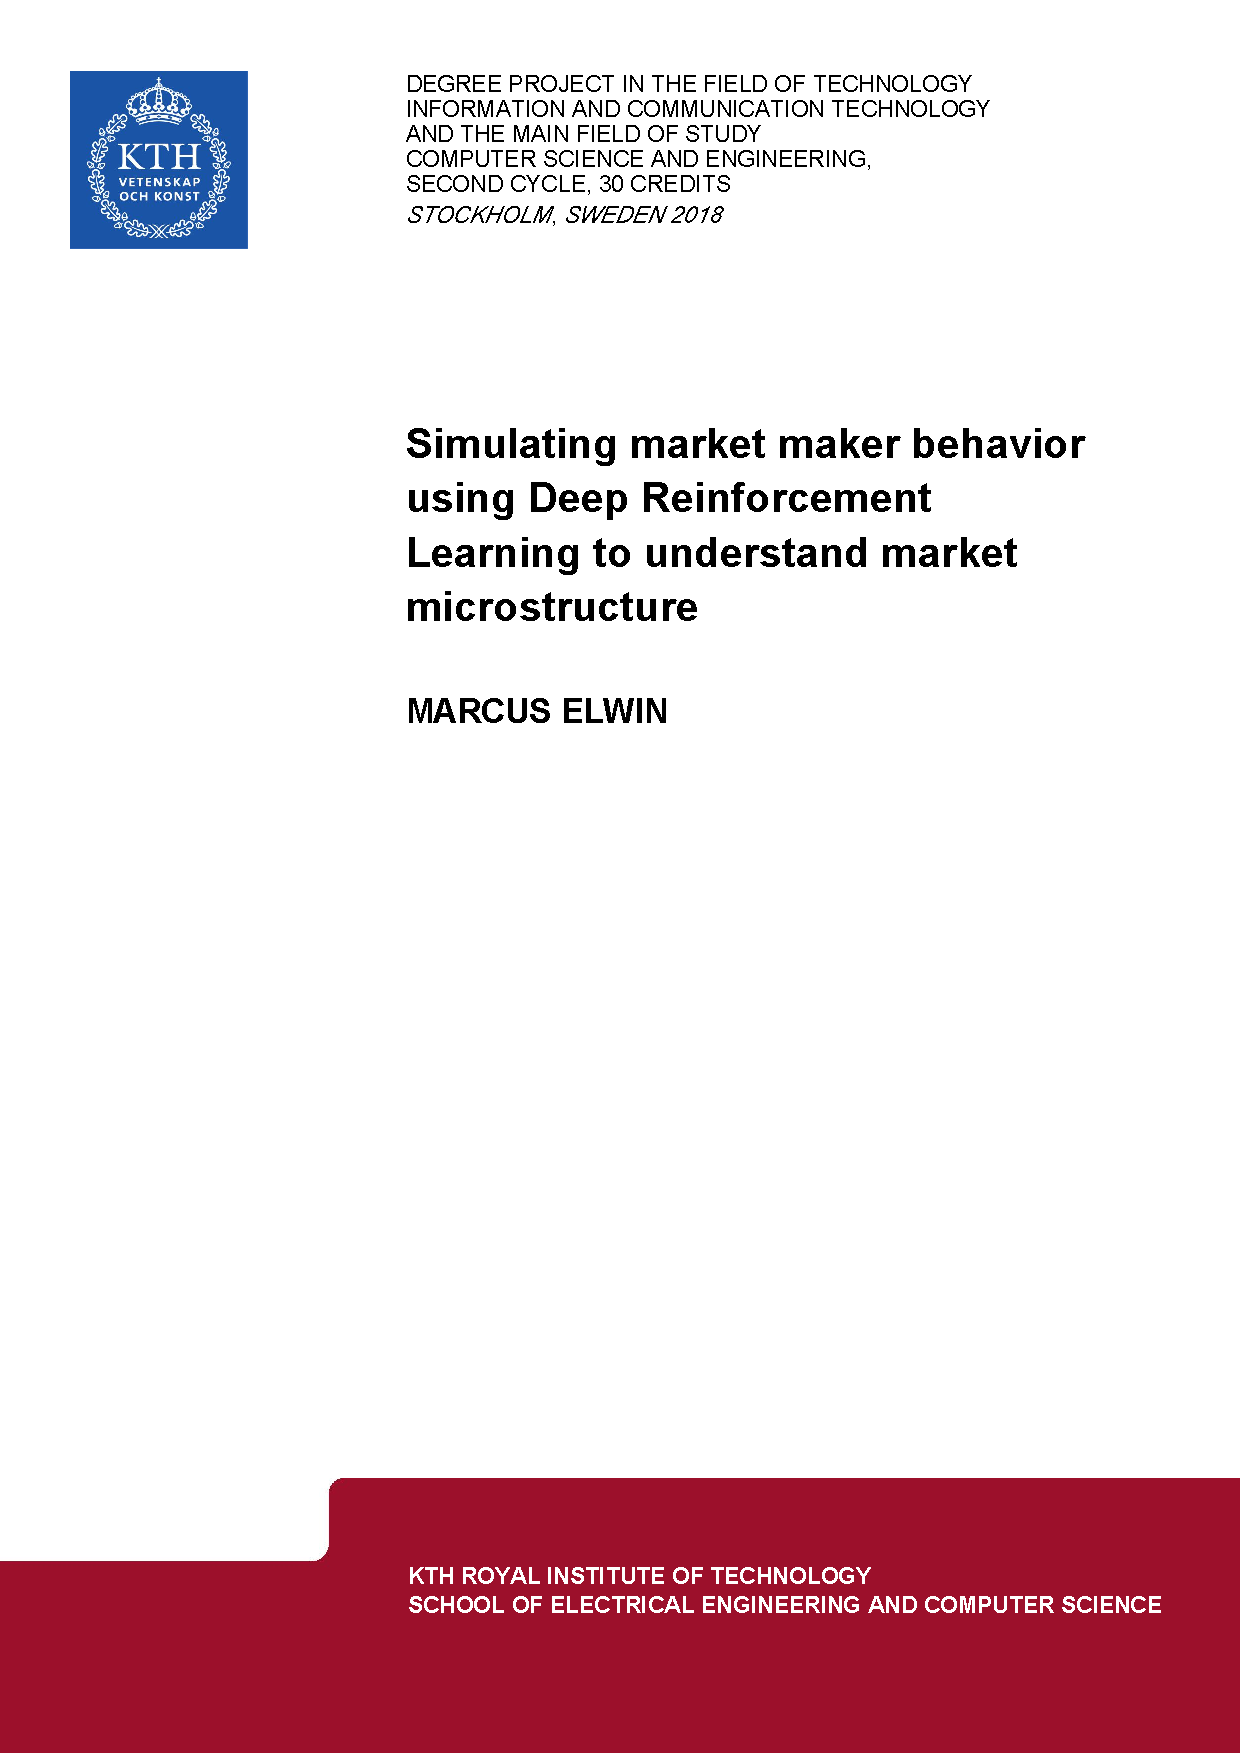
\includepdf{kth_front.pdf}

%\begin{titlepage}
%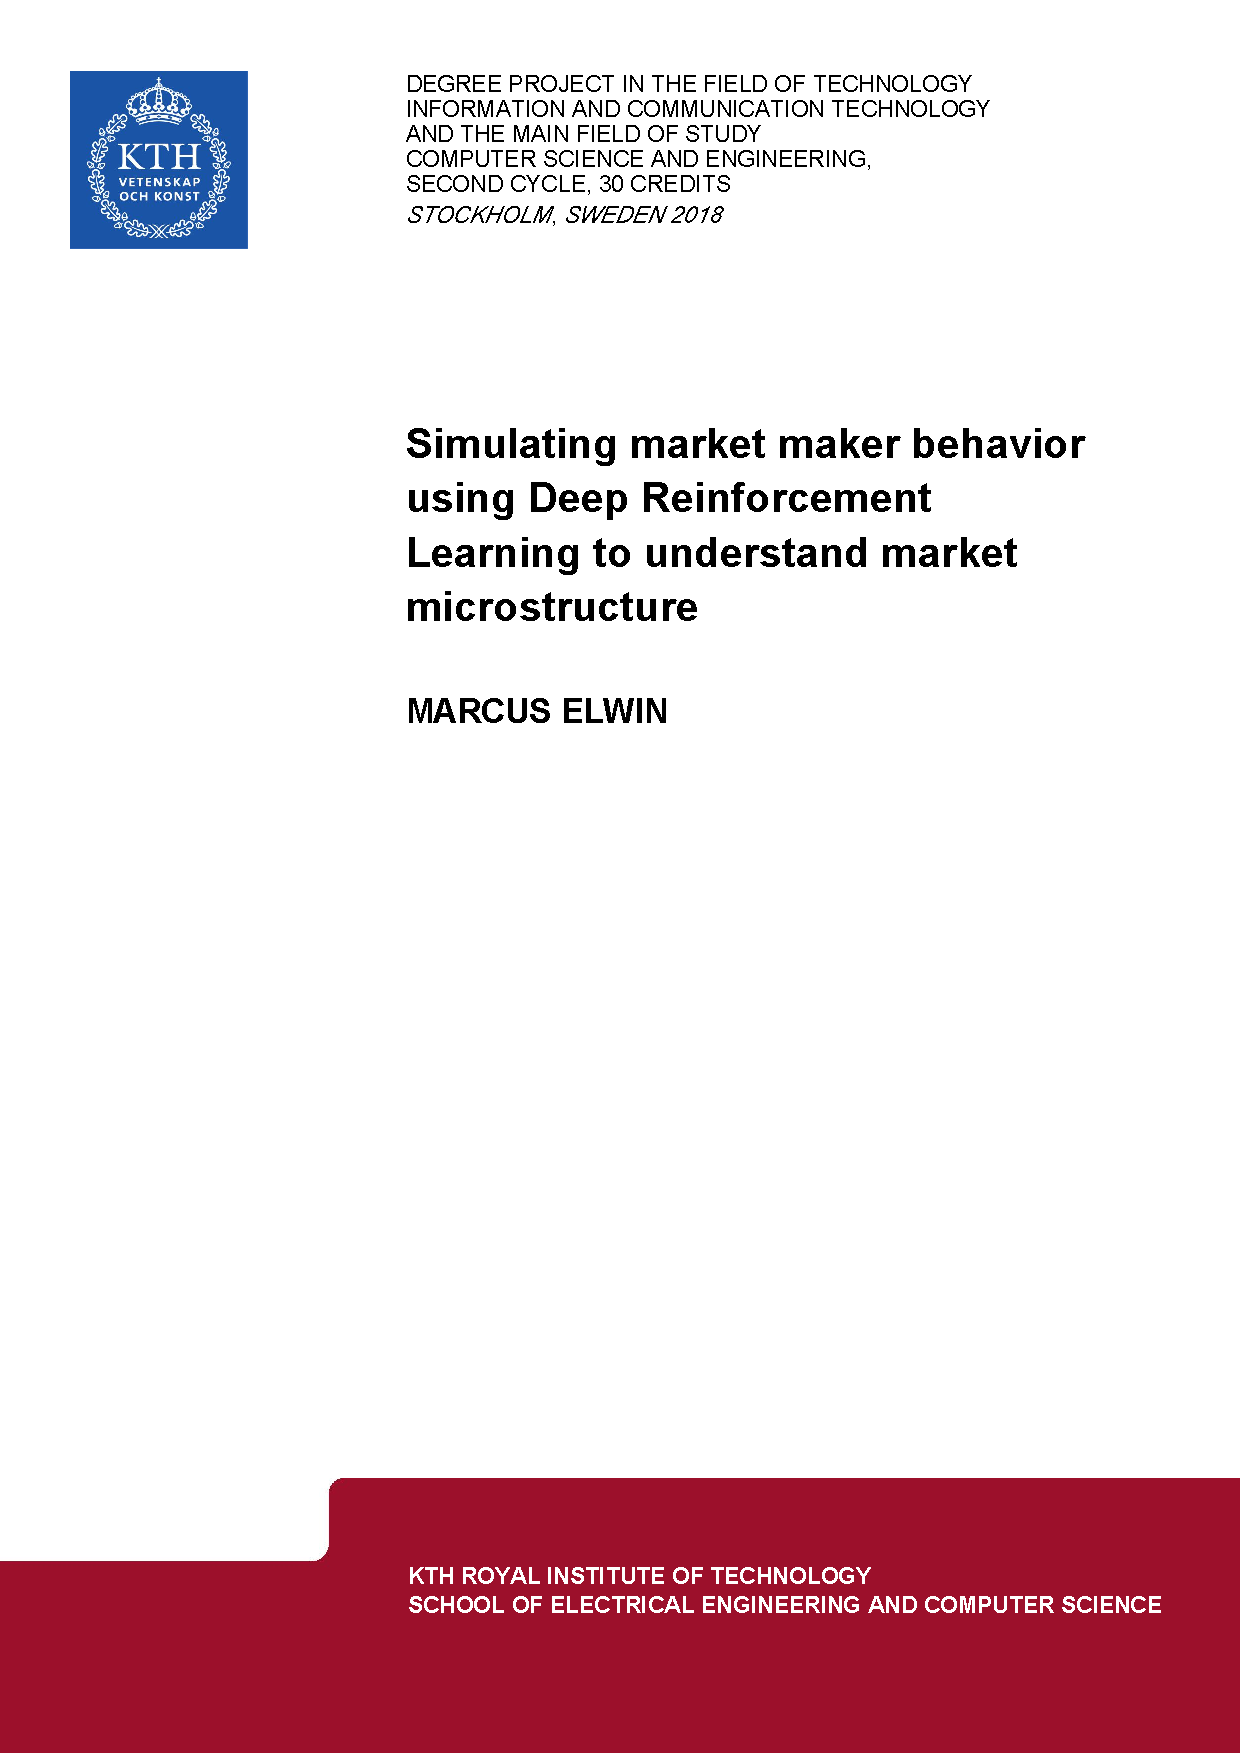
\includepdf{kth_front.pdf}
%\end{titlepage}

% Frontmatter includes the titlepage, abstracts and table-of-contents
\frontmatter

\titlepage

%may need to rephrase or add and remove some stuff
\begin{abstract}
With algorithmic trading and high-frequency trading,  modern financial markets have seen profound changes in market microstructure in the last 5 to 10 years. Rendering previously established methods in the field of \textit{market microstructure} faulty or insufficient. Machine learning and in particular reinforcement learning has become more ubiquitous in both finance and other fields today. With applications in \textit{trading} and \textit{optimal execution}. This thesis combines both reinforcement learning and market microstructure. By simulating a stock market based on NASDAQ Nordics, and training market maker agents on this stock market. In order to understand real world market structure. 
\newline
\newline
Both on a \textit{dealer market} and a \textit{limit orderbook market}, differentiating it from previous studies. As well as using DQN and PPO algorithms on these simulated environments. Where \textit{stochastic optimal control theory} has been mainly used before. The market maker agents successfully reproduce \textit{stylized facts} in historical trade data from each simulation. Such as \textit{mean reverting prices} and \textit{absence of linear autocorrelations} in price changes. As well as beating random policies employed on these markets with a positive profit \& loss of maximum $200\%$. Other trading dynamics in real world markets have been exhibited, via the agents interactions. Mainly: \textit{bid-ask spread clustering, optimal inventory management, declining spreads} and \textit{Independence of inventory and spreads}. Indicating that using reinforcement learning with PPO and DQN are relevant choices when modelling market microstructure.

\end{abstract}


\begin{otherlanguage}{swedish}
  \begin{abstract}
    Algoritmisk och högfrekvensiv handel har förändrat moderna finansmarknaders struktur. Under de senaste 5 till 10 åren. Vilket har påverkat pålitligheten hos tidigare väletablerade metoder från exempelvis ekonometri för att studera marknadens mikrostruktur. Maskininlärning och Reinforcement Learning har blivit mer allämnt förekommande, med ett flertal användningsområden både inom finans och andra fält. Främst inom \textit{handel} och \textit{optimal exekvering} av ordrar. I denna uppsats kombineras både Reinforcement Learning och marknadens mikrostruktur. Genom att simulera en aktiemarknad baserad på NASDAQ i Norden. Tränas market maker agenter på denna marknad. För att kunna undersöka och förstå marknadens mikrostruktur.
    \newline
    \newline
    I denna uppsats utvärderas agenterna på en \textit{dealer marknad} tillsammans med en \textit{limit orderbok}. Som särskiljer denna studie, tillsammans med de två algoritmerna DQN och PPO på en simulerade miljön. Tidigare har \textit{stokastisk optimering} används för snarlika problem. Agenterna lyckas framgångsrikt replikera stiliserade egenskaper hos finansiella tidserier som \textit{återgång till medelvärdet} och \textit{avsaknad av linjär autokorrelation}. Agenterna lyckas också med att slå slumpmässiga strategier, med maximal vinst på $200\%$. Agenterna lyckas uppvisa handelsdynamik som förväntas ske på en marknad. Huvudsakligen: \textit{kluster av spreads, optimal hantering av lager av} och \textit{minskade spreadar}. Vilket visar att reinforcment learning med PPO eller DQN är relevanta val vid modellering av marknadensmikrostruktur.
  \end{abstract}
\end{otherlanguage}

\section*{Acknowledgements}
%\thispagestyle{empty}

I like would like to express my gratitude to my thesis advisor Hamid Reza Faragardi as well as my examiner Elena Troubitsyna. For both your support and helpful comments throughout the course of the thesis. I am profoundly grateful to Björn Hertzberg at Nasdaq for introducing me to both the field of market microstructure and the thesis subject. My research would have been impossible without the aid and support of Jaakko Valli at Nasdaq. Finally I would like to thank my family and girlfriend for having patients with me during this long process.

\clearpage

\tableofcontents

\listoffigures
 
\listoftables

\lstlistoflistings


% Mainmatter is where the actual contents of the thesis goes
\mainmatter


\chapter{Introduction}\label{ch:1}

%We use the \emph{biblatex} package to handle our references.  We therefore use the
%command \texttt{parencite} to get a reference in parenthesis, like this
%\parencite{heisenberg2015}.  It is also possible to include the author
%as part of the sentence using \texttt{textcite}, like talking about
%the work of \textcite{einstein2016}.

\section{Background}
Modern financial markets such as NASDAQ, CME and NYSE have all been effected by the rise and presence of \textit{Algorithmic Trading} and \textit{High-Frequency Trading} (HFT) \parencite{abrol2016high}. Causing for instance more fragmented markets. Where both types of trading consists in using computer programs to implement investment and trading strategies \parencite{abergel2012market}. These types of strategies have according to \textcite{abergel2012market, o2015high} raised various questions about there effects on the financial markets. Mainly in areas as: \textit{liquidity, volatility, price discovery, systematic risk, manipulation} and \textit{market organization}. Where a quite recent example of the proposed effect of algorithmic trading and HFT on financial markets is \textit{the Flash Crash} the 6th of May 2010. In the course of 30 minutes U.S. stock market indices, stock-index futures, options, and exchange-traded funds. Experienced a sudden price drop of more than five percent, followed by a rapid rebound \parencite{kirilenko2011flash,kirilenko2017flash}. See an illustration of this in \autoref{fig:1}.
\newline
\newline
Trading in the financial market can be seen as a search problem where buyers and sellers search for each-other. Which depends on market structure \parencite{abergel2012market}. \textit{Market microstructure} is a branch of economics, where one tries to understand trading dynamics on the financial market on a microscopic level \parencite{o1995market, hasbrouck2007empirical}. Market microstructure theory is used by regulators, traders and organizers of financial markets. In order to make a profit or create more transparent and efficient markets. Recent regulation with the purpose of making markets more transparent and efficient is \textit{Markets in Financial Instruments Directive} (MiFID) II \parencite{busch2016mifid}.

\begin{figure}[ht]
    \centering
    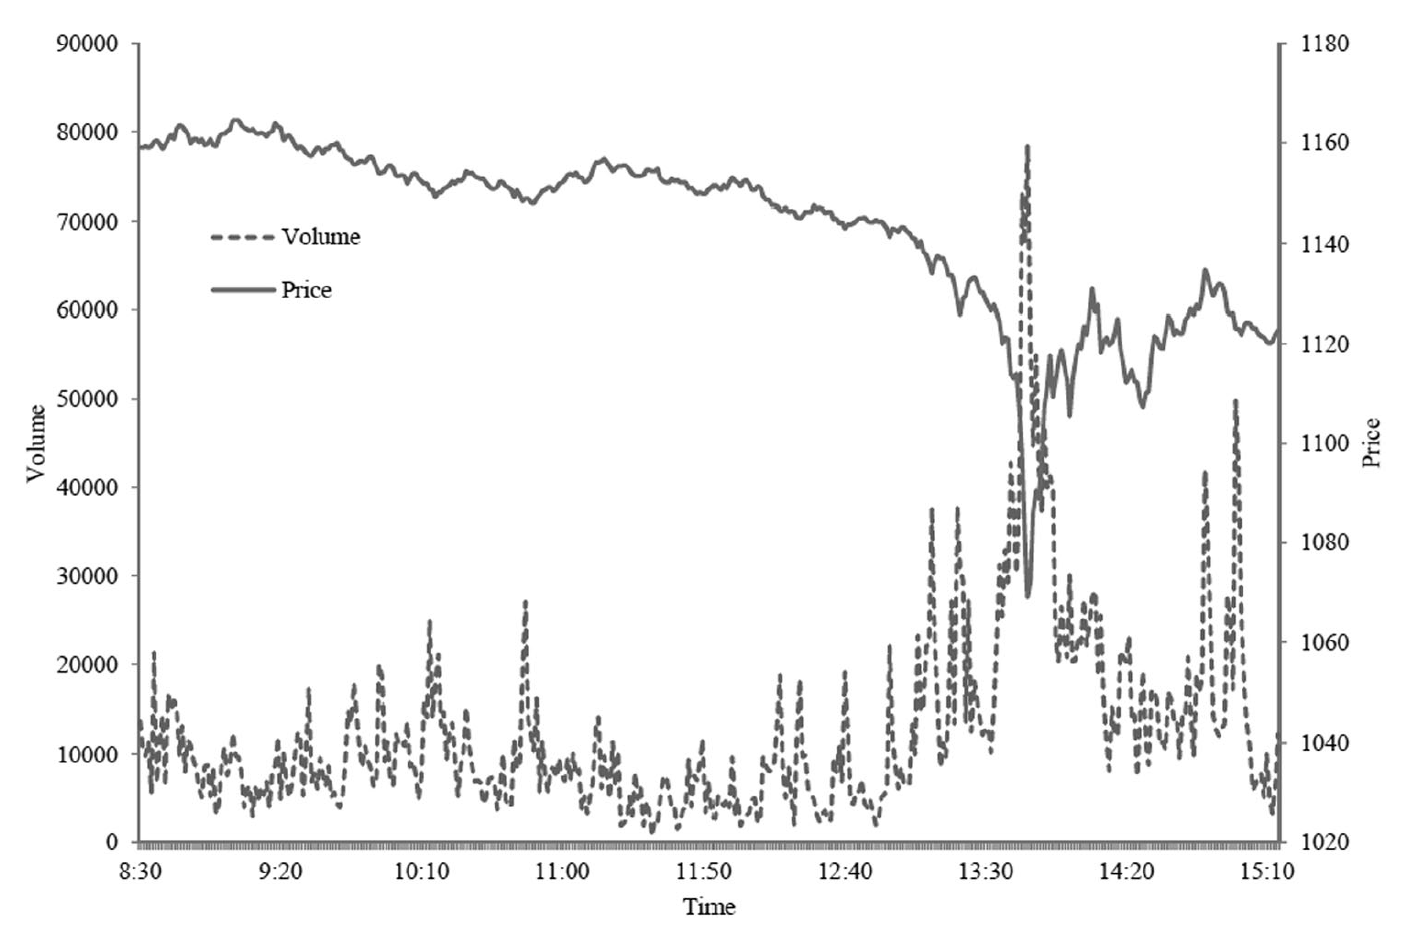
\includegraphics[scale=.7]{flashcrash.PNG}
    \caption{Minute-by-minute transaction prices and trading volume on E-mini S\& P futures contracts during the flash crash, between 8:30 to 15:15. Notice the distinct drop and rebound at the end of the day. Source: \textcite{kirilenko2017flash} }
    \label{fig:1}
\end{figure}

However as mentioned by \textcite{o2015high} due to HFT and algorithmic trading. Learning models and empirical models used in market microstructure in the past are deficient and may not longer be appropriate. Which calls for the use of new more capable methods. Where \textit{Reinforcement Learning} and other machine learning methods are of great interest. Machine learning and AI has been used in a financial setting for some time, and has become ubiquitous in finance. See for example \parencite{moody1999reinforcement, wang2016reinforcement, dempster2006automated, du2016algorithm, bertoluzzo2012testing, casqueiro2006neuro}. Mainly due to the abundance of available data and computing power. 
\newline
\newline
Recent achievements for the use of Reinforcement Learning has been seen in the game Go with \textit{AlphaGo, AlphaGoZero} \parencite{silver2016mastering} programs being able to win over esteemed Go champions. More complicated strategic games as Star Craft has also seen successful application of reinforcement learning \parencite{vinyals2017starcraft}. Therefore the focus of this thesis will be to examine the possibility of using deep reinforcement learning. In order understand the market microstructure of a simulated Nordic stock market.

%need to work with
%\section{Research Question}

\section{Problem}
 Given the abundance of available high frequency data, fragmented markets and more sophisticated trading algorithms. The financial markets have become harder to understand during the past decade. Traditional methods used in market microstructure might have become obsolete as mentioned in \textcite{o2015high}. A traditional supervised learning approach is not of use for this thesis. Due to the fact of the financial markets dynamic nature as a complex system. The agents must be able to adapt and dynamically learn optimal behaviour.  Therefore the problem in this thesis is to understand trading dynamics. By using reinforcement learning, on a simulated Nordic stock market. 
\newline
\newline
In order to witness, if common market microstructure trading dynamics such as \textit{bid-ask spread clustering, optimal trade execution} and \textit{optimal inventory costs} as described in \textcite{o1995market}. Will be exhibited and understood by the reinforcement learning agents. Also it is of interest to see what happens with the agents when changing the market conditions. Much like what is happening in the real markets. For example changing the number of participants, order sizes, prices, volatility, order arrival rates and trading rules.

%\section{Aim}

%\newpage

\section{Objective}
The objective for this thesis is two-fold. Firstly in the case of the principal the objective is to have a functional and working exchange simulator (EXSIM). Where they can change different parameters, policies, reward functions and other things effecting the market structure. In order to study and simulate modern financial markets on a microscopic level. Secondly from the thesis point of view, the objective is to investigate the following:

\begin{itemize}
    \item If reinforcement learning can be successfully used in a more complicated environment as the financial market. 
    
    \item Whether new insights and applications can be provided to the the growing field of market microstructure. With the help of reinforcement learning.
\end{itemize}


\section{Delimitation}
This thesis doesn't use any real world data for the simulations and experiments conducted. Instead only simulated data from the agents interaction with its environment is used. This due to security constraints at the principle. No multiagent reinforcement learning has been used. This due to time constraints. Instead several different single agents are tested and evaluated. 
\newline
\newline
Information based market microstructure models has not been used in this thesis. Instead inventory based models and limit order book models have been used. Mainly due to time constraints. Exploration of distributed and parallel training of agents in order to speed up training. Using workers and a parameter server has not been performed. This also due to time constraints.

\section{Methodology}
The methodology in the thesis has been empirical with a quantitative approach. Collecting data from the agents interactions with the environments. Through various experiments, to test different scenarios, behaviours and collect different statistics. More information about the methodology is found in \autoref{ch:5}.

%\section{The principle}

\section{Contribution}
The contribution of this thesis is to show the usages of reinforcement learning to more complex environments as the financial markets. With a more realistic limit order book market compared to previous studies. In order to provide new insights and methods in the field of market microstructure. The target audience is both academia and the industry, that can benefit from this work.

\newpage
\section{Outline of the thesis}
The thesis has the following structure:

\begin{itemize}
    \item In \autoref{ch:2}, the theoretical background needed for the thesis is presented. Covering \textit{market microstructure, artificial financial markets} and \textit{reinforcement learning}.
    
    \item In \autoref{ch:3}, related work relevant to the thesis is presented. This chapter presents the state-of-the art, and what is the contribution of this thesis. In comparison with previous research.
    
    \item In \autoref{ch:4}, an overview of the research methodology employed for this thesis is presented.
    
    \item In \autoref{ch:5}, the implementation of the agents, environments, data collection and the experiments are discussed in detail.
    
    \item In \autoref{ch:6}, the results obtained from the different experiments are illustrated and discussed.
    
    \item In \autoref{ch:7}, the main findings are highlighted and evaluated and compared to previous research. The conclusions of the thesis and future research is also presented.
\end{itemize}
%The student displays knowledge of theoretical background and previous related work (significant literature is mentioned and relevant material is used).

\chapter{Background}\label{ch:2}
This chapter presents relevant theory needed to contextualize the thesis. The following is covered: \textit{market microstructure theory, artificial financial markets} and finally ending with a section on \textit{reinforcement learning}.

%Necessary
%\section{Modern Financial Markets}

%Ho stoll model for invetory market

%GM

% Daz model for informed traders

% Real market with matching engine e.g. parity
\section{Market Microstructure}
\textit{Market microstructure} is the study of the process and outcomes of exchanging assets under implicit trading rules as mentioned in \textcite{o1995market}. The majority of market microstructure research is according to \textcite{madhavan2000market} concerned with : 
\begin{enumerate}
    \item \textit{Price formation and discovery} i.e. looking in to the black box of the market and who latent demands are translated into prices.
    \item \textit{Market structure and design} i.e. what different rules exists, and how they effect the black box of the market.
    \item \textit{Information and disclosure} i.e. how the inner workings of the black box or the market affects the behaviour of traders and strategies.
\end{enumerate}
All of these will be covered in this section.

\newpage

\subsection{Market Participants}
A \textit{market} is the place where traders gather to trade \parencite{harris2003trading} different types of instruments as common stocks, bonds, futures, options, derivatives and foreign exchange rates just to mention a few.
Looking at today's financial markets
\textcite{cartea2015algorithmic} broadly categories three primary classes of traders (or strategies) that partake in the market:
\begin{itemize}
    \item \textbf{Fundamental traders:} those who are driven by economic fundamentals outside the exchange.
    \item \textbf{Informed traders:} traders who profit from leveraging information not reflected in market prices and trading assets in the hope of their increase or decrease in value.
    \item \textbf{Market Makers:} professional traders who profit from facilitating exchange in a particular asset and exploit their skills in executing trades.
\end{itemize}
Market makers will be the main participant covered in this thesis. As they have an important impact on providing liquidity to financial markets. Albeit the dual nature of optimizing their inventory of stocks, and making a profit for themselves.

\subsection{Trading Mechanisms}
Any trading mechanism can be seen as a type of trading game in which players meet virtually or physical at some venue and act according to some rules \parencite{o1995market}. Where the players are some of the participants mentioned in the previous section. The venue or the market,  is where trades are actually executed. Which can be on an exchange or via other intermediaries. A common division of market structure is presented in \textcite{foucault2013market}. Where they classify markets as either \textit{limit order markets} (auction markets) or \textit{dealer markets}. In fact all trading mechanisms can be viewed as variations of these \parencite{foucault2013market}. Today most markets are electronic, and adopt a \textit{continuous-time double auction} mechanism using a limit orderbook \parencite{bouchaud2018trades}. Compared to \textit{Walrasian auctions}\footnote{traders communicate there buy and selling intentions via an auctioneer}, in limit order markets the final investors interact directly instead. 

\newpage

\begin{figure}[H]
    \centering
    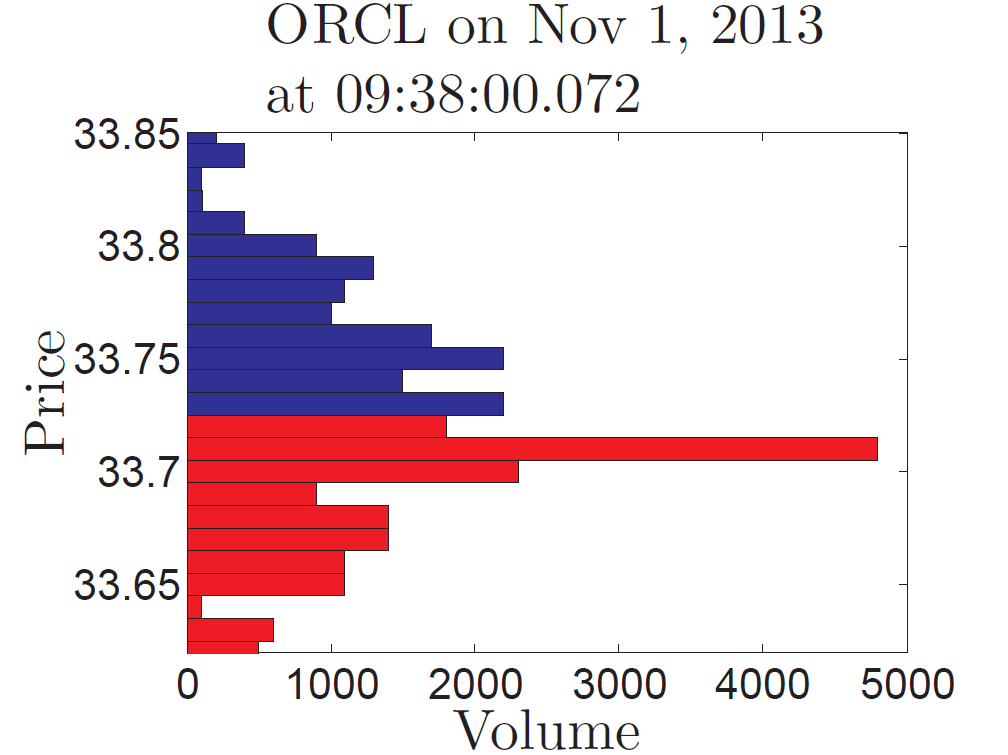
\includegraphics[scale=.65]{LOBex.PNG}
    \caption{Snapshot of the LOB for the ticker ORCL (Oracle) after the 10 000th event during that day. Blue bars indicates sell limit orders, whilst red bars are buy limit orders. Source: \textcite{cartea2015algorithmic}}
    \label{fig:2}
\end{figure}

There bids and offers are accumulated in the \textit{limit order book} (LOB). The orders in the LOB are accumulated by firstly price priority and secondly time priority \parencite{hasbrouck2007empirical}. Whilst in dealer markets participants can only trade at the bid and ask quotes posted by specialized intermediaries i.e. \textit{dealers} or \textit{market makers} \parencite{foucault2013market}. Note that the LOB is very dynamic as it constitutes of \textit{limit orders}\footnote{A limit order is an order that specifies a direction, quantity and acceptable price.}. Which can be cancelled or modified at any time. Thus the state of the LOB can be changed extremely often \parencite{hasbrouck2007empirical}. For this thesis this means the agents will have a very large state space. With many possible actions, that they need to explore. In order to find optimal policies.
\newline
\newline
More formally according to \textcite{bouchaud2018trades} one can see an order as a tuple consisting of sign/direction ($\varepsilon_{x}$), price ($p_{x}$), volume ($v_{x}$) and submission time ($t_{x}$):
\begin{equation}
    \label{eq:0}
    x = (\varepsilon_{x}, p_{x}, v_{x}, t_{x})
\end{equation} Where $\varepsilon = \pm 1$ indicates if it is a buy or sell order and $v_{x} > 0$. An example of a limit order book is shown above in \autoref{fig:2}. Market orders are other types of orders found on LOB markets, which are usually considered to be more aggressive. This as they seek to execute a trade immediately \parencite{cartea2015algorithmic}. 

\newpage
For instance if a market order is placed and the quantity is larger then the quantity available in the book. The order is \textit{re-routed} or said to \textit{walk the book} until the order is filled \parencite{hasbrouck2007empirical,cartea2015algorithmic}. When submitting an order $x$, the trader must chose the size $v_x$ and price $p_{x}$ according to a relevant \textit{lot size} and \textit{tick size} of the LOB \parencite{bouchaud2018trades}. The lot size $v_0$ is the smallest amount of the asset that can be traded. Hence the size of each order is a multiple of the lot size $v_{x} \in \{kv_{0} | k = 1,2,...\}$. The tick size $\vartheta$ is the smallest permissible price interval between different orders within a given LOB \parencite{bouchaud2018trades}. The values of $v_{0}$ and $\vartheta$ differs a lot between exchanges. However expensive stocks are often traded with $v_0 = 1$ whilst cheaper stocks are traded with $v_{0} \gg 1$. In equity markets $\vartheta$ is often 0.01\% of the stock's mid-price \parencite{bouchaud2018trades}. 
\newline
\newline
Both the tick size and lot size affect trading. As the lot size dictates the smallest permissible order size. Whilst the tick size $\vartheta$ dictates how much more expensive it is for a trader to gain the priority. Of choosing a higher or lower price to a buy or sell order \parencite{bouchaud2018trades}. Sometimes it is also useful to consider the \textit{relative tick size} $\vartheta_r$, which is equal to the $\vartheta$ divided by the mid-price for a given asset \parencite{bouchaud2018trades}. To make things more complicated modern markets has a lot of different order types. Such as \textit{hidden, reserved, ice-burg} and \textit{Fill-or-Kill} orders just to mention a few. Where \parencite{foucault2013market, cartea2015algorithmic, hasbrouck2007empirical} gives good overviews of these. There also exist \textit{hybrid markets} which are traditional quote-driven markets as NASDAQ and London Stock Exchange (LSE) \parencite{foucault2013market}.

\subsection{Price Formation \& Discovery}

The mechanism of price formation is at the very heart of economics.  Which is also important in order to understand \textit{stylized facts} in financial price series as \textit{heavy tails} and \textit{volatility clustering}  \parencite{abergel2012market}. \text{Price discovery} is the speed and accuracy with which transactions prices incorporate information available to market participants \parencite{foucault2013market}. In fact looking at market makers, is a logical starting point for how prices are actually determined in the market \parencite{madhavan2000market}. Nevertheless, not covered in this thesis and still important is the role of information and who has it \parencite{cartea2015algorithmic}.


\begin{figure}[H]
    \centering
    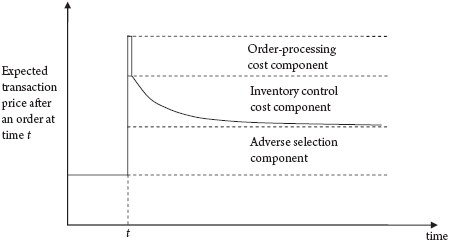
\includegraphics[scale=1]{bidask.png}
    \caption{Three components of bid-ask spread in short-term and lon-term response to a market buy order. Source: \textcite{foucault2013market}}
    \label{fig:3}
\end{figure}


%\subsubsection*{Bid-Ask Spread}

\textbf{Bid-Ask Spread.} The bid-ask spread is usually decomposed into three components: \textit{adverse selection, order-processing costs} and \textit{inventory holding costs} \parencite{foucault2013market}. Order processing costs, consists of the setup price and operating costs of trading. Inventory costs is cost associated with carrying inventory. Adverse selection costs are costs that arise because some traders are more informed then others. When trading with these \textit{informed traders}, market makers will on average lose money \parencite{darley2007nasdaq}. Therefore a fraction of the bid-ask spread can be seen as a compensation for having to trade against informed traders \parencite{darley2007nasdaq}. In \autoref{fig:3} above these are illustrated on a short-term and long-term perspective.
\newline
\newline
Market makers quote two prices the bid price and the ask price where the difference between these is the market makers \textit{spread} \parencite{madhavan2000market}. By doing this market makers are also providing \textit{liquidity} to the market. Spreads measure the execution cost of a small transaction, by measuring how close the price of a trade is to the \textit{market price}. Where the market price is the \textit{equilibrium price} i.e. the price where demand equals supply \parencite{cartea2015algorithmic}. One approach is by using the \textit{midprice} in \autoref{eq:1}:

\begin{equation}
    \label{eq:1}
    S_{t} = \frac{1}{2}(a_t + b_t)
\end{equation}
Which is the simple average of the bid ($b_t$) and ask ($a_t$) price. 

\newpage
However the most common spread measures are the \textit{quoted} and the \textit{effective} \parencite{cartea2015algorithmic, foucault2013market} spread both shown in \autoref{eq:2} and \autoref{eq:3}

\begin{equation}
    \label{eq:2}
    QS_t = a_t - b_t
\end{equation}

\begin{equation}
    \label{eq:3}
    ES_t = a_t - S_t \text{ or } ES_t = S_t - b_t
\end{equation}
The quoted spread represents the potential cost of immediacy at any point in time as well as the distance from the market price \parencite{cartea2015algorithmic}. As mentioned in \textcite{foucault2013market} the quoted spread is also a good measure of trading costs for small orders used for measuring liquidity. Normalizing \autoref{eq:2} with the mid price the \textit{relative quoted spread} is obtained

\begin{equation*}
    RQS_t = \frac{a_t - b_t}{S_t}.
\end{equation*}
%Another related measure is the so called \textit{relative weighted average bid-ask spread} (RTWAS):
%\begin{equation}
%\label{eq:4}
%    RTWAS_{t} = \frac{\bar{a}(q) - \bar{b}(q)}{S_t}
%\end{equation}
%Where $\bar{a}(q)$ and $\bar{b}(q)$ is the average execution price for buy and sell market orders of size $q$ \parencite{foucault2013market}.% 
On the other hand the effective spread or half-spread measures the realized difference between the price paid and the midprice. Which can also be negative indicating that one is buying at a price below or selling above the \textit{market price} \parencite{cartea2015algorithmic}. ES and QS differ in the fact that ES can only be measured when there is a trade while QS are always observable \parencite{cartea2015algorithmic}. Some stylized facts know about the bid-ask spread are \parencite{hasbrouck2007empirical, madhavan2002market, bouchaud2018trades}:
\begin{itemize}
    \item The trade prices series is a martingale \& the order flow is not symmetric.
    \item The spread declines over time \& the bid-ask spread are lower in high volume securities and wider for more riskier securities.
    \item For large-tick stocks, the spread is almost equal to one tick. Small-tick stocks have a broader distribution of spreads.
    \item There is a price impact of trades i.e. on average the arrival of a buy trade causes prices to rise ($S_t$ increases). Whilst the arrival of sell trades causes prices to fall ($S_t$ decreases).
\end{itemize}
\newpage

%\subsubsection*{Liquidity}
\textbf{Liquidity.} If the structure of a securities market is compared to a car design, measuring liquidity is like assessing the car's driving performance \parencite{foucault2013market}. Liquidity impounds the usual economic concept of \textit{elasticity}\footnote{a measure of the responsiveness of one economic variable to another}. In a liquid market, a small shift in supply and demand doesn't result in large price changes \parencite{hasbrouck2007empirical}. However liquidity is also concerned with trading costs. Market makers are seen as liquidity providers (sell-side) whilst liquidity demanders are the customers (buy-side) \parencite{hasbrouck2007empirical}. A key dimension of liquidity is \textit{immediacy}. This is the ability of a investor to buy or sell an asset without having to wait to find a counterpart. With an offsetting position to sell or buy \parencite{cartea2015algorithmic}. In fact the bid-ask spread is a common measure of how liquid a market is \parencite{foucault2013market}.
\newline

%\subsubsection*{Order imbalance}
\textbf{Order imbalance.} Another way of describing price dynamics is to see the accumulated best bid and ask quotes in a LOB as \textit{queues} \parencite{bouchaud2018trades}. All prices changes then boils down to a \textit{race} between the different queues. The queue that depletes first, i.e. the winner, dictates the next price change \parencite{bouchaud2018trades}. Where order imbalance is such a measure, providing a quantitative assessment of the relative strengths of buying and selling pressure in an LOB \parencite{bouchaud2018trades}. Volume order imbalance is defined as:

\begin{equation}
    I_t = \frac{V_{t}^{b}}{V_{t}^{b}+V_{t}^{a}}
    \label{eq:voi}
\end{equation}
where $V_{t}^{b}$ is the bid volume at time $t$, conversely $V_{t}^{a}$ is the ask volume at time $t$. The denominator (total volume at time $t$) in \autoref{eq:voi} normalizes the imbalance, therefore $I_t \in [0, 1]$. \textcite{bouchaud2018trades} provides a qualitative understanding of $I_t$:
\begin{itemize}
    \item $I_t \approx 0$ corresponds to a situation where the ask-queue is much larger than the bid-queue. Meaning that there's a net positive selling pressure in the LOB. Likely pushing the price downwards.
    \item $I_t \approx \frac{1}{2}$ means that the bid- and ask-queues are approximately equally big. Meaning that the buying and selling pressures in the LOB is somewhat balanced.
    \item $I_t \approx 1$ corresponds to a situation where the bid-queue is much larger than the ask-queue. Meaning that there is a net positive buying pressure in the LOB. Likely pushing the price upwards.
\end{itemize}
A estimate of the probability $p_{+}(I_t)$ that the ask-queue depletes before the bid-queue has been shown in \parencite{bouchaud2018trades} to be:
\begin{equation}
    p_{+}(I_t) = p_{+}(V_{t}^{b}, V_{t}^{a}) = \frac{2}{\pi}\arctan{\left(\frac{I_t}{1-I_t}\right)}
\end{equation}
Where one can replace $\frac{I_t}{1-I_t} = \frac{V_{t}^{b}}{V_{t}^{a}}$. 
Another imbalance measure according to \textcite{cartea2015algorithmic} is \textit{limit order balance} defined in \autoref{eq:loi}:

\begin{equation}
    \rho_{t} = \frac{V_{t}^{b} - V_{t}^{a}}{V_{t}^{b}+V_{t}^{a}}
    \label{eq:loi}
\end{equation}
Where $\rho_t \in [-1,1]$. Usually one computes $\rho_t$ by looking only \textit{at-the-touch}, the best $n$-levels of the LOB. There are more buy orders when the imbalance is high. Conversely there are more sell orders when the imbalance is low. The willingness of an agent to post limit orders is strongly dependent on the value of imbalance \parencite{cartea2015algorithmic}.
\newline
%\subsubsection*{Price Impact}
%A popular benchmark in trading costs analysis is the \textit{volume-weighed average price} (VWAP). For all transaction in the stock during a interval ($T$), often a trading day \parencite{foucault2013market}:

%\begin{equation}
%    \label{eq:5}
%    VWAP = \sum_{t\in T}{w_t p_t}
%\end{equation}
%Where $w_t = \frac{|q_t|}{\sum_{t\in T}{|q_t|}}$ and $p_t$ and $q_t$ is the price and size of the $t^{th}$ trade. Investors evaluate their broker's performance in getting a good price for their order, by comparing their own price with the day's VWAP \parencite{foucault2013market}. %
\textbf{Price Impact.} Another concern for participants that wish to execute large orders, is that they will have an adverse \textit{price impact}. That is, increasing the price when buying aggressively and lowering it when selling \parencite{cartea2015algorithmic, bouchaud2018trades}. A normal way of measuring this, is running a regression on the change of the midprice of the form below:

\begin{equation}
    \label{eq:6}
    \Delta S_n = \lambda q_n + \varepsilon_n
\end{equation}
Where $\Delta S_n = S_{n\tau}-S_{(n-1)\tau}$ for a time interval $[(n-1)\tau, n\tau]$ \parencite{cartea2015algorithmic}. Note that other forms of this regression exists including inventory. See \textcite{foucault2013market} for more information. Using \autoref{eq:6} it is possible to estimate $\lambda$. Where the parameter $\lambda$, also called \textit{Kyle's lambda} \parencite{bouchaud2018trades} is capturing the market's price reaction i.e. its price impact. On the other hand $q_n$ is the order imbalance or net order flow \footnote{difference between buy and sell orders during an interval} and  $\varepsilon_n$ the error term assumed to be normally distributed \parencite{cartea2015algorithmic, foucault2013market}. 
\newline
\newline
In terms of measuring liquidity a lower $\lambda$ indicates that the market is more liquid. Due to greater competition, lower risk tolerance or lower volatility \parencite{cartea2015algorithmic}. Thus a lower $\lambda$ means that prices are less sensitive to order imbalance \parencite{foucault2013market}.  A larger $\lambda$ indicates that the given volume impacts the prices, and trading is thus more expensive \parencite{bouchaud2018trades}.
\newpage

\subsection{Inventory-based models}
A large (positive) inventory causes the dealer or market maker to face a higher cost for observing more inventory. Which lowers both bid and ask prices by the same amount \parencite{o1995market}. Vice versa holds for negative inventory. The model by \textcite{ho1981optimal} is one of the most popular inventory-based models, presented below.
\newline

%\subsubsection*{Ho \& Stoll Model}
\textbf{Ho \& Stoll Model.} In \textcite{ho1981optimal}, they present a model that handles the risk the market maker faces when providing his service. In the model the following assumptions are made: \textit{transactions follow a Poisson process, the dealer faces uncertainty over the future} and, \textit{the arrival rate of orders depend on the bid and ask prices}. The objective of the dealer is now to maximize the expected utility of his total wealth $E[U(W_T)]$ at time horizon $T$, where 

\begin{equation}
    \label{eq:12}
    W_{T} = F_{T} + I_{T} + Y_{T}
\end{equation}
\autoref{eq:12} is what is termed \textit{the dealers pricing problem}. $F_{T}, I_{T}$ and $Y_{T}$ is the dealers cash account, inventory and base wealth. See more in \autoref{app:B}. This is in fact an optimization problem where the aim is to maximize the value function $J(\cdot)$ using dynamic programming. Thus yielding the optimization problem below in \autoref{eq:13a}

\begin{equation}
    \label{eq:13a}
    J(t,F,I,Y) = \underset{a,b}{\max}[E[U(W_T)] | t,F,I,Y]
\end{equation}
where $U$ is the utility function, $a$ and $b$ are the ask and bid adjustments and $t, F, I,Y$ are the state variables time, cash, inventory and base wealth \parencite{o1995market}. The function $J(\cdot)$ gives the level of utility given that the dealer's decisions are made optimally \parencite{o1995market}. As there are no intermediate consumption before time $T$ in this model. The recurrence relation found by using the principle of optimality is:

\begin{equation}
    \label{eq:13bc}
    \underset{a,b}{\max}dJ(t,F,I,Y)=0 \text{ and } 
    J(T,F,I,Y)=U(W_T)
\end{equation}

Solving \autoref{eq:13bc} one finds a solution to the dealer's problem. To solve \autoref{eq:13bc} one requires to use stochastic calculus. For further elaboration and more details see \autoref{app:B}. However, there is no closed form solution for this problem. However via approximations the bid and ask quotes has been shown to be found by:

\begin{align}
\label{eq:13f}
    b^{*} = & \alpha/2\beta + (J-BJ)/2BJ_{F}Q \\
    a^{*} = & \alpha/2\beta + (J-SJ)/2SJ_{F}Q \label{eq:13g}
\end{align}
Finally from \autoref{eq:13f} and \autoref{eq:13g} one gets the bid-ask spread as
\begin{equation}
    \label{eq:13h}
    s = \alpha / \beta + (J-SJ)/2SJ_{F}Q + (J-BJ)/2BJ_{F}Q
\end{equation}
The first term of \autoref{eq:13h} is the spread which maximizes the expected returns from selling and buying stocks. Whilst the rest of the terms are seen as \textit{risk premiums} for sale and purchase transactions. This as the dealer or market maker sets the spread without knowing what side the transaction will have i.e. bid or ask \parencite{ho1981optimal}.
\newline
\newline
\textcite{ho1981optimal} demonstrates three important properties of the dealer's optimal pricing behavior:

\begin{enumerate}
    \item The spreads depends on the time horizon of the dealer. 
    \item It can be decomposed in a risk-neutral and risky part.
    \item The spread is independent of inventory levels.
\end{enumerate}
Inventory based models is just one set of models used in the market microstructure literature. Which is the most relevant one for this thesis. However, another important family is \textit{information-based models}. That allow for examination of market dynamics. Hence providing insights into the adjustment process of prices \parencite{o1995market}. For popular models see more in for instance \textcite{glosten1985bid} or \textcite{das2005learning, das2003intelligent}.

%\subsection{Information-based models}
%Information-based models allow for examination of market dynamics. Hence providing insights into the adjustment process of prices \parencite{o1995market}. Where a popular model is the one by \textcite{glosten1985bid}.

%\subsubsection*{Glosten-Milgrom Model}
%In the Glosten-Milgrom one tries to capture the features of how adverse selection affects the bid ask spread \parencite{darley2007nasdaq}. One assumes the following in the model:
%\begin{itemize}
%    \item A market with trading in a single asset
%    \item All market participants are risk-neutral and act competitively
%    \item The market is \textit{friction-less} i.e. there are no transaction costs, taxes or holding costs.
%    \item The value of the asset is a random variable whose probability law is know to the market makers.
%\end{itemize}
%Informed traders have information about the realization of a assets \textit{true value}, $V$. The distribution of $V$ is assumed to be binomial. With the probability $\theta$ and $1- \theta$ if the value of the asset is higher or lower $\overline{V}, \underline{V}$  then the true value \parencite{darley2007nasdaq}. Uniformed traders only have information about the triple $(\theta, \underline{V}, \overline{V})$ and we have two fraction of these. The ones that wants to buy $\gamma^{B}$, and the ones that want to sell $\gamma^{S}$ \parencite{darley2007nasdaq}. The fraction of informed traders is instead denoted $\mu$. The market maker sets bid ($E[V|\text{Sell}]$) and ask prices ($E[V|\text{Buy}]$) by conditional expectations of the true value given a sell or buy order. By definition \parencite{darley2007nasdaq} 
%\begin{equation}
%    \label{eq:7}
%    E[V|\text{Sell}] = \underline{V}P[V=\underline{V}|\text{Sell}] + \overline{V}P[V=\overline{V}|\text{Sell}]
%\end{equation}
%And by using Bayes' rule the probabilities  can be obtained, for instance $P[V=\overline{V}|\text{Sell}] = \frac{\theta(1-\mu)\gamma^{S}}{(1-\mu)\gamma^{S} + (1-\theta)\mu}$.
%Note that the Glosten-Milgrom model has no actual auction mechanism. Which makes the model inadequate for studying the effect of microstructure on non-equilibrium market behavior \parencite{darley2007nasdaq}.

%\subsubsection*{Das Model}

%\subsection{Empirical metrics}

\newpage

\section{Artificial Financial Markets}
In agent-based modelling (ABM), appropriate parts of a complex system are modeled as autonomous decision-making entities called \textit{agents} \parencite{darley2007nasdaq}. In ABM market investors or traders are modelled as agents trading together via an orderbook \parencite{lussange2018bright}. However the decision of what type of agents to use is paramount. Where a wide range of of different types of agents from \textit{zero-intelligence agents} to \textit{reinforcement learning agents} \parencite{martinez2009evolutionary}. Broadly speaking there is a price disagreement between the agents, where often pricing is done randomly also called \textit{noise traders}. Or via some real world strategy \parencite{lussange2018bright}. According to \textcite{martinez2009evolutionary} some important design issues to think about are:

\begin{itemize}
    \item \textit{Decision making} i.e. is it rule based, or based on something else.
    \item \textit{Objective function} i.e. explicit, implicit or utility or profit maximization.
    \item \textit{Heterogeneity} i.e. types of agents, parameters, information basis and learning.
    \item \textit{Learning} i.e. zero intelligence or more complex.
\end{itemize}
Validation is an important issue in agent-based modelling, where simulated markets should be able to replicate realistic quantitative features of the real market, with reasonable calibration \parencite{martinez2009evolutionary}. In order to validate, multiple parameters need to be user-defined. However one way to overcome this. Is by using a benchmark in which the behaviour of the market is well defined. Another way according to \textcite{martinez2009evolutionary} is to use parameters in the simulated market derived from experimental or real markets. 
\newline
\newline
It is also common to test whether the prices created via the interaction of the agents exhibit certain \textit{stylized facts}. That real world markets do \parencite{brandouy2011design}. With stylized facts one means a set of properties that is common across many instruments, markets and times. That has been observed by independent studies \parencite{cont2001empirical}. 
\newpage

Where some known stylized facts, important for this study are:

\begin{itemize}
    \item \textit{Absence of autocorrelations} i.e. linear autocorrelations are often insignificant. 
    \item \textit{Non Gaussian returns \& Heavy tails} i.e.the unconditional distribution of returns seems to display a power-law or Pareto-like tail.
    \item \textit{Volatility clustering}. 
\end{itemize}
For more information see for instance \textcite{cont2001empirical}.

%mention what it is, some strategies, and how it effect modern markets
%\section{Algorithmic and High-Frequency Trading}
%Algorithmic trading consists in using computer programs to implement investment and trading strategies \parencite{abergel2012market}. Conversely, High frequency trading (HFT)is a term used to describe a large diverse set of activities and behaviors \parencite{o2015high}. Where some of the main characteristics for high frequency traders are: (i) use of \textit{high-speed} and sophisticated programs for \textit{generating, executing} and \textit{routing} orders, (ii) use of \textit{co-location} to minimize \textit{latency}, (iii) very short time frames for their positions, (iv) submission of numerous orders that are cancelled shortly and (v) ending the day with almost flat positions. 
%\newline
%\newline
%A distinction can be made between algorithmic trading and HFT in their order frequency. Where HFT can enter more than thousands of orders per second, while algorithmic trading only enters a few orders per minute \parencite{abergel2012market}.

%\subsection{Different types of strategies}

%\subsubsection*{Optimal Executions}
%A classic problem in finance is how an agent can sell or buy a large amount of shares, but yet minimize the adverse price movements. Which is a consequence of trading a too large trade \parencite{cartea2015algorithmic}. So what traders often do is that they divided the larger \textit{parent} order into smaller \textit{child} orders over time, using a broker. Hence the agent must formulate a model to decide how to find the optimal cost of executing the trade(s). Where executions costs  are calculated as the difference between a benchmark price and the actual prices\footnote{average price per share} \parencite{cartea2015algorithmic}. Often the midprice is used as a benchmark. Where a strategy using this is \textit{implementation shortfall} \parencite{cartea2015algorithmic}. There also exists other approaches based on time weighed average prices (TWAP).

%\subsubsection*{Targeting volume}
%Trading algorithms that target benchmarks based on volume are extensively used. Where one of the most popular benchmarks is the Volume Weighted Average Price (VWAP) \parencite{cartea2015algorithmic}. Which is calculated as:

%\begin{equation}
%    \label{eq:at1}
%    VWAP(T_1, T_2) = \frac{\int_{T_1}^{T_2}{S_t dV_t}}{\int_{T_1}^{T_2}{dV_t}}
%\end{equation}
%where $V_t$ is the total volume executed up to time $t$. $S_t$ is the midprice, and $[T_1, T_2]$ is the interval which VWAP is measured over \parencite{cartea2015algorithmic}. However targeting VVWAP is not easy, as one cannot know ahead of time how many shares that will be traded. Therefore some strategies target a fraction of the rate of trading instead \parencite{cartea2015algorithmic}, such as percentage of volume (POV) and percentage of cumulative volume (POCV).

%\subsubsection*{Market Making}

%\subsubsection*{Pairs Trading \& Statistical Arbitrage}
%\textit{Pairs trading} is a portfolio that consists of a linear combination of two assets that are traded \parencite{cartea2015algorithmic}. At the heart of the strategy is how the two assets co-move. Pairs trading algorithms profit from betting on the fact that spread deviations tend to return to historical or predictable levels \parencite{cartea2015algorithmic}. Which makes it fall under the class of strategies called \textit{statistical arbitrage}.

%\subsubsection*{Predatory algorithms}
%Large cancellation rates of orders in the orderbook. From for instance algorithmic traders may be indicative of low liquidity. This as participants publish quotes without the intent of getting them filled in the orderbook \parencite{de2018advances}. \textcite{de2018advances} mentioned four different categories for such \textit{predatory behaviour}:

%\begin{enumerate}
%    \item \textit{Quote stuffers:} whom engage in ''latency arbitrage''. By overwhelming an exchange with messages with the sole purpose of slowing down competing algorithms.
%    \item \textit{Quote danglers:} this strategy force a squeezed trader to chase a price against her interests. 
    
%    \item \textit{Liquidity squeezers:} when a large investor is forced to unwind her position. Algorithms trade in the same direction i.e. draining as much liquidity as possible. 
%    \item \textit{Pack hunters:} Predators hunting independently become aware of other activities and form pacts. In order to maximize the chance of triggering a cascading effect.   
%\end{enumerate}
%Some ways of measuring this is according to \textcite{de2018advances} to measure the cancellation rates of quotes, limit orders and market orders.

%\subsection{Cost and benefits}
%According to \textcite{kissell2013science} algorithmic trading a variety of benefits for investors such \textit{Lower commissions}, \textit{Anonymity}, \textit{Control}, {Reduced Transaction Costs} and \textit{Transparency}. Whilst main disadvantages according to \textcite{kissell2013science} is a more difficult price discovery.

\section{Reinforcement Learning}
Reinforcement learning (RL) is learning what to do i.e. map situations to actions, in order to maximize a numerical reward function \parencite{sutton1998reinforcement}. Which is quite different from other machine learning methods based on \textit{supervised} or \textit{unsupervised} learning, where one in fact have the true labels or not.
\subsection{The Main Concepts}
\begin{figure}[H]
    \centering
    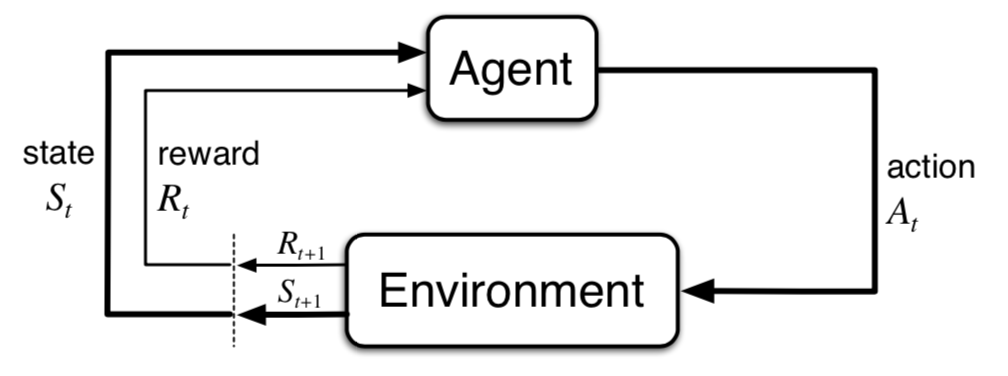
\includegraphics[scale=1]{basicRL.png}
    \caption{Basic overview of the reinforcement learning setting with an agent interacting via actions ($A_t$) with its environment moving through states ($S_t$). Thus gaining different rewards ($R_t$). Source: \textcite{sutton1998reinforcement} }
    \label{fig:4}
\end{figure}

Simply put, RL is an agent interacting via actions with its environment, and by doing so eventually learning an optimal policy or behaviour. This learning process is done by trial and error, for sequential decision making \parencite{li2017deep}. \autoref{fig:4} above illustrates a simple agent interacting with its environment. A RL agent interacts with its environment over time. At each time step $t$ the agent receives  a \textit{state} $S_t$ in a state space $\mathcal{S}$ and makes an \textit{action} $A_t$ from an action space $\mathcal{A}$ \parencite{li2017deep}. As a consequence of its action, the agent receives \textit{reward} $R_t$ which is a scalar value. 
\newline
\newline
The agent's goal is to maximize the total amount of cumulative reward it receives. This is know as the \textit{reward hypothesis} \parencite{sutton1998reinforcement}. The agent's behavior is modelled by the \textit{policy} $\pi(s|a)$. A policy is a mapping from a state to an action, that is the probability of selecting action $A_t=a$ in state $S_t = s$. This also includes transitioning to the next state $S_{t+1}$ according to the environments dynamics or \textit{model} for a \textit{reward function} $\mathcal{R}(s,a)$ and \textit{state transition probability} $\mathcal{P}(S_{t+1} |S_t, A_t)$ \parencite{li2017deep}.
\newline

%\subsubsection*{Markov Decision Process}
 \textbf{Markov Decision Process.} More formally the RL problem is formulated as a \textit{Markov Decision Process} (MPD) \parencite{sutton1998reinforcement, li2017deep}. A MDP is a tuple $(\mathcal{S, A, P, R}, \gamma)$ \parencite{li2017deep}:
\begin{itemize}
    \item $\mathcal{S}$ is a finite set of states
    \item $\mathcal{A}$ is a finite set of actions
    \item $\mathcal{P}$ is a transition probability matrix, 
    \begin{equation} 
        \label{eq:12a}
        \mathcal{P}^{a}_{ss'} = P[S_{t+1} = s' | S_t =s, A_t = a]
    \end{equation}
    \item $\mathcal{R}$ is a reward function, 
    \begin{equation}
        \label{eq:12b}
        \mathcal{R}^{a}_{s} = E[R_{t+1} | S_t =s, A_t=a]
    \end{equation}
    \item $\gamma \in [0,1]$ is a \textit{discount factor} 
\end{itemize}
In general, one seeks to maximize the \textit{expected return}. Where the return, denoted $G_t$ is the total discounted reward from time step $t$:

\begin{equation}
    \label{eq:13}
    G_t = R_{t+1} + \gamma R_{t+2} + ... = \sum_{k=0}^{\infty}{\gamma^{k}R_{t+k+1}}
\end{equation}
The discount factor or discount rate in \autoref{eq:13} determines the present value of future rewards, $k$ steps in the future. 

\newpage
Note that a $\gamma$ close to 0 leads to \textit{myopic} behavior i.e. the agent only cares about immediate rewards. Whilst if $\gamma$ is close to 1, the agent is more \textit{far-sighted}. When the agent-environment interaction breaks naturally into sub-sequences, which are called \textit{episodes}.
\autoref{eq:13} makes sense. Another key concept underlying RL is the \textit{Markov property} i.e. only the current state affects the next state \parencite{arulkumaran2017brief}. More formally this means:

\begin{equation}
    \label{eq:13b}
    P[S_{t+1} | S_t] = P[S_{t+1} | S_1, ..., S_t]
\end{equation}
\autoref{eq:13b} states that the future is conditionally independent of the past given the present state. According to \textcite{arulkumaran2017brief} this assumption is somewhat unrealistic. As it requires the states to be fully observable. A generalization of a MDPs are partially observable MDPS (POMDPS). In which the agent receives an observation $O_t \in \mathcal{O}$. Where the distribution of the observation is $P(O_{t+1} | S_{t+1} | A_t)$\parencite{arulkumaran2017brief}. Which is dependent on the current state and the previous action. The problem explored in this thesis is a POMDPS.
\newline
%\subsubsection*{Value Functions}

\textbf{Value Functions.} Most RL algorithms involve estimating \textit{value functions} of states or state-action pairs. These estimate how god it is for an agent to be in a certain state \parencite{sutton1998reinforcement, li2017deep}. The value of a state $s$ under a policy $\pi$ is denoted $v_{\pi}(s)$. This is the expected return when starting in $s$ and following $\pi$. Below is the \textit{state-value function for policy $\pi$}:

\begin{equation}
    \label{eq:14}
    v_{\pi}(s) = E_{\pi}[G_t | S_t = s] = E_{\pi}\left[\sum_{k=0}^{\infty}{\gamma^{k}R_{t+k+1}} | S_t = s\right], \forall s \in \mathcal{S}.
\end{equation}
Note that the value of the terminal state is always zero \parencite{sutton1998reinforcement}. Similarly  one can define the \textit{action-value function for policy $\pi$} \parencite{sutton1998reinforcement}. Which is the value of taking action $a$ in state $s$ under policy $\pi$, denoted $q_{\pi}(s,a)$. This is the expected return starting from $s$, taking the action $a$ and therefore following policy $\pi$:

\begin{equation}
    \label{eq:15}
    q_{\pi} = E_{\pi}[G_t | S_t =s, A_t = a] = E_{\pi} \left[\sum_{k=0}^{\infty}{\gamma^{k}R_{t+k+1}} | S_t=s, A_t=a \right]
\end{equation}
\autoref{eq:14} and \autoref{eq:15} can be estimated from experiences or by using \textit{Monte Carlo Methods} \parencite{sutton1998reinforcement}.
\newline

%\subsubsection*{Bellman equations \& Optimality}
\textbf{Bellman equations \& Optimality.} Both \autoref{eq:14} and \autoref{eq:15} satisfies recursive relationships. Which are commonly know as \textit{Bellman equations} \parencite{sutton1998reinforcement}:

\begin{equation}
    \label{eq:16}
    v_{\pi} = E[G_t | S_t = s] = E_{\pi}[R_{t+1} + \gamma G_{t+1} | S_t = s]
\end{equation}

\begin{equation}
    \label{eq:17}
    q_{\pi} = E_{\pi}[R_{t+1} + \gamma G_{t+1} | S_t = s,  A_t = a]
\end{equation}
From \autoref{eq:16} and \autoref{eq:17} the Bellman equations expresses a relationship between the value of the state and its successor states. However solving a RL task implies finding a policy that achieves a lot of reward over the long run. Thus looking for \textit{optimal policies} ($\pi \geq \pi'$). It is common to denote all optimal policies with $\pi_{*}$ whom share the same state-value and action-value functions \parencite{sutton1998reinforcement}. Therefore it is of interest to maximize the following:

\begin{equation}
    \label{eq:18}
    v_{*}(s) = \underset{\pi}{\text{max }} v_{\pi}(s)
\end{equation}

\begin{equation}
    \label{eq:19}
    q_{*}(s,a) = \underset{\pi}{\text{max }} q_{\pi}(s,a)
\end{equation}

Using \autoref{eq:18} and \autoref{eq:19} together with the Bellman equations in \autoref{eq:16} and \autoref{eq:17} this yields the \textit{Bellman optimality equations}:

\begin{equation}
\label{eq:20}
\begin{aligned}
& & v_{*}(s) =  \underset{a}{\text{max }} 
E_{\pi_{*}}[R_{t+1} + \gamma v_{*}(S_{t+1}) | S_t =s, A_t = a] \\
& & = \underset{a}{\text{max }} 
\sum_{s', r}^{}{p(s', r | s,a)}[r + \gamma v_{*}(s')]
\end{aligned}
\end{equation}

\begin{equation}
\label{eq:21}
\begin{aligned}
& & q_{*}(s,a) = 
E[R_{t+1} + \gamma \underset{a'}{\text{max }}q_{*}(S_{t+1, a'}) | S_t =s, A_t = a] \\
& & =  \sum_{s', r}^{}{p(s', r | s,a)}[r + \gamma \underset{a'}{\text{max }}q_{*}(s',a')]
\end{aligned}
\end{equation}
For a finite MDP \autoref{eq:20} and \autoref{eq:21} has a unique solution independent of the policy \parencite{sutton1998reinforcement}. Nevertheless, in practice there is no closed form solution for these equations. Therefore one must resort to approximate and iterative methods. That uses \textit{dynamic programming} or Monte Carlo methods.

\subsection{Exploration versus Exploitation}
There is a trade-off between \textit{exploration} and \textit{exploitation} when training a reinforcement learning agent. Where exploration refers to taking actions, that come from the current best version of the learned policy. Exploration instead is concerned with taking more actions to obtain more training data \parencite{goodfellow2016deep}. Where the dilemma is that neither exploration nor exploitation can be pursued exclusively without failing at the task \parencite{sutton1998reinforcement}. There exists some strategies to balance the trade-off between exploration and exploitation. For instance by employing a \textit{greedy} approach i.e. choosing the action with the highest payoff \parencite{sutton1998reinforcement, szepesvari2009algorithms}.

\begin{equation}
    \label{eq:21a}
    A_t = \underset{a}{\operatorname{argmax}}Q_t(a)
\end{equation}
A simple modification of \autoref{eq:21a} is to fix $\varepsilon > 0$ and choose a random selected action. With probability $\varepsilon$ and go with the greedy choice otherwise. This strategy is called $\varepsilon$-greedy. Another approach is \textit{Boltzman exploration} \parencite{sutton1998reinforcement,szepesvari2009algorithms} which is given the sample means of the actions at time $t$. The next action is drawn from the multinominal distribution of $\pi_t$, where 

\begin{equation}
    \label{eq:21b}
    P_t(a) = \frac{\exp{(q_{t}(a)/\tau)}}{ \sum_{i=1}^{n}{\exp{(q_{t}(i)/ \tau)}}} = \pi_t(a)
\end{equation}
Where $ \tau$ is a temperature parameter annealed over time.
Finally there also exist approaches based on the concept, \textit{optimism in the face of uncertainty}.  Where the learner should choose the action with the best upper confidence bound (UCB) \parencite{sutton1998reinforcement, szepesvari2009algorithms}

\begin{equation}
    \label{eq:21c}
    A_t = \underset{a}{\operatorname{argmax}} \left[Q_t(a) + c \sqrt{\frac{\ln{t}}{N_t(a)}} \right]
\end{equation}
Where $t$ is the time, $c$ controls the degree of exploration and $N_t(a)$ is the number of times that action $a$ has been selected \parencite{sutton1998reinforcement}.

\newpage

\subsection{Algorithms \& Learning in RL}
One can characterize RL problems into two main classes: \textit{prediction} and \textit{control} where each is followed by different approaches as \textit{value iteration, policy iteration} and \textit{policy search} \parencite{szepesvari2009algorithms}. These different approaches uses different algorithms. Note that all these algorithms are implemented in both \parencite{plappert2016kerasrl, baselines, schaarschmidt2017tensorforce} libraries used in the thesis. In general deep reinforcement learning is based on the algorithms below, but with deep neural networks. To approximate $V^{*}, Q^{*}$ and $A^{*}$ \parencite{arulkumaran2017brief}. 
\newline

%neeed this? maybe put in appendix..
%\subsubsection*{Dynamic Programming \& Monte Carlo Methods}
\textbf{Dynamic Programming \& Monte Carlo Methods.} In order to find optimal solutions for \autoref{eq:20} and \autoref{eq:21} one must resort to using approximate methods as dynamic programming. The key idea of dynamic programming is to use the value functions to organize and structure the search for good policies \parencite{sutton1998reinforcement, szepesvari2009algorithms}. Once a policy $\pi$ has been improved using $v_{\pi}$ to yield a better policy,  $\pi'$. one can then compute $v_{\pi}'$ and improve it again to yield policy $\pi^{''}$ \parencite{sutton1998reinforcement}. This is what \textit{policy iteration} is about and is described more in \autoref{alg1} found in \autoref{app:A}.
\newline
\newline
One drawback with \autoref{alg1} is that is quite computationally expensive as it involves policy evaluation over the full state space \parencite{sutton1998reinforcement}. A remedy for this is \textit{value iteration}. Where the basic idea is to use early stopping i.e. one update of each state. Which is shown in \autoref{alg2} in \autoref{app:A}. Conversely \textit{Monte Carlo methods} (MCM) require only experience i.e. sample sequences of states, actions, and rewards. From actual or simulated interaction with the environment \parencite{sutton1998reinforcement}. MCM solves reinforcement learning problems based on averaging sample returns. 
\newline

%\subsubsection*{Q-Learning \& SARSA}
\textbf{Q-Learning \& SARSA.} \textit{Temporal difference} (TD) learning can be seen as a combination of Monte Carlo methods and dynamic programming. That learn directly from raw experience without a model of the environment's experience \parencite{sutton1998reinforcement, arulkumaran2017brief}. The most simple TD method makes the following update:

\begin{equation}
    \label{eq:22}
    V(S_t) \leftarrow V(S_t) + \alpha \left[R_{t+1} + \gamma V(S_{t+1} - V(S_t) \right]
\end{equation}
This idea is applicable both to \textit{Q-Learning} and \textit{State-action-reward-state-action} (SARSA) which are both cases of TD learning. 
\newline
\newline
However Q-Learning is a \textit{off-policy} method whilst SARSA is an \textit{on-policy method} \parencite{sutton1998reinforcement, arulkumaran2017brief}. On-policy methods attempt to evaluate or improve the policy used to make decisions. Whilst off-policy methods instead evaluates or improve a policy different from that used to generate the data \parencite{sutton1998reinforcement}. In other words, on-policy methods estimate the value of a policy while using it for control. Off-policy methods uses two separate policies instead. One called \textit{behavioral policy} and the other \textit{target policy} \parencite{sutton1998reinforcement}. Now the goal is to learn an \textit{action-value} function which is estimated with $Q^{}$, instead of a state-value function. The update rule for SARSA is given below in \autoref{eq:23}:

\begin{equation}
    \label{eq:23}
    Q(S_t, A_t) \leftarrow Q(S_t, A_t) + \alpha \left[R_{t+1} + \gamma Q(S_{t+1}, A_{t+1}) - Q(S_t, A_t) \right]
\end{equation}
Q-learning instead estimates  $q_{*}$ \footnote{The optimal action-value function} with the learned action-value function $Q$ independent of the policy being followed \parencite{sutton1998reinforcement}. 
%\newpage
The main update rule for \textit{Q-learning} is given below in \autoref{eq:24}

\begin{equation}
    \label{eq:24}
     Q(S_t, A_t) \leftarrow Q(S_t, A_t) + \alpha \left[R_{t+1} + \gamma \underset{a}{\operatorname{max}} Q(S_{t+1}, a) - Q(S_t, A_t) \right]
\end{equation}
\newline
%\subsubsection*{Deep Q Networks (DQN)}
\textbf{Deep Q Networks (DQN).} In \textcite{mnih2015human} they present Deep Q Learning (DQN). Which replaces the $Q$ function with a neural network called \textit{Q-network}. This method also keeps track of some observations in memory which is called \textit{experience replay} \parencite{mnih2015human}. The agents experience is stored in $e_t = (s_t, a_t, r_t, s_{t+1})$ at each time step in a data set $D_t = \{e_1, ..., e_t\}$. Where on Q-learning updates the experience is drawn uniformly \parencite{mnih2015human}. They use a deep convolutional network to approximate the optimal action-value function $Q^{*}$. The Q-learning update at iteration $i$ uses the loss function in \autoref{eq:25} below:

\begin{equation}
    \label{eq:25}
    L_i(\theta_i) = \mathbb{E}_{(s,a,r,s') \sim U(D)} \left[\left(r+ \gamma \underset{a'}{\operatorname{max}}Q(s', a', \theta_{i}^{-})-Q(s,a;\theta_i)  \right)^2 \right]
\end{equation}
Where $\gamma$ is the discount factor, $\theta_i$ are the parameters of the Q-network. $\theta_{i}^{-}$ is the parameters of the target network \parencite{mnih2015human}.
\newline
%add full algorithm here

%\subsubsection*{Policy Gradients \& Proximal Policy Optimization (PPO)}
\textbf{Policy Gradients \& Proximal Policy Optimization (PPO).} Policy gradients methods work by directly computing an estimate of the gradient of policy parameters in order to maximize the expected return. This by using stochastic gradient descent \parencite{bansal2017emergent, schulman2017proximal}. The most common estimator is shown below in \autoref{eq:26}

\begin{equation}
    \label{eq:26}
    \hat{g} = \hat{\mathbb{E}}_{t}\left[\nabla_{\theta} \log{\pi_{\theta}(a_t|s_t)\hat{A}_{t}} \right]
\end{equation}
Where $\pi_{\theta}$ is a stochastic policy and $\hat{A}_{t}$ is an estimator of the advantages function at time-step $t$. The advantage function is shown below in \autoref{eq:27}:

\begin{equation}
    \label{eq:27}
    \hat{A}_{t} = -V(s_t) + r_t +\gamma r_{t+1} + ... \gamma^{T-t+1} r_{T-1} + \gamma^{T-t}V(s_T).
\end{equation}
In \textcite{schulman2017proximal} they propose a new family of policy gradient methods. That alternates between sampling data through interaction with the environment, and optimizing a "surrogate" objective function using stochastic gradient ascent.  The surrogate function is given by \autoref{eq:28} below: 
\begin{equation}
    \label{eq:28}
    L_{t}^{CLIP + VF+ S}(\theta) = \hat{\mathbb{E}_{t}} = \left[L_{t}^{CLIP}(\theta) + c_1 L_{t}^{VF}(\theta) + c_2S[\pi_{\theta}(s_t)]\right]
\end{equation}
Where $c_1,c_2$ are coefficients, and S is an entropy bonus. $L_{t}^{CLIP}$ is the clipped surrogate objective and $L_{t}^{VF}$ is a squared-error loss \parencite{schulman2017proximal}.
%add full algorithm here

%\subsection{Competitive Self-Play}
%Many real-world applications can be described as large-scale games of imperfect information. A game is a domain of conflict for cooperation between several entities \parencite{heinrich2016deep}. Where the optimal solutions for these types of situations would be Nash equilibrium. That is an strategy from which no agent would choose to deviate \parencite{heinrich2016deep}. This is where self-play comes in. In short self-play is the activity of imagining or simulating the play of a game against oneself \parencite{heinrich2017reinforcement}. This concept is also based on the idea of \textit{fictitious play}.  Where fictitious players choose best responses to their opponents' average behaviour \parencite{heinrich2016deep}. 
%\newline
%\newline
%\textcite{tampuu2017multiagent} also mentioned that self-play is any type of play against an \textit{adaptive agent}. Typically agents are first trained in a supervised manor, with self-play as a second phase of training. In \textit{Fictious Self-Play} (FSP) on the other hand the agents generate datasets of their experience in self-play \parencite{heinrich2016deep}.  Each agent stores transition tuples $(s_t, a_t, r_{t+1}, s_{t+1})$ in a memory $\mathcal{M}_{RL}$ for reinforcement learning (confer experience replay). Experience of the agent's own behaviour $(s_t, a_t)$ is stored in a separate memory for supervised learning $\mathcal{M}_{SL}$ \parencite{heinrich2016deep}.
%\newline
%\newline
%\textcite{bansal2017emergent} mentioned that in a competitive-multi agent environment trained with self-play. Far more complex behaviours then the environment itself can emerge. In general training an agent to perform a highly complicated task requires a complicated environment, but there exists environments where behaviour of the agent is far more complex. Then the environment itself \parencite{bansal2017emergent}. These types of environments have two interesting properties:

%\begin{enumerate}
%    \item Very simple competitive multi-agent environments can produce extremely complex behavior
%    \item When training with self-play the environment provides the agents with  a perfect curriculum.
%\end{enumerate}

%mention where it has been successfully used and show the need of the application that we want to use here for the thesis
%\subsection{RL in Market Microstructure}

\newpage

\subsection{Issues with deep RL}
The use of reinforcement learning, and specially deep reinforcement learning. Has been glorified for some time. Due to a lot of promising results as the ones presented in \textcite{silver2016mastering, silver2017mastering}. Which is the closes today in terms of \textit{Artificial General Intelligence}. However training and using reinforcement learning is not trivial. Where some of the major issues are presented below:

\begin{enumerate}
    \item \textit{Deep RL can be sample inefficient}. Reinforcement learning has its own planning fallacy. Learning a policy usually needs more samples then what one thinks \parencite{irpan_2018}. Simulations run on the popular MuJoCo physics environment need for instance between $[10^5, 10^7]$ time-steps to learn different task \parencite{heess2017emergence}.
    
    \item \textit{Performance compared to other methods}. In theory RL can work for everything, including experiments where a model of the world is not know. Which comes at a cost. That it is hard to exploit any problem specific information, that could help learning \parencite{irpan_2018}. The rule-of-thumb is that domain-specific algorithms tend to work better and faster then RL. Except for rare cases.
    
    \item \textit{Reward design is hard}. It seems to be hard to design a reward function, that encourages the behaviour one wants the agent to learn. Bad designed rewards can lead to overfitting of the agent to the reward. Which is why it is important to design a relevant reward signal \parencite{sutton1998reinforcement, irpan_2018}. Often \textit{shaped rewards}\footnote{increasing rewards in states that are close to the end goal} are easier to learn compared to \textit{sparsed rewards}\footnote{only gives reward in goal state}. Some possible remedies however are to use sparsed rewards or careful shaping of the reward \parencite{irpan_2018}
    
    \item \textit{Generalization}. If you want to do good in one specific environment you are free to overfit. However generalizing an agent to another environment, would result in bad results \parencite{irpan_2018}. Meaning that transfer learning is not easy to archive. 
    
\end{enumerate}

%necessary?
%\section{Tree Search}

%\subsection{MinMax}

%\subsection{Monte Carlo Tree Search (MCTS)}

%own chapter?
\chapter{Related Work}\label{ch:3}
In this chapter previous related work is presented. To give an overview over what has been done previously, as well as current state of the art. Also the difference between this work and previous work is discussed. The chapter is divided into the following sections: \textit{Agent based Financial Markets, Market Microstructure} and \textit{Reinforcement Learning in Finance}. An overview is presented in \autoref{tab:pvi}.

%\newpage

%\section{Overview}
% latex table generated in R 3.3.1 by xtable 1.8-2 package
% Mon Jul 02 23:12:15 2018
\begin{table}[H]
\centering
\caption{Summary and comparison of most important previous related work by category. Also compared to this work.}
\label{tab:pvi}
\resizebox{0.95\textwidth}{!}{%
\begin{tabular}{llll}
  \hline
  \textbf{Agent based Financial Markets} \\
  \hline
 \textbf{Study} & \textbf{Techniques} & \textbf{Strategies} & \textbf{Difference to this work} \\ 
  \hline
\shortstack{\textcite{raberto2001agent}} & \shortstack{na} & \shortstack{Chartist \\ Fundamentalist \\ Random} & \shortstack{Not realistic \\ prices behaviour}  \\ 
\hline

\shortstack{\textcite{martinez2009evolutionary}} & \shortstack{Genetic Programming \\ Decision Trees} & \shortstack{Technical \\ Fundamentalist \\ Noise} & \shortstack{Not realistic \\ environment}  \\ 
\hline

\shortstack{\textcite{brandouy2011design}} & \shortstack{Genetic Programming \\ Human agent} & \shortstack{Technical \\ Risk-averse \\ Mean-variance \\ random} & \shortstack{Matching engine}  \\ 

\hline
 \textbf{Market Microstructure} \\
  \hline
\shortstack{\textcite{ho1981optimal}} & \shortstack{Dynamic \\ Programming} & \shortstack{Market Maker} & \shortstack{Not focused on \\ limit order book (LOB)}  \\ 
\hline

\shortstack{\textcite{glosten1985bid} \\ \textcite{das2005learning, das2003intelligent}} & \shortstack{Dynamic Programming \\ Bayesian Learning} & \shortstack{Market Maker} & \shortstack{Focused on Dealer Market \\ Information based models}  \\ 

\hline
  \textbf{Reinforcement Learning in Finance} \\
  \hline
\shortstack{\textcite{moody1999reinforcement}} & \shortstack{Q-Learning \\ Recurrent Reinforcement \\ Learning (RRR)} & \shortstack{Algorithmic \\ Trading} & \shortstack{Trading Dynamics \\ not main focus \\ Different value functions}  \\ 
\hline

\shortstack{\textcite{kearns2013machine} \\ \textcite{hendricks2014reinforcement}} & \shortstack{Q-Learning \\ Reinforcement \\ Learning} & \shortstack{Dealer / Market Maker} & \shortstack{Optimized Trade execution \\ Price Prediction \\ No LOB}  \\ 
\hline

\shortstack{\textcite{yang2014algorithmic}} & \shortstack{Q-Learning \\ Inverse Reinforcement \\ Learning} & \shortstack{HFT Trader} & \shortstack{Trader Identification}  \\ \hline

\shortstack{\textcite{darley2007nasdaq}} & \shortstack{Q-Learning \\ Reinforcement Learning \\ Dynamic Programming} & \shortstack{Dealer with and without inventory \\ Parasitic Dealer \\ Dynamical Dealer, Q-Learner \\ Spread Learner } & \shortstack{Tick size changes \\ Not using PPO or DQN \\ No LOB}  \\ 
\hline

\shortstack{\textcite{pastore2015modelling} \\ \textcite{rutkauskas2009building}} & \shortstack{Q-Learning \\ Reinforcement Learning \\ Genetic algorithm} & \shortstack{Naive / Short-term} & \shortstack{Number of agents \\ No DQN or PPO agent \\ Market data \\ No LOB}  \\ 

\hline
\end{tabular}%
}
%\end{minipage}}
\end{table}

\newpage
\section{Agent based Financial Markets}

The field of finance and economics have used various approaches to model financial markets. Among these, three main groups of approaches can be distinguished: \textit{statistical models}, \textit{Dynamic Stochastic General Equilibrium (DSGE) models} and \textit{Agent-Based Models (ABM)} \parencite{lussange2018bright}. Agent-based financial markets of different characteristics have been developed for some time. A early model is given in \parencite{raberto2001agent} where they in their \textit{Geona market} have agents adopting strategies as chartist, fundamentalist or random. A drawback with the model is that it does not manage to correctly represent the price behavior in the market \parencite{raberto2001agent}. In this thesis the author aims to do so, by using reinforcement learning instead. 
\newline
\newline
Good overviews of agent based modelling in a financial setting, is given in \parencite{martinez2009evolutionary, boer2008agent, lebaron2006agent}. Where a more recent overview of agent based modelling in finance and economics is presented in \parencite{lussange2018bright}. In \textcite{martinez2009evolutionary} they introduce CHASM which is a software platform that allows user to experiment with different market scenarios. This market is composed of technical, fundamental and noise traders. Where genetic programming seems to be the core learning process employed and decision trees. A difference between the study by \textcite{martinez2009evolutionary} and this thesis, is that the environment used will be more complex. With a matching engine and different algorithmic trading strategies as market making. To successfully study market microstructure phenomena. The author will also use reinforcement learning for learning used by the agents in the complex environment. 
\newline
\newline
Generally speaking there are two major approaches to agent-based financial market simulations, where the first one focuses on specific market structure. Whilst the second approach is more focused on generating a flexible environment with flexible settings for the agents employed \parencite{brandouy2011design}. This thesis will focus more on the second approach in order to see what type of behaviour the agents exhibit exposed to different market conditions. Namely the dealer and limit order book markets. In \textcite{brandouy2011design} they design a artificial stock market called ATOM based on the Euronext-NYSE Stock exchange, with the possibility to add \textit{human agents}. 
\newline
\newline
They have for instance a limit order book as the thesis aim to use, however it is unclear whether they employ a functional matching engine. Which this study will use, by using a simulated limit orderbook market. They also use different types of agents for instance \textit{zero intelligence traders, technical traders, evolutionary agents, risk averse agents} and \textit{mean-variance agents}. Nevertheless, none of these are based on reinforcement learning that will be used in this thesis. 
\newline
\newline
One of the main benefits with using agent based modelling is that they demonstrate the ability to produce realistic system dynamics, which are comparable to those observed empirically \parencite{platt2016problem}. In the study by \textcite{platt2016problem} they calibrate their agents by using heuristic optimization , Nelder-Mead simplex algorithm and a genetic algorithm. They use a simpler form of matching engine in their study. They also only use a low-frequency trader and high-frequency trader. Where this thesis focuses on simulating the behaviour of a market maker.

\section{Market Microstructure}
Market microstructure studies the process by which investors' latent demands are ultimately translated into prices and volumes \parencite{madhavan2000market}. It is of importance for this thesis to understand market microstructure both theoretically and empirical. In order to replicate and even find new interesting behaviour of the agents, employed in this kind of environment. In \textcite{haferkorn2017high, agarwal2012high} the effect of HFT trading and fragmentation is discussed. Which is of interest for market micro-structure. This as fragmentation leads to more competition on the markets. That might be demonstrated by the agents. Some common references that are used in the state of the art market microstructure research is found in \parencite{o1995market,hasbrouck2007empirical, madhavan2000market, madhavan2002market}. 
\newline
\newline
There both \textit{inventory-based} and \textit{information based} models are discussed. In this thesis the author focus on inventory-based models, for the learning agents. However information based models can be used in future studies. A common inventory-based model, that uses dynamic programming to find the optimal dealer price in a one-dealer market. Is given in \textcite{ho1981optimal}. 
\newpage

A problem with the model in \parencite{ho1981optimal} is that here is no closed form solution, thus approximations is used to get arbitrarily close to the solution. By using reinforcement learning the author hopes to be able to replicate the behaviour of the agents shown in previous papers. However, also extending it, and see how the agents perform and behave in a more complex market with a limit orderbook. The information based models on the other hand tries to incorporate the element that some traders are more informed than others. Which is called \textit{asymmetric information} or \textit{adverse selection} in the market microstructure literature \parencite{o1995market, hasbrouck2007empirical}. 
\newline
\newline
A recent model for this is the one presented in \parencite{das2003intelligent, das2005learning}. Which is an extension of the model presented in \textcite{glosten1985bid}. The Glosten and Milgrom model derives the market makers price by setting equations under asymmetric information. To be such that the bid/ask quotes are the expectations conditioned on if the order is a buy or sell order. In \textcite{das2005learning} on the other hand they employ a non-parametric density estimate of the true value or fundamental value of the stock. This by using Bayesian Learning. 
\newline
\newline
The author will be training agents on an environment similar to the one described in \parencite{das2005learning} but with reinforcement learning instead. Hoping to see the same market dynamics as they did in their study. To further validate the agents learning of trading dynamics. Before using them on the more complex model with the matching engine. Finally in \textcite{o2015high} they mentioned that in a high-frequency world. Older empirical models may no longer be appropriate. Where this thesis aims to provide a step in a new direction for this type of research.

\newpage
\section{Reinforcement Learning in Finance}

Reinforcement learning or \textit{neuro-dynamic programming} as it also have been called in the literature. Has been used previously in a financial setting. Where some of the earlier applications have been in trading. In \textcite{moody1999reinforcement} the author's explore the opportunity of using reinforcement learning for trading. Using Recurrent Reinforcement Learning (RRL) and Q-learning and looking at the S\& P 500 index. Not that much focus is on trading dynamics. Which will be the main focus of  this thesis, on a completely different market. In \parencite{dempster2006automated, du2016algorithm, wang2016reinforcement, casqueiro2006neuro, bertoluzzo2012testing} they discuss the usages of different types of reinforcement learning algorithms for trading. Where trading is done in for example foreign exchange or the energy market. None of these use a matching engine, or a more complex environment with several HFT/market maker agents. Or with the possibility of completely changing the market conditions, which this thesis aims to do. 
\newline
\newline
In \textcite{kearns2013machine} they give a good overview of reinforcement learning used in market microstructure and high-frequency trading. With use-cases in optimized trade execution, prediction of price movements and optimized execution in dark pools. In \parencite{nevmyvaka2006reinforcement, hendricks2014reinforcement}  optimized trade execution is studied with the help of reinforcement learning. Which is of importance in market microstructure and might be examined in this thesis. However for this thesis one of the main objectives is to understand and successfully replicate know behaviour of traders in a dynamic market. Where some studies concerned with understanding the behaviour of traders are presented in \parencite{yang2014algorithmic, yang2012behavior}. Where they use \textit{inverse reinforcement learning} on trading decisions. 
\newline
\newline
The idea is to find the reward function given the observations of optimal trading behaviour and then use it for trader identification. Albeit interesting this thesis is not interested in capturing key characteristic of already optimal HFT strategies. Instead the author wants to see what optimal or not optimal behaviour the agents will use, and how they will react to changed market conditions. Therefore reinforcement learning is used instead. Some previous studies exist using reinforcement learning for market making see for instance \parencite{jumadinova2010comparison,chan2001electronic, fernandez2015high, sherstov2004three}. Market making strategies will be implemented by the agents trained in this thesis.
\newline
\newline
In \textcite{cartea2015algorithmic} some common algorithmic trading strategies are presented, focusing on stochastic optimal control.
A previous study has been done at NASDAQ investigating the effects of tick size changes \textcite{darley2007nasdaq}. Where the strategies employed where a simpler form of reinforcement learning, together with dynamic programming approaches. Which works as inspiration for this study. However the thesis will be different in that it incorporates a more realistic simulated market. With the matching engine, and several different types of agents. When modelling stock agents some previous studies conducted are \parencite{pastore2015modelling, rutkauskas2009building}. This study aims to do the something similar, but on the Nordic stock market. As this study want's to understand the trading dynamics created by market makers. 
\newline
\newline
Nevertheless, in order to train the agents in the trading environments. A good understanding of reinforcement learning is needed. In \parencite{arulkumaran2017brief, mnih2015human, li2017deep} good overviews of the current state of the art deep reinforcement learning (RL) is presented.  Recently some of the state of the art research, has been driven by DeepMind and their work with the game Go. See for instances \parencite{silver2016mastering, silver2017mastering, vinyals2017starcraft}, that serves as inspiration of best practices. Competitive self-play is introduced and examined in \parencite{bansal2017emergent, schulman2017proximal}. In \parencite{busoniu2008comprehensive, bucsoniu2010multi} some of the most common multiagent reinforcement learning strategies are discussed. 

\chapter{Research Summary}\label{ch:4}
In this chapter, a summary of the research methodology is provided. An overview of the research process is found in \autoref{fig:1}

\section{Research Methodology}
\begin{figure}[H]
    \centering
    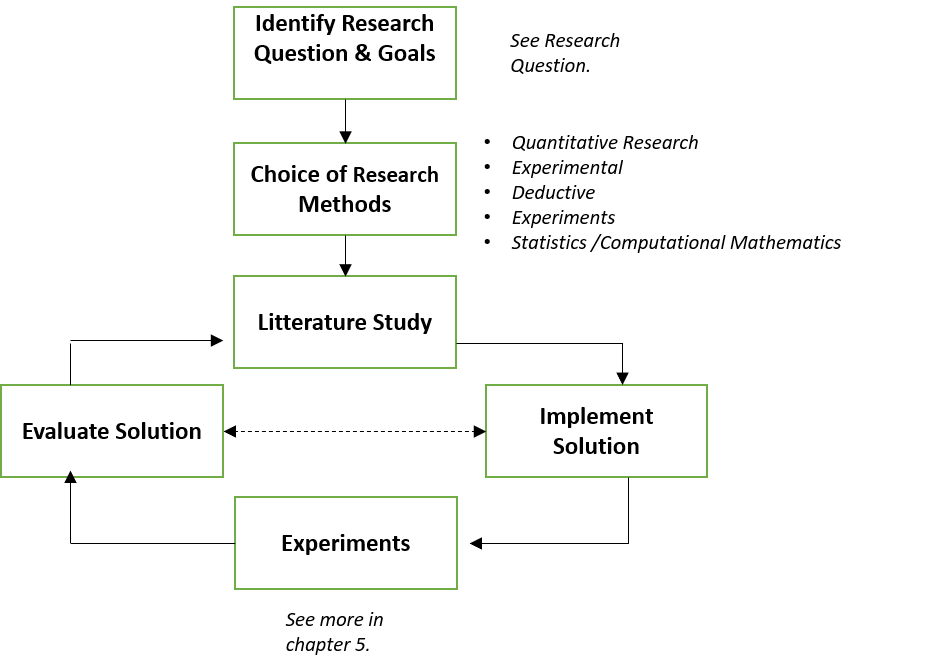
\includegraphics[scale=.8]{Imgs/researchmethodsv3.PNG}
    \caption{Overview of the different research methodology stages conducted during the thesis.}
    \label{fig:r1}
\end{figure}

\subsection{Research Question}
The research question for this thesis is shown below:

\begin{RQ}
Will trading dynamics such as the bid-ask spread clustering, optimal trade execution and optimal inventory costs be exhibited \& learned by reinforcement learning agents on a simulated Nordic stock market.
\end{RQ}

\subsection{Research Goals}
The overall \textit{goal} of this thesis is to understand trading dynamics on a simulated market, when market conditions are changed. This goal can be divided into two research goals:

\begin{RG}
Be able to simulate the effect of any change to market structure.
\end{RG}

\begin{RG}
Applying reinforcement learning to a more complicated environment such as the financial markets.
\end{RG}

\subsection{Research Challenges}
When conducting this research some research challenges have been identified and somewhat dealt with:
\begin{RC}
Simulating a realistic limit orderbook.
\end{RC}
With the current implementations of different reinforcement learning libraries. There does not exist any pre-built limit order market environments. The first idea was to use parity a JAVA based exchange engine \footnote{\url{https://github.com/paritytrading/parity}}. However it turned out to be quite difficult to use this as an environment. As it would need some coding to create a wrapper. To target this challenge, our own limit order market environment was built. With an orderbook and matching engine. Inspired by how the NASDAQ limit orderbook market works.

\begin{RC}
Training and accurate learning of agents. 
\end{RC}

Training reinforcement learning agents can be quite difficult and requires both time and tuning of parameters, reward functions and other quantities of interest. 
\newpage
As well as a lot of computing power to facilitate training. To target this challenge, the author tried to monitor how the agent was thinking. By visualizing the agents action at each time-step. See more in \autoref{ch:5}. The author also monitored the mean, standard deviation and other algorithm related metrics at the end of each episode. To tune hyper parameters random search was used. The author also looked at how many time steps each episode had. In order to understand if the agent solved the problem faster or lost more often.

\begin{RC}
Creating accurate rewards, to guide the agents actions.
\end{RC}
Shaping rewards in a accurate way so that an agent learns a wanted behaviour is not easy. Which is still an active research field today. As bad design of rewards can lead to overfitting, see more in \autoref{ch:2}. To target this challenge, the author have used \textit{sparse rewards}. This in the earlier experiments and then later switch to shaping of rewards.

\section{Research Methods}
The choice of methods shown in \autoref{fig:r1} is based on using the portal in \parencite{haakansson2013portal}. The work in this thesis is performed using quantitative research. By conducting various experiments in the different agent environments. To test the behaviour of these agents using different tests and hypothesis \parencite{haakansson2013portal}. The different environments are covered in more depth in \autoref{ch:5}. However, as the author is also trying to establish relationships between different variables. Which is seen as experimental research \parencite{haakansson2013portal}.  Running all simulations results in big amounts of data. That needs to be examined, processed and analyzed. Therefore this thesis use deductive reasoning to compare and test this thesis results to previous studies. Finally statistics are used to analyze the collected data and evaluating its significance.

\subsection{Literature Study}
For the literature study, mainly available databases such as IEEE, arkivX.org, Google Scholar and Science-Direct have been used. To get access to the state of the art. Also some searching throughout the web on for example different blogs. That recommended certain papers or cases. Where relevant references were identified.

\newpage
Some books on market microstructure has been provided by the principal. Three information streams have been identified as relevant \textit{Artificial Financial Markets, Market Microstructure} and \textit{Reinforcement Learning in Finance}. After a first initial search, some 25 papers have been found to be relevant. Where the most relevant papers has already been covered in \autoref{ch:3}.

\subsection{Implementation, Experiments \& Evaluation}
Regarding the technical implementation, experiments and evaluation. This is covered more deeply in \autoref{ch:5}. However from a methodological standpoint, some discussion about these are presented here in the next sections.

\section{Validity}
In this section a discussion about validity is provided. Covering both construct, internal and conclusion validity. This is of importance when needing to devise different tests. To make sure that the simulated data, from each simulation is valid. Validity in short indicates the degree to which an instrument measures what it is supposed to measure \parencite{kothari2004research}.

\subsection{Construct Validity}
A measure is said to posses construct validity to the degree that it confirms to predicted correlations with other theoretical propositions \parencite{kothari2004research}. In other words if the measure behaves as the theory says. In this thesis the author compares the obtained results with what is stated in previous studies and literature. This in order to enforce more construct validity.  

\subsection{Internal Validity}
Internal validity is avoiding \textit{experimental artifacts} in experiments. Which is an interpretation of an experiment that is a mere illusion. However also avoiding confounding variables \footnote{an independent variable that has not been taken into account effecting dependent variables.} that can introduce biases and increased variance. 

\newpage
Indeed internal validity is connected to experimental control of background conditions, following research paradigms and using relevant features. When doing simulations, one has the possibility to limit and change the number of relevant parameters. By changing the parameters throughout our experiments the author examines the effect of these closely. In order to handle and avoid experimental artifacts.

\subsection{Conclusion Validity}
Conclusion validity is a measurement of the extent to which conclusions about relationships of variables are reasonable. This is connected to the analysis of the collected data \parencite{trochim_2006}. In this thesis the author employs regression analysis to look at for instance price impact. To determine relationships between some of the variables. The author also look at the correlation between some of the variables. As well as discussing the obtained results with people having subject matter in market microstructure.

\section{Ethics}
Ethics independent of quantitative or qualitative research is the moral principles in planning, conducting and reporting results of research studies \parencite{haakansson2013portal}. There have not been identified an possible ethical violations by conducting this research. All the data used is simulated without any connection to real market participants.

\chapter{Implementation}\label{ch:5}

\section{Overview}
%add flowchart here
\begin{figure}[H]
    \centering
    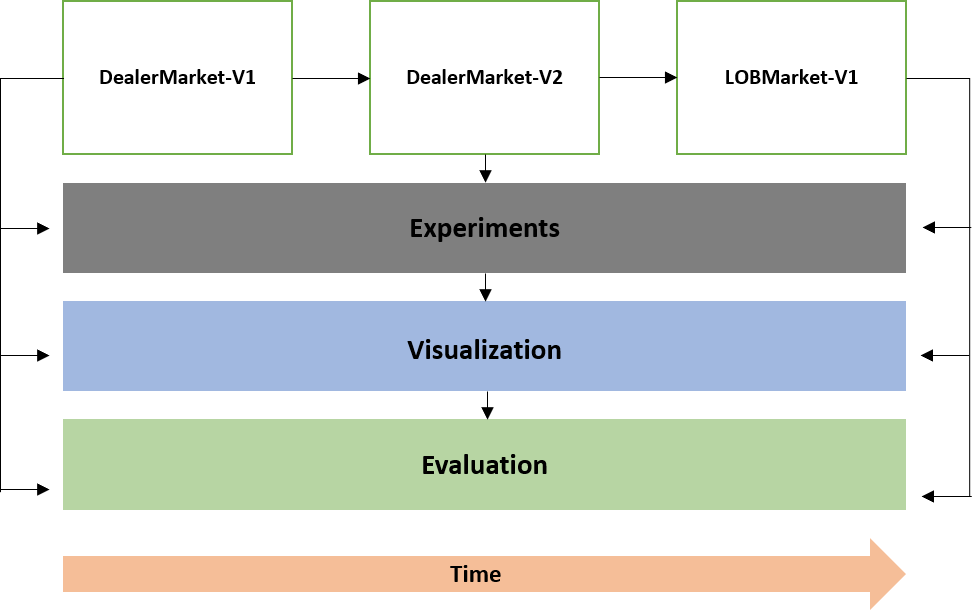
\includegraphics[scale=.7]{Imgs/implementation.png}
    \caption{Overview of the implementation of the different agents and environments in the thesis.}
    \label{fig:i1}
\end{figure}
In this chapter the implementation and experiments on the different agents and environments used are described. In \autoref{fig:i1} an overview is provided, which will be addressed more thoroughly in the following sections.

\section{Environments \& Experiments}

\begin{table}[H]
\centering
\caption{Major differences between the environments, where $a_t$ is what action, $h_t$ how much history given i.e. the last frames. Offset and slope is used for the demand curves. Each environment is seen as a way of changing the market structure for the agents.}
\label{tab:e11}
\begin{tabular}{llllllllll}
Agent & $a_t$  & $\sigma$  & $\lambda$  & Reward  & Offset  & Slope  & $h_t$  & Funds & Inventory  \\ \hline
 dmv1 & $4$  & $0.2$  & $10$  & \autoref{eq:m7}  & $10$  & $-$  &  $10$ & $10^6$ & $1000$ \\
 dmv2 & $6$  & $1.5$  & $5$  & \autoref{ls:1}  & $8$  & $0.5$  & $10$  & $10^6$ & $1000$ \\
 lobv1& $10$ & $2.0$  & $150$  & \autoref{ls:2} & $8$  & $5$  & $10$  & $2\cdot 10^5$ & $200$
\end{tabular}
\end{table} 

In this thesis new OpenAI environments were created. In order to simulate both dealer markets and limit orderbook markets. Which are based on the papers presented in \autoref{ch:2}. 
\newline
\newline
The environments used are \textit{ DealerMarket-v1, DealerMarket-v2 and LOBMarket-v1}. The main differences between these are shown above in \autoref{tab:e11}.
Nevertheless the same types of experiments have been run for each environment:

\begin{enumerate}
    \item \textit{Firstly}, by running the models for a shorter period of time to find relevant hyper-parameters using random search. For some 100 iterations, simulating the runs for some 200-500 episodes of a maximum 10 000 intervals or time steps.
    
    \item \textit{Secondly} training the models for some two million time-steps for intervals of 10 000\footnote{Each time-step is equivalent to 1/10th of a second. Meaning that each simulation last for at most $ (1000*2000)/(3600 * 8.5) \approx 555$ hours or some $65$ trading days.} to collect data, monitor and visualize learning of agent. Also using different random seeds in order to take into account randomness in the results. 
    
    \item\textit{Thirdly} testing the environment on a random agent/policy to use as benchmark against the trained agents.
    
    \item   \textit{Finally} performing statistical tests and price impact regression on the collected data to see if phenomena from the literature can be found.
\end{enumerate}

\newpage
\subsection{DealerMarket-v1}
This environment is inspired by the ideas underpinning \textcite{ho1981optimal}. Meaning that the equilibrium price is following a Brownian motion.  A changing demand curve controlled by the slope parameter in \autoref{tab:e11}. Where orders arrive according to a Poisson distribution based on the demand curve. These parameters are all changing after each episode.  
\newline
\newline
There is only a single agent that is a dealer or market maker. The agent has four possible actions: Move bid up $(0)$, Move bid down $(1)$, Move ask up $(2)$ and Move ask down $(3)$. There are no hidden states in order to make it fairly easy for the agent. In order to use this as a benchmark to other environments and agents. 
\newline
\newline
As input (only the last 10 frames), the agent has the following observed state variables: \textit{volume imbalance, offset imbalance, inventory imbalance, spread, wealth} and \textit{share value}. 
%\newpage
Each called $[ibv, ibo, ibif,sp, w,v]$ hereafter. Defined below:
\begin{equation}
\label{eq:m1}
    ibv = (\text{last at bid - last at ask})/(\text{last at bid + last at ask})
\end{equation}

\begin{equation}
\label{eq:m2}
    ibo = (\text{off set ask + offset bid})/(\text{spread})
\end{equation}

\begin{equation}
\label{eq:m3}
    ibif = (\text{inventory - funds/ref price})/(\text{wealth})
\end{equation}

\begin{equation}
\label{eq:m4}
    sp = (\text{offset ask - offset bid})
\end{equation}

\begin{equation}
\label{eq:m5}
    w = (\text{funds/price ref + inventory})
\end{equation}

\begin{equation}
\label{eq:m6}
    v = \text{share value}
\end{equation}
The state variables in \autoref{eq:m1} to \autoref{eq:m6} are changing throughout the training of the agent. The agents goal is to optimize its reward, shown in \autoref{eq:m7}. 

\begin{equation}
    \label{eq:m7}
    Reward = \Delta \text{inventory} + \Delta funds
\end{equation}
%Hence optimizing the change of the agents reward without no mark-to-market at every time-step. The agent is also given some initial values as seen in \autoref{tab:e11}. %After training the agent was tested,  with the pre-trained weights. Again on the environment for 500 steps or simulations of 10 000 intervals. This in order to see if the agent had learned or not learned something. 

%\newpage

\subsection{DealerMarket-v2}
\begin{figure}[H]
		%Do not try to scale figure in .tex or you loose font size consistency
	    	\centering
		%The code to input the plot is extremely simple
		% Created by tikzDevice version 0.11 on 2018-06-30 17:08:08
% !TEX encoding = UTF-8 Unicode
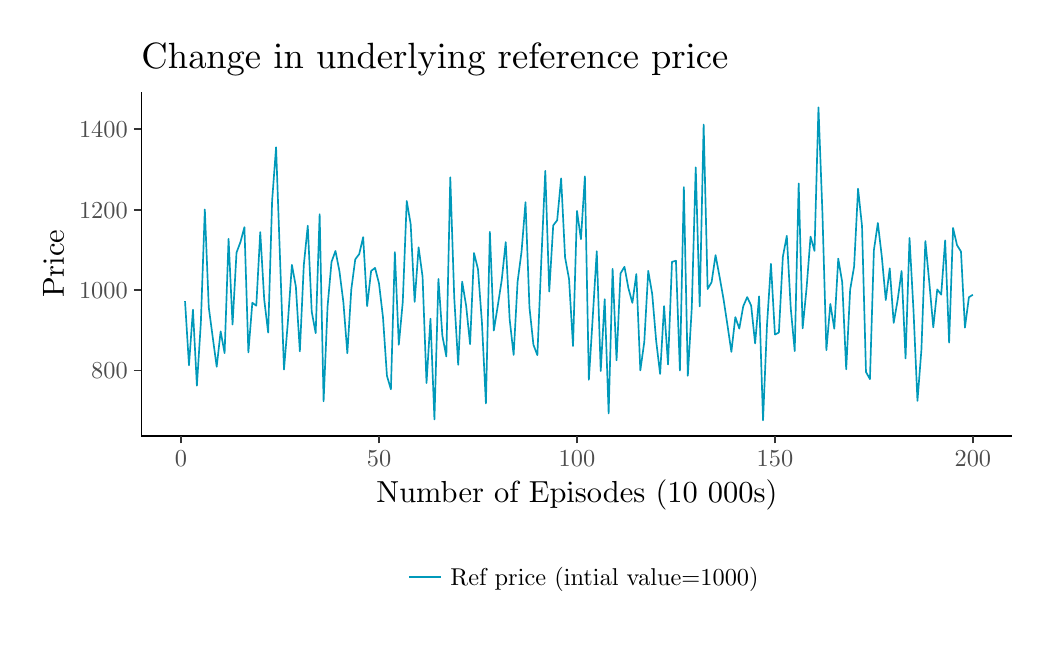
\begin{tikzpicture}[x=1pt,y=1pt]
\definecolor{fillColor}{RGB}{255,255,255}
\path[use as bounding box,fill=fillColor,fill opacity=0.00] (0,0) rectangle (361.35,216.81);
\begin{scope}
\path[clip] (  0.00,  0.00) rectangle (361.35,216.81);
\definecolor{drawColor}{RGB}{255,255,255}
\definecolor{fillColor}{RGB}{255,255,255}

\path[draw=drawColor,line width= 0.6pt,line join=round,line cap=round,fill=fillColor] (  0.00,  0.00) rectangle (361.35,216.81);
\end{scope}
\begin{scope}
\path[clip] ( 41.12, 69.30) rectangle (355.85,193.67);
\definecolor{fillColor}{RGB}{255,255,255}

\path[fill=fillColor] ( 41.12, 69.30) rectangle (355.85,193.67);
\definecolor{drawColor}{RGB}{0,153,186}

\path[draw=drawColor,line width= 0.6pt,line join=round] ( 56.86,117.99) --
	( 58.29, 94.84) --
	( 59.72,114.88) --
	( 61.15, 87.44) --
	( 62.58,110.27) --
	( 64.01,151.11) --
	( 65.44,115.72) --
	( 66.87,104.93) --
	( 68.30, 94.29) --
	( 69.73,107.04) --
	( 71.16, 99.19) --
	( 72.59,140.51) --
	( 74.03,109.52) --
	( 75.46,135.52) --
	( 76.89,139.35) --
	( 78.32,144.72) --
	( 79.75, 99.46) --
	( 81.18,117.42) --
	( 82.61,116.33) --
	( 84.04,142.94) --
	( 85.47,118.63) --
	( 86.90,106.60) --
	( 88.33,154.28) --
	( 89.76,173.59) --
	( 91.19,133.32) --
	( 92.62, 93.30) --
	( 94.05,110.81) --
	( 95.48,131.11) --
	( 96.91,123.26) --
	( 98.35, 99.84) --
	( 99.78,131.03) --
	(101.21,145.23) --
	(102.64,114.18) --
	(104.07,106.42) --
	(105.50,149.40) --
	(106.93, 81.81) --
	(108.36,115.99) --
	(109.79,132.14) --
	(111.22,136.14) --
	(112.65,128.84) --
	(114.08,117.63) --
	(115.51, 99.16) --
	(116.94,122.23) --
	(118.37,133.10) --
	(119.80,134.99) --
	(121.23,141.13) --
	(122.66,116.16) --
	(124.10,128.88) --
	(125.53,130.01) --
	(126.96,124.30) --
	(128.39,112.15) --
	(129.82, 91.02) --
	(131.25, 86.12) --
	(132.68,135.69) --
	(134.11,102.23) --
	(135.54,117.72) --
	(136.97,154.20) --
	(138.40,145.77) --
	(139.83,117.73) --
	(141.26,137.45) --
	(142.69,126.87) --
	(144.12, 88.40) --
	(145.55,111.67) --
	(146.98, 75.25) --
	(148.42,126.00) --
	(149.85,105.48) --
	(151.28, 98.01) --
	(152.71,162.73) --
	(154.14,119.19) --
	(155.57, 94.97) --
	(157.00,125.03) --
	(158.43,116.38) --
	(159.86,102.44) --
	(161.29,135.36) --
	(162.72,129.54) --
	(164.15,110.17) --
	(165.58, 81.02) --
	(167.01,143.07) --
	(168.44,107.37) --
	(169.87,116.31) --
	(171.30,125.62) --
	(172.74,139.32) --
	(174.17,111.33) --
	(175.60, 98.55) --
	(177.03,125.01) --
	(178.46,135.89) --
	(179.89,153.73) --
	(181.32,115.70) --
	(182.75,102.24) --
	(184.18, 98.47) --
	(185.61,132.93) --
	(187.04,165.07) --
	(188.47,121.49) --
	(189.90,145.35) --
	(191.33,147.21) --
	(192.76,162.34) --
	(194.19,133.79) --
	(195.62,125.97) --
	(197.06,101.76) --
	(198.49,150.60) --
	(199.92,140.38) --
	(201.35,163.06) --
	(202.78, 89.58) --
	(204.21,112.56) --
	(205.64,136.04) --
	(207.07, 92.71) --
	(208.50,118.70) --
	(209.93, 77.41) --
	(211.36,129.65) --
	(212.79, 96.60) --
	(214.22,128.00) --
	(215.65,130.40) --
	(217.08,122.65) --
	(218.51,117.36) --
	(219.94,127.79) --
	(221.38, 92.96) --
	(222.81,103.25) --
	(224.24,128.93) --
	(225.67,120.59) --
	(227.10,103.65) --
	(228.53, 91.67) --
	(229.96,116.19) --
	(231.39, 95.12) --
	(232.82,132.19) --
	(234.25,132.58) --
	(235.68, 92.91) --
	(237.11,159.19) --
	(238.54, 91.03) --
	(239.97,115.55) --
	(241.40,166.34) --
	(242.83,116.09) --
	(244.26,181.82) --
	(245.70,122.38) --
	(247.13,124.83) --
	(248.56,134.61) --
	(249.99,126.93) --
	(251.42,118.88) --
	(252.85,109.43) --
	(254.28, 99.68) --
	(255.71,112.21) --
	(257.14,108.08) --
	(258.57,116.15) --
	(260.00,119.45) --
	(261.43,116.38) --
	(262.86,102.70) --
	(264.29,119.70) --
	(265.72, 74.96) --
	(267.15,109.34) --
	(268.58,131.47) --
	(270.02,105.93) --
	(271.45,106.66) --
	(272.88,134.01) --
	(274.31,141.59) --
	(275.74,115.38) --
	(277.17, 99.93) --
	(278.60,160.53) --
	(280.03,108.16) --
	(281.46,122.80) --
	(282.89,141.31) --
	(284.32,136.15) --
	(285.75,188.02) --
	(287.18,149.90) --
	(288.61,100.27) --
	(290.04,116.98) --
	(291.47,108.03) --
	(292.90,133.36) --
	(294.33,124.83) --
	(295.77, 93.35) --
	(297.20,122.13) --
	(298.63,130.51) --
	(300.06,158.60) --
	(301.49,145.08) --
	(302.92, 92.40) --
	(304.35, 89.81) --
	(305.78,136.39) --
	(307.21,146.23) --
	(308.64,134.09) --
	(310.07,118.38) --
	(311.50,129.84) --
	(312.93,110.14) --
	(314.36,118.38) --
	(315.79,128.89) --
	(317.22, 97.28) --
	(318.65,140.81) --
	(320.09,114.62) --
	(321.52, 81.94) --
	(322.95,100.46) --
	(324.38,139.72) --
	(325.81,124.64) --
	(327.24,108.52) --
	(328.67,122.22) --
	(330.10,120.35) --
	(331.53,139.95) --
	(332.96,103.00) --
	(334.39,144.41) --
	(335.82,138.20) --
	(337.25,135.92) --
	(338.68,108.43) --
	(340.11,119.40) --
	(341.54,120.30);
\end{scope}
\begin{scope}
\path[clip] (  0.00,  0.00) rectangle (361.35,216.81);
\definecolor{drawColor}{RGB}{0,0,0}

\path[draw=drawColor,line width= 0.6pt,line join=round] ( 41.12, 69.30) --
	( 41.12,193.67);
\end{scope}
\begin{scope}
\path[clip] (  0.00,  0.00) rectangle (361.35,216.81);
\definecolor{drawColor}{gray}{0.30}

\node[text=drawColor,anchor=base east,inner sep=0pt, outer sep=0pt, scale=  0.88] at ( 36.17, 89.89) {800};

\node[text=drawColor,anchor=base east,inner sep=0pt, outer sep=0pt, scale=  0.88] at ( 36.17,118.94) {1000};

\node[text=drawColor,anchor=base east,inner sep=0pt, outer sep=0pt, scale=  0.88] at ( 36.17,148.00) {1200};

\node[text=drawColor,anchor=base east,inner sep=0pt, outer sep=0pt, scale=  0.88] at ( 36.17,177.05) {1400};
\end{scope}
\begin{scope}
\path[clip] (  0.00,  0.00) rectangle (361.35,216.81);
\definecolor{drawColor}{gray}{0.20}

\path[draw=drawColor,line width= 0.6pt,line join=round] ( 38.37, 92.92) --
	( 41.12, 92.92);

\path[draw=drawColor,line width= 0.6pt,line join=round] ( 38.37,121.97) --
	( 41.12,121.97);

\path[draw=drawColor,line width= 0.6pt,line join=round] ( 38.37,151.03) --
	( 41.12,151.03);

\path[draw=drawColor,line width= 0.6pt,line join=round] ( 38.37,180.08) --
	( 41.12,180.08);
\end{scope}
\begin{scope}
\path[clip] (  0.00,  0.00) rectangle (361.35,216.81);
\definecolor{drawColor}{RGB}{0,0,0}

\path[draw=drawColor,line width= 0.6pt,line join=round] ( 41.12, 69.30) --
	(355.85, 69.30);
\end{scope}
\begin{scope}
\path[clip] (  0.00,  0.00) rectangle (361.35,216.81);
\definecolor{drawColor}{gray}{0.20}

\path[draw=drawColor,line width= 0.6pt,line join=round] ( 55.43, 66.55) --
	( 55.43, 69.30);

\path[draw=drawColor,line width= 0.6pt,line join=round] (126.96, 66.55) --
	(126.96, 69.30);

\path[draw=drawColor,line width= 0.6pt,line join=round] (198.49, 66.55) --
	(198.49, 69.30);

\path[draw=drawColor,line width= 0.6pt,line join=round] (270.02, 66.55) --
	(270.02, 69.30);

\path[draw=drawColor,line width= 0.6pt,line join=round] (341.54, 66.55) --
	(341.54, 69.30);
\end{scope}
\begin{scope}
\path[clip] (  0.00,  0.00) rectangle (361.35,216.81);
\definecolor{drawColor}{gray}{0.30}

\node[text=drawColor,anchor=base,inner sep=0pt, outer sep=0pt, scale=  0.88] at ( 55.43, 58.29) {0};

\node[text=drawColor,anchor=base,inner sep=0pt, outer sep=0pt, scale=  0.88] at (126.96, 58.29) {50};

\node[text=drawColor,anchor=base,inner sep=0pt, outer sep=0pt, scale=  0.88] at (198.49, 58.29) {100};

\node[text=drawColor,anchor=base,inner sep=0pt, outer sep=0pt, scale=  0.88] at (270.02, 58.29) {150};

\node[text=drawColor,anchor=base,inner sep=0pt, outer sep=0pt, scale=  0.88] at (341.54, 58.29) {200};
\end{scope}
\begin{scope}
\path[clip] (  0.00,  0.00) rectangle (361.35,216.81);
\definecolor{drawColor}{RGB}{0,0,0}

\node[text=drawColor,anchor=base,inner sep=0pt, outer sep=0pt, scale=  1.10] at (198.49, 45.22) {Number of Episodes (10 000s)};
\end{scope}
\begin{scope}
\path[clip] (  0.00,  0.00) rectangle (361.35,216.81);
\definecolor{drawColor}{RGB}{0,0,0}

\node[text=drawColor,rotate= 90.00,anchor=base,inner sep=0pt, outer sep=0pt, scale=  1.10] at ( 13.08,131.49) {Price};
\end{scope}
\begin{scope}
\path[clip] (  0.00,  0.00) rectangle (361.35,216.81);
\definecolor{fillColor}{RGB}{255,255,255}

\path[fill=fillColor] (127.19,  5.50) rectangle (269.78, 31.34);
\end{scope}
\begin{scope}
\path[clip] (  0.00,  0.00) rectangle (361.35,216.81);
\definecolor{drawColor}{RGB}{0,153,186}

\path[draw=drawColor,line width= 0.6pt,line join=round] (137.94, 18.42) -- (149.50, 18.42);
\end{scope}
\begin{scope}
\path[clip] (  0.00,  0.00) rectangle (361.35,216.81);
\definecolor{drawColor}{RGB}{0,0,0}

\node[text=drawColor,anchor=base west,inner sep=0pt, outer sep=0pt, scale=  0.88] at (152.75, 15.39) {Ref price (intial value=1000)};
\end{scope}
\begin{scope}
\path[clip] (  0.00,  0.00) rectangle (361.35,216.81);
\definecolor{drawColor}{RGB}{0,0,0}

\node[text=drawColor,anchor=base west,inner sep=0pt, outer sep=0pt, scale=  1.32] at ( 41.12,202.22) {Change in underlying reference price};
\end{scope}
\end{tikzpicture}

		%Captions and Labels can be used since this is a figure environment
		\caption{Example showing the change in reference price for the DealerMarket-v2 environment. }
		\label{fig:rprice}
\end{figure}
The agent has these actions: Move bid up $(0)$, Move bid down $(1)$, Move ask up $(2)$,  Move ask down $(3)$,  Move ref price up $(4)$ and Move ref price down $(5)$. In \autoref{fig:rprice} the ref price is used to simulate price changes. Looking at \autoref{tab:e11} this environment is more volatile, thus providing a more complicated environment. The reward function is different, shown in \autoref{ls:1}. In practice the agent is given $(+1)$ for each share worth of wealth at the end of a an episode. While the agent is penalized with $- 100 \times$ (\% time left) when running out of cash. Where tv-true price, ti-inventory, ii-inital inventory, iv-inital value, tf-funds, i\_f-inital funds, sc-current step and sm-maximum step
%\newpage
\begin{lstlisting}[caption={Reward function for DealerMarket-v2.},captionpos=b, label=ls:1]
if( not(self._is_episode_over())):   
    return -1 * ((self.events.volume_bid==0)*0.005 + (self.events.volume_ask==0)*0.005) * (self.state.offs_bid+self.state.offs_ask)/50
else: 
  return (tv*ti-ii*iv)/iv + (tf-i_f)/iv -100*((sm-sc)/sm) #-0.01*10000

\end{lstlisting}
\subsection{LOBMarket-v1}
In order to make the experiments more realistic a simplified version of a limit orderbook market was used. With an orderbook and matching engine. Firstly what the agent observes is a bit different from before. As input the agent gets the 10 last frames. However now also with the following variables: \textit{stance bid, stance ask, best bid, best ask, the agents best bid and ask, offset of bid and ask,  trades and levels for bid and ask, the agents trades, imbalance volume, imbalance of wealth} and \textit{relative wealth}. 
\newline
\newline
In total 25 scalar statistics. Levels indicates the vision width in each direction from the reference price. Where the agent can see $(+20/-20)$ directions of previous prices. The reward function is slightly changed and varies a bit. As shown in \autoref{ls:2}.

\begin{lstlisting}[caption={Reward function for LOBMarket-v1},captionpos=b, label=ls:2]
# if time, inventory or funds didn't run out
if( not(self._is_episode_over())):
 return  min(1,max(-1,atvb*((ampb-self.info['price_true'])
 /self.info['price_true']))) \
  + min(1,max(-1,atva*((ampa-self.info['price_true'])
  /self.info['price_true']))) 
 else: 
  return ((tv*ti-ii*iv)/iv + (tf-i_f)/iv -5*self.events['went_broke'] -25*((sm-sc-1)/sm))
\end{lstlisting}
Finally as outputs, the agent has ten actions. The same six actions (0) to (5) as in DealerMarket-v2. New for this environment is four other actions. Where these are: move, submit or cancel orders at bid or ask quote prices. The environment flow simulation is the same as before with Poisson arrivals of orders et cetera.

\newpage
\section{Implementation}

%\subsection{Competitive Self-Play}

\subsection{Neural Network Models}
The following Neural networks models where used in the different environments, which where found after both hyper-parameter search, and what have been used in previous literature. All the models used are shown on the next page in \autoref{tab:e1} and figures \autoref{fig:e1} to \autoref{fig:e4} For \textit{DealerMarket-v1} the author trained a 8-layer fully-connected neural network (FCNN) using the DQN agent and Boltzmann policy. With LeakyReLU as activation layer.

\begin{figure}[H]
    \centering
    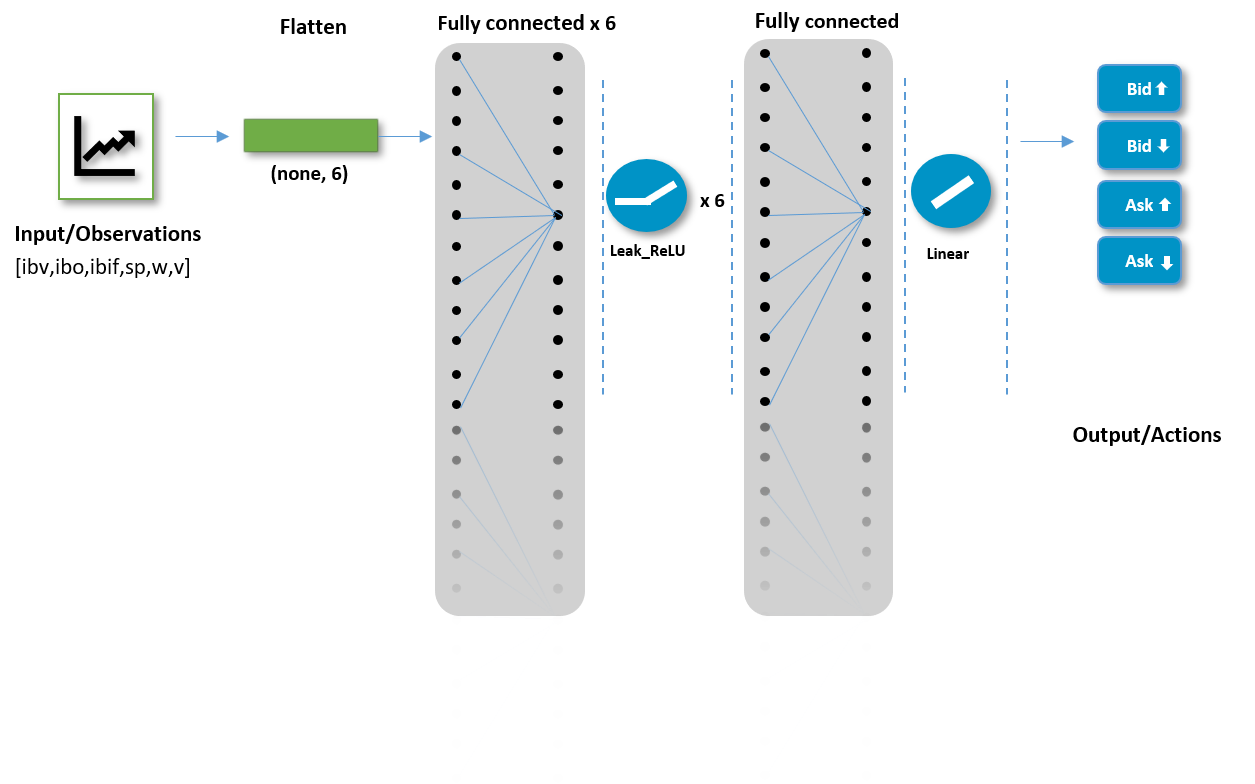
\includegraphics[scale=.5]{Imgs/nnadmv0.png}
    \caption{Neural Network for DealerMarket-V1 using 7 fully connected layers and leaky ReLU as activation function. Input is the observable state variables, which are flattend to be feed into the network.}
    \label{fig:e1}
\end{figure}
For \textit{DealerMarket-v2} the author also trained a 8-layer fully-connected neural network (FCNN) using the PPO agent and. With ReLU as activation layer. Here the agent also has six possible actions as seen in \autoref{fig:e2}. 

\begin{figure}[H]
    \centering
    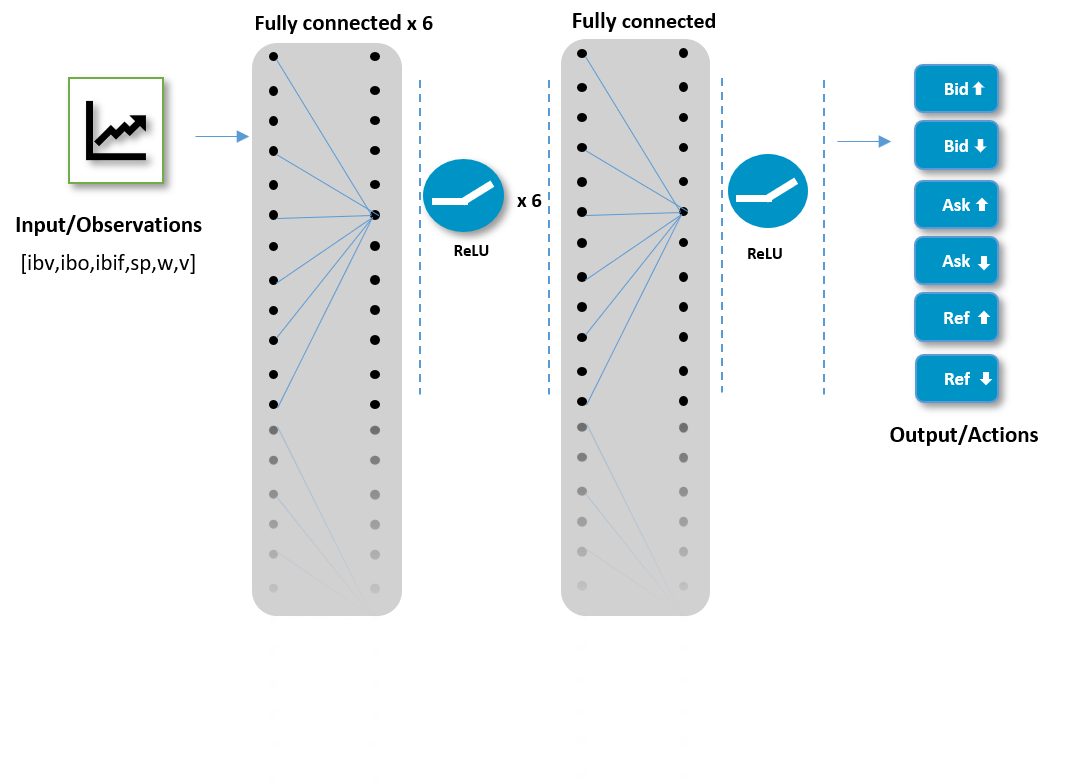
\includegraphics[scale=.5]{Imgs/nnadmv1.png}
    \caption{Neural Network for DealerMarket-v2 using 7 fully connected layers and leaky ReLU as activation function. Input is the observable state variables.}
    \label{fig:e2}
\end{figure}
For \textit{LOBMarket-v1} the author trained a 8-layer fully-connected neural network (FCNN) with two LSTM layers. Using the PPO agent, with ReLU as activation layer.

\begin{figure}[H]
    \centering
    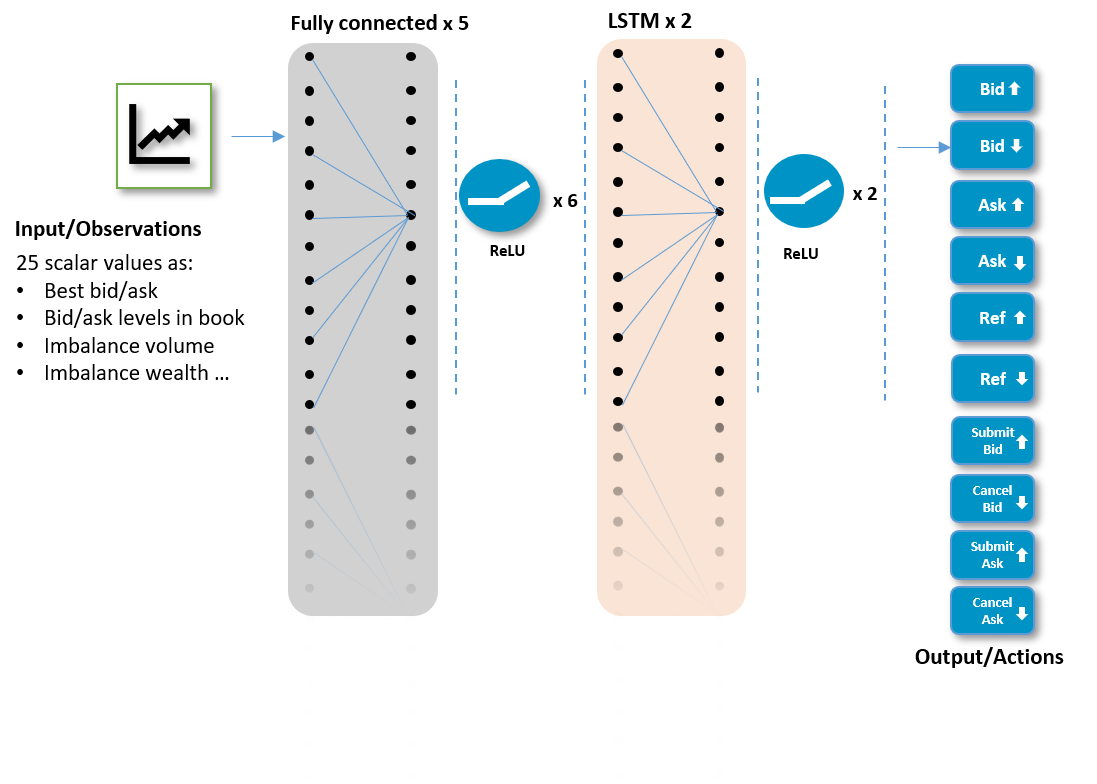
\includegraphics[scale=.5]{Imgs/nnalob1.png}
    \caption{Neural Network for LOBMarket-v1 using 5 fully connected layers and 2 LSTM layer. With ReLU as activation function. Input is the observable state variables some 25 scalar values. Output is one of ten actions.}
    \label{fig:e4}
\end{figure}

\begin{table}[H]
\centering
\caption{The different network architectures used in the thesis. Type indicates what type of agent used and policy. The random agent is sampling via a uniform distribution from different actions.}
\label{tab:e1}
\begin{tabular}{llll}
 \textbf{Environment} & \textbf{Architecture}  & \textbf{Type}  & \textbf{Library}  \\ \hline
 \textit{DealerMarket-v1}& 8-layer FCNN  & DQN + Boltzmann  & keras-RL   \\
 \textit{DealerMarket-v2}& 8-layer FCNN  & PPO + $\varepsilon$ - decay  & tensorforce  \\
 %\textit{DealerMarket-V2}& ?  & PPO + Self Play  & tensorforce  \\
 \textit{DealerMarket-v2} & Random model  & Random policy  & tensorforce \\
 %\textit{LOBMarket-V1} & ?  & PPO + Self-Play  & tensorforce \\ 
 \textit{LOBMarket-v1} & 6-layer FCNN + 2 LSTM  & PPO + $\varepsilon$ - decay  & tensorforce \\ 
 \textit{LOBMarket-v1} & Random model  & Random policy  & tensorforce
\end{tabular}
\end{table}
In \autoref{tab:e1} the main network architectures and models used are shown. DealerMarket-v1 is the only agent using keras-RL and DQN. Which didn't have any option of training a random policy. Whilst the two other environments used tensorforce and the PPO algorithm. As can be seen the network architectures are quite similar with the following number of hidden neurons: $[1024, 512,512,256,256,128,64]$. This was based on both trial and error, the hyper-parameter search and previous papers. 
\newline
\newline
Where the differences is that both DealerMarket-v1 and DealerMarket-v2 use only fully connected layers. Whereas LOBMarket-v1 has added two recurrent LSTM layers. Looking at \autoref{tab:e2} the chosen hyper-parameters from the search and previous papers are presented.

\begin{table}[H]
\centering
\caption{Values of the different hyper-parameters used, that where chosen in the thesis. Learning rate ($\eta$), episodes (eps), memory (mem), policy parameters ($\tau, \varepsilon$), clipping ($\epsilon$), Generalized Advantage Estimate (GAE) lambda ($\lambda$).}
\label{tab:e2}
\begin{tabular}{llll}
 \textbf{Environment} & \textbf{Type} & \textbf{Hyper-parameters} & \textbf{Values}  \\ \hline
 \textit{DealerMarket-v1} & DQN  & [$\eta$, eps, mem, $\tau$] & [$1e^{-5}, 2\cdot10^6, 1\cdot10^5, 0.25$ ]  \\
 \textit{DealerMarket-v2} & PPO  & [$\eta$, eps, mem, $\epsilon$, $\lambda$] & [$3e^{-4}, 2\cdot10^6, 3.2\cdot10^5$, $0.2$, $0.97$]  \\
 %\textit{DealerMarket-V2} &  & &  \\
 \textit{LOBMarket-v1} & PPO  & [$\eta$, eps, mem, $\epsilon$, $\lambda$] & [$1e^{-5}, 2\cdot10^6, 3.2\cdot10^5$, $0.2$, $0.97$]  \\
 %\textit{LOBMarket-V1} &  & & 
\end{tabular}
\end{table}

\newpage
\subsection{Software \& Hardware}

\subsubsection*{OpenAI Gym \& Baselines}
OpenAI Baselines is a state-of-the-art library used for research and testing of different reinforcement learning algorithms created by \textcite{baselines}. From the library this work has implemented the previous mentioned environments.

\subsubsection*{keras-RL}
Keras-RL is a library for reinforcment learning. Developed by \textcite{plappert2016kerasrl} with some state-of-art reinforcement learning algorithms such as: \textit{Deep Q Learning} and \textit{SARSA}. It is an easy to use interface of keras modular API for building neural networks. This library also works seamless with OpenAI. Which was why it was selected to be used as the primary library for this project. However as the project progressed, another more up-to-date library that was more frequently updated was needed. Hence the choice fell on \textit{Tensorforce}.  

\subsubsection*{Tensorforce}
Tensorforce developed by \textcite{schaarschmidt2017tensorforce} is another python based reinforcement learning library. Built on top of Tensorflow with a modular API basing parameter using python dictionaries. Some implemented agents in the library that are of interest for this project is \textit{AC3, PPO, DQN} and both a \textit{random} and \textit{constant} agent for sanity checks \parencite{schaarschmidt2017tensorforce}.

\subsubsection*{Platform specification}
The majority of these experiments and simulations where conducted on a virtual machine on AWS. 
The author used a p2.xlarge EC2 instances on AWS, with the following specifications: 1 Tesla K80 GPU, 4 vCPUs and 61 GiB RAM. For initial testing and debugging local experiments where also run on a Intel i5 dual-core CPU with 2,40 GHz and 8 GB RAM with a Windows 10 Pro operating system. 

%\newpage

\section{Visualization}

\begin{figure}[H]
    \centering
    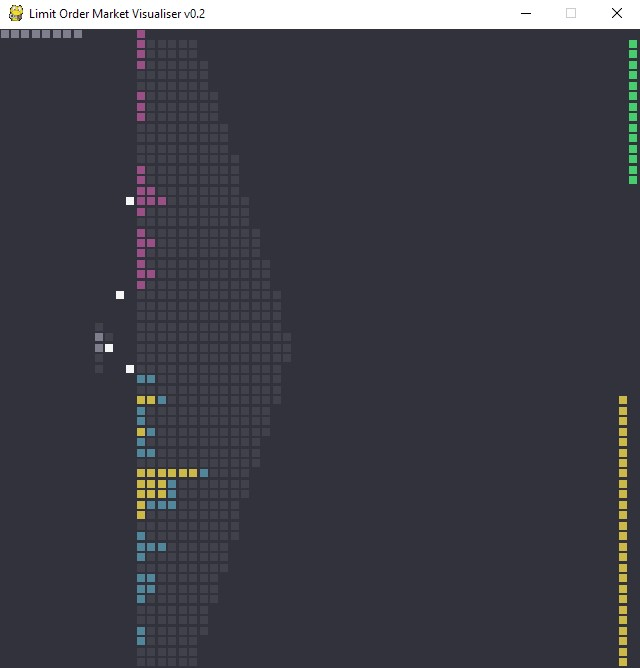
\includegraphics[scale=.4]{Imgs/lob_untrained_Moment.jpg}
    \caption{Example of visualization during training. Showing how an untrained agent posting bid and ask quotes in a LOB. Purple bricks are ask levels, blue are bid levels. Whilst yellow are the agents asks, green the agents bids. Finally pink and blue are the agents ask and bid trades.}
    \label{fig:v1}
\end{figure}

In order to understand what the agents are doing. Some visualization has been employed. Firstly during training using the pygame\footnote{\url{https://www.pygame.org}} python library. This visualization shows what bid and ask quotes that the agent thinks are the best to quote. An example of the visualization is shown in \autoref{fig:v1}. The gray bricks in the background are the current demand and supply curves. Purple bricks are the current ask levels in the LOB. Conversely blue bricks are the bid levels. Yellow is the agent's ask qoute, and green the agent's bid quotes. Secondly after training visualization of relevant metrics from each simulation is done. 
\newpage
These visualizations are all done in R reading the training history or callbacks saved in JSON files. Where both dplyr \parencite{dplyr} and ggplot2 \parencite{ggfplot2} are used for this purpose.

\section{Evaluation}
A common approach in machine learning to evaluate models is to use k-fold cross-validation often with $k=10$. However in this thesis all data generated is from each completed simulation. Therefore other different metrics are gathered after each simulation, in order to evaluate the agents. These are discussed below. To account for randomness, several runs are run for each simulation with different random seeds. 

\begin{itemize}
\item \textit{Price Impact Regression}. An estimate of Kyle's lambda ($\lambda$) i.e. the price impact of the agents orders is done via regression. Using order imbalance ($q_n$), inventories ($\nabla I_n$) and initial inventories ($\nabla Init_n$). Where a larger $\lambda$ implies a that volumes have a larger price impact on prices.

\item \textit{Visualizing learning \& Strategies}. Looking at how the agents act together with the price data stored from each run. To see what strategies are used by the agents.
    
\item \textit{Spreads \& Inventory}. Analyzing how the spreads \& inventory are changing during training. If the spreads decline over time, the correlation between spread and inventory and order imbalance.

\item \textit{Net Profit and Loss (Net PnL)}. Calculating the Net PnL of the agent to see if the market maker in fact has learned to make a profit or not. Thus optimizing its inventory levels. Defined in \autoref{eq:pnl}

\begin{equation}
    PnL_{t} = Cash_{t} - Init\_Cash_{t} + \Delta Inv_{t} \cdot S_{t}
    \label{eq:pnl}
\end{equation}

\item \textit{Compare agent to zero intelligence or  random policy}. The random agent is used as benchmarks to see if the agent on average is better or not. During each simulation.

\item \textit{Stylized facts of simulated data}.
Looking for some of the stylized facts mentioned in \autoref{ch:2} to see how close or far away from reality the simulations are.

%really use this?
%\item \textit{Sharpe ratio}. Another benchmark to see how well the agent is learning is looking at the Sharpe ratio:

%\begin{equation}
%    \label{eq:s}
%    S_N = \sqrt{N} \frac{E(r-r_{f})}{\sqrt{Var(r-r_{f})}}
%\end{equation}

\end{itemize}
%Where $r$ is the cash return compared to the agents initial cash, $r_f$ is the risk-free rate and  $N$ is what period it is to the annualized Sharpe ratio.

\chapter{Results}\label{ch:6}
 In this section the results from the different experiments and environments are presented. DealerMarket-v1 is not as extensively analyzed as the other environments. As it serves as an initial baseline. This section starts with some stylized facts about the simulated data. Continuing with a breakdown of different statistic gathered after each simulation.

\begin{figure}[H]
		%Do not try to scale figure in .tex or you loose font size consistency
		\centering
		%The code to input the plot is extremely simple
		%% Created by tikzDevice version 0.11 on 2018-07-15 13:37:11
% !TEX encoding = UTF-8 Unicode
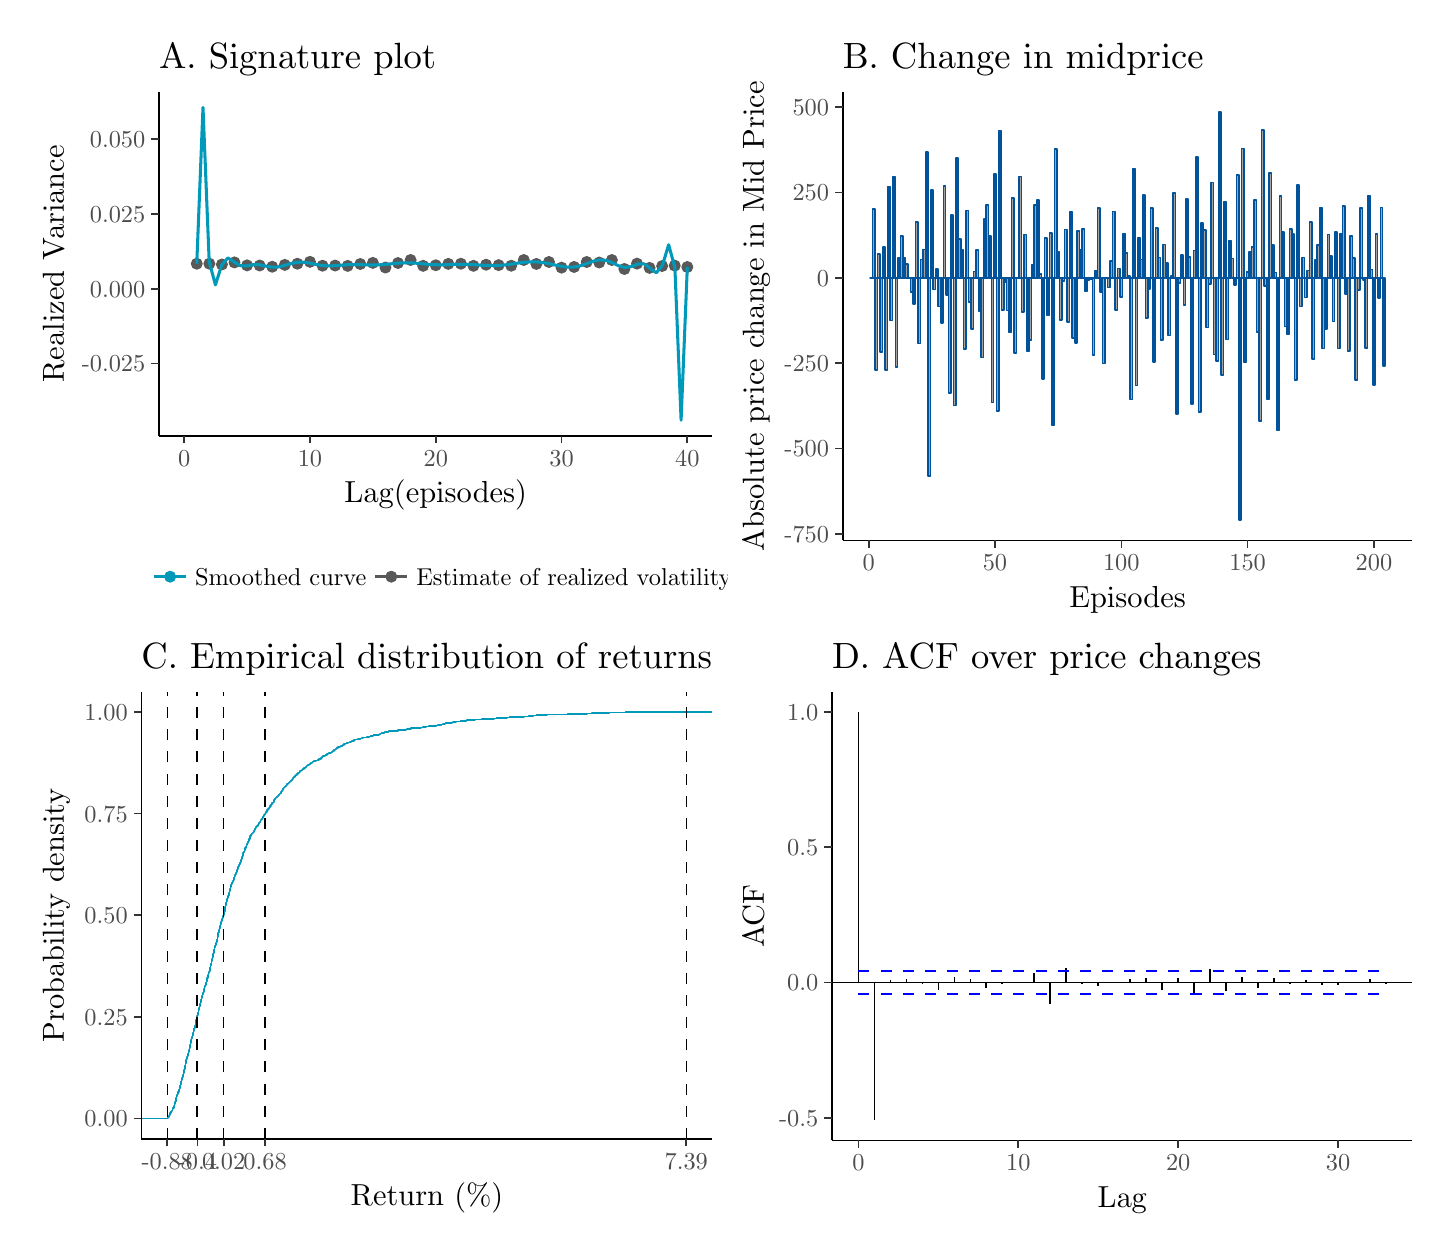
\begin{tikzpicture}[x=1pt,y=1pt]
\definecolor{fillColor}{RGB}{255,255,255}
\path[use as bounding box,fill=fillColor,fill opacity=0.00] (0,0) rectangle (505.89,433.62);
\begin{scope}
\path[clip] (  0.00,216.81) rectangle (252.95,433.62);
\definecolor{drawColor}{RGB}{255,255,255}
\definecolor{fillColor}{RGB}{255,255,255}

\path[draw=drawColor,line width= 0.6pt,line join=round,line cap=round,fill=fillColor] ( -0.00,216.81) rectangle (252.95,433.62);
\end{scope}
\begin{scope}
\path[clip] ( 47.47,286.11) rectangle (247.44,410.48);
\definecolor{fillColor}{RGB}{255,255,255}

\path[fill=fillColor] ( 47.47,286.11) rectangle (247.44,410.48);
\definecolor{drawColor}{gray}{0.35}
\definecolor{fillColor}{gray}{0.35}

\path[draw=drawColor,line width= 0.4pt,line join=round,line cap=round,fill=fillColor] ( 61.10,348.32) circle (  1.96);

\path[draw=drawColor,line width= 0.4pt,line join=round,line cap=round,fill=fillColor] ( 65.65,348.33) circle (  1.96);

\path[draw=drawColor,line width= 0.4pt,line join=round,line cap=round,fill=fillColor] ( 70.19,348.05) circle (  1.96);

\path[draw=drawColor,line width= 0.4pt,line join=round,line cap=round,fill=fillColor] ( 74.74,348.79) circle (  1.96);

\path[draw=drawColor,line width= 0.4pt,line join=round,line cap=round,fill=fillColor] ( 79.28,347.72) circle (  1.96);

\path[draw=drawColor,line width= 0.4pt,line join=round,line cap=round,fill=fillColor] ( 83.83,347.68) circle (  1.96);

\path[draw=drawColor,line width= 0.4pt,line join=round,line cap=round,fill=fillColor] ( 88.37,347.23) circle (  1.96);

\path[draw=drawColor,line width= 0.4pt,line join=round,line cap=round,fill=fillColor] ( 92.92,347.90) circle (  1.96);

\path[draw=drawColor,line width= 0.4pt,line join=round,line cap=round,fill=fillColor] ( 97.46,348.32) circle (  1.96);

\path[draw=drawColor,line width= 0.4pt,line join=round,line cap=round,fill=fillColor] (102.01,349.00) circle (  1.96);

\path[draw=drawColor,line width= 0.4pt,line join=round,line cap=round,fill=fillColor] (106.55,347.60) circle (  1.96);

\path[draw=drawColor,line width= 0.4pt,line join=round,line cap=round,fill=fillColor] (111.10,347.66) circle (  1.96);

\path[draw=drawColor,line width= 0.4pt,line join=round,line cap=round,fill=fillColor] (115.64,347.54) circle (  1.96);

\path[draw=drawColor,line width= 0.4pt,line join=round,line cap=round,fill=fillColor] (120.19,348.22) circle (  1.96);

\path[draw=drawColor,line width= 0.4pt,line join=round,line cap=round,fill=fillColor] (124.73,348.62) circle (  1.96);

\path[draw=drawColor,line width= 0.4pt,line join=round,line cap=round,fill=fillColor] (129.28,346.94) circle (  1.96);

\path[draw=drawColor,line width= 0.4pt,line join=round,line cap=round,fill=fillColor] (133.82,348.57) circle (  1.96);

\path[draw=drawColor,line width= 0.4pt,line join=round,line cap=round,fill=fillColor] (138.37,349.67) circle (  1.96);

\path[draw=drawColor,line width= 0.4pt,line join=round,line cap=round,fill=fillColor] (142.91,347.56) circle (  1.96);

\path[draw=drawColor,line width= 0.4pt,line join=round,line cap=round,fill=fillColor] (147.46,347.77) circle (  1.96);

\path[draw=drawColor,line width= 0.4pt,line join=round,line cap=round,fill=fillColor] (152.00,348.26) circle (  1.96);

\path[draw=drawColor,line width= 0.4pt,line join=round,line cap=round,fill=fillColor] (156.55,348.31) circle (  1.96);

\path[draw=drawColor,line width= 0.4pt,line join=round,line cap=round,fill=fillColor] (161.09,347.56) circle (  1.96);

\path[draw=drawColor,line width= 0.4pt,line join=round,line cap=round,fill=fillColor] (165.64,347.96) circle (  1.96);

\path[draw=drawColor,line width= 0.4pt,line join=round,line cap=round,fill=fillColor] (170.18,347.81) circle (  1.96);

\path[draw=drawColor,line width= 0.4pt,line join=round,line cap=round,fill=fillColor] (174.73,347.60) circle (  1.96);

\path[draw=drawColor,line width= 0.4pt,line join=round,line cap=round,fill=fillColor] (179.27,349.66) circle (  1.96);

\path[draw=drawColor,line width= 0.4pt,line join=round,line cap=round,fill=fillColor] (183.82,348.24) circle (  1.96);

\path[draw=drawColor,line width= 0.4pt,line join=round,line cap=round,fill=fillColor] (188.36,348.95) circle (  1.96);

\path[draw=drawColor,line width= 0.4pt,line join=round,line cap=round,fill=fillColor] (192.91,346.91) circle (  1.96);

\path[draw=drawColor,line width= 0.4pt,line join=round,line cap=round,fill=fillColor] (197.45,347.15) circle (  1.96);

\path[draw=drawColor,line width= 0.4pt,line join=round,line cap=round,fill=fillColor] (202.00,348.94) circle (  1.96);

\path[draw=drawColor,line width= 0.4pt,line join=round,line cap=round,fill=fillColor] (206.54,348.75) circle (  1.96);

\path[draw=drawColor,line width= 0.4pt,line join=round,line cap=round,fill=fillColor] (211.09,349.66) circle (  1.96);

\path[draw=drawColor,line width= 0.4pt,line join=round,line cap=round,fill=fillColor] (215.63,346.42) circle (  1.96);

\path[draw=drawColor,line width= 0.4pt,line join=round,line cap=round,fill=fillColor] (220.18,348.35) circle (  1.96);

\path[draw=drawColor,line width= 0.4pt,line join=round,line cap=round,fill=fillColor] (224.72,346.81) circle (  1.96);

\path[draw=drawColor,line width= 0.4pt,line join=round,line cap=round,fill=fillColor] (229.27,347.49) circle (  1.96);

\path[draw=drawColor,line width= 0.4pt,line join=round,line cap=round,fill=fillColor] (233.81,347.63) circle (  1.96);

\path[draw=drawColor,line width= 0.4pt,line join=round,line cap=round,fill=fillColor] (238.36,347.13) circle (  1.96);
\definecolor{drawColor}{RGB}{0,153,186}

\path[draw=drawColor,line width= 1.1pt,line join=round] ( 61.10,348.32) --
	( 63.35,404.83) --
	( 65.59,349.07) --
	( 67.84,340.67) --
	( 70.08,347.74) --
	( 72.32,350.41) --
	( 74.57,348.99) --
	( 76.81,347.60) --
	( 79.05,347.54) --
	( 81.30,347.95) --
	( 83.54,347.96) --
	( 85.79,347.51) --
	( 88.03,347.08) --
	( 90.27,347.10) --
	( 92.52,347.61) --
	( 94.76,348.30) --
	( 97.00,348.80) --
	( 99.25,348.90) --
	(101.49,348.62) --
	(103.73,348.16) --
	(105.98,347.75) --
	(108.22,347.55) --
	(110.47,347.58) --
	(112.71,347.75) --
	(114.95,347.93) --
	(117.20,348.02) --
	(119.44,348.00) --
	(121.68,347.92) --
	(123.93,347.85) --
	(126.17,347.87) --
	(128.42,348.01) --
	(130.66,348.22) --
	(132.90,348.45) --
	(135.15,348.61) --
	(137.39,348.65) --
	(139.63,348.56) --
	(141.88,348.37) --
	(144.12,348.16) --
	(146.36,348.00) --
	(148.61,347.93) --
	(150.85,347.94) --
	(153.10,348.02) --
	(155.34,348.09) --
	(157.58,348.11) --
	(159.83,348.05) --
	(162.07,347.92) --
	(164.31,347.77) --
	(166.56,347.66) --
	(168.80,347.64) --
	(171.04,347.75) --
	(173.29,347.99) --
	(175.53,348.30) --
	(177.78,348.64) --
	(180.02,348.90) --
	(182.26,349.01) --
	(184.51,348.94) --
	(186.75,348.66) --
	(188.99,348.21) --
	(191.24,347.70) --
	(193.48,347.26) --
	(195.73,347.04) --
	(197.97,347.18) --
	(200.21,347.72) --
	(202.46,348.54) --
	(204.70,349.33) --
	(206.94,349.74) --
	(209.19,349.49) --
	(211.43,348.60) --
	(213.67,347.52) --
	(215.92,346.95) --
	(218.16,347.31) --
	(220.41,348.20) --
	(222.65,348.31) --
	(224.89,346.71) --
	(227.14,345.02) --
	(229.38,347.79) --
	(231.62,355.19) --
	(233.87,346.89) --
	(236.11,291.77) --
	(238.36,347.13);
\end{scope}
\begin{scope}
\path[clip] (  0.00,  0.00) rectangle (505.89,433.62);
\definecolor{drawColor}{RGB}{0,0,0}

\path[draw=drawColor,line width= 0.6pt,line join=round] ( 47.47,286.11) --
	( 47.47,410.48);
\end{scope}
\begin{scope}
\path[clip] (  0.00,  0.00) rectangle (505.89,433.62);
\definecolor{drawColor}{gray}{0.30}

\node[text=drawColor,anchor=base east,inner sep=0pt, outer sep=0pt, scale=  0.88] at ( 42.52,309.20) {-0.025};

\node[text=drawColor,anchor=base east,inner sep=0pt, outer sep=0pt, scale=  0.88] at ( 42.52,336.24) {0.000};

\node[text=drawColor,anchor=base east,inner sep=0pt, outer sep=0pt, scale=  0.88] at ( 42.52,363.28) {0.025};

\node[text=drawColor,anchor=base east,inner sep=0pt, outer sep=0pt, scale=  0.88] at ( 42.52,390.31) {0.050};
\end{scope}
\begin{scope}
\path[clip] (  0.00,  0.00) rectangle (505.89,433.62);
\definecolor{drawColor}{gray}{0.20}

\path[draw=drawColor,line width= 0.6pt,line join=round] ( 44.72,312.23) --
	( 47.47,312.23);

\path[draw=drawColor,line width= 0.6pt,line join=round] ( 44.72,339.27) --
	( 47.47,339.27);

\path[draw=drawColor,line width= 0.6pt,line join=round] ( 44.72,366.31) --
	( 47.47,366.31);

\path[draw=drawColor,line width= 0.6pt,line join=round] ( 44.72,393.34) --
	( 47.47,393.34);
\end{scope}
\begin{scope}
\path[clip] (  0.00,  0.00) rectangle (505.89,433.62);
\definecolor{drawColor}{RGB}{0,0,0}

\path[draw=drawColor,line width= 0.6pt,line join=round] ( 47.47,286.11) --
	(247.44,286.11);
\end{scope}
\begin{scope}
\path[clip] (  0.00,  0.00) rectangle (505.89,433.62);
\definecolor{drawColor}{gray}{0.20}

\path[draw=drawColor,line width= 0.6pt,line join=round] ( 56.56,283.36) --
	( 56.56,286.11);

\path[draw=drawColor,line width= 0.6pt,line join=round] (102.01,283.36) --
	(102.01,286.11);

\path[draw=drawColor,line width= 0.6pt,line join=round] (147.46,283.36) --
	(147.46,286.11);

\path[draw=drawColor,line width= 0.6pt,line join=round] (192.91,283.36) --
	(192.91,286.11);

\path[draw=drawColor,line width= 0.6pt,line join=round] (238.36,283.36) --
	(238.36,286.11);
\end{scope}
\begin{scope}
\path[clip] (  0.00,  0.00) rectangle (505.89,433.62);
\definecolor{drawColor}{gray}{0.30}

\node[text=drawColor,anchor=base,inner sep=0pt, outer sep=0pt, scale=  0.88] at ( 56.56,275.10) {0};

\node[text=drawColor,anchor=base,inner sep=0pt, outer sep=0pt, scale=  0.88] at (102.01,275.10) {10};

\node[text=drawColor,anchor=base,inner sep=0pt, outer sep=0pt, scale=  0.88] at (147.46,275.10) {20};

\node[text=drawColor,anchor=base,inner sep=0pt, outer sep=0pt, scale=  0.88] at (192.91,275.10) {30};

\node[text=drawColor,anchor=base,inner sep=0pt, outer sep=0pt, scale=  0.88] at (238.36,275.10) {40};
\end{scope}
\begin{scope}
\path[clip] (  0.00,  0.00) rectangle (505.89,433.62);
\definecolor{drawColor}{RGB}{0,0,0}

\node[text=drawColor,anchor=base,inner sep=0pt, outer sep=0pt, scale=  1.10] at (147.46,262.03) {Lag(episodes)};
\end{scope}
\begin{scope}
\path[clip] (  0.00,  0.00) rectangle (505.89,433.62);
\definecolor{drawColor}{RGB}{0,0,0}

\node[text=drawColor,rotate= 90.00,anchor=base,inner sep=0pt, outer sep=0pt, scale=  1.10] at ( 13.08,348.30) {Realized Variance};
\end{scope}
\begin{scope}
\path[clip] (  0.00,  0.00) rectangle (505.89,433.62);
\definecolor{fillColor}{RGB}{255,255,255}

\path[fill=fillColor] ( 34.95,222.31) rectangle (259.96,248.15);
\end{scope}
\begin{scope}
\path[clip] (  0.00,  0.00) rectangle (505.89,433.62);
\definecolor{drawColor}{RGB}{0,153,186}
\definecolor{fillColor}{RGB}{0,153,186}

\path[draw=drawColor,line width= 0.4pt,line join=round,line cap=round,fill=fillColor] ( 51.48,235.23) circle (  1.96);
\end{scope}
\begin{scope}
\path[clip] (  0.00,  0.00) rectangle (505.89,433.62);
\definecolor{drawColor}{RGB}{0,153,186}

\path[draw=drawColor,line width= 1.1pt,line join=round] ( 45.70,235.23) -- ( 57.26,235.23);
\end{scope}
\begin{scope}
\path[clip] (  0.00,  0.00) rectangle (505.89,433.62);
\definecolor{drawColor}{gray}{0.35}
\definecolor{fillColor}{gray}{0.35}

\path[draw=drawColor,line width= 0.4pt,line join=round,line cap=round,fill=fillColor] (131.40,235.23) circle (  1.96);
\end{scope}
\begin{scope}
\path[clip] (  0.00,  0.00) rectangle (505.89,433.62);
\definecolor{drawColor}{gray}{0.35}

\path[draw=drawColor,line width= 1.1pt,line join=round] (125.62,235.23) -- (137.19,235.23);
\end{scope}
\begin{scope}
\path[clip] (  0.00,  0.00) rectangle (505.89,433.62);
\definecolor{drawColor}{RGB}{0,0,0}

\node[text=drawColor,anchor=base west,inner sep=0pt, outer sep=0pt, scale=  0.88] at ( 60.52,232.20) {Smoothed curve};
\end{scope}
\begin{scope}
\path[clip] (  0.00,  0.00) rectangle (505.89,433.62);
\definecolor{drawColor}{RGB}{0,0,0}

\node[text=drawColor,anchor=base west,inner sep=0pt, outer sep=0pt, scale=  0.88] at (140.44,232.20) {Estimate of realized volatility};
\end{scope}
\begin{scope}
\path[clip] (  0.00,  0.00) rectangle (505.89,433.62);
\definecolor{drawColor}{RGB}{0,0,0}

\node[text=drawColor,anchor=base west,inner sep=0pt, outer sep=0pt, scale=  1.32] at ( 47.47,419.03) {A. Signature plot};
\end{scope}
\begin{scope}
\path[clip] (  0.00,  0.00) rectangle (252.94,216.81);
\definecolor{drawColor}{RGB}{255,255,255}
\definecolor{fillColor}{RGB}{255,255,255}

\path[draw=drawColor,line width= 0.6pt,line join=round,line cap=round,fill=fillColor] (  0.00,  0.00) rectangle (252.94,216.81);
\end{scope}
\begin{scope}
\path[clip] ( 41.11, 32.09) rectangle (247.44,193.67);
\definecolor{fillColor}{RGB}{255,255,255}

\path[fill=fillColor] ( 41.11, 32.09) rectangle (247.44,193.67);
\definecolor{drawColor}{RGB}{0,153,186}

\path[draw=drawColor,line width= 0.6pt,line join=round] ( 41.11, 39.43) --
	( 50.49, 39.43) --
	( 50.49, 39.50) --
	( 50.56, 39.50) --
	( 50.56, 39.57) --
	( 50.72, 39.57) --
	( 50.72, 39.65) --
	( 50.76, 39.65) --
	( 50.76, 39.72) --
	( 50.76, 39.72) --
	( 50.76, 39.79) --
	( 50.78, 39.79) --
	( 50.78, 39.86) --
	( 50.84, 39.86) --
	( 50.84, 39.93) --
	( 50.91, 39.93) --
	( 50.91, 40.01) --
	( 50.94, 40.01) --
	( 50.94, 40.08) --
	( 51.03, 40.08) --
	( 51.03, 40.15) --
	( 51.03, 40.15) --
	( 51.03, 40.22) --
	( 51.07, 40.22) --
	( 51.07, 40.29) --
	( 51.08, 40.29) --
	( 51.08, 40.36) --
	( 51.09, 40.36) --
	( 51.09, 40.44) --
	( 51.12, 40.44) --
	( 51.12, 40.51) --
	( 51.17, 40.51) --
	( 51.17, 40.58) --
	( 51.21, 40.58) --
	( 51.21, 40.65) --
	( 51.31, 40.65) --
	( 51.31, 40.72) --
	( 51.34, 40.72) --
	( 51.34, 40.79) --
	( 51.35, 40.79) --
	( 51.35, 40.87) --
	( 51.38, 40.87) --
	( 51.38, 40.94) --
	( 51.38, 40.94) --
	( 51.38, 41.01) --
	( 51.39, 41.01) --
	( 51.39, 41.08) --
	( 51.40, 41.08) --
	( 51.40, 41.15) --
	( 51.41, 41.15) --
	( 51.41, 41.23) --
	( 51.49, 41.23) --
	( 51.49, 41.30) --
	( 51.51, 41.30) --
	( 51.51, 41.37) --
	( 51.63, 41.37) --
	( 51.63, 41.44) --
	( 51.69, 41.44) --
	( 51.69, 41.51) --
	( 51.71, 41.51) --
	( 51.71, 41.58) --
	( 51.71, 41.58) --
	( 51.71, 41.66) --
	( 51.72, 41.66) --
	( 51.72, 41.73) --
	( 51.75, 41.73) --
	( 51.75, 41.80) --
	( 51.79, 41.80) --
	( 51.79, 41.87) --
	( 51.83, 41.87) --
	( 51.83, 41.94) --
	( 51.88, 41.94) --
	( 51.88, 42.01) --
	( 51.92, 42.01) --
	( 51.92, 42.09) --
	( 51.96, 42.09) --
	( 51.96, 42.16) --
	( 52.20, 42.16) --
	( 52.20, 42.23) --
	( 52.20, 42.23) --
	( 52.20, 42.30) --
	( 52.22, 42.30) --
	( 52.22, 42.37) --
	( 52.28, 42.37) --
	( 52.28, 42.45) --
	( 52.29, 42.45) --
	( 52.29, 42.52) --
	( 52.29, 42.52) --
	( 52.29, 42.59) --
	( 52.29, 42.59) --
	( 52.29, 42.66) --
	( 52.33, 42.66) --
	( 52.33, 42.73) --
	( 52.39, 42.73) --
	( 52.39, 42.80) --
	( 52.46, 42.80) --
	( 52.46, 42.88) --
	( 52.50, 42.88) --
	( 52.50, 42.95) --
	( 52.50, 42.95) --
	( 52.50, 43.02) --
	( 52.57, 43.02) --
	( 52.57, 43.09) --
	( 52.62, 43.09) --
	( 52.62, 43.16) --
	( 52.65, 43.16) --
	( 52.65, 43.23) --
	( 52.74, 43.23) --
	( 52.74, 43.31) --
	( 52.77, 43.31) --
	( 52.77, 43.38) --
	( 52.80, 43.38) --
	( 52.80, 43.45) --
	( 52.83, 43.45) --
	( 52.83, 43.52) --
	( 52.85, 43.52) --
	( 52.85, 43.59) --
	( 52.85, 43.59) --
	( 52.85, 43.67) --
	( 52.87, 43.67) --
	( 52.87, 43.74) --
	( 52.99, 43.74) --
	( 52.99, 43.81) --
	( 52.99, 43.81) --
	( 52.99, 43.88) --
	( 53.00, 43.88) --
	( 53.00, 43.95) --
	( 53.03, 43.95) --
	( 53.03, 44.02) --
	( 53.03, 44.02) --
	( 53.03, 44.10) --
	( 53.05, 44.10) --
	( 53.05, 44.17) --
	( 53.07, 44.17) --
	( 53.07, 44.24) --
	( 53.09, 44.24) --
	( 53.09, 44.31) --
	( 53.10, 44.31) --
	( 53.10, 44.38) --
	( 53.10, 44.38) --
	( 53.10, 44.45) --
	( 53.10, 44.45) --
	( 53.10, 44.53) --
	( 53.10, 44.53) --
	( 53.10, 44.60) --
	( 53.11, 44.60) --
	( 53.11, 44.67) --
	( 53.11, 44.67) --
	( 53.11, 44.74) --
	( 53.13, 44.74) --
	( 53.13, 44.81) --
	( 53.18, 44.81) --
	( 53.18, 44.89) --
	( 53.20, 44.89) --
	( 53.20, 44.96) --
	( 53.26, 44.96) --
	( 53.26, 45.03) --
	( 53.27, 45.03) --
	( 53.27, 45.10) --
	( 53.28, 45.10) --
	( 53.28, 45.17) --
	( 53.28, 45.17) --
	( 53.28, 45.24) --
	( 53.30, 45.24) --
	( 53.30, 45.32) --
	( 53.31, 45.32) --
	( 53.31, 45.39) --
	( 53.32, 45.39) --
	( 53.32, 45.46) --
	( 53.36, 45.46) --
	( 53.36, 45.53) --
	( 53.40, 45.53) --
	( 53.40, 45.60) --
	( 53.48, 45.60) --
	( 53.48, 45.67) --
	( 53.49, 45.67) --
	( 53.49, 45.75) --
	( 53.49, 45.75) --
	( 53.49, 45.82) --
	( 53.52, 45.82) --
	( 53.52, 45.89) --
	( 53.53, 45.89) --
	( 53.53, 45.96) --
	( 53.55, 45.96) --
	( 53.55, 46.03) --
	( 53.56, 46.03) --
	( 53.56, 46.11) --
	( 53.57, 46.11) --
	( 53.57, 46.18) --
	( 53.57, 46.18) --
	( 53.57, 46.25) --
	( 53.59, 46.25) --
	( 53.59, 46.32) --
	( 53.60, 46.32) --
	( 53.60, 46.39) --
	( 53.63, 46.39) --
	( 53.63, 46.46) --
	( 53.65, 46.46) --
	( 53.65, 46.54) --
	( 53.66, 46.54) --
	( 53.66, 46.61) --
	( 53.66, 46.61) --
	( 53.66, 46.68) --
	( 53.67, 46.68) --
	( 53.67, 46.75) --
	( 53.69, 46.75) --
	( 53.69, 46.82) --
	( 53.69, 46.82) --
	( 53.69, 46.89) --
	( 53.69, 46.89) --
	( 53.69, 46.97) --
	( 53.72, 46.97) --
	( 53.72, 47.04) --
	( 53.73, 47.04) --
	( 53.73, 47.11) --
	( 53.74, 47.11) --
	( 53.74, 47.18) --
	( 53.76, 47.18) --
	( 53.76, 47.25) --
	( 53.77, 47.25) --
	( 53.77, 47.33) --
	( 53.82, 47.33) --
	( 53.82, 47.40) --
	( 53.85, 47.40) --
	( 53.85, 47.47) --
	( 53.90, 47.47) --
	( 53.90, 47.54) --
	( 53.94, 47.54) --
	( 53.94, 47.61) --
	( 53.94, 47.61) --
	( 53.94, 47.68) --
	( 54.01, 47.68) --
	( 54.01, 47.76) --
	( 54.01, 47.76) --
	( 54.01, 47.83) --
	( 54.07, 47.83) --
	( 54.07, 47.90) --
	( 54.09, 47.90) --
	( 54.09, 47.97) --
	( 54.16, 47.97) --
	( 54.16, 48.04) --
	( 54.17, 48.04) --
	( 54.17, 48.11) --
	( 54.17, 48.11) --
	( 54.17, 48.19) --
	( 54.20, 48.19) --
	( 54.20, 48.26) --
	( 54.21, 48.26) --
	( 54.21, 48.33) --
	( 54.28, 48.33) --
	( 54.28, 48.40) --
	( 54.28, 48.40) --
	( 54.28, 48.47) --
	( 54.30, 48.47) --
	( 54.30, 48.54) --
	( 54.35, 48.54) --
	( 54.35, 48.62) --
	( 54.36, 48.62) --
	( 54.36, 48.69) --
	( 54.37, 48.69) --
	( 54.37, 48.76) --
	( 54.37, 48.76) --
	( 54.37, 48.83) --
	( 54.42, 48.83) --
	( 54.42, 48.90) --
	( 54.43, 48.90) --
	( 54.43, 48.98) --
	( 54.43, 48.98) --
	( 54.43, 49.05) --
	( 54.44, 49.05) --
	( 54.44, 49.12) --
	( 54.57, 49.12) --
	( 54.57, 49.19) --
	( 54.59, 49.19) --
	( 54.59, 49.26) --
	( 54.61, 49.26) --
	( 54.61, 49.33) --
	( 54.61, 49.33) --
	( 54.61, 49.41) --
	( 54.61, 49.41) --
	( 54.61, 49.48) --
	( 54.72, 49.48) --
	( 54.72, 49.55) --
	( 54.73, 49.55) --
	( 54.73, 49.62) --
	( 54.73, 49.62) --
	( 54.73, 49.69) --
	( 54.74, 49.69) --
	( 54.74, 49.76) --
	( 54.78, 49.76) --
	( 54.78, 49.84) --
	( 54.79, 49.84) --
	( 54.79, 49.91) --
	( 54.80, 49.91) --
	( 54.80, 49.98) --
	( 54.82, 49.98) --
	( 54.82, 50.05) --
	( 54.87, 50.05) --
	( 54.87, 50.12) --
	( 54.90, 50.12) --
	( 54.90, 50.20) --
	( 54.91, 50.20) --
	( 54.91, 50.27) --
	( 54.93, 50.27) --
	( 54.93, 50.34) --
	( 54.94, 50.34) --
	( 54.94, 50.41) --
	( 54.94, 50.41) --
	( 54.94, 50.48) --
	( 54.97, 50.48) --
	( 54.97, 50.55) --
	( 55.00, 50.55) --
	( 55.00, 50.63) --
	( 55.03, 50.63) --
	( 55.03, 50.70) --
	( 55.05, 50.70) --
	( 55.05, 50.77) --
	( 55.08, 50.77) --
	( 55.08, 50.84) --
	( 55.09, 50.84) --
	( 55.09, 50.91) --
	( 55.09, 50.91) --
	( 55.09, 50.98) --
	( 55.11, 50.98) --
	( 55.11, 51.06) --
	( 55.12, 51.06) --
	( 55.12, 51.13) --
	( 55.12, 51.13) --
	( 55.12, 51.20) --
	( 55.14, 51.20) --
	( 55.14, 51.27) --
	( 55.14, 51.27) --
	( 55.14, 51.34) --
	( 55.16, 51.34) --
	( 55.16, 51.42) --
	( 55.19, 51.42) --
	( 55.19, 51.49) --
	( 55.20, 51.49) --
	( 55.20, 51.56) --
	( 55.21, 51.56) --
	( 55.21, 51.63) --
	( 55.21, 51.63) --
	( 55.21, 51.70) --
	( 55.28, 51.70) --
	( 55.28, 51.77) --
	( 55.30, 51.77) --
	( 55.30, 51.85) --
	( 55.31, 51.85) --
	( 55.31, 51.92) --
	( 55.31, 51.92) --
	( 55.31, 51.99) --
	( 55.34, 51.99) --
	( 55.34, 52.06) --
	( 55.35, 52.06) --
	( 55.35, 52.13) --
	( 55.37, 52.13) --
	( 55.37, 52.20) --
	( 55.41, 52.20) --
	( 55.41, 52.28) --
	( 55.42, 52.28) --
	( 55.42, 52.35) --
	( 55.42, 52.35) --
	( 55.42, 52.42) --
	( 55.43, 52.42) --
	( 55.43, 52.49) --
	( 55.43, 52.49) --
	( 55.43, 52.56) --
	( 55.47, 52.56) --
	( 55.47, 52.64) --
	( 55.48, 52.64) --
	( 55.48, 52.71) --
	( 55.52, 52.71) --
	( 55.52, 52.78) --
	( 55.54, 52.78) --
	( 55.54, 52.85) --
	( 55.54, 52.85) --
	( 55.54, 52.92) --
	( 55.57, 52.92) --
	( 55.57, 52.99) --
	( 55.57, 52.99) --
	( 55.57, 53.07) --
	( 55.60, 53.07) --
	( 55.60, 53.14) --
	( 55.60, 53.14) --
	( 55.60, 53.21) --
	( 55.62, 53.21) --
	( 55.62, 53.28) --
	( 55.67, 53.28) --
	( 55.67, 53.35) --
	( 55.71, 53.35) --
	( 55.71, 53.42) --
	( 55.75, 53.42) --
	( 55.75, 53.50) --
	( 55.76, 53.50) --
	( 55.76, 53.57) --
	( 55.76, 53.57) --
	( 55.76, 53.64) --
	( 55.81, 53.64) --
	( 55.81, 53.71) --
	( 55.84, 53.71) --
	( 55.84, 53.78) --
	( 55.84, 53.78) --
	( 55.84, 53.86) --
	( 55.86, 53.86) --
	( 55.86, 53.93) --
	( 55.87, 53.93) --
	( 55.87, 54.00) --
	( 55.88, 54.00) --
	( 55.88, 54.07) --
	( 55.89, 54.07) --
	( 55.89, 54.14) --
	( 55.89, 54.14) --
	( 55.89, 54.21) --
	( 55.92, 54.21) --
	( 55.92, 54.29) --
	( 55.99, 54.29) --
	( 55.99, 54.36) --
	( 56.00, 54.36) --
	( 56.00, 54.43) --
	( 56.10, 54.43) --
	( 56.10, 54.50) --
	( 56.12, 54.50) --
	( 56.12, 54.57) --
	( 56.12, 54.57) --
	( 56.12, 54.64) --
	( 56.16, 54.64) --
	( 56.16, 54.72) --
	( 56.18, 54.72) --
	( 56.18, 54.79) --
	( 56.19, 54.79) --
	( 56.19, 54.86) --
	( 56.20, 54.86) --
	( 56.20, 54.93) --
	( 56.20, 54.93) --
	( 56.20, 55.00) --
	( 56.21, 55.00) --
	( 56.21, 55.08) --
	( 56.24, 55.08) --
	( 56.24, 55.15) --
	( 56.25, 55.15) --
	( 56.25, 55.22) --
	( 56.26, 55.22) --
	( 56.26, 55.29) --
	( 56.26, 55.29) --
	( 56.26, 55.36) --
	( 56.28, 55.36) --
	( 56.28, 55.43) --
	( 56.29, 55.43) --
	( 56.29, 55.51) --
	( 56.33, 55.51) --
	( 56.33, 55.58) --
	( 56.34, 55.58) --
	( 56.34, 55.65) --
	( 56.34, 55.65) --
	( 56.34, 55.72) --
	( 56.36, 55.72) --
	( 56.36, 55.79) --
	( 56.38, 55.79) --
	( 56.38, 55.86) --
	( 56.39, 55.86) --
	( 56.39, 55.94) --
	( 56.39, 55.94) --
	( 56.39, 56.01) --
	( 56.41, 56.01) --
	( 56.41, 56.08) --
	( 56.42, 56.08) --
	( 56.42, 56.15) --
	( 56.43, 56.15) --
	( 56.43, 56.22) --
	( 56.44, 56.22) --
	( 56.44, 56.30) --
	( 56.49, 56.30) --
	( 56.49, 56.37) --
	( 56.52, 56.37) --
	( 56.52, 56.44) --
	( 56.54, 56.44) --
	( 56.54, 56.51) --
	( 56.56, 56.51) --
	( 56.56, 56.58) --
	( 56.57, 56.58) --
	( 56.57, 56.65) --
	( 56.58, 56.65) --
	( 56.58, 56.73) --
	( 56.58, 56.73) --
	( 56.58, 56.80) --
	( 56.59, 56.80) --
	( 56.59, 56.87) --
	( 56.61, 56.87) --
	( 56.61, 56.94) --
	( 56.63, 56.94) --
	( 56.63, 57.01) --
	( 56.64, 57.01) --
	( 56.64, 57.08) --
	( 56.67, 57.08) --
	( 56.67, 57.16) --
	( 56.67, 57.16) --
	( 56.67, 57.23) --
	( 56.69, 57.23) --
	( 56.69, 57.30) --
	( 56.75, 57.30) --
	( 56.75, 57.37) --
	( 56.76, 57.37) --
	( 56.76, 57.44) --
	( 56.76, 57.44) --
	( 56.76, 57.52) --
	( 56.78, 57.52) --
	( 56.78, 57.59) --
	( 56.79, 57.59) --
	( 56.79, 57.66) --
	( 56.79, 57.66) --
	( 56.79, 57.73) --
	( 56.81, 57.73) --
	( 56.81, 57.80) --
	( 56.81, 57.80) --
	( 56.81, 57.87) --
	( 56.82, 57.87) --
	( 56.82, 57.95) --
	( 56.83, 57.95) --
	( 56.83, 58.02) --
	( 56.84, 58.02) --
	( 56.84, 58.09) --
	( 56.86, 58.09) --
	( 56.86, 58.16) --
	( 56.86, 58.16) --
	( 56.86, 58.23) --
	( 56.87, 58.23) --
	( 56.87, 58.30) --
	( 56.89, 58.30) --
	( 56.89, 58.38) --
	( 56.89, 58.38) --
	( 56.89, 58.45) --
	( 56.92, 58.45) --
	( 56.92, 58.52) --
	( 56.95, 58.52) --
	( 56.95, 58.59) --
	( 56.97, 58.59) --
	( 56.97, 58.66) --
	( 56.98, 58.66) --
	( 56.98, 58.74) --
	( 56.98, 58.74) --
	( 56.98, 58.81) --
	( 56.99, 58.81) --
	( 56.99, 58.88) --
	( 56.99, 58.88) --
	( 56.99, 58.95) --
	( 57.03, 58.95) --
	( 57.03, 59.02) --
	( 57.04, 59.02) --
	( 57.04, 59.09) --
	( 57.04, 59.09) --
	( 57.04, 59.17) --
	( 57.06, 59.17) --
	( 57.06, 59.24) --
	( 57.06, 59.24) --
	( 57.06, 59.31) --
	( 57.07, 59.31) --
	( 57.07, 59.38) --
	( 57.10, 59.38) --
	( 57.10, 59.45) --
	( 57.11, 59.45) --
	( 57.11, 59.52) --
	( 57.14, 59.52) --
	( 57.14, 59.60) --
	( 57.14, 59.60) --
	( 57.14, 59.67) --
	( 57.14, 59.67) --
	( 57.14, 59.74) --
	( 57.16, 59.74) --
	( 57.16, 59.81) --
	( 57.17, 59.81) --
	( 57.17, 59.88) --
	( 57.18, 59.88) --
	( 57.18, 59.96) --
	( 57.19, 59.96) --
	( 57.19, 60.03) --
	( 57.19, 60.03) --
	( 57.19, 60.10) --
	( 57.19, 60.10) --
	( 57.19, 60.17) --
	( 57.26, 60.17) --
	( 57.26, 60.24) --
	( 57.27, 60.24) --
	( 57.27, 60.31) --
	( 57.30, 60.31) --
	( 57.30, 60.39) --
	( 57.30, 60.39) --
	( 57.30, 60.46) --
	( 57.32, 60.46) --
	( 57.32, 60.53) --
	( 57.34, 60.53) --
	( 57.34, 60.60) --
	( 57.35, 60.60) --
	( 57.35, 60.67) --
	( 57.36, 60.67) --
	( 57.36, 60.74) --
	( 57.39, 60.74) --
	( 57.39, 60.82) --
	( 57.41, 60.82) --
	( 57.41, 60.89) --
	( 57.46, 60.89) --
	( 57.46, 60.96) --
	( 57.47, 60.96) --
	( 57.47, 61.03) --
	( 57.48, 61.03) --
	( 57.48, 61.10) --
	( 57.49, 61.10) --
	( 57.49, 61.18) --
	( 57.54, 61.18) --
	( 57.54, 61.25) --
	( 57.58, 61.25) --
	( 57.58, 61.32) --
	( 57.60, 61.32) --
	( 57.60, 61.39) --
	( 57.64, 61.39) --
	( 57.64, 61.46) --
	( 57.64, 61.46) --
	( 57.64, 61.53) --
	( 57.67, 61.53) --
	( 57.67, 61.61) --
	( 57.70, 61.61) --
	( 57.70, 61.68) --
	( 57.70, 61.68) --
	( 57.70, 61.75) --
	( 57.74, 61.75) --
	( 57.74, 61.82) --
	( 57.76, 61.82) --
	( 57.76, 61.89) --
	( 57.77, 61.89) --
	( 57.77, 61.96) --
	( 57.80, 61.96) --
	( 57.80, 62.04) --
	( 57.81, 62.04) --
	( 57.81, 62.11) --
	( 57.85, 62.11) --
	( 57.85, 62.18) --
	( 57.88, 62.18) --
	( 57.88, 62.25) --
	( 57.89, 62.25) --
	( 57.89, 62.32) --
	( 57.89, 62.32) --
	( 57.89, 62.40) --
	( 57.90, 62.40) --
	( 57.90, 62.47) --
	( 57.92, 62.47) --
	( 57.92, 62.54) --
	( 57.93, 62.54) --
	( 57.93, 62.61) --
	( 57.94, 62.61) --
	( 57.94, 62.68) --
	( 57.94, 62.68) --
	( 57.94, 62.75) --
	( 57.96, 62.75) --
	( 57.96, 62.83) --
	( 58.04, 62.83) --
	( 58.04, 62.90) --
	( 58.08, 62.90) --
	( 58.08, 62.97) --
	( 58.09, 62.97) --
	( 58.09, 63.04) --
	( 58.10, 63.04) --
	( 58.10, 63.11) --
	( 58.12, 63.11) --
	( 58.12, 63.18) --
	( 58.13, 63.18) --
	( 58.13, 63.26) --
	( 58.14, 63.26) --
	( 58.14, 63.33) --
	( 58.14, 63.33) --
	( 58.14, 63.40) --
	( 58.15, 63.40) --
	( 58.15, 63.47) --
	( 58.17, 63.47) --
	( 58.17, 63.54) --
	( 58.18, 63.54) --
	( 58.18, 63.62) --
	( 58.18, 63.62) --
	( 58.18, 63.69) --
	( 58.26, 63.69) --
	( 58.26, 63.76) --
	( 58.28, 63.76) --
	( 58.28, 63.83) --
	( 58.29, 63.83) --
	( 58.29, 63.90) --
	( 58.29, 63.90) --
	( 58.29, 63.97) --
	( 58.31, 63.97) --
	( 58.31, 64.05) --
	( 58.33, 64.05) --
	( 58.33, 64.12) --
	( 58.36, 64.12) --
	( 58.36, 64.19) --
	( 58.36, 64.19) --
	( 58.36, 64.26) --
	( 58.43, 64.26) --
	( 58.43, 64.33) --
	( 58.45, 64.33) --
	( 58.45, 64.40) --
	( 58.46, 64.40) --
	( 58.46, 64.48) --
	( 58.46, 64.48) --
	( 58.46, 64.55) --
	( 58.49, 64.55) --
	( 58.49, 64.62) --
	( 58.49, 64.62) --
	( 58.49, 64.69) --
	( 58.50, 64.69) --
	( 58.50, 64.76) --
	( 58.50, 64.76) --
	( 58.50, 64.84) --
	( 58.50, 64.84) --
	( 58.50, 64.91) --
	( 58.54, 64.91) --
	( 58.54, 64.98) --
	( 58.57, 64.98) --
	( 58.57, 65.05) --
	( 58.60, 65.05) --
	( 58.60, 65.12) --
	( 58.63, 65.12) --
	( 58.63, 65.19) --
	( 58.66, 65.19) --
	( 58.66, 65.27) --
	( 58.66, 65.27) --
	( 58.66, 65.34) --
	( 58.67, 65.34) --
	( 58.67, 65.41) --
	( 58.68, 65.41) --
	( 58.68, 65.48) --
	( 58.70, 65.48) --
	( 58.70, 65.55) --
	( 58.72, 65.55) --
	( 58.72, 65.62) --
	( 58.72, 65.62) --
	( 58.72, 65.70) --
	( 58.73, 65.70) --
	( 58.73, 65.77) --
	( 58.74, 65.77) --
	( 58.74, 65.84) --
	( 58.75, 65.84) --
	( 58.75, 65.91) --
	( 58.77, 65.91) --
	( 58.77, 65.98) --
	( 58.81, 65.98) --
	( 58.81, 66.06) --
	( 58.82, 66.06) --
	( 58.82, 66.13) --
	( 58.84, 66.13) --
	( 58.84, 66.20) --
	( 58.84, 66.20) --
	( 58.84, 66.27) --
	( 58.85, 66.27) --
	( 58.85, 66.34) --
	( 58.85, 66.34) --
	( 58.85, 66.41) --
	( 58.86, 66.41) --
	( 58.86, 66.49) --
	( 58.87, 66.49) --
	( 58.87, 66.56) --
	( 58.89, 66.56) --
	( 58.89, 66.63) --
	( 58.89, 66.63) --
	( 58.89, 66.70) --
	( 58.89, 66.70) --
	( 58.89, 66.77) --
	( 58.90, 66.77) --
	( 58.90, 66.84) --
	( 58.90, 66.84) --
	( 58.90, 66.92) --
	( 58.91, 66.92) --
	( 58.91, 66.99) --
	( 58.97, 66.99) --
	( 58.97, 67.06) --
	( 58.98, 67.06) --
	( 58.98, 67.13) --
	( 58.99, 67.13) --
	( 58.99, 67.20) --
	( 59.01, 67.20) --
	( 59.01, 67.28) --
	( 59.01, 67.28) --
	( 59.01, 67.35) --
	( 59.02, 67.35) --
	( 59.02, 67.42) --
	( 59.03, 67.42) --
	( 59.03, 67.49) --
	( 59.05, 67.49) --
	( 59.05, 67.56) --
	( 59.08, 67.56) --
	( 59.08, 67.63) --
	( 59.08, 67.63) --
	( 59.08, 67.71) --
	( 59.09, 67.71) --
	( 59.09, 67.78) --
	( 59.11, 67.78) --
	( 59.11, 67.85) --
	( 59.17, 67.85) --
	( 59.17, 67.92) --
	( 59.17, 67.92) --
	( 59.17, 67.99) --
	( 59.18, 67.99) --
	( 59.18, 68.06) --
	( 59.18, 68.06) --
	( 59.18, 68.14) --
	( 59.20, 68.14) --
	( 59.20, 68.21) --
	( 59.24, 68.21) --
	( 59.24, 68.28) --
	( 59.25, 68.28) --
	( 59.25, 68.35) --
	( 59.26, 68.35) --
	( 59.26, 68.42) --
	( 59.33, 68.42) --
	( 59.33, 68.50) --
	( 59.37, 68.50) --
	( 59.37, 68.57) --
	( 59.37, 68.57) --
	( 59.37, 68.64) --
	( 59.42, 68.64) --
	( 59.42, 68.71) --
	( 59.44, 68.71) --
	( 59.44, 68.78) --
	( 59.47, 68.78) --
	( 59.47, 68.85) --
	( 59.50, 68.85) --
	( 59.50, 68.93) --
	( 59.52, 68.93) --
	( 59.52, 69.00) --
	( 59.54, 69.00) --
	( 59.54, 69.07) --
	( 59.56, 69.07) --
	( 59.56, 69.14) --
	( 59.58, 69.14) --
	( 59.58, 69.21) --
	( 59.59, 69.21) --
	( 59.59, 69.28) --
	( 59.61, 69.28) --
	( 59.61, 69.36) --
	( 59.62, 69.36) --
	( 59.62, 69.43) --
	( 59.63, 69.43) --
	( 59.63, 69.50) --
	( 59.65, 69.50) --
	( 59.65, 69.57) --
	( 59.66, 69.57) --
	( 59.66, 69.64) --
	( 59.67, 69.64) --
	( 59.67, 69.72) --
	( 59.67, 69.72) --
	( 59.67, 69.79) --
	( 59.68, 69.79) --
	( 59.68, 69.86) --
	( 59.69, 69.86) --
	( 59.69, 69.93) --
	( 59.71, 69.93) --
	( 59.71, 70.00) --
	( 59.73, 70.00) --
	( 59.73, 70.07) --
	( 59.73, 70.07) --
	( 59.73, 70.15) --
	( 59.73, 70.15) --
	( 59.73, 70.22) --
	( 59.73, 70.22) --
	( 59.73, 70.29) --
	( 59.75, 70.29) --
	( 59.75, 70.36) --
	( 59.77, 70.36) --
	( 59.77, 70.43) --
	( 59.88, 70.43) --
	( 59.88, 70.50) --
	( 59.89, 70.50) --
	( 59.89, 70.58) --
	( 59.89, 70.58) --
	( 59.89, 70.65) --
	( 59.91, 70.65) --
	( 59.91, 70.72) --
	( 59.94, 70.72) --
	( 59.94, 70.79) --
	( 59.95, 70.79) --
	( 59.95, 70.86) --
	( 59.98, 70.86) --
	( 59.98, 70.94) --
	( 59.98, 70.94) --
	( 59.98, 71.01) --
	( 60.03, 71.01) --
	( 60.03, 71.08) --
	( 60.05, 71.08) --
	( 60.05, 71.15) --
	( 60.05, 71.15) --
	( 60.05, 71.22) --
	( 60.07, 71.22) --
	( 60.07, 71.29) --
	( 60.09, 71.29) --
	( 60.09, 71.37) --
	( 60.10, 71.37) --
	( 60.10, 71.44) --
	( 60.11, 71.44) --
	( 60.11, 71.51) --
	( 60.11, 71.51) --
	( 60.11, 71.58) --
	( 60.16, 71.58) --
	( 60.16, 71.65) --
	( 60.19, 71.65) --
	( 60.19, 71.72) --
	( 60.20, 71.72) --
	( 60.20, 71.80) --
	( 60.21, 71.80) --
	( 60.21, 71.87) --
	( 60.22, 71.87) --
	( 60.22, 71.94) --
	( 60.26, 71.94) --
	( 60.26, 72.01) --
	( 60.28, 72.01) --
	( 60.28, 72.08) --
	( 60.29, 72.08) --
	( 60.29, 72.15) --
	( 60.31, 72.15) --
	( 60.31, 72.23) --
	( 60.37, 72.23) --
	( 60.37, 72.30) --
	( 60.40, 72.30) --
	( 60.40, 72.37) --
	( 60.40, 72.37) --
	( 60.40, 72.44) --
	( 60.40, 72.44) --
	( 60.40, 72.51) --
	( 60.40, 72.51) --
	( 60.40, 72.59) --
	( 60.41, 72.59) --
	( 60.41, 72.66) --
	( 60.51, 72.66) --
	( 60.51, 72.73) --
	( 60.54, 72.73) --
	( 60.54, 72.80) --
	( 60.55, 72.80) --
	( 60.55, 72.87) --
	( 60.56, 72.87) --
	( 60.56, 72.94) --
	( 60.57, 72.94) --
	( 60.57, 73.02) --
	( 60.58, 73.02) --
	( 60.58, 73.09) --
	( 60.59, 73.09) --
	( 60.59, 73.16) --
	( 60.60, 73.16) --
	( 60.60, 73.23) --
	( 60.62, 73.23) --
	( 60.62, 73.30) --
	( 60.62, 73.30) --
	( 60.62, 73.37) --
	( 60.63, 73.37) --
	( 60.63, 73.45) --
	( 60.64, 73.45) --
	( 60.64, 73.52) --
	( 60.67, 73.52) --
	( 60.67, 73.59) --
	( 60.68, 73.59) --
	( 60.68, 73.66) --
	( 60.71, 73.66) --
	( 60.71, 73.73) --
	( 60.72, 73.73) --
	( 60.72, 73.81) --
	( 60.73, 73.81) --
	( 60.73, 73.88) --
	( 60.74, 73.88) --
	( 60.74, 73.95) --
	( 60.76, 73.95) --
	( 60.76, 74.02) --
	( 60.79, 74.02) --
	( 60.79, 74.09) --
	( 60.80, 74.09) --
	( 60.80, 74.16) --
	( 60.82, 74.16) --
	( 60.82, 74.24) --
	( 60.83, 74.24) --
	( 60.83, 74.31) --
	( 60.84, 74.31) --
	( 60.84, 74.38) --
	( 60.84, 74.38) --
	( 60.84, 74.45) --
	( 60.86, 74.45) --
	( 60.86, 74.52) --
	( 60.87, 74.52) --
	( 60.87, 74.59) --
	( 60.87, 74.59) --
	( 60.87, 74.67) --
	( 60.88, 74.67) --
	( 60.88, 74.74) --
	( 60.89, 74.74) --
	( 60.89, 74.81) --
	( 60.89, 74.81) --
	( 60.89, 74.88) --
	( 60.91, 74.88) --
	( 60.91, 74.95) --
	( 60.94, 74.95) --
	( 60.94, 75.03) --
	( 60.96, 75.03) --
	( 60.96, 75.10) --
	( 60.98, 75.10) --
	( 60.98, 75.17) --
	( 61.00, 75.17) --
	( 61.00, 75.24) --
	( 61.05, 75.24) --
	( 61.05, 75.31) --
	( 61.06, 75.31) --
	( 61.06, 75.38) --
	( 61.10, 75.38) --
	( 61.10, 75.46) --
	( 61.11, 75.46) --
	( 61.11, 75.53) --
	( 61.11, 75.53) --
	( 61.11, 75.60) --
	( 61.12, 75.60) --
	( 61.12, 75.67) --
	( 61.13, 75.67) --
	( 61.13, 75.74) --
	( 61.15, 75.74) --
	( 61.15, 75.81) --
	( 61.15, 75.81) --
	( 61.15, 75.89) --
	( 61.19, 75.89) --
	( 61.19, 75.96) --
	( 61.20, 75.96) --
	( 61.20, 76.03) --
	( 61.22, 76.03) --
	( 61.22, 76.10) --
	( 61.23, 76.10) --
	( 61.23, 76.17) --
	( 61.25, 76.17) --
	( 61.25, 76.25) --
	( 61.25, 76.25) --
	( 61.25, 76.32) --
	( 61.26, 76.32) --
	( 61.26, 76.39) --
	( 61.28, 76.39) --
	( 61.28, 76.46) --
	( 61.30, 76.46) --
	( 61.30, 76.53) --
	( 61.33, 76.53) --
	( 61.33, 76.60) --
	( 61.33, 76.60) --
	( 61.33, 76.68) --
	( 61.34, 76.68) --
	( 61.34, 76.75) --
	( 61.41, 76.75) --
	( 61.41, 76.82) --
	( 61.41, 76.82) --
	( 61.41, 76.89) --
	( 61.42, 76.89) --
	( 61.42, 76.96) --
	( 61.43, 76.96) --
	( 61.43, 77.03) --
	( 61.45, 77.03) --
	( 61.45, 77.11) --
	( 61.48, 77.11) --
	( 61.48, 77.18) --
	( 61.51, 77.18) --
	( 61.51, 77.25) --
	( 61.53, 77.25) --
	( 61.53, 77.32) --
	( 61.54, 77.32) --
	( 61.54, 77.39) --
	( 61.55, 77.39) --
	( 61.55, 77.47) --
	( 61.59, 77.47) --
	( 61.59, 77.54) --
	( 61.59, 77.54) --
	( 61.59, 77.61) --
	( 61.60, 77.61) --
	( 61.60, 77.68) --
	( 61.62, 77.68) --
	( 61.62, 77.75) --
	( 61.67, 77.75) --
	( 61.67, 77.82) --
	( 61.68, 77.82) --
	( 61.68, 77.90) --
	( 61.71, 77.90) --
	( 61.71, 77.97) --
	( 61.71, 77.97) --
	( 61.71, 78.04) --
	( 61.74, 78.04) --
	( 61.74, 78.11) --
	( 61.74, 78.11) --
	( 61.74, 78.18) --
	( 61.77, 78.18) --
	( 61.77, 78.25) --
	( 61.78, 78.25) --
	( 61.78, 78.33) --
	( 61.78, 78.33) --
	( 61.78, 78.40) --
	( 61.78, 78.40) --
	( 61.78, 78.47) --
	( 61.78, 78.47) --
	( 61.78, 78.54) --
	( 61.79, 78.54) --
	( 61.79, 78.61) --
	( 61.85, 78.61) --
	( 61.85, 78.69) --
	( 61.85, 78.69) --
	( 61.85, 78.76) --
	( 61.87, 78.76) --
	( 61.87, 78.83) --
	( 61.89, 78.83) --
	( 61.89, 78.90) --
	( 61.90, 78.90) --
	( 61.90, 78.97) --
	( 61.92, 78.97) --
	( 61.92, 79.04) --
	( 61.93, 79.04) --
	( 61.93, 79.12) --
	( 61.94, 79.12) --
	( 61.94, 79.19) --
	( 61.95, 79.19) --
	( 61.95, 79.26) --
	( 61.98, 79.26) --
	( 61.98, 79.33) --
	( 62.00, 79.33) --
	( 62.00, 79.40) --
	( 62.02, 79.40) --
	( 62.02, 79.47) --
	( 62.03, 79.47) --
	( 62.03, 79.55) --
	( 62.05, 79.55) --
	( 62.05, 79.62) --
	( 62.06, 79.62) --
	( 62.06, 79.69) --
	( 62.07, 79.69) --
	( 62.07, 79.76) --
	( 62.08, 79.76) --
	( 62.08, 79.83) --
	( 62.10, 79.83) --
	( 62.10, 79.91) --
	( 62.21, 79.91) --
	( 62.21, 79.98) --
	( 62.24, 79.98) --
	( 62.24, 80.05) --
	( 62.24, 80.05) --
	( 62.24, 80.12) --
	( 62.25, 80.12) --
	( 62.25, 80.19) --
	( 62.25, 80.19) --
	( 62.25, 80.26) --
	( 62.26, 80.26) --
	( 62.26, 80.34) --
	( 62.28, 80.34) --
	( 62.28, 80.41) --
	( 62.29, 80.41) --
	( 62.29, 80.48) --
	( 62.29, 80.48) --
	( 62.29, 80.55) --
	( 62.31, 80.55) --
	( 62.31, 80.62) --
	( 62.32, 80.62) --
	( 62.32, 80.69) --
	( 62.35, 80.69) --
	( 62.35, 80.77) --
	( 62.37, 80.77) --
	( 62.37, 80.84) --
	( 62.38, 80.84) --
	( 62.38, 80.91) --
	( 62.41, 80.91) --
	( 62.41, 80.98) --
	( 62.42, 80.98) --
	( 62.42, 81.05) --
	( 62.47, 81.05) --
	( 62.47, 81.13) --
	( 62.47, 81.13) --
	( 62.47, 81.20) --
	( 62.49, 81.20) --
	( 62.49, 81.27) --
	( 62.50, 81.27) --
	( 62.50, 81.34) --
	( 62.53, 81.34) --
	( 62.53, 81.41) --
	( 62.56, 81.41) --
	( 62.56, 81.48) --
	( 62.56, 81.48) --
	( 62.56, 81.56) --
	( 62.60, 81.56) --
	( 62.60, 81.63) --
	( 62.63, 81.63) --
	( 62.63, 81.70) --
	( 62.63, 81.70) --
	( 62.63, 81.77) --
	( 62.64, 81.77) --
	( 62.64, 81.84) --
	( 62.67, 81.84) --
	( 62.67, 81.91) --
	( 62.67, 81.91) --
	( 62.67, 81.99) --
	( 62.71, 81.99) --
	( 62.71, 82.06) --
	( 62.71, 82.06) --
	( 62.71, 82.13) --
	( 62.72, 82.13) --
	( 62.72, 82.20) --
	( 62.72, 82.20) --
	( 62.72, 82.27) --
	( 62.73, 82.27) --
	( 62.73, 82.35) --
	( 62.74, 82.35) --
	( 62.74, 82.42) --
	( 62.76, 82.42) --
	( 62.76, 82.49) --
	( 62.76, 82.49) --
	( 62.76, 82.56) --
	( 62.77, 82.56) --
	( 62.77, 82.63) --
	( 62.78, 82.63) --
	( 62.78, 82.70) --
	( 62.78, 82.70) --
	( 62.78, 82.78) --
	( 62.84, 82.78) --
	( 62.84, 82.85) --
	( 62.84, 82.85) --
	( 62.84, 82.92) --
	( 62.89, 82.92) --
	( 62.89, 82.99) --
	( 62.90, 82.99) --
	( 62.90, 83.06) --
	( 62.92, 83.06) --
	( 62.92, 83.13) --
	( 62.93, 83.13) --
	( 62.93, 83.21) --
	( 62.94, 83.21) --
	( 62.94, 83.28) --
	( 62.96, 83.28) --
	( 62.96, 83.35) --
	( 63.01, 83.35) --
	( 63.01, 83.42) --
	( 63.01, 83.42) --
	( 63.01, 83.49) --
	( 63.02, 83.49) --
	( 63.02, 83.57) --
	( 63.03, 83.57) --
	( 63.03, 83.64) --
	( 63.04, 83.64) --
	( 63.04, 83.71) --
	( 63.10, 83.71) --
	( 63.10, 83.78) --
	( 63.12, 83.78) --
	( 63.12, 83.85) --
	( 63.12, 83.85) --
	( 63.12, 83.92) --
	( 63.12, 83.92) --
	( 63.12, 84.00) --
	( 63.15, 84.00) --
	( 63.15, 84.07) --
	( 63.16, 84.07) --
	( 63.16, 84.14) --
	( 63.18, 84.14) --
	( 63.18, 84.21) --
	( 63.24, 84.21) --
	( 63.24, 84.28) --
	( 63.25, 84.28) --
	( 63.25, 84.35) --
	( 63.28, 84.35) --
	( 63.28, 84.43) --
	( 63.29, 84.43) --
	( 63.29, 84.50) --
	( 63.29, 84.50) --
	( 63.29, 84.57) --
	( 63.30, 84.57) --
	( 63.30, 84.64) --
	( 63.39, 84.64) --
	( 63.39, 84.71) --
	( 63.42, 84.71) --
	( 63.42, 84.79) --
	( 63.48, 84.79) --
	( 63.48, 84.86) --
	( 63.49, 84.86) --
	( 63.49, 84.93) --
	( 63.52, 84.93) --
	( 63.52, 85.00) --
	( 63.54, 85.00) --
	( 63.54, 85.07) --
	( 63.54, 85.07) --
	( 63.54, 85.14) --
	( 63.59, 85.14) --
	( 63.59, 85.22) --
	( 63.60, 85.22) --
	( 63.60, 85.29) --
	( 63.60, 85.29) --
	( 63.60, 85.36) --
	( 63.60, 85.36) --
	( 63.60, 85.43) --
	( 63.61, 85.43) --
	( 63.61, 85.50) --
	( 63.62, 85.50) --
	( 63.62, 85.57) --
	( 63.67, 85.57) --
	( 63.67, 85.65) --
	( 63.68, 85.65) --
	( 63.68, 85.72) --
	( 63.69, 85.72) --
	( 63.69, 85.79) --
	( 63.72, 85.79) --
	( 63.72, 85.86) --
	( 63.74, 85.86) --
	( 63.74, 85.93) --
	( 63.77, 85.93) --
	( 63.77, 86.01) --
	( 63.77, 86.01) --
	( 63.77, 86.08) --
	( 63.77, 86.08) --
	( 63.77, 86.15) --
	( 63.80, 86.15) --
	( 63.80, 86.22) --
	( 63.83, 86.22) --
	( 63.83, 86.29) --
	( 63.83, 86.29) --
	( 63.83, 86.36) --
	( 63.84, 86.36) --
	( 63.84, 86.44) --
	( 63.89, 86.44) --
	( 63.89, 86.51) --
	( 63.91, 86.51) --
	( 63.91, 86.58) --
	( 63.94, 86.58) --
	( 63.94, 86.65) --
	( 63.95, 86.65) --
	( 63.95, 86.72) --
	( 63.95, 86.72) --
	( 63.95, 86.79) --
	( 63.95, 86.79) --
	( 63.95, 86.87) --
	( 63.95, 86.87) --
	( 63.95, 86.94) --
	( 63.96, 86.94) --
	( 63.96, 87.01) --
	( 64.01, 87.01) --
	( 64.01, 87.08) --
	( 64.02, 87.08) --
	( 64.02, 87.15) --
	( 64.03, 87.15) --
	( 64.03, 87.23) --
	( 64.05, 87.23) --
	( 64.05, 87.30) --
	( 64.10, 87.30) --
	( 64.10, 87.37) --
	( 64.10, 87.37) --
	( 64.10, 87.44) --
	( 64.24, 87.44) --
	( 64.24, 87.51) --
	( 64.26, 87.51) --
	( 64.26, 87.58) --
	( 64.26, 87.58) --
	( 64.26, 87.66) --
	( 64.28, 87.66) --
	( 64.28, 87.73) --
	( 64.31, 87.73) --
	( 64.31, 87.80) --
	( 64.33, 87.80) --
	( 64.33, 87.87) --
	( 64.37, 87.87) --
	( 64.37, 87.94) --
	( 64.39, 87.94) --
	( 64.39, 88.01) --
	( 64.39, 88.01) --
	( 64.39, 88.09) --
	( 64.41, 88.09) --
	( 64.41, 88.16) --
	( 64.42, 88.16) --
	( 64.42, 88.23) --
	( 64.45, 88.23) --
	( 64.45, 88.30) --
	( 64.46, 88.30) --
	( 64.46, 88.37) --
	( 64.51, 88.37) --
	( 64.51, 88.45) --
	( 64.52, 88.45) --
	( 64.52, 88.52) --
	( 64.55, 88.52) --
	( 64.55, 88.59) --
	( 64.56, 88.59) --
	( 64.56, 88.66) --
	( 64.63, 88.66) --
	( 64.63, 88.73) --
	( 64.64, 88.73) --
	( 64.64, 88.80) --
	( 64.64, 88.80) --
	( 64.64, 88.88) --
	( 64.66, 88.88) --
	( 64.66, 88.95) --
	( 64.71, 88.95) --
	( 64.71, 89.02) --
	( 64.72, 89.02) --
	( 64.72, 89.09) --
	( 64.73, 89.09) --
	( 64.73, 89.16) --
	( 64.73, 89.16) --
	( 64.73, 89.23) --
	( 64.74, 89.23) --
	( 64.74, 89.31) --
	( 64.74, 89.31) --
	( 64.74, 89.38) --
	( 64.75, 89.38) --
	( 64.75, 89.45) --
	( 64.82, 89.45) --
	( 64.82, 89.52) --
	( 64.84, 89.52) --
	( 64.84, 89.59) --
	( 64.84, 89.59) --
	( 64.84, 89.67) --
	( 64.88, 89.67) --
	( 64.88, 89.74) --
	( 64.88, 89.74) --
	( 64.88, 89.81) --
	( 64.89, 89.81) --
	( 64.89, 89.88) --
	( 64.90, 89.88) --
	( 64.90, 89.95) --
	( 64.90, 89.95) --
	( 64.90, 90.02) --
	( 64.91, 90.02) --
	( 64.91, 90.10) --
	( 64.95, 90.10) --
	( 64.95, 90.17) --
	( 64.97, 90.17) --
	( 64.97, 90.24) --
	( 64.98, 90.24) --
	( 64.98, 90.31) --
	( 65.06, 90.31) --
	( 65.06, 90.38) --
	( 65.09, 90.38) --
	( 65.09, 90.45) --
	( 65.12, 90.45) --
	( 65.12, 90.53) --
	( 65.13, 90.53) --
	( 65.13, 90.60) --
	( 65.14, 90.60) --
	( 65.14, 90.67) --
	( 65.18, 90.67) --
	( 65.18, 90.74) --
	( 65.19, 90.74) --
	( 65.19, 90.81) --
	( 65.20, 90.81) --
	( 65.20, 90.89) --
	( 65.21, 90.89) --
	( 65.21, 90.96) --
	( 65.22, 90.96) --
	( 65.22, 91.03) --
	( 65.22, 91.03) --
	( 65.22, 91.10) --
	( 65.23, 91.10) --
	( 65.23, 91.17) --
	( 65.25, 91.17) --
	( 65.25, 91.24) --
	( 65.30, 91.24) --
	( 65.30, 91.32) --
	( 65.31, 91.32) --
	( 65.31, 91.39) --
	( 65.33, 91.39) --
	( 65.33, 91.46) --
	( 65.33, 91.46) --
	( 65.33, 91.53) --
	( 65.35, 91.53) --
	( 65.35, 91.60) --
	( 65.35, 91.60) --
	( 65.35, 91.67) --
	( 65.37, 91.67) --
	( 65.37, 91.75) --
	( 65.38, 91.75) --
	( 65.38, 91.82) --
	( 65.39, 91.82) --
	( 65.39, 91.89) --
	( 65.40, 91.89) --
	( 65.40, 91.96) --
	( 65.45, 91.96) --
	( 65.45, 92.03) --
	( 65.46, 92.03) --
	( 65.46, 92.11) --
	( 65.47, 92.11) --
	( 65.47, 92.18) --
	( 65.55, 92.18) --
	( 65.55, 92.25) --
	( 65.55, 92.25) --
	( 65.55, 92.32) --
	( 65.55, 92.32) --
	( 65.55, 92.39) --
	( 65.58, 92.39) --
	( 65.58, 92.46) --
	( 65.68, 92.46) --
	( 65.68, 92.54) --
	( 65.72, 92.54) --
	( 65.72, 92.61) --
	( 65.75, 92.61) --
	( 65.75, 92.68) --
	( 65.77, 92.68) --
	( 65.77, 92.75) --
	( 65.80, 92.75) --
	( 65.80, 92.82) --
	( 65.81, 92.82) --
	( 65.81, 92.89) --
	( 65.86, 92.89) --
	( 65.86, 92.97) --
	( 65.87, 92.97) --
	( 65.87, 93.04) --
	( 65.88, 93.04) --
	( 65.88, 93.11) --
	( 65.89, 93.11) --
	( 65.89, 93.18) --
	( 65.89, 93.18) --
	( 65.89, 93.25) --
	( 65.89, 93.25) --
	( 65.89, 93.33) --
	( 65.90, 93.33) --
	( 65.90, 93.40) --
	( 65.93, 93.40) --
	( 65.93, 93.47) --
	( 65.94, 93.47) --
	( 65.94, 93.54) --
	( 65.94, 93.54) --
	( 65.94, 93.61) --
	( 65.95, 93.61) --
	( 65.95, 93.68) --
	( 65.97, 93.68) --
	( 65.97, 93.76) --
	( 65.97, 93.76) --
	( 65.97, 93.83) --
	( 65.98, 93.83) --
	( 65.98, 93.90) --
	( 66.00, 93.90) --
	( 66.00, 93.97) --
	( 66.00, 93.97) --
	( 66.00, 94.04) --
	( 66.01, 94.04) --
	( 66.01, 94.11) --
	( 66.02, 94.11) --
	( 66.02, 94.19) --
	( 66.03, 94.19) --
	( 66.03, 94.26) --
	( 66.03, 94.26) --
	( 66.03, 94.33) --
	( 66.08, 94.33) --
	( 66.08, 94.40) --
	( 66.08, 94.40) --
	( 66.08, 94.47) --
	( 66.08, 94.47) --
	( 66.08, 94.55) --
	( 66.10, 94.55) --
	( 66.10, 94.62) --
	( 66.11, 94.62) --
	( 66.11, 94.69) --
	( 66.12, 94.69) --
	( 66.12, 94.76) --
	( 66.13, 94.76) --
	( 66.13, 94.83) --
	( 66.13, 94.83) --
	( 66.13, 94.90) --
	( 66.16, 94.90) --
	( 66.16, 94.98) --
	( 66.17, 94.98) --
	( 66.17, 95.05) --
	( 66.17, 95.05) --
	( 66.17, 95.12) --
	( 66.22, 95.12) --
	( 66.22, 95.19) --
	( 66.23, 95.19) --
	( 66.23, 95.26) --
	( 66.27, 95.26) --
	( 66.27, 95.33) --
	( 66.34, 95.33) --
	( 66.34, 95.41) --
	( 66.37, 95.41) --
	( 66.37, 95.48) --
	( 66.38, 95.48) --
	( 66.38, 95.55) --
	( 66.39, 95.55) --
	( 66.39, 95.62) --
	( 66.41, 95.62) --
	( 66.41, 95.69) --
	( 66.41, 95.69) --
	( 66.41, 95.77) --
	( 66.42, 95.77) --
	( 66.42, 95.84) --
	( 66.42, 95.84) --
	( 66.42, 95.91) --
	( 66.46, 95.91) --
	( 66.46, 95.98) --
	( 66.46, 95.98) --
	( 66.46, 96.05) --
	( 66.48, 96.05) --
	( 66.48, 96.12) --
	( 66.48, 96.12) --
	( 66.48, 96.20) --
	( 66.48, 96.20) --
	( 66.48, 96.27) --
	( 66.54, 96.27) --
	( 66.54, 96.34) --
	( 66.56, 96.34) --
	( 66.56, 96.41) --
	( 66.58, 96.41) --
	( 66.58, 96.48) --
	( 66.59, 96.48) --
	( 66.59, 96.55) --
	( 66.60, 96.55) --
	( 66.60, 96.63) --
	( 66.60, 96.63) --
	( 66.60, 96.70) --
	( 66.63, 96.70) --
	( 66.63, 96.77) --
	( 66.65, 96.77) --
	( 66.65, 96.84) --
	( 66.67, 96.84) --
	( 66.67, 96.91) --
	( 66.72, 96.91) --
	( 66.72, 96.98) --
	( 66.74, 96.98) --
	( 66.74, 97.06) --
	( 66.76, 97.06) --
	( 66.76, 97.13) --
	( 66.76, 97.13) --
	( 66.76, 97.20) --
	( 66.76, 97.20) --
	( 66.76, 97.27) --
	( 66.80, 97.27) --
	( 66.80, 97.34) --
	( 66.81, 97.34) --
	( 66.81, 97.42) --
	( 66.82, 97.42) --
	( 66.82, 97.49) --
	( 66.82, 97.49) --
	( 66.82, 97.56) --
	( 66.84, 97.56) --
	( 66.84, 97.63) --
	( 66.87, 97.63) --
	( 66.87, 97.70) --
	( 66.87, 97.70) --
	( 66.87, 97.77) --
	( 66.88, 97.77) --
	( 66.88, 97.85) --
	( 66.91, 97.85) --
	( 66.91, 97.92) --
	( 66.91, 97.92) --
	( 66.91, 97.99) --
	( 66.92, 97.99) --
	( 66.92, 98.06) --
	( 66.95, 98.06) --
	( 66.95, 98.13) --
	( 66.95, 98.13) --
	( 66.95, 98.20) --
	( 66.97, 98.20) --
	( 66.97, 98.28) --
	( 66.97, 98.28) --
	( 66.97, 98.35) --
	( 67.00, 98.35) --
	( 67.00, 98.42) --
	( 67.00, 98.42) --
	( 67.00, 98.49) --
	( 67.01, 98.49) --
	( 67.01, 98.56) --
	( 67.06, 98.56) --
	( 67.06, 98.64) --
	( 67.06, 98.64) --
	( 67.06, 98.71) --
	( 67.08, 98.71) --
	( 67.08, 98.78) --
	( 67.11, 98.78) --
	( 67.11, 98.85) --
	( 67.13, 98.85) --
	( 67.13, 98.92) --
	( 67.15, 98.92) --
	( 67.15, 98.99) --
	( 67.16, 98.99) --
	( 67.16, 99.07) --
	( 67.17, 99.07) --
	( 67.17, 99.14) --
	( 67.17, 99.14) --
	( 67.17, 99.21) --
	( 67.17, 99.21) --
	( 67.17, 99.28) --
	( 67.18, 99.28) --
	( 67.18, 99.35) --
	( 67.21, 99.35) --
	( 67.21, 99.42) --
	( 67.25, 99.42) --
	( 67.25, 99.50) --
	( 67.28, 99.50) --
	( 67.28, 99.57) --
	( 67.29, 99.57) --
	( 67.29, 99.64) --
	( 67.30, 99.64) --
	( 67.30, 99.71) --
	( 67.30, 99.71) --
	( 67.30, 99.78) --
	( 67.31, 99.78) --
	( 67.31, 99.86) --
	( 67.32, 99.86) --
	( 67.32, 99.93) --
	( 67.33, 99.93) --
	( 67.33,100.00) --
	( 67.34,100.00) --
	( 67.34,100.07) --
	( 67.36,100.07) --
	( 67.36,100.14) --
	( 67.37,100.14) --
	( 67.37,100.21) --
	( 67.38,100.21) --
	( 67.38,100.29) --
	( 67.39,100.29) --
	( 67.39,100.36) --
	( 67.42,100.36) --
	( 67.42,100.43) --
	( 67.42,100.43) --
	( 67.42,100.50) --
	( 67.45,100.50) --
	( 67.45,100.57) --
	( 67.45,100.57) --
	( 67.45,100.64) --
	( 67.49,100.64) --
	( 67.49,100.72) --
	( 67.49,100.72) --
	( 67.49,100.79) --
	( 67.49,100.79) --
	( 67.49,100.86) --
	( 67.50,100.86) --
	( 67.50,100.93) --
	( 67.50,100.93) --
	( 67.50,101.00) --
	( 67.51,101.00) --
	( 67.51,101.08) --
	( 67.51,101.08) --
	( 67.51,101.15) --
	( 67.52,101.15) --
	( 67.52,101.22) --
	( 67.56,101.22) --
	( 67.56,101.29) --
	( 67.59,101.29) --
	( 67.59,101.36) --
	( 67.65,101.36) --
	( 67.65,101.43) --
	( 67.66,101.43) --
	( 67.66,101.51) --
	( 67.72,101.51) --
	( 67.72,101.58) --
	( 67.74,101.58) --
	( 67.74,101.65) --
	( 67.76,101.65) --
	( 67.76,101.72) --
	( 67.78,101.72) --
	( 67.78,101.79) --
	( 67.79,101.79) --
	( 67.79,101.86) --
	( 67.82,101.86) --
	( 67.82,101.94) --
	( 67.89,101.94) --
	( 67.89,102.01) --
	( 67.90,102.01) --
	( 67.90,102.08) --
	( 67.94,102.08) --
	( 67.94,102.15) --
	( 67.94,102.15) --
	( 67.94,102.22) --
	( 67.98,102.22) --
	( 67.98,102.30) --
	( 68.01,102.30) --
	( 68.01,102.37) --
	( 68.03,102.37) --
	( 68.03,102.44) --
	( 68.06,102.44) --
	( 68.06,102.51) --
	( 68.07,102.51) --
	( 68.07,102.58) --
	( 68.07,102.58) --
	( 68.07,102.65) --
	( 68.10,102.65) --
	( 68.10,102.73) --
	( 68.11,102.73) --
	( 68.11,102.80) --
	( 68.16,102.80) --
	( 68.16,102.87) --
	( 68.17,102.87) --
	( 68.17,102.94) --
	( 68.21,102.94) --
	( 68.21,103.01) --
	( 68.22,103.01) --
	( 68.22,103.08) --
	( 68.23,103.08) --
	( 68.23,103.16) --
	( 68.23,103.16) --
	( 68.23,103.23) --
	( 68.29,103.23) --
	( 68.29,103.30) --
	( 68.32,103.30) --
	( 68.32,103.37) --
	( 68.32,103.37) --
	( 68.32,103.44) --
	( 68.33,103.44) --
	( 68.33,103.52) --
	( 68.36,103.52) --
	( 68.36,103.59) --
	( 68.36,103.59) --
	( 68.36,103.66) --
	( 68.41,103.66) --
	( 68.41,103.73) --
	( 68.42,103.73) --
	( 68.42,103.80) --
	( 68.42,103.80) --
	( 68.42,103.87) --
	( 68.46,103.87) --
	( 68.46,103.95) --
	( 68.46,103.95) --
	( 68.46,104.02) --
	( 68.48,104.02) --
	( 68.48,104.09) --
	( 68.51,104.09) --
	( 68.51,104.16) --
	( 68.54,104.16) --
	( 68.54,104.23) --
	( 68.56,104.23) --
	( 68.56,104.30) --
	( 68.56,104.30) --
	( 68.56,104.38) --
	( 68.56,104.38) --
	( 68.56,104.45) --
	( 68.58,104.45) --
	( 68.58,104.52) --
	( 68.60,104.52) --
	( 68.60,104.59) --
	( 68.60,104.59) --
	( 68.60,104.66) --
	( 68.60,104.66) --
	( 68.60,104.74) --
	( 68.61,104.74) --
	( 68.61,104.81) --
	( 68.62,104.81) --
	( 68.62,104.88) --
	( 68.63,104.88) --
	( 68.63,104.95) --
	( 68.66,104.95) --
	( 68.66,105.02) --
	( 68.67,105.02) --
	( 68.67,105.09) --
	( 68.67,105.09) --
	( 68.67,105.17) --
	( 68.69,105.17) --
	( 68.69,105.24) --
	( 68.71,105.24) --
	( 68.71,105.31) --
	( 68.71,105.31) --
	( 68.71,105.38) --
	( 68.72,105.38) --
	( 68.72,105.45) --
	( 68.72,105.45) --
	( 68.72,105.52) --
	( 68.73,105.52) --
	( 68.73,105.60) --
	( 68.74,105.60) --
	( 68.74,105.67) --
	( 68.77,105.67) --
	( 68.77,105.74) --
	( 68.78,105.74) --
	( 68.78,105.81) --
	( 68.81,105.81) --
	( 68.81,105.88) --
	( 68.81,105.88) --
	( 68.81,105.96) --
	( 68.82,105.96) --
	( 68.82,106.03) --
	( 68.83,106.03) --
	( 68.83,106.10) --
	( 68.83,106.10) --
	( 68.83,106.17) --
	( 68.85,106.17) --
	( 68.85,106.24) --
	( 68.85,106.24) --
	( 68.85,106.31) --
	( 68.87,106.31) --
	( 68.87,106.39) --
	( 68.89,106.39) --
	( 68.89,106.46) --
	( 68.90,106.46) --
	( 68.90,106.53) --
	( 68.91,106.53) --
	( 68.91,106.60) --
	( 68.93,106.60) --
	( 68.93,106.67) --
	( 69.03,106.67) --
	( 69.03,106.74) --
	( 69.07,106.74) --
	( 69.07,106.82) --
	( 69.08,106.82) --
	( 69.08,106.89) --
	( 69.09,106.89) --
	( 69.09,106.96) --
	( 69.10,106.96) --
	( 69.10,107.03) --
	( 69.12,107.03) --
	( 69.12,107.10) --
	( 69.14,107.10) --
	( 69.14,107.18) --
	( 69.17,107.18) --
	( 69.17,107.25) --
	( 69.18,107.25) --
	( 69.18,107.32) --
	( 69.18,107.32) --
	( 69.18,107.39) --
	( 69.23,107.39) --
	( 69.23,107.46) --
	( 69.26,107.46) --
	( 69.26,107.53) --
	( 69.26,107.53) --
	( 69.26,107.61) --
	( 69.27,107.61) --
	( 69.27,107.68) --
	( 69.29,107.68) --
	( 69.29,107.75) --
	( 69.29,107.75) --
	( 69.29,107.82) --
	( 69.31,107.82) --
	( 69.31,107.89) --
	( 69.33,107.89) --
	( 69.33,107.96) --
	( 69.34,107.96) --
	( 69.34,108.04) --
	( 69.37,108.04) --
	( 69.37,108.11) --
	( 69.38,108.11) --
	( 69.38,108.18) --
	( 69.41,108.18) --
	( 69.41,108.25) --
	( 69.41,108.25) --
	( 69.41,108.32) --
	( 69.41,108.32) --
	( 69.41,108.40) --
	( 69.43,108.40) --
	( 69.43,108.47) --
	( 69.43,108.47) --
	( 69.43,108.54) --
	( 69.43,108.54) --
	( 69.43,108.61) --
	( 69.45,108.61) --
	( 69.45,108.68) --
	( 69.50,108.68) --
	( 69.50,108.75) --
	( 69.54,108.75) --
	( 69.54,108.83) --
	( 69.55,108.83) --
	( 69.55,108.90) --
	( 69.57,108.90) --
	( 69.57,108.97) --
	( 69.58,108.97) --
	( 69.58,109.04) --
	( 69.60,109.04) --
	( 69.60,109.11) --
	( 69.64,109.11) --
	( 69.64,109.18) --
	( 69.66,109.18) --
	( 69.66,109.26) --
	( 69.67,109.26) --
	( 69.67,109.33) --
	( 69.70,109.33) --
	( 69.70,109.40) --
	( 69.71,109.40) --
	( 69.71,109.47) --
	( 69.73,109.47) --
	( 69.73,109.54) --
	( 69.74,109.54) --
	( 69.74,109.62) --
	( 69.76,109.62) --
	( 69.76,109.69) --
	( 69.76,109.69) --
	( 69.76,109.76) --
	( 69.80,109.76) --
	( 69.80,109.83) --
	( 69.84,109.83) --
	( 69.84,109.90) --
	( 69.85,109.90) --
	( 69.85,109.97) --
	( 69.85,109.97) --
	( 69.85,110.05) --
	( 69.86,110.05) --
	( 69.86,110.12) --
	( 69.89,110.12) --
	( 69.89,110.19) --
	( 69.91,110.19) --
	( 69.91,110.26) --
	( 69.92,110.26) --
	( 69.92,110.33) --
	( 69.92,110.33) --
	( 69.92,110.40) --
	( 69.98,110.40) --
	( 69.98,110.48) --
	( 70.04,110.48) --
	( 70.04,110.55) --
	( 70.06,110.55) --
	( 70.06,110.62) --
	( 70.07,110.62) --
	( 70.07,110.69) --
	( 70.09,110.69) --
	( 70.09,110.76) --
	( 70.10,110.76) --
	( 70.10,110.84) --
	( 70.12,110.84) --
	( 70.12,110.91) --
	( 70.14,110.91) --
	( 70.14,110.98) --
	( 70.22,110.98) --
	( 70.22,111.05) --
	( 70.22,111.05) --
	( 70.22,111.12) --
	( 70.23,111.12) --
	( 70.23,111.19) --
	( 70.25,111.19) --
	( 70.25,111.27) --
	( 70.27,111.27) --
	( 70.27,111.34) --
	( 70.27,111.34) --
	( 70.27,111.41) --
	( 70.29,111.41) --
	( 70.29,111.48) --
	( 70.30,111.48) --
	( 70.30,111.55) --
	( 70.34,111.55) --
	( 70.34,111.62) --
	( 70.34,111.62) --
	( 70.34,111.70) --
	( 70.35,111.70) --
	( 70.35,111.77) --
	( 70.38,111.77) --
	( 70.38,111.84) --
	( 70.42,111.84) --
	( 70.42,111.91) --
	( 70.45,111.91) --
	( 70.45,111.98) --
	( 70.48,111.98) --
	( 70.48,112.06) --
	( 70.49,112.06) --
	( 70.49,112.13) --
	( 70.57,112.13) --
	( 70.57,112.20) --
	( 70.58,112.20) --
	( 70.58,112.27) --
	( 70.59,112.27) --
	( 70.59,112.34) --
	( 70.59,112.34) --
	( 70.59,112.41) --
	( 70.62,112.41) --
	( 70.62,112.49) --
	( 70.65,112.49) --
	( 70.65,112.56) --
	( 70.67,112.56) --
	( 70.67,112.63) --
	( 70.72,112.63) --
	( 70.72,112.70) --
	( 70.74,112.70) --
	( 70.74,112.77) --
	( 70.75,112.77) --
	( 70.75,112.84) --
	( 70.76,112.84) --
	( 70.76,112.92) --
	( 70.76,112.92) --
	( 70.76,112.99) --
	( 70.76,112.99) --
	( 70.76,113.06) --
	( 70.87,113.06) --
	( 70.87,113.13) --
	( 70.89,113.13) --
	( 70.89,113.20) --
	( 70.91,113.20) --
	( 70.91,113.28) --
	( 70.91,113.28) --
	( 70.91,113.35) --
	( 70.91,113.35) --
	( 70.91,113.42) --
	( 70.92,113.42) --
	( 70.92,113.49) --
	( 70.93,113.49) --
	( 70.93,113.56) --
	( 70.95,113.56) --
	( 70.95,113.63) --
	( 71.00,113.63) --
	( 71.00,113.71) --
	( 71.01,113.71) --
	( 71.01,113.78) --
	( 71.05,113.78) --
	( 71.05,113.85) --
	( 71.06,113.85) --
	( 71.06,113.92) --
	( 71.07,113.92) --
	( 71.07,113.99) --
	( 71.11,113.99) --
	( 71.11,114.06) --
	( 71.16,114.06) --
	( 71.16,114.14) --
	( 71.17,114.14) --
	( 71.17,114.21) --
	( 71.19,114.21) --
	( 71.19,114.28) --
	( 71.19,114.28) --
	( 71.19,114.35) --
	( 71.21,114.35) --
	( 71.21,114.42) --
	( 71.24,114.42) --
	( 71.24,114.50) --
	( 71.28,114.50) --
	( 71.28,114.57) --
	( 71.28,114.57) --
	( 71.28,114.64) --
	( 71.30,114.64) --
	( 71.30,114.71) --
	( 71.32,114.71) --
	( 71.32,114.78) --
	( 71.32,114.78) --
	( 71.32,114.85) --
	( 71.33,114.85) --
	( 71.33,114.93) --
	( 71.34,114.93) --
	( 71.34,115.00) --
	( 71.35,115.00) --
	( 71.35,115.07) --
	( 71.35,115.07) --
	( 71.35,115.14) --
	( 71.36,115.14) --
	( 71.36,115.21) --
	( 71.36,115.21) --
	( 71.36,115.28) --
	( 71.38,115.28) --
	( 71.38,115.36) --
	( 71.38,115.36) --
	( 71.38,115.43) --
	( 71.38,115.43) --
	( 71.38,115.50) --
	( 71.40,115.50) --
	( 71.40,115.57) --
	( 71.41,115.57) --
	( 71.41,115.64) --
	( 71.41,115.64) --
	( 71.41,115.72) --
	( 71.41,115.72) --
	( 71.41,115.79) --
	( 71.41,115.79) --
	( 71.41,115.86) --
	( 71.42,115.86) --
	( 71.42,115.93) --
	( 71.45,115.93) --
	( 71.45,116.00) --
	( 71.46,116.00) --
	( 71.46,116.07) --
	( 71.47,116.07) --
	( 71.47,116.15) --
	( 71.49,116.15) --
	( 71.49,116.22) --
	( 71.51,116.22) --
	( 71.51,116.29) --
	( 71.54,116.29) --
	( 71.54,116.36) --
	( 71.57,116.36) --
	( 71.57,116.43) --
	( 71.57,116.43) --
	( 71.57,116.50) --
	( 71.57,116.50) --
	( 71.57,116.58) --
	( 71.61,116.58) --
	( 71.61,116.65) --
	( 71.63,116.65) --
	( 71.63,116.72) --
	( 71.65,116.72) --
	( 71.65,116.79) --
	( 71.65,116.79) --
	( 71.65,116.86) --
	( 71.65,116.86) --
	( 71.65,116.94) --
	( 71.66,116.94) --
	( 71.66,117.01) --
	( 71.68,117.01) --
	( 71.68,117.08) --
	( 71.69,117.08) --
	( 71.69,117.15) --
	( 71.73,117.15) --
	( 71.73,117.22) --
	( 71.75,117.22) --
	( 71.75,117.29) --
	( 71.77,117.29) --
	( 71.77,117.37) --
	( 71.77,117.37) --
	( 71.77,117.44) --
	( 71.77,117.44) --
	( 71.77,117.51) --
	( 71.79,117.51) --
	( 71.79,117.58) --
	( 71.79,117.58) --
	( 71.79,117.65) --
	( 71.81,117.65) --
	( 71.81,117.72) --
	( 71.82,117.72) --
	( 71.82,117.80) --
	( 71.88,117.80) --
	( 71.88,117.87) --
	( 71.92,117.87) --
	( 71.92,117.94) --
	( 71.93,117.94) --
	( 71.93,118.01) --
	( 71.94,118.01) --
	( 71.94,118.08) --
	( 71.96,118.08) --
	( 71.96,118.16) --
	( 71.98,118.16) --
	( 71.98,118.23) --
	( 71.99,118.23) --
	( 71.99,118.30) --
	( 72.00,118.30) --
	( 72.00,118.37) --
	( 72.04,118.37) --
	( 72.04,118.44) --
	( 72.05,118.44) --
	( 72.05,118.51) --
	( 72.07,118.51) --
	( 72.07,118.59) --
	( 72.12,118.59) --
	( 72.12,118.66) --
	( 72.14,118.66) --
	( 72.14,118.73) --
	( 72.19,118.73) --
	( 72.19,118.80) --
	( 72.21,118.80) --
	( 72.21,118.87) --
	( 72.23,118.87) --
	( 72.23,118.94) --
	( 72.24,118.94) --
	( 72.24,119.02) --
	( 72.24,119.02) --
	( 72.24,119.09) --
	( 72.24,119.09) --
	( 72.24,119.16) --
	( 72.25,119.16) --
	( 72.25,119.23) --
	( 72.27,119.23) --
	( 72.27,119.30) --
	( 72.27,119.30) --
	( 72.27,119.38) --
	( 72.27,119.38) --
	( 72.27,119.45) --
	( 72.30,119.45) --
	( 72.30,119.52) --
	( 72.40,119.52) --
	( 72.40,119.59) --
	( 72.41,119.59) --
	( 72.41,119.66) --
	( 72.42,119.66) --
	( 72.42,119.73) --
	( 72.46,119.73) --
	( 72.46,119.81) --
	( 72.54,119.81) --
	( 72.54,119.88) --
	( 72.58,119.88) --
	( 72.58,119.95) --
	( 72.58,119.95) --
	( 72.58,120.02) --
	( 72.59,120.02) --
	( 72.59,120.09) --
	( 72.65,120.09) --
	( 72.65,120.16) --
	( 72.66,120.16) --
	( 72.66,120.24) --
	( 72.68,120.24) --
	( 72.68,120.31) --
	( 72.68,120.31) --
	( 72.68,120.38) --
	( 72.72,120.38) --
	( 72.72,120.45) --
	( 72.72,120.45) --
	( 72.72,120.52) --
	( 72.73,120.52) --
	( 72.73,120.60) --
	( 72.75,120.60) --
	( 72.75,120.67) --
	( 72.76,120.67) --
	( 72.76,120.74) --
	( 72.78,120.74) --
	( 72.78,120.81) --
	( 72.83,120.81) --
	( 72.83,120.88) --
	( 72.85,120.88) --
	( 72.85,120.95) --
	( 72.86,120.95) --
	( 72.86,121.03) --
	( 72.87,121.03) --
	( 72.87,121.10) --
	( 72.89,121.10) --
	( 72.89,121.17) --
	( 72.93,121.17) --
	( 72.93,121.24) --
	( 72.93,121.24) --
	( 72.93,121.31) --
	( 72.94,121.31) --
	( 72.94,121.38) --
	( 72.96,121.38) --
	( 72.96,121.46) --
	( 72.96,121.46) --
	( 72.96,121.53) --
	( 72.97,121.53) --
	( 72.97,121.60) --
	( 72.99,121.60) --
	( 72.99,121.67) --
	( 73.00,121.67) --
	( 73.00,121.74) --
	( 73.05,121.74) --
	( 73.05,121.81) --
	( 73.05,121.81) --
	( 73.05,121.89) --
	( 73.07,121.89) --
	( 73.07,121.96) --
	( 73.12,121.96) --
	( 73.12,122.03) --
	( 73.14,122.03) --
	( 73.14,122.10) --
	( 73.15,122.10) --
	( 73.15,122.17) --
	( 73.16,122.17) --
	( 73.16,122.25) --
	( 73.20,122.25) --
	( 73.20,122.32) --
	( 73.23,122.32) --
	( 73.23,122.39) --
	( 73.23,122.39) --
	( 73.23,122.46) --
	( 73.27,122.46) --
	( 73.27,122.53) --
	( 73.28,122.53) --
	( 73.28,122.60) --
	( 73.31,122.60) --
	( 73.31,122.68) --
	( 73.31,122.68) --
	( 73.31,122.75) --
	( 73.33,122.75) --
	( 73.33,122.82) --
	( 73.33,122.82) --
	( 73.33,122.89) --
	( 73.34,122.89) --
	( 73.34,122.96) --
	( 73.34,122.96) --
	( 73.34,123.03) --
	( 73.34,123.03) --
	( 73.34,123.11) --
	( 73.42,123.11) --
	( 73.42,123.18) --
	( 73.48,123.18) --
	( 73.48,123.25) --
	( 73.50,123.25) --
	( 73.50,123.32) --
	( 73.52,123.32) --
	( 73.52,123.39) --
	( 73.52,123.39) --
	( 73.52,123.47) --
	( 73.52,123.47) --
	( 73.52,123.54) --
	( 73.56,123.54) --
	( 73.56,123.61) --
	( 73.56,123.61) --
	( 73.56,123.68) --
	( 73.56,123.68) --
	( 73.56,123.75) --
	( 73.57,123.75) --
	( 73.57,123.82) --
	( 73.57,123.82) --
	( 73.57,123.90) --
	( 73.59,123.90) --
	( 73.59,123.97) --
	( 73.62,123.97) --
	( 73.62,124.04) --
	( 73.66,124.04) --
	( 73.66,124.11) --
	( 73.69,124.11) --
	( 73.69,124.18) --
	( 73.72,124.18) --
	( 73.72,124.25) --
	( 73.78,124.25) --
	( 73.78,124.33) --
	( 73.82,124.33) --
	( 73.82,124.40) --
	( 73.91,124.40) --
	( 73.91,124.47) --
	( 73.93,124.47) --
	( 73.93,124.54) --
	( 73.93,124.54) --
	( 73.93,124.61) --
	( 73.93,124.61) --
	( 73.93,124.69) --
	( 74.01,124.69) --
	( 74.01,124.76) --
	( 74.01,124.76) --
	( 74.01,124.83) --
	( 74.05,124.83) --
	( 74.05,124.90) --
	( 74.12,124.90) --
	( 74.12,124.97) --
	( 74.14,124.97) --
	( 74.14,125.04) --
	( 74.22,125.04) --
	( 74.22,125.12) --
	( 74.22,125.12) --
	( 74.22,125.19) --
	( 74.23,125.19) --
	( 74.23,125.26) --
	( 74.27,125.26) --
	( 74.27,125.33) --
	( 74.32,125.33) --
	( 74.32,125.40) --
	( 74.37,125.40) --
	( 74.37,125.47) --
	( 74.41,125.47) --
	( 74.41,125.55) --
	( 74.45,125.55) --
	( 74.45,125.62) --
	( 74.48,125.62) --
	( 74.48,125.69) --
	( 74.49,125.69) --
	( 74.49,125.76) --
	( 74.49,125.76) --
	( 74.49,125.83) --
	( 74.50,125.83) --
	( 74.50,125.91) --
	( 74.52,125.91) --
	( 74.52,125.98) --
	( 74.54,125.98) --
	( 74.54,126.05) --
	( 74.56,126.05) --
	( 74.56,126.12) --
	( 74.59,126.12) --
	( 74.59,126.19) --
	( 74.60,126.19) --
	( 74.60,126.26) --
	( 74.61,126.26) --
	( 74.61,126.34) --
	( 74.64,126.34) --
	( 74.64,126.41) --
	( 74.66,126.41) --
	( 74.66,126.48) --
	( 74.69,126.48) --
	( 74.69,126.55) --
	( 74.74,126.55) --
	( 74.74,126.62) --
	( 74.75,126.62) --
	( 74.75,126.69) --
	( 74.75,126.69) --
	( 74.75,126.77) --
	( 74.77,126.77) --
	( 74.77,126.84) --
	( 74.77,126.84) --
	( 74.77,126.91) --
	( 74.81,126.91) --
	( 74.81,126.98) --
	( 74.84,126.98) --
	( 74.84,127.05) --
	( 74.89,127.05) --
	( 74.89,127.13) --
	( 74.99,127.13) --
	( 74.99,127.20) --
	( 75.02,127.20) --
	( 75.02,127.27) --
	( 75.02,127.27) --
	( 75.02,127.34) --
	( 75.09,127.34) --
	( 75.09,127.41) --
	( 75.10,127.41) --
	( 75.10,127.48) --
	( 75.12,127.48) --
	( 75.12,127.56) --
	( 75.14,127.56) --
	( 75.14,127.63) --
	( 75.16,127.63) --
	( 75.16,127.70) --
	( 75.20,127.70) --
	( 75.20,127.77) --
	( 75.25,127.77) --
	( 75.25,127.84) --
	( 75.27,127.84) --
	( 75.27,127.91) --
	( 75.32,127.91) --
	( 75.32,127.99) --
	( 75.32,127.99) --
	( 75.32,128.06) --
	( 75.33,128.06) --
	( 75.33,128.13) --
	( 75.37,128.13) --
	( 75.37,128.20) --
	( 75.39,128.20) --
	( 75.39,128.27) --
	( 75.41,128.27) --
	( 75.41,128.35) --
	( 75.43,128.35) --
	( 75.43,128.42) --
	( 75.50,128.42) --
	( 75.50,128.49) --
	( 75.50,128.49) --
	( 75.50,128.56) --
	( 75.50,128.56) --
	( 75.50,128.63) --
	( 75.54,128.63) --
	( 75.54,128.70) --
	( 75.56,128.70) --
	( 75.56,128.78) --
	( 75.56,128.78) --
	( 75.56,128.85) --
	( 75.60,128.85) --
	( 75.60,128.92) --
	( 75.60,128.92) --
	( 75.60,128.99) --
	( 75.62,128.99) --
	( 75.62,129.06) --
	( 75.63,129.06) --
	( 75.63,129.13) --
	( 75.64,129.13) --
	( 75.64,129.21) --
	( 75.67,129.21) --
	( 75.67,129.28) --
	( 75.77,129.28) --
	( 75.77,129.35) --
	( 75.81,129.35) --
	( 75.81,129.42) --
	( 75.82,129.42) --
	( 75.82,129.49) --
	( 75.85,129.49) --
	( 75.85,129.57) --
	( 75.85,129.57) --
	( 75.85,129.64) --
	( 75.91,129.64) --
	( 75.91,129.71) --
	( 75.94,129.71) --
	( 75.94,129.78) --
	( 76.02,129.78) --
	( 76.02,129.85) --
	( 76.04,129.85) --
	( 76.04,129.92) --
	( 76.09,129.92) --
	( 76.09,130.00) --
	( 76.10,130.00) --
	( 76.10,130.07) --
	( 76.10,130.07) --
	( 76.10,130.14) --
	( 76.10,130.14) --
	( 76.10,130.21) --
	( 76.10,130.21) --
	( 76.10,130.28) --
	( 76.12,130.28) --
	( 76.12,130.35) --
	( 76.22,130.35) --
	( 76.22,130.43) --
	( 76.24,130.43) --
	( 76.24,130.50) --
	( 76.31,130.50) --
	( 76.31,130.57) --
	( 76.35,130.57) --
	( 76.35,130.64) --
	( 76.35,130.64) --
	( 76.35,130.71) --
	( 76.36,130.71) --
	( 76.36,130.79) --
	( 76.38,130.79) --
	( 76.38,130.86) --
	( 76.42,130.86) --
	( 76.42,130.93) --
	( 76.42,130.93) --
	( 76.42,131.00) --
	( 76.45,131.00) --
	( 76.45,131.07) --
	( 76.50,131.07) --
	( 76.50,131.14) --
	( 76.51,131.14) --
	( 76.51,131.22) --
	( 76.52,131.22) --
	( 76.52,131.29) --
	( 76.62,131.29) --
	( 76.62,131.36) --
	( 76.66,131.36) --
	( 76.66,131.43) --
	( 76.67,131.43) --
	( 76.67,131.50) --
	( 76.67,131.50) --
	( 76.67,131.57) --
	( 76.72,131.57) --
	( 76.72,131.65) --
	( 76.73,131.65) --
	( 76.73,131.72) --
	( 76.77,131.72) --
	( 76.77,131.79) --
	( 76.79,131.79) --
	( 76.79,131.86) --
	( 76.83,131.86) --
	( 76.83,131.93) --
	( 76.86,131.93) --
	( 76.86,132.01) --
	( 76.88,132.01) --
	( 76.88,132.08) --
	( 76.90,132.08) --
	( 76.90,132.15) --
	( 76.90,132.15) --
	( 76.90,132.22) --
	( 76.97,132.22) --
	( 76.97,132.29) --
	( 76.98,132.29) --
	( 76.98,132.36) --
	( 77.02,132.36) --
	( 77.02,132.44) --
	( 77.02,132.44) --
	( 77.02,132.51) --
	( 77.04,132.51) --
	( 77.04,132.58) --
	( 77.09,132.58) --
	( 77.09,132.65) --
	( 77.13,132.65) --
	( 77.13,132.72) --
	( 77.16,132.72) --
	( 77.16,132.79) --
	( 77.18,132.79) --
	( 77.18,132.87) --
	( 77.20,132.87) --
	( 77.20,132.94) --
	( 77.22,132.94) --
	( 77.22,133.01) --
	( 77.25,133.01) --
	( 77.25,133.08) --
	( 77.26,133.08) --
	( 77.26,133.15) --
	( 77.30,133.15) --
	( 77.30,133.23) --
	( 77.30,133.23) --
	( 77.30,133.30) --
	( 77.36,133.30) --
	( 77.36,133.37) --
	( 77.38,133.37) --
	( 77.38,133.44) --
	( 77.38,133.44) --
	( 77.38,133.51) --
	( 77.41,133.51) --
	( 77.41,133.58) --
	( 77.42,133.58) --
	( 77.42,133.66) --
	( 77.44,133.66) --
	( 77.44,133.73) --
	( 77.50,133.73) --
	( 77.50,133.80) --
	( 77.52,133.80) --
	( 77.52,133.87) --
	( 77.55,133.87) --
	( 77.55,133.94) --
	( 77.55,133.94) --
	( 77.55,134.01) --
	( 77.61,134.01) --
	( 77.61,134.09) --
	( 77.68,134.09) --
	( 77.68,134.16) --
	( 77.68,134.16) --
	( 77.68,134.23) --
	( 77.69,134.23) --
	( 77.69,134.30) --
	( 77.70,134.30) --
	( 77.70,134.37) --
	( 77.79,134.37) --
	( 77.79,134.45) --
	( 77.81,134.45) --
	( 77.81,134.52) --
	( 77.82,134.52) --
	( 77.82,134.59) --
	( 77.82,134.59) --
	( 77.82,134.66) --
	( 77.84,134.66) --
	( 77.84,134.73) --
	( 77.86,134.73) --
	( 77.86,134.80) --
	( 77.87,134.80) --
	( 77.87,134.88) --
	( 77.87,134.88) --
	( 77.87,134.95) --
	( 77.87,134.95) --
	( 77.87,135.02) --
	( 77.88,135.02) --
	( 77.88,135.09) --
	( 77.90,135.09) --
	( 77.90,135.16) --
	( 77.91,135.16) --
	( 77.91,135.23) --
	( 77.92,135.23) --
	( 77.92,135.31) --
	( 77.96,135.31) --
	( 77.96,135.38) --
	( 77.97,135.38) --
	( 77.97,135.45) --
	( 77.99,135.45) --
	( 77.99,135.52) --
	( 78.04,135.52) --
	( 78.04,135.59) --
	( 78.07,135.59) --
	( 78.07,135.67) --
	( 78.08,135.67) --
	( 78.08,135.74) --
	( 78.19,135.74) --
	( 78.19,135.81) --
	( 78.20,135.81) --
	( 78.20,135.88) --
	( 78.30,135.88) --
	( 78.30,135.95) --
	( 78.30,135.95) --
	( 78.30,136.02) --
	( 78.33,136.02) --
	( 78.33,136.10) --
	( 78.34,136.10) --
	( 78.34,136.17) --
	( 78.36,136.17) --
	( 78.36,136.24) --
	( 78.38,136.24) --
	( 78.38,136.31) --
	( 78.47,136.31) --
	( 78.47,136.38) --
	( 78.48,136.38) --
	( 78.48,136.45) --
	( 78.49,136.45) --
	( 78.49,136.53) --
	( 78.49,136.53) --
	( 78.49,136.60) --
	( 78.53,136.60) --
	( 78.53,136.67) --
	( 78.56,136.67) --
	( 78.56,136.74) --
	( 78.56,136.74) --
	( 78.56,136.81) --
	( 78.57,136.81) --
	( 78.57,136.89) --
	( 78.58,136.89) --
	( 78.58,136.96) --
	( 78.59,136.96) --
	( 78.59,137.03) --
	( 78.62,137.03) --
	( 78.62,137.10) --
	( 78.63,137.10) --
	( 78.63,137.17) --
	( 78.77,137.17) --
	( 78.77,137.24) --
	( 78.83,137.24) --
	( 78.83,137.32) --
	( 78.87,137.32) --
	( 78.87,137.39) --
	( 78.90,137.39) --
	( 78.90,137.46) --
	( 78.92,137.46) --
	( 78.92,137.53) --
	( 78.92,137.53) --
	( 78.92,137.60) --
	( 78.95,137.60) --
	( 78.95,137.67) --
	( 78.99,137.67) --
	( 78.99,137.75) --
	( 79.05,137.75) --
	( 79.05,137.82) --
	( 79.08,137.82) --
	( 79.08,137.89) --
	( 79.09,137.89) --
	( 79.09,137.96) --
	( 79.09,137.96) --
	( 79.09,138.03) --
	( 79.13,138.03) --
	( 79.13,138.11) --
	( 79.13,138.11) --
	( 79.13,138.18) --
	( 79.15,138.18) --
	( 79.15,138.25) --
	( 79.26,138.25) --
	( 79.26,138.32) --
	( 79.27,138.32) --
	( 79.27,138.39) --
	( 79.31,138.39) --
	( 79.31,138.46) --
	( 79.35,138.46) --
	( 79.35,138.54) --
	( 79.37,138.54) --
	( 79.37,138.61) --
	( 79.42,138.61) --
	( 79.42,138.68) --
	( 79.43,138.68) --
	( 79.43,138.75) --
	( 79.45,138.75) --
	( 79.45,138.82) --
	( 79.47,138.82) --
	( 79.47,138.89) --
	( 79.50,138.89) --
	( 79.50,138.97) --
	( 79.52,138.97) --
	( 79.52,139.04) --
	( 79.53,139.04) --
	( 79.53,139.11) --
	( 79.53,139.11) --
	( 79.53,139.18) --
	( 79.59,139.18) --
	( 79.59,139.25) --
	( 79.63,139.25) --
	( 79.63,139.33) --
	( 79.67,139.33) --
	( 79.67,139.40) --
	( 79.69,139.40) --
	( 79.69,139.47) --
	( 79.72,139.47) --
	( 79.72,139.54) --
	( 79.77,139.54) --
	( 79.77,139.61) --
	( 79.78,139.61) --
	( 79.78,139.68) --
	( 79.85,139.68) --
	( 79.85,139.76) --
	( 79.86,139.76) --
	( 79.86,139.83) --
	( 79.86,139.83) --
	( 79.86,139.90) --
	( 79.87,139.90) --
	( 79.87,139.97) --
	( 79.87,139.97) --
	( 79.87,140.04) --
	( 79.97,140.04) --
	( 79.97,140.11) --
	( 79.98,140.11) --
	( 79.98,140.19) --
	( 80.06,140.19) --
	( 80.06,140.26) --
	( 80.07,140.26) --
	( 80.07,140.33) --
	( 80.10,140.33) --
	( 80.10,140.40) --
	( 80.11,140.40) --
	( 80.11,140.47) --
	( 80.22,140.47) --
	( 80.22,140.55) --
	( 80.22,140.55) --
	( 80.22,140.62) --
	( 80.23,140.62) --
	( 80.23,140.69) --
	( 80.29,140.69) --
	( 80.29,140.76) --
	( 80.29,140.76) --
	( 80.29,140.83) --
	( 80.32,140.83) --
	( 80.32,140.90) --
	( 80.35,140.90) --
	( 80.35,140.98) --
	( 80.37,140.98) --
	( 80.37,141.05) --
	( 80.38,141.05) --
	( 80.38,141.12) --
	( 80.39,141.12) --
	( 80.39,141.19) --
	( 80.39,141.19) --
	( 80.39,141.26) --
	( 80.44,141.26) --
	( 80.44,141.33) --
	( 80.44,141.33) --
	( 80.44,141.41) --
	( 80.44,141.41) --
	( 80.44,141.48) --
	( 80.45,141.48) --
	( 80.45,141.55) --
	( 80.51,141.55) --
	( 80.51,141.62) --
	( 80.62,141.62) --
	( 80.62,141.69) --
	( 80.63,141.69) --
	( 80.63,141.77) --
	( 80.69,141.77) --
	( 80.69,141.84) --
	( 80.70,141.84) --
	( 80.70,141.91) --
	( 80.74,141.91) --
	( 80.74,141.98) --
	( 80.74,141.98) --
	( 80.74,142.05) --
	( 80.88,142.05) --
	( 80.88,142.12) --
	( 80.92,142.12) --
	( 80.92,142.20) --
	( 81.07,142.20) --
	( 81.07,142.27) --
	( 81.07,142.27) --
	( 81.07,142.34) --
	( 81.11,142.34) --
	( 81.11,142.41) --
	( 81.24,142.41) --
	( 81.24,142.48) --
	( 81.25,142.48) --
	( 81.25,142.55) --
	( 81.31,142.55) --
	( 81.31,142.63) --
	( 81.31,142.63) --
	( 81.31,142.70) --
	( 81.36,142.70) --
	( 81.36,142.77) --
	( 81.52,142.77) --
	( 81.52,142.84) --
	( 81.56,142.84) --
	( 81.56,142.91) --
	( 81.57,142.91) --
	( 81.57,142.99) --
	( 81.68,142.99) --
	( 81.68,143.06) --
	( 81.69,143.06) --
	( 81.69,143.13) --
	( 81.79,143.13) --
	( 81.79,143.20) --
	( 81.83,143.20) --
	( 81.83,143.27) --
	( 81.86,143.27) --
	( 81.86,143.34) --
	( 81.88,143.34) --
	( 81.88,143.42) --
	( 81.92,143.42) --
	( 81.92,143.49) --
	( 81.95,143.49) --
	( 81.95,143.56) --
	( 81.98,143.56) --
	( 81.98,143.63) --
	( 82.08,143.63) --
	( 82.08,143.70) --
	( 82.10,143.70) --
	( 82.10,143.77) --
	( 82.12,143.77) --
	( 82.12,143.85) --
	( 82.14,143.85) --
	( 82.14,143.92) --
	( 82.14,143.92) --
	( 82.14,143.99) --
	( 82.14,143.99) --
	( 82.14,144.06) --
	( 82.22,144.06) --
	( 82.22,144.13) --
	( 82.23,144.13) --
	( 82.23,144.21) --
	( 82.26,144.21) --
	( 82.26,144.28) --
	( 82.29,144.28) --
	( 82.29,144.35) --
	( 82.47,144.35) --
	( 82.47,144.42) --
	( 82.56,144.42) --
	( 82.56,144.49) --
	( 82.58,144.49) --
	( 82.58,144.56) --
	( 82.60,144.56) --
	( 82.60,144.64) --
	( 82.60,144.64) --
	( 82.60,144.71) --
	( 82.66,144.71) --
	( 82.66,144.78) --
	( 82.69,144.78) --
	( 82.69,144.85) --
	( 82.70,144.85) --
	( 82.70,144.92) --
	( 82.71,144.92) --
	( 82.71,144.99) --
	( 82.82,144.99) --
	( 82.82,145.07) --
	( 82.87,145.07) --
	( 82.87,145.14) --
	( 82.89,145.14) --
	( 82.89,145.21) --
	( 83.21,145.21) --
	( 83.21,145.28) --
	( 83.22,145.28) --
	( 83.22,145.35) --
	( 83.22,145.35) --
	( 83.22,145.43) --
	( 83.31,145.43) --
	( 83.31,145.50) --
	( 83.37,145.50) --
	( 83.37,145.57) --
	( 83.38,145.57) --
	( 83.38,145.64) --
	( 83.41,145.64) --
	( 83.41,145.71) --
	( 83.43,145.71) --
	( 83.43,145.78) --
	( 83.43,145.78) --
	( 83.43,145.86) --
	( 83.45,145.86) --
	( 83.45,145.93) --
	( 83.54,145.93) --
	( 83.54,146.00) --
	( 83.65,146.00) --
	( 83.65,146.07) --
	( 83.68,146.07) --
	( 83.68,146.14) --
	( 83.68,146.14) --
	( 83.68,146.21) --
	( 83.80,146.21) --
	( 83.80,146.29) --
	( 83.83,146.29) --
	( 83.83,146.36) --
	( 83.99,146.36) --
	( 83.99,146.43) --
	( 84.01,146.43) --
	( 84.01,146.50) --
	( 84.02,146.50) --
	( 84.02,146.57) --
	( 84.09,146.57) --
	( 84.09,146.64) --
	( 84.09,146.64) --
	( 84.09,146.72) --
	( 84.11,146.72) --
	( 84.11,146.79) --
	( 84.13,146.79) --
	( 84.13,146.86) --
	( 84.14,146.86) --
	( 84.14,146.93) --
	( 84.17,146.93) --
	( 84.17,147.00) --
	( 84.18,147.00) --
	( 84.18,147.08) --
	( 84.22,147.08) --
	( 84.22,147.15) --
	( 84.27,147.15) --
	( 84.27,147.22) --
	( 84.38,147.22) --
	( 84.38,147.29) --
	( 84.42,147.29) --
	( 84.42,147.36) --
	( 84.49,147.36) --
	( 84.49,147.43) --
	( 84.50,147.43) --
	( 84.50,147.51) --
	( 84.62,147.51) --
	( 84.62,147.58) --
	( 84.65,147.58) --
	( 84.65,147.65) --
	( 84.67,147.65) --
	( 84.67,147.72) --
	( 84.69,147.72) --
	( 84.69,147.79) --
	( 84.77,147.79) --
	( 84.77,147.86) --
	( 84.81,147.86) --
	( 84.81,147.94) --
	( 84.82,147.94) --
	( 84.82,148.01) --
	( 84.85,148.01) --
	( 84.85,148.08) --
	( 84.89,148.08) --
	( 84.89,148.15) --
	( 84.92,148.15) --
	( 84.92,148.22) --
	( 84.95,148.22) --
	( 84.95,148.30) --
	( 84.97,148.30) --
	( 84.97,148.37) --
	( 84.99,148.37) --
	( 84.99,148.44) --
	( 85.13,148.44) --
	( 85.13,148.51) --
	( 85.14,148.51) --
	( 85.14,148.58) --
	( 85.16,148.58) --
	( 85.16,148.65) --
	( 85.33,148.65) --
	( 85.33,148.73) --
	( 85.35,148.73) --
	( 85.35,148.80) --
	( 85.44,148.80) --
	( 85.44,148.87) --
	( 85.46,148.87) --
	( 85.46,148.94) --
	( 85.50,148.94) --
	( 85.50,149.01) --
	( 85.51,149.01) --
	( 85.51,149.08) --
	( 85.53,149.08) --
	( 85.53,149.16) --
	( 85.58,149.16) --
	( 85.58,149.23) --
	( 85.63,149.23) --
	( 85.63,149.30) --
	( 85.72,149.30) --
	( 85.72,149.37) --
	( 85.77,149.37) --
	( 85.77,149.44) --
	( 85.81,149.44) --
	( 85.81,149.52) --
	( 85.82,149.52) --
	( 85.82,149.59) --
	( 85.90,149.59) --
	( 85.90,149.66) --
	( 85.96,149.66) --
	( 85.96,149.73) --
	( 86.00,149.73) --
	( 86.00,149.80) --
	( 86.02,149.80) --
	( 86.02,149.87) --
	( 86.07,149.87) --
	( 86.07,149.95) --
	( 86.07,149.95) --
	( 86.07,150.02) --
	( 86.19,150.02) --
	( 86.19,150.09) --
	( 86.21,150.09) --
	( 86.21,150.16) --
	( 86.31,150.16) --
	( 86.31,150.23) --
	( 86.38,150.23) --
	( 86.38,150.30) --
	( 86.41,150.30) --
	( 86.41,150.38) --
	( 86.44,150.38) --
	( 86.44,150.45) --
	( 86.46,150.45) --
	( 86.46,150.52) --
	( 86.53,150.52) --
	( 86.53,150.59) --
	( 86.53,150.59) --
	( 86.53,150.66) --
	( 86.55,150.66) --
	( 86.55,150.74) --
	( 86.58,150.74) --
	( 86.58,150.81) --
	( 86.59,150.81) --
	( 86.59,150.88) --
	( 86.68,150.88) --
	( 86.68,150.95) --
	( 86.77,150.95) --
	( 86.77,151.02) --
	( 86.83,151.02) --
	( 86.83,151.09) --
	( 86.86,151.09) --
	( 86.86,151.17) --
	( 86.93,151.17) --
	( 86.93,151.24) --
	( 87.07,151.24) --
	( 87.07,151.31) --
	( 87.09,151.31) --
	( 87.09,151.38) --
	( 87.13,151.38) --
	( 87.13,151.45) --
	( 87.15,151.45) --
	( 87.15,151.52) --
	( 87.22,151.52) --
	( 87.22,151.60) --
	( 87.25,151.60) --
	( 87.25,151.67) --
	( 87.36,151.67) --
	( 87.36,151.74) --
	( 87.41,151.74) --
	( 87.41,151.81) --
	( 87.42,151.81) --
	( 87.42,151.88) --
	( 87.46,151.88) --
	( 87.46,151.96) --
	( 87.58,151.96) --
	( 87.58,152.03) --
	( 87.60,152.03) --
	( 87.60,152.10) --
	( 87.61,152.10) --
	( 87.61,152.17) --
	( 87.67,152.17) --
	( 87.67,152.24) --
	( 87.68,152.24) --
	( 87.68,152.31) --
	( 87.72,152.31) --
	( 87.72,152.39) --
	( 87.83,152.39) --
	( 87.83,152.46) --
	( 87.84,152.46) --
	( 87.84,152.53) --
	( 87.85,152.53) --
	( 87.85,152.60) --
	( 87.88,152.60) --
	( 87.88,152.67) --
	( 87.89,152.67) --
	( 87.89,152.74) --
	( 87.92,152.74) --
	( 87.92,152.82) --
	( 87.96,152.82) --
	( 87.96,152.89) --
	( 88.10,152.89) --
	( 88.10,152.96) --
	( 88.19,152.96) --
	( 88.19,153.03) --
	( 88.23,153.03) --
	( 88.23,153.10) --
	( 88.26,153.10) --
	( 88.26,153.18) --
	( 88.31,153.18) --
	( 88.31,153.25) --
	( 88.32,153.25) --
	( 88.32,153.32) --
	( 88.33,153.32) --
	( 88.33,153.39) --
	( 88.41,153.39) --
	( 88.41,153.46) --
	( 88.54,153.46) --
	( 88.54,153.53) --
	( 88.67,153.53) --
	( 88.67,153.61) --
	( 88.71,153.61) --
	( 88.71,153.68) --
	( 88.77,153.68) --
	( 88.77,153.75) --
	( 88.84,153.75) --
	( 88.84,153.82) --
	( 88.85,153.82) --
	( 88.85,153.89) --
	( 88.89,153.89) --
	( 88.89,153.96) --
	( 88.91,153.96) --
	( 88.91,154.04) --
	( 88.98,154.04) --
	( 88.98,154.11) --
	( 89.03,154.11) --
	( 89.03,154.18) --
	( 89.04,154.18) --
	( 89.04,154.25) --
	( 89.05,154.25) --
	( 89.05,154.32) --
	( 89.07,154.32) --
	( 89.07,154.40) --
	( 89.07,154.40) --
	( 89.07,154.47) --
	( 89.07,154.47) --
	( 89.07,154.54) --
	( 89.13,154.54) --
	( 89.13,154.61) --
	( 89.18,154.61) --
	( 89.18,154.68) --
	( 89.19,154.68) --
	( 89.19,154.75) --
	( 89.23,154.75) --
	( 89.23,154.83) --
	( 89.24,154.83) --
	( 89.24,154.90) --
	( 89.31,154.90) --
	( 89.31,154.97) --
	( 89.49,154.97) --
	( 89.49,155.04) --
	( 89.54,155.04) --
	( 89.54,155.11) --
	( 89.59,155.11) --
	( 89.59,155.18) --
	( 89.73,155.18) --
	( 89.73,155.26) --
	( 89.74,155.26) --
	( 89.74,155.33) --
	( 89.74,155.33) --
	( 89.74,155.40) --
	( 89.78,155.40) --
	( 89.78,155.47) --
	( 89.91,155.47) --
	( 89.91,155.54) --
	( 90.08,155.54) --
	( 90.08,155.62) --
	( 90.11,155.62) --
	( 90.11,155.69) --
	( 90.28,155.69) --
	( 90.28,155.76) --
	( 90.28,155.76) --
	( 90.28,155.83) --
	( 90.35,155.83) --
	( 90.35,155.90) --
	( 90.39,155.90) --
	( 90.39,155.97) --
	( 90.56,155.97) --
	( 90.56,156.05) --
	( 90.63,156.05) --
	( 90.63,156.12) --
	( 90.70,156.12) --
	( 90.70,156.19) --
	( 90.76,156.19) --
	( 90.76,156.26) --
	( 90.77,156.26) --
	( 90.77,156.33) --
	( 90.85,156.33) --
	( 90.85,156.40) --
	( 90.89,156.40) --
	( 90.89,156.48) --
	( 90.95,156.48) --
	( 90.95,156.55) --
	( 90.97,156.55) --
	( 90.97,156.62) --
	( 91.06,156.62) --
	( 91.06,156.69) --
	( 91.06,156.69) --
	( 91.06,156.76) --
	( 91.10,156.76) --
	( 91.10,156.84) --
	( 91.39,156.84) --
	( 91.39,156.91) --
	( 91.43,156.91) --
	( 91.43,156.98) --
	( 91.44,156.98) --
	( 91.44,157.05) --
	( 91.46,157.05) --
	( 91.46,157.12) --
	( 91.47,157.12) --
	( 91.47,157.19) --
	( 91.52,157.19) --
	( 91.52,157.27) --
	( 91.62,157.27) --
	( 91.62,157.34) --
	( 91.72,157.34) --
	( 91.72,157.41) --
	( 91.73,157.41) --
	( 91.73,157.48) --
	( 91.75,157.48) --
	( 91.75,157.55) --
	( 91.83,157.55) --
	( 91.83,157.62) --
	( 91.85,157.62) --
	( 91.85,157.70) --
	( 91.94,157.70) --
	( 91.94,157.77) --
	( 91.97,157.77) --
	( 91.97,157.84) --
	( 91.98,157.84) --
	( 91.98,157.91) --
	( 92.06,157.91) --
	( 92.06,157.98) --
	( 92.07,157.98) --
	( 92.07,158.06) --
	( 92.08,158.06) --
	( 92.08,158.13) --
	( 92.08,158.13) --
	( 92.08,158.20) --
	( 92.17,158.20) --
	( 92.17,158.27) --
	( 92.24,158.27) --
	( 92.24,158.34) --
	( 92.26,158.34) --
	( 92.26,158.41) --
	( 92.26,158.41) --
	( 92.26,158.49) --
	( 92.29,158.49) --
	( 92.29,158.56) --
	( 92.30,158.56) --
	( 92.30,158.63) --
	( 92.37,158.63) --
	( 92.37,158.70) --
	( 92.40,158.70) --
	( 92.40,158.77) --
	( 92.40,158.77) --
	( 92.40,158.84) --
	( 92.41,158.84) --
	( 92.41,158.92) --
	( 92.50,158.92) --
	( 92.50,158.99) --
	( 92.65,158.99) --
	( 92.65,159.06) --
	( 92.86,159.06) --
	( 92.86,159.13) --
	( 92.89,159.13) --
	( 92.89,159.20) --
	( 93.00,159.20) --
	( 93.00,159.28) --
	( 93.01,159.28) --
	( 93.01,159.35) --
	( 93.08,159.35) --
	( 93.08,159.42) --
	( 93.15,159.42) --
	( 93.15,159.49) --
	( 93.26,159.49) --
	( 93.26,159.56) --
	( 93.39,159.56) --
	( 93.39,159.63) --
	( 93.43,159.63) --
	( 93.43,159.71) --
	( 93.51,159.71) --
	( 93.51,159.78) --
	( 93.51,159.78) --
	( 93.51,159.85) --
	( 93.62,159.85) --
	( 93.62,159.92) --
	( 93.65,159.92) --
	( 93.65,159.99) --
	( 93.69,159.99) --
	( 93.69,160.06) --
	( 93.72,160.06) --
	( 93.72,160.14) --
	( 93.77,160.14) --
	( 93.77,160.21) --
	( 93.83,160.21) --
	( 93.83,160.28) --
	( 93.86,160.28) --
	( 93.86,160.35) --
	( 93.97,160.35) --
	( 93.97,160.42) --
	( 94.08,160.42) --
	( 94.08,160.50) --
	( 94.23,160.50) --
	( 94.23,160.57) --
	( 94.27,160.57) --
	( 94.27,160.64) --
	( 94.43,160.64) --
	( 94.43,160.71) --
	( 94.47,160.71) --
	( 94.47,160.78) --
	( 94.54,160.78) --
	( 94.54,160.85) --
	( 94.59,160.85) --
	( 94.59,160.93) --
	( 94.60,160.93) --
	( 94.60,161.00) --
	( 94.71,161.00) --
	( 94.71,161.07) --
	( 94.72,161.07) --
	( 94.72,161.14) --
	( 94.82,161.14) --
	( 94.82,161.21) --
	( 94.90,161.21) --
	( 94.90,161.28) --
	( 94.95,161.28) --
	( 94.95,161.36) --
	( 95.15,161.36) --
	( 95.15,161.43) --
	( 95.26,161.43) --
	( 95.26,161.50) --
	( 95.29,161.50) --
	( 95.29,161.57) --
	( 95.31,161.57) --
	( 95.31,161.64) --
	( 95.41,161.64) --
	( 95.41,161.72) --
	( 95.48,161.72) --
	( 95.48,161.79) --
	( 95.56,161.79) --
	( 95.56,161.86) --
	( 95.61,161.86) --
	( 95.61,161.93) --
	( 95.63,161.93) --
	( 95.63,162.00) --
	( 95.66,162.00) --
	( 95.66,162.07) --
	( 95.68,162.07) --
	( 95.68,162.15) --
	( 95.70,162.15) --
	( 95.70,162.22) --
	( 95.79,162.22) --
	( 95.79,162.29) --
	( 95.80,162.29) --
	( 95.80,162.36) --
	( 95.87,162.36) --
	( 95.87,162.43) --
	( 95.90,162.43) --
	( 95.90,162.50) --
	( 95.93,162.50) --
	( 95.93,162.58) --
	( 96.06,162.58) --
	( 96.06,162.65) --
	( 96.15,162.65) --
	( 96.15,162.72) --
	( 96.17,162.72) --
	( 96.17,162.79) --
	( 96.39,162.79) --
	( 96.39,162.86) --
	( 96.52,162.86) --
	( 96.52,162.94) --
	( 96.54,162.94) --
	( 96.54,163.01) --
	( 96.56,163.01) --
	( 96.56,163.08) --
	( 96.59,163.08) --
	( 96.59,163.15) --
	( 96.69,163.15) --
	( 96.69,163.22) --
	( 96.73,163.22) --
	( 96.73,163.29) --
	( 96.76,163.29) --
	( 96.76,163.37) --
	( 96.82,163.37) --
	( 96.82,163.44) --
	( 97.04,163.44) --
	( 97.04,163.51) --
	( 97.05,163.51) --
	( 97.05,163.58) --
	( 97.06,163.58) --
	( 97.06,163.65) --
	( 97.30,163.65) --
	( 97.30,163.72) --
	( 97.34,163.72) --
	( 97.34,163.80) --
	( 97.42,163.80) --
	( 97.42,163.87) --
	( 97.53,163.87) --
	( 97.53,163.94) --
	( 97.61,163.94) --
	( 97.61,164.01) --
	( 97.70,164.01) --
	( 97.70,164.08) --
	( 97.79,164.08) --
	( 97.79,164.16) --
	( 97.79,164.16) --
	( 97.79,164.23) --
	( 97.91,164.23) --
	( 97.91,164.30) --
	( 97.98,164.30) --
	( 97.98,164.37) --
	( 98.13,164.37) --
	( 98.13,164.44) --
	( 98.16,164.44) --
	( 98.16,164.51) --
	( 98.24,164.51) --
	( 98.24,164.59) --
	( 98.25,164.59) --
	( 98.25,164.66) --
	( 98.31,164.66) --
	( 98.31,164.73) --
	( 98.44,164.73) --
	( 98.44,164.80) --
	( 98.45,164.80) --
	( 98.45,164.87) --
	( 98.50,164.87) --
	( 98.50,164.94) --
	( 98.52,164.94) --
	( 98.52,165.02) --
	( 98.55,165.02) --
	( 98.55,165.09) --
	( 98.70,165.09) --
	( 98.70,165.16) --
	( 99.01,165.16) --
	( 99.01,165.23) --
	( 99.12,165.23) --
	( 99.12,165.30) --
	( 99.23,165.30) --
	( 99.23,165.38) --
	( 99.24,165.38) --
	( 99.24,165.45) --
	( 99.28,165.45) --
	( 99.28,165.52) --
	( 99.41,165.52) --
	( 99.41,165.59) --
	( 99.42,165.59) --
	( 99.42,165.66) --
	( 99.58,165.66) --
	( 99.58,165.73) --
	( 99.68,165.73) --
	( 99.68,165.81) --
	( 99.73,165.81) --
	( 99.73,165.88) --
	( 99.77,165.88) --
	( 99.77,165.95) --
	( 99.81,165.95) --
	( 99.81,166.02) --
	(100.00,166.02) --
	(100.00,166.09) --
	(100.13,166.09) --
	(100.13,166.16) --
	(100.36,166.16) --
	(100.36,166.24) --
	(100.42,166.24) --
	(100.42,166.31) --
	(100.50,166.31) --
	(100.50,166.38) --
	(100.51,166.38) --
	(100.51,166.45) --
	(100.56,166.45) --
	(100.56,166.52) --
	(100.65,166.52) --
	(100.65,166.60) --
	(100.69,166.60) --
	(100.69,166.67) --
	(100.72,166.67) --
	(100.72,166.74) --
	(100.95,166.74) --
	(100.95,166.81) --
	(101.04,166.81) --
	(101.04,166.88) --
	(101.05,166.88) --
	(101.05,166.95) --
	(101.27,166.95) --
	(101.27,167.03) --
	(101.31,167.03) --
	(101.31,167.10) --
	(101.48,167.10) --
	(101.48,167.17) --
	(101.51,167.17) --
	(101.51,167.24) --
	(101.65,167.24) --
	(101.65,167.31) --
	(101.99,167.31) --
	(101.99,167.38) --
	(102.00,167.38) --
	(102.00,167.46) --
	(102.07,167.46) --
	(102.07,167.53) --
	(102.08,167.53) --
	(102.08,167.60) --
	(102.23,167.60) --
	(102.23,167.67) --
	(102.25,167.67) --
	(102.25,167.74) --
	(102.31,167.74) --
	(102.31,167.82) --
	(102.41,167.82) --
	(102.41,167.89) --
	(102.59,167.89) --
	(102.59,167.96) --
	(102.72,167.96) --
	(102.72,168.03) --
	(102.78,168.03) --
	(102.78,168.10) --
	(102.94,168.10) --
	(102.94,168.17) --
	(102.99,168.17) --
	(102.99,168.25) --
	(103.08,168.25) --
	(103.08,168.32) --
	(103.16,168.32) --
	(103.16,168.39) --
	(103.21,168.39) --
	(103.21,168.46) --
	(103.58,168.46) --
	(103.58,168.53) --
	(103.87,168.53) --
	(103.87,168.60) --
	(104.15,168.60) --
	(104.15,168.68) --
	(104.19,168.68) --
	(104.19,168.75) --
	(104.47,168.75) --
	(104.47,168.82) --
	(104.73,168.82) --
	(104.73,168.89) --
	(104.89,168.89) --
	(104.89,168.96) --
	(105.00,168.96) --
	(105.00,169.04) --
	(105.30,169.04) --
	(105.30,169.11) --
	(105.30,169.11) --
	(105.30,169.18) --
	(105.34,169.18) --
	(105.34,169.25) --
	(105.48,169.25) --
	(105.48,169.32) --
	(105.88,169.32) --
	(105.88,169.39) --
	(105.89,169.39) --
	(105.89,169.47) --
	(105.95,169.47) --
	(105.95,169.54) --
	(105.99,169.54) --
	(105.99,169.61) --
	(106.10,169.61) --
	(106.10,169.68) --
	(106.17,169.68) --
	(106.17,169.75) --
	(106.26,169.75) --
	(106.26,169.82) --
	(106.31,169.82) --
	(106.31,169.90) --
	(106.39,169.90) --
	(106.39,169.97) --
	(106.41,169.97) --
	(106.41,170.04) --
	(106.41,170.04) --
	(106.41,170.11) --
	(106.52,170.11) --
	(106.52,170.18) --
	(106.58,170.18) --
	(106.58,170.26) --
	(106.60,170.26) --
	(106.60,170.33) --
	(106.78,170.33) --
	(106.78,170.40) --
	(107.14,170.40) --
	(107.14,170.47) --
	(107.25,170.47) --
	(107.25,170.54) --
	(107.37,170.54) --
	(107.37,170.61) --
	(107.64,170.61) --
	(107.64,170.69) --
	(107.66,170.69) --
	(107.66,170.76) --
	(107.85,170.76) --
	(107.85,170.83) --
	(108.00,170.83) --
	(108.00,170.90) --
	(108.09,170.90) --
	(108.09,170.97) --
	(108.15,170.97) --
	(108.15,171.04) --
	(108.20,171.04) --
	(108.20,171.12) --
	(108.31,171.12) --
	(108.31,171.19) --
	(108.52,171.19) --
	(108.52,171.26) --
	(108.55,171.26) --
	(108.55,171.33) --
	(108.68,171.33) --
	(108.68,171.40) --
	(108.80,171.40) --
	(108.80,171.47) --
	(109.55,171.47) --
	(109.55,171.55) --
	(109.56,171.55) --
	(109.56,171.62) --
	(109.64,171.62) --
	(109.64,171.69) --
	(109.80,171.69) --
	(109.80,171.76) --
	(109.92,171.76) --
	(109.92,171.83) --
	(109.98,171.83) --
	(109.98,171.91) --
	(110.03,171.91) --
	(110.03,171.98) --
	(110.19,171.98) --
	(110.19,172.05) --
	(110.22,172.05) --
	(110.22,172.12) --
	(110.27,172.12) --
	(110.27,172.19) --
	(110.28,172.19) --
	(110.28,172.26) --
	(110.37,172.26) --
	(110.37,172.34) --
	(110.61,172.34) --
	(110.61,172.41) --
	(110.63,172.41) --
	(110.63,172.48) --
	(110.76,172.48) --
	(110.76,172.55) --
	(110.86,172.55) --
	(110.86,172.62) --
	(110.96,172.62) --
	(110.96,172.69) --
	(111.10,172.69) --
	(111.10,172.77) --
	(111.27,172.77) --
	(111.27,172.84) --
	(111.32,172.84) --
	(111.32,172.91) --
	(111.41,172.91) --
	(111.41,172.98) --
	(111.46,172.98) --
	(111.46,173.05) --
	(111.48,173.05) --
	(111.48,173.13) --
	(111.58,173.13) --
	(111.58,173.20) --
	(111.62,173.20) --
	(111.62,173.27) --
	(111.85,173.27) --
	(111.85,173.34) --
	(111.97,173.34) --
	(111.97,173.41) --
	(112.04,173.41) --
	(112.04,173.48) --
	(112.14,173.48) --
	(112.14,173.56) --
	(112.24,173.56) --
	(112.24,173.63) --
	(112.59,173.63) --
	(112.59,173.70) --
	(112.67,173.70) --
	(112.67,173.77) --
	(112.78,173.77) --
	(112.78,173.84) --
	(113.03,173.84) --
	(113.03,173.91) --
	(113.10,173.91) --
	(113.10,173.99) --
	(113.12,173.99) --
	(113.12,174.06) --
	(113.65,174.06) --
	(113.65,174.13) --
	(113.72,174.13) --
	(113.72,174.20) --
	(113.79,174.20) --
	(113.79,174.27) --
	(113.83,174.27) --
	(113.83,174.35) --
	(114.00,174.35) --
	(114.00,174.42) --
	(114.10,174.42) --
	(114.10,174.49) --
	(114.22,174.49) --
	(114.22,174.56) --
	(114.37,174.56) --
	(114.37,174.63) --
	(114.38,174.63) --
	(114.38,174.70) --
	(114.59,174.70) --
	(114.59,174.78) --
	(114.75,174.78) --
	(114.75,174.85) --
	(114.79,174.85) --
	(114.79,174.92) --
	(114.97,174.92) --
	(114.97,174.99) --
	(115.21,174.99) --
	(115.21,175.06) --
	(115.57,175.06) --
	(115.57,175.13) --
	(115.68,175.13) --
	(115.68,175.21) --
	(115.78,175.21) --
	(115.78,175.28) --
	(116.40,175.28) --
	(116.40,175.35) --
	(116.46,175.35) --
	(116.46,175.42) --
	(116.79,175.42) --
	(116.79,175.49) --
	(116.87,175.49) --
	(116.87,175.57) --
	(116.92,175.57) --
	(116.92,175.64) --
	(116.94,175.64) --
	(116.94,175.71) --
	(117.22,175.71) --
	(117.22,175.78) --
	(117.58,175.78) --
	(117.58,175.85) --
	(117.59,175.85) --
	(117.59,175.92) --
	(117.83,175.92) --
	(117.83,176.00) --
	(117.83,176.00) --
	(117.83,176.07) --
	(117.94,176.07) --
	(117.94,176.14) --
	(118.11,176.14) --
	(118.11,176.21) --
	(118.13,176.21) --
	(118.13,176.28) --
	(118.18,176.28) --
	(118.18,176.35) --
	(118.63,176.35) --
	(118.63,176.43) --
	(119.25,176.43) --
	(119.25,176.50) --
	(119.85,176.50) --
	(119.85,176.57) --
	(119.93,176.57) --
	(119.93,176.64) --
	(120.26,176.64) --
	(120.26,176.71) --
	(120.57,176.71) --
	(120.57,176.79) --
	(120.70,176.79) --
	(120.70,176.86) --
	(120.97,176.86) --
	(120.97,176.93) --
	(121.24,176.93) --
	(121.24,177.00) --
	(121.25,177.00) --
	(121.25,177.07) --
	(122.26,177.07) --
	(122.26,177.14) --
	(122.70,177.14) --
	(122.70,177.22) --
	(123.27,177.22) --
	(123.27,177.29) --
	(123.46,177.29) --
	(123.46,177.36) --
	(123.48,177.36) --
	(123.48,177.43) --
	(123.64,177.43) --
	(123.64,177.50) --
	(123.88,177.50) --
	(123.88,177.57) --
	(123.95,177.57) --
	(123.95,177.65) --
	(124.21,177.65) --
	(124.21,177.72) --
	(124.71,177.72) --
	(124.71,177.79) --
	(124.93,177.79) --
	(124.93,177.86) --
	(125.01,177.86) --
	(125.01,177.93) --
	(125.75,177.93) --
	(125.75,178.01) --
	(125.89,178.01) --
	(125.89,178.08) --
	(126.85,178.08) --
	(126.85,178.15) --
	(126.89,178.15) --
	(126.89,178.22) --
	(127.20,178.22) --
	(127.20,178.29) --
	(127.29,178.29) --
	(127.29,178.36) --
	(127.30,178.36) --
	(127.30,178.44) --
	(127.46,178.44) --
	(127.46,178.51) --
	(127.48,178.51) --
	(127.48,178.58) --
	(127.84,178.58) --
	(127.84,178.65) --
	(128.19,178.65) --
	(128.19,178.72) --
	(128.57,178.72) --
	(128.57,178.79) --
	(128.96,178.79) --
	(128.96,178.87) --
	(129.07,178.87) --
	(129.07,178.94) --
	(129.22,178.94) --
	(129.22,179.01) --
	(129.37,179.01) --
	(129.37,179.08) --
	(129.56,179.08) --
	(129.56,179.15) --
	(130.41,179.15) --
	(130.41,179.23) --
	(130.41,179.23) --
	(130.41,179.30) --
	(130.51,179.30) --
	(130.51,179.37) --
	(133.33,179.37) --
	(133.33,179.44) --
	(133.64,179.44) --
	(133.64,179.51) --
	(133.65,179.51) --
	(133.65,179.58) --
	(133.77,179.58) --
	(133.77,179.66) --
	(133.85,179.66) --
	(133.85,179.73) --
	(134.36,179.73) --
	(134.36,179.80) --
	(135.09,179.80) --
	(135.09,179.87) --
	(136.76,179.87) --
	(136.76,179.94) --
	(136.80,179.94) --
	(136.80,180.01) --
	(137.01,180.01) --
	(137.01,180.09) --
	(137.50,180.09) --
	(137.50,180.16) --
	(138.05,180.16) --
	(138.05,180.23) --
	(138.40,180.23) --
	(138.40,180.30) --
	(138.50,180.30) --
	(138.50,180.37) --
	(138.59,180.37) --
	(138.59,180.45) --
	(139.68,180.45) --
	(139.68,180.52) --
	(141.55,180.52) --
	(141.55,180.59) --
	(141.76,180.59) --
	(141.76,180.66) --
	(142.11,180.66) --
	(142.11,180.73) --
	(142.76,180.73) --
	(142.76,180.80) --
	(143.28,180.80) --
	(143.28,180.88) --
	(143.59,180.88) --
	(143.59,180.95) --
	(143.63,180.95) --
	(143.63,181.02) --
	(143.89,181.02) --
	(143.89,181.09) --
	(145.01,181.09) --
	(145.01,181.16) --
	(146.58,181.16) --
	(146.58,181.23) --
	(146.59,181.23) --
	(146.59,181.31) --
	(147.38,181.31) --
	(147.38,181.38) --
	(147.72,181.38) --
	(147.72,181.45) --
	(148.35,181.45) --
	(148.35,181.52) --
	(148.62,181.52) --
	(148.62,181.59) --
	(149.04,181.59) --
	(149.04,181.67) --
	(149.12,181.67) --
	(149.12,181.74) --
	(149.50,181.74) --
	(149.50,181.81) --
	(149.70,181.81) --
	(149.70,181.88) --
	(150.13,181.88) --
	(150.13,181.95) --
	(150.22,181.95) --
	(150.22,182.02) --
	(150.85,182.02) --
	(150.85,182.10) --
	(150.89,182.10) --
	(150.89,182.17) --
	(150.89,182.17) --
	(150.89,182.24) --
	(151.04,182.24) --
	(151.04,182.31) --
	(151.18,182.31) --
	(151.18,182.38) --
	(151.73,182.38) --
	(151.73,182.45) --
	(153.39,182.45) --
	(153.39,182.53) --
	(153.53,182.53) --
	(153.53,182.60) --
	(153.66,182.60) --
	(153.66,182.67) --
	(154.68,182.67) --
	(154.68,182.74) --
	(154.75,182.74) --
	(154.75,182.81) --
	(154.82,182.81) --
	(154.82,182.89) --
	(155.90,182.89) --
	(155.90,182.96) --
	(156.43,182.96) --
	(156.43,183.03) --
	(157.09,183.03) --
	(157.09,183.10) --
	(157.40,183.10) --
	(157.40,183.17) --
	(158.53,183.17) --
	(158.53,183.24) --
	(158.58,183.24) --
	(158.58,183.32) --
	(158.70,183.32) --
	(158.70,183.39) --
	(158.99,183.39) --
	(158.99,183.46) --
	(159.83,183.46) --
	(159.83,183.53) --
	(161.60,183.53) --
	(161.60,183.60) --
	(162.34,183.60) --
	(162.34,183.67) --
	(164.13,183.67) --
	(164.13,183.75) --
	(167.13,183.75) --
	(167.13,183.82) --
	(168.38,183.82) --
	(168.38,183.89) --
	(168.40,183.89) --
	(168.40,183.96) --
	(168.72,183.96) --
	(168.72,184.03) --
	(169.43,184.03) --
	(169.43,184.11) --
	(170.18,184.11) --
	(170.18,184.18) --
	(170.78,184.18) --
	(170.78,184.25) --
	(173.13,184.25) --
	(173.13,184.32) --
	(173.49,184.32) --
	(173.49,184.39) --
	(174.06,184.39) --
	(174.06,184.46) --
	(176.29,184.46) --
	(176.29,184.54) --
	(179.19,184.54) --
	(179.19,184.61) --
	(179.39,184.61) --
	(179.39,184.68) --
	(179.45,184.68) --
	(179.45,184.75) --
	(181.00,184.75) --
	(181.00,184.82) --
	(182.47,184.82) --
	(182.47,184.89) --
	(182.58,184.89) --
	(182.58,184.97) --
	(182.76,184.97) --
	(182.76,185.04) --
	(183.53,185.04) --
	(183.53,185.11) --
	(183.84,185.11) --
	(183.84,185.18) --
	(185.50,185.18) --
	(185.50,185.25) --
	(187.30,185.25) --
	(187.30,185.33) --
	(187.71,185.33) --
	(187.71,185.40) --
	(192.62,185.40) --
	(192.62,185.47) --
	(195.02,185.47) --
	(195.02,185.54) --
	(196.38,185.54) --
	(196.38,185.61) --
	(198.21,185.61) --
	(198.21,185.68) --
	(202.04,185.68) --
	(202.04,185.76) --
	(203.71,185.76) --
	(203.71,185.83) --
	(203.86,185.83) --
	(203.86,185.90) --
	(204.00,185.90) --
	(204.00,185.97) --
	(209.41,185.97) --
	(209.41,186.04) --
	(210.28,186.04) --
	(210.28,186.11) --
	(214.69,186.11) --
	(214.69,186.19) --
	(216.01,186.19) --
	(216.01,186.26) --
	(238.07,186.26) --
	(238.07,186.33) --
	(247.44,186.33) --
	(247.44,186.33);
\definecolor{drawColor}{RGB}{0,0,0}

\path[draw=drawColor,line width= 0.6pt,dash pattern=on 4pt off 4pt ,line join=round] ( 50.49, 32.09) -- ( 50.49,193.67);

\path[draw=drawColor,line width= 0.6pt,dash pattern=on 4pt off 4pt ,line join=round] ( 61.24, 32.09) -- ( 61.24,193.67);

\path[draw=drawColor,line width= 0.6pt,dash pattern=on 4pt off 4pt ,line join=round] ( 70.76, 32.09) -- ( 70.76,193.67);

\path[draw=drawColor,line width= 0.6pt,dash pattern=on 4pt off 4pt ,line join=round] ( 85.86, 32.09) -- ( 85.86,193.67);

\path[draw=drawColor,line width= 0.6pt,dash pattern=on 4pt off 4pt ,line join=round] (238.07, 32.09) -- (238.07,193.67);
\end{scope}
\begin{scope}
\path[clip] (  0.00,  0.00) rectangle (505.89,433.62);
\definecolor{drawColor}{RGB}{0,0,0}

\path[draw=drawColor,line width= 0.6pt,line join=round] ( 41.11, 32.09) --
	( 41.11,193.67);
\end{scope}
\begin{scope}
\path[clip] (  0.00,  0.00) rectangle (505.89,433.62);
\definecolor{drawColor}{gray}{0.30}

\node[text=drawColor,anchor=base east,inner sep=0pt, outer sep=0pt, scale=  0.88] at ( 36.16, 36.40) {0.00};

\node[text=drawColor,anchor=base east,inner sep=0pt, outer sep=0pt, scale=  0.88] at ( 36.16, 73.13) {0.25};

\node[text=drawColor,anchor=base east,inner sep=0pt, outer sep=0pt, scale=  0.88] at ( 36.16,109.85) {0.50};

\node[text=drawColor,anchor=base east,inner sep=0pt, outer sep=0pt, scale=  0.88] at ( 36.16,146.57) {0.75};

\node[text=drawColor,anchor=base east,inner sep=0pt, outer sep=0pt, scale=  0.88] at ( 36.16,183.30) {1.00};
\end{scope}
\begin{scope}
\path[clip] (  0.00,  0.00) rectangle (505.89,433.62);
\definecolor{drawColor}{gray}{0.20}

\path[draw=drawColor,line width= 0.6pt,line join=round] ( 38.36, 39.43) --
	( 41.11, 39.43);

\path[draw=drawColor,line width= 0.6pt,line join=round] ( 38.36, 76.16) --
	( 41.11, 76.16);

\path[draw=drawColor,line width= 0.6pt,line join=round] ( 38.36,112.88) --
	( 41.11,112.88);

\path[draw=drawColor,line width= 0.6pt,line join=round] ( 38.36,149.61) --
	( 41.11,149.61);

\path[draw=drawColor,line width= 0.6pt,line join=round] ( 38.36,186.33) --
	( 41.11,186.33);
\end{scope}
\begin{scope}
\path[clip] (  0.00,  0.00) rectangle (505.89,433.62);
\definecolor{drawColor}{RGB}{0,0,0}

\path[draw=drawColor,line width= 0.6pt,line join=round] ( 41.11, 32.09) --
	(247.44, 32.09);
\end{scope}
\begin{scope}
\path[clip] (  0.00,  0.00) rectangle (505.89,433.62);
\definecolor{drawColor}{gray}{0.20}

\path[draw=drawColor,line width= 0.6pt,line join=round] ( 50.42, 29.34) --
	( 50.42, 32.09);

\path[draw=drawColor,line width= 0.6pt,line join=round] ( 61.31, 29.34) --
	( 61.31, 32.09);

\path[draw=drawColor,line width= 0.6pt,line join=round] ( 70.83, 29.34) --
	( 70.83, 32.09);

\path[draw=drawColor,line width= 0.6pt,line join=round] ( 85.80, 29.34) --
	( 85.80, 32.09);

\path[draw=drawColor,line width= 0.6pt,line join=round] (237.97, 29.34) --
	(237.97, 32.09);
\end{scope}
\begin{scope}
\path[clip] (  0.00,  0.00) rectangle (505.89,433.62);
\definecolor{drawColor}{gray}{0.30}

\node[text=drawColor,anchor=base,inner sep=0pt, outer sep=0pt, scale=  0.88] at ( 50.42, 21.08) {-0.88};

\node[text=drawColor,anchor=base,inner sep=0pt, outer sep=0pt, scale=  0.88] at ( 61.31, 21.08) {-0.4};

\node[text=drawColor,anchor=base,inner sep=0pt, outer sep=0pt, scale=  0.88] at ( 70.83, 21.08) {0.02};

\node[text=drawColor,anchor=base,inner sep=0pt, outer sep=0pt, scale=  0.88] at ( 85.80, 21.08) {0.68};

\node[text=drawColor,anchor=base,inner sep=0pt, outer sep=0pt, scale=  0.88] at (237.97, 21.08) {7.39};
\end{scope}
\begin{scope}
\path[clip] (  0.00,  0.00) rectangle (505.89,433.62);
\definecolor{drawColor}{RGB}{0,0,0}

\node[text=drawColor,anchor=base,inner sep=0pt, outer sep=0pt, scale=  1.10] at (144.28,  8.00) {Return (\%)};
\end{scope}
\begin{scope}
\path[clip] (  0.00,  0.00) rectangle (505.89,433.62);
\definecolor{drawColor}{RGB}{0,0,0}

\node[text=drawColor,rotate= 90.00,anchor=base,inner sep=0pt, outer sep=0pt, scale=  1.10] at ( 13.08,112.88) {Probability density};
\end{scope}
\begin{scope}
\path[clip] (  0.00,  0.00) rectangle (505.89,433.62);
\definecolor{drawColor}{RGB}{0,0,0}

\node[text=drawColor,anchor=base west,inner sep=0pt, outer sep=0pt, scale=  1.32] at ( 41.11,202.22) {C. Empirical distribution of returns};
\end{scope}
\begin{scope}
\path[clip] (252.94,216.81) rectangle (505.89,433.62);
\definecolor{drawColor}{RGB}{255,255,255}
\definecolor{fillColor}{RGB}{255,255,255}

\path[draw=drawColor,line width= 0.6pt,line join=round,line cap=round,fill=fillColor] (252.94,216.81) rectangle (505.89,433.62);
\end{scope}
\begin{scope}
\path[clip] (294.54,248.34) rectangle (500.39,410.48);
\definecolor{fillColor}{RGB}{255,255,255}

\path[fill=fillColor] (294.54,248.34) rectangle (500.39,410.48);
\definecolor{drawColor}{RGB}{0,83,155}
\definecolor{fillColor}{RGB}{89,89,89}

\path[draw=drawColor,line width= 0.6pt,line join=round,fill=fillColor,fill opacity=0.55] (304.40,343.23) rectangle (305.22,343.23);

\path[draw=drawColor,line width= 0.6pt,line join=round,fill=fillColor,fill opacity=0.55] (305.32,343.23) rectangle (306.14,368.06);

\path[draw=drawColor,line width= 0.6pt,line join=round,fill=fillColor,fill opacity=0.55] (306.23,310.00) rectangle (307.05,343.23);

\path[draw=drawColor,line width= 0.6pt,line join=round,fill=fillColor,fill opacity=0.55] (307.14,343.23) rectangle (307.96,351.86);

\path[draw=drawColor,line width= 0.6pt,line join=round,fill=fillColor,fill opacity=0.55] (308.05,316.46) rectangle (308.88,343.23);

\path[draw=drawColor,line width= 0.6pt,line join=round,fill=fillColor,fill opacity=0.55] (308.97,343.23) rectangle (309.79,354.32);

\path[draw=drawColor,line width= 0.6pt,line join=round,fill=fillColor,fill opacity=0.55] (309.88,309.93) rectangle (310.70,343.23);

\path[draw=drawColor,line width= 0.6pt,line join=round,fill=fillColor,fill opacity=0.55] (310.79,343.23) rectangle (311.61,376.22);

\path[draw=drawColor,line width= 0.6pt,line join=round,fill=fillColor,fill opacity=0.55] (311.71,327.77) rectangle (312.53,343.23);

\path[draw=drawColor,line width= 0.6pt,line join=round,fill=fillColor,fill opacity=0.55] (312.62,343.23) rectangle (313.44,379.85);

\path[draw=drawColor,line width= 0.6pt,line join=round,fill=fillColor,fill opacity=0.55] (313.53,311.06) rectangle (314.35,343.23);

\path[draw=drawColor,line width= 0.6pt,line join=round,fill=fillColor,fill opacity=0.55] (314.44,343.23) rectangle (315.27,350.48);

\path[draw=drawColor,line width= 0.6pt,line join=round,fill=fillColor,fill opacity=0.55] (315.36,343.23) rectangle (316.18,358.24);

\path[draw=drawColor,line width= 0.6pt,line join=round,fill=fillColor,fill opacity=0.55] (316.27,343.23) rectangle (317.09,350.61);

\path[draw=drawColor,line width= 0.6pt,line join=round,fill=fillColor,fill opacity=0.55] (317.18,343.23) rectangle (318.00,348.13);

\path[draw=drawColor,line width= 0.6pt,line join=round,fill=fillColor,fill opacity=0.55] (318.10,342.95) rectangle (318.92,343.23);

\path[draw=drawColor,line width= 0.6pt,line join=round,fill=fillColor,fill opacity=0.55] (319.01,338.10) rectangle (319.83,343.23);

\path[draw=drawColor,line width= 0.6pt,line join=round,fill=fillColor,fill opacity=0.55] (319.92,333.74) rectangle (320.74,343.23);

\path[draw=drawColor,line width= 0.6pt,line join=round,fill=fillColor,fill opacity=0.55] (320.83,343.23) rectangle (321.66,363.51);

\path[draw=drawColor,line width= 0.6pt,line join=round,fill=fillColor,fill opacity=0.55] (321.75,319.55) rectangle (322.57,343.23);

\path[draw=drawColor,line width= 0.6pt,line join=round,fill=fillColor,fill opacity=0.55] (322.66,343.23) rectangle (323.48,349.80);

\path[draw=drawColor,line width= 0.6pt,line join=round,fill=fillColor,fill opacity=0.55] (323.57,343.23) rectangle (324.39,353.40);

\path[draw=drawColor,line width= 0.6pt,line join=round,fill=fillColor,fill opacity=0.55] (324.49,343.23) rectangle (325.31,388.65);

\path[draw=drawColor,line width= 0.6pt,line join=round,fill=fillColor,fill opacity=0.55] (325.40,271.68) rectangle (326.22,343.23);

\path[draw=drawColor,line width= 0.6pt,line join=round,fill=fillColor,fill opacity=0.55] (326.31,343.23) rectangle (327.13,374.96);

\path[draw=drawColor,line width= 0.6pt,line join=round,fill=fillColor,fill opacity=0.55] (327.22,339.01) rectangle (328.05,343.23);

\path[draw=drawColor,line width= 0.6pt,line join=round,fill=fillColor,fill opacity=0.55] (328.14,343.23) rectangle (328.96,346.53);

\path[draw=drawColor,line width= 0.6pt,line join=round,fill=fillColor,fill opacity=0.55] (329.05,332.85) rectangle (329.87,343.23);

\path[draw=drawColor,line width= 0.6pt,line join=round,fill=fillColor,fill opacity=0.55] (329.96,326.88) rectangle (330.78,343.23);

\path[draw=drawColor,line width= 0.6pt,line join=round,fill=fillColor,fill opacity=0.55] (330.88,343.23) rectangle (331.70,376.40);

\path[draw=drawColor,line width= 0.6pt,line join=round,fill=fillColor,fill opacity=0.55] (331.79,337.01) rectangle (332.61,343.23);

\path[draw=drawColor,line width= 0.6pt,line join=round,fill=fillColor,fill opacity=0.55] (332.70,301.56) rectangle (333.52,343.23);

\path[draw=drawColor,line width= 0.6pt,line join=round,fill=fillColor,fill opacity=0.55] (333.61,343.23) rectangle (334.44,365.90);

\path[draw=drawColor,line width= 0.6pt,line join=round,fill=fillColor,fill opacity=0.55] (334.53,297.07) rectangle (335.35,343.23);

\path[draw=drawColor,line width= 0.6pt,line join=round,fill=fillColor,fill opacity=0.55] (335.44,343.23) rectangle (336.26,386.54);

\path[draw=drawColor,line width= 0.6pt,line join=round,fill=fillColor,fill opacity=0.55] (336.35,343.23) rectangle (337.17,357.31);

\path[draw=drawColor,line width= 0.6pt,line join=round,fill=fillColor,fill opacity=0.55] (337.27,343.23) rectangle (338.09,353.50);

\path[draw=drawColor,line width= 0.6pt,line join=round,fill=fillColor,fill opacity=0.55] (338.18,317.54) rectangle (339.00,343.23);

\path[draw=drawColor,line width= 0.6pt,line join=round,fill=fillColor,fill opacity=0.55] (339.09,343.23) rectangle (339.91,367.59);

\path[draw=drawColor,line width= 0.6pt,line join=round,fill=fillColor,fill opacity=0.55] (340.00,334.54) rectangle (340.83,343.23);

\path[draw=drawColor,line width= 0.6pt,line join=round,fill=fillColor,fill opacity=0.55] (340.92,324.71) rectangle (341.74,343.23);

\path[draw=drawColor,line width= 0.6pt,line join=round,fill=fillColor,fill opacity=0.55] (341.83,343.23) rectangle (342.65,345.48);

\path[draw=drawColor,line width= 0.6pt,line join=round,fill=fillColor,fill opacity=0.55] (342.74,343.23) rectangle (343.56,353.19);

\path[draw=drawColor,line width= 0.6pt,line join=round,fill=fillColor,fill opacity=0.55] (343.66,331.09) rectangle (344.48,343.23);

\path[draw=drawColor,line width= 0.6pt,line join=round,fill=fillColor,fill opacity=0.55] (344.57,314.42) rectangle (345.39,343.23);

\path[draw=drawColor,line width= 0.6pt,line join=round,fill=fillColor,fill opacity=0.55] (345.48,343.23) rectangle (346.30,364.51);

\path[draw=drawColor,line width= 0.6pt,line join=round,fill=fillColor,fill opacity=0.55] (346.39,343.23) rectangle (347.22,369.61);

\path[draw=drawColor,line width= 0.6pt,line join=round,fill=fillColor,fill opacity=0.55] (347.31,343.23) rectangle (348.13,358.33);

\path[draw=drawColor,line width= 0.6pt,line join=round,fill=fillColor,fill opacity=0.55] (348.22,298.16) rectangle (349.04,343.23);

\path[draw=drawColor,line width= 0.6pt,line join=round,fill=fillColor,fill opacity=0.55] (349.13,343.23) rectangle (349.95,380.71);

\path[draw=drawColor,line width= 0.6pt,line join=round,fill=fillColor,fill opacity=0.55] (350.05,295.02) rectangle (350.87,343.23);

\path[draw=drawColor,line width= 0.6pt,line join=round,fill=fillColor,fill opacity=0.55] (350.96,343.23) rectangle (351.78,396.47);

\path[draw=drawColor,line width= 0.6pt,line join=round,fill=fillColor,fill opacity=0.55] (351.87,331.67) rectangle (352.69,343.23);

\path[draw=drawColor,line width= 0.6pt,line join=round,fill=fillColor,fill opacity=0.55] (352.78,341.73) rectangle (353.61,343.23);

\path[draw=drawColor,line width= 0.6pt,line join=round,fill=fillColor,fill opacity=0.55] (353.70,331.38) rectangle (354.52,343.23);

\path[draw=drawColor,line width= 0.6pt,line join=round,fill=fillColor,fill opacity=0.55] (354.61,323.47) rectangle (355.43,343.23);

\path[draw=drawColor,line width= 0.6pt,line join=round,fill=fillColor,fill opacity=0.55] (355.52,343.23) rectangle (356.34,372.15);

\path[draw=drawColor,line width= 0.6pt,line join=round,fill=fillColor,fill opacity=0.55] (356.44,316.02) rectangle (357.26,343.23);

\path[draw=drawColor,line width= 0.6pt,line join=round,fill=fillColor,fill opacity=0.55] (357.35,343.10) rectangle (358.17,343.23);

\path[draw=drawColor,line width= 0.6pt,line join=round,fill=fillColor,fill opacity=0.55] (358.26,343.23) rectangle (359.08,379.86);

\path[draw=drawColor,line width= 0.6pt,line join=round,fill=fillColor,fill opacity=0.55] (359.17,330.99) rectangle (360.00,343.23);

\path[draw=drawColor,line width= 0.6pt,line join=round,fill=fillColor,fill opacity=0.55] (360.09,343.23) rectangle (360.91,358.82);

\path[draw=drawColor,line width= 0.6pt,line join=round,fill=fillColor,fill opacity=0.55] (361.00,316.57) rectangle (361.82,343.23);

\path[draw=drawColor,line width= 0.6pt,line join=round,fill=fillColor,fill opacity=0.55] (361.91,320.75) rectangle (362.73,343.23);

\path[draw=drawColor,line width= 0.6pt,line join=round,fill=fillColor,fill opacity=0.55] (362.82,343.23) rectangle (363.65,348.06);

\path[draw=drawColor,line width= 0.6pt,line join=round,fill=fillColor,fill opacity=0.55] (363.74,343.23) rectangle (364.56,369.65);

\path[draw=drawColor,line width= 0.6pt,line join=round,fill=fillColor,fill opacity=0.55] (364.65,343.23) rectangle (365.47,371.33);

\path[draw=drawColor,line width= 0.6pt,line join=round,fill=fillColor,fill opacity=0.55] (365.56,343.23) rectangle (366.38,344.70);

\path[draw=drawColor,line width= 0.6pt,line join=round,fill=fillColor,fill opacity=0.55] (366.48,306.73) rectangle (367.30,343.23);

\path[draw=drawColor,line width= 0.6pt,line join=round,fill=fillColor,fill opacity=0.55] (367.39,343.23) rectangle (368.21,357.61);

\path[draw=drawColor,line width= 0.6pt,line join=round,fill=fillColor,fill opacity=0.55] (368.30,329.65) rectangle (369.12,343.23);

\path[draw=drawColor,line width= 0.6pt,line join=round,fill=fillColor,fill opacity=0.55] (369.21,343.23) rectangle (370.04,359.51);

\path[draw=drawColor,line width= 0.6pt,line join=round,fill=fillColor,fill opacity=0.55] (370.13,289.85) rectangle (370.95,343.23);

\path[draw=drawColor,line width= 0.6pt,line join=round,fill=fillColor,fill opacity=0.55] (371.04,343.23) rectangle (371.86,389.88);

\path[draw=drawColor,line width= 0.6pt,line join=round,fill=fillColor,fill opacity=0.55] (371.95,343.23) rectangle (372.77,352.68);

\path[draw=drawColor,line width= 0.6pt,line join=round,fill=fillColor,fill opacity=0.55] (372.87,328.03) rectangle (373.69,343.23);

\path[draw=drawColor,line width= 0.6pt,line join=round,fill=fillColor,fill opacity=0.55] (373.78,342.12) rectangle (374.60,343.23);

\path[draw=drawColor,line width= 0.6pt,line join=round,fill=fillColor,fill opacity=0.55] (374.69,343.23) rectangle (375.51,360.64);

\path[draw=drawColor,line width= 0.6pt,line join=round,fill=fillColor,fill opacity=0.55] (375.60,327.22) rectangle (376.43,343.23);

\path[draw=drawColor,line width= 0.6pt,line join=round,fill=fillColor,fill opacity=0.55] (376.52,343.23) rectangle (377.34,367.19);

\path[draw=drawColor,line width= 0.6pt,line join=round,fill=fillColor,fill opacity=0.55] (377.43,321.43) rectangle (378.25,343.23);

\path[draw=drawColor,line width= 0.6pt,line join=round,fill=fillColor,fill opacity=0.55] (378.34,319.78) rectangle (379.16,343.23);

\path[draw=drawColor,line width= 0.6pt,line join=round,fill=fillColor,fill opacity=0.55] (379.26,343.23) rectangle (380.08,360.05);

\path[draw=drawColor,line width= 0.6pt,line join=round,fill=fillColor,fill opacity=0.55] (380.17,343.23) rectangle (380.99,353.24);

\path[draw=drawColor,line width= 0.6pt,line join=round,fill=fillColor,fill opacity=0.55] (381.08,343.23) rectangle (381.90,360.98);

\path[draw=drawColor,line width= 0.6pt,line join=round,fill=fillColor,fill opacity=0.55] (381.99,338.24) rectangle (382.82,343.23);

\path[draw=drawColor,line width= 0.6pt,line join=round,fill=fillColor,fill opacity=0.55] (382.91,342.34) rectangle (383.73,343.23);

\path[draw=drawColor,line width= 0.6pt,line join=round,fill=fillColor,fill opacity=0.55] (383.82,342.77) rectangle (384.64,343.23);

\path[draw=drawColor,line width= 0.6pt,line join=round,fill=fillColor,fill opacity=0.55] (384.73,315.43) rectangle (385.55,343.23);

\path[draw=drawColor,line width= 0.6pt,line join=round,fill=fillColor,fill opacity=0.55] (385.65,343.23) rectangle (386.47,345.84);

\path[draw=drawColor,line width= 0.6pt,line join=round,fill=fillColor,fill opacity=0.55] (386.56,343.23) rectangle (387.38,368.38);

\path[draw=drawColor,line width= 0.6pt,line join=round,fill=fillColor,fill opacity=0.55] (387.47,338.14) rectangle (388.29,343.23);

\path[draw=drawColor,line width= 0.6pt,line join=round,fill=fillColor,fill opacity=0.55] (388.38,312.27) rectangle (389.21,343.23);

\path[draw=drawColor,line width= 0.6pt,line join=round,fill=fillColor,fill opacity=0.55] (389.30,343.22) rectangle (390.12,343.23);

\path[draw=drawColor,line width= 0.6pt,line join=round,fill=fillColor,fill opacity=0.55] (390.21,339.78) rectangle (391.03,343.23);

\path[draw=drawColor,line width= 0.6pt,line join=round,fill=fillColor,fill opacity=0.55] (391.12,343.23) rectangle (391.94,349.32);

\path[draw=drawColor,line width= 0.6pt,line join=round,fill=fillColor,fill opacity=0.55] (392.04,343.23) rectangle (392.86,367.24);

\path[draw=drawColor,line width= 0.6pt,line join=round,fill=fillColor,fill opacity=0.55] (392.95,331.49) rectangle (393.77,343.23);

\path[draw=drawColor,line width= 0.6pt,line join=round,fill=fillColor,fill opacity=0.55] (393.86,343.23) rectangle (394.68,346.56);

\path[draw=drawColor,line width= 0.6pt,line join=round,fill=fillColor,fill opacity=0.55] (394.77,336.25) rectangle (395.60,343.23);

\path[draw=drawColor,line width= 0.6pt,line join=round,fill=fillColor,fill opacity=0.55] (395.69,343.23) rectangle (396.51,359.25);

\path[draw=drawColor,line width= 0.6pt,line join=round,fill=fillColor,fill opacity=0.55] (396.60,343.23) rectangle (397.42,352.26);

\path[draw=drawColor,line width= 0.6pt,line join=round,fill=fillColor,fill opacity=0.55] (397.51,343.23) rectangle (398.33,343.82);

\path[draw=drawColor,line width= 0.6pt,line join=round,fill=fillColor,fill opacity=0.55] (398.43,299.31) rectangle (399.25,343.23);

\path[draw=drawColor,line width= 0.6pt,line join=round,fill=fillColor,fill opacity=0.55] (399.34,343.23) rectangle (400.16,382.72);

\path[draw=drawColor,line width= 0.6pt,line join=round,fill=fillColor,fill opacity=0.55] (400.25,304.30) rectangle (401.07,343.23);

\path[draw=drawColor,line width= 0.6pt,line join=round,fill=fillColor,fill opacity=0.55] (401.16,343.23) rectangle (401.99,357.85);

\path[draw=drawColor,line width= 0.6pt,line join=round,fill=fillColor,fill opacity=0.55] (402.08,343.23) rectangle (402.90,349.80);

\path[draw=drawColor,line width= 0.6pt,line join=round,fill=fillColor,fill opacity=0.55] (402.99,343.23) rectangle (403.81,373.12);

\path[draw=drawColor,line width= 0.6pt,line join=round,fill=fillColor,fill opacity=0.55] (403.90,328.78) rectangle (404.72,343.23);

\path[draw=drawColor,line width= 0.6pt,line join=round,fill=fillColor,fill opacity=0.55] (404.82,339.17) rectangle (405.64,343.23);

\path[draw=drawColor,line width= 0.6pt,line join=round,fill=fillColor,fill opacity=0.55] (405.73,343.23) rectangle (406.55,368.34);

\path[draw=drawColor,line width= 0.6pt,line join=round,fill=fillColor,fill opacity=0.55] (406.64,312.72) rectangle (407.46,343.23);

\path[draw=drawColor,line width= 0.6pt,line join=round,fill=fillColor,fill opacity=0.55] (407.55,343.23) rectangle (408.38,361.14);

\path[draw=drawColor,line width= 0.6pt,line join=round,fill=fillColor,fill opacity=0.55] (408.47,343.23) rectangle (409.29,350.62);

\path[draw=drawColor,line width= 0.6pt,line join=round,fill=fillColor,fill opacity=0.55] (409.38,320.71) rectangle (410.20,343.23);

\path[draw=drawColor,line width= 0.6pt,line join=round,fill=fillColor,fill opacity=0.55] (410.29,343.23) rectangle (411.11,355.29);

\path[draw=drawColor,line width= 0.6pt,line join=round,fill=fillColor,fill opacity=0.55] (411.21,343.23) rectangle (412.03,348.63);

\path[draw=drawColor,line width= 0.6pt,line join=round,fill=fillColor,fill opacity=0.55] (412.12,322.33) rectangle (412.94,343.23);

\path[draw=drawColor,line width= 0.6pt,line join=round,fill=fillColor,fill opacity=0.55] (413.03,343.23) rectangle (413.85,343.78);

\path[draw=drawColor,line width= 0.6pt,line join=round,fill=fillColor,fill opacity=0.55] (413.94,343.23) rectangle (414.77,373.99);

\path[draw=drawColor,line width= 0.6pt,line join=round,fill=fillColor,fill opacity=0.55] (414.86,294.10) rectangle (415.68,343.23);

\path[draw=drawColor,line width= 0.6pt,line join=round,fill=fillColor,fill opacity=0.55] (415.77,341.46) rectangle (416.59,343.23);

\path[draw=drawColor,line width= 0.6pt,line join=round,fill=fillColor,fill opacity=0.55] (416.68,343.23) rectangle (417.50,351.53);

\path[draw=drawColor,line width= 0.6pt,line join=round,fill=fillColor,fill opacity=0.55] (417.60,333.34) rectangle (418.42,343.23);

\path[draw=drawColor,line width= 0.6pt,line join=round,fill=fillColor,fill opacity=0.55] (418.51,343.23) rectangle (419.33,371.59);

\path[draw=drawColor,line width= 0.6pt,line join=round,fill=fillColor,fill opacity=0.55] (419.42,343.23) rectangle (420.24,350.76);

\path[draw=drawColor,line width= 0.6pt,line join=round,fill=fillColor,fill opacity=0.55] (420.33,297.59) rectangle (421.16,343.23);

\path[draw=drawColor,line width= 0.6pt,line join=round,fill=fillColor,fill opacity=0.55] (421.25,343.23) rectangle (422.07,353.13);

\path[draw=drawColor,line width= 0.6pt,line join=round,fill=fillColor,fill opacity=0.55] (422.16,343.23) rectangle (422.98,386.79);

\path[draw=drawColor,line width= 0.6pt,line join=round,fill=fillColor,fill opacity=0.55] (423.07,294.76) rectangle (423.89,343.23);

\path[draw=drawColor,line width= 0.6pt,line join=round,fill=fillColor,fill opacity=0.55] (423.99,343.23) rectangle (424.81,362.99);

\path[draw=drawColor,line width= 0.6pt,line join=round,fill=fillColor,fill opacity=0.55] (424.90,343.23) rectangle (425.72,360.51);

\path[draw=drawColor,line width= 0.6pt,line join=round,fill=fillColor,fill opacity=0.55] (425.81,325.22) rectangle (426.63,343.23);

\path[draw=drawColor,line width= 0.6pt,line join=round,fill=fillColor,fill opacity=0.55] (426.72,340.97) rectangle (427.55,343.23);

\path[draw=drawColor,line width= 0.6pt,line join=round,fill=fillColor,fill opacity=0.55] (427.64,343.23) rectangle (428.46,377.72);

\path[draw=drawColor,line width= 0.6pt,line join=round,fill=fillColor,fill opacity=0.55] (428.55,315.55) rectangle (429.37,343.23);

\path[draw=drawColor,line width= 0.6pt,line join=round,fill=fillColor,fill opacity=0.55] (429.46,313.15) rectangle (430.28,343.23);

\path[draw=drawColor,line width= 0.6pt,line join=round,fill=fillColor,fill opacity=0.55] (430.38,343.23) rectangle (431.20,403.11);

\path[draw=drawColor,line width= 0.6pt,line join=round,fill=fillColor,fill opacity=0.55] (431.29,308.04) rectangle (432.11,343.23);

\path[draw=drawColor,line width= 0.6pt,line join=round,fill=fillColor,fill opacity=0.55] (432.20,343.23) rectangle (433.02,370.79);

\path[draw=drawColor,line width= 0.6pt,line join=round,fill=fillColor,fill opacity=0.55] (433.11,320.97) rectangle (433.94,343.23);

\path[draw=drawColor,line width= 0.6pt,line join=round,fill=fillColor,fill opacity=0.55] (434.03,343.23) rectangle (434.85,356.71);

\path[draw=drawColor,line width= 0.6pt,line join=round,fill=fillColor,fill opacity=0.55] (434.94,343.23) rectangle (435.76,350.20);

\path[draw=drawColor,line width= 0.6pt,line join=round,fill=fillColor,fill opacity=0.55] (435.85,340.59) rectangle (436.67,343.23);

\path[draw=drawColor,line width= 0.6pt,line join=round,fill=fillColor,fill opacity=0.55] (436.76,343.23) rectangle (437.59,380.35);

\path[draw=drawColor,line width= 0.6pt,line join=round,fill=fillColor,fill opacity=0.55] (437.68,255.71) rectangle (438.50,343.23);

\path[draw=drawColor,line width= 0.6pt,line join=round,fill=fillColor,fill opacity=0.55] (438.59,343.23) rectangle (439.41,389.99);

\path[draw=drawColor,line width= 0.6pt,line join=round,fill=fillColor,fill opacity=0.55] (439.50,312.65) rectangle (440.33,343.23);

\path[draw=drawColor,line width= 0.6pt,line join=round,fill=fillColor,fill opacity=0.55] (440.42,343.23) rectangle (441.24,345.25);

\path[draw=drawColor,line width= 0.6pt,line join=round,fill=fillColor,fill opacity=0.55] (441.33,343.23) rectangle (442.15,352.44);

\path[draw=drawColor,line width= 0.6pt,line join=round,fill=fillColor,fill opacity=0.55] (442.24,343.23) rectangle (443.06,354.43);

\path[draw=drawColor,line width= 0.6pt,line join=round,fill=fillColor,fill opacity=0.55] (443.15,343.23) rectangle (443.98,371.31);

\path[draw=drawColor,line width= 0.6pt,line join=round,fill=fillColor,fill opacity=0.55] (444.07,323.63) rectangle (444.89,343.23);

\path[draw=drawColor,line width= 0.6pt,line join=round,fill=fillColor,fill opacity=0.55] (444.98,291.50) rectangle (445.80,343.23);

\path[draw=drawColor,line width= 0.6pt,line join=round,fill=fillColor,fill opacity=0.55] (445.89,343.23) rectangle (446.71,396.75);

\path[draw=drawColor,line width= 0.6pt,line join=round,fill=fillColor,fill opacity=0.55] (446.81,340.22) rectangle (447.63,343.23);

\path[draw=drawColor,line width= 0.6pt,line join=round,fill=fillColor,fill opacity=0.55] (447.72,299.29) rectangle (448.54,343.23);

\path[draw=drawColor,line width= 0.6pt,line join=round,fill=fillColor,fill opacity=0.55] (448.63,343.23) rectangle (449.45,381.17);

\path[draw=drawColor,line width= 0.6pt,line join=round,fill=fillColor,fill opacity=0.55] (449.54,343.23) rectangle (450.37,355.06);

\path[draw=drawColor,line width= 0.6pt,line join=round,fill=fillColor,fill opacity=0.55] (450.46,343.23) rectangle (451.28,345.10);

\path[draw=drawColor,line width= 0.6pt,line join=round,fill=fillColor,fill opacity=0.55] (451.37,288.07) rectangle (452.19,343.23);

\path[draw=drawColor,line width= 0.6pt,line join=round,fill=fillColor,fill opacity=0.55] (452.28,343.23) rectangle (453.10,372.89);

\path[draw=drawColor,line width= 0.6pt,line join=round,fill=fillColor,fill opacity=0.55] (453.20,343.23) rectangle (454.02,359.67);

\path[draw=drawColor,line width= 0.6pt,line join=round,fill=fillColor,fill opacity=0.55] (454.11,325.69) rectangle (454.93,343.23);

\path[draw=drawColor,line width= 0.6pt,line join=round,fill=fillColor,fill opacity=0.55] (455.02,322.73) rectangle (455.84,343.23);

\path[draw=drawColor,line width= 0.6pt,line join=round,fill=fillColor,fill opacity=0.55] (455.93,343.23) rectangle (456.76,360.79);

\path[draw=drawColor,line width= 0.6pt,line join=round,fill=fillColor,fill opacity=0.55] (456.85,343.23) rectangle (457.67,358.95);

\path[draw=drawColor,line width= 0.6pt,line join=round,fill=fillColor,fill opacity=0.55] (457.76,306.40) rectangle (458.58,343.23);

\path[draw=drawColor,line width= 0.6pt,line join=round,fill=fillColor,fill opacity=0.55] (458.67,343.23) rectangle (459.49,376.74);

\path[draw=drawColor,line width= 0.6pt,line join=round,fill=fillColor,fill opacity=0.55] (459.59,332.91) rectangle (460.41,343.23);

\path[draw=drawColor,line width= 0.6pt,line join=round,fill=fillColor,fill opacity=0.55] (460.50,343.23) rectangle (461.32,350.53);

\path[draw=drawColor,line width= 0.6pt,line join=round,fill=fillColor,fill opacity=0.55] (461.41,336.08) rectangle (462.23,343.23);

\path[draw=drawColor,line width= 0.6pt,line join=round,fill=fillColor,fill opacity=0.55] (462.32,343.23) rectangle (463.15,345.81);

\path[draw=drawColor,line width= 0.6pt,line join=round,fill=fillColor,fill opacity=0.55] (463.24,343.23) rectangle (464.06,363.50);

\path[draw=drawColor,line width= 0.6pt,line join=round,fill=fillColor,fill opacity=0.55] (464.15,313.94) rectangle (464.97,343.23);

\path[draw=drawColor,line width= 0.6pt,line join=round,fill=fillColor,fill opacity=0.55] (465.06,343.23) rectangle (465.88,349.58);

\path[draw=drawColor,line width= 0.6pt,line join=round,fill=fillColor,fill opacity=0.55] (465.98,343.23) rectangle (466.80,355.08);

\path[draw=drawColor,line width= 0.6pt,line join=round,fill=fillColor,fill opacity=0.55] (466.89,343.23) rectangle (467.71,368.60);

\path[draw=drawColor,line width= 0.6pt,line join=round,fill=fillColor,fill opacity=0.55] (467.80,317.71) rectangle (468.62,343.23);

\path[draw=drawColor,line width= 0.6pt,line join=round,fill=fillColor,fill opacity=0.55] (468.71,324.79) rectangle (469.54,343.23);

\path[draw=drawColor,line width= 0.6pt,line join=round,fill=fillColor,fill opacity=0.55] (469.63,343.23) rectangle (470.45,358.91);

\path[draw=drawColor,line width= 0.6pt,line join=round,fill=fillColor,fill opacity=0.55] (470.54,343.23) rectangle (471.36,350.99);

\path[draw=drawColor,line width= 0.6pt,line join=round,fill=fillColor,fill opacity=0.55] (471.45,327.38) rectangle (472.27,343.23);

\path[draw=drawColor,line width= 0.6pt,line join=round,fill=fillColor,fill opacity=0.55] (472.37,343.23) rectangle (473.19,359.75);

\path[draw=drawColor,line width= 0.6pt,line join=round,fill=fillColor,fill opacity=0.55] (473.28,317.74) rectangle (474.10,343.23);

\path[draw=drawColor,line width= 0.6pt,line join=round,fill=fillColor,fill opacity=0.55] (474.19,343.23) rectangle (475.01,359.21);

\path[draw=drawColor,line width= 0.6pt,line join=round,fill=fillColor,fill opacity=0.55] (475.10,343.23) rectangle (475.93,369.11);

\path[draw=drawColor,line width= 0.6pt,line join=round,fill=fillColor,fill opacity=0.55] (476.02,337.28) rectangle (476.84,343.23);

\path[draw=drawColor,line width= 0.6pt,line join=round,fill=fillColor,fill opacity=0.55] (476.93,316.83) rectangle (477.75,343.23);

\path[draw=drawColor,line width= 0.6pt,line join=round,fill=fillColor,fill opacity=0.55] (477.84,343.23) rectangle (478.66,358.24);

\path[draw=drawColor,line width= 0.6pt,line join=round,fill=fillColor,fill opacity=0.55] (478.76,343.23) rectangle (479.58,350.43);

\path[draw=drawColor,line width= 0.6pt,line join=round,fill=fillColor,fill opacity=0.55] (479.67,306.37) rectangle (480.49,343.23);

\path[draw=drawColor,line width= 0.6pt,line join=round,fill=fillColor,fill opacity=0.55] (480.58,338.91) rectangle (481.40,343.23);

\path[draw=drawColor,line width= 0.6pt,line join=round,fill=fillColor,fill opacity=0.55] (481.49,343.23) rectangle (482.32,368.49);

\path[draw=drawColor,line width= 0.6pt,line join=round,fill=fillColor,fill opacity=0.55] (482.41,342.52) rectangle (483.23,343.23);

\path[draw=drawColor,line width= 0.6pt,line join=round,fill=fillColor,fill opacity=0.55] (483.32,317.94) rectangle (484.14,343.23);

\path[draw=drawColor,line width= 0.6pt,line join=round,fill=fillColor,fill opacity=0.55] (484.23,343.23) rectangle (485.05,372.98);

\path[draw=drawColor,line width= 0.6pt,line join=round,fill=fillColor,fill opacity=0.55] (485.15,343.23) rectangle (485.97,346.25);

\path[draw=drawColor,line width= 0.6pt,line join=round,fill=fillColor,fill opacity=0.55] (486.06,304.60) rectangle (486.88,343.23);

\path[draw=drawColor,line width= 0.6pt,line join=round,fill=fillColor,fill opacity=0.55] (486.97,343.23) rectangle (487.79,359.08);

\path[draw=drawColor,line width= 0.6pt,line join=round,fill=fillColor,fill opacity=0.55] (487.88,335.84) rectangle (488.71,343.23);

\path[draw=drawColor,line width= 0.6pt,line join=round,fill=fillColor,fill opacity=0.55] (488.80,343.23) rectangle (489.62,368.58);

\path[draw=drawColor,line width= 0.6pt,line join=round,fill=fillColor,fill opacity=0.55] (489.71,311.30) rectangle (490.53,343.23);
\end{scope}
\begin{scope}
\path[clip] (  0.00,  0.00) rectangle (505.89,433.62);
\definecolor{drawColor}{RGB}{0,0,0}

\path[draw=drawColor,line width= 0.6pt,line join=round] (294.54,248.34) --
	(294.54,410.48);
\end{scope}
\begin{scope}
\path[clip] (  0.00,  0.00) rectangle (505.89,433.62);
\definecolor{drawColor}{gray}{0.30}

\node[text=drawColor,anchor=base east,inner sep=0pt, outer sep=0pt, scale=  0.88] at (289.59,247.72) {-750};

\node[text=drawColor,anchor=base east,inner sep=0pt, outer sep=0pt, scale=  0.88] at (289.59,278.54) {-500};

\node[text=drawColor,anchor=base east,inner sep=0pt, outer sep=0pt, scale=  0.88] at (289.59,309.37) {-250};

\node[text=drawColor,anchor=base east,inner sep=0pt, outer sep=0pt, scale=  0.88] at (289.59,340.19) {0};

\node[text=drawColor,anchor=base east,inner sep=0pt, outer sep=0pt, scale=  0.88] at (289.59,371.02) {250};

\node[text=drawColor,anchor=base east,inner sep=0pt, outer sep=0pt, scale=  0.88] at (289.59,401.85) {500};
\end{scope}
\begin{scope}
\path[clip] (  0.00,  0.00) rectangle (505.89,433.62);
\definecolor{drawColor}{gray}{0.20}

\path[draw=drawColor,line width= 0.6pt,line join=round] (291.79,250.75) --
	(294.54,250.75);

\path[draw=drawColor,line width= 0.6pt,line join=round] (291.79,281.57) --
	(294.54,281.57);

\path[draw=drawColor,line width= 0.6pt,line join=round] (291.79,312.40) --
	(294.54,312.40);

\path[draw=drawColor,line width= 0.6pt,line join=round] (291.79,343.23) --
	(294.54,343.23);

\path[draw=drawColor,line width= 0.6pt,line join=round] (291.79,374.05) --
	(294.54,374.05);

\path[draw=drawColor,line width= 0.6pt,line join=round] (291.79,404.88) --
	(294.54,404.88);
\end{scope}
\begin{scope}
\path[clip] (  0.00,  0.00) rectangle (505.89,433.62);
\definecolor{drawColor}{RGB}{0,0,0}

\path[draw=drawColor,line width= 0.6pt,line join=round] (294.54,248.34) --
	(500.39,248.34);
\end{scope}
\begin{scope}
\path[clip] (  0.00,  0.00) rectangle (505.89,433.62);
\definecolor{drawColor}{gray}{0.20}

\path[draw=drawColor,line width= 0.6pt,line join=round] (303.90,245.59) --
	(303.90,248.34);

\path[draw=drawColor,line width= 0.6pt,line join=round] (349.54,245.59) --
	(349.54,248.34);

\path[draw=drawColor,line width= 0.6pt,line join=round] (395.19,245.59) --
	(395.19,248.34);

\path[draw=drawColor,line width= 0.6pt,line join=round] (440.83,245.59) --
	(440.83,248.34);

\path[draw=drawColor,line width= 0.6pt,line join=round] (486.47,245.59) --
	(486.47,248.34);
\end{scope}
\begin{scope}
\path[clip] (  0.00,  0.00) rectangle (505.89,433.62);
\definecolor{drawColor}{gray}{0.30}

\node[text=drawColor,anchor=base,inner sep=0pt, outer sep=0pt, scale=  0.88] at (303.90,237.33) {0};

\node[text=drawColor,anchor=base,inner sep=0pt, outer sep=0pt, scale=  0.88] at (349.54,237.33) {50};

\node[text=drawColor,anchor=base,inner sep=0pt, outer sep=0pt, scale=  0.88] at (395.19,237.33) {100};

\node[text=drawColor,anchor=base,inner sep=0pt, outer sep=0pt, scale=  0.88] at (440.83,237.33) {150};

\node[text=drawColor,anchor=base,inner sep=0pt, outer sep=0pt, scale=  0.88] at (486.47,237.33) {200};
\end{scope}
\begin{scope}
\path[clip] (  0.00,  0.00) rectangle (505.89,433.62);
\definecolor{drawColor}{RGB}{0,0,0}

\node[text=drawColor,anchor=base,inner sep=0pt, outer sep=0pt, scale=  1.10] at (397.47,224.25) {Episodes};
\end{scope}
\begin{scope}
\path[clip] (  0.00,  0.00) rectangle (505.89,433.62);
\definecolor{drawColor}{RGB}{0,0,0}

\node[text=drawColor,rotate= 90.00,anchor=base,inner sep=0pt, outer sep=0pt, scale=  1.10] at (266.02,329.41) {Absolute price change in Mid Price};
\end{scope}
\begin{scope}
\path[clip] (  0.00,  0.00) rectangle (505.89,433.62);
\definecolor{drawColor}{RGB}{0,0,0}

\node[text=drawColor,anchor=base west,inner sep=0pt, outer sep=0pt, scale=  1.32] at (294.54,419.03) {B. Change in midprice};
\end{scope}
\begin{scope}
\path[clip] (252.94,  0.00) rectangle (505.89,216.81);
\definecolor{drawColor}{RGB}{255,255,255}
\definecolor{fillColor}{RGB}{255,255,255}

\path[draw=drawColor,line width= 0.6pt,line join=round,line cap=round,fill=fillColor] (252.94,  0.00) rectangle (505.89,216.81);
\end{scope}
\begin{scope}
\path[clip] (290.65, 31.53) rectangle (500.39,193.67);
\definecolor{fillColor}{RGB}{255,255,255}

\path[fill=fillColor] (290.65, 31.53) rectangle (500.39,193.67);
\definecolor{drawColor}{RGB}{0,0,0}

\path[draw=drawColor,line width= 0.6pt,line join=round] (300.18, 88.59) -- (300.18,186.30);

\path[draw=drawColor,line width= 0.6pt,line join=round] (305.96, 38.90) -- (305.96, 88.59);

\path[draw=drawColor,line width= 0.6pt,line join=round] (311.74, 88.59) -- (311.74, 89.41);

\path[draw=drawColor,line width= 0.6pt,line join=round] (317.51, 88.59) -- (317.51, 89.95);

\path[draw=drawColor,line width= 0.6pt,line join=round] (323.29, 88.24) -- (323.29, 88.59);

\path[draw=drawColor,line width= 0.6pt,line join=round] (329.07, 86.06) -- (329.07, 88.59);

\path[draw=drawColor,line width= 0.6pt,line join=round] (334.85, 88.59) -- (334.85, 90.43);

\path[draw=drawColor,line width= 0.6pt,line join=round] (340.63, 88.59) -- (340.63, 89.87);

\path[draw=drawColor,line width= 0.6pt,line join=round] (346.40, 86.58) -- (346.40, 88.59);

\path[draw=drawColor,line width= 0.6pt,line join=round] (352.18, 88.54) -- (352.18, 88.59);

\path[draw=drawColor,line width= 0.6pt,line join=round] (357.96, 88.59) -- (357.96, 88.82);

\path[draw=drawColor,line width= 0.6pt,line join=round] (363.74, 88.59) -- (363.74, 92.13);

\path[draw=drawColor,line width= 0.6pt,line join=round] (369.52, 80.85) -- (369.52, 88.59);

\path[draw=drawColor,line width= 0.6pt,line join=round] (375.29, 88.59) -- (375.29, 93.77);

\path[draw=drawColor,line width= 0.6pt,line join=round] (381.07, 88.38) -- (381.07, 88.59);

\path[draw=drawColor,line width= 0.6pt,line join=round] (386.85, 87.16) -- (386.85, 88.59);

\path[draw=drawColor,line width= 0.6pt,line join=round] (392.63, 88.59) -- (392.63, 88.62);

\path[draw=drawColor,line width= 0.6pt,line join=round] (398.41, 88.59) -- (398.41, 89.92);

\path[draw=drawColor,line width= 0.6pt,line join=round] (404.18, 88.59) -- (404.18, 90.31);

\path[draw=drawColor,line width= 0.6pt,line join=round] (409.96, 85.76) -- (409.96, 88.59);

\path[draw=drawColor,line width= 0.6pt,line join=round] (415.74, 88.59) -- (415.74, 90.30);

\path[draw=drawColor,line width= 0.6pt,line join=round] (421.52, 84.65) -- (421.52, 88.59);

\path[draw=drawColor,line width= 0.6pt,line join=round] (427.30, 88.59) -- (427.30, 93.54);

\path[draw=drawColor,line width= 0.6pt,line join=round] (433.08, 85.37) -- (433.08, 88.59);

\path[draw=drawColor,line width= 0.6pt,line join=round] (438.85, 88.59) -- (438.85, 90.68);

\path[draw=drawColor,line width= 0.6pt,line join=round] (444.63, 86.77) -- (444.63, 88.59);

\path[draw=drawColor,line width= 0.6pt,line join=round] (450.41, 88.59) -- (450.41, 90.10);

\path[draw=drawColor,line width= 0.6pt,line join=round] (456.19, 87.94) -- (456.19, 88.59);

\path[draw=drawColor,line width= 0.6pt,line join=round] (461.97, 88.59) -- (461.97, 89.45);

\path[draw=drawColor,line width= 0.6pt,line join=round] (467.74, 87.73) -- (467.74, 88.59);

\path[draw=drawColor,line width= 0.6pt,line join=round] (473.52, 87.78) -- (473.52, 88.59);

\path[draw=drawColor,line width= 0.6pt,line join=round] (479.30, 88.59) -- (479.30, 88.93);

\path[draw=drawColor,line width= 0.6pt,line join=round] (485.08, 88.59) -- (485.08, 89.89);

\path[draw=drawColor,line width= 0.6pt,line join=round] (490.86, 88.10) -- (490.86, 88.59);
\definecolor{drawColor}{RGB}{0,0,255}

\path[draw=drawColor,line width= 0.6pt,dash pattern=on 4pt off 4pt ,line join=round] (300.18, 84.36) --
	(305.96, 84.36) --
	(311.74, 84.36) --
	(317.51, 84.36) --
	(323.29, 84.36) --
	(329.07, 84.36) --
	(334.85, 84.36) --
	(340.63, 84.36) --
	(346.40, 84.36) --
	(352.18, 84.36) --
	(357.96, 84.36) --
	(363.74, 84.36) --
	(369.52, 84.36) --
	(375.29, 84.36) --
	(381.07, 84.36) --
	(386.85, 84.36) --
	(392.63, 84.36) --
	(398.41, 84.36) --
	(404.18, 84.36) --
	(409.96, 84.36) --
	(415.74, 84.36) --
	(421.52, 84.36) --
	(427.30, 84.36) --
	(433.08, 84.36) --
	(438.85, 84.36) --
	(444.63, 84.36) --
	(450.41, 84.36) --
	(456.19, 84.36) --
	(461.97, 84.36) --
	(467.74, 84.36) --
	(473.52, 84.36) --
	(479.30, 84.36) --
	(485.08, 84.36) --
	(490.86, 84.36);

\path[draw=drawColor,line width= 0.6pt,dash pattern=on 4pt off 4pt ,line join=round] (300.18, 92.82) --
	(305.96, 92.82) --
	(311.74, 92.82) --
	(317.51, 92.82) --
	(323.29, 92.82) --
	(329.07, 92.82) --
	(334.85, 92.82) --
	(340.63, 92.82) --
	(346.40, 92.82) --
	(352.18, 92.82) --
	(357.96, 92.82) --
	(363.74, 92.82) --
	(369.52, 92.82) --
	(375.29, 92.82) --
	(381.07, 92.82) --
	(386.85, 92.82) --
	(392.63, 92.82) --
	(398.41, 92.82) --
	(404.18, 92.82) --
	(409.96, 92.82) --
	(415.74, 92.82) --
	(421.52, 92.82) --
	(427.30, 92.82) --
	(433.08, 92.82) --
	(438.85, 92.82) --
	(444.63, 92.82) --
	(450.41, 92.82) --
	(456.19, 92.82) --
	(461.97, 92.82) --
	(467.74, 92.82) --
	(473.52, 92.82) --
	(479.30, 92.82) --
	(485.08, 92.82) --
	(490.86, 92.82);
\definecolor{drawColor}{RGB}{0,0,0}

\path[draw=drawColor,line width= 0.6pt,line join=round] (290.65, 88.59) -- (500.39, 88.59);
\end{scope}
\begin{scope}
\path[clip] (  0.00,  0.00) rectangle (505.89,433.62);
\definecolor{drawColor}{RGB}{0,0,0}

\path[draw=drawColor,line width= 0.6pt,line join=round] (290.65, 31.53) --
	(290.65,193.67);
\end{scope}
\begin{scope}
\path[clip] (  0.00,  0.00) rectangle (505.89,433.62);
\definecolor{drawColor}{gray}{0.30}

\node[text=drawColor,anchor=base east,inner sep=0pt, outer sep=0pt, scale=  0.88] at (285.70, 36.70) {-0.5};

\node[text=drawColor,anchor=base east,inner sep=0pt, outer sep=0pt, scale=  0.88] at (285.70, 85.56) {0.0};

\node[text=drawColor,anchor=base east,inner sep=0pt, outer sep=0pt, scale=  0.88] at (285.70,134.42) {0.5};

\node[text=drawColor,anchor=base east,inner sep=0pt, outer sep=0pt, scale=  0.88] at (285.70,183.27) {1.0};
\end{scope}
\begin{scope}
\path[clip] (  0.00,  0.00) rectangle (505.89,433.62);
\definecolor{drawColor}{gray}{0.20}

\path[draw=drawColor,line width= 0.6pt,line join=round] (287.90, 39.73) --
	(290.65, 39.73);

\path[draw=drawColor,line width= 0.6pt,line join=round] (287.90, 88.59) --
	(290.65, 88.59);

\path[draw=drawColor,line width= 0.6pt,line join=round] (287.90,137.45) --
	(290.65,137.45);

\path[draw=drawColor,line width= 0.6pt,line join=round] (287.90,186.30) --
	(290.65,186.30);
\end{scope}
\begin{scope}
\path[clip] (  0.00,  0.00) rectangle (505.89,433.62);
\definecolor{drawColor}{RGB}{0,0,0}

\path[draw=drawColor,line width= 0.6pt,line join=round] (290.65, 31.53) --
	(500.39, 31.53);
\end{scope}
\begin{scope}
\path[clip] (  0.00,  0.00) rectangle (505.89,433.62);
\definecolor{drawColor}{gray}{0.20}

\path[draw=drawColor,line width= 0.6pt,line join=round] (300.18, 28.78) --
	(300.18, 31.53);

\path[draw=drawColor,line width= 0.6pt,line join=round] (357.96, 28.78) --
	(357.96, 31.53);

\path[draw=drawColor,line width= 0.6pt,line join=round] (415.74, 28.78) --
	(415.74, 31.53);

\path[draw=drawColor,line width= 0.6pt,line join=round] (473.52, 28.78) --
	(473.52, 31.53);
\end{scope}
\begin{scope}
\path[clip] (  0.00,  0.00) rectangle (505.89,433.62);
\definecolor{drawColor}{gray}{0.30}

\node[text=drawColor,anchor=base,inner sep=0pt, outer sep=0pt, scale=  0.88] at (300.18, 20.52) {0};

\node[text=drawColor,anchor=base,inner sep=0pt, outer sep=0pt, scale=  0.88] at (357.96, 20.52) {10};

\node[text=drawColor,anchor=base,inner sep=0pt, outer sep=0pt, scale=  0.88] at (415.74, 20.52) {20};

\node[text=drawColor,anchor=base,inner sep=0pt, outer sep=0pt, scale=  0.88] at (473.52, 20.52) {30};
\end{scope}
\begin{scope}
\path[clip] (  0.00,  0.00) rectangle (505.89,433.62);
\definecolor{drawColor}{RGB}{0,0,0}

\node[text=drawColor,anchor=base,inner sep=0pt, outer sep=0pt, scale=  1.10] at (395.52,  7.44) {Lag};
\end{scope}
\begin{scope}
\path[clip] (  0.00,  0.00) rectangle (505.89,433.62);
\definecolor{drawColor}{RGB}{0,0,0}

\node[text=drawColor,rotate= 90.00,anchor=base,inner sep=0pt, outer sep=0pt, scale=  1.10] at (266.02,112.60) {ACF};
\end{scope}
\begin{scope}
\path[clip] (  0.00,  0.00) rectangle (505.89,433.62);
\definecolor{drawColor}{RGB}{0,0,0}

\node[text=drawColor,anchor=base west,inner sep=0pt, outer sep=0pt, scale=  1.32] at (290.65,202.22) {D. ACF over price changes};
\end{scope}
\end{tikzpicture}

		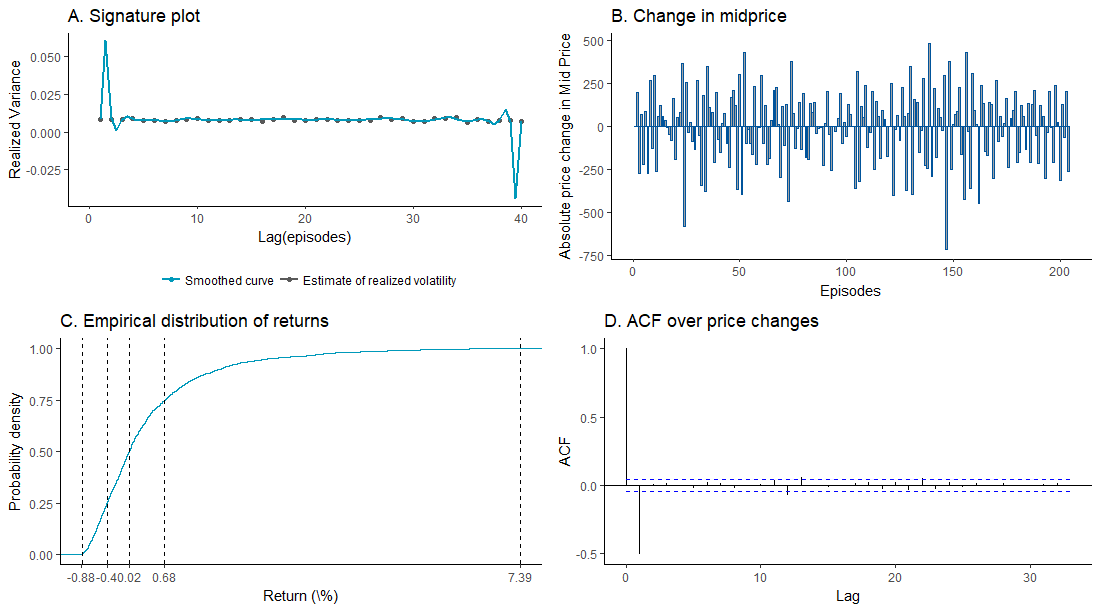
\includegraphics[scale=.5]{dmv1_sf_multi.png}
		%Captions and Labels can be used since this is a figure environment
		\caption{Stylized facts for DealerMarket-v2. A signature plot over the realized variance (A) and plot over periodicity in mid prices (B). Empirical distribution of returns (C) and an acf over price changes (D). }
		\label{fig:sf1}
\end{figure}

\section{Stylized Facts of Data}
%\subsection*{DealerMarket-v2}
In \autoref{fig:sf1} one sees that the simulated prices exhibits certain behaviour. Plot (A) shows a signature plot over the realized variance or volatility, for DealerMarket-v2. Looking at the plot it is clear that the simulated stock prices are exhibiting weak mean reversion. Which is in line with what is mentioned in \parencite{bouchaud2018trades}. Looking at plot (B) the mid price changes are exhibiting activity clustering. As in \parencite{bouchaud2018trades}, certain periods of repeating similar changes in the mid prices.
\newline
\newline
Finally looking at plot (D) one can also see an absent of linear correlations. With near zero autocorrelations after lag 1. This is also what is inline with what is stated in previous literature. In \autoref{fig:sf2} one can see similar patterns for LOBMarket-v1 as in \autoref{fig:sf1}. Note however that both the signature plot (A) and mid price change plot (B) is different. The signature plot is still mean reverting, however now with a small trend. Whilst the changes in mid-prices are more frequent. 
\begin{figure}[H]
		%Do not try to scale figure in .tex or you loose font size consistency
		\centering
		%The code to input the plot is extremely simple
		%% Created by tikzDevice version 0.11 on 2018-07-15 13:37:11
% !TEX encoding = UTF-8 Unicode
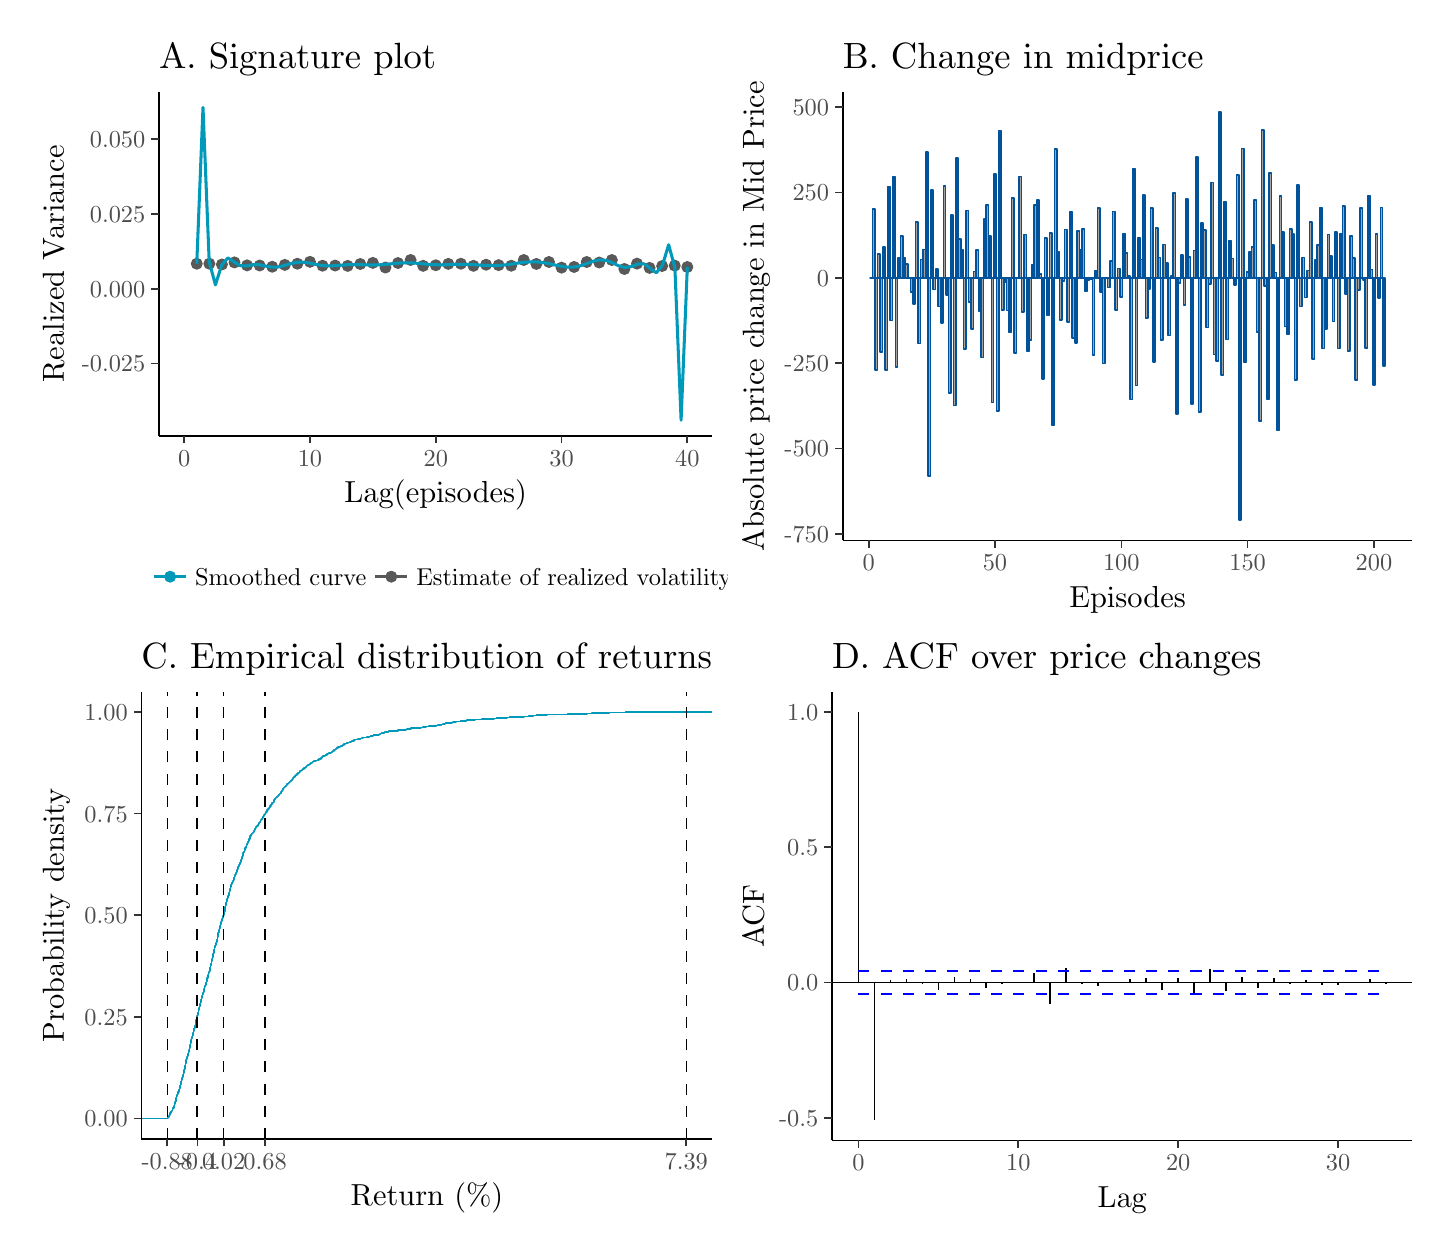
\begin{tikzpicture}[x=1pt,y=1pt]
\definecolor{fillColor}{RGB}{255,255,255}
\path[use as bounding box,fill=fillColor,fill opacity=0.00] (0,0) rectangle (505.89,433.62);
\begin{scope}
\path[clip] (  0.00,216.81) rectangle (252.95,433.62);
\definecolor{drawColor}{RGB}{255,255,255}
\definecolor{fillColor}{RGB}{255,255,255}

\path[draw=drawColor,line width= 0.6pt,line join=round,line cap=round,fill=fillColor] ( -0.00,216.81) rectangle (252.95,433.62);
\end{scope}
\begin{scope}
\path[clip] ( 47.47,286.11) rectangle (247.44,410.48);
\definecolor{fillColor}{RGB}{255,255,255}

\path[fill=fillColor] ( 47.47,286.11) rectangle (247.44,410.48);
\definecolor{drawColor}{gray}{0.35}
\definecolor{fillColor}{gray}{0.35}

\path[draw=drawColor,line width= 0.4pt,line join=round,line cap=round,fill=fillColor] ( 61.10,348.32) circle (  1.96);

\path[draw=drawColor,line width= 0.4pt,line join=round,line cap=round,fill=fillColor] ( 65.65,348.33) circle (  1.96);

\path[draw=drawColor,line width= 0.4pt,line join=round,line cap=round,fill=fillColor] ( 70.19,348.05) circle (  1.96);

\path[draw=drawColor,line width= 0.4pt,line join=round,line cap=round,fill=fillColor] ( 74.74,348.79) circle (  1.96);

\path[draw=drawColor,line width= 0.4pt,line join=round,line cap=round,fill=fillColor] ( 79.28,347.72) circle (  1.96);

\path[draw=drawColor,line width= 0.4pt,line join=round,line cap=round,fill=fillColor] ( 83.83,347.68) circle (  1.96);

\path[draw=drawColor,line width= 0.4pt,line join=round,line cap=round,fill=fillColor] ( 88.37,347.23) circle (  1.96);

\path[draw=drawColor,line width= 0.4pt,line join=round,line cap=round,fill=fillColor] ( 92.92,347.90) circle (  1.96);

\path[draw=drawColor,line width= 0.4pt,line join=round,line cap=round,fill=fillColor] ( 97.46,348.32) circle (  1.96);

\path[draw=drawColor,line width= 0.4pt,line join=round,line cap=round,fill=fillColor] (102.01,349.00) circle (  1.96);

\path[draw=drawColor,line width= 0.4pt,line join=round,line cap=round,fill=fillColor] (106.55,347.60) circle (  1.96);

\path[draw=drawColor,line width= 0.4pt,line join=round,line cap=round,fill=fillColor] (111.10,347.66) circle (  1.96);

\path[draw=drawColor,line width= 0.4pt,line join=round,line cap=round,fill=fillColor] (115.64,347.54) circle (  1.96);

\path[draw=drawColor,line width= 0.4pt,line join=round,line cap=round,fill=fillColor] (120.19,348.22) circle (  1.96);

\path[draw=drawColor,line width= 0.4pt,line join=round,line cap=round,fill=fillColor] (124.73,348.62) circle (  1.96);

\path[draw=drawColor,line width= 0.4pt,line join=round,line cap=round,fill=fillColor] (129.28,346.94) circle (  1.96);

\path[draw=drawColor,line width= 0.4pt,line join=round,line cap=round,fill=fillColor] (133.82,348.57) circle (  1.96);

\path[draw=drawColor,line width= 0.4pt,line join=round,line cap=round,fill=fillColor] (138.37,349.67) circle (  1.96);

\path[draw=drawColor,line width= 0.4pt,line join=round,line cap=round,fill=fillColor] (142.91,347.56) circle (  1.96);

\path[draw=drawColor,line width= 0.4pt,line join=round,line cap=round,fill=fillColor] (147.46,347.77) circle (  1.96);

\path[draw=drawColor,line width= 0.4pt,line join=round,line cap=round,fill=fillColor] (152.00,348.26) circle (  1.96);

\path[draw=drawColor,line width= 0.4pt,line join=round,line cap=round,fill=fillColor] (156.55,348.31) circle (  1.96);

\path[draw=drawColor,line width= 0.4pt,line join=round,line cap=round,fill=fillColor] (161.09,347.56) circle (  1.96);

\path[draw=drawColor,line width= 0.4pt,line join=round,line cap=round,fill=fillColor] (165.64,347.96) circle (  1.96);

\path[draw=drawColor,line width= 0.4pt,line join=round,line cap=round,fill=fillColor] (170.18,347.81) circle (  1.96);

\path[draw=drawColor,line width= 0.4pt,line join=round,line cap=round,fill=fillColor] (174.73,347.60) circle (  1.96);

\path[draw=drawColor,line width= 0.4pt,line join=round,line cap=round,fill=fillColor] (179.27,349.66) circle (  1.96);

\path[draw=drawColor,line width= 0.4pt,line join=round,line cap=round,fill=fillColor] (183.82,348.24) circle (  1.96);

\path[draw=drawColor,line width= 0.4pt,line join=round,line cap=round,fill=fillColor] (188.36,348.95) circle (  1.96);

\path[draw=drawColor,line width= 0.4pt,line join=round,line cap=round,fill=fillColor] (192.91,346.91) circle (  1.96);

\path[draw=drawColor,line width= 0.4pt,line join=round,line cap=round,fill=fillColor] (197.45,347.15) circle (  1.96);

\path[draw=drawColor,line width= 0.4pt,line join=round,line cap=round,fill=fillColor] (202.00,348.94) circle (  1.96);

\path[draw=drawColor,line width= 0.4pt,line join=round,line cap=round,fill=fillColor] (206.54,348.75) circle (  1.96);

\path[draw=drawColor,line width= 0.4pt,line join=round,line cap=round,fill=fillColor] (211.09,349.66) circle (  1.96);

\path[draw=drawColor,line width= 0.4pt,line join=round,line cap=round,fill=fillColor] (215.63,346.42) circle (  1.96);

\path[draw=drawColor,line width= 0.4pt,line join=round,line cap=round,fill=fillColor] (220.18,348.35) circle (  1.96);

\path[draw=drawColor,line width= 0.4pt,line join=round,line cap=round,fill=fillColor] (224.72,346.81) circle (  1.96);

\path[draw=drawColor,line width= 0.4pt,line join=round,line cap=round,fill=fillColor] (229.27,347.49) circle (  1.96);

\path[draw=drawColor,line width= 0.4pt,line join=round,line cap=round,fill=fillColor] (233.81,347.63) circle (  1.96);

\path[draw=drawColor,line width= 0.4pt,line join=round,line cap=round,fill=fillColor] (238.36,347.13) circle (  1.96);
\definecolor{drawColor}{RGB}{0,153,186}

\path[draw=drawColor,line width= 1.1pt,line join=round] ( 61.10,348.32) --
	( 63.35,404.83) --
	( 65.59,349.07) --
	( 67.84,340.67) --
	( 70.08,347.74) --
	( 72.32,350.41) --
	( 74.57,348.99) --
	( 76.81,347.60) --
	( 79.05,347.54) --
	( 81.30,347.95) --
	( 83.54,347.96) --
	( 85.79,347.51) --
	( 88.03,347.08) --
	( 90.27,347.10) --
	( 92.52,347.61) --
	( 94.76,348.30) --
	( 97.00,348.80) --
	( 99.25,348.90) --
	(101.49,348.62) --
	(103.73,348.16) --
	(105.98,347.75) --
	(108.22,347.55) --
	(110.47,347.58) --
	(112.71,347.75) --
	(114.95,347.93) --
	(117.20,348.02) --
	(119.44,348.00) --
	(121.68,347.92) --
	(123.93,347.85) --
	(126.17,347.87) --
	(128.42,348.01) --
	(130.66,348.22) --
	(132.90,348.45) --
	(135.15,348.61) --
	(137.39,348.65) --
	(139.63,348.56) --
	(141.88,348.37) --
	(144.12,348.16) --
	(146.36,348.00) --
	(148.61,347.93) --
	(150.85,347.94) --
	(153.10,348.02) --
	(155.34,348.09) --
	(157.58,348.11) --
	(159.83,348.05) --
	(162.07,347.92) --
	(164.31,347.77) --
	(166.56,347.66) --
	(168.80,347.64) --
	(171.04,347.75) --
	(173.29,347.99) --
	(175.53,348.30) --
	(177.78,348.64) --
	(180.02,348.90) --
	(182.26,349.01) --
	(184.51,348.94) --
	(186.75,348.66) --
	(188.99,348.21) --
	(191.24,347.70) --
	(193.48,347.26) --
	(195.73,347.04) --
	(197.97,347.18) --
	(200.21,347.72) --
	(202.46,348.54) --
	(204.70,349.33) --
	(206.94,349.74) --
	(209.19,349.49) --
	(211.43,348.60) --
	(213.67,347.52) --
	(215.92,346.95) --
	(218.16,347.31) --
	(220.41,348.20) --
	(222.65,348.31) --
	(224.89,346.71) --
	(227.14,345.02) --
	(229.38,347.79) --
	(231.62,355.19) --
	(233.87,346.89) --
	(236.11,291.77) --
	(238.36,347.13);
\end{scope}
\begin{scope}
\path[clip] (  0.00,  0.00) rectangle (505.89,433.62);
\definecolor{drawColor}{RGB}{0,0,0}

\path[draw=drawColor,line width= 0.6pt,line join=round] ( 47.47,286.11) --
	( 47.47,410.48);
\end{scope}
\begin{scope}
\path[clip] (  0.00,  0.00) rectangle (505.89,433.62);
\definecolor{drawColor}{gray}{0.30}

\node[text=drawColor,anchor=base east,inner sep=0pt, outer sep=0pt, scale=  0.88] at ( 42.52,309.20) {-0.025};

\node[text=drawColor,anchor=base east,inner sep=0pt, outer sep=0pt, scale=  0.88] at ( 42.52,336.24) {0.000};

\node[text=drawColor,anchor=base east,inner sep=0pt, outer sep=0pt, scale=  0.88] at ( 42.52,363.28) {0.025};

\node[text=drawColor,anchor=base east,inner sep=0pt, outer sep=0pt, scale=  0.88] at ( 42.52,390.31) {0.050};
\end{scope}
\begin{scope}
\path[clip] (  0.00,  0.00) rectangle (505.89,433.62);
\definecolor{drawColor}{gray}{0.20}

\path[draw=drawColor,line width= 0.6pt,line join=round] ( 44.72,312.23) --
	( 47.47,312.23);

\path[draw=drawColor,line width= 0.6pt,line join=round] ( 44.72,339.27) --
	( 47.47,339.27);

\path[draw=drawColor,line width= 0.6pt,line join=round] ( 44.72,366.31) --
	( 47.47,366.31);

\path[draw=drawColor,line width= 0.6pt,line join=round] ( 44.72,393.34) --
	( 47.47,393.34);
\end{scope}
\begin{scope}
\path[clip] (  0.00,  0.00) rectangle (505.89,433.62);
\definecolor{drawColor}{RGB}{0,0,0}

\path[draw=drawColor,line width= 0.6pt,line join=round] ( 47.47,286.11) --
	(247.44,286.11);
\end{scope}
\begin{scope}
\path[clip] (  0.00,  0.00) rectangle (505.89,433.62);
\definecolor{drawColor}{gray}{0.20}

\path[draw=drawColor,line width= 0.6pt,line join=round] ( 56.56,283.36) --
	( 56.56,286.11);

\path[draw=drawColor,line width= 0.6pt,line join=round] (102.01,283.36) --
	(102.01,286.11);

\path[draw=drawColor,line width= 0.6pt,line join=round] (147.46,283.36) --
	(147.46,286.11);

\path[draw=drawColor,line width= 0.6pt,line join=round] (192.91,283.36) --
	(192.91,286.11);

\path[draw=drawColor,line width= 0.6pt,line join=round] (238.36,283.36) --
	(238.36,286.11);
\end{scope}
\begin{scope}
\path[clip] (  0.00,  0.00) rectangle (505.89,433.62);
\definecolor{drawColor}{gray}{0.30}

\node[text=drawColor,anchor=base,inner sep=0pt, outer sep=0pt, scale=  0.88] at ( 56.56,275.10) {0};

\node[text=drawColor,anchor=base,inner sep=0pt, outer sep=0pt, scale=  0.88] at (102.01,275.10) {10};

\node[text=drawColor,anchor=base,inner sep=0pt, outer sep=0pt, scale=  0.88] at (147.46,275.10) {20};

\node[text=drawColor,anchor=base,inner sep=0pt, outer sep=0pt, scale=  0.88] at (192.91,275.10) {30};

\node[text=drawColor,anchor=base,inner sep=0pt, outer sep=0pt, scale=  0.88] at (238.36,275.10) {40};
\end{scope}
\begin{scope}
\path[clip] (  0.00,  0.00) rectangle (505.89,433.62);
\definecolor{drawColor}{RGB}{0,0,0}

\node[text=drawColor,anchor=base,inner sep=0pt, outer sep=0pt, scale=  1.10] at (147.46,262.03) {Lag(episodes)};
\end{scope}
\begin{scope}
\path[clip] (  0.00,  0.00) rectangle (505.89,433.62);
\definecolor{drawColor}{RGB}{0,0,0}

\node[text=drawColor,rotate= 90.00,anchor=base,inner sep=0pt, outer sep=0pt, scale=  1.10] at ( 13.08,348.30) {Realized Variance};
\end{scope}
\begin{scope}
\path[clip] (  0.00,  0.00) rectangle (505.89,433.62);
\definecolor{fillColor}{RGB}{255,255,255}

\path[fill=fillColor] ( 34.95,222.31) rectangle (259.96,248.15);
\end{scope}
\begin{scope}
\path[clip] (  0.00,  0.00) rectangle (505.89,433.62);
\definecolor{drawColor}{RGB}{0,153,186}
\definecolor{fillColor}{RGB}{0,153,186}

\path[draw=drawColor,line width= 0.4pt,line join=round,line cap=round,fill=fillColor] ( 51.48,235.23) circle (  1.96);
\end{scope}
\begin{scope}
\path[clip] (  0.00,  0.00) rectangle (505.89,433.62);
\definecolor{drawColor}{RGB}{0,153,186}

\path[draw=drawColor,line width= 1.1pt,line join=round] ( 45.70,235.23) -- ( 57.26,235.23);
\end{scope}
\begin{scope}
\path[clip] (  0.00,  0.00) rectangle (505.89,433.62);
\definecolor{drawColor}{gray}{0.35}
\definecolor{fillColor}{gray}{0.35}

\path[draw=drawColor,line width= 0.4pt,line join=round,line cap=round,fill=fillColor] (131.40,235.23) circle (  1.96);
\end{scope}
\begin{scope}
\path[clip] (  0.00,  0.00) rectangle (505.89,433.62);
\definecolor{drawColor}{gray}{0.35}

\path[draw=drawColor,line width= 1.1pt,line join=round] (125.62,235.23) -- (137.19,235.23);
\end{scope}
\begin{scope}
\path[clip] (  0.00,  0.00) rectangle (505.89,433.62);
\definecolor{drawColor}{RGB}{0,0,0}

\node[text=drawColor,anchor=base west,inner sep=0pt, outer sep=0pt, scale=  0.88] at ( 60.52,232.20) {Smoothed curve};
\end{scope}
\begin{scope}
\path[clip] (  0.00,  0.00) rectangle (505.89,433.62);
\definecolor{drawColor}{RGB}{0,0,0}

\node[text=drawColor,anchor=base west,inner sep=0pt, outer sep=0pt, scale=  0.88] at (140.44,232.20) {Estimate of realized volatility};
\end{scope}
\begin{scope}
\path[clip] (  0.00,  0.00) rectangle (505.89,433.62);
\definecolor{drawColor}{RGB}{0,0,0}

\node[text=drawColor,anchor=base west,inner sep=0pt, outer sep=0pt, scale=  1.32] at ( 47.47,419.03) {A. Signature plot};
\end{scope}
\begin{scope}
\path[clip] (  0.00,  0.00) rectangle (252.94,216.81);
\definecolor{drawColor}{RGB}{255,255,255}
\definecolor{fillColor}{RGB}{255,255,255}

\path[draw=drawColor,line width= 0.6pt,line join=round,line cap=round,fill=fillColor] (  0.00,  0.00) rectangle (252.94,216.81);
\end{scope}
\begin{scope}
\path[clip] ( 41.11, 32.09) rectangle (247.44,193.67);
\definecolor{fillColor}{RGB}{255,255,255}

\path[fill=fillColor] ( 41.11, 32.09) rectangle (247.44,193.67);
\definecolor{drawColor}{RGB}{0,153,186}

\path[draw=drawColor,line width= 0.6pt,line join=round] ( 41.11, 39.43) --
	( 50.49, 39.43) --
	( 50.49, 39.50) --
	( 50.56, 39.50) --
	( 50.56, 39.57) --
	( 50.72, 39.57) --
	( 50.72, 39.65) --
	( 50.76, 39.65) --
	( 50.76, 39.72) --
	( 50.76, 39.72) --
	( 50.76, 39.79) --
	( 50.78, 39.79) --
	( 50.78, 39.86) --
	( 50.84, 39.86) --
	( 50.84, 39.93) --
	( 50.91, 39.93) --
	( 50.91, 40.01) --
	( 50.94, 40.01) --
	( 50.94, 40.08) --
	( 51.03, 40.08) --
	( 51.03, 40.15) --
	( 51.03, 40.15) --
	( 51.03, 40.22) --
	( 51.07, 40.22) --
	( 51.07, 40.29) --
	( 51.08, 40.29) --
	( 51.08, 40.36) --
	( 51.09, 40.36) --
	( 51.09, 40.44) --
	( 51.12, 40.44) --
	( 51.12, 40.51) --
	( 51.17, 40.51) --
	( 51.17, 40.58) --
	( 51.21, 40.58) --
	( 51.21, 40.65) --
	( 51.31, 40.65) --
	( 51.31, 40.72) --
	( 51.34, 40.72) --
	( 51.34, 40.79) --
	( 51.35, 40.79) --
	( 51.35, 40.87) --
	( 51.38, 40.87) --
	( 51.38, 40.94) --
	( 51.38, 40.94) --
	( 51.38, 41.01) --
	( 51.39, 41.01) --
	( 51.39, 41.08) --
	( 51.40, 41.08) --
	( 51.40, 41.15) --
	( 51.41, 41.15) --
	( 51.41, 41.23) --
	( 51.49, 41.23) --
	( 51.49, 41.30) --
	( 51.51, 41.30) --
	( 51.51, 41.37) --
	( 51.63, 41.37) --
	( 51.63, 41.44) --
	( 51.69, 41.44) --
	( 51.69, 41.51) --
	( 51.71, 41.51) --
	( 51.71, 41.58) --
	( 51.71, 41.58) --
	( 51.71, 41.66) --
	( 51.72, 41.66) --
	( 51.72, 41.73) --
	( 51.75, 41.73) --
	( 51.75, 41.80) --
	( 51.79, 41.80) --
	( 51.79, 41.87) --
	( 51.83, 41.87) --
	( 51.83, 41.94) --
	( 51.88, 41.94) --
	( 51.88, 42.01) --
	( 51.92, 42.01) --
	( 51.92, 42.09) --
	( 51.96, 42.09) --
	( 51.96, 42.16) --
	( 52.20, 42.16) --
	( 52.20, 42.23) --
	( 52.20, 42.23) --
	( 52.20, 42.30) --
	( 52.22, 42.30) --
	( 52.22, 42.37) --
	( 52.28, 42.37) --
	( 52.28, 42.45) --
	( 52.29, 42.45) --
	( 52.29, 42.52) --
	( 52.29, 42.52) --
	( 52.29, 42.59) --
	( 52.29, 42.59) --
	( 52.29, 42.66) --
	( 52.33, 42.66) --
	( 52.33, 42.73) --
	( 52.39, 42.73) --
	( 52.39, 42.80) --
	( 52.46, 42.80) --
	( 52.46, 42.88) --
	( 52.50, 42.88) --
	( 52.50, 42.95) --
	( 52.50, 42.95) --
	( 52.50, 43.02) --
	( 52.57, 43.02) --
	( 52.57, 43.09) --
	( 52.62, 43.09) --
	( 52.62, 43.16) --
	( 52.65, 43.16) --
	( 52.65, 43.23) --
	( 52.74, 43.23) --
	( 52.74, 43.31) --
	( 52.77, 43.31) --
	( 52.77, 43.38) --
	( 52.80, 43.38) --
	( 52.80, 43.45) --
	( 52.83, 43.45) --
	( 52.83, 43.52) --
	( 52.85, 43.52) --
	( 52.85, 43.59) --
	( 52.85, 43.59) --
	( 52.85, 43.67) --
	( 52.87, 43.67) --
	( 52.87, 43.74) --
	( 52.99, 43.74) --
	( 52.99, 43.81) --
	( 52.99, 43.81) --
	( 52.99, 43.88) --
	( 53.00, 43.88) --
	( 53.00, 43.95) --
	( 53.03, 43.95) --
	( 53.03, 44.02) --
	( 53.03, 44.02) --
	( 53.03, 44.10) --
	( 53.05, 44.10) --
	( 53.05, 44.17) --
	( 53.07, 44.17) --
	( 53.07, 44.24) --
	( 53.09, 44.24) --
	( 53.09, 44.31) --
	( 53.10, 44.31) --
	( 53.10, 44.38) --
	( 53.10, 44.38) --
	( 53.10, 44.45) --
	( 53.10, 44.45) --
	( 53.10, 44.53) --
	( 53.10, 44.53) --
	( 53.10, 44.60) --
	( 53.11, 44.60) --
	( 53.11, 44.67) --
	( 53.11, 44.67) --
	( 53.11, 44.74) --
	( 53.13, 44.74) --
	( 53.13, 44.81) --
	( 53.18, 44.81) --
	( 53.18, 44.89) --
	( 53.20, 44.89) --
	( 53.20, 44.96) --
	( 53.26, 44.96) --
	( 53.26, 45.03) --
	( 53.27, 45.03) --
	( 53.27, 45.10) --
	( 53.28, 45.10) --
	( 53.28, 45.17) --
	( 53.28, 45.17) --
	( 53.28, 45.24) --
	( 53.30, 45.24) --
	( 53.30, 45.32) --
	( 53.31, 45.32) --
	( 53.31, 45.39) --
	( 53.32, 45.39) --
	( 53.32, 45.46) --
	( 53.36, 45.46) --
	( 53.36, 45.53) --
	( 53.40, 45.53) --
	( 53.40, 45.60) --
	( 53.48, 45.60) --
	( 53.48, 45.67) --
	( 53.49, 45.67) --
	( 53.49, 45.75) --
	( 53.49, 45.75) --
	( 53.49, 45.82) --
	( 53.52, 45.82) --
	( 53.52, 45.89) --
	( 53.53, 45.89) --
	( 53.53, 45.96) --
	( 53.55, 45.96) --
	( 53.55, 46.03) --
	( 53.56, 46.03) --
	( 53.56, 46.11) --
	( 53.57, 46.11) --
	( 53.57, 46.18) --
	( 53.57, 46.18) --
	( 53.57, 46.25) --
	( 53.59, 46.25) --
	( 53.59, 46.32) --
	( 53.60, 46.32) --
	( 53.60, 46.39) --
	( 53.63, 46.39) --
	( 53.63, 46.46) --
	( 53.65, 46.46) --
	( 53.65, 46.54) --
	( 53.66, 46.54) --
	( 53.66, 46.61) --
	( 53.66, 46.61) --
	( 53.66, 46.68) --
	( 53.67, 46.68) --
	( 53.67, 46.75) --
	( 53.69, 46.75) --
	( 53.69, 46.82) --
	( 53.69, 46.82) --
	( 53.69, 46.89) --
	( 53.69, 46.89) --
	( 53.69, 46.97) --
	( 53.72, 46.97) --
	( 53.72, 47.04) --
	( 53.73, 47.04) --
	( 53.73, 47.11) --
	( 53.74, 47.11) --
	( 53.74, 47.18) --
	( 53.76, 47.18) --
	( 53.76, 47.25) --
	( 53.77, 47.25) --
	( 53.77, 47.33) --
	( 53.82, 47.33) --
	( 53.82, 47.40) --
	( 53.85, 47.40) --
	( 53.85, 47.47) --
	( 53.90, 47.47) --
	( 53.90, 47.54) --
	( 53.94, 47.54) --
	( 53.94, 47.61) --
	( 53.94, 47.61) --
	( 53.94, 47.68) --
	( 54.01, 47.68) --
	( 54.01, 47.76) --
	( 54.01, 47.76) --
	( 54.01, 47.83) --
	( 54.07, 47.83) --
	( 54.07, 47.90) --
	( 54.09, 47.90) --
	( 54.09, 47.97) --
	( 54.16, 47.97) --
	( 54.16, 48.04) --
	( 54.17, 48.04) --
	( 54.17, 48.11) --
	( 54.17, 48.11) --
	( 54.17, 48.19) --
	( 54.20, 48.19) --
	( 54.20, 48.26) --
	( 54.21, 48.26) --
	( 54.21, 48.33) --
	( 54.28, 48.33) --
	( 54.28, 48.40) --
	( 54.28, 48.40) --
	( 54.28, 48.47) --
	( 54.30, 48.47) --
	( 54.30, 48.54) --
	( 54.35, 48.54) --
	( 54.35, 48.62) --
	( 54.36, 48.62) --
	( 54.36, 48.69) --
	( 54.37, 48.69) --
	( 54.37, 48.76) --
	( 54.37, 48.76) --
	( 54.37, 48.83) --
	( 54.42, 48.83) --
	( 54.42, 48.90) --
	( 54.43, 48.90) --
	( 54.43, 48.98) --
	( 54.43, 48.98) --
	( 54.43, 49.05) --
	( 54.44, 49.05) --
	( 54.44, 49.12) --
	( 54.57, 49.12) --
	( 54.57, 49.19) --
	( 54.59, 49.19) --
	( 54.59, 49.26) --
	( 54.61, 49.26) --
	( 54.61, 49.33) --
	( 54.61, 49.33) --
	( 54.61, 49.41) --
	( 54.61, 49.41) --
	( 54.61, 49.48) --
	( 54.72, 49.48) --
	( 54.72, 49.55) --
	( 54.73, 49.55) --
	( 54.73, 49.62) --
	( 54.73, 49.62) --
	( 54.73, 49.69) --
	( 54.74, 49.69) --
	( 54.74, 49.76) --
	( 54.78, 49.76) --
	( 54.78, 49.84) --
	( 54.79, 49.84) --
	( 54.79, 49.91) --
	( 54.80, 49.91) --
	( 54.80, 49.98) --
	( 54.82, 49.98) --
	( 54.82, 50.05) --
	( 54.87, 50.05) --
	( 54.87, 50.12) --
	( 54.90, 50.12) --
	( 54.90, 50.20) --
	( 54.91, 50.20) --
	( 54.91, 50.27) --
	( 54.93, 50.27) --
	( 54.93, 50.34) --
	( 54.94, 50.34) --
	( 54.94, 50.41) --
	( 54.94, 50.41) --
	( 54.94, 50.48) --
	( 54.97, 50.48) --
	( 54.97, 50.55) --
	( 55.00, 50.55) --
	( 55.00, 50.63) --
	( 55.03, 50.63) --
	( 55.03, 50.70) --
	( 55.05, 50.70) --
	( 55.05, 50.77) --
	( 55.08, 50.77) --
	( 55.08, 50.84) --
	( 55.09, 50.84) --
	( 55.09, 50.91) --
	( 55.09, 50.91) --
	( 55.09, 50.98) --
	( 55.11, 50.98) --
	( 55.11, 51.06) --
	( 55.12, 51.06) --
	( 55.12, 51.13) --
	( 55.12, 51.13) --
	( 55.12, 51.20) --
	( 55.14, 51.20) --
	( 55.14, 51.27) --
	( 55.14, 51.27) --
	( 55.14, 51.34) --
	( 55.16, 51.34) --
	( 55.16, 51.42) --
	( 55.19, 51.42) --
	( 55.19, 51.49) --
	( 55.20, 51.49) --
	( 55.20, 51.56) --
	( 55.21, 51.56) --
	( 55.21, 51.63) --
	( 55.21, 51.63) --
	( 55.21, 51.70) --
	( 55.28, 51.70) --
	( 55.28, 51.77) --
	( 55.30, 51.77) --
	( 55.30, 51.85) --
	( 55.31, 51.85) --
	( 55.31, 51.92) --
	( 55.31, 51.92) --
	( 55.31, 51.99) --
	( 55.34, 51.99) --
	( 55.34, 52.06) --
	( 55.35, 52.06) --
	( 55.35, 52.13) --
	( 55.37, 52.13) --
	( 55.37, 52.20) --
	( 55.41, 52.20) --
	( 55.41, 52.28) --
	( 55.42, 52.28) --
	( 55.42, 52.35) --
	( 55.42, 52.35) --
	( 55.42, 52.42) --
	( 55.43, 52.42) --
	( 55.43, 52.49) --
	( 55.43, 52.49) --
	( 55.43, 52.56) --
	( 55.47, 52.56) --
	( 55.47, 52.64) --
	( 55.48, 52.64) --
	( 55.48, 52.71) --
	( 55.52, 52.71) --
	( 55.52, 52.78) --
	( 55.54, 52.78) --
	( 55.54, 52.85) --
	( 55.54, 52.85) --
	( 55.54, 52.92) --
	( 55.57, 52.92) --
	( 55.57, 52.99) --
	( 55.57, 52.99) --
	( 55.57, 53.07) --
	( 55.60, 53.07) --
	( 55.60, 53.14) --
	( 55.60, 53.14) --
	( 55.60, 53.21) --
	( 55.62, 53.21) --
	( 55.62, 53.28) --
	( 55.67, 53.28) --
	( 55.67, 53.35) --
	( 55.71, 53.35) --
	( 55.71, 53.42) --
	( 55.75, 53.42) --
	( 55.75, 53.50) --
	( 55.76, 53.50) --
	( 55.76, 53.57) --
	( 55.76, 53.57) --
	( 55.76, 53.64) --
	( 55.81, 53.64) --
	( 55.81, 53.71) --
	( 55.84, 53.71) --
	( 55.84, 53.78) --
	( 55.84, 53.78) --
	( 55.84, 53.86) --
	( 55.86, 53.86) --
	( 55.86, 53.93) --
	( 55.87, 53.93) --
	( 55.87, 54.00) --
	( 55.88, 54.00) --
	( 55.88, 54.07) --
	( 55.89, 54.07) --
	( 55.89, 54.14) --
	( 55.89, 54.14) --
	( 55.89, 54.21) --
	( 55.92, 54.21) --
	( 55.92, 54.29) --
	( 55.99, 54.29) --
	( 55.99, 54.36) --
	( 56.00, 54.36) --
	( 56.00, 54.43) --
	( 56.10, 54.43) --
	( 56.10, 54.50) --
	( 56.12, 54.50) --
	( 56.12, 54.57) --
	( 56.12, 54.57) --
	( 56.12, 54.64) --
	( 56.16, 54.64) --
	( 56.16, 54.72) --
	( 56.18, 54.72) --
	( 56.18, 54.79) --
	( 56.19, 54.79) --
	( 56.19, 54.86) --
	( 56.20, 54.86) --
	( 56.20, 54.93) --
	( 56.20, 54.93) --
	( 56.20, 55.00) --
	( 56.21, 55.00) --
	( 56.21, 55.08) --
	( 56.24, 55.08) --
	( 56.24, 55.15) --
	( 56.25, 55.15) --
	( 56.25, 55.22) --
	( 56.26, 55.22) --
	( 56.26, 55.29) --
	( 56.26, 55.29) --
	( 56.26, 55.36) --
	( 56.28, 55.36) --
	( 56.28, 55.43) --
	( 56.29, 55.43) --
	( 56.29, 55.51) --
	( 56.33, 55.51) --
	( 56.33, 55.58) --
	( 56.34, 55.58) --
	( 56.34, 55.65) --
	( 56.34, 55.65) --
	( 56.34, 55.72) --
	( 56.36, 55.72) --
	( 56.36, 55.79) --
	( 56.38, 55.79) --
	( 56.38, 55.86) --
	( 56.39, 55.86) --
	( 56.39, 55.94) --
	( 56.39, 55.94) --
	( 56.39, 56.01) --
	( 56.41, 56.01) --
	( 56.41, 56.08) --
	( 56.42, 56.08) --
	( 56.42, 56.15) --
	( 56.43, 56.15) --
	( 56.43, 56.22) --
	( 56.44, 56.22) --
	( 56.44, 56.30) --
	( 56.49, 56.30) --
	( 56.49, 56.37) --
	( 56.52, 56.37) --
	( 56.52, 56.44) --
	( 56.54, 56.44) --
	( 56.54, 56.51) --
	( 56.56, 56.51) --
	( 56.56, 56.58) --
	( 56.57, 56.58) --
	( 56.57, 56.65) --
	( 56.58, 56.65) --
	( 56.58, 56.73) --
	( 56.58, 56.73) --
	( 56.58, 56.80) --
	( 56.59, 56.80) --
	( 56.59, 56.87) --
	( 56.61, 56.87) --
	( 56.61, 56.94) --
	( 56.63, 56.94) --
	( 56.63, 57.01) --
	( 56.64, 57.01) --
	( 56.64, 57.08) --
	( 56.67, 57.08) --
	( 56.67, 57.16) --
	( 56.67, 57.16) --
	( 56.67, 57.23) --
	( 56.69, 57.23) --
	( 56.69, 57.30) --
	( 56.75, 57.30) --
	( 56.75, 57.37) --
	( 56.76, 57.37) --
	( 56.76, 57.44) --
	( 56.76, 57.44) --
	( 56.76, 57.52) --
	( 56.78, 57.52) --
	( 56.78, 57.59) --
	( 56.79, 57.59) --
	( 56.79, 57.66) --
	( 56.79, 57.66) --
	( 56.79, 57.73) --
	( 56.81, 57.73) --
	( 56.81, 57.80) --
	( 56.81, 57.80) --
	( 56.81, 57.87) --
	( 56.82, 57.87) --
	( 56.82, 57.95) --
	( 56.83, 57.95) --
	( 56.83, 58.02) --
	( 56.84, 58.02) --
	( 56.84, 58.09) --
	( 56.86, 58.09) --
	( 56.86, 58.16) --
	( 56.86, 58.16) --
	( 56.86, 58.23) --
	( 56.87, 58.23) --
	( 56.87, 58.30) --
	( 56.89, 58.30) --
	( 56.89, 58.38) --
	( 56.89, 58.38) --
	( 56.89, 58.45) --
	( 56.92, 58.45) --
	( 56.92, 58.52) --
	( 56.95, 58.52) --
	( 56.95, 58.59) --
	( 56.97, 58.59) --
	( 56.97, 58.66) --
	( 56.98, 58.66) --
	( 56.98, 58.74) --
	( 56.98, 58.74) --
	( 56.98, 58.81) --
	( 56.99, 58.81) --
	( 56.99, 58.88) --
	( 56.99, 58.88) --
	( 56.99, 58.95) --
	( 57.03, 58.95) --
	( 57.03, 59.02) --
	( 57.04, 59.02) --
	( 57.04, 59.09) --
	( 57.04, 59.09) --
	( 57.04, 59.17) --
	( 57.06, 59.17) --
	( 57.06, 59.24) --
	( 57.06, 59.24) --
	( 57.06, 59.31) --
	( 57.07, 59.31) --
	( 57.07, 59.38) --
	( 57.10, 59.38) --
	( 57.10, 59.45) --
	( 57.11, 59.45) --
	( 57.11, 59.52) --
	( 57.14, 59.52) --
	( 57.14, 59.60) --
	( 57.14, 59.60) --
	( 57.14, 59.67) --
	( 57.14, 59.67) --
	( 57.14, 59.74) --
	( 57.16, 59.74) --
	( 57.16, 59.81) --
	( 57.17, 59.81) --
	( 57.17, 59.88) --
	( 57.18, 59.88) --
	( 57.18, 59.96) --
	( 57.19, 59.96) --
	( 57.19, 60.03) --
	( 57.19, 60.03) --
	( 57.19, 60.10) --
	( 57.19, 60.10) --
	( 57.19, 60.17) --
	( 57.26, 60.17) --
	( 57.26, 60.24) --
	( 57.27, 60.24) --
	( 57.27, 60.31) --
	( 57.30, 60.31) --
	( 57.30, 60.39) --
	( 57.30, 60.39) --
	( 57.30, 60.46) --
	( 57.32, 60.46) --
	( 57.32, 60.53) --
	( 57.34, 60.53) --
	( 57.34, 60.60) --
	( 57.35, 60.60) --
	( 57.35, 60.67) --
	( 57.36, 60.67) --
	( 57.36, 60.74) --
	( 57.39, 60.74) --
	( 57.39, 60.82) --
	( 57.41, 60.82) --
	( 57.41, 60.89) --
	( 57.46, 60.89) --
	( 57.46, 60.96) --
	( 57.47, 60.96) --
	( 57.47, 61.03) --
	( 57.48, 61.03) --
	( 57.48, 61.10) --
	( 57.49, 61.10) --
	( 57.49, 61.18) --
	( 57.54, 61.18) --
	( 57.54, 61.25) --
	( 57.58, 61.25) --
	( 57.58, 61.32) --
	( 57.60, 61.32) --
	( 57.60, 61.39) --
	( 57.64, 61.39) --
	( 57.64, 61.46) --
	( 57.64, 61.46) --
	( 57.64, 61.53) --
	( 57.67, 61.53) --
	( 57.67, 61.61) --
	( 57.70, 61.61) --
	( 57.70, 61.68) --
	( 57.70, 61.68) --
	( 57.70, 61.75) --
	( 57.74, 61.75) --
	( 57.74, 61.82) --
	( 57.76, 61.82) --
	( 57.76, 61.89) --
	( 57.77, 61.89) --
	( 57.77, 61.96) --
	( 57.80, 61.96) --
	( 57.80, 62.04) --
	( 57.81, 62.04) --
	( 57.81, 62.11) --
	( 57.85, 62.11) --
	( 57.85, 62.18) --
	( 57.88, 62.18) --
	( 57.88, 62.25) --
	( 57.89, 62.25) --
	( 57.89, 62.32) --
	( 57.89, 62.32) --
	( 57.89, 62.40) --
	( 57.90, 62.40) --
	( 57.90, 62.47) --
	( 57.92, 62.47) --
	( 57.92, 62.54) --
	( 57.93, 62.54) --
	( 57.93, 62.61) --
	( 57.94, 62.61) --
	( 57.94, 62.68) --
	( 57.94, 62.68) --
	( 57.94, 62.75) --
	( 57.96, 62.75) --
	( 57.96, 62.83) --
	( 58.04, 62.83) --
	( 58.04, 62.90) --
	( 58.08, 62.90) --
	( 58.08, 62.97) --
	( 58.09, 62.97) --
	( 58.09, 63.04) --
	( 58.10, 63.04) --
	( 58.10, 63.11) --
	( 58.12, 63.11) --
	( 58.12, 63.18) --
	( 58.13, 63.18) --
	( 58.13, 63.26) --
	( 58.14, 63.26) --
	( 58.14, 63.33) --
	( 58.14, 63.33) --
	( 58.14, 63.40) --
	( 58.15, 63.40) --
	( 58.15, 63.47) --
	( 58.17, 63.47) --
	( 58.17, 63.54) --
	( 58.18, 63.54) --
	( 58.18, 63.62) --
	( 58.18, 63.62) --
	( 58.18, 63.69) --
	( 58.26, 63.69) --
	( 58.26, 63.76) --
	( 58.28, 63.76) --
	( 58.28, 63.83) --
	( 58.29, 63.83) --
	( 58.29, 63.90) --
	( 58.29, 63.90) --
	( 58.29, 63.97) --
	( 58.31, 63.97) --
	( 58.31, 64.05) --
	( 58.33, 64.05) --
	( 58.33, 64.12) --
	( 58.36, 64.12) --
	( 58.36, 64.19) --
	( 58.36, 64.19) --
	( 58.36, 64.26) --
	( 58.43, 64.26) --
	( 58.43, 64.33) --
	( 58.45, 64.33) --
	( 58.45, 64.40) --
	( 58.46, 64.40) --
	( 58.46, 64.48) --
	( 58.46, 64.48) --
	( 58.46, 64.55) --
	( 58.49, 64.55) --
	( 58.49, 64.62) --
	( 58.49, 64.62) --
	( 58.49, 64.69) --
	( 58.50, 64.69) --
	( 58.50, 64.76) --
	( 58.50, 64.76) --
	( 58.50, 64.84) --
	( 58.50, 64.84) --
	( 58.50, 64.91) --
	( 58.54, 64.91) --
	( 58.54, 64.98) --
	( 58.57, 64.98) --
	( 58.57, 65.05) --
	( 58.60, 65.05) --
	( 58.60, 65.12) --
	( 58.63, 65.12) --
	( 58.63, 65.19) --
	( 58.66, 65.19) --
	( 58.66, 65.27) --
	( 58.66, 65.27) --
	( 58.66, 65.34) --
	( 58.67, 65.34) --
	( 58.67, 65.41) --
	( 58.68, 65.41) --
	( 58.68, 65.48) --
	( 58.70, 65.48) --
	( 58.70, 65.55) --
	( 58.72, 65.55) --
	( 58.72, 65.62) --
	( 58.72, 65.62) --
	( 58.72, 65.70) --
	( 58.73, 65.70) --
	( 58.73, 65.77) --
	( 58.74, 65.77) --
	( 58.74, 65.84) --
	( 58.75, 65.84) --
	( 58.75, 65.91) --
	( 58.77, 65.91) --
	( 58.77, 65.98) --
	( 58.81, 65.98) --
	( 58.81, 66.06) --
	( 58.82, 66.06) --
	( 58.82, 66.13) --
	( 58.84, 66.13) --
	( 58.84, 66.20) --
	( 58.84, 66.20) --
	( 58.84, 66.27) --
	( 58.85, 66.27) --
	( 58.85, 66.34) --
	( 58.85, 66.34) --
	( 58.85, 66.41) --
	( 58.86, 66.41) --
	( 58.86, 66.49) --
	( 58.87, 66.49) --
	( 58.87, 66.56) --
	( 58.89, 66.56) --
	( 58.89, 66.63) --
	( 58.89, 66.63) --
	( 58.89, 66.70) --
	( 58.89, 66.70) --
	( 58.89, 66.77) --
	( 58.90, 66.77) --
	( 58.90, 66.84) --
	( 58.90, 66.84) --
	( 58.90, 66.92) --
	( 58.91, 66.92) --
	( 58.91, 66.99) --
	( 58.97, 66.99) --
	( 58.97, 67.06) --
	( 58.98, 67.06) --
	( 58.98, 67.13) --
	( 58.99, 67.13) --
	( 58.99, 67.20) --
	( 59.01, 67.20) --
	( 59.01, 67.28) --
	( 59.01, 67.28) --
	( 59.01, 67.35) --
	( 59.02, 67.35) --
	( 59.02, 67.42) --
	( 59.03, 67.42) --
	( 59.03, 67.49) --
	( 59.05, 67.49) --
	( 59.05, 67.56) --
	( 59.08, 67.56) --
	( 59.08, 67.63) --
	( 59.08, 67.63) --
	( 59.08, 67.71) --
	( 59.09, 67.71) --
	( 59.09, 67.78) --
	( 59.11, 67.78) --
	( 59.11, 67.85) --
	( 59.17, 67.85) --
	( 59.17, 67.92) --
	( 59.17, 67.92) --
	( 59.17, 67.99) --
	( 59.18, 67.99) --
	( 59.18, 68.06) --
	( 59.18, 68.06) --
	( 59.18, 68.14) --
	( 59.20, 68.14) --
	( 59.20, 68.21) --
	( 59.24, 68.21) --
	( 59.24, 68.28) --
	( 59.25, 68.28) --
	( 59.25, 68.35) --
	( 59.26, 68.35) --
	( 59.26, 68.42) --
	( 59.33, 68.42) --
	( 59.33, 68.50) --
	( 59.37, 68.50) --
	( 59.37, 68.57) --
	( 59.37, 68.57) --
	( 59.37, 68.64) --
	( 59.42, 68.64) --
	( 59.42, 68.71) --
	( 59.44, 68.71) --
	( 59.44, 68.78) --
	( 59.47, 68.78) --
	( 59.47, 68.85) --
	( 59.50, 68.85) --
	( 59.50, 68.93) --
	( 59.52, 68.93) --
	( 59.52, 69.00) --
	( 59.54, 69.00) --
	( 59.54, 69.07) --
	( 59.56, 69.07) --
	( 59.56, 69.14) --
	( 59.58, 69.14) --
	( 59.58, 69.21) --
	( 59.59, 69.21) --
	( 59.59, 69.28) --
	( 59.61, 69.28) --
	( 59.61, 69.36) --
	( 59.62, 69.36) --
	( 59.62, 69.43) --
	( 59.63, 69.43) --
	( 59.63, 69.50) --
	( 59.65, 69.50) --
	( 59.65, 69.57) --
	( 59.66, 69.57) --
	( 59.66, 69.64) --
	( 59.67, 69.64) --
	( 59.67, 69.72) --
	( 59.67, 69.72) --
	( 59.67, 69.79) --
	( 59.68, 69.79) --
	( 59.68, 69.86) --
	( 59.69, 69.86) --
	( 59.69, 69.93) --
	( 59.71, 69.93) --
	( 59.71, 70.00) --
	( 59.73, 70.00) --
	( 59.73, 70.07) --
	( 59.73, 70.07) --
	( 59.73, 70.15) --
	( 59.73, 70.15) --
	( 59.73, 70.22) --
	( 59.73, 70.22) --
	( 59.73, 70.29) --
	( 59.75, 70.29) --
	( 59.75, 70.36) --
	( 59.77, 70.36) --
	( 59.77, 70.43) --
	( 59.88, 70.43) --
	( 59.88, 70.50) --
	( 59.89, 70.50) --
	( 59.89, 70.58) --
	( 59.89, 70.58) --
	( 59.89, 70.65) --
	( 59.91, 70.65) --
	( 59.91, 70.72) --
	( 59.94, 70.72) --
	( 59.94, 70.79) --
	( 59.95, 70.79) --
	( 59.95, 70.86) --
	( 59.98, 70.86) --
	( 59.98, 70.94) --
	( 59.98, 70.94) --
	( 59.98, 71.01) --
	( 60.03, 71.01) --
	( 60.03, 71.08) --
	( 60.05, 71.08) --
	( 60.05, 71.15) --
	( 60.05, 71.15) --
	( 60.05, 71.22) --
	( 60.07, 71.22) --
	( 60.07, 71.29) --
	( 60.09, 71.29) --
	( 60.09, 71.37) --
	( 60.10, 71.37) --
	( 60.10, 71.44) --
	( 60.11, 71.44) --
	( 60.11, 71.51) --
	( 60.11, 71.51) --
	( 60.11, 71.58) --
	( 60.16, 71.58) --
	( 60.16, 71.65) --
	( 60.19, 71.65) --
	( 60.19, 71.72) --
	( 60.20, 71.72) --
	( 60.20, 71.80) --
	( 60.21, 71.80) --
	( 60.21, 71.87) --
	( 60.22, 71.87) --
	( 60.22, 71.94) --
	( 60.26, 71.94) --
	( 60.26, 72.01) --
	( 60.28, 72.01) --
	( 60.28, 72.08) --
	( 60.29, 72.08) --
	( 60.29, 72.15) --
	( 60.31, 72.15) --
	( 60.31, 72.23) --
	( 60.37, 72.23) --
	( 60.37, 72.30) --
	( 60.40, 72.30) --
	( 60.40, 72.37) --
	( 60.40, 72.37) --
	( 60.40, 72.44) --
	( 60.40, 72.44) --
	( 60.40, 72.51) --
	( 60.40, 72.51) --
	( 60.40, 72.59) --
	( 60.41, 72.59) --
	( 60.41, 72.66) --
	( 60.51, 72.66) --
	( 60.51, 72.73) --
	( 60.54, 72.73) --
	( 60.54, 72.80) --
	( 60.55, 72.80) --
	( 60.55, 72.87) --
	( 60.56, 72.87) --
	( 60.56, 72.94) --
	( 60.57, 72.94) --
	( 60.57, 73.02) --
	( 60.58, 73.02) --
	( 60.58, 73.09) --
	( 60.59, 73.09) --
	( 60.59, 73.16) --
	( 60.60, 73.16) --
	( 60.60, 73.23) --
	( 60.62, 73.23) --
	( 60.62, 73.30) --
	( 60.62, 73.30) --
	( 60.62, 73.37) --
	( 60.63, 73.37) --
	( 60.63, 73.45) --
	( 60.64, 73.45) --
	( 60.64, 73.52) --
	( 60.67, 73.52) --
	( 60.67, 73.59) --
	( 60.68, 73.59) --
	( 60.68, 73.66) --
	( 60.71, 73.66) --
	( 60.71, 73.73) --
	( 60.72, 73.73) --
	( 60.72, 73.81) --
	( 60.73, 73.81) --
	( 60.73, 73.88) --
	( 60.74, 73.88) --
	( 60.74, 73.95) --
	( 60.76, 73.95) --
	( 60.76, 74.02) --
	( 60.79, 74.02) --
	( 60.79, 74.09) --
	( 60.80, 74.09) --
	( 60.80, 74.16) --
	( 60.82, 74.16) --
	( 60.82, 74.24) --
	( 60.83, 74.24) --
	( 60.83, 74.31) --
	( 60.84, 74.31) --
	( 60.84, 74.38) --
	( 60.84, 74.38) --
	( 60.84, 74.45) --
	( 60.86, 74.45) --
	( 60.86, 74.52) --
	( 60.87, 74.52) --
	( 60.87, 74.59) --
	( 60.87, 74.59) --
	( 60.87, 74.67) --
	( 60.88, 74.67) --
	( 60.88, 74.74) --
	( 60.89, 74.74) --
	( 60.89, 74.81) --
	( 60.89, 74.81) --
	( 60.89, 74.88) --
	( 60.91, 74.88) --
	( 60.91, 74.95) --
	( 60.94, 74.95) --
	( 60.94, 75.03) --
	( 60.96, 75.03) --
	( 60.96, 75.10) --
	( 60.98, 75.10) --
	( 60.98, 75.17) --
	( 61.00, 75.17) --
	( 61.00, 75.24) --
	( 61.05, 75.24) --
	( 61.05, 75.31) --
	( 61.06, 75.31) --
	( 61.06, 75.38) --
	( 61.10, 75.38) --
	( 61.10, 75.46) --
	( 61.11, 75.46) --
	( 61.11, 75.53) --
	( 61.11, 75.53) --
	( 61.11, 75.60) --
	( 61.12, 75.60) --
	( 61.12, 75.67) --
	( 61.13, 75.67) --
	( 61.13, 75.74) --
	( 61.15, 75.74) --
	( 61.15, 75.81) --
	( 61.15, 75.81) --
	( 61.15, 75.89) --
	( 61.19, 75.89) --
	( 61.19, 75.96) --
	( 61.20, 75.96) --
	( 61.20, 76.03) --
	( 61.22, 76.03) --
	( 61.22, 76.10) --
	( 61.23, 76.10) --
	( 61.23, 76.17) --
	( 61.25, 76.17) --
	( 61.25, 76.25) --
	( 61.25, 76.25) --
	( 61.25, 76.32) --
	( 61.26, 76.32) --
	( 61.26, 76.39) --
	( 61.28, 76.39) --
	( 61.28, 76.46) --
	( 61.30, 76.46) --
	( 61.30, 76.53) --
	( 61.33, 76.53) --
	( 61.33, 76.60) --
	( 61.33, 76.60) --
	( 61.33, 76.68) --
	( 61.34, 76.68) --
	( 61.34, 76.75) --
	( 61.41, 76.75) --
	( 61.41, 76.82) --
	( 61.41, 76.82) --
	( 61.41, 76.89) --
	( 61.42, 76.89) --
	( 61.42, 76.96) --
	( 61.43, 76.96) --
	( 61.43, 77.03) --
	( 61.45, 77.03) --
	( 61.45, 77.11) --
	( 61.48, 77.11) --
	( 61.48, 77.18) --
	( 61.51, 77.18) --
	( 61.51, 77.25) --
	( 61.53, 77.25) --
	( 61.53, 77.32) --
	( 61.54, 77.32) --
	( 61.54, 77.39) --
	( 61.55, 77.39) --
	( 61.55, 77.47) --
	( 61.59, 77.47) --
	( 61.59, 77.54) --
	( 61.59, 77.54) --
	( 61.59, 77.61) --
	( 61.60, 77.61) --
	( 61.60, 77.68) --
	( 61.62, 77.68) --
	( 61.62, 77.75) --
	( 61.67, 77.75) --
	( 61.67, 77.82) --
	( 61.68, 77.82) --
	( 61.68, 77.90) --
	( 61.71, 77.90) --
	( 61.71, 77.97) --
	( 61.71, 77.97) --
	( 61.71, 78.04) --
	( 61.74, 78.04) --
	( 61.74, 78.11) --
	( 61.74, 78.11) --
	( 61.74, 78.18) --
	( 61.77, 78.18) --
	( 61.77, 78.25) --
	( 61.78, 78.25) --
	( 61.78, 78.33) --
	( 61.78, 78.33) --
	( 61.78, 78.40) --
	( 61.78, 78.40) --
	( 61.78, 78.47) --
	( 61.78, 78.47) --
	( 61.78, 78.54) --
	( 61.79, 78.54) --
	( 61.79, 78.61) --
	( 61.85, 78.61) --
	( 61.85, 78.69) --
	( 61.85, 78.69) --
	( 61.85, 78.76) --
	( 61.87, 78.76) --
	( 61.87, 78.83) --
	( 61.89, 78.83) --
	( 61.89, 78.90) --
	( 61.90, 78.90) --
	( 61.90, 78.97) --
	( 61.92, 78.97) --
	( 61.92, 79.04) --
	( 61.93, 79.04) --
	( 61.93, 79.12) --
	( 61.94, 79.12) --
	( 61.94, 79.19) --
	( 61.95, 79.19) --
	( 61.95, 79.26) --
	( 61.98, 79.26) --
	( 61.98, 79.33) --
	( 62.00, 79.33) --
	( 62.00, 79.40) --
	( 62.02, 79.40) --
	( 62.02, 79.47) --
	( 62.03, 79.47) --
	( 62.03, 79.55) --
	( 62.05, 79.55) --
	( 62.05, 79.62) --
	( 62.06, 79.62) --
	( 62.06, 79.69) --
	( 62.07, 79.69) --
	( 62.07, 79.76) --
	( 62.08, 79.76) --
	( 62.08, 79.83) --
	( 62.10, 79.83) --
	( 62.10, 79.91) --
	( 62.21, 79.91) --
	( 62.21, 79.98) --
	( 62.24, 79.98) --
	( 62.24, 80.05) --
	( 62.24, 80.05) --
	( 62.24, 80.12) --
	( 62.25, 80.12) --
	( 62.25, 80.19) --
	( 62.25, 80.19) --
	( 62.25, 80.26) --
	( 62.26, 80.26) --
	( 62.26, 80.34) --
	( 62.28, 80.34) --
	( 62.28, 80.41) --
	( 62.29, 80.41) --
	( 62.29, 80.48) --
	( 62.29, 80.48) --
	( 62.29, 80.55) --
	( 62.31, 80.55) --
	( 62.31, 80.62) --
	( 62.32, 80.62) --
	( 62.32, 80.69) --
	( 62.35, 80.69) --
	( 62.35, 80.77) --
	( 62.37, 80.77) --
	( 62.37, 80.84) --
	( 62.38, 80.84) --
	( 62.38, 80.91) --
	( 62.41, 80.91) --
	( 62.41, 80.98) --
	( 62.42, 80.98) --
	( 62.42, 81.05) --
	( 62.47, 81.05) --
	( 62.47, 81.13) --
	( 62.47, 81.13) --
	( 62.47, 81.20) --
	( 62.49, 81.20) --
	( 62.49, 81.27) --
	( 62.50, 81.27) --
	( 62.50, 81.34) --
	( 62.53, 81.34) --
	( 62.53, 81.41) --
	( 62.56, 81.41) --
	( 62.56, 81.48) --
	( 62.56, 81.48) --
	( 62.56, 81.56) --
	( 62.60, 81.56) --
	( 62.60, 81.63) --
	( 62.63, 81.63) --
	( 62.63, 81.70) --
	( 62.63, 81.70) --
	( 62.63, 81.77) --
	( 62.64, 81.77) --
	( 62.64, 81.84) --
	( 62.67, 81.84) --
	( 62.67, 81.91) --
	( 62.67, 81.91) --
	( 62.67, 81.99) --
	( 62.71, 81.99) --
	( 62.71, 82.06) --
	( 62.71, 82.06) --
	( 62.71, 82.13) --
	( 62.72, 82.13) --
	( 62.72, 82.20) --
	( 62.72, 82.20) --
	( 62.72, 82.27) --
	( 62.73, 82.27) --
	( 62.73, 82.35) --
	( 62.74, 82.35) --
	( 62.74, 82.42) --
	( 62.76, 82.42) --
	( 62.76, 82.49) --
	( 62.76, 82.49) --
	( 62.76, 82.56) --
	( 62.77, 82.56) --
	( 62.77, 82.63) --
	( 62.78, 82.63) --
	( 62.78, 82.70) --
	( 62.78, 82.70) --
	( 62.78, 82.78) --
	( 62.84, 82.78) --
	( 62.84, 82.85) --
	( 62.84, 82.85) --
	( 62.84, 82.92) --
	( 62.89, 82.92) --
	( 62.89, 82.99) --
	( 62.90, 82.99) --
	( 62.90, 83.06) --
	( 62.92, 83.06) --
	( 62.92, 83.13) --
	( 62.93, 83.13) --
	( 62.93, 83.21) --
	( 62.94, 83.21) --
	( 62.94, 83.28) --
	( 62.96, 83.28) --
	( 62.96, 83.35) --
	( 63.01, 83.35) --
	( 63.01, 83.42) --
	( 63.01, 83.42) --
	( 63.01, 83.49) --
	( 63.02, 83.49) --
	( 63.02, 83.57) --
	( 63.03, 83.57) --
	( 63.03, 83.64) --
	( 63.04, 83.64) --
	( 63.04, 83.71) --
	( 63.10, 83.71) --
	( 63.10, 83.78) --
	( 63.12, 83.78) --
	( 63.12, 83.85) --
	( 63.12, 83.85) --
	( 63.12, 83.92) --
	( 63.12, 83.92) --
	( 63.12, 84.00) --
	( 63.15, 84.00) --
	( 63.15, 84.07) --
	( 63.16, 84.07) --
	( 63.16, 84.14) --
	( 63.18, 84.14) --
	( 63.18, 84.21) --
	( 63.24, 84.21) --
	( 63.24, 84.28) --
	( 63.25, 84.28) --
	( 63.25, 84.35) --
	( 63.28, 84.35) --
	( 63.28, 84.43) --
	( 63.29, 84.43) --
	( 63.29, 84.50) --
	( 63.29, 84.50) --
	( 63.29, 84.57) --
	( 63.30, 84.57) --
	( 63.30, 84.64) --
	( 63.39, 84.64) --
	( 63.39, 84.71) --
	( 63.42, 84.71) --
	( 63.42, 84.79) --
	( 63.48, 84.79) --
	( 63.48, 84.86) --
	( 63.49, 84.86) --
	( 63.49, 84.93) --
	( 63.52, 84.93) --
	( 63.52, 85.00) --
	( 63.54, 85.00) --
	( 63.54, 85.07) --
	( 63.54, 85.07) --
	( 63.54, 85.14) --
	( 63.59, 85.14) --
	( 63.59, 85.22) --
	( 63.60, 85.22) --
	( 63.60, 85.29) --
	( 63.60, 85.29) --
	( 63.60, 85.36) --
	( 63.60, 85.36) --
	( 63.60, 85.43) --
	( 63.61, 85.43) --
	( 63.61, 85.50) --
	( 63.62, 85.50) --
	( 63.62, 85.57) --
	( 63.67, 85.57) --
	( 63.67, 85.65) --
	( 63.68, 85.65) --
	( 63.68, 85.72) --
	( 63.69, 85.72) --
	( 63.69, 85.79) --
	( 63.72, 85.79) --
	( 63.72, 85.86) --
	( 63.74, 85.86) --
	( 63.74, 85.93) --
	( 63.77, 85.93) --
	( 63.77, 86.01) --
	( 63.77, 86.01) --
	( 63.77, 86.08) --
	( 63.77, 86.08) --
	( 63.77, 86.15) --
	( 63.80, 86.15) --
	( 63.80, 86.22) --
	( 63.83, 86.22) --
	( 63.83, 86.29) --
	( 63.83, 86.29) --
	( 63.83, 86.36) --
	( 63.84, 86.36) --
	( 63.84, 86.44) --
	( 63.89, 86.44) --
	( 63.89, 86.51) --
	( 63.91, 86.51) --
	( 63.91, 86.58) --
	( 63.94, 86.58) --
	( 63.94, 86.65) --
	( 63.95, 86.65) --
	( 63.95, 86.72) --
	( 63.95, 86.72) --
	( 63.95, 86.79) --
	( 63.95, 86.79) --
	( 63.95, 86.87) --
	( 63.95, 86.87) --
	( 63.95, 86.94) --
	( 63.96, 86.94) --
	( 63.96, 87.01) --
	( 64.01, 87.01) --
	( 64.01, 87.08) --
	( 64.02, 87.08) --
	( 64.02, 87.15) --
	( 64.03, 87.15) --
	( 64.03, 87.23) --
	( 64.05, 87.23) --
	( 64.05, 87.30) --
	( 64.10, 87.30) --
	( 64.10, 87.37) --
	( 64.10, 87.37) --
	( 64.10, 87.44) --
	( 64.24, 87.44) --
	( 64.24, 87.51) --
	( 64.26, 87.51) --
	( 64.26, 87.58) --
	( 64.26, 87.58) --
	( 64.26, 87.66) --
	( 64.28, 87.66) --
	( 64.28, 87.73) --
	( 64.31, 87.73) --
	( 64.31, 87.80) --
	( 64.33, 87.80) --
	( 64.33, 87.87) --
	( 64.37, 87.87) --
	( 64.37, 87.94) --
	( 64.39, 87.94) --
	( 64.39, 88.01) --
	( 64.39, 88.01) --
	( 64.39, 88.09) --
	( 64.41, 88.09) --
	( 64.41, 88.16) --
	( 64.42, 88.16) --
	( 64.42, 88.23) --
	( 64.45, 88.23) --
	( 64.45, 88.30) --
	( 64.46, 88.30) --
	( 64.46, 88.37) --
	( 64.51, 88.37) --
	( 64.51, 88.45) --
	( 64.52, 88.45) --
	( 64.52, 88.52) --
	( 64.55, 88.52) --
	( 64.55, 88.59) --
	( 64.56, 88.59) --
	( 64.56, 88.66) --
	( 64.63, 88.66) --
	( 64.63, 88.73) --
	( 64.64, 88.73) --
	( 64.64, 88.80) --
	( 64.64, 88.80) --
	( 64.64, 88.88) --
	( 64.66, 88.88) --
	( 64.66, 88.95) --
	( 64.71, 88.95) --
	( 64.71, 89.02) --
	( 64.72, 89.02) --
	( 64.72, 89.09) --
	( 64.73, 89.09) --
	( 64.73, 89.16) --
	( 64.73, 89.16) --
	( 64.73, 89.23) --
	( 64.74, 89.23) --
	( 64.74, 89.31) --
	( 64.74, 89.31) --
	( 64.74, 89.38) --
	( 64.75, 89.38) --
	( 64.75, 89.45) --
	( 64.82, 89.45) --
	( 64.82, 89.52) --
	( 64.84, 89.52) --
	( 64.84, 89.59) --
	( 64.84, 89.59) --
	( 64.84, 89.67) --
	( 64.88, 89.67) --
	( 64.88, 89.74) --
	( 64.88, 89.74) --
	( 64.88, 89.81) --
	( 64.89, 89.81) --
	( 64.89, 89.88) --
	( 64.90, 89.88) --
	( 64.90, 89.95) --
	( 64.90, 89.95) --
	( 64.90, 90.02) --
	( 64.91, 90.02) --
	( 64.91, 90.10) --
	( 64.95, 90.10) --
	( 64.95, 90.17) --
	( 64.97, 90.17) --
	( 64.97, 90.24) --
	( 64.98, 90.24) --
	( 64.98, 90.31) --
	( 65.06, 90.31) --
	( 65.06, 90.38) --
	( 65.09, 90.38) --
	( 65.09, 90.45) --
	( 65.12, 90.45) --
	( 65.12, 90.53) --
	( 65.13, 90.53) --
	( 65.13, 90.60) --
	( 65.14, 90.60) --
	( 65.14, 90.67) --
	( 65.18, 90.67) --
	( 65.18, 90.74) --
	( 65.19, 90.74) --
	( 65.19, 90.81) --
	( 65.20, 90.81) --
	( 65.20, 90.89) --
	( 65.21, 90.89) --
	( 65.21, 90.96) --
	( 65.22, 90.96) --
	( 65.22, 91.03) --
	( 65.22, 91.03) --
	( 65.22, 91.10) --
	( 65.23, 91.10) --
	( 65.23, 91.17) --
	( 65.25, 91.17) --
	( 65.25, 91.24) --
	( 65.30, 91.24) --
	( 65.30, 91.32) --
	( 65.31, 91.32) --
	( 65.31, 91.39) --
	( 65.33, 91.39) --
	( 65.33, 91.46) --
	( 65.33, 91.46) --
	( 65.33, 91.53) --
	( 65.35, 91.53) --
	( 65.35, 91.60) --
	( 65.35, 91.60) --
	( 65.35, 91.67) --
	( 65.37, 91.67) --
	( 65.37, 91.75) --
	( 65.38, 91.75) --
	( 65.38, 91.82) --
	( 65.39, 91.82) --
	( 65.39, 91.89) --
	( 65.40, 91.89) --
	( 65.40, 91.96) --
	( 65.45, 91.96) --
	( 65.45, 92.03) --
	( 65.46, 92.03) --
	( 65.46, 92.11) --
	( 65.47, 92.11) --
	( 65.47, 92.18) --
	( 65.55, 92.18) --
	( 65.55, 92.25) --
	( 65.55, 92.25) --
	( 65.55, 92.32) --
	( 65.55, 92.32) --
	( 65.55, 92.39) --
	( 65.58, 92.39) --
	( 65.58, 92.46) --
	( 65.68, 92.46) --
	( 65.68, 92.54) --
	( 65.72, 92.54) --
	( 65.72, 92.61) --
	( 65.75, 92.61) --
	( 65.75, 92.68) --
	( 65.77, 92.68) --
	( 65.77, 92.75) --
	( 65.80, 92.75) --
	( 65.80, 92.82) --
	( 65.81, 92.82) --
	( 65.81, 92.89) --
	( 65.86, 92.89) --
	( 65.86, 92.97) --
	( 65.87, 92.97) --
	( 65.87, 93.04) --
	( 65.88, 93.04) --
	( 65.88, 93.11) --
	( 65.89, 93.11) --
	( 65.89, 93.18) --
	( 65.89, 93.18) --
	( 65.89, 93.25) --
	( 65.89, 93.25) --
	( 65.89, 93.33) --
	( 65.90, 93.33) --
	( 65.90, 93.40) --
	( 65.93, 93.40) --
	( 65.93, 93.47) --
	( 65.94, 93.47) --
	( 65.94, 93.54) --
	( 65.94, 93.54) --
	( 65.94, 93.61) --
	( 65.95, 93.61) --
	( 65.95, 93.68) --
	( 65.97, 93.68) --
	( 65.97, 93.76) --
	( 65.97, 93.76) --
	( 65.97, 93.83) --
	( 65.98, 93.83) --
	( 65.98, 93.90) --
	( 66.00, 93.90) --
	( 66.00, 93.97) --
	( 66.00, 93.97) --
	( 66.00, 94.04) --
	( 66.01, 94.04) --
	( 66.01, 94.11) --
	( 66.02, 94.11) --
	( 66.02, 94.19) --
	( 66.03, 94.19) --
	( 66.03, 94.26) --
	( 66.03, 94.26) --
	( 66.03, 94.33) --
	( 66.08, 94.33) --
	( 66.08, 94.40) --
	( 66.08, 94.40) --
	( 66.08, 94.47) --
	( 66.08, 94.47) --
	( 66.08, 94.55) --
	( 66.10, 94.55) --
	( 66.10, 94.62) --
	( 66.11, 94.62) --
	( 66.11, 94.69) --
	( 66.12, 94.69) --
	( 66.12, 94.76) --
	( 66.13, 94.76) --
	( 66.13, 94.83) --
	( 66.13, 94.83) --
	( 66.13, 94.90) --
	( 66.16, 94.90) --
	( 66.16, 94.98) --
	( 66.17, 94.98) --
	( 66.17, 95.05) --
	( 66.17, 95.05) --
	( 66.17, 95.12) --
	( 66.22, 95.12) --
	( 66.22, 95.19) --
	( 66.23, 95.19) --
	( 66.23, 95.26) --
	( 66.27, 95.26) --
	( 66.27, 95.33) --
	( 66.34, 95.33) --
	( 66.34, 95.41) --
	( 66.37, 95.41) --
	( 66.37, 95.48) --
	( 66.38, 95.48) --
	( 66.38, 95.55) --
	( 66.39, 95.55) --
	( 66.39, 95.62) --
	( 66.41, 95.62) --
	( 66.41, 95.69) --
	( 66.41, 95.69) --
	( 66.41, 95.77) --
	( 66.42, 95.77) --
	( 66.42, 95.84) --
	( 66.42, 95.84) --
	( 66.42, 95.91) --
	( 66.46, 95.91) --
	( 66.46, 95.98) --
	( 66.46, 95.98) --
	( 66.46, 96.05) --
	( 66.48, 96.05) --
	( 66.48, 96.12) --
	( 66.48, 96.12) --
	( 66.48, 96.20) --
	( 66.48, 96.20) --
	( 66.48, 96.27) --
	( 66.54, 96.27) --
	( 66.54, 96.34) --
	( 66.56, 96.34) --
	( 66.56, 96.41) --
	( 66.58, 96.41) --
	( 66.58, 96.48) --
	( 66.59, 96.48) --
	( 66.59, 96.55) --
	( 66.60, 96.55) --
	( 66.60, 96.63) --
	( 66.60, 96.63) --
	( 66.60, 96.70) --
	( 66.63, 96.70) --
	( 66.63, 96.77) --
	( 66.65, 96.77) --
	( 66.65, 96.84) --
	( 66.67, 96.84) --
	( 66.67, 96.91) --
	( 66.72, 96.91) --
	( 66.72, 96.98) --
	( 66.74, 96.98) --
	( 66.74, 97.06) --
	( 66.76, 97.06) --
	( 66.76, 97.13) --
	( 66.76, 97.13) --
	( 66.76, 97.20) --
	( 66.76, 97.20) --
	( 66.76, 97.27) --
	( 66.80, 97.27) --
	( 66.80, 97.34) --
	( 66.81, 97.34) --
	( 66.81, 97.42) --
	( 66.82, 97.42) --
	( 66.82, 97.49) --
	( 66.82, 97.49) --
	( 66.82, 97.56) --
	( 66.84, 97.56) --
	( 66.84, 97.63) --
	( 66.87, 97.63) --
	( 66.87, 97.70) --
	( 66.87, 97.70) --
	( 66.87, 97.77) --
	( 66.88, 97.77) --
	( 66.88, 97.85) --
	( 66.91, 97.85) --
	( 66.91, 97.92) --
	( 66.91, 97.92) --
	( 66.91, 97.99) --
	( 66.92, 97.99) --
	( 66.92, 98.06) --
	( 66.95, 98.06) --
	( 66.95, 98.13) --
	( 66.95, 98.13) --
	( 66.95, 98.20) --
	( 66.97, 98.20) --
	( 66.97, 98.28) --
	( 66.97, 98.28) --
	( 66.97, 98.35) --
	( 67.00, 98.35) --
	( 67.00, 98.42) --
	( 67.00, 98.42) --
	( 67.00, 98.49) --
	( 67.01, 98.49) --
	( 67.01, 98.56) --
	( 67.06, 98.56) --
	( 67.06, 98.64) --
	( 67.06, 98.64) --
	( 67.06, 98.71) --
	( 67.08, 98.71) --
	( 67.08, 98.78) --
	( 67.11, 98.78) --
	( 67.11, 98.85) --
	( 67.13, 98.85) --
	( 67.13, 98.92) --
	( 67.15, 98.92) --
	( 67.15, 98.99) --
	( 67.16, 98.99) --
	( 67.16, 99.07) --
	( 67.17, 99.07) --
	( 67.17, 99.14) --
	( 67.17, 99.14) --
	( 67.17, 99.21) --
	( 67.17, 99.21) --
	( 67.17, 99.28) --
	( 67.18, 99.28) --
	( 67.18, 99.35) --
	( 67.21, 99.35) --
	( 67.21, 99.42) --
	( 67.25, 99.42) --
	( 67.25, 99.50) --
	( 67.28, 99.50) --
	( 67.28, 99.57) --
	( 67.29, 99.57) --
	( 67.29, 99.64) --
	( 67.30, 99.64) --
	( 67.30, 99.71) --
	( 67.30, 99.71) --
	( 67.30, 99.78) --
	( 67.31, 99.78) --
	( 67.31, 99.86) --
	( 67.32, 99.86) --
	( 67.32, 99.93) --
	( 67.33, 99.93) --
	( 67.33,100.00) --
	( 67.34,100.00) --
	( 67.34,100.07) --
	( 67.36,100.07) --
	( 67.36,100.14) --
	( 67.37,100.14) --
	( 67.37,100.21) --
	( 67.38,100.21) --
	( 67.38,100.29) --
	( 67.39,100.29) --
	( 67.39,100.36) --
	( 67.42,100.36) --
	( 67.42,100.43) --
	( 67.42,100.43) --
	( 67.42,100.50) --
	( 67.45,100.50) --
	( 67.45,100.57) --
	( 67.45,100.57) --
	( 67.45,100.64) --
	( 67.49,100.64) --
	( 67.49,100.72) --
	( 67.49,100.72) --
	( 67.49,100.79) --
	( 67.49,100.79) --
	( 67.49,100.86) --
	( 67.50,100.86) --
	( 67.50,100.93) --
	( 67.50,100.93) --
	( 67.50,101.00) --
	( 67.51,101.00) --
	( 67.51,101.08) --
	( 67.51,101.08) --
	( 67.51,101.15) --
	( 67.52,101.15) --
	( 67.52,101.22) --
	( 67.56,101.22) --
	( 67.56,101.29) --
	( 67.59,101.29) --
	( 67.59,101.36) --
	( 67.65,101.36) --
	( 67.65,101.43) --
	( 67.66,101.43) --
	( 67.66,101.51) --
	( 67.72,101.51) --
	( 67.72,101.58) --
	( 67.74,101.58) --
	( 67.74,101.65) --
	( 67.76,101.65) --
	( 67.76,101.72) --
	( 67.78,101.72) --
	( 67.78,101.79) --
	( 67.79,101.79) --
	( 67.79,101.86) --
	( 67.82,101.86) --
	( 67.82,101.94) --
	( 67.89,101.94) --
	( 67.89,102.01) --
	( 67.90,102.01) --
	( 67.90,102.08) --
	( 67.94,102.08) --
	( 67.94,102.15) --
	( 67.94,102.15) --
	( 67.94,102.22) --
	( 67.98,102.22) --
	( 67.98,102.30) --
	( 68.01,102.30) --
	( 68.01,102.37) --
	( 68.03,102.37) --
	( 68.03,102.44) --
	( 68.06,102.44) --
	( 68.06,102.51) --
	( 68.07,102.51) --
	( 68.07,102.58) --
	( 68.07,102.58) --
	( 68.07,102.65) --
	( 68.10,102.65) --
	( 68.10,102.73) --
	( 68.11,102.73) --
	( 68.11,102.80) --
	( 68.16,102.80) --
	( 68.16,102.87) --
	( 68.17,102.87) --
	( 68.17,102.94) --
	( 68.21,102.94) --
	( 68.21,103.01) --
	( 68.22,103.01) --
	( 68.22,103.08) --
	( 68.23,103.08) --
	( 68.23,103.16) --
	( 68.23,103.16) --
	( 68.23,103.23) --
	( 68.29,103.23) --
	( 68.29,103.30) --
	( 68.32,103.30) --
	( 68.32,103.37) --
	( 68.32,103.37) --
	( 68.32,103.44) --
	( 68.33,103.44) --
	( 68.33,103.52) --
	( 68.36,103.52) --
	( 68.36,103.59) --
	( 68.36,103.59) --
	( 68.36,103.66) --
	( 68.41,103.66) --
	( 68.41,103.73) --
	( 68.42,103.73) --
	( 68.42,103.80) --
	( 68.42,103.80) --
	( 68.42,103.87) --
	( 68.46,103.87) --
	( 68.46,103.95) --
	( 68.46,103.95) --
	( 68.46,104.02) --
	( 68.48,104.02) --
	( 68.48,104.09) --
	( 68.51,104.09) --
	( 68.51,104.16) --
	( 68.54,104.16) --
	( 68.54,104.23) --
	( 68.56,104.23) --
	( 68.56,104.30) --
	( 68.56,104.30) --
	( 68.56,104.38) --
	( 68.56,104.38) --
	( 68.56,104.45) --
	( 68.58,104.45) --
	( 68.58,104.52) --
	( 68.60,104.52) --
	( 68.60,104.59) --
	( 68.60,104.59) --
	( 68.60,104.66) --
	( 68.60,104.66) --
	( 68.60,104.74) --
	( 68.61,104.74) --
	( 68.61,104.81) --
	( 68.62,104.81) --
	( 68.62,104.88) --
	( 68.63,104.88) --
	( 68.63,104.95) --
	( 68.66,104.95) --
	( 68.66,105.02) --
	( 68.67,105.02) --
	( 68.67,105.09) --
	( 68.67,105.09) --
	( 68.67,105.17) --
	( 68.69,105.17) --
	( 68.69,105.24) --
	( 68.71,105.24) --
	( 68.71,105.31) --
	( 68.71,105.31) --
	( 68.71,105.38) --
	( 68.72,105.38) --
	( 68.72,105.45) --
	( 68.72,105.45) --
	( 68.72,105.52) --
	( 68.73,105.52) --
	( 68.73,105.60) --
	( 68.74,105.60) --
	( 68.74,105.67) --
	( 68.77,105.67) --
	( 68.77,105.74) --
	( 68.78,105.74) --
	( 68.78,105.81) --
	( 68.81,105.81) --
	( 68.81,105.88) --
	( 68.81,105.88) --
	( 68.81,105.96) --
	( 68.82,105.96) --
	( 68.82,106.03) --
	( 68.83,106.03) --
	( 68.83,106.10) --
	( 68.83,106.10) --
	( 68.83,106.17) --
	( 68.85,106.17) --
	( 68.85,106.24) --
	( 68.85,106.24) --
	( 68.85,106.31) --
	( 68.87,106.31) --
	( 68.87,106.39) --
	( 68.89,106.39) --
	( 68.89,106.46) --
	( 68.90,106.46) --
	( 68.90,106.53) --
	( 68.91,106.53) --
	( 68.91,106.60) --
	( 68.93,106.60) --
	( 68.93,106.67) --
	( 69.03,106.67) --
	( 69.03,106.74) --
	( 69.07,106.74) --
	( 69.07,106.82) --
	( 69.08,106.82) --
	( 69.08,106.89) --
	( 69.09,106.89) --
	( 69.09,106.96) --
	( 69.10,106.96) --
	( 69.10,107.03) --
	( 69.12,107.03) --
	( 69.12,107.10) --
	( 69.14,107.10) --
	( 69.14,107.18) --
	( 69.17,107.18) --
	( 69.17,107.25) --
	( 69.18,107.25) --
	( 69.18,107.32) --
	( 69.18,107.32) --
	( 69.18,107.39) --
	( 69.23,107.39) --
	( 69.23,107.46) --
	( 69.26,107.46) --
	( 69.26,107.53) --
	( 69.26,107.53) --
	( 69.26,107.61) --
	( 69.27,107.61) --
	( 69.27,107.68) --
	( 69.29,107.68) --
	( 69.29,107.75) --
	( 69.29,107.75) --
	( 69.29,107.82) --
	( 69.31,107.82) --
	( 69.31,107.89) --
	( 69.33,107.89) --
	( 69.33,107.96) --
	( 69.34,107.96) --
	( 69.34,108.04) --
	( 69.37,108.04) --
	( 69.37,108.11) --
	( 69.38,108.11) --
	( 69.38,108.18) --
	( 69.41,108.18) --
	( 69.41,108.25) --
	( 69.41,108.25) --
	( 69.41,108.32) --
	( 69.41,108.32) --
	( 69.41,108.40) --
	( 69.43,108.40) --
	( 69.43,108.47) --
	( 69.43,108.47) --
	( 69.43,108.54) --
	( 69.43,108.54) --
	( 69.43,108.61) --
	( 69.45,108.61) --
	( 69.45,108.68) --
	( 69.50,108.68) --
	( 69.50,108.75) --
	( 69.54,108.75) --
	( 69.54,108.83) --
	( 69.55,108.83) --
	( 69.55,108.90) --
	( 69.57,108.90) --
	( 69.57,108.97) --
	( 69.58,108.97) --
	( 69.58,109.04) --
	( 69.60,109.04) --
	( 69.60,109.11) --
	( 69.64,109.11) --
	( 69.64,109.18) --
	( 69.66,109.18) --
	( 69.66,109.26) --
	( 69.67,109.26) --
	( 69.67,109.33) --
	( 69.70,109.33) --
	( 69.70,109.40) --
	( 69.71,109.40) --
	( 69.71,109.47) --
	( 69.73,109.47) --
	( 69.73,109.54) --
	( 69.74,109.54) --
	( 69.74,109.62) --
	( 69.76,109.62) --
	( 69.76,109.69) --
	( 69.76,109.69) --
	( 69.76,109.76) --
	( 69.80,109.76) --
	( 69.80,109.83) --
	( 69.84,109.83) --
	( 69.84,109.90) --
	( 69.85,109.90) --
	( 69.85,109.97) --
	( 69.85,109.97) --
	( 69.85,110.05) --
	( 69.86,110.05) --
	( 69.86,110.12) --
	( 69.89,110.12) --
	( 69.89,110.19) --
	( 69.91,110.19) --
	( 69.91,110.26) --
	( 69.92,110.26) --
	( 69.92,110.33) --
	( 69.92,110.33) --
	( 69.92,110.40) --
	( 69.98,110.40) --
	( 69.98,110.48) --
	( 70.04,110.48) --
	( 70.04,110.55) --
	( 70.06,110.55) --
	( 70.06,110.62) --
	( 70.07,110.62) --
	( 70.07,110.69) --
	( 70.09,110.69) --
	( 70.09,110.76) --
	( 70.10,110.76) --
	( 70.10,110.84) --
	( 70.12,110.84) --
	( 70.12,110.91) --
	( 70.14,110.91) --
	( 70.14,110.98) --
	( 70.22,110.98) --
	( 70.22,111.05) --
	( 70.22,111.05) --
	( 70.22,111.12) --
	( 70.23,111.12) --
	( 70.23,111.19) --
	( 70.25,111.19) --
	( 70.25,111.27) --
	( 70.27,111.27) --
	( 70.27,111.34) --
	( 70.27,111.34) --
	( 70.27,111.41) --
	( 70.29,111.41) --
	( 70.29,111.48) --
	( 70.30,111.48) --
	( 70.30,111.55) --
	( 70.34,111.55) --
	( 70.34,111.62) --
	( 70.34,111.62) --
	( 70.34,111.70) --
	( 70.35,111.70) --
	( 70.35,111.77) --
	( 70.38,111.77) --
	( 70.38,111.84) --
	( 70.42,111.84) --
	( 70.42,111.91) --
	( 70.45,111.91) --
	( 70.45,111.98) --
	( 70.48,111.98) --
	( 70.48,112.06) --
	( 70.49,112.06) --
	( 70.49,112.13) --
	( 70.57,112.13) --
	( 70.57,112.20) --
	( 70.58,112.20) --
	( 70.58,112.27) --
	( 70.59,112.27) --
	( 70.59,112.34) --
	( 70.59,112.34) --
	( 70.59,112.41) --
	( 70.62,112.41) --
	( 70.62,112.49) --
	( 70.65,112.49) --
	( 70.65,112.56) --
	( 70.67,112.56) --
	( 70.67,112.63) --
	( 70.72,112.63) --
	( 70.72,112.70) --
	( 70.74,112.70) --
	( 70.74,112.77) --
	( 70.75,112.77) --
	( 70.75,112.84) --
	( 70.76,112.84) --
	( 70.76,112.92) --
	( 70.76,112.92) --
	( 70.76,112.99) --
	( 70.76,112.99) --
	( 70.76,113.06) --
	( 70.87,113.06) --
	( 70.87,113.13) --
	( 70.89,113.13) --
	( 70.89,113.20) --
	( 70.91,113.20) --
	( 70.91,113.28) --
	( 70.91,113.28) --
	( 70.91,113.35) --
	( 70.91,113.35) --
	( 70.91,113.42) --
	( 70.92,113.42) --
	( 70.92,113.49) --
	( 70.93,113.49) --
	( 70.93,113.56) --
	( 70.95,113.56) --
	( 70.95,113.63) --
	( 71.00,113.63) --
	( 71.00,113.71) --
	( 71.01,113.71) --
	( 71.01,113.78) --
	( 71.05,113.78) --
	( 71.05,113.85) --
	( 71.06,113.85) --
	( 71.06,113.92) --
	( 71.07,113.92) --
	( 71.07,113.99) --
	( 71.11,113.99) --
	( 71.11,114.06) --
	( 71.16,114.06) --
	( 71.16,114.14) --
	( 71.17,114.14) --
	( 71.17,114.21) --
	( 71.19,114.21) --
	( 71.19,114.28) --
	( 71.19,114.28) --
	( 71.19,114.35) --
	( 71.21,114.35) --
	( 71.21,114.42) --
	( 71.24,114.42) --
	( 71.24,114.50) --
	( 71.28,114.50) --
	( 71.28,114.57) --
	( 71.28,114.57) --
	( 71.28,114.64) --
	( 71.30,114.64) --
	( 71.30,114.71) --
	( 71.32,114.71) --
	( 71.32,114.78) --
	( 71.32,114.78) --
	( 71.32,114.85) --
	( 71.33,114.85) --
	( 71.33,114.93) --
	( 71.34,114.93) --
	( 71.34,115.00) --
	( 71.35,115.00) --
	( 71.35,115.07) --
	( 71.35,115.07) --
	( 71.35,115.14) --
	( 71.36,115.14) --
	( 71.36,115.21) --
	( 71.36,115.21) --
	( 71.36,115.28) --
	( 71.38,115.28) --
	( 71.38,115.36) --
	( 71.38,115.36) --
	( 71.38,115.43) --
	( 71.38,115.43) --
	( 71.38,115.50) --
	( 71.40,115.50) --
	( 71.40,115.57) --
	( 71.41,115.57) --
	( 71.41,115.64) --
	( 71.41,115.64) --
	( 71.41,115.72) --
	( 71.41,115.72) --
	( 71.41,115.79) --
	( 71.41,115.79) --
	( 71.41,115.86) --
	( 71.42,115.86) --
	( 71.42,115.93) --
	( 71.45,115.93) --
	( 71.45,116.00) --
	( 71.46,116.00) --
	( 71.46,116.07) --
	( 71.47,116.07) --
	( 71.47,116.15) --
	( 71.49,116.15) --
	( 71.49,116.22) --
	( 71.51,116.22) --
	( 71.51,116.29) --
	( 71.54,116.29) --
	( 71.54,116.36) --
	( 71.57,116.36) --
	( 71.57,116.43) --
	( 71.57,116.43) --
	( 71.57,116.50) --
	( 71.57,116.50) --
	( 71.57,116.58) --
	( 71.61,116.58) --
	( 71.61,116.65) --
	( 71.63,116.65) --
	( 71.63,116.72) --
	( 71.65,116.72) --
	( 71.65,116.79) --
	( 71.65,116.79) --
	( 71.65,116.86) --
	( 71.65,116.86) --
	( 71.65,116.94) --
	( 71.66,116.94) --
	( 71.66,117.01) --
	( 71.68,117.01) --
	( 71.68,117.08) --
	( 71.69,117.08) --
	( 71.69,117.15) --
	( 71.73,117.15) --
	( 71.73,117.22) --
	( 71.75,117.22) --
	( 71.75,117.29) --
	( 71.77,117.29) --
	( 71.77,117.37) --
	( 71.77,117.37) --
	( 71.77,117.44) --
	( 71.77,117.44) --
	( 71.77,117.51) --
	( 71.79,117.51) --
	( 71.79,117.58) --
	( 71.79,117.58) --
	( 71.79,117.65) --
	( 71.81,117.65) --
	( 71.81,117.72) --
	( 71.82,117.72) --
	( 71.82,117.80) --
	( 71.88,117.80) --
	( 71.88,117.87) --
	( 71.92,117.87) --
	( 71.92,117.94) --
	( 71.93,117.94) --
	( 71.93,118.01) --
	( 71.94,118.01) --
	( 71.94,118.08) --
	( 71.96,118.08) --
	( 71.96,118.16) --
	( 71.98,118.16) --
	( 71.98,118.23) --
	( 71.99,118.23) --
	( 71.99,118.30) --
	( 72.00,118.30) --
	( 72.00,118.37) --
	( 72.04,118.37) --
	( 72.04,118.44) --
	( 72.05,118.44) --
	( 72.05,118.51) --
	( 72.07,118.51) --
	( 72.07,118.59) --
	( 72.12,118.59) --
	( 72.12,118.66) --
	( 72.14,118.66) --
	( 72.14,118.73) --
	( 72.19,118.73) --
	( 72.19,118.80) --
	( 72.21,118.80) --
	( 72.21,118.87) --
	( 72.23,118.87) --
	( 72.23,118.94) --
	( 72.24,118.94) --
	( 72.24,119.02) --
	( 72.24,119.02) --
	( 72.24,119.09) --
	( 72.24,119.09) --
	( 72.24,119.16) --
	( 72.25,119.16) --
	( 72.25,119.23) --
	( 72.27,119.23) --
	( 72.27,119.30) --
	( 72.27,119.30) --
	( 72.27,119.38) --
	( 72.27,119.38) --
	( 72.27,119.45) --
	( 72.30,119.45) --
	( 72.30,119.52) --
	( 72.40,119.52) --
	( 72.40,119.59) --
	( 72.41,119.59) --
	( 72.41,119.66) --
	( 72.42,119.66) --
	( 72.42,119.73) --
	( 72.46,119.73) --
	( 72.46,119.81) --
	( 72.54,119.81) --
	( 72.54,119.88) --
	( 72.58,119.88) --
	( 72.58,119.95) --
	( 72.58,119.95) --
	( 72.58,120.02) --
	( 72.59,120.02) --
	( 72.59,120.09) --
	( 72.65,120.09) --
	( 72.65,120.16) --
	( 72.66,120.16) --
	( 72.66,120.24) --
	( 72.68,120.24) --
	( 72.68,120.31) --
	( 72.68,120.31) --
	( 72.68,120.38) --
	( 72.72,120.38) --
	( 72.72,120.45) --
	( 72.72,120.45) --
	( 72.72,120.52) --
	( 72.73,120.52) --
	( 72.73,120.60) --
	( 72.75,120.60) --
	( 72.75,120.67) --
	( 72.76,120.67) --
	( 72.76,120.74) --
	( 72.78,120.74) --
	( 72.78,120.81) --
	( 72.83,120.81) --
	( 72.83,120.88) --
	( 72.85,120.88) --
	( 72.85,120.95) --
	( 72.86,120.95) --
	( 72.86,121.03) --
	( 72.87,121.03) --
	( 72.87,121.10) --
	( 72.89,121.10) --
	( 72.89,121.17) --
	( 72.93,121.17) --
	( 72.93,121.24) --
	( 72.93,121.24) --
	( 72.93,121.31) --
	( 72.94,121.31) --
	( 72.94,121.38) --
	( 72.96,121.38) --
	( 72.96,121.46) --
	( 72.96,121.46) --
	( 72.96,121.53) --
	( 72.97,121.53) --
	( 72.97,121.60) --
	( 72.99,121.60) --
	( 72.99,121.67) --
	( 73.00,121.67) --
	( 73.00,121.74) --
	( 73.05,121.74) --
	( 73.05,121.81) --
	( 73.05,121.81) --
	( 73.05,121.89) --
	( 73.07,121.89) --
	( 73.07,121.96) --
	( 73.12,121.96) --
	( 73.12,122.03) --
	( 73.14,122.03) --
	( 73.14,122.10) --
	( 73.15,122.10) --
	( 73.15,122.17) --
	( 73.16,122.17) --
	( 73.16,122.25) --
	( 73.20,122.25) --
	( 73.20,122.32) --
	( 73.23,122.32) --
	( 73.23,122.39) --
	( 73.23,122.39) --
	( 73.23,122.46) --
	( 73.27,122.46) --
	( 73.27,122.53) --
	( 73.28,122.53) --
	( 73.28,122.60) --
	( 73.31,122.60) --
	( 73.31,122.68) --
	( 73.31,122.68) --
	( 73.31,122.75) --
	( 73.33,122.75) --
	( 73.33,122.82) --
	( 73.33,122.82) --
	( 73.33,122.89) --
	( 73.34,122.89) --
	( 73.34,122.96) --
	( 73.34,122.96) --
	( 73.34,123.03) --
	( 73.34,123.03) --
	( 73.34,123.11) --
	( 73.42,123.11) --
	( 73.42,123.18) --
	( 73.48,123.18) --
	( 73.48,123.25) --
	( 73.50,123.25) --
	( 73.50,123.32) --
	( 73.52,123.32) --
	( 73.52,123.39) --
	( 73.52,123.39) --
	( 73.52,123.47) --
	( 73.52,123.47) --
	( 73.52,123.54) --
	( 73.56,123.54) --
	( 73.56,123.61) --
	( 73.56,123.61) --
	( 73.56,123.68) --
	( 73.56,123.68) --
	( 73.56,123.75) --
	( 73.57,123.75) --
	( 73.57,123.82) --
	( 73.57,123.82) --
	( 73.57,123.90) --
	( 73.59,123.90) --
	( 73.59,123.97) --
	( 73.62,123.97) --
	( 73.62,124.04) --
	( 73.66,124.04) --
	( 73.66,124.11) --
	( 73.69,124.11) --
	( 73.69,124.18) --
	( 73.72,124.18) --
	( 73.72,124.25) --
	( 73.78,124.25) --
	( 73.78,124.33) --
	( 73.82,124.33) --
	( 73.82,124.40) --
	( 73.91,124.40) --
	( 73.91,124.47) --
	( 73.93,124.47) --
	( 73.93,124.54) --
	( 73.93,124.54) --
	( 73.93,124.61) --
	( 73.93,124.61) --
	( 73.93,124.69) --
	( 74.01,124.69) --
	( 74.01,124.76) --
	( 74.01,124.76) --
	( 74.01,124.83) --
	( 74.05,124.83) --
	( 74.05,124.90) --
	( 74.12,124.90) --
	( 74.12,124.97) --
	( 74.14,124.97) --
	( 74.14,125.04) --
	( 74.22,125.04) --
	( 74.22,125.12) --
	( 74.22,125.12) --
	( 74.22,125.19) --
	( 74.23,125.19) --
	( 74.23,125.26) --
	( 74.27,125.26) --
	( 74.27,125.33) --
	( 74.32,125.33) --
	( 74.32,125.40) --
	( 74.37,125.40) --
	( 74.37,125.47) --
	( 74.41,125.47) --
	( 74.41,125.55) --
	( 74.45,125.55) --
	( 74.45,125.62) --
	( 74.48,125.62) --
	( 74.48,125.69) --
	( 74.49,125.69) --
	( 74.49,125.76) --
	( 74.49,125.76) --
	( 74.49,125.83) --
	( 74.50,125.83) --
	( 74.50,125.91) --
	( 74.52,125.91) --
	( 74.52,125.98) --
	( 74.54,125.98) --
	( 74.54,126.05) --
	( 74.56,126.05) --
	( 74.56,126.12) --
	( 74.59,126.12) --
	( 74.59,126.19) --
	( 74.60,126.19) --
	( 74.60,126.26) --
	( 74.61,126.26) --
	( 74.61,126.34) --
	( 74.64,126.34) --
	( 74.64,126.41) --
	( 74.66,126.41) --
	( 74.66,126.48) --
	( 74.69,126.48) --
	( 74.69,126.55) --
	( 74.74,126.55) --
	( 74.74,126.62) --
	( 74.75,126.62) --
	( 74.75,126.69) --
	( 74.75,126.69) --
	( 74.75,126.77) --
	( 74.77,126.77) --
	( 74.77,126.84) --
	( 74.77,126.84) --
	( 74.77,126.91) --
	( 74.81,126.91) --
	( 74.81,126.98) --
	( 74.84,126.98) --
	( 74.84,127.05) --
	( 74.89,127.05) --
	( 74.89,127.13) --
	( 74.99,127.13) --
	( 74.99,127.20) --
	( 75.02,127.20) --
	( 75.02,127.27) --
	( 75.02,127.27) --
	( 75.02,127.34) --
	( 75.09,127.34) --
	( 75.09,127.41) --
	( 75.10,127.41) --
	( 75.10,127.48) --
	( 75.12,127.48) --
	( 75.12,127.56) --
	( 75.14,127.56) --
	( 75.14,127.63) --
	( 75.16,127.63) --
	( 75.16,127.70) --
	( 75.20,127.70) --
	( 75.20,127.77) --
	( 75.25,127.77) --
	( 75.25,127.84) --
	( 75.27,127.84) --
	( 75.27,127.91) --
	( 75.32,127.91) --
	( 75.32,127.99) --
	( 75.32,127.99) --
	( 75.32,128.06) --
	( 75.33,128.06) --
	( 75.33,128.13) --
	( 75.37,128.13) --
	( 75.37,128.20) --
	( 75.39,128.20) --
	( 75.39,128.27) --
	( 75.41,128.27) --
	( 75.41,128.35) --
	( 75.43,128.35) --
	( 75.43,128.42) --
	( 75.50,128.42) --
	( 75.50,128.49) --
	( 75.50,128.49) --
	( 75.50,128.56) --
	( 75.50,128.56) --
	( 75.50,128.63) --
	( 75.54,128.63) --
	( 75.54,128.70) --
	( 75.56,128.70) --
	( 75.56,128.78) --
	( 75.56,128.78) --
	( 75.56,128.85) --
	( 75.60,128.85) --
	( 75.60,128.92) --
	( 75.60,128.92) --
	( 75.60,128.99) --
	( 75.62,128.99) --
	( 75.62,129.06) --
	( 75.63,129.06) --
	( 75.63,129.13) --
	( 75.64,129.13) --
	( 75.64,129.21) --
	( 75.67,129.21) --
	( 75.67,129.28) --
	( 75.77,129.28) --
	( 75.77,129.35) --
	( 75.81,129.35) --
	( 75.81,129.42) --
	( 75.82,129.42) --
	( 75.82,129.49) --
	( 75.85,129.49) --
	( 75.85,129.57) --
	( 75.85,129.57) --
	( 75.85,129.64) --
	( 75.91,129.64) --
	( 75.91,129.71) --
	( 75.94,129.71) --
	( 75.94,129.78) --
	( 76.02,129.78) --
	( 76.02,129.85) --
	( 76.04,129.85) --
	( 76.04,129.92) --
	( 76.09,129.92) --
	( 76.09,130.00) --
	( 76.10,130.00) --
	( 76.10,130.07) --
	( 76.10,130.07) --
	( 76.10,130.14) --
	( 76.10,130.14) --
	( 76.10,130.21) --
	( 76.10,130.21) --
	( 76.10,130.28) --
	( 76.12,130.28) --
	( 76.12,130.35) --
	( 76.22,130.35) --
	( 76.22,130.43) --
	( 76.24,130.43) --
	( 76.24,130.50) --
	( 76.31,130.50) --
	( 76.31,130.57) --
	( 76.35,130.57) --
	( 76.35,130.64) --
	( 76.35,130.64) --
	( 76.35,130.71) --
	( 76.36,130.71) --
	( 76.36,130.79) --
	( 76.38,130.79) --
	( 76.38,130.86) --
	( 76.42,130.86) --
	( 76.42,130.93) --
	( 76.42,130.93) --
	( 76.42,131.00) --
	( 76.45,131.00) --
	( 76.45,131.07) --
	( 76.50,131.07) --
	( 76.50,131.14) --
	( 76.51,131.14) --
	( 76.51,131.22) --
	( 76.52,131.22) --
	( 76.52,131.29) --
	( 76.62,131.29) --
	( 76.62,131.36) --
	( 76.66,131.36) --
	( 76.66,131.43) --
	( 76.67,131.43) --
	( 76.67,131.50) --
	( 76.67,131.50) --
	( 76.67,131.57) --
	( 76.72,131.57) --
	( 76.72,131.65) --
	( 76.73,131.65) --
	( 76.73,131.72) --
	( 76.77,131.72) --
	( 76.77,131.79) --
	( 76.79,131.79) --
	( 76.79,131.86) --
	( 76.83,131.86) --
	( 76.83,131.93) --
	( 76.86,131.93) --
	( 76.86,132.01) --
	( 76.88,132.01) --
	( 76.88,132.08) --
	( 76.90,132.08) --
	( 76.90,132.15) --
	( 76.90,132.15) --
	( 76.90,132.22) --
	( 76.97,132.22) --
	( 76.97,132.29) --
	( 76.98,132.29) --
	( 76.98,132.36) --
	( 77.02,132.36) --
	( 77.02,132.44) --
	( 77.02,132.44) --
	( 77.02,132.51) --
	( 77.04,132.51) --
	( 77.04,132.58) --
	( 77.09,132.58) --
	( 77.09,132.65) --
	( 77.13,132.65) --
	( 77.13,132.72) --
	( 77.16,132.72) --
	( 77.16,132.79) --
	( 77.18,132.79) --
	( 77.18,132.87) --
	( 77.20,132.87) --
	( 77.20,132.94) --
	( 77.22,132.94) --
	( 77.22,133.01) --
	( 77.25,133.01) --
	( 77.25,133.08) --
	( 77.26,133.08) --
	( 77.26,133.15) --
	( 77.30,133.15) --
	( 77.30,133.23) --
	( 77.30,133.23) --
	( 77.30,133.30) --
	( 77.36,133.30) --
	( 77.36,133.37) --
	( 77.38,133.37) --
	( 77.38,133.44) --
	( 77.38,133.44) --
	( 77.38,133.51) --
	( 77.41,133.51) --
	( 77.41,133.58) --
	( 77.42,133.58) --
	( 77.42,133.66) --
	( 77.44,133.66) --
	( 77.44,133.73) --
	( 77.50,133.73) --
	( 77.50,133.80) --
	( 77.52,133.80) --
	( 77.52,133.87) --
	( 77.55,133.87) --
	( 77.55,133.94) --
	( 77.55,133.94) --
	( 77.55,134.01) --
	( 77.61,134.01) --
	( 77.61,134.09) --
	( 77.68,134.09) --
	( 77.68,134.16) --
	( 77.68,134.16) --
	( 77.68,134.23) --
	( 77.69,134.23) --
	( 77.69,134.30) --
	( 77.70,134.30) --
	( 77.70,134.37) --
	( 77.79,134.37) --
	( 77.79,134.45) --
	( 77.81,134.45) --
	( 77.81,134.52) --
	( 77.82,134.52) --
	( 77.82,134.59) --
	( 77.82,134.59) --
	( 77.82,134.66) --
	( 77.84,134.66) --
	( 77.84,134.73) --
	( 77.86,134.73) --
	( 77.86,134.80) --
	( 77.87,134.80) --
	( 77.87,134.88) --
	( 77.87,134.88) --
	( 77.87,134.95) --
	( 77.87,134.95) --
	( 77.87,135.02) --
	( 77.88,135.02) --
	( 77.88,135.09) --
	( 77.90,135.09) --
	( 77.90,135.16) --
	( 77.91,135.16) --
	( 77.91,135.23) --
	( 77.92,135.23) --
	( 77.92,135.31) --
	( 77.96,135.31) --
	( 77.96,135.38) --
	( 77.97,135.38) --
	( 77.97,135.45) --
	( 77.99,135.45) --
	( 77.99,135.52) --
	( 78.04,135.52) --
	( 78.04,135.59) --
	( 78.07,135.59) --
	( 78.07,135.67) --
	( 78.08,135.67) --
	( 78.08,135.74) --
	( 78.19,135.74) --
	( 78.19,135.81) --
	( 78.20,135.81) --
	( 78.20,135.88) --
	( 78.30,135.88) --
	( 78.30,135.95) --
	( 78.30,135.95) --
	( 78.30,136.02) --
	( 78.33,136.02) --
	( 78.33,136.10) --
	( 78.34,136.10) --
	( 78.34,136.17) --
	( 78.36,136.17) --
	( 78.36,136.24) --
	( 78.38,136.24) --
	( 78.38,136.31) --
	( 78.47,136.31) --
	( 78.47,136.38) --
	( 78.48,136.38) --
	( 78.48,136.45) --
	( 78.49,136.45) --
	( 78.49,136.53) --
	( 78.49,136.53) --
	( 78.49,136.60) --
	( 78.53,136.60) --
	( 78.53,136.67) --
	( 78.56,136.67) --
	( 78.56,136.74) --
	( 78.56,136.74) --
	( 78.56,136.81) --
	( 78.57,136.81) --
	( 78.57,136.89) --
	( 78.58,136.89) --
	( 78.58,136.96) --
	( 78.59,136.96) --
	( 78.59,137.03) --
	( 78.62,137.03) --
	( 78.62,137.10) --
	( 78.63,137.10) --
	( 78.63,137.17) --
	( 78.77,137.17) --
	( 78.77,137.24) --
	( 78.83,137.24) --
	( 78.83,137.32) --
	( 78.87,137.32) --
	( 78.87,137.39) --
	( 78.90,137.39) --
	( 78.90,137.46) --
	( 78.92,137.46) --
	( 78.92,137.53) --
	( 78.92,137.53) --
	( 78.92,137.60) --
	( 78.95,137.60) --
	( 78.95,137.67) --
	( 78.99,137.67) --
	( 78.99,137.75) --
	( 79.05,137.75) --
	( 79.05,137.82) --
	( 79.08,137.82) --
	( 79.08,137.89) --
	( 79.09,137.89) --
	( 79.09,137.96) --
	( 79.09,137.96) --
	( 79.09,138.03) --
	( 79.13,138.03) --
	( 79.13,138.11) --
	( 79.13,138.11) --
	( 79.13,138.18) --
	( 79.15,138.18) --
	( 79.15,138.25) --
	( 79.26,138.25) --
	( 79.26,138.32) --
	( 79.27,138.32) --
	( 79.27,138.39) --
	( 79.31,138.39) --
	( 79.31,138.46) --
	( 79.35,138.46) --
	( 79.35,138.54) --
	( 79.37,138.54) --
	( 79.37,138.61) --
	( 79.42,138.61) --
	( 79.42,138.68) --
	( 79.43,138.68) --
	( 79.43,138.75) --
	( 79.45,138.75) --
	( 79.45,138.82) --
	( 79.47,138.82) --
	( 79.47,138.89) --
	( 79.50,138.89) --
	( 79.50,138.97) --
	( 79.52,138.97) --
	( 79.52,139.04) --
	( 79.53,139.04) --
	( 79.53,139.11) --
	( 79.53,139.11) --
	( 79.53,139.18) --
	( 79.59,139.18) --
	( 79.59,139.25) --
	( 79.63,139.25) --
	( 79.63,139.33) --
	( 79.67,139.33) --
	( 79.67,139.40) --
	( 79.69,139.40) --
	( 79.69,139.47) --
	( 79.72,139.47) --
	( 79.72,139.54) --
	( 79.77,139.54) --
	( 79.77,139.61) --
	( 79.78,139.61) --
	( 79.78,139.68) --
	( 79.85,139.68) --
	( 79.85,139.76) --
	( 79.86,139.76) --
	( 79.86,139.83) --
	( 79.86,139.83) --
	( 79.86,139.90) --
	( 79.87,139.90) --
	( 79.87,139.97) --
	( 79.87,139.97) --
	( 79.87,140.04) --
	( 79.97,140.04) --
	( 79.97,140.11) --
	( 79.98,140.11) --
	( 79.98,140.19) --
	( 80.06,140.19) --
	( 80.06,140.26) --
	( 80.07,140.26) --
	( 80.07,140.33) --
	( 80.10,140.33) --
	( 80.10,140.40) --
	( 80.11,140.40) --
	( 80.11,140.47) --
	( 80.22,140.47) --
	( 80.22,140.55) --
	( 80.22,140.55) --
	( 80.22,140.62) --
	( 80.23,140.62) --
	( 80.23,140.69) --
	( 80.29,140.69) --
	( 80.29,140.76) --
	( 80.29,140.76) --
	( 80.29,140.83) --
	( 80.32,140.83) --
	( 80.32,140.90) --
	( 80.35,140.90) --
	( 80.35,140.98) --
	( 80.37,140.98) --
	( 80.37,141.05) --
	( 80.38,141.05) --
	( 80.38,141.12) --
	( 80.39,141.12) --
	( 80.39,141.19) --
	( 80.39,141.19) --
	( 80.39,141.26) --
	( 80.44,141.26) --
	( 80.44,141.33) --
	( 80.44,141.33) --
	( 80.44,141.41) --
	( 80.44,141.41) --
	( 80.44,141.48) --
	( 80.45,141.48) --
	( 80.45,141.55) --
	( 80.51,141.55) --
	( 80.51,141.62) --
	( 80.62,141.62) --
	( 80.62,141.69) --
	( 80.63,141.69) --
	( 80.63,141.77) --
	( 80.69,141.77) --
	( 80.69,141.84) --
	( 80.70,141.84) --
	( 80.70,141.91) --
	( 80.74,141.91) --
	( 80.74,141.98) --
	( 80.74,141.98) --
	( 80.74,142.05) --
	( 80.88,142.05) --
	( 80.88,142.12) --
	( 80.92,142.12) --
	( 80.92,142.20) --
	( 81.07,142.20) --
	( 81.07,142.27) --
	( 81.07,142.27) --
	( 81.07,142.34) --
	( 81.11,142.34) --
	( 81.11,142.41) --
	( 81.24,142.41) --
	( 81.24,142.48) --
	( 81.25,142.48) --
	( 81.25,142.55) --
	( 81.31,142.55) --
	( 81.31,142.63) --
	( 81.31,142.63) --
	( 81.31,142.70) --
	( 81.36,142.70) --
	( 81.36,142.77) --
	( 81.52,142.77) --
	( 81.52,142.84) --
	( 81.56,142.84) --
	( 81.56,142.91) --
	( 81.57,142.91) --
	( 81.57,142.99) --
	( 81.68,142.99) --
	( 81.68,143.06) --
	( 81.69,143.06) --
	( 81.69,143.13) --
	( 81.79,143.13) --
	( 81.79,143.20) --
	( 81.83,143.20) --
	( 81.83,143.27) --
	( 81.86,143.27) --
	( 81.86,143.34) --
	( 81.88,143.34) --
	( 81.88,143.42) --
	( 81.92,143.42) --
	( 81.92,143.49) --
	( 81.95,143.49) --
	( 81.95,143.56) --
	( 81.98,143.56) --
	( 81.98,143.63) --
	( 82.08,143.63) --
	( 82.08,143.70) --
	( 82.10,143.70) --
	( 82.10,143.77) --
	( 82.12,143.77) --
	( 82.12,143.85) --
	( 82.14,143.85) --
	( 82.14,143.92) --
	( 82.14,143.92) --
	( 82.14,143.99) --
	( 82.14,143.99) --
	( 82.14,144.06) --
	( 82.22,144.06) --
	( 82.22,144.13) --
	( 82.23,144.13) --
	( 82.23,144.21) --
	( 82.26,144.21) --
	( 82.26,144.28) --
	( 82.29,144.28) --
	( 82.29,144.35) --
	( 82.47,144.35) --
	( 82.47,144.42) --
	( 82.56,144.42) --
	( 82.56,144.49) --
	( 82.58,144.49) --
	( 82.58,144.56) --
	( 82.60,144.56) --
	( 82.60,144.64) --
	( 82.60,144.64) --
	( 82.60,144.71) --
	( 82.66,144.71) --
	( 82.66,144.78) --
	( 82.69,144.78) --
	( 82.69,144.85) --
	( 82.70,144.85) --
	( 82.70,144.92) --
	( 82.71,144.92) --
	( 82.71,144.99) --
	( 82.82,144.99) --
	( 82.82,145.07) --
	( 82.87,145.07) --
	( 82.87,145.14) --
	( 82.89,145.14) --
	( 82.89,145.21) --
	( 83.21,145.21) --
	( 83.21,145.28) --
	( 83.22,145.28) --
	( 83.22,145.35) --
	( 83.22,145.35) --
	( 83.22,145.43) --
	( 83.31,145.43) --
	( 83.31,145.50) --
	( 83.37,145.50) --
	( 83.37,145.57) --
	( 83.38,145.57) --
	( 83.38,145.64) --
	( 83.41,145.64) --
	( 83.41,145.71) --
	( 83.43,145.71) --
	( 83.43,145.78) --
	( 83.43,145.78) --
	( 83.43,145.86) --
	( 83.45,145.86) --
	( 83.45,145.93) --
	( 83.54,145.93) --
	( 83.54,146.00) --
	( 83.65,146.00) --
	( 83.65,146.07) --
	( 83.68,146.07) --
	( 83.68,146.14) --
	( 83.68,146.14) --
	( 83.68,146.21) --
	( 83.80,146.21) --
	( 83.80,146.29) --
	( 83.83,146.29) --
	( 83.83,146.36) --
	( 83.99,146.36) --
	( 83.99,146.43) --
	( 84.01,146.43) --
	( 84.01,146.50) --
	( 84.02,146.50) --
	( 84.02,146.57) --
	( 84.09,146.57) --
	( 84.09,146.64) --
	( 84.09,146.64) --
	( 84.09,146.72) --
	( 84.11,146.72) --
	( 84.11,146.79) --
	( 84.13,146.79) --
	( 84.13,146.86) --
	( 84.14,146.86) --
	( 84.14,146.93) --
	( 84.17,146.93) --
	( 84.17,147.00) --
	( 84.18,147.00) --
	( 84.18,147.08) --
	( 84.22,147.08) --
	( 84.22,147.15) --
	( 84.27,147.15) --
	( 84.27,147.22) --
	( 84.38,147.22) --
	( 84.38,147.29) --
	( 84.42,147.29) --
	( 84.42,147.36) --
	( 84.49,147.36) --
	( 84.49,147.43) --
	( 84.50,147.43) --
	( 84.50,147.51) --
	( 84.62,147.51) --
	( 84.62,147.58) --
	( 84.65,147.58) --
	( 84.65,147.65) --
	( 84.67,147.65) --
	( 84.67,147.72) --
	( 84.69,147.72) --
	( 84.69,147.79) --
	( 84.77,147.79) --
	( 84.77,147.86) --
	( 84.81,147.86) --
	( 84.81,147.94) --
	( 84.82,147.94) --
	( 84.82,148.01) --
	( 84.85,148.01) --
	( 84.85,148.08) --
	( 84.89,148.08) --
	( 84.89,148.15) --
	( 84.92,148.15) --
	( 84.92,148.22) --
	( 84.95,148.22) --
	( 84.95,148.30) --
	( 84.97,148.30) --
	( 84.97,148.37) --
	( 84.99,148.37) --
	( 84.99,148.44) --
	( 85.13,148.44) --
	( 85.13,148.51) --
	( 85.14,148.51) --
	( 85.14,148.58) --
	( 85.16,148.58) --
	( 85.16,148.65) --
	( 85.33,148.65) --
	( 85.33,148.73) --
	( 85.35,148.73) --
	( 85.35,148.80) --
	( 85.44,148.80) --
	( 85.44,148.87) --
	( 85.46,148.87) --
	( 85.46,148.94) --
	( 85.50,148.94) --
	( 85.50,149.01) --
	( 85.51,149.01) --
	( 85.51,149.08) --
	( 85.53,149.08) --
	( 85.53,149.16) --
	( 85.58,149.16) --
	( 85.58,149.23) --
	( 85.63,149.23) --
	( 85.63,149.30) --
	( 85.72,149.30) --
	( 85.72,149.37) --
	( 85.77,149.37) --
	( 85.77,149.44) --
	( 85.81,149.44) --
	( 85.81,149.52) --
	( 85.82,149.52) --
	( 85.82,149.59) --
	( 85.90,149.59) --
	( 85.90,149.66) --
	( 85.96,149.66) --
	( 85.96,149.73) --
	( 86.00,149.73) --
	( 86.00,149.80) --
	( 86.02,149.80) --
	( 86.02,149.87) --
	( 86.07,149.87) --
	( 86.07,149.95) --
	( 86.07,149.95) --
	( 86.07,150.02) --
	( 86.19,150.02) --
	( 86.19,150.09) --
	( 86.21,150.09) --
	( 86.21,150.16) --
	( 86.31,150.16) --
	( 86.31,150.23) --
	( 86.38,150.23) --
	( 86.38,150.30) --
	( 86.41,150.30) --
	( 86.41,150.38) --
	( 86.44,150.38) --
	( 86.44,150.45) --
	( 86.46,150.45) --
	( 86.46,150.52) --
	( 86.53,150.52) --
	( 86.53,150.59) --
	( 86.53,150.59) --
	( 86.53,150.66) --
	( 86.55,150.66) --
	( 86.55,150.74) --
	( 86.58,150.74) --
	( 86.58,150.81) --
	( 86.59,150.81) --
	( 86.59,150.88) --
	( 86.68,150.88) --
	( 86.68,150.95) --
	( 86.77,150.95) --
	( 86.77,151.02) --
	( 86.83,151.02) --
	( 86.83,151.09) --
	( 86.86,151.09) --
	( 86.86,151.17) --
	( 86.93,151.17) --
	( 86.93,151.24) --
	( 87.07,151.24) --
	( 87.07,151.31) --
	( 87.09,151.31) --
	( 87.09,151.38) --
	( 87.13,151.38) --
	( 87.13,151.45) --
	( 87.15,151.45) --
	( 87.15,151.52) --
	( 87.22,151.52) --
	( 87.22,151.60) --
	( 87.25,151.60) --
	( 87.25,151.67) --
	( 87.36,151.67) --
	( 87.36,151.74) --
	( 87.41,151.74) --
	( 87.41,151.81) --
	( 87.42,151.81) --
	( 87.42,151.88) --
	( 87.46,151.88) --
	( 87.46,151.96) --
	( 87.58,151.96) --
	( 87.58,152.03) --
	( 87.60,152.03) --
	( 87.60,152.10) --
	( 87.61,152.10) --
	( 87.61,152.17) --
	( 87.67,152.17) --
	( 87.67,152.24) --
	( 87.68,152.24) --
	( 87.68,152.31) --
	( 87.72,152.31) --
	( 87.72,152.39) --
	( 87.83,152.39) --
	( 87.83,152.46) --
	( 87.84,152.46) --
	( 87.84,152.53) --
	( 87.85,152.53) --
	( 87.85,152.60) --
	( 87.88,152.60) --
	( 87.88,152.67) --
	( 87.89,152.67) --
	( 87.89,152.74) --
	( 87.92,152.74) --
	( 87.92,152.82) --
	( 87.96,152.82) --
	( 87.96,152.89) --
	( 88.10,152.89) --
	( 88.10,152.96) --
	( 88.19,152.96) --
	( 88.19,153.03) --
	( 88.23,153.03) --
	( 88.23,153.10) --
	( 88.26,153.10) --
	( 88.26,153.18) --
	( 88.31,153.18) --
	( 88.31,153.25) --
	( 88.32,153.25) --
	( 88.32,153.32) --
	( 88.33,153.32) --
	( 88.33,153.39) --
	( 88.41,153.39) --
	( 88.41,153.46) --
	( 88.54,153.46) --
	( 88.54,153.53) --
	( 88.67,153.53) --
	( 88.67,153.61) --
	( 88.71,153.61) --
	( 88.71,153.68) --
	( 88.77,153.68) --
	( 88.77,153.75) --
	( 88.84,153.75) --
	( 88.84,153.82) --
	( 88.85,153.82) --
	( 88.85,153.89) --
	( 88.89,153.89) --
	( 88.89,153.96) --
	( 88.91,153.96) --
	( 88.91,154.04) --
	( 88.98,154.04) --
	( 88.98,154.11) --
	( 89.03,154.11) --
	( 89.03,154.18) --
	( 89.04,154.18) --
	( 89.04,154.25) --
	( 89.05,154.25) --
	( 89.05,154.32) --
	( 89.07,154.32) --
	( 89.07,154.40) --
	( 89.07,154.40) --
	( 89.07,154.47) --
	( 89.07,154.47) --
	( 89.07,154.54) --
	( 89.13,154.54) --
	( 89.13,154.61) --
	( 89.18,154.61) --
	( 89.18,154.68) --
	( 89.19,154.68) --
	( 89.19,154.75) --
	( 89.23,154.75) --
	( 89.23,154.83) --
	( 89.24,154.83) --
	( 89.24,154.90) --
	( 89.31,154.90) --
	( 89.31,154.97) --
	( 89.49,154.97) --
	( 89.49,155.04) --
	( 89.54,155.04) --
	( 89.54,155.11) --
	( 89.59,155.11) --
	( 89.59,155.18) --
	( 89.73,155.18) --
	( 89.73,155.26) --
	( 89.74,155.26) --
	( 89.74,155.33) --
	( 89.74,155.33) --
	( 89.74,155.40) --
	( 89.78,155.40) --
	( 89.78,155.47) --
	( 89.91,155.47) --
	( 89.91,155.54) --
	( 90.08,155.54) --
	( 90.08,155.62) --
	( 90.11,155.62) --
	( 90.11,155.69) --
	( 90.28,155.69) --
	( 90.28,155.76) --
	( 90.28,155.76) --
	( 90.28,155.83) --
	( 90.35,155.83) --
	( 90.35,155.90) --
	( 90.39,155.90) --
	( 90.39,155.97) --
	( 90.56,155.97) --
	( 90.56,156.05) --
	( 90.63,156.05) --
	( 90.63,156.12) --
	( 90.70,156.12) --
	( 90.70,156.19) --
	( 90.76,156.19) --
	( 90.76,156.26) --
	( 90.77,156.26) --
	( 90.77,156.33) --
	( 90.85,156.33) --
	( 90.85,156.40) --
	( 90.89,156.40) --
	( 90.89,156.48) --
	( 90.95,156.48) --
	( 90.95,156.55) --
	( 90.97,156.55) --
	( 90.97,156.62) --
	( 91.06,156.62) --
	( 91.06,156.69) --
	( 91.06,156.69) --
	( 91.06,156.76) --
	( 91.10,156.76) --
	( 91.10,156.84) --
	( 91.39,156.84) --
	( 91.39,156.91) --
	( 91.43,156.91) --
	( 91.43,156.98) --
	( 91.44,156.98) --
	( 91.44,157.05) --
	( 91.46,157.05) --
	( 91.46,157.12) --
	( 91.47,157.12) --
	( 91.47,157.19) --
	( 91.52,157.19) --
	( 91.52,157.27) --
	( 91.62,157.27) --
	( 91.62,157.34) --
	( 91.72,157.34) --
	( 91.72,157.41) --
	( 91.73,157.41) --
	( 91.73,157.48) --
	( 91.75,157.48) --
	( 91.75,157.55) --
	( 91.83,157.55) --
	( 91.83,157.62) --
	( 91.85,157.62) --
	( 91.85,157.70) --
	( 91.94,157.70) --
	( 91.94,157.77) --
	( 91.97,157.77) --
	( 91.97,157.84) --
	( 91.98,157.84) --
	( 91.98,157.91) --
	( 92.06,157.91) --
	( 92.06,157.98) --
	( 92.07,157.98) --
	( 92.07,158.06) --
	( 92.08,158.06) --
	( 92.08,158.13) --
	( 92.08,158.13) --
	( 92.08,158.20) --
	( 92.17,158.20) --
	( 92.17,158.27) --
	( 92.24,158.27) --
	( 92.24,158.34) --
	( 92.26,158.34) --
	( 92.26,158.41) --
	( 92.26,158.41) --
	( 92.26,158.49) --
	( 92.29,158.49) --
	( 92.29,158.56) --
	( 92.30,158.56) --
	( 92.30,158.63) --
	( 92.37,158.63) --
	( 92.37,158.70) --
	( 92.40,158.70) --
	( 92.40,158.77) --
	( 92.40,158.77) --
	( 92.40,158.84) --
	( 92.41,158.84) --
	( 92.41,158.92) --
	( 92.50,158.92) --
	( 92.50,158.99) --
	( 92.65,158.99) --
	( 92.65,159.06) --
	( 92.86,159.06) --
	( 92.86,159.13) --
	( 92.89,159.13) --
	( 92.89,159.20) --
	( 93.00,159.20) --
	( 93.00,159.28) --
	( 93.01,159.28) --
	( 93.01,159.35) --
	( 93.08,159.35) --
	( 93.08,159.42) --
	( 93.15,159.42) --
	( 93.15,159.49) --
	( 93.26,159.49) --
	( 93.26,159.56) --
	( 93.39,159.56) --
	( 93.39,159.63) --
	( 93.43,159.63) --
	( 93.43,159.71) --
	( 93.51,159.71) --
	( 93.51,159.78) --
	( 93.51,159.78) --
	( 93.51,159.85) --
	( 93.62,159.85) --
	( 93.62,159.92) --
	( 93.65,159.92) --
	( 93.65,159.99) --
	( 93.69,159.99) --
	( 93.69,160.06) --
	( 93.72,160.06) --
	( 93.72,160.14) --
	( 93.77,160.14) --
	( 93.77,160.21) --
	( 93.83,160.21) --
	( 93.83,160.28) --
	( 93.86,160.28) --
	( 93.86,160.35) --
	( 93.97,160.35) --
	( 93.97,160.42) --
	( 94.08,160.42) --
	( 94.08,160.50) --
	( 94.23,160.50) --
	( 94.23,160.57) --
	( 94.27,160.57) --
	( 94.27,160.64) --
	( 94.43,160.64) --
	( 94.43,160.71) --
	( 94.47,160.71) --
	( 94.47,160.78) --
	( 94.54,160.78) --
	( 94.54,160.85) --
	( 94.59,160.85) --
	( 94.59,160.93) --
	( 94.60,160.93) --
	( 94.60,161.00) --
	( 94.71,161.00) --
	( 94.71,161.07) --
	( 94.72,161.07) --
	( 94.72,161.14) --
	( 94.82,161.14) --
	( 94.82,161.21) --
	( 94.90,161.21) --
	( 94.90,161.28) --
	( 94.95,161.28) --
	( 94.95,161.36) --
	( 95.15,161.36) --
	( 95.15,161.43) --
	( 95.26,161.43) --
	( 95.26,161.50) --
	( 95.29,161.50) --
	( 95.29,161.57) --
	( 95.31,161.57) --
	( 95.31,161.64) --
	( 95.41,161.64) --
	( 95.41,161.72) --
	( 95.48,161.72) --
	( 95.48,161.79) --
	( 95.56,161.79) --
	( 95.56,161.86) --
	( 95.61,161.86) --
	( 95.61,161.93) --
	( 95.63,161.93) --
	( 95.63,162.00) --
	( 95.66,162.00) --
	( 95.66,162.07) --
	( 95.68,162.07) --
	( 95.68,162.15) --
	( 95.70,162.15) --
	( 95.70,162.22) --
	( 95.79,162.22) --
	( 95.79,162.29) --
	( 95.80,162.29) --
	( 95.80,162.36) --
	( 95.87,162.36) --
	( 95.87,162.43) --
	( 95.90,162.43) --
	( 95.90,162.50) --
	( 95.93,162.50) --
	( 95.93,162.58) --
	( 96.06,162.58) --
	( 96.06,162.65) --
	( 96.15,162.65) --
	( 96.15,162.72) --
	( 96.17,162.72) --
	( 96.17,162.79) --
	( 96.39,162.79) --
	( 96.39,162.86) --
	( 96.52,162.86) --
	( 96.52,162.94) --
	( 96.54,162.94) --
	( 96.54,163.01) --
	( 96.56,163.01) --
	( 96.56,163.08) --
	( 96.59,163.08) --
	( 96.59,163.15) --
	( 96.69,163.15) --
	( 96.69,163.22) --
	( 96.73,163.22) --
	( 96.73,163.29) --
	( 96.76,163.29) --
	( 96.76,163.37) --
	( 96.82,163.37) --
	( 96.82,163.44) --
	( 97.04,163.44) --
	( 97.04,163.51) --
	( 97.05,163.51) --
	( 97.05,163.58) --
	( 97.06,163.58) --
	( 97.06,163.65) --
	( 97.30,163.65) --
	( 97.30,163.72) --
	( 97.34,163.72) --
	( 97.34,163.80) --
	( 97.42,163.80) --
	( 97.42,163.87) --
	( 97.53,163.87) --
	( 97.53,163.94) --
	( 97.61,163.94) --
	( 97.61,164.01) --
	( 97.70,164.01) --
	( 97.70,164.08) --
	( 97.79,164.08) --
	( 97.79,164.16) --
	( 97.79,164.16) --
	( 97.79,164.23) --
	( 97.91,164.23) --
	( 97.91,164.30) --
	( 97.98,164.30) --
	( 97.98,164.37) --
	( 98.13,164.37) --
	( 98.13,164.44) --
	( 98.16,164.44) --
	( 98.16,164.51) --
	( 98.24,164.51) --
	( 98.24,164.59) --
	( 98.25,164.59) --
	( 98.25,164.66) --
	( 98.31,164.66) --
	( 98.31,164.73) --
	( 98.44,164.73) --
	( 98.44,164.80) --
	( 98.45,164.80) --
	( 98.45,164.87) --
	( 98.50,164.87) --
	( 98.50,164.94) --
	( 98.52,164.94) --
	( 98.52,165.02) --
	( 98.55,165.02) --
	( 98.55,165.09) --
	( 98.70,165.09) --
	( 98.70,165.16) --
	( 99.01,165.16) --
	( 99.01,165.23) --
	( 99.12,165.23) --
	( 99.12,165.30) --
	( 99.23,165.30) --
	( 99.23,165.38) --
	( 99.24,165.38) --
	( 99.24,165.45) --
	( 99.28,165.45) --
	( 99.28,165.52) --
	( 99.41,165.52) --
	( 99.41,165.59) --
	( 99.42,165.59) --
	( 99.42,165.66) --
	( 99.58,165.66) --
	( 99.58,165.73) --
	( 99.68,165.73) --
	( 99.68,165.81) --
	( 99.73,165.81) --
	( 99.73,165.88) --
	( 99.77,165.88) --
	( 99.77,165.95) --
	( 99.81,165.95) --
	( 99.81,166.02) --
	(100.00,166.02) --
	(100.00,166.09) --
	(100.13,166.09) --
	(100.13,166.16) --
	(100.36,166.16) --
	(100.36,166.24) --
	(100.42,166.24) --
	(100.42,166.31) --
	(100.50,166.31) --
	(100.50,166.38) --
	(100.51,166.38) --
	(100.51,166.45) --
	(100.56,166.45) --
	(100.56,166.52) --
	(100.65,166.52) --
	(100.65,166.60) --
	(100.69,166.60) --
	(100.69,166.67) --
	(100.72,166.67) --
	(100.72,166.74) --
	(100.95,166.74) --
	(100.95,166.81) --
	(101.04,166.81) --
	(101.04,166.88) --
	(101.05,166.88) --
	(101.05,166.95) --
	(101.27,166.95) --
	(101.27,167.03) --
	(101.31,167.03) --
	(101.31,167.10) --
	(101.48,167.10) --
	(101.48,167.17) --
	(101.51,167.17) --
	(101.51,167.24) --
	(101.65,167.24) --
	(101.65,167.31) --
	(101.99,167.31) --
	(101.99,167.38) --
	(102.00,167.38) --
	(102.00,167.46) --
	(102.07,167.46) --
	(102.07,167.53) --
	(102.08,167.53) --
	(102.08,167.60) --
	(102.23,167.60) --
	(102.23,167.67) --
	(102.25,167.67) --
	(102.25,167.74) --
	(102.31,167.74) --
	(102.31,167.82) --
	(102.41,167.82) --
	(102.41,167.89) --
	(102.59,167.89) --
	(102.59,167.96) --
	(102.72,167.96) --
	(102.72,168.03) --
	(102.78,168.03) --
	(102.78,168.10) --
	(102.94,168.10) --
	(102.94,168.17) --
	(102.99,168.17) --
	(102.99,168.25) --
	(103.08,168.25) --
	(103.08,168.32) --
	(103.16,168.32) --
	(103.16,168.39) --
	(103.21,168.39) --
	(103.21,168.46) --
	(103.58,168.46) --
	(103.58,168.53) --
	(103.87,168.53) --
	(103.87,168.60) --
	(104.15,168.60) --
	(104.15,168.68) --
	(104.19,168.68) --
	(104.19,168.75) --
	(104.47,168.75) --
	(104.47,168.82) --
	(104.73,168.82) --
	(104.73,168.89) --
	(104.89,168.89) --
	(104.89,168.96) --
	(105.00,168.96) --
	(105.00,169.04) --
	(105.30,169.04) --
	(105.30,169.11) --
	(105.30,169.11) --
	(105.30,169.18) --
	(105.34,169.18) --
	(105.34,169.25) --
	(105.48,169.25) --
	(105.48,169.32) --
	(105.88,169.32) --
	(105.88,169.39) --
	(105.89,169.39) --
	(105.89,169.47) --
	(105.95,169.47) --
	(105.95,169.54) --
	(105.99,169.54) --
	(105.99,169.61) --
	(106.10,169.61) --
	(106.10,169.68) --
	(106.17,169.68) --
	(106.17,169.75) --
	(106.26,169.75) --
	(106.26,169.82) --
	(106.31,169.82) --
	(106.31,169.90) --
	(106.39,169.90) --
	(106.39,169.97) --
	(106.41,169.97) --
	(106.41,170.04) --
	(106.41,170.04) --
	(106.41,170.11) --
	(106.52,170.11) --
	(106.52,170.18) --
	(106.58,170.18) --
	(106.58,170.26) --
	(106.60,170.26) --
	(106.60,170.33) --
	(106.78,170.33) --
	(106.78,170.40) --
	(107.14,170.40) --
	(107.14,170.47) --
	(107.25,170.47) --
	(107.25,170.54) --
	(107.37,170.54) --
	(107.37,170.61) --
	(107.64,170.61) --
	(107.64,170.69) --
	(107.66,170.69) --
	(107.66,170.76) --
	(107.85,170.76) --
	(107.85,170.83) --
	(108.00,170.83) --
	(108.00,170.90) --
	(108.09,170.90) --
	(108.09,170.97) --
	(108.15,170.97) --
	(108.15,171.04) --
	(108.20,171.04) --
	(108.20,171.12) --
	(108.31,171.12) --
	(108.31,171.19) --
	(108.52,171.19) --
	(108.52,171.26) --
	(108.55,171.26) --
	(108.55,171.33) --
	(108.68,171.33) --
	(108.68,171.40) --
	(108.80,171.40) --
	(108.80,171.47) --
	(109.55,171.47) --
	(109.55,171.55) --
	(109.56,171.55) --
	(109.56,171.62) --
	(109.64,171.62) --
	(109.64,171.69) --
	(109.80,171.69) --
	(109.80,171.76) --
	(109.92,171.76) --
	(109.92,171.83) --
	(109.98,171.83) --
	(109.98,171.91) --
	(110.03,171.91) --
	(110.03,171.98) --
	(110.19,171.98) --
	(110.19,172.05) --
	(110.22,172.05) --
	(110.22,172.12) --
	(110.27,172.12) --
	(110.27,172.19) --
	(110.28,172.19) --
	(110.28,172.26) --
	(110.37,172.26) --
	(110.37,172.34) --
	(110.61,172.34) --
	(110.61,172.41) --
	(110.63,172.41) --
	(110.63,172.48) --
	(110.76,172.48) --
	(110.76,172.55) --
	(110.86,172.55) --
	(110.86,172.62) --
	(110.96,172.62) --
	(110.96,172.69) --
	(111.10,172.69) --
	(111.10,172.77) --
	(111.27,172.77) --
	(111.27,172.84) --
	(111.32,172.84) --
	(111.32,172.91) --
	(111.41,172.91) --
	(111.41,172.98) --
	(111.46,172.98) --
	(111.46,173.05) --
	(111.48,173.05) --
	(111.48,173.13) --
	(111.58,173.13) --
	(111.58,173.20) --
	(111.62,173.20) --
	(111.62,173.27) --
	(111.85,173.27) --
	(111.85,173.34) --
	(111.97,173.34) --
	(111.97,173.41) --
	(112.04,173.41) --
	(112.04,173.48) --
	(112.14,173.48) --
	(112.14,173.56) --
	(112.24,173.56) --
	(112.24,173.63) --
	(112.59,173.63) --
	(112.59,173.70) --
	(112.67,173.70) --
	(112.67,173.77) --
	(112.78,173.77) --
	(112.78,173.84) --
	(113.03,173.84) --
	(113.03,173.91) --
	(113.10,173.91) --
	(113.10,173.99) --
	(113.12,173.99) --
	(113.12,174.06) --
	(113.65,174.06) --
	(113.65,174.13) --
	(113.72,174.13) --
	(113.72,174.20) --
	(113.79,174.20) --
	(113.79,174.27) --
	(113.83,174.27) --
	(113.83,174.35) --
	(114.00,174.35) --
	(114.00,174.42) --
	(114.10,174.42) --
	(114.10,174.49) --
	(114.22,174.49) --
	(114.22,174.56) --
	(114.37,174.56) --
	(114.37,174.63) --
	(114.38,174.63) --
	(114.38,174.70) --
	(114.59,174.70) --
	(114.59,174.78) --
	(114.75,174.78) --
	(114.75,174.85) --
	(114.79,174.85) --
	(114.79,174.92) --
	(114.97,174.92) --
	(114.97,174.99) --
	(115.21,174.99) --
	(115.21,175.06) --
	(115.57,175.06) --
	(115.57,175.13) --
	(115.68,175.13) --
	(115.68,175.21) --
	(115.78,175.21) --
	(115.78,175.28) --
	(116.40,175.28) --
	(116.40,175.35) --
	(116.46,175.35) --
	(116.46,175.42) --
	(116.79,175.42) --
	(116.79,175.49) --
	(116.87,175.49) --
	(116.87,175.57) --
	(116.92,175.57) --
	(116.92,175.64) --
	(116.94,175.64) --
	(116.94,175.71) --
	(117.22,175.71) --
	(117.22,175.78) --
	(117.58,175.78) --
	(117.58,175.85) --
	(117.59,175.85) --
	(117.59,175.92) --
	(117.83,175.92) --
	(117.83,176.00) --
	(117.83,176.00) --
	(117.83,176.07) --
	(117.94,176.07) --
	(117.94,176.14) --
	(118.11,176.14) --
	(118.11,176.21) --
	(118.13,176.21) --
	(118.13,176.28) --
	(118.18,176.28) --
	(118.18,176.35) --
	(118.63,176.35) --
	(118.63,176.43) --
	(119.25,176.43) --
	(119.25,176.50) --
	(119.85,176.50) --
	(119.85,176.57) --
	(119.93,176.57) --
	(119.93,176.64) --
	(120.26,176.64) --
	(120.26,176.71) --
	(120.57,176.71) --
	(120.57,176.79) --
	(120.70,176.79) --
	(120.70,176.86) --
	(120.97,176.86) --
	(120.97,176.93) --
	(121.24,176.93) --
	(121.24,177.00) --
	(121.25,177.00) --
	(121.25,177.07) --
	(122.26,177.07) --
	(122.26,177.14) --
	(122.70,177.14) --
	(122.70,177.22) --
	(123.27,177.22) --
	(123.27,177.29) --
	(123.46,177.29) --
	(123.46,177.36) --
	(123.48,177.36) --
	(123.48,177.43) --
	(123.64,177.43) --
	(123.64,177.50) --
	(123.88,177.50) --
	(123.88,177.57) --
	(123.95,177.57) --
	(123.95,177.65) --
	(124.21,177.65) --
	(124.21,177.72) --
	(124.71,177.72) --
	(124.71,177.79) --
	(124.93,177.79) --
	(124.93,177.86) --
	(125.01,177.86) --
	(125.01,177.93) --
	(125.75,177.93) --
	(125.75,178.01) --
	(125.89,178.01) --
	(125.89,178.08) --
	(126.85,178.08) --
	(126.85,178.15) --
	(126.89,178.15) --
	(126.89,178.22) --
	(127.20,178.22) --
	(127.20,178.29) --
	(127.29,178.29) --
	(127.29,178.36) --
	(127.30,178.36) --
	(127.30,178.44) --
	(127.46,178.44) --
	(127.46,178.51) --
	(127.48,178.51) --
	(127.48,178.58) --
	(127.84,178.58) --
	(127.84,178.65) --
	(128.19,178.65) --
	(128.19,178.72) --
	(128.57,178.72) --
	(128.57,178.79) --
	(128.96,178.79) --
	(128.96,178.87) --
	(129.07,178.87) --
	(129.07,178.94) --
	(129.22,178.94) --
	(129.22,179.01) --
	(129.37,179.01) --
	(129.37,179.08) --
	(129.56,179.08) --
	(129.56,179.15) --
	(130.41,179.15) --
	(130.41,179.23) --
	(130.41,179.23) --
	(130.41,179.30) --
	(130.51,179.30) --
	(130.51,179.37) --
	(133.33,179.37) --
	(133.33,179.44) --
	(133.64,179.44) --
	(133.64,179.51) --
	(133.65,179.51) --
	(133.65,179.58) --
	(133.77,179.58) --
	(133.77,179.66) --
	(133.85,179.66) --
	(133.85,179.73) --
	(134.36,179.73) --
	(134.36,179.80) --
	(135.09,179.80) --
	(135.09,179.87) --
	(136.76,179.87) --
	(136.76,179.94) --
	(136.80,179.94) --
	(136.80,180.01) --
	(137.01,180.01) --
	(137.01,180.09) --
	(137.50,180.09) --
	(137.50,180.16) --
	(138.05,180.16) --
	(138.05,180.23) --
	(138.40,180.23) --
	(138.40,180.30) --
	(138.50,180.30) --
	(138.50,180.37) --
	(138.59,180.37) --
	(138.59,180.45) --
	(139.68,180.45) --
	(139.68,180.52) --
	(141.55,180.52) --
	(141.55,180.59) --
	(141.76,180.59) --
	(141.76,180.66) --
	(142.11,180.66) --
	(142.11,180.73) --
	(142.76,180.73) --
	(142.76,180.80) --
	(143.28,180.80) --
	(143.28,180.88) --
	(143.59,180.88) --
	(143.59,180.95) --
	(143.63,180.95) --
	(143.63,181.02) --
	(143.89,181.02) --
	(143.89,181.09) --
	(145.01,181.09) --
	(145.01,181.16) --
	(146.58,181.16) --
	(146.58,181.23) --
	(146.59,181.23) --
	(146.59,181.31) --
	(147.38,181.31) --
	(147.38,181.38) --
	(147.72,181.38) --
	(147.72,181.45) --
	(148.35,181.45) --
	(148.35,181.52) --
	(148.62,181.52) --
	(148.62,181.59) --
	(149.04,181.59) --
	(149.04,181.67) --
	(149.12,181.67) --
	(149.12,181.74) --
	(149.50,181.74) --
	(149.50,181.81) --
	(149.70,181.81) --
	(149.70,181.88) --
	(150.13,181.88) --
	(150.13,181.95) --
	(150.22,181.95) --
	(150.22,182.02) --
	(150.85,182.02) --
	(150.85,182.10) --
	(150.89,182.10) --
	(150.89,182.17) --
	(150.89,182.17) --
	(150.89,182.24) --
	(151.04,182.24) --
	(151.04,182.31) --
	(151.18,182.31) --
	(151.18,182.38) --
	(151.73,182.38) --
	(151.73,182.45) --
	(153.39,182.45) --
	(153.39,182.53) --
	(153.53,182.53) --
	(153.53,182.60) --
	(153.66,182.60) --
	(153.66,182.67) --
	(154.68,182.67) --
	(154.68,182.74) --
	(154.75,182.74) --
	(154.75,182.81) --
	(154.82,182.81) --
	(154.82,182.89) --
	(155.90,182.89) --
	(155.90,182.96) --
	(156.43,182.96) --
	(156.43,183.03) --
	(157.09,183.03) --
	(157.09,183.10) --
	(157.40,183.10) --
	(157.40,183.17) --
	(158.53,183.17) --
	(158.53,183.24) --
	(158.58,183.24) --
	(158.58,183.32) --
	(158.70,183.32) --
	(158.70,183.39) --
	(158.99,183.39) --
	(158.99,183.46) --
	(159.83,183.46) --
	(159.83,183.53) --
	(161.60,183.53) --
	(161.60,183.60) --
	(162.34,183.60) --
	(162.34,183.67) --
	(164.13,183.67) --
	(164.13,183.75) --
	(167.13,183.75) --
	(167.13,183.82) --
	(168.38,183.82) --
	(168.38,183.89) --
	(168.40,183.89) --
	(168.40,183.96) --
	(168.72,183.96) --
	(168.72,184.03) --
	(169.43,184.03) --
	(169.43,184.11) --
	(170.18,184.11) --
	(170.18,184.18) --
	(170.78,184.18) --
	(170.78,184.25) --
	(173.13,184.25) --
	(173.13,184.32) --
	(173.49,184.32) --
	(173.49,184.39) --
	(174.06,184.39) --
	(174.06,184.46) --
	(176.29,184.46) --
	(176.29,184.54) --
	(179.19,184.54) --
	(179.19,184.61) --
	(179.39,184.61) --
	(179.39,184.68) --
	(179.45,184.68) --
	(179.45,184.75) --
	(181.00,184.75) --
	(181.00,184.82) --
	(182.47,184.82) --
	(182.47,184.89) --
	(182.58,184.89) --
	(182.58,184.97) --
	(182.76,184.97) --
	(182.76,185.04) --
	(183.53,185.04) --
	(183.53,185.11) --
	(183.84,185.11) --
	(183.84,185.18) --
	(185.50,185.18) --
	(185.50,185.25) --
	(187.30,185.25) --
	(187.30,185.33) --
	(187.71,185.33) --
	(187.71,185.40) --
	(192.62,185.40) --
	(192.62,185.47) --
	(195.02,185.47) --
	(195.02,185.54) --
	(196.38,185.54) --
	(196.38,185.61) --
	(198.21,185.61) --
	(198.21,185.68) --
	(202.04,185.68) --
	(202.04,185.76) --
	(203.71,185.76) --
	(203.71,185.83) --
	(203.86,185.83) --
	(203.86,185.90) --
	(204.00,185.90) --
	(204.00,185.97) --
	(209.41,185.97) --
	(209.41,186.04) --
	(210.28,186.04) --
	(210.28,186.11) --
	(214.69,186.11) --
	(214.69,186.19) --
	(216.01,186.19) --
	(216.01,186.26) --
	(238.07,186.26) --
	(238.07,186.33) --
	(247.44,186.33) --
	(247.44,186.33);
\definecolor{drawColor}{RGB}{0,0,0}

\path[draw=drawColor,line width= 0.6pt,dash pattern=on 4pt off 4pt ,line join=round] ( 50.49, 32.09) -- ( 50.49,193.67);

\path[draw=drawColor,line width= 0.6pt,dash pattern=on 4pt off 4pt ,line join=round] ( 61.24, 32.09) -- ( 61.24,193.67);

\path[draw=drawColor,line width= 0.6pt,dash pattern=on 4pt off 4pt ,line join=round] ( 70.76, 32.09) -- ( 70.76,193.67);

\path[draw=drawColor,line width= 0.6pt,dash pattern=on 4pt off 4pt ,line join=round] ( 85.86, 32.09) -- ( 85.86,193.67);

\path[draw=drawColor,line width= 0.6pt,dash pattern=on 4pt off 4pt ,line join=round] (238.07, 32.09) -- (238.07,193.67);
\end{scope}
\begin{scope}
\path[clip] (  0.00,  0.00) rectangle (505.89,433.62);
\definecolor{drawColor}{RGB}{0,0,0}

\path[draw=drawColor,line width= 0.6pt,line join=round] ( 41.11, 32.09) --
	( 41.11,193.67);
\end{scope}
\begin{scope}
\path[clip] (  0.00,  0.00) rectangle (505.89,433.62);
\definecolor{drawColor}{gray}{0.30}

\node[text=drawColor,anchor=base east,inner sep=0pt, outer sep=0pt, scale=  0.88] at ( 36.16, 36.40) {0.00};

\node[text=drawColor,anchor=base east,inner sep=0pt, outer sep=0pt, scale=  0.88] at ( 36.16, 73.13) {0.25};

\node[text=drawColor,anchor=base east,inner sep=0pt, outer sep=0pt, scale=  0.88] at ( 36.16,109.85) {0.50};

\node[text=drawColor,anchor=base east,inner sep=0pt, outer sep=0pt, scale=  0.88] at ( 36.16,146.57) {0.75};

\node[text=drawColor,anchor=base east,inner sep=0pt, outer sep=0pt, scale=  0.88] at ( 36.16,183.30) {1.00};
\end{scope}
\begin{scope}
\path[clip] (  0.00,  0.00) rectangle (505.89,433.62);
\definecolor{drawColor}{gray}{0.20}

\path[draw=drawColor,line width= 0.6pt,line join=round] ( 38.36, 39.43) --
	( 41.11, 39.43);

\path[draw=drawColor,line width= 0.6pt,line join=round] ( 38.36, 76.16) --
	( 41.11, 76.16);

\path[draw=drawColor,line width= 0.6pt,line join=round] ( 38.36,112.88) --
	( 41.11,112.88);

\path[draw=drawColor,line width= 0.6pt,line join=round] ( 38.36,149.61) --
	( 41.11,149.61);

\path[draw=drawColor,line width= 0.6pt,line join=round] ( 38.36,186.33) --
	( 41.11,186.33);
\end{scope}
\begin{scope}
\path[clip] (  0.00,  0.00) rectangle (505.89,433.62);
\definecolor{drawColor}{RGB}{0,0,0}

\path[draw=drawColor,line width= 0.6pt,line join=round] ( 41.11, 32.09) --
	(247.44, 32.09);
\end{scope}
\begin{scope}
\path[clip] (  0.00,  0.00) rectangle (505.89,433.62);
\definecolor{drawColor}{gray}{0.20}

\path[draw=drawColor,line width= 0.6pt,line join=round] ( 50.42, 29.34) --
	( 50.42, 32.09);

\path[draw=drawColor,line width= 0.6pt,line join=round] ( 61.31, 29.34) --
	( 61.31, 32.09);

\path[draw=drawColor,line width= 0.6pt,line join=round] ( 70.83, 29.34) --
	( 70.83, 32.09);

\path[draw=drawColor,line width= 0.6pt,line join=round] ( 85.80, 29.34) --
	( 85.80, 32.09);

\path[draw=drawColor,line width= 0.6pt,line join=round] (237.97, 29.34) --
	(237.97, 32.09);
\end{scope}
\begin{scope}
\path[clip] (  0.00,  0.00) rectangle (505.89,433.62);
\definecolor{drawColor}{gray}{0.30}

\node[text=drawColor,anchor=base,inner sep=0pt, outer sep=0pt, scale=  0.88] at ( 50.42, 21.08) {-0.88};

\node[text=drawColor,anchor=base,inner sep=0pt, outer sep=0pt, scale=  0.88] at ( 61.31, 21.08) {-0.4};

\node[text=drawColor,anchor=base,inner sep=0pt, outer sep=0pt, scale=  0.88] at ( 70.83, 21.08) {0.02};

\node[text=drawColor,anchor=base,inner sep=0pt, outer sep=0pt, scale=  0.88] at ( 85.80, 21.08) {0.68};

\node[text=drawColor,anchor=base,inner sep=0pt, outer sep=0pt, scale=  0.88] at (237.97, 21.08) {7.39};
\end{scope}
\begin{scope}
\path[clip] (  0.00,  0.00) rectangle (505.89,433.62);
\definecolor{drawColor}{RGB}{0,0,0}

\node[text=drawColor,anchor=base,inner sep=0pt, outer sep=0pt, scale=  1.10] at (144.28,  8.00) {Return (\%)};
\end{scope}
\begin{scope}
\path[clip] (  0.00,  0.00) rectangle (505.89,433.62);
\definecolor{drawColor}{RGB}{0,0,0}

\node[text=drawColor,rotate= 90.00,anchor=base,inner sep=0pt, outer sep=0pt, scale=  1.10] at ( 13.08,112.88) {Probability density};
\end{scope}
\begin{scope}
\path[clip] (  0.00,  0.00) rectangle (505.89,433.62);
\definecolor{drawColor}{RGB}{0,0,0}

\node[text=drawColor,anchor=base west,inner sep=0pt, outer sep=0pt, scale=  1.32] at ( 41.11,202.22) {C. Empirical distribution of returns};
\end{scope}
\begin{scope}
\path[clip] (252.94,216.81) rectangle (505.89,433.62);
\definecolor{drawColor}{RGB}{255,255,255}
\definecolor{fillColor}{RGB}{255,255,255}

\path[draw=drawColor,line width= 0.6pt,line join=round,line cap=round,fill=fillColor] (252.94,216.81) rectangle (505.89,433.62);
\end{scope}
\begin{scope}
\path[clip] (294.54,248.34) rectangle (500.39,410.48);
\definecolor{fillColor}{RGB}{255,255,255}

\path[fill=fillColor] (294.54,248.34) rectangle (500.39,410.48);
\definecolor{drawColor}{RGB}{0,83,155}
\definecolor{fillColor}{RGB}{89,89,89}

\path[draw=drawColor,line width= 0.6pt,line join=round,fill=fillColor,fill opacity=0.55] (304.40,343.23) rectangle (305.22,343.23);

\path[draw=drawColor,line width= 0.6pt,line join=round,fill=fillColor,fill opacity=0.55] (305.32,343.23) rectangle (306.14,368.06);

\path[draw=drawColor,line width= 0.6pt,line join=round,fill=fillColor,fill opacity=0.55] (306.23,310.00) rectangle (307.05,343.23);

\path[draw=drawColor,line width= 0.6pt,line join=round,fill=fillColor,fill opacity=0.55] (307.14,343.23) rectangle (307.96,351.86);

\path[draw=drawColor,line width= 0.6pt,line join=round,fill=fillColor,fill opacity=0.55] (308.05,316.46) rectangle (308.88,343.23);

\path[draw=drawColor,line width= 0.6pt,line join=round,fill=fillColor,fill opacity=0.55] (308.97,343.23) rectangle (309.79,354.32);

\path[draw=drawColor,line width= 0.6pt,line join=round,fill=fillColor,fill opacity=0.55] (309.88,309.93) rectangle (310.70,343.23);

\path[draw=drawColor,line width= 0.6pt,line join=round,fill=fillColor,fill opacity=0.55] (310.79,343.23) rectangle (311.61,376.22);

\path[draw=drawColor,line width= 0.6pt,line join=round,fill=fillColor,fill opacity=0.55] (311.71,327.77) rectangle (312.53,343.23);

\path[draw=drawColor,line width= 0.6pt,line join=round,fill=fillColor,fill opacity=0.55] (312.62,343.23) rectangle (313.44,379.85);

\path[draw=drawColor,line width= 0.6pt,line join=round,fill=fillColor,fill opacity=0.55] (313.53,311.06) rectangle (314.35,343.23);

\path[draw=drawColor,line width= 0.6pt,line join=round,fill=fillColor,fill opacity=0.55] (314.44,343.23) rectangle (315.27,350.48);

\path[draw=drawColor,line width= 0.6pt,line join=round,fill=fillColor,fill opacity=0.55] (315.36,343.23) rectangle (316.18,358.24);

\path[draw=drawColor,line width= 0.6pt,line join=round,fill=fillColor,fill opacity=0.55] (316.27,343.23) rectangle (317.09,350.61);

\path[draw=drawColor,line width= 0.6pt,line join=round,fill=fillColor,fill opacity=0.55] (317.18,343.23) rectangle (318.00,348.13);

\path[draw=drawColor,line width= 0.6pt,line join=round,fill=fillColor,fill opacity=0.55] (318.10,342.95) rectangle (318.92,343.23);

\path[draw=drawColor,line width= 0.6pt,line join=round,fill=fillColor,fill opacity=0.55] (319.01,338.10) rectangle (319.83,343.23);

\path[draw=drawColor,line width= 0.6pt,line join=round,fill=fillColor,fill opacity=0.55] (319.92,333.74) rectangle (320.74,343.23);

\path[draw=drawColor,line width= 0.6pt,line join=round,fill=fillColor,fill opacity=0.55] (320.83,343.23) rectangle (321.66,363.51);

\path[draw=drawColor,line width= 0.6pt,line join=round,fill=fillColor,fill opacity=0.55] (321.75,319.55) rectangle (322.57,343.23);

\path[draw=drawColor,line width= 0.6pt,line join=round,fill=fillColor,fill opacity=0.55] (322.66,343.23) rectangle (323.48,349.80);

\path[draw=drawColor,line width= 0.6pt,line join=round,fill=fillColor,fill opacity=0.55] (323.57,343.23) rectangle (324.39,353.40);

\path[draw=drawColor,line width= 0.6pt,line join=round,fill=fillColor,fill opacity=0.55] (324.49,343.23) rectangle (325.31,388.65);

\path[draw=drawColor,line width= 0.6pt,line join=round,fill=fillColor,fill opacity=0.55] (325.40,271.68) rectangle (326.22,343.23);

\path[draw=drawColor,line width= 0.6pt,line join=round,fill=fillColor,fill opacity=0.55] (326.31,343.23) rectangle (327.13,374.96);

\path[draw=drawColor,line width= 0.6pt,line join=round,fill=fillColor,fill opacity=0.55] (327.22,339.01) rectangle (328.05,343.23);

\path[draw=drawColor,line width= 0.6pt,line join=round,fill=fillColor,fill opacity=0.55] (328.14,343.23) rectangle (328.96,346.53);

\path[draw=drawColor,line width= 0.6pt,line join=round,fill=fillColor,fill opacity=0.55] (329.05,332.85) rectangle (329.87,343.23);

\path[draw=drawColor,line width= 0.6pt,line join=round,fill=fillColor,fill opacity=0.55] (329.96,326.88) rectangle (330.78,343.23);

\path[draw=drawColor,line width= 0.6pt,line join=round,fill=fillColor,fill opacity=0.55] (330.88,343.23) rectangle (331.70,376.40);

\path[draw=drawColor,line width= 0.6pt,line join=round,fill=fillColor,fill opacity=0.55] (331.79,337.01) rectangle (332.61,343.23);

\path[draw=drawColor,line width= 0.6pt,line join=round,fill=fillColor,fill opacity=0.55] (332.70,301.56) rectangle (333.52,343.23);

\path[draw=drawColor,line width= 0.6pt,line join=round,fill=fillColor,fill opacity=0.55] (333.61,343.23) rectangle (334.44,365.90);

\path[draw=drawColor,line width= 0.6pt,line join=round,fill=fillColor,fill opacity=0.55] (334.53,297.07) rectangle (335.35,343.23);

\path[draw=drawColor,line width= 0.6pt,line join=round,fill=fillColor,fill opacity=0.55] (335.44,343.23) rectangle (336.26,386.54);

\path[draw=drawColor,line width= 0.6pt,line join=round,fill=fillColor,fill opacity=0.55] (336.35,343.23) rectangle (337.17,357.31);

\path[draw=drawColor,line width= 0.6pt,line join=round,fill=fillColor,fill opacity=0.55] (337.27,343.23) rectangle (338.09,353.50);

\path[draw=drawColor,line width= 0.6pt,line join=round,fill=fillColor,fill opacity=0.55] (338.18,317.54) rectangle (339.00,343.23);

\path[draw=drawColor,line width= 0.6pt,line join=round,fill=fillColor,fill opacity=0.55] (339.09,343.23) rectangle (339.91,367.59);

\path[draw=drawColor,line width= 0.6pt,line join=round,fill=fillColor,fill opacity=0.55] (340.00,334.54) rectangle (340.83,343.23);

\path[draw=drawColor,line width= 0.6pt,line join=round,fill=fillColor,fill opacity=0.55] (340.92,324.71) rectangle (341.74,343.23);

\path[draw=drawColor,line width= 0.6pt,line join=round,fill=fillColor,fill opacity=0.55] (341.83,343.23) rectangle (342.65,345.48);

\path[draw=drawColor,line width= 0.6pt,line join=round,fill=fillColor,fill opacity=0.55] (342.74,343.23) rectangle (343.56,353.19);

\path[draw=drawColor,line width= 0.6pt,line join=round,fill=fillColor,fill opacity=0.55] (343.66,331.09) rectangle (344.48,343.23);

\path[draw=drawColor,line width= 0.6pt,line join=round,fill=fillColor,fill opacity=0.55] (344.57,314.42) rectangle (345.39,343.23);

\path[draw=drawColor,line width= 0.6pt,line join=round,fill=fillColor,fill opacity=0.55] (345.48,343.23) rectangle (346.30,364.51);

\path[draw=drawColor,line width= 0.6pt,line join=round,fill=fillColor,fill opacity=0.55] (346.39,343.23) rectangle (347.22,369.61);

\path[draw=drawColor,line width= 0.6pt,line join=round,fill=fillColor,fill opacity=0.55] (347.31,343.23) rectangle (348.13,358.33);

\path[draw=drawColor,line width= 0.6pt,line join=round,fill=fillColor,fill opacity=0.55] (348.22,298.16) rectangle (349.04,343.23);

\path[draw=drawColor,line width= 0.6pt,line join=round,fill=fillColor,fill opacity=0.55] (349.13,343.23) rectangle (349.95,380.71);

\path[draw=drawColor,line width= 0.6pt,line join=round,fill=fillColor,fill opacity=0.55] (350.05,295.02) rectangle (350.87,343.23);

\path[draw=drawColor,line width= 0.6pt,line join=round,fill=fillColor,fill opacity=0.55] (350.96,343.23) rectangle (351.78,396.47);

\path[draw=drawColor,line width= 0.6pt,line join=round,fill=fillColor,fill opacity=0.55] (351.87,331.67) rectangle (352.69,343.23);

\path[draw=drawColor,line width= 0.6pt,line join=round,fill=fillColor,fill opacity=0.55] (352.78,341.73) rectangle (353.61,343.23);

\path[draw=drawColor,line width= 0.6pt,line join=round,fill=fillColor,fill opacity=0.55] (353.70,331.38) rectangle (354.52,343.23);

\path[draw=drawColor,line width= 0.6pt,line join=round,fill=fillColor,fill opacity=0.55] (354.61,323.47) rectangle (355.43,343.23);

\path[draw=drawColor,line width= 0.6pt,line join=round,fill=fillColor,fill opacity=0.55] (355.52,343.23) rectangle (356.34,372.15);

\path[draw=drawColor,line width= 0.6pt,line join=round,fill=fillColor,fill opacity=0.55] (356.44,316.02) rectangle (357.26,343.23);

\path[draw=drawColor,line width= 0.6pt,line join=round,fill=fillColor,fill opacity=0.55] (357.35,343.10) rectangle (358.17,343.23);

\path[draw=drawColor,line width= 0.6pt,line join=round,fill=fillColor,fill opacity=0.55] (358.26,343.23) rectangle (359.08,379.86);

\path[draw=drawColor,line width= 0.6pt,line join=round,fill=fillColor,fill opacity=0.55] (359.17,330.99) rectangle (360.00,343.23);

\path[draw=drawColor,line width= 0.6pt,line join=round,fill=fillColor,fill opacity=0.55] (360.09,343.23) rectangle (360.91,358.82);

\path[draw=drawColor,line width= 0.6pt,line join=round,fill=fillColor,fill opacity=0.55] (361.00,316.57) rectangle (361.82,343.23);

\path[draw=drawColor,line width= 0.6pt,line join=round,fill=fillColor,fill opacity=0.55] (361.91,320.75) rectangle (362.73,343.23);

\path[draw=drawColor,line width= 0.6pt,line join=round,fill=fillColor,fill opacity=0.55] (362.82,343.23) rectangle (363.65,348.06);

\path[draw=drawColor,line width= 0.6pt,line join=round,fill=fillColor,fill opacity=0.55] (363.74,343.23) rectangle (364.56,369.65);

\path[draw=drawColor,line width= 0.6pt,line join=round,fill=fillColor,fill opacity=0.55] (364.65,343.23) rectangle (365.47,371.33);

\path[draw=drawColor,line width= 0.6pt,line join=round,fill=fillColor,fill opacity=0.55] (365.56,343.23) rectangle (366.38,344.70);

\path[draw=drawColor,line width= 0.6pt,line join=round,fill=fillColor,fill opacity=0.55] (366.48,306.73) rectangle (367.30,343.23);

\path[draw=drawColor,line width= 0.6pt,line join=round,fill=fillColor,fill opacity=0.55] (367.39,343.23) rectangle (368.21,357.61);

\path[draw=drawColor,line width= 0.6pt,line join=round,fill=fillColor,fill opacity=0.55] (368.30,329.65) rectangle (369.12,343.23);

\path[draw=drawColor,line width= 0.6pt,line join=round,fill=fillColor,fill opacity=0.55] (369.21,343.23) rectangle (370.04,359.51);

\path[draw=drawColor,line width= 0.6pt,line join=round,fill=fillColor,fill opacity=0.55] (370.13,289.85) rectangle (370.95,343.23);

\path[draw=drawColor,line width= 0.6pt,line join=round,fill=fillColor,fill opacity=0.55] (371.04,343.23) rectangle (371.86,389.88);

\path[draw=drawColor,line width= 0.6pt,line join=round,fill=fillColor,fill opacity=0.55] (371.95,343.23) rectangle (372.77,352.68);

\path[draw=drawColor,line width= 0.6pt,line join=round,fill=fillColor,fill opacity=0.55] (372.87,328.03) rectangle (373.69,343.23);

\path[draw=drawColor,line width= 0.6pt,line join=round,fill=fillColor,fill opacity=0.55] (373.78,342.12) rectangle (374.60,343.23);

\path[draw=drawColor,line width= 0.6pt,line join=round,fill=fillColor,fill opacity=0.55] (374.69,343.23) rectangle (375.51,360.64);

\path[draw=drawColor,line width= 0.6pt,line join=round,fill=fillColor,fill opacity=0.55] (375.60,327.22) rectangle (376.43,343.23);

\path[draw=drawColor,line width= 0.6pt,line join=round,fill=fillColor,fill opacity=0.55] (376.52,343.23) rectangle (377.34,367.19);

\path[draw=drawColor,line width= 0.6pt,line join=round,fill=fillColor,fill opacity=0.55] (377.43,321.43) rectangle (378.25,343.23);

\path[draw=drawColor,line width= 0.6pt,line join=round,fill=fillColor,fill opacity=0.55] (378.34,319.78) rectangle (379.16,343.23);

\path[draw=drawColor,line width= 0.6pt,line join=round,fill=fillColor,fill opacity=0.55] (379.26,343.23) rectangle (380.08,360.05);

\path[draw=drawColor,line width= 0.6pt,line join=round,fill=fillColor,fill opacity=0.55] (380.17,343.23) rectangle (380.99,353.24);

\path[draw=drawColor,line width= 0.6pt,line join=round,fill=fillColor,fill opacity=0.55] (381.08,343.23) rectangle (381.90,360.98);

\path[draw=drawColor,line width= 0.6pt,line join=round,fill=fillColor,fill opacity=0.55] (381.99,338.24) rectangle (382.82,343.23);

\path[draw=drawColor,line width= 0.6pt,line join=round,fill=fillColor,fill opacity=0.55] (382.91,342.34) rectangle (383.73,343.23);

\path[draw=drawColor,line width= 0.6pt,line join=round,fill=fillColor,fill opacity=0.55] (383.82,342.77) rectangle (384.64,343.23);

\path[draw=drawColor,line width= 0.6pt,line join=round,fill=fillColor,fill opacity=0.55] (384.73,315.43) rectangle (385.55,343.23);

\path[draw=drawColor,line width= 0.6pt,line join=round,fill=fillColor,fill opacity=0.55] (385.65,343.23) rectangle (386.47,345.84);

\path[draw=drawColor,line width= 0.6pt,line join=round,fill=fillColor,fill opacity=0.55] (386.56,343.23) rectangle (387.38,368.38);

\path[draw=drawColor,line width= 0.6pt,line join=round,fill=fillColor,fill opacity=0.55] (387.47,338.14) rectangle (388.29,343.23);

\path[draw=drawColor,line width= 0.6pt,line join=round,fill=fillColor,fill opacity=0.55] (388.38,312.27) rectangle (389.21,343.23);

\path[draw=drawColor,line width= 0.6pt,line join=round,fill=fillColor,fill opacity=0.55] (389.30,343.22) rectangle (390.12,343.23);

\path[draw=drawColor,line width= 0.6pt,line join=round,fill=fillColor,fill opacity=0.55] (390.21,339.78) rectangle (391.03,343.23);

\path[draw=drawColor,line width= 0.6pt,line join=round,fill=fillColor,fill opacity=0.55] (391.12,343.23) rectangle (391.94,349.32);

\path[draw=drawColor,line width= 0.6pt,line join=round,fill=fillColor,fill opacity=0.55] (392.04,343.23) rectangle (392.86,367.24);

\path[draw=drawColor,line width= 0.6pt,line join=round,fill=fillColor,fill opacity=0.55] (392.95,331.49) rectangle (393.77,343.23);

\path[draw=drawColor,line width= 0.6pt,line join=round,fill=fillColor,fill opacity=0.55] (393.86,343.23) rectangle (394.68,346.56);

\path[draw=drawColor,line width= 0.6pt,line join=round,fill=fillColor,fill opacity=0.55] (394.77,336.25) rectangle (395.60,343.23);

\path[draw=drawColor,line width= 0.6pt,line join=round,fill=fillColor,fill opacity=0.55] (395.69,343.23) rectangle (396.51,359.25);

\path[draw=drawColor,line width= 0.6pt,line join=round,fill=fillColor,fill opacity=0.55] (396.60,343.23) rectangle (397.42,352.26);

\path[draw=drawColor,line width= 0.6pt,line join=round,fill=fillColor,fill opacity=0.55] (397.51,343.23) rectangle (398.33,343.82);

\path[draw=drawColor,line width= 0.6pt,line join=round,fill=fillColor,fill opacity=0.55] (398.43,299.31) rectangle (399.25,343.23);

\path[draw=drawColor,line width= 0.6pt,line join=round,fill=fillColor,fill opacity=0.55] (399.34,343.23) rectangle (400.16,382.72);

\path[draw=drawColor,line width= 0.6pt,line join=round,fill=fillColor,fill opacity=0.55] (400.25,304.30) rectangle (401.07,343.23);

\path[draw=drawColor,line width= 0.6pt,line join=round,fill=fillColor,fill opacity=0.55] (401.16,343.23) rectangle (401.99,357.85);

\path[draw=drawColor,line width= 0.6pt,line join=round,fill=fillColor,fill opacity=0.55] (402.08,343.23) rectangle (402.90,349.80);

\path[draw=drawColor,line width= 0.6pt,line join=round,fill=fillColor,fill opacity=0.55] (402.99,343.23) rectangle (403.81,373.12);

\path[draw=drawColor,line width= 0.6pt,line join=round,fill=fillColor,fill opacity=0.55] (403.90,328.78) rectangle (404.72,343.23);

\path[draw=drawColor,line width= 0.6pt,line join=round,fill=fillColor,fill opacity=0.55] (404.82,339.17) rectangle (405.64,343.23);

\path[draw=drawColor,line width= 0.6pt,line join=round,fill=fillColor,fill opacity=0.55] (405.73,343.23) rectangle (406.55,368.34);

\path[draw=drawColor,line width= 0.6pt,line join=round,fill=fillColor,fill opacity=0.55] (406.64,312.72) rectangle (407.46,343.23);

\path[draw=drawColor,line width= 0.6pt,line join=round,fill=fillColor,fill opacity=0.55] (407.55,343.23) rectangle (408.38,361.14);

\path[draw=drawColor,line width= 0.6pt,line join=round,fill=fillColor,fill opacity=0.55] (408.47,343.23) rectangle (409.29,350.62);

\path[draw=drawColor,line width= 0.6pt,line join=round,fill=fillColor,fill opacity=0.55] (409.38,320.71) rectangle (410.20,343.23);

\path[draw=drawColor,line width= 0.6pt,line join=round,fill=fillColor,fill opacity=0.55] (410.29,343.23) rectangle (411.11,355.29);

\path[draw=drawColor,line width= 0.6pt,line join=round,fill=fillColor,fill opacity=0.55] (411.21,343.23) rectangle (412.03,348.63);

\path[draw=drawColor,line width= 0.6pt,line join=round,fill=fillColor,fill opacity=0.55] (412.12,322.33) rectangle (412.94,343.23);

\path[draw=drawColor,line width= 0.6pt,line join=round,fill=fillColor,fill opacity=0.55] (413.03,343.23) rectangle (413.85,343.78);

\path[draw=drawColor,line width= 0.6pt,line join=round,fill=fillColor,fill opacity=0.55] (413.94,343.23) rectangle (414.77,373.99);

\path[draw=drawColor,line width= 0.6pt,line join=round,fill=fillColor,fill opacity=0.55] (414.86,294.10) rectangle (415.68,343.23);

\path[draw=drawColor,line width= 0.6pt,line join=round,fill=fillColor,fill opacity=0.55] (415.77,341.46) rectangle (416.59,343.23);

\path[draw=drawColor,line width= 0.6pt,line join=round,fill=fillColor,fill opacity=0.55] (416.68,343.23) rectangle (417.50,351.53);

\path[draw=drawColor,line width= 0.6pt,line join=round,fill=fillColor,fill opacity=0.55] (417.60,333.34) rectangle (418.42,343.23);

\path[draw=drawColor,line width= 0.6pt,line join=round,fill=fillColor,fill opacity=0.55] (418.51,343.23) rectangle (419.33,371.59);

\path[draw=drawColor,line width= 0.6pt,line join=round,fill=fillColor,fill opacity=0.55] (419.42,343.23) rectangle (420.24,350.76);

\path[draw=drawColor,line width= 0.6pt,line join=round,fill=fillColor,fill opacity=0.55] (420.33,297.59) rectangle (421.16,343.23);

\path[draw=drawColor,line width= 0.6pt,line join=round,fill=fillColor,fill opacity=0.55] (421.25,343.23) rectangle (422.07,353.13);

\path[draw=drawColor,line width= 0.6pt,line join=round,fill=fillColor,fill opacity=0.55] (422.16,343.23) rectangle (422.98,386.79);

\path[draw=drawColor,line width= 0.6pt,line join=round,fill=fillColor,fill opacity=0.55] (423.07,294.76) rectangle (423.89,343.23);

\path[draw=drawColor,line width= 0.6pt,line join=round,fill=fillColor,fill opacity=0.55] (423.99,343.23) rectangle (424.81,362.99);

\path[draw=drawColor,line width= 0.6pt,line join=round,fill=fillColor,fill opacity=0.55] (424.90,343.23) rectangle (425.72,360.51);

\path[draw=drawColor,line width= 0.6pt,line join=round,fill=fillColor,fill opacity=0.55] (425.81,325.22) rectangle (426.63,343.23);

\path[draw=drawColor,line width= 0.6pt,line join=round,fill=fillColor,fill opacity=0.55] (426.72,340.97) rectangle (427.55,343.23);

\path[draw=drawColor,line width= 0.6pt,line join=round,fill=fillColor,fill opacity=0.55] (427.64,343.23) rectangle (428.46,377.72);

\path[draw=drawColor,line width= 0.6pt,line join=round,fill=fillColor,fill opacity=0.55] (428.55,315.55) rectangle (429.37,343.23);

\path[draw=drawColor,line width= 0.6pt,line join=round,fill=fillColor,fill opacity=0.55] (429.46,313.15) rectangle (430.28,343.23);

\path[draw=drawColor,line width= 0.6pt,line join=round,fill=fillColor,fill opacity=0.55] (430.38,343.23) rectangle (431.20,403.11);

\path[draw=drawColor,line width= 0.6pt,line join=round,fill=fillColor,fill opacity=0.55] (431.29,308.04) rectangle (432.11,343.23);

\path[draw=drawColor,line width= 0.6pt,line join=round,fill=fillColor,fill opacity=0.55] (432.20,343.23) rectangle (433.02,370.79);

\path[draw=drawColor,line width= 0.6pt,line join=round,fill=fillColor,fill opacity=0.55] (433.11,320.97) rectangle (433.94,343.23);

\path[draw=drawColor,line width= 0.6pt,line join=round,fill=fillColor,fill opacity=0.55] (434.03,343.23) rectangle (434.85,356.71);

\path[draw=drawColor,line width= 0.6pt,line join=round,fill=fillColor,fill opacity=0.55] (434.94,343.23) rectangle (435.76,350.20);

\path[draw=drawColor,line width= 0.6pt,line join=round,fill=fillColor,fill opacity=0.55] (435.85,340.59) rectangle (436.67,343.23);

\path[draw=drawColor,line width= 0.6pt,line join=round,fill=fillColor,fill opacity=0.55] (436.76,343.23) rectangle (437.59,380.35);

\path[draw=drawColor,line width= 0.6pt,line join=round,fill=fillColor,fill opacity=0.55] (437.68,255.71) rectangle (438.50,343.23);

\path[draw=drawColor,line width= 0.6pt,line join=round,fill=fillColor,fill opacity=0.55] (438.59,343.23) rectangle (439.41,389.99);

\path[draw=drawColor,line width= 0.6pt,line join=round,fill=fillColor,fill opacity=0.55] (439.50,312.65) rectangle (440.33,343.23);

\path[draw=drawColor,line width= 0.6pt,line join=round,fill=fillColor,fill opacity=0.55] (440.42,343.23) rectangle (441.24,345.25);

\path[draw=drawColor,line width= 0.6pt,line join=round,fill=fillColor,fill opacity=0.55] (441.33,343.23) rectangle (442.15,352.44);

\path[draw=drawColor,line width= 0.6pt,line join=round,fill=fillColor,fill opacity=0.55] (442.24,343.23) rectangle (443.06,354.43);

\path[draw=drawColor,line width= 0.6pt,line join=round,fill=fillColor,fill opacity=0.55] (443.15,343.23) rectangle (443.98,371.31);

\path[draw=drawColor,line width= 0.6pt,line join=round,fill=fillColor,fill opacity=0.55] (444.07,323.63) rectangle (444.89,343.23);

\path[draw=drawColor,line width= 0.6pt,line join=round,fill=fillColor,fill opacity=0.55] (444.98,291.50) rectangle (445.80,343.23);

\path[draw=drawColor,line width= 0.6pt,line join=round,fill=fillColor,fill opacity=0.55] (445.89,343.23) rectangle (446.71,396.75);

\path[draw=drawColor,line width= 0.6pt,line join=round,fill=fillColor,fill opacity=0.55] (446.81,340.22) rectangle (447.63,343.23);

\path[draw=drawColor,line width= 0.6pt,line join=round,fill=fillColor,fill opacity=0.55] (447.72,299.29) rectangle (448.54,343.23);

\path[draw=drawColor,line width= 0.6pt,line join=round,fill=fillColor,fill opacity=0.55] (448.63,343.23) rectangle (449.45,381.17);

\path[draw=drawColor,line width= 0.6pt,line join=round,fill=fillColor,fill opacity=0.55] (449.54,343.23) rectangle (450.37,355.06);

\path[draw=drawColor,line width= 0.6pt,line join=round,fill=fillColor,fill opacity=0.55] (450.46,343.23) rectangle (451.28,345.10);

\path[draw=drawColor,line width= 0.6pt,line join=round,fill=fillColor,fill opacity=0.55] (451.37,288.07) rectangle (452.19,343.23);

\path[draw=drawColor,line width= 0.6pt,line join=round,fill=fillColor,fill opacity=0.55] (452.28,343.23) rectangle (453.10,372.89);

\path[draw=drawColor,line width= 0.6pt,line join=round,fill=fillColor,fill opacity=0.55] (453.20,343.23) rectangle (454.02,359.67);

\path[draw=drawColor,line width= 0.6pt,line join=round,fill=fillColor,fill opacity=0.55] (454.11,325.69) rectangle (454.93,343.23);

\path[draw=drawColor,line width= 0.6pt,line join=round,fill=fillColor,fill opacity=0.55] (455.02,322.73) rectangle (455.84,343.23);

\path[draw=drawColor,line width= 0.6pt,line join=round,fill=fillColor,fill opacity=0.55] (455.93,343.23) rectangle (456.76,360.79);

\path[draw=drawColor,line width= 0.6pt,line join=round,fill=fillColor,fill opacity=0.55] (456.85,343.23) rectangle (457.67,358.95);

\path[draw=drawColor,line width= 0.6pt,line join=round,fill=fillColor,fill opacity=0.55] (457.76,306.40) rectangle (458.58,343.23);

\path[draw=drawColor,line width= 0.6pt,line join=round,fill=fillColor,fill opacity=0.55] (458.67,343.23) rectangle (459.49,376.74);

\path[draw=drawColor,line width= 0.6pt,line join=round,fill=fillColor,fill opacity=0.55] (459.59,332.91) rectangle (460.41,343.23);

\path[draw=drawColor,line width= 0.6pt,line join=round,fill=fillColor,fill opacity=0.55] (460.50,343.23) rectangle (461.32,350.53);

\path[draw=drawColor,line width= 0.6pt,line join=round,fill=fillColor,fill opacity=0.55] (461.41,336.08) rectangle (462.23,343.23);

\path[draw=drawColor,line width= 0.6pt,line join=round,fill=fillColor,fill opacity=0.55] (462.32,343.23) rectangle (463.15,345.81);

\path[draw=drawColor,line width= 0.6pt,line join=round,fill=fillColor,fill opacity=0.55] (463.24,343.23) rectangle (464.06,363.50);

\path[draw=drawColor,line width= 0.6pt,line join=round,fill=fillColor,fill opacity=0.55] (464.15,313.94) rectangle (464.97,343.23);

\path[draw=drawColor,line width= 0.6pt,line join=round,fill=fillColor,fill opacity=0.55] (465.06,343.23) rectangle (465.88,349.58);

\path[draw=drawColor,line width= 0.6pt,line join=round,fill=fillColor,fill opacity=0.55] (465.98,343.23) rectangle (466.80,355.08);

\path[draw=drawColor,line width= 0.6pt,line join=round,fill=fillColor,fill opacity=0.55] (466.89,343.23) rectangle (467.71,368.60);

\path[draw=drawColor,line width= 0.6pt,line join=round,fill=fillColor,fill opacity=0.55] (467.80,317.71) rectangle (468.62,343.23);

\path[draw=drawColor,line width= 0.6pt,line join=round,fill=fillColor,fill opacity=0.55] (468.71,324.79) rectangle (469.54,343.23);

\path[draw=drawColor,line width= 0.6pt,line join=round,fill=fillColor,fill opacity=0.55] (469.63,343.23) rectangle (470.45,358.91);

\path[draw=drawColor,line width= 0.6pt,line join=round,fill=fillColor,fill opacity=0.55] (470.54,343.23) rectangle (471.36,350.99);

\path[draw=drawColor,line width= 0.6pt,line join=round,fill=fillColor,fill opacity=0.55] (471.45,327.38) rectangle (472.27,343.23);

\path[draw=drawColor,line width= 0.6pt,line join=round,fill=fillColor,fill opacity=0.55] (472.37,343.23) rectangle (473.19,359.75);

\path[draw=drawColor,line width= 0.6pt,line join=round,fill=fillColor,fill opacity=0.55] (473.28,317.74) rectangle (474.10,343.23);

\path[draw=drawColor,line width= 0.6pt,line join=round,fill=fillColor,fill opacity=0.55] (474.19,343.23) rectangle (475.01,359.21);

\path[draw=drawColor,line width= 0.6pt,line join=round,fill=fillColor,fill opacity=0.55] (475.10,343.23) rectangle (475.93,369.11);

\path[draw=drawColor,line width= 0.6pt,line join=round,fill=fillColor,fill opacity=0.55] (476.02,337.28) rectangle (476.84,343.23);

\path[draw=drawColor,line width= 0.6pt,line join=round,fill=fillColor,fill opacity=0.55] (476.93,316.83) rectangle (477.75,343.23);

\path[draw=drawColor,line width= 0.6pt,line join=round,fill=fillColor,fill opacity=0.55] (477.84,343.23) rectangle (478.66,358.24);

\path[draw=drawColor,line width= 0.6pt,line join=round,fill=fillColor,fill opacity=0.55] (478.76,343.23) rectangle (479.58,350.43);

\path[draw=drawColor,line width= 0.6pt,line join=round,fill=fillColor,fill opacity=0.55] (479.67,306.37) rectangle (480.49,343.23);

\path[draw=drawColor,line width= 0.6pt,line join=round,fill=fillColor,fill opacity=0.55] (480.58,338.91) rectangle (481.40,343.23);

\path[draw=drawColor,line width= 0.6pt,line join=round,fill=fillColor,fill opacity=0.55] (481.49,343.23) rectangle (482.32,368.49);

\path[draw=drawColor,line width= 0.6pt,line join=round,fill=fillColor,fill opacity=0.55] (482.41,342.52) rectangle (483.23,343.23);

\path[draw=drawColor,line width= 0.6pt,line join=round,fill=fillColor,fill opacity=0.55] (483.32,317.94) rectangle (484.14,343.23);

\path[draw=drawColor,line width= 0.6pt,line join=round,fill=fillColor,fill opacity=0.55] (484.23,343.23) rectangle (485.05,372.98);

\path[draw=drawColor,line width= 0.6pt,line join=round,fill=fillColor,fill opacity=0.55] (485.15,343.23) rectangle (485.97,346.25);

\path[draw=drawColor,line width= 0.6pt,line join=round,fill=fillColor,fill opacity=0.55] (486.06,304.60) rectangle (486.88,343.23);

\path[draw=drawColor,line width= 0.6pt,line join=round,fill=fillColor,fill opacity=0.55] (486.97,343.23) rectangle (487.79,359.08);

\path[draw=drawColor,line width= 0.6pt,line join=round,fill=fillColor,fill opacity=0.55] (487.88,335.84) rectangle (488.71,343.23);

\path[draw=drawColor,line width= 0.6pt,line join=round,fill=fillColor,fill opacity=0.55] (488.80,343.23) rectangle (489.62,368.58);

\path[draw=drawColor,line width= 0.6pt,line join=round,fill=fillColor,fill opacity=0.55] (489.71,311.30) rectangle (490.53,343.23);
\end{scope}
\begin{scope}
\path[clip] (  0.00,  0.00) rectangle (505.89,433.62);
\definecolor{drawColor}{RGB}{0,0,0}

\path[draw=drawColor,line width= 0.6pt,line join=round] (294.54,248.34) --
	(294.54,410.48);
\end{scope}
\begin{scope}
\path[clip] (  0.00,  0.00) rectangle (505.89,433.62);
\definecolor{drawColor}{gray}{0.30}

\node[text=drawColor,anchor=base east,inner sep=0pt, outer sep=0pt, scale=  0.88] at (289.59,247.72) {-750};

\node[text=drawColor,anchor=base east,inner sep=0pt, outer sep=0pt, scale=  0.88] at (289.59,278.54) {-500};

\node[text=drawColor,anchor=base east,inner sep=0pt, outer sep=0pt, scale=  0.88] at (289.59,309.37) {-250};

\node[text=drawColor,anchor=base east,inner sep=0pt, outer sep=0pt, scale=  0.88] at (289.59,340.19) {0};

\node[text=drawColor,anchor=base east,inner sep=0pt, outer sep=0pt, scale=  0.88] at (289.59,371.02) {250};

\node[text=drawColor,anchor=base east,inner sep=0pt, outer sep=0pt, scale=  0.88] at (289.59,401.85) {500};
\end{scope}
\begin{scope}
\path[clip] (  0.00,  0.00) rectangle (505.89,433.62);
\definecolor{drawColor}{gray}{0.20}

\path[draw=drawColor,line width= 0.6pt,line join=round] (291.79,250.75) --
	(294.54,250.75);

\path[draw=drawColor,line width= 0.6pt,line join=round] (291.79,281.57) --
	(294.54,281.57);

\path[draw=drawColor,line width= 0.6pt,line join=round] (291.79,312.40) --
	(294.54,312.40);

\path[draw=drawColor,line width= 0.6pt,line join=round] (291.79,343.23) --
	(294.54,343.23);

\path[draw=drawColor,line width= 0.6pt,line join=round] (291.79,374.05) --
	(294.54,374.05);

\path[draw=drawColor,line width= 0.6pt,line join=round] (291.79,404.88) --
	(294.54,404.88);
\end{scope}
\begin{scope}
\path[clip] (  0.00,  0.00) rectangle (505.89,433.62);
\definecolor{drawColor}{RGB}{0,0,0}

\path[draw=drawColor,line width= 0.6pt,line join=round] (294.54,248.34) --
	(500.39,248.34);
\end{scope}
\begin{scope}
\path[clip] (  0.00,  0.00) rectangle (505.89,433.62);
\definecolor{drawColor}{gray}{0.20}

\path[draw=drawColor,line width= 0.6pt,line join=round] (303.90,245.59) --
	(303.90,248.34);

\path[draw=drawColor,line width= 0.6pt,line join=round] (349.54,245.59) --
	(349.54,248.34);

\path[draw=drawColor,line width= 0.6pt,line join=round] (395.19,245.59) --
	(395.19,248.34);

\path[draw=drawColor,line width= 0.6pt,line join=round] (440.83,245.59) --
	(440.83,248.34);

\path[draw=drawColor,line width= 0.6pt,line join=round] (486.47,245.59) --
	(486.47,248.34);
\end{scope}
\begin{scope}
\path[clip] (  0.00,  0.00) rectangle (505.89,433.62);
\definecolor{drawColor}{gray}{0.30}

\node[text=drawColor,anchor=base,inner sep=0pt, outer sep=0pt, scale=  0.88] at (303.90,237.33) {0};

\node[text=drawColor,anchor=base,inner sep=0pt, outer sep=0pt, scale=  0.88] at (349.54,237.33) {50};

\node[text=drawColor,anchor=base,inner sep=0pt, outer sep=0pt, scale=  0.88] at (395.19,237.33) {100};

\node[text=drawColor,anchor=base,inner sep=0pt, outer sep=0pt, scale=  0.88] at (440.83,237.33) {150};

\node[text=drawColor,anchor=base,inner sep=0pt, outer sep=0pt, scale=  0.88] at (486.47,237.33) {200};
\end{scope}
\begin{scope}
\path[clip] (  0.00,  0.00) rectangle (505.89,433.62);
\definecolor{drawColor}{RGB}{0,0,0}

\node[text=drawColor,anchor=base,inner sep=0pt, outer sep=0pt, scale=  1.10] at (397.47,224.25) {Episodes};
\end{scope}
\begin{scope}
\path[clip] (  0.00,  0.00) rectangle (505.89,433.62);
\definecolor{drawColor}{RGB}{0,0,0}

\node[text=drawColor,rotate= 90.00,anchor=base,inner sep=0pt, outer sep=0pt, scale=  1.10] at (266.02,329.41) {Absolute price change in Mid Price};
\end{scope}
\begin{scope}
\path[clip] (  0.00,  0.00) rectangle (505.89,433.62);
\definecolor{drawColor}{RGB}{0,0,0}

\node[text=drawColor,anchor=base west,inner sep=0pt, outer sep=0pt, scale=  1.32] at (294.54,419.03) {B. Change in midprice};
\end{scope}
\begin{scope}
\path[clip] (252.94,  0.00) rectangle (505.89,216.81);
\definecolor{drawColor}{RGB}{255,255,255}
\definecolor{fillColor}{RGB}{255,255,255}

\path[draw=drawColor,line width= 0.6pt,line join=round,line cap=round,fill=fillColor] (252.94,  0.00) rectangle (505.89,216.81);
\end{scope}
\begin{scope}
\path[clip] (290.65, 31.53) rectangle (500.39,193.67);
\definecolor{fillColor}{RGB}{255,255,255}

\path[fill=fillColor] (290.65, 31.53) rectangle (500.39,193.67);
\definecolor{drawColor}{RGB}{0,0,0}

\path[draw=drawColor,line width= 0.6pt,line join=round] (300.18, 88.59) -- (300.18,186.30);

\path[draw=drawColor,line width= 0.6pt,line join=round] (305.96, 38.90) -- (305.96, 88.59);

\path[draw=drawColor,line width= 0.6pt,line join=round] (311.74, 88.59) -- (311.74, 89.41);

\path[draw=drawColor,line width= 0.6pt,line join=round] (317.51, 88.59) -- (317.51, 89.95);

\path[draw=drawColor,line width= 0.6pt,line join=round] (323.29, 88.24) -- (323.29, 88.59);

\path[draw=drawColor,line width= 0.6pt,line join=round] (329.07, 86.06) -- (329.07, 88.59);

\path[draw=drawColor,line width= 0.6pt,line join=round] (334.85, 88.59) -- (334.85, 90.43);

\path[draw=drawColor,line width= 0.6pt,line join=round] (340.63, 88.59) -- (340.63, 89.87);

\path[draw=drawColor,line width= 0.6pt,line join=round] (346.40, 86.58) -- (346.40, 88.59);

\path[draw=drawColor,line width= 0.6pt,line join=round] (352.18, 88.54) -- (352.18, 88.59);

\path[draw=drawColor,line width= 0.6pt,line join=round] (357.96, 88.59) -- (357.96, 88.82);

\path[draw=drawColor,line width= 0.6pt,line join=round] (363.74, 88.59) -- (363.74, 92.13);

\path[draw=drawColor,line width= 0.6pt,line join=round] (369.52, 80.85) -- (369.52, 88.59);

\path[draw=drawColor,line width= 0.6pt,line join=round] (375.29, 88.59) -- (375.29, 93.77);

\path[draw=drawColor,line width= 0.6pt,line join=round] (381.07, 88.38) -- (381.07, 88.59);

\path[draw=drawColor,line width= 0.6pt,line join=round] (386.85, 87.16) -- (386.85, 88.59);

\path[draw=drawColor,line width= 0.6pt,line join=round] (392.63, 88.59) -- (392.63, 88.62);

\path[draw=drawColor,line width= 0.6pt,line join=round] (398.41, 88.59) -- (398.41, 89.92);

\path[draw=drawColor,line width= 0.6pt,line join=round] (404.18, 88.59) -- (404.18, 90.31);

\path[draw=drawColor,line width= 0.6pt,line join=round] (409.96, 85.76) -- (409.96, 88.59);

\path[draw=drawColor,line width= 0.6pt,line join=round] (415.74, 88.59) -- (415.74, 90.30);

\path[draw=drawColor,line width= 0.6pt,line join=round] (421.52, 84.65) -- (421.52, 88.59);

\path[draw=drawColor,line width= 0.6pt,line join=round] (427.30, 88.59) -- (427.30, 93.54);

\path[draw=drawColor,line width= 0.6pt,line join=round] (433.08, 85.37) -- (433.08, 88.59);

\path[draw=drawColor,line width= 0.6pt,line join=round] (438.85, 88.59) -- (438.85, 90.68);

\path[draw=drawColor,line width= 0.6pt,line join=round] (444.63, 86.77) -- (444.63, 88.59);

\path[draw=drawColor,line width= 0.6pt,line join=round] (450.41, 88.59) -- (450.41, 90.10);

\path[draw=drawColor,line width= 0.6pt,line join=round] (456.19, 87.94) -- (456.19, 88.59);

\path[draw=drawColor,line width= 0.6pt,line join=round] (461.97, 88.59) -- (461.97, 89.45);

\path[draw=drawColor,line width= 0.6pt,line join=round] (467.74, 87.73) -- (467.74, 88.59);

\path[draw=drawColor,line width= 0.6pt,line join=round] (473.52, 87.78) -- (473.52, 88.59);

\path[draw=drawColor,line width= 0.6pt,line join=round] (479.30, 88.59) -- (479.30, 88.93);

\path[draw=drawColor,line width= 0.6pt,line join=round] (485.08, 88.59) -- (485.08, 89.89);

\path[draw=drawColor,line width= 0.6pt,line join=round] (490.86, 88.10) -- (490.86, 88.59);
\definecolor{drawColor}{RGB}{0,0,255}

\path[draw=drawColor,line width= 0.6pt,dash pattern=on 4pt off 4pt ,line join=round] (300.18, 84.36) --
	(305.96, 84.36) --
	(311.74, 84.36) --
	(317.51, 84.36) --
	(323.29, 84.36) --
	(329.07, 84.36) --
	(334.85, 84.36) --
	(340.63, 84.36) --
	(346.40, 84.36) --
	(352.18, 84.36) --
	(357.96, 84.36) --
	(363.74, 84.36) --
	(369.52, 84.36) --
	(375.29, 84.36) --
	(381.07, 84.36) --
	(386.85, 84.36) --
	(392.63, 84.36) --
	(398.41, 84.36) --
	(404.18, 84.36) --
	(409.96, 84.36) --
	(415.74, 84.36) --
	(421.52, 84.36) --
	(427.30, 84.36) --
	(433.08, 84.36) --
	(438.85, 84.36) --
	(444.63, 84.36) --
	(450.41, 84.36) --
	(456.19, 84.36) --
	(461.97, 84.36) --
	(467.74, 84.36) --
	(473.52, 84.36) --
	(479.30, 84.36) --
	(485.08, 84.36) --
	(490.86, 84.36);

\path[draw=drawColor,line width= 0.6pt,dash pattern=on 4pt off 4pt ,line join=round] (300.18, 92.82) --
	(305.96, 92.82) --
	(311.74, 92.82) --
	(317.51, 92.82) --
	(323.29, 92.82) --
	(329.07, 92.82) --
	(334.85, 92.82) --
	(340.63, 92.82) --
	(346.40, 92.82) --
	(352.18, 92.82) --
	(357.96, 92.82) --
	(363.74, 92.82) --
	(369.52, 92.82) --
	(375.29, 92.82) --
	(381.07, 92.82) --
	(386.85, 92.82) --
	(392.63, 92.82) --
	(398.41, 92.82) --
	(404.18, 92.82) --
	(409.96, 92.82) --
	(415.74, 92.82) --
	(421.52, 92.82) --
	(427.30, 92.82) --
	(433.08, 92.82) --
	(438.85, 92.82) --
	(444.63, 92.82) --
	(450.41, 92.82) --
	(456.19, 92.82) --
	(461.97, 92.82) --
	(467.74, 92.82) --
	(473.52, 92.82) --
	(479.30, 92.82) --
	(485.08, 92.82) --
	(490.86, 92.82);
\definecolor{drawColor}{RGB}{0,0,0}

\path[draw=drawColor,line width= 0.6pt,line join=round] (290.65, 88.59) -- (500.39, 88.59);
\end{scope}
\begin{scope}
\path[clip] (  0.00,  0.00) rectangle (505.89,433.62);
\definecolor{drawColor}{RGB}{0,0,0}

\path[draw=drawColor,line width= 0.6pt,line join=round] (290.65, 31.53) --
	(290.65,193.67);
\end{scope}
\begin{scope}
\path[clip] (  0.00,  0.00) rectangle (505.89,433.62);
\definecolor{drawColor}{gray}{0.30}

\node[text=drawColor,anchor=base east,inner sep=0pt, outer sep=0pt, scale=  0.88] at (285.70, 36.70) {-0.5};

\node[text=drawColor,anchor=base east,inner sep=0pt, outer sep=0pt, scale=  0.88] at (285.70, 85.56) {0.0};

\node[text=drawColor,anchor=base east,inner sep=0pt, outer sep=0pt, scale=  0.88] at (285.70,134.42) {0.5};

\node[text=drawColor,anchor=base east,inner sep=0pt, outer sep=0pt, scale=  0.88] at (285.70,183.27) {1.0};
\end{scope}
\begin{scope}
\path[clip] (  0.00,  0.00) rectangle (505.89,433.62);
\definecolor{drawColor}{gray}{0.20}

\path[draw=drawColor,line width= 0.6pt,line join=round] (287.90, 39.73) --
	(290.65, 39.73);

\path[draw=drawColor,line width= 0.6pt,line join=round] (287.90, 88.59) --
	(290.65, 88.59);

\path[draw=drawColor,line width= 0.6pt,line join=round] (287.90,137.45) --
	(290.65,137.45);

\path[draw=drawColor,line width= 0.6pt,line join=round] (287.90,186.30) --
	(290.65,186.30);
\end{scope}
\begin{scope}
\path[clip] (  0.00,  0.00) rectangle (505.89,433.62);
\definecolor{drawColor}{RGB}{0,0,0}

\path[draw=drawColor,line width= 0.6pt,line join=round] (290.65, 31.53) --
	(500.39, 31.53);
\end{scope}
\begin{scope}
\path[clip] (  0.00,  0.00) rectangle (505.89,433.62);
\definecolor{drawColor}{gray}{0.20}

\path[draw=drawColor,line width= 0.6pt,line join=round] (300.18, 28.78) --
	(300.18, 31.53);

\path[draw=drawColor,line width= 0.6pt,line join=round] (357.96, 28.78) --
	(357.96, 31.53);

\path[draw=drawColor,line width= 0.6pt,line join=round] (415.74, 28.78) --
	(415.74, 31.53);

\path[draw=drawColor,line width= 0.6pt,line join=round] (473.52, 28.78) --
	(473.52, 31.53);
\end{scope}
\begin{scope}
\path[clip] (  0.00,  0.00) rectangle (505.89,433.62);
\definecolor{drawColor}{gray}{0.30}

\node[text=drawColor,anchor=base,inner sep=0pt, outer sep=0pt, scale=  0.88] at (300.18, 20.52) {0};

\node[text=drawColor,anchor=base,inner sep=0pt, outer sep=0pt, scale=  0.88] at (357.96, 20.52) {10};

\node[text=drawColor,anchor=base,inner sep=0pt, outer sep=0pt, scale=  0.88] at (415.74, 20.52) {20};

\node[text=drawColor,anchor=base,inner sep=0pt, outer sep=0pt, scale=  0.88] at (473.52, 20.52) {30};
\end{scope}
\begin{scope}
\path[clip] (  0.00,  0.00) rectangle (505.89,433.62);
\definecolor{drawColor}{RGB}{0,0,0}

\node[text=drawColor,anchor=base,inner sep=0pt, outer sep=0pt, scale=  1.10] at (395.52,  7.44) {Lag};
\end{scope}
\begin{scope}
\path[clip] (  0.00,  0.00) rectangle (505.89,433.62);
\definecolor{drawColor}{RGB}{0,0,0}

\node[text=drawColor,rotate= 90.00,anchor=base,inner sep=0pt, outer sep=0pt, scale=  1.10] at (266.02,112.60) {ACF};
\end{scope}
\begin{scope}
\path[clip] (  0.00,  0.00) rectangle (505.89,433.62);
\definecolor{drawColor}{RGB}{0,0,0}

\node[text=drawColor,anchor=base west,inner sep=0pt, outer sep=0pt, scale=  1.32] at (290.65,202.22) {D. ACF over price changes};
\end{scope}
\end{tikzpicture}

		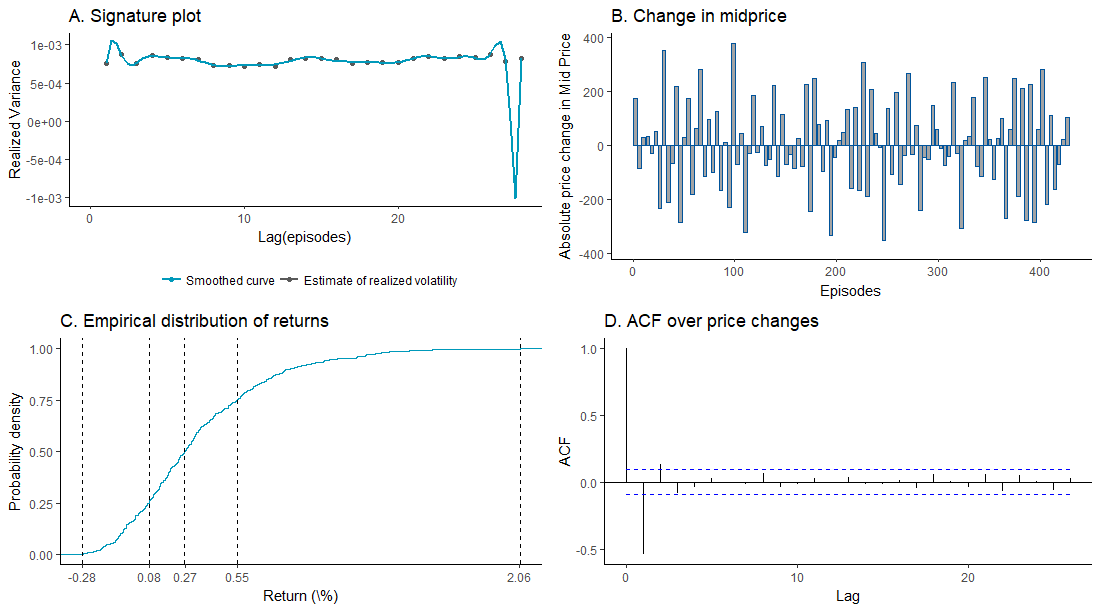
\includegraphics[scale=.5]{lobv1_sf_multi.png}
		%Captions and Labels can be used since this is a figure environment
		\caption{Some stylized facts for LOBMarket-v1. A signature plot (A), periodicity in mid prices (B), empirical distribution of returns (C) and an acf over price changes (D). }
		\label{fig:sf2}
\end{figure}


\newpage
\section{Agent's Rewards}

\subsection*{Summary of rewards}
% latex table generated in R 3.3.1 by xtable 1.8-2 package
% Fri May 18 00:04:06 2018
\begin{table}[H]
\centering
\caption{Table over rewards for DealerMarket-v1, DealerMarket-v2 and LOBMarket-v1. With mean, max, std and $95\%$ confidence interval (CI). After training for $2\cdot10^6$ steps}
\label{tab:dm1}
\begin{tabular}{rrrrrr}
  \hline
 \textbf{Model} & \textbf{Mean} & \textbf{Std} & \textbf{Max} & \textbf{Min} & \textbf{CI} \\ 
  \hline
DealerMarket-v1 & $391.88$ & $150.47$ & $478.04$ & $-9.43$ & $16.18$ \\
DealerMarket-v2 & $22.47$ & $78.46$ & $347.40$ & $-816.11$ & $2.85$  \\
LOBMarket-v1& $-5.02$ & $23.88$ & $145.46$ & $-526.77$ & $0.88$ \\ 

   \hline
\end{tabular}
\end{table}
Regarding \autoref{tab:dm1} above one can see that the accumulated reward is fairly consistent for DealerMarket-v1. Compared to the other environments, presented later. Also note that the reward schemes are somewhat different between the different environments as discussed previously. Which will obviously effect the distribution of the accumulated rewards. This environment is easier to navigate in for the agent. With less volatility and arrivals of orders. 
\newline
\newline
As can be seen from \autoref{tab:dm1} the standard deviation of the reward is quite large. This is due to the randomness associated with training reinforcement learning agents. Nevertheless calculating confidence intervals for the reward results in an average reward close to 400 ($391.81 \pm 16.18$). In \autoref{tab:dm1} for DealerMarket-v2 the agent makes on average a reward close to 22 $(22.47 \pm 2.85)$.
\newline
\newline
Note also that the reward is much smaller for this environment compared to the DealerMarket-V1 environment. Mostly likely due to higher complexity in the DealerMarket-v2 environment. With higher volatility in the underlying prices of the asset and changed reward function. Explaining the quite wide fluctuation between min and max values of the reward. Finally looking at the reward for the LOBMarket-v1 in \autoref{tab:dm1},  the mean reward is the smallest -5 ($-5.02 \pm 0.88$). As this is the hardest environment for the agent, thus making it harder for the agent to find optimal behavior.

\subsection*{Q-value function, episode reward \& loss}
\begin{figure}[H]
		%Do not try to scale figure in .tex or you loose font size consistency
	    	\centering
		%The code to input the plot is extremely simple
		% Created by tikzDevice version 0.11 on 2018-05-18 19:05:00
% !TEX encoding = UTF-8 Unicode
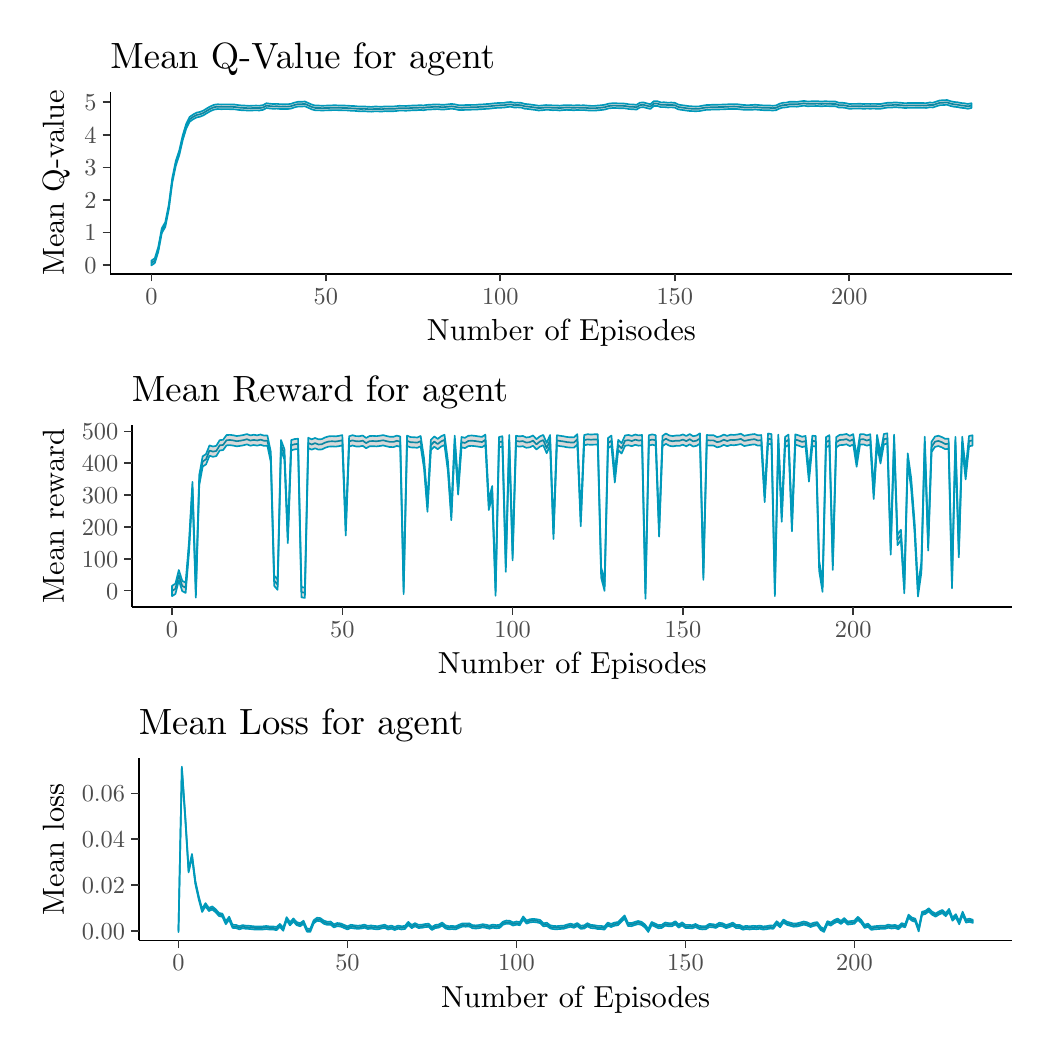
\begin{tikzpicture}[x=1pt,y=1pt]
\definecolor{fillColor}{RGB}{255,255,255}
\path[use as bounding box,fill=fillColor,fill opacity=0.00] (0,0) rectangle (361.35,361.35);
\begin{scope}
\path[clip] (  0.00,240.90) rectangle (361.35,361.35);
\definecolor{drawColor}{RGB}{255,255,255}
\definecolor{fillColor}{RGB}{255,255,255}

\path[draw=drawColor,line width= 0.6pt,line join=round,line cap=round,fill=fillColor] (  0.00,240.90) rectangle (361.35,361.35);
\end{scope}
\begin{scope}
\path[clip] ( 29.87,272.43) rectangle (355.85,338.21);
\definecolor{fillColor}{RGB}{255,255,255}

\path[fill=fillColor] ( 29.87,272.43) rectangle (355.85,338.21);
\definecolor{drawColor}{RGB}{0,153,186}

\path[draw=drawColor,line width= 0.6pt,line join=round] ( 44.69,276.29) --
	( 45.95,277.17) --
	( 47.21,281.28) --
	( 48.47,288.02) --
	( 49.73,290.20) --
	( 50.99,296.49) --
	( 52.25,306.15) --
	( 53.51,312.28) --
	( 54.77,316.08) --
	( 56.04,321.64) --
	( 57.30,325.76) --
	( 58.56,328.26) --
	( 59.82,329.13) --
	( 61.08,329.79) --
	( 62.34,330.06) --
	( 63.60,330.58) --
	( 64.86,331.38) --
	( 66.12,332.10) --
	( 67.39,332.62) --
	( 68.65,332.80) --
	( 69.91,332.75) --
	( 71.17,332.77) --
	( 72.43,332.78) --
	( 73.69,332.73) --
	( 74.95,332.68) --
	( 76.21,332.49) --
	( 77.47,332.36) --
	( 78.73,332.33) --
	( 80.00,332.23) --
	( 81.26,332.31) --
	( 82.52,332.34) --
	( 83.78,332.29) --
	( 85.04,332.51) --
	( 86.30,333.17) --
	( 87.56,333.00) --
	( 88.82,332.89) --
	( 90.08,332.95) --
	( 91.35,332.81) --
	( 92.61,332.85) --
	( 93.87,332.81) --
	( 95.13,332.96) --
	( 96.39,333.40) --
	( 97.65,333.71) --
	( 98.91,333.71) --
	(100.17,333.80) --
	(101.43,333.26) --
	(102.69,332.69) --
	(103.96,332.34) --
	(105.22,332.33) --
	(106.48,332.27) --
	(107.74,332.33) --
	(109.00,332.34) --
	(110.26,332.42) --
	(111.52,332.43) --
	(112.78,332.36) --
	(114.04,332.34) --
	(115.30,332.32) --
	(116.57,332.21) --
	(117.83,332.17) --
	(119.09,332.05) --
	(120.35,331.96) --
	(121.61,332.01) --
	(122.87,331.93) --
	(124.13,331.86) --
	(125.39,331.97) --
	(126.65,331.97) --
	(127.92,331.90) --
	(129.18,332.04) --
	(130.44,332.02) --
	(131.70,332.00) --
	(132.96,332.08) --
	(134.22,332.24) --
	(135.48,332.23) --
	(136.74,332.20) --
	(138.00,332.29) --
	(139.26,332.36) --
	(140.53,332.38) --
	(141.79,332.48) --
	(143.05,332.37) --
	(144.31,332.59) --
	(145.57,332.65) --
	(146.83,332.73) --
	(148.09,332.78) --
	(149.35,332.65) --
	(150.61,332.65) --
	(151.88,332.79) --
	(153.14,332.93) --
	(154.40,332.77) --
	(155.66,332.48) --
	(156.92,332.43) --
	(158.18,332.53) --
	(159.44,332.54) --
	(160.70,332.60) --
	(161.96,332.59) --
	(163.22,332.73) --
	(164.49,332.78) --
	(165.75,332.88) --
	(167.01,332.95) --
	(168.27,333.12) --
	(169.53,333.22) --
	(170.79,333.30) --
	(172.05,333.31) --
	(173.31,333.54) --
	(174.57,333.63) --
	(175.84,333.35) --
	(177.10,333.42) --
	(178.36,333.32) --
	(179.62,332.93) --
	(180.88,332.82) --
	(182.14,332.65) --
	(183.40,332.48) --
	(184.66,332.29) --
	(185.92,332.37) --
	(187.18,332.51) --
	(188.45,332.50) --
	(189.71,332.40) --
	(190.97,332.42) --
	(192.23,332.28) --
	(193.49,332.43) --
	(194.75,332.49) --
	(196.01,332.47) --
	(197.27,332.36) --
	(198.53,332.47) --
	(199.80,332.40) --
	(201.06,332.43) --
	(202.32,332.31) --
	(203.58,332.23) --
	(204.84,332.23) --
	(206.10,332.36) --
	(207.36,332.46) --
	(208.62,332.64) --
	(209.88,333.02) --
	(211.14,333.16) --
	(212.41,333.17) --
	(213.67,333.11) --
	(214.93,333.11) --
	(216.19,333.00) --
	(217.45,332.77) --
	(218.71,332.75) --
	(219.97,332.60) --
	(221.23,333.37) --
	(222.49,333.47) --
	(223.76,333.14) --
	(225.02,332.84) --
	(226.28,333.93) --
	(227.54,333.91) --
	(228.80,333.49) --
	(230.06,333.52) --
	(231.32,333.37) --
	(232.58,333.42) --
	(233.84,333.33) --
	(235.10,332.69) --
	(236.37,332.49) --
	(237.63,332.31) --
	(238.89,332.13) --
	(240.15,332.05) --
	(241.41,332.02) --
	(242.67,332.06) --
	(243.93,332.31) --
	(245.19,332.51) --
	(246.45,332.55) --
	(247.72,332.65) --
	(248.98,332.64) --
	(250.24,332.67) --
	(251.50,332.70) --
	(252.76,332.78) --
	(254.02,332.82) --
	(255.28,332.84) --
	(256.54,332.80) --
	(257.80,332.65) --
	(259.06,332.51) --
	(260.33,332.49) --
	(261.59,332.52) --
	(262.85,332.63) --
	(264.11,332.54) --
	(265.37,332.42) --
	(266.63,332.35) --
	(267.89,332.37) --
	(269.15,332.28) --
	(270.41,332.36) --
	(271.67,332.98) --
	(272.94,333.36) --
	(274.20,333.41) --
	(275.46,333.73) --
	(276.72,333.73) --
	(277.98,333.66) --
	(279.24,333.85) --
	(280.50,334.02) --
	(281.76,333.81) --
	(283.02,333.87) --
	(284.29,333.88) --
	(285.55,333.89) --
	(286.81,333.78) --
	(288.07,333.90) --
	(289.33,333.85) --
	(290.59,333.79) --
	(291.85,333.79) --
	(293.11,333.36) --
	(294.37,333.36) --
	(295.63,333.20) --
	(296.90,332.89) --
	(298.16,332.95) --
	(299.42,332.94) --
	(300.68,333.00) --
	(301.94,332.91) --
	(303.20,332.95) --
	(304.46,332.93) --
	(305.72,332.95) --
	(306.98,332.92) --
	(308.25,332.91) --
	(309.51,333.15) --
	(310.77,333.34) --
	(312.03,333.33) --
	(313.29,333.48) --
	(314.55,333.40) --
	(315.81,333.32) --
	(317.07,333.16) --
	(318.33,333.28) --
	(319.59,333.27) --
	(320.86,333.25) --
	(322.12,333.24) --
	(323.38,333.26) --
	(324.64,333.20) --
	(325.90,333.44) --
	(327.16,333.38) --
	(328.42,333.82) --
	(329.68,334.21) --
	(330.94,334.24) --
	(332.21,334.36) --
	(333.47,333.91) --
	(334.73,333.64) --
	(335.99,333.51) --
	(337.25,333.26) --
	(338.51,333.14) --
	(339.77,332.91) --
	(341.03,333.19);
\definecolor{fillColor}{RGB}{66,66,66}

\path[draw=drawColor,line width= 0.6pt,line join=round,line cap=round,fill=fillColor,fill opacity=0.20] ( 44.69,277.15) --
	( 45.95,278.04) --
	( 47.21,282.14) --
	( 48.47,288.89) --
	( 49.73,291.06) --
	( 50.99,297.35) --
	( 52.25,307.02) --
	( 53.51,313.14) --
	( 54.77,316.95) --
	( 56.04,322.50) --
	( 57.30,326.62) --
	( 58.56,329.12) --
	( 59.82,329.99) --
	( 61.08,330.66) --
	( 62.34,330.92) --
	( 63.60,331.45) --
	( 64.86,332.25) --
	( 66.12,332.96) --
	( 67.39,333.49) --
	( 68.65,333.66) --
	( 69.91,333.61) --
	( 71.17,333.63) --
	( 72.43,333.64) --
	( 73.69,333.60) --
	( 74.95,333.55) --
	( 76.21,333.36) --
	( 77.47,333.22) --
	( 78.73,333.19) --
	( 80.00,333.09) --
	( 81.26,333.17) --
	( 82.52,333.20) --
	( 83.78,333.16) --
	( 85.04,333.37) --
	( 86.30,334.04) --
	( 87.56,333.86) --
	( 88.82,333.75) --
	( 90.08,333.82) --
	( 91.35,333.67) --
	( 92.61,333.72) --
	( 93.87,333.67) --
	( 95.13,333.83) --
	( 96.39,334.26) --
	( 97.65,334.57) --
	( 98.91,334.58) --
	(100.17,334.66) --
	(101.43,334.12) --
	(102.69,333.55) --
	(103.96,333.20) --
	(105.22,333.20) --
	(106.48,333.14) --
	(107.74,333.19) --
	(109.00,333.21) --
	(110.26,333.29) --
	(111.52,333.29) --
	(112.78,333.22) --
	(114.04,333.20) --
	(115.30,333.19) --
	(116.57,333.08) --
	(117.83,333.04) --
	(119.09,332.92) --
	(120.35,332.83) --
	(121.61,332.87) --
	(122.87,332.79) --
	(124.13,332.72) --
	(125.39,332.84) --
	(126.65,332.83) --
	(127.92,332.76) --
	(129.18,332.91) --
	(130.44,332.89) --
	(131.70,332.87) --
	(132.96,332.94) --
	(134.22,333.11) --
	(135.48,333.09) --
	(136.74,333.06) --
	(138.00,333.15) --
	(139.26,333.22) --
	(140.53,333.24) --
	(141.79,333.35) --
	(143.05,333.24) --
	(144.31,333.45) --
	(145.57,333.51) --
	(146.83,333.59) --
	(148.09,333.64) --
	(149.35,333.51) --
	(150.61,333.51) --
	(151.88,333.65) --
	(153.14,333.79) --
	(154.40,333.64) --
	(155.66,333.35) --
	(156.92,333.29) --
	(158.18,333.39) --
	(159.44,333.40) --
	(160.70,333.46) --
	(161.96,333.45) --
	(163.22,333.59) --
	(164.49,333.64) --
	(165.75,333.74) --
	(167.01,333.82) --
	(168.27,333.98) --
	(169.53,334.09) --
	(170.79,334.16) --
	(172.05,334.17) --
	(173.31,334.40) --
	(174.57,334.49) --
	(175.84,334.21) --
	(177.10,334.28) --
	(178.36,334.18) --
	(179.62,333.79) --
	(180.88,333.68) --
	(182.14,333.51) --
	(183.40,333.34) --
	(184.66,333.15) --
	(185.92,333.23) --
	(187.18,333.38) --
	(188.45,333.36) --
	(189.71,333.26) --
	(190.97,333.28) --
	(192.23,333.15) --
	(193.49,333.29) --
	(194.75,333.35) --
	(196.01,333.34) --
	(197.27,333.23) --
	(198.53,333.33) --
	(199.80,333.27) --
	(201.06,333.30) --
	(202.32,333.18) --
	(203.58,333.09) --
	(204.84,333.10) --
	(206.10,333.22) --
	(207.36,333.33) --
	(208.62,333.51) --
	(209.88,333.88) --
	(211.14,334.02) --
	(212.41,334.03) --
	(213.67,333.98) --
	(214.93,333.98) --
	(216.19,333.86) --
	(217.45,333.63) --
	(218.71,333.61) --
	(219.97,333.46) --
	(221.23,334.24) --
	(222.49,334.33) --
	(223.76,334.00) --
	(225.02,333.70) --
	(226.28,334.80) --
	(227.54,334.78) --
	(228.80,334.35) --
	(230.06,334.38) --
	(231.32,334.24) --
	(232.58,334.29) --
	(233.84,334.19) --
	(235.10,333.56) --
	(236.37,333.35) --
	(237.63,333.18) --
	(238.89,333.00) --
	(240.15,332.92) --
	(241.41,332.88) --
	(242.67,332.92) --
	(243.93,333.17) --
	(245.19,333.38) --
	(246.45,333.42) --
	(247.72,333.51) --
	(248.98,333.51) --
	(250.24,333.54) --
	(251.50,333.57) --
	(252.76,333.64) --
	(254.02,333.69) --
	(255.28,333.71) --
	(256.54,333.66) --
	(257.80,333.51) --
	(259.06,333.38) --
	(260.33,333.36) --
	(261.59,333.39) --
	(262.85,333.50) --
	(264.11,333.40) --
	(265.37,333.29) --
	(266.63,333.21) --
	(267.89,333.23) --
	(269.15,333.15) --
	(270.41,333.22) --
	(271.67,333.85) --
	(272.94,334.23) --
	(274.20,334.28) --
	(275.46,334.60) --
	(276.72,334.59) --
	(277.98,334.52) --
	(279.24,334.72) --
	(280.50,334.88) --
	(281.76,334.67) --
	(283.02,334.73) --
	(284.29,334.74) --
	(285.55,334.76) --
	(286.81,334.64) --
	(288.07,334.76) --
	(289.33,334.71) --
	(290.59,334.65) --
	(291.85,334.66) --
	(293.11,334.23) --
	(294.37,334.22) --
	(295.63,334.06) --
	(296.90,333.76) --
	(298.16,333.82) --
	(299.42,333.81) --
	(300.68,333.86) --
	(301.94,333.77) --
	(303.20,333.82) --
	(304.46,333.79) --
	(305.72,333.81) --
	(306.98,333.79) --
	(308.25,333.78) --
	(309.51,334.02) --
	(310.77,334.21) --
	(312.03,334.19) --
	(313.29,334.35) --
	(314.55,334.26) --
	(315.81,334.18) --
	(317.07,334.02) --
	(318.33,334.15) --
	(319.59,334.13) --
	(320.86,334.11) --
	(322.12,334.10) --
	(323.38,334.12) --
	(324.64,334.07) --
	(325.90,334.30) --
	(327.16,334.24) --
	(328.42,334.68) --
	(329.68,335.08) --
	(330.94,335.11) --
	(332.21,335.22) --
	(333.47,334.77) --
	(334.73,334.51) --
	(335.99,334.38) --
	(337.25,334.13) --
	(338.51,334.01) --
	(339.77,333.78) --
	(341.03,334.05) --
	(341.03,332.32) --
	(339.77,332.05) --
	(338.51,332.28) --
	(337.25,332.40) --
	(335.99,332.65) --
	(334.73,332.78) --
	(333.47,333.05) --
	(332.21,333.50) --
	(330.94,333.38) --
	(329.68,333.35) --
	(328.42,332.96) --
	(327.16,332.52) --
	(325.90,332.57) --
	(324.64,332.34) --
	(323.38,332.39) --
	(322.12,332.37) --
	(320.86,332.38) --
	(319.59,332.40) --
	(318.33,332.42) --
	(317.07,332.29) --
	(315.81,332.45) --
	(314.55,332.53) --
	(313.29,332.62) --
	(312.03,332.46) --
	(310.77,332.48) --
	(309.51,332.29) --
	(308.25,332.05) --
	(306.98,332.06) --
	(305.72,332.09) --
	(304.46,332.07) --
	(303.20,332.09) --
	(301.94,332.04) --
	(300.68,332.13) --
	(299.42,332.08) --
	(298.16,332.09) --
	(296.90,332.03) --
	(295.63,332.33) --
	(294.37,332.49) --
	(293.11,332.50) --
	(291.85,332.93) --
	(290.59,332.93) --
	(289.33,332.99) --
	(288.07,333.03) --
	(286.81,332.91) --
	(285.55,333.03) --
	(284.29,333.01) --
	(283.02,333.00) --
	(281.76,332.95) --
	(280.50,333.15) --
	(279.24,332.99) --
	(277.98,332.79) --
	(276.72,332.86) --
	(275.46,332.87) --
	(274.20,332.55) --
	(272.94,332.50) --
	(271.67,332.12) --
	(270.41,331.50) --
	(269.15,331.42) --
	(267.89,331.50) --
	(266.63,331.49) --
	(265.37,331.56) --
	(264.11,331.67) --
	(262.85,331.77) --
	(261.59,331.66) --
	(260.33,331.63) --
	(259.06,331.65) --
	(257.80,331.79) --
	(256.54,331.93) --
	(255.28,331.98) --
	(254.02,331.96) --
	(252.76,331.92) --
	(251.50,331.84) --
	(250.24,331.81) --
	(248.98,331.78) --
	(247.72,331.78) --
	(246.45,331.69) --
	(245.19,331.65) --
	(243.93,331.44) --
	(242.67,331.20) --
	(241.41,331.16) --
	(240.15,331.19) --
	(238.89,331.27) --
	(237.63,331.45) --
	(236.37,331.63) --
	(235.10,331.83) --
	(233.84,332.46) --
	(232.58,332.56) --
	(231.32,332.51) --
	(230.06,332.65) --
	(228.80,332.62) --
	(227.54,333.05) --
	(226.28,333.07) --
	(225.02,331.98) --
	(223.76,332.28) --
	(222.49,332.60) --
	(221.23,332.51) --
	(219.97,331.73) --
	(218.71,331.89) --
	(217.45,331.90) --
	(216.19,332.14) --
	(214.93,332.25) --
	(213.67,332.25) --
	(212.41,332.30) --
	(211.14,332.29) --
	(209.88,332.15) --
	(208.62,331.78) --
	(207.36,331.60) --
	(206.10,331.49) --
	(204.84,331.37) --
	(203.58,331.37) --
	(202.32,331.45) --
	(201.06,331.57) --
	(199.80,331.54) --
	(198.53,331.60) --
	(197.27,331.50) --
	(196.01,331.61) --
	(194.75,331.63) --
	(193.49,331.56) --
	(192.23,331.42) --
	(190.97,331.55) --
	(189.71,331.53) --
	(188.45,331.63) --
	(187.18,331.65) --
	(185.92,331.51) --
	(184.66,331.42) --
	(183.40,331.62) --
	(182.14,331.78) --
	(180.88,331.95) --
	(179.62,332.06) --
	(178.36,332.45) --
	(177.10,332.55) --
	(175.84,332.48) --
	(174.57,332.77) --
	(173.31,332.67) --
	(172.05,332.45) --
	(170.79,332.43) --
	(169.53,332.36) --
	(168.27,332.25) --
	(167.01,332.09) --
	(165.75,332.01) --
	(164.49,331.91) --
	(163.22,331.86) --
	(161.96,331.72) --
	(160.70,331.73) --
	(159.44,331.68) --
	(158.18,331.66) --
	(156.92,331.56) --
	(155.66,331.62) --
	(154.40,331.91) --
	(153.14,332.06) --
	(151.88,331.93) --
	(150.61,331.79) --
	(149.35,331.78) --
	(148.09,331.92) --
	(146.83,331.86) --
	(145.57,331.78) --
	(144.31,331.73) --
	(143.05,331.51) --
	(141.79,331.62) --
	(140.53,331.51) --
	(139.26,331.50) --
	(138.00,331.42) --
	(136.74,331.34) --
	(135.48,331.37) --
	(134.22,331.38) --
	(132.96,331.21) --
	(131.70,331.14) --
	(130.44,331.16) --
	(129.18,331.18) --
	(127.92,331.03) --
	(126.65,331.10) --
	(125.39,331.11) --
	(124.13,330.99) --
	(122.87,331.06) --
	(121.61,331.15) --
	(120.35,331.10) --
	(119.09,331.19) --
	(117.83,331.31) --
	(116.57,331.35) --
	(115.30,331.46) --
	(114.04,331.47) --
	(112.78,331.49) --
	(111.52,331.56) --
	(110.26,331.56) --
	(109.00,331.48) --
	(107.74,331.47) --
	(106.48,331.41) --
	(105.22,331.47) --
	(103.96,331.47) --
	(102.69,331.82) --
	(101.43,332.39) --
	(100.17,332.93) --
	( 98.91,332.85) --
	( 97.65,332.84) --
	( 96.39,332.54) --
	( 95.13,332.10) --
	( 93.87,331.94) --
	( 92.61,331.99) --
	( 91.35,331.94) --
	( 90.08,332.09) --
	( 88.82,332.03) --
	( 87.56,332.13) --
	( 86.30,332.31) --
	( 85.04,331.64) --
	( 83.78,331.43) --
	( 82.52,331.47) --
	( 81.26,331.44) --
	( 80.00,331.36) --
	( 78.73,331.46) --
	( 77.47,331.50) --
	( 76.21,331.63) --
	( 74.95,331.82) --
	( 73.69,331.87) --
	( 72.43,331.91) --
	( 71.17,331.91) --
	( 69.91,331.89) --
	( 68.65,331.94) --
	( 67.39,331.76) --
	( 66.12,331.23) --
	( 64.86,330.52) --
	( 63.60,329.72) --
	( 62.34,329.19) --
	( 61.08,328.93) --
	( 59.82,328.26) --
	( 58.56,327.39) --
	( 57.30,324.90) --
	( 56.04,320.77) --
	( 54.77,315.22) --
	( 53.51,311.41) --
	( 52.25,305.29) --
	( 50.99,295.62) --
	( 49.73,289.34) --
	( 48.47,287.16) --
	( 47.21,280.42) --
	( 45.95,276.31) --
	( 44.69,275.42) --
	cycle;
\end{scope}
\begin{scope}
\path[clip] (  0.00,  0.00) rectangle (361.35,361.35);
\definecolor{drawColor}{RGB}{0,0,0}

\path[draw=drawColor,line width= 0.6pt,line join=round] ( 29.87,272.43) --
	( 29.87,338.21);
\end{scope}
\begin{scope}
\path[clip] (  0.00,  0.00) rectangle (361.35,361.35);
\definecolor{drawColor}{gray}{0.30}

\node[text=drawColor,anchor=base east,inner sep=0pt, outer sep=0pt, scale=  0.88] at ( 24.92,272.52) {0};

\node[text=drawColor,anchor=base east,inner sep=0pt, outer sep=0pt, scale=  0.88] at ( 24.92,284.29) {1};

\node[text=drawColor,anchor=base east,inner sep=0pt, outer sep=0pt, scale=  0.88] at ( 24.92,296.07) {2};

\node[text=drawColor,anchor=base east,inner sep=0pt, outer sep=0pt, scale=  0.88] at ( 24.92,307.84) {3};

\node[text=drawColor,anchor=base east,inner sep=0pt, outer sep=0pt, scale=  0.88] at ( 24.92,319.62) {4};

\node[text=drawColor,anchor=base east,inner sep=0pt, outer sep=0pt, scale=  0.88] at ( 24.92,331.39) {5};
\end{scope}
\begin{scope}
\path[clip] (  0.00,  0.00) rectangle (361.35,361.35);
\definecolor{drawColor}{gray}{0.20}

\path[draw=drawColor,line width= 0.6pt,line join=round] ( 27.12,275.55) --
	( 29.87,275.55);

\path[draw=drawColor,line width= 0.6pt,line join=round] ( 27.12,287.32) --
	( 29.87,287.32);

\path[draw=drawColor,line width= 0.6pt,line join=round] ( 27.12,299.10) --
	( 29.87,299.10);

\path[draw=drawColor,line width= 0.6pt,line join=round] ( 27.12,310.87) --
	( 29.87,310.87);

\path[draw=drawColor,line width= 0.6pt,line join=round] ( 27.12,322.65) --
	( 29.87,322.65);

\path[draw=drawColor,line width= 0.6pt,line join=round] ( 27.12,334.42) --
	( 29.87,334.42);
\end{scope}
\begin{scope}
\path[clip] (  0.00,  0.00) rectangle (361.35,361.35);
\definecolor{drawColor}{RGB}{0,0,0}

\path[draw=drawColor,line width= 0.6pt,line join=round] ( 29.87,272.43) --
	(355.85,272.43);
\end{scope}
\begin{scope}
\path[clip] (  0.00,  0.00) rectangle (361.35,361.35);
\definecolor{drawColor}{gray}{0.20}

\path[draw=drawColor,line width= 0.6pt,line join=round] ( 44.69,269.68) --
	( 44.69,272.43);

\path[draw=drawColor,line width= 0.6pt,line join=round] (107.74,269.68) --
	(107.74,272.43);

\path[draw=drawColor,line width= 0.6pt,line join=round] (170.79,269.68) --
	(170.79,272.43);

\path[draw=drawColor,line width= 0.6pt,line join=round] (233.84,269.68) --
	(233.84,272.43);

\path[draw=drawColor,line width= 0.6pt,line join=round] (296.90,269.68) --
	(296.90,272.43);
\end{scope}
\begin{scope}
\path[clip] (  0.00,  0.00) rectangle (361.35,361.35);
\definecolor{drawColor}{gray}{0.30}

\node[text=drawColor,anchor=base,inner sep=0pt, outer sep=0pt, scale=  0.88] at ( 44.69,261.42) {0};

\node[text=drawColor,anchor=base,inner sep=0pt, outer sep=0pt, scale=  0.88] at (107.74,261.42) {50};

\node[text=drawColor,anchor=base,inner sep=0pt, outer sep=0pt, scale=  0.88] at (170.79,261.42) {100};

\node[text=drawColor,anchor=base,inner sep=0pt, outer sep=0pt, scale=  0.88] at (233.84,261.42) {150};

\node[text=drawColor,anchor=base,inner sep=0pt, outer sep=0pt, scale=  0.88] at (296.90,261.42) {200};
\end{scope}
\begin{scope}
\path[clip] (  0.00,  0.00) rectangle (361.35,361.35);
\definecolor{drawColor}{RGB}{0,0,0}

\node[text=drawColor,anchor=base,inner sep=0pt, outer sep=0pt, scale=  1.10] at (192.86,248.34) {Number of Episodes};
\end{scope}
\begin{scope}
\path[clip] (  0.00,  0.00) rectangle (361.35,361.35);
\definecolor{drawColor}{RGB}{0,0,0}

\node[text=drawColor,rotate= 90.00,anchor=base,inner sep=0pt, outer sep=0pt, scale=  1.10] at ( 13.08,305.32) {Mean Q-value};
\end{scope}
\begin{scope}
\path[clip] (  0.00,  0.00) rectangle (361.35,361.35);
\definecolor{drawColor}{RGB}{0,0,0}

\node[text=drawColor,anchor=base west,inner sep=0pt, outer sep=0pt, scale=  1.32] at ( 29.87,346.76) {Mean Q-Value for agent};
\end{scope}
\begin{scope}
\path[clip] (  0.00,120.45) rectangle (361.35,240.90);
\definecolor{drawColor}{RGB}{255,255,255}
\definecolor{fillColor}{RGB}{255,255,255}

\path[draw=drawColor,line width= 0.6pt,line join=round,line cap=round,fill=fillColor] (  0.00,120.45) rectangle (361.35,240.90);
\end{scope}
\begin{scope}
\path[clip] ( 37.69,151.98) rectangle (355.85,217.76);
\definecolor{fillColor}{RGB}{255,255,255}

\path[fill=fillColor] ( 37.69,151.98) rectangle (355.85,217.76);
\definecolor{drawColor}{RGB}{0,153,186}

\path[draw=drawColor,line width= 0.6pt,line join=round] ( 52.16,157.80) --
	( 53.39,158.58) --
	( 54.62,163.50) --
	( 55.85,159.60) --
	( 57.08,158.96) --
	( 58.31,173.86) --
	( 59.54,195.37) --
	( 60.77,157.22) --
	( 62.00,197.86) --
	( 63.23,204.59) --
	( 64.46,205.41) --
	( 65.69,208.54) --
	( 66.93,208.15) --
	( 68.16,208.40) --
	( 69.39,210.43) --
	( 70.62,210.57) --
	( 71.85,212.27) --
	( 73.08,212.36) --
	( 74.31,212.20) --
	( 75.54,211.92) --
	( 76.77,212.09) --
	( 78.00,212.30) --
	( 79.23,212.64) --
	( 80.46,212.15) --
	( 81.69,212.39) --
	( 82.93,212.18) --
	( 84.16,212.48) --
	( 85.39,212.08) --
	( 86.62,212.13) --
	( 87.85,206.26) --
	( 89.08,161.51) --
	( 90.31,160.08) --
	( 91.54,210.48) --
	( 92.77,207.17) --
	( 94.00,176.92) --
	( 95.23,210.46) --
	( 96.46,210.83) --
	( 97.70,210.96) --
	( 98.93,157.35) --
	(100.16,157.16) --
	(101.39,211.32) --
	(102.62,210.72) --
	(103.85,211.22) --
	(105.08,210.73) --
	(106.31,210.82) --
	(107.54,211.44) --
	(108.77,211.81) --
	(110.00,211.90) --
	(111.23,211.81) --
	(112.46,211.98) --
	(113.70,212.26) --
	(114.93,179.68) --
	(116.16,211.84) --
	(117.39,212.22) --
	(118.62,211.90) --
	(119.85,211.86) --
	(121.08,212.10) --
	(122.31,211.24) --
	(123.54,211.93) --
	(124.77,211.98) --
	(126.00,211.89) --
	(127.23,212.04) --
	(128.46,212.25) --
	(129.70,211.92) --
	(130.93,211.66) --
	(132.16,211.66) --
	(133.39,212.07) --
	(134.62,211.77) --
	(135.85,158.47) --
	(137.08,212.07) --
	(138.31,211.56) --
	(139.54,211.50) --
	(140.77,211.40) --
	(142.00,211.94) --
	(143.23,203.89) --
	(144.46,188.27) --
	(145.70,210.53) --
	(146.93,211.79) --
	(148.16,210.89) --
	(149.39,211.84) --
	(150.62,212.39) --
	(151.85,202.93) --
	(153.08,185.23) --
	(154.31,212.08) --
	(155.54,194.45) --
	(156.77,211.58) --
	(158.00,211.28) --
	(159.23,212.01) --
	(160.46,212.10) --
	(161.70,211.98) --
	(162.93,211.79) --
	(164.16,211.62) --
	(165.39,212.43) --
	(166.62,188.88) --
	(167.85,193.85) --
	(169.08,157.93) --
	(170.31,211.57) --
	(171.54,211.85) --
	(172.77,166.56) --
	(174.00,212.33) --
	(175.23,170.74) --
	(176.46,212.02) --
	(177.70,211.81) --
	(178.93,211.97) --
	(180.16,211.40) --
	(181.39,211.56) --
	(182.62,212.12) --
	(183.85,210.79) --
	(185.08,211.80) --
	(186.31,212.32) --
	(187.54,209.43) --
	(188.77,212.31) --
	(190.00,178.45) --
	(191.23,212.20) --
	(192.46,211.99) --
	(193.70,211.83) --
	(194.93,211.58) --
	(196.16,211.47) --
	(197.39,211.45) --
	(198.62,212.61) --
	(199.85,183.04) --
	(201.08,212.28) --
	(202.31,212.58) --
	(203.54,212.46) --
	(204.77,212.55) --
	(206.00,212.57) --
	(207.23,164.46) --
	(208.46,159.68) --
	(209.70,211.22) --
	(210.93,212.10) --
	(212.16,198.86) --
	(213.39,210.54) --
	(214.62,209.34) --
	(215.85,212.12) --
	(217.08,212.32) --
	(218.31,211.97) --
	(219.54,212.47) --
	(220.77,212.15) --
	(222.00,212.31) --
	(223.23,156.83) --
	(224.46,212.21) --
	(225.70,212.51) --
	(226.93,212.23) --
	(228.16,179.29) --
	(229.39,211.99) --
	(230.62,212.82) --
	(231.85,212.14) --
	(233.08,211.91) --
	(234.31,212.11) --
	(235.54,212.09) --
	(236.77,212.51) --
	(238.00,211.94) --
	(239.23,212.64) --
	(240.46,211.86) --
	(241.70,212.11) --
	(242.93,212.91) --
	(244.16,163.66) --
	(245.39,212.30) --
	(246.62,212.20) --
	(247.85,212.22) --
	(249.08,211.57) --
	(250.31,211.82) --
	(251.54,212.45) --
	(252.77,211.98) --
	(254.00,212.41) --
	(255.23,212.32) --
	(256.46,212.48) --
	(257.70,212.75) --
	(258.93,212.02) --
	(260.16,212.27) --
	(261.39,212.49) --
	(262.62,212.65) --
	(263.85,212.18) --
	(265.08,212.28) --
	(266.31,191.78) --
	(267.54,212.83) --
	(268.77,212.62) --
	(270.00,157.76) --
	(271.23,212.43) --
	(272.47,184.66) --
	(273.70,211.64) --
	(274.93,212.43) --
	(276.16,181.21) --
	(277.39,212.52) --
	(278.62,212.15) --
	(279.85,211.66) --
	(281.08,211.97) --
	(282.31,199.18) --
	(283.54,212.03) --
	(284.77,211.92) --
	(286.00,166.92) --
	(287.23,159.32) --
	(288.47,211.53) --
	(289.70,212.22) --
	(290.93,167.25) --
	(292.16,211.52) --
	(293.39,212.35) --
	(294.62,212.42) --
	(295.85,212.67) --
	(297.08,212.02) --
	(298.31,212.60) --
	(299.54,204.55) --
	(300.77,212.56) --
	(302.00,212.63) --
	(303.23,212.16) --
	(304.47,212.57) --
	(305.70,192.88) --
	(306.93,212.33) --
	(308.16,205.74) --
	(309.39,212.64) --
	(310.62,212.91) --
	(311.85,172.77) --
	(313.08,212.43) --
	(314.31,176.22) --
	(315.54,178.07) --
	(316.77,158.82) --
	(318.00,205.66) --
	(319.23,196.90) --
	(320.47,180.96) --
	(321.70,157.64) --
	(322.93,166.31) --
	(324.16,211.70) --
	(325.39,174.25) --
	(326.62,209.86) --
	(327.85,211.73) --
	(329.08,212.03) --
	(330.31,211.57) --
	(331.54,210.91) --
	(332.77,210.97) --
	(334.00,160.60) --
	(335.23,211.67) --
	(336.47,171.79) --
	(337.70,211.67) --
	(338.93,199.96) --
	(340.16,211.95) --
	(341.39,212.19);
\definecolor{fillColor}{RGB}{66,66,66}

\path[draw=drawColor,line width= 0.6pt,line join=round,line cap=round,fill=fillColor,fill opacity=0.20] ( 52.16,159.66) --
	( 53.39,160.44) --
	( 54.62,165.37) --
	( 55.85,161.46) --
	( 57.08,160.82) --
	( 58.31,175.72) --
	( 59.54,197.23) --
	( 60.77,159.08) --
	( 62.00,199.72) --
	( 63.23,206.45) --
	( 64.46,207.27) --
	( 65.69,210.40) --
	( 66.93,210.01) --
	( 68.16,210.26) --
	( 69.39,212.29) --
	( 70.62,212.43) --
	( 71.85,214.13) --
	( 73.08,214.22) --
	( 74.31,214.06) --
	( 75.54,213.78) --
	( 76.77,213.95) --
	( 78.00,214.16) --
	( 79.23,214.50) --
	( 80.46,214.01) --
	( 81.69,214.25) --
	( 82.93,214.04) --
	( 84.16,214.34) --
	( 85.39,213.94) --
	( 86.62,213.99) --
	( 87.85,208.12) --
	( 89.08,163.37) --
	( 90.31,161.94) --
	( 91.54,212.34) --
	( 92.77,209.03) --
	( 94.00,178.78) --
	( 95.23,212.32) --
	( 96.46,212.69) --
	( 97.70,212.82) --
	( 98.93,159.21) --
	(100.16,159.02) --
	(101.39,213.18) --
	(102.62,212.58) --
	(103.85,213.08) --
	(105.08,212.59) --
	(106.31,212.68) --
	(107.54,213.30) --
	(108.77,213.67) --
	(110.00,213.76) --
	(111.23,213.67) --
	(112.46,213.84) --
	(113.70,214.12) --
	(114.93,181.54) --
	(116.16,213.71) --
	(117.39,214.08) --
	(118.62,213.76) --
	(119.85,213.72) --
	(121.08,213.96) --
	(122.31,213.10) --
	(123.54,213.79) --
	(124.77,213.84) --
	(126.00,213.75) --
	(127.23,213.90) --
	(128.46,214.11) --
	(129.70,213.78) --
	(130.93,213.52) --
	(132.16,213.52) --
	(133.39,213.93) --
	(134.62,213.63) --
	(135.85,160.33) --
	(137.08,213.93) --
	(138.31,213.42) --
	(139.54,213.36) --
	(140.77,213.26) --
	(142.00,213.80) --
	(143.23,205.75) --
	(144.46,190.13) --
	(145.70,212.39) --
	(146.93,213.65) --
	(148.16,212.75) --
	(149.39,213.70) --
	(150.62,214.25) --
	(151.85,204.79) --
	(153.08,187.09) --
	(154.31,213.94) --
	(155.54,196.31) --
	(156.77,213.44) --
	(158.00,213.14) --
	(159.23,213.88) --
	(160.46,213.97) --
	(161.70,213.84) --
	(162.93,213.65) --
	(164.16,213.48) --
	(165.39,214.29) --
	(166.62,190.74) --
	(167.85,195.71) --
	(169.08,159.79) --
	(170.31,213.43) --
	(171.54,213.71) --
	(172.77,168.42) --
	(174.00,214.19) --
	(175.23,172.60) --
	(176.46,213.88) --
	(177.70,213.67) --
	(178.93,213.83) --
	(180.16,213.26) --
	(181.39,213.43) --
	(182.62,213.99) --
	(183.85,212.65) --
	(185.08,213.66) --
	(186.31,214.18) --
	(187.54,211.29) --
	(188.77,214.17) --
	(190.00,180.31) --
	(191.23,214.06) --
	(192.46,213.86) --
	(193.70,213.69) --
	(194.93,213.44) --
	(196.16,213.33) --
	(197.39,213.31) --
	(198.62,214.47) --
	(199.85,184.90) --
	(201.08,214.14) --
	(202.31,214.44) --
	(203.54,214.33) --
	(204.77,214.41) --
	(206.00,214.43) --
	(207.23,166.33) --
	(208.46,161.54) --
	(209.70,213.08) --
	(210.93,213.96) --
	(212.16,200.72) --
	(213.39,212.40) --
	(214.62,211.20) --
	(215.85,213.98) --
	(217.08,214.18) --
	(218.31,213.83) --
	(219.54,214.33) --
	(220.77,214.01) --
	(222.00,214.17) --
	(223.23,158.69) --
	(224.46,214.08) --
	(225.70,214.37) --
	(226.93,214.09) --
	(228.16,181.15) --
	(229.39,213.85) --
	(230.62,214.69) --
	(231.85,214.00) --
	(233.08,213.77) --
	(234.31,213.97) --
	(235.54,213.95) --
	(236.77,214.37) --
	(238.00,213.80) --
	(239.23,214.50) --
	(240.46,213.72) --
	(241.70,213.97) --
	(242.93,214.77) --
	(244.16,165.52) --
	(245.39,214.16) --
	(246.62,214.06) --
	(247.85,214.08) --
	(249.08,213.43) --
	(250.31,213.68) --
	(251.54,214.32) --
	(252.77,213.84) --
	(254.00,214.27) --
	(255.23,214.18) --
	(256.46,214.34) --
	(257.70,214.61) --
	(258.93,213.88) --
	(260.16,214.13) --
	(261.39,214.35) --
	(262.62,214.51) --
	(263.85,214.04) --
	(265.08,214.14) --
	(266.31,193.64) --
	(267.54,214.69) --
	(268.77,214.48) --
	(270.00,159.62) --
	(271.23,214.30) --
	(272.47,186.52) --
	(273.70,213.50) --
	(274.93,214.29) --
	(276.16,183.07) --
	(277.39,214.38) --
	(278.62,214.01) --
	(279.85,213.53) --
	(281.08,213.83) --
	(282.31,201.04) --
	(283.54,213.90) --
	(284.77,213.78) --
	(286.00,168.78) --
	(287.23,161.18) --
	(288.47,213.39) --
	(289.70,214.08) --
	(290.93,169.11) --
	(292.16,213.38) --
	(293.39,214.21) --
	(294.62,214.28) --
	(295.85,214.53) --
	(297.08,213.88) --
	(298.31,214.46) --
	(299.54,206.41) --
	(300.77,214.42) --
	(302.00,214.49) --
	(303.23,214.02) --
	(304.47,214.43) --
	(305.70,194.74) --
	(306.93,214.19) --
	(308.16,207.60) --
	(309.39,214.50) --
	(310.62,214.77) --
	(311.85,174.63) --
	(313.08,214.29) --
	(314.31,178.08) --
	(315.54,179.93) --
	(316.77,160.68) --
	(318.00,207.52) --
	(319.23,198.76) --
	(320.47,182.82) --
	(321.70,159.50) --
	(322.93,168.17) --
	(324.16,213.56) --
	(325.39,176.11) --
	(326.62,211.72) --
	(327.85,213.59) --
	(329.08,213.89) --
	(330.31,213.43) --
	(331.54,212.78) --
	(332.77,212.83) --
	(334.00,162.46) --
	(335.23,213.53) --
	(336.47,173.65) --
	(337.70,213.54) --
	(338.93,201.82) --
	(340.16,213.81) --
	(341.39,214.05) --
	(341.39,210.32) --
	(340.16,210.09) --
	(338.93,198.10) --
	(337.70,209.81) --
	(336.47,169.93) --
	(335.23,209.81) --
	(334.00,158.74) --
	(332.77,209.11) --
	(331.54,209.05) --
	(330.31,209.71) --
	(329.08,210.17) --
	(327.85,209.87) --
	(326.62,208.00) --
	(325.39,172.39) --
	(324.16,209.84) --
	(322.93,164.45) --
	(321.70,155.78) --
	(320.47,179.10) --
	(319.23,195.04) --
	(318.00,203.79) --
	(316.77,156.95) --
	(315.54,176.21) --
	(314.31,174.36) --
	(313.08,210.57) --
	(311.85,170.91) --
	(310.62,211.05) --
	(309.39,210.78) --
	(308.16,203.88) --
	(306.93,210.46) --
	(305.70,191.02) --
	(304.47,210.71) --
	(303.23,210.30) --
	(302.00,210.77) --
	(300.77,210.70) --
	(299.54,202.68) --
	(298.31,210.74) --
	(297.08,210.16) --
	(295.85,210.81) --
	(294.62,210.56) --
	(293.39,210.49) --
	(292.16,209.66) --
	(290.93,165.39) --
	(289.70,210.36) --
	(288.47,209.66) --
	(287.23,157.46) --
	(286.00,165.06) --
	(284.77,210.06) --
	(283.54,210.17) --
	(282.31,197.32) --
	(281.08,210.11) --
	(279.85,209.80) --
	(278.62,210.29) --
	(277.39,210.66) --
	(276.16,179.35) --
	(274.93,210.57) --
	(273.70,209.78) --
	(272.47,182.80) --
	(271.23,210.57) --
	(270.00,155.90) --
	(268.77,210.76) --
	(267.54,210.97) --
	(266.31,189.91) --
	(265.08,210.42) --
	(263.85,210.31) --
	(262.62,210.79) --
	(261.39,210.63) --
	(260.16,210.41) --
	(258.93,210.16) --
	(257.70,210.89) --
	(256.46,210.62) --
	(255.23,210.46) --
	(254.00,210.54) --
	(252.77,210.12) --
	(251.54,210.59) --
	(250.31,209.96) --
	(249.08,209.71) --
	(247.85,210.35) --
	(246.62,210.34) --
	(245.39,210.44) --
	(244.16,161.80) --
	(242.93,211.05) --
	(241.70,210.25) --
	(240.46,210.00) --
	(239.23,210.78) --
	(238.00,210.08) --
	(236.77,210.65) --
	(235.54,210.23) --
	(234.31,210.25) --
	(233.08,210.05) --
	(231.85,210.28) --
	(230.62,210.96) --
	(229.39,210.13) --
	(228.16,177.43) --
	(226.93,210.37) --
	(225.70,210.65) --
	(224.46,210.35) --
	(223.23,154.97) --
	(222.00,210.45) --
	(220.77,210.29) --
	(219.54,210.61) --
	(218.31,210.11) --
	(217.08,210.46) --
	(215.85,210.26) --
	(214.62,207.48) --
	(213.39,208.68) --
	(212.16,196.99) --
	(210.93,210.24) --
	(209.70,209.36) --
	(208.46,157.82) --
	(207.23,162.60) --
	(206.00,210.71) --
	(204.77,210.69) --
	(203.54,210.60) --
	(202.31,210.72) --
	(201.08,210.42) --
	(199.85,181.18) --
	(198.62,210.75) --
	(197.39,209.59) --
	(196.16,209.61) --
	(194.93,209.72) --
	(193.70,209.97) --
	(192.46,210.13) --
	(191.23,210.34) --
	(190.00,176.59) --
	(188.77,210.45) --
	(187.54,207.57) --
	(186.31,210.45) --
	(185.08,209.94) --
	(183.85,208.93) --
	(182.62,210.26) --
	(181.39,209.70) --
	(180.16,209.54) --
	(178.93,210.11) --
	(177.70,209.95) --
	(176.46,210.16) --
	(175.23,168.88) --
	(174.00,210.47) --
	(172.77,164.70) --
	(171.54,209.99) --
	(170.31,209.71) --
	(169.08,156.06) --
	(167.85,191.99) --
	(166.62,187.02) --
	(165.39,210.57) --
	(164.16,209.75) --
	(162.93,209.93) --
	(161.70,210.12) --
	(160.46,210.24) --
	(159.23,210.15) --
	(158.00,209.42) --
	(156.77,209.72) --
	(155.54,192.58) --
	(154.31,210.22) --
	(153.08,183.37) --
	(151.85,201.07) --
	(150.62,210.53) --
	(149.39,209.98) --
	(148.16,209.03) --
	(146.93,209.92) --
	(145.70,208.67) --
	(144.46,186.41) --
	(143.23,202.03) --
	(142.00,210.08) --
	(140.77,209.54) --
	(139.54,209.64) --
	(138.31,209.69) --
	(137.08,210.21) --
	(135.85,156.61) --
	(134.62,209.90) --
	(133.39,210.21) --
	(132.16,209.79) --
	(130.93,209.80) --
	(129.70,210.06) --
	(128.46,210.39) --
	(127.23,210.18) --
	(126.00,210.03) --
	(124.77,210.12) --
	(123.54,210.07) --
	(122.31,209.38) --
	(121.08,210.24) --
	(119.85,210.00) --
	(118.62,210.03) --
	(117.39,210.36) --
	(116.16,209.98) --
	(114.93,177.82) --
	(113.70,210.40) --
	(112.46,210.12) --
	(111.23,209.95) --
	(110.00,210.04) --
	(108.77,209.95) --
	(107.54,209.57) --
	(106.31,208.96) --
	(105.08,208.87) --
	(103.85,209.36) --
	(102.62,208.86) --
	(101.39,209.46) --
	(100.16,155.30) --
	( 98.93,155.49) --
	( 97.70,209.10) --
	( 96.46,208.97) --
	( 95.23,208.60) --
	( 94.00,175.06) --
	( 92.77,205.31) --
	( 91.54,208.62) --
	( 90.31,158.21) --
	( 89.08,159.64) --
	( 87.85,204.40) --
	( 86.62,210.27) --
	( 85.39,210.22) --
	( 84.16,210.62) --
	( 82.93,210.32) --
	( 81.69,210.53) --
	( 80.46,210.29) --
	( 79.23,210.78) --
	( 78.00,210.44) --
	( 76.77,210.23) --
	( 75.54,210.06) --
	( 74.31,210.33) --
	( 73.08,210.50) --
	( 71.85,210.41) --
	( 70.62,208.71) --
	( 69.39,208.57) --
	( 68.16,206.54) --
	( 66.93,206.29) --
	( 65.69,206.68) --
	( 64.46,203.55) --
	( 63.23,202.73) --
	( 62.00,196.00) --
	( 60.77,155.36) --
	( 59.54,193.51) --
	( 58.31,172.00) --
	( 57.08,157.10) --
	( 55.85,157.74) --
	( 54.62,161.64) --
	( 53.39,156.72) --
	( 52.16,155.94) --
	cycle;
\end{scope}
\begin{scope}
\path[clip] (  0.00,  0.00) rectangle (361.35,361.35);
\definecolor{drawColor}{RGB}{0,0,0}

\path[draw=drawColor,line width= 0.6pt,line join=round] ( 37.69,151.98) --
	( 37.69,217.76);
\end{scope}
\begin{scope}
\path[clip] (  0.00,  0.00) rectangle (361.35,361.35);
\definecolor{drawColor}{gray}{0.30}

\node[text=drawColor,anchor=base east,inner sep=0pt, outer sep=0pt, scale=  0.88] at ( 32.74,154.89) {0};

\node[text=drawColor,anchor=base east,inner sep=0pt, outer sep=0pt, scale=  0.88] at ( 32.74,166.39) {100};

\node[text=drawColor,anchor=base east,inner sep=0pt, outer sep=0pt, scale=  0.88] at ( 32.74,177.90) {200};

\node[text=drawColor,anchor=base east,inner sep=0pt, outer sep=0pt, scale=  0.88] at ( 32.74,189.40) {300};

\node[text=drawColor,anchor=base east,inner sep=0pt, outer sep=0pt, scale=  0.88] at ( 32.74,200.91) {400};

\node[text=drawColor,anchor=base east,inner sep=0pt, outer sep=0pt, scale=  0.88] at ( 32.74,212.41) {500};
\end{scope}
\begin{scope}
\path[clip] (  0.00,  0.00) rectangle (361.35,361.35);
\definecolor{drawColor}{gray}{0.20}

\path[draw=drawColor,line width= 0.6pt,line join=round] ( 34.94,157.92) --
	( 37.69,157.92);

\path[draw=drawColor,line width= 0.6pt,line join=round] ( 34.94,169.42) --
	( 37.69,169.42);

\path[draw=drawColor,line width= 0.6pt,line join=round] ( 34.94,180.93) --
	( 37.69,180.93);

\path[draw=drawColor,line width= 0.6pt,line join=round] ( 34.94,192.43) --
	( 37.69,192.43);

\path[draw=drawColor,line width= 0.6pt,line join=round] ( 34.94,203.94) --
	( 37.69,203.94);

\path[draw=drawColor,line width= 0.6pt,line join=round] ( 34.94,215.44) --
	( 37.69,215.44);
\end{scope}
\begin{scope}
\path[clip] (  0.00,  0.00) rectangle (361.35,361.35);
\definecolor{drawColor}{RGB}{0,0,0}

\path[draw=drawColor,line width= 0.6pt,line join=round] ( 37.69,151.98) --
	(355.85,151.98);
\end{scope}
\begin{scope}
\path[clip] (  0.00,  0.00) rectangle (361.35,361.35);
\definecolor{drawColor}{gray}{0.20}

\path[draw=drawColor,line width= 0.6pt,line join=round] ( 52.16,149.23) --
	( 52.16,151.98);

\path[draw=drawColor,line width= 0.6pt,line join=round] (113.70,149.23) --
	(113.70,151.98);

\path[draw=drawColor,line width= 0.6pt,line join=round] (175.23,149.23) --
	(175.23,151.98);

\path[draw=drawColor,line width= 0.6pt,line join=round] (236.77,149.23) --
	(236.77,151.98);

\path[draw=drawColor,line width= 0.6pt,line join=round] (298.31,149.23) --
	(298.31,151.98);
\end{scope}
\begin{scope}
\path[clip] (  0.00,  0.00) rectangle (361.35,361.35);
\definecolor{drawColor}{gray}{0.30}

\node[text=drawColor,anchor=base,inner sep=0pt, outer sep=0pt, scale=  0.88] at ( 52.16,140.97) {0};

\node[text=drawColor,anchor=base,inner sep=0pt, outer sep=0pt, scale=  0.88] at (113.70,140.97) {50};

\node[text=drawColor,anchor=base,inner sep=0pt, outer sep=0pt, scale=  0.88] at (175.23,140.97) {100};

\node[text=drawColor,anchor=base,inner sep=0pt, outer sep=0pt, scale=  0.88] at (236.77,140.97) {150};

\node[text=drawColor,anchor=base,inner sep=0pt, outer sep=0pt, scale=  0.88] at (298.31,140.97) {200};
\end{scope}
\begin{scope}
\path[clip] (  0.00,  0.00) rectangle (361.35,361.35);
\definecolor{drawColor}{RGB}{0,0,0}

\node[text=drawColor,anchor=base,inner sep=0pt, outer sep=0pt, scale=  1.10] at (196.77,127.89) {Number of Episodes};
\end{scope}
\begin{scope}
\path[clip] (  0.00,  0.00) rectangle (361.35,361.35);
\definecolor{drawColor}{RGB}{0,0,0}

\node[text=drawColor,rotate= 90.00,anchor=base,inner sep=0pt, outer sep=0pt, scale=  1.10] at ( 13.08,184.87) {Mean reward};
\end{scope}
\begin{scope}
\path[clip] (  0.00,  0.00) rectangle (361.35,361.35);
\definecolor{drawColor}{RGB}{0,0,0}

\node[text=drawColor,anchor=base west,inner sep=0pt, outer sep=0pt, scale=  1.32] at ( 37.69,226.31) {Mean Reward for agent};
\end{scope}
\begin{scope}
\path[clip] (  0.00,  0.00) rectangle (361.35,120.45);
\definecolor{drawColor}{RGB}{255,255,255}
\definecolor{fillColor}{RGB}{255,255,255}

\path[draw=drawColor,line width= 0.6pt,line join=round,line cap=round,fill=fillColor] (  0.00,  0.00) rectangle (361.35,120.45);
\end{scope}
\begin{scope}
\path[clip] ( 40.14, 31.53) rectangle (355.85, 97.31);
\definecolor{fillColor}{RGB}{255,255,255}

\path[fill=fillColor] ( 40.14, 31.53) rectangle (355.85, 97.31);
\definecolor{drawColor}{RGB}{0,153,186}

\path[draw=drawColor,line width= 0.6pt,line join=round] ( 54.49, 35.09) --
	( 55.71, 93.76) --
	( 56.93, 76.24) --
	( 58.15, 56.66) --
	( 59.37, 62.21) --
	( 60.60, 52.41) --
	( 61.82, 46.89) --
	( 63.04, 42.35) --
	( 64.26, 44.44) --
	( 65.48, 42.70) --
	( 66.70, 43.25) --
	( 67.92, 42.26) --
	( 69.15, 40.89) --
	( 70.37, 40.62) --
	( 71.59, 37.93) --
	( 72.81, 39.53) --
	( 74.03, 36.62) --
	( 75.25, 36.57) --
	( 76.47, 36.10) --
	( 77.69, 36.49) --
	( 78.92, 36.28) --
	( 80.14, 36.24) --
	( 81.36, 36.09) --
	( 82.58, 36.00) --
	( 83.80, 36.02) --
	( 85.02, 36.05) --
	( 86.24, 36.19) --
	( 87.46, 36.01) --
	( 88.69, 36.03) --
	( 89.91, 35.81) --
	( 91.13, 36.93) --
	( 92.35, 35.59) --
	( 93.57, 39.37) --
	( 94.79, 37.52) --
	( 96.01, 38.89) --
	( 97.24, 37.59) --
	( 98.46, 37.19) --
	( 99.68, 38.08) --
	(100.90, 35.26) --
	(102.12, 35.17) --
	(103.34, 38.24) --
	(104.56, 39.17) --
	(105.78, 39.02) --
	(107.01, 38.11) --
	(108.23, 37.70) --
	(109.45, 37.78) --
	(110.67, 36.79) --
	(111.89, 37.26) --
	(113.11, 37.10) --
	(114.33, 36.57) --
	(115.56, 36.06) --
	(116.78, 36.61) --
	(118.00, 36.42) --
	(119.22, 36.28) --
	(120.44, 36.37) --
	(121.66, 36.66) --
	(122.88, 36.20) --
	(124.10, 36.37) --
	(125.33, 36.19) --
	(126.55, 36.09) --
	(127.77, 36.39) --
	(128.99, 36.65) --
	(130.21, 36.03) --
	(131.43, 36.32) --
	(132.65, 35.85) --
	(133.87, 36.33) --
	(135.10, 36.06) --
	(136.32, 36.24) --
	(137.54, 37.68) --
	(138.76, 36.53) --
	(139.98, 37.22) --
	(141.20, 36.57) --
	(142.42, 36.65) --
	(143.65, 36.89) --
	(144.87, 37.01) --
	(146.09, 35.85) --
	(147.31, 36.56) --
	(148.53, 36.71) --
	(149.75, 37.43) --
	(150.97, 36.41) --
	(152.19, 36.11) --
	(153.42, 36.20) --
	(154.64, 36.06) --
	(155.86, 36.63) --
	(157.08, 37.10) --
	(158.30, 37.05) --
	(159.52, 37.15) --
	(160.74, 36.48) --
	(161.97, 36.40) --
	(163.19, 36.53) --
	(164.41, 36.82) --
	(165.63, 36.64) --
	(166.85, 36.32) --
	(168.07, 36.69) --
	(169.29, 36.48) --
	(170.51, 36.60) --
	(171.74, 37.73) --
	(172.96, 38.14) --
	(174.18, 38.07) --
	(175.40, 37.46) --
	(176.62, 37.80) --
	(177.84, 37.58) --
	(179.06, 39.61) --
	(180.29, 38.17) --
	(181.51, 38.62) --
	(182.73, 38.74) --
	(183.95, 38.60) --
	(185.17, 38.35) --
	(186.39, 37.18) --
	(187.61, 37.34) --
	(188.83, 36.41) --
	(190.06, 36.16) --
	(191.28, 36.13) --
	(192.50, 36.23) --
	(193.72, 36.30) --
	(194.94, 36.70) --
	(196.16, 37.02) --
	(197.38, 36.65) --
	(198.60, 37.26) --
	(199.83, 36.30) --
	(201.05, 36.37) --
	(202.27, 37.19) --
	(203.49, 36.55) --
	(204.71, 36.48) --
	(205.93, 36.22) --
	(207.15, 36.22) --
	(208.38, 35.98) --
	(209.60, 37.40) --
	(210.82, 36.93) --
	(212.04, 37.40) --
	(213.26, 37.59) --
	(214.48, 38.74) --
	(215.70, 40.00) --
	(216.92, 37.32) --
	(218.15, 37.23) --
	(219.37, 37.63) --
	(220.59, 37.99) --
	(221.81, 37.69) --
	(223.03, 36.78) --
	(224.25, 35.14) --
	(225.47, 37.65) --
	(226.70, 37.05) --
	(227.92, 36.49) --
	(229.14, 36.61) --
	(230.36, 37.44) --
	(231.58, 37.20) --
	(232.80, 37.18) --
	(234.02, 37.90) --
	(235.24, 36.71) --
	(236.47, 37.48) --
	(237.69, 36.56) --
	(238.91, 36.56) --
	(240.13, 36.46) --
	(241.35, 36.91) --
	(242.57, 36.27) --
	(243.79, 36.06) --
	(245.02, 36.11) --
	(246.24, 36.90) --
	(247.46, 36.85) --
	(248.68, 36.59) --
	(249.90, 37.35) --
	(251.12, 37.15) --
	(252.34, 36.52) --
	(253.56, 36.89) --
	(254.79, 37.40) --
	(256.01, 36.52) --
	(257.23, 36.57) --
	(258.45, 35.96) --
	(259.67, 36.23) --
	(260.89, 36.05) --
	(262.11, 36.25) --
	(263.33, 36.12) --
	(264.56, 36.31) --
	(265.78, 36.01) --
	(267.00, 36.14) --
	(268.22, 36.37) --
	(269.44, 36.30) --
	(270.66, 37.91) --
	(271.88, 36.84) --
	(273.11, 38.51) --
	(274.33, 37.74) --
	(275.55, 37.39) --
	(276.77, 37.04) --
	(277.99, 37.13) --
	(279.21, 37.43) --
	(280.43, 37.80) --
	(281.65, 37.51) --
	(282.88, 36.93) --
	(284.10, 37.38) --
	(285.32, 37.57) --
	(286.54, 35.85) --
	(287.76, 35.16) --
	(288.98, 37.94) --
	(290.20, 37.45) --
	(291.43, 38.31) --
	(292.65, 38.85) --
	(293.87, 38.02) --
	(295.09, 39.05) --
	(296.31, 37.83) --
	(297.53, 37.97) --
	(298.75, 38.14) --
	(299.97, 39.49) --
	(301.20, 38.39) --
	(302.42, 36.59) --
	(303.64, 37.03) --
	(304.86, 35.89) --
	(306.08, 36.12) --
	(307.30, 36.19) --
	(308.52, 36.32) --
	(309.75, 36.26) --
	(310.97, 36.68) --
	(312.19, 36.41) --
	(313.41, 36.57) --
	(314.63, 36.12) --
	(315.85, 37.20) --
	(317.07, 36.80) --
	(318.29, 40.26) --
	(319.52, 39.21) --
	(320.74, 38.82) --
	(321.96, 35.35) --
	(323.18, 41.29) --
	(324.40, 41.67) --
	(325.62, 42.58) --
	(326.84, 41.37) --
	(328.06, 40.67) --
	(329.29, 41.43) --
	(330.51, 41.96) --
	(331.73, 40.84) --
	(332.95, 42.37) --
	(334.17, 39.21) --
	(335.39, 40.44) --
	(336.61, 37.90) --
	(337.84, 41.35) --
	(339.06, 38.53) --
	(340.28, 38.82) --
	(341.50, 38.44);
\definecolor{fillColor}{RGB}{66,66,66}

\path[draw=drawColor,line width= 0.6pt,line join=round,line cap=round,fill=fillColor,fill opacity=0.20] ( 54.49, 35.65) --
	( 55.71, 94.32) --
	( 56.93, 76.80) --
	( 58.15, 57.22) --
	( 59.37, 62.77) --
	( 60.60, 52.97) --
	( 61.82, 47.46) --
	( 63.04, 42.92) --
	( 64.26, 45.00) --
	( 65.48, 43.27) --
	( 66.70, 43.81) --
	( 67.92, 42.82) --
	( 69.15, 41.45) --
	( 70.37, 41.19) --
	( 71.59, 38.50) --
	( 72.81, 40.10) --
	( 74.03, 37.18) --
	( 75.25, 37.13) --
	( 76.47, 36.66) --
	( 77.69, 37.05) --
	( 78.92, 36.84) --
	( 80.14, 36.80) --
	( 81.36, 36.66) --
	( 82.58, 36.56) --
	( 83.80, 36.59) --
	( 85.02, 36.61) --
	( 86.24, 36.75) --
	( 87.46, 36.57) --
	( 88.69, 36.60) --
	( 89.91, 36.37) --
	( 91.13, 37.49) --
	( 92.35, 36.15) --
	( 93.57, 39.94) --
	( 94.79, 38.09) --
	( 96.01, 39.46) --
	( 97.24, 38.15) --
	( 98.46, 37.76) --
	( 99.68, 38.64) --
	(100.90, 35.83) --
	(102.12, 35.73) --
	(103.34, 38.80) --
	(104.56, 39.74) --
	(105.78, 39.58) --
	(107.01, 38.68) --
	(108.23, 38.27) --
	(109.45, 38.35) --
	(110.67, 37.36) --
	(111.89, 37.82) --
	(113.11, 37.66) --
	(114.33, 37.14) --
	(115.56, 36.63) --
	(116.78, 37.18) --
	(118.00, 36.98) --
	(119.22, 36.85) --
	(120.44, 36.94) --
	(121.66, 37.23) --
	(122.88, 36.77) --
	(124.10, 36.93) --
	(125.33, 36.75) --
	(126.55, 36.66) --
	(127.77, 36.95) --
	(128.99, 37.21) --
	(130.21, 36.60) --
	(131.43, 36.88) --
	(132.65, 36.42) --
	(133.87, 36.89) --
	(135.10, 36.62) --
	(136.32, 36.80) --
	(137.54, 38.24) --
	(138.76, 37.09) --
	(139.98, 37.78) --
	(141.20, 37.14) --
	(142.42, 37.21) --
	(143.65, 37.45) --
	(144.87, 37.57) --
	(146.09, 36.42) --
	(147.31, 37.12) --
	(148.53, 37.28) --
	(149.75, 37.99) --
	(150.97, 36.98) --
	(152.19, 36.68) --
	(153.42, 36.76) --
	(154.64, 36.63) --
	(155.86, 37.19) --
	(157.08, 37.66) --
	(158.30, 37.62) --
	(159.52, 37.71) --
	(160.74, 37.05) --
	(161.97, 36.96) --
	(163.19, 37.10) --
	(164.41, 37.39) --
	(165.63, 37.20) --
	(166.85, 36.88) --
	(168.07, 37.25) --
	(169.29, 37.05) --
	(170.51, 37.16) --
	(171.74, 38.30) --
	(172.96, 38.71) --
	(174.18, 38.63) --
	(175.40, 38.03) --
	(176.62, 38.36) --
	(177.84, 38.15) --
	(179.06, 40.18) --
	(180.29, 38.73) --
	(181.51, 39.18) --
	(182.73, 39.31) --
	(183.95, 39.17) --
	(185.17, 38.92) --
	(186.39, 37.74) --
	(187.61, 37.91) --
	(188.83, 36.98) --
	(190.06, 36.73) --
	(191.28, 36.70) --
	(192.50, 36.80) --
	(193.72, 36.87) --
	(194.94, 37.26) --
	(196.16, 37.58) --
	(197.38, 37.21) --
	(198.60, 37.82) --
	(199.83, 36.86) --
	(201.05, 36.94) --
	(202.27, 37.75) --
	(203.49, 37.11) --
	(204.71, 37.05) --
	(205.93, 36.79) --
	(207.15, 36.78) --
	(208.38, 36.54) --
	(209.60, 37.97) --
	(210.82, 37.50) --
	(212.04, 37.97) --
	(213.26, 38.15) --
	(214.48, 39.30) --
	(215.70, 40.56) --
	(216.92, 37.89) --
	(218.15, 37.79) --
	(219.37, 38.20) --
	(220.59, 38.55) --
	(221.81, 38.25) --
	(223.03, 37.34) --
	(224.25, 35.70) --
	(225.47, 38.21) --
	(226.70, 37.62) --
	(227.92, 37.05) --
	(229.14, 37.17) --
	(230.36, 38.00) --
	(231.58, 37.77) --
	(232.80, 37.74) --
	(234.02, 38.46) --
	(235.24, 37.28) --
	(236.47, 38.04) --
	(237.69, 37.13) --
	(238.91, 37.13) --
	(240.13, 37.03) --
	(241.35, 37.47) --
	(242.57, 36.83) --
	(243.79, 36.63) --
	(245.02, 36.67) --
	(246.24, 37.47) --
	(247.46, 37.41) --
	(248.68, 37.16) --
	(249.90, 37.91) --
	(251.12, 37.72) --
	(252.34, 37.08) --
	(253.56, 37.46) --
	(254.79, 37.96) --
	(256.01, 37.09) --
	(257.23, 37.13) --
	(258.45, 36.52) --
	(259.67, 36.80) --
	(260.89, 36.61) --
	(262.11, 36.81) --
	(263.33, 36.69) --
	(264.56, 36.87) --
	(265.78, 36.58) --
	(267.00, 36.71) --
	(268.22, 36.93) --
	(269.44, 36.87) --
	(270.66, 38.47) --
	(271.88, 37.40) --
	(273.11, 39.08) --
	(274.33, 38.31) --
	(275.55, 37.95) --
	(276.77, 37.61) --
	(277.99, 37.70) --
	(279.21, 38.00) --
	(280.43, 38.36) --
	(281.65, 38.08) --
	(282.88, 37.49) --
	(284.10, 37.94) --
	(285.32, 38.14) --
	(286.54, 36.41) --
	(287.76, 35.73) --
	(288.98, 38.50) --
	(290.20, 38.01) --
	(291.43, 38.87) --
	(292.65, 39.42) --
	(293.87, 38.59) --
	(295.09, 39.61) --
	(296.31, 38.39) --
	(297.53, 38.53) --
	(298.75, 38.70) --
	(299.97, 40.06) --
	(301.20, 38.96) --
	(302.42, 37.15) --
	(303.64, 37.60) --
	(304.86, 36.45) --
	(306.08, 36.68) --
	(307.30, 36.75) --
	(308.52, 36.88) --
	(309.75, 36.82) --
	(310.97, 37.24) --
	(312.19, 36.97) --
	(313.41, 37.14) --
	(314.63, 36.69) --
	(315.85, 37.77) --
	(317.07, 37.36) --
	(318.29, 40.83) --
	(319.52, 39.78) --
	(320.74, 39.38) --
	(321.96, 35.91) --
	(323.18, 41.86) --
	(324.40, 42.24) --
	(325.62, 43.15) --
	(326.84, 41.93) --
	(328.06, 41.24) --
	(329.29, 42.00) --
	(330.51, 42.52) --
	(331.73, 41.41) --
	(332.95, 42.93) --
	(334.17, 39.78) --
	(335.39, 41.01) --
	(336.61, 38.47) --
	(337.84, 41.91) --
	(339.06, 39.10) --
	(340.28, 39.38) --
	(341.50, 39.01) --
	(341.50, 37.88) --
	(340.28, 38.25) --
	(339.06, 37.97) --
	(337.84, 40.78) --
	(336.61, 37.34) --
	(335.39, 39.88) --
	(334.17, 38.65) --
	(332.95, 41.81) --
	(331.73, 40.28) --
	(330.51, 41.40) --
	(329.29, 40.87) --
	(328.06, 40.11) --
	(326.84, 40.80) --
	(325.62, 42.02) --
	(324.40, 41.11) --
	(323.18, 40.73) --
	(321.96, 34.78) --
	(320.74, 38.25) --
	(319.52, 38.65) --
	(318.29, 39.70) --
	(317.07, 36.24) --
	(315.85, 36.64) --
	(314.63, 35.56) --
	(313.41, 36.01) --
	(312.19, 35.84) --
	(310.97, 36.11) --
	(309.75, 35.69) --
	(308.52, 35.75) --
	(307.30, 35.62) --
	(306.08, 35.55) --
	(304.86, 35.33) --
	(303.64, 36.47) --
	(302.42, 36.02) --
	(301.20, 37.83) --
	(299.97, 38.93) --
	(298.75, 37.57) --
	(297.53, 37.40) --
	(296.31, 37.26) --
	(295.09, 38.48) --
	(293.87, 37.46) --
	(292.65, 38.29) --
	(291.43, 37.74) --
	(290.20, 36.88) --
	(288.98, 37.37) --
	(287.76, 34.60) --
	(286.54, 35.28) --
	(285.32, 37.01) --
	(284.10, 36.81) --
	(282.88, 36.36) --
	(281.65, 36.95) --
	(280.43, 37.24) --
	(279.21, 36.87) --
	(277.99, 36.57) --
	(276.77, 36.48) --
	(275.55, 36.82) --
	(274.33, 37.18) --
	(273.11, 37.95) --
	(271.88, 36.27) --
	(270.66, 37.34) --
	(269.44, 35.74) --
	(268.22, 35.81) --
	(267.00, 35.58) --
	(265.78, 35.45) --
	(264.56, 35.74) --
	(263.33, 35.56) --
	(262.11, 35.69) --
	(260.89, 35.48) --
	(259.67, 35.67) --
	(258.45, 35.39) --
	(257.23, 36.00) --
	(256.01, 35.96) --
	(254.79, 36.83) --
	(253.56, 36.33) --
	(252.34, 35.95) --
	(251.12, 36.59) --
	(249.90, 36.78) --
	(248.68, 36.03) --
	(247.46, 36.29) --
	(246.24, 36.34) --
	(245.02, 35.54) --
	(243.79, 35.50) --
	(242.57, 35.70) --
	(241.35, 36.35) --
	(240.13, 35.90) --
	(238.91, 36.00) --
	(237.69, 36.00) --
	(236.47, 36.91) --
	(235.24, 36.15) --
	(234.02, 37.33) --
	(232.80, 36.61) --
	(231.58, 36.64) --
	(230.36, 36.87) --
	(229.14, 36.04) --
	(227.92, 35.92) --
	(226.70, 36.49) --
	(225.47, 37.08) --
	(224.25, 34.58) --
	(223.03, 36.21) --
	(221.81, 37.12) --
	(220.59, 37.42) --
	(219.37, 37.07) --
	(218.15, 36.66) --
	(216.92, 36.76) --
	(215.70, 39.43) --
	(214.48, 38.17) --
	(213.26, 37.02) --
	(212.04, 36.84) --
	(210.82, 36.37) --
	(209.60, 36.84) --
	(208.38, 35.41) --
	(207.15, 35.65) --
	(205.93, 35.66) --
	(204.71, 35.92) --
	(203.49, 35.98) --
	(202.27, 36.62) --
	(201.05, 35.81) --
	(199.83, 35.73) --
	(198.60, 36.69) --
	(197.38, 36.08) --
	(196.16, 36.45) --
	(194.94, 36.14) --
	(193.72, 35.74) --
	(192.50, 35.67) --
	(191.28, 35.57) --
	(190.06, 35.60) --
	(188.83, 35.85) --
	(187.61, 36.78) --
	(186.39, 36.61) --
	(185.17, 37.79) --
	(183.95, 38.04) --
	(182.73, 38.18) --
	(181.51, 38.05) --
	(180.29, 37.60) --
	(179.06, 39.05) --
	(177.84, 37.02) --
	(176.62, 37.23) --
	(175.40, 36.90) --
	(174.18, 37.50) --
	(172.96, 37.58) --
	(171.74, 37.17) --
	(170.51, 36.03) --
	(169.29, 35.92) --
	(168.07, 36.12) --
	(166.85, 35.75) --
	(165.63, 36.07) --
	(164.41, 36.26) --
	(163.19, 35.97) --
	(161.97, 35.83) --
	(160.74, 35.92) --
	(159.52, 36.59) --
	(158.30, 36.49) --
	(157.08, 36.53) --
	(155.86, 36.06) --
	(154.64, 35.50) --
	(153.42, 35.63) --
	(152.19, 35.55) --
	(150.97, 35.85) --
	(149.75, 36.86) --
	(148.53, 36.15) --
	(147.31, 35.99) --
	(146.09, 35.29) --
	(144.87, 36.44) --
	(143.65, 36.32) --
	(142.42, 36.08) --
	(141.20, 36.01) --
	(139.98, 36.65) --
	(138.76, 35.96) --
	(137.54, 37.11) --
	(136.32, 35.67) --
	(135.10, 35.49) --
	(133.87, 35.76) --
	(132.65, 35.29) --
	(131.43, 35.75) --
	(130.21, 35.47) --
	(128.99, 36.08) --
	(127.77, 35.82) --
	(126.55, 35.53) --
	(125.33, 35.62) --
	(124.10, 35.80) --
	(122.88, 35.64) --
	(121.66, 36.10) --
	(120.44, 35.81) --
	(119.22, 35.72) --
	(118.00, 35.85) --
	(116.78, 36.05) --
	(115.56, 35.50) --
	(114.33, 36.01) --
	(113.11, 36.53) --
	(111.89, 36.69) --
	(110.67, 36.23) --
	(109.45, 37.22) --
	(108.23, 37.14) --
	(107.01, 37.55) --
	(105.78, 38.45) --
	(104.56, 38.61) --
	(103.34, 37.67) --
	(102.12, 34.60) --
	(100.90, 34.70) --
	( 99.68, 37.51) --
	( 98.46, 36.63) --
	( 97.24, 37.03) --
	( 96.01, 38.33) --
	( 94.79, 36.96) --
	( 93.57, 38.81) --
	( 92.35, 35.02) --
	( 91.13, 36.37) --
	( 89.91, 35.24) --
	( 88.69, 35.47) --
	( 87.46, 35.44) --
	( 86.24, 35.63) --
	( 85.02, 35.49) --
	( 83.80, 35.46) --
	( 82.58, 35.43) --
	( 81.36, 35.53) --
	( 80.14, 35.67) --
	( 78.92, 35.72) --
	( 77.69, 35.92) --
	( 76.47, 35.53) --
	( 75.25, 36.00) --
	( 74.03, 36.05) --
	( 72.81, 38.97) --
	( 71.59, 37.37) --
	( 70.37, 40.06) --
	( 69.15, 40.32) --
	( 67.92, 41.69) --
	( 66.70, 42.68) --
	( 65.48, 42.14) --
	( 64.26, 43.87) --
	( 63.04, 41.79) --
	( 61.82, 46.33) --
	( 60.60, 51.84) --
	( 59.37, 61.64) --
	( 58.15, 56.09) --
	( 56.93, 75.67) --
	( 55.71, 93.20) --
	( 54.49, 34.52) --
	cycle;
\end{scope}
\begin{scope}
\path[clip] (  0.00,  0.00) rectangle (361.35,361.35);
\definecolor{drawColor}{RGB}{0,0,0}

\path[draw=drawColor,line width= 0.6pt,line join=round] ( 40.14, 31.53) --
	( 40.14, 97.31);
\end{scope}
\begin{scope}
\path[clip] (  0.00,  0.00) rectangle (361.35,361.35);
\definecolor{drawColor}{gray}{0.30}

\node[text=drawColor,anchor=base east,inner sep=0pt, outer sep=0pt, scale=  0.88] at ( 35.19, 31.98) {0.00};

\node[text=drawColor,anchor=base east,inner sep=0pt, outer sep=0pt, scale=  0.88] at ( 35.19, 48.52) {0.02};

\node[text=drawColor,anchor=base east,inner sep=0pt, outer sep=0pt, scale=  0.88] at ( 35.19, 65.06) {0.04};

\node[text=drawColor,anchor=base east,inner sep=0pt, outer sep=0pt, scale=  0.88] at ( 35.19, 81.59) {0.06};
\end{scope}
\begin{scope}
\path[clip] (  0.00,  0.00) rectangle (361.35,361.35);
\definecolor{drawColor}{gray}{0.20}

\path[draw=drawColor,line width= 0.6pt,line join=round] ( 37.39, 35.01) --
	( 40.14, 35.01);

\path[draw=drawColor,line width= 0.6pt,line join=round] ( 37.39, 51.55) --
	( 40.14, 51.55);

\path[draw=drawColor,line width= 0.6pt,line join=round] ( 37.39, 68.09) --
	( 40.14, 68.09);

\path[draw=drawColor,line width= 0.6pt,line join=round] ( 37.39, 84.62) --
	( 40.14, 84.62);
\end{scope}
\begin{scope}
\path[clip] (  0.00,  0.00) rectangle (361.35,361.35);
\definecolor{drawColor}{RGB}{0,0,0}

\path[draw=drawColor,line width= 0.6pt,line join=round] ( 40.14, 31.53) --
	(355.85, 31.53);
\end{scope}
\begin{scope}
\path[clip] (  0.00,  0.00) rectangle (361.35,361.35);
\definecolor{drawColor}{gray}{0.20}

\path[draw=drawColor,line width= 0.6pt,line join=round] ( 54.49, 28.78) --
	( 54.49, 31.53);

\path[draw=drawColor,line width= 0.6pt,line join=round] (115.56, 28.78) --
	(115.56, 31.53);

\path[draw=drawColor,line width= 0.6pt,line join=round] (176.62, 28.78) --
	(176.62, 31.53);

\path[draw=drawColor,line width= 0.6pt,line join=round] (237.69, 28.78) --
	(237.69, 31.53);

\path[draw=drawColor,line width= 0.6pt,line join=round] (298.75, 28.78) --
	(298.75, 31.53);
\end{scope}
\begin{scope}
\path[clip] (  0.00,  0.00) rectangle (361.35,361.35);
\definecolor{drawColor}{gray}{0.30}

\node[text=drawColor,anchor=base,inner sep=0pt, outer sep=0pt, scale=  0.88] at ( 54.49, 20.52) {0};

\node[text=drawColor,anchor=base,inner sep=0pt, outer sep=0pt, scale=  0.88] at (115.56, 20.52) {50};

\node[text=drawColor,anchor=base,inner sep=0pt, outer sep=0pt, scale=  0.88] at (176.62, 20.52) {100};

\node[text=drawColor,anchor=base,inner sep=0pt, outer sep=0pt, scale=  0.88] at (237.69, 20.52) {150};

\node[text=drawColor,anchor=base,inner sep=0pt, outer sep=0pt, scale=  0.88] at (298.75, 20.52) {200};
\end{scope}
\begin{scope}
\path[clip] (  0.00,  0.00) rectangle (361.35,361.35);
\definecolor{drawColor}{RGB}{0,0,0}

\node[text=drawColor,anchor=base,inner sep=0pt, outer sep=0pt, scale=  1.10] at (197.99,  7.44) {Number of Episodes};
\end{scope}
\begin{scope}
\path[clip] (  0.00,  0.00) rectangle (361.35,361.35);
\definecolor{drawColor}{RGB}{0,0,0}

\node[text=drawColor,rotate= 90.00,anchor=base,inner sep=0pt, outer sep=0pt, scale=  1.10] at ( 13.08, 64.42) {Mean loss};
\end{scope}
\begin{scope}
\path[clip] (  0.00,  0.00) rectangle (361.35,361.35);
\definecolor{drawColor}{RGB}{0,0,0}

\node[text=drawColor,anchor=base west,inner sep=0pt, outer sep=0pt, scale=  1.32] at ( 40.14,105.86) {Mean Loss for agent};
\end{scope}
\end{tikzpicture}

		%Captions and Labels can be used since this is a figure environment
		\caption{Plots from training the DealerMarket-v1 agent. With best weights after training for $2\cdot 10^{6}$ time-steps. Plotted with 95 \% confidence interval}
		\label{fig:dm11}
\end{figure}
In \autoref{fig:dm11} the complete history from training the DealerMarket-v1 agent is shown. Which was the only environment using the DQN. Notice that the optimal Q-value (action-value function) stagnates quite quickly at a value of five. Which seems to be the optimal Q-value. Nevertheless, the reward seems to be quite high. Still fluctuating quite heavenly. At the same time the mean loss for the agent is decreasing.

\subsection*{Episode reward vs. random policy}
\begin{figure}[H]
		%Do not try to scale figure in .tex or you loose font size consistency
	    	\centering
		%The code to input the plot is extremely simple
		% Created by tikzDevice version 0.11 on 2018-07-18 11:36:46
% !TEX encoding = UTF-8 Unicode
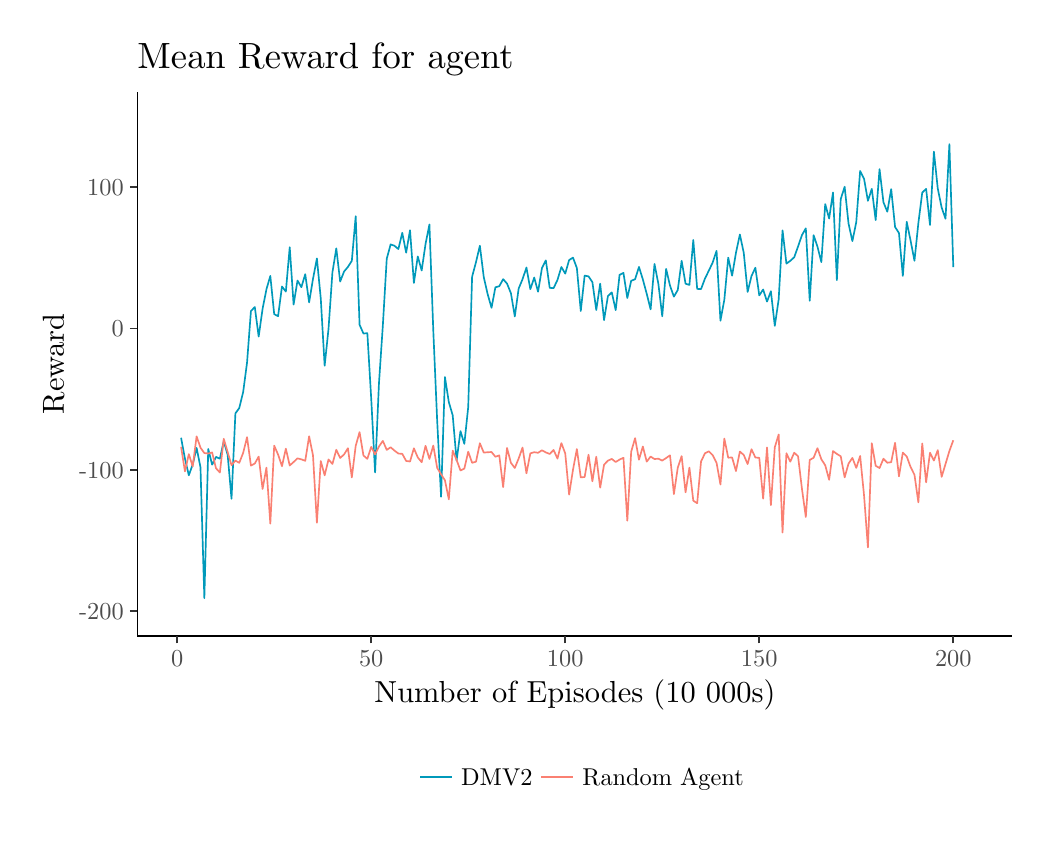
\begin{tikzpicture}[x=1pt,y=1pt]
\definecolor{fillColor}{RGB}{255,255,255}
\path[use as bounding box,fill=fillColor,fill opacity=0.00] (0,0) rectangle (361.35,289.08);
\begin{scope}
\path[clip] (  0.00,  0.00) rectangle (361.35,289.08);
\definecolor{drawColor}{RGB}{255,255,255}
\definecolor{fillColor}{RGB}{255,255,255}

\path[draw=drawColor,line width= 0.6pt,line join=round,line cap=round,fill=fillColor] (  0.00,  0.00) rectangle (361.35,289.08);
\end{scope}
\begin{scope}
\path[clip] ( 39.66, 69.30) rectangle (355.85,265.94);
\definecolor{fillColor}{RGB}{255,255,255}

\path[fill=fillColor] ( 39.66, 69.30) rectangle (355.85,265.94);
\definecolor{drawColor}{RGB}{0,153,186}

\path[draw=drawColor,line width= 0.6pt,line join=round] ( 55.43,140.90) --
	( 56.83,133.34) --
	( 58.23,127.34) --
	( 59.64,131.24) --
	( 61.04,137.25) --
	( 62.44,130.27) --
	( 63.84, 82.91) --
	( 65.25,136.83) --
	( 66.65,131.17) --
	( 68.05,133.98) --
	( 69.45,133.31) --
	( 70.85,139.60) --
	( 72.26,134.76) --
	( 73.66,118.85) --
	( 75.06,149.69) --
	( 76.46,151.65) --
	( 77.87,157.44) --
	( 79.27,168.06) --
	( 80.67,186.66) --
	( 82.07,188.13) --
	( 83.47,177.46) --
	( 84.88,187.46) --
	( 86.28,194.56) --
	( 87.68,199.36) --
	( 89.08,185.57) --
	( 90.48,184.81) --
	( 91.89,195.54) --
	( 93.29,193.72) --
	( 94.69,209.76) --
	( 96.09,189.03) --
	( 97.50,197.70) --
	( 98.90,195.31) --
	(100.30,200.00) --
	(101.70,189.79) --
	(103.10,198.29) --
	(104.51,205.69) --
	(105.91,191.22) --
	(107.31,166.91) --
	(108.71,180.27) --
	(110.12,200.65) --
	(111.52,209.33) --
	(112.92,197.34) --
	(114.32,200.95) --
	(115.72,202.63) --
	(117.13,204.83) --
	(118.53,220.95) --
	(119.93,181.73) --
	(121.33,178.56) --
	(122.74,178.68) --
	(124.14,154.99) --
	(125.54,128.35) --
	(126.94,160.63) --
	(128.34,181.49) --
	(129.75,205.58) --
	(131.15,210.75) --
	(132.55,210.26) --
	(133.95,209.07) --
	(135.36,214.95) --
	(136.76,207.77) --
	(138.16,215.88) --
	(139.56,196.83) --
	(140.96,206.42) --
	(142.37,201.35) --
	(143.77,210.93) --
	(145.17,217.95) --
	(146.57,179.57) --
	(147.97,147.08) --
	(149.38,119.58) --
	(150.78,162.82) --
	(152.18,153.78) --
	(153.58,149.02) --
	(154.99,132.66) --
	(156.39,143.28) --
	(157.79,138.69) --
	(159.19,151.99) --
	(160.59,199.06) --
	(162.00,204.37) --
	(163.40,210.29) --
	(164.80,198.98) --
	(166.20,192.83) --
	(167.61,187.85) --
	(169.01,195.27) --
	(170.41,195.64) --
	(171.81,198.20) --
	(173.21,196.60) --
	(174.62,193.12) --
	(176.02,184.73) --
	(177.42,194.83) --
	(178.82,198.19) --
	(180.23,202.39) --
	(181.63,194.59) --
	(183.03,198.79) --
	(184.43,193.66) --
	(185.83,202.18) --
	(187.24,204.98) --
	(188.64,195.06) --
	(190.04,194.95) --
	(191.44,197.94) --
	(192.85,202.59) --
	(194.25,200.21) --
	(195.65,205.11) --
	(197.05,205.99) --
	(198.45,202.21) --
	(199.86,186.68) --
	(201.26,199.49) --
	(202.66,199.21) --
	(204.06,197.13) --
	(205.46,187.04) --
	(206.87,196.59) --
	(208.27,183.40) --
	(209.67,192.08) --
	(211.07,193.42) --
	(212.48,187.01) --
	(213.88,199.78) --
	(215.28,200.47) --
	(216.68,191.39) --
	(218.08,197.62) --
	(219.49,198.18) --
	(220.89,202.62) --
	(222.29,198.11) --
	(223.69,192.92) --
	(225.10,187.30) --
	(226.50,203.71) --
	(227.90,196.51) --
	(229.30,184.82) --
	(230.70,201.93) --
	(232.11,195.84) --
	(233.51,191.88) --
	(234.91,194.30) --
	(236.31,204.84) --
	(237.72,196.56) --
	(239.12,196.11) --
	(240.52,212.35) --
	(241.92,194.69) --
	(243.32,194.62) --
	(244.73,198.41) --
	(246.13,201.27) --
	(247.53,204.22) --
	(248.93,208.43) --
	(250.33,183.19) --
	(251.74,190.80) --
	(253.14,205.98) --
	(254.54,199.46) --
	(255.94,207.75) --
	(257.35,214.34) --
	(258.75,207.74) --
	(260.15,193.59) --
	(261.55,199.34) --
	(262.95,202.34) --
	(264.36,192.35) --
	(265.76,194.46) --
	(267.16,190.10) --
	(268.56,193.83) --
	(269.97,181.32) --
	(271.37,190.87) --
	(272.77,215.84) --
	(274.17,203.81) --
	(275.57,204.83) --
	(276.98,206.11) --
	(278.38,210.03) --
	(279.78,214.11) --
	(281.18,216.57) --
	(282.59,190.38) --
	(283.99,214.09) --
	(285.39,209.98) --
	(286.79,204.36) --
	(288.19,225.33) --
	(289.60,220.12) --
	(291.00,229.51) --
	(292.40,197.84) --
	(293.80,227.17) --
	(295.21,231.58) --
	(296.61,218.31) --
	(298.01,211.94) --
	(299.41,218.84) --
	(300.81,237.30) --
	(302.22,234.47) --
	(303.62,226.51) --
	(305.02,230.83) --
	(306.42,219.56) --
	(307.82,237.96) --
	(309.23,225.98) --
	(310.63,222.57) --
	(312.03,230.74) --
	(313.43,217.06) --
	(314.84,214.87) --
	(316.24,199.36) --
	(317.64,218.92) --
	(319.04,212.11) --
	(320.44,204.86) --
	(321.85,218.49) --
	(323.25,229.48) --
	(324.65,230.83) --
	(326.05,217.80) --
	(327.46,244.26) --
	(328.86,230.94) --
	(330.26,224.08) --
	(331.66,220.04) --
	(333.06,246.97) --
	(334.47,202.54);
\definecolor{drawColor}{RGB}{250,128,114}

\path[draw=drawColor,line width= 0.6pt,line join=round] ( 55.43,137.63) --
	( 56.83,128.75) --
	( 58.23,134.98) --
	( 59.64,130.53) --
	( 61.04,141.41) --
	( 62.44,137.32) --
	( 63.84,135.36) --
	( 65.25,135.21) --
	( 66.65,135.58) --
	( 68.05,129.87) --
	( 69.45,128.34) --
	( 70.85,140.51) --
	( 72.26,135.75) --
	( 73.66,130.97) --
	( 75.06,132.62) --
	( 76.46,131.85) --
	( 77.87,135.43) --
	( 79.27,141.10) --
	( 80.67,130.84) --
	( 82.07,131.58) --
	( 83.47,134.09) --
	( 84.88,122.39) --
	( 86.28,130.11) --
	( 87.68,109.88) --
	( 89.08,138.04) --
	( 90.48,134.82) --
	( 91.89,130.62) --
	( 93.29,136.95) --
	( 94.69,130.87) --
	( 96.09,132.12) --
	( 97.50,133.45) --
	( 98.90,133.08) --
	(100.30,132.57) --
	(101.70,141.43) --
	(103.10,134.52) --
	(104.51,110.18) --
	(105.91,132.48) --
	(107.31,127.33) --
	(108.71,133.05) --
	(110.12,131.42) --
	(111.52,136.54) --
	(112.92,133.58) --
	(114.32,134.86) --
	(115.72,137.10) --
	(117.13,126.55) --
	(118.53,137.95) --
	(119.93,142.94) --
	(121.33,134.49) --
	(122.74,133.27) --
	(124.14,137.60) --
	(125.54,134.90) --
	(126.94,137.74) --
	(128.34,139.76) --
	(129.75,136.50) --
	(131.15,137.46) --
	(132.55,136.25) --
	(133.95,135.19) --
	(135.36,135.08) --
	(136.76,132.52) --
	(138.16,132.31) --
	(139.56,137.08) --
	(140.96,133.80) --
	(142.37,132.06) --
	(143.77,137.97) --
	(145.17,133.24) --
	(146.57,138.07) --
	(147.97,130.02) --
	(149.38,127.70) --
	(150.78,125.52) --
	(152.18,118.65) --
	(153.58,136.26) --
	(154.99,132.87) --
	(156.39,129.07) --
	(157.79,129.76) --
	(159.19,135.85) --
	(160.59,131.85) --
	(162.00,132.23) --
	(163.40,138.90) --
	(164.80,135.54) --
	(166.20,135.66) --
	(167.61,135.74) --
	(169.01,134.03) --
	(170.41,134.53) --
	(171.81,123.04) --
	(173.21,137.21) --
	(174.62,131.83) --
	(176.02,129.97) --
	(177.42,133.41) --
	(178.82,137.36) --
	(180.23,128.04) --
	(181.63,135.25) --
	(183.03,135.68) --
	(184.43,135.46) --
	(185.83,136.37) --
	(187.24,135.60) --
	(188.64,135.03) --
	(190.04,136.48) --
	(191.44,133.36) --
	(192.85,138.97) --
	(194.25,135.21) --
	(195.65,120.35) --
	(197.05,129.34) --
	(198.45,136.81) --
	(199.86,126.56) --
	(201.26,126.71) --
	(202.66,134.76) --
	(204.06,125.17) --
	(205.46,134.03) --
	(206.87,122.86) --
	(208.27,131.15) --
	(209.67,132.63) --
	(211.07,133.24) --
	(212.48,132.13) --
	(213.88,133.00) --
	(215.28,133.67) --
	(216.68,110.92) --
	(218.08,135.88) --
	(219.49,140.75) --
	(220.89,132.97) --
	(222.29,137.73) --
	(223.69,132.27) --
	(225.10,134.10) --
	(226.50,133.20) --
	(227.90,133.33) --
	(229.30,132.65) --
	(230.70,133.57) --
	(232.11,134.54) --
	(233.51,120.55) --
	(234.91,130.09) --
	(236.31,134.27) --
	(237.72,121.18) --
	(239.12,130.09) --
	(240.52,118.15) --
	(241.92,117.23) --
	(243.32,132.32) --
	(244.73,135.27) --
	(246.13,136.00) --
	(247.53,134.60) --
	(248.93,131.82) --
	(250.33,124.01) --
	(251.74,140.61) --
	(253.14,133.69) --
	(254.54,133.77) --
	(255.94,128.86) --
	(257.35,135.91) --
	(258.75,134.68) --
	(260.15,131.39) --
	(261.55,136.74) --
	(262.95,133.76) --
	(264.36,133.63) --
	(265.76,118.87) --
	(267.16,137.38) --
	(268.56,116.54) --
	(269.97,137.47) --
	(271.37,142.06) --
	(272.77,106.64) --
	(274.17,135.29) --
	(275.57,132.25) --
	(276.98,135.50) --
	(278.38,134.19) --
	(279.78,122.46) --
	(281.18,112.26) --
	(282.59,132.89) --
	(283.99,133.65) --
	(285.39,137.13) --
	(286.79,133.12) --
	(288.19,130.96) --
	(289.60,125.72) --
	(291.00,136.10) --
	(292.40,135.05) --
	(293.80,134.20) --
	(295.21,126.57) --
	(296.61,131.55) --
	(298.01,133.62) --
	(299.41,130.00) --
	(300.81,134.30) --
	(302.22,120.08) --
	(303.62,101.27) --
	(305.02,138.90) --
	(306.42,130.77) --
	(307.82,129.95) --
	(309.23,133.31) --
	(310.63,131.86) --
	(312.03,132.08) --
	(313.43,139.06) --
	(314.84,126.95) --
	(316.24,135.55) --
	(317.64,134.15) --
	(319.04,130.32) --
	(320.44,127.50) --
	(321.85,117.54) --
	(323.25,138.80) --
	(324.65,124.79) --
	(326.05,135.48) --
	(327.46,132.65) --
	(328.86,136.42) --
	(330.26,126.77) --
	(331.66,131.42) --
	(333.06,136.10) --
	(334.47,139.98);
\end{scope}
\begin{scope}
\path[clip] (  0.00,  0.00) rectangle (361.35,289.08);
\definecolor{drawColor}{RGB}{0,0,0}

\path[draw=drawColor,line width= 0.6pt,line join=round] ( 39.66, 69.30) --
	( 39.66,265.94);
\end{scope}
\begin{scope}
\path[clip] (  0.00,  0.00) rectangle (361.35,289.08);
\definecolor{drawColor}{gray}{0.30}

\node[text=drawColor,anchor=base east,inner sep=0pt, outer sep=0pt, scale=  0.88] at ( 34.71, 75.21) {-200};

\node[text=drawColor,anchor=base east,inner sep=0pt, outer sep=0pt, scale=  0.88] at ( 34.71,126.29) {-100};

\node[text=drawColor,anchor=base east,inner sep=0pt, outer sep=0pt, scale=  0.88] at ( 34.71,177.36) {0};

\node[text=drawColor,anchor=base east,inner sep=0pt, outer sep=0pt, scale=  0.88] at ( 34.71,228.44) {100};
\end{scope}
\begin{scope}
\path[clip] (  0.00,  0.00) rectangle (361.35,289.08);
\definecolor{drawColor}{gray}{0.20}

\path[draw=drawColor,line width= 0.6pt,line join=round] ( 36.91, 78.24) --
	( 39.66, 78.24);

\path[draw=drawColor,line width= 0.6pt,line join=round] ( 36.91,129.32) --
	( 39.66,129.32);

\path[draw=drawColor,line width= 0.6pt,line join=round] ( 36.91,180.39) --
	( 39.66,180.39);

\path[draw=drawColor,line width= 0.6pt,line join=round] ( 36.91,231.47) --
	( 39.66,231.47);
\end{scope}
\begin{scope}
\path[clip] (  0.00,  0.00) rectangle (361.35,289.08);
\definecolor{drawColor}{RGB}{0,0,0}

\path[draw=drawColor,line width= 0.6pt,line join=round] ( 39.66, 69.30) --
	(355.85, 69.30);
\end{scope}
\begin{scope}
\path[clip] (  0.00,  0.00) rectangle (361.35,289.08);
\definecolor{drawColor}{gray}{0.20}

\path[draw=drawColor,line width= 0.6pt,line join=round] ( 54.03, 66.55) --
	( 54.03, 69.30);

\path[draw=drawColor,line width= 0.6pt,line join=round] (124.14, 66.55) --
	(124.14, 69.30);

\path[draw=drawColor,line width= 0.6pt,line join=round] (194.25, 66.55) --
	(194.25, 69.30);

\path[draw=drawColor,line width= 0.6pt,line join=round] (264.36, 66.55) --
	(264.36, 69.30);

\path[draw=drawColor,line width= 0.6pt,line join=round] (334.47, 66.55) --
	(334.47, 69.30);
\end{scope}
\begin{scope}
\path[clip] (  0.00,  0.00) rectangle (361.35,289.08);
\definecolor{drawColor}{gray}{0.30}

\node[text=drawColor,anchor=base,inner sep=0pt, outer sep=0pt, scale=  0.88] at ( 54.03, 58.29) {0};

\node[text=drawColor,anchor=base,inner sep=0pt, outer sep=0pt, scale=  0.88] at (124.14, 58.29) {50};

\node[text=drawColor,anchor=base,inner sep=0pt, outer sep=0pt, scale=  0.88] at (194.25, 58.29) {100};

\node[text=drawColor,anchor=base,inner sep=0pt, outer sep=0pt, scale=  0.88] at (264.36, 58.29) {150};

\node[text=drawColor,anchor=base,inner sep=0pt, outer sep=0pt, scale=  0.88] at (334.47, 58.29) {200};
\end{scope}
\begin{scope}
\path[clip] (  0.00,  0.00) rectangle (361.35,289.08);
\definecolor{drawColor}{RGB}{0,0,0}

\node[text=drawColor,anchor=base,inner sep=0pt, outer sep=0pt, scale=  1.10] at (197.75, 45.22) {Number of Episodes (10 000s)};
\end{scope}
\begin{scope}
\path[clip] (  0.00,  0.00) rectangle (361.35,289.08);
\definecolor{drawColor}{RGB}{0,0,0}

\node[text=drawColor,rotate= 90.00,anchor=base,inner sep=0pt, outer sep=0pt, scale=  1.10] at ( 13.08,167.62) {Reward};
\end{scope}
\begin{scope}
\path[clip] (  0.00,  0.00) rectangle (361.35,289.08);
\definecolor{fillColor}{RGB}{255,255,255}

\path[fill=fillColor] (131.06,  5.50) rectangle (264.45, 31.34);
\end{scope}
\begin{scope}
\path[clip] (  0.00,  0.00) rectangle (361.35,289.08);
\definecolor{drawColor}{RGB}{0,153,186}

\path[draw=drawColor,line width= 0.6pt,line join=round] (141.81, 18.42) -- (153.37, 18.42);
\end{scope}
\begin{scope}
\path[clip] (  0.00,  0.00) rectangle (361.35,289.08);
\definecolor{drawColor}{RGB}{250,128,114}

\path[draw=drawColor,line width= 0.6pt,line join=round] (185.66, 18.42) -- (197.22, 18.42);
\end{scope}
\begin{scope}
\path[clip] (  0.00,  0.00) rectangle (361.35,289.08);
\definecolor{drawColor}{RGB}{0,0,0}

\node[text=drawColor,anchor=base west,inner sep=0pt, outer sep=0pt, scale=  0.88] at (156.62, 15.39) {DMV2};
\end{scope}
\begin{scope}
\path[clip] (  0.00,  0.00) rectangle (361.35,289.08);
\definecolor{drawColor}{RGB}{0,0,0}

\node[text=drawColor,anchor=base west,inner sep=0pt, outer sep=0pt, scale=  0.88] at (200.47, 15.39) {Random Agent};
\end{scope}
\begin{scope}
\path[clip] (  0.00,  0.00) rectangle (361.35,289.08);
\definecolor{drawColor}{RGB}{0,0,0}

\node[text=drawColor,anchor=base west,inner sep=0pt, outer sep=0pt, scale=  1.32] at ( 39.66,274.49) {Mean Reward for agent};
\end{scope}
\end{tikzpicture}

		%Captions and Labels can be used since this is a figure environment
		\caption{Plot showing the average reward after training DealerMarket-v2 for $2\cdot 10^{6}$ time-steps. Average is taken after 10 000 time steps, compared to a random agent on the same environment.}
		\label{fig:dm21}
\end{figure}
In \autoref{fig:dm21} the mean reward for both the DealerMarket-v1 agent and a random policy on the environment is shown. Both this and the LOBMarket-v1 agent used the PPO algorithm. The mean is taken after each episode, i.e. after some 10 000 time-steps. Clearly the agents is worse than a random policy in the beginning of the training. Slowly learning a more optimal behaviour. After some 75 000 time-steps the agent starts to outperform the random policy quite consistently. Compared to DealerMarket-v1, the mean reward seems to converge more smoothly using the PPO algorithm. As the same type of fluctuates previously seen are no present here. Which is expected as policy gradient methods, tends to converge more easily.

\begin{figure}[H]
		%Do not try to scale figure in .tex or you loose font size consistency
	    	\centering
		%The code to input the plot is extremely simple
		% Created by tikzDevice version 0.11 on 2018-08-06 22:44:21
% !TEX encoding = UTF-8 Unicode
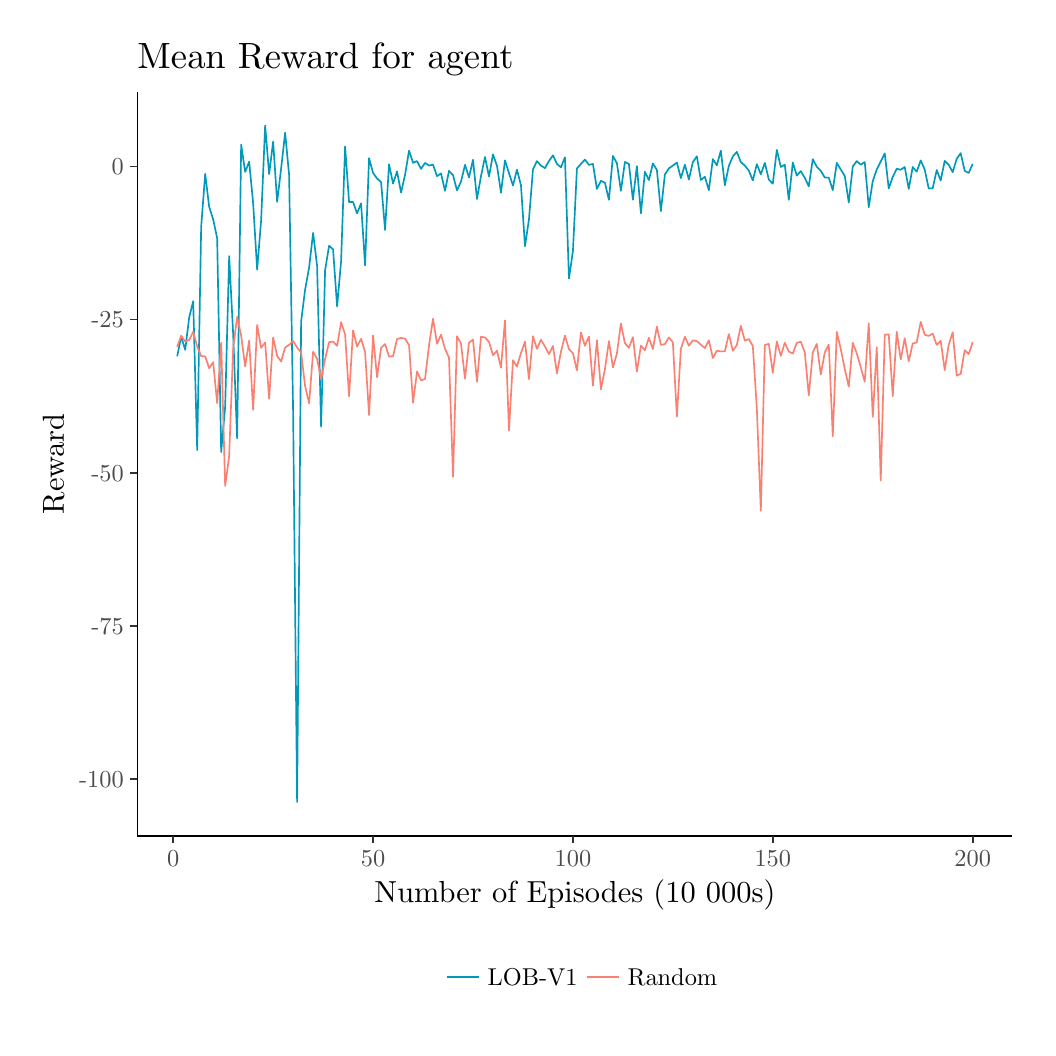
\begin{tikzpicture}[x=1pt,y=1pt]
\definecolor{fillColor}{RGB}{255,255,255}
\path[use as bounding box,fill=fillColor,fill opacity=0.00] (0,0) rectangle (361.35,361.35);
\begin{scope}
\path[clip] (  0.00,  0.00) rectangle (361.35,361.35);
\definecolor{drawColor}{RGB}{255,255,255}
\definecolor{fillColor}{RGB}{255,255,255}

\path[draw=drawColor,line width= 0.6pt,line join=round,line cap=round,fill=fillColor] (  0.00,  0.00) rectangle (361.35,361.35);
\end{scope}
\begin{scope}
\path[clip] ( 39.66, 69.30) rectangle (355.85,338.21);
\definecolor{fillColor}{RGB}{255,255,255}

\path[fill=fillColor] ( 39.66, 69.30) rectangle (355.85,338.21);
\definecolor{drawColor}{RGB}{0,153,186}

\path[draw=drawColor,line width= 0.6pt,line join=round] ( 54.03,242.59) --
	( 55.47,249.72) --
	( 56.92,244.94) --
	( 58.36,256.63) --
	( 59.81,262.52) --
	( 61.25,208.74) --
	( 62.69,289.32) --
	( 64.14,308.51) --
	( 65.58,296.67) --
	( 67.03,292.05) --
	( 68.47,285.29) --
	( 69.92,208.00) --
	( 71.36,224.43) --
	( 72.81,278.81) --
	( 74.25,250.68) --
	( 75.69,212.89) --
	( 77.14,319.11) --
	( 78.58,309.24) --
	( 80.03,312.94) --
	( 81.47,297.95) --
	( 82.92,273.89) --
	( 84.36,291.78) --
	( 85.81,325.99) --
	( 87.25,308.41) --
	( 88.70,320.16) --
	( 90.14,298.37) --
	( 91.58,310.41) --
	( 93.03,323.39) --
	( 94.47,308.09) --
	( 95.92,222.34) --
	( 97.36, 81.53) --
	( 98.81,255.19) --
	(100.25,266.69) --
	(101.70,274.73) --
	(103.14,287.19) --
	(104.58,275.29) --
	(106.03,217.14) --
	(107.47,273.70) --
	(108.92,282.55) --
	(110.36,281.22) --
	(111.81,260.60) --
	(113.25,276.92) --
	(114.70,318.43) --
	(116.14,298.33) --
	(117.58,298.33) --
	(119.03,294.22) --
	(120.47,297.86) --
	(121.92,275.44) --
	(123.36,314.18) --
	(124.81,308.81) --
	(126.25,306.84) --
	(127.70,305.53) --
	(129.14,288.25) --
	(130.58,311.99) --
	(132.03,304.99) --
	(133.47,309.39) --
	(134.92,301.77) --
	(136.36,308.15) --
	(137.81,316.91) --
	(139.25,312.53) --
	(140.70,313.11) --
	(142.14,310.33) --
	(143.59,312.47) --
	(145.03,311.52) --
	(146.47,311.84) --
	(147.92,307.67) --
	(149.36,308.68) --
	(150.81,302.40) --
	(152.25,309.59) --
	(153.70,308.04) --
	(155.14,302.55) --
	(156.59,305.75) --
	(158.03,311.78) --
	(159.47,307.26) --
	(160.92,313.63) --
	(162.36,299.44) --
	(163.81,307.74) --
	(165.25,314.63) --
	(166.70,307.57) --
	(168.14,315.58) --
	(169.59,311.42) --
	(171.03,301.73) --
	(172.47,313.41) --
	(173.92,308.80) --
	(175.36,304.32) --
	(176.81,310.03) --
	(178.25,304.39) --
	(179.70,282.39) --
	(181.14,292.07) --
	(182.59,310.15) --
	(184.03,313.13) --
	(185.47,311.50) --
	(186.92,310.60) --
	(188.36,313.12) --
	(189.81,315.22) --
	(191.25,312.13) --
	(192.70,310.88) --
	(194.14,314.48) --
	(195.59,270.69) --
	(197.03,280.65) --
	(198.47,310.46) --
	(199.92,312.12) --
	(201.36,313.68) --
	(202.81,311.76) --
	(204.25,312.12) --
	(205.70,303.06) --
	(207.14,305.99) --
	(208.59,305.26) --
	(210.03,299.15) --
	(211.48,315.00) --
	(212.92,312.37) --
	(214.36,302.41) --
	(215.81,312.81) --
	(217.25,312.12) --
	(218.70,299.17) --
	(220.14,311.31) --
	(221.59,294.26) --
	(223.03,309.28) --
	(224.48,306.29) --
	(225.92,312.29) --
	(227.36,309.97) --
	(228.81,295.03) --
	(230.25,308.27) --
	(231.70,310.50) --
	(233.14,311.52) --
	(234.59,312.61) --
	(236.03,306.96) --
	(237.48,311.84) --
	(238.92,306.46) --
	(240.36,312.81) --
	(241.81,314.86) --
	(243.25,306.29) --
	(244.70,307.48) --
	(246.14,302.63) --
	(247.59,313.86) --
	(249.03,311.60) --
	(250.48,316.91) --
	(251.92,304.40) --
	(253.36,311.39) --
	(254.81,314.82) --
	(256.25,316.47) --
	(257.70,312.78) --
	(259.14,311.52) --
	(260.59,309.67) --
	(262.03,306.13) --
	(263.48,312.05) --
	(264.92,308.36) --
	(266.37,312.50) --
	(267.81,306.46) --
	(269.25,304.96) --
	(270.70,317.20) --
	(272.14,311.00) --
	(273.59,311.83) --
	(275.03,299.14) --
	(276.48,312.64) --
	(277.92,307.88) --
	(279.37,309.53) --
	(280.81,307.08) --
	(282.25,304.03) --
	(283.70,313.83) --
	(285.14,311.08) --
	(286.59,309.61) --
	(288.03,307.21) --
	(289.48,307.14) --
	(290.92,302.65) --
	(292.37,312.49) --
	(293.81,310.09) --
	(295.25,307.79) --
	(296.70,298.17) --
	(298.14,311.18) --
	(299.59,313.14) --
	(301.03,311.84) --
	(302.48,312.80) --
	(303.92,296.49) --
	(305.37,305.91) --
	(306.81,310.11) --
	(308.25,312.95) --
	(309.70,315.93) --
	(311.14,303.25) --
	(312.59,307.41) --
	(314.03,310.35) --
	(315.48,310.02) --
	(316.92,311.00) --
	(318.37,303.08) --
	(319.81,311.00) --
	(321.25,309.31) --
	(322.70,313.36) --
	(324.14,310.08) --
	(325.59,303.23) --
	(327.03,303.33) --
	(328.48,309.89) --
	(329.92,306.13) --
	(331.37,313.22) --
	(332.81,311.80) --
	(334.26,309.15) --
	(335.70,313.96) --
	(337.14,316.01) --
	(338.59,309.60) --
	(340.03,308.85) --
	(341.48,312.12);
\definecolor{drawColor}{RGB}{250,128,114}

\path[draw=drawColor,line width= 0.6pt,line join=round] ( 54.03,246.02) --
	( 55.47,250.03) --
	( 56.92,247.90) --
	( 58.36,248.52) --
	( 59.81,251.49) --
	( 61.25,246.14) --
	( 62.69,242.68) --
	( 64.14,242.56) --
	( 65.58,238.28) --
	( 67.03,240.47) --
	( 68.47,225.66) --
	( 69.92,247.54) --
	( 71.36,195.74) --
	( 72.81,206.58) --
	( 74.25,245.59) --
	( 75.69,256.81) --
	( 77.14,250.11) --
	( 78.58,238.93) --
	( 80.03,248.30) --
	( 81.47,223.25) --
	( 82.92,253.92) --
	( 84.36,245.64) --
	( 85.81,247.61) --
	( 87.25,227.21) --
	( 88.70,249.43) --
	( 90.14,242.71) --
	( 91.58,240.72) --
	( 93.03,245.75) --
	( 94.47,246.76) --
	( 95.92,248.10) --
	( 97.36,245.74) --
	( 98.81,244.00) --
	(100.25,231.83) --
	(101.70,225.63) --
	(103.14,244.24) --
	(104.58,241.73) --
	(106.03,234.18) --
	(107.47,241.62) --
	(108.92,247.72) --
	(110.36,247.93) --
	(111.81,246.37) --
	(113.25,254.91) --
	(114.70,250.53) --
	(116.14,228.16) --
	(117.58,251.98) --
	(119.03,246.10) --
	(120.47,248.91) --
	(121.92,244.18) --
	(123.36,221.36) --
	(124.81,250.11) --
	(126.25,235.02) --
	(127.70,245.64) --
	(129.14,247.01) --
	(130.58,242.48) --
	(132.03,242.67) --
	(133.47,248.84) --
	(134.92,249.27) --
	(136.36,248.92) --
	(137.81,246.65) --
	(139.25,225.80) --
	(140.70,237.10) --
	(142.14,233.89) --
	(143.59,234.40) --
	(145.03,246.59) --
	(146.47,256.19) --
	(147.92,247.11) --
	(149.36,250.39) --
	(150.81,245.29) --
	(152.25,242.12) --
	(153.70,199.07) --
	(155.14,249.85) --
	(156.59,247.11) --
	(158.03,234.54) --
	(159.47,247.46) --
	(160.92,248.63) --
	(162.36,233.41) --
	(163.81,249.66) --
	(165.25,249.39) --
	(166.70,247.79) --
	(168.14,243.01) --
	(169.59,244.62) --
	(171.03,238.49) --
	(172.47,255.58) --
	(173.92,215.78) --
	(175.36,241.18) --
	(176.81,238.89) --
	(178.25,243.75) --
	(179.70,247.87) --
	(181.14,234.35) --
	(182.59,249.86) --
	(184.03,245.27) --
	(185.47,248.58) --
	(186.92,246.14) --
	(188.36,243.40) --
	(189.81,246.34) --
	(191.25,236.43) --
	(192.70,244.23) --
	(194.14,250.07) --
	(195.59,245.21) --
	(197.03,243.68) --
	(198.47,237.53) --
	(199.92,251.21) --
	(201.36,246.39) --
	(202.81,249.72) --
	(204.25,231.99) --
	(205.70,248.42) --
	(207.14,230.64) --
	(208.59,237.90) --
	(210.03,248.06) --
	(211.48,238.60) --
	(212.92,243.62) --
	(214.36,254.43) --
	(215.81,247.36) --
	(217.25,245.67) --
	(218.70,249.53) --
	(220.14,237.08) --
	(221.59,246.42) --
	(223.03,244.78) --
	(224.48,249.28) --
	(225.92,245.21) --
	(227.36,253.31) --
	(228.81,246.73) --
	(230.25,246.98) --
	(231.70,249.40) --
	(233.14,247.66) --
	(234.59,220.79) --
	(236.03,245.24) --
	(237.48,249.66) --
	(238.92,246.42) --
	(240.36,248.37) --
	(241.81,248.10) --
	(243.25,246.79) --
	(244.70,245.57) --
	(246.14,248.34) --
	(247.59,242.00) --
	(249.03,244.60) --
	(250.48,244.36) --
	(251.92,244.38) --
	(253.36,250.62) --
	(254.81,244.59) --
	(256.25,246.69) --
	(257.70,253.60) --
	(259.14,248.25) --
	(260.59,248.83) --
	(262.03,246.35) --
	(263.48,223.85) --
	(264.92,186.75) --
	(266.37,246.65) --
	(267.81,247.09) --
	(269.25,236.59) --
	(270.70,247.98) --
	(272.14,242.76) --
	(273.59,247.52) --
	(275.03,244.30) --
	(276.48,243.61) --
	(277.92,247.49) --
	(279.37,247.83) --
	(280.81,244.03) --
	(282.25,228.45) --
	(283.70,244.00) --
	(285.14,247.08) --
	(286.59,235.98) --
	(288.03,244.02) --
	(289.48,246.86) --
	(290.92,213.73) --
	(292.37,251.41) --
	(293.81,245.19) --
	(295.25,238.00) --
	(296.70,231.64) --
	(298.14,247.50) --
	(299.59,243.65) --
	(301.03,238.67) --
	(302.48,233.43) --
	(303.92,254.48) --
	(305.37,220.70) --
	(306.81,245.84) --
	(308.25,197.70) --
	(309.70,250.39) --
	(311.14,250.54) --
	(312.59,228.18) --
	(314.03,251.44) --
	(315.48,241.47) --
	(316.92,249.12) --
	(318.37,240.82) --
	(319.81,247.22) --
	(321.25,247.59) --
	(322.70,255.02) --
	(324.14,250.42) --
	(325.59,249.95) --
	(327.03,250.79) --
	(328.48,246.70) --
	(329.92,248.20) --
	(331.37,237.58) --
	(332.81,246.78) --
	(334.26,251.27) --
	(335.70,235.63) --
	(337.14,236.24) --
	(338.59,244.82) --
	(340.03,243.41) --
	(341.48,247.71);
\end{scope}
\begin{scope}
\path[clip] (  0.00,  0.00) rectangle (361.35,361.35);
\definecolor{drawColor}{RGB}{0,0,0}

\path[draw=drawColor,line width= 0.6pt,line join=round] ( 39.66, 69.30) --
	( 39.66,338.21);
\end{scope}
\begin{scope}
\path[clip] (  0.00,  0.00) rectangle (361.35,361.35);
\definecolor{drawColor}{gray}{0.30}

\node[text=drawColor,anchor=base east,inner sep=0pt, outer sep=0pt, scale=  0.88] at ( 34.71, 86.84) {-100};

\node[text=drawColor,anchor=base east,inner sep=0pt, outer sep=0pt, scale=  0.88] at ( 34.71,142.17) {-75};

\node[text=drawColor,anchor=base east,inner sep=0pt, outer sep=0pt, scale=  0.88] at ( 34.71,197.51) {-50};

\node[text=drawColor,anchor=base east,inner sep=0pt, outer sep=0pt, scale=  0.88] at ( 34.71,252.84) {-25};

\node[text=drawColor,anchor=base east,inner sep=0pt, outer sep=0pt, scale=  0.88] at ( 34.71,308.17) {0};
\end{scope}
\begin{scope}
\path[clip] (  0.00,  0.00) rectangle (361.35,361.35);
\definecolor{drawColor}{gray}{0.20}

\path[draw=drawColor,line width= 0.6pt,line join=round] ( 36.91, 89.87) --
	( 39.66, 89.87);

\path[draw=drawColor,line width= 0.6pt,line join=round] ( 36.91,145.20) --
	( 39.66,145.20);

\path[draw=drawColor,line width= 0.6pt,line join=round] ( 36.91,200.54) --
	( 39.66,200.54);

\path[draw=drawColor,line width= 0.6pt,line join=round] ( 36.91,255.87) --
	( 39.66,255.87);

\path[draw=drawColor,line width= 0.6pt,line join=round] ( 36.91,311.20) --
	( 39.66,311.20);
\end{scope}
\begin{scope}
\path[clip] (  0.00,  0.00) rectangle (361.35,361.35);
\definecolor{drawColor}{RGB}{0,0,0}

\path[draw=drawColor,line width= 0.6pt,line join=round] ( 39.66, 69.30) --
	(355.85, 69.30);
\end{scope}
\begin{scope}
\path[clip] (  0.00,  0.00) rectangle (361.35,361.35);
\definecolor{drawColor}{gray}{0.20}

\path[draw=drawColor,line width= 0.6pt,line join=round] ( 52.58, 66.55) --
	( 52.58, 69.30);

\path[draw=drawColor,line width= 0.6pt,line join=round] (124.81, 66.55) --
	(124.81, 69.30);

\path[draw=drawColor,line width= 0.6pt,line join=round] (197.03, 66.55) --
	(197.03, 69.30);

\path[draw=drawColor,line width= 0.6pt,line join=round] (269.25, 66.55) --
	(269.25, 69.30);

\path[draw=drawColor,line width= 0.6pt,line join=round] (341.48, 66.55) --
	(341.48, 69.30);
\end{scope}
\begin{scope}
\path[clip] (  0.00,  0.00) rectangle (361.35,361.35);
\definecolor{drawColor}{gray}{0.30}

\node[text=drawColor,anchor=base,inner sep=0pt, outer sep=0pt, scale=  0.88] at ( 52.58, 58.29) {0};

\node[text=drawColor,anchor=base,inner sep=0pt, outer sep=0pt, scale=  0.88] at (124.81, 58.29) {50};

\node[text=drawColor,anchor=base,inner sep=0pt, outer sep=0pt, scale=  0.88] at (197.03, 58.29) {100};

\node[text=drawColor,anchor=base,inner sep=0pt, outer sep=0pt, scale=  0.88] at (269.25, 58.29) {150};

\node[text=drawColor,anchor=base,inner sep=0pt, outer sep=0pt, scale=  0.88] at (341.48, 58.29) {200};
\end{scope}
\begin{scope}
\path[clip] (  0.00,  0.00) rectangle (361.35,361.35);
\definecolor{drawColor}{RGB}{0,0,0}

\node[text=drawColor,anchor=base,inner sep=0pt, outer sep=0pt, scale=  1.10] at (197.75, 45.22) {Number of Episodes (10 000s)};
\end{scope}
\begin{scope}
\path[clip] (  0.00,  0.00) rectangle (361.35,361.35);
\definecolor{drawColor}{RGB}{0,0,0}

\node[text=drawColor,rotate= 90.00,anchor=base,inner sep=0pt, outer sep=0pt, scale=  1.10] at ( 13.08,203.76) {Reward};
\end{scope}
\begin{scope}
\path[clip] (  0.00,  0.00) rectangle (361.35,361.35);
\definecolor{fillColor}{RGB}{255,255,255}

\path[fill=fillColor] (140.65,  5.50) rectangle (254.86, 31.34);
\end{scope}
\begin{scope}
\path[clip] (  0.00,  0.00) rectangle (361.35,361.35);
\definecolor{drawColor}{RGB}{0,153,186}

\path[draw=drawColor,line width= 0.6pt,line join=round] (151.40, 18.42) -- (162.96, 18.42);
\end{scope}
\begin{scope}
\path[clip] (  0.00,  0.00) rectangle (361.35,361.35);
\definecolor{drawColor}{RGB}{250,128,114}

\path[draw=drawColor,line width= 0.6pt,line join=round] (201.97, 18.42) -- (213.53, 18.42);
\end{scope}
\begin{scope}
\path[clip] (  0.00,  0.00) rectangle (361.35,361.35);
\definecolor{drawColor}{RGB}{0,0,0}

\node[text=drawColor,anchor=base west,inner sep=0pt, outer sep=0pt, scale=  0.88] at (166.21, 15.39) {LOB-V1};
\end{scope}
\begin{scope}
\path[clip] (  0.00,  0.00) rectangle (361.35,361.35);
\definecolor{drawColor}{RGB}{0,0,0}

\node[text=drawColor,anchor=base west,inner sep=0pt, outer sep=0pt, scale=  0.88] at (216.78, 15.39) {Random};
\end{scope}
\begin{scope}
\path[clip] (  0.00,  0.00) rectangle (361.35,361.35);
\definecolor{drawColor}{RGB}{0,0,0}

\node[text=drawColor,anchor=base west,inner sep=0pt, outer sep=0pt, scale=  1.32] at ( 39.66,346.76) {Mean Reward for agent};
\end{scope}
\end{tikzpicture}

		%Captions and Labels can be used since this is a figure environment
		\caption{Plot showing the average reward after training LOBMarket-v1 for $2\cdot 10^{6}$ time-steps. Average is taken after 10 000 time steps, compared to a random agent on the same environment.}
		\label{fig:dm211}
\end{figure}
The mean reward for LOBMarket-v1 environment is shown in \autoref{fig:dm211}. Clearly the agent is better than a random policy, which has a negative reward throughout the full simulation. Note that a random policy or zero-intelligence approach seems to work better in the limit order book environment. Compared to the dealer market environment. As can be seen from the DealerMarket-v2 the agent is worse than the random policy in the beginning. Note however that after roughly 25 000 time steps the agent outperforms the random policy. Why the reward is dropping at bit at the end of training (similar for DealerMarket-v2). Can be due to a to high set learning rate. As the author did not use  any annealing of the learning rate.


\newpage
\section{Price Impact Regressions}
% latex table generated in R 3.3.1 by xtable 1.8-2 package
% Mon Jul 02 23:12:15 2018
\begin{table}[H]
\centering
\caption{Results from running price impact regression on the change in mid prices during the simulations. ** indicates significant estimates.}
\label{tab:pi1}
\begin{tabular}{rrrrrrr}
  \hline
  & \textbf{DealerMarket-v1} \\
  \hline
 & Estimate & Std. Error & t value & Pr($>$$|$t$|$) \\ 
 
  \hline
$\beta_0$ & $1.0648$ & $0.5943$ & $1.79$ & $0.1711$  \\ 
  $\beta_1$ & $0.0112$ & $0.0084$ & $1.32$ & $0.2771$  \\ 
  $\beta_2$ & $-0.0757^{**}$ & $0.0237$ & $-3.19$ & $0.0497$  \\ 
  $\beta_3$ & $-0.0058$ & $0.0116$ & $-0.50$ & $0.6542$  \\ 
  %$\beta_4$ & -0.0396 & 0.2410 & -0.16 & 0.8696  \\ 
  
  \hline
  & \textbf{DealerMarket-v2} \\
  \hline
  $\beta_0$ & $-56.8926^{**}$ & $25.199$ & $-2.26$ & $0.0242$ \\ 
  $\beta_1$ & $3.4324^{**}$ & $1.1661$ & $2.94$ & $0.0033$  \\ 
  $\beta_2$ & $-0.2601^{**}$ & $0.0149$ & $17.44$ & $0.0000$ \\ 
  $\beta_3$ & $0.0817^{**}$ & $0.0242$ & $3.38$ & $0.0008$ \\ 
  %$\beta_4$ & -7.4158 & 133.4904 & -0.06 & 0.9559  \\ 
  
  \hline
  & \textbf{LOBMarket-v1} \\
  \hline
  $\beta_0$ & $37.6559$ & $187.0559$ & $0.20$ & $0.8408$ \\ 
  $\beta_1$ & $43.9947^{**}$ & $11.6959$ & $3.76$ & $0.0003$ \\ 
  $\beta_2$ & $-12.8060$ & $12.3870$ & $-1.03$ & $0.3034$ \\ 
  $\beta_3$ & $-32.0142$ & $18.0639$ & $-1.77$ & $0.0791$ \\
  %$\beta_4$  $-7.4158$ & $133.4904$ & -0.06 & 0.9559  \\ 
   \hline
\end{tabular}
\end{table}
Looking at \autoref{tab:pi1}, \textit{DealerMarket-v1} has a Kyle's $\lambda \approx 0.011$ with $R^{2}=0.741$. \textit{DealerMarket-v2} has a Kyle's $\lambda \approx 3.4324$, with $R^{2}= 0.3723$ . Whilst \textit{LOBMarket-v1} has a Kyle's $\lambda \approx 43.9948$, with $R^{2}= 0.1457 $. The form of the equation for all the regression is shown in \autoref{eq:regs}

\begin{equation}
    \Delta S_{n} = \beta_0 \pm \beta_1\sqrt{q_n} \pm \beta_2\sqrt{\Delta I_n} \pm \beta_3\sqrt{\Delta Init_{n}} + \epsilon_n
    \label{eq:regs}
\end{equation}
\newline
\newline
DealerMarket-v1 is where the agent has the smallest price impact. Which is expected due to lower volatility and less frequency of orders. With higher volatility in the DealerMarket-v2 environment the price impact seems to increase. Similar is seen for LOBMarket-v1. With the largest price impact. Another reason can be that the agent is posting more orders, thus effecting prices more often.  Transforming the regressors with a square root yielded higher $R^{2}$, and lower AIC values when performing the regressions.


\section{Bid-Ask Spread \& Inventory}
%\begin{figure}[H]
\begin{sidewaysfigure}
		%Do not try to scale figure in .tex or you loose font size consistency
	    	\centering
		%The code to input the plot is extremely simple
		% Created by tikzDevice version 0.11 on 2018-07-15 14:57:12
% !TEX encoding = UTF-8 Unicode
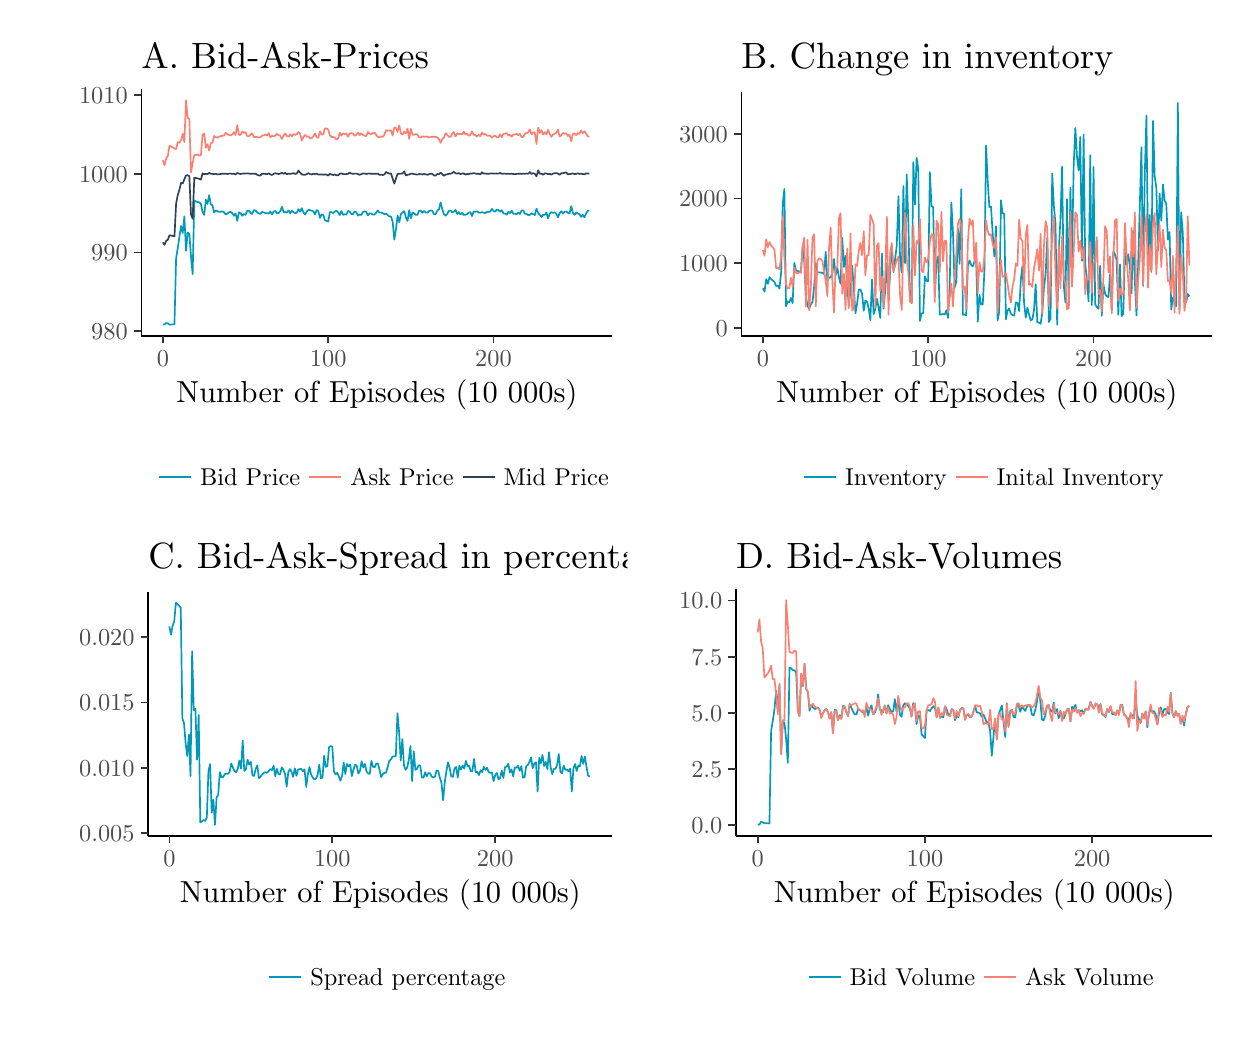
\begin{tikzpicture}[x=1pt,y=1pt]
\definecolor{fillColor}{RGB}{255,255,255}
\path[use as bounding box,fill=fillColor,fill opacity=0.00] (0,0) rectangle (433.62,361.35);
\begin{scope}
\path[clip] (  0.00,180.67) rectangle (216.81,361.35);
\definecolor{drawColor}{RGB}{255,255,255}
\definecolor{fillColor}{RGB}{255,255,255}

\path[draw=drawColor,line width= 0.6pt,line join=round,line cap=round,fill=fillColor] (  0.00,180.67) rectangle (216.81,361.35);
\end{scope}
\begin{scope}
\path[clip] ( 41.12,249.98) rectangle (211.31,339.19);
\definecolor{fillColor}{RGB}{255,255,255}

\path[fill=fillColor] ( 41.12,249.98) rectangle (211.31,339.19);
\definecolor{drawColor}{RGB}{0,153,186}

\path[draw=drawColor,line width= 0.6pt,line join=round] ( 48.86,254.06) --
	( 49.45,254.10) --
	( 50.05,254.64) --
	( 50.65,254.47) --
	( 51.25,254.03) --
	( 51.84,254.05) --
	( 52.44,254.15) --
	( 53.04,254.13) --
	( 53.64,278.13) --
	( 54.23,281.65) --
	( 54.83,285.86) --
	( 55.43,289.67) --
	( 56.03,287.12) --
	( 56.62,293.16) --
	( 57.22,280.75) --
	( 57.82,287.37) --
	( 58.42,286.86) --
	( 59.01,278.76) --
	( 59.61,272.28) --
	( 60.21,298.85) --
	( 60.80,298.57) --
	( 61.40,298.35) --
	( 62.00,298.22) --
	( 62.60,297.61) --
	( 63.19,294.77) --
	( 63.79,293.67) --
	( 64.39,299.17) --
	( 64.99,297.65) --
	( 65.58,300.82) --
	( 66.18,297.45) --
	( 66.78,297.17) --
	( 67.38,294.56) --
	( 67.97,295.31) --
	( 68.57,295.02) --
	( 69.17,294.77) --
	( 69.77,294.83) --
	( 70.36,294.96) --
	( 70.96,294.64) --
	( 71.56,293.82) --
	( 72.15,294.14) --
	( 72.75,294.65) --
	( 73.35,294.77) --
	( 73.95,294.33) --
	( 74.54,293.41) --
	( 75.14,294.16) --
	( 75.74,291.54) --
	( 76.34,294.65) --
	( 76.93,294.34) --
	( 77.53,293.38) --
	( 78.13,294.00) --
	( 78.73,293.70) --
	( 79.32,295.22) --
	( 79.92,295.23) --
	( 80.52,294.33) --
	( 81.12,294.03) --
	( 81.71,295.41) --
	( 82.31,295.27) --
	( 82.91,294.63) --
	( 83.50,294.21) --
	( 84.10,294.09) --
	( 84.70,294.79) --
	( 85.30,294.56) --
	( 85.89,294.35) --
	( 86.49,294.33) --
	( 87.09,294.16) --
	( 87.69,294.94) --
	( 88.28,293.92) --
	( 88.88,294.88) --
	( 89.48,295.14) --
	( 90.08,294.26) --
	( 90.67,294.38) --
	( 91.27,295.00) --
	( 91.87,296.64) --
	( 92.46,294.75) --
	( 93.06,294.75) --
	( 93.66,294.52) --
	( 94.26,295.29) --
	( 94.85,294.28) --
	( 95.45,295.17) --
	( 96.05,294.68) --
	( 96.65,294.32) --
	( 97.24,294.50) --
	( 97.84,295.79) --
	( 98.44,294.82) --
	( 99.04,296.13) --
	( 99.63,294.61) --
	(100.23,293.81) --
	(100.83,294.86) --
	(101.43,295.53) --
	(102.02,295.42) --
	(102.62,295.19) --
	(103.22,295.02) --
	(103.81,293.83) --
	(104.41,295.43) --
	(105.01,295.07) --
	(105.61,292.60) --
	(106.20,293.90) --
	(106.80,293.70) --
	(107.40,291.75) --
	(108.00,291.56) --
	(108.59,291.27) --
	(109.19,294.64) --
	(109.79,294.69) --
	(110.39,294.33) --
	(110.98,294.94) --
	(111.58,295.15) --
	(112.18,294.59) --
	(112.78,293.64) --
	(113.37,295.09) --
	(113.97,293.70) --
	(114.57,293.92) --
	(115.16,293.78) --
	(115.76,295.12) --
	(116.36,294.88) --
	(116.96,293.99) --
	(117.55,294.00) --
	(118.15,294.96) --
	(118.75,294.66) --
	(119.35,293.44) --
	(119.94,293.86) --
	(120.54,293.67) --
	(121.14,294.71) --
	(121.74,294.94) --
	(122.33,294.85) --
	(122.93,293.54) --
	(123.53,294.21) --
	(124.13,294.16) --
	(124.72,293.78) --
	(125.32,293.79) --
	(125.92,294.49) --
	(126.51,295.33) --
	(127.11,294.53) --
	(127.71,294.49) --
	(128.31,294.36) --
	(128.90,293.87) --
	(129.50,294.13) --
	(130.10,293.63) --
	(130.70,293.05) --
	(131.29,293.14) --
	(131.89,291.15) --
	(132.49,284.74) --
	(133.09,288.58) --
	(133.68,293.43) --
	(134.28,291.07) --
	(134.88,294.04) --
	(135.47,294.56) --
	(136.07,295.06) --
	(136.67,292.72) --
	(137.27,291.49) --
	(137.86,295.43) --
	(138.46,292.48) --
	(139.06,294.51) --
	(139.66,294.25) --
	(140.25,293.72) --
	(140.85,293.71) --
	(141.45,295.24) --
	(142.05,295.18) --
	(142.64,294.48) --
	(143.24,295.11) --
	(143.84,294.60) --
	(144.44,294.49) --
	(145.03,295.08) --
	(145.63,295.32) --
	(146.23,295.18) --
	(146.82,293.94) --
	(147.42,293.92) --
	(148.02,295.28) --
	(148.62,295.71) --
	(149.21,298.22) --
	(149.81,295.78) --
	(150.41,293.92) --
	(151.01,293.38) --
	(151.60,294.03) --
	(152.20,295.19) --
	(152.80,295.26) --
	(153.40,294.61) --
	(153.99,294.83) --
	(154.59,295.51) --
	(155.19,294.05) --
	(155.79,294.70) --
	(156.38,293.87) --
	(156.98,294.38) --
	(157.58,293.66) --
	(158.17,293.77) --
	(158.77,293.98) --
	(159.37,294.46) --
	(159.97,294.69) --
	(160.56,293.29) --
	(161.16,294.96) --
	(161.76,294.80) --
	(162.36,294.99) --
	(162.95,294.55) --
	(163.55,294.47) --
	(164.15,294.66) --
	(164.75,294.53) --
	(165.34,294.32) --
	(165.94,294.74) --
	(166.54,294.77) --
	(167.14,294.85) --
	(167.73,295.86) --
	(168.33,295.11) --
	(168.93,294.87) --
	(169.52,295.60) --
	(170.12,295.41) --
	(170.72,294.84) --
	(171.32,295.39) --
	(171.91,294.22) --
	(172.51,294.15) --
	(173.11,293.76) --
	(173.71,294.81) --
	(174.30,294.36) --
	(174.90,295.19) --
	(175.50,294.11) --
	(176.10,294.12) --
	(176.69,293.97) --
	(177.29,294.57) --
	(177.89,294.05) --
	(178.48,295.32) --
	(179.08,295.33) --
	(179.68,294.09) --
	(180.28,294.02) --
	(180.87,293.61) --
	(181.47,293.73) --
	(182.07,294.24) --
	(182.67,293.96) --
	(183.26,293.62) --
	(183.86,295.93) --
	(184.46,294.41) --
	(185.06,293.68) --
	(185.65,292.89) --
	(186.25,293.69) --
	(186.85,293.71) --
	(187.45,294.54) --
	(188.04,292.40) --
	(188.64,294.14) --
	(189.24,294.68) --
	(189.83,294.40) --
	(190.43,294.61) --
	(191.03,294.13) --
	(191.63,292.81) --
	(192.22,294.30) --
	(192.82,295.06) --
	(193.42,294.20) --
	(194.02,294.83) --
	(194.61,294.90) --
	(195.21,294.42) --
	(195.81,294.23) --
	(196.41,296.84) --
	(197.00,294.43) --
	(197.60,293.71) --
	(198.20,294.59) --
	(198.80,294.15) --
	(199.39,294.01) --
	(199.99,292.97) --
	(200.59,293.73) --
	(201.18,292.82) --
	(201.78,294.23) --
	(202.38,295.20) --
	(202.98,295.26);
\definecolor{drawColor}{RGB}{250,128,114}

\path[draw=drawColor,line width= 0.6pt,line join=round] ( 48.86,313.43) --
	( 49.45,311.62) --
	( 50.05,314.12) --
	( 50.65,314.94) --
	( 51.25,318.67) --
	( 51.84,318.35) --
	( 52.44,318.10) --
	( 53.04,317.69) --
	( 53.64,317.50) --
	( 54.23,320.00) --
	( 54.83,319.76) --
	( 55.43,320.85) --
	( 56.03,322.99) --
	( 56.62,319.96) --
	( 57.22,335.13) --
	( 57.82,328.69) --
	( 58.42,328.45) --
	( 59.01,309.00) --
	( 59.61,312.30) --
	( 60.21,315.45) --
	( 60.80,315.42) --
	( 61.40,315.47) --
	( 62.00,315.16) --
	( 62.60,315.29) --
	( 63.19,322.63) --
	( 63.79,323.11) --
	( 64.39,317.92) --
	( 64.99,319.25) --
	( 65.58,316.93) --
	( 66.18,319.59) --
	( 66.78,319.85) --
	( 67.38,322.23) --
	( 67.97,321.81) --
	( 68.57,321.60) --
	( 69.17,321.97) --
	( 69.77,322.15) --
	( 70.36,322.27) --
	( 70.96,322.40) --
	( 71.56,323.41) --
	( 72.15,322.82) --
	( 72.75,322.57) --
	( 73.35,322.41) --
	( 73.95,322.69) --
	( 74.54,323.62) --
	( 75.14,322.58) --
	( 75.74,326.13) --
	( 76.34,322.57) --
	( 76.93,322.65) --
	( 77.53,323.78) --
	( 78.13,323.32) --
	( 78.73,323.63) --
	( 79.32,322.17) --
	( 79.92,322.05) --
	( 80.52,322.73) --
	( 81.12,323.18) --
	( 81.71,321.75) --
	( 82.31,321.91) --
	( 82.91,321.79) --
	( 83.50,321.67) --
	( 84.10,321.75) --
	( 84.70,322.31) --
	( 85.30,322.49) --
	( 85.89,322.67) --
	( 86.49,322.43) --
	( 87.09,323.25) --
	( 87.69,321.71) --
	( 88.28,322.30) --
	( 88.88,322.09) --
	( 89.48,322.35) --
	( 90.08,322.99) --
	( 90.67,322.54) --
	( 91.27,322.31) --
	( 91.87,321.12) --
	( 92.46,322.35) --
	( 93.06,323.10) --
	( 93.66,322.24) --
	( 94.26,321.92) --
	( 94.85,322.79) --
	( 95.45,322.05) --
	( 96.05,322.91) --
	( 96.65,322.64) --
	( 97.24,322.86) --
	( 97.84,323.62) --
	( 98.44,323.09) --
	( 99.04,320.53) --
	( 99.63,321.81) --
	(100.23,322.60) --
	(100.83,321.97) --
	(101.43,322.03) --
	(102.02,321.47) --
	(102.62,321.41) --
	(103.22,322.06) --
	(103.81,323.13) --
	(104.41,321.75) --
	(105.01,321.51) --
	(105.61,323.90) --
	(106.20,322.70) --
	(106.80,322.71) --
	(107.40,324.90) --
	(108.00,324.97) --
	(108.59,324.52) --
	(109.19,322.48) --
	(109.79,321.86) --
	(110.39,321.84) --
	(110.98,321.66) --
	(111.58,320.93) --
	(112.18,321.38) --
	(112.78,323.41) --
	(113.37,322.34) --
	(113.97,323.17) --
	(114.57,322.87) --
	(115.16,323.12) --
	(115.76,321.92) --
	(116.36,323.12) --
	(116.96,323.25) --
	(117.55,323.10) --
	(118.15,322.29) --
	(118.75,322.58) --
	(119.35,323.49) --
	(119.94,322.52) --
	(120.54,323.16) --
	(121.14,322.58) --
	(121.74,322.30) --
	(122.33,322.13) --
	(122.93,323.66) --
	(123.53,323.06) --
	(124.13,322.89) --
	(124.72,323.29) --
	(125.32,323.38) --
	(125.92,322.63) --
	(126.51,321.89) --
	(127.11,321.76) --
	(127.71,322.00) --
	(128.31,321.89) --
	(128.90,322.68) --
	(129.50,324.31) --
	(130.10,324.10) --
	(130.70,324.16) --
	(131.29,324.25) --
	(131.89,322.35) --
	(132.49,325.32) --
	(133.09,325.09) --
	(133.68,323.64) --
	(134.28,326.03) --
	(134.88,323.16) --
	(135.47,322.74) --
	(136.07,323.74) --
	(136.67,323.18) --
	(137.27,324.92) --
	(137.86,321.11) --
	(138.46,324.74) --
	(139.06,322.64) --
	(139.66,322.64) --
	(140.25,322.90) --
	(140.85,322.76) --
	(141.45,321.70) --
	(142.05,321.63) --
	(142.64,322.11) --
	(143.24,321.87) --
	(143.84,322.05) --
	(144.44,321.90) --
	(145.03,321.75) --
	(145.63,321.80) --
	(146.23,321.85) --
	(146.82,321.96) --
	(147.42,321.86) --
	(148.02,321.72) --
	(148.62,321.06) --
	(149.21,319.71) --
	(149.81,321.09) --
	(150.41,321.67) --
	(151.01,323.19) --
	(151.60,322.65) --
	(152.20,321.91) --
	(152.80,321.89) --
	(153.40,323.04) --
	(153.99,323.63) --
	(154.59,321.98) --
	(155.19,323.13) --
	(155.79,322.90) --
	(156.38,323.01) --
	(156.98,322.80) --
	(157.58,323.80) --
	(158.17,322.71) --
	(158.77,323.03) --
	(159.37,322.26) --
	(159.97,322.63) --
	(160.56,323.87) --
	(161.16,322.62) --
	(161.76,322.54) --
	(162.36,322.00) --
	(162.95,322.61) --
	(163.55,322.13) --
	(164.15,323.49) --
	(164.75,322.68) --
	(165.34,322.95) --
	(165.94,322.38) --
	(166.54,322.26) --
	(167.14,322.41) --
	(167.73,321.55) --
	(168.33,322.14) --
	(168.93,322.34) --
	(169.52,321.70) --
	(170.12,321.77) --
	(170.72,322.84) --
	(171.32,321.77) --
	(171.91,322.95) --
	(172.51,323.05) --
	(173.11,323.26) --
	(173.71,322.36) --
	(174.30,322.64) --
	(174.90,321.94) --
	(175.50,322.80) --
	(176.10,322.72) --
	(176.69,323.03) --
	(177.29,322.51) --
	(177.89,323.02) --
	(178.48,321.76) --
	(179.08,321.87) --
	(179.68,323.06) --
	(180.28,323.26) --
	(180.87,323.49) --
	(181.47,324.62) --
	(182.07,322.75) --
	(182.67,323.54) --
	(183.26,323.45) --
	(183.86,319.32) --
	(184.46,325.23) --
	(185.06,323.32) --
	(185.65,324.34) --
	(186.25,322.70) --
	(186.85,323.61) --
	(187.45,322.86) --
	(188.04,324.43) --
	(188.64,322.86) --
	(189.24,321.87) --
	(189.83,322.79) --
	(190.43,322.98) --
	(191.03,323.44) --
	(191.63,324.47) --
	(192.22,322.03) --
	(192.82,322.46) --
	(193.42,323.30) --
	(194.02,323.01) --
	(194.61,323.18) --
	(195.21,322.22) --
	(195.81,322.66) --
	(196.41,320.23) --
	(197.00,322.94) --
	(197.60,323.16) --
	(198.20,322.50) --
	(198.80,323.23) --
	(199.39,322.97) --
	(199.99,324.17) --
	(200.59,323.21) --
	(201.18,323.94) --
	(201.78,323.10) --
	(202.38,322.09) --
	(202.98,321.94);
\definecolor{drawColor}{RGB}{46,64,83}

\path[draw=drawColor,line width= 0.6pt,line join=round] ( 48.86,283.74) --
	( 49.45,282.86) --
	( 50.05,284.38) --
	( 50.65,284.71) --
	( 51.25,286.35) --
	( 51.84,286.20) --
	( 52.44,286.13) --
	( 53.04,285.91) --
	( 53.64,297.81) --
	( 54.23,300.83) --
	( 54.83,302.81) --
	( 55.43,305.26) --
	( 56.03,305.06) --
	( 56.62,306.56) --
	( 57.22,307.94) --
	( 57.82,308.03) --
	( 58.42,307.66) --
	( 59.01,293.88) --
	( 59.61,292.29) --
	( 60.21,307.15) --
	( 60.80,307.00) --
	( 61.40,306.91) --
	( 62.00,306.69) --
	( 62.60,306.45) --
	( 63.19,308.70) --
	( 63.79,308.39) --
	( 64.39,308.54) --
	( 64.99,308.45) --
	( 65.58,308.87) --
	( 66.18,308.52) --
	( 66.78,308.51) --
	( 67.38,308.39) --
	( 67.97,308.56) --
	( 68.57,308.31) --
	( 69.17,308.37) --
	( 69.77,308.49) --
	( 70.36,308.61) --
	( 70.96,308.52) --
	( 71.56,308.61) --
	( 72.15,308.48) --
	( 72.75,308.61) --
	( 73.35,308.59) --
	( 73.95,308.51) --
	( 74.54,308.52) --
	( 75.14,308.37) --
	( 75.74,308.84) --
	( 76.34,308.61) --
	( 76.93,308.49) --
	( 77.53,308.58) --
	( 78.13,308.66) --
	( 78.73,308.67) --
	( 79.32,308.70) --
	( 79.92,308.64) --
	( 80.52,308.53) --
	( 81.12,308.60) --
	( 81.71,308.58) --
	( 82.31,308.59) --
	( 82.91,308.21) --
	( 83.50,307.94) --
	( 84.10,307.92) --
	( 84.70,308.55) --
	( 85.30,308.53) --
	( 85.89,308.51) --
	( 86.49,308.38) --
	( 87.09,308.70) --
	( 87.69,308.33) --
	( 88.28,308.11) --
	( 88.88,308.48) --
	( 89.48,308.75) --
	( 90.08,308.62) --
	( 90.67,308.46) --
	( 91.27,308.66) --
	( 91.87,308.88) --
	( 92.46,308.55) --
	( 93.06,308.93) --
	( 93.66,308.38) --
	( 94.26,308.61) --
	( 94.85,308.53) --
	( 95.45,308.61) --
	( 96.05,308.79) --
	( 96.65,308.48) --
	( 97.24,308.68) --
	( 97.84,309.71) --
	( 98.44,308.96) --
	( 99.04,308.33) --
	( 99.63,308.21) --
	(100.23,308.20) --
	(100.83,308.42) --
	(101.43,308.78) --
	(102.02,308.44) --
	(102.62,308.30) --
	(103.22,308.54) --
	(103.81,308.48) --
	(104.41,308.59) --
	(105.01,308.29) --
	(105.61,308.25) --
	(106.20,308.30) --
	(106.80,308.21) --
	(107.40,308.33) --
	(108.00,308.26) --
	(108.59,307.90) --
	(109.19,308.56) --
	(109.79,308.27) --
	(110.39,308.09) --
	(110.98,308.30) --
	(111.58,308.04) --
	(112.18,307.98) --
	(112.78,308.52) --
	(113.37,308.72) --
	(113.97,308.44) --
	(114.57,308.40) --
	(115.16,308.45) --
	(115.76,308.52) --
	(116.36,309.00) --
	(116.96,308.62) --
	(117.55,308.55) --
	(118.15,308.62) --
	(118.75,308.62) --
	(119.35,308.46) --
	(119.94,308.19) --
	(120.54,308.42) --
	(121.14,308.65) --
	(121.74,308.62) --
	(122.33,308.49) --
	(122.93,308.60) --
	(123.53,308.64) --
	(124.13,308.53) --
	(124.72,308.54) --
	(125.32,308.58) --
	(125.92,308.56) --
	(126.51,308.61) --
	(127.11,308.15) --
	(127.71,308.25) --
	(128.31,308.12) --
	(128.90,308.28) --
	(129.50,309.22) --
	(130.10,308.87) --
	(130.70,308.61) --
	(131.29,308.70) --
	(131.89,306.75) --
	(132.49,305.03) --
	(133.09,306.84) --
	(133.68,308.53) --
	(134.28,308.55) --
	(134.88,308.60) --
	(135.47,308.65) --
	(136.07,309.40) --
	(136.67,307.95) --
	(137.27,308.21) --
	(137.86,308.27) --
	(138.46,308.61) --
	(139.06,308.57) --
	(139.66,308.44) --
	(140.25,308.31) --
	(140.85,308.23) --
	(141.45,308.47) --
	(142.05,308.40) --
	(142.64,308.30) --
	(143.24,308.49) --
	(143.84,308.33) --
	(144.44,308.19) --
	(145.03,308.41) --
	(145.63,308.56) --
	(146.23,308.52) --
	(146.82,307.95) --
	(147.42,307.89) --
	(148.02,308.50) --
	(148.62,308.38) --
	(149.21,308.97) --
	(149.81,308.44) --
	(150.41,307.80) --
	(151.01,308.29) --
	(151.60,308.34) --
	(152.20,308.55) --
	(152.80,308.58) --
	(153.40,308.83) --
	(153.99,309.23) --
	(154.59,308.75) --
	(155.19,308.59) --
	(155.79,308.80) --
	(156.38,308.44) --
	(156.98,308.59) --
	(157.58,308.73) --
	(158.17,308.24) --
	(158.77,308.50) --
	(159.37,308.36) --
	(159.97,308.66) --
	(160.56,308.58) --
	(161.16,308.79) --
	(161.76,308.67) --
	(162.36,308.49) --
	(162.95,308.58) --
	(163.55,308.30) --
	(164.15,309.08) --
	(164.75,308.60) --
	(165.34,308.64) --
	(165.94,308.56) --
	(166.54,308.52) --
	(167.14,308.63) --
	(167.73,308.71) --
	(168.33,308.63) --
	(168.93,308.61) --
	(169.52,308.65) --
	(170.12,308.59) --
	(170.72,308.84) --
	(171.32,308.58) --
	(171.91,308.59) --
	(172.51,308.60) --
	(173.11,308.51) --
	(173.71,308.58) --
	(174.30,308.50) --
	(174.90,308.56) --
	(175.50,308.45) --
	(176.10,308.42) --
	(176.69,308.50) --
	(177.29,308.54) --
	(177.89,308.54) --
	(178.48,308.54) --
	(179.08,308.60) --
	(179.68,308.57) --
	(180.28,308.64) --
	(180.87,308.55) --
	(181.47,309.18) --
	(182.07,308.49) --
	(182.67,308.75) --
	(183.26,308.54) --
	(183.86,307.62) --
	(184.46,309.82) --
	(185.06,308.50) --
	(185.65,308.61) --
	(186.25,308.20) --
	(186.85,308.66) --
	(187.45,308.70) --
	(188.04,308.41) --
	(188.64,308.50) --
	(189.24,308.28) --
	(189.83,308.59) --
	(190.43,308.79) --
	(191.03,308.79) --
	(191.63,308.64) --
	(192.22,308.16) --
	(192.82,308.76) --
	(193.42,308.75) --
	(194.02,308.92) --
	(194.61,309.04) --
	(195.21,308.32) --
	(195.81,308.44) --
	(196.41,308.53) --
	(197.00,308.68) --
	(197.60,308.43) --
	(198.20,308.54) --
	(198.80,308.69) --
	(199.39,308.49) --
	(199.99,308.57) --
	(200.59,308.47) --
	(201.18,308.38) --
	(201.78,308.67) --
	(202.38,308.65) --
	(202.98,308.60);
\end{scope}
\begin{scope}
\path[clip] (  0.00,  0.00) rectangle (433.62,361.35);
\definecolor{drawColor}{RGB}{0,0,0}

\path[draw=drawColor,line width= 0.6pt,line join=round] ( 41.12,249.98) --
	( 41.12,339.19);
\end{scope}
\begin{scope}
\path[clip] (  0.00,  0.00) rectangle (433.62,361.35);
\definecolor{drawColor}{gray}{0.30}

\node[text=drawColor,anchor=base east,inner sep=0pt, outer sep=0pt, scale=  0.88] at ( 36.17,248.59) {980};

\node[text=drawColor,anchor=base east,inner sep=0pt, outer sep=0pt, scale=  0.88] at ( 36.17,277.06) {990};

\node[text=drawColor,anchor=base east,inner sep=0pt, outer sep=0pt, scale=  0.88] at ( 36.17,305.53) {1000};

\node[text=drawColor,anchor=base east,inner sep=0pt, outer sep=0pt, scale=  0.88] at ( 36.17,334.00) {1010};
\end{scope}
\begin{scope}
\path[clip] (  0.00,  0.00) rectangle (433.62,361.35);
\definecolor{drawColor}{gray}{0.20}

\path[draw=drawColor,line width= 0.6pt,line join=round] ( 38.37,251.62) --
	( 41.12,251.62);

\path[draw=drawColor,line width= 0.6pt,line join=round] ( 38.37,280.09) --
	( 41.12,280.09);

\path[draw=drawColor,line width= 0.6pt,line join=round] ( 38.37,308.56) --
	( 41.12,308.56);

\path[draw=drawColor,line width= 0.6pt,line join=round] ( 38.37,337.03) --
	( 41.12,337.03);
\end{scope}
\begin{scope}
\path[clip] (  0.00,  0.00) rectangle (433.62,361.35);
\definecolor{drawColor}{RGB}{0,0,0}

\path[draw=drawColor,line width= 0.6pt,line join=round] ( 41.12,249.98) --
	(211.31,249.98);
\end{scope}
\begin{scope}
\path[clip] (  0.00,  0.00) rectangle (433.62,361.35);
\definecolor{drawColor}{gray}{0.20}

\path[draw=drawColor,line width= 0.6pt,line join=round] ( 48.86,247.23) --
	( 48.86,249.98);

\path[draw=drawColor,line width= 0.6pt,line join=round] (108.59,247.23) --
	(108.59,249.98);

\path[draw=drawColor,line width= 0.6pt,line join=round] (168.33,247.23) --
	(168.33,249.98);
\end{scope}
\begin{scope}
\path[clip] (  0.00,  0.00) rectangle (433.62,361.35);
\definecolor{drawColor}{gray}{0.30}

\node[text=drawColor,anchor=base,inner sep=0pt, outer sep=0pt, scale=  0.88] at ( 48.86,238.97) {0};

\node[text=drawColor,anchor=base,inner sep=0pt, outer sep=0pt, scale=  0.88] at (108.59,238.97) {100};

\node[text=drawColor,anchor=base,inner sep=0pt, outer sep=0pt, scale=  0.88] at (168.33,238.97) {200};
\end{scope}
\begin{scope}
\path[clip] (  0.00,  0.00) rectangle (433.62,361.35);
\definecolor{drawColor}{RGB}{0,0,0}

\node[text=drawColor,anchor=base,inner sep=0pt, outer sep=0pt, scale=  1.10] at (126.22,225.89) {Number of Episodes (10 000s)};
\end{scope}
\begin{scope}
\path[clip] (  0.00,  0.00) rectangle (433.62,361.35);
\definecolor{fillColor}{RGB}{255,255,255}

\path[fill=fillColor] ( 36.74,186.17) rectangle (215.69,212.01);
\end{scope}
\begin{scope}
\path[clip] (  0.00,  0.00) rectangle (433.62,361.35);
\definecolor{drawColor}{RGB}{0,153,186}

\path[draw=drawColor,line width= 0.6pt,line join=round] ( 47.49,199.09) -- ( 59.05,199.09);
\end{scope}
\begin{scope}
\path[clip] (  0.00,  0.00) rectangle (433.62,361.35);
\definecolor{drawColor}{RGB}{250,128,114}

\path[draw=drawColor,line width= 0.6pt,line join=round] (101.75,199.09) -- (113.31,199.09);
\end{scope}
\begin{scope}
\path[clip] (  0.00,  0.00) rectangle (433.62,361.35);
\definecolor{drawColor}{RGB}{46,64,83}

\path[draw=drawColor,line width= 0.6pt,line join=round] (157.16,199.09) -- (168.72,199.09);
\end{scope}
\begin{scope}
\path[clip] (  0.00,  0.00) rectangle (433.62,361.35);
\definecolor{drawColor}{RGB}{0,0,0}

\node[text=drawColor,anchor=base west,inner sep=0pt, outer sep=0pt, scale=  0.88] at ( 62.30,196.06) {Bid Price};
\end{scope}
\begin{scope}
\path[clip] (  0.00,  0.00) rectangle (433.62,361.35);
\definecolor{drawColor}{RGB}{0,0,0}

\node[text=drawColor,anchor=base west,inner sep=0pt, outer sep=0pt, scale=  0.88] at (116.57,196.06) {Ask Price};
\end{scope}
\begin{scope}
\path[clip] (  0.00,  0.00) rectangle (433.62,361.35);
\definecolor{drawColor}{RGB}{0,0,0}

\node[text=drawColor,anchor=base west,inner sep=0pt, outer sep=0pt, scale=  0.88] at (171.98,196.06) {Mid Price};
\end{scope}
\begin{scope}
\path[clip] (  0.00,  0.00) rectangle (433.62,361.35);
\definecolor{drawColor}{RGB}{0,0,0}

\node[text=drawColor,anchor=base west,inner sep=0pt, outer sep=0pt, scale=  1.32] at ( 41.12,346.76) {A. Bid-Ask-Prices};
\end{scope}
\begin{scope}
\path[clip] (  0.00,  0.00) rectangle (216.81,180.67);
\definecolor{drawColor}{RGB}{255,255,255}
\definecolor{fillColor}{RGB}{255,255,255}

\path[draw=drawColor,line width= 0.6pt,line join=round,line cap=round,fill=fillColor] (  0.00, -0.00) rectangle (216.81,180.67);
\end{scope}
\begin{scope}
\path[clip] ( 43.57, 69.30) rectangle (211.31,157.54);
\definecolor{fillColor}{RGB}{255,255,255}

\path[fill=fillColor] ( 43.57, 69.30) rectangle (211.31,157.54);
\definecolor{drawColor}{RGB}{0,153,186}

\path[draw=drawColor,line width= 0.6pt,line join=round] ( 51.19,145.00) --
	( 51.78,142.01) --
	( 52.37,145.16) --
	( 52.96,146.78) --
	( 53.55,153.53) --
	( 54.13,152.98) --
	( 54.72,152.41) --
	( 55.31,151.79) --
	( 55.90,111.78) --
	( 56.49,110.05) --
	( 57.08,102.69) --
	( 57.67, 98.17) --
	( 58.26,105.89) --
	( 58.84, 90.96) --
	( 59.43,136.06) --
	( 60.02,114.74) --
	( 60.61,115.19) --
	( 61.20, 96.82) --
	( 61.79,112.98) --
	( 62.38, 74.15) --
	( 62.97, 74.54) --
	( 63.55, 75.01) --
	( 64.14, 74.71) --
	( 64.73, 75.93) --
	( 65.32, 92.65) --
	( 65.91, 95.28) --
	( 66.50, 77.68) --
	( 67.09, 82.37) --
	( 67.68, 73.31) --
	( 68.27, 83.25) --
	( 68.85, 84.15) --
	( 69.44, 92.35) --
	( 70.03, 90.45) --
	( 70.62, 90.57) --
	( 71.21, 91.59) --
	( 71.80, 91.78) --
	( 72.39, 91.76) --
	( 72.98, 92.50) --
	( 73.56, 95.50) --
	( 74.15, 94.01) --
	( 74.74, 92.75) --
	( 75.33, 92.31) --
	( 75.92, 93.48) --
	( 76.51, 96.54) --
	( 77.10, 93.59) --
	( 77.69,103.71) --
	( 78.27, 92.77) --
	( 78.86, 93.41) --
	( 79.45, 96.83) --
	( 80.04, 95.07) --
	( 80.63, 96.05) --
	( 81.22, 91.17) --
	( 81.81, 90.96) --
	( 82.40, 93.55) --
	( 82.98, 94.79) --
	( 83.57, 90.18) --
	( 84.16, 90.65) --
	( 84.75, 91.52) --
	( 85.34, 92.03) --
	( 85.93, 92.34) --
	( 86.52, 92.11) --
	( 87.11, 92.79) --
	( 87.69, 93.44) --
	( 88.28, 93.08) --
	( 88.87, 94.68) --
	( 89.46, 90.88) --
	( 90.05, 93.54) --
	( 90.64, 91.59) --
	( 91.23, 91.60) --
	( 91.82, 94.09) --
	( 92.41, 93.17) --
	( 92.99, 91.76) --
	( 93.58, 87.10) --
	( 94.17, 92.24) --
	( 94.76, 93.46) --
	( 95.35, 92.43) --
	( 95.94, 90.64) --
	( 96.53, 93.73) --
	( 97.12, 91.05) --
	( 97.70, 93.26) --
	( 98.29, 93.43) --
	( 98.88, 93.49) --
	( 99.47, 92.60) --
	(100.06, 93.33) --
	(100.65, 86.99) --
	(101.24, 91.59) --
	(101.83, 94.19) --
	(102.41, 91.45) --
	(103.00, 90.42) --
	(103.59, 89.70) --
	(104.18, 89.98) --
	(104.77, 91.32) --
	(105.36, 95.03) --
	(105.95, 90.13) --
	(106.54, 90.34) --
	(107.12, 98.31) --
	(107.71, 94.21) --
	(108.30, 94.57) --
	(108.89,101.35) --
	(109.48,101.79) --
	(110.07,101.53) --
	(110.66, 92.64) --
	(111.25, 91.55) --
	(111.84, 92.10) --
	(112.42, 90.79) --
	(113.01, 89.25) --
	(113.60, 90.92) --
	(114.19, 95.80) --
	(114.78, 91.67) --
	(115.37, 95.31) --
	(115.96, 94.46) --
	(116.55, 95.09) --
	(117.13, 90.93) --
	(117.72, 93.28) --
	(118.31, 94.97) --
	(118.90, 94.71) --
	(119.49, 91.80) --
	(120.08, 92.77) --
	(120.67, 96.26) --
	(121.26, 93.98) --
	(121.84, 95.33) --
	(122.43, 92.69) --
	(123.02, 91.84) --
	(123.61, 91.71) --
	(124.20, 96.38) --
	(124.79, 94.29) --
	(125.38, 94.10) --
	(125.97, 95.38) --
	(126.55, 95.51) --
	(127.14, 93.13) --
	(127.73, 90.53) --
	(128.32, 91.64) --
	(128.91, 92.11) --
	(129.50, 92.12) --
	(130.09, 94.24) --
	(130.68, 96.46) --
	(131.26, 96.94) --
	(131.85, 98.00) --
	(132.44, 97.99) --
	(133.03, 98.18) --
	(133.62,113.60) --
	(134.21,106.89) --
	(134.80, 96.54) --
	(135.39,104.31) --
	(135.98, 94.74) --
	(136.56, 93.18) --
	(137.15, 94.01) --
	(137.74, 96.95) --
	(138.33,101.81) --
	(138.92, 89.09) --
	(139.51, 99.89) --
	(140.10, 93.12) --
	(140.69, 93.56) --
	(141.27, 94.83) --
	(141.86, 94.64) --
	(142.45, 90.38) --
	(143.04, 90.34) --
	(143.63, 92.30) --
	(144.22, 90.87) --
	(144.81, 92.00) --
	(145.40, 91.94) --
	(145.98, 90.71) --
	(146.57, 90.40) --
	(147.16, 90.70) --
	(147.75, 92.93) --
	(148.34, 92.81) --
	(148.93, 90.34) --
	(149.52, 88.54) --
	(150.11, 82.17) --
	(150.69, 88.48) --
	(151.28, 92.51) --
	(151.87, 95.88) --
	(152.46, 93.91) --
	(153.05, 90.81) --
	(153.64, 90.64) --
	(154.23, 93.59) --
	(154.82, 94.20) --
	(155.41, 90.39) --
	(155.99, 94.66) --
	(156.58, 93.23) --
	(157.17, 94.77) --
	(157.76, 93.59) --
	(158.35, 96.41) --
	(158.94, 94.45) --
	(159.53, 94.62) --
	(160.12, 92.58) --
	(160.70, 92.79) --
	(161.29, 97.12) --
	(161.88, 92.33) --
	(162.47, 92.46) --
	(163.06, 91.27) --
	(163.65, 93.01) --
	(164.24, 92.35) --
	(164.83, 94.25) --
	(165.41, 93.14) --
	(166.00, 93.93) --
	(166.59, 92.31) --
	(167.18, 92.06) --
	(167.77, 92.18) --
	(168.36, 89.10) --
	(168.95, 91.30) --
	(169.54, 92.03) --
	(170.12, 89.77) --
	(170.71, 90.21) --
	(171.30, 92.90) --
	(171.89, 90.23) --
	(172.48, 94.09) --
	(173.07, 94.38) --
	(173.66, 95.36) --
	(174.25, 92.17) --
	(174.83, 93.36) --
	(175.42, 90.85) --
	(176.01, 94.04) --
	(176.60, 93.89) --
	(177.19, 94.64) --
	(177.78, 92.80) --
	(178.37, 94.50) --
	(178.96, 90.33) --
	(179.55, 90.49) --
	(180.13, 94.49) --
	(180.72, 94.94) --
	(181.31, 96.00) --
	(181.90, 97.64) --
	(182.49, 93.75) --
	(183.08, 95.49) --
	(183.67, 95.91) --
	(184.26, 85.32) --
	(184.84, 97.51) --
	(185.43, 95.59) --
	(186.02, 98.56) --
	(186.61, 94.56) --
	(187.20, 96.02) --
	(187.79, 93.43) --
	(188.38, 99.52) --
	(188.97, 94.08) --
	(189.55, 91.57) --
	(190.14, 93.53) --
	(190.73, 93.50) --
	(191.32, 95.05) --
	(191.91, 98.90) --
	(192.50, 92.45) --
	(193.09, 91.91) --
	(193.68, 94.71) --
	(194.26, 93.19) --
	(194.85, 93.34) --
	(195.44, 92.57) --
	(196.03, 93.61) --
	(196.62, 85.32) --
	(197.21, 93.73) --
	(197.80, 95.27) --
	(198.39, 92.74) --
	(198.97, 94.66) --
	(199.56, 94.47) --
	(200.15, 98.16) --
	(200.74, 95.32) --
	(201.33, 98.02) --
	(201.92, 94.33) --
	(202.51, 91.07) --
	(203.10, 90.73);
\end{scope}
\begin{scope}
\path[clip] (  0.00,  0.00) rectangle (433.62,361.35);
\definecolor{drawColor}{RGB}{0,0,0}

\path[draw=drawColor,line width= 0.6pt,line join=round] ( 43.57, 69.30) --
	( 43.57,157.54);
\end{scope}
\begin{scope}
\path[clip] (  0.00,  0.00) rectangle (433.62,361.35);
\definecolor{drawColor}{gray}{0.30}

\node[text=drawColor,anchor=base east,inner sep=0pt, outer sep=0pt, scale=  0.88] at ( 38.62, 67.26) {0.005};

\node[text=drawColor,anchor=base east,inner sep=0pt, outer sep=0pt, scale=  0.88] at ( 38.62, 90.88) {0.010};

\node[text=drawColor,anchor=base east,inner sep=0pt, outer sep=0pt, scale=  0.88] at ( 38.62,114.50) {0.015};

\node[text=drawColor,anchor=base east,inner sep=0pt, outer sep=0pt, scale=  0.88] at ( 38.62,138.11) {0.020};
\end{scope}
\begin{scope}
\path[clip] (  0.00,  0.00) rectangle (433.62,361.35);
\definecolor{drawColor}{gray}{0.20}

\path[draw=drawColor,line width= 0.6pt,line join=round] ( 40.82, 70.29) --
	( 43.57, 70.29);

\path[draw=drawColor,line width= 0.6pt,line join=round] ( 40.82, 93.91) --
	( 43.57, 93.91);

\path[draw=drawColor,line width= 0.6pt,line join=round] ( 40.82,117.53) --
	( 43.57,117.53);

\path[draw=drawColor,line width= 0.6pt,line join=round] ( 40.82,141.14) --
	( 43.57,141.14);
\end{scope}
\begin{scope}
\path[clip] (  0.00,  0.00) rectangle (433.62,361.35);
\definecolor{drawColor}{RGB}{0,0,0}

\path[draw=drawColor,line width= 0.6pt,line join=round] ( 43.57, 69.30) --
	(211.31, 69.30);
\end{scope}
\begin{scope}
\path[clip] (  0.00,  0.00) rectangle (433.62,361.35);
\definecolor{drawColor}{gray}{0.20}

\path[draw=drawColor,line width= 0.6pt,line join=round] ( 51.19, 66.55) --
	( 51.19, 69.30);

\path[draw=drawColor,line width= 0.6pt,line join=round] (110.07, 66.55) --
	(110.07, 69.30);

\path[draw=drawColor,line width= 0.6pt,line join=round] (168.95, 66.55) --
	(168.95, 69.30);
\end{scope}
\begin{scope}
\path[clip] (  0.00,  0.00) rectangle (433.62,361.35);
\definecolor{drawColor}{gray}{0.30}

\node[text=drawColor,anchor=base,inner sep=0pt, outer sep=0pt, scale=  0.88] at ( 51.19, 58.29) {0};

\node[text=drawColor,anchor=base,inner sep=0pt, outer sep=0pt, scale=  0.88] at (110.07, 58.29) {100};

\node[text=drawColor,anchor=base,inner sep=0pt, outer sep=0pt, scale=  0.88] at (168.95, 58.29) {200};
\end{scope}
\begin{scope}
\path[clip] (  0.00,  0.00) rectangle (433.62,361.35);
\definecolor{drawColor}{RGB}{0,0,0}

\node[text=drawColor,anchor=base,inner sep=0pt, outer sep=0pt, scale=  1.10] at (127.44, 45.22) {Number of Episodes (10 000s)};
\end{scope}
\begin{scope}
\path[clip] (  0.00,  0.00) rectangle (433.62,361.35);
\definecolor{fillColor}{RGB}{255,255,255}

\path[fill=fillColor] ( 76.59,  5.50) rectangle (178.28, 31.34);
\end{scope}
\begin{scope}
\path[clip] (  0.00,  0.00) rectangle (433.62,361.35);
\definecolor{drawColor}{RGB}{0,153,186}

\path[draw=drawColor,line width= 0.6pt,line join=round] ( 87.34, 18.42) -- ( 98.91, 18.42);
\end{scope}
\begin{scope}
\path[clip] (  0.00,  0.00) rectangle (433.62,361.35);
\definecolor{drawColor}{RGB}{0,0,0}

\node[text=drawColor,anchor=base west,inner sep=0pt, outer sep=0pt, scale=  0.88] at (102.16, 15.39) {Spread percentage};
\end{scope}
\begin{scope}
\path[clip] (  0.00,  0.00) rectangle (433.62,361.35);
\definecolor{drawColor}{RGB}{0,0,0}

\node[text=drawColor,anchor=base west,inner sep=0pt, outer sep=0pt, scale=  1.32] at ( 43.57,166.08) {C. Bid-Ask-Spread in percentage};
\end{scope}
\begin{scope}
\path[clip] (216.81,180.67) rectangle (433.62,361.35);
\definecolor{drawColor}{RGB}{255,255,255}
\definecolor{fillColor}{RGB}{255,255,255}

\path[draw=drawColor,line width= 0.6pt,line join=round,line cap=round,fill=fillColor] (216.81,180.67) rectangle (433.62,361.35);
\end{scope}
\begin{scope}
\path[clip] (257.93,249.98) rectangle (428.12,338.21);
\definecolor{fillColor}{RGB}{255,255,255}

\path[fill=fillColor] (257.93,249.98) rectangle (428.12,338.21);
\definecolor{drawColor}{RGB}{0,153,186}

\path[draw=drawColor,line width= 0.6pt,line join=round] (265.67,267.14) --
	(266.26,265.99) --
	(266.86,270.47) --
	(267.46,268.80) --
	(268.06,271.20) --
	(268.65,270.45) --
	(269.25,270.03) --
	(269.85,269.48) --
	(270.45,267.97) --
	(271.04,268.15) --
	(271.64,267.06) --
	(272.24,272.81) --
	(272.84,297.73) --
	(273.43,303.06) --
	(274.03,260.68) --
	(274.63,262.40) --
	(275.23,262.15) --
	(275.82,263.69) --
	(276.42,261.81) --
	(277.02,276.33) --
	(277.61,273.62) --
	(278.21,273.35) --
	(278.81,273.31) --
	(279.41,273.03) --
	(280.00,281.85) --
	(280.60,277.52) --
	(281.20,264.25) --
	(281.80,260.80) --
	(282.39,259.76) --
	(282.99,261.37) --
	(283.59,262.21) --
	(284.19,267.89) --
	(284.78,276.30) --
	(285.38,272.90) --
	(285.98,272.92) --
	(286.58,272.87) --
	(287.17,272.77) --
	(287.77,272.26) --
	(288.37,280.41) --
	(288.96,269.81) --
	(289.56,271.07) --
	(290.16,271.09) --
	(290.76,272.48) --
	(291.35,277.75) --
	(291.95,271.80) --
	(292.55,274.68) --
	(293.15,271.11) --
	(293.74,268.83) --
	(294.34,285.45) --
	(294.94,274.87) --
	(295.54,278.91) --
	(296.13,268.26) --
	(296.73,260.78) --
	(297.33,266.62) --
	(297.93,275.35) --
	(298.52,267.16) --
	(299.12,258.14) --
	(299.72,261.71) --
	(300.31,266.56) --
	(300.91,266.79) --
	(301.51,265.22) --
	(302.11,259.07) --
	(302.70,262.76) --
	(303.30,262.28) --
	(303.90,259.87) --
	(304.50,255.65) --
	(305.09,270.34) --
	(305.69,257.81) --
	(306.29,259.71) --
	(306.89,263.35) --
	(307.48,260.08) --
	(308.08,256.44) --
	(308.68,279.70) --
	(309.27,259.87) --
	(309.87,266.34) --
	(310.47,276.20) --
	(311.07,263.55) --
	(311.66,273.27) --
	(312.26,282.19) --
	(312.86,273.07) --
	(313.46,277.80) --
	(314.05,282.79) --
	(314.65,300.44) --
	(315.25,277.61) --
	(315.85,272.87) --
	(316.44,304.11) --
	(317.04,276.26) --
	(317.64,308.28) --
	(318.24,290.74) --
	(318.83,263.19) --
	(319.43,261.81) --
	(320.03,312.79) --
	(320.62,297.40) --
	(321.22,314.34) --
	(321.82,310.32) --
	(322.42,255.40) --
	(323.01,258.12) --
	(323.61,258.14) --
	(324.21,271.51) --
	(324.81,269.86) --
	(325.40,269.80) --
	(326.00,309.19) --
	(326.60,296.88) --
	(327.20,296.51) --
	(327.79,264.20) --
	(328.39,276.60) --
	(328.99,278.72) --
	(329.59,257.64) --
	(330.18,257.74) --
	(330.78,257.87) --
	(331.38,257.71) --
	(331.97,259.27) --
	(332.57,256.47) --
	(333.17,267.62) --
	(333.77,298.15) --
	(334.36,287.16) --
	(334.96,267.45) --
	(335.56,269.54) --
	(336.16,288.71) --
	(336.75,276.02) --
	(337.35,302.98) --
	(337.95,257.58) --
	(338.55,257.77) --
	(339.14,257.35) --
	(339.74,275.35) --
	(340.34,277.26) --
	(340.94,275.46) --
	(341.53,275.12) --
	(342.13,276.94) --
	(342.73,277.03) --
	(343.32,255.06) --
	(343.92,264.83) --
	(344.52,261.26) --
	(345.12,261.37) --
	(345.71,273.28) --
	(346.31,318.72) --
	(346.91,305.76) --
	(347.51,296.51) --
	(348.10,296.71) --
	(348.70,286.95) --
	(349.30,278.69) --
	(349.90,289.61) --
	(350.49,255.57) --
	(351.09,258.99) --
	(351.69,298.99) --
	(352.28,294.15) --
	(352.88,294.15) --
	(353.48,255.97) --
	(354.08,259.11) --
	(354.67,259.84) --
	(355.27,258.00) --
	(355.87,257.53) --
	(356.47,257.26) --
	(357.06,262.08) --
	(357.66,261.89) --
	(358.26,258.95) --
	(358.86,270.07) --
	(359.45,275.25) --
	(360.05,261.90) --
	(360.65,256.52) --
	(361.25,260.20) --
	(361.84,257.66) --
	(362.44,255.59) --
	(363.04,255.93) --
	(363.63,259.32) --
	(364.23,268.65) --
	(364.83,254.87) --
	(365.43,254.74) --
	(366.02,254.33) --
	(366.62,258.34) --
	(367.22,267.18) --
	(367.82,272.14) --
	(368.41,285.15) --
	(369.01,254.99) --
	(369.61,256.13) --
	(370.21,308.64) --
	(370.80,297.08) --
	(371.40,290.60) --
	(372.00,253.99) --
	(372.60,281.16) --
	(373.19,292.13) --
	(373.79,311.13) --
	(374.39,268.21) --
	(374.98,262.04) --
	(375.58,299.35) --
	(376.18,260.73) --
	(376.78,303.52) --
	(377.37,278.23) --
	(377.97,311.62) --
	(378.57,325.10) --
	(379.17,314.60) --
	(379.76,309.74) --
	(380.36,321.84) --
	(380.96,277.11) --
	(381.56,322.75) --
	(382.15,275.82) --
	(382.75,270.50) --
	(383.35,262.43) --
	(383.95,315.24) --
	(384.54,261.08) --
	(385.14,311.05) --
	(385.74,261.41) --
	(386.33,260.41) --
	(386.93,259.77) --
	(387.53,275.25) --
	(388.13,257.25) --
	(388.72,268.51) --
	(389.32,265.20) --
	(389.92,264.26) --
	(390.52,264.01) --
	(391.11,272.14) --
	(391.71,259.13) --
	(392.31,280.55) --
	(392.91,279.47) --
	(393.50,277.21) --
	(394.10,257.59) --
	(394.70,275.79) --
	(395.29,257.11) --
	(395.89,257.90) --
	(396.49,280.18) --
	(397.09,275.73) --
	(397.68,279.46) --
	(398.28,275.14) --
	(398.88,265.32) --
	(399.48,287.86) --
	(400.07,269.98) --
	(400.67,257.37) --
	(401.27,275.33) --
	(401.87,297.29) --
	(402.46,318.12) --
	(403.06,268.04) --
	(403.66,308.51) --
	(404.26,329.58) --
	(404.85,277.61) --
	(405.45,293.68) --
	(406.05,273.08) --
	(406.64,327.61) --
	(407.24,307.64) --
	(407.84,303.53) --
	(408.44,280.69) --
	(409.03,301.40) --
	(409.63,291.63) --
	(410.23,304.69) --
	(410.83,298.83) --
	(411.42,297.82) --
	(412.02,284.77) --
	(412.62,287.50) --
	(413.22,259.49) --
	(413.81,263.75) --
	(414.41,262.38) --
	(415.01,260.69) --
	(415.61,334.20) --
	(416.20,259.34) --
	(416.80,294.63) --
	(417.40,287.45) --
	(417.99,264.10) --
	(418.59,262.03) --
	(419.19,265.14) --
	(419.79,264.23);
\definecolor{drawColor}{RGB}{250,128,114}

\path[draw=drawColor,line width= 0.6pt,line join=round] (265.67,281.00) --
	(266.26,278.91) --
	(266.86,284.88) --
	(267.46,281.96) --
	(268.06,283.87) --
	(268.65,282.64) --
	(269.25,281.95) --
	(269.85,281.11) --
	(270.45,274.46) --
	(271.04,274.65) --
	(271.64,273.96) --
	(272.24,278.26) --
	(272.84,293.14) --
	(273.43,278.35) --
	(274.03,268.51) --
	(274.63,267.09) --
	(275.23,267.23) --
	(275.82,270.99) --
	(276.42,267.69) --
	(277.02,274.61) --
	(277.61,272.74) --
	(278.21,272.52) --
	(278.81,272.97) --
	(279.41,272.78) --
	(280.00,282.14) --
	(280.60,285.49) --
	(281.20,260.58) --
	(281.80,284.69) --
	(282.39,259.20) --
	(282.99,267.31) --
	(283.59,285.40) --
	(284.19,286.71) --
	(284.78,260.56) --
	(285.38,277.16) --
	(285.98,277.96) --
	(286.58,277.69) --
	(287.17,277.08) --
	(287.77,273.19) --
	(288.37,269.82) --
	(288.96,264.34) --
	(289.56,281.56) --
	(290.16,289.11) --
	(290.76,270.10) --
	(291.35,258.43) --
	(291.95,274.75) --
	(292.55,274.66) --
	(293.15,292.62) --
	(293.74,294.33) --
	(294.34,265.19) --
	(294.94,272.41) --
	(295.54,259.34) --
	(296.13,281.56) --
	(296.73,259.99) --
	(297.33,286.99) --
	(297.93,259.10) --
	(298.52,260.25) --
	(299.12,275.85) --
	(299.72,275.27) --
	(300.31,280.77) --
	(300.91,283.58) --
	(301.51,279.13) --
	(302.11,287.80) --
	(302.70,271.85) --
	(303.30,279.13) --
	(303.90,279.13) --
	(304.50,293.77) --
	(305.09,292.14) --
	(305.69,290.47) --
	(306.29,260.11) --
	(306.89,282.52) --
	(307.48,283.50) --
	(308.08,266.17) --
	(308.68,271.40) --
	(309.27,260.34) --
	(309.87,271.90) --
	(310.47,292.97) --
	(311.07,257.61) --
	(311.66,280.09) --
	(312.26,283.55) --
	(312.86,273.37) --
	(313.46,275.31) --
	(314.05,277.42) --
	(314.65,278.68) --
	(315.25,264.44) --
	(315.85,259.32) --
	(316.44,283.73) --
	(317.04,294.47) --
	(317.64,277.96) --
	(318.24,272.62) --
	(318.83,262.27) --
	(319.43,261.99) --
	(320.03,289.84) --
	(320.62,271.83) --
	(321.22,284.27) --
	(321.82,283.45) --
	(322.42,292.27) --
	(323.01,273.44) --
	(323.61,273.00) --
	(324.21,278.35) --
	(324.81,276.54) --
	(325.40,277.70) --
	(326.00,283.95) --
	(326.60,286.70) --
	(327.20,286.47) --
	(327.79,262.15) --
	(328.39,291.57) --
	(328.99,290.42) --
	(329.59,273.07) --
	(330.18,294.82) --
	(330.78,276.86) --
	(331.38,284.41) --
	(331.97,284.18) --
	(332.57,258.52) --
	(333.17,263.83) --
	(333.77,268.86) --
	(334.36,260.58) --
	(334.96,271.67) --
	(335.56,279.90) --
	(336.16,290.54) --
	(336.75,292.23) --
	(337.35,289.63) --
	(337.95,266.92) --
	(338.55,267.85) --
	(339.14,259.83) --
	(339.74,283.97) --
	(340.34,292.37) --
	(340.94,290.06) --
	(341.53,291.78) --
	(342.13,276.37) --
	(342.73,283.69) --
	(343.32,265.37) --
	(343.92,276.57) --
	(344.52,273.25) --
	(345.12,273.18) --
	(345.71,278.59) --
	(346.31,291.66) --
	(346.91,287.88) --
	(347.51,286.39) --
	(348.10,286.75) --
	(348.70,283.08) --
	(349.30,281.80) --
	(349.90,285.66) --
	(350.49,258.31) --
	(351.09,272.23) --
	(351.69,277.44) --
	(352.28,271.27) --
	(352.88,271.55) --
	(353.48,272.67) --
	(354.08,268.81) --
	(354.67,264.55) --
	(355.27,261.98) --
	(355.87,267.90) --
	(356.47,270.36) --
	(357.06,276.19) --
	(357.66,275.26) --
	(358.26,292.04) --
	(358.86,285.07) --
	(359.45,284.30) --
	(360.05,265.49) --
	(360.65,286.61) --
	(361.25,290.06) --
	(361.84,268.41) --
	(362.44,268.76) --
	(363.04,267.65) --
	(363.63,274.45) --
	(364.23,277.55) --
	(364.83,281.30) --
	(365.43,273.58) --
	(366.02,286.82) --
	(366.62,258.03) --
	(367.22,282.33) --
	(367.82,291.45) --
	(368.41,289.00) --
	(369.01,260.81) --
	(369.61,270.82) --
	(370.21,286.31) --
	(370.80,293.35) --
	(371.40,271.99) --
	(372.00,259.76) --
	(372.60,282.78) --
	(373.19,267.29) --
	(373.79,286.00) --
	(374.39,270.71) --
	(374.98,268.95) --
	(375.58,259.53) --
	(376.18,259.97) --
	(376.78,294.91) --
	(377.37,267.71) --
	(377.97,280.41) --
	(378.57,294.59) --
	(379.17,293.65) --
	(379.76,280.46) --
	(380.36,284.30) --
	(380.96,277.86) --
	(381.56,282.21) --
	(382.15,264.99) --
	(382.75,271.06) --
	(383.35,270.26) --
	(383.95,283.87) --
	(384.54,265.51) --
	(385.14,276.44) --
	(385.74,276.74) --
	(386.33,285.72) --
	(386.93,265.12) --
	(387.53,266.57) --
	(388.13,258.73) --
	(388.72,271.76) --
	(389.32,289.63) --
	(389.92,287.90) --
	(390.52,272.83) --
	(391.11,278.78) --
	(391.71,258.15) --
	(392.31,278.50) --
	(392.91,291.62) --
	(393.50,292.23) --
	(394.10,262.68) --
	(394.70,267.06) --
	(395.29,264.72) --
	(395.89,265.29) --
	(396.49,290.68) --
	(397.09,278.75) --
	(397.68,270.17) --
	(398.28,259.06) --
	(398.88,288.95) --
	(399.48,278.52) --
	(400.07,294.63) --
	(400.67,260.16) --
	(401.27,270.10) --
	(401.87,277.44) --
	(402.46,293.35) --
	(403.06,268.55) --
	(403.66,288.90) --
	(404.26,293.77) --
	(404.85,267.38) --
	(405.45,282.73) --
	(406.05,273.56) --
	(406.64,290.73) --
	(407.24,294.35) --
	(407.84,272.18) --
	(408.44,283.31) --
	(409.03,290.17) --
	(409.63,274.87) --
	(410.23,288.34) --
	(410.83,281.85) --
	(411.42,281.11) --
	(412.02,269.79) --
	(412.62,270.12) --
	(413.22,265.77) --
	(413.81,278.89) --
	(414.41,258.36) --
	(415.01,276.37) --
	(415.61,289.63) --
	(416.20,257.94) --
	(416.80,279.27) --
	(417.40,272.69) --
	(417.99,259.01) --
	(418.59,263.03) --
	(419.19,293.14) --
	(419.79,275.34);
\end{scope}
\begin{scope}
\path[clip] (  0.00,  0.00) rectangle (433.62,361.35);
\definecolor{drawColor}{RGB}{0,0,0}

\path[draw=drawColor,line width= 0.6pt,line join=round] (257.93,249.98) --
	(257.93,338.21);
\end{scope}
\begin{scope}
\path[clip] (  0.00,  0.00) rectangle (433.62,361.35);
\definecolor{drawColor}{gray}{0.30}

\node[text=drawColor,anchor=base east,inner sep=0pt, outer sep=0pt, scale=  0.88] at (252.98,249.81) {0};

\node[text=drawColor,anchor=base east,inner sep=0pt, outer sep=0pt, scale=  0.88] at (252.98,273.20) {1000};

\node[text=drawColor,anchor=base east,inner sep=0pt, outer sep=0pt, scale=  0.88] at (252.98,296.59) {2000};

\node[text=drawColor,anchor=base east,inner sep=0pt, outer sep=0pt, scale=  0.88] at (252.98,319.98) {3000};
\end{scope}
\begin{scope}
\path[clip] (  0.00,  0.00) rectangle (433.62,361.35);
\definecolor{drawColor}{gray}{0.20}

\path[draw=drawColor,line width= 0.6pt,line join=round] (255.18,252.84) --
	(257.93,252.84);

\path[draw=drawColor,line width= 0.6pt,line join=round] (255.18,276.23) --
	(257.93,276.23);

\path[draw=drawColor,line width= 0.6pt,line join=round] (255.18,299.62) --
	(257.93,299.62);

\path[draw=drawColor,line width= 0.6pt,line join=round] (255.18,323.01) --
	(257.93,323.01);
\end{scope}
\begin{scope}
\path[clip] (  0.00,  0.00) rectangle (433.62,361.35);
\definecolor{drawColor}{RGB}{0,0,0}

\path[draw=drawColor,line width= 0.6pt,line join=round] (257.93,249.98) --
	(428.12,249.98);
\end{scope}
\begin{scope}
\path[clip] (  0.00,  0.00) rectangle (433.62,361.35);
\definecolor{drawColor}{gray}{0.20}

\path[draw=drawColor,line width= 0.6pt,line join=round] (265.67,247.23) --
	(265.67,249.98);

\path[draw=drawColor,line width= 0.6pt,line join=round] (325.40,247.23) --
	(325.40,249.98);

\path[draw=drawColor,line width= 0.6pt,line join=round] (385.14,247.23) --
	(385.14,249.98);
\end{scope}
\begin{scope}
\path[clip] (  0.00,  0.00) rectangle (433.62,361.35);
\definecolor{drawColor}{gray}{0.30}

\node[text=drawColor,anchor=base,inner sep=0pt, outer sep=0pt, scale=  0.88] at (265.67,238.97) {0};

\node[text=drawColor,anchor=base,inner sep=0pt, outer sep=0pt, scale=  0.88] at (325.40,238.97) {100};

\node[text=drawColor,anchor=base,inner sep=0pt, outer sep=0pt, scale=  0.88] at (385.14,238.97) {200};
\end{scope}
\begin{scope}
\path[clip] (  0.00,  0.00) rectangle (433.62,361.35);
\definecolor{drawColor}{RGB}{0,0,0}

\node[text=drawColor,anchor=base,inner sep=0pt, outer sep=0pt, scale=  1.10] at (343.03,225.89) {Number of Episodes (10 000s)};
\end{scope}
\begin{scope}
\path[clip] (  0.00,  0.00) rectangle (433.62,361.35);
\definecolor{fillColor}{RGB}{255,255,255}

\path[fill=fillColor] (269.83,186.17) rectangle (416.22,212.01);
\end{scope}
\begin{scope}
\path[clip] (  0.00,  0.00) rectangle (433.62,361.35);
\definecolor{drawColor}{RGB}{0,153,186}

\path[draw=drawColor,line width= 0.6pt,line join=round] (280.58,199.09) -- (292.14,199.09);
\end{scope}
\begin{scope}
\path[clip] (  0.00,  0.00) rectangle (433.62,361.35);
\definecolor{drawColor}{RGB}{250,128,114}

\path[draw=drawColor,line width= 0.6pt,line join=round] (335.33,199.09) -- (346.89,199.09);
\end{scope}
\begin{scope}
\path[clip] (  0.00,  0.00) rectangle (433.62,361.35);
\definecolor{drawColor}{RGB}{0,0,0}

\node[text=drawColor,anchor=base west,inner sep=0pt, outer sep=0pt, scale=  0.88] at (295.39,196.06) {Inventory};
\end{scope}
\begin{scope}
\path[clip] (  0.00,  0.00) rectangle (433.62,361.35);
\definecolor{drawColor}{RGB}{0,0,0}

\node[text=drawColor,anchor=base west,inner sep=0pt, outer sep=0pt, scale=  0.88] at (350.14,196.06) {Inital Inventory};
\end{scope}
\begin{scope}
\path[clip] (  0.00,  0.00) rectangle (433.62,361.35);
\definecolor{drawColor}{RGB}{0,0,0}

\node[text=drawColor,anchor=base west,inner sep=0pt, outer sep=0pt, scale=  1.32] at (257.93,346.76) {B. Change in inventory};
\end{scope}
\begin{scope}
\path[clip] (216.81,  0.00) rectangle (433.62,180.67);
\definecolor{drawColor}{RGB}{255,255,255}
\definecolor{fillColor}{RGB}{255,255,255}

\path[draw=drawColor,line width= 0.6pt,line join=round,line cap=round,fill=fillColor] (216.81, -0.00) rectangle (433.62,180.67);
\end{scope}
\begin{scope}
\path[clip] (255.98, 69.30) rectangle (428.12,158.51);
\definecolor{fillColor}{RGB}{255,255,255}

\path[fill=fillColor] (255.98, 69.30) rectangle (428.12,158.51);
\definecolor{drawColor}{RGB}{0,153,186}

\path[draw=drawColor,line width= 0.6pt,line join=round] (263.80, 73.48) --
	(264.41, 73.36) --
	(265.01, 74.40) --
	(265.61, 74.18) --
	(266.22, 73.90) --
	(266.82, 73.86) --
	(267.43, 73.84) --
	(268.03, 73.80) --
	(268.64,107.34) --
	(269.24,110.84) --
	(269.84,115.02) --
	(270.45,121.82) --
	(271.05,115.52) --
	(271.66,123.72) --
	(272.26, 98.90) --
	(272.86,110.82) --
	(273.47,109.99) --
	(274.07,104.27) --
	(274.68, 95.69) --
	(275.28,130.08) --
	(275.89,129.85) --
	(276.49,129.14) --
	(277.09,129.16) --
	(277.70,128.13) --
	(278.30,114.63) --
	(278.91,112.56) --
	(279.51,127.84) --
	(280.12,123.43) --
	(280.72,131.56) --
	(281.32,122.23) --
	(281.93,121.34) --
	(282.53,114.54) --
	(283.14,116.70) --
	(283.74,115.73) --
	(284.34,115.14) --
	(284.95,115.35) --
	(285.55,115.63) --
	(286.16,114.74) --
	(286.76,112.29) --
	(287.37,113.65) --
	(287.97,114.71) --
	(288.57,115.16) --
	(289.18,114.20) --
	(289.78,111.70) --
	(290.39,113.73) --
	(290.99,106.67) --
	(291.60,114.82) --
	(292.20,114.67) --
	(292.80,111.15) --
	(293.41,112.91) --
	(294.01,111.89) --
	(294.62,116.22) --
	(295.22,116.09) --
	(295.83,113.94) --
	(296.43,112.65) --
	(297.03,116.96) --
	(297.64,115.58) --
	(298.24,114.26) --
	(298.85,113.25) --
	(299.45,113.13) --
	(300.05,115.19) --
	(300.66,114.75) --
	(301.26,114.32) --
	(301.87,113.86) --
	(302.47,113.12) --
	(303.08,115.75) --
	(303.68,112.74) --
	(304.28,115.26) --
	(304.89,116.44) --
	(305.49,113.24) --
	(306.10,113.85) --
	(306.70,115.32) --
	(307.31,120.46) --
	(307.91,114.90) --
	(308.51,114.72) --
	(309.12,114.07) --
	(309.72,116.48) --
	(310.33,113.61) --
	(310.93,116.55) --
	(311.54,115.15) --
	(312.14,114.09) --
	(312.74,114.27) --
	(313.35,118.74) --
	(313.95,114.18) --
	(314.56,118.80) --
	(315.16,113.15) --
	(315.76,112.36) --
	(316.37,116.41) --
	(316.97,117.24) --
	(317.58,116.74) --
	(318.18,116.25) --
	(318.79,115.55) --
	(319.39,112.47) --
	(319.99,117.28) --
	(320.60,116.23) --
	(321.20,109.67) --
	(321.81,112.81) --
	(322.41,112.36) --
	(323.02,105.95) --
	(323.62,105.36) --
	(324.22,104.68) --
	(324.83,114.76) --
	(325.43,114.78) --
	(326.04,114.41) --
	(326.64,115.41) --
	(327.24,116.19) --
	(327.85,115.55) --
	(328.45,112.17) --
	(329.06,115.71) --
	(329.66,111.96) --
	(330.27,112.42) --
	(330.87,112.18) --
	(331.47,116.14) --
	(332.08,115.05) --
	(332.68,112.89) --
	(333.29,113.17) --
	(333.89,115.11) --
	(334.50,114.68) --
	(335.10,111.12) --
	(335.70,112.63) --
	(336.31,112.21) --
	(336.91,114.86) --
	(337.52,115.50) --
	(338.12,115.30) --
	(338.73,111.30) --
	(339.33,113.12) --
	(339.93,112.92) --
	(340.54,112.10) --
	(341.14,112.49) --
	(341.75,114.30) --
	(342.35,116.30) --
	(342.95,113.89) --
	(343.56,113.87) --
	(344.16,113.52) --
	(344.77,112.30) --
	(345.37,113.14) --
	(345.98,111.74) --
	(346.58,110.15) --
	(347.18,110.42) --
	(347.79,107.06) --
	(348.39, 98.25) --
	(349.00,105.29) --
	(349.60,111.70) --
	(350.21,104.23) --
	(350.81,113.05) --
	(351.41,114.74) --
	(352.02,116.46) --
	(352.62,110.43) --
	(353.23,105.01) --
	(353.83,117.23) --
	(354.43,108.89) --
	(355.04,114.34) --
	(355.64,114.87) --
	(356.25,112.28) --
	(356.85,112.14) --
	(357.46,116.58) --
	(358.06,116.47) --
	(358.66,114.13) --
	(359.27,116.12) --
	(359.87,115.21) --
	(360.48,114.45) --
	(361.08,115.97) --
	(361.69,116.68) --
	(362.29,116.21) --
	(362.89,113.12) --
	(363.50,112.80) --
	(364.10,114.80) --
	(364.71,117.80) --
	(365.31,122.91) --
	(365.92,118.04) --
	(366.52,111.29) --
	(367.12,111.05) --
	(367.73,112.83) --
	(368.33,116.27) --
	(368.94,116.56) --
	(369.54,114.48) --
	(370.14,114.20) --
	(370.75,117.47) --
	(371.35,113.54) --
	(371.96,115.15) --
	(372.56,111.79) --
	(373.17,114.51) --
	(373.77,111.89) --
	(374.37,111.75) --
	(374.98,113.27) --
	(375.58,114.77) --
	(376.19,115.25) --
	(376.79,110.64) --
	(377.40,115.93) --
	(378.00,115.24) --
	(378.60,116.66) --
	(379.21,113.84) --
	(379.81,114.67) --
	(380.42,114.27) --
	(381.02,114.70) --
	(381.62,113.41) --
	(382.23,115.16) --
	(382.83,114.88) --
	(383.44,115.49) --
	(384.04,117.69) --
	(384.65,116.37) --
	(385.25,115.32) --
	(385.85,116.92) --
	(386.46,116.85) --
	(387.06,115.38) --
	(387.67,116.97) --
	(388.27,113.22) --
	(388.88,112.85) --
	(389.48,112.21) --
	(390.08,115.13) --
	(390.69,114.04) --
	(391.29,116.07) --
	(391.90,113.25) --
	(392.50,113.33) --
	(393.11,112.96) --
	(393.71,114.66) --
	(394.31,113.20) --
	(394.92,116.63) --
	(395.52,116.70) --
	(396.13,113.06) --
	(396.73,112.77) --
	(397.33,111.64) --
	(397.94,111.40) --
	(398.54,113.19) --
	(399.15,112.91) --
	(399.75,112.24) --
	(400.36,118.76) --
	(400.96,112.82) --
	(401.56,111.30) --
	(402.17,110.09) --
	(402.77,113.44) --
	(403.38,112.25) --
	(403.98,114.18) --
	(404.59,108.54) --
	(405.19,113.45) --
	(405.79,115.11) --
	(406.40,114.08) --
	(407.00,114.40) --
	(407.61,113.28) --
	(408.21,109.55) --
	(408.82,113.64) --
	(409.42,115.77) --
	(410.02,113.08) --
	(410.63,114.98) --
	(411.23,115.25) --
	(411.84,113.96) --
	(412.44,113.35) --
	(413.04,121.01) --
	(413.65,113.64) --
	(414.25,112.24) --
	(414.86,114.34) --
	(415.46,112.98) --
	(416.07,113.37) --
	(416.67,110.18) --
	(417.27,111.96) --
	(417.88,109.17) --
	(418.48,113.42) --
	(419.09,115.87) --
	(419.69,116.30);
\definecolor{drawColor}{RGB}{250,128,114}

\path[draw=drawColor,line width= 0.6pt,line join=round] (263.80,142.81) --
	(264.41,147.56) --
	(265.01,139.61) --
	(265.61,137.10) --
	(266.22,126.50) --
	(266.82,127.25) --
	(267.43,127.96) --
	(268.03,129.07) --
	(268.64,130.80) --
	(269.24,125.91) --
	(269.84,125.98) --
	(270.45,120.40) --
	(271.05,113.20) --
	(271.66,124.39) --
	(272.26, 98.71) --
	(272.86,111.13) --
	(273.47,110.84) --
	(274.07,154.46) --
	(274.68,145.46) --
	(275.28,135.63) --
	(275.89,135.53) --
	(276.49,135.40) --
	(277.09,136.30) --
	(277.70,135.95) --
	(278.30,114.49) --
	(278.91,112.63) --
	(279.51,127.89) --
	(280.12,123.80) --
	(280.72,131.56) --
	(281.32,122.44) --
	(281.93,121.52) --
	(282.53,115.64) --
	(283.14,116.28) --
	(283.74,117.07) --
	(284.34,116.06) --
	(284.95,115.70) --
	(285.55,115.36) --
	(286.16,114.86) --
	(286.76,111.84) --
	(287.37,113.68) --
	(287.97,114.63) --
	(288.57,115.01) --
	(289.18,114.09) --
	(289.78,111.72) --
	(290.39,114.10) --
	(290.99,106.27) --
	(291.60,114.45) --
	(292.20,114.29) --
	(292.80,111.01) --
	(293.41,112.51) --
	(294.01,111.48) --
	(294.62,115.76) --
	(295.22,116.11) --
	(295.83,114.00) --
	(296.43,112.53) --
	(297.03,116.87) --
	(297.64,116.63) --
	(298.24,116.77) --
	(298.85,117.29) --
	(299.45,117.09) --
	(300.05,115.42) --
	(300.66,114.81) --
	(301.26,114.26) --
	(301.87,114.74) --
	(302.47,112.23) --
	(303.08,117.42) --
	(303.68,115.58) --
	(304.28,115.04) --
	(304.89,115.02) --
	(305.49,113.27) --
	(306.10,114.49) --
	(306.70,116.07) --
	(307.31,118.98) --
	(307.91,115.57) --
	(308.51,113.05) --
	(309.12,114.72) --
	(309.72,116.33) --
	(310.33,113.54) --
	(310.93,115.74) --
	(311.54,113.43) --
	(312.14,113.79) --
	(312.74,113.18) --
	(313.35,109.71) --
	(313.95,112.20) --
	(314.56,119.95) --
	(315.16,116.39) --
	(315.76,114.72) --
	(316.37,115.58) --
	(316.97,115.73) --
	(317.58,117.13) --
	(318.18,117.27) --
	(318.79,115.96) --
	(319.39,112.29) --
	(319.99,116.40) --
	(320.60,117.18) --
	(321.20,110.82) --
	(321.81,114.34) --
	(322.41,114.39) --
	(323.02,108.23) --
	(323.62,108.06) --
	(324.22,109.19) --
	(324.83,114.53) --
	(325.43,116.56) --
	(326.04,116.55) --
	(326.64,116.93) --
	(327.24,119.04) --
	(327.85,117.75) --
	(328.45,112.10) --
	(329.06,115.73) --
	(329.66,112.07) --
	(330.27,113.69) --
	(330.87,113.00) --
	(331.47,116.09) --
	(332.08,113.15) --
	(332.68,112.78) --
	(333.29,112.56) --
	(333.89,115.03) --
	(334.50,114.66) --
	(335.10,111.72) --
	(335.70,114.46) --
	(336.31,112.57) --
	(336.91,114.73) --
	(337.52,115.43) --
	(338.12,115.38) --
	(338.73,111.20) --
	(339.33,113.04) --
	(339.93,113.44) --
	(340.54,112.30) --
	(341.14,112.55) --
	(341.75,114.00) --
	(342.35,116.54) --
	(342.95,116.49) --
	(343.56,115.98) --
	(344.16,116.28) --
	(344.77,114.10) --
	(345.37,109.57) --
	(345.98,110.13) --
	(346.58,109.95) --
	(347.18,109.65) --
	(347.79,114.91) --
	(348.39,107.80) --
	(349.00,107.86) --
	(349.60,111.71) --
	(350.21,104.12) --
	(350.81,112.95) --
	(351.41,113.66) --
	(352.02,111.35) --
	(352.62,111.74) --
	(353.23,106.96) --
	(353.83,117.01) --
	(354.43,108.64) --
	(355.04,113.37) --
	(355.64,114.81) --
	(356.25,113.32) --
	(356.85,113.63) --
	(357.46,117.04) --
	(358.06,117.26) --
	(358.66,115.65) --
	(359.27,116.52) --
	(359.87,115.88) --
	(360.48,116.36) --
	(361.08,116.55) --
	(361.69,116.63) --
	(362.29,116.57) --
	(362.89,115.74) --
	(363.50,116.12) --
	(364.10,117.25) --
	(364.71,120.11) --
	(365.31,123.54) --
	(365.92,119.18) --
	(366.52,118.33) --
	(367.12,113.22) --
	(367.73,114.07) --
	(368.33,116.36) --
	(368.94,116.55) --
	(369.54,112.97) --
	(370.14,110.79) --
	(370.75,116.81) --
	(371.35,114.03) --
	(371.96,113.94) --
	(372.56,113.35) --
	(373.17,114.12) --
	(373.77,110.81) --
	(374.37,114.22) --
	(374.98,113.06) --
	(375.58,115.18) --
	(376.19,115.17) --
	(376.79,110.68) --
	(377.40,114.89) --
	(378.00,114.13) --
	(378.60,115.59) --
	(379.21,113.74) --
	(379.81,114.76) --
	(380.42,112.55) --
	(381.02,113.73) --
	(381.62,113.54) --
	(382.23,115.09) --
	(382.83,115.18) --
	(383.44,114.85) --
	(384.04,117.72) --
	(384.65,116.11) --
	(385.25,115.26) --
	(385.85,117.23) --
	(386.46,116.82) --
	(387.06,113.75) --
	(387.67,116.88) --
	(388.27,113.58) --
	(388.88,113.10) --
	(389.48,112.48) --
	(390.08,115.15) --
	(390.69,114.26) --
	(391.29,116.27) --
	(391.90,113.85) --
	(392.50,113.96) --
	(393.11,112.86) --
	(393.71,114.70) --
	(394.31,112.92) --
	(394.92,116.67) --
	(395.52,116.37) --
	(396.13,113.01) --
	(396.73,112.74) --
	(397.33,111.92) --
	(397.94,108.60) --
	(398.54,113.74) --
	(399.15,111.86) --
	(399.75,111.74) --
	(400.36,125.25) --
	(400.96,107.20) --
	(401.56,110.80) --
	(402.17,110.37) --
	(402.77,113.51) --
	(403.38,111.65) --
	(403.98,114.40) --
	(404.59,109.41) --
	(405.19,113.87) --
	(405.79,116.81) --
	(406.40,113.61) --
	(407.00,113.68) --
	(407.61,111.74) --
	(408.21,109.56) --
	(408.82,115.50) --
	(409.42,114.71) --
	(410.02,112.25) --
	(410.63,113.16) --
	(411.23,112.72) --
	(411.84,115.91) --
	(412.44,114.14) --
	(413.04,120.76) --
	(413.65,113.49) --
	(414.25,112.17) --
	(414.86,114.43) --
	(415.46,112.58) --
	(416.07,113.50) --
	(416.67,109.70) --
	(417.27,112.81) --
	(417.88,110.62) --
	(418.48,113.14) --
	(419.09,115.64) --
	(419.69,116.37);
\end{scope}
\begin{scope}
\path[clip] (  0.00,  0.00) rectangle (433.62,361.35);
\definecolor{drawColor}{RGB}{0,0,0}

\path[draw=drawColor,line width= 0.6pt,line join=round] (255.98, 69.30) --
	(255.98,158.51);
\end{scope}
\begin{scope}
\path[clip] (  0.00,  0.00) rectangle (433.62,361.35);
\definecolor{drawColor}{gray}{0.30}

\node[text=drawColor,anchor=base east,inner sep=0pt, outer sep=0pt, scale=  0.88] at (251.03, 70.16) {0.0};

\node[text=drawColor,anchor=base east,inner sep=0pt, outer sep=0pt, scale=  0.88] at (251.03, 90.44) {2.5};

\node[text=drawColor,anchor=base east,inner sep=0pt, outer sep=0pt, scale=  0.88] at (251.03,110.72) {5.0};

\node[text=drawColor,anchor=base east,inner sep=0pt, outer sep=0pt, scale=  0.88] at (251.03,131.01) {7.5};

\node[text=drawColor,anchor=base east,inner sep=0pt, outer sep=0pt, scale=  0.88] at (251.03,151.29) {10.0};
\end{scope}
\begin{scope}
\path[clip] (  0.00,  0.00) rectangle (433.62,361.35);
\definecolor{drawColor}{gray}{0.20}

\path[draw=drawColor,line width= 0.6pt,line join=round] (253.23, 73.19) --
	(255.98, 73.19);

\path[draw=drawColor,line width= 0.6pt,line join=round] (253.23, 93.47) --
	(255.98, 93.47);

\path[draw=drawColor,line width= 0.6pt,line join=round] (253.23,113.75) --
	(255.98,113.75);

\path[draw=drawColor,line width= 0.6pt,line join=round] (253.23,134.04) --
	(255.98,134.04);

\path[draw=drawColor,line width= 0.6pt,line join=round] (253.23,154.32) --
	(255.98,154.32);
\end{scope}
\begin{scope}
\path[clip] (  0.00,  0.00) rectangle (433.62,361.35);
\definecolor{drawColor}{RGB}{0,0,0}

\path[draw=drawColor,line width= 0.6pt,line join=round] (255.98, 69.30) --
	(428.12, 69.30);
\end{scope}
\begin{scope}
\path[clip] (  0.00,  0.00) rectangle (433.62,361.35);
\definecolor{drawColor}{gray}{0.20}

\path[draw=drawColor,line width= 0.6pt,line join=round] (263.80, 66.55) --
	(263.80, 69.30);

\path[draw=drawColor,line width= 0.6pt,line join=round] (324.22, 66.55) --
	(324.22, 69.30);

\path[draw=drawColor,line width= 0.6pt,line join=round] (384.65, 66.55) --
	(384.65, 69.30);
\end{scope}
\begin{scope}
\path[clip] (  0.00,  0.00) rectangle (433.62,361.35);
\definecolor{drawColor}{gray}{0.30}

\node[text=drawColor,anchor=base,inner sep=0pt, outer sep=0pt, scale=  0.88] at (263.80, 58.29) {0};

\node[text=drawColor,anchor=base,inner sep=0pt, outer sep=0pt, scale=  0.88] at (324.22, 58.29) {100};

\node[text=drawColor,anchor=base,inner sep=0pt, outer sep=0pt, scale=  0.88] at (384.65, 58.29) {200};
\end{scope}
\begin{scope}
\path[clip] (  0.00,  0.00) rectangle (433.62,361.35);
\definecolor{drawColor}{RGB}{0,0,0}

\node[text=drawColor,anchor=base,inner sep=0pt, outer sep=0pt, scale=  1.10] at (342.05, 45.22) {Number of Episodes (10 000s)};
\end{scope}
\begin{scope}
\path[clip] (  0.00,  0.00) rectangle (433.62,361.35);
\definecolor{fillColor}{RGB}{255,255,255}

\path[fill=fillColor] (271.48,  5.50) rectangle (412.62, 31.34);
\end{scope}
\begin{scope}
\path[clip] (  0.00,  0.00) rectangle (433.62,361.35);
\definecolor{drawColor}{RGB}{0,153,186}

\path[draw=drawColor,line width= 0.6pt,line join=round] (282.23, 18.42) -- (293.79, 18.42);
\end{scope}
\begin{scope}
\path[clip] (  0.00,  0.00) rectangle (433.62,361.35);
\definecolor{drawColor}{RGB}{250,128,114}

\path[draw=drawColor,line width= 0.6pt,line join=round] (345.63, 18.42) -- (357.19, 18.42);
\end{scope}
\begin{scope}
\path[clip] (  0.00,  0.00) rectangle (433.62,361.35);
\definecolor{drawColor}{RGB}{0,0,0}

\node[text=drawColor,anchor=base west,inner sep=0pt, outer sep=0pt, scale=  0.88] at (297.04, 15.39) {Bid Volume};
\end{scope}
\begin{scope}
\path[clip] (  0.00,  0.00) rectangle (433.62,361.35);
\definecolor{drawColor}{RGB}{0,0,0}

\node[text=drawColor,anchor=base west,inner sep=0pt, outer sep=0pt, scale=  0.88] at (360.44, 15.39) {Ask Volume};
\end{scope}
\begin{scope}
\path[clip] (  0.00,  0.00) rectangle (433.62,361.35);
\definecolor{drawColor}{RGB}{0,0,0}

\node[text=drawColor,anchor=base west,inner sep=0pt, outer sep=0pt, scale=  1.32] at (255.98,166.08) {D. Bid-Ask-Volumes};
\end{scope}
\end{tikzpicture}

		%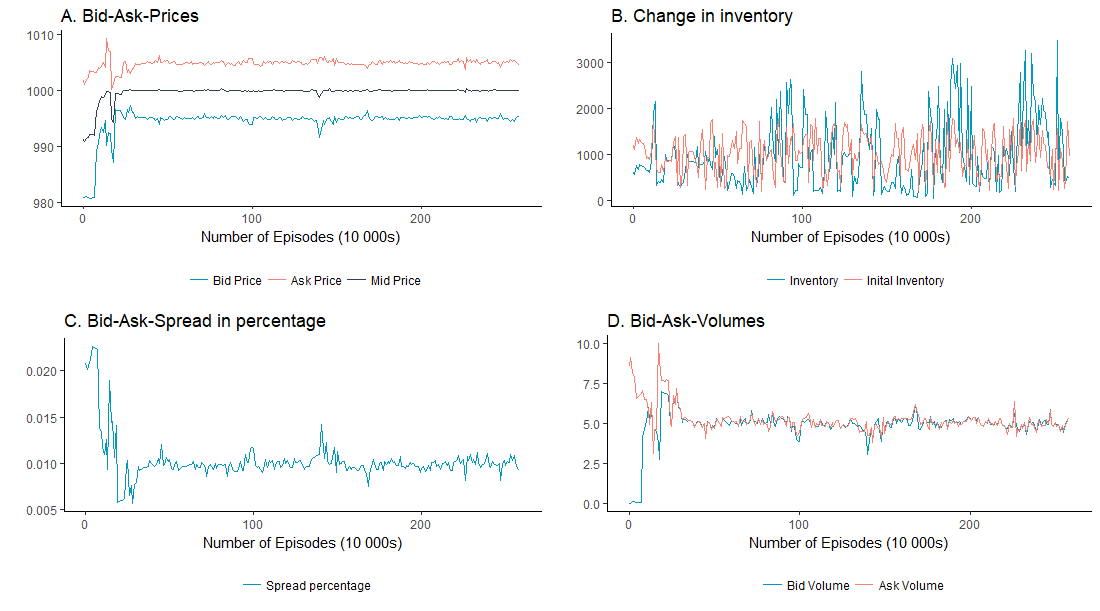
\includegraphics[scale=0.5]{dmv0_basp_inv_multi.png}
		%Captions and Labels can be used since this is a figure environment
		\caption{Plots for DealerMarket-v1, showing the change in bid-ask spread(A), inventory (B), percentage change in spread (c) as well as bid-ask volumes (D). }
		\label{fig:dm12}
%\end{figure}
\end{sidewaysfigure}

% latex table generated in R 3.3.1 by xtable 1.8-2 package
% Fri May 18 00:04:06 2018
\begin{table}[H]
\centering
\caption{Table over inventories and spreads for DealerMarket-v1, DealerMarket-v2 and LOBMarket-v1. With mean, std, max, min and 95 \% confidence interval for the rewards. After training for $2\cdot10^6$ steps}
\label{tab:inv}
\begin{tabular}{rrrrrr}
\hline
 & \textbf{Inventories} \\
  \hline
 Model & Mean & Std & Max & Min & CI \\ 
  \hline
DealerMarket-v1& $939.41$ & $629.04$ & $3024.19$ & $2.67$ & $120.17$  \\
DealerMarket-v2 & $1206.18$ & $831.95$ & $5994.08$ & $0.00$ & $30.26$ \\ 
LOBMarket-v1 & $214.96$ & $133.56$ & $1430.24$ & $-1.00$ & $4.91$ \\ 
   \hline
    & \textbf{Spreads} \\
  \hline
DealerMarket-v1 & $10.28$ & $2.20$ & $22.73$ & $2.38$ & $0.42$ \\
DealerMarket-v2 & $39.49$ & $6.81$ & $47.45$ & $6.50$ & $0.25$ \\ 
LOBMarket-v1  & $22.95$ & $4.36$ & $32.00$ & $4.40$ & $0.16$ \\ 
\hline
\end{tabular}
\end{table}
\autoref{tab:inv} shows a summary over the different agents inventories and spreads. In \autoref{fig:dm12} for DealerMarket-v1, looking at plot (A). The gap between the bid, ask and mid prices is quite big. One would expect that the price difference would be more narrow. Maybe due to the simplistic nature of the environment. However in plot (C) one sees that the spread is decreasing. Looking at the inventory in plot (B) and the volumes in plot (D). The inventory seems to be increasing. While the bid and ask volumes are similar and close to $5$. Interestingly similar to what the Q-value stagnates at. Due to the fact that the agent learns that $5$ in this environment seems to be the optimal volume to post.
\newline
\newline
For DealerMarket-v2 in \autoref{fig:dm22} in figure (A) the prices have tightened. Likely as it gets harder for the agent to make a profit. Hence needing to post more tighter bid and ask quotes. Notice that the inventory seems to be increasing (B), whilst the spread is decreasing (C). However the posted bid, and ask volumes seems to be decreasing. In LOBMarket-v1, \autoref{fig:dm32} the difference between the prices are also very tight. Likely due to that agent post much more bid and ask quotes. The inventory in figure (B) seems to be increasing at the end of training. At the same time the spread in figure (C) is also decreasing. Note that the prices, posted volumes and inventory have all decreased.

%\begin{figure}[H]
\begin{sidewaysfigure}
		%Do not try to scale figure in .tex or you loose font size consistency
	    	\centering
		%The code to input the plot is extremely simple
		%% Created by tikzDevice version 0.11 on 2018-06-30 12:19:54
% !TEX encoding = UTF-8 Unicode
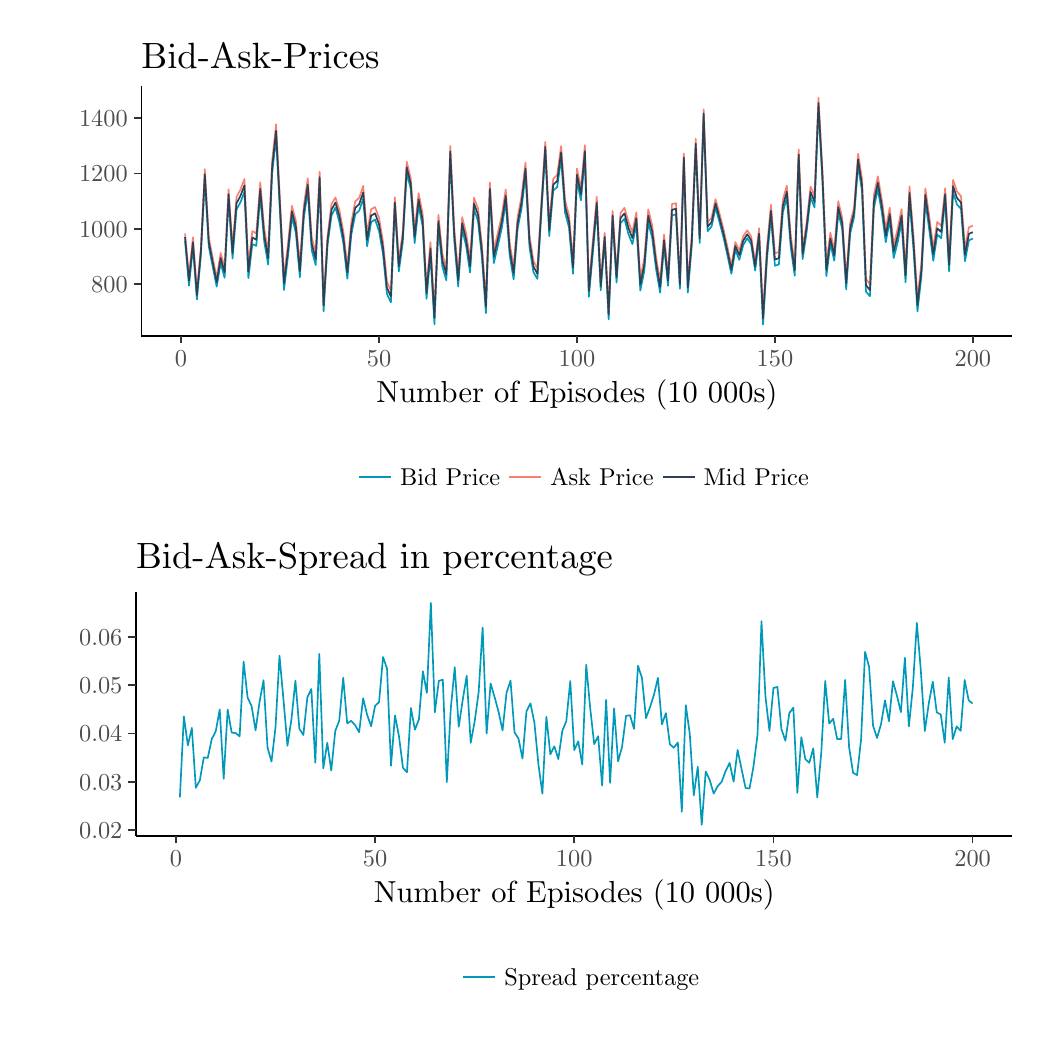
\begin{tikzpicture}[x=1pt,y=1pt]
\definecolor{fillColor}{RGB}{255,255,255}
\path[use as bounding box,fill=fillColor,fill opacity=0.00] (0,0) rectangle (361.35,361.35);
\begin{scope}
\path[clip] (  0.00,180.67) rectangle (361.35,361.35);
\definecolor{drawColor}{RGB}{255,255,255}
\definecolor{fillColor}{RGB}{255,255,255}

\path[draw=drawColor,line width= 0.6pt,line join=round,line cap=round,fill=fillColor] (  0.00,180.67) rectangle (361.35,361.35);
\end{scope}
\begin{scope}
\path[clip] ( 41.12,249.98) rectangle (355.85,340.16);
\definecolor{fillColor}{RGB}{255,255,255}

\path[fill=fillColor] ( 41.12,249.98) rectangle (355.85,340.16);
\definecolor{drawColor}{RGB}{0,153,186}

\path[draw=drawColor,line width= 0.6pt,line join=round] ( 56.86,284.34) --
	( 58.29,268.13) --
	( 59.72,282.00) --
	( 61.15,263.12) --
	( 62.58,279.04) --
	( 64.01,306.54) --
	( 65.44,282.24) --
	( 66.87,275.02) --
	( 68.30,267.77) --
	( 69.73,276.27) --
	( 71.16,270.98) --
	( 72.59,299.44) --
	( 74.03,277.89) --
	( 75.46,295.65) --
	( 76.89,298.29) --
	( 78.32,302.01) --
	( 79.75,270.80) --
	( 81.18,283.16) --
	( 82.61,282.50) --
	( 84.04,300.71) --
	( 85.47,284.05) --
	( 86.90,275.77) --
	( 88.33,308.54) --
	( 89.76,321.73) --
	( 91.19,294.18) --
	( 92.62,266.58) --
	( 94.05,278.69) --
	( 95.48,292.93) --
	( 96.91,287.21) --
	( 98.35,271.15) --
	( 99.78,292.58) --
	(101.21,302.24) --
	(102.64,280.88) --
	(104.07,275.58) --
	(105.50,305.28) --
	(106.93,258.80) --
	(108.36,282.93) --
	(109.79,293.48) --
	(111.22,296.38) --
	(112.65,291.03) --
	(114.08,283.39) --
	(115.51,270.62) --
	(116.94,286.54) --
	(118.37,293.93) --
	(119.80,295.25) --
	(121.23,299.50) --
	(122.66,282.33) --
	(124.10,291.06) --
	(125.53,292.03) --
	(126.96,287.88) --
	(128.39,279.63) --
	(129.82,265.14) --
	(131.25,262.08) --
	(132.68,296.38) --
	(134.11,273.22) --
	(135.54,283.79) --
	(136.97,308.84) --
	(138.40,303.24) --
	(139.83,283.46) --
	(141.26,296.96) --
	(142.69,289.80) --
	(144.12,263.40) --
	(145.55,279.23) --
	(146.98,254.18) --
	(148.42,289.07) --
	(149.85,274.99) --
	(151.28,270.05) --
	(152.71,314.71) --
	(154.14,284.45) --
	(155.57,267.79) --
	(157.00,288.55) --
	(158.43,282.45) --
	(159.86,272.89) --
	(161.29,295.67) --
	(162.72,291.52) --
	(164.15,278.22) --
	(165.58,258.18) --
	(167.01,300.79) --
	(168.44,276.28) --
	(169.87,282.42) --
	(171.30,288.82) --
	(172.74,298.27) --
	(174.17,279.04) --
	(175.60,270.39) --
	(177.03,288.66) --
	(178.46,296.09) --
	(179.89,308.34) --
	(181.32,282.14) --
	(182.75,273.02) --
	(184.18,270.57) --
	(185.61,294.32) --
	(187.04,316.45) --
	(188.47,286.02) --
	(189.90,302.53) --
	(191.33,303.69) --
	(192.76,314.06) --
	(194.19,294.46) --
	(195.62,289.07) --
	(197.06,272.43) --
	(198.49,306.00) --
	(199.92,298.96) --
	(201.35,314.53) --
	(202.78,264.03) --
	(204.21,279.86) --
	(205.64,296.01) --
	(207.07,266.42) --
	(208.50,284.34) --
	(209.93,255.91) --
	(211.36,291.95) --
	(212.79,269.22) --
	(214.22,290.75) --
	(215.65,292.25) --
	(217.08,286.76) --
	(218.51,283.14) --
	(219.94,290.31) --
	(221.38,266.37) --
	(222.81,273.42) --
	(224.24,291.07) --
	(225.67,285.35) --
	(227.10,273.93) --
	(228.53,265.59) --
	(229.96,282.49) --
	(231.39,268.10) --
	(232.82,293.48) --
	(234.25,293.88) --
	(235.68,266.99) --
	(237.11,312.86) --
	(238.54,265.60) --
	(239.97,282.50) --
	(241.40,317.60) --
	(242.83,283.55) --
	(244.26,328.84) --
	(245.70,287.79) --
	(247.13,289.51) --
	(248.56,296.32) --
	(249.99,291.09) --
	(251.42,285.58) --
	(252.85,279.12) --
	(254.28,272.38) --
	(255.71,281.01) --
	(257.14,277.46) --
	(258.57,282.82) --
	(260.00,285.28) --
	(261.43,283.12) --
	(262.86,273.57) --
	(264.29,284.92) --
	(265.72,254.08) --
	(267.15,277.72) --
	(268.58,292.95) --
	(270.02,275.33) --
	(271.45,275.79) --
	(272.88,294.63) --
	(274.31,299.85) --
	(275.74,281.94) --
	(277.17,271.73) --
	(278.60,313.74) --
	(280.03,277.72) --
	(281.46,287.46) --
	(282.89,300.01) --
	(284.32,296.39) --
	(285.75,332.12) --
	(287.18,305.70) --
	(288.61,271.53) --
	(290.04,283.14) --
	(291.47,277.14) --
	(292.90,294.38) --
	(294.33,288.64) --
	(295.77,266.79) --
	(297.20,286.94) --
	(298.63,292.93) --
	(300.06,311.76) --
	(301.49,302.19) --
	(302.92,265.96) --
	(304.35,264.33) --
	(305.78,296.20) --
	(307.21,302.99) --
	(308.64,294.63) --
	(310.07,283.81) --
	(311.50,291.72) --
	(312.93,278.11) --
	(314.36,283.78) --
	(315.79,291.04) --
	(317.22,269.30) --
	(318.65,299.22) --
	(320.09,281.19) --
	(321.52,258.80) --
	(322.95,271.61) --
	(324.38,298.59) --
	(325.81,288.11) --
	(327.24,277.09) --
	(328.67,286.60) --
	(330.10,285.30) --
	(331.53,298.97) --
	(332.96,273.29) --
	(334.39,301.79) --
	(335.82,297.44) --
	(337.25,295.93) --
	(338.68,276.95) --
	(340.11,284.50) --
	(341.54,285.13);
\definecolor{drawColor}{RGB}{250,128,114}

\path[draw=drawColor,line width= 0.6pt,line join=round] ( 56.86,286.97) --
	( 58.29,271.75) --
	( 59.72,285.63) --
	( 61.15,266.31) --
	( 62.58,281.72) --
	( 64.01,310.22) --
	( 65.44,285.64) --
	( 66.87,278.15) --
	( 68.30,270.97) --
	( 69.73,279.96) --
	( 71.16,274.85) --
	( 72.59,302.94) --
	( 74.03,282.08) --
	( 75.46,300.13) --
	( 76.89,302.86) --
	( 78.32,306.65) --
	( 79.75,275.56) --
	( 81.18,287.86) --
	( 82.61,286.99) --
	( 84.04,305.45) --
	( 85.47,288.71) --
	( 86.90,280.45) --
	( 88.33,313.15) --
	( 89.76,326.44) --
	( 91.19,298.71) --
	( 92.62,271.21) --
	( 94.05,283.13) --
	( 95.48,296.98) --
	( 96.91,291.63) --
	( 98.35,275.57) --
	( 99.78,297.01) --
	(101.21,306.93) --
	(102.64,285.47) --
	(104.07,280.07) --
	(105.50,309.37) --
	(106.93,262.99) --
	(108.36,286.13) --
	(109.79,297.63) --
	(111.22,299.98) --
	(112.65,295.34) --
	(114.08,287.61) --
	(115.51,275.06) --
	(116.94,290.83) --
	(118.37,298.61) --
	(119.80,299.88) --
	(121.23,304.14) --
	(122.66,286.97) --
	(124.10,295.75) --
	(125.53,296.51) --
	(126.96,292.63) --
	(128.39,284.06) --
	(129.82,269.65) --
	(131.25,266.21) --
	(132.68,300.09) --
	(134.11,277.08) --
	(135.54,287.68) --
	(136.97,312.92) --
	(138.40,307.02) --
	(139.83,287.95) --
	(141.26,301.56) --
	(142.69,294.33) --
	(144.12,267.57) --
	(145.55,283.83) --
	(146.98,258.88) --
	(148.42,293.73) --
	(149.85,279.61) --
	(151.28,274.42) --
	(152.71,318.60) --
	(154.14,288.96) --
	(155.57,272.27) --
	(157.00,292.86) --
	(158.43,287.07) --
	(159.86,277.50) --
	(161.29,299.90) --
	(162.72,296.08) --
	(164.15,282.78) --
	(165.58,262.77) --
	(167.01,305.45) --
	(168.44,280.92) --
	(169.87,287.10) --
	(171.30,293.48) --
	(172.74,302.90) --
	(174.17,283.63) --
	(175.60,274.77) --
	(177.03,292.84) --
	(178.46,300.44) --
	(179.89,312.65) --
	(181.32,286.50) --
	(182.75,277.10) --
	(184.18,274.18) --
	(185.61,298.00) --
	(187.04,320.07) --
	(188.47,290.43) --
	(189.90,306.73) --
	(191.33,308.15) --
	(192.76,318.57) --
	(194.19,298.93) --
	(195.62,293.53) --
	(197.06,276.91) --
	(198.49,310.45) --
	(199.92,303.36) --
	(201.35,318.90) --
	(202.78,268.34) --
	(204.21,284.17) --
	(205.64,300.22) --
	(207.07,269.61) --
	(208.50,287.22) --
	(209.93,259.22) --
	(211.36,295.11) --
	(212.79,273.03) --
	(214.22,294.36) --
	(215.65,296.25) --
	(217.08,291.23) --
	(218.51,287.45) --
	(219.94,294.64) --
	(221.38,270.80) --
	(222.81,278.01) --
	(224.24,295.69) --
	(225.67,289.95) --
	(227.10,278.22) --
	(228.53,269.76) --
	(229.96,286.59) --
	(231.39,271.77) --
	(232.82,297.59) --
	(234.25,297.92) --
	(235.68,270.10) --
	(237.11,315.89) --
	(238.54,269.29) --
	(239.97,286.39) --
	(241.40,321.21) --
	(242.83,286.80) --
	(244.26,331.87) --
	(245.70,291.08) --
	(247.13,292.67) --
	(248.56,299.37) --
	(249.99,294.16) --
	(251.42,288.58) --
	(252.85,282.13) --
	(254.28,275.32) --
	(255.71,283.87) --
	(257.14,280.83) --
	(258.57,285.99) --
	(260.00,288.13) --
	(261.43,285.90) --
	(262.86,276.48) --
	(264.29,288.90) --
	(265.72,258.48) --
	(267.15,282.17) --
	(268.58,297.35) --
	(270.02,279.83) --
	(271.45,280.33) --
	(272.88,299.14) --
	(274.31,304.29) --
	(275.74,286.26) --
	(277.17,275.67) --
	(278.60,317.30) --
	(280.03,281.35) --
	(281.46,291.01) --
	(282.89,303.92) --
	(284.32,300.52) --
	(285.75,336.06) --
	(287.18,310.07) --
	(288.61,275.97) --
	(290.04,287.28) --
	(291.47,281.11) --
	(292.90,298.65) --
	(294.33,292.67) --
	(295.77,270.99) --
	(297.20,290.73) --
	(298.63,296.35) --
	(300.06,315.75) --
	(301.49,306.76) --
	(302.92,270.61) --
	(304.35,268.63) --
	(305.78,300.87) --
	(307.21,307.63) --
	(308.64,299.26) --
	(310.07,288.49) --
	(311.50,296.30) --
	(312.93,282.89) --
	(314.36,288.55) --
	(315.79,295.79) --
	(317.22,274.04) --
	(318.65,304.00) --
	(320.09,286.01) --
	(321.52,263.49) --
	(322.95,276.26) --
	(324.38,303.23) --
	(325.81,292.93) --
	(327.24,281.81) --
	(328.67,291.14) --
	(330.10,289.73) --
	(331.53,303.34) --
	(332.96,277.89) --
	(334.39,306.36) --
	(335.82,302.14) --
	(337.25,300.46) --
	(338.68,281.69) --
	(340.11,289.21) --
	(341.54,289.79);
\definecolor{drawColor}{RGB}{46,64,83}

\path[draw=drawColor,line width= 0.6pt,line join=round] ( 56.86,285.65) --
	( 58.29,269.94) --
	( 59.72,283.81) --
	( 61.15,264.72) --
	( 62.58,280.38) --
	( 64.01,308.38) --
	( 65.44,283.94) --
	( 66.87,276.59) --
	( 68.30,269.37) --
	( 69.73,278.12) --
	( 71.16,272.91) --
	( 72.59,301.19) --
	( 74.03,279.99) --
	( 75.46,297.89) --
	( 76.89,300.58) --
	( 78.32,304.33) --
	( 79.75,273.18) --
	( 81.18,285.51) --
	( 82.61,284.74) --
	( 84.04,303.08) --
	( 85.47,286.38) --
	( 86.90,278.11) --
	( 88.33,310.85) --
	( 89.76,324.09) --
	( 91.19,296.45) --
	( 92.62,268.90) --
	( 94.05,280.91) --
	( 95.48,294.95) --
	( 96.91,289.42) --
	( 98.35,273.36) --
	( 99.78,294.80) --
	(101.21,304.59) --
	(102.64,283.18) --
	(104.07,277.83) --
	(105.50,307.33) --
	(106.93,260.90) --
	(108.36,284.53) --
	(109.79,295.55) --
	(111.22,298.18) --
	(112.65,293.19) --
	(114.08,285.50) --
	(115.51,272.84) --
	(116.94,288.68) --
	(118.37,296.27) --
	(119.80,297.57) --
	(121.23,301.82) --
	(122.66,284.65) --
	(124.10,293.41) --
	(125.53,294.27) --
	(126.96,290.25) --
	(128.39,281.84) --
	(129.82,267.40) --
	(131.25,264.15) --
	(132.68,298.24) --
	(134.11,275.15) --
	(135.54,285.74) --
	(136.97,310.88) --
	(138.40,305.13) --
	(139.83,285.71) --
	(141.26,299.26) --
	(142.69,292.07) --
	(144.12,265.48) --
	(145.55,281.53) --
	(146.98,256.53) --
	(148.42,291.40) --
	(149.85,277.30) --
	(151.28,272.24) --
	(152.71,316.66) --
	(154.14,286.71) --
	(155.57,270.03) --
	(157.00,290.71) --
	(158.43,284.76) --
	(159.86,275.19) --
	(161.29,297.78) --
	(162.72,293.80) --
	(164.15,280.50) --
	(165.58,260.48) --
	(167.01,303.12) --
	(168.44,278.60) --
	(169.87,284.76) --
	(171.30,291.15) --
	(172.74,300.59) --
	(174.17,281.33) --
	(175.60,272.58) --
	(177.03,290.75) --
	(178.46,298.26) --
	(179.89,310.50) --
	(181.32,284.32) --
	(182.75,275.06) --
	(184.18,272.38) --
	(185.61,296.16) --
	(187.04,318.26) --
	(188.47,288.23) --
	(189.90,304.63) --
	(191.33,305.92) --
	(192.76,316.32) --
	(194.19,296.69) --
	(195.62,291.30) --
	(197.06,274.67) --
	(198.49,308.22) --
	(199.92,301.16) --
	(201.35,316.72) --
	(202.78,266.19) --
	(204.21,282.01) --
	(205.64,298.12) --
	(207.07,268.02) --
	(208.50,285.78) --
	(209.93,257.57) --
	(211.36,293.53) --
	(212.79,271.13) --
	(214.22,292.56) --
	(215.65,294.25) --
	(217.08,289.00) --
	(218.51,285.30) --
	(219.94,292.48) --
	(221.38,268.59) --
	(222.81,275.72) --
	(224.24,293.38) --
	(225.67,287.65) --
	(227.10,276.08) --
	(228.53,267.67) --
	(229.96,284.54) --
	(231.39,269.93) --
	(232.82,295.54) --
	(234.25,295.90) --
	(235.68,268.55) --
	(237.11,314.38) --
	(238.54,267.45) --
	(239.97,284.45) --
	(241.40,319.41) --
	(242.83,285.18) --
	(244.26,330.36) --
	(245.70,289.43) --
	(247.13,291.09) --
	(248.56,297.84) --
	(249.99,292.62) --
	(251.42,287.08) --
	(252.85,280.63) --
	(254.28,273.85) --
	(255.71,282.44) --
	(257.14,279.15) --
	(258.57,284.41) --
	(260.00,286.70) --
	(261.43,284.51) --
	(262.86,275.02) --
	(264.29,286.91) --
	(265.72,256.28) --
	(267.15,279.95) --
	(268.58,295.15) --
	(270.02,277.58) --
	(271.45,278.06) --
	(272.88,296.88) --
	(274.31,302.07) --
	(275.74,284.10) --
	(277.17,273.70) --
	(278.60,315.52) --
	(280.03,279.53) --
	(281.46,289.23) --
	(282.89,301.96) --
	(284.32,298.46) --
	(285.75,334.09) --
	(287.18,307.89) --
	(288.61,273.75) --
	(290.04,285.21) --
	(291.47,279.13) --
	(292.90,296.52) --
	(294.33,290.66) --
	(295.77,268.89) --
	(297.20,288.83) --
	(298.63,294.64) --
	(300.06,313.75) --
	(301.49,304.47) --
	(302.92,268.29) --
	(304.35,266.48) --
	(305.78,298.53) --
	(307.21,305.31) --
	(308.64,296.95) --
	(310.07,286.15) --
	(311.50,294.01) --
	(312.93,280.50) --
	(314.36,286.17) --
	(315.79,293.41) --
	(317.22,271.67) --
	(318.65,301.61) --
	(320.09,283.60) --
	(321.52,261.14) --
	(322.95,273.94) --
	(324.38,300.91) --
	(325.81,290.52) --
	(327.24,279.45) --
	(328.67,288.87) --
	(330.10,287.51) --
	(331.53,301.16) --
	(332.96,275.59) --
	(334.39,304.08) --
	(335.82,299.79) --
	(337.25,298.19) --
	(338.68,279.32) --
	(340.11,286.85) --
	(341.54,287.46);
\end{scope}
\begin{scope}
\path[clip] (  0.00,  0.00) rectangle (361.35,361.35);
\definecolor{drawColor}{RGB}{0,0,0}

\path[draw=drawColor,line width= 0.6pt,line join=round] ( 41.12,249.98) --
	( 41.12,340.16);
\end{scope}
\begin{scope}
\path[clip] (  0.00,  0.00) rectangle (361.35,361.35);
\definecolor{drawColor}{gray}{0.30}

\node[text=drawColor,anchor=base east,inner sep=0pt, outer sep=0pt, scale=  0.88] at ( 36.17,265.64) {800};

\node[text=drawColor,anchor=base east,inner sep=0pt, outer sep=0pt, scale=  0.88] at ( 36.17,285.62) {1000};

\node[text=drawColor,anchor=base east,inner sep=0pt, outer sep=0pt, scale=  0.88] at ( 36.17,305.59) {1200};

\node[text=drawColor,anchor=base east,inner sep=0pt, outer sep=0pt, scale=  0.88] at ( 36.17,325.57) {1400};
\end{scope}
\begin{scope}
\path[clip] (  0.00,  0.00) rectangle (361.35,361.35);
\definecolor{drawColor}{gray}{0.20}

\path[draw=drawColor,line width= 0.6pt,line join=round] ( 38.37,268.67) --
	( 41.12,268.67);

\path[draw=drawColor,line width= 0.6pt,line join=round] ( 38.37,288.65) --
	( 41.12,288.65);

\path[draw=drawColor,line width= 0.6pt,line join=round] ( 38.37,308.62) --
	( 41.12,308.62);

\path[draw=drawColor,line width= 0.6pt,line join=round] ( 38.37,328.60) --
	( 41.12,328.60);
\end{scope}
\begin{scope}
\path[clip] (  0.00,  0.00) rectangle (361.35,361.35);
\definecolor{drawColor}{RGB}{0,0,0}

\path[draw=drawColor,line width= 0.6pt,line join=round] ( 41.12,249.98) --
	(355.85,249.98);
\end{scope}
\begin{scope}
\path[clip] (  0.00,  0.00) rectangle (361.35,361.35);
\definecolor{drawColor}{gray}{0.20}

\path[draw=drawColor,line width= 0.6pt,line join=round] ( 55.43,247.23) --
	( 55.43,249.98);

\path[draw=drawColor,line width= 0.6pt,line join=round] (126.96,247.23) --
	(126.96,249.98);

\path[draw=drawColor,line width= 0.6pt,line join=round] (198.49,247.23) --
	(198.49,249.98);

\path[draw=drawColor,line width= 0.6pt,line join=round] (270.02,247.23) --
	(270.02,249.98);

\path[draw=drawColor,line width= 0.6pt,line join=round] (341.54,247.23) --
	(341.54,249.98);
\end{scope}
\begin{scope}
\path[clip] (  0.00,  0.00) rectangle (361.35,361.35);
\definecolor{drawColor}{gray}{0.30}

\node[text=drawColor,anchor=base,inner sep=0pt, outer sep=0pt, scale=  0.88] at ( 55.43,238.97) {0};

\node[text=drawColor,anchor=base,inner sep=0pt, outer sep=0pt, scale=  0.88] at (126.96,238.97) {50};

\node[text=drawColor,anchor=base,inner sep=0pt, outer sep=0pt, scale=  0.88] at (198.49,238.97) {100};

\node[text=drawColor,anchor=base,inner sep=0pt, outer sep=0pt, scale=  0.88] at (270.02,238.97) {150};

\node[text=drawColor,anchor=base,inner sep=0pt, outer sep=0pt, scale=  0.88] at (341.54,238.97) {200};
\end{scope}
\begin{scope}
\path[clip] (  0.00,  0.00) rectangle (361.35,361.35);
\definecolor{drawColor}{RGB}{0,0,0}

\node[text=drawColor,anchor=base,inner sep=0pt, outer sep=0pt, scale=  1.10] at (198.49,225.89) {Number of Episodes (10 000s)};
\end{scope}
\begin{scope}
\path[clip] (  0.00,  0.00) rectangle (361.35,361.35);
\definecolor{fillColor}{RGB}{255,255,255}

\path[fill=fillColor] (109.01,186.17) rectangle (287.96,212.01);
\end{scope}
\begin{scope}
\path[clip] (  0.00,  0.00) rectangle (361.35,361.35);
\definecolor{drawColor}{RGB}{0,153,186}

\path[draw=drawColor,line width= 0.6pt,line join=round] (119.76,199.09) -- (131.32,199.09);
\end{scope}
\begin{scope}
\path[clip] (  0.00,  0.00) rectangle (361.35,361.35);
\definecolor{drawColor}{RGB}{250,128,114}

\path[draw=drawColor,line width= 0.6pt,line join=round] (174.02,199.09) -- (185.58,199.09);
\end{scope}
\begin{scope}
\path[clip] (  0.00,  0.00) rectangle (361.35,361.35);
\definecolor{drawColor}{RGB}{46,64,83}

\path[draw=drawColor,line width= 0.6pt,line join=round] (229.43,199.09) -- (240.99,199.09);
\end{scope}
\begin{scope}
\path[clip] (  0.00,  0.00) rectangle (361.35,361.35);
\definecolor{drawColor}{RGB}{0,0,0}

\node[text=drawColor,anchor=base west,inner sep=0pt, outer sep=0pt, scale=  0.88] at (134.57,196.06) {Bid Price};
\end{scope}
\begin{scope}
\path[clip] (  0.00,  0.00) rectangle (361.35,361.35);
\definecolor{drawColor}{RGB}{0,0,0}

\node[text=drawColor,anchor=base west,inner sep=0pt, outer sep=0pt, scale=  0.88] at (188.84,196.06) {Ask Price};
\end{scope}
\begin{scope}
\path[clip] (  0.00,  0.00) rectangle (361.35,361.35);
\definecolor{drawColor}{RGB}{0,0,0}

\node[text=drawColor,anchor=base west,inner sep=0pt, outer sep=0pt, scale=  0.88] at (244.25,196.06) {Mid Price};
\end{scope}
\begin{scope}
\path[clip] (  0.00,  0.00) rectangle (361.35,361.35);
\definecolor{drawColor}{RGB}{0,0,0}

\node[text=drawColor,anchor=base west,inner sep=0pt, outer sep=0pt, scale=  1.32] at ( 41.12,346.76) {Bid-Ask-Prices};
\end{scope}
\begin{scope}
\path[clip] (  0.00,  0.00) rectangle (361.35,180.67);
\definecolor{drawColor}{RGB}{255,255,255}
\definecolor{fillColor}{RGB}{255,255,255}

\path[draw=drawColor,line width= 0.6pt,line join=round,line cap=round,fill=fillColor] (  0.00, -0.00) rectangle (361.35,180.67);
\end{scope}
\begin{scope}
\path[clip] ( 39.17, 69.30) rectangle (355.85,157.54);
\definecolor{fillColor}{RGB}{255,255,255}

\path[fill=fillColor] ( 39.17, 69.30) rectangle (355.85,157.54);
\definecolor{drawColor}{RGB}{0,153,186}

\path[draw=drawColor,line width= 0.6pt,line join=round] ( 55.00, 83.19) --
	( 56.44,112.50) --
	( 57.88,102.00) --
	( 59.32,108.30) --
	( 60.76, 86.69) --
	( 62.20, 89.35) --
	( 63.64, 97.66) --
	( 65.08, 97.49) --
	( 66.52,104.31) --
	( 67.96,107.07) --
	( 69.40,115.02) --
	( 70.83, 89.92) --
	( 72.27,114.94) --
	( 73.71,106.64) --
	( 75.15,106.45) --
	( 76.59,105.25) --
	( 78.03,132.27) --
	( 79.47,119.28) --
	( 80.91,116.21) --
	( 82.35,107.45) --
	( 83.79,117.75) --
	( 85.23,125.54) --
	( 86.67,101.20) --
	( 88.11, 96.15) --
	( 89.55,108.43) --
	( 90.99,134.40) --
	( 92.43,118.59) --
	( 93.87,101.85) --
	( 95.31,111.43) --
	( 96.75,125.35) --
	( 98.18,108.00) --
	( 99.62,105.76) --
	(101.06,119.36) --
	(102.50,122.36) --
	(103.94, 95.75) --
	(105.38,135.03) --
	(106.82, 93.71) --
	(108.26,102.97) --
	(109.70, 92.94) --
	(111.14,107.21) --
	(112.58,110.93) --
	(114.02,126.46) --
	(115.46,109.92) --
	(116.90,110.87) --
	(118.34,109.29) --
	(119.78,106.78) --
	(121.22,119.02) --
	(122.66,113.05) --
	(124.10,108.93) --
	(125.53,116.27) --
	(126.97,117.64) --
	(128.41,133.92) --
	(129.85,129.73) --
	(131.29, 94.67) --
	(132.73,112.82) --
	(134.17,105.25) --
	(135.61, 93.92) --
	(137.05, 92.27) --
	(138.49,115.50) --
	(139.93,107.66) --
	(141.37,111.39) --
	(142.81,128.79) --
	(144.25,120.95) --
	(145.69,153.53) --
	(147.13,113.96) --
	(148.57,125.31) --
	(150.01,125.75) --
	(151.45, 88.71) --
	(152.88,115.21) --
	(154.32,130.23) --
	(155.76,108.70) --
	(157.20,118.43) --
	(158.64,127.17) --
	(160.08,102.91) --
	(161.52,110.61) --
	(162.96,121.27) --
	(164.40,144.60) --
	(165.84,106.29) --
	(167.28,124.38) --
	(168.72,119.46) --
	(170.16,114.10) --
	(171.60,107.40) --
	(173.04,121.04) --
	(174.48,125.40) --
	(175.92,106.72) --
	(177.36,104.44) --
	(178.80, 97.23) --
	(180.23,114.29) --
	(181.67,117.18) --
	(183.11,110.17) --
	(184.55, 95.22) --
	(185.99, 84.58) --
	(187.43,112.34) --
	(188.87, 98.75) --
	(190.31,101.66) --
	(191.75, 97.07) --
	(193.19,107.27) --
	(194.63,110.75) --
	(196.07,125.24) --
	(197.51,100.29) --
	(198.95,103.46) --
	(200.39, 95.09) --
	(201.83,131.11) --
	(203.27,115.37) --
	(204.71,102.47) --
	(206.15,105.30) --
	(207.58, 87.47) --
	(209.02,118.49) --
	(210.46, 88.47) --
	(211.90,115.38) --
	(213.34, 96.24) --
	(214.78,101.50) --
	(216.22,112.70) --
	(217.66,112.88) --
	(219.10,107.96) --
	(220.54,130.77) --
	(221.98,126.32) --
	(223.42,111.84) --
	(224.86,115.77) --
	(226.30,120.24) --
	(227.74,126.41) --
	(229.18,109.60) --
	(230.62,113.65) --
	(232.06,102.38) --
	(233.50,101.16) --
	(234.93,103.09) --
	(236.37, 78.01) --
	(237.81,116.54) --
	(239.25,106.13) --
	(240.69, 83.95) --
	(242.13, 94.26) --
	(243.57, 73.31) --
	(245.01, 92.57) --
	(246.45, 89.52) --
	(247.89, 84.59) --
	(249.33, 87.28) --
	(250.77, 88.85) --
	(252.21, 92.75) --
	(253.65, 95.68) --
	(255.09, 88.87) --
	(256.53,100.34) --
	(257.97, 93.38) --
	(259.41, 86.61) --
	(260.84, 86.41) --
	(262.28, 94.47) --
	(263.72,105.81) --
	(265.16,146.86) --
	(266.60,119.58) --
	(268.04,107.21) --
	(269.48,122.74) --
	(270.92,123.11) --
	(272.36,107.87) --
	(273.80,103.67) --
	(275.24,113.73) --
	(276.68,115.63) --
	(278.12, 84.86) --
	(279.56,104.97) --
	(281.00, 97.03) --
	(282.44, 95.72) --
	(283.88,100.93) --
	(285.32, 83.17) --
	(286.76, 99.33) --
	(288.19,125.28) --
	(289.63,109.88) --
	(291.07,111.61) --
	(292.51,104.26) --
	(293.95,104.31) --
	(295.39,125.65) --
	(296.83,101.25) --
	(298.27, 92.04) --
	(299.71, 91.29) --
	(301.15,104.14) --
	(302.59,135.77) --
	(304.03,130.45) --
	(305.47,109.16) --
	(306.91,104.68) --
	(308.35,109.65) --
	(309.79,118.27) --
	(311.23,110.72) --
	(312.67,125.18) --
	(314.11,119.94) --
	(315.54,114.00) --
	(316.98,133.63) --
	(318.42,108.83) --
	(319.86,122.99) --
	(321.30,146.25) --
	(322.74,129.12) --
	(324.18,107.19) --
	(325.62,117.21) --
	(327.06,125.03) --
	(328.50,113.91) --
	(329.94,113.18) --
	(331.38,102.96) --
	(332.82,126.52) --
	(334.26,104.27) --
	(335.70,108.87) --
	(337.14,107.25) --
	(338.58,125.64) --
	(340.02,118.29) --
	(341.46,117.14);
\end{scope}
\begin{scope}
\path[clip] (  0.00,  0.00) rectangle (361.35,361.35);
\definecolor{drawColor}{RGB}{0,0,0}

\path[draw=drawColor,line width= 0.6pt,line join=round] ( 39.17, 69.30) --
	( 39.17,157.54);
\end{scope}
\begin{scope}
\path[clip] (  0.00,  0.00) rectangle (361.35,361.35);
\definecolor{drawColor}{gray}{0.30}

\node[text=drawColor,anchor=base east,inner sep=0pt, outer sep=0pt, scale=  0.88] at ( 34.22, 68.33) {0.02};

\node[text=drawColor,anchor=base east,inner sep=0pt, outer sep=0pt, scale=  0.88] at ( 34.22, 85.80) {0.03};

\node[text=drawColor,anchor=base east,inner sep=0pt, outer sep=0pt, scale=  0.88] at ( 34.22,103.26) {0.04};

\node[text=drawColor,anchor=base east,inner sep=0pt, outer sep=0pt, scale=  0.88] at ( 34.22,120.73) {0.05};

\node[text=drawColor,anchor=base east,inner sep=0pt, outer sep=0pt, scale=  0.88] at ( 34.22,138.19) {0.06};
\end{scope}
\begin{scope}
\path[clip] (  0.00,  0.00) rectangle (361.35,361.35);
\definecolor{drawColor}{gray}{0.20}

\path[draw=drawColor,line width= 0.6pt,line join=round] ( 36.42, 71.36) --
	( 39.17, 71.36);

\path[draw=drawColor,line width= 0.6pt,line join=round] ( 36.42, 88.83) --
	( 39.17, 88.83);

\path[draw=drawColor,line width= 0.6pt,line join=round] ( 36.42,106.29) --
	( 39.17,106.29);

\path[draw=drawColor,line width= 0.6pt,line join=round] ( 36.42,123.76) --
	( 39.17,123.76);

\path[draw=drawColor,line width= 0.6pt,line join=round] ( 36.42,141.22) --
	( 39.17,141.22);
\end{scope}
\begin{scope}
\path[clip] (  0.00,  0.00) rectangle (361.35,361.35);
\definecolor{drawColor}{RGB}{0,0,0}

\path[draw=drawColor,line width= 0.6pt,line join=round] ( 39.17, 69.30) --
	(355.85, 69.30);
\end{scope}
\begin{scope}
\path[clip] (  0.00,  0.00) rectangle (361.35,361.35);
\definecolor{drawColor}{gray}{0.20}

\path[draw=drawColor,line width= 0.6pt,line join=round] ( 53.56, 66.55) --
	( 53.56, 69.30);

\path[draw=drawColor,line width= 0.6pt,line join=round] (125.53, 66.55) --
	(125.53, 69.30);

\path[draw=drawColor,line width= 0.6pt,line join=round] (197.51, 66.55) --
	(197.51, 69.30);

\path[draw=drawColor,line width= 0.6pt,line join=round] (269.48, 66.55) --
	(269.48, 69.30);

\path[draw=drawColor,line width= 0.6pt,line join=round] (341.46, 66.55) --
	(341.46, 69.30);
\end{scope}
\begin{scope}
\path[clip] (  0.00,  0.00) rectangle (361.35,361.35);
\definecolor{drawColor}{gray}{0.30}

\node[text=drawColor,anchor=base,inner sep=0pt, outer sep=0pt, scale=  0.88] at ( 53.56, 58.29) {0};

\node[text=drawColor,anchor=base,inner sep=0pt, outer sep=0pt, scale=  0.88] at (125.53, 58.29) {50};

\node[text=drawColor,anchor=base,inner sep=0pt, outer sep=0pt, scale=  0.88] at (197.51, 58.29) {100};

\node[text=drawColor,anchor=base,inner sep=0pt, outer sep=0pt, scale=  0.88] at (269.48, 58.29) {150};

\node[text=drawColor,anchor=base,inner sep=0pt, outer sep=0pt, scale=  0.88] at (341.46, 58.29) {200};
\end{scope}
\begin{scope}
\path[clip] (  0.00,  0.00) rectangle (361.35,361.35);
\definecolor{drawColor}{RGB}{0,0,0}

\node[text=drawColor,anchor=base,inner sep=0pt, outer sep=0pt, scale=  1.10] at (197.51, 45.22) {Number of Episodes (10 000s)};
\end{scope}
\begin{scope}
\path[clip] (  0.00,  0.00) rectangle (361.35,361.35);
\definecolor{fillColor}{RGB}{255,255,255}

\path[fill=fillColor] (146.66,  5.50) rectangle (248.35, 31.34);
\end{scope}
\begin{scope}
\path[clip] (  0.00,  0.00) rectangle (361.35,361.35);
\definecolor{drawColor}{RGB}{0,153,186}

\path[draw=drawColor,line width= 0.6pt,line join=round] (157.41, 18.42) -- (168.98, 18.42);
\end{scope}
\begin{scope}
\path[clip] (  0.00,  0.00) rectangle (361.35,361.35);
\definecolor{drawColor}{RGB}{0,0,0}

\node[text=drawColor,anchor=base west,inner sep=0pt, outer sep=0pt, scale=  0.88] at (172.23, 15.39) {Spread percentage};
\end{scope}
\begin{scope}
\path[clip] (  0.00,  0.00) rectangle (361.35,361.35);
\definecolor{drawColor}{RGB}{0,0,0}

\node[text=drawColor,anchor=base west,inner sep=0pt, outer sep=0pt, scale=  1.32] at ( 39.17,166.08) {Bid-Ask-Spread in percentage};
\end{scope}
\end{tikzpicture}

		% Created by tikzDevice version 0.11 on 2018-07-26 20:16:22
% !TEX encoding = UTF-8 Unicode
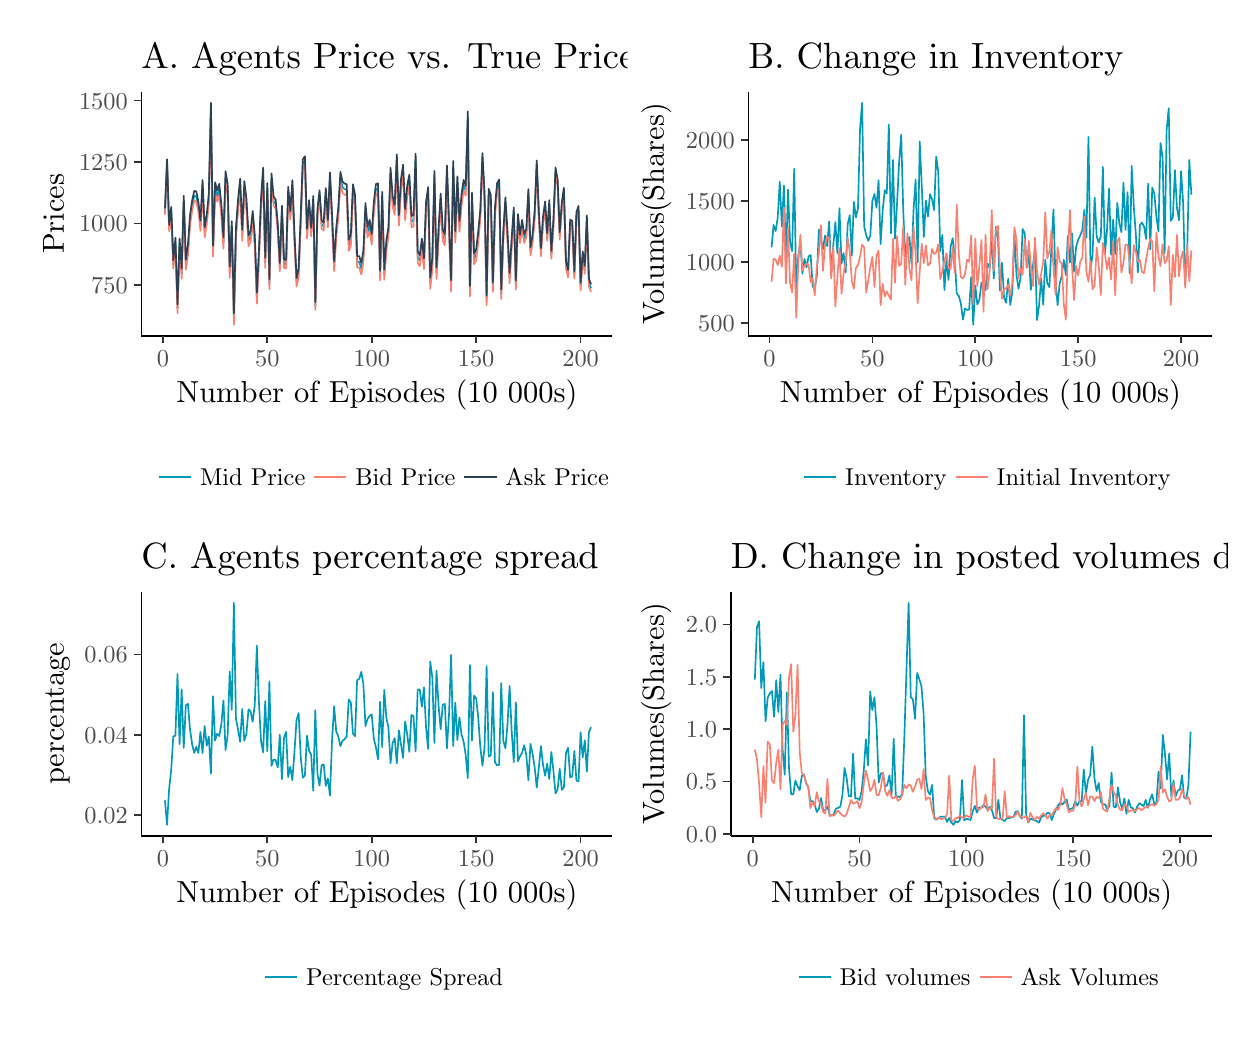
\begin{tikzpicture}[x=1pt,y=1pt]
\definecolor{fillColor}{RGB}{255,255,255}
\path[use as bounding box,fill=fillColor,fill opacity=0.00] (0,0) rectangle (433.62,361.35);
\begin{scope}
\path[clip] (  0.00,180.67) rectangle (216.81,361.35);
\definecolor{drawColor}{RGB}{255,255,255}
\definecolor{fillColor}{RGB}{255,255,255}

\path[draw=drawColor,line width= 0.6pt,line join=round,line cap=round,fill=fillColor] (  0.00,180.67) rectangle (216.81,361.35);
\end{scope}
\begin{scope}
\path[clip] ( 41.12,249.98) rectangle (211.31,338.21);
\definecolor{fillColor}{RGB}{255,255,255}

\path[fill=fillColor] ( 41.12,249.98) rectangle (211.31,338.21);
\definecolor{drawColor}{RGB}{0,153,186}

\path[draw=drawColor,line width= 0.6pt,line join=round] ( 49.61,294.91) --
	( 50.37,312.81) --
	( 51.12,288.86) --
	( 51.88,295.08) --
	( 52.63,275.79) --
	( 53.39,283.79) --
	( 54.14,259.79) --
	( 54.90,283.57) --
	( 55.65,272.43) --
	( 56.40,298.83) --
	( 57.16,275.64) --
	( 57.91,280.87) --
	( 58.67,291.70) --
	( 59.42,297.02) --
	( 60.18,300.56) --
	( 60.93,300.36) --
	( 61.69,296.67) --
	( 62.44,289.83) --
	( 63.20,304.45) --
	( 63.95,287.38) --
	( 64.71,292.12) --
	( 65.46,299.45) --
	( 66.22,332.20) --
	( 66.97,280.63) --
	( 67.73,303.50) --
	( 68.48,300.46) --
	( 69.23,302.84) --
	( 69.99,295.36) --
	( 70.74,283.58) --
	( 71.50,307.49) --
	( 72.25,303.00) --
	( 73.01,272.97) --
	( 73.76,289.31) --
	( 74.52,256.05) --
	( 75.27,287.27) --
	( 76.03,297.42) --
	( 76.78,304.82) --
	( 77.54,286.31) --
	( 78.29,303.87) --
	( 79.05,297.61) --
	( 79.80,284.27) --
	( 80.56,285.90) --
	( 81.31,293.08) --
	( 82.07,284.33) --
	( 82.82,263.57) --
	( 83.57,278.91) --
	( 84.33,297.93) --
	( 85.08,308.81) --
	( 85.84,276.33) --
	( 86.59,303.35) --
	( 87.35,268.60) --
	( 88.10,306.98) --
	( 88.86,298.65) --
	( 89.61,297.57) --
	( 90.37,289.03) --
	( 91.12,274.79) --
	( 91.88,295.64) --
	( 92.63,276.03) --
	( 93.39,275.94) --
	( 94.14,302.35) --
	( 94.90,293.53) --
	( 95.65,304.77) --
	( 96.40,285.56) --
	( 97.16,269.35) --
	( 97.91,272.84) --
	( 98.67,291.88) --
	( 99.42,312.14) --
	(100.18,313.21) --
	(100.93,286.90) --
	(101.69,297.27) --
	(102.44,287.48) --
	(103.20,299.22) --
	(103.95,260.75) --
	(104.71,294.38) --
	(105.46,301.20) --
	(106.22,290.25) --
	(106.97,289.45) --
	(107.73,302.01) --
	(108.48,290.47) --
	(109.23,307.74) --
	(109.99,292.03) --
	(110.74,275.13) --
	(111.50,287.26) --
	(112.25,294.48) --
	(113.01,307.28) --
	(113.76,303.68) --
	(114.52,303.05) --
	(115.27,302.72) --
	(116.03,282.69) --
	(116.78,284.57) --
	(117.54,302.70) --
	(118.29,299.04) --
	(119.05,276.73) --
	(119.80,276.72) --
	(120.56,274.24) --
	(121.31,278.63) --
	(122.06,295.94) --
	(122.82,287.48) --
	(123.57,289.89) --
	(124.33,284.86) --
	(125.08,296.41) --
	(125.84,302.92) --
	(126.59,303.35) --
	(127.35,271.70) --
	(128.10,300.17) --
	(128.86,272.11) --
	(129.61,282.65) --
	(130.37,287.39) --
	(131.12,308.93) --
	(131.88,298.52) --
	(132.63,295.60) --
	(133.39,313.70) --
	(134.14,291.71) --
	(134.90,304.63) --
	(135.65,309.96) --
	(136.40,293.73) --
	(137.16,302.42) --
	(137.91,306.32) --
	(138.67,291.25) --
	(139.42,291.65) --
	(140.18,313.83) --
	(140.93,278.41) --
	(141.69,277.14) --
	(142.44,283.13) --
	(143.20,276.00) --
	(143.95,296.45) --
	(144.71,301.88) --
	(145.46,268.99) --
	(146.22,276.13) --
	(146.97,307.53) --
	(147.73,272.60) --
	(148.48,286.84) --
	(149.23,299.30) --
	(149.99,286.33) --
	(150.74,284.70) --
	(151.50,309.56) --
	(152.25,289.61) --
	(153.01,267.93) --
	(153.76,311.10) --
	(154.52,285.74) --
	(155.27,305.61) --
	(156.03,289.57) --
	(156.78,299.29) --
	(157.54,304.32) --
	(158.29,302.42) --
	(159.05,329.17) --
	(159.80,266.09) --
	(160.56,299.80) --
	(161.31,277.77) --
	(162.06,279.22) --
	(162.82,285.87) --
	(163.57,293.94) --
	(164.33,314.19) --
	(165.08,300.07) --
	(165.84,262.78) --
	(166.59,301.36) --
	(167.35,299.20) --
	(168.10,267.53) --
	(168.86,294.89) --
	(169.61,303.42) --
	(170.37,304.77) --
	(171.12,265.01) --
	(171.88,286.40) --
	(172.63,298.25) --
	(173.39,285.61) --
	(174.14,270.83) --
	(174.89,283.49) --
	(175.65,294.83) --
	(176.40,268.28) --
	(177.16,292.44) --
	(177.91,285.00) --
	(178.67,290.27) --
	(179.42,285.12) --
	(180.18,286.98) --
	(180.93,301.60) --
	(181.69,280.49) --
	(182.44,285.07) --
	(183.20,293.61) --
	(183.95,311.90) --
	(184.71,293.51) --
	(185.46,280.22) --
	(186.22,291.53) --
	(186.97,297.13) --
	(187.73,285.71) --
	(188.48,297.62) --
	(189.23,279.25) --
	(189.99,290.76) --
	(190.74,309.42) --
	(191.50,305.14) --
	(192.25,286.12) --
	(193.01,296.94) --
	(193.76,302.13) --
	(194.52,275.57) --
	(195.27,272.46) --
	(196.03,290.67) --
	(196.78,290.16) --
	(197.54,271.94) --
	(198.29,293.39) --
	(199.05,295.57) --
	(199.80,267.73) --
	(200.56,279.16) --
	(201.31,273.83) --
	(202.06,292.11) --
	(202.82,269.10) --
	(203.57,267.22);
\definecolor{drawColor}{RGB}{250,128,114}

\path[draw=drawColor,line width= 0.6pt,line join=round] ( 49.61,293.79) --
	( 50.37,311.83) --
	( 51.12,287.69) --
	( 51.88,293.60) --
	( 52.63,274.29) --
	( 53.39,282.12) --
	( 54.14,258.14) --
	( 54.90,282.00) --
	( 55.65,270.57) --
	( 56.40,297.01) --
	( 57.16,273.85) --
	( 57.91,278.94) --
	( 58.67,289.80) --
	( 59.42,295.19) --
	( 60.18,298.77) --
	( 60.93,298.50) --
	( 61.69,294.95) --
	( 62.44,287.99) --
	( 63.20,302.60) --
	( 63.95,285.54) --
	( 64.71,290.40) --
	( 65.46,297.48) --
	( 66.22,330.19) --
	( 66.97,278.62) --
	( 67.73,301.50) --
	( 68.48,298.43) --
	( 69.23,300.79) --
	( 69.99,293.32) --
	( 70.74,281.54) --
	( 71.50,305.54) --
	( 72.25,300.95) --
	( 73.01,270.92) --
	( 73.76,287.24) --
	( 74.52,253.99) --
	( 75.27,285.34) --
	( 76.03,295.40) --
	( 76.78,302.81) --
	( 77.54,284.30) --
	( 78.29,301.87) --
	( 79.05,295.65) --
	( 79.80,282.31) --
	( 80.56,283.92) --
	( 81.31,291.06) --
	( 82.07,282.33) --
	( 82.82,261.58) --
	( 83.57,277.01) --
	( 84.33,296.04) --
	( 85.08,306.87) --
	( 85.84,274.48) --
	( 86.59,301.49) --
	( 87.35,266.77) --
	( 88.10,305.25) --
	( 88.86,296.98) --
	( 89.61,295.93) --
	( 90.37,287.62) --
	( 91.12,273.30) --
	( 91.88,294.26) --
	( 92.63,274.55) --
	( 93.39,274.40) --
	( 94.14,300.85) --
	( 94.90,292.04) --
	( 95.65,303.27) --
	( 96.40,284.03) --
	( 97.16,267.84) --
	( 97.91,271.18) --
	( 98.67,290.30) --
	( 99.42,310.50) --
	(100.18,311.52) --
	(100.93,285.18) --
	(101.69,295.51) --
	(102.44,285.96) --
	(103.20,297.94) --
	(103.95,259.36) --
	(104.71,292.95) --
	(105.46,299.82) --
	(106.22,288.79) --
	(106.97,288.00) --
	(107.73,300.62) --
	(108.48,289.16) --
	(109.23,306.41) --
	(109.99,290.25) --
	(110.74,273.36) --
	(111.50,285.48) --
	(112.25,292.61) --
	(113.01,305.28) --
	(113.76,301.68) --
	(114.52,301.04) --
	(115.27,300.68) --
	(116.03,280.66) --
	(116.78,282.53) --
	(117.54,300.62) --
	(118.29,297.07) --
	(119.05,274.66) --
	(119.80,274.65) --
	(120.56,272.16) --
	(121.31,276.55) --
	(122.06,293.91) --
	(122.82,285.56) --
	(123.57,287.87) --
	(124.33,282.94) --
	(125.08,294.53) --
	(125.84,301.02) --
	(126.59,301.60) --
	(127.35,269.97) --
	(128.10,298.31) --
	(128.86,270.26) --
	(129.61,280.82) --
	(130.37,285.56) --
	(131.12,307.14) --
	(131.88,296.65) --
	(132.63,293.73) --
	(133.39,311.83) --
	(134.14,289.83) --
	(134.90,302.65) --
	(135.65,308.07) --
	(136.40,291.69) --
	(137.16,300.36) --
	(137.91,304.41) --
	(138.67,289.19) --
	(139.42,289.60) --
	(140.18,311.78) --
	(140.93,276.39) --
	(141.69,275.16) --
	(142.44,281.16) --
	(143.20,274.03) --
	(143.95,294.42) --
	(144.71,300.02) --
	(145.46,266.97) --
	(146.22,274.05) --
	(146.97,305.48) --
	(147.73,270.56) --
	(148.48,284.78) --
	(149.23,297.24) --
	(149.99,284.27) --
	(150.74,282.67) --
	(151.50,307.55) --
	(152.25,287.59) --
	(153.01,265.89) --
	(153.76,309.03) --
	(154.52,283.67) --
	(155.27,303.56) --
	(156.03,287.58) --
	(156.78,297.29) --
	(157.54,302.31) --
	(158.29,300.63) --
	(159.05,327.29) --
	(159.80,264.19) --
	(160.56,297.87) --
	(161.31,275.83) --
	(162.06,277.27) --
	(162.82,283.97) --
	(163.57,292.21) --
	(164.33,312.34) --
	(165.08,298.22) --
	(165.84,260.99) --
	(166.59,299.61) --
	(167.35,297.47) --
	(168.10,265.82) --
	(168.86,293.31) --
	(169.61,301.75) --
	(170.37,303.07) --
	(171.12,263.29) --
	(171.88,284.74) --
	(172.63,296.45) --
	(173.39,283.79) --
	(174.14,268.98) --
	(174.89,281.78) --
	(175.65,293.26) --
	(176.40,266.64) --
	(177.16,290.90) --
	(177.91,283.54) --
	(178.67,288.67) --
	(179.42,283.53) --
	(180.18,285.47) --
	(180.93,300.15) --
	(181.69,278.98) --
	(182.44,283.57) --
	(183.20,292.12) --
	(183.95,310.40) --
	(184.71,292.03) --
	(185.46,278.74) --
	(186.22,290.05) --
	(186.97,295.68) --
	(187.73,284.31) --
	(188.48,296.21) --
	(189.23,277.84) --
	(189.99,289.37) --
	(190.74,308.04) --
	(191.50,303.76) --
	(192.25,284.76) --
	(193.01,295.67) --
	(193.76,300.77) --
	(194.52,274.24) --
	(195.27,271.14) --
	(196.03,289.35) --
	(196.78,288.83) --
	(197.54,270.65) --
	(198.29,292.06) --
	(199.05,294.22) --
	(199.80,266.36) --
	(200.56,277.80) --
	(201.31,272.41) --
	(202.06,290.70) --
	(202.82,267.70) --
	(203.57,265.82);
\definecolor{drawColor}{RGB}{46,64,83}

\path[draw=drawColor,line width= 0.6pt,line join=round] ( 49.61,296.02) --
	( 50.37,313.79) --
	( 51.12,290.03) --
	( 51.88,296.57) --
	( 52.63,277.29) --
	( 53.39,285.45) --
	( 54.14,261.43) --
	( 54.90,285.14) --
	( 55.65,274.29) --
	( 56.40,300.65) --
	( 57.16,277.44) --
	( 57.91,282.81) --
	( 58.67,293.60) --
	( 59.42,298.85) --
	( 60.18,302.34) --
	( 60.93,302.22) --
	( 61.69,298.38) --
	( 62.44,291.66) --
	( 63.20,306.30) --
	( 63.95,289.23) --
	( 64.71,293.84) --
	( 65.46,301.43) --
	( 66.22,334.20) --
	( 66.97,282.64) --
	( 67.73,305.51) --
	( 68.48,302.49) --
	( 69.23,304.89) --
	( 69.99,297.40) --
	( 70.74,285.62) --
	( 71.50,309.44) --
	( 72.25,305.05) --
	( 73.01,275.01) --
	( 73.76,291.39) --
	( 74.52,258.10) --
	( 75.27,289.19) --
	( 76.03,299.43) --
	( 76.78,306.83) --
	( 77.54,288.32) --
	( 78.29,305.88) --
	( 79.05,299.58) --
	( 79.80,286.23) --
	( 80.56,287.87) --
	( 81.31,295.10) --
	( 82.07,286.34) --
	( 82.82,265.56) --
	( 83.57,280.81) --
	( 84.33,299.81) --
	( 85.08,310.75) --
	( 85.84,278.18) --
	( 86.59,305.20) --
	( 87.35,270.43) --
	( 88.10,308.70) --
	( 88.86,300.32) --
	( 89.61,299.21) --
	( 90.37,290.44) --
	( 91.12,276.28) --
	( 91.88,297.02) --
	( 92.63,277.52) --
	( 93.39,277.49) --
	( 94.14,303.86) --
	( 94.90,295.03) --
	( 95.65,306.27) --
	( 96.40,287.08) --
	( 97.16,270.86) --
	( 97.91,274.49) --
	( 98.67,293.47) --
	( 99.42,313.78) --
	(100.18,314.89) --
	(100.93,288.63) --
	(101.69,299.02) --
	(102.44,289.01) --
	(103.20,300.51) --
	(103.95,262.14) --
	(104.71,295.81) --
	(105.46,302.58) --
	(106.22,291.70) --
	(106.97,290.91) --
	(107.73,303.39) --
	(108.48,291.78) --
	(109.23,309.07) --
	(109.99,293.81) --
	(110.74,276.90) --
	(111.50,289.04) --
	(112.25,296.35) --
	(113.01,309.28) --
	(113.76,305.69) --
	(114.52,305.05) --
	(115.27,304.76) --
	(116.03,284.71) --
	(116.78,286.61) --
	(117.54,304.78) --
	(118.29,301.00) --
	(119.05,278.79) --
	(119.80,278.80) --
	(120.56,276.32) --
	(121.31,280.72) --
	(122.06,297.97) --
	(122.82,289.41) --
	(123.57,291.90) --
	(124.33,286.78) --
	(125.08,298.30) --
	(125.84,304.83) --
	(126.59,305.10) --
	(127.35,273.43) --
	(128.10,302.02) --
	(128.86,273.96) --
	(129.61,284.48) --
	(130.37,289.21) --
	(131.12,310.73) --
	(131.88,300.39) --
	(132.63,297.47) --
	(133.39,315.57) --
	(134.14,293.60) --
	(134.90,306.60) --
	(135.65,311.84) --
	(136.40,295.76) --
	(137.16,304.48) --
	(137.91,308.22) --
	(138.67,293.31) --
	(139.42,293.70) --
	(140.18,315.87) --
	(140.93,280.43) --
	(141.69,279.13) --
	(142.44,285.09) --
	(143.20,277.98) --
	(143.95,298.47) --
	(144.71,303.74) --
	(145.46,271.01) --
	(146.22,278.21) --
	(146.97,309.58) --
	(147.73,274.64) --
	(148.48,288.91) --
	(149.23,301.36) --
	(149.99,288.38) --
	(150.74,286.73) --
	(151.50,311.57) --
	(152.25,291.64) --
	(153.01,269.98) --
	(153.76,313.17) --
	(154.52,287.81) --
	(155.27,307.66) --
	(156.03,291.56) --
	(156.78,301.28) --
	(157.54,306.32) --
	(158.29,304.20) --
	(159.05,331.06) --
	(159.80,267.99) --
	(160.56,301.73) --
	(161.31,279.71) --
	(162.06,281.18) --
	(162.82,287.77) --
	(163.57,295.68) --
	(164.33,316.03) --
	(165.08,301.91) --
	(165.84,264.58) --
	(166.59,303.12) --
	(167.35,300.93) --
	(168.10,269.24) --
	(168.86,296.46) --
	(169.61,305.09) --
	(170.37,306.47) --
	(171.12,266.73) --
	(171.88,288.06) --
	(172.63,300.05) --
	(173.39,287.43) --
	(174.14,272.69) --
	(174.89,285.20) --
	(175.65,296.40) --
	(176.40,269.92) --
	(177.16,293.98) --
	(177.91,286.47) --
	(178.67,291.87) --
	(179.42,286.71) --
	(180.18,288.50) --
	(180.93,303.05) --
	(181.69,282.01) --
	(182.44,286.57) --
	(183.20,295.10) --
	(183.95,313.40) --
	(184.71,294.99) --
	(185.46,281.71) --
	(186.22,293.02) --
	(186.97,298.57) --
	(187.73,287.11) --
	(188.48,299.03) --
	(189.23,280.65) --
	(189.99,292.16) --
	(190.74,310.81) --
	(191.50,306.52) --
	(192.25,287.47) --
	(193.01,298.20) --
	(193.76,303.50) --
	(194.52,276.90) --
	(195.27,273.79) --
	(196.03,291.99) --
	(196.78,291.49) --
	(197.54,273.23) --
	(198.29,294.72) --
	(199.05,296.92) --
	(199.80,269.09) --
	(200.56,280.51) --
	(201.31,275.25) --
	(202.06,293.52) --
	(202.82,270.50) --
	(203.57,268.62);
\end{scope}
\begin{scope}
\path[clip] (  0.00,  0.00) rectangle (433.62,361.35);
\definecolor{drawColor}{RGB}{0,0,0}

\path[draw=drawColor,line width= 0.6pt,line join=round] ( 41.12,249.98) --
	( 41.12,338.21);
\end{scope}
\begin{scope}
\path[clip] (  0.00,  0.00) rectangle (433.62,361.35);
\definecolor{drawColor}{gray}{0.30}

\node[text=drawColor,anchor=base east,inner sep=0pt, outer sep=0pt, scale=  0.88] at ( 36.17,265.31) {750};

\node[text=drawColor,anchor=base east,inner sep=0pt, outer sep=0pt, scale=  0.88] at ( 36.17,287.53) {1000};

\node[text=drawColor,anchor=base east,inner sep=0pt, outer sep=0pt, scale=  0.88] at ( 36.17,309.74) {1250};

\node[text=drawColor,anchor=base east,inner sep=0pt, outer sep=0pt, scale=  0.88] at ( 36.17,331.96) {1500};
\end{scope}
\begin{scope}
\path[clip] (  0.00,  0.00) rectangle (433.62,361.35);
\definecolor{drawColor}{gray}{0.20}

\path[draw=drawColor,line width= 0.6pt,line join=round] ( 38.37,268.34) --
	( 41.12,268.34);

\path[draw=drawColor,line width= 0.6pt,line join=round] ( 38.37,290.56) --
	( 41.12,290.56);

\path[draw=drawColor,line width= 0.6pt,line join=round] ( 38.37,312.77) --
	( 41.12,312.77);

\path[draw=drawColor,line width= 0.6pt,line join=round] ( 38.37,334.99) --
	( 41.12,334.99);
\end{scope}
\begin{scope}
\path[clip] (  0.00,  0.00) rectangle (433.62,361.35);
\definecolor{drawColor}{RGB}{0,0,0}

\path[draw=drawColor,line width= 0.6pt,line join=round] ( 41.12,249.98) --
	(211.31,249.98);
\end{scope}
\begin{scope}
\path[clip] (  0.00,  0.00) rectangle (433.62,361.35);
\definecolor{drawColor}{gray}{0.20}

\path[draw=drawColor,line width= 0.6pt,line join=round] ( 48.86,247.23) --
	( 48.86,249.98);

\path[draw=drawColor,line width= 0.6pt,line join=round] ( 86.59,247.23) --
	( 86.59,249.98);

\path[draw=drawColor,line width= 0.6pt,line join=round] (124.33,247.23) --
	(124.33,249.98);

\path[draw=drawColor,line width= 0.6pt,line join=round] (162.06,247.23) --
	(162.06,249.98);

\path[draw=drawColor,line width= 0.6pt,line join=round] (199.80,247.23) --
	(199.80,249.98);
\end{scope}
\begin{scope}
\path[clip] (  0.00,  0.00) rectangle (433.62,361.35);
\definecolor{drawColor}{gray}{0.30}

\node[text=drawColor,anchor=base,inner sep=0pt, outer sep=0pt, scale=  0.88] at ( 48.86,238.97) {0};

\node[text=drawColor,anchor=base,inner sep=0pt, outer sep=0pt, scale=  0.88] at ( 86.59,238.97) {50};

\node[text=drawColor,anchor=base,inner sep=0pt, outer sep=0pt, scale=  0.88] at (124.33,238.97) {100};

\node[text=drawColor,anchor=base,inner sep=0pt, outer sep=0pt, scale=  0.88] at (162.06,238.97) {150};

\node[text=drawColor,anchor=base,inner sep=0pt, outer sep=0pt, scale=  0.88] at (199.80,238.97) {200};
\end{scope}
\begin{scope}
\path[clip] (  0.00,  0.00) rectangle (433.62,361.35);
\definecolor{drawColor}{RGB}{0,0,0}

\node[text=drawColor,anchor=base,inner sep=0pt, outer sep=0pt, scale=  1.10] at (126.22,225.89) {Number of Episodes (10 000s)};
\end{scope}
\begin{scope}
\path[clip] (  0.00,  0.00) rectangle (433.62,361.35);
\definecolor{drawColor}{RGB}{0,0,0}

\node[text=drawColor,rotate= 90.00,anchor=base,inner sep=0pt, outer sep=0pt, scale=  1.10] at ( 13.08,294.10) {Prices};
\end{scope}
\begin{scope}
\path[clip] (  0.00,  0.00) rectangle (433.62,361.35);
\definecolor{fillColor}{RGB}{255,255,255}

\path[fill=fillColor] ( 36.74,186.17) rectangle (215.69,212.01);
\end{scope}
\begin{scope}
\path[clip] (  0.00,  0.00) rectangle (433.62,361.35);
\definecolor{drawColor}{RGB}{0,153,186}

\path[draw=drawColor,line width= 0.6pt,line join=round] ( 47.49,199.09) -- ( 59.05,199.09);
\end{scope}
\begin{scope}
\path[clip] (  0.00,  0.00) rectangle (433.62,361.35);
\definecolor{drawColor}{RGB}{250,128,114}

\path[draw=drawColor,line width= 0.6pt,line join=round] (103.58,199.09) -- (115.15,199.09);
\end{scope}
\begin{scope}
\path[clip] (  0.00,  0.00) rectangle (433.62,361.35);
\definecolor{drawColor}{RGB}{46,64,83}

\path[draw=drawColor,line width= 0.6pt,line join=round] (157.84,199.09) -- (169.41,199.09);
\end{scope}
\begin{scope}
\path[clip] (  0.00,  0.00) rectangle (433.62,361.35);
\definecolor{drawColor}{RGB}{0,0,0}

\node[text=drawColor,anchor=base west,inner sep=0pt, outer sep=0pt, scale=  0.88] at ( 62.30,196.06) {Mid Price};
\end{scope}
\begin{scope}
\path[clip] (  0.00,  0.00) rectangle (433.62,361.35);
\definecolor{drawColor}{RGB}{0,0,0}

\node[text=drawColor,anchor=base west,inner sep=0pt, outer sep=0pt, scale=  0.88] at (118.40,196.06) {Bid Price};
\end{scope}
\begin{scope}
\path[clip] (  0.00,  0.00) rectangle (433.62,361.35);
\definecolor{drawColor}{RGB}{0,0,0}

\node[text=drawColor,anchor=base west,inner sep=0pt, outer sep=0pt, scale=  0.88] at (172.66,196.06) {Ask Price};
\end{scope}
\begin{scope}
\path[clip] (  0.00,  0.00) rectangle (433.62,361.35);
\definecolor{drawColor}{RGB}{0,0,0}

\node[text=drawColor,anchor=base west,inner sep=0pt, outer sep=0pt, scale=  1.32] at ( 41.12,346.76) {A. Agents Price vs. True Price};
\end{scope}
\begin{scope}
\path[clip] (  0.00,  0.00) rectangle (216.81,180.67);
\definecolor{drawColor}{RGB}{255,255,255}
\definecolor{fillColor}{RGB}{255,255,255}

\path[draw=drawColor,line width= 0.6pt,line join=round,line cap=round,fill=fillColor] (  0.00, -0.00) rectangle (216.81,180.67);
\end{scope}
\begin{scope}
\path[clip] ( 41.11, 69.30) rectangle (211.31,157.54);
\definecolor{fillColor}{RGB}{255,255,255}

\path[fill=fillColor] ( 41.11, 69.30) rectangle (211.31,157.54);
\definecolor{drawColor}{RGB}{0,153,186}

\path[draw=drawColor,line width= 0.6pt,line join=round] ( 49.60, 82.15) --
	( 50.36, 73.31) --
	( 51.11, 86.27) --
	( 51.87, 93.19) --
	( 52.62,105.30) --
	( 53.38,105.47) --
	( 54.13,127.81) --
	( 54.89,102.46) --
	( 55.64,122.23) --
	( 56.39,101.13) --
	( 57.15,116.45) --
	( 57.90,117.03) --
	( 58.66,107.81) --
	( 59.41,102.50) --
	( 60.17, 99.31) --
	( 60.92,101.46) --
	( 61.68, 99.27) --
	( 62.43,106.90) --
	( 63.19, 99.19) --
	( 63.94,109.01) --
	( 64.70,101.87) --
	( 65.45,105.20) --
	( 66.21, 91.82) --
	( 66.96,119.77) --
	( 67.72,103.77) --
	( 68.47,106.25) --
	( 69.23,105.38) --
	( 69.98,109.70) --
	( 70.74,118.26) --
	( 71.49,100.36) --
	( 72.24,105.35) --
	( 73.00,128.66) --
	( 73.75,114.88) --
	( 74.51,153.53) --
	( 75.26,111.57) --
	( 76.02,107.63) --
	( 76.77,103.30) --
	( 77.53,115.17) --
	( 78.28,103.69) --
	( 79.04,106.08) --
	( 79.79,115.05) --
	( 80.55,114.32) --
	( 81.30,110.54) --
	( 82.06,116.60) --
	( 82.81,138.06) --
	( 83.57,117.40) --
	( 84.32,103.51) --
	( 85.08, 99.47) --
	( 85.83,117.96) --
	( 86.59, 99.86) --
	( 87.34,125.14) --
	( 88.09, 94.58) --
	( 88.85, 96.89) --
	( 89.60, 96.75) --
	( 90.36, 93.99) --
	( 91.11,105.87) --
	( 91.87, 89.80) --
	( 92.62,104.63) --
	( 93.38,106.90) --
	( 94.13, 90.55) --
	( 94.89, 94.28) --
	( 95.64, 89.46) --
	( 96.40, 99.65) --
	( 97.15,111.16) --
	( 97.91,113.69) --
	( 98.66, 97.88) --
	( 99.42, 90.34) --
	(100.17, 91.07) --
	(100.93,105.46) --
	(101.68,100.11) --
	(102.44, 98.60) --
	(103.19, 85.59) --
	(103.94,114.71) --
	(104.70, 91.87) --
	(105.45, 87.46) --
	(106.21, 94.78) --
	(106.96, 95.16) --
	(107.72, 87.36) --
	(108.47, 90.03) --
	(109.23, 83.86) --
	(109.98,103.86) --
	(110.74,116.16) --
	(111.49,107.10) --
	(112.25,105.19) --
	(113.00,101.72) --
	(113.76,103.68) --
	(114.51,104.21) --
	(115.27,105.19) --
	(116.02,118.62) --
	(116.78,117.47) --
	(117.53,106.29) --
	(118.29,105.32) --
	(119.04,125.56) --
	(119.79,126.02) --
	(120.55,128.55) --
	(121.30,124.26) --
	(122.06,108.98) --
	(122.81,111.57) --
	(123.57,112.69) --
	(124.32,113.25) --
	(125.08,104.42) --
	(125.83,101.34) --
	(126.59, 96.96) --
	(127.34,117.79) --
	(128.10,101.38) --
	(128.85,122.00) --
	(129.61,111.98) --
	(130.36,108.41) --
	(131.12, 95.56) --
	(131.87,102.92) --
	(132.63,104.59) --
	(133.38, 95.49) --
	(134.14,107.41) --
	(134.89,102.43) --
	(135.64, 97.48) --
	(136.40,110.66) --
	(137.15,105.96) --
	(137.91, 99.68) --
	(138.66,113.02) --
	(139.42,112.47) --
	(140.17, 99.81) --
	(140.93,122.21) --
	(141.68,122.18) --
	(142.44,116.04) --
	(143.19,122.95) --
	(143.95,108.57) --
	(144.70,100.71) --
	(145.46,132.32) --
	(146.21,126.64) --
	(146.97,102.88) --
	(147.72,128.98) --
	(148.48,116.39) --
	(149.23,107.80) --
	(149.99,116.59) --
	(150.74,117.02) --
	(151.49,100.94) --
	(152.25,113.06) --
	(153.00,134.72) --
	(153.76,101.78) --
	(154.51,117.44) --
	(155.27,103.89) --
	(156.02,112.10) --
	(156.78,105.93) --
	(157.53,103.36) --
	(158.29, 98.48) --
	(159.04, 90.14) --
	(159.80,131.00) --
	(160.55,103.72) --
	(161.31,119.97) --
	(162.06,119.04) --
	(162.82,111.87) --
	(163.57,101.29) --
	(164.33, 94.65) --
	(165.08,101.16) --
	(165.84,130.64) --
	(166.59, 97.95) --
	(167.34, 98.39) --
	(168.10,121.28) --
	(168.85, 95.93) --
	(169.61, 94.80) --
	(170.36, 95.03) --
	(171.12,124.51) --
	(171.87,103.69) --
	(172.63,100.96) --
	(173.38,109.42) --
	(174.14,123.49) --
	(174.89,107.12) --
	(175.65, 95.95) --
	(176.40,117.56) --
	(177.16, 96.25) --
	(177.91, 98.05) --
	(178.67, 99.37) --
	(179.42,102.09) --
	(180.18, 98.51) --
	(180.93, 89.40) --
	(181.69,102.55) --
	(182.44, 99.00) --
	(183.20, 94.05) --
	(183.95, 86.80) --
	(184.70, 93.87) --
	(185.46,101.75) --
	(186.21, 95.08) --
	(186.97, 91.04) --
	(187.72, 95.38) --
	(188.48, 89.86) --
	(189.23, 99.62) --
	(189.99, 92.70) --
	(190.74, 84.65) --
	(191.50, 86.16) --
	(192.25, 93.55) --
	(193.01, 85.93) --
	(193.76, 86.82) --
	(194.52, 99.22) --
	(195.27,101.15) --
	(196.03, 90.40) --
	(196.78, 90.85) --
	(197.54,100.04) --
	(198.29, 89.34) --
	(199.05, 88.96) --
	(199.80,106.74) --
	(200.55, 97.64) --
	(201.31,103.85) --
	(202.06, 92.49) --
	(202.82,106.86) --
	(203.57,108.57);
\end{scope}
\begin{scope}
\path[clip] (  0.00,  0.00) rectangle (433.62,361.35);
\definecolor{drawColor}{RGB}{0,0,0}

\path[draw=drawColor,line width= 0.6pt,line join=round] ( 41.11, 69.30) --
	( 41.11,157.54);
\end{scope}
\begin{scope}
\path[clip] (  0.00,  0.00) rectangle (433.62,361.35);
\definecolor{drawColor}{gray}{0.30}

\node[text=drawColor,anchor=base east,inner sep=0pt, outer sep=0pt, scale=  0.88] at ( 36.16, 73.87) {0.02};

\node[text=drawColor,anchor=base east,inner sep=0pt, outer sep=0pt, scale=  0.88] at ( 36.16,102.83) {0.04};

\node[text=drawColor,anchor=base east,inner sep=0pt, outer sep=0pt, scale=  0.88] at ( 36.16,131.79) {0.06};
\end{scope}
\begin{scope}
\path[clip] (  0.00,  0.00) rectangle (433.62,361.35);
\definecolor{drawColor}{gray}{0.20}

\path[draw=drawColor,line width= 0.6pt,line join=round] ( 38.36, 76.90) --
	( 41.11, 76.90);

\path[draw=drawColor,line width= 0.6pt,line join=round] ( 38.36,105.86) --
	( 41.11,105.86);

\path[draw=drawColor,line width= 0.6pt,line join=round] ( 38.36,134.82) --
	( 41.11,134.82);
\end{scope}
\begin{scope}
\path[clip] (  0.00,  0.00) rectangle (433.62,361.35);
\definecolor{drawColor}{RGB}{0,0,0}

\path[draw=drawColor,line width= 0.6pt,line join=round] ( 41.11, 69.30) --
	(211.31, 69.30);
\end{scope}
\begin{scope}
\path[clip] (  0.00,  0.00) rectangle (433.62,361.35);
\definecolor{drawColor}{gray}{0.20}

\path[draw=drawColor,line width= 0.6pt,line join=round] ( 48.85, 66.55) --
	( 48.85, 69.30);

\path[draw=drawColor,line width= 0.6pt,line join=round] ( 86.59, 66.55) --
	( 86.59, 69.30);

\path[draw=drawColor,line width= 0.6pt,line join=round] (124.32, 66.55) --
	(124.32, 69.30);

\path[draw=drawColor,line width= 0.6pt,line join=round] (162.06, 66.55) --
	(162.06, 69.30);

\path[draw=drawColor,line width= 0.6pt,line join=round] (199.80, 66.55) --
	(199.80, 69.30);
\end{scope}
\begin{scope}
\path[clip] (  0.00,  0.00) rectangle (433.62,361.35);
\definecolor{drawColor}{gray}{0.30}

\node[text=drawColor,anchor=base,inner sep=0pt, outer sep=0pt, scale=  0.88] at ( 48.85, 58.29) {0};

\node[text=drawColor,anchor=base,inner sep=0pt, outer sep=0pt, scale=  0.88] at ( 86.59, 58.29) {50};

\node[text=drawColor,anchor=base,inner sep=0pt, outer sep=0pt, scale=  0.88] at (124.32, 58.29) {100};

\node[text=drawColor,anchor=base,inner sep=0pt, outer sep=0pt, scale=  0.88] at (162.06, 58.29) {150};

\node[text=drawColor,anchor=base,inner sep=0pt, outer sep=0pt, scale=  0.88] at (199.80, 58.29) {200};
\end{scope}
\begin{scope}
\path[clip] (  0.00,  0.00) rectangle (433.62,361.35);
\definecolor{drawColor}{RGB}{0,0,0}

\node[text=drawColor,anchor=base,inner sep=0pt, outer sep=0pt, scale=  1.10] at (126.21, 45.22) {Number of Episodes (10 000s)};
\end{scope}
\begin{scope}
\path[clip] (  0.00,  0.00) rectangle (433.62,361.35);
\definecolor{drawColor}{RGB}{0,0,0}

\node[text=drawColor,rotate= 90.00,anchor=base,inner sep=0pt, outer sep=0pt, scale=  1.10] at ( 13.08,113.42) {percentage};
\end{scope}
\begin{scope}
\path[clip] (  0.00,  0.00) rectangle (433.62,361.35);
\definecolor{fillColor}{RGB}{255,255,255}

\path[fill=fillColor] ( 75.06,  5.50) rectangle (177.36, 31.34);
\end{scope}
\begin{scope}
\path[clip] (  0.00,  0.00) rectangle (433.62,361.35);
\definecolor{drawColor}{RGB}{0,153,186}

\path[draw=drawColor,line width= 0.6pt,line join=round] ( 85.81, 18.42) -- ( 97.37, 18.42);
\end{scope}
\begin{scope}
\path[clip] (  0.00,  0.00) rectangle (433.62,361.35);
\definecolor{drawColor}{RGB}{0,0,0}

\node[text=drawColor,anchor=base west,inner sep=0pt, outer sep=0pt, scale=  0.88] at (100.63, 15.39) {Percentage Spread};
\end{scope}
\begin{scope}
\path[clip] (  0.00,  0.00) rectangle (433.62,361.35);
\definecolor{drawColor}{RGB}{0,0,0}

\node[text=drawColor,anchor=base west,inner sep=0pt, outer sep=0pt, scale=  1.32] at ( 41.11,166.08) {C. Agents percentage spread};
\end{scope}
\begin{scope}
\path[clip] (216.81,180.67) rectangle (433.62,361.35);
\definecolor{drawColor}{RGB}{255,255,255}
\definecolor{fillColor}{RGB}{255,255,255}

\path[draw=drawColor,line width= 0.6pt,line join=round,line cap=round,fill=fillColor] (216.81,180.67) rectangle (433.62,361.35);
\end{scope}
\begin{scope}
\path[clip] (260.43,249.98) rectangle (428.12,338.21);
\definecolor{fillColor}{RGB}{255,255,255}

\path[fill=fillColor] (260.43,249.98) rectangle (428.12,338.21);
\definecolor{drawColor}{RGB}{0,153,186}

\path[draw=drawColor,line width= 0.6pt,line join=round] (268.80,281.95) --
	(269.54,290.04) --
	(270.28,287.84) --
	(271.03,292.76) --
	(271.77,305.65) --
	(272.52,289.44) --
	(273.26,304.33) --
	(274.00,277.16) --
	(274.75,302.82) --
	(275.49,283.99) --
	(276.23,280.57) --
	(276.98,310.36) --
	(277.72,266.04) --
	(278.46,278.94) --
	(279.21,283.74) --
	(279.95,272.45) --
	(280.70,277.79) --
	(281.44,274.73) --
	(282.18,278.71) --
	(282.93,279.20) --
	(283.67,267.70) --
	(284.41,267.83) --
	(285.16,271.25) --
	(285.90,288.40) --
	(286.64,285.08) --
	(287.39,281.32) --
	(288.13,286.28) --
	(288.88,282.43) --
	(289.62,291.35) --
	(290.36,272.23) --
	(291.11,282.74) --
	(291.85,291.06) --
	(292.59,279.84) --
	(293.34,296.10) --
	(294.08,276.07) --
	(294.82,279.92) --
	(295.57,272.88) --
	(296.31,290.34) --
	(297.05,293.56) --
	(297.80,279.03) --
	(298.54,298.43) --
	(299.29,292.77) --
	(300.03,296.15) --
	(300.77,324.64) --
	(301.52,334.20) --
	(302.26,289.64) --
	(303.00,286.27) --
	(303.75,284.34) --
	(304.49,286.33) --
	(305.23,298.80) --
	(305.98,301.26) --
	(306.72,296.27) --
	(307.47,306.23) --
	(308.21,283.12) --
	(308.95,295.24) --
	(309.70,302.63) --
	(310.44,301.37) --
	(311.18,326.30) --
	(311.93,287.03) --
	(312.67,313.53) --
	(313.41,285.05) --
	(314.16,298.14) --
	(314.90,312.99) --
	(315.65,322.70) --
	(316.39,294.95) --
	(317.13,278.63) --
	(317.88,284.48) --
	(318.62,285.73) --
	(319.36,275.98) --
	(320.11,295.56) --
	(320.85,306.43) --
	(321.59,276.51) --
	(322.34,320.22) --
	(323.08,304.22) --
	(323.83,285.69) --
	(324.57,298.91) --
	(325.31,293.12) --
	(326.06,301.18) --
	(326.80,299.35) --
	(327.54,295.38) --
	(328.29,314.77) --
	(329.03,309.34) --
	(329.77,280.64) --
	(330.52,286.47) --
	(331.26,266.55) --
	(332.01,277.74) --
	(332.75,270.18) --
	(333.49,282.16) --
	(334.24,285.27) --
	(334.98,278.36) --
	(335.72,265.23) --
	(336.47,264.45) --
	(337.21,261.65) --
	(337.95,255.86) --
	(338.70,259.83) --
	(339.44,259.39) --
	(340.19,259.46) --
	(340.93,271.22) --
	(341.67,253.99) --
	(342.42,268.12) --
	(343.16,261.34) --
	(343.90,263.01) --
	(344.65,269.23) --
	(345.39,267.04) --
	(346.13,266.49) --
	(346.88,276.13) --
	(347.62,274.67) --
	(348.37,285.37) --
	(349.11,270.68) --
	(349.85,289.38) --
	(350.60,285.73) --
	(351.34,266.40) --
	(352.08,276.41) --
	(352.83,263.84) --
	(353.57,261.93) --
	(354.31,270.64) --
	(355.06,261.14) --
	(355.80,265.87) --
	(356.55,286.75) --
	(357.29,272.11) --
	(358.03,267.01) --
	(358.78,271.03) --
	(359.52,288.60) --
	(360.26,287.11) --
	(361.01,274.65) --
	(361.75,279.54) --
	(362.49,266.59) --
	(363.24,275.20) --
	(363.98,281.89) --
	(364.73,255.68) --
	(365.47,261.04) --
	(366.21,270.70) --
	(366.96,261.18) --
	(367.70,277.51) --
	(368.44,269.03) --
	(369.19,267.57) --
	(369.93,282.05) --
	(370.67,295.66) --
	(371.42,269.61) --
	(372.16,261.05) --
	(372.91,268.90) --
	(373.65,271.57) --
	(374.39,277.48) --
	(375.14,271.94) --
	(375.88,286.08) --
	(376.62,276.52) --
	(377.37,287.09) --
	(378.11,273.33) --
	(378.85,282.15) --
	(379.60,284.75) --
	(380.34,286.26) --
	(381.09,288.31) --
	(381.83,295.53) --
	(382.57,285.43) --
	(383.32,321.87) --
	(384.06,274.13) --
	(384.80,279.32) --
	(385.55,299.92) --
	(386.29,285.85) --
	(387.03,283.71) --
	(387.78,285.97) --
	(388.52,311.03) --
	(389.27,279.49) --
	(390.01,288.23) --
	(390.75,303.16) --
	(391.50,279.27) --
	(392.24,291.98) --
	(392.98,279.54) --
	(393.73,298.03) --
	(394.47,290.57) --
	(395.21,287.48) --
	(395.96,305.35) --
	(396.70,288.32) --
	(397.45,301.89) --
	(398.19,272.63) --
	(398.93,311.41) --
	(399.68,296.97) --
	(400.42,286.84) --
	(401.16,272.88) --
	(401.91,290.06) --
	(402.65,290.95) --
	(403.39,289.51) --
	(404.14,285.01) --
	(404.88,304.99) --
	(405.63,281.23) --
	(406.37,303.60) --
	(407.11,301.38) --
	(407.86,292.94) --
	(408.60,287.72) --
	(409.34,319.66) --
	(410.09,314.74) --
	(410.83,279.82) --
	(411.57,324.73) --
	(412.32,332.25) --
	(413.06,291.52) --
	(413.81,292.83) --
	(414.55,309.85) --
	(415.29,296.20) --
	(416.04,291.75) --
	(416.78,309.54) --
	(417.52,298.04) --
	(418.27,269.40) --
	(419.01,281.77) --
	(419.75,313.52) --
	(420.50,300.98);
\definecolor{drawColor}{RGB}{250,128,114}

\path[draw=drawColor,line width= 0.6pt,line join=round] (268.80,269.52) --
	(269.54,277.87) --
	(270.28,277.48) --
	(271.03,275.58) --
	(271.77,278.93) --
	(272.52,274.92) --
	(273.26,296.41) --
	(274.00,268.89) --
	(274.75,288.86) --
	(275.49,269.12) --
	(276.23,265.70) --
	(276.98,279.76) --
	(277.72,256.63) --
	(278.46,276.30) --
	(279.21,286.45) --
	(279.95,273.62) --
	(280.70,275.40) --
	(281.44,276.09) --
	(282.18,275.69) --
	(282.93,269.41) --
	(283.67,270.76) --
	(284.41,264.56) --
	(285.16,275.15) --
	(285.90,279.91) --
	(286.64,289.98) --
	(287.39,273.46) --
	(288.13,282.69) --
	(288.88,285.86) --
	(289.62,285.13) --
	(290.36,270.69) --
	(291.11,282.12) --
	(291.85,260.51) --
	(292.59,271.21) --
	(293.34,281.67) --
	(294.08,265.15) --
	(294.82,272.54) --
	(295.57,276.40) --
	(296.31,285.50) --
	(297.05,280.44) --
	(297.80,269.87) --
	(298.54,267.01) --
	(299.29,274.55) --
	(300.03,275.50) --
	(300.77,278.71) --
	(301.52,282.96) --
	(302.26,281.89) --
	(303.00,265.60) --
	(303.75,270.06) --
	(304.49,274.92) --
	(305.23,278.50) --
	(305.98,267.61) --
	(306.72,279.04) --
	(307.47,280.82) --
	(308.21,261.05) --
	(308.95,268.79) --
	(309.70,264.23) --
	(310.44,265.97) --
	(311.18,264.52) --
	(311.93,263.08) --
	(312.67,285.09) --
	(313.41,269.21) --
	(314.16,286.05) --
	(314.90,275.27) --
	(315.65,276.06) --
	(316.39,289.91) --
	(317.13,268.43) --
	(317.88,287.08) --
	(318.62,274.18) --
	(319.36,270.11) --
	(320.11,289.61) --
	(320.85,279.35) --
	(321.59,261.77) --
	(322.34,273.21) --
	(323.08,283.30) --
	(323.83,276.24) --
	(324.57,282.63) --
	(325.31,275.42) --
	(326.06,276.19) --
	(326.80,281.34) --
	(327.54,279.57) --
	(328.29,280.06) --
	(329.03,283.11) --
	(329.77,270.49) --
	(330.52,273.37) --
	(331.26,277.08) --
	(332.01,279.81) --
	(332.75,274.49) --
	(333.49,274.05) --
	(334.24,281.93) --
	(334.98,272.76) --
	(335.72,297.38) --
	(336.47,279.43) --
	(337.21,271.24) --
	(337.95,270.75) --
	(338.70,272.32) --
	(339.44,277.50) --
	(340.19,276.78) --
	(340.93,286.30) --
	(341.67,261.43) --
	(342.42,285.11) --
	(343.16,267.91) --
	(343.90,275.46) --
	(344.65,284.61) --
	(345.39,258.65) --
	(346.13,286.55) --
	(346.88,266.89) --
	(347.62,273.66) --
	(348.37,295.41) --
	(349.11,273.47) --
	(349.85,288.49) --
	(350.60,289.73) --
	(351.34,273.42) --
	(352.08,263.36) --
	(352.83,266.79) --
	(353.57,267.26) --
	(354.31,268.44) --
	(355.06,264.68) --
	(355.80,269.18) --
	(356.55,289.19) --
	(357.29,284.87) --
	(358.03,270.81) --
	(358.78,274.49) --
	(359.52,272.06) --
	(360.26,285.12) --
	(361.01,274.61) --
	(361.75,284.26) --
	(362.49,275.46) --
	(363.24,267.99) --
	(363.98,285.44) --
	(364.73,273.13) --
	(365.47,268.46) --
	(366.21,272.39) --
	(366.96,276.72) --
	(367.70,294.63) --
	(368.44,277.94) --
	(369.19,280.54) --
	(369.93,288.10) --
	(370.67,274.51) --
	(371.42,264.83) --
	(372.16,282.03) --
	(372.91,276.95) --
	(373.65,276.08) --
	(374.39,261.63) --
	(375.14,255.81) --
	(375.88,280.18) --
	(376.62,295.42) --
	(377.37,275.40) --
	(378.11,262.95) --
	(378.85,275.29) --
	(379.60,271.80) --
	(380.34,276.74) --
	(381.09,278.28) --
	(381.83,293.08) --
	(382.57,272.88) --
	(383.32,269.54) --
	(384.06,277.01) --
	(384.80,266.83) --
	(385.55,268.29) --
	(386.29,281.95) --
	(387.03,275.58) --
	(387.78,264.74) --
	(388.52,283.54) --
	(389.27,279.68) --
	(390.01,274.06) --
	(390.75,278.31) --
	(391.50,270.29) --
	(392.24,284.32) --
	(392.98,264.68) --
	(393.73,284.14) --
	(394.47,285.42) --
	(395.21,272.83) --
	(395.96,276.47) --
	(396.70,282.96) --
	(397.45,282.80) --
	(398.19,276.94) --
	(398.93,268.94) --
	(399.68,282.81) --
	(400.42,280.38) --
	(401.16,276.78) --
	(401.91,277.48) --
	(402.65,273.02) --
	(403.39,272.67) --
	(404.14,277.44) --
	(404.88,281.82) --
	(405.63,285.07) --
	(406.37,284.03) --
	(407.11,266.15) --
	(407.86,287.36) --
	(408.60,278.86) --
	(409.34,275.10) --
	(410.09,283.09) --
	(410.83,276.31) --
	(411.57,277.14) --
	(412.32,282.39) --
	(413.06,261.11) --
	(413.81,279.23) --
	(414.55,271.21) --
	(415.29,286.45) --
	(416.04,271.53) --
	(416.78,278.03) --
	(417.52,280.62) --
	(418.27,267.37) --
	(419.01,282.93) --
	(419.75,269.70) --
	(420.50,280.84);
\end{scope}
\begin{scope}
\path[clip] (  0.00,  0.00) rectangle (433.62,361.35);
\definecolor{drawColor}{RGB}{0,0,0}

\path[draw=drawColor,line width= 0.6pt,line join=round] (260.43,249.98) --
	(260.43,338.21);
\end{scope}
\begin{scope}
\path[clip] (  0.00,  0.00) rectangle (433.62,361.35);
\definecolor{drawColor}{gray}{0.30}

\node[text=drawColor,anchor=base east,inner sep=0pt, outer sep=0pt, scale=  0.88] at (255.48,251.71) {500};

\node[text=drawColor,anchor=base east,inner sep=0pt, outer sep=0pt, scale=  0.88] at (255.48,273.73) {1000};

\node[text=drawColor,anchor=base east,inner sep=0pt, outer sep=0pt, scale=  0.88] at (255.48,295.74) {1500};

\node[text=drawColor,anchor=base east,inner sep=0pt, outer sep=0pt, scale=  0.88] at (255.48,317.75) {2000};
\end{scope}
\begin{scope}
\path[clip] (  0.00,  0.00) rectangle (433.62,361.35);
\definecolor{drawColor}{gray}{0.20}

\path[draw=drawColor,line width= 0.6pt,line join=round] (257.68,254.74) --
	(260.43,254.74);

\path[draw=drawColor,line width= 0.6pt,line join=round] (257.68,276.76) --
	(260.43,276.76);

\path[draw=drawColor,line width= 0.6pt,line join=round] (257.68,298.77) --
	(260.43,298.77);

\path[draw=drawColor,line width= 0.6pt,line join=round] (257.68,320.78) --
	(260.43,320.78);
\end{scope}
\begin{scope}
\path[clip] (  0.00,  0.00) rectangle (433.62,361.35);
\definecolor{drawColor}{RGB}{0,0,0}

\path[draw=drawColor,line width= 0.6pt,line join=round] (260.43,249.98) --
	(428.12,249.98);
\end{scope}
\begin{scope}
\path[clip] (  0.00,  0.00) rectangle (433.62,361.35);
\definecolor{drawColor}{gray}{0.20}

\path[draw=drawColor,line width= 0.6pt,line join=round] (268.05,247.23) --
	(268.05,249.98);

\path[draw=drawColor,line width= 0.6pt,line join=round] (305.23,247.23) --
	(305.23,249.98);

\path[draw=drawColor,line width= 0.6pt,line join=round] (342.42,247.23) --
	(342.42,249.98);

\path[draw=drawColor,line width= 0.6pt,line join=round] (379.60,247.23) --
	(379.60,249.98);

\path[draw=drawColor,line width= 0.6pt,line join=round] (416.78,247.23) --
	(416.78,249.98);
\end{scope}
\begin{scope}
\path[clip] (  0.00,  0.00) rectangle (433.62,361.35);
\definecolor{drawColor}{gray}{0.30}

\node[text=drawColor,anchor=base,inner sep=0pt, outer sep=0pt, scale=  0.88] at (268.05,238.97) {0};

\node[text=drawColor,anchor=base,inner sep=0pt, outer sep=0pt, scale=  0.88] at (305.23,238.97) {50};

\node[text=drawColor,anchor=base,inner sep=0pt, outer sep=0pt, scale=  0.88] at (342.42,238.97) {100};

\node[text=drawColor,anchor=base,inner sep=0pt, outer sep=0pt, scale=  0.88] at (379.60,238.97) {150};

\node[text=drawColor,anchor=base,inner sep=0pt, outer sep=0pt, scale=  0.88] at (416.78,238.97) {200};
\end{scope}
\begin{scope}
\path[clip] (  0.00,  0.00) rectangle (433.62,361.35);
\definecolor{drawColor}{RGB}{0,0,0}

\node[text=drawColor,anchor=base,inner sep=0pt, outer sep=0pt, scale=  1.10] at (344.28,225.89) {Number of Episodes (10 000s)};
\end{scope}
\begin{scope}
\path[clip] (  0.00,  0.00) rectangle (433.62,361.35);
\definecolor{drawColor}{RGB}{0,0,0}

\node[text=drawColor,rotate= 90.00,anchor=base,inner sep=0pt, outer sep=0pt, scale=  1.10] at (229.89,294.10) {Volumes(Shares)};
\end{scope}
\begin{scope}
\path[clip] (  0.00,  0.00) rectangle (433.62,361.35);
\definecolor{fillColor}{RGB}{255,255,255}

\path[fill=fillColor] (269.86,186.17) rectangle (418.69,212.01);
\end{scope}
\begin{scope}
\path[clip] (  0.00,  0.00) rectangle (433.62,361.35);
\definecolor{drawColor}{RGB}{0,153,186}

\path[draw=drawColor,line width= 0.6pt,line join=round] (280.61,199.09) -- (292.17,199.09);
\end{scope}
\begin{scope}
\path[clip] (  0.00,  0.00) rectangle (433.62,361.35);
\definecolor{drawColor}{RGB}{250,128,114}

\path[draw=drawColor,line width= 0.6pt,line join=round] (335.36,199.09) -- (346.92,199.09);
\end{scope}
\begin{scope}
\path[clip] (  0.00,  0.00) rectangle (433.62,361.35);
\definecolor{drawColor}{RGB}{0,0,0}

\node[text=drawColor,anchor=base west,inner sep=0pt, outer sep=0pt, scale=  0.88] at (295.42,196.06) {Inventory};
\end{scope}
\begin{scope}
\path[clip] (  0.00,  0.00) rectangle (433.62,361.35);
\definecolor{drawColor}{RGB}{0,0,0}

\node[text=drawColor,anchor=base west,inner sep=0pt, outer sep=0pt, scale=  0.88] at (350.17,196.06) {Initial Inventory};
\end{scope}
\begin{scope}
\path[clip] (  0.00,  0.00) rectangle (433.62,361.35);
\definecolor{drawColor}{RGB}{0,0,0}

\node[text=drawColor,anchor=base west,inner sep=0pt, outer sep=0pt, scale=  1.32] at (260.43,346.76) {B. Change in Inventory};
\end{scope}
\begin{scope}
\path[clip] (216.81,  0.00) rectangle (433.62,180.67);
\definecolor{drawColor}{RGB}{255,255,255}
\definecolor{fillColor}{RGB}{255,255,255}

\path[draw=drawColor,line width= 0.6pt,line join=round,line cap=round,fill=fillColor] (216.81, -0.00) rectangle (433.62,180.67);
\end{scope}
\begin{scope}
\path[clip] (254.08, 69.30) rectangle (428.12,157.54);
\definecolor{fillColor}{RGB}{255,255,255}

\path[fill=fillColor] (254.08, 69.30) rectangle (428.12,157.54);
\definecolor{drawColor}{RGB}{0,153,186}

\path[draw=drawColor,line width= 0.6pt,line join=round] (262.76,125.80) --
	(263.53,144.70) --
	(264.30,146.86) --
	(265.08,122.73) --
	(265.85,132.09) --
	(266.62,110.70) --
	(267.39,119.11) --
	(268.16,120.81) --
	(268.93,121.65) --
	(269.71,112.34) --
	(270.48,125.56) --
	(271.25,114.08) --
	(272.02,127.51) --
	(272.79,100.48) --
	(273.57, 91.35) --
	(274.34,121.20) --
	(275.11, 93.58) --
	(275.88, 84.39) --
	(276.65, 84.27) --
	(277.42, 89.27) --
	(278.20, 87.23) --
	(278.97, 85.83) --
	(279.74, 90.99) --
	(280.51, 91.56) --
	(281.28, 88.26) --
	(282.06, 86.92) --
	(282.83, 81.73) --
	(283.60, 81.89) --
	(284.37, 80.80) --
	(285.14, 77.93) --
	(285.91, 79.12) --
	(286.69, 82.98) --
	(287.46, 78.42) --
	(288.23, 78.66) --
	(289.00, 79.94) --
	(289.77, 77.08) --
	(290.55, 76.65) --
	(291.32, 77.20) --
	(292.09, 79.17) --
	(292.86, 79.41) --
	(293.63, 79.88) --
	(294.40, 83.98) --
	(295.18, 93.82) --
	(295.95, 90.10) --
	(296.72, 83.62) --
	(297.49, 83.48) --
	(298.26, 98.98) --
	(299.03, 82.78) --
	(299.81, 82.88) --
	(300.58, 82.27) --
	(301.35, 85.45) --
	(302.12, 92.90) --
	(302.89,104.16) --
	(303.67, 94.79) --
	(304.44,121.51) --
	(305.21,114.77) --
	(305.98,119.37) --
	(306.75,108.71) --
	(307.52, 88.58) --
	(308.30, 91.79) --
	(309.07, 92.13) --
	(309.84, 87.07) --
	(310.61, 87.70) --
	(311.38, 91.18) --
	(312.16, 84.02) --
	(312.93,104.39) --
	(313.70, 83.67) --
	(314.47, 83.48) --
	(315.24, 83.27) --
	(316.01, 84.58) --
	(316.79,105.33) --
	(317.56,129.45) --
	(318.33,153.53) --
	(319.10,119.46) --
	(319.87,118.63) --
	(320.65,111.59) --
	(321.42,128.21) --
	(322.19,125.97) --
	(322.96,123.35) --
	(323.73,113.79) --
	(324.50, 91.00) --
	(325.28, 85.54) --
	(326.05, 84.17) --
	(326.82, 87.70) --
	(327.59, 75.64) --
	(328.36, 75.14) --
	(329.14, 75.70) --
	(329.91, 76.20) --
	(330.68, 76.25) --
	(331.45, 76.27) --
	(332.22, 74.36) --
	(332.99, 75.78) --
	(333.77, 74.16) --
	(334.54, 73.31) --
	(335.31, 74.65) --
	(336.08, 74.15) --
	(336.85, 75.08) --
	(337.63, 89.47) --
	(338.40, 74.93) --
	(339.17, 75.42) --
	(339.94, 75.34) --
	(340.71, 75.02) --
	(341.48, 78.15) --
	(342.26, 80.15) --
	(343.03, 77.70) --
	(343.80, 79.56) --
	(344.57, 79.47) --
	(345.34, 80.45) --
	(346.12, 79.83) --
	(346.89, 78.85) --
	(347.66, 79.80) --
	(348.43, 78.58) --
	(349.20, 75.81) --
	(349.97, 75.66) --
	(350.75, 82.35) --
	(351.52, 75.44) --
	(352.29, 75.12) --
	(353.06, 74.65) --
	(353.83, 75.76) --
	(354.61, 75.68) --
	(355.38, 75.97) --
	(356.15, 76.00) --
	(356.92, 77.89) --
	(357.69, 78.26) --
	(358.46, 76.60) --
	(359.24, 75.55) --
	(360.01,112.89) --
	(360.78, 76.99) --
	(361.55, 74.14) --
	(362.32, 75.57) --
	(363.10, 75.27) --
	(363.87, 74.90) --
	(364.64, 74.69) --
	(365.41, 74.07) --
	(366.18, 75.89) --
	(366.95, 76.58) --
	(367.73, 76.55) --
	(368.50, 77.64) --
	(369.27, 77.49) --
	(370.04, 75.02) --
	(370.81, 77.23) --
	(371.59, 78.72) --
	(372.36, 80.38) --
	(373.13, 81.33) --
	(373.90, 80.62) --
	(374.67, 81.60) --
	(375.44, 82.46) --
	(376.22, 78.71) --
	(376.99, 79.08) --
	(377.76, 79.42) --
	(378.53, 81.80) --
	(379.30, 80.23) --
	(380.07, 81.88) --
	(380.85, 81.72) --
	(381.62, 93.30) --
	(382.39, 84.50) --
	(383.16, 89.56) --
	(383.93, 91.37) --
	(384.71,101.56) --
	(385.48, 90.11) --
	(386.25, 85.49) --
	(387.02, 88.39) --
	(387.79, 81.63) --
	(388.56, 80.60) --
	(389.34, 80.76) --
	(390.11, 78.81) --
	(390.88, 80.09) --
	(391.65, 92.18) --
	(392.42, 79.80) --
	(393.20, 79.65) --
	(393.97, 86.82) --
	(394.74, 81.51) --
	(395.51, 79.08) --
	(396.28, 82.82) --
	(397.05, 77.31) --
	(397.83, 82.30) --
	(398.60, 79.66) --
	(399.37, 79.27) --
	(400.14, 77.75) --
	(400.91, 79.87) --
	(401.69, 81.11) --
	(402.46, 80.64) --
	(403.23, 80.05) --
	(404.00, 82.29) --
	(404.77, 79.45) --
	(405.54, 82.31) --
	(406.32, 84.31) --
	(407.09, 80.72) --
	(407.86, 81.36) --
	(408.63, 92.56) --
	(409.40, 86.47) --
	(410.18,105.78) --
	(410.95, 99.08) --
	(411.72, 89.71) --
	(412.49, 99.06) --
	(413.26, 83.42) --
	(414.03, 89.28) --
	(414.81, 83.65) --
	(415.58, 85.64) --
	(416.35, 86.04) --
	(417.12, 91.18) --
	(417.89, 83.10) --
	(418.67, 82.72) --
	(419.44, 87.79) --
	(420.21,106.96);
\definecolor{drawColor}{RGB}{250,128,114}

\path[draw=drawColor,line width= 0.6pt,line join=round] (262.76,100.47) --
	(263.53, 96.88) --
	(264.30, 88.14) --
	(265.08, 76.10) --
	(265.85, 94.48) --
	(266.62, 81.29) --
	(267.39,103.30) --
	(268.16,102.48) --
	(268.93, 89.39) --
	(269.71, 88.34) --
	(270.48, 95.67) --
	(271.25,100.43) --
	(272.02, 86.12) --
	(272.79,109.47) --
	(273.57,110.84) --
	(274.34,109.32) --
	(275.11,126.62) --
	(275.88,131.33) --
	(276.65,106.92) --
	(277.42,112.95) --
	(278.20,131.12) --
	(278.97, 99.65) --
	(279.74, 91.82) --
	(280.51, 91.33) --
	(281.28, 88.47) --
	(282.06, 87.13) --
	(282.83, 79.31) --
	(283.60, 81.47) --
	(284.37, 80.06) --
	(285.14, 85.07) --
	(285.91, 81.68) --
	(286.69, 80.97) --
	(287.46, 77.84) --
	(288.23, 77.49) --
	(289.00, 89.88) --
	(289.77, 76.40) --
	(290.55, 76.85) --
	(291.32, 76.56) --
	(292.09, 77.54) --
	(292.86, 78.50) --
	(293.63, 77.42) --
	(294.40, 76.73) --
	(295.18, 76.29) --
	(295.95, 77.31) --
	(296.72, 79.73) --
	(297.49, 82.28) --
	(298.26, 80.93) --
	(299.03, 81.24) --
	(299.81, 81.87) --
	(300.58, 79.33) --
	(301.35, 81.42) --
	(302.12, 88.03) --
	(302.89, 92.90) --
	(303.67, 89.66) --
	(304.44, 85.48) --
	(305.21, 86.70) --
	(305.98, 89.55) --
	(306.75, 84.08) --
	(307.52, 84.00) --
	(308.30, 86.79) --
	(309.07, 92.17) --
	(309.84, 85.64) --
	(310.61, 83.79) --
	(311.38, 85.80) --
	(312.16, 83.26) --
	(312.93, 82.82) --
	(313.70, 83.70) --
	(314.47, 81.96) --
	(315.24, 82.55) --
	(316.01, 84.00) --
	(316.79, 87.75) --
	(317.56, 86.54) --
	(318.33, 87.91) --
	(319.10, 87.50) --
	(319.87, 85.21) --
	(320.65, 87.16) --
	(321.42, 89.60) --
	(322.19, 89.97) --
	(322.96, 86.23) --
	(323.73, 93.38) --
	(324.50, 82.26) --
	(325.28, 83.12) --
	(326.05, 83.07) --
	(326.82, 78.54) --
	(327.59, 76.23) --
	(328.36, 75.30) --
	(329.14, 76.03) --
	(329.91, 75.40) --
	(330.68, 75.46) --
	(331.45, 75.80) --
	(332.22, 77.20) --
	(332.99, 91.06) --
	(333.77, 75.00) --
	(334.54, 74.68) --
	(335.31, 75.76) --
	(336.08, 75.74) --
	(336.85, 76.72) --
	(337.63, 75.89) --
	(338.40, 75.82) --
	(339.17, 76.78) --
	(339.94, 76.14) --
	(340.71, 76.27) --
	(341.48, 89.89) --
	(342.26, 94.62) --
	(343.03, 79.57) --
	(343.80, 78.73) --
	(344.57, 79.62) --
	(345.34, 79.65) --
	(346.12, 84.23) --
	(346.89, 78.23) --
	(347.66, 79.40) --
	(348.43, 79.20) --
	(349.20, 97.23) --
	(349.97, 76.07) --
	(350.75, 75.45) --
	(351.52, 75.31) --
	(352.29, 75.68) --
	(353.06, 85.44) --
	(353.83, 76.02) --
	(354.61, 76.41) --
	(355.38, 76.13) --
	(356.15, 76.25) --
	(356.92, 76.65) --
	(357.69, 78.03) --
	(358.46, 76.66) --
	(359.24, 75.96) --
	(360.01, 75.98) --
	(360.78, 76.39) --
	(361.55, 74.31) --
	(362.32, 77.64) --
	(363.10, 75.99) --
	(363.87, 75.11) --
	(364.64, 76.17) --
	(365.41, 75.56) --
	(366.18, 76.70) --
	(366.95, 77.45) --
	(367.73, 76.87) --
	(368.50, 75.50) --
	(369.27, 76.78) --
	(370.04, 76.89) --
	(370.81, 78.11) --
	(371.59, 79.33) --
	(372.36, 78.68) --
	(373.13, 80.62) --
	(373.90, 86.57) --
	(374.67, 82.69) --
	(375.44, 80.62) --
	(376.22, 77.85) --
	(376.99, 78.39) --
	(377.76, 78.33) --
	(378.53, 80.59) --
	(379.30, 94.31) --
	(380.07, 81.78) --
	(380.85, 79.89) --
	(381.62, 82.47) --
	(382.39, 84.78) --
	(383.16, 80.39) --
	(383.93, 83.52) --
	(384.71, 83.48) --
	(385.48, 81.90) --
	(386.25, 83.40) --
	(387.02, 82.93) --
	(387.79, 85.08) --
	(388.56, 79.07) --
	(389.34, 78.52) --
	(390.11, 78.06) --
	(390.88, 82.78) --
	(391.65, 87.73) --
	(392.42, 85.15) --
	(393.20, 83.68) --
	(393.97, 80.24) --
	(394.74, 78.79) --
	(395.51, 78.56) --
	(396.28, 80.75) --
	(397.05, 80.15) --
	(397.83, 77.97) --
	(398.60, 78.42) --
	(399.37, 78.66) --
	(400.14, 78.24) --
	(400.91, 78.93) --
	(401.69, 79.36) --
	(402.46, 78.53) --
	(403.23, 79.24) --
	(404.00, 79.68) --
	(404.77, 79.80) --
	(405.54, 80.33) --
	(406.32, 80.76) --
	(407.09, 80.16) --
	(407.86, 80.77) --
	(408.63, 82.34) --
	(409.40, 94.23) --
	(410.18, 85.02) --
	(410.95, 86.16) --
	(411.72, 83.53) --
	(412.49, 81.71) --
	(413.26, 82.23) --
	(414.03, 88.20) --
	(414.81, 82.34) --
	(415.58, 82.35) --
	(416.35, 83.12) --
	(417.12, 86.23) --
	(417.89, 83.90) --
	(418.67, 82.72) --
	(419.44, 83.33) --
	(420.21, 80.58);
\end{scope}
\begin{scope}
\path[clip] (  0.00,  0.00) rectangle (433.62,361.35);
\definecolor{drawColor}{RGB}{0,0,0}

\path[draw=drawColor,line width= 0.6pt,line join=round] (254.08, 69.30) --
	(254.08,157.54);
\end{scope}
\begin{scope}
\path[clip] (  0.00,  0.00) rectangle (433.62,361.35);
\definecolor{drawColor}{gray}{0.30}

\node[text=drawColor,anchor=base east,inner sep=0pt, outer sep=0pt, scale=  0.88] at (249.13, 67.03) {0.0};

\node[text=drawColor,anchor=base east,inner sep=0pt, outer sep=0pt, scale=  0.88] at (249.13, 85.94) {0.5};

\node[text=drawColor,anchor=base east,inner sep=0pt, outer sep=0pt, scale=  0.88] at (249.13,104.85) {1.0};

\node[text=drawColor,anchor=base east,inner sep=0pt, outer sep=0pt, scale=  0.88] at (249.13,123.75) {1.5};

\node[text=drawColor,anchor=base east,inner sep=0pt, outer sep=0pt, scale=  0.88] at (249.13,142.66) {2.0};
\end{scope}
\begin{scope}
\path[clip] (  0.00,  0.00) rectangle (433.62,361.35);
\definecolor{drawColor}{gray}{0.20}

\path[draw=drawColor,line width= 0.6pt,line join=round] (251.33, 70.06) --
	(254.08, 70.06);

\path[draw=drawColor,line width= 0.6pt,line join=round] (251.33, 88.97) --
	(254.08, 88.97);

\path[draw=drawColor,line width= 0.6pt,line join=round] (251.33,107.88) --
	(254.08,107.88);

\path[draw=drawColor,line width= 0.6pt,line join=round] (251.33,126.78) --
	(254.08,126.78);

\path[draw=drawColor,line width= 0.6pt,line join=round] (251.33,145.69) --
	(254.08,145.69);
\end{scope}
\begin{scope}
\path[clip] (  0.00,  0.00) rectangle (433.62,361.35);
\definecolor{drawColor}{RGB}{0,0,0}

\path[draw=drawColor,line width= 0.6pt,line join=round] (254.08, 69.30) --
	(428.12, 69.30);
\end{scope}
\begin{scope}
\path[clip] (  0.00,  0.00) rectangle (433.62,361.35);
\definecolor{drawColor}{gray}{0.20}

\path[draw=drawColor,line width= 0.6pt,line join=round] (261.99, 66.55) --
	(261.99, 69.30);

\path[draw=drawColor,line width= 0.6pt,line join=round] (300.58, 66.55) --
	(300.58, 69.30);

\path[draw=drawColor,line width= 0.6pt,line join=round] (339.17, 66.55) --
	(339.17, 69.30);

\path[draw=drawColor,line width= 0.6pt,line join=round] (377.76, 66.55) --
	(377.76, 69.30);

\path[draw=drawColor,line width= 0.6pt,line join=round] (416.35, 66.55) --
	(416.35, 69.30);
\end{scope}
\begin{scope}
\path[clip] (  0.00,  0.00) rectangle (433.62,361.35);
\definecolor{drawColor}{gray}{0.30}

\node[text=drawColor,anchor=base,inner sep=0pt, outer sep=0pt, scale=  0.88] at (261.99, 58.29) {0};

\node[text=drawColor,anchor=base,inner sep=0pt, outer sep=0pt, scale=  0.88] at (300.58, 58.29) {50};

\node[text=drawColor,anchor=base,inner sep=0pt, outer sep=0pt, scale=  0.88] at (339.17, 58.29) {100};

\node[text=drawColor,anchor=base,inner sep=0pt, outer sep=0pt, scale=  0.88] at (377.76, 58.29) {150};

\node[text=drawColor,anchor=base,inner sep=0pt, outer sep=0pt, scale=  0.88] at (416.35, 58.29) {200};
\end{scope}
\begin{scope}
\path[clip] (  0.00,  0.00) rectangle (433.62,361.35);
\definecolor{drawColor}{RGB}{0,0,0}

\node[text=drawColor,anchor=base,inner sep=0pt, outer sep=0pt, scale=  1.10] at (341.10, 45.22) {Number of Episodes (10 000s)};
\end{scope}
\begin{scope}
\path[clip] (  0.00,  0.00) rectangle (433.62,361.35);
\definecolor{drawColor}{RGB}{0,0,0}

\node[text=drawColor,rotate= 90.00,anchor=base,inner sep=0pt, outer sep=0pt, scale=  1.10] at (229.89,113.42) {Volumes(Shares)};
\end{scope}
\begin{scope}
\path[clip] (  0.00,  0.00) rectangle (433.62,361.35);
\definecolor{fillColor}{RGB}{255,255,255}

\path[fill=fillColor] (267.79,  5.50) rectangle (414.41, 31.34);
\end{scope}
\begin{scope}
\path[clip] (  0.00,  0.00) rectangle (433.62,361.35);
\definecolor{drawColor}{RGB}{0,153,186}

\path[draw=drawColor,line width= 0.6pt,line join=round] (278.54, 18.42) -- (290.10, 18.42);
\end{scope}
\begin{scope}
\path[clip] (  0.00,  0.00) rectangle (433.62,361.35);
\definecolor{drawColor}{RGB}{250,128,114}

\path[draw=drawColor,line width= 0.6pt,line join=round] (343.95, 18.42) -- (355.51, 18.42);
\end{scope}
\begin{scope}
\path[clip] (  0.00,  0.00) rectangle (433.62,361.35);
\definecolor{drawColor}{RGB}{0,0,0}

\node[text=drawColor,anchor=base west,inner sep=0pt, outer sep=0pt, scale=  0.88] at (293.36, 15.39) {Bid volumes};
\end{scope}
\begin{scope}
\path[clip] (  0.00,  0.00) rectangle (433.62,361.35);
\definecolor{drawColor}{RGB}{0,0,0}

\node[text=drawColor,anchor=base west,inner sep=0pt, outer sep=0pt, scale=  0.88] at (358.76, 15.39) {Ask Volumes};
\end{scope}
\begin{scope}
\path[clip] (  0.00,  0.00) rectangle (433.62,361.35);
\definecolor{drawColor}{RGB}{0,0,0}

\node[text=drawColor,anchor=base west,inner sep=0pt, outer sep=0pt, scale=  1.32] at (254.08,166.08) {D. Change in posted volumes during training};
\end{scope}
\end{tikzpicture}

		%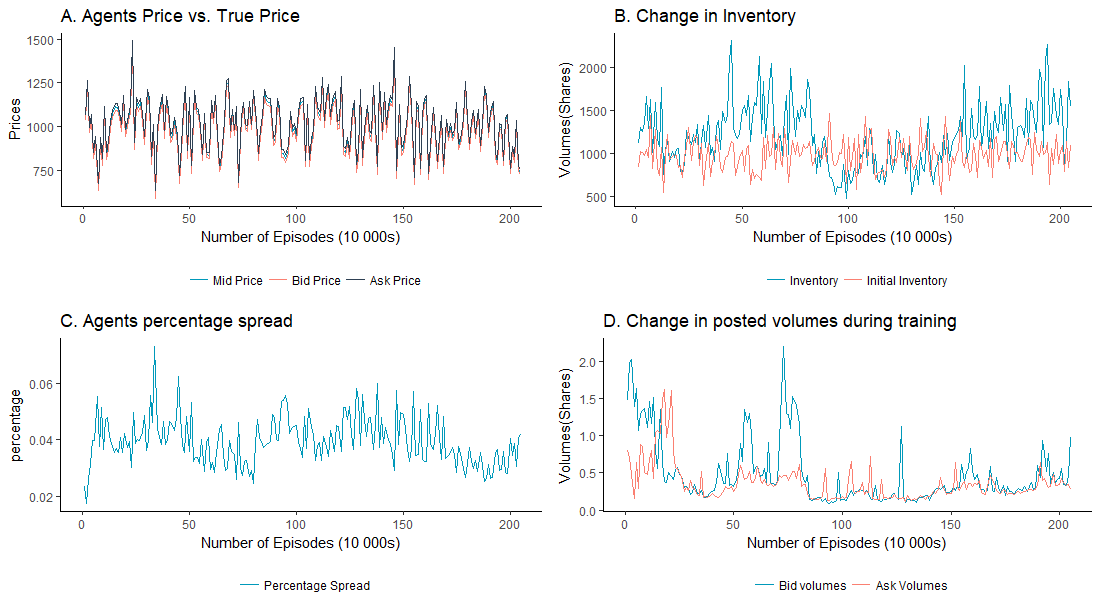
\includegraphics[scale=0.5]{dmv2_basp_inv_multi.png}
		%Captions and Labels can be used since this is a figure environment
		\caption{Plots for DealerMarket-v2, showing the change in bid-ask spread(A), inventory (B), percentage change in spread (c) as well as bid-ask volumes (D).}
		\label{fig:dm22}
%\end{figure}
\end{sidewaysfigure}

%\begin{figure}[H]
\begin{sidewaysfigure}
		%Do not try to scale figure in .tex or you loose font size consistency
	    	\centering
		%The code to input the plot is extremely simple
		% Created by tikzDevice version 0.11 on 2018-08-06 22:54:01
% !TEX encoding = UTF-8 Unicode
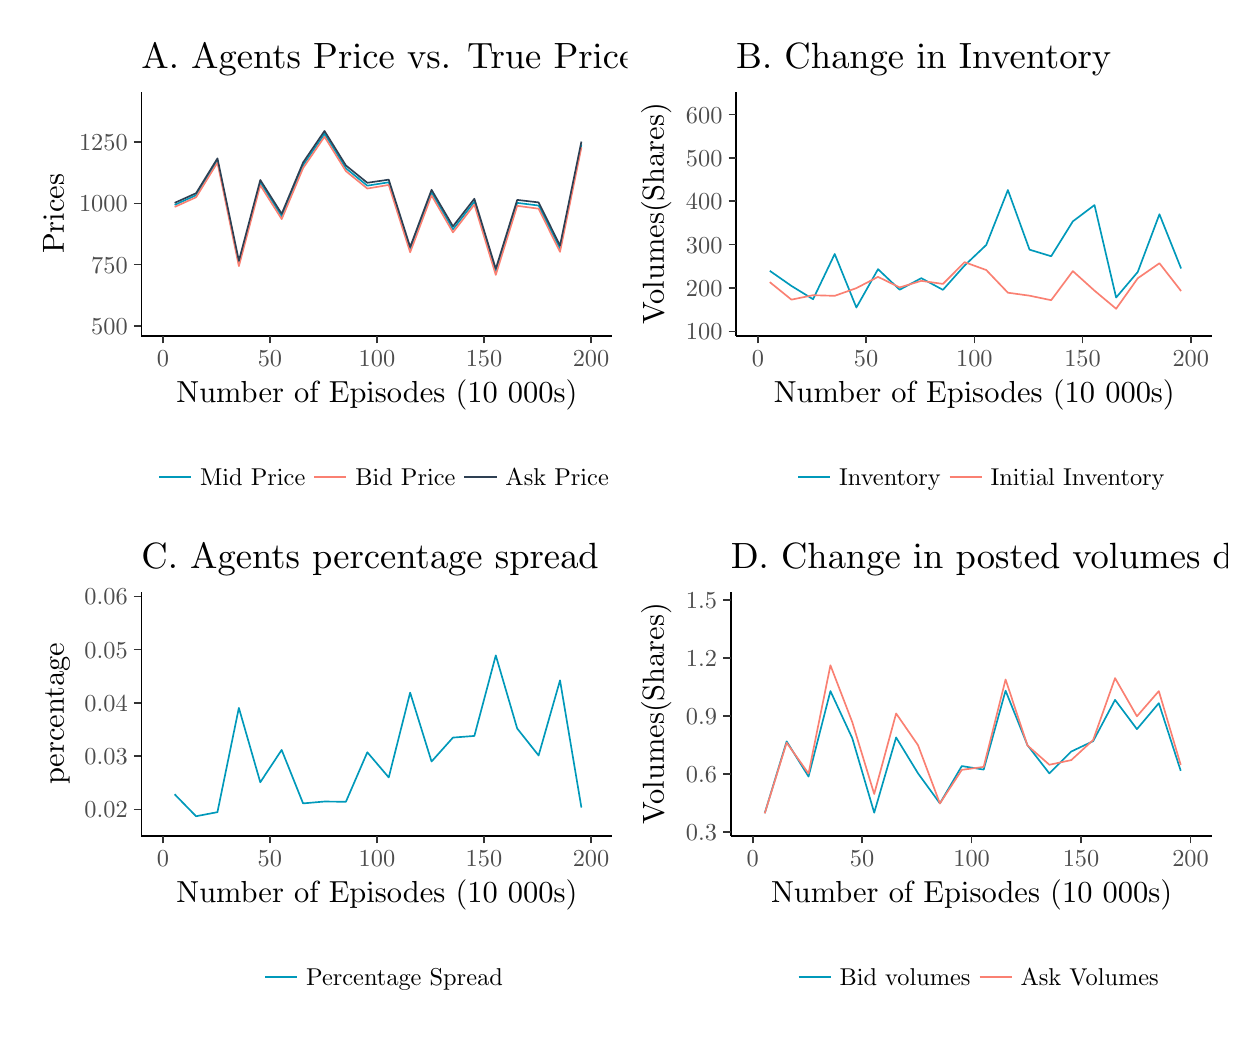
\begin{tikzpicture}[x=1pt,y=1pt]
\definecolor{fillColor}{RGB}{255,255,255}
\path[use as bounding box,fill=fillColor,fill opacity=0.00] (0,0) rectangle (433.62,361.35);
\begin{scope}
\path[clip] (  0.00,180.67) rectangle (216.81,361.35);
\definecolor{drawColor}{RGB}{255,255,255}
\definecolor{fillColor}{RGB}{255,255,255}

\path[draw=drawColor,line width= 0.6pt,line join=round,line cap=round,fill=fillColor] (  0.00,180.67) rectangle (216.81,361.35);
\end{scope}
\begin{scope}
\path[clip] ( 41.12,249.98) rectangle (211.31,338.21);
\definecolor{fillColor}{RGB}{255,255,255}

\path[fill=fillColor] ( 41.12,249.98) rectangle (211.31,338.21);
\definecolor{drawColor}{RGB}{0,153,186}

\path[draw=drawColor,line width= 0.6pt,line join=round] ( 53.11,297.30) --
	( 60.85,300.80) --
	( 68.58,313.37) --
	( 76.32,276.14) --
	( 84.06,305.36) --
	( 91.79,293.14) --
	( 99.53,311.64) --
	(107.26,322.98) --
	(115.00,310.53) --
	(122.73,304.25) --
	(130.47,305.48) --
	(138.21,281.14) --
	(145.94,301.76) --
	(153.68,288.47) --
	(161.41,298.47) --
	(169.15,273.11) --
	(176.89,298.04) --
	(184.62,297.07) --
	(192.36,281.49) --
	(200.09,319.16);
\definecolor{drawColor}{RGB}{250,128,114}

\path[draw=drawColor,line width= 0.6pt,line join=round] ( 53.11,296.56) --
	( 60.85,300.06) --
	( 68.58,312.62) --
	( 76.32,275.17) --
	( 84.06,304.41) --
	( 91.79,292.18) --
	( 99.53,310.63) --
	(107.26,321.95) --
	(115.00,309.50) --
	(122.73,303.21) --
	(130.47,304.52) --
	(138.21,280.19) --
	(145.94,300.75) --
	(153.68,287.38) --
	(161.41,297.42) --
	(169.15,272.01) --
	(176.89,296.97) --
	(184.62,295.93) --
	(192.36,280.35) --
	(200.09,318.12);
\definecolor{drawColor}{RGB}{46,64,83}

\path[draw=drawColor,line width= 0.6pt,line join=round] ( 53.11,298.04) --
	( 60.85,301.53) --
	( 68.58,314.12) --
	( 76.32,277.10) --
	( 84.06,306.30) --
	( 91.79,294.09) --
	( 99.53,312.65) --
	(107.26,324.02) --
	(115.00,311.55) --
	(122.73,305.30) --
	(130.47,306.43) --
	(138.21,282.10) --
	(145.94,302.76) --
	(153.68,289.57) --
	(161.41,299.52) --
	(169.15,274.22) --
	(176.89,299.11) --
	(184.62,298.21) --
	(192.36,282.63) --
	(200.09,320.20);
\end{scope}
\begin{scope}
\path[clip] (  0.00,  0.00) rectangle (433.62,361.35);
\definecolor{drawColor}{RGB}{0,0,0}

\path[draw=drawColor,line width= 0.6pt,line join=round] ( 41.12,249.98) --
	( 41.12,338.21);
\end{scope}
\begin{scope}
\path[clip] (  0.00,  0.00) rectangle (433.62,361.35);
\definecolor{drawColor}{gray}{0.30}

\node[text=drawColor,anchor=base east,inner sep=0pt, outer sep=0pt, scale=  0.88] at ( 36.17,250.57) {500};

\node[text=drawColor,anchor=base east,inner sep=0pt, outer sep=0pt, scale=  0.88] at ( 36.17,272.68) {750};

\node[text=drawColor,anchor=base east,inner sep=0pt, outer sep=0pt, scale=  0.88] at ( 36.17,294.79) {1000};

\node[text=drawColor,anchor=base east,inner sep=0pt, outer sep=0pt, scale=  0.88] at ( 36.17,316.90) {1250};
\end{scope}
\begin{scope}
\path[clip] (  0.00,  0.00) rectangle (433.62,361.35);
\definecolor{drawColor}{gray}{0.20}

\path[draw=drawColor,line width= 0.6pt,line join=round] ( 38.37,253.60) --
	( 41.12,253.60);

\path[draw=drawColor,line width= 0.6pt,line join=round] ( 38.37,275.71) --
	( 41.12,275.71);

\path[draw=drawColor,line width= 0.6pt,line join=round] ( 38.37,297.82) --
	( 41.12,297.82);

\path[draw=drawColor,line width= 0.6pt,line join=round] ( 38.37,319.93) --
	( 41.12,319.93);
\end{scope}
\begin{scope}
\path[clip] (  0.00,  0.00) rectangle (433.62,361.35);
\definecolor{drawColor}{RGB}{0,0,0}

\path[draw=drawColor,line width= 0.6pt,line join=round] ( 41.12,249.98) --
	(211.31,249.98);
\end{scope}
\begin{scope}
\path[clip] (  0.00,  0.00) rectangle (433.62,361.35);
\definecolor{drawColor}{gray}{0.20}

\path[draw=drawColor,line width= 0.6pt,line join=round] ( 48.86,247.23) --
	( 48.86,249.98);

\path[draw=drawColor,line width= 0.6pt,line join=round] ( 87.54,247.23) --
	( 87.54,249.98);

\path[draw=drawColor,line width= 0.6pt,line join=round] (126.22,247.23) --
	(126.22,249.98);

\path[draw=drawColor,line width= 0.6pt,line join=round] (164.90,247.23) --
	(164.90,249.98);

\path[draw=drawColor,line width= 0.6pt,line join=round] (203.57,247.23) --
	(203.57,249.98);
\end{scope}
\begin{scope}
\path[clip] (  0.00,  0.00) rectangle (433.62,361.35);
\definecolor{drawColor}{gray}{0.30}

\node[text=drawColor,anchor=base,inner sep=0pt, outer sep=0pt, scale=  0.88] at ( 48.86,238.97) {0};

\node[text=drawColor,anchor=base,inner sep=0pt, outer sep=0pt, scale=  0.88] at ( 87.54,238.97) {50};

\node[text=drawColor,anchor=base,inner sep=0pt, outer sep=0pt, scale=  0.88] at (126.22,238.97) {100};

\node[text=drawColor,anchor=base,inner sep=0pt, outer sep=0pt, scale=  0.88] at (164.90,238.97) {150};

\node[text=drawColor,anchor=base,inner sep=0pt, outer sep=0pt, scale=  0.88] at (203.57,238.97) {200};
\end{scope}
\begin{scope}
\path[clip] (  0.00,  0.00) rectangle (433.62,361.35);
\definecolor{drawColor}{RGB}{0,0,0}

\node[text=drawColor,anchor=base,inner sep=0pt, outer sep=0pt, scale=  1.10] at (126.22,225.89) {Number of Episodes (10 000s)};
\end{scope}
\begin{scope}
\path[clip] (  0.00,  0.00) rectangle (433.62,361.35);
\definecolor{drawColor}{RGB}{0,0,0}

\node[text=drawColor,rotate= 90.00,anchor=base,inner sep=0pt, outer sep=0pt, scale=  1.10] at ( 13.08,294.10) {Prices};
\end{scope}
\begin{scope}
\path[clip] (  0.00,  0.00) rectangle (433.62,361.35);
\definecolor{fillColor}{RGB}{255,255,255}

\path[fill=fillColor] ( 36.74,186.17) rectangle (215.69,212.01);
\end{scope}
\begin{scope}
\path[clip] (  0.00,  0.00) rectangle (433.62,361.35);
\definecolor{drawColor}{RGB}{0,153,186}

\path[draw=drawColor,line width= 0.6pt,line join=round] ( 47.49,199.09) -- ( 59.05,199.09);
\end{scope}
\begin{scope}
\path[clip] (  0.00,  0.00) rectangle (433.62,361.35);
\definecolor{drawColor}{RGB}{250,128,114}

\path[draw=drawColor,line width= 0.6pt,line join=round] (103.58,199.09) -- (115.15,199.09);
\end{scope}
\begin{scope}
\path[clip] (  0.00,  0.00) rectangle (433.62,361.35);
\definecolor{drawColor}{RGB}{46,64,83}

\path[draw=drawColor,line width= 0.6pt,line join=round] (157.84,199.09) -- (169.41,199.09);
\end{scope}
\begin{scope}
\path[clip] (  0.00,  0.00) rectangle (433.62,361.35);
\definecolor{drawColor}{RGB}{0,0,0}

\node[text=drawColor,anchor=base west,inner sep=0pt, outer sep=0pt, scale=  0.88] at ( 62.30,196.06) {Mid Price};
\end{scope}
\begin{scope}
\path[clip] (  0.00,  0.00) rectangle (433.62,361.35);
\definecolor{drawColor}{RGB}{0,0,0}

\node[text=drawColor,anchor=base west,inner sep=0pt, outer sep=0pt, scale=  0.88] at (118.40,196.06) {Bid Price};
\end{scope}
\begin{scope}
\path[clip] (  0.00,  0.00) rectangle (433.62,361.35);
\definecolor{drawColor}{RGB}{0,0,0}

\node[text=drawColor,anchor=base west,inner sep=0pt, outer sep=0pt, scale=  0.88] at (172.66,196.06) {Ask Price};
\end{scope}
\begin{scope}
\path[clip] (  0.00,  0.00) rectangle (433.62,361.35);
\definecolor{drawColor}{RGB}{0,0,0}

\node[text=drawColor,anchor=base west,inner sep=0pt, outer sep=0pt, scale=  1.32] at ( 41.12,346.76) {A. Agents Price vs. True Price};
\end{scope}
\begin{scope}
\path[clip] (  0.00,  0.00) rectangle (216.81,180.67);
\definecolor{drawColor}{RGB}{255,255,255}
\definecolor{fillColor}{RGB}{255,255,255}

\path[draw=drawColor,line width= 0.6pt,line join=round,line cap=round,fill=fillColor] (  0.00, -0.00) rectangle (216.81,180.67);
\end{scope}
\begin{scope}
\path[clip] ( 41.11, 69.30) rectangle (211.31,157.54);
\definecolor{fillColor}{RGB}{255,255,255}

\path[fill=fillColor] ( 41.11, 69.30) rectangle (211.31,157.54);
\definecolor{drawColor}{RGB}{0,153,186}

\path[draw=drawColor,line width= 0.6pt,line join=round] ( 53.10, 84.34) --
	( 60.84, 76.40) --
	( 68.57, 77.88) --
	( 76.31,115.56) --
	( 84.05, 88.68) --
	( 91.78,100.36) --
	( 99.52, 81.04) --
	(107.26, 81.72) --
	(114.99, 81.62) --
	(122.73, 99.52) --
	(130.47, 90.42) --
	(138.20,121.08) --
	(145.94, 96.17) --
	(153.67,104.82) --
	(161.41,105.42) --
	(169.15,134.52) --
	(176.88,108.12) --
	(184.62, 98.36) --
	(192.36,125.51) --
	(200.09, 79.53);
\end{scope}
\begin{scope}
\path[clip] (  0.00,  0.00) rectangle (433.62,361.35);
\definecolor{drawColor}{RGB}{0,0,0}

\path[draw=drawColor,line width= 0.6pt,line join=round] ( 41.11, 69.30) --
	( 41.11,157.54);
\end{scope}
\begin{scope}
\path[clip] (  0.00,  0.00) rectangle (433.62,361.35);
\definecolor{drawColor}{gray}{0.30}

\node[text=drawColor,anchor=base east,inner sep=0pt, outer sep=0pt, scale=  0.88] at ( 36.16, 75.85) {0.02};

\node[text=drawColor,anchor=base east,inner sep=0pt, outer sep=0pt, scale=  0.88] at ( 36.16, 95.09) {0.03};

\node[text=drawColor,anchor=base east,inner sep=0pt, outer sep=0pt, scale=  0.88] at ( 36.16,114.32) {0.04};

\node[text=drawColor,anchor=base east,inner sep=0pt, outer sep=0pt, scale=  0.88] at ( 36.16,133.56) {0.05};

\node[text=drawColor,anchor=base east,inner sep=0pt, outer sep=0pt, scale=  0.88] at ( 36.16,152.80) {0.06};
\end{scope}
\begin{scope}
\path[clip] (  0.00,  0.00) rectangle (433.62,361.35);
\definecolor{drawColor}{gray}{0.20}

\path[draw=drawColor,line width= 0.6pt,line join=round] ( 38.36, 78.89) --
	( 41.11, 78.89);

\path[draw=drawColor,line width= 0.6pt,line join=round] ( 38.36, 98.12) --
	( 41.11, 98.12);

\path[draw=drawColor,line width= 0.6pt,line join=round] ( 38.36,117.36) --
	( 41.11,117.36);

\path[draw=drawColor,line width= 0.6pt,line join=round] ( 38.36,136.59) --
	( 41.11,136.59);

\path[draw=drawColor,line width= 0.6pt,line join=round] ( 38.36,155.83) --
	( 41.11,155.83);
\end{scope}
\begin{scope}
\path[clip] (  0.00,  0.00) rectangle (433.62,361.35);
\definecolor{drawColor}{RGB}{0,0,0}

\path[draw=drawColor,line width= 0.6pt,line join=round] ( 41.11, 69.30) --
	(211.31, 69.30);
\end{scope}
\begin{scope}
\path[clip] (  0.00,  0.00) rectangle (433.62,361.35);
\definecolor{drawColor}{gray}{0.20}

\path[draw=drawColor,line width= 0.6pt,line join=round] ( 48.85, 66.55) --
	( 48.85, 69.30);

\path[draw=drawColor,line width= 0.6pt,line join=round] ( 87.53, 66.55) --
	( 87.53, 69.30);

\path[draw=drawColor,line width= 0.6pt,line join=round] (126.21, 66.55) --
	(126.21, 69.30);

\path[draw=drawColor,line width= 0.6pt,line join=round] (164.89, 66.55) --
	(164.89, 69.30);

\path[draw=drawColor,line width= 0.6pt,line join=round] (203.57, 66.55) --
	(203.57, 69.30);
\end{scope}
\begin{scope}
\path[clip] (  0.00,  0.00) rectangle (433.62,361.35);
\definecolor{drawColor}{gray}{0.30}

\node[text=drawColor,anchor=base,inner sep=0pt, outer sep=0pt, scale=  0.88] at ( 48.85, 58.29) {0};

\node[text=drawColor,anchor=base,inner sep=0pt, outer sep=0pt, scale=  0.88] at ( 87.53, 58.29) {50};

\node[text=drawColor,anchor=base,inner sep=0pt, outer sep=0pt, scale=  0.88] at (126.21, 58.29) {100};

\node[text=drawColor,anchor=base,inner sep=0pt, outer sep=0pt, scale=  0.88] at (164.89, 58.29) {150};

\node[text=drawColor,anchor=base,inner sep=0pt, outer sep=0pt, scale=  0.88] at (203.57, 58.29) {200};
\end{scope}
\begin{scope}
\path[clip] (  0.00,  0.00) rectangle (433.62,361.35);
\definecolor{drawColor}{RGB}{0,0,0}

\node[text=drawColor,anchor=base,inner sep=0pt, outer sep=0pt, scale=  1.10] at (126.21, 45.22) {Number of Episodes (10 000s)};
\end{scope}
\begin{scope}
\path[clip] (  0.00,  0.00) rectangle (433.62,361.35);
\definecolor{drawColor}{RGB}{0,0,0}

\node[text=drawColor,rotate= 90.00,anchor=base,inner sep=0pt, outer sep=0pt, scale=  1.10] at ( 13.08,113.42) {percentage};
\end{scope}
\begin{scope}
\path[clip] (  0.00,  0.00) rectangle (433.62,361.35);
\definecolor{fillColor}{RGB}{255,255,255}

\path[fill=fillColor] ( 75.06,  5.50) rectangle (177.36, 31.34);
\end{scope}
\begin{scope}
\path[clip] (  0.00,  0.00) rectangle (433.62,361.35);
\definecolor{drawColor}{RGB}{0,153,186}

\path[draw=drawColor,line width= 0.6pt,line join=round] ( 85.81, 18.42) -- ( 97.37, 18.42);
\end{scope}
\begin{scope}
\path[clip] (  0.00,  0.00) rectangle (433.62,361.35);
\definecolor{drawColor}{RGB}{0,0,0}

\node[text=drawColor,anchor=base west,inner sep=0pt, outer sep=0pt, scale=  0.88] at (100.63, 15.39) {Percentage Spread};
\end{scope}
\begin{scope}
\path[clip] (  0.00,  0.00) rectangle (433.62,361.35);
\definecolor{drawColor}{RGB}{0,0,0}

\node[text=drawColor,anchor=base west,inner sep=0pt, outer sep=0pt, scale=  1.32] at ( 41.11,166.08) {C. Agents percentage spread};
\end{scope}
\begin{scope}
\path[clip] (216.81,180.67) rectangle (433.62,361.35);
\definecolor{drawColor}{RGB}{255,255,255}
\definecolor{fillColor}{RGB}{255,255,255}

\path[draw=drawColor,line width= 0.6pt,line join=round,line cap=round,fill=fillColor] (216.81,180.67) rectangle (433.62,361.35);
\end{scope}
\begin{scope}
\path[clip] (256.03,249.98) rectangle (428.12,338.21);
\definecolor{fillColor}{RGB}{255,255,255}

\path[fill=fillColor] (256.03,249.98) rectangle (428.12,338.21);
\definecolor{drawColor}{RGB}{0,153,186}

\path[draw=drawColor,line width= 0.6pt,line join=round] (268.16,273.48) --
	(275.98,268.03) --
	(283.80,263.22) --
	(291.62,279.56) --
	(299.45,260.22) --
	(307.27,274.07) --
	(315.09,266.66) --
	(322.91,270.83) --
	(330.73,266.61) --
	(338.56,275.41) --
	(346.38,282.83) --
	(354.20,302.67) --
	(362.02,281.13) --
	(369.84,278.75) --
	(377.67,291.35) --
	(385.49,297.25) --
	(393.31,263.83) --
	(401.13,273.08) --
	(408.96,293.93) --
	(416.78,274.33);
\definecolor{drawColor}{RGB}{250,128,114}

\path[draw=drawColor,line width= 0.6pt,line join=round] (268.16,269.40) --
	(275.98,263.07) --
	(283.80,264.67) --
	(291.62,264.45) --
	(299.45,267.23) --
	(307.27,271.30) --
	(315.09,267.48) --
	(322.91,269.86) --
	(330.73,268.75) --
	(338.56,276.61) --
	(346.38,273.77) --
	(354.20,265.58) --
	(362.02,264.50) --
	(369.84,262.87) --
	(377.67,273.38) --
	(385.49,266.32) --
	(393.31,259.78) --
	(401.13,270.80) --
	(408.96,276.22) --
	(416.78,266.19);
\end{scope}
\begin{scope}
\path[clip] (  0.00,  0.00) rectangle (433.62,361.35);
\definecolor{drawColor}{RGB}{0,0,0}

\path[draw=drawColor,line width= 0.6pt,line join=round] (256.03,249.98) --
	(256.03,338.21);
\end{scope}
\begin{scope}
\path[clip] (  0.00,  0.00) rectangle (433.62,361.35);
\definecolor{drawColor}{gray}{0.30}

\node[text=drawColor,anchor=base east,inner sep=0pt, outer sep=0pt, scale=  0.88] at (251.08,248.58) {100};

\node[text=drawColor,anchor=base east,inner sep=0pt, outer sep=0pt, scale=  0.88] at (251.08,264.24) {200};

\node[text=drawColor,anchor=base east,inner sep=0pt, outer sep=0pt, scale=  0.88] at (251.08,279.91) {300};

\node[text=drawColor,anchor=base east,inner sep=0pt, outer sep=0pt, scale=  0.88] at (251.08,295.57) {400};

\node[text=drawColor,anchor=base east,inner sep=0pt, outer sep=0pt, scale=  0.88] at (251.08,311.24) {500};

\node[text=drawColor,anchor=base east,inner sep=0pt, outer sep=0pt, scale=  0.88] at (251.08,326.90) {600};
\end{scope}
\begin{scope}
\path[clip] (  0.00,  0.00) rectangle (433.62,361.35);
\definecolor{drawColor}{gray}{0.20}

\path[draw=drawColor,line width= 0.6pt,line join=round] (253.28,251.61) --
	(256.03,251.61);

\path[draw=drawColor,line width= 0.6pt,line join=round] (253.28,267.27) --
	(256.03,267.27);

\path[draw=drawColor,line width= 0.6pt,line join=round] (253.28,282.94) --
	(256.03,282.94);

\path[draw=drawColor,line width= 0.6pt,line join=round] (253.28,298.60) --
	(256.03,298.60);

\path[draw=drawColor,line width= 0.6pt,line join=round] (253.28,314.27) --
	(256.03,314.27);

\path[draw=drawColor,line width= 0.6pt,line join=round] (253.28,329.94) --
	(256.03,329.94);
\end{scope}
\begin{scope}
\path[clip] (  0.00,  0.00) rectangle (433.62,361.35);
\definecolor{drawColor}{RGB}{0,0,0}

\path[draw=drawColor,line width= 0.6pt,line join=round] (256.03,249.98) --
	(428.12,249.98);
\end{scope}
\begin{scope}
\path[clip] (  0.00,  0.00) rectangle (433.62,361.35);
\definecolor{drawColor}{gray}{0.20}

\path[draw=drawColor,line width= 0.6pt,line join=round] (263.85,247.23) --
	(263.85,249.98);

\path[draw=drawColor,line width= 0.6pt,line join=round] (302.97,247.23) --
	(302.97,249.98);

\path[draw=drawColor,line width= 0.6pt,line join=round] (342.08,247.23) --
	(342.08,249.98);

\path[draw=drawColor,line width= 0.6pt,line join=round] (381.19,247.23) --
	(381.19,249.98);

\path[draw=drawColor,line width= 0.6pt,line join=round] (420.30,247.23) --
	(420.30,249.98);
\end{scope}
\begin{scope}
\path[clip] (  0.00,  0.00) rectangle (433.62,361.35);
\definecolor{drawColor}{gray}{0.30}

\node[text=drawColor,anchor=base,inner sep=0pt, outer sep=0pt, scale=  0.88] at (263.85,238.97) {0};

\node[text=drawColor,anchor=base,inner sep=0pt, outer sep=0pt, scale=  0.88] at (302.97,238.97) {50};

\node[text=drawColor,anchor=base,inner sep=0pt, outer sep=0pt, scale=  0.88] at (342.08,238.97) {100};

\node[text=drawColor,anchor=base,inner sep=0pt, outer sep=0pt, scale=  0.88] at (381.19,238.97) {150};

\node[text=drawColor,anchor=base,inner sep=0pt, outer sep=0pt, scale=  0.88] at (420.30,238.97) {200};
\end{scope}
\begin{scope}
\path[clip] (  0.00,  0.00) rectangle (433.62,361.35);
\definecolor{drawColor}{RGB}{0,0,0}

\node[text=drawColor,anchor=base,inner sep=0pt, outer sep=0pt, scale=  1.10] at (342.08,225.89) {Number of Episodes (10 000s)};
\end{scope}
\begin{scope}
\path[clip] (  0.00,  0.00) rectangle (433.62,361.35);
\definecolor{drawColor}{RGB}{0,0,0}

\node[text=drawColor,rotate= 90.00,anchor=base,inner sep=0pt, outer sep=0pt, scale=  1.10] at (229.89,294.10) {Volumes(Shares)};
\end{scope}
\begin{scope}
\path[clip] (  0.00,  0.00) rectangle (433.62,361.35);
\definecolor{fillColor}{RGB}{255,255,255}

\path[fill=fillColor] (267.66,186.17) rectangle (416.49,212.01);
\end{scope}
\begin{scope}
\path[clip] (  0.00,  0.00) rectangle (433.62,361.35);
\definecolor{drawColor}{RGB}{0,153,186}

\path[draw=drawColor,line width= 0.6pt,line join=round] (278.41,199.09) -- (289.97,199.09);
\end{scope}
\begin{scope}
\path[clip] (  0.00,  0.00) rectangle (433.62,361.35);
\definecolor{drawColor}{RGB}{250,128,114}

\path[draw=drawColor,line width= 0.6pt,line join=round] (333.16,199.09) -- (344.72,199.09);
\end{scope}
\begin{scope}
\path[clip] (  0.00,  0.00) rectangle (433.62,361.35);
\definecolor{drawColor}{RGB}{0,0,0}

\node[text=drawColor,anchor=base west,inner sep=0pt, outer sep=0pt, scale=  0.88] at (293.22,196.06) {Inventory};
\end{scope}
\begin{scope}
\path[clip] (  0.00,  0.00) rectangle (433.62,361.35);
\definecolor{drawColor}{RGB}{0,0,0}

\node[text=drawColor,anchor=base west,inner sep=0pt, outer sep=0pt, scale=  0.88] at (347.97,196.06) {Initial Inventory};
\end{scope}
\begin{scope}
\path[clip] (  0.00,  0.00) rectangle (433.62,361.35);
\definecolor{drawColor}{RGB}{0,0,0}

\node[text=drawColor,anchor=base west,inner sep=0pt, outer sep=0pt, scale=  1.32] at (256.03,346.76) {B. Change in Inventory};
\end{scope}
\begin{scope}
\path[clip] (216.81,  0.00) rectangle (433.62,180.67);
\definecolor{drawColor}{RGB}{255,255,255}
\definecolor{fillColor}{RGB}{255,255,255}

\path[draw=drawColor,line width= 0.6pt,line join=round,line cap=round,fill=fillColor] (216.81, -0.00) rectangle (433.62,180.67);
\end{scope}
\begin{scope}
\path[clip] (254.08, 69.30) rectangle (428.12,157.54);
\definecolor{fillColor}{RGB}{255,255,255}

\path[fill=fillColor] (254.08, 69.30) rectangle (428.12,157.54);
\definecolor{drawColor}{RGB}{0,153,186}

\path[draw=drawColor,line width= 0.6pt,line join=round] (266.34, 77.51) --
	(274.25,103.46) --
	(282.16, 90.74) --
	(290.07,121.63) --
	(297.98,104.56) --
	(305.89, 77.69) --
	(313.81,104.87) --
	(321.72, 91.91) --
	(329.63, 81.05) --
	(337.54, 94.53) --
	(345.45, 93.26) --
	(353.36,121.78) --
	(361.27,102.07) --
	(369.18, 91.88) --
	(377.09, 99.78) --
	(385.00,103.53) --
	(392.92,118.44) --
	(400.83,107.87) --
	(408.74,117.26) --
	(416.65, 92.81);
\definecolor{drawColor}{RGB}{250,128,114}

\path[draw=drawColor,line width= 0.6pt,line join=round] (266.34, 77.45) --
	(274.25,102.98) --
	(282.16, 91.83) --
	(290.07,130.95) --
	(297.98,110.36) --
	(305.89, 84.44) --
	(313.81,113.54) --
	(321.72,102.08) --
	(329.63, 81.02) --
	(337.54, 93.16) --
	(345.45, 94.23) --
	(353.36,125.80) --
	(361.27,101.98) --
	(369.18, 95.00) --
	(377.09, 96.68) --
	(385.00,103.94) --
	(392.92,126.30) --
	(400.83,112.51) --
	(408.74,121.62) --
	(416.65, 94.95);
\end{scope}
\begin{scope}
\path[clip] (  0.00,  0.00) rectangle (433.62,361.35);
\definecolor{drawColor}{RGB}{0,0,0}

\path[draw=drawColor,line width= 0.6pt,line join=round] (254.08, 69.30) --
	(254.08,157.54);
\end{scope}
\begin{scope}
\path[clip] (  0.00,  0.00) rectangle (433.62,361.35);
\definecolor{drawColor}{gray}{0.30}

\node[text=drawColor,anchor=base east,inner sep=0pt, outer sep=0pt, scale=  0.88] at (249.13, 67.61) {0.3};

\node[text=drawColor,anchor=base east,inner sep=0pt, outer sep=0pt, scale=  0.88] at (249.13, 88.57) {0.6};

\node[text=drawColor,anchor=base east,inner sep=0pt, outer sep=0pt, scale=  0.88] at (249.13,109.53) {0.9};

\node[text=drawColor,anchor=base east,inner sep=0pt, outer sep=0pt, scale=  0.88] at (249.13,130.49) {1.2};

\node[text=drawColor,anchor=base east,inner sep=0pt, outer sep=0pt, scale=  0.88] at (249.13,151.45) {1.5};
\end{scope}
\begin{scope}
\path[clip] (  0.00,  0.00) rectangle (433.62,361.35);
\definecolor{drawColor}{gray}{0.20}

\path[draw=drawColor,line width= 0.6pt,line join=round] (251.33, 70.64) --
	(254.08, 70.64);

\path[draw=drawColor,line width= 0.6pt,line join=round] (251.33, 91.60) --
	(254.08, 91.60);

\path[draw=drawColor,line width= 0.6pt,line join=round] (251.33,112.56) --
	(254.08,112.56);

\path[draw=drawColor,line width= 0.6pt,line join=round] (251.33,133.52) --
	(254.08,133.52);

\path[draw=drawColor,line width= 0.6pt,line join=round] (251.33,154.48) --
	(254.08,154.48);
\end{scope}
\begin{scope}
\path[clip] (  0.00,  0.00) rectangle (433.62,361.35);
\definecolor{drawColor}{RGB}{0,0,0}

\path[draw=drawColor,line width= 0.6pt,line join=round] (254.08, 69.30) --
	(428.12, 69.30);
\end{scope}
\begin{scope}
\path[clip] (  0.00,  0.00) rectangle (433.62,361.35);
\definecolor{drawColor}{gray}{0.20}

\path[draw=drawColor,line width= 0.6pt,line join=round] (261.99, 66.55) --
	(261.99, 69.30);

\path[draw=drawColor,line width= 0.6pt,line join=round] (301.54, 66.55) --
	(301.54, 69.30);

\path[draw=drawColor,line width= 0.6pt,line join=round] (341.10, 66.55) --
	(341.10, 69.30);

\path[draw=drawColor,line width= 0.6pt,line join=round] (380.65, 66.55) --
	(380.65, 69.30);

\path[draw=drawColor,line width= 0.6pt,line join=round] (420.21, 66.55) --
	(420.21, 69.30);
\end{scope}
\begin{scope}
\path[clip] (  0.00,  0.00) rectangle (433.62,361.35);
\definecolor{drawColor}{gray}{0.30}

\node[text=drawColor,anchor=base,inner sep=0pt, outer sep=0pt, scale=  0.88] at (261.99, 58.29) {0};

\node[text=drawColor,anchor=base,inner sep=0pt, outer sep=0pt, scale=  0.88] at (301.54, 58.29) {50};

\node[text=drawColor,anchor=base,inner sep=0pt, outer sep=0pt, scale=  0.88] at (341.10, 58.29) {100};

\node[text=drawColor,anchor=base,inner sep=0pt, outer sep=0pt, scale=  0.88] at (380.65, 58.29) {150};

\node[text=drawColor,anchor=base,inner sep=0pt, outer sep=0pt, scale=  0.88] at (420.21, 58.29) {200};
\end{scope}
\begin{scope}
\path[clip] (  0.00,  0.00) rectangle (433.62,361.35);
\definecolor{drawColor}{RGB}{0,0,0}

\node[text=drawColor,anchor=base,inner sep=0pt, outer sep=0pt, scale=  1.10] at (341.10, 45.22) {Number of Episodes (10 000s)};
\end{scope}
\begin{scope}
\path[clip] (  0.00,  0.00) rectangle (433.62,361.35);
\definecolor{drawColor}{RGB}{0,0,0}

\node[text=drawColor,rotate= 90.00,anchor=base,inner sep=0pt, outer sep=0pt, scale=  1.10] at (229.89,113.42) {Volumes(Shares)};
\end{scope}
\begin{scope}
\path[clip] (  0.00,  0.00) rectangle (433.62,361.35);
\definecolor{fillColor}{RGB}{255,255,255}

\path[fill=fillColor] (267.79,  5.50) rectangle (414.41, 31.34);
\end{scope}
\begin{scope}
\path[clip] (  0.00,  0.00) rectangle (433.62,361.35);
\definecolor{drawColor}{RGB}{0,153,186}

\path[draw=drawColor,line width= 0.6pt,line join=round] (278.54, 18.42) -- (290.10, 18.42);
\end{scope}
\begin{scope}
\path[clip] (  0.00,  0.00) rectangle (433.62,361.35);
\definecolor{drawColor}{RGB}{250,128,114}

\path[draw=drawColor,line width= 0.6pt,line join=round] (343.95, 18.42) -- (355.51, 18.42);
\end{scope}
\begin{scope}
\path[clip] (  0.00,  0.00) rectangle (433.62,361.35);
\definecolor{drawColor}{RGB}{0,0,0}

\node[text=drawColor,anchor=base west,inner sep=0pt, outer sep=0pt, scale=  0.88] at (293.36, 15.39) {Bid volumes};
\end{scope}
\begin{scope}
\path[clip] (  0.00,  0.00) rectangle (433.62,361.35);
\definecolor{drawColor}{RGB}{0,0,0}

\node[text=drawColor,anchor=base west,inner sep=0pt, outer sep=0pt, scale=  0.88] at (358.76, 15.39) {Ask Volumes};
\end{scope}
\begin{scope}
\path[clip] (  0.00,  0.00) rectangle (433.62,361.35);
\definecolor{drawColor}{RGB}{0,0,0}

\node[text=drawColor,anchor=base west,inner sep=0pt, outer sep=0pt, scale=  1.32] at (254.08,166.08) {D. Change in posted volumes during training};
\end{scope}
\end{tikzpicture}

		%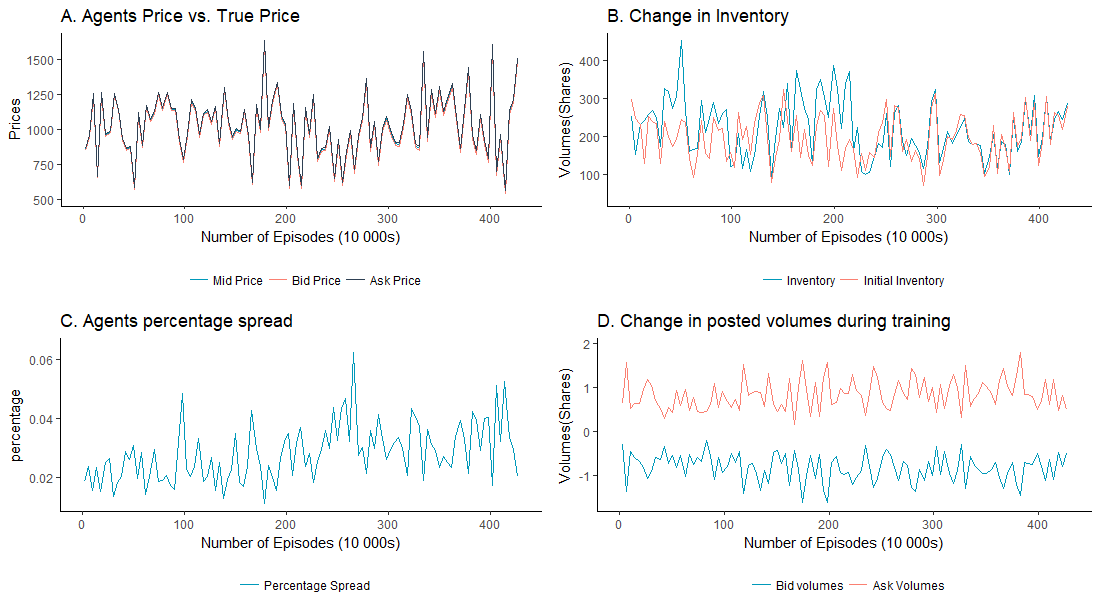
\includegraphics[scale=.5]{lob1_baps_inv_multi.png}
		%Captions and Labels can be used since this is a figure environment
		\caption{Plots for LOBMarket-v1, showing the change in bid-ask spread(A), inventory (B), percentage change in spread (c) as well as bid-ask volumes (D).}
		\label{fig:dm32}
%\end{figure}
\end{sidewaysfigure}


\newpage
\subsection*{Correlation between inventory and prices}

\begin{figure}[H]
		%Do not try to scale figure in .tex or you loose font size consistency
	    	\centering
		%The code to input the plot is extremely simple
		% Created by tikzDevice version 0.11 on 2018-07-18 16:59:25
% !TEX encoding = UTF-8 Unicode
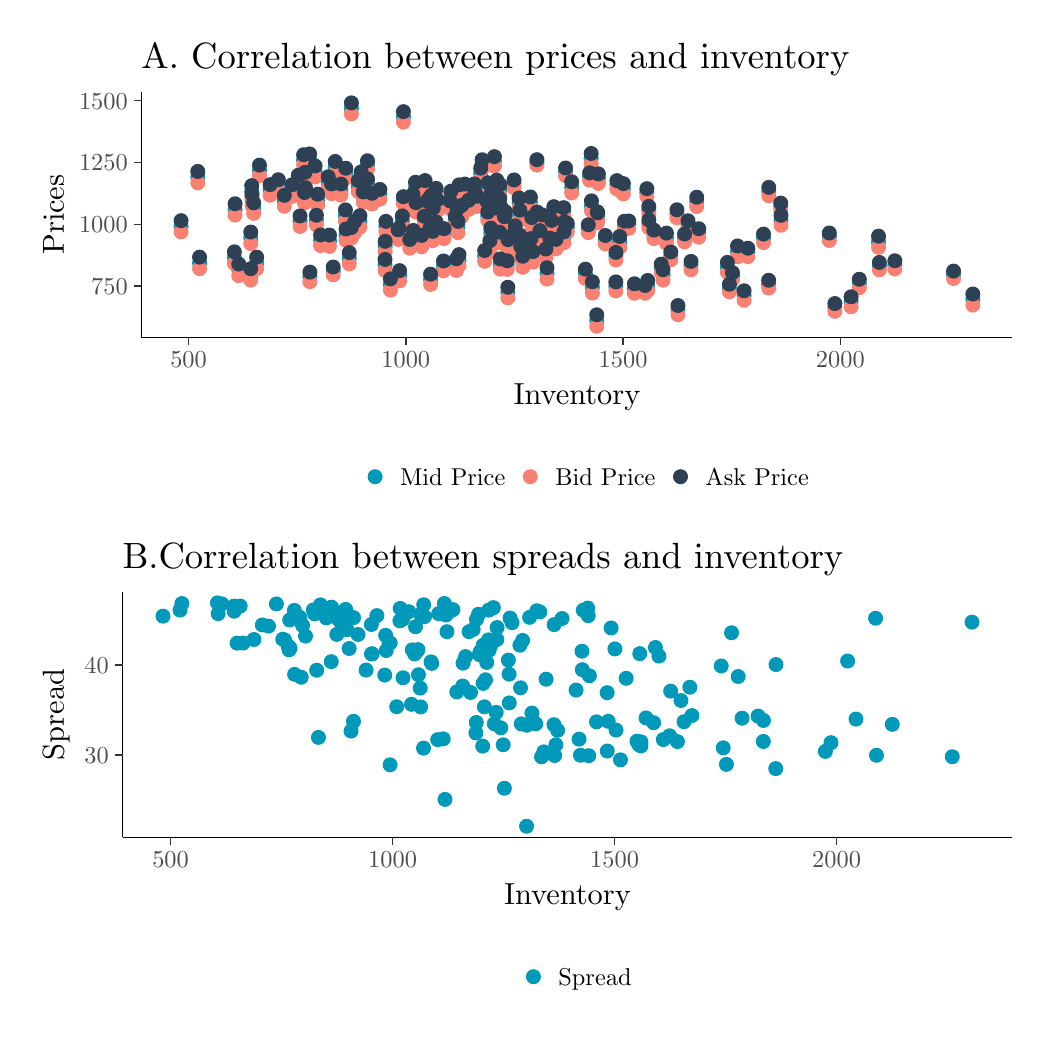
\begin{tikzpicture}[x=1pt,y=1pt]
\definecolor{fillColor}{RGB}{255,255,255}
\path[use as bounding box,fill=fillColor,fill opacity=0.00] (0,0) rectangle (361.35,361.35);
\begin{scope}
\path[clip] (  0.00,180.67) rectangle (361.35,361.35);
\definecolor{drawColor}{RGB}{255,255,255}
\definecolor{fillColor}{RGB}{255,255,255}

\path[draw=drawColor,line width= 0.6pt,line join=round,line cap=round,fill=fillColor] (  0.00,180.67) rectangle (361.35,361.35);
\end{scope}
\begin{scope}
\path[clip] ( 41.12,249.42) rectangle (355.85,338.21);
\definecolor{fillColor}{RGB}{255,255,255}

\path[fill=fillColor] ( 41.12,249.42) rectangle (355.85,338.21);
\definecolor{drawColor}{RGB}{0,153,186}
\definecolor{fillColor}{RGB}{0,153,186}

\path[draw=drawColor,line width= 0.4pt,line join=round,line cap=round,fill=fillColor] (155.18,294.64) circle (  2.50);

\path[draw=drawColor,line width= 0.4pt,line join=round,line cap=round,fill=fillColor] (184.01,312.65) circle (  2.50);

\path[draw=drawColor,line width= 0.4pt,line join=round,line cap=round,fill=fillColor] (176.17,288.55) circle (  2.50);

\path[draw=drawColor,line width= 0.4pt,line join=round,line cap=round,fill=fillColor] (193.70,294.81) circle (  2.50);

\path[draw=drawColor,line width= 0.4pt,line join=round,line cap=round,fill=fillColor] (239.70,275.40) circle (  2.50);

\path[draw=drawColor,line width= 0.4pt,line join=round,line cap=round,fill=fillColor] (181.88,283.44) circle (  2.50);

\path[draw=drawColor,line width= 0.4pt,line join=round,line cap=round,fill=fillColor] (234.98,259.29) circle (  2.50);

\path[draw=drawColor,line width= 0.4pt,line join=round,line cap=round,fill=fillColor] (138.07,283.22) circle (  2.50);

\path[draw=drawColor,line width= 0.4pt,line join=round,line cap=round,fill=fillColor] (229.59,272.02) circle (  2.50);

\path[draw=drawColor,line width= 0.4pt,line join=round,line cap=round,fill=fillColor] (162.45,298.58) circle (  2.50);

\path[draw=drawColor,line width= 0.4pt,line join=round,line cap=round,fill=fillColor] (150.24,275.25) circle (  2.50);

\path[draw=drawColor,line width= 0.4pt,line join=round,line cap=round,fill=fillColor] (256.50,280.51) circle (  2.50);

\path[draw=drawColor,line width= 0.4pt,line join=round,line cap=round,fill=fillColor] ( 98.43,291.41) circle (  2.50);

\path[draw=drawColor,line width= 0.4pt,line join=round,line cap=round,fill=fillColor] (144.41,296.76) circle (  2.50);

\path[draw=drawColor,line width= 0.4pt,line join=round,line cap=round,fill=fillColor] (161.55,300.32) circle (  2.50);

\path[draw=drawColor,line width= 0.4pt,line join=round,line cap=round,fill=fillColor] (121.27,300.12) circle (  2.50);

\path[draw=drawColor,line width= 0.4pt,line join=round,line cap=round,fill=fillColor] (140.33,296.40) circle (  2.50);

\path[draw=drawColor,line width= 0.4pt,line join=round,line cap=round,fill=fillColor] (129.43,289.52) circle (  2.50);

\path[draw=drawColor,line width= 0.4pt,line join=round,line cap=round,fill=fillColor] (143.61,304.24) circle (  2.50);

\path[draw=drawColor,line width= 0.4pt,line join=round,line cap=round,fill=fillColor] (145.37,287.06) circle (  2.50);

\path[draw=drawColor,line width= 0.4pt,line join=round,line cap=round,fill=fillColor] (104.33,291.83) circle (  2.50);

\path[draw=drawColor,line width= 0.4pt,line join=round,line cap=round,fill=fillColor] (104.78,299.21) circle (  2.50);

\path[draw=drawColor,line width= 0.4pt,line join=round,line cap=round,fill=fillColor] (116.98,332.16) circle (  2.50);

\path[draw=drawColor,line width= 0.4pt,line join=round,line cap=round,fill=fillColor] (178.17,280.27) circle (  2.50);

\path[draw=drawColor,line width= 0.4pt,line join=round,line cap=round,fill=fillColor] (166.31,303.29) circle (  2.50);

\path[draw=drawColor,line width= 0.4pt,line join=round,line cap=round,fill=fillColor] (152.93,300.22) circle (  2.50);

\path[draw=drawColor,line width= 0.4pt,line join=round,line cap=round,fill=fillColor] (170.62,302.62) circle (  2.50);

\path[draw=drawColor,line width= 0.4pt,line join=round,line cap=round,fill=fillColor] (156.86,295.09) circle (  2.50);

\path[draw=drawColor,line width= 0.4pt,line join=round,line cap=round,fill=fillColor] (188.69,283.23) circle (  2.50);

\path[draw=drawColor,line width= 0.4pt,line join=round,line cap=round,fill=fillColor] (120.50,307.29) circle (  2.50);

\path[draw=drawColor,line width= 0.4pt,line join=round,line cap=round,fill=fillColor] (157.97,302.78) circle (  2.50);

\path[draw=drawColor,line width= 0.4pt,line join=round,line cap=round,fill=fillColor] (187.66,272.56) circle (  2.50);

\path[draw=drawColor,line width= 0.4pt,line join=round,line cap=round,fill=fillColor] (147.63,289.00) circle (  2.50);

\path[draw=drawColor,line width= 0.4pt,line join=round,line cap=round,fill=fillColor] (205.62,255.53) circle (  2.50);

\path[draw=drawColor,line width= 0.4pt,line join=round,line cap=round,fill=fillColor] (134.17,286.95) circle (  2.50);

\path[draw=drawColor,line width= 0.4pt,line join=round,line cap=round,fill=fillColor] (147.93,297.16) circle (  2.50);

\path[draw=drawColor,line width= 0.4pt,line join=round,line cap=round,fill=fillColor] (122.82,304.61) circle (  2.50);

\path[draw=drawColor,line width= 0.4pt,line join=round,line cap=round,fill=fillColor] (185.08,285.99) circle (  2.50);

\path[draw=drawColor,line width= 0.4pt,line join=round,line cap=round,fill=fillColor] (196.57,303.66) circle (  2.50);

\path[draw=drawColor,line width= 0.4pt,line join=round,line cap=round,fill=fillColor] (144.74,297.36) circle (  2.50);

\path[draw=drawColor,line width= 0.4pt,line join=round,line cap=round,fill=fillColor] (213.93,283.93) circle (  2.50);

\path[draw=drawColor,line width= 0.4pt,line join=round,line cap=round,fill=fillColor] (193.77,285.57) circle (  2.50);

\path[draw=drawColor,line width= 0.4pt,line join=round,line cap=round,fill=fillColor] (205.83,292.80) circle (  2.50);

\path[draw=drawColor,line width= 0.4pt,line join=round,line cap=round,fill=fillColor] (307.45,283.99) circle (  2.50);

\path[draw=drawColor,line width= 0.4pt,line join=round,line cap=round,fill=fillColor] (341.54,263.10) circle (  2.50);

\path[draw=drawColor,line width= 0.4pt,line join=round,line cap=round,fill=fillColor] (182.61,278.54) circle (  2.50);

\path[draw=drawColor,line width= 0.4pt,line join=round,line cap=round,fill=fillColor] (170.57,297.67) circle (  2.50);

\path[draw=drawColor,line width= 0.4pt,line join=round,line cap=round,fill=fillColor] (163.70,308.63) circle (  2.50);

\path[draw=drawColor,line width= 0.4pt,line join=round,line cap=round,fill=fillColor] (170.78,275.94) circle (  2.50);

\path[draw=drawColor,line width= 0.4pt,line join=round,line cap=round,fill=fillColor] (215.25,303.13) circle (  2.50);

\path[draw=drawColor,line width= 0.4pt,line join=round,line cap=round,fill=fillColor] (224.05,268.16) circle (  2.50);

\path[draw=drawColor,line width= 0.4pt,line join=round,line cap=round,fill=fillColor] (206.22,306.78) circle (  2.50);

\path[draw=drawColor,line width= 0.4pt,line join=round,line cap=round,fill=fillColor] (241.76,298.40) circle (  2.50);

\path[draw=drawColor,line width= 0.4pt,line join=round,line cap=round,fill=fillColor] (159.34,297.31) circle (  2.50);

\path[draw=drawColor,line width= 0.4pt,line join=round,line cap=round,fill=fillColor] (202.58,288.72) circle (  2.50);

\path[draw=drawColor,line width= 0.4pt,line join=round,line cap=round,fill=fillColor] (228.93,274.39) circle (  2.50);

\path[draw=drawColor,line width= 0.4pt,line join=round,line cap=round,fill=fillColor] (224.44,295.37) circle (  2.50);

\path[draw=drawColor,line width= 0.4pt,line join=round,line cap=round,fill=fillColor] (313.35,275.64) circle (  2.50);

\path[draw=drawColor,line width= 0.4pt,line join=round,line cap=round,fill=fillColor] (173.28,275.55) circle (  2.50);

\path[draw=drawColor,line width= 0.4pt,line join=round,line cap=round,fill=fillColor] (267.79,302.13) circle (  2.50);

\path[draw=drawColor,line width= 0.4pt,line join=round,line cap=round,fill=fillColor] (166.24,293.25) circle (  2.50);

\path[draw=drawColor,line width= 0.4pt,line join=round,line cap=round,fill=fillColor] (212.91,304.56) circle (  2.50);

\path[draw=drawColor,line width= 0.4pt,line join=round,line cap=round,fill=fillColor] (265.89,285.23) circle (  2.50);

\path[draw=drawColor,line width= 0.4pt,line join=round,line cap=round,fill=fillColor] (300.51,268.92) circle (  2.50);

\path[draw=drawColor,line width= 0.4pt,line join=round,line cap=round,fill=fillColor] (201.53,272.43) circle (  2.50);

\path[draw=drawColor,line width= 0.4pt,line join=round,line cap=round,fill=fillColor] (143.31,291.59) circle (  2.50);

\path[draw=drawColor,line width= 0.4pt,line join=round,line cap=round,fill=fillColor] (164.20,311.98) circle (  2.50);

\path[draw=drawColor,line width= 0.4pt,line join=round,line cap=round,fill=fillColor] (168.65,313.05) circle (  2.50);

\path[draw=drawColor,line width= 0.4pt,line join=round,line cap=round,fill=fillColor] (133.86,286.58) circle (  2.50);

\path[draw=drawColor,line width= 0.4pt,line join=round,line cap=round,fill=fillColor] (203.72,297.01) circle (  2.50);

\path[draw=drawColor,line width= 0.4pt,line join=round,line cap=round,fill=fillColor] (242.49,287.17) circle (  2.50);

\path[draw=drawColor,line width= 0.4pt,line join=round,line cap=round,fill=fillColor] (135.75,298.98) circle (  2.50);

\path[draw=drawColor,line width= 0.4pt,line join=round,line cap=round,fill=fillColor] (291.67,260.26) circle (  2.50);

\path[draw=drawColor,line width= 0.4pt,line join=round,line cap=round,fill=fillColor] (234.61,294.10) circle (  2.50);

\path[draw=drawColor,line width= 0.4pt,line join=round,line cap=round,fill=fillColor] (168.49,300.97) circle (  2.50);

\path[draw=drawColor,line width= 0.4pt,line join=round,line cap=round,fill=fillColor] (215.66,289.95) circle (  2.50);

\path[draw=drawColor,line width= 0.4pt,line join=round,line cap=round,fill=fillColor] (194.99,289.15) circle (  2.50);

\path[draw=drawColor,line width= 0.4pt,line join=round,line cap=round,fill=fillColor] (223.74,301.78) circle (  2.50);

\path[draw=drawColor,line width= 0.4pt,line join=round,line cap=round,fill=fillColor] (217.22,290.17) circle (  2.50);

\path[draw=drawColor,line width= 0.4pt,line join=round,line cap=round,fill=fillColor] (203.06,307.55) circle (  2.50);

\path[draw=drawColor,line width= 0.4pt,line join=round,line cap=round,fill=fillColor] (272.22,291.74) circle (  2.50);

\path[draw=drawColor,line width= 0.4pt,line join=round,line cap=round,fill=fillColor] (252.85,274.74) circle (  2.50);

\path[draw=drawColor,line width= 0.4pt,line join=round,line cap=round,fill=fillColor] (150.47,286.94) circle (  2.50);

\path[draw=drawColor,line width= 0.4pt,line join=round,line cap=round,fill=fillColor] (171.30,294.21) circle (  2.50);

\path[draw=drawColor,line width= 0.4pt,line join=round,line cap=round,fill=fillColor] (100.25,307.09) circle (  2.50);

\path[draw=drawColor,line width= 0.4pt,line join=round,line cap=round,fill=fillColor] (140.14,303.47) circle (  2.50);

\path[draw=drawColor,line width= 0.4pt,line join=round,line cap=round,fill=fillColor] (113.19,302.82) circle (  2.50);

\path[draw=drawColor,line width= 0.4pt,line join=round,line cap=round,fill=fillColor] (155.90,302.50) circle (  2.50);

\path[draw=drawColor,line width= 0.4pt,line join=round,line cap=round,fill=fillColor] (167.02,282.34) circle (  2.50);

\path[draw=drawColor,line width= 0.4pt,line join=round,line cap=round,fill=fillColor] (142.35,284.23) circle (  2.50);

\path[draw=drawColor,line width= 0.4pt,line join=round,line cap=round,fill=fillColor] ( 95.54,302.47) circle (  2.50);

\path[draw=drawColor,line width= 0.4pt,line join=round,line cap=round,fill=fillColor] ( 92.75,298.79) circle (  2.50);

\path[draw=drawColor,line width= 0.4pt,line join=round,line cap=round,fill=fillColor] ( 82.74,276.34) circle (  2.50);

\path[draw=drawColor,line width= 0.4pt,line join=round,line cap=round,fill=fillColor] ( 62.11,276.34) circle (  2.50);

\path[draw=drawColor,line width= 0.4pt,line join=round,line cap=round,fill=fillColor] ( 76.27,273.84) circle (  2.50);

\path[draw=drawColor,line width= 0.4pt,line join=round,line cap=round,fill=fillColor] ( 74.69,278.26) circle (  2.50);

\path[draw=drawColor,line width= 0.4pt,line join=round,line cap=round,fill=fillColor] ( 74.95,295.68) circle (  2.50);

\path[draw=drawColor,line width= 0.4pt,line join=round,line cap=round,fill=fillColor] (116.90,287.16) circle (  2.50);

\path[draw=drawColor,line width= 0.4pt,line join=round,line cap=round,fill=fillColor] ( 55.43,289.58) circle (  2.50);

\path[draw=drawColor,line width= 0.4pt,line join=round,line cap=round,fill=fillColor] (105.84,284.53) circle (  2.50);

\path[draw=drawColor,line width= 0.4pt,line join=round,line cap=round,fill=fillColor] ( 81.66,296.15) circle (  2.50);

\path[draw=drawColor,line width= 0.4pt,line join=round,line cap=round,fill=fillColor] ( 87.61,302.70) circle (  2.50);

\path[draw=drawColor,line width= 0.4pt,line join=round,line cap=round,fill=fillColor] (109.80,303.13) circle (  2.50);

\path[draw=drawColor,line width= 0.4pt,line join=round,line cap=round,fill=fillColor] (101.98,271.28) circle (  2.50);

\path[draw=drawColor,line width= 0.4pt,line join=round,line cap=round,fill=fillColor] (100.02,299.93) circle (  2.50);

\path[draw=drawColor,line width= 0.4pt,line join=round,line cap=round,fill=fillColor] (134.39,271.69) circle (  2.50);

\path[draw=drawColor,line width= 0.4pt,line join=round,line cap=round,fill=fillColor] (129.18,282.30) circle (  2.50);

\path[draw=drawColor,line width= 0.4pt,line join=round,line cap=round,fill=fillColor] (167.35,287.07) circle (  2.50);

\path[draw=drawColor,line width= 0.4pt,line join=round,line cap=round,fill=fillColor] (114.95,308.75) circle (  2.50);

\path[draw=drawColor,line width= 0.4pt,line join=round,line cap=round,fill=fillColor] (181.66,298.27) circle (  2.50);

\path[draw=drawColor,line width= 0.4pt,line join=round,line cap=round,fill=fillColor] (168.66,295.33) circle (  2.50);

\path[draw=drawColor,line width= 0.4pt,line join=round,line cap=round,fill=fillColor] ( 99.71,313.55) circle (  2.50);

\path[draw=drawColor,line width= 0.4pt,line join=round,line cap=round,fill=fillColor] (135.39,291.42) circle (  2.50);

\path[draw=drawColor,line width= 0.4pt,line join=round,line cap=round,fill=fillColor] ( 90.58,304.42) circle (  2.50);

\path[draw=drawColor,line width= 0.4pt,line join=round,line cap=round,fill=fillColor] ( 83.76,309.78) circle (  2.50);

\path[draw=drawColor,line width= 0.4pt,line join=round,line cap=round,fill=fillColor] (114.82,293.45) circle (  2.50);

\path[draw=drawColor,line width= 0.4pt,line join=round,line cap=round,fill=fillColor] ( 80.95,302.20) circle (  2.50);

\path[draw=drawColor,line width= 0.4pt,line join=round,line cap=round,fill=fillColor] ( 97.79,306.12) circle (  2.50);

\path[draw=drawColor,line width= 0.4pt,line join=round,line cap=round,fill=fillColor] (172.28,290.96) circle (  2.50);

\path[draw=drawColor,line width= 0.4pt,line join=round,line cap=round,fill=fillColor] (120.05,291.36) circle (  2.50);

\path[draw=drawColor,line width= 0.4pt,line join=round,line cap=round,fill=fillColor] (101.88,313.67) circle (  2.50);

\path[draw=drawColor,line width= 0.4pt,line join=round,line cap=round,fill=fillColor] (116.21,278.04) circle (  2.50);

\path[draw=drawColor,line width= 0.4pt,line join=round,line cap=round,fill=fillColor] (178.89,276.76) circle (  2.50);

\path[draw=drawColor,line width= 0.4pt,line join=round,line cap=round,fill=fillColor] (173.58,282.78) circle (  2.50);

\path[draw=drawColor,line width= 0.4pt,line join=round,line cap=round,fill=fillColor] (129.13,275.61) circle (  2.50);

\path[draw=drawColor,line width= 0.4pt,line join=round,line cap=round,fill=fillColor] (146.56,296.18) circle (  2.50);

\path[draw=drawColor,line width= 0.4pt,line join=round,line cap=round,fill=fillColor] (100.38,301.65) circle (  2.50);

\path[draw=drawColor,line width= 0.4pt,line join=round,line cap=round,fill=fillColor] (131.08,268.55) circle (  2.50);

\path[draw=drawColor,line width= 0.4pt,line join=round,line cap=round,fill=fillColor] (154.93,275.74) circle (  2.50);

\path[draw=drawColor,line width= 0.4pt,line join=round,line cap=round,fill=fillColor] ( 61.47,307.34) circle (  2.50);

\path[draw=drawColor,line width= 0.4pt,line join=round,line cap=round,fill=fillColor] ( 80.59,272.19) circle (  2.50);

\path[draw=drawColor,line width= 0.4pt,line join=round,line cap=round,fill=fillColor] (115.04,286.52) circle (  2.50);

\path[draw=drawColor,line width= 0.4pt,line join=round,line cap=round,fill=fillColor] ( 81.08,299.06) circle (  2.50);

\path[draw=drawColor,line width= 0.4pt,line join=round,line cap=round,fill=fillColor] (139.33,286.00) circle (  2.50);

\path[draw=drawColor,line width= 0.4pt,line join=round,line cap=round,fill=fillColor] (109.06,284.36) circle (  2.50);

\path[draw=drawColor,line width= 0.4pt,line join=round,line cap=round,fill=fillColor] (103.86,309.38) circle (  2.50);

\path[draw=drawColor,line width= 0.4pt,line join=round,line cap=round,fill=fillColor] (155.50,289.31) circle (  2.50);

\path[draw=drawColor,line width= 0.4pt,line join=round,line cap=round,fill=fillColor] (204.05,267.49) circle (  2.50);

\path[draw=drawColor,line width= 0.4pt,line join=round,line cap=round,fill=fillColor] (111.13,310.93) circle (  2.50);

\path[draw=drawColor,line width= 0.4pt,line join=round,line cap=round,fill=fillColor] ( 80.61,285.41) circle (  2.50);

\path[draw=drawColor,line width= 0.4pt,line join=round,line cap=round,fill=fillColor] (108.61,305.41) circle (  2.50);

\path[draw=drawColor,line width= 0.4pt,line join=round,line cap=round,fill=fillColor] (118.15,289.26) circle (  2.50);

\path[draw=drawColor,line width= 0.4pt,line join=round,line cap=round,fill=fillColor] (139.21,299.04) circle (  2.50);

\path[draw=drawColor,line width= 0.4pt,line join=round,line cap=round,fill=fillColor] (119.45,304.10) circle (  2.50);

\path[draw=drawColor,line width= 0.4pt,line join=round,line cap=round,fill=fillColor] (169.91,302.19) circle (  2.50);

\path[draw=drawColor,line width= 0.4pt,line join=round,line cap=round,fill=fillColor] (135.78,329.11) circle (  2.50);

\path[draw=drawColor,line width= 0.4pt,line join=round,line cap=round,fill=fillColor] (173.51,265.64) circle (  2.50);

\path[draw=drawColor,line width= 0.4pt,line join=round,line cap=round,fill=fillColor] (124.41,299.56) circle (  2.50);

\path[draw=drawColor,line width= 0.4pt,line join=round,line cap=round,fill=fillColor] (155.86,277.39) circle (  2.50);

\path[draw=drawColor,line width= 0.4pt,line join=round,line cap=round,fill=fillColor] (165.13,278.85) circle (  2.50);

\path[draw=drawColor,line width= 0.4pt,line join=round,line cap=round,fill=fillColor] (170.54,285.54) circle (  2.50);

\path[draw=drawColor,line width= 0.4pt,line join=round,line cap=round,fill=fillColor] (177.84,293.67) circle (  2.50);

\path[draw=drawColor,line width= 0.4pt,line join=round,line cap=round,fill=fillColor] (203.61,314.04) circle (  2.50);

\path[draw=drawColor,line width= 0.4pt,line join=round,line cap=round,fill=fillColor] (167.59,299.83) circle (  2.50);

\path[draw=drawColor,line width= 0.4pt,line join=round,line cap=round,fill=fillColor] (297.55,262.31) circle (  2.50);

\path[draw=drawColor,line width= 0.4pt,line join=round,line cap=round,fill=fillColor] (127.26,301.13) circle (  2.50);

\path[draw=drawColor,line width= 0.4pt,line join=round,line cap=round,fill=fillColor] (145.78,298.95) circle (  2.50);

\path[draw=drawColor,line width= 0.4pt,line join=round,line cap=round,fill=fillColor] (219.24,267.09) circle (  2.50);

\path[draw=drawColor,line width= 0.4pt,line join=round,line cap=round,fill=fillColor] (169.09,294.61) circle (  2.50);

\path[draw=drawColor,line width= 0.4pt,line join=round,line cap=round,fill=fillColor] (161.43,303.20) circle (  2.50);

\path[draw=drawColor,line width= 0.4pt,line join=round,line cap=round,fill=fillColor] (169.50,304.56) circle (  2.50);

\path[draw=drawColor,line width= 0.4pt,line join=round,line cap=round,fill=fillColor] (258.88,264.55) circle (  2.50);

\path[draw=drawColor,line width= 0.4pt,line join=round,line cap=round,fill=fillColor] (146.40,286.07) circle (  2.50);

\path[draw=drawColor,line width= 0.4pt,line join=round,line cap=round,fill=fillColor] (177.58,298.00) circle (  2.50);

\path[draw=drawColor,line width= 0.4pt,line join=round,line cap=round,fill=fillColor] (230.82,285.28) circle (  2.50);

\path[draw=drawColor,line width= 0.4pt,line join=round,line cap=round,fill=fillColor] (145.59,270.41) circle (  2.50);

\path[draw=drawColor,line width= 0.4pt,line join=round,line cap=round,fill=fillColor] (190.92,283.15) circle (  2.50);

\path[draw=drawColor,line width= 0.4pt,line join=round,line cap=round,fill=fillColor] (146.56,294.55) circle (  2.50);

\path[draw=drawColor,line width= 0.4pt,line join=round,line cap=round,fill=fillColor] (212.53,267.84) circle (  2.50);

\path[draw=drawColor,line width= 0.4pt,line join=round,line cap=round,fill=fillColor] (185.90,292.15) circle (  2.50);

\path[draw=drawColor,line width= 0.4pt,line join=round,line cap=round,fill=fillColor] (174.90,284.67) circle (  2.50);

\path[draw=drawColor,line width= 0.4pt,line join=round,line cap=round,fill=fillColor] (238.61,289.97) circle (  2.50);

\path[draw=drawColor,line width= 0.4pt,line join=round,line cap=round,fill=fillColor] (177.89,284.79) circle (  2.50);

\path[draw=drawColor,line width= 0.4pt,line join=round,line cap=round,fill=fillColor] (226.27,286.66) circle (  2.50);

\path[draw=drawColor,line width= 0.4pt,line join=round,line cap=round,fill=fillColor] (121.93,301.37) circle (  2.50);

\path[draw=drawColor,line width= 0.4pt,line join=round,line cap=round,fill=fillColor] (260.23,280.13) circle (  2.50);

\path[draw=drawColor,line width= 0.4pt,line join=round,line cap=round,fill=fillColor] (208.74,284.73) circle (  2.50);

\path[draw=drawColor,line width= 0.4pt,line join=round,line cap=round,fill=fillColor] (172.61,293.33) circle (  2.50);

\path[draw=drawColor,line width= 0.4pt,line join=round,line cap=round,fill=fillColor] (122.80,311.74) circle (  2.50);

\path[draw=drawColor,line width= 0.4pt,line join=round,line cap=round,fill=fillColor] (184.08,293.23) circle (  2.50);

\path[draw=drawColor,line width= 0.4pt,line join=round,line cap=round,fill=fillColor] (187.25,279.86) circle (  2.50);

\path[draw=drawColor,line width= 0.4pt,line join=round,line cap=round,fill=fillColor] (182.13,291.24) circle (  2.50);

\path[draw=drawColor,line width= 0.4pt,line join=round,line cap=round,fill=fillColor] (166.09,296.87) circle (  2.50);

\path[draw=drawColor,line width= 0.4pt,line join=round,line cap=round,fill=fillColor] (237.36,285.38) circle (  2.50);

\path[draw=drawColor,line width= 0.4pt,line join=round,line cap=round,fill=fillColor] (152.59,297.36) circle (  2.50);

\path[draw=drawColor,line width= 0.4pt,line join=round,line cap=round,fill=fillColor] (232.39,278.87) circle (  2.50);

\path[draw=drawColor,line width= 0.4pt,line join=round,line cap=round,fill=fillColor] (224.46,290.47) circle (  2.50);

\path[draw=drawColor,line width= 0.4pt,line join=round,line cap=round,fill=fillColor] (194.37,309.24) circle (  2.50);

\path[draw=drawColor,line width= 0.4pt,line join=round,line cap=round,fill=fillColor] (175.75,304.93) circle (  2.50);

\path[draw=drawColor,line width= 0.4pt,line join=round,line cap=round,fill=fillColor] (289.68,285.79) circle (  2.50);

\path[draw=drawColor,line width= 0.4pt,line join=round,line cap=round,fill=fillColor] (272.13,296.68) circle (  2.50);

\path[draw=drawColor,line width= 0.4pt,line join=round,line cap=round,fill=fillColor] (147.58,301.91) circle (  2.50);

\path[draw=drawColor,line width= 0.4pt,line join=round,line cap=round,fill=fillColor] (307.76,275.18) circle (  2.50);

\path[draw=drawColor,line width= 0.4pt,line join=round,line cap=round,fill=fillColor] (334.56,272.05) circle (  2.50);

\path[draw=drawColor,line width= 0.4pt,line join=round,line cap=round,fill=fillColor] (189.31,290.37) circle (  2.50);

\path[draw=drawColor,line width= 0.4pt,line join=round,line cap=round,fill=fillColor] (193.97,289.86) circle (  2.50);

\path[draw=drawColor,line width= 0.4pt,line join=round,line cap=round,fill=fillColor] (254.68,271.52) circle (  2.50);

\path[draw=drawColor,line width= 0.4pt,line join=round,line cap=round,fill=fillColor] (206.00,293.11) circle (  2.50);

\path[draw=drawColor,line width= 0.4pt,line join=round,line cap=round,fill=fillColor] (190.11,295.30) circle (  2.50);

\path[draw=drawColor,line width= 0.4pt,line join=round,line cap=round,fill=fillColor] (253.57,267.28) circle (  2.50);

\path[draw=drawColor,line width= 0.4pt,line join=round,line cap=round,fill=fillColor] (212.56,278.78) circle (  2.50);

\path[draw=drawColor,line width= 0.4pt,line join=round,line cap=round,fill=fillColor] (110.41,273.43) circle (  2.50);

\path[draw=drawColor,line width= 0.4pt,line join=round,line cap=round,fill=fillColor] (154.53,291.82) circle (  2.50);

\path[draw=drawColor,line width= 0.4pt,line join=round,line cap=round,fill=fillColor] (267.75,268.66) circle (  2.50);

\path[draw=drawColor,line width= 0.4pt,line join=round,line cap=round,fill=fillColor] (223.05,266.77) circle (  2.50);
\definecolor{drawColor}{RGB}{250,128,114}
\definecolor{fillColor}{RGB}{250,128,114}

\path[draw=drawColor,line width= 0.4pt,line join=round,line cap=round,fill=fillColor] (155.18,293.51) circle (  2.50);

\path[draw=drawColor,line width= 0.4pt,line join=round,line cap=round,fill=fillColor] (184.01,311.66) circle (  2.50);

\path[draw=drawColor,line width= 0.4pt,line join=round,line cap=round,fill=fillColor] (176.17,287.37) circle (  2.50);

\path[draw=drawColor,line width= 0.4pt,line join=round,line cap=round,fill=fillColor] (193.70,293.32) circle (  2.50);

\path[draw=drawColor,line width= 0.4pt,line join=round,line cap=round,fill=fillColor] (239.70,273.89) circle (  2.50);

\path[draw=drawColor,line width= 0.4pt,line join=round,line cap=round,fill=fillColor] (181.88,281.77) circle (  2.50);

\path[draw=drawColor,line width= 0.4pt,line join=round,line cap=round,fill=fillColor] (234.98,257.63) circle (  2.50);

\path[draw=drawColor,line width= 0.4pt,line join=round,line cap=round,fill=fillColor] (138.07,281.64) circle (  2.50);

\path[draw=drawColor,line width= 0.4pt,line join=round,line cap=round,fill=fillColor] (229.59,270.14) circle (  2.50);

\path[draw=drawColor,line width= 0.4pt,line join=round,line cap=round,fill=fillColor] (162.45,296.75) circle (  2.50);

\path[draw=drawColor,line width= 0.4pt,line join=round,line cap=round,fill=fillColor] (150.24,273.45) circle (  2.50);

\path[draw=drawColor,line width= 0.4pt,line join=round,line cap=round,fill=fillColor] (256.50,278.57) circle (  2.50);

\path[draw=drawColor,line width= 0.4pt,line join=round,line cap=round,fill=fillColor] ( 98.43,289.49) circle (  2.50);

\path[draw=drawColor,line width= 0.4pt,line join=round,line cap=round,fill=fillColor] (144.41,294.92) circle (  2.50);

\path[draw=drawColor,line width= 0.4pt,line join=round,line cap=round,fill=fillColor] (161.55,298.52) circle (  2.50);

\path[draw=drawColor,line width= 0.4pt,line join=round,line cap=round,fill=fillColor] (121.27,298.25) circle (  2.50);

\path[draw=drawColor,line width= 0.4pt,line join=round,line cap=round,fill=fillColor] (140.33,294.68) circle (  2.50);

\path[draw=drawColor,line width= 0.4pt,line join=round,line cap=round,fill=fillColor] (129.43,287.68) circle (  2.50);

\path[draw=drawColor,line width= 0.4pt,line join=round,line cap=round,fill=fillColor] (143.61,302.37) circle (  2.50);

\path[draw=drawColor,line width= 0.4pt,line join=round,line cap=round,fill=fillColor] (145.37,285.20) circle (  2.50);

\path[draw=drawColor,line width= 0.4pt,line join=round,line cap=round,fill=fillColor] (104.33,290.10) circle (  2.50);

\path[draw=drawColor,line width= 0.4pt,line join=round,line cap=round,fill=fillColor] (104.78,297.23) circle (  2.50);

\path[draw=drawColor,line width= 0.4pt,line join=round,line cap=round,fill=fillColor] (116.98,330.14) circle (  2.50);

\path[draw=drawColor,line width= 0.4pt,line join=round,line cap=round,fill=fillColor] (178.17,278.24) circle (  2.50);

\path[draw=drawColor,line width= 0.4pt,line join=round,line cap=round,fill=fillColor] (166.31,301.27) circle (  2.50);

\path[draw=drawColor,line width= 0.4pt,line join=round,line cap=round,fill=fillColor] (152.93,298.18) circle (  2.50);

\path[draw=drawColor,line width= 0.4pt,line join=round,line cap=round,fill=fillColor] (170.62,300.56) circle (  2.50);

\path[draw=drawColor,line width= 0.4pt,line join=round,line cap=round,fill=fillColor] (156.86,293.04) circle (  2.50);

\path[draw=drawColor,line width= 0.4pt,line join=round,line cap=round,fill=fillColor] (188.69,281.18) circle (  2.50);

\path[draw=drawColor,line width= 0.4pt,line join=round,line cap=round,fill=fillColor] (120.50,305.33) circle (  2.50);

\path[draw=drawColor,line width= 0.4pt,line join=round,line cap=round,fill=fillColor] (157.97,300.72) circle (  2.50);

\path[draw=drawColor,line width= 0.4pt,line join=round,line cap=round,fill=fillColor] (187.66,270.50) circle (  2.50);

\path[draw=drawColor,line width= 0.4pt,line join=round,line cap=round,fill=fillColor] (147.63,286.92) circle (  2.50);

\path[draw=drawColor,line width= 0.4pt,line join=round,line cap=round,fill=fillColor] (205.62,253.46) circle (  2.50);

\path[draw=drawColor,line width= 0.4pt,line join=round,line cap=round,fill=fillColor] (134.17,285.01) circle (  2.50);

\path[draw=drawColor,line width= 0.4pt,line join=round,line cap=round,fill=fillColor] (147.93,295.14) circle (  2.50);

\path[draw=drawColor,line width= 0.4pt,line join=round,line cap=round,fill=fillColor] (122.82,302.59) circle (  2.50);

\path[draw=drawColor,line width= 0.4pt,line join=round,line cap=round,fill=fillColor] (185.08,283.96) circle (  2.50);

\path[draw=drawColor,line width= 0.4pt,line join=round,line cap=round,fill=fillColor] (196.57,301.64) circle (  2.50);

\path[draw=drawColor,line width= 0.4pt,line join=round,line cap=round,fill=fillColor] (144.74,295.38) circle (  2.50);

\path[draw=drawColor,line width= 0.4pt,line join=round,line cap=round,fill=fillColor] (213.93,281.96) circle (  2.50);

\path[draw=drawColor,line width= 0.4pt,line join=round,line cap=round,fill=fillColor] (193.77,283.58) circle (  2.50);

\path[draw=drawColor,line width= 0.4pt,line join=round,line cap=round,fill=fillColor] (205.83,290.76) circle (  2.50);

\path[draw=drawColor,line width= 0.4pt,line join=round,line cap=round,fill=fillColor] (307.45,281.97) circle (  2.50);

\path[draw=drawColor,line width= 0.4pt,line join=round,line cap=round,fill=fillColor] (341.54,261.10) circle (  2.50);

\path[draw=drawColor,line width= 0.4pt,line join=round,line cap=round,fill=fillColor] (182.61,276.63) circle (  2.50);

\path[draw=drawColor,line width= 0.4pt,line join=round,line cap=round,fill=fillColor] (170.57,295.78) circle (  2.50);

\path[draw=drawColor,line width= 0.4pt,line join=round,line cap=round,fill=fillColor] (163.70,306.67) circle (  2.50);

\path[draw=drawColor,line width= 0.4pt,line join=round,line cap=round,fill=fillColor] (170.78,274.08) circle (  2.50);

\path[draw=drawColor,line width= 0.4pt,line join=round,line cap=round,fill=fillColor] (215.25,301.26) circle (  2.50);

\path[draw=drawColor,line width= 0.4pt,line join=round,line cap=round,fill=fillColor] (224.05,266.32) circle (  2.50);

\path[draw=drawColor,line width= 0.4pt,line join=round,line cap=round,fill=fillColor] (206.22,305.05) circle (  2.50);

\path[draw=drawColor,line width= 0.4pt,line join=round,line cap=round,fill=fillColor] (241.76,296.72) circle (  2.50);

\path[draw=drawColor,line width= 0.4pt,line join=round,line cap=round,fill=fillColor] (159.34,295.66) circle (  2.50);

\path[draw=drawColor,line width= 0.4pt,line join=round,line cap=round,fill=fillColor] (202.58,287.30) circle (  2.50);

\path[draw=drawColor,line width= 0.4pt,line join=round,line cap=round,fill=fillColor] (228.93,272.89) circle (  2.50);

\path[draw=drawColor,line width= 0.4pt,line join=round,line cap=round,fill=fillColor] (224.44,293.98) circle (  2.50);

\path[draw=drawColor,line width= 0.4pt,line join=round,line cap=round,fill=fillColor] (313.35,274.15) circle (  2.50);

\path[draw=drawColor,line width= 0.4pt,line join=round,line cap=round,fill=fillColor] (173.28,274.00) circle (  2.50);

\path[draw=drawColor,line width= 0.4pt,line join=round,line cap=round,fill=fillColor] (267.79,300.61) circle (  2.50);

\path[draw=drawColor,line width= 0.4pt,line join=round,line cap=round,fill=fillColor] (166.24,291.75) circle (  2.50);

\path[draw=drawColor,line width= 0.4pt,line join=round,line cap=round,fill=fillColor] (212.91,303.05) circle (  2.50);

\path[draw=drawColor,line width= 0.4pt,line join=round,line cap=round,fill=fillColor] (265.89,283.69) circle (  2.50);

\path[draw=drawColor,line width= 0.4pt,line join=round,line cap=round,fill=fillColor] (300.51,267.40) circle (  2.50);

\path[draw=drawColor,line width= 0.4pt,line join=round,line cap=round,fill=fillColor] (201.53,270.76) circle (  2.50);

\path[draw=drawColor,line width= 0.4pt,line join=round,line cap=round,fill=fillColor] (143.31,290.00) circle (  2.50);

\path[draw=drawColor,line width= 0.4pt,line join=round,line cap=round,fill=fillColor] (164.20,310.32) circle (  2.50);

\path[draw=drawColor,line width= 0.4pt,line join=round,line cap=round,fill=fillColor] (168.65,311.35) circle (  2.50);

\path[draw=drawColor,line width= 0.4pt,line join=round,line cap=round,fill=fillColor] (133.86,284.84) circle (  2.50);

\path[draw=drawColor,line width= 0.4pt,line join=round,line cap=round,fill=fillColor] (203.72,295.25) circle (  2.50);

\path[draw=drawColor,line width= 0.4pt,line join=round,line cap=round,fill=fillColor] (242.49,285.63) circle (  2.50);

\path[draw=drawColor,line width= 0.4pt,line join=round,line cap=round,fill=fillColor] (135.75,297.68) circle (  2.50);

\path[draw=drawColor,line width= 0.4pt,line join=round,line cap=round,fill=fillColor] (291.67,258.86) circle (  2.50);

\path[draw=drawColor,line width= 0.4pt,line join=round,line cap=round,fill=fillColor] (234.61,292.67) circle (  2.50);

\path[draw=drawColor,line width= 0.4pt,line join=round,line cap=round,fill=fillColor] (168.49,299.58) circle (  2.50);

\path[draw=drawColor,line width= 0.4pt,line join=round,line cap=round,fill=fillColor] (215.66,288.48) circle (  2.50);

\path[draw=drawColor,line width= 0.4pt,line join=round,line cap=round,fill=fillColor] (194.99,287.68) circle (  2.50);

\path[draw=drawColor,line width= 0.4pt,line join=round,line cap=round,fill=fillColor] (223.74,300.39) circle (  2.50);

\path[draw=drawColor,line width= 0.4pt,line join=round,line cap=round,fill=fillColor] (217.22,288.85) circle (  2.50);

\path[draw=drawColor,line width= 0.4pt,line join=round,line cap=round,fill=fillColor] (203.06,306.21) circle (  2.50);

\path[draw=drawColor,line width= 0.4pt,line join=round,line cap=round,fill=fillColor] (272.22,289.95) circle (  2.50);

\path[draw=drawColor,line width= 0.4pt,line join=round,line cap=round,fill=fillColor] (252.85,272.95) circle (  2.50);

\path[draw=drawColor,line width= 0.4pt,line join=round,line cap=round,fill=fillColor] (150.47,285.14) circle (  2.50);

\path[draw=drawColor,line width= 0.4pt,line join=round,line cap=round,fill=fillColor] (171.30,292.32) circle (  2.50);

\path[draw=drawColor,line width= 0.4pt,line join=round,line cap=round,fill=fillColor] (100.25,305.07) circle (  2.50);

\path[draw=drawColor,line width= 0.4pt,line join=round,line cap=round,fill=fillColor] (140.14,301.45) circle (  2.50);

\path[draw=drawColor,line width= 0.4pt,line join=round,line cap=round,fill=fillColor] (113.19,300.80) circle (  2.50);

\path[draw=drawColor,line width= 0.4pt,line join=round,line cap=round,fill=fillColor] (155.90,300.45) circle (  2.50);

\path[draw=drawColor,line width= 0.4pt,line join=round,line cap=round,fill=fillColor] (167.02,280.30) circle (  2.50);

\path[draw=drawColor,line width= 0.4pt,line join=round,line cap=round,fill=fillColor] (142.35,282.18) circle (  2.50);

\path[draw=drawColor,line width= 0.4pt,line join=round,line cap=round,fill=fillColor] ( 95.54,300.38) circle (  2.50);

\path[draw=drawColor,line width= 0.4pt,line join=round,line cap=round,fill=fillColor] ( 92.75,296.81) circle (  2.50);

\path[draw=drawColor,line width= 0.4pt,line join=round,line cap=round,fill=fillColor] ( 82.74,274.26) circle (  2.50);

\path[draw=drawColor,line width= 0.4pt,line join=round,line cap=round,fill=fillColor] ( 62.11,274.25) circle (  2.50);

\path[draw=drawColor,line width= 0.4pt,line join=round,line cap=round,fill=fillColor] ( 76.27,271.74) circle (  2.50);

\path[draw=drawColor,line width= 0.4pt,line join=round,line cap=round,fill=fillColor] ( 74.69,276.16) circle (  2.50);

\path[draw=drawColor,line width= 0.4pt,line join=round,line cap=round,fill=fillColor] ( 74.95,293.64) circle (  2.50);

\path[draw=drawColor,line width= 0.4pt,line join=round,line cap=round,fill=fillColor] (116.90,285.23) circle (  2.50);

\path[draw=drawColor,line width= 0.4pt,line join=round,line cap=round,fill=fillColor] ( 55.43,287.55) circle (  2.50);

\path[draw=drawColor,line width= 0.4pt,line join=round,line cap=round,fill=fillColor] (105.84,282.60) circle (  2.50);

\path[draw=drawColor,line width= 0.4pt,line join=round,line cap=round,fill=fillColor] ( 81.66,294.25) circle (  2.50);

\path[draw=drawColor,line width= 0.4pt,line join=round,line cap=round,fill=fillColor] ( 87.61,300.79) circle (  2.50);

\path[draw=drawColor,line width= 0.4pt,line join=round,line cap=round,fill=fillColor] (109.80,301.37) circle (  2.50);

\path[draw=drawColor,line width= 0.4pt,line join=round,line cap=round,fill=fillColor] (101.98,269.54) circle (  2.50);

\path[draw=drawColor,line width= 0.4pt,line join=round,line cap=round,fill=fillColor] (100.02,298.06) circle (  2.50);

\path[draw=drawColor,line width= 0.4pt,line join=round,line cap=round,fill=fillColor] (134.39,269.83) circle (  2.50);

\path[draw=drawColor,line width= 0.4pt,line join=round,line cap=round,fill=fillColor] (129.18,280.46) circle (  2.50);

\path[draw=drawColor,line width= 0.4pt,line join=round,line cap=round,fill=fillColor] (167.35,285.23) circle (  2.50);

\path[draw=drawColor,line width= 0.4pt,line join=round,line cap=round,fill=fillColor] (114.95,306.95) circle (  2.50);

\path[draw=drawColor,line width= 0.4pt,line join=round,line cap=round,fill=fillColor] (181.66,296.38) circle (  2.50);

\path[draw=drawColor,line width= 0.4pt,line join=round,line cap=round,fill=fillColor] (168.66,293.45) circle (  2.50);

\path[draw=drawColor,line width= 0.4pt,line join=round,line cap=round,fill=fillColor] ( 99.71,311.67) circle (  2.50);

\path[draw=drawColor,line width= 0.4pt,line join=round,line cap=round,fill=fillColor] (135.39,289.52) circle (  2.50);

\path[draw=drawColor,line width= 0.4pt,line join=round,line cap=round,fill=fillColor] ( 90.58,302.43) circle (  2.50);

\path[draw=drawColor,line width= 0.4pt,line join=round,line cap=round,fill=fillColor] ( 83.76,307.88) circle (  2.50);

\path[draw=drawColor,line width= 0.4pt,line join=round,line cap=round,fill=fillColor] (114.82,291.40) circle (  2.50);

\path[draw=drawColor,line width= 0.4pt,line join=round,line cap=round,fill=fillColor] ( 80.95,300.13) circle (  2.50);

\path[draw=drawColor,line width= 0.4pt,line join=round,line cap=round,fill=fillColor] ( 97.79,304.20) circle (  2.50);

\path[draw=drawColor,line width= 0.4pt,line join=round,line cap=round,fill=fillColor] (172.28,288.89) circle (  2.50);

\path[draw=drawColor,line width= 0.4pt,line join=round,line cap=round,fill=fillColor] (120.05,289.29) circle (  2.50);

\path[draw=drawColor,line width= 0.4pt,line join=round,line cap=round,fill=fillColor] (101.88,311.61) circle (  2.50);

\path[draw=drawColor,line width= 0.4pt,line join=round,line cap=round,fill=fillColor] (116.21,276.01) circle (  2.50);

\path[draw=drawColor,line width= 0.4pt,line join=round,line cap=round,fill=fillColor] (178.89,274.76) circle (  2.50);

\path[draw=drawColor,line width= 0.4pt,line join=round,line cap=round,fill=fillColor] (173.58,280.80) circle (  2.50);

\path[draw=drawColor,line width= 0.4pt,line join=round,line cap=round,fill=fillColor] (129.13,273.62) circle (  2.50);

\path[draw=drawColor,line width= 0.4pt,line join=round,line cap=round,fill=fillColor] (146.56,294.14) circle (  2.50);

\path[draw=drawColor,line width= 0.4pt,line join=round,line cap=round,fill=fillColor] (100.38,299.78) circle (  2.50);

\path[draw=drawColor,line width= 0.4pt,line join=round,line cap=round,fill=fillColor] (131.08,266.52) circle (  2.50);

\path[draw=drawColor,line width= 0.4pt,line join=round,line cap=round,fill=fillColor] (154.93,273.64) circle (  2.50);

\path[draw=drawColor,line width= 0.4pt,line join=round,line cap=round,fill=fillColor] ( 61.47,305.28) circle (  2.50);

\path[draw=drawColor,line width= 0.4pt,line join=round,line cap=round,fill=fillColor] ( 80.59,270.13) circle (  2.50);

\path[draw=drawColor,line width= 0.4pt,line join=round,line cap=round,fill=fillColor] (115.04,284.45) circle (  2.50);

\path[draw=drawColor,line width= 0.4pt,line join=round,line cap=round,fill=fillColor] ( 81.08,296.99) circle (  2.50);

\path[draw=drawColor,line width= 0.4pt,line join=round,line cap=round,fill=fillColor] (139.33,283.93) circle (  2.50);

\path[draw=drawColor,line width= 0.4pt,line join=round,line cap=round,fill=fillColor] (109.06,282.32) circle (  2.50);

\path[draw=drawColor,line width= 0.4pt,line join=round,line cap=round,fill=fillColor] (103.86,307.36) circle (  2.50);

\path[draw=drawColor,line width= 0.4pt,line join=round,line cap=round,fill=fillColor] (155.50,287.27) circle (  2.50);

\path[draw=drawColor,line width= 0.4pt,line join=round,line cap=round,fill=fillColor] (204.05,265.43) circle (  2.50);

\path[draw=drawColor,line width= 0.4pt,line join=round,line cap=round,fill=fillColor] (111.13,308.84) circle (  2.50);

\path[draw=drawColor,line width= 0.4pt,line join=round,line cap=round,fill=fillColor] ( 80.61,283.33) circle (  2.50);

\path[draw=drawColor,line width= 0.4pt,line join=round,line cap=round,fill=fillColor] (108.61,303.35) circle (  2.50);

\path[draw=drawColor,line width= 0.4pt,line join=round,line cap=round,fill=fillColor] (118.15,287.26) circle (  2.50);

\path[draw=drawColor,line width= 0.4pt,line join=round,line cap=round,fill=fillColor] (139.21,297.04) circle (  2.50);

\path[draw=drawColor,line width= 0.4pt,line join=round,line cap=round,fill=fillColor] (119.45,302.09) circle (  2.50);

\path[draw=drawColor,line width= 0.4pt,line join=round,line cap=round,fill=fillColor] (169.91,300.39) circle (  2.50);

\path[draw=drawColor,line width= 0.4pt,line join=round,line cap=round,fill=fillColor] (135.78,327.22) circle (  2.50);

\path[draw=drawColor,line width= 0.4pt,line join=round,line cap=round,fill=fillColor] (173.51,263.73) circle (  2.50);

\path[draw=drawColor,line width= 0.4pt,line join=round,line cap=round,fill=fillColor] (124.41,297.62) circle (  2.50);

\path[draw=drawColor,line width= 0.4pt,line join=round,line cap=round,fill=fillColor] (155.86,275.43) circle (  2.50);

\path[draw=drawColor,line width= 0.4pt,line join=round,line cap=round,fill=fillColor] (165.13,276.89) circle (  2.50);

\path[draw=drawColor,line width= 0.4pt,line join=round,line cap=round,fill=fillColor] (170.54,283.63) circle (  2.50);

\path[draw=drawColor,line width= 0.4pt,line join=round,line cap=round,fill=fillColor] (177.84,291.92) circle (  2.50);

\path[draw=drawColor,line width= 0.4pt,line join=round,line cap=round,fill=fillColor] (203.61,312.18) circle (  2.50);

\path[draw=drawColor,line width= 0.4pt,line join=round,line cap=round,fill=fillColor] (167.59,297.97) circle (  2.50);

\path[draw=drawColor,line width= 0.4pt,line join=round,line cap=round,fill=fillColor] (297.55,260.50) circle (  2.50);

\path[draw=drawColor,line width= 0.4pt,line join=round,line cap=round,fill=fillColor] (127.26,299.37) circle (  2.50);

\path[draw=drawColor,line width= 0.4pt,line join=round,line cap=round,fill=fillColor] (145.78,297.21) circle (  2.50);

\path[draw=drawColor,line width= 0.4pt,line join=round,line cap=round,fill=fillColor] (219.24,265.37) circle (  2.50);

\path[draw=drawColor,line width= 0.4pt,line join=round,line cap=round,fill=fillColor] (169.09,293.03) circle (  2.50);

\path[draw=drawColor,line width= 0.4pt,line join=round,line cap=round,fill=fillColor] (161.43,301.52) circle (  2.50);

\path[draw=drawColor,line width= 0.4pt,line join=round,line cap=round,fill=fillColor] (169.50,302.84) circle (  2.50);

\path[draw=drawColor,line width= 0.4pt,line join=round,line cap=round,fill=fillColor] (258.88,262.82) circle (  2.50);

\path[draw=drawColor,line width= 0.4pt,line join=round,line cap=round,fill=fillColor] (146.40,284.40) circle (  2.50);

\path[draw=drawColor,line width= 0.4pt,line join=round,line cap=round,fill=fillColor] (177.58,296.18) circle (  2.50);

\path[draw=drawColor,line width= 0.4pt,line join=round,line cap=round,fill=fillColor] (230.82,283.44) circle (  2.50);

\path[draw=drawColor,line width= 0.4pt,line join=round,line cap=round,fill=fillColor] (145.59,268.55) circle (  2.50);

\path[draw=drawColor,line width= 0.4pt,line join=round,line cap=round,fill=fillColor] (190.92,281.43) circle (  2.50);

\path[draw=drawColor,line width= 0.4pt,line join=round,line cap=round,fill=fillColor] (146.56,292.97) circle (  2.50);

\path[draw=drawColor,line width= 0.4pt,line join=round,line cap=round,fill=fillColor] (212.53,266.19) circle (  2.50);

\path[draw=drawColor,line width= 0.4pt,line join=round,line cap=round,fill=fillColor] (185.90,290.60) circle (  2.50);

\path[draw=drawColor,line width= 0.4pt,line join=round,line cap=round,fill=fillColor] (174.90,283.19) circle (  2.50);

\path[draw=drawColor,line width= 0.4pt,line join=round,line cap=round,fill=fillColor] (238.61,288.36) circle (  2.50);

\path[draw=drawColor,line width= 0.4pt,line join=round,line cap=round,fill=fillColor] (177.89,283.19) circle (  2.50);

\path[draw=drawColor,line width= 0.4pt,line join=round,line cap=round,fill=fillColor] (226.27,285.13) circle (  2.50);

\path[draw=drawColor,line width= 0.4pt,line join=round,line cap=round,fill=fillColor] (121.93,299.91) circle (  2.50);

\path[draw=drawColor,line width= 0.4pt,line join=round,line cap=round,fill=fillColor] (260.23,278.60) circle (  2.50);

\path[draw=drawColor,line width= 0.4pt,line join=round,line cap=round,fill=fillColor] (208.74,283.23) circle (  2.50);

\path[draw=drawColor,line width= 0.4pt,line join=round,line cap=round,fill=fillColor] (172.61,291.83) circle (  2.50);

\path[draw=drawColor,line width= 0.4pt,line join=round,line cap=round,fill=fillColor] (122.80,310.23) circle (  2.50);

\path[draw=drawColor,line width= 0.4pt,line join=round,line cap=round,fill=fillColor] (184.08,291.74) circle (  2.50);

\path[draw=drawColor,line width= 0.4pt,line join=round,line cap=round,fill=fillColor] (187.25,278.36) circle (  2.50);

\path[draw=drawColor,line width= 0.4pt,line join=round,line cap=round,fill=fillColor] (182.13,289.74) circle (  2.50);

\path[draw=drawColor,line width= 0.4pt,line join=round,line cap=round,fill=fillColor] (166.09,295.42) circle (  2.50);

\path[draw=drawColor,line width= 0.4pt,line join=round,line cap=round,fill=fillColor] (237.36,283.97) circle (  2.50);

\path[draw=drawColor,line width= 0.4pt,line join=round,line cap=round,fill=fillColor] (152.59,295.94) circle (  2.50);

\path[draw=drawColor,line width= 0.4pt,line join=round,line cap=round,fill=fillColor] (232.39,277.46) circle (  2.50);

\path[draw=drawColor,line width= 0.4pt,line join=round,line cap=round,fill=fillColor] (224.46,289.06) circle (  2.50);

\path[draw=drawColor,line width= 0.4pt,line join=round,line cap=round,fill=fillColor] (194.37,307.85) circle (  2.50);

\path[draw=drawColor,line width= 0.4pt,line join=round,line cap=round,fill=fillColor] (175.75,303.54) circle (  2.50);

\path[draw=drawColor,line width= 0.4pt,line join=round,line cap=round,fill=fillColor] (289.68,284.43) circle (  2.50);

\path[draw=drawColor,line width= 0.4pt,line join=round,line cap=round,fill=fillColor] (272.13,295.40) circle (  2.50);

\path[draw=drawColor,line width= 0.4pt,line join=round,line cap=round,fill=fillColor] (147.58,300.53) circle (  2.50);

\path[draw=drawColor,line width= 0.4pt,line join=round,line cap=round,fill=fillColor] (307.76,273.84) circle (  2.50);

\path[draw=drawColor,line width= 0.4pt,line join=round,line cap=round,fill=fillColor] (334.56,270.71) circle (  2.50);

\path[draw=drawColor,line width= 0.4pt,line join=round,line cap=round,fill=fillColor] (189.31,289.04) circle (  2.50);

\path[draw=drawColor,line width= 0.4pt,line join=round,line cap=round,fill=fillColor] (193.97,288.52) circle (  2.50);

\path[draw=drawColor,line width= 0.4pt,line join=round,line cap=round,fill=fillColor] (254.68,270.23) circle (  2.50);

\path[draw=drawColor,line width= 0.4pt,line join=round,line cap=round,fill=fillColor] (206.00,291.77) circle (  2.50);

\path[draw=drawColor,line width= 0.4pt,line join=round,line cap=round,fill=fillColor] (190.11,293.94) circle (  2.50);

\path[draw=drawColor,line width= 0.4pt,line join=round,line cap=round,fill=fillColor] (253.57,265.90) circle (  2.50);

\path[draw=drawColor,line width= 0.4pt,line join=round,line cap=round,fill=fillColor] (212.56,277.42) circle (  2.50);

\path[draw=drawColor,line width= 0.4pt,line join=round,line cap=round,fill=fillColor] (110.41,272.00) circle (  2.50);

\path[draw=drawColor,line width= 0.4pt,line join=round,line cap=round,fill=fillColor] (154.53,290.40) circle (  2.50);

\path[draw=drawColor,line width= 0.4pt,line join=round,line cap=round,fill=fillColor] (267.75,267.25) circle (  2.50);

\path[draw=drawColor,line width= 0.4pt,line join=round,line cap=round,fill=fillColor] (223.05,265.36) circle (  2.50);
\definecolor{drawColor}{RGB}{46,64,83}
\definecolor{fillColor}{RGB}{46,64,83}

\path[draw=drawColor,line width= 0.4pt,line join=round,line cap=round,fill=fillColor] (155.18,295.76) circle (  2.50);

\path[draw=drawColor,line width= 0.4pt,line join=round,line cap=round,fill=fillColor] (184.01,313.64) circle (  2.50);

\path[draw=drawColor,line width= 0.4pt,line join=round,line cap=round,fill=fillColor] (176.17,289.73) circle (  2.50);

\path[draw=drawColor,line width= 0.4pt,line join=round,line cap=round,fill=fillColor] (193.70,296.30) circle (  2.50);

\path[draw=drawColor,line width= 0.4pt,line join=round,line cap=round,fill=fillColor] (239.70,276.90) circle (  2.50);

\path[draw=drawColor,line width= 0.4pt,line join=round,line cap=round,fill=fillColor] (181.88,285.12) circle (  2.50);

\path[draw=drawColor,line width= 0.4pt,line join=round,line cap=round,fill=fillColor] (234.98,260.95) circle (  2.50);

\path[draw=drawColor,line width= 0.4pt,line join=round,line cap=round,fill=fillColor] (138.07,284.80) circle (  2.50);

\path[draw=drawColor,line width= 0.4pt,line join=round,line cap=round,fill=fillColor] (229.59,273.89) circle (  2.50);

\path[draw=drawColor,line width= 0.4pt,line join=round,line cap=round,fill=fillColor] (162.45,300.41) circle (  2.50);

\path[draw=drawColor,line width= 0.4pt,line join=round,line cap=round,fill=fillColor] (150.24,277.05) circle (  2.50);

\path[draw=drawColor,line width= 0.4pt,line join=round,line cap=round,fill=fillColor] (256.50,282.46) circle (  2.50);

\path[draw=drawColor,line width= 0.4pt,line join=round,line cap=round,fill=fillColor] ( 98.43,293.32) circle (  2.50);

\path[draw=drawColor,line width= 0.4pt,line join=round,line cap=round,fill=fillColor] (144.41,298.60) circle (  2.50);

\path[draw=drawColor,line width= 0.4pt,line join=round,line cap=round,fill=fillColor] (161.55,302.12) circle (  2.50);

\path[draw=drawColor,line width= 0.4pt,line join=round,line cap=round,fill=fillColor] (121.27,301.99) circle (  2.50);

\path[draw=drawColor,line width= 0.4pt,line join=round,line cap=round,fill=fillColor] (140.33,298.13) circle (  2.50);

\path[draw=drawColor,line width= 0.4pt,line join=round,line cap=round,fill=fillColor] (129.43,291.36) circle (  2.50);

\path[draw=drawColor,line width= 0.4pt,line join=round,line cap=round,fill=fillColor] (143.61,306.10) circle (  2.50);

\path[draw=drawColor,line width= 0.4pt,line join=round,line cap=round,fill=fillColor] (145.37,288.92) circle (  2.50);

\path[draw=drawColor,line width= 0.4pt,line join=round,line cap=round,fill=fillColor] (104.33,293.56) circle (  2.50);

\path[draw=drawColor,line width= 0.4pt,line join=round,line cap=round,fill=fillColor] (104.78,301.19) circle (  2.50);

\path[draw=drawColor,line width= 0.4pt,line join=round,line cap=round,fill=fillColor] (116.98,334.18) circle (  2.50);

\path[draw=drawColor,line width= 0.4pt,line join=round,line cap=round,fill=fillColor] (178.17,282.29) circle (  2.50);

\path[draw=drawColor,line width= 0.4pt,line join=round,line cap=round,fill=fillColor] (166.31,305.30) circle (  2.50);

\path[draw=drawColor,line width= 0.4pt,line join=round,line cap=round,fill=fillColor] (152.93,302.27) circle (  2.50);

\path[draw=drawColor,line width= 0.4pt,line join=round,line cap=round,fill=fillColor] (170.62,304.68) circle (  2.50);

\path[draw=drawColor,line width= 0.4pt,line join=round,line cap=round,fill=fillColor] (156.86,297.14) circle (  2.50);

\path[draw=drawColor,line width= 0.4pt,line join=round,line cap=round,fill=fillColor] (188.69,285.28) circle (  2.50);

\path[draw=drawColor,line width= 0.4pt,line join=round,line cap=round,fill=fillColor] (120.50,309.25) circle (  2.50);

\path[draw=drawColor,line width= 0.4pt,line join=round,line cap=round,fill=fillColor] (157.97,304.84) circle (  2.50);

\path[draw=drawColor,line width= 0.4pt,line join=round,line cap=round,fill=fillColor] (187.66,274.61) circle (  2.50);

\path[draw=drawColor,line width= 0.4pt,line join=round,line cap=round,fill=fillColor] (147.63,291.09) circle (  2.50);

\path[draw=drawColor,line width= 0.4pt,line join=round,line cap=round,fill=fillColor] (205.62,257.60) circle (  2.50);

\path[draw=drawColor,line width= 0.4pt,line join=round,line cap=round,fill=fillColor] (134.17,288.88) circle (  2.50);

\path[draw=drawColor,line width= 0.4pt,line join=round,line cap=round,fill=fillColor] (147.93,299.19) circle (  2.50);

\path[draw=drawColor,line width= 0.4pt,line join=round,line cap=round,fill=fillColor] (122.82,306.64) circle (  2.50);

\path[draw=drawColor,line width= 0.4pt,line join=round,line cap=round,fill=fillColor] (185.08,288.01) circle (  2.50);

\path[draw=drawColor,line width= 0.4pt,line join=round,line cap=round,fill=fillColor] (196.57,305.67) circle (  2.50);

\path[draw=drawColor,line width= 0.4pt,line join=round,line cap=round,fill=fillColor] (144.74,299.34) circle (  2.50);

\path[draw=drawColor,line width= 0.4pt,line join=round,line cap=round,fill=fillColor] (213.93,285.90) circle (  2.50);

\path[draw=drawColor,line width= 0.4pt,line join=round,line cap=round,fill=fillColor] (193.77,287.56) circle (  2.50);

\path[draw=drawColor,line width= 0.4pt,line join=round,line cap=round,fill=fillColor] (205.83,294.83) circle (  2.50);

\path[draw=drawColor,line width= 0.4pt,line join=round,line cap=round,fill=fillColor] (307.45,286.01) circle (  2.50);

\path[draw=drawColor,line width= 0.4pt,line join=round,line cap=round,fill=fillColor] (341.54,265.10) circle (  2.50);

\path[draw=drawColor,line width= 0.4pt,line join=round,line cap=round,fill=fillColor] (182.61,280.45) circle (  2.50);

\path[draw=drawColor,line width= 0.4pt,line join=round,line cap=round,fill=fillColor] (170.57,299.57) circle (  2.50);

\path[draw=drawColor,line width= 0.4pt,line join=round,line cap=round,fill=fillColor] (163.70,310.58) circle (  2.50);

\path[draw=drawColor,line width= 0.4pt,line join=round,line cap=round,fill=fillColor] (170.78,277.80) circle (  2.50);

\path[draw=drawColor,line width= 0.4pt,line join=round,line cap=round,fill=fillColor] (215.25,305.00) circle (  2.50);

\path[draw=drawColor,line width= 0.4pt,line join=round,line cap=round,fill=fillColor] (224.05,270.00) circle (  2.50);

\path[draw=drawColor,line width= 0.4pt,line join=round,line cap=round,fill=fillColor] (206.22,308.51) circle (  2.50);

\path[draw=drawColor,line width= 0.4pt,line join=round,line cap=round,fill=fillColor] (241.76,300.08) circle (  2.50);

\path[draw=drawColor,line width= 0.4pt,line join=round,line cap=round,fill=fillColor] (159.34,298.97) circle (  2.50);

\path[draw=drawColor,line width= 0.4pt,line join=round,line cap=round,fill=fillColor] (202.58,290.14) circle (  2.50);

\path[draw=drawColor,line width= 0.4pt,line join=round,line cap=round,fill=fillColor] (228.93,275.89) circle (  2.50);

\path[draw=drawColor,line width= 0.4pt,line join=round,line cap=round,fill=fillColor] (224.44,296.76) circle (  2.50);

\path[draw=drawColor,line width= 0.4pt,line join=round,line cap=round,fill=fillColor] (313.35,277.13) circle (  2.50);

\path[draw=drawColor,line width= 0.4pt,line join=round,line cap=round,fill=fillColor] (173.28,277.11) circle (  2.50);

\path[draw=drawColor,line width= 0.4pt,line join=round,line cap=round,fill=fillColor] (267.79,303.64) circle (  2.50);

\path[draw=drawColor,line width= 0.4pt,line join=round,line cap=round,fill=fillColor] (166.24,294.76) circle (  2.50);

\path[draw=drawColor,line width= 0.4pt,line join=round,line cap=round,fill=fillColor] (212.91,306.07) circle (  2.50);

\path[draw=drawColor,line width= 0.4pt,line join=round,line cap=round,fill=fillColor] (265.89,286.76) circle (  2.50);

\path[draw=drawColor,line width= 0.4pt,line join=round,line cap=round,fill=fillColor] (300.51,270.44) circle (  2.50);

\path[draw=drawColor,line width= 0.4pt,line join=round,line cap=round,fill=fillColor] (201.53,274.09) circle (  2.50);

\path[draw=drawColor,line width= 0.4pt,line join=round,line cap=round,fill=fillColor] (143.31,293.19) circle (  2.50);

\path[draw=drawColor,line width= 0.4pt,line join=round,line cap=round,fill=fillColor] (164.20,313.63) circle (  2.50);

\path[draw=drawColor,line width= 0.4pt,line join=round,line cap=round,fill=fillColor] (168.65,314.74) circle (  2.50);

\path[draw=drawColor,line width= 0.4pt,line join=round,line cap=round,fill=fillColor] (133.86,288.32) circle (  2.50);

\path[draw=drawColor,line width= 0.4pt,line join=round,line cap=round,fill=fillColor] (203.72,298.77) circle (  2.50);

\path[draw=drawColor,line width= 0.4pt,line join=round,line cap=round,fill=fillColor] (242.49,288.70) circle (  2.50);

\path[draw=drawColor,line width= 0.4pt,line join=round,line cap=round,fill=fillColor] (135.75,300.27) circle (  2.50);

\path[draw=drawColor,line width= 0.4pt,line join=round,line cap=round,fill=fillColor] (291.67,261.66) circle (  2.50);

\path[draw=drawColor,line width= 0.4pt,line join=round,line cap=round,fill=fillColor] (234.61,295.54) circle (  2.50);

\path[draw=drawColor,line width= 0.4pt,line join=round,line cap=round,fill=fillColor] (168.49,302.35) circle (  2.50);

\path[draw=drawColor,line width= 0.4pt,line join=round,line cap=round,fill=fillColor] (215.66,291.41) circle (  2.50);

\path[draw=drawColor,line width= 0.4pt,line join=round,line cap=round,fill=fillColor] (194.99,290.61) circle (  2.50);

\path[draw=drawColor,line width= 0.4pt,line join=round,line cap=round,fill=fillColor] (223.74,303.17) circle (  2.50);

\path[draw=drawColor,line width= 0.4pt,line join=round,line cap=round,fill=fillColor] (217.22,291.49) circle (  2.50);

\path[draw=drawColor,line width= 0.4pt,line join=round,line cap=round,fill=fillColor] (203.06,308.89) circle (  2.50);

\path[draw=drawColor,line width= 0.4pt,line join=round,line cap=round,fill=fillColor] (272.22,293.53) circle (  2.50);

\path[draw=drawColor,line width= 0.4pt,line join=round,line cap=round,fill=fillColor] (252.85,276.52) circle (  2.50);

\path[draw=drawColor,line width= 0.4pt,line join=round,line cap=round,fill=fillColor] (150.47,288.73) circle (  2.50);

\path[draw=drawColor,line width= 0.4pt,line join=round,line cap=round,fill=fillColor] (171.30,296.09) circle (  2.50);

\path[draw=drawColor,line width= 0.4pt,line join=round,line cap=round,fill=fillColor] (100.25,309.10) circle (  2.50);

\path[draw=drawColor,line width= 0.4pt,line join=round,line cap=round,fill=fillColor] (140.14,305.48) circle (  2.50);

\path[draw=drawColor,line width= 0.4pt,line join=round,line cap=round,fill=fillColor] (113.19,304.85) circle (  2.50);

\path[draw=drawColor,line width= 0.4pt,line join=round,line cap=round,fill=fillColor] (155.90,304.55) circle (  2.50);

\path[draw=drawColor,line width= 0.4pt,line join=round,line cap=round,fill=fillColor] (167.02,284.38) circle (  2.50);

\path[draw=drawColor,line width= 0.4pt,line join=round,line cap=round,fill=fillColor] (142.35,286.28) circle (  2.50);

\path[draw=drawColor,line width= 0.4pt,line join=round,line cap=round,fill=fillColor] ( 95.54,304.57) circle (  2.50);

\path[draw=drawColor,line width= 0.4pt,line join=round,line cap=round,fill=fillColor] ( 92.75,300.77) circle (  2.50);

\path[draw=drawColor,line width= 0.4pt,line join=round,line cap=round,fill=fillColor] ( 82.74,278.42) circle (  2.50);

\path[draw=drawColor,line width= 0.4pt,line join=round,line cap=round,fill=fillColor] ( 62.11,278.43) circle (  2.50);

\path[draw=drawColor,line width= 0.4pt,line join=round,line cap=round,fill=fillColor] ( 76.27,275.93) circle (  2.50);

\path[draw=drawColor,line width= 0.4pt,line join=round,line cap=round,fill=fillColor] ( 74.69,280.35) circle (  2.50);

\path[draw=drawColor,line width= 0.4pt,line join=round,line cap=round,fill=fillColor] ( 74.95,297.72) circle (  2.50);

\path[draw=drawColor,line width= 0.4pt,line join=round,line cap=round,fill=fillColor] (116.90,289.10) circle (  2.50);

\path[draw=drawColor,line width= 0.4pt,line join=round,line cap=round,fill=fillColor] ( 55.43,291.61) circle (  2.50);

\path[draw=drawColor,line width= 0.4pt,line join=round,line cap=round,fill=fillColor] (105.84,286.46) circle (  2.50);

\path[draw=drawColor,line width= 0.4pt,line join=round,line cap=round,fill=fillColor] ( 81.66,298.05) circle (  2.50);

\path[draw=drawColor,line width= 0.4pt,line join=round,line cap=round,fill=fillColor] ( 87.61,304.62) circle (  2.50);

\path[draw=drawColor,line width= 0.4pt,line join=round,line cap=round,fill=fillColor] (109.80,304.89) circle (  2.50);

\path[draw=drawColor,line width= 0.4pt,line join=round,line cap=round,fill=fillColor] (101.98,273.02) circle (  2.50);

\path[draw=drawColor,line width= 0.4pt,line join=round,line cap=round,fill=fillColor] (100.02,301.79) circle (  2.50);

\path[draw=drawColor,line width= 0.4pt,line join=round,line cap=round,fill=fillColor] (134.39,273.55) circle (  2.50);

\path[draw=drawColor,line width= 0.4pt,line join=round,line cap=round,fill=fillColor] (129.18,284.14) circle (  2.50);

\path[draw=drawColor,line width= 0.4pt,line join=round,line cap=round,fill=fillColor] (167.35,288.91) circle (  2.50);

\path[draw=drawColor,line width= 0.4pt,line join=round,line cap=round,fill=fillColor] (114.95,310.55) circle (  2.50);

\path[draw=drawColor,line width= 0.4pt,line join=round,line cap=round,fill=fillColor] (181.66,300.16) circle (  2.50);

\path[draw=drawColor,line width= 0.4pt,line join=round,line cap=round,fill=fillColor] (168.66,297.22) circle (  2.50);

\path[draw=drawColor,line width= 0.4pt,line join=round,line cap=round,fill=fillColor] ( 99.71,315.43) circle (  2.50);

\path[draw=drawColor,line width= 0.4pt,line join=round,line cap=round,fill=fillColor] (135.39,293.32) circle (  2.50);

\path[draw=drawColor,line width= 0.4pt,line join=round,line cap=round,fill=fillColor] ( 90.58,306.40) circle (  2.50);

\path[draw=drawColor,line width= 0.4pt,line join=round,line cap=round,fill=fillColor] ( 83.76,311.68) circle (  2.50);

\path[draw=drawColor,line width= 0.4pt,line join=round,line cap=round,fill=fillColor] (114.82,295.50) circle (  2.50);

\path[draw=drawColor,line width= 0.4pt,line join=round,line cap=round,fill=fillColor] ( 80.95,304.27) circle (  2.50);

\path[draw=drawColor,line width= 0.4pt,line join=round,line cap=round,fill=fillColor] ( 97.79,308.03) circle (  2.50);

\path[draw=drawColor,line width= 0.4pt,line join=round,line cap=round,fill=fillColor] (172.28,293.03) circle (  2.50);

\path[draw=drawColor,line width= 0.4pt,line join=round,line cap=round,fill=fillColor] (120.05,293.42) circle (  2.50);

\path[draw=drawColor,line width= 0.4pt,line join=round,line cap=round,fill=fillColor] (101.88,315.73) circle (  2.50);

\path[draw=drawColor,line width= 0.4pt,line join=round,line cap=round,fill=fillColor] (116.21,280.07) circle (  2.50);

\path[draw=drawColor,line width= 0.4pt,line join=round,line cap=round,fill=fillColor] (178.89,278.75) circle (  2.50);

\path[draw=drawColor,line width= 0.4pt,line join=round,line cap=round,fill=fillColor] (173.58,284.75) circle (  2.50);

\path[draw=drawColor,line width= 0.4pt,line join=round,line cap=round,fill=fillColor] (129.13,277.60) circle (  2.50);

\path[draw=drawColor,line width= 0.4pt,line join=round,line cap=round,fill=fillColor] (146.56,298.22) circle (  2.50);

\path[draw=drawColor,line width= 0.4pt,line join=round,line cap=round,fill=fillColor] (100.38,303.52) circle (  2.50);

\path[draw=drawColor,line width= 0.4pt,line join=round,line cap=round,fill=fillColor] (131.08,270.58) circle (  2.50);

\path[draw=drawColor,line width= 0.4pt,line join=round,line cap=round,fill=fillColor] (154.93,277.83) circle (  2.50);

\path[draw=drawColor,line width= 0.4pt,line join=round,line cap=round,fill=fillColor] ( 61.47,309.40) circle (  2.50);

\path[draw=drawColor,line width= 0.4pt,line join=round,line cap=round,fill=fillColor] ( 80.59,274.24) circle (  2.50);

\path[draw=drawColor,line width= 0.4pt,line join=round,line cap=round,fill=fillColor] (115.04,288.60) circle (  2.50);

\path[draw=drawColor,line width= 0.4pt,line join=round,line cap=round,fill=fillColor] ( 81.08,301.13) circle (  2.50);

\path[draw=drawColor,line width= 0.4pt,line join=round,line cap=round,fill=fillColor] (139.33,288.07) circle (  2.50);

\path[draw=drawColor,line width= 0.4pt,line join=round,line cap=round,fill=fillColor] (109.06,286.41) circle (  2.50);

\path[draw=drawColor,line width= 0.4pt,line join=round,line cap=round,fill=fillColor] (103.86,311.40) circle (  2.50);

\path[draw=drawColor,line width= 0.4pt,line join=round,line cap=round,fill=fillColor] (155.50,291.34) circle (  2.50);

\path[draw=drawColor,line width= 0.4pt,line join=round,line cap=round,fill=fillColor] (204.05,269.55) circle (  2.50);

\path[draw=drawColor,line width= 0.4pt,line join=round,line cap=round,fill=fillColor] (111.13,313.01) circle (  2.50);

\path[draw=drawColor,line width= 0.4pt,line join=round,line cap=round,fill=fillColor] ( 80.61,287.49) circle (  2.50);

\path[draw=drawColor,line width= 0.4pt,line join=round,line cap=round,fill=fillColor] (108.61,307.47) circle (  2.50);

\path[draw=drawColor,line width= 0.4pt,line join=round,line cap=round,fill=fillColor] (118.15,291.27) circle (  2.50);

\path[draw=drawColor,line width= 0.4pt,line join=round,line cap=round,fill=fillColor] (139.21,301.05) circle (  2.50);

\path[draw=drawColor,line width= 0.4pt,line join=round,line cap=round,fill=fillColor] (119.45,306.12) circle (  2.50);

\path[draw=drawColor,line width= 0.4pt,line join=round,line cap=round,fill=fillColor] (169.91,303.99) circle (  2.50);

\path[draw=drawColor,line width= 0.4pt,line join=round,line cap=round,fill=fillColor] (135.78,331.01) circle (  2.50);

\path[draw=drawColor,line width= 0.4pt,line join=round,line cap=round,fill=fillColor] (173.51,267.55) circle (  2.50);

\path[draw=drawColor,line width= 0.4pt,line join=round,line cap=round,fill=fillColor] (124.41,301.50) circle (  2.50);

\path[draw=drawColor,line width= 0.4pt,line join=round,line cap=round,fill=fillColor] (155.86,279.34) circle (  2.50);

\path[draw=drawColor,line width= 0.4pt,line join=round,line cap=round,fill=fillColor] (165.13,280.82) circle (  2.50);

\path[draw=drawColor,line width= 0.4pt,line join=round,line cap=round,fill=fillColor] (170.54,287.45) circle (  2.50);

\path[draw=drawColor,line width= 0.4pt,line join=round,line cap=round,fill=fillColor] (177.84,295.41) circle (  2.50);

\path[draw=drawColor,line width= 0.4pt,line join=round,line cap=round,fill=fillColor] (203.61,315.89) circle (  2.50);

\path[draw=drawColor,line width= 0.4pt,line join=round,line cap=round,fill=fillColor] (167.59,301.68) circle (  2.50);

\path[draw=drawColor,line width= 0.4pt,line join=round,line cap=round,fill=fillColor] (297.55,264.11) circle (  2.50);

\path[draw=drawColor,line width= 0.4pt,line join=round,line cap=round,fill=fillColor] (127.26,302.89) circle (  2.50);

\path[draw=drawColor,line width= 0.4pt,line join=round,line cap=round,fill=fillColor] (145.78,300.69) circle (  2.50);

\path[draw=drawColor,line width= 0.4pt,line join=round,line cap=round,fill=fillColor] (219.24,268.81) circle (  2.50);

\path[draw=drawColor,line width= 0.4pt,line join=round,line cap=round,fill=fillColor] (169.09,296.19) circle (  2.50);

\path[draw=drawColor,line width= 0.4pt,line join=round,line cap=round,fill=fillColor] (161.43,304.88) circle (  2.50);

\path[draw=drawColor,line width= 0.4pt,line join=round,line cap=round,fill=fillColor] (169.50,306.27) circle (  2.50);

\path[draw=drawColor,line width= 0.4pt,line join=round,line cap=round,fill=fillColor] (258.88,266.28) circle (  2.50);

\path[draw=drawColor,line width= 0.4pt,line join=round,line cap=round,fill=fillColor] (146.40,287.75) circle (  2.50);

\path[draw=drawColor,line width= 0.4pt,line join=round,line cap=round,fill=fillColor] (177.58,299.81) circle (  2.50);

\path[draw=drawColor,line width= 0.4pt,line join=round,line cap=round,fill=fillColor] (230.82,287.11) circle (  2.50);

\path[draw=drawColor,line width= 0.4pt,line join=round,line cap=round,fill=fillColor] (145.59,272.27) circle (  2.50);

\path[draw=drawColor,line width= 0.4pt,line join=round,line cap=round,fill=fillColor] (190.92,284.86) circle (  2.50);

\path[draw=drawColor,line width= 0.4pt,line join=round,line cap=round,fill=fillColor] (146.56,296.13) circle (  2.50);

\path[draw=drawColor,line width= 0.4pt,line join=round,line cap=round,fill=fillColor] (212.53,269.49) circle (  2.50);

\path[draw=drawColor,line width= 0.4pt,line join=round,line cap=round,fill=fillColor] (185.90,293.70) circle (  2.50);

\path[draw=drawColor,line width= 0.4pt,line join=round,line cap=round,fill=fillColor] (174.90,286.15) circle (  2.50);

\path[draw=drawColor,line width= 0.4pt,line join=round,line cap=round,fill=fillColor] (238.61,291.58) circle (  2.50);

\path[draw=drawColor,line width= 0.4pt,line join=round,line cap=round,fill=fillColor] (177.89,286.39) circle (  2.50);

\path[draw=drawColor,line width= 0.4pt,line join=round,line cap=round,fill=fillColor] (226.27,288.19) circle (  2.50);

\path[draw=drawColor,line width= 0.4pt,line join=round,line cap=round,fill=fillColor] (121.93,302.83) circle (  2.50);

\path[draw=drawColor,line width= 0.4pt,line join=round,line cap=round,fill=fillColor] (260.23,281.65) circle (  2.50);

\path[draw=drawColor,line width= 0.4pt,line join=round,line cap=round,fill=fillColor] (208.74,286.24) circle (  2.50);

\path[draw=drawColor,line width= 0.4pt,line join=round,line cap=round,fill=fillColor] (172.61,294.83) circle (  2.50);

\path[draw=drawColor,line width= 0.4pt,line join=round,line cap=round,fill=fillColor] (122.80,313.25) circle (  2.50);

\path[draw=drawColor,line width= 0.4pt,line join=round,line cap=round,fill=fillColor] (184.08,294.72) circle (  2.50);

\path[draw=drawColor,line width= 0.4pt,line join=round,line cap=round,fill=fillColor] (187.25,281.36) circle (  2.50);

\path[draw=drawColor,line width= 0.4pt,line join=round,line cap=round,fill=fillColor] (182.13,292.73) circle (  2.50);

\path[draw=drawColor,line width= 0.4pt,line join=round,line cap=round,fill=fillColor] (166.09,298.32) circle (  2.50);

\path[draw=drawColor,line width= 0.4pt,line join=round,line cap=round,fill=fillColor] (237.36,286.78) circle (  2.50);

\path[draw=drawColor,line width= 0.4pt,line join=round,line cap=round,fill=fillColor] (152.59,298.78) circle (  2.50);

\path[draw=drawColor,line width= 0.4pt,line join=round,line cap=round,fill=fillColor] (232.39,280.29) circle (  2.50);

\path[draw=drawColor,line width= 0.4pt,line join=round,line cap=round,fill=fillColor] (224.46,291.87) circle (  2.50);

\path[draw=drawColor,line width= 0.4pt,line join=round,line cap=round,fill=fillColor] (194.37,310.64) circle (  2.50);

\path[draw=drawColor,line width= 0.4pt,line join=round,line cap=round,fill=fillColor] (175.75,306.33) circle (  2.50);

\path[draw=drawColor,line width= 0.4pt,line join=round,line cap=round,fill=fillColor] (289.68,287.15) circle (  2.50);

\path[draw=drawColor,line width= 0.4pt,line join=round,line cap=round,fill=fillColor] (272.13,297.95) circle (  2.50);

\path[draw=drawColor,line width= 0.4pt,line join=round,line cap=round,fill=fillColor] (147.58,303.28) circle (  2.50);

\path[draw=drawColor,line width= 0.4pt,line join=round,line cap=round,fill=fillColor] (307.76,276.52) circle (  2.50);

\path[draw=drawColor,line width= 0.4pt,line join=round,line cap=round,fill=fillColor] (334.56,273.38) circle (  2.50);

\path[draw=drawColor,line width= 0.4pt,line join=round,line cap=round,fill=fillColor] (189.31,291.70) circle (  2.50);

\path[draw=drawColor,line width= 0.4pt,line join=round,line cap=round,fill=fillColor] (193.97,291.20) circle (  2.50);

\path[draw=drawColor,line width= 0.4pt,line join=round,line cap=round,fill=fillColor] (254.68,272.82) circle (  2.50);

\path[draw=drawColor,line width= 0.4pt,line join=round,line cap=round,fill=fillColor] (206.00,294.44) circle (  2.50);

\path[draw=drawColor,line width= 0.4pt,line join=round,line cap=round,fill=fillColor] (190.11,296.66) circle (  2.50);

\path[draw=drawColor,line width= 0.4pt,line join=round,line cap=round,fill=fillColor] (253.57,268.66) circle (  2.50);

\path[draw=drawColor,line width= 0.4pt,line join=round,line cap=round,fill=fillColor] (212.56,280.15) circle (  2.50);

\path[draw=drawColor,line width= 0.4pt,line join=round,line cap=round,fill=fillColor] (110.41,274.86) circle (  2.50);

\path[draw=drawColor,line width= 0.4pt,line join=round,line cap=round,fill=fillColor] (154.53,293.24) circle (  2.50);

\path[draw=drawColor,line width= 0.4pt,line join=round,line cap=round,fill=fillColor] (267.75,270.07) circle (  2.50);

\path[draw=drawColor,line width= 0.4pt,line join=round,line cap=round,fill=fillColor] (223.05,268.18) circle (  2.50);
\end{scope}
\begin{scope}
\path[clip] (  0.00,  0.00) rectangle (361.35,361.35);
\definecolor{drawColor}{RGB}{0,0,0}

\path[draw=drawColor,line width= 0.6pt,line join=round] ( 41.12,249.42) --
	( 41.12,338.21);
\end{scope}
\begin{scope}
\path[clip] (  0.00,  0.00) rectangle (361.35,361.35);
\definecolor{drawColor}{gray}{0.30}

\node[text=drawColor,anchor=base east,inner sep=0pt, outer sep=0pt, scale=  0.88] at ( 36.17,264.87) {750};

\node[text=drawColor,anchor=base east,inner sep=0pt, outer sep=0pt, scale=  0.88] at ( 36.17,287.23) {1000};

\node[text=drawColor,anchor=base east,inner sep=0pt, outer sep=0pt, scale=  0.88] at ( 36.17,309.58) {1250};

\node[text=drawColor,anchor=base east,inner sep=0pt, outer sep=0pt, scale=  0.88] at ( 36.17,331.94) {1500};
\end{scope}
\begin{scope}
\path[clip] (  0.00,  0.00) rectangle (361.35,361.35);
\definecolor{drawColor}{gray}{0.20}

\path[draw=drawColor,line width= 0.6pt,line join=round] ( 38.37,267.90) --
	( 41.12,267.90);

\path[draw=drawColor,line width= 0.6pt,line join=round] ( 38.37,290.26) --
	( 41.12,290.26);

\path[draw=drawColor,line width= 0.6pt,line join=round] ( 38.37,312.61) --
	( 41.12,312.61);

\path[draw=drawColor,line width= 0.6pt,line join=round] ( 38.37,334.97) --
	( 41.12,334.97);
\end{scope}
\begin{scope}
\path[clip] (  0.00,  0.00) rectangle (361.35,361.35);
\definecolor{drawColor}{RGB}{0,0,0}

\path[draw=drawColor,line width= 0.6pt,line join=round] ( 41.12,249.42) --
	(355.85,249.42);
\end{scope}
\begin{scope}
\path[clip] (  0.00,  0.00) rectangle (361.35,361.35);
\definecolor{drawColor}{gray}{0.20}

\path[draw=drawColor,line width= 0.6pt,line join=round] ( 58.12,246.67) --
	( 58.12,249.42);

\path[draw=drawColor,line width= 0.6pt,line join=round] (136.64,246.67) --
	(136.64,249.42);

\path[draw=drawColor,line width= 0.6pt,line join=round] (215.15,246.67) --
	(215.15,249.42);

\path[draw=drawColor,line width= 0.6pt,line join=round] (293.66,246.67) --
	(293.66,249.42);
\end{scope}
\begin{scope}
\path[clip] (  0.00,  0.00) rectangle (361.35,361.35);
\definecolor{drawColor}{gray}{0.30}

\node[text=drawColor,anchor=base,inner sep=0pt, outer sep=0pt, scale=  0.88] at ( 58.12,238.41) {500};

\node[text=drawColor,anchor=base,inner sep=0pt, outer sep=0pt, scale=  0.88] at (136.64,238.41) {1000};

\node[text=drawColor,anchor=base,inner sep=0pt, outer sep=0pt, scale=  0.88] at (215.15,238.41) {1500};

\node[text=drawColor,anchor=base,inner sep=0pt, outer sep=0pt, scale=  0.88] at (293.66,238.41) {2000};
\end{scope}
\begin{scope}
\path[clip] (  0.00,  0.00) rectangle (361.35,361.35);
\definecolor{drawColor}{RGB}{0,0,0}

\node[text=drawColor,anchor=base,inner sep=0pt, outer sep=0pt, scale=  1.10] at (198.49,225.34) {Inventory};
\end{scope}
\begin{scope}
\path[clip] (  0.00,  0.00) rectangle (361.35,361.35);
\definecolor{drawColor}{RGB}{0,0,0}

\node[text=drawColor,rotate= 90.00,anchor=base,inner sep=0pt, outer sep=0pt, scale=  1.10] at ( 13.08,293.82) {Prices};
\end{scope}
\begin{scope}
\path[clip] (  0.00,  0.00) rectangle (361.35,361.35);
\definecolor{fillColor}{RGB}{255,255,255}

\path[fill=fillColor] (109.01,186.17) rectangle (287.96,212.01);
\end{scope}
\begin{scope}
\path[clip] (  0.00,  0.00) rectangle (361.35,361.35);
\definecolor{drawColor}{RGB}{0,153,186}
\definecolor{fillColor}{RGB}{0,153,186}

\path[draw=drawColor,line width= 0.4pt,line join=round,line cap=round,fill=fillColor] (125.54,199.09) circle (  2.50);
\end{scope}
\begin{scope}
\path[clip] (  0.00,  0.00) rectangle (361.35,361.35);
\definecolor{drawColor}{RGB}{250,128,114}
\definecolor{fillColor}{RGB}{250,128,114}

\path[draw=drawColor,line width= 0.4pt,line join=round,line cap=round,fill=fillColor] (181.63,199.09) circle (  2.50);
\end{scope}
\begin{scope}
\path[clip] (  0.00,  0.00) rectangle (361.35,361.35);
\definecolor{drawColor}{RGB}{46,64,83}
\definecolor{fillColor}{RGB}{46,64,83}

\path[draw=drawColor,line width= 0.4pt,line join=round,line cap=round,fill=fillColor] (235.90,199.09) circle (  2.50);
\end{scope}
\begin{scope}
\path[clip] (  0.00,  0.00) rectangle (361.35,361.35);
\definecolor{drawColor}{RGB}{0,0,0}

\node[text=drawColor,anchor=base west,inner sep=0pt, outer sep=0pt, scale=  0.88] at (134.57,196.06) {Mid Price};
\end{scope}
\begin{scope}
\path[clip] (  0.00,  0.00) rectangle (361.35,361.35);
\definecolor{drawColor}{RGB}{0,0,0}

\node[text=drawColor,anchor=base west,inner sep=0pt, outer sep=0pt, scale=  0.88] at (190.67,196.06) {Bid Price};
\end{scope}
\begin{scope}
\path[clip] (  0.00,  0.00) rectangle (361.35,361.35);
\definecolor{drawColor}{RGB}{0,0,0}

\node[text=drawColor,anchor=base west,inner sep=0pt, outer sep=0pt, scale=  0.88] at (244.93,196.06) {Ask Price};
\end{scope}
\begin{scope}
\path[clip] (  0.00,  0.00) rectangle (361.35,361.35);
\definecolor{drawColor}{RGB}{0,0,0}

\node[text=drawColor,anchor=base west,inner sep=0pt, outer sep=0pt, scale=  1.32] at ( 41.12,346.76) {A. Correlation between prices and inventory};
\end{scope}
\begin{scope}
\path[clip] (  0.00,  0.00) rectangle (361.35,180.67);
\definecolor{drawColor}{RGB}{255,255,255}
\definecolor{fillColor}{RGB}{255,255,255}

\path[draw=drawColor,line width= 0.6pt,line join=round,line cap=round,fill=fillColor] (  0.00, -0.00) rectangle (361.35,180.67);
\end{scope}
\begin{scope}
\path[clip] ( 34.27, 68.75) rectangle (355.85,157.54);
\definecolor{fillColor}{RGB}{255,255,255}

\path[fill=fillColor] ( 34.27, 68.75) rectangle (355.85,157.54);
\definecolor{drawColor}{RGB}{0,153,186}
\definecolor{fillColor}{RGB}{0,153,186}

\path[draw=drawColor,line width= 0.4pt,line join=round,line cap=round,fill=fillColor] (150.81, 82.48) circle (  2.50);

\path[draw=drawColor,line width= 0.4pt,line join=round,line cap=round,fill=fillColor] (180.27, 72.78) circle (  2.50);

\path[draw=drawColor,line width= 0.4pt,line join=round,line cap=round,fill=fillColor] (172.26, 86.51) circle (  2.50);

\path[draw=drawColor,line width= 0.4pt,line join=round,line cap=round,fill=fillColor] (190.17,109.48) circle (  2.50);

\path[draw=drawColor,line width= 0.4pt,line join=round,line cap=round,fill=fillColor] (237.17,110.56) circle (  2.50);

\path[draw=drawColor,line width= 0.4pt,line join=round,line cap=round,fill=fillColor] (178.09,122.80) circle (  2.50);

\path[draw=drawColor,line width= 0.4pt,line join=round,line cap=round,fill=fillColor] (232.35,121.60) circle (  2.50);

\path[draw=drawColor,line width= 0.4pt,line join=round,line cap=round,fill=fillColor] (133.33,115.97) circle (  2.50);

\path[draw=drawColor,line width= 0.4pt,line join=round,line cap=round,fill=fillColor] (226.84,137.37) circle (  2.50);

\path[draw=drawColor,line width= 0.4pt,line join=round,line cap=round,fill=fillColor] (158.24,134.07) circle (  2.50);

\path[draw=drawColor,line width= 0.4pt,line join=round,line cap=round,fill=fillColor] (145.76,132.18) circle (  2.50);

\path[draw=drawColor,line width= 0.4pt,line join=round,line cap=round,fill=fillColor] (254.34,142.70) circle (  2.50);

\path[draw=drawColor,line width= 0.4pt,line join=round,line cap=round,fill=fillColor] ( 92.82,140.12) circle (  2.50);

\path[draw=drawColor,line width= 0.4pt,line join=round,line cap=round,fill=fillColor] (139.81,135.02) circle (  2.50);

\path[draw=drawColor,line width= 0.4pt,line join=round,line cap=round,fill=fillColor] (157.32,131.72) circle (  2.50);

\path[draw=drawColor,line width= 0.4pt,line join=round,line cap=round,fill=fillColor] (116.16,137.01) circle (  2.50);

\path[draw=drawColor,line width= 0.4pt,line join=round,line cap=round,fill=fillColor] (135.64,126.44) circle (  2.50);

\path[draw=drawColor,line width= 0.4pt,line join=round,line cap=round,fill=fillColor] (124.50,135.09) circle (  2.50);

\path[draw=drawColor,line width= 0.4pt,line join=round,line cap=round,fill=fillColor] (138.99,136.53) circle (  2.50);

\path[draw=drawColor,line width= 0.4pt,line join=round,line cap=round,fill=fillColor] (140.78,136.16) circle (  2.50);

\path[draw=drawColor,line width= 0.4pt,line join=round,line cap=round,fill=fillColor] ( 98.85,126.62) circle (  2.50);

\path[draw=drawColor,line width= 0.4pt,line join=round,line cap=round,fill=fillColor] ( 99.31,145.39) circle (  2.50);

\path[draw=drawColor,line width= 0.4pt,line join=round,line cap=round,fill=fillColor] (111.78,148.03) circle (  2.50);

\path[draw=drawColor,line width= 0.4pt,line join=round,line cap=round,fill=fillColor] (174.30,148.02) circle (  2.50);

\path[draw=drawColor,line width= 0.4pt,line join=round,line cap=round,fill=fillColor] (162.18,147.55) circle (  2.50);

\path[draw=drawColor,line width= 0.4pt,line join=round,line cap=round,fill=fillColor] (148.51,149.62) circle (  2.50);

\path[draw=drawColor,line width= 0.4pt,line join=round,line cap=round,fill=fillColor] (166.59,150.88) circle (  2.50);

\path[draw=drawColor,line width= 0.4pt,line join=round,line cap=round,fill=fillColor] (152.53,150.47) circle (  2.50);

\path[draw=drawColor,line width= 0.4pt,line join=round,line cap=round,fill=fillColor] (185.05,150.23) circle (  2.50);

\path[draw=drawColor,line width= 0.4pt,line join=round,line cap=round,fill=fillColor] (115.37,143.80) circle (  2.50);

\path[draw=drawColor,line width= 0.4pt,line join=round,line cap=round,fill=fillColor] (153.66,151.06) circle (  2.50);

\path[draw=drawColor,line width= 0.4pt,line join=round,line cap=round,fill=fillColor] (184.00,150.66) circle (  2.50);

\path[draw=drawColor,line width= 0.4pt,line join=round,line cap=round,fill=fillColor] (143.10,152.83) circle (  2.50);

\path[draw=drawColor,line width= 0.4pt,line join=round,line cap=round,fill=fillColor] (202.35,151.62) circle (  2.50);

\path[draw=drawColor,line width= 0.4pt,line join=round,line cap=round,fill=fillColor] (129.35,141.77) circle (  2.50);

\path[draw=drawColor,line width= 0.4pt,line join=round,line cap=round,fill=fillColor] (143.40,148.52) circle (  2.50);

\path[draw=drawColor,line width= 0.4pt,line join=round,line cap=round,fill=fillColor] (117.74,148.17) circle (  2.50);

\path[draw=drawColor,line width= 0.4pt,line join=round,line cap=round,fill=fillColor] (181.36,148.27) circle (  2.50);

\path[draw=drawColor,line width= 0.4pt,line join=round,line cap=round,fill=fillColor] (193.10,147.86) circle (  2.50);

\path[draw=drawColor,line width= 0.4pt,line join=round,line cap=round,fill=fillColor] (140.15,144.89) circle (  2.50);

\path[draw=drawColor,line width= 0.4pt,line join=round,line cap=round,fill=fillColor] (210.84,144.44) circle (  2.50);

\path[draw=drawColor,line width= 0.4pt,line join=round,line cap=round,fill=fillColor] (190.24,145.64) circle (  2.50);

\path[draw=drawColor,line width= 0.4pt,line join=round,line cap=round,fill=fillColor] (202.56,148.86) circle (  2.50);

\path[draw=drawColor,line width= 0.4pt,line join=round,line cap=round,fill=fillColor] (306.39,147.95) circle (  2.50);

\path[draw=drawColor,line width= 0.4pt,line join=round,line cap=round,fill=fillColor] (341.23,146.54) circle (  2.50);

\path[draw=drawColor,line width= 0.4pt,line join=round,line cap=round,fill=fillColor] (178.84,139.94) circle (  2.50);

\path[draw=drawColor,line width= 0.4pt,line join=round,line cap=round,fill=fillColor] (166.53,138.86) circle (  2.50);

\path[draw=drawColor,line width= 0.4pt,line join=round,line cap=round,fill=fillColor] (159.51,143.09) circle (  2.50);

\path[draw=drawColor,line width= 0.4pt,line join=round,line cap=round,fill=fillColor] (166.75,136.41) circle (  2.50);

\path[draw=drawColor,line width= 0.4pt,line join=round,line cap=round,fill=fillColor] (212.19,136.87) circle (  2.50);

\path[draw=drawColor,line width= 0.4pt,line join=round,line cap=round,fill=fillColor] (221.18,135.16) circle (  2.50);

\path[draw=drawColor,line width= 0.4pt,line join=round,line cap=round,fill=fillColor] (202.97,127.15) circle (  2.50);

\path[draw=drawColor,line width= 0.4pt,line join=round,line cap=round,fill=fillColor] (239.27,123.02) circle (  2.50);

\path[draw=drawColor,line width= 0.4pt,line join=round,line cap=round,fill=fillColor] (155.06,121.32) circle (  2.50);

\path[draw=drawColor,line width= 0.4pt,line join=round,line cap=round,fill=fillColor] (199.25,104.26) circle (  2.50);

\path[draw=drawColor,line width= 0.4pt,line join=round,line cap=round,fill=fillColor] (226.17,110.19) circle (  2.50);

\path[draw=drawColor,line width= 0.4pt,line join=round,line cap=round,fill=fillColor] (221.58,101.80) circle (  2.50);

\path[draw=drawColor,line width= 0.4pt,line join=round,line cap=round,fill=fillColor] (312.42,109.61) circle (  2.50);

\path[draw=drawColor,line width= 0.4pt,line join=round,line cap=round,fill=fillColor] (169.31,113.93) circle (  2.50);

\path[draw=drawColor,line width= 0.4pt,line join=round,line cap=round,fill=fillColor] (265.87,111.01) circle (  2.50);

\path[draw=drawColor,line width= 0.4pt,line join=round,line cap=round,fill=fillColor] (162.11,110.28) circle (  2.50);

\path[draw=drawColor,line width= 0.4pt,line join=round,line cap=round,fill=fillColor] (209.79,110.71) circle (  2.50);

\path[draw=drawColor,line width= 0.4pt,line join=round,line cap=round,fill=fillColor] (263.93,112.59) circle (  2.50);

\path[draw=drawColor,line width= 0.4pt,line join=round,line cap=round,fill=fillColor] (299.31,111.51) circle (  2.50);

\path[draw=drawColor,line width= 0.4pt,line join=round,line cap=round,fill=fillColor] (198.17,121.98) circle (  2.50);

\path[draw=drawColor,line width= 0.4pt,line join=round,line cap=round,fill=fillColor] (138.69,116.84) circle (  2.50);

\path[draw=drawColor,line width= 0.4pt,line join=round,line cap=round,fill=fillColor] (160.03,121.12) circle (  2.50);

\path[draw=drawColor,line width= 0.4pt,line join=round,line cap=round,fill=fillColor] (164.57,124.41) circle (  2.50);

\path[draw=drawColor,line width= 0.4pt,line join=round,line cap=round,fill=fillColor] (129.03,127.41) circle (  2.50);

\path[draw=drawColor,line width= 0.4pt,line join=round,line cap=round,fill=fillColor] (200.41,129.36) circle (  2.50);

\path[draw=drawColor,line width= 0.4pt,line join=round,line cap=round,fill=fillColor] (240.02,112.79) circle (  2.50);

\path[draw=drawColor,line width= 0.4pt,line join=round,line cap=round,fill=fillColor] (130.96, 94.98) circle (  2.50);

\path[draw=drawColor,line width= 0.4pt,line join=round,line cap=round,fill=fillColor] (290.27,102.98) circle (  2.50);

\path[draw=drawColor,line width= 0.4pt,line join=round,line cap=round,fill=fillColor] (231.97,105.47) circle (  2.50);

\path[draw=drawColor,line width= 0.4pt,line join=round,line cap=round,fill=fillColor] (164.41,101.73) circle (  2.50);

\path[draw=drawColor,line width= 0.4pt,line join=round,line cap=round,fill=fillColor] (212.61,107.53) circle (  2.50);

\path[draw=drawColor,line width= 0.4pt,line join=round,line cap=round,fill=fillColor] (191.49,107.45) circle (  2.50);

\path[draw=drawColor,line width= 0.4pt,line join=round,line cap=round,fill=fillColor] (220.86,102.28) circle (  2.50);

\path[draw=drawColor,line width= 0.4pt,line join=round,line cap=round,fill=fillColor] (214.20, 96.78) circle (  2.50);

\path[draw=drawColor,line width= 0.4pt,line join=round,line cap=round,fill=fillColor] (199.73, 98.44) circle (  2.50);

\path[draw=drawColor,line width= 0.4pt,line join=round,line cap=round,fill=fillColor] (270.40,131.22) circle (  2.50);

\path[draw=drawColor,line width= 0.4pt,line join=round,line cap=round,fill=fillColor] (250.61,130.70) circle (  2.50);

\path[draw=drawColor,line width= 0.4pt,line join=round,line cap=round,fill=fillColor] (146.00,131.64) circle (  2.50);

\path[draw=drawColor,line width= 0.4pt,line join=round,line cap=round,fill=fillColor] (167.28,138.02) circle (  2.50);

\path[draw=drawColor,line width= 0.4pt,line join=round,line cap=round,fill=fillColor] ( 94.68,147.30) circle (  2.50);

\path[draw=drawColor,line width= 0.4pt,line join=round,line cap=round,fill=fillColor] (135.44,147.57) circle (  2.50);

\path[draw=drawColor,line width= 0.4pt,line join=round,line cap=round,fill=fillColor] (107.90,148.07) circle (  2.50);

\path[draw=drawColor,line width= 0.4pt,line join=round,line cap=round,fill=fillColor] (151.55,150.21) circle (  2.50);

\path[draw=drawColor,line width= 0.4pt,line join=round,line cap=round,fill=fillColor] (162.91,149.37) circle (  2.50);

\path[draw=drawColor,line width= 0.4pt,line join=round,line cap=round,fill=fillColor] (137.70,150.30) circle (  2.50);

\path[draw=drawColor,line width= 0.4pt,line join=round,line cap=round,fill=fillColor] ( 89.87,153.11) circle (  2.50);

\path[draw=drawColor,line width= 0.4pt,line join=round,line cap=round,fill=fillColor] ( 87.02,145.09) circle (  2.50);

\path[draw=drawColor,line width= 0.4pt,line join=round,line cap=round,fill=fillColor] ( 76.79,152.33) circle (  2.50);

\path[draw=drawColor,line width= 0.4pt,line join=round,line cap=round,fill=fillColor] ( 55.71,153.26) circle (  2.50);

\path[draw=drawColor,line width= 0.4pt,line join=round,line cap=round,fill=fillColor] ( 70.18,153.11) circle (  2.50);

\path[draw=drawColor,line width= 0.4pt,line join=round,line cap=round,fill=fillColor] ( 68.57,153.50) circle (  2.50);

\path[draw=drawColor,line width= 0.4pt,line join=round,line cap=round,fill=fillColor] ( 68.83,149.61) circle (  2.50);

\path[draw=drawColor,line width= 0.4pt,line join=round,line cap=round,fill=fillColor] (111.70,142.11) circle (  2.50);

\path[draw=drawColor,line width= 0.4pt,line join=round,line cap=round,fill=fillColor] ( 48.89,148.70) circle (  2.50);

\path[draw=drawColor,line width= 0.4pt,line join=round,line cap=round,fill=fillColor] (100.39,141.50) circle (  2.50);

\path[draw=drawColor,line width= 0.4pt,line join=round,line cap=round,fill=fillColor] ( 75.69,138.96) circle (  2.50);

\path[draw=drawColor,line width= 0.4pt,line join=round,line cap=round,fill=fillColor] ( 81.77,140.26) circle (  2.50);

\path[draw=drawColor,line width= 0.4pt,line join=round,line cap=round,fill=fillColor] (104.44,129.15) circle (  2.50);

\path[draw=drawColor,line width= 0.4pt,line join=round,line cap=round,fill=fillColor] ( 96.45,127.66) circle (  2.50);

\path[draw=drawColor,line width= 0.4pt,line join=round,line cap=round,fill=fillColor] ( 94.45,136.54) circle (  2.50);

\path[draw=drawColor,line width= 0.4pt,line join=round,line cap=round,fill=fillColor] (129.57,136.29) circle (  2.50);

\path[draw=drawColor,line width= 0.4pt,line join=round,line cap=round,fill=fillColor] (124.24,135.04) circle (  2.50);

\path[draw=drawColor,line width= 0.4pt,line join=round,line cap=round,fill=fillColor] (163.24,134.80) circle (  2.50);

\path[draw=drawColor,line width= 0.4pt,line join=round,line cap=round,fill=fillColor] (109.70,132.26) circle (  2.50);

\path[draw=drawColor,line width= 0.4pt,line join=round,line cap=round,fill=fillColor] (177.87,138.20) circle (  2.50);

\path[draw=drawColor,line width= 0.4pt,line join=round,line cap=round,fill=fillColor] (164.59,138.18) circle (  2.50);

\path[draw=drawColor,line width= 0.4pt,line join=round,line cap=round,fill=fillColor] ( 94.13,137.89) circle (  2.50);

\path[draw=drawColor,line width= 0.4pt,line join=round,line cap=round,fill=fillColor] (130.59,139.18) circle (  2.50);

\path[draw=drawColor,line width= 0.4pt,line join=round,line cap=round,fill=fillColor] ( 84.80,145.53) circle (  2.50);

\path[draw=drawColor,line width= 0.4pt,line join=round,line cap=round,fill=fillColor] ( 77.84,138.97) circle (  2.50);

\path[draw=drawColor,line width= 0.4pt,line join=round,line cap=round,fill=fillColor] (109.58,150.19) circle (  2.50);

\path[draw=drawColor,line width= 0.4pt,line join=round,line cap=round,fill=fillColor] ( 74.97,151.80) circle (  2.50);

\path[draw=drawColor,line width= 0.4pt,line join=round,line cap=round,fill=fillColor] ( 92.17,140.35) circle (  2.50);

\path[draw=drawColor,line width= 0.4pt,line join=round,line cap=round,fill=fillColor] (168.28,151.78) circle (  2.50);

\path[draw=drawColor,line width= 0.4pt,line join=round,line cap=round,fill=fillColor] (114.91,151.15) circle (  2.50);

\path[draw=drawColor,line width= 0.4pt,line join=round,line cap=round,fill=fillColor] ( 96.35,150.77) circle (  2.50);

\path[draw=drawColor,line width= 0.4pt,line join=round,line cap=round,fill=fillColor] (110.99,148.88) circle (  2.50);

\path[draw=drawColor,line width= 0.4pt,line join=round,line cap=round,fill=fillColor] (175.03,146.35) circle (  2.50);

\path[draw=drawColor,line width= 0.4pt,line join=round,line cap=round,fill=fillColor] (169.62,144.59) circle (  2.50);

\path[draw=drawColor,line width= 0.4pt,line join=round,line cap=round,fill=fillColor] (124.19,145.70) circle (  2.50);

\path[draw=drawColor,line width= 0.4pt,line join=round,line cap=round,fill=fillColor] (142.00,149.36) circle (  2.50);

\path[draw=drawColor,line width= 0.4pt,line join=round,line cap=round,fill=fillColor] ( 94.81,137.13) circle (  2.50);

\path[draw=drawColor,line width= 0.4pt,line join=round,line cap=round,fill=fillColor] (126.18,148.89) circle (  2.50);

\path[draw=drawColor,line width= 0.4pt,line join=round,line cap=round,fill=fillColor] (150.56,153.28) circle (  2.50);

\path[draw=drawColor,line width= 0.4pt,line join=round,line cap=round,fill=fillColor] ( 55.06,150.88) circle (  2.50);

\path[draw=drawColor,line width= 0.4pt,line join=round,line cap=round,fill=fillColor] ( 74.60,150.49) circle (  2.50);

\path[draw=drawColor,line width= 0.4pt,line join=round,line cap=round,fill=fillColor] (109.79,151.95) circle (  2.50);

\path[draw=drawColor,line width= 0.4pt,line join=round,line cap=round,fill=fillColor] ( 75.10,151.86) circle (  2.50);

\path[draw=drawColor,line width= 0.4pt,line join=round,line cap=round,fill=fillColor] (134.61,151.49) circle (  2.50);

\path[draw=drawColor,line width= 0.4pt,line join=round,line cap=round,fill=fillColor] (103.69,149.54) circle (  2.50);

\path[draw=drawColor,line width= 0.4pt,line join=round,line cap=round,fill=fillColor] ( 98.37,148.26) circle (  2.50);

\path[draw=drawColor,line width= 0.4pt,line join=round,line cap=round,fill=fillColor] (151.14,149.11) circle (  2.50);

\path[draw=drawColor,line width= 0.4pt,line join=round,line cap=round,fill=fillColor] (200.75,150.85) circle (  2.50);

\path[draw=drawColor,line width= 0.4pt,line join=round,line cap=round,fill=fillColor] (105.81,152.78) circle (  2.50);

\path[draw=drawColor,line width= 0.4pt,line join=round,line cap=round,fill=fillColor] ( 74.61,152.35) circle (  2.50);

\path[draw=drawColor,line width= 0.4pt,line join=round,line cap=round,fill=fillColor] (103.22,150.93) circle (  2.50);

\path[draw=drawColor,line width= 0.4pt,line join=round,line cap=round,fill=fillColor] (112.97,146.80) circle (  2.50);

\path[draw=drawColor,line width= 0.4pt,line join=round,line cap=round,fill=fillColor] (134.50,147.02) circle (  2.50);

\path[draw=drawColor,line width= 0.4pt,line join=round,line cap=round,fill=fillColor] (114.31,147.61) circle (  2.50);

\path[draw=drawColor,line width= 0.4pt,line join=round,line cap=round,fill=fillColor] (165.86,131.97) circle (  2.50);

\path[draw=drawColor,line width= 0.4pt,line join=round,line cap=round,fill=fillColor] (130.99,139.03) circle (  2.50);

\path[draw=drawColor,line width= 0.4pt,line join=round,line cap=round,fill=fillColor] (169.54,140.24) circle (  2.50);

\path[draw=drawColor,line width= 0.4pt,line join=round,line cap=round,fill=fillColor] (119.37,142.08) circle (  2.50);

\path[draw=drawColor,line width= 0.4pt,line join=round,line cap=round,fill=fillColor] (151.51,143.09) circle (  2.50);

\path[draw=drawColor,line width= 0.4pt,line join=round,line cap=round,fill=fillColor] (160.98,143.89) circle (  2.50);

\path[draw=drawColor,line width= 0.4pt,line join=round,line cap=round,fill=fillColor] (166.51,140.13) circle (  2.50);

\path[draw=drawColor,line width= 0.4pt,line join=round,line cap=round,fill=fillColor] (173.96,127.74) circle (  2.50);

\path[draw=drawColor,line width= 0.4pt,line join=round,line cap=round,fill=fillColor] (200.29,136.04) circle (  2.50);

\path[draw=drawColor,line width= 0.4pt,line join=round,line cap=round,fill=fillColor] (163.49,135.84) circle (  2.50);

\path[draw=drawColor,line width= 0.4pt,line join=round,line cap=round,fill=fillColor] (296.28,132.48) circle (  2.50);

\path[draw=drawColor,line width= 0.4pt,line join=round,line cap=round,fill=fillColor] (122.29,129.22) circle (  2.50);

\path[draw=drawColor,line width= 0.4pt,line join=round,line cap=round,fill=fillColor] (141.20,127.54) circle (  2.50);

\path[draw=drawColor,line width= 0.4pt,line join=round,line cap=round,fill=fillColor] (216.27,126.24) circle (  2.50);

\path[draw=drawColor,line width= 0.4pt,line join=round,line cap=round,fill=fillColor] (165.02,115.93) circle (  2.50);

\path[draw=drawColor,line width= 0.4pt,line join=round,line cap=round,fill=fillColor] (157.19,123.47) circle (  2.50);

\path[draw=drawColor,line width= 0.4pt,line join=round,line cap=round,fill=fillColor] (165.44,125.72) circle (  2.50);

\path[draw=drawColor,line width= 0.4pt,line join=round,line cap=round,fill=fillColor] (256.76,126.89) circle (  2.50);

\path[draw=drawColor,line width= 0.4pt,line join=round,line cap=round,fill=fillColor] (141.84,122.71) circle (  2.50);

\path[draw=drawColor,line width= 0.4pt,line join=round,line cap=round,fill=fillColor] (173.70,132.82) circle (  2.50);

\path[draw=drawColor,line width= 0.4pt,line join=round,line cap=round,fill=fillColor] (228.10,134.26) circle (  2.50);

\path[draw=drawColor,line width= 0.4pt,line join=round,line cap=round,fill=fillColor] (141.01,136.61) circle (  2.50);

\path[draw=drawColor,line width= 0.4pt,line join=round,line cap=round,fill=fillColor] (187.33,125.92) circle (  2.50);

\path[draw=drawColor,line width= 0.4pt,line join=round,line cap=round,fill=fillColor] (142.01,115.91) circle (  2.50);

\path[draw=drawColor,line width= 0.4pt,line join=round,line cap=round,fill=fillColor] (209.40,121.05) circle (  2.50);

\path[draw=drawColor,line width= 0.4pt,line join=round,line cap=round,fill=fillColor] (182.20,113.67) circle (  2.50);

\path[draw=drawColor,line width= 0.4pt,line join=round,line cap=round,fill=fillColor] (170.96,108.35) circle (  2.50);

\path[draw=drawColor,line width= 0.4pt,line join=round,line cap=round,fill=fillColor] (236.06,118.22) circle (  2.50);

\path[draw=drawColor,line width= 0.4pt,line join=round,line cap=round,fill=fillColor] (174.02,117.35) circle (  2.50);

\path[draw=drawColor,line width= 0.4pt,line join=round,line cap=round,fill=fillColor] (223.45,111.93) circle (  2.50);

\path[draw=drawColor,line width= 0.4pt,line join=round,line cap=round,fill=fillColor] (116.84,107.17) circle (  2.50);

\path[draw=drawColor,line width= 0.4pt,line join=round,line cap=round,fill=fillColor] (258.15,111.83) circle (  2.50);

\path[draw=drawColor,line width= 0.4pt,line join=round,line cap=round,fill=fillColor] (205.54,110.51) circle (  2.50);

\path[draw=drawColor,line width= 0.4pt,line join=round,line cap=round,fill=fillColor] (168.62,109.83) circle (  2.50);

\path[draw=drawColor,line width= 0.4pt,line join=round,line cap=round,fill=fillColor] (117.72,110.69) circle (  2.50);

\path[draw=drawColor,line width= 0.4pt,line join=round,line cap=round,fill=fillColor] (180.34,109.28) circle (  2.50);

\path[draw=drawColor,line width= 0.4pt,line join=round,line cap=round,fill=fillColor] (183.58,109.80) circle (  2.50);

\path[draw=drawColor,line width= 0.4pt,line join=round,line cap=round,fill=fillColor] (178.35,109.79) circle (  2.50);

\path[draw=drawColor,line width= 0.4pt,line join=round,line cap=round,fill=fillColor] (161.96,106.50) circle (  2.50);

\path[draw=drawColor,line width= 0.4pt,line join=round,line cap=round,fill=fillColor] (234.78,103.38) circle (  2.50);

\path[draw=drawColor,line width= 0.4pt,line join=round,line cap=round,fill=fillColor] (148.16,104.09) circle (  2.50);

\path[draw=drawColor,line width= 0.4pt,line join=round,line cap=round,fill=fillColor] (229.70,104.11) circle (  2.50);

\path[draw=drawColor,line width= 0.4pt,line join=round,line cap=round,fill=fillColor] (221.60,103.30) circle (  2.50);

\path[draw=drawColor,line width= 0.4pt,line join=round,line cap=round,fill=fillColor] (190.86,102.21) circle (  2.50);

\path[draw=drawColor,line width= 0.4pt,line join=round,line cap=round,fill=fillColor] (171.83,102.22) circle (  2.50);

\path[draw=drawColor,line width= 0.4pt,line join=round,line cap=round,fill=fillColor] (288.24, 99.83) circle (  2.50);

\path[draw=drawColor,line width= 0.4pt,line join=round,line cap=round,fill=fillColor] (270.31, 93.61) circle (  2.50);

\path[draw=drawColor,line width= 0.4pt,line join=round,line cap=round,fill=fillColor] (143.04,101.01) circle (  2.50);

\path[draw=drawColor,line width= 0.4pt,line join=round,line cap=round,fill=fillColor] (306.71, 98.43) circle (  2.50);

\path[draw=drawColor,line width= 0.4pt,line join=round,line cap=round,fill=fillColor] (334.10, 97.91) circle (  2.50);

\path[draw=drawColor,line width= 0.4pt,line join=round,line cap=round,fill=fillColor] (185.68, 97.86) circle (  2.50);

\path[draw=drawColor,line width= 0.4pt,line join=round,line cap=round,fill=fillColor] (190.44, 98.34) circle (  2.50);

\path[draw=drawColor,line width= 0.4pt,line join=round,line cap=round,fill=fillColor] (252.48, 95.14) circle (  2.50);

\path[draw=drawColor,line width= 0.4pt,line join=round,line cap=round,fill=fillColor] (202.74, 98.28) circle (  2.50);

\path[draw=drawColor,line width= 0.4pt,line join=round,line cap=round,fill=fillColor] (186.50, 99.67) circle (  2.50);

\path[draw=drawColor,line width= 0.4pt,line join=round,line cap=round,fill=fillColor] (251.34,101.12) circle (  2.50);

\path[draw=drawColor,line width= 0.4pt,line join=round,line cap=round,fill=fillColor] (209.44, 99.96) circle (  2.50);

\path[draw=drawColor,line width= 0.4pt,line join=round,line cap=round,fill=fillColor] (105.06,104.90) circle (  2.50);

\path[draw=drawColor,line width= 0.4pt,line join=round,line cap=round,fill=fillColor] (150.15,104.37) circle (  2.50);

\path[draw=drawColor,line width= 0.4pt,line join=round,line cap=round,fill=fillColor] (265.83,103.42) circle (  2.50);

\path[draw=drawColor,line width= 0.4pt,line join=round,line cap=round,fill=fillColor] (220.16,103.52) circle (  2.50);
\end{scope}
\begin{scope}
\path[clip] (  0.00,  0.00) rectangle (361.35,361.35);
\definecolor{drawColor}{RGB}{0,0,0}

\path[draw=drawColor,line width= 0.6pt,line join=round] ( 34.27, 68.75) --
	( 34.27,157.54);
\end{scope}
\begin{scope}
\path[clip] (  0.00,  0.00) rectangle (361.35,361.35);
\definecolor{drawColor}{gray}{0.30}

\node[text=drawColor,anchor=base east,inner sep=0pt, outer sep=0pt, scale=  0.88] at ( 29.32, 95.48) {30};

\node[text=drawColor,anchor=base east,inner sep=0pt, outer sep=0pt, scale=  0.88] at ( 29.32,128.08) {40};
\end{scope}
\begin{scope}
\path[clip] (  0.00,  0.00) rectangle (361.35,361.35);
\definecolor{drawColor}{gray}{0.20}

\path[draw=drawColor,line width= 0.6pt,line join=round] ( 31.52, 98.51) --
	( 34.27, 98.51);

\path[draw=drawColor,line width= 0.6pt,line join=round] ( 31.52,131.11) --
	( 34.27,131.11);
\end{scope}
\begin{scope}
\path[clip] (  0.00,  0.00) rectangle (361.35,361.35);
\definecolor{drawColor}{RGB}{0,0,0}

\path[draw=drawColor,line width= 0.6pt,line join=round] ( 34.27, 68.75) --
	(355.85, 68.75);
\end{scope}
\begin{scope}
\path[clip] (  0.00,  0.00) rectangle (361.35,361.35);
\definecolor{drawColor}{gray}{0.20}

\path[draw=drawColor,line width= 0.6pt,line join=round] ( 51.64, 66.00) --
	( 51.64, 68.75);

\path[draw=drawColor,line width= 0.6pt,line join=round] (131.86, 66.00) --
	(131.86, 68.75);

\path[draw=drawColor,line width= 0.6pt,line join=round] (212.08, 66.00) --
	(212.08, 68.75);

\path[draw=drawColor,line width= 0.6pt,line join=round] (292.30, 66.00) --
	(292.30, 68.75);
\end{scope}
\begin{scope}
\path[clip] (  0.00,  0.00) rectangle (361.35,361.35);
\definecolor{drawColor}{gray}{0.30}

\node[text=drawColor,anchor=base,inner sep=0pt, outer sep=0pt, scale=  0.88] at ( 51.64, 57.74) {500};

\node[text=drawColor,anchor=base,inner sep=0pt, outer sep=0pt, scale=  0.88] at (131.86, 57.74) {1000};

\node[text=drawColor,anchor=base,inner sep=0pt, outer sep=0pt, scale=  0.88] at (212.08, 57.74) {1500};

\node[text=drawColor,anchor=base,inner sep=0pt, outer sep=0pt, scale=  0.88] at (292.30, 57.74) {2000};
\end{scope}
\begin{scope}
\path[clip] (  0.00,  0.00) rectangle (361.35,361.35);
\definecolor{drawColor}{RGB}{0,0,0}

\node[text=drawColor,anchor=base,inner sep=0pt, outer sep=0pt, scale=  1.10] at (195.06, 44.66) {Inventory};
\end{scope}
\begin{scope}
\path[clip] (  0.00,  0.00) rectangle (361.35,361.35);
\definecolor{drawColor}{RGB}{0,0,0}

\node[text=drawColor,rotate= 90.00,anchor=base,inner sep=0pt, outer sep=0pt, scale=  1.10] at ( 13.08,113.14) {Spread};
\end{scope}
\begin{scope}
\path[clip] (  0.00,  0.00) rectangle (361.35,361.35);
\definecolor{fillColor}{RGB}{255,255,255}

\path[fill=fillColor] (166.22,  5.50) rectangle (223.90, 31.34);
\end{scope}
\begin{scope}
\path[clip] (  0.00,  0.00) rectangle (361.35,361.35);
\definecolor{drawColor}{RGB}{0,153,186}
\definecolor{fillColor}{RGB}{0,153,186}

\path[draw=drawColor,line width= 0.4pt,line join=round,line cap=round,fill=fillColor] (182.75, 18.42) circle (  2.50);
\end{scope}
\begin{scope}
\path[clip] (  0.00,  0.00) rectangle (361.35,361.35);
\definecolor{drawColor}{RGB}{0,0,0}

\node[text=drawColor,anchor=base west,inner sep=0pt, outer sep=0pt, scale=  0.88] at (191.79, 15.39) {Spread};
\end{scope}
\begin{scope}
\path[clip] (  0.00,  0.00) rectangle (361.35,361.35);
\definecolor{drawColor}{RGB}{0,0,0}

\node[text=drawColor,anchor=base west,inner sep=0pt, outer sep=0pt, scale=  1.32] at ( 34.27,166.08) {B.Correlation between spreads and inventory};
\end{scope}
\end{tikzpicture}

		%Captions and Labels can be used since this is a figure environment
		\caption{Plot for DealerMarket-v2, over correlation between mid, bid and ask price (A) and spread (B) against the inventory. Average over each each time-step.}
		\label{fig:dm24}
\end{figure}
In graphs (A) and (B) in \autoref{fig:dm24} it seems to be some correlation to the inventory. In fact all prices are negative correlated to the inventory with $\rho \approx -0.41$. The spreads are also negatively correlated to the inventory with $\rho\approx - 0.16$. However to establish whether spreads are independent of inventory as stated by \textcite{ho1981optimal}. Performing a \textit{Chi-squared Test of Independence} is needed. This test is performed on the full dataset with significance level $\alpha = 0.05$. Resulting in a p-value of $0.2403$, thus failing to reject the null hypothesis ($H_{0}$) of independence. 

\begin{figure}[H]
		%Do not try to scale figure in .tex or you loose font size consistency
	    	\centering
		%The code to input the plot is extremely simple
		% Created by tikzDevice version 0.11 on 2018-08-06 22:53:20
% !TEX encoding = UTF-8 Unicode
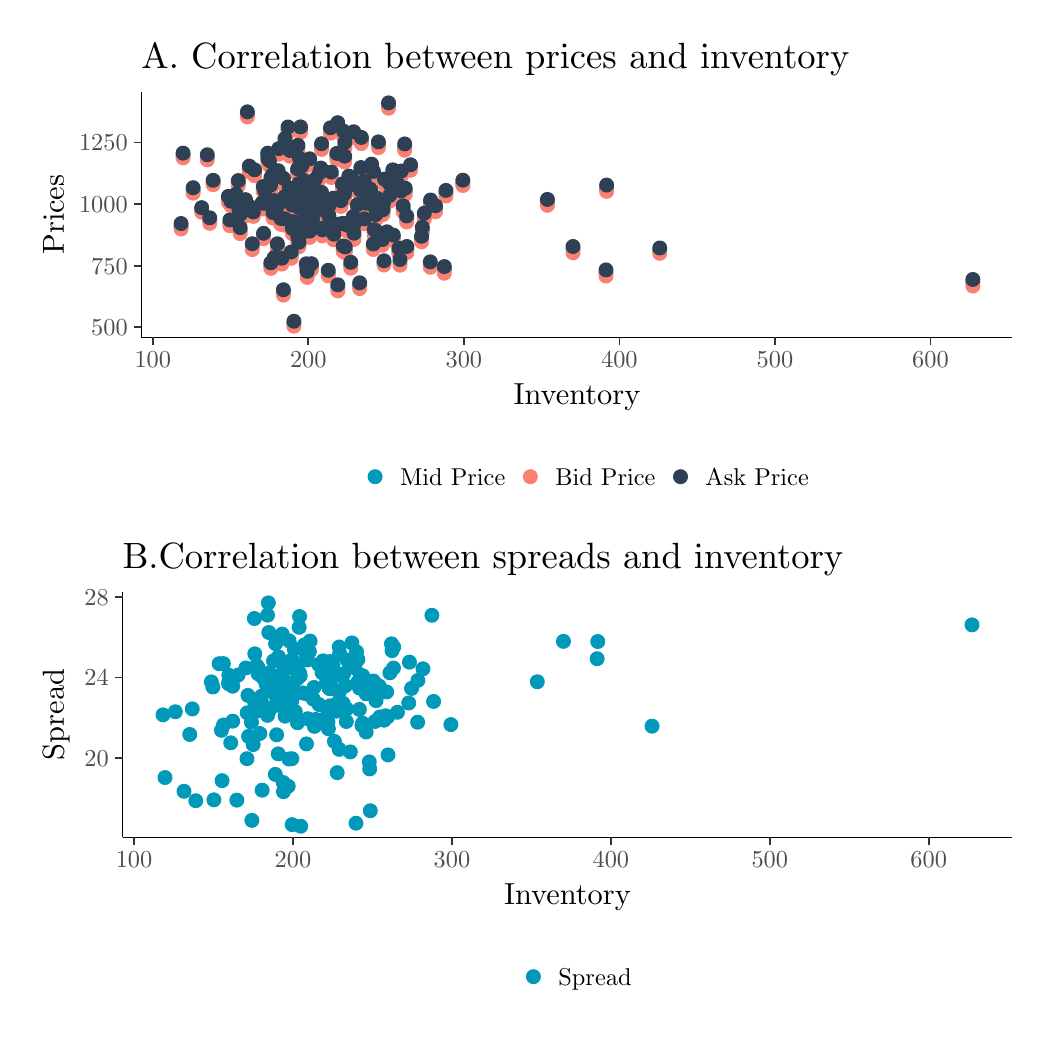
\begin{tikzpicture}[x=1pt,y=1pt]
\definecolor{fillColor}{RGB}{255,255,255}
\path[use as bounding box,fill=fillColor,fill opacity=0.00] (0,0) rectangle (361.35,361.35);
\begin{scope}
\path[clip] (  0.00,180.67) rectangle (361.35,361.35);
\definecolor{drawColor}{RGB}{255,255,255}
\definecolor{fillColor}{RGB}{255,255,255}

\path[draw=drawColor,line width= 0.6pt,line join=round,line cap=round,fill=fillColor] (  0.00,180.67) rectangle (361.35,361.35);
\end{scope}
\begin{scope}
\path[clip] ( 41.12,249.42) rectangle (355.85,338.21);
\definecolor{fillColor}{RGB}{255,255,255}

\path[fill=fillColor] ( 41.12,249.42) rectangle (355.85,338.21);
\definecolor{drawColor}{RGB}{0,153,186}
\definecolor{fillColor}{RGB}{0,153,186}

\path[draw=drawColor,line width= 0.4pt,line join=round,line cap=round,fill=fillColor] (123.69,297.05) circle (  2.50);

\path[draw=drawColor,line width= 0.4pt,line join=round,line cap=round,fill=fillColor] (104.14,300.56) circle (  2.50);

\path[draw=drawColor,line width= 0.4pt,line join=round,line cap=round,fill=fillColor] ( 86.87,313.21) circle (  2.50);

\path[draw=drawColor,line width= 0.4pt,line join=round,line cap=round,fill=fillColor] (145.49,275.75) circle (  2.50);

\path[draw=drawColor,line width= 0.4pt,line join=round,line cap=round,fill=fillColor] ( 76.11,305.15) circle (  2.50);

\path[draw=drawColor,line width= 0.4pt,line join=round,line cap=round,fill=fillColor] (125.79,292.85) circle (  2.50);

\path[draw=drawColor,line width= 0.4pt,line join=round,line cap=round,fill=fillColor] ( 99.22,311.47) circle (  2.50);

\path[draw=drawColor,line width= 0.4pt,line join=round,line cap=round,fill=fillColor] (114.17,322.89) circle (  2.50);

\path[draw=drawColor,line width= 0.4pt,line join=round,line cap=round,fill=fillColor] ( 99.02,310.35) circle (  2.50);

\path[draw=drawColor,line width= 0.4pt,line join=round,line cap=round,fill=fillColor] (130.62,304.04) circle (  2.50);

\path[draw=drawColor,line width= 0.4pt,line join=round,line cap=round,fill=fillColor] (157.24,305.27) circle (  2.50);

\path[draw=drawColor,line width= 0.4pt,line join=round,line cap=round,fill=fillColor] (228.40,280.78) circle (  2.50);

\path[draw=drawColor,line width= 0.4pt,line join=round,line cap=round,fill=fillColor] (151.14,301.53) circle (  2.50);

\path[draw=drawColor,line width= 0.4pt,line join=round,line cap=round,fill=fillColor] (142.60,288.16) circle (  2.50);

\path[draw=drawColor,line width= 0.4pt,line join=round,line cap=round,fill=fillColor] (187.81,298.22) circle (  2.50);

\path[draw=drawColor,line width= 0.4pt,line join=round,line cap=round,fill=fillColor] (208.98,272.70) circle (  2.50);

\path[draw=drawColor,line width= 0.4pt,line join=round,line cap=round,fill=fillColor] ( 89.06,297.79) circle (  2.50);

\path[draw=drawColor,line width= 0.4pt,line join=round,line cap=round,fill=fillColor] (122.26,296.81) circle (  2.50);

\path[draw=drawColor,line width= 0.4pt,line join=round,line cap=round,fill=fillColor] (197.06,281.13) circle (  2.50);

\path[draw=drawColor,line width= 0.4pt,line join=round,line cap=round,fill=fillColor] (126.74,319.04) circle (  2.50);

\path[draw=drawColor,line width= 0.4pt,line join=round,line cap=round,fill=fillColor] (128.38,294.70) circle (  2.50);

\path[draw=drawColor,line width= 0.4pt,line join=round,line cap=round,fill=fillColor] (130.78,299.69) circle (  2.50);

\path[draw=drawColor,line width= 0.4pt,line join=round,line cap=round,fill=fillColor] (117.90,285.94) circle (  2.50);

\path[draw=drawColor,line width= 0.4pt,line join=round,line cap=round,fill=fillColor] (107.45,294.03) circle (  2.50);

\path[draw=drawColor,line width= 0.4pt,line join=round,line cap=round,fill=fillColor] ( 87.75,303.22) circle (  2.50);

\path[draw=drawColor,line width= 0.4pt,line join=round,line cap=round,fill=fillColor] (150.55,273.82) circle (  2.50);

\path[draw=drawColor,line width= 0.4pt,line join=round,line cap=round,fill=fillColor] ( 92.70,298.90) circle (  2.50);

\path[draw=drawColor,line width= 0.4pt,line join=round,line cap=round,fill=fillColor] ( 92.41,305.72) circle (  2.50);

\path[draw=drawColor,line width= 0.4pt,line join=round,line cap=round,fill=fillColor] (103.60,297.36) circle (  2.50);

\path[draw=drawColor,line width= 0.4pt,line join=round,line cap=round,fill=fillColor] (209.20,303.32) circle (  2.50);

\path[draw=drawColor,line width= 0.4pt,line join=round,line cap=round,fill=fillColor] (341.54,269.18) circle (  2.50);

\path[draw=drawColor,line width= 0.4pt,line join=round,line cap=round,fill=fillColor] (129.84,286.52) circle (  2.50);

\path[draw=drawColor,line width= 0.4pt,line join=round,line cap=round,fill=fillColor] ( 99.99,301.62) circle (  2.50);

\path[draw=drawColor,line width= 0.4pt,line join=round,line cap=round,fill=fillColor] (101.00,301.74) circle (  2.50);

\path[draw=drawColor,line width= 0.4pt,line join=round,line cap=round,fill=fillColor] (135.01,308.67) circle (  2.50);

\path[draw=drawColor,line width= 0.4pt,line join=round,line cap=round,fill=fillColor] ( 79.39,330.01) circle (  2.50);

\path[draw=drawColor,line width= 0.4pt,line join=round,line cap=round,fill=fillColor] (117.75,303.77) circle (  2.50);

\path[draw=drawColor,line width= 0.4pt,line join=round,line cap=round,fill=fillColor] (128.54,296.84) circle (  2.50);

\path[draw=drawColor,line width= 0.4pt,line join=round,line cap=round,fill=fillColor] ( 95.16,299.05) circle (  2.50);

\path[draw=drawColor,line width= 0.4pt,line join=round,line cap=round,fill=fillColor] (117.04,306.18) circle (  2.50);

\path[draw=drawColor,line width= 0.4pt,line join=round,line cap=round,fill=fillColor] (128.76,276.34) circle (  2.50);

\path[draw=drawColor,line width= 0.4pt,line join=round,line cap=round,fill=fillColor] (101.11,304.15) circle (  2.50);

\path[draw=drawColor,line width= 0.4pt,line join=round,line cap=round,fill=fillColor] ( 97.94,304.13) circle (  2.50);

\path[draw=drawColor,line width= 0.4pt,line join=round,line cap=round,fill=fillColor] ( 67.02,305.40) circle (  2.50);

\path[draw=drawColor,line width= 0.4pt,line join=round,line cap=round,fill=fillColor] ( 73.43,297.84) circle (  2.50);

\path[draw=drawColor,line width= 0.4pt,line join=round,line cap=round,fill=fillColor] ( 98.04,283.01) circle (  2.50);

\path[draw=drawColor,line width= 0.4pt,line join=round,line cap=round,fill=fillColor] ( 76.34,294.72) circle (  2.50);

\path[draw=drawColor,line width= 0.4pt,line join=round,line cap=round,fill=fillColor] ( 56.15,315.16) circle (  2.50);

\path[draw=drawColor,line width= 0.4pt,line join=round,line cap=round,fill=fillColor] ( 81.55,293.95) circle (  2.50);

\path[draw=drawColor,line width= 0.4pt,line join=round,line cap=round,fill=fillColor] ( 99.71,305.35) circle (  2.50);

\path[draw=drawColor,line width= 0.4pt,line join=round,line cap=round,fill=fillColor] ( 62.87,295.50) circle (  2.50);

\path[draw=drawColor,line width= 0.4pt,line join=round,line cap=round,fill=fillColor] (102.21,295.12) circle (  2.50);

\path[draw=drawColor,line width= 0.4pt,line join=round,line cap=round,fill=fillColor] (120.27,301.61) circle (  2.50);

\path[draw=drawColor,line width= 0.4pt,line join=round,line cap=round,fill=fillColor] ( 90.51,296.57) circle (  2.50);

\path[draw=drawColor,line width= 0.4pt,line join=round,line cap=round,fill=fillColor] ( 85.13,303.05) circle (  2.50);

\path[draw=drawColor,line width= 0.4pt,line join=round,line cap=round,fill=fillColor] (106.65,297.33) circle (  2.50);

\path[draw=drawColor,line width= 0.4pt,line join=round,line cap=round,fill=fillColor] (121.69,291.37) circle (  2.50);

\path[draw=drawColor,line width= 0.4pt,line join=round,line cap=round,fill=fillColor] (100.66,299.91) circle (  2.50);

\path[draw=drawColor,line width= 0.4pt,line join=round,line cap=round,fill=fillColor] (131.94,308.92) circle (  2.50);

\path[draw=drawColor,line width= 0.4pt,line join=round,line cap=round,fill=fillColor] ( 90.71,316.62) circle (  2.50);

\path[draw=drawColor,line width= 0.4pt,line join=round,line cap=round,fill=fillColor] (124.89,282.19) circle (  2.50);

\path[draw=drawColor,line width= 0.4pt,line join=round,line cap=round,fill=fillColor] ( 92.97,320.29) circle (  2.50);

\path[draw=drawColor,line width= 0.4pt,line join=round,line cap=round,fill=fillColor] ( 90.23,282.23) circle (  2.50);

\path[draw=drawColor,line width= 0.4pt,line join=round,line cap=round,fill=fillColor] ( 86.73,315.03) circle (  2.50);

\path[draw=drawColor,line width= 0.4pt,line join=round,line cap=round,fill=fillColor] ( 95.67,296.19) circle (  2.50);

\path[draw=drawColor,line width= 0.4pt,line join=round,line cap=round,fill=fillColor] ( 96.20,254.36) circle (  2.50);

\path[draw=drawColor,line width= 0.4pt,line join=round,line cap=round,fill=fillColor] (117.81,322.71) circle (  2.50);

\path[draw=drawColor,line width= 0.4pt,line join=round,line cap=round,fill=fillColor] ( 96.88,300.30) circle (  2.50);

\path[draw=drawColor,line width= 0.4pt,line join=round,line cap=round,fill=fillColor] ( 89.69,294.14) circle (  2.50);

\path[draw=drawColor,line width= 0.4pt,line join=round,line cap=round,fill=fillColor] (116.06,306.79) circle (  2.50);

\path[draw=drawColor,line width= 0.4pt,line join=round,line cap=round,fill=fillColor] (135.69,295.89) circle (  2.50);

\path[draw=drawColor,line width= 0.4pt,line join=round,line cap=round,fill=fillColor] (120.58,320.57) circle (  2.50);

\path[draw=drawColor,line width= 0.4pt,line join=round,line cap=round,fill=fillColor] (119.31,303.64) circle (  2.50);

\path[draw=drawColor,line width= 0.4pt,line join=round,line cap=round,fill=fillColor] (114.48,300.29) circle (  2.50);

\path[draw=drawColor,line width= 0.4pt,line join=round,line cap=round,fill=fillColor] (108.61,272.65) circle (  2.50);

\path[draw=drawColor,line width= 0.4pt,line join=round,line cap=round,fill=fillColor] ( 80.08,295.85) circle (  2.50);

\path[draw=drawColor,line width= 0.4pt,line join=round,line cap=round,fill=fillColor] (123.89,301.82) circle (  2.50);

\path[draw=drawColor,line width= 0.4pt,line join=round,line cap=round,fill=fillColor] (103.02,292.50) circle (  2.50);

\path[draw=drawColor,line width= 0.4pt,line join=round,line cap=round,fill=fillColor] ( 87.34,312.37) circle (  2.50);

\path[draw=drawColor,line width= 0.4pt,line join=round,line cap=round,fill=fillColor] ( 88.64,293.54) circle (  2.50);

\path[draw=drawColor,line width= 0.4pt,line join=round,line cap=round,fill=fillColor] (113.93,289.69) circle (  2.50);

\path[draw=drawColor,line width= 0.4pt,line join=round,line cap=round,fill=fillColor] (114.76,281.06) circle (  2.50);

\path[draw=drawColor,line width= 0.4pt,line join=round,line cap=round,fill=fillColor] (119.16,296.39) circle (  2.50);

\path[draw=drawColor,line width= 0.4pt,line join=round,line cap=round,fill=fillColor] (103.78,301.91) circle (  2.50);

\path[draw=drawColor,line width= 0.4pt,line join=round,line cap=round,fill=fillColor] (109.71,308.19) circle (  2.50);

\path[draw=drawColor,line width= 0.4pt,line join=round,line cap=round,fill=fillColor] (101.89,312.87) circle (  2.50);

\path[draw=drawColor,line width= 0.4pt,line join=round,line cap=round,fill=fillColor] ( 98.59,324.52) circle (  2.50);

\path[draw=drawColor,line width= 0.4pt,line join=round,line cap=round,fill=fillColor] (136.95,292.21) circle (  2.50);

\path[draw=drawColor,line width= 0.4pt,line join=round,line cap=round,fill=fillColor] (112.30,289.37) circle (  2.50);

\path[draw=drawColor,line width= 0.4pt,line join=round,line cap=round,fill=fillColor] (106.18,300.92) circle (  2.50);

\path[draw=drawColor,line width= 0.4pt,line join=round,line cap=round,fill=fillColor] (111.71,314.84) circle (  2.50);

\path[draw=drawColor,line width= 0.4pt,line join=round,line cap=round,fill=fillColor] (113.77,303.93) circle (  2.50);

\path[draw=drawColor,line width= 0.4pt,line join=round,line cap=round,fill=fillColor] ( 96.28,298.94) circle (  2.50);

\path[draw=drawColor,line width= 0.4pt,line join=round,line cap=round,fill=fillColor] ( 85.72,301.40) circle (  2.50);

\path[draw=drawColor,line width= 0.4pt,line join=round,line cap=round,fill=fillColor] (134.91,301.39) circle (  2.50);

\path[draw=drawColor,line width= 0.4pt,line join=round,line cap=round,fill=fillColor] (110.60,285.71) circle (  2.50);

\path[draw=drawColor,line width= 0.4pt,line join=round,line cap=round,fill=fillColor] (147.37,295.89) circle (  2.50);

\path[draw=drawColor,line width= 0.4pt,line join=round,line cap=round,fill=fillColor] ( 88.51,307.14) circle (  2.50);

\path[draw=drawColor,line width= 0.4pt,line join=round,line cap=round,fill=fillColor] (127.29,297.23) circle (  2.50);

\path[draw=drawColor,line width= 0.4pt,line join=round,line cap=round,fill=fillColor] (117.77,288.74) circle (  2.50);

\path[draw=drawColor,line width= 0.4pt,line join=round,line cap=round,fill=fillColor] (128.94,305.59) circle (  2.50);

\path[draw=drawColor,line width= 0.4pt,line join=round,line cap=round,fill=fillColor] (120.40,309.82) circle (  2.50);

\path[draw=drawColor,line width= 0.4pt,line join=round,line cap=round,fill=fillColor] (132.12,285.43) circle (  2.50);

\path[draw=drawColor,line width= 0.4pt,line join=round,line cap=round,fill=fillColor] (130.40,333.21) circle (  2.50);

\path[draw=drawColor,line width= 0.4pt,line join=round,line cap=round,fill=fillColor] (113.20,297.79) circle (  2.50);

\path[draw=drawColor,line width= 0.4pt,line join=round,line cap=round,fill=fillColor] (101.87,286.69) circle (  2.50);

\path[draw=drawColor,line width= 0.4pt,line join=round,line cap=round,fill=fillColor] ( 92.41,265.67) circle (  2.50);

\path[draw=drawColor,line width= 0.4pt,line join=round,line cap=round,fill=fillColor] (137.02,281.15) circle (  2.50);

\path[draw=drawColor,line width= 0.4pt,line join=round,line cap=round,fill=fillColor] ( 84.72,296.95) circle (  2.50);

\path[draw=drawColor,line width= 0.4pt,line join=round,line cap=round,fill=fillColor] (126.07,298.81) circle (  2.50);

\path[draw=drawColor,line width= 0.4pt,line join=round,line cap=round,fill=fillColor] ( 99.26,296.76) circle (  2.50);

\path[draw=drawColor,line width= 0.4pt,line join=round,line cap=round,fill=fillColor] ( 85.48,296.86) circle (  2.50);

\path[draw=drawColor,line width= 0.4pt,line join=round,line cap=round,fill=fillColor] (104.81,299.58) circle (  2.50);

\path[draw=drawColor,line width= 0.4pt,line join=round,line cap=round,fill=fillColor] (133.61,304.13) circle (  2.50);

\path[draw=drawColor,line width= 0.4pt,line join=round,line cap=round,fill=fillColor] (103.96,305.62) circle (  2.50);

\path[draw=drawColor,line width= 0.4pt,line join=round,line cap=round,fill=fillColor] (115.55,288.86) circle (  2.50);

\path[draw=drawColor,line width= 0.4pt,line join=round,line cap=round,fill=fillColor] (143.34,293.30) circle (  2.50);

\path[draw=drawColor,line width= 0.4pt,line join=round,line cap=round,fill=fillColor] (100.99,304.06) circle (  2.50);

\path[draw=drawColor,line width= 0.4pt,line join=round,line cap=round,fill=fillColor] (134.53,276.55) circle (  2.50);

\path[draw=drawColor,line width= 0.4pt,line join=round,line cap=round,fill=fillColor] (116.75,275.49) circle (  2.50);

\path[draw=drawColor,line width= 0.4pt,line join=round,line cap=round,fill=fillColor] (103.59,297.63) circle (  2.50);

\path[draw=drawColor,line width= 0.4pt,line join=round,line cap=round,fill=fillColor] ( 95.64,287.83) circle (  2.50);

\path[draw=drawColor,line width= 0.4pt,line join=round,line cap=round,fill=fillColor] (102.54,274.96) circle (  2.50);

\path[draw=drawColor,line width= 0.4pt,line join=round,line cap=round,fill=fillColor] (117.64,292.10) circle (  2.50);

\path[draw=drawColor,line width= 0.4pt,line join=round,line cap=round,fill=fillColor] ( 95.76,289.53) circle (  2.50);

\path[draw=drawColor,line width= 0.4pt,line join=round,line cap=round,fill=fillColor] ( 76.82,292.91) circle (  2.50);

\path[draw=drawColor,line width= 0.4pt,line join=round,line cap=round,fill=fillColor] (106.19,318.39) circle (  2.50);

\path[draw=drawColor,line width= 0.4pt,line join=round,line cap=round,fill=fillColor] (125.21,287.31) circle (  2.50);

\path[draw=drawColor,line width= 0.4pt,line join=round,line cap=round,fill=fillColor] ( 94.79,315.93) circle (  2.50);

\path[draw=drawColor,line width= 0.4pt,line join=round,line cap=round,fill=fillColor] (110.47,298.65) circle (  2.50);

\path[draw=drawColor,line width= 0.4pt,line join=round,line cap=round,fill=fillColor] (114.54,313.86) circle (  2.50);

\path[draw=drawColor,line width= 0.4pt,line join=round,line cap=round,fill=fillColor] ( 65.79,291.65) circle (  2.50);

\path[draw=drawColor,line width= 0.4pt,line join=round,line cap=round,fill=fillColor] (114.62,318.88) circle (  2.50);

\path[draw=drawColor,line width= 0.4pt,line join=round,line cap=round,fill=fillColor] ( 81.15,282.20) circle (  2.50);

\path[draw=drawColor,line width= 0.4pt,line join=round,line cap=round,fill=fillColor] ( 85.23,286.05) circle (  2.50);

\path[draw=drawColor,line width= 0.4pt,line join=round,line cap=round,fill=fillColor] ( 78.64,294.44) circle (  2.50);

\path[draw=drawColor,line width= 0.4pt,line join=round,line cap=round,fill=fillColor] (101.02,272.20) circle (  2.50);

\path[draw=drawColor,line width= 0.4pt,line join=round,line cap=round,fill=fillColor] (127.29,297.91) circle (  2.50);

\path[draw=drawColor,line width= 0.4pt,line join=round,line cap=round,fill=fillColor] (105.46,307.79) circle (  2.50);

\path[draw=drawColor,line width= 0.4pt,line join=round,line cap=round,fill=fillColor] (108.84,292.34) circle (  2.50);

\path[draw=drawColor,line width= 0.4pt,line join=round,line cap=round,fill=fillColor] (138.35,310.81) circle (  2.50);

\path[draw=drawColor,line width= 0.4pt,line join=round,line cap=round,fill=fillColor] ( 89.10,277.17) circle (  2.50);

\path[draw=drawColor,line width= 0.4pt,line join=round,line cap=round,fill=fillColor] (105.94,309.49) circle (  2.50);

\path[draw=drawColor,line width= 0.4pt,line join=round,line cap=round,fill=fillColor] (100.66,274.99) circle (  2.50);

\path[draw=drawColor,line width= 0.4pt,line join=round,line cap=round,fill=fillColor] ( 98.24,313.07) circle (  2.50);

\path[draw=drawColor,line width= 0.4pt,line join=round,line cap=round,fill=fillColor] (113.70,299.56) circle (  2.50);

\path[draw=drawColor,line width= 0.4pt,line join=round,line cap=round,fill=fillColor] ( 94.08,324.41) circle (  2.50);

\path[draw=drawColor,line width= 0.4pt,line join=round,line cap=round,fill=fillColor] ( 73.07,290.81) circle (  2.50);

\path[draw=drawColor,line width= 0.4pt,line join=round,line cap=round,fill=fillColor] ( 90.51,308.60) circle (  2.50);

\path[draw=drawColor,line width= 0.4pt,line join=round,line cap=round,fill=fillColor] (142.33,284.96) circle (  2.50);

\path[draw=drawColor,line width= 0.4pt,line join=round,line cap=round,fill=fillColor] (124.95,308.36) circle (  2.50);

\path[draw=drawColor,line width= 0.4pt,line join=round,line cap=round,fill=fillColor] (128.16,283.75) circle (  2.50);

\path[draw=drawColor,line width= 0.4pt,line join=round,line cap=round,fill=fillColor] ( 75.31,300.07) circle (  2.50);

\path[draw=drawColor,line width= 0.4pt,line join=round,line cap=round,fill=fillColor] ( 64.90,314.49) circle (  2.50);

\path[draw=drawColor,line width= 0.4pt,line join=round,line cap=round,fill=fillColor] (103.44,297.88) circle (  2.50);

\path[draw=drawColor,line width= 0.4pt,line join=round,line cap=round,fill=fillColor] (100.04,290.79) circle (  2.50);

\path[draw=drawColor,line width= 0.4pt,line join=round,line cap=round,fill=fillColor] (121.60,304.76) circle (  2.50);

\path[draw=drawColor,line width= 0.4pt,line join=round,line cap=round,fill=fillColor] (125.99,286.80) circle (  2.50);

\path[draw=drawColor,line width= 0.4pt,line join=round,line cap=round,fill=fillColor] ( 91.84,276.98) circle (  2.50);

\path[draw=drawColor,line width= 0.4pt,line join=round,line cap=round,fill=fillColor] ( 91.45,291.35) circle (  2.50);

\path[draw=drawColor,line width= 0.4pt,line join=round,line cap=round,fill=fillColor] (116.69,290.02) circle (  2.50);

\path[draw=drawColor,line width= 0.4pt,line join=round,line cap=round,fill=fillColor] ( 87.87,275.38) circle (  2.50);

\path[draw=drawColor,line width= 0.4pt,line join=round,line cap=round,fill=fillColor] (109.42,324.20) circle (  2.50);

\path[draw=drawColor,line width= 0.4pt,line join=round,line cap=round,fill=fillColor] ( 95.83,290.19) circle (  2.50);

\path[draw=drawColor,line width= 0.4pt,line join=round,line cap=round,fill=fillColor] (114.01,281.47) circle (  2.50);

\path[draw=drawColor,line width= 0.4pt,line join=round,line cap=round,fill=fillColor] (108.96,296.20) circle (  2.50);

\path[draw=drawColor,line width= 0.4pt,line join=round,line cap=round,fill=fillColor] (101.39,290.48) circle (  2.50);

\path[draw=drawColor,line width= 0.4pt,line join=round,line cap=round,fill=fillColor] ( 78.76,295.94) circle (  2.50);

\path[draw=drawColor,line width= 0.4pt,line join=round,line cap=round,fill=fillColor] ( 80.09,310.27) circle (  2.50);

\path[draw=drawColor,line width= 0.4pt,line join=round,line cap=round,fill=fillColor] ( 97.55,309.27) circle (  2.50);

\path[draw=drawColor,line width= 0.4pt,line join=round,line cap=round,fill=fillColor] (102.99,290.07) circle (  2.50);

\path[draw=drawColor,line width= 0.4pt,line join=round,line cap=round,fill=fillColor] (124.36,298.40) circle (  2.50);

\path[draw=drawColor,line width= 0.4pt,line join=round,line cap=round,fill=fillColor] ( 95.24,279.15) circle (  2.50);

\path[draw=drawColor,line width= 0.4pt,line join=round,line cap=round,fill=fillColor] ( 59.79,302.53) circle (  2.50);

\path[draw=drawColor,line width= 0.4pt,line join=round,line cap=round,fill=fillColor] (112.05,326.04) circle (  2.50);

\path[draw=drawColor,line width= 0.4pt,line join=round,line cap=round,fill=fillColor] ( 76.79,287.99) circle (  2.50);

\path[draw=drawColor,line width= 0.4pt,line join=round,line cap=round,fill=fillColor] ( 87.90,306.09) circle (  2.50);

\path[draw=drawColor,line width= 0.4pt,line join=round,line cap=round,fill=fillColor] (136.23,318.19) circle (  2.50);

\path[draw=drawColor,line width= 0.4pt,line join=round,line cap=round,fill=fillColor] ( 92.95,297.70) circle (  2.50);

\path[draw=drawColor,line width= 0.4pt,line join=round,line cap=round,fill=fillColor] ( 81.99,308.92) circle (  2.50);

\path[draw=drawColor,line width= 0.4pt,line join=round,line cap=round,fill=fillColor] ( 98.40,294.96) circle (  2.50);

\path[draw=drawColor,line width= 0.4pt,line join=round,line cap=round,fill=fillColor] ( 97.65,317.77) circle (  2.50);

\path[draw=drawColor,line width= 0.4pt,line join=round,line cap=round,fill=fillColor] (145.59,298.01) circle (  2.50);

\path[draw=drawColor,line width= 0.4pt,line join=round,line cap=round,fill=fillColor] (136.44,302.20) circle (  2.50);

\path[draw=drawColor,line width= 0.4pt,line join=round,line cap=round,fill=fillColor] ( 78.72,298.14) circle (  2.50);

\path[draw=drawColor,line width= 0.4pt,line join=round,line cap=round,fill=fillColor] (123.34,297.93) circle (  2.50);

\path[draw=drawColor,line width= 0.4pt,line join=round,line cap=round,fill=fillColor] (112.06,267.32) circle (  2.50);

\path[draw=drawColor,line width= 0.4pt,line join=round,line cap=round,fill=fillColor] (103.74,297.95) circle (  2.50);

\path[draw=drawColor,line width= 0.4pt,line join=round,line cap=round,fill=fillColor] ( 94.52,302.24) circle (  2.50);

\path[draw=drawColor,line width= 0.4pt,line join=round,line cap=round,fill=fillColor] ( 72.54,299.34) circle (  2.50);

\path[draw=drawColor,line width= 0.4pt,line join=round,line cap=round,fill=fillColor] (124.26,311.00) circle (  2.50);

\path[draw=drawColor,line width= 0.4pt,line join=round,line cap=round,fill=fillColor] (107.22,287.95) circle (  2.50);

\path[draw=drawColor,line width= 0.4pt,line join=round,line cap=round,fill=fillColor] ( 92.86,291.14) circle (  2.50);

\path[draw=drawColor,line width= 0.4pt,line join=round,line cap=round,fill=fillColor] (106.48,287.21) circle (  2.50);

\path[draw=drawColor,line width= 0.4pt,line join=round,line cap=round,fill=fillColor] (119.97,268.11) circle (  2.50);

\path[draw=drawColor,line width= 0.4pt,line join=round,line cap=round,fill=fillColor] ( 97.60,284.49) circle (  2.50);

\path[draw=drawColor,line width= 0.4pt,line join=round,line cap=round,fill=fillColor] ( 99.05,286.18) circle (  2.50);

\path[draw=drawColor,line width= 0.4pt,line join=round,line cap=round,fill=fillColor] (134.14,280.68) circle (  2.50);

\path[draw=drawColor,line width= 0.4pt,line join=round,line cap=round,fill=fillColor] ( 55.43,289.59) circle (  2.50);

\path[draw=drawColor,line width= 0.4pt,line join=round,line cap=round,fill=fillColor] ( 98.16,296.78) circle (  2.50);
\definecolor{drawColor}{RGB}{250,128,114}
\definecolor{fillColor}{RGB}{250,128,114}

\path[draw=drawColor,line width= 0.4pt,line join=round,line cap=round,fill=fillColor] (123.69,296.30) circle (  2.50);

\path[draw=drawColor,line width= 0.4pt,line join=round,line cap=round,fill=fillColor] (104.14,299.82) circle (  2.50);

\path[draw=drawColor,line width= 0.4pt,line join=round,line cap=round,fill=fillColor] ( 86.87,312.46) circle (  2.50);

\path[draw=drawColor,line width= 0.4pt,line join=round,line cap=round,fill=fillColor] (145.49,274.78) circle (  2.50);

\path[draw=drawColor,line width= 0.4pt,line join=round,line cap=round,fill=fillColor] ( 76.11,304.20) circle (  2.50);

\path[draw=drawColor,line width= 0.4pt,line join=round,line cap=round,fill=fillColor] (125.79,291.89) circle (  2.50);

\path[draw=drawColor,line width= 0.4pt,line join=round,line cap=round,fill=fillColor] ( 99.22,310.46) circle (  2.50);

\path[draw=drawColor,line width= 0.4pt,line join=round,line cap=round,fill=fillColor] (114.17,321.84) circle (  2.50);

\path[draw=drawColor,line width= 0.4pt,line join=round,line cap=round,fill=fillColor] ( 99.02,309.32) circle (  2.50);

\path[draw=drawColor,line width= 0.4pt,line join=round,line cap=round,fill=fillColor] (130.62,302.98) circle (  2.50);

\path[draw=drawColor,line width= 0.4pt,line join=round,line cap=round,fill=fillColor] (157.24,304.31) circle (  2.50);

\path[draw=drawColor,line width= 0.4pt,line join=round,line cap=round,fill=fillColor] (228.40,279.82) circle (  2.50);

\path[draw=drawColor,line width= 0.4pt,line join=round,line cap=round,fill=fillColor] (151.14,300.51) circle (  2.50);

\path[draw=drawColor,line width= 0.4pt,line join=round,line cap=round,fill=fillColor] (142.60,287.06) circle (  2.50);

\path[draw=drawColor,line width= 0.4pt,line join=round,line cap=round,fill=fillColor] (187.81,297.16) circle (  2.50);

\path[draw=drawColor,line width= 0.4pt,line join=round,line cap=round,fill=fillColor] (208.98,271.60) circle (  2.50);

\path[draw=drawColor,line width= 0.4pt,line join=round,line cap=round,fill=fillColor] ( 89.06,296.71) circle (  2.50);

\path[draw=drawColor,line width= 0.4pt,line join=round,line cap=round,fill=fillColor] (122.26,295.67) circle (  2.50);

\path[draw=drawColor,line width= 0.4pt,line join=round,line cap=round,fill=fillColor] (197.06,279.99) circle (  2.50);

\path[draw=drawColor,line width= 0.4pt,line join=round,line cap=round,fill=fillColor] (126.74,317.99) circle (  2.50);

\path[draw=drawColor,line width= 0.4pt,line join=round,line cap=round,fill=fillColor] (128.38,293.82) circle (  2.50);

\path[draw=drawColor,line width= 0.4pt,line join=round,line cap=round,fill=fillColor] (130.78,298.67) circle (  2.50);

\path[draw=drawColor,line width= 0.4pt,line join=round,line cap=round,fill=fillColor] (117.90,284.82) circle (  2.50);

\path[draw=drawColor,line width= 0.4pt,line join=round,line cap=round,fill=fillColor] (107.45,292.88) circle (  2.50);

\path[draw=drawColor,line width= 0.4pt,line join=round,line cap=round,fill=fillColor] ( 87.75,302.02) circle (  2.50);

\path[draw=drawColor,line width= 0.4pt,line join=round,line cap=round,fill=fillColor] (150.55,272.61) circle (  2.50);

\path[draw=drawColor,line width= 0.4pt,line join=round,line cap=round,fill=fillColor] ( 92.70,297.66) circle (  2.50);

\path[draw=drawColor,line width= 0.4pt,line join=round,line cap=round,fill=fillColor] ( 92.41,304.52) circle (  2.50);

\path[draw=drawColor,line width= 0.4pt,line join=round,line cap=round,fill=fillColor] (103.60,296.18) circle (  2.50);

\path[draw=drawColor,line width= 0.4pt,line join=round,line cap=round,fill=fillColor] (209.20,302.18) circle (  2.50);

\path[draw=drawColor,line width= 0.4pt,line join=round,line cap=round,fill=fillColor] (341.54,267.99) circle (  2.50);

\path[draw=drawColor,line width= 0.4pt,line join=round,line cap=round,fill=fillColor] (129.84,285.46) circle (  2.50);

\path[draw=drawColor,line width= 0.4pt,line join=round,line cap=round,fill=fillColor] ( 99.99,300.74) circle (  2.50);

\path[draw=drawColor,line width= 0.4pt,line join=round,line cap=round,fill=fillColor] (101.00,300.85) circle (  2.50);

\path[draw=drawColor,line width= 0.4pt,line join=round,line cap=round,fill=fillColor] (135.01,307.77) circle (  2.50);

\path[draw=drawColor,line width= 0.4pt,line join=round,line cap=round,fill=fillColor] ( 79.39,329.08) circle (  2.50);

\path[draw=drawColor,line width= 0.4pt,line join=round,line cap=round,fill=fillColor] (117.75,302.86) circle (  2.50);

\path[draw=drawColor,line width= 0.4pt,line join=round,line cap=round,fill=fillColor] (128.54,295.97) circle (  2.50);

\path[draw=drawColor,line width= 0.4pt,line join=round,line cap=round,fill=fillColor] ( 95.16,298.19) circle (  2.50);

\path[draw=drawColor,line width= 0.4pt,line join=round,line cap=round,fill=fillColor] (117.04,305.32) circle (  2.50);

\path[draw=drawColor,line width= 0.4pt,line join=round,line cap=round,fill=fillColor] (128.76,275.57) circle (  2.50);

\path[draw=drawColor,line width= 0.4pt,line join=round,line cap=round,fill=fillColor] (101.11,303.41) circle (  2.50);

\path[draw=drawColor,line width= 0.4pt,line join=round,line cap=round,fill=fillColor] ( 97.94,303.30) circle (  2.50);

\path[draw=drawColor,line width= 0.4pt,line join=round,line cap=round,fill=fillColor] ( 67.02,304.61) circle (  2.50);

\path[draw=drawColor,line width= 0.4pt,line join=round,line cap=round,fill=fillColor] ( 73.43,297.05) circle (  2.50);

\path[draw=drawColor,line width= 0.4pt,line join=round,line cap=round,fill=fillColor] ( 98.04,282.19) circle (  2.50);

\path[draw=drawColor,line width= 0.4pt,line join=round,line cap=round,fill=fillColor] ( 76.34,293.88) circle (  2.50);

\path[draw=drawColor,line width= 0.4pt,line join=round,line cap=round,fill=fillColor] ( 56.15,314.31) circle (  2.50);

\path[draw=drawColor,line width= 0.4pt,line join=round,line cap=round,fill=fillColor] ( 81.55,293.16) circle (  2.50);

\path[draw=drawColor,line width= 0.4pt,line join=round,line cap=round,fill=fillColor] ( 99.71,304.52) circle (  2.50);

\path[draw=drawColor,line width= 0.4pt,line join=round,line cap=round,fill=fillColor] ( 62.87,294.68) circle (  2.50);

\path[draw=drawColor,line width= 0.4pt,line join=round,line cap=round,fill=fillColor] (102.21,294.13) circle (  2.50);

\path[draw=drawColor,line width= 0.4pt,line join=round,line cap=round,fill=fillColor] (120.27,300.64) circle (  2.50);

\path[draw=drawColor,line width= 0.4pt,line join=round,line cap=round,fill=fillColor] ( 90.51,295.75) circle (  2.50);

\path[draw=drawColor,line width= 0.4pt,line join=round,line cap=round,fill=fillColor] ( 85.13,302.16) circle (  2.50);

\path[draw=drawColor,line width= 0.4pt,line join=round,line cap=round,fill=fillColor] (106.65,296.35) circle (  2.50);

\path[draw=drawColor,line width= 0.4pt,line join=round,line cap=round,fill=fillColor] (121.69,290.46) circle (  2.50);

\path[draw=drawColor,line width= 0.4pt,line join=round,line cap=round,fill=fillColor] (100.66,298.92) circle (  2.50);

\path[draw=drawColor,line width= 0.4pt,line join=round,line cap=round,fill=fillColor] (131.94,307.87) circle (  2.50);

\path[draw=drawColor,line width= 0.4pt,line join=round,line cap=round,fill=fillColor] ( 90.71,315.61) circle (  2.50);

\path[draw=drawColor,line width= 0.4pt,line join=round,line cap=round,fill=fillColor] (124.89,281.19) circle (  2.50);

\path[draw=drawColor,line width= 0.4pt,line join=round,line cap=round,fill=fillColor] ( 92.97,319.29) circle (  2.50);

\path[draw=drawColor,line width= 0.4pt,line join=round,line cap=round,fill=fillColor] ( 90.23,281.20) circle (  2.50);

\path[draw=drawColor,line width= 0.4pt,line join=round,line cap=round,fill=fillColor] ( 86.73,314.06) circle (  2.50);

\path[draw=drawColor,line width= 0.4pt,line join=round,line cap=round,fill=fillColor] ( 95.67,295.18) circle (  2.50);

\path[draw=drawColor,line width= 0.4pt,line join=round,line cap=round,fill=fillColor] ( 96.20,253.46) circle (  2.50);

\path[draw=drawColor,line width= 0.4pt,line join=round,line cap=round,fill=fillColor] (117.81,321.67) circle (  2.50);

\path[draw=drawColor,line width= 0.4pt,line join=round,line cap=round,fill=fillColor] ( 96.88,299.26) circle (  2.50);

\path[draw=drawColor,line width= 0.4pt,line join=round,line cap=round,fill=fillColor] ( 89.69,293.19) circle (  2.50);

\path[draw=drawColor,line width= 0.4pt,line join=round,line cap=round,fill=fillColor] (116.06,305.86) circle (  2.50);

\path[draw=drawColor,line width= 0.4pt,line join=round,line cap=round,fill=fillColor] (135.69,294.81) circle (  2.50);

\path[draw=drawColor,line width= 0.4pt,line join=round,line cap=round,fill=fillColor] (120.58,319.46) circle (  2.50);

\path[draw=drawColor,line width= 0.4pt,line join=round,line cap=round,fill=fillColor] (119.31,302.57) circle (  2.50);

\path[draw=drawColor,line width= 0.4pt,line join=round,line cap=round,fill=fillColor] (114.48,299.19) circle (  2.50);

\path[draw=drawColor,line width= 0.4pt,line join=round,line cap=round,fill=fillColor] (108.61,271.63) circle (  2.50);

\path[draw=drawColor,line width= 0.4pt,line join=round,line cap=round,fill=fillColor] ( 80.08,294.87) circle (  2.50);

\path[draw=drawColor,line width= 0.4pt,line join=round,line cap=round,fill=fillColor] (123.89,300.70) circle (  2.50);

\path[draw=drawColor,line width= 0.4pt,line join=round,line cap=round,fill=fillColor] (103.02,291.53) circle (  2.50);

\path[draw=drawColor,line width= 0.4pt,line join=round,line cap=round,fill=fillColor] ( 87.34,311.45) circle (  2.50);

\path[draw=drawColor,line width= 0.4pt,line join=round,line cap=round,fill=fillColor] ( 88.64,292.54) circle (  2.50);

\path[draw=drawColor,line width= 0.4pt,line join=round,line cap=round,fill=fillColor] (113.93,288.74) circle (  2.50);

\path[draw=drawColor,line width= 0.4pt,line join=round,line cap=round,fill=fillColor] (114.76,280.01) circle (  2.50);

\path[draw=drawColor,line width= 0.4pt,line join=round,line cap=round,fill=fillColor] (119.16,295.38) circle (  2.50);

\path[draw=drawColor,line width= 0.4pt,line join=round,line cap=round,fill=fillColor] (103.78,300.83) circle (  2.50);

\path[draw=drawColor,line width= 0.4pt,line join=round,line cap=round,fill=fillColor] (109.71,307.22) circle (  2.50);

\path[draw=drawColor,line width= 0.4pt,line join=round,line cap=round,fill=fillColor] (101.89,311.78) circle (  2.50);

\path[draw=drawColor,line width= 0.4pt,line join=round,line cap=round,fill=fillColor] ( 98.59,323.54) circle (  2.50);

\path[draw=drawColor,line width= 0.4pt,line join=round,line cap=round,fill=fillColor] (136.95,291.12) circle (  2.50);

\path[draw=drawColor,line width= 0.4pt,line join=round,line cap=round,fill=fillColor] (112.30,288.40) circle (  2.50);

\path[draw=drawColor,line width= 0.4pt,line join=round,line cap=round,fill=fillColor] (106.18,300.00) circle (  2.50);

\path[draw=drawColor,line width= 0.4pt,line join=round,line cap=round,fill=fillColor] (111.71,313.76) circle (  2.50);

\path[draw=drawColor,line width= 0.4pt,line join=round,line cap=round,fill=fillColor] (113.77,302.96) circle (  2.50);

\path[draw=drawColor,line width= 0.4pt,line join=round,line cap=round,fill=fillColor] ( 96.28,297.82) circle (  2.50);

\path[draw=drawColor,line width= 0.4pt,line join=round,line cap=round,fill=fillColor] ( 85.72,300.46) circle (  2.50);

\path[draw=drawColor,line width= 0.4pt,line join=round,line cap=round,fill=fillColor] (134.91,300.41) circle (  2.50);

\path[draw=drawColor,line width= 0.4pt,line join=round,line cap=round,fill=fillColor] (110.60,284.70) circle (  2.50);

\path[draw=drawColor,line width= 0.4pt,line join=round,line cap=round,fill=fillColor] (147.37,294.81) circle (  2.50);

\path[draw=drawColor,line width= 0.4pt,line join=round,line cap=round,fill=fillColor] ( 88.51,306.05) circle (  2.50);

\path[draw=drawColor,line width= 0.4pt,line join=round,line cap=round,fill=fillColor] (127.29,296.28) circle (  2.50);

\path[draw=drawColor,line width= 0.4pt,line join=round,line cap=round,fill=fillColor] (117.77,287.61) circle (  2.50);

\path[draw=drawColor,line width= 0.4pt,line join=round,line cap=round,fill=fillColor] (128.94,304.56) circle (  2.50);

\path[draw=drawColor,line width= 0.4pt,line join=round,line cap=round,fill=fillColor] (120.40,308.82) circle (  2.50);

\path[draw=drawColor,line width= 0.4pt,line join=round,line cap=round,fill=fillColor] (132.12,284.45) circle (  2.50);

\path[draw=drawColor,line width= 0.4pt,line join=round,line cap=round,fill=fillColor] (130.40,332.24) circle (  2.50);

\path[draw=drawColor,line width= 0.4pt,line join=round,line cap=round,fill=fillColor] (113.20,296.74) circle (  2.50);

\path[draw=drawColor,line width= 0.4pt,line join=round,line cap=round,fill=fillColor] (101.87,285.56) circle (  2.50);

\path[draw=drawColor,line width= 0.4pt,line join=round,line cap=round,fill=fillColor] ( 92.41,264.68) circle (  2.50);

\path[draw=drawColor,line width= 0.4pt,line join=round,line cap=round,fill=fillColor] (137.02,280.02) circle (  2.50);

\path[draw=drawColor,line width= 0.4pt,line join=round,line cap=round,fill=fillColor] ( 84.72,295.86) circle (  2.50);

\path[draw=drawColor,line width= 0.4pt,line join=round,line cap=round,fill=fillColor] (126.07,297.73) circle (  2.50);

\path[draw=drawColor,line width= 0.4pt,line join=round,line cap=round,fill=fillColor] ( 99.26,295.66) circle (  2.50);

\path[draw=drawColor,line width= 0.4pt,line join=round,line cap=round,fill=fillColor] ( 85.48,295.83) circle (  2.50);

\path[draw=drawColor,line width= 0.4pt,line join=round,line cap=round,fill=fillColor] (104.81,298.54) circle (  2.50);

\path[draw=drawColor,line width= 0.4pt,line join=round,line cap=round,fill=fillColor] (133.61,303.16) circle (  2.50);

\path[draw=drawColor,line width= 0.4pt,line join=round,line cap=round,fill=fillColor] (103.96,304.54) circle (  2.50);

\path[draw=drawColor,line width= 0.4pt,line join=round,line cap=round,fill=fillColor] (115.55,287.76) circle (  2.50);

\path[draw=drawColor,line width= 0.4pt,line join=round,line cap=round,fill=fillColor] (143.34,292.25) circle (  2.50);

\path[draw=drawColor,line width= 0.4pt,line join=round,line cap=round,fill=fillColor] (100.99,303.04) circle (  2.50);

\path[draw=drawColor,line width= 0.4pt,line join=round,line cap=round,fill=fillColor] (134.53,275.52) circle (  2.50);

\path[draw=drawColor,line width= 0.4pt,line join=round,line cap=round,fill=fillColor] (116.75,274.42) circle (  2.50);

\path[draw=drawColor,line width= 0.4pt,line join=round,line cap=round,fill=fillColor] (103.59,296.56) circle (  2.50);

\path[draw=drawColor,line width= 0.4pt,line join=round,line cap=round,fill=fillColor] ( 95.64,286.89) circle (  2.50);

\path[draw=drawColor,line width= 0.4pt,line join=round,line cap=round,fill=fillColor] (102.54,273.86) circle (  2.50);

\path[draw=drawColor,line width= 0.4pt,line join=round,line cap=round,fill=fillColor] (117.64,291.08) circle (  2.50);

\path[draw=drawColor,line width= 0.4pt,line join=round,line cap=round,fill=fillColor] ( 95.76,288.52) circle (  2.50);

\path[draw=drawColor,line width= 0.4pt,line join=round,line cap=round,fill=fillColor] ( 76.82,291.95) circle (  2.50);

\path[draw=drawColor,line width= 0.4pt,line join=round,line cap=round,fill=fillColor] (106.19,317.36) circle (  2.50);

\path[draw=drawColor,line width= 0.4pt,line join=round,line cap=round,fill=fillColor] (125.21,286.24) circle (  2.50);

\path[draw=drawColor,line width= 0.4pt,line join=round,line cap=round,fill=fillColor] ( 94.79,314.90) circle (  2.50);

\path[draw=drawColor,line width= 0.4pt,line join=round,line cap=round,fill=fillColor] (110.47,297.56) circle (  2.50);

\path[draw=drawColor,line width= 0.4pt,line join=round,line cap=round,fill=fillColor] (114.54,312.82) circle (  2.50);

\path[draw=drawColor,line width= 0.4pt,line join=round,line cap=round,fill=fillColor] ( 65.79,290.65) circle (  2.50);

\path[draw=drawColor,line width= 0.4pt,line join=round,line cap=round,fill=fillColor] (114.62,317.88) circle (  2.50);

\path[draw=drawColor,line width= 0.4pt,line join=round,line cap=round,fill=fillColor] ( 81.15,281.13) circle (  2.50);

\path[draw=drawColor,line width= 0.4pt,line join=round,line cap=round,fill=fillColor] ( 85.23,285.07) circle (  2.50);

\path[draw=drawColor,line width= 0.4pt,line join=round,line cap=round,fill=fillColor] ( 78.64,293.39) circle (  2.50);

\path[draw=drawColor,line width= 0.4pt,line join=round,line cap=round,fill=fillColor] (101.02,271.10) circle (  2.50);

\path[draw=drawColor,line width= 0.4pt,line join=round,line cap=round,fill=fillColor] (127.29,296.88) circle (  2.50);

\path[draw=drawColor,line width= 0.4pt,line join=round,line cap=round,fill=fillColor] (105.46,306.65) circle (  2.50);

\path[draw=drawColor,line width= 0.4pt,line join=round,line cap=round,fill=fillColor] (108.84,291.30) circle (  2.50);

\path[draw=drawColor,line width= 0.4pt,line join=round,line cap=round,fill=fillColor] (138.35,309.81) circle (  2.50);

\path[draw=drawColor,line width= 0.4pt,line join=round,line cap=round,fill=fillColor] ( 89.10,276.08) circle (  2.50);

\path[draw=drawColor,line width= 0.4pt,line join=round,line cap=round,fill=fillColor] (105.94,308.37) circle (  2.50);

\path[draw=drawColor,line width= 0.4pt,line join=round,line cap=round,fill=fillColor] (100.66,273.95) circle (  2.50);

\path[draw=drawColor,line width= 0.4pt,line join=round,line cap=round,fill=fillColor] ( 98.24,311.97) circle (  2.50);

\path[draw=drawColor,line width= 0.4pt,line join=round,line cap=round,fill=fillColor] (113.70,298.48) circle (  2.50);

\path[draw=drawColor,line width= 0.4pt,line join=round,line cap=round,fill=fillColor] ( 94.08,323.36) circle (  2.50);

\path[draw=drawColor,line width= 0.4pt,line join=round,line cap=round,fill=fillColor] ( 73.07,289.77) circle (  2.50);

\path[draw=drawColor,line width= 0.4pt,line join=round,line cap=round,fill=fillColor] ( 90.51,307.53) circle (  2.50);

\path[draw=drawColor,line width= 0.4pt,line join=round,line cap=round,fill=fillColor] (142.33,283.95) circle (  2.50);

\path[draw=drawColor,line width= 0.4pt,line join=round,line cap=round,fill=fillColor] (124.95,307.31) circle (  2.50);

\path[draw=drawColor,line width= 0.4pt,line join=round,line cap=round,fill=fillColor] (128.16,282.72) circle (  2.50);

\path[draw=drawColor,line width= 0.4pt,line join=round,line cap=round,fill=fillColor] ( 75.31,298.97) circle (  2.50);

\path[draw=drawColor,line width= 0.4pt,line join=round,line cap=round,fill=fillColor] ( 64.90,313.55) circle (  2.50);

\path[draw=drawColor,line width= 0.4pt,line join=round,line cap=round,fill=fillColor] (103.44,296.80) circle (  2.50);

\path[draw=drawColor,line width= 0.4pt,line join=round,line cap=round,fill=fillColor] (100.04,289.65) circle (  2.50);

\path[draw=drawColor,line width= 0.4pt,line join=round,line cap=round,fill=fillColor] (121.60,303.66) circle (  2.50);

\path[draw=drawColor,line width= 0.4pt,line join=round,line cap=round,fill=fillColor] (125.99,285.83) circle (  2.50);

\path[draw=drawColor,line width= 0.4pt,line join=round,line cap=round,fill=fillColor] ( 91.84,275.93) circle (  2.50);

\path[draw=drawColor,line width= 0.4pt,line join=round,line cap=round,fill=fillColor] ( 91.45,290.28) circle (  2.50);

\path[draw=drawColor,line width= 0.4pt,line join=round,line cap=round,fill=fillColor] (116.69,289.02) circle (  2.50);

\path[draw=drawColor,line width= 0.4pt,line join=round,line cap=round,fill=fillColor] ( 87.87,274.37) circle (  2.50);

\path[draw=drawColor,line width= 0.4pt,line join=round,line cap=round,fill=fillColor] (109.42,323.22) circle (  2.50);

\path[draw=drawColor,line width= 0.4pt,line join=round,line cap=round,fill=fillColor] ( 95.83,289.12) circle (  2.50);

\path[draw=drawColor,line width= 0.4pt,line join=round,line cap=round,fill=fillColor] (114.01,280.48) circle (  2.50);

\path[draw=drawColor,line width= 0.4pt,line join=round,line cap=round,fill=fillColor] (108.96,295.24) circle (  2.50);

\path[draw=drawColor,line width= 0.4pt,line join=round,line cap=round,fill=fillColor] (101.39,289.42) circle (  2.50);

\path[draw=drawColor,line width= 0.4pt,line join=round,line cap=round,fill=fillColor] ( 78.76,294.88) circle (  2.50);

\path[draw=drawColor,line width= 0.4pt,line join=round,line cap=round,fill=fillColor] ( 80.09,309.22) circle (  2.50);

\path[draw=drawColor,line width= 0.4pt,line join=round,line cap=round,fill=fillColor] ( 97.55,308.22) circle (  2.50);

\path[draw=drawColor,line width= 0.4pt,line join=round,line cap=round,fill=fillColor] (102.99,289.00) circle (  2.50);

\path[draw=drawColor,line width= 0.4pt,line join=round,line cap=round,fill=fillColor] (124.36,297.29) circle (  2.50);

\path[draw=drawColor,line width= 0.4pt,line join=round,line cap=round,fill=fillColor] ( 95.24,278.01) circle (  2.50);

\path[draw=drawColor,line width= 0.4pt,line join=round,line cap=round,fill=fillColor] ( 59.79,301.54) circle (  2.50);

\path[draw=drawColor,line width= 0.4pt,line join=round,line cap=round,fill=fillColor] (112.05,325.08) circle (  2.50);

\path[draw=drawColor,line width= 0.4pt,line join=round,line cap=round,fill=fillColor] ( 76.79,286.89) circle (  2.50);

\path[draw=drawColor,line width= 0.4pt,line join=round,line cap=round,fill=fillColor] ( 87.90,304.97) circle (  2.50);

\path[draw=drawColor,line width= 0.4pt,line join=round,line cap=round,fill=fillColor] (136.23,317.05) circle (  2.50);

\path[draw=drawColor,line width= 0.4pt,line join=round,line cap=round,fill=fillColor] ( 92.95,296.62) circle (  2.50);

\path[draw=drawColor,line width= 0.4pt,line join=round,line cap=round,fill=fillColor] ( 81.99,307.84) circle (  2.50);

\path[draw=drawColor,line width= 0.4pt,line join=round,line cap=round,fill=fillColor] ( 98.40,293.93) circle (  2.50);

\path[draw=drawColor,line width= 0.4pt,line join=round,line cap=round,fill=fillColor] ( 97.65,316.70) circle (  2.50);

\path[draw=drawColor,line width= 0.4pt,line join=round,line cap=round,fill=fillColor] (145.59,296.95) circle (  2.50);

\path[draw=drawColor,line width= 0.4pt,line join=round,line cap=round,fill=fillColor] (136.44,301.07) circle (  2.50);

\path[draw=drawColor,line width= 0.4pt,line join=round,line cap=round,fill=fillColor] ( 78.72,297.06) circle (  2.50);

\path[draw=drawColor,line width= 0.4pt,line join=round,line cap=round,fill=fillColor] (123.34,296.84) circle (  2.50);

\path[draw=drawColor,line width= 0.4pt,line join=round,line cap=round,fill=fillColor] (112.06,266.22) circle (  2.50);

\path[draw=drawColor,line width= 0.4pt,line join=round,line cap=round,fill=fillColor] (103.74,296.75) circle (  2.50);

\path[draw=drawColor,line width= 0.4pt,line join=round,line cap=round,fill=fillColor] ( 94.52,301.13) circle (  2.50);

\path[draw=drawColor,line width= 0.4pt,line join=round,line cap=round,fill=fillColor] ( 72.54,298.28) circle (  2.50);

\path[draw=drawColor,line width= 0.4pt,line join=round,line cap=round,fill=fillColor] (124.26,309.94) circle (  2.50);

\path[draw=drawColor,line width= 0.4pt,line join=round,line cap=round,fill=fillColor] (107.22,286.82) circle (  2.50);

\path[draw=drawColor,line width= 0.4pt,line join=round,line cap=round,fill=fillColor] ( 92.86,289.97) circle (  2.50);

\path[draw=drawColor,line width= 0.4pt,line join=round,line cap=round,fill=fillColor] (106.48,286.10) circle (  2.50);

\path[draw=drawColor,line width= 0.4pt,line join=round,line cap=round,fill=fillColor] (119.97,267.06) circle (  2.50);

\path[draw=drawColor,line width= 0.4pt,line join=round,line cap=round,fill=fillColor] ( 97.60,283.33) circle (  2.50);

\path[draw=drawColor,line width= 0.4pt,line join=round,line cap=round,fill=fillColor] ( 99.05,285.16) circle (  2.50);

\path[draw=drawColor,line width= 0.4pt,line join=round,line cap=round,fill=fillColor] (134.14,279.69) circle (  2.50);

\path[draw=drawColor,line width= 0.4pt,line join=round,line cap=round,fill=fillColor] ( 55.43,288.61) circle (  2.50);

\path[draw=drawColor,line width= 0.4pt,line join=round,line cap=round,fill=fillColor] ( 98.16,295.70) circle (  2.50);
\definecolor{drawColor}{RGB}{46,64,83}
\definecolor{fillColor}{RGB}{46,64,83}

\path[draw=drawColor,line width= 0.4pt,line join=round,line cap=round,fill=fillColor] (123.69,297.79) circle (  2.50);

\path[draw=drawColor,line width= 0.4pt,line join=round,line cap=round,fill=fillColor] (104.14,301.30) circle (  2.50);

\path[draw=drawColor,line width= 0.4pt,line join=round,line cap=round,fill=fillColor] ( 86.87,313.97) circle (  2.50);

\path[draw=drawColor,line width= 0.4pt,line join=round,line cap=round,fill=fillColor] (145.49,276.72) circle (  2.50);

\path[draw=drawColor,line width= 0.4pt,line join=round,line cap=round,fill=fillColor] ( 76.11,306.10) circle (  2.50);

\path[draw=drawColor,line width= 0.4pt,line join=round,line cap=round,fill=fillColor] (125.79,293.81) circle (  2.50);

\path[draw=drawColor,line width= 0.4pt,line join=round,line cap=round,fill=fillColor] ( 99.22,312.49) circle (  2.50);

\path[draw=drawColor,line width= 0.4pt,line join=round,line cap=round,fill=fillColor] (114.17,323.93) circle (  2.50);

\path[draw=drawColor,line width= 0.4pt,line join=round,line cap=round,fill=fillColor] ( 99.02,311.39) circle (  2.50);

\path[draw=drawColor,line width= 0.4pt,line join=round,line cap=round,fill=fillColor] (130.62,305.09) circle (  2.50);

\path[draw=drawColor,line width= 0.4pt,line join=round,line cap=round,fill=fillColor] (157.24,306.23) circle (  2.50);

\path[draw=drawColor,line width= 0.4pt,line join=round,line cap=round,fill=fillColor] (228.40,281.74) circle (  2.50);

\path[draw=drawColor,line width= 0.4pt,line join=round,line cap=round,fill=fillColor] (151.14,302.54) circle (  2.50);

\path[draw=drawColor,line width= 0.4pt,line join=round,line cap=round,fill=fillColor] (142.60,289.26) circle (  2.50);

\path[draw=drawColor,line width= 0.4pt,line join=round,line cap=round,fill=fillColor] (187.81,299.28) circle (  2.50);

\path[draw=drawColor,line width= 0.4pt,line join=round,line cap=round,fill=fillColor] (208.98,273.81) circle (  2.50);

\path[draw=drawColor,line width= 0.4pt,line join=round,line cap=round,fill=fillColor] ( 89.06,298.86) circle (  2.50);

\path[draw=drawColor,line width= 0.4pt,line join=round,line cap=round,fill=fillColor] (122.26,297.95) circle (  2.50);

\path[draw=drawColor,line width= 0.4pt,line join=round,line cap=round,fill=fillColor] (197.06,282.28) circle (  2.50);

\path[draw=drawColor,line width= 0.4pt,line join=round,line cap=round,fill=fillColor] (126.74,320.08) circle (  2.50);

\path[draw=drawColor,line width= 0.4pt,line join=round,line cap=round,fill=fillColor] (128.38,295.58) circle (  2.50);

\path[draw=drawColor,line width= 0.4pt,line join=round,line cap=round,fill=fillColor] (130.78,300.70) circle (  2.50);

\path[draw=drawColor,line width= 0.4pt,line join=round,line cap=round,fill=fillColor] (117.90,287.06) circle (  2.50);

\path[draw=drawColor,line width= 0.4pt,line join=round,line cap=round,fill=fillColor] (107.45,295.17) circle (  2.50);

\path[draw=drawColor,line width= 0.4pt,line join=round,line cap=round,fill=fillColor] ( 87.75,304.42) circle (  2.50);

\path[draw=drawColor,line width= 0.4pt,line join=round,line cap=round,fill=fillColor] (150.55,275.02) circle (  2.50);

\path[draw=drawColor,line width= 0.4pt,line join=round,line cap=round,fill=fillColor] ( 92.70,300.13) circle (  2.50);

\path[draw=drawColor,line width= 0.4pt,line join=round,line cap=round,fill=fillColor] ( 92.41,306.93) circle (  2.50);

\path[draw=drawColor,line width= 0.4pt,line join=round,line cap=round,fill=fillColor] (103.60,298.53) circle (  2.50);

\path[draw=drawColor,line width= 0.4pt,line join=round,line cap=round,fill=fillColor] (209.20,304.47) circle (  2.50);

\path[draw=drawColor,line width= 0.4pt,line join=round,line cap=round,fill=fillColor] (341.54,270.36) circle (  2.50);

\path[draw=drawColor,line width= 0.4pt,line join=round,line cap=round,fill=fillColor] (129.84,287.58) circle (  2.50);

\path[draw=drawColor,line width= 0.4pt,line join=round,line cap=round,fill=fillColor] ( 99.99,302.51) circle (  2.50);

\path[draw=drawColor,line width= 0.4pt,line join=round,line cap=round,fill=fillColor] (101.00,302.63) circle (  2.50);

\path[draw=drawColor,line width= 0.4pt,line join=round,line cap=round,fill=fillColor] (135.01,309.56) circle (  2.50);

\path[draw=drawColor,line width= 0.4pt,line join=round,line cap=round,fill=fillColor] ( 79.39,330.93) circle (  2.50);

\path[draw=drawColor,line width= 0.4pt,line join=round,line cap=round,fill=fillColor] (117.75,304.67) circle (  2.50);

\path[draw=drawColor,line width= 0.4pt,line join=round,line cap=round,fill=fillColor] (128.54,297.70) circle (  2.50);

\path[draw=drawColor,line width= 0.4pt,line join=round,line cap=round,fill=fillColor] ( 95.16,299.90) circle (  2.50);

\path[draw=drawColor,line width= 0.4pt,line join=round,line cap=round,fill=fillColor] (117.04,307.04) circle (  2.50);

\path[draw=drawColor,line width= 0.4pt,line join=round,line cap=round,fill=fillColor] (128.76,277.12) circle (  2.50);

\path[draw=drawColor,line width= 0.4pt,line join=round,line cap=round,fill=fillColor] (101.11,304.90) circle (  2.50);

\path[draw=drawColor,line width= 0.4pt,line join=round,line cap=round,fill=fillColor] ( 97.94,304.97) circle (  2.50);

\path[draw=drawColor,line width= 0.4pt,line join=round,line cap=round,fill=fillColor] ( 67.02,306.20) circle (  2.50);

\path[draw=drawColor,line width= 0.4pt,line join=round,line cap=round,fill=fillColor] ( 73.43,298.64) circle (  2.50);

\path[draw=drawColor,line width= 0.4pt,line join=round,line cap=round,fill=fillColor] ( 98.04,283.82) circle (  2.50);

\path[draw=drawColor,line width= 0.4pt,line join=round,line cap=round,fill=fillColor] ( 76.34,295.56) circle (  2.50);

\path[draw=drawColor,line width= 0.4pt,line join=round,line cap=round,fill=fillColor] ( 56.15,316.01) circle (  2.50);

\path[draw=drawColor,line width= 0.4pt,line join=round,line cap=round,fill=fillColor] ( 81.55,294.75) circle (  2.50);

\path[draw=drawColor,line width= 0.4pt,line join=round,line cap=round,fill=fillColor] ( 99.71,306.18) circle (  2.50);

\path[draw=drawColor,line width= 0.4pt,line join=round,line cap=round,fill=fillColor] ( 62.87,296.32) circle (  2.50);

\path[draw=drawColor,line width= 0.4pt,line join=round,line cap=round,fill=fillColor] (102.21,296.11) circle (  2.50);

\path[draw=drawColor,line width= 0.4pt,line join=round,line cap=round,fill=fillColor] (120.27,302.58) circle (  2.50);

\path[draw=drawColor,line width= 0.4pt,line join=round,line cap=round,fill=fillColor] ( 90.51,297.39) circle (  2.50);

\path[draw=drawColor,line width= 0.4pt,line join=round,line cap=round,fill=fillColor] ( 85.13,303.93) circle (  2.50);

\path[draw=drawColor,line width= 0.4pt,line join=round,line cap=round,fill=fillColor] (106.65,298.31) circle (  2.50);

\path[draw=drawColor,line width= 0.4pt,line join=round,line cap=round,fill=fillColor] (121.69,292.27) circle (  2.50);

\path[draw=drawColor,line width= 0.4pt,line join=round,line cap=round,fill=fillColor] (100.66,300.90) circle (  2.50);

\path[draw=drawColor,line width= 0.4pt,line join=round,line cap=round,fill=fillColor] (131.94,309.97) circle (  2.50);

\path[draw=drawColor,line width= 0.4pt,line join=round,line cap=round,fill=fillColor] ( 90.71,317.63) circle (  2.50);

\path[draw=drawColor,line width= 0.4pt,line join=round,line cap=round,fill=fillColor] (124.89,283.18) circle (  2.50);

\path[draw=drawColor,line width= 0.4pt,line join=round,line cap=round,fill=fillColor] ( 92.97,321.28) circle (  2.50);

\path[draw=drawColor,line width= 0.4pt,line join=round,line cap=round,fill=fillColor] ( 90.23,283.25) circle (  2.50);

\path[draw=drawColor,line width= 0.4pt,line join=round,line cap=round,fill=fillColor] ( 86.73,316.00) circle (  2.50);

\path[draw=drawColor,line width= 0.4pt,line join=round,line cap=round,fill=fillColor] ( 95.67,297.20) circle (  2.50);

\path[draw=drawColor,line width= 0.4pt,line join=round,line cap=round,fill=fillColor] ( 96.20,255.26) circle (  2.50);

\path[draw=drawColor,line width= 0.4pt,line join=round,line cap=round,fill=fillColor] (117.81,323.74) circle (  2.50);

\path[draw=drawColor,line width= 0.4pt,line join=round,line cap=round,fill=fillColor] ( 96.88,301.33) circle (  2.50);

\path[draw=drawColor,line width= 0.4pt,line join=round,line cap=round,fill=fillColor] ( 89.69,295.08) circle (  2.50);

\path[draw=drawColor,line width= 0.4pt,line join=round,line cap=round,fill=fillColor] (116.06,307.72) circle (  2.50);

\path[draw=drawColor,line width= 0.4pt,line join=round,line cap=round,fill=fillColor] (135.69,296.97) circle (  2.50);

\path[draw=drawColor,line width= 0.4pt,line join=round,line cap=round,fill=fillColor] (120.58,321.68) circle (  2.50);

\path[draw=drawColor,line width= 0.4pt,line join=round,line cap=round,fill=fillColor] (119.31,304.72) circle (  2.50);

\path[draw=drawColor,line width= 0.4pt,line join=round,line cap=round,fill=fillColor] (114.48,301.39) circle (  2.50);

\path[draw=drawColor,line width= 0.4pt,line join=round,line cap=round,fill=fillColor] (108.61,273.67) circle (  2.50);

\path[draw=drawColor,line width= 0.4pt,line join=round,line cap=round,fill=fillColor] ( 80.08,296.82) circle (  2.50);

\path[draw=drawColor,line width= 0.4pt,line join=round,line cap=round,fill=fillColor] (123.89,302.95) circle (  2.50);

\path[draw=drawColor,line width= 0.4pt,line join=round,line cap=round,fill=fillColor] (103.02,293.46) circle (  2.50);

\path[draw=drawColor,line width= 0.4pt,line join=round,line cap=round,fill=fillColor] ( 87.34,313.29) circle (  2.50);

\path[draw=drawColor,line width= 0.4pt,line join=round,line cap=round,fill=fillColor] ( 88.64,294.53) circle (  2.50);

\path[draw=drawColor,line width= 0.4pt,line join=round,line cap=round,fill=fillColor] (113.93,290.65) circle (  2.50);

\path[draw=drawColor,line width= 0.4pt,line join=round,line cap=round,fill=fillColor] (114.76,282.11) circle (  2.50);

\path[draw=drawColor,line width= 0.4pt,line join=round,line cap=round,fill=fillColor] (119.16,297.40) circle (  2.50);

\path[draw=drawColor,line width= 0.4pt,line join=round,line cap=round,fill=fillColor] (103.78,302.98) circle (  2.50);

\path[draw=drawColor,line width= 0.4pt,line join=round,line cap=round,fill=fillColor] (109.71,309.16) circle (  2.50);

\path[draw=drawColor,line width= 0.4pt,line join=round,line cap=round,fill=fillColor] (101.89,313.96) circle (  2.50);

\path[draw=drawColor,line width= 0.4pt,line join=round,line cap=round,fill=fillColor] ( 98.59,325.50) circle (  2.50);

\path[draw=drawColor,line width= 0.4pt,line join=round,line cap=round,fill=fillColor] (136.95,293.30) circle (  2.50);

\path[draw=drawColor,line width= 0.4pt,line join=round,line cap=round,fill=fillColor] (112.30,290.35) circle (  2.50);

\path[draw=drawColor,line width= 0.4pt,line join=round,line cap=round,fill=fillColor] (106.18,301.84) circle (  2.50);

\path[draw=drawColor,line width= 0.4pt,line join=round,line cap=round,fill=fillColor] (111.71,315.91) circle (  2.50);

\path[draw=drawColor,line width= 0.4pt,line join=round,line cap=round,fill=fillColor] (113.77,304.90) circle (  2.50);

\path[draw=drawColor,line width= 0.4pt,line join=round,line cap=round,fill=fillColor] ( 96.28,300.05) circle (  2.50);

\path[draw=drawColor,line width= 0.4pt,line join=round,line cap=round,fill=fillColor] ( 85.72,302.34) circle (  2.50);

\path[draw=drawColor,line width= 0.4pt,line join=round,line cap=round,fill=fillColor] (134.91,302.37) circle (  2.50);

\path[draw=drawColor,line width= 0.4pt,line join=round,line cap=round,fill=fillColor] (110.60,286.72) circle (  2.50);

\path[draw=drawColor,line width= 0.4pt,line join=round,line cap=round,fill=fillColor] (147.37,296.98) circle (  2.50);

\path[draw=drawColor,line width= 0.4pt,line join=round,line cap=round,fill=fillColor] ( 88.51,308.24) circle (  2.50);

\path[draw=drawColor,line width= 0.4pt,line join=round,line cap=round,fill=fillColor] (127.29,298.17) circle (  2.50);

\path[draw=drawColor,line width= 0.4pt,line join=round,line cap=round,fill=fillColor] (117.77,289.88) circle (  2.50);

\path[draw=drawColor,line width= 0.4pt,line join=round,line cap=round,fill=fillColor] (128.94,306.62) circle (  2.50);

\path[draw=drawColor,line width= 0.4pt,line join=round,line cap=round,fill=fillColor] (120.40,310.81) circle (  2.50);

\path[draw=drawColor,line width= 0.4pt,line join=round,line cap=round,fill=fillColor] (132.12,286.41) circle (  2.50);

\path[draw=drawColor,line width= 0.4pt,line join=round,line cap=round,fill=fillColor] (130.40,334.18) circle (  2.50);

\path[draw=drawColor,line width= 0.4pt,line join=round,line cap=round,fill=fillColor] (113.20,298.85) circle (  2.50);

\path[draw=drawColor,line width= 0.4pt,line join=round,line cap=round,fill=fillColor] (101.87,287.82) circle (  2.50);

\path[draw=drawColor,line width= 0.4pt,line join=round,line cap=round,fill=fillColor] ( 92.41,266.65) circle (  2.50);

\path[draw=drawColor,line width= 0.4pt,line join=round,line cap=round,fill=fillColor] (137.02,282.29) circle (  2.50);

\path[draw=drawColor,line width= 0.4pt,line join=round,line cap=round,fill=fillColor] ( 84.72,298.04) circle (  2.50);

\path[draw=drawColor,line width= 0.4pt,line join=round,line cap=round,fill=fillColor] (126.07,299.88) circle (  2.50);

\path[draw=drawColor,line width= 0.4pt,line join=round,line cap=round,fill=fillColor] ( 99.26,297.86) circle (  2.50);

\path[draw=drawColor,line width= 0.4pt,line join=round,line cap=round,fill=fillColor] ( 85.48,297.89) circle (  2.50);

\path[draw=drawColor,line width= 0.4pt,line join=round,line cap=round,fill=fillColor] (104.81,300.61) circle (  2.50);

\path[draw=drawColor,line width= 0.4pt,line join=round,line cap=round,fill=fillColor] (133.61,305.10) circle (  2.50);

\path[draw=drawColor,line width= 0.4pt,line join=round,line cap=round,fill=fillColor] (103.96,306.69) circle (  2.50);

\path[draw=drawColor,line width= 0.4pt,line join=round,line cap=round,fill=fillColor] (115.55,289.96) circle (  2.50);

\path[draw=drawColor,line width= 0.4pt,line join=round,line cap=round,fill=fillColor] (143.34,294.34) circle (  2.50);

\path[draw=drawColor,line width= 0.4pt,line join=round,line cap=round,fill=fillColor] (100.99,305.07) circle (  2.50);

\path[draw=drawColor,line width= 0.4pt,line join=round,line cap=round,fill=fillColor] (134.53,277.59) circle (  2.50);

\path[draw=drawColor,line width= 0.4pt,line join=round,line cap=round,fill=fillColor] (116.75,276.57) circle (  2.50);

\path[draw=drawColor,line width= 0.4pt,line join=round,line cap=round,fill=fillColor] (103.59,298.71) circle (  2.50);

\path[draw=drawColor,line width= 0.4pt,line join=round,line cap=round,fill=fillColor] ( 95.64,288.77) circle (  2.50);

\path[draw=drawColor,line width= 0.4pt,line join=round,line cap=round,fill=fillColor] (102.54,276.06) circle (  2.50);

\path[draw=drawColor,line width= 0.4pt,line join=round,line cap=round,fill=fillColor] (117.64,293.11) circle (  2.50);

\path[draw=drawColor,line width= 0.4pt,line join=round,line cap=round,fill=fillColor] ( 95.76,290.53) circle (  2.50);

\path[draw=drawColor,line width= 0.4pt,line join=round,line cap=round,fill=fillColor] ( 76.82,293.87) circle (  2.50);

\path[draw=drawColor,line width= 0.4pt,line join=round,line cap=round,fill=fillColor] (106.19,319.42) circle (  2.50);

\path[draw=drawColor,line width= 0.4pt,line join=round,line cap=round,fill=fillColor] (125.21,288.39) circle (  2.50);

\path[draw=drawColor,line width= 0.4pt,line join=round,line cap=round,fill=fillColor] ( 94.79,316.97) circle (  2.50);

\path[draw=drawColor,line width= 0.4pt,line join=round,line cap=round,fill=fillColor] (110.47,299.75) circle (  2.50);

\path[draw=drawColor,line width= 0.4pt,line join=round,line cap=round,fill=fillColor] (114.54,314.91) circle (  2.50);

\path[draw=drawColor,line width= 0.4pt,line join=round,line cap=round,fill=fillColor] ( 65.79,292.65) circle (  2.50);

\path[draw=drawColor,line width= 0.4pt,line join=round,line cap=round,fill=fillColor] (114.62,319.89) circle (  2.50);

\path[draw=drawColor,line width= 0.4pt,line join=round,line cap=round,fill=fillColor] ( 81.15,283.27) circle (  2.50);

\path[draw=drawColor,line width= 0.4pt,line join=round,line cap=round,fill=fillColor] ( 85.23,287.04) circle (  2.50);

\path[draw=drawColor,line width= 0.4pt,line join=round,line cap=round,fill=fillColor] ( 78.64,295.49) circle (  2.50);

\path[draw=drawColor,line width= 0.4pt,line join=round,line cap=round,fill=fillColor] (101.02,273.31) circle (  2.50);

\path[draw=drawColor,line width= 0.4pt,line join=round,line cap=round,fill=fillColor] (127.29,298.94) circle (  2.50);

\path[draw=drawColor,line width= 0.4pt,line join=round,line cap=round,fill=fillColor] (105.46,308.93) circle (  2.50);

\path[draw=drawColor,line width= 0.4pt,line join=round,line cap=round,fill=fillColor] (108.84,293.39) circle (  2.50);

\path[draw=drawColor,line width= 0.4pt,line join=round,line cap=round,fill=fillColor] (138.35,311.80) circle (  2.50);

\path[draw=drawColor,line width= 0.4pt,line join=round,line cap=round,fill=fillColor] ( 89.10,278.26) circle (  2.50);

\path[draw=drawColor,line width= 0.4pt,line join=round,line cap=round,fill=fillColor] (105.94,310.62) circle (  2.50);

\path[draw=drawColor,line width= 0.4pt,line join=round,line cap=round,fill=fillColor] (100.66,276.02) circle (  2.50);

\path[draw=drawColor,line width= 0.4pt,line join=round,line cap=round,fill=fillColor] ( 98.24,314.17) circle (  2.50);

\path[draw=drawColor,line width= 0.4pt,line join=round,line cap=round,fill=fillColor] (113.70,300.64) circle (  2.50);

\path[draw=drawColor,line width= 0.4pt,line join=round,line cap=round,fill=fillColor] ( 94.08,325.47) circle (  2.50);

\path[draw=drawColor,line width= 0.4pt,line join=round,line cap=round,fill=fillColor] ( 73.07,291.86) circle (  2.50);

\path[draw=drawColor,line width= 0.4pt,line join=round,line cap=round,fill=fillColor] ( 90.51,309.67) circle (  2.50);

\path[draw=drawColor,line width= 0.4pt,line join=round,line cap=round,fill=fillColor] (142.33,285.97) circle (  2.50);

\path[draw=drawColor,line width= 0.4pt,line join=round,line cap=round,fill=fillColor] (124.95,309.40) circle (  2.50);

\path[draw=drawColor,line width= 0.4pt,line join=round,line cap=round,fill=fillColor] (128.16,284.79) circle (  2.50);

\path[draw=drawColor,line width= 0.4pt,line join=round,line cap=round,fill=fillColor] ( 75.31,301.17) circle (  2.50);

\path[draw=drawColor,line width= 0.4pt,line join=round,line cap=round,fill=fillColor] ( 64.90,315.43) circle (  2.50);

\path[draw=drawColor,line width= 0.4pt,line join=round,line cap=round,fill=fillColor] (103.44,298.96) circle (  2.50);

\path[draw=drawColor,line width= 0.4pt,line join=round,line cap=round,fill=fillColor] (100.04,291.94) circle (  2.50);

\path[draw=drawColor,line width= 0.4pt,line join=round,line cap=round,fill=fillColor] (121.60,305.85) circle (  2.50);

\path[draw=drawColor,line width= 0.4pt,line join=round,line cap=round,fill=fillColor] (125.99,287.77) circle (  2.50);

\path[draw=drawColor,line width= 0.4pt,line join=round,line cap=round,fill=fillColor] ( 91.84,278.04) circle (  2.50);

\path[draw=drawColor,line width= 0.4pt,line join=round,line cap=round,fill=fillColor] ( 91.45,292.41) circle (  2.50);

\path[draw=drawColor,line width= 0.4pt,line join=round,line cap=round,fill=fillColor] (116.69,291.01) circle (  2.50);

\path[draw=drawColor,line width= 0.4pt,line join=round,line cap=round,fill=fillColor] ( 87.87,276.39) circle (  2.50);

\path[draw=drawColor,line width= 0.4pt,line join=round,line cap=round,fill=fillColor] (109.42,325.17) circle (  2.50);

\path[draw=drawColor,line width= 0.4pt,line join=round,line cap=round,fill=fillColor] ( 95.83,291.26) circle (  2.50);

\path[draw=drawColor,line width= 0.4pt,line join=round,line cap=round,fill=fillColor] (114.01,282.47) circle (  2.50);

\path[draw=drawColor,line width= 0.4pt,line join=round,line cap=round,fill=fillColor] (108.96,297.16) circle (  2.50);

\path[draw=drawColor,line width= 0.4pt,line join=round,line cap=round,fill=fillColor] (101.39,291.53) circle (  2.50);

\path[draw=drawColor,line width= 0.4pt,line join=round,line cap=round,fill=fillColor] ( 78.76,297.00) circle (  2.50);

\path[draw=drawColor,line width= 0.4pt,line join=round,line cap=round,fill=fillColor] ( 80.09,311.32) circle (  2.50);

\path[draw=drawColor,line width= 0.4pt,line join=round,line cap=round,fill=fillColor] ( 97.55,310.33) circle (  2.50);

\path[draw=drawColor,line width= 0.4pt,line join=round,line cap=round,fill=fillColor] (102.99,291.14) circle (  2.50);

\path[draw=drawColor,line width= 0.4pt,line join=round,line cap=round,fill=fillColor] (124.36,299.51) circle (  2.50);

\path[draw=drawColor,line width= 0.4pt,line join=round,line cap=round,fill=fillColor] ( 95.24,280.30) circle (  2.50);

\path[draw=drawColor,line width= 0.4pt,line join=round,line cap=round,fill=fillColor] ( 59.79,303.52) circle (  2.50);

\path[draw=drawColor,line width= 0.4pt,line join=round,line cap=round,fill=fillColor] (112.05,327.01) circle (  2.50);

\path[draw=drawColor,line width= 0.4pt,line join=round,line cap=round,fill=fillColor] ( 76.79,289.09) circle (  2.50);

\path[draw=drawColor,line width= 0.4pt,line join=round,line cap=round,fill=fillColor] ( 87.90,307.21) circle (  2.50);

\path[draw=drawColor,line width= 0.4pt,line join=round,line cap=round,fill=fillColor] (136.23,319.34) circle (  2.50);

\path[draw=drawColor,line width= 0.4pt,line join=round,line cap=round,fill=fillColor] ( 92.95,298.78) circle (  2.50);

\path[draw=drawColor,line width= 0.4pt,line join=round,line cap=round,fill=fillColor] ( 81.99,309.99) circle (  2.50);

\path[draw=drawColor,line width= 0.4pt,line join=round,line cap=round,fill=fillColor] ( 98.40,295.99) circle (  2.50);

\path[draw=drawColor,line width= 0.4pt,line join=round,line cap=round,fill=fillColor] ( 97.65,318.85) circle (  2.50);

\path[draw=drawColor,line width= 0.4pt,line join=round,line cap=round,fill=fillColor] (145.59,299.07) circle (  2.50);

\path[draw=drawColor,line width= 0.4pt,line join=round,line cap=round,fill=fillColor] (136.44,303.33) circle (  2.50);

\path[draw=drawColor,line width= 0.4pt,line join=round,line cap=round,fill=fillColor] ( 78.72,299.21) circle (  2.50);

\path[draw=drawColor,line width= 0.4pt,line join=round,line cap=round,fill=fillColor] (123.34,299.02) circle (  2.50);

\path[draw=drawColor,line width= 0.4pt,line join=round,line cap=round,fill=fillColor] (112.06,268.43) circle (  2.50);

\path[draw=drawColor,line width= 0.4pt,line join=round,line cap=round,fill=fillColor] (103.74,299.15) circle (  2.50);

\path[draw=drawColor,line width= 0.4pt,line join=round,line cap=round,fill=fillColor] ( 94.52,303.34) circle (  2.50);

\path[draw=drawColor,line width= 0.4pt,line join=round,line cap=round,fill=fillColor] ( 72.54,300.40) circle (  2.50);

\path[draw=drawColor,line width= 0.4pt,line join=round,line cap=round,fill=fillColor] (124.26,312.05) circle (  2.50);

\path[draw=drawColor,line width= 0.4pt,line join=round,line cap=round,fill=fillColor] (107.22,289.07) circle (  2.50);

\path[draw=drawColor,line width= 0.4pt,line join=round,line cap=round,fill=fillColor] ( 92.86,292.30) circle (  2.50);

\path[draw=drawColor,line width= 0.4pt,line join=round,line cap=round,fill=fillColor] (106.48,288.31) circle (  2.50);

\path[draw=drawColor,line width= 0.4pt,line join=round,line cap=round,fill=fillColor] (119.97,269.15) circle (  2.50);

\path[draw=drawColor,line width= 0.4pt,line join=round,line cap=round,fill=fillColor] ( 97.60,285.65) circle (  2.50);

\path[draw=drawColor,line width= 0.4pt,line join=round,line cap=round,fill=fillColor] ( 99.05,287.20) circle (  2.50);

\path[draw=drawColor,line width= 0.4pt,line join=round,line cap=round,fill=fillColor] (134.14,281.66) circle (  2.50);

\path[draw=drawColor,line width= 0.4pt,line join=round,line cap=round,fill=fillColor] ( 55.43,290.58) circle (  2.50);

\path[draw=drawColor,line width= 0.4pt,line join=round,line cap=round,fill=fillColor] ( 98.16,297.87) circle (  2.50);
\end{scope}
\begin{scope}
\path[clip] (  0.00,  0.00) rectangle (361.35,361.35);
\definecolor{drawColor}{RGB}{0,0,0}

\path[draw=drawColor,line width= 0.6pt,line join=round] ( 41.12,249.42) --
	( 41.12,338.21);
\end{scope}
\begin{scope}
\path[clip] (  0.00,  0.00) rectangle (361.35,361.35);
\definecolor{drawColor}{gray}{0.30}

\node[text=drawColor,anchor=base east,inner sep=0pt, outer sep=0pt, scale=  0.88] at ( 36.17,250.04) {500};

\node[text=drawColor,anchor=base east,inner sep=0pt, outer sep=0pt, scale=  0.88] at ( 36.17,272.29) {750};

\node[text=drawColor,anchor=base east,inner sep=0pt, outer sep=0pt, scale=  0.88] at ( 36.17,294.54) {1000};

\node[text=drawColor,anchor=base east,inner sep=0pt, outer sep=0pt, scale=  0.88] at ( 36.17,316.79) {1250};
\end{scope}
\begin{scope}
\path[clip] (  0.00,  0.00) rectangle (361.35,361.35);
\definecolor{drawColor}{gray}{0.20}

\path[draw=drawColor,line width= 0.6pt,line join=round] ( 38.37,253.07) --
	( 41.12,253.07);

\path[draw=drawColor,line width= 0.6pt,line join=round] ( 38.37,275.32) --
	( 41.12,275.32);

\path[draw=drawColor,line width= 0.6pt,line join=round] ( 38.37,297.57) --
	( 41.12,297.57);

\path[draw=drawColor,line width= 0.6pt,line join=round] ( 38.37,319.82) --
	( 41.12,319.82);
\end{scope}
\begin{scope}
\path[clip] (  0.00,  0.00) rectangle (361.35,361.35);
\definecolor{drawColor}{RGB}{0,0,0}

\path[draw=drawColor,line width= 0.6pt,line join=round] ( 41.12,249.42) --
	(355.85,249.42);
\end{scope}
\begin{scope}
\path[clip] (  0.00,  0.00) rectangle (361.35,361.35);
\definecolor{drawColor}{gray}{0.20}

\path[draw=drawColor,line width= 0.6pt,line join=round] ( 45.21,246.67) --
	( 45.21,249.42);

\path[draw=drawColor,line width= 0.6pt,line join=round] (101.41,246.67) --
	(101.41,249.42);

\path[draw=drawColor,line width= 0.6pt,line join=round] (157.62,246.67) --
	(157.62,249.42);

\path[draw=drawColor,line width= 0.6pt,line join=round] (213.82,246.67) --
	(213.82,249.42);

\path[draw=drawColor,line width= 0.6pt,line join=round] (270.02,246.67) --
	(270.02,249.42);

\path[draw=drawColor,line width= 0.6pt,line join=round] (326.23,246.67) --
	(326.23,249.42);
\end{scope}
\begin{scope}
\path[clip] (  0.00,  0.00) rectangle (361.35,361.35);
\definecolor{drawColor}{gray}{0.30}

\node[text=drawColor,anchor=base,inner sep=0pt, outer sep=0pt, scale=  0.88] at ( 45.21,238.41) {100};

\node[text=drawColor,anchor=base,inner sep=0pt, outer sep=0pt, scale=  0.88] at (101.41,238.41) {200};

\node[text=drawColor,anchor=base,inner sep=0pt, outer sep=0pt, scale=  0.88] at (157.62,238.41) {300};

\node[text=drawColor,anchor=base,inner sep=0pt, outer sep=0pt, scale=  0.88] at (213.82,238.41) {400};

\node[text=drawColor,anchor=base,inner sep=0pt, outer sep=0pt, scale=  0.88] at (270.02,238.41) {500};

\node[text=drawColor,anchor=base,inner sep=0pt, outer sep=0pt, scale=  0.88] at (326.23,238.41) {600};
\end{scope}
\begin{scope}
\path[clip] (  0.00,  0.00) rectangle (361.35,361.35);
\definecolor{drawColor}{RGB}{0,0,0}

\node[text=drawColor,anchor=base,inner sep=0pt, outer sep=0pt, scale=  1.10] at (198.49,225.34) {Inventory};
\end{scope}
\begin{scope}
\path[clip] (  0.00,  0.00) rectangle (361.35,361.35);
\definecolor{drawColor}{RGB}{0,0,0}

\node[text=drawColor,rotate= 90.00,anchor=base,inner sep=0pt, outer sep=0pt, scale=  1.10] at ( 13.08,293.82) {Prices};
\end{scope}
\begin{scope}
\path[clip] (  0.00,  0.00) rectangle (361.35,361.35);
\definecolor{fillColor}{RGB}{255,255,255}

\path[fill=fillColor] (109.01,186.17) rectangle (287.96,212.01);
\end{scope}
\begin{scope}
\path[clip] (  0.00,  0.00) rectangle (361.35,361.35);
\definecolor{drawColor}{RGB}{0,153,186}
\definecolor{fillColor}{RGB}{0,153,186}

\path[draw=drawColor,line width= 0.4pt,line join=round,line cap=round,fill=fillColor] (125.54,199.09) circle (  2.50);
\end{scope}
\begin{scope}
\path[clip] (  0.00,  0.00) rectangle (361.35,361.35);
\definecolor{drawColor}{RGB}{250,128,114}
\definecolor{fillColor}{RGB}{250,128,114}

\path[draw=drawColor,line width= 0.4pt,line join=round,line cap=round,fill=fillColor] (181.63,199.09) circle (  2.50);
\end{scope}
\begin{scope}
\path[clip] (  0.00,  0.00) rectangle (361.35,361.35);
\definecolor{drawColor}{RGB}{46,64,83}
\definecolor{fillColor}{RGB}{46,64,83}

\path[draw=drawColor,line width= 0.4pt,line join=round,line cap=round,fill=fillColor] (235.90,199.09) circle (  2.50);
\end{scope}
\begin{scope}
\path[clip] (  0.00,  0.00) rectangle (361.35,361.35);
\definecolor{drawColor}{RGB}{0,0,0}

\node[text=drawColor,anchor=base west,inner sep=0pt, outer sep=0pt, scale=  0.88] at (134.57,196.06) {Mid Price};
\end{scope}
\begin{scope}
\path[clip] (  0.00,  0.00) rectangle (361.35,361.35);
\definecolor{drawColor}{RGB}{0,0,0}

\node[text=drawColor,anchor=base west,inner sep=0pt, outer sep=0pt, scale=  0.88] at (190.67,196.06) {Bid Price};
\end{scope}
\begin{scope}
\path[clip] (  0.00,  0.00) rectangle (361.35,361.35);
\definecolor{drawColor}{RGB}{0,0,0}

\node[text=drawColor,anchor=base west,inner sep=0pt, outer sep=0pt, scale=  0.88] at (244.93,196.06) {Ask Price};
\end{scope}
\begin{scope}
\path[clip] (  0.00,  0.00) rectangle (361.35,361.35);
\definecolor{drawColor}{RGB}{0,0,0}

\node[text=drawColor,anchor=base west,inner sep=0pt, outer sep=0pt, scale=  1.32] at ( 41.12,346.76) {A. Correlation between prices and inventory};
\end{scope}
\begin{scope}
\path[clip] (  0.00,  0.00) rectangle (361.35,180.67);
\definecolor{drawColor}{RGB}{255,255,255}
\definecolor{fillColor}{RGB}{255,255,255}

\path[draw=drawColor,line width= 0.6pt,line join=round,line cap=round,fill=fillColor] (  0.00, -0.00) rectangle (361.35,180.67);
\end{scope}
\begin{scope}
\path[clip] ( 34.27, 68.75) rectangle (355.85,157.54);
\definecolor{fillColor}{RGB}{255,255,255}

\path[fill=fillColor] ( 34.27, 68.75) rectangle (355.85,157.54);
\definecolor{drawColor}{RGB}{0,153,186}
\definecolor{fillColor}{RGB}{0,153,186}

\path[draw=drawColor,line width= 0.4pt,line join=round,line cap=round,fill=fillColor] (118.64, 73.87) circle (  2.50);

\path[draw=drawColor,line width= 0.4pt,line join=round,line cap=round,fill=fillColor] ( 98.66, 72.78) circle (  2.50);

\path[draw=drawColor,line width= 0.4pt,line join=round,line cap=round,fill=fillColor] ( 81.01, 74.91) circle (  2.50);

\path[draw=drawColor,line width= 0.4pt,line join=round,line cap=round,fill=fillColor] (140.91,110.37) circle (  2.50);

\path[draw=drawColor,line width= 0.4pt,line join=round,line cap=round,fill=fillColor] ( 70.02,107.45) circle (  2.50);

\path[draw=drawColor,line width= 0.4pt,line join=round,line cap=round,fill=fillColor] (120.78,109.23) circle (  2.50);

\path[draw=drawColor,line width= 0.4pt,line join=round,line cap=round,fill=fillColor] ( 93.64,117.83) circle (  2.50);

\path[draw=drawColor,line width= 0.4pt,line join=round,line cap=round,fill=fillColor] (108.91,122.66) circle (  2.50);

\path[draw=drawColor,line width= 0.4pt,line join=round,line cap=round,fill=fillColor] ( 93.43,121.21) circle (  2.50);

\path[draw=drawColor,line width= 0.4pt,line join=round,line cap=round,fill=fillColor] (125.72,124.14) circle (  2.50);

\path[draw=drawColor,line width= 0.4pt,line join=round,line cap=round,fill=fillColor] (152.92,109.52) circle (  2.50);

\path[draw=drawColor,line width= 0.4pt,line join=round,line cap=round,fill=fillColor] (225.62,108.95) circle (  2.50);

\path[draw=drawColor,line width= 0.4pt,line join=round,line cap=round,fill=fillColor] (146.68,117.89) circle (  2.50);

\path[draw=drawColor,line width= 0.4pt,line join=round,line cap=round,fill=fillColor] (137.95,132.08) circle (  2.50);

\path[draw=drawColor,line width= 0.4pt,line join=round,line cap=round,fill=fillColor] (184.15,125.00) circle (  2.50);

\path[draw=drawColor,line width= 0.4pt,line join=round,line cap=round,fill=fillColor] (205.78,133.32) circle (  2.50);

\path[draw=drawColor,line width= 0.4pt,line join=round,line cap=round,fill=fillColor] ( 83.25,127.91) circle (  2.50);

\path[draw=drawColor,line width= 0.4pt,line join=round,line cap=round,fill=fillColor] (117.17,139.04) circle (  2.50);

\path[draw=drawColor,line width= 0.4pt,line join=round,line cap=round,fill=fillColor] (193.60,139.59) circle (  2.50);

\path[draw=drawColor,line width= 0.4pt,line join=round,line cap=round,fill=fillColor] (121.75,123.18) circle (  2.50);

\path[draw=drawColor,line width= 0.4pt,line join=round,line cap=round,fill=fillColor] (123.43, 96.03) circle (  2.50);

\path[draw=drawColor,line width= 0.4pt,line join=round,line cap=round,fill=fillColor] (125.88,118.16) circle (  2.50);

\path[draw=drawColor,line width= 0.4pt,line join=round,line cap=round,fill=fillColor] (112.72,135.17) circle (  2.50);

\path[draw=drawColor,line width= 0.4pt,line join=round,line cap=round,fill=fillColor] (102.04,139.69) circle (  2.50);

\path[draw=drawColor,line width= 0.4pt,line join=round,line cap=round,fill=fillColor] ( 81.91,147.85) circle (  2.50);

\path[draw=drawColor,line width= 0.4pt,line join=round,line cap=round,fill=fillColor] (146.07,149.02) circle (  2.50);

\path[draw=drawColor,line width= 0.4pt,line join=round,line cap=round,fill=fillColor] ( 86.97,153.50) circle (  2.50);

\path[draw=drawColor,line width= 0.4pt,line join=round,line cap=round,fill=fillColor] ( 86.67,149.07) circle (  2.50);

\path[draw=drawColor,line width= 0.4pt,line join=round,line cap=round,fill=fillColor] ( 98.10,144.67) circle (  2.50);

\path[draw=drawColor,line width= 0.4pt,line join=round,line cap=round,fill=fillColor] (206.00,139.53) circle (  2.50);

\path[draw=drawColor,line width= 0.4pt,line join=round,line cap=round,fill=fillColor] (341.23,145.56) circle (  2.50);

\path[draw=drawColor,line width= 0.4pt,line join=round,line cap=round,fill=fillColor] (124.92,125.27) circle (  2.50);

\path[draw=drawColor,line width= 0.4pt,line join=round,line cap=round,fill=fillColor] ( 94.41, 97.07) circle (  2.50);

\path[draw=drawColor,line width= 0.4pt,line join=round,line cap=round,fill=fillColor] ( 95.45, 97.19) circle (  2.50);

\path[draw=drawColor,line width= 0.4pt,line join=round,line cap=round,fill=fillColor] (130.20, 98.57) circle (  2.50);

\path[draw=drawColor,line width= 0.4pt,line join=round,line cap=round,fill=fillColor] ( 73.37,102.94) circle (  2.50);

\path[draw=drawColor,line width= 0.4pt,line join=round,line cap=round,fill=fillColor] (112.57,100.57) circle (  2.50);

\path[draw=drawColor,line width= 0.4pt,line join=round,line cap=round,fill=fillColor] (123.59, 93.50) circle (  2.50);

\path[draw=drawColor,line width= 0.4pt,line join=round,line cap=round,fill=fillColor] ( 89.49, 91.52) circle (  2.50);

\path[draw=drawColor,line width= 0.4pt,line join=round,line cap=round,fill=fillColor] (111.84, 92.15) circle (  2.50);

\path[draw=drawColor,line width= 0.4pt,line join=round,line cap=round,fill=fillColor] (123.81, 78.39) circle (  2.50);

\path[draw=drawColor,line width= 0.4pt,line join=round,line cap=round,fill=fillColor] ( 95.56, 73.37) circle (  2.50);

\path[draw=drawColor,line width= 0.4pt,line join=round,line cap=round,fill=fillColor] ( 92.33, 88.60) circle (  2.50);

\path[draw=drawColor,line width= 0.4pt,line join=round,line cap=round,fill=fillColor] ( 60.73, 82.01) circle (  2.50);

\path[draw=drawColor,line width= 0.4pt,line join=round,line cap=round,fill=fillColor] ( 67.28, 82.33) circle (  2.50);

\path[draw=drawColor,line width= 0.4pt,line join=round,line cap=round,fill=fillColor] ( 92.42, 85.27) circle (  2.50);

\path[draw=drawColor,line width= 0.4pt,line join=round,line cap=round,fill=fillColor] ( 70.25, 89.26) circle (  2.50);

\path[draw=drawColor,line width= 0.4pt,line join=round,line cap=round,fill=fillColor] ( 49.62, 90.38) circle (  2.50);

\path[draw=drawColor,line width= 0.4pt,line join=round,line cap=round,fill=fillColor] ( 75.58, 82.22) circle (  2.50);

\path[draw=drawColor,line width= 0.4pt,line join=round,line cap=round,fill=fillColor] ( 94.13, 87.24) circle (  2.50);

\path[draw=drawColor,line width= 0.4pt,line join=round,line cap=round,fill=fillColor] ( 56.49, 85.41) circle (  2.50);

\path[draw=drawColor,line width= 0.4pt,line join=round,line cap=round,fill=fillColor] ( 96.69,114.21) circle (  2.50);

\path[draw=drawColor,line width= 0.4pt,line join=round,line cap=round,fill=fillColor] (115.14,110.64) circle (  2.50);

\path[draw=drawColor,line width= 0.4pt,line join=round,line cap=round,fill=fillColor] ( 84.73, 85.81) circle (  2.50);

\path[draw=drawColor,line width= 0.4pt,line join=round,line cap=round,fill=fillColor] ( 79.24, 97.19) circle (  2.50);

\path[draw=drawColor,line width= 0.4pt,line join=round,line cap=round,fill=fillColor] (101.22,111.64) circle (  2.50);

\path[draw=drawColor,line width= 0.4pt,line join=round,line cap=round,fill=fillColor] (116.59, 99.64) circle (  2.50);

\path[draw=drawColor,line width= 0.4pt,line join=round,line cap=round,fill=fillColor] ( 95.10,114.16) circle (  2.50);

\path[draw=drawColor,line width= 0.4pt,line join=round,line cap=round,fill=fillColor] (127.06,123.38) circle (  2.50);

\path[draw=drawColor,line width= 0.4pt,line join=round,line cap=round,fill=fillColor] ( 84.94,116.73) circle (  2.50);

\path[draw=drawColor,line width= 0.4pt,line join=round,line cap=round,fill=fillColor] (119.86,114.99) circle (  2.50);

\path[draw=drawColor,line width= 0.4pt,line join=round,line cap=round,fill=fillColor] ( 87.25,114.53) circle (  2.50);

\path[draw=drawColor,line width= 0.4pt,line join=round,line cap=round,fill=fillColor] ( 84.45,119.74) circle (  2.50);

\path[draw=drawColor,line width= 0.4pt,line join=round,line cap=round,fill=fillColor] ( 80.87,110.36) circle (  2.50);

\path[draw=drawColor,line width= 0.4pt,line join=round,line cap=round,fill=fillColor] ( 90.00,117.39) circle (  2.50);

\path[draw=drawColor,line width= 0.4pt,line join=round,line cap=round,fill=fillColor] ( 90.54, 98.94) circle (  2.50);

\path[draw=drawColor,line width= 0.4pt,line join=round,line cap=round,fill=fillColor] (112.62,121.42) circle (  2.50);

\path[draw=drawColor,line width= 0.4pt,line join=round,line cap=round,fill=fillColor] ( 91.24,120.99) circle (  2.50);

\path[draw=drawColor,line width= 0.4pt,line join=round,line cap=round,fill=fillColor] ( 83.90,106.30) circle (  2.50);

\path[draw=drawColor,line width= 0.4pt,line join=round,line cap=round,fill=fillColor] (110.84,103.44) circle (  2.50);

\path[draw=drawColor,line width= 0.4pt,line join=round,line cap=round,fill=fillColor] (130.90,128.23) circle (  2.50);

\path[draw=drawColor,line width= 0.4pt,line join=round,line cap=round,fill=fillColor] (115.46,132.87) circle (  2.50);

\path[draw=drawColor,line width= 0.4pt,line join=round,line cap=round,fill=fillColor] (114.16,127.89) circle (  2.50);

\path[draw=drawColor,line width= 0.4pt,line join=round,line cap=round,fill=fillColor] (109.23,132.29) circle (  2.50);

\path[draw=drawColor,line width= 0.4pt,line join=round,line cap=round,fill=fillColor] (103.23,118.70) circle (  2.50);

\path[draw=drawColor,line width= 0.4pt,line join=round,line cap=round,fill=fillColor] ( 74.08,110.75) circle (  2.50);

\path[draw=drawColor,line width= 0.4pt,line join=round,line cap=round,fill=fillColor] (118.84,135.80) circle (  2.50);

\path[draw=drawColor,line width= 0.4pt,line join=round,line cap=round,fill=fillColor] ( 97.51,110.18) circle (  2.50);

\path[draw=drawColor,line width= 0.4pt,line join=round,line cap=round,fill=fillColor] ( 81.49,102.30) circle (  2.50);

\path[draw=drawColor,line width= 0.4pt,line join=round,line cap=round,fill=fillColor] ( 82.82,114.41) circle (  2.50);

\path[draw=drawColor,line width= 0.4pt,line join=round,line cap=round,fill=fillColor] (108.66,108.02) circle (  2.50);

\path[draw=drawColor,line width= 0.4pt,line join=round,line cap=round,fill=fillColor] (109.51,123.51) circle (  2.50);

\path[draw=drawColor,line width= 0.4pt,line join=round,line cap=round,fill=fillColor] (114.00,117.19) circle (  2.50);

\path[draw=drawColor,line width= 0.4pt,line join=round,line cap=round,fill=fillColor] ( 98.29,128.13) circle (  2.50);

\path[draw=drawColor,line width= 0.4pt,line join=round,line cap=round,fill=fillColor] (104.35,110.31) circle (  2.50);

\path[draw=drawColor,line width= 0.4pt,line join=round,line cap=round,fill=fillColor] ( 96.36,129.70) circle (  2.50);

\path[draw=drawColor,line width= 0.4pt,line join=round,line cap=round,fill=fillColor] ( 92.99,112.57) circle (  2.50);

\path[draw=drawColor,line width= 0.4pt,line join=round,line cap=round,fill=fillColor] (132.18,129.94) circle (  2.50);

\path[draw=drawColor,line width= 0.4pt,line join=round,line cap=round,fill=fillColor] (106.99,111.45) circle (  2.50);

\path[draw=drawColor,line width= 0.4pt,line join=round,line cap=round,fill=fillColor] (100.74,102.53) circle (  2.50);

\path[draw=drawColor,line width= 0.4pt,line join=round,line cap=round,fill=fillColor] (106.39,128.27) circle (  2.50);

\path[draw=drawColor,line width= 0.4pt,line join=round,line cap=round,fill=fillColor] (108.50,110.45) circle (  2.50);

\path[draw=drawColor,line width= 0.4pt,line join=round,line cap=round,fill=fillColor] ( 90.63,134.01) circle (  2.50);

\path[draw=drawColor,line width= 0.4pt,line join=round,line cap=round,fill=fillColor] ( 79.83,105.26) circle (  2.50);

\path[draw=drawColor,line width= 0.4pt,line join=round,line cap=round,fill=fillColor] (130.10,112.33) circle (  2.50);

\path[draw=drawColor,line width= 0.4pt,line join=round,line cap=round,fill=fillColor] (105.26,116.76) circle (  2.50);

\path[draw=drawColor,line width= 0.4pt,line join=round,line cap=round,fill=fillColor] (142.83,129.67) circle (  2.50);

\path[draw=drawColor,line width= 0.4pt,line join=round,line cap=round,fill=fillColor] ( 82.69,130.92) circle (  2.50);

\path[draw=drawColor,line width= 0.4pt,line join=round,line cap=round,fill=fillColor] (122.31,106.83) circle (  2.50);

\path[draw=drawColor,line width= 0.4pt,line join=round,line cap=round,fill=fillColor] (112.58,137.57) circle (  2.50);

\path[draw=drawColor,line width= 0.4pt,line join=round,line cap=round,fill=fillColor] (124.00,120.82) circle (  2.50);

\path[draw=drawColor,line width= 0.4pt,line join=round,line cap=round,fill=fillColor] (115.28,115.16) circle (  2.50);

\path[draw=drawColor,line width= 0.4pt,line join=round,line cap=round,fill=fillColor] (127.25,112.28) circle (  2.50);

\path[draw=drawColor,line width= 0.4pt,line join=round,line cap=round,fill=fillColor] (125.49,110.64) circle (  2.50);

\path[draw=drawColor,line width= 0.4pt,line join=round,line cap=round,fill=fillColor] (107.91,124.43) circle (  2.50);

\path[draw=drawColor,line width= 0.4pt,line join=round,line cap=round,fill=fillColor] ( 96.33,136.80) circle (  2.50);

\path[draw=drawColor,line width= 0.4pt,line join=round,line cap=round,fill=fillColor] ( 86.67,112.85) circle (  2.50);

\path[draw=drawColor,line width= 0.4pt,line join=round,line cap=round,fill=fillColor] (132.26,137.54) circle (  2.50);

\path[draw=drawColor,line width= 0.4pt,line join=round,line cap=round,fill=fillColor] ( 78.82,129.98) circle (  2.50);

\path[draw=drawColor,line width= 0.4pt,line join=round,line cap=round,fill=fillColor] (121.06,127.15) circle (  2.50);

\path[draw=drawColor,line width= 0.4pt,line join=round,line cap=round,fill=fillColor] ( 93.67,131.34) circle (  2.50);

\path[draw=drawColor,line width= 0.4pt,line join=round,line cap=round,fill=fillColor] ( 79.59,120.06) circle (  2.50);

\path[draw=drawColor,line width= 0.4pt,line join=round,line cap=round,fill=fillColor] ( 99.34,120.97) circle (  2.50);

\path[draw=drawColor,line width= 0.4pt,line join=round,line cap=round,fill=fillColor] (128.78,111.11) circle (  2.50);

\path[draw=drawColor,line width= 0.4pt,line join=round,line cap=round,fill=fillColor] ( 98.48,127.13) circle (  2.50);

\path[draw=drawColor,line width= 0.4pt,line join=round,line cap=round,fill=fillColor] (110.32,131.02) circle (  2.50);

\path[draw=drawColor,line width= 0.4pt,line join=round,line cap=round,fill=fillColor] (138.71,122.59) circle (  2.50);

\path[draw=drawColor,line width= 0.4pt,line join=round,line cap=round,fill=fillColor] ( 95.44,118.18) circle (  2.50);

\path[draw=drawColor,line width= 0.4pt,line join=round,line cap=round,fill=fillColor] (129.71,121.32) circle (  2.50);

\path[draw=drawColor,line width= 0.4pt,line join=round,line cap=round,fill=fillColor] (111.54,127.28) circle (  2.50);

\path[draw=drawColor,line width= 0.4pt,line join=round,line cap=round,fill=fillColor] ( 98.10,127.72) circle (  2.50);

\path[draw=drawColor,line width= 0.4pt,line join=round,line cap=round,fill=fillColor] ( 89.97,105.83) circle (  2.50);

\path[draw=drawColor,line width= 0.4pt,line join=round,line cap=round,fill=fillColor] ( 97.02,131.48) circle (  2.50);

\path[draw=drawColor,line width= 0.4pt,line join=round,line cap=round,fill=fillColor] (112.46,117.97) circle (  2.50);

\path[draw=drawColor,line width= 0.4pt,line join=round,line cap=round,fill=fillColor] ( 90.10,116.50) circle (  2.50);

\path[draw=drawColor,line width= 0.4pt,line join=round,line cap=round,fill=fillColor] ( 70.75,109.38) circle (  2.50);

\path[draw=drawColor,line width= 0.4pt,line join=round,line cap=round,fill=fillColor] (100.76,120.61) circle (  2.50);

\path[draw=drawColor,line width= 0.4pt,line join=round,line cap=round,fill=fillColor] (120.18,127.38) circle (  2.50);

\path[draw=drawColor,line width= 0.4pt,line join=round,line cap=round,fill=fillColor] ( 89.10,120.70) circle (  2.50);

\path[draw=drawColor,line width= 0.4pt,line join=round,line cap=round,fill=fillColor] (105.13,131.23) circle (  2.50);

\path[draw=drawColor,line width= 0.4pt,line join=round,line cap=round,fill=fillColor] (109.28,122.46) circle (  2.50);

\path[draw=drawColor,line width= 0.4pt,line join=round,line cap=round,fill=fillColor] ( 59.48,115.18) circle (  2.50);

\path[draw=drawColor,line width= 0.4pt,line join=round,line cap=round,fill=fillColor] (109.36,116.33) circle (  2.50);

\path[draw=drawColor,line width= 0.4pt,line join=round,line cap=round,fill=fillColor] ( 75.16,127.01) circle (  2.50);

\path[draw=drawColor,line width= 0.4pt,line join=round,line cap=round,fill=fillColor] ( 79.33,113.78) circle (  2.50);

\path[draw=drawColor,line width= 0.4pt,line join=round,line cap=round,fill=fillColor] ( 72.60,124.31) circle (  2.50);

\path[draw=drawColor,line width= 0.4pt,line join=round,line cap=round,fill=fillColor] ( 95.47,132.90) circle (  2.50);

\path[draw=drawColor,line width= 0.4pt,line join=round,line cap=round,fill=fillColor] (122.31,120.65) circle (  2.50);

\path[draw=drawColor,line width= 0.4pt,line join=round,line cap=round,fill=fillColor] (100.00,138.32) circle (  2.50);

\path[draw=drawColor,line width= 0.4pt,line join=round,line cap=round,fill=fillColor] (103.46,122.94) circle (  2.50);

\path[draw=drawColor,line width= 0.4pt,line join=round,line cap=round,fill=fillColor] (133.62,113.97) circle (  2.50);

\path[draw=drawColor,line width= 0.4pt,line join=round,line cap=round,fill=fillColor] ( 83.29,130.06) circle (  2.50);

\path[draw=drawColor,line width= 0.4pt,line join=round,line cap=round,fill=fillColor] (100.50,135.35) circle (  2.50);

\path[draw=drawColor,line width= 0.4pt,line join=round,line cap=round,fill=fillColor] ( 95.11,121.13) circle (  2.50);

\path[draw=drawColor,line width= 0.4pt,line join=round,line cap=round,fill=fillColor] ( 92.63,131.38) circle (  2.50);

\path[draw=drawColor,line width= 0.4pt,line join=round,line cap=round,fill=fillColor] (108.42,128.64) circle (  2.50);

\path[draw=drawColor,line width= 0.4pt,line join=round,line cap=round,fill=fillColor] ( 88.38,124.73) circle (  2.50);

\path[draw=drawColor,line width= 0.4pt,line join=round,line cap=round,fill=fillColor] ( 66.92,123.09) circle (  2.50);

\path[draw=drawColor,line width= 0.4pt,line join=round,line cap=round,fill=fillColor] ( 84.73,126.79) circle (  2.50);

\path[draw=drawColor,line width= 0.4pt,line join=round,line cap=round,fill=fillColor] (137.68,117.32) circle (  2.50);

\path[draw=drawColor,line width= 0.4pt,line join=round,line cap=round,fill=fillColor] (119.92,122.68) circle (  2.50);

\path[draw=drawColor,line width= 0.4pt,line join=round,line cap=round,fill=fillColor] (123.20,121.02) circle (  2.50);

\path[draw=drawColor,line width= 0.4pt,line join=round,line cap=round,fill=fillColor] ( 69.20,131.52) circle (  2.50);

\path[draw=drawColor,line width= 0.4pt,line join=round,line cap=round,fill=fillColor] ( 58.56,105.95) circle (  2.50);

\path[draw=drawColor,line width= 0.4pt,line join=round,line cap=round,fill=fillColor] ( 97.94,128.49) circle (  2.50);

\path[draw=drawColor,line width= 0.4pt,line join=round,line cap=round,fill=fillColor] ( 94.47,139.80) circle (  2.50);

\path[draw=drawColor,line width= 0.4pt,line join=round,line cap=round,fill=fillColor] (116.50,130.38) circle (  2.50);

\path[draw=drawColor,line width= 0.4pt,line join=round,line cap=round,fill=fillColor] (120.99,110.01) circle (  2.50);

\path[draw=drawColor,line width= 0.4pt,line join=round,line cap=round,fill=fillColor] ( 86.09,124.26) circle (  2.50);

\path[draw=drawColor,line width= 0.4pt,line join=round,line cap=round,fill=fillColor] ( 85.69,126.34) circle (  2.50);

\path[draw=drawColor,line width= 0.4pt,line join=round,line cap=round,fill=fillColor] (111.48,114.36) circle (  2.50);

\path[draw=drawColor,line width= 0.4pt,line join=round,line cap=round,fill=fillColor] ( 82.03,117.60) circle (  2.50);

\path[draw=drawColor,line width= 0.4pt,line join=round,line cap=round,fill=fillColor] (104.06,111.39) circle (  2.50);

\path[draw=drawColor,line width= 0.4pt,line join=round,line cap=round,fill=fillColor] ( 90.17,127.11) circle (  2.50);

\path[draw=drawColor,line width= 0.4pt,line join=round,line cap=round,fill=fillColor] (108.74,114.52) circle (  2.50);

\path[draw=drawColor,line width= 0.4pt,line join=round,line cap=round,fill=fillColor] (103.59,108.87) circle (  2.50);

\path[draw=drawColor,line width= 0.4pt,line join=round,line cap=round,fill=fillColor] ( 95.85,124.66) circle (  2.50);

\path[draw=drawColor,line width= 0.4pt,line join=round,line cap=round,fill=fillColor] ( 72.73,125.11) circle (  2.50);

\path[draw=drawColor,line width= 0.4pt,line join=round,line cap=round,fill=fillColor] ( 74.09,123.40) circle (  2.50);

\path[draw=drawColor,line width= 0.4pt,line join=round,line cap=round,fill=fillColor] ( 91.93,124.60) circle (  2.50);

\path[draw=drawColor,line width= 0.4pt,line join=round,line cap=round,fill=fillColor] ( 97.48,126.18) circle (  2.50);

\path[draw=drawColor,line width= 0.4pt,line join=round,line cap=round,fill=fillColor] (119.32,133.05) circle (  2.50);

\path[draw=drawColor,line width= 0.4pt,line join=round,line cap=round,fill=fillColor] ( 89.57,138.77) circle (  2.50);

\path[draw=drawColor,line width= 0.4pt,line join=round,line cap=round,fill=fillColor] ( 53.35,114.15) circle (  2.50);

\path[draw=drawColor,line width= 0.4pt,line join=round,line cap=round,fill=fillColor] (106.74,110.05) circle (  2.50);

\path[draw=drawColor,line width= 0.4pt,line join=round,line cap=round,fill=fillColor] ( 70.71,131.56) circle (  2.50);

\path[draw=drawColor,line width= 0.4pt,line join=round,line cap=round,fill=fillColor] ( 82.07,135.09) circle (  2.50);

\path[draw=drawColor,line width= 0.4pt,line join=round,line cap=round,fill=fillColor] (131.45,138.70) circle (  2.50);

\path[draw=drawColor,line width= 0.4pt,line join=round,line cap=round,fill=fillColor] ( 87.23,128.17) circle (  2.50);

\path[draw=drawColor,line width= 0.4pt,line join=round,line cap=round,fill=fillColor] ( 76.03,127.42) circle (  2.50);

\path[draw=drawColor,line width= 0.4pt,line join=round,line cap=round,fill=fillColor] ( 92.79,120.38) circle (  2.50);

\path[draw=drawColor,line width= 0.4pt,line join=round,line cap=round,fill=fillColor] ( 92.03,127.83) circle (  2.50);

\path[draw=drawColor,line width= 0.4pt,line join=round,line cap=round,fill=fillColor] (141.01,125.49) circle (  2.50);

\path[draw=drawColor,line width= 0.4pt,line join=round,line cap=round,fill=fillColor] (131.66,136.26) circle (  2.50);

\path[draw=drawColor,line width= 0.4pt,line join=round,line cap=round,fill=fillColor] ( 72.68,127.37) circle (  2.50);

\path[draw=drawColor,line width= 0.4pt,line join=round,line cap=round,fill=fillColor] (118.27,130.03) circle (  2.50);

\path[draw=drawColor,line width= 0.4pt,line join=round,line cap=round,fill=fillColor] (106.75,132.56) circle (  2.50);

\path[draw=drawColor,line width= 0.4pt,line join=round,line cap=round,fill=fillColor] ( 98.25,148.57) circle (  2.50);

\path[draw=drawColor,line width= 0.4pt,line join=round,line cap=round,fill=fillColor] ( 88.83,132.53) circle (  2.50);

\path[draw=drawColor,line width= 0.4pt,line join=round,line cap=round,fill=fillColor] ( 66.37,124.94) circle (  2.50);

\path[draw=drawColor,line width= 0.4pt,line join=round,line cap=round,fill=fillColor] (119.22,124.81) circle (  2.50);

\path[draw=drawColor,line width= 0.4pt,line join=round,line cap=round,fill=fillColor] (101.80,135.93) circle (  2.50);

\path[draw=drawColor,line width= 0.4pt,line join=round,line cap=round,fill=fillColor] ( 87.13,142.79) circle (  2.50);

\path[draw=drawColor,line width= 0.4pt,line join=round,line cap=round,fill=fillColor] (101.05,132.87) circle (  2.50);

\path[draw=drawColor,line width= 0.4pt,line join=round,line cap=round,fill=fillColor] (114.83,123.57) circle (  2.50);

\path[draw=drawColor,line width= 0.4pt,line join=round,line cap=round,fill=fillColor] ( 91.97,142.21) circle (  2.50);

\path[draw=drawColor,line width= 0.4pt,line join=round,line cap=round,fill=fillColor] ( 93.45,119.04) circle (  2.50);

\path[draw=drawColor,line width= 0.4pt,line join=round,line cap=round,fill=fillColor] (129.32,112.68) circle (  2.50);

\path[draw=drawColor,line width= 0.4pt,line join=round,line cap=round,fill=fillColor] ( 48.89,113.04) circle (  2.50);

\path[draw=drawColor,line width= 0.4pt,line join=round,line cap=round,fill=fillColor] ( 92.55,129.41) circle (  2.50);
\end{scope}
\begin{scope}
\path[clip] (  0.00,  0.00) rectangle (361.35,361.35);
\definecolor{drawColor}{RGB}{0,0,0}

\path[draw=drawColor,line width= 0.6pt,line join=round] ( 34.27, 68.75) --
	( 34.27,157.54);
\end{scope}
\begin{scope}
\path[clip] (  0.00,  0.00) rectangle (361.35,361.35);
\definecolor{drawColor}{gray}{0.30}

\node[text=drawColor,anchor=base east,inner sep=0pt, outer sep=0pt, scale=  0.88] at ( 29.32, 94.46) {20};

\node[text=drawColor,anchor=base east,inner sep=0pt, outer sep=0pt, scale=  0.88] at ( 29.32,123.54) {24};

\node[text=drawColor,anchor=base east,inner sep=0pt, outer sep=0pt, scale=  0.88] at ( 29.32,152.61) {28};
\end{scope}
\begin{scope}
\path[clip] (  0.00,  0.00) rectangle (361.35,361.35);
\definecolor{drawColor}{gray}{0.20}

\path[draw=drawColor,line width= 0.6pt,line join=round] ( 31.52, 97.49) --
	( 34.27, 97.49);

\path[draw=drawColor,line width= 0.6pt,line join=round] ( 31.52,126.57) --
	( 34.27,126.57);

\path[draw=drawColor,line width= 0.6pt,line join=round] ( 31.52,155.64) --
	( 34.27,155.64);
\end{scope}
\begin{scope}
\path[clip] (  0.00,  0.00) rectangle (361.35,361.35);
\definecolor{drawColor}{RGB}{0,0,0}

\path[draw=drawColor,line width= 0.6pt,line join=round] ( 34.27, 68.75) --
	(355.85, 68.75);
\end{scope}
\begin{scope}
\path[clip] (  0.00,  0.00) rectangle (361.35,361.35);
\definecolor{drawColor}{gray}{0.20}

\path[draw=drawColor,line width= 0.6pt,line join=round] ( 38.44, 66.00) --
	( 38.44, 68.75);

\path[draw=drawColor,line width= 0.6pt,line join=round] ( 95.87, 66.00) --
	( 95.87, 68.75);

\path[draw=drawColor,line width= 0.6pt,line join=round] (153.30, 66.00) --
	(153.30, 68.75);

\path[draw=drawColor,line width= 0.6pt,line join=round] (210.73, 66.00) --
	(210.73, 68.75);

\path[draw=drawColor,line width= 0.6pt,line join=round] (268.16, 66.00) --
	(268.16, 68.75);

\path[draw=drawColor,line width= 0.6pt,line join=round] (325.58, 66.00) --
	(325.58, 68.75);
\end{scope}
\begin{scope}
\path[clip] (  0.00,  0.00) rectangle (361.35,361.35);
\definecolor{drawColor}{gray}{0.30}

\node[text=drawColor,anchor=base,inner sep=0pt, outer sep=0pt, scale=  0.88] at ( 38.44, 57.74) {100};

\node[text=drawColor,anchor=base,inner sep=0pt, outer sep=0pt, scale=  0.88] at ( 95.87, 57.74) {200};

\node[text=drawColor,anchor=base,inner sep=0pt, outer sep=0pt, scale=  0.88] at (153.30, 57.74) {300};

\node[text=drawColor,anchor=base,inner sep=0pt, outer sep=0pt, scale=  0.88] at (210.73, 57.74) {400};

\node[text=drawColor,anchor=base,inner sep=0pt, outer sep=0pt, scale=  0.88] at (268.16, 57.74) {500};

\node[text=drawColor,anchor=base,inner sep=0pt, outer sep=0pt, scale=  0.88] at (325.58, 57.74) {600};
\end{scope}
\begin{scope}
\path[clip] (  0.00,  0.00) rectangle (361.35,361.35);
\definecolor{drawColor}{RGB}{0,0,0}

\node[text=drawColor,anchor=base,inner sep=0pt, outer sep=0pt, scale=  1.10] at (195.06, 44.66) {Inventory};
\end{scope}
\begin{scope}
\path[clip] (  0.00,  0.00) rectangle (361.35,361.35);
\definecolor{drawColor}{RGB}{0,0,0}

\node[text=drawColor,rotate= 90.00,anchor=base,inner sep=0pt, outer sep=0pt, scale=  1.10] at ( 13.08,113.14) {Spread};
\end{scope}
\begin{scope}
\path[clip] (  0.00,  0.00) rectangle (361.35,361.35);
\definecolor{fillColor}{RGB}{255,255,255}

\path[fill=fillColor] (166.22,  5.50) rectangle (223.90, 31.34);
\end{scope}
\begin{scope}
\path[clip] (  0.00,  0.00) rectangle (361.35,361.35);
\definecolor{drawColor}{RGB}{0,153,186}
\definecolor{fillColor}{RGB}{0,153,186}

\path[draw=drawColor,line width= 0.4pt,line join=round,line cap=round,fill=fillColor] (182.75, 18.42) circle (  2.50);
\end{scope}
\begin{scope}
\path[clip] (  0.00,  0.00) rectangle (361.35,361.35);
\definecolor{drawColor}{RGB}{0,0,0}

\node[text=drawColor,anchor=base west,inner sep=0pt, outer sep=0pt, scale=  0.88] at (191.79, 15.39) {Spread};
\end{scope}
\begin{scope}
\path[clip] (  0.00,  0.00) rectangle (361.35,361.35);
\definecolor{drawColor}{RGB}{0,0,0}

\node[text=drawColor,anchor=base west,inner sep=0pt, outer sep=0pt, scale=  1.32] at ( 34.27,166.08) {B.Correlation between spreads and inventory};
\end{scope}
\end{tikzpicture}

		%Captions and Labels can be used since this is a figure environment
		\caption{Plot for LOBMarket-v1, over correlation between mid, bid and ask price (A) and spread (B) against the inventory. Average over each each time-step.}
		\label{fig:dm34}
\end{figure}
In graphs (A) and (B) in \autoref{fig:dm34} it seems to be some correlation to the inventory as well. In fact all prices are negative correlated to the inventory $\rho \approx -0.25$. The spreads are positively correlated with the inventory with $\rho\approx  0.13$. Which explains the different shape of the graphs compared to DealerMarket-v2 \footnote{Notice the more narrow interval of preferred inventory levels.}. However to establish whether spreads are independent of inventory one can perform a \textit{Chi-squared Test of Independence}. This test is performed on the full dataset with significance level $\alpha = 0.05$. Resulting in a p-value of $0.2510$, thus failing to reject the null hypothesis ($H_{0}$) of independence. 

\subsection*{Order Imbalance}

\begin{figure}[H]
		%Do not try to scale figure in .tex or you loose font size consistency
	    	\centering
		%The code to input the plot is extremely simple
		% Created by tikzDevice version 0.11 on 2018-07-23 21:35:05
% !TEX encoding = UTF-8 Unicode
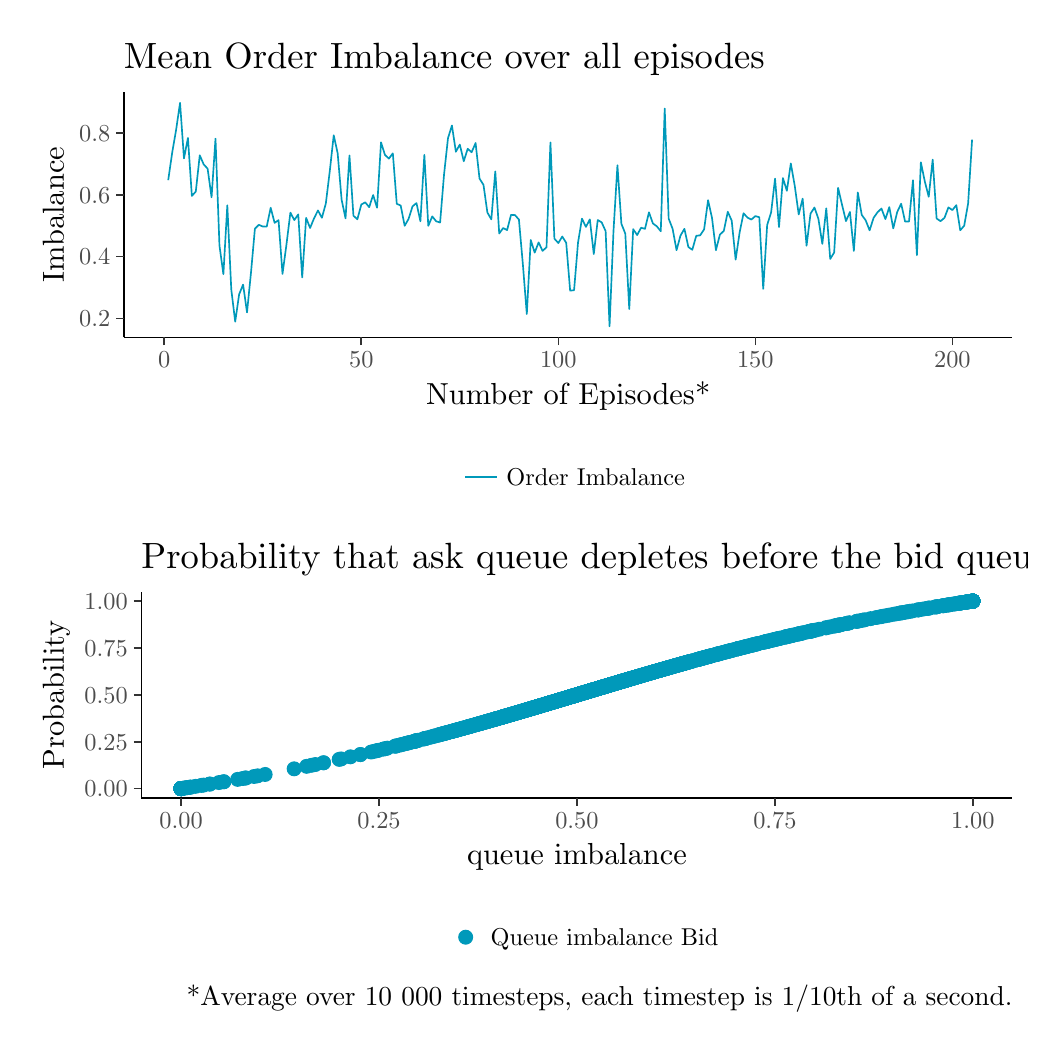
\begin{tikzpicture}[x=1pt,y=1pt]
\definecolor{fillColor}{RGB}{255,255,255}
\path[use as bounding box,fill=fillColor,fill opacity=0.00] (0,0) rectangle (361.35,361.35);
\begin{scope}
\path[clip] (  0.00,180.67) rectangle (361.35,361.35);
\definecolor{drawColor}{RGB}{255,255,255}
\definecolor{fillColor}{RGB}{255,255,255}

\path[draw=drawColor,line width= 0.6pt,line join=round,line cap=round,fill=fillColor] (  0.00,180.67) rectangle (361.35,361.35);
\end{scope}
\begin{scope}
\path[clip] ( 34.77,249.42) rectangle (355.85,338.21);
\definecolor{fillColor}{RGB}{255,255,255}

\path[fill=fillColor] ( 34.77,249.42) rectangle (355.85,338.21);
\definecolor{drawColor}{RGB}{0,153,186}

\path[draw=drawColor,line width= 0.6pt,line join=round] ( 50.79,306.24) --
	( 52.21,316.14) --
	( 53.63,324.39) --
	( 55.06,334.18) --
	( 56.48,314.12) --
	( 57.91,321.49) --
	( 59.33,300.54) --
	( 60.75,302.13) --
	( 62.18,315.23) --
	( 63.60,311.95) --
	( 65.02,310.40) --
	( 66.45,300.06) --
	( 67.87,321.26) --
	( 69.30,282.62) --
	( 70.72,272.26) --
	( 72.14,297.15) --
	( 73.57,266.75) --
	( 74.99,255.11) --
	( 76.42,265.03) --
	( 77.84,268.50) --
	( 79.26,258.46) --
	( 80.69,272.78) --
	( 82.11,288.71) --
	( 83.54,290.11) --
	( 84.96,289.49) --
	( 86.38,289.46) --
	( 87.81,296.27) --
	( 89.23,290.83) --
	( 90.65,291.79) --
	( 92.08,272.37) --
	( 93.50,282.90) --
	( 94.93,294.52) --
	( 96.35,291.82) --
	( 97.77,293.87) --
	( 99.20,271.10) --
	(100.62,292.63) --
	(102.05,288.96) --
	(103.47,292.43) --
	(104.89,295.30) --
	(106.32,292.66) --
	(107.74,297.82) --
	(109.16,309.49) --
	(110.59,322.46) --
	(112.01,315.99) --
	(113.44,299.17) --
	(114.86,292.44) --
	(116.28,315.16) --
	(117.71,293.40) --
	(119.13,292.10) --
	(120.56,297.45) --
	(121.98,298.23) --
	(123.40,296.49) --
	(124.83,300.86) --
	(126.25,296.27) --
	(127.68,319.91) --
	(129.10,315.38) --
	(130.52,314.03) --
	(131.95,315.94) --
	(133.37,297.70) --
	(134.79,297.08) --
	(136.22,289.76) --
	(137.64,292.25) --
	(139.07,296.78) --
	(140.49,297.97) --
	(141.91,291.39) --
	(143.34,315.41) --
	(144.76,289.73) --
	(146.19,293.16) --
	(147.61,291.38) --
	(149.03,290.94) --
	(150.46,308.36) --
	(151.88,321.41) --
	(153.30,325.99) --
	(154.73,316.53) --
	(156.15,319.11) --
	(157.58,313.09) --
	(159.00,317.58) --
	(160.42,316.34) --
	(161.85,319.67) --
	(163.27,306.82) --
	(164.70,304.55) --
	(166.12,294.55) --
	(167.54,292.07) --
	(168.97,309.41) --
	(170.39,286.98) --
	(171.82,288.95) --
	(173.24,288.20) --
	(174.66,293.71) --
	(176.09,293.62) --
	(177.51,292.01) --
	(178.93,275.92) --
	(180.36,257.86) --
	(181.78,284.63) --
	(183.21,280.07) --
	(184.63,283.77) --
	(186.05,280.70) --
	(187.48,281.98) --
	(188.90,319.88) --
	(190.33,285.11) --
	(191.75,283.52) --
	(193.17,285.87) --
	(194.60,283.59) --
	(196.02,266.32) --
	(197.44,266.48) --
	(198.87,283.70) --
	(200.29,292.35) --
	(201.72,289.35) --
	(203.14,292.07) --
	(204.56,279.54) --
	(205.99,291.85) --
	(207.41,290.99) --
	(208.84,287.84) --
	(210.26,253.46) --
	(211.68,287.83) --
	(213.11,311.62) --
	(214.53,290.52) --
	(215.95,286.91) --
	(217.38,259.64) --
	(218.80,288.53) --
	(220.23,286.41) --
	(221.65,289.06) --
	(223.07,288.65) --
	(224.50,294.63) --
	(225.92,290.60) --
	(227.35,289.56) --
	(228.77,287.78) --
	(230.19,332.12) --
	(231.62,292.34) --
	(233.04,288.69) --
	(234.47,280.95) --
	(235.89,286.21) --
	(237.31,288.66) --
	(238.74,282.08) --
	(240.16,281.09) --
	(241.58,286.13) --
	(243.01,286.31) --
	(244.43,288.47) --
	(245.86,299.00) --
	(247.28,292.61) --
	(248.70,280.93) --
	(250.13,286.56) --
	(251.55,287.92) --
	(252.98,294.82) --
	(254.40,291.62) --
	(255.82,277.53) --
	(257.25,287.28) --
	(258.67,294.29) --
	(260.09,292.73) --
	(261.52,292.01) --
	(262.94,293.26) --
	(264.37,292.85) --
	(265.79,266.95) --
	(267.21,290.03) --
	(268.64,294.58) --
	(270.06,306.79) --
	(271.49,289.28) --
	(272.91,307.00) --
	(274.33,302.42) --
	(275.76,312.29) --
	(277.18,304.20) --
	(278.61,293.86) --
	(280.03,299.58) --
	(281.45,282.56) --
	(282.88,294.16) --
	(284.30,296.35) --
	(285.72,292.30) --
	(287.15,283.21) --
	(288.57,296.06) --
	(290.00,277.76) --
	(291.42,280.12) --
	(292.84,303.47) --
	(294.27,297.35) --
	(295.69,291.45) --
	(297.12,294.75) --
	(298.54,280.65) --
	(299.96,301.81) --
	(301.39,293.68) --
	(302.81,291.74) --
	(304.23,288.10) --
	(305.66,292.61) --
	(307.08,294.63) --
	(308.51,296.00) --
	(309.93,292.18) --
	(311.35,296.50) --
	(312.78,288.81) --
	(314.20,294.73) --
	(315.63,297.75) --
	(317.05,291.30) --
	(318.47,291.32) --
	(319.90,306.22) --
	(321.32,279.13) --
	(322.75,312.70) --
	(324.17,305.80) --
	(325.59,300.23) --
	(327.02,313.66) --
	(328.44,292.40) --
	(329.86,291.42) --
	(331.29,292.64) --
	(332.71,296.41) --
	(334.14,295.43) --
	(335.56,297.22) --
	(336.98,288.14) --
	(338.41,289.79) --
	(339.83,297.84) --
	(341.26,320.88);
\end{scope}
\begin{scope}
\path[clip] (  0.00,  0.00) rectangle (361.35,361.35);
\definecolor{drawColor}{RGB}{0,0,0}

\path[draw=drawColor,line width= 0.6pt,line join=round] ( 34.77,249.42) --
	( 34.77,338.21);
\end{scope}
\begin{scope}
\path[clip] (  0.00,  0.00) rectangle (361.35,361.35);
\definecolor{drawColor}{gray}{0.30}

\node[text=drawColor,anchor=base east,inner sep=0pt, outer sep=0pt, scale=  0.88] at ( 29.82,253.25) {0.2};

\node[text=drawColor,anchor=base east,inner sep=0pt, outer sep=0pt, scale=  0.88] at ( 29.82,275.60) {0.4};

\node[text=drawColor,anchor=base east,inner sep=0pt, outer sep=0pt, scale=  0.88] at ( 29.82,297.95) {0.6};

\node[text=drawColor,anchor=base east,inner sep=0pt, outer sep=0pt, scale=  0.88] at ( 29.82,320.30) {0.8};
\end{scope}
\begin{scope}
\path[clip] (  0.00,  0.00) rectangle (361.35,361.35);
\definecolor{drawColor}{gray}{0.20}

\path[draw=drawColor,line width= 0.6pt,line join=round] ( 32.02,256.28) --
	( 34.77,256.28);

\path[draw=drawColor,line width= 0.6pt,line join=round] ( 32.02,278.63) --
	( 34.77,278.63);

\path[draw=drawColor,line width= 0.6pt,line join=round] ( 32.02,300.98) --
	( 34.77,300.98);

\path[draw=drawColor,line width= 0.6pt,line join=round] ( 32.02,323.33) --
	( 34.77,323.33);
\end{scope}
\begin{scope}
\path[clip] (  0.00,  0.00) rectangle (361.35,361.35);
\definecolor{drawColor}{RGB}{0,0,0}

\path[draw=drawColor,line width= 0.6pt,line join=round] ( 34.77,249.42) --
	(355.85,249.42);
\end{scope}
\begin{scope}
\path[clip] (  0.00,  0.00) rectangle (361.35,361.35);
\definecolor{drawColor}{gray}{0.20}

\path[draw=drawColor,line width= 0.6pt,line join=round] ( 49.36,246.67) --
	( 49.36,249.42);

\path[draw=drawColor,line width= 0.6pt,line join=round] (120.56,246.67) --
	(120.56,249.42);

\path[draw=drawColor,line width= 0.6pt,line join=round] (191.75,246.67) --
	(191.75,249.42);

\path[draw=drawColor,line width= 0.6pt,line join=round] (262.94,246.67) --
	(262.94,249.42);

\path[draw=drawColor,line width= 0.6pt,line join=round] (334.14,246.67) --
	(334.14,249.42);
\end{scope}
\begin{scope}
\path[clip] (  0.00,  0.00) rectangle (361.35,361.35);
\definecolor{drawColor}{gray}{0.30}

\node[text=drawColor,anchor=base,inner sep=0pt, outer sep=0pt, scale=  0.88] at ( 49.36,238.41) {0};

\node[text=drawColor,anchor=base,inner sep=0pt, outer sep=0pt, scale=  0.88] at (120.56,238.41) {50};

\node[text=drawColor,anchor=base,inner sep=0pt, outer sep=0pt, scale=  0.88] at (191.75,238.41) {100};

\node[text=drawColor,anchor=base,inner sep=0pt, outer sep=0pt, scale=  0.88] at (262.94,238.41) {150};

\node[text=drawColor,anchor=base,inner sep=0pt, outer sep=0pt, scale=  0.88] at (334.14,238.41) {200};
\end{scope}
\begin{scope}
\path[clip] (  0.00,  0.00) rectangle (361.35,361.35);
\definecolor{drawColor}{RGB}{0,0,0}

\node[text=drawColor,anchor=base,inner sep=0pt, outer sep=0pt, scale=  1.10] at (195.31,225.34) {Number of Episodes*};
\end{scope}
\begin{scope}
\path[clip] (  0.00,  0.00) rectangle (361.35,361.35);
\definecolor{drawColor}{RGB}{0,0,0}

\node[text=drawColor,rotate= 90.00,anchor=base,inner sep=0pt, outer sep=0pt, scale=  1.10] at ( 13.08,293.82) {Imbalance};
\end{scope}
\begin{scope}
\path[clip] (  0.00,  0.00) rectangle (361.35,361.35);
\definecolor{fillColor}{RGB}{255,255,255}

\path[fill=fillColor] (147.40,186.17) rectangle (243.22,212.01);
\end{scope}
\begin{scope}
\path[clip] (  0.00,  0.00) rectangle (361.35,361.35);
\definecolor{drawColor}{RGB}{0,153,186}

\path[draw=drawColor,line width= 0.6pt,line join=round] (158.15,199.09) -- (169.71,199.09);
\end{scope}
\begin{scope}
\path[clip] (  0.00,  0.00) rectangle (361.35,361.35);
\definecolor{drawColor}{RGB}{0,0,0}

\node[text=drawColor,anchor=base west,inner sep=0pt, outer sep=0pt, scale=  0.88] at (172.96,196.06) {Order Imbalance};
\end{scope}
\begin{scope}
\path[clip] (  0.00,  0.00) rectangle (361.35,361.35);
\definecolor{drawColor}{RGB}{0,0,0}

\node[text=drawColor,anchor=base west,inner sep=0pt, outer sep=0pt, scale=  1.32] at ( 34.77,346.76) {Mean Order Imbalance over all episodes };
\end{scope}
\begin{scope}
\path[clip] (  0.00,  0.00) rectangle (361.35,180.68);
\definecolor{drawColor}{RGB}{255,255,255}
\definecolor{fillColor}{RGB}{255,255,255}

\path[draw=drawColor,line width= 0.6pt,line join=round,line cap=round,fill=fillColor] (  0.00,  0.00) rectangle (361.35,180.68);
\end{scope}
\begin{scope}
\path[clip] ( 41.11, 83.01) rectangle (355.85,157.54);
\definecolor{fillColor}{RGB}{255,255,255}

\path[fill=fillColor] ( 41.11, 83.01) rectangle (355.85,157.54);
\definecolor{drawColor}{RGB}{0,153,186}
\definecolor{fillColor}{RGB}{0,153,186}

\path[draw=drawColor,line width= 0.4pt,line join=round,line cap=round,fill=fillColor] (336.32,153.35) circle (  2.50);

\path[draw=drawColor,line width= 0.4pt,line join=round,line cap=round,fill=fillColor] (319.66,150.59) circle (  2.50);

\path[draw=drawColor,line width= 0.4pt,line join=round,line cap=round,fill=fillColor] (341.54,154.15) circle (  2.50);

\path[draw=drawColor,line width= 0.4pt,line join=round,line cap=round,fill=fillColor] (211.69,124.25) circle (  2.50);

\path[draw=drawColor,line width= 0.4pt,line join=round,line cap=round,fill=fillColor] (140.29,103.62) circle (  2.50);

\path[draw=drawColor,line width= 0.4pt,line join=round,line cap=round,fill=fillColor] (103.94, 95.09) circle (  2.50);

\path[draw=drawColor,line width= 0.4pt,line join=round,line cap=round,fill=fillColor] (146.92,105.36) circle (  2.50);

\path[draw=drawColor,line width= 0.4pt,line join=round,line cap=round,fill=fillColor] (100.80, 94.44) circle (  2.50);

\path[draw=drawColor,line width= 0.4pt,line join=round,line cap=round,fill=fillColor] (340.89,154.05) circle (  2.50);

\path[draw=drawColor,line width= 0.4pt,line join=round,line cap=round,fill=fillColor] (324.83,151.48) circle (  2.50);

\path[draw=drawColor,line width= 0.4pt,line join=round,line cap=round,fill=fillColor] (169.94,111.78) circle (  2.50);

\path[draw=drawColor,line width= 0.4pt,line join=round,line cap=round,fill=fillColor] (279.78,142.57) circle (  2.50);

\path[draw=drawColor,line width= 0.4pt,line join=round,line cap=round,fill=fillColor] (106.88, 95.71) circle (  2.50);

\path[draw=drawColor,line width= 0.4pt,line join=round,line cap=round,fill=fillColor] (341.54,154.15) circle (  2.50);

\path[draw=drawColor,line width= 0.4pt,line join=round,line cap=round,fill=fillColor] (340.16,153.94) circle (  2.50);

\path[draw=drawColor,line width= 0.4pt,line join=round,line cap=round,fill=fillColor] (341.54,154.15) circle (  2.50);

\path[draw=drawColor,line width= 0.4pt,line join=round,line cap=round,fill=fillColor] (239.85,132.42) circle (  2.50);

\path[draw=drawColor,line width= 0.4pt,line join=round,line cap=round,fill=fillColor] (283.13,143.32) circle (  2.50);

\path[draw=drawColor,line width= 0.4pt,line join=round,line cap=round,fill=fillColor] (331.86,152.64) circle (  2.50);

\path[draw=drawColor,line width= 0.4pt,line join=round,line cap=round,fill=fillColor] (102.57, 94.81) circle (  2.50);

\path[draw=drawColor,line width= 0.4pt,line join=round,line cap=round,fill=fillColor] (113.26, 97.11) circle (  2.50);

\path[draw=drawColor,line width= 0.4pt,line join=round,line cap=round,fill=fillColor] (234.88,131.02) circle (  2.50);

\path[draw=drawColor,line width= 0.4pt,line join=round,line cap=round,fill=fillColor] (327.78,151.97) circle (  2.50);

\path[draw=drawColor,line width= 0.4pt,line join=round,line cap=round,fill=fillColor] (340.90,154.06) circle (  2.50);

\path[draw=drawColor,line width= 0.4pt,line join=round,line cap=round,fill=fillColor] (140.98,103.79) circle (  2.50);

\path[draw=drawColor,line width= 0.4pt,line join=round,line cap=round,fill=fillColor] (341.54,154.15) circle (  2.50);

\path[draw=drawColor,line width= 0.4pt,line join=round,line cap=round,fill=fillColor] (337.35,153.51) circle (  2.50);

\path[draw=drawColor,line width= 0.4pt,line join=round,line cap=round,fill=fillColor] (332.73,152.78) circle (  2.50);

\path[draw=drawColor,line width= 0.4pt,line join=round,line cap=round,fill=fillColor] (234.10,130.80) circle (  2.50);

\path[draw=drawColor,line width= 0.4pt,line join=round,line cap=round,fill=fillColor] (339.03,153.77) circle (  2.50);

\path[draw=drawColor,line width= 0.4pt,line join=round,line cap=round,fill=fillColor] (266.85,139.51) circle (  2.50);

\path[draw=drawColor,line width= 0.4pt,line join=round,line cap=round,fill=fillColor] (333.10,152.84) circle (  2.50);

\path[draw=drawColor,line width= 0.4pt,line join=round,line cap=round,fill=fillColor] (291.63,145.17) circle (  2.50);

\path[draw=drawColor,line width= 0.4pt,line join=round,line cap=round,fill=fillColor] (341.54,154.15) circle (  2.50);

\path[draw=drawColor,line width= 0.4pt,line join=round,line cap=round,fill=fillColor] (321.98,150.99) circle (  2.50);

\path[draw=drawColor,line width= 0.4pt,line join=round,line cap=round,fill=fillColor] (341.54,154.15) circle (  2.50);

\path[draw=drawColor,line width= 0.4pt,line join=round,line cap=round,fill=fillColor] (300.67,147.03) circle (  2.50);

\path[draw=drawColor,line width= 0.4pt,line join=round,line cap=round,fill=fillColor] (263.51,138.68) circle (  2.50);

\path[draw=drawColor,line width= 0.4pt,line join=round,line cap=round,fill=fillColor] (325.98,151.67) circle (  2.50);

\path[draw=drawColor,line width= 0.4pt,line join=round,line cap=round,fill=fillColor] (288.47,144.49) circle (  2.50);

\path[draw=drawColor,line width= 0.4pt,line join=round,line cap=round,fill=fillColor] (251.90,135.69) circle (  2.50);

\path[draw=drawColor,line width= 0.4pt,line join=round,line cap=round,fill=fillColor] (330.96,152.50) circle (  2.50);

\path[draw=drawColor,line width= 0.4pt,line join=round,line cap=round,fill=fillColor] ( 60.69, 87.21) circle (  2.50);

\path[draw=drawColor,line width= 0.4pt,line join=round,line cap=round,fill=fillColor] (337.49,153.53) circle (  2.50);

\path[draw=drawColor,line width= 0.4pt,line join=round,line cap=round,fill=fillColor] (246.17,134.15) circle (  2.50);

\path[draw=drawColor,line width= 0.4pt,line join=round,line cap=round,fill=fillColor] (341.54,154.15) circle (  2.50);

\path[draw=drawColor,line width= 0.4pt,line join=round,line cap=round,fill=fillColor] (182.67,115.53) circle (  2.50);

\path[draw=drawColor,line width= 0.4pt,line join=round,line cap=round,fill=fillColor] (193.24,118.70) circle (  2.50);

\path[draw=drawColor,line width= 0.4pt,line join=round,line cap=round,fill=fillColor] (283.21,143.34) circle (  2.50);

\path[draw=drawColor,line width= 0.4pt,line join=round,line cap=round,fill=fillColor] (256.80,136.97) circle (  2.50);

\path[draw=drawColor,line width= 0.4pt,line join=round,line cap=round,fill=fillColor] (336.61,153.40) circle (  2.50);

\path[draw=drawColor,line width= 0.4pt,line join=round,line cap=round,fill=fillColor] (315.07,149.77) circle (  2.50);

\path[draw=drawColor,line width= 0.4pt,line join=round,line cap=round,fill=fillColor] (335.17,153.17) circle (  2.50);

\path[draw=drawColor,line width= 0.4pt,line join=round,line cap=round,fill=fillColor] (311.44,149.10) circle (  2.50);

\path[draw=drawColor,line width= 0.4pt,line join=round,line cap=round,fill=fillColor] (296.86,146.26) circle (  2.50);

\path[draw=drawColor,line width= 0.4pt,line join=round,line cap=round,fill=fillColor] ( 69.12, 88.57) circle (  2.50);

\path[draw=drawColor,line width= 0.4pt,line join=round,line cap=round,fill=fillColor] (150.47,106.31) circle (  2.50);

\path[draw=drawColor,line width= 0.4pt,line join=round,line cap=round,fill=fillColor] (308.99,148.65) circle (  2.50);

\path[draw=drawColor,line width= 0.4pt,line join=round,line cap=round,fill=fillColor] (336.35,153.36) circle (  2.50);

\path[draw=drawColor,line width= 0.4pt,line join=round,line cap=round,fill=fillColor] (341.54,154.15) circle (  2.50);

\path[draw=drawColor,line width= 0.4pt,line join=round,line cap=round,fill=fillColor] (325.44,151.58) circle (  2.50);

\path[draw=drawColor,line width= 0.4pt,line join=round,line cap=round,fill=fillColor] ( 56.75, 86.60) circle (  2.50);

\path[draw=drawColor,line width= 0.4pt,line join=round,line cap=round,fill=fillColor] (271.40,140.61) circle (  2.50);

\path[draw=drawColor,line width= 0.4pt,line join=round,line cap=round,fill=fillColor] (279.11,142.41) circle (  2.50);

\path[draw=drawColor,line width= 0.4pt,line join=round,line cap=round,fill=fillColor] (173.08,112.70) circle (  2.50);

\path[draw=drawColor,line width= 0.4pt,line join=round,line cap=round,fill=fillColor] (189.38,117.54) circle (  2.50);

\path[draw=drawColor,line width= 0.4pt,line join=round,line cap=round,fill=fillColor] (286.10,143.98) circle (  2.50);

\path[draw=drawColor,line width= 0.4pt,line join=round,line cap=round,fill=fillColor] (209.46,123.58) circle (  2.50);

\path[draw=drawColor,line width= 0.4pt,line join=round,line cap=round,fill=fillColor] ( 65.90, 88.04) circle (  2.50);

\path[draw=drawColor,line width= 0.4pt,line join=round,line cap=round,fill=fillColor] (322.01,151.00) circle (  2.50);

\path[draw=drawColor,line width= 0.4pt,line join=round,line cap=round,fill=fillColor] (204.75,122.17) circle (  2.50);

\path[draw=drawColor,line width= 0.4pt,line join=round,line cap=round,fill=fillColor] (217.89,126.09) circle (  2.50);

\path[draw=drawColor,line width= 0.4pt,line join=round,line cap=round,fill=fillColor] (341.54,154.15) circle (  2.50);

\path[draw=drawColor,line width= 0.4pt,line join=round,line cap=round,fill=fillColor] (341.36,154.12) circle (  2.50);

\path[draw=drawColor,line width= 0.4pt,line join=round,line cap=round,fill=fillColor] ( 55.42, 86.40) circle (  2.50);

\path[draw=drawColor,line width= 0.4pt,line join=round,line cap=round,fill=fillColor] (337.29,153.50) circle (  2.50);

\path[draw=drawColor,line width= 0.4pt,line join=round,line cap=round,fill=fillColor] (150.76,106.39) circle (  2.50);

\path[draw=drawColor,line width= 0.4pt,line join=round,line cap=round,fill=fillColor] (341.54,154.15) circle (  2.50);

\path[draw=drawColor,line width= 0.4pt,line join=round,line cap=round,fill=fillColor] ( 96.29, 93.53) circle (  2.50);

\path[draw=drawColor,line width= 0.4pt,line join=round,line cap=round,fill=fillColor] (163.27,109.87) circle (  2.50);

\path[draw=drawColor,line width= 0.4pt,line join=round,line cap=round,fill=fillColor] ( 55.42, 86.40) circle (  2.50);

\path[draw=drawColor,line width= 0.4pt,line join=round,line cap=round,fill=fillColor] (235.88,131.31) circle (  2.50);

\path[draw=drawColor,line width= 0.4pt,line join=round,line cap=round,fill=fillColor] (341.54,154.15) circle (  2.50);

\path[draw=drawColor,line width= 0.4pt,line join=round,line cap=round,fill=fillColor] (332.46,152.74) circle (  2.50);

\path[draw=drawColor,line width= 0.4pt,line join=round,line cap=round,fill=fillColor] (126.67,100.21) circle (  2.50);

\path[draw=drawColor,line width= 0.4pt,line join=round,line cap=round,fill=fillColor] (228.27,129.13) circle (  2.50);

\path[draw=drawColor,line width= 0.4pt,line join=round,line cap=round,fill=fillColor] (230.97,129.91) circle (  2.50);

\path[draw=drawColor,line width= 0.4pt,line join=round,line cap=round,fill=fillColor] (253.08,136.00) circle (  2.50);

\path[draw=drawColor,line width= 0.4pt,line join=round,line cap=round,fill=fillColor] (277.06,141.94) circle (  2.50);

\path[draw=drawColor,line width= 0.4pt,line join=round,line cap=round,fill=fillColor] (323.48,151.25) circle (  2.50);

\path[draw=drawColor,line width= 0.4pt,line join=round,line cap=round,fill=fillColor] (135.63,102.42) circle (  2.50);

\path[draw=drawColor,line width= 0.4pt,line join=round,line cap=round,fill=fillColor] (161.72,109.43) circle (  2.50);

\path[draw=drawColor,line width= 0.4pt,line join=round,line cap=round,fill=fillColor] ( 55.42, 86.40) circle (  2.50);

\path[draw=drawColor,line width= 0.4pt,line join=round,line cap=round,fill=fillColor] (188.83,117.37) circle (  2.50);

\path[draw=drawColor,line width= 0.4pt,line join=round,line cap=round,fill=fillColor] (231.19,129.97) circle (  2.50);

\path[draw=drawColor,line width= 0.4pt,line join=round,line cap=round,fill=fillColor] (341.54,154.15) circle (  2.50);

\path[draw=drawColor,line width= 0.4pt,line join=round,line cap=round,fill=fillColor] (341.31,154.12) circle (  2.50);

\path[draw=drawColor,line width= 0.4pt,line join=round,line cap=round,fill=fillColor] (336.72,153.41) circle (  2.50);

\path[draw=drawColor,line width= 0.4pt,line join=round,line cap=round,fill=fillColor] (190.85,117.98) circle (  2.50);

\path[draw=drawColor,line width= 0.4pt,line join=round,line cap=round,fill=fillColor] (340.19,153.95) circle (  2.50);

\path[draw=drawColor,line width= 0.4pt,line join=round,line cap=round,fill=fillColor] (283.63,143.43) circle (  2.50);

\path[draw=drawColor,line width= 0.4pt,line join=round,line cap=round,fill=fillColor] (210.97,124.03) circle (  2.50);

\path[draw=drawColor,line width= 0.4pt,line join=round,line cap=round,fill=fillColor] (230.53,129.78) circle (  2.50);

\path[draw=drawColor,line width= 0.4pt,line join=round,line cap=round,fill=fillColor] (269.12,140.06) circle (  2.50);

\path[draw=drawColor,line width= 0.4pt,line join=round,line cap=round,fill=fillColor] (341.54,154.15) circle (  2.50);

\path[draw=drawColor,line width= 0.4pt,line join=round,line cap=round,fill=fillColor] (185.44,116.36) circle (  2.50);

\path[draw=drawColor,line width= 0.4pt,line join=round,line cap=round,fill=fillColor] ( 55.42, 86.40) circle (  2.50);

\path[draw=drawColor,line width= 0.4pt,line join=round,line cap=round,fill=fillColor] (339.33,153.82) circle (  2.50);

\path[draw=drawColor,line width= 0.4pt,line join=round,line cap=round,fill=fillColor] (224.09,127.92) circle (  2.50);

\path[draw=drawColor,line width= 0.4pt,line join=round,line cap=round,fill=fillColor] (313.93,149.56) circle (  2.50);

\path[draw=drawColor,line width= 0.4pt,line join=round,line cap=round,fill=fillColor] (138.09,103.05) circle (  2.50);

\path[draw=drawColor,line width= 0.4pt,line join=round,line cap=round,fill=fillColor] (158.56,108.54) circle (  2.50);

\path[draw=drawColor,line width= 0.4pt,line join=round,line cap=round,fill=fillColor] (340.68,154.02) circle (  2.50);

\path[draw=drawColor,line width= 0.4pt,line join=round,line cap=round,fill=fillColor] (230.43,129.76) circle (  2.50);

\path[draw=drawColor,line width= 0.4pt,line join=round,line cap=round,fill=fillColor] (243.34,133.38) circle (  2.50);

\path[draw=drawColor,line width= 0.4pt,line join=round,line cap=round,fill=fillColor] (221.11,127.04) circle (  2.50);

\path[draw=drawColor,line width= 0.4pt,line join=round,line cap=round,fill=fillColor] (223.46,127.73) circle (  2.50);

\path[draw=drawColor,line width= 0.4pt,line join=round,line cap=round,fill=fillColor] (176.40,113.67) circle (  2.50);

\path[draw=drawColor,line width= 0.4pt,line join=round,line cap=round,fill=fillColor] ( 55.42, 86.40) circle (  2.50);

\path[draw=drawColor,line width= 0.4pt,line join=round,line cap=round,fill=fillColor] (258.86,137.50) circle (  2.50);

\path[draw=drawColor,line width= 0.4pt,line join=round,line cap=round,fill=fillColor] (176.64,113.74) circle (  2.50);

\path[draw=drawColor,line width= 0.4pt,line join=round,line cap=round,fill=fillColor] (244.48,133.69) circle (  2.50);

\path[draw=drawColor,line width= 0.4pt,line join=round,line cap=round,fill=fillColor] (325.38,151.57) circle (  2.50);

\path[draw=drawColor,line width= 0.4pt,line join=round,line cap=round,fill=fillColor] (236.34,131.43) circle (  2.50);

\path[draw=drawColor,line width= 0.4pt,line join=round,line cap=round,fill=fillColor] (339.66,153.87) circle (  2.50);

\path[draw=drawColor,line width= 0.4pt,line join=round,line cap=round,fill=fillColor] (177.65,114.04) circle (  2.50);

\path[draw=drawColor,line width= 0.4pt,line join=round,line cap=round,fill=fillColor] (226.28,128.56) circle (  2.50);

\path[draw=drawColor,line width= 0.4pt,line join=round,line cap=round,fill=fillColor] (116.64, 97.87) circle (  2.50);

\path[draw=drawColor,line width= 0.4pt,line join=round,line cap=round,fill=fillColor] (227.60,128.94) circle (  2.50);

\path[draw=drawColor,line width= 0.4pt,line join=round,line cap=round,fill=fillColor] (331.19,152.53) circle (  2.50);

\path[draw=drawColor,line width= 0.4pt,line join=round,line cap=round,fill=fillColor] (310.35,148.90) circle (  2.50);

\path[draw=drawColor,line width= 0.4pt,line join=round,line cap=round,fill=fillColor] (181.22,115.10) circle (  2.50);

\path[draw=drawColor,line width= 0.4pt,line join=round,line cap=round,fill=fillColor] (239.15,132.22) circle (  2.50);

\path[draw=drawColor,line width= 0.4pt,line join=round,line cap=round,fill=fillColor] ( 55.42, 86.40) circle (  2.50);

\path[draw=drawColor,line width= 0.4pt,line join=round,line cap=round,fill=fillColor] ( 55.42, 86.40) circle (  2.50);

\path[draw=drawColor,line width= 0.4pt,line join=round,line cap=round,fill=fillColor] ( 55.42, 86.40) circle (  2.50);

\path[draw=drawColor,line width= 0.4pt,line join=round,line cap=round,fill=fillColor] (174.51,113.12) circle (  2.50);

\path[draw=drawColor,line width= 0.4pt,line join=round,line cap=round,fill=fillColor] (139.94,103.52) circle (  2.50);

\path[draw=drawColor,line width= 0.4pt,line join=round,line cap=round,fill=fillColor] (341.54,154.15) circle (  2.50);

\path[draw=drawColor,line width= 0.4pt,line join=round,line cap=round,fill=fillColor] (157.69,108.30) circle (  2.50);

\path[draw=drawColor,line width= 0.4pt,line join=round,line cap=round,fill=fillColor] (214.84,125.19) circle (  2.50);

\path[draw=drawColor,line width= 0.4pt,line join=round,line cap=round,fill=fillColor] ( 55.42, 86.40) circle (  2.50);

\path[draw=drawColor,line width= 0.4pt,line join=round,line cap=round,fill=fillColor] (162.87,109.75) circle (  2.50);

\path[draw=drawColor,line width= 0.4pt,line join=round,line cap=round,fill=fillColor] (169.35,111.61) circle (  2.50);

\path[draw=drawColor,line width= 0.4pt,line join=round,line cap=round,fill=fillColor] (236.67,131.53) circle (  2.50);

\path[draw=drawColor,line width= 0.4pt,line join=round,line cap=round,fill=fillColor] (223.75,127.82) circle (  2.50);

\path[draw=drawColor,line width= 0.4pt,line join=round,line cap=round,fill=fillColor] (157.78,108.32) circle (  2.50);

\path[draw=drawColor,line width= 0.4pt,line join=round,line cap=round,fill=fillColor] (120.22, 98.69) circle (  2.50);

\path[draw=drawColor,line width= 0.4pt,line join=round,line cap=round,fill=fillColor] ( 55.42, 86.40) circle (  2.50);

\path[draw=drawColor,line width= 0.4pt,line join=round,line cap=round,fill=fillColor] (271.75,140.69) circle (  2.50);

\path[draw=drawColor,line width= 0.4pt,line join=round,line cap=round,fill=fillColor] (159.08,108.68) circle (  2.50);

\path[draw=drawColor,line width= 0.4pt,line join=round,line cap=round,fill=fillColor] (333.30,152.87) circle (  2.50);

\path[draw=drawColor,line width= 0.4pt,line join=round,line cap=round,fill=fillColor] (339.38,153.82) circle (  2.50);

\path[draw=drawColor,line width= 0.4pt,line join=round,line cap=round,fill=fillColor] (253.60,136.14) circle (  2.50);

\path[draw=drawColor,line width= 0.4pt,line join=round,line cap=round,fill=fillColor] (274.26,141.29) circle (  2.50);

\path[draw=drawColor,line width= 0.4pt,line join=round,line cap=round,fill=fillColor] (202.14,121.38) circle (  2.50);

\path[draw=drawColor,line width= 0.4pt,line join=round,line cap=round,fill=fillColor] (250.54,135.33) circle (  2.50);

\path[draw=drawColor,line width= 0.4pt,line join=round,line cap=round,fill=fillColor] (203.00,121.64) circle (  2.50);

\path[draw=drawColor,line width= 0.4pt,line join=round,line cap=round,fill=fillColor] ( 56.77, 86.61) circle (  2.50);

\path[draw=drawColor,line width= 0.4pt,line join=round,line cap=round,fill=fillColor] ( 83.09, 91.00) circle (  2.50);

\path[draw=drawColor,line width= 0.4pt,line join=round,line cap=round,fill=fillColor] ( 81.81, 90.77) circle (  2.50);

\path[draw=drawColor,line width= 0.4pt,line join=round,line cap=round,fill=fillColor] ( 57.63, 86.74) circle (  2.50);

\path[draw=drawColor,line width= 0.4pt,line join=round,line cap=round,fill=fillColor] ( 55.42, 86.40) circle (  2.50);

\path[draw=drawColor,line width= 0.4pt,line join=round,line cap=round,fill=fillColor] (180.92,115.01) circle (  2.50);

\path[draw=drawColor,line width= 0.4pt,line join=round,line cap=round,fill=fillColor] ( 65.73, 88.01) circle (  2.50);

\path[draw=drawColor,line width= 0.4pt,line join=round,line cap=round,fill=fillColor] (185.04,116.24) circle (  2.50);

\path[draw=drawColor,line width= 0.4pt,line join=round,line cap=round,fill=fillColor] (312.93,149.38) circle (  2.50);

\path[draw=drawColor,line width= 0.4pt,line join=round,line cap=round,fill=fillColor] (133.26,101.83) circle (  2.50);

\path[draw=drawColor,line width= 0.4pt,line join=round,line cap=round,fill=fillColor] (187.40,116.94) circle (  2.50);

\path[draw=drawColor,line width= 0.4pt,line join=round,line cap=round,fill=fillColor] (160.53,109.09) circle (  2.50);

\path[draw=drawColor,line width= 0.4pt,line join=round,line cap=round,fill=fillColor] (176.27,113.64) circle (  2.50);

\path[draw=drawColor,line width= 0.4pt,line join=round,line cap=round,fill=fillColor] (161.48,109.36) circle (  2.50);

\path[draw=drawColor,line width= 0.4pt,line join=round,line cap=round,fill=fillColor] (160.24,109.01) circle (  2.50);

\path[draw=drawColor,line width= 0.4pt,line join=round,line cap=round,fill=fillColor] (125.16, 99.85) circle (  2.50);

\path[draw=drawColor,line width= 0.4pt,line join=round,line cap=round,fill=fillColor] ( 55.42, 86.40) circle (  2.50);

\path[draw=drawColor,line width= 0.4pt,line join=round,line cap=round,fill=fillColor] ( 78.69, 90.21) circle (  2.50);

\path[draw=drawColor,line width= 0.4pt,line join=round,line cap=round,fill=fillColor] (135.08,102.28) circle (  2.50);

\path[draw=drawColor,line width= 0.4pt,line join=round,line cap=round,fill=fillColor] (190.27,117.80) circle (  2.50);

\path[draw=drawColor,line width= 0.4pt,line join=round,line cap=round,fill=fillColor] ( 75.88, 89.72) circle (  2.50);

\path[draw=drawColor,line width= 0.4pt,line join=round,line cap=round,fill=fillColor] ( 55.42, 86.40) circle (  2.50);

\path[draw=drawColor,line width= 0.4pt,line join=round,line cap=round,fill=fillColor] (171.22,112.16) circle (  2.50);

\path[draw=drawColor,line width= 0.4pt,line join=round,line cap=round,fill=fillColor] (145.04,104.86) circle (  2.50);

\path[draw=drawColor,line width= 0.4pt,line join=round,line cap=round,fill=fillColor] (242.27,133.09) circle (  2.50);

\path[draw=drawColor,line width= 0.4pt,line join=round,line cap=round,fill=fillColor] ( 55.42, 86.40) circle (  2.50);

\path[draw=drawColor,line width= 0.4pt,line join=round,line cap=round,fill=fillColor] ( 55.42, 86.40) circle (  2.50);

\path[draw=drawColor,line width= 0.4pt,line join=round,line cap=round,fill=fillColor] ( 77.70, 90.04) circle (  2.50);

\path[draw=drawColor,line width= 0.4pt,line join=round,line cap=round,fill=fillColor] (137.29,102.84) circle (  2.50);

\path[draw=drawColor,line width= 0.4pt,line join=round,line cap=round,fill=fillColor] (175.96,113.54) circle (  2.50);

\path[draw=drawColor,line width= 0.4pt,line join=round,line cap=round,fill=fillColor] (151.61,106.62) circle (  2.50);

\path[draw=drawColor,line width= 0.4pt,line join=round,line cap=round,fill=fillColor] (177.97,114.14) circle (  2.50);

\path[draw=drawColor,line width= 0.4pt,line join=round,line cap=round,fill=fillColor] (172.97,112.67) circle (  2.50);

\path[draw=drawColor,line width= 0.4pt,line join=round,line cap=round,fill=fillColor] (195.66,119.43) circle (  2.50);

\path[draw=drawColor,line width= 0.4pt,line join=round,line cap=round,fill=fillColor] (193.77,118.86) circle (  2.50);

\path[draw=drawColor,line width= 0.4pt,line join=round,line cap=round,fill=fillColor] ( 55.42, 86.40) circle (  2.50);

\path[draw=drawColor,line width= 0.4pt,line join=round,line cap=round,fill=fillColor] (171.08,112.12) circle (  2.50);

\path[draw=drawColor,line width= 0.4pt,line join=round,line cap=round,fill=fillColor] (191.75,118.25) circle (  2.50);

\path[draw=drawColor,line width= 0.4pt,line join=round,line cap=round,fill=fillColor] ( 55.42, 86.40) circle (  2.50);

\path[draw=drawColor,line width= 0.4pt,line join=round,line cap=round,fill=fillColor] (199.80,120.68) circle (  2.50);

\path[draw=drawColor,line width= 0.4pt,line join=round,line cap=round,fill=fillColor] (198.02,120.14) circle (  2.50);

\path[draw=drawColor,line width= 0.4pt,line join=round,line cap=round,fill=fillColor] (165.62,110.54) circle (  2.50);

\path[draw=drawColor,line width= 0.4pt,line join=round,line cap=round,fill=fillColor] (219.98,126.71) circle (  2.50);

\path[draw=drawColor,line width= 0.4pt,line join=round,line cap=round,fill=fillColor] (199.07,120.45) circle (  2.50);

\path[draw=drawColor,line width= 0.4pt,line join=round,line cap=round,fill=fillColor] ( 58.71, 86.90) circle (  2.50);

\path[draw=drawColor,line width= 0.4pt,line join=round,line cap=round,fill=fillColor] (129.27,100.84) circle (  2.50);

\path[draw=drawColor,line width= 0.4pt,line join=round,line cap=round,fill=fillColor] (192.73,118.54) circle (  2.50);

\path[draw=drawColor,line width= 0.4pt,line join=round,line cap=round,fill=fillColor] (165.54,110.52) circle (  2.50);

\path[draw=drawColor,line width= 0.4pt,line join=round,line cap=round,fill=fillColor] ( 70.83, 88.86) circle (  2.50);

\path[draw=drawColor,line width= 0.4pt,line join=round,line cap=round,fill=fillColor] (225.20,128.24) circle (  2.50);

\path[draw=drawColor,line width= 0.4pt,line join=round,line cap=round,fill=fillColor] ( 55.42, 86.40) circle (  2.50);

\path[draw=drawColor,line width= 0.4pt,line join=round,line cap=round,fill=fillColor] (152.91,106.98) circle (  2.50);

\path[draw=drawColor,line width= 0.4pt,line join=round,line cap=round,fill=fillColor] (229.02,129.35) circle (  2.50);

\path[draw=drawColor,line width= 0.4pt,line join=round,line cap=round,fill=fillColor] ( 55.42, 86.40) circle (  2.50);

\path[draw=drawColor,line width= 0.4pt,line join=round,line cap=round,fill=fillColor] (192.86,118.59) circle (  2.50);

\path[draw=drawColor,line width= 0.4pt,line join=round,line cap=round,fill=fillColor] (195.46,119.37) circle (  2.50);

\path[draw=drawColor,line width= 0.4pt,line join=round,line cap=round,fill=fillColor] ( 58.90, 86.93) circle (  2.50);

\path[draw=drawColor,line width= 0.4pt,line join=round,line cap=round,fill=fillColor] (175.00,113.26) circle (  2.50);

\path[draw=drawColor,line width= 0.4pt,line join=round,line cap=round,fill=fillColor] (162.85,109.75) circle (  2.50);

\path[draw=drawColor,line width= 0.4pt,line join=round,line cap=round,fill=fillColor] (163.32,109.88) circle (  2.50);

\path[draw=drawColor,line width= 0.4pt,line join=round,line cap=round,fill=fillColor] (166.77,110.87) circle (  2.50);

\path[draw=drawColor,line width= 0.4pt,line join=round,line cap=round,fill=fillColor] (192.68,118.53) circle (  2.50);

\path[draw=drawColor,line width= 0.4pt,line join=round,line cap=round,fill=fillColor] (162.24,109.58) circle (  2.50);

\path[draw=drawColor,line width= 0.4pt,line join=round,line cap=round,fill=fillColor] (339.72,153.88) circle (  2.50);

\path[draw=drawColor,line width= 0.4pt,line join=round,line cap=round,fill=fillColor] (215.63,125.42) circle (  2.50);

\path[draw=drawColor,line width= 0.4pt,line join=round,line cap=round,fill=fillColor] ( 56.01, 86.49) circle (  2.50);

\path[draw=drawColor,line width= 0.4pt,line join=round,line cap=round,fill=fillColor] (186.69,116.73) circle (  2.50);

\path[draw=drawColor,line width= 0.4pt,line join=round,line cap=round,fill=fillColor] (187.92,117.10) circle (  2.50);

\path[draw=drawColor,line width= 0.4pt,line join=round,line cap=round,fill=fillColor] (192.63,118.51) circle (  2.50);

\path[draw=drawColor,line width= 0.4pt,line join=round,line cap=round,fill=fillColor] (201.73,121.26) circle (  2.50);

\path[draw=drawColor,line width= 0.4pt,line join=round,line cap=round,fill=fillColor] (190.26,117.80) circle (  2.50);

\path[draw=drawColor,line width= 0.4pt,line join=round,line cap=round,fill=fillColor] (211.57,124.21) circle (  2.50);

\path[draw=drawColor,line width= 0.4pt,line join=round,line cap=round,fill=fillColor] (193.76,118.86) circle (  2.50);

\path[draw=drawColor,line width= 0.4pt,line join=round,line cap=round,fill=fillColor] (188.63,117.31) circle (  2.50);

\path[draw=drawColor,line width= 0.4pt,line join=round,line cap=round,fill=fillColor] (194.25,119.00) circle (  2.50);

\path[draw=drawColor,line width= 0.4pt,line join=round,line cap=round,fill=fillColor] (200.94,121.02) circle (  2.50);

\path[draw=drawColor,line width= 0.4pt,line join=round,line cap=round,fill=fillColor] (204.26,122.02) circle (  2.50);

\path[draw=drawColor,line width= 0.4pt,line join=round,line cap=round,fill=fillColor] (203.16,121.69) circle (  2.50);

\path[draw=drawColor,line width= 0.4pt,line join=round,line cap=round,fill=fillColor] (212.59,124.52) circle (  2.50);

\path[draw=drawColor,line width= 0.4pt,line join=round,line cap=round,fill=fillColor] (192.29,118.41) circle (  2.50);

\path[draw=drawColor,line width= 0.4pt,line join=round,line cap=round,fill=fillColor] (198.60,120.31) circle (  2.50);

\path[draw=drawColor,line width= 0.4pt,line join=round,line cap=round,fill=fillColor] (199.56,120.60) circle (  2.50);

\path[draw=drawColor,line width= 0.4pt,line join=round,line cap=round,fill=fillColor] (184.51,116.08) circle (  2.50);

\path[draw=drawColor,line width= 0.4pt,line join=round,line cap=round,fill=fillColor] (174.70,113.17) circle (  2.50);

\path[draw=drawColor,line width= 0.4pt,line join=round,line cap=round,fill=fillColor] (205.77,122.47) circle (  2.50);

\path[draw=drawColor,line width= 0.4pt,line join=round,line cap=round,fill=fillColor] (197.92,120.11) circle (  2.50);

\path[draw=drawColor,line width= 0.4pt,line join=round,line cap=round,fill=fillColor] (220.87,126.97) circle (  2.50);

\path[draw=drawColor,line width= 0.4pt,line join=round,line cap=round,fill=fillColor] (196.30,119.62) circle (  2.50);

\path[draw=drawColor,line width= 0.4pt,line join=round,line cap=round,fill=fillColor] (186.98,116.82) circle (  2.50);

\path[draw=drawColor,line width= 0.4pt,line join=round,line cap=round,fill=fillColor] (222.78,127.53) circle (  2.50);

\path[draw=drawColor,line width= 0.4pt,line join=round,line cap=round,fill=fillColor] (187.97,117.11) circle (  2.50);

\path[draw=drawColor,line width= 0.4pt,line join=round,line cap=round,fill=fillColor] (180.27,114.82) circle (  2.50);

\path[draw=drawColor,line width= 0.4pt,line join=round,line cap=round,fill=fillColor] (195.38,119.34) circle (  2.50);

\path[draw=drawColor,line width= 0.4pt,line join=round,line cap=round,fill=fillColor] (208.73,123.36) circle (  2.50);

\path[draw=drawColor,line width= 0.4pt,line join=round,line cap=round,fill=fillColor] (190.46,117.86) circle (  2.50);

\path[draw=drawColor,line width= 0.4pt,line join=round,line cap=round,fill=fillColor] (210.88,124.01) circle (  2.50);

\path[draw=drawColor,line width= 0.4pt,line join=round,line cap=round,fill=fillColor] (171.39,112.21) circle (  2.50);

\path[draw=drawColor,line width= 0.4pt,line join=round,line cap=round,fill=fillColor] (203.78,121.88) circle (  2.50);

\path[draw=drawColor,line width= 0.4pt,line join=round,line cap=round,fill=fillColor] (207.28,122.93) circle (  2.50);

\path[draw=drawColor,line width= 0.4pt,line join=round,line cap=round,fill=fillColor] (201.48,121.18) circle (  2.50);

\path[draw=drawColor,line width= 0.4pt,line join=round,line cap=round,fill=fillColor] (209.34,123.55) circle (  2.50);

\path[draw=drawColor,line width= 0.4pt,line join=round,line cap=round,fill=fillColor] (179.93,114.72) circle (  2.50);

\path[draw=drawColor,line width= 0.4pt,line join=round,line cap=round,fill=fillColor] (187.59,117.00) circle (  2.50);

\path[draw=drawColor,line width= 0.4pt,line join=round,line cap=round,fill=fillColor] (191.63,118.21) circle (  2.50);

\path[draw=drawColor,line width= 0.4pt,line join=round,line cap=round,fill=fillColor] (302.56,147.41) circle (  2.50);

\path[draw=drawColor,line width= 0.4pt,line join=round,line cap=round,fill=fillColor] (191.83,118.27) circle (  2.50);

\path[draw=drawColor,line width= 0.4pt,line join=round,line cap=round,fill=fillColor] (175.91,113.53) circle (  2.50);

\path[draw=drawColor,line width= 0.4pt,line join=round,line cap=round,fill=fillColor] (214.01,124.94) circle (  2.50);

\path[draw=drawColor,line width= 0.4pt,line join=round,line cap=round,fill=fillColor] (208.60,123.32) circle (  2.50);

\path[draw=drawColor,line width= 0.4pt,line join=round,line cap=round,fill=fillColor] (215.89,125.50) circle (  2.50);

\path[draw=drawColor,line width= 0.4pt,line join=round,line cap=round,fill=fillColor] (196.67,119.73) circle (  2.50);

\path[draw=drawColor,line width= 0.4pt,line join=round,line cap=round,fill=fillColor] (202.83,121.59) circle (  2.50);

\path[draw=drawColor,line width= 0.4pt,line join=round,line cap=round,fill=fillColor] (237.02,131.63) circle (  2.50);

\path[draw=drawColor,line width= 0.4pt,line join=round,line cap=round,fill=fillColor] (190.37,117.83) circle (  2.50);

\path[draw=drawColor,line width= 0.4pt,line join=round,line cap=round,fill=fillColor] (186.01,116.53) circle (  2.50);

\path[draw=drawColor,line width= 0.4pt,line join=round,line cap=round,fill=fillColor] (202.94,121.62) circle (  2.50);

\path[draw=drawColor,line width= 0.4pt,line join=round,line cap=round,fill=fillColor] (181.47,115.17) circle (  2.50);

\path[draw=drawColor,line width= 0.4pt,line join=round,line cap=round,fill=fillColor] (189.70,117.63) circle (  2.50);

\path[draw=drawColor,line width= 0.4pt,line join=round,line cap=round,fill=fillColor] (199.34,120.54) circle (  2.50);

\path[draw=drawColor,line width= 0.4pt,line join=round,line cap=round,fill=fillColor] (228.69,129.25) circle (  2.50);

\path[draw=drawColor,line width= 0.4pt,line join=round,line cap=round,fill=fillColor] (217.62,126.01) circle (  2.50);

\path[draw=drawColor,line width= 0.4pt,line join=round,line cap=round,fill=fillColor] (189.23,117.49) circle (  2.50);

\path[draw=drawColor,line width= 0.4pt,line join=round,line cap=round,fill=fillColor] (207.29,122.93) circle (  2.50);

\path[draw=drawColor,line width= 0.4pt,line join=round,line cap=round,fill=fillColor] (197.30,119.92) circle (  2.50);

\path[draw=drawColor,line width= 0.4pt,line join=round,line cap=round,fill=fillColor] (206.83,122.79) circle (  2.50);

\path[draw=drawColor,line width= 0.4pt,line join=round,line cap=round,fill=fillColor] (188.93,117.40) circle (  2.50);

\path[draw=drawColor,line width= 0.4pt,line join=round,line cap=round,fill=fillColor] (183.01,115.63) circle (  2.50);

\path[draw=drawColor,line width= 0.4pt,line join=round,line cap=round,fill=fillColor] (183.71,115.84) circle (  2.50);

\path[draw=drawColor,line width= 0.4pt,line join=round,line cap=round,fill=fillColor] (188.99,117.42) circle (  2.50);

\path[draw=drawColor,line width= 0.4pt,line join=round,line cap=round,fill=fillColor] (184.95,116.21) circle (  2.50);

\path[draw=drawColor,line width= 0.4pt,line join=round,line cap=round,fill=fillColor] (266.90,139.52) circle (  2.50);

\path[draw=drawColor,line width= 0.4pt,line join=round,line cap=round,fill=fillColor] (215.48,125.38) circle (  2.50);

\path[draw=drawColor,line width= 0.4pt,line join=round,line cap=round,fill=fillColor] (232.87,130.45) circle (  2.50);

\path[draw=drawColor,line width= 0.4pt,line join=round,line cap=round,fill=fillColor] (184.94,116.21) circle (  2.50);

\path[draw=drawColor,line width= 0.4pt,line join=round,line cap=round,fill=fillColor] (192.89,118.59) circle (  2.50);

\path[draw=drawColor,line width= 0.4pt,line join=round,line cap=round,fill=fillColor] (179.58,114.61) circle (  2.50);

\path[draw=drawColor,line width= 0.4pt,line join=round,line cap=round,fill=fillColor] (217.35,125.93) circle (  2.50);

\path[draw=drawColor,line width= 0.4pt,line join=round,line cap=round,fill=fillColor] ( 55.42, 86.40) circle (  2.50);

\path[draw=drawColor,line width= 0.4pt,line join=round,line cap=round,fill=fillColor] (199.36,120.54) circle (  2.50);

\path[draw=drawColor,line width= 0.4pt,line join=round,line cap=round,fill=fillColor] (193.10,118.66) circle (  2.50);

\path[draw=drawColor,line width= 0.4pt,line join=round,line cap=round,fill=fillColor] (174.61,113.15) circle (  2.50);

\path[draw=drawColor,line width= 0.4pt,line join=round,line cap=round,fill=fillColor] (224.57,128.06) circle (  2.50);

\path[draw=drawColor,line width= 0.4pt,line join=round,line cap=round,fill=fillColor] (195.10,119.26) circle (  2.50);

\path[draw=drawColor,line width= 0.4pt,line join=round,line cap=round,fill=fillColor] (192.60,118.51) circle (  2.50);

\path[draw=drawColor,line width= 0.4pt,line join=round,line cap=round,fill=fillColor] (186.59,116.70) circle (  2.50);

\path[draw=drawColor,line width= 0.4pt,line join=round,line cap=round,fill=fillColor] (194.27,119.01) circle (  2.50);

\path[draw=drawColor,line width= 0.4pt,line join=round,line cap=round,fill=fillColor] (232.30,130.29) circle (  2.50);

\path[draw=drawColor,line width= 0.4pt,line join=round,line cap=round,fill=fillColor] (210.65,123.94) circle (  2.50);

\path[draw=drawColor,line width= 0.4pt,line join=round,line cap=round,fill=fillColor] ( 63.55, 87.66) circle (  2.50);

\path[draw=drawColor,line width= 0.4pt,line join=round,line cap=round,fill=fillColor] (183.84,115.88) circle (  2.50);

\path[draw=drawColor,line width= 0.4pt,line join=round,line cap=round,fill=fillColor] (213.93,124.92) circle (  2.50);

\path[draw=drawColor,line width= 0.4pt,line join=round,line cap=round,fill=fillColor] (171.64,112.28) circle (  2.50);

\path[draw=drawColor,line width= 0.4pt,line join=round,line cap=round,fill=fillColor] (232.32,130.29) circle (  2.50);

\path[draw=drawColor,line width= 0.4pt,line join=round,line cap=round,fill=fillColor] (176.68,113.76) circle (  2.50);

\path[draw=drawColor,line width= 0.4pt,line join=round,line cap=round,fill=fillColor] (222.45,127.44) circle (  2.50);

\path[draw=drawColor,line width= 0.4pt,line join=round,line cap=round,fill=fillColor] (202.32,121.43) circle (  2.50);

\path[draw=drawColor,line width= 0.4pt,line join=round,line cap=round,fill=fillColor] (227.97,129.04) circle (  2.50);

\path[draw=drawColor,line width= 0.4pt,line join=round,line cap=round,fill=fillColor] (202.29,121.43) circle (  2.50);

\path[draw=drawColor,line width= 0.4pt,line join=round,line cap=round,fill=fillColor] (228.35,129.16) circle (  2.50);

\path[draw=drawColor,line width= 0.4pt,line join=round,line cap=round,fill=fillColor] (205.30,122.33) circle (  2.50);

\path[draw=drawColor,line width= 0.4pt,line join=round,line cap=round,fill=fillColor] (209.60,123.62) circle (  2.50);

\path[draw=drawColor,line width= 0.4pt,line join=round,line cap=round,fill=fillColor] (195.09,119.25) circle (  2.50);

\path[draw=drawColor,line width= 0.4pt,line join=round,line cap=round,fill=fillColor] (216.64,125.72) circle (  2.50);

\path[draw=drawColor,line width= 0.4pt,line join=round,line cap=round,fill=fillColor] (216.97,125.82) circle (  2.50);

\path[draw=drawColor,line width= 0.4pt,line join=round,line cap=round,fill=fillColor] (178.00,114.14) circle (  2.50);

\path[draw=drawColor,line width= 0.4pt,line join=round,line cap=round,fill=fillColor] (216.86,125.79) circle (  2.50);

\path[draw=drawColor,line width= 0.4pt,line join=round,line cap=round,fill=fillColor] (192.87,118.59) circle (  2.50);

\path[draw=drawColor,line width= 0.4pt,line join=round,line cap=round,fill=fillColor] (178.50,114.29) circle (  2.50);

\path[draw=drawColor,line width= 0.4pt,line join=round,line cap=round,fill=fillColor] (187.44,116.95) circle (  2.50);

\path[draw=drawColor,line width= 0.4pt,line join=round,line cap=round,fill=fillColor] (193.11,118.66) circle (  2.50);

\path[draw=drawColor,line width= 0.4pt,line join=round,line cap=round,fill=fillColor] (205.40,122.36) circle (  2.50);

\path[draw=drawColor,line width= 0.4pt,line join=round,line cap=round,fill=fillColor] (231.74,130.13) circle (  2.50);

\path[draw=drawColor,line width= 0.4pt,line join=round,line cap=round,fill=fillColor] (223.40,127.72) circle (  2.50);

\path[draw=drawColor,line width= 0.4pt,line join=round,line cap=round,fill=fillColor] (220.54,126.88) circle (  2.50);

\path[draw=drawColor,line width= 0.4pt,line join=round,line cap=round,fill=fillColor] (186.97,116.81) circle (  2.50);

\path[draw=drawColor,line width= 0.4pt,line join=round,line cap=round,fill=fillColor] (216.40,125.65) circle (  2.50);

\path[draw=drawColor,line width= 0.4pt,line join=round,line cap=round,fill=fillColor] (228.08,129.08) circle (  2.50);

\path[draw=drawColor,line width= 0.4pt,line join=round,line cap=round,fill=fillColor] (159.16,108.71) circle (  2.50);

\path[draw=drawColor,line width= 0.4pt,line join=round,line cap=round,fill=fillColor] (219.75,126.64) circle (  2.50);

\path[draw=drawColor,line width= 0.4pt,line join=round,line cap=round,fill=fillColor] (236.15,131.38) circle (  2.50);

\path[draw=drawColor,line width= 0.4pt,line join=round,line cap=round,fill=fillColor] (221.56,127.18) circle (  2.50);

\path[draw=drawColor,line width= 0.4pt,line join=round,line cap=round,fill=fillColor] (159.74,108.87) circle (  2.50);

\path[draw=drawColor,line width= 0.4pt,line join=round,line cap=round,fill=fillColor] (201.30,121.13) circle (  2.50);

\path[draw=drawColor,line width= 0.4pt,line join=round,line cap=round,fill=fillColor] (106.92, 95.72) circle (  2.50);

\path[draw=drawColor,line width= 0.4pt,line join=round,line cap=round,fill=fillColor] (202.91,121.61) circle (  2.50);

\path[draw=drawColor,line width= 0.4pt,line join=round,line cap=round,fill=fillColor] (214.21,125.00) circle (  2.50);

\path[draw=drawColor,line width= 0.4pt,line join=round,line cap=round,fill=fillColor] (216.92,125.81) circle (  2.50);

\path[draw=drawColor,line width= 0.4pt,line join=round,line cap=round,fill=fillColor] (194.78,119.16) circle (  2.50);

\path[draw=drawColor,line width= 0.4pt,line join=round,line cap=round,fill=fillColor] (215.38,125.35) circle (  2.50);

\path[draw=drawColor,line width= 0.4pt,line join=round,line cap=round,fill=fillColor] (218.05,126.14) circle (  2.50);

\path[draw=drawColor,line width= 0.4pt,line join=round,line cap=round,fill=fillColor] (207.51,123.00) circle (  2.50);

\path[draw=drawColor,line width= 0.4pt,line join=round,line cap=round,fill=fillColor] (216.75,125.75) circle (  2.50);

\path[draw=drawColor,line width= 0.4pt,line join=round,line cap=round,fill=fillColor] (223.84,127.84) circle (  2.50);

\path[draw=drawColor,line width= 0.4pt,line join=round,line cap=round,fill=fillColor] (200.45,120.87) circle (  2.50);

\path[draw=drawColor,line width= 0.4pt,line join=round,line cap=round,fill=fillColor] (223.64,127.78) circle (  2.50);

\path[draw=drawColor,line width= 0.4pt,line join=round,line cap=round,fill=fillColor] (224.95,128.17) circle (  2.50);

\path[draw=drawColor,line width= 0.4pt,line join=round,line cap=round,fill=fillColor] (198.70,120.34) circle (  2.50);

\path[draw=drawColor,line width= 0.4pt,line join=round,line cap=round,fill=fillColor] (202.62,121.53) circle (  2.50);

\path[draw=drawColor,line width= 0.4pt,line join=round,line cap=round,fill=fillColor] (198.02,120.14) circle (  2.50);

\path[draw=drawColor,line width= 0.4pt,line join=round,line cap=round,fill=fillColor] (212.46,124.48) circle (  2.50);

\path[draw=drawColor,line width= 0.4pt,line join=round,line cap=round,fill=fillColor] (199.43,120.56) circle (  2.50);

\path[draw=drawColor,line width= 0.4pt,line join=round,line cap=round,fill=fillColor] (177.44,113.98) circle (  2.50);

\path[draw=drawColor,line width= 0.4pt,line join=round,line cap=round,fill=fillColor] (210.21,123.81) circle (  2.50);

\path[draw=drawColor,line width= 0.4pt,line join=round,line cap=round,fill=fillColor] (175.75,113.48) circle (  2.50);

\path[draw=drawColor,line width= 0.4pt,line join=round,line cap=round,fill=fillColor] (175.10,113.29) circle (  2.50);

\path[draw=drawColor,line width= 0.4pt,line join=round,line cap=round,fill=fillColor] (185.05,116.24) circle (  2.50);

\path[draw=drawColor,line width= 0.4pt,line join=round,line cap=round,fill=fillColor] (202.96,121.63) circle (  2.50);

\path[draw=drawColor,line width= 0.4pt,line join=round,line cap=round,fill=fillColor] (168.88,111.48) circle (  2.50);

\path[draw=drawColor,line width= 0.4pt,line join=round,line cap=round,fill=fillColor] (195.86,119.49) circle (  2.50);

\path[draw=drawColor,line width= 0.4pt,line join=round,line cap=round,fill=fillColor] (204.12,121.98) circle (  2.50);

\path[draw=drawColor,line width= 0.4pt,line join=round,line cap=round,fill=fillColor] (210.66,123.94) circle (  2.50);

\path[draw=drawColor,line width= 0.4pt,line join=round,line cap=round,fill=fillColor] (227.16,128.81) circle (  2.50);

\path[draw=drawColor,line width= 0.4pt,line join=round,line cap=round,fill=fillColor] (188.78,117.36) circle (  2.50);

\path[draw=drawColor,line width= 0.4pt,line join=round,line cap=round,fill=fillColor] (246.87,134.35) circle (  2.50);

\path[draw=drawColor,line width= 0.4pt,line join=round,line cap=round,fill=fillColor] (208.57,123.32) circle (  2.50);

\path[draw=drawColor,line width= 0.4pt,line join=round,line cap=round,fill=fillColor] (172.99,112.67) circle (  2.50);

\path[draw=drawColor,line width= 0.4pt,line join=round,line cap=round,fill=fillColor] (209.49,123.59) circle (  2.50);

\path[draw=drawColor,line width= 0.4pt,line join=round,line cap=round,fill=fillColor] (245.90,134.08) circle (  2.50);

\path[draw=drawColor,line width= 0.4pt,line join=round,line cap=round,fill=fillColor] (193.22,118.69) circle (  2.50);

\path[draw=drawColor,line width= 0.4pt,line join=round,line cap=round,fill=fillColor] (171.68,112.29) circle (  2.50);

\path[draw=drawColor,line width= 0.4pt,line join=round,line cap=round,fill=fillColor] (184.88,116.19) circle (  2.50);

\path[draw=drawColor,line width= 0.4pt,line join=round,line cap=round,fill=fillColor] (182.81,115.57) circle (  2.50);

\path[draw=drawColor,line width= 0.4pt,line join=round,line cap=round,fill=fillColor] (213.74,124.86) circle (  2.50);

\path[draw=drawColor,line width= 0.4pt,line join=round,line cap=round,fill=fillColor] (185.31,116.32) circle (  2.50);

\path[draw=drawColor,line width= 0.4pt,line join=round,line cap=round,fill=fillColor] (191.56,118.19) circle (  2.50);

\path[draw=drawColor,line width= 0.4pt,line join=round,line cap=round,fill=fillColor] (155.99,107.82) circle (  2.50);

\path[draw=drawColor,line width= 0.4pt,line join=round,line cap=round,fill=fillColor] (176.34,113.65) circle (  2.50);

\path[draw=drawColor,line width= 0.4pt,line join=round,line cap=round,fill=fillColor] (218.85,126.38) circle (  2.50);

\path[draw=drawColor,line width= 0.4pt,line join=round,line cap=round,fill=fillColor] (186.48,116.67) circle (  2.50);

\path[draw=drawColor,line width= 0.4pt,line join=round,line cap=round,fill=fillColor] (199.19,120.49) circle (  2.50);

\path[draw=drawColor,line width= 0.4pt,line join=round,line cap=round,fill=fillColor] (252.65,135.89) circle (  2.50);

\path[draw=drawColor,line width= 0.4pt,line join=round,line cap=round,fill=fillColor] (241.70,132.93) circle (  2.50);

\path[draw=drawColor,line width= 0.4pt,line join=round,line cap=round,fill=fillColor] (212.27,124.42) circle (  2.50);

\path[draw=drawColor,line width= 0.4pt,line join=round,line cap=round,fill=fillColor] (181.57,115.20) circle (  2.50);

\path[draw=drawColor,line width= 0.4pt,line join=round,line cap=round,fill=fillColor] (213.21,124.70) circle (  2.50);

\path[draw=drawColor,line width= 0.4pt,line join=round,line cap=round,fill=fillColor] (220.20,126.78) circle (  2.50);

\path[draw=drawColor,line width= 0.4pt,line join=round,line cap=round,fill=fillColor] (199.06,120.45) circle (  2.50);

\path[draw=drawColor,line width= 0.4pt,line join=round,line cap=round,fill=fillColor] (224.59,128.06) circle (  2.50);

\path[draw=drawColor,line width= 0.4pt,line join=round,line cap=round,fill=fillColor] (216.53,125.69) circle (  2.50);

\path[draw=drawColor,line width= 0.4pt,line join=round,line cap=round,fill=fillColor] (198.04,120.14) circle (  2.50);

\path[draw=drawColor,line width= 0.4pt,line join=round,line cap=round,fill=fillColor] (194.15,118.97) circle (  2.50);

\path[draw=drawColor,line width= 0.4pt,line join=round,line cap=round,fill=fillColor] (207.83,123.09) circle (  2.50);

\path[draw=drawColor,line width= 0.4pt,line join=round,line cap=round,fill=fillColor] (212.67,124.54) circle (  2.50);

\path[draw=drawColor,line width= 0.4pt,line join=round,line cap=round,fill=fillColor] (205.68,122.45) circle (  2.50);

\path[draw=drawColor,line width= 0.4pt,line join=round,line cap=round,fill=fillColor] (214.57,125.11) circle (  2.50);

\path[draw=drawColor,line width= 0.4pt,line join=round,line cap=round,fill=fillColor] (201.69,121.25) circle (  2.50);

\path[draw=drawColor,line width= 0.4pt,line join=round,line cap=round,fill=fillColor] (209.19,123.50) circle (  2.50);

\path[draw=drawColor,line width= 0.4pt,line join=round,line cap=round,fill=fillColor] (235.27,131.13) circle (  2.50);

\path[draw=drawColor,line width= 0.4pt,line join=round,line cap=round,fill=fillColor] (217.57,126.00) circle (  2.50);

\path[draw=drawColor,line width= 0.4pt,line join=round,line cap=round,fill=fillColor] (254.53,136.38) circle (  2.50);

\path[draw=drawColor,line width= 0.4pt,line join=round,line cap=round,fill=fillColor] (217.65,126.02) circle (  2.50);

\path[draw=drawColor,line width= 0.4pt,line join=round,line cap=round,fill=fillColor] (200.83,120.98) circle (  2.50);

\path[draw=drawColor,line width= 0.4pt,line join=round,line cap=round,fill=fillColor] (229.63,129.52) circle (  2.50);

\path[draw=drawColor,line width= 0.4pt,line join=round,line cap=round,fill=fillColor] (182.50,115.48) circle (  2.50);

\path[draw=drawColor,line width= 0.4pt,line join=round,line cap=round,fill=fillColor] (219.31,126.51) circle (  2.50);

\path[draw=drawColor,line width= 0.4pt,line join=round,line cap=round,fill=fillColor] (228.47,129.19) circle (  2.50);

\path[draw=drawColor,line width= 0.4pt,line join=round,line cap=round,fill=fillColor] (215.49,125.38) circle (  2.50);

\path[draw=drawColor,line width= 0.4pt,line join=round,line cap=round,fill=fillColor] (199.42,120.56) circle (  2.50);

\path[draw=drawColor,line width= 0.4pt,line join=round,line cap=round,fill=fillColor] (341.54,154.15) circle (  2.50);

\path[draw=drawColor,line width= 0.4pt,line join=round,line cap=round,fill=fillColor] (245.07,133.86) circle (  2.50);

\path[draw=drawColor,line width= 0.4pt,line join=round,line cap=round,fill=fillColor] (222.74,127.52) circle (  2.50);

\path[draw=drawColor,line width= 0.4pt,line join=round,line cap=round,fill=fillColor] (189.77,117.65) circle (  2.50);

\path[draw=drawColor,line width= 0.4pt,line join=round,line cap=round,fill=fillColor] (219.54,126.58) circle (  2.50);

\path[draw=drawColor,line width= 0.4pt,line join=round,line cap=round,fill=fillColor] (235.53,131.21) circle (  2.50);

\path[draw=drawColor,line width= 0.4pt,line join=round,line cap=round,fill=fillColor] (291.39,145.12) circle (  2.50);

\path[draw=drawColor,line width= 0.4pt,line join=round,line cap=round,fill=fillColor] (243.33,133.38) circle (  2.50);

\path[draw=drawColor,line width= 0.4pt,line join=round,line cap=round,fill=fillColor] (340.19,153.95) circle (  2.50);

\path[draw=drawColor,line width= 0.4pt,line join=round,line cap=round,fill=fillColor] (209.06,123.46) circle (  2.50);

\path[draw=drawColor,line width= 0.4pt,line join=round,line cap=round,fill=fillColor] (218.33,126.22) circle (  2.50);

\path[draw=drawColor,line width= 0.4pt,line join=round,line cap=round,fill=fillColor] (200.91,121.01) circle (  2.50);

\path[draw=drawColor,line width= 0.4pt,line join=round,line cap=round,fill=fillColor] (202.78,121.57) circle (  2.50);

\path[draw=drawColor,line width= 0.4pt,line join=round,line cap=round,fill=fillColor] (292.59,145.37) circle (  2.50);

\path[draw=drawColor,line width= 0.4pt,line join=round,line cap=round,fill=fillColor] (271.49,140.63) circle (  2.50);

\path[draw=drawColor,line width= 0.4pt,line join=round,line cap=round,fill=fillColor] (215.17,125.29) circle (  2.50);

\path[draw=drawColor,line width= 0.4pt,line join=round,line cap=round,fill=fillColor] (210.67,123.94) circle (  2.50);

\path[draw=drawColor,line width= 0.4pt,line join=round,line cap=round,fill=fillColor] (192.25,118.40) circle (  2.50);

\path[draw=drawColor,line width= 0.4pt,line join=round,line cap=round,fill=fillColor] (221.43,127.14) circle (  2.50);

\path[draw=drawColor,line width= 0.4pt,line join=round,line cap=round,fill=fillColor] (341.54,154.15) circle (  2.50);

\path[draw=drawColor,line width= 0.4pt,line join=round,line cap=round,fill=fillColor] (209.71,123.66) circle (  2.50);

\path[draw=drawColor,line width= 0.4pt,line join=round,line cap=round,fill=fillColor] (259.69,137.71) circle (  2.50);

\path[draw=drawColor,line width= 0.4pt,line join=round,line cap=round,fill=fillColor] (278.22,142.21) circle (  2.50);

\path[draw=drawColor,line width= 0.4pt,line join=round,line cap=round,fill=fillColor] (232.13,130.24) circle (  2.50);

\path[draw=drawColor,line width= 0.4pt,line join=round,line cap=round,fill=fillColor] (247.61,134.55) circle (  2.50);

\path[draw=drawColor,line width= 0.4pt,line join=round,line cap=round,fill=fillColor] (215.76,125.46) circle (  2.50);

\path[draw=drawColor,line width= 0.4pt,line join=round,line cap=round,fill=fillColor] (238.81,132.13) circle (  2.50);

\path[draw=drawColor,line width= 0.4pt,line join=round,line cap=round,fill=fillColor] (224.77,128.12) circle (  2.50);

\path[draw=drawColor,line width= 0.4pt,line join=round,line cap=round,fill=fillColor] (216.83,125.78) circle (  2.50);

\path[draw=drawColor,line width= 0.4pt,line join=round,line cap=round,fill=fillColor] (215.25,125.31) circle (  2.50);

\path[draw=drawColor,line width= 0.4pt,line join=round,line cap=round,fill=fillColor] (232.61,130.38) circle (  2.50);

\path[draw=drawColor,line width= 0.4pt,line join=round,line cap=round,fill=fillColor] (206.87,122.80) circle (  2.50);

\path[draw=drawColor,line width= 0.4pt,line join=round,line cap=round,fill=fillColor] (197.36,119.94) circle (  2.50);

\path[draw=drawColor,line width= 0.4pt,line join=round,line cap=round,fill=fillColor] (217.92,126.10) circle (  2.50);

\path[draw=drawColor,line width= 0.4pt,line join=round,line cap=round,fill=fillColor] (238.86,132.14) circle (  2.50);

\path[draw=drawColor,line width= 0.4pt,line join=round,line cap=round,fill=fillColor] (216.95,125.81) circle (  2.50);

\path[draw=drawColor,line width= 0.4pt,line join=round,line cap=round,fill=fillColor] (186.76,116.75) circle (  2.50);

\path[draw=drawColor,line width= 0.4pt,line join=round,line cap=round,fill=fillColor] (184.13,115.97) circle (  2.50);

\path[draw=drawColor,line width= 0.4pt,line join=round,line cap=round,fill=fillColor] (185.30,116.31) circle (  2.50);

\path[draw=drawColor,line width= 0.4pt,line join=round,line cap=round,fill=fillColor] (192.75,118.55) circle (  2.50);

\path[draw=drawColor,line width= 0.4pt,line join=round,line cap=round,fill=fillColor] (222.62,127.49) circle (  2.50);

\path[draw=drawColor,line width= 0.4pt,line join=round,line cap=round,fill=fillColor] (210.28,123.83) circle (  2.50);

\path[draw=drawColor,line width= 0.4pt,line join=round,line cap=round,fill=fillColor] (214.26,125.02) circle (  2.50);

\path[draw=drawColor,line width= 0.4pt,line join=round,line cap=round,fill=fillColor] (210.54,123.90) circle (  2.50);

\path[draw=drawColor,line width= 0.4pt,line join=round,line cap=round,fill=fillColor] (341.54,154.15) circle (  2.50);

\path[draw=drawColor,line width= 0.4pt,line join=round,line cap=round,fill=fillColor] (204.38,122.06) circle (  2.50);

\path[draw=drawColor,line width= 0.4pt,line join=round,line cap=round,fill=fillColor] (211.88,124.31) circle (  2.50);

\path[draw=drawColor,line width= 0.4pt,line join=round,line cap=round,fill=fillColor] (220.79,126.95) circle (  2.50);

\path[draw=drawColor,line width= 0.4pt,line join=round,line cap=round,fill=fillColor] (219.78,126.65) circle (  2.50);

\path[draw=drawColor,line width= 0.4pt,line join=round,line cap=round,fill=fillColor] (201.15,121.08) circle (  2.50);

\path[draw=drawColor,line width= 0.4pt,line join=round,line cap=round,fill=fillColor] (212.25,124.42) circle (  2.50);

\path[draw=drawColor,line width= 0.4pt,line join=round,line cap=round,fill=fillColor] (214.03,124.95) circle (  2.50);

\path[draw=drawColor,line width= 0.4pt,line join=round,line cap=round,fill=fillColor] (184.61,116.11) circle (  2.50);

\path[draw=drawColor,line width= 0.4pt,line join=round,line cap=round,fill=fillColor] (214.99,125.23) circle (  2.50);

\path[draw=drawColor,line width= 0.4pt,line join=round,line cap=round,fill=fillColor] (217.49,125.98) circle (  2.50);

\path[draw=drawColor,line width= 0.4pt,line join=round,line cap=round,fill=fillColor] (214.47,125.08) circle (  2.50);

\path[draw=drawColor,line width= 0.4pt,line join=round,line cap=round,fill=fillColor] (230.85,129.87) circle (  2.50);

\path[draw=drawColor,line width= 0.4pt,line join=round,line cap=round,fill=fillColor] (215.06,125.25) circle (  2.50);

\path[draw=drawColor,line width= 0.4pt,line join=round,line cap=round,fill=fillColor] (188.57,117.29) circle (  2.50);

\path[draw=drawColor,line width= 0.4pt,line join=round,line cap=round,fill=fillColor] (187.41,116.95) circle (  2.50);

\path[draw=drawColor,line width= 0.4pt,line join=round,line cap=round,fill=fillColor] (207.34,122.94) circle (  2.50);

\path[draw=drawColor,line width= 0.4pt,line join=round,line cap=round,fill=fillColor] (203.33,121.74) circle (  2.50);

\path[draw=drawColor,line width= 0.4pt,line join=round,line cap=round,fill=fillColor] (207.91,123.12) circle (  2.50);

\path[draw=drawColor,line width= 0.4pt,line join=round,line cap=round,fill=fillColor] (211.26,124.12) circle (  2.50);

\path[draw=drawColor,line width= 0.4pt,line join=round,line cap=round,fill=fillColor] (237.07,131.64) circle (  2.50);

\path[draw=drawColor,line width= 0.4pt,line join=round,line cap=round,fill=fillColor] (190.95,118.01) circle (  2.50);

\path[draw=drawColor,line width= 0.4pt,line join=round,line cap=round,fill=fillColor] (198.13,120.17) circle (  2.50);

\path[draw=drawColor,line width= 0.4pt,line join=round,line cap=round,fill=fillColor] (215.35,125.34) circle (  2.50);

\path[draw=drawColor,line width= 0.4pt,line join=round,line cap=round,fill=fillColor] (198.34,120.24) circle (  2.50);

\path[draw=drawColor,line width= 0.4pt,line join=round,line cap=round,fill=fillColor] (214.37,125.05) circle (  2.50);

\path[draw=drawColor,line width= 0.4pt,line join=round,line cap=round,fill=fillColor] (199.89,120.70) circle (  2.50);

\path[draw=drawColor,line width= 0.4pt,line join=round,line cap=round,fill=fillColor] (195.10,119.26) circle (  2.50);

\path[draw=drawColor,line width= 0.4pt,line join=round,line cap=round,fill=fillColor] (192.20,118.38) circle (  2.50);

\path[draw=drawColor,line width= 0.4pt,line join=round,line cap=round,fill=fillColor] (194.25,119.00) circle (  2.50);

\path[draw=drawColor,line width= 0.4pt,line join=round,line cap=round,fill=fillColor] (193.24,118.70) circle (  2.50);

\path[draw=drawColor,line width= 0.4pt,line join=round,line cap=round,fill=fillColor] (273.95,141.22) circle (  2.50);

\path[draw=drawColor,line width= 0.4pt,line join=round,line cap=round,fill=fillColor] (202.98,121.63) circle (  2.50);

\path[draw=drawColor,line width= 0.4pt,line join=round,line cap=round,fill=fillColor] (230.48,129.77) circle (  2.50);

\path[draw=drawColor,line width= 0.4pt,line join=round,line cap=round,fill=fillColor] (204.26,122.02) circle (  2.50);

\path[draw=drawColor,line width= 0.4pt,line join=round,line cap=round,fill=fillColor] (198.78,120.37) circle (  2.50);

\path[draw=drawColor,line width= 0.4pt,line join=round,line cap=round,fill=fillColor] (194.63,119.12) circle (  2.50);

\path[draw=drawColor,line width= 0.4pt,line join=round,line cap=round,fill=fillColor] (213.41,124.76) circle (  2.50);

\path[draw=drawColor,line width= 0.4pt,line join=round,line cap=round,fill=fillColor] (206.93,122.82) circle (  2.50);

\path[draw=drawColor,line width= 0.4pt,line join=round,line cap=round,fill=fillColor] (198.24,120.20) circle (  2.50);

\path[draw=drawColor,line width= 0.4pt,line join=round,line cap=round,fill=fillColor] (224.46,128.02) circle (  2.50);

\path[draw=drawColor,line width= 0.4pt,line join=round,line cap=round,fill=fillColor] (219.31,126.51) circle (  2.50);

\path[draw=drawColor,line width= 0.4pt,line join=round,line cap=round,fill=fillColor] (190.84,117.98) circle (  2.50);

\path[draw=drawColor,line width= 0.4pt,line join=round,line cap=round,fill=fillColor] (227.81,129.00) circle (  2.50);

\path[draw=drawColor,line width= 0.4pt,line join=round,line cap=round,fill=fillColor] (244.02,133.57) circle (  2.50);

\path[draw=drawColor,line width= 0.4pt,line join=round,line cap=round,fill=fillColor] (221.65,127.20) circle (  2.50);

\path[draw=drawColor,line width= 0.4pt,line join=round,line cap=round,fill=fillColor] (215.00,125.23) circle (  2.50);

\path[draw=drawColor,line width= 0.4pt,line join=round,line cap=round,fill=fillColor] (221.66,127.21) circle (  2.50);

\path[draw=drawColor,line width= 0.4pt,line join=round,line cap=round,fill=fillColor] (233.53,130.64) circle (  2.50);

\path[draw=drawColor,line width= 0.4pt,line join=round,line cap=round,fill=fillColor] (207.16,122.89) circle (  2.50);

\path[draw=drawColor,line width= 0.4pt,line join=round,line cap=round,fill=fillColor] (210.11,123.77) circle (  2.50);

\path[draw=drawColor,line width= 0.4pt,line join=round,line cap=round,fill=fillColor] (203.51,121.79) circle (  2.50);

\path[draw=drawColor,line width= 0.4pt,line join=round,line cap=round,fill=fillColor] (198.78,120.37) circle (  2.50);

\path[draw=drawColor,line width= 0.4pt,line join=round,line cap=round,fill=fillColor] (204.44,122.07) circle (  2.50);

\path[draw=drawColor,line width= 0.4pt,line join=round,line cap=round,fill=fillColor] (237.53,131.77) circle (  2.50);

\path[draw=drawColor,line width= 0.4pt,line join=round,line cap=round,fill=fillColor] (199.84,120.69) circle (  2.50);

\path[draw=drawColor,line width= 0.4pt,line join=round,line cap=round,fill=fillColor] (207.04,122.85) circle (  2.50);

\path[draw=drawColor,line width= 0.4pt,line join=round,line cap=round,fill=fillColor] (229.30,129.43) circle (  2.50);

\path[draw=drawColor,line width= 0.4pt,line join=round,line cap=round,fill=fillColor] (224.65,128.08) circle (  2.50);

\path[draw=drawColor,line width= 0.4pt,line join=round,line cap=round,fill=fillColor] (236.66,131.53) circle (  2.50);

\path[draw=drawColor,line width= 0.4pt,line join=round,line cap=round,fill=fillColor] (234.79,131.00) circle (  2.50);

\path[draw=drawColor,line width= 0.4pt,line join=round,line cap=round,fill=fillColor] (201.94,121.32) circle (  2.50);

\path[draw=drawColor,line width= 0.4pt,line join=round,line cap=round,fill=fillColor] (215.49,125.38) circle (  2.50);

\path[draw=drawColor,line width= 0.4pt,line join=round,line cap=round,fill=fillColor] (189.93,117.70) circle (  2.50);

\path[draw=drawColor,line width= 0.4pt,line join=round,line cap=round,fill=fillColor] (192.80,118.57) circle (  2.50);

\path[draw=drawColor,line width= 0.4pt,line join=round,line cap=round,fill=fillColor] (218.41,126.25) circle (  2.50);

\path[draw=drawColor,line width= 0.4pt,line join=round,line cap=round,fill=fillColor] (253.15,136.02) circle (  2.50);

\path[draw=drawColor,line width= 0.4pt,line join=round,line cap=round,fill=fillColor] (230.16,129.68) circle (  2.50);

\path[draw=drawColor,line width= 0.4pt,line join=round,line cap=round,fill=fillColor] (243.97,133.56) circle (  2.50);

\path[draw=drawColor,line width= 0.4pt,line join=round,line cap=round,fill=fillColor] (211.34,124.14) circle (  2.50);

\path[draw=drawColor,line width= 0.4pt,line join=round,line cap=round,fill=fillColor] (217.64,126.02) circle (  2.50);

\path[draw=drawColor,line width= 0.4pt,line join=round,line cap=round,fill=fillColor] (210.88,124.01) circle (  2.50);

\path[draw=drawColor,line width= 0.4pt,line join=round,line cap=round,fill=fillColor] (196.67,119.73) circle (  2.50);

\path[draw=drawColor,line width= 0.4pt,line join=round,line cap=round,fill=fillColor] (206.24,122.61) circle (  2.50);

\path[draw=drawColor,line width= 0.4pt,line join=round,line cap=round,fill=fillColor] (238.02,131.91) circle (  2.50);

\path[draw=drawColor,line width= 0.4pt,line join=round,line cap=round,fill=fillColor] (256.03,136.77) circle (  2.50);

\path[draw=drawColor,line width= 0.4pt,line join=round,line cap=round,fill=fillColor] (202.35,121.44) circle (  2.50);

\path[draw=drawColor,line width= 0.4pt,line join=round,line cap=round,fill=fillColor] (211.91,124.31) circle (  2.50);

\path[draw=drawColor,line width= 0.4pt,line join=round,line cap=round,fill=fillColor] (214.57,125.11) circle (  2.50);

\path[draw=drawColor,line width= 0.4pt,line join=round,line cap=round,fill=fillColor] (204.58,122.12) circle (  2.50);

\path[draw=drawColor,line width= 0.4pt,line join=round,line cap=round,fill=fillColor] (249.53,135.06) circle (  2.50);

\path[draw=drawColor,line width= 0.4pt,line join=round,line cap=round,fill=fillColor] (340.51,154.00) circle (  2.50);

\path[draw=drawColor,line width= 0.4pt,line join=round,line cap=round,fill=fillColor] (233.99,130.77) circle (  2.50);

\path[draw=drawColor,line width= 0.4pt,line join=round,line cap=round,fill=fillColor] (299.62,146.82) circle (  2.50);

\path[draw=drawColor,line width= 0.4pt,line join=round,line cap=round,fill=fillColor] (282.55,143.19) circle (  2.50);

\path[draw=drawColor,line width= 0.4pt,line join=round,line cap=round,fill=fillColor] (304.59,147.80) circle (  2.50);

\path[draw=drawColor,line width= 0.4pt,line join=round,line cap=round,fill=fillColor] (221.14,127.05) circle (  2.50);

\path[draw=drawColor,line width= 0.4pt,line join=round,line cap=round,fill=fillColor] (203.09,121.67) circle (  2.50);

\path[draw=drawColor,line width= 0.4pt,line join=round,line cap=round,fill=fillColor] (213.45,124.77) circle (  2.50);

\path[draw=drawColor,line width= 0.4pt,line join=round,line cap=round,fill=fillColor] (205.78,122.47) circle (  2.50);

\path[draw=drawColor,line width= 0.4pt,line join=round,line cap=round,fill=fillColor] (299.61,146.82) circle (  2.50);

\path[draw=drawColor,line width= 0.4pt,line join=round,line cap=round,fill=fillColor] (279.92,142.60) circle (  2.50);

\path[draw=drawColor,line width= 0.4pt,line join=round,line cap=round,fill=fillColor] (216.84,125.78) circle (  2.50);

\path[draw=drawColor,line width= 0.4pt,line join=round,line cap=round,fill=fillColor] (276.20,141.74) circle (  2.50);

\path[draw=drawColor,line width= 0.4pt,line join=round,line cap=round,fill=fillColor] (341.54,154.15) circle (  2.50);

\path[draw=drawColor,line width= 0.4pt,line join=round,line cap=round,fill=fillColor] (221.96,127.29) circle (  2.50);

\path[draw=drawColor,line width= 0.4pt,line join=round,line cap=round,fill=fillColor] (244.35,133.66) circle (  2.50);

\path[draw=drawColor,line width= 0.4pt,line join=round,line cap=round,fill=fillColor] (210.54,123.91) circle (  2.50);

\path[draw=drawColor,line width= 0.4pt,line join=round,line cap=round,fill=fillColor] (217.13,125.87) circle (  2.50);

\path[draw=drawColor,line width= 0.4pt,line join=round,line cap=round,fill=fillColor] (236.80,131.57) circle (  2.50);

\path[draw=drawColor,line width= 0.4pt,line join=round,line cap=round,fill=fillColor] (232.25,130.27) circle (  2.50);

\path[draw=drawColor,line width= 0.4pt,line join=round,line cap=round,fill=fillColor] (226.56,128.64) circle (  2.50);

\path[draw=drawColor,line width= 0.4pt,line join=round,line cap=round,fill=fillColor] (278.81,142.34) circle (  2.50);

\path[draw=drawColor,line width= 0.4pt,line join=round,line cap=round,fill=fillColor] (296.02,146.09) circle (  2.50);

\path[draw=drawColor,line width= 0.4pt,line join=round,line cap=round,fill=fillColor] (237.85,131.86) circle (  2.50);

\path[draw=drawColor,line width= 0.4pt,line join=round,line cap=round,fill=fillColor] (217.10,125.86) circle (  2.50);

\path[draw=drawColor,line width= 0.4pt,line join=round,line cap=round,fill=fillColor] (231.11,129.95) circle (  2.50);

\path[draw=drawColor,line width= 0.4pt,line join=round,line cap=round,fill=fillColor] (218.35,126.23) circle (  2.50);

\path[draw=drawColor,line width= 0.4pt,line join=round,line cap=round,fill=fillColor] (341.54,154.15) circle (  2.50);

\path[draw=drawColor,line width= 0.4pt,line join=round,line cap=round,fill=fillColor] (210.53,123.90) circle (  2.50);

\path[draw=drawColor,line width= 0.4pt,line join=round,line cap=round,fill=fillColor] (248.71,134.84) circle (  2.50);

\path[draw=drawColor,line width= 0.4pt,line join=round,line cap=round,fill=fillColor] (224.70,128.10) circle (  2.50);

\path[draw=drawColor,line width= 0.4pt,line join=round,line cap=round,fill=fillColor] (219.89,126.69) circle (  2.50);

\path[draw=drawColor,line width= 0.4pt,line join=round,line cap=round,fill=fillColor] (334.79,153.11) circle (  2.50);

\path[draw=drawColor,line width= 0.4pt,line join=round,line cap=round,fill=fillColor] (338.73,153.72) circle (  2.50);

\path[draw=drawColor,line width= 0.4pt,line join=round,line cap=round,fill=fillColor] (206.94,122.82) circle (  2.50);

\path[draw=drawColor,line width= 0.4pt,line join=round,line cap=round,fill=fillColor] (211.25,124.12) circle (  2.50);

\path[draw=drawColor,line width= 0.4pt,line join=round,line cap=round,fill=fillColor] (211.38,124.15) circle (  2.50);

\path[draw=drawColor,line width= 0.4pt,line join=round,line cap=round,fill=fillColor] (250.13,135.22) circle (  2.50);

\path[draw=drawColor,line width= 0.4pt,line join=round,line cap=round,fill=fillColor] (200.10,120.76) circle (  2.50);

\path[draw=drawColor,line width= 0.4pt,line join=round,line cap=round,fill=fillColor] (226.76,128.70) circle (  2.50);

\path[draw=drawColor,line width= 0.4pt,line join=round,line cap=round,fill=fillColor] (210.39,123.86) circle (  2.50);

\path[draw=drawColor,line width= 0.4pt,line join=round,line cap=round,fill=fillColor] (203.87,121.90) circle (  2.50);

\path[draw=drawColor,line width= 0.4pt,line join=round,line cap=round,fill=fillColor] (203.94,121.92) circle (  2.50);

\path[draw=drawColor,line width= 0.4pt,line join=round,line cap=round,fill=fillColor] (204.25,122.02) circle (  2.50);

\path[draw=drawColor,line width= 0.4pt,line join=round,line cap=round,fill=fillColor] (203.61,121.82) circle (  2.50);

\path[draw=drawColor,line width= 0.4pt,line join=round,line cap=round,fill=fillColor] (212.91,124.61) circle (  2.50);

\path[draw=drawColor,line width= 0.4pt,line join=round,line cap=round,fill=fillColor] (200.58,120.91) circle (  2.50);

\path[draw=drawColor,line width= 0.4pt,line join=round,line cap=round,fill=fillColor] (318.65,150.41) circle (  2.50);

\path[draw=drawColor,line width= 0.4pt,line join=round,line cap=round,fill=fillColor] (185.70,116.43) circle (  2.50);

\path[draw=drawColor,line width= 0.4pt,line join=round,line cap=round,fill=fillColor] (199.12,120.47) circle (  2.50);

\path[draw=drawColor,line width= 0.4pt,line join=round,line cap=round,fill=fillColor] (202.07,121.36) circle (  2.50);

\path[draw=drawColor,line width= 0.4pt,line join=round,line cap=round,fill=fillColor] (249.08,134.94) circle (  2.50);

\path[draw=drawColor,line width= 0.4pt,line join=round,line cap=round,fill=fillColor] (208.30,123.23) circle (  2.50);

\path[draw=drawColor,line width= 0.4pt,line join=round,line cap=round,fill=fillColor] (205.80,122.48) circle (  2.50);

\path[draw=drawColor,line width= 0.4pt,line join=round,line cap=round,fill=fillColor] (204.98,122.23) circle (  2.50);

\path[draw=drawColor,line width= 0.4pt,line join=round,line cap=round,fill=fillColor] (270.18,140.32) circle (  2.50);

\path[draw=drawColor,line width= 0.4pt,line join=round,line cap=round,fill=fillColor] (222.16,127.35) circle (  2.50);

\path[draw=drawColor,line width= 0.4pt,line join=round,line cap=round,fill=fillColor] (197.45,119.97) circle (  2.50);

\path[draw=drawColor,line width= 0.4pt,line join=round,line cap=round,fill=fillColor] (225.84,128.43) circle (  2.50);

\path[draw=drawColor,line width= 0.4pt,line join=round,line cap=round,fill=fillColor] (191.12,118.06) circle (  2.50);

\path[draw=drawColor,line width= 0.4pt,line join=round,line cap=round,fill=fillColor] (216.52,125.69) circle (  2.50);

\path[draw=drawColor,line width= 0.4pt,line join=round,line cap=round,fill=fillColor] (216.38,125.65) circle (  2.50);

\path[draw=drawColor,line width= 0.4pt,line join=round,line cap=round,fill=fillColor] (170.11,111.83) circle (  2.50);

\path[draw=drawColor,line width= 0.4pt,line join=round,line cap=round,fill=fillColor] (210.58,123.92) circle (  2.50);

\path[draw=drawColor,line width= 0.4pt,line join=round,line cap=round,fill=fillColor] (214.39,125.05) circle (  2.50);

\path[draw=drawColor,line width= 0.4pt,line join=round,line cap=round,fill=fillColor] (202.09,121.36) circle (  2.50);

\path[draw=drawColor,line width= 0.4pt,line join=round,line cap=round,fill=fillColor] (200.94,121.02) circle (  2.50);

\path[draw=drawColor,line width= 0.4pt,line join=round,line cap=round,fill=fillColor] (191.78,118.26) circle (  2.50);

\path[draw=drawColor,line width= 0.4pt,line join=round,line cap=round,fill=fillColor] (190.93,118.00) circle (  2.50);

\path[draw=drawColor,line width= 0.4pt,line join=round,line cap=round,fill=fillColor] (203.74,121.86) circle (  2.50);

\path[draw=drawColor,line width= 0.4pt,line join=round,line cap=round,fill=fillColor] (212.26,124.42) circle (  2.50);

\path[draw=drawColor,line width= 0.4pt,line join=round,line cap=round,fill=fillColor] (196.01,119.53) circle (  2.50);

\path[draw=drawColor,line width= 0.4pt,line join=round,line cap=round,fill=fillColor] (190.79,117.96) circle (  2.50);

\path[draw=drawColor,line width= 0.4pt,line join=round,line cap=round,fill=fillColor] (212.68,124.54) circle (  2.50);

\path[draw=drawColor,line width= 0.4pt,line join=round,line cap=round,fill=fillColor] (191.46,118.16) circle (  2.50);

\path[draw=drawColor,line width= 0.4pt,line join=round,line cap=round,fill=fillColor] (207.60,123.02) circle (  2.50);

\path[draw=drawColor,line width= 0.4pt,line join=round,line cap=round,fill=fillColor] (203.33,121.74) circle (  2.50);

\path[draw=drawColor,line width= 0.4pt,line join=round,line cap=round,fill=fillColor] (210.11,123.78) circle (  2.50);

\path[draw=drawColor,line width= 0.4pt,line join=round,line cap=round,fill=fillColor] (203.70,121.85) circle (  2.50);

\path[draw=drawColor,line width= 0.4pt,line join=round,line cap=round,fill=fillColor] (207.50,122.99) circle (  2.50);

\path[draw=drawColor,line width= 0.4pt,line join=round,line cap=round,fill=fillColor] (196.55,119.69) circle (  2.50);

\path[draw=drawColor,line width= 0.4pt,line join=round,line cap=round,fill=fillColor] (237.55,131.78) circle (  2.50);

\path[draw=drawColor,line width= 0.4pt,line join=round,line cap=round,fill=fillColor] (200.70,120.95) circle (  2.50);

\path[draw=drawColor,line width= 0.4pt,line join=round,line cap=round,fill=fillColor] (209.67,123.64) circle (  2.50);

\path[draw=drawColor,line width= 0.4pt,line join=round,line cap=round,fill=fillColor] (199.77,120.67) circle (  2.50);

\path[draw=drawColor,line width= 0.4pt,line join=round,line cap=round,fill=fillColor] (200.38,120.85) circle (  2.50);

\path[draw=drawColor,line width= 0.4pt,line join=round,line cap=round,fill=fillColor] (208.90,123.41) circle (  2.50);

\path[draw=drawColor,line width= 0.4pt,line join=round,line cap=round,fill=fillColor] (278.69,142.32) circle (  2.50);

\path[draw=drawColor,line width= 0.4pt,line join=round,line cap=round,fill=fillColor] (201.75,121.26) circle (  2.50);

\path[draw=drawColor,line width= 0.4pt,line join=round,line cap=round,fill=fillColor] (204.69,122.15) circle (  2.50);

\path[draw=drawColor,line width= 0.4pt,line join=round,line cap=round,fill=fillColor] (211.08,124.06) circle (  2.50);

\path[draw=drawColor,line width= 0.4pt,line join=round,line cap=round,fill=fillColor] (209.48,123.59) circle (  2.50);

\path[draw=drawColor,line width= 0.4pt,line join=round,line cap=round,fill=fillColor] (245.87,134.08) circle (  2.50);

\path[draw=drawColor,line width= 0.4pt,line join=round,line cap=round,fill=fillColor] (229.81,129.57) circle (  2.50);

\path[draw=drawColor,line width= 0.4pt,line join=round,line cap=round,fill=fillColor] (208.89,123.41) circle (  2.50);

\path[draw=drawColor,line width= 0.4pt,line join=round,line cap=round,fill=fillColor] (231.79,130.14) circle (  2.50);

\path[draw=drawColor,line width= 0.4pt,line join=round,line cap=round,fill=fillColor] (233.90,130.75) circle (  2.50);

\path[draw=drawColor,line width= 0.4pt,line join=round,line cap=round,fill=fillColor] (217.89,126.09) circle (  2.50);

\path[draw=drawColor,line width= 0.4pt,line join=round,line cap=round,fill=fillColor] (198.03,120.14) circle (  2.50);

\path[draw=drawColor,line width= 0.4pt,line join=round,line cap=round,fill=fillColor] (225.21,128.24) circle (  2.50);

\path[draw=drawColor,line width= 0.4pt,line join=round,line cap=round,fill=fillColor] (199.10,120.46) circle (  2.50);

\path[draw=drawColor,line width= 0.4pt,line join=round,line cap=round,fill=fillColor] (180.79,114.97) circle (  2.50);

\path[draw=drawColor,line width= 0.4pt,line join=round,line cap=round,fill=fillColor] (216.72,125.75) circle (  2.50);

\path[draw=drawColor,line width= 0.4pt,line join=round,line cap=round,fill=fillColor] (204.01,121.94) circle (  2.50);

\path[draw=drawColor,line width= 0.4pt,line join=round,line cap=round,fill=fillColor] (195.76,119.46) circle (  2.50);

\path[draw=drawColor,line width= 0.4pt,line join=round,line cap=round,fill=fillColor] (202.41,121.46) circle (  2.50);

\path[draw=drawColor,line width= 0.4pt,line join=round,line cap=round,fill=fillColor] (192.06,118.34) circle (  2.50);

\path[draw=drawColor,line width= 0.4pt,line join=round,line cap=round,fill=fillColor] (199.18,120.49) circle (  2.50);

\path[draw=drawColor,line width= 0.4pt,line join=round,line cap=round,fill=fillColor] (206.52,122.70) circle (  2.50);

\path[draw=drawColor,line width= 0.4pt,line join=round,line cap=round,fill=fillColor] (200.78,120.97) circle (  2.50);

\path[draw=drawColor,line width= 0.4pt,line join=round,line cap=round,fill=fillColor] (217.56,126.00) circle (  2.50);

\path[draw=drawColor,line width= 0.4pt,line join=round,line cap=round,fill=fillColor] (189.49,117.57) circle (  2.50);

\path[draw=drawColor,line width= 0.4pt,line join=round,line cap=round,fill=fillColor] (199.00,120.43) circle (  2.50);

\path[draw=drawColor,line width= 0.4pt,line join=round,line cap=round,fill=fillColor] (213.72,124.85) circle (  2.50);

\path[draw=drawColor,line width= 0.4pt,line join=round,line cap=round,fill=fillColor] (208.42,123.27) circle (  2.50);

\path[draw=drawColor,line width= 0.4pt,line join=round,line cap=round,fill=fillColor] (209.02,123.45) circle (  2.50);

\path[draw=drawColor,line width= 0.4pt,line join=round,line cap=round,fill=fillColor] (209.86,123.70) circle (  2.50);

\path[draw=drawColor,line width= 0.4pt,line join=round,line cap=round,fill=fillColor] (192.14,118.37) circle (  2.50);

\path[draw=drawColor,line width= 0.4pt,line join=round,line cap=round,fill=fillColor] (330.79,152.47) circle (  2.50);

\path[draw=drawColor,line width= 0.4pt,line join=round,line cap=round,fill=fillColor] (193.84,118.88) circle (  2.50);

\path[draw=drawColor,line width= 0.4pt,line join=round,line cap=round,fill=fillColor] (185.92,116.50) circle (  2.50);

\path[draw=drawColor,line width= 0.4pt,line join=round,line cap=round,fill=fillColor] (195.21,119.29) circle (  2.50);

\path[draw=drawColor,line width= 0.4pt,line join=round,line cap=round,fill=fillColor] (198.02,120.14) circle (  2.50);

\path[draw=drawColor,line width= 0.4pt,line join=round,line cap=round,fill=fillColor] (196.97,119.82) circle (  2.50);

\path[draw=drawColor,line width= 0.4pt,line join=round,line cap=round,fill=fillColor] (187.80,117.06) circle (  2.50);

\path[draw=drawColor,line width= 0.4pt,line join=round,line cap=round,fill=fillColor] (195.77,119.46) circle (  2.50);

\path[draw=drawColor,line width= 0.4pt,line join=round,line cap=round,fill=fillColor] (198.71,120.35) circle (  2.50);

\path[draw=drawColor,line width= 0.4pt,line join=round,line cap=round,fill=fillColor] (219.90,126.69) circle (  2.50);

\path[draw=drawColor,line width= 0.4pt,line join=round,line cap=round,fill=fillColor] (204.46,122.08) circle (  2.50);

\path[draw=drawColor,line width= 0.4pt,line join=round,line cap=round,fill=fillColor] (212.64,124.53) circle (  2.50);

\path[draw=drawColor,line width= 0.4pt,line join=round,line cap=round,fill=fillColor] (191.63,118.21) circle (  2.50);

\path[draw=drawColor,line width= 0.4pt,line join=round,line cap=round,fill=fillColor] (195.32,119.33) circle (  2.50);

\path[draw=drawColor,line width= 0.4pt,line join=round,line cap=round,fill=fillColor] (202.22,121.41) circle (  2.50);

\path[draw=drawColor,line width= 0.4pt,line join=round,line cap=round,fill=fillColor] (203.85,121.90) circle (  2.50);

\path[draw=drawColor,line width= 0.4pt,line join=round,line cap=round,fill=fillColor] (198.79,120.37) circle (  2.50);

\path[draw=drawColor,line width= 0.4pt,line join=round,line cap=round,fill=fillColor] (174.71,113.17) circle (  2.50);

\path[draw=drawColor,line width= 0.4pt,line join=round,line cap=round,fill=fillColor] (202.68,121.54) circle (  2.50);

\path[draw=drawColor,line width= 0.4pt,line join=round,line cap=round,fill=fillColor] (225.96,128.46) circle (  2.50);

\path[draw=drawColor,line width= 0.4pt,line join=round,line cap=round,fill=fillColor] (251.14,135.49) circle (  2.50);

\path[draw=drawColor,line width= 0.4pt,line join=round,line cap=round,fill=fillColor] (199.75,120.66) circle (  2.50);

\path[draw=drawColor,line width= 0.4pt,line join=round,line cap=round,fill=fillColor] (216.32,125.63) circle (  2.50);

\path[draw=drawColor,line width= 0.4pt,line join=round,line cap=round,fill=fillColor] (206.40,122.66) circle (  2.50);

\path[draw=drawColor,line width= 0.4pt,line join=round,line cap=round,fill=fillColor] (199.57,120.61) circle (  2.50);

\path[draw=drawColor,line width= 0.4pt,line join=round,line cap=round,fill=fillColor] (182.79,115.57) circle (  2.50);

\path[draw=drawColor,line width= 0.4pt,line join=round,line cap=round,fill=fillColor] (211.96,124.33) circle (  2.50);

\path[draw=drawColor,line width= 0.4pt,line join=round,line cap=round,fill=fillColor] (211.13,124.08) circle (  2.50);

\path[draw=drawColor,line width= 0.4pt,line join=round,line cap=round,fill=fillColor] (197.02,119.84) circle (  2.50);

\path[draw=drawColor,line width= 0.4pt,line join=round,line cap=round,fill=fillColor] (215.03,125.24) circle (  2.50);

\path[draw=drawColor,line width= 0.4pt,line join=round,line cap=round,fill=fillColor] (191.69,118.23) circle (  2.50);

\path[draw=drawColor,line width= 0.4pt,line join=round,line cap=round,fill=fillColor] (191.96,118.31) circle (  2.50);

\path[draw=drawColor,line width= 0.4pt,line join=round,line cap=round,fill=fillColor] (202.42,121.46) circle (  2.50);

\path[draw=drawColor,line width= 0.4pt,line join=round,line cap=round,fill=fillColor] (189.02,117.43) circle (  2.50);

\path[draw=drawColor,line width= 0.4pt,line join=round,line cap=round,fill=fillColor] (224.13,127.93) circle (  2.50);

\path[draw=drawColor,line width= 0.4pt,line join=round,line cap=round,fill=fillColor] (193.38,118.74) circle (  2.50);

\path[draw=drawColor,line width= 0.4pt,line join=round,line cap=round,fill=fillColor] (198.77,120.37) circle (  2.50);

\path[draw=drawColor,line width= 0.4pt,line join=round,line cap=round,fill=fillColor] (220.14,126.76) circle (  2.50);

\path[draw=drawColor,line width= 0.4pt,line join=round,line cap=round,fill=fillColor] (197.95,120.12) circle (  2.50);

\path[draw=drawColor,line width= 0.4pt,line join=round,line cap=round,fill=fillColor] (199.95,120.72) circle (  2.50);

\path[draw=drawColor,line width= 0.4pt,line join=round,line cap=round,fill=fillColor] (199.17,120.49) circle (  2.50);

\path[draw=drawColor,line width= 0.4pt,line join=round,line cap=round,fill=fillColor] (231.16,129.96) circle (  2.50);

\path[draw=drawColor,line width= 0.4pt,line join=round,line cap=round,fill=fillColor] (210.98,124.04) circle (  2.50);

\path[draw=drawColor,line width= 0.4pt,line join=round,line cap=round,fill=fillColor] (195.08,119.25) circle (  2.50);

\path[draw=drawColor,line width= 0.4pt,line join=round,line cap=round,fill=fillColor] (230.89,129.89) circle (  2.50);

\path[draw=drawColor,line width= 0.4pt,line join=round,line cap=round,fill=fillColor] (283.97,143.51) circle (  2.50);

\path[draw=drawColor,line width= 0.4pt,line join=round,line cap=round,fill=fillColor] (219.84,126.67) circle (  2.50);

\path[draw=drawColor,line width= 0.4pt,line join=round,line cap=round,fill=fillColor] (210.30,123.83) circle (  2.50);

\path[draw=drawColor,line width= 0.4pt,line join=round,line cap=round,fill=fillColor] (277.87,142.13) circle (  2.50);

\path[draw=drawColor,line width= 0.4pt,line join=round,line cap=round,fill=fillColor] (266.57,139.44) circle (  2.50);

\path[draw=drawColor,line width= 0.4pt,line join=round,line cap=round,fill=fillColor] (262.35,138.39) circle (  2.50);

\path[draw=drawColor,line width= 0.4pt,line join=round,line cap=round,fill=fillColor] (239.77,132.40) circle (  2.50);

\path[draw=drawColor,line width= 0.4pt,line join=round,line cap=round,fill=fillColor] (339.41,153.83) circle (  2.50);

\path[draw=drawColor,line width= 0.4pt,line join=round,line cap=round,fill=fillColor] (280.93,142.83) circle (  2.50);

\path[draw=drawColor,line width= 0.4pt,line join=round,line cap=round,fill=fillColor] (308.14,148.48) circle (  2.50);

\path[draw=drawColor,line width= 0.4pt,line join=round,line cap=round,fill=fillColor] (210.90,124.01) circle (  2.50);

\path[draw=drawColor,line width= 0.4pt,line join=round,line cap=round,fill=fillColor] (212.45,124.48) circle (  2.50);

\path[draw=drawColor,line width= 0.4pt,line join=round,line cap=round,fill=fillColor] (219.29,126.51) circle (  2.50);

\path[draw=drawColor,line width= 0.4pt,line join=round,line cap=round,fill=fillColor] (256.74,136.96) circle (  2.50);

\path[draw=drawColor,line width= 0.4pt,line join=round,line cap=round,fill=fillColor] (211.94,124.32) circle (  2.50);

\path[draw=drawColor,line width= 0.4pt,line join=round,line cap=round,fill=fillColor] (341.54,154.15) circle (  2.50);

\path[draw=drawColor,line width= 0.4pt,line join=round,line cap=round,fill=fillColor] (218.24,126.20) circle (  2.50);

\path[draw=drawColor,line width= 0.4pt,line join=round,line cap=round,fill=fillColor] (218.99,126.42) circle (  2.50);

\path[draw=drawColor,line width= 0.4pt,line join=round,line cap=round,fill=fillColor] (339.81,153.89) circle (  2.50);

\path[draw=drawColor,line width= 0.4pt,line join=round,line cap=round,fill=fillColor] (273.85,141.19) circle (  2.50);

\path[draw=drawColor,line width= 0.4pt,line join=round,line cap=round,fill=fillColor] (292.55,145.37) circle (  2.50);

\path[draw=drawColor,line width= 0.4pt,line join=round,line cap=round,fill=fillColor] (232.30,130.29) circle (  2.50);

\path[draw=drawColor,line width= 0.4pt,line join=round,line cap=round,fill=fillColor] (328.84,152.15) circle (  2.50);

\path[draw=drawColor,line width= 0.4pt,line join=round,line cap=round,fill=fillColor] (252.75,135.92) circle (  2.50);

\path[draw=drawColor,line width= 0.4pt,line join=round,line cap=round,fill=fillColor] (239.27,132.26) circle (  2.50);

\path[draw=drawColor,line width= 0.4pt,line join=round,line cap=round,fill=fillColor] (210.66,123.94) circle (  2.50);

\path[draw=drawColor,line width= 0.4pt,line join=round,line cap=round,fill=fillColor] (341.54,154.15) circle (  2.50);

\path[draw=drawColor,line width= 0.4pt,line join=round,line cap=round,fill=fillColor] (217.15,125.87) circle (  2.50);

\path[draw=drawColor,line width= 0.4pt,line join=round,line cap=round,fill=fillColor] (217.48,125.97) circle (  2.50);

\path[draw=drawColor,line width= 0.4pt,line join=round,line cap=round,fill=fillColor] (228.19,129.11) circle (  2.50);

\path[draw=drawColor,line width= 0.4pt,line join=round,line cap=round,fill=fillColor] (237.68,131.81) circle (  2.50);

\path[draw=drawColor,line width= 0.4pt,line join=round,line cap=round,fill=fillColor] (221.32,127.10) circle (  2.50);

\path[draw=drawColor,line width= 0.4pt,line join=round,line cap=round,fill=fillColor] (261.73,138.23) circle (  2.50);

\path[draw=drawColor,line width= 0.4pt,line join=round,line cap=round,fill=fillColor] (338.21,153.64) circle (  2.50);

\path[draw=drawColor,line width= 0.4pt,line join=round,line cap=round,fill=fillColor] (217.79,126.06) circle (  2.50);

\path[draw=drawColor,line width= 0.4pt,line join=round,line cap=round,fill=fillColor] (192.53,118.48) circle (  2.50);

\path[draw=drawColor,line width= 0.4pt,line join=round,line cap=round,fill=fillColor] (335.13,153.16) circle (  2.50);

\path[draw=drawColor,line width= 0.4pt,line join=round,line cap=round,fill=fillColor] (202.13,121.38) circle (  2.50);

\path[draw=drawColor,line width= 0.4pt,line join=round,line cap=round,fill=fillColor] (288.46,144.49) circle (  2.50);

\path[draw=drawColor,line width= 0.4pt,line join=round,line cap=round,fill=fillColor] (204.07,121.96) circle (  2.50);

\path[draw=drawColor,line width= 0.4pt,line join=round,line cap=round,fill=fillColor] (256.98,137.02) circle (  2.50);

\path[draw=drawColor,line width= 0.4pt,line join=round,line cap=round,fill=fillColor] (208.39,123.26) circle (  2.50);

\path[draw=drawColor,line width= 0.4pt,line join=round,line cap=round,fill=fillColor] (294.11,145.69) circle (  2.50);

\path[draw=drawColor,line width= 0.4pt,line join=round,line cap=round,fill=fillColor] (207.55,123.01) circle (  2.50);

\path[draw=drawColor,line width= 0.4pt,line join=round,line cap=round,fill=fillColor] (232.34,130.30) circle (  2.50);

\path[draw=drawColor,line width= 0.4pt,line join=round,line cap=round,fill=fillColor] (321.50,150.91) circle (  2.50);

\path[draw=drawColor,line width= 0.4pt,line join=round,line cap=round,fill=fillColor] (330.80,152.47) circle (  2.50);

\path[draw=drawColor,line width= 0.4pt,line join=round,line cap=round,fill=fillColor] (274.20,141.27) circle (  2.50);

\path[draw=drawColor,line width= 0.4pt,line join=round,line cap=round,fill=fillColor] (202.34,121.44) circle (  2.50);

\path[draw=drawColor,line width= 0.4pt,line join=round,line cap=round,fill=fillColor] (227.75,128.98) circle (  2.50);

\path[draw=drawColor,line width= 0.4pt,line join=round,line cap=round,fill=fillColor] (210.88,124.01) circle (  2.50);

\path[draw=drawColor,line width= 0.4pt,line join=round,line cap=round,fill=fillColor] (217.88,126.09) circle (  2.50);

\path[draw=drawColor,line width= 0.4pt,line join=round,line cap=round,fill=fillColor] (228.86,129.30) circle (  2.50);

\path[draw=drawColor,line width= 0.4pt,line join=round,line cap=round,fill=fillColor] (254.26,136.31) circle (  2.50);

\path[draw=drawColor,line width= 0.4pt,line join=round,line cap=round,fill=fillColor] (207.71,123.06) circle (  2.50);

\path[draw=drawColor,line width= 0.4pt,line join=round,line cap=round,fill=fillColor] (267.56,139.68) circle (  2.50);

\path[draw=drawColor,line width= 0.4pt,line join=round,line cap=round,fill=fillColor] (202.40,121.46) circle (  2.50);

\path[draw=drawColor,line width= 0.4pt,line join=round,line cap=round,fill=fillColor] (204.87,122.20) circle (  2.50);

\path[draw=drawColor,line width= 0.4pt,line join=round,line cap=round,fill=fillColor] (227.61,128.94) circle (  2.50);

\path[draw=drawColor,line width= 0.4pt,line join=round,line cap=round,fill=fillColor] (336.86,153.43) circle (  2.50);

\path[draw=drawColor,line width= 0.4pt,line join=round,line cap=round,fill=fillColor] (217.12,125.86) circle (  2.50);

\path[draw=drawColor,line width= 0.4pt,line join=round,line cap=round,fill=fillColor] (269.00,140.03) circle (  2.50);

\path[draw=drawColor,line width= 0.4pt,line join=round,line cap=round,fill=fillColor] (207.74,123.06) circle (  2.50);

\path[draw=drawColor,line width= 0.4pt,line join=round,line cap=round,fill=fillColor] (206.34,122.64) circle (  2.50);

\path[draw=drawColor,line width= 0.4pt,line join=round,line cap=round,fill=fillColor] (258.21,137.33) circle (  2.50);

\path[draw=drawColor,line width= 0.4pt,line join=round,line cap=round,fill=fillColor] (211.86,124.30) circle (  2.50);

\path[draw=drawColor,line width= 0.4pt,line join=round,line cap=round,fill=fillColor] (223.85,127.85) circle (  2.50);

\path[draw=drawColor,line width= 0.4pt,line join=round,line cap=round,fill=fillColor] (333.00,152.83) circle (  2.50);

\path[draw=drawColor,line width= 0.4pt,line join=round,line cap=round,fill=fillColor] (234.88,131.02) circle (  2.50);

\path[draw=drawColor,line width= 0.4pt,line join=round,line cap=round,fill=fillColor] (260.55,137.93) circle (  2.50);

\path[draw=drawColor,line width= 0.4pt,line join=round,line cap=round,fill=fillColor] (340.66,154.02) circle (  2.50);

\path[draw=drawColor,line width= 0.4pt,line join=round,line cap=round,fill=fillColor] (176.09,113.58) circle (  2.50);

\path[draw=drawColor,line width= 0.4pt,line join=round,line cap=round,fill=fillColor] (204.66,122.14) circle (  2.50);

\path[draw=drawColor,line width= 0.4pt,line join=round,line cap=round,fill=fillColor] (239.89,132.43) circle (  2.50);

\path[draw=drawColor,line width= 0.4pt,line join=round,line cap=round,fill=fillColor] ( 55.42, 86.40) circle (  2.50);

\path[draw=drawColor,line width= 0.4pt,line join=round,line cap=round,fill=fillColor] (228.22,129.12) circle (  2.50);

\path[draw=drawColor,line width= 0.4pt,line join=round,line cap=round,fill=fillColor] (301.75,147.24) circle (  2.50);

\path[draw=drawColor,line width= 0.4pt,line join=round,line cap=round,fill=fillColor] (237.46,131.75) circle (  2.50);

\path[draw=drawColor,line width= 0.4pt,line join=round,line cap=round,fill=fillColor] (315.26,149.81) circle (  2.50);

\path[draw=drawColor,line width= 0.4pt,line join=round,line cap=round,fill=fillColor] (259.05,137.55) circle (  2.50);

\path[draw=drawColor,line width= 0.4pt,line join=round,line cap=round,fill=fillColor] (212.71,124.55) circle (  2.50);

\path[draw=drawColor,line width= 0.4pt,line join=round,line cap=round,fill=fillColor] (262.80,138.50) circle (  2.50);

\path[draw=drawColor,line width= 0.4pt,line join=round,line cap=round,fill=fillColor] (184.77,116.16) circle (  2.50);

\path[draw=drawColor,line width= 0.4pt,line join=round,line cap=round,fill=fillColor] (296.90,146.27) circle (  2.50);

\path[draw=drawColor,line width= 0.4pt,line join=round,line cap=round,fill=fillColor] (199.74,120.66) circle (  2.50);

\path[draw=drawColor,line width= 0.4pt,line join=round,line cap=round,fill=fillColor] (338.91,153.75) circle (  2.50);

\path[draw=drawColor,line width= 0.4pt,line join=round,line cap=round,fill=fillColor] (223.77,127.82) circle (  2.50);

\path[draw=drawColor,line width= 0.4pt,line join=round,line cap=round,fill=fillColor] (215.06,125.25) circle (  2.50);

\path[draw=drawColor,line width= 0.4pt,line join=round,line cap=round,fill=fillColor] (206.40,122.66) circle (  2.50);

\path[draw=drawColor,line width= 0.4pt,line join=round,line cap=round,fill=fillColor] (282.40,143.16) circle (  2.50);

\path[draw=drawColor,line width= 0.4pt,line join=round,line cap=round,fill=fillColor] (283.06,143.31) circle (  2.50);

\path[draw=drawColor,line width= 0.4pt,line join=round,line cap=round,fill=fillColor] (212.29,124.43) circle (  2.50);

\path[draw=drawColor,line width= 0.4pt,line join=round,line cap=round,fill=fillColor] (234.92,131.03) circle (  2.50);

\path[draw=drawColor,line width= 0.4pt,line join=round,line cap=round,fill=fillColor] (217.30,125.92) circle (  2.50);

\path[draw=drawColor,line width= 0.4pt,line join=round,line cap=round,fill=fillColor] (266.65,139.46) circle (  2.50);

\path[draw=drawColor,line width= 0.4pt,line join=round,line cap=round,fill=fillColor] (210.18,123.80) circle (  2.50);

\path[draw=drawColor,line width= 0.4pt,line join=round,line cap=round,fill=fillColor] (317.37,150.18) circle (  2.50);

\path[draw=drawColor,line width= 0.4pt,line join=round,line cap=round,fill=fillColor] (196.57,119.70) circle (  2.50);

\path[draw=drawColor,line width= 0.4pt,line join=round,line cap=round,fill=fillColor] (210.91,124.01) circle (  2.50);

\path[draw=drawColor,line width= 0.4pt,line join=round,line cap=round,fill=fillColor] (218.67,126.32) circle (  2.50);

\path[draw=drawColor,line width= 0.4pt,line join=round,line cap=round,fill=fillColor] (221.24,127.08) circle (  2.50);

\path[draw=drawColor,line width= 0.4pt,line join=round,line cap=round,fill=fillColor] (212.05,124.36) circle (  2.50);

\path[draw=drawColor,line width= 0.4pt,line join=round,line cap=round,fill=fillColor] (186.56,116.69) circle (  2.50);

\path[draw=drawColor,line width= 0.4pt,line join=round,line cap=round,fill=fillColor] (213.56,124.81) circle (  2.50);

\path[draw=drawColor,line width= 0.4pt,line join=round,line cap=round,fill=fillColor] (211.42,124.17) circle (  2.50);

\path[draw=drawColor,line width= 0.4pt,line join=round,line cap=round,fill=fillColor] (195.02,119.23) circle (  2.50);

\path[draw=drawColor,line width= 0.4pt,line join=round,line cap=round,fill=fillColor] (198.88,120.40) circle (  2.50);

\path[draw=drawColor,line width= 0.4pt,line join=round,line cap=round,fill=fillColor] (194.67,119.13) circle (  2.50);

\path[draw=drawColor,line width= 0.4pt,line join=round,line cap=round,fill=fillColor] (205.28,122.33) circle (  2.50);

\path[draw=drawColor,line width= 0.4pt,line join=round,line cap=round,fill=fillColor] (215.43,125.36) circle (  2.50);

\path[draw=drawColor,line width= 0.4pt,line join=round,line cap=round,fill=fillColor] (187.39,116.94) circle (  2.50);

\path[draw=drawColor,line width= 0.4pt,line join=round,line cap=round,fill=fillColor] (186.67,116.72) circle (  2.50);

\path[draw=drawColor,line width= 0.4pt,line join=round,line cap=round,fill=fillColor] (214.02,124.94) circle (  2.50);

\path[draw=drawColor,line width= 0.4pt,line join=round,line cap=round,fill=fillColor] (249.61,135.08) circle (  2.50);

\path[draw=drawColor,line width= 0.4pt,line join=round,line cap=round,fill=fillColor] (199.99,120.73) circle (  2.50);

\path[draw=drawColor,line width= 0.4pt,line join=round,line cap=round,fill=fillColor] (207.53,123.00) circle (  2.50);

\path[draw=drawColor,line width= 0.4pt,line join=round,line cap=round,fill=fillColor] (218.74,126.35) circle (  2.50);

\path[draw=drawColor,line width= 0.4pt,line join=round,line cap=round,fill=fillColor] (183.93,115.91) circle (  2.50);

\path[draw=drawColor,line width= 0.4pt,line join=round,line cap=round,fill=fillColor] (191.41,118.15) circle (  2.50);

\path[draw=drawColor,line width= 0.4pt,line join=round,line cap=round,fill=fillColor] (202.15,121.38) circle (  2.50);

\path[draw=drawColor,line width= 0.4pt,line join=round,line cap=round,fill=fillColor] (218.19,126.18) circle (  2.50);

\path[draw=drawColor,line width= 0.4pt,line join=round,line cap=round,fill=fillColor] (208.49,123.29) circle (  2.50);

\path[draw=drawColor,line width= 0.4pt,line join=round,line cap=round,fill=fillColor] (211.44,124.18) circle (  2.50);

\path[draw=drawColor,line width= 0.4pt,line join=round,line cap=round,fill=fillColor] (211.30,124.13) circle (  2.50);

\path[draw=drawColor,line width= 0.4pt,line join=round,line cap=round,fill=fillColor] (214.03,124.95) circle (  2.50);

\path[draw=drawColor,line width= 0.4pt,line join=round,line cap=round,fill=fillColor] (184.75,116.15) circle (  2.50);

\path[draw=drawColor,line width= 0.4pt,line join=round,line cap=round,fill=fillColor] (208.92,123.42) circle (  2.50);

\path[draw=drawColor,line width= 0.4pt,line join=round,line cap=round,fill=fillColor] (293.78,145.62) circle (  2.50);

\path[draw=drawColor,line width= 0.4pt,line join=round,line cap=round,fill=fillColor] (166.02,110.65) circle (  2.50);

\path[draw=drawColor,line width= 0.4pt,line join=round,line cap=round,fill=fillColor] (183.89,115.89) circle (  2.50);

\path[draw=drawColor,line width= 0.4pt,line join=round,line cap=round,fill=fillColor] (170.92,112.07) circle (  2.50);

\path[draw=drawColor,line width= 0.4pt,line join=round,line cap=round,fill=fillColor] (328.31,152.06) circle (  2.50);

\path[draw=drawColor,line width= 0.4pt,line join=round,line cap=round,fill=fillColor] (243.36,133.39) circle (  2.50);

\path[draw=drawColor,line width= 0.4pt,line join=round,line cap=round,fill=fillColor] (186.65,116.72) circle (  2.50);

\path[draw=drawColor,line width= 0.4pt,line join=round,line cap=round,fill=fillColor] (174.13,113.01) circle (  2.50);

\path[draw=drawColor,line width= 0.4pt,line join=round,line cap=round,fill=fillColor] (213.28,124.72) circle (  2.50);

\path[draw=drawColor,line width= 0.4pt,line join=round,line cap=round,fill=fillColor] (177.23,113.92) circle (  2.50);

\path[draw=drawColor,line width= 0.4pt,line join=round,line cap=round,fill=fillColor] (187.91,117.10) circle (  2.50);

\path[draw=drawColor,line width= 0.4pt,line join=round,line cap=round,fill=fillColor] (199.57,120.60) circle (  2.50);

\path[draw=drawColor,line width= 0.4pt,line join=round,line cap=round,fill=fillColor] (173.10,112.70) circle (  2.50);

\path[draw=drawColor,line width= 0.4pt,line join=round,line cap=round,fill=fillColor] (239.12,132.21) circle (  2.50);

\path[draw=drawColor,line width= 0.4pt,line join=round,line cap=round,fill=fillColor] (201.04,121.05) circle (  2.50);

\path[draw=drawColor,line width= 0.4pt,line join=round,line cap=round,fill=fillColor] (171.09,112.12) circle (  2.50);

\path[draw=drawColor,line width= 0.4pt,line join=round,line cap=round,fill=fillColor] (196.07,119.55) circle (  2.50);

\path[draw=drawColor,line width= 0.4pt,line join=round,line cap=round,fill=fillColor] (199.84,120.69) circle (  2.50);

\path[draw=drawColor,line width= 0.4pt,line join=round,line cap=round,fill=fillColor] (169.54,111.67) circle (  2.50);

\path[draw=drawColor,line width= 0.4pt,line join=round,line cap=round,fill=fillColor] (193.21,118.69) circle (  2.50);

\path[draw=drawColor,line width= 0.4pt,line join=round,line cap=round,fill=fillColor] (214.88,125.20) circle (  2.50);

\path[draw=drawColor,line width= 0.4pt,line join=round,line cap=round,fill=fillColor] (161.13,109.26) circle (  2.50);

\path[draw=drawColor,line width= 0.4pt,line join=round,line cap=round,fill=fillColor] (240.40,132.57) circle (  2.50);

\path[draw=drawColor,line width= 0.4pt,line join=round,line cap=round,fill=fillColor] (187.17,116.87) circle (  2.50);

\path[draw=drawColor,line width= 0.4pt,line join=round,line cap=round,fill=fillColor] (216.09,125.56) circle (  2.50);

\path[draw=drawColor,line width= 0.4pt,line join=round,line cap=round,fill=fillColor] (195.31,119.32) circle (  2.50);

\path[draw=drawColor,line width= 0.4pt,line join=round,line cap=round,fill=fillColor] (226.62,128.66) circle (  2.50);

\path[draw=drawColor,line width= 0.4pt,line join=round,line cap=round,fill=fillColor] (179.76,114.67) circle (  2.50);

\path[draw=drawColor,line width= 0.4pt,line join=round,line cap=round,fill=fillColor] (140.43,103.65) circle (  2.50);

\path[draw=drawColor,line width= 0.4pt,line join=round,line cap=round,fill=fillColor] (187.80,117.06) circle (  2.50);

\path[draw=drawColor,line width= 0.4pt,line join=round,line cap=round,fill=fillColor] (175.50,113.41) circle (  2.50);

\path[draw=drawColor,line width= 0.4pt,line join=round,line cap=round,fill=fillColor] (207.41,122.97) circle (  2.50);

\path[draw=drawColor,line width= 0.4pt,line join=round,line cap=round,fill=fillColor] (231.05,129.93) circle (  2.50);

\path[draw=drawColor,line width= 0.4pt,line join=round,line cap=round,fill=fillColor] (184.51,116.08) circle (  2.50);

\path[draw=drawColor,line width= 0.4pt,line join=round,line cap=round,fill=fillColor] (201.67,121.24) circle (  2.50);

\path[draw=drawColor,line width= 0.4pt,line join=round,line cap=round,fill=fillColor] (179.70,114.65) circle (  2.50);

\path[draw=drawColor,line width= 0.4pt,line join=round,line cap=round,fill=fillColor] (226.14,128.51) circle (  2.50);

\path[draw=drawColor,line width= 0.4pt,line join=round,line cap=round,fill=fillColor] (163.82,110.02) circle (  2.50);

\path[draw=drawColor,line width= 0.4pt,line join=round,line cap=round,fill=fillColor] (204.23,122.01) circle (  2.50);

\path[draw=drawColor,line width= 0.4pt,line join=round,line cap=round,fill=fillColor] (261.80,138.25) circle (  2.50);

\path[draw=drawColor,line width= 0.4pt,line join=round,line cap=round,fill=fillColor] (182.44,115.46) circle (  2.50);

\path[draw=drawColor,line width= 0.4pt,line join=round,line cap=round,fill=fillColor] (183.54,115.79) circle (  2.50);

\path[draw=drawColor,line width= 0.4pt,line join=round,line cap=round,fill=fillColor] (200.10,120.76) circle (  2.50);

\path[draw=drawColor,line width= 0.4pt,line join=round,line cap=round,fill=fillColor] (236.65,131.52) circle (  2.50);

\path[draw=drawColor,line width= 0.4pt,line join=round,line cap=round,fill=fillColor] (179.80,114.68) circle (  2.50);

\path[draw=drawColor,line width= 0.4pt,line join=round,line cap=round,fill=fillColor] (215.58,125.41) circle (  2.50);

\path[draw=drawColor,line width= 0.4pt,line join=round,line cap=round,fill=fillColor] (187.55,116.99) circle (  2.50);

\path[draw=drawColor,line width= 0.4pt,line join=round,line cap=round,fill=fillColor] (166.27,110.73) circle (  2.50);

\path[draw=drawColor,line width= 0.4pt,line join=round,line cap=round,fill=fillColor] (247.09,134.40) circle (  2.50);

\path[draw=drawColor,line width= 0.4pt,line join=round,line cap=round,fill=fillColor] (182.98,115.62) circle (  2.50);

\path[draw=drawColor,line width= 0.4pt,line join=round,line cap=round,fill=fillColor] (214.98,125.23) circle (  2.50);

\path[draw=drawColor,line width= 0.4pt,line join=round,line cap=round,fill=fillColor] (183.65,115.82) circle (  2.50);

\path[draw=drawColor,line width= 0.4pt,line join=round,line cap=round,fill=fillColor] (246.60,134.27) circle (  2.50);

\path[draw=drawColor,line width= 0.4pt,line join=round,line cap=round,fill=fillColor] (211.55,124.21) circle (  2.50);

\path[draw=drawColor,line width= 0.4pt,line join=round,line cap=round,fill=fillColor] (213.04,124.65) circle (  2.50);

\path[draw=drawColor,line width= 0.4pt,line join=round,line cap=round,fill=fillColor] (171.26,112.17) circle (  2.50);

\path[draw=drawColor,line width= 0.4pt,line join=round,line cap=round,fill=fillColor] (173.31,112.77) circle (  2.50);

\path[draw=drawColor,line width= 0.4pt,line join=round,line cap=round,fill=fillColor] (245.68,134.02) circle (  2.50);

\path[draw=drawColor,line width= 0.4pt,line join=round,line cap=round,fill=fillColor] (208.65,123.34) circle (  2.50);

\path[draw=drawColor,line width= 0.4pt,line join=round,line cap=round,fill=fillColor] (213.02,124.65) circle (  2.50);

\path[draw=drawColor,line width= 0.4pt,line join=round,line cap=round,fill=fillColor] (213.94,124.92) circle (  2.50);

\path[draw=drawColor,line width= 0.4pt,line join=round,line cap=round,fill=fillColor] (263.82,138.76) circle (  2.50);

\path[draw=drawColor,line width= 0.4pt,line join=round,line cap=round,fill=fillColor] (195.51,119.38) circle (  2.50);

\path[draw=drawColor,line width= 0.4pt,line join=round,line cap=round,fill=fillColor] (234.20,130.83) circle (  2.50);

\path[draw=drawColor,line width= 0.4pt,line join=round,line cap=round,fill=fillColor] (177.32,113.94) circle (  2.50);

\path[draw=drawColor,line width= 0.4pt,line join=round,line cap=round,fill=fillColor] (205.29,122.33) circle (  2.50);

\path[draw=drawColor,line width= 0.4pt,line join=round,line cap=round,fill=fillColor] (169.22,111.58) circle (  2.50);

\path[draw=drawColor,line width= 0.4pt,line join=round,line cap=round,fill=fillColor] (159.93,108.92) circle (  2.50);

\path[draw=drawColor,line width= 0.4pt,line join=round,line cap=round,fill=fillColor] (154.62,107.45) circle (  2.50);

\path[draw=drawColor,line width= 0.4pt,line join=round,line cap=round,fill=fillColor] (164.25,110.15) circle (  2.50);

\path[draw=drawColor,line width= 0.4pt,line join=round,line cap=round,fill=fillColor] (154.71,107.47) circle (  2.50);

\path[draw=drawColor,line width= 0.4pt,line join=round,line cap=round,fill=fillColor] (176.82,113.80) circle (  2.50);

\path[draw=drawColor,line width= 0.4pt,line join=round,line cap=round,fill=fillColor] (171.72,112.30) circle (  2.50);

\path[draw=drawColor,line width= 0.4pt,line join=round,line cap=round,fill=fillColor] (154.52,107.42) circle (  2.50);

\path[draw=drawColor,line width= 0.4pt,line join=round,line cap=round,fill=fillColor] (168.97,111.50) circle (  2.50);

\path[draw=drawColor,line width= 0.4pt,line join=round,line cap=round,fill=fillColor] (166.51,110.79) circle (  2.50);

\path[draw=drawColor,line width= 0.4pt,line join=round,line cap=round,fill=fillColor] (136.80,102.72) circle (  2.50);

\path[draw=drawColor,line width= 0.4pt,line join=round,line cap=round,fill=fillColor] (150.37,106.29) circle (  2.50);

\path[draw=drawColor,line width= 0.4pt,line join=round,line cap=round,fill=fillColor] (190.70,117.94) circle (  2.50);

\path[draw=drawColor,line width= 0.4pt,line join=round,line cap=round,fill=fillColor] ( 85.81, 91.50) circle (  2.50);

\path[draw=drawColor,line width= 0.4pt,line join=round,line cap=round,fill=fillColor] (134.28,102.08) circle (  2.50);

\path[draw=drawColor,line width= 0.4pt,line join=round,line cap=round,fill=fillColor] (197.13,119.87) circle (  2.50);

\path[draw=drawColor,line width= 0.4pt,line join=round,line cap=round,fill=fillColor] (128.42,100.64) circle (  2.50);

\path[draw=drawColor,line width= 0.4pt,line join=round,line cap=round,fill=fillColor] (153.20,107.06) circle (  2.50);

\path[draw=drawColor,line width= 0.4pt,line join=round,line cap=round,fill=fillColor] (197.97,120.12) circle (  2.50);

\path[draw=drawColor,line width= 0.4pt,line join=round,line cap=round,fill=fillColor] (210.04,123.75) circle (  2.50);

\path[draw=drawColor,line width= 0.4pt,line join=round,line cap=round,fill=fillColor] (260.30,137.87) circle (  2.50);

\path[draw=drawColor,line width= 0.4pt,line join=round,line cap=round,fill=fillColor] (185.38,116.34) circle (  2.50);

\path[draw=drawColor,line width= 0.4pt,line join=round,line cap=round,fill=fillColor] (142.95,104.31) circle (  2.50);

\path[draw=drawColor,line width= 0.4pt,line join=round,line cap=round,fill=fillColor] (208.24,123.21) circle (  2.50);

\path[draw=drawColor,line width= 0.4pt,line join=round,line cap=round,fill=fillColor] (188.71,117.34) circle (  2.50);

\path[draw=drawColor,line width= 0.4pt,line join=round,line cap=round,fill=fillColor] (138.07,103.04) circle (  2.50);

\path[draw=drawColor,line width= 0.4pt,line join=round,line cap=round,fill=fillColor] (226.55,128.63) circle (  2.50);

\path[draw=drawColor,line width= 0.4pt,line join=round,line cap=round,fill=fillColor] (153.49,107.14) circle (  2.50);

\path[draw=drawColor,line width= 0.4pt,line join=round,line cap=round,fill=fillColor] (189.53,117.58) circle (  2.50);

\path[draw=drawColor,line width= 0.4pt,line join=round,line cap=round,fill=fillColor] (242.86,133.25) circle (  2.50);

\path[draw=drawColor,line width= 0.4pt,line join=round,line cap=round,fill=fillColor] (196.59,119.71) circle (  2.50);

\path[draw=drawColor,line width= 0.4pt,line join=round,line cap=round,fill=fillColor] (112.56, 96.95) circle (  2.50);

\path[draw=drawColor,line width= 0.4pt,line join=round,line cap=round,fill=fillColor] (163.88,110.04) circle (  2.50);

\path[draw=drawColor,line width= 0.4pt,line join=round,line cap=round,fill=fillColor] (157.16,108.15) circle (  2.50);

\path[draw=drawColor,line width= 0.4pt,line join=round,line cap=round,fill=fillColor] (172.74,112.60) circle (  2.50);

\path[draw=drawColor,line width= 0.4pt,line join=round,line cap=round,fill=fillColor] (214.75,125.16) circle (  2.50);

\path[draw=drawColor,line width= 0.4pt,line join=round,line cap=round,fill=fillColor] (157.16,108.15) circle (  2.50);

\path[draw=drawColor,line width= 0.4pt,line join=round,line cap=round,fill=fillColor] (210.11,123.78) circle (  2.50);

\path[draw=drawColor,line width= 0.4pt,line join=round,line cap=round,fill=fillColor] (167.28,111.02) circle (  2.50);

\path[draw=drawColor,line width= 0.4pt,line join=round,line cap=round,fill=fillColor] (179.13,114.48) circle (  2.50);

\path[draw=drawColor,line width= 0.4pt,line join=round,line cap=round,fill=fillColor] (225.65,128.37) circle (  2.50);

\path[draw=drawColor,line width= 0.4pt,line join=round,line cap=round,fill=fillColor] (126.27,100.12) circle (  2.50);

\path[draw=drawColor,line width= 0.4pt,line join=round,line cap=round,fill=fillColor] (151.19,106.51) circle (  2.50);

\path[draw=drawColor,line width= 0.4pt,line join=round,line cap=round,fill=fillColor] (165.35,110.46) circle (  2.50);

\path[draw=drawColor,line width= 0.4pt,line join=round,line cap=round,fill=fillColor] (189.49,117.57) circle (  2.50);

\path[draw=drawColor,line width= 0.4pt,line join=round,line cap=round,fill=fillColor] (159.59,108.83) circle (  2.50);

\path[draw=drawColor,line width= 0.4pt,line join=round,line cap=round,fill=fillColor] (202.63,121.53) circle (  2.50);

\path[draw=drawColor,line width= 0.4pt,line join=round,line cap=round,fill=fillColor] (143.78,104.53) circle (  2.50);

\path[draw=drawColor,line width= 0.4pt,line join=round,line cap=round,fill=fillColor] (196.54,119.69) circle (  2.50);

\path[draw=drawColor,line width= 0.4pt,line join=round,line cap=round,fill=fillColor] (220.02,126.72) circle (  2.50);

\path[draw=drawColor,line width= 0.4pt,line join=round,line cap=round,fill=fillColor] (168.25,111.29) circle (  2.50);

\path[draw=drawColor,line width= 0.4pt,line join=round,line cap=round,fill=fillColor] (187.65,117.02) circle (  2.50);

\path[draw=drawColor,line width= 0.4pt,line join=round,line cap=round,fill=fillColor] (216.60,125.71) circle (  2.50);

\path[draw=drawColor,line width= 0.4pt,line join=round,line cap=round,fill=fillColor] (136.72,102.70) circle (  2.50);

\path[draw=drawColor,line width= 0.4pt,line join=round,line cap=round,fill=fillColor] (158.93,108.65) circle (  2.50);

\path[draw=drawColor,line width= 0.4pt,line join=round,line cap=round,fill=fillColor] (141.15,103.84) circle (  2.50);

\path[draw=drawColor,line width= 0.4pt,line join=round,line cap=round,fill=fillColor] (140.37,103.64) circle (  2.50);

\path[draw=drawColor,line width= 0.4pt,line join=round,line cap=round,fill=fillColor] (120.24, 98.69) circle (  2.50);

\path[draw=drawColor,line width= 0.4pt,line join=round,line cap=round,fill=fillColor] (237.15,131.66) circle (  2.50);

\path[draw=drawColor,line width= 0.4pt,line join=round,line cap=round,fill=fillColor] (196.82,119.78) circle (  2.50);

\path[draw=drawColor,line width= 0.4pt,line join=round,line cap=round,fill=fillColor] (169.08,111.54) circle (  2.50);

\path[draw=drawColor,line width= 0.4pt,line join=round,line cap=round,fill=fillColor] (194.42,119.05) circle (  2.50);

\path[draw=drawColor,line width= 0.4pt,line join=round,line cap=round,fill=fillColor] (244.38,133.67) circle (  2.50);

\path[draw=drawColor,line width= 0.4pt,line join=round,line cap=round,fill=fillColor] (196.51,119.68) circle (  2.50);

\path[draw=drawColor,line width= 0.4pt,line join=round,line cap=round,fill=fillColor] (168.03,111.23) circle (  2.50);

\path[draw=drawColor,line width= 0.4pt,line join=round,line cap=round,fill=fillColor] (198.30,120.22) circle (  2.50);

\path[draw=drawColor,line width= 0.4pt,line join=round,line cap=round,fill=fillColor] (178.91,114.41) circle (  2.50);

\path[draw=drawColor,line width= 0.4pt,line join=round,line cap=round,fill=fillColor] (207.63,123.03) circle (  2.50);

\path[draw=drawColor,line width= 0.4pt,line join=round,line cap=round,fill=fillColor] (139.41,103.39) circle (  2.50);

\path[draw=drawColor,line width= 0.4pt,line join=round,line cap=round,fill=fillColor] (223.67,127.79) circle (  2.50);

\path[draw=drawColor,line width= 0.4pt,line join=round,line cap=round,fill=fillColor] (140.18,103.59) circle (  2.50);

\path[draw=drawColor,line width= 0.4pt,line join=round,line cap=round,fill=fillColor] (157.00,108.11) circle (  2.50);

\path[draw=drawColor,line width= 0.4pt,line join=round,line cap=round,fill=fillColor] (178.17,114.20) circle (  2.50);

\path[draw=drawColor,line width= 0.4pt,line join=round,line cap=round,fill=fillColor] (180.32,114.83) circle (  2.50);

\path[draw=drawColor,line width= 0.4pt,line join=round,line cap=round,fill=fillColor] (150.17,106.23) circle (  2.50);

\path[draw=drawColor,line width= 0.4pt,line join=round,line cap=round,fill=fillColor] (168.01,111.23) circle (  2.50);

\path[draw=drawColor,line width= 0.4pt,line join=round,line cap=round,fill=fillColor] (201.73,121.26) circle (  2.50);

\path[draw=drawColor,line width= 0.4pt,line join=round,line cap=round,fill=fillColor] (201.29,121.13) circle (  2.50);

\path[draw=drawColor,line width= 0.4pt,line join=round,line cap=round,fill=fillColor] (179.05,114.46) circle (  2.50);

\path[draw=drawColor,line width= 0.4pt,line join=round,line cap=round,fill=fillColor] (205.39,122.36) circle (  2.50);

\path[draw=drawColor,line width= 0.4pt,line join=round,line cap=round,fill=fillColor] (148.49,105.78) circle (  2.50);

\path[draw=drawColor,line width= 0.4pt,line join=round,line cap=round,fill=fillColor] (341.54,154.15) circle (  2.50);

\path[draw=drawColor,line width= 0.4pt,line join=round,line cap=round,fill=fillColor] (149.68,106.10) circle (  2.50);

\path[draw=drawColor,line width= 0.4pt,line join=round,line cap=round,fill=fillColor] (207.51,123.00) circle (  2.50);

\path[draw=drawColor,line width= 0.4pt,line join=round,line cap=round,fill=fillColor] (203.79,121.88) circle (  2.50);

\path[draw=drawColor,line width= 0.4pt,line join=round,line cap=round,fill=fillColor] (191.98,118.32) circle (  2.50);

\path[draw=drawColor,line width= 0.4pt,line join=round,line cap=round,fill=fillColor] (175.20,113.32) circle (  2.50);

\path[draw=drawColor,line width= 0.4pt,line join=round,line cap=round,fill=fillColor] (184.80,116.16) circle (  2.50);

\path[draw=drawColor,line width= 0.4pt,line join=round,line cap=round,fill=fillColor] (189.02,117.43) circle (  2.50);

\path[draw=drawColor,line width= 0.4pt,line join=round,line cap=round,fill=fillColor] (210.79,123.98) circle (  2.50);

\path[draw=drawColor,line width= 0.4pt,line join=round,line cap=round,fill=fillColor] (171.72,112.30) circle (  2.50);

\path[draw=drawColor,line width= 0.4pt,line join=round,line cap=round,fill=fillColor] (195.94,119.51) circle (  2.50);

\path[draw=drawColor,line width= 0.4pt,line join=round,line cap=round,fill=fillColor] (165.32,110.45) circle (  2.50);

\path[draw=drawColor,line width= 0.4pt,line join=round,line cap=round,fill=fillColor] (231.37,130.02) circle (  2.50);

\path[draw=drawColor,line width= 0.4pt,line join=round,line cap=round,fill=fillColor] (146.52,105.25) circle (  2.50);

\path[draw=drawColor,line width= 0.4pt,line join=round,line cap=round,fill=fillColor] (188.76,117.35) circle (  2.50);

\path[draw=drawColor,line width= 0.4pt,line join=round,line cap=round,fill=fillColor] (167.82,111.17) circle (  2.50);

\path[draw=drawColor,line width= 0.4pt,line join=round,line cap=round,fill=fillColor] (178.56,114.31) circle (  2.50);

\path[draw=drawColor,line width= 0.4pt,line join=round,line cap=round,fill=fillColor] (153.03,107.01) circle (  2.50);

\path[draw=drawColor,line width= 0.4pt,line join=round,line cap=round,fill=fillColor] (175.68,113.46) circle (  2.50);

\path[draw=drawColor,line width= 0.4pt,line join=round,line cap=round,fill=fillColor] (173.41,112.79) circle (  2.50);

\path[draw=drawColor,line width= 0.4pt,line join=round,line cap=round,fill=fillColor] (177.79,114.08) circle (  2.50);

\path[draw=drawColor,line width= 0.4pt,line join=round,line cap=round,fill=fillColor] (233.14,130.53) circle (  2.50);

\path[draw=drawColor,line width= 0.4pt,line join=round,line cap=round,fill=fillColor] (173.10,112.71) circle (  2.50);

\path[draw=drawColor,line width= 0.4pt,line join=round,line cap=round,fill=fillColor] (206.05,122.56) circle (  2.50);

\path[draw=drawColor,line width= 0.4pt,line join=round,line cap=round,fill=fillColor] (177.01,113.85) circle (  2.50);

\path[draw=drawColor,line width= 0.4pt,line join=round,line cap=round,fill=fillColor] (168.95,111.50) circle (  2.50);

\path[draw=drawColor,line width= 0.4pt,line join=round,line cap=round,fill=fillColor] (213.56,124.81) circle (  2.50);

\path[draw=drawColor,line width= 0.4pt,line join=round,line cap=round,fill=fillColor] (214.15,124.98) circle (  2.50);

\path[draw=drawColor,line width= 0.4pt,line join=round,line cap=round,fill=fillColor] (171.50,112.24) circle (  2.50);

\path[draw=drawColor,line width= 0.4pt,line join=round,line cap=round,fill=fillColor] (220.82,126.96) circle (  2.50);

\path[draw=drawColor,line width= 0.4pt,line join=round,line cap=round,fill=fillColor] (170.56,111.96) circle (  2.50);

\path[draw=drawColor,line width= 0.4pt,line join=round,line cap=round,fill=fillColor] (172.37,112.49) circle (  2.50);

\path[draw=drawColor,line width= 0.4pt,line join=round,line cap=round,fill=fillColor] (186.38,116.64) circle (  2.50);

\path[draw=drawColor,line width= 0.4pt,line join=round,line cap=round,fill=fillColor] (151.76,106.66) circle (  2.50);

\path[draw=drawColor,line width= 0.4pt,line join=round,line cap=round,fill=fillColor] (196.10,119.56) circle (  2.50);

\path[draw=drawColor,line width= 0.4pt,line join=round,line cap=round,fill=fillColor] (192.51,118.48) circle (  2.50);

\path[draw=drawColor,line width= 0.4pt,line join=round,line cap=round,fill=fillColor] (182.04,115.34) circle (  2.50);

\path[draw=drawColor,line width= 0.4pt,line join=round,line cap=round,fill=fillColor] (164.29,110.16) circle (  2.50);

\path[draw=drawColor,line width= 0.4pt,line join=round,line cap=round,fill=fillColor] (191.62,118.21) circle (  2.50);

\path[draw=drawColor,line width= 0.4pt,line join=round,line cap=round,fill=fillColor] (214.41,125.06) circle (  2.50);

\path[draw=drawColor,line width= 0.4pt,line join=round,line cap=round,fill=fillColor] (162.27,109.59) circle (  2.50);

\path[draw=drawColor,line width= 0.4pt,line join=round,line cap=round,fill=fillColor] (174.37,113.08) circle (  2.50);

\path[draw=drawColor,line width= 0.4pt,line join=round,line cap=round,fill=fillColor] ( 55.42, 86.40) circle (  2.50);

\path[draw=drawColor,line width= 0.4pt,line join=round,line cap=round,fill=fillColor] (183.38,115.74) circle (  2.50);

\path[draw=drawColor,line width= 0.4pt,line join=round,line cap=round,fill=fillColor] (177.41,113.97) circle (  2.50);

\path[draw=drawColor,line width= 0.4pt,line join=round,line cap=round,fill=fillColor] (169.70,111.72) circle (  2.50);

\path[draw=drawColor,line width= 0.4pt,line join=round,line cap=round,fill=fillColor] (183.03,115.64) circle (  2.50);

\path[draw=drawColor,line width= 0.4pt,line join=round,line cap=round,fill=fillColor] (173.61,112.85) circle (  2.50);

\path[draw=drawColor,line width= 0.4pt,line join=round,line cap=round,fill=fillColor] (229.16,129.39) circle (  2.50);

\path[draw=drawColor,line width= 0.4pt,line join=round,line cap=round,fill=fillColor] (190.28,117.81) circle (  2.50);

\path[draw=drawColor,line width= 0.4pt,line join=round,line cap=round,fill=fillColor] (206.14,122.58) circle (  2.50);

\path[draw=drawColor,line width= 0.4pt,line join=round,line cap=round,fill=fillColor] (163.57,109.95) circle (  2.50);

\path[draw=drawColor,line width= 0.4pt,line join=round,line cap=round,fill=fillColor] (203.84,121.89) circle (  2.50);

\path[draw=drawColor,line width= 0.4pt,line join=round,line cap=round,fill=fillColor] (193.98,118.92) circle (  2.50);

\path[draw=drawColor,line width= 0.4pt,line join=round,line cap=round,fill=fillColor] ( 58.53, 86.88) circle (  2.50);

\path[draw=drawColor,line width= 0.4pt,line join=round,line cap=round,fill=fillColor] (216.25,125.61) circle (  2.50);

\path[draw=drawColor,line width= 0.4pt,line join=round,line cap=round,fill=fillColor] (210.80,123.98) circle (  2.50);

\path[draw=drawColor,line width= 0.4pt,line join=round,line cap=round,fill=fillColor] (210.97,124.03) circle (  2.50);

\path[draw=drawColor,line width= 0.4pt,line join=round,line cap=round,fill=fillColor] (206.06,122.56) circle (  2.50);

\path[draw=drawColor,line width= 0.4pt,line join=round,line cap=round,fill=fillColor] (191.44,118.16) circle (  2.50);

\path[draw=drawColor,line width= 0.4pt,line join=round,line cap=round,fill=fillColor] (165.74,110.57) circle (  2.50);

\path[draw=drawColor,line width= 0.4pt,line join=round,line cap=round,fill=fillColor] (257.68,137.20) circle (  2.50);

\path[draw=drawColor,line width= 0.4pt,line join=round,line cap=round,fill=fillColor] (170.14,111.84) circle (  2.50);

\path[draw=drawColor,line width= 0.4pt,line join=round,line cap=round,fill=fillColor] (166.29,110.73) circle (  2.50);

\path[draw=drawColor,line width= 0.4pt,line join=round,line cap=round,fill=fillColor] (214.00,124.94) circle (  2.50);

\path[draw=drawColor,line width= 0.4pt,line join=round,line cap=round,fill=fillColor] (180.62,114.92) circle (  2.50);

\path[draw=drawColor,line width= 0.4pt,line join=round,line cap=round,fill=fillColor] (201.25,121.11) circle (  2.50);

\path[draw=drawColor,line width= 0.4pt,line join=round,line cap=round,fill=fillColor] (159.60,108.83) circle (  2.50);

\path[draw=drawColor,line width= 0.4pt,line join=round,line cap=round,fill=fillColor] (187.78,117.06) circle (  2.50);

\path[draw=drawColor,line width= 0.4pt,line join=round,line cap=round,fill=fillColor] (160.27,109.02) circle (  2.50);

\path[draw=drawColor,line width= 0.4pt,line join=round,line cap=round,fill=fillColor] (195.31,119.32) circle (  2.50);

\path[draw=drawColor,line width= 0.4pt,line join=round,line cap=round,fill=fillColor] (200.30,120.83) circle (  2.50);

\path[draw=drawColor,line width= 0.4pt,line join=round,line cap=round,fill=fillColor] (205.98,122.54) circle (  2.50);

\path[draw=drawColor,line width= 0.4pt,line join=round,line cap=round,fill=fillColor] (163.25,109.86) circle (  2.50);

\path[draw=drawColor,line width= 0.4pt,line join=round,line cap=round,fill=fillColor] (176.86,113.81) circle (  2.50);

\path[draw=drawColor,line width= 0.4pt,line join=round,line cap=round,fill=fillColor] (200.23,120.81) circle (  2.50);

\path[draw=drawColor,line width= 0.4pt,line join=round,line cap=round,fill=fillColor] (201.40,121.16) circle (  2.50);

\path[draw=drawColor,line width= 0.4pt,line join=round,line cap=round,fill=fillColor] (188.97,117.41) circle (  2.50);

\path[draw=drawColor,line width= 0.4pt,line join=round,line cap=round,fill=fillColor] (229.66,129.53) circle (  2.50);

\path[draw=drawColor,line width= 0.4pt,line join=round,line cap=round,fill=fillColor] (197.81,120.08) circle (  2.50);

\path[draw=drawColor,line width= 0.4pt,line join=round,line cap=round,fill=fillColor] (224.46,128.02) circle (  2.50);

\path[draw=drawColor,line width= 0.4pt,line join=round,line cap=round,fill=fillColor] (199.95,120.72) circle (  2.50);

\path[draw=drawColor,line width= 0.4pt,line join=round,line cap=round,fill=fillColor] (246.97,134.37) circle (  2.50);

\path[draw=drawColor,line width= 0.4pt,line join=round,line cap=round,fill=fillColor] (191.00,118.02) circle (  2.50);

\path[draw=drawColor,line width= 0.4pt,line join=round,line cap=round,fill=fillColor] (212.22,124.41) circle (  2.50);

\path[draw=drawColor,line width= 0.4pt,line join=round,line cap=round,fill=fillColor] (217.48,125.97) circle (  2.50);

\path[draw=drawColor,line width= 0.4pt,line join=round,line cap=round,fill=fillColor] (218.28,126.21) circle (  2.50);

\path[draw=drawColor,line width= 0.4pt,line join=round,line cap=round,fill=fillColor] (198.96,120.42) circle (  2.50);

\path[draw=drawColor,line width= 0.4pt,line join=round,line cap=round,fill=fillColor] (182.88,115.59) circle (  2.50);

\path[draw=drawColor,line width= 0.4pt,line join=round,line cap=round,fill=fillColor] (172.71,112.59) circle (  2.50);

\path[draw=drawColor,line width= 0.4pt,line join=round,line cap=round,fill=fillColor] (169.37,111.62) circle (  2.50);

\path[draw=drawColor,line width= 0.4pt,line join=round,line cap=round,fill=fillColor] (183.56,115.79) circle (  2.50);

\path[draw=drawColor,line width= 0.4pt,line join=round,line cap=round,fill=fillColor] (211.36,124.15) circle (  2.50);

\path[draw=drawColor,line width= 0.4pt,line join=round,line cap=round,fill=fillColor] (316.11,149.96) circle (  2.50);

\path[draw=drawColor,line width= 0.4pt,line join=round,line cap=round,fill=fillColor] (186.39,116.64) circle (  2.50);

\path[draw=drawColor,line width= 0.4pt,line join=round,line cap=round,fill=fillColor] (180.72,114.95) circle (  2.50);

\path[draw=drawColor,line width= 0.4pt,line join=round,line cap=round,fill=fillColor] (177.06,113.87) circle (  2.50);

\path[draw=drawColor,line width= 0.4pt,line join=round,line cap=round,fill=fillColor] (178.61,114.33) circle (  2.50);

\path[draw=drawColor,line width= 0.4pt,line join=round,line cap=round,fill=fillColor] (179.88,114.70) circle (  2.50);

\path[draw=drawColor,line width= 0.4pt,line join=round,line cap=round,fill=fillColor] (179.11,114.47) circle (  2.50);

\path[draw=drawColor,line width= 0.4pt,line join=round,line cap=round,fill=fillColor] (236.27,131.42) circle (  2.50);

\path[draw=drawColor,line width= 0.4pt,line join=round,line cap=round,fill=fillColor] (189.71,117.64) circle (  2.50);

\path[draw=drawColor,line width= 0.4pt,line join=round,line cap=round,fill=fillColor] (197.53,119.99) circle (  2.50);

\path[draw=drawColor,line width= 0.4pt,line join=round,line cap=round,fill=fillColor] (188.65,117.32) circle (  2.50);

\path[draw=drawColor,line width= 0.4pt,line join=round,line cap=round,fill=fillColor] (124.11, 99.60) circle (  2.50);

\path[draw=drawColor,line width= 0.4pt,line join=round,line cap=round,fill=fillColor] (203.37,121.75) circle (  2.50);

\path[draw=drawColor,line width= 0.4pt,line join=round,line cap=round,fill=fillColor] (205.33,122.34) circle (  2.50);

\path[draw=drawColor,line width= 0.4pt,line join=round,line cap=round,fill=fillColor] (191.80,118.26) circle (  2.50);

\path[draw=drawColor,line width= 0.4pt,line join=round,line cap=round,fill=fillColor] (148.63,105.81) circle (  2.50);

\path[draw=drawColor,line width= 0.4pt,line join=round,line cap=round,fill=fillColor] (176.37,113.66) circle (  2.50);

\path[draw=drawColor,line width= 0.4pt,line join=round,line cap=round,fill=fillColor] (215.99,125.53) circle (  2.50);

\path[draw=drawColor,line width= 0.4pt,line join=round,line cap=round,fill=fillColor] (186.46,116.66) circle (  2.50);

\path[draw=drawColor,line width= 0.4pt,line join=round,line cap=round,fill=fillColor] (226.55,128.63) circle (  2.50);

\path[draw=drawColor,line width= 0.4pt,line join=round,line cap=round,fill=fillColor] (185.11,116.26) circle (  2.50);

\path[draw=drawColor,line width= 0.4pt,line join=round,line cap=round,fill=fillColor] (203.21,121.70) circle (  2.50);

\path[draw=drawColor,line width= 0.4pt,line join=round,line cap=round,fill=fillColor] (201.89,121.30) circle (  2.50);

\path[draw=drawColor,line width= 0.4pt,line join=round,line cap=round,fill=fillColor] (225.76,128.40) circle (  2.50);

\path[draw=drawColor,line width= 0.4pt,line join=round,line cap=round,fill=fillColor] (187.40,116.94) circle (  2.50);

\path[draw=drawColor,line width= 0.4pt,line join=round,line cap=round,fill=fillColor] (218.98,126.41) circle (  2.50);

\path[draw=drawColor,line width= 0.4pt,line join=round,line cap=round,fill=fillColor] (180.03,114.75) circle (  2.50);

\path[draw=drawColor,line width= 0.4pt,line join=round,line cap=round,fill=fillColor] (206.29,122.63) circle (  2.50);

\path[draw=drawColor,line width= 0.4pt,line join=round,line cap=round,fill=fillColor] (215.05,125.25) circle (  2.50);

\path[draw=drawColor,line width= 0.4pt,line join=round,line cap=round,fill=fillColor] (199.68,120.64) circle (  2.50);

\path[draw=drawColor,line width= 0.4pt,line join=round,line cap=round,fill=fillColor] (180.28,114.82) circle (  2.50);

\path[draw=drawColor,line width= 0.4pt,line join=round,line cap=round,fill=fillColor] (200.41,120.86) circle (  2.50);

\path[draw=drawColor,line width= 0.4pt,line join=round,line cap=round,fill=fillColor] (180.98,115.03) circle (  2.50);

\path[draw=drawColor,line width= 0.4pt,line join=round,line cap=round,fill=fillColor] (185.90,116.49) circle (  2.50);

\path[draw=drawColor,line width= 0.4pt,line join=round,line cap=round,fill=fillColor] (213.97,124.93) circle (  2.50);

\path[draw=drawColor,line width= 0.4pt,line join=round,line cap=round,fill=fillColor] (219.22,126.49) circle (  2.50);

\path[draw=drawColor,line width= 0.4pt,line join=round,line cap=round,fill=fillColor] (180.95,115.02) circle (  2.50);

\path[draw=drawColor,line width= 0.4pt,line join=round,line cap=round,fill=fillColor] (219.04,126.43) circle (  2.50);

\path[draw=drawColor,line width= 0.4pt,line join=round,line cap=round,fill=fillColor] (228.27,129.13) circle (  2.50);

\path[draw=drawColor,line width= 0.4pt,line join=round,line cap=round,fill=fillColor] (190.81,117.97) circle (  2.50);

\path[draw=drawColor,line width= 0.4pt,line join=round,line cap=round,fill=fillColor] (179.20,114.50) circle (  2.50);

\path[draw=drawColor,line width= 0.4pt,line join=round,line cap=round,fill=fillColor] (161.04,109.24) circle (  2.50);

\path[draw=drawColor,line width= 0.4pt,line join=round,line cap=round,fill=fillColor] (206.22,122.61) circle (  2.50);

\path[draw=drawColor,line width= 0.4pt,line join=round,line cap=round,fill=fillColor] (199.30,120.52) circle (  2.50);

\path[draw=drawColor,line width= 0.4pt,line join=round,line cap=round,fill=fillColor] (212.55,124.51) circle (  2.50);

\path[draw=drawColor,line width= 0.4pt,line join=round,line cap=round,fill=fillColor] (197.17,119.88) circle (  2.50);

\path[draw=drawColor,line width= 0.4pt,line join=round,line cap=round,fill=fillColor] (210.86,124.00) circle (  2.50);

\path[draw=drawColor,line width= 0.4pt,line join=round,line cap=round,fill=fillColor] (191.57,118.20) circle (  2.50);

\path[draw=drawColor,line width= 0.4pt,line join=round,line cap=round,fill=fillColor] (180.99,115.03) circle (  2.50);

\path[draw=drawColor,line width= 0.4pt,line join=round,line cap=round,fill=fillColor] (249.34,135.01) circle (  2.50);

\path[draw=drawColor,line width= 0.4pt,line join=round,line cap=round,fill=fillColor] (177.11,113.88) circle (  2.50);

\path[draw=drawColor,line width= 0.4pt,line join=round,line cap=round,fill=fillColor] (273.52,141.11) circle (  2.50);

\path[draw=drawColor,line width= 0.4pt,line join=round,line cap=round,fill=fillColor] (165.64,110.54) circle (  2.50);

\path[draw=drawColor,line width= 0.4pt,line join=round,line cap=round,fill=fillColor] (169.42,111.63) circle (  2.50);

\path[draw=drawColor,line width= 0.4pt,line join=round,line cap=round,fill=fillColor] (202.91,121.61) circle (  2.50);

\path[draw=drawColor,line width= 0.4pt,line join=round,line cap=round,fill=fillColor] (205.07,122.26) circle (  2.50);

\path[draw=drawColor,line width= 0.4pt,line join=round,line cap=round,fill=fillColor] (284.65,143.66) circle (  2.50);

\path[draw=drawColor,line width= 0.4pt,line join=round,line cap=round,fill=fillColor] ( 55.42, 86.40) circle (  2.50);

\path[draw=drawColor,line width= 0.4pt,line join=round,line cap=round,fill=fillColor] (175.21,113.32) circle (  2.50);

\path[draw=drawColor,line width= 0.4pt,line join=round,line cap=round,fill=fillColor] (216.28,125.62) circle (  2.50);

\path[draw=drawColor,line width= 0.4pt,line join=round,line cap=round,fill=fillColor] (229.34,129.44) circle (  2.50);

\path[draw=drawColor,line width= 0.4pt,line join=round,line cap=round,fill=fillColor] (206.05,122.56) circle (  2.50);

\path[draw=drawColor,line width= 0.4pt,line join=round,line cap=round,fill=fillColor] (201.97,121.33) circle (  2.50);

\path[draw=drawColor,line width= 0.4pt,line join=round,line cap=round,fill=fillColor] (149.26,105.99) circle (  2.50);

\path[draw=drawColor,line width= 0.4pt,line join=round,line cap=round,fill=fillColor] (181.69,115.24) circle (  2.50);

\path[draw=drawColor,line width= 0.4pt,line join=round,line cap=round,fill=fillColor] (195.36,119.34) circle (  2.50);

\path[draw=drawColor,line width= 0.4pt,line join=round,line cap=round,fill=fillColor] (151.60,106.62) circle (  2.50);

\path[draw=drawColor,line width= 0.4pt,line join=round,line cap=round,fill=fillColor] (202.53,121.50) circle (  2.50);

\path[draw=drawColor,line width= 0.4pt,line join=round,line cap=round,fill=fillColor] (187.65,117.02) circle (  2.50);

\path[draw=drawColor,line width= 0.4pt,line join=round,line cap=round,fill=fillColor] (216.06,125.55) circle (  2.50);

\path[draw=drawColor,line width= 0.4pt,line join=round,line cap=round,fill=fillColor] (169.14,111.55) circle (  2.50);

\path[draw=drawColor,line width= 0.4pt,line join=round,line cap=round,fill=fillColor] (174.14,113.01) circle (  2.50);

\path[draw=drawColor,line width= 0.4pt,line join=round,line cap=round,fill=fillColor] (341.54,154.15) circle (  2.50);

\path[draw=drawColor,line width= 0.4pt,line join=round,line cap=round,fill=fillColor] (195.46,119.37) circle (  2.50);

\path[draw=drawColor,line width= 0.4pt,line join=round,line cap=round,fill=fillColor] (212.36,124.45) circle (  2.50);

\path[draw=drawColor,line width= 0.4pt,line join=round,line cap=round,fill=fillColor] (183.74,115.85) circle (  2.50);

\path[draw=drawColor,line width= 0.4pt,line join=round,line cap=round,fill=fillColor] (152.98,107.00) circle (  2.50);

\path[draw=drawColor,line width= 0.4pt,line join=round,line cap=round,fill=fillColor] (154.55,107.43) circle (  2.50);

\path[draw=drawColor,line width= 0.4pt,line join=round,line cap=round,fill=fillColor] (238.97,132.17) circle (  2.50);

\path[draw=drawColor,line width= 0.4pt,line join=round,line cap=round,fill=fillColor] (205.86,122.50) circle (  2.50);

\path[draw=drawColor,line width= 0.4pt,line join=round,line cap=round,fill=fillColor] (181.43,115.16) circle (  2.50);

\path[draw=drawColor,line width= 0.4pt,line join=round,line cap=round,fill=fillColor] (158.56,108.54) circle (  2.50);

\path[draw=drawColor,line width= 0.4pt,line join=round,line cap=round,fill=fillColor] (289.93,144.81) circle (  2.50);

\path[draw=drawColor,line width= 0.4pt,line join=round,line cap=round,fill=fillColor] (182.57,115.50) circle (  2.50);

\path[draw=drawColor,line width= 0.4pt,line join=round,line cap=round,fill=fillColor] (190.11,117.76) circle (  2.50);

\path[draw=drawColor,line width= 0.4pt,line join=round,line cap=round,fill=fillColor] (143.04,104.33) circle (  2.50);

\path[draw=drawColor,line width= 0.4pt,line join=round,line cap=round,fill=fillColor] (216.27,125.61) circle (  2.50);

\path[draw=drawColor,line width= 0.4pt,line join=round,line cap=round,fill=fillColor] (246.03,134.12) circle (  2.50);

\path[draw=drawColor,line width= 0.4pt,line join=round,line cap=round,fill=fillColor] (163.46,109.92) circle (  2.50);

\path[draw=drawColor,line width= 0.4pt,line join=round,line cap=round,fill=fillColor] (228.00,129.05) circle (  2.50);

\path[draw=drawColor,line width= 0.4pt,line join=round,line cap=round,fill=fillColor] (176.30,113.64) circle (  2.50);

\path[draw=drawColor,line width= 0.4pt,line join=round,line cap=round,fill=fillColor] (184.06,115.94) circle (  2.50);

\path[draw=drawColor,line width= 0.4pt,line join=round,line cap=round,fill=fillColor] (227.35,128.87) circle (  2.50);

\path[draw=drawColor,line width= 0.4pt,line join=round,line cap=round,fill=fillColor] (147.54,105.52) circle (  2.50);

\path[draw=drawColor,line width= 0.4pt,line join=round,line cap=round,fill=fillColor] (209.03,123.45) circle (  2.50);

\path[draw=drawColor,line width= 0.4pt,line join=round,line cap=round,fill=fillColor] (167.51,111.08) circle (  2.50);

\path[draw=drawColor,line width= 0.4pt,line join=round,line cap=round,fill=fillColor] (196.53,119.69) circle (  2.50);

\path[draw=drawColor,line width= 0.4pt,line join=round,line cap=round,fill=fillColor] (194.46,119.06) circle (  2.50);

\path[draw=drawColor,line width= 0.4pt,line join=round,line cap=round,fill=fillColor] (158.77,108.60) circle (  2.50);

\path[draw=drawColor,line width= 0.4pt,line join=round,line cap=round,fill=fillColor] (177.26,113.93) circle (  2.50);

\path[draw=drawColor,line width= 0.4pt,line join=round,line cap=round,fill=fillColor] (175.70,113.47) circle (  2.50);

\path[draw=drawColor,line width= 0.4pt,line join=round,line cap=round,fill=fillColor] (163.85,110.04) circle (  2.50);

\path[draw=drawColor,line width= 0.4pt,line join=round,line cap=round,fill=fillColor] (204.77,122.17) circle (  2.50);

\path[draw=drawColor,line width= 0.4pt,line join=round,line cap=round,fill=fillColor] (153.49,107.14) circle (  2.50);

\path[draw=drawColor,line width= 0.4pt,line join=round,line cap=round,fill=fillColor] ( 70.88, 88.86) circle (  2.50);

\path[draw=drawColor,line width= 0.4pt,line join=round,line cap=round,fill=fillColor] (175.63,113.45) circle (  2.50);

\path[draw=drawColor,line width= 0.4pt,line join=round,line cap=round,fill=fillColor] (233.23,130.55) circle (  2.50);

\path[draw=drawColor,line width= 0.4pt,line join=round,line cap=round,fill=fillColor] (234.13,130.81) circle (  2.50);

\path[draw=drawColor,line width= 0.4pt,line join=round,line cap=round,fill=fillColor] (189.17,117.47) circle (  2.50);

\path[draw=drawColor,line width= 0.4pt,line join=round,line cap=round,fill=fillColor] (184.16,115.97) circle (  2.50);

\path[draw=drawColor,line width= 0.4pt,line join=round,line cap=round,fill=fillColor] (225.06,128.20) circle (  2.50);

\path[draw=drawColor,line width= 0.4pt,line join=round,line cap=round,fill=fillColor] (186.26,116.60) circle (  2.50);

\path[draw=drawColor,line width= 0.4pt,line join=round,line cap=round,fill=fillColor] (149.76,106.12) circle (  2.50);

\path[draw=drawColor,line width= 0.4pt,line join=round,line cap=round,fill=fillColor] (199.41,120.56) circle (  2.50);

\path[draw=drawColor,line width= 0.4pt,line join=round,line cap=round,fill=fillColor] (244.19,133.62) circle (  2.50);

\path[draw=drawColor,line width= 0.4pt,line join=round,line cap=round,fill=fillColor] (181.17,115.09) circle (  2.50);

\path[draw=drawColor,line width= 0.4pt,line join=round,line cap=round,fill=fillColor] (166.03,110.66) circle (  2.50);

\path[draw=drawColor,line width= 0.4pt,line join=round,line cap=round,fill=fillColor] (184.74,116.15) circle (  2.50);

\path[draw=drawColor,line width= 0.4pt,line join=round,line cap=round,fill=fillColor] (220.47,126.85) circle (  2.50);

\path[draw=drawColor,line width= 0.4pt,line join=round,line cap=round,fill=fillColor] (164.13,110.11) circle (  2.50);

\path[draw=drawColor,line width= 0.4pt,line join=round,line cap=round,fill=fillColor] (183.27,115.71) circle (  2.50);

\path[draw=drawColor,line width= 0.4pt,line join=round,line cap=round,fill=fillColor] (174.18,113.02) circle (  2.50);

\path[draw=drawColor,line width= 0.4pt,line join=round,line cap=round,fill=fillColor] (191.49,118.17) circle (  2.50);

\path[draw=drawColor,line width= 0.4pt,line join=round,line cap=round,fill=fillColor] (181.65,115.23) circle (  2.50);

\path[draw=drawColor,line width= 0.4pt,line join=round,line cap=round,fill=fillColor] (236.84,131.57) circle (  2.50);

\path[draw=drawColor,line width= 0.4pt,line join=round,line cap=round,fill=fillColor] (202.76,121.57) circle (  2.50);

\path[draw=drawColor,line width= 0.4pt,line join=round,line cap=round,fill=fillColor] (238.24,131.97) circle (  2.50);

\path[draw=drawColor,line width= 0.4pt,line join=round,line cap=round,fill=fillColor] (171.83,112.33) circle (  2.50);

\path[draw=drawColor,line width= 0.4pt,line join=round,line cap=round,fill=fillColor] (162.12,109.54) circle (  2.50);

\path[draw=drawColor,line width= 0.4pt,line join=round,line cap=round,fill=fillColor] (172.57,112.55) circle (  2.50);

\path[draw=drawColor,line width= 0.4pt,line join=round,line cap=round,fill=fillColor] (208.46,123.28) circle (  2.50);

\path[draw=drawColor,line width= 0.4pt,line join=round,line cap=round,fill=fillColor] (194.36,119.04) circle (  2.50);

\path[draw=drawColor,line width= 0.4pt,line join=round,line cap=round,fill=fillColor] (200.86,121.00) circle (  2.50);

\path[draw=drawColor,line width= 0.4pt,line join=round,line cap=round,fill=fillColor] (202.76,121.57) circle (  2.50);

\path[draw=drawColor,line width= 0.4pt,line join=round,line cap=round,fill=fillColor] (211.92,124.32) circle (  2.50);

\path[draw=drawColor,line width= 0.4pt,line join=round,line cap=round,fill=fillColor] (194.76,119.16) circle (  2.50);

\path[draw=drawColor,line width= 0.4pt,line join=round,line cap=round,fill=fillColor] (203.17,121.69) circle (  2.50);

\path[draw=drawColor,line width= 0.4pt,line join=round,line cap=round,fill=fillColor] (212.63,124.53) circle (  2.50);

\path[draw=drawColor,line width= 0.4pt,line join=round,line cap=round,fill=fillColor] (166.13,110.69) circle (  2.50);

\path[draw=drawColor,line width= 0.4pt,line join=round,line cap=round,fill=fillColor] (182.10,115.36) circle (  2.50);

\path[draw=drawColor,line width= 0.4pt,line join=round,line cap=round,fill=fillColor] (163.47,109.92) circle (  2.50);

\path[draw=drawColor,line width= 0.4pt,line join=round,line cap=round,fill=fillColor] (173.85,112.92) circle (  2.50);

\path[draw=drawColor,line width= 0.4pt,line join=round,line cap=round,fill=fillColor] (181.23,115.10) circle (  2.50);

\path[draw=drawColor,line width= 0.4pt,line join=round,line cap=round,fill=fillColor] (234.53,130.92) circle (  2.50);

\path[draw=drawColor,line width= 0.4pt,line join=round,line cap=round,fill=fillColor] (164.65,110.26) circle (  2.50);

\path[draw=drawColor,line width= 0.4pt,line join=round,line cap=round,fill=fillColor] (249.55,135.07) circle (  2.50);

\path[draw=drawColor,line width= 0.4pt,line join=round,line cap=round,fill=fillColor] (207.24,122.92) circle (  2.50);

\path[draw=drawColor,line width= 0.4pt,line join=round,line cap=round,fill=fillColor] (181.33,115.13) circle (  2.50);

\path[draw=drawColor,line width= 0.4pt,line join=round,line cap=round,fill=fillColor] (197.17,119.88) circle (  2.50);

\path[draw=drawColor,line width= 0.4pt,line join=round,line cap=round,fill=fillColor] (196.71,119.74) circle (  2.50);

\path[draw=drawColor,line width= 0.4pt,line join=round,line cap=round,fill=fillColor] (207.60,123.02) circle (  2.50);

\path[draw=drawColor,line width= 0.4pt,line join=round,line cap=round,fill=fillColor] (198.61,120.32) circle (  2.50);

\path[draw=drawColor,line width= 0.4pt,line join=round,line cap=round,fill=fillColor] (201.76,121.27) circle (  2.50);

\path[draw=drawColor,line width= 0.4pt,line join=round,line cap=round,fill=fillColor] (210.32,123.84) circle (  2.50);

\path[draw=drawColor,line width= 0.4pt,line join=round,line cap=round,fill=fillColor] (205.03,122.25) circle (  2.50);

\path[draw=drawColor,line width= 0.4pt,line join=round,line cap=round,fill=fillColor] (251.97,135.71) circle (  2.50);

\path[draw=drawColor,line width= 0.4pt,line join=round,line cap=round,fill=fillColor] (197.03,119.84) circle (  2.50);

\path[draw=drawColor,line width= 0.4pt,line join=round,line cap=round,fill=fillColor] (241.79,132.96) circle (  2.50);

\path[draw=drawColor,line width= 0.4pt,line join=round,line cap=round,fill=fillColor] (178.61,114.32) circle (  2.50);

\path[draw=drawColor,line width= 0.4pt,line join=round,line cap=round,fill=fillColor] (199.95,120.72) circle (  2.50);

\path[draw=drawColor,line width= 0.4pt,line join=round,line cap=round,fill=fillColor] (183.07,115.65) circle (  2.50);

\path[draw=drawColor,line width= 0.4pt,line join=round,line cap=round,fill=fillColor] (204.91,122.21) circle (  2.50);

\path[draw=drawColor,line width= 0.4pt,line join=round,line cap=round,fill=fillColor] (188.71,117.34) circle (  2.50);

\path[draw=drawColor,line width= 0.4pt,line join=round,line cap=round,fill=fillColor] (182.94,115.61) circle (  2.50);

\path[draw=drawColor,line width= 0.4pt,line join=round,line cap=round,fill=fillColor] (241.79,132.96) circle (  2.50);

\path[draw=drawColor,line width= 0.4pt,line join=round,line cap=round,fill=fillColor] (185.08,116.25) circle (  2.50);

\path[draw=drawColor,line width= 0.4pt,line join=round,line cap=round,fill=fillColor] (191.83,118.27) circle (  2.50);

\path[draw=drawColor,line width= 0.4pt,line join=round,line cap=round,fill=fillColor] (216.82,125.78) circle (  2.50);

\path[draw=drawColor,line width= 0.4pt,line join=round,line cap=round,fill=fillColor] (192.13,118.36) circle (  2.50);

\path[draw=drawColor,line width= 0.4pt,line join=round,line cap=round,fill=fillColor] (195.03,119.24) circle (  2.50);

\path[draw=drawColor,line width= 0.4pt,line join=round,line cap=round,fill=fillColor] (177.50,114.00) circle (  2.50);

\path[draw=drawColor,line width= 0.4pt,line join=round,line cap=round,fill=fillColor] (222.73,127.52) circle (  2.50);

\path[draw=drawColor,line width= 0.4pt,line join=round,line cap=round,fill=fillColor] (190.03,117.73) circle (  2.50);

\path[draw=drawColor,line width= 0.4pt,line join=round,line cap=round,fill=fillColor] (189.02,117.43) circle (  2.50);

\path[draw=drawColor,line width= 0.4pt,line join=round,line cap=round,fill=fillColor] (198.38,120.25) circle (  2.50);

\path[draw=drawColor,line width= 0.4pt,line join=round,line cap=round,fill=fillColor] (172.78,112.61) circle (  2.50);

\path[draw=drawColor,line width= 0.4pt,line join=round,line cap=round,fill=fillColor] (213.22,124.71) circle (  2.50);

\path[draw=drawColor,line width= 0.4pt,line join=round,line cap=round,fill=fillColor] (210.56,123.91) circle (  2.50);

\path[draw=drawColor,line width= 0.4pt,line join=round,line cap=round,fill=fillColor] (216.52,125.69) circle (  2.50);

\path[draw=drawColor,line width= 0.4pt,line join=round,line cap=round,fill=fillColor] (155.15,107.59) circle (  2.50);

\path[draw=drawColor,line width= 0.4pt,line join=round,line cap=round,fill=fillColor] (182.02,115.34) circle (  2.50);

\path[draw=drawColor,line width= 0.4pt,line join=round,line cap=round,fill=fillColor] (208.11,123.18) circle (  2.50);

\path[draw=drawColor,line width= 0.4pt,line join=round,line cap=round,fill=fillColor] (180.28,114.82) circle (  2.50);

\path[draw=drawColor,line width= 0.4pt,line join=round,line cap=round,fill=fillColor] (202.01,121.34) circle (  2.50);

\path[draw=drawColor,line width= 0.4pt,line join=round,line cap=round,fill=fillColor] (189.77,117.65) circle (  2.50);

\path[draw=drawColor,line width= 0.4pt,line join=round,line cap=round,fill=fillColor] (160.39,109.05) circle (  2.50);

\path[draw=drawColor,line width= 0.4pt,line join=round,line cap=round,fill=fillColor] (275.85,141.66) circle (  2.50);

\path[draw=drawColor,line width= 0.4pt,line join=round,line cap=round,fill=fillColor] (166.20,110.70) circle (  2.50);

\path[draw=drawColor,line width= 0.4pt,line join=round,line cap=round,fill=fillColor] (191.29,118.11) circle (  2.50);

\path[draw=drawColor,line width= 0.4pt,line join=round,line cap=round,fill=fillColor] (180.89,115.00) circle (  2.50);

\path[draw=drawColor,line width= 0.4pt,line join=round,line cap=round,fill=fillColor] (162.09,109.53) circle (  2.50);

\path[draw=drawColor,line width= 0.4pt,line join=round,line cap=round,fill=fillColor] (225.73,128.39) circle (  2.50);

\path[draw=drawColor,line width= 0.4pt,line join=round,line cap=round,fill=fillColor] (143.83,104.54) circle (  2.50);

\path[draw=drawColor,line width= 0.4pt,line join=round,line cap=round,fill=fillColor] (182.83,115.58) circle (  2.50);

\path[draw=drawColor,line width= 0.4pt,line join=round,line cap=round,fill=fillColor] (202.56,121.51) circle (  2.50);

\path[draw=drawColor,line width= 0.4pt,line join=round,line cap=round,fill=fillColor] (253.62,136.14) circle (  2.50);

\path[draw=drawColor,line width= 0.4pt,line join=round,line cap=round,fill=fillColor] (187.47,116.96) circle (  2.50);

\path[draw=drawColor,line width= 0.4pt,line join=round,line cap=round,fill=fillColor] (166.76,110.87) circle (  2.50);

\path[draw=drawColor,line width= 0.4pt,line join=round,line cap=round,fill=fillColor] (341.54,154.15) circle (  2.50);

\path[draw=drawColor,line width= 0.4pt,line join=round,line cap=round,fill=fillColor] (165.11,110.39) circle (  2.50);

\path[draw=drawColor,line width= 0.4pt,line join=round,line cap=round,fill=fillColor] (185.59,116.40) circle (  2.50);

\path[draw=drawColor,line width= 0.4pt,line join=round,line cap=round,fill=fillColor] (222.26,127.38) circle (  2.50);

\path[draw=drawColor,line width= 0.4pt,line join=round,line cap=round,fill=fillColor] (208.39,123.26) circle (  2.50);

\path[draw=drawColor,line width= 0.4pt,line join=round,line cap=round,fill=fillColor] (239.24,132.25) circle (  2.50);

\path[draw=drawColor,line width= 0.4pt,line join=round,line cap=round,fill=fillColor] (236.06,131.36) circle (  2.50);

\path[draw=drawColor,line width= 0.4pt,line join=round,line cap=round,fill=fillColor] (177.63,114.03) circle (  2.50);

\path[draw=drawColor,line width= 0.4pt,line join=round,line cap=round,fill=fillColor] (195.33,119.33) circle (  2.50);

\path[draw=drawColor,line width= 0.4pt,line join=round,line cap=round,fill=fillColor] (189.37,117.53) circle (  2.50);

\path[draw=drawColor,line width= 0.4pt,line join=round,line cap=round,fill=fillColor] (177.09,113.88) circle (  2.50);

\path[draw=drawColor,line width= 0.4pt,line join=round,line cap=round,fill=fillColor] (197.27,119.91) circle (  2.50);

\path[draw=drawColor,line width= 0.4pt,line join=round,line cap=round,fill=fillColor] (189.24,117.50) circle (  2.50);

\path[draw=drawColor,line width= 0.4pt,line join=round,line cap=round,fill=fillColor] (261.91,138.28) circle (  2.50);

\path[draw=drawColor,line width= 0.4pt,line join=round,line cap=round,fill=fillColor] (208.84,123.40) circle (  2.50);

\path[draw=drawColor,line width= 0.4pt,line join=round,line cap=round,fill=fillColor] (212.68,124.54) circle (  2.50);

\path[draw=drawColor,line width= 0.4pt,line join=round,line cap=round,fill=fillColor] (215.31,125.33) circle (  2.50);

\path[draw=drawColor,line width= 0.4pt,line join=round,line cap=round,fill=fillColor] (175.47,113.40) circle (  2.50);

\path[draw=drawColor,line width= 0.4pt,line join=round,line cap=round,fill=fillColor] (230.78,129.85) circle (  2.50);

\path[draw=drawColor,line width= 0.4pt,line join=round,line cap=round,fill=fillColor] (157.22,108.17) circle (  2.50);

\path[draw=drawColor,line width= 0.4pt,line join=round,line cap=round,fill=fillColor] (132.69,101.69) circle (  2.50);

\path[draw=drawColor,line width= 0.4pt,line join=round,line cap=round,fill=fillColor] (167.31,111.03) circle (  2.50);

\path[draw=drawColor,line width= 0.4pt,line join=round,line cap=round,fill=fillColor] (184.38,116.04) circle (  2.50);

\path[draw=drawColor,line width= 0.4pt,line join=round,line cap=round,fill=fillColor] (143.54,104.46) circle (  2.50);

\path[draw=drawColor,line width= 0.4pt,line join=round,line cap=round,fill=fillColor] (148.94,105.90) circle (  2.50);

\path[draw=drawColor,line width= 0.4pt,line join=round,line cap=round,fill=fillColor] (215.61,125.42) circle (  2.50);

\path[draw=drawColor,line width= 0.4pt,line join=round,line cap=round,fill=fillColor] (179.52,114.59) circle (  2.50);

\path[draw=drawColor,line width= 0.4pt,line join=round,line cap=round,fill=fillColor] (171.70,112.30) circle (  2.50);

\path[draw=drawColor,line width= 0.4pt,line join=round,line cap=round,fill=fillColor] (190.99,118.02) circle (  2.50);

\path[draw=drawColor,line width= 0.4pt,line join=round,line cap=round,fill=fillColor] (181.28,115.12) circle (  2.50);

\path[draw=drawColor,line width= 0.4pt,line join=round,line cap=round,fill=fillColor] (169.60,111.68) circle (  2.50);

\path[draw=drawColor,line width= 0.4pt,line join=round,line cap=round,fill=fillColor] (193.83,118.87) circle (  2.50);

\path[draw=drawColor,line width= 0.4pt,line join=round,line cap=round,fill=fillColor] (213.20,124.70) circle (  2.50);

\path[draw=drawColor,line width= 0.4pt,line join=round,line cap=round,fill=fillColor] (183.80,115.87) circle (  2.50);

\path[draw=drawColor,line width= 0.4pt,line join=round,line cap=round,fill=fillColor] (172.35,112.48) circle (  2.50);

\path[draw=drawColor,line width= 0.4pt,line join=round,line cap=round,fill=fillColor] (193.86,118.88) circle (  2.50);

\path[draw=drawColor,line width= 0.4pt,line join=round,line cap=round,fill=fillColor] (180.27,114.82) circle (  2.50);

\path[draw=drawColor,line width= 0.4pt,line join=round,line cap=round,fill=fillColor] (202.46,121.48) circle (  2.50);

\path[draw=drawColor,line width= 0.4pt,line join=round,line cap=round,fill=fillColor] (172.86,112.63) circle (  2.50);

\path[draw=drawColor,line width= 0.4pt,line join=round,line cap=round,fill=fillColor] (231.97,130.20) circle (  2.50);

\path[draw=drawColor,line width= 0.4pt,line join=round,line cap=round,fill=fillColor] (145.73,105.04) circle (  2.50);

\path[draw=drawColor,line width= 0.4pt,line join=round,line cap=round,fill=fillColor] (178.70,114.35) circle (  2.50);

\path[draw=drawColor,line width= 0.4pt,line join=round,line cap=round,fill=fillColor] (200.92,121.01) circle (  2.50);

\path[draw=drawColor,line width= 0.4pt,line join=round,line cap=round,fill=fillColor] (140.10,103.57) circle (  2.50);

\path[draw=drawColor,line width= 0.4pt,line join=round,line cap=round,fill=fillColor] (199.14,120.48) circle (  2.50);

\path[draw=drawColor,line width= 0.4pt,line join=round,line cap=round,fill=fillColor] (180.77,114.96) circle (  2.50);

\path[draw=drawColor,line width= 0.4pt,line join=round,line cap=round,fill=fillColor] (200.07,120.76) circle (  2.50);

\path[draw=drawColor,line width= 0.4pt,line join=round,line cap=round,fill=fillColor] (166.80,110.88) circle (  2.50);

\path[draw=drawColor,line width= 0.4pt,line join=round,line cap=round,fill=fillColor] (263.04,138.56) circle (  2.50);

\path[draw=drawColor,line width= 0.4pt,line join=round,line cap=round,fill=fillColor] (225.92,128.45) circle (  2.50);

\path[draw=drawColor,line width= 0.4pt,line join=round,line cap=round,fill=fillColor] (200.63,120.93) circle (  2.50);

\path[draw=drawColor,line width= 0.4pt,line join=round,line cap=round,fill=fillColor] (156.96,108.09) circle (  2.50);

\path[draw=drawColor,line width= 0.4pt,line join=round,line cap=round,fill=fillColor] (161.96,109.50) circle (  2.50);

\path[draw=drawColor,line width= 0.4pt,line join=round,line cap=round,fill=fillColor] (150.93,106.44) circle (  2.50);

\path[draw=drawColor,line width= 0.4pt,line join=round,line cap=round,fill=fillColor] (215.09,125.26) circle (  2.50);

\path[draw=drawColor,line width= 0.4pt,line join=round,line cap=round,fill=fillColor] (180.14,114.78) circle (  2.50);

\path[draw=drawColor,line width= 0.4pt,line join=round,line cap=round,fill=fillColor] (162.59,109.68) circle (  2.50);

\path[draw=drawColor,line width= 0.4pt,line join=round,line cap=round,fill=fillColor] (156.05,107.84) circle (  2.50);

\path[draw=drawColor,line width= 0.4pt,line join=round,line cap=round,fill=fillColor] (209.23,123.51) circle (  2.50);

\path[draw=drawColor,line width= 0.4pt,line join=round,line cap=round,fill=fillColor] (207.98,123.14) circle (  2.50);

\path[draw=drawColor,line width= 0.4pt,line join=round,line cap=round,fill=fillColor] (192.73,118.54) circle (  2.50);

\path[draw=drawColor,line width= 0.4pt,line join=round,line cap=round,fill=fillColor] (133.05,101.78) circle (  2.50);

\path[draw=drawColor,line width= 0.4pt,line join=round,line cap=round,fill=fillColor] (217.66,126.03) circle (  2.50);

\path[draw=drawColor,line width= 0.4pt,line join=round,line cap=round,fill=fillColor] (165.08,110.38) circle (  2.50);

\path[draw=drawColor,line width= 0.4pt,line join=round,line cap=round,fill=fillColor] (172.96,112.66) circle (  2.50);

\path[draw=drawColor,line width= 0.4pt,line join=round,line cap=round,fill=fillColor] (235.51,131.20) circle (  2.50);

\path[draw=drawColor,line width= 0.4pt,line join=round,line cap=round,fill=fillColor] (155.06,107.57) circle (  2.50);

\path[draw=drawColor,line width= 0.4pt,line join=round,line cap=round,fill=fillColor] (148.47,105.77) circle (  2.50);

\path[draw=drawColor,line width= 0.4pt,line join=round,line cap=round,fill=fillColor] (155.59,107.71) circle (  2.50);

\path[draw=drawColor,line width= 0.4pt,line join=round,line cap=round,fill=fillColor] (169.87,111.76) circle (  2.50);

\path[draw=drawColor,line width= 0.4pt,line join=round,line cap=round,fill=fillColor] (198.36,120.24) circle (  2.50);

\path[draw=drawColor,line width= 0.4pt,line join=round,line cap=round,fill=fillColor] (174.69,113.17) circle (  2.50);

\path[draw=drawColor,line width= 0.4pt,line join=round,line cap=round,fill=fillColor] (197.62,120.02) circle (  2.50);

\path[draw=drawColor,line width= 0.4pt,line join=round,line cap=round,fill=fillColor] (168.52,111.37) circle (  2.50);

\path[draw=drawColor,line width= 0.4pt,line join=round,line cap=round,fill=fillColor] (154.12,107.31) circle (  2.50);

\path[draw=drawColor,line width= 0.4pt,line join=round,line cap=round,fill=fillColor] (191.12,118.06) circle (  2.50);

\path[draw=drawColor,line width= 0.4pt,line join=round,line cap=round,fill=fillColor] (194.15,118.97) circle (  2.50);

\path[draw=drawColor,line width= 0.4pt,line join=round,line cap=round,fill=fillColor] (171.37,112.20) circle (  2.50);

\path[draw=drawColor,line width= 0.4pt,line join=round,line cap=round,fill=fillColor] (213.81,124.88) circle (  2.50);

\path[draw=drawColor,line width= 0.4pt,line join=round,line cap=round,fill=fillColor] (175.67,113.46) circle (  2.50);

\path[draw=drawColor,line width= 0.4pt,line join=round,line cap=round,fill=fillColor] (256.58,136.92) circle (  2.50);

\path[draw=drawColor,line width= 0.4pt,line join=round,line cap=round,fill=fillColor] (185.38,116.34) circle (  2.50);

\path[draw=drawColor,line width= 0.4pt,line join=round,line cap=round,fill=fillColor] (176.06,113.57) circle (  2.50);

\path[draw=drawColor,line width= 0.4pt,line join=round,line cap=round,fill=fillColor] (201.42,121.16) circle (  2.50);

\path[draw=drawColor,line width= 0.4pt,line join=round,line cap=round,fill=fillColor] (223.38,127.71) circle (  2.50);

\path[draw=drawColor,line width= 0.4pt,line join=round,line cap=round,fill=fillColor] (182.35,115.43) circle (  2.50);

\path[draw=drawColor,line width= 0.4pt,line join=round,line cap=round,fill=fillColor] (194.97,119.22) circle (  2.50);

\path[draw=drawColor,line width= 0.4pt,line join=round,line cap=round,fill=fillColor] (201.85,121.29) circle (  2.50);

\path[draw=drawColor,line width= 0.4pt,line join=round,line cap=round,fill=fillColor] (204.83,122.19) circle (  2.50);

\path[draw=drawColor,line width= 0.4pt,line join=round,line cap=round,fill=fillColor] (159.79,108.88) circle (  2.50);

\path[draw=drawColor,line width= 0.4pt,line join=round,line cap=round,fill=fillColor] (168.38,111.33) circle (  2.50);

\path[draw=drawColor,line width= 0.4pt,line join=round,line cap=round,fill=fillColor] (185.24,116.30) circle (  2.50);

\path[draw=drawColor,line width= 0.4pt,line join=round,line cap=round,fill=fillColor] (176.81,113.79) circle (  2.50);

\path[draw=drawColor,line width= 0.4pt,line join=round,line cap=round,fill=fillColor] (275.19,141.50) circle (  2.50);

\path[draw=drawColor,line width= 0.4pt,line join=round,line cap=round,fill=fillColor] (210.03,123.75) circle (  2.50);

\path[draw=drawColor,line width= 0.4pt,line join=round,line cap=round,fill=fillColor] (194.30,119.02) circle (  2.50);

\path[draw=drawColor,line width= 0.4pt,line join=round,line cap=round,fill=fillColor] (175.93,113.53) circle (  2.50);

\path[draw=drawColor,line width= 0.4pt,line join=round,line cap=round,fill=fillColor] (181.53,115.19) circle (  2.50);

\path[draw=drawColor,line width= 0.4pt,line join=round,line cap=round,fill=fillColor] (175.72,113.47) circle (  2.50);

\path[draw=drawColor,line width= 0.4pt,line join=round,line cap=round,fill=fillColor] (182.10,115.36) circle (  2.50);

\path[draw=drawColor,line width= 0.4pt,line join=round,line cap=round,fill=fillColor] (223.00,127.60) circle (  2.50);

\path[draw=drawColor,line width= 0.4pt,line join=round,line cap=round,fill=fillColor] (211.17,124.09) circle (  2.50);

\path[draw=drawColor,line width= 0.4pt,line join=round,line cap=round,fill=fillColor] (204.41,122.06) circle (  2.50);

\path[draw=drawColor,line width= 0.4pt,line join=round,line cap=round,fill=fillColor] (175.13,113.30) circle (  2.50);

\path[draw=drawColor,line width= 0.4pt,line join=round,line cap=round,fill=fillColor] (274.66,141.38) circle (  2.50);

\path[draw=drawColor,line width= 0.4pt,line join=round,line cap=round,fill=fillColor] (156.59,107.99) circle (  2.50);

\path[draw=drawColor,line width= 0.4pt,line join=round,line cap=round,fill=fillColor] (276.24,141.75) circle (  2.50);

\path[draw=drawColor,line width= 0.4pt,line join=round,line cap=round,fill=fillColor] (226.39,128.59) circle (  2.50);

\path[draw=drawColor,line width= 0.4pt,line join=round,line cap=round,fill=fillColor] (230.38,129.74) circle (  2.50);

\path[draw=drawColor,line width= 0.4pt,line join=round,line cap=round,fill=fillColor] (238.62,132.08) circle (  2.50);

\path[draw=drawColor,line width= 0.4pt,line join=round,line cap=round,fill=fillColor] (212.80,124.58) circle (  2.50);

\path[draw=drawColor,line width= 0.4pt,line join=round,line cap=round,fill=fillColor] (195.69,119.44) circle (  2.50);

\path[draw=drawColor,line width= 0.4pt,line join=round,line cap=round,fill=fillColor] (169.10,111.54) circle (  2.50);

\path[draw=drawColor,line width= 0.4pt,line join=round,line cap=round,fill=fillColor] (225.67,128.38) circle (  2.50);

\path[draw=drawColor,line width= 0.4pt,line join=round,line cap=round,fill=fillColor] (169.31,111.60) circle (  2.50);

\path[draw=drawColor,line width= 0.4pt,line join=round,line cap=round,fill=fillColor] (201.50,121.19) circle (  2.50);

\path[draw=drawColor,line width= 0.4pt,line join=round,line cap=round,fill=fillColor] (190.96,118.01) circle (  2.50);

\path[draw=drawColor,line width= 0.4pt,line join=round,line cap=round,fill=fillColor] (217.11,125.86) circle (  2.50);

\path[draw=drawColor,line width= 0.4pt,line join=round,line cap=round,fill=fillColor] (197.49,119.98) circle (  2.50);

\path[draw=drawColor,line width= 0.4pt,line join=round,line cap=round,fill=fillColor] (177.76,114.07) circle (  2.50);

\path[draw=drawColor,line width= 0.4pt,line join=round,line cap=round,fill=fillColor] (263.92,138.78) circle (  2.50);

\path[draw=drawColor,line width= 0.4pt,line join=round,line cap=round,fill=fillColor] (169.82,111.75) circle (  2.50);

\path[draw=drawColor,line width= 0.4pt,line join=round,line cap=round,fill=fillColor] (197.36,119.94) circle (  2.50);

\path[draw=drawColor,line width= 0.4pt,line join=round,line cap=round,fill=fillColor] (154.69,107.47) circle (  2.50);

\path[draw=drawColor,line width= 0.4pt,line join=round,line cap=round,fill=fillColor] (155.83,107.78) circle (  2.50);

\path[draw=drawColor,line width= 0.4pt,line join=round,line cap=round,fill=fillColor] (186.20,116.58) circle (  2.50);

\path[draw=drawColor,line width= 0.4pt,line join=round,line cap=round,fill=fillColor] (153.65,107.18) circle (  2.50);

\path[draw=drawColor,line width= 0.4pt,line join=round,line cap=round,fill=fillColor] (172.03,112.39) circle (  2.50);

\path[draw=drawColor,line width= 0.4pt,line join=round,line cap=round,fill=fillColor] (185.45,116.36) circle (  2.50);

\path[draw=drawColor,line width= 0.4pt,line join=round,line cap=round,fill=fillColor] (186.64,116.72) circle (  2.50);

\path[draw=drawColor,line width= 0.4pt,line join=round,line cap=round,fill=fillColor] (200.93,121.01) circle (  2.50);

\path[draw=drawColor,line width= 0.4pt,line join=round,line cap=round,fill=fillColor] (199.12,120.47) circle (  2.50);

\path[draw=drawColor,line width= 0.4pt,line join=round,line cap=round,fill=fillColor] (171.45,112.22) circle (  2.50);

\path[draw=drawColor,line width= 0.4pt,line join=round,line cap=round,fill=fillColor] (173.10,112.70) circle (  2.50);

\path[draw=drawColor,line width= 0.4pt,line join=round,line cap=round,fill=fillColor] (229.32,129.43) circle (  2.50);

\path[draw=drawColor,line width= 0.4pt,line join=round,line cap=round,fill=fillColor] (190.67,117.93) circle (  2.50);

\path[draw=drawColor,line width= 0.4pt,line join=round,line cap=round,fill=fillColor] (155.75,107.76) circle (  2.50);

\path[draw=drawColor,line width= 0.4pt,line join=round,line cap=round,fill=fillColor] (204.43,122.07) circle (  2.50);

\path[draw=drawColor,line width= 0.4pt,line join=round,line cap=round,fill=fillColor] (169.99,111.80) circle (  2.50);

\path[draw=drawColor,line width= 0.4pt,line join=round,line cap=round,fill=fillColor] (195.90,119.50) circle (  2.50);

\path[draw=drawColor,line width= 0.4pt,line join=round,line cap=round,fill=fillColor] (199.89,120.70) circle (  2.50);

\path[draw=drawColor,line width= 0.4pt,line join=round,line cap=round,fill=fillColor] (219.17,126.47) circle (  2.50);

\path[draw=drawColor,line width= 0.4pt,line join=round,line cap=round,fill=fillColor] (186.73,116.74) circle (  2.50);

\path[draw=drawColor,line width= 0.4pt,line join=round,line cap=round,fill=fillColor] (196.92,119.81) circle (  2.50);

\path[draw=drawColor,line width= 0.4pt,line join=round,line cap=round,fill=fillColor] (191.36,118.13) circle (  2.50);

\path[draw=drawColor,line width= 0.4pt,line join=round,line cap=round,fill=fillColor] (221.31,127.10) circle (  2.50);

\path[draw=drawColor,line width= 0.4pt,line join=round,line cap=round,fill=fillColor] (183.74,115.85) circle (  2.50);

\path[draw=drawColor,line width= 0.4pt,line join=round,line cap=round,fill=fillColor] (172.25,112.46) circle (  2.50);

\path[draw=drawColor,line width= 0.4pt,line join=round,line cap=round,fill=fillColor] (194.20,118.99) circle (  2.50);

\path[draw=drawColor,line width= 0.4pt,line join=round,line cap=round,fill=fillColor] (181.97,115.32) circle (  2.50);

\path[draw=drawColor,line width= 0.4pt,line join=round,line cap=round,fill=fillColor] (198.94,120.42) circle (  2.50);

\path[draw=drawColor,line width= 0.4pt,line join=round,line cap=round,fill=fillColor] (251.52,135.59) circle (  2.50);

\path[draw=drawColor,line width= 0.4pt,line join=round,line cap=round,fill=fillColor] (220.47,126.85) circle (  2.50);

\path[draw=drawColor,line width= 0.4pt,line join=round,line cap=round,fill=fillColor] (190.21,117.79) circle (  2.50);

\path[draw=drawColor,line width= 0.4pt,line join=round,line cap=round,fill=fillColor] (193.81,118.87) circle (  2.50);

\path[draw=drawColor,line width= 0.4pt,line join=round,line cap=round,fill=fillColor] (196.92,119.81) circle (  2.50);

\path[draw=drawColor,line width= 0.4pt,line join=round,line cap=round,fill=fillColor] (197.16,119.88) circle (  2.50);

\path[draw=drawColor,line width= 0.4pt,line join=round,line cap=round,fill=fillColor] (211.76,124.27) circle (  2.50);

\path[draw=drawColor,line width= 0.4pt,line join=round,line cap=round,fill=fillColor] (210.53,123.90) circle (  2.50);

\path[draw=drawColor,line width= 0.4pt,line join=round,line cap=round,fill=fillColor] (188.26,117.20) circle (  2.50);

\path[draw=drawColor,line width= 0.4pt,line join=round,line cap=round,fill=fillColor] (229.77,129.56) circle (  2.50);

\path[draw=drawColor,line width= 0.4pt,line join=round,line cap=round,fill=fillColor] (196.68,119.73) circle (  2.50);

\path[draw=drawColor,line width= 0.4pt,line join=round,line cap=round,fill=fillColor] (199.58,120.61) circle (  2.50);

\path[draw=drawColor,line width= 0.4pt,line join=round,line cap=round,fill=fillColor] (215.77,125.46) circle (  2.50);

\path[draw=drawColor,line width= 0.4pt,line join=round,line cap=round,fill=fillColor] (204.09,121.97) circle (  2.50);

\path[draw=drawColor,line width= 0.4pt,line join=round,line cap=round,fill=fillColor] (199.18,120.49) circle (  2.50);

\path[draw=drawColor,line width= 0.4pt,line join=round,line cap=round,fill=fillColor] (202.31,121.43) circle (  2.50);

\path[draw=drawColor,line width= 0.4pt,line join=round,line cap=round,fill=fillColor] (191.49,118.17) circle (  2.50);

\path[draw=drawColor,line width= 0.4pt,line join=round,line cap=round,fill=fillColor] (182.52,115.48) circle (  2.50);

\path[draw=drawColor,line width= 0.4pt,line join=round,line cap=round,fill=fillColor] (181.54,115.19) circle (  2.50);

\path[draw=drawColor,line width= 0.4pt,line join=round,line cap=round,fill=fillColor] (245.29,133.92) circle (  2.50);

\path[draw=drawColor,line width= 0.4pt,line join=round,line cap=round,fill=fillColor] (218.62,126.31) circle (  2.50);

\path[draw=drawColor,line width= 0.4pt,line join=round,line cap=round,fill=fillColor] (207.48,122.99) circle (  2.50);

\path[draw=drawColor,line width= 0.4pt,line join=round,line cap=round,fill=fillColor] (183.01,115.63) circle (  2.50);

\path[draw=drawColor,line width= 0.4pt,line join=round,line cap=round,fill=fillColor] (183.31,115.72) circle (  2.50);

\path[draw=drawColor,line width= 0.4pt,line join=round,line cap=round,fill=fillColor] (185.31,116.32) circle (  2.50);

\path[draw=drawColor,line width= 0.4pt,line join=round,line cap=round,fill=fillColor] (173.70,112.88) circle (  2.50);

\path[draw=drawColor,line width= 0.4pt,line join=round,line cap=round,fill=fillColor] (200.04,120.75) circle (  2.50);

\path[draw=drawColor,line width= 0.4pt,line join=round,line cap=round,fill=fillColor] ( 55.42, 86.40) circle (  2.50);

\path[draw=drawColor,line width= 0.4pt,line join=round,line cap=round,fill=fillColor] (270.49,140.39) circle (  2.50);

\path[draw=drawColor,line width= 0.4pt,line join=round,line cap=round,fill=fillColor] (196.28,119.61) circle (  2.50);

\path[draw=drawColor,line width= 0.4pt,line join=round,line cap=round,fill=fillColor] (187.69,117.03) circle (  2.50);

\path[draw=drawColor,line width= 0.4pt,line join=round,line cap=round,fill=fillColor] (179.36,114.55) circle (  2.50);

\path[draw=drawColor,line width= 0.4pt,line join=round,line cap=round,fill=fillColor] (166.42,110.77) circle (  2.50);

\path[draw=drawColor,line width= 0.4pt,line join=round,line cap=round,fill=fillColor] (180.24,114.81) circle (  2.50);

\path[draw=drawColor,line width= 0.4pt,line join=round,line cap=round,fill=fillColor] (184.05,115.94) circle (  2.50);

\path[draw=drawColor,line width= 0.4pt,line join=round,line cap=round,fill=fillColor] (175.37,113.37) circle (  2.50);

\path[draw=drawColor,line width= 0.4pt,line join=round,line cap=round,fill=fillColor] (188.83,117.37) circle (  2.50);

\path[draw=drawColor,line width= 0.4pt,line join=round,line cap=round,fill=fillColor] (190.03,117.73) circle (  2.50);

\path[draw=drawColor,line width= 0.4pt,line join=round,line cap=round,fill=fillColor] (193.24,118.70) circle (  2.50);

\path[draw=drawColor,line width= 0.4pt,line join=round,line cap=round,fill=fillColor] (223.57,127.76) circle (  2.50);

\path[draw=drawColor,line width= 0.4pt,line join=round,line cap=round,fill=fillColor] (214.47,125.08) circle (  2.50);

\path[draw=drawColor,line width= 0.4pt,line join=round,line cap=round,fill=fillColor] (259.33,137.62) circle (  2.50);

\path[draw=drawColor,line width= 0.4pt,line join=round,line cap=round,fill=fillColor] (196.42,119.66) circle (  2.50);

\path[draw=drawColor,line width= 0.4pt,line join=round,line cap=round,fill=fillColor] (225.61,128.36) circle (  2.50);

\path[draw=drawColor,line width= 0.4pt,line join=round,line cap=round,fill=fillColor] (189.60,117.60) circle (  2.50);

\path[draw=drawColor,line width= 0.4pt,line join=round,line cap=round,fill=fillColor] (214.97,125.23) circle (  2.50);

\path[draw=drawColor,line width= 0.4pt,line join=round,line cap=round,fill=fillColor] (216.96,125.82) circle (  2.50);

\path[draw=drawColor,line width= 0.4pt,line join=round,line cap=round,fill=fillColor] (187.79,117.06) circle (  2.50);

\path[draw=drawColor,line width= 0.4pt,line join=round,line cap=round,fill=fillColor] (199.25,120.51) circle (  2.50);

\path[draw=drawColor,line width= 0.4pt,line join=round,line cap=round,fill=fillColor] (184.53,116.09) circle (  2.50);

\path[draw=drawColor,line width= 0.4pt,line join=round,line cap=round,fill=fillColor] (196.97,119.82) circle (  2.50);

\path[draw=drawColor,line width= 0.4pt,line join=round,line cap=round,fill=fillColor] (182.86,115.59) circle (  2.50);

\path[draw=drawColor,line width= 0.4pt,line join=round,line cap=round,fill=fillColor] (203.02,121.64) circle (  2.50);

\path[draw=drawColor,line width= 0.4pt,line join=round,line cap=round,fill=fillColor] (192.79,118.56) circle (  2.50);

\path[draw=drawColor,line width= 0.4pt,line join=round,line cap=round,fill=fillColor] (204.40,122.06) circle (  2.50);

\path[draw=drawColor,line width= 0.4pt,line join=round,line cap=round,fill=fillColor] (204.87,122.20) circle (  2.50);

\path[draw=drawColor,line width= 0.4pt,line join=round,line cap=round,fill=fillColor] (194.14,118.97) circle (  2.50);

\path[draw=drawColor,line width= 0.4pt,line join=round,line cap=round,fill=fillColor] (218.19,126.18) circle (  2.50);

\path[draw=drawColor,line width= 0.4pt,line join=round,line cap=round,fill=fillColor] (198.25,120.21) circle (  2.50);

\path[draw=drawColor,line width= 0.4pt,line join=round,line cap=round,fill=fillColor] (233.58,130.65) circle (  2.50);

\path[draw=drawColor,line width= 0.4pt,line join=round,line cap=round,fill=fillColor] (216.45,125.67) circle (  2.50);

\path[draw=drawColor,line width= 0.4pt,line join=round,line cap=round,fill=fillColor] (190.95,118.01) circle (  2.50);

\path[draw=drawColor,line width= 0.4pt,line join=round,line cap=round,fill=fillColor] (212.25,124.42) circle (  2.50);

\path[draw=drawColor,line width= 0.4pt,line join=round,line cap=round,fill=fillColor] (216.32,125.63) circle (  2.50);

\path[draw=drawColor,line width= 0.4pt,line join=round,line cap=round,fill=fillColor] (218.86,126.38) circle (  2.50);

\path[draw=drawColor,line width= 0.4pt,line join=round,line cap=round,fill=fillColor] (174.25,113.04) circle (  2.50);

\path[draw=drawColor,line width= 0.4pt,line join=round,line cap=round,fill=fillColor] (196.62,119.72) circle (  2.50);

\path[draw=drawColor,line width= 0.4pt,line join=round,line cap=round,fill=fillColor] (243.77,133.50) circle (  2.50);

\path[draw=drawColor,line width= 0.4pt,line join=round,line cap=round,fill=fillColor] (198.92,120.41) circle (  2.50);

\path[draw=drawColor,line width= 0.4pt,line join=round,line cap=round,fill=fillColor] (197.05,119.84) circle (  2.50);

\path[draw=drawColor,line width= 0.4pt,line join=round,line cap=round,fill=fillColor] (182.25,115.41) circle (  2.50);

\path[draw=drawColor,line width= 0.4pt,line join=round,line cap=round,fill=fillColor] (211.00,124.04) circle (  2.50);

\path[draw=drawColor,line width= 0.4pt,line join=round,line cap=round,fill=fillColor] (236.90,131.59) circle (  2.50);

\path[draw=drawColor,line width= 0.4pt,line join=round,line cap=round,fill=fillColor] (205.23,122.31) circle (  2.50);

\path[draw=drawColor,line width= 0.4pt,line join=round,line cap=round,fill=fillColor] (178.41,114.26) circle (  2.50);

\path[draw=drawColor,line width= 0.4pt,line join=round,line cap=round,fill=fillColor] (183.05,115.64) circle (  2.50);

\path[draw=drawColor,line width= 0.4pt,line join=round,line cap=round,fill=fillColor] (232.33,130.30) circle (  2.50);

\path[draw=drawColor,line width= 0.4pt,line join=round,line cap=round,fill=fillColor] (192.19,118.38) circle (  2.50);

\path[draw=drawColor,line width= 0.4pt,line join=round,line cap=round,fill=fillColor] (203.15,121.68) circle (  2.50);

\path[draw=drawColor,line width= 0.4pt,line join=round,line cap=round,fill=fillColor] (206.09,122.57) circle (  2.50);

\path[draw=drawColor,line width= 0.4pt,line join=round,line cap=round,fill=fillColor] (201.64,121.23) circle (  2.50);

\path[draw=drawColor,line width= 0.4pt,line join=round,line cap=round,fill=fillColor] (173.52,112.83) circle (  2.50);

\path[draw=drawColor,line width= 0.4pt,line join=round,line cap=round,fill=fillColor] (192.50,118.48) circle (  2.50);

\path[draw=drawColor,line width= 0.4pt,line join=round,line cap=round,fill=fillColor] (184.73,116.15) circle (  2.50);

\path[draw=drawColor,line width= 0.4pt,line join=round,line cap=round,fill=fillColor] (211.28,124.13) circle (  2.50);

\path[draw=drawColor,line width= 0.4pt,line join=round,line cap=round,fill=fillColor] (215.94,125.52) circle (  2.50);

\path[draw=drawColor,line width= 0.4pt,line join=round,line cap=round,fill=fillColor] (233.87,130.74) circle (  2.50);

\path[draw=drawColor,line width= 0.4pt,line join=round,line cap=round,fill=fillColor] (199.16,120.48) circle (  2.50);

\path[draw=drawColor,line width= 0.4pt,line join=round,line cap=round,fill=fillColor] (190.31,117.82) circle (  2.50);

\path[draw=drawColor,line width= 0.4pt,line join=round,line cap=round,fill=fillColor] (221.41,127.13) circle (  2.50);

\path[draw=drawColor,line width= 0.4pt,line join=round,line cap=round,fill=fillColor] (185.52,116.38) circle (  2.50);

\path[draw=drawColor,line width= 0.4pt,line join=round,line cap=round,fill=fillColor] ( 55.42, 86.40) circle (  2.50);

\path[draw=drawColor,line width= 0.4pt,line join=round,line cap=round,fill=fillColor] (195.46,119.37) circle (  2.50);

\path[draw=drawColor,line width= 0.4pt,line join=round,line cap=round,fill=fillColor] (195.97,119.52) circle (  2.50);

\path[draw=drawColor,line width= 0.4pt,line join=round,line cap=round,fill=fillColor] (212.50,124.49) circle (  2.50);

\path[draw=drawColor,line width= 0.4pt,line join=round,line cap=round,fill=fillColor] (227.95,129.04) circle (  2.50);

\path[draw=drawColor,line width= 0.4pt,line join=round,line cap=round,fill=fillColor] (190.25,117.80) circle (  2.50);

\path[draw=drawColor,line width= 0.4pt,line join=round,line cap=round,fill=fillColor] (192.48,118.47) circle (  2.50);

\path[draw=drawColor,line width= 0.4pt,line join=round,line cap=round,fill=fillColor] (189.08,117.45) circle (  2.50);

\path[draw=drawColor,line width= 0.4pt,line join=round,line cap=round,fill=fillColor] (225.77,128.41) circle (  2.50);

\path[draw=drawColor,line width= 0.4pt,line join=round,line cap=round,fill=fillColor] (187.51,116.98) circle (  2.50);

\path[draw=drawColor,line width= 0.4pt,line join=round,line cap=round,fill=fillColor] (183.12,115.66) circle (  2.50);

\path[draw=drawColor,line width= 0.4pt,line join=round,line cap=round,fill=fillColor] (188.86,117.38) circle (  2.50);

\path[draw=drawColor,line width= 0.4pt,line join=round,line cap=round,fill=fillColor] (231.59,130.09) circle (  2.50);

\path[draw=drawColor,line width= 0.4pt,line join=round,line cap=round,fill=fillColor] (208.03,123.15) circle (  2.50);

\path[draw=drawColor,line width= 0.4pt,line join=round,line cap=round,fill=fillColor] (203.93,121.92) circle (  2.50);

\path[draw=drawColor,line width= 0.4pt,line join=round,line cap=round,fill=fillColor] (190.24,117.80) circle (  2.50);

\path[draw=drawColor,line width= 0.4pt,line join=round,line cap=round,fill=fillColor] (196.61,119.71) circle (  2.50);

\path[draw=drawColor,line width= 0.4pt,line join=round,line cap=round,fill=fillColor] (209.84,123.70) circle (  2.50);

\path[draw=drawColor,line width= 0.4pt,line join=round,line cap=round,fill=fillColor] (183.65,115.82) circle (  2.50);

\path[draw=drawColor,line width= 0.4pt,line join=round,line cap=round,fill=fillColor] (208.74,123.37) circle (  2.50);

\path[draw=drawColor,line width= 0.4pt,line join=round,line cap=round,fill=fillColor] (223.33,127.69) circle (  2.50);

\path[draw=drawColor,line width= 0.4pt,line join=round,line cap=round,fill=fillColor] (236.75,131.55) circle (  2.50);

\path[draw=drawColor,line width= 0.4pt,line join=round,line cap=round,fill=fillColor] (203.69,121.85) circle (  2.50);

\path[draw=drawColor,line width= 0.4pt,line join=round,line cap=round,fill=fillColor] (197.00,119.83) circle (  2.50);

\path[draw=drawColor,line width= 0.4pt,line join=round,line cap=round,fill=fillColor] (174.60,113.14) circle (  2.50);

\path[draw=drawColor,line width= 0.4pt,line join=round,line cap=round,fill=fillColor] (209.37,123.56) circle (  2.50);

\path[draw=drawColor,line width= 0.4pt,line join=round,line cap=round,fill=fillColor] (229.80,129.57) circle (  2.50);

\path[draw=drawColor,line width= 0.4pt,line join=round,line cap=round,fill=fillColor] (198.30,120.22) circle (  2.50);

\path[draw=drawColor,line width= 0.4pt,line join=round,line cap=round,fill=fillColor] (198.37,120.24) circle (  2.50);

\path[draw=drawColor,line width= 0.4pt,line join=round,line cap=round,fill=fillColor] (207.13,122.88) circle (  2.50);

\path[draw=drawColor,line width= 0.4pt,line join=round,line cap=round,fill=fillColor] (316.26,149.98) circle (  2.50);

\path[draw=drawColor,line width= 0.4pt,line join=round,line cap=round,fill=fillColor] (239.82,132.41) circle (  2.50);

\path[draw=drawColor,line width= 0.4pt,line join=round,line cap=round,fill=fillColor] (203.77,121.87) circle (  2.50);

\path[draw=drawColor,line width= 0.4pt,line join=round,line cap=round,fill=fillColor] (219.17,126.47) circle (  2.50);

\path[draw=drawColor,line width= 0.4pt,line join=round,line cap=round,fill=fillColor] (202.24,121.41) circle (  2.50);

\path[draw=drawColor,line width= 0.4pt,line join=round,line cap=round,fill=fillColor] (234.01,130.78) circle (  2.50);

\path[draw=drawColor,line width= 0.4pt,line join=round,line cap=round,fill=fillColor] (192.93,118.61) circle (  2.50);

\path[draw=drawColor,line width= 0.4pt,line join=round,line cap=round,fill=fillColor] (203.38,121.76) circle (  2.50);

\path[draw=drawColor,line width= 0.4pt,line join=round,line cap=round,fill=fillColor] (248.67,134.83) circle (  2.50);

\path[draw=drawColor,line width= 0.4pt,line join=round,line cap=round,fill=fillColor] (196.90,119.80) circle (  2.50);

\path[draw=drawColor,line width= 0.4pt,line join=round,line cap=round,fill=fillColor] (203.88,121.90) circle (  2.50);

\path[draw=drawColor,line width= 0.4pt,line join=round,line cap=round,fill=fillColor] (204.52,122.10) circle (  2.50);

\path[draw=drawColor,line width= 0.4pt,line join=round,line cap=round,fill=fillColor] (192.09,118.35) circle (  2.50);

\path[draw=drawColor,line width= 0.4pt,line join=round,line cap=round,fill=fillColor] (209.72,123.66) circle (  2.50);

\path[draw=drawColor,line width= 0.4pt,line join=round,line cap=round,fill=fillColor] (195.07,119.25) circle (  2.50);

\path[draw=drawColor,line width= 0.4pt,line join=round,line cap=round,fill=fillColor] (187.83,117.07) circle (  2.50);

\path[draw=drawColor,line width= 0.4pt,line join=round,line cap=round,fill=fillColor] (206.83,122.79) circle (  2.50);

\path[draw=drawColor,line width= 0.4pt,line join=round,line cap=round,fill=fillColor] (186.81,116.77) circle (  2.50);

\path[draw=drawColor,line width= 0.4pt,line join=round,line cap=round,fill=fillColor] (214.55,125.10) circle (  2.50);

\path[draw=drawColor,line width= 0.4pt,line join=round,line cap=round,fill=fillColor] (195.52,119.38) circle (  2.50);

\path[draw=drawColor,line width= 0.4pt,line join=round,line cap=round,fill=fillColor] (306.70,148.21) circle (  2.50);

\path[draw=drawColor,line width= 0.4pt,line join=round,line cap=round,fill=fillColor] (197.69,120.04) circle (  2.50);

\path[draw=drawColor,line width= 0.4pt,line join=round,line cap=round,fill=fillColor] (226.18,128.53) circle (  2.50);

\path[draw=drawColor,line width= 0.4pt,line join=round,line cap=round,fill=fillColor] (210.26,123.82) circle (  2.50);

\path[draw=drawColor,line width= 0.4pt,line join=round,line cap=round,fill=fillColor] (193.36,118.73) circle (  2.50);

\path[draw=drawColor,line width= 0.4pt,line join=round,line cap=round,fill=fillColor] (206.30,122.63) circle (  2.50);

\path[draw=drawColor,line width= 0.4pt,line join=round,line cap=round,fill=fillColor] (205.91,122.51) circle (  2.50);

\path[draw=drawColor,line width= 0.4pt,line join=round,line cap=round,fill=fillColor] (341.54,154.15) circle (  2.50);

\path[draw=drawColor,line width= 0.4pt,line join=round,line cap=round,fill=fillColor] (217.49,125.97) circle (  2.50);

\path[draw=drawColor,line width= 0.4pt,line join=round,line cap=round,fill=fillColor] (207.16,122.89) circle (  2.50);

\path[draw=drawColor,line width= 0.4pt,line join=round,line cap=round,fill=fillColor] (292.93,145.44) circle (  2.50);

\path[draw=drawColor,line width= 0.4pt,line join=round,line cap=round,fill=fillColor] (228.42,129.18) circle (  2.50);

\path[draw=drawColor,line width= 0.4pt,line join=round,line cap=round,fill=fillColor] (219.22,126.49) circle (  2.50);

\path[draw=drawColor,line width= 0.4pt,line join=round,line cap=round,fill=fillColor] (205.08,122.27) circle (  2.50);

\path[draw=drawColor,line width= 0.4pt,line join=round,line cap=round,fill=fillColor] (221.67,127.21) circle (  2.50);

\path[draw=drawColor,line width= 0.4pt,line join=round,line cap=round,fill=fillColor] (254.25,136.31) circle (  2.50);

\path[draw=drawColor,line width= 0.4pt,line join=round,line cap=round,fill=fillColor] (216.99,125.83) circle (  2.50);

\path[draw=drawColor,line width= 0.4pt,line join=round,line cap=round,fill=fillColor] (238.75,132.11) circle (  2.50);

\path[draw=drawColor,line width= 0.4pt,line join=round,line cap=round,fill=fillColor] (209.49,123.59) circle (  2.50);

\path[draw=drawColor,line width= 0.4pt,line join=round,line cap=round,fill=fillColor] (267.45,139.65) circle (  2.50);

\path[draw=drawColor,line width= 0.4pt,line join=round,line cap=round,fill=fillColor] (197.30,119.92) circle (  2.50);

\path[draw=drawColor,line width= 0.4pt,line join=round,line cap=round,fill=fillColor] (197.43,119.96) circle (  2.50);

\path[draw=drawColor,line width= 0.4pt,line join=round,line cap=round,fill=fillColor] (224.54,128.05) circle (  2.50);

\path[draw=drawColor,line width= 0.4pt,line join=round,line cap=round,fill=fillColor] (341.54,154.15) circle (  2.50);

\path[draw=drawColor,line width= 0.4pt,line join=round,line cap=round,fill=fillColor] (341.22,154.10) circle (  2.50);

\path[draw=drawColor,line width= 0.4pt,line join=round,line cap=round,fill=fillColor] (198.40,120.25) circle (  2.50);

\path[draw=drawColor,line width= 0.4pt,line join=round,line cap=round,fill=fillColor] (196.21,119.59) circle (  2.50);

\path[draw=drawColor,line width= 0.4pt,line join=round,line cap=round,fill=fillColor] (208.13,123.18) circle (  2.50);

\path[draw=drawColor,line width= 0.4pt,line join=round,line cap=round,fill=fillColor] (222.39,127.42) circle (  2.50);

\path[draw=drawColor,line width= 0.4pt,line join=round,line cap=round,fill=fillColor] (336.98,153.45) circle (  2.50);

\path[draw=drawColor,line width= 0.4pt,line join=round,line cap=round,fill=fillColor] (187.63,117.01) circle (  2.50);

\path[draw=drawColor,line width= 0.4pt,line join=round,line cap=round,fill=fillColor] (216.23,125.60) circle (  2.50);

\path[draw=drawColor,line width= 0.4pt,line join=round,line cap=round,fill=fillColor] (208.61,123.33) circle (  2.50);

\path[draw=drawColor,line width= 0.4pt,line join=round,line cap=round,fill=fillColor] (210.40,123.86) circle (  2.50);

\path[draw=drawColor,line width= 0.4pt,line join=round,line cap=round,fill=fillColor] (218.29,126.21) circle (  2.50);

\path[draw=drawColor,line width= 0.4pt,line join=round,line cap=round,fill=fillColor] (209.69,123.65) circle (  2.50);

\path[draw=drawColor,line width= 0.4pt,line join=round,line cap=round,fill=fillColor] (222.85,127.56) circle (  2.50);

\path[draw=drawColor,line width= 0.4pt,line join=round,line cap=round,fill=fillColor] (199.45,120.57) circle (  2.50);

\path[draw=drawColor,line width= 0.4pt,line join=round,line cap=round,fill=fillColor] (202.18,121.39) circle (  2.50);

\path[draw=drawColor,line width= 0.4pt,line join=round,line cap=round,fill=fillColor] (198.09,120.16) circle (  2.50);

\path[draw=drawColor,line width= 0.4pt,line join=round,line cap=round,fill=fillColor] (222.55,127.47) circle (  2.50);

\path[draw=drawColor,line width= 0.4pt,line join=round,line cap=round,fill=fillColor] (213.95,124.92) circle (  2.50);

\path[draw=drawColor,line width= 0.4pt,line join=round,line cap=round,fill=fillColor] (226.92,128.74) circle (  2.50);

\path[draw=drawColor,line width= 0.4pt,line join=round,line cap=round,fill=fillColor] (199.25,120.51) circle (  2.50);

\path[draw=drawColor,line width= 0.4pt,line join=round,line cap=round,fill=fillColor] (207.40,122.96) circle (  2.50);

\path[draw=drawColor,line width= 0.4pt,line join=round,line cap=round,fill=fillColor] (204.86,122.20) circle (  2.50);

\path[draw=drawColor,line width= 0.4pt,line join=round,line cap=round,fill=fillColor] (200.06,120.75) circle (  2.50);

\path[draw=drawColor,line width= 0.4pt,line join=round,line cap=round,fill=fillColor] (199.46,120.57) circle (  2.50);

\path[draw=drawColor,line width= 0.4pt,line join=round,line cap=round,fill=fillColor] (212.09,124.37) circle (  2.50);

\path[draw=drawColor,line width= 0.4pt,line join=round,line cap=round,fill=fillColor] (193.87,118.89) circle (  2.50);

\path[draw=drawColor,line width= 0.4pt,line join=round,line cap=round,fill=fillColor] (197.77,120.06) circle (  2.50);

\path[draw=drawColor,line width= 0.4pt,line join=round,line cap=round,fill=fillColor] (193.24,118.70) circle (  2.50);

\path[draw=drawColor,line width= 0.4pt,line join=round,line cap=round,fill=fillColor] (213.62,124.82) circle (  2.50);

\path[draw=drawColor,line width= 0.4pt,line join=round,line cap=round,fill=fillColor] (182.45,115.46) circle (  2.50);

\path[draw=drawColor,line width= 0.4pt,line join=round,line cap=round,fill=fillColor] (295.75,146.03) circle (  2.50);

\path[draw=drawColor,line width= 0.4pt,line join=round,line cap=round,fill=fillColor] (235.05,131.07) circle (  2.50);

\path[draw=drawColor,line width= 0.4pt,line join=round,line cap=round,fill=fillColor] (213.16,124.69) circle (  2.50);

\path[draw=drawColor,line width= 0.4pt,line join=round,line cap=round,fill=fillColor] (222.25,127.38) circle (  2.50);

\path[draw=drawColor,line width= 0.4pt,line join=round,line cap=round,fill=fillColor] (235.31,131.15) circle (  2.50);

\path[draw=drawColor,line width= 0.4pt,line join=round,line cap=round,fill=fillColor] ( 55.42, 86.40) circle (  2.50);

\path[draw=drawColor,line width= 0.4pt,line join=round,line cap=round,fill=fillColor] (224.01,127.89) circle (  2.50);

\path[draw=drawColor,line width= 0.4pt,line join=round,line cap=round,fill=fillColor] (208.06,123.16) circle (  2.50);

\path[draw=drawColor,line width= 0.4pt,line join=round,line cap=round,fill=fillColor] (190.69,117.93) circle (  2.50);

\path[draw=drawColor,line width= 0.4pt,line join=round,line cap=round,fill=fillColor] (176.04,113.57) circle (  2.50);

\path[draw=drawColor,line width= 0.4pt,line join=round,line cap=round,fill=fillColor] (188.62,117.31) circle (  2.50);

\path[draw=drawColor,line width= 0.4pt,line join=round,line cap=round,fill=fillColor] (207.88,123.11) circle (  2.50);

\path[draw=drawColor,line width= 0.4pt,line join=round,line cap=round,fill=fillColor] (193.40,118.75) circle (  2.50);

\path[draw=drawColor,line width= 0.4pt,line join=round,line cap=round,fill=fillColor] (192.49,118.47) circle (  2.50);

\path[draw=drawColor,line width= 0.4pt,line join=round,line cap=round,fill=fillColor] (213.71,124.85) circle (  2.50);

\path[draw=drawColor,line width= 0.4pt,line join=round,line cap=round,fill=fillColor] (193.72,118.84) circle (  2.50);

\path[draw=drawColor,line width= 0.4pt,line join=round,line cap=round,fill=fillColor] (208.53,123.30) circle (  2.50);

\path[draw=drawColor,line width= 0.4pt,line join=round,line cap=round,fill=fillColor] (272.28,140.82) circle (  2.50);

\path[draw=drawColor,line width= 0.4pt,line join=round,line cap=round,fill=fillColor] (216.67,125.73) circle (  2.50);

\path[draw=drawColor,line width= 0.4pt,line join=round,line cap=round,fill=fillColor] (204.96,122.23) circle (  2.50);

\path[draw=drawColor,line width= 0.4pt,line join=round,line cap=round,fill=fillColor] (199.39,120.55) circle (  2.50);

\path[draw=drawColor,line width= 0.4pt,line join=round,line cap=round,fill=fillColor] (205.42,122.37) circle (  2.50);

\path[draw=drawColor,line width= 0.4pt,line join=round,line cap=round,fill=fillColor] (201.30,121.13) circle (  2.50);

\path[draw=drawColor,line width= 0.4pt,line join=round,line cap=round,fill=fillColor] (207.43,122.97) circle (  2.50);

\path[draw=drawColor,line width= 0.4pt,line join=round,line cap=round,fill=fillColor] (180.76,114.96) circle (  2.50);

\path[draw=drawColor,line width= 0.4pt,line join=round,line cap=round,fill=fillColor] (228.82,129.29) circle (  2.50);

\path[draw=drawColor,line width= 0.4pt,line join=round,line cap=round,fill=fillColor] (215.93,125.51) circle (  2.50);

\path[draw=drawColor,line width= 0.4pt,line join=round,line cap=round,fill=fillColor] (219.81,126.66) circle (  2.50);

\path[draw=drawColor,line width= 0.4pt,line join=round,line cap=round,fill=fillColor] (198.03,120.14) circle (  2.50);

\path[draw=drawColor,line width= 0.4pt,line join=round,line cap=round,fill=fillColor] (198.64,120.33) circle (  2.50);

\path[draw=drawColor,line width= 0.4pt,line join=round,line cap=round,fill=fillColor] (217.10,125.86) circle (  2.50);

\path[draw=drawColor,line width= 0.4pt,line join=round,line cap=round,fill=fillColor] (245.44,133.96) circle (  2.50);

\path[draw=drawColor,line width= 0.4pt,line join=round,line cap=round,fill=fillColor] (207.85,123.10) circle (  2.50);

\path[draw=drawColor,line width= 0.4pt,line join=round,line cap=round,fill=fillColor] (189.76,117.65) circle (  2.50);

\path[draw=drawColor,line width= 0.4pt,line join=round,line cap=round,fill=fillColor] (200.77,120.97) circle (  2.50);

\path[draw=drawColor,line width= 0.4pt,line join=round,line cap=round,fill=fillColor] (194.44,119.06) circle (  2.50);

\path[draw=drawColor,line width= 0.4pt,line join=round,line cap=round,fill=fillColor] (188.86,117.38) circle (  2.50);

\path[draw=drawColor,line width= 0.4pt,line join=round,line cap=round,fill=fillColor] (210.53,123.90) circle (  2.50);

\path[draw=drawColor,line width= 0.4pt,line join=round,line cap=round,fill=fillColor] (200.52,120.89) circle (  2.50);

\path[draw=drawColor,line width= 0.4pt,line join=round,line cap=round,fill=fillColor] (195.41,119.35) circle (  2.50);

\path[draw=drawColor,line width= 0.4pt,line join=round,line cap=round,fill=fillColor] (210.75,123.97) circle (  2.50);

\path[draw=drawColor,line width= 0.4pt,line join=round,line cap=round,fill=fillColor] (200.46,120.88) circle (  2.50);

\path[draw=drawColor,line width= 0.4pt,line join=round,line cap=round,fill=fillColor] (204.62,122.13) circle (  2.50);

\path[draw=drawColor,line width= 0.4pt,line join=round,line cap=round,fill=fillColor] (209.52,123.60) circle (  2.50);

\path[draw=drawColor,line width= 0.4pt,line join=round,line cap=round,fill=fillColor] (227.79,128.99) circle (  2.50);

\path[draw=drawColor,line width= 0.4pt,line join=round,line cap=round,fill=fillColor] (246.88,134.35) circle (  2.50);

\path[draw=drawColor,line width= 0.4pt,line join=round,line cap=round,fill=fillColor] (184.91,116.20) circle (  2.50);

\path[draw=drawColor,line width= 0.4pt,line join=round,line cap=round,fill=fillColor] (218.36,126.23) circle (  2.50);

\path[draw=drawColor,line width= 0.4pt,line join=round,line cap=round,fill=fillColor] (177.95,114.13) circle (  2.50);

\path[draw=drawColor,line width= 0.4pt,line join=round,line cap=round,fill=fillColor] (201.48,121.18) circle (  2.50);

\path[draw=drawColor,line width= 0.4pt,line join=round,line cap=round,fill=fillColor] (212.26,124.42) circle (  2.50);

\path[draw=drawColor,line width= 0.4pt,line join=round,line cap=round,fill=fillColor] (208.50,123.29) circle (  2.50);

\path[draw=drawColor,line width= 0.4pt,line join=round,line cap=round,fill=fillColor] ( 78.87, 90.24) circle (  2.50);

\path[draw=drawColor,line width= 0.4pt,line join=round,line cap=round,fill=fillColor] (187.32,116.92) circle (  2.50);

\path[draw=drawColor,line width= 0.4pt,line join=round,line cap=round,fill=fillColor] (203.21,121.70) circle (  2.50);

\path[draw=drawColor,line width= 0.4pt,line join=round,line cap=round,fill=fillColor] (201.13,121.08) circle (  2.50);

\path[draw=drawColor,line width= 0.4pt,line join=round,line cap=round,fill=fillColor] (171.77,112.32) circle (  2.50);

\path[draw=drawColor,line width= 0.4pt,line join=round,line cap=round,fill=fillColor] (216.21,125.59) circle (  2.50);

\path[draw=drawColor,line width= 0.4pt,line join=round,line cap=round,fill=fillColor] (184.50,116.08) circle (  2.50);

\path[draw=drawColor,line width= 0.4pt,line join=round,line cap=round,fill=fillColor] ( 57.76, 86.76) circle (  2.50);

\path[draw=drawColor,line width= 0.4pt,line join=round,line cap=round,fill=fillColor] (202.40,121.46) circle (  2.50);

\path[draw=drawColor,line width= 0.4pt,line join=round,line cap=round,fill=fillColor] (341.54,154.15) circle (  2.50);

\path[draw=drawColor,line width= 0.4pt,line join=round,line cap=round,fill=fillColor] (275.22,141.51) circle (  2.50);

\path[draw=drawColor,line width= 0.4pt,line join=round,line cap=round,fill=fillColor] (192.58,118.50) circle (  2.50);

\path[draw=drawColor,line width= 0.4pt,line join=round,line cap=round,fill=fillColor] (186.76,116.75) circle (  2.50);

\path[draw=drawColor,line width= 0.4pt,line join=round,line cap=round,fill=fillColor] (216.32,125.63) circle (  2.50);

\path[draw=drawColor,line width= 0.4pt,line join=round,line cap=round,fill=fillColor] (208.50,123.29) circle (  2.50);

\path[draw=drawColor,line width= 0.4pt,line join=round,line cap=round,fill=fillColor] (190.50,117.87) circle (  2.50);

\path[draw=drawColor,line width= 0.4pt,line join=round,line cap=round,fill=fillColor] (254.78,136.45) circle (  2.50);

\path[draw=drawColor,line width= 0.4pt,line join=round,line cap=round,fill=fillColor] (210.85,124.00) circle (  2.50);

\path[draw=drawColor,line width= 0.4pt,line join=round,line cap=round,fill=fillColor] (190.44,117.85) circle (  2.50);

\path[draw=drawColor,line width= 0.4pt,line join=round,line cap=round,fill=fillColor] (197.81,120.08) circle (  2.50);

\path[draw=drawColor,line width= 0.4pt,line join=round,line cap=round,fill=fillColor] (129.92,101.00) circle (  2.50);

\path[draw=drawColor,line width= 0.4pt,line join=round,line cap=round,fill=fillColor] ( 55.42, 86.40) circle (  2.50);

\path[draw=drawColor,line width= 0.4pt,line join=round,line cap=round,fill=fillColor] (204.84,122.19) circle (  2.50);

\path[draw=drawColor,line width= 0.4pt,line join=round,line cap=round,fill=fillColor] (205.99,122.54) circle (  2.50);

\path[draw=drawColor,line width= 0.4pt,line join=round,line cap=round,fill=fillColor] ( 62.75, 87.54) circle (  2.50);

\path[draw=drawColor,line width= 0.4pt,line join=round,line cap=round,fill=fillColor] (220.51,126.87) circle (  2.50);

\path[draw=drawColor,line width= 0.4pt,line join=round,line cap=round,fill=fillColor] (225.19,128.24) circle (  2.50);

\path[draw=drawColor,line width= 0.4pt,line join=round,line cap=round,fill=fillColor] (185.11,116.26) circle (  2.50);

\path[draw=drawColor,line width= 0.4pt,line join=round,line cap=round,fill=fillColor] (174.30,113.05) circle (  2.50);

\path[draw=drawColor,line width= 0.4pt,line join=round,line cap=round,fill=fillColor] (249.58,135.07) circle (  2.50);

\path[draw=drawColor,line width= 0.4pt,line join=round,line cap=round,fill=fillColor] (191.21,118.09) circle (  2.50);

\path[draw=drawColor,line width= 0.4pt,line join=round,line cap=round,fill=fillColor] (190.02,117.73) circle (  2.50);

\path[draw=drawColor,line width= 0.4pt,line join=round,line cap=round,fill=fillColor] (191.36,118.13) circle (  2.50);

\path[draw=drawColor,line width= 0.4pt,line join=round,line cap=round,fill=fillColor] (236.14,131.38) circle (  2.50);

\path[draw=drawColor,line width= 0.4pt,line join=round,line cap=round,fill=fillColor] (184.23,116.00) circle (  2.50);

\path[draw=drawColor,line width= 0.4pt,line join=round,line cap=round,fill=fillColor] (270.01,140.27) circle (  2.50);

\path[draw=drawColor,line width= 0.4pt,line join=round,line cap=round,fill=fillColor] (227.05,128.78) circle (  2.50);

\path[draw=drawColor,line width= 0.4pt,line join=round,line cap=round,fill=fillColor] (205.50,122.39) circle (  2.50);

\path[draw=drawColor,line width= 0.4pt,line join=round,line cap=round,fill=fillColor] (190.88,117.99) circle (  2.50);

\path[draw=drawColor,line width= 0.4pt,line join=round,line cap=round,fill=fillColor] (227.92,129.03) circle (  2.50);

\path[draw=drawColor,line width= 0.4pt,line join=round,line cap=round,fill=fillColor] (207.02,122.85) circle (  2.50);

\path[draw=drawColor,line width= 0.4pt,line join=round,line cap=round,fill=fillColor] (187.81,117.07) circle (  2.50);

\path[draw=drawColor,line width= 0.4pt,line join=round,line cap=round,fill=fillColor] (204.80,122.18) circle (  2.50);

\path[draw=drawColor,line width= 0.4pt,line join=round,line cap=round,fill=fillColor] (187.35,116.93) circle (  2.50);

\path[draw=drawColor,line width= 0.4pt,line join=round,line cap=round,fill=fillColor] (192.85,118.58) circle (  2.50);

\path[draw=drawColor,line width= 0.4pt,line join=round,line cap=round,fill=fillColor] (187.19,116.88) circle (  2.50);

\path[draw=drawColor,line width= 0.4pt,line join=round,line cap=round,fill=fillColor] (194.38,119.04) circle (  2.50);

\path[draw=drawColor,line width= 0.4pt,line join=round,line cap=round,fill=fillColor] (205.05,122.26) circle (  2.50);

\path[draw=drawColor,line width= 0.4pt,line join=round,line cap=round,fill=fillColor] (203.11,121.67) circle (  2.50);

\path[draw=drawColor,line width= 0.4pt,line join=round,line cap=round,fill=fillColor] (236.66,131.53) circle (  2.50);

\path[draw=drawColor,line width= 0.4pt,line join=round,line cap=round,fill=fillColor] (221.68,127.21) circle (  2.50);

\path[draw=drawColor,line width= 0.4pt,line join=round,line cap=round,fill=fillColor] (279.26,142.45) circle (  2.50);

\path[draw=drawColor,line width= 0.4pt,line join=round,line cap=round,fill=fillColor] (218.39,126.24) circle (  2.50);

\path[draw=drawColor,line width= 0.4pt,line join=round,line cap=round,fill=fillColor] (214.05,124.95) circle (  2.50);

\path[draw=drawColor,line width= 0.4pt,line join=round,line cap=round,fill=fillColor] (203.80,121.88) circle (  2.50);

\path[draw=drawColor,line width= 0.4pt,line join=round,line cap=round,fill=fillColor] (197.27,119.91) circle (  2.50);

\path[draw=drawColor,line width= 0.4pt,line join=round,line cap=round,fill=fillColor] (206.47,122.68) circle (  2.50);

\path[draw=drawColor,line width= 0.4pt,line join=round,line cap=round,fill=fillColor] (244.99,133.83) circle (  2.50);

\path[draw=drawColor,line width= 0.4pt,line join=round,line cap=round,fill=fillColor] (185.72,116.44) circle (  2.50);

\path[draw=drawColor,line width= 0.4pt,line join=round,line cap=round,fill=fillColor] (192.54,118.49) circle (  2.50);

\path[draw=drawColor,line width= 0.4pt,line join=round,line cap=round,fill=fillColor] (221.60,127.19) circle (  2.50);

\path[draw=drawColor,line width= 0.4pt,line join=round,line cap=round,fill=fillColor] (187.47,116.96) circle (  2.50);

\path[draw=drawColor,line width= 0.4pt,line join=round,line cap=round,fill=fillColor] (192.12,118.36) circle (  2.50);

\path[draw=drawColor,line width= 0.4pt,line join=round,line cap=round,fill=fillColor] (196.97,119.82) circle (  2.50);

\path[draw=drawColor,line width= 0.4pt,line join=round,line cap=round,fill=fillColor] (197.03,119.84) circle (  2.50);

\path[draw=drawColor,line width= 0.4pt,line join=round,line cap=round,fill=fillColor] (282.21,143.12) circle (  2.50);

\path[draw=drawColor,line width= 0.4pt,line join=round,line cap=round,fill=fillColor] (185.90,116.49) circle (  2.50);

\path[draw=drawColor,line width= 0.4pt,line join=round,line cap=round,fill=fillColor] (182.71,115.54) circle (  2.50);

\path[draw=drawColor,line width= 0.4pt,line join=round,line cap=round,fill=fillColor] (213.44,124.77) circle (  2.50);

\path[draw=drawColor,line width= 0.4pt,line join=round,line cap=round,fill=fillColor] (195.62,119.42) circle (  2.50);

\path[draw=drawColor,line width= 0.4pt,line join=round,line cap=round,fill=fillColor] (207.77,123.07) circle (  2.50);

\path[draw=drawColor,line width= 0.4pt,line join=round,line cap=round,fill=fillColor] (206.22,122.61) circle (  2.50);

\path[draw=drawColor,line width= 0.4pt,line join=round,line cap=round,fill=fillColor] (212.88,124.60) circle (  2.50);

\path[draw=drawColor,line width= 0.4pt,line join=round,line cap=round,fill=fillColor] ( 55.42, 86.40) circle (  2.50);

\path[draw=drawColor,line width= 0.4pt,line join=round,line cap=round,fill=fillColor] (224.60,128.07) circle (  2.50);

\path[draw=drawColor,line width= 0.4pt,line join=round,line cap=round,fill=fillColor] (192.87,118.59) circle (  2.50);

\path[draw=drawColor,line width= 0.4pt,line join=round,line cap=round,fill=fillColor] (195.31,119.32) circle (  2.50);

\path[draw=drawColor,line width= 0.4pt,line join=round,line cap=round,fill=fillColor] (188.68,117.33) circle (  2.50);

\path[draw=drawColor,line width= 0.4pt,line join=round,line cap=round,fill=fillColor] (171.99,112.38) circle (  2.50);

\path[draw=drawColor,line width= 0.4pt,line join=round,line cap=round,fill=fillColor] (184.83,116.17) circle (  2.50);

\path[draw=drawColor,line width= 0.4pt,line join=round,line cap=round,fill=fillColor] (203.98,121.93) circle (  2.50);

\path[draw=drawColor,line width= 0.4pt,line join=round,line cap=round,fill=fillColor] (189.47,117.56) circle (  2.50);

\path[draw=drawColor,line width= 0.4pt,line join=round,line cap=round,fill=fillColor] (189.01,117.43) circle (  2.50);

\path[draw=drawColor,line width= 0.4pt,line join=round,line cap=round,fill=fillColor] (200.43,120.86) circle (  2.50);

\path[draw=drawColor,line width= 0.4pt,line join=round,line cap=round,fill=fillColor] (215.09,125.26) circle (  2.50);

\path[draw=drawColor,line width= 0.4pt,line join=round,line cap=round,fill=fillColor] (292.67,145.39) circle (  2.50);

\path[draw=drawColor,line width= 0.4pt,line join=round,line cap=round,fill=fillColor] (217.00,125.83) circle (  2.50);

\path[draw=drawColor,line width= 0.4pt,line join=round,line cap=round,fill=fillColor] (228.25,129.13) circle (  2.50);

\path[draw=drawColor,line width= 0.4pt,line join=round,line cap=round,fill=fillColor] (183.98,115.92) circle (  2.50);

\path[draw=drawColor,line width= 0.4pt,line join=round,line cap=round,fill=fillColor] (178.81,114.38) circle (  2.50);

\path[draw=drawColor,line width= 0.4pt,line join=round,line cap=round,fill=fillColor] (200.12,120.77) circle (  2.50);

\path[draw=drawColor,line width= 0.4pt,line join=round,line cap=round,fill=fillColor] (261.23,138.11) circle (  2.50);

\path[draw=drawColor,line width= 0.4pt,line join=round,line cap=round,fill=fillColor] (242.57,133.17) circle (  2.50);

\path[draw=drawColor,line width= 0.4pt,line join=round,line cap=round,fill=fillColor] (186.07,116.54) circle (  2.50);

\path[draw=drawColor,line width= 0.4pt,line join=round,line cap=round,fill=fillColor] (182.68,115.53) circle (  2.50);

\path[draw=drawColor,line width= 0.4pt,line join=round,line cap=round,fill=fillColor] (207.72,123.06) circle (  2.50);

\path[draw=drawColor,line width= 0.4pt,line join=round,line cap=round,fill=fillColor] (193.77,118.86) circle (  2.50);

\path[draw=drawColor,line width= 0.4pt,line join=round,line cap=round,fill=fillColor] (210.07,123.76) circle (  2.50);

\path[draw=drawColor,line width= 0.4pt,line join=round,line cap=round,fill=fillColor] (214.70,125.15) circle (  2.50);

\path[draw=drawColor,line width= 0.4pt,line join=round,line cap=round,fill=fillColor] (194.54,119.09) circle (  2.50);

\path[draw=drawColor,line width= 0.4pt,line join=round,line cap=round,fill=fillColor] (255.76,136.70) circle (  2.50);

\path[draw=drawColor,line width= 0.4pt,line join=round,line cap=round,fill=fillColor] (200.05,120.75) circle (  2.50);

\path[draw=drawColor,line width= 0.4pt,line join=round,line cap=round,fill=fillColor] (205.85,122.50) circle (  2.50);

\path[draw=drawColor,line width= 0.4pt,line join=round,line cap=round,fill=fillColor] (200.29,120.82) circle (  2.50);

\path[draw=drawColor,line width= 0.4pt,line join=round,line cap=round,fill=fillColor] (196.11,119.56) circle (  2.50);

\path[draw=drawColor,line width= 0.4pt,line join=round,line cap=round,fill=fillColor] (200.94,121.02) circle (  2.50);

\path[draw=drawColor,line width= 0.4pt,line join=round,line cap=round,fill=fillColor] (178.11,114.18) circle (  2.50);

\path[draw=drawColor,line width= 0.4pt,line join=round,line cap=round,fill=fillColor] (191.86,118.28) circle (  2.50);

\path[draw=drawColor,line width= 0.4pt,line join=round,line cap=round,fill=fillColor] (202.87,121.60) circle (  2.50);

\path[draw=drawColor,line width= 0.4pt,line join=round,line cap=round,fill=fillColor] (256.54,136.91) circle (  2.50);

\path[draw=drawColor,line width= 0.4pt,line join=round,line cap=round,fill=fillColor] (194.44,119.06) circle (  2.50);

\path[draw=drawColor,line width= 0.4pt,line join=round,line cap=round,fill=fillColor] (218.18,126.18) circle (  2.50);

\path[draw=drawColor,line width= 0.4pt,line join=round,line cap=round,fill=fillColor] (203.03,121.65) circle (  2.50);

\path[draw=drawColor,line width= 0.4pt,line join=round,line cap=round,fill=fillColor] (204.72,122.16) circle (  2.50);

\path[draw=drawColor,line width= 0.4pt,line join=round,line cap=round,fill=fillColor] (197.03,119.84) circle (  2.50);

\path[draw=drawColor,line width= 0.4pt,line join=round,line cap=round,fill=fillColor] (216.26,125.61) circle (  2.50);

\path[draw=drawColor,line width= 0.4pt,line join=round,line cap=round,fill=fillColor] (202.78,121.57) circle (  2.50);

\path[draw=drawColor,line width= 0.4pt,line join=round,line cap=round,fill=fillColor] (194.21,118.99) circle (  2.50);

\path[draw=drawColor,line width= 0.4pt,line join=round,line cap=round,fill=fillColor] (183.37,115.74) circle (  2.50);

\path[draw=drawColor,line width= 0.4pt,line join=round,line cap=round,fill=fillColor] (174.59,113.14) circle (  2.50);

\path[draw=drawColor,line width= 0.4pt,line join=round,line cap=round,fill=fillColor] (175.95,113.54) circle (  2.50);

\path[draw=drawColor,line width= 0.4pt,line join=round,line cap=round,fill=fillColor] (204.41,122.06) circle (  2.50);

\path[draw=drawColor,line width= 0.4pt,line join=round,line cap=round,fill=fillColor] (202.52,121.49) circle (  2.50);

\path[draw=drawColor,line width= 0.4pt,line join=round,line cap=round,fill=fillColor] (178.59,114.32) circle (  2.50);

\path[draw=drawColor,line width= 0.4pt,line join=round,line cap=round,fill=fillColor] (220.88,126.98) circle (  2.50);

\path[draw=drawColor,line width= 0.4pt,line join=round,line cap=round,fill=fillColor] (209.28,123.53) circle (  2.50);

\path[draw=drawColor,line width= 0.4pt,line join=round,line cap=round,fill=fillColor] (191.37,118.14) circle (  2.50);

\path[draw=drawColor,line width= 0.4pt,line join=round,line cap=round,fill=fillColor] (207.27,122.92) circle (  2.50);

\path[draw=drawColor,line width= 0.4pt,line join=round,line cap=round,fill=fillColor] (230.90,129.89) circle (  2.50);

\path[draw=drawColor,line width= 0.4pt,line join=round,line cap=round,fill=fillColor] (209.21,123.51) circle (  2.50);

\path[draw=drawColor,line width= 0.4pt,line join=round,line cap=round,fill=fillColor] (223.93,127.87) circle (  2.50);

\path[draw=drawColor,line width= 0.4pt,line join=round,line cap=round,fill=fillColor] (189.89,117.69) circle (  2.50);

\path[draw=drawColor,line width= 0.4pt,line join=round,line cap=round,fill=fillColor] (188.72,117.34) circle (  2.50);

\path[draw=drawColor,line width= 0.4pt,line join=round,line cap=round,fill=fillColor] (202.78,121.57) circle (  2.50);

\path[draw=drawColor,line width= 0.4pt,line join=round,line cap=round,fill=fillColor] (211.29,124.13) circle (  2.50);

\path[draw=drawColor,line width= 0.4pt,line join=round,line cap=round,fill=fillColor] (210.33,123.84) circle (  2.50);

\path[draw=drawColor,line width= 0.4pt,line join=round,line cap=round,fill=fillColor] (205.48,122.38) circle (  2.50);

\path[draw=drawColor,line width= 0.4pt,line join=round,line cap=round,fill=fillColor] (236.07,131.36) circle (  2.50);

\path[draw=drawColor,line width= 0.4pt,line join=round,line cap=round,fill=fillColor] (205.92,122.52) circle (  2.50);

\path[draw=drawColor,line width= 0.4pt,line join=round,line cap=round,fill=fillColor] (219.64,126.61) circle (  2.50);

\path[draw=drawColor,line width= 0.4pt,line join=round,line cap=round,fill=fillColor] (216.60,125.71) circle (  2.50);

\path[draw=drawColor,line width= 0.4pt,line join=round,line cap=round,fill=fillColor] (192.65,118.52) circle (  2.50);

\path[draw=drawColor,line width= 0.4pt,line join=round,line cap=round,fill=fillColor] (210.85,124.00) circle (  2.50);

\path[draw=drawColor,line width= 0.4pt,line join=round,line cap=round,fill=fillColor] (267.98,139.78) circle (  2.50);

\path[draw=drawColor,line width= 0.4pt,line join=round,line cap=round,fill=fillColor] (197.88,120.10) circle (  2.50);

\path[draw=drawColor,line width= 0.4pt,line join=round,line cap=round,fill=fillColor] (198.13,120.17) circle (  2.50);

\path[draw=drawColor,line width= 0.4pt,line join=round,line cap=round,fill=fillColor] (237.20,131.68) circle (  2.50);

\path[draw=drawColor,line width= 0.4pt,line join=round,line cap=round,fill=fillColor] (182.79,115.56) circle (  2.50);

\path[draw=drawColor,line width= 0.4pt,line join=round,line cap=round,fill=fillColor] (207.87,123.10) circle (  2.50);

\path[draw=drawColor,line width= 0.4pt,line join=round,line cap=round,fill=fillColor] (181.22,115.10) circle (  2.50);

\path[draw=drawColor,line width= 0.4pt,line join=round,line cap=round,fill=fillColor] (188.54,117.29) circle (  2.50);

\path[draw=drawColor,line width= 0.4pt,line join=round,line cap=round,fill=fillColor] (208.88,123.41) circle (  2.50);

\path[draw=drawColor,line width= 0.4pt,line join=round,line cap=round,fill=fillColor] (231.20,129.98) circle (  2.50);

\path[draw=drawColor,line width= 0.4pt,line join=round,line cap=round,fill=fillColor] (200.69,120.94) circle (  2.50);

\path[draw=drawColor,line width= 0.4pt,line join=round,line cap=round,fill=fillColor] (207.58,123.02) circle (  2.50);

\path[draw=drawColor,line width= 0.4pt,line join=round,line cap=round,fill=fillColor] (188.28,117.21) circle (  2.50);

\path[draw=drawColor,line width= 0.4pt,line join=round,line cap=round,fill=fillColor] (187.75,117.05) circle (  2.50);

\path[draw=drawColor,line width= 0.4pt,line join=round,line cap=round,fill=fillColor] (201.49,121.19) circle (  2.50);

\path[draw=drawColor,line width= 0.4pt,line join=round,line cap=round,fill=fillColor] (193.55,118.79) circle (  2.50);

\path[draw=drawColor,line width= 0.4pt,line join=round,line cap=round,fill=fillColor] (181.42,115.16) circle (  2.50);

\path[draw=drawColor,line width= 0.4pt,line join=round,line cap=round,fill=fillColor] (202.04,121.35) circle (  2.50);

\path[draw=drawColor,line width= 0.4pt,line join=round,line cap=round,fill=fillColor] (237.52,131.77) circle (  2.50);

\path[draw=drawColor,line width= 0.4pt,line join=round,line cap=round,fill=fillColor] (193.20,118.68) circle (  2.50);

\path[draw=drawColor,line width= 0.4pt,line join=round,line cap=round,fill=fillColor] (237.16,131.67) circle (  2.50);

\path[draw=drawColor,line width= 0.4pt,line join=round,line cap=round,fill=fillColor] (187.61,117.01) circle (  2.50);

\path[draw=drawColor,line width= 0.4pt,line join=round,line cap=round,fill=fillColor] (220.98,127.00) circle (  2.50);

\path[draw=drawColor,line width= 0.4pt,line join=round,line cap=round,fill=fillColor] (191.18,118.08) circle (  2.50);

\path[draw=drawColor,line width= 0.4pt,line join=round,line cap=round,fill=fillColor] (229.78,129.57) circle (  2.50);

\path[draw=drawColor,line width= 0.4pt,line join=round,line cap=round,fill=fillColor] (187.13,116.86) circle (  2.50);

\path[draw=drawColor,line width= 0.4pt,line join=round,line cap=round,fill=fillColor] (183.05,115.64) circle (  2.50);

\path[draw=drawColor,line width= 0.4pt,line join=round,line cap=round,fill=fillColor] (228.41,129.17) circle (  2.50);

\path[draw=drawColor,line width= 0.4pt,line join=round,line cap=round,fill=fillColor] (198.94,120.42) circle (  2.50);

\path[draw=drawColor,line width= 0.4pt,line join=round,line cap=round,fill=fillColor] (265.75,139.23) circle (  2.50);

\path[draw=drawColor,line width= 0.4pt,line join=round,line cap=round,fill=fillColor] (184.31,116.02) circle (  2.50);

\path[draw=drawColor,line width= 0.4pt,line join=round,line cap=round,fill=fillColor] (200.68,120.94) circle (  2.50);

\path[draw=drawColor,line width= 0.4pt,line join=round,line cap=round,fill=fillColor] (193.99,118.92) circle (  2.50);

\path[draw=drawColor,line width= 0.4pt,line join=round,line cap=round,fill=fillColor] (209.13,123.48) circle (  2.50);

\path[draw=drawColor,line width= 0.4pt,line join=round,line cap=round,fill=fillColor] (187.83,117.07) circle (  2.50);

\path[draw=drawColor,line width= 0.4pt,line join=round,line cap=round,fill=fillColor] (220.97,127.00) circle (  2.50);

\path[draw=drawColor,line width= 0.4pt,line join=round,line cap=round,fill=fillColor] (202.84,121.59) circle (  2.50);

\path[draw=drawColor,line width= 0.4pt,line join=round,line cap=round,fill=fillColor] (193.54,118.79) circle (  2.50);

\path[draw=drawColor,line width= 0.4pt,line join=round,line cap=round,fill=fillColor] (178.86,114.40) circle (  2.50);

\path[draw=drawColor,line width= 0.4pt,line join=round,line cap=round,fill=fillColor] (180.13,114.78) circle (  2.50);

\path[draw=drawColor,line width= 0.4pt,line join=round,line cap=round,fill=fillColor] (183.29,115.71) circle (  2.50);

\path[draw=drawColor,line width= 0.4pt,line join=round,line cap=round,fill=fillColor] (193.90,118.90) circle (  2.50);

\path[draw=drawColor,line width= 0.4pt,line join=round,line cap=round,fill=fillColor] (212.02,124.35) circle (  2.50);

\path[draw=drawColor,line width= 0.4pt,line join=round,line cap=round,fill=fillColor] (195.29,119.32) circle (  2.50);

\path[draw=drawColor,line width= 0.4pt,line join=round,line cap=round,fill=fillColor] (192.92,118.60) circle (  2.50);

\path[draw=drawColor,line width= 0.4pt,line join=round,line cap=round,fill=fillColor] (187.63,117.01) circle (  2.50);

\path[draw=drawColor,line width= 0.4pt,line join=round,line cap=round,fill=fillColor] (219.18,126.47) circle (  2.50);

\path[draw=drawColor,line width= 0.4pt,line join=round,line cap=round,fill=fillColor] (246.00,134.11) circle (  2.50);

\path[draw=drawColor,line width= 0.4pt,line join=round,line cap=round,fill=fillColor] (202.91,121.61) circle (  2.50);

\path[draw=drawColor,line width= 0.4pt,line join=round,line cap=round,fill=fillColor] (226.58,128.64) circle (  2.50);

\path[draw=drawColor,line width= 0.4pt,line join=round,line cap=round,fill=fillColor] (207.46,122.98) circle (  2.50);

\path[draw=drawColor,line width= 0.4pt,line join=round,line cap=round,fill=fillColor] (215.65,125.43) circle (  2.50);

\path[draw=drawColor,line width= 0.4pt,line join=round,line cap=round,fill=fillColor] (258.03,137.29) circle (  2.50);

\path[draw=drawColor,line width= 0.4pt,line join=round,line cap=round,fill=fillColor] (213.87,124.90) circle (  2.50);

\path[draw=drawColor,line width= 0.4pt,line join=round,line cap=round,fill=fillColor] (265.49,139.17) circle (  2.50);

\path[draw=drawColor,line width= 0.4pt,line join=round,line cap=round,fill=fillColor] (203.43,121.77) circle (  2.50);

\path[draw=drawColor,line width= 0.4pt,line join=round,line cap=round,fill=fillColor] (190.92,118.00) circle (  2.50);

\path[draw=drawColor,line width= 0.4pt,line join=round,line cap=round,fill=fillColor] (196.18,119.58) circle (  2.50);

\path[draw=drawColor,line width= 0.4pt,line join=round,line cap=round,fill=fillColor] (208.59,123.32) circle (  2.50);

\path[draw=drawColor,line width= 0.4pt,line join=round,line cap=round,fill=fillColor] (228.57,129.22) circle (  2.50);

\path[draw=drawColor,line width= 0.4pt,line join=round,line cap=round,fill=fillColor] (206.09,122.57) circle (  2.50);

\path[draw=drawColor,line width= 0.4pt,line join=round,line cap=round,fill=fillColor] (188.73,117.34) circle (  2.50);

\path[draw=drawColor,line width= 0.4pt,line join=round,line cap=round,fill=fillColor] (224.64,128.08) circle (  2.50);

\path[draw=drawColor,line width= 0.4pt,line join=round,line cap=round,fill=fillColor] (215.16,125.28) circle (  2.50);

\path[draw=drawColor,line width= 0.4pt,line join=round,line cap=round,fill=fillColor] (210.59,123.92) circle (  2.50);

\path[draw=drawColor,line width= 0.4pt,line join=round,line cap=round,fill=fillColor] (178.71,114.36) circle (  2.50);

\path[draw=drawColor,line width= 0.4pt,line join=round,line cap=round,fill=fillColor] (184.23,116.00) circle (  2.50);

\path[draw=drawColor,line width= 0.4pt,line join=round,line cap=round,fill=fillColor] (203.11,121.67) circle (  2.50);

\path[draw=drawColor,line width= 0.4pt,line join=round,line cap=round,fill=fillColor] (191.53,118.18) circle (  2.50);

\path[draw=drawColor,line width= 0.4pt,line join=round,line cap=round,fill=fillColor] (195.42,119.35) circle (  2.50);

\path[draw=drawColor,line width= 0.4pt,line join=round,line cap=round,fill=fillColor] (194.12,118.96) circle (  2.50);

\path[draw=drawColor,line width= 0.4pt,line join=round,line cap=round,fill=fillColor] (197.83,120.08) circle (  2.50);

\path[draw=drawColor,line width= 0.4pt,line join=round,line cap=round,fill=fillColor] (190.94,118.00) circle (  2.50);

\path[draw=drawColor,line width= 0.4pt,line join=round,line cap=round,fill=fillColor] (205.24,122.31) circle (  2.50);

\path[draw=drawColor,line width= 0.4pt,line join=round,line cap=round,fill=fillColor] (195.66,119.43) circle (  2.50);

\path[draw=drawColor,line width= 0.4pt,line join=round,line cap=round,fill=fillColor] (182.12,115.37) circle (  2.50);

\path[draw=drawColor,line width= 0.4pt,line join=round,line cap=round,fill=fillColor] (206.44,122.67) circle (  2.50);

\path[draw=drawColor,line width= 0.4pt,line join=round,line cap=round,fill=fillColor] (209.05,123.46) circle (  2.50);

\path[draw=drawColor,line width= 0.4pt,line join=round,line cap=round,fill=fillColor] (200.47,120.88) circle (  2.50);

\path[draw=drawColor,line width= 0.4pt,line join=round,line cap=round,fill=fillColor] (219.90,126.69) circle (  2.50);

\path[draw=drawColor,line width= 0.4pt,line join=round,line cap=round,fill=fillColor] (293.33,145.53) circle (  2.50);

\path[draw=drawColor,line width= 0.4pt,line join=round,line cap=round,fill=fillColor] (214.12,124.97) circle (  2.50);

\path[draw=drawColor,line width= 0.4pt,line join=round,line cap=round,fill=fillColor] (229.76,129.56) circle (  2.50);

\path[draw=drawColor,line width= 0.4pt,line join=round,line cap=round,fill=fillColor] (214.23,125.01) circle (  2.50);

\path[draw=drawColor,line width= 0.4pt,line join=round,line cap=round,fill=fillColor] (218.48,126.27) circle (  2.50);

\path[draw=drawColor,line width= 0.4pt,line join=round,line cap=round,fill=fillColor] (189.79,117.66) circle (  2.50);

\path[draw=drawColor,line width= 0.4pt,line join=round,line cap=round,fill=fillColor] (208.94,123.43) circle (  2.50);

\path[draw=drawColor,line width= 0.4pt,line join=round,line cap=round,fill=fillColor] (268.89,140.00) circle (  2.50);

\path[draw=drawColor,line width= 0.4pt,line join=round,line cap=round,fill=fillColor] (206.67,122.74) circle (  2.50);

\path[draw=drawColor,line width= 0.4pt,line join=round,line cap=round,fill=fillColor] (206.74,122.76) circle (  2.50);

\path[draw=drawColor,line width= 0.4pt,line join=round,line cap=round,fill=fillColor] (208.32,123.24) circle (  2.50);

\path[draw=drawColor,line width= 0.4pt,line join=round,line cap=round,fill=fillColor] (242.71,133.21) circle (  2.50);

\path[draw=drawColor,line width= 0.4pt,line join=round,line cap=round,fill=fillColor] (192.42,118.45) circle (  2.50);

\path[draw=drawColor,line width= 0.4pt,line join=round,line cap=round,fill=fillColor] (234.75,130.99) circle (  2.50);

\path[draw=drawColor,line width= 0.4pt,line join=round,line cap=round,fill=fillColor] (225.43,128.31) circle (  2.50);

\path[draw=drawColor,line width= 0.4pt,line join=round,line cap=round,fill=fillColor] ( 55.42, 86.40) circle (  2.50);

\path[draw=drawColor,line width= 0.4pt,line join=round,line cap=round,fill=fillColor] (201.19,121.09) circle (  2.50);

\path[draw=drawColor,line width= 0.4pt,line join=round,line cap=round,fill=fillColor] (218.31,126.22) circle (  2.50);

\path[draw=drawColor,line width= 0.4pt,line join=round,line cap=round,fill=fillColor] (207.61,123.03) circle (  2.50);

\path[draw=drawColor,line width= 0.4pt,line join=round,line cap=round,fill=fillColor] (167.65,111.12) circle (  2.50);

\path[draw=drawColor,line width= 0.4pt,line join=round,line cap=round,fill=fillColor] (206.89,122.81) circle (  2.50);

\path[draw=drawColor,line width= 0.4pt,line join=round,line cap=round,fill=fillColor] (187.76,117.05) circle (  2.50);

\path[draw=drawColor,line width= 0.4pt,line join=round,line cap=round,fill=fillColor] (206.17,122.59) circle (  2.50);

\path[draw=drawColor,line width= 0.4pt,line join=round,line cap=round,fill=fillColor] (333.82,152.96) circle (  2.50);

\path[draw=drawColor,line width= 0.4pt,line join=round,line cap=round,fill=fillColor] (207.32,122.94) circle (  2.50);

\path[draw=drawColor,line width= 0.4pt,line join=round,line cap=round,fill=fillColor] ( 55.42, 86.40) circle (  2.50);

\path[draw=drawColor,line width= 0.4pt,line join=round,line cap=round,fill=fillColor] (193.97,118.92) circle (  2.50);

\path[draw=drawColor,line width= 0.4pt,line join=round,line cap=round,fill=fillColor] (190.83,117.97) circle (  2.50);

\path[draw=drawColor,line width= 0.4pt,line join=round,line cap=round,fill=fillColor] (201.82,121.28) circle (  2.50);

\path[draw=drawColor,line width= 0.4pt,line join=round,line cap=round,fill=fillColor] (338.97,153.76) circle (  2.50);

\path[draw=drawColor,line width= 0.4pt,line join=round,line cap=round,fill=fillColor] (205.95,122.53) circle (  2.50);

\path[draw=drawColor,line width= 0.4pt,line join=round,line cap=round,fill=fillColor] (208.88,123.41) circle (  2.50);

\path[draw=drawColor,line width= 0.4pt,line join=round,line cap=round,fill=fillColor] (207.32,122.94) circle (  2.50);

\path[draw=drawColor,line width= 0.4pt,line join=round,line cap=round,fill=fillColor] (210.97,124.03) circle (  2.50);

\path[draw=drawColor,line width= 0.4pt,line join=round,line cap=round,fill=fillColor] (226.58,128.64) circle (  2.50);

\path[draw=drawColor,line width= 0.4pt,line join=round,line cap=round,fill=fillColor] (224.32,127.99) circle (  2.50);

\path[draw=drawColor,line width= 0.4pt,line join=round,line cap=round,fill=fillColor] (196.43,119.66) circle (  2.50);

\path[draw=drawColor,line width= 0.4pt,line join=round,line cap=round,fill=fillColor] (198.28,120.22) circle (  2.50);

\path[draw=drawColor,line width= 0.4pt,line join=round,line cap=round,fill=fillColor] (317.92,150.28) circle (  2.50);

\path[draw=drawColor,line width= 0.4pt,line join=round,line cap=round,fill=fillColor] (220.16,126.76) circle (  2.50);

\path[draw=drawColor,line width= 0.4pt,line join=round,line cap=round,fill=fillColor] (194.88,119.19) circle (  2.50);

\path[draw=drawColor,line width= 0.4pt,line join=round,line cap=round,fill=fillColor] (225.01,128.19) circle (  2.50);

\path[draw=drawColor,line width= 0.4pt,line join=round,line cap=round,fill=fillColor] (231.38,130.03) circle (  2.50);

\path[draw=drawColor,line width= 0.4pt,line join=round,line cap=round,fill=fillColor] (199.60,120.61) circle (  2.50);

\path[draw=drawColor,line width= 0.4pt,line join=round,line cap=round,fill=fillColor] (202.39,121.45) circle (  2.50);

\path[draw=drawColor,line width= 0.4pt,line join=round,line cap=round,fill=fillColor] (221.71,127.22) circle (  2.50);

\path[draw=drawColor,line width= 0.4pt,line join=round,line cap=round,fill=fillColor] (267.09,139.56) circle (  2.50);

\path[draw=drawColor,line width= 0.4pt,line join=round,line cap=round,fill=fillColor] (225.28,128.26) circle (  2.50);

\path[draw=drawColor,line width= 0.4pt,line join=round,line cap=round,fill=fillColor] (242.39,133.12) circle (  2.50);

\path[draw=drawColor,line width= 0.4pt,line join=round,line cap=round,fill=fillColor] (213.80,124.88) circle (  2.50);

\path[draw=drawColor,line width= 0.4pt,line join=round,line cap=round,fill=fillColor] (218.80,126.36) circle (  2.50);

\path[draw=drawColor,line width= 0.4pt,line join=round,line cap=round,fill=fillColor] (341.00,154.07) circle (  2.50);

\path[draw=drawColor,line width= 0.4pt,line join=round,line cap=round,fill=fillColor] (200.80,120.98) circle (  2.50);

\path[draw=drawColor,line width= 0.4pt,line join=round,line cap=round,fill=fillColor] (198.64,120.33) circle (  2.50);

\path[draw=drawColor,line width= 0.4pt,line join=round,line cap=round,fill=fillColor] (217.92,126.10) circle (  2.50);

\path[draw=drawColor,line width= 0.4pt,line join=round,line cap=round,fill=fillColor] (197.62,120.02) circle (  2.50);

\path[draw=drawColor,line width= 0.4pt,line join=round,line cap=round,fill=fillColor] (213.23,124.71) circle (  2.50);

\path[draw=drawColor,line width= 0.4pt,line join=round,line cap=round,fill=fillColor] (213.84,124.89) circle (  2.50);

\path[draw=drawColor,line width= 0.4pt,line join=round,line cap=round,fill=fillColor] (328.35,152.07) circle (  2.50);

\path[draw=drawColor,line width= 0.4pt,line join=round,line cap=round,fill=fillColor] (215.33,125.33) circle (  2.50);

\path[draw=drawColor,line width= 0.4pt,line join=round,line cap=round,fill=fillColor] (215.70,125.44) circle (  2.50);

\path[draw=drawColor,line width= 0.4pt,line join=round,line cap=round,fill=fillColor] (200.50,120.89) circle (  2.50);

\path[draw=drawColor,line width= 0.4pt,line join=round,line cap=round,fill=fillColor] (194.36,119.03) circle (  2.50);

\path[draw=drawColor,line width= 0.4pt,line join=round,line cap=round,fill=fillColor] (218.05,126.14) circle (  2.50);

\path[draw=drawColor,line width= 0.4pt,line join=round,line cap=round,fill=fillColor] (215.92,125.51) circle (  2.50);

\path[draw=drawColor,line width= 0.4pt,line join=round,line cap=round,fill=fillColor] (180.37,114.85) circle (  2.50);

\path[draw=drawColor,line width= 0.4pt,line join=round,line cap=round,fill=fillColor] (206.35,122.65) circle (  2.50);

\path[draw=drawColor,line width= 0.4pt,line join=round,line cap=round,fill=fillColor] (195.36,119.34) circle (  2.50);

\path[draw=drawColor,line width= 0.4pt,line join=round,line cap=round,fill=fillColor] (186.66,116.72) circle (  2.50);

\path[draw=drawColor,line width= 0.4pt,line join=round,line cap=round,fill=fillColor] (242.41,133.13) circle (  2.50);

\path[draw=drawColor,line width= 0.4pt,line join=round,line cap=round,fill=fillColor] (193.83,118.88) circle (  2.50);

\path[draw=drawColor,line width= 0.4pt,line join=round,line cap=round,fill=fillColor] (196.94,119.81) circle (  2.50);

\path[draw=drawColor,line width= 0.4pt,line join=round,line cap=round,fill=fillColor] (159.14,108.70) circle (  2.50);

\path[draw=drawColor,line width= 0.4pt,line join=round,line cap=round,fill=fillColor] (211.88,124.30) circle (  2.50);

\path[draw=drawColor,line width= 0.4pt,line join=round,line cap=round,fill=fillColor] (241.13,132.77) circle (  2.50);

\path[draw=drawColor,line width= 0.4pt,line join=round,line cap=round,fill=fillColor] (206.21,122.61) circle (  2.50);

\path[draw=drawColor,line width= 0.4pt,line join=round,line cap=round,fill=fillColor] (203.60,121.82) circle (  2.50);

\path[draw=drawColor,line width= 0.4pt,line join=round,line cap=round,fill=fillColor] (242.83,133.24) circle (  2.50);

\path[draw=drawColor,line width= 0.4pt,line join=round,line cap=round,fill=fillColor] (217.87,126.09) circle (  2.50);

\path[draw=drawColor,line width= 0.4pt,line join=round,line cap=round,fill=fillColor] (230.49,129.77) circle (  2.50);

\path[draw=drawColor,line width= 0.4pt,line join=round,line cap=round,fill=fillColor] (210.69,123.95) circle (  2.50);

\path[draw=drawColor,line width= 0.4pt,line join=round,line cap=round,fill=fillColor] (183.78,115.86) circle (  2.50);

\path[draw=drawColor,line width= 0.4pt,line join=round,line cap=round,fill=fillColor] (203.99,121.94) circle (  2.50);

\path[draw=drawColor,line width= 0.4pt,line join=round,line cap=round,fill=fillColor] (218.59,126.30) circle (  2.50);

\path[draw=drawColor,line width= 0.4pt,line join=round,line cap=round,fill=fillColor] (203.33,121.74) circle (  2.50);

\path[draw=drawColor,line width= 0.4pt,line join=round,line cap=round,fill=fillColor] (220.88,126.98) circle (  2.50);

\path[draw=drawColor,line width= 0.4pt,line join=round,line cap=round,fill=fillColor] (191.61,118.21) circle (  2.50);

\path[draw=drawColor,line width= 0.4pt,line join=round,line cap=round,fill=fillColor] (201.91,121.31) circle (  2.50);

\path[draw=drawColor,line width= 0.4pt,line join=round,line cap=round,fill=fillColor] (208.51,123.30) circle (  2.50);

\path[draw=drawColor,line width= 0.4pt,line join=round,line cap=round,fill=fillColor] (208.77,123.38) circle (  2.50);

\path[draw=drawColor,line width= 0.4pt,line join=round,line cap=round,fill=fillColor] (196.50,119.68) circle (  2.50);

\path[draw=drawColor,line width= 0.4pt,line join=round,line cap=round,fill=fillColor] (213.72,124.85) circle (  2.50);

\path[draw=drawColor,line width= 0.4pt,line join=round,line cap=round,fill=fillColor] (204.34,122.04) circle (  2.50);

\path[draw=drawColor,line width= 0.4pt,line join=round,line cap=round,fill=fillColor] (210.13,123.78) circle (  2.50);

\path[draw=drawColor,line width= 0.4pt,line join=round,line cap=round,fill=fillColor] (196.98,119.83) circle (  2.50);

\path[draw=drawColor,line width= 0.4pt,line join=round,line cap=round,fill=fillColor] (242.69,133.20) circle (  2.50);

\path[draw=drawColor,line width= 0.4pt,line join=round,line cap=round,fill=fillColor] (202.37,121.45) circle (  2.50);

\path[draw=drawColor,line width= 0.4pt,line join=round,line cap=round,fill=fillColor] (217.11,125.86) circle (  2.50);

\path[draw=drawColor,line width= 0.4pt,line join=round,line cap=round,fill=fillColor] (250.29,135.26) circle (  2.50);

\path[draw=drawColor,line width= 0.4pt,line join=round,line cap=round,fill=fillColor] (203.90,121.91) circle (  2.50);

\path[draw=drawColor,line width= 0.4pt,line join=round,line cap=round,fill=fillColor] (203.71,121.85) circle (  2.50);

\path[draw=drawColor,line width= 0.4pt,line join=round,line cap=round,fill=fillColor] (203.45,121.77) circle (  2.50);

\path[draw=drawColor,line width= 0.4pt,line join=round,line cap=round,fill=fillColor] (228.50,129.20) circle (  2.50);

\path[draw=drawColor,line width= 0.4pt,line join=round,line cap=round,fill=fillColor] (187.62,117.01) circle (  2.50);

\path[draw=drawColor,line width= 0.4pt,line join=round,line cap=round,fill=fillColor] (247.83,134.60) circle (  2.50);

\path[draw=drawColor,line width= 0.4pt,line join=round,line cap=round,fill=fillColor] (195.31,119.32) circle (  2.50);

\path[draw=drawColor,line width= 0.4pt,line join=round,line cap=round,fill=fillColor] (207.11,122.88) circle (  2.50);

\path[draw=drawColor,line width= 0.4pt,line join=round,line cap=round,fill=fillColor] (209.75,123.67) circle (  2.50);

\path[draw=drawColor,line width= 0.4pt,line join=round,line cap=round,fill=fillColor] (196.32,119.62) circle (  2.50);

\path[draw=drawColor,line width= 0.4pt,line join=round,line cap=round,fill=fillColor] (210.63,123.93) circle (  2.50);

\path[draw=drawColor,line width= 0.4pt,line join=round,line cap=round,fill=fillColor] (197.78,120.07) circle (  2.50);

\path[draw=drawColor,line width= 0.4pt,line join=round,line cap=round,fill=fillColor] (207.74,123.06) circle (  2.50);

\path[draw=drawColor,line width= 0.4pt,line join=round,line cap=round,fill=fillColor] (250.03,135.20) circle (  2.50);

\path[draw=drawColor,line width= 0.4pt,line join=round,line cap=round,fill=fillColor] (214.77,125.17) circle (  2.50);

\path[draw=drawColor,line width= 0.4pt,line join=round,line cap=round,fill=fillColor] (213.94,124.92) circle (  2.50);

\path[draw=drawColor,line width= 0.4pt,line join=round,line cap=round,fill=fillColor] (210.07,123.76) circle (  2.50);

\path[draw=drawColor,line width= 0.4pt,line join=round,line cap=round,fill=fillColor] (207.09,122.87) circle (  2.50);

\path[draw=drawColor,line width= 0.4pt,line join=round,line cap=round,fill=fillColor] (184.89,116.19) circle (  2.50);

\path[draw=drawColor,line width= 0.4pt,line join=round,line cap=round,fill=fillColor] (259.83,137.75) circle (  2.50);

\path[draw=drawColor,line width= 0.4pt,line join=round,line cap=round,fill=fillColor] (189.20,117.48) circle (  2.50);

\path[draw=drawColor,line width= 0.4pt,line join=round,line cap=round,fill=fillColor] (207.67,123.04) circle (  2.50);

\path[draw=drawColor,line width= 0.4pt,line join=round,line cap=round,fill=fillColor] (198.04,120.15) circle (  2.50);

\path[draw=drawColor,line width= 0.4pt,line join=round,line cap=round,fill=fillColor] (196.96,119.82) circle (  2.50);

\path[draw=drawColor,line width= 0.4pt,line join=round,line cap=round,fill=fillColor] (208.67,123.35) circle (  2.50);

\path[draw=drawColor,line width= 0.4pt,line join=round,line cap=round,fill=fillColor] (191.35,118.13) circle (  2.50);

\path[draw=drawColor,line width= 0.4pt,line join=round,line cap=round,fill=fillColor] (186.53,116.68) circle (  2.50);

\path[draw=drawColor,line width= 0.4pt,line join=round,line cap=round,fill=fillColor] (212.26,124.42) circle (  2.50);

\path[draw=drawColor,line width= 0.4pt,line join=round,line cap=round,fill=fillColor] (152.07,106.75) circle (  2.50);

\path[draw=drawColor,line width= 0.4pt,line join=round,line cap=round,fill=fillColor] (201.88,121.30) circle (  2.50);

\path[draw=drawColor,line width= 0.4pt,line join=round,line cap=round,fill=fillColor] (188.83,117.37) circle (  2.50);

\path[draw=drawColor,line width= 0.4pt,line join=round,line cap=round,fill=fillColor] (195.95,119.51) circle (  2.50);

\path[draw=drawColor,line width= 0.4pt,line join=round,line cap=round,fill=fillColor] (185.02,116.23) circle (  2.50);

\path[draw=drawColor,line width= 0.4pt,line join=round,line cap=round,fill=fillColor] (198.99,120.43) circle (  2.50);

\path[draw=drawColor,line width= 0.4pt,line join=round,line cap=round,fill=fillColor] (180.06,114.76) circle (  2.50);

\path[draw=drawColor,line width= 0.4pt,line join=round,line cap=round,fill=fillColor] (175.97,113.55) circle (  2.50);

\path[draw=drawColor,line width= 0.4pt,line join=round,line cap=round,fill=fillColor] (234.10,130.80) circle (  2.50);

\path[draw=drawColor,line width= 0.4pt,line join=round,line cap=round,fill=fillColor] (206.64,122.73) circle (  2.50);

\path[draw=drawColor,line width= 0.4pt,line join=round,line cap=round,fill=fillColor] (194.20,118.99) circle (  2.50);

\path[draw=drawColor,line width= 0.4pt,line join=round,line cap=round,fill=fillColor] (195.41,119.35) circle (  2.50);

\path[draw=drawColor,line width= 0.4pt,line join=round,line cap=round,fill=fillColor] (189.07,117.45) circle (  2.50);

\path[draw=drawColor,line width= 0.4pt,line join=round,line cap=round,fill=fillColor] (270.73,140.45) circle (  2.50);

\path[draw=drawColor,line width= 0.4pt,line join=round,line cap=round,fill=fillColor] (193.15,118.67) circle (  2.50);

\path[draw=drawColor,line width= 0.4pt,line join=round,line cap=round,fill=fillColor] (227.45,128.90) circle (  2.50);

\path[draw=drawColor,line width= 0.4pt,line join=round,line cap=round,fill=fillColor] (222.98,127.59) circle (  2.50);

\path[draw=drawColor,line width= 0.4pt,line join=round,line cap=round,fill=fillColor] (216.16,125.58) circle (  2.50);

\path[draw=drawColor,line width= 0.4pt,line join=round,line cap=round,fill=fillColor] (207.76,123.07) circle (  2.50);

\path[draw=drawColor,line width= 0.4pt,line join=round,line cap=round,fill=fillColor] (207.17,122.89) circle (  2.50);

\path[draw=drawColor,line width= 0.4pt,line join=round,line cap=round,fill=fillColor] (222.32,127.40) circle (  2.50);

\path[draw=drawColor,line width= 0.4pt,line join=round,line cap=round,fill=fillColor] (201.96,121.33) circle (  2.50);

\path[draw=drawColor,line width= 0.4pt,line join=round,line cap=round,fill=fillColor] (207.00,122.84) circle (  2.50);

\path[draw=drawColor,line width= 0.4pt,line join=round,line cap=round,fill=fillColor] (207.79,123.08) circle (  2.50);

\path[draw=drawColor,line width= 0.4pt,line join=round,line cap=round,fill=fillColor] (207.12,122.88) circle (  2.50);

\path[draw=drawColor,line width= 0.4pt,line join=round,line cap=round,fill=fillColor] (185.34,116.33) circle (  2.50);

\path[draw=drawColor,line width= 0.4pt,line join=round,line cap=round,fill=fillColor] (195.42,119.35) circle (  2.50);

\path[draw=drawColor,line width= 0.4pt,line join=round,line cap=round,fill=fillColor] (207.95,123.13) circle (  2.50);

\path[draw=drawColor,line width= 0.4pt,line join=round,line cap=round,fill=fillColor] (196.16,119.58) circle (  2.50);

\path[draw=drawColor,line width= 0.4pt,line join=round,line cap=round,fill=fillColor] (222.43,127.43) circle (  2.50);
\end{scope}
\begin{scope}
\path[clip] (  0.00,  0.00) rectangle (361.35,361.35);
\definecolor{drawColor}{RGB}{0,0,0}

\path[draw=drawColor,line width= 0.6pt,line join=round] ( 41.11, 83.01) --
	( 41.11,157.54);
\end{scope}
\begin{scope}
\path[clip] (  0.00,  0.00) rectangle (361.35,361.35);
\definecolor{drawColor}{gray}{0.30}

\node[text=drawColor,anchor=base east,inner sep=0pt, outer sep=0pt, scale=  0.88] at ( 36.16, 83.37) {0.00};

\node[text=drawColor,anchor=base east,inner sep=0pt, outer sep=0pt, scale=  0.88] at ( 36.16,100.31) {0.25};

\node[text=drawColor,anchor=base east,inner sep=0pt, outer sep=0pt, scale=  0.88] at ( 36.16,117.25) {0.50};

\node[text=drawColor,anchor=base east,inner sep=0pt, outer sep=0pt, scale=  0.88] at ( 36.16,134.18) {0.75};

\node[text=drawColor,anchor=base east,inner sep=0pt, outer sep=0pt, scale=  0.88] at ( 36.16,151.12) {1.00};
\end{scope}
\begin{scope}
\path[clip] (  0.00,  0.00) rectangle (361.35,361.35);
\definecolor{drawColor}{gray}{0.20}

\path[draw=drawColor,line width= 0.6pt,line join=round] ( 38.36, 86.40) --
	( 41.11, 86.40);

\path[draw=drawColor,line width= 0.6pt,line join=round] ( 38.36,103.34) --
	( 41.11,103.34);

\path[draw=drawColor,line width= 0.6pt,line join=round] ( 38.36,120.28) --
	( 41.11,120.28);

\path[draw=drawColor,line width= 0.6pt,line join=round] ( 38.36,137.21) --
	( 41.11,137.21);

\path[draw=drawColor,line width= 0.6pt,line join=round] ( 38.36,154.15) --
	( 41.11,154.15);
\end{scope}
\begin{scope}
\path[clip] (  0.00,  0.00) rectangle (361.35,361.35);
\definecolor{drawColor}{RGB}{0,0,0}

\path[draw=drawColor,line width= 0.6pt,line join=round] ( 41.11, 83.01) --
	(355.85, 83.01);
\end{scope}
\begin{scope}
\path[clip] (  0.00,  0.00) rectangle (361.35,361.35);
\definecolor{drawColor}{gray}{0.20}

\path[draw=drawColor,line width= 0.6pt,line join=round] ( 55.42, 80.26) --
	( 55.42, 83.01);

\path[draw=drawColor,line width= 0.6pt,line join=round] (126.95, 80.26) --
	(126.95, 83.01);

\path[draw=drawColor,line width= 0.6pt,line join=round] (198.48, 80.26) --
	(198.48, 83.01);

\path[draw=drawColor,line width= 0.6pt,line join=round] (270.01, 80.26) --
	(270.01, 83.01);

\path[draw=drawColor,line width= 0.6pt,line join=round] (341.54, 80.26) --
	(341.54, 83.01);
\end{scope}
\begin{scope}
\path[clip] (  0.00,  0.00) rectangle (361.35,361.35);
\definecolor{drawColor}{gray}{0.30}

\node[text=drawColor,anchor=base,inner sep=0pt, outer sep=0pt, scale=  0.88] at ( 55.42, 72.00) {0.00};

\node[text=drawColor,anchor=base,inner sep=0pt, outer sep=0pt, scale=  0.88] at (126.95, 72.00) {0.25};

\node[text=drawColor,anchor=base,inner sep=0pt, outer sep=0pt, scale=  0.88] at (198.48, 72.00) {0.50};

\node[text=drawColor,anchor=base,inner sep=0pt, outer sep=0pt, scale=  0.88] at (270.01, 72.00) {0.75};

\node[text=drawColor,anchor=base,inner sep=0pt, outer sep=0pt, scale=  0.88] at (341.54, 72.00) {1.00};
\end{scope}
\begin{scope}
\path[clip] (  0.00,  0.00) rectangle (361.35,361.35);
\definecolor{drawColor}{RGB}{0,0,0}

\node[text=drawColor,anchor=base,inner sep=0pt, outer sep=0pt, scale=  1.10] at (198.48, 58.93) {queue imbalance};
\end{scope}
\begin{scope}
\path[clip] (  0.00,  0.00) rectangle (361.35,361.35);
\definecolor{drawColor}{RGB}{0,0,0}

\node[text=drawColor,rotate= 90.00,anchor=base,inner sep=0pt, outer sep=0pt, scale=  1.10] at ( 13.08,120.28) {Probability};
\end{scope}
\begin{scope}
\path[clip] (  0.00,  0.00) rectangle (361.35,361.35);
\definecolor{fillColor}{RGB}{255,255,255}

\path[fill=fillColor] (141.73, 19.77) rectangle (255.23, 45.60);
\end{scope}
\begin{scope}
\path[clip] (  0.00,  0.00) rectangle (361.35,361.35);
\definecolor{drawColor}{RGB}{0,153,186}
\definecolor{fillColor}{RGB}{0,153,186}

\path[draw=drawColor,line width= 0.4pt,line join=round,line cap=round,fill=fillColor] (158.27, 32.69) circle (  2.50);
\end{scope}
\begin{scope}
\path[clip] (  0.00,  0.00) rectangle (361.35,361.35);
\definecolor{drawColor}{RGB}{0,0,0}

\node[text=drawColor,anchor=base west,inner sep=0pt, outer sep=0pt, scale=  0.88] at (167.30, 29.65) {Queue imbalance Bid};
\end{scope}
\begin{scope}
\path[clip] (  0.00,  0.00) rectangle (361.35,361.35);
\definecolor{drawColor}{RGB}{0,0,0}

\node[text=drawColor,anchor=base west,inner sep=0pt, outer sep=0pt, scale=  1.32] at ( 41.11,166.08) {Probability that ask queue depletes before the bid queue };
\end{scope}
\begin{scope}
\path[clip] (  0.00,  0.00) rectangle (361.35,361.35);
\definecolor{drawColor}{RGB}{0,0,0}

\node[text=drawColor,anchor=base east,inner sep=0pt, outer sep=0pt, scale=  0.99] at (355.85,  8.00) {*Average over 10 000 timesteps, each timestep is 1/10th of a second.};
\end{scope}
\end{tikzpicture}

		%Captions and Labels can be used since this is a figure environment
		\caption{Plot for DealerMarket-v2, over order imbalance between bid an ask volumes (A) and plot over the probability of the ask queue depleting before the bid queue. (B).}
		\label{fig:oi2}
\end{figure}
In \autoref{fig:oi2} the queue dynamics between the bid and ask volumes are presented. In plot (A) one can see the order imbalance i.e. the difference between the bid and ask volumes to the total volumes. As can be seen from the plot the imbalance is either on the bid side (positive) or the ask side (negative). Turning our attention to plot (B) one can instead see the probability that the ask queue depletes before the bid queue. The shape of this graph is similar to what is shown in \parencite{bouchaud2018trades}.


\begin{figure}[H]
		%Do not try to scale figure in .tex or you loose font size consistency
	    	\centering
		%The code to input the plot is extremely simple
		% Created by tikzDevice version 0.11 on 2018-08-06 22:55:06
% !TEX encoding = UTF-8 Unicode
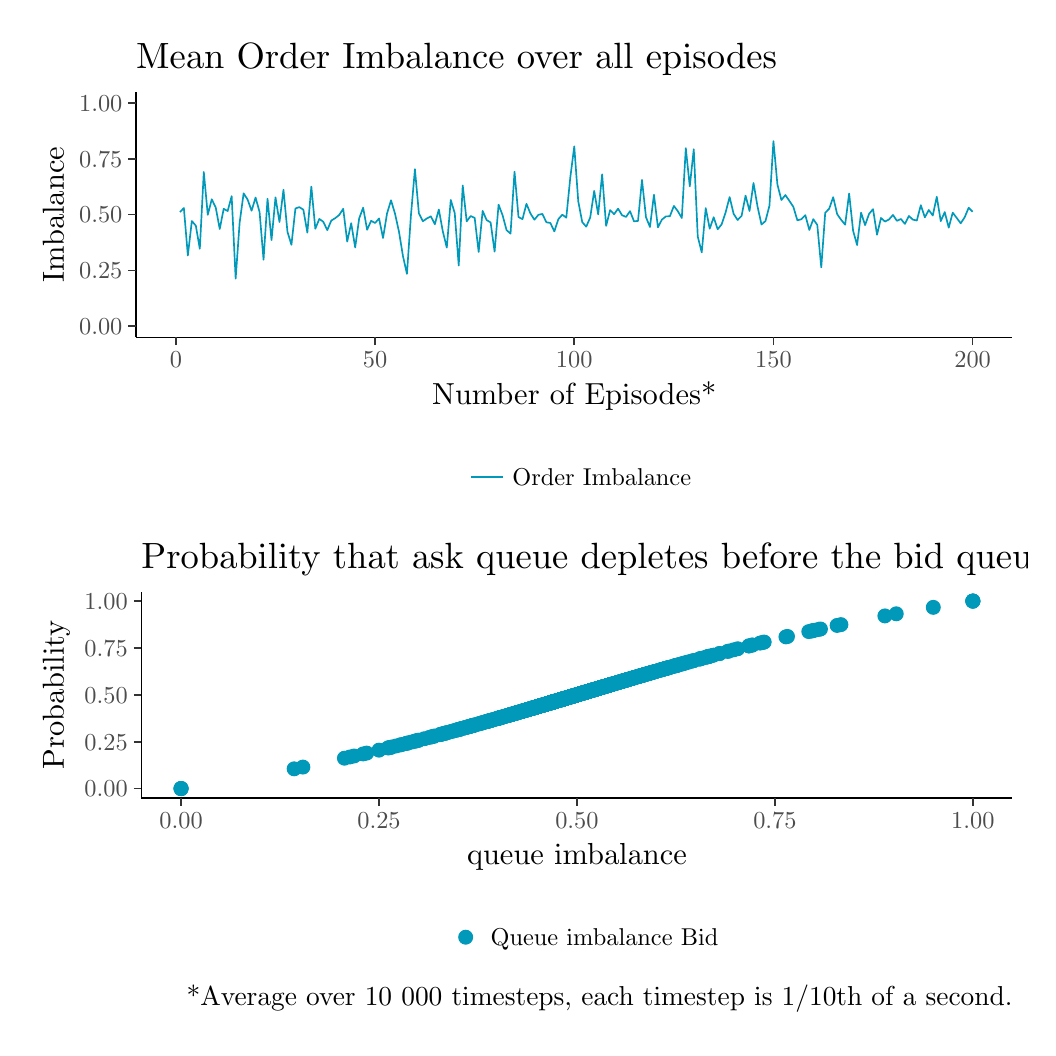
\begin{tikzpicture}[x=1pt,y=1pt]
\definecolor{fillColor}{RGB}{255,255,255}
\path[use as bounding box,fill=fillColor,fill opacity=0.00] (0,0) rectangle (361.35,361.35);
\begin{scope}
\path[clip] (  0.00,180.67) rectangle (361.35,361.35);
\definecolor{drawColor}{RGB}{255,255,255}
\definecolor{fillColor}{RGB}{255,255,255}

\path[draw=drawColor,line width= 0.6pt,line join=round,line cap=round,fill=fillColor] (  0.00,180.67) rectangle (361.35,361.35);
\end{scope}
\begin{scope}
\path[clip] ( 39.17,249.42) rectangle (355.85,338.21);
\definecolor{fillColor}{RGB}{255,255,255}

\path[fill=fillColor] ( 39.17,249.42) rectangle (355.85,338.21);
\definecolor{drawColor}{RGB}{0,153,186}

\path[draw=drawColor,line width= 0.6pt,line join=round] ( 55.00,294.70) --
	( 56.44,296.18) --
	( 57.88,279.02) --
	( 59.32,291.48) --
	( 60.76,289.80) --
	( 62.20,281.45) --
	( 63.64,309.18) --
	( 65.08,293.70) --
	( 66.52,299.34) --
	( 67.96,296.32) --
	( 69.40,288.61) --
	( 70.83,295.89) --
	( 72.27,295.09) --
	( 73.71,300.47) --
	( 75.15,270.67) --
	( 76.59,290.87) --
	( 78.03,301.48) --
	( 79.47,299.24) --
	( 80.91,295.21) --
	( 82.35,299.96) --
	( 83.79,294.77) --
	( 85.23,277.50) --
	( 86.67,299.54) --
	( 88.11,284.58) --
	( 89.55,300.03) --
	( 90.99,291.10) --
	( 92.43,302.79) --
	( 93.87,287.60) --
	( 95.31,282.88) --
	( 96.75,296.00) --
	( 98.18,296.51) --
	( 99.62,295.56) --
	(101.06,287.30) --
	(102.50,303.91) --
	(103.94,288.70) --
	(105.38,292.22) --
	(106.82,291.23) --
	(108.26,288.17) --
	(109.70,291.63) --
	(111.14,292.53) --
	(112.58,293.67) --
	(114.02,295.90) --
	(115.46,284.04) --
	(116.90,290.70) --
	(118.34,281.93) --
	(119.78,292.40) --
	(121.22,296.31) --
	(122.66,288.31) --
	(124.10,291.56) --
	(125.53,290.76) --
	(126.97,292.41) --
	(128.41,285.35) --
	(129.85,294.19) --
	(131.29,298.97) --
	(132.73,294.17) --
	(134.17,287.62) --
	(135.61,278.79) --
	(137.05,272.38) --
	(138.49,293.51) --
	(139.93,310.21) --
	(141.37,294.22) --
	(142.81,291.41) --
	(144.25,292.40) --
	(145.69,293.17) --
	(147.13,290.30) --
	(148.57,295.64) --
	(150.01,287.73) --
	(151.45,281.87) --
	(152.88,299.11) --
	(154.32,294.32) --
	(155.76,275.37) --
	(157.20,304.35) --
	(158.64,291.36) --
	(160.08,293.29) --
	(161.52,292.62) --
	(162.96,280.29) --
	(164.40,295.15) --
	(165.84,291.82) --
	(167.28,290.97) --
	(168.72,280.43) --
	(170.16,297.39) --
	(171.60,293.58) --
	(173.04,288.19) --
	(174.48,286.93) --
	(175.92,309.32) --
	(177.36,292.92) --
	(178.80,292.15) --
	(180.23,297.70) --
	(181.67,294.21) --
	(183.11,291.95) --
	(184.55,293.72) --
	(185.99,294.05) --
	(187.43,291.03) --
	(188.87,290.78) --
	(190.31,287.73) --
	(191.75,292.14) --
	(193.19,293.77) --
	(194.63,292.69) --
	(196.07,307.20) --
	(197.51,318.45) --
	(198.95,298.61) --
	(200.39,291.09) --
	(201.83,289.44) --
	(203.27,292.74) --
	(204.71,302.36) --
	(206.15,293.86) --
	(207.58,308.37) --
	(209.02,289.72) --
	(210.46,295.42) --
	(211.90,293.95) --
	(213.34,295.94) --
	(214.78,293.57) --
	(216.22,292.97) --
	(217.66,295.05) --
	(219.10,291.36) --
	(220.54,291.52) --
	(221.98,306.34) --
	(223.42,292.88) --
	(224.86,289.32) --
	(226.30,300.98) --
	(227.74,289.19) --
	(229.18,292.00) --
	(230.62,293.14) --
	(232.06,293.21) --
	(233.50,296.93) --
	(234.93,295.03) --
	(236.37,292.56) --
	(237.81,317.82) --
	(239.25,303.99) --
	(240.69,317.45) --
	(242.13,285.87) --
	(243.57,280.14) --
	(245.01,296.14) --
	(246.45,288.71) --
	(247.89,292.85) --
	(249.33,288.51) --
	(250.77,290.28) --
	(252.21,294.65) --
	(253.65,300.14) --
	(255.09,294.08) --
	(256.53,291.85) --
	(257.97,293.35) --
	(259.41,300.67) --
	(260.84,295.10) --
	(262.28,305.23) --
	(263.72,296.76) --
	(265.16,290.22) --
	(266.60,291.46) --
	(268.04,297.04) --
	(269.48,320.34) --
	(270.92,304.63) --
	(272.36,299.07) --
	(273.80,300.87) --
	(275.24,298.75) --
	(276.68,296.59) --
	(278.12,291.74) --
	(279.56,292.12) --
	(281.00,293.61) --
	(282.44,288.25) --
	(283.88,292.15) --
	(285.32,290.07) --
	(286.76,274.73) --
	(288.19,294.47) --
	(289.63,295.94) --
	(291.07,300.10) --
	(292.51,293.94) --
	(293.95,291.91) --
	(295.39,290.15) --
	(296.83,301.42) --
	(298.27,287.94) --
	(299.71,282.81) --
	(301.15,294.51) --
	(302.59,289.99) --
	(304.03,294.05) --
	(305.47,295.77) --
	(306.91,286.54) --
	(308.35,292.58) --
	(309.79,291.29) --
	(311.23,292.03) --
	(312.67,293.67) --
	(314.11,291.55) --
	(315.54,292.21) --
	(316.98,290.45) --
	(318.42,293.31) --
	(319.86,291.98) --
	(321.30,291.67) --
	(322.74,297.21) --
	(324.18,292.81) --
	(325.62,295.46) --
	(327.06,293.48) --
	(328.50,300.25) --
	(329.94,291.44) --
	(331.38,294.72) --
	(332.82,289.08) --
	(334.26,294.50) --
	(335.70,292.60) --
	(337.14,290.66) --
	(338.58,292.84) --
	(340.02,296.27) --
	(341.46,294.82);
\end{scope}
\begin{scope}
\path[clip] (  0.00,  0.00) rectangle (361.35,361.35);
\definecolor{drawColor}{RGB}{0,0,0}

\path[draw=drawColor,line width= 0.6pt,line join=round] ( 39.17,249.42) --
	( 39.17,338.21);
\end{scope}
\begin{scope}
\path[clip] (  0.00,  0.00) rectangle (361.35,361.35);
\definecolor{drawColor}{gray}{0.30}

\node[text=drawColor,anchor=base east,inner sep=0pt, outer sep=0pt, scale=  0.88] at ( 34.22,250.43) {0.00};

\node[text=drawColor,anchor=base east,inner sep=0pt, outer sep=0pt, scale=  0.88] at ( 34.22,270.61) {0.25};

\node[text=drawColor,anchor=base east,inner sep=0pt, outer sep=0pt, scale=  0.88] at ( 34.22,290.79) {0.50};

\node[text=drawColor,anchor=base east,inner sep=0pt, outer sep=0pt, scale=  0.88] at ( 34.22,310.97) {0.75};

\node[text=drawColor,anchor=base east,inner sep=0pt, outer sep=0pt, scale=  0.88] at ( 34.22,331.15) {1.00};
\end{scope}
\begin{scope}
\path[clip] (  0.00,  0.00) rectangle (361.35,361.35);
\definecolor{drawColor}{gray}{0.20}

\path[draw=drawColor,line width= 0.6pt,line join=round] ( 36.42,253.46) --
	( 39.17,253.46);

\path[draw=drawColor,line width= 0.6pt,line join=round] ( 36.42,273.64) --
	( 39.17,273.64);

\path[draw=drawColor,line width= 0.6pt,line join=round] ( 36.42,293.82) --
	( 39.17,293.82);

\path[draw=drawColor,line width= 0.6pt,line join=round] ( 36.42,314.00) --
	( 39.17,314.00);

\path[draw=drawColor,line width= 0.6pt,line join=round] ( 36.42,334.18) --
	( 39.17,334.18);
\end{scope}
\begin{scope}
\path[clip] (  0.00,  0.00) rectangle (361.35,361.35);
\definecolor{drawColor}{RGB}{0,0,0}

\path[draw=drawColor,line width= 0.6pt,line join=round] ( 39.17,249.42) --
	(355.85,249.42);
\end{scope}
\begin{scope}
\path[clip] (  0.00,  0.00) rectangle (361.35,361.35);
\definecolor{drawColor}{gray}{0.20}

\path[draw=drawColor,line width= 0.6pt,line join=round] ( 53.56,246.67) --
	( 53.56,249.42);

\path[draw=drawColor,line width= 0.6pt,line join=round] (125.53,246.67) --
	(125.53,249.42);

\path[draw=drawColor,line width= 0.6pt,line join=round] (197.51,246.67) --
	(197.51,249.42);

\path[draw=drawColor,line width= 0.6pt,line join=round] (269.48,246.67) --
	(269.48,249.42);

\path[draw=drawColor,line width= 0.6pt,line join=round] (341.46,246.67) --
	(341.46,249.42);
\end{scope}
\begin{scope}
\path[clip] (  0.00,  0.00) rectangle (361.35,361.35);
\definecolor{drawColor}{gray}{0.30}

\node[text=drawColor,anchor=base,inner sep=0pt, outer sep=0pt, scale=  0.88] at ( 53.56,238.41) {0};

\node[text=drawColor,anchor=base,inner sep=0pt, outer sep=0pt, scale=  0.88] at (125.53,238.41) {50};

\node[text=drawColor,anchor=base,inner sep=0pt, outer sep=0pt, scale=  0.88] at (197.51,238.41) {100};

\node[text=drawColor,anchor=base,inner sep=0pt, outer sep=0pt, scale=  0.88] at (269.48,238.41) {150};

\node[text=drawColor,anchor=base,inner sep=0pt, outer sep=0pt, scale=  0.88] at (341.46,238.41) {200};
\end{scope}
\begin{scope}
\path[clip] (  0.00,  0.00) rectangle (361.35,361.35);
\definecolor{drawColor}{RGB}{0,0,0}

\node[text=drawColor,anchor=base,inner sep=0pt, outer sep=0pt, scale=  1.10] at (197.51,225.34) {Number of Episodes*};
\end{scope}
\begin{scope}
\path[clip] (  0.00,  0.00) rectangle (361.35,361.35);
\definecolor{drawColor}{RGB}{0,0,0}

\node[text=drawColor,rotate= 90.00,anchor=base,inner sep=0pt, outer sep=0pt, scale=  1.10] at ( 13.08,293.82) {Imbalance};
\end{scope}
\begin{scope}
\path[clip] (  0.00,  0.00) rectangle (361.35,361.35);
\definecolor{fillColor}{RGB}{255,255,255}

\path[fill=fillColor] (149.60,186.17) rectangle (245.42,212.01);
\end{scope}
\begin{scope}
\path[clip] (  0.00,  0.00) rectangle (361.35,361.35);
\definecolor{drawColor}{RGB}{0,153,186}

\path[draw=drawColor,line width= 0.6pt,line join=round] (160.35,199.09) -- (171.91,199.09);
\end{scope}
\begin{scope}
\path[clip] (  0.00,  0.00) rectangle (361.35,361.35);
\definecolor{drawColor}{RGB}{0,0,0}

\node[text=drawColor,anchor=base west,inner sep=0pt, outer sep=0pt, scale=  0.88] at (175.16,196.06) {Order Imbalance};
\end{scope}
\begin{scope}
\path[clip] (  0.00,  0.00) rectangle (361.35,361.35);
\definecolor{drawColor}{RGB}{0,0,0}

\node[text=drawColor,anchor=base west,inner sep=0pt, outer sep=0pt, scale=  1.32] at ( 39.17,346.76) {Mean Order Imbalance over all episodes };
\end{scope}
\begin{scope}
\path[clip] (  0.00,  0.00) rectangle (361.35,180.68);
\definecolor{drawColor}{RGB}{255,255,255}
\definecolor{fillColor}{RGB}{255,255,255}

\path[draw=drawColor,line width= 0.6pt,line join=round,line cap=round,fill=fillColor] (  0.00,  0.00) rectangle (361.35,180.68);
\end{scope}
\begin{scope}
\path[clip] ( 41.11, 83.01) rectangle (355.85,157.54);
\definecolor{fillColor}{RGB}{255,255,255}

\path[fill=fillColor] ( 41.11, 83.01) rectangle (355.85,157.54);
\definecolor{drawColor}{RGB}{0,153,186}
\definecolor{fillColor}{RGB}{0,153,186}

\path[draw=drawColor,line width= 0.4pt,line join=round,line cap=round,fill=fillColor] (201.59,121.22) circle (  2.50);

\path[draw=drawColor,line width= 0.4pt,line join=round,line cap=round,fill=fillColor] (206.84,122.79) circle (  2.50);

\path[draw=drawColor,line width= 0.4pt,line join=round,line cap=round,fill=fillColor] (146.02,105.12) circle (  2.50);

\path[draw=drawColor,line width= 0.4pt,line join=round,line cap=round,fill=fillColor] (190.19,117.78) circle (  2.50);

\path[draw=drawColor,line width= 0.4pt,line join=round,line cap=round,fill=fillColor] (184.22,115.99) circle (  2.50);

\path[draw=drawColor,line width= 0.4pt,line join=round,line cap=round,fill=fillColor] (154.63,107.45) circle (  2.50);

\path[draw=drawColor,line width= 0.4pt,line join=round,line cap=round,fill=fillColor] (252.92,135.96) circle (  2.50);

\path[draw=drawColor,line width= 0.4pt,line join=round,line cap=round,fill=fillColor] (198.07,120.15) circle (  2.50);

\path[draw=drawColor,line width= 0.4pt,line join=round,line cap=round,fill=fillColor] (218.05,126.14) circle (  2.50);

\path[draw=drawColor,line width= 0.4pt,line join=round,line cap=round,fill=fillColor] (207.33,122.94) circle (  2.50);

\path[draw=drawColor,line width= 0.4pt,line join=round,line cap=round,fill=fillColor] (180.02,114.74) circle (  2.50);

\path[draw=drawColor,line width= 0.4pt,line join=round,line cap=round,fill=fillColor] (205.81,122.49) circle (  2.50);

\path[draw=drawColor,line width= 0.4pt,line join=round,line cap=round,fill=fillColor] (203.00,121.64) circle (  2.50);

\path[draw=drawColor,line width= 0.4pt,line join=round,line cap=round,fill=fillColor] (222.06,127.32) circle (  2.50);

\path[draw=drawColor,line width= 0.4pt,line join=round,line cap=round,fill=fillColor] (116.42, 97.82) circle (  2.50);

\path[draw=drawColor,line width= 0.4pt,line join=round,line cap=round,fill=fillColor] (188.05,117.14) circle (  2.50);

\path[draw=drawColor,line width= 0.4pt,line join=round,line cap=round,fill=fillColor] (225.63,128.36) circle (  2.50);

\path[draw=drawColor,line width= 0.4pt,line join=round,line cap=round,fill=fillColor] (217.70,126.04) circle (  2.50);

\path[draw=drawColor,line width= 0.4pt,line join=round,line cap=round,fill=fillColor] (203.41,121.76) circle (  2.50);

\path[draw=drawColor,line width= 0.4pt,line join=round,line cap=round,fill=fillColor] (220.25,126.79) circle (  2.50);

\path[draw=drawColor,line width= 0.4pt,line join=round,line cap=round,fill=fillColor] (201.86,121.30) circle (  2.50);

\path[draw=drawColor,line width= 0.4pt,line join=round,line cap=round,fill=fillColor] (140.65,103.71) circle (  2.50);

\path[draw=drawColor,line width= 0.4pt,line join=round,line cap=round,fill=fillColor] (218.75,126.35) circle (  2.50);

\path[draw=drawColor,line width= 0.4pt,line join=round,line cap=round,fill=fillColor] (165.73,110.57) circle (  2.50);

\path[draw=drawColor,line width= 0.4pt,line join=round,line cap=round,fill=fillColor] (220.49,126.86) circle (  2.50);

\path[draw=drawColor,line width= 0.4pt,line join=round,line cap=round,fill=fillColor] (188.85,117.38) circle (  2.50);

\path[draw=drawColor,line width= 0.4pt,line join=round,line cap=round,fill=fillColor] (230.27,129.71) circle (  2.50);

\path[draw=drawColor,line width= 0.4pt,line join=round,line cap=round,fill=fillColor] (176.46,113.69) circle (  2.50);

\path[draw=drawColor,line width= 0.4pt,line join=round,line cap=round,fill=fillColor] (159.70,108.86) circle (  2.50);

\path[draw=drawColor,line width= 0.4pt,line join=round,line cap=round,fill=fillColor] (206.22,122.61) circle (  2.50);

\path[draw=drawColor,line width= 0.4pt,line join=round,line cap=round,fill=fillColor] (208.02,123.15) circle (  2.50);

\path[draw=drawColor,line width= 0.4pt,line join=round,line cap=round,fill=fillColor] (204.65,122.14) circle (  2.50);

\path[draw=drawColor,line width= 0.4pt,line join=round,line cap=round,fill=fillColor] (175.37,113.37) circle (  2.50);

\path[draw=drawColor,line width= 0.4pt,line join=round,line cap=round,fill=fillColor] (234.25,130.84) circle (  2.50);

\path[draw=drawColor,line width= 0.4pt,line join=round,line cap=round,fill=fillColor] (180.33,114.84) circle (  2.50);

\path[draw=drawColor,line width= 0.4pt,line join=round,line cap=round,fill=fillColor] (192.82,118.57) circle (  2.50);

\path[draw=drawColor,line width= 0.4pt,line join=round,line cap=round,fill=fillColor] (189.31,117.52) circle (  2.50);

\path[draw=drawColor,line width= 0.4pt,line join=round,line cap=round,fill=fillColor] (178.48,114.28) circle (  2.50);

\path[draw=drawColor,line width= 0.4pt,line join=round,line cap=round,fill=fillColor] (190.72,117.94) circle (  2.50);

\path[draw=drawColor,line width= 0.4pt,line join=round,line cap=round,fill=fillColor] (193.92,118.90) circle (  2.50);

\path[draw=drawColor,line width= 0.4pt,line join=round,line cap=round,fill=fillColor] (197.95,120.12) circle (  2.50);

\path[draw=drawColor,line width= 0.4pt,line join=round,line cap=round,fill=fillColor] (205.87,122.50) circle (  2.50);

\path[draw=drawColor,line width= 0.4pt,line join=round,line cap=round,fill=fillColor] (163.83,110.03) circle (  2.50);

\path[draw=drawColor,line width= 0.4pt,line join=round,line cap=round,fill=fillColor] (187.41,116.95) circle (  2.50);

\path[draw=drawColor,line width= 0.4pt,line join=round,line cap=round,fill=fillColor] (156.35,107.93) circle (  2.50);

\path[draw=drawColor,line width= 0.4pt,line join=round,line cap=round,fill=fillColor] (193.46,118.77) circle (  2.50);

\path[draw=drawColor,line width= 0.4pt,line join=round,line cap=round,fill=fillColor] (207.30,122.93) circle (  2.50);

\path[draw=drawColor,line width= 0.4pt,line join=round,line cap=round,fill=fillColor] (178.95,114.43) circle (  2.50);

\path[draw=drawColor,line width= 0.4pt,line join=round,line cap=round,fill=fillColor] (190.49,117.87) circle (  2.50);

\path[draw=drawColor,line width= 0.4pt,line join=round,line cap=round,fill=fillColor] (187.66,117.02) circle (  2.50);

\path[draw=drawColor,line width= 0.4pt,line join=round,line cap=round,fill=fillColor] (193.51,118.78) circle (  2.50);

\path[draw=drawColor,line width= 0.4pt,line join=round,line cap=round,fill=fillColor] (168.45,111.35) circle (  2.50);

\path[draw=drawColor,line width= 0.4pt,line join=round,line cap=round,fill=fillColor] (199.80,120.68) circle (  2.50);

\path[draw=drawColor,line width= 0.4pt,line join=round,line cap=round,fill=fillColor] (216.74,125.75) circle (  2.50);

\path[draw=drawColor,line width= 0.4pt,line join=round,line cap=round,fill=fillColor] (199.71,120.65) circle (  2.50);

\path[draw=drawColor,line width= 0.4pt,line join=round,line cap=round,fill=fillColor] (176.51,113.71) circle (  2.50);

\path[draw=drawColor,line width= 0.4pt,line join=round,line cap=round,fill=fillColor] (145.21,104.90) circle (  2.50);

\path[draw=drawColor,line width= 0.4pt,line join=round,line cap=round,fill=fillColor] (122.50, 99.22) circle (  2.50);

\path[draw=drawColor,line width= 0.4pt,line join=round,line cap=round,fill=fillColor] (197.37,119.94) circle (  2.50);

\path[draw=drawColor,line width= 0.4pt,line join=round,line cap=round,fill=fillColor] (256.58,136.92) circle (  2.50);

\path[draw=drawColor,line width= 0.4pt,line join=round,line cap=round,fill=fillColor] (199.91,120.71) circle (  2.50);

\path[draw=drawColor,line width= 0.4pt,line join=round,line cap=round,fill=fillColor] (189.94,117.71) circle (  2.50);

\path[draw=drawColor,line width= 0.4pt,line join=round,line cap=round,fill=fillColor] (193.45,118.76) circle (  2.50);

\path[draw=drawColor,line width= 0.4pt,line join=round,line cap=round,fill=fillColor] (196.18,119.58) circle (  2.50);

\path[draw=drawColor,line width= 0.4pt,line join=round,line cap=round,fill=fillColor] (186.00,116.52) circle (  2.50);

\path[draw=drawColor,line width= 0.4pt,line join=round,line cap=round,fill=fillColor] (204.94,122.22) circle (  2.50);

\path[draw=drawColor,line width= 0.4pt,line join=round,line cap=round,fill=fillColor] (176.92,113.82) circle (  2.50);

\path[draw=drawColor,line width= 0.4pt,line join=round,line cap=round,fill=fillColor] (156.15,107.87) circle (  2.50);

\path[draw=drawColor,line width= 0.4pt,line join=round,line cap=round,fill=fillColor] (217.25,125.90) circle (  2.50);

\path[draw=drawColor,line width= 0.4pt,line join=round,line cap=round,fill=fillColor] (200.26,120.81) circle (  2.50);

\path[draw=drawColor,line width= 0.4pt,line join=round,line cap=round,fill=fillColor] (133.10,101.79) circle (  2.50);

\path[draw=drawColor,line width= 0.4pt,line join=round,line cap=round,fill=fillColor] (235.80,131.28) circle (  2.50);

\path[draw=drawColor,line width= 0.4pt,line join=round,line cap=round,fill=fillColor] (189.77,117.65) circle (  2.50);

\path[draw=drawColor,line width= 0.4pt,line join=round,line cap=round,fill=fillColor] (196.62,119.72) circle (  2.50);

\path[draw=drawColor,line width= 0.4pt,line join=round,line cap=round,fill=fillColor] (194.22,118.99) circle (  2.50);

\path[draw=drawColor,line width= 0.4pt,line join=round,line cap=round,fill=fillColor] (150.51,106.32) circle (  2.50);

\path[draw=drawColor,line width= 0.4pt,line join=round,line cap=round,fill=fillColor] (203.20,121.70) circle (  2.50);

\path[draw=drawColor,line width= 0.4pt,line join=round,line cap=round,fill=fillColor] (191.39,118.14) circle (  2.50);

\path[draw=drawColor,line width= 0.4pt,line join=round,line cap=round,fill=fillColor] (188.37,117.23) circle (  2.50);

\path[draw=drawColor,line width= 0.4pt,line join=round,line cap=round,fill=fillColor] (151.03,106.46) circle (  2.50);

\path[draw=drawColor,line width= 0.4pt,line join=round,line cap=round,fill=fillColor] (211.14,124.08) circle (  2.50);

\path[draw=drawColor,line width= 0.4pt,line join=round,line cap=round,fill=fillColor] (197.64,120.02) circle (  2.50);

\path[draw=drawColor,line width= 0.4pt,line join=round,line cap=round,fill=fillColor] (178.52,114.30) circle (  2.50);

\path[draw=drawColor,line width= 0.4pt,line join=round,line cap=round,fill=fillColor] (174.08,112.99) circle (  2.50);

\path[draw=drawColor,line width= 0.4pt,line join=round,line cap=round,fill=fillColor] (253.42,136.09) circle (  2.50);

\path[draw=drawColor,line width= 0.4pt,line join=round,line cap=round,fill=fillColor] (195.29,119.31) circle (  2.50);

\path[draw=drawColor,line width= 0.4pt,line join=round,line cap=round,fill=fillColor] (192.57,118.50) circle (  2.50);

\path[draw=drawColor,line width= 0.4pt,line join=round,line cap=round,fill=fillColor] (212.23,124.41) circle (  2.50);

\path[draw=drawColor,line width= 0.4pt,line join=round,line cap=round,fill=fillColor] (199.89,120.70) circle (  2.50);

\path[draw=drawColor,line width= 0.4pt,line join=round,line cap=round,fill=fillColor] (191.86,118.28) circle (  2.50);

\path[draw=drawColor,line width= 0.4pt,line join=round,line cap=round,fill=fillColor] (198.13,120.17) circle (  2.50);

\path[draw=drawColor,line width= 0.4pt,line join=round,line cap=round,fill=fillColor] (199.31,120.53) circle (  2.50);

\path[draw=drawColor,line width= 0.4pt,line join=round,line cap=round,fill=fillColor] (188.61,117.31) circle (  2.50);

\path[draw=drawColor,line width= 0.4pt,line join=round,line cap=round,fill=fillColor] (187.69,117.03) circle (  2.50);

\path[draw=drawColor,line width= 0.4pt,line join=round,line cap=round,fill=fillColor] (176.91,113.82) circle (  2.50);

\path[draw=drawColor,line width= 0.4pt,line join=round,line cap=round,fill=fillColor] (192.52,118.48) circle (  2.50);

\path[draw=drawColor,line width= 0.4pt,line join=round,line cap=round,fill=fillColor] (198.31,120.23) circle (  2.50);

\path[draw=drawColor,line width= 0.4pt,line join=round,line cap=round,fill=fillColor] (194.47,119.07) circle (  2.50);

\path[draw=drawColor,line width= 0.4pt,line join=round,line cap=round,fill=fillColor] (245.92,134.09) circle (  2.50);

\path[draw=drawColor,line width= 0.4pt,line join=round,line cap=round,fill=fillColor] (285.80,143.91) circle (  2.50);

\path[draw=drawColor,line width= 0.4pt,line join=round,line cap=round,fill=fillColor] (215.47,125.37) circle (  2.50);

\path[draw=drawColor,line width= 0.4pt,line join=round,line cap=round,fill=fillColor] (188.81,117.37) circle (  2.50);

\path[draw=drawColor,line width= 0.4pt,line join=round,line cap=round,fill=fillColor] (182.96,115.62) circle (  2.50);

\path[draw=drawColor,line width= 0.4pt,line join=round,line cap=round,fill=fillColor] (194.65,119.12) circle (  2.50);

\path[draw=drawColor,line width= 0.4pt,line join=round,line cap=round,fill=fillColor] (228.75,129.27) circle (  2.50);

\path[draw=drawColor,line width= 0.4pt,line join=round,line cap=round,fill=fillColor] (198.64,120.32) circle (  2.50);

\path[draw=drawColor,line width= 0.4pt,line join=round,line cap=round,fill=fillColor] (250.08,135.21) circle (  2.50);

\path[draw=drawColor,line width= 0.4pt,line join=round,line cap=round,fill=fillColor] (183.96,115.91) circle (  2.50);

\path[draw=drawColor,line width= 0.4pt,line join=round,line cap=round,fill=fillColor] (204.15,121.98) circle (  2.50);

\path[draw=drawColor,line width= 0.4pt,line join=round,line cap=round,fill=fillColor] (198.95,120.42) circle (  2.50);

\path[draw=drawColor,line width= 0.4pt,line join=round,line cap=round,fill=fillColor] (205.99,122.54) circle (  2.50);

\path[draw=drawColor,line width= 0.4pt,line join=round,line cap=round,fill=fillColor] (197.60,120.01) circle (  2.50);

\path[draw=drawColor,line width= 0.4pt,line join=round,line cap=round,fill=fillColor] (195.49,119.38) circle (  2.50);

\path[draw=drawColor,line width= 0.4pt,line join=round,line cap=round,fill=fillColor] (202.86,121.60) circle (  2.50);

\path[draw=drawColor,line width= 0.4pt,line join=round,line cap=round,fill=fillColor] (189.75,117.65) circle (  2.50);

\path[draw=drawColor,line width= 0.4pt,line join=round,line cap=round,fill=fillColor] (190.33,117.82) circle (  2.50);

\path[draw=drawColor,line width= 0.4pt,line join=round,line cap=round,fill=fillColor] (242.85,133.25) circle (  2.50);

\path[draw=drawColor,line width= 0.4pt,line join=round,line cap=round,fill=fillColor] (195.15,119.27) circle (  2.50);

\path[draw=drawColor,line width= 0.4pt,line join=round,line cap=round,fill=fillColor] (182.52,115.49) circle (  2.50);

\path[draw=drawColor,line width= 0.4pt,line join=round,line cap=round,fill=fillColor] (223.87,127.85) circle (  2.50);

\path[draw=drawColor,line width= 0.4pt,line join=round,line cap=round,fill=fillColor] (182.08,115.35) circle (  2.50);

\path[draw=drawColor,line width= 0.4pt,line join=round,line cap=round,fill=fillColor] (192.03,118.33) circle (  2.50);

\path[draw=drawColor,line width= 0.4pt,line join=round,line cap=round,fill=fillColor] (196.09,119.56) circle (  2.50);

\path[draw=drawColor,line width= 0.4pt,line join=round,line cap=round,fill=fillColor] (196.31,119.62) circle (  2.50);

\path[draw=drawColor,line width= 0.4pt,line join=round,line cap=round,fill=fillColor] (209.52,123.60) circle (  2.50);

\path[draw=drawColor,line width= 0.4pt,line join=round,line cap=round,fill=fillColor] (202.79,121.58) circle (  2.50);

\path[draw=drawColor,line width= 0.4pt,line join=round,line cap=round,fill=fillColor] (194.03,118.94) circle (  2.50);

\path[draw=drawColor,line width= 0.4pt,line join=round,line cap=round,fill=fillColor] (283.55,143.42) circle (  2.50);

\path[draw=drawColor,line width= 0.4pt,line join=round,line cap=round,fill=fillColor] (234.53,130.92) circle (  2.50);

\path[draw=drawColor,line width= 0.4pt,line join=round,line cap=round,fill=fillColor] (282.26,143.13) circle (  2.50);

\path[draw=drawColor,line width= 0.4pt,line join=round,line cap=round,fill=fillColor] (170.31,111.89) circle (  2.50);

\path[draw=drawColor,line width= 0.4pt,line join=round,line cap=round,fill=fillColor] (149.98,106.18) circle (  2.50);

\path[draw=drawColor,line width= 0.4pt,line join=round,line cap=round,fill=fillColor] (206.70,122.75) circle (  2.50);

\path[draw=drawColor,line width= 0.4pt,line join=round,line cap=round,fill=fillColor] (180.39,114.85) circle (  2.50);

\path[draw=drawColor,line width= 0.4pt,line join=round,line cap=round,fill=fillColor] (195.05,119.24) circle (  2.50);

\path[draw=drawColor,line width= 0.4pt,line join=round,line cap=round,fill=fillColor] (179.66,114.63) circle (  2.50);

\path[draw=drawColor,line width= 0.4pt,line join=round,line cap=round,fill=fillColor] (185.95,116.51) circle (  2.50);

\path[draw=drawColor,line width= 0.4pt,line join=round,line cap=round,fill=fillColor] (201.44,121.17) circle (  2.50);

\path[draw=drawColor,line width= 0.4pt,line join=round,line cap=round,fill=fillColor] (220.87,126.97) circle (  2.50);

\path[draw=drawColor,line width= 0.4pt,line join=round,line cap=round,fill=fillColor] (199.42,120.56) circle (  2.50);

\path[draw=drawColor,line width= 0.4pt,line join=round,line cap=round,fill=fillColor] (191.51,118.18) circle (  2.50);

\path[draw=drawColor,line width= 0.4pt,line join=round,line cap=round,fill=fillColor] (196.81,119.77) circle (  2.50);

\path[draw=drawColor,line width= 0.4pt,line join=round,line cap=round,fill=fillColor] (222.77,127.53) circle (  2.50);

\path[draw=drawColor,line width= 0.4pt,line join=round,line cap=round,fill=fillColor] (203.02,121.64) circle (  2.50);

\path[draw=drawColor,line width= 0.4pt,line join=round,line cap=round,fill=fillColor] (238.94,132.16) circle (  2.50);

\path[draw=drawColor,line width= 0.4pt,line join=round,line cap=round,fill=fillColor] (208.90,123.41) circle (  2.50);

\path[draw=drawColor,line width= 0.4pt,line join=round,line cap=round,fill=fillColor] (185.71,116.44) circle (  2.50);

\path[draw=drawColor,line width= 0.4pt,line join=round,line cap=round,fill=fillColor] (190.12,117.76) circle (  2.50);

\path[draw=drawColor,line width= 0.4pt,line join=round,line cap=round,fill=fillColor] (209.89,123.71) circle (  2.50);

\path[draw=drawColor,line width= 0.4pt,line join=round,line cap=round,fill=fillColor] (292.49,145.35) circle (  2.50);

\path[draw=drawColor,line width= 0.4pt,line join=round,line cap=round,fill=fillColor] (236.80,131.56) circle (  2.50);

\path[draw=drawColor,line width= 0.4pt,line join=round,line cap=round,fill=fillColor] (217.11,125.86) circle (  2.50);

\path[draw=drawColor,line width= 0.4pt,line join=round,line cap=round,fill=fillColor] (223.46,127.73) circle (  2.50);

\path[draw=drawColor,line width= 0.4pt,line join=round,line cap=round,fill=fillColor] (215.97,125.52) circle (  2.50);

\path[draw=drawColor,line width= 0.4pt,line join=round,line cap=round,fill=fillColor] (208.30,123.23) circle (  2.50);

\path[draw=drawColor,line width= 0.4pt,line join=round,line cap=round,fill=fillColor] (191.11,118.06) circle (  2.50);

\path[draw=drawColor,line width= 0.4pt,line join=round,line cap=round,fill=fillColor] (192.46,118.46) circle (  2.50);

\path[draw=drawColor,line width= 0.4pt,line join=round,line cap=round,fill=fillColor] (197.74,120.05) circle (  2.50);

\path[draw=drawColor,line width= 0.4pt,line join=round,line cap=round,fill=fillColor] (178.76,114.37) circle (  2.50);

\path[draw=drawColor,line width= 0.4pt,line join=round,line cap=round,fill=fillColor] (192.58,118.50) circle (  2.50);

\path[draw=drawColor,line width= 0.4pt,line join=round,line cap=round,fill=fillColor] (185.18,116.28) circle (  2.50);

\path[draw=drawColor,line width= 0.4pt,line join=round,line cap=round,fill=fillColor] (130.82,101.22) circle (  2.50);

\path[draw=drawColor,line width= 0.4pt,line join=round,line cap=round,fill=fillColor] (200.80,120.98) circle (  2.50);

\path[draw=drawColor,line width= 0.4pt,line join=round,line cap=round,fill=fillColor] (206.01,122.55) circle (  2.50);

\path[draw=drawColor,line width= 0.4pt,line join=round,line cap=round,fill=fillColor] (220.73,126.93) circle (  2.50);

\path[draw=drawColor,line width= 0.4pt,line join=round,line cap=round,fill=fillColor] (198.93,120.41) circle (  2.50);

\path[draw=drawColor,line width= 0.4pt,line join=round,line cap=round,fill=fillColor] (191.72,118.24) circle (  2.50);

\path[draw=drawColor,line width= 0.4pt,line join=round,line cap=round,fill=fillColor] (185.47,116.37) circle (  2.50);

\path[draw=drawColor,line width= 0.4pt,line join=round,line cap=round,fill=fillColor] (225.44,128.31) circle (  2.50);

\path[draw=drawColor,line width= 0.4pt,line join=round,line cap=round,fill=fillColor] (177.65,114.04) circle (  2.50);

\path[draw=drawColor,line width= 0.4pt,line join=round,line cap=round,fill=fillColor] (159.47,108.80) circle (  2.50);

\path[draw=drawColor,line width= 0.4pt,line join=round,line cap=round,fill=fillColor] (200.92,121.01) circle (  2.50);

\path[draw=drawColor,line width= 0.4pt,line join=round,line cap=round,fill=fillColor] (184.92,116.20) circle (  2.50);

\path[draw=drawColor,line width= 0.4pt,line join=round,line cap=round,fill=fillColor] (199.31,120.53) circle (  2.50);

\path[draw=drawColor,line width= 0.4pt,line join=round,line cap=round,fill=fillColor] (205.40,122.36) circle (  2.50);

\path[draw=drawColor,line width= 0.4pt,line join=round,line cap=round,fill=fillColor] (172.70,112.59) circle (  2.50);

\path[draw=drawColor,line width= 0.4pt,line join=round,line cap=round,fill=fillColor] (194.08,118.95) circle (  2.50);

\path[draw=drawColor,line width= 0.4pt,line join=round,line cap=round,fill=fillColor] (189.51,117.58) circle (  2.50);

\path[draw=drawColor,line width= 0.4pt,line join=round,line cap=round,fill=fillColor] (192.15,118.37) circle (  2.50);

\path[draw=drawColor,line width= 0.4pt,line join=round,line cap=round,fill=fillColor] (197.97,120.12) circle (  2.50);

\path[draw=drawColor,line width= 0.4pt,line join=round,line cap=round,fill=fillColor] (190.44,117.86) circle (  2.50);

\path[draw=drawColor,line width= 0.4pt,line join=round,line cap=round,fill=fillColor] (192.77,118.56) circle (  2.50);

\path[draw=drawColor,line width= 0.4pt,line join=round,line cap=round,fill=fillColor] (186.54,116.69) circle (  2.50);

\path[draw=drawColor,line width= 0.4pt,line join=round,line cap=round,fill=fillColor] (196.68,119.73) circle (  2.50);

\path[draw=drawColor,line width= 0.4pt,line join=round,line cap=round,fill=fillColor] (191.97,118.32) circle (  2.50);

\path[draw=drawColor,line width= 0.4pt,line join=round,line cap=round,fill=fillColor] (190.86,117.98) circle (  2.50);

\path[draw=drawColor,line width= 0.4pt,line join=round,line cap=round,fill=fillColor] (210.49,123.89) circle (  2.50);

\path[draw=drawColor,line width= 0.4pt,line join=round,line cap=round,fill=fillColor] (194.90,119.20) circle (  2.50);

\path[draw=drawColor,line width= 0.4pt,line join=round,line cap=round,fill=fillColor] (204.31,122.03) circle (  2.50);

\path[draw=drawColor,line width= 0.4pt,line join=round,line cap=round,fill=fillColor] (197.28,119.91) circle (  2.50);

\path[draw=drawColor,line width= 0.4pt,line join=round,line cap=round,fill=fillColor] (221.29,127.10) circle (  2.50);

\path[draw=drawColor,line width= 0.4pt,line join=round,line cap=round,fill=fillColor] (190.06,117.74) circle (  2.50);

\path[draw=drawColor,line width= 0.4pt,line join=round,line cap=round,fill=fillColor] (201.69,121.24) circle (  2.50);

\path[draw=drawColor,line width= 0.4pt,line join=round,line cap=round,fill=fillColor] (181.68,115.24) circle (  2.50);

\path[draw=drawColor,line width= 0.4pt,line join=round,line cap=round,fill=fillColor] (200.88,121.00) circle (  2.50);

\path[draw=drawColor,line width= 0.4pt,line join=round,line cap=round,fill=fillColor] (194.16,118.97) circle (  2.50);

\path[draw=drawColor,line width= 0.4pt,line join=round,line cap=round,fill=fillColor] (187.27,116.90) circle (  2.50);

\path[draw=drawColor,line width= 0.4pt,line join=round,line cap=round,fill=fillColor] (195.00,119.23) circle (  2.50);

\path[draw=drawColor,line width= 0.4pt,line join=round,line cap=round,fill=fillColor] (207.16,122.89) circle (  2.50);

\path[draw=drawColor,line width= 0.4pt,line join=round,line cap=round,fill=fillColor] (202.04,121.35) circle (  2.50);

\path[draw=drawColor,line width= 0.4pt,line join=round,line cap=round,fill=fillColor] (211.83,124.29) circle (  2.50);

\path[draw=drawColor,line width= 0.4pt,line join=round,line cap=round,fill=fillColor] (193.36,118.73) circle (  2.50);

\path[draw=drawColor,line width= 0.4pt,line join=round,line cap=round,fill=fillColor] (191.31,118.12) circle (  2.50);

\path[draw=drawColor,line width= 0.4pt,line join=round,line cap=round,fill=fillColor] (150.90,106.43) circle (  2.50);

\path[draw=drawColor,line width= 0.4pt,line join=round,line cap=round,fill=fillColor] (158.28,108.46) circle (  2.50);

\path[draw=drawColor,line width= 0.4pt,line join=round,line cap=round,fill=fillColor] (191.67,118.23) circle (  2.50);

\path[draw=drawColor,line width= 0.4pt,line join=round,line cap=round,fill=fillColor] (222.59,127.48) circle (  2.50);

\path[draw=drawColor,line width= 0.4pt,line join=round,line cap=round,fill=fillColor] (138.59,103.18) circle (  2.50);

\path[draw=drawColor,line width= 0.4pt,line join=round,line cap=round,fill=fillColor] (205.90,122.51) circle (  2.50);

\path[draw=drawColor,line width= 0.4pt,line join=round,line cap=round,fill=fillColor] (201.72,121.25) circle (  2.50);

\path[draw=drawColor,line width= 0.4pt,line join=round,line cap=round,fill=fillColor] (193.06,118.64) circle (  2.50);

\path[draw=drawColor,line width= 0.4pt,line join=round,line cap=round,fill=fillColor] (194.54,119.09) circle (  2.50);

\path[draw=drawColor,line width= 0.4pt,line join=round,line cap=round,fill=fillColor] (209.49,123.59) circle (  2.50);

\path[draw=drawColor,line width= 0.4pt,line join=round,line cap=round,fill=fillColor] (203.44,121.77) circle (  2.50);

\path[draw=drawColor,line width= 0.4pt,line join=round,line cap=round,fill=fillColor] (199.28,120.52) circle (  2.50);

\path[draw=drawColor,line width= 0.4pt,line join=round,line cap=round,fill=fillColor] (169.82,111.75) circle (  2.50);

\path[draw=drawColor,line width= 0.4pt,line join=round,line cap=round,fill=fillColor] (206.71,122.76) circle (  2.50);

\path[draw=drawColor,line width= 0.4pt,line join=round,line cap=round,fill=fillColor] (200.64,120.93) circle (  2.50);

\path[draw=drawColor,line width= 0.4pt,line join=round,line cap=round,fill=fillColor] (193.86,118.88) circle (  2.50);

\path[draw=drawColor,line width= 0.4pt,line join=round,line cap=round,fill=fillColor] (192.28,118.41) circle (  2.50);

\path[draw=drawColor,line width= 0.4pt,line join=round,line cap=round,fill=fillColor] (188.83,117.37) circle (  2.50);

\path[draw=drawColor,line width= 0.4pt,line join=round,line cap=round,fill=fillColor] (237.53,131.77) circle (  2.50);

\path[draw=drawColor,line width= 0.4pt,line join=round,line cap=round,fill=fillColor] (192.04,118.34) circle (  2.50);

\path[draw=drawColor,line width= 0.4pt,line join=round,line cap=round,fill=fillColor] (198.76,120.36) circle (  2.50);

\path[draw=drawColor,line width= 0.4pt,line join=round,line cap=round,fill=fillColor] (203.26,121.72) circle (  2.50);

\path[draw=drawColor,line width= 0.4pt,line join=round,line cap=round,fill=fillColor] (190.88,117.99) circle (  2.50);

\path[draw=drawColor,line width= 0.4pt,line join=round,line cap=round,fill=fillColor] (190.95,118.01) circle (  2.50);

\path[draw=drawColor,line width= 0.4pt,line join=round,line cap=round,fill=fillColor] (186.06,116.54) circle (  2.50);

\path[draw=drawColor,line width= 0.4pt,line join=round,line cap=round,fill=fillColor] (188.45,117.26) circle (  2.50);

\path[draw=drawColor,line width= 0.4pt,line join=round,line cap=round,fill=fillColor] (188.93,117.40) circle (  2.50);

\path[draw=drawColor,line width= 0.4pt,line join=round,line cap=round,fill=fillColor] (210.37,123.85) circle (  2.50);

\path[draw=drawColor,line width= 0.4pt,line join=round,line cap=round,fill=fillColor] (195.28,119.31) circle (  2.50);

\path[draw=drawColor,line width= 0.4pt,line join=round,line cap=round,fill=fillColor] (183.25,115.70) circle (  2.50);

\path[draw=drawColor,line width= 0.4pt,line join=round,line cap=round,fill=fillColor] (189.59,117.60) circle (  2.50);

\path[draw=drawColor,line width= 0.4pt,line join=round,line cap=round,fill=fillColor] (184.52,116.08) circle (  2.50);

\path[draw=drawColor,line width= 0.4pt,line join=round,line cap=round,fill=fillColor] (153.73,107.20) circle (  2.50);

\path[draw=drawColor,line width= 0.4pt,line join=round,line cap=round,fill=fillColor] (206.14,122.59) circle (  2.50);

\path[draw=drawColor,line width= 0.4pt,line join=round,line cap=round,fill=fillColor] (209.73,123.66) circle (  2.50);

\path[draw=drawColor,line width= 0.4pt,line join=round,line cap=round,fill=fillColor] (200.85,120.99) circle (  2.50);

\path[draw=drawColor,line width= 0.4pt,line join=round,line cap=round,fill=fillColor] (205.67,122.44) circle (  2.50);

\path[draw=drawColor,line width= 0.4pt,line join=round,line cap=round,fill=fillColor] (146.73,105.31) circle (  2.50);

\path[draw=drawColor,line width= 0.4pt,line join=round,line cap=round,fill=fillColor] (188.02,117.13) circle (  2.50);

\path[draw=drawColor,line width= 0.4pt,line join=round,line cap=round,fill=fillColor] (182.82,115.57) circle (  2.50);

\path[draw=drawColor,line width= 0.4pt,line join=round,line cap=round,fill=fillColor] (143.34,104.41) circle (  2.50);

\path[draw=drawColor,line width= 0.4pt,line join=round,line cap=round,fill=fillColor] (214.30,125.03) circle (  2.50);

\path[draw=drawColor,line width= 0.4pt,line join=round,line cap=round,fill=fillColor] (189.38,117.54) circle (  2.50);

\path[draw=drawColor,line width= 0.4pt,line join=round,line cap=round,fill=fillColor] (186.09,116.55) circle (  2.50);

\path[draw=drawColor,line width= 0.4pt,line join=round,line cap=round,fill=fillColor] (220.39,126.83) circle (  2.50);

\path[draw=drawColor,line width= 0.4pt,line join=round,line cap=round,fill=fillColor] (212.42,124.47) circle (  2.50);

\path[draw=drawColor,line width= 0.4pt,line join=round,line cap=round,fill=fillColor] (190.05,117.74) circle (  2.50);

\path[draw=drawColor,line width= 0.4pt,line join=round,line cap=round,fill=fillColor] (212.45,124.48) circle (  2.50);

\path[draw=drawColor,line width= 0.4pt,line join=round,line cap=round,fill=fillColor] (187.31,116.92) circle (  2.50);

\path[draw=drawColor,line width= 0.4pt,line join=round,line cap=round,fill=fillColor] (183.93,115.91) circle (  2.50);

\path[draw=drawColor,line width= 0.4pt,line join=round,line cap=round,fill=fillColor] (194.74,119.15) circle (  2.50);

\path[draw=drawColor,line width= 0.4pt,line join=round,line cap=round,fill=fillColor] (203.43,121.77) circle (  2.50);

\path[draw=drawColor,line width= 0.4pt,line join=round,line cap=round,fill=fillColor] (212.12,124.38) circle (  2.50);

\path[draw=drawColor,line width= 0.4pt,line join=round,line cap=round,fill=fillColor] (198.12,120.17) circle (  2.50);

\path[draw=drawColor,line width= 0.4pt,line join=round,line cap=round,fill=fillColor] (193.46,118.76) circle (  2.50);

\path[draw=drawColor,line width= 0.4pt,line join=round,line cap=round,fill=fillColor] (130.20,101.07) circle (  2.50);

\path[draw=drawColor,line width= 0.4pt,line join=round,line cap=round,fill=fillColor] (188.57,117.29) circle (  2.50);

\path[draw=drawColor,line width= 0.4pt,line join=round,line cap=round,fill=fillColor] (201.38,121.15) circle (  2.50);

\path[draw=drawColor,line width= 0.4pt,line join=round,line cap=round,fill=fillColor] (190.24,117.80) circle (  2.50);

\path[draw=drawColor,line width= 0.4pt,line join=round,line cap=round,fill=fillColor] (210.62,123.93) circle (  2.50);

\path[draw=drawColor,line width= 0.4pt,line join=round,line cap=round,fill=fillColor] (190.97,118.02) circle (  2.50);

\path[draw=drawColor,line width= 0.4pt,line join=round,line cap=round,fill=fillColor] (201.80,121.28) circle (  2.50);

\path[draw=drawColor,line width= 0.4pt,line join=round,line cap=round,fill=fillColor] (195.44,119.36) circle (  2.50);

\path[draw=drawColor,line width= 0.4pt,line join=round,line cap=round,fill=fillColor] (190.60,117.91) circle (  2.50);

\path[draw=drawColor,line width= 0.4pt,line join=round,line cap=round,fill=fillColor] (189.68,117.63) circle (  2.50);

\path[draw=drawColor,line width= 0.4pt,line join=round,line cap=round,fill=fillColor] (190.36,117.83) circle (  2.50);

\path[draw=drawColor,line width= 0.4pt,line join=round,line cap=round,fill=fillColor] (179.19,114.50) circle (  2.50);

\path[draw=drawColor,line width= 0.4pt,line join=round,line cap=round,fill=fillColor] (211.64,124.23) circle (  2.50);

\path[draw=drawColor,line width= 0.4pt,line join=round,line cap=round,fill=fillColor] (197.77,120.06) circle (  2.50);

\path[draw=drawColor,line width= 0.4pt,line join=round,line cap=round,fill=fillColor] (189.83,117.67) circle (  2.50);

\path[draw=drawColor,line width= 0.4pt,line join=round,line cap=round,fill=fillColor] (189.05,117.44) circle (  2.50);

\path[draw=drawColor,line width= 0.4pt,line join=round,line cap=round,fill=fillColor] (189.21,117.49) circle (  2.50);

\path[draw=drawColor,line width= 0.4pt,line join=round,line cap=round,fill=fillColor] (173.54,112.83) circle (  2.50);

\path[draw=drawColor,line width= 0.4pt,line join=round,line cap=round,fill=fillColor] (183.00,115.63) circle (  2.50);

\path[draw=drawColor,line width= 0.4pt,line join=round,line cap=round,fill=fillColor] (199.73,120.65) circle (  2.50);

\path[draw=drawColor,line width= 0.4pt,line join=round,line cap=round,fill=fillColor] (173.23,112.74) circle (  2.50);

\path[draw=drawColor,line width= 0.4pt,line join=round,line cap=round,fill=fillColor] (190.41,117.85) circle (  2.50);

\path[draw=drawColor,line width= 0.4pt,line join=round,line cap=round,fill=fillColor] (187.07,116.85) circle (  2.50);

\path[draw=drawColor,line width= 0.4pt,line join=round,line cap=round,fill=fillColor] (178.49,114.29) circle (  2.50);

\path[draw=drawColor,line width= 0.4pt,line join=round,line cap=round,fill=fillColor] (199.67,120.64) circle (  2.50);

\path[draw=drawColor,line width= 0.4pt,line join=round,line cap=round,fill=fillColor] (190.98,118.02) circle (  2.50);

\path[draw=drawColor,line width= 0.4pt,line join=round,line cap=round,fill=fillColor] (204.26,122.02) circle (  2.50);

\path[draw=drawColor,line width= 0.4pt,line join=round,line cap=round,fill=fillColor] (181.11,115.07) circle (  2.50);

\path[draw=drawColor,line width= 0.4pt,line join=round,line cap=round,fill=fillColor] (197.37,119.94) circle (  2.50);

\path[draw=drawColor,line width= 0.4pt,line join=round,line cap=round,fill=fillColor] (212.61,124.52) circle (  2.50);

\path[draw=drawColor,line width= 0.4pt,line join=round,line cap=round,fill=fillColor] (196.54,119.69) circle (  2.50);

\path[draw=drawColor,line width= 0.4pt,line join=round,line cap=round,fill=fillColor] (209.08,123.47) circle (  2.50);

\path[draw=drawColor,line width= 0.4pt,line join=round,line cap=round,fill=fillColor] (205.78,122.47) circle (  2.50);

\path[draw=drawColor,line width= 0.4pt,line join=round,line cap=round,fill=fillColor] (224.97,128.18) circle (  2.50);

\path[draw=drawColor,line width= 0.4pt,line join=round,line cap=round,fill=fillColor] (327.24,151.88) circle (  2.50);

\path[draw=drawColor,line width= 0.4pt,line join=round,line cap=round,fill=fillColor] (221.56,127.18) circle (  2.50);

\path[draw=drawColor,line width= 0.4pt,line join=round,line cap=round,fill=fillColor] (206.21,122.61) circle (  2.50);

\path[draw=drawColor,line width= 0.4pt,line join=round,line cap=round,fill=fillColor] (184.59,116.10) circle (  2.50);

\path[draw=drawColor,line width= 0.4pt,line join=round,line cap=round,fill=fillColor] (209.88,123.71) circle (  2.50);

\path[draw=drawColor,line width= 0.4pt,line join=round,line cap=round,fill=fillColor] (208.28,123.23) circle (  2.50);

\path[draw=drawColor,line width= 0.4pt,line join=round,line cap=round,fill=fillColor] (230.63,129.81) circle (  2.50);

\path[draw=drawColor,line width= 0.4pt,line join=round,line cap=round,fill=fillColor] (114.46, 97.37) circle (  2.50);

\path[draw=drawColor,line width= 0.4pt,line join=round,line cap=round,fill=fillColor] (204.83,122.19) circle (  2.50);

\path[draw=drawColor,line width= 0.4pt,line join=round,line cap=round,fill=fillColor] (212.88,124.60) circle (  2.50);

\path[draw=drawColor,line width= 0.4pt,line join=round,line cap=round,fill=fillColor] (164.42,110.20) circle (  2.50);

\path[draw=drawColor,line width= 0.4pt,line join=round,line cap=round,fill=fillColor] (201.43,121.17) circle (  2.50);

\path[draw=drawColor,line width= 0.4pt,line join=round,line cap=round,fill=fillColor] (210.31,123.84) circle (  2.50);

\path[draw=drawColor,line width= 0.4pt,line join=round,line cap=round,fill=fillColor] (227.92,129.03) circle (  2.50);

\path[draw=drawColor,line width= 0.4pt,line join=round,line cap=round,fill=fillColor] (139.79,103.49) circle (  2.50);

\path[draw=drawColor,line width= 0.4pt,line join=round,line cap=round,fill=fillColor] (195.15,119.27) circle (  2.50);

\path[draw=drawColor,line width= 0.4pt,line join=round,line cap=round,fill=fillColor] (204.22,122.01) circle (  2.50);

\path[draw=drawColor,line width= 0.4pt,line join=round,line cap=round,fill=fillColor] (234.77,130.99) circle (  2.50);

\path[draw=drawColor,line width= 0.4pt,line join=round,line cap=round,fill=fillColor] (197.64,120.02) circle (  2.50);

\path[draw=drawColor,line width= 0.4pt,line join=round,line cap=round,fill=fillColor] (196.56,119.70) circle (  2.50);

\path[draw=drawColor,line width= 0.4pt,line join=round,line cap=round,fill=fillColor] (209.08,123.47) circle (  2.50);

\path[draw=drawColor,line width= 0.4pt,line join=round,line cap=round,fill=fillColor] (231.07,129.94) circle (  2.50);

\path[draw=drawColor,line width= 0.4pt,line join=round,line cap=round,fill=fillColor] (185.88,116.49) circle (  2.50);

\path[draw=drawColor,line width= 0.4pt,line join=round,line cap=round,fill=fillColor] (200.36,120.84) circle (  2.50);

\path[draw=drawColor,line width= 0.4pt,line join=round,line cap=round,fill=fillColor] (218.92,126.40) circle (  2.50);

\path[draw=drawColor,line width= 0.4pt,line join=round,line cap=round,fill=fillColor] (223.50,127.75) circle (  2.50);

\path[draw=drawColor,line width= 0.4pt,line join=round,line cap=round,fill=fillColor] (182.90,115.60) circle (  2.50);

\path[draw=drawColor,line width= 0.4pt,line join=round,line cap=round,fill=fillColor] (214.56,125.11) circle (  2.50);

\path[draw=drawColor,line width= 0.4pt,line join=round,line cap=round,fill=fillColor] (192.60,118.51) circle (  2.50);

\path[draw=drawColor,line width= 0.4pt,line join=round,line cap=round,fill=fillColor] (200.47,120.88) circle (  2.50);

\path[draw=drawColor,line width= 0.4pt,line join=round,line cap=round,fill=fillColor] (196.62,119.72) circle (  2.50);

\path[draw=drawColor,line width= 0.4pt,line join=round,line cap=round,fill=fillColor] (190.62,117.91) circle (  2.50);

\path[draw=drawColor,line width= 0.4pt,line join=round,line cap=round,fill=fillColor] (187.05,116.84) circle (  2.50);

\path[draw=drawColor,line width= 0.4pt,line join=round,line cap=round,fill=fillColor] (192.73,118.55) circle (  2.50);

\path[draw=drawColor,line width= 0.4pt,line join=round,line cap=round,fill=fillColor] (197.72,120.05) circle (  2.50);

\path[draw=drawColor,line width= 0.4pt,line join=round,line cap=round,fill=fillColor] (206.88,122.81) circle (  2.50);

\path[draw=drawColor,line width= 0.4pt,line join=round,line cap=round,fill=fillColor] (199.30,120.53) circle (  2.50);

\path[draw=drawColor,line width= 0.4pt,line join=round,line cap=round,fill=fillColor] (196.08,119.56) circle (  2.50);

\path[draw=drawColor,line width= 0.4pt,line join=round,line cap=round,fill=fillColor] (240.70,132.65) circle (  2.50);

\path[draw=drawColor,line width= 0.4pt,line join=round,line cap=round,fill=fillColor] (199.58,120.61) circle (  2.50);

\path[draw=drawColor,line width= 0.4pt,line join=round,line cap=round,fill=fillColor] (196.49,119.68) circle (  2.50);

\path[draw=drawColor,line width= 0.4pt,line join=round,line cap=round,fill=fillColor] (203.93,121.92) circle (  2.50);

\path[draw=drawColor,line width= 0.4pt,line join=round,line cap=round,fill=fillColor] (216.43,125.66) circle (  2.50);

\path[draw=drawColor,line width= 0.4pt,line join=round,line cap=round,fill=fillColor] (194.96,119.22) circle (  2.50);

\path[draw=drawColor,line width= 0.4pt,line join=round,line cap=round,fill=fillColor] (195.20,119.29) circle (  2.50);

\path[draw=drawColor,line width= 0.4pt,line join=round,line cap=round,fill=fillColor] (225.60,128.36) circle (  2.50);

\path[draw=drawColor,line width= 0.4pt,line join=round,line cap=round,fill=fillColor] (191.81,118.27) circle (  2.50);

\path[draw=drawColor,line width= 0.4pt,line join=round,line cap=round,fill=fillColor] (188.46,117.26) circle (  2.50);

\path[draw=drawColor,line width= 0.4pt,line join=round,line cap=round,fill=fillColor] (185.68,116.43) circle (  2.50);

\path[draw=drawColor,line width= 0.4pt,line join=round,line cap=round,fill=fillColor] (199.56,120.60) circle (  2.50);

\path[draw=drawColor,line width= 0.4pt,line join=round,line cap=round,fill=fillColor] (189.66,117.62) circle (  2.50);

\path[draw=drawColor,line width= 0.4pt,line join=round,line cap=round,fill=fillColor] (194.28,119.01) circle (  2.50);

\path[draw=drawColor,line width= 0.4pt,line join=round,line cap=round,fill=fillColor] (190.10,117.75) circle (  2.50);

\path[draw=drawColor,line width= 0.4pt,line join=round,line cap=round,fill=fillColor] (194.34,119.03) circle (  2.50);

\path[draw=drawColor,line width= 0.4pt,line join=round,line cap=round,fill=fillColor] (199.80,120.68) circle (  2.50);

\path[draw=drawColor,line width= 0.4pt,line join=round,line cap=round,fill=fillColor] (218.58,126.30) circle (  2.50);

\path[draw=drawColor,line width= 0.4pt,line join=round,line cap=round,fill=fillColor] (182.48,115.47) circle (  2.50);

\path[draw=drawColor,line width= 0.4pt,line join=round,line cap=round,fill=fillColor] (200.75,120.96) circle (  2.50);

\path[draw=drawColor,line width= 0.4pt,line join=round,line cap=round,fill=fillColor] (205.73,122.46) circle (  2.50);

\path[draw=drawColor,line width= 0.4pt,line join=round,line cap=round,fill=fillColor] (182.32,115.43) circle (  2.50);

\path[draw=drawColor,line width= 0.4pt,line join=round,line cap=round,fill=fillColor] (174.54,113.13) circle (  2.50);

\path[draw=drawColor,line width= 0.4pt,line join=round,line cap=round,fill=fillColor] (194.28,119.01) circle (  2.50);

\path[draw=drawColor,line width= 0.4pt,line join=round,line cap=round,fill=fillColor] (225.05,128.20) circle (  2.50);

\path[draw=drawColor,line width= 0.4pt,line join=round,line cap=round,fill=fillColor] (192.12,118.36) circle (  2.50);

\path[draw=drawColor,line width= 0.4pt,line join=round,line cap=round,fill=fillColor] (146.93,105.36) circle (  2.50);

\path[draw=drawColor,line width= 0.4pt,line join=round,line cap=round,fill=fillColor] (169.87,111.76) circle (  2.50);

\path[draw=drawColor,line width= 0.4pt,line join=round,line cap=round,fill=fillColor] (246.17,134.15) circle (  2.50);

\path[draw=drawColor,line width= 0.4pt,line join=round,line cap=round,fill=fillColor] (190.83,117.97) circle (  2.50);

\path[draw=drawColor,line width= 0.4pt,line join=round,line cap=round,fill=fillColor] (207.41,122.97) circle (  2.50);

\path[draw=drawColor,line width= 0.4pt,line join=round,line cap=round,fill=fillColor] (174.56,113.13) circle (  2.50);

\path[draw=drawColor,line width= 0.4pt,line join=round,line cap=round,fill=fillColor] (189.42,117.55) circle (  2.50);

\path[draw=drawColor,line width= 0.4pt,line join=round,line cap=round,fill=fillColor] (141.24,103.86) circle (  2.50);

\path[draw=drawColor,line width= 0.4pt,line join=round,line cap=round,fill=fillColor] (216.09,125.56) circle (  2.50);

\path[draw=drawColor,line width= 0.4pt,line join=round,line cap=round,fill=fillColor] (198.48,120.28) circle (  2.50);

\path[draw=drawColor,line width= 0.4pt,line join=round,line cap=round,fill=fillColor] (194.92,119.21) circle (  2.50);

\path[draw=drawColor,line width= 0.4pt,line join=round,line cap=round,fill=fillColor] (160.20,109.00) circle (  2.50);

\path[draw=drawColor,line width= 0.4pt,line join=round,line cap=round,fill=fillColor] (203.54,121.80) circle (  2.50);

\path[draw=drawColor,line width= 0.4pt,line join=round,line cap=round,fill=fillColor] (182.95,115.61) circle (  2.50);

\path[draw=drawColor,line width= 0.4pt,line join=round,line cap=round,fill=fillColor] (218.51,126.28) circle (  2.50);

\path[draw=drawColor,line width= 0.4pt,line join=round,line cap=round,fill=fillColor] (192.19,118.38) circle (  2.50);

\path[draw=drawColor,line width= 0.4pt,line join=round,line cap=round,fill=fillColor] (180.05,114.75) circle (  2.50);

\path[draw=drawColor,line width= 0.4pt,line join=round,line cap=round,fill=fillColor] (195.34,119.33) circle (  2.50);

\path[draw=drawColor,line width= 0.4pt,line join=round,line cap=round,fill=fillColor] (135.16,102.30) circle (  2.50);

\path[draw=drawColor,line width= 0.4pt,line join=round,line cap=round,fill=fillColor] (185.12,116.26) circle (  2.50);

\path[draw=drawColor,line width= 0.4pt,line join=round,line cap=round,fill=fillColor] (210.65,123.94) circle (  2.50);

\path[draw=drawColor,line width= 0.4pt,line join=round,line cap=round,fill=fillColor] (194.67,119.13) circle (  2.50);

\path[draw=drawColor,line width= 0.4pt,line join=round,line cap=round,fill=fillColor] (181.60,115.21) circle (  2.50);

\path[draw=drawColor,line width= 0.4pt,line join=round,line cap=round,fill=fillColor] (191.47,118.16) circle (  2.50);

\path[draw=drawColor,line width= 0.4pt,line join=round,line cap=round,fill=fillColor] (191.76,118.25) circle (  2.50);

\path[draw=drawColor,line width= 0.4pt,line join=round,line cap=round,fill=fillColor] (204.38,122.06) circle (  2.50);

\path[draw=drawColor,line width= 0.4pt,line join=round,line cap=round,fill=fillColor] (189.95,117.71) circle (  2.50);

\path[draw=drawColor,line width= 0.4pt,line join=round,line cap=round,fill=fillColor] (140.12,103.57) circle (  2.50);

\path[draw=drawColor,line width= 0.4pt,line join=round,line cap=round,fill=fillColor] (195.65,119.43) circle (  2.50);

\path[draw=drawColor,line width= 0.4pt,line join=round,line cap=round,fill=fillColor] (222.11,127.34) circle (  2.50);

\path[draw=drawColor,line width= 0.4pt,line join=round,line cap=round,fill=fillColor] (189.92,117.70) circle (  2.50);

\path[draw=drawColor,line width= 0.4pt,line join=round,line cap=round,fill=fillColor] (195.73,119.45) circle (  2.50);

\path[draw=drawColor,line width= 0.4pt,line join=round,line cap=round,fill=fillColor] (190.85,117.98) circle (  2.50);

\path[draw=drawColor,line width= 0.4pt,line join=round,line cap=round,fill=fillColor] (200.98,121.03) circle (  2.50);

\path[draw=drawColor,line width= 0.4pt,line join=round,line cap=round,fill=fillColor] (179.42,114.57) circle (  2.50);

\path[draw=drawColor,line width= 0.4pt,line join=round,line cap=round,fill=fillColor] (196.39,119.65) circle (  2.50);

\path[draw=drawColor,line width= 0.4pt,line join=round,line cap=round,fill=fillColor] (190.91,118.00) circle (  2.50);

\path[draw=drawColor,line width= 0.4pt,line join=round,line cap=round,fill=fillColor] (175.25,113.33) circle (  2.50);

\path[draw=drawColor,line width= 0.4pt,line join=round,line cap=round,fill=fillColor] (208.14,123.19) circle (  2.50);

\path[draw=drawColor,line width= 0.4pt,line join=round,line cap=round,fill=fillColor] (188.82,117.37) circle (  2.50);

\path[draw=drawColor,line width= 0.4pt,line join=round,line cap=round,fill=fillColor] (197.51,119.99) circle (  2.50);

\path[draw=drawColor,line width= 0.4pt,line join=round,line cap=round,fill=fillColor] (194.12,118.96) circle (  2.50);

\path[draw=drawColor,line width= 0.4pt,line join=round,line cap=round,fill=fillColor] (182.43,115.46) circle (  2.50);

\path[draw=drawColor,line width= 0.4pt,line join=round,line cap=round,fill=fillColor] (245.48,133.97) circle (  2.50);

\path[draw=drawColor,line width= 0.4pt,line join=round,line cap=round,fill=fillColor] (198.12,120.17) circle (  2.50);

\path[draw=drawColor,line width= 0.4pt,line join=round,line cap=round,fill=fillColor] (213.09,124.67) circle (  2.50);

\path[draw=drawColor,line width= 0.4pt,line join=round,line cap=round,fill=fillColor] (341.54,154.15) circle (  2.50);

\path[draw=drawColor,line width= 0.4pt,line join=round,line cap=round,fill=fillColor] (191.24,118.10) circle (  2.50);

\path[draw=drawColor,line width= 0.4pt,line join=round,line cap=round,fill=fillColor] (189.71,117.64) circle (  2.50);

\path[draw=drawColor,line width= 0.4pt,line join=round,line cap=round,fill=fillColor] (197.14,119.87) circle (  2.50);

\path[draw=drawColor,line width= 0.4pt,line join=round,line cap=round,fill=fillColor] (209.74,123.66) circle (  2.50);

\path[draw=drawColor,line width= 0.4pt,line join=round,line cap=round,fill=fillColor] (170.64,111.99) circle (  2.50);

\path[draw=drawColor,line width= 0.4pt,line join=round,line cap=round,fill=fillColor] (182.73,115.55) circle (  2.50);

\path[draw=drawColor,line width= 0.4pt,line join=round,line cap=round,fill=fillColor] (193.31,118.72) circle (  2.50);

\path[draw=drawColor,line width= 0.4pt,line join=round,line cap=round,fill=fillColor] (207.36,122.95) circle (  2.50);

\path[draw=drawColor,line width= 0.4pt,line join=round,line cap=round,fill=fillColor] (193.03,118.63) circle (  2.50);

\path[draw=drawColor,line width= 0.4pt,line join=round,line cap=round,fill=fillColor] (196.99,119.83) circle (  2.50);

\path[draw=drawColor,line width= 0.4pt,line join=round,line cap=round,fill=fillColor] (199.98,120.73) circle (  2.50);

\path[draw=drawColor,line width= 0.4pt,line join=round,line cap=round,fill=fillColor] (206.17,122.59) circle (  2.50);

\path[draw=drawColor,line width= 0.4pt,line join=round,line cap=round,fill=fillColor] (273.99,141.22) circle (  2.50);

\path[draw=drawColor,line width= 0.4pt,line join=round,line cap=round,fill=fillColor] (187.37,116.93) circle (  2.50);

\path[draw=drawColor,line width= 0.4pt,line join=round,line cap=round,fill=fillColor] (245.42,133.95) circle (  2.50);

\path[draw=drawColor,line width= 0.4pt,line join=round,line cap=round,fill=fillColor] (184.48,116.07) circle (  2.50);

\path[draw=drawColor,line width= 0.4pt,line join=round,line cap=round,fill=fillColor] (203.52,121.80) circle (  2.50);

\path[draw=drawColor,line width= 0.4pt,line join=round,line cap=round,fill=fillColor] (190.08,117.75) circle (  2.50);

\path[draw=drawColor,line width= 0.4pt,line join=round,line cap=round,fill=fillColor] (193.29,118.71) circle (  2.50);

\path[draw=drawColor,line width= 0.4pt,line join=round,line cap=round,fill=fillColor] (194.00,118.93) circle (  2.50);

\path[draw=drawColor,line width= 0.4pt,line join=round,line cap=round,fill=fillColor] (185.55,116.39) circle (  2.50);

\path[draw=drawColor,line width= 0.4pt,line join=round,line cap=round,fill=fillColor] (190.19,117.78) circle (  2.50);

\path[draw=drawColor,line width= 0.4pt,line join=round,line cap=round,fill=fillColor] (189.61,117.61) circle (  2.50);

\path[draw=drawColor,line width= 0.4pt,line join=round,line cap=round,fill=fillColor] (207.81,123.09) circle (  2.50);

\path[draw=drawColor,line width= 0.4pt,line join=round,line cap=round,fill=fillColor] (195.15,119.27) circle (  2.50);

\path[draw=drawColor,line width= 0.4pt,line join=round,line cap=round,fill=fillColor] (164.88,110.33) circle (  2.50);

\path[draw=drawColor,line width= 0.4pt,line join=round,line cap=round,fill=fillColor] (204.38,122.06) circle (  2.50);

\path[draw=drawColor,line width= 0.4pt,line join=round,line cap=round,fill=fillColor] (222.20,127.36) circle (  2.50);

\path[draw=drawColor,line width= 0.4pt,line join=round,line cap=round,fill=fillColor] (192.83,118.57) circle (  2.50);

\path[draw=drawColor,line width= 0.4pt,line join=round,line cap=round,fill=fillColor] (184.88,116.19) circle (  2.50);

\path[draw=drawColor,line width= 0.4pt,line join=round,line cap=round,fill=fillColor] (224.65,128.08) circle (  2.50);

\path[draw=drawColor,line width= 0.4pt,line join=round,line cap=round,fill=fillColor] (182.46,115.47) circle (  2.50);

\path[draw=drawColor,line width= 0.4pt,line join=round,line cap=round,fill=fillColor] (174.02,112.97) circle (  2.50);

\path[draw=drawColor,line width= 0.4pt,line join=round,line cap=round,fill=fillColor] (186.92,116.80) circle (  2.50);

\path[draw=drawColor,line width= 0.4pt,line join=round,line cap=round,fill=fillColor] (199.71,120.65) circle (  2.50);

\path[draw=drawColor,line width= 0.4pt,line join=round,line cap=round,fill=fillColor] (179.25,114.52) circle (  2.50);

\path[draw=drawColor,line width= 0.4pt,line join=round,line cap=round,fill=fillColor] (183.35,115.73) circle (  2.50);

\path[draw=drawColor,line width= 0.4pt,line join=round,line cap=round,fill=fillColor] (174.37,113.08) circle (  2.50);

\path[draw=drawColor,line width= 0.4pt,line join=round,line cap=round,fill=fillColor] (182.65,115.52) circle (  2.50);

\path[draw=drawColor,line width= 0.4pt,line join=round,line cap=round,fill=fillColor] (187.50,116.97) circle (  2.50);

\path[draw=drawColor,line width= 0.4pt,line join=round,line cap=round,fill=fillColor] (191.61,118.21) circle (  2.50);

\path[draw=drawColor,line width= 0.4pt,line join=round,line cap=round,fill=fillColor] (223.73,127.81) circle (  2.50);

\path[draw=drawColor,line width= 0.4pt,line join=round,line cap=round,fill=fillColor] (187.93,117.10) circle (  2.50);

\path[draw=drawColor,line width= 0.4pt,line join=round,line cap=round,fill=fillColor] (211.25,124.12) circle (  2.50);

\path[draw=drawColor,line width= 0.4pt,line join=round,line cap=round,fill=fillColor] (220.12,126.75) circle (  2.50);

\path[draw=drawColor,line width= 0.4pt,line join=round,line cap=round,fill=fillColor] (121.23, 98.92) circle (  2.50);

\path[draw=drawColor,line width= 0.4pt,line join=round,line cap=round,fill=fillColor] (192.91,118.60) circle (  2.50);

\path[draw=drawColor,line width= 0.4pt,line join=round,line cap=round,fill=fillColor] (188.04,117.14) circle (  2.50);

\path[draw=drawColor,line width= 0.4pt,line join=round,line cap=round,fill=fillColor] (215.16,125.28) circle (  2.50);

\path[draw=drawColor,line width= 0.4pt,line join=round,line cap=round,fill=fillColor] (190.16,117.77) circle (  2.50);

\path[draw=drawColor,line width= 0.4pt,line join=round,line cap=round,fill=fillColor] (160.60,109.11) circle (  2.50);

\path[draw=drawColor,line width= 0.4pt,line join=round,line cap=round,fill=fillColor] (211.61,124.22) circle (  2.50);

\path[draw=drawColor,line width= 0.4pt,line join=round,line cap=round,fill=fillColor] (189.84,117.68) circle (  2.50);

\path[draw=drawColor,line width= 0.4pt,line join=round,line cap=round,fill=fillColor] (215.12,125.27) circle (  2.50);

\path[draw=drawColor,line width= 0.4pt,line join=round,line cap=round,fill=fillColor] (192.52,118.48) circle (  2.50);

\path[draw=drawColor,line width= 0.4pt,line join=round,line cap=round,fill=fillColor] (195.38,119.34) circle (  2.50);

\path[draw=drawColor,line width= 0.4pt,line join=round,line cap=round,fill=fillColor] (195.55,119.39) circle (  2.50);

\path[draw=drawColor,line width= 0.4pt,line join=round,line cap=round,fill=fillColor] (131.40,101.37) circle (  2.50);

\path[draw=drawColor,line width= 0.4pt,line join=round,line cap=round,fill=fillColor] (198.09,120.16) circle (  2.50);

\path[draw=drawColor,line width= 0.4pt,line join=round,line cap=round,fill=fillColor] (188.44,117.25) circle (  2.50);

\path[draw=drawColor,line width= 0.4pt,line join=round,line cap=round,fill=fillColor] (193.54,118.79) circle (  2.50);

\path[draw=drawColor,line width= 0.4pt,line join=round,line cap=round,fill=fillColor] (188.36,117.23) circle (  2.50);

\path[draw=drawColor,line width= 0.4pt,line join=round,line cap=round,fill=fillColor] (169.75,111.73) circle (  2.50);

\path[draw=drawColor,line width= 0.4pt,line join=round,line cap=round,fill=fillColor] (207.97,123.13) circle (  2.50);

\path[draw=drawColor,line width= 0.4pt,line join=round,line cap=round,fill=fillColor] (190.30,117.81) circle (  2.50);

\path[draw=drawColor,line width= 0.4pt,line join=round,line cap=round,fill=fillColor] (198.64,120.33) circle (  2.50);

\path[draw=drawColor,line width= 0.4pt,line join=round,line cap=round,fill=fillColor] (190.16,117.77) circle (  2.50);

\path[draw=drawColor,line width= 0.4pt,line join=round,line cap=round,fill=fillColor] (166.61,110.82) circle (  2.50);

\path[draw=drawColor,line width= 0.4pt,line join=round,line cap=round,fill=fillColor] (159.99,108.94) circle (  2.50);

\path[draw=drawColor,line width= 0.4pt,line join=round,line cap=round,fill=fillColor] (184.02,115.93) circle (  2.50);

\path[draw=drawColor,line width= 0.4pt,line join=round,line cap=round,fill=fillColor] (230.48,129.77) circle (  2.50);

\path[draw=drawColor,line width= 0.4pt,line join=round,line cap=round,fill=fillColor] (182.71,115.54) circle (  2.50);

\path[draw=drawColor,line width= 0.4pt,line join=round,line cap=round,fill=fillColor] (173.77,112.90) circle (  2.50);

\path[draw=drawColor,line width= 0.4pt,line join=round,line cap=round,fill=fillColor] (194.11,118.96) circle (  2.50);

\path[draw=drawColor,line width= 0.4pt,line join=round,line cap=round,fill=fillColor] (202.59,121.52) circle (  2.50);

\path[draw=drawColor,line width= 0.4pt,line join=round,line cap=round,fill=fillColor] (190.52,117.88) circle (  2.50);

\path[draw=drawColor,line width= 0.4pt,line join=round,line cap=round,fill=fillColor] (195.68,119.43) circle (  2.50);

\path[draw=drawColor,line width= 0.4pt,line join=round,line cap=round,fill=fillColor] (195.13,119.27) circle (  2.50);

\path[draw=drawColor,line width= 0.4pt,line join=round,line cap=round,fill=fillColor] (191.95,118.31) circle (  2.50);

\path[draw=drawColor,line width= 0.4pt,line join=round,line cap=round,fill=fillColor] (172.17,112.43) circle (  2.50);

\path[draw=drawColor,line width= 0.4pt,line join=round,line cap=round,fill=fillColor] (183.24,115.70) circle (  2.50);

\path[draw=drawColor,line width= 0.4pt,line join=round,line cap=round,fill=fillColor] (216.18,125.59) circle (  2.50);

\path[draw=drawColor,line width= 0.4pt,line join=round,line cap=round,fill=fillColor] (192.83,118.57) circle (  2.50);

\path[draw=drawColor,line width= 0.4pt,line join=round,line cap=round,fill=fillColor] (172.87,112.64) circle (  2.50);

\path[draw=drawColor,line width= 0.4pt,line join=round,line cap=round,fill=fillColor] (186.28,116.61) circle (  2.50);

\path[draw=drawColor,line width= 0.4pt,line join=round,line cap=round,fill=fillColor] (156.13,107.86) circle (  2.50);

\path[draw=drawColor,line width= 0.4pt,line join=round,line cap=round,fill=fillColor] (186.71,116.74) circle (  2.50);

\path[draw=drawColor,line width= 0.4pt,line join=round,line cap=round,fill=fillColor] (163.21,109.85) circle (  2.50);

\path[draw=drawColor,line width= 0.4pt,line join=round,line cap=round,fill=fillColor] (184.34,116.03) circle (  2.50);

\path[draw=drawColor,line width= 0.4pt,line join=round,line cap=round,fill=fillColor] (201.17,121.09) circle (  2.50);

\path[draw=drawColor,line width= 0.4pt,line join=round,line cap=round,fill=fillColor] (216.04,125.55) circle (  2.50);

\path[draw=drawColor,line width= 0.4pt,line join=round,line cap=round,fill=fillColor] (193.02,118.63) circle (  2.50);

\path[draw=drawColor,line width= 0.4pt,line join=round,line cap=round,fill=fillColor] (224.90,128.15) circle (  2.50);

\path[draw=drawColor,line width= 0.4pt,line join=round,line cap=round,fill=fillColor] (188.78,117.36) circle (  2.50);

\path[draw=drawColor,line width= 0.4pt,line join=round,line cap=round,fill=fillColor] (197.81,120.08) circle (  2.50);

\path[draw=drawColor,line width= 0.4pt,line join=round,line cap=round,fill=fillColor] (182.79,115.57) circle (  2.50);

\path[draw=drawColor,line width= 0.4pt,line join=round,line cap=round,fill=fillColor] (189.94,117.71) circle (  2.50);

\path[draw=drawColor,line width= 0.4pt,line join=round,line cap=round,fill=fillColor] (185.27,116.31) circle (  2.50);

\path[draw=drawColor,line width= 0.4pt,line join=round,line cap=round,fill=fillColor] (209.99,123.74) circle (  2.50);

\path[draw=drawColor,line width= 0.4pt,line join=round,line cap=round,fill=fillColor] (185.67,116.43) circle (  2.50);

\path[draw=drawColor,line width= 0.4pt,line join=round,line cap=round,fill=fillColor] (182.24,115.40) circle (  2.50);

\path[draw=drawColor,line width= 0.4pt,line join=round,line cap=round,fill=fillColor] (225.42,128.31) circle (  2.50);

\path[draw=drawColor,line width= 0.4pt,line join=round,line cap=round,fill=fillColor] (194.03,118.94) circle (  2.50);

\path[draw=drawColor,line width= 0.4pt,line join=round,line cap=round,fill=fillColor] (199.75,120.66) circle (  2.50);

\path[draw=drawColor,line width= 0.4pt,line join=round,line cap=round,fill=fillColor] (192.96,118.61) circle (  2.50);

\path[draw=drawColor,line width= 0.4pt,line join=round,line cap=round,fill=fillColor] (191.24,118.10) circle (  2.50);

\path[draw=drawColor,line width= 0.4pt,line join=round,line cap=round,fill=fillColor] (203.06,121.66) circle (  2.50);

\path[draw=drawColor,line width= 0.4pt,line join=round,line cap=round,fill=fillColor] (226.11,128.51) circle (  2.50);

\path[draw=drawColor,line width= 0.4pt,line join=round,line cap=round,fill=fillColor] (198.09,120.16) circle (  2.50);

\path[draw=drawColor,line width= 0.4pt,line join=round,line cap=round,fill=fillColor] (189.24,117.50) circle (  2.50);

\path[draw=drawColor,line width= 0.4pt,line join=round,line cap=round,fill=fillColor] (205.18,122.29) circle (  2.50);

\path[draw=drawColor,line width= 0.4pt,line join=round,line cap=round,fill=fillColor] (187.76,117.05) circle (  2.50);

\path[draw=drawColor,line width= 0.4pt,line join=round,line cap=round,fill=fillColor] (186.18,116.58) circle (  2.50);

\path[draw=drawColor,line width= 0.4pt,line join=round,line cap=round,fill=fillColor] (191.92,118.30) circle (  2.50);

\path[draw=drawColor,line width= 0.4pt,line join=round,line cap=round,fill=fillColor] (201.32,121.13) circle (  2.50);

\path[draw=drawColor,line width= 0.4pt,line join=round,line cap=round,fill=fillColor] (197.44,119.96) circle (  2.50);

\path[draw=drawColor,line width= 0.4pt,line join=round,line cap=round,fill=fillColor] (182.28,115.41) circle (  2.50);

\path[draw=drawColor,line width= 0.4pt,line join=round,line cap=round,fill=fillColor] (191.46,118.16) circle (  2.50);

\path[draw=drawColor,line width= 0.4pt,line join=round,line cap=round,fill=fillColor] (176.55,113.72) circle (  2.50);

\path[draw=drawColor,line width= 0.4pt,line join=round,line cap=round,fill=fillColor] (185.36,116.33) circle (  2.50);

\path[draw=drawColor,line width= 0.4pt,line join=round,line cap=round,fill=fillColor] (216.62,125.72) circle (  2.50);

\path[draw=drawColor,line width= 0.4pt,line join=round,line cap=round,fill=fillColor] (194.91,119.20) circle (  2.50);

\path[draw=drawColor,line width= 0.4pt,line join=round,line cap=round,fill=fillColor] (176.44,113.68) circle (  2.50);

\path[draw=drawColor,line width= 0.4pt,line join=round,line cap=round,fill=fillColor] (204.19,122.00) circle (  2.50);

\path[draw=drawColor,line width= 0.4pt,line join=round,line cap=round,fill=fillColor] (202.91,121.61) circle (  2.50);

\path[draw=drawColor,line width= 0.4pt,line join=round,line cap=round,fill=fillColor] (261.77,138.24) circle (  2.50);

\path[draw=drawColor,line width= 0.4pt,line join=round,line cap=round,fill=fillColor] (210.40,123.86) circle (  2.50);

\path[draw=drawColor,line width= 0.4pt,line join=round,line cap=round,fill=fillColor] (170.71,112.01) circle (  2.50);

\path[draw=drawColor,line width= 0.4pt,line join=round,line cap=round,fill=fillColor] (183.12,115.66) circle (  2.50);

\path[draw=drawColor,line width= 0.4pt,line join=round,line cap=round,fill=fillColor] (206.38,122.66) circle (  2.50);

\path[draw=drawColor,line width= 0.4pt,line join=round,line cap=round,fill=fillColor] (194.59,119.10) circle (  2.50);

\path[draw=drawColor,line width= 0.4pt,line join=round,line cap=round,fill=fillColor] (188.58,117.30) circle (  2.50);

\path[draw=drawColor,line width= 0.4pt,line join=round,line cap=round,fill=fillColor] (201.49,121.18) circle (  2.50);

\path[draw=drawColor,line width= 0.4pt,line join=round,line cap=round,fill=fillColor] (222.00,127.31) circle (  2.50);

\path[draw=drawColor,line width= 0.4pt,line join=round,line cap=round,fill=fillColor] (187.17,116.87) circle (  2.50);

\path[draw=drawColor,line width= 0.4pt,line join=round,line cap=round,fill=fillColor] (160.65,109.13) circle (  2.50);

\path[draw=drawColor,line width= 0.4pt,line join=round,line cap=round,fill=fillColor] (209.52,123.60) circle (  2.50);

\path[draw=drawColor,line width= 0.4pt,line join=round,line cap=round,fill=fillColor] (188.60,117.30) circle (  2.50);

\path[draw=drawColor,line width= 0.4pt,line join=round,line cap=round,fill=fillColor] (216.55,125.70) circle (  2.50);

\path[draw=drawColor,line width= 0.4pt,line join=round,line cap=round,fill=fillColor] (197.59,120.01) circle (  2.50);

\path[draw=drawColor,line width= 0.4pt,line join=round,line cap=round,fill=fillColor] (192.50,118.47) circle (  2.50);

\path[draw=drawColor,line width= 0.4pt,line join=round,line cap=round,fill=fillColor] (197.62,120.02) circle (  2.50);

\path[draw=drawColor,line width= 0.4pt,line join=round,line cap=round,fill=fillColor] (211.79,124.28) circle (  2.50);

\path[draw=drawColor,line width= 0.4pt,line join=round,line cap=round,fill=fillColor] (189.48,117.57) circle (  2.50);

\path[draw=drawColor,line width= 0.4pt,line join=round,line cap=round,fill=fillColor] (198.55,120.30) circle (  2.50);

\path[draw=drawColor,line width= 0.4pt,line join=round,line cap=round,fill=fillColor] (195.31,119.32) circle (  2.50);

\path[draw=drawColor,line width= 0.4pt,line join=round,line cap=round,fill=fillColor] (184.53,116.08) circle (  2.50);

\path[draw=drawColor,line width= 0.4pt,line join=round,line cap=round,fill=fillColor] (174.89,113.23) circle (  2.50);

\path[draw=drawColor,line width= 0.4pt,line join=round,line cap=round,fill=fillColor] (191.87,118.29) circle (  2.50);

\path[draw=drawColor,line width= 0.4pt,line join=round,line cap=round,fill=fillColor] (194.75,119.15) circle (  2.50);

\path[draw=drawColor,line width= 0.4pt,line join=round,line cap=round,fill=fillColor] (187.16,116.87) circle (  2.50);

\path[draw=drawColor,line width= 0.4pt,line join=round,line cap=round,fill=fillColor] (185.14,116.27) circle (  2.50);

\path[draw=drawColor,line width= 0.4pt,line join=round,line cap=round,fill=fillColor] (181.33,115.13) circle (  2.50);

\path[draw=drawColor,line width= 0.4pt,line join=round,line cap=round,fill=fillColor] (179.84,114.69) circle (  2.50);

\path[draw=drawColor,line width= 0.4pt,line join=round,line cap=round,fill=fillColor] (219.26,126.50) circle (  2.50);

\path[draw=drawColor,line width= 0.4pt,line join=round,line cap=round,fill=fillColor] (117.96, 98.17) circle (  2.50);

\path[draw=drawColor,line width= 0.4pt,line join=round,line cap=round,fill=fillColor] (194.96,119.22) circle (  2.50);

\path[draw=drawColor,line width= 0.4pt,line join=round,line cap=round,fill=fillColor] (149.32,106.00) circle (  2.50);

\path[draw=drawColor,line width= 0.4pt,line join=round,line cap=round,fill=fillColor] (197.48,119.98) circle (  2.50);

\path[draw=drawColor,line width= 0.4pt,line join=round,line cap=round,fill=fillColor] (184.61,116.11) circle (  2.50);

\path[draw=drawColor,line width= 0.4pt,line join=round,line cap=round,fill=fillColor] (193.83,118.88) circle (  2.50);

\path[draw=drawColor,line width= 0.4pt,line join=round,line cap=round,fill=fillColor] (194.64,119.12) circle (  2.50);

\path[draw=drawColor,line width= 0.4pt,line join=round,line cap=round,fill=fillColor] (186.54,116.69) circle (  2.50);

\path[draw=drawColor,line width= 0.4pt,line join=round,line cap=round,fill=fillColor] (196.33,119.63) circle (  2.50);

\path[draw=drawColor,line width= 0.4pt,line join=round,line cap=round,fill=fillColor] (191.27,118.11) circle (  2.50);

\path[draw=drawColor,line width= 0.4pt,line join=round,line cap=round,fill=fillColor] (249.98,135.18) circle (  2.50);

\path[draw=drawColor,line width= 0.4pt,line join=round,line cap=round,fill=fillColor] (189.41,117.55) circle (  2.50);

\path[draw=drawColor,line width= 0.4pt,line join=round,line cap=round,fill=fillColor] (162.97,109.78) circle (  2.50);

\path[draw=drawColor,line width= 0.4pt,line join=round,line cap=round,fill=fillColor] (202.09,121.36) circle (  2.50);

\path[draw=drawColor,line width= 0.4pt,line join=round,line cap=round,fill=fillColor] (283.45,143.39) circle (  2.50);

\path[draw=drawColor,line width= 0.4pt,line join=round,line cap=round,fill=fillColor] (198.14,120.18) circle (  2.50);

\path[draw=drawColor,line width= 0.4pt,line join=round,line cap=round,fill=fillColor] (198.86,120.39) circle (  2.50);

\path[draw=drawColor,line width= 0.4pt,line join=round,line cap=round,fill=fillColor] (194.40,119.05) circle (  2.50);

\path[draw=drawColor,line width= 0.4pt,line join=round,line cap=round,fill=fillColor] (209.82,123.69) circle (  2.50);

\path[draw=drawColor,line width= 0.4pt,line join=round,line cap=round,fill=fillColor] (202.78,121.57) circle (  2.50);

\path[draw=drawColor,line width= 0.4pt,line join=round,line cap=round,fill=fillColor] (196.49,119.68) circle (  2.50);

\path[draw=drawColor,line width= 0.4pt,line join=round,line cap=round,fill=fillColor] (176.74,113.77) circle (  2.50);

\path[draw=drawColor,line width= 0.4pt,line join=round,line cap=round,fill=fillColor] (192.35,118.43) circle (  2.50);

\path[draw=drawColor,line width= 0.4pt,line join=round,line cap=round,fill=fillColor] (210.13,123.78) circle (  2.50);

\path[draw=drawColor,line width= 0.4pt,line join=round,line cap=round,fill=fillColor] (197.60,120.01) circle (  2.50);

\path[draw=drawColor,line width= 0.4pt,line join=round,line cap=round,fill=fillColor] (193.86,118.88) circle (  2.50);

\path[draw=drawColor,line width= 0.4pt,line join=round,line cap=round,fill=fillColor] (197.08,119.85) circle (  2.50);

\path[draw=drawColor,line width= 0.4pt,line join=round,line cap=round,fill=fillColor] (203.45,121.78) circle (  2.50);

\path[draw=drawColor,line width= 0.4pt,line join=round,line cap=round,fill=fillColor] (174.92,113.24) circle (  2.50);

\path[draw=drawColor,line width= 0.4pt,line join=round,line cap=round,fill=fillColor] (200.46,120.87) circle (  2.50);

\path[draw=drawColor,line width= 0.4pt,line join=round,line cap=round,fill=fillColor] (186.57,116.70) circle (  2.50);

\path[draw=drawColor,line width= 0.4pt,line join=round,line cap=round,fill=fillColor] (187.82,117.07) circle (  2.50);

\path[draw=drawColor,line width= 0.4pt,line join=round,line cap=round,fill=fillColor] (192.35,118.43) circle (  2.50);

\path[draw=drawColor,line width= 0.4pt,line join=round,line cap=round,fill=fillColor] (190.87,117.99) circle (  2.50);

\path[draw=drawColor,line width= 0.4pt,line join=round,line cap=round,fill=fillColor] (186.86,116.78) circle (  2.50);

\path[draw=drawColor,line width= 0.4pt,line join=round,line cap=round,fill=fillColor] (196.54,119.69) circle (  2.50);

\path[draw=drawColor,line width= 0.4pt,line join=round,line cap=round,fill=fillColor] (174.84,113.22) circle (  2.50);

\path[draw=drawColor,line width= 0.4pt,line join=round,line cap=round,fill=fillColor] (188.38,117.24) circle (  2.50);

\path[draw=drawColor,line width= 0.4pt,line join=round,line cap=round,fill=fillColor] (196.50,119.68) circle (  2.50);

\path[draw=drawColor,line width= 0.4pt,line join=round,line cap=round,fill=fillColor] (179.00,114.44) circle (  2.50);

\path[draw=drawColor,line width= 0.4pt,line join=round,line cap=round,fill=fillColor] (194.76,119.16) circle (  2.50);

\path[draw=drawColor,line width= 0.4pt,line join=round,line cap=round,fill=fillColor] (165.91,110.62) circle (  2.50);

\path[draw=drawColor,line width= 0.4pt,line join=round,line cap=round,fill=fillColor] (203.40,121.76) circle (  2.50);

\path[draw=drawColor,line width= 0.4pt,line join=round,line cap=round,fill=fillColor] (190.52,117.88) circle (  2.50);

\path[draw=drawColor,line width= 0.4pt,line join=round,line cap=round,fill=fillColor] (202.38,121.45) circle (  2.50);

\path[draw=drawColor,line width= 0.4pt,line join=round,line cap=round,fill=fillColor] (193.72,118.84) circle (  2.50);

\path[draw=drawColor,line width= 0.4pt,line join=round,line cap=round,fill=fillColor] (190.12,117.76) circle (  2.50);

\path[draw=drawColor,line width= 0.4pt,line join=round,line cap=round,fill=fillColor] (195.42,119.35) circle (  2.50);

\path[draw=drawColor,line width= 0.4pt,line join=round,line cap=round,fill=fillColor] (191.56,118.19) circle (  2.50);

\path[draw=drawColor,line width= 0.4pt,line join=round,line cap=round,fill=fillColor] (203.20,121.70) circle (  2.50);

\path[draw=drawColor,line width= 0.4pt,line join=round,line cap=round,fill=fillColor] (196.52,119.69) circle (  2.50);

\path[draw=drawColor,line width= 0.4pt,line join=round,line cap=round,fill=fillColor] (173.43,112.80) circle (  2.50);

\path[draw=drawColor,line width= 0.4pt,line join=round,line cap=round,fill=fillColor] (130.49,101.14) circle (  2.50);

\path[draw=drawColor,line width= 0.4pt,line join=round,line cap=round,fill=fillColor] (188.59,117.30) circle (  2.50);

\path[draw=drawColor,line width= 0.4pt,line join=round,line cap=round,fill=fillColor] (182.20,115.39) circle (  2.50);

\path[draw=drawColor,line width= 0.4pt,line join=round,line cap=round,fill=fillColor] (190.08,117.75) circle (  2.50);

\path[draw=drawColor,line width= 0.4pt,line join=round,line cap=round,fill=fillColor] (237.51,131.77) circle (  2.50);

\path[draw=drawColor,line width= 0.4pt,line join=round,line cap=round,fill=fillColor] (185.78,116.46) circle (  2.50);

\path[draw=drawColor,line width= 0.4pt,line join=round,line cap=round,fill=fillColor] (185.90,116.50) circle (  2.50);

\path[draw=drawColor,line width= 0.4pt,line join=round,line cap=round,fill=fillColor] (237.56,131.78) circle (  2.50);

\path[draw=drawColor,line width= 0.4pt,line join=round,line cap=round,fill=fillColor] (195.08,119.25) circle (  2.50);

\path[draw=drawColor,line width= 0.4pt,line join=round,line cap=round,fill=fillColor] (186.67,116.72) circle (  2.50);

\path[draw=drawColor,line width= 0.4pt,line join=round,line cap=round,fill=fillColor] (190.14,117.77) circle (  2.50);

\path[draw=drawColor,line width= 0.4pt,line join=round,line cap=round,fill=fillColor] (201.10,121.07) circle (  2.50);

\path[draw=drawColor,line width= 0.4pt,line join=round,line cap=round,fill=fillColor] (193.20,118.69) circle (  2.50);

\path[draw=drawColor,line width= 0.4pt,line join=round,line cap=round,fill=fillColor] (199.80,120.67) circle (  2.50);

\path[draw=drawColor,line width= 0.4pt,line join=round,line cap=round,fill=fillColor] (202.09,121.37) circle (  2.50);

\path[draw=drawColor,line width= 0.4pt,line join=round,line cap=round,fill=fillColor] (188.49,117.27) circle (  2.50);

\path[draw=drawColor,line width= 0.4pt,line join=round,line cap=round,fill=fillColor] (192.42,118.45) circle (  2.50);

\path[draw=drawColor,line width= 0.4pt,line join=round,line cap=round,fill=fillColor] (186.90,116.79) circle (  2.50);

\path[draw=drawColor,line width= 0.4pt,line join=round,line cap=round,fill=fillColor] (221.43,127.14) circle (  2.50);

\path[draw=drawColor,line width= 0.4pt,line join=round,line cap=round,fill=fillColor] (203.04,121.65) circle (  2.50);

\path[draw=drawColor,line width= 0.4pt,line join=round,line cap=round,fill=fillColor] (242.95,133.28) circle (  2.50);

\path[draw=drawColor,line width= 0.4pt,line join=round,line cap=round,fill=fillColor] (196.34,119.63) circle (  2.50);

\path[draw=drawColor,line width= 0.4pt,line join=round,line cap=round,fill=fillColor] (202.06,121.36) circle (  2.50);

\path[draw=drawColor,line width= 0.4pt,line join=round,line cap=round,fill=fillColor] (193.11,118.66) circle (  2.50);

\path[draw=drawColor,line width= 0.4pt,line join=round,line cap=round,fill=fillColor] (183.81,115.87) circle (  2.50);

\path[draw=drawColor,line width= 0.4pt,line join=round,line cap=round,fill=fillColor] (180.19,114.79) circle (  2.50);

\path[draw=drawColor,line width= 0.4pt,line join=round,line cap=round,fill=fillColor] (192.43,118.45) circle (  2.50);

\path[draw=drawColor,line width= 0.4pt,line join=round,line cap=round,fill=fillColor] (174.94,113.24) circle (  2.50);

\path[draw=drawColor,line width= 0.4pt,line join=round,line cap=round,fill=fillColor] (195.52,119.39) circle (  2.50);

\path[draw=drawColor,line width= 0.4pt,line join=round,line cap=round,fill=fillColor] (183.69,115.83) circle (  2.50);

\path[draw=drawColor,line width= 0.4pt,line join=round,line cap=round,fill=fillColor] (185.72,116.44) circle (  2.50);

\path[draw=drawColor,line width= 0.4pt,line join=round,line cap=round,fill=fillColor] (192.03,118.33) circle (  2.50);

\path[draw=drawColor,line width= 0.4pt,line join=round,line cap=round,fill=fillColor] (195.67,119.43) circle (  2.50);

\path[draw=drawColor,line width= 0.4pt,line join=round,line cap=round,fill=fillColor] (188.55,117.29) circle (  2.50);

\path[draw=drawColor,line width= 0.4pt,line join=round,line cap=round,fill=fillColor] (229.40,129.46) circle (  2.50);

\path[draw=drawColor,line width= 0.4pt,line join=round,line cap=round,fill=fillColor] (192.18,118.38) circle (  2.50);

\path[draw=drawColor,line width= 0.4pt,line join=round,line cap=round,fill=fillColor] (201.30,121.13) circle (  2.50);

\path[draw=drawColor,line width= 0.4pt,line join=round,line cap=round,fill=fillColor] (189.59,117.60) circle (  2.50);

\path[draw=drawColor,line width= 0.4pt,line join=round,line cap=round,fill=fillColor] (210.53,123.90) circle (  2.50);

\path[draw=drawColor,line width= 0.4pt,line join=round,line cap=round,fill=fillColor] (200.02,120.74) circle (  2.50);

\path[draw=drawColor,line width= 0.4pt,line join=round,line cap=round,fill=fillColor] (195.42,119.35) circle (  2.50);

\path[draw=drawColor,line width= 0.4pt,line join=round,line cap=round,fill=fillColor] (178.15,114.19) circle (  2.50);

\path[draw=drawColor,line width= 0.4pt,line join=round,line cap=round,fill=fillColor] (210.46,123.88) circle (  2.50);

\path[draw=drawColor,line width= 0.4pt,line join=round,line cap=round,fill=fillColor] (195.20,119.29) circle (  2.50);

\path[draw=drawColor,line width= 0.4pt,line join=round,line cap=round,fill=fillColor] (187.86,117.08) circle (  2.50);

\path[draw=drawColor,line width= 0.4pt,line join=round,line cap=round,fill=fillColor] (189.12,117.46) circle (  2.50);

\path[draw=drawColor,line width= 0.4pt,line join=round,line cap=round,fill=fillColor] (206.27,122.62) circle (  2.50);

\path[draw=drawColor,line width= 0.4pt,line join=round,line cap=round,fill=fillColor] (191.92,118.30) circle (  2.50);

\path[draw=drawColor,line width= 0.4pt,line join=round,line cap=round,fill=fillColor] (201.54,121.20) circle (  2.50);

\path[draw=drawColor,line width= 0.4pt,line join=round,line cap=round,fill=fillColor] (293.86,145.64) circle (  2.50);

\path[draw=drawColor,line width= 0.4pt,line join=round,line cap=round,fill=fillColor] (229.03,129.35) circle (  2.50);

\path[draw=drawColor,line width= 0.4pt,line join=round,line cap=round,fill=fillColor] (173.35,112.78) circle (  2.50);

\path[draw=drawColor,line width= 0.4pt,line join=round,line cap=round,fill=fillColor] (205.98,122.54) circle (  2.50);

\path[draw=drawColor,line width= 0.4pt,line join=round,line cap=round,fill=fillColor] (197.93,120.11) circle (  2.50);

\path[draw=drawColor,line width= 0.4pt,line join=round,line cap=round,fill=fillColor] (232.10,130.23) circle (  2.50);

\path[draw=drawColor,line width= 0.4pt,line join=round,line cap=round,fill=fillColor] (176.80,113.79) circle (  2.50);

\path[draw=drawColor,line width= 0.4pt,line join=round,line cap=round,fill=fillColor] (191.03,118.03) circle (  2.50);

\path[draw=drawColor,line width= 0.4pt,line join=round,line cap=round,fill=fillColor] (189.87,117.68) circle (  2.50);

\path[draw=drawColor,line width= 0.4pt,line join=round,line cap=round,fill=fillColor] (136.84,102.73) circle (  2.50);

\path[draw=drawColor,line width= 0.4pt,line join=round,line cap=round,fill=fillColor] (186.31,116.62) circle (  2.50);

\path[draw=drawColor,line width= 0.4pt,line join=round,line cap=round,fill=fillColor] (179.68,114.64) circle (  2.50);

\path[draw=drawColor,line width= 0.4pt,line join=round,line cap=round,fill=fillColor] (177.81,114.09) circle (  2.50);

\path[draw=drawColor,line width= 0.4pt,line join=round,line cap=round,fill=fillColor] (187.78,117.06) circle (  2.50);

\path[draw=drawColor,line width= 0.4pt,line join=round,line cap=round,fill=fillColor] (189.54,117.59) circle (  2.50);

\path[draw=drawColor,line width= 0.4pt,line join=round,line cap=round,fill=fillColor] (189.47,117.56) circle (  2.50);

\path[draw=drawColor,line width= 0.4pt,line join=round,line cap=round,fill=fillColor] (195.81,119.47) circle (  2.50);

\path[draw=drawColor,line width= 0.4pt,line join=round,line cap=round,fill=fillColor] (204.93,122.22) circle (  2.50);

\path[draw=drawColor,line width= 0.4pt,line join=round,line cap=round,fill=fillColor] (208.64,123.33) circle (  2.50);

\path[draw=drawColor,line width= 0.4pt,line join=round,line cap=round,fill=fillColor] (194.30,119.02) circle (  2.50);

\path[draw=drawColor,line width= 0.4pt,line join=round,line cap=round,fill=fillColor] (203.25,121.71) circle (  2.50);

\path[draw=drawColor,line width= 0.4pt,line join=round,line cap=round,fill=fillColor] (205.19,122.30) circle (  2.50);

\path[draw=drawColor,line width= 0.4pt,line join=round,line cap=round,fill=fillColor] (201.17,121.09) circle (  2.50);

\path[draw=drawColor,line width= 0.4pt,line join=round,line cap=round,fill=fillColor] (192.28,118.41) circle (  2.50);

\path[draw=drawColor,line width= 0.4pt,line join=round,line cap=round,fill=fillColor] (190.56,117.89) circle (  2.50);

\path[draw=drawColor,line width= 0.4pt,line join=round,line cap=round,fill=fillColor] (183.67,115.83) circle (  2.50);

\path[draw=drawColor,line width= 0.4pt,line join=round,line cap=round,fill=fillColor] (232.12,130.24) circle (  2.50);

\path[draw=drawColor,line width= 0.4pt,line join=round,line cap=round,fill=fillColor] (202.63,121.53) circle (  2.50);

\path[draw=drawColor,line width= 0.4pt,line join=round,line cap=round,fill=fillColor] (196.35,119.63) circle (  2.50);

\path[draw=drawColor,line width= 0.4pt,line join=round,line cap=round,fill=fillColor] (199.00,120.43) circle (  2.50);

\path[draw=drawColor,line width= 0.4pt,line join=round,line cap=round,fill=fillColor] (195.19,119.29) circle (  2.50);

\path[draw=drawColor,line width= 0.4pt,line join=round,line cap=round,fill=fillColor] (180.61,114.92) circle (  2.50);

\path[draw=drawColor,line width= 0.4pt,line join=round,line cap=round,fill=fillColor] (202.29,121.43) circle (  2.50);

\path[draw=drawColor,line width= 0.4pt,line join=round,line cap=round,fill=fillColor] (192.74,118.55) circle (  2.50);

\path[draw=drawColor,line width= 0.4pt,line join=round,line cap=round,fill=fillColor] (204.08,121.96) circle (  2.50);

\path[draw=drawColor,line width= 0.4pt,line join=round,line cap=round,fill=fillColor] (197.50,119.98) circle (  2.50);

\path[draw=drawColor,line width= 0.4pt,line join=round,line cap=round,fill=fillColor] (188.59,117.30) circle (  2.50);

\path[draw=drawColor,line width= 0.4pt,line join=round,line cap=round,fill=fillColor] (205.14,122.29) circle (  2.50);

\path[draw=drawColor,line width= 0.4pt,line join=round,line cap=round,fill=fillColor] (213.69,124.85) circle (  2.50);

\path[draw=drawColor,line width= 0.4pt,line join=round,line cap=round,fill=fillColor] (191.59,118.20) circle (  2.50);

\path[draw=drawColor,line width= 0.4pt,line join=round,line cap=round,fill=fillColor] (199.27,120.51) circle (  2.50);

\path[draw=drawColor,line width= 0.4pt,line join=round,line cap=round,fill=fillColor] (198.88,120.40) circle (  2.50);

\path[draw=drawColor,line width= 0.4pt,line join=round,line cap=round,fill=fillColor] (205.35,122.35) circle (  2.50);

\path[draw=drawColor,line width= 0.4pt,line join=round,line cap=round,fill=fillColor] (195.91,119.50) circle (  2.50);

\path[draw=drawColor,line width= 0.4pt,line join=round,line cap=round,fill=fillColor] (187.77,117.05) circle (  2.50);

\path[draw=drawColor,line width= 0.4pt,line join=round,line cap=round,fill=fillColor] (191.95,118.31) circle (  2.50);

\path[draw=drawColor,line width= 0.4pt,line join=round,line cap=round,fill=fillColor] (188.54,117.29) circle (  2.50);

\path[draw=drawColor,line width= 0.4pt,line join=round,line cap=round,fill=fillColor] (224.52,128.04) circle (  2.50);

\path[draw=drawColor,line width= 0.4pt,line join=round,line cap=round,fill=fillColor] (202.06,121.36) circle (  2.50);

\path[draw=drawColor,line width= 0.4pt,line join=round,line cap=round,fill=fillColor] (192.71,118.54) circle (  2.50);

\path[draw=drawColor,line width= 0.4pt,line join=round,line cap=round,fill=fillColor] (206.34,122.65) circle (  2.50);

\path[draw=drawColor,line width= 0.4pt,line join=round,line cap=round,fill=fillColor] (196.81,119.77) circle (  2.50);

\path[draw=drawColor,line width= 0.4pt,line join=round,line cap=round,fill=fillColor] (185.89,116.49) circle (  2.50);

\path[draw=drawColor,line width= 0.4pt,line join=round,line cap=round,fill=fillColor] (226.75,128.69) circle (  2.50);

\path[draw=drawColor,line width= 0.4pt,line join=round,line cap=round,fill=fillColor] (192.13,118.36) circle (  2.50);

\path[draw=drawColor,line width= 0.4pt,line join=round,line cap=round,fill=fillColor] (213.83,124.89) circle (  2.50);

\path[draw=drawColor,line width= 0.4pt,line join=round,line cap=round,fill=fillColor] (188.71,117.34) circle (  2.50);

\path[draw=drawColor,line width= 0.4pt,line join=round,line cap=round,fill=fillColor] (188.26,117.20) circle (  2.50);

\path[draw=drawColor,line width= 0.4pt,line join=round,line cap=round,fill=fillColor] (195.39,119.35) circle (  2.50);

\path[draw=drawColor,line width= 0.4pt,line join=round,line cap=round,fill=fillColor] (199.09,120.46) circle (  2.50);

\path[draw=drawColor,line width= 0.4pt,line join=round,line cap=round,fill=fillColor] (209.62,123.63) circle (  2.50);

\path[draw=drawColor,line width= 0.4pt,line join=round,line cap=round,fill=fillColor] (192.65,118.52) circle (  2.50);

\path[draw=drawColor,line width= 0.4pt,line join=round,line cap=round,fill=fillColor] (195.77,119.46) circle (  2.50);

\path[draw=drawColor,line width= 0.4pt,line join=round,line cap=round,fill=fillColor] (182.73,115.55) circle (  2.50);

\path[draw=drawColor,line width= 0.4pt,line join=round,line cap=round,fill=fillColor] (174.18,113.02) circle (  2.50);

\path[draw=drawColor,line width= 0.4pt,line join=round,line cap=round,fill=fillColor] (188.89,117.39) circle (  2.50);

\path[draw=drawColor,line width= 0.4pt,line join=round,line cap=round,fill=fillColor] (186.60,116.70) circle (  2.50);

\path[draw=drawColor,line width= 0.4pt,line join=round,line cap=round,fill=fillColor] (191.99,118.32) circle (  2.50);

\path[draw=drawColor,line width= 0.4pt,line join=round,line cap=round,fill=fillColor] (182.10,115.36) circle (  2.50);

\path[draw=drawColor,line width= 0.4pt,line join=round,line cap=round,fill=fillColor] (183.13,115.67) circle (  2.50);

\path[draw=drawColor,line width= 0.4pt,line join=round,line cap=round,fill=fillColor] (198.87,120.39) circle (  2.50);

\path[draw=drawColor,line width= 0.4pt,line join=round,line cap=round,fill=fillColor] (203.88,121.91) circle (  2.50);

\path[draw=drawColor,line width= 0.4pt,line join=round,line cap=round,fill=fillColor] (192.31,118.42) circle (  2.50);

\path[draw=drawColor,line width= 0.4pt,line join=round,line cap=round,fill=fillColor] (189.94,117.71) circle (  2.50);

\path[draw=drawColor,line width= 0.4pt,line join=round,line cap=round,fill=fillColor] (185.91,116.50) circle (  2.50);

\path[draw=drawColor,line width= 0.4pt,line join=round,line cap=round,fill=fillColor] (196.80,119.77) circle (  2.50);

\path[draw=drawColor,line width= 0.4pt,line join=round,line cap=round,fill=fillColor] (192.38,118.44) circle (  2.50);

\path[draw=drawColor,line width= 0.4pt,line join=round,line cap=round,fill=fillColor] (190.47,117.86) circle (  2.50);

\path[draw=drawColor,line width= 0.4pt,line join=round,line cap=round,fill=fillColor] (209.59,123.62) circle (  2.50);

\path[draw=drawColor,line width= 0.4pt,line join=round,line cap=round,fill=fillColor] (190.32,117.82) circle (  2.50);

\path[draw=drawColor,line width= 0.4pt,line join=round,line cap=round,fill=fillColor] (199.47,120.58) circle (  2.50);

\path[draw=drawColor,line width= 0.4pt,line join=round,line cap=round,fill=fillColor] (189.88,117.69) circle (  2.50);

\path[draw=drawColor,line width= 0.4pt,line join=round,line cap=round,fill=fillColor] (188.16,117.17) circle (  2.50);

\path[draw=drawColor,line width= 0.4pt,line join=round,line cap=round,fill=fillColor] (191.08,118.05) circle (  2.50);

\path[draw=drawColor,line width= 0.4pt,line join=round,line cap=round,fill=fillColor] (196.78,119.76) circle (  2.50);

\path[draw=drawColor,line width= 0.4pt,line join=round,line cap=round,fill=fillColor] (205.00,122.24) circle (  2.50);

\path[draw=drawColor,line width= 0.4pt,line join=round,line cap=round,fill=fillColor] (217.05,125.85) circle (  2.50);

\path[draw=drawColor,line width= 0.4pt,line join=round,line cap=round,fill=fillColor] (193.15,118.67) circle (  2.50);

\path[draw=drawColor,line width= 0.4pt,line join=round,line cap=round,fill=fillColor] (190.94,118.01) circle (  2.50);

\path[draw=drawColor,line width= 0.4pt,line join=round,line cap=round,fill=fillColor] (199.34,120.54) circle (  2.50);

\path[draw=drawColor,line width= 0.4pt,line join=round,line cap=round,fill=fillColor] (189.45,117.56) circle (  2.50);

\path[draw=drawColor,line width= 0.4pt,line join=round,line cap=round,fill=fillColor] (195.64,119.42) circle (  2.50);

\path[draw=drawColor,line width= 0.4pt,line join=round,line cap=round,fill=fillColor] (200.49,120.88) circle (  2.50);

\path[draw=drawColor,line width= 0.4pt,line join=round,line cap=round,fill=fillColor] (243.06,133.31) circle (  2.50);

\path[draw=drawColor,line width= 0.4pt,line join=round,line cap=round,fill=fillColor] (194.23,119.00) circle (  2.50);

\path[draw=drawColor,line width= 0.4pt,line join=round,line cap=round,fill=fillColor] (209.84,123.69) circle (  2.50);

\path[draw=drawColor,line width= 0.4pt,line join=round,line cap=round,fill=fillColor] (265.63,139.21) circle (  2.50);

\path[draw=drawColor,line width= 0.4pt,line join=round,line cap=round,fill=fillColor] (190.90,117.99) circle (  2.50);

\path[draw=drawColor,line width= 0.4pt,line join=round,line cap=round,fill=fillColor] (213.56,124.81) circle (  2.50);

\path[draw=drawColor,line width= 0.4pt,line join=round,line cap=round,fill=fillColor] (194.82,119.18) circle (  2.50);

\path[draw=drawColor,line width= 0.4pt,line join=round,line cap=round,fill=fillColor] (149.37,106.02) circle (  2.50);

\path[draw=drawColor,line width= 0.4pt,line join=round,line cap=round,fill=fillColor] (193.77,118.86) circle (  2.50);

\path[draw=drawColor,line width= 0.4pt,line join=round,line cap=round,fill=fillColor] (236.51,131.48) circle (  2.50);

\path[draw=drawColor,line width= 0.4pt,line join=round,line cap=round,fill=fillColor] (192.02,118.33) circle (  2.50);

\path[draw=drawColor,line width= 0.4pt,line join=round,line cap=round,fill=fillColor] (207.72,123.06) circle (  2.50);

\path[draw=drawColor,line width= 0.4pt,line join=round,line cap=round,fill=fillColor] (193.78,118.86) circle (  2.50);

\path[draw=drawColor,line width= 0.4pt,line join=round,line cap=round,fill=fillColor] (188.51,117.28) circle (  2.50);

\path[draw=drawColor,line width= 0.4pt,line join=round,line cap=round,fill=fillColor] (189.01,117.43) circle (  2.50);

\path[draw=drawColor,line width= 0.4pt,line join=round,line cap=round,fill=fillColor] (188.72,117.34) circle (  2.50);

\path[draw=drawColor,line width= 0.4pt,line join=round,line cap=round,fill=fillColor] (208.13,123.18) circle (  2.50);

\path[draw=drawColor,line width= 0.4pt,line join=round,line cap=round,fill=fillColor] (193.20,118.69) circle (  2.50);

\path[draw=drawColor,line width= 0.4pt,line join=round,line cap=round,fill=fillColor] (179.52,114.60) circle (  2.50);

\path[draw=drawColor,line width= 0.4pt,line join=round,line cap=round,fill=fillColor] (193.10,118.66) circle (  2.50);

\path[draw=drawColor,line width= 0.4pt,line join=round,line cap=round,fill=fillColor] (192.35,118.43) circle (  2.50);

\path[draw=drawColor,line width= 0.4pt,line join=round,line cap=round,fill=fillColor] (187.01,116.83) circle (  2.50);

\path[draw=drawColor,line width= 0.4pt,line join=round,line cap=round,fill=fillColor] (197.39,119.95) circle (  2.50);

\path[draw=drawColor,line width= 0.4pt,line join=round,line cap=round,fill=fillColor] (188.65,117.32) circle (  2.50);

\path[draw=drawColor,line width= 0.4pt,line join=round,line cap=round,fill=fillColor] (168.18,111.28) circle (  2.50);

\path[draw=drawColor,line width= 0.4pt,line join=round,line cap=round,fill=fillColor] (203.49,121.79) circle (  2.50);

\path[draw=drawColor,line width= 0.4pt,line join=round,line cap=round,fill=fillColor] (200.26,120.81) circle (  2.50);

\path[draw=drawColor,line width= 0.4pt,line join=round,line cap=round,fill=fillColor] (216.27,125.61) circle (  2.50);

\path[draw=drawColor,line width= 0.4pt,line join=round,line cap=round,fill=fillColor] (207.22,122.91) circle (  2.50);

\path[draw=drawColor,line width= 0.4pt,line join=round,line cap=round,fill=fillColor] (189.25,117.50) circle (  2.50);

\path[draw=drawColor,line width= 0.4pt,line join=round,line cap=round,fill=fillColor] (189.86,117.68) circle (  2.50);

\path[draw=drawColor,line width= 0.4pt,line join=round,line cap=round,fill=fillColor] (185.57,116.40) circle (  2.50);

\path[draw=drawColor,line width= 0.4pt,line join=round,line cap=round,fill=fillColor] (191.51,118.18) circle (  2.50);

\path[draw=drawColor,line width= 0.4pt,line join=round,line cap=round,fill=fillColor] (190.27,117.80) circle (  2.50);

\path[draw=drawColor,line width= 0.4pt,line join=round,line cap=round,fill=fillColor] (198.42,120.26) circle (  2.50);

\path[draw=drawColor,line width= 0.4pt,line join=round,line cap=round,fill=fillColor] (181.95,115.32) circle (  2.50);

\path[draw=drawColor,line width= 0.4pt,line join=round,line cap=round,fill=fillColor] (192.84,118.58) circle (  2.50);

\path[draw=drawColor,line width= 0.4pt,line join=round,line cap=round,fill=fillColor] (199.55,120.60) circle (  2.50);

\path[draw=drawColor,line width= 0.4pt,line join=round,line cap=round,fill=fillColor] (211.52,124.20) circle (  2.50);

\path[draw=drawColor,line width= 0.4pt,line join=round,line cap=round,fill=fillColor] (212.13,124.38) circle (  2.50);

\path[draw=drawColor,line width= 0.4pt,line join=round,line cap=round,fill=fillColor] (187.57,116.99) circle (  2.50);

\path[draw=drawColor,line width= 0.4pt,line join=round,line cap=round,fill=fillColor] (199.08,120.46) circle (  2.50);

\path[draw=drawColor,line width= 0.4pt,line join=round,line cap=round,fill=fillColor] (197.87,120.09) circle (  2.50);

\path[draw=drawColor,line width= 0.4pt,line join=round,line cap=round,fill=fillColor] (206.48,122.69) circle (  2.50);

\path[draw=drawColor,line width= 0.4pt,line join=round,line cap=round,fill=fillColor] (189.94,117.71) circle (  2.50);

\path[draw=drawColor,line width= 0.4pt,line join=round,line cap=round,fill=fillColor] (172.68,112.58) circle (  2.50);

\path[draw=drawColor,line width= 0.4pt,line join=round,line cap=round,fill=fillColor] (198.93,120.41) circle (  2.50);

\path[draw=drawColor,line width= 0.4pt,line join=round,line cap=round,fill=fillColor] (188.54,117.28) circle (  2.50);

\path[draw=drawColor,line width= 0.4pt,line join=round,line cap=round,fill=fillColor] (195.42,119.35) circle (  2.50);

\path[draw=drawColor,line width= 0.4pt,line join=round,line cap=round,fill=fillColor] (205.29,122.33) circle (  2.50);

\path[draw=drawColor,line width= 0.4pt,line join=round,line cap=round,fill=fillColor] (189.96,117.71) circle (  2.50);

\path[draw=drawColor,line width= 0.4pt,line join=round,line cap=round,fill=fillColor] (170.08,111.82) circle (  2.50);

\path[draw=drawColor,line width= 0.4pt,line join=round,line cap=round,fill=fillColor] (167.19,110.99) circle (  2.50);

\path[draw=drawColor,line width= 0.4pt,line join=round,line cap=round,fill=fillColor] (208.42,123.27) circle (  2.50);

\path[draw=drawColor,line width= 0.4pt,line join=round,line cap=round,fill=fillColor] (196.39,119.65) circle (  2.50);

\path[draw=drawColor,line width= 0.4pt,line join=round,line cap=round,fill=fillColor] (194.98,119.22) circle (  2.50);

\path[draw=drawColor,line width= 0.4pt,line join=round,line cap=round,fill=fillColor] (199.98,120.73) circle (  2.50);

\path[draw=drawColor,line width= 0.4pt,line join=round,line cap=round,fill=fillColor] (201.21,121.10) circle (  2.50);

\path[draw=drawColor,line width= 0.4pt,line join=round,line cap=round,fill=fillColor] (210.18,123.80) circle (  2.50);

\path[draw=drawColor,line width= 0.4pt,line join=round,line cap=round,fill=fillColor] (203.34,121.74) circle (  2.50);

\path[draw=drawColor,line width= 0.4pt,line join=round,line cap=round,fill=fillColor] (215.26,125.31) circle (  2.50);

\path[draw=drawColor,line width= 0.4pt,line join=round,line cap=round,fill=fillColor] (219.28,126.51) circle (  2.50);

\path[draw=drawColor,line width= 0.4pt,line join=round,line cap=round,fill=fillColor] (190.16,117.77) circle (  2.50);

\path[draw=drawColor,line width= 0.4pt,line join=round,line cap=round,fill=fillColor] (200.19,120.79) circle (  2.50);

\path[draw=drawColor,line width= 0.4pt,line join=round,line cap=round,fill=fillColor] (196.93,119.81) circle (  2.50);

\path[draw=drawColor,line width= 0.4pt,line join=round,line cap=round,fill=fillColor] (228.12,129.09) circle (  2.50);

\path[draw=drawColor,line width= 0.4pt,line join=round,line cap=round,fill=fillColor] (198.30,120.22) circle (  2.50);

\path[draw=drawColor,line width= 0.4pt,line join=round,line cap=round,fill=fillColor] (228.67,129.25) circle (  2.50);

\path[draw=drawColor,line width= 0.4pt,line join=round,line cap=round,fill=fillColor] (191.87,118.29) circle (  2.50);

\path[draw=drawColor,line width= 0.4pt,line join=round,line cap=round,fill=fillColor] (188.98,117.42) circle (  2.50);

\path[draw=drawColor,line width= 0.4pt,line join=round,line cap=round,fill=fillColor] (172.15,112.43) circle (  2.50);

\path[draw=drawColor,line width= 0.4pt,line join=round,line cap=round,fill=fillColor] (190.24,117.79) circle (  2.50);

\path[draw=drawColor,line width= 0.4pt,line join=round,line cap=round,fill=fillColor] (192.66,118.52) circle (  2.50);

\path[draw=drawColor,line width= 0.4pt,line join=round,line cap=round,fill=fillColor] (197.10,119.86) circle (  2.50);

\path[draw=drawColor,line width= 0.4pt,line join=round,line cap=round,fill=fillColor] (181.61,115.21) circle (  2.50);

\path[draw=drawColor,line width= 0.4pt,line join=round,line cap=round,fill=fillColor] (192.20,118.39) circle (  2.50);

\path[draw=drawColor,line width= 0.4pt,line join=round,line cap=round,fill=fillColor] (196.38,119.64) circle (  2.50);

\path[draw=drawColor,line width= 0.4pt,line join=round,line cap=round,fill=fillColor] (190.05,117.74) circle (  2.50);

\path[draw=drawColor,line width= 0.4pt,line join=round,line cap=round,fill=fillColor] (218.78,126.36) circle (  2.50);

\path[draw=drawColor,line width= 0.4pt,line join=round,line cap=round,fill=fillColor] (195.20,119.29) circle (  2.50);

\path[draw=drawColor,line width= 0.4pt,line join=round,line cap=round,fill=fillColor] (186.92,116.80) circle (  2.50);

\path[draw=drawColor,line width= 0.4pt,line join=round,line cap=round,fill=fillColor] (188.80,117.36) circle (  2.50);

\path[draw=drawColor,line width= 0.4pt,line join=round,line cap=round,fill=fillColor] (191.50,118.17) circle (  2.50);

\path[draw=drawColor,line width= 0.4pt,line join=round,line cap=round,fill=fillColor] (221.45,127.14) circle (  2.50);

\path[draw=drawColor,line width= 0.4pt,line join=round,line cap=round,fill=fillColor] (185.15,116.27) circle (  2.50);

\path[draw=drawColor,line width= 0.4pt,line join=round,line cap=round,fill=fillColor] (189.89,117.69) circle (  2.50);

\path[draw=drawColor,line width= 0.4pt,line join=round,line cap=round,fill=fillColor] (195.47,119.37) circle (  2.50);

\path[draw=drawColor,line width= 0.4pt,line join=round,line cap=round,fill=fillColor] (206.81,122.79) circle (  2.50);

\path[draw=drawColor,line width= 0.4pt,line join=round,line cap=round,fill=fillColor] (192.51,118.48) circle (  2.50);

\path[draw=drawColor,line width= 0.4pt,line join=round,line cap=round,fill=fillColor] (231.65,130.10) circle (  2.50);

\path[draw=drawColor,line width= 0.4pt,line join=round,line cap=round,fill=fillColor] (224.86,128.14) circle (  2.50);

\path[draw=drawColor,line width= 0.4pt,line join=round,line cap=round,fill=fillColor] (193.32,118.72) circle (  2.50);

\path[draw=drawColor,line width= 0.4pt,line join=round,line cap=round,fill=fillColor] (148.88,105.88) circle (  2.50);

\path[draw=drawColor,line width= 0.4pt,line join=round,line cap=round,fill=fillColor] (214.36,125.04) circle (  2.50);

\path[draw=drawColor,line width= 0.4pt,line join=round,line cap=round,fill=fillColor] (188.21,117.19) circle (  2.50);

\path[draw=drawColor,line width= 0.4pt,line join=round,line cap=round,fill=fillColor] (188.39,117.24) circle (  2.50);

\path[draw=drawColor,line width= 0.4pt,line join=round,line cap=round,fill=fillColor] (194.51,119.08) circle (  2.50);

\path[draw=drawColor,line width= 0.4pt,line join=round,line cap=round,fill=fillColor] (186.71,116.74) circle (  2.50);

\path[draw=drawColor,line width= 0.4pt,line join=round,line cap=round,fill=fillColor] (197.78,120.07) circle (  2.50);

\path[draw=drawColor,line width= 0.4pt,line join=round,line cap=round,fill=fillColor] (216.37,125.64) circle (  2.50);

\path[draw=drawColor,line width= 0.4pt,line join=round,line cap=round,fill=fillColor] (197.89,120.10) circle (  2.50);

\path[draw=drawColor,line width= 0.4pt,line join=round,line cap=round,fill=fillColor] (200.05,120.75) circle (  2.50);

\path[draw=drawColor,line width= 0.4pt,line join=round,line cap=round,fill=fillColor] (193.08,118.65) circle (  2.50);

\path[draw=drawColor,line width= 0.4pt,line join=round,line cap=round,fill=fillColor] (187.22,116.89) circle (  2.50);

\path[draw=drawColor,line width= 0.4pt,line join=round,line cap=round,fill=fillColor] (155.25,107.62) circle (  2.50);

\path[draw=drawColor,line width= 0.4pt,line join=round,line cap=round,fill=fillColor] (186.58,116.70) circle (  2.50);

\path[draw=drawColor,line width= 0.4pt,line join=round,line cap=round,fill=fillColor] (196.46,119.67) circle (  2.50);

\path[draw=drawColor,line width= 0.4pt,line join=round,line cap=round,fill=fillColor] (186.46,116.66) circle (  2.50);

\path[draw=drawColor,line width= 0.4pt,line join=round,line cap=round,fill=fillColor] (193.34,118.73) circle (  2.50);

\path[draw=drawColor,line width= 0.4pt,line join=round,line cap=round,fill=fillColor] (190.08,117.75) circle (  2.50);

\path[draw=drawColor,line width= 0.4pt,line join=round,line cap=round,fill=fillColor] (182.49,115.48) circle (  2.50);

\path[draw=drawColor,line width= 0.4pt,line join=round,line cap=round,fill=fillColor] (167.14,110.97) circle (  2.50);

\path[draw=drawColor,line width= 0.4pt,line join=round,line cap=round,fill=fillColor] ( 55.42, 86.40) circle (  2.50);

\path[draw=drawColor,line width= 0.4pt,line join=round,line cap=round,fill=fillColor] (221.20,127.07) circle (  2.50);

\path[draw=drawColor,line width= 0.4pt,line join=round,line cap=round,fill=fillColor] (188.24,117.19) circle (  2.50);

\path[draw=drawColor,line width= 0.4pt,line join=round,line cap=round,fill=fillColor] (197.71,120.04) circle (  2.50);

\path[draw=drawColor,line width= 0.4pt,line join=round,line cap=round,fill=fillColor] (215.76,125.46) circle (  2.50);

\path[draw=drawColor,line width= 0.4pt,line join=round,line cap=round,fill=fillColor] (207.28,122.93) circle (  2.50);

\path[draw=drawColor,line width= 0.4pt,line join=round,line cap=round,fill=fillColor] (189.27,117.50) circle (  2.50);

\path[draw=drawColor,line width= 0.4pt,line join=round,line cap=round,fill=fillColor] (181.18,115.09) circle (  2.50);

\path[draw=drawColor,line width= 0.4pt,line join=round,line cap=round,fill=fillColor] (185.85,116.48) circle (  2.50);

\path[draw=drawColor,line width= 0.4pt,line join=round,line cap=round,fill=fillColor] (247.18,134.43) circle (  2.50);

\path[draw=drawColor,line width= 0.4pt,line join=round,line cap=round,fill=fillColor] (204.01,121.94) circle (  2.50);

\path[draw=drawColor,line width= 0.4pt,line join=round,line cap=round,fill=fillColor] (191.45,118.16) circle (  2.50);

\path[draw=drawColor,line width= 0.4pt,line join=round,line cap=round,fill=fillColor] (189.77,117.65) circle (  2.50);

\path[draw=drawColor,line width= 0.4pt,line join=round,line cap=round,fill=fillColor] ( 99.44, 94.16) circle (  2.50);

\path[draw=drawColor,line width= 0.4pt,line join=round,line cap=round,fill=fillColor] (203.56,121.81) circle (  2.50);

\path[draw=drawColor,line width= 0.4pt,line join=round,line cap=round,fill=fillColor] (229.58,129.51) circle (  2.50);

\path[draw=drawColor,line width= 0.4pt,line join=round,line cap=round,fill=fillColor] (201.98,121.33) circle (  2.50);

\path[draw=drawColor,line width= 0.4pt,line join=round,line cap=round,fill=fillColor] (198.73,120.35) circle (  2.50);

\path[draw=drawColor,line width= 0.4pt,line join=round,line cap=round,fill=fillColor] (188.75,117.35) circle (  2.50);

\path[draw=drawColor,line width= 0.4pt,line join=round,line cap=round,fill=fillColor] (187.19,116.88) circle (  2.50);

\path[draw=drawColor,line width= 0.4pt,line join=round,line cap=round,fill=fillColor] (215.18,125.29) circle (  2.50);

\path[draw=drawColor,line width= 0.4pt,line join=round,line cap=round,fill=fillColor] (192.58,118.50) circle (  2.50);

\path[draw=drawColor,line width= 0.4pt,line join=round,line cap=round,fill=fillColor] (214.38,125.05) circle (  2.50);

\path[draw=drawColor,line width= 0.4pt,line join=round,line cap=round,fill=fillColor] (188.39,117.24) circle (  2.50);

\path[draw=drawColor,line width= 0.4pt,line join=round,line cap=round,fill=fillColor] (162.71,109.71) circle (  2.50);

\path[draw=drawColor,line width= 0.4pt,line join=round,line cap=round,fill=fillColor] (199.84,120.69) circle (  2.50);

\path[draw=drawColor,line width= 0.4pt,line join=round,line cap=round,fill=fillColor] (195.91,119.50) circle (  2.50);

\path[draw=drawColor,line width= 0.4pt,line join=round,line cap=round,fill=fillColor] (159.06,108.68) circle (  2.50);

\path[draw=drawColor,line width= 0.4pt,line join=round,line cap=round,fill=fillColor] (191.66,118.22) circle (  2.50);

\path[draw=drawColor,line width= 0.4pt,line join=round,line cap=round,fill=fillColor] (193.58,118.80) circle (  2.50);

\path[draw=drawColor,line width= 0.4pt,line join=round,line cap=round,fill=fillColor] (179.84,114.69) circle (  2.50);

\path[draw=drawColor,line width= 0.4pt,line join=round,line cap=round,fill=fillColor] (201.78,121.27) circle (  2.50);

\path[draw=drawColor,line width= 0.4pt,line join=round,line cap=round,fill=fillColor] (191.50,118.18) circle (  2.50);

\path[draw=drawColor,line width= 0.4pt,line join=round,line cap=round,fill=fillColor] (213.80,124.88) circle (  2.50);

\path[draw=drawColor,line width= 0.4pt,line join=round,line cap=round,fill=fillColor] (216.12,125.57) circle (  2.50);

\path[draw=drawColor,line width= 0.4pt,line join=round,line cap=round,fill=fillColor] (198.64,120.32) circle (  2.50);

\path[draw=drawColor,line width= 0.4pt,line join=round,line cap=round,fill=fillColor] (176.38,113.67) circle (  2.50);

\path[draw=drawColor,line width= 0.4pt,line join=round,line cap=round,fill=fillColor] (207.89,123.11) circle (  2.50);

\path[draw=drawColor,line width= 0.4pt,line join=round,line cap=round,fill=fillColor] (216.05,125.55) circle (  2.50);

\path[draw=drawColor,line width= 0.4pt,line join=round,line cap=round,fill=fillColor] (205.33,122.34) circle (  2.50);

\path[draw=drawColor,line width= 0.4pt,line join=round,line cap=round,fill=fillColor] (210.14,123.78) circle (  2.50);

\path[draw=drawColor,line width= 0.4pt,line join=round,line cap=round,fill=fillColor] (173.52,112.83) circle (  2.50);

\path[draw=drawColor,line width= 0.4pt,line join=round,line cap=round,fill=fillColor] (157.29,108.19) circle (  2.50);

\path[draw=drawColor,line width= 0.4pt,line join=round,line cap=round,fill=fillColor] (189.95,117.71) circle (  2.50);

\path[draw=drawColor,line width= 0.4pt,line join=round,line cap=round,fill=fillColor] (195.70,119.44) circle (  2.50);

\path[draw=drawColor,line width= 0.4pt,line join=round,line cap=round,fill=fillColor] (212.38,124.46) circle (  2.50);

\path[draw=drawColor,line width= 0.4pt,line join=round,line cap=round,fill=fillColor] (194.63,119.12) circle (  2.50);

\path[draw=drawColor,line width= 0.4pt,line join=round,line cap=round,fill=fillColor] (222.15,127.35) circle (  2.50);

\path[draw=drawColor,line width= 0.4pt,line join=round,line cap=round,fill=fillColor] (187.56,116.99) circle (  2.50);

\path[draw=drawColor,line width= 0.4pt,line join=round,line cap=round,fill=fillColor] (199.98,120.73) circle (  2.50);

\path[draw=drawColor,line width= 0.4pt,line join=round,line cap=round,fill=fillColor] (178.75,114.37) circle (  2.50);

\path[draw=drawColor,line width= 0.4pt,line join=round,line cap=round,fill=fillColor] (203.13,121.68) circle (  2.50);

\path[draw=drawColor,line width= 0.4pt,line join=round,line cap=round,fill=fillColor] (215.07,125.26) circle (  2.50);

\path[draw=drawColor,line width= 0.4pt,line join=round,line cap=round,fill=fillColor] (193.08,118.65) circle (  2.50);

\path[draw=drawColor,line width= 0.4pt,line join=round,line cap=round,fill=fillColor] (192.42,118.45) circle (  2.50);

\path[draw=drawColor,line width= 0.4pt,line join=round,line cap=round,fill=fillColor] (188.37,117.24) circle (  2.50);

\path[draw=drawColor,line width= 0.4pt,line join=round,line cap=round,fill=fillColor] (204.80,122.18) circle (  2.50);

\path[draw=drawColor,line width= 0.4pt,line join=round,line cap=round,fill=fillColor] (189.05,117.44) circle (  2.50);

\path[draw=drawColor,line width= 0.4pt,line join=round,line cap=round,fill=fillColor] (189.05,117.44) circle (  2.50);

\path[draw=drawColor,line width= 0.4pt,line join=round,line cap=round,fill=fillColor] (213.19,124.70) circle (  2.50);

\path[draw=drawColor,line width= 0.4pt,line join=round,line cap=round,fill=fillColor] (151.58,106.61) circle (  2.50);

\path[draw=drawColor,line width= 0.4pt,line join=round,line cap=round,fill=fillColor] (274.55,141.36) circle (  2.50);

\path[draw=drawColor,line width= 0.4pt,line join=round,line cap=round,fill=fillColor] (204.43,122.07) circle (  2.50);

\path[draw=drawColor,line width= 0.4pt,line join=round,line cap=round,fill=fillColor] (190.21,117.79) circle (  2.50);

\path[draw=drawColor,line width= 0.4pt,line join=round,line cap=round,fill=fillColor] (196.09,119.56) circle (  2.50);

\path[draw=drawColor,line width= 0.4pt,line join=round,line cap=round,fill=fillColor] (199.45,120.57) circle (  2.50);

\path[draw=drawColor,line width= 0.4pt,line join=round,line cap=round,fill=fillColor] (196.30,119.62) circle (  2.50);

\path[draw=drawColor,line width= 0.4pt,line join=round,line cap=round,fill=fillColor] (185.29,116.31) circle (  2.50);

\path[draw=drawColor,line width= 0.4pt,line join=round,line cap=round,fill=fillColor] (194.72,119.14) circle (  2.50);

\path[draw=drawColor,line width= 0.4pt,line join=round,line cap=round,fill=fillColor] (195.68,119.43) circle (  2.50);

\path[draw=drawColor,line width= 0.4pt,line join=round,line cap=round,fill=fillColor] (191.28,118.11) circle (  2.50);

\path[draw=drawColor,line width= 0.4pt,line join=round,line cap=round,fill=fillColor] (195.04,119.24) circle (  2.50);

\path[draw=drawColor,line width= 0.4pt,line join=round,line cap=round,fill=fillColor] (152.28,106.80) circle (  2.50);

\path[draw=drawColor,line width= 0.4pt,line join=round,line cap=round,fill=fillColor] (202.18,121.39) circle (  2.50);

\path[draw=drawColor,line width= 0.4pt,line join=round,line cap=round,fill=fillColor] (198.61,120.32) circle (  2.50);

\path[draw=drawColor,line width= 0.4pt,line join=round,line cap=round,fill=fillColor] (189.81,117.67) circle (  2.50);

\path[draw=drawColor,line width= 0.4pt,line join=round,line cap=round,fill=fillColor] (192.53,118.49) circle (  2.50);

\path[draw=drawColor,line width= 0.4pt,line join=round,line cap=round,fill=fillColor] (186.97,116.82) circle (  2.50);

\path[draw=drawColor,line width= 0.4pt,line join=round,line cap=round,fill=fillColor] (185.53,116.38) circle (  2.50);

\path[draw=drawColor,line width= 0.4pt,line join=round,line cap=round,fill=fillColor] (200.39,120.85) circle (  2.50);

\path[draw=drawColor,line width= 0.4pt,line join=round,line cap=round,fill=fillColor] (202.10,121.37) circle (  2.50);

\path[draw=drawColor,line width= 0.4pt,line join=round,line cap=round,fill=fillColor] (204.12,121.98) circle (  2.50);

\path[draw=drawColor,line width= 0.4pt,line join=round,line cap=round,fill=fillColor] (179.80,114.68) circle (  2.50);

\path[draw=drawColor,line width= 0.4pt,line join=round,line cap=round,fill=fillColor] (191.07,118.05) circle (  2.50);

\path[draw=drawColor,line width= 0.4pt,line join=round,line cap=round,fill=fillColor] (191.58,118.20) circle (  2.50);

\path[draw=drawColor,line width= 0.4pt,line join=round,line cap=round,fill=fillColor] (209.54,123.60) circle (  2.50);

\path[draw=drawColor,line width= 0.4pt,line join=round,line cap=round,fill=fillColor] (201.46,121.18) circle (  2.50);

\path[draw=drawColor,line width= 0.4pt,line join=round,line cap=round,fill=fillColor] (207.97,123.13) circle (  2.50);

\path[draw=drawColor,line width= 0.4pt,line join=round,line cap=round,fill=fillColor] (191.70,118.24) circle (  2.50);

\path[draw=drawColor,line width= 0.4pt,line join=round,line cap=round,fill=fillColor] (198.51,120.29) circle (  2.50);

\path[draw=drawColor,line width= 0.4pt,line join=round,line cap=round,fill=fillColor] (187.05,116.84) circle (  2.50);

\path[draw=drawColor,line width= 0.4pt,line join=round,line cap=round,fill=fillColor] (187.86,117.08) circle (  2.50);

\path[draw=drawColor,line width= 0.4pt,line join=round,line cap=round,fill=fillColor] (196.08,119.55) circle (  2.50);

\path[draw=drawColor,line width= 0.4pt,line join=round,line cap=round,fill=fillColor] (199.02,120.44) circle (  2.50);

\path[draw=drawColor,line width= 0.4pt,line join=round,line cap=round,fill=fillColor] (194.63,119.12) circle (  2.50);

\path[draw=drawColor,line width= 0.4pt,line join=round,line cap=round,fill=fillColor] (193.89,118.89) circle (  2.50);

\path[draw=drawColor,line width= 0.4pt,line join=round,line cap=round,fill=fillColor] (229.93,129.61) circle (  2.50);

\path[draw=drawColor,line width= 0.4pt,line join=round,line cap=round,fill=fillColor] (193.99,118.92) circle (  2.50);

\path[draw=drawColor,line width= 0.4pt,line join=round,line cap=round,fill=fillColor] (181.78,115.27) circle (  2.50);

\path[draw=drawColor,line width= 0.4pt,line join=round,line cap=round,fill=fillColor] (205.65,122.44) circle (  2.50);

\path[draw=drawColor,line width= 0.4pt,line join=round,line cap=round,fill=fillColor] (213.72,124.85) circle (  2.50);

\path[draw=drawColor,line width= 0.4pt,line join=round,line cap=round,fill=fillColor] (202.57,121.51) circle (  2.50);

\path[draw=drawColor,line width= 0.4pt,line join=round,line cap=round,fill=fillColor] (197.08,119.86) circle (  2.50);

\path[draw=drawColor,line width= 0.4pt,line join=round,line cap=round,fill=fillColor] (191.00,118.03) circle (  2.50);

\path[draw=drawColor,line width= 0.4pt,line join=round,line cap=round,fill=fillColor] (255.12,136.54) circle (  2.50);

\path[draw=drawColor,line width= 0.4pt,line join=round,line cap=round,fill=fillColor] (191.14,118.07) circle (  2.50);

\path[draw=drawColor,line width= 0.4pt,line join=round,line cap=round,fill=fillColor] (181.30,115.12) circle (  2.50);

\path[draw=drawColor,line width= 0.4pt,line join=round,line cap=round,fill=fillColor] (183.45,115.76) circle (  2.50);

\path[draw=drawColor,line width= 0.4pt,line join=round,line cap=round,fill=fillColor] (202.93,121.62) circle (  2.50);

\path[draw=drawColor,line width= 0.4pt,line join=round,line cap=round,fill=fillColor] (191.78,118.26) circle (  2.50);

\path[draw=drawColor,line width= 0.4pt,line join=round,line cap=round,fill=fillColor] (218.93,126.40) circle (  2.50);

\path[draw=drawColor,line width= 0.4pt,line join=round,line cap=round,fill=fillColor] (195.58,119.40) circle (  2.50);

\path[draw=drawColor,line width= 0.4pt,line join=round,line cap=round,fill=fillColor] (188.81,117.37) circle (  2.50);

\path[draw=drawColor,line width= 0.4pt,line join=round,line cap=round,fill=fillColor] (192.01,118.33) circle (  2.50);

\path[draw=drawColor,line width= 0.4pt,line join=round,line cap=round,fill=fillColor] (193.23,118.70) circle (  2.50);

\path[draw=drawColor,line width= 0.4pt,line join=round,line cap=round,fill=fillColor] (206.90,122.81) circle (  2.50);

\path[draw=drawColor,line width= 0.4pt,line join=round,line cap=round,fill=fillColor] (213.86,124.90) circle (  2.50);

\path[draw=drawColor,line width= 0.4pt,line join=round,line cap=round,fill=fillColor] (198.27,120.21) circle (  2.50);

\path[draw=drawColor,line width= 0.4pt,line join=round,line cap=round,fill=fillColor] (185.78,116.46) circle (  2.50);

\path[draw=drawColor,line width= 0.4pt,line join=round,line cap=round,fill=fillColor] (224.26,127.97) circle (  2.50);

\path[draw=drawColor,line width= 0.4pt,line join=round,line cap=round,fill=fillColor] (215.18,125.29) circle (  2.50);

\path[draw=drawColor,line width= 0.4pt,line join=round,line cap=round,fill=fillColor] (192.20,118.38) circle (  2.50);

\path[draw=drawColor,line width= 0.4pt,line join=round,line cap=round,fill=fillColor] (205.40,122.36) circle (  2.50);

\path[draw=drawColor,line width= 0.4pt,line join=round,line cap=round,fill=fillColor] (180.75,114.96) circle (  2.50);

\path[draw=drawColor,line width= 0.4pt,line join=round,line cap=round,fill=fillColor] (224.34,127.99) circle (  2.50);

\path[draw=drawColor,line width= 0.4pt,line join=round,line cap=round,fill=fillColor] (201.82,121.28) circle (  2.50);

\path[draw=drawColor,line width= 0.4pt,line join=round,line cap=round,fill=fillColor] (194.55,119.09) circle (  2.50);

\path[draw=drawColor,line width= 0.4pt,line join=round,line cap=round,fill=fillColor] (266.14,139.33) circle (  2.50);

\path[draw=drawColor,line width= 0.4pt,line join=round,line cap=round,fill=fillColor] (203.73,121.86) circle (  2.50);

\path[draw=drawColor,line width= 0.4pt,line join=round,line cap=round,fill=fillColor] (213.66,124.84) circle (  2.50);

\path[draw=drawColor,line width= 0.4pt,line join=round,line cap=round,fill=fillColor] (219.17,126.47) circle (  2.50);

\path[draw=drawColor,line width= 0.4pt,line join=round,line cap=round,fill=fillColor] (191.72,118.24) circle (  2.50);

\path[draw=drawColor,line width= 0.4pt,line join=round,line cap=round,fill=fillColor] (199.59,120.61) circle (  2.50);

\path[draw=drawColor,line width= 0.4pt,line join=round,line cap=round,fill=fillColor] (189.69,117.63) circle (  2.50);

\path[draw=drawColor,line width= 0.4pt,line join=round,line cap=round,fill=fillColor] (187.81,117.07) circle (  2.50);

\path[draw=drawColor,line width= 0.4pt,line join=round,line cap=round,fill=fillColor] (218.26,126.20) circle (  2.50);

\path[draw=drawColor,line width= 0.4pt,line join=round,line cap=round,fill=fillColor] (196.71,119.74) circle (  2.50);

\path[draw=drawColor,line width= 0.4pt,line join=round,line cap=round,fill=fillColor] (206.49,122.69) circle (  2.50);

\path[draw=drawColor,line width= 0.4pt,line join=round,line cap=round,fill=fillColor] (208.89,123.41) circle (  2.50);

\path[draw=drawColor,line width= 0.4pt,line join=round,line cap=round,fill=fillColor] (182.49,115.48) circle (  2.50);

\path[draw=drawColor,line width= 0.4pt,line join=round,line cap=round,fill=fillColor] (208.95,123.43) circle (  2.50);

\path[draw=drawColor,line width= 0.4pt,line join=round,line cap=round,fill=fillColor] (204.02,121.95) circle (  2.50);

\path[draw=drawColor,line width= 0.4pt,line join=round,line cap=round,fill=fillColor] (199.64,120.63) circle (  2.50);

\path[draw=drawColor,line width= 0.4pt,line join=round,line cap=round,fill=fillColor] (195.81,119.47) circle (  2.50);

\path[draw=drawColor,line width= 0.4pt,line join=round,line cap=round,fill=fillColor] (209.50,123.59) circle (  2.50);

\path[draw=drawColor,line width= 0.4pt,line join=round,line cap=round,fill=fillColor] (207.23,122.91) circle (  2.50);

\path[draw=drawColor,line width= 0.4pt,line join=round,line cap=round,fill=fillColor] (189.37,117.53) circle (  2.50);

\path[draw=drawColor,line width= 0.4pt,line join=round,line cap=round,fill=fillColor] (199.69,120.64) circle (  2.50);

\path[draw=drawColor,line width= 0.4pt,line join=round,line cap=round,fill=fillColor] (220.04,126.73) circle (  2.50);

\path[draw=drawColor,line width= 0.4pt,line join=round,line cap=round,fill=fillColor] (188.26,117.20) circle (  2.50);

\path[draw=drawColor,line width= 0.4pt,line join=round,line cap=round,fill=fillColor] (185.32,116.32) circle (  2.50);

\path[draw=drawColor,line width= 0.4pt,line join=round,line cap=round,fill=fillColor] (184.40,116.05) circle (  2.50);

\path[draw=drawColor,line width= 0.4pt,line join=round,line cap=round,fill=fillColor] (175.49,113.41) circle (  2.50);

\path[draw=drawColor,line width= 0.4pt,line join=round,line cap=round,fill=fillColor] (204.85,122.20) circle (  2.50);

\path[draw=drawColor,line width= 0.4pt,line join=round,line cap=round,fill=fillColor] (197.72,120.05) circle (  2.50);

\path[draw=drawColor,line width= 0.4pt,line join=round,line cap=round,fill=fillColor] (196.15,119.58) circle (  2.50);

\path[draw=drawColor,line width= 0.4pt,line join=round,line cap=round,fill=fillColor] (174.49,113.11) circle (  2.50);

\path[draw=drawColor,line width= 0.4pt,line join=round,line cap=round,fill=fillColor] (286.47,144.06) circle (  2.50);

\path[draw=drawColor,line width= 0.4pt,line join=round,line cap=round,fill=fillColor] (197.72,120.05) circle (  2.50);

\path[draw=drawColor,line width= 0.4pt,line join=round,line cap=round,fill=fillColor] (194.93,119.21) circle (  2.50);

\path[draw=drawColor,line width= 0.4pt,line join=round,line cap=round,fill=fillColor] (193.57,118.80) circle (  2.50);

\path[draw=drawColor,line width= 0.4pt,line join=round,line cap=round,fill=fillColor] (194.07,118.95) circle (  2.50);

\path[draw=drawColor,line width= 0.4pt,line join=round,line cap=round,fill=fillColor] (189.87,117.68) circle (  2.50);

\path[draw=drawColor,line width= 0.4pt,line join=round,line cap=round,fill=fillColor] (184.33,116.03) circle (  2.50);

\path[draw=drawColor,line width= 0.4pt,line join=round,line cap=round,fill=fillColor] (191.14,118.07) circle (  2.50);

\path[draw=drawColor,line width= 0.4pt,line join=round,line cap=round,fill=fillColor] (181.03,115.04) circle (  2.50);

\path[draw=drawColor,line width= 0.4pt,line join=round,line cap=round,fill=fillColor] (196.88,119.79) circle (  2.50);

\path[draw=drawColor,line width= 0.4pt,line join=round,line cap=round,fill=fillColor] (175.95,113.54) circle (  2.50);

\path[draw=drawColor,line width= 0.4pt,line join=round,line cap=round,fill=fillColor] (194.97,119.22) circle (  2.50);

\path[draw=drawColor,line width= 0.4pt,line join=round,line cap=round,fill=fillColor] (175.21,113.32) circle (  2.50);

\path[draw=drawColor,line width= 0.4pt,line join=round,line cap=round,fill=fillColor] (190.83,117.97) circle (  2.50);

\path[draw=drawColor,line width= 0.4pt,line join=round,line cap=round,fill=fillColor] (190.49,117.87) circle (  2.50);

\path[draw=drawColor,line width= 0.4pt,line join=round,line cap=round,fill=fillColor] (204.60,122.12) circle (  2.50);

\path[draw=drawColor,line width= 0.4pt,line join=round,line cap=round,fill=fillColor] (204.62,122.13) circle (  2.50);

\path[draw=drawColor,line width= 0.4pt,line join=round,line cap=round,fill=fillColor] (210.27,123.82) circle (  2.50);

\path[draw=drawColor,line width= 0.4pt,line join=round,line cap=round,fill=fillColor] (161.21,109.28) circle (  2.50);

\path[draw=drawColor,line width= 0.4pt,line join=round,line cap=round,fill=fillColor] (199.68,120.64) circle (  2.50);

\path[draw=drawColor,line width= 0.4pt,line join=round,line cap=round,fill=fillColor] (234.92,131.03) circle (  2.50);

\path[draw=drawColor,line width= 0.4pt,line join=round,line cap=round,fill=fillColor] (207.94,123.12) circle (  2.50);

\path[draw=drawColor,line width= 0.4pt,line join=round,line cap=round,fill=fillColor] (193.29,118.71) circle (  2.50);

\path[draw=drawColor,line width= 0.4pt,line join=round,line cap=round,fill=fillColor] (180.01,114.74) circle (  2.50);

\path[draw=drawColor,line width= 0.4pt,line join=round,line cap=round,fill=fillColor] (199.01,120.44) circle (  2.50);

\path[draw=drawColor,line width= 0.4pt,line join=round,line cap=round,fill=fillColor] (185.67,116.43) circle (  2.50);

\path[draw=drawColor,line width= 0.4pt,line join=round,line cap=round,fill=fillColor] (186.73,116.74) circle (  2.50);

\path[draw=drawColor,line width= 0.4pt,line join=round,line cap=round,fill=fillColor] (194.48,119.07) circle (  2.50);

\path[draw=drawColor,line width= 0.4pt,line join=round,line cap=round,fill=fillColor] (185.92,116.50) circle (  2.50);

\path[draw=drawColor,line width= 0.4pt,line join=round,line cap=round,fill=fillColor] (220.34,126.82) circle (  2.50);

\path[draw=drawColor,line width= 0.4pt,line join=round,line cap=round,fill=fillColor] (208.40,123.26) circle (  2.50);

\path[draw=drawColor,line width= 0.4pt,line join=round,line cap=round,fill=fillColor] (197.49,119.98) circle (  2.50);

\path[draw=drawColor,line width= 0.4pt,line join=round,line cap=round,fill=fillColor] (236.21,131.40) circle (  2.50);

\path[draw=drawColor,line width= 0.4pt,line join=round,line cap=round,fill=fillColor] (199.00,120.43) circle (  2.50);

\path[draw=drawColor,line width= 0.4pt,line join=round,line cap=round,fill=fillColor] (188.30,117.21) circle (  2.50);

\path[draw=drawColor,line width= 0.4pt,line join=round,line cap=round,fill=fillColor] (202.63,121.53) circle (  2.50);

\path[draw=drawColor,line width= 0.4pt,line join=round,line cap=round,fill=fillColor] (195.39,119.35) circle (  2.50);

\path[draw=drawColor,line width= 0.4pt,line join=round,line cap=round,fill=fillColor] (213.37,124.75) circle (  2.50);

\path[draw=drawColor,line width= 0.4pt,line join=round,line cap=round,fill=fillColor] (207.83,123.09) circle (  2.50);

\path[draw=drawColor,line width= 0.4pt,line join=round,line cap=round,fill=fillColor] (200.70,120.95) circle (  2.50);

\path[draw=drawColor,line width= 0.4pt,line join=round,line cap=round,fill=fillColor] (193.34,118.73) circle (  2.50);

\path[draw=drawColor,line width= 0.4pt,line join=round,line cap=round,fill=fillColor] (185.32,116.32) circle (  2.50);

\path[draw=drawColor,line width= 0.4pt,line join=round,line cap=round,fill=fillColor] (188.82,117.37) circle (  2.50);

\path[draw=drawColor,line width= 0.4pt,line join=round,line cap=round,fill=fillColor] (201.37,121.15) circle (  2.50);

\path[draw=drawColor,line width= 0.4pt,line join=round,line cap=round,fill=fillColor] (204.89,122.21) circle (  2.50);

\path[draw=drawColor,line width= 0.4pt,line join=round,line cap=round,fill=fillColor] (194.00,118.93) circle (  2.50);

\path[draw=drawColor,line width= 0.4pt,line join=round,line cap=round,fill=fillColor] (196.09,119.56) circle (  2.50);

\path[draw=drawColor,line width= 0.4pt,line join=round,line cap=round,fill=fillColor] (189.65,117.62) circle (  2.50);

\path[draw=drawColor,line width= 0.4pt,line join=round,line cap=round,fill=fillColor] (190.63,117.91) circle (  2.50);

\path[draw=drawColor,line width= 0.4pt,line join=round,line cap=round,fill=fillColor] (210.13,123.78) circle (  2.50);

\path[draw=drawColor,line width= 0.4pt,line join=round,line cap=round,fill=fillColor] ( 55.42, 86.40) circle (  2.50);

\path[draw=drawColor,line width= 0.4pt,line join=round,line cap=round,fill=fillColor] (193.98,118.92) circle (  2.50);

\path[draw=drawColor,line width= 0.4pt,line join=round,line cap=round,fill=fillColor] (180.63,114.92) circle (  2.50);

\path[draw=drawColor,line width= 0.4pt,line join=round,line cap=round,fill=fillColor] (192.17,118.37) circle (  2.50);

\path[draw=drawColor,line width= 0.4pt,line join=round,line cap=round,fill=fillColor] (188.58,117.30) circle (  2.50);

\path[draw=drawColor,line width= 0.4pt,line join=round,line cap=round,fill=fillColor] (203.39,121.76) circle (  2.50);

\path[draw=drawColor,line width= 0.4pt,line join=round,line cap=round,fill=fillColor] (189.89,117.69) circle (  2.50);

\path[draw=drawColor,line width= 0.4pt,line join=round,line cap=round,fill=fillColor] (189.17,117.48) circle (  2.50);

\path[draw=drawColor,line width= 0.4pt,line join=round,line cap=round,fill=fillColor] (207.05,122.86) circle (  2.50);

\path[draw=drawColor,line width= 0.4pt,line join=round,line cap=round,fill=fillColor] (341.54,154.15) circle (  2.50);

\path[draw=drawColor,line width= 0.4pt,line join=round,line cap=round,fill=fillColor] (221.17,127.06) circle (  2.50);

\path[draw=drawColor,line width= 0.4pt,line join=round,line cap=round,fill=fillColor] (205.85,122.50) circle (  2.50);

\path[draw=drawColor,line width= 0.4pt,line join=round,line cap=round,fill=fillColor] (196.70,119.74) circle (  2.50);

\path[draw=drawColor,line width= 0.4pt,line join=round,line cap=round,fill=fillColor] (195.82,119.48) circle (  2.50);

\path[draw=drawColor,line width= 0.4pt,line join=round,line cap=round,fill=fillColor] (194.67,119.13) circle (  2.50);

\path[draw=drawColor,line width= 0.4pt,line join=round,line cap=round,fill=fillColor] (201.75,121.26) circle (  2.50);

\path[draw=drawColor,line width= 0.4pt,line join=round,line cap=round,fill=fillColor] (217.09,125.86) circle (  2.50);

\path[draw=drawColor,line width= 0.4pt,line join=round,line cap=round,fill=fillColor] (192.68,118.53) circle (  2.50);

\path[draw=drawColor,line width= 0.4pt,line join=round,line cap=round,fill=fillColor] (186.00,116.52) circle (  2.50);

\path[draw=drawColor,line width= 0.4pt,line join=round,line cap=round,fill=fillColor] (205.88,122.51) circle (  2.50);

\path[draw=drawColor,line width= 0.4pt,line join=round,line cap=round,fill=fillColor] (192.69,118.53) circle (  2.50);

\path[draw=drawColor,line width= 0.4pt,line join=round,line cap=round,fill=fillColor] (219.21,126.48) circle (  2.50);

\path[draw=drawColor,line width= 0.4pt,line join=round,line cap=round,fill=fillColor] (201.00,121.04) circle (  2.50);

\path[draw=drawColor,line width= 0.4pt,line join=round,line cap=round,fill=fillColor] (189.99,117.72) circle (  2.50);

\path[draw=drawColor,line width= 0.4pt,line join=round,line cap=round,fill=fillColor] (186.93,116.80) circle (  2.50);

\path[draw=drawColor,line width= 0.4pt,line join=round,line cap=round,fill=fillColor] (183.69,115.83) circle (  2.50);

\path[draw=drawColor,line width= 0.4pt,line join=round,line cap=round,fill=fillColor] (242.70,133.21) circle (  2.50);

\path[draw=drawColor,line width= 0.4pt,line join=round,line cap=round,fill=fillColor] (197.71,120.04) circle (  2.50);

\path[draw=drawColor,line width= 0.4pt,line join=round,line cap=round,fill=fillColor] (205.07,122.26) circle (  2.50);

\path[draw=drawColor,line width= 0.4pt,line join=round,line cap=round,fill=fillColor] (182.29,115.42) circle (  2.50);

\path[draw=drawColor,line width= 0.4pt,line join=round,line cap=round,fill=fillColor] (182.38,115.44) circle (  2.50);

\path[draw=drawColor,line width= 0.4pt,line join=round,line cap=round,fill=fillColor] (184.37,116.04) circle (  2.50);

\path[draw=drawColor,line width= 0.4pt,line join=round,line cap=round,fill=fillColor] (183.79,115.86) circle (  2.50);

\path[draw=drawColor,line width= 0.4pt,line join=round,line cap=round,fill=fillColor] (157.22,108.17) circle (  2.50);

\path[draw=drawColor,line width= 0.4pt,line join=round,line cap=round,fill=fillColor] (189.62,117.61) circle (  2.50);

\path[draw=drawColor,line width= 0.4pt,line join=round,line cap=round,fill=fillColor] (190.10,117.75) circle (  2.50);

\path[draw=drawColor,line width= 0.4pt,line join=round,line cap=round,fill=fillColor] (341.54,154.15) circle (  2.50);

\path[draw=drawColor,line width= 0.4pt,line join=round,line cap=round,fill=fillColor] (188.40,117.24) circle (  2.50);

\path[draw=drawColor,line width= 0.4pt,line join=round,line cap=round,fill=fillColor] ( 55.42, 86.40) circle (  2.50);

\path[draw=drawColor,line width= 0.4pt,line join=round,line cap=round,fill=fillColor] (188.79,117.36) circle (  2.50);

\path[draw=drawColor,line width= 0.4pt,line join=round,line cap=round,fill=fillColor] (192.41,118.45) circle (  2.50);

\path[draw=drawColor,line width= 0.4pt,line join=round,line cap=round,fill=fillColor] (186.17,116.57) circle (  2.50);

\path[draw=drawColor,line width= 0.4pt,line join=round,line cap=round,fill=fillColor] (197.77,120.06) circle (  2.50);

\path[draw=drawColor,line width= 0.4pt,line join=round,line cap=round,fill=fillColor] (188.35,117.23) circle (  2.50);

\path[draw=drawColor,line width= 0.4pt,line join=round,line cap=round,fill=fillColor] (198.22,120.20) circle (  2.50);

\path[draw=drawColor,line width= 0.4pt,line join=round,line cap=round,fill=fillColor] (190.37,117.83) circle (  2.50);

\path[draw=drawColor,line width= 0.4pt,line join=round,line cap=round,fill=fillColor] (215.05,125.25) circle (  2.50);

\path[draw=drawColor,line width= 0.4pt,line join=round,line cap=round,fill=fillColor] (194.68,119.13) circle (  2.50);

\path[draw=drawColor,line width= 0.4pt,line join=round,line cap=round,fill=fillColor] (197.14,119.87) circle (  2.50);

\path[draw=drawColor,line width= 0.4pt,line join=round,line cap=round,fill=fillColor] (206.08,122.57) circle (  2.50);

\path[draw=drawColor,line width= 0.4pt,line join=round,line cap=round,fill=fillColor] (190.59,117.90) circle (  2.50);

\path[draw=drawColor,line width= 0.4pt,line join=round,line cap=round,fill=fillColor] (184.88,116.19) circle (  2.50);

\path[draw=drawColor,line width= 0.4pt,line join=round,line cap=round,fill=fillColor] (200.34,120.84) circle (  2.50);

\path[draw=drawColor,line width= 0.4pt,line join=round,line cap=round,fill=fillColor] (200.58,120.91) circle (  2.50);

\path[draw=drawColor,line width= 0.4pt,line join=round,line cap=round,fill=fillColor] (177.28,113.93) circle (  2.50);

\path[draw=drawColor,line width= 0.4pt,line join=round,line cap=round,fill=fillColor] (235.10,131.08) circle (  2.50);

\path[draw=drawColor,line width= 0.4pt,line join=round,line cap=round,fill=fillColor] (184.60,116.11) circle (  2.50);

\path[draw=drawColor,line width= 0.4pt,line join=round,line cap=round,fill=fillColor] (197.77,120.06) circle (  2.50);

\path[draw=drawColor,line width= 0.4pt,line join=round,line cap=round,fill=fillColor] (187.24,116.90) circle (  2.50);

\path[draw=drawColor,line width= 0.4pt,line join=round,line cap=round,fill=fillColor] (214.57,125.11) circle (  2.50);

\path[draw=drawColor,line width= 0.4pt,line join=round,line cap=round,fill=fillColor] (196.75,119.75) circle (  2.50);

\path[draw=drawColor,line width= 0.4pt,line join=round,line cap=round,fill=fillColor] (218.31,126.22) circle (  2.50);

\path[draw=drawColor,line width= 0.4pt,line join=round,line cap=round,fill=fillColor] (184.45,116.06) circle (  2.50);

\path[draw=drawColor,line width= 0.4pt,line join=round,line cap=round,fill=fillColor] (202.55,121.50) circle (  2.50);

\path[draw=drawColor,line width= 0.4pt,line join=round,line cap=round,fill=fillColor] (187.94,117.11) circle (  2.50);

\path[draw=drawColor,line width= 0.4pt,line join=round,line cap=round,fill=fillColor] (212.29,124.43) circle (  2.50);

\path[draw=drawColor,line width= 0.4pt,line join=round,line cap=round,fill=fillColor] (207.58,123.02) circle (  2.50);

\path[draw=drawColor,line width= 0.4pt,line join=round,line cap=round,fill=fillColor] (210.32,123.84) circle (  2.50);

\path[draw=drawColor,line width= 0.4pt,line join=round,line cap=round,fill=fillColor] (185.42,116.35) circle (  2.50);

\path[draw=drawColor,line width= 0.4pt,line join=round,line cap=round,fill=fillColor] (192.94,118.61) circle (  2.50);

\path[draw=drawColor,line width= 0.4pt,line join=round,line cap=round,fill=fillColor] (206.01,122.55) circle (  2.50);

\path[draw=drawColor,line width= 0.4pt,line join=round,line cap=round,fill=fillColor] (179.26,114.52) circle (  2.50);

\path[draw=drawColor,line width= 0.4pt,line join=round,line cap=round,fill=fillColor] (207.96,123.13) circle (  2.50);

\path[draw=drawColor,line width= 0.4pt,line join=round,line cap=round,fill=fillColor] (195.09,119.25) circle (  2.50);

\path[draw=drawColor,line width= 0.4pt,line join=round,line cap=round,fill=fillColor] (187.61,117.01) circle (  2.50);

\path[draw=drawColor,line width= 0.4pt,line join=round,line cap=round,fill=fillColor] (196.75,119.75) circle (  2.50);

\path[draw=drawColor,line width= 0.4pt,line join=round,line cap=round,fill=fillColor] (190.73,117.94) circle (  2.50);

\path[draw=drawColor,line width= 0.4pt,line join=round,line cap=round,fill=fillColor] (204.29,122.03) circle (  2.50);

\path[draw=drawColor,line width= 0.4pt,line join=round,line cap=round,fill=fillColor] (199.88,120.70) circle (  2.50);

\path[draw=drawColor,line width= 0.4pt,line join=round,line cap=round,fill=fillColor] (187.84,117.08) circle (  2.50);

\path[draw=drawColor,line width= 0.4pt,line join=round,line cap=round,fill=fillColor] (194.05,118.94) circle (  2.50);

\path[draw=drawColor,line width= 0.4pt,line join=round,line cap=round,fill=fillColor] (195.64,119.42) circle (  2.50);

\path[draw=drawColor,line width= 0.4pt,line join=round,line cap=round,fill=fillColor] (190.18,117.78) circle (  2.50);

\path[draw=drawColor,line width= 0.4pt,line join=round,line cap=round,fill=fillColor] (197.45,119.97) circle (  2.50);

\path[draw=drawColor,line width= 0.4pt,line join=round,line cap=round,fill=fillColor] (190.15,117.77) circle (  2.50);

\path[draw=drawColor,line width= 0.4pt,line join=round,line cap=round,fill=fillColor] (238.45,132.03) circle (  2.50);

\path[draw=drawColor,line width= 0.4pt,line join=round,line cap=round,fill=fillColor] (196.99,119.83) circle (  2.50);

\path[draw=drawColor,line width= 0.4pt,line join=round,line cap=round,fill=fillColor] (190.48,117.87) circle (  2.50);

\path[draw=drawColor,line width= 0.4pt,line join=round,line cap=round,fill=fillColor] (193.08,118.65) circle (  2.50);

\path[draw=drawColor,line width= 0.4pt,line join=round,line cap=round,fill=fillColor] (195.89,119.50) circle (  2.50);

\path[draw=drawColor,line width= 0.4pt,line join=round,line cap=round,fill=fillColor] (191.05,118.04) circle (  2.50);

\path[draw=drawColor,line width= 0.4pt,line join=round,line cap=round,fill=fillColor] (197.88,120.10) circle (  2.50);

\path[draw=drawColor,line width= 0.4pt,line join=round,line cap=round,fill=fillColor] (284.32,143.59) circle (  2.50);

\path[draw=drawColor,line width= 0.4pt,line join=round,line cap=round,fill=fillColor] (193.74,118.85) circle (  2.50);

\path[draw=drawColor,line width= 0.4pt,line join=round,line cap=round,fill=fillColor] (192.80,118.57) circle (  2.50);

\path[draw=drawColor,line width= 0.4pt,line join=round,line cap=round,fill=fillColor] (191.28,118.11) circle (  2.50);

\path[draw=drawColor,line width= 0.4pt,line join=round,line cap=round,fill=fillColor] (182.63,115.52) circle (  2.50);

\path[draw=drawColor,line width= 0.4pt,line join=round,line cap=round,fill=fillColor] (195.37,119.34) circle (  2.50);

\path[draw=drawColor,line width= 0.4pt,line join=round,line cap=round,fill=fillColor] (195.72,119.45) circle (  2.50);

\path[draw=drawColor,line width= 0.4pt,line join=round,line cap=round,fill=fillColor] (196.37,119.64) circle (  2.50);

\path[draw=drawColor,line width= 0.4pt,line join=round,line cap=round,fill=fillColor] (193.02,118.63) circle (  2.50);

\path[draw=drawColor,line width= 0.4pt,line join=round,line cap=round,fill=fillColor] (231.77,130.14) circle (  2.50);

\path[draw=drawColor,line width= 0.4pt,line join=round,line cap=round,fill=fillColor] (200.84,120.99) circle (  2.50);

\path[draw=drawColor,line width= 0.4pt,line join=round,line cap=round,fill=fillColor] (206.35,122.65) circle (  2.50);

\path[draw=drawColor,line width= 0.4pt,line join=round,line cap=round,fill=fillColor] (234.30,130.86) circle (  2.50);

\path[draw=drawColor,line width= 0.4pt,line join=round,line cap=round,fill=fillColor] (211.18,124.09) circle (  2.50);

\path[draw=drawColor,line width= 0.4pt,line join=round,line cap=round,fill=fillColor] (222.26,127.38) circle (  2.50);

\path[draw=drawColor,line width= 0.4pt,line join=round,line cap=round,fill=fillColor] (222.01,127.31) circle (  2.50);

\path[draw=drawColor,line width= 0.4pt,line join=round,line cap=round,fill=fillColor] (206.37,122.65) circle (  2.50);

\path[draw=drawColor,line width= 0.4pt,line join=round,line cap=round,fill=fillColor] (202.21,121.40) circle (  2.50);

\path[draw=drawColor,line width= 0.4pt,line join=round,line cap=round,fill=fillColor] (201.61,121.22) circle (  2.50);

\path[draw=drawColor,line width= 0.4pt,line join=round,line cap=round,fill=fillColor] (240.64,132.64) circle (  2.50);

\path[draw=drawColor,line width= 0.4pt,line join=round,line cap=round,fill=fillColor] (192.97,118.62) circle (  2.50);

\path[draw=drawColor,line width= 0.4pt,line join=round,line cap=round,fill=fillColor] (189.62,117.61) circle (  2.50);

\path[draw=drawColor,line width= 0.4pt,line join=round,line cap=round,fill=fillColor] (195.46,119.37) circle (  2.50);

\path[draw=drawColor,line width= 0.4pt,line join=round,line cap=round,fill=fillColor] (189.26,117.50) circle (  2.50);

\path[draw=drawColor,line width= 0.4pt,line join=round,line cap=round,fill=fillColor] (203.84,121.89) circle (  2.50);

\path[draw=drawColor,line width= 0.4pt,line join=round,line cap=round,fill=fillColor] (226.91,128.74) circle (  2.50);

\path[draw=drawColor,line width= 0.4pt,line join=round,line cap=round,fill=fillColor] (191.91,118.30) circle (  2.50);

\path[draw=drawColor,line width= 0.4pt,line join=round,line cap=round,fill=fillColor] (197.30,119.92) circle (  2.50);

\path[draw=drawColor,line width= 0.4pt,line join=round,line cap=round,fill=fillColor] (190.94,118.01) circle (  2.50);

\path[draw=drawColor,line width= 0.4pt,line join=round,line cap=round,fill=fillColor] (193.59,118.80) circle (  2.50);

\path[draw=drawColor,line width= 0.4pt,line join=round,line cap=round,fill=fillColor] (187.37,116.93) circle (  2.50);

\path[draw=drawColor,line width= 0.4pt,line join=round,line cap=round,fill=fillColor] (191.32,118.12) circle (  2.50);

\path[draw=drawColor,line width= 0.4pt,line join=round,line cap=round,fill=fillColor] (194.44,119.06) circle (  2.50);

\path[draw=drawColor,line width= 0.4pt,line join=round,line cap=round,fill=fillColor] (194.38,119.04) circle (  2.50);

\path[draw=drawColor,line width= 0.4pt,line join=round,line cap=round,fill=fillColor] (187.06,116.84) circle (  2.50);

\path[draw=drawColor,line width= 0.4pt,line join=round,line cap=round,fill=fillColor] (170.93,112.07) circle (  2.50);

\path[draw=drawColor,line width= 0.4pt,line join=round,line cap=round,fill=fillColor] (193.11,118.66) circle (  2.50);

\path[draw=drawColor,line width= 0.4pt,line join=round,line cap=round,fill=fillColor] (194.30,119.02) circle (  2.50);

\path[draw=drawColor,line width= 0.4pt,line join=round,line cap=round,fill=fillColor] (192.81,118.57) circle (  2.50);

\path[draw=drawColor,line width= 0.4pt,line join=round,line cap=round,fill=fillColor] (201.29,121.12) circle (  2.50);

\path[draw=drawColor,line width= 0.4pt,line join=round,line cap=round,fill=fillColor] (193.13,118.66) circle (  2.50);

\path[draw=drawColor,line width= 0.4pt,line join=round,line cap=round,fill=fillColor] (181.34,115.13) circle (  2.50);

\path[draw=drawColor,line width= 0.4pt,line join=round,line cap=round,fill=fillColor] (199.34,120.54) circle (  2.50);

\path[draw=drawColor,line width= 0.4pt,line join=round,line cap=round,fill=fillColor] (193.15,118.67) circle (  2.50);

\path[draw=drawColor,line width= 0.4pt,line join=round,line cap=round,fill=fillColor] (175.78,113.49) circle (  2.50);

\path[draw=drawColor,line width= 0.4pt,line join=round,line cap=round,fill=fillColor] (195.50,119.38) circle (  2.50);

\path[draw=drawColor,line width= 0.4pt,line join=round,line cap=round,fill=fillColor] (188.49,117.27) circle (  2.50);

\path[draw=drawColor,line width= 0.4pt,line join=round,line cap=round,fill=fillColor] (182.80,115.57) circle (  2.50);

\path[draw=drawColor,line width= 0.4pt,line join=round,line cap=round,fill=fillColor] (186.89,116.79) circle (  2.50);

\path[draw=drawColor,line width= 0.4pt,line join=round,line cap=round,fill=fillColor] (201.63,121.23) circle (  2.50);

\path[draw=drawColor,line width= 0.4pt,line join=round,line cap=round,fill=fillColor] (189.29,117.51) circle (  2.50);

\path[draw=drawColor,line width= 0.4pt,line join=round,line cap=round,fill=fillColor] (177.60,114.03) circle (  2.50);

\path[draw=drawColor,line width= 0.4pt,line join=round,line cap=round,fill=fillColor] (309.75,148.79) circle (  2.50);

\path[draw=drawColor,line width= 0.4pt,line join=round,line cap=round,fill=fillColor] (150.79,106.40) circle (  2.50);

\path[draw=drawColor,line width= 0.4pt,line join=round,line cap=round,fill=fillColor] (246.17,134.15) circle (  2.50);

\path[draw=drawColor,line width= 0.4pt,line join=round,line cap=round,fill=fillColor] (166.76,110.87) circle (  2.50);

\path[draw=drawColor,line width= 0.4pt,line join=round,line cap=round,fill=fillColor] (191.94,118.31) circle (  2.50);

\path[draw=drawColor,line width= 0.4pt,line join=round,line cap=round,fill=fillColor] (174.01,112.97) circle (  2.50);

\path[draw=drawColor,line width= 0.4pt,line join=round,line cap=round,fill=fillColor] (203.58,121.81) circle (  2.50);

\path[draw=drawColor,line width= 0.4pt,line join=round,line cap=round,fill=fillColor] (192.07,118.34) circle (  2.50);

\path[draw=drawColor,line width= 0.4pt,line join=round,line cap=round,fill=fillColor] (198.31,120.23) circle (  2.50);

\path[draw=drawColor,line width= 0.4pt,line join=round,line cap=round,fill=fillColor] (194.98,119.22) circle (  2.50);

\path[draw=drawColor,line width= 0.4pt,line join=round,line cap=round,fill=fillColor] (194.22,118.99) circle (  2.50);

\path[draw=drawColor,line width= 0.4pt,line join=round,line cap=round,fill=fillColor] (191.36,118.13) circle (  2.50);

\path[draw=drawColor,line width= 0.4pt,line join=round,line cap=round,fill=fillColor] (192.41,118.45) circle (  2.50);

\path[draw=drawColor,line width= 0.4pt,line join=round,line cap=round,fill=fillColor] (170.41,111.92) circle (  2.50);

\path[draw=drawColor,line width= 0.4pt,line join=round,line cap=round,fill=fillColor] (195.66,119.43) circle (  2.50);

\path[draw=drawColor,line width= 0.4pt,line join=round,line cap=round,fill=fillColor] (194.79,119.17) circle (  2.50);

\path[draw=drawColor,line width= 0.4pt,line join=round,line cap=round,fill=fillColor] (221.80,127.25) circle (  2.50);

\path[draw=drawColor,line width= 0.4pt,line join=round,line cap=round,fill=fillColor] (189.09,117.45) circle (  2.50);

\path[draw=drawColor,line width= 0.4pt,line join=round,line cap=round,fill=fillColor] (194.76,119.16) circle (  2.50);

\path[draw=drawColor,line width= 0.4pt,line join=round,line cap=round,fill=fillColor] (206.76,122.77) circle (  2.50);

\path[draw=drawColor,line width= 0.4pt,line join=round,line cap=round,fill=fillColor] (189.96,117.71) circle (  2.50);

\path[draw=drawColor,line width= 0.4pt,line join=round,line cap=round,fill=fillColor] (205.72,122.46) circle (  2.50);

\path[draw=drawColor,line width= 0.4pt,line join=round,line cap=round,fill=fillColor] (188.24,117.19) circle (  2.50);

\path[draw=drawColor,line width= 0.4pt,line join=round,line cap=round,fill=fillColor] (202.89,121.61) circle (  2.50);

\path[draw=drawColor,line width= 0.4pt,line join=round,line cap=round,fill=fillColor] (192.72,118.54) circle (  2.50);

\path[draw=drawColor,line width= 0.4pt,line join=round,line cap=round,fill=fillColor] (206.12,122.58) circle (  2.50);

\path[draw=drawColor,line width= 0.4pt,line join=round,line cap=round,fill=fillColor] (189.98,117.72) circle (  2.50);

\path[draw=drawColor,line width= 0.4pt,line join=round,line cap=round,fill=fillColor] (206.36,122.65) circle (  2.50);

\path[draw=drawColor,line width= 0.4pt,line join=round,line cap=round,fill=fillColor] (192.28,118.41) circle (  2.50);

\path[draw=drawColor,line width= 0.4pt,line join=round,line cap=round,fill=fillColor] (204.13,121.98) circle (  2.50);

\path[draw=drawColor,line width= 0.4pt,line join=round,line cap=round,fill=fillColor] (191.70,118.24) circle (  2.50);

\path[draw=drawColor,line width= 0.4pt,line join=round,line cap=round,fill=fillColor] (211.13,124.08) circle (  2.50);

\path[draw=drawColor,line width= 0.4pt,line join=round,line cap=round,fill=fillColor] (193.64,118.82) circle (  2.50);

\path[draw=drawColor,line width= 0.4pt,line join=round,line cap=round,fill=fillColor] (198.70,120.34) circle (  2.50);

\path[draw=drawColor,line width= 0.4pt,line join=round,line cap=round,fill=fillColor] (194.60,119.11) circle (  2.50);

\path[draw=drawColor,line width= 0.4pt,line join=round,line cap=round,fill=fillColor] (195.61,119.41) circle (  2.50);

\path[draw=drawColor,line width= 0.4pt,line join=round,line cap=round,fill=fillColor] (191.91,118.30) circle (  2.50);

\path[draw=drawColor,line width= 0.4pt,line join=round,line cap=round,fill=fillColor] (192.83,118.57) circle (  2.50);

\path[draw=drawColor,line width= 0.4pt,line join=round,line cap=round,fill=fillColor] (204.24,122.01) circle (  2.50);

\path[draw=drawColor,line width= 0.4pt,line join=round,line cap=round,fill=fillColor] (187.46,116.96) circle (  2.50);

\path[draw=drawColor,line width= 0.4pt,line join=round,line cap=round,fill=fillColor] (191.50,118.18) circle (  2.50);

\path[draw=drawColor,line width= 0.4pt,line join=round,line cap=round,fill=fillColor] (195.43,119.36) circle (  2.50);

\path[draw=drawColor,line width= 0.4pt,line join=round,line cap=round,fill=fillColor] (153.26,107.07) circle (  2.50);

\path[draw=drawColor,line width= 0.4pt,line join=round,line cap=round,fill=fillColor] (193.68,118.83) circle (  2.50);

\path[draw=drawColor,line width= 0.4pt,line join=round,line cap=round,fill=fillColor] (187.45,116.96) circle (  2.50);

\path[draw=drawColor,line width= 0.4pt,line join=round,line cap=round,fill=fillColor] (208.97,123.43) circle (  2.50);

\path[draw=drawColor,line width= 0.4pt,line join=round,line cap=round,fill=fillColor] (180.94,115.02) circle (  2.50);

\path[draw=drawColor,line width= 0.4pt,line join=round,line cap=round,fill=fillColor] (196.42,119.66) circle (  2.50);

\path[draw=drawColor,line width= 0.4pt,line join=round,line cap=round,fill=fillColor] (184.89,116.19) circle (  2.50);

\path[draw=drawColor,line width= 0.4pt,line join=round,line cap=round,fill=fillColor] (178.30,114.23) circle (  2.50);

\path[draw=drawColor,line width= 0.4pt,line join=round,line cap=round,fill=fillColor] (211.56,124.21) circle (  2.50);

\path[draw=drawColor,line width= 0.4pt,line join=round,line cap=round,fill=fillColor] (185.21,116.29) circle (  2.50);

\path[draw=drawColor,line width= 0.4pt,line join=round,line cap=round,fill=fillColor] (192.42,118.45) circle (  2.50);

\path[draw=drawColor,line width= 0.4pt,line join=round,line cap=round,fill=fillColor] (200.55,120.90) circle (  2.50);

\path[draw=drawColor,line width= 0.4pt,line join=round,line cap=round,fill=fillColor] (216.91,125.80) circle (  2.50);

\path[draw=drawColor,line width= 0.4pt,line join=round,line cap=round,fill=fillColor] (213.80,124.88) circle (  2.50);

\path[draw=drawColor,line width= 0.4pt,line join=round,line cap=round,fill=fillColor] (202.72,121.55) circle (  2.50);

\path[draw=drawColor,line width= 0.4pt,line join=round,line cap=round,fill=fillColor] (201.78,121.27) circle (  2.50);

\path[draw=drawColor,line width= 0.4pt,line join=round,line cap=round,fill=fillColor] (194.48,119.07) circle (  2.50);

\path[draw=drawColor,line width= 0.4pt,line join=round,line cap=round,fill=fillColor] (183.06,115.65) circle (  2.50);

\path[draw=drawColor,line width= 0.4pt,line join=round,line cap=round,fill=fillColor] (196.23,119.60) circle (  2.50);

\path[draw=drawColor,line width= 0.4pt,line join=round,line cap=round,fill=fillColor] (205.35,122.35) circle (  2.50);

\path[draw=drawColor,line width= 0.4pt,line join=round,line cap=round,fill=fillColor] (193.01,118.63) circle (  2.50);

\path[draw=drawColor,line width= 0.4pt,line join=round,line cap=round,fill=fillColor] (209.26,123.52) circle (  2.50);

\path[draw=drawColor,line width= 0.4pt,line join=round,line cap=round,fill=fillColor] (193.83,118.88) circle (  2.50);

\path[draw=drawColor,line width= 0.4pt,line join=round,line cap=round,fill=fillColor] (190.03,117.73) circle (  2.50);

\path[draw=drawColor,line width= 0.4pt,line join=round,line cap=round,fill=fillColor] (192.51,118.48) circle (  2.50);

\path[draw=drawColor,line width= 0.4pt,line join=round,line cap=round,fill=fillColor] (192.94,118.61) circle (  2.50);

\path[draw=drawColor,line width= 0.4pt,line join=round,line cap=round,fill=fillColor] (200.49,120.88) circle (  2.50);

\path[draw=drawColor,line width= 0.4pt,line join=round,line cap=round,fill=fillColor] (188.75,117.35) circle (  2.50);

\path[draw=drawColor,line width= 0.4pt,line join=round,line cap=round,fill=fillColor] (222.62,127.49) circle (  2.50);

\path[draw=drawColor,line width= 0.4pt,line join=round,line cap=round,fill=fillColor] (216.99,125.83) circle (  2.50);

\path[draw=drawColor,line width= 0.4pt,line join=round,line cap=round,fill=fillColor] (183.42,115.75) circle (  2.50);

\path[draw=drawColor,line width= 0.4pt,line join=round,line cap=round,fill=fillColor] (199.79,120.67) circle (  2.50);

\path[draw=drawColor,line width= 0.4pt,line join=round,line cap=round,fill=fillColor] (202.79,121.58) circle (  2.50);

\path[draw=drawColor,line width= 0.4pt,line join=round,line cap=round,fill=fillColor] (199.02,120.44) circle (  2.50);

\path[draw=drawColor,line width= 0.4pt,line join=round,line cap=round,fill=fillColor] (203.23,121.71) circle (  2.50);

\path[draw=drawColor,line width= 0.4pt,line join=round,line cap=round,fill=fillColor] (191.37,118.13) circle (  2.50);

\path[draw=drawColor,line width= 0.4pt,line join=round,line cap=round,fill=fillColor] (205.41,122.36) circle (  2.50);

\path[draw=drawColor,line width= 0.4pt,line join=round,line cap=round,fill=fillColor] (197.12,119.87) circle (  2.50);

\path[draw=drawColor,line width= 0.4pt,line join=round,line cap=round,fill=fillColor] (197.06,119.85) circle (  2.50);

\path[draw=drawColor,line width= 0.4pt,line join=round,line cap=round,fill=fillColor] (212.29,124.43) circle (  2.50);

\path[draw=drawColor,line width= 0.4pt,line join=round,line cap=round,fill=fillColor] (200.14,120.78) circle (  2.50);

\path[draw=drawColor,line width= 0.4pt,line join=round,line cap=round,fill=fillColor] (191.38,118.14) circle (  2.50);

\path[draw=drawColor,line width= 0.4pt,line join=round,line cap=round,fill=fillColor] (186.36,116.63) circle (  2.50);

\path[draw=drawColor,line width= 0.4pt,line join=round,line cap=round,fill=fillColor] (199.56,120.60) circle (  2.50);

\path[draw=drawColor,line width= 0.4pt,line join=round,line cap=round,fill=fillColor] (193.19,118.68) circle (  2.50);

\path[draw=drawColor,line width= 0.4pt,line join=round,line cap=round,fill=fillColor] (187.62,117.01) circle (  2.50);

\path[draw=drawColor,line width= 0.4pt,line join=round,line cap=round,fill=fillColor] (187.84,117.08) circle (  2.50);

\path[draw=drawColor,line width= 0.4pt,line join=round,line cap=round,fill=fillColor] (199.07,120.46) circle (  2.50);

\path[draw=drawColor,line width= 0.4pt,line join=round,line cap=round,fill=fillColor] (196.89,119.80) circle (  2.50);

\path[draw=drawColor,line width= 0.4pt,line join=round,line cap=round,fill=fillColor] (192.53,118.48) circle (  2.50);

\path[draw=drawColor,line width= 0.4pt,line join=round,line cap=round,fill=fillColor] ( 55.42, 86.40) circle (  2.50);

\path[draw=drawColor,line width= 0.4pt,line join=round,line cap=round,fill=fillColor] (202.92,121.62) circle (  2.50);

\path[draw=drawColor,line width= 0.4pt,line join=round,line cap=round,fill=fillColor] (197.08,119.86) circle (  2.50);

\path[draw=drawColor,line width= 0.4pt,line join=round,line cap=round,fill=fillColor] (189.40,117.54) circle (  2.50);

\path[draw=drawColor,line width= 0.4pt,line join=round,line cap=round,fill=fillColor] (191.46,118.16) circle (  2.50);

\path[draw=drawColor,line width= 0.4pt,line join=round,line cap=round,fill=fillColor] (165.97,110.64) circle (  2.50);

\path[draw=drawColor,line width= 0.4pt,line join=round,line cap=round,fill=fillColor] (192.63,118.52) circle (  2.50);

\path[draw=drawColor,line width= 0.4pt,line join=round,line cap=round,fill=fillColor] (193.30,118.72) circle (  2.50);

\path[draw=drawColor,line width= 0.4pt,line join=round,line cap=round,fill=fillColor] (195.12,119.26) circle (  2.50);

\path[draw=drawColor,line width= 0.4pt,line join=round,line cap=round,fill=fillColor] (182.22,115.40) circle (  2.50);

\path[draw=drawColor,line width= 0.4pt,line join=round,line cap=round,fill=fillColor] (192.81,118.57) circle (  2.50);

\path[draw=drawColor,line width= 0.4pt,line join=round,line cap=round,fill=fillColor] (189.81,117.67) circle (  2.50);

\path[draw=drawColor,line width= 0.4pt,line join=round,line cap=round,fill=fillColor] (204.52,122.10) circle (  2.50);

\path[draw=drawColor,line width= 0.4pt,line join=round,line cap=round,fill=fillColor] (184.39,116.04) circle (  2.50);

\path[draw=drawColor,line width= 0.4pt,line join=round,line cap=round,fill=fillColor] (180.44,114.87) circle (  2.50);

\path[draw=drawColor,line width= 0.4pt,line join=round,line cap=round,fill=fillColor] (201.07,121.06) circle (  2.50);

\path[draw=drawColor,line width= 0.4pt,line join=round,line cap=round,fill=fillColor] (192.53,118.48) circle (  2.50);

\path[draw=drawColor,line width= 0.4pt,line join=round,line cap=round,fill=fillColor] (192.71,118.54) circle (  2.50);

\path[draw=drawColor,line width= 0.4pt,line join=round,line cap=round,fill=fillColor] (193.04,118.64) circle (  2.50);

\path[draw=drawColor,line width= 0.4pt,line join=round,line cap=round,fill=fillColor] (229.97,129.62) circle (  2.50);

\path[draw=drawColor,line width= 0.4pt,line join=round,line cap=round,fill=fillColor] (210.07,123.76) circle (  2.50);

\path[draw=drawColor,line width= 0.4pt,line join=round,line cap=round,fill=fillColor] (197.99,120.13) circle (  2.50);

\path[draw=drawColor,line width= 0.4pt,line join=round,line cap=round,fill=fillColor] (166.43,110.77) circle (  2.50);

\path[draw=drawColor,line width= 0.4pt,line join=round,line cap=round,fill=fillColor] (190.66,117.92) circle (  2.50);

\path[draw=drawColor,line width= 0.4pt,line join=round,line cap=round,fill=fillColor] (205.72,122.46) circle (  2.50);

\path[draw=drawColor,line width= 0.4pt,line join=round,line cap=round,fill=fillColor] (171.03,112.10) circle (  2.50);

\path[draw=drawColor,line width= 0.4pt,line join=round,line cap=round,fill=fillColor] (193.39,118.74) circle (  2.50);

\path[draw=drawColor,line width= 0.4pt,line join=round,line cap=round,fill=fillColor] (189.50,117.57) circle (  2.50);

\path[draw=drawColor,line width= 0.4pt,line join=round,line cap=round,fill=fillColor] (211.46,124.18) circle (  2.50);

\path[draw=drawColor,line width= 0.4pt,line join=round,line cap=round,fill=fillColor] (187.50,116.97) circle (  2.50);

\path[draw=drawColor,line width= 0.4pt,line join=round,line cap=round,fill=fillColor] (187.93,117.10) circle (  2.50);

\path[draw=drawColor,line width= 0.4pt,line join=round,line cap=round,fill=fillColor] (195.33,119.33) circle (  2.50);

\path[draw=drawColor,line width= 0.4pt,line join=round,line cap=round,fill=fillColor] (170.76,112.02) circle (  2.50);

\path[draw=drawColor,line width= 0.4pt,line join=round,line cap=round,fill=fillColor] (189.20,117.48) circle (  2.50);

\path[draw=drawColor,line width= 0.4pt,line join=round,line cap=round,fill=fillColor] (189.31,117.52) circle (  2.50);

\path[draw=drawColor,line width= 0.4pt,line join=round,line cap=round,fill=fillColor] (208.95,123.43) circle (  2.50);

\path[draw=drawColor,line width= 0.4pt,line join=round,line cap=round,fill=fillColor] (193.03,118.63) circle (  2.50);

\path[draw=drawColor,line width= 0.4pt,line join=round,line cap=round,fill=fillColor] (193.98,118.92) circle (  2.50);

\path[draw=drawColor,line width= 0.4pt,line join=round,line cap=round,fill=fillColor] (188.81,117.37) circle (  2.50);

\path[draw=drawColor,line width= 0.4pt,line join=round,line cap=round,fill=fillColor] (182.94,115.61) circle (  2.50);

\path[draw=drawColor,line width= 0.4pt,line join=round,line cap=round,fill=fillColor] (213.47,124.78) circle (  2.50);

\path[draw=drawColor,line width= 0.4pt,line join=round,line cap=round,fill=fillColor] (188.12,117.16) circle (  2.50);

\path[draw=drawColor,line width= 0.4pt,line join=round,line cap=round,fill=fillColor] (184.07,115.95) circle (  2.50);

\path[draw=drawColor,line width= 0.4pt,line join=round,line cap=round,fill=fillColor] (190.49,117.87) circle (  2.50);

\path[draw=drawColor,line width= 0.4pt,line join=round,line cap=round,fill=fillColor] (192.01,118.33) circle (  2.50);

\path[draw=drawColor,line width= 0.4pt,line join=round,line cap=round,fill=fillColor] (197.75,120.06) circle (  2.50);

\path[draw=drawColor,line width= 0.4pt,line join=round,line cap=round,fill=fillColor] (188.33,117.22) circle (  2.50);

\path[draw=drawColor,line width= 0.4pt,line join=round,line cap=round,fill=fillColor] (197.56,120.00) circle (  2.50);

\path[draw=drawColor,line width= 0.4pt,line join=round,line cap=round,fill=fillColor] (203.45,121.77) circle (  2.50);

\path[draw=drawColor,line width= 0.4pt,line join=round,line cap=round,fill=fillColor] (189.89,117.69) circle (  2.50);

\path[draw=drawColor,line width= 0.4pt,line join=round,line cap=round,fill=fillColor] (187.48,116.97) circle (  2.50);

\path[draw=drawColor,line width= 0.4pt,line join=round,line cap=round,fill=fillColor] (200.72,120.95) circle (  2.50);

\path[draw=drawColor,line width= 0.4pt,line join=round,line cap=round,fill=fillColor] (204.63,122.13) circle (  2.50);

\path[draw=drawColor,line width= 0.4pt,line join=round,line cap=round,fill=fillColor] (198.97,120.43) circle (  2.50);

\path[draw=drawColor,line width= 0.4pt,line join=round,line cap=round,fill=fillColor] (185.45,116.36) circle (  2.50);

\path[draw=drawColor,line width= 0.4pt,line join=round,line cap=round,fill=fillColor] (195.03,119.24) circle (  2.50);

\path[draw=drawColor,line width= 0.4pt,line join=round,line cap=round,fill=fillColor] (223.16,127.65) circle (  2.50);

\path[draw=drawColor,line width= 0.4pt,line join=round,line cap=round,fill=fillColor] (189.81,117.67) circle (  2.50);

\path[draw=drawColor,line width= 0.4pt,line join=round,line cap=round,fill=fillColor] (189.21,117.49) circle (  2.50);

\path[draw=drawColor,line width= 0.4pt,line join=round,line cap=round,fill=fillColor] (192.23,118.39) circle (  2.50);

\path[draw=drawColor,line width= 0.4pt,line join=round,line cap=round,fill=fillColor] (199.31,120.53) circle (  2.50);

\path[draw=drawColor,line width= 0.4pt,line join=round,line cap=round,fill=fillColor] (221.48,127.15) circle (  2.50);

\path[draw=drawColor,line width= 0.4pt,line join=round,line cap=round,fill=fillColor] (193.55,118.79) circle (  2.50);

\path[draw=drawColor,line width= 0.4pt,line join=round,line cap=round,fill=fillColor] (192.60,118.51) circle (  2.50);

\path[draw=drawColor,line width= 0.4pt,line join=round,line cap=round,fill=fillColor] (189.75,117.65) circle (  2.50);

\path[draw=drawColor,line width= 0.4pt,line join=round,line cap=round,fill=fillColor] (194.02,118.93) circle (  2.50);

\path[draw=drawColor,line width= 0.4pt,line join=round,line cap=round,fill=fillColor] (191.22,118.09) circle (  2.50);

\path[draw=drawColor,line width= 0.4pt,line join=round,line cap=round,fill=fillColor] (195.54,119.39) circle (  2.50);

\path[draw=drawColor,line width= 0.4pt,line join=round,line cap=round,fill=fillColor] (205.06,122.26) circle (  2.50);

\path[draw=drawColor,line width= 0.4pt,line join=round,line cap=round,fill=fillColor] (199.67,120.64) circle (  2.50);

\path[draw=drawColor,line width= 0.4pt,line join=round,line cap=round,fill=fillColor] (206.33,122.64) circle (  2.50);

\path[draw=drawColor,line width= 0.4pt,line join=round,line cap=round,fill=fillColor] (184.50,116.08) circle (  2.50);

\path[draw=drawColor,line width= 0.4pt,line join=round,line cap=round,fill=fillColor] (191.80,118.26) circle (  2.50);

\path[draw=drawColor,line width= 0.4pt,line join=round,line cap=round,fill=fillColor] (200.95,121.02) circle (  2.50);

\path[draw=drawColor,line width= 0.4pt,line join=round,line cap=round,fill=fillColor] (206.05,122.56) circle (  2.50);

\path[draw=drawColor,line width= 0.4pt,line join=round,line cap=round,fill=fillColor] (184.03,115.94) circle (  2.50);

\path[draw=drawColor,line width= 0.4pt,line join=round,line cap=round,fill=fillColor] (205.29,122.33) circle (  2.50);

\path[draw=drawColor,line width= 0.4pt,line join=round,line cap=round,fill=fillColor] (197.29,119.92) circle (  2.50);

\path[draw=drawColor,line width= 0.4pt,line join=round,line cap=round,fill=fillColor] (204.06,121.96) circle (  2.50);

\path[draw=drawColor,line width= 0.4pt,line join=round,line cap=round,fill=fillColor] (227.24,128.83) circle (  2.50);

\path[draw=drawColor,line width= 0.4pt,line join=round,line cap=round,fill=fillColor] (202.81,121.58) circle (  2.50);

\path[draw=drawColor,line width= 0.4pt,line join=round,line cap=round,fill=fillColor] (191.97,118.32) circle (  2.50);

\path[draw=drawColor,line width= 0.4pt,line join=round,line cap=round,fill=fillColor] (188.45,117.26) circle (  2.50);

\path[draw=drawColor,line width= 0.4pt,line join=round,line cap=round,fill=fillColor] (194.06,118.95) circle (  2.50);

\path[draw=drawColor,line width= 0.4pt,line join=round,line cap=round,fill=fillColor] (192.45,118.46) circle (  2.50);

\path[draw=drawColor,line width= 0.4pt,line join=round,line cap=round,fill=fillColor] (187.53,116.98) circle (  2.50);

\path[draw=drawColor,line width= 0.4pt,line join=round,line cap=round,fill=fillColor] (196.17,119.58) circle (  2.50);

\path[draw=drawColor,line width= 0.4pt,line join=round,line cap=round,fill=fillColor] (189.52,117.58) circle (  2.50);

\path[draw=drawColor,line width= 0.4pt,line join=round,line cap=round,fill=fillColor] (184.55,116.09) circle (  2.50);

\path[draw=drawColor,line width= 0.4pt,line join=round,line cap=round,fill=fillColor] (196.61,119.71) circle (  2.50);

\path[draw=drawColor,line width= 0.4pt,line join=round,line cap=round,fill=fillColor] (183.81,115.87) circle (  2.50);

\path[draw=drawColor,line width= 0.4pt,line join=round,line cap=round,fill=fillColor] (181.80,115.27) circle (  2.50);

\path[draw=drawColor,line width= 0.4pt,line join=round,line cap=round,fill=fillColor] (198.35,120.24) circle (  2.50);

\path[draw=drawColor,line width= 0.4pt,line join=round,line cap=round,fill=fillColor] (170.45,111.93) circle (  2.50);

\path[draw=drawColor,line width= 0.4pt,line join=round,line cap=round,fill=fillColor] (192.47,118.47) circle (  2.50);

\path[draw=drawColor,line width= 0.4pt,line join=round,line cap=round,fill=fillColor] (192.53,118.49) circle (  2.50);

\path[draw=drawColor,line width= 0.4pt,line join=round,line cap=round,fill=fillColor] (202.14,121.38) circle (  2.50);

\path[draw=drawColor,line width= 0.4pt,line join=round,line cap=round,fill=fillColor] (177.02,113.86) circle (  2.50);

\path[draw=drawColor,line width= 0.4pt,line join=round,line cap=round,fill=fillColor] (187.09,116.85) circle (  2.50);

\path[draw=drawColor,line width= 0.4pt,line join=round,line cap=round,fill=fillColor] (188.08,117.15) circle (  2.50);

\path[draw=drawColor,line width= 0.4pt,line join=round,line cap=round,fill=fillColor] (191.77,118.26) circle (  2.50);

\path[draw=drawColor,line width= 0.4pt,line join=round,line cap=round,fill=fillColor] (206.44,122.68) circle (  2.50);

\path[draw=drawColor,line width= 0.4pt,line join=round,line cap=round,fill=fillColor] (186.49,116.67) circle (  2.50);

\path[draw=drawColor,line width= 0.4pt,line join=round,line cap=round,fill=fillColor] (170.32,111.89) circle (  2.50);

\path[draw=drawColor,line width= 0.4pt,line join=round,line cap=round,fill=fillColor] (192.41,118.45) circle (  2.50);

\path[draw=drawColor,line width= 0.4pt,line join=round,line cap=round,fill=fillColor] (198.29,120.22) circle (  2.50);

\path[draw=drawColor,line width= 0.4pt,line join=round,line cap=round,fill=fillColor] (196.44,119.66) circle (  2.50);

\path[draw=drawColor,line width= 0.4pt,line join=round,line cap=round,fill=fillColor] (185.84,116.48) circle (  2.50);

\path[draw=drawColor,line width= 0.4pt,line join=round,line cap=round,fill=fillColor] (196.22,119.60) circle (  2.50);

\path[draw=drawColor,line width= 0.4pt,line join=round,line cap=round,fill=fillColor] (208.92,123.42) circle (  2.50);

\path[draw=drawColor,line width= 0.4pt,line join=round,line cap=round,fill=fillColor] (181.80,115.27) circle (  2.50);

\path[draw=drawColor,line width= 0.4pt,line join=round,line cap=round,fill=fillColor] (181.62,115.22) circle (  2.50);

\path[draw=drawColor,line width= 0.4pt,line join=round,line cap=round,fill=fillColor] (160.54,109.10) circle (  2.50);

\path[draw=drawColor,line width= 0.4pt,line join=round,line cap=round,fill=fillColor] (197.33,119.93) circle (  2.50);

\path[draw=drawColor,line width= 0.4pt,line join=round,line cap=round,fill=fillColor] (230.48,129.77) circle (  2.50);

\path[draw=drawColor,line width= 0.4pt,line join=round,line cap=round,fill=fillColor] (195.94,119.51) circle (  2.50);

\path[draw=drawColor,line width= 0.4pt,line join=round,line cap=round,fill=fillColor] (176.26,113.63) circle (  2.50);

\path[draw=drawColor,line width= 0.4pt,line join=round,line cap=round,fill=fillColor] (188.59,117.30) circle (  2.50);

\path[draw=drawColor,line width= 0.4pt,line join=round,line cap=round,fill=fillColor] (194.55,119.09) circle (  2.50);

\path[draw=drawColor,line width= 0.4pt,line join=round,line cap=round,fill=fillColor] (158.16,108.43) circle (  2.50);

\path[draw=drawColor,line width= 0.4pt,line join=round,line cap=round,fill=fillColor] (178.85,114.40) circle (  2.50);

\path[draw=drawColor,line width= 0.4pt,line join=round,line cap=round,fill=fillColor] (200.80,120.98) circle (  2.50);

\path[draw=drawColor,line width= 0.4pt,line join=round,line cap=round,fill=fillColor] (193.84,118.88) circle (  2.50);

\path[draw=drawColor,line width= 0.4pt,line join=round,line cap=round,fill=fillColor] (191.24,118.09) circle (  2.50);

\path[draw=drawColor,line width= 0.4pt,line join=round,line cap=round,fill=fillColor] (194.41,119.05) circle (  2.50);

\path[draw=drawColor,line width= 0.4pt,line join=round,line cap=round,fill=fillColor] (194.14,118.97) circle (  2.50);

\path[draw=drawColor,line width= 0.4pt,line join=round,line cap=round,fill=fillColor] (183.22,115.69) circle (  2.50);

\path[draw=drawColor,line width= 0.4pt,line join=round,line cap=round,fill=fillColor] (194.18,118.98) circle (  2.50);

\path[draw=drawColor,line width= 0.4pt,line join=round,line cap=round,fill=fillColor] (190.03,117.73) circle (  2.50);

\path[draw=drawColor,line width= 0.4pt,line join=round,line cap=round,fill=fillColor] (195.66,119.43) circle (  2.50);

\path[draw=drawColor,line width= 0.4pt,line join=round,line cap=round,fill=fillColor] (189.98,117.72) circle (  2.50);

\path[draw=drawColor,line width= 0.4pt,line join=round,line cap=round,fill=fillColor] (208.75,123.37) circle (  2.50);

\path[draw=drawColor,line width= 0.4pt,line join=round,line cap=round,fill=fillColor] (199.44,120.57) circle (  2.50);

\path[draw=drawColor,line width= 0.4pt,line join=round,line cap=round,fill=fillColor] (233.53,130.64) circle (  2.50);

\path[draw=drawColor,line width= 0.4pt,line join=round,line cap=round,fill=fillColor] (222.86,127.56) circle (  2.50);

\path[draw=drawColor,line width= 0.4pt,line join=round,line cap=round,fill=fillColor] (196.04,119.54) circle (  2.50);

\path[draw=drawColor,line width= 0.4pt,line join=round,line cap=round,fill=fillColor] (199.30,120.53) circle (  2.50);

\path[draw=drawColor,line width= 0.4pt,line join=round,line cap=round,fill=fillColor] (187.47,116.97) circle (  2.50);

\path[draw=drawColor,line width= 0.4pt,line join=round,line cap=round,fill=fillColor] (224.26,127.97) circle (  2.50);

\path[draw=drawColor,line width= 0.4pt,line join=round,line cap=round,fill=fillColor] (191.37,118.14) circle (  2.50);

\path[draw=drawColor,line width= 0.4pt,line join=round,line cap=round,fill=fillColor] (196.34,119.63) circle (  2.50);

\path[draw=drawColor,line width= 0.4pt,line join=round,line cap=round,fill=fillColor] (186.39,116.64) circle (  2.50);

\path[draw=drawColor,line width= 0.4pt,line join=round,line cap=round,fill=fillColor] (197.25,119.91) circle (  2.50);

\path[draw=drawColor,line width= 0.4pt,line join=round,line cap=round,fill=fillColor] (187.03,116.83) circle (  2.50);

\path[draw=drawColor,line width= 0.4pt,line join=round,line cap=round,fill=fillColor] (163.89,110.05) circle (  2.50);

\path[draw=drawColor,line width= 0.4pt,line join=round,line cap=round,fill=fillColor] (203.02,121.64) circle (  2.50);

\path[draw=drawColor,line width= 0.4pt,line join=round,line cap=round,fill=fillColor] (194.37,119.04) circle (  2.50);

\path[draw=drawColor,line width= 0.4pt,line join=round,line cap=round,fill=fillColor] (175.11,113.29) circle (  2.50);

\path[draw=drawColor,line width= 0.4pt,line join=round,line cap=round,fill=fillColor] (207.85,123.10) circle (  2.50);

\path[draw=drawColor,line width= 0.4pt,line join=round,line cap=round,fill=fillColor] (194.40,119.05) circle (  2.50);

\path[draw=drawColor,line width= 0.4pt,line join=round,line cap=round,fill=fillColor] (203.46,121.78) circle (  2.50);

\path[draw=drawColor,line width= 0.4pt,line join=round,line cap=round,fill=fillColor] (209.50,123.59) circle (  2.50);

\path[draw=drawColor,line width= 0.4pt,line join=round,line cap=round,fill=fillColor] (208.18,123.20) circle (  2.50);

\path[draw=drawColor,line width= 0.4pt,line join=round,line cap=round,fill=fillColor] (167.34,111.03) circle (  2.50);

\path[draw=drawColor,line width= 0.4pt,line join=round,line cap=round,fill=fillColor] (224.19,127.95) circle (  2.50);

\path[draw=drawColor,line width= 0.4pt,line join=round,line cap=round,fill=fillColor] (198.76,120.36) circle (  2.50);

\path[draw=drawColor,line width= 0.4pt,line join=round,line cap=round,fill=fillColor] (189.54,117.58) circle (  2.50);

\path[draw=drawColor,line width= 0.4pt,line join=round,line cap=round,fill=fillColor] (194.41,119.05) circle (  2.50);

\path[draw=drawColor,line width= 0.4pt,line join=round,line cap=round,fill=fillColor] (192.32,118.42) circle (  2.50);

\path[draw=drawColor,line width= 0.4pt,line join=round,line cap=round,fill=fillColor] (188.12,117.16) circle (  2.50);

\path[draw=drawColor,line width= 0.4pt,line join=round,line cap=round,fill=fillColor] (208.76,123.37) circle (  2.50);

\path[draw=drawColor,line width= 0.4pt,line join=round,line cap=round,fill=fillColor] (206.27,122.62) circle (  2.50);

\path[draw=drawColor,line width= 0.4pt,line join=round,line cap=round,fill=fillColor] (189.03,117.43) circle (  2.50);

\path[draw=drawColor,line width= 0.4pt,line join=round,line cap=round,fill=fillColor] (192.21,118.39) circle (  2.50);

\path[draw=drawColor,line width= 0.4pt,line join=round,line cap=round,fill=fillColor] (204.84,122.19) circle (  2.50);

\path[draw=drawColor,line width= 0.4pt,line join=round,line cap=round,fill=fillColor] (190.91,118.00) circle (  2.50);

\path[draw=drawColor,line width= 0.4pt,line join=round,line cap=round,fill=fillColor] (187.01,116.83) circle (  2.50);

\path[draw=drawColor,line width= 0.4pt,line join=round,line cap=round,fill=fillColor] (190.67,117.93) circle (  2.50);

\path[draw=drawColor,line width= 0.4pt,line join=round,line cap=round,fill=fillColor] (194.65,119.12) circle (  2.50);

\path[draw=drawColor,line width= 0.4pt,line join=round,line cap=round,fill=fillColor] (186.40,116.64) circle (  2.50);

\path[draw=drawColor,line width= 0.4pt,line join=round,line cap=round,fill=fillColor] (188.41,117.25) circle (  2.50);

\path[draw=drawColor,line width= 0.4pt,line join=round,line cap=round,fill=fillColor] (161.39,109.34) circle (  2.50);

\path[draw=drawColor,line width= 0.4pt,line join=round,line cap=round,fill=fillColor] (208.86,123.40) circle (  2.50);

\path[draw=drawColor,line width= 0.4pt,line join=round,line cap=round,fill=fillColor] (195.12,119.26) circle (  2.50);

\path[draw=drawColor,line width= 0.4pt,line join=round,line cap=round,fill=fillColor] (194.29,119.01) circle (  2.50);

\path[draw=drawColor,line width= 0.4pt,line join=round,line cap=round,fill=fillColor] (195.03,119.24) circle (  2.50);

\path[draw=drawColor,line width= 0.4pt,line join=round,line cap=round,fill=fillColor] (171.12,112.13) circle (  2.50);

\path[draw=drawColor,line width= 0.4pt,line join=round,line cap=round,fill=fillColor] (200.94,121.02) circle (  2.50);

\path[draw=drawColor,line width= 0.4pt,line join=round,line cap=round,fill=fillColor] (234.19,130.83) circle (  2.50);

\path[draw=drawColor,line width= 0.4pt,line join=round,line cap=round,fill=fillColor] (200.20,120.80) circle (  2.50);

\path[draw=drawColor,line width= 0.4pt,line join=round,line cap=round,fill=fillColor] (202.10,121.37) circle (  2.50);

\path[draw=drawColor,line width= 0.4pt,line join=round,line cap=round,fill=fillColor] (183.55,115.79) circle (  2.50);

\path[draw=drawColor,line width= 0.4pt,line join=round,line cap=round,fill=fillColor] (225.69,128.38) circle (  2.50);

\path[draw=drawColor,line width= 0.4pt,line join=round,line cap=round,fill=fillColor] (191.80,118.26) circle (  2.50);

\path[draw=drawColor,line width= 0.4pt,line join=round,line cap=round,fill=fillColor] (190.54,117.89) circle (  2.50);

\path[draw=drawColor,line width= 0.4pt,line join=round,line cap=round,fill=fillColor] (189.85,117.68) circle (  2.50);

\path[draw=drawColor,line width= 0.4pt,line join=round,line cap=round,fill=fillColor] (192.94,118.61) circle (  2.50);

\path[draw=drawColor,line width= 0.4pt,line join=round,line cap=round,fill=fillColor] (137.17,102.81) circle (  2.50);

\path[draw=drawColor,line width= 0.4pt,line join=round,line cap=round,fill=fillColor] (199.35,120.54) circle (  2.50);

\path[draw=drawColor,line width= 0.4pt,line join=round,line cap=round,fill=fillColor] (192.94,118.61) circle (  2.50);

\path[draw=drawColor,line width= 0.4pt,line join=round,line cap=round,fill=fillColor] (210.22,123.81) circle (  2.50);

\path[draw=drawColor,line width= 0.4pt,line join=round,line cap=round,fill=fillColor] (188.07,117.15) circle (  2.50);

\path[draw=drawColor,line width= 0.4pt,line join=round,line cap=round,fill=fillColor] (186.66,116.72) circle (  2.50);

\path[draw=drawColor,line width= 0.4pt,line join=round,line cap=round,fill=fillColor] (202.58,121.51) circle (  2.50);

\path[draw=drawColor,line width= 0.4pt,line join=round,line cap=round,fill=fillColor] (171.97,112.37) circle (  2.50);

\path[draw=drawColor,line width= 0.4pt,line join=round,line cap=round,fill=fillColor] (194.12,118.96) circle (  2.50);

\path[draw=drawColor,line width= 0.4pt,line join=round,line cap=round,fill=fillColor] (185.40,116.35) circle (  2.50);

\path[draw=drawColor,line width= 0.4pt,line join=round,line cap=round,fill=fillColor] (188.20,117.18) circle (  2.50);

\path[draw=drawColor,line width= 0.4pt,line join=round,line cap=round,fill=fillColor] (187.43,116.95) circle (  2.50);

\path[draw=drawColor,line width= 0.4pt,line join=round,line cap=round,fill=fillColor] (180.56,114.90) circle (  2.50);

\path[draw=drawColor,line width= 0.4pt,line join=round,line cap=round,fill=fillColor] (187.51,116.98) circle (  2.50);

\path[draw=drawColor,line width= 0.4pt,line join=round,line cap=round,fill=fillColor] (178.14,114.19) circle (  2.50);

\path[draw=drawColor,line width= 0.4pt,line join=round,line cap=round,fill=fillColor] (201.96,121.33) circle (  2.50);

\path[draw=drawColor,line width= 0.4pt,line join=round,line cap=round,fill=fillColor] (190.66,117.92) circle (  2.50);

\path[draw=drawColor,line width= 0.4pt,line join=round,line cap=round,fill=fillColor] (189.27,117.50) circle (  2.50);

\path[draw=drawColor,line width= 0.4pt,line join=round,line cap=round,fill=fillColor] (196.86,119.79) circle (  2.50);

\path[draw=drawColor,line width= 0.4pt,line join=round,line cap=round,fill=fillColor] (195.32,119.33) circle (  2.50);

\path[draw=drawColor,line width= 0.4pt,line join=round,line cap=round,fill=fillColor] (155.57,107.71) circle (  2.50);

\path[draw=drawColor,line width= 0.4pt,line join=round,line cap=round,fill=fillColor] (189.36,117.53) circle (  2.50);

\path[draw=drawColor,line width= 0.4pt,line join=round,line cap=round,fill=fillColor] (190.38,117.84) circle (  2.50);

\path[draw=drawColor,line width= 0.4pt,line join=round,line cap=round,fill=fillColor] (193.60,118.81) circle (  2.50);

\path[draw=drawColor,line width= 0.4pt,line join=round,line cap=round,fill=fillColor] (190.93,118.00) circle (  2.50);

\path[draw=drawColor,line width= 0.4pt,line join=round,line cap=round,fill=fillColor] (203.17,121.69) circle (  2.50);

\path[draw=drawColor,line width= 0.4pt,line join=round,line cap=round,fill=fillColor] (186.54,116.69) circle (  2.50);

\path[draw=drawColor,line width= 0.4pt,line join=round,line cap=round,fill=fillColor] (183.16,115.68) circle (  2.50);

\path[draw=drawColor,line width= 0.4pt,line join=round,line cap=round,fill=fillColor] (131.27,101.33) circle (  2.50);

\path[draw=drawColor,line width= 0.4pt,line join=round,line cap=round,fill=fillColor] (195.62,119.41) circle (  2.50);

\path[draw=drawColor,line width= 0.4pt,line join=round,line cap=round,fill=fillColor] (203.79,121.88) circle (  2.50);

\path[draw=drawColor,line width= 0.4pt,line join=round,line cap=round,fill=fillColor] (194.26,119.00) circle (  2.50);

\path[draw=drawColor,line width= 0.4pt,line join=round,line cap=round,fill=fillColor] (188.04,117.14) circle (  2.50);

\path[draw=drawColor,line width= 0.4pt,line join=round,line cap=round,fill=fillColor] (214.72,125.15) circle (  2.50);

\path[draw=drawColor,line width= 0.4pt,line join=round,line cap=round,fill=fillColor] (126.95,100.28) circle (  2.50);

\path[draw=drawColor,line width= 0.4pt,line join=round,line cap=round,fill=fillColor] (190.10,117.75) circle (  2.50);

\path[draw=drawColor,line width= 0.4pt,line join=round,line cap=round,fill=fillColor] (195.73,119.45) circle (  2.50);

\path[draw=drawColor,line width= 0.4pt,line join=round,line cap=round,fill=fillColor] (180.66,114.93) circle (  2.50);

\path[draw=drawColor,line width= 0.4pt,line join=round,line cap=round,fill=fillColor] (185.80,116.46) circle (  2.50);

\path[draw=drawColor,line width= 0.4pt,line join=round,line cap=round,fill=fillColor] (180.79,114.97) circle (  2.50);

\path[draw=drawColor,line width= 0.4pt,line join=round,line cap=round,fill=fillColor] (194.49,119.07) circle (  2.50);

\path[draw=drawColor,line width= 0.4pt,line join=round,line cap=round,fill=fillColor] (180.40,114.86) circle (  2.50);

\path[draw=drawColor,line width= 0.4pt,line join=round,line cap=round,fill=fillColor] (188.02,117.13) circle (  2.50);

\path[draw=drawColor,line width= 0.4pt,line join=round,line cap=round,fill=fillColor] (195.39,119.35) circle (  2.50);

\path[draw=drawColor,line width= 0.4pt,line join=round,line cap=round,fill=fillColor] (226.27,128.55) circle (  2.50);

\path[draw=drawColor,line width= 0.4pt,line join=round,line cap=round,fill=fillColor] (196.67,119.73) circle (  2.50);

\path[draw=drawColor,line width= 0.4pt,line join=round,line cap=round,fill=fillColor] (192.24,118.40) circle (  2.50);

\path[draw=drawColor,line width= 0.4pt,line join=round,line cap=round,fill=fillColor] (186.02,116.53) circle (  2.50);

\path[draw=drawColor,line width= 0.4pt,line join=round,line cap=round,fill=fillColor] (183.27,115.71) circle (  2.50);

\path[draw=drawColor,line width= 0.4pt,line join=round,line cap=round,fill=fillColor] (191.86,118.28) circle (  2.50);

\path[draw=drawColor,line width= 0.4pt,line join=round,line cap=round,fill=fillColor] (188.90,117.39) circle (  2.50);

\path[draw=drawColor,line width= 0.4pt,line join=round,line cap=round,fill=fillColor] (191.67,118.23) circle (  2.50);

\path[draw=drawColor,line width= 0.4pt,line join=round,line cap=round,fill=fillColor] (186.02,116.53) circle (  2.50);

\path[draw=drawColor,line width= 0.4pt,line join=round,line cap=round,fill=fillColor] (183.24,115.70) circle (  2.50);

\path[draw=drawColor,line width= 0.4pt,line join=round,line cap=round,fill=fillColor] (201.24,121.11) circle (  2.50);

\path[draw=drawColor,line width= 0.4pt,line join=round,line cap=round,fill=fillColor] (194.18,118.98) circle (  2.50);

\path[draw=drawColor,line width= 0.4pt,line join=round,line cap=round,fill=fillColor] (199.50,120.59) circle (  2.50);

\path[draw=drawColor,line width= 0.4pt,line join=round,line cap=round,fill=fillColor] (191.24,118.10) circle (  2.50);

\path[draw=drawColor,line width= 0.4pt,line join=round,line cap=round,fill=fillColor] (171.42,112.21) circle (  2.50);

\path[draw=drawColor,line width= 0.4pt,line join=round,line cap=round,fill=fillColor] (187.90,117.09) circle (  2.50);

\path[draw=drawColor,line width= 0.4pt,line join=round,line cap=round,fill=fillColor] (239.70,132.38) circle (  2.50);

\path[draw=drawColor,line width= 0.4pt,line join=round,line cap=round,fill=fillColor] (191.36,118.13) circle (  2.50);

\path[draw=drawColor,line width= 0.4pt,line join=round,line cap=round,fill=fillColor] (226.82,128.71) circle (  2.50);

\path[draw=drawColor,line width= 0.4pt,line join=round,line cap=round,fill=fillColor] (188.11,117.16) circle (  2.50);

\path[draw=drawColor,line width= 0.4pt,line join=round,line cap=round,fill=fillColor] (193.91,118.90) circle (  2.50);

\path[draw=drawColor,line width= 0.4pt,line join=round,line cap=round,fill=fillColor] (185.76,116.45) circle (  2.50);

\path[draw=drawColor,line width= 0.4pt,line join=round,line cap=round,fill=fillColor] (167.90,111.20) circle (  2.50);

\path[draw=drawColor,line width= 0.4pt,line join=round,line cap=round,fill=fillColor] (194.95,119.21) circle (  2.50);

\path[draw=drawColor,line width= 0.4pt,line join=round,line cap=round,fill=fillColor] (167.81,111.17) circle (  2.50);

\path[draw=drawColor,line width= 0.4pt,line join=round,line cap=round,fill=fillColor] (192.64,118.52) circle (  2.50);

\path[draw=drawColor,line width= 0.4pt,line join=round,line cap=round,fill=fillColor] (190.91,118.00) circle (  2.50);

\path[draw=drawColor,line width= 0.4pt,line join=round,line cap=round,fill=fillColor] (196.84,119.78) circle (  2.50);

\path[draw=drawColor,line width= 0.4pt,line join=round,line cap=round,fill=fillColor] (190.15,117.77) circle (  2.50);

\path[draw=drawColor,line width= 0.4pt,line join=round,line cap=round,fill=fillColor] (197.04,119.84) circle (  2.50);

\path[draw=drawColor,line width= 0.4pt,line join=round,line cap=round,fill=fillColor] (187.40,116.94) circle (  2.50);

\path[draw=drawColor,line width= 0.4pt,line join=round,line cap=round,fill=fillColor] (198.48,120.28) circle (  2.50);

\path[draw=drawColor,line width= 0.4pt,line join=round,line cap=round,fill=fillColor] (190.54,117.89) circle (  2.50);

\path[draw=drawColor,line width= 0.4pt,line join=round,line cap=round,fill=fillColor] (198.32,120.23) circle (  2.50);

\path[draw=drawColor,line width= 0.4pt,line join=round,line cap=round,fill=fillColor] (176.32,113.65) circle (  2.50);

\path[draw=drawColor,line width= 0.4pt,line join=round,line cap=round,fill=fillColor] (231.05,129.93) circle (  2.50);

\path[draw=drawColor,line width= 0.4pt,line join=round,line cap=round,fill=fillColor] (194.96,119.22) circle (  2.50);

\path[draw=drawColor,line width= 0.4pt,line join=round,line cap=round,fill=fillColor] (206.20,122.60) circle (  2.50);

\path[draw=drawColor,line width= 0.4pt,line join=round,line cap=round,fill=fillColor] (188.24,117.20) circle (  2.50);

\path[draw=drawColor,line width= 0.4pt,line join=round,line cap=round,fill=fillColor] (196.92,119.81) circle (  2.50);

\path[draw=drawColor,line width= 0.4pt,line join=round,line cap=round,fill=fillColor] (189.76,117.65) circle (  2.50);

\path[draw=drawColor,line width= 0.4pt,line join=round,line cap=round,fill=fillColor] (215.20,125.30) circle (  2.50);

\path[draw=drawColor,line width= 0.4pt,line join=round,line cap=round,fill=fillColor] (171.40,112.21) circle (  2.50);

\path[draw=drawColor,line width= 0.4pt,line join=round,line cap=round,fill=fillColor] (194.29,119.01) circle (  2.50);

\path[draw=drawColor,line width= 0.4pt,line join=round,line cap=round,fill=fillColor] (191.33,118.12) circle (  2.50);

\path[draw=drawColor,line width= 0.4pt,line join=round,line cap=round,fill=fillColor] (195.83,119.48) circle (  2.50);

\path[draw=drawColor,line width= 0.4pt,line join=round,line cap=round,fill=fillColor] (194.20,118.99) circle (  2.50);

\path[draw=drawColor,line width= 0.4pt,line join=round,line cap=round,fill=fillColor] (230.82,129.87) circle (  2.50);

\path[draw=drawColor,line width= 0.4pt,line join=round,line cap=round,fill=fillColor] (189.61,117.61) circle (  2.50);

\path[draw=drawColor,line width= 0.4pt,line join=round,line cap=round,fill=fillColor] (188.05,117.14) circle (  2.50);

\path[draw=drawColor,line width= 0.4pt,line join=round,line cap=round,fill=fillColor] (197.39,119.95) circle (  2.50);

\path[draw=drawColor,line width= 0.4pt,line join=round,line cap=round,fill=fillColor] (191.93,118.30) circle (  2.50);

\path[draw=drawColor,line width= 0.4pt,line join=round,line cap=round,fill=fillColor] (184.62,116.11) circle (  2.50);

\path[draw=drawColor,line width= 0.4pt,line join=round,line cap=round,fill=fillColor] (193.22,118.69) circle (  2.50);

\path[draw=drawColor,line width= 0.4pt,line join=round,line cap=round,fill=fillColor] (191.24,118.10) circle (  2.50);

\path[draw=drawColor,line width= 0.4pt,line join=round,line cap=round,fill=fillColor] (191.09,118.05) circle (  2.50);

\path[draw=drawColor,line width= 0.4pt,line join=round,line cap=round,fill=fillColor] (187.08,116.85) circle (  2.50);

\path[draw=drawColor,line width= 0.4pt,line join=round,line cap=round,fill=fillColor] (195.43,119.36) circle (  2.50);

\path[draw=drawColor,line width= 0.4pt,line join=round,line cap=round,fill=fillColor] (203.30,121.73) circle (  2.50);

\path[draw=drawColor,line width= 0.4pt,line join=round,line cap=round,fill=fillColor] (199.03,120.44) circle (  2.50);

\path[draw=drawColor,line width= 0.4pt,line join=round,line cap=round,fill=fillColor] (185.09,116.25) circle (  2.50);

\path[draw=drawColor,line width= 0.4pt,line join=round,line cap=round,fill=fillColor] (192.44,118.46) circle (  2.50);

\path[draw=drawColor,line width= 0.4pt,line join=round,line cap=round,fill=fillColor] (183.63,115.81) circle (  2.50);

\path[draw=drawColor,line width= 0.4pt,line join=round,line cap=round,fill=fillColor] (229.34,129.44) circle (  2.50);

\path[draw=drawColor,line width= 0.4pt,line join=round,line cap=round,fill=fillColor] (195.26,119.31) circle (  2.50);

\path[draw=drawColor,line width= 0.4pt,line join=round,line cap=round,fill=fillColor] (189.91,117.70) circle (  2.50);

\path[draw=drawColor,line width= 0.4pt,line join=round,line cap=round,fill=fillColor] (195.72,119.45) circle (  2.50);

\path[draw=drawColor,line width= 0.4pt,line join=round,line cap=round,fill=fillColor] (195.01,119.23) circle (  2.50);

\path[draw=drawColor,line width= 0.4pt,line join=round,line cap=round,fill=fillColor] (189.34,117.52) circle (  2.50);

\path[draw=drawColor,line width= 0.4pt,line join=round,line cap=round,fill=fillColor] (193.65,118.82) circle (  2.50);

\path[draw=drawColor,line width= 0.4pt,line join=round,line cap=round,fill=fillColor] (205.13,122.28) circle (  2.50);

\path[draw=drawColor,line width= 0.4pt,line join=round,line cap=round,fill=fillColor] (191.32,118.12) circle (  2.50);

\path[draw=drawColor,line width= 0.4pt,line join=round,line cap=round,fill=fillColor] (192.18,118.38) circle (  2.50);

\path[draw=drawColor,line width= 0.4pt,line join=round,line cap=round,fill=fillColor] (193.05,118.64) circle (  2.50);

\path[draw=drawColor,line width= 0.4pt,line join=round,line cap=round,fill=fillColor] (189.92,117.70) circle (  2.50);

\path[draw=drawColor,line width= 0.4pt,line join=round,line cap=round,fill=fillColor] (194.22,118.99) circle (  2.50);

\path[draw=drawColor,line width= 0.4pt,line join=round,line cap=round,fill=fillColor] (192.20,118.39) circle (  2.50);

\path[draw=drawColor,line width= 0.4pt,line join=round,line cap=round,fill=fillColor] (204.47,122.08) circle (  2.50);

\path[draw=drawColor,line width= 0.4pt,line join=round,line cap=round,fill=fillColor] (313.85,149.55) circle (  2.50);

\path[draw=drawColor,line width= 0.4pt,line join=round,line cap=round,fill=fillColor] (199.76,120.66) circle (  2.50);

\path[draw=drawColor,line width= 0.4pt,line join=round,line cap=round,fill=fillColor] (192.45,118.46) circle (  2.50);

\path[draw=drawColor,line width= 0.4pt,line join=round,line cap=round,fill=fillColor] (193.07,118.65) circle (  2.50);

\path[draw=drawColor,line width= 0.4pt,line join=round,line cap=round,fill=fillColor] (193.86,118.88) circle (  2.50);

\path[draw=drawColor,line width= 0.4pt,line join=round,line cap=round,fill=fillColor] (181.29,115.12) circle (  2.50);

\path[draw=drawColor,line width= 0.4pt,line join=round,line cap=round,fill=fillColor] (174.86,113.22) circle (  2.50);

\path[draw=drawColor,line width= 0.4pt,line join=round,line cap=round,fill=fillColor] (185.38,116.34) circle (  2.50);

\path[draw=drawColor,line width= 0.4pt,line join=round,line cap=round,fill=fillColor] (183.79,115.86) circle (  2.50);

\path[draw=drawColor,line width= 0.4pt,line join=round,line cap=round,fill=fillColor] (171.56,112.26) circle (  2.50);

\path[draw=drawColor,line width= 0.4pt,line join=round,line cap=round,fill=fillColor] (190.58,117.90) circle (  2.50);

\path[draw=drawColor,line width= 0.4pt,line join=round,line cap=round,fill=fillColor] (203.82,121.89) circle (  2.50);

\path[draw=drawColor,line width= 0.4pt,line join=round,line cap=round,fill=fillColor] (192.54,118.49) circle (  2.50);

\path[draw=drawColor,line width= 0.4pt,line join=round,line cap=round,fill=fillColor] (201.07,121.06) circle (  2.50);

\path[draw=drawColor,line width= 0.4pt,line join=round,line cap=round,fill=fillColor] (194.96,119.22) circle (  2.50);

\path[draw=drawColor,line width= 0.4pt,line join=round,line cap=round,fill=fillColor] (188.28,117.21) circle (  2.50);

\path[draw=drawColor,line width= 0.4pt,line join=round,line cap=round,fill=fillColor] (207.84,123.10) circle (  2.50);

\path[draw=drawColor,line width= 0.4pt,line join=round,line cap=round,fill=fillColor] (341.54,154.15) circle (  2.50);

\path[draw=drawColor,line width= 0.4pt,line join=round,line cap=round,fill=fillColor] (169.90,111.77) circle (  2.50);

\path[draw=drawColor,line width= 0.4pt,line join=round,line cap=round,fill=fillColor] (184.73,116.14) circle (  2.50);

\path[draw=drawColor,line width= 0.4pt,line join=round,line cap=round,fill=fillColor] (186.73,116.74) circle (  2.50);

\path[draw=drawColor,line width= 0.4pt,line join=round,line cap=round,fill=fillColor] (174.56,113.13) circle (  2.50);

\path[draw=drawColor,line width= 0.4pt,line join=round,line cap=round,fill=fillColor] (217.81,126.07) circle (  2.50);

\path[draw=drawColor,line width= 0.4pt,line join=round,line cap=round,fill=fillColor] (203.20,121.70) circle (  2.50);

\path[draw=drawColor,line width= 0.4pt,line join=round,line cap=round,fill=fillColor] (190.74,117.95) circle (  2.50);

\path[draw=drawColor,line width= 0.4pt,line join=round,line cap=round,fill=fillColor] (178.37,114.25) circle (  2.50);

\path[draw=drawColor,line width= 0.4pt,line join=round,line cap=round,fill=fillColor] (198.91,120.41) circle (  2.50);

\path[draw=drawColor,line width= 0.4pt,line join=round,line cap=round,fill=fillColor] (225.71,128.39) circle (  2.50);

\path[draw=drawColor,line width= 0.4pt,line join=round,line cap=round,fill=fillColor] (188.77,117.35) circle (  2.50);

\path[draw=drawColor,line width= 0.4pt,line join=round,line cap=round,fill=fillColor] (195.12,119.26) circle (  2.50);

\path[draw=drawColor,line width= 0.4pt,line join=round,line cap=round,fill=fillColor] (181.27,115.11) circle (  2.50);

\path[draw=drawColor,line width= 0.4pt,line join=round,line cap=round,fill=fillColor] (188.07,117.14) circle (  2.50);

\path[draw=drawColor,line width= 0.4pt,line join=round,line cap=round,fill=fillColor] (193.42,118.75) circle (  2.50);

\path[draw=drawColor,line width= 0.4pt,line join=round,line cap=round,fill=fillColor] (212.11,124.38) circle (  2.50);

\path[draw=drawColor,line width= 0.4pt,line join=round,line cap=round,fill=fillColor] (194.29,119.01) circle (  2.50);

\path[draw=drawColor,line width= 0.4pt,line join=round,line cap=round,fill=fillColor] (193.70,118.84) circle (  2.50);

\path[draw=drawColor,line width= 0.4pt,line join=round,line cap=round,fill=fillColor] (216.33,125.63) circle (  2.50);

\path[draw=drawColor,line width= 0.4pt,line join=round,line cap=round,fill=fillColor] (195.71,119.44) circle (  2.50);

\path[draw=drawColor,line width= 0.4pt,line join=round,line cap=round,fill=fillColor] (192.00,118.32) circle (  2.50);

\path[draw=drawColor,line width= 0.4pt,line join=round,line cap=round,fill=fillColor] (161.52,109.37) circle (  2.50);

\path[draw=drawColor,line width= 0.4pt,line join=round,line cap=round,fill=fillColor] (264.64,138.96) circle (  2.50);

\path[draw=drawColor,line width= 0.4pt,line join=round,line cap=round,fill=fillColor] (184.02,115.93) circle (  2.50);

\path[draw=drawColor,line width= 0.4pt,line join=round,line cap=round,fill=fillColor] (223.64,127.79) circle (  2.50);

\path[draw=drawColor,line width= 0.4pt,line join=round,line cap=round,fill=fillColor] (188.59,117.30) circle (  2.50);

\path[draw=drawColor,line width= 0.4pt,line join=round,line cap=round,fill=fillColor] (194.88,119.19) circle (  2.50);

\path[draw=drawColor,line width= 0.4pt,line join=round,line cap=round,fill=fillColor] (188.58,117.30) circle (  2.50);

\path[draw=drawColor,line width= 0.4pt,line join=round,line cap=round,fill=fillColor] (194.03,118.94) circle (  2.50);

\path[draw=drawColor,line width= 0.4pt,line join=round,line cap=round,fill=fillColor] (187.39,116.94) circle (  2.50);

\path[draw=drawColor,line width= 0.4pt,line join=round,line cap=round,fill=fillColor] (164.20,110.13) circle (  2.50);

\path[draw=drawColor,line width= 0.4pt,line join=round,line cap=round,fill=fillColor] (192.90,118.60) circle (  2.50);

\path[draw=drawColor,line width= 0.4pt,line join=round,line cap=round,fill=fillColor] (184.02,115.93) circle (  2.50);

\path[draw=drawColor,line width= 0.4pt,line join=round,line cap=round,fill=fillColor] (215.63,125.42) circle (  2.50);

\path[draw=drawColor,line width= 0.4pt,line join=round,line cap=round,fill=fillColor] (209.85,123.70) circle (  2.50);

\path[draw=drawColor,line width= 0.4pt,line join=round,line cap=round,fill=fillColor] (200.74,120.96) circle (  2.50);

\path[draw=drawColor,line width= 0.4pt,line join=round,line cap=round,fill=fillColor] (191.67,118.22) circle (  2.50);

\path[draw=drawColor,line width= 0.4pt,line join=round,line cap=round,fill=fillColor] (193.85,118.88) circle (  2.50);

\path[draw=drawColor,line width= 0.4pt,line join=round,line cap=round,fill=fillColor] (228.70,129.26) circle (  2.50);

\path[draw=drawColor,line width= 0.4pt,line join=round,line cap=round,fill=fillColor] (191.80,118.26) circle (  2.50);

\path[draw=drawColor,line width= 0.4pt,line join=round,line cap=round,fill=fillColor] (195.83,119.48) circle (  2.50);

\path[draw=drawColor,line width= 0.4pt,line join=round,line cap=round,fill=fillColor] (188.52,117.28) circle (  2.50);

\path[draw=drawColor,line width= 0.4pt,line join=round,line cap=round,fill=fillColor] (184.44,116.06) circle (  2.50);

\path[draw=drawColor,line width= 0.4pt,line join=round,line cap=round,fill=fillColor] (198.48,120.28) circle (  2.50);

\path[draw=drawColor,line width= 0.4pt,line join=round,line cap=round,fill=fillColor] (191.57,118.20) circle (  2.50);

\path[draw=drawColor,line width= 0.4pt,line join=round,line cap=round,fill=fillColor] (194.62,119.11) circle (  2.50);

\path[draw=drawColor,line width= 0.4pt,line join=round,line cap=round,fill=fillColor] (195.67,119.43) circle (  2.50);

\path[draw=drawColor,line width= 0.4pt,line join=round,line cap=round,fill=fillColor] (189.34,117.52) circle (  2.50);

\path[draw=drawColor,line width= 0.4pt,line join=round,line cap=round,fill=fillColor] (199.40,120.55) circle (  2.50);

\path[draw=drawColor,line width= 0.4pt,line join=round,line cap=round,fill=fillColor] (246.17,134.15) circle (  2.50);

\path[draw=drawColor,line width= 0.4pt,line join=round,line cap=round,fill=fillColor] (189.87,117.68) circle (  2.50);

\path[draw=drawColor,line width= 0.4pt,line join=round,line cap=round,fill=fillColor] (206.77,122.77) circle (  2.50);

\path[draw=drawColor,line width= 0.4pt,line join=round,line cap=round,fill=fillColor] (189.16,117.47) circle (  2.50);

\path[draw=drawColor,line width= 0.4pt,line join=round,line cap=round,fill=fillColor] (192.04,118.34) circle (  2.50);

\path[draw=drawColor,line width= 0.4pt,line join=round,line cap=round,fill=fillColor] (182.72,115.55) circle (  2.50);

\path[draw=drawColor,line width= 0.4pt,line join=round,line cap=round,fill=fillColor] (193.37,118.74) circle (  2.50);

\path[draw=drawColor,line width= 0.4pt,line join=round,line cap=round,fill=fillColor] (203.55,121.81) circle (  2.50);

\path[draw=drawColor,line width= 0.4pt,line join=round,line cap=round,fill=fillColor] (200.79,120.97) circle (  2.50);

\path[draw=drawColor,line width= 0.4pt,line join=round,line cap=round,fill=fillColor] (170.20,111.86) circle (  2.50);

\path[draw=drawColor,line width= 0.4pt,line join=round,line cap=round,fill=fillColor] (188.84,117.38) circle (  2.50);

\path[draw=drawColor,line width= 0.4pt,line join=round,line cap=round,fill=fillColor] (192.05,118.34) circle (  2.50);

\path[draw=drawColor,line width= 0.4pt,line join=round,line cap=round,fill=fillColor] (191.36,118.13) circle (  2.50);

\path[draw=drawColor,line width= 0.4pt,line join=round,line cap=round,fill=fillColor] (203.77,121.87) circle (  2.50);

\path[draw=drawColor,line width= 0.4pt,line join=round,line cap=round,fill=fillColor] (178.99,114.44) circle (  2.50);

\path[draw=drawColor,line width= 0.4pt,line join=round,line cap=round,fill=fillColor] (204.95,122.23) circle (  2.50);

\path[draw=drawColor,line width= 0.4pt,line join=round,line cap=round,fill=fillColor] (198.37,120.24) circle (  2.50);

\path[draw=drawColor,line width= 0.4pt,line join=round,line cap=round,fill=fillColor] (184.96,116.21) circle (  2.50);

\path[draw=drawColor,line width= 0.4pt,line join=round,line cap=round,fill=fillColor] (209.66,123.64) circle (  2.50);

\path[draw=drawColor,line width= 0.4pt,line join=round,line cap=round,fill=fillColor] (217.97,126.12) circle (  2.50);

\path[draw=drawColor,line width= 0.4pt,line join=round,line cap=round,fill=fillColor] (204.42,122.07) circle (  2.50);

\path[draw=drawColor,line width= 0.4pt,line join=round,line cap=round,fill=fillColor] (190.29,117.81) circle (  2.50);

\path[draw=drawColor,line width= 0.4pt,line join=round,line cap=round,fill=fillColor] (200.72,120.95) circle (  2.50);

\path[draw=drawColor,line width= 0.4pt,line join=round,line cap=round,fill=fillColor] (191.35,118.13) circle (  2.50);

\path[draw=drawColor,line width= 0.4pt,line join=round,line cap=round,fill=fillColor] (190.22,117.79) circle (  2.50);

\path[draw=drawColor,line width= 0.4pt,line join=round,line cap=round,fill=fillColor] (197.12,119.87) circle (  2.50);

\path[draw=drawColor,line width= 0.4pt,line join=round,line cap=round,fill=fillColor] (165.64,110.55) circle (  2.50);

\path[draw=drawColor,line width= 0.4pt,line join=round,line cap=round,fill=fillColor] (196.01,119.53) circle (  2.50);

\path[draw=drawColor,line width= 0.4pt,line join=round,line cap=round,fill=fillColor] (212.67,124.54) circle (  2.50);

\path[draw=drawColor,line width= 0.4pt,line join=round,line cap=round,fill=fillColor] (194.29,119.01) circle (  2.50);

\path[draw=drawColor,line width= 0.4pt,line join=round,line cap=round,fill=fillColor] (190.48,117.87) circle (  2.50);

\path[draw=drawColor,line width= 0.4pt,line join=round,line cap=round,fill=fillColor] (194.01,118.93) circle (  2.50);

\path[draw=drawColor,line width= 0.4pt,line join=round,line cap=round,fill=fillColor] (191.09,118.05) circle (  2.50);

\path[draw=drawColor,line width= 0.4pt,line join=round,line cap=round,fill=fillColor] (194.38,119.04) circle (  2.50);

\path[draw=drawColor,line width= 0.4pt,line join=round,line cap=round,fill=fillColor] (170.56,111.96) circle (  2.50);

\path[draw=drawColor,line width= 0.4pt,line join=round,line cap=round,fill=fillColor] (186.92,116.80) circle (  2.50);

\path[draw=drawColor,line width= 0.4pt,line join=round,line cap=round,fill=fillColor] (188.00,117.12) circle (  2.50);

\path[draw=drawColor,line width= 0.4pt,line join=round,line cap=round,fill=fillColor] (194.46,119.07) circle (  2.50);

\path[draw=drawColor,line width= 0.4pt,line join=round,line cap=round,fill=fillColor] (207.97,123.13) circle (  2.50);

\path[draw=drawColor,line width= 0.4pt,line join=round,line cap=round,fill=fillColor] (195.84,119.48) circle (  2.50);

\path[draw=drawColor,line width= 0.4pt,line join=round,line cap=round,fill=fillColor] (202.12,121.38) circle (  2.50);

\path[draw=drawColor,line width= 0.4pt,line join=round,line cap=round,fill=fillColor] (194.38,119.04) circle (  2.50);

\path[draw=drawColor,line width= 0.4pt,line join=round,line cap=round,fill=fillColor] (158.62,108.56) circle (  2.50);

\path[draw=drawColor,line width= 0.4pt,line join=round,line cap=round,fill=fillColor] (195.78,119.46) circle (  2.50);

\path[draw=drawColor,line width= 0.4pt,line join=round,line cap=round,fill=fillColor] (171.14,112.13) circle (  2.50);

\path[draw=drawColor,line width= 0.4pt,line join=round,line cap=round,fill=fillColor] (190.31,117.82) circle (  2.50);

\path[draw=drawColor,line width= 0.4pt,line join=round,line cap=round,fill=fillColor] (201.33,121.14) circle (  2.50);

\path[draw=drawColor,line width= 0.4pt,line join=round,line cap=round,fill=fillColor] (199.01,120.44) circle (  2.50);

\path[draw=drawColor,line width= 0.4pt,line join=round,line cap=round,fill=fillColor] (203.67,121.84) circle (  2.50);

\path[draw=drawColor,line width= 0.4pt,line join=round,line cap=round,fill=fillColor] (137.17,102.81) circle (  2.50);

\path[draw=drawColor,line width= 0.4pt,line join=round,line cap=round,fill=fillColor] (210.38,123.86) circle (  2.50);

\path[draw=drawColor,line width= 0.4pt,line join=round,line cap=round,fill=fillColor] (161.54,109.38) circle (  2.50);

\path[draw=drawColor,line width= 0.4pt,line join=round,line cap=round,fill=fillColor] (141.25,103.87) circle (  2.50);

\path[draw=drawColor,line width= 0.4pt,line join=round,line cap=round,fill=fillColor] (177.62,114.03) circle (  2.50);

\path[draw=drawColor,line width= 0.4pt,line join=round,line cap=round,fill=fillColor] (194.40,119.05) circle (  2.50);

\path[draw=drawColor,line width= 0.4pt,line join=round,line cap=round,fill=fillColor] (188.26,117.20) circle (  2.50);

\path[draw=drawColor,line width= 0.4pt,line join=round,line cap=round,fill=fillColor] (192.24,118.40) circle (  2.50);

\path[draw=drawColor,line width= 0.4pt,line join=round,line cap=round,fill=fillColor] (220.81,126.95) circle (  2.50);

\path[draw=drawColor,line width= 0.4pt,line join=round,line cap=round,fill=fillColor] (200.59,120.91) circle (  2.50);

\path[draw=drawColor,line width= 0.4pt,line join=round,line cap=round,fill=fillColor] (194.52,119.08) circle (  2.50);

\path[draw=drawColor,line width= 0.4pt,line join=round,line cap=round,fill=fillColor] (222.50,127.45) circle (  2.50);

\path[draw=drawColor,line width= 0.4pt,line join=round,line cap=round,fill=fillColor] (200.19,120.79) circle (  2.50);

\path[draw=drawColor,line width= 0.4pt,line join=round,line cap=round,fill=fillColor] (200.24,120.81) circle (  2.50);

\path[draw=drawColor,line width= 0.4pt,line join=round,line cap=round,fill=fillColor] (195.22,119.29) circle (  2.50);

\path[draw=drawColor,line width= 0.4pt,line join=round,line cap=round,fill=fillColor] (193.59,118.80) circle (  2.50);

\path[draw=drawColor,line width= 0.4pt,line join=round,line cap=round,fill=fillColor] (192.99,118.62) circle (  2.50);

\path[draw=drawColor,line width= 0.4pt,line join=round,line cap=round,fill=fillColor] (190.90,117.99) circle (  2.50);

\path[draw=drawColor,line width= 0.4pt,line join=round,line cap=round,fill=fillColor] (230.70,129.83) circle (  2.50);

\path[draw=drawColor,line width= 0.4pt,line join=round,line cap=round,fill=fillColor] (190.06,117.74) circle (  2.50);

\path[draw=drawColor,line width= 0.4pt,line join=round,line cap=round,fill=fillColor] (187.07,116.84) circle (  2.50);

\path[draw=drawColor,line width= 0.4pt,line join=round,line cap=round,fill=fillColor] (192.55,118.49) circle (  2.50);

\path[draw=drawColor,line width= 0.4pt,line join=round,line cap=round,fill=fillColor] (189.29,117.51) circle (  2.50);

\path[draw=drawColor,line width= 0.4pt,line join=round,line cap=round,fill=fillColor] (190.21,117.79) circle (  2.50);

\path[draw=drawColor,line width= 0.4pt,line join=round,line cap=round,fill=fillColor] (198.99,120.43) circle (  2.50);

\path[draw=drawColor,line width= 0.4pt,line join=round,line cap=round,fill=fillColor] (199.73,120.65) circle (  2.50);

\path[draw=drawColor,line width= 0.4pt,line join=round,line cap=round,fill=fillColor] (214.68,125.14) circle (  2.50);

\path[draw=drawColor,line width= 0.4pt,line join=round,line cap=round,fill=fillColor] (193.30,118.72) circle (  2.50);

\path[draw=drawColor,line width= 0.4pt,line join=round,line cap=round,fill=fillColor] (176.25,113.63) circle (  2.50);

\path[draw=drawColor,line width= 0.4pt,line join=round,line cap=round,fill=fillColor] (190.10,117.76) circle (  2.50);

\path[draw=drawColor,line width= 0.4pt,line join=round,line cap=round,fill=fillColor] (176.82,113.80) circle (  2.50);

\path[draw=drawColor,line width= 0.4pt,line join=round,line cap=round,fill=fillColor] (192.47,118.47) circle (  2.50);

\path[draw=drawColor,line width= 0.4pt,line join=round,line cap=round,fill=fillColor] (192.31,118.42) circle (  2.50);

\path[draw=drawColor,line width= 0.4pt,line join=round,line cap=round,fill=fillColor] (184.81,116.17) circle (  2.50);

\path[draw=drawColor,line width= 0.4pt,line join=round,line cap=round,fill=fillColor] (169.16,111.56) circle (  2.50);

\path[draw=drawColor,line width= 0.4pt,line join=round,line cap=round,fill=fillColor] (207.65,123.04) circle (  2.50);

\path[draw=drawColor,line width= 0.4pt,line join=round,line cap=round,fill=fillColor] (188.02,117.13) circle (  2.50);

\path[draw=drawColor,line width= 0.4pt,line join=round,line cap=round,fill=fillColor] (260.61,137.95) circle (  2.50);

\path[draw=drawColor,line width= 0.4pt,line join=round,line cap=round,fill=fillColor] (183.05,115.64) circle (  2.50);

\path[draw=drawColor,line width= 0.4pt,line join=round,line cap=round,fill=fillColor] (185.23,116.29) circle (  2.50);

\path[draw=drawColor,line width= 0.4pt,line join=round,line cap=round,fill=fillColor] (179.33,114.54) circle (  2.50);

\path[draw=drawColor,line width= 0.4pt,line join=round,line cap=round,fill=fillColor] (195.00,119.23) circle (  2.50);

\path[draw=drawColor,line width= 0.4pt,line join=round,line cap=round,fill=fillColor] (154.92,107.53) circle (  2.50);

\path[draw=drawColor,line width= 0.4pt,line join=round,line cap=round,fill=fillColor] (193.88,118.89) circle (  2.50);

\path[draw=drawColor,line width= 0.4pt,line join=round,line cap=round,fill=fillColor] (194.14,118.97) circle (  2.50);

\path[draw=drawColor,line width= 0.4pt,line join=round,line cap=round,fill=fillColor] (211.86,124.30) circle (  2.50);

\path[draw=drawColor,line width= 0.4pt,line join=round,line cap=round,fill=fillColor] ( 96.29, 93.53) circle (  2.50);

\path[draw=drawColor,line width= 0.4pt,line join=round,line cap=round,fill=fillColor] (176.85,113.81) circle (  2.50);

\path[draw=drawColor,line width= 0.4pt,line join=round,line cap=round,fill=fillColor] (206.97,122.83) circle (  2.50);

\path[draw=drawColor,line width= 0.4pt,line join=round,line cap=round,fill=fillColor] (197.14,119.87) circle (  2.50);

\path[draw=drawColor,line width= 0.4pt,line join=round,line cap=round,fill=fillColor] (202.02,121.34) circle (  2.50);

\path[draw=drawColor,line width= 0.4pt,line join=round,line cap=round,fill=fillColor] (189.81,117.67) circle (  2.50);

\path[draw=drawColor,line width= 0.4pt,line join=round,line cap=round,fill=fillColor] (201.68,121.24) circle (  2.50);

\path[draw=drawColor,line width= 0.4pt,line join=round,line cap=round,fill=fillColor] (216.97,125.82) circle (  2.50);

\path[draw=drawColor,line width= 0.4pt,line join=round,line cap=round,fill=fillColor] (232.71,130.41) circle (  2.50);

\path[draw=drawColor,line width= 0.4pt,line join=round,line cap=round,fill=fillColor] (204.08,121.97) circle (  2.50);

\path[draw=drawColor,line width= 0.4pt,line join=round,line cap=round,fill=fillColor] (216.10,125.56) circle (  2.50);

\path[draw=drawColor,line width= 0.4pt,line join=round,line cap=round,fill=fillColor] (200.19,120.79) circle (  2.50);

\path[draw=drawColor,line width= 0.4pt,line join=round,line cap=round,fill=fillColor] (176.21,113.62) circle (  2.50);

\path[draw=drawColor,line width= 0.4pt,line join=round,line cap=round,fill=fillColor] (225.14,128.22) circle (  2.50);

\path[draw=drawColor,line width= 0.4pt,line join=round,line cap=round,fill=fillColor] (196.14,119.57) circle (  2.50);

\path[draw=drawColor,line width= 0.4pt,line join=round,line cap=round,fill=fillColor] (160.79,109.17) circle (  2.50);

\path[draw=drawColor,line width= 0.4pt,line join=round,line cap=round,fill=fillColor] (191.84,118.28) circle (  2.50);

\path[draw=drawColor,line width= 0.4pt,line join=round,line cap=round,fill=fillColor] (200.10,120.77) circle (  2.50);

\path[draw=drawColor,line width= 0.4pt,line join=round,line cap=round,fill=fillColor] (208.56,123.31) circle (  2.50);

\path[draw=drawColor,line width= 0.4pt,line join=round,line cap=round,fill=fillColor] (198.50,120.28) circle (  2.50);

\path[draw=drawColor,line width= 0.4pt,line join=round,line cap=round,fill=fillColor] (196.78,119.77) circle (  2.50);

\path[draw=drawColor,line width= 0.4pt,line join=round,line cap=round,fill=fillColor] (217.94,126.11) circle (  2.50);

\path[draw=drawColor,line width= 0.4pt,line join=round,line cap=round,fill=fillColor] (197.40,119.95) circle (  2.50);

\path[draw=drawColor,line width= 0.4pt,line join=round,line cap=round,fill=fillColor] (192.86,118.58) circle (  2.50);

\path[draw=drawColor,line width= 0.4pt,line join=round,line cap=round,fill=fillColor] (193.55,118.79) circle (  2.50);

\path[draw=drawColor,line width= 0.4pt,line join=round,line cap=round,fill=fillColor] (193.61,118.81) circle (  2.50);

\path[draw=drawColor,line width= 0.4pt,line join=round,line cap=round,fill=fillColor] (183.30,115.72) circle (  2.50);

\path[draw=drawColor,line width= 0.4pt,line join=round,line cap=round,fill=fillColor] (204.63,122.13) circle (  2.50);

\path[draw=drawColor,line width= 0.4pt,line join=round,line cap=round,fill=fillColor] (196.79,119.77) circle (  2.50);

\path[draw=drawColor,line width= 0.4pt,line join=round,line cap=round,fill=fillColor] (226.43,128.60) circle (  2.50);

\path[draw=drawColor,line width= 0.4pt,line join=round,line cap=round,fill=fillColor] (190.13,117.76) circle (  2.50);

\path[draw=drawColor,line width= 0.4pt,line join=round,line cap=round,fill=fillColor] (191.53,118.18) circle (  2.50);

\path[draw=drawColor,line width= 0.4pt,line join=round,line cap=round,fill=fillColor] (260.62,137.95) circle (  2.50);

\path[draw=drawColor,line width= 0.4pt,line join=round,line cap=round,fill=fillColor] (181.46,115.17) circle (  2.50);

\path[draw=drawColor,line width= 0.4pt,line join=round,line cap=round,fill=fillColor] (208.23,123.21) circle (  2.50);

\path[draw=drawColor,line width= 0.4pt,line join=round,line cap=round,fill=fillColor] (187.82,117.07) circle (  2.50);

\path[draw=drawColor,line width= 0.4pt,line join=round,line cap=round,fill=fillColor] (210.03,123.75) circle (  2.50);

\path[draw=drawColor,line width= 0.4pt,line join=round,line cap=round,fill=fillColor] (191.25,118.10) circle (  2.50);

\path[draw=drawColor,line width= 0.4pt,line join=round,line cap=round,fill=fillColor] (197.72,120.05) circle (  2.50);

\path[draw=drawColor,line width= 0.4pt,line join=round,line cap=round,fill=fillColor] (196.71,119.74) circle (  2.50);

\path[draw=drawColor,line width= 0.4pt,line join=round,line cap=round,fill=fillColor] (196.49,119.68) circle (  2.50);

\path[draw=drawColor,line width= 0.4pt,line join=round,line cap=round,fill=fillColor] (212.35,124.45) circle (  2.50);

\path[draw=drawColor,line width= 0.4pt,line join=round,line cap=round,fill=fillColor] (196.25,119.60) circle (  2.50);

\path[draw=drawColor,line width= 0.4pt,line join=round,line cap=round,fill=fillColor] (179.05,114.46) circle (  2.50);

\path[draw=drawColor,line width= 0.4pt,line join=round,line cap=round,fill=fillColor] (202.46,121.48) circle (  2.50);

\path[draw=drawColor,line width= 0.4pt,line join=round,line cap=round,fill=fillColor] (193.44,118.76) circle (  2.50);

\path[draw=drawColor,line width= 0.4pt,line join=round,line cap=round,fill=fillColor] (194.37,119.04) circle (  2.50);

\path[draw=drawColor,line width= 0.4pt,line join=round,line cap=round,fill=fillColor] (207.69,123.05) circle (  2.50);

\path[draw=drawColor,line width= 0.4pt,line join=round,line cap=round,fill=fillColor] (197.39,119.95) circle (  2.50);

\path[draw=drawColor,line width= 0.4pt,line join=round,line cap=round,fill=fillColor] (193.06,118.64) circle (  2.50);

\path[draw=drawColor,line width= 0.4pt,line join=round,line cap=round,fill=fillColor] (218.08,126.15) circle (  2.50);

\path[draw=drawColor,line width= 0.4pt,line join=round,line cap=round,fill=fillColor] (221.22,127.08) circle (  2.50);

\path[draw=drawColor,line width= 0.4pt,line join=round,line cap=round,fill=fillColor] (185.37,116.34) circle (  2.50);

\path[draw=drawColor,line width= 0.4pt,line join=round,line cap=round,fill=fillColor] (201.30,121.13) circle (  2.50);

\path[draw=drawColor,line width= 0.4pt,line join=round,line cap=round,fill=fillColor] (202.21,121.40) circle (  2.50);

\path[draw=drawColor,line width= 0.4pt,line join=round,line cap=round,fill=fillColor] (189.94,117.71) circle (  2.50);

\path[draw=drawColor,line width= 0.4pt,line join=round,line cap=round,fill=fillColor] (193.03,118.64) circle (  2.50);

\path[draw=drawColor,line width= 0.4pt,line join=round,line cap=round,fill=fillColor] (197.77,120.06) circle (  2.50);

\path[draw=drawColor,line width= 0.4pt,line join=round,line cap=round,fill=fillColor] (185.61,116.41) circle (  2.50);

\path[draw=drawColor,line width= 0.4pt,line join=round,line cap=round,fill=fillColor] (199.61,120.62) circle (  2.50);

\path[draw=drawColor,line width= 0.4pt,line join=round,line cap=round,fill=fillColor] (204.24,122.01) circle (  2.50);

\path[draw=drawColor,line width= 0.4pt,line join=round,line cap=round,fill=fillColor] (190.20,117.78) circle (  2.50);

\path[draw=drawColor,line width= 0.4pt,line join=round,line cap=round,fill=fillColor] (177.52,114.00) circle (  2.50);

\path[draw=drawColor,line width= 0.4pt,line join=round,line cap=round,fill=fillColor] (198.22,120.20) circle (  2.50);

\path[draw=drawColor,line width= 0.4pt,line join=round,line cap=round,fill=fillColor] (214.43,125.07) circle (  2.50);

\path[draw=drawColor,line width= 0.4pt,line join=round,line cap=round,fill=fillColor] (191.88,118.29) circle (  2.50);

\path[draw=drawColor,line width= 0.4pt,line join=round,line cap=round,fill=fillColor] (191.76,118.25) circle (  2.50);

\path[draw=drawColor,line width= 0.4pt,line join=round,line cap=round,fill=fillColor] (218.46,126.26) circle (  2.50);

\path[draw=drawColor,line width= 0.4pt,line join=round,line cap=round,fill=fillColor] (215.00,125.24) circle (  2.50);

\path[draw=drawColor,line width= 0.4pt,line join=round,line cap=round,fill=fillColor] (209.12,123.48) circle (  2.50);

\path[draw=drawColor,line width= 0.4pt,line join=round,line cap=round,fill=fillColor] (217.96,126.11) circle (  2.50);

\path[draw=drawColor,line width= 0.4pt,line join=round,line cap=round,fill=fillColor] (187.23,116.89) circle (  2.50);

\path[draw=drawColor,line width= 0.4pt,line join=round,line cap=round,fill=fillColor] (205.29,122.33) circle (  2.50);

\path[draw=drawColor,line width= 0.4pt,line join=round,line cap=round,fill=fillColor] (199.02,120.44) circle (  2.50);

\path[draw=drawColor,line width= 0.4pt,line join=round,line cap=round,fill=fillColor] (191.41,118.15) circle (  2.50);

\path[draw=drawColor,line width= 0.4pt,line join=round,line cap=round,fill=fillColor] (194.49,119.07) circle (  2.50);

\path[draw=drawColor,line width= 0.4pt,line join=round,line cap=round,fill=fillColor] (186.40,116.64) circle (  2.50);

\path[draw=drawColor,line width= 0.4pt,line join=round,line cap=round,fill=fillColor] (192.61,118.51) circle (  2.50);

\path[draw=drawColor,line width= 0.4pt,line join=round,line cap=round,fill=fillColor] (166.75,110.86) circle (  2.50);

\path[draw=drawColor,line width= 0.4pt,line join=round,line cap=round,fill=fillColor] (198.59,120.31) circle (  2.50);

\path[draw=drawColor,line width= 0.4pt,line join=round,line cap=round,fill=fillColor] (195.33,119.33) circle (  2.50);

\path[draw=drawColor,line width= 0.4pt,line join=round,line cap=round,fill=fillColor] (167.23,111.00) circle (  2.50);

\path[draw=drawColor,line width= 0.4pt,line join=round,line cap=round,fill=fillColor] (191.50,118.18) circle (  2.50);

\path[draw=drawColor,line width= 0.4pt,line join=round,line cap=round,fill=fillColor] (206.37,122.65) circle (  2.50);

\path[draw=drawColor,line width= 0.4pt,line join=round,line cap=round,fill=fillColor] (195.86,119.49) circle (  2.50);

\path[draw=drawColor,line width= 0.4pt,line join=round,line cap=round,fill=fillColor] (187.07,116.85) circle (  2.50);

\path[draw=drawColor,line width= 0.4pt,line join=round,line cap=round,fill=fillColor] (210.98,124.03) circle (  2.50);

\path[draw=drawColor,line width= 0.4pt,line join=round,line cap=round,fill=fillColor] (201.45,121.17) circle (  2.50);

\path[draw=drawColor,line width= 0.4pt,line join=round,line cap=round,fill=fillColor] (191.04,118.04) circle (  2.50);

\path[draw=drawColor,line width= 0.4pt,line join=round,line cap=round,fill=fillColor] (205.68,122.45) circle (  2.50);

\path[draw=drawColor,line width= 0.4pt,line join=round,line cap=round,fill=fillColor] (186.74,116.75) circle (  2.50);

\path[draw=drawColor,line width= 0.4pt,line join=round,line cap=round,fill=fillColor] (193.58,118.80) circle (  2.50);

\path[draw=drawColor,line width= 0.4pt,line join=round,line cap=round,fill=fillColor] (185.73,116.44) circle (  2.50);

\path[draw=drawColor,line width= 0.4pt,line join=round,line cap=round,fill=fillColor] (193.14,118.67) circle (  2.50);

\path[draw=drawColor,line width= 0.4pt,line join=round,line cap=round,fill=fillColor] (197.38,119.95) circle (  2.50);

\path[draw=drawColor,line width= 0.4pt,line join=round,line cap=round,fill=fillColor] (178.59,114.32) circle (  2.50);

\path[draw=drawColor,line width= 0.4pt,line join=round,line cap=round,fill=fillColor] (190.30,117.82) circle (  2.50);

\path[draw=drawColor,line width= 0.4pt,line join=round,line cap=round,fill=fillColor] (196.61,119.71) circle (  2.50);

\path[draw=drawColor,line width= 0.4pt,line join=round,line cap=round,fill=fillColor] (261.89,138.27) circle (  2.50);

\path[draw=drawColor,line width= 0.4pt,line join=round,line cap=round,fill=fillColor] (197.02,119.84) circle (  2.50);

\path[draw=drawColor,line width= 0.4pt,line join=round,line cap=round,fill=fillColor] (199.30,120.52) circle (  2.50);

\path[draw=drawColor,line width= 0.4pt,line join=round,line cap=round,fill=fillColor] (198.45,120.27) circle (  2.50);

\path[draw=drawColor,line width= 0.4pt,line join=round,line cap=round,fill=fillColor] (198.22,120.20) circle (  2.50);

\path[draw=drawColor,line width= 0.4pt,line join=round,line cap=round,fill=fillColor] (203.60,121.82) circle (  2.50);

\path[draw=drawColor,line width= 0.4pt,line join=round,line cap=round,fill=fillColor] (205.11,122.28) circle (  2.50);

\path[draw=drawColor,line width= 0.4pt,line join=round,line cap=round,fill=fillColor] (193.51,118.78) circle (  2.50);

\path[draw=drawColor,line width= 0.4pt,line join=round,line cap=round,fill=fillColor] (201.96,121.33) circle (  2.50);

\path[draw=drawColor,line width= 0.4pt,line join=round,line cap=round,fill=fillColor] (189.32,117.52) circle (  2.50);

\path[draw=drawColor,line width= 0.4pt,line join=round,line cap=round,fill=fillColor] (194.83,119.18) circle (  2.50);

\path[draw=drawColor,line width= 0.4pt,line join=round,line cap=round,fill=fillColor] (195.02,119.24) circle (  2.50);

\path[draw=drawColor,line width= 0.4pt,line join=round,line cap=round,fill=fillColor] (189.41,117.55) circle (  2.50);

\path[draw=drawColor,line width= 0.4pt,line join=round,line cap=round,fill=fillColor] (156.21,107.89) circle (  2.50);

\path[draw=drawColor,line width= 0.4pt,line join=round,line cap=round,fill=fillColor] (192.88,118.59) circle (  2.50);

\path[draw=drawColor,line width= 0.4pt,line join=round,line cap=round,fill=fillColor] (194.65,119.12) circle (  2.50);

\path[draw=drawColor,line width= 0.4pt,line join=round,line cap=round,fill=fillColor] (211.45,124.18) circle (  2.50);

\path[draw=drawColor,line width= 0.4pt,line join=round,line cap=round,fill=fillColor] (195.70,119.44) circle (  2.50);

\path[draw=drawColor,line width= 0.4pt,line join=round,line cap=round,fill=fillColor] (203.05,121.66) circle (  2.50);

\path[draw=drawColor,line width= 0.4pt,line join=round,line cap=round,fill=fillColor] (191.51,118.18) circle (  2.50);

\path[draw=drawColor,line width= 0.4pt,line join=round,line cap=round,fill=fillColor] (206.88,122.81) circle (  2.50);

\path[draw=drawColor,line width= 0.4pt,line join=round,line cap=round,fill=fillColor] (185.14,116.27) circle (  2.50);

\path[draw=drawColor,line width= 0.4pt,line join=round,line cap=round,fill=fillColor] (205.53,122.40) circle (  2.50);

\path[draw=drawColor,line width= 0.4pt,line join=round,line cap=round,fill=fillColor] (190.17,117.77) circle (  2.50);

\path[draw=drawColor,line width= 0.4pt,line join=round,line cap=round,fill=fillColor] (199.74,120.66) circle (  2.50);

\path[draw=drawColor,line width= 0.4pt,line join=round,line cap=round,fill=fillColor] (196.03,119.54) circle (  2.50);

\path[draw=drawColor,line width= 0.4pt,line join=round,line cap=round,fill=fillColor] (173.82,112.91) circle (  2.50);

\path[draw=drawColor,line width= 0.4pt,line join=round,line cap=round,fill=fillColor] (223.38,127.71) circle (  2.50);

\path[draw=drawColor,line width= 0.4pt,line join=round,line cap=round,fill=fillColor] (190.40,117.84) circle (  2.50);

\path[draw=drawColor,line width= 0.4pt,line join=round,line cap=round,fill=fillColor] (209.83,123.69) circle (  2.50);

\path[draw=drawColor,line width= 0.4pt,line join=round,line cap=round,fill=fillColor] (189.63,117.61) circle (  2.50);

\path[draw=drawColor,line width= 0.4pt,line join=round,line cap=round,fill=fillColor] (156.02,107.83) circle (  2.50);

\path[draw=drawColor,line width= 0.4pt,line join=round,line cap=round,fill=fillColor] (195.91,119.50) circle (  2.50);

\path[draw=drawColor,line width= 0.4pt,line join=round,line cap=round,fill=fillColor] (193.28,118.71) circle (  2.50);

\path[draw=drawColor,line width= 0.4pt,line join=round,line cap=round,fill=fillColor] (205.59,122.42) circle (  2.50);

\path[draw=drawColor,line width= 0.4pt,line join=round,line cap=round,fill=fillColor] (231.25,129.99) circle (  2.50);

\path[draw=drawColor,line width= 0.4pt,line join=round,line cap=round,fill=fillColor] (243.51,133.43) circle (  2.50);

\path[draw=drawColor,line width= 0.4pt,line join=round,line cap=round,fill=fillColor] (185.23,116.29) circle (  2.50);

\path[draw=drawColor,line width= 0.4pt,line join=round,line cap=round,fill=fillColor] (222.27,127.38) circle (  2.50);

\path[draw=drawColor,line width= 0.4pt,line join=round,line cap=round,fill=fillColor] (189.17,117.47) circle (  2.50);

\path[draw=drawColor,line width= 0.4pt,line join=round,line cap=round,fill=fillColor] (188.46,117.26) circle (  2.50);

\path[draw=drawColor,line width= 0.4pt,line join=round,line cap=round,fill=fillColor] (197.33,119.93) circle (  2.50);

\path[draw=drawColor,line width= 0.4pt,line join=round,line cap=round,fill=fillColor] (203.03,121.65) circle (  2.50);

\path[draw=drawColor,line width= 0.4pt,line join=round,line cap=round,fill=fillColor] (195.95,119.52) circle (  2.50);

\path[draw=drawColor,line width= 0.4pt,line join=round,line cap=round,fill=fillColor] (187.73,117.04) circle (  2.50);

\path[draw=drawColor,line width= 0.4pt,line join=round,line cap=round,fill=fillColor] (206.44,122.67) circle (  2.50);

\path[draw=drawColor,line width= 0.4pt,line join=round,line cap=round,fill=fillColor] (190.16,117.77) circle (  2.50);

\path[draw=drawColor,line width= 0.4pt,line join=round,line cap=round,fill=fillColor] (178.23,114.21) circle (  2.50);

\path[draw=drawColor,line width= 0.4pt,line join=round,line cap=round,fill=fillColor] (188.64,117.32) circle (  2.50);

\path[draw=drawColor,line width= 0.4pt,line join=round,line cap=round,fill=fillColor] (166.30,110.73) circle (  2.50);

\path[draw=drawColor,line width= 0.4pt,line join=round,line cap=round,fill=fillColor] (220.30,126.80) circle (  2.50);

\path[draw=drawColor,line width= 0.4pt,line join=round,line cap=round,fill=fillColor] (183.41,115.75) circle (  2.50);

\path[draw=drawColor,line width= 0.4pt,line join=round,line cap=round,fill=fillColor] (183.92,115.90) circle (  2.50);

\path[draw=drawColor,line width= 0.4pt,line join=round,line cap=round,fill=fillColor] (193.54,118.79) circle (  2.50);

\path[draw=drawColor,line width= 0.4pt,line join=round,line cap=round,fill=fillColor] (213.53,124.80) circle (  2.50);

\path[draw=drawColor,line width= 0.4pt,line join=round,line cap=round,fill=fillColor] (189.64,117.61) circle (  2.50);

\path[draw=drawColor,line width= 0.4pt,line join=round,line cap=round,fill=fillColor] (204.99,122.24) circle (  2.50);

\path[draw=drawColor,line width= 0.4pt,line join=round,line cap=round,fill=fillColor] (188.34,117.22) circle (  2.50);

\path[draw=drawColor,line width= 0.4pt,line join=round,line cap=round,fill=fillColor] (187.26,116.90) circle (  2.50);

\path[draw=drawColor,line width= 0.4pt,line join=round,line cap=round,fill=fillColor] (159.18,108.71) circle (  2.50);

\path[draw=drawColor,line width= 0.4pt,line join=round,line cap=round,fill=fillColor] (194.93,119.21) circle (  2.50);

\path[draw=drawColor,line width= 0.4pt,line join=round,line cap=round,fill=fillColor] (193.12,118.66) circle (  2.50);

\path[draw=drawColor,line width= 0.4pt,line join=round,line cap=round,fill=fillColor] (229.18,129.39) circle (  2.50);

\path[draw=drawColor,line width= 0.4pt,line join=round,line cap=round,fill=fillColor] (194.25,119.00) circle (  2.50);

\path[draw=drawColor,line width= 0.4pt,line join=round,line cap=round,fill=fillColor] (190.62,117.91) circle (  2.50);

\path[draw=drawColor,line width= 0.4pt,line join=round,line cap=round,fill=fillColor] (195.31,119.32) circle (  2.50);

\path[draw=drawColor,line width= 0.4pt,line join=round,line cap=round,fill=fillColor] (175.63,113.45) circle (  2.50);

\path[draw=drawColor,line width= 0.4pt,line join=round,line cap=round,fill=fillColor] (185.21,116.29) circle (  2.50);

\path[draw=drawColor,line width= 0.4pt,line join=round,line cap=round,fill=fillColor] (201.42,121.16) circle (  2.50);

\path[draw=drawColor,line width= 0.4pt,line join=round,line cap=round,fill=fillColor] (195.21,119.29) circle (  2.50);

\path[draw=drawColor,line width= 0.4pt,line join=round,line cap=round,fill=fillColor] (203.15,121.69) circle (  2.50);

\path[draw=drawColor,line width= 0.4pt,line join=round,line cap=round,fill=fillColor] (198.03,120.14) circle (  2.50);

\path[draw=drawColor,line width= 0.4pt,line join=round,line cap=round,fill=fillColor] (208.43,123.27) circle (  2.50);

\path[draw=drawColor,line width= 0.4pt,line join=round,line cap=round,fill=fillColor] (192.58,118.50) circle (  2.50);

\path[draw=drawColor,line width= 0.4pt,line join=round,line cap=round,fill=fillColor] (200.47,120.88) circle (  2.50);

\path[draw=drawColor,line width= 0.4pt,line join=round,line cap=round,fill=fillColor] (183.44,115.76) circle (  2.50);

\path[draw=drawColor,line width= 0.4pt,line join=round,line cap=round,fill=fillColor] (186.59,116.70) circle (  2.50);

\path[draw=drawColor,line width= 0.4pt,line join=round,line cap=round,fill=fillColor] (188.51,117.28) circle (  2.50);

\path[draw=drawColor,line width= 0.4pt,line join=round,line cap=round,fill=fillColor] (183.12,115.67) circle (  2.50);

\path[draw=drawColor,line width= 0.4pt,line join=round,line cap=round,fill=fillColor] (189.27,117.50) circle (  2.50);

\path[draw=drawColor,line width= 0.4pt,line join=round,line cap=round,fill=fillColor] (169.24,111.58) circle (  2.50);

\path[draw=drawColor,line width= 0.4pt,line join=round,line cap=round,fill=fillColor] (191.90,118.30) circle (  2.50);

\path[draw=drawColor,line width= 0.4pt,line join=round,line cap=round,fill=fillColor] (196.23,119.60) circle (  2.50);

\path[draw=drawColor,line width= 0.4pt,line join=round,line cap=round,fill=fillColor] (188.24,117.20) circle (  2.50);

\path[draw=drawColor,line width= 0.4pt,line join=round,line cap=round,fill=fillColor] (188.44,117.25) circle (  2.50);

\path[draw=drawColor,line width= 0.4pt,line join=round,line cap=round,fill=fillColor] (190.63,117.91) circle (  2.50);

\path[draw=drawColor,line width= 0.4pt,line join=round,line cap=round,fill=fillColor] (181.91,115.31) circle (  2.50);

\path[draw=drawColor,line width= 0.4pt,line join=round,line cap=round,fill=fillColor] (194.40,119.05) circle (  2.50);

\path[draw=drawColor,line width= 0.4pt,line join=round,line cap=round,fill=fillColor] (192.67,118.53) circle (  2.50);

\path[draw=drawColor,line width= 0.4pt,line join=round,line cap=round,fill=fillColor] (191.09,118.05) circle (  2.50);

\path[draw=drawColor,line width= 0.4pt,line join=round,line cap=round,fill=fillColor] (233.56,130.65) circle (  2.50);

\path[draw=drawColor,line width= 0.4pt,line join=round,line cap=round,fill=fillColor] (193.48,118.77) circle (  2.50);

\path[draw=drawColor,line width= 0.4pt,line join=round,line cap=round,fill=fillColor] (198.85,120.39) circle (  2.50);

\path[draw=drawColor,line width= 0.4pt,line join=round,line cap=round,fill=fillColor] (192.18,118.38) circle (  2.50);

\path[draw=drawColor,line width= 0.4pt,line join=round,line cap=round,fill=fillColor] (191.68,118.23) circle (  2.50);

\path[draw=drawColor,line width= 0.4pt,line join=round,line cap=round,fill=fillColor] (177.21,113.91) circle (  2.50);

\path[draw=drawColor,line width= 0.4pt,line join=round,line cap=round,fill=fillColor] (200.72,120.95) circle (  2.50);

\path[draw=drawColor,line width= 0.4pt,line join=round,line cap=round,fill=fillColor] (226.92,128.74) circle (  2.50);

\path[draw=drawColor,line width= 0.4pt,line join=round,line cap=round,fill=fillColor] (204.32,122.04) circle (  2.50);

\path[draw=drawColor,line width= 0.4pt,line join=round,line cap=round,fill=fillColor] (201.53,121.20) circle (  2.50);

\path[draw=drawColor,line width= 0.4pt,line join=round,line cap=round,fill=fillColor] (196.09,119.56) circle (  2.50);

\path[draw=drawColor,line width= 0.4pt,line join=round,line cap=round,fill=fillColor] (195.47,119.37) circle (  2.50);

\path[draw=drawColor,line width= 0.4pt,line join=round,line cap=round,fill=fillColor] (200.74,120.96) circle (  2.50);

\path[draw=drawColor,line width= 0.4pt,line join=round,line cap=round,fill=fillColor] (184.63,116.11) circle (  2.50);

\path[draw=drawColor,line width= 0.4pt,line join=round,line cap=round,fill=fillColor] (179.52,114.59) circle (  2.50);

\path[draw=drawColor,line width= 0.4pt,line join=round,line cap=round,fill=fillColor] (207.02,122.85) circle (  2.50);

\path[draw=drawColor,line width= 0.4pt,line join=round,line cap=round,fill=fillColor] (211.02,124.05) circle (  2.50);

\path[draw=drawColor,line width= 0.4pt,line join=round,line cap=round,fill=fillColor] (200.32,120.83) circle (  2.50);

\path[draw=drawColor,line width= 0.4pt,line join=round,line cap=round,fill=fillColor] (186.38,116.64) circle (  2.50);

\path[draw=drawColor,line width= 0.4pt,line join=round,line cap=round,fill=fillColor] (233.90,130.74) circle (  2.50);

\path[draw=drawColor,line width= 0.4pt,line join=round,line cap=round,fill=fillColor] (190.68,117.93) circle (  2.50);

\path[draw=drawColor,line width= 0.4pt,line join=round,line cap=round,fill=fillColor] (134.57,102.16) circle (  2.50);

\path[draw=drawColor,line width= 0.4pt,line join=round,line cap=round,fill=fillColor] (201.06,121.05) circle (  2.50);

\path[draw=drawColor,line width= 0.4pt,line join=round,line cap=round,fill=fillColor] (247.85,134.61) circle (  2.50);

\path[draw=drawColor,line width= 0.4pt,line join=round,line cap=round,fill=fillColor] (197.85,120.09) circle (  2.50);

\path[draw=drawColor,line width= 0.4pt,line join=round,line cap=round,fill=fillColor] (194.97,119.22) circle (  2.50);

\path[draw=drawColor,line width= 0.4pt,line join=round,line cap=round,fill=fillColor] (194.75,119.15) circle (  2.50);

\path[draw=drawColor,line width= 0.4pt,line join=round,line cap=round,fill=fillColor] (210.37,123.85) circle (  2.50);

\path[draw=drawColor,line width= 0.4pt,line join=round,line cap=round,fill=fillColor] (244.77,133.77) circle (  2.50);

\path[draw=drawColor,line width= 0.4pt,line join=round,line cap=round,fill=fillColor] (205.89,122.51) circle (  2.50);
\end{scope}
\begin{scope}
\path[clip] (  0.00,  0.00) rectangle (361.35,361.35);
\definecolor{drawColor}{RGB}{0,0,0}

\path[draw=drawColor,line width= 0.6pt,line join=round] ( 41.11, 83.01) --
	( 41.11,157.54);
\end{scope}
\begin{scope}
\path[clip] (  0.00,  0.00) rectangle (361.35,361.35);
\definecolor{drawColor}{gray}{0.30}

\node[text=drawColor,anchor=base east,inner sep=0pt, outer sep=0pt, scale=  0.88] at ( 36.16, 83.37) {0.00};

\node[text=drawColor,anchor=base east,inner sep=0pt, outer sep=0pt, scale=  0.88] at ( 36.16,100.31) {0.25};

\node[text=drawColor,anchor=base east,inner sep=0pt, outer sep=0pt, scale=  0.88] at ( 36.16,117.25) {0.50};

\node[text=drawColor,anchor=base east,inner sep=0pt, outer sep=0pt, scale=  0.88] at ( 36.16,134.18) {0.75};

\node[text=drawColor,anchor=base east,inner sep=0pt, outer sep=0pt, scale=  0.88] at ( 36.16,151.12) {1.00};
\end{scope}
\begin{scope}
\path[clip] (  0.00,  0.00) rectangle (361.35,361.35);
\definecolor{drawColor}{gray}{0.20}

\path[draw=drawColor,line width= 0.6pt,line join=round] ( 38.36, 86.40) --
	( 41.11, 86.40);

\path[draw=drawColor,line width= 0.6pt,line join=round] ( 38.36,103.34) --
	( 41.11,103.34);

\path[draw=drawColor,line width= 0.6pt,line join=round] ( 38.36,120.28) --
	( 41.11,120.28);

\path[draw=drawColor,line width= 0.6pt,line join=round] ( 38.36,137.21) --
	( 41.11,137.21);

\path[draw=drawColor,line width= 0.6pt,line join=round] ( 38.36,154.15) --
	( 41.11,154.15);
\end{scope}
\begin{scope}
\path[clip] (  0.00,  0.00) rectangle (361.35,361.35);
\definecolor{drawColor}{RGB}{0,0,0}

\path[draw=drawColor,line width= 0.6pt,line join=round] ( 41.11, 83.01) --
	(355.85, 83.01);
\end{scope}
\begin{scope}
\path[clip] (  0.00,  0.00) rectangle (361.35,361.35);
\definecolor{drawColor}{gray}{0.20}

\path[draw=drawColor,line width= 0.6pt,line join=round] ( 55.42, 80.26) --
	( 55.42, 83.01);

\path[draw=drawColor,line width= 0.6pt,line join=round] (126.95, 80.26) --
	(126.95, 83.01);

\path[draw=drawColor,line width= 0.6pt,line join=round] (198.48, 80.26) --
	(198.48, 83.01);

\path[draw=drawColor,line width= 0.6pt,line join=round] (270.01, 80.26) --
	(270.01, 83.01);

\path[draw=drawColor,line width= 0.6pt,line join=round] (341.54, 80.26) --
	(341.54, 83.01);
\end{scope}
\begin{scope}
\path[clip] (  0.00,  0.00) rectangle (361.35,361.35);
\definecolor{drawColor}{gray}{0.30}

\node[text=drawColor,anchor=base,inner sep=0pt, outer sep=0pt, scale=  0.88] at ( 55.42, 72.00) {0.00};

\node[text=drawColor,anchor=base,inner sep=0pt, outer sep=0pt, scale=  0.88] at (126.95, 72.00) {0.25};

\node[text=drawColor,anchor=base,inner sep=0pt, outer sep=0pt, scale=  0.88] at (198.48, 72.00) {0.50};

\node[text=drawColor,anchor=base,inner sep=0pt, outer sep=0pt, scale=  0.88] at (270.01, 72.00) {0.75};

\node[text=drawColor,anchor=base,inner sep=0pt, outer sep=0pt, scale=  0.88] at (341.54, 72.00) {1.00};
\end{scope}
\begin{scope}
\path[clip] (  0.00,  0.00) rectangle (361.35,361.35);
\definecolor{drawColor}{RGB}{0,0,0}

\node[text=drawColor,anchor=base,inner sep=0pt, outer sep=0pt, scale=  1.10] at (198.48, 58.93) {queue imbalance};
\end{scope}
\begin{scope}
\path[clip] (  0.00,  0.00) rectangle (361.35,361.35);
\definecolor{drawColor}{RGB}{0,0,0}

\node[text=drawColor,rotate= 90.00,anchor=base,inner sep=0pt, outer sep=0pt, scale=  1.10] at ( 13.08,120.28) {Probability};
\end{scope}
\begin{scope}
\path[clip] (  0.00,  0.00) rectangle (361.35,361.35);
\definecolor{fillColor}{RGB}{255,255,255}

\path[fill=fillColor] (141.73, 19.77) rectangle (255.23, 45.60);
\end{scope}
\begin{scope}
\path[clip] (  0.00,  0.00) rectangle (361.35,361.35);
\definecolor{drawColor}{RGB}{0,153,186}
\definecolor{fillColor}{RGB}{0,153,186}

\path[draw=drawColor,line width= 0.4pt,line join=round,line cap=round,fill=fillColor] (158.27, 32.69) circle (  2.50);
\end{scope}
\begin{scope}
\path[clip] (  0.00,  0.00) rectangle (361.35,361.35);
\definecolor{drawColor}{RGB}{0,0,0}

\node[text=drawColor,anchor=base west,inner sep=0pt, outer sep=0pt, scale=  0.88] at (167.30, 29.65) {Queue imbalance Bid};
\end{scope}
\begin{scope}
\path[clip] (  0.00,  0.00) rectangle (361.35,361.35);
\definecolor{drawColor}{RGB}{0,0,0}

\node[text=drawColor,anchor=base west,inner sep=0pt, outer sep=0pt, scale=  1.32] at ( 41.11,166.08) {Probability that ask queue depletes before the bid queue };
\end{scope}
\begin{scope}
\path[clip] (  0.00,  0.00) rectangle (361.35,361.35);
\definecolor{drawColor}{RGB}{0,0,0}

\node[text=drawColor,anchor=base east,inner sep=0pt, outer sep=0pt, scale=  0.99] at (355.85,  8.00) {*Average over 10 000 timesteps, each timestep is 1/10th of a second.};
\end{scope}
\end{tikzpicture}

		%Captions and Labels can be used since this is a figure environment
		\caption{Plot for LOBMarket-v1, over order imbalance between bid an ask volumes (A) and plot over the probability of the ask queue depleting before the bid queue (B).}
		\label{fig:oi3}
\end{figure}
In \autoref{fig:oi3} the queue dynamics between the bid and ask volumes are presented. As can be seen from the plot the imbalance is either on the bid side (positive) or the ask side (negative). The shape of this graph is similar to what is shown in \parencite{bouchaud2018trades}. Note that the order imbalance is on average closer to $0.5$ compared to plot \autoref{fig:oi2}. Meaning that both the ask and bid queues are fairly balanced in the LOB. Maybe due to the matching engine used in the environment.

\section{Profit \& Loss}

% latex table generated in R 3.3.1 by xtable 1.8-2 package
% Fri May 18 00:04:06 2018
\begin{table}[H]
\centering
\caption{Table over P\&L for DealerMarket-v2 and LOBMarket-v1. With mean, max, std and $95\%$ confidence interval (CI). After training for $2\cdot10^6$ steps}
\label{tab:pnl1}
\begin{tabular}{rrrrrr}
  \hline
 \textbf{Model} & \textbf{Mean} & \textbf{Std} & \textbf{Max} & \textbf{Min} & \textbf{CI} \\ 
  \hline
DealerMarket-v2 & $-18861.06$ & $540266.01$ & $2220487.97$ & $-1436406.28$ & $19650.46$ \\ 
LOBMarket-v1& $-3366.20$ & $60769.67$ & $313634.96$ & $-334806.89$ & $2236.15$ \\ 
   \hline
\end{tabular}
\end{table}

\begin{figure}[H]
    \centering
    % Created by tikzDevice version 0.11 on 2018-07-18 13:29:18
% !TEX encoding = UTF-8 Unicode
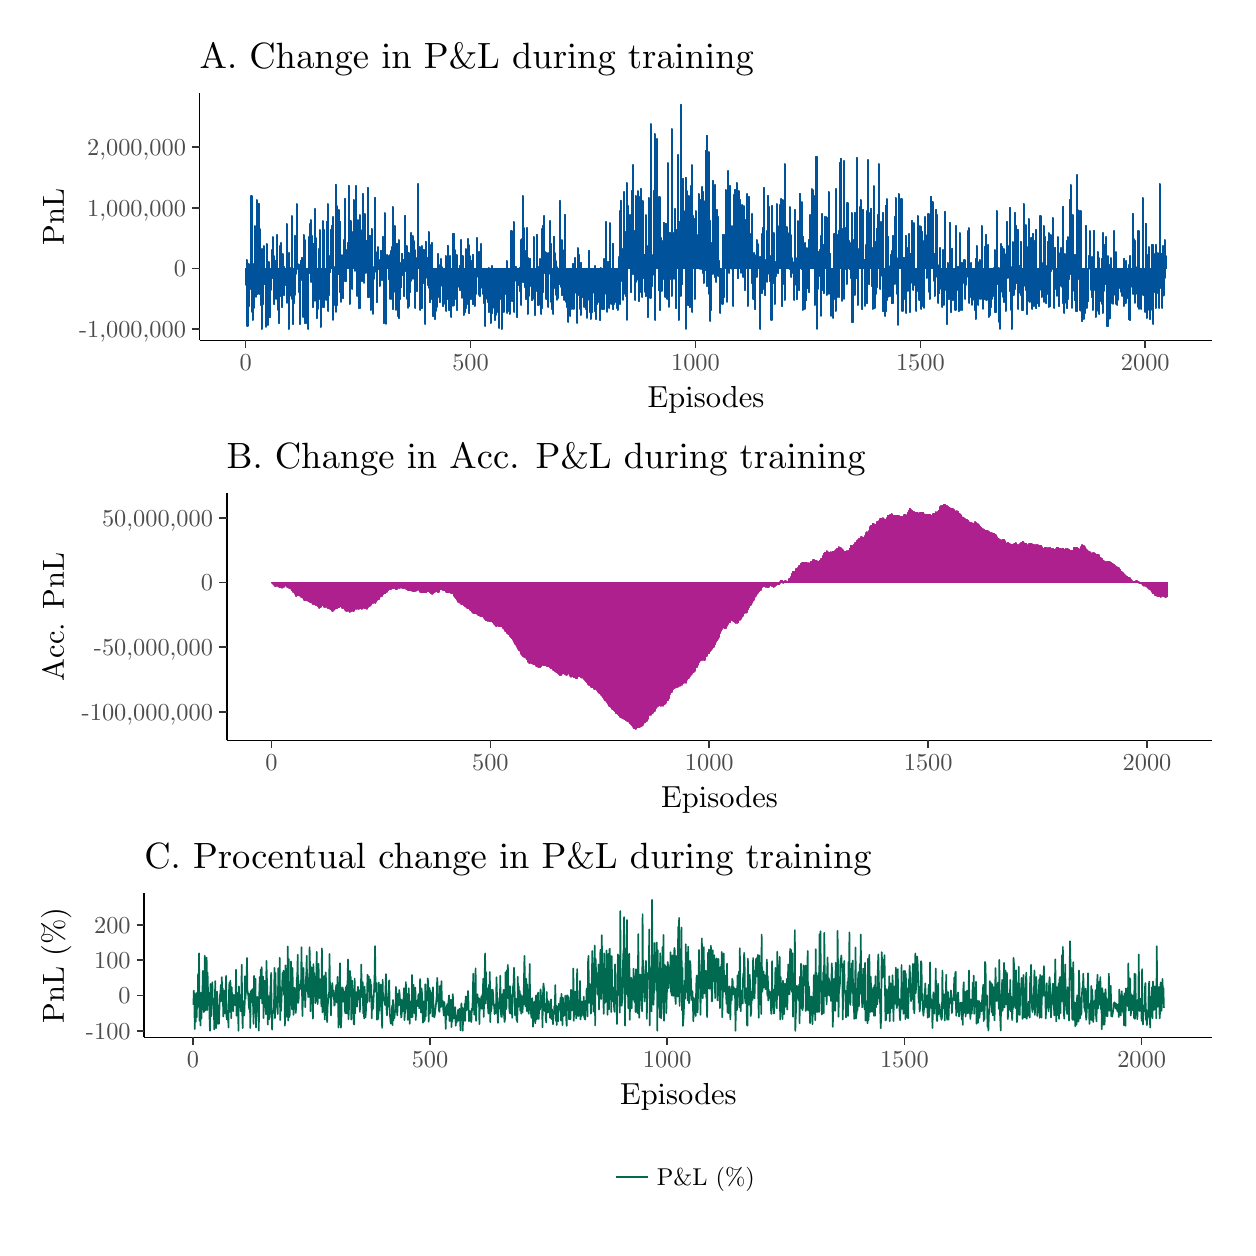
\begin{tikzpicture}[x=1pt,y=1pt]
\definecolor{fillColor}{RGB}{255,255,255}
\path[use as bounding box,fill=fillColor,fill opacity=0.00] (0,0) rectangle (433.62,433.62);
\begin{scope}
\path[clip] (  0.00,289.08) rectangle (433.62,433.62);
\definecolor{drawColor}{RGB}{255,255,255}
\definecolor{fillColor}{RGB}{255,255,255}

\path[draw=drawColor,line width= 0.6pt,line join=round,line cap=round,fill=fillColor] (  0.00,289.08) rectangle (433.62,433.62);
\end{scope}
\begin{scope}
\path[clip] ( 62.14,320.61) rectangle (428.12,409.93);
\definecolor{fillColor}{RGB}{255,255,255}

\path[fill=fillColor] ( 62.14,320.61) rectangle (428.12,409.93);
\definecolor{drawColor}{RGB}{0,83,155}
\definecolor{fillColor}{RGB}{89,89,89}

\path[draw=drawColor,line width= 0.6pt,line join=round,fill=fillColor,fill opacity=0.55] ( 78.86,340.72) rectangle ( 79.01,346.60);

\path[draw=drawColor,line width= 0.6pt,line join=round,fill=fillColor,fill opacity=0.55] ( 79.03,346.60) rectangle ( 79.17,349.58);

\path[draw=drawColor,line width= 0.6pt,line join=round,fill=fillColor,fill opacity=0.55] ( 79.19,342.74) rectangle ( 79.34,346.60);

\path[draw=drawColor,line width= 0.6pt,line join=round,fill=fillColor,fill opacity=0.55] ( 79.35,325.78) rectangle ( 79.50,346.60);

\path[draw=drawColor,line width= 0.6pt,line join=round,fill=fillColor,fill opacity=0.55] ( 79.51,346.60) rectangle ( 79.66,347.03);

\path[draw=drawColor,line width= 0.6pt,line join=round,fill=fillColor,fill opacity=0.55] ( 79.68,330.25) rectangle ( 79.82,346.60);

\path[draw=drawColor,line width= 0.6pt,line join=round,fill=fillColor,fill opacity=0.55] ( 79.84,346.60) rectangle ( 79.99,348.13);

\path[draw=drawColor,line width= 0.6pt,line join=round,fill=fillColor,fill opacity=0.55] ( 80.00,333.10) rectangle ( 80.15,346.60);

\path[draw=drawColor,line width= 0.6pt,line join=round,fill=fillColor,fill opacity=0.55] ( 80.16,343.12) rectangle ( 80.31,346.60);

\path[draw=drawColor,line width= 0.6pt,line join=round,fill=fillColor,fill opacity=0.55] ( 80.33,339.30) rectangle ( 80.47,346.60);

\path[draw=drawColor,line width= 0.6pt,line join=round,fill=fillColor,fill opacity=0.55] ( 80.49,346.60) rectangle ( 80.64,359.91);

\path[draw=drawColor,line width= 0.6pt,line join=round,fill=fillColor,fill opacity=0.55] ( 80.65,346.60) rectangle ( 80.80,346.97);

\path[draw=drawColor,line width= 0.6pt,line join=round,fill=fillColor,fill opacity=0.55] ( 80.81,346.60) rectangle ( 80.96,372.73);

\path[draw=drawColor,line width= 0.6pt,line join=round,fill=fillColor,fill opacity=0.55] ( 80.98,330.97) rectangle ( 81.12,346.60);

\path[draw=drawColor,line width= 0.6pt,line join=round,fill=fillColor,fill opacity=0.55] ( 81.14,341.40) rectangle ( 81.29,346.60);

\path[draw=drawColor,line width= 0.6pt,line join=round,fill=fillColor,fill opacity=0.55] ( 81.30,327.92) rectangle ( 81.45,346.60);

\path[draw=drawColor,line width= 0.6pt,line join=round,fill=fillColor,fill opacity=0.55] ( 81.46,346.60) rectangle ( 81.61,348.29);

\path[draw=drawColor,line width= 0.6pt,line join=round,fill=fillColor,fill opacity=0.55] ( 81.63,332.24) rectangle ( 81.77,346.60);

\path[draw=drawColor,line width= 0.6pt,line join=round,fill=fillColor,fill opacity=0.55] ( 81.79,345.95) rectangle ( 81.94,346.60);

\path[draw=drawColor,line width= 0.6pt,line join=round,fill=fillColor,fill opacity=0.55] ( 81.95,346.43) rectangle ( 82.10,346.60);

\path[draw=drawColor,line width= 0.6pt,line join=round,fill=fillColor,fill opacity=0.55] ( 82.11,346.60) rectangle ( 82.26,361.90);

\path[draw=drawColor,line width= 0.6pt,line join=round,fill=fillColor,fill opacity=0.55] ( 82.28,339.25) rectangle ( 82.42,346.60);

\path[draw=drawColor,line width= 0.6pt,line join=round,fill=fillColor,fill opacity=0.55] ( 82.44,336.29) rectangle ( 82.59,346.60);

\path[draw=drawColor,line width= 0.6pt,line join=round,fill=fillColor,fill opacity=0.55] ( 82.60,337.28) rectangle ( 82.75,346.60);

\path[draw=drawColor,line width= 0.6pt,line join=round,fill=fillColor,fill opacity=0.55] ( 82.76,346.60) rectangle ( 82.91,371.26);

\path[draw=drawColor,line width= 0.6pt,line join=round,fill=fillColor,fill opacity=0.55] ( 82.93,337.26) rectangle ( 83.07,346.60);

\path[draw=drawColor,line width= 0.6pt,line join=round,fill=fillColor,fill opacity=0.55] ( 83.09,346.60) rectangle ( 83.24,356.29);

\path[draw=drawColor,line width= 0.6pt,line join=round,fill=fillColor,fill opacity=0.55] ( 83.25,339.78) rectangle ( 83.40,346.60);

\path[draw=drawColor,line width= 0.6pt,line join=round,fill=fillColor,fill opacity=0.55] ( 83.41,346.60) rectangle ( 83.56,370.04);

\path[draw=drawColor,line width= 0.6pt,line join=round,fill=fillColor,fill opacity=0.55] ( 83.58,337.47) rectangle ( 83.72,346.60);

\path[draw=drawColor,line width= 0.6pt,line join=round,fill=fillColor,fill opacity=0.55] ( 83.74,346.60) rectangle ( 83.89,360.86);

\path[draw=drawColor,line width= 0.6pt,line join=round,fill=fillColor,fill opacity=0.55] ( 83.90,346.60) rectangle ( 84.05,348.20);

\path[draw=drawColor,line width= 0.6pt,line join=round,fill=fillColor,fill opacity=0.55] ( 84.06,346.60) rectangle ( 84.21,348.48);

\path[draw=drawColor,line width= 0.6pt,line join=round,fill=fillColor,fill opacity=0.55] ( 84.23,345.23) rectangle ( 84.37,346.60);

\path[draw=drawColor,line width= 0.6pt,line join=round,fill=fillColor,fill opacity=0.55] ( 84.39,333.26) rectangle ( 84.54,346.60);

\path[draw=drawColor,line width= 0.6pt,line join=round,fill=fillColor,fill opacity=0.55] ( 84.55,324.69) rectangle ( 84.70,346.60);

\path[draw=drawColor,line width= 0.6pt,line join=round,fill=fillColor,fill opacity=0.55] ( 84.72,346.60) rectangle ( 84.86,353.71);

\path[draw=drawColor,line width= 0.6pt,line join=round,fill=fillColor,fill opacity=0.55] ( 84.88,343.80) rectangle ( 85.02,346.60);

\path[draw=drawColor,line width= 0.6pt,line join=round,fill=fillColor,fill opacity=0.55] ( 85.04,333.84) rectangle ( 85.19,346.60);

\path[draw=drawColor,line width= 0.6pt,line join=round,fill=fillColor,fill opacity=0.55] ( 85.20,340.85) rectangle ( 85.35,346.60);

\path[draw=drawColor,line width= 0.6pt,line join=round,fill=fillColor,fill opacity=0.55] ( 85.37,346.60) rectangle ( 85.51,354.80);

\path[draw=drawColor,line width= 0.6pt,line join=round,fill=fillColor,fill opacity=0.55] ( 85.53,340.93) rectangle ( 85.67,346.60);

\path[draw=drawColor,line width= 0.6pt,line join=round,fill=fillColor,fill opacity=0.55] ( 85.69,343.02) rectangle ( 85.84,346.60);

\path[draw=drawColor,line width= 0.6pt,line join=round,fill=fillColor,fill opacity=0.55] ( 85.85,344.37) rectangle ( 86.00,346.60);

\path[draw=drawColor,line width= 0.6pt,line join=round,fill=fillColor,fill opacity=0.55] ( 86.02,325.44) rectangle ( 86.16,346.60);

\path[draw=drawColor,line width= 0.6pt,line join=round,fill=fillColor,fill opacity=0.55] ( 86.18,329.25) rectangle ( 86.32,346.60);

\path[draw=drawColor,line width= 0.6pt,line join=round,fill=fillColor,fill opacity=0.55] ( 86.34,346.60) rectangle ( 86.49,355.51);

\path[draw=drawColor,line width= 0.6pt,line join=round,fill=fillColor,fill opacity=0.55] ( 86.50,335.31) rectangle ( 86.65,346.60);

\path[draw=drawColor,line width= 0.6pt,line join=round,fill=fillColor,fill opacity=0.55] ( 86.67,326.29) rectangle ( 86.81,346.60);

\path[draw=drawColor,line width= 0.6pt,line join=round,fill=fillColor,fill opacity=0.55] ( 86.83,338.16) rectangle ( 86.97,346.60);

\path[draw=drawColor,line width= 0.6pt,line join=round,fill=fillColor,fill opacity=0.55] ( 86.99,346.60) rectangle ( 87.14,348.98);

\path[draw=drawColor,line width= 0.6pt,line join=round,fill=fillColor,fill opacity=0.55] ( 87.15,338.77) rectangle ( 87.30,346.60);

\path[draw=drawColor,line width= 0.6pt,line join=round,fill=fillColor,fill opacity=0.55] ( 87.32,328.98) rectangle ( 87.46,346.60);

\path[draw=drawColor,line width= 0.6pt,line join=round,fill=fillColor,fill opacity=0.55] ( 87.48,335.26) rectangle ( 87.62,346.60);

\path[draw=drawColor,line width= 0.6pt,line join=round,fill=fillColor,fill opacity=0.55] ( 87.64,329.08) rectangle ( 87.79,346.60);

\path[draw=drawColor,line width= 0.6pt,line join=round,fill=fillColor,fill opacity=0.55] ( 87.80,338.73) rectangle ( 87.95,346.60);

\path[draw=drawColor,line width= 0.6pt,line join=round,fill=fillColor,fill opacity=0.55] ( 87.97,346.53) rectangle ( 88.11,346.60);

\path[draw=drawColor,line width= 0.6pt,line join=round,fill=fillColor,fill opacity=0.55] ( 88.13,346.60) rectangle ( 88.27,348.17);

\path[draw=drawColor,line width= 0.6pt,line join=round,fill=fillColor,fill opacity=0.55] ( 88.29,346.60) rectangle ( 88.44,353.20);

\path[draw=drawColor,line width= 0.6pt,line join=round,fill=fillColor,fill opacity=0.55] ( 88.45,342.99) rectangle ( 88.60,346.60);

\path[draw=drawColor,line width= 0.6pt,line join=round,fill=fillColor,fill opacity=0.55] ( 88.62,346.60) rectangle ( 88.76,357.95);

\path[draw=drawColor,line width= 0.6pt,line join=round,fill=fillColor,fill opacity=0.55] ( 88.78,346.29) rectangle ( 88.92,346.60);

\path[draw=drawColor,line width= 0.6pt,line join=round,fill=fillColor,fill opacity=0.55] ( 88.94,346.60) rectangle ( 89.09,351.08);

\path[draw=drawColor,line width= 0.6pt,line join=round,fill=fillColor,fill opacity=0.55] ( 89.10,333.58) rectangle ( 89.25,346.60);

\path[draw=drawColor,line width= 0.6pt,line join=round,fill=fillColor,fill opacity=0.55] ( 89.27,337.25) rectangle ( 89.41,346.60);

\path[draw=drawColor,line width= 0.6pt,line join=round,fill=fillColor,fill opacity=0.55] ( 89.43,346.60) rectangle ( 89.57,349.53);

\path[draw=drawColor,line width= 0.6pt,line join=round,fill=fillColor,fill opacity=0.55] ( 89.59,336.12) rectangle ( 89.74,346.60);

\path[draw=drawColor,line width= 0.6pt,line join=round,fill=fillColor,fill opacity=0.55] ( 89.75,335.51) rectangle ( 89.90,346.60);

\path[draw=drawColor,line width= 0.6pt,line join=round,fill=fillColor,fill opacity=0.55] ( 89.92,346.60) rectangle ( 90.06,350.57);

\path[draw=drawColor,line width= 0.6pt,line join=round,fill=fillColor,fill opacity=0.55] ( 90.08,346.60) rectangle ( 90.23,358.76);

\path[draw=drawColor,line width= 0.6pt,line join=round,fill=fillColor,fill opacity=0.55] ( 90.24,333.19) rectangle ( 90.39,346.60);

\path[draw=drawColor,line width= 0.6pt,line join=round,fill=fillColor,fill opacity=0.55] ( 90.40,331.64) rectangle ( 90.55,346.60);

\path[draw=drawColor,line width= 0.6pt,line join=round,fill=fillColor,fill opacity=0.55] ( 90.57,335.45) rectangle ( 90.71,346.60);

\path[draw=drawColor,line width= 0.6pt,line join=round,fill=fillColor,fill opacity=0.55] ( 90.73,337.07) rectangle ( 90.88,346.60);

\path[draw=drawColor,line width= 0.6pt,line join=round,fill=fillColor,fill opacity=0.55] ( 90.89,326.77) rectangle ( 91.04,346.60);

\path[draw=drawColor,line width= 0.6pt,line join=round,fill=fillColor,fill opacity=0.55] ( 91.05,346.60) rectangle ( 91.20,348.66);

\path[draw=drawColor,line width= 0.6pt,line join=round,fill=fillColor,fill opacity=0.55] ( 91.22,346.60) rectangle ( 91.36,354.65);

\path[draw=drawColor,line width= 0.6pt,line join=round,fill=fillColor,fill opacity=0.55] ( 91.38,336.43) rectangle ( 91.53,346.60);

\path[draw=drawColor,line width= 0.6pt,line join=round,fill=fillColor,fill opacity=0.55] ( 91.54,346.60) rectangle ( 91.69,355.85);

\path[draw=drawColor,line width= 0.6pt,line join=round,fill=fillColor,fill opacity=0.55] ( 91.70,343.55) rectangle ( 91.85,346.60);

\path[draw=drawColor,line width= 0.6pt,line join=round,fill=fillColor,fill opacity=0.55] ( 91.87,332.46) rectangle ( 92.01,346.60);

\path[draw=drawColor,line width= 0.6pt,line join=round,fill=fillColor,fill opacity=0.55] ( 92.03,346.60) rectangle ( 92.18,351.74);

\path[draw=drawColor,line width= 0.6pt,line join=round,fill=fillColor,fill opacity=0.55] ( 92.19,340.87) rectangle ( 92.34,346.60);

\path[draw=drawColor,line width= 0.6pt,line join=round,fill=fillColor,fill opacity=0.55] ( 92.35,342.79) rectangle ( 92.50,346.60);

\path[draw=drawColor,line width= 0.6pt,line join=round,fill=fillColor,fill opacity=0.55] ( 92.52,336.82) rectangle ( 92.66,346.60);

\path[draw=drawColor,line width= 0.6pt,line join=round,fill=fillColor,fill opacity=0.55] ( 92.68,346.60) rectangle ( 92.83,347.03);

\path[draw=drawColor,line width= 0.6pt,line join=round,fill=fillColor,fill opacity=0.55] ( 92.84,341.13) rectangle ( 92.99,346.60);

\path[draw=drawColor,line width= 0.6pt,line join=round,fill=fillColor,fill opacity=0.55] ( 93.00,342.51) rectangle ( 93.15,346.60);

\path[draw=drawColor,line width= 0.6pt,line join=round,fill=fillColor,fill opacity=0.55] ( 93.17,340.46) rectangle ( 93.31,346.60);

\path[draw=drawColor,line width= 0.6pt,line join=round,fill=fillColor,fill opacity=0.55] ( 93.33,343.39) rectangle ( 93.48,346.60);

\path[draw=drawColor,line width= 0.6pt,line join=round,fill=fillColor,fill opacity=0.55] ( 93.49,346.60) rectangle ( 93.64,362.59);

\path[draw=drawColor,line width= 0.6pt,line join=round,fill=fillColor,fill opacity=0.55] ( 93.65,334.01) rectangle ( 93.80,346.60);

\path[draw=drawColor,line width= 0.6pt,line join=round,fill=fillColor,fill opacity=0.55] ( 93.82,337.15) rectangle ( 93.96,346.60);

\path[draw=drawColor,line width= 0.6pt,line join=round,fill=fillColor,fill opacity=0.55] ( 93.98,340.03) rectangle ( 94.13,346.60);

\path[draw=drawColor,line width= 0.6pt,line join=round,fill=fillColor,fill opacity=0.55] ( 94.14,346.60) rectangle ( 94.29,348.24);

\path[draw=drawColor,line width= 0.6pt,line join=round,fill=fillColor,fill opacity=0.55] ( 94.30,324.71) rectangle ( 94.45,346.60);

\path[draw=drawColor,line width= 0.6pt,line join=round,fill=fillColor,fill opacity=0.55] ( 94.47,346.60) rectangle ( 94.61,352.24);

\path[draw=drawColor,line width= 0.6pt,line join=round,fill=fillColor,fill opacity=0.55] ( 94.63,342.88) rectangle ( 94.78,346.60);

\path[draw=drawColor,line width= 0.6pt,line join=round,fill=fillColor,fill opacity=0.55] ( 94.79,346.60) rectangle ( 94.94,346.74);

\path[draw=drawColor,line width= 0.6pt,line join=round,fill=fillColor,fill opacity=0.55] ( 94.95,346.60) rectangle ( 95.10,346.61);

\path[draw=drawColor,line width= 0.6pt,line join=round,fill=fillColor,fill opacity=0.55] ( 95.12,336.73) rectangle ( 95.26,346.60);

\path[draw=drawColor,line width= 0.6pt,line join=round,fill=fillColor,fill opacity=0.55] ( 95.28,344.66) rectangle ( 95.43,346.60);

\path[draw=drawColor,line width= 0.6pt,line join=round,fill=fillColor,fill opacity=0.55] ( 95.44,346.60) rectangle ( 95.59,365.64);

\path[draw=drawColor,line width= 0.6pt,line join=round,fill=fillColor,fill opacity=0.55] ( 95.61,335.65) rectangle ( 95.75,346.60);

\path[draw=drawColor,line width= 0.6pt,line join=round,fill=fillColor,fill opacity=0.55] ( 95.77,326.34) rectangle ( 95.91,346.60);

\path[draw=drawColor,line width= 0.6pt,line join=round,fill=fillColor,fill opacity=0.55] ( 95.93,343.08) rectangle ( 96.08,346.60);

\path[draw=drawColor,line width= 0.6pt,line join=round,fill=fillColor,fill opacity=0.55] ( 96.09,334.73) rectangle ( 96.24,346.60);

\path[draw=drawColor,line width= 0.6pt,line join=round,fill=fillColor,fill opacity=0.55] ( 96.26,334.16) rectangle ( 96.40,346.60);

\path[draw=drawColor,line width= 0.6pt,line join=round,fill=fillColor,fill opacity=0.55] ( 96.42,337.09) rectangle ( 96.56,346.60);

\path[draw=drawColor,line width= 0.6pt,line join=round,fill=fillColor,fill opacity=0.55] ( 96.58,346.60) rectangle ( 96.73,358.50);

\path[draw=drawColor,line width= 0.6pt,line join=round,fill=fillColor,fill opacity=0.55] ( 96.74,344.53) rectangle ( 96.89,346.60);

\path[draw=drawColor,line width= 0.6pt,line join=round,fill=fillColor,fill opacity=0.55] ( 96.91,346.60) rectangle ( 97.05,353.65);

\path[draw=drawColor,line width= 0.6pt,line join=round,fill=fillColor,fill opacity=0.55] ( 97.07,346.60) rectangle ( 97.21,352.92);

\path[draw=drawColor,line width= 0.6pt,line join=round,fill=fillColor,fill opacity=0.55] ( 97.23,346.60) rectangle ( 97.38,369.80);

\path[draw=drawColor,line width= 0.6pt,line join=round,fill=fillColor,fill opacity=0.55] ( 97.39,346.60) rectangle ( 97.54,349.53);

\path[draw=drawColor,line width= 0.6pt,line join=round,fill=fillColor,fill opacity=0.55] ( 97.56,346.60) rectangle ( 97.70,348.28);

\path[draw=drawColor,line width= 0.6pt,line join=round,fill=fillColor,fill opacity=0.55] ( 97.72,346.17) rectangle ( 97.86,346.60);

\path[draw=drawColor,line width= 0.6pt,line join=round,fill=fillColor,fill opacity=0.55] ( 97.88,339.50) rectangle ( 98.03,346.60);

\path[draw=drawColor,line width= 0.6pt,line join=round,fill=fillColor,fill opacity=0.55] ( 98.04,337.95) rectangle ( 98.19,346.60);

\path[draw=drawColor,line width= 0.6pt,line join=round,fill=fillColor,fill opacity=0.55] ( 98.21,346.60) rectangle ( 98.35,347.75);

\path[draw=drawColor,line width= 0.6pt,line join=round,fill=fillColor,fill opacity=0.55] ( 98.37,326.40) rectangle ( 98.51,346.60);

\path[draw=drawColor,line width= 0.6pt,line join=round,fill=fillColor,fill opacity=0.55] ( 98.53,346.60) rectangle ( 98.68,349.36);

\path[draw=drawColor,line width= 0.6pt,line join=round,fill=fillColor,fill opacity=0.55] ( 98.69,346.60) rectangle ( 98.84,349.23);

\path[draw=drawColor,line width= 0.6pt,line join=round,fill=fillColor,fill opacity=0.55] ( 98.86,342.47) rectangle ( 99.00,346.60);

\path[draw=drawColor,line width= 0.6pt,line join=round,fill=fillColor,fill opacity=0.55] ( 99.02,346.60) rectangle ( 99.16,350.43);

\path[draw=drawColor,line width= 0.6pt,line join=round,fill=fillColor,fill opacity=0.55] ( 99.18,346.60) rectangle ( 99.33,350.49);

\path[draw=drawColor,line width= 0.6pt,line join=round,fill=fillColor,fill opacity=0.55] ( 99.34,338.41) rectangle ( 99.49,346.60);

\path[draw=drawColor,line width= 0.6pt,line join=round,fill=fillColor,fill opacity=0.55] ( 99.51,329.03) rectangle ( 99.65,346.60);

\path[draw=drawColor,line width= 0.6pt,line join=round,fill=fillColor,fill opacity=0.55] ( 99.67,346.60) rectangle ( 99.81,358.78);

\path[draw=drawColor,line width= 0.6pt,line join=round,fill=fillColor,fill opacity=0.55] ( 99.83,335.81) rectangle ( 99.98,346.60);

\path[draw=drawColor,line width= 0.6pt,line join=round,fill=fillColor,fill opacity=0.55] ( 99.99,343.32) rectangle (100.14,346.60);

\path[draw=drawColor,line width= 0.6pt,line join=round,fill=fillColor,fill opacity=0.55] (100.16,346.60) rectangle (100.30,356.98);

\path[draw=drawColor,line width= 0.6pt,line join=round,fill=fillColor,fill opacity=0.55] (100.32,326.73) rectangle (100.46,346.60);

\path[draw=drawColor,line width= 0.6pt,line join=round,fill=fillColor,fill opacity=0.55] (100.48,337.02) rectangle (100.63,346.60);

\path[draw=drawColor,line width= 0.6pt,line join=round,fill=fillColor,fill opacity=0.55] (100.64,345.11) rectangle (100.79,346.60);

\path[draw=drawColor,line width= 0.6pt,line join=round,fill=fillColor,fill opacity=0.55] (100.81,345.69) rectangle (100.95,346.60);

\path[draw=drawColor,line width= 0.6pt,line join=round,fill=fillColor,fill opacity=0.55] (100.97,344.60) rectangle (101.11,346.60);

\path[draw=drawColor,line width= 0.6pt,line join=round,fill=fillColor,fill opacity=0.55] (101.13,342.32) rectangle (101.28,346.60);

\path[draw=drawColor,line width= 0.6pt,line join=round,fill=fillColor,fill opacity=0.55] (101.29,324.76) rectangle (101.44,346.60);

\path[draw=drawColor,line width= 0.6pt,line join=round,fill=fillColor,fill opacity=0.55] (101.46,346.60) rectangle (101.60,348.71);

\path[draw=drawColor,line width= 0.6pt,line join=round,fill=fillColor,fill opacity=0.55] (101.62,346.60) rectangle (101.77,358.09);

\path[draw=drawColor,line width= 0.6pt,line join=round,fill=fillColor,fill opacity=0.55] (101.78,344.76) rectangle (101.93,346.60);

\path[draw=drawColor,line width= 0.6pt,line join=round,fill=fillColor,fill opacity=0.55] (101.94,346.60) rectangle (102.09,362.76);

\path[draw=drawColor,line width= 0.6pt,line join=round,fill=fillColor,fill opacity=0.55] (102.11,346.60) rectangle (102.25,348.63);

\path[draw=drawColor,line width= 0.6pt,line join=round,fill=fillColor,fill opacity=0.55] (102.27,346.60) rectangle (102.42,364.14);

\path[draw=drawColor,line width= 0.6pt,line join=round,fill=fillColor,fill opacity=0.55] (102.43,341.74) rectangle (102.58,346.60);

\path[draw=drawColor,line width= 0.6pt,line join=round,fill=fillColor,fill opacity=0.55] (102.59,346.60) rectangle (102.74,349.93);

\path[draw=drawColor,line width= 0.6pt,line join=round,fill=fillColor,fill opacity=0.55] (102.76,346.60) rectangle (102.90,358.32);

\path[draw=drawColor,line width= 0.6pt,line join=round,fill=fillColor,fill opacity=0.55] (102.92,332.50) rectangle (103.07,346.60);

\path[draw=drawColor,line width= 0.6pt,line join=round,fill=fillColor,fill opacity=0.55] (103.08,346.60) rectangle (103.23,352.17);

\path[draw=drawColor,line width= 0.6pt,line join=round,fill=fillColor,fill opacity=0.55] (103.24,346.60) rectangle (103.39,355.68);

\path[draw=drawColor,line width= 0.6pt,line join=round,fill=fillColor,fill opacity=0.55] (103.41,346.60) rectangle (103.55,352.47);

\path[draw=drawColor,line width= 0.6pt,line join=round,fill=fillColor,fill opacity=0.55] (103.57,346.60) rectangle (103.72,351.44);

\path[draw=drawColor,line width= 0.6pt,line join=round,fill=fillColor,fill opacity=0.55] (103.73,334.94) rectangle (103.88,346.60);

\path[draw=drawColor,line width= 0.6pt,line join=round,fill=fillColor,fill opacity=0.55] (103.89,346.60) rectangle (104.04,368.02);

\path[draw=drawColor,line width= 0.6pt,line join=round,fill=fillColor,fill opacity=0.55] (104.06,346.60) rectangle (104.20,357.68);

\path[draw=drawColor,line width= 0.6pt,line join=round,fill=fillColor,fill opacity=0.55] (104.22,346.60) rectangle (104.37,350.06);

\path[draw=drawColor,line width= 0.6pt,line join=round,fill=fillColor,fill opacity=0.55] (104.38,328.55) rectangle (104.53,346.60);

\path[draw=drawColor,line width= 0.6pt,line join=round,fill=fillColor,fill opacity=0.55] (104.54,346.27) rectangle (104.69,346.60);

\path[draw=drawColor,line width= 0.6pt,line join=round,fill=fillColor,fill opacity=0.55] (104.71,343.22) rectangle (104.85,346.60);

\path[draw=drawColor,line width= 0.6pt,line join=round,fill=fillColor,fill opacity=0.55] (104.87,331.85) rectangle (105.02,346.60);

\path[draw=drawColor,line width= 0.6pt,line join=round,fill=fillColor,fill opacity=0.55] (105.03,335.43) rectangle (105.18,346.60);

\path[draw=drawColor,line width= 0.6pt,line join=round,fill=fillColor,fill opacity=0.55] (105.19,346.60) rectangle (105.34,347.09);

\path[draw=drawColor,line width= 0.6pt,line join=round,fill=fillColor,fill opacity=0.55] (105.36,346.60) rectangle (105.50,353.63);

\path[draw=drawColor,line width= 0.6pt,line join=round,fill=fillColor,fill opacity=0.55] (105.52,346.60) rectangle (105.67,360.60);

\path[draw=drawColor,line width= 0.6pt,line join=round,fill=fillColor,fill opacity=0.55] (105.68,338.73) rectangle (105.83,346.60);

\path[draw=drawColor,line width= 0.6pt,line join=round,fill=fillColor,fill opacity=0.55] (105.84,325.38) rectangle (105.99,346.60);

\path[draw=drawColor,line width= 0.6pt,line join=round,fill=fillColor,fill opacity=0.55] (106.01,335.03) rectangle (106.15,346.60);

\path[draw=drawColor,line width= 0.6pt,line join=round,fill=fillColor,fill opacity=0.55] (106.17,335.67) rectangle (106.32,346.60);

\path[draw=drawColor,line width= 0.6pt,line join=round,fill=fillColor,fill opacity=0.55] (106.33,336.44) rectangle (106.48,346.60);

\path[draw=drawColor,line width= 0.6pt,line join=round,fill=fillColor,fill opacity=0.55] (106.49,340.43) rectangle (106.64,346.60);

\path[draw=drawColor,line width= 0.6pt,line join=round,fill=fillColor,fill opacity=0.55] (106.66,346.60) rectangle (106.80,363.74);

\path[draw=drawColor,line width= 0.6pt,line join=round,fill=fillColor,fill opacity=0.55] (106.82,332.54) rectangle (106.97,346.60);

\path[draw=drawColor,line width= 0.6pt,line join=round,fill=fillColor,fill opacity=0.55] (106.98,346.60) rectangle (107.13,360.65);

\path[draw=drawColor,line width= 0.6pt,line join=round,fill=fillColor,fill opacity=0.55] (107.15,346.30) rectangle (107.29,346.60);

\path[draw=drawColor,line width= 0.6pt,line join=round,fill=fillColor,fill opacity=0.55] (107.31,340.48) rectangle (107.45,346.60);

\path[draw=drawColor,line width= 0.6pt,line join=round,fill=fillColor,fill opacity=0.55] (107.47,339.99) rectangle (107.62,346.60);

\path[draw=drawColor,line width= 0.6pt,line join=round,fill=fillColor,fill opacity=0.55] (107.63,337.98) rectangle (107.78,346.60);

\path[draw=drawColor,line width= 0.6pt,line join=round,fill=fillColor,fill opacity=0.55] (107.80,335.12) rectangle (107.94,346.60);

\path[draw=drawColor,line width= 0.6pt,line join=round,fill=fillColor,fill opacity=0.55] (107.96,346.60) rectangle (108.10,363.52);

\path[draw=drawColor,line width= 0.6pt,line join=round,fill=fillColor,fill opacity=0.55] (108.12,346.60) rectangle (108.27,347.97);

\path[draw=drawColor,line width= 0.6pt,line join=round,fill=fillColor,fill opacity=0.55] (108.28,342.31) rectangle (108.43,346.60);

\path[draw=drawColor,line width= 0.6pt,line join=round,fill=fillColor,fill opacity=0.55] (108.45,346.60) rectangle (108.59,369.92);

\path[draw=drawColor,line width= 0.6pt,line join=round,fill=fillColor,fill opacity=0.55] (108.61,331.34) rectangle (108.75,346.60);

\path[draw=drawColor,line width= 0.6pt,line join=round,fill=fillColor,fill opacity=0.55] (108.77,346.60) rectangle (108.92,351.26);

\path[draw=drawColor,line width= 0.6pt,line join=round,fill=fillColor,fill opacity=0.55] (108.93,337.01) rectangle (109.08,346.60);

\path[draw=drawColor,line width= 0.6pt,line join=round,fill=fillColor,fill opacity=0.55] (109.10,345.11) rectangle (109.24,346.60);

\path[draw=drawColor,line width= 0.6pt,line join=round,fill=fillColor,fill opacity=0.55] (109.26,346.60) rectangle (109.40,350.92);

\path[draw=drawColor,line width= 0.6pt,line join=round,fill=fillColor,fill opacity=0.55] (109.42,346.60) rectangle (109.57,360.57);

\path[draw=drawColor,line width= 0.6pt,line join=round,fill=fillColor,fill opacity=0.55] (109.58,346.60) rectangle (109.73,356.88);

\path[draw=drawColor,line width= 0.6pt,line join=round,fill=fillColor,fill opacity=0.55] (109.75,346.60) rectangle (109.89,361.94);

\path[draw=drawColor,line width= 0.6pt,line join=round,fill=fillColor,fill opacity=0.55] (109.91,346.60) rectangle (110.05,347.01);

\path[draw=drawColor,line width= 0.6pt,line join=round,fill=fillColor,fill opacity=0.55] (110.07,346.60) rectangle (110.22,354.67);

\path[draw=drawColor,line width= 0.6pt,line join=round,fill=fillColor,fill opacity=0.55] (110.23,327.88) rectangle (110.38,346.60);

\path[draw=drawColor,line width= 0.6pt,line join=round,fill=fillColor,fill opacity=0.55] (110.40,346.60) rectangle (110.54,365.25);

\path[draw=drawColor,line width= 0.6pt,line join=round,fill=fillColor,fill opacity=0.55] (110.56,344.81) rectangle (110.70,346.60);

\path[draw=drawColor,line width= 0.6pt,line join=round,fill=fillColor,fill opacity=0.55] (110.72,337.84) rectangle (110.87,346.60);

\path[draw=drawColor,line width= 0.6pt,line join=round,fill=fillColor,fill opacity=0.55] (110.88,333.37) rectangle (111.03,346.60);

\path[draw=drawColor,line width= 0.6pt,line join=round,fill=fillColor,fill opacity=0.55] (111.05,346.60) rectangle (111.19,347.20);

\path[draw=drawColor,line width= 0.6pt,line join=round,fill=fillColor,fill opacity=0.55] (111.21,346.60) rectangle (111.35,376.92);

\path[draw=drawColor,line width= 0.6pt,line join=round,fill=fillColor,fill opacity=0.55] (111.37,330.99) rectangle (111.52,346.60);

\path[draw=drawColor,line width= 0.6pt,line join=round,fill=fillColor,fill opacity=0.55] (111.53,346.60) rectangle (111.68,369.25);

\path[draw=drawColor,line width= 0.6pt,line join=round,fill=fillColor,fill opacity=0.55] (111.70,333.18) rectangle (111.84,346.60);

\path[draw=drawColor,line width= 0.6pt,line join=round,fill=fillColor,fill opacity=0.55] (111.86,334.29) rectangle (112.00,346.60);

\path[draw=drawColor,line width= 0.6pt,line join=round,fill=fillColor,fill opacity=0.55] (112.02,345.59) rectangle (112.17,346.60);

\path[draw=drawColor,line width= 0.6pt,line join=round,fill=fillColor,fill opacity=0.55] (112.18,344.39) rectangle (112.33,346.60);

\path[draw=drawColor,line width= 0.6pt,line join=round,fill=fillColor,fill opacity=0.55] (112.35,346.60) rectangle (112.49,367.65);

\path[draw=drawColor,line width= 0.6pt,line join=round,fill=fillColor,fill opacity=0.55] (112.51,346.53) rectangle (112.65,346.60);

\path[draw=drawColor,line width= 0.6pt,line join=round,fill=fillColor,fill opacity=0.55] (112.67,338.09) rectangle (112.82,346.60);

\path[draw=drawColor,line width= 0.6pt,line join=round,fill=fillColor,fill opacity=0.55] (112.83,346.60) rectangle (112.98,363.62);

\path[draw=drawColor,line width= 0.6pt,line join=round,fill=fillColor,fill opacity=0.55] (113.00,346.60) rectangle (113.14,347.97);

\path[draw=drawColor,line width= 0.6pt,line join=round,fill=fillColor,fill opacity=0.55] (113.16,334.56) rectangle (113.31,346.60);

\path[draw=drawColor,line width= 0.6pt,line join=round,fill=fillColor,fill opacity=0.55] (113.32,342.35) rectangle (113.47,346.60);

\path[draw=drawColor,line width= 0.6pt,line join=round,fill=fillColor,fill opacity=0.55] (113.48,346.60) rectangle (113.63,351.52);

\path[draw=drawColor,line width= 0.6pt,line join=round,fill=fillColor,fill opacity=0.55] (113.65,346.60) rectangle (113.79,349.20);

\path[draw=drawColor,line width= 0.6pt,line join=round,fill=fillColor,fill opacity=0.55] (113.81,340.13) rectangle (113.96,346.60);

\path[draw=drawColor,line width= 0.6pt,line join=round,fill=fillColor,fill opacity=0.55] (113.97,335.75) rectangle (114.12,346.60);

\path[draw=drawColor,line width= 0.6pt,line join=round,fill=fillColor,fill opacity=0.55] (114.13,342.93) rectangle (114.28,346.60);

\path[draw=drawColor,line width= 0.6pt,line join=round,fill=fillColor,fill opacity=0.55] (114.30,346.60) rectangle (114.44,356.85);

\path[draw=drawColor,line width= 0.6pt,line join=round,fill=fillColor,fill opacity=0.55] (114.46,346.60) rectangle (114.61,358.64);

\path[draw=drawColor,line width= 0.6pt,line join=round,fill=fillColor,fill opacity=0.55] (114.62,346.60) rectangle (114.77,371.89);

\path[draw=drawColor,line width= 0.6pt,line join=round,fill=fillColor,fill opacity=0.55] (114.78,341.95) rectangle (114.93,346.60);

\path[draw=drawColor,line width= 0.6pt,line join=round,fill=fillColor,fill opacity=0.55] (114.95,344.40) rectangle (115.09,346.60);

\path[draw=drawColor,line width= 0.6pt,line join=round,fill=fillColor,fill opacity=0.55] (115.11,346.60) rectangle (115.26,353.33);

\path[draw=drawColor,line width= 0.6pt,line join=round,fill=fillColor,fill opacity=0.55] (115.27,346.60) rectangle (115.42,351.56);

\path[draw=drawColor,line width= 0.6pt,line join=round,fill=fillColor,fill opacity=0.55] (115.43,346.60) rectangle (115.58,350.52);

\path[draw=drawColor,line width= 0.6pt,line join=round,fill=fillColor,fill opacity=0.55] (115.60,346.60) rectangle (115.74,355.91);

\path[draw=drawColor,line width= 0.6pt,line join=round,fill=fillColor,fill opacity=0.55] (115.76,346.60) rectangle (115.91,353.57);

\path[draw=drawColor,line width= 0.6pt,line join=round,fill=fillColor,fill opacity=0.55] (115.92,346.60) rectangle (116.07,376.54);

\path[draw=drawColor,line width= 0.6pt,line join=round,fill=fillColor,fill opacity=0.55] (116.08,346.60) rectangle (116.23,349.26);

\path[draw=drawColor,line width= 0.6pt,line join=round,fill=fillColor,fill opacity=0.55] (116.25,333.86) rectangle (116.39,346.60);

\path[draw=drawColor,line width= 0.6pt,line join=round,fill=fillColor,fill opacity=0.55] (116.41,346.51) rectangle (116.56,346.60);

\path[draw=drawColor,line width= 0.6pt,line join=round,fill=fillColor,fill opacity=0.55] (116.57,346.60) rectangle (116.72,363.65);

\path[draw=drawColor,line width= 0.6pt,line join=round,fill=fillColor,fill opacity=0.55] (116.73,344.15) rectangle (116.88,346.60);

\path[draw=drawColor,line width= 0.6pt,line join=round,fill=fillColor,fill opacity=0.55] (116.90,343.85) rectangle (117.04,346.60);

\path[draw=drawColor,line width= 0.6pt,line join=round,fill=fillColor,fill opacity=0.55] (117.06,346.60) rectangle (117.21,349.01);

\path[draw=drawColor,line width= 0.6pt,line join=round,fill=fillColor,fill opacity=0.55] (117.22,339.24) rectangle (117.37,346.60);

\path[draw=drawColor,line width= 0.6pt,line join=round,fill=fillColor,fill opacity=0.55] (117.38,346.60) rectangle (117.53,356.06);

\path[draw=drawColor,line width= 0.6pt,line join=round,fill=fillColor,fill opacity=0.55] (117.55,346.60) rectangle (117.69,359.78);

\path[draw=drawColor,line width= 0.6pt,line join=round,fill=fillColor,fill opacity=0.55] (117.71,346.60) rectangle (117.86,371.25);

\path[draw=drawColor,line width= 0.6pt,line join=round,fill=fillColor,fill opacity=0.55] (117.87,346.60) rectangle (118.02,349.27);

\path[draw=drawColor,line width= 0.6pt,line join=round,fill=fillColor,fill opacity=0.55] (118.03,346.60) rectangle (118.18,357.47);

\path[draw=drawColor,line width= 0.6pt,line join=round,fill=fillColor,fill opacity=0.55] (118.20,345.61) rectangle (118.34,346.60);

\path[draw=drawColor,line width= 0.6pt,line join=round,fill=fillColor,fill opacity=0.55] (118.36,346.60) rectangle (118.51,346.91);

\path[draw=drawColor,line width= 0.6pt,line join=round,fill=fillColor,fill opacity=0.55] (118.52,345.81) rectangle (118.67,346.60);

\path[draw=drawColor,line width= 0.6pt,line join=round,fill=fillColor,fill opacity=0.55] (118.69,346.60) rectangle (118.83,376.49);

\path[draw=drawColor,line width= 0.6pt,line join=round,fill=fillColor,fill opacity=0.55] (118.85,346.60) rectangle (118.99,363.99);

\path[draw=drawColor,line width= 0.6pt,line join=round,fill=fillColor,fill opacity=0.55] (119.01,336.74) rectangle (119.16,346.60);

\path[draw=drawColor,line width= 0.6pt,line join=round,fill=fillColor,fill opacity=0.55] (119.17,346.60) rectangle (119.32,360.13);

\path[draw=drawColor,line width= 0.6pt,line join=round,fill=fillColor,fill opacity=0.55] (119.34,346.60) rectangle (119.48,364.10);

\path[draw=drawColor,line width= 0.6pt,line join=round,fill=fillColor,fill opacity=0.55] (119.50,346.60) rectangle (119.64,355.10);

\path[draw=drawColor,line width= 0.6pt,line join=round,fill=fillColor,fill opacity=0.55] (119.66,345.55) rectangle (119.81,346.60);

\path[draw=drawColor,line width= 0.6pt,line join=round,fill=fillColor,fill opacity=0.55] (119.82,332.18) rectangle (119.97,346.60);

\path[draw=drawColor,line width= 0.6pt,line join=round,fill=fillColor,fill opacity=0.55] (119.99,346.60) rectangle (120.13,365.98);

\path[draw=drawColor,line width= 0.6pt,line join=round,fill=fillColor,fill opacity=0.55] (120.15,346.60) rectangle (120.29,351.70);

\path[draw=drawColor,line width= 0.6pt,line join=round,fill=fillColor,fill opacity=0.55] (120.31,346.60) rectangle (120.46,360.52);

\path[draw=drawColor,line width= 0.6pt,line join=round,fill=fillColor,fill opacity=0.55] (120.47,346.60) rectangle (120.62,351.20);

\path[draw=drawColor,line width= 0.6pt,line join=round,fill=fillColor,fill opacity=0.55] (120.64,341.84) rectangle (120.78,346.60);

\path[draw=drawColor,line width= 0.6pt,line join=round,fill=fillColor,fill opacity=0.55] (120.80,343.67) rectangle (120.94,346.60);

\path[draw=drawColor,line width= 0.6pt,line join=round,fill=fillColor,fill opacity=0.55] (120.96,346.60) rectangle (121.11,351.04);

\path[draw=drawColor,line width= 0.6pt,line join=round,fill=fillColor,fill opacity=0.55] (121.12,346.60) rectangle (121.27,373.64);

\path[draw=drawColor,line width= 0.6pt,line join=round,fill=fillColor,fill opacity=0.55] (121.29,346.60) rectangle (121.43,351.59);

\path[draw=drawColor,line width= 0.6pt,line join=round,fill=fillColor,fill opacity=0.55] (121.45,341.26) rectangle (121.59,346.60);

\path[draw=drawColor,line width= 0.6pt,line join=round,fill=fillColor,fill opacity=0.55] (121.61,346.60) rectangle (121.76,354.27);

\path[draw=drawColor,line width= 0.6pt,line join=round,fill=fillColor,fill opacity=0.55] (121.77,346.60) rectangle (121.92,366.26);

\path[draw=drawColor,line width= 0.6pt,line join=round,fill=fillColor,fill opacity=0.55] (121.94,346.60) rectangle (122.08,347.84);

\path[draw=drawColor,line width= 0.6pt,line join=round,fill=fillColor,fill opacity=0.55] (122.10,344.95) rectangle (122.24,346.60);

\path[draw=drawColor,line width= 0.6pt,line join=round,fill=fillColor,fill opacity=0.55] (122.26,346.60) rectangle (122.41,356.74);

\path[draw=drawColor,line width= 0.6pt,line join=round,fill=fillColor,fill opacity=0.55] (122.42,346.60) rectangle (122.57,354.58);

\path[draw=drawColor,line width= 0.6pt,line join=round,fill=fillColor,fill opacity=0.55] (122.59,346.19) rectangle (122.73,346.60);

\path[draw=drawColor,line width= 0.6pt,line join=round,fill=fillColor,fill opacity=0.55] (122.75,339.85) rectangle (122.89,346.60);

\path[draw=drawColor,line width= 0.6pt,line join=round,fill=fillColor,fill opacity=0.55] (122.91,346.60) rectangle (123.06,375.81);

\path[draw=drawColor,line width= 0.6pt,line join=round,fill=fillColor,fill opacity=0.55] (123.07,336.06) rectangle (123.22,346.60);

\path[draw=drawColor,line width= 0.6pt,line join=round,fill=fillColor,fill opacity=0.55] (123.24,341.54) rectangle (123.38,346.60);

\path[draw=drawColor,line width= 0.6pt,line join=round,fill=fillColor,fill opacity=0.55] (123.40,346.60) rectangle (123.54,358.42);

\path[draw=drawColor,line width= 0.6pt,line join=round,fill=fillColor,fill opacity=0.55] (123.56,346.60) rectangle (123.71,358.54);

\path[draw=drawColor,line width= 0.6pt,line join=round,fill=fillColor,fill opacity=0.55] (123.72,339.68) rectangle (123.87,346.60);

\path[draw=drawColor,line width= 0.6pt,line join=round,fill=fillColor,fill opacity=0.55] (123.89,331.71) rectangle (124.03,346.60);

\path[draw=drawColor,line width= 0.6pt,line join=round,fill=fillColor,fill opacity=0.55] (124.05,346.60) rectangle (124.19,355.88);

\path[draw=drawColor,line width= 0.6pt,line join=round,fill=fillColor,fill opacity=0.55] (124.21,346.60) rectangle (124.36,360.92);

\path[draw=drawColor,line width= 0.6pt,line join=round,fill=fillColor,fill opacity=0.55] (124.37,346.60) rectangle (124.52,353.37);

\path[draw=drawColor,line width= 0.6pt,line join=round,fill=fillColor,fill opacity=0.55] (124.54,335.96) rectangle (124.68,346.60);

\path[draw=drawColor,line width= 0.6pt,line join=round,fill=fillColor,fill opacity=0.55] (124.70,330.10) rectangle (124.85,346.60);

\path[draw=drawColor,line width= 0.6pt,line join=round,fill=fillColor,fill opacity=0.55] (124.86,339.51) rectangle (125.01,346.60);

\path[draw=drawColor,line width= 0.6pt,line join=round,fill=fillColor,fill opacity=0.55] (125.02,342.71) rectangle (125.17,346.60);

\path[draw=drawColor,line width= 0.6pt,line join=round,fill=fillColor,fill opacity=0.55] (125.19,346.60) rectangle (125.33,347.16);

\path[draw=drawColor,line width= 0.6pt,line join=round,fill=fillColor,fill opacity=0.55] (125.35,345.32) rectangle (125.50,346.60);

\path[draw=drawColor,line width= 0.6pt,line join=round,fill=fillColor,fill opacity=0.55] (125.51,346.60) rectangle (125.66,372.27);

\path[draw=drawColor,line width= 0.6pt,line join=round,fill=fillColor,fill opacity=0.55] (125.67,346.60) rectangle (125.82,352.37);

\path[draw=drawColor,line width= 0.6pt,line join=round,fill=fillColor,fill opacity=0.55] (125.84,346.60) rectangle (125.98,352.58);

\path[draw=drawColor,line width= 0.6pt,line join=round,fill=fillColor,fill opacity=0.55] (126.00,334.25) rectangle (126.15,346.60);

\path[draw=drawColor,line width= 0.6pt,line join=round,fill=fillColor,fill opacity=0.55] (126.16,344.53) rectangle (126.31,346.60);

\path[draw=drawColor,line width= 0.6pt,line join=round,fill=fillColor,fill opacity=0.55] (126.32,346.34) rectangle (126.47,346.60);

\path[draw=drawColor,line width= 0.6pt,line join=round,fill=fillColor,fill opacity=0.55] (126.49,346.60) rectangle (126.63,354.29);

\path[draw=drawColor,line width= 0.6pt,line join=round,fill=fillColor,fill opacity=0.55] (126.65,346.60) rectangle (126.80,348.20);

\path[draw=drawColor,line width= 0.6pt,line join=round,fill=fillColor,fill opacity=0.55] (126.81,346.21) rectangle (126.96,346.60);

\path[draw=drawColor,line width= 0.6pt,line join=round,fill=fillColor,fill opacity=0.55] (126.97,346.60) rectangle (127.12,349.73);

\path[draw=drawColor,line width= 0.6pt,line join=round,fill=fillColor,fill opacity=0.55] (127.14,340.35) rectangle (127.28,346.60);

\path[draw=drawColor,line width= 0.6pt,line join=round,fill=fillColor,fill opacity=0.55] (127.30,340.79) rectangle (127.45,346.60);

\path[draw=drawColor,line width= 0.6pt,line join=round,fill=fillColor,fill opacity=0.55] (127.46,346.60) rectangle (127.61,348.10);

\path[draw=drawColor,line width= 0.6pt,line join=round,fill=fillColor,fill opacity=0.55] (127.62,343.82) rectangle (127.77,346.60);

\path[draw=drawColor,line width= 0.6pt,line join=round,fill=fillColor,fill opacity=0.55] (127.79,346.60) rectangle (127.93,353.06);

\path[draw=drawColor,line width= 0.6pt,line join=round,fill=fillColor,fill opacity=0.55] (127.95,342.23) rectangle (128.10,346.60);

\path[draw=drawColor,line width= 0.6pt,line join=round,fill=fillColor,fill opacity=0.55] (128.11,346.60) rectangle (128.26,348.01);

\path[draw=drawColor,line width= 0.6pt,line join=round,fill=fillColor,fill opacity=0.55] (128.27,346.60) rectangle (128.42,358.12);

\path[draw=drawColor,line width= 0.6pt,line join=round,fill=fillColor,fill opacity=0.55] (128.44,343.03) rectangle (128.58,346.60);

\path[draw=drawColor,line width= 0.6pt,line join=round,fill=fillColor,fill opacity=0.55] (128.60,326.74) rectangle (128.75,346.60);

\path[draw=drawColor,line width= 0.6pt,line join=round,fill=fillColor,fill opacity=0.55] (128.76,331.07) rectangle (128.91,346.60);

\path[draw=drawColor,line width= 0.6pt,line join=round,fill=fillColor,fill opacity=0.55] (128.92,346.60) rectangle (129.07,349.06);

\path[draw=drawColor,line width= 0.6pt,line join=round,fill=fillColor,fill opacity=0.55] (129.09,346.60) rectangle (129.23,366.60);

\path[draw=drawColor,line width= 0.6pt,line join=round,fill=fillColor,fill opacity=0.55] (129.25,339.17) rectangle (129.40,346.60);

\path[draw=drawColor,line width= 0.6pt,line join=round,fill=fillColor,fill opacity=0.55] (129.41,326.58) rectangle (129.56,346.60);

\path[draw=drawColor,line width= 0.6pt,line join=round,fill=fillColor,fill opacity=0.55] (129.57,331.53) rectangle (129.72,346.60);

\path[draw=drawColor,line width= 0.6pt,line join=round,fill=fillColor,fill opacity=0.55] (129.74,346.60) rectangle (129.88,347.61);

\path[draw=drawColor,line width= 0.6pt,line join=round,fill=fillColor,fill opacity=0.55] (129.90,346.60) rectangle (130.05,351.56);

\path[draw=drawColor,line width= 0.6pt,line join=round,fill=fillColor,fill opacity=0.55] (130.06,346.60) rectangle (130.21,351.24);

\path[draw=drawColor,line width= 0.6pt,line join=round,fill=fillColor,fill opacity=0.55] (130.23,346.60) rectangle (130.37,348.52);

\path[draw=drawColor,line width= 0.6pt,line join=round,fill=fillColor,fill opacity=0.55] (130.39,342.63) rectangle (130.53,346.60);

\path[draw=drawColor,line width= 0.6pt,line join=round,fill=fillColor,fill opacity=0.55] (130.55,346.60) rectangle (130.70,348.82);

\path[draw=drawColor,line width= 0.6pt,line join=round,fill=fillColor,fill opacity=0.55] (130.71,341.40) rectangle (130.86,346.60);

\path[draw=drawColor,line width= 0.6pt,line join=round,fill=fillColor,fill opacity=0.55] (130.88,335.69) rectangle (131.02,346.60);

\path[draw=drawColor,line width= 0.6pt,line join=round,fill=fillColor,fill opacity=0.55] (131.04,346.60) rectangle (131.18,351.53);

\path[draw=drawColor,line width= 0.6pt,line join=round,fill=fillColor,fill opacity=0.55] (131.20,335.48) rectangle (131.35,346.60);

\path[draw=drawColor,line width= 0.6pt,line join=round,fill=fillColor,fill opacity=0.55] (131.36,346.60) rectangle (131.51,352.92);

\path[draw=drawColor,line width= 0.6pt,line join=round,fill=fillColor,fill opacity=0.55] (131.53,335.51) rectangle (131.67,346.60);

\path[draw=drawColor,line width= 0.6pt,line join=round,fill=fillColor,fill opacity=0.55] (131.69,346.60) rectangle (131.83,354.35);

\path[draw=drawColor,line width= 0.6pt,line join=round,fill=fillColor,fill opacity=0.55] (131.85,346.60) rectangle (132.00,368.93);

\path[draw=drawColor,line width= 0.6pt,line join=round,fill=fillColor,fill opacity=0.55] (132.01,331.79) rectangle (132.16,346.60);

\path[draw=drawColor,line width= 0.6pt,line join=round,fill=fillColor,fill opacity=0.55] (132.18,338.00) rectangle (132.32,346.60);

\path[draw=drawColor,line width= 0.6pt,line join=round,fill=fillColor,fill opacity=0.55] (132.34,346.60) rectangle (132.48,355.37);

\path[draw=drawColor,line width= 0.6pt,line join=round,fill=fillColor,fill opacity=0.55] (132.50,346.60) rectangle (132.65,361.90);

\path[draw=drawColor,line width= 0.6pt,line join=round,fill=fillColor,fill opacity=0.55] (132.66,346.60) rectangle (132.81,348.63);

\path[draw=drawColor,line width= 0.6pt,line join=round,fill=fillColor,fill opacity=0.55] (132.83,346.60) rectangle (132.97,358.14);

\path[draw=drawColor,line width= 0.6pt,line join=round,fill=fillColor,fill opacity=0.55] (132.99,331.65) rectangle (133.13,346.60);

\path[draw=drawColor,line width= 0.6pt,line join=round,fill=fillColor,fill opacity=0.55] (133.15,346.60) rectangle (133.30,349.43);

\path[draw=drawColor,line width= 0.6pt,line join=round,fill=fillColor,fill opacity=0.55] (133.31,346.60) rectangle (133.46,355.67);

\path[draw=drawColor,line width= 0.6pt,line join=round,fill=fillColor,fill opacity=0.55] (133.48,340.58) rectangle (133.62,346.60);

\path[draw=drawColor,line width= 0.6pt,line join=round,fill=fillColor,fill opacity=0.55] (133.64,339.83) rectangle (133.78,346.60);

\path[draw=drawColor,line width= 0.6pt,line join=round,fill=fillColor,fill opacity=0.55] (133.80,329.29) rectangle (133.95,346.60);

\path[draw=drawColor,line width= 0.6pt,line join=round,fill=fillColor,fill opacity=0.55] (133.96,328.54) rectangle (134.11,346.60);

\path[draw=drawColor,line width= 0.6pt,line join=round,fill=fillColor,fill opacity=0.55] (134.13,346.60) rectangle (134.27,357.01);

\path[draw=drawColor,line width= 0.6pt,line join=round,fill=fillColor,fill opacity=0.55] (134.29,335.45) rectangle (134.43,346.60);

\path[draw=drawColor,line width= 0.6pt,line join=round,fill=fillColor,fill opacity=0.55] (134.45,346.60) rectangle (134.60,347.11);

\path[draw=drawColor,line width= 0.6pt,line join=round,fill=fillColor,fill opacity=0.55] (134.61,346.60) rectangle (134.76,348.69);

\path[draw=drawColor,line width= 0.6pt,line join=round,fill=fillColor,fill opacity=0.55] (134.78,345.53) rectangle (134.92,346.60);

\path[draw=drawColor,line width= 0.6pt,line join=round,fill=fillColor,fill opacity=0.55] (134.94,339.68) rectangle (135.08,346.60);

\path[draw=drawColor,line width= 0.6pt,line join=round,fill=fillColor,fill opacity=0.55] (135.10,346.60) rectangle (135.25,347.43);

\path[draw=drawColor,line width= 0.6pt,line join=round,fill=fillColor,fill opacity=0.55] (135.26,346.60) rectangle (135.41,352.05);

\path[draw=drawColor,line width= 0.6pt,line join=round,fill=fillColor,fill opacity=0.55] (135.43,344.12) rectangle (135.57,346.60);

\path[draw=drawColor,line width= 0.6pt,line join=round,fill=fillColor,fill opacity=0.55] (135.59,346.60) rectangle (135.74,348.57);

\path[draw=drawColor,line width= 0.6pt,line join=round,fill=fillColor,fill opacity=0.55] (135.75,346.60) rectangle (135.90,349.84);

\path[draw=drawColor,line width= 0.6pt,line join=round,fill=fillColor,fill opacity=0.55] (135.91,336.46) rectangle (136.06,346.60);

\path[draw=drawColor,line width= 0.6pt,line join=round,fill=fillColor,fill opacity=0.55] (136.08,346.60) rectangle (136.22,349.87);

\path[draw=drawColor,line width= 0.6pt,line join=round,fill=fillColor,fill opacity=0.55] (136.24,346.10) rectangle (136.39,346.60);

\path[draw=drawColor,line width= 0.6pt,line join=round,fill=fillColor,fill opacity=0.55] (136.40,346.60) rectangle (136.55,365.78);

\path[draw=drawColor,line width= 0.6pt,line join=round,fill=fillColor,fill opacity=0.55] (136.56,345.56) rectangle (136.71,346.60);

\path[draw=drawColor,line width= 0.6pt,line join=round,fill=fillColor,fill opacity=0.55] (136.73,346.60) rectangle (136.87,349.02);

\path[draw=drawColor,line width= 0.6pt,line join=round,fill=fillColor,fill opacity=0.55] (136.89,346.60) rectangle (137.04,354.78);

\path[draw=drawColor,line width= 0.6pt,line join=round,fill=fillColor,fill opacity=0.55] (137.05,335.51) rectangle (137.20,346.60);

\path[draw=drawColor,line width= 0.6pt,line join=round,fill=fillColor,fill opacity=0.55] (137.21,340.61) rectangle (137.36,346.60);

\path[draw=drawColor,line width= 0.6pt,line join=round,fill=fillColor,fill opacity=0.55] (137.38,332.30) rectangle (137.52,346.60);

\path[draw=drawColor,line width= 0.6pt,line join=round,fill=fillColor,fill opacity=0.55] (137.54,346.60) rectangle (137.69,352.15);

\path[draw=drawColor,line width= 0.6pt,line join=round,fill=fillColor,fill opacity=0.55] (137.70,339.67) rectangle (137.85,346.60);

\path[draw=drawColor,line width= 0.6pt,line join=round,fill=fillColor,fill opacity=0.55] (137.86,333.02) rectangle (138.01,346.60);

\path[draw=drawColor,line width= 0.6pt,line join=round,fill=fillColor,fill opacity=0.55] (138.03,337.87) rectangle (138.17,346.60);

\path[draw=drawColor,line width= 0.6pt,line join=round,fill=fillColor,fill opacity=0.55] (138.19,346.60) rectangle (138.34,347.30);

\path[draw=drawColor,line width= 0.6pt,line join=round,fill=fillColor,fill opacity=0.55] (138.35,342.14) rectangle (138.50,346.60);

\path[draw=drawColor,line width= 0.6pt,line join=round,fill=fillColor,fill opacity=0.55] (138.51,346.60) rectangle (138.66,359.45);

\path[draw=drawColor,line width= 0.6pt,line join=round,fill=fillColor,fill opacity=0.55] (138.68,346.60) rectangle (138.82,349.56);

\path[draw=drawColor,line width= 0.6pt,line join=round,fill=fillColor,fill opacity=0.55] (138.84,346.60) rectangle (138.99,350.10);

\path[draw=drawColor,line width= 0.6pt,line join=round,fill=fillColor,fill opacity=0.55] (139.00,346.60) rectangle (139.15,358.38);

\path[draw=drawColor,line width= 0.6pt,line join=round,fill=fillColor,fill opacity=0.55] (139.16,342.73) rectangle (139.31,346.60);

\path[draw=drawColor,line width= 0.6pt,line join=round,fill=fillColor,fill opacity=0.55] (139.33,346.60) rectangle (139.47,355.97);

\path[draw=drawColor,line width= 0.6pt,line join=round,fill=fillColor,fill opacity=0.55] (139.49,346.60) rectangle (139.64,356.54);

\path[draw=drawColor,line width= 0.6pt,line join=round,fill=fillColor,fill opacity=0.55] (139.65,346.60) rectangle (139.80,351.98);

\path[draw=drawColor,line width= 0.6pt,line join=round,fill=fillColor,fill opacity=0.55] (139.81,346.60) rectangle (139.96,353.23);

\path[draw=drawColor,line width= 0.6pt,line join=round,fill=fillColor,fill opacity=0.55] (139.98,332.43) rectangle (140.12,346.60);

\path[draw=drawColor,line width= 0.6pt,line join=round,fill=fillColor,fill opacity=0.55] (140.14,343.81) rectangle (140.29,346.60);

\path[draw=drawColor,line width= 0.6pt,line join=round,fill=fillColor,fill opacity=0.55] (140.30,346.04) rectangle (140.45,346.60);

\path[draw=drawColor,line width= 0.6pt,line join=round,fill=fillColor,fill opacity=0.55] (140.46,338.30) rectangle (140.61,346.60);

\path[draw=drawColor,line width= 0.6pt,line join=round,fill=fillColor,fill opacity=0.55] (140.63,345.13) rectangle (140.77,346.60);

\path[draw=drawColor,line width= 0.6pt,line join=round,fill=fillColor,fill opacity=0.55] (140.79,346.60) rectangle (140.94,350.45);

\path[draw=drawColor,line width= 0.6pt,line join=round,fill=fillColor,fill opacity=0.55] (140.95,346.60) rectangle (141.10,358.92);

\path[draw=drawColor,line width= 0.6pt,line join=round,fill=fillColor,fill opacity=0.55] (141.11,346.60) rectangle (141.26,377.17);

\path[draw=drawColor,line width= 0.6pt,line join=round,fill=fillColor,fill opacity=0.55] (141.28,346.60) rectangle (141.42,353.75);

\path[draw=drawColor,line width= 0.6pt,line join=round,fill=fillColor,fill opacity=0.55] (141.44,346.60) rectangle (141.59,348.67);

\path[draw=drawColor,line width= 0.6pt,line join=round,fill=fillColor,fill opacity=0.55] (141.60,346.60) rectangle (141.75,354.38);

\path[draw=drawColor,line width= 0.6pt,line join=round,fill=fillColor,fill opacity=0.55] (141.77,331.55) rectangle (141.91,346.60);

\path[draw=drawColor,line width= 0.6pt,line join=round,fill=fillColor,fill opacity=0.55] (141.93,346.60) rectangle (142.07,348.03);

\path[draw=drawColor,line width= 0.6pt,line join=round,fill=fillColor,fill opacity=0.55] (142.09,346.60) rectangle (142.24,346.82);

\path[draw=drawColor,line width= 0.6pt,line join=round,fill=fillColor,fill opacity=0.55] (142.25,332.11) rectangle (142.40,346.60);

\path[draw=drawColor,line width= 0.6pt,line join=round,fill=fillColor,fill opacity=0.55] (142.42,346.60) rectangle (142.56,354.64);

\path[draw=drawColor,line width= 0.6pt,line join=round,fill=fillColor,fill opacity=0.55] (142.58,337.22) rectangle (142.72,346.60);

\path[draw=drawColor,line width= 0.6pt,line join=round,fill=fillColor,fill opacity=0.55] (142.74,346.45) rectangle (142.89,346.60);

\path[draw=drawColor,line width= 0.6pt,line join=round,fill=fillColor,fill opacity=0.55] (142.90,341.12) rectangle (143.05,346.60);

\path[draw=drawColor,line width= 0.6pt,line join=round,fill=fillColor,fill opacity=0.55] (143.07,346.60) rectangle (143.21,353.42);

\path[draw=drawColor,line width= 0.6pt,line join=round,fill=fillColor,fill opacity=0.55] (143.23,341.72) rectangle (143.37,346.60);

\path[draw=drawColor,line width= 0.6pt,line join=round,fill=fillColor,fill opacity=0.55] (143.39,333.59) rectangle (143.54,346.60);

\path[draw=drawColor,line width= 0.6pt,line join=round,fill=fillColor,fill opacity=0.55] (143.55,326.54) rectangle (143.70,346.60);

\path[draw=drawColor,line width= 0.6pt,line join=round,fill=fillColor,fill opacity=0.55] (143.72,346.60) rectangle (143.86,356.37);

\path[draw=drawColor,line width= 0.6pt,line join=round,fill=fillColor,fill opacity=0.55] (143.88,343.79) rectangle (144.02,346.60);

\path[draw=drawColor,line width= 0.6pt,line join=round,fill=fillColor,fill opacity=0.55] (144.04,344.86) rectangle (144.19,346.60);

\path[draw=drawColor,line width= 0.6pt,line join=round,fill=fillColor,fill opacity=0.55] (144.20,345.42) rectangle (144.35,346.60);

\path[draw=drawColor,line width= 0.6pt,line join=round,fill=fillColor,fill opacity=0.55] (144.37,343.11) rectangle (144.51,346.60);

\path[draw=drawColor,line width= 0.6pt,line join=round,fill=fillColor,fill opacity=0.55] (144.53,340.69) rectangle (144.67,346.60);

\path[draw=drawColor,line width= 0.6pt,line join=round,fill=fillColor,fill opacity=0.55] (144.69,346.60) rectangle (144.84,350.62);

\path[draw=drawColor,line width= 0.6pt,line join=round,fill=fillColor,fill opacity=0.55] (144.85,346.60) rectangle (145.00,359.85);

\path[draw=drawColor,line width= 0.6pt,line join=round,fill=fillColor,fill opacity=0.55] (145.02,339.46) rectangle (145.16,346.60);

\path[draw=drawColor,line width= 0.6pt,line join=round,fill=fillColor,fill opacity=0.55] (145.18,334.25) rectangle (145.32,346.60);

\path[draw=drawColor,line width= 0.6pt,line join=round,fill=fillColor,fill opacity=0.55] (145.34,340.96) rectangle (145.49,346.60);

\path[draw=drawColor,line width= 0.6pt,line join=round,fill=fillColor,fill opacity=0.55] (145.50,345.65) rectangle (145.65,346.60);

\path[draw=drawColor,line width= 0.6pt,line join=round,fill=fillColor,fill opacity=0.55] (145.67,339.69) rectangle (145.81,346.60);

\path[draw=drawColor,line width= 0.6pt,line join=round,fill=fillColor,fill opacity=0.55] (145.83,346.60) rectangle (145.97,355.13);

\path[draw=drawColor,line width= 0.6pt,line join=round,fill=fillColor,fill opacity=0.55] (145.99,346.60) rectangle (146.14,355.96);

\path[draw=drawColor,line width= 0.6pt,line join=round,fill=fillColor,fill opacity=0.55] (146.15,335.40) rectangle (146.30,346.60);

\path[draw=drawColor,line width= 0.6pt,line join=round,fill=fillColor,fill opacity=0.55] (146.32,332.39) rectangle (146.46,346.60);

\path[draw=drawColor,line width= 0.6pt,line join=round,fill=fillColor,fill opacity=0.55] (146.48,329.22) rectangle (146.62,346.60);

\path[draw=drawColor,line width= 0.6pt,line join=round,fill=fillColor,fill opacity=0.55] (146.64,329.73) rectangle (146.79,346.60);

\path[draw=drawColor,line width= 0.6pt,line join=round,fill=fillColor,fill opacity=0.55] (146.80,331.70) rectangle (146.95,346.60);

\path[draw=drawColor,line width= 0.6pt,line join=round,fill=fillColor,fill opacity=0.55] (146.97,340.44) rectangle (147.11,346.60);

\path[draw=drawColor,line width= 0.6pt,line join=round,fill=fillColor,fill opacity=0.55] (147.13,328.20) rectangle (147.28,346.60);

\path[draw=drawColor,line width= 0.6pt,line join=round,fill=fillColor,fill opacity=0.55] (147.29,343.82) rectangle (147.44,346.60);

\path[draw=drawColor,line width= 0.6pt,line join=round,fill=fillColor,fill opacity=0.55] (147.45,331.19) rectangle (147.60,346.60);

\path[draw=drawColor,line width= 0.6pt,line join=round,fill=fillColor,fill opacity=0.55] (147.62,334.96) rectangle (147.76,346.60);

\path[draw=drawColor,line width= 0.6pt,line join=round,fill=fillColor,fill opacity=0.55] (147.78,332.71) rectangle (147.93,346.60);

\path[draw=drawColor,line width= 0.6pt,line join=round,fill=fillColor,fill opacity=0.55] (147.94,336.95) rectangle (148.09,346.60);

\path[draw=drawColor,line width= 0.6pt,line join=round,fill=fillColor,fill opacity=0.55] (148.10,338.07) rectangle (148.25,346.60);

\path[draw=drawColor,line width= 0.6pt,line join=round,fill=fillColor,fill opacity=0.55] (148.27,346.60) rectangle (148.41,351.91);

\path[draw=drawColor,line width= 0.6pt,line join=round,fill=fillColor,fill opacity=0.55] (148.43,336.31) rectangle (148.58,346.60);

\path[draw=drawColor,line width= 0.6pt,line join=round,fill=fillColor,fill opacity=0.55] (148.59,339.65) rectangle (148.74,346.60);

\path[draw=drawColor,line width= 0.6pt,line join=round,fill=fillColor,fill opacity=0.55] (148.75,334.26) rectangle (148.90,346.60);

\path[draw=drawColor,line width= 0.6pt,line join=round,fill=fillColor,fill opacity=0.55] (148.92,346.60) rectangle (149.06,347.79);

\path[draw=drawColor,line width= 0.6pt,line join=round,fill=fillColor,fill opacity=0.55] (149.08,344.87) rectangle (149.23,346.60);

\path[draw=drawColor,line width= 0.6pt,line join=round,fill=fillColor,fill opacity=0.55] (149.24,340.37) rectangle (149.39,346.60);

\path[draw=drawColor,line width= 0.6pt,line join=round,fill=fillColor,fill opacity=0.55] (149.40,346.60) rectangle (149.55,350.04);

\path[draw=drawColor,line width= 0.6pt,line join=round,fill=fillColor,fill opacity=0.55] (149.57,346.60) rectangle (149.71,347.06);

\path[draw=drawColor,line width= 0.6pt,line join=round,fill=fillColor,fill opacity=0.55] (149.73,340.75) rectangle (149.88,346.60);

\path[draw=drawColor,line width= 0.6pt,line join=round,fill=fillColor,fill opacity=0.55] (149.89,344.25) rectangle (150.04,346.60);

\path[draw=drawColor,line width= 0.6pt,line join=round,fill=fillColor,fill opacity=0.55] (150.05,332.91) rectangle (150.20,346.60);

\path[draw=drawColor,line width= 0.6pt,line join=round,fill=fillColor,fill opacity=0.55] (150.22,333.78) rectangle (150.36,346.60);

\path[draw=drawColor,line width= 0.6pt,line join=round,fill=fillColor,fill opacity=0.55] (150.38,343.64) rectangle (150.53,346.60);

\path[draw=drawColor,line width= 0.6pt,line join=round,fill=fillColor,fill opacity=0.55] (150.54,340.43) rectangle (150.69,346.60);

\path[draw=drawColor,line width= 0.6pt,line join=round,fill=fillColor,fill opacity=0.55] (150.70,336.83) rectangle (150.85,346.60);

\path[draw=drawColor,line width= 0.6pt,line join=round,fill=fillColor,fill opacity=0.55] (150.87,343.89) rectangle (151.01,346.60);

\path[draw=drawColor,line width= 0.6pt,line join=round,fill=fillColor,fill opacity=0.55] (151.03,346.60) rectangle (151.18,351.10);

\path[draw=drawColor,line width= 0.6pt,line join=round,fill=fillColor,fill opacity=0.55] (151.19,331.29) rectangle (151.34,346.60);

\path[draw=drawColor,line width= 0.6pt,line join=round,fill=fillColor,fill opacity=0.55] (151.35,335.33) rectangle (151.50,346.60);

\path[draw=drawColor,line width= 0.6pt,line join=round,fill=fillColor,fill opacity=0.55] (151.52,336.76) rectangle (151.66,346.60);

\path[draw=drawColor,line width= 0.6pt,line join=round,fill=fillColor,fill opacity=0.55] (151.68,346.60) rectangle (151.83,354.93);

\path[draw=drawColor,line width= 0.6pt,line join=round,fill=fillColor,fill opacity=0.55] (151.84,341.85) rectangle (151.99,346.60);

\path[draw=drawColor,line width= 0.6pt,line join=round,fill=fillColor,fill opacity=0.55] (152.00,342.75) rectangle (152.15,346.60);

\path[draw=drawColor,line width= 0.6pt,line join=round,fill=fillColor,fill opacity=0.55] (152.17,346.60) rectangle (152.31,347.51);

\path[draw=drawColor,line width= 0.6pt,line join=round,fill=fillColor,fill opacity=0.55] (152.33,331.45) rectangle (152.48,346.60);

\path[draw=drawColor,line width= 0.6pt,line join=round,fill=fillColor,fill opacity=0.55] (152.49,337.75) rectangle (152.64,346.60);

\path[draw=drawColor,line width= 0.6pt,line join=round,fill=fillColor,fill opacity=0.55] (152.65,346.60) rectangle (152.80,351.13);

\path[draw=drawColor,line width= 0.6pt,line join=round,fill=fillColor,fill opacity=0.55] (152.82,342.30) rectangle (152.96,346.60);

\path[draw=drawColor,line width= 0.6pt,line join=round,fill=fillColor,fill opacity=0.55] (152.98,329.03) rectangle (153.13,346.60);

\path[draw=drawColor,line width= 0.6pt,line join=round,fill=fillColor,fill opacity=0.55] (153.14,336.77) rectangle (153.29,346.60);

\path[draw=drawColor,line width= 0.6pt,line join=round,fill=fillColor,fill opacity=0.55] (153.31,342.90) rectangle (153.45,346.60);

\path[draw=drawColor,line width= 0.6pt,line join=round,fill=fillColor,fill opacity=0.55] (153.47,340.24) rectangle (153.61,346.60);

\path[draw=drawColor,line width= 0.6pt,line join=round,fill=fillColor,fill opacity=0.55] (153.63,333.09) rectangle (153.78,346.60);

\path[draw=drawColor,line width= 0.6pt,line join=round,fill=fillColor,fill opacity=0.55] (153.79,346.60) rectangle (153.94,359.27);

\path[draw=drawColor,line width= 0.6pt,line join=round,fill=fillColor,fill opacity=0.55] (153.96,333.24) rectangle (154.10,346.60);

\path[draw=drawColor,line width= 0.6pt,line join=round,fill=fillColor,fill opacity=0.55] (154.12,344.84) rectangle (154.26,346.60);

\path[draw=drawColor,line width= 0.6pt,line join=round,fill=fillColor,fill opacity=0.55] (154.28,346.60) rectangle (154.43,353.28);

\path[draw=drawColor,line width= 0.6pt,line join=round,fill=fillColor,fill opacity=0.55] (154.44,346.27) rectangle (154.59,346.60);

\path[draw=drawColor,line width= 0.6pt,line join=round,fill=fillColor,fill opacity=0.55] (154.61,335.56) rectangle (154.75,346.60);

\path[draw=drawColor,line width= 0.6pt,line join=round,fill=fillColor,fill opacity=0.55] (154.77,342.31) rectangle (154.91,346.60);

\path[draw=drawColor,line width= 0.6pt,line join=round,fill=fillColor,fill opacity=0.55] (154.93,346.60) rectangle (155.08,351.43);

\path[draw=drawColor,line width= 0.6pt,line join=round,fill=fillColor,fill opacity=0.55] (155.09,331.40) rectangle (155.24,346.60);

\path[draw=drawColor,line width= 0.6pt,line join=round,fill=fillColor,fill opacity=0.55] (155.26,343.49) rectangle (155.40,346.60);

\path[draw=drawColor,line width= 0.6pt,line join=round,fill=fillColor,fill opacity=0.55] (155.42,340.67) rectangle (155.56,346.60);

\path[draw=drawColor,line width= 0.6pt,line join=round,fill=fillColor,fill opacity=0.55] (155.58,342.34) rectangle (155.73,346.60);

\path[draw=drawColor,line width= 0.6pt,line join=round,fill=fillColor,fill opacity=0.55] (155.74,339.97) rectangle (155.89,346.60);

\path[draw=drawColor,line width= 0.6pt,line join=round,fill=fillColor,fill opacity=0.55] (155.91,346.38) rectangle (156.05,346.60);

\path[draw=drawColor,line width= 0.6pt,line join=round,fill=fillColor,fill opacity=0.55] (156.07,346.60) rectangle (156.21,347.51);

\path[draw=drawColor,line width= 0.6pt,line join=round,fill=fillColor,fill opacity=0.55] (156.23,338.64) rectangle (156.38,346.60);

\path[draw=drawColor,line width= 0.6pt,line join=round,fill=fillColor,fill opacity=0.55] (156.39,339.31) rectangle (156.54,346.60);

\path[draw=drawColor,line width= 0.6pt,line join=round,fill=fillColor,fill opacity=0.55] (156.56,346.60) rectangle (156.70,356.81);

\path[draw=drawColor,line width= 0.6pt,line join=round,fill=fillColor,fill opacity=0.55] (156.72,346.60) rectangle (156.86,348.39);

\path[draw=drawColor,line width= 0.6pt,line join=round,fill=fillColor,fill opacity=0.55] (156.88,335.98) rectangle (157.03,346.60);

\path[draw=drawColor,line width= 0.6pt,line join=round,fill=fillColor,fill opacity=0.55] (157.04,346.60) rectangle (157.19,350.99);

\path[draw=drawColor,line width= 0.6pt,line join=round,fill=fillColor,fill opacity=0.55] (157.21,346.60) rectangle (157.35,347.95);

\path[draw=drawColor,line width= 0.6pt,line join=round,fill=fillColor,fill opacity=0.55] (157.37,339.43) rectangle (157.51,346.60);

\path[draw=drawColor,line width= 0.6pt,line join=round,fill=fillColor,fill opacity=0.55] (157.53,329.73) rectangle (157.68,346.60);

\path[draw=drawColor,line width= 0.6pt,line join=round,fill=fillColor,fill opacity=0.55] (157.69,331.62) rectangle (157.84,346.60);

\path[draw=drawColor,line width= 0.6pt,line join=round,fill=fillColor,fill opacity=0.55] (157.86,342.92) rectangle (158.00,346.60);

\path[draw=drawColor,line width= 0.6pt,line join=round,fill=fillColor,fill opacity=0.55] (158.02,330.76) rectangle (158.16,346.60);

\path[draw=drawColor,line width= 0.6pt,line join=round,fill=fillColor,fill opacity=0.55] (158.18,332.13) rectangle (158.33,346.60);

\path[draw=drawColor,line width= 0.6pt,line join=round,fill=fillColor,fill opacity=0.55] (158.34,346.60) rectangle (158.49,353.57);

\path[draw=drawColor,line width= 0.6pt,line join=round,fill=fillColor,fill opacity=0.55] (158.51,333.63) rectangle (158.65,346.60);

\path[draw=drawColor,line width= 0.6pt,line join=round,fill=fillColor,fill opacity=0.55] (158.67,346.60) rectangle (158.82,348.83);

\path[draw=drawColor,line width= 0.6pt,line join=round,fill=fillColor,fill opacity=0.55] (158.83,343.53) rectangle (158.98,346.60);

\path[draw=drawColor,line width= 0.6pt,line join=round,fill=fillColor,fill opacity=0.55] (158.99,343.67) rectangle (159.14,346.60);

\path[draw=drawColor,line width= 0.6pt,line join=round,fill=fillColor,fill opacity=0.55] (159.16,346.60) rectangle (159.30,357.21);

\path[draw=drawColor,line width= 0.6pt,line join=round,fill=fillColor,fill opacity=0.55] (159.32,346.60) rectangle (159.47,355.03);

\path[draw=drawColor,line width= 0.6pt,line join=round,fill=fillColor,fill opacity=0.55] (159.48,330.31) rectangle (159.63,346.60);

\path[draw=drawColor,line width= 0.6pt,line join=round,fill=fillColor,fill opacity=0.55] (159.64,342.52) rectangle (159.79,346.60);

\path[draw=drawColor,line width= 0.6pt,line join=round,fill=fillColor,fill opacity=0.55] (159.81,346.60) rectangle (159.95,351.22);

\path[draw=drawColor,line width= 0.6pt,line join=round,fill=fillColor,fill opacity=0.55] (159.97,335.42) rectangle (160.12,346.60);

\path[draw=drawColor,line width= 0.6pt,line join=round,fill=fillColor,fill opacity=0.55] (160.13,346.60) rectangle (160.28,349.54);

\path[draw=drawColor,line width= 0.6pt,line join=round,fill=fillColor,fill opacity=0.55] (160.29,344.85) rectangle (160.44,346.60);

\path[draw=drawColor,line width= 0.6pt,line join=round,fill=fillColor,fill opacity=0.55] (160.46,341.92) rectangle (160.60,346.60);

\path[draw=drawColor,line width= 0.6pt,line join=round,fill=fillColor,fill opacity=0.55] (160.62,344.62) rectangle (160.77,346.60);

\path[draw=drawColor,line width= 0.6pt,line join=round,fill=fillColor,fill opacity=0.55] (160.78,333.60) rectangle (160.93,346.60);

\path[draw=drawColor,line width= 0.6pt,line join=round,fill=fillColor,fill opacity=0.55] (160.94,346.60) rectangle (161.09,351.69);

\path[draw=drawColor,line width= 0.6pt,line join=round,fill=fillColor,fill opacity=0.55] (161.11,341.99) rectangle (161.25,346.60);

\path[draw=drawColor,line width= 0.6pt,line join=round,fill=fillColor,fill opacity=0.55] (161.27,333.60) rectangle (161.42,346.60);

\path[draw=drawColor,line width= 0.6pt,line join=round,fill=fillColor,fill opacity=0.55] (161.43,333.10) rectangle (161.58,346.60);

\path[draw=drawColor,line width= 0.6pt,line join=round,fill=fillColor,fill opacity=0.55] (161.59,334.38) rectangle (161.74,346.60);

\path[draw=drawColor,line width= 0.6pt,line join=round,fill=fillColor,fill opacity=0.55] (161.76,337.28) rectangle (161.90,346.60);

\path[draw=drawColor,line width= 0.6pt,line join=round,fill=fillColor,fill opacity=0.55] (161.92,339.98) rectangle (162.07,346.60);

\path[draw=drawColor,line width= 0.6pt,line join=round,fill=fillColor,fill opacity=0.55] (162.08,342.85) rectangle (162.23,346.60);

\path[draw=drawColor,line width= 0.6pt,line join=round,fill=fillColor,fill opacity=0.55] (162.24,346.17) rectangle (162.39,346.60);

\path[draw=drawColor,line width= 0.6pt,line join=round,fill=fillColor,fill opacity=0.55] (162.41,346.60) rectangle (162.55,357.53);

\path[draw=drawColor,line width= 0.6pt,line join=round,fill=fillColor,fill opacity=0.55] (162.57,346.60) rectangle (162.72,352.71);

\path[draw=drawColor,line width= 0.6pt,line join=round,fill=fillColor,fill opacity=0.55] (162.73,343.44) rectangle (162.88,346.60);

\path[draw=drawColor,line width= 0.6pt,line join=round,fill=fillColor,fill opacity=0.55] (162.89,340.92) rectangle (163.04,346.60);

\path[draw=drawColor,line width= 0.6pt,line join=round,fill=fillColor,fill opacity=0.55] (163.06,337.00) rectangle (163.20,346.60);

\path[draw=drawColor,line width= 0.6pt,line join=round,fill=fillColor,fill opacity=0.55] (163.22,336.47) rectangle (163.37,346.60);

\path[draw=drawColor,line width= 0.6pt,line join=round,fill=fillColor,fill opacity=0.55] (163.38,346.60) rectangle (163.53,352.29);

\path[draw=drawColor,line width= 0.6pt,line join=round,fill=fillColor,fill opacity=0.55] (163.54,346.60) rectangle (163.69,352.77);

\path[draw=drawColor,line width= 0.6pt,line join=round,fill=fillColor,fill opacity=0.55] (163.71,339.49) rectangle (163.85,346.60);

\path[draw=drawColor,line width= 0.6pt,line join=round,fill=fillColor,fill opacity=0.55] (163.87,346.60) rectangle (164.02,355.50);

\path[draw=drawColor,line width= 0.6pt,line join=round,fill=fillColor,fill opacity=0.55] (164.03,341.25) rectangle (164.18,346.60);

\path[draw=drawColor,line width= 0.6pt,line join=round,fill=fillColor,fill opacity=0.55] (164.19,339.79) rectangle (164.34,346.60);

\path[draw=drawColor,line width= 0.6pt,line join=round,fill=fillColor,fill opacity=0.55] (164.36,343.31) rectangle (164.50,346.60);

\path[draw=drawColor,line width= 0.6pt,line join=round,fill=fillColor,fill opacity=0.55] (164.52,337.35) rectangle (164.67,346.60);

\path[draw=drawColor,line width= 0.6pt,line join=round,fill=fillColor,fill opacity=0.55] (164.68,334.13) rectangle (164.83,346.60);

\path[draw=drawColor,line width= 0.6pt,line join=round,fill=fillColor,fill opacity=0.55] (164.85,342.60) rectangle (164.99,346.60);

\path[draw=drawColor,line width= 0.6pt,line join=round,fill=fillColor,fill opacity=0.55] (165.01,339.60) rectangle (165.15,346.60);

\path[draw=drawColor,line width= 0.6pt,line join=round,fill=fillColor,fill opacity=0.55] (165.17,337.12) rectangle (165.32,346.60);

\path[draw=drawColor,line width= 0.6pt,line join=round,fill=fillColor,fill opacity=0.55] (165.33,325.88) rectangle (165.48,346.60);

\path[draw=drawColor,line width= 0.6pt,line join=round,fill=fillColor,fill opacity=0.55] (165.50,339.18) rectangle (165.64,346.60);

\path[draw=drawColor,line width= 0.6pt,line join=round,fill=fillColor,fill opacity=0.55] (165.66,335.91) rectangle (165.80,346.60);

\path[draw=drawColor,line width= 0.6pt,line join=round,fill=fillColor,fill opacity=0.55] (165.82,341.31) rectangle (165.97,346.60);

\path[draw=drawColor,line width= 0.6pt,line join=round,fill=fillColor,fill opacity=0.55] (165.98,335.48) rectangle (166.13,346.60);

\path[draw=drawColor,line width= 0.6pt,line join=round,fill=fillColor,fill opacity=0.55] (166.15,334.38) rectangle (166.29,346.60);

\path[draw=drawColor,line width= 0.6pt,line join=round,fill=fillColor,fill opacity=0.55] (166.31,343.50) rectangle (166.45,346.60);

\path[draw=drawColor,line width= 0.6pt,line join=round,fill=fillColor,fill opacity=0.55] (166.47,346.60) rectangle (166.62,346.67);

\path[draw=drawColor,line width= 0.6pt,line join=round,fill=fillColor,fill opacity=0.55] (166.63,330.72) rectangle (166.78,346.60);

\path[draw=drawColor,line width= 0.6pt,line join=round,fill=fillColor,fill opacity=0.55] (166.80,340.82) rectangle (166.94,346.60);

\path[draw=drawColor,line width= 0.6pt,line join=round,fill=fillColor,fill opacity=0.55] (166.96,343.57) rectangle (167.10,346.60);

\path[draw=drawColor,line width= 0.6pt,line join=round,fill=fillColor,fill opacity=0.55] (167.12,343.89) rectangle (167.27,346.60);

\path[draw=drawColor,line width= 0.6pt,line join=round,fill=fillColor,fill opacity=0.55] (167.28,326.96) rectangle (167.43,346.60);

\path[draw=drawColor,line width= 0.6pt,line join=round,fill=fillColor,fill opacity=0.55] (167.45,338.30) rectangle (167.59,346.60);

\path[draw=drawColor,line width= 0.6pt,line join=round,fill=fillColor,fill opacity=0.55] (167.61,330.32) rectangle (167.75,346.60);

\path[draw=drawColor,line width= 0.6pt,line join=round,fill=fillColor,fill opacity=0.55] (167.77,346.60) rectangle (167.92,347.42);

\path[draw=drawColor,line width= 0.6pt,line join=round,fill=fillColor,fill opacity=0.55] (167.93,339.74) rectangle (168.08,346.60);

\path[draw=drawColor,line width= 0.6pt,line join=round,fill=fillColor,fill opacity=0.55] (168.10,332.27) rectangle (168.24,346.60);

\path[draw=drawColor,line width= 0.6pt,line join=round,fill=fillColor,fill opacity=0.55] (168.26,337.77) rectangle (168.40,346.60);

\path[draw=drawColor,line width= 0.6pt,line join=round,fill=fillColor,fill opacity=0.55] (168.42,337.64) rectangle (168.57,346.60);

\path[draw=drawColor,line width= 0.6pt,line join=round,fill=fillColor,fill opacity=0.55] (168.58,339.37) rectangle (168.73,346.60);

\path[draw=drawColor,line width= 0.6pt,line join=round,fill=fillColor,fill opacity=0.55] (168.75,327.82) rectangle (168.89,346.60);

\path[draw=drawColor,line width= 0.6pt,line join=round,fill=fillColor,fill opacity=0.55] (168.91,333.75) rectangle (169.05,346.60);

\path[draw=drawColor,line width= 0.6pt,line join=round,fill=fillColor,fill opacity=0.55] (169.07,329.75) rectangle (169.22,346.60);

\path[draw=drawColor,line width= 0.6pt,line join=round,fill=fillColor,fill opacity=0.55] (169.23,331.91) rectangle (169.38,346.60);

\path[draw=drawColor,line width= 0.6pt,line join=round,fill=fillColor,fill opacity=0.55] (169.40,335.22) rectangle (169.54,346.60);

\path[draw=drawColor,line width= 0.6pt,line join=round,fill=fillColor,fill opacity=0.55] (169.56,337.67) rectangle (169.70,346.60);

\path[draw=drawColor,line width= 0.6pt,line join=round,fill=fillColor,fill opacity=0.55] (169.72,330.96) rectangle (169.87,346.60);

\path[draw=drawColor,line width= 0.6pt,line join=round,fill=fillColor,fill opacity=0.55] (169.88,332.24) rectangle (170.03,346.60);

\path[draw=drawColor,line width= 0.6pt,line join=round,fill=fillColor,fill opacity=0.55] (170.05,338.40) rectangle (170.19,346.60);

\path[draw=drawColor,line width= 0.6pt,line join=round,fill=fillColor,fill opacity=0.55] (170.21,337.33) rectangle (170.36,346.60);

\path[draw=drawColor,line width= 0.6pt,line join=round,fill=fillColor,fill opacity=0.55] (170.37,324.99) rectangle (170.52,346.60);

\path[draw=drawColor,line width= 0.6pt,line join=round,fill=fillColor,fill opacity=0.55] (170.53,336.20) rectangle (170.68,346.60);

\path[draw=drawColor,line width= 0.6pt,line join=round,fill=fillColor,fill opacity=0.55] (170.70,341.77) rectangle (170.84,346.60);

\path[draw=drawColor,line width= 0.6pt,line join=round,fill=fillColor,fill opacity=0.55] (170.86,335.49) rectangle (171.01,346.60);

\path[draw=drawColor,line width= 0.6pt,line join=round,fill=fillColor,fill opacity=0.55] (171.02,339.10) rectangle (171.17,346.60);

\path[draw=drawColor,line width= 0.6pt,line join=round,fill=fillColor,fill opacity=0.55] (171.18,324.72) rectangle (171.33,346.60);

\path[draw=drawColor,line width= 0.6pt,line join=round,fill=fillColor,fill opacity=0.55] (171.35,338.60) rectangle (171.49,346.60);

\path[draw=drawColor,line width= 0.6pt,line join=round,fill=fillColor,fill opacity=0.55] (171.51,330.92) rectangle (171.66,346.60);

\path[draw=drawColor,line width= 0.6pt,line join=round,fill=fillColor,fill opacity=0.55] (171.67,330.92) rectangle (171.82,346.60);

\path[draw=drawColor,line width= 0.6pt,line join=round,fill=fillColor,fill opacity=0.55] (171.83,341.44) rectangle (171.98,346.60);

\path[draw=drawColor,line width= 0.6pt,line join=round,fill=fillColor,fill opacity=0.55] (172.00,330.92) rectangle (172.14,346.60);

\path[draw=drawColor,line width= 0.6pt,line join=round,fill=fillColor,fill opacity=0.55] (172.16,345.99) rectangle (172.31,346.60);

\path[draw=drawColor,line width= 0.6pt,line join=round,fill=fillColor,fill opacity=0.55] (172.32,342.56) rectangle (172.47,346.60);

\path[draw=drawColor,line width= 0.6pt,line join=round,fill=fillColor,fill opacity=0.55] (172.48,337.34) rectangle (172.63,346.60);

\path[draw=drawColor,line width= 0.6pt,line join=round,fill=fillColor,fill opacity=0.55] (172.65,346.06) rectangle (172.79,346.60);

\path[draw=drawColor,line width= 0.6pt,line join=round,fill=fillColor,fill opacity=0.55] (172.81,338.32) rectangle (172.96,346.60);

\path[draw=drawColor,line width= 0.6pt,line join=round,fill=fillColor,fill opacity=0.55] (172.97,346.60) rectangle (173.12,349.37);

\path[draw=drawColor,line width= 0.6pt,line join=round,fill=fillColor,fill opacity=0.55] (173.13,341.72) rectangle (173.28,346.60);

\path[draw=drawColor,line width= 0.6pt,line join=round,fill=fillColor,fill opacity=0.55] (173.30,330.58) rectangle (173.44,346.60);

\path[draw=drawColor,line width= 0.6pt,line join=round,fill=fillColor,fill opacity=0.55] (173.46,336.68) rectangle (173.61,346.60);

\path[draw=drawColor,line width= 0.6pt,line join=round,fill=fillColor,fill opacity=0.55] (173.62,336.92) rectangle (173.77,346.60);

\path[draw=drawColor,line width= 0.6pt,line join=round,fill=fillColor,fill opacity=0.55] (173.78,334.80) rectangle (173.93,346.60);

\path[draw=drawColor,line width= 0.6pt,line join=round,fill=fillColor,fill opacity=0.55] (173.95,331.06) rectangle (174.09,346.60);

\path[draw=drawColor,line width= 0.6pt,line join=round,fill=fillColor,fill opacity=0.55] (174.11,330.15) rectangle (174.26,346.60);

\path[draw=drawColor,line width= 0.6pt,line join=round,fill=fillColor,fill opacity=0.55] (174.27,338.51) rectangle (174.42,346.60);

\path[draw=drawColor,line width= 0.6pt,line join=round,fill=fillColor,fill opacity=0.55] (174.43,337.32) rectangle (174.58,346.60);

\path[draw=drawColor,line width= 0.6pt,line join=round,fill=fillColor,fill opacity=0.55] (174.60,345.01) rectangle (174.74,346.60);

\path[draw=drawColor,line width= 0.6pt,line join=round,fill=fillColor,fill opacity=0.55] (174.76,346.60) rectangle (174.91,360.03);

\path[draw=drawColor,line width= 0.6pt,line join=round,fill=fillColor,fill opacity=0.55] (174.92,346.15) rectangle (175.07,346.60);

\path[draw=drawColor,line width= 0.6pt,line join=round,fill=fillColor,fill opacity=0.55] (175.08,334.65) rectangle (175.23,346.60);

\path[draw=drawColor,line width= 0.6pt,line join=round,fill=fillColor,fill opacity=0.55] (175.25,341.12) rectangle (175.39,346.60);

\path[draw=drawColor,line width= 0.6pt,line join=round,fill=fillColor,fill opacity=0.55] (175.41,344.15) rectangle (175.56,346.60);

\path[draw=drawColor,line width= 0.6pt,line join=round,fill=fillColor,fill opacity=0.55] (175.57,346.60) rectangle (175.72,363.46);

\path[draw=drawColor,line width= 0.6pt,line join=round,fill=fillColor,fill opacity=0.55] (175.73,330.85) rectangle (175.88,346.60);

\path[draw=drawColor,line width= 0.6pt,line join=round,fill=fillColor,fill opacity=0.55] (175.90,342.21) rectangle (176.04,346.60);

\path[draw=drawColor,line width= 0.6pt,line join=round,fill=fillColor,fill opacity=0.55] (176.06,344.48) rectangle (176.21,346.60);

\path[draw=drawColor,line width= 0.6pt,line join=round,fill=fillColor,fill opacity=0.55] (176.22,346.60) rectangle (176.37,347.37);

\path[draw=drawColor,line width= 0.6pt,line join=round,fill=fillColor,fill opacity=0.55] (176.39,342.04) rectangle (176.53,346.60);

\path[draw=drawColor,line width= 0.6pt,line join=round,fill=fillColor,fill opacity=0.55] (176.55,343.95) rectangle (176.69,346.60);

\path[draw=drawColor,line width= 0.6pt,line join=round,fill=fillColor,fill opacity=0.55] (176.71,344.87) rectangle (176.86,346.60);

\path[draw=drawColor,line width= 0.6pt,line join=round,fill=fillColor,fill opacity=0.55] (176.87,328.86) rectangle (177.02,346.60);

\path[draw=drawColor,line width= 0.6pt,line join=round,fill=fillColor,fill opacity=0.55] (177.04,342.52) rectangle (177.18,346.60);

\path[draw=drawColor,line width= 0.6pt,line join=round,fill=fillColor,fill opacity=0.55] (177.20,344.12) rectangle (177.34,346.60);

\path[draw=drawColor,line width= 0.6pt,line join=round,fill=fillColor,fill opacity=0.55] (177.36,340.40) rectangle (177.51,346.60);

\path[draw=drawColor,line width= 0.6pt,line join=round,fill=fillColor,fill opacity=0.55] (177.52,345.87) rectangle (177.67,346.60);

\path[draw=drawColor,line width= 0.6pt,line join=round,fill=fillColor,fill opacity=0.55] (177.69,338.38) rectangle (177.83,346.60);

\path[draw=drawColor,line width= 0.6pt,line join=round,fill=fillColor,fill opacity=0.55] (177.85,346.60) rectangle (177.99,347.00);

\path[draw=drawColor,line width= 0.6pt,line join=round,fill=fillColor,fill opacity=0.55] (178.01,344.44) rectangle (178.16,346.60);

\path[draw=drawColor,line width= 0.6pt,line join=round,fill=fillColor,fill opacity=0.55] (178.17,346.60) rectangle (178.32,356.98);

\path[draw=drawColor,line width= 0.6pt,line join=round,fill=fillColor,fill opacity=0.55] (178.34,333.30) rectangle (178.48,346.60);

\path[draw=drawColor,line width= 0.6pt,line join=round,fill=fillColor,fill opacity=0.55] (178.50,342.52) rectangle (178.64,346.60);

\path[draw=drawColor,line width= 0.6pt,line join=round,fill=fillColor,fill opacity=0.55] (178.66,346.60) rectangle (178.81,357.28);

\path[draw=drawColor,line width= 0.6pt,line join=round,fill=fillColor,fill opacity=0.55] (178.82,346.60) rectangle (178.97,372.72);

\path[draw=drawColor,line width= 0.6pt,line join=round,fill=fillColor,fill opacity=0.55] (178.99,341.52) rectangle (179.13,346.60);

\path[draw=drawColor,line width= 0.6pt,line join=round,fill=fillColor,fill opacity=0.55] (179.15,346.60) rectangle (179.29,361.11);

\path[draw=drawColor,line width= 0.6pt,line join=round,fill=fillColor,fill opacity=0.55] (179.31,344.11) rectangle (179.46,346.60);

\path[draw=drawColor,line width= 0.6pt,line join=round,fill=fillColor,fill opacity=0.55] (179.47,346.60) rectangle (179.62,351.22);

\path[draw=drawColor,line width= 0.6pt,line join=round,fill=fillColor,fill opacity=0.55] (179.64,346.44) rectangle (179.78,346.60);

\path[draw=drawColor,line width= 0.6pt,line join=round,fill=fillColor,fill opacity=0.55] (179.80,339.68) rectangle (179.94,346.60);

\path[draw=drawColor,line width= 0.6pt,line join=round,fill=fillColor,fill opacity=0.55] (179.96,335.34) rectangle (180.11,346.60);

\path[draw=drawColor,line width= 0.6pt,line join=round,fill=fillColor,fill opacity=0.55] (180.12,346.60) rectangle (180.27,353.14);

\path[draw=drawColor,line width= 0.6pt,line join=round,fill=fillColor,fill opacity=0.55] (180.29,342.76) rectangle (180.43,346.60);

\path[draw=drawColor,line width= 0.6pt,line join=round,fill=fillColor,fill opacity=0.55] (180.45,346.60) rectangle (180.59,361.15);

\path[draw=drawColor,line width= 0.6pt,line join=round,fill=fillColor,fill opacity=0.55] (180.61,330.07) rectangle (180.76,346.60);

\path[draw=drawColor,line width= 0.6pt,line join=round,fill=fillColor,fill opacity=0.55] (180.77,346.60) rectangle (180.92,350.48);

\path[draw=drawColor,line width= 0.6pt,line join=round,fill=fillColor,fill opacity=0.55] (180.94,336.75) rectangle (181.08,346.60);

\path[draw=drawColor,line width= 0.6pt,line join=round,fill=fillColor,fill opacity=0.55] (181.10,341.57) rectangle (181.24,346.60);

\path[draw=drawColor,line width= 0.6pt,line join=round,fill=fillColor,fill opacity=0.55] (181.26,346.60) rectangle (181.41,348.69);

\path[draw=drawColor,line width= 0.6pt,line join=round,fill=fillColor,fill opacity=0.55] (181.42,346.60) rectangle (181.57,350.24);

\path[draw=drawColor,line width= 0.6pt,line join=round,fill=fillColor,fill opacity=0.55] (181.59,346.60) rectangle (181.73,347.59);

\path[draw=drawColor,line width= 0.6pt,line join=round,fill=fillColor,fill opacity=0.55] (181.75,340.16) rectangle (181.90,346.60);

\path[draw=drawColor,line width= 0.6pt,line join=round,fill=fillColor,fill opacity=0.55] (181.91,341.12) rectangle (182.06,346.60);

\path[draw=drawColor,line width= 0.6pt,line join=round,fill=fillColor,fill opacity=0.55] (182.07,335.00) rectangle (182.22,346.60);

\path[draw=drawColor,line width= 0.6pt,line join=round,fill=fillColor,fill opacity=0.55] (182.24,339.32) rectangle (182.38,346.60);

\path[draw=drawColor,line width= 0.6pt,line join=round,fill=fillColor,fill opacity=0.55] (182.40,335.54) rectangle (182.55,346.60);

\path[draw=drawColor,line width= 0.6pt,line join=round,fill=fillColor,fill opacity=0.55] (182.56,338.74) rectangle (182.71,346.60);

\path[draw=drawColor,line width= 0.6pt,line join=round,fill=fillColor,fill opacity=0.55] (182.72,346.60) rectangle (182.87,357.92);

\path[draw=drawColor,line width= 0.6pt,line join=round,fill=fillColor,fill opacity=0.55] (182.89,346.60) rectangle (183.03,348.06);

\path[draw=drawColor,line width= 0.6pt,line join=round,fill=fillColor,fill opacity=0.55] (183.05,336.77) rectangle (183.20,346.60);

\path[draw=drawColor,line width= 0.6pt,line join=round,fill=fillColor,fill opacity=0.55] (183.21,329.63) rectangle (183.36,346.60);

\path[draw=drawColor,line width= 0.6pt,line join=round,fill=fillColor,fill opacity=0.55] (183.37,340.58) rectangle (183.52,346.60);

\path[draw=drawColor,line width= 0.6pt,line join=round,fill=fillColor,fill opacity=0.55] (183.54,339.67) rectangle (183.68,346.60);

\path[draw=drawColor,line width= 0.6pt,line join=round,fill=fillColor,fill opacity=0.55] (183.70,345.09) rectangle (183.85,346.60);

\path[draw=drawColor,line width= 0.6pt,line join=round,fill=fillColor,fill opacity=0.55] (183.86,338.48) rectangle (184.01,346.60);

\path[draw=drawColor,line width= 0.6pt,line join=round,fill=fillColor,fill opacity=0.55] (184.02,346.60) rectangle (184.17,358.87);

\path[draw=drawColor,line width= 0.6pt,line join=round,fill=fillColor,fill opacity=0.55] (184.19,337.12) rectangle (184.33,346.60);

\path[draw=drawColor,line width= 0.6pt,line join=round,fill=fillColor,fill opacity=0.55] (184.35,333.37) rectangle (184.50,346.60);

\path[draw=drawColor,line width= 0.6pt,line join=round,fill=fillColor,fill opacity=0.55] (184.51,333.29) rectangle (184.66,346.60);

\path[draw=drawColor,line width= 0.6pt,line join=round,fill=fillColor,fill opacity=0.55] (184.67,346.60) rectangle (184.82,347.37);

\path[draw=drawColor,line width= 0.6pt,line join=round,fill=fillColor,fill opacity=0.55] (184.84,343.83) rectangle (184.98,346.60);

\path[draw=drawColor,line width= 0.6pt,line join=round,fill=fillColor,fill opacity=0.55] (185.00,335.29) rectangle (185.15,346.60);

\path[draw=drawColor,line width= 0.6pt,line join=round,fill=fillColor,fill opacity=0.55] (185.16,346.60) rectangle (185.31,350.07);

\path[draw=drawColor,line width= 0.6pt,line join=round,fill=fillColor,fill opacity=0.55] (185.32,334.35) rectangle (185.47,346.60);

\path[draw=drawColor,line width= 0.6pt,line join=round,fill=fillColor,fill opacity=0.55] (185.49,330.21) rectangle (185.63,346.60);

\path[draw=drawColor,line width= 0.6pt,line join=round,fill=fillColor,fill opacity=0.55] (185.65,332.16) rectangle (185.80,346.60);

\path[draw=drawColor,line width= 0.6pt,line join=round,fill=fillColor,fill opacity=0.55] (185.81,346.60) rectangle (185.96,360.98);

\path[draw=drawColor,line width= 0.6pt,line join=round,fill=fillColor,fill opacity=0.55] (185.97,337.98) rectangle (186.12,346.60);

\path[draw=drawColor,line width= 0.6pt,line join=round,fill=fillColor,fill opacity=0.55] (186.14,339.50) rectangle (186.28,346.60);

\path[draw=drawColor,line width= 0.6pt,line join=round,fill=fillColor,fill opacity=0.55] (186.30,346.60) rectangle (186.45,362.19);

\path[draw=drawColor,line width= 0.6pt,line join=round,fill=fillColor,fill opacity=0.55] (186.46,346.60) rectangle (186.61,359.43);

\path[draw=drawColor,line width= 0.6pt,line join=round,fill=fillColor,fill opacity=0.55] (186.62,346.60) rectangle (186.77,365.58);

\path[draw=drawColor,line width= 0.6pt,line join=round,fill=fillColor,fill opacity=0.55] (186.79,344.83) rectangle (186.93,346.60);

\path[draw=drawColor,line width= 0.6pt,line join=round,fill=fillColor,fill opacity=0.55] (186.95,346.60) rectangle (187.10,352.57);

\path[draw=drawColor,line width= 0.6pt,line join=round,fill=fillColor,fill opacity=0.55] (187.11,338.73) rectangle (187.26,346.60);

\path[draw=drawColor,line width= 0.6pt,line join=round,fill=fillColor,fill opacity=0.55] (187.27,335.64) rectangle (187.42,346.60);

\path[draw=drawColor,line width= 0.6pt,line join=round,fill=fillColor,fill opacity=0.55] (187.44,346.60) rectangle (187.58,352.25);

\path[draw=drawColor,line width= 0.6pt,line join=round,fill=fillColor,fill opacity=0.55] (187.60,335.38) rectangle (187.75,346.60);

\path[draw=drawColor,line width= 0.6pt,line join=round,fill=fillColor,fill opacity=0.55] (187.76,342.47) rectangle (187.91,346.60);

\path[draw=drawColor,line width= 0.6pt,line join=round,fill=fillColor,fill opacity=0.55] (187.93,346.60) rectangle (188.07,346.76);

\path[draw=drawColor,line width= 0.6pt,line join=round,fill=fillColor,fill opacity=0.55] (188.09,332.66) rectangle (188.23,346.60);

\path[draw=drawColor,line width= 0.6pt,line join=round,fill=fillColor,fill opacity=0.55] (188.25,344.65) rectangle (188.40,346.60);

\path[draw=drawColor,line width= 0.6pt,line join=round,fill=fillColor,fill opacity=0.55] (188.41,346.60) rectangle (188.56,352.29);

\path[draw=drawColor,line width= 0.6pt,line join=round,fill=fillColor,fill opacity=0.55] (188.58,346.60) rectangle (188.72,353.74);

\path[draw=drawColor,line width= 0.6pt,line join=round,fill=fillColor,fill opacity=0.55] (188.74,346.60) rectangle (188.88,363.83);

\path[draw=drawColor,line width= 0.6pt,line join=round,fill=fillColor,fill opacity=0.55] (188.90,346.60) rectangle (189.05,355.66);

\path[draw=drawColor,line width= 0.6pt,line join=round,fill=fillColor,fill opacity=0.55] (189.06,334.45) rectangle (189.21,346.60);

\path[draw=drawColor,line width= 0.6pt,line join=round,fill=fillColor,fill opacity=0.55] (189.23,334.58) rectangle (189.37,346.60);

\path[draw=drawColor,line width= 0.6pt,line join=round,fill=fillColor,fill opacity=0.55] (189.39,344.56) rectangle (189.53,346.60);

\path[draw=drawColor,line width= 0.6pt,line join=round,fill=fillColor,fill opacity=0.55] (189.55,331.79) rectangle (189.70,346.60);

\path[draw=drawColor,line width= 0.6pt,line join=round,fill=fillColor,fill opacity=0.55] (189.71,331.51) rectangle (189.86,346.60);

\path[draw=drawColor,line width= 0.6pt,line join=round,fill=fillColor,fill opacity=0.55] (189.88,330.05) rectangle (190.02,346.60);

\path[draw=drawColor,line width= 0.6pt,line join=round,fill=fillColor,fill opacity=0.55] (190.04,346.60) rectangle (190.18,358.20);

\path[draw=drawColor,line width= 0.6pt,line join=round,fill=fillColor,fill opacity=0.55] (190.20,339.47) rectangle (190.35,346.60);

\path[draw=drawColor,line width= 0.6pt,line join=round,fill=fillColor,fill opacity=0.55] (190.36,346.60) rectangle (190.51,352.25);

\path[draw=drawColor,line width= 0.6pt,line join=round,fill=fillColor,fill opacity=0.55] (190.53,342.55) rectangle (190.67,346.60);

\path[draw=drawColor,line width= 0.6pt,line join=round,fill=fillColor,fill opacity=0.55] (190.69,346.60) rectangle (190.83,349.40);

\path[draw=drawColor,line width= 0.6pt,line join=round,fill=fillColor,fill opacity=0.55] (190.85,337.08) rectangle (191.00,346.60);

\path[draw=drawColor,line width= 0.6pt,line join=round,fill=fillColor,fill opacity=0.55] (191.01,346.60) rectangle (191.16,347.20);

\path[draw=drawColor,line width= 0.6pt,line join=round,fill=fillColor,fill opacity=0.55] (191.18,335.25) rectangle (191.32,346.60);

\path[draw=drawColor,line width= 0.6pt,line join=round,fill=fillColor,fill opacity=0.55] (191.34,345.81) rectangle (191.48,346.60);

\path[draw=drawColor,line width= 0.6pt,line join=round,fill=fillColor,fill opacity=0.55] (191.50,346.15) rectangle (191.65,346.60);

\path[draw=drawColor,line width= 0.6pt,line join=round,fill=fillColor,fill opacity=0.55] (191.66,336.03) rectangle (191.81,346.60);

\path[draw=drawColor,line width= 0.6pt,line join=round,fill=fillColor,fill opacity=0.55] (191.83,346.05) rectangle (191.97,346.60);

\path[draw=drawColor,line width= 0.6pt,line join=round,fill=fillColor,fill opacity=0.55] (191.99,340.79) rectangle (192.13,346.60);

\path[draw=drawColor,line width= 0.6pt,line join=round,fill=fillColor,fill opacity=0.55] (192.15,346.60) rectangle (192.30,357.79);

\path[draw=drawColor,line width= 0.6pt,line join=round,fill=fillColor,fill opacity=0.55] (192.31,346.60) rectangle (192.46,371.13);

\path[draw=drawColor,line width= 0.6pt,line join=round,fill=fillColor,fill opacity=0.55] (192.48,346.60) rectangle (192.62,356.49);

\path[draw=drawColor,line width= 0.6pt,line join=round,fill=fillColor,fill opacity=0.55] (192.64,339.83) rectangle (192.78,346.60);

\path[draw=drawColor,line width= 0.6pt,line join=round,fill=fillColor,fill opacity=0.55] (192.80,341.92) rectangle (192.95,346.60);

\path[draw=drawColor,line width= 0.6pt,line join=round,fill=fillColor,fill opacity=0.55] (192.96,346.60) rectangle (193.11,356.93);

\path[draw=drawColor,line width= 0.6pt,line join=round,fill=fillColor,fill opacity=0.55] (193.13,336.83) rectangle (193.27,346.60);

\path[draw=drawColor,line width= 0.6pt,line join=round,fill=fillColor,fill opacity=0.55] (193.29,346.60) rectangle (193.44,353.33);

\path[draw=drawColor,line width= 0.6pt,line join=round,fill=fillColor,fill opacity=0.55] (193.45,343.15) rectangle (193.60,346.60);

\path[draw=drawColor,line width= 0.6pt,line join=round,fill=fillColor,fill opacity=0.55] (193.61,337.76) rectangle (193.76,346.60);

\path[draw=drawColor,line width= 0.6pt,line join=round,fill=fillColor,fill opacity=0.55] (193.78,335.29) rectangle (193.92,346.60);

\path[draw=drawColor,line width= 0.6pt,line join=round,fill=fillColor,fill opacity=0.55] (193.94,340.31) rectangle (194.09,346.60);

\path[draw=drawColor,line width= 0.6pt,line join=round,fill=fillColor,fill opacity=0.55] (194.10,346.60) rectangle (194.25,366.12);

\path[draw=drawColor,line width= 0.6pt,line join=round,fill=fillColor,fill opacity=0.55] (194.26,341.07) rectangle (194.41,346.60);

\path[draw=drawColor,line width= 0.6pt,line join=round,fill=fillColor,fill opacity=0.55] (194.43,342.62) rectangle (194.57,346.60);

\path[draw=drawColor,line width= 0.6pt,line join=round,fill=fillColor,fill opacity=0.55] (194.59,334.54) rectangle (194.74,346.60);

\path[draw=drawColor,line width= 0.6pt,line join=round,fill=fillColor,fill opacity=0.55] (194.75,332.64) rectangle (194.90,346.60);

\path[draw=drawColor,line width= 0.6pt,line join=round,fill=fillColor,fill opacity=0.55] (194.91,345.00) rectangle (195.06,346.60);

\path[draw=drawColor,line width= 0.6pt,line join=round,fill=fillColor,fill opacity=0.55] (195.08,341.69) rectangle (195.22,346.60);

\path[draw=drawColor,line width= 0.6pt,line join=round,fill=fillColor,fill opacity=0.55] (195.24,327.18) rectangle (195.39,346.60);

\path[draw=drawColor,line width= 0.6pt,line join=round,fill=fillColor,fill opacity=0.55] (195.40,338.96) rectangle (195.55,346.60);

\path[draw=drawColor,line width= 0.6pt,line join=round,fill=fillColor,fill opacity=0.55] (195.56,336.76) rectangle (195.71,346.60);

\path[draw=drawColor,line width= 0.6pt,line join=round,fill=fillColor,fill opacity=0.55] (195.73,342.78) rectangle (195.87,346.60);

\path[draw=drawColor,line width= 0.6pt,line join=round,fill=fillColor,fill opacity=0.55] (195.89,331.07) rectangle (196.04,346.60);

\path[draw=drawColor,line width= 0.6pt,line join=round,fill=fillColor,fill opacity=0.55] (196.05,329.35) rectangle (196.20,346.60);

\path[draw=drawColor,line width= 0.6pt,line join=round,fill=fillColor,fill opacity=0.55] (196.21,346.54) rectangle (196.36,346.60);

\path[draw=drawColor,line width= 0.6pt,line join=round,fill=fillColor,fill opacity=0.55] (196.38,334.59) rectangle (196.52,346.60);

\path[draw=drawColor,line width= 0.6pt,line join=round,fill=fillColor,fill opacity=0.55] (196.54,331.89) rectangle (196.69,346.60);

\path[draw=drawColor,line width= 0.6pt,line join=round,fill=fillColor,fill opacity=0.55] (196.70,346.43) rectangle (196.85,346.60);

\path[draw=drawColor,line width= 0.6pt,line join=round,fill=fillColor,fill opacity=0.55] (196.86,346.60) rectangle (197.01,347.26);

\path[draw=drawColor,line width= 0.6pt,line join=round,fill=fillColor,fill opacity=0.55] (197.03,346.60) rectangle (197.17,348.38);

\path[draw=drawColor,line width= 0.6pt,line join=round,fill=fillColor,fill opacity=0.55] (197.19,332.04) rectangle (197.34,346.60);

\path[draw=drawColor,line width= 0.6pt,line join=round,fill=fillColor,fill opacity=0.55] (197.35,339.29) rectangle (197.50,346.60);

\path[draw=drawColor,line width= 0.6pt,line join=round,fill=fillColor,fill opacity=0.55] (197.51,338.09) rectangle (197.66,346.60);

\path[draw=drawColor,line width= 0.6pt,line join=round,fill=fillColor,fill opacity=0.55] (197.68,337.83) rectangle (197.82,346.60);

\path[draw=drawColor,line width= 0.6pt,line join=round,fill=fillColor,fill opacity=0.55] (197.84,346.60) rectangle (197.99,350.45);

\path[draw=drawColor,line width= 0.6pt,line join=round,fill=fillColor,fill opacity=0.55] (198.00,345.30) rectangle (198.15,346.60);

\path[draw=drawColor,line width= 0.6pt,line join=round,fill=fillColor,fill opacity=0.55] (198.16,342.53) rectangle (198.31,346.60);

\path[draw=drawColor,line width= 0.6pt,line join=round,fill=fillColor,fill opacity=0.55] (198.33,340.19) rectangle (198.47,346.60);

\path[draw=drawColor,line width= 0.6pt,line join=round,fill=fillColor,fill opacity=0.55] (198.49,326.86) rectangle (198.64,346.60);

\path[draw=drawColor,line width= 0.6pt,line join=round,fill=fillColor,fill opacity=0.55] (198.65,346.60) rectangle (198.80,346.88);

\path[draw=drawColor,line width= 0.6pt,line join=round,fill=fillColor,fill opacity=0.55] (198.82,346.60) rectangle (198.96,354.05);

\path[draw=drawColor,line width= 0.6pt,line join=round,fill=fillColor,fill opacity=0.55] (198.98,346.60) rectangle (199.12,351.66);

\path[draw=drawColor,line width= 0.6pt,line join=round,fill=fillColor,fill opacity=0.55] (199.14,338.98) rectangle (199.29,346.60);

\path[draw=drawColor,line width= 0.6pt,line join=round,fill=fillColor,fill opacity=0.55] (199.30,336.84) rectangle (199.45,346.60);

\path[draw=drawColor,line width= 0.6pt,line join=round,fill=fillColor,fill opacity=0.55] (199.47,341.44) rectangle (199.61,346.60);

\path[draw=drawColor,line width= 0.6pt,line join=round,fill=fillColor,fill opacity=0.55] (199.63,331.89) rectangle (199.77,346.60);

\path[draw=drawColor,line width= 0.6pt,line join=round,fill=fillColor,fill opacity=0.55] (199.79,329.84) rectangle (199.94,346.60);

\path[draw=drawColor,line width= 0.6pt,line join=round,fill=fillColor,fill opacity=0.55] (199.95,346.60) rectangle (200.10,348.73);

\path[draw=drawColor,line width= 0.6pt,line join=round,fill=fillColor,fill opacity=0.55] (200.12,336.37) rectangle (200.26,346.60);

\path[draw=drawColor,line width= 0.6pt,line join=round,fill=fillColor,fill opacity=0.55] (200.28,343.04) rectangle (200.42,346.60);

\path[draw=drawColor,line width= 0.6pt,line join=round,fill=fillColor,fill opacity=0.55] (200.44,336.08) rectangle (200.59,346.60);

\path[draw=drawColor,line width= 0.6pt,line join=round,fill=fillColor,fill opacity=0.55] (200.60,343.10) rectangle (200.75,346.60);

\path[draw=drawColor,line width= 0.6pt,line join=round,fill=fillColor,fill opacity=0.55] (200.77,338.41) rectangle (200.91,346.60);

\path[draw=drawColor,line width= 0.6pt,line join=round,fill=fillColor,fill opacity=0.55] (200.93,338.70) rectangle (201.07,346.60);

\path[draw=drawColor,line width= 0.6pt,line join=round,fill=fillColor,fill opacity=0.55] (201.09,332.75) rectangle (201.24,346.60);

\path[draw=drawColor,line width= 0.6pt,line join=round,fill=fillColor,fill opacity=0.55] (201.25,338.04) rectangle (201.40,346.60);

\path[draw=drawColor,line width= 0.6pt,line join=round,fill=fillColor,fill opacity=0.55] (201.42,344.18) rectangle (201.56,346.60);

\path[draw=drawColor,line width= 0.6pt,line join=round,fill=fillColor,fill opacity=0.55] (201.58,331.93) rectangle (201.72,346.60);

\path[draw=drawColor,line width= 0.6pt,line join=round,fill=fillColor,fill opacity=0.55] (201.74,338.09) rectangle (201.89,346.60);

\path[draw=drawColor,line width= 0.6pt,line join=round,fill=fillColor,fill opacity=0.55] (201.90,334.25) rectangle (202.05,346.60);

\path[draw=drawColor,line width= 0.6pt,line join=round,fill=fillColor,fill opacity=0.55] (202.07,328.75) rectangle (202.21,346.60);

\path[draw=drawColor,line width= 0.6pt,line join=round,fill=fillColor,fill opacity=0.55] (202.23,335.89) rectangle (202.37,346.60);

\path[draw=drawColor,line width= 0.6pt,line join=round,fill=fillColor,fill opacity=0.55] (202.39,335.10) rectangle (202.54,346.60);

\path[draw=drawColor,line width= 0.6pt,line join=round,fill=fillColor,fill opacity=0.55] (202.55,340.03) rectangle (202.70,346.60);

\path[draw=drawColor,line width= 0.6pt,line join=round,fill=fillColor,fill opacity=0.55] (202.72,339.70) rectangle (202.86,346.60);

\path[draw=drawColor,line width= 0.6pt,line join=round,fill=fillColor,fill opacity=0.55] (202.88,346.60) rectangle (203.02,353.04);

\path[draw=drawColor,line width= 0.6pt,line join=round,fill=fillColor,fill opacity=0.55] (203.04,330.86) rectangle (203.19,346.60);

\path[draw=drawColor,line width= 0.6pt,line join=round,fill=fillColor,fill opacity=0.55] (203.20,340.38) rectangle (203.35,346.60);

\path[draw=drawColor,line width= 0.6pt,line join=round,fill=fillColor,fill opacity=0.55] (203.37,328.30) rectangle (203.51,346.60);

\path[draw=drawColor,line width= 0.6pt,line join=round,fill=fillColor,fill opacity=0.55] (203.53,339.75) rectangle (203.67,346.60);

\path[draw=drawColor,line width= 0.6pt,line join=round,fill=fillColor,fill opacity=0.55] (203.69,330.80) rectangle (203.84,346.60);

\path[draw=drawColor,line width= 0.6pt,line join=round,fill=fillColor,fill opacity=0.55] (203.85,330.68) rectangle (204.00,346.60);

\path[draw=drawColor,line width= 0.6pt,line join=round,fill=fillColor,fill opacity=0.55] (204.02,341.33) rectangle (204.16,346.60);

\path[draw=drawColor,line width= 0.6pt,line join=round,fill=fillColor,fill opacity=0.55] (204.18,337.69) rectangle (204.32,346.60);

\path[draw=drawColor,line width= 0.6pt,line join=round,fill=fillColor,fill opacity=0.55] (204.34,340.46) rectangle (204.49,346.60);

\path[draw=drawColor,line width= 0.6pt,line join=round,fill=fillColor,fill opacity=0.55] (204.50,340.74) rectangle (204.65,346.60);

\path[draw=drawColor,line width= 0.6pt,line join=round,fill=fillColor,fill opacity=0.55] (204.67,345.18) rectangle (204.81,346.60);

\path[draw=drawColor,line width= 0.6pt,line join=round,fill=fillColor,fill opacity=0.55] (204.83,331.09) rectangle (204.98,346.60);

\path[draw=drawColor,line width= 0.6pt,line join=round,fill=fillColor,fill opacity=0.55] (204.99,346.60) rectangle (205.14,347.60);

\path[draw=drawColor,line width= 0.6pt,line join=round,fill=fillColor,fill opacity=0.55] (205.15,341.59) rectangle (205.30,346.60);

\path[draw=drawColor,line width= 0.6pt,line join=round,fill=fillColor,fill opacity=0.55] (205.32,328.19) rectangle (205.46,346.60);

\path[draw=drawColor,line width= 0.6pt,line join=round,fill=fillColor,fill opacity=0.55] (205.48,345.22) rectangle (205.63,346.60);

\path[draw=drawColor,line width= 0.6pt,line join=round,fill=fillColor,fill opacity=0.55] (205.64,340.21) rectangle (205.79,346.60);

\path[draw=drawColor,line width= 0.6pt,line join=round,fill=fillColor,fill opacity=0.55] (205.80,333.84) rectangle (205.95,346.60);

\path[draw=drawColor,line width= 0.6pt,line join=round,fill=fillColor,fill opacity=0.55] (205.97,338.67) rectangle (206.11,346.60);

\path[draw=drawColor,line width= 0.6pt,line join=round,fill=fillColor,fill opacity=0.55] (206.13,334.41) rectangle (206.28,346.60);

\path[draw=drawColor,line width= 0.6pt,line join=round,fill=fillColor,fill opacity=0.55] (206.29,346.41) rectangle (206.44,346.60);

\path[draw=drawColor,line width= 0.6pt,line join=round,fill=fillColor,fill opacity=0.55] (206.45,341.30) rectangle (206.60,346.60);

\path[draw=drawColor,line width= 0.6pt,line join=round,fill=fillColor,fill opacity=0.55] (206.62,331.85) rectangle (206.76,346.60);

\path[draw=drawColor,line width= 0.6pt,line join=round,fill=fillColor,fill opacity=0.55] (206.78,327.77) rectangle (206.93,346.60);

\path[draw=drawColor,line width= 0.6pt,line join=round,fill=fillColor,fill opacity=0.55] (206.94,346.60) rectangle (207.09,346.75);

\path[draw=drawColor,line width= 0.6pt,line join=round,fill=fillColor,fill opacity=0.55] (207.10,346.59) rectangle (207.25,346.60);

\path[draw=drawColor,line width= 0.6pt,line join=round,fill=fillColor,fill opacity=0.55] (207.27,339.07) rectangle (207.41,346.60);

\path[draw=drawColor,line width= 0.6pt,line join=round,fill=fillColor,fill opacity=0.55] (207.43,345.66) rectangle (207.58,346.60);

\path[draw=drawColor,line width= 0.6pt,line join=round,fill=fillColor,fill opacity=0.55] (207.59,331.75) rectangle (207.74,346.60);

\path[draw=drawColor,line width= 0.6pt,line join=round,fill=fillColor,fill opacity=0.55] (207.75,337.36) rectangle (207.90,346.60);

\path[draw=drawColor,line width= 0.6pt,line join=round,fill=fillColor,fill opacity=0.55] (207.92,338.81) rectangle (208.06,346.60);

\path[draw=drawColor,line width= 0.6pt,line join=round,fill=fillColor,fill opacity=0.55] (208.08,331.78) rectangle (208.23,346.60);

\path[draw=drawColor,line width= 0.6pt,line join=round,fill=fillColor,fill opacity=0.55] (208.24,346.60) rectangle (208.39,350.12);

\path[draw=drawColor,line width= 0.6pt,line join=round,fill=fillColor,fill opacity=0.55] (208.40,340.22) rectangle (208.55,346.60);

\path[draw=drawColor,line width= 0.6pt,line join=round,fill=fillColor,fill opacity=0.55] (208.57,337.32) rectangle (208.71,346.60);

\path[draw=drawColor,line width= 0.6pt,line join=round,fill=fillColor,fill opacity=0.55] (208.73,342.81) rectangle (208.88,346.60);

\path[draw=drawColor,line width= 0.6pt,line join=round,fill=fillColor,fill opacity=0.55] (208.89,338.48) rectangle (209.04,346.60);

\path[draw=drawColor,line width= 0.6pt,line join=round,fill=fillColor,fill opacity=0.55] (209.05,346.60) rectangle (209.20,363.33);

\path[draw=drawColor,line width= 0.6pt,line join=round,fill=fillColor,fill opacity=0.55] (209.22,330.86) rectangle (209.36,346.60);

\path[draw=drawColor,line width= 0.6pt,line join=round,fill=fillColor,fill opacity=0.55] (209.38,341.52) rectangle (209.53,346.60);

\path[draw=drawColor,line width= 0.6pt,line join=round,fill=fillColor,fill opacity=0.55] (209.54,340.91) rectangle (209.69,346.60);

\path[draw=drawColor,line width= 0.6pt,line join=round,fill=fillColor,fill opacity=0.55] (209.70,346.60) rectangle (209.85,349.09);

\path[draw=drawColor,line width= 0.6pt,line join=round,fill=fillColor,fill opacity=0.55] (209.87,342.81) rectangle (210.01,346.60);

\path[draw=drawColor,line width= 0.6pt,line join=round,fill=fillColor,fill opacity=0.55] (210.03,332.34) rectangle (210.18,346.60);

\path[draw=drawColor,line width= 0.6pt,line join=round,fill=fillColor,fill opacity=0.55] (210.19,334.18) rectangle (210.34,346.60);

\path[draw=drawColor,line width= 0.6pt,line join=round,fill=fillColor,fill opacity=0.55] (210.36,346.60) rectangle (210.50,363.00);

\path[draw=drawColor,line width= 0.6pt,line join=round,fill=fillColor,fill opacity=0.55] (210.52,342.09) rectangle (210.66,346.60);

\path[draw=drawColor,line width= 0.6pt,line join=round,fill=fillColor,fill opacity=0.55] (210.68,338.56) rectangle (210.83,346.60);

\path[draw=drawColor,line width= 0.6pt,line join=round,fill=fillColor,fill opacity=0.55] (210.84,333.88) rectangle (210.99,346.60);

\path[draw=drawColor,line width= 0.6pt,line join=round,fill=fillColor,fill opacity=0.55] (211.01,343.85) rectangle (211.15,346.60);

\path[draw=drawColor,line width= 0.6pt,line join=round,fill=fillColor,fill opacity=0.55] (211.17,335.82) rectangle (211.31,346.60);

\path[draw=drawColor,line width= 0.6pt,line join=round,fill=fillColor,fill opacity=0.55] (211.33,346.60) rectangle (211.48,355.65);

\path[draw=drawColor,line width= 0.6pt,line join=round,fill=fillColor,fill opacity=0.55] (211.49,331.75) rectangle (211.64,346.60);

\path[draw=drawColor,line width= 0.6pt,line join=round,fill=fillColor,fill opacity=0.55] (211.66,335.78) rectangle (211.80,346.60);

\path[draw=drawColor,line width= 0.6pt,line join=round,fill=fillColor,fill opacity=0.55] (211.82,333.61) rectangle (211.96,346.60);

\path[draw=drawColor,line width= 0.6pt,line join=round,fill=fillColor,fill opacity=0.55] (211.98,342.96) rectangle (212.13,346.60);

\path[draw=drawColor,line width= 0.6pt,line join=round,fill=fillColor,fill opacity=0.55] (212.14,338.87) rectangle (212.29,346.60);

\path[draw=drawColor,line width= 0.6pt,line join=round,fill=fillColor,fill opacity=0.55] (212.31,340.93) rectangle (212.45,346.60);

\path[draw=drawColor,line width= 0.6pt,line join=round,fill=fillColor,fill opacity=0.55] (212.47,334.35) rectangle (212.61,346.60);

\path[draw=drawColor,line width= 0.6pt,line join=round,fill=fillColor,fill opacity=0.55] (212.63,345.80) rectangle (212.78,346.60);

\path[draw=drawColor,line width= 0.6pt,line join=round,fill=fillColor,fill opacity=0.55] (212.79,333.37) rectangle (212.94,346.60);

\path[draw=drawColor,line width= 0.6pt,line join=round,fill=fillColor,fill opacity=0.55] (212.96,332.11) rectangle (213.10,346.60);

\path[draw=drawColor,line width= 0.6pt,line join=round,fill=fillColor,fill opacity=0.55] (213.12,331.67) rectangle (213.26,346.60);

\path[draw=drawColor,line width= 0.6pt,line join=round,fill=fillColor,fill opacity=0.55] (213.28,343.47) rectangle (213.43,346.60);

\path[draw=drawColor,line width= 0.6pt,line join=round,fill=fillColor,fill opacity=0.55] (213.44,337.37) rectangle (213.59,346.60);

\path[draw=drawColor,line width= 0.6pt,line join=round,fill=fillColor,fill opacity=0.55] (213.61,346.60) rectangle (213.75,350.84);

\path[draw=drawColor,line width= 0.6pt,line join=round,fill=fillColor,fill opacity=0.55] (213.77,342.55) rectangle (213.91,346.60);

\path[draw=drawColor,line width= 0.6pt,line join=round,fill=fillColor,fill opacity=0.55] (213.93,333.63) rectangle (214.08,346.60);

\path[draw=drawColor,line width= 0.6pt,line join=round,fill=fillColor,fill opacity=0.55] (214.09,346.60) rectangle (214.24,367.38);

\path[draw=drawColor,line width= 0.6pt,line join=round,fill=fillColor,fill opacity=0.55] (214.26,346.60) rectangle (214.40,371.14);

\path[draw=drawColor,line width= 0.6pt,line join=round,fill=fillColor,fill opacity=0.55] (214.42,342.01) rectangle (214.56,346.60);

\path[draw=drawColor,line width= 0.6pt,line join=round,fill=fillColor,fill opacity=0.55] (214.58,343.36) rectangle (214.73,346.60);

\path[draw=drawColor,line width= 0.6pt,line join=round,fill=fillColor,fill opacity=0.55] (214.74,346.60) rectangle (214.89,353.67);

\path[draw=drawColor,line width= 0.6pt,line join=round,fill=fillColor,fill opacity=0.55] (214.91,346.60) rectangle (215.05,348.36);

\path[draw=drawColor,line width= 0.6pt,line join=round,fill=fillColor,fill opacity=0.55] (215.07,335.27) rectangle (215.21,346.60);

\path[draw=drawColor,line width= 0.6pt,line join=round,fill=fillColor,fill opacity=0.55] (215.23,337.37) rectangle (215.38,346.60);

\path[draw=drawColor,line width= 0.6pt,line join=round,fill=fillColor,fill opacity=0.55] (215.39,346.60) rectangle (215.54,357.50);

\path[draw=drawColor,line width= 0.6pt,line join=round,fill=fillColor,fill opacity=0.55] (215.56,346.60) rectangle (215.70,374.14);

\path[draw=drawColor,line width= 0.6pt,line join=round,fill=fillColor,fill opacity=0.55] (215.72,341.49) rectangle (215.86,346.60);

\path[draw=drawColor,line width= 0.6pt,line join=round,fill=fillColor,fill opacity=0.55] (215.88,346.60) rectangle (216.03,359.95);

\path[draw=drawColor,line width= 0.6pt,line join=round,fill=fillColor,fill opacity=0.55] (216.04,336.58) rectangle (216.19,346.60);

\path[draw=drawColor,line width= 0.6pt,line join=round,fill=fillColor,fill opacity=0.55] (216.21,337.40) rectangle (216.35,346.60);

\path[draw=drawColor,line width= 0.6pt,line join=round,fill=fillColor,fill opacity=0.55] (216.37,346.60) rectangle (216.52,377.56);

\path[draw=drawColor,line width= 0.6pt,line join=round,fill=fillColor,fill opacity=0.55] (216.53,328.04) rectangle (216.68,346.60);

\path[draw=drawColor,line width= 0.6pt,line join=round,fill=fillColor,fill opacity=0.55] (216.69,346.60) rectangle (216.84,369.40);

\path[draw=drawColor,line width= 0.6pt,line join=round,fill=fillColor,fill opacity=0.55] (216.86,346.60) rectangle (217.00,360.36);

\path[draw=drawColor,line width= 0.6pt,line join=round,fill=fillColor,fill opacity=0.55] (217.02,346.60) rectangle (217.17,355.52);

\path[draw=drawColor,line width= 0.6pt,line join=round,fill=fillColor,fill opacity=0.55] (217.18,346.60) rectangle (217.33,360.46);

\path[draw=drawColor,line width= 0.6pt,line join=round,fill=fillColor,fill opacity=0.55] (217.34,346.60) rectangle (217.49,347.51);

\path[draw=drawColor,line width= 0.6pt,line join=round,fill=fillColor,fill opacity=0.55] (217.51,346.60) rectangle (217.65,347.03);

\path[draw=drawColor,line width= 0.6pt,line join=round,fill=fillColor,fill opacity=0.55] (217.67,346.60) rectangle (217.82,365.82);

\path[draw=drawColor,line width= 0.6pt,line join=round,fill=fillColor,fill opacity=0.55] (217.83,337.90) rectangle (217.98,346.60);

\path[draw=drawColor,line width= 0.6pt,line join=round,fill=fillColor,fill opacity=0.55] (217.99,346.60) rectangle (218.14,348.50);

\path[draw=drawColor,line width= 0.6pt,line join=round,fill=fillColor,fill opacity=0.55] (218.16,346.60) rectangle (218.30,355.94);

\path[draw=drawColor,line width= 0.6pt,line join=round,fill=fillColor,fill opacity=0.55] (218.32,346.60) rectangle (218.47,374.83);

\path[draw=drawColor,line width= 0.6pt,line join=round,fill=fillColor,fill opacity=0.55] (218.48,346.60) rectangle (218.63,367.70);

\path[draw=drawColor,line width= 0.6pt,line join=round,fill=fillColor,fill opacity=0.55] (218.64,344.42) rectangle (218.79,346.60);

\path[draw=drawColor,line width= 0.6pt,line join=round,fill=fillColor,fill opacity=0.55] (218.81,346.60) rectangle (218.95,383.96);

\path[draw=drawColor,line width= 0.6pt,line join=round,fill=fillColor,fill opacity=0.55] (218.97,346.60) rectangle (219.12,360.36);

\path[draw=drawColor,line width= 0.6pt,line join=round,fill=fillColor,fill opacity=0.55] (219.13,346.60) rectangle (219.28,349.60);

\path[draw=drawColor,line width= 0.6pt,line join=round,fill=fillColor,fill opacity=0.55] (219.29,346.60) rectangle (219.44,351.59);

\path[draw=drawColor,line width= 0.6pt,line join=round,fill=fillColor,fill opacity=0.55] (219.46,335.16) rectangle (219.60,346.60);

\path[draw=drawColor,line width= 0.6pt,line join=round,fill=fillColor,fill opacity=0.55] (219.62,346.60) rectangle (219.77,372.74);

\path[draw=drawColor,line width= 0.6pt,line join=round,fill=fillColor,fill opacity=0.55] (219.78,341.80) rectangle (219.93,346.60);

\path[draw=drawColor,line width= 0.6pt,line join=round,fill=fillColor,fill opacity=0.55] (219.94,346.60) rectangle (220.09,360.31);

\path[draw=drawColor,line width= 0.6pt,line join=round,fill=fillColor,fill opacity=0.55] (220.11,342.40) rectangle (220.25,346.60);

\path[draw=drawColor,line width= 0.6pt,line join=round,fill=fillColor,fill opacity=0.55] (220.27,346.60) rectangle (220.42,349.86);

\path[draw=drawColor,line width= 0.6pt,line join=round,fill=fillColor,fill opacity=0.55] (220.43,346.60) rectangle (220.58,374.50);

\path[draw=drawColor,line width= 0.6pt,line join=round,fill=fillColor,fill opacity=0.55] (220.59,346.60) rectangle (220.74,362.64);

\path[draw=drawColor,line width= 0.6pt,line join=round,fill=fillColor,fill opacity=0.55] (220.76,334.67) rectangle (220.90,346.60);

\path[draw=drawColor,line width= 0.6pt,line join=round,fill=fillColor,fill opacity=0.55] (220.92,342.80) rectangle (221.07,346.60);

\path[draw=drawColor,line width= 0.6pt,line join=round,fill=fillColor,fill opacity=0.55] (221.08,346.60) rectangle (221.23,372.37);

\path[draw=drawColor,line width= 0.6pt,line join=round,fill=fillColor,fill opacity=0.55] (221.24,338.03) rectangle (221.39,346.60);

\path[draw=drawColor,line width= 0.6pt,line join=round,fill=fillColor,fill opacity=0.55] (221.41,346.60) rectangle (221.55,375.20);

\path[draw=drawColor,line width= 0.6pt,line join=round,fill=fillColor,fill opacity=0.55] (221.57,346.60) rectangle (221.72,375.46);

\path[draw=drawColor,line width= 0.6pt,line join=round,fill=fillColor,fill opacity=0.55] (221.73,344.16) rectangle (221.88,346.60);

\path[draw=drawColor,line width= 0.6pt,line join=round,fill=fillColor,fill opacity=0.55] (221.90,346.60) rectangle (222.04,363.82);

\path[draw=drawColor,line width= 0.6pt,line join=round,fill=fillColor,fill opacity=0.55] (222.06,336.36) rectangle (222.20,346.60);

\path[draw=drawColor,line width= 0.6pt,line join=round,fill=fillColor,fill opacity=0.55] (222.22,346.60) rectangle (222.37,370.99);

\path[draw=drawColor,line width= 0.6pt,line join=round,fill=fillColor,fill opacity=0.55] (222.38,346.60) rectangle (222.53,348.17);

\path[draw=drawColor,line width= 0.6pt,line join=round,fill=fillColor,fill opacity=0.55] (222.55,343.02) rectangle (222.69,346.60);

\path[draw=drawColor,line width= 0.6pt,line join=round,fill=fillColor,fill opacity=0.55] (222.71,346.60) rectangle (222.85,347.75);

\path[draw=drawColor,line width= 0.6pt,line join=round,fill=fillColor,fill opacity=0.55] (222.87,346.60) rectangle (223.02,351.65);

\path[draw=drawColor,line width= 0.6pt,line join=round,fill=fillColor,fill opacity=0.55] (223.03,338.06) rectangle (223.18,346.60);

\path[draw=drawColor,line width= 0.6pt,line join=round,fill=fillColor,fill opacity=0.55] (223.20,336.42) rectangle (223.34,346.60);

\path[draw=drawColor,line width= 0.6pt,line join=round,fill=fillColor,fill opacity=0.55] (223.36,346.60) rectangle (223.50,365.91);

\path[draw=drawColor,line width= 0.6pt,line join=round,fill=fillColor,fill opacity=0.55] (223.52,343.37) rectangle (223.67,346.60);

\path[draw=drawColor,line width= 0.6pt,line join=round,fill=fillColor,fill opacity=0.55] (223.68,346.17) rectangle (223.83,346.60);

\path[draw=drawColor,line width= 0.6pt,line join=round,fill=fillColor,fill opacity=0.55] (223.85,346.07) rectangle (223.99,346.60);

\path[draw=drawColor,line width= 0.6pt,line join=round,fill=fillColor,fill opacity=0.55] (224.01,328.94) rectangle (224.15,346.60);

\path[draw=drawColor,line width= 0.6pt,line join=round,fill=fillColor,fill opacity=0.55] (224.17,346.60) rectangle (224.32,354.61);

\path[draw=drawColor,line width= 0.6pt,line join=round,fill=fillColor,fill opacity=0.55] (224.33,346.60) rectangle (224.48,372.11);

\path[draw=drawColor,line width= 0.6pt,line join=round,fill=fillColor,fill opacity=0.55] (224.50,346.60) rectangle (224.64,346.88);

\path[draw=drawColor,line width= 0.6pt,line join=round,fill=fillColor,fill opacity=0.55] (224.66,346.60) rectangle (224.80,351.63);

\path[draw=drawColor,line width= 0.6pt,line join=round,fill=fillColor,fill opacity=0.55] (224.82,346.60) rectangle (224.97,371.12);

\path[draw=drawColor,line width= 0.6pt,line join=round,fill=fillColor,fill opacity=0.55] (224.98,335.90) rectangle (225.13,346.60);

\path[draw=drawColor,line width= 0.6pt,line join=round,fill=fillColor,fill opacity=0.55] (225.15,346.60) rectangle (225.29,398.88);

\path[draw=drawColor,line width= 0.6pt,line join=round,fill=fillColor,fill opacity=0.55] (225.31,346.60) rectangle (225.45,354.65);

\path[draw=drawColor,line width= 0.6pt,line join=round,fill=fillColor,fill opacity=0.55] (225.47,341.27) rectangle (225.62,346.60);

\path[draw=drawColor,line width= 0.6pt,line join=round,fill=fillColor,fill opacity=0.55] (225.63,340.25) rectangle (225.78,346.60);

\path[draw=drawColor,line width= 0.6pt,line join=round,fill=fillColor,fill opacity=0.55] (225.80,344.26) rectangle (225.94,346.60);

\path[draw=drawColor,line width= 0.6pt,line join=round,fill=fillColor,fill opacity=0.55] (225.96,346.60) rectangle (226.10,351.55);

\path[draw=drawColor,line width= 0.6pt,line join=round,fill=fillColor,fill opacity=0.55] (226.12,346.60) rectangle (226.27,371.37);

\path[draw=drawColor,line width= 0.6pt,line join=round,fill=fillColor,fill opacity=0.55] (226.28,346.60) rectangle (226.43,374.72);

\path[draw=drawColor,line width= 0.6pt,line join=round,fill=fillColor,fill opacity=0.55] (226.45,346.60) rectangle (226.59,395.19);

\path[draw=drawColor,line width= 0.6pt,line join=round,fill=fillColor,fill opacity=0.55] (226.61,346.60) rectangle (226.75,364.08);

\path[draw=drawColor,line width= 0.6pt,line join=round,fill=fillColor,fill opacity=0.55] (226.77,327.90) rectangle (226.92,346.60);

\path[draw=drawColor,line width= 0.6pt,line join=round,fill=fillColor,fill opacity=0.55] (226.93,346.60) rectangle (227.08,375.51);

\path[draw=drawColor,line width= 0.6pt,line join=round,fill=fillColor,fill opacity=0.55] (227.10,346.60) rectangle (227.24,347.18);

\path[draw=drawColor,line width= 0.6pt,line join=round,fill=fillColor,fill opacity=0.55] (227.26,346.60) rectangle (227.40,352.76);

\path[draw=drawColor,line width= 0.6pt,line join=round,fill=fillColor,fill opacity=0.55] (227.42,346.60) rectangle (227.57,393.33);

\path[draw=drawColor,line width= 0.6pt,line join=round,fill=fillColor,fill opacity=0.55] (227.58,346.60) rectangle (227.73,351.05);

\path[draw=drawColor,line width= 0.6pt,line join=round,fill=fillColor,fill opacity=0.55] (227.75,346.60) rectangle (227.89,351.23);

\path[draw=drawColor,line width= 0.6pt,line join=round,fill=fillColor,fill opacity=0.55] (227.91,338.64) rectangle (228.06,346.60);

\path[draw=drawColor,line width= 0.6pt,line join=round,fill=fillColor,fill opacity=0.55] (228.07,346.60) rectangle (228.22,356.96);

\path[draw=drawColor,line width= 0.6pt,line join=round,fill=fillColor,fill opacity=0.55] (228.23,346.60) rectangle (228.38,372.53);

\path[draw=drawColor,line width= 0.6pt,line join=round,fill=fillColor,fill opacity=0.55] (228.40,331.47) rectangle (228.54,346.60);

\path[draw=drawColor,line width= 0.6pt,line join=round,fill=fillColor,fill opacity=0.55] (228.56,346.60) rectangle (228.71,349.15);

\path[draw=drawColor,line width= 0.6pt,line join=round,fill=fillColor,fill opacity=0.55] (228.72,346.60) rectangle (228.87,351.77);

\path[draw=drawColor,line width= 0.6pt,line join=round,fill=fillColor,fill opacity=0.55] (228.88,346.60) rectangle (229.03,357.62);

\path[draw=drawColor,line width= 0.6pt,line join=round,fill=fillColor,fill opacity=0.55] (229.05,338.56) rectangle (229.19,346.60);

\path[draw=drawColor,line width= 0.6pt,line join=round,fill=fillColor,fill opacity=0.55] (229.21,346.60) rectangle (229.36,356.48);

\path[draw=drawColor,line width= 0.6pt,line join=round,fill=fillColor,fill opacity=0.55] (229.37,346.60) rectangle (229.52,347.59);

\path[draw=drawColor,line width= 0.6pt,line join=round,fill=fillColor,fill opacity=0.55] (229.53,344.05) rectangle (229.68,346.60);

\path[draw=drawColor,line width= 0.6pt,line join=round,fill=fillColor,fill opacity=0.55] (229.70,346.60) rectangle (229.84,363.25);

\path[draw=drawColor,line width= 0.6pt,line join=round,fill=fillColor,fill opacity=0.55] (229.86,346.60) rectangle (230.01,349.75);

\path[draw=drawColor,line width= 0.6pt,line join=round,fill=fillColor,fill opacity=0.55] (230.02,342.56) rectangle (230.17,346.60);

\path[draw=drawColor,line width= 0.6pt,line join=round,fill=fillColor,fill opacity=0.55] (230.18,346.60) rectangle (230.33,358.38);

\path[draw=drawColor,line width= 0.6pt,line join=round,fill=fillColor,fill opacity=0.55] (230.35,336.30) rectangle (230.49,346.60);

\path[draw=drawColor,line width= 0.6pt,line join=round,fill=fillColor,fill opacity=0.55] (230.51,346.60) rectangle (230.66,362.90);

\path[draw=drawColor,line width= 0.6pt,line join=round,fill=fillColor,fill opacity=0.55] (230.67,346.60) rectangle (230.82,351.74);

\path[draw=drawColor,line width= 0.6pt,line join=round,fill=fillColor,fill opacity=0.55] (230.83,346.60) rectangle (230.98,351.09);

\path[draw=drawColor,line width= 0.6pt,line join=round,fill=fillColor,fill opacity=0.55] (231.00,335.64) rectangle (231.14,346.60);

\path[draw=drawColor,line width= 0.6pt,line join=round,fill=fillColor,fill opacity=0.55] (231.16,346.60) rectangle (231.31,357.81);

\path[draw=drawColor,line width= 0.6pt,line join=round,fill=fillColor,fill opacity=0.55] (231.32,346.60) rectangle (231.47,384.65);

\path[draw=drawColor,line width= 0.6pt,line join=round,fill=fillColor,fill opacity=0.55] (231.48,338.22) rectangle (231.63,346.60);

\path[draw=drawColor,line width= 0.6pt,line join=round,fill=fillColor,fill opacity=0.55] (231.65,332.78) rectangle (231.79,346.60);

\path[draw=drawColor,line width= 0.6pt,line join=round,fill=fillColor,fill opacity=0.55] (231.81,346.60) rectangle (231.96,351.14);

\path[draw=drawColor,line width= 0.6pt,line join=round,fill=fillColor,fill opacity=0.55] (231.97,346.60) rectangle (232.12,359.55);

\path[draw=drawColor,line width= 0.6pt,line join=round,fill=fillColor,fill opacity=0.55] (232.13,346.60) rectangle (232.28,346.88);

\path[draw=drawColor,line width= 0.6pt,line join=round,fill=fillColor,fill opacity=0.55] (232.30,346.60) rectangle (232.44,349.20);

\path[draw=drawColor,line width= 0.6pt,line join=round,fill=fillColor,fill opacity=0.55] (232.46,342.61) rectangle (232.61,346.60);

\path[draw=drawColor,line width= 0.6pt,line join=round,fill=fillColor,fill opacity=0.55] (232.62,336.75) rectangle (232.77,346.60);

\path[draw=drawColor,line width= 0.6pt,line join=round,fill=fillColor,fill opacity=0.55] (232.78,346.60) rectangle (232.93,396.93);

\path[draw=drawColor,line width= 0.6pt,line join=round,fill=fillColor,fill opacity=0.55] (232.95,346.60) rectangle (233.09,355.34);

\path[draw=drawColor,line width= 0.6pt,line join=round,fill=fillColor,fill opacity=0.55] (233.11,346.60) rectangle (233.26,350.86);

\path[draw=drawColor,line width= 0.6pt,line join=round,fill=fillColor,fill opacity=0.55] (233.27,346.60) rectangle (233.42,359.38);

\path[draw=drawColor,line width= 0.6pt,line join=round,fill=fillColor,fill opacity=0.55] (233.44,342.88) rectangle (233.58,346.60);

\path[draw=drawColor,line width= 0.6pt,line join=round,fill=fillColor,fill opacity=0.55] (233.60,346.60) rectangle (233.74,358.61);

\path[draw=drawColor,line width= 0.6pt,line join=round,fill=fillColor,fill opacity=0.55] (233.76,346.60) rectangle (233.91,363.39);

\path[draw=drawColor,line width= 0.6pt,line join=round,fill=fillColor,fill opacity=0.55] (233.92,346.60) rectangle (234.07,368.02);

\path[draw=drawColor,line width= 0.6pt,line join=round,fill=fillColor,fill opacity=0.55] (234.09,346.60) rectangle (234.23,353.34);

\path[draw=drawColor,line width= 0.6pt,line join=round,fill=fillColor,fill opacity=0.55] (234.25,332.12) rectangle (234.39,346.60);

\path[draw=drawColor,line width= 0.6pt,line join=round,fill=fillColor,fill opacity=0.55] (234.41,346.60) rectangle (234.56,360.46);

\path[draw=drawColor,line width= 0.6pt,line join=round,fill=fillColor,fill opacity=0.55] (234.57,346.60) rectangle (234.72,356.44);

\path[draw=drawColor,line width= 0.6pt,line join=round,fill=fillColor,fill opacity=0.55] (234.74,346.60) rectangle (234.88,358.69);

\path[draw=drawColor,line width= 0.6pt,line join=round,fill=fillColor,fill opacity=0.55] (234.90,346.60) rectangle (235.04,356.89);

\path[draw=drawColor,line width= 0.6pt,line join=round,fill=fillColor,fill opacity=0.55] (235.06,346.60) rectangle (235.21,387.50);

\path[draw=drawColor,line width= 0.6pt,line join=round,fill=fillColor,fill opacity=0.55] (235.22,328.03) rectangle (235.37,346.60);

\path[draw=drawColor,line width= 0.6pt,line join=round,fill=fillColor,fill opacity=0.55] (235.39,346.60) rectangle (235.53,351.45);

\path[draw=drawColor,line width= 0.6pt,line join=round,fill=fillColor,fill opacity=0.55] (235.55,346.60) rectangle (235.69,354.75);

\path[draw=drawColor,line width= 0.6pt,line join=round,fill=fillColor,fill opacity=0.55] (235.71,346.60) rectangle (235.86,363.60);

\path[draw=drawColor,line width= 0.6pt,line join=round,fill=fillColor,fill opacity=0.55] (235.87,336.75) rectangle (236.02,346.60);

\path[draw=drawColor,line width= 0.6pt,line join=round,fill=fillColor,fill opacity=0.55] (236.04,346.60) rectangle (236.18,405.87);

\path[draw=drawColor,line width= 0.6pt,line join=round,fill=fillColor,fill opacity=0.55] (236.20,343.55) rectangle (236.34,346.60);

\path[draw=drawColor,line width= 0.6pt,line join=round,fill=fillColor,fill opacity=0.55] (236.36,346.60) rectangle (236.51,362.29);

\path[draw=drawColor,line width= 0.6pt,line join=round,fill=fillColor,fill opacity=0.55] (236.52,340.76) rectangle (236.67,346.60);

\path[draw=drawColor,line width= 0.6pt,line join=round,fill=fillColor,fill opacity=0.55] (236.69,346.60) rectangle (236.83,348.99);

\path[draw=drawColor,line width= 0.6pt,line join=round,fill=fillColor,fill opacity=0.55] (236.85,346.60) rectangle (236.99,379.17);

\path[draw=drawColor,line width= 0.6pt,line join=round,fill=fillColor,fill opacity=0.55] (237.01,346.60) rectangle (237.16,367.46);

\path[draw=drawColor,line width= 0.6pt,line join=round,fill=fillColor,fill opacity=0.55] (237.17,346.60) rectangle (237.32,355.01);

\path[draw=drawColor,line width= 0.6pt,line join=round,fill=fillColor,fill opacity=0.55] (237.34,346.60) rectangle (237.48,364.37);

\path[draw=drawColor,line width= 0.6pt,line join=round,fill=fillColor,fill opacity=0.55] (237.50,346.60) rectangle (237.64,349.58);

\path[draw=drawColor,line width= 0.6pt,line join=round,fill=fillColor,fill opacity=0.55] (237.66,346.60) rectangle (237.81,379.45);

\path[draw=drawColor,line width= 0.6pt,line join=round,fill=fillColor,fill opacity=0.55] (237.82,324.79) rectangle (237.97,346.60);

\path[draw=drawColor,line width= 0.6pt,line join=round,fill=fillColor,fill opacity=0.55] (237.99,346.60) rectangle (238.13,374.63);

\path[draw=drawColor,line width= 0.6pt,line join=round,fill=fillColor,fill opacity=0.55] (238.15,339.86) rectangle (238.29,346.60);

\path[draw=drawColor,line width= 0.6pt,line join=round,fill=fillColor,fill opacity=0.55] (238.31,345.57) rectangle (238.46,346.60);

\path[draw=drawColor,line width= 0.6pt,line join=round,fill=fillColor,fill opacity=0.55] (238.47,346.60) rectangle (238.62,363.58);

\path[draw=drawColor,line width= 0.6pt,line join=round,fill=fillColor,fill opacity=0.55] (238.64,333.19) rectangle (238.78,346.60);

\path[draw=drawColor,line width= 0.6pt,line join=round,fill=fillColor,fill opacity=0.55] (238.80,346.60) rectangle (238.95,372.76);

\path[draw=drawColor,line width= 0.6pt,line join=round,fill=fillColor,fill opacity=0.55] (238.96,344.74) rectangle (239.11,346.60);

\path[draw=drawColor,line width= 0.6pt,line join=round,fill=fillColor,fill opacity=0.55] (239.12,332.44) rectangle (239.27,346.60);

\path[draw=drawColor,line width= 0.6pt,line join=round,fill=fillColor,fill opacity=0.55] (239.29,336.41) rectangle (239.43,346.60);

\path[draw=drawColor,line width= 0.6pt,line join=round,fill=fillColor,fill opacity=0.55] (239.45,343.76) rectangle (239.60,346.60);

\path[draw=drawColor,line width= 0.6pt,line join=round,fill=fillColor,fill opacity=0.55] (239.61,346.60) rectangle (239.76,376.43);

\path[draw=drawColor,line width= 0.6pt,line join=round,fill=fillColor,fill opacity=0.55] (239.77,346.60) rectangle (239.92,360.49);

\path[draw=drawColor,line width= 0.6pt,line join=round,fill=fillColor,fill opacity=0.55] (239.94,346.60) rectangle (240.08,384.10);

\path[draw=drawColor,line width= 0.6pt,line join=round,fill=fillColor,fill opacity=0.55] (240.10,330.92) rectangle (240.25,346.60);

\path[draw=drawColor,line width= 0.6pt,line join=round,fill=fillColor,fill opacity=0.55] (240.26,346.60) rectangle (240.41,353.78);

\path[draw=drawColor,line width= 0.6pt,line join=round,fill=fillColor,fill opacity=0.55] (240.42,346.60) rectangle (240.57,365.49);

\path[draw=drawColor,line width= 0.6pt,line join=round,fill=fillColor,fill opacity=0.55] (240.59,346.60) rectangle (240.73,363.00);

\path[draw=drawColor,line width= 0.6pt,line join=round,fill=fillColor,fill opacity=0.55] (240.75,346.60) rectangle (240.90,364.66);

\path[draw=drawColor,line width= 0.6pt,line join=round,fill=fillColor,fill opacity=0.55] (240.91,335.62) rectangle (241.06,346.60);

\path[draw=drawColor,line width= 0.6pt,line join=round,fill=fillColor,fill opacity=0.55] (241.07,346.60) rectangle (241.22,347.06);

\path[draw=drawColor,line width= 0.6pt,line join=round,fill=fillColor,fill opacity=0.55] (241.24,346.60) rectangle (241.38,352.44);

\path[draw=drawColor,line width= 0.6pt,line join=round,fill=fillColor,fill opacity=0.55] (241.40,346.60) rectangle (241.55,367.36);

\path[draw=drawColor,line width= 0.6pt,line join=round,fill=fillColor,fill opacity=0.55] (241.56,346.60) rectangle (241.71,364.41);

\path[draw=drawColor,line width= 0.6pt,line join=round,fill=fillColor,fill opacity=0.55] (241.72,346.60) rectangle (241.87,351.09);

\path[draw=drawColor,line width= 0.6pt,line join=round,fill=fillColor,fill opacity=0.55] (241.89,346.60) rectangle (242.03,355.87);

\path[draw=drawColor,line width= 0.6pt,line join=round,fill=fillColor,fill opacity=0.55] (242.05,346.60) rectangle (242.20,355.31);

\path[draw=drawColor,line width= 0.6pt,line join=round,fill=fillColor,fill opacity=0.55] (242.21,346.60) rectangle (242.36,358.62);

\path[draw=drawColor,line width= 0.6pt,line join=round,fill=fillColor,fill opacity=0.55] (242.37,346.60) rectangle (242.52,373.42);

\path[draw=drawColor,line width= 0.6pt,line join=round,fill=fillColor,fill opacity=0.55] (242.54,346.60) rectangle (242.68,349.01);

\path[draw=drawColor,line width= 0.6pt,line join=round,fill=fillColor,fill opacity=0.55] (242.70,346.60) rectangle (242.85,347.63);

\path[draw=drawColor,line width= 0.6pt,line join=round,fill=fillColor,fill opacity=0.55] (242.86,346.49) rectangle (243.01,346.60);

\path[draw=drawColor,line width= 0.6pt,line join=round,fill=fillColor,fill opacity=0.55] (243.02,346.60) rectangle (243.17,371.48);

\path[draw=drawColor,line width= 0.6pt,line join=round,fill=fillColor,fill opacity=0.55] (243.19,346.60) rectangle (243.33,361.29);

\path[draw=drawColor,line width= 0.6pt,line join=round,fill=fillColor,fill opacity=0.55] (243.35,346.35) rectangle (243.50,346.60);

\path[draw=drawColor,line width= 0.6pt,line join=round,fill=fillColor,fill opacity=0.55] (243.51,346.60) rectangle (243.66,363.34);

\path[draw=drawColor,line width= 0.6pt,line join=round,fill=fillColor,fill opacity=0.55] (243.67,346.60) rectangle (243.82,376.05);

\path[draw=drawColor,line width= 0.6pt,line join=round,fill=fillColor,fill opacity=0.55] (243.84,346.60) rectangle (243.98,374.43);

\path[draw=drawColor,line width= 0.6pt,line join=round,fill=fillColor,fill opacity=0.55] (244.00,344.81) rectangle (244.15,346.60);

\path[draw=drawColor,line width= 0.6pt,line join=round,fill=fillColor,fill opacity=0.55] (244.16,341.32) rectangle (244.31,346.60);

\path[draw=drawColor,line width= 0.6pt,line join=round,fill=fillColor,fill opacity=0.55] (244.32,346.60) rectangle (244.47,371.05);

\path[draw=drawColor,line width= 0.6pt,line join=round,fill=fillColor,fill opacity=0.55] (244.49,346.60) rectangle (244.63,367.95);

\path[draw=drawColor,line width= 0.6pt,line join=round,fill=fillColor,fill opacity=0.55] (244.65,346.60) rectangle (244.80,357.31);

\path[draw=drawColor,line width= 0.6pt,line join=round,fill=fillColor,fill opacity=0.55] (244.81,345.87) rectangle (244.96,346.60);

\path[draw=drawColor,line width= 0.6pt,line join=round,fill=fillColor,fill opacity=0.55] (244.98,346.60) rectangle (245.12,389.18);

\path[draw=drawColor,line width= 0.6pt,line join=round,fill=fillColor,fill opacity=0.55] (245.14,346.60) rectangle (245.28,368.63);

\path[draw=drawColor,line width= 0.6pt,line join=round,fill=fillColor,fill opacity=0.55] (245.30,346.60) rectangle (245.45,394.66);

\path[draw=drawColor,line width= 0.6pt,line join=round,fill=fillColor,fill opacity=0.55] (245.46,340.10) rectangle (245.61,346.60);

\path[draw=drawColor,line width= 0.6pt,line join=round,fill=fillColor,fill opacity=0.55] (245.63,346.60) rectangle (245.77,355.83);

\path[draw=drawColor,line width= 0.6pt,line join=round,fill=fillColor,fill opacity=0.55] (245.79,346.60) rectangle (245.93,368.99);

\path[draw=drawColor,line width= 0.6pt,line join=round,fill=fillColor,fill opacity=0.55] (245.95,346.60) rectangle (246.10,348.61);

\path[draw=drawColor,line width= 0.6pt,line join=round,fill=fillColor,fill opacity=0.55] (246.11,346.60) rectangle (246.26,388.70);

\path[draw=drawColor,line width= 0.6pt,line join=round,fill=fillColor,fill opacity=0.55] (246.28,337.48) rectangle (246.42,346.60);

\path[draw=drawColor,line width= 0.6pt,line join=round,fill=fillColor,fill opacity=0.55] (246.44,346.60) rectangle (246.58,363.89);

\path[draw=drawColor,line width= 0.6pt,line join=round,fill=fillColor,fill opacity=0.55] (246.60,327.74) rectangle (246.75,346.60);

\path[draw=drawColor,line width= 0.6pt,line join=round,fill=fillColor,fill opacity=0.55] (246.76,331.44) rectangle (246.91,346.60);

\path[draw=drawColor,line width= 0.6pt,line join=round,fill=fillColor,fill opacity=0.55] (246.93,336.59) rectangle (247.07,346.60);

\path[draw=drawColor,line width= 0.6pt,line join=round,fill=fillColor,fill opacity=0.55] (247.09,346.60) rectangle (247.23,350.14);

\path[draw=drawColor,line width= 0.6pt,line join=round,fill=fillColor,fill opacity=0.55] (247.25,346.60) rectangle (247.40,355.98);

\path[draw=drawColor,line width= 0.6pt,line join=round,fill=fillColor,fill opacity=0.55] (247.41,344.60) rectangle (247.56,346.60);

\path[draw=drawColor,line width= 0.6pt,line join=round,fill=fillColor,fill opacity=0.55] (247.58,346.60) rectangle (247.72,378.40);

\path[draw=drawColor,line width= 0.6pt,line join=round,fill=fillColor,fill opacity=0.55] (247.74,346.60) rectangle (247.88,349.00);

\path[draw=drawColor,line width= 0.6pt,line join=round,fill=fillColor,fill opacity=0.55] (247.90,346.60) rectangle (248.05,353.99);

\path[draw=drawColor,line width= 0.6pt,line join=round,fill=fillColor,fill opacity=0.55] (248.06,346.60) rectangle (248.21,373.06);

\path[draw=drawColor,line width= 0.6pt,line join=round,fill=fillColor,fill opacity=0.55] (248.23,343.54) rectangle (248.37,346.60);

\path[draw=drawColor,line width= 0.6pt,line join=round,fill=fillColor,fill opacity=0.55] (248.39,346.60) rectangle (248.53,376.85);

\path[draw=drawColor,line width= 0.6pt,line join=round,fill=fillColor,fill opacity=0.55] (248.55,346.60) rectangle (248.70,348.57);

\path[draw=drawColor,line width= 0.6pt,line join=round,fill=fillColor,fill opacity=0.55] (248.71,341.77) rectangle (248.86,346.60);

\path[draw=drawColor,line width= 0.6pt,line join=round,fill=fillColor,fill opacity=0.55] (248.88,343.85) rectangle (249.02,346.60);

\path[draw=drawColor,line width= 0.6pt,line join=round,fill=fillColor,fill opacity=0.55] (249.04,346.60) rectangle (249.18,367.91);

\path[draw=drawColor,line width= 0.6pt,line join=round,fill=fillColor,fill opacity=0.55] (249.20,346.60) rectangle (249.35,365.38);

\path[draw=drawColor,line width= 0.6pt,line join=round,fill=fillColor,fill opacity=0.55] (249.36,346.60) rectangle (249.51,356.19);

\path[draw=drawColor,line width= 0.6pt,line join=round,fill=fillColor,fill opacity=0.55] (249.53,346.60) rectangle (249.67,347.29);

\path[draw=drawColor,line width= 0.6pt,line join=round,fill=fillColor,fill opacity=0.55] (249.69,343.73) rectangle (249.83,346.60);

\path[draw=drawColor,line width= 0.6pt,line join=round,fill=fillColor,fill opacity=0.55] (249.85,346.60) rectangle (250.00,349.37);

\path[draw=drawColor,line width= 0.6pt,line join=round,fill=fillColor,fill opacity=0.55] (250.01,341.59) rectangle (250.16,346.60);

\path[draw=drawColor,line width= 0.6pt,line join=round,fill=fillColor,fill opacity=0.55] (250.18,330.52) rectangle (250.32,346.60);

\path[draw=drawColor,line width= 0.6pt,line join=round,fill=fillColor,fill opacity=0.55] (250.34,345.20) rectangle (250.49,346.60);

\path[draw=drawColor,line width= 0.6pt,line join=round,fill=fillColor,fill opacity=0.55] (250.50,341.31) rectangle (250.65,346.60);

\path[draw=drawColor,line width= 0.6pt,line join=round,fill=fillColor,fill opacity=0.55] (250.66,335.36) rectangle (250.81,346.60);

\path[draw=drawColor,line width= 0.6pt,line join=round,fill=fillColor,fill opacity=0.55] (250.83,344.25) rectangle (250.97,346.60);

\path[draw=drawColor,line width= 0.6pt,line join=round,fill=fillColor,fill opacity=0.55] (250.99,333.86) rectangle (251.14,346.60);

\path[draw=drawColor,line width= 0.6pt,line join=round,fill=fillColor,fill opacity=0.55] (251.15,346.60) rectangle (251.30,352.58);

\path[draw=drawColor,line width= 0.6pt,line join=round,fill=fillColor,fill opacity=0.55] (251.31,346.60) rectangle (251.46,358.93);

\path[draw=drawColor,line width= 0.6pt,line join=round,fill=fillColor,fill opacity=0.55] (251.48,340.04) rectangle (251.62,346.60);

\path[draw=drawColor,line width= 0.6pt,line join=round,fill=fillColor,fill opacity=0.55] (251.64,336.15) rectangle (251.79,346.60);

\path[draw=drawColor,line width= 0.6pt,line join=round,fill=fillColor,fill opacity=0.55] (251.80,346.60) rectangle (251.95,349.02);

\path[draw=drawColor,line width= 0.6pt,line join=round,fill=fillColor,fill opacity=0.55] (251.96,346.60) rectangle (252.11,358.89);

\path[draw=drawColor,line width= 0.6pt,line join=round,fill=fillColor,fill opacity=0.55] (252.13,346.60) rectangle (252.27,374.84);

\path[draw=drawColor,line width= 0.6pt,line join=round,fill=fillColor,fill opacity=0.55] (252.29,346.60) rectangle (252.44,353.02);

\path[draw=drawColor,line width= 0.6pt,line join=round,fill=fillColor,fill opacity=0.55] (252.45,346.60) rectangle (252.60,361.19);

\path[draw=drawColor,line width= 0.6pt,line join=round,fill=fillColor,fill opacity=0.55] (252.61,334.58) rectangle (252.76,346.60);

\path[draw=drawColor,line width= 0.6pt,line join=round,fill=fillColor,fill opacity=0.55] (252.78,346.60) rectangle (252.92,351.41);

\path[draw=drawColor,line width= 0.6pt,line join=round,fill=fillColor,fill opacity=0.55] (252.94,346.60) rectangle (253.09,356.50);

\path[draw=drawColor,line width= 0.6pt,line join=round,fill=fillColor,fill opacity=0.55] (253.10,346.60) rectangle (253.25,381.94);

\path[draw=drawColor,line width= 0.6pt,line join=round,fill=fillColor,fill opacity=0.55] (253.26,346.60) rectangle (253.41,348.39);

\path[draw=drawColor,line width= 0.6pt,line join=round,fill=fillColor,fill opacity=0.55] (253.43,344.85) rectangle (253.57,346.60);

\path[draw=drawColor,line width= 0.6pt,line join=round,fill=fillColor,fill opacity=0.55] (253.59,346.60) rectangle (253.74,362.13);

\path[draw=drawColor,line width= 0.6pt,line join=round,fill=fillColor,fill opacity=0.55] (253.75,346.60) rectangle (253.90,376.55);

\path[draw=drawColor,line width= 0.6pt,line join=round,fill=fillColor,fill opacity=0.55] (253.91,346.60) rectangle (254.06,347.85);

\path[draw=drawColor,line width= 0.6pt,line join=round,fill=fillColor,fill opacity=0.55] (254.08,346.60) rectangle (254.22,352.42);

\path[draw=drawColor,line width= 0.6pt,line join=round,fill=fillColor,fill opacity=0.55] (254.24,346.60) rectangle (254.39,352.86);

\path[draw=drawColor,line width= 0.6pt,line join=round,fill=fillColor,fill opacity=0.55] (254.40,346.60) rectangle (254.55,362.02);

\path[draw=drawColor,line width= 0.6pt,line join=round,fill=fillColor,fill opacity=0.55] (254.56,346.37) rectangle (254.71,346.60);

\path[draw=drawColor,line width= 0.6pt,line join=round,fill=fillColor,fill opacity=0.55] (254.73,344.51) rectangle (254.87,346.60);

\path[draw=drawColor,line width= 0.6pt,line join=round,fill=fillColor,fill opacity=0.55] (254.89,333.14) rectangle (255.04,346.60);

\path[draw=drawColor,line width= 0.6pt,line join=round,fill=fillColor,fill opacity=0.55] (255.05,346.60) rectangle (255.20,359.30);

\path[draw=drawColor,line width= 0.6pt,line join=round,fill=fillColor,fill opacity=0.55] (255.21,346.60) rectangle (255.36,373.14);

\path[draw=drawColor,line width= 0.6pt,line join=round,fill=fillColor,fill opacity=0.55] (255.38,346.60) rectangle (255.52,352.97);

\path[draw=drawColor,line width= 0.6pt,line join=round,fill=fillColor,fill opacity=0.55] (255.54,346.60) rectangle (255.69,375.15);

\path[draw=drawColor,line width= 0.6pt,line join=round,fill=fillColor,fill opacity=0.55] (255.70,346.60) rectangle (255.85,350.75);

\path[draw=drawColor,line width= 0.6pt,line join=round,fill=fillColor,fill opacity=0.55] (255.86,346.60) rectangle (256.01,367.57);

\path[draw=drawColor,line width= 0.6pt,line join=round,fill=fillColor,fill opacity=0.55] (256.03,346.60) rectangle (256.17,351.41);

\path[draw=drawColor,line width= 0.6pt,line join=round,fill=fillColor,fill opacity=0.55] (256.19,346.60) rectangle (256.34,377.51);

\path[draw=drawColor,line width= 0.6pt,line join=round,fill=fillColor,fill opacity=0.55] (256.35,346.60) rectangle (256.50,354.38);

\path[draw=drawColor,line width= 0.6pt,line join=round,fill=fillColor,fill opacity=0.55] (256.52,342.93) rectangle (256.66,346.60);

\path[draw=drawColor,line width= 0.6pt,line join=round,fill=fillColor,fill opacity=0.55] (256.68,343.29) rectangle (256.82,346.60);

\path[draw=drawColor,line width= 0.6pt,line join=round,fill=fillColor,fill opacity=0.55] (256.84,346.60) rectangle (256.99,374.60);

\path[draw=drawColor,line width= 0.6pt,line join=round,fill=fillColor,fill opacity=0.55] (257.00,346.60) rectangle (257.15,359.02);

\path[draw=drawColor,line width= 0.6pt,line join=round,fill=fillColor,fill opacity=0.55] (257.17,346.60) rectangle (257.31,355.52);

\path[draw=drawColor,line width= 0.6pt,line join=round,fill=fillColor,fill opacity=0.55] (257.33,346.60) rectangle (257.47,371.52);

\path[draw=drawColor,line width= 0.6pt,line join=round,fill=fillColor,fill opacity=0.55] (257.49,346.60) rectangle (257.64,361.78);

\path[draw=drawColor,line width= 0.6pt,line join=round,fill=fillColor,fill opacity=0.55] (257.65,344.92) rectangle (257.80,346.60);

\path[draw=drawColor,line width= 0.6pt,line join=round,fill=fillColor,fill opacity=0.55] (257.82,346.60) rectangle (257.96,369.00);

\path[draw=drawColor,line width= 0.6pt,line join=round,fill=fillColor,fill opacity=0.55] (257.98,346.60) rectangle (258.12,356.05);

\path[draw=drawColor,line width= 0.6pt,line join=round,fill=fillColor,fill opacity=0.55] (258.14,346.60) rectangle (258.29,369.61);

\path[draw=drawColor,line width= 0.6pt,line join=round,fill=fillColor,fill opacity=0.55] (258.30,346.60) rectangle (258.45,368.47);

\path[draw=drawColor,line width= 0.6pt,line join=round,fill=fillColor,fill opacity=0.55] (258.47,343.55) rectangle (258.61,346.60);

\path[draw=drawColor,line width= 0.6pt,line join=round,fill=fillColor,fill opacity=0.55] (258.63,346.60) rectangle (258.77,353.25);

\path[draw=drawColor,line width= 0.6pt,line join=round,fill=fillColor,fill opacity=0.55] (258.79,346.60) rectangle (258.94,369.24);

\path[draw=drawColor,line width= 0.6pt,line join=round,fill=fillColor,fill opacity=0.55] (258.95,346.60) rectangle (259.10,353.62);

\path[draw=drawColor,line width= 0.6pt,line join=round,fill=fillColor,fill opacity=0.55] (259.12,346.60) rectangle (259.26,359.87);

\path[draw=drawColor,line width= 0.6pt,line join=round,fill=fillColor,fill opacity=0.55] (259.28,338.69) rectangle (259.42,346.60);

\path[draw=drawColor,line width= 0.6pt,line join=round,fill=fillColor,fill opacity=0.55] (259.44,346.60) rectangle (259.59,364.22);

\path[draw=drawColor,line width= 0.6pt,line join=round,fill=fillColor,fill opacity=0.55] (259.60,346.60) rectangle (259.75,359.42);

\path[draw=drawColor,line width= 0.6pt,line join=round,fill=fillColor,fill opacity=0.55] (259.77,346.60) rectangle (259.91,357.50);

\path[draw=drawColor,line width= 0.6pt,line join=round,fill=fillColor,fill opacity=0.55] (259.93,346.60) rectangle (260.07,373.57);

\path[draw=drawColor,line width= 0.6pt,line join=round,fill=fillColor,fill opacity=0.55] (260.09,333.05) rectangle (260.24,346.60);

\path[draw=drawColor,line width= 0.6pt,line join=round,fill=fillColor,fill opacity=0.55] (260.25,346.60) rectangle (260.40,347.54);

\path[draw=drawColor,line width= 0.6pt,line join=round,fill=fillColor,fill opacity=0.55] (260.42,346.60) rectangle (260.56,364.65);

\path[draw=drawColor,line width= 0.6pt,line join=round,fill=fillColor,fill opacity=0.55] (260.58,346.60) rectangle (260.72,372.57);

\path[draw=drawColor,line width= 0.6pt,line join=round,fill=fillColor,fill opacity=0.55] (260.74,346.60) rectangle (260.89,348.99);

\path[draw=drawColor,line width= 0.6pt,line join=round,fill=fillColor,fill opacity=0.55] (260.90,346.60) rectangle (261.05,352.51);

\path[draw=drawColor,line width= 0.6pt,line join=round,fill=fillColor,fill opacity=0.55] (261.07,346.60) rectangle (261.21,359.00);

\path[draw=drawColor,line width= 0.6pt,line join=round,fill=fillColor,fill opacity=0.55] (261.23,346.60) rectangle (261.37,349.91);

\path[draw=drawColor,line width= 0.6pt,line join=round,fill=fillColor,fill opacity=0.55] (261.39,346.60) rectangle (261.54,347.09);

\path[draw=drawColor,line width= 0.6pt,line join=round,fill=fillColor,fill opacity=0.55] (261.55,341.41) rectangle (261.70,346.60);

\path[draw=drawColor,line width= 0.6pt,line join=round,fill=fillColor,fill opacity=0.55] (261.72,346.60) rectangle (261.86,366.36);

\path[draw=drawColor,line width= 0.6pt,line join=round,fill=fillColor,fill opacity=0.55] (261.88,336.16) rectangle (262.03,346.60);

\path[draw=drawColor,line width= 0.6pt,line join=round,fill=fillColor,fill opacity=0.55] (262.04,340.38) rectangle (262.19,346.60);

\path[draw=drawColor,line width= 0.6pt,line join=round,fill=fillColor,fill opacity=0.55] (262.20,335.53) rectangle (262.35,346.60);

\path[draw=drawColor,line width= 0.6pt,line join=round,fill=fillColor,fill opacity=0.55] (262.37,346.60) rectangle (262.51,351.46);

\path[draw=drawColor,line width= 0.6pt,line join=round,fill=fillColor,fill opacity=0.55] (262.53,346.60) rectangle (262.68,352.15);

\path[draw=drawColor,line width= 0.6pt,line join=round,fill=fillColor,fill opacity=0.55] (262.69,346.60) rectangle (262.84,351.58);

\path[draw=drawColor,line width= 0.6pt,line join=round,fill=fillColor,fill opacity=0.55] (262.85,331.74) rectangle (263.00,346.60);

\path[draw=drawColor,line width= 0.6pt,line join=round,fill=fillColor,fill opacity=0.55] (263.02,345.72) rectangle (263.16,346.60);

\path[draw=drawColor,line width= 0.6pt,line join=round,fill=fillColor,fill opacity=0.55] (263.18,346.60) rectangle (263.33,350.45);

\path[draw=drawColor,line width= 0.6pt,line join=round,fill=fillColor,fill opacity=0.55] (263.34,343.64) rectangle (263.49,346.60);

\path[draw=drawColor,line width= 0.6pt,line join=round,fill=fillColor,fill opacity=0.55] (263.50,346.60) rectangle (263.65,356.92);

\path[draw=drawColor,line width= 0.6pt,line join=round,fill=fillColor,fill opacity=0.55] (263.67,346.60) rectangle (263.81,355.47);

\path[draw=drawColor,line width= 0.6pt,line join=round,fill=fillColor,fill opacity=0.55] (263.83,346.60) rectangle (263.98,347.12);

\path[draw=drawColor,line width= 0.6pt,line join=round,fill=fillColor,fill opacity=0.55] (263.99,346.60) rectangle (264.14,351.74);

\path[draw=drawColor,line width= 0.6pt,line join=round,fill=fillColor,fill opacity=0.55] (264.15,346.60) rectangle (264.30,347.54);

\path[draw=drawColor,line width= 0.6pt,line join=round,fill=fillColor,fill opacity=0.55] (264.32,346.60) rectangle (264.46,350.81);

\path[draw=drawColor,line width= 0.6pt,line join=round,fill=fillColor,fill opacity=0.55] (264.48,344.76) rectangle (264.63,346.60);

\path[draw=drawColor,line width= 0.6pt,line join=round,fill=fillColor,fill opacity=0.55] (264.64,324.70) rectangle (264.79,346.60);

\path[draw=drawColor,line width= 0.6pt,line join=round,fill=fillColor,fill opacity=0.55] (264.80,346.60) rectangle (264.95,350.68);

\path[draw=drawColor,line width= 0.6pt,line join=round,fill=fillColor,fill opacity=0.55] (264.97,340.41) rectangle (265.11,346.60);

\path[draw=drawColor,line width= 0.6pt,line join=round,fill=fillColor,fill opacity=0.55] (265.13,337.60) rectangle (265.28,346.60);

\path[draw=drawColor,line width= 0.6pt,line join=round,fill=fillColor,fill opacity=0.55] (265.29,346.60) rectangle (265.44,358.95);

\path[draw=drawColor,line width= 0.6pt,line join=round,fill=fillColor,fill opacity=0.55] (265.45,346.60) rectangle (265.60,347.52);

\path[draw=drawColor,line width= 0.6pt,line join=round,fill=fillColor,fill opacity=0.55] (265.62,346.60) rectangle (265.76,350.12);

\path[draw=drawColor,line width= 0.6pt,line join=round,fill=fillColor,fill opacity=0.55] (265.78,346.60) rectangle (265.93,361.42);

\path[draw=drawColor,line width= 0.6pt,line join=round,fill=fillColor,fill opacity=0.55] (265.94,339.21) rectangle (266.09,346.60);

\path[draw=drawColor,line width= 0.6pt,line join=round,fill=fillColor,fill opacity=0.55] (266.10,346.60) rectangle (266.25,375.89);

\path[draw=drawColor,line width= 0.6pt,line join=round,fill=fillColor,fill opacity=0.55] (266.27,345.08) rectangle (266.41,346.60);

\path[draw=drawColor,line width= 0.6pt,line join=round,fill=fillColor,fill opacity=0.55] (266.43,336.82) rectangle (266.58,346.60);

\path[draw=drawColor,line width= 0.6pt,line join=round,fill=fillColor,fill opacity=0.55] (266.59,346.60) rectangle (266.74,349.68);

\path[draw=drawColor,line width= 0.6pt,line join=round,fill=fillColor,fill opacity=0.55] (266.75,345.44) rectangle (266.90,346.60);

\path[draw=drawColor,line width= 0.6pt,line join=round,fill=fillColor,fill opacity=0.55] (266.92,346.60) rectangle (267.06,347.30);

\path[draw=drawColor,line width= 0.6pt,line join=round,fill=fillColor,fill opacity=0.55] (267.08,341.60) rectangle (267.23,346.60);

\path[draw=drawColor,line width= 0.6pt,line join=round,fill=fillColor,fill opacity=0.55] (267.24,346.60) rectangle (267.39,360.08);

\path[draw=drawColor,line width= 0.6pt,line join=round,fill=fillColor,fill opacity=0.55] (267.40,346.60) rectangle (267.55,353.37);

\path[draw=drawColor,line width= 0.6pt,line join=round,fill=fillColor,fill opacity=0.55] (267.57,346.60) rectangle (267.71,372.96);

\path[draw=drawColor,line width= 0.6pt,line join=round,fill=fillColor,fill opacity=0.55] (267.73,346.60) rectangle (267.88,368.95);

\path[draw=drawColor,line width= 0.6pt,line join=round,fill=fillColor,fill opacity=0.55] (267.89,344.66) rectangle (268.04,346.60);

\path[draw=drawColor,line width= 0.6pt,line join=round,fill=fillColor,fill opacity=0.55] (268.06,341.86) rectangle (268.20,346.60);

\path[draw=drawColor,line width= 0.6pt,line join=round,fill=fillColor,fill opacity=0.55] (268.22,346.60) rectangle (268.36,351.04);

\path[draw=drawColor,line width= 0.6pt,line join=round,fill=fillColor,fill opacity=0.55] (268.38,346.60) rectangle (268.53,348.20);

\path[draw=drawColor,line width= 0.6pt,line join=round,fill=fillColor,fill opacity=0.55] (268.54,328.37) rectangle (268.69,346.60);

\path[draw=drawColor,line width= 0.6pt,line join=round,fill=fillColor,fill opacity=0.55] (268.71,327.88) rectangle (268.85,346.60);

\path[draw=drawColor,line width= 0.6pt,line join=round,fill=fillColor,fill opacity=0.55] (268.87,346.60) rectangle (269.01,369.38);

\path[draw=drawColor,line width= 0.6pt,line join=round,fill=fillColor,fill opacity=0.55] (269.03,340.77) rectangle (269.18,346.60);

\path[draw=drawColor,line width= 0.6pt,line join=round,fill=fillColor,fill opacity=0.55] (269.19,341.16) rectangle (269.34,346.60);

\path[draw=drawColor,line width= 0.6pt,line join=round,fill=fillColor,fill opacity=0.55] (269.36,346.60) rectangle (269.50,352.53);

\path[draw=drawColor,line width= 0.6pt,line join=round,fill=fillColor,fill opacity=0.55] (269.52,346.60) rectangle (269.66,359.45);

\path[draw=drawColor,line width= 0.6pt,line join=round,fill=fillColor,fill opacity=0.55] (269.68,346.60) rectangle (269.83,349.01);

\path[draw=drawColor,line width= 0.6pt,line join=round,fill=fillColor,fill opacity=0.55] (269.84,333.82) rectangle (269.99,346.60);

\path[draw=drawColor,line width= 0.6pt,line join=round,fill=fillColor,fill opacity=0.55] (270.01,336.50) rectangle (270.15,346.60);

\path[draw=drawColor,line width= 0.6pt,line join=round,fill=fillColor,fill opacity=0.55] (270.17,346.60) rectangle (270.31,348.97);

\path[draw=drawColor,line width= 0.6pt,line join=round,fill=fillColor,fill opacity=0.55] (270.33,346.60) rectangle (270.48,348.52);

\path[draw=drawColor,line width= 0.6pt,line join=round,fill=fillColor,fill opacity=0.55] (270.49,343.86) rectangle (270.64,346.60);

\path[draw=drawColor,line width= 0.6pt,line join=round,fill=fillColor,fill opacity=0.55] (270.66,346.60) rectangle (270.80,369.81);

\path[draw=drawColor,line width= 0.6pt,line join=round,fill=fillColor,fill opacity=0.55] (270.82,346.60) rectangle (270.96,358.05);

\path[draw=drawColor,line width= 0.6pt,line join=round,fill=fillColor,fill opacity=0.55] (270.98,346.60) rectangle (271.13,362.06);

\path[draw=drawColor,line width= 0.6pt,line join=round,fill=fillColor,fill opacity=0.55] (271.14,344.77) rectangle (271.29,346.60);

\path[draw=drawColor,line width= 0.6pt,line join=round,fill=fillColor,fill opacity=0.55] (271.31,346.60) rectangle (271.45,355.69);

\path[draw=drawColor,line width= 0.6pt,line join=round,fill=fillColor,fill opacity=0.55] (271.47,346.60) rectangle (271.61,353.99);

\path[draw=drawColor,line width= 0.6pt,line join=round,fill=fillColor,fill opacity=0.55] (271.63,346.60) rectangle (271.78,368.69);

\path[draw=drawColor,line width= 0.6pt,line join=round,fill=fillColor,fill opacity=0.55] (271.79,346.60) rectangle (271.94,369.63);

\path[draw=drawColor,line width= 0.6pt,line join=round,fill=fillColor,fill opacity=0.55] (271.96,346.60) rectangle (272.10,368.72);

\path[draw=drawColor,line width= 0.6pt,line join=round,fill=fillColor,fill opacity=0.55] (272.12,346.60) rectangle (272.26,358.27);

\path[draw=drawColor,line width= 0.6pt,line join=round,fill=fillColor,fill opacity=0.55] (272.28,346.60) rectangle (272.43,371.75);

\path[draw=drawColor,line width= 0.6pt,line join=round,fill=fillColor,fill opacity=0.55] (272.44,344.09) rectangle (272.59,346.60);

\path[draw=drawColor,line width= 0.6pt,line join=round,fill=fillColor,fill opacity=0.55] (272.61,332.81) rectangle (272.75,346.60);

\path[draw=drawColor,line width= 0.6pt,line join=round,fill=fillColor,fill opacity=0.55] (272.77,346.60) rectangle (272.91,371.32);

\path[draw=drawColor,line width= 0.6pt,line join=round,fill=fillColor,fill opacity=0.55] (272.93,346.35) rectangle (273.08,346.60);

\path[draw=drawColor,line width= 0.6pt,line join=round,fill=fillColor,fill opacity=0.55] (273.09,340.95) rectangle (273.24,346.60);

\path[draw=drawColor,line width= 0.6pt,line join=round,fill=fillColor,fill opacity=0.55] (273.26,346.60) rectangle (273.40,366.90);

\path[draw=drawColor,line width= 0.6pt,line join=round,fill=fillColor,fill opacity=0.55] (273.42,335.13) rectangle (273.57,346.60);

\path[draw=drawColor,line width= 0.6pt,line join=round,fill=fillColor,fill opacity=0.55] (273.58,346.60) rectangle (273.73,384.27);

\path[draw=drawColor,line width= 0.6pt,line join=round,fill=fillColor,fill opacity=0.55] (273.74,346.60) rectangle (273.89,348.81);

\path[draw=drawColor,line width= 0.6pt,line join=round,fill=fillColor,fill opacity=0.55] (273.91,346.60) rectangle (274.05,350.23);

\path[draw=drawColor,line width= 0.6pt,line join=round,fill=fillColor,fill opacity=0.55] (274.07,346.60) rectangle (274.22,352.95);

\path[draw=drawColor,line width= 0.6pt,line join=round,fill=fillColor,fill opacity=0.55] (274.23,346.60) rectangle (274.38,361.58);

\path[draw=drawColor,line width= 0.6pt,line join=round,fill=fillColor,fill opacity=0.55] (274.39,346.60) rectangle (274.54,351.75);

\path[draw=drawColor,line width= 0.6pt,line join=round,fill=fillColor,fill opacity=0.55] (274.56,346.60) rectangle (274.70,359.31);

\path[draw=drawColor,line width= 0.6pt,line join=round,fill=fillColor,fill opacity=0.55] (274.72,346.60) rectangle (274.87,356.18);

\path[draw=drawColor,line width= 0.6pt,line join=round,fill=fillColor,fill opacity=0.55] (274.88,346.60) rectangle (275.03,350.51);

\path[draw=drawColor,line width= 0.6pt,line join=round,fill=fillColor,fill opacity=0.55] (275.04,346.60) rectangle (275.19,351.73);

\path[draw=drawColor,line width= 0.6pt,line join=round,fill=fillColor,fill opacity=0.55] (275.21,346.60) rectangle (275.35,355.77);

\path[draw=drawColor,line width= 0.6pt,line join=round,fill=fillColor,fill opacity=0.55] (275.37,346.60) rectangle (275.52,368.86);

\path[draw=drawColor,line width= 0.6pt,line join=round,fill=fillColor,fill opacity=0.55] (275.53,346.29) rectangle (275.68,346.60);

\path[draw=drawColor,line width= 0.6pt,line join=round,fill=fillColor,fill opacity=0.55] (275.69,346.60) rectangle (275.84,358.70);

\path[draw=drawColor,line width= 0.6pt,line join=round,fill=fillColor,fill opacity=0.55] (275.86,343.43) rectangle (276.00,346.60);

\path[draw=drawColor,line width= 0.6pt,line join=round,fill=fillColor,fill opacity=0.55] (276.02,346.60) rectangle (276.17,350.29);

\path[draw=drawColor,line width= 0.6pt,line join=round,fill=fillColor,fill opacity=0.55] (276.18,344.86) rectangle (276.33,346.60);

\path[draw=drawColor,line width= 0.6pt,line join=round,fill=fillColor,fill opacity=0.55] (276.34,346.60) rectangle (276.49,349.01);

\path[draw=drawColor,line width= 0.6pt,line join=round,fill=fillColor,fill opacity=0.55] (276.51,345.47) rectangle (276.65,346.60);

\path[draw=drawColor,line width= 0.6pt,line join=round,fill=fillColor,fill opacity=0.55] (276.67,346.60) rectangle (276.82,347.19);

\path[draw=drawColor,line width= 0.6pt,line join=round,fill=fillColor,fill opacity=0.55] (276.83,335.42) rectangle (276.98,346.60);

\path[draw=drawColor,line width= 0.6pt,line join=round,fill=fillColor,fill opacity=0.55] (276.99,335.16) rectangle (277.14,346.60);

\path[draw=drawColor,line width= 0.6pt,line join=round,fill=fillColor,fill opacity=0.55] (277.16,346.60) rectangle (277.30,367.86);

\path[draw=drawColor,line width= 0.6pt,line join=round,fill=fillColor,fill opacity=0.55] (277.32,342.09) rectangle (277.47,346.60);

\path[draw=drawColor,line width= 0.6pt,line join=round,fill=fillColor,fill opacity=0.55] (277.48,346.60) rectangle (277.63,350.40);

\path[draw=drawColor,line width= 0.6pt,line join=round,fill=fillColor,fill opacity=0.55] (277.64,340.66) rectangle (277.79,346.60);

\path[draw=drawColor,line width= 0.6pt,line join=round,fill=fillColor,fill opacity=0.55] (277.81,335.35) rectangle (277.95,346.60);

\path[draw=drawColor,line width= 0.6pt,line join=round,fill=fillColor,fill opacity=0.55] (277.97,340.32) rectangle (278.12,346.60);

\path[draw=drawColor,line width= 0.6pt,line join=round,fill=fillColor,fill opacity=0.55] (278.13,346.60) rectangle (278.28,348.67);

\path[draw=drawColor,line width= 0.6pt,line join=round,fill=fillColor,fill opacity=0.55] (278.29,346.60) rectangle (278.44,363.68);

\path[draw=drawColor,line width= 0.6pt,line join=round,fill=fillColor,fill opacity=0.55] (278.46,345.05) rectangle (278.60,346.60);

\path[draw=drawColor,line width= 0.6pt,line join=round,fill=fillColor,fill opacity=0.55] (278.62,346.60) rectangle (278.77,346.80);

\path[draw=drawColor,line width= 0.6pt,line join=round,fill=fillColor,fill opacity=0.55] (278.78,338.60) rectangle (278.93,346.60);

\path[draw=drawColor,line width= 0.6pt,line join=round,fill=fillColor,fill opacity=0.55] (278.94,346.60) rectangle (279.09,373.70);

\path[draw=drawColor,line width= 0.6pt,line join=round,fill=fillColor,fill opacity=0.55] (279.11,346.60) rectangle (279.25,349.10);

\path[draw=drawColor,line width= 0.6pt,line join=round,fill=fillColor,fill opacity=0.55] (279.27,346.60) rectangle (279.42,356.83);

\path[draw=drawColor,line width= 0.6pt,line join=round,fill=fillColor,fill opacity=0.55] (279.43,346.60) rectangle (279.58,347.86);

\path[draw=drawColor,line width= 0.6pt,line join=round,fill=fillColor,fill opacity=0.55] (279.60,346.29) rectangle (279.74,346.60);

\path[draw=drawColor,line width= 0.6pt,line join=round,fill=fillColor,fill opacity=0.55] (279.76,346.60) rectangle (279.90,370.56);

\path[draw=drawColor,line width= 0.6pt,line join=round,fill=fillColor,fill opacity=0.55] (279.92,331.69) rectangle (280.07,346.60);

\path[draw=drawColor,line width= 0.6pt,line join=round,fill=fillColor,fill opacity=0.55] (280.08,346.60) rectangle (280.23,358.18);

\path[draw=drawColor,line width= 0.6pt,line join=round,fill=fillColor,fill opacity=0.55] (280.25,346.60) rectangle (280.39,351.83);

\path[draw=drawColor,line width= 0.6pt,line join=round,fill=fillColor,fill opacity=0.55] (280.41,337.14) rectangle (280.55,346.60);

\path[draw=drawColor,line width= 0.6pt,line join=round,fill=fillColor,fill opacity=0.55] (280.57,341.77) rectangle (280.72,346.60);

\path[draw=drawColor,line width= 0.6pt,line join=round,fill=fillColor,fill opacity=0.55] (280.73,331.92) rectangle (280.88,346.60);

\path[draw=drawColor,line width= 0.6pt,line join=round,fill=fillColor,fill opacity=0.55] (280.90,346.60) rectangle (281.04,355.75);

\path[draw=drawColor,line width= 0.6pt,line join=round,fill=fillColor,fill opacity=0.55] (281.06,344.86) rectangle (281.20,346.60);

\path[draw=drawColor,line width= 0.6pt,line join=round,fill=fillColor,fill opacity=0.55] (281.22,334.99) rectangle (281.37,346.60);

\path[draw=drawColor,line width= 0.6pt,line join=round,fill=fillColor,fill opacity=0.55] (281.38,346.60) rectangle (281.53,347.11);

\path[draw=drawColor,line width= 0.6pt,line join=round,fill=fillColor,fill opacity=0.55] (281.55,346.60) rectangle (281.69,353.95);

\path[draw=drawColor,line width= 0.6pt,line join=round,fill=fillColor,fill opacity=0.55] (281.71,339.45) rectangle (281.85,346.60);

\path[draw=drawColor,line width= 0.6pt,line join=round,fill=fillColor,fill opacity=0.55] (281.87,346.60) rectangle (282.02,350.62);

\path[draw=drawColor,line width= 0.6pt,line join=round,fill=fillColor,fill opacity=0.55] (282.03,346.60) rectangle (282.18,349.03);

\path[draw=drawColor,line width= 0.6pt,line join=round,fill=fillColor,fill opacity=0.55] (282.20,346.60) rectangle (282.34,356.91);

\path[draw=drawColor,line width= 0.6pt,line join=round,fill=fillColor,fill opacity=0.55] (282.36,337.90) rectangle (282.50,346.60);

\path[draw=drawColor,line width= 0.6pt,line join=round,fill=fillColor,fill opacity=0.55] (282.52,346.60) rectangle (282.67,350.85);

\path[draw=drawColor,line width= 0.6pt,line join=round,fill=fillColor,fill opacity=0.55] (282.68,346.60) rectangle (282.83,365.82);

\path[draw=drawColor,line width= 0.6pt,line join=round,fill=fillColor,fill opacity=0.55] (282.85,346.60) rectangle (282.99,365.25);

\path[draw=drawColor,line width= 0.6pt,line join=round,fill=fillColor,fill opacity=0.55] (283.01,346.60) rectangle (283.15,347.23);

\path[draw=drawColor,line width= 0.6pt,line join=round,fill=fillColor,fill opacity=0.55] (283.17,346.60) rectangle (283.32,347.83);

\path[draw=drawColor,line width= 0.6pt,line join=round,fill=fillColor,fill opacity=0.55] (283.33,346.60) rectangle (283.48,375.43);

\path[draw=drawColor,line width= 0.6pt,line join=round,fill=fillColor,fill opacity=0.55] (283.50,346.60) rectangle (283.64,361.40);

\path[draw=drawColor,line width= 0.6pt,line join=round,fill=fillColor,fill opacity=0.55] (283.66,346.60) rectangle (283.80,374.89);

\path[draw=drawColor,line width= 0.6pt,line join=round,fill=fillColor,fill opacity=0.55] (283.82,346.60) rectangle (283.97,350.18);

\path[draw=drawColor,line width= 0.6pt,line join=round,fill=fillColor,fill opacity=0.55] (283.98,346.60) rectangle (284.13,348.80);

\path[draw=drawColor,line width= 0.6pt,line join=round,fill=fillColor,fill opacity=0.55] (284.15,346.60) rectangle (284.29,372.79);

\path[draw=drawColor,line width= 0.6pt,line join=round,fill=fillColor,fill opacity=0.55] (284.31,333.41) rectangle (284.45,346.60);

\path[draw=drawColor,line width= 0.6pt,line join=round,fill=fillColor,fill opacity=0.55] (284.47,346.60) rectangle (284.62,354.10);

\path[draw=drawColor,line width= 0.6pt,line join=round,fill=fillColor,fill opacity=0.55] (284.63,346.22) rectangle (284.78,346.60);

\path[draw=drawColor,line width= 0.6pt,line join=round,fill=fillColor,fill opacity=0.55] (284.80,343.26) rectangle (284.94,346.60);

\path[draw=drawColor,line width= 0.6pt,line join=round,fill=fillColor,fill opacity=0.55] (284.96,346.60) rectangle (285.11,387.05);

\path[draw=drawColor,line width= 0.6pt,line join=round,fill=fillColor,fill opacity=0.55] (285.12,324.67) rectangle (285.27,346.60);

\path[draw=drawColor,line width= 0.6pt,line join=round,fill=fillColor,fill opacity=0.55] (285.28,334.61) rectangle (285.43,346.60);

\path[draw=drawColor,line width= 0.6pt,line join=round,fill=fillColor,fill opacity=0.55] (285.45,339.24) rectangle (285.59,346.60);

\path[draw=drawColor,line width= 0.6pt,line join=round,fill=fillColor,fill opacity=0.55] (285.61,346.60) rectangle (285.76,352.71);

\path[draw=drawColor,line width= 0.6pt,line join=round,fill=fillColor,fill opacity=0.55] (285.77,346.60) rectangle (285.92,346.71);

\path[draw=drawColor,line width= 0.6pt,line join=round,fill=fillColor,fill opacity=0.55] (285.93,346.60) rectangle (286.08,352.12);

\path[draw=drawColor,line width= 0.6pt,line join=round,fill=fillColor,fill opacity=0.55] (286.10,346.60) rectangle (286.24,349.04);

\path[draw=drawColor,line width= 0.6pt,line join=round,fill=fillColor,fill opacity=0.55] (286.26,343.69) rectangle (286.41,346.60);

\path[draw=drawColor,line width= 0.6pt,line join=round,fill=fillColor,fill opacity=0.55] (286.42,346.60) rectangle (286.57,353.41);

\path[draw=drawColor,line width= 0.6pt,line join=round,fill=fillColor,fill opacity=0.55] (286.58,329.33) rectangle (286.73,346.60);

\path[draw=drawColor,line width= 0.6pt,line join=round,fill=fillColor,fill opacity=0.55] (286.75,346.60) rectangle (286.89,358.30);

\path[draw=drawColor,line width= 0.6pt,line join=round,fill=fillColor,fill opacity=0.55] (286.91,342.20) rectangle (287.06,346.60);

\path[draw=drawColor,line width= 0.6pt,line join=round,fill=fillColor,fill opacity=0.55] (287.07,346.60) rectangle (287.22,366.21);

\path[draw=drawColor,line width= 0.6pt,line join=round,fill=fillColor,fill opacity=0.55] (287.23,338.66) rectangle (287.38,346.60);

\path[draw=drawColor,line width= 0.6pt,line join=round,fill=fillColor,fill opacity=0.55] (287.40,346.60) rectangle (287.54,355.30);

\path[draw=drawColor,line width= 0.6pt,line join=round,fill=fillColor,fill opacity=0.55] (287.56,337.50) rectangle (287.71,346.60);

\path[draw=drawColor,line width= 0.6pt,line join=round,fill=fillColor,fill opacity=0.55] (287.72,339.07) rectangle (287.87,346.60);

\path[draw=drawColor,line width= 0.6pt,line join=round,fill=fillColor,fill opacity=0.55] (287.88,346.60) rectangle (288.03,365.30);

\path[draw=drawColor,line width= 0.6pt,line join=round,fill=fillColor,fill opacity=0.55] (288.05,346.60) rectangle (288.19,353.40);

\path[draw=drawColor,line width= 0.6pt,line join=round,fill=fillColor,fill opacity=0.55] (288.21,346.60) rectangle (288.36,352.96);

\path[draw=drawColor,line width= 0.6pt,line join=round,fill=fillColor,fill opacity=0.55] (288.37,346.60) rectangle (288.52,352.91);

\path[draw=drawColor,line width= 0.6pt,line join=round,fill=fillColor,fill opacity=0.55] (288.53,346.60) rectangle (288.68,365.12);

\path[draw=drawColor,line width= 0.6pt,line join=round,fill=fillColor,fill opacity=0.55] (288.70,336.92) rectangle (288.84,346.60);

\path[draw=drawColor,line width= 0.6pt,line join=round,fill=fillColor,fill opacity=0.55] (288.86,346.60) rectangle (289.01,364.87);

\path[draw=drawColor,line width= 0.6pt,line join=round,fill=fillColor,fill opacity=0.55] (289.02,337.81) rectangle (289.17,346.60);

\path[draw=drawColor,line width= 0.6pt,line join=round,fill=fillColor,fill opacity=0.55] (289.18,346.60) rectangle (289.33,357.95);

\path[draw=drawColor,line width= 0.6pt,line join=round,fill=fillColor,fill opacity=0.55] (289.35,346.60) rectangle (289.49,374.18);

\path[draw=drawColor,line width= 0.6pt,line join=round,fill=fillColor,fill opacity=0.55] (289.51,337.47) rectangle (289.66,346.60);

\path[draw=drawColor,line width= 0.6pt,line join=round,fill=fillColor,fill opacity=0.55] (289.67,337.50) rectangle (289.82,346.60);

\path[draw=drawColor,line width= 0.6pt,line join=round,fill=fillColor,fill opacity=0.55] (289.83,346.60) rectangle (289.98,352.05);

\path[draw=drawColor,line width= 0.6pt,line join=round,fill=fillColor,fill opacity=0.55] (290.00,343.17) rectangle (290.14,346.60);

\path[draw=drawColor,line width= 0.6pt,line join=round,fill=fillColor,fill opacity=0.55] (290.16,329.44) rectangle (290.31,346.60);

\path[draw=drawColor,line width= 0.6pt,line join=round,fill=fillColor,fill opacity=0.55] (290.32,345.79) rectangle (290.47,346.60);

\path[draw=drawColor,line width= 0.6pt,line join=round,fill=fillColor,fill opacity=0.55] (290.48,335.85) rectangle (290.63,346.60);

\path[draw=drawColor,line width= 0.6pt,line join=round,fill=fillColor,fill opacity=0.55] (290.65,345.98) rectangle (290.79,346.60);

\path[draw=drawColor,line width= 0.6pt,line join=round,fill=fillColor,fill opacity=0.55] (290.81,338.07) rectangle (290.96,346.60);

\path[draw=drawColor,line width= 0.6pt,line join=round,fill=fillColor,fill opacity=0.55] (290.97,328.75) rectangle (291.12,346.60);

\path[draw=drawColor,line width= 0.6pt,line join=round,fill=fillColor,fill opacity=0.55] (291.14,336.76) rectangle (291.28,346.60);

\path[draw=drawColor,line width= 0.6pt,line join=round,fill=fillColor,fill opacity=0.55] (291.30,340.06) rectangle (291.44,346.60);

\path[draw=drawColor,line width= 0.6pt,line join=round,fill=fillColor,fill opacity=0.55] (291.46,346.60) rectangle (291.61,359.17);

\path[draw=drawColor,line width= 0.6pt,line join=round,fill=fillColor,fill opacity=0.55] (291.62,335.41) rectangle (291.77,346.60);

\path[draw=drawColor,line width= 0.6pt,line join=round,fill=fillColor,fill opacity=0.55] (291.79,340.44) rectangle (291.93,346.60);

\path[draw=drawColor,line width= 0.6pt,line join=round,fill=fillColor,fill opacity=0.55] (291.95,331.21) rectangle (292.09,346.60);

\path[draw=drawColor,line width= 0.6pt,line join=round,fill=fillColor,fill opacity=0.55] (292.11,346.60) rectangle (292.26,375.28);

\path[draw=drawColor,line width= 0.6pt,line join=round,fill=fillColor,fill opacity=0.55] (292.27,339.86) rectangle (292.42,346.60);

\path[draw=drawColor,line width= 0.6pt,line join=round,fill=fillColor,fill opacity=0.55] (292.44,346.60) rectangle (292.58,358.82);

\path[draw=drawColor,line width= 0.6pt,line join=round,fill=fillColor,fill opacity=0.55] (292.60,336.25) rectangle (292.74,346.60);

\path[draw=drawColor,line width= 0.6pt,line join=round,fill=fillColor,fill opacity=0.55] (292.76,346.60) rectangle (292.91,348.77);

\path[draw=drawColor,line width= 0.6pt,line join=round,fill=fillColor,fill opacity=0.55] (292.92,346.60) rectangle (293.07,350.75);

\path[draw=drawColor,line width= 0.6pt,line join=round,fill=fillColor,fill opacity=0.55] (293.09,346.60) rectangle (293.23,360.36);

\path[draw=drawColor,line width= 0.6pt,line join=round,fill=fillColor,fill opacity=0.55] (293.25,336.34) rectangle (293.39,346.60);

\path[draw=drawColor,line width= 0.6pt,line join=round,fill=fillColor,fill opacity=0.55] (293.41,346.60) rectangle (293.56,384.63);

\path[draw=drawColor,line width= 0.6pt,line join=round,fill=fillColor,fill opacity=0.55] (293.57,346.60) rectangle (293.72,357.99);

\path[draw=drawColor,line width= 0.6pt,line join=round,fill=fillColor,fill opacity=0.55] (293.74,346.60) rectangle (293.88,386.36);

\path[draw=drawColor,line width= 0.6pt,line join=round,fill=fillColor,fill opacity=0.55] (293.90,346.60) rectangle (294.04,353.20);

\path[draw=drawColor,line width= 0.6pt,line join=round,fill=fillColor,fill opacity=0.55] (294.06,338.16) rectangle (294.21,346.60);

\path[draw=drawColor,line width= 0.6pt,line join=round,fill=fillColor,fill opacity=0.55] (294.22,334.78) rectangle (294.37,346.60);

\path[draw=drawColor,line width= 0.6pt,line join=round,fill=fillColor,fill opacity=0.55] (294.39,340.04) rectangle (294.53,346.60);

\path[draw=drawColor,line width= 0.6pt,line join=round,fill=fillColor,fill opacity=0.55] (294.55,346.60) rectangle (294.69,349.90);

\path[draw=drawColor,line width= 0.6pt,line join=round,fill=fillColor,fill opacity=0.55] (294.71,346.60) rectangle (294.86,361.10);

\path[draw=drawColor,line width= 0.6pt,line join=round,fill=fillColor,fill opacity=0.55] (294.87,335.53) rectangle (295.02,346.60);

\path[draw=drawColor,line width= 0.6pt,line join=round,fill=fillColor,fill opacity=0.55] (295.04,346.60) rectangle (295.18,385.38);

\path[draw=drawColor,line width= 0.6pt,line join=round,fill=fillColor,fill opacity=0.55] (295.20,346.60) rectangle (295.34,361.41);

\path[draw=drawColor,line width= 0.6pt,line join=round,fill=fillColor,fill opacity=0.55] (295.36,346.17) rectangle (295.51,346.60);

\path[draw=drawColor,line width= 0.6pt,line join=round,fill=fillColor,fill opacity=0.55] (295.52,346.60) rectangle (295.67,354.76);

\path[draw=drawColor,line width= 0.6pt,line join=round,fill=fillColor,fill opacity=0.55] (295.69,346.60) rectangle (295.83,359.51);

\path[draw=drawColor,line width= 0.6pt,line join=round,fill=fillColor,fill opacity=0.55] (295.85,340.99) rectangle (295.99,346.60);

\path[draw=drawColor,line width= 0.6pt,line join=round,fill=fillColor,fill opacity=0.55] (296.01,346.60) rectangle (296.16,359.99);

\path[draw=drawColor,line width= 0.6pt,line join=round,fill=fillColor,fill opacity=0.55] (296.17,346.60) rectangle (296.32,370.16);

\path[draw=drawColor,line width= 0.6pt,line join=round,fill=fillColor,fill opacity=0.55] (296.34,346.60) rectangle (296.48,346.69);

\path[draw=drawColor,line width= 0.6pt,line join=round,fill=fillColor,fill opacity=0.55] (296.50,346.60) rectangle (296.65,357.43);

\path[draw=drawColor,line width= 0.6pt,line join=round,fill=fillColor,fill opacity=0.55] (296.66,346.60) rectangle (296.81,356.71);

\path[draw=drawColor,line width= 0.6pt,line join=round,fill=fillColor,fill opacity=0.55] (296.82,346.60) rectangle (296.97,354.86);

\path[draw=drawColor,line width= 0.6pt,line join=round,fill=fillColor,fill opacity=0.55] (296.99,346.25) rectangle (297.13,346.60);

\path[draw=drawColor,line width= 0.6pt,line join=round,fill=fillColor,fill opacity=0.55] (297.15,346.60) rectangle (297.30,354.20);

\path[draw=drawColor,line width= 0.6pt,line join=round,fill=fillColor,fill opacity=0.55] (297.31,343.21) rectangle (297.46,346.60);

\path[draw=drawColor,line width= 0.6pt,line join=round,fill=fillColor,fill opacity=0.55] (297.47,346.60) rectangle (297.62,355.88);

\path[draw=drawColor,line width= 0.6pt,line join=round,fill=fillColor,fill opacity=0.55] (297.64,346.60) rectangle (297.78,366.56);

\path[draw=drawColor,line width= 0.6pt,line join=round,fill=fillColor,fill opacity=0.55] (297.80,346.33) rectangle (297.95,346.60);

\path[draw=drawColor,line width= 0.6pt,line join=round,fill=fillColor,fill opacity=0.55] (297.96,327.11) rectangle (298.11,346.60);

\path[draw=drawColor,line width= 0.6pt,line join=round,fill=fillColor,fill opacity=0.55] (298.12,339.27) rectangle (298.27,346.60);

\path[draw=drawColor,line width= 0.6pt,line join=round,fill=fillColor,fill opacity=0.55] (298.29,346.60) rectangle (298.43,356.77);

\path[draw=drawColor,line width= 0.6pt,line join=round,fill=fillColor,fill opacity=0.55] (298.45,343.98) rectangle (298.60,346.60);

\path[draw=drawColor,line width= 0.6pt,line join=round,fill=fillColor,fill opacity=0.55] (298.61,346.60) rectangle (298.76,357.05);

\path[draw=drawColor,line width= 0.6pt,line join=round,fill=fillColor,fill opacity=0.55] (298.77,337.13) rectangle (298.92,346.60);

\path[draw=drawColor,line width= 0.6pt,line join=round,fill=fillColor,fill opacity=0.55] (298.94,346.60) rectangle (299.08,366.87);

\path[draw=drawColor,line width= 0.6pt,line join=round,fill=fillColor,fill opacity=0.55] (299.10,346.60) rectangle (299.25,360.90);

\path[draw=drawColor,line width= 0.6pt,line join=round,fill=fillColor,fill opacity=0.55] (299.26,346.60) rectangle (299.41,359.55);

\path[draw=drawColor,line width= 0.6pt,line join=round,fill=fillColor,fill opacity=0.55] (299.42,343.05) rectangle (299.57,346.60);

\path[draw=drawColor,line width= 0.6pt,line join=round,fill=fillColor,fill opacity=0.55] (299.59,346.60) rectangle (299.73,386.66);

\path[draw=drawColor,line width= 0.6pt,line join=round,fill=fillColor,fill opacity=0.55] (299.75,346.60) rectangle (299.90,363.61);

\path[draw=drawColor,line width= 0.6pt,line join=round,fill=fillColor,fill opacity=0.55] (299.91,333.40) rectangle (300.06,346.60);

\path[draw=drawColor,line width= 0.6pt,line join=round,fill=fillColor,fill opacity=0.55] (300.07,346.60) rectangle (300.22,349.63);

\path[draw=drawColor,line width= 0.6pt,line join=round,fill=fillColor,fill opacity=0.55] (300.24,346.60) rectangle (300.38,350.76);

\path[draw=drawColor,line width= 0.6pt,line join=round,fill=fillColor,fill opacity=0.55] (300.40,346.60) rectangle (300.55,353.60);

\path[draw=drawColor,line width= 0.6pt,line join=round,fill=fillColor,fill opacity=0.55] (300.56,346.60) rectangle (300.71,367.66);

\path[draw=drawColor,line width= 0.6pt,line join=round,fill=fillColor,fill opacity=0.55] (300.72,346.60) rectangle (300.87,368.85);

\path[draw=drawColor,line width= 0.6pt,line join=round,fill=fillColor,fill opacity=0.55] (300.89,346.60) rectangle (301.03,371.41);

\path[draw=drawColor,line width= 0.6pt,line join=round,fill=fillColor,fill opacity=0.55] (301.05,346.60) rectangle (301.20,364.14);

\path[draw=drawColor,line width= 0.6pt,line join=round,fill=fillColor,fill opacity=0.55] (301.21,346.60) rectangle (301.36,366.16);

\path[draw=drawColor,line width= 0.6pt,line join=round,fill=fillColor,fill opacity=0.55] (301.37,331.72) rectangle (301.52,346.60);

\path[draw=drawColor,line width= 0.6pt,line join=round,fill=fillColor,fill opacity=0.55] (301.54,346.60) rectangle (301.68,350.83);

\path[draw=drawColor,line width= 0.6pt,line join=round,fill=fillColor,fill opacity=0.55] (301.70,346.60) rectangle (301.85,361.46);

\path[draw=drawColor,line width= 0.6pt,line join=round,fill=fillColor,fill opacity=0.55] (301.86,346.60) rectangle (302.01,367.94);

\path[draw=drawColor,line width= 0.6pt,line join=round,fill=fillColor,fill opacity=0.55] (302.03,346.60) rectangle (302.17,349.83);

\path[draw=drawColor,line width= 0.6pt,line join=round,fill=fillColor,fill opacity=0.55] (302.19,346.60) rectangle (302.33,349.67);

\path[draw=drawColor,line width= 0.6pt,line join=round,fill=fillColor,fill opacity=0.55] (302.35,342.19) rectangle (302.50,346.60);

\path[draw=drawColor,line width= 0.6pt,line join=round,fill=fillColor,fill opacity=0.55] (302.51,332.95) rectangle (302.66,346.60);

\path[draw=drawColor,line width= 0.6pt,line join=round,fill=fillColor,fill opacity=0.55] (302.68,338.95) rectangle (302.82,346.60);

\path[draw=drawColor,line width= 0.6pt,line join=round,fill=fillColor,fill opacity=0.55] (302.84,346.60) rectangle (302.98,349.10);

\path[draw=drawColor,line width= 0.6pt,line join=round,fill=fillColor,fill opacity=0.55] (303.00,346.60) rectangle (303.15,355.13);

\path[draw=drawColor,line width= 0.6pt,line join=round,fill=fillColor,fill opacity=0.55] (303.16,333.93) rectangle (303.31,346.60);

\path[draw=drawColor,line width= 0.6pt,line join=round,fill=fillColor,fill opacity=0.55] (303.33,346.60) rectangle (303.47,367.40);

\path[draw=drawColor,line width= 0.6pt,line join=round,fill=fillColor,fill opacity=0.55] (303.49,346.60) rectangle (303.63,350.14);

\path[draw=drawColor,line width= 0.6pt,line join=round,fill=fillColor,fill opacity=0.55] (303.65,346.60) rectangle (303.80,385.74);

\path[draw=drawColor,line width= 0.6pt,line join=round,fill=fillColor,fill opacity=0.55] (303.81,342.68) rectangle (303.96,346.60);

\path[draw=drawColor,line width= 0.6pt,line join=round,fill=fillColor,fill opacity=0.55] (303.98,340.80) rectangle (304.12,346.60);

\path[draw=drawColor,line width= 0.6pt,line join=round,fill=fillColor,fill opacity=0.55] (304.14,346.60) rectangle (304.28,350.92);

\path[draw=drawColor,line width= 0.6pt,line join=round,fill=fillColor,fill opacity=0.55] (304.30,346.60) rectangle (304.45,359.81);

\path[draw=drawColor,line width= 0.6pt,line join=round,fill=fillColor,fill opacity=0.55] (304.46,346.60) rectangle (304.61,366.53);

\path[draw=drawColor,line width= 0.6pt,line join=round,fill=fillColor,fill opacity=0.55] (304.63,346.60) rectangle (304.77,348.92);

\path[draw=drawColor,line width= 0.6pt,line join=round,fill=fillColor,fill opacity=0.55] (304.79,346.60) rectangle (304.93,368.28);

\path[draw=drawColor,line width= 0.6pt,line join=round,fill=fillColor,fill opacity=0.55] (304.95,340.32) rectangle (305.10,346.60);

\path[draw=drawColor,line width= 0.6pt,line join=round,fill=fillColor,fill opacity=0.55] (305.11,346.60) rectangle (305.26,353.94);

\path[draw=drawColor,line width= 0.6pt,line join=round,fill=fillColor,fill opacity=0.55] (305.28,332.07) rectangle (305.42,346.60);

\path[draw=drawColor,line width= 0.6pt,line join=round,fill=fillColor,fill opacity=0.55] (305.44,333.31) rectangle (305.58,346.60);

\path[draw=drawColor,line width= 0.6pt,line join=round,fill=fillColor,fill opacity=0.55] (305.60,346.60) rectangle (305.75,350.43);

\path[draw=drawColor,line width= 0.6pt,line join=round,fill=fillColor,fill opacity=0.55] (305.76,346.60) rectangle (305.91,376.32);

\path[draw=drawColor,line width= 0.6pt,line join=round,fill=fillColor,fill opacity=0.55] (305.93,332.36) rectangle (306.07,346.60);

\path[draw=drawColor,line width= 0.6pt,line join=round,fill=fillColor,fill opacity=0.55] (306.09,335.04) rectangle (306.23,346.60);

\path[draw=drawColor,line width= 0.6pt,line join=round,fill=fillColor,fill opacity=0.55] (306.25,338.29) rectangle (306.40,346.60);

\path[draw=drawColor,line width= 0.6pt,line join=round,fill=fillColor,fill opacity=0.55] (306.41,337.46) rectangle (306.56,346.60);

\path[draw=drawColor,line width= 0.6pt,line join=round,fill=fillColor,fill opacity=0.55] (306.58,346.60) rectangle (306.72,356.30);

\path[draw=drawColor,line width= 0.6pt,line join=round,fill=fillColor,fill opacity=0.55] (306.74,346.60) rectangle (306.88,360.97);

\path[draw=drawColor,line width= 0.6pt,line join=round,fill=fillColor,fill opacity=0.55] (306.90,339.91) rectangle (307.05,346.60);

\path[draw=drawColor,line width= 0.6pt,line join=round,fill=fillColor,fill opacity=0.55] (307.06,346.60) rectangle (307.21,352.23);

\path[draw=drawColor,line width= 0.6pt,line join=round,fill=fillColor,fill opacity=0.55] (307.23,346.60) rectangle (307.37,366.09);

\path[draw=drawColor,line width= 0.6pt,line join=round,fill=fillColor,fill opacity=0.55] (307.39,346.60) rectangle (307.53,353.54);

\path[draw=drawColor,line width= 0.6pt,line join=round,fill=fillColor,fill opacity=0.55] (307.55,346.60) rectangle (307.70,384.39);

\path[draw=drawColor,line width= 0.6pt,line join=round,fill=fillColor,fill opacity=0.55] (307.71,346.60) rectangle (307.86,347.83);

\path[draw=drawColor,line width= 0.6pt,line join=round,fill=fillColor,fill opacity=0.55] (307.88,346.60) rectangle (308.02,346.70);

\path[draw=drawColor,line width= 0.6pt,line join=round,fill=fillColor,fill opacity=0.55] (308.04,339.21) rectangle (308.19,346.60);

\path[draw=drawColor,line width= 0.6pt,line join=round,fill=fillColor,fill opacity=0.55] (308.20,343.79) rectangle (308.35,346.60);

\path[draw=drawColor,line width= 0.6pt,line join=round,fill=fillColor,fill opacity=0.55] (308.36,346.60) rectangle (308.51,363.30);

\path[draw=drawColor,line width= 0.6pt,line join=round,fill=fillColor,fill opacity=0.55] (308.53,346.60) rectangle (308.67,349.15);

\path[draw=drawColor,line width= 0.6pt,line join=round,fill=fillColor,fill opacity=0.55] (308.69,346.60) rectangle (308.84,355.98);

\path[draw=drawColor,line width= 0.6pt,line join=round,fill=fillColor,fill opacity=0.55] (308.85,337.99) rectangle (309.00,346.60);

\path[draw=drawColor,line width= 0.6pt,line join=round,fill=fillColor,fill opacity=0.55] (309.01,346.60) rectangle (309.16,366.82);

\path[draw=drawColor,line width= 0.6pt,line join=round,fill=fillColor,fill opacity=0.55] (309.18,331.00) rectangle (309.32,346.60);

\path[draw=drawColor,line width= 0.6pt,line join=round,fill=fillColor,fill opacity=0.55] (309.34,337.05) rectangle (309.49,346.60);

\path[draw=drawColor,line width= 0.6pt,line join=round,fill=fillColor,fill opacity=0.55] (309.50,341.84) rectangle (309.65,346.60);

\path[draw=drawColor,line width= 0.6pt,line join=round,fill=fillColor,fill opacity=0.55] (309.66,343.20) rectangle (309.81,346.60);

\path[draw=drawColor,line width= 0.6pt,line join=round,fill=fillColor,fill opacity=0.55] (309.83,329.39) rectangle (309.97,346.60);

\path[draw=drawColor,line width= 0.6pt,line join=round,fill=fillColor,fill opacity=0.55] (309.99,346.60) rectangle (310.14,369.32);

\path[draw=drawColor,line width= 0.6pt,line join=round,fill=fillColor,fill opacity=0.55] (310.15,331.11) rectangle (310.30,346.60);

\path[draw=drawColor,line width= 0.6pt,line join=round,fill=fillColor,fill opacity=0.55] (310.31,335.00) rectangle (310.46,346.60);

\path[draw=drawColor,line width= 0.6pt,line join=round,fill=fillColor,fill opacity=0.55] (310.48,346.60) rectangle (310.62,371.74);

\path[draw=drawColor,line width= 0.6pt,line join=round,fill=fillColor,fill opacity=0.55] (310.64,346.60) rectangle (310.79,349.05);

\path[draw=drawColor,line width= 0.6pt,line join=round,fill=fillColor,fill opacity=0.55] (310.80,336.38) rectangle (310.95,346.60);

\path[draw=drawColor,line width= 0.6pt,line join=round,fill=fillColor,fill opacity=0.55] (310.96,346.60) rectangle (311.11,358.18);

\path[draw=drawColor,line width= 0.6pt,line join=round,fill=fillColor,fill opacity=0.55] (311.13,346.60) rectangle (311.27,347.41);

\path[draw=drawColor,line width= 0.6pt,line join=round,fill=fillColor,fill opacity=0.55] (311.29,338.68) rectangle (311.44,346.60);

\path[draw=drawColor,line width= 0.6pt,line join=round,fill=fillColor,fill opacity=0.55] (311.45,336.48) rectangle (311.60,346.60);

\path[draw=drawColor,line width= 0.6pt,line join=round,fill=fillColor,fill opacity=0.55] (311.61,344.64) rectangle (311.76,346.60);

\path[draw=drawColor,line width= 0.6pt,line join=round,fill=fillColor,fill opacity=0.55] (311.78,346.60) rectangle (311.92,351.37);

\path[draw=drawColor,line width= 0.6pt,line join=round,fill=fillColor,fill opacity=0.55] (311.94,338.77) rectangle (312.09,346.60);

\path[draw=drawColor,line width= 0.6pt,line join=round,fill=fillColor,fill opacity=0.55] (312.10,334.01) rectangle (312.25,346.60);

\path[draw=drawColor,line width= 0.6pt,line join=round,fill=fillColor,fill opacity=0.55] (312.26,346.60) rectangle (312.41,352.93);

\path[draw=drawColor,line width= 0.6pt,line join=round,fill=fillColor,fill opacity=0.55] (312.43,333.98) rectangle (312.57,346.60);

\path[draw=drawColor,line width= 0.6pt,line join=round,fill=fillColor,fill opacity=0.55] (312.59,346.60) rectangle (312.74,358.54);

\path[draw=drawColor,line width= 0.6pt,line join=round,fill=fillColor,fill opacity=0.55] (312.75,339.23) rectangle (312.90,346.60);

\path[draw=drawColor,line width= 0.6pt,line join=round,fill=fillColor,fill opacity=0.55] (312.91,346.60) rectangle (313.06,351.26);

\path[draw=drawColor,line width= 0.6pt,line join=round,fill=fillColor,fill opacity=0.55] (313.08,342.16) rectangle (313.22,346.60);

\path[draw=drawColor,line width= 0.6pt,line join=round,fill=fillColor,fill opacity=0.55] (313.24,341.07) rectangle (313.39,346.60);

\path[draw=drawColor,line width= 0.6pt,line join=round,fill=fillColor,fill opacity=0.55] (313.40,346.60) rectangle (313.55,365.41);

\path[draw=drawColor,line width= 0.6pt,line join=round,fill=fillColor,fill opacity=0.55] (313.57,346.60) rectangle (313.71,372.07);

\path[draw=drawColor,line width= 0.6pt,line join=round,fill=fillColor,fill opacity=0.55] (313.73,346.60) rectangle (313.87,357.13);

\path[draw=drawColor,line width= 0.6pt,line join=round,fill=fillColor,fill opacity=0.55] (313.89,344.64) rectangle (314.04,346.60);

\path[draw=drawColor,line width= 0.6pt,line join=round,fill=fillColor,fill opacity=0.55] (314.05,346.60) rectangle (314.20,350.43);

\path[draw=drawColor,line width= 0.6pt,line join=round,fill=fillColor,fill opacity=0.55] (314.22,337.35) rectangle (314.36,346.60);

\path[draw=drawColor,line width= 0.6pt,line join=round,fill=fillColor,fill opacity=0.55] (314.38,326.23) rectangle (314.52,346.60);

\path[draw=drawColor,line width= 0.6pt,line join=round,fill=fillColor,fill opacity=0.55] (314.54,333.38) rectangle (314.69,346.60);

\path[draw=drawColor,line width= 0.6pt,line join=round,fill=fillColor,fill opacity=0.55] (314.70,346.60) rectangle (314.85,373.47);

\path[draw=drawColor,line width= 0.6pt,line join=round,fill=fillColor,fill opacity=0.55] (314.87,346.60) rectangle (315.01,367.33);

\path[draw=drawColor,line width= 0.6pt,line join=round,fill=fillColor,fill opacity=0.55] (315.03,346.60) rectangle (315.17,357.48);

\path[draw=drawColor,line width= 0.6pt,line join=round,fill=fillColor,fill opacity=0.55] (315.19,346.60) rectangle (315.34,362.29);

\path[draw=drawColor,line width= 0.6pt,line join=round,fill=fillColor,fill opacity=0.55] (315.35,346.60) rectangle (315.50,368.74);

\path[draw=drawColor,line width= 0.6pt,line join=round,fill=fillColor,fill opacity=0.55] (315.52,346.60) rectangle (315.66,362.69);

\path[draw=drawColor,line width= 0.6pt,line join=round,fill=fillColor,fill opacity=0.55] (315.68,346.60) rectangle (315.82,371.59);

\path[draw=drawColor,line width= 0.6pt,line join=round,fill=fillColor,fill opacity=0.55] (315.84,346.60) rectangle (315.99,349.33);

\path[draw=drawColor,line width= 0.6pt,line join=round,fill=fillColor,fill opacity=0.55] (316.00,331.12) rectangle (316.15,346.60);

\path[draw=drawColor,line width= 0.6pt,line join=round,fill=fillColor,fill opacity=0.55] (316.17,331.32) rectangle (316.31,346.60);

\path[draw=drawColor,line width= 0.6pt,line join=round,fill=fillColor,fill opacity=0.55] (316.33,337.72) rectangle (316.47,346.60);

\path[draw=drawColor,line width= 0.6pt,line join=round,fill=fillColor,fill opacity=0.55] (316.49,346.60) rectangle (316.64,350.58);

\path[draw=drawColor,line width= 0.6pt,line join=round,fill=fillColor,fill opacity=0.55] (316.65,343.67) rectangle (316.80,346.60);

\path[draw=drawColor,line width= 0.6pt,line join=round,fill=fillColor,fill opacity=0.55] (316.82,335.58) rectangle (316.96,346.60);

\path[draw=drawColor,line width= 0.6pt,line join=round,fill=fillColor,fill opacity=0.55] (316.98,337.24) rectangle (317.12,346.60);

\path[draw=drawColor,line width= 0.6pt,line join=round,fill=fillColor,fill opacity=0.55] (317.14,342.17) rectangle (317.29,346.60);

\path[draw=drawColor,line width= 0.6pt,line join=round,fill=fillColor,fill opacity=0.55] (317.30,346.60) rectangle (317.45,358.47);

\path[draw=drawColor,line width= 0.6pt,line join=round,fill=fillColor,fill opacity=0.55] (317.47,330.56) rectangle (317.61,346.60);

\path[draw=drawColor,line width= 0.6pt,line join=round,fill=fillColor,fill opacity=0.55] (317.63,343.36) rectangle (317.77,346.60);

\path[draw=drawColor,line width= 0.6pt,line join=round,fill=fillColor,fill opacity=0.55] (317.79,346.60) rectangle (317.94,354.11);

\path[draw=drawColor,line width= 0.6pt,line join=round,fill=fillColor,fill opacity=0.55] (317.95,338.50) rectangle (318.10,346.60);

\path[draw=drawColor,line width= 0.6pt,line join=round,fill=fillColor,fill opacity=0.55] (318.12,346.60) rectangle (318.26,347.07);

\path[draw=drawColor,line width= 0.6pt,line join=round,fill=fillColor,fill opacity=0.55] (318.28,339.58) rectangle (318.42,346.60);

\path[draw=drawColor,line width= 0.6pt,line join=round,fill=fillColor,fill opacity=0.55] (318.44,346.60) rectangle (318.59,359.14);

\path[draw=drawColor,line width= 0.6pt,line join=round,fill=fillColor,fill opacity=0.55] (318.60,344.01) rectangle (318.75,346.60);

\path[draw=drawColor,line width= 0.6pt,line join=round,fill=fillColor,fill opacity=0.55] (318.77,330.70) rectangle (318.91,346.60);

\path[draw=drawColor,line width= 0.6pt,line join=round,fill=fillColor,fill opacity=0.55] (318.93,346.60) rectangle (319.07,351.98);

\path[draw=drawColor,line width= 0.6pt,line join=round,fill=fillColor,fill opacity=0.55] (319.09,341.33) rectangle (319.24,346.60);

\path[draw=drawColor,line width= 0.6pt,line join=round,fill=fillColor,fill opacity=0.55] (319.25,346.60) rectangle (319.40,349.04);

\path[draw=drawColor,line width= 0.6pt,line join=round,fill=fillColor,fill opacity=0.55] (319.42,346.60) rectangle (319.56,348.23);

\path[draw=drawColor,line width= 0.6pt,line join=round,fill=fillColor,fill opacity=0.55] (319.58,346.60) rectangle (319.73,363.88);

\path[draw=drawColor,line width= 0.6pt,line join=round,fill=fillColor,fill opacity=0.55] (319.74,341.56) rectangle (319.89,346.60);

\path[draw=drawColor,line width= 0.6pt,line join=round,fill=fillColor,fill opacity=0.55] (319.90,338.74) rectangle (320.05,346.60);

\path[draw=drawColor,line width= 0.6pt,line join=round,fill=fillColor,fill opacity=0.55] (320.07,341.68) rectangle (320.21,346.60);

\path[draw=drawColor,line width= 0.6pt,line join=round,fill=fillColor,fill opacity=0.55] (320.23,346.60) rectangle (320.38,362.96);

\path[draw=drawColor,line width= 0.6pt,line join=round,fill=fillColor,fill opacity=0.55] (320.39,340.72) rectangle (320.54,346.60);

\path[draw=drawColor,line width= 0.6pt,line join=round,fill=fillColor,fill opacity=0.55] (320.55,341.36) rectangle (320.70,346.60);

\path[draw=drawColor,line width= 0.6pt,line join=round,fill=fillColor,fill opacity=0.55] (320.72,344.42) rectangle (320.86,346.60);

\path[draw=drawColor,line width= 0.6pt,line join=round,fill=fillColor,fill opacity=0.55] (320.88,334.39) rectangle (321.03,346.60);

\path[draw=drawColor,line width= 0.6pt,line join=round,fill=fillColor,fill opacity=0.55] (321.04,331.23) rectangle (321.19,346.60);

\path[draw=drawColor,line width= 0.6pt,line join=round,fill=fillColor,fill opacity=0.55] (321.20,340.60) rectangle (321.35,346.60);

\path[draw=drawColor,line width= 0.6pt,line join=round,fill=fillColor,fill opacity=0.55] (321.37,339.82) rectangle (321.51,346.60);

\path[draw=drawColor,line width= 0.6pt,line join=round,fill=fillColor,fill opacity=0.55] (321.53,346.60) rectangle (321.68,365.50);

\path[draw=drawColor,line width= 0.6pt,line join=round,fill=fillColor,fill opacity=0.55] (321.69,338.26) rectangle (321.84,346.60);

\path[draw=drawColor,line width= 0.6pt,line join=round,fill=fillColor,fill opacity=0.55] (321.85,346.60) rectangle (322.00,350.10);

\path[draw=drawColor,line width= 0.6pt,line join=round,fill=fillColor,fill opacity=0.55] (322.02,343.42) rectangle (322.16,346.60);

\path[draw=drawColor,line width= 0.6pt,line join=round,fill=fillColor,fill opacity=0.55] (322.18,335.19) rectangle (322.33,346.60);

\path[draw=drawColor,line width= 0.6pt,line join=round,fill=fillColor,fill opacity=0.55] (322.34,346.60) rectangle (322.49,361.99);

\path[draw=drawColor,line width= 0.6pt,line join=round,fill=fillColor,fill opacity=0.55] (322.50,338.88) rectangle (322.65,346.60);

\path[draw=drawColor,line width= 0.6pt,line join=round,fill=fillColor,fill opacity=0.55] (322.67,346.60) rectangle (322.81,361.80);

\path[draw=drawColor,line width= 0.6pt,line join=round,fill=fillColor,fill opacity=0.55] (322.83,331.88) rectangle (322.98,346.60);

\path[draw=drawColor,line width= 0.6pt,line join=round,fill=fillColor,fill opacity=0.55] (322.99,346.60) rectangle (323.14,360.00);

\path[draw=drawColor,line width= 0.6pt,line join=round,fill=fillColor,fill opacity=0.55] (323.15,338.63) rectangle (323.30,346.60);

\path[draw=drawColor,line width= 0.6pt,line join=round,fill=fillColor,fill opacity=0.55] (323.32,346.60) rectangle (323.46,351.26);

\path[draw=drawColor,line width= 0.6pt,line join=round,fill=fillColor,fill opacity=0.55] (323.48,332.84) rectangle (323.63,346.60);

\path[draw=drawColor,line width= 0.6pt,line join=round,fill=fillColor,fill opacity=0.55] (323.64,336.22) rectangle (323.79,346.60);

\path[draw=drawColor,line width= 0.6pt,line join=round,fill=fillColor,fill opacity=0.55] (323.80,332.42) rectangle (323.95,346.60);

\path[draw=drawColor,line width= 0.6pt,line join=round,fill=fillColor,fill opacity=0.55] (323.97,346.60) rectangle (324.11,356.63);

\path[draw=drawColor,line width= 0.6pt,line join=round,fill=fillColor,fill opacity=0.55] (324.13,346.60) rectangle (324.28,352.86);

\path[draw=drawColor,line width= 0.6pt,line join=round,fill=fillColor,fill opacity=0.55] (324.29,346.60) rectangle (324.44,365.11);

\path[draw=drawColor,line width= 0.6pt,line join=round,fill=fillColor,fill opacity=0.55] (324.45,346.60) rectangle (324.60,358.77);

\path[draw=drawColor,line width= 0.6pt,line join=round,fill=fillColor,fill opacity=0.55] (324.62,346.60) rectangle (324.76,347.87);

\path[draw=drawColor,line width= 0.6pt,line join=round,fill=fillColor,fill opacity=0.55] (324.78,343.11) rectangle (324.93,346.60);

\path[draw=drawColor,line width= 0.6pt,line join=round,fill=fillColor,fill opacity=0.55] (324.94,346.60) rectangle (325.09,350.52);

\path[draw=drawColor,line width= 0.6pt,line join=round,fill=fillColor,fill opacity=0.55] (325.11,344.39) rectangle (325.25,346.60);

\path[draw=drawColor,line width= 0.6pt,line join=round,fill=fillColor,fill opacity=0.55] (325.27,346.60) rectangle (325.41,360.00);

\path[draw=drawColor,line width= 0.6pt,line join=round,fill=fillColor,fill opacity=0.55] (325.43,346.60) rectangle (325.58,366.18);

\path[draw=drawColor,line width= 0.6pt,line join=round,fill=fillColor,fill opacity=0.55] (325.59,338.01) rectangle (325.74,346.60);

\path[draw=drawColor,line width= 0.6pt,line join=round,fill=fillColor,fill opacity=0.55] (325.76,338.48) rectangle (325.90,346.60);

\path[draw=drawColor,line width= 0.6pt,line join=round,fill=fillColor,fill opacity=0.55] (325.92,335.55) rectangle (326.06,346.60);

\path[draw=drawColor,line width= 0.6pt,line join=round,fill=fillColor,fill opacity=0.55] (326.08,346.60) rectangle (326.23,362.75);

\path[draw=drawColor,line width= 0.6pt,line join=round,fill=fillColor,fill opacity=0.55] (326.24,346.60) rectangle (326.39,372.65);

\path[draw=drawColor,line width= 0.6pt,line join=round,fill=fillColor,fill opacity=0.55] (326.41,346.60) rectangle (326.55,348.08);

\path[draw=drawColor,line width= 0.6pt,line join=round,fill=fillColor,fill opacity=0.55] (326.57,346.60) rectangle (326.71,356.73);

\path[draw=drawColor,line width= 0.6pt,line join=round,fill=fillColor,fill opacity=0.55] (326.73,346.60) rectangle (326.88,370.70);

\path[draw=drawColor,line width= 0.6pt,line join=round,fill=fillColor,fill opacity=0.55] (326.89,346.60) rectangle (327.04,370.60);

\path[draw=drawColor,line width= 0.6pt,line join=round,fill=fillColor,fill opacity=0.55] (327.06,346.60) rectangle (327.20,365.85);

\path[draw=drawColor,line width= 0.6pt,line join=round,fill=fillColor,fill opacity=0.55] (327.22,346.60) rectangle (327.36,355.52);

\path[draw=drawColor,line width= 0.6pt,line join=round,fill=fillColor,fill opacity=0.55] (327.38,342.05) rectangle (327.53,346.60);

\path[draw=drawColor,line width= 0.6pt,line join=round,fill=fillColor,fill opacity=0.55] (327.54,346.60) rectangle (327.69,352.03);

\path[draw=drawColor,line width= 0.6pt,line join=round,fill=fillColor,fill opacity=0.55] (327.71,336.62) rectangle (327.85,346.60);

\path[draw=drawColor,line width= 0.6pt,line join=round,fill=fillColor,fill opacity=0.55] (327.87,338.98) rectangle (328.01,346.60);

\path[draw=drawColor,line width= 0.6pt,line join=round,fill=fillColor,fill opacity=0.55] (328.03,346.60) rectangle (328.18,351.45);

\path[draw=drawColor,line width= 0.6pt,line join=round,fill=fillColor,fill opacity=0.55] (328.19,346.60) rectangle (328.34,367.86);

\path[draw=drawColor,line width= 0.6pt,line join=round,fill=fillColor,fill opacity=0.55] (328.36,346.60) rectangle (328.50,366.16);

\path[draw=drawColor,line width= 0.6pt,line join=round,fill=fillColor,fill opacity=0.55] (328.52,343.60) rectangle (328.66,346.60);

\path[draw=drawColor,line width= 0.6pt,line join=round,fill=fillColor,fill opacity=0.55] (328.68,346.60) rectangle (328.83,347.78);

\path[draw=drawColor,line width= 0.6pt,line join=round,fill=fillColor,fill opacity=0.55] (328.84,337.94) rectangle (328.99,346.60);

\path[draw=drawColor,line width= 0.6pt,line join=round,fill=fillColor,fill opacity=0.55] (329.01,334.03) rectangle (329.15,346.60);

\path[draw=drawColor,line width= 0.6pt,line join=round,fill=fillColor,fill opacity=0.55] (329.17,337.54) rectangle (329.31,346.60);

\path[draw=drawColor,line width= 0.6pt,line join=round,fill=fillColor,fill opacity=0.55] (329.33,339.72) rectangle (329.48,346.60);

\path[draw=drawColor,line width= 0.6pt,line join=round,fill=fillColor,fill opacity=0.55] (329.49,346.60) rectangle (329.64,347.57);

\path[draw=drawColor,line width= 0.6pt,line join=round,fill=fillColor,fill opacity=0.55] (329.66,346.60) rectangle (329.80,354.08);

\path[draw=drawColor,line width= 0.6pt,line join=round,fill=fillColor,fill opacity=0.55] (329.82,341.17) rectangle (329.96,346.60);

\path[draw=drawColor,line width= 0.6pt,line join=round,fill=fillColor,fill opacity=0.55] (329.98,339.25) rectangle (330.13,346.60);

\path[draw=drawColor,line width= 0.6pt,line join=round,fill=fillColor,fill opacity=0.55] (330.14,340.31) rectangle (330.29,346.60);

\path[draw=drawColor,line width= 0.6pt,line join=round,fill=fillColor,fill opacity=0.55] (330.31,346.55) rectangle (330.45,346.60);

\path[draw=drawColor,line width= 0.6pt,line join=round,fill=fillColor,fill opacity=0.55] (330.47,332.78) rectangle (330.61,346.60);

\path[draw=drawColor,line width= 0.6pt,line join=round,fill=fillColor,fill opacity=0.55] (330.63,337.75) rectangle (330.78,346.60);

\path[draw=drawColor,line width= 0.6pt,line join=round,fill=fillColor,fill opacity=0.55] (330.79,346.60) rectangle (330.94,353.21);

\path[draw=drawColor,line width= 0.6pt,line join=round,fill=fillColor,fill opacity=0.55] (330.96,333.29) rectangle (331.10,346.60);

\path[draw=drawColor,line width= 0.6pt,line join=round,fill=fillColor,fill opacity=0.55] (331.12,338.70) rectangle (331.27,346.60);

\path[draw=drawColor,line width= 0.6pt,line join=round,fill=fillColor,fill opacity=0.55] (331.28,346.60) rectangle (331.43,367.14);

\path[draw=drawColor,line width= 0.6pt,line join=round,fill=fillColor,fill opacity=0.55] (331.44,340.71) rectangle (331.59,346.60);

\path[draw=drawColor,line width= 0.6pt,line join=round,fill=fillColor,fill opacity=0.55] (331.61,344.58) rectangle (331.75,346.60);

\path[draw=drawColor,line width= 0.6pt,line join=round,fill=fillColor,fill opacity=0.55] (331.77,338.66) rectangle (331.92,346.60);

\path[draw=drawColor,line width= 0.6pt,line join=round,fill=fillColor,fill opacity=0.55] (331.93,343.68) rectangle (332.08,346.60);

\path[draw=drawColor,line width= 0.6pt,line join=round,fill=fillColor,fill opacity=0.55] (332.09,326.39) rectangle (332.24,346.60);

\path[draw=drawColor,line width= 0.6pt,line join=round,fill=fillColor,fill opacity=0.55] (332.26,336.42) rectangle (332.40,346.60);

\path[draw=drawColor,line width= 0.6pt,line join=round,fill=fillColor,fill opacity=0.55] (332.42,346.60) rectangle (332.57,348.62);

\path[draw=drawColor,line width= 0.6pt,line join=round,fill=fillColor,fill opacity=0.55] (332.58,342.06) rectangle (332.73,346.60);

\path[draw=drawColor,line width= 0.6pt,line join=round,fill=fillColor,fill opacity=0.55] (332.74,335.40) rectangle (332.89,346.60);

\path[draw=drawColor,line width= 0.6pt,line join=round,fill=fillColor,fill opacity=0.55] (332.91,346.60) rectangle (333.05,347.38);

\path[draw=drawColor,line width= 0.6pt,line join=round,fill=fillColor,fill opacity=0.55] (333.07,343.99) rectangle (333.22,346.60);

\path[draw=drawColor,line width= 0.6pt,line join=round,fill=fillColor,fill opacity=0.55] (333.23,346.60) rectangle (333.38,363.26);

\path[draw=drawColor,line width= 0.6pt,line join=round,fill=fillColor,fill opacity=0.55] (333.39,342.99) rectangle (333.54,346.60);

\path[draw=drawColor,line width= 0.6pt,line join=round,fill=fillColor,fill opacity=0.55] (333.56,331.47) rectangle (333.70,346.60);

\path[draw=drawColor,line width= 0.6pt,line join=round,fill=fillColor,fill opacity=0.55] (333.72,330.75) rectangle (333.87,346.60);

\path[draw=drawColor,line width= 0.6pt,line join=round,fill=fillColor,fill opacity=0.55] (333.88,336.21) rectangle (334.03,346.60);

\path[draw=drawColor,line width= 0.6pt,line join=round,fill=fillColor,fill opacity=0.55] (334.04,346.60) rectangle (334.19,353.88);

\path[draw=drawColor,line width= 0.6pt,line join=round,fill=fillColor,fill opacity=0.55] (334.21,335.06) rectangle (334.35,346.60);

\path[draw=drawColor,line width= 0.6pt,line join=round,fill=fillColor,fill opacity=0.55] (334.37,337.40) rectangle (334.52,346.60);

\path[draw=drawColor,line width= 0.6pt,line join=round,fill=fillColor,fill opacity=0.55] (334.53,340.95) rectangle (334.68,346.60);

\path[draw=drawColor,line width= 0.6pt,line join=round,fill=fillColor,fill opacity=0.55] (334.69,337.39) rectangle (334.84,346.60);

\path[draw=drawColor,line width= 0.6pt,line join=round,fill=fillColor,fill opacity=0.55] (334.86,333.65) rectangle (335.00,346.60);

\path[draw=drawColor,line width= 0.6pt,line join=round,fill=fillColor,fill opacity=0.55] (335.02,334.23) rectangle (335.17,346.60);

\path[draw=drawColor,line width= 0.6pt,line join=round,fill=fillColor,fill opacity=0.55] (335.18,331.54) rectangle (335.33,346.60);

\path[draw=drawColor,line width= 0.6pt,line join=round,fill=fillColor,fill opacity=0.55] (335.34,332.95) rectangle (335.49,346.60);

\path[draw=drawColor,line width= 0.6pt,line join=round,fill=fillColor,fill opacity=0.55] (335.51,346.60) rectangle (335.65,362.05);

\path[draw=drawColor,line width= 0.6pt,line join=round,fill=fillColor,fill opacity=0.55] (335.67,341.39) rectangle (335.82,346.60);

\path[draw=drawColor,line width= 0.6pt,line join=round,fill=fillColor,fill opacity=0.55] (335.83,338.81) rectangle (335.98,346.60);

\path[draw=drawColor,line width= 0.6pt,line join=round,fill=fillColor,fill opacity=0.55] (335.99,338.97) rectangle (336.14,346.60);

\path[draw=drawColor,line width= 0.6pt,line join=round,fill=fillColor,fill opacity=0.55] (336.16,346.60) rectangle (336.30,347.33);

\path[draw=drawColor,line width= 0.6pt,line join=round,fill=fillColor,fill opacity=0.55] (336.32,331.09) rectangle (336.47,346.60);

\path[draw=drawColor,line width= 0.6pt,line join=round,fill=fillColor,fill opacity=0.55] (336.48,342.25) rectangle (336.63,346.60);

\path[draw=drawColor,line width= 0.6pt,line join=round,fill=fillColor,fill opacity=0.55] (336.65,340.77) rectangle (336.79,346.60);

\path[draw=drawColor,line width= 0.6pt,line join=round,fill=fillColor,fill opacity=0.55] (336.81,346.60) rectangle (336.95,359.46);

\path[draw=drawColor,line width= 0.6pt,line join=round,fill=fillColor,fill opacity=0.55] (336.97,340.73) rectangle (337.12,346.60);

\path[draw=drawColor,line width= 0.6pt,line join=round,fill=fillColor,fill opacity=0.55] (337.13,331.54) rectangle (337.28,346.60);

\path[draw=drawColor,line width= 0.6pt,line join=round,fill=fillColor,fill opacity=0.55] (337.30,340.70) rectangle (337.44,346.60);

\path[draw=drawColor,line width= 0.6pt,line join=round,fill=fillColor,fill opacity=0.55] (337.46,346.60) rectangle (337.60,348.74);

\path[draw=drawColor,line width= 0.6pt,line join=round,fill=fillColor,fill opacity=0.55] (337.62,331.59) rectangle (337.77,346.60);

\path[draw=drawColor,line width= 0.6pt,line join=round,fill=fillColor,fill opacity=0.55] (337.78,341.25) rectangle (337.93,346.60);

\path[draw=drawColor,line width= 0.6pt,line join=round,fill=fillColor,fill opacity=0.55] (337.95,341.28) rectangle (338.09,346.60);

\path[draw=drawColor,line width= 0.6pt,line join=round,fill=fillColor,fill opacity=0.55] (338.11,343.48) rectangle (338.25,346.60);

\path[draw=drawColor,line width= 0.6pt,line join=round,fill=fillColor,fill opacity=0.55] (338.27,345.49) rectangle (338.42,346.60);

\path[draw=drawColor,line width= 0.6pt,line join=round,fill=fillColor,fill opacity=0.55] (338.43,346.60) rectangle (338.58,349.74);

\path[draw=drawColor,line width= 0.6pt,line join=round,fill=fillColor,fill opacity=0.55] (338.60,345.06) rectangle (338.74,346.60);

\path[draw=drawColor,line width= 0.6pt,line join=round,fill=fillColor,fill opacity=0.55] (338.76,335.68) rectangle (338.90,346.60);

\path[draw=drawColor,line width= 0.6pt,line join=round,fill=fillColor,fill opacity=0.55] (338.92,340.53) rectangle (339.07,346.60);

\path[draw=drawColor,line width= 0.6pt,line join=round,fill=fillColor,fill opacity=0.55] (339.08,344.62) rectangle (339.23,346.60);

\path[draw=drawColor,line width= 0.6pt,line join=round,fill=fillColor,fill opacity=0.55] (339.25,344.48) rectangle (339.39,346.60);

\path[draw=drawColor,line width= 0.6pt,line join=round,fill=fillColor,fill opacity=0.55] (339.41,346.60) rectangle (339.55,346.60);

\path[draw=drawColor,line width= 0.6pt,line join=round,fill=fillColor,fill opacity=0.55] (339.57,346.60) rectangle (339.72,357.78);

\path[draw=drawColor,line width= 0.6pt,line join=round,fill=fillColor,fill opacity=0.55] (339.73,343.46) rectangle (339.88,346.60);

\path[draw=drawColor,line width= 0.6pt,line join=round,fill=fillColor,fill opacity=0.55] (339.90,346.60) rectangle (340.04,360.22);

\path[draw=drawColor,line width= 0.6pt,line join=round,fill=fillColor,fill opacity=0.55] (340.06,346.60) rectangle (340.20,361.30);

\path[draw=drawColor,line width= 0.6pt,line join=round,fill=fillColor,fill opacity=0.55] (340.22,334.01) rectangle (340.37,346.60);

\path[draw=drawColor,line width= 0.6pt,line join=round,fill=fillColor,fill opacity=0.55] (340.38,338.33) rectangle (340.53,346.60);

\path[draw=drawColor,line width= 0.6pt,line join=round,fill=fillColor,fill opacity=0.55] (340.55,336.98) rectangle (340.69,346.60);

\path[draw=drawColor,line width= 0.6pt,line join=round,fill=fillColor,fill opacity=0.55] (340.71,336.37) rectangle (340.85,346.60);

\path[draw=drawColor,line width= 0.6pt,line join=round,fill=fillColor,fill opacity=0.55] (340.87,346.60) rectangle (341.02,348.53);

\path[draw=drawColor,line width= 0.6pt,line join=round,fill=fillColor,fill opacity=0.55] (341.03,342.99) rectangle (341.18,346.60);

\path[draw=drawColor,line width= 0.6pt,line join=round,fill=fillColor,fill opacity=0.55] (341.20,333.50) rectangle (341.34,346.60);

\path[draw=drawColor,line width= 0.6pt,line join=round,fill=fillColor,fill opacity=0.55] (341.36,335.11) rectangle (341.50,346.60);

\path[draw=drawColor,line width= 0.6pt,line join=round,fill=fillColor,fill opacity=0.55] (341.52,339.22) rectangle (341.67,346.60);

\path[draw=drawColor,line width= 0.6pt,line join=round,fill=fillColor,fill opacity=0.55] (341.68,342.03) rectangle (341.83,346.60);

\path[draw=drawColor,line width= 0.6pt,line join=round,fill=fillColor,fill opacity=0.55] (341.85,337.74) rectangle (341.99,346.60);

\path[draw=drawColor,line width= 0.6pt,line join=round,fill=fillColor,fill opacity=0.55] (342.01,342.27) rectangle (342.16,346.60);

\path[draw=drawColor,line width= 0.6pt,line join=round,fill=fillColor,fill opacity=0.55] (342.17,331.67) rectangle (342.32,346.60);

\path[draw=drawColor,line width= 0.6pt,line join=round,fill=fillColor,fill opacity=0.55] (342.33,341.97) rectangle (342.48,346.60);

\path[draw=drawColor,line width= 0.6pt,line join=round,fill=fillColor,fill opacity=0.55] (342.50,328.37) rectangle (342.64,346.60);

\path[draw=drawColor,line width= 0.6pt,line join=round,fill=fillColor,fill opacity=0.55] (342.66,346.60) rectangle (342.81,350.23);

\path[draw=drawColor,line width= 0.6pt,line join=round,fill=fillColor,fill opacity=0.55] (342.82,346.60) rectangle (342.97,354.82);

\path[draw=drawColor,line width= 0.6pt,line join=round,fill=fillColor,fill opacity=0.55] (342.98,335.92) rectangle (343.13,346.60);

\path[draw=drawColor,line width= 0.6pt,line join=round,fill=fillColor,fill opacity=0.55] (343.15,342.16) rectangle (343.29,346.60);

\path[draw=drawColor,line width= 0.6pt,line join=round,fill=fillColor,fill opacity=0.55] (343.31,346.60) rectangle (343.46,348.99);

\path[draw=drawColor,line width= 0.6pt,line join=round,fill=fillColor,fill opacity=0.55] (343.47,333.49) rectangle (343.62,346.60);

\path[draw=drawColor,line width= 0.6pt,line join=round,fill=fillColor,fill opacity=0.55] (343.63,346.60) rectangle (343.78,347.63);

\path[draw=drawColor,line width= 0.6pt,line join=round,fill=fillColor,fill opacity=0.55] (343.80,344.30) rectangle (343.94,346.60);

\path[draw=drawColor,line width= 0.6pt,line join=round,fill=fillColor,fill opacity=0.55] (343.96,346.60) rectangle (344.11,349.61);

\path[draw=drawColor,line width= 0.6pt,line join=round,fill=fillColor,fill opacity=0.55] (344.12,335.62) rectangle (344.27,346.60);

\path[draw=drawColor,line width= 0.6pt,line join=round,fill=fillColor,fill opacity=0.55] (344.28,342.34) rectangle (344.43,346.60);

\path[draw=drawColor,line width= 0.6pt,line join=round,fill=fillColor,fill opacity=0.55] (344.45,339.49) rectangle (344.59,346.60);

\path[draw=drawColor,line width= 0.6pt,line join=round,fill=fillColor,fill opacity=0.55] (344.61,346.60) rectangle (344.76,362.06);

\path[draw=drawColor,line width= 0.6pt,line join=round,fill=fillColor,fill opacity=0.55] (344.77,335.46) rectangle (344.92,346.60);

\path[draw=drawColor,line width= 0.6pt,line join=round,fill=fillColor,fill opacity=0.55] (344.93,343.60) rectangle (345.08,346.60);

\path[draw=drawColor,line width= 0.6pt,line join=round,fill=fillColor,fill opacity=0.55] (345.10,332.01) rectangle (345.24,346.60);

\path[draw=drawColor,line width= 0.6pt,line join=round,fill=fillColor,fill opacity=0.55] (345.26,344.17) rectangle (345.41,346.60);

\path[draw=drawColor,line width= 0.6pt,line join=round,fill=fillColor,fill opacity=0.55] (345.42,341.60) rectangle (345.57,346.60);

\path[draw=drawColor,line width= 0.6pt,line join=round,fill=fillColor,fill opacity=0.55] (345.58,335.36) rectangle (345.73,346.60);

\path[draw=drawColor,line width= 0.6pt,line join=round,fill=fillColor,fill opacity=0.55] (345.75,342.42) rectangle (345.89,346.60);

\path[draw=drawColor,line width= 0.6pt,line join=round,fill=fillColor,fill opacity=0.55] (345.91,346.60) rectangle (346.06,354.55);

\path[draw=drawColor,line width= 0.6pt,line join=round,fill=fillColor,fill opacity=0.55] (346.07,340.14) rectangle (346.22,346.60);

\path[draw=drawColor,line width= 0.6pt,line join=round,fill=fillColor,fill opacity=0.55] (346.23,346.60) rectangle (346.38,358.89);

\path[draw=drawColor,line width= 0.6pt,line join=round,fill=fillColor,fill opacity=0.55] (346.40,335.23) rectangle (346.54,346.60);

\path[draw=drawColor,line width= 0.6pt,line join=round,fill=fillColor,fill opacity=0.55] (346.56,346.60) rectangle (346.71,347.57);

\path[draw=drawColor,line width= 0.6pt,line join=round,fill=fillColor,fill opacity=0.55] (346.72,339.44) rectangle (346.87,346.60);

\path[draw=drawColor,line width= 0.6pt,line join=round,fill=fillColor,fill opacity=0.55] (346.88,346.60) rectangle (347.03,348.60);

\path[draw=drawColor,line width= 0.6pt,line join=round,fill=fillColor,fill opacity=0.55] (347.05,346.60) rectangle (347.19,355.09);

\path[draw=drawColor,line width= 0.6pt,line join=round,fill=fillColor,fill opacity=0.55] (347.21,329.09) rectangle (347.36,346.60);

\path[draw=drawColor,line width= 0.6pt,line join=round,fill=fillColor,fill opacity=0.55] (347.37,339.11) rectangle (347.52,346.60);

\path[draw=drawColor,line width= 0.6pt,line join=round,fill=fillColor,fill opacity=0.55] (347.53,343.26) rectangle (347.68,346.60);

\path[draw=drawColor,line width= 0.6pt,line join=round,fill=fillColor,fill opacity=0.55] (347.70,329.65) rectangle (347.84,346.60);

\path[draw=drawColor,line width= 0.6pt,line join=round,fill=fillColor,fill opacity=0.55] (347.86,334.15) rectangle (348.01,346.60);

\path[draw=drawColor,line width= 0.6pt,line join=round,fill=fillColor,fill opacity=0.55] (348.02,343.27) rectangle (348.17,346.60);

\path[draw=drawColor,line width= 0.6pt,line join=round,fill=fillColor,fill opacity=0.55] (348.19,332.70) rectangle (348.33,346.60);

\path[draw=drawColor,line width= 0.6pt,line join=round,fill=fillColor,fill opacity=0.55] (348.35,335.57) rectangle (348.49,346.60);

\path[draw=drawColor,line width= 0.6pt,line join=round,fill=fillColor,fill opacity=0.55] (348.51,342.01) rectangle (348.66,346.60);

\path[draw=drawColor,line width= 0.6pt,line join=round,fill=fillColor,fill opacity=0.55] (348.67,337.01) rectangle (348.82,346.60);

\path[draw=drawColor,line width= 0.6pt,line join=round,fill=fillColor,fill opacity=0.55] (348.84,336.73) rectangle (348.98,346.60);

\path[draw=drawColor,line width= 0.6pt,line join=round,fill=fillColor,fill opacity=0.55] (349.00,337.77) rectangle (349.14,346.60);

\path[draw=drawColor,line width= 0.6pt,line join=round,fill=fillColor,fill opacity=0.55] (349.16,346.60) rectangle (349.31,346.84);

\path[draw=drawColor,line width= 0.6pt,line join=round,fill=fillColor,fill opacity=0.55] (349.32,346.55) rectangle (349.47,346.60);

\path[draw=drawColor,line width= 0.6pt,line join=round,fill=fillColor,fill opacity=0.55] (349.49,346.60) rectangle (349.63,353.24);

\path[draw=drawColor,line width= 0.6pt,line join=round,fill=fillColor,fill opacity=0.55] (349.65,330.65) rectangle (349.79,346.60);

\path[draw=drawColor,line width= 0.6pt,line join=round,fill=fillColor,fill opacity=0.55] (349.81,344.06) rectangle (349.96,346.60);

\path[draw=drawColor,line width= 0.6pt,line join=round,fill=fillColor,fill opacity=0.55] (349.97,331.87) rectangle (350.12,346.60);

\path[draw=drawColor,line width= 0.6pt,line join=round,fill=fillColor,fill opacity=0.55] (350.14,346.60) rectangle (350.28,367.37);

\path[draw=drawColor,line width= 0.6pt,line join=round,fill=fillColor,fill opacity=0.55] (350.30,346.60) rectangle (350.44,365.69);

\path[draw=drawColor,line width= 0.6pt,line join=round,fill=fillColor,fill opacity=0.55] (350.46,340.78) rectangle (350.61,346.60);

\path[draw=drawColor,line width= 0.6pt,line join=round,fill=fillColor,fill opacity=0.55] (350.62,345.88) rectangle (350.77,346.60);

\path[draw=drawColor,line width= 0.6pt,line join=round,fill=fillColor,fill opacity=0.55] (350.79,346.60) rectangle (350.93,346.66);

\path[draw=drawColor,line width= 0.6pt,line join=round,fill=fillColor,fill opacity=0.55] (350.95,327.29) rectangle (351.09,346.60);

\path[draw=drawColor,line width= 0.6pt,line join=round,fill=fillColor,fill opacity=0.55] (351.11,332.79) rectangle (351.26,346.60);

\path[draw=drawColor,line width= 0.6pt,line join=round,fill=fillColor,fill opacity=0.55] (351.27,324.82) rectangle (351.42,346.60);

\path[draw=drawColor,line width= 0.6pt,line join=round,fill=fillColor,fill opacity=0.55] (351.44,334.46) rectangle (351.58,346.60);

\path[draw=drawColor,line width= 0.6pt,line join=round,fill=fillColor,fill opacity=0.55] (351.60,338.16) rectangle (351.74,346.60);

\path[draw=drawColor,line width= 0.6pt,line join=round,fill=fillColor,fill opacity=0.55] (351.76,346.60) rectangle (351.91,355.51);

\path[draw=drawColor,line width= 0.6pt,line join=round,fill=fillColor,fill opacity=0.55] (351.92,346.60) rectangle (352.07,349.49);

\path[draw=drawColor,line width= 0.6pt,line join=round,fill=fillColor,fill opacity=0.55] (352.09,346.60) rectangle (352.23,354.57);

\path[draw=drawColor,line width= 0.6pt,line join=round,fill=fillColor,fill opacity=0.55] (352.25,346.44) rectangle (352.39,346.60);

\path[draw=drawColor,line width= 0.6pt,line join=round,fill=fillColor,fill opacity=0.55] (352.41,336.19) rectangle (352.56,346.60);

\path[draw=drawColor,line width= 0.6pt,line join=round,fill=fillColor,fill opacity=0.55] (352.57,346.60) rectangle (352.72,353.63);

\path[draw=drawColor,line width= 0.6pt,line join=round,fill=fillColor,fill opacity=0.55] (352.74,334.31) rectangle (352.88,346.60);

\path[draw=drawColor,line width= 0.6pt,line join=round,fill=fillColor,fill opacity=0.55] (352.90,334.72) rectangle (353.04,346.60);

\path[draw=drawColor,line width= 0.6pt,line join=round,fill=fillColor,fill opacity=0.55] (353.06,346.60) rectangle (353.21,351.75);

\path[draw=drawColor,line width= 0.6pt,line join=round,fill=fillColor,fill opacity=0.55] (353.22,346.60) rectangle (353.37,348.75);

\path[draw=drawColor,line width= 0.6pt,line join=round,fill=fillColor,fill opacity=0.55] (353.39,331.15) rectangle (353.53,346.60);

\path[draw=drawColor,line width= 0.6pt,line join=round,fill=fillColor,fill opacity=0.55] (353.55,346.60) rectangle (353.70,346.90);

\path[draw=drawColor,line width= 0.6pt,line join=round,fill=fillColor,fill opacity=0.55] (353.71,346.60) rectangle (353.86,363.57);

\path[draw=drawColor,line width= 0.6pt,line join=round,fill=fillColor,fill opacity=0.55] (353.87,345.55) rectangle (354.02,346.60);

\path[draw=drawColor,line width= 0.6pt,line join=round,fill=fillColor,fill opacity=0.55] (354.04,343.17) rectangle (354.18,346.60);

\path[draw=drawColor,line width= 0.6pt,line join=round,fill=fillColor,fill opacity=0.55] (354.20,346.60) rectangle (354.35,347.32);

\path[draw=drawColor,line width= 0.6pt,line join=round,fill=fillColor,fill opacity=0.55] (354.36,346.60) rectangle (354.51,348.28);

\path[draw=drawColor,line width= 0.6pt,line join=round,fill=fillColor,fill opacity=0.55] (354.52,346.60) rectangle (354.67,354.62);

\path[draw=drawColor,line width= 0.6pt,line join=round,fill=fillColor,fill opacity=0.55] (354.69,345.81) rectangle (354.83,346.60);

\path[draw=drawColor,line width= 0.6pt,line join=round,fill=fillColor,fill opacity=0.55] (354.85,338.28) rectangle (355.00,346.60);

\path[draw=drawColor,line width= 0.6pt,line join=round,fill=fillColor,fill opacity=0.55] (355.01,346.60) rectangle (355.16,368.67);

\path[draw=drawColor,line width= 0.6pt,line join=round,fill=fillColor,fill opacity=0.55] (355.17,338.22) rectangle (355.32,346.60);

\path[draw=drawColor,line width= 0.6pt,line join=round,fill=fillColor,fill opacity=0.55] (355.34,331.64) rectangle (355.48,346.60);

\path[draw=drawColor,line width= 0.6pt,line join=round,fill=fillColor,fill opacity=0.55] (355.50,324.84) rectangle (355.65,346.60);

\path[draw=drawColor,line width= 0.6pt,line join=round,fill=fillColor,fill opacity=0.55] (355.66,346.60) rectangle (355.81,347.13);

\path[draw=drawColor,line width= 0.6pt,line join=round,fill=fillColor,fill opacity=0.55] (355.82,346.60) rectangle (355.97,346.94);

\path[draw=drawColor,line width= 0.6pt,line join=round,fill=fillColor,fill opacity=0.55] (355.99,346.60) rectangle (356.13,356.24);

\path[draw=drawColor,line width= 0.6pt,line join=round,fill=fillColor,fill opacity=0.55] (356.15,337.05) rectangle (356.30,346.60);

\path[draw=drawColor,line width= 0.6pt,line join=round,fill=fillColor,fill opacity=0.55] (356.31,346.60) rectangle (356.46,347.85);

\path[draw=drawColor,line width= 0.6pt,line join=round,fill=fillColor,fill opacity=0.55] (356.47,346.60) rectangle (356.62,353.56);

\path[draw=drawColor,line width= 0.6pt,line join=round,fill=fillColor,fill opacity=0.55] (356.64,346.60) rectangle (356.78,366.80);

\path[draw=drawColor,line width= 0.6pt,line join=round,fill=fillColor,fill opacity=0.55] (356.80,339.19) rectangle (356.95,346.60);

\path[draw=drawColor,line width= 0.6pt,line join=round,fill=fillColor,fill opacity=0.55] (356.96,346.60) rectangle (357.11,360.38);

\path[draw=drawColor,line width= 0.6pt,line join=round,fill=fillColor,fill opacity=0.55] (357.12,346.60) rectangle (357.27,362.13);

\path[draw=drawColor,line width= 0.6pt,line join=round,fill=fillColor,fill opacity=0.55] (357.29,341.19) rectangle (357.43,346.60);

\path[draw=drawColor,line width= 0.6pt,line join=round,fill=fillColor,fill opacity=0.55] (357.45,346.60) rectangle (357.60,349.29);

\path[draw=drawColor,line width= 0.6pt,line join=round,fill=fillColor,fill opacity=0.55] (357.61,346.60) rectangle (357.76,360.63);

\path[draw=drawColor,line width= 0.6pt,line join=round,fill=fillColor,fill opacity=0.55] (357.77,345.75) rectangle (357.92,346.60);

\path[draw=drawColor,line width= 0.6pt,line join=round,fill=fillColor,fill opacity=0.55] (357.94,331.94) rectangle (358.08,346.60);

\path[draw=drawColor,line width= 0.6pt,line join=round,fill=fillColor,fill opacity=0.55] (358.10,339.24) rectangle (358.25,346.60);

\path[draw=drawColor,line width= 0.6pt,line join=round,fill=fillColor,fill opacity=0.55] (358.26,346.60) rectangle (358.41,347.73);

\path[draw=drawColor,line width= 0.6pt,line join=round,fill=fillColor,fill opacity=0.55] (358.42,343.10) rectangle (358.57,346.60);

\path[draw=drawColor,line width= 0.6pt,line join=round,fill=fillColor,fill opacity=0.55] (358.59,337.82) rectangle (358.73,346.60);

\path[draw=drawColor,line width= 0.6pt,line join=round,fill=fillColor,fill opacity=0.55] (358.75,346.60) rectangle (358.90,356.29);

\path[draw=drawColor,line width= 0.6pt,line join=round,fill=fillColor,fill opacity=0.55] (358.91,336.82) rectangle (359.06,346.60);

\path[draw=drawColor,line width= 0.6pt,line join=round,fill=fillColor,fill opacity=0.55] (359.07,337.29) rectangle (359.22,346.60);

\path[draw=drawColor,line width= 0.6pt,line join=round,fill=fillColor,fill opacity=0.55] (359.24,345.81) rectangle (359.38,346.60);

\path[draw=drawColor,line width= 0.6pt,line join=round,fill=fillColor,fill opacity=0.55] (359.40,331.36) rectangle (359.55,346.60);

\path[draw=drawColor,line width= 0.6pt,line join=round,fill=fillColor,fill opacity=0.55] (359.56,337.35) rectangle (359.71,346.60);

\path[draw=drawColor,line width= 0.6pt,line join=round,fill=fillColor,fill opacity=0.55] (359.73,339.50) rectangle (359.87,346.60);

\path[draw=drawColor,line width= 0.6pt,line join=round,fill=fillColor,fill opacity=0.55] (359.89,346.60) rectangle (360.03,369.92);

\path[draw=drawColor,line width= 0.6pt,line join=round,fill=fillColor,fill opacity=0.55] (360.05,346.60) rectangle (360.20,365.95);

\path[draw=drawColor,line width= 0.6pt,line join=round,fill=fillColor,fill opacity=0.55] (360.21,346.60) rectangle (360.36,349.92);

\path[draw=drawColor,line width= 0.6pt,line join=round,fill=fillColor,fill opacity=0.55] (360.38,340.37) rectangle (360.52,346.60);

\path[draw=drawColor,line width= 0.6pt,line join=round,fill=fillColor,fill opacity=0.55] (360.54,338.80) rectangle (360.68,346.60);

\path[draw=drawColor,line width= 0.6pt,line join=round,fill=fillColor,fill opacity=0.55] (360.70,346.60) rectangle (360.85,362.22);

\path[draw=drawColor,line width= 0.6pt,line join=round,fill=fillColor,fill opacity=0.55] (360.86,346.60) rectangle (361.01,349.95);

\path[draw=drawColor,line width= 0.6pt,line join=round,fill=fillColor,fill opacity=0.55] (361.03,330.01) rectangle (361.17,346.60);

\path[draw=drawColor,line width= 0.6pt,line join=round,fill=fillColor,fill opacity=0.55] (361.19,332.00) rectangle (361.33,346.60);

\path[draw=drawColor,line width= 0.6pt,line join=round,fill=fillColor,fill opacity=0.55] (361.35,346.60) rectangle (361.50,354.27);

\path[draw=drawColor,line width= 0.6pt,line join=round,fill=fillColor,fill opacity=0.55] (361.51,335.51) rectangle (361.66,346.60);

\path[draw=drawColor,line width= 0.6pt,line join=round,fill=fillColor,fill opacity=0.55] (361.68,346.60) rectangle (361.82,364.38);

\path[draw=drawColor,line width= 0.6pt,line join=round,fill=fillColor,fill opacity=0.55] (361.84,334.63) rectangle (361.98,346.60);

\path[draw=drawColor,line width= 0.6pt,line join=round,fill=fillColor,fill opacity=0.55] (362.00,334.53) rectangle (362.15,346.60);

\path[draw=drawColor,line width= 0.6pt,line join=round,fill=fillColor,fill opacity=0.55] (362.16,346.60) rectangle (362.31,346.97);

\path[draw=drawColor,line width= 0.6pt,line join=round,fill=fillColor,fill opacity=0.55] (362.33,346.60) rectangle (362.47,347.54);

\path[draw=drawColor,line width= 0.6pt,line join=round,fill=fillColor,fill opacity=0.55] (362.49,346.60) rectangle (362.63,351.90);

\path[draw=drawColor,line width= 0.6pt,line join=round,fill=fillColor,fill opacity=0.55] (362.65,346.60) rectangle (362.80,357.54);

\path[draw=drawColor,line width= 0.6pt,line join=round,fill=fillColor,fill opacity=0.55] (362.81,346.60) rectangle (362.96,349.74);

\path[draw=drawColor,line width= 0.6pt,line join=round,fill=fillColor,fill opacity=0.55] (362.98,332.06) rectangle (363.12,346.60);

\path[draw=drawColor,line width= 0.6pt,line join=round,fill=fillColor,fill opacity=0.55] (363.14,346.55) rectangle (363.28,346.60);

\path[draw=drawColor,line width= 0.6pt,line join=round,fill=fillColor,fill opacity=0.55] (363.30,346.60) rectangle (363.45,359.27);

\path[draw=drawColor,line width= 0.6pt,line join=round,fill=fillColor,fill opacity=0.55] (363.46,332.97) rectangle (363.61,346.60);

\path[draw=drawColor,line width= 0.6pt,line join=round,fill=fillColor,fill opacity=0.55] (363.63,336.27) rectangle (363.77,346.60);

\path[draw=drawColor,line width= 0.6pt,line join=round,fill=fillColor,fill opacity=0.55] (363.79,346.60) rectangle (363.93,351.01);

\path[draw=drawColor,line width= 0.6pt,line join=round,fill=fillColor,fill opacity=0.55] (363.95,332.98) rectangle (364.10,346.60);

\path[draw=drawColor,line width= 0.6pt,line join=round,fill=fillColor,fill opacity=0.55] (364.11,346.60) rectangle (364.26,356.76);

\path[draw=drawColor,line width= 0.6pt,line join=round,fill=fillColor,fill opacity=0.55] (364.28,346.60) rectangle (364.42,360.73);

\path[draw=drawColor,line width= 0.6pt,line join=round,fill=fillColor,fill opacity=0.55] (364.44,332.12) rectangle (364.58,346.60);

\path[draw=drawColor,line width= 0.6pt,line join=round,fill=fillColor,fill opacity=0.55] (364.60,338.47) rectangle (364.75,346.60);

\path[draw=drawColor,line width= 0.6pt,line join=round,fill=fillColor,fill opacity=0.55] (364.76,333.93) rectangle (364.91,346.60);

\path[draw=drawColor,line width= 0.6pt,line join=round,fill=fillColor,fill opacity=0.55] (364.93,334.94) rectangle (365.07,346.60);

\path[draw=drawColor,line width= 0.6pt,line join=round,fill=fillColor,fill opacity=0.55] (365.09,342.82) rectangle (365.24,346.60);

\path[draw=drawColor,line width= 0.6pt,line join=round,fill=fillColor,fill opacity=0.55] (365.25,341.01) rectangle (365.40,346.60);

\path[draw=drawColor,line width= 0.6pt,line join=round,fill=fillColor,fill opacity=0.55] (365.41,332.89) rectangle (365.56,346.60);

\path[draw=drawColor,line width= 0.6pt,line join=round,fill=fillColor,fill opacity=0.55] (365.58,346.60) rectangle (365.72,358.39);

\path[draw=drawColor,line width= 0.6pt,line join=round,fill=fillColor,fill opacity=0.55] (365.74,346.60) rectangle (365.89,352.33);

\path[draw=drawColor,line width= 0.6pt,line join=round,fill=fillColor,fill opacity=0.55] (365.90,346.60) rectangle (366.05,365.66);

\path[draw=drawColor,line width= 0.6pt,line join=round,fill=fillColor,fill opacity=0.55] (366.06,345.52) rectangle (366.21,346.60);

\path[draw=drawColor,line width= 0.6pt,line join=round,fill=fillColor,fill opacity=0.55] (366.23,338.76) rectangle (366.37,346.60);

\path[draw=drawColor,line width= 0.6pt,line join=round,fill=fillColor,fill opacity=0.55] (366.39,336.30) rectangle (366.54,346.60);

\path[draw=drawColor,line width= 0.6pt,line join=round,fill=fillColor,fill opacity=0.55] (366.55,340.49) rectangle (366.70,346.60);

\path[draw=drawColor,line width= 0.6pt,line join=round,fill=fillColor,fill opacity=0.55] (366.71,346.25) rectangle (366.86,346.60);

\path[draw=drawColor,line width= 0.6pt,line join=round,fill=fillColor,fill opacity=0.55] (366.88,346.60) rectangle (367.02,348.47);

\path[draw=drawColor,line width= 0.6pt,line join=round,fill=fillColor,fill opacity=0.55] (367.04,346.60) rectangle (367.19,362.06);

\path[draw=drawColor,line width= 0.6pt,line join=round,fill=fillColor,fill opacity=0.55] (367.20,334.54) rectangle (367.35,346.60);

\path[draw=drawColor,line width= 0.6pt,line join=round,fill=fillColor,fill opacity=0.55] (367.36,346.60) rectangle (367.51,349.71);

\path[draw=drawColor,line width= 0.6pt,line join=round,fill=fillColor,fill opacity=0.55] (367.53,340.93) rectangle (367.67,346.60);

\path[draw=drawColor,line width= 0.6pt,line join=round,fill=fillColor,fill opacity=0.55] (367.69,346.60) rectangle (367.84,358.04);

\path[draw=drawColor,line width= 0.6pt,line join=round,fill=fillColor,fill opacity=0.55] (367.85,346.60) rectangle (368.00,347.64);

\path[draw=drawColor,line width= 0.6pt,line join=round,fill=fillColor,fill opacity=0.55] (368.01,333.89) rectangle (368.16,346.60);

\path[draw=drawColor,line width= 0.6pt,line join=round,fill=fillColor,fill opacity=0.55] (368.18,337.25) rectangle (368.32,346.60);

\path[draw=drawColor,line width= 0.6pt,line join=round,fill=fillColor,fill opacity=0.55] (368.34,346.60) rectangle (368.49,347.13);

\path[draw=drawColor,line width= 0.6pt,line join=round,fill=fillColor,fill opacity=0.55] (368.50,340.67) rectangle (368.65,346.60);

\path[draw=drawColor,line width= 0.6pt,line join=round,fill=fillColor,fill opacity=0.55] (368.66,346.60) rectangle (368.81,356.40);

\path[draw=drawColor,line width= 0.6pt,line join=round,fill=fillColor,fill opacity=0.55] (368.83,332.68) rectangle (368.97,346.60);

\path[draw=drawColor,line width= 0.6pt,line join=round,fill=fillColor,fill opacity=0.55] (368.99,346.60) rectangle (369.14,359.42);

\path[draw=drawColor,line width= 0.6pt,line join=round,fill=fillColor,fill opacity=0.55] (369.15,341.25) rectangle (369.30,346.60);

\path[draw=drawColor,line width= 0.6pt,line join=round,fill=fillColor,fill opacity=0.55] (369.31,346.60) rectangle (369.46,347.01);

\path[draw=drawColor,line width= 0.6pt,line join=round,fill=fillColor,fill opacity=0.55] (369.48,332.85) rectangle (369.62,346.60);

\path[draw=drawColor,line width= 0.6pt,line join=round,fill=fillColor,fill opacity=0.55] (369.64,346.60) rectangle (369.79,358.64);

\path[draw=drawColor,line width= 0.6pt,line join=round,fill=fillColor,fill opacity=0.55] (369.80,345.77) rectangle (369.95,346.60);

\path[draw=drawColor,line width= 0.6pt,line join=round,fill=fillColor,fill opacity=0.55] (369.96,346.60) rectangle (370.11,347.29);

\path[draw=drawColor,line width= 0.6pt,line join=round,fill=fillColor,fill opacity=0.55] (370.13,346.60) rectangle (370.27,353.47);

\path[draw=drawColor,line width= 0.6pt,line join=round,fill=fillColor,fill opacity=0.55] (370.29,346.60) rectangle (370.44,364.74);

\path[draw=drawColor,line width= 0.6pt,line join=round,fill=fillColor,fill opacity=0.55] (370.45,346.60) rectangle (370.60,354.11);

\path[draw=drawColor,line width= 0.6pt,line join=round,fill=fillColor,fill opacity=0.55] (370.61,346.21) rectangle (370.76,346.60);

\path[draw=drawColor,line width= 0.6pt,line join=round,fill=fillColor,fill opacity=0.55] (370.78,346.60) rectangle (370.92,347.12);

\path[draw=drawColor,line width= 0.6pt,line join=round,fill=fillColor,fill opacity=0.55] (370.94,332.31) rectangle (371.09,346.60);

\path[draw=drawColor,line width= 0.6pt,line join=round,fill=fillColor,fill opacity=0.55] (371.10,340.34) rectangle (371.25,346.60);

\path[draw=drawColor,line width= 0.6pt,line join=round,fill=fillColor,fill opacity=0.55] (371.27,346.60) rectangle (371.41,354.19);

\path[draw=drawColor,line width= 0.6pt,line join=round,fill=fillColor,fill opacity=0.55] (371.43,339.13) rectangle (371.57,346.60);

\path[draw=drawColor,line width= 0.6pt,line join=round,fill=fillColor,fill opacity=0.55] (371.59,344.75) rectangle (371.74,346.60);

\path[draw=drawColor,line width= 0.6pt,line join=round,fill=fillColor,fill opacity=0.55] (371.75,340.44) rectangle (371.90,346.60);

\path[draw=drawColor,line width= 0.6pt,line join=round,fill=fillColor,fill opacity=0.55] (371.92,336.68) rectangle (372.06,346.60);

\path[draw=drawColor,line width= 0.6pt,line join=round,fill=fillColor,fill opacity=0.55] (372.08,346.60) rectangle (372.22,353.99);

\path[draw=drawColor,line width= 0.6pt,line join=round,fill=fillColor,fill opacity=0.55] (372.24,346.60) rectangle (372.39,357.95);

\path[draw=drawColor,line width= 0.6pt,line join=round,fill=fillColor,fill opacity=0.55] (372.40,346.60) rectangle (372.55,352.09);

\path[draw=drawColor,line width= 0.6pt,line join=round,fill=fillColor,fill opacity=0.55] (372.57,346.60) rectangle (372.71,347.85);

\path[draw=drawColor,line width= 0.6pt,line join=round,fill=fillColor,fill opacity=0.55] (372.73,332.89) rectangle (372.87,346.60);

\path[draw=drawColor,line width= 0.6pt,line join=round,fill=fillColor,fill opacity=0.55] (372.89,340.32) rectangle (373.04,346.60);

\path[draw=drawColor,line width= 0.6pt,line join=round,fill=fillColor,fill opacity=0.55] (373.05,341.71) rectangle (373.20,346.60);

\path[draw=drawColor,line width= 0.6pt,line join=round,fill=fillColor,fill opacity=0.55] (373.22,344.33) rectangle (373.36,346.60);

\path[draw=drawColor,line width= 0.6pt,line join=round,fill=fillColor,fill opacity=0.55] (373.38,346.60) rectangle (373.52,354.05);

\path[draw=drawColor,line width= 0.6pt,line join=round,fill=fillColor,fill opacity=0.55] (373.54,346.60) rectangle (373.69,352.04);

\path[draw=drawColor,line width= 0.6pt,line join=round,fill=fillColor,fill opacity=0.55] (373.70,339.88) rectangle (373.85,346.60);

\path[draw=drawColor,line width= 0.6pt,line join=round,fill=fillColor,fill opacity=0.55] (373.87,334.16) rectangle (374.01,346.60);

\path[draw=drawColor,line width= 0.6pt,line join=round,fill=fillColor,fill opacity=0.55] (374.03,346.60) rectangle (374.17,348.86);

\path[draw=drawColor,line width= 0.6pt,line join=round,fill=fillColor,fill opacity=0.55] (374.19,346.60) rectangle (374.34,369.00);

\path[draw=drawColor,line width= 0.6pt,line join=round,fill=fillColor,fill opacity=0.55] (374.35,346.60) rectangle (374.50,346.69);

\path[draw=drawColor,line width= 0.6pt,line join=round,fill=fillColor,fill opacity=0.55] (374.52,330.53) rectangle (374.66,346.60);

\path[draw=drawColor,line width= 0.6pt,line join=round,fill=fillColor,fill opacity=0.55] (374.68,346.60) rectangle (374.82,351.80);

\path[draw=drawColor,line width= 0.6pt,line join=round,fill=fillColor,fill opacity=0.55] (374.84,336.76) rectangle (374.99,346.60);

\path[draw=drawColor,line width= 0.6pt,line join=round,fill=fillColor,fill opacity=0.55] (375.00,340.13) rectangle (375.15,346.60);

\path[draw=drawColor,line width= 0.6pt,line join=round,fill=fillColor,fill opacity=0.55] (375.17,334.20) rectangle (375.31,346.60);

\path[draw=drawColor,line width= 0.6pt,line join=round,fill=fillColor,fill opacity=0.55] (375.33,346.60) rectangle (375.47,354.13);

\path[draw=drawColor,line width= 0.6pt,line join=round,fill=fillColor,fill opacity=0.55] (375.49,332.10) rectangle (375.64,346.60);

\path[draw=drawColor,line width= 0.6pt,line join=round,fill=fillColor,fill opacity=0.55] (375.65,346.60) rectangle (375.80,356.70);

\path[draw=drawColor,line width= 0.6pt,line join=round,fill=fillColor,fill opacity=0.55] (375.82,346.60) rectangle (375.96,358.02);

\path[draw=drawColor,line width= 0.6pt,line join=round,fill=fillColor,fill opacity=0.55] (375.98,335.64) rectangle (376.12,346.60);

\path[draw=drawColor,line width= 0.6pt,line join=round,fill=fillColor,fill opacity=0.55] (376.14,346.60) rectangle (376.29,356.81);

\path[draw=drawColor,line width= 0.6pt,line join=round,fill=fillColor,fill opacity=0.55] (376.30,342.80) rectangle (376.45,346.60);

\path[draw=drawColor,line width= 0.6pt,line join=round,fill=fillColor,fill opacity=0.55] (376.47,346.60) rectangle (376.61,371.45);

\path[draw=drawColor,line width= 0.6pt,line join=round,fill=fillColor,fill opacity=0.55] (376.63,344.47) rectangle (376.78,346.60);

\path[draw=drawColor,line width= 0.6pt,line join=round,fill=fillColor,fill opacity=0.55] (376.79,346.60) rectangle (376.94,376.69);

\path[draw=drawColor,line width= 0.6pt,line join=round,fill=fillColor,fill opacity=0.55] (376.95,346.51) rectangle (377.10,346.60);

\path[draw=drawColor,line width= 0.6pt,line join=round,fill=fillColor,fill opacity=0.55] (377.12,335.28) rectangle (377.26,346.60);

\path[draw=drawColor,line width= 0.6pt,line join=round,fill=fillColor,fill opacity=0.55] (377.28,332.20) rectangle (377.43,346.60);

\path[draw=drawColor,line width= 0.6pt,line join=round,fill=fillColor,fill opacity=0.55] (377.44,346.60) rectangle (377.59,350.88);

\path[draw=drawColor,line width= 0.6pt,line join=round,fill=fillColor,fill opacity=0.55] (377.60,346.60) rectangle (377.75,365.86);

\path[draw=drawColor,line width= 0.6pt,line join=round,fill=fillColor,fill opacity=0.55] (377.77,341.97) rectangle (377.91,346.60);

\path[draw=drawColor,line width= 0.6pt,line join=round,fill=fillColor,fill opacity=0.55] (377.93,344.89) rectangle (378.08,346.60);

\path[draw=drawColor,line width= 0.6pt,line join=round,fill=fillColor,fill opacity=0.55] (378.09,338.57) rectangle (378.24,346.60);

\path[draw=drawColor,line width= 0.6pt,line join=round,fill=fillColor,fill opacity=0.55] (378.25,335.02) rectangle (378.40,346.60);

\path[draw=drawColor,line width= 0.6pt,line join=round,fill=fillColor,fill opacity=0.55] (378.42,346.60) rectangle (378.56,351.71);

\path[draw=drawColor,line width= 0.6pt,line join=round,fill=fillColor,fill opacity=0.55] (378.58,337.76) rectangle (378.73,346.60);

\path[draw=drawColor,line width= 0.6pt,line join=round,fill=fillColor,fill opacity=0.55] (378.74,343.82) rectangle (378.89,346.60);

\path[draw=drawColor,line width= 0.6pt,line join=round,fill=fillColor,fill opacity=0.55] (378.90,331.10) rectangle (379.05,346.60);

\path[draw=drawColor,line width= 0.6pt,line join=round,fill=fillColor,fill opacity=0.55] (379.07,346.60) rectangle (379.21,354.79);

\path[draw=drawColor,line width= 0.6pt,line join=round,fill=fillColor,fill opacity=0.55] (379.23,346.60) rectangle (379.38,380.27);

\path[draw=drawColor,line width= 0.6pt,line join=round,fill=fillColor,fill opacity=0.55] (379.39,346.60) rectangle (379.54,367.68);

\path[draw=drawColor,line width= 0.6pt,line join=round,fill=fillColor,fill opacity=0.55] (379.55,346.60) rectangle (379.70,357.68);

\path[draw=drawColor,line width= 0.6pt,line join=round,fill=fillColor,fill opacity=0.55] (379.72,346.60) rectangle (379.86,363.66);

\path[draw=drawColor,line width= 0.6pt,line join=round,fill=fillColor,fill opacity=0.55] (379.88,342.57) rectangle (380.03,346.60);

\path[draw=drawColor,line width= 0.6pt,line join=round,fill=fillColor,fill opacity=0.55] (380.04,331.49) rectangle (380.19,346.60);

\path[draw=drawColor,line width= 0.6pt,line join=round,fill=fillColor,fill opacity=0.55] (380.20,335.78) rectangle (380.35,346.60);

\path[draw=drawColor,line width= 0.6pt,line join=round,fill=fillColor,fill opacity=0.55] (380.37,346.60) rectangle (380.51,367.26);

\path[draw=drawColor,line width= 0.6pt,line join=round,fill=fillColor,fill opacity=0.55] (380.53,333.98) rectangle (380.68,346.60);

\path[draw=drawColor,line width= 0.6pt,line join=round,fill=fillColor,fill opacity=0.55] (380.69,331.19) rectangle (380.84,346.60);

\path[draw=drawColor,line width= 0.6pt,line join=round,fill=fillColor,fill opacity=0.55] (380.85,342.27) rectangle (381.00,346.60);

\path[draw=drawColor,line width= 0.6pt,line join=round,fill=fillColor,fill opacity=0.55] (381.02,327.46) rectangle (381.16,346.60);

\path[draw=drawColor,line width= 0.6pt,line join=round,fill=fillColor,fill opacity=0.55] (381.18,333.40) rectangle (381.33,346.60);

\path[draw=drawColor,line width= 0.6pt,line join=round,fill=fillColor,fill opacity=0.55] (381.34,342.24) rectangle (381.49,346.60);

\path[draw=drawColor,line width= 0.6pt,line join=round,fill=fillColor,fill opacity=0.55] (381.50,328.45) rectangle (381.65,346.60);

\path[draw=drawColor,line width= 0.6pt,line join=round,fill=fillColor,fill opacity=0.55] (381.67,346.60) rectangle (381.81,346.64);

\path[draw=drawColor,line width= 0.6pt,line join=round,fill=fillColor,fill opacity=0.55] (381.83,333.13) rectangle (381.98,346.60);

\path[draw=drawColor,line width= 0.6pt,line join=round,fill=fillColor,fill opacity=0.55] (381.99,336.85) rectangle (382.14,346.60);

\path[draw=drawColor,line width= 0.6pt,line join=round,fill=fillColor,fill opacity=0.55] (382.15,330.47) rectangle (382.30,346.60);

\path[draw=drawColor,line width= 0.6pt,line join=round,fill=fillColor,fill opacity=0.55] (382.32,346.60) rectangle (382.46,362.07);

\path[draw=drawColor,line width= 0.6pt,line join=round,fill=fillColor,fill opacity=0.55] (382.48,346.60) rectangle (382.63,353.29);

\path[draw=drawColor,line width= 0.6pt,line join=round,fill=fillColor,fill opacity=0.55] (382.64,332.35) rectangle (382.79,346.60);

\path[draw=drawColor,line width= 0.6pt,line join=round,fill=fillColor,fill opacity=0.55] (382.81,342.57) rectangle (382.95,346.60);

\path[draw=drawColor,line width= 0.6pt,line join=round,fill=fillColor,fill opacity=0.55] (382.97,337.42) rectangle (383.11,346.60);

\path[draw=drawColor,line width= 0.6pt,line join=round,fill=fillColor,fill opacity=0.55] (383.13,334.62) rectangle (383.28,346.60);

\path[draw=drawColor,line width= 0.6pt,line join=round,fill=fillColor,fill opacity=0.55] (383.29,346.40) rectangle (383.44,346.60);

\path[draw=drawColor,line width= 0.6pt,line join=round,fill=fillColor,fill opacity=0.55] (383.46,346.60) rectangle (383.60,351.23);

\path[draw=drawColor,line width= 0.6pt,line join=round,fill=fillColor,fill opacity=0.55] (383.62,346.60) rectangle (383.76,349.11);

\path[draw=drawColor,line width= 0.6pt,line join=round,fill=fillColor,fill opacity=0.55] (383.78,346.60) rectangle (383.93,360.13);

\path[draw=drawColor,line width= 0.6pt,line join=round,fill=fillColor,fill opacity=0.55] (383.94,346.60) rectangle (384.09,350.55);

\path[draw=drawColor,line width= 0.6pt,line join=round,fill=fillColor,fill opacity=0.55] (384.11,338.88) rectangle (384.25,346.60);

\path[draw=drawColor,line width= 0.6pt,line join=round,fill=fillColor,fill opacity=0.55] (384.27,342.22) rectangle (384.41,346.60);

\path[draw=drawColor,line width= 0.6pt,line join=round,fill=fillColor,fill opacity=0.55] (384.43,336.34) rectangle (384.58,346.60);

\path[draw=drawColor,line width= 0.6pt,line join=round,fill=fillColor,fill opacity=0.55] (384.59,346.60) rectangle (384.74,350.82);

\path[draw=drawColor,line width= 0.6pt,line join=round,fill=fillColor,fill opacity=0.55] (384.76,331.52) rectangle (384.90,346.60);

\path[draw=drawColor,line width= 0.6pt,line join=round,fill=fillColor,fill opacity=0.55] (384.92,333.67) rectangle (385.06,346.60);

\path[draw=drawColor,line width= 0.6pt,line join=round,fill=fillColor,fill opacity=0.55] (385.08,346.60) rectangle (385.23,348.90);

\path[draw=drawColor,line width= 0.6pt,line join=round,fill=fillColor,fill opacity=0.55] (385.24,346.51) rectangle (385.39,346.60);

\path[draw=drawColor,line width= 0.6pt,line join=round,fill=fillColor,fill opacity=0.55] (385.41,346.60) rectangle (385.55,360.35);

\path[draw=drawColor,line width= 0.6pt,line join=round,fill=fillColor,fill opacity=0.55] (385.57,338.70) rectangle (385.71,346.60);

\path[draw=drawColor,line width= 0.6pt,line join=round,fill=fillColor,fill opacity=0.55] (385.73,341.61) rectangle (385.88,346.60);

\path[draw=drawColor,line width= 0.6pt,line join=round,fill=fillColor,fill opacity=0.55] (385.89,328.97) rectangle (386.04,346.60);

\path[draw=drawColor,line width= 0.6pt,line join=round,fill=fillColor,fill opacity=0.55] (386.06,333.19) rectangle (386.20,346.60);

\path[draw=drawColor,line width= 0.6pt,line join=round,fill=fillColor,fill opacity=0.55] (386.22,337.86) rectangle (386.36,346.60);

\path[draw=drawColor,line width= 0.6pt,line join=round,fill=fillColor,fill opacity=0.55] (386.38,336.21) rectangle (386.53,346.60);

\path[draw=drawColor,line width= 0.6pt,line join=round,fill=fillColor,fill opacity=0.55] (386.54,346.60) rectangle (386.69,352.50);

\path[draw=drawColor,line width= 0.6pt,line join=round,fill=fillColor,fill opacity=0.55] (386.71,331.30) rectangle (386.85,346.60);

\path[draw=drawColor,line width= 0.6pt,line join=round,fill=fillColor,fill opacity=0.55] (386.87,346.60) rectangle (387.01,350.36);

\path[draw=drawColor,line width= 0.6pt,line join=round,fill=fillColor,fill opacity=0.55] (387.03,338.25) rectangle (387.18,346.60);

\path[draw=drawColor,line width= 0.6pt,line join=round,fill=fillColor,fill opacity=0.55] (387.19,330.18) rectangle (387.34,346.60);

\path[draw=drawColor,line width= 0.6pt,line join=round,fill=fillColor,fill opacity=0.55] (387.36,334.61) rectangle (387.50,346.60);

\path[draw=drawColor,line width= 0.6pt,line join=round,fill=fillColor,fill opacity=0.55] (387.52,343.12) rectangle (387.66,346.60);

\path[draw=drawColor,line width= 0.6pt,line join=round,fill=fillColor,fill opacity=0.55] (387.68,339.81) rectangle (387.83,346.60);

\path[draw=drawColor,line width= 0.6pt,line join=round,fill=fillColor,fill opacity=0.55] (387.84,340.01) rectangle (387.99,346.60);

\path[draw=drawColor,line width= 0.6pt,line join=round,fill=fillColor,fill opacity=0.55] (388.01,346.60) rectangle (388.15,349.93);

\path[draw=drawColor,line width= 0.6pt,line join=round,fill=fillColor,fill opacity=0.55] (388.17,333.65) rectangle (388.32,346.60);

\path[draw=drawColor,line width= 0.6pt,line join=round,fill=fillColor,fill opacity=0.55] (388.33,330.51) rectangle (388.48,346.60);

\path[draw=drawColor,line width= 0.6pt,line join=round,fill=fillColor,fill opacity=0.55] (388.49,346.60) rectangle (388.64,352.86);

\path[draw=drawColor,line width= 0.6pt,line join=round,fill=fillColor,fill opacity=0.55] (388.66,346.60) rectangle (388.80,359.52);

\path[draw=drawColor,line width= 0.6pt,line join=round,fill=fillColor,fill opacity=0.55] (388.82,338.53) rectangle (388.97,346.60);

\path[draw=drawColor,line width= 0.6pt,line join=round,fill=fillColor,fill opacity=0.55] (388.98,346.60) rectangle (389.13,347.36);

\path[draw=drawColor,line width= 0.6pt,line join=round,fill=fillColor,fill opacity=0.55] (389.14,346.60) rectangle (389.29,354.97);

\path[draw=drawColor,line width= 0.6pt,line join=round,fill=fillColor,fill opacity=0.55] (389.31,346.42) rectangle (389.45,346.60);

\path[draw=drawColor,line width= 0.6pt,line join=round,fill=fillColor,fill opacity=0.55] (389.47,340.75) rectangle (389.62,346.60);

\path[draw=drawColor,line width= 0.6pt,line join=round,fill=fillColor,fill opacity=0.55] (389.63,346.60) rectangle (389.78,357.92);

\path[draw=drawColor,line width= 0.6pt,line join=round,fill=fillColor,fill opacity=0.55] (389.79,338.07) rectangle (389.94,346.60);

\path[draw=drawColor,line width= 0.6pt,line join=round,fill=fillColor,fill opacity=0.55] (389.96,346.60) rectangle (390.10,350.40);

\path[draw=drawColor,line width= 0.6pt,line join=round,fill=fillColor,fill opacity=0.55] (390.12,325.60) rectangle (390.27,346.60);

\path[draw=drawColor,line width= 0.6pt,line join=round,fill=fillColor,fill opacity=0.55] (390.28,346.60) rectangle (390.43,351.09);

\path[draw=drawColor,line width= 0.6pt,line join=round,fill=fillColor,fill opacity=0.55] (390.44,346.60) rectangle (390.59,347.46);

\path[draw=drawColor,line width= 0.6pt,line join=round,fill=fillColor,fill opacity=0.55] (390.61,328.40) rectangle (390.75,346.60);

\path[draw=drawColor,line width= 0.6pt,line join=round,fill=fillColor,fill opacity=0.55] (390.77,342.89) rectangle (390.92,346.60);

\path[draw=drawColor,line width= 0.6pt,line join=round,fill=fillColor,fill opacity=0.55] (390.93,346.60) rectangle (391.08,347.93);

\path[draw=drawColor,line width= 0.6pt,line join=round,fill=fillColor,fill opacity=0.55] (391.09,328.55) rectangle (391.24,346.60);

\path[draw=drawColor,line width= 0.6pt,line join=round,fill=fillColor,fill opacity=0.55] (391.26,343.74) rectangle (391.40,346.60);

\path[draw=drawColor,line width= 0.6pt,line join=round,fill=fillColor,fill opacity=0.55] (391.42,346.60) rectangle (391.57,350.45);

\path[draw=drawColor,line width= 0.6pt,line join=round,fill=fillColor,fill opacity=0.55] (391.58,344.04) rectangle (391.73,346.60);

\path[draw=drawColor,line width= 0.6pt,line join=round,fill=fillColor,fill opacity=0.55] (391.74,333.89) rectangle (391.89,346.60);

\path[draw=drawColor,line width= 0.6pt,line join=round,fill=fillColor,fill opacity=0.55] (391.91,344.04) rectangle (392.05,346.60);

\path[draw=drawColor,line width= 0.6pt,line join=round,fill=fillColor,fill opacity=0.55] (392.07,333.75) rectangle (392.22,346.60);

\path[draw=drawColor,line width= 0.6pt,line join=round,fill=fillColor,fill opacity=0.55] (392.23,341.30) rectangle (392.38,346.60);

\path[draw=drawColor,line width= 0.6pt,line join=round,fill=fillColor,fill opacity=0.55] (392.39,337.15) rectangle (392.54,346.60);

\path[draw=drawColor,line width= 0.6pt,line join=round,fill=fillColor,fill opacity=0.55] (392.56,346.60) rectangle (392.70,360.09);

\path[draw=drawColor,line width= 0.6pt,line join=round,fill=fillColor,fill opacity=0.55] (392.72,339.76) rectangle (392.87,346.60);

\path[draw=drawColor,line width= 0.6pt,line join=round,fill=fillColor,fill opacity=0.55] (392.88,337.11) rectangle (393.03,346.60);

\path[draw=drawColor,line width= 0.6pt,line join=round,fill=fillColor,fill opacity=0.55] (393.04,340.09) rectangle (393.19,346.60);

\path[draw=drawColor,line width= 0.6pt,line join=round,fill=fillColor,fill opacity=0.55] (393.21,346.60) rectangle (393.35,352.66);

\path[draw=drawColor,line width= 0.6pt,line join=round,fill=fillColor,fill opacity=0.55] (393.37,333.80) rectangle (393.52,346.60);

\path[draw=drawColor,line width= 0.6pt,line join=round,fill=fillColor,fill opacity=0.55] (393.53,333.90) rectangle (393.68,346.60);

\path[draw=drawColor,line width= 0.6pt,line join=round,fill=fillColor,fill opacity=0.55] (393.69,333.46) rectangle (393.84,346.60);

\path[draw=drawColor,line width= 0.6pt,line join=round,fill=fillColor,fill opacity=0.55] (393.86,335.28) rectangle (394.00,346.60);

\path[draw=drawColor,line width= 0.6pt,line join=round,fill=fillColor,fill opacity=0.55] (394.02,337.56) rectangle (394.17,346.60);

\path[draw=drawColor,line width= 0.6pt,line join=round,fill=fillColor,fill opacity=0.55] (394.18,341.83) rectangle (394.33,346.60);

\path[draw=drawColor,line width= 0.6pt,line join=round,fill=fillColor,fill opacity=0.55] (394.35,339.64) rectangle (394.49,346.60);

\path[draw=drawColor,line width= 0.6pt,line join=round,fill=fillColor,fill opacity=0.55] (394.51,342.40) rectangle (394.65,346.60);

\path[draw=drawColor,line width= 0.6pt,line join=round,fill=fillColor,fill opacity=0.55] (394.67,340.54) rectangle (394.82,346.60);

\path[draw=drawColor,line width= 0.6pt,line join=round,fill=fillColor,fill opacity=0.55] (394.83,338.62) rectangle (394.98,346.60);

\path[draw=drawColor,line width= 0.6pt,line join=round,fill=fillColor,fill opacity=0.55] (395.00,341.60) rectangle (395.14,346.60);

\path[draw=drawColor,line width= 0.6pt,line join=round,fill=fillColor,fill opacity=0.55] (395.16,338.13) rectangle (395.30,346.60);

\path[draw=drawColor,line width= 0.6pt,line join=round,fill=fillColor,fill opacity=0.55] (395.32,339.06) rectangle (395.47,346.60);

\path[draw=drawColor,line width= 0.6pt,line join=round,fill=fillColor,fill opacity=0.55] (395.48,336.71) rectangle (395.63,346.60);

\path[draw=drawColor,line width= 0.6pt,line join=round,fill=fillColor,fill opacity=0.55] (395.65,341.14) rectangle (395.79,346.60);

\path[draw=drawColor,line width= 0.6pt,line join=round,fill=fillColor,fill opacity=0.55] (395.81,338.46) rectangle (395.95,346.60);

\path[draw=drawColor,line width= 0.6pt,line join=round,fill=fillColor,fill opacity=0.55] (395.97,333.15) rectangle (396.12,346.60);

\path[draw=drawColor,line width= 0.6pt,line join=round,fill=fillColor,fill opacity=0.55] (396.13,346.60) rectangle (396.28,350.25);

\path[draw=drawColor,line width= 0.6pt,line join=round,fill=fillColor,fill opacity=0.55] (396.30,339.70) rectangle (396.44,346.60);

\path[draw=drawColor,line width= 0.6pt,line join=round,fill=fillColor,fill opacity=0.55] (396.46,346.02) rectangle (396.60,346.60);

\path[draw=drawColor,line width= 0.6pt,line join=round,fill=fillColor,fill opacity=0.55] (396.62,334.20) rectangle (396.77,346.60);

\path[draw=drawColor,line width= 0.6pt,line join=round,fill=fillColor,fill opacity=0.55] (396.78,340.33) rectangle (396.93,346.60);

\path[draw=drawColor,line width= 0.6pt,line join=round,fill=fillColor,fill opacity=0.55] (396.95,346.60) rectangle (397.09,349.24);

\path[draw=drawColor,line width= 0.6pt,line join=round,fill=fillColor,fill opacity=0.55] (397.11,344.58) rectangle (397.25,346.60);

\path[draw=drawColor,line width= 0.6pt,line join=round,fill=fillColor,fill opacity=0.55] (397.27,346.26) rectangle (397.42,346.60);

\path[draw=drawColor,line width= 0.6pt,line join=round,fill=fillColor,fill opacity=0.55] (397.43,335.75) rectangle (397.58,346.60);

\path[draw=drawColor,line width= 0.6pt,line join=round,fill=fillColor,fill opacity=0.55] (397.60,340.18) rectangle (397.74,346.60);

\path[draw=drawColor,line width= 0.6pt,line join=round,fill=fillColor,fill opacity=0.55] (397.76,328.13) rectangle (397.90,346.60);

\path[draw=drawColor,line width= 0.6pt,line join=round,fill=fillColor,fill opacity=0.55] (397.92,346.60) rectangle (398.07,347.92);

\path[draw=drawColor,line width= 0.6pt,line join=round,fill=fillColor,fill opacity=0.55] (398.08,336.30) rectangle (398.23,346.60);

\path[draw=drawColor,line width= 0.6pt,line join=round,fill=fillColor,fill opacity=0.55] (398.25,327.75) rectangle (398.39,346.60);

\path[draw=drawColor,line width= 0.6pt,line join=round,fill=fillColor,fill opacity=0.55] (398.41,346.60) rectangle (398.55,351.00);

\path[draw=drawColor,line width= 0.6pt,line join=round,fill=fillColor,fill opacity=0.55] (398.57,342.09) rectangle (398.72,346.60);

\path[draw=drawColor,line width= 0.6pt,line join=round,fill=fillColor,fill opacity=0.55] (398.73,343.34) rectangle (398.88,346.60);

\path[draw=drawColor,line width= 0.6pt,line join=round,fill=fillColor,fill opacity=0.55] (398.90,343.48) rectangle (399.04,346.60);

\path[draw=drawColor,line width= 0.6pt,line join=round,fill=fillColor,fill opacity=0.55] (399.06,339.79) rectangle (399.20,346.60);

\path[draw=drawColor,line width= 0.6pt,line join=round,fill=fillColor,fill opacity=0.55] (399.22,346.60) rectangle (399.37,366.47);

\path[draw=drawColor,line width= 0.6pt,line join=round,fill=fillColor,fill opacity=0.55] (399.38,337.29) rectangle (399.53,346.60);

\path[draw=drawColor,line width= 0.6pt,line join=round,fill=fillColor,fill opacity=0.55] (399.55,346.60) rectangle (399.69,347.74);

\path[draw=drawColor,line width= 0.6pt,line join=round,fill=fillColor,fill opacity=0.55] (399.71,346.60) rectangle (399.86,357.25);

\path[draw=drawColor,line width= 0.6pt,line join=round,fill=fillColor,fill opacity=0.55] (399.87,346.60) rectangle (400.02,356.71);

\path[draw=drawColor,line width= 0.6pt,line join=round,fill=fillColor,fill opacity=0.55] (400.03,334.16) rectangle (400.18,346.60);

\path[draw=drawColor,line width= 0.6pt,line join=round,fill=fillColor,fill opacity=0.55] (400.20,337.03) rectangle (400.34,346.60);

\path[draw=drawColor,line width= 0.6pt,line join=round,fill=fillColor,fill opacity=0.55] (400.36,346.60) rectangle (400.51,347.02);

\path[draw=drawColor,line width= 0.6pt,line join=round,fill=fillColor,fill opacity=0.55] (400.52,341.55) rectangle (400.67,346.60);

\path[draw=drawColor,line width= 0.6pt,line join=round,fill=fillColor,fill opacity=0.55] (400.68,346.60) rectangle (400.83,346.66);

\path[draw=drawColor,line width= 0.6pt,line join=round,fill=fillColor,fill opacity=0.55] (400.85,337.33) rectangle (400.99,346.60);

\path[draw=drawColor,line width= 0.6pt,line join=round,fill=fillColor,fill opacity=0.55] (401.01,346.57) rectangle (401.16,346.60);

\path[draw=drawColor,line width= 0.6pt,line join=round,fill=fillColor,fill opacity=0.55] (401.17,332.64) rectangle (401.32,346.60);

\path[draw=drawColor,line width= 0.6pt,line join=round,fill=fillColor,fill opacity=0.55] (401.33,346.60) rectangle (401.48,360.10);

\path[draw=drawColor,line width= 0.6pt,line join=round,fill=fillColor,fill opacity=0.55] (401.50,332.06) rectangle (401.64,346.60);

\path[draw=drawColor,line width= 0.6pt,line join=round,fill=fillColor,fill opacity=0.55] (401.66,346.60) rectangle (401.81,359.76);

\path[draw=drawColor,line width= 0.6pt,line join=round,fill=fillColor,fill opacity=0.55] (401.82,334.60) rectangle (401.97,346.60);

\path[draw=drawColor,line width= 0.6pt,line join=round,fill=fillColor,fill opacity=0.55] (401.98,339.63) rectangle (402.13,346.60);

\path[draw=drawColor,line width= 0.6pt,line join=round,fill=fillColor,fill opacity=0.55] (402.15,337.35) rectangle (402.29,346.60);

\path[draw=drawColor,line width= 0.6pt,line join=round,fill=fillColor,fill opacity=0.55] (402.31,331.86) rectangle (402.46,346.60);

\path[draw=drawColor,line width= 0.6pt,line join=round,fill=fillColor,fill opacity=0.55] (402.47,343.94) rectangle (402.62,346.60);

\path[draw=drawColor,line width= 0.6pt,line join=round,fill=fillColor,fill opacity=0.55] (402.63,339.51) rectangle (402.78,346.60);

\path[draw=drawColor,line width= 0.6pt,line join=round,fill=fillColor,fill opacity=0.55] (402.80,346.60) rectangle (402.94,371.97);

\path[draw=drawColor,line width= 0.6pt,line join=round,fill=fillColor,fill opacity=0.55] (402.96,337.62) rectangle (403.11,346.60);

\path[draw=drawColor,line width= 0.6pt,line join=round,fill=fillColor,fill opacity=0.55] (403.12,336.96) rectangle (403.27,346.60);

\path[draw=drawColor,line width= 0.6pt,line join=round,fill=fillColor,fill opacity=0.55] (403.28,342.35) rectangle (403.43,346.60);

\path[draw=drawColor,line width= 0.6pt,line join=round,fill=fillColor,fill opacity=0.55] (403.45,344.67) rectangle (403.59,346.60);

\path[draw=drawColor,line width= 0.6pt,line join=round,fill=fillColor,fill opacity=0.55] (403.61,342.75) rectangle (403.76,346.60);

\path[draw=drawColor,line width= 0.6pt,line join=round,fill=fillColor,fill opacity=0.55] (403.77,330.97) rectangle (403.92,346.60);

\path[draw=drawColor,line width= 0.6pt,line join=round,fill=fillColor,fill opacity=0.55] (403.93,346.60) rectangle (404.08,362.91);

\path[draw=drawColor,line width= 0.6pt,line join=round,fill=fillColor,fill opacity=0.55] (404.10,331.23) rectangle (404.24,346.60);

\path[draw=drawColor,line width= 0.6pt,line join=round,fill=fillColor,fill opacity=0.55] (404.26,328.63) rectangle (404.41,346.60);

\path[draw=drawColor,line width= 0.6pt,line join=round,fill=fillColor,fill opacity=0.55] (404.42,339.73) rectangle (404.57,346.60);

\path[draw=drawColor,line width= 0.6pt,line join=round,fill=fillColor,fill opacity=0.55] (404.58,336.69) rectangle (404.73,346.60);

\path[draw=drawColor,line width= 0.6pt,line join=round,fill=fillColor,fill opacity=0.55] (404.75,337.48) rectangle (404.89,346.60);

\path[draw=drawColor,line width= 0.6pt,line join=round,fill=fillColor,fill opacity=0.55] (404.91,346.60) rectangle (405.06,351.66);

\path[draw=drawColor,line width= 0.6pt,line join=round,fill=fillColor,fill opacity=0.55] (405.07,346.60) rectangle (405.22,354.30);

\path[draw=drawColor,line width= 0.6pt,line join=round,fill=fillColor,fill opacity=0.55] (405.24,331.51) rectangle (405.38,346.60);

\path[draw=drawColor,line width= 0.6pt,line join=round,fill=fillColor,fill opacity=0.55] (405.40,337.80) rectangle (405.54,346.60);

\path[draw=drawColor,line width= 0.6pt,line join=round,fill=fillColor,fill opacity=0.55] (405.56,328.21) rectangle (405.71,346.60);

\path[draw=drawColor,line width= 0.6pt,line join=round,fill=fillColor,fill opacity=0.55] (405.72,331.70) rectangle (405.87,346.60);

\path[draw=drawColor,line width= 0.6pt,line join=round,fill=fillColor,fill opacity=0.55] (405.89,333.48) rectangle (406.03,346.60);

\path[draw=drawColor,line width= 0.6pt,line join=round,fill=fillColor,fill opacity=0.55] (406.05,335.01) rectangle (406.19,346.60);

\path[draw=drawColor,line width= 0.6pt,line join=round,fill=fillColor,fill opacity=0.55] (406.21,346.60) rectangle (406.36,351.50);

\path[draw=drawColor,line width= 0.6pt,line join=round,fill=fillColor,fill opacity=0.55] (406.37,346.60) rectangle (406.52,355.24);

\path[draw=drawColor,line width= 0.6pt,line join=round,fill=fillColor,fill opacity=0.55] (406.54,335.44) rectangle (406.68,346.60);

\path[draw=drawColor,line width= 0.6pt,line join=round,fill=fillColor,fill opacity=0.55] (406.70,326.65) rectangle (406.84,346.60);

\path[draw=drawColor,line width= 0.6pt,line join=round,fill=fillColor,fill opacity=0.55] (406.86,339.38) rectangle (407.01,346.60);

\path[draw=drawColor,line width= 0.6pt,line join=round,fill=fillColor,fill opacity=0.55] (407.02,337.94) rectangle (407.17,346.60);

\path[draw=drawColor,line width= 0.6pt,line join=round,fill=fillColor,fill opacity=0.55] (407.19,346.40) rectangle (407.33,346.60);

\path[draw=drawColor,line width= 0.6pt,line join=round,fill=fillColor,fill opacity=0.55] (407.35,346.60) rectangle (407.49,351.78);

\path[draw=drawColor,line width= 0.6pt,line join=round,fill=fillColor,fill opacity=0.55] (407.51,332.41) rectangle (407.66,346.60);

\path[draw=drawColor,line width= 0.6pt,line join=round,fill=fillColor,fill opacity=0.55] (407.67,346.60) rectangle (407.82,355.22);

\path[draw=drawColor,line width= 0.6pt,line join=round,fill=fillColor,fill opacity=0.55] (407.84,346.60) rectangle (407.98,348.18);

\path[draw=drawColor,line width= 0.6pt,line join=round,fill=fillColor,fill opacity=0.55] (408.00,337.60) rectangle (408.14,346.60);

\path[draw=drawColor,line width= 0.6pt,line join=round,fill=fillColor,fill opacity=0.55] (408.16,346.60) rectangle (408.31,350.42);

\path[draw=drawColor,line width= 0.6pt,line join=round,fill=fillColor,fill opacity=0.55] (408.32,346.60) rectangle (408.47,352.14);

\path[draw=drawColor,line width= 0.6pt,line join=round,fill=fillColor,fill opacity=0.55] (408.49,343.04) rectangle (408.63,346.60);

\path[draw=drawColor,line width= 0.6pt,line join=round,fill=fillColor,fill opacity=0.55] (408.65,342.76) rectangle (408.79,346.60);

\path[draw=drawColor,line width= 0.6pt,line join=round,fill=fillColor,fill opacity=0.55] (408.81,332.38) rectangle (408.96,346.60);

\path[draw=drawColor,line width= 0.6pt,line join=round,fill=fillColor,fill opacity=0.55] (408.97,346.60) rectangle (409.12,377.09);

\path[draw=drawColor,line width= 0.6pt,line join=round,fill=fillColor,fill opacity=0.55] (409.14,343.06) rectangle (409.28,346.60);

\path[draw=drawColor,line width= 0.6pt,line join=round,fill=fillColor,fill opacity=0.55] (409.30,339.57) rectangle (409.44,346.60);

\path[draw=drawColor,line width= 0.6pt,line join=round,fill=fillColor,fill opacity=0.55] (409.46,345.53) rectangle (409.61,346.60);

\path[draw=drawColor,line width= 0.6pt,line join=round,fill=fillColor,fill opacity=0.55] (409.62,346.60) rectangle (409.77,351.77);

\path[draw=drawColor,line width= 0.6pt,line join=round,fill=fillColor,fill opacity=0.55] (409.79,346.60) rectangle (409.93,351.66);

\path[draw=drawColor,line width= 0.6pt,line join=round,fill=fillColor,fill opacity=0.55] (409.95,332.33) rectangle (410.09,346.60);

\path[draw=drawColor,line width= 0.6pt,line join=round,fill=fillColor,fill opacity=0.55] (410.11,336.63) rectangle (410.26,346.60);

\path[draw=drawColor,line width= 0.6pt,line join=round,fill=fillColor,fill opacity=0.55] (410.27,346.60) rectangle (410.42,354.69);

\path[draw=drawColor,line width= 0.6pt,line join=round,fill=fillColor,fill opacity=0.55] (410.44,339.09) rectangle (410.58,346.60);

\path[draw=drawColor,line width= 0.6pt,line join=round,fill=fillColor,fill opacity=0.55] (410.60,337.04) rectangle (410.74,346.60);

\path[draw=drawColor,line width= 0.6pt,line join=round,fill=fillColor,fill opacity=0.55] (410.76,343.09) rectangle (410.91,346.60);

\path[draw=drawColor,line width= 0.6pt,line join=round,fill=fillColor,fill opacity=0.55] (410.92,346.60) rectangle (411.07,356.89);

\path[draw=drawColor,line width= 0.6pt,line join=round,fill=fillColor,fill opacity=0.55] (411.09,346.60) rectangle (411.23,346.89);

\path[draw=drawColor,line width= 0.6pt,line join=round,fill=fillColor,fill opacity=0.55] (411.25,346.60) rectangle (411.40,351.22);
\end{scope}
\begin{scope}
\path[clip] (  0.00,  0.00) rectangle (433.62,433.62);
\definecolor{drawColor}{RGB}{0,0,0}

\path[draw=drawColor,line width= 0.6pt,line join=round] ( 62.14,320.61) --
	( 62.14,409.93);
\end{scope}
\begin{scope}
\path[clip] (  0.00,  0.00) rectangle (433.62,433.62);
\definecolor{drawColor}{gray}{0.30}

\node[text=drawColor,anchor=base east,inner sep=0pt, outer sep=0pt, scale=  0.88] at ( 57.19,321.64) {-1,000,000};

\node[text=drawColor,anchor=base east,inner sep=0pt, outer sep=0pt, scale=  0.88] at ( 57.19,343.57) {0};

\node[text=drawColor,anchor=base east,inner sep=0pt, outer sep=0pt, scale=  0.88] at ( 57.19,365.49) {1,000,000};

\node[text=drawColor,anchor=base east,inner sep=0pt, outer sep=0pt, scale=  0.88] at ( 57.19,387.42) {2,000,000};
\end{scope}
\begin{scope}
\path[clip] (  0.00,  0.00) rectangle (433.62,433.62);
\definecolor{drawColor}{gray}{0.20}

\path[draw=drawColor,line width= 0.6pt,line join=round] ( 59.39,324.67) --
	( 62.14,324.67);

\path[draw=drawColor,line width= 0.6pt,line join=round] ( 59.39,346.60) --
	( 62.14,346.60);

\path[draw=drawColor,line width= 0.6pt,line join=round] ( 59.39,368.52) --
	( 62.14,368.52);

\path[draw=drawColor,line width= 0.6pt,line join=round] ( 59.39,390.45) --
	( 62.14,390.45);
\end{scope}
\begin{scope}
\path[clip] (  0.00,  0.00) rectangle (433.62,433.62);
\definecolor{drawColor}{RGB}{0,0,0}

\path[draw=drawColor,line width= 0.6pt,line join=round] ( 62.14,320.61) --
	(428.12,320.61);
\end{scope}
\begin{scope}
\path[clip] (  0.00,  0.00) rectangle (433.62,433.62);
\definecolor{drawColor}{gray}{0.20}

\path[draw=drawColor,line width= 0.6pt,line join=round] ( 78.77,317.86) --
	( 78.77,320.61);

\path[draw=drawColor,line width= 0.6pt,line join=round] (160.04,317.86) --
	(160.04,320.61);

\path[draw=drawColor,line width= 0.6pt,line join=round] (241.31,317.86) --
	(241.31,320.61);

\path[draw=drawColor,line width= 0.6pt,line join=round] (322.58,317.86) --
	(322.58,320.61);

\path[draw=drawColor,line width= 0.6pt,line join=round] (403.85,317.86) --
	(403.85,320.61);
\end{scope}
\begin{scope}
\path[clip] (  0.00,  0.00) rectangle (433.62,433.62);
\definecolor{drawColor}{gray}{0.30}

\node[text=drawColor,anchor=base,inner sep=0pt, outer sep=0pt, scale=  0.88] at ( 78.77,309.60) {0};

\node[text=drawColor,anchor=base,inner sep=0pt, outer sep=0pt, scale=  0.88] at (160.04,309.60) {500};

\node[text=drawColor,anchor=base,inner sep=0pt, outer sep=0pt, scale=  0.88] at (241.31,309.60) {1000};

\node[text=drawColor,anchor=base,inner sep=0pt, outer sep=0pt, scale=  0.88] at (322.58,309.60) {1500};

\node[text=drawColor,anchor=base,inner sep=0pt, outer sep=0pt, scale=  0.88] at (403.85,309.60) {2000};
\end{scope}
\begin{scope}
\path[clip] (  0.00,  0.00) rectangle (433.62,433.62);
\definecolor{drawColor}{RGB}{0,0,0}

\node[text=drawColor,anchor=base,inner sep=0pt, outer sep=0pt, scale=  1.10] at (245.13,296.52) {Episodes};
\end{scope}
\begin{scope}
\path[clip] (  0.00,  0.00) rectangle (433.62,433.62);
\definecolor{drawColor}{RGB}{0,0,0}

\node[text=drawColor,rotate= 90.00,anchor=base,inner sep=0pt, outer sep=0pt, scale=  1.10] at ( 13.08,365.27) {PnL};
\end{scope}
\begin{scope}
\path[clip] (  0.00,  0.00) rectangle (433.62,433.62);
\definecolor{drawColor}{RGB}{0,0,0}

\node[text=drawColor,anchor=base west,inner sep=0pt, outer sep=0pt, scale=  1.32] at ( 62.14,419.03) {A. Change in P\&L during training};
\end{scope}
\begin{scope}
\path[clip] (  0.00,144.54) rectangle (433.62,289.08);
\definecolor{drawColor}{RGB}{255,255,255}
\definecolor{fillColor}{RGB}{255,255,255}

\path[draw=drawColor,line width= 0.6pt,line join=round,line cap=round,fill=fillColor] (  0.00,144.54) rectangle (433.62,289.08);
\end{scope}
\begin{scope}
\path[clip] ( 71.91,176.07) rectangle (428.12,265.39);
\definecolor{fillColor}{RGB}{255,255,255}

\path[fill=fillColor] ( 71.91,176.07) rectangle (428.12,265.39);
\definecolor{drawColor}{RGB}{173,32,142}
\definecolor{fillColor}{RGB}{89,89,89}

\path[draw=drawColor,line width= 0.6pt,line join=round,fill=fillColor,fill opacity=0.55] ( 88.19,233.02) rectangle ( 88.33,233.14);

\path[draw=drawColor,line width= 0.6pt,line join=round,fill=fillColor,fill opacity=0.55] ( 88.35,233.08) rectangle ( 88.49,233.14);

\path[draw=drawColor,line width= 0.6pt,line join=round,fill=fillColor,fill opacity=0.55] ( 88.50,233.00) rectangle ( 88.65,233.14);

\path[draw=drawColor,line width= 0.6pt,line join=round,fill=fillColor,fill opacity=0.55] ( 88.66,232.56) rectangle ( 88.80,233.14);

\path[draw=drawColor,line width= 0.6pt,line join=round,fill=fillColor,fill opacity=0.55] ( 88.82,232.56) rectangle ( 88.96,233.14);

\path[draw=drawColor,line width= 0.6pt,line join=round,fill=fillColor,fill opacity=0.55] ( 88.98,232.22) rectangle ( 89.12,233.14);

\path[draw=drawColor,line width= 0.6pt,line join=round,fill=fillColor,fill opacity=0.55] ( 89.14,232.25) rectangle ( 89.28,233.14);

\path[draw=drawColor,line width= 0.6pt,line join=round,fill=fillColor,fill opacity=0.55] ( 89.29,231.96) rectangle ( 89.44,233.14);

\path[draw=drawColor,line width= 0.6pt,line join=round,fill=fillColor,fill opacity=0.55] ( 89.45,231.89) rectangle ( 89.60,233.14);

\path[draw=drawColor,line width= 0.6pt,line join=round,fill=fillColor,fill opacity=0.55] ( 89.61,231.73) rectangle ( 89.75,233.14);

\path[draw=drawColor,line width= 0.6pt,line join=round,fill=fillColor,fill opacity=0.55] ( 89.77,232.02) rectangle ( 89.91,233.14);

\path[draw=drawColor,line width= 0.6pt,line join=round,fill=fillColor,fill opacity=0.55] ( 89.93,232.02) rectangle ( 90.07,233.14);

\path[draw=drawColor,line width= 0.6pt,line join=round,fill=fillColor,fill opacity=0.55] ( 90.09,232.58) rectangle ( 90.23,233.14);

\path[draw=drawColor,line width= 0.6pt,line join=round,fill=fillColor,fill opacity=0.55] ( 90.24,232.25) rectangle ( 90.39,233.14);

\path[draw=drawColor,line width= 0.6pt,line join=round,fill=fillColor,fill opacity=0.55] ( 90.40,232.14) rectangle ( 90.54,233.14);

\path[draw=drawColor,line width= 0.6pt,line join=round,fill=fillColor,fill opacity=0.55] ( 90.56,231.74) rectangle ( 90.70,233.14);

\path[draw=drawColor,line width= 0.6pt,line join=round,fill=fillColor,fill opacity=0.55] ( 90.72,231.77) rectangle ( 90.86,233.14);

\path[draw=drawColor,line width= 0.6pt,line join=round,fill=fillColor,fill opacity=0.55] ( 90.88,231.47) rectangle ( 91.02,233.14);

\path[draw=drawColor,line width= 0.6pt,line join=round,fill=fillColor,fill opacity=0.55] ( 91.03,231.45) rectangle ( 91.18,233.14);

\path[draw=drawColor,line width= 0.6pt,line join=round,fill=fillColor,fill opacity=0.55] ( 91.19,231.45) rectangle ( 91.34,233.14);

\path[draw=drawColor,line width= 0.6pt,line join=round,fill=fillColor,fill opacity=0.55] ( 91.35,231.78) rectangle ( 91.49,233.14);

\path[draw=drawColor,line width= 0.6pt,line join=round,fill=fillColor,fill opacity=0.55] ( 91.51,231.62) rectangle ( 91.65,233.14);

\path[draw=drawColor,line width= 0.6pt,line join=round,fill=fillColor,fill opacity=0.55] ( 91.67,231.40) rectangle ( 91.81,233.14);

\path[draw=drawColor,line width= 0.6pt,line join=round,fill=fillColor,fill opacity=0.55] ( 91.83,231.20) rectangle ( 91.97,233.14);

\path[draw=drawColor,line width= 0.6pt,line join=round,fill=fillColor,fill opacity=0.55] ( 91.98,231.73) rectangle ( 92.13,233.14);

\path[draw=drawColor,line width= 0.6pt,line join=round,fill=fillColor,fill opacity=0.55] ( 92.14,231.53) rectangle ( 92.28,233.14);

\path[draw=drawColor,line width= 0.6pt,line join=round,fill=fillColor,fill opacity=0.55] ( 92.30,231.74) rectangle ( 92.44,233.14);

\path[draw=drawColor,line width= 0.6pt,line join=round,fill=fillColor,fill opacity=0.55] ( 92.46,231.59) rectangle ( 92.60,233.14);

\path[draw=drawColor,line width= 0.6pt,line join=round,fill=fillColor,fill opacity=0.55] ( 92.62,232.09) rectangle ( 92.76,233.14);

\path[draw=drawColor,line width= 0.6pt,line join=round,fill=fillColor,fill opacity=0.55] ( 92.77,231.90) rectangle ( 92.92,233.14);

\path[draw=drawColor,line width= 0.6pt,line join=round,fill=fillColor,fill opacity=0.55] ( 92.93,232.20) rectangle ( 93.08,233.14);

\path[draw=drawColor,line width= 0.6pt,line join=round,fill=fillColor,fill opacity=0.55] ( 93.09,232.23) rectangle ( 93.23,233.14);

\path[draw=drawColor,line width= 0.6pt,line join=round,fill=fillColor,fill opacity=0.55] ( 93.25,232.27) rectangle ( 93.39,233.14);

\path[draw=drawColor,line width= 0.6pt,line join=round,fill=fillColor,fill opacity=0.55] ( 93.41,232.25) rectangle ( 93.55,233.14);

\path[draw=drawColor,line width= 0.6pt,line join=round,fill=fillColor,fill opacity=0.55] ( 93.57,231.96) rectangle ( 93.71,233.14);

\path[draw=drawColor,line width= 0.6pt,line join=round,fill=fillColor,fill opacity=0.55] ( 93.72,231.49) rectangle ( 93.87,233.14);

\path[draw=drawColor,line width= 0.6pt,line join=round,fill=fillColor,fill opacity=0.55] ( 93.88,231.65) rectangle ( 94.02,233.14);

\path[draw=drawColor,line width= 0.6pt,line join=round,fill=fillColor,fill opacity=0.55] ( 94.04,231.59) rectangle ( 94.18,233.14);

\path[draw=drawColor,line width= 0.6pt,line join=round,fill=fillColor,fill opacity=0.55] ( 94.20,231.31) rectangle ( 94.34,233.14);

\path[draw=drawColor,line width= 0.6pt,line join=round,fill=fillColor,fill opacity=0.55] ( 94.36,231.19) rectangle ( 94.50,233.14);

\path[draw=drawColor,line width= 0.6pt,line join=round,fill=fillColor,fill opacity=0.55] ( 94.52,231.37) rectangle ( 94.66,233.14);

\path[draw=drawColor,line width= 0.6pt,line join=round,fill=fillColor,fill opacity=0.55] ( 94.67,231.25) rectangle ( 94.82,233.14);

\path[draw=drawColor,line width= 0.6pt,line join=round,fill=fillColor,fill opacity=0.55] ( 94.83,231.17) rectangle ( 94.97,233.14);

\path[draw=drawColor,line width= 0.6pt,line join=round,fill=fillColor,fill opacity=0.55] ( 94.99,231.12) rectangle ( 95.13,233.14);

\path[draw=drawColor,line width= 0.6pt,line join=round,fill=fillColor,fill opacity=0.55] ( 95.15,230.67) rectangle ( 95.29,233.14);

\path[draw=drawColor,line width= 0.6pt,line join=round,fill=fillColor,fill opacity=0.55] ( 95.31,230.30) rectangle ( 95.45,233.14);

\path[draw=drawColor,line width= 0.6pt,line join=round,fill=fillColor,fill opacity=0.55] ( 95.46,230.49) rectangle ( 95.61,233.14);

\path[draw=drawColor,line width= 0.6pt,line join=round,fill=fillColor,fill opacity=0.55] ( 95.62,230.25) rectangle ( 95.76,233.14);

\path[draw=drawColor,line width= 0.6pt,line join=round,fill=fillColor,fill opacity=0.55] ( 95.78,229.82) rectangle ( 95.92,233.14);

\path[draw=drawColor,line width= 0.6pt,line join=round,fill=fillColor,fill opacity=0.55] ( 95.94,229.64) rectangle ( 96.08,233.14);

\path[draw=drawColor,line width= 0.6pt,line join=round,fill=fillColor,fill opacity=0.55] ( 96.10,229.69) rectangle ( 96.24,233.14);

\path[draw=drawColor,line width= 0.6pt,line join=round,fill=fillColor,fill opacity=0.55] ( 96.26,229.52) rectangle ( 96.40,233.14);

\path[draw=drawColor,line width= 0.6pt,line join=round,fill=fillColor,fill opacity=0.55] ( 96.41,229.15) rectangle ( 96.56,233.14);

\path[draw=drawColor,line width= 0.6pt,line join=round,fill=fillColor,fill opacity=0.55] ( 96.57,228.91) rectangle ( 96.71,233.14);

\path[draw=drawColor,line width= 0.6pt,line join=round,fill=fillColor,fill opacity=0.55] ( 96.73,228.53) rectangle ( 96.87,233.14);

\path[draw=drawColor,line width= 0.6pt,line join=round,fill=fillColor,fill opacity=0.55] ( 96.89,228.36) rectangle ( 97.03,233.14);

\path[draw=drawColor,line width= 0.6pt,line join=round,fill=fillColor,fill opacity=0.55] ( 97.05,228.36) rectangle ( 97.19,233.14);

\path[draw=drawColor,line width= 0.6pt,line join=round,fill=fillColor,fill opacity=0.55] ( 97.20,228.40) rectangle ( 97.35,233.14);

\path[draw=drawColor,line width= 0.6pt,line join=round,fill=fillColor,fill opacity=0.55] ( 97.36,228.54) rectangle ( 97.51,233.14);

\path[draw=drawColor,line width= 0.6pt,line join=round,fill=fillColor,fill opacity=0.55] ( 97.52,228.46) rectangle ( 97.66,233.14);

\path[draw=drawColor,line width= 0.6pt,line join=round,fill=fillColor,fill opacity=0.55] ( 97.68,228.70) rectangle ( 97.82,233.14);

\path[draw=drawColor,line width= 0.6pt,line join=round,fill=fillColor,fill opacity=0.55] ( 97.84,228.70) rectangle ( 97.98,233.14);

\path[draw=drawColor,line width= 0.6pt,line join=round,fill=fillColor,fill opacity=0.55] ( 98.00,228.79) rectangle ( 98.14,233.14);

\path[draw=drawColor,line width= 0.6pt,line join=round,fill=fillColor,fill opacity=0.55] ( 98.15,228.51) rectangle ( 98.30,233.14);

\path[draw=drawColor,line width= 0.6pt,line join=round,fill=fillColor,fill opacity=0.55] ( 98.31,228.31) rectangle ( 98.45,233.14);

\path[draw=drawColor,line width= 0.6pt,line join=round,fill=fillColor,fill opacity=0.55] ( 98.47,228.38) rectangle ( 98.61,233.14);

\path[draw=drawColor,line width= 0.6pt,line join=round,fill=fillColor,fill opacity=0.55] ( 98.63,228.15) rectangle ( 98.77,233.14);

\path[draw=drawColor,line width= 0.6pt,line join=round,fill=fillColor,fill opacity=0.55] ( 98.79,227.92) rectangle ( 98.93,233.14);

\path[draw=drawColor,line width= 0.6pt,line join=round,fill=fillColor,fill opacity=0.55] ( 98.94,228.00) rectangle ( 99.09,233.14);

\path[draw=drawColor,line width= 0.6pt,line join=round,fill=fillColor,fill opacity=0.55] ( 99.10,228.26) rectangle ( 99.25,233.14);

\path[draw=drawColor,line width= 0.6pt,line join=round,fill=fillColor,fill opacity=0.55] ( 99.26,227.98) rectangle ( 99.40,233.14);

\path[draw=drawColor,line width= 0.6pt,line join=round,fill=fillColor,fill opacity=0.55] ( 99.42,227.66) rectangle ( 99.56,233.14);

\path[draw=drawColor,line width= 0.6pt,line join=round,fill=fillColor,fill opacity=0.55] ( 99.58,227.42) rectangle ( 99.72,233.14);

\path[draw=drawColor,line width= 0.6pt,line join=round,fill=fillColor,fill opacity=0.55] ( 99.74,227.22) rectangle ( 99.88,233.14);

\path[draw=drawColor,line width= 0.6pt,line join=round,fill=fillColor,fill opacity=0.55] ( 99.89,226.79) rectangle (100.04,233.14);

\path[draw=drawColor,line width= 0.6pt,line join=round,fill=fillColor,fill opacity=0.55] (100.05,226.84) rectangle (100.19,233.14);

\path[draw=drawColor,line width= 0.6pt,line join=round,fill=fillColor,fill opacity=0.55] (100.21,227.01) rectangle (100.35,233.14);

\path[draw=drawColor,line width= 0.6pt,line join=round,fill=fillColor,fill opacity=0.55] (100.37,226.79) rectangle (100.51,233.14);

\path[draw=drawColor,line width= 0.6pt,line join=round,fill=fillColor,fill opacity=0.55] (100.53,226.99) rectangle (100.67,233.14);

\path[draw=drawColor,line width= 0.6pt,line join=round,fill=fillColor,fill opacity=0.55] (100.68,226.92) rectangle (100.83,233.14);

\path[draw=drawColor,line width= 0.6pt,line join=round,fill=fillColor,fill opacity=0.55] (100.84,226.62) rectangle (100.99,233.14);

\path[draw=drawColor,line width= 0.6pt,line join=round,fill=fillColor,fill opacity=0.55] (101.00,226.73) rectangle (101.14,233.14);

\path[draw=drawColor,line width= 0.6pt,line join=round,fill=fillColor,fill opacity=0.55] (101.16,226.61) rectangle (101.30,233.14);

\path[draw=drawColor,line width= 0.6pt,line join=round,fill=fillColor,fill opacity=0.55] (101.32,226.53) rectangle (101.46,233.14);

\path[draw=drawColor,line width= 0.6pt,line join=round,fill=fillColor,fill opacity=0.55] (101.48,226.32) rectangle (101.62,233.14);

\path[draw=drawColor,line width= 0.6pt,line join=round,fill=fillColor,fill opacity=0.55] (101.63,226.33) rectangle (101.78,233.14);

\path[draw=drawColor,line width= 0.6pt,line join=round,fill=fillColor,fill opacity=0.55] (101.79,226.21) rectangle (101.93,233.14);

\path[draw=drawColor,line width= 0.6pt,line join=round,fill=fillColor,fill opacity=0.55] (101.95,226.13) rectangle (102.09,233.14);

\path[draw=drawColor,line width= 0.6pt,line join=round,fill=fillColor,fill opacity=0.55] (102.11,226.00) rectangle (102.25,233.14);

\path[draw=drawColor,line width= 0.6pt,line join=round,fill=fillColor,fill opacity=0.55] (102.27,225.93) rectangle (102.41,233.14);

\path[draw=drawColor,line width= 0.6pt,line join=round,fill=fillColor,fill opacity=0.55] (102.42,226.27) rectangle (102.57,233.14);

\path[draw=drawColor,line width= 0.6pt,line join=round,fill=fillColor,fill opacity=0.55] (102.58,226.00) rectangle (102.73,233.14);

\path[draw=drawColor,line width= 0.6pt,line join=round,fill=fillColor,fill opacity=0.55] (102.74,225.80) rectangle (102.88,233.14);

\path[draw=drawColor,line width= 0.6pt,line join=round,fill=fillColor,fill opacity=0.55] (102.90,225.66) rectangle (103.04,233.14);

\path[draw=drawColor,line width= 0.6pt,line join=round,fill=fillColor,fill opacity=0.55] (103.06,225.69) rectangle (103.20,233.14);

\path[draw=drawColor,line width= 0.6pt,line join=round,fill=fillColor,fill opacity=0.55] (103.22,225.23) rectangle (103.36,233.14);

\path[draw=drawColor,line width= 0.6pt,line join=round,fill=fillColor,fill opacity=0.55] (103.37,225.35) rectangle (103.52,233.14);

\path[draw=drawColor,line width= 0.6pt,line join=round,fill=fillColor,fill opacity=0.55] (103.53,225.27) rectangle (103.67,233.14);

\path[draw=drawColor,line width= 0.6pt,line join=round,fill=fillColor,fill opacity=0.55] (103.69,225.27) rectangle (103.83,233.14);

\path[draw=drawColor,line width= 0.6pt,line join=round,fill=fillColor,fill opacity=0.55] (103.85,225.27) rectangle (103.99,233.14);

\path[draw=drawColor,line width= 0.6pt,line join=round,fill=fillColor,fill opacity=0.55] (104.01,225.06) rectangle (104.15,233.14);

\path[draw=drawColor,line width= 0.6pt,line join=round,fill=fillColor,fill opacity=0.55] (104.17,225.02) rectangle (104.31,233.14);

\path[draw=drawColor,line width= 0.6pt,line join=round,fill=fillColor,fill opacity=0.55] (104.32,225.43) rectangle (104.47,233.14);

\path[draw=drawColor,line width= 0.6pt,line join=round,fill=fillColor,fill opacity=0.55] (104.48,225.19) rectangle (104.62,233.14);

\path[draw=drawColor,line width= 0.6pt,line join=round,fill=fillColor,fill opacity=0.55] (104.64,224.76) rectangle (104.78,233.14);

\path[draw=drawColor,line width= 0.6pt,line join=round,fill=fillColor,fill opacity=0.55] (104.80,224.69) rectangle (104.94,233.14);

\path[draw=drawColor,line width= 0.6pt,line join=round,fill=fillColor,fill opacity=0.55] (104.96,224.43) rectangle (105.10,233.14);

\path[draw=drawColor,line width= 0.6pt,line join=round,fill=fillColor,fill opacity=0.55] (105.11,224.17) rectangle (105.26,233.14);

\path[draw=drawColor,line width= 0.6pt,line join=round,fill=fillColor,fill opacity=0.55] (105.27,223.97) rectangle (105.41,233.14);

\path[draw=drawColor,line width= 0.6pt,line join=round,fill=fillColor,fill opacity=0.55] (105.43,224.22) rectangle (105.57,233.14);

\path[draw=drawColor,line width= 0.6pt,line join=round,fill=fillColor,fill opacity=0.55] (105.59,224.18) rectangle (105.73,233.14);

\path[draw=drawColor,line width= 0.6pt,line join=round,fill=fillColor,fill opacity=0.55] (105.75,224.33) rectangle (105.89,233.14);

\path[draw=drawColor,line width= 0.6pt,line join=round,fill=fillColor,fill opacity=0.55] (105.91,224.46) rectangle (106.05,233.14);

\path[draw=drawColor,line width= 0.6pt,line join=round,fill=fillColor,fill opacity=0.55] (106.06,224.95) rectangle (106.21,233.14);

\path[draw=drawColor,line width= 0.6pt,line join=round,fill=fillColor,fill opacity=0.55] (106.22,225.02) rectangle (106.36,233.14);

\path[draw=drawColor,line width= 0.6pt,line join=round,fill=fillColor,fill opacity=0.55] (106.38,225.05) rectangle (106.52,233.14);

\path[draw=drawColor,line width= 0.6pt,line join=round,fill=fillColor,fill opacity=0.55] (106.54,225.04) rectangle (106.68,233.14);

\path[draw=drawColor,line width= 0.6pt,line join=round,fill=fillColor,fill opacity=0.55] (106.70,224.89) rectangle (106.84,233.14);

\path[draw=drawColor,line width= 0.6pt,line join=round,fill=fillColor,fill opacity=0.55] (106.85,224.71) rectangle (107.00,233.14);

\path[draw=drawColor,line width= 0.6pt,line join=round,fill=fillColor,fill opacity=0.55] (107.01,224.73) rectangle (107.16,233.14);

\path[draw=drawColor,line width= 0.6pt,line join=round,fill=fillColor,fill opacity=0.55] (107.17,224.30) rectangle (107.31,233.14);

\path[draw=drawColor,line width= 0.6pt,line join=round,fill=fillColor,fill opacity=0.55] (107.33,224.36) rectangle (107.47,233.14);

\path[draw=drawColor,line width= 0.6pt,line join=round,fill=fillColor,fill opacity=0.55] (107.49,224.42) rectangle (107.63,233.14);

\path[draw=drawColor,line width= 0.6pt,line join=round,fill=fillColor,fill opacity=0.55] (107.65,224.33) rectangle (107.79,233.14);

\path[draw=drawColor,line width= 0.6pt,line join=round,fill=fillColor,fill opacity=0.55] (107.80,224.41) rectangle (107.95,233.14);

\path[draw=drawColor,line width= 0.6pt,line join=round,fill=fillColor,fill opacity=0.55] (107.96,224.49) rectangle (108.10,233.14);

\path[draw=drawColor,line width= 0.6pt,line join=round,fill=fillColor,fill opacity=0.55] (108.12,224.32) rectangle (108.26,233.14);

\path[draw=drawColor,line width= 0.6pt,line join=round,fill=fillColor,fill opacity=0.55] (108.28,223.95) rectangle (108.42,233.14);

\path[draw=drawColor,line width= 0.6pt,line join=round,fill=fillColor,fill opacity=0.55] (108.44,224.21) rectangle (108.58,233.14);

\path[draw=drawColor,line width= 0.6pt,line join=round,fill=fillColor,fill opacity=0.55] (108.59,223.98) rectangle (108.74,233.14);

\path[draw=drawColor,line width= 0.6pt,line join=round,fill=fillColor,fill opacity=0.55] (108.75,223.91) rectangle (108.90,233.14);

\path[draw=drawColor,line width= 0.6pt,line join=round,fill=fillColor,fill opacity=0.55] (108.91,224.13) rectangle (109.05,233.14);

\path[draw=drawColor,line width= 0.6pt,line join=round,fill=fillColor,fill opacity=0.55] (109.07,223.70) rectangle (109.21,233.14);

\path[draw=drawColor,line width= 0.6pt,line join=round,fill=fillColor,fill opacity=0.55] (109.23,223.50) rectangle (109.37,233.14);

\path[draw=drawColor,line width= 0.6pt,line join=round,fill=fillColor,fill opacity=0.55] (109.39,223.47) rectangle (109.53,233.14);

\path[draw=drawColor,line width= 0.6pt,line join=round,fill=fillColor,fill opacity=0.55] (109.54,223.45) rectangle (109.69,233.14);

\path[draw=drawColor,line width= 0.6pt,line join=round,fill=fillColor,fill opacity=0.55] (109.70,223.41) rectangle (109.84,233.14);

\path[draw=drawColor,line width= 0.6pt,line join=round,fill=fillColor,fill opacity=0.55] (109.86,223.31) rectangle (110.00,233.14);

\path[draw=drawColor,line width= 0.6pt,line join=round,fill=fillColor,fill opacity=0.55] (110.02,222.85) rectangle (110.16,233.14);

\path[draw=drawColor,line width= 0.6pt,line join=round,fill=fillColor,fill opacity=0.55] (110.18,222.89) rectangle (110.32,233.14);

\path[draw=drawColor,line width= 0.6pt,line join=round,fill=fillColor,fill opacity=0.55] (110.33,223.14) rectangle (110.48,233.14);

\path[draw=drawColor,line width= 0.6pt,line join=round,fill=fillColor,fill opacity=0.55] (110.49,223.10) rectangle (110.64,233.14);

\path[draw=drawColor,line width= 0.6pt,line join=round,fill=fillColor,fill opacity=0.55] (110.65,223.44) rectangle (110.79,233.14);

\path[draw=drawColor,line width= 0.6pt,line join=round,fill=fillColor,fill opacity=0.55] (110.81,223.49) rectangle (110.95,233.14);

\path[draw=drawColor,line width= 0.6pt,line join=round,fill=fillColor,fill opacity=0.55] (110.97,223.86) rectangle (111.11,233.14);

\path[draw=drawColor,line width= 0.6pt,line join=round,fill=fillColor,fill opacity=0.55] (111.13,223.76) rectangle (111.27,233.14);

\path[draw=drawColor,line width= 0.6pt,line join=round,fill=fillColor,fill opacity=0.55] (111.28,223.83) rectangle (111.43,233.14);

\path[draw=drawColor,line width= 0.6pt,line join=round,fill=fillColor,fill opacity=0.55] (111.44,224.08) rectangle (111.58,233.14);

\path[draw=drawColor,line width= 0.6pt,line join=round,fill=fillColor,fill opacity=0.55] (111.60,223.78) rectangle (111.74,233.14);

\path[draw=drawColor,line width= 0.6pt,line join=round,fill=fillColor,fill opacity=0.55] (111.76,223.90) rectangle (111.90,233.14);

\path[draw=drawColor,line width= 0.6pt,line join=round,fill=fillColor,fill opacity=0.55] (111.92,224.09) rectangle (112.06,233.14);

\path[draw=drawColor,line width= 0.6pt,line join=round,fill=fillColor,fill opacity=0.55] (112.07,224.22) rectangle (112.22,233.14);

\path[draw=drawColor,line width= 0.6pt,line join=round,fill=fillColor,fill opacity=0.55] (112.23,224.32) rectangle (112.38,233.14);

\path[draw=drawColor,line width= 0.6pt,line join=round,fill=fillColor,fill opacity=0.55] (112.39,224.07) rectangle (112.53,233.14);

\path[draw=drawColor,line width= 0.6pt,line join=round,fill=fillColor,fill opacity=0.55] (112.55,224.53) rectangle (112.69,233.14);

\path[draw=drawColor,line width= 0.6pt,line join=round,fill=fillColor,fill opacity=0.55] (112.71,224.76) rectangle (112.85,233.14);

\path[draw=drawColor,line width= 0.6pt,line join=round,fill=fillColor,fill opacity=0.55] (112.87,224.84) rectangle (113.01,233.14);

\path[draw=drawColor,line width= 0.6pt,line join=round,fill=fillColor,fill opacity=0.55] (113.02,224.45) rectangle (113.17,233.14);

\path[draw=drawColor,line width= 0.6pt,line join=round,fill=fillColor,fill opacity=0.55] (113.18,224.45) rectangle (113.32,233.14);

\path[draw=drawColor,line width= 0.6pt,line join=round,fill=fillColor,fill opacity=0.55] (113.34,224.37) rectangle (113.48,233.14);

\path[draw=drawColor,line width= 0.6pt,line join=round,fill=fillColor,fill opacity=0.55] (113.50,224.06) rectangle (113.64,233.14);

\path[draw=drawColor,line width= 0.6pt,line join=round,fill=fillColor,fill opacity=0.55] (113.66,223.82) rectangle (113.80,233.14);

\path[draw=drawColor,line width= 0.6pt,line join=round,fill=fillColor,fill opacity=0.55] (113.82,223.83) rectangle (113.96,233.14);

\path[draw=drawColor,line width= 0.6pt,line join=round,fill=fillColor,fill opacity=0.55] (113.97,223.98) rectangle (114.12,233.14);

\path[draw=drawColor,line width= 0.6pt,line join=round,fill=fillColor,fill opacity=0.55] (114.13,224.28) rectangle (114.27,233.14);

\path[draw=drawColor,line width= 0.6pt,line join=round,fill=fillColor,fill opacity=0.55] (114.29,224.11) rectangle (114.43,233.14);

\path[draw=drawColor,line width= 0.6pt,line join=round,fill=fillColor,fill opacity=0.55] (114.45,223.66) rectangle (114.59,233.14);

\path[draw=drawColor,line width= 0.6pt,line join=round,fill=fillColor,fill opacity=0.55] (114.61,223.41) rectangle (114.75,233.14);

\path[draw=drawColor,line width= 0.6pt,line join=round,fill=fillColor,fill opacity=0.55] (114.76,223.18) rectangle (114.91,233.14);

\path[draw=drawColor,line width= 0.6pt,line join=round,fill=fillColor,fill opacity=0.55] (114.92,222.96) rectangle (115.06,233.14);

\path[draw=drawColor,line width= 0.6pt,line join=round,fill=fillColor,fill opacity=0.55] (115.08,222.83) rectangle (115.22,233.14);

\path[draw=drawColor,line width= 0.6pt,line join=round,fill=fillColor,fill opacity=0.55] (115.24,223.20) rectangle (115.38,233.14);

\path[draw=drawColor,line width= 0.6pt,line join=round,fill=fillColor,fill opacity=0.55] (115.40,222.90) rectangle (115.54,233.14);

\path[draw=drawColor,line width= 0.6pt,line join=round,fill=fillColor,fill opacity=0.55] (115.56,223.20) rectangle (115.70,233.14);

\path[draw=drawColor,line width= 0.6pt,line join=round,fill=fillColor,fill opacity=0.55] (115.71,223.19) rectangle (115.86,233.14);

\path[draw=drawColor,line width= 0.6pt,line join=round,fill=fillColor,fill opacity=0.55] (115.87,223.06) rectangle (116.01,233.14);

\path[draw=drawColor,line width= 0.6pt,line join=round,fill=fillColor,fill opacity=0.55] (116.03,222.92) rectangle (116.17,233.14);

\path[draw=drawColor,line width= 0.6pt,line join=round,fill=fillColor,fill opacity=0.55] (116.19,222.74) rectangle (116.33,233.14);

\path[draw=drawColor,line width= 0.6pt,line join=round,fill=fillColor,fill opacity=0.55] (116.35,222.49) rectangle (116.49,233.14);

\path[draw=drawColor,line width= 0.6pt,line join=round,fill=fillColor,fill opacity=0.55] (116.50,222.85) rectangle (116.65,233.14);

\path[draw=drawColor,line width= 0.6pt,line join=round,fill=fillColor,fill opacity=0.55] (116.66,222.88) rectangle (116.81,233.14);

\path[draw=drawColor,line width= 0.6pt,line join=round,fill=fillColor,fill opacity=0.55] (116.82,222.79) rectangle (116.96,233.14);

\path[draw=drawColor,line width= 0.6pt,line join=round,fill=fillColor,fill opacity=0.55] (116.98,223.29) rectangle (117.12,233.14);

\path[draw=drawColor,line width= 0.6pt,line join=round,fill=fillColor,fill opacity=0.55] (117.14,222.96) rectangle (117.28,233.14);

\path[draw=drawColor,line width= 0.6pt,line join=round,fill=fillColor,fill opacity=0.55] (117.30,223.06) rectangle (117.44,233.14);

\path[draw=drawColor,line width= 0.6pt,line join=round,fill=fillColor,fill opacity=0.55] (117.45,222.86) rectangle (117.60,233.14);

\path[draw=drawColor,line width= 0.6pt,line join=round,fill=fillColor,fill opacity=0.55] (117.61,222.83) rectangle (117.75,233.14);

\path[draw=drawColor,line width= 0.6pt,line join=round,fill=fillColor,fill opacity=0.55] (117.77,222.92) rectangle (117.91,233.14);

\path[draw=drawColor,line width= 0.6pt,line join=round,fill=fillColor,fill opacity=0.55] (117.93,223.22) rectangle (118.07,233.14);

\path[draw=drawColor,line width= 0.6pt,line join=round,fill=fillColor,fill opacity=0.55] (118.09,223.44) rectangle (118.23,233.14);

\path[draw=drawColor,line width= 0.6pt,line join=round,fill=fillColor,fill opacity=0.55] (118.24,223.76) rectangle (118.39,233.14);

\path[draw=drawColor,line width= 0.6pt,line join=round,fill=fillColor,fill opacity=0.55] (118.40,223.77) rectangle (118.55,233.14);

\path[draw=drawColor,line width= 0.6pt,line join=round,fill=fillColor,fill opacity=0.55] (118.56,223.94) rectangle (118.70,233.14);

\path[draw=drawColor,line width= 0.6pt,line join=round,fill=fillColor,fill opacity=0.55] (118.72,223.55) rectangle (118.86,233.14);

\path[draw=drawColor,line width= 0.6pt,line join=round,fill=fillColor,fill opacity=0.55] (118.88,223.94) rectangle (119.02,233.14);

\path[draw=drawColor,line width= 0.6pt,line join=round,fill=fillColor,fill opacity=0.55] (119.04,223.91) rectangle (119.18,233.14);

\path[draw=drawColor,line width= 0.6pt,line join=round,fill=fillColor,fill opacity=0.55] (119.19,223.72) rectangle (119.34,233.14);

\path[draw=drawColor,line width= 0.6pt,line join=round,fill=fillColor,fill opacity=0.55] (119.35,223.44) rectangle (119.49,233.14);

\path[draw=drawColor,line width= 0.6pt,line join=round,fill=fillColor,fill opacity=0.55] (119.51,223.45) rectangle (119.65,233.14);

\path[draw=drawColor,line width= 0.6pt,line join=round,fill=fillColor,fill opacity=0.55] (119.67,224.10) rectangle (119.81,233.14);

\path[draw=drawColor,line width= 0.6pt,line join=round,fill=fillColor,fill opacity=0.55] (119.83,223.76) rectangle (119.97,233.14);

\path[draw=drawColor,line width= 0.6pt,line join=round,fill=fillColor,fill opacity=0.55] (119.98,224.25) rectangle (120.13,233.14);

\path[draw=drawColor,line width= 0.6pt,line join=round,fill=fillColor,fill opacity=0.55] (120.14,223.96) rectangle (120.29,233.14);

\path[draw=drawColor,line width= 0.6pt,line join=round,fill=fillColor,fill opacity=0.55] (120.30,223.70) rectangle (120.44,233.14);

\path[draw=drawColor,line width= 0.6pt,line join=round,fill=fillColor,fill opacity=0.55] (120.46,223.68) rectangle (120.60,233.14);

\path[draw=drawColor,line width= 0.6pt,line join=round,fill=fillColor,fill opacity=0.55] (120.62,223.63) rectangle (120.76,233.14);

\path[draw=drawColor,line width= 0.6pt,line join=round,fill=fillColor,fill opacity=0.55] (120.78,224.08) rectangle (120.92,233.14);

\path[draw=drawColor,line width= 0.6pt,line join=round,fill=fillColor,fill opacity=0.55] (120.93,224.08) rectangle (121.08,233.14);

\path[draw=drawColor,line width= 0.6pt,line join=round,fill=fillColor,fill opacity=0.55] (121.09,223.90) rectangle (121.23,233.14);

\path[draw=drawColor,line width= 0.6pt,line join=round,fill=fillColor,fill opacity=0.55] (121.25,224.26) rectangle (121.39,233.14);

\path[draw=drawColor,line width= 0.6pt,line join=round,fill=fillColor,fill opacity=0.55] (121.41,224.29) rectangle (121.55,233.14);

\path[draw=drawColor,line width= 0.6pt,line join=round,fill=fillColor,fill opacity=0.55] (121.57,224.03) rectangle (121.71,233.14);

\path[draw=drawColor,line width= 0.6pt,line join=round,fill=fillColor,fill opacity=0.55] (121.72,223.94) rectangle (121.87,233.14);

\path[draw=drawColor,line width= 0.6pt,line join=round,fill=fillColor,fill opacity=0.55] (121.88,224.05) rectangle (122.03,233.14);

\path[draw=drawColor,line width= 0.6pt,line join=round,fill=fillColor,fill opacity=0.55] (122.04,224.10) rectangle (122.18,233.14);

\path[draw=drawColor,line width= 0.6pt,line join=round,fill=fillColor,fill opacity=0.55] (122.20,223.96) rectangle (122.34,233.14);

\path[draw=drawColor,line width= 0.6pt,line join=round,fill=fillColor,fill opacity=0.55] (122.36,223.73) rectangle (122.50,233.14);

\path[draw=drawColor,line width= 0.6pt,line join=round,fill=fillColor,fill opacity=0.55] (122.52,223.65) rectangle (122.66,233.14);

\path[draw=drawColor,line width= 0.6pt,line join=round,fill=fillColor,fill opacity=0.55] (122.67,223.87) rectangle (122.82,233.14);

\path[draw=drawColor,line width= 0.6pt,line join=round,fill=fillColor,fill opacity=0.55] (122.83,224.13) rectangle (122.97,233.14);

\path[draw=drawColor,line width= 0.6pt,line join=round,fill=fillColor,fill opacity=0.55] (122.99,224.67) rectangle (123.13,233.14);

\path[draw=drawColor,line width= 0.6pt,line join=round,fill=fillColor,fill opacity=0.55] (123.15,224.57) rectangle (123.29,233.14);

\path[draw=drawColor,line width= 0.6pt,line join=round,fill=fillColor,fill opacity=0.55] (123.31,224.52) rectangle (123.45,233.14);

\path[draw=drawColor,line width= 0.6pt,line join=round,fill=fillColor,fill opacity=0.55] (123.47,224.67) rectangle (123.61,233.14);

\path[draw=drawColor,line width= 0.6pt,line join=round,fill=fillColor,fill opacity=0.55] (123.62,224.77) rectangle (123.77,233.14);

\path[draw=drawColor,line width= 0.6pt,line join=round,fill=fillColor,fill opacity=0.55] (123.78,224.86) rectangle (123.92,233.14);

\path[draw=drawColor,line width= 0.6pt,line join=round,fill=fillColor,fill opacity=0.55] (123.94,225.05) rectangle (124.08,233.14);

\path[draw=drawColor,line width= 0.6pt,line join=round,fill=fillColor,fill opacity=0.55] (124.10,225.20) rectangle (124.24,233.14);

\path[draw=drawColor,line width= 0.6pt,line join=round,fill=fillColor,fill opacity=0.55] (124.26,225.84) rectangle (124.40,233.14);

\path[draw=drawColor,line width= 0.6pt,line join=round,fill=fillColor,fill opacity=0.55] (124.41,225.90) rectangle (124.56,233.14);

\path[draw=drawColor,line width= 0.6pt,line join=round,fill=fillColor,fill opacity=0.55] (124.57,225.63) rectangle (124.71,233.14);

\path[draw=drawColor,line width= 0.6pt,line join=round,fill=fillColor,fill opacity=0.55] (124.73,225.62) rectangle (124.87,233.14);

\path[draw=drawColor,line width= 0.6pt,line join=round,fill=fillColor,fill opacity=0.55] (124.89,225.99) rectangle (125.03,233.14);

\path[draw=drawColor,line width= 0.6pt,line join=round,fill=fillColor,fill opacity=0.55] (125.05,225.94) rectangle (125.19,233.14);

\path[draw=drawColor,line width= 0.6pt,line join=round,fill=fillColor,fill opacity=0.55] (125.21,225.88) rectangle (125.35,233.14);

\path[draw=drawColor,line width= 0.6pt,line join=round,fill=fillColor,fill opacity=0.55] (125.36,225.93) rectangle (125.51,233.14);

\path[draw=drawColor,line width= 0.6pt,line join=round,fill=fillColor,fill opacity=0.55] (125.52,225.77) rectangle (125.66,233.14);

\path[draw=drawColor,line width= 0.6pt,line join=round,fill=fillColor,fill opacity=0.55] (125.68,225.97) rectangle (125.82,233.14);

\path[draw=drawColor,line width= 0.6pt,line join=round,fill=fillColor,fill opacity=0.55] (125.84,226.26) rectangle (125.98,233.14);

\path[draw=drawColor,line width= 0.6pt,line join=round,fill=fillColor,fill opacity=0.55] (126.00,226.78) rectangle (126.14,233.14);

\path[draw=drawColor,line width= 0.6pt,line join=round,fill=fillColor,fill opacity=0.55] (126.15,226.84) rectangle (126.30,233.14);

\path[draw=drawColor,line width= 0.6pt,line join=round,fill=fillColor,fill opacity=0.55] (126.31,227.07) rectangle (126.46,233.14);

\path[draw=drawColor,line width= 0.6pt,line join=round,fill=fillColor,fill opacity=0.55] (126.47,227.05) rectangle (126.61,233.14);

\path[draw=drawColor,line width= 0.6pt,line join=round,fill=fillColor,fill opacity=0.55] (126.63,227.06) rectangle (126.77,233.14);

\path[draw=drawColor,line width= 0.6pt,line join=round,fill=fillColor,fill opacity=0.55] (126.79,227.04) rectangle (126.93,233.14);

\path[draw=drawColor,line width= 0.6pt,line join=round,fill=fillColor,fill opacity=0.55] (126.95,227.68) rectangle (127.09,233.14);

\path[draw=drawColor,line width= 0.6pt,line join=round,fill=fillColor,fill opacity=0.55] (127.10,228.05) rectangle (127.25,233.14);

\path[draw=drawColor,line width= 0.6pt,line join=round,fill=fillColor,fill opacity=0.55] (127.26,227.84) rectangle (127.40,233.14);

\path[draw=drawColor,line width= 0.6pt,line join=round,fill=fillColor,fill opacity=0.55] (127.42,228.13) rectangle (127.56,233.14);

\path[draw=drawColor,line width= 0.6pt,line join=round,fill=fillColor,fill opacity=0.55] (127.58,228.50) rectangle (127.72,233.14);

\path[draw=drawColor,line width= 0.6pt,line join=round,fill=fillColor,fill opacity=0.55] (127.74,228.68) rectangle (127.88,233.14);

\path[draw=drawColor,line width= 0.6pt,line join=round,fill=fillColor,fill opacity=0.55] (127.89,228.66) rectangle (128.04,233.14);

\path[draw=drawColor,line width= 0.6pt,line join=round,fill=fillColor,fill opacity=0.55] (128.05,228.35) rectangle (128.20,233.14);

\path[draw=drawColor,line width= 0.6pt,line join=round,fill=fillColor,fill opacity=0.55] (128.21,228.76) rectangle (128.35,233.14);

\path[draw=drawColor,line width= 0.6pt,line join=round,fill=fillColor,fill opacity=0.55] (128.37,228.87) rectangle (128.51,233.14);

\path[draw=drawColor,line width= 0.6pt,line join=round,fill=fillColor,fill opacity=0.55] (128.53,229.17) rectangle (128.67,233.14);

\path[draw=drawColor,line width= 0.6pt,line join=round,fill=fillColor,fill opacity=0.55] (128.69,229.27) rectangle (128.83,233.14);

\path[draw=drawColor,line width= 0.6pt,line join=round,fill=fillColor,fill opacity=0.55] (128.84,229.17) rectangle (128.99,233.14);

\path[draw=drawColor,line width= 0.6pt,line join=round,fill=fillColor,fill opacity=0.55] (129.00,229.10) rectangle (129.14,233.14);

\path[draw=drawColor,line width= 0.6pt,line join=round,fill=fillColor,fill opacity=0.55] (129.16,229.20) rectangle (129.30,233.14);

\path[draw=drawColor,line width= 0.6pt,line join=round,fill=fillColor,fill opacity=0.55] (129.32,229.77) rectangle (129.46,233.14);

\path[draw=drawColor,line width= 0.6pt,line join=round,fill=fillColor,fill opacity=0.55] (129.48,229.88) rectangle (129.62,233.14);

\path[draw=drawColor,line width= 0.6pt,line join=round,fill=fillColor,fill opacity=0.55] (129.63,229.77) rectangle (129.78,233.14);

\path[draw=drawColor,line width= 0.6pt,line join=round,fill=fillColor,fill opacity=0.55] (129.79,229.93) rectangle (129.94,233.14);

\path[draw=drawColor,line width= 0.6pt,line join=round,fill=fillColor,fill opacity=0.55] (129.95,230.35) rectangle (130.09,233.14);

\path[draw=drawColor,line width= 0.6pt,line join=round,fill=fillColor,fill opacity=0.55] (130.11,230.38) rectangle (130.25,233.14);

\path[draw=drawColor,line width= 0.6pt,line join=round,fill=fillColor,fill opacity=0.55] (130.27,230.34) rectangle (130.41,233.14);

\path[draw=drawColor,line width= 0.6pt,line join=round,fill=fillColor,fill opacity=0.55] (130.43,230.56) rectangle (130.57,233.14);

\path[draw=drawColor,line width= 0.6pt,line join=round,fill=fillColor,fill opacity=0.55] (130.58,230.73) rectangle (130.73,233.14);

\path[draw=drawColor,line width= 0.6pt,line join=round,fill=fillColor,fill opacity=0.55] (130.74,230.72) rectangle (130.88,233.14);

\path[draw=drawColor,line width= 0.6pt,line join=round,fill=fillColor,fill opacity=0.55] (130.90,230.58) rectangle (131.04,233.14);

\path[draw=drawColor,line width= 0.6pt,line join=round,fill=fillColor,fill opacity=0.55] (131.06,231.20) rectangle (131.20,233.14);

\path[draw=drawColor,line width= 0.6pt,line join=round,fill=fillColor,fill opacity=0.55] (131.22,230.97) rectangle (131.36,233.14);

\path[draw=drawColor,line width= 0.6pt,line join=round,fill=fillColor,fill opacity=0.55] (131.37,230.87) rectangle (131.52,233.14);

\path[draw=drawColor,line width= 0.6pt,line join=round,fill=fillColor,fill opacity=0.55] (131.53,231.12) rectangle (131.68,233.14);

\path[draw=drawColor,line width= 0.6pt,line join=round,fill=fillColor,fill opacity=0.55] (131.69,231.37) rectangle (131.83,233.14);

\path[draw=drawColor,line width= 0.6pt,line join=round,fill=fillColor,fill opacity=0.55] (131.85,231.23) rectangle (131.99,233.14);

\path[draw=drawColor,line width= 0.6pt,line join=round,fill=fillColor,fill opacity=0.55] (132.01,230.91) rectangle (132.15,233.14);

\path[draw=drawColor,line width= 0.6pt,line join=round,fill=fillColor,fill opacity=0.55] (132.17,231.11) rectangle (132.31,233.14);

\path[draw=drawColor,line width= 0.6pt,line join=round,fill=fillColor,fill opacity=0.55] (132.32,231.41) rectangle (132.47,233.14);

\path[draw=drawColor,line width= 0.6pt,line join=round,fill=fillColor,fill opacity=0.55] (132.48,231.56) rectangle (132.62,233.14);

\path[draw=drawColor,line width= 0.6pt,line join=round,fill=fillColor,fill opacity=0.55] (132.64,231.33) rectangle (132.78,233.14);

\path[draw=drawColor,line width= 0.6pt,line join=round,fill=fillColor,fill opacity=0.55] (132.80,230.98) rectangle (132.94,233.14);

\path[draw=drawColor,line width= 0.6pt,line join=round,fill=fillColor,fill opacity=0.55] (132.96,230.83) rectangle (133.10,233.14);

\path[draw=drawColor,line width= 0.6pt,line join=round,fill=fillColor,fill opacity=0.55] (133.12,230.74) rectangle (133.26,233.14);

\path[draw=drawColor,line width= 0.6pt,line join=round,fill=fillColor,fill opacity=0.55] (133.27,230.76) rectangle (133.42,233.14);

\path[draw=drawColor,line width= 0.6pt,line join=round,fill=fillColor,fill opacity=0.55] (133.43,230.73) rectangle (133.57,233.14);

\path[draw=drawColor,line width= 0.6pt,line join=round,fill=fillColor,fill opacity=0.55] (133.59,231.28) rectangle (133.73,233.14);

\path[draw=drawColor,line width= 0.6pt,line join=round,fill=fillColor,fill opacity=0.55] (133.75,231.40) rectangle (133.89,233.14);

\path[draw=drawColor,line width= 0.6pt,line join=round,fill=fillColor,fill opacity=0.55] (133.91,231.53) rectangle (134.05,233.14);

\path[draw=drawColor,line width= 0.6pt,line join=round,fill=fillColor,fill opacity=0.55] (134.06,231.26) rectangle (134.21,233.14);

\path[draw=drawColor,line width= 0.6pt,line join=round,fill=fillColor,fill opacity=0.55] (134.22,231.22) rectangle (134.36,233.14);

\path[draw=drawColor,line width= 0.6pt,line join=round,fill=fillColor,fill opacity=0.55] (134.38,231.21) rectangle (134.52,233.14);

\path[draw=drawColor,line width= 0.6pt,line join=round,fill=fillColor,fill opacity=0.55] (134.54,231.38) rectangle (134.68,233.14);

\path[draw=drawColor,line width= 0.6pt,line join=round,fill=fillColor,fill opacity=0.55] (134.70,231.41) rectangle (134.84,233.14);

\path[draw=drawColor,line width= 0.6pt,line join=round,fill=fillColor,fill opacity=0.55] (134.86,231.40) rectangle (135.00,233.14);

\path[draw=drawColor,line width= 0.6pt,line join=round,fill=fillColor,fill opacity=0.55] (135.01,231.47) rectangle (135.16,233.14);

\path[draw=drawColor,line width= 0.6pt,line join=round,fill=fillColor,fill opacity=0.55] (135.17,231.34) rectangle (135.31,233.14);

\path[draw=drawColor,line width= 0.6pt,line join=round,fill=fillColor,fill opacity=0.55] (135.33,231.21) rectangle (135.47,233.14);

\path[draw=drawColor,line width= 0.6pt,line join=round,fill=fillColor,fill opacity=0.55] (135.49,231.25) rectangle (135.63,233.14);

\path[draw=drawColor,line width= 0.6pt,line join=round,fill=fillColor,fill opacity=0.55] (135.65,231.19) rectangle (135.79,233.14);

\path[draw=drawColor,line width= 0.6pt,line join=round,fill=fillColor,fill opacity=0.55] (135.80,231.32) rectangle (135.95,233.14);

\path[draw=drawColor,line width= 0.6pt,line join=round,fill=fillColor,fill opacity=0.55] (135.96,231.23) rectangle (136.10,233.14);

\path[draw=drawColor,line width= 0.6pt,line join=round,fill=fillColor,fill opacity=0.55] (136.12,231.26) rectangle (136.26,233.14);

\path[draw=drawColor,line width= 0.6pt,line join=round,fill=fillColor,fill opacity=0.55] (136.28,231.51) rectangle (136.42,233.14);

\path[draw=drawColor,line width= 0.6pt,line join=round,fill=fillColor,fill opacity=0.55] (136.44,231.43) rectangle (136.58,233.14);

\path[draw=drawColor,line width= 0.6pt,line join=round,fill=fillColor,fill opacity=0.55] (136.60,231.01) rectangle (136.74,233.14);

\path[draw=drawColor,line width= 0.6pt,line join=round,fill=fillColor,fill opacity=0.55] (136.75,230.68) rectangle (136.90,233.14);

\path[draw=drawColor,line width= 0.6pt,line join=round,fill=fillColor,fill opacity=0.55] (136.91,230.73) rectangle (137.05,233.14);

\path[draw=drawColor,line width= 0.6pt,line join=round,fill=fillColor,fill opacity=0.55] (137.07,231.16) rectangle (137.21,233.14);

\path[draw=drawColor,line width= 0.6pt,line join=round,fill=fillColor,fill opacity=0.55] (137.23,231.00) rectangle (137.37,233.14);

\path[draw=drawColor,line width= 0.6pt,line join=round,fill=fillColor,fill opacity=0.55] (137.39,230.57) rectangle (137.53,233.14);

\path[draw=drawColor,line width= 0.6pt,line join=round,fill=fillColor,fill opacity=0.55] (137.54,230.25) rectangle (137.69,233.14);

\path[draw=drawColor,line width= 0.6pt,line join=round,fill=fillColor,fill opacity=0.55] (137.70,230.27) rectangle (137.85,233.14);

\path[draw=drawColor,line width= 0.6pt,line join=round,fill=fillColor,fill opacity=0.55] (137.86,230.38) rectangle (138.00,233.14);

\path[draw=drawColor,line width= 0.6pt,line join=round,fill=fillColor,fill opacity=0.55] (138.02,230.48) rectangle (138.16,233.14);

\path[draw=drawColor,line width= 0.6pt,line join=round,fill=fillColor,fill opacity=0.55] (138.18,230.52) rectangle (138.32,233.14);

\path[draw=drawColor,line width= 0.6pt,line join=round,fill=fillColor,fill opacity=0.55] (138.34,230.43) rectangle (138.48,233.14);

\path[draw=drawColor,line width= 0.6pt,line join=round,fill=fillColor,fill opacity=0.55] (138.49,230.48) rectangle (138.64,233.14);

\path[draw=drawColor,line width= 0.6pt,line join=round,fill=fillColor,fill opacity=0.55] (138.65,230.37) rectangle (138.79,233.14);

\path[draw=drawColor,line width= 0.6pt,line join=round,fill=fillColor,fill opacity=0.55] (138.81,230.14) rectangle (138.95,233.14);

\path[draw=drawColor,line width= 0.6pt,line join=round,fill=fillColor,fill opacity=0.55] (138.97,230.24) rectangle (139.11,233.14);

\path[draw=drawColor,line width= 0.6pt,line join=round,fill=fillColor,fill opacity=0.55] (139.13,230.01) rectangle (139.27,233.14);

\path[draw=drawColor,line width= 0.6pt,line join=round,fill=fillColor,fill opacity=0.55] (139.28,230.14) rectangle (139.43,233.14);

\path[draw=drawColor,line width= 0.6pt,line join=round,fill=fillColor,fill opacity=0.55] (139.44,229.90) rectangle (139.59,233.14);

\path[draw=drawColor,line width= 0.6pt,line join=round,fill=fillColor,fill opacity=0.55] (139.60,230.07) rectangle (139.74,233.14);

\path[draw=drawColor,line width= 0.6pt,line join=round,fill=fillColor,fill opacity=0.55] (139.76,230.55) rectangle (139.90,233.14);

\path[draw=drawColor,line width= 0.6pt,line join=round,fill=fillColor,fill opacity=0.55] (139.92,230.23) rectangle (140.06,233.14);

\path[draw=drawColor,line width= 0.6pt,line join=round,fill=fillColor,fill opacity=0.55] (140.08,230.05) rectangle (140.22,233.14);

\path[draw=drawColor,line width= 0.6pt,line join=round,fill=fillColor,fill opacity=0.55] (140.23,230.23) rectangle (140.38,233.14);

\path[draw=drawColor,line width= 0.6pt,line join=round,fill=fillColor,fill opacity=0.55] (140.39,230.56) rectangle (140.53,233.14);

\path[draw=drawColor,line width= 0.6pt,line join=round,fill=fillColor,fill opacity=0.55] (140.55,230.60) rectangle (140.69,233.14);

\path[draw=drawColor,line width= 0.6pt,line join=round,fill=fillColor,fill opacity=0.55] (140.71,230.85) rectangle (140.85,233.14);

\path[draw=drawColor,line width= 0.6pt,line join=round,fill=fillColor,fill opacity=0.55] (140.87,230.53) rectangle (141.01,233.14);

\path[draw=drawColor,line width= 0.6pt,line join=round,fill=fillColor,fill opacity=0.55] (141.02,230.59) rectangle (141.17,233.14);

\path[draw=drawColor,line width= 0.6pt,line join=round,fill=fillColor,fill opacity=0.55] (141.18,230.78) rectangle (141.33,233.14);

\path[draw=drawColor,line width= 0.6pt,line join=round,fill=fillColor,fill opacity=0.55] (141.34,230.66) rectangle (141.48,233.14);

\path[draw=drawColor,line width= 0.6pt,line join=round,fill=fillColor,fill opacity=0.55] (141.50,230.51) rectangle (141.64,233.14);

\path[draw=drawColor,line width= 0.6pt,line join=round,fill=fillColor,fill opacity=0.55] (141.66,230.14) rectangle (141.80,233.14);

\path[draw=drawColor,line width= 0.6pt,line join=round,fill=fillColor,fill opacity=0.55] (141.82,229.76) rectangle (141.96,233.14);

\path[draw=drawColor,line width= 0.6pt,line join=round,fill=fillColor,fill opacity=0.55] (141.97,229.98) rectangle (142.12,233.14);

\path[draw=drawColor,line width= 0.6pt,line join=round,fill=fillColor,fill opacity=0.55] (142.13,229.74) rectangle (142.27,233.14);

\path[draw=drawColor,line width= 0.6pt,line join=round,fill=fillColor,fill opacity=0.55] (142.29,229.75) rectangle (142.43,233.14);

\path[draw=drawColor,line width= 0.6pt,line join=round,fill=fillColor,fill opacity=0.55] (142.45,229.80) rectangle (142.59,233.14);

\path[draw=drawColor,line width= 0.6pt,line join=round,fill=fillColor,fill opacity=0.55] (142.61,229.78) rectangle (142.75,233.14);

\path[draw=drawColor,line width= 0.6pt,line join=round,fill=fillColor,fill opacity=0.55] (142.77,229.63) rectangle (142.91,233.14);

\path[draw=drawColor,line width= 0.6pt,line join=round,fill=fillColor,fill opacity=0.55] (142.92,229.65) rectangle (143.07,233.14);

\path[draw=drawColor,line width= 0.6pt,line join=round,fill=fillColor,fill opacity=0.55] (143.08,229.76) rectangle (143.22,233.14);

\path[draw=drawColor,line width= 0.6pt,line join=round,fill=fillColor,fill opacity=0.55] (143.24,229.71) rectangle (143.38,233.14);

\path[draw=drawColor,line width= 0.6pt,line join=round,fill=fillColor,fill opacity=0.55] (143.40,229.75) rectangle (143.54,233.14);

\path[draw=drawColor,line width= 0.6pt,line join=round,fill=fillColor,fill opacity=0.55] (143.56,229.82) rectangle (143.70,233.14);

\path[draw=drawColor,line width= 0.6pt,line join=round,fill=fillColor,fill opacity=0.55] (143.71,229.60) rectangle (143.86,233.14);

\path[draw=drawColor,line width= 0.6pt,line join=round,fill=fillColor,fill opacity=0.55] (143.87,229.67) rectangle (144.01,233.14);

\path[draw=drawColor,line width= 0.6pt,line join=round,fill=fillColor,fill opacity=0.55] (144.03,229.66) rectangle (144.17,233.14);

\path[draw=drawColor,line width= 0.6pt,line join=round,fill=fillColor,fill opacity=0.55] (144.19,230.07) rectangle (144.33,233.14);

\path[draw=drawColor,line width= 0.6pt,line join=round,fill=fillColor,fill opacity=0.55] (144.35,230.05) rectangle (144.49,233.14);

\path[draw=drawColor,line width= 0.6pt,line join=round,fill=fillColor,fill opacity=0.55] (144.51,230.10) rectangle (144.65,233.14);

\path[draw=drawColor,line width= 0.6pt,line join=round,fill=fillColor,fill opacity=0.55] (144.66,230.28) rectangle (144.81,233.14);

\path[draw=drawColor,line width= 0.6pt,line join=round,fill=fillColor,fill opacity=0.55] (144.82,230.04) rectangle (144.96,233.14);

\path[draw=drawColor,line width= 0.6pt,line join=round,fill=fillColor,fill opacity=0.55] (144.98,229.91) rectangle (145.12,233.14);

\path[draw=drawColor,line width= 0.6pt,line join=round,fill=fillColor,fill opacity=0.55] (145.14,229.61) rectangle (145.28,233.14);

\path[draw=drawColor,line width= 0.6pt,line join=round,fill=fillColor,fill opacity=0.55] (145.30,229.73) rectangle (145.44,233.14);

\path[draw=drawColor,line width= 0.6pt,line join=round,fill=fillColor,fill opacity=0.55] (145.45,229.58) rectangle (145.60,233.14);

\path[draw=drawColor,line width= 0.6pt,line join=round,fill=fillColor,fill opacity=0.55] (145.61,229.29) rectangle (145.75,233.14);

\path[draw=drawColor,line width= 0.6pt,line join=round,fill=fillColor,fill opacity=0.55] (145.77,229.10) rectangle (145.91,233.14);

\path[draw=drawColor,line width= 0.6pt,line join=round,fill=fillColor,fill opacity=0.55] (145.93,229.12) rectangle (146.07,233.14);

\path[draw=drawColor,line width= 0.6pt,line join=round,fill=fillColor,fill opacity=0.55] (146.09,229.02) rectangle (146.23,233.14);

\path[draw=drawColor,line width= 0.6pt,line join=round,fill=fillColor,fill opacity=0.55] (146.25,229.30) rectangle (146.39,233.14);

\path[draw=drawColor,line width= 0.6pt,line join=round,fill=fillColor,fill opacity=0.55] (146.40,229.36) rectangle (146.55,233.14);

\path[draw=drawColor,line width= 0.6pt,line join=round,fill=fillColor,fill opacity=0.55] (146.56,229.43) rectangle (146.70,233.14);

\path[draw=drawColor,line width= 0.6pt,line join=round,fill=fillColor,fill opacity=0.55] (146.72,229.69) rectangle (146.86,233.14);

\path[draw=drawColor,line width= 0.6pt,line join=round,fill=fillColor,fill opacity=0.55] (146.88,229.60) rectangle (147.02,233.14);

\path[draw=drawColor,line width= 0.6pt,line join=round,fill=fillColor,fill opacity=0.55] (147.04,229.80) rectangle (147.18,233.14);

\path[draw=drawColor,line width= 0.6pt,line join=round,fill=fillColor,fill opacity=0.55] (147.19,230.02) rectangle (147.34,233.14);

\path[draw=drawColor,line width= 0.6pt,line join=round,fill=fillColor,fill opacity=0.55] (147.35,230.13) rectangle (147.50,233.14);

\path[draw=drawColor,line width= 0.6pt,line join=round,fill=fillColor,fill opacity=0.55] (147.51,230.27) rectangle (147.65,233.14);

\path[draw=drawColor,line width= 0.6pt,line join=round,fill=fillColor,fill opacity=0.55] (147.67,229.97) rectangle (147.81,233.14);

\path[draw=drawColor,line width= 0.6pt,line join=round,fill=fillColor,fill opacity=0.55] (147.83,229.91) rectangle (147.97,233.14);

\path[draw=drawColor,line width= 0.6pt,line join=round,fill=fillColor,fill opacity=0.55] (147.99,229.90) rectangle (148.13,233.14);

\path[draw=drawColor,line width= 0.6pt,line join=round,fill=fillColor,fill opacity=0.55] (148.14,229.72) rectangle (148.29,233.14);

\path[draw=drawColor,line width= 0.6pt,line join=round,fill=fillColor,fill opacity=0.55] (148.30,229.69) rectangle (148.44,233.14);

\path[draw=drawColor,line width= 0.6pt,line join=round,fill=fillColor,fill opacity=0.55] (148.46,229.77) rectangle (148.60,233.14);

\path[draw=drawColor,line width= 0.6pt,line join=round,fill=fillColor,fill opacity=0.55] (148.62,230.04) rectangle (148.76,233.14);

\path[draw=drawColor,line width= 0.6pt,line join=round,fill=fillColor,fill opacity=0.55] (148.78,230.69) rectangle (148.92,233.14);

\path[draw=drawColor,line width= 0.6pt,line join=round,fill=fillColor,fill opacity=0.55] (148.93,230.84) rectangle (149.08,233.14);

\path[draw=drawColor,line width= 0.6pt,line join=round,fill=fillColor,fill opacity=0.55] (149.09,230.88) rectangle (149.24,233.14);

\path[draw=drawColor,line width= 0.6pt,line join=round,fill=fillColor,fill opacity=0.55] (149.25,231.05) rectangle (149.39,233.14);

\path[draw=drawColor,line width= 0.6pt,line join=round,fill=fillColor,fill opacity=0.55] (149.41,230.73) rectangle (149.55,233.14);

\path[draw=drawColor,line width= 0.6pt,line join=round,fill=fillColor,fill opacity=0.55] (149.57,230.76) rectangle (149.71,233.14);

\path[draw=drawColor,line width= 0.6pt,line join=round,fill=fillColor,fill opacity=0.55] (149.73,230.76) rectangle (149.87,233.14);

\path[draw=drawColor,line width= 0.6pt,line join=round,fill=fillColor,fill opacity=0.55] (149.88,230.46) rectangle (150.03,233.14);

\path[draw=drawColor,line width= 0.6pt,line join=round,fill=fillColor,fill opacity=0.55] (150.04,230.63) rectangle (150.18,233.14);

\path[draw=drawColor,line width= 0.6pt,line join=round,fill=fillColor,fill opacity=0.55] (150.20,230.43) rectangle (150.34,233.14);

\path[draw=drawColor,line width= 0.6pt,line join=round,fill=fillColor,fill opacity=0.55] (150.36,230.42) rectangle (150.50,233.14);

\path[draw=drawColor,line width= 0.6pt,line join=round,fill=fillColor,fill opacity=0.55] (150.52,230.31) rectangle (150.66,233.14);

\path[draw=drawColor,line width= 0.6pt,line join=round,fill=fillColor,fill opacity=0.55] (150.67,230.45) rectangle (150.82,233.14);

\path[draw=drawColor,line width= 0.6pt,line join=round,fill=fillColor,fill opacity=0.55] (150.83,230.35) rectangle (150.98,233.14);

\path[draw=drawColor,line width= 0.6pt,line join=round,fill=fillColor,fill opacity=0.55] (150.99,230.07) rectangle (151.13,233.14);

\path[draw=drawColor,line width= 0.6pt,line join=round,fill=fillColor,fill opacity=0.55] (151.15,229.64) rectangle (151.29,233.14);

\path[draw=drawColor,line width= 0.6pt,line join=round,fill=fillColor,fill opacity=0.55] (151.31,229.85) rectangle (151.45,233.14);

\path[draw=drawColor,line width= 0.6pt,line join=round,fill=fillColor,fill opacity=0.55] (151.47,229.79) rectangle (151.61,233.14);

\path[draw=drawColor,line width= 0.6pt,line join=round,fill=fillColor,fill opacity=0.55] (151.62,229.76) rectangle (151.77,233.14);

\path[draw=drawColor,line width= 0.6pt,line join=round,fill=fillColor,fill opacity=0.55] (151.78,229.73) rectangle (151.92,233.14);

\path[draw=drawColor,line width= 0.6pt,line join=round,fill=fillColor,fill opacity=0.55] (151.94,229.66) rectangle (152.08,233.14);

\path[draw=drawColor,line width= 0.6pt,line join=round,fill=fillColor,fill opacity=0.55] (152.10,229.53) rectangle (152.24,233.14);

\path[draw=drawColor,line width= 0.6pt,line join=round,fill=fillColor,fill opacity=0.55] (152.26,229.62) rectangle (152.40,233.14);

\path[draw=drawColor,line width= 0.6pt,line join=round,fill=fillColor,fill opacity=0.55] (152.42,229.90) rectangle (152.56,233.14);

\path[draw=drawColor,line width= 0.6pt,line join=round,fill=fillColor,fill opacity=0.55] (152.57,229.75) rectangle (152.72,233.14);

\path[draw=drawColor,line width= 0.6pt,line join=round,fill=fillColor,fill opacity=0.55] (152.73,229.48) rectangle (152.87,233.14);

\path[draw=drawColor,line width= 0.6pt,line join=round,fill=fillColor,fill opacity=0.55] (152.89,229.36) rectangle (153.03,233.14);

\path[draw=drawColor,line width= 0.6pt,line join=round,fill=fillColor,fill opacity=0.55] (153.05,229.34) rectangle (153.19,233.14);

\path[draw=drawColor,line width= 0.6pt,line join=round,fill=fillColor,fill opacity=0.55] (153.21,229.20) rectangle (153.35,233.14);

\path[draw=drawColor,line width= 0.6pt,line join=round,fill=fillColor,fill opacity=0.55] (153.36,229.38) rectangle (153.51,233.14);

\path[draw=drawColor,line width= 0.6pt,line join=round,fill=fillColor,fill opacity=0.55] (153.52,229.58) rectangle (153.66,233.14);

\path[draw=drawColor,line width= 0.6pt,line join=round,fill=fillColor,fill opacity=0.55] (153.68,229.34) rectangle (153.82,233.14);

\path[draw=drawColor,line width= 0.6pt,line join=round,fill=fillColor,fill opacity=0.55] (153.84,229.04) rectangle (153.98,233.14);

\path[draw=drawColor,line width= 0.6pt,line join=round,fill=fillColor,fill opacity=0.55] (154.00,228.67) rectangle (154.14,233.14);

\path[draw=drawColor,line width= 0.6pt,line join=round,fill=fillColor,fill opacity=0.55] (154.16,228.31) rectangle (154.30,233.14);

\path[draw=drawColor,line width= 0.6pt,line join=round,fill=fillColor,fill opacity=0.55] (154.31,227.99) rectangle (154.46,233.14);

\path[draw=drawColor,line width= 0.6pt,line join=round,fill=fillColor,fill opacity=0.55] (154.47,227.86) rectangle (154.61,233.14);

\path[draw=drawColor,line width= 0.6pt,line join=round,fill=fillColor,fill opacity=0.55] (154.63,227.46) rectangle (154.77,233.14);

\path[draw=drawColor,line width= 0.6pt,line join=round,fill=fillColor,fill opacity=0.55] (154.79,227.41) rectangle (154.93,233.14);

\path[draw=drawColor,line width= 0.6pt,line join=round,fill=fillColor,fill opacity=0.55] (154.95,227.08) rectangle (155.09,233.14);

\path[draw=drawColor,line width= 0.6pt,line join=round,fill=fillColor,fill opacity=0.55] (155.10,226.83) rectangle (155.25,233.14);

\path[draw=drawColor,line width= 0.6pt,line join=round,fill=fillColor,fill opacity=0.55] (155.26,226.53) rectangle (155.40,233.14);

\path[draw=drawColor,line width= 0.6pt,line join=round,fill=fillColor,fill opacity=0.55] (155.42,226.33) rectangle (155.56,233.14);

\path[draw=drawColor,line width= 0.6pt,line join=round,fill=fillColor,fill opacity=0.55] (155.58,226.15) rectangle (155.72,233.14);

\path[draw=drawColor,line width= 0.6pt,line join=round,fill=fillColor,fill opacity=0.55] (155.74,226.26) rectangle (155.88,233.14);

\path[draw=drawColor,line width= 0.6pt,line join=round,fill=fillColor,fill opacity=0.55] (155.90,226.04) rectangle (156.04,233.14);

\path[draw=drawColor,line width= 0.6pt,line join=round,fill=fillColor,fill opacity=0.55] (156.05,225.89) rectangle (156.20,233.14);

\path[draw=drawColor,line width= 0.6pt,line join=round,fill=fillColor,fill opacity=0.55] (156.21,225.63) rectangle (156.35,233.14);

\path[draw=drawColor,line width= 0.6pt,line join=round,fill=fillColor,fill opacity=0.55] (156.37,225.65) rectangle (156.51,233.14);

\path[draw=drawColor,line width= 0.6pt,line join=round,fill=fillColor,fill opacity=0.55] (156.53,225.62) rectangle (156.67,233.14);

\path[draw=drawColor,line width= 0.6pt,line join=round,fill=fillColor,fill opacity=0.55] (156.69,225.48) rectangle (156.83,233.14);

\path[draw=drawColor,line width= 0.6pt,line join=round,fill=fillColor,fill opacity=0.55] (156.84,225.56) rectangle (156.99,233.14);

\path[draw=drawColor,line width= 0.6pt,line join=round,fill=fillColor,fill opacity=0.55] (157.00,225.57) rectangle (157.15,233.14);

\path[draw=drawColor,line width= 0.6pt,line join=round,fill=fillColor,fill opacity=0.55] (157.16,225.44) rectangle (157.30,233.14);

\path[draw=drawColor,line width= 0.6pt,line join=round,fill=fillColor,fill opacity=0.55] (157.32,225.39) rectangle (157.46,233.14);

\path[draw=drawColor,line width= 0.6pt,line join=round,fill=fillColor,fill opacity=0.55] (157.48,225.10) rectangle (157.62,233.14);

\path[draw=drawColor,line width= 0.6pt,line join=round,fill=fillColor,fill opacity=0.55] (157.64,224.83) rectangle (157.78,233.14);

\path[draw=drawColor,line width= 0.6pt,line join=round,fill=fillColor,fill opacity=0.55] (157.79,224.76) rectangle (157.94,233.14);

\path[draw=drawColor,line width= 0.6pt,line join=round,fill=fillColor,fill opacity=0.55] (157.95,224.63) rectangle (158.09,233.14);

\path[draw=drawColor,line width= 0.6pt,line join=round,fill=fillColor,fill opacity=0.55] (158.11,224.43) rectangle (158.25,233.14);

\path[draw=drawColor,line width= 0.6pt,line join=round,fill=fillColor,fill opacity=0.55] (158.27,224.37) rectangle (158.41,233.14);

\path[draw=drawColor,line width= 0.6pt,line join=round,fill=fillColor,fill opacity=0.55] (158.43,224.46) rectangle (158.57,233.14);

\path[draw=drawColor,line width= 0.6pt,line join=round,fill=fillColor,fill opacity=0.55] (158.58,224.14) rectangle (158.73,233.14);

\path[draw=drawColor,line width= 0.6pt,line join=round,fill=fillColor,fill opacity=0.55] (158.74,223.90) rectangle (158.89,233.14);

\path[draw=drawColor,line width= 0.6pt,line join=round,fill=fillColor,fill opacity=0.55] (158.90,223.69) rectangle (159.04,233.14);

\path[draw=drawColor,line width= 0.6pt,line join=round,fill=fillColor,fill opacity=0.55] (159.06,223.87) rectangle (159.20,233.14);

\path[draw=drawColor,line width= 0.6pt,line join=round,fill=fillColor,fill opacity=0.55] (159.22,223.76) rectangle (159.36,233.14);

\path[draw=drawColor,line width= 0.6pt,line join=round,fill=fillColor,fill opacity=0.55] (159.38,223.68) rectangle (159.52,233.14);

\path[draw=drawColor,line width= 0.6pt,line join=round,fill=fillColor,fill opacity=0.55] (159.53,223.70) rectangle (159.68,233.14);

\path[draw=drawColor,line width= 0.6pt,line join=round,fill=fillColor,fill opacity=0.55] (159.69,223.38) rectangle (159.83,233.14);

\path[draw=drawColor,line width= 0.6pt,line join=round,fill=fillColor,fill opacity=0.55] (159.85,223.19) rectangle (159.99,233.14);

\path[draw=drawColor,line width= 0.6pt,line join=round,fill=fillColor,fill opacity=0.55] (160.01,223.29) rectangle (160.15,233.14);

\path[draw=drawColor,line width= 0.6pt,line join=round,fill=fillColor,fill opacity=0.55] (160.17,223.20) rectangle (160.31,233.14);

\path[draw=drawColor,line width= 0.6pt,line join=round,fill=fillColor,fill opacity=0.55] (160.32,222.82) rectangle (160.47,233.14);

\path[draw=drawColor,line width= 0.6pt,line join=round,fill=fillColor,fill opacity=0.55] (160.48,222.61) rectangle (160.63,233.14);

\path[draw=drawColor,line width= 0.6pt,line join=round,fill=fillColor,fill opacity=0.55] (160.64,222.53) rectangle (160.78,233.14);

\path[draw=drawColor,line width= 0.6pt,line join=round,fill=fillColor,fill opacity=0.55] (160.80,222.40) rectangle (160.94,233.14);

\path[draw=drawColor,line width= 0.6pt,line join=round,fill=fillColor,fill opacity=0.55] (160.96,222.11) rectangle (161.10,233.14);

\path[draw=drawColor,line width= 0.6pt,line join=round,fill=fillColor,fill opacity=0.55] (161.12,222.38) rectangle (161.26,233.14);

\path[draw=drawColor,line width= 0.6pt,line join=round,fill=fillColor,fill opacity=0.55] (161.27,222.09) rectangle (161.42,233.14);

\path[draw=drawColor,line width= 0.6pt,line join=round,fill=fillColor,fill opacity=0.55] (161.43,222.06) rectangle (161.57,233.14);

\path[draw=drawColor,line width= 0.6pt,line join=round,fill=fillColor,fill opacity=0.55] (161.59,222.20) rectangle (161.73,233.14);

\path[draw=drawColor,line width= 0.6pt,line join=round,fill=fillColor,fill opacity=0.55] (161.75,222.19) rectangle (161.89,233.14);

\path[draw=drawColor,line width= 0.6pt,line join=round,fill=fillColor,fill opacity=0.55] (161.91,221.96) rectangle (162.05,233.14);

\path[draw=drawColor,line width= 0.6pt,line join=round,fill=fillColor,fill opacity=0.55] (162.07,221.87) rectangle (162.21,233.14);

\path[draw=drawColor,line width= 0.6pt,line join=round,fill=fillColor,fill opacity=0.55] (162.22,221.97) rectangle (162.37,233.14);

\path[draw=drawColor,line width= 0.6pt,line join=round,fill=fillColor,fill opacity=0.55] (162.38,221.65) rectangle (162.52,233.14);

\path[draw=drawColor,line width= 0.6pt,line join=round,fill=fillColor,fill opacity=0.55] (162.54,221.58) rectangle (162.68,233.14);

\path[draw=drawColor,line width= 0.6pt,line join=round,fill=fillColor,fill opacity=0.55] (162.70,221.45) rectangle (162.84,233.14);

\path[draw=drawColor,line width= 0.6pt,line join=round,fill=fillColor,fill opacity=0.55] (162.86,221.36) rectangle (163.00,233.14);

\path[draw=drawColor,line width= 0.6pt,line join=round,fill=fillColor,fill opacity=0.55] (163.01,221.22) rectangle (163.16,233.14);

\path[draw=drawColor,line width= 0.6pt,line join=round,fill=fillColor,fill opacity=0.55] (163.17,221.22) rectangle (163.31,233.14);

\path[draw=drawColor,line width= 0.6pt,line join=round,fill=fillColor,fill opacity=0.55] (163.33,221.24) rectangle (163.47,233.14);

\path[draw=drawColor,line width= 0.6pt,line join=round,fill=fillColor,fill opacity=0.55] (163.49,221.07) rectangle (163.63,233.14);

\path[draw=drawColor,line width= 0.6pt,line join=round,fill=fillColor,fill opacity=0.55] (163.65,220.91) rectangle (163.79,233.14);

\path[draw=drawColor,line width= 0.6pt,line join=round,fill=fillColor,fill opacity=0.55] (163.81,221.13) rectangle (163.95,233.14);

\path[draw=drawColor,line width= 0.6pt,line join=round,fill=fillColor,fill opacity=0.55] (163.96,221.17) rectangle (164.11,233.14);

\path[draw=drawColor,line width= 0.6pt,line join=round,fill=fillColor,fill opacity=0.55] (164.12,220.94) rectangle (164.26,233.14);

\path[draw=drawColor,line width= 0.6pt,line join=round,fill=fillColor,fill opacity=0.55] (164.28,221.03) rectangle (164.42,233.14);

\path[draw=drawColor,line width= 0.6pt,line join=round,fill=fillColor,fill opacity=0.55] (164.44,221.06) rectangle (164.58,233.14);

\path[draw=drawColor,line width= 0.6pt,line join=round,fill=fillColor,fill opacity=0.55] (164.60,220.91) rectangle (164.74,233.14);

\path[draw=drawColor,line width= 0.6pt,line join=round,fill=fillColor,fill opacity=0.55] (164.75,220.55) rectangle (164.90,233.14);

\path[draw=drawColor,line width= 0.6pt,line join=round,fill=fillColor,fill opacity=0.55] (164.91,220.23) rectangle (165.05,233.14);

\path[draw=drawColor,line width= 0.6pt,line join=round,fill=fillColor,fill opacity=0.55] (165.07,220.15) rectangle (165.21,233.14);

\path[draw=drawColor,line width= 0.6pt,line join=round,fill=fillColor,fill opacity=0.55] (165.23,219.82) rectangle (165.37,233.14);

\path[draw=drawColor,line width= 0.6pt,line join=round,fill=fillColor,fill opacity=0.55] (165.39,219.51) rectangle (165.53,233.14);

\path[draw=drawColor,line width= 0.6pt,line join=round,fill=fillColor,fill opacity=0.55] (165.55,219.66) rectangle (165.69,233.14);

\path[draw=drawColor,line width= 0.6pt,line join=round,fill=fillColor,fill opacity=0.55] (165.70,219.38) rectangle (165.85,233.14);

\path[draw=drawColor,line width= 0.6pt,line join=round,fill=fillColor,fill opacity=0.55] (165.86,219.43) rectangle (166.00,233.14);

\path[draw=drawColor,line width= 0.6pt,line join=round,fill=fillColor,fill opacity=0.55] (166.02,219.36) rectangle (166.16,233.14);

\path[draw=drawColor,line width= 0.6pt,line join=round,fill=fillColor,fill opacity=0.55] (166.18,219.30) rectangle (166.32,233.14);

\path[draw=drawColor,line width= 0.6pt,line join=round,fill=fillColor,fill opacity=0.55] (166.34,219.53) rectangle (166.48,233.14);

\path[draw=drawColor,line width= 0.6pt,line join=round,fill=fillColor,fill opacity=0.55] (166.49,219.71) rectangle (166.64,233.14);

\path[draw=drawColor,line width= 0.6pt,line join=round,fill=fillColor,fill opacity=0.55] (166.65,219.36) rectangle (166.80,233.14);

\path[draw=drawColor,line width= 0.6pt,line join=round,fill=fillColor,fill opacity=0.55] (166.81,219.27) rectangle (166.95,233.14);

\path[draw=drawColor,line width= 0.6pt,line join=round,fill=fillColor,fill opacity=0.55] (166.97,219.37) rectangle (167.11,233.14);

\path[draw=drawColor,line width= 0.6pt,line join=round,fill=fillColor,fill opacity=0.55] (167.13,219.13) rectangle (167.27,233.14);

\path[draw=drawColor,line width= 0.6pt,line join=round,fill=fillColor,fill opacity=0.55] (167.29,219.19) rectangle (167.43,233.14);

\path[draw=drawColor,line width= 0.6pt,line join=round,fill=fillColor,fill opacity=0.55] (167.44,219.16) rectangle (167.59,233.14);

\path[draw=drawColor,line width= 0.6pt,line join=round,fill=fillColor,fill opacity=0.55] (167.60,219.06) rectangle (167.74,233.14);

\path[draw=drawColor,line width= 0.6pt,line join=round,fill=fillColor,fill opacity=0.55] (167.76,219.02) rectangle (167.90,233.14);

\path[draw=drawColor,line width= 0.6pt,line join=round,fill=fillColor,fill opacity=0.55] (167.92,218.74) rectangle (168.06,233.14);

\path[draw=drawColor,line width= 0.6pt,line join=round,fill=fillColor,fill opacity=0.55] (168.08,218.85) rectangle (168.22,233.14);

\path[draw=drawColor,line width= 0.6pt,line join=round,fill=fillColor,fill opacity=0.55] (168.23,218.75) rectangle (168.38,233.14);

\path[draw=drawColor,line width= 0.6pt,line join=round,fill=fillColor,fill opacity=0.55] (168.39,218.47) rectangle (168.54,233.14);

\path[draw=drawColor,line width= 0.6pt,line join=round,fill=fillColor,fill opacity=0.55] (168.55,218.18) rectangle (168.69,233.14);

\path[draw=drawColor,line width= 0.6pt,line join=round,fill=fillColor,fill opacity=0.55] (168.71,217.92) rectangle (168.85,233.14);

\path[draw=drawColor,line width= 0.6pt,line join=round,fill=fillColor,fill opacity=0.55] (168.87,217.73) rectangle (169.01,233.14);

\path[draw=drawColor,line width= 0.6pt,line join=round,fill=fillColor,fill opacity=0.55] (169.03,217.58) rectangle (169.17,233.14);

\path[draw=drawColor,line width= 0.6pt,line join=round,fill=fillColor,fill opacity=0.55] (169.18,217.50) rectangle (169.33,233.14);

\path[draw=drawColor,line width= 0.6pt,line join=round,fill=fillColor,fill opacity=0.55] (169.34,217.49) rectangle (169.48,233.14);

\path[draw=drawColor,line width= 0.6pt,line join=round,fill=fillColor,fill opacity=0.55] (169.50,217.73) rectangle (169.64,233.14);

\path[draw=drawColor,line width= 0.6pt,line join=round,fill=fillColor,fill opacity=0.55] (169.66,217.86) rectangle (169.80,233.14);

\path[draw=drawColor,line width= 0.6pt,line join=round,fill=fillColor,fill opacity=0.55] (169.82,217.79) rectangle (169.96,233.14);

\path[draw=drawColor,line width= 0.6pt,line join=round,fill=fillColor,fill opacity=0.55] (169.97,217.67) rectangle (170.12,233.14);

\path[draw=drawColor,line width= 0.6pt,line join=round,fill=fillColor,fill opacity=0.55] (170.13,217.47) rectangle (170.28,233.14);

\path[draw=drawColor,line width= 0.6pt,line join=round,fill=fillColor,fill opacity=0.55] (170.29,217.25) rectangle (170.43,233.14);

\path[draw=drawColor,line width= 0.6pt,line join=round,fill=fillColor,fill opacity=0.55] (170.45,217.37) rectangle (170.59,233.14);

\path[draw=drawColor,line width= 0.6pt,line join=round,fill=fillColor,fill opacity=0.55] (170.61,217.50) rectangle (170.75,233.14);

\path[draw=drawColor,line width= 0.6pt,line join=round,fill=fillColor,fill opacity=0.55] (170.77,217.35) rectangle (170.91,233.14);

\path[draw=drawColor,line width= 0.6pt,line join=round,fill=fillColor,fill opacity=0.55] (170.92,217.54) rectangle (171.07,233.14);

\path[draw=drawColor,line width= 0.6pt,line join=round,fill=fillColor,fill opacity=0.55] (171.08,217.43) rectangle (171.22,233.14);

\path[draw=drawColor,line width= 0.6pt,line join=round,fill=fillColor,fill opacity=0.55] (171.24,217.28) rectangle (171.38,233.14);

\path[draw=drawColor,line width= 0.6pt,line join=round,fill=fillColor,fill opacity=0.55] (171.40,217.21) rectangle (171.54,233.14);

\path[draw=drawColor,line width= 0.6pt,line join=round,fill=fillColor,fill opacity=0.55] (171.56,217.02) rectangle (171.70,233.14);

\path[draw=drawColor,line width= 0.6pt,line join=round,fill=fillColor,fill opacity=0.55] (171.72,216.75) rectangle (171.86,233.14);

\path[draw=drawColor,line width= 0.6pt,line join=round,fill=fillColor,fill opacity=0.55] (171.87,216.66) rectangle (172.02,233.14);

\path[draw=drawColor,line width= 0.6pt,line join=round,fill=fillColor,fill opacity=0.55] (172.03,216.51) rectangle (172.17,233.14);

\path[draw=drawColor,line width= 0.6pt,line join=round,fill=fillColor,fill opacity=0.55] (172.19,216.31) rectangle (172.33,233.14);

\path[draw=drawColor,line width= 0.6pt,line join=round,fill=fillColor,fill opacity=0.55] (172.35,215.87) rectangle (172.49,233.14);

\path[draw=drawColor,line width= 0.6pt,line join=round,fill=fillColor,fill opacity=0.55] (172.51,215.71) rectangle (172.65,233.14);

\path[draw=drawColor,line width= 0.6pt,line join=round,fill=fillColor,fill opacity=0.55] (172.66,215.49) rectangle (172.81,233.14);

\path[draw=drawColor,line width= 0.6pt,line join=round,fill=fillColor,fill opacity=0.55] (172.82,215.37) rectangle (172.96,233.14);

\path[draw=drawColor,line width= 0.6pt,line join=round,fill=fillColor,fill opacity=0.55] (172.98,215.14) rectangle (173.12,233.14);

\path[draw=drawColor,line width= 0.6pt,line join=round,fill=fillColor,fill opacity=0.55] (173.14,214.88) rectangle (173.28,233.14);

\path[draw=drawColor,line width= 0.6pt,line join=round,fill=fillColor,fill opacity=0.55] (173.30,214.81) rectangle (173.44,233.14);

\path[draw=drawColor,line width= 0.6pt,line join=round,fill=fillColor,fill opacity=0.55] (173.46,214.81) rectangle (173.60,233.14);

\path[draw=drawColor,line width= 0.6pt,line join=round,fill=fillColor,fill opacity=0.55] (173.61,214.47) rectangle (173.76,233.14);

\path[draw=drawColor,line width= 0.6pt,line join=round,fill=fillColor,fill opacity=0.55] (173.77,214.35) rectangle (173.91,233.14);

\path[draw=drawColor,line width= 0.6pt,line join=round,fill=fillColor,fill opacity=0.55] (173.93,214.28) rectangle (174.07,233.14);

\path[draw=drawColor,line width= 0.6pt,line join=round,fill=fillColor,fill opacity=0.55] (174.09,214.23) rectangle (174.23,233.14);

\path[draw=drawColor,line width= 0.6pt,line join=round,fill=fillColor,fill opacity=0.55] (174.25,213.81) rectangle (174.39,233.14);

\path[draw=drawColor,line width= 0.6pt,line join=round,fill=fillColor,fill opacity=0.55] (174.40,213.63) rectangle (174.55,233.14);

\path[draw=drawColor,line width= 0.6pt,line join=round,fill=fillColor,fill opacity=0.55] (174.56,213.28) rectangle (174.70,233.14);

\path[draw=drawColor,line width= 0.6pt,line join=round,fill=fillColor,fill opacity=0.55] (174.72,213.30) rectangle (174.86,233.14);

\path[draw=drawColor,line width= 0.6pt,line join=round,fill=fillColor,fill opacity=0.55] (174.88,213.16) rectangle (175.02,233.14);

\path[draw=drawColor,line width= 0.6pt,line join=round,fill=fillColor,fill opacity=0.55] (175.04,212.85) rectangle (175.18,233.14);

\path[draw=drawColor,line width= 0.6pt,line join=round,fill=fillColor,fill opacity=0.55] (175.20,212.66) rectangle (175.34,233.14);

\path[draw=drawColor,line width= 0.6pt,line join=round,fill=fillColor,fill opacity=0.55] (175.35,212.47) rectangle (175.50,233.14);

\path[draw=drawColor,line width= 0.6pt,line join=round,fill=fillColor,fill opacity=0.55] (175.51,212.32) rectangle (175.65,233.14);

\path[draw=drawColor,line width= 0.6pt,line join=round,fill=fillColor,fill opacity=0.55] (175.67,211.92) rectangle (175.81,233.14);

\path[draw=drawColor,line width= 0.6pt,line join=round,fill=fillColor,fill opacity=0.55] (175.83,211.64) rectangle (175.97,233.14);

\path[draw=drawColor,line width= 0.6pt,line join=round,fill=fillColor,fill opacity=0.55] (175.99,211.28) rectangle (176.13,233.14);

\path[draw=drawColor,line width= 0.6pt,line join=round,fill=fillColor,fill opacity=0.55] (176.14,210.97) rectangle (176.29,233.14);

\path[draw=drawColor,line width= 0.6pt,line join=round,fill=fillColor,fill opacity=0.55] (176.30,210.73) rectangle (176.45,233.14);

\path[draw=drawColor,line width= 0.6pt,line join=round,fill=fillColor,fill opacity=0.55] (176.46,210.54) rectangle (176.60,233.14);

\path[draw=drawColor,line width= 0.6pt,line join=round,fill=fillColor,fill opacity=0.55] (176.62,210.21) rectangle (176.76,233.14);

\path[draw=drawColor,line width= 0.6pt,line join=round,fill=fillColor,fill opacity=0.55] (176.78,209.90) rectangle (176.92,233.14);

\path[draw=drawColor,line width= 0.6pt,line join=round,fill=fillColor,fill opacity=0.55] (176.94,209.72) rectangle (177.08,233.14);

\path[draw=drawColor,line width= 0.6pt,line join=round,fill=fillColor,fill opacity=0.55] (177.09,209.53) rectangle (177.24,233.14);

\path[draw=drawColor,line width= 0.6pt,line join=round,fill=fillColor,fill opacity=0.55] (177.25,209.07) rectangle (177.39,233.14);

\path[draw=drawColor,line width= 0.6pt,line join=round,fill=fillColor,fill opacity=0.55] (177.41,208.84) rectangle (177.55,233.14);

\path[draw=drawColor,line width= 0.6pt,line join=round,fill=fillColor,fill opacity=0.55] (177.57,208.74) rectangle (177.71,233.14);

\path[draw=drawColor,line width= 0.6pt,line join=round,fill=fillColor,fill opacity=0.55] (177.73,208.51) rectangle (177.87,233.14);

\path[draw=drawColor,line width= 0.6pt,line join=round,fill=fillColor,fill opacity=0.55] (177.88,208.35) rectangle (178.03,233.14);

\path[draw=drawColor,line width= 0.6pt,line join=round,fill=fillColor,fill opacity=0.55] (178.04,207.88) rectangle (178.19,233.14);

\path[draw=drawColor,line width= 0.6pt,line join=round,fill=fillColor,fill opacity=0.55] (178.20,207.71) rectangle (178.34,233.14);

\path[draw=drawColor,line width= 0.6pt,line join=round,fill=fillColor,fill opacity=0.55] (178.36,207.37) rectangle (178.50,233.14);

\path[draw=drawColor,line width= 0.6pt,line join=round,fill=fillColor,fill opacity=0.55] (178.52,207.04) rectangle (178.66,233.14);

\path[draw=drawColor,line width= 0.6pt,line join=round,fill=fillColor,fill opacity=0.55] (178.68,206.93) rectangle (178.82,233.14);

\path[draw=drawColor,line width= 0.6pt,line join=round,fill=fillColor,fill opacity=0.55] (178.83,206.60) rectangle (178.98,233.14);

\path[draw=drawColor,line width= 0.6pt,line join=round,fill=fillColor,fill opacity=0.55] (178.99,206.58) rectangle (179.13,233.14);

\path[draw=drawColor,line width= 0.6pt,line join=round,fill=fillColor,fill opacity=0.55] (179.15,206.50) rectangle (179.29,233.14);

\path[draw=drawColor,line width= 0.6pt,line join=round,fill=fillColor,fill opacity=0.55] (179.31,206.30) rectangle (179.45,233.14);

\path[draw=drawColor,line width= 0.6pt,line join=round,fill=fillColor,fill opacity=0.55] (179.47,206.29) rectangle (179.61,233.14);

\path[draw=drawColor,line width= 0.6pt,line join=round,fill=fillColor,fill opacity=0.55] (179.62,206.11) rectangle (179.77,233.14);

\path[draw=drawColor,line width= 0.6pt,line join=round,fill=fillColor,fill opacity=0.55] (179.78,206.17) rectangle (179.93,233.14);

\path[draw=drawColor,line width= 0.6pt,line join=round,fill=fillColor,fill opacity=0.55] (179.94,206.07) rectangle (180.08,233.14);

\path[draw=drawColor,line width= 0.6pt,line join=round,fill=fillColor,fill opacity=0.55] (180.10,205.73) rectangle (180.24,233.14);

\path[draw=drawColor,line width= 0.6pt,line join=round,fill=fillColor,fill opacity=0.55] (180.26,205.51) rectangle (180.40,233.14);

\path[draw=drawColor,line width= 0.6pt,line join=round,fill=fillColor,fill opacity=0.55] (180.42,205.31) rectangle (180.56,233.14);

\path[draw=drawColor,line width= 0.6pt,line join=round,fill=fillColor,fill opacity=0.55] (180.57,205.06) rectangle (180.72,233.14);

\path[draw=drawColor,line width= 0.6pt,line join=round,fill=fillColor,fill opacity=0.55] (180.73,204.73) rectangle (180.87,233.14);

\path[draw=drawColor,line width= 0.6pt,line join=round,fill=fillColor,fill opacity=0.55] (180.89,204.38) rectangle (181.03,233.14);

\path[draw=drawColor,line width= 0.6pt,line join=round,fill=fillColor,fill opacity=0.55] (181.05,204.20) rectangle (181.19,233.14);

\path[draw=drawColor,line width= 0.6pt,line join=round,fill=fillColor,fill opacity=0.55] (181.21,204.00) rectangle (181.35,233.14);

\path[draw=drawColor,line width= 0.6pt,line join=round,fill=fillColor,fill opacity=0.55] (181.37,203.97) rectangle (181.51,233.14);

\path[draw=drawColor,line width= 0.6pt,line join=round,fill=fillColor,fill opacity=0.55] (181.52,204.26) rectangle (181.67,233.14);

\path[draw=drawColor,line width= 0.6pt,line join=round,fill=fillColor,fill opacity=0.55] (181.68,204.25) rectangle (181.82,233.14);

\path[draw=drawColor,line width= 0.6pt,line join=round,fill=fillColor,fill opacity=0.55] (181.84,203.99) rectangle (181.98,233.14);

\path[draw=drawColor,line width= 0.6pt,line join=round,fill=fillColor,fill opacity=0.55] (182.00,203.88) rectangle (182.14,233.14);

\path[draw=drawColor,line width= 0.6pt,line join=round,fill=fillColor,fill opacity=0.55] (182.16,203.82) rectangle (182.30,233.14);

\path[draw=drawColor,line width= 0.6pt,line join=round,fill=fillColor,fill opacity=0.55] (182.31,204.18) rectangle (182.46,233.14);

\path[draw=drawColor,line width= 0.6pt,line join=round,fill=fillColor,fill opacity=0.55] (182.47,203.85) rectangle (182.61,233.14);

\path[draw=drawColor,line width= 0.6pt,line join=round,fill=fillColor,fill opacity=0.55] (182.63,203.75) rectangle (182.77,233.14);

\path[draw=drawColor,line width= 0.6pt,line join=round,fill=fillColor,fill opacity=0.55] (182.79,203.71) rectangle (182.93,233.14);

\path[draw=drawColor,line width= 0.6pt,line join=round,fill=fillColor,fill opacity=0.55] (182.95,203.73) rectangle (183.09,233.14);

\path[draw=drawColor,line width= 0.6pt,line join=round,fill=fillColor,fill opacity=0.55] (183.11,203.63) rectangle (183.25,233.14);

\path[draw=drawColor,line width= 0.6pt,line join=round,fill=fillColor,fill opacity=0.55] (183.26,203.57) rectangle (183.41,233.14);

\path[draw=drawColor,line width= 0.6pt,line join=round,fill=fillColor,fill opacity=0.55] (183.42,203.54) rectangle (183.56,233.14);

\path[draw=drawColor,line width= 0.6pt,line join=round,fill=fillColor,fill opacity=0.55] (183.58,203.16) rectangle (183.72,233.14);

\path[draw=drawColor,line width= 0.6pt,line join=round,fill=fillColor,fill opacity=0.55] (183.74,203.07) rectangle (183.88,233.14);

\path[draw=drawColor,line width= 0.6pt,line join=round,fill=fillColor,fill opacity=0.55] (183.90,203.02) rectangle (184.04,233.14);

\path[draw=drawColor,line width= 0.6pt,line join=round,fill=fillColor,fill opacity=0.55] (184.05,202.89) rectangle (184.20,233.14);

\path[draw=drawColor,line width= 0.6pt,line join=round,fill=fillColor,fill opacity=0.55] (184.21,202.87) rectangle (184.35,233.14);

\path[draw=drawColor,line width= 0.6pt,line join=round,fill=fillColor,fill opacity=0.55] (184.37,202.70) rectangle (184.51,233.14);

\path[draw=drawColor,line width= 0.6pt,line join=round,fill=fillColor,fill opacity=0.55] (184.53,202.70) rectangle (184.67,233.14);

\path[draw=drawColor,line width= 0.6pt,line join=round,fill=fillColor,fill opacity=0.55] (184.69,202.66) rectangle (184.83,233.14);

\path[draw=drawColor,line width= 0.6pt,line join=round,fill=fillColor,fill opacity=0.55] (184.85,202.88) rectangle (184.99,233.14);

\path[draw=drawColor,line width= 0.6pt,line join=round,fill=fillColor,fill opacity=0.55] (185.00,202.60) rectangle (185.15,233.14);

\path[draw=drawColor,line width= 0.6pt,line join=round,fill=fillColor,fill opacity=0.55] (185.16,202.51) rectangle (185.30,233.14);

\path[draw=drawColor,line width= 0.6pt,line join=round,fill=fillColor,fill opacity=0.55] (185.32,202.74) rectangle (185.46,233.14);

\path[draw=drawColor,line width= 0.6pt,line join=round,fill=fillColor,fill opacity=0.55] (185.48,203.29) rectangle (185.62,233.14);

\path[draw=drawColor,line width= 0.6pt,line join=round,fill=fillColor,fill opacity=0.55] (185.64,203.19) rectangle (185.78,233.14);

\path[draw=drawColor,line width= 0.6pt,line join=round,fill=fillColor,fill opacity=0.55] (185.79,203.50) rectangle (185.94,233.14);

\path[draw=drawColor,line width= 0.6pt,line join=round,fill=fillColor,fill opacity=0.55] (185.95,203.44) rectangle (186.10,233.14);

\path[draw=drawColor,line width= 0.6pt,line join=round,fill=fillColor,fill opacity=0.55] (186.11,203.54) rectangle (186.25,233.14);

\path[draw=drawColor,line width= 0.6pt,line join=round,fill=fillColor,fill opacity=0.55] (186.27,203.54) rectangle (186.41,233.14);

\path[draw=drawColor,line width= 0.6pt,line join=round,fill=fillColor,fill opacity=0.55] (186.43,203.39) rectangle (186.57,233.14);

\path[draw=drawColor,line width= 0.6pt,line join=round,fill=fillColor,fill opacity=0.55] (186.59,203.15) rectangle (186.73,233.14);

\path[draw=drawColor,line width= 0.6pt,line join=round,fill=fillColor,fill opacity=0.55] (186.74,203.29) rectangle (186.89,233.14);

\path[draw=drawColor,line width= 0.6pt,line join=round,fill=fillColor,fill opacity=0.55] (186.90,203.21) rectangle (187.04,233.14);

\path[draw=drawColor,line width= 0.6pt,line join=round,fill=fillColor,fill opacity=0.55] (187.06,203.52) rectangle (187.20,233.14);

\path[draw=drawColor,line width= 0.6pt,line join=round,fill=fillColor,fill opacity=0.55] (187.22,203.17) rectangle (187.36,233.14);

\path[draw=drawColor,line width= 0.6pt,line join=round,fill=fillColor,fill opacity=0.55] (187.38,203.25) rectangle (187.52,233.14);

\path[draw=drawColor,line width= 0.6pt,line join=round,fill=fillColor,fill opacity=0.55] (187.53,203.04) rectangle (187.68,233.14);

\path[draw=drawColor,line width= 0.6pt,line join=round,fill=fillColor,fill opacity=0.55] (187.69,202.93) rectangle (187.84,233.14);

\path[draw=drawColor,line width= 0.6pt,line join=round,fill=fillColor,fill opacity=0.55] (187.85,202.98) rectangle (187.99,233.14);

\path[draw=drawColor,line width= 0.6pt,line join=round,fill=fillColor,fill opacity=0.55] (188.01,203.05) rectangle (188.15,233.14);

\path[draw=drawColor,line width= 0.6pt,line join=round,fill=fillColor,fill opacity=0.55] (188.17,203.08) rectangle (188.31,233.14);

\path[draw=drawColor,line width= 0.6pt,line join=round,fill=fillColor,fill opacity=0.55] (188.33,202.94) rectangle (188.47,233.14);

\path[draw=drawColor,line width= 0.6pt,line join=round,fill=fillColor,fill opacity=0.55] (188.48,202.82) rectangle (188.63,233.14);

\path[draw=drawColor,line width= 0.6pt,line join=round,fill=fillColor,fill opacity=0.55] (188.64,202.57) rectangle (188.78,233.14);

\path[draw=drawColor,line width= 0.6pt,line join=round,fill=fillColor,fill opacity=0.55] (188.80,202.42) rectangle (188.94,233.14);

\path[draw=drawColor,line width= 0.6pt,line join=round,fill=fillColor,fill opacity=0.55] (188.96,202.18) rectangle (189.10,233.14);

\path[draw=drawColor,line width= 0.6pt,line join=round,fill=fillColor,fill opacity=0.55] (189.12,202.02) rectangle (189.26,233.14);

\path[draw=drawColor,line width= 0.6pt,line join=round,fill=fillColor,fill opacity=0.55] (189.27,202.26) rectangle (189.42,233.14);

\path[draw=drawColor,line width= 0.6pt,line join=round,fill=fillColor,fill opacity=0.55] (189.43,202.29) rectangle (189.58,233.14);

\path[draw=drawColor,line width= 0.6pt,line join=round,fill=fillColor,fill opacity=0.55] (189.59,202.08) rectangle (189.73,233.14);

\path[draw=drawColor,line width= 0.6pt,line join=round,fill=fillColor,fill opacity=0.55] (189.75,201.72) rectangle (189.89,233.14);

\path[draw=drawColor,line width= 0.6pt,line join=round,fill=fillColor,fill opacity=0.55] (189.91,201.59) rectangle (190.05,233.14);

\path[draw=drawColor,line width= 0.6pt,line join=round,fill=fillColor,fill opacity=0.55] (190.07,201.44) rectangle (190.21,233.14);

\path[draw=drawColor,line width= 0.6pt,line join=round,fill=fillColor,fill opacity=0.55] (190.22,201.41) rectangle (190.37,233.14);

\path[draw=drawColor,line width= 0.6pt,line join=round,fill=fillColor,fill opacity=0.55] (190.38,201.24) rectangle (190.52,233.14);

\path[draw=drawColor,line width= 0.6pt,line join=round,fill=fillColor,fill opacity=0.55] (190.54,201.50) rectangle (190.68,233.14);

\path[draw=drawColor,line width= 0.6pt,line join=round,fill=fillColor,fill opacity=0.55] (190.70,201.30) rectangle (190.84,233.14);

\path[draw=drawColor,line width= 0.6pt,line join=round,fill=fillColor,fill opacity=0.55] (190.86,201.01) rectangle (191.00,233.14);

\path[draw=drawColor,line width= 0.6pt,line join=round,fill=fillColor,fill opacity=0.55] (191.02,200.73) rectangle (191.16,233.14);

\path[draw=drawColor,line width= 0.6pt,line join=round,fill=fillColor,fill opacity=0.55] (191.17,200.75) rectangle (191.32,233.14);

\path[draw=drawColor,line width= 0.6pt,line join=round,fill=fillColor,fill opacity=0.55] (191.33,200.69) rectangle (191.47,233.14);

\path[draw=drawColor,line width= 0.6pt,line join=round,fill=fillColor,fill opacity=0.55] (191.49,200.45) rectangle (191.63,233.14);

\path[draw=drawColor,line width= 0.6pt,line join=round,fill=fillColor,fill opacity=0.55] (191.65,200.52) rectangle (191.79,233.14);

\path[draw=drawColor,line width= 0.6pt,line join=round,fill=fillColor,fill opacity=0.55] (191.81,200.26) rectangle (191.95,233.14);

\path[draw=drawColor,line width= 0.6pt,line join=round,fill=fillColor,fill opacity=0.55] (191.96,199.91) rectangle (192.11,233.14);

\path[draw=drawColor,line width= 0.6pt,line join=round,fill=fillColor,fill opacity=0.55] (192.12,199.60) rectangle (192.26,233.14);

\path[draw=drawColor,line width= 0.6pt,line join=round,fill=fillColor,fill opacity=0.55] (192.28,199.91) rectangle (192.42,233.14);

\path[draw=drawColor,line width= 0.6pt,line join=round,fill=fillColor,fill opacity=0.55] (192.44,199.73) rectangle (192.58,233.14);

\path[draw=drawColor,line width= 0.6pt,line join=round,fill=fillColor,fill opacity=0.55] (192.60,199.57) rectangle (192.74,233.14);

\path[draw=drawColor,line width= 0.6pt,line join=round,fill=fillColor,fill opacity=0.55] (192.76,199.91) rectangle (192.90,233.14);

\path[draw=drawColor,line width= 0.6pt,line join=round,fill=fillColor,fill opacity=0.55] (192.91,200.18) rectangle (193.06,233.14);

\path[draw=drawColor,line width= 0.6pt,line join=round,fill=fillColor,fill opacity=0.55] (193.07,200.58) rectangle (193.21,233.14);

\path[draw=drawColor,line width= 0.6pt,line join=round,fill=fillColor,fill opacity=0.55] (193.23,200.55) rectangle (193.37,233.14);

\path[draw=drawColor,line width= 0.6pt,line join=round,fill=fillColor,fill opacity=0.55] (193.39,200.67) rectangle (193.53,233.14);

\path[draw=drawColor,line width= 0.6pt,line join=round,fill=fillColor,fill opacity=0.55] (193.55,200.51) rectangle (193.69,233.14);

\path[draw=drawColor,line width= 0.6pt,line join=round,fill=fillColor,fill opacity=0.55] (193.70,200.27) rectangle (193.85,233.14);

\path[draw=drawColor,line width= 0.6pt,line join=round,fill=fillColor,fill opacity=0.55] (193.86,200.39) rectangle (194.00,233.14);

\path[draw=drawColor,line width= 0.6pt,line join=round,fill=fillColor,fill opacity=0.55] (194.02,200.15) rectangle (194.16,233.14);

\path[draw=drawColor,line width= 0.6pt,line join=round,fill=fillColor,fill opacity=0.55] (194.18,200.07) rectangle (194.32,233.14);

\path[draw=drawColor,line width= 0.6pt,line join=round,fill=fillColor,fill opacity=0.55] (194.34,200.07) rectangle (194.48,233.14);

\path[draw=drawColor,line width= 0.6pt,line join=round,fill=fillColor,fill opacity=0.55] (194.50,199.77) rectangle (194.64,233.14);

\path[draw=drawColor,line width= 0.6pt,line join=round,fill=fillColor,fill opacity=0.55] (194.65,199.73) rectangle (194.80,233.14);

\path[draw=drawColor,line width= 0.6pt,line join=round,fill=fillColor,fill opacity=0.55] (194.81,199.85) rectangle (194.95,233.14);

\path[draw=drawColor,line width= 0.6pt,line join=round,fill=fillColor,fill opacity=0.55] (194.97,200.01) rectangle (195.11,233.14);

\path[draw=drawColor,line width= 0.6pt,line join=round,fill=fillColor,fill opacity=0.55] (195.13,200.37) rectangle (195.27,233.14);

\path[draw=drawColor,line width= 0.6pt,line join=round,fill=fillColor,fill opacity=0.55] (195.29,200.57) rectangle (195.43,233.14);

\path[draw=drawColor,line width= 0.6pt,line join=round,fill=fillColor,fill opacity=0.55] (195.44,200.31) rectangle (195.59,233.14);

\path[draw=drawColor,line width= 0.6pt,line join=round,fill=fillColor,fill opacity=0.55] (195.60,200.05) rectangle (195.75,233.14);

\path[draw=drawColor,line width= 0.6pt,line join=round,fill=fillColor,fill opacity=0.55] (195.76,200.01) rectangle (195.90,233.14);

\path[draw=drawColor,line width= 0.6pt,line join=round,fill=fillColor,fill opacity=0.55] (195.92,199.69) rectangle (196.06,233.14);

\path[draw=drawColor,line width= 0.6pt,line join=round,fill=fillColor,fill opacity=0.55] (196.08,199.37) rectangle (196.22,233.14);

\path[draw=drawColor,line width= 0.6pt,line join=round,fill=fillColor,fill opacity=0.55] (196.24,199.02) rectangle (196.38,233.14);

\path[draw=drawColor,line width= 0.6pt,line join=round,fill=fillColor,fill opacity=0.55] (196.39,199.27) rectangle (196.54,233.14);

\path[draw=drawColor,line width= 0.6pt,line join=round,fill=fillColor,fill opacity=0.55] (196.55,199.11) rectangle (196.69,233.14);

\path[draw=drawColor,line width= 0.6pt,line join=round,fill=fillColor,fill opacity=0.55] (196.71,199.23) rectangle (196.85,233.14);

\path[draw=drawColor,line width= 0.6pt,line join=round,fill=fillColor,fill opacity=0.55] (196.87,199.15) rectangle (197.01,233.14);

\path[draw=drawColor,line width= 0.6pt,line join=round,fill=fillColor,fill opacity=0.55] (197.03,199.21) rectangle (197.17,233.14);

\path[draw=drawColor,line width= 0.6pt,line join=round,fill=fillColor,fill opacity=0.55] (197.18,199.00) rectangle (197.33,233.14);

\path[draw=drawColor,line width= 0.6pt,line join=round,fill=fillColor,fill opacity=0.55] (197.34,199.02) rectangle (197.49,233.14);

\path[draw=drawColor,line width= 0.6pt,line join=round,fill=fillColor,fill opacity=0.55] (197.50,198.78) rectangle (197.64,233.14);

\path[draw=drawColor,line width= 0.6pt,line join=round,fill=fillColor,fill opacity=0.55] (197.66,198.76) rectangle (197.80,233.14);

\path[draw=drawColor,line width= 0.6pt,line join=round,fill=fillColor,fill opacity=0.55] (197.82,198.75) rectangle (197.96,233.14);

\path[draw=drawColor,line width= 0.6pt,line join=round,fill=fillColor,fill opacity=0.55] (197.98,198.52) rectangle (198.12,233.14);

\path[draw=drawColor,line width= 0.6pt,line join=round,fill=fillColor,fill opacity=0.55] (198.13,198.51) rectangle (198.28,233.14);

\path[draw=drawColor,line width= 0.6pt,line join=round,fill=fillColor,fill opacity=0.55] (198.29,198.39) rectangle (198.43,233.14);

\path[draw=drawColor,line width= 0.6pt,line join=round,fill=fillColor,fill opacity=0.55] (198.45,198.63) rectangle (198.59,233.14);

\path[draw=drawColor,line width= 0.6pt,line join=round,fill=fillColor,fill opacity=0.55] (198.61,199.15) rectangle (198.75,233.14);

\path[draw=drawColor,line width= 0.6pt,line join=round,fill=fillColor,fill opacity=0.55] (198.77,199.36) rectangle (198.91,233.14);

\path[draw=drawColor,line width= 0.6pt,line join=round,fill=fillColor,fill opacity=0.55] (198.92,199.22) rectangle (199.07,233.14);

\path[draw=drawColor,line width= 0.6pt,line join=round,fill=fillColor,fill opacity=0.55] (199.08,199.12) rectangle (199.23,233.14);

\path[draw=drawColor,line width= 0.6pt,line join=round,fill=fillColor,fill opacity=0.55] (199.24,199.34) rectangle (199.38,233.14);

\path[draw=drawColor,line width= 0.6pt,line join=round,fill=fillColor,fill opacity=0.55] (199.40,199.13) rectangle (199.54,233.14);

\path[draw=drawColor,line width= 0.6pt,line join=round,fill=fillColor,fill opacity=0.55] (199.56,199.27) rectangle (199.70,233.14);

\path[draw=drawColor,line width= 0.6pt,line join=round,fill=fillColor,fill opacity=0.55] (199.72,199.20) rectangle (199.86,233.14);

\path[draw=drawColor,line width= 0.6pt,line join=round,fill=fillColor,fill opacity=0.55] (199.87,199.01) rectangle (200.02,233.14);

\path[draw=drawColor,line width= 0.6pt,line join=round,fill=fillColor,fill opacity=0.55] (200.03,198.77) rectangle (200.17,233.14);

\path[draw=drawColor,line width= 0.6pt,line join=round,fill=fillColor,fill opacity=0.55] (200.19,198.64) rectangle (200.33,233.14);

\path[draw=drawColor,line width= 0.6pt,line join=round,fill=fillColor,fill opacity=0.55] (200.35,199.05) rectangle (200.49,233.14);

\path[draw=drawColor,line width= 0.6pt,line join=round,fill=fillColor,fill opacity=0.55] (200.51,198.93) rectangle (200.65,233.14);

\path[draw=drawColor,line width= 0.6pt,line join=round,fill=fillColor,fill opacity=0.55] (200.67,198.85) rectangle (200.81,233.14);

\path[draw=drawColor,line width= 0.6pt,line join=round,fill=fillColor,fill opacity=0.55] (200.82,198.59) rectangle (200.97,233.14);

\path[draw=drawColor,line width= 0.6pt,line join=round,fill=fillColor,fill opacity=0.55] (200.98,198.30) rectangle (201.12,233.14);

\path[draw=drawColor,line width= 0.6pt,line join=round,fill=fillColor,fill opacity=0.55] (201.14,198.26) rectangle (201.28,233.14);

\path[draw=drawColor,line width= 0.6pt,line join=round,fill=fillColor,fill opacity=0.55] (201.30,198.16) rectangle (201.44,233.14);

\path[draw=drawColor,line width= 0.6pt,line join=round,fill=fillColor,fill opacity=0.55] (201.46,197.74) rectangle (201.60,233.14);

\path[draw=drawColor,line width= 0.6pt,line join=round,fill=fillColor,fill opacity=0.55] (201.61,197.58) rectangle (201.76,233.14);

\path[draw=drawColor,line width= 0.6pt,line join=round,fill=fillColor,fill opacity=0.55] (201.77,197.37) rectangle (201.91,233.14);

\path[draw=drawColor,line width= 0.6pt,line join=round,fill=fillColor,fill opacity=0.55] (201.93,197.29) rectangle (202.07,233.14);

\path[draw=drawColor,line width= 0.6pt,line join=round,fill=fillColor,fill opacity=0.55] (202.09,196.96) rectangle (202.23,233.14);

\path[draw=drawColor,line width= 0.6pt,line join=round,fill=fillColor,fill opacity=0.55] (202.25,196.59) rectangle (202.39,233.14);

\path[draw=drawColor,line width= 0.6pt,line join=round,fill=fillColor,fill opacity=0.55] (202.41,196.59) rectangle (202.55,233.14);

\path[draw=drawColor,line width= 0.6pt,line join=round,fill=fillColor,fill opacity=0.55] (202.56,196.33) rectangle (202.71,233.14);

\path[draw=drawColor,line width= 0.6pt,line join=round,fill=fillColor,fill opacity=0.55] (202.72,196.02) rectangle (202.86,233.14);

\path[draw=drawColor,line width= 0.6pt,line join=round,fill=fillColor,fill opacity=0.55] (202.88,196.02) rectangle (203.02,233.14);

\path[draw=drawColor,line width= 0.6pt,line join=round,fill=fillColor,fill opacity=0.55] (203.04,196.03) rectangle (203.18,233.14);

\path[draw=drawColor,line width= 0.6pt,line join=round,fill=fillColor,fill opacity=0.55] (203.20,196.07) rectangle (203.34,233.14);

\path[draw=drawColor,line width= 0.6pt,line join=round,fill=fillColor,fill opacity=0.55] (203.35,195.76) rectangle (203.50,233.14);

\path[draw=drawColor,line width= 0.6pt,line join=round,fill=fillColor,fill opacity=0.55] (203.51,195.60) rectangle (203.65,233.14);

\path[draw=drawColor,line width= 0.6pt,line join=round,fill=fillColor,fill opacity=0.55] (203.67,195.42) rectangle (203.81,233.14);

\path[draw=drawColor,line width= 0.6pt,line join=round,fill=fillColor,fill opacity=0.55] (203.83,195.23) rectangle (203.97,233.14);

\path[draw=drawColor,line width= 0.6pt,line join=round,fill=fillColor,fill opacity=0.55] (203.99,195.32) rectangle (204.13,233.14);

\path[draw=drawColor,line width= 0.6pt,line join=round,fill=fillColor,fill opacity=0.55] (204.15,195.29) rectangle (204.29,233.14);

\path[draw=drawColor,line width= 0.6pt,line join=round,fill=fillColor,fill opacity=0.55] (204.30,195.20) rectangle (204.45,233.14);

\path[draw=drawColor,line width= 0.6pt,line join=round,fill=fillColor,fill opacity=0.55] (204.46,195.07) rectangle (204.60,233.14);

\path[draw=drawColor,line width= 0.6pt,line join=round,fill=fillColor,fill opacity=0.55] (204.62,194.64) rectangle (204.76,233.14);

\path[draw=drawColor,line width= 0.6pt,line join=round,fill=fillColor,fill opacity=0.55] (204.78,194.65) rectangle (204.92,233.14);

\path[draw=drawColor,line width= 0.6pt,line join=round,fill=fillColor,fill opacity=0.55] (204.94,194.81) rectangle (205.08,233.14);

\path[draw=drawColor,line width= 0.6pt,line join=round,fill=fillColor,fill opacity=0.55] (205.09,194.92) rectangle (205.24,233.14);

\path[draw=drawColor,line width= 0.6pt,line join=round,fill=fillColor,fill opacity=0.55] (205.25,194.76) rectangle (205.40,233.14);

\path[draw=drawColor,line width= 0.6pt,line join=round,fill=fillColor,fill opacity=0.55] (205.41,194.55) rectangle (205.55,233.14);

\path[draw=drawColor,line width= 0.6pt,line join=round,fill=fillColor,fill opacity=0.55] (205.57,194.44) rectangle (205.71,233.14);

\path[draw=drawColor,line width= 0.6pt,line join=round,fill=fillColor,fill opacity=0.55] (205.73,194.12) rectangle (205.87,233.14);

\path[draw=drawColor,line width= 0.6pt,line join=round,fill=fillColor,fill opacity=0.55] (205.89,193.77) rectangle (206.03,233.14);

\path[draw=drawColor,line width= 0.6pt,line join=round,fill=fillColor,fill opacity=0.55] (206.04,193.81) rectangle (206.19,233.14);

\path[draw=drawColor,line width= 0.6pt,line join=round,fill=fillColor,fill opacity=0.55] (206.20,193.59) rectangle (206.34,233.14);

\path[draw=drawColor,line width= 0.6pt,line join=round,fill=fillColor,fill opacity=0.55] (206.36,193.52) rectangle (206.50,233.14);

\path[draw=drawColor,line width= 0.6pt,line join=round,fill=fillColor,fill opacity=0.55] (206.52,193.29) rectangle (206.66,233.14);

\path[draw=drawColor,line width= 0.6pt,line join=round,fill=fillColor,fill opacity=0.55] (206.68,193.22) rectangle (206.82,233.14);

\path[draw=drawColor,line width= 0.6pt,line join=round,fill=fillColor,fill opacity=0.55] (206.83,193.05) rectangle (206.98,233.14);

\path[draw=drawColor,line width= 0.6pt,line join=round,fill=fillColor,fill opacity=0.55] (206.99,192.88) rectangle (207.14,233.14);

\path[draw=drawColor,line width= 0.6pt,line join=round,fill=fillColor,fill opacity=0.55] (207.15,192.58) rectangle (207.29,233.14);

\path[draw=drawColor,line width= 0.6pt,line join=round,fill=fillColor,fill opacity=0.55] (207.31,192.40) rectangle (207.45,233.14);

\path[draw=drawColor,line width= 0.6pt,line join=round,fill=fillColor,fill opacity=0.55] (207.47,192.35) rectangle (207.61,233.14);

\path[draw=drawColor,line width= 0.6pt,line join=round,fill=fillColor,fill opacity=0.55] (207.63,192.04) rectangle (207.77,233.14);

\path[draw=drawColor,line width= 0.6pt,line join=round,fill=fillColor,fill opacity=0.55] (207.78,191.85) rectangle (207.93,233.14);

\path[draw=drawColor,line width= 0.6pt,line join=round,fill=fillColor,fill opacity=0.55] (207.94,191.59) rectangle (208.08,233.14);

\path[draw=drawColor,line width= 0.6pt,line join=round,fill=fillColor,fill opacity=0.55] (208.10,191.21) rectangle (208.24,233.14);

\path[draw=drawColor,line width= 0.6pt,line join=round,fill=fillColor,fill opacity=0.55] (208.26,190.98) rectangle (208.40,233.14);

\path[draw=drawColor,line width= 0.6pt,line join=round,fill=fillColor,fill opacity=0.55] (208.42,190.74) rectangle (208.56,233.14);

\path[draw=drawColor,line width= 0.6pt,line join=round,fill=fillColor,fill opacity=0.55] (208.57,190.60) rectangle (208.72,233.14);

\path[draw=drawColor,line width= 0.6pt,line join=round,fill=fillColor,fill opacity=0.55] (208.73,190.45) rectangle (208.88,233.14);

\path[draw=drawColor,line width= 0.6pt,line join=round,fill=fillColor,fill opacity=0.55] (208.89,190.59) rectangle (209.03,233.14);

\path[draw=drawColor,line width= 0.6pt,line join=round,fill=fillColor,fill opacity=0.55] (209.05,190.25) rectangle (209.19,233.14);

\path[draw=drawColor,line width= 0.6pt,line join=round,fill=fillColor,fill opacity=0.55] (209.21,190.12) rectangle (209.35,233.14);

\path[draw=drawColor,line width= 0.6pt,line join=round,fill=fillColor,fill opacity=0.55] (209.37,189.73) rectangle (209.51,233.14);

\path[draw=drawColor,line width= 0.6pt,line join=round,fill=fillColor,fill opacity=0.55] (209.52,189.58) rectangle (209.67,233.14);

\path[draw=drawColor,line width= 0.6pt,line join=round,fill=fillColor,fill opacity=0.55] (209.68,189.25) rectangle (209.82,233.14);

\path[draw=drawColor,line width= 0.6pt,line join=round,fill=fillColor,fill opacity=0.55] (209.84,188.91) rectangle (209.98,233.14);

\path[draw=drawColor,line width= 0.6pt,line join=round,fill=fillColor,fill opacity=0.55] (210.00,188.80) rectangle (210.14,233.14);

\path[draw=drawColor,line width= 0.6pt,line join=round,fill=fillColor,fill opacity=0.55] (210.16,188.61) rectangle (210.30,233.14);

\path[draw=drawColor,line width= 0.6pt,line join=round,fill=fillColor,fill opacity=0.55] (210.31,188.48) rectangle (210.46,233.14);

\path[draw=drawColor,line width= 0.6pt,line join=round,fill=fillColor,fill opacity=0.55] (210.47,188.35) rectangle (210.62,233.14);

\path[draw=drawColor,line width= 0.6pt,line join=round,fill=fillColor,fill opacity=0.55] (210.63,188.32) rectangle (210.77,233.14);

\path[draw=drawColor,line width= 0.6pt,line join=round,fill=fillColor,fill opacity=0.55] (210.79,187.99) rectangle (210.93,233.14);

\path[draw=drawColor,line width= 0.6pt,line join=round,fill=fillColor,fill opacity=0.55] (210.95,188.01) rectangle (211.09,233.14);

\path[draw=drawColor,line width= 0.6pt,line join=round,fill=fillColor,fill opacity=0.55] (211.11,187.90) rectangle (211.25,233.14);

\path[draw=drawColor,line width= 0.6pt,line join=round,fill=fillColor,fill opacity=0.55] (211.26,187.51) rectangle (211.41,233.14);

\path[draw=drawColor,line width= 0.6pt,line join=round,fill=fillColor,fill opacity=0.55] (211.42,187.48) rectangle (211.56,233.14);

\path[draw=drawColor,line width= 0.6pt,line join=round,fill=fillColor,fill opacity=0.55] (211.58,187.35) rectangle (211.72,233.14);

\path[draw=drawColor,line width= 0.6pt,line join=round,fill=fillColor,fill opacity=0.55] (211.74,187.07) rectangle (211.88,233.14);

\path[draw=drawColor,line width= 0.6pt,line join=round,fill=fillColor,fill opacity=0.55] (211.90,186.91) rectangle (212.04,233.14);

\path[draw=drawColor,line width= 0.6pt,line join=round,fill=fillColor,fill opacity=0.55] (212.06,186.65) rectangle (212.20,233.14);

\path[draw=drawColor,line width= 0.6pt,line join=round,fill=fillColor,fill opacity=0.55] (212.21,186.64) rectangle (212.36,233.14);

\path[draw=drawColor,line width= 0.6pt,line join=round,fill=fillColor,fill opacity=0.55] (212.37,186.53) rectangle (212.51,233.14);

\path[draw=drawColor,line width= 0.6pt,line join=round,fill=fillColor,fill opacity=0.55] (212.53,186.21) rectangle (212.67,233.14);

\path[draw=drawColor,line width= 0.6pt,line join=round,fill=fillColor,fill opacity=0.55] (212.69,185.81) rectangle (212.83,233.14);

\path[draw=drawColor,line width= 0.6pt,line join=round,fill=fillColor,fill opacity=0.55] (212.85,185.82) rectangle (212.99,233.14);

\path[draw=drawColor,line width= 0.6pt,line join=round,fill=fillColor,fill opacity=0.55] (213.00,185.82) rectangle (213.15,233.14);

\path[draw=drawColor,line width= 0.6pt,line join=round,fill=fillColor,fill opacity=0.55] (213.16,185.66) rectangle (213.30,233.14);

\path[draw=drawColor,line width= 0.6pt,line join=round,fill=fillColor,fill opacity=0.55] (213.32,185.64) rectangle (213.46,233.14);

\path[draw=drawColor,line width= 0.6pt,line join=round,fill=fillColor,fill opacity=0.55] (213.48,185.32) rectangle (213.62,233.14);

\path[draw=drawColor,line width= 0.6pt,line join=round,fill=fillColor,fill opacity=0.55] (213.64,185.12) rectangle (213.78,233.14);

\path[draw=drawColor,line width= 0.6pt,line join=round,fill=fillColor,fill opacity=0.55] (213.80,184.96) rectangle (213.94,233.14);

\path[draw=drawColor,line width= 0.6pt,line join=round,fill=fillColor,fill opacity=0.55] (213.95,184.64) rectangle (214.10,233.14);

\path[draw=drawColor,line width= 0.6pt,line join=round,fill=fillColor,fill opacity=0.55] (214.11,184.72) rectangle (214.25,233.14);

\path[draw=drawColor,line width= 0.6pt,line join=round,fill=fillColor,fill opacity=0.55] (214.27,184.58) rectangle (214.41,233.14);

\path[draw=drawColor,line width= 0.6pt,line join=round,fill=fillColor,fill opacity=0.55] (214.43,184.38) rectangle (214.57,233.14);

\path[draw=drawColor,line width= 0.6pt,line join=round,fill=fillColor,fill opacity=0.55] (214.59,184.30) rectangle (214.73,233.14);

\path[draw=drawColor,line width= 0.6pt,line join=round,fill=fillColor,fill opacity=0.55] (214.74,184.13) rectangle (214.89,233.14);

\path[draw=drawColor,line width= 0.6pt,line join=round,fill=fillColor,fill opacity=0.55] (214.90,184.49) rectangle (215.05,233.14);

\path[draw=drawColor,line width= 0.6pt,line join=round,fill=fillColor,fill opacity=0.55] (215.06,184.15) rectangle (215.20,233.14);

\path[draw=drawColor,line width= 0.6pt,line join=round,fill=fillColor,fill opacity=0.55] (215.22,184.04) rectangle (215.36,233.14);

\path[draw=drawColor,line width= 0.6pt,line join=round,fill=fillColor,fill opacity=0.55] (215.38,183.92) rectangle (215.52,233.14);

\path[draw=drawColor,line width= 0.6pt,line join=round,fill=fillColor,fill opacity=0.55] (215.54,183.97) rectangle (215.68,233.14);

\path[draw=drawColor,line width= 0.6pt,line join=round,fill=fillColor,fill opacity=0.55] (215.69,183.89) rectangle (215.84,233.14);

\path[draw=drawColor,line width= 0.6pt,line join=round,fill=fillColor,fill opacity=0.55] (215.85,183.59) rectangle (215.99,233.14);

\path[draw=drawColor,line width= 0.6pt,line join=round,fill=fillColor,fill opacity=0.55] (216.01,183.32) rectangle (216.15,233.14);

\path[draw=drawColor,line width= 0.6pt,line join=round,fill=fillColor,fill opacity=0.55] (216.17,183.67) rectangle (216.31,233.14);

\path[draw=drawColor,line width= 0.6pt,line join=round,fill=fillColor,fill opacity=0.55] (216.33,183.58) rectangle (216.47,233.14);

\path[draw=drawColor,line width= 0.6pt,line join=round,fill=fillColor,fill opacity=0.55] (216.48,183.41) rectangle (216.63,233.14);

\path[draw=drawColor,line width= 0.6pt,line join=round,fill=fillColor,fill opacity=0.55] (216.64,183.14) rectangle (216.79,233.14);

\path[draw=drawColor,line width= 0.6pt,line join=round,fill=fillColor,fill opacity=0.55] (216.80,183.08) rectangle (216.94,233.14);

\path[draw=drawColor,line width= 0.6pt,line join=round,fill=fillColor,fill opacity=0.55] (216.96,182.85) rectangle (217.10,233.14);

\path[draw=drawColor,line width= 0.6pt,line join=round,fill=fillColor,fill opacity=0.55] (217.12,183.04) rectangle (217.26,233.14);

\path[draw=drawColor,line width= 0.6pt,line join=round,fill=fillColor,fill opacity=0.55] (217.28,182.72) rectangle (217.42,233.14);

\path[draw=drawColor,line width= 0.6pt,line join=round,fill=fillColor,fill opacity=0.55] (217.43,182.49) rectangle (217.58,233.14);

\path[draw=drawColor,line width= 0.6pt,line join=round,fill=fillColor,fill opacity=0.55] (217.59,182.22) rectangle (217.73,233.14);

\path[draw=drawColor,line width= 0.6pt,line join=round,fill=fillColor,fill opacity=0.55] (217.75,182.14) rectangle (217.89,233.14);

\path[draw=drawColor,line width= 0.6pt,line join=round,fill=fillColor,fill opacity=0.55] (217.91,181.97) rectangle (218.05,233.14);

\path[draw=drawColor,line width= 0.6pt,line join=round,fill=fillColor,fill opacity=0.55] (218.07,181.85) rectangle (218.21,233.14);

\path[draw=drawColor,line width= 0.6pt,line join=round,fill=fillColor,fill opacity=0.55] (218.22,181.59) rectangle (218.37,233.14);

\path[draw=drawColor,line width= 0.6pt,line join=round,fill=fillColor,fill opacity=0.55] (218.38,181.58) rectangle (218.53,233.14);

\path[draw=drawColor,line width= 0.6pt,line join=round,fill=fillColor,fill opacity=0.55] (218.54,181.29) rectangle (218.68,233.14);

\path[draw=drawColor,line width= 0.6pt,line join=round,fill=fillColor,fill opacity=0.55] (218.70,180.98) rectangle (218.84,233.14);

\path[draw=drawColor,line width= 0.6pt,line join=round,fill=fillColor,fill opacity=0.55] (218.86,180.67) rectangle (219.00,233.14);

\path[draw=drawColor,line width= 0.6pt,line join=round,fill=fillColor,fill opacity=0.55] (219.02,180.60) rectangle (219.16,233.14);

\path[draw=drawColor,line width= 0.6pt,line join=round,fill=fillColor,fill opacity=0.55] (219.17,180.40) rectangle (219.32,233.14);

\path[draw=drawColor,line width= 0.6pt,line join=round,fill=fillColor,fill opacity=0.55] (219.33,180.49) rectangle (219.47,233.14);

\path[draw=drawColor,line width= 0.6pt,line join=round,fill=fillColor,fill opacity=0.55] (219.49,180.41) rectangle (219.63,233.14);

\path[draw=drawColor,line width= 0.6pt,line join=round,fill=fillColor,fill opacity=0.55] (219.65,180.13) rectangle (219.79,233.14);

\path[draw=drawColor,line width= 0.6pt,line join=round,fill=fillColor,fill opacity=0.55] (219.81,180.57) rectangle (219.95,233.14);

\path[draw=drawColor,line width= 0.6pt,line join=round,fill=fillColor,fill opacity=0.55] (219.96,181.10) rectangle (220.11,233.14);

\path[draw=drawColor,line width= 0.6pt,line join=round,fill=fillColor,fill opacity=0.55] (220.12,181.00) rectangle (220.27,233.14);

\path[draw=drawColor,line width= 0.6pt,line join=round,fill=fillColor,fill opacity=0.55] (220.28,180.93) rectangle (220.42,233.14);

\path[draw=drawColor,line width= 0.6pt,line join=round,fill=fillColor,fill opacity=0.55] (220.44,181.08) rectangle (220.58,233.14);

\path[draw=drawColor,line width= 0.6pt,line join=round,fill=fillColor,fill opacity=0.55] (220.60,181.12) rectangle (220.74,233.14);

\path[draw=drawColor,line width= 0.6pt,line join=round,fill=fillColor,fill opacity=0.55] (220.76,180.88) rectangle (220.90,233.14);

\path[draw=drawColor,line width= 0.6pt,line join=round,fill=fillColor,fill opacity=0.55] (220.91,180.68) rectangle (221.06,233.14);

\path[draw=drawColor,line width= 0.6pt,line join=round,fill=fillColor,fill opacity=0.55] (221.07,180.91) rectangle (221.21,233.14);

\path[draw=drawColor,line width= 0.6pt,line join=round,fill=fillColor,fill opacity=0.55] (221.23,181.50) rectangle (221.37,233.14);

\path[draw=drawColor,line width= 0.6pt,line join=round,fill=fillColor,fill opacity=0.55] (221.39,181.39) rectangle (221.53,233.14);

\path[draw=drawColor,line width= 0.6pt,line join=round,fill=fillColor,fill opacity=0.55] (221.55,181.68) rectangle (221.69,233.14);

\path[draw=drawColor,line width= 0.6pt,line join=round,fill=fillColor,fill opacity=0.55] (221.71,181.46) rectangle (221.85,233.14);

\path[draw=drawColor,line width= 0.6pt,line join=round,fill=fillColor,fill opacity=0.55] (221.86,181.27) rectangle (222.01,233.14);

\path[draw=drawColor,line width= 0.6pt,line join=round,fill=fillColor,fill opacity=0.55] (222.02,181.93) rectangle (222.16,233.14);

\path[draw=drawColor,line width= 0.6pt,line join=round,fill=fillColor,fill opacity=0.55] (222.18,181.53) rectangle (222.32,233.14);

\path[draw=drawColor,line width= 0.6pt,line join=round,fill=fillColor,fill opacity=0.55] (222.34,182.02) rectangle (222.48,233.14);

\path[draw=drawColor,line width= 0.6pt,line join=round,fill=fillColor,fill opacity=0.55] (222.50,182.31) rectangle (222.64,233.14);

\path[draw=drawColor,line width= 0.6pt,line join=round,fill=fillColor,fill opacity=0.55] (222.65,182.50) rectangle (222.80,233.14);

\path[draw=drawColor,line width= 0.6pt,line join=round,fill=fillColor,fill opacity=0.55] (222.81,182.80) rectangle (222.95,233.14);

\path[draw=drawColor,line width= 0.6pt,line join=round,fill=fillColor,fill opacity=0.55] (222.97,182.82) rectangle (223.11,233.14);

\path[draw=drawColor,line width= 0.6pt,line join=round,fill=fillColor,fill opacity=0.55] (223.13,182.82) rectangle (223.27,233.14);

\path[draw=drawColor,line width= 0.6pt,line join=round,fill=fillColor,fill opacity=0.55] (223.29,183.23) rectangle (223.43,233.14);

\path[draw=drawColor,line width= 0.6pt,line join=round,fill=fillColor,fill opacity=0.55] (223.45,183.05) rectangle (223.59,233.14);

\path[draw=drawColor,line width= 0.6pt,line join=round,fill=fillColor,fill opacity=0.55] (223.60,183.09) rectangle (223.75,233.14);

\path[draw=drawColor,line width= 0.6pt,line join=round,fill=fillColor,fill opacity=0.55] (223.76,183.29) rectangle (223.90,233.14);

\path[draw=drawColor,line width= 0.6pt,line join=round,fill=fillColor,fill opacity=0.55] (223.92,183.89) rectangle (224.06,233.14);

\path[draw=drawColor,line width= 0.6pt,line join=round,fill=fillColor,fill opacity=0.55] (224.08,184.34) rectangle (224.22,233.14);

\path[draw=drawColor,line width= 0.6pt,line join=round,fill=fillColor,fill opacity=0.55] (224.24,184.29) rectangle (224.38,233.14);

\path[draw=drawColor,line width= 0.6pt,line join=round,fill=fillColor,fill opacity=0.55] (224.39,185.09) rectangle (224.54,233.14);

\path[draw=drawColor,line width= 0.6pt,line join=round,fill=fillColor,fill opacity=0.55] (224.55,185.38) rectangle (224.70,233.14);

\path[draw=drawColor,line width= 0.6pt,line join=round,fill=fillColor,fill opacity=0.55] (224.71,185.45) rectangle (224.85,233.14);

\path[draw=drawColor,line width= 0.6pt,line join=round,fill=fillColor,fill opacity=0.55] (224.87,185.55) rectangle (225.01,233.14);

\path[draw=drawColor,line width= 0.6pt,line join=round,fill=fillColor,fill opacity=0.55] (225.03,185.31) rectangle (225.17,233.14);

\path[draw=drawColor,line width= 0.6pt,line join=round,fill=fillColor,fill opacity=0.55] (225.19,185.87) rectangle (225.33,233.14);

\path[draw=drawColor,line width= 0.6pt,line join=round,fill=fillColor,fill opacity=0.55] (225.34,185.77) rectangle (225.49,233.14);

\path[draw=drawColor,line width= 0.6pt,line join=round,fill=fillColor,fill opacity=0.55] (225.50,186.06) rectangle (225.64,233.14);

\path[draw=drawColor,line width= 0.6pt,line join=round,fill=fillColor,fill opacity=0.55] (225.66,185.97) rectangle (225.80,233.14);

\path[draw=drawColor,line width= 0.6pt,line join=round,fill=fillColor,fill opacity=0.55] (225.82,186.04) rectangle (225.96,233.14);

\path[draw=drawColor,line width= 0.6pt,line join=round,fill=fillColor,fill opacity=0.55] (225.98,186.63) rectangle (226.12,233.14);

\path[draw=drawColor,line width= 0.6pt,line join=round,fill=fillColor,fill opacity=0.55] (226.13,186.98) rectangle (226.28,233.14);

\path[draw=drawColor,line width= 0.6pt,line join=round,fill=fillColor,fill opacity=0.55] (226.29,186.72) rectangle (226.44,233.14);

\path[draw=drawColor,line width= 0.6pt,line join=round,fill=fillColor,fill opacity=0.55] (226.45,186.64) rectangle (226.59,233.14);

\path[draw=drawColor,line width= 0.6pt,line join=round,fill=fillColor,fill opacity=0.55] (226.61,187.19) rectangle (226.75,233.14);

\path[draw=drawColor,line width= 0.6pt,line join=round,fill=fillColor,fill opacity=0.55] (226.77,187.01) rectangle (226.91,233.14);

\path[draw=drawColor,line width= 0.6pt,line join=round,fill=fillColor,fill opacity=0.55] (226.93,187.62) rectangle (227.07,233.14);

\path[draw=drawColor,line width= 0.6pt,line join=round,fill=fillColor,fill opacity=0.55] (227.08,188.23) rectangle (227.23,233.14);

\path[draw=drawColor,line width= 0.6pt,line join=round,fill=fillColor,fill opacity=0.55] (227.24,188.18) rectangle (227.38,233.14);

\path[draw=drawColor,line width= 0.6pt,line join=round,fill=fillColor,fill opacity=0.55] (227.40,188.55) rectangle (227.54,233.14);

\path[draw=drawColor,line width= 0.6pt,line join=round,fill=fillColor,fill opacity=0.55] (227.56,188.33) rectangle (227.70,233.14);

\path[draw=drawColor,line width= 0.6pt,line join=round,fill=fillColor,fill opacity=0.55] (227.72,188.85) rectangle (227.86,233.14);

\path[draw=drawColor,line width= 0.6pt,line join=round,fill=fillColor,fill opacity=0.55] (227.87,188.88) rectangle (228.02,233.14);

\path[draw=drawColor,line width= 0.6pt,line join=round,fill=fillColor,fill opacity=0.55] (228.03,188.81) rectangle (228.18,233.14);

\path[draw=drawColor,line width= 0.6pt,line join=round,fill=fillColor,fill opacity=0.55] (228.19,188.83) rectangle (228.33,233.14);

\path[draw=drawColor,line width= 0.6pt,line join=round,fill=fillColor,fill opacity=0.55] (228.35,188.94) rectangle (228.49,233.14);

\path[draw=drawColor,line width= 0.6pt,line join=round,fill=fillColor,fill opacity=0.55] (228.51,188.76) rectangle (228.65,233.14);

\path[draw=drawColor,line width= 0.6pt,line join=round,fill=fillColor,fill opacity=0.55] (228.67,188.54) rectangle (228.81,233.14);

\path[draw=drawColor,line width= 0.6pt,line join=round,fill=fillColor,fill opacity=0.55] (228.82,188.95) rectangle (228.97,233.14);

\path[draw=drawColor,line width= 0.6pt,line join=round,fill=fillColor,fill opacity=0.55] (228.98,188.88) rectangle (229.12,233.14);

\path[draw=drawColor,line width= 0.6pt,line join=round,fill=fillColor,fill opacity=0.55] (229.14,188.87) rectangle (229.28,233.14);

\path[draw=drawColor,line width= 0.6pt,line join=round,fill=fillColor,fill opacity=0.55] (229.30,188.86) rectangle (229.44,233.14);

\path[draw=drawColor,line width= 0.6pt,line join=round,fill=fillColor,fill opacity=0.55] (229.46,188.49) rectangle (229.60,233.14);

\path[draw=drawColor,line width= 0.6pt,line join=round,fill=fillColor,fill opacity=0.55] (229.61,188.66) rectangle (229.76,233.14);

\path[draw=drawColor,line width= 0.6pt,line join=round,fill=fillColor,fill opacity=0.55] (229.77,189.20) rectangle (229.92,233.14);

\path[draw=drawColor,line width= 0.6pt,line join=round,fill=fillColor,fill opacity=0.55] (229.93,189.21) rectangle (230.07,233.14);

\path[draw=drawColor,line width= 0.6pt,line join=round,fill=fillColor,fill opacity=0.55] (230.09,189.31) rectangle (230.23,233.14);

\path[draw=drawColor,line width= 0.6pt,line join=round,fill=fillColor,fill opacity=0.55] (230.25,189.84) rectangle (230.39,233.14);

\path[draw=drawColor,line width= 0.6pt,line join=round,fill=fillColor,fill opacity=0.55] (230.41,189.61) rectangle (230.55,233.14);

\path[draw=drawColor,line width= 0.6pt,line join=round,fill=fillColor,fill opacity=0.55] (230.56,190.72) rectangle (230.71,233.14);

\path[draw=drawColor,line width= 0.6pt,line join=round,fill=fillColor,fill opacity=0.55] (230.72,190.90) rectangle (230.86,233.14);

\path[draw=drawColor,line width= 0.6pt,line join=round,fill=fillColor,fill opacity=0.55] (230.88,190.78) rectangle (231.02,233.14);

\path[draw=drawColor,line width= 0.6pt,line join=round,fill=fillColor,fill opacity=0.55] (231.04,190.65) rectangle (231.18,233.14);

\path[draw=drawColor,line width= 0.6pt,line join=round,fill=fillColor,fill opacity=0.55] (231.20,190.60) rectangle (231.34,233.14);

\path[draw=drawColor,line width= 0.6pt,line join=round,fill=fillColor,fill opacity=0.55] (231.36,190.70) rectangle (231.50,233.14);

\path[draw=drawColor,line width= 0.6pt,line join=round,fill=fillColor,fill opacity=0.55] (231.51,191.23) rectangle (231.66,233.14);

\path[draw=drawColor,line width= 0.6pt,line join=round,fill=fillColor,fill opacity=0.55] (231.67,191.83) rectangle (231.81,233.14);

\path[draw=drawColor,line width= 0.6pt,line join=round,fill=fillColor,fill opacity=0.55] (231.83,192.87) rectangle (231.97,233.14);

\path[draw=drawColor,line width= 0.6pt,line join=round,fill=fillColor,fill opacity=0.55] (231.99,193.24) rectangle (232.13,233.14);

\path[draw=drawColor,line width= 0.6pt,line join=round,fill=fillColor,fill opacity=0.55] (232.15,192.84) rectangle (232.29,233.14);

\path[draw=drawColor,line width= 0.6pt,line join=round,fill=fillColor,fill opacity=0.55] (232.30,193.46) rectangle (232.45,233.14);

\path[draw=drawColor,line width= 0.6pt,line join=round,fill=fillColor,fill opacity=0.55] (232.46,193.47) rectangle (232.60,233.14);

\path[draw=drawColor,line width= 0.6pt,line join=round,fill=fillColor,fill opacity=0.55] (232.62,193.60) rectangle (232.76,233.14);

\path[draw=drawColor,line width= 0.6pt,line join=round,fill=fillColor,fill opacity=0.55] (232.78,194.60) rectangle (232.92,233.14);

\path[draw=drawColor,line width= 0.6pt,line join=round,fill=fillColor,fill opacity=0.55] (232.94,194.69) rectangle (233.08,233.14);

\path[draw=drawColor,line width= 0.6pt,line join=round,fill=fillColor,fill opacity=0.55] (233.10,194.79) rectangle (233.24,233.14);

\path[draw=drawColor,line width= 0.6pt,line join=round,fill=fillColor,fill opacity=0.55] (233.25,194.62) rectangle (233.40,233.14);

\path[draw=drawColor,line width= 0.6pt,line join=round,fill=fillColor,fill opacity=0.55] (233.41,194.84) rectangle (233.55,233.14);

\path[draw=drawColor,line width= 0.6pt,line join=round,fill=fillColor,fill opacity=0.55] (233.57,195.39) rectangle (233.71,233.14);

\path[draw=drawColor,line width= 0.6pt,line join=round,fill=fillColor,fill opacity=0.55] (233.73,195.07) rectangle (233.87,233.14);

\path[draw=drawColor,line width= 0.6pt,line join=round,fill=fillColor,fill opacity=0.55] (233.89,195.13) rectangle (234.03,233.14);

\path[draw=drawColor,line width= 0.6pt,line join=round,fill=fillColor,fill opacity=0.55] (234.04,195.24) rectangle (234.19,233.14);

\path[draw=drawColor,line width= 0.6pt,line join=round,fill=fillColor,fill opacity=0.55] (234.20,195.47) rectangle (234.35,233.14);

\path[draw=drawColor,line width= 0.6pt,line join=round,fill=fillColor,fill opacity=0.55] (234.36,195.30) rectangle (234.50,233.14);

\path[draw=drawColor,line width= 0.6pt,line join=round,fill=fillColor,fill opacity=0.55] (234.52,195.51) rectangle (234.66,233.14);

\path[draw=drawColor,line width= 0.6pt,line join=round,fill=fillColor,fill opacity=0.55] (234.68,195.53) rectangle (234.82,233.14);

\path[draw=drawColor,line width= 0.6pt,line join=round,fill=fillColor,fill opacity=0.55] (234.84,195.48) rectangle (234.98,233.14);

\path[draw=drawColor,line width= 0.6pt,line join=round,fill=fillColor,fill opacity=0.55] (234.99,195.83) rectangle (235.14,233.14);

\path[draw=drawColor,line width= 0.6pt,line join=round,fill=fillColor,fill opacity=0.55] (235.15,195.90) rectangle (235.29,233.14);

\path[draw=drawColor,line width= 0.6pt,line join=round,fill=fillColor,fill opacity=0.55] (235.31,195.81) rectangle (235.45,233.14);

\path[draw=drawColor,line width= 0.6pt,line join=round,fill=fillColor,fill opacity=0.55] (235.47,196.07) rectangle (235.61,233.14);

\path[draw=drawColor,line width= 0.6pt,line join=round,fill=fillColor,fill opacity=0.55] (235.63,195.85) rectangle (235.77,233.14);

\path[draw=drawColor,line width= 0.6pt,line join=round,fill=fillColor,fill opacity=0.55] (235.78,196.19) rectangle (235.93,233.14);

\path[draw=drawColor,line width= 0.6pt,line join=round,fill=fillColor,fill opacity=0.55] (235.94,196.30) rectangle (236.09,233.14);

\path[draw=drawColor,line width= 0.6pt,line join=round,fill=fillColor,fill opacity=0.55] (236.10,196.40) rectangle (236.24,233.14);

\path[draw=drawColor,line width= 0.6pt,line join=round,fill=fillColor,fill opacity=0.55] (236.26,196.17) rectangle (236.40,233.14);

\path[draw=drawColor,line width= 0.6pt,line join=round,fill=fillColor,fill opacity=0.55] (236.42,196.40) rectangle (236.56,233.14);

\path[draw=drawColor,line width= 0.6pt,line join=round,fill=fillColor,fill opacity=0.55] (236.58,197.22) rectangle (236.72,233.14);

\path[draw=drawColor,line width= 0.6pt,line join=round,fill=fillColor,fill opacity=0.55] (236.73,197.04) rectangle (236.88,233.14);

\path[draw=drawColor,line width= 0.6pt,line join=round,fill=fillColor,fill opacity=0.55] (236.89,196.74) rectangle (237.03,233.14);

\path[draw=drawColor,line width= 0.6pt,line join=round,fill=fillColor,fill opacity=0.55] (237.05,196.84) rectangle (237.19,233.14);

\path[draw=drawColor,line width= 0.6pt,line join=round,fill=fillColor,fill opacity=0.55] (237.21,197.12) rectangle (237.35,233.14);

\path[draw=drawColor,line width= 0.6pt,line join=round,fill=fillColor,fill opacity=0.55] (237.37,197.12) rectangle (237.51,233.14);

\path[draw=drawColor,line width= 0.6pt,line join=round,fill=fillColor,fill opacity=0.55] (237.52,197.18) rectangle (237.67,233.14);

\path[draw=drawColor,line width= 0.6pt,line join=round,fill=fillColor,fill opacity=0.55] (237.68,197.09) rectangle (237.83,233.14);

\path[draw=drawColor,line width= 0.6pt,line join=round,fill=fillColor,fill opacity=0.55] (237.84,196.88) rectangle (237.98,233.14);

\path[draw=drawColor,line width= 0.6pt,line join=round,fill=fillColor,fill opacity=0.55] (238.00,197.96) rectangle (238.14,233.14);

\path[draw=drawColor,line width= 0.6pt,line join=round,fill=fillColor,fill opacity=0.55] (238.16,198.14) rectangle (238.30,233.14);

\path[draw=drawColor,line width= 0.6pt,line join=round,fill=fillColor,fill opacity=0.55] (238.32,198.23) rectangle (238.46,233.14);

\path[draw=drawColor,line width= 0.6pt,line join=round,fill=fillColor,fill opacity=0.55] (238.47,198.51) rectangle (238.62,233.14);

\path[draw=drawColor,line width= 0.6pt,line join=round,fill=fillColor,fill opacity=0.55] (238.63,198.43) rectangle (238.77,233.14);

\path[draw=drawColor,line width= 0.6pt,line join=round,fill=fillColor,fill opacity=0.55] (238.79,198.68) rectangle (238.93,233.14);

\path[draw=drawColor,line width= 0.6pt,line join=round,fill=fillColor,fill opacity=0.55] (238.95,199.04) rectangle (239.09,233.14);

\path[draw=drawColor,line width= 0.6pt,line join=round,fill=fillColor,fill opacity=0.55] (239.11,199.50) rectangle (239.25,233.14);

\path[draw=drawColor,line width= 0.6pt,line join=round,fill=fillColor,fill opacity=0.55] (239.26,199.64) rectangle (239.41,233.14);

\path[draw=drawColor,line width= 0.6pt,line join=round,fill=fillColor,fill opacity=0.55] (239.42,199.33) rectangle (239.57,233.14);

\path[draw=drawColor,line width= 0.6pt,line join=round,fill=fillColor,fill opacity=0.55] (239.58,199.63) rectangle (239.72,233.14);

\path[draw=drawColor,line width= 0.6pt,line join=round,fill=fillColor,fill opacity=0.55] (239.74,199.84) rectangle (239.88,233.14);

\path[draw=drawColor,line width= 0.6pt,line join=round,fill=fillColor,fill opacity=0.55] (239.90,200.10) rectangle (240.04,233.14);

\path[draw=drawColor,line width= 0.6pt,line join=round,fill=fillColor,fill opacity=0.55] (240.06,200.32) rectangle (240.20,233.14);

\path[draw=drawColor,line width= 0.6pt,line join=round,fill=fillColor,fill opacity=0.55] (240.21,201.19) rectangle (240.36,233.14);

\path[draw=drawColor,line width= 0.6pt,line join=round,fill=fillColor,fill opacity=0.55] (240.37,200.79) rectangle (240.51,233.14);

\path[draw=drawColor,line width= 0.6pt,line join=round,fill=fillColor,fill opacity=0.55] (240.53,200.90) rectangle (240.67,233.14);

\path[draw=drawColor,line width= 0.6pt,line join=round,fill=fillColor,fill opacity=0.55] (240.69,201.07) rectangle (240.83,233.14);

\path[draw=drawColor,line width= 0.6pt,line join=round,fill=fillColor,fill opacity=0.55] (240.85,201.43) rectangle (240.99,233.14);

\path[draw=drawColor,line width= 0.6pt,line join=round,fill=fillColor,fill opacity=0.55] (241.01,201.22) rectangle (241.15,233.14);

\path[draw=drawColor,line width= 0.6pt,line join=round,fill=fillColor,fill opacity=0.55] (241.16,202.49) rectangle (241.31,233.14);

\path[draw=drawColor,line width= 0.6pt,line join=round,fill=fillColor,fill opacity=0.55] (241.32,202.42) rectangle (241.46,233.14);

\path[draw=drawColor,line width= 0.6pt,line join=round,fill=fillColor,fill opacity=0.55] (241.48,202.75) rectangle (241.62,233.14);

\path[draw=drawColor,line width= 0.6pt,line join=round,fill=fillColor,fill opacity=0.55] (241.64,202.63) rectangle (241.78,233.14);

\path[draw=drawColor,line width= 0.6pt,line join=round,fill=fillColor,fill opacity=0.55] (241.80,202.68) rectangle (241.94,233.14);

\path[draw=drawColor,line width= 0.6pt,line join=round,fill=fillColor,fill opacity=0.55] (241.95,203.38) rectangle (242.10,233.14);

\path[draw=drawColor,line width= 0.6pt,line join=round,fill=fillColor,fill opacity=0.55] (242.11,203.82) rectangle (242.25,233.14);

\path[draw=drawColor,line width= 0.6pt,line join=round,fill=fillColor,fill opacity=0.55] (242.27,204.00) rectangle (242.41,233.14);

\path[draw=drawColor,line width= 0.6pt,line join=round,fill=fillColor,fill opacity=0.55] (242.43,204.38) rectangle (242.57,233.14);

\path[draw=drawColor,line width= 0.6pt,line join=round,fill=fillColor,fill opacity=0.55] (242.59,204.44) rectangle (242.73,233.14);

\path[draw=drawColor,line width= 0.6pt,line join=round,fill=fillColor,fill opacity=0.55] (242.75,205.14) rectangle (242.89,233.14);

\path[draw=drawColor,line width= 0.6pt,line join=round,fill=fillColor,fill opacity=0.55] (242.90,204.68) rectangle (243.05,233.14);

\path[draw=drawColor,line width= 0.6pt,line join=round,fill=fillColor,fill opacity=0.55] (243.06,205.28) rectangle (243.20,233.14);

\path[draw=drawColor,line width= 0.6pt,line join=round,fill=fillColor,fill opacity=0.55] (243.22,205.13) rectangle (243.36,233.14);

\path[draw=drawColor,line width= 0.6pt,line join=round,fill=fillColor,fill opacity=0.55] (243.38,205.11) rectangle (243.52,233.14);

\path[draw=drawColor,line width= 0.6pt,line join=round,fill=fillColor,fill opacity=0.55] (243.54,205.47) rectangle (243.68,233.14);

\path[draw=drawColor,line width= 0.6pt,line join=round,fill=fillColor,fill opacity=0.55] (243.69,205.19) rectangle (243.84,233.14);

\path[draw=drawColor,line width= 0.6pt,line join=round,fill=fillColor,fill opacity=0.55] (243.85,205.74) rectangle (244.00,233.14);

\path[draw=drawColor,line width= 0.6pt,line join=round,fill=fillColor,fill opacity=0.55] (244.01,205.70) rectangle (244.15,233.14);

\path[draw=drawColor,line width= 0.6pt,line join=round,fill=fillColor,fill opacity=0.55] (244.17,205.40) rectangle (244.31,233.14);

\path[draw=drawColor,line width= 0.6pt,line join=round,fill=fillColor,fill opacity=0.55] (244.33,205.19) rectangle (244.47,233.14);

\path[draw=drawColor,line width= 0.6pt,line join=round,fill=fillColor,fill opacity=0.55] (244.49,205.12) rectangle (244.63,233.14);

\path[draw=drawColor,line width= 0.6pt,line join=round,fill=fillColor,fill opacity=0.55] (244.64,205.76) rectangle (244.79,233.14);

\path[draw=drawColor,line width= 0.6pt,line join=round,fill=fillColor,fill opacity=0.55] (244.80,206.06) rectangle (244.94,233.14);

\path[draw=drawColor,line width= 0.6pt,line join=round,fill=fillColor,fill opacity=0.55] (244.96,206.86) rectangle (245.10,233.14);

\path[draw=drawColor,line width= 0.6pt,line join=round,fill=fillColor,fill opacity=0.55] (245.12,206.52) rectangle (245.26,233.14);

\path[draw=drawColor,line width= 0.6pt,line join=round,fill=fillColor,fill opacity=0.55] (245.28,206.68) rectangle (245.42,233.14);

\path[draw=drawColor,line width= 0.6pt,line join=round,fill=fillColor,fill opacity=0.55] (245.43,207.08) rectangle (245.58,233.14);

\path[draw=drawColor,line width= 0.6pt,line join=round,fill=fillColor,fill opacity=0.55] (245.59,207.43) rectangle (245.74,233.14);

\path[draw=drawColor,line width= 0.6pt,line join=round,fill=fillColor,fill opacity=0.55] (245.75,207.81) rectangle (245.89,233.14);

\path[draw=drawColor,line width= 0.6pt,line join=round,fill=fillColor,fill opacity=0.55] (245.91,207.58) rectangle (246.05,233.14);

\path[draw=drawColor,line width= 0.6pt,line join=round,fill=fillColor,fill opacity=0.55] (246.07,207.59) rectangle (246.21,233.14);

\path[draw=drawColor,line width= 0.6pt,line join=round,fill=fillColor,fill opacity=0.55] (246.23,207.71) rectangle (246.37,233.14);

\path[draw=drawColor,line width= 0.6pt,line join=round,fill=fillColor,fill opacity=0.55] (246.38,208.16) rectangle (246.53,233.14);

\path[draw=drawColor,line width= 0.6pt,line join=round,fill=fillColor,fill opacity=0.55] (246.54,208.54) rectangle (246.68,233.14);

\path[draw=drawColor,line width= 0.6pt,line join=round,fill=fillColor,fill opacity=0.55] (246.70,208.63) rectangle (246.84,233.14);

\path[draw=drawColor,line width= 0.6pt,line join=round,fill=fillColor,fill opacity=0.55] (246.86,208.83) rectangle (247.00,233.14);

\path[draw=drawColor,line width= 0.6pt,line join=round,fill=fillColor,fill opacity=0.55] (247.02,209.02) rectangle (247.16,233.14);

\path[draw=drawColor,line width= 0.6pt,line join=round,fill=fillColor,fill opacity=0.55] (247.17,209.27) rectangle (247.32,233.14);

\path[draw=drawColor,line width= 0.6pt,line join=round,fill=fillColor,fill opacity=0.55] (247.33,209.84) rectangle (247.48,233.14);

\path[draw=drawColor,line width= 0.6pt,line join=round,fill=fillColor,fill opacity=0.55] (247.49,209.89) rectangle (247.63,233.14);

\path[draw=drawColor,line width= 0.6pt,line join=round,fill=fillColor,fill opacity=0.55] (247.65,209.92) rectangle (247.79,233.14);

\path[draw=drawColor,line width= 0.6pt,line join=round,fill=fillColor,fill opacity=0.55] (247.81,209.91) rectangle (247.95,233.14);

\path[draw=drawColor,line width= 0.6pt,line join=round,fill=fillColor,fill opacity=0.55] (247.97,210.44) rectangle (248.11,233.14);

\path[draw=drawColor,line width= 0.6pt,line join=round,fill=fillColor,fill opacity=0.55] (248.12,210.76) rectangle (248.27,233.14);

\path[draw=drawColor,line width= 0.6pt,line join=round,fill=fillColor,fill opacity=0.55] (248.28,210.75) rectangle (248.42,233.14);

\path[draw=drawColor,line width= 0.6pt,line join=round,fill=fillColor,fill opacity=0.55] (248.44,211.11) rectangle (248.58,233.14);

\path[draw=drawColor,line width= 0.6pt,line join=round,fill=fillColor,fill opacity=0.55] (248.60,211.74) rectangle (248.74,233.14);

\path[draw=drawColor,line width= 0.6pt,line join=round,fill=fillColor,fill opacity=0.55] (248.76,212.33) rectangle (248.90,233.14);

\path[draw=drawColor,line width= 0.6pt,line join=round,fill=fillColor,fill opacity=0.55] (248.91,212.29) rectangle (249.06,233.14);

\path[draw=drawColor,line width= 0.6pt,line join=round,fill=fillColor,fill opacity=0.55] (249.07,212.18) rectangle (249.22,233.14);

\path[draw=drawColor,line width= 0.6pt,line join=round,fill=fillColor,fill opacity=0.55] (249.23,212.70) rectangle (249.37,233.14);

\path[draw=drawColor,line width= 0.6pt,line join=round,fill=fillColor,fill opacity=0.55] (249.39,213.16) rectangle (249.53,233.14);

\path[draw=drawColor,line width= 0.6pt,line join=round,fill=fillColor,fill opacity=0.55] (249.55,213.39) rectangle (249.69,233.14);

\path[draw=drawColor,line width= 0.6pt,line join=round,fill=fillColor,fill opacity=0.55] (249.71,213.37) rectangle (249.85,233.14);

\path[draw=drawColor,line width= 0.6pt,line join=round,fill=fillColor,fill opacity=0.55] (249.86,214.28) rectangle (250.01,233.14);

\path[draw=drawColor,line width= 0.6pt,line join=round,fill=fillColor,fill opacity=0.55] (250.02,214.75) rectangle (250.16,233.14);

\path[draw=drawColor,line width= 0.6pt,line join=round,fill=fillColor,fill opacity=0.55] (250.18,215.77) rectangle (250.32,233.14);

\path[draw=drawColor,line width= 0.6pt,line join=round,fill=fillColor,fill opacity=0.55] (250.34,215.63) rectangle (250.48,233.14);

\path[draw=drawColor,line width= 0.6pt,line join=round,fill=fillColor,fill opacity=0.55] (250.50,215.83) rectangle (250.64,233.14);

\path[draw=drawColor,line width= 0.6pt,line join=round,fill=fillColor,fill opacity=0.55] (250.66,216.31) rectangle (250.80,233.14);

\path[draw=drawColor,line width= 0.6pt,line join=round,fill=fillColor,fill opacity=0.55] (250.81,216.35) rectangle (250.96,233.14);

\path[draw=drawColor,line width= 0.6pt,line join=round,fill=fillColor,fill opacity=0.55] (250.97,217.25) rectangle (251.11,233.14);

\path[draw=drawColor,line width= 0.6pt,line join=round,fill=fillColor,fill opacity=0.55] (251.13,217.05) rectangle (251.27,233.14);

\path[draw=drawColor,line width= 0.6pt,line join=round,fill=fillColor,fill opacity=0.55] (251.29,217.42) rectangle (251.43,233.14);

\path[draw=drawColor,line width= 0.6pt,line join=round,fill=fillColor,fill opacity=0.55] (251.45,217.02) rectangle (251.59,233.14);

\path[draw=drawColor,line width= 0.6pt,line join=round,fill=fillColor,fill opacity=0.55] (251.60,216.70) rectangle (251.75,233.14);

\path[draw=drawColor,line width= 0.6pt,line join=round,fill=fillColor,fill opacity=0.55] (251.76,216.48) rectangle (251.90,233.14);

\path[draw=drawColor,line width= 0.6pt,line join=round,fill=fillColor,fill opacity=0.55] (251.92,216.56) rectangle (252.06,233.14);

\path[draw=drawColor,line width= 0.6pt,line join=round,fill=fillColor,fill opacity=0.55] (252.08,216.76) rectangle (252.22,233.14);

\path[draw=drawColor,line width= 0.6pt,line join=round,fill=fillColor,fill opacity=0.55] (252.24,216.72) rectangle (252.38,233.14);

\path[draw=drawColor,line width= 0.6pt,line join=round,fill=fillColor,fill opacity=0.55] (252.40,217.40) rectangle (252.54,233.14);

\path[draw=drawColor,line width= 0.6pt,line join=round,fill=fillColor,fill opacity=0.55] (252.55,217.45) rectangle (252.70,233.14);

\path[draw=drawColor,line width= 0.6pt,line join=round,fill=fillColor,fill opacity=0.55] (252.71,217.60) rectangle (252.85,233.14);

\path[draw=drawColor,line width= 0.6pt,line join=round,fill=fillColor,fill opacity=0.55] (252.87,218.17) rectangle (253.01,233.14);

\path[draw=drawColor,line width= 0.6pt,line join=round,fill=fillColor,fill opacity=0.55] (253.03,218.10) rectangle (253.17,233.14);

\path[draw=drawColor,line width= 0.6pt,line join=round,fill=fillColor,fill opacity=0.55] (253.19,218.75) rectangle (253.33,233.14);

\path[draw=drawColor,line width= 0.6pt,line join=round,fill=fillColor,fill opacity=0.55] (253.34,218.79) rectangle (253.49,233.14);

\path[draw=drawColor,line width= 0.6pt,line join=round,fill=fillColor,fill opacity=0.55] (253.50,218.69) rectangle (253.65,233.14);

\path[draw=drawColor,line width= 0.6pt,line join=round,fill=fillColor,fill opacity=0.55] (253.66,218.63) rectangle (253.80,233.14);

\path[draw=drawColor,line width= 0.6pt,line join=round,fill=fillColor,fill opacity=0.55] (253.82,219.08) rectangle (253.96,233.14);

\path[draw=drawColor,line width= 0.6pt,line join=round,fill=fillColor,fill opacity=0.55] (253.98,219.48) rectangle (254.12,233.14);

\path[draw=drawColor,line width= 0.6pt,line join=round,fill=fillColor,fill opacity=0.55] (254.14,219.69) rectangle (254.28,233.14);

\path[draw=drawColor,line width= 0.6pt,line join=round,fill=fillColor,fill opacity=0.55] (254.29,219.70) rectangle (254.44,233.14);

\path[draw=drawColor,line width= 0.6pt,line join=round,fill=fillColor,fill opacity=0.55] (254.45,219.64) rectangle (254.59,233.14);

\path[draw=drawColor,line width= 0.6pt,line join=round,fill=fillColor,fill opacity=0.55] (254.61,219.70) rectangle (254.75,233.14);

\path[draw=drawColor,line width= 0.6pt,line join=round,fill=fillColor,fill opacity=0.55] (254.77,219.59) rectangle (254.91,233.14);

\path[draw=drawColor,line width= 0.6pt,line join=round,fill=fillColor,fill opacity=0.55] (254.93,219.25) rectangle (255.07,233.14);

\path[draw=drawColor,line width= 0.6pt,line join=round,fill=fillColor,fill opacity=0.55] (255.08,219.22) rectangle (255.23,233.14);

\path[draw=drawColor,line width= 0.6pt,line join=round,fill=fillColor,fill opacity=0.55] (255.24,219.11) rectangle (255.39,233.14);

\path[draw=drawColor,line width= 0.6pt,line join=round,fill=fillColor,fill opacity=0.55] (255.40,218.87) rectangle (255.54,233.14);

\path[draw=drawColor,line width= 0.6pt,line join=round,fill=fillColor,fill opacity=0.55] (255.56,218.82) rectangle (255.70,233.14);

\path[draw=drawColor,line width= 0.6pt,line join=round,fill=fillColor,fill opacity=0.55] (255.72,218.55) rectangle (255.86,233.14);

\path[draw=drawColor,line width= 0.6pt,line join=round,fill=fillColor,fill opacity=0.55] (255.88,218.68) rectangle (256.02,233.14);

\path[draw=drawColor,line width= 0.6pt,line join=round,fill=fillColor,fill opacity=0.55] (256.03,218.94) rectangle (256.18,233.14);

\path[draw=drawColor,line width= 0.6pt,line join=round,fill=fillColor,fill opacity=0.55] (256.19,218.80) rectangle (256.33,233.14);

\path[draw=drawColor,line width= 0.6pt,line join=round,fill=fillColor,fill opacity=0.55] (256.35,218.58) rectangle (256.49,233.14);

\path[draw=drawColor,line width= 0.6pt,line join=round,fill=fillColor,fill opacity=0.55] (256.51,218.63) rectangle (256.65,233.14);

\path[draw=drawColor,line width= 0.6pt,line join=round,fill=fillColor,fill opacity=0.55] (256.67,218.89) rectangle (256.81,233.14);

\path[draw=drawColor,line width= 0.6pt,line join=round,fill=fillColor,fill opacity=0.55] (256.82,219.49) rectangle (256.97,233.14);

\path[draw=drawColor,line width= 0.6pt,line join=round,fill=fillColor,fill opacity=0.55] (256.98,219.63) rectangle (257.13,233.14);

\path[draw=drawColor,line width= 0.6pt,line join=round,fill=fillColor,fill opacity=0.55] (257.14,219.94) rectangle (257.28,233.14);

\path[draw=drawColor,line width= 0.6pt,line join=round,fill=fillColor,fill opacity=0.55] (257.30,219.68) rectangle (257.44,233.14);

\path[draw=drawColor,line width= 0.6pt,line join=round,fill=fillColor,fill opacity=0.55] (257.46,219.79) rectangle (257.60,233.14);

\path[draw=drawColor,line width= 0.6pt,line join=round,fill=fillColor,fill opacity=0.55] (257.62,220.00) rectangle (257.76,233.14);

\path[draw=drawColor,line width= 0.6pt,line join=round,fill=fillColor,fill opacity=0.55] (257.77,220.75) rectangle (257.92,233.14);

\path[draw=drawColor,line width= 0.6pt,line join=round,fill=fillColor,fill opacity=0.55] (257.93,220.79) rectangle (258.07,233.14);

\path[draw=drawColor,line width= 0.6pt,line join=round,fill=fillColor,fill opacity=0.55] (258.09,220.75) rectangle (258.23,233.14);

\path[draw=drawColor,line width= 0.6pt,line join=round,fill=fillColor,fill opacity=0.55] (258.25,221.08) rectangle (258.39,233.14);

\path[draw=drawColor,line width= 0.6pt,line join=round,fill=fillColor,fill opacity=0.55] (258.41,221.72) rectangle (258.55,233.14);

\path[draw=drawColor,line width= 0.6pt,line join=round,fill=fillColor,fill opacity=0.55] (258.56,221.75) rectangle (258.71,233.14);

\path[draw=drawColor,line width= 0.6pt,line join=round,fill=fillColor,fill opacity=0.55] (258.72,221.87) rectangle (258.87,233.14);

\path[draw=drawColor,line width= 0.6pt,line join=round,fill=fillColor,fill opacity=0.55] (258.88,222.01) rectangle (259.02,233.14);

\path[draw=drawColor,line width= 0.6pt,line join=round,fill=fillColor,fill opacity=0.55] (259.04,222.34) rectangle (259.18,233.14);

\path[draw=drawColor,line width= 0.6pt,line join=round,fill=fillColor,fill opacity=0.55] (259.20,222.33) rectangle (259.34,233.14);

\path[draw=drawColor,line width= 0.6pt,line join=round,fill=fillColor,fill opacity=0.55] (259.36,222.29) rectangle (259.50,233.14);

\path[draw=drawColor,line width= 0.6pt,line join=round,fill=fillColor,fill opacity=0.55] (259.51,222.00) rectangle (259.66,233.14);

\path[draw=drawColor,line width= 0.6pt,line join=round,fill=fillColor,fill opacity=0.55] (259.67,222.27) rectangle (259.81,233.14);

\path[draw=drawColor,line width= 0.6pt,line join=round,fill=fillColor,fill opacity=0.55] (259.83,222.84) rectangle (259.97,233.14);

\path[draw=drawColor,line width= 0.6pt,line join=round,fill=fillColor,fill opacity=0.55] (259.99,222.97) rectangle (260.13,233.14);

\path[draw=drawColor,line width= 0.6pt,line join=round,fill=fillColor,fill opacity=0.55] (260.15,223.58) rectangle (260.29,233.14);

\path[draw=drawColor,line width= 0.6pt,line join=round,fill=fillColor,fill opacity=0.55] (260.31,223.67) rectangle (260.45,233.14);

\path[draw=drawColor,line width= 0.6pt,line join=round,fill=fillColor,fill opacity=0.55] (260.46,224.12) rectangle (260.61,233.14);

\path[draw=drawColor,line width= 0.6pt,line join=round,fill=fillColor,fill opacity=0.55] (260.62,224.22) rectangle (260.76,233.14);

\path[draw=drawColor,line width= 0.6pt,line join=round,fill=fillColor,fill opacity=0.55] (260.78,224.88) rectangle (260.92,233.14);

\path[draw=drawColor,line width= 0.6pt,line join=round,fill=fillColor,fill opacity=0.55] (260.94,225.04) rectangle (261.08,233.14);

\path[draw=drawColor,line width= 0.6pt,line join=round,fill=fillColor,fill opacity=0.55] (261.10,224.97) rectangle (261.24,233.14);

\path[draw=drawColor,line width= 0.6pt,line join=round,fill=fillColor,fill opacity=0.55] (261.25,224.90) rectangle (261.40,233.14);

\path[draw=drawColor,line width= 0.6pt,line join=round,fill=fillColor,fill opacity=0.55] (261.41,225.49) rectangle (261.55,233.14);

\path[draw=drawColor,line width= 0.6pt,line join=round,fill=fillColor,fill opacity=0.55] (261.57,225.76) rectangle (261.71,233.14);

\path[draw=drawColor,line width= 0.6pt,line join=round,fill=fillColor,fill opacity=0.55] (261.73,225.95) rectangle (261.87,233.14);

\path[draw=drawColor,line width= 0.6pt,line join=round,fill=fillColor,fill opacity=0.55] (261.89,226.48) rectangle (262.03,233.14);

\path[draw=drawColor,line width= 0.6pt,line join=round,fill=fillColor,fill opacity=0.55] (262.05,226.80) rectangle (262.19,233.14);

\path[draw=drawColor,line width= 0.6pt,line join=round,fill=fillColor,fill opacity=0.55] (262.20,226.77) rectangle (262.35,233.14);

\path[draw=drawColor,line width= 0.6pt,line join=round,fill=fillColor,fill opacity=0.55] (262.36,227.24) rectangle (262.50,233.14);

\path[draw=drawColor,line width= 0.6pt,line join=round,fill=fillColor,fill opacity=0.55] (262.52,227.45) rectangle (262.66,233.14);

\path[draw=drawColor,line width= 0.6pt,line join=round,fill=fillColor,fill opacity=0.55] (262.68,227.94) rectangle (262.82,233.14);

\path[draw=drawColor,line width= 0.6pt,line join=round,fill=fillColor,fill opacity=0.55] (262.84,228.40) rectangle (262.98,233.14);

\path[draw=drawColor,line width= 0.6pt,line join=round,fill=fillColor,fill opacity=0.55] (262.99,228.34) rectangle (263.14,233.14);

\path[draw=drawColor,line width= 0.6pt,line join=round,fill=fillColor,fill opacity=0.55] (263.15,228.48) rectangle (263.30,233.14);

\path[draw=drawColor,line width= 0.6pt,line join=round,fill=fillColor,fill opacity=0.55] (263.31,228.96) rectangle (263.45,233.14);

\path[draw=drawColor,line width= 0.6pt,line join=round,fill=fillColor,fill opacity=0.55] (263.47,229.11) rectangle (263.61,233.14);

\path[draw=drawColor,line width= 0.6pt,line join=round,fill=fillColor,fill opacity=0.55] (263.63,229.39) rectangle (263.77,233.14);

\path[draw=drawColor,line width= 0.6pt,line join=round,fill=fillColor,fill opacity=0.55] (263.79,229.23) rectangle (263.93,233.14);

\path[draw=drawColor,line width= 0.6pt,line join=round,fill=fillColor,fill opacity=0.55] (263.94,229.60) rectangle (264.09,233.14);

\path[draw=drawColor,line width= 0.6pt,line join=round,fill=fillColor,fill opacity=0.55] (264.10,229.88) rectangle (264.24,233.14);

\path[draw=drawColor,line width= 0.6pt,line join=round,fill=fillColor,fill opacity=0.55] (264.26,230.11) rectangle (264.40,233.14);

\path[draw=drawColor,line width= 0.6pt,line join=round,fill=fillColor,fill opacity=0.55] (264.42,230.68) rectangle (264.56,233.14);

\path[draw=drawColor,line width= 0.6pt,line join=round,fill=fillColor,fill opacity=0.55] (264.58,230.39) rectangle (264.72,233.14);

\path[draw=drawColor,line width= 0.6pt,line join=round,fill=fillColor,fill opacity=0.55] (264.73,230.41) rectangle (264.88,233.14);

\path[draw=drawColor,line width= 0.6pt,line join=round,fill=fillColor,fill opacity=0.55] (264.89,230.80) rectangle (265.04,233.14);

\path[draw=drawColor,line width= 0.6pt,line join=round,fill=fillColor,fill opacity=0.55] (265.05,231.35) rectangle (265.19,233.14);

\path[draw=drawColor,line width= 0.6pt,line join=round,fill=fillColor,fill opacity=0.55] (265.21,231.40) rectangle (265.35,233.14);

\path[draw=drawColor,line width= 0.6pt,line join=round,fill=fillColor,fill opacity=0.55] (265.37,231.53) rectangle (265.51,233.14);

\path[draw=drawColor,line width= 0.6pt,line join=round,fill=fillColor,fill opacity=0.55] (265.53,231.79) rectangle (265.67,233.14);

\path[draw=drawColor,line width= 0.6pt,line join=round,fill=fillColor,fill opacity=0.55] (265.68,231.87) rectangle (265.83,233.14);

\path[draw=drawColor,line width= 0.6pt,line join=round,fill=fillColor,fill opacity=0.55] (265.84,231.88) rectangle (265.98,233.14);

\path[draw=drawColor,line width= 0.6pt,line join=round,fill=fillColor,fill opacity=0.55] (266.00,231.77) rectangle (266.14,233.14);

\path[draw=drawColor,line width= 0.6pt,line join=round,fill=fillColor,fill opacity=0.55] (266.16,232.19) rectangle (266.30,233.14);

\path[draw=drawColor,line width= 0.6pt,line join=round,fill=fillColor,fill opacity=0.55] (266.32,231.96) rectangle (266.46,233.14);

\path[draw=drawColor,line width= 0.6pt,line join=round,fill=fillColor,fill opacity=0.55] (266.47,231.83) rectangle (266.62,233.14);

\path[draw=drawColor,line width= 0.6pt,line join=round,fill=fillColor,fill opacity=0.55] (266.63,231.60) rectangle (266.78,233.14);

\path[draw=drawColor,line width= 0.6pt,line join=round,fill=fillColor,fill opacity=0.55] (266.79,231.70) rectangle (266.93,233.14);

\path[draw=drawColor,line width= 0.6pt,line join=round,fill=fillColor,fill opacity=0.55] (266.95,231.82) rectangle (267.09,233.14);

\path[draw=drawColor,line width= 0.6pt,line join=round,fill=fillColor,fill opacity=0.55] (267.11,231.92) rectangle (267.25,233.14);

\path[draw=drawColor,line width= 0.6pt,line join=round,fill=fillColor,fill opacity=0.55] (267.27,231.61) rectangle (267.41,233.14);

\path[draw=drawColor,line width= 0.6pt,line join=round,fill=fillColor,fill opacity=0.55] (267.42,231.59) rectangle (267.57,233.14);

\path[draw=drawColor,line width= 0.6pt,line join=round,fill=fillColor,fill opacity=0.55] (267.58,231.67) rectangle (267.72,233.14);

\path[draw=drawColor,line width= 0.6pt,line join=round,fill=fillColor,fill opacity=0.55] (267.74,231.61) rectangle (267.88,233.14);

\path[draw=drawColor,line width= 0.6pt,line join=round,fill=fillColor,fill opacity=0.55] (267.90,231.83) rectangle (268.04,233.14);

\path[draw=drawColor,line width= 0.6pt,line join=round,fill=fillColor,fill opacity=0.55] (268.06,232.02) rectangle (268.20,233.14);

\path[draw=drawColor,line width= 0.6pt,line join=round,fill=fillColor,fill opacity=0.55] (268.21,232.03) rectangle (268.36,233.14);

\path[draw=drawColor,line width= 0.6pt,line join=round,fill=fillColor,fill opacity=0.55] (268.37,232.14) rectangle (268.52,233.14);

\path[draw=drawColor,line width= 0.6pt,line join=round,fill=fillColor,fill opacity=0.55] (268.53,232.16) rectangle (268.67,233.14);

\path[draw=drawColor,line width= 0.6pt,line join=round,fill=fillColor,fill opacity=0.55] (268.69,232.25) rectangle (268.83,233.14);

\path[draw=drawColor,line width= 0.6pt,line join=round,fill=fillColor,fill opacity=0.55] (268.85,232.21) rectangle (268.99,233.14);

\path[draw=drawColor,line width= 0.6pt,line join=round,fill=fillColor,fill opacity=0.55] (269.01,231.74) rectangle (269.15,233.14);

\path[draw=drawColor,line width= 0.6pt,line join=round,fill=fillColor,fill opacity=0.55] (269.16,231.83) rectangle (269.31,233.14);

\path[draw=drawColor,line width= 0.6pt,line join=round,fill=fillColor,fill opacity=0.55] (269.32,231.70) rectangle (269.46,233.14);

\path[draw=drawColor,line width= 0.6pt,line join=round,fill=fillColor,fill opacity=0.55] (269.48,231.51) rectangle (269.62,233.14);

\path[draw=drawColor,line width= 0.6pt,line join=round,fill=fillColor,fill opacity=0.55] (269.64,231.77) rectangle (269.78,233.14);

\path[draw=drawColor,line width= 0.6pt,line join=round,fill=fillColor,fill opacity=0.55] (269.80,231.79) rectangle (269.94,233.14);

\path[draw=drawColor,line width= 0.6pt,line join=round,fill=fillColor,fill opacity=0.55] (269.96,231.86) rectangle (270.10,233.14);

\path[draw=drawColor,line width= 0.6pt,line join=round,fill=fillColor,fill opacity=0.55] (270.11,232.18) rectangle (270.26,233.14);

\path[draw=drawColor,line width= 0.6pt,line join=round,fill=fillColor,fill opacity=0.55] (270.27,232.02) rectangle (270.41,233.14);

\path[draw=drawColor,line width= 0.6pt,line join=round,fill=fillColor,fill opacity=0.55] (270.43,232.65) rectangle (270.57,233.14);

\path[draw=drawColor,line width= 0.6pt,line join=round,fill=fillColor,fill opacity=0.55] (270.59,232.61) rectangle (270.73,233.14);

\path[draw=drawColor,line width= 0.6pt,line join=round,fill=fillColor,fill opacity=0.55] (270.75,232.41) rectangle (270.89,233.14);

\path[draw=drawColor,line width= 0.6pt,line join=round,fill=fillColor,fill opacity=0.55] (270.90,232.47) rectangle (271.05,233.14);

\path[draw=drawColor,line width= 0.6pt,line join=round,fill=fillColor,fill opacity=0.55] (271.06,232.45) rectangle (271.20,233.14);

\path[draw=drawColor,line width= 0.6pt,line join=round,fill=fillColor,fill opacity=0.55] (271.22,232.46) rectangle (271.36,233.14);

\path[draw=drawColor,line width= 0.6pt,line join=round,fill=fillColor,fill opacity=0.55] (271.38,232.36) rectangle (271.52,233.14);

\path[draw=drawColor,line width= 0.6pt,line join=round,fill=fillColor,fill opacity=0.55] (271.54,232.64) rectangle (271.68,233.14);

\path[draw=drawColor,line width= 0.6pt,line join=round,fill=fillColor,fill opacity=0.55] (271.70,232.79) rectangle (271.84,233.14);

\path[draw=drawColor,line width= 0.6pt,line join=round,fill=fillColor,fill opacity=0.55] (271.85,233.14) rectangle (272.00,233.35);

\path[draw=drawColor,line width= 0.6pt,line join=round,fill=fillColor,fill opacity=0.55] (272.01,233.14) rectangle (272.15,233.83);

\path[draw=drawColor,line width= 0.6pt,line join=round,fill=fillColor,fill opacity=0.55] (272.17,233.14) rectangle (272.31,233.79);

\path[draw=drawColor,line width= 0.6pt,line join=round,fill=fillColor,fill opacity=0.55] (272.33,233.14) rectangle (272.47,233.68);

\path[draw=drawColor,line width= 0.6pt,line join=round,fill=fillColor,fill opacity=0.55] (272.49,233.14) rectangle (272.63,233.78);

\path[draw=drawColor,line width= 0.6pt,line join=round,fill=fillColor,fill opacity=0.55] (272.64,233.14) rectangle (272.79,233.81);

\path[draw=drawColor,line width= 0.6pt,line join=round,fill=fillColor,fill opacity=0.55] (272.80,233.14) rectangle (272.95,233.42);

\path[draw=drawColor,line width= 0.6pt,line join=round,fill=fillColor,fill opacity=0.55] (272.96,233.03) rectangle (273.10,233.14);

\path[draw=drawColor,line width= 0.6pt,line join=round,fill=fillColor,fill opacity=0.55] (273.12,233.14) rectangle (273.26,233.51);

\path[draw=drawColor,line width= 0.6pt,line join=round,fill=fillColor,fill opacity=0.55] (273.28,233.14) rectangle (273.42,233.39);

\path[draw=drawColor,line width= 0.6pt,line join=round,fill=fillColor,fill opacity=0.55] (273.44,233.14) rectangle (273.58,233.27);

\path[draw=drawColor,line width= 0.6pt,line join=round,fill=fillColor,fill opacity=0.55] (273.59,233.14) rectangle (273.74,233.40);

\path[draw=drawColor,line width= 0.6pt,line join=round,fill=fillColor,fill opacity=0.55] (273.75,233.14) rectangle (273.89,233.67);

\path[draw=drawColor,line width= 0.6pt,line join=round,fill=fillColor,fill opacity=0.55] (273.91,233.14) rectangle (274.05,233.72);

\path[draw=drawColor,line width= 0.6pt,line join=round,fill=fillColor,fill opacity=0.55] (274.07,233.14) rectangle (274.21,233.45);

\path[draw=drawColor,line width= 0.6pt,line join=round,fill=fillColor,fill opacity=0.55] (274.23,233.14) rectangle (274.37,233.24);

\path[draw=drawColor,line width= 0.6pt,line join=round,fill=fillColor,fill opacity=0.55] (274.38,233.14) rectangle (274.53,233.29);

\path[draw=drawColor,line width= 0.6pt,line join=round,fill=fillColor,fill opacity=0.55] (274.54,233.14) rectangle (274.69,233.33);

\path[draw=drawColor,line width= 0.6pt,line join=round,fill=fillColor,fill opacity=0.55] (274.70,233.14) rectangle (274.84,233.27);

\path[draw=drawColor,line width= 0.6pt,line join=round,fill=fillColor,fill opacity=0.55] (274.86,233.14) rectangle (275.00,233.76);

\path[draw=drawColor,line width= 0.6pt,line join=round,fill=fillColor,fill opacity=0.55] (275.02,233.14) rectangle (275.16,234.01);

\path[draw=drawColor,line width= 0.6pt,line join=round,fill=fillColor,fill opacity=0.55] (275.18,233.14) rectangle (275.32,234.34);

\path[draw=drawColor,line width= 0.6pt,line join=round,fill=fillColor,fill opacity=0.55] (275.33,233.14) rectangle (275.48,234.30);

\path[draw=drawColor,line width= 0.6pt,line join=round,fill=fillColor,fill opacity=0.55] (275.49,233.14) rectangle (275.63,234.49);

\path[draw=drawColor,line width= 0.6pt,line join=round,fill=fillColor,fill opacity=0.55] (275.65,233.14) rectangle (275.79,234.65);

\path[draw=drawColor,line width= 0.6pt,line join=round,fill=fillColor,fill opacity=0.55] (275.81,233.14) rectangle (275.95,235.12);

\path[draw=drawColor,line width= 0.6pt,line join=round,fill=fillColor,fill opacity=0.55] (275.97,233.14) rectangle (276.11,235.61);

\path[draw=drawColor,line width= 0.6pt,line join=round,fill=fillColor,fill opacity=0.55] (276.12,233.14) rectangle (276.27,236.08);

\path[draw=drawColor,line width= 0.6pt,line join=round,fill=fillColor,fill opacity=0.55] (276.28,233.14) rectangle (276.43,236.33);

\path[draw=drawColor,line width= 0.6pt,line join=round,fill=fillColor,fill opacity=0.55] (276.44,233.14) rectangle (276.58,236.87);

\path[draw=drawColor,line width= 0.6pt,line join=round,fill=fillColor,fill opacity=0.55] (276.60,233.14) rectangle (276.74,236.82);

\path[draw=drawColor,line width= 0.6pt,line join=round,fill=fillColor,fill opacity=0.55] (276.76,233.14) rectangle (276.90,236.52);

\path[draw=drawColor,line width= 0.6pt,line join=round,fill=fillColor,fill opacity=0.55] (276.92,233.14) rectangle (277.06,237.05);

\path[draw=drawColor,line width= 0.6pt,line join=round,fill=fillColor,fill opacity=0.55] (277.07,233.14) rectangle (277.22,237.04);

\path[draw=drawColor,line width= 0.6pt,line join=round,fill=fillColor,fill opacity=0.55] (277.23,233.14) rectangle (277.37,236.92);

\path[draw=drawColor,line width= 0.6pt,line join=round,fill=fillColor,fill opacity=0.55] (277.39,233.14) rectangle (277.53,237.36);

\path[draw=drawColor,line width= 0.6pt,line join=round,fill=fillColor,fill opacity=0.55] (277.55,233.14) rectangle (277.69,237.11);

\path[draw=drawColor,line width= 0.6pt,line join=round,fill=fillColor,fill opacity=0.55] (277.71,233.14) rectangle (277.85,237.91);

\path[draw=drawColor,line width= 0.6pt,line join=round,fill=fillColor,fill opacity=0.55] (277.86,233.14) rectangle (278.01,237.96);

\path[draw=drawColor,line width= 0.6pt,line join=round,fill=fillColor,fill opacity=0.55] (278.02,233.14) rectangle (278.17,238.04);

\path[draw=drawColor,line width= 0.6pt,line join=round,fill=fillColor,fill opacity=0.55] (278.18,233.14) rectangle (278.32,238.17);

\path[draw=drawColor,line width= 0.6pt,line join=round,fill=fillColor,fill opacity=0.55] (278.34,233.14) rectangle (278.48,238.49);

\path[draw=drawColor,line width= 0.6pt,line join=round,fill=fillColor,fill opacity=0.55] (278.50,233.14) rectangle (278.64,238.60);

\path[draw=drawColor,line width= 0.6pt,line join=round,fill=fillColor,fill opacity=0.55] (278.66,233.14) rectangle (278.80,238.88);

\path[draw=drawColor,line width= 0.6pt,line join=round,fill=fillColor,fill opacity=0.55] (278.81,233.14) rectangle (278.96,239.08);

\path[draw=drawColor,line width= 0.6pt,line join=round,fill=fillColor,fill opacity=0.55] (278.97,233.14) rectangle (279.11,239.16);

\path[draw=drawColor,line width= 0.6pt,line join=round,fill=fillColor,fill opacity=0.55] (279.13,233.14) rectangle (279.27,239.27);

\path[draw=drawColor,line width= 0.6pt,line join=round,fill=fillColor,fill opacity=0.55] (279.29,233.14) rectangle (279.43,239.47);

\path[draw=drawColor,line width= 0.6pt,line join=round,fill=fillColor,fill opacity=0.55] (279.45,233.14) rectangle (279.59,239.94);

\path[draw=drawColor,line width= 0.6pt,line join=round,fill=fillColor,fill opacity=0.55] (279.61,233.14) rectangle (279.75,239.94);

\path[draw=drawColor,line width= 0.6pt,line join=round,fill=fillColor,fill opacity=0.55] (279.76,233.14) rectangle (279.91,240.19);

\path[draw=drawColor,line width= 0.6pt,line join=round,fill=fillColor,fill opacity=0.55] (279.92,233.14) rectangle (280.06,240.13);

\path[draw=drawColor,line width= 0.6pt,line join=round,fill=fillColor,fill opacity=0.55] (280.08,233.14) rectangle (280.22,240.21);

\path[draw=drawColor,line width= 0.6pt,line join=round,fill=fillColor,fill opacity=0.55] (280.24,233.14) rectangle (280.38,240.17);

\path[draw=drawColor,line width= 0.6pt,line join=round,fill=fillColor,fill opacity=0.55] (280.40,233.14) rectangle (280.54,240.22);

\path[draw=drawColor,line width= 0.6pt,line join=round,fill=fillColor,fill opacity=0.55] (280.55,233.14) rectangle (280.70,240.20);

\path[draw=drawColor,line width= 0.6pt,line join=round,fill=fillColor,fill opacity=0.55] (280.71,233.14) rectangle (280.85,240.21);

\path[draw=drawColor,line width= 0.6pt,line join=round,fill=fillColor,fill opacity=0.55] (280.87,233.14) rectangle (281.01,239.97);

\path[draw=drawColor,line width= 0.6pt,line join=round,fill=fillColor,fill opacity=0.55] (281.03,233.14) rectangle (281.17,239.73);

\path[draw=drawColor,line width= 0.6pt,line join=round,fill=fillColor,fill opacity=0.55] (281.19,233.14) rectangle (281.33,240.18);

\path[draw=drawColor,line width= 0.6pt,line join=round,fill=fillColor,fill opacity=0.55] (281.35,233.14) rectangle (281.49,240.08);

\path[draw=drawColor,line width= 0.6pt,line join=round,fill=fillColor,fill opacity=0.55] (281.50,233.14) rectangle (281.65,240.16);

\path[draw=drawColor,line width= 0.6pt,line join=round,fill=fillColor,fill opacity=0.55] (281.66,233.14) rectangle (281.80,240.04);

\path[draw=drawColor,line width= 0.6pt,line join=round,fill=fillColor,fill opacity=0.55] (281.82,233.14) rectangle (281.96,239.80);

\path[draw=drawColor,line width= 0.6pt,line join=round,fill=fillColor,fill opacity=0.55] (281.98,233.14) rectangle (282.12,239.66);

\path[draw=drawColor,line width= 0.6pt,line join=round,fill=fillColor,fill opacity=0.55] (282.14,233.14) rectangle (282.28,239.71);

\path[draw=drawColor,line width= 0.6pt,line join=round,fill=fillColor,fill opacity=0.55] (282.29,233.14) rectangle (282.44,240.07);

\path[draw=drawColor,line width= 0.6pt,line join=round,fill=fillColor,fill opacity=0.55] (282.45,233.14) rectangle (282.59,240.04);

\path[draw=drawColor,line width= 0.6pt,line join=round,fill=fillColor,fill opacity=0.55] (282.61,233.14) rectangle (282.75,240.04);

\path[draw=drawColor,line width= 0.6pt,line join=round,fill=fillColor,fill opacity=0.55] (282.77,233.14) rectangle (282.91,239.87);

\path[draw=drawColor,line width= 0.6pt,line join=round,fill=fillColor,fill opacity=0.55] (282.93,233.14) rectangle (283.07,240.45);

\path[draw=drawColor,line width= 0.6pt,line join=round,fill=fillColor,fill opacity=0.55] (283.09,233.14) rectangle (283.23,240.51);

\path[draw=drawColor,line width= 0.6pt,line join=round,fill=fillColor,fill opacity=0.55] (283.24,233.14) rectangle (283.39,240.72);

\path[draw=drawColor,line width= 0.6pt,line join=round,fill=fillColor,fill opacity=0.55] (283.40,233.14) rectangle (283.54,240.75);

\path[draw=drawColor,line width= 0.6pt,line join=round,fill=fillColor,fill opacity=0.55] (283.56,233.14) rectangle (283.70,240.74);

\path[draw=drawColor,line width= 0.6pt,line join=round,fill=fillColor,fill opacity=0.55] (283.72,233.14) rectangle (283.86,241.25);

\path[draw=drawColor,line width= 0.6pt,line join=round,fill=fillColor,fill opacity=0.55] (283.88,233.14) rectangle (284.02,240.94);

\path[draw=drawColor,line width= 0.6pt,line join=round,fill=fillColor,fill opacity=0.55] (284.03,233.14) rectangle (284.18,241.18);

\path[draw=drawColor,line width= 0.6pt,line join=round,fill=fillColor,fill opacity=0.55] (284.19,233.14) rectangle (284.34,241.30);

\path[draw=drawColor,line width= 0.6pt,line join=round,fill=fillColor,fill opacity=0.55] (284.35,233.14) rectangle (284.49,241.09);

\path[draw=drawColor,line width= 0.6pt,line join=round,fill=fillColor,fill opacity=0.55] (284.51,233.14) rectangle (284.65,240.99);

\path[draw=drawColor,line width= 0.6pt,line join=round,fill=fillColor,fill opacity=0.55] (284.67,233.14) rectangle (284.81,240.68);

\path[draw=drawColor,line width= 0.6pt,line join=round,fill=fillColor,fill opacity=0.55] (284.83,233.14) rectangle (284.97,240.87);

\path[draw=drawColor,line width= 0.6pt,line join=round,fill=fillColor,fill opacity=0.55] (284.98,233.14) rectangle (285.13,240.84);

\path[draw=drawColor,line width= 0.6pt,line join=round,fill=fillColor,fill opacity=0.55] (285.14,233.14) rectangle (285.28,240.59);

\path[draw=drawColor,line width= 0.6pt,line join=round,fill=fillColor,fill opacity=0.55] (285.30,233.14) rectangle (285.44,240.60);

\path[draw=drawColor,line width= 0.6pt,line join=round,fill=fillColor,fill opacity=0.55] (285.46,233.14) rectangle (285.60,240.76);

\path[draw=drawColor,line width= 0.6pt,line join=round,fill=fillColor,fill opacity=0.55] (285.62,233.14) rectangle (285.76,240.60);

\path[draw=drawColor,line width= 0.6pt,line join=round,fill=fillColor,fill opacity=0.55] (285.77,233.14) rectangle (285.92,240.69);

\path[draw=drawColor,line width= 0.6pt,line join=round,fill=fillColor,fill opacity=0.55] (285.93,233.14) rectangle (286.08,240.74);

\path[draw=drawColor,line width= 0.6pt,line join=round,fill=fillColor,fill opacity=0.55] (286.09,233.14) rectangle (286.23,240.96);

\path[draw=drawColor,line width= 0.6pt,line join=round,fill=fillColor,fill opacity=0.55] (286.25,233.14) rectangle (286.39,240.78);

\path[draw=drawColor,line width= 0.6pt,line join=round,fill=fillColor,fill opacity=0.55] (286.41,233.14) rectangle (286.55,240.87);

\path[draw=drawColor,line width= 0.6pt,line join=round,fill=fillColor,fill opacity=0.55] (286.57,233.14) rectangle (286.71,241.28);

\path[draw=drawColor,line width= 0.6pt,line join=round,fill=fillColor,fill opacity=0.55] (286.72,233.14) rectangle (286.87,241.67);

\path[draw=drawColor,line width= 0.6pt,line join=round,fill=fillColor,fill opacity=0.55] (286.88,233.14) rectangle (287.02,241.69);

\path[draw=drawColor,line width= 0.6pt,line join=round,fill=fillColor,fill opacity=0.55] (287.04,233.14) rectangle (287.18,241.71);

\path[draw=drawColor,line width= 0.6pt,line join=round,fill=fillColor,fill opacity=0.55] (287.20,233.14) rectangle (287.34,242.33);

\path[draw=drawColor,line width= 0.6pt,line join=round,fill=fillColor,fill opacity=0.55] (287.36,233.14) rectangle (287.50,242.64);

\path[draw=drawColor,line width= 0.6pt,line join=round,fill=fillColor,fill opacity=0.55] (287.51,233.14) rectangle (287.66,243.25);

\path[draw=drawColor,line width= 0.6pt,line join=round,fill=fillColor,fill opacity=0.55] (287.67,233.14) rectangle (287.82,243.32);

\path[draw=drawColor,line width= 0.6pt,line join=round,fill=fillColor,fill opacity=0.55] (287.83,233.14) rectangle (287.97,243.37);

\path[draw=drawColor,line width= 0.6pt,line join=round,fill=fillColor,fill opacity=0.55] (287.99,233.14) rectangle (288.13,243.93);

\path[draw=drawColor,line width= 0.6pt,line join=round,fill=fillColor,fill opacity=0.55] (288.15,233.14) rectangle (288.29,243.65);

\path[draw=drawColor,line width= 0.6pt,line join=round,fill=fillColor,fill opacity=0.55] (288.31,233.14) rectangle (288.45,243.81);

\path[draw=drawColor,line width= 0.6pt,line join=round,fill=fillColor,fill opacity=0.55] (288.46,233.14) rectangle (288.61,243.80);

\path[draw=drawColor,line width= 0.6pt,line join=round,fill=fillColor,fill opacity=0.55] (288.62,233.14) rectangle (288.76,243.73);

\path[draw=drawColor,line width= 0.6pt,line join=round,fill=fillColor,fill opacity=0.55] (288.78,233.14) rectangle (288.92,244.59);

\path[draw=drawColor,line width= 0.6pt,line join=round,fill=fillColor,fill opacity=0.55] (288.94,233.14) rectangle (289.08,244.12);

\path[draw=drawColor,line width= 0.6pt,line join=round,fill=fillColor,fill opacity=0.55] (289.10,233.14) rectangle (289.24,243.87);

\path[draw=drawColor,line width= 0.6pt,line join=round,fill=fillColor,fill opacity=0.55] (289.26,233.14) rectangle (289.40,243.71);

\path[draw=drawColor,line width= 0.6pt,line join=round,fill=fillColor,fill opacity=0.55] (289.41,233.14) rectangle (289.56,243.84);

\path[draw=drawColor,line width= 0.6pt,line join=round,fill=fillColor,fill opacity=0.55] (289.57,233.14) rectangle (289.71,243.84);

\path[draw=drawColor,line width= 0.6pt,line join=round,fill=fillColor,fill opacity=0.55] (289.73,233.14) rectangle (289.87,243.96);

\path[draw=drawColor,line width= 0.6pt,line join=round,fill=fillColor,fill opacity=0.55] (289.89,233.14) rectangle (290.03,244.01);

\path[draw=drawColor,line width= 0.6pt,line join=round,fill=fillColor,fill opacity=0.55] (290.05,233.14) rectangle (290.19,243.95);

\path[draw=drawColor,line width= 0.6pt,line join=round,fill=fillColor,fill opacity=0.55] (290.20,233.14) rectangle (290.35,244.10);

\path[draw=drawColor,line width= 0.6pt,line join=round,fill=fillColor,fill opacity=0.55] (290.36,233.14) rectangle (290.50,243.73);

\path[draw=drawColor,line width= 0.6pt,line join=round,fill=fillColor,fill opacity=0.55] (290.52,233.14) rectangle (290.66,243.98);

\path[draw=drawColor,line width= 0.6pt,line join=round,fill=fillColor,fill opacity=0.55] (290.68,233.14) rectangle (290.82,243.89);

\path[draw=drawColor,line width= 0.6pt,line join=round,fill=fillColor,fill opacity=0.55] (290.84,233.14) rectangle (290.98,244.30);

\path[draw=drawColor,line width= 0.6pt,line join=round,fill=fillColor,fill opacity=0.55] (291.00,233.14) rectangle (291.14,244.13);

\path[draw=drawColor,line width= 0.6pt,line join=round,fill=fillColor,fill opacity=0.55] (291.15,233.14) rectangle (291.30,244.32);

\path[draw=drawColor,line width= 0.6pt,line join=round,fill=fillColor,fill opacity=0.55] (291.31,233.14) rectangle (291.45,244.13);

\path[draw=drawColor,line width= 0.6pt,line join=round,fill=fillColor,fill opacity=0.55] (291.47,233.14) rectangle (291.61,243.97);

\path[draw=drawColor,line width= 0.6pt,line join=round,fill=fillColor,fill opacity=0.55] (291.63,233.14) rectangle (291.77,244.36);

\path[draw=drawColor,line width= 0.6pt,line join=round,fill=fillColor,fill opacity=0.55] (291.79,233.14) rectangle (291.93,244.51);

\path[draw=drawColor,line width= 0.6pt,line join=round,fill=fillColor,fill opacity=0.55] (291.94,233.14) rectangle (292.09,244.65);

\path[draw=drawColor,line width= 0.6pt,line join=round,fill=fillColor,fill opacity=0.55] (292.10,233.14) rectangle (292.24,244.78);

\path[draw=drawColor,line width= 0.6pt,line join=round,fill=fillColor,fill opacity=0.55] (292.26,233.14) rectangle (292.40,245.17);

\path[draw=drawColor,line width= 0.6pt,line join=round,fill=fillColor,fill opacity=0.55] (292.42,233.14) rectangle (292.56,244.97);

\path[draw=drawColor,line width= 0.6pt,line join=round,fill=fillColor,fill opacity=0.55] (292.58,233.14) rectangle (292.72,245.36);

\path[draw=drawColor,line width= 0.6pt,line join=round,fill=fillColor,fill opacity=0.55] (292.74,233.14) rectangle (292.88,245.17);

\path[draw=drawColor,line width= 0.6pt,line join=round,fill=fillColor,fill opacity=0.55] (292.89,233.14) rectangle (293.04,245.41);

\path[draw=drawColor,line width= 0.6pt,line join=round,fill=fillColor,fill opacity=0.55] (293.05,233.14) rectangle (293.19,246.00);

\path[draw=drawColor,line width= 0.6pt,line join=round,fill=fillColor,fill opacity=0.55] (293.21,233.14) rectangle (293.35,245.81);

\path[draw=drawColor,line width= 0.6pt,line join=round,fill=fillColor,fill opacity=0.55] (293.37,233.14) rectangle (293.51,245.61);

\path[draw=drawColor,line width= 0.6pt,line join=round,fill=fillColor,fill opacity=0.55] (293.53,233.14) rectangle (293.67,245.73);

\path[draw=drawColor,line width= 0.6pt,line join=round,fill=fillColor,fill opacity=0.55] (293.68,233.14) rectangle (293.83,245.66);

\path[draw=drawColor,line width= 0.6pt,line join=round,fill=fillColor,fill opacity=0.55] (293.84,233.14) rectangle (293.99,245.29);

\path[draw=drawColor,line width= 0.6pt,line join=round,fill=fillColor,fill opacity=0.55] (294.00,233.14) rectangle (294.14,245.27);

\path[draw=drawColor,line width= 0.6pt,line join=round,fill=fillColor,fill opacity=0.55] (294.16,233.14) rectangle (294.30,245.04);

\path[draw=drawColor,line width= 0.6pt,line join=round,fill=fillColor,fill opacity=0.55] (294.32,233.14) rectangle (294.46,245.03);

\path[draw=drawColor,line width= 0.6pt,line join=round,fill=fillColor,fill opacity=0.55] (294.48,233.14) rectangle (294.62,244.85);

\path[draw=drawColor,line width= 0.6pt,line join=round,fill=fillColor,fill opacity=0.55] (294.63,233.14) rectangle (294.78,244.47);

\path[draw=drawColor,line width= 0.6pt,line join=round,fill=fillColor,fill opacity=0.55] (294.79,233.14) rectangle (294.93,244.26);

\path[draw=drawColor,line width= 0.6pt,line join=round,fill=fillColor,fill opacity=0.55] (294.95,233.14) rectangle (295.09,244.12);

\path[draw=drawColor,line width= 0.6pt,line join=round,fill=fillColor,fill opacity=0.55] (295.11,233.14) rectangle (295.25,244.39);

\path[draw=drawColor,line width= 0.6pt,line join=round,fill=fillColor,fill opacity=0.55] (295.27,233.14) rectangle (295.41,244.15);

\path[draw=drawColor,line width= 0.6pt,line join=round,fill=fillColor,fill opacity=0.55] (295.42,233.14) rectangle (295.57,244.02);

\path[draw=drawColor,line width= 0.6pt,line join=round,fill=fillColor,fill opacity=0.55] (295.58,233.14) rectangle (295.73,243.69);

\path[draw=drawColor,line width= 0.6pt,line join=round,fill=fillColor,fill opacity=0.55] (295.74,233.14) rectangle (295.88,244.30);

\path[draw=drawColor,line width= 0.6pt,line join=round,fill=fillColor,fill opacity=0.55] (295.90,233.14) rectangle (296.04,244.16);

\path[draw=drawColor,line width= 0.6pt,line join=round,fill=fillColor,fill opacity=0.55] (296.06,233.14) rectangle (296.20,244.42);

\path[draw=drawColor,line width= 0.6pt,line join=round,fill=fillColor,fill opacity=0.55] (296.22,233.14) rectangle (296.36,244.20);

\path[draw=drawColor,line width= 0.6pt,line join=round,fill=fillColor,fill opacity=0.55] (296.37,233.14) rectangle (296.52,244.24);

\path[draw=drawColor,line width= 0.6pt,line join=round,fill=fillColor,fill opacity=0.55] (296.53,233.14) rectangle (296.67,244.33);

\path[draw=drawColor,line width= 0.6pt,line join=round,fill=fillColor,fill opacity=0.55] (296.69,233.14) rectangle (296.83,244.63);

\path[draw=drawColor,line width= 0.6pt,line join=round,fill=fillColor,fill opacity=0.55] (296.85,233.14) rectangle (296.99,244.41);

\path[draw=drawColor,line width= 0.6pt,line join=round,fill=fillColor,fill opacity=0.55] (297.01,233.14) rectangle (297.15,245.22);

\path[draw=drawColor,line width= 0.6pt,line join=round,fill=fillColor,fill opacity=0.55] (297.16,233.14) rectangle (297.31,245.46);

\path[draw=drawColor,line width= 0.6pt,line join=round,fill=fillColor,fill opacity=0.55] (297.32,233.14) rectangle (297.47,246.31);

\path[draw=drawColor,line width= 0.6pt,line join=round,fill=fillColor,fill opacity=0.55] (297.48,233.14) rectangle (297.62,246.45);

\path[draw=drawColor,line width= 0.6pt,line join=round,fill=fillColor,fill opacity=0.55] (297.64,233.14) rectangle (297.78,246.27);

\path[draw=drawColor,line width= 0.6pt,line join=round,fill=fillColor,fill opacity=0.55] (297.80,233.14) rectangle (297.94,246.02);

\path[draw=drawColor,line width= 0.6pt,line join=round,fill=fillColor,fill opacity=0.55] (297.96,233.14) rectangle (298.10,245.88);

\path[draw=drawColor,line width= 0.6pt,line join=round,fill=fillColor,fill opacity=0.55] (298.11,233.14) rectangle (298.26,245.95);

\path[draw=drawColor,line width= 0.6pt,line join=round,fill=fillColor,fill opacity=0.55] (298.27,233.14) rectangle (298.41,246.26);

\path[draw=drawColor,line width= 0.6pt,line join=round,fill=fillColor,fill opacity=0.55] (298.43,233.14) rectangle (298.57,246.02);

\path[draw=drawColor,line width= 0.6pt,line join=round,fill=fillColor,fill opacity=0.55] (298.59,233.14) rectangle (298.73,246.85);

\path[draw=drawColor,line width= 0.6pt,line join=round,fill=fillColor,fill opacity=0.55] (298.75,233.14) rectangle (298.89,247.16);

\path[draw=drawColor,line width= 0.6pt,line join=round,fill=fillColor,fill opacity=0.55] (298.91,233.14) rectangle (299.05,247.16);

\path[draw=drawColor,line width= 0.6pt,line join=round,fill=fillColor,fill opacity=0.55] (299.06,233.14) rectangle (299.21,247.33);

\path[draw=drawColor,line width= 0.6pt,line join=round,fill=fillColor,fill opacity=0.55] (299.22,233.14) rectangle (299.36,247.60);

\path[draw=drawColor,line width= 0.6pt,line join=round,fill=fillColor,fill opacity=0.55] (299.38,233.14) rectangle (299.52,247.49);

\path[draw=drawColor,line width= 0.6pt,line join=round,fill=fillColor,fill opacity=0.55] (299.54,233.14) rectangle (299.68,247.77);

\path[draw=drawColor,line width= 0.6pt,line join=round,fill=fillColor,fill opacity=0.55] (299.70,233.14) rectangle (299.84,248.27);

\path[draw=drawColor,line width= 0.6pt,line join=round,fill=fillColor,fill opacity=0.55] (299.85,233.14) rectangle (300.00,248.28);

\path[draw=drawColor,line width= 0.6pt,line join=round,fill=fillColor,fill opacity=0.55] (300.01,233.14) rectangle (300.15,248.51);

\path[draw=drawColor,line width= 0.6pt,line join=round,fill=fillColor,fill opacity=0.55] (300.17,233.14) rectangle (300.31,248.72);

\path[draw=drawColor,line width= 0.6pt,line join=round,fill=fillColor,fill opacity=0.55] (300.33,233.14) rectangle (300.47,248.90);

\path[draw=drawColor,line width= 0.6pt,line join=round,fill=fillColor,fill opacity=0.55] (300.49,233.14) rectangle (300.63,248.89);

\path[draw=drawColor,line width= 0.6pt,line join=round,fill=fillColor,fill opacity=0.55] (300.65,233.14) rectangle (300.79,249.05);

\path[draw=drawColor,line width= 0.6pt,line join=round,fill=fillColor,fill opacity=0.55] (300.80,233.14) rectangle (300.95,248.98);

\path[draw=drawColor,line width= 0.6pt,line join=round,fill=fillColor,fill opacity=0.55] (300.96,233.14) rectangle (301.10,249.18);

\path[draw=drawColor,line width= 0.6pt,line join=round,fill=fillColor,fill opacity=0.55] (301.12,233.14) rectangle (301.26,249.60);

\path[draw=drawColor,line width= 0.6pt,line join=round,fill=fillColor,fill opacity=0.55] (301.28,233.14) rectangle (301.42,249.60);

\path[draw=drawColor,line width= 0.6pt,line join=round,fill=fillColor,fill opacity=0.55] (301.44,233.14) rectangle (301.58,249.18);

\path[draw=drawColor,line width= 0.6pt,line join=round,fill=fillColor,fill opacity=0.55] (301.59,233.14) rectangle (301.74,249.03);

\path[draw=drawColor,line width= 0.6pt,line join=round,fill=fillColor,fill opacity=0.55] (301.75,233.14) rectangle (301.89,249.24);

\path[draw=drawColor,line width= 0.6pt,line join=round,fill=fillColor,fill opacity=0.55] (301.91,233.14) rectangle (302.05,249.19);

\path[draw=drawColor,line width= 0.6pt,line join=round,fill=fillColor,fill opacity=0.55] (302.07,233.14) rectangle (302.21,249.41);

\path[draw=drawColor,line width= 0.6pt,line join=round,fill=fillColor,fill opacity=0.55] (302.23,233.14) rectangle (302.37,249.21);

\path[draw=drawColor,line width= 0.6pt,line join=round,fill=fillColor,fill opacity=0.55] (302.39,233.14) rectangle (302.53,249.64);

\path[draw=drawColor,line width= 0.6pt,line join=round,fill=fillColor,fill opacity=0.55] (302.54,233.14) rectangle (302.69,249.95);

\path[draw=drawColor,line width= 0.6pt,line join=round,fill=fillColor,fill opacity=0.55] (302.70,233.14) rectangle (302.84,250.22);

\path[draw=drawColor,line width= 0.6pt,line join=round,fill=fillColor,fill opacity=0.55] (302.86,233.14) rectangle (303.00,250.15);

\path[draw=drawColor,line width= 0.6pt,line join=round,fill=fillColor,fill opacity=0.55] (303.02,233.14) rectangle (303.16,251.00);

\path[draw=drawColor,line width= 0.6pt,line join=round,fill=fillColor,fill opacity=0.55] (303.18,233.14) rectangle (303.32,251.36);

\path[draw=drawColor,line width= 0.6pt,line join=round,fill=fillColor,fill opacity=0.55] (303.33,233.14) rectangle (303.48,251.08);

\path[draw=drawColor,line width= 0.6pt,line join=round,fill=fillColor,fill opacity=0.55] (303.49,233.14) rectangle (303.64,251.15);

\path[draw=drawColor,line width= 0.6pt,line join=round,fill=fillColor,fill opacity=0.55] (303.65,233.14) rectangle (303.79,251.24);

\path[draw=drawColor,line width= 0.6pt,line join=round,fill=fillColor,fill opacity=0.55] (303.81,233.14) rectangle (303.95,251.38);

\path[draw=drawColor,line width= 0.6pt,line join=round,fill=fillColor,fill opacity=0.55] (303.97,233.14) rectangle (304.11,251.83);

\path[draw=drawColor,line width= 0.6pt,line join=round,fill=fillColor,fill opacity=0.55] (304.13,233.14) rectangle (304.27,252.31);

\path[draw=drawColor,line width= 0.6pt,line join=round,fill=fillColor,fill opacity=0.55] (304.28,233.14) rectangle (304.43,252.84);

\path[draw=drawColor,line width= 0.6pt,line join=round,fill=fillColor,fill opacity=0.55] (304.44,233.14) rectangle (304.58,253.21);

\path[draw=drawColor,line width= 0.6pt,line join=round,fill=fillColor,fill opacity=0.55] (304.60,233.14) rectangle (304.74,253.63);

\path[draw=drawColor,line width= 0.6pt,line join=round,fill=fillColor,fill opacity=0.55] (304.76,233.14) rectangle (304.90,253.31);

\path[draw=drawColor,line width= 0.6pt,line join=round,fill=fillColor,fill opacity=0.55] (304.92,233.14) rectangle (305.06,253.40);

\path[draw=drawColor,line width= 0.6pt,line join=round,fill=fillColor,fill opacity=0.55] (305.07,233.14) rectangle (305.22,253.72);

\path[draw=drawColor,line width= 0.6pt,line join=round,fill=fillColor,fill opacity=0.55] (305.23,233.14) rectangle (305.38,254.17);

\path[draw=drawColor,line width= 0.6pt,line join=round,fill=fillColor,fill opacity=0.55] (305.39,233.14) rectangle (305.53,254.24);

\path[draw=drawColor,line width= 0.6pt,line join=round,fill=fillColor,fill opacity=0.55] (305.55,233.14) rectangle (305.69,254.31);

\path[draw=drawColor,line width= 0.6pt,line join=round,fill=fillColor,fill opacity=0.55] (305.71,233.14) rectangle (305.85,254.21);

\path[draw=drawColor,line width= 0.6pt,line join=round,fill=fillColor,fill opacity=0.55] (305.87,233.14) rectangle (306.01,253.92);

\path[draw=drawColor,line width= 0.6pt,line join=round,fill=fillColor,fill opacity=0.55] (306.02,233.14) rectangle (306.17,253.76);

\path[draw=drawColor,line width= 0.6pt,line join=round,fill=fillColor,fill opacity=0.55] (306.18,233.14) rectangle (306.32,253.81);

\path[draw=drawColor,line width= 0.6pt,line join=round,fill=fillColor,fill opacity=0.55] (306.34,233.14) rectangle (306.48,254.00);

\path[draw=drawColor,line width= 0.6pt,line join=round,fill=fillColor,fill opacity=0.55] (306.50,233.14) rectangle (306.64,253.73);

\path[draw=drawColor,line width= 0.6pt,line join=round,fill=fillColor,fill opacity=0.55] (306.66,233.14) rectangle (306.80,254.17);

\path[draw=drawColor,line width= 0.6pt,line join=round,fill=fillColor,fill opacity=0.55] (306.81,233.14) rectangle (306.96,254.24);

\path[draw=drawColor,line width= 0.6pt,line join=round,fill=fillColor,fill opacity=0.55] (306.97,233.14) rectangle (307.12,255.08);

\path[draw=drawColor,line width= 0.6pt,line join=round,fill=fillColor,fill opacity=0.55] (307.13,233.14) rectangle (307.27,255.00);

\path[draw=drawColor,line width= 0.6pt,line join=round,fill=fillColor,fill opacity=0.55] (307.29,233.14) rectangle (307.43,254.87);

\path[draw=drawColor,line width= 0.6pt,line join=round,fill=fillColor,fill opacity=0.55] (307.45,233.14) rectangle (307.59,254.96);

\path[draw=drawColor,line width= 0.6pt,line join=round,fill=fillColor,fill opacity=0.55] (307.61,233.14) rectangle (307.75,255.25);

\path[draw=drawColor,line width= 0.6pt,line join=round,fill=fillColor,fill opacity=0.55] (307.76,233.14) rectangle (307.91,255.67);

\path[draw=drawColor,line width= 0.6pt,line join=round,fill=fillColor,fill opacity=0.55] (307.92,233.14) rectangle (308.06,255.72);

\path[draw=drawColor,line width= 0.6pt,line join=round,fill=fillColor,fill opacity=0.55] (308.08,233.14) rectangle (308.22,256.18);

\path[draw=drawColor,line width= 0.6pt,line join=round,fill=fillColor,fill opacity=0.55] (308.24,233.14) rectangle (308.38,256.05);

\path[draw=drawColor,line width= 0.6pt,line join=round,fill=fillColor,fill opacity=0.55] (308.40,233.14) rectangle (308.54,256.21);

\path[draw=drawColor,line width= 0.6pt,line join=round,fill=fillColor,fill opacity=0.55] (308.56,233.14) rectangle (308.70,255.90);

\path[draw=drawColor,line width= 0.6pt,line join=round,fill=fillColor,fill opacity=0.55] (308.71,233.14) rectangle (308.86,255.61);

\path[draw=drawColor,line width= 0.6pt,line join=round,fill=fillColor,fill opacity=0.55] (308.87,233.14) rectangle (309.01,255.69);

\path[draw=drawColor,line width= 0.6pt,line join=round,fill=fillColor,fill opacity=0.55] (309.03,233.14) rectangle (309.17,256.33);

\path[draw=drawColor,line width= 0.6pt,line join=round,fill=fillColor,fill opacity=0.55] (309.19,233.14) rectangle (309.33,256.02);

\path[draw=drawColor,line width= 0.6pt,line join=round,fill=fillColor,fill opacity=0.55] (309.35,233.14) rectangle (309.49,255.78);

\path[draw=drawColor,line width= 0.6pt,line join=round,fill=fillColor,fill opacity=0.55] (309.50,233.14) rectangle (309.65,255.60);

\path[draw=drawColor,line width= 0.6pt,line join=round,fill=fillColor,fill opacity=0.55] (309.66,233.14) rectangle (309.80,255.41);

\path[draw=drawColor,line width= 0.6pt,line join=round,fill=fillColor,fill opacity=0.55] (309.82,233.14) rectangle (309.96,255.61);

\path[draw=drawColor,line width= 0.6pt,line join=round,fill=fillColor,fill opacity=0.55] (309.98,233.14) rectangle (310.12,255.92);

\path[draw=drawColor,line width= 0.6pt,line join=round,fill=fillColor,fill opacity=0.55] (310.14,233.14) rectangle (310.28,255.78);

\path[draw=drawColor,line width= 0.6pt,line join=round,fill=fillColor,fill opacity=0.55] (310.30,233.14) rectangle (310.44,255.90);

\path[draw=drawColor,line width= 0.6pt,line join=round,fill=fillColor,fill opacity=0.55] (310.45,233.14) rectangle (310.60,256.31);

\path[draw=drawColor,line width= 0.6pt,line join=round,fill=fillColor,fill opacity=0.55] (310.61,233.14) rectangle (310.75,256.46);

\path[draw=drawColor,line width= 0.6pt,line join=round,fill=fillColor,fill opacity=0.55] (310.77,233.14) rectangle (310.91,257.27);

\path[draw=drawColor,line width= 0.6pt,line join=round,fill=fillColor,fill opacity=0.55] (310.93,233.14) rectangle (311.07,257.29);

\path[draw=drawColor,line width= 0.6pt,line join=round,fill=fillColor,fill opacity=0.55] (311.09,233.14) rectangle (311.23,257.30);

\path[draw=drawColor,line width= 0.6pt,line join=round,fill=fillColor,fill opacity=0.55] (311.24,233.14) rectangle (311.39,257.14);

\path[draw=drawColor,line width= 0.6pt,line join=round,fill=fillColor,fill opacity=0.55] (311.40,233.14) rectangle (311.54,257.08);

\path[draw=drawColor,line width= 0.6pt,line join=round,fill=fillColor,fill opacity=0.55] (311.56,233.14) rectangle (311.70,257.43);

\path[draw=drawColor,line width= 0.6pt,line join=round,fill=fillColor,fill opacity=0.55] (311.72,233.14) rectangle (311.86,257.49);

\path[draw=drawColor,line width= 0.6pt,line join=round,fill=fillColor,fill opacity=0.55] (311.88,233.14) rectangle (312.02,257.69);

\path[draw=drawColor,line width= 0.6pt,line join=round,fill=fillColor,fill opacity=0.55] (312.04,233.14) rectangle (312.18,257.51);

\path[draw=drawColor,line width= 0.6pt,line join=round,fill=fillColor,fill opacity=0.55] (312.19,233.14) rectangle (312.34,257.94);

\path[draw=drawColor,line width= 0.6pt,line join=round,fill=fillColor,fill opacity=0.55] (312.35,233.14) rectangle (312.49,257.60);

\path[draw=drawColor,line width= 0.6pt,line join=round,fill=fillColor,fill opacity=0.55] (312.51,233.14) rectangle (312.65,257.40);

\path[draw=drawColor,line width= 0.6pt,line join=round,fill=fillColor,fill opacity=0.55] (312.67,233.14) rectangle (312.81,257.30);

\path[draw=drawColor,line width= 0.6pt,line join=round,fill=fillColor,fill opacity=0.55] (312.83,233.14) rectangle (312.97,257.23);

\path[draw=drawColor,line width= 0.6pt,line join=round,fill=fillColor,fill opacity=0.55] (312.98,233.14) rectangle (313.13,256.86);

\path[draw=drawColor,line width= 0.6pt,line join=round,fill=fillColor,fill opacity=0.55] (313.14,233.14) rectangle (313.29,257.34);

\path[draw=drawColor,line width= 0.6pt,line join=round,fill=fillColor,fill opacity=0.55] (313.30,233.14) rectangle (313.44,257.01);

\path[draw=drawColor,line width= 0.6pt,line join=round,fill=fillColor,fill opacity=0.55] (313.46,233.14) rectangle (313.60,256.77);

\path[draw=drawColor,line width= 0.6pt,line join=round,fill=fillColor,fill opacity=0.55] (313.62,233.14) rectangle (313.76,257.30);

\path[draw=drawColor,line width= 0.6pt,line join=round,fill=fillColor,fill opacity=0.55] (313.78,233.14) rectangle (313.92,257.36);

\path[draw=drawColor,line width= 0.6pt,line join=round,fill=fillColor,fill opacity=0.55] (313.93,233.14) rectangle (314.08,257.14);

\path[draw=drawColor,line width= 0.6pt,line join=round,fill=fillColor,fill opacity=0.55] (314.09,233.14) rectangle (314.23,257.38);

\path[draw=drawColor,line width= 0.6pt,line join=round,fill=fillColor,fill opacity=0.55] (314.25,233.14) rectangle (314.39,257.40);

\path[draw=drawColor,line width= 0.6pt,line join=round,fill=fillColor,fill opacity=0.55] (314.41,233.14) rectangle (314.55,257.23);

\path[draw=drawColor,line width= 0.6pt,line join=round,fill=fillColor,fill opacity=0.55] (314.57,233.14) rectangle (314.71,257.02);

\path[draw=drawColor,line width= 0.6pt,line join=round,fill=fillColor,fill opacity=0.55] (314.72,233.14) rectangle (314.87,256.98);

\path[draw=drawColor,line width= 0.6pt,line join=round,fill=fillColor,fill opacity=0.55] (314.88,233.14) rectangle (315.03,257.08);

\path[draw=drawColor,line width= 0.6pt,line join=round,fill=fillColor,fill opacity=0.55] (315.04,233.14) rectangle (315.18,256.91);

\path[draw=drawColor,line width= 0.6pt,line join=round,fill=fillColor,fill opacity=0.55] (315.20,233.14) rectangle (315.34,256.64);

\path[draw=drawColor,line width= 0.6pt,line join=round,fill=fillColor,fill opacity=0.55] (315.36,233.14) rectangle (315.50,256.78);

\path[draw=drawColor,line width= 0.6pt,line join=round,fill=fillColor,fill opacity=0.55] (315.52,233.14) rectangle (315.66,256.51);

\path[draw=drawColor,line width= 0.6pt,line join=round,fill=fillColor,fill opacity=0.55] (315.67,233.14) rectangle (315.82,256.76);

\path[draw=drawColor,line width= 0.6pt,line join=round,fill=fillColor,fill opacity=0.55] (315.83,233.14) rectangle (315.97,256.61);

\path[draw=drawColor,line width= 0.6pt,line join=round,fill=fillColor,fill opacity=0.55] (315.99,233.14) rectangle (316.13,256.71);

\path[draw=drawColor,line width= 0.6pt,line join=round,fill=fillColor,fill opacity=0.55] (316.15,233.14) rectangle (316.29,256.61);

\path[draw=drawColor,line width= 0.6pt,line join=round,fill=fillColor,fill opacity=0.55] (316.31,233.14) rectangle (316.45,256.49);

\path[draw=drawColor,line width= 0.6pt,line join=round,fill=fillColor,fill opacity=0.55] (316.46,233.14) rectangle (316.61,256.89);

\path[draw=drawColor,line width= 0.6pt,line join=round,fill=fillColor,fill opacity=0.55] (316.62,233.14) rectangle (316.77,257.44);

\path[draw=drawColor,line width= 0.6pt,line join=round,fill=fillColor,fill opacity=0.55] (316.78,233.14) rectangle (316.92,257.66);

\path[draw=drawColor,line width= 0.6pt,line join=round,fill=fillColor,fill opacity=0.55] (316.94,233.14) rectangle (317.08,257.62);

\path[draw=drawColor,line width= 0.6pt,line join=round,fill=fillColor,fill opacity=0.55] (317.10,233.14) rectangle (317.24,257.70);

\path[draw=drawColor,line width= 0.6pt,line join=round,fill=fillColor,fill opacity=0.55] (317.26,233.14) rectangle (317.40,257.50);

\path[draw=drawColor,line width= 0.6pt,line join=round,fill=fillColor,fill opacity=0.55] (317.41,233.14) rectangle (317.56,257.07);

\path[draw=drawColor,line width= 0.6pt,line join=round,fill=fillColor,fill opacity=0.55] (317.57,233.14) rectangle (317.71,256.79);

\path[draw=drawColor,line width= 0.6pt,line join=round,fill=fillColor,fill opacity=0.55] (317.73,233.14) rectangle (317.87,257.36);

\path[draw=drawColor,line width= 0.6pt,line join=round,fill=fillColor,fill opacity=0.55] (317.89,233.14) rectangle (318.03,257.80);

\path[draw=drawColor,line width= 0.6pt,line join=round,fill=fillColor,fill opacity=0.55] (318.05,233.14) rectangle (318.19,258.04);

\path[draw=drawColor,line width= 0.6pt,line join=round,fill=fillColor,fill opacity=0.55] (318.21,233.14) rectangle (318.35,258.37);

\path[draw=drawColor,line width= 0.6pt,line join=round,fill=fillColor,fill opacity=0.55] (318.36,233.14) rectangle (318.51,258.84);

\path[draw=drawColor,line width= 0.6pt,line join=round,fill=fillColor,fill opacity=0.55] (318.52,233.14) rectangle (318.66,259.19);

\path[draw=drawColor,line width= 0.6pt,line join=round,fill=fillColor,fill opacity=0.55] (318.68,233.14) rectangle (318.82,259.72);

\path[draw=drawColor,line width= 0.6pt,line join=round,fill=fillColor,fill opacity=0.55] (318.84,233.14) rectangle (318.98,259.78);

\path[draw=drawColor,line width= 0.6pt,line join=round,fill=fillColor,fill opacity=0.55] (319.00,233.14) rectangle (319.14,259.45);

\path[draw=drawColor,line width= 0.6pt,line join=round,fill=fillColor,fill opacity=0.55] (319.15,233.14) rectangle (319.30,259.12);

\path[draw=drawColor,line width= 0.6pt,line join=round,fill=fillColor,fill opacity=0.55] (319.31,233.14) rectangle (319.45,258.93);

\path[draw=drawColor,line width= 0.6pt,line join=round,fill=fillColor,fill opacity=0.55] (319.47,233.14) rectangle (319.61,259.02);

\path[draw=drawColor,line width= 0.6pt,line join=round,fill=fillColor,fill opacity=0.55] (319.63,233.14) rectangle (319.77,258.95);

\path[draw=drawColor,line width= 0.6pt,line join=round,fill=fillColor,fill opacity=0.55] (319.79,233.14) rectangle (319.93,258.72);

\path[draw=drawColor,line width= 0.6pt,line join=round,fill=fillColor,fill opacity=0.55] (319.95,233.14) rectangle (320.09,258.52);

\path[draw=drawColor,line width= 0.6pt,line join=round,fill=fillColor,fill opacity=0.55] (320.10,233.14) rectangle (320.25,258.43);

\path[draw=drawColor,line width= 0.6pt,line join=round,fill=fillColor,fill opacity=0.55] (320.26,233.14) rectangle (320.40,258.68);

\path[draw=drawColor,line width= 0.6pt,line join=round,fill=fillColor,fill opacity=0.55] (320.42,233.14) rectangle (320.56,258.34);

\path[draw=drawColor,line width= 0.6pt,line join=round,fill=fillColor,fill opacity=0.55] (320.58,233.14) rectangle (320.72,258.27);

\path[draw=drawColor,line width= 0.6pt,line join=round,fill=fillColor,fill opacity=0.55] (320.74,233.14) rectangle (320.88,258.43);

\path[draw=drawColor,line width= 0.6pt,line join=round,fill=fillColor,fill opacity=0.55] (320.89,233.14) rectangle (321.04,258.26);

\path[draw=drawColor,line width= 0.6pt,line join=round,fill=fillColor,fill opacity=0.55] (321.05,233.14) rectangle (321.19,258.27);

\path[draw=drawColor,line width= 0.6pt,line join=round,fill=fillColor,fill opacity=0.55] (321.21,233.14) rectangle (321.35,258.12);

\path[draw=drawColor,line width= 0.6pt,line join=round,fill=fillColor,fill opacity=0.55] (321.37,233.14) rectangle (321.51,258.38);

\path[draw=drawColor,line width= 0.6pt,line join=round,fill=fillColor,fill opacity=0.55] (321.53,233.14) rectangle (321.67,258.33);

\path[draw=drawColor,line width= 0.6pt,line join=round,fill=fillColor,fill opacity=0.55] (321.69,233.14) rectangle (321.83,257.99);

\path[draw=drawColor,line width= 0.6pt,line join=round,fill=fillColor,fill opacity=0.55] (321.84,233.14) rectangle (321.99,258.10);

\path[draw=drawColor,line width= 0.6pt,line join=round,fill=fillColor,fill opacity=0.55] (322.00,233.14) rectangle (322.14,257.99);

\path[draw=drawColor,line width= 0.6pt,line join=round,fill=fillColor,fill opacity=0.55] (322.16,233.14) rectangle (322.30,258.04);

\path[draw=drawColor,line width= 0.6pt,line join=round,fill=fillColor,fill opacity=0.55] (322.32,233.14) rectangle (322.46,258.08);

\path[draw=drawColor,line width= 0.6pt,line join=round,fill=fillColor,fill opacity=0.55] (322.48,233.14) rectangle (322.62,258.45);

\path[draw=drawColor,line width= 0.6pt,line join=round,fill=fillColor,fill opacity=0.55] (322.63,233.14) rectangle (322.78,258.34);

\path[draw=drawColor,line width= 0.6pt,line join=round,fill=fillColor,fill opacity=0.55] (322.79,233.14) rectangle (322.94,258.17);

\path[draw=drawColor,line width= 0.6pt,line join=round,fill=fillColor,fill opacity=0.55] (322.95,233.14) rectangle (323.09,258.07);

\path[draw=drawColor,line width= 0.6pt,line join=round,fill=fillColor,fill opacity=0.55] (323.11,233.14) rectangle (323.25,258.42);

\path[draw=drawColor,line width= 0.6pt,line join=round,fill=fillColor,fill opacity=0.55] (323.27,233.14) rectangle (323.41,258.29);

\path[draw=drawColor,line width= 0.6pt,line join=round,fill=fillColor,fill opacity=0.55] (323.43,233.14) rectangle (323.57,258.18);

\path[draw=drawColor,line width= 0.6pt,line join=round,fill=fillColor,fill opacity=0.55] (323.58,233.14) rectangle (323.73,258.13);

\path[draw=drawColor,line width= 0.6pt,line join=round,fill=fillColor,fill opacity=0.55] (323.74,233.14) rectangle (323.88,257.87);

\path[draw=drawColor,line width= 0.6pt,line join=round,fill=fillColor,fill opacity=0.55] (323.90,233.14) rectangle (324.04,257.55);

\path[draw=drawColor,line width= 0.6pt,line join=round,fill=fillColor,fill opacity=0.55] (324.06,233.14) rectangle (324.20,257.42);

\path[draw=drawColor,line width= 0.6pt,line join=round,fill=fillColor,fill opacity=0.55] (324.22,233.14) rectangle (324.36,257.27);

\path[draw=drawColor,line width= 0.6pt,line join=round,fill=fillColor,fill opacity=0.55] (324.37,233.14) rectangle (324.52,257.68);

\path[draw=drawColor,line width= 0.6pt,line join=round,fill=fillColor,fill opacity=0.55] (324.53,233.14) rectangle (324.68,257.50);

\path[draw=drawColor,line width= 0.6pt,line join=round,fill=fillColor,fill opacity=0.55] (324.69,233.14) rectangle (324.83,257.57);

\path[draw=drawColor,line width= 0.6pt,line join=round,fill=fillColor,fill opacity=0.55] (324.85,233.14) rectangle (324.99,257.51);

\path[draw=drawColor,line width= 0.6pt,line join=round,fill=fillColor,fill opacity=0.55] (325.01,233.14) rectangle (325.15,257.26);

\path[draw=drawColor,line width= 0.6pt,line join=round,fill=fillColor,fill opacity=0.55] (325.17,233.14) rectangle (325.31,257.59);

\path[draw=drawColor,line width= 0.6pt,line join=round,fill=fillColor,fill opacity=0.55] (325.32,233.14) rectangle (325.47,257.43);

\path[draw=drawColor,line width= 0.6pt,line join=round,fill=fillColor,fill opacity=0.55] (325.48,233.14) rectangle (325.62,257.75);

\path[draw=drawColor,line width= 0.6pt,line join=round,fill=fillColor,fill opacity=0.55] (325.64,233.14) rectangle (325.78,257.44);

\path[draw=drawColor,line width= 0.6pt,line join=round,fill=fillColor,fill opacity=0.55] (325.80,233.14) rectangle (325.94,257.72);

\path[draw=drawColor,line width= 0.6pt,line join=round,fill=fillColor,fill opacity=0.55] (325.96,233.14) rectangle (326.10,257.55);

\path[draw=drawColor,line width= 0.6pt,line join=round,fill=fillColor,fill opacity=0.55] (326.11,233.14) rectangle (326.26,257.65);

\path[draw=drawColor,line width= 0.6pt,line join=round,fill=fillColor,fill opacity=0.55] (326.27,233.14) rectangle (326.42,257.36);

\path[draw=drawColor,line width= 0.6pt,line join=round,fill=fillColor,fill opacity=0.55] (326.43,233.14) rectangle (326.57,257.14);

\path[draw=drawColor,line width= 0.6pt,line join=round,fill=fillColor,fill opacity=0.55] (326.59,233.14) rectangle (326.73,256.84);

\path[draw=drawColor,line width= 0.6pt,line join=round,fill=fillColor,fill opacity=0.55] (326.75,233.14) rectangle (326.89,257.05);

\path[draw=drawColor,line width= 0.6pt,line join=round,fill=fillColor,fill opacity=0.55] (326.91,233.14) rectangle (327.05,257.18);

\path[draw=drawColor,line width= 0.6pt,line join=round,fill=fillColor,fill opacity=0.55] (327.06,233.14) rectangle (327.21,257.58);

\path[draw=drawColor,line width= 0.6pt,line join=round,fill=fillColor,fill opacity=0.55] (327.22,233.14) rectangle (327.36,257.84);

\path[draw=drawColor,line width= 0.6pt,line join=round,fill=fillColor,fill opacity=0.55] (327.38,233.14) rectangle (327.52,257.86);

\path[draw=drawColor,line width= 0.6pt,line join=round,fill=fillColor,fill opacity=0.55] (327.54,233.14) rectangle (327.68,257.79);

\path[draw=drawColor,line width= 0.6pt,line join=round,fill=fillColor,fill opacity=0.55] (327.70,233.14) rectangle (327.84,257.87);

\path[draw=drawColor,line width= 0.6pt,line join=round,fill=fillColor,fill opacity=0.55] (327.86,233.14) rectangle (328.00,257.83);

\path[draw=drawColor,line width= 0.6pt,line join=round,fill=fillColor,fill opacity=0.55] (328.01,233.14) rectangle (328.16,258.11);

\path[draw=drawColor,line width= 0.6pt,line join=round,fill=fillColor,fill opacity=0.55] (328.17,233.14) rectangle (328.31,258.53);

\path[draw=drawColor,line width= 0.6pt,line join=round,fill=fillColor,fill opacity=0.55] (328.33,233.14) rectangle (328.47,258.35);

\path[draw=drawColor,line width= 0.6pt,line join=round,fill=fillColor,fill opacity=0.55] (328.49,233.14) rectangle (328.63,258.17);

\path[draw=drawColor,line width= 0.6pt,line join=round,fill=fillColor,fill opacity=0.55] (328.65,233.14) rectangle (328.79,257.94);

\path[draw=drawColor,line width= 0.6pt,line join=round,fill=fillColor,fill opacity=0.55] (328.80,233.14) rectangle (328.95,258.28);

\path[draw=drawColor,line width= 0.6pt,line join=round,fill=fillColor,fill opacity=0.55] (328.96,233.14) rectangle (329.10,258.84);

\path[draw=drawColor,line width= 0.6pt,line join=round,fill=fillColor,fill opacity=0.55] (329.12,233.14) rectangle (329.26,258.87);

\path[draw=drawColor,line width= 0.6pt,line join=round,fill=fillColor,fill opacity=0.55] (329.28,233.14) rectangle (329.42,259.09);

\path[draw=drawColor,line width= 0.6pt,line join=round,fill=fillColor,fill opacity=0.55] (329.44,233.14) rectangle (329.58,259.60);

\path[draw=drawColor,line width= 0.6pt,line join=round,fill=fillColor,fill opacity=0.55] (329.60,233.14) rectangle (329.74,260.11);

\path[draw=drawColor,line width= 0.6pt,line join=round,fill=fillColor,fill opacity=0.55] (329.75,233.14) rectangle (329.90,260.52);

\path[draw=drawColor,line width= 0.6pt,line join=round,fill=fillColor,fill opacity=0.55] (329.91,233.14) rectangle (330.05,260.71);

\path[draw=drawColor,line width= 0.6pt,line join=round,fill=fillColor,fill opacity=0.55] (330.07,233.14) rectangle (330.21,260.62);

\path[draw=drawColor,line width= 0.6pt,line join=round,fill=fillColor,fill opacity=0.55] (330.23,233.14) rectangle (330.37,260.73);

\path[draw=drawColor,line width= 0.6pt,line join=round,fill=fillColor,fill opacity=0.55] (330.39,233.14) rectangle (330.53,260.52);

\path[draw=drawColor,line width= 0.6pt,line join=round,fill=fillColor,fill opacity=0.55] (330.54,233.14) rectangle (330.69,260.36);

\path[draw=drawColor,line width= 0.6pt,line join=round,fill=fillColor,fill opacity=0.55] (330.70,233.14) rectangle (330.84,260.46);

\path[draw=drawColor,line width= 0.6pt,line join=round,fill=fillColor,fill opacity=0.55] (330.86,233.14) rectangle (331.00,260.91);

\path[draw=drawColor,line width= 0.6pt,line join=round,fill=fillColor,fill opacity=0.55] (331.02,233.14) rectangle (331.16,261.33);

\path[draw=drawColor,line width= 0.6pt,line join=round,fill=fillColor,fill opacity=0.55] (331.18,233.14) rectangle (331.32,261.27);

\path[draw=drawColor,line width= 0.6pt,line join=round,fill=fillColor,fill opacity=0.55] (331.34,233.14) rectangle (331.48,261.29);

\path[draw=drawColor,line width= 0.6pt,line join=round,fill=fillColor,fill opacity=0.55] (331.49,233.14) rectangle (331.64,261.11);

\path[draw=drawColor,line width= 0.6pt,line join=round,fill=fillColor,fill opacity=0.55] (331.65,233.14) rectangle (331.79,260.84);

\path[draw=drawColor,line width= 0.6pt,line join=round,fill=fillColor,fill opacity=0.55] (331.81,233.14) rectangle (331.95,260.65);

\path[draw=drawColor,line width= 0.6pt,line join=round,fill=fillColor,fill opacity=0.55] (331.97,233.14) rectangle (332.11,260.50);

\path[draw=drawColor,line width= 0.6pt,line join=round,fill=fillColor,fill opacity=0.55] (332.13,233.14) rectangle (332.27,260.52);

\path[draw=drawColor,line width= 0.6pt,line join=round,fill=fillColor,fill opacity=0.55] (332.28,233.14) rectangle (332.43,260.68);

\path[draw=drawColor,line width= 0.6pt,line join=round,fill=fillColor,fill opacity=0.55] (332.44,233.14) rectangle (332.59,260.56);

\path[draw=drawColor,line width= 0.6pt,line join=round,fill=fillColor,fill opacity=0.55] (332.60,233.14) rectangle (332.74,260.41);

\path[draw=drawColor,line width= 0.6pt,line join=round,fill=fillColor,fill opacity=0.55] (332.76,233.14) rectangle (332.90,260.27);

\path[draw=drawColor,line width= 0.6pt,line join=round,fill=fillColor,fill opacity=0.55] (332.92,233.14) rectangle (333.06,260.27);

\path[draw=drawColor,line width= 0.6pt,line join=round,fill=fillColor,fill opacity=0.55] (333.08,233.14) rectangle (333.22,259.98);

\path[draw=drawColor,line width= 0.6pt,line join=round,fill=fillColor,fill opacity=0.55] (333.23,233.14) rectangle (333.38,259.79);

\path[draw=drawColor,line width= 0.6pt,line join=round,fill=fillColor,fill opacity=0.55] (333.39,233.14) rectangle (333.53,259.93);

\path[draw=drawColor,line width= 0.6pt,line join=round,fill=fillColor,fill opacity=0.55] (333.55,233.14) rectangle (333.69,259.65);

\path[draw=drawColor,line width= 0.6pt,line join=round,fill=fillColor,fill opacity=0.55] (333.71,233.14) rectangle (333.85,259.48);

\path[draw=drawColor,line width= 0.6pt,line join=round,fill=fillColor,fill opacity=0.55] (333.87,233.14) rectangle (334.01,259.92);

\path[draw=drawColor,line width= 0.6pt,line join=round,fill=fillColor,fill opacity=0.55] (334.02,233.14) rectangle (334.17,259.79);

\path[draw=drawColor,line width= 0.6pt,line join=round,fill=fillColor,fill opacity=0.55] (334.18,233.14) rectangle (334.33,259.75);

\path[draw=drawColor,line width= 0.6pt,line join=round,fill=fillColor,fill opacity=0.55] (334.34,233.14) rectangle (334.48,259.58);

\path[draw=drawColor,line width= 0.6pt,line join=round,fill=fillColor,fill opacity=0.55] (334.50,233.14) rectangle (334.64,259.52);

\path[draw=drawColor,line width= 0.6pt,line join=round,fill=fillColor,fill opacity=0.55] (334.66,233.14) rectangle (334.80,259.09);

\path[draw=drawColor,line width= 0.6pt,line join=round,fill=fillColor,fill opacity=0.55] (334.82,233.14) rectangle (334.96,258.87);

\path[draw=drawColor,line width= 0.6pt,line join=round,fill=fillColor,fill opacity=0.55] (334.97,233.14) rectangle (335.12,258.91);

\path[draw=drawColor,line width= 0.6pt,line join=round,fill=fillColor,fill opacity=0.55] (335.13,233.14) rectangle (335.27,258.81);

\path[draw=drawColor,line width= 0.6pt,line join=round,fill=fillColor,fill opacity=0.55] (335.29,233.14) rectangle (335.43,258.58);

\path[draw=drawColor,line width= 0.6pt,line join=round,fill=fillColor,fill opacity=0.55] (335.45,233.14) rectangle (335.59,258.59);

\path[draw=drawColor,line width= 0.6pt,line join=round,fill=fillColor,fill opacity=0.55] (335.61,233.14) rectangle (335.75,258.54);

\path[draw=drawColor,line width= 0.6pt,line join=round,fill=fillColor,fill opacity=0.55] (335.76,233.14) rectangle (335.91,258.89);

\path[draw=drawColor,line width= 0.6pt,line join=round,fill=fillColor,fill opacity=0.55] (335.92,233.14) rectangle (336.07,258.82);

\path[draw=drawColor,line width= 0.6pt,line join=round,fill=fillColor,fill opacity=0.55] (336.08,233.14) rectangle (336.22,258.49);

\path[draw=drawColor,line width= 0.6pt,line join=round,fill=fillColor,fill opacity=0.55] (336.24,233.14) rectangle (336.38,258.16);

\path[draw=drawColor,line width= 0.6pt,line join=round,fill=fillColor,fill opacity=0.55] (336.40,233.14) rectangle (336.54,257.93);

\path[draw=drawColor,line width= 0.6pt,line join=round,fill=fillColor,fill opacity=0.55] (336.56,233.14) rectangle (336.70,258.09);

\path[draw=drawColor,line width= 0.6pt,line join=round,fill=fillColor,fill opacity=0.55] (336.71,233.14) rectangle (336.86,257.84);

\path[draw=drawColor,line width= 0.6pt,line join=round,fill=fillColor,fill opacity=0.55] (336.87,233.14) rectangle (337.01,257.65);

\path[draw=drawColor,line width= 0.6pt,line join=round,fill=fillColor,fill opacity=0.55] (337.03,233.14) rectangle (337.17,257.53);

\path[draw=drawColor,line width= 0.6pt,line join=round,fill=fillColor,fill opacity=0.55] (337.19,233.14) rectangle (337.33,257.33);

\path[draw=drawColor,line width= 0.6pt,line join=round,fill=fillColor,fill opacity=0.55] (337.35,233.14) rectangle (337.49,257.05);

\path[draw=drawColor,line width= 0.6pt,line join=round,fill=fillColor,fill opacity=0.55] (337.51,233.14) rectangle (337.65,256.79);

\path[draw=drawColor,line width= 0.6pt,line join=round,fill=fillColor,fill opacity=0.55] (337.66,233.14) rectangle (337.81,256.47);

\path[draw=drawColor,line width= 0.6pt,line join=round,fill=fillColor,fill opacity=0.55] (337.82,233.14) rectangle (337.96,256.18);

\path[draw=drawColor,line width= 0.6pt,line join=round,fill=fillColor,fill opacity=0.55] (337.98,233.14) rectangle (338.12,256.51);

\path[draw=drawColor,line width= 0.6pt,line join=round,fill=fillColor,fill opacity=0.55] (338.14,233.14) rectangle (338.28,256.40);

\path[draw=drawColor,line width= 0.6pt,line join=round,fill=fillColor,fill opacity=0.55] (338.30,233.14) rectangle (338.44,256.23);

\path[draw=drawColor,line width= 0.6pt,line join=round,fill=fillColor,fill opacity=0.55] (338.45,233.14) rectangle (338.60,256.07);

\path[draw=drawColor,line width= 0.6pt,line join=round,fill=fillColor,fill opacity=0.55] (338.61,233.14) rectangle (338.75,256.08);

\path[draw=drawColor,line width= 0.6pt,line join=round,fill=fillColor,fill opacity=0.55] (338.77,233.14) rectangle (338.91,255.75);

\path[draw=drawColor,line width= 0.6pt,line join=round,fill=fillColor,fill opacity=0.55] (338.93,233.14) rectangle (339.07,255.66);

\path[draw=drawColor,line width= 0.6pt,line join=round,fill=fillColor,fill opacity=0.55] (339.09,233.14) rectangle (339.23,255.54);

\path[draw=drawColor,line width= 0.6pt,line join=round,fill=fillColor,fill opacity=0.55] (339.25,233.14) rectangle (339.39,255.81);

\path[draw=drawColor,line width= 0.6pt,line join=round,fill=fillColor,fill opacity=0.55] (339.40,233.14) rectangle (339.55,255.69);

\path[draw=drawColor,line width= 0.6pt,line join=round,fill=fillColor,fill opacity=0.55] (339.56,233.14) rectangle (339.70,255.37);

\path[draw=drawColor,line width= 0.6pt,line join=round,fill=fillColor,fill opacity=0.55] (339.72,233.14) rectangle (339.86,255.24);

\path[draw=drawColor,line width= 0.6pt,line join=round,fill=fillColor,fill opacity=0.55] (339.88,233.14) rectangle (340.02,255.29);

\path[draw=drawColor,line width= 0.6pt,line join=round,fill=fillColor,fill opacity=0.55] (340.04,233.14) rectangle (340.18,254.97);

\path[draw=drawColor,line width= 0.6pt,line join=round,fill=fillColor,fill opacity=0.55] (340.19,233.14) rectangle (340.34,254.85);

\path[draw=drawColor,line width= 0.6pt,line join=round,fill=fillColor,fill opacity=0.55] (340.35,233.14) rectangle (340.49,254.74);

\path[draw=drawColor,line width= 0.6pt,line join=round,fill=fillColor,fill opacity=0.55] (340.51,233.14) rectangle (340.65,254.67);

\path[draw=drawColor,line width= 0.6pt,line join=round,fill=fillColor,fill opacity=0.55] (340.67,233.14) rectangle (340.81,254.65);

\path[draw=drawColor,line width= 0.6pt,line join=round,fill=fillColor,fill opacity=0.55] (340.83,233.14) rectangle (340.97,254.71);

\path[draw=drawColor,line width= 0.6pt,line join=round,fill=fillColor,fill opacity=0.55] (340.99,233.14) rectangle (341.13,254.68);

\path[draw=drawColor,line width= 0.6pt,line join=round,fill=fillColor,fill opacity=0.55] (341.14,233.14) rectangle (341.29,254.45);

\path[draw=drawColor,line width= 0.6pt,line join=round,fill=fillColor,fill opacity=0.55] (341.30,233.14) rectangle (341.44,254.32);

\path[draw=drawColor,line width= 0.6pt,line join=round,fill=fillColor,fill opacity=0.55] (341.46,233.14) rectangle (341.60,254.28);

\path[draw=drawColor,line width= 0.6pt,line join=round,fill=fillColor,fill opacity=0.55] (341.62,233.14) rectangle (341.76,254.23);

\path[draw=drawColor,line width= 0.6pt,line join=round,fill=fillColor,fill opacity=0.55] (341.78,233.14) rectangle (341.92,254.23);

\path[draw=drawColor,line width= 0.6pt,line join=round,fill=fillColor,fill opacity=0.55] (341.93,233.14) rectangle (342.08,254.47);

\path[draw=drawColor,line width= 0.6pt,line join=round,fill=fillColor,fill opacity=0.55] (342.09,233.14) rectangle (342.24,254.40);

\path[draw=drawColor,line width= 0.6pt,line join=round,fill=fillColor,fill opacity=0.55] (342.25,233.14) rectangle (342.39,254.70);

\path[draw=drawColor,line width= 0.6pt,line join=round,fill=fillColor,fill opacity=0.55] (342.41,233.14) rectangle (342.55,255.01);

\path[draw=drawColor,line width= 0.6pt,line join=round,fill=fillColor,fill opacity=0.55] (342.57,233.14) rectangle (342.71,254.74);

\path[draw=drawColor,line width= 0.6pt,line join=round,fill=fillColor,fill opacity=0.55] (342.73,233.14) rectangle (342.87,254.56);

\path[draw=drawColor,line width= 0.6pt,line join=round,fill=fillColor,fill opacity=0.55] (342.88,233.14) rectangle (343.03,254.36);

\path[draw=drawColor,line width= 0.6pt,line join=round,fill=fillColor,fill opacity=0.55] (343.04,233.14) rectangle (343.18,254.14);

\path[draw=drawColor,line width= 0.6pt,line join=round,fill=fillColor,fill opacity=0.55] (343.20,233.14) rectangle (343.34,254.18);

\path[draw=drawColor,line width= 0.6pt,line join=round,fill=fillColor,fill opacity=0.55] (343.36,233.14) rectangle (343.50,254.11);

\path[draw=drawColor,line width= 0.6pt,line join=round,fill=fillColor,fill opacity=0.55] (343.52,233.14) rectangle (343.66,253.83);

\path[draw=drawColor,line width= 0.6pt,line join=round,fill=fillColor,fill opacity=0.55] (343.67,233.14) rectangle (343.82,253.58);

\path[draw=drawColor,line width= 0.6pt,line join=round,fill=fillColor,fill opacity=0.55] (343.83,233.14) rectangle (343.98,253.42);

\path[draw=drawColor,line width= 0.6pt,line join=round,fill=fillColor,fill opacity=0.55] (343.99,233.14) rectangle (344.13,253.33);

\path[draw=drawColor,line width= 0.6pt,line join=round,fill=fillColor,fill opacity=0.55] (344.15,233.14) rectangle (344.29,253.14);

\path[draw=drawColor,line width= 0.6pt,line join=round,fill=fillColor,fill opacity=0.55] (344.31,233.14) rectangle (344.45,253.05);

\path[draw=drawColor,line width= 0.6pt,line join=round,fill=fillColor,fill opacity=0.55] (344.47,233.14) rectangle (344.61,252.73);

\path[draw=drawColor,line width= 0.6pt,line join=round,fill=fillColor,fill opacity=0.55] (344.62,233.14) rectangle (344.77,252.63);

\path[draw=drawColor,line width= 0.6pt,line join=round,fill=fillColor,fill opacity=0.55] (344.78,233.14) rectangle (344.92,252.24);

\path[draw=drawColor,line width= 0.6pt,line join=round,fill=fillColor,fill opacity=0.55] (344.94,233.14) rectangle (345.08,252.32);

\path[draw=drawColor,line width= 0.6pt,line join=round,fill=fillColor,fill opacity=0.55] (345.10,233.14) rectangle (345.24,252.49);

\path[draw=drawColor,line width= 0.6pt,line join=round,fill=fillColor,fill opacity=0.55] (345.26,233.14) rectangle (345.40,252.27);

\path[draw=drawColor,line width= 0.6pt,line join=round,fill=fillColor,fill opacity=0.55] (345.41,233.14) rectangle (345.56,252.17);

\path[draw=drawColor,line width= 0.6pt,line join=round,fill=fillColor,fill opacity=0.55] (345.57,233.14) rectangle (345.72,252.22);

\path[draw=drawColor,line width= 0.6pt,line join=round,fill=fillColor,fill opacity=0.55] (345.73,233.14) rectangle (345.87,251.94);

\path[draw=drawColor,line width= 0.6pt,line join=round,fill=fillColor,fill opacity=0.55] (345.89,233.14) rectangle (346.03,251.96);

\path[draw=drawColor,line width= 0.6pt,line join=round,fill=fillColor,fill opacity=0.55] (346.05,233.14) rectangle (346.19,251.92);

\path[draw=drawColor,line width= 0.6pt,line join=round,fill=fillColor,fill opacity=0.55] (346.21,233.14) rectangle (346.35,251.98);

\path[draw=drawColor,line width= 0.6pt,line join=round,fill=fillColor,fill opacity=0.55] (346.36,233.14) rectangle (346.51,251.75);

\path[draw=drawColor,line width= 0.6pt,line join=round,fill=fillColor,fill opacity=0.55] (346.52,233.14) rectangle (346.66,251.66);

\path[draw=drawColor,line width= 0.6pt,line join=round,fill=fillColor,fill opacity=0.55] (346.68,233.14) rectangle (346.82,251.50);

\path[draw=drawColor,line width= 0.6pt,line join=round,fill=fillColor,fill opacity=0.55] (346.84,233.14) rectangle (346.98,251.83);

\path[draw=drawColor,line width= 0.6pt,line join=round,fill=fillColor,fill opacity=0.55] (347.00,233.14) rectangle (347.14,251.60);

\path[draw=drawColor,line width= 0.6pt,line join=round,fill=fillColor,fill opacity=0.55] (347.16,233.14) rectangle (347.30,251.53);

\path[draw=drawColor,line width= 0.6pt,line join=round,fill=fillColor,fill opacity=0.55] (347.31,233.14) rectangle (347.46,251.22);

\path[draw=drawColor,line width= 0.6pt,line join=round,fill=fillColor,fill opacity=0.55] (347.47,233.14) rectangle (347.61,251.17);

\path[draw=drawColor,line width= 0.6pt,line join=round,fill=fillColor,fill opacity=0.55] (347.63,233.14) rectangle (347.77,251.06);

\path[draw=drawColor,line width= 0.6pt,line join=round,fill=fillColor,fill opacity=0.55] (347.79,233.14) rectangle (347.93,250.82);

\path[draw=drawColor,line width= 0.6pt,line join=round,fill=fillColor,fill opacity=0.55] (347.95,233.14) rectangle (348.09,250.73);

\path[draw=drawColor,line width= 0.6pt,line join=round,fill=fillColor,fill opacity=0.55] (348.10,233.14) rectangle (348.25,250.90);

\path[draw=drawColor,line width= 0.6pt,line join=round,fill=fillColor,fill opacity=0.55] (348.26,233.14) rectangle (348.40,250.77);

\path[draw=drawColor,line width= 0.6pt,line join=round,fill=fillColor,fill opacity=0.55] (348.42,233.14) rectangle (348.56,251.03);

\path[draw=drawColor,line width= 0.6pt,line join=round,fill=fillColor,fill opacity=0.55] (348.58,233.14) rectangle (348.72,250.79);

\path[draw=drawColor,line width= 0.6pt,line join=round,fill=fillColor,fill opacity=0.55] (348.74,233.14) rectangle (348.88,250.81);

\path[draw=drawColor,line width= 0.6pt,line join=round,fill=fillColor,fill opacity=0.55] (348.90,233.14) rectangle (349.04,250.65);

\path[draw=drawColor,line width= 0.6pt,line join=round,fill=fillColor,fill opacity=0.55] (349.05,233.14) rectangle (349.20,250.70);

\path[draw=drawColor,line width= 0.6pt,line join=round,fill=fillColor,fill opacity=0.55] (349.21,233.14) rectangle (349.35,250.88);

\path[draw=drawColor,line width= 0.6pt,line join=round,fill=fillColor,fill opacity=0.55] (349.37,233.14) rectangle (349.51,250.50);

\path[draw=drawColor,line width= 0.6pt,line join=round,fill=fillColor,fill opacity=0.55] (349.53,233.14) rectangle (349.67,250.35);

\path[draw=drawColor,line width= 0.6pt,line join=round,fill=fillColor,fill opacity=0.55] (349.69,233.14) rectangle (349.83,250.27);

\path[draw=drawColor,line width= 0.6pt,line join=round,fill=fillColor,fill opacity=0.55] (349.84,233.14) rectangle (349.99,249.91);

\path[draw=drawColor,line width= 0.6pt,line join=round,fill=fillColor,fill opacity=0.55] (350.00,233.14) rectangle (350.14,249.65);

\path[draw=drawColor,line width= 0.6pt,line join=round,fill=fillColor,fill opacity=0.55] (350.16,233.14) rectangle (350.30,249.58);

\path[draw=drawColor,line width= 0.6pt,line join=round,fill=fillColor,fill opacity=0.55] (350.32,233.14) rectangle (350.46,249.28);

\path[draw=drawColor,line width= 0.6pt,line join=round,fill=fillColor,fill opacity=0.55] (350.48,233.14) rectangle (350.62,249.05);

\path[draw=drawColor,line width= 0.6pt,line join=round,fill=fillColor,fill opacity=0.55] (350.64,233.14) rectangle (350.78,248.95);

\path[draw=drawColor,line width= 0.6pt,line join=round,fill=fillColor,fill opacity=0.55] (350.79,233.14) rectangle (350.94,248.74);

\path[draw=drawColor,line width= 0.6pt,line join=round,fill=fillColor,fill opacity=0.55] (350.95,233.14) rectangle (351.09,248.53);

\path[draw=drawColor,line width= 0.6pt,line join=round,fill=fillColor,fill opacity=0.55] (351.11,233.14) rectangle (351.25,248.34);

\path[draw=drawColor,line width= 0.6pt,line join=round,fill=fillColor,fill opacity=0.55] (351.27,233.14) rectangle (351.41,248.35);

\path[draw=drawColor,line width= 0.6pt,line join=round,fill=fillColor,fill opacity=0.55] (351.43,233.14) rectangle (351.57,248.35);

\path[draw=drawColor,line width= 0.6pt,line join=round,fill=fillColor,fill opacity=0.55] (351.58,233.14) rectangle (351.73,248.49);

\path[draw=drawColor,line width= 0.6pt,line join=round,fill=fillColor,fill opacity=0.55] (351.74,233.14) rectangle (351.89,248.15);

\path[draw=drawColor,line width= 0.6pt,line join=round,fill=fillColor,fill opacity=0.55] (351.90,233.14) rectangle (352.04,248.10);

\path[draw=drawColor,line width= 0.6pt,line join=round,fill=fillColor,fill opacity=0.55] (352.06,233.14) rectangle (352.20,247.78);

\path[draw=drawColor,line width= 0.6pt,line join=round,fill=fillColor,fill opacity=0.55] (352.22,233.14) rectangle (352.36,248.23);

\path[draw=drawColor,line width= 0.6pt,line join=round,fill=fillColor,fill opacity=0.55] (352.38,233.14) rectangle (352.52,248.63);

\path[draw=drawColor,line width= 0.6pt,line join=round,fill=fillColor,fill opacity=0.55] (352.53,233.14) rectangle (352.68,248.51);

\path[draw=drawColor,line width= 0.6pt,line join=round,fill=fillColor,fill opacity=0.55] (352.69,233.14) rectangle (352.83,248.49);

\path[draw=drawColor,line width= 0.6pt,line join=round,fill=fillColor,fill opacity=0.55] (352.85,233.14) rectangle (352.99,248.49);

\path[draw=drawColor,line width= 0.6pt,line join=round,fill=fillColor,fill opacity=0.55] (353.01,233.14) rectangle (353.15,248.08);

\path[draw=drawColor,line width= 0.6pt,line join=round,fill=fillColor,fill opacity=0.55] (353.17,233.14) rectangle (353.31,247.79);

\path[draw=drawColor,line width= 0.6pt,line join=round,fill=fillColor,fill opacity=0.55] (353.32,233.14) rectangle (353.47,247.32);

\path[draw=drawColor,line width= 0.6pt,line join=round,fill=fillColor,fill opacity=0.55] (353.48,233.14) rectangle (353.63,247.07);

\path[draw=drawColor,line width= 0.6pt,line join=round,fill=fillColor,fill opacity=0.55] (353.64,233.14) rectangle (353.78,246.89);

\path[draw=drawColor,line width= 0.6pt,line join=round,fill=fillColor,fill opacity=0.55] (353.80,233.14) rectangle (353.94,247.08);

\path[draw=drawColor,line width= 0.6pt,line join=round,fill=fillColor,fill opacity=0.55] (353.96,233.14) rectangle (354.10,247.14);

\path[draw=drawColor,line width= 0.6pt,line join=round,fill=fillColor,fill opacity=0.55] (354.12,233.14) rectangle (354.26,247.31);

\path[draw=drawColor,line width= 0.6pt,line join=round,fill=fillColor,fill opacity=0.55] (354.27,233.14) rectangle (354.42,247.30);

\path[draw=drawColor,line width= 0.6pt,line join=round,fill=fillColor,fill opacity=0.55] (354.43,233.14) rectangle (354.57,247.08);

\path[draw=drawColor,line width= 0.6pt,line join=round,fill=fillColor,fill opacity=0.55] (354.59,233.14) rectangle (354.73,247.23);

\path[draw=drawColor,line width= 0.6pt,line join=round,fill=fillColor,fill opacity=0.55] (354.75,233.14) rectangle (354.89,246.97);

\path[draw=drawColor,line width= 0.6pt,line join=round,fill=fillColor,fill opacity=0.55] (354.91,233.14) rectangle (355.05,246.72);

\path[draw=drawColor,line width= 0.6pt,line join=round,fill=fillColor,fill opacity=0.55] (355.06,233.14) rectangle (355.21,246.83);

\path[draw=drawColor,line width= 0.6pt,line join=round,fill=fillColor,fill opacity=0.55] (355.22,233.14) rectangle (355.37,246.87);

\path[draw=drawColor,line width= 0.6pt,line join=round,fill=fillColor,fill opacity=0.55] (355.38,233.14) rectangle (355.52,246.54);

\path[draw=drawColor,line width= 0.6pt,line join=round,fill=fillColor,fill opacity=0.55] (355.54,233.14) rectangle (355.68,246.55);

\path[draw=drawColor,line width= 0.6pt,line join=round,fill=fillColor,fill opacity=0.55] (355.70,233.14) rectangle (355.84,246.91);

\path[draw=drawColor,line width= 0.6pt,line join=round,fill=fillColor,fill opacity=0.55] (355.86,233.14) rectangle (356.00,246.89);

\path[draw=drawColor,line width= 0.6pt,line join=round,fill=fillColor,fill opacity=0.55] (356.01,233.14) rectangle (356.16,246.82);

\path[draw=drawColor,line width= 0.6pt,line join=round,fill=fillColor,fill opacity=0.55] (356.17,233.14) rectangle (356.31,246.83);

\path[draw=drawColor,line width= 0.6pt,line join=round,fill=fillColor,fill opacity=0.55] (356.33,233.14) rectangle (356.47,246.87);

\path[draw=drawColor,line width= 0.6pt,line join=round,fill=fillColor,fill opacity=0.55] (356.49,233.14) rectangle (356.63,247.04);

\path[draw=drawColor,line width= 0.6pt,line join=round,fill=fillColor,fill opacity=0.55] (356.65,233.14) rectangle (356.79,247.02);

\path[draw=drawColor,line width= 0.6pt,line join=round,fill=fillColor,fill opacity=0.55] (356.80,233.14) rectangle (356.95,246.85);

\path[draw=drawColor,line width= 0.6pt,line join=round,fill=fillColor,fill opacity=0.55] (356.96,233.14) rectangle (357.11,247.32);

\path[draw=drawColor,line width= 0.6pt,line join=round,fill=fillColor,fill opacity=0.55] (357.12,233.14) rectangle (357.26,247.14);

\path[draw=drawColor,line width= 0.6pt,line join=round,fill=fillColor,fill opacity=0.55] (357.28,233.14) rectangle (357.42,246.82);

\path[draw=drawColor,line width= 0.6pt,line join=round,fill=fillColor,fill opacity=0.55] (357.44,233.14) rectangle (357.58,246.35);

\path[draw=drawColor,line width= 0.6pt,line join=round,fill=fillColor,fill opacity=0.55] (357.60,233.14) rectangle (357.74,246.37);

\path[draw=drawColor,line width= 0.6pt,line join=round,fill=fillColor,fill opacity=0.55] (357.75,233.14) rectangle (357.90,246.37);

\path[draw=drawColor,line width= 0.6pt,line join=round,fill=fillColor,fill opacity=0.55] (357.91,233.14) rectangle (358.05,246.58);

\path[draw=drawColor,line width= 0.6pt,line join=round,fill=fillColor,fill opacity=0.55] (358.07,233.14) rectangle (358.21,246.38);

\path[draw=drawColor,line width= 0.6pt,line join=round,fill=fillColor,fill opacity=0.55] (358.23,233.14) rectangle (358.37,246.40);

\path[draw=drawColor,line width= 0.6pt,line join=round,fill=fillColor,fill opacity=0.55] (358.39,233.14) rectangle (358.53,246.55);

\path[draw=drawColor,line width= 0.6pt,line join=round,fill=fillColor,fill opacity=0.55] (358.55,233.14) rectangle (358.69,246.98);

\path[draw=drawColor,line width= 0.6pt,line join=round,fill=fillColor,fill opacity=0.55] (358.70,233.14) rectangle (358.85,246.82);

\path[draw=drawColor,line width= 0.6pt,line join=round,fill=fillColor,fill opacity=0.55] (358.86,233.14) rectangle (359.00,247.12);

\path[draw=drawColor,line width= 0.6pt,line join=round,fill=fillColor,fill opacity=0.55] (359.02,233.14) rectangle (359.16,247.45);

\path[draw=drawColor,line width= 0.6pt,line join=round,fill=fillColor,fill opacity=0.55] (359.18,233.14) rectangle (359.32,247.33);

\path[draw=drawColor,line width= 0.6pt,line join=round,fill=fillColor,fill opacity=0.55] (359.34,233.14) rectangle (359.48,247.39);

\path[draw=drawColor,line width= 0.6pt,line join=round,fill=fillColor,fill opacity=0.55] (359.49,233.14) rectangle (359.64,247.69);

\path[draw=drawColor,line width= 0.6pt,line join=round,fill=fillColor,fill opacity=0.55] (359.65,233.14) rectangle (359.79,247.67);

\path[draw=drawColor,line width= 0.6pt,line join=round,fill=fillColor,fill opacity=0.55] (359.81,233.14) rectangle (359.95,247.36);

\path[draw=drawColor,line width= 0.6pt,line join=round,fill=fillColor,fill opacity=0.55] (359.97,233.14) rectangle (360.11,247.20);

\path[draw=drawColor,line width= 0.6pt,line join=round,fill=fillColor,fill opacity=0.55] (360.13,233.14) rectangle (360.27,247.23);

\path[draw=drawColor,line width= 0.6pt,line join=round,fill=fillColor,fill opacity=0.55] (360.29,233.14) rectangle (360.43,247.15);

\path[draw=drawColor,line width= 0.6pt,line join=round,fill=fillColor,fill opacity=0.55] (360.44,233.14) rectangle (360.59,246.97);

\path[draw=drawColor,line width= 0.6pt,line join=round,fill=fillColor,fill opacity=0.55] (360.60,233.14) rectangle (360.74,247.17);

\path[draw=drawColor,line width= 0.6pt,line join=round,fill=fillColor,fill opacity=0.55] (360.76,233.14) rectangle (360.90,246.96);

\path[draw=drawColor,line width= 0.6pt,line join=round,fill=fillColor,fill opacity=0.55] (360.92,233.14) rectangle (361.06,246.77);

\path[draw=drawColor,line width= 0.6pt,line join=round,fill=fillColor,fill opacity=0.55] (361.08,233.14) rectangle (361.22,246.75);

\path[draw=drawColor,line width= 0.6pt,line join=round,fill=fillColor,fill opacity=0.55] (361.23,233.14) rectangle (361.38,246.42);

\path[draw=drawColor,line width= 0.6pt,line join=round,fill=fillColor,fill opacity=0.55] (361.39,233.14) rectangle (361.54,246.23);

\path[draw=drawColor,line width= 0.6pt,line join=round,fill=fillColor,fill opacity=0.55] (361.55,233.14) rectangle (361.69,246.08);

\path[draw=drawColor,line width= 0.6pt,line join=round,fill=fillColor,fill opacity=0.55] (361.71,233.14) rectangle (361.85,246.57);

\path[draw=drawColor,line width= 0.6pt,line join=round,fill=fillColor,fill opacity=0.55] (361.87,233.14) rectangle (362.01,246.99);

\path[draw=drawColor,line width= 0.6pt,line join=round,fill=fillColor,fill opacity=0.55] (362.03,233.14) rectangle (362.17,247.06);

\path[draw=drawColor,line width= 0.6pt,line join=round,fill=fillColor,fill opacity=0.55] (362.18,233.14) rectangle (362.33,246.92);

\path[draw=drawColor,line width= 0.6pt,line join=round,fill=fillColor,fill opacity=0.55] (362.34,233.14) rectangle (362.48,246.76);

\path[draw=drawColor,line width= 0.6pt,line join=round,fill=fillColor,fill opacity=0.55] (362.50,233.14) rectangle (362.64,247.09);

\path[draw=drawColor,line width= 0.6pt,line join=round,fill=fillColor,fill opacity=0.55] (362.66,233.14) rectangle (362.80,247.16);

\path[draw=drawColor,line width= 0.6pt,line join=round,fill=fillColor,fill opacity=0.55] (362.82,233.14) rectangle (362.96,246.81);

\path[draw=drawColor,line width= 0.6pt,line join=round,fill=fillColor,fill opacity=0.55] (362.97,233.14) rectangle (363.12,246.50);

\path[draw=drawColor,line width= 0.6pt,line join=round,fill=fillColor,fill opacity=0.55] (363.13,233.14) rectangle (363.28,246.66);

\path[draw=drawColor,line width= 0.6pt,line join=round,fill=fillColor,fill opacity=0.55] (363.29,233.14) rectangle (363.43,246.42);

\path[draw=drawColor,line width= 0.6pt,line join=round,fill=fillColor,fill opacity=0.55] (363.45,233.14) rectangle (363.59,246.80);

\path[draw=drawColor,line width= 0.6pt,line join=round,fill=fillColor,fill opacity=0.55] (363.61,233.14) rectangle (363.75,246.55);

\path[draw=drawColor,line width= 0.6pt,line join=round,fill=fillColor,fill opacity=0.55] (363.77,233.14) rectangle (363.91,246.29);

\path[draw=drawColor,line width= 0.6pt,line join=round,fill=fillColor,fill opacity=0.55] (363.92,233.14) rectangle (364.07,246.30);

\path[draw=drawColor,line width= 0.6pt,line join=round,fill=fillColor,fill opacity=0.55] (364.08,233.14) rectangle (364.22,246.32);

\path[draw=drawColor,line width= 0.6pt,line join=round,fill=fillColor,fill opacity=0.55] (364.24,233.14) rectangle (364.38,246.43);

\path[draw=drawColor,line width= 0.6pt,line join=round,fill=fillColor,fill opacity=0.55] (364.40,233.14) rectangle (364.54,246.67);

\path[draw=drawColor,line width= 0.6pt,line join=round,fill=fillColor,fill opacity=0.55] (364.56,233.14) rectangle (364.70,246.73);

\path[draw=drawColor,line width= 0.6pt,line join=round,fill=fillColor,fill opacity=0.55] (364.71,233.14) rectangle (364.86,246.42);

\path[draw=drawColor,line width= 0.6pt,line join=round,fill=fillColor,fill opacity=0.55] (364.87,233.14) rectangle (365.02,246.42);

\path[draw=drawColor,line width= 0.6pt,line join=round,fill=fillColor,fill opacity=0.55] (365.03,233.14) rectangle (365.17,246.69);

\path[draw=drawColor,line width= 0.6pt,line join=round,fill=fillColor,fill opacity=0.55] (365.19,233.14) rectangle (365.33,246.40);

\path[draw=drawColor,line width= 0.6pt,line join=round,fill=fillColor,fill opacity=0.55] (365.35,233.14) rectangle (365.49,246.18);

\path[draw=drawColor,line width= 0.6pt,line join=round,fill=fillColor,fill opacity=0.55] (365.51,233.14) rectangle (365.65,246.28);

\path[draw=drawColor,line width= 0.6pt,line join=round,fill=fillColor,fill opacity=0.55] (365.66,233.14) rectangle (365.81,245.99);

\path[draw=drawColor,line width= 0.6pt,line join=round,fill=fillColor,fill opacity=0.55] (365.82,233.14) rectangle (365.96,246.20);

\path[draw=drawColor,line width= 0.6pt,line join=round,fill=fillColor,fill opacity=0.55] (365.98,233.14) rectangle (366.12,246.50);

\path[draw=drawColor,line width= 0.6pt,line join=round,fill=fillColor,fill opacity=0.55] (366.14,233.14) rectangle (366.28,246.19);

\path[draw=drawColor,line width= 0.6pt,line join=round,fill=fillColor,fill opacity=0.55] (366.30,233.14) rectangle (366.44,246.02);

\path[draw=drawColor,line width= 0.6pt,line join=round,fill=fillColor,fill opacity=0.55] (366.45,233.14) rectangle (366.60,245.75);

\path[draw=drawColor,line width= 0.6pt,line join=round,fill=fillColor,fill opacity=0.55] (366.61,233.14) rectangle (366.76,245.50);

\path[draw=drawColor,line width= 0.6pt,line join=round,fill=fillColor,fill opacity=0.55] (366.77,233.14) rectangle (366.91,245.42);

\path[draw=drawColor,line width= 0.6pt,line join=round,fill=fillColor,fill opacity=0.55] (366.93,233.14) rectangle (367.07,245.30);

\path[draw=drawColor,line width= 0.6pt,line join=round,fill=fillColor,fill opacity=0.55] (367.09,233.14) rectangle (367.23,245.01);

\path[draw=drawColor,line width= 0.6pt,line join=round,fill=fillColor,fill opacity=0.55] (367.25,233.14) rectangle (367.39,245.26);

\path[draw=drawColor,line width= 0.6pt,line join=round,fill=fillColor,fill opacity=0.55] (367.40,233.14) rectangle (367.55,245.38);

\path[draw=drawColor,line width= 0.6pt,line join=round,fill=fillColor,fill opacity=0.55] (367.56,233.14) rectangle (367.70,245.79);

\path[draw=drawColor,line width= 0.6pt,line join=round,fill=fillColor,fill opacity=0.55] (367.72,233.14) rectangle (367.86,245.77);

\path[draw=drawColor,line width= 0.6pt,line join=round,fill=fillColor,fill opacity=0.55] (367.88,233.14) rectangle (368.02,245.60);

\path[draw=drawColor,line width= 0.6pt,line join=round,fill=fillColor,fill opacity=0.55] (368.04,233.14) rectangle (368.18,245.38);

\path[draw=drawColor,line width= 0.6pt,line join=round,fill=fillColor,fill opacity=0.55] (368.20,233.14) rectangle (368.34,245.25);

\path[draw=drawColor,line width= 0.6pt,line join=round,fill=fillColor,fill opacity=0.55] (368.35,233.14) rectangle (368.50,245.24);

\path[draw=drawColor,line width= 0.6pt,line join=round,fill=fillColor,fill opacity=0.55] (368.51,233.14) rectangle (368.65,245.28);

\path[draw=drawColor,line width= 0.6pt,line join=round,fill=fillColor,fill opacity=0.55] (368.67,233.14) rectangle (368.81,245.61);

\path[draw=drawColor,line width= 0.6pt,line join=round,fill=fillColor,fill opacity=0.55] (368.83,233.14) rectangle (368.97,245.36);

\path[draw=drawColor,line width= 0.6pt,line join=round,fill=fillColor,fill opacity=0.55] (368.99,233.14) rectangle (369.13,245.42);

\path[draw=drawColor,line width= 0.6pt,line join=round,fill=fillColor,fill opacity=0.55] (369.14,233.14) rectangle (369.29,245.30);

\path[draw=drawColor,line width= 0.6pt,line join=round,fill=fillColor,fill opacity=0.55] (369.30,233.14) rectangle (369.44,245.55);

\path[draw=drawColor,line width= 0.6pt,line join=round,fill=fillColor,fill opacity=0.55] (369.46,233.14) rectangle (369.60,245.57);

\path[draw=drawColor,line width= 0.6pt,line join=round,fill=fillColor,fill opacity=0.55] (369.62,233.14) rectangle (369.76,245.30);

\path[draw=drawColor,line width= 0.6pt,line join=round,fill=fillColor,fill opacity=0.55] (369.78,233.14) rectangle (369.92,245.10);

\path[draw=drawColor,line width= 0.6pt,line join=round,fill=fillColor,fill opacity=0.55] (369.94,233.14) rectangle (370.08,245.11);

\path[draw=drawColor,line width= 0.6pt,line join=round,fill=fillColor,fill opacity=0.55] (370.09,233.14) rectangle (370.24,244.98);

\path[draw=drawColor,line width= 0.6pt,line join=round,fill=fillColor,fill opacity=0.55] (370.25,233.14) rectangle (370.39,245.19);

\path[draw=drawColor,line width= 0.6pt,line join=round,fill=fillColor,fill opacity=0.55] (370.41,233.14) rectangle (370.55,244.90);

\path[draw=drawColor,line width= 0.6pt,line join=round,fill=fillColor,fill opacity=0.55] (370.57,233.14) rectangle (370.71,245.17);

\path[draw=drawColor,line width= 0.6pt,line join=round,fill=fillColor,fill opacity=0.55] (370.73,233.14) rectangle (370.87,245.06);

\path[draw=drawColor,line width= 0.6pt,line join=round,fill=fillColor,fill opacity=0.55] (370.88,233.14) rectangle (371.03,245.06);

\path[draw=drawColor,line width= 0.6pt,line join=round,fill=fillColor,fill opacity=0.55] (371.04,233.14) rectangle (371.19,244.77);

\path[draw=drawColor,line width= 0.6pt,line join=round,fill=fillColor,fill opacity=0.55] (371.20,233.14) rectangle (371.34,245.03);

\path[draw=drawColor,line width= 0.6pt,line join=round,fill=fillColor,fill opacity=0.55] (371.36,233.14) rectangle (371.50,245.01);

\path[draw=drawColor,line width= 0.6pt,line join=round,fill=fillColor,fill opacity=0.55] (371.52,233.14) rectangle (371.66,245.03);

\path[draw=drawColor,line width= 0.6pt,line join=round,fill=fillColor,fill opacity=0.55] (371.68,233.14) rectangle (371.82,245.17);

\path[draw=drawColor,line width= 0.6pt,line join=round,fill=fillColor,fill opacity=0.55] (371.83,233.14) rectangle (371.98,245.56);

\path[draw=drawColor,line width= 0.6pt,line join=round,fill=fillColor,fill opacity=0.55] (371.99,233.14) rectangle (372.13,245.72);

\path[draw=drawColor,line width= 0.6pt,line join=round,fill=fillColor,fill opacity=0.55] (372.15,233.14) rectangle (372.29,245.71);

\path[draw=drawColor,line width= 0.6pt,line join=round,fill=fillColor,fill opacity=0.55] (372.31,233.14) rectangle (372.45,245.72);

\path[draw=drawColor,line width= 0.6pt,line join=round,fill=fillColor,fill opacity=0.55] (372.47,233.14) rectangle (372.61,245.42);

\path[draw=drawColor,line width= 0.6pt,line join=round,fill=fillColor,fill opacity=0.55] (372.62,233.14) rectangle (372.77,245.28);

\path[draw=drawColor,line width= 0.6pt,line join=round,fill=fillColor,fill opacity=0.55] (372.78,233.14) rectangle (372.93,245.45);

\path[draw=drawColor,line width= 0.6pt,line join=round,fill=fillColor,fill opacity=0.55] (372.94,233.14) rectangle (373.08,245.29);

\path[draw=drawColor,line width= 0.6pt,line join=round,fill=fillColor,fill opacity=0.55] (373.10,233.14) rectangle (373.24,245.25);

\path[draw=drawColor,line width= 0.6pt,line join=round,fill=fillColor,fill opacity=0.55] (373.26,233.14) rectangle (373.40,245.12);

\path[draw=drawColor,line width= 0.6pt,line join=round,fill=fillColor,fill opacity=0.55] (373.42,233.14) rectangle (373.56,244.90);

\path[draw=drawColor,line width= 0.6pt,line join=round,fill=fillColor,fill opacity=0.55] (373.57,233.14) rectangle (373.72,245.06);

\path[draw=drawColor,line width= 0.6pt,line join=round,fill=fillColor,fill opacity=0.55] (373.73,233.14) rectangle (373.87,245.30);

\path[draw=drawColor,line width= 0.6pt,line join=round,fill=fillColor,fill opacity=0.55] (373.89,233.14) rectangle (374.03,245.42);

\path[draw=drawColor,line width= 0.6pt,line join=round,fill=fillColor,fill opacity=0.55] (374.05,233.14) rectangle (374.19,245.45);

\path[draw=drawColor,line width= 0.6pt,line join=round,fill=fillColor,fill opacity=0.55] (374.21,233.14) rectangle (374.35,245.16);

\path[draw=drawColor,line width= 0.6pt,line join=round,fill=fillColor,fill opacity=0.55] (374.36,233.14) rectangle (374.51,245.02);

\path[draw=drawColor,line width= 0.6pt,line join=round,fill=fillColor,fill opacity=0.55] (374.52,233.14) rectangle (374.67,244.92);

\path[draw=drawColor,line width= 0.6pt,line join=round,fill=fillColor,fill opacity=0.55] (374.68,233.14) rectangle (374.82,244.87);

\path[draw=drawColor,line width= 0.6pt,line join=round,fill=fillColor,fill opacity=0.55] (374.84,233.14) rectangle (374.98,245.03);

\path[draw=drawColor,line width= 0.6pt,line join=round,fill=fillColor,fill opacity=0.55] (375.00,233.14) rectangle (375.14,245.15);

\path[draw=drawColor,line width= 0.6pt,line join=round,fill=fillColor,fill opacity=0.55] (375.16,233.14) rectangle (375.30,245.00);

\path[draw=drawColor,line width= 0.6pt,line join=round,fill=fillColor,fill opacity=0.55] (375.31,233.14) rectangle (375.46,244.74);

\path[draw=drawColor,line width= 0.6pt,line join=round,fill=fillColor,fill opacity=0.55] (375.47,233.14) rectangle (375.61,244.79);

\path[draw=drawColor,line width= 0.6pt,line join=round,fill=fillColor,fill opacity=0.55] (375.63,233.14) rectangle (375.77,245.26);

\path[draw=drawColor,line width= 0.6pt,line join=round,fill=fillColor,fill opacity=0.55] (375.79,233.14) rectangle (375.93,245.26);

\path[draw=drawColor,line width= 0.6pt,line join=round,fill=fillColor,fill opacity=0.55] (375.95,233.14) rectangle (376.09,244.92);

\path[draw=drawColor,line width= 0.6pt,line join=round,fill=fillColor,fill opacity=0.55] (376.10,233.14) rectangle (376.25,245.03);

\path[draw=drawColor,line width= 0.6pt,line join=round,fill=fillColor,fill opacity=0.55] (376.26,233.14) rectangle (376.41,244.82);

\path[draw=drawColor,line width= 0.6pt,line join=round,fill=fillColor,fill opacity=0.55] (376.42,233.14) rectangle (376.56,244.69);

\path[draw=drawColor,line width= 0.6pt,line join=round,fill=fillColor,fill opacity=0.55] (376.58,233.14) rectangle (376.72,244.42);

\path[draw=drawColor,line width= 0.6pt,line join=round,fill=fillColor,fill opacity=0.55] (376.74,233.14) rectangle (376.88,244.58);

\path[draw=drawColor,line width= 0.6pt,line join=round,fill=fillColor,fill opacity=0.55] (376.90,233.14) rectangle (377.04,244.27);

\path[draw=drawColor,line width= 0.6pt,line join=round,fill=fillColor,fill opacity=0.55] (377.05,233.14) rectangle (377.20,244.49);

\path[draw=drawColor,line width= 0.6pt,line join=round,fill=fillColor,fill opacity=0.55] (377.21,233.14) rectangle (377.35,244.73);

\path[draw=drawColor,line width= 0.6pt,line join=round,fill=fillColor,fill opacity=0.55] (377.37,233.14) rectangle (377.51,244.50);

\path[draw=drawColor,line width= 0.6pt,line join=round,fill=fillColor,fill opacity=0.55] (377.53,233.14) rectangle (377.67,244.72);

\path[draw=drawColor,line width= 0.6pt,line join=round,fill=fillColor,fill opacity=0.55] (377.69,233.14) rectangle (377.83,244.64);

\path[draw=drawColor,line width= 0.6pt,line join=round,fill=fillColor,fill opacity=0.55] (377.85,233.14) rectangle (377.99,245.17);

\path[draw=drawColor,line width= 0.6pt,line join=round,fill=fillColor,fill opacity=0.55] (378.00,233.14) rectangle (378.15,245.12);

\path[draw=drawColor,line width= 0.6pt,line join=round,fill=fillColor,fill opacity=0.55] (378.16,233.14) rectangle (378.30,245.76);

\path[draw=drawColor,line width= 0.6pt,line join=round,fill=fillColor,fill opacity=0.55] (378.32,233.14) rectangle (378.46,245.76);

\path[draw=drawColor,line width= 0.6pt,line join=round,fill=fillColor,fill opacity=0.55] (378.48,233.14) rectangle (378.62,245.52);

\path[draw=drawColor,line width= 0.6pt,line join=round,fill=fillColor,fill opacity=0.55] (378.64,233.14) rectangle (378.78,245.21);

\path[draw=drawColor,line width= 0.6pt,line join=round,fill=fillColor,fill opacity=0.55] (378.79,233.14) rectangle (378.94,245.30);

\path[draw=drawColor,line width= 0.6pt,line join=round,fill=fillColor,fill opacity=0.55] (378.95,233.14) rectangle (379.09,245.71);

\path[draw=drawColor,line width= 0.6pt,line join=round,fill=fillColor,fill opacity=0.55] (379.11,233.14) rectangle (379.25,245.61);

\path[draw=drawColor,line width= 0.6pt,line join=round,fill=fillColor,fill opacity=0.55] (379.27,233.14) rectangle (379.41,245.58);

\path[draw=drawColor,line width= 0.6pt,line join=round,fill=fillColor,fill opacity=0.55] (379.43,233.14) rectangle (379.57,245.41);

\path[draw=drawColor,line width= 0.6pt,line join=round,fill=fillColor,fill opacity=0.55] (379.59,233.14) rectangle (379.73,245.16);

\path[draw=drawColor,line width= 0.6pt,line join=round,fill=fillColor,fill opacity=0.55] (379.74,233.14) rectangle (379.89,245.27);

\path[draw=drawColor,line width= 0.6pt,line join=round,fill=fillColor,fill opacity=0.55] (379.90,233.14) rectangle (380.04,245.08);

\path[draw=drawColor,line width= 0.6pt,line join=round,fill=fillColor,fill opacity=0.55] (380.06,233.14) rectangle (380.20,245.02);

\path[draw=drawColor,line width= 0.6pt,line join=round,fill=fillColor,fill opacity=0.55] (380.22,233.14) rectangle (380.36,244.69);

\path[draw=drawColor,line width= 0.6pt,line join=round,fill=fillColor,fill opacity=0.55] (380.38,233.14) rectangle (380.52,244.87);

\path[draw=drawColor,line width= 0.6pt,line join=round,fill=fillColor,fill opacity=0.55] (380.53,233.14) rectangle (380.68,245.58);

\path[draw=drawColor,line width= 0.6pt,line join=round,fill=fillColor,fill opacity=0.55] (380.69,233.14) rectangle (380.84,246.03);

\path[draw=drawColor,line width= 0.6pt,line join=round,fill=fillColor,fill opacity=0.55] (380.85,233.14) rectangle (380.99,246.27);

\path[draw=drawColor,line width= 0.6pt,line join=round,fill=fillColor,fill opacity=0.55] (381.01,233.14) rectangle (381.15,246.63);

\path[draw=drawColor,line width= 0.6pt,line join=round,fill=fillColor,fill opacity=0.55] (381.17,233.14) rectangle (381.31,246.55);

\path[draw=drawColor,line width= 0.6pt,line join=round,fill=fillColor,fill opacity=0.55] (381.33,233.14) rectangle (381.47,246.23);

\path[draw=drawColor,line width= 0.6pt,line join=round,fill=fillColor,fill opacity=0.55] (381.48,233.14) rectangle (381.63,246.00);

\path[draw=drawColor,line width= 0.6pt,line join=round,fill=fillColor,fill opacity=0.55] (381.64,233.14) rectangle (381.78,246.44);

\path[draw=drawColor,line width= 0.6pt,line join=round,fill=fillColor,fill opacity=0.55] (381.80,233.14) rectangle (381.94,246.17);

\path[draw=drawColor,line width= 0.6pt,line join=round,fill=fillColor,fill opacity=0.55] (381.96,233.14) rectangle (382.10,245.84);

\path[draw=drawColor,line width= 0.6pt,line join=round,fill=fillColor,fill opacity=0.55] (382.12,233.14) rectangle (382.26,245.75);

\path[draw=drawColor,line width= 0.6pt,line join=round,fill=fillColor,fill opacity=0.55] (382.27,233.14) rectangle (382.42,245.34);

\path[draw=drawColor,line width= 0.6pt,line join=round,fill=fillColor,fill opacity=0.55] (382.43,233.14) rectangle (382.58,245.06);

\path[draw=drawColor,line width= 0.6pt,line join=round,fill=fillColor,fill opacity=0.55] (382.59,233.14) rectangle (382.73,244.96);

\path[draw=drawColor,line width= 0.6pt,line join=round,fill=fillColor,fill opacity=0.55] (382.75,233.14) rectangle (382.89,244.58);

\path[draw=drawColor,line width= 0.6pt,line join=round,fill=fillColor,fill opacity=0.55] (382.91,233.14) rectangle (383.05,244.58);

\path[draw=drawColor,line width= 0.6pt,line join=round,fill=fillColor,fill opacity=0.55] (383.07,233.14) rectangle (383.21,244.29);

\path[draw=drawColor,line width= 0.6pt,line join=round,fill=fillColor,fill opacity=0.55] (383.22,233.14) rectangle (383.37,244.08);

\path[draw=drawColor,line width= 0.6pt,line join=round,fill=fillColor,fill opacity=0.55] (383.38,233.14) rectangle (383.52,243.74);

\path[draw=drawColor,line width= 0.6pt,line join=round,fill=fillColor,fill opacity=0.55] (383.54,233.14) rectangle (383.68,244.07);

\path[draw=drawColor,line width= 0.6pt,line join=round,fill=fillColor,fill opacity=0.55] (383.70,233.14) rectangle (383.84,244.21);

\path[draw=drawColor,line width= 0.6pt,line join=round,fill=fillColor,fill opacity=0.55] (383.86,233.14) rectangle (384.00,243.91);

\path[draw=drawColor,line width= 0.6pt,line join=round,fill=fillColor,fill opacity=0.55] (384.01,233.14) rectangle (384.16,243.82);

\path[draw=drawColor,line width= 0.6pt,line join=round,fill=fillColor,fill opacity=0.55] (384.17,233.14) rectangle (384.32,243.63);

\path[draw=drawColor,line width= 0.6pt,line join=round,fill=fillColor,fill opacity=0.55] (384.33,233.14) rectangle (384.47,243.37);

\path[draw=drawColor,line width= 0.6pt,line join=round,fill=fillColor,fill opacity=0.55] (384.49,233.14) rectangle (384.63,243.37);

\path[draw=drawColor,line width= 0.6pt,line join=round,fill=fillColor,fill opacity=0.55] (384.65,233.14) rectangle (384.79,243.47);

\path[draw=drawColor,line width= 0.6pt,line join=round,fill=fillColor,fill opacity=0.55] (384.81,233.14) rectangle (384.95,243.52);

\path[draw=drawColor,line width= 0.6pt,line join=round,fill=fillColor,fill opacity=0.55] (384.96,233.14) rectangle (385.11,243.81);

\path[draw=drawColor,line width= 0.6pt,line join=round,fill=fillColor,fill opacity=0.55] (385.12,233.14) rectangle (385.26,243.89);

\path[draw=drawColor,line width= 0.6pt,line join=round,fill=fillColor,fill opacity=0.55] (385.28,233.14) rectangle (385.42,243.73);

\path[draw=drawColor,line width= 0.6pt,line join=round,fill=fillColor,fill opacity=0.55] (385.44,233.14) rectangle (385.58,243.63);

\path[draw=drawColor,line width= 0.6pt,line join=round,fill=fillColor,fill opacity=0.55] (385.60,233.14) rectangle (385.74,243.42);

\path[draw=drawColor,line width= 0.6pt,line join=round,fill=fillColor,fill opacity=0.55] (385.75,233.14) rectangle (385.90,243.51);

\path[draw=drawColor,line width= 0.6pt,line join=round,fill=fillColor,fill opacity=0.55] (385.91,233.14) rectangle (386.06,243.18);

\path[draw=drawColor,line width= 0.6pt,line join=round,fill=fillColor,fill opacity=0.55] (386.07,233.14) rectangle (386.21,242.91);

\path[draw=drawColor,line width= 0.6pt,line join=round,fill=fillColor,fill opacity=0.55] (386.23,233.14) rectangle (386.37,242.96);

\path[draw=drawColor,line width= 0.6pt,line join=round,fill=fillColor,fill opacity=0.55] (386.39,233.14) rectangle (386.53,242.96);

\path[draw=drawColor,line width= 0.6pt,line join=round,fill=fillColor,fill opacity=0.55] (386.55,233.14) rectangle (386.69,243.25);

\path[draw=drawColor,line width= 0.6pt,line join=round,fill=fillColor,fill opacity=0.55] (386.70,233.14) rectangle (386.85,243.08);

\path[draw=drawColor,line width= 0.6pt,line join=round,fill=fillColor,fill opacity=0.55] (386.86,233.14) rectangle (387.00,242.98);

\path[draw=drawColor,line width= 0.6pt,line join=round,fill=fillColor,fill opacity=0.55] (387.02,233.14) rectangle (387.16,242.60);

\path[draw=drawColor,line width= 0.6pt,line join=round,fill=fillColor,fill opacity=0.55] (387.18,233.14) rectangle (387.32,242.31);

\path[draw=drawColor,line width= 0.6pt,line join=round,fill=fillColor,fill opacity=0.55] (387.34,233.14) rectangle (387.48,242.13);

\path[draw=drawColor,line width= 0.6pt,line join=round,fill=fillColor,fill opacity=0.55] (387.50,233.14) rectangle (387.64,241.91);

\path[draw=drawColor,line width= 0.6pt,line join=round,fill=fillColor,fill opacity=0.55] (387.65,233.14) rectangle (387.80,242.03);

\path[draw=drawColor,line width= 0.6pt,line join=round,fill=fillColor,fill opacity=0.55] (387.81,233.14) rectangle (387.95,241.71);

\path[draw=drawColor,line width= 0.6pt,line join=round,fill=fillColor,fill opacity=0.55] (387.97,233.14) rectangle (388.11,241.79);

\path[draw=drawColor,line width= 0.6pt,line join=round,fill=fillColor,fill opacity=0.55] (388.13,233.14) rectangle (388.27,241.61);

\path[draw=drawColor,line width= 0.6pt,line join=round,fill=fillColor,fill opacity=0.55] (388.29,233.14) rectangle (388.43,241.26);

\path[draw=drawColor,line width= 0.6pt,line join=round,fill=fillColor,fill opacity=0.55] (388.44,233.14) rectangle (388.59,241.00);

\path[draw=drawColor,line width= 0.6pt,line join=round,fill=fillColor,fill opacity=0.55] (388.60,233.14) rectangle (388.74,240.93);

\path[draw=drawColor,line width= 0.6pt,line join=round,fill=fillColor,fill opacity=0.55] (388.76,233.14) rectangle (388.90,240.78);

\path[draw=drawColor,line width= 0.6pt,line join=round,fill=fillColor,fill opacity=0.55] (388.92,233.14) rectangle (389.06,240.64);

\path[draw=drawColor,line width= 0.6pt,line join=round,fill=fillColor,fill opacity=0.55] (389.08,233.14) rectangle (389.22,240.71);

\path[draw=drawColor,line width= 0.6pt,line join=round,fill=fillColor,fill opacity=0.55] (389.24,233.14) rectangle (389.38,240.44);

\path[draw=drawColor,line width= 0.6pt,line join=round,fill=fillColor,fill opacity=0.55] (389.39,233.14) rectangle (389.54,240.10);

\path[draw=drawColor,line width= 0.6pt,line join=round,fill=fillColor,fill opacity=0.55] (389.55,233.14) rectangle (389.69,240.23);

\path[draw=drawColor,line width= 0.6pt,line join=round,fill=fillColor,fill opacity=0.55] (389.71,233.14) rectangle (389.85,240.50);

\path[draw=drawColor,line width= 0.6pt,line join=round,fill=fillColor,fill opacity=0.55] (389.87,233.14) rectangle (390.01,240.33);

\path[draw=drawColor,line width= 0.6pt,line join=round,fill=fillColor,fill opacity=0.55] (390.03,233.14) rectangle (390.17,240.35);

\path[draw=drawColor,line width= 0.6pt,line join=round,fill=fillColor,fill opacity=0.55] (390.18,233.14) rectangle (390.33,240.53);

\path[draw=drawColor,line width= 0.6pt,line join=round,fill=fillColor,fill opacity=0.55] (390.34,233.14) rectangle (390.49,240.52);

\path[draw=drawColor,line width= 0.6pt,line join=round,fill=fillColor,fill opacity=0.55] (390.50,233.14) rectangle (390.64,240.40);

\path[draw=drawColor,line width= 0.6pt,line join=round,fill=fillColor,fill opacity=0.55] (390.66,233.14) rectangle (390.80,240.64);

\path[draw=drawColor,line width= 0.6pt,line join=round,fill=fillColor,fill opacity=0.55] (390.82,233.14) rectangle (390.96,240.46);

\path[draw=drawColor,line width= 0.6pt,line join=round,fill=fillColor,fill opacity=0.55] (390.98,233.14) rectangle (391.12,240.54);

\path[draw=drawColor,line width= 0.6pt,line join=round,fill=fillColor,fill opacity=0.55] (391.13,233.14) rectangle (391.28,240.09);

\path[draw=drawColor,line width= 0.6pt,line join=round,fill=fillColor,fill opacity=0.55] (391.29,233.14) rectangle (391.43,240.19);

\path[draw=drawColor,line width= 0.6pt,line join=round,fill=fillColor,fill opacity=0.55] (391.45,233.14) rectangle (391.59,240.21);

\path[draw=drawColor,line width= 0.6pt,line join=round,fill=fillColor,fill opacity=0.55] (391.61,233.14) rectangle (391.75,239.82);

\path[draw=drawColor,line width= 0.6pt,line join=round,fill=fillColor,fill opacity=0.55] (391.77,233.14) rectangle (391.91,239.74);

\path[draw=drawColor,line width= 0.6pt,line join=round,fill=fillColor,fill opacity=0.55] (391.92,233.14) rectangle (392.07,239.77);

\path[draw=drawColor,line width= 0.6pt,line join=round,fill=fillColor,fill opacity=0.55] (392.08,233.14) rectangle (392.23,239.38);

\path[draw=drawColor,line width= 0.6pt,line join=round,fill=fillColor,fill opacity=0.55] (392.24,233.14) rectangle (392.38,239.32);

\path[draw=drawColor,line width= 0.6pt,line join=round,fill=fillColor,fill opacity=0.55] (392.40,233.14) rectangle (392.54,239.41);

\path[draw=drawColor,line width= 0.6pt,line join=round,fill=fillColor,fill opacity=0.55] (392.56,233.14) rectangle (392.70,239.35);

\path[draw=drawColor,line width= 0.6pt,line join=round,fill=fillColor,fill opacity=0.55] (392.72,233.14) rectangle (392.86,239.08);

\path[draw=drawColor,line width= 0.6pt,line join=round,fill=fillColor,fill opacity=0.55] (392.87,233.14) rectangle (393.02,239.03);

\path[draw=drawColor,line width= 0.6pt,line join=round,fill=fillColor,fill opacity=0.55] (393.03,233.14) rectangle (393.17,238.75);

\path[draw=drawColor,line width= 0.6pt,line join=round,fill=fillColor,fill opacity=0.55] (393.19,233.14) rectangle (393.33,238.64);

\path[draw=drawColor,line width= 0.6pt,line join=round,fill=fillColor,fill opacity=0.55] (393.35,233.14) rectangle (393.49,238.44);

\path[draw=drawColor,line width= 0.6pt,line join=round,fill=fillColor,fill opacity=0.55] (393.51,233.14) rectangle (393.65,238.73);

\path[draw=drawColor,line width= 0.6pt,line join=round,fill=fillColor,fill opacity=0.55] (393.66,233.14) rectangle (393.81,238.58);

\path[draw=drawColor,line width= 0.6pt,line join=round,fill=fillColor,fill opacity=0.55] (393.82,233.14) rectangle (393.97,238.38);

\path[draw=drawColor,line width= 0.6pt,line join=round,fill=fillColor,fill opacity=0.55] (393.98,233.14) rectangle (394.12,238.24);

\path[draw=drawColor,line width= 0.6pt,line join=round,fill=fillColor,fill opacity=0.55] (394.14,233.14) rectangle (394.28,238.37);

\path[draw=drawColor,line width= 0.6pt,line join=round,fill=fillColor,fill opacity=0.55] (394.30,233.14) rectangle (394.44,238.09);

\path[draw=drawColor,line width= 0.6pt,line join=round,fill=fillColor,fill opacity=0.55] (394.46,233.14) rectangle (394.60,237.82);

\path[draw=drawColor,line width= 0.6pt,line join=round,fill=fillColor,fill opacity=0.55] (394.61,233.14) rectangle (394.76,237.54);

\path[draw=drawColor,line width= 0.6pt,line join=round,fill=fillColor,fill opacity=0.55] (394.77,233.14) rectangle (394.91,237.30);

\path[draw=drawColor,line width= 0.6pt,line join=round,fill=fillColor,fill opacity=0.55] (394.93,233.14) rectangle (395.07,237.11);

\path[draw=drawColor,line width= 0.6pt,line join=round,fill=fillColor,fill opacity=0.55] (395.09,233.14) rectangle (395.23,237.01);

\path[draw=drawColor,line width= 0.6pt,line join=round,fill=fillColor,fill opacity=0.55] (395.25,233.14) rectangle (395.39,236.86);

\path[draw=drawColor,line width= 0.6pt,line join=round,fill=fillColor,fill opacity=0.55] (395.40,233.14) rectangle (395.55,236.77);

\path[draw=drawColor,line width= 0.6pt,line join=round,fill=fillColor,fill opacity=0.55] (395.56,233.14) rectangle (395.71,236.64);

\path[draw=drawColor,line width= 0.6pt,line join=round,fill=fillColor,fill opacity=0.55] (395.72,233.14) rectangle (395.86,236.47);

\path[draw=drawColor,line width= 0.6pt,line join=round,fill=fillColor,fill opacity=0.55] (395.88,233.14) rectangle (396.02,236.37);

\path[draw=drawColor,line width= 0.6pt,line join=round,fill=fillColor,fill opacity=0.55] (396.04,233.14) rectangle (396.18,236.18);

\path[draw=drawColor,line width= 0.6pt,line join=round,fill=fillColor,fill opacity=0.55] (396.20,233.14) rectangle (396.34,236.02);

\path[draw=drawColor,line width= 0.6pt,line join=round,fill=fillColor,fill opacity=0.55] (396.35,233.14) rectangle (396.50,235.81);

\path[draw=drawColor,line width= 0.6pt,line join=round,fill=fillColor,fill opacity=0.55] (396.51,233.14) rectangle (396.65,235.70);

\path[draw=drawColor,line width= 0.6pt,line join=round,fill=fillColor,fill opacity=0.55] (396.67,233.14) rectangle (396.81,235.52);

\path[draw=drawColor,line width= 0.6pt,line join=round,fill=fillColor,fill opacity=0.55] (396.83,233.14) rectangle (396.97,235.24);

\path[draw=drawColor,line width= 0.6pt,line join=round,fill=fillColor,fill opacity=0.55] (396.99,233.14) rectangle (397.13,235.31);

\path[draw=drawColor,line width= 0.6pt,line join=round,fill=fillColor,fill opacity=0.55] (397.15,233.14) rectangle (397.29,235.17);

\path[draw=drawColor,line width= 0.6pt,line join=round,fill=fillColor,fill opacity=0.55] (397.30,233.14) rectangle (397.45,235.16);

\path[draw=drawColor,line width= 0.6pt,line join=round,fill=fillColor,fill opacity=0.55] (397.46,233.14) rectangle (397.60,234.89);

\path[draw=drawColor,line width= 0.6pt,line join=round,fill=fillColor,fill opacity=0.55] (397.62,233.14) rectangle (397.76,234.76);

\path[draw=drawColor,line width= 0.6pt,line join=round,fill=fillColor,fill opacity=0.55] (397.78,233.14) rectangle (397.92,234.81);

\path[draw=drawColor,line width= 0.6pt,line join=round,fill=fillColor,fill opacity=0.55] (397.94,233.14) rectangle (398.08,234.77);

\path[draw=drawColor,line width= 0.6pt,line join=round,fill=fillColor,fill opacity=0.55] (398.09,233.14) rectangle (398.24,234.76);

\path[draw=drawColor,line width= 0.6pt,line join=round,fill=fillColor,fill opacity=0.55] (398.25,233.14) rectangle (398.39,234.53);

\path[draw=drawColor,line width= 0.6pt,line join=round,fill=fillColor,fill opacity=0.55] (398.41,233.14) rectangle (398.55,234.40);

\path[draw=drawColor,line width= 0.6pt,line join=round,fill=fillColor,fill opacity=0.55] (398.57,233.14) rectangle (398.71,234.00);

\path[draw=drawColor,line width= 0.6pt,line join=round,fill=fillColor,fill opacity=0.55] (398.73,233.14) rectangle (398.87,234.03);

\path[draw=drawColor,line width= 0.6pt,line join=round,fill=fillColor,fill opacity=0.55] (398.89,233.14) rectangle (399.03,233.81);

\path[draw=drawColor,line width= 0.6pt,line join=round,fill=fillColor,fill opacity=0.55] (399.04,233.14) rectangle (399.19,233.41);

\path[draw=drawColor,line width= 0.6pt,line join=round,fill=fillColor,fill opacity=0.55] (399.20,233.14) rectangle (399.34,233.50);

\path[draw=drawColor,line width= 0.6pt,line join=round,fill=fillColor,fill opacity=0.55] (399.36,233.14) rectangle (399.50,233.41);

\path[draw=drawColor,line width= 0.6pt,line join=round,fill=fillColor,fill opacity=0.55] (399.52,233.14) rectangle (399.66,233.34);

\path[draw=drawColor,line width= 0.6pt,line join=round,fill=fillColor,fill opacity=0.55] (399.68,233.14) rectangle (399.82,233.27);

\path[draw=drawColor,line width= 0.6pt,line join=round,fill=fillColor,fill opacity=0.55] (399.83,233.13) rectangle (399.98,233.14);

\path[draw=drawColor,line width= 0.6pt,line join=round,fill=fillColor,fill opacity=0.55] (399.99,233.14) rectangle (400.14,233.55);

\path[draw=drawColor,line width= 0.6pt,line join=round,fill=fillColor,fill opacity=0.55] (400.15,233.14) rectangle (400.29,233.35);

\path[draw=drawColor,line width= 0.6pt,line join=round,fill=fillColor,fill opacity=0.55] (400.31,233.14) rectangle (400.45,233.38);

\path[draw=drawColor,line width= 0.6pt,line join=round,fill=fillColor,fill opacity=0.55] (400.47,233.14) rectangle (400.61,233.60);

\path[draw=drawColor,line width= 0.6pt,line join=round,fill=fillColor,fill opacity=0.55] (400.63,233.14) rectangle (400.77,233.82);

\path[draw=drawColor,line width= 0.6pt,line join=round,fill=fillColor,fill opacity=0.55] (400.78,233.14) rectangle (400.93,233.55);

\path[draw=drawColor,line width= 0.6pt,line join=round,fill=fillColor,fill opacity=0.55] (400.94,233.14) rectangle (401.08,233.35);

\path[draw=drawColor,line width= 0.6pt,line join=round,fill=fillColor,fill opacity=0.55] (401.10,233.14) rectangle (401.24,233.36);

\path[draw=drawColor,line width= 0.6pt,line join=round,fill=fillColor,fill opacity=0.55] (401.26,233.14) rectangle (401.40,233.25);

\path[draw=drawColor,line width= 0.6pt,line join=round,fill=fillColor,fill opacity=0.55] (401.42,233.14) rectangle (401.56,233.25);

\path[draw=drawColor,line width= 0.6pt,line join=round,fill=fillColor,fill opacity=0.55] (401.57,233.06) rectangle (401.72,233.14);

\path[draw=drawColor,line width= 0.6pt,line join=round,fill=fillColor,fill opacity=0.55] (401.73,233.05) rectangle (401.88,233.14);

\path[draw=drawColor,line width= 0.6pt,line join=round,fill=fillColor,fill opacity=0.55] (401.89,232.76) rectangle (402.03,233.14);

\path[draw=drawColor,line width= 0.6pt,line join=round,fill=fillColor,fill opacity=0.55] (402.05,233.05) rectangle (402.19,233.14);

\path[draw=drawColor,line width= 0.6pt,line join=round,fill=fillColor,fill opacity=0.55] (402.21,232.74) rectangle (402.35,233.14);

\path[draw=drawColor,line width= 0.6pt,line join=round,fill=fillColor,fill opacity=0.55] (402.37,233.02) rectangle (402.51,233.14);

\path[draw=drawColor,line width= 0.6pt,line join=round,fill=fillColor,fill opacity=0.55] (402.52,232.76) rectangle (402.67,233.14);

\path[draw=drawColor,line width= 0.6pt,line join=round,fill=fillColor,fill opacity=0.55] (402.68,232.61) rectangle (402.82,233.14);

\path[draw=drawColor,line width= 0.6pt,line join=round,fill=fillColor,fill opacity=0.55] (402.84,232.41) rectangle (402.98,233.14);

\path[draw=drawColor,line width= 0.6pt,line join=round,fill=fillColor,fill opacity=0.55] (403.00,232.10) rectangle (403.14,233.14);

\path[draw=drawColor,line width= 0.6pt,line join=round,fill=fillColor,fill opacity=0.55] (403.16,232.04) rectangle (403.30,233.14);

\path[draw=drawColor,line width= 0.6pt,line join=round,fill=fillColor,fill opacity=0.55] (403.31,231.89) rectangle (403.46,233.14);

\path[draw=drawColor,line width= 0.6pt,line join=round,fill=fillColor,fill opacity=0.55] (403.47,232.43) rectangle (403.62,233.14);

\path[draw=drawColor,line width= 0.6pt,line join=round,fill=fillColor,fill opacity=0.55] (403.63,232.24) rectangle (403.77,233.14);

\path[draw=drawColor,line width= 0.6pt,line join=round,fill=fillColor,fill opacity=0.55] (403.79,232.04) rectangle (403.93,233.14);

\path[draw=drawColor,line width= 0.6pt,line join=round,fill=fillColor,fill opacity=0.55] (403.95,231.95) rectangle (404.09,233.14);

\path[draw=drawColor,line width= 0.6pt,line join=round,fill=fillColor,fill opacity=0.55] (404.11,231.91) rectangle (404.25,233.14);

\path[draw=drawColor,line width= 0.6pt,line join=round,fill=fillColor,fill opacity=0.55] (404.26,231.82) rectangle (404.41,233.14);

\path[draw=drawColor,line width= 0.6pt,line join=round,fill=fillColor,fill opacity=0.55] (404.42,231.49) rectangle (404.56,233.14);

\path[draw=drawColor,line width= 0.6pt,line join=round,fill=fillColor,fill opacity=0.55] (404.58,231.84) rectangle (404.72,233.14);

\path[draw=drawColor,line width= 0.6pt,line join=round,fill=fillColor,fill opacity=0.55] (404.74,231.51) rectangle (404.88,233.14);

\path[draw=drawColor,line width= 0.6pt,line join=round,fill=fillColor,fill opacity=0.55] (404.90,231.13) rectangle (405.04,233.14);

\path[draw=drawColor,line width= 0.6pt,line join=round,fill=fillColor,fill opacity=0.55] (405.05,230.98) rectangle (405.20,233.14);

\path[draw=drawColor,line width= 0.6pt,line join=round,fill=fillColor,fill opacity=0.55] (405.21,230.77) rectangle (405.36,233.14);

\path[draw=drawColor,line width= 0.6pt,line join=round,fill=fillColor,fill opacity=0.55] (405.37,230.58) rectangle (405.51,233.14);

\path[draw=drawColor,line width= 0.6pt,line join=round,fill=fillColor,fill opacity=0.55] (405.53,230.68) rectangle (405.67,233.14);

\path[draw=drawColor,line width= 0.6pt,line join=round,fill=fillColor,fill opacity=0.55] (405.69,230.85) rectangle (405.83,233.14);

\path[draw=drawColor,line width= 0.6pt,line join=round,fill=fillColor,fill opacity=0.55] (405.85,230.53) rectangle (405.99,233.14);

\path[draw=drawColor,line width= 0.6pt,line join=round,fill=fillColor,fill opacity=0.55] (406.00,230.34) rectangle (406.15,233.14);

\path[draw=drawColor,line width= 0.6pt,line join=round,fill=fillColor,fill opacity=0.55] (406.16,229.95) rectangle (406.30,233.14);

\path[draw=drawColor,line width= 0.6pt,line join=round,fill=fillColor,fill opacity=0.55] (406.32,229.63) rectangle (406.46,233.14);

\path[draw=drawColor,line width= 0.6pt,line join=round,fill=fillColor,fill opacity=0.55] (406.48,229.35) rectangle (406.62,233.14);

\path[draw=drawColor,line width= 0.6pt,line join=round,fill=fillColor,fill opacity=0.55] (406.64,229.10) rectangle (406.78,233.14);

\path[draw=drawColor,line width= 0.6pt,line join=round,fill=fillColor,fill opacity=0.55] (406.80,229.21) rectangle (406.94,233.14);

\path[draw=drawColor,line width= 0.6pt,line join=round,fill=fillColor,fill opacity=0.55] (406.95,229.39) rectangle (407.10,233.14);

\path[draw=drawColor,line width= 0.6pt,line join=round,fill=fillColor,fill opacity=0.55] (407.11,229.15) rectangle (407.25,233.14);

\path[draw=drawColor,line width= 0.6pt,line join=round,fill=fillColor,fill opacity=0.55] (407.27,228.73) rectangle (407.41,233.14);

\path[draw=drawColor,line width= 0.6pt,line join=round,fill=fillColor,fill opacity=0.55] (407.43,228.58) rectangle (407.57,233.14);

\path[draw=drawColor,line width= 0.6pt,line join=round,fill=fillColor,fill opacity=0.55] (407.59,228.39) rectangle (407.73,233.14);

\path[draw=drawColor,line width= 0.6pt,line join=round,fill=fillColor,fill opacity=0.55] (407.74,228.39) rectangle (407.89,233.14);

\path[draw=drawColor,line width= 0.6pt,line join=round,fill=fillColor,fill opacity=0.55] (407.90,228.50) rectangle (408.04,233.14);

\path[draw=drawColor,line width= 0.6pt,line join=round,fill=fillColor,fill opacity=0.55] (408.06,228.19) rectangle (408.20,233.14);

\path[draw=drawColor,line width= 0.6pt,line join=round,fill=fillColor,fill opacity=0.55] (408.22,228.38) rectangle (408.36,233.14);

\path[draw=drawColor,line width= 0.6pt,line join=round,fill=fillColor,fill opacity=0.55] (408.38,228.41) rectangle (408.52,233.14);

\path[draw=drawColor,line width= 0.6pt,line join=round,fill=fillColor,fill opacity=0.55] (408.54,228.22) rectangle (408.68,233.14);

\path[draw=drawColor,line width= 0.6pt,line join=round,fill=fillColor,fill opacity=0.55] (408.69,228.30) rectangle (408.84,233.14);

\path[draw=drawColor,line width= 0.6pt,line join=round,fill=fillColor,fill opacity=0.55] (408.85,228.42) rectangle (408.99,233.14);

\path[draw=drawColor,line width= 0.6pt,line join=round,fill=fillColor,fill opacity=0.55] (409.01,228.34) rectangle (409.15,233.14);

\path[draw=drawColor,line width= 0.6pt,line join=round,fill=fillColor,fill opacity=0.55] (409.17,228.26) rectangle (409.31,233.14);

\path[draw=drawColor,line width= 0.6pt,line join=round,fill=fillColor,fill opacity=0.55] (409.33,227.96) rectangle (409.47,233.14);

\path[draw=drawColor,line width= 0.6pt,line join=round,fill=fillColor,fill opacity=0.55] (409.48,228.61) rectangle (409.63,233.14);

\path[draw=drawColor,line width= 0.6pt,line join=round,fill=fillColor,fill opacity=0.55] (409.64,228.53) rectangle (409.79,233.14);

\path[draw=drawColor,line width= 0.6pt,line join=round,fill=fillColor,fill opacity=0.55] (409.80,228.38) rectangle (409.94,233.14);

\path[draw=drawColor,line width= 0.6pt,line join=round,fill=fillColor,fill opacity=0.55] (409.96,228.36) rectangle (410.10,233.14);

\path[draw=drawColor,line width= 0.6pt,line join=round,fill=fillColor,fill opacity=0.55] (410.12,228.47) rectangle (410.26,233.14);

\path[draw=drawColor,line width= 0.6pt,line join=round,fill=fillColor,fill opacity=0.55] (410.28,228.58) rectangle (410.42,233.14);

\path[draw=drawColor,line width= 0.6pt,line join=round,fill=fillColor,fill opacity=0.55] (410.43,228.28) rectangle (410.58,233.14);

\path[draw=drawColor,line width= 0.6pt,line join=round,fill=fillColor,fill opacity=0.55] (410.59,228.06) rectangle (410.73,233.14);

\path[draw=drawColor,line width= 0.6pt,line join=round,fill=fillColor,fill opacity=0.55] (410.75,228.24) rectangle (410.89,233.14);

\path[draw=drawColor,line width= 0.6pt,line join=round,fill=fillColor,fill opacity=0.55] (410.91,228.08) rectangle (411.05,233.14);

\path[draw=drawColor,line width= 0.6pt,line join=round,fill=fillColor,fill opacity=0.55] (411.07,227.87) rectangle (411.21,233.14);

\path[draw=drawColor,line width= 0.6pt,line join=round,fill=fillColor,fill opacity=0.55] (411.22,227.80) rectangle (411.37,233.14);

\path[draw=drawColor,line width= 0.6pt,line join=round,fill=fillColor,fill opacity=0.55] (411.38,228.02) rectangle (411.53,233.14);

\path[draw=drawColor,line width= 0.6pt,line join=round,fill=fillColor,fill opacity=0.55] (411.54,228.02) rectangle (411.68,233.14);

\path[draw=drawColor,line width= 0.6pt,line join=round,fill=fillColor,fill opacity=0.55] (411.70,228.12) rectangle (411.84,233.14);
\end{scope}
\begin{scope}
\path[clip] (  0.00,  0.00) rectangle (433.62,433.62);
\definecolor{drawColor}{RGB}{0,0,0}

\path[draw=drawColor,line width= 0.6pt,line join=round] ( 71.91,176.07) --
	( 71.91,265.39);
\end{scope}
\begin{scope}
\path[clip] (  0.00,  0.00) rectangle (433.62,433.62);
\definecolor{drawColor}{gray}{0.30}

\node[text=drawColor,anchor=base east,inner sep=0pt, outer sep=0pt, scale=  0.88] at ( 66.96,183.37) {-100,000,000};

\node[text=drawColor,anchor=base east,inner sep=0pt, outer sep=0pt, scale=  0.88] at ( 66.96,206.74) {-50,000,000};

\node[text=drawColor,anchor=base east,inner sep=0pt, outer sep=0pt, scale=  0.88] at ( 66.96,230.11) {0};

\node[text=drawColor,anchor=base east,inner sep=0pt, outer sep=0pt, scale=  0.88] at ( 66.96,253.48) {50,000,000};
\end{scope}
\begin{scope}
\path[clip] (  0.00,  0.00) rectangle (433.62,433.62);
\definecolor{drawColor}{gray}{0.20}

\path[draw=drawColor,line width= 0.6pt,line join=round] ( 69.16,186.40) --
	( 71.91,186.40);

\path[draw=drawColor,line width= 0.6pt,line join=round] ( 69.16,209.77) --
	( 71.91,209.77);

\path[draw=drawColor,line width= 0.6pt,line join=round] ( 69.16,233.14) --
	( 71.91,233.14);

\path[draw=drawColor,line width= 0.6pt,line join=round] ( 69.16,256.51) --
	( 71.91,256.51);
\end{scope}
\begin{scope}
\path[clip] (  0.00,  0.00) rectangle (433.62,433.62);
\definecolor{drawColor}{RGB}{0,0,0}

\path[draw=drawColor,line width= 0.6pt,line join=round] ( 71.91,176.07) --
	(428.12,176.07);
\end{scope}
\begin{scope}
\path[clip] (  0.00,  0.00) rectangle (433.62,433.62);
\definecolor{drawColor}{gray}{0.20}

\path[draw=drawColor,line width= 0.6pt,line join=round] ( 88.10,173.32) --
	( 88.10,176.07);

\path[draw=drawColor,line width= 0.6pt,line join=round] (167.20,173.32) --
	(167.20,176.07);

\path[draw=drawColor,line width= 0.6pt,line join=round] (246.30,173.32) --
	(246.30,176.07);

\path[draw=drawColor,line width= 0.6pt,line join=round] (325.40,173.32) --
	(325.40,176.07);

\path[draw=drawColor,line width= 0.6pt,line join=round] (404.49,173.32) --
	(404.49,176.07);
\end{scope}
\begin{scope}
\path[clip] (  0.00,  0.00) rectangle (433.62,433.62);
\definecolor{drawColor}{gray}{0.30}

\node[text=drawColor,anchor=base,inner sep=0pt, outer sep=0pt, scale=  0.88] at ( 88.10,165.06) {0};

\node[text=drawColor,anchor=base,inner sep=0pt, outer sep=0pt, scale=  0.88] at (167.20,165.06) {500};

\node[text=drawColor,anchor=base,inner sep=0pt, outer sep=0pt, scale=  0.88] at (246.30,165.06) {1000};

\node[text=drawColor,anchor=base,inner sep=0pt, outer sep=0pt, scale=  0.88] at (325.40,165.06) {1500};

\node[text=drawColor,anchor=base,inner sep=0pt, outer sep=0pt, scale=  0.88] at (404.49,165.06) {2000};
\end{scope}
\begin{scope}
\path[clip] (  0.00,  0.00) rectangle (433.62,433.62);
\definecolor{drawColor}{RGB}{0,0,0}

\node[text=drawColor,anchor=base,inner sep=0pt, outer sep=0pt, scale=  1.10] at (250.01,151.98) {Episodes};
\end{scope}
\begin{scope}
\path[clip] (  0.00,  0.00) rectangle (433.62,433.62);
\definecolor{drawColor}{RGB}{0,0,0}

\node[text=drawColor,rotate= 90.00,anchor=base,inner sep=0pt, outer sep=0pt, scale=  1.10] at ( 13.08,220.73) {Acc. PnL};
\end{scope}
\begin{scope}
\path[clip] (  0.00,  0.00) rectangle (433.62,433.62);
\definecolor{drawColor}{RGB}{0,0,0}

\node[text=drawColor,anchor=base west,inner sep=0pt, outer sep=0pt, scale=  1.32] at ( 71.91,274.49) {B. Change in Acc. P\&L during training};
\end{scope}
\begin{scope}
\path[clip] (  0.00,  0.00) rectangle (433.62,144.54);
\definecolor{drawColor}{RGB}{255,255,255}
\definecolor{fillColor}{RGB}{255,255,255}

\path[draw=drawColor,line width= 0.6pt,line join=round,line cap=round,fill=fillColor] (  0.00, -0.00) rectangle (433.62,144.54);
\end{scope}
\begin{scope}
\path[clip] ( 42.15, 68.75) rectangle (428.12,120.85);
\definecolor{fillColor}{RGB}{255,255,255}

\path[fill=fillColor] ( 42.15, 68.75) rectangle (428.12,120.85);
\definecolor{drawColor}{RGB}{0,106,81}

\path[draw=drawColor,line width= 0.6pt,line join=round] ( 59.87, 80.48) --
	( 60.04, 85.65) --
	( 60.21, 81.65) --
	( 60.38, 71.76) --
	( 60.56, 84.16) --
	( 60.73, 74.37) --
	( 60.90, 84.80) --
	( 61.07, 76.04) --
	( 61.24, 81.88) --
	( 61.41, 79.65) --
	( 61.58, 91.67) --
	( 61.76, 84.13) --
	( 61.93, 99.15) --
	( 62.10, 74.79) --
	( 62.27, 80.87) --
	( 62.44, 73.01) --
	( 62.61, 84.90) --
	( 62.78, 75.53) --
	( 62.96, 83.53) --
	( 63.13, 83.81) --
	( 63.30, 92.83) --
	( 63.47, 79.62) --
	( 63.64, 77.90) --
	( 63.81, 78.47) --
	( 63.98, 98.29) --
	( 64.16, 78.46) --
	( 64.33, 89.56) --
	( 64.50, 79.93) --
	( 64.67, 97.58) --
	( 64.84, 78.58) --
	( 65.01, 92.22) --
	( 65.18, 84.84) --
	( 65.36, 85.01) --
	( 65.53, 83.11) --
	( 65.70, 76.13) --
	( 65.87, 71.13) --
	( 66.04, 88.05) --
	( 66.21, 82.28) --
	( 66.38, 76.46) --
	( 66.56, 80.56) --
	( 66.73, 88.69) --
	( 66.90, 80.60) --
	( 67.07, 81.82) --
	( 67.24, 82.61) --
	( 67.41, 71.57) --
	( 67.58, 73.79) --
	( 67.75, 89.11) --
	( 67.93, 77.32) --
	( 68.10, 72.06) --
	( 68.27, 78.99) --
	( 68.44, 85.29) --
	( 68.61, 79.34) --
	( 68.78, 73.63) --
	( 68.95, 77.29) --
	( 69.13, 73.69) --
	( 69.30, 79.31) --
	( 69.47, 83.87) --
	( 69.64, 84.82) --
	( 69.81, 87.75) --
	( 69.98, 81.80) --
	( 70.15, 90.53) --
	( 70.33, 83.73) --
	( 70.50, 86.52) --
	( 70.67, 76.31) --
	( 70.84, 78.45) --
	( 71.01, 85.61) --
	( 71.18, 77.79) --
	( 71.35, 77.44) --
	( 71.53, 86.22) --
	( 71.70, 91.00) --
	( 71.87, 76.09) --
	( 72.04, 75.18) --
	( 72.21, 77.40) --
	( 72.38, 78.35) --
	( 72.55, 72.34) --
	( 72.73, 85.11) --
	( 72.90, 88.60) --
	( 73.07, 77.98) --
	( 73.24, 89.30) --
	( 73.41, 82.13) --
	( 73.58, 75.66) --
	( 73.75, 86.90) --
	( 73.93, 80.56) --
	( 74.10, 81.68) --
	( 74.27, 78.20) --
	( 74.44, 84.16) --
	( 74.61, 80.72) --
	( 74.78, 81.52) --
	( 74.95, 80.33) --
	( 75.13, 82.03) --
	( 75.30, 93.23) --
	( 75.47, 76.56) --
	( 75.64, 78.39) --
	( 75.81, 80.08) --
	( 75.98, 84.87) --
	( 76.15, 71.14) --
	( 76.33, 87.20) --
	( 76.50, 81.74) --
	( 76.67, 83.99) --
	( 76.84, 83.91) --
	( 77.01, 78.15) --
	( 77.18, 82.77) --
	( 77.35, 95.01) --
	( 77.53, 77.52) --
	( 77.70, 72.09) --
	( 77.87, 81.85) --
	( 78.04, 76.98) --
	( 78.21, 76.65) --
	( 78.38, 78.36) --
	( 78.55, 90.85) --
	( 78.73, 82.70) --
	( 78.90, 88.02) --
	( 79.07, 87.59) --
	( 79.24, 97.44) --
	( 79.41, 85.62) --
	( 79.58, 84.89) --
	( 79.75, 83.65) --
	( 79.93, 79.77) --
	( 80.10, 78.86) --
	( 80.27, 84.58) --
	( 80.44, 72.12) --
	( 80.61, 85.52) --
	( 80.78, 85.44) --
	( 80.95, 81.50) --
	( 81.13, 86.14) --
	( 81.30, 86.18) --
	( 81.47, 79.13) --
	( 81.64, 73.66) --
	( 81.81, 91.01) --
	( 81.98, 77.61) --
	( 82.15, 81.99) --
	( 82.32, 89.96) --
	( 82.50, 72.31) --
	( 82.67, 78.32) --
	( 82.84, 83.04) --
	( 83.01, 83.37) --
	( 83.18, 82.74) --
	( 83.35, 81.41) --
	( 83.52, 71.17) --
	( 83.70, 85.14) --
	( 83.87, 90.61) --
	( 84.04, 82.84) --
	( 84.21, 93.33) --
	( 84.38, 85.09) --
	( 84.55, 94.14) --
	( 84.72, 81.07) --
	( 84.90, 85.85) --
	( 85.07, 90.74) --
	( 85.24, 75.68) --
	( 85.41, 87.16) --
	( 85.58, 89.20) --
	( 85.75, 87.33) --
	( 85.92, 86.73) --
	( 86.10, 77.10) --
	( 86.27, 96.40) --
	( 86.44, 90.37) --
	( 86.61, 85.93) --
	( 86.78, 73.38) --
	( 86.95, 83.71) --
	( 87.12, 81.93) --
	( 87.30, 75.30) --
	( 87.47, 77.39) --
	( 87.64, 84.19) --
	( 87.81, 88.01) --
	( 87.98, 92.07) --
	( 88.15, 79.32) --
	( 88.32, 71.53) --
	( 88.50, 77.16) --
	( 88.67, 77.53) --
	( 88.84, 77.98) --
	( 89.01, 80.31) --
	( 89.18, 93.90) --
	( 89.35, 75.70) --
	( 89.52, 92.10) --
	( 89.70, 83.73) --
	( 89.87, 80.34) --
	( 90.04, 80.05) --
	( 90.21, 78.88) --
	( 90.38, 77.21) --
	( 90.55, 93.78) --
	( 90.72, 84.70) --
	( 90.90, 81.41) --
	( 91.07, 97.51) --
	( 91.24, 75.00) --
	( 91.41, 86.63) --
	( 91.58, 78.31) --
	( 91.75, 83.04) --
	( 91.92, 86.42) --
	( 92.10, 92.06) --
	( 92.27, 89.90) --
	( 92.44, 92.85) --
	( 92.61, 84.15) --
	( 92.78, 88.62) --
	( 92.95, 72.99) --
	( 93.12, 94.79) --
	( 93.30, 82.86) --
	( 93.47, 78.80) --
	( 93.64, 76.19) --
	( 93.81, 84.25) --
	( 93.98,101.59) --
	( 94.15, 74.80) --
	( 94.32, 97.12) --
	( 94.50, 76.08) --
	( 94.67, 76.73) --
	( 94.84, 83.32) --
	( 95.01, 82.62) --
	( 95.18, 96.19) --
	( 95.35, 83.86) --
	( 95.52, 78.94) --
	( 95.69, 93.83) --
	( 95.87, 84.71) --
	( 96.04, 76.88) --
	( 96.21, 81.43) --
	( 96.38, 86.78) --
	( 96.55, 85.42) --
	( 96.72, 80.13) --
	( 96.89, 77.58) --
	( 97.07, 81.77) --
	( 97.24, 89.88) --
	( 97.41, 90.93) --
	( 97.58, 98.66) --
	( 97.75, 81.20) --
	( 97.92, 82.62) --
	( 98.09, 87.83) --
	( 98.27, 86.80) --
	( 98.44, 86.19) --
	( 98.61, 89.34) --
	( 98.78, 87.97) --
	( 98.95,101.37) --
	( 99.12, 85.46) --
	( 99.29, 76.48) --
	( 99.47, 83.86) --
	( 99.64, 93.85) --
	( 99.81, 82.48) --
	( 99.98, 82.30) --
	(100.15, 85.31) --
	(100.32, 79.62) --
	(100.49, 89.43) --
	(100.67, 91.60) --
	(100.84, 98.29) --
	(101.01, 85.46) --
	(101.18, 90.25) --
	(101.35, 83.33) --
	(101.52, 84.09) --
	(101.69, 83.44) --
	(101.87,101.34) --
	(102.04, 94.05) --
	(102.21, 78.16) --
	(102.38, 91.80) --
	(102.55, 94.11) --
	(102.72, 88.86) --
	(102.89, 83.30) --
	(103.07, 75.50) --
	(103.24, 95.21) --
	(103.41, 86.89) --
	(103.58, 92.03) --
	(103.75, 86.59) --
	(103.92, 81.13) --
	(104.09, 82.20) --
	(104.27, 86.50) --
	(104.44, 99.68) --
	(104.61, 86.82) --
	(104.78, 80.79) --
	(104.95, 88.38) --
	(105.12, 95.37) --
	(105.29, 84.63) --
	(105.47, 82.94) --
	(105.64, 89.82) --
	(105.81, 88.56) --
	(105.98, 83.67) --
	(106.15, 79.97) --
	(106.32,100.95) --
	(106.49, 77.76) --
	(106.67, 80.95) --
	(106.84, 90.80) --
	(107.01, 90.87) --
	(107.18, 79.87) --
	(107.35, 75.22) --
	(107.52, 89.32) --
	(107.69, 92.26) --
	(107.87, 87.86) --
	(108.04, 77.70) --
	(108.21, 74.28) --
	(108.38, 79.77) --
	(108.55, 81.64) --
	(108.72, 84.23) --
	(108.89, 83.16) --
	(109.06, 98.88) --
	(109.24, 87.27) --
	(109.41, 87.40) --
	(109.58, 76.70) --
	(109.75, 82.70) --
	(109.92, 83.75) --
	(110.09, 88.39) --
	(110.26, 84.84) --
	(110.44, 83.68) --
	(110.61, 85.74) --
	(110.78, 80.26) --
	(110.95, 80.52) --
	(111.12, 84.78) --
	(111.29, 82.29) --
	(111.46, 87.68) --
	(111.64, 81.36) --
	(111.81, 84.73) --
	(111.98, 90.63) --
	(112.15, 81.82) --
	(112.32, 72.32) --
	(112.49, 74.85) --
	(112.66, 85.34) --
	(112.84, 95.58) --
	(113.01, 79.57) --
	(113.18, 72.23) --
	(113.35, 75.12) --
	(113.52, 84.50) --
	(113.69, 86.80) --
	(113.86, 86.61) --
	(114.04, 85.03) --
	(114.21, 81.59) --
	(114.38, 85.21) --
	(114.55, 80.88) --
	(114.72, 77.55) --
	(114.89, 86.78) --
	(115.06, 77.42) --
	(115.24, 87.59) --
	(115.41, 77.44) --
	(115.58, 88.43) --
	(115.75, 96.93) --
	(115.92, 75.27) --
	(116.09, 78.89) --
	(116.26, 89.02) --
	(116.44, 92.83) --
	(116.61, 85.09) --
	(116.78, 90.64) --
	(116.95, 75.18) --
	(117.12, 85.56) --
	(117.29, 89.20) --
	(117.46, 80.40) --
	(117.64, 79.96) --
	(117.81, 73.81) --
	(117.98, 73.38) --
	(118.15, 89.98) --
	(118.32, 77.40) --
	(118.49, 84.20) --
	(118.66, 85.13) --
	(118.84, 83.28) --
	(119.01, 79.87) --
	(119.18, 84.39) --
	(119.35, 87.09) --
	(119.52, 82.46) --
	(119.69, 85.06) --
	(119.86, 85.80) --
	(120.04, 77.99) --
	(120.21, 85.82) --
	(120.38, 83.61) --
	(120.55, 95.10) --
	(120.72, 83.30) --
	(120.89, 85.32) --
	(121.06, 88.68) --
	(121.24, 77.44) --
	(121.41, 80.41) --
	(121.58, 75.57) --
	(121.75, 87.14) --
	(121.92, 79.86) --
	(122.09, 75.98) --
	(122.26, 78.82) --
	(122.43, 84.32) --
	(122.61, 81.30) --
	(122.78, 91.40) --
	(122.95, 85.63) --
	(123.12, 85.95) --
	(123.29, 90.78) --
	(123.46, 81.65) --
	(123.63, 89.38) --
	(123.81, 89.71) --
	(123.98, 87.04) --
	(124.15, 87.77) --
	(124.32, 75.64) --
	(124.49, 82.28) --
	(124.66, 83.58) --
	(124.83, 79.06) --
	(125.01, 83.05) --
	(125.18, 86.15) --
	(125.35, 91.10) --
	(125.52,101.74) --
	(125.69, 88.08) --
	(125.86, 85.12) --
	(126.03, 88.45) --
	(126.21, 75.13) --
	(126.38, 84.74) --
	(126.55, 84.03) --
	(126.72, 75.46) --
	(126.89, 88.60) --
	(127.06, 78.43) --
	(127.23, 83.82) --
	(127.41, 80.71) --
	(127.58, 87.88) --
	(127.75, 81.06) --
	(127.92, 76.32) --
	(128.09, 72.21) --
	(128.26, 89.60) --
	(128.43, 82.27) --
	(128.61, 82.89) --
	(128.78, 83.22) --
	(128.95, 81.87) --
	(129.12, 80.46) --
	(129.29, 86.25) --
	(129.46, 91.63) --
	(129.63, 79.74) --
	(129.81, 76.71) --
	(129.98, 80.62) --
	(130.15, 83.35) --
	(130.32, 79.88) --
	(130.49, 88.88) --
	(130.66, 89.36) --
	(130.83, 77.37) --
	(131.01, 75.62) --
	(131.18, 73.77) --
	(131.35, 74.07) --
	(131.52, 75.21) --
	(131.69, 80.32) --
	(131.86, 73.18) --
	(132.03, 82.29) --
	(132.21, 74.92) --
	(132.38, 77.12) --
	(132.55, 75.80) --
	(132.72, 78.28) --
	(132.89, 78.93) --
	(133.06, 87.01) --
	(133.23, 77.90) --
	(133.41, 79.85) --
	(133.58, 76.71) --
	(133.75, 84.60) --
	(133.92, 82.90) --
	(134.09, 80.27) --
	(134.26, 85.91) --
	(134.43, 84.17) --
	(134.61, 80.49) --
	(134.78, 82.54) --
	(134.95, 75.92) --
	(135.12, 76.43) --
	(135.29, 82.18) --
	(135.46, 80.31) --
	(135.63, 78.21) --
	(135.80, 82.33) --
	(135.98, 86.53) --
	(136.15, 74.98) --
	(136.32, 77.33) --
	(136.49, 78.17) --
	(136.66, 88.77) --
	(136.83, 81.13) --
	(137.00, 81.66) --
	(137.18, 84.44) --
	(137.35, 75.07) --
	(137.52, 78.75) --
	(137.69, 86.55) --
	(137.86, 81.40) --
	(138.03, 73.66) --
	(138.20, 78.18) --
	(138.38, 81.75) --
	(138.55, 80.20) --
	(138.72, 76.03) --
	(138.89, 91.30) --
	(139.06, 76.11) --
	(139.23, 82.88) --
	(139.40, 87.80) --
	(139.58, 83.72) --
	(139.75, 77.47) --
	(139.92, 81.41) --
	(140.09, 86.72) --
	(140.26, 75.04) --
	(140.43, 82.09) --
	(140.60, 80.45) --
	(140.78, 81.42) --
	(140.95, 80.04) --
	(141.12, 83.78) --
	(141.29, 84.44) --
	(141.46, 79.26) --
	(141.63, 79.66) --
	(141.80, 89.86) --
	(141.98, 84.95) --
	(142.15, 77.71) --
	(142.32, 86.47) --
	(142.49, 84.69) --
	(142.66, 79.73) --
	(142.83, 74.07) --
	(143.00, 75.17) --
	(143.18, 81.76) --
	(143.35, 74.67) --
	(143.52, 75.47) --
	(143.69, 87.97) --
	(143.86, 76.34) --
	(144.03, 85.21) --
	(144.20, 82.12) --
	(144.38, 82.20) --
	(144.55, 90.09) --
	(144.72, 88.82) --
	(144.89, 74.40) --
	(145.06, 81.53) --
	(145.23, 86.60) --
	(145.40, 77.39) --
	(145.58, 85.62) --
	(145.75, 82.88) --
	(145.92, 81.18) --
	(146.09, 82.75) --
	(146.26, 76.32) --
	(146.43, 86.88) --
	(146.60, 81.22) --
	(146.78, 76.33) --
	(146.95, 76.03) --
	(147.12, 76.78) --
	(147.29, 78.47) --
	(147.46, 80.04) --
	(147.63, 81.72) --
	(147.80, 83.65) --
	(147.98, 90.28) --
	(148.15, 87.47) --
	(148.32, 82.07) --
	(148.49, 80.59) --
	(148.66, 78.31) --
	(148.83, 78.00) --
	(149.00, 87.23) --
	(149.18, 87.51) --
	(149.35, 79.76) --
	(149.52, 89.10) --
	(149.69, 80.79) --
	(149.86, 79.93) --
	(150.03, 81.99) --
	(150.20, 78.51) --
	(150.37, 76.63) --
	(150.55, 81.57) --
	(150.72, 79.82) --
	(150.89, 78.38) --
	(151.06, 71.82) --
	(151.23, 79.58) --
	(151.40, 77.67) --
	(151.57, 80.82) --
	(151.75, 77.42) --
	(151.92, 76.78) --
	(152.09, 82.10) --
	(152.26, 83.95) --
	(152.43, 74.64) --
	(152.60, 80.54) --
	(152.77, 82.14) --
	(152.95, 82.32) --
	(153.12, 72.45) --
	(153.29, 79.07) --
	(153.46, 74.41) --
	(153.63, 84.39) --
	(153.80, 79.91) --
	(153.97, 75.55) --
	(154.15, 78.75) --
	(154.32, 78.68) --
	(154.49, 79.69) --
	(154.66, 72.96) --
	(154.83, 76.41) --
	(155.00, 74.08) --
	(155.17, 75.34) --
	(155.35, 77.27) --
	(155.52, 78.70) --
	(155.69, 74.78) --
	(155.86, 75.53) --
	(156.03, 79.12) --
	(156.20, 78.50) --
	(156.37, 71.30) --
	(156.55, 77.84) --
	(156.72, 81.09) --
	(156.89, 77.43) --
	(157.06, 79.53) --
	(157.23, 71.14) --
	(157.40, 79.24) --
	(157.57, 74.76) --
	(157.75, 74.76) --
	(157.92, 80.89) --
	(158.09, 74.76) --
	(158.26, 83.55) --
	(158.43, 81.55) --
	(158.60, 78.51) --
	(158.77, 83.59) --
	(158.95, 79.08) --
	(159.12, 85.52) --
	(159.29, 81.06) --
	(159.46, 74.56) --
	(159.63, 78.12) --
	(159.80, 78.26) --
	(159.97, 77.02) --
	(160.15, 74.84) --
	(160.32, 74.31) --
	(160.49, 79.19) --
	(160.66, 78.49) --
	(160.83, 82.98) --
	(161.00, 91.74) --
	(161.17, 83.64) --
	(161.35, 76.94) --
	(161.52, 80.71) --
	(161.69, 82.48) --
	(161.86, 93.74) --
	(162.03, 74.72) --
	(162.20, 81.34) --
	(162.37, 82.67) --
	(162.55, 84.35) --
	(162.72, 81.25) --
	(162.89, 82.36) --
	(163.06, 82.90) --
	(163.23, 73.56) --
	(163.40, 81.53) --
	(163.57, 82.46) --
	(163.74, 80.29) --
	(163.92, 83.48) --
	(164.09, 79.11) --
	(164.26, 84.14) --
	(164.43, 82.65) --
	(164.60, 89.96) --
	(164.77, 76.15) --
	(164.94, 81.53) --
	(165.12, 90.14) --
	(165.29, 99.15) --
	(165.46, 80.95) --
	(165.63, 92.37) --
	(165.80, 82.45) --
	(165.97, 86.60) --
	(166.14, 83.81) --
	(166.32, 79.87) --
	(166.49, 77.34) --
	(166.66, 87.72) --
	(166.83, 81.67) --
	(167.00, 92.39) --
	(167.17, 74.27) --
	(167.34, 86.17) --
	(167.52, 78.16) --
	(167.69, 80.97) --
	(167.86, 85.12) --
	(168.03, 86.03) --
	(168.20, 84.48) --
	(168.37, 80.15) --
	(168.54, 80.71) --
	(168.72, 77.14) --
	(168.89, 79.66) --
	(169.06, 77.45) --
	(169.23, 79.32) --
	(169.40, 90.51) --
	(169.57, 84.76) --
	(169.74, 78.17) --
	(169.92, 74.01) --
	(170.09, 80.39) --
	(170.26, 79.86) --
	(170.43, 83.03) --
	(170.60, 79.17) --
	(170.77, 91.07) --
	(170.94, 78.37) --
	(171.12, 76.19) --
	(171.29, 76.15) --
	(171.46, 84.36) --
	(171.63, 82.29) --
	(171.80, 77.31) --
	(171.97, 85.93) --
	(172.14, 76.76) --
	(172.32, 74.34) --
	(172.49, 75.48) --
	(172.66, 92.29) --
	(172.83, 78.88) --
	(173.00, 79.76) --
	(173.17, 93.00) --
	(173.34, 91.39) --
	(173.52, 94.98) --
	(173.69, 82.87) --
	(173.86, 87.39) --
	(174.03, 79.32) --
	(174.20, 77.51) --
	(174.37, 87.20) --
	(174.54, 77.36) --
	(174.72, 81.50) --
	(174.89, 84.00) --
	(175.06, 75.78) --
	(175.23, 82.77) --
	(175.40, 87.23) --
	(175.57, 88.07) --
	(175.74, 93.96) --
	(175.92, 89.19) --
	(176.09, 76.82) --
	(176.26, 76.90) --
	(176.43, 82.72) --
	(176.60, 75.27) --
	(176.77, 75.11) --
	(176.94, 74.26) --
	(177.11, 90.67) --
	(177.29, 79.75) --
	(177.46, 87.20) --
	(177.63, 81.55) --
	(177.80, 85.54) --
	(177.97, 78.36) --
	(178.14, 84.26) --
	(178.31, 77.29) --
	(178.49, 83.45) --
	(178.66, 83.64) --
	(178.83, 77.74) --
	(179.00, 83.59) --
	(179.17, 80.52) --
	(179.34, 90.44) --
	(179.51, 98.22) --
	(179.69, 89.68) --
	(179.86, 79.96) --
	(180.03, 81.18) --
	(180.20, 89.93) --
	(180.37, 78.21) --
	(180.54, 87.83) --
	(180.71, 81.90) --
	(180.89, 78.75) --
	(181.06, 77.31) --
	(181.23, 80.24) --
	(181.40, 95.29) --
	(181.57, 80.68) --
	(181.74, 81.58) --
	(181.91, 76.87) --
	(182.09, 75.77) --
	(182.26, 82.97) --
	(182.43, 81.04) --
	(182.60, 72.58) --
	(182.77, 79.45) --
	(182.94, 78.17) --
	(183.11, 81.68) --
	(183.29, 74.85) --
	(183.46, 73.84) --
	(183.63, 83.87) --
	(183.80, 76.90) --
	(183.97, 75.33) --
	(184.14, 83.81) --
	(184.31, 84.29) --
	(184.49, 84.95) --
	(184.66, 75.41) --
	(184.83, 79.64) --
	(185.00, 78.94) --
	(185.17, 78.79) --
	(185.34, 86.15) --
	(185.51, 83.15) --
	(185.69, 81.54) --
	(185.86, 80.17) --
	(186.03, 72.39) --
	(186.20, 84.07) --
	(186.37, 88.25) --
	(186.54, 86.86) --
	(186.71, 79.46) --
	(186.89, 78.21) --
	(187.06, 80.90) --
	(187.23, 75.33) --
	(187.40, 74.13) --
	(187.57, 85.15) --
	(187.74, 77.94) --
	(187.91, 81.83) --
	(188.09, 77.77) --
	(188.26, 81.87) --
	(188.43, 79.13) --
	(188.60, 79.30) --
	(188.77, 75.83) --
	(188.94, 78.91) --
	(189.11, 82.50) --
	(189.29, 75.35) --
	(189.46, 78.94) --
	(189.63, 76.71) --
	(189.80, 73.50) --
	(189.97, 77.66) --
	(190.14, 77.20) --
	(190.31, 80.08) --
	(190.48, 79.88) --
	(190.66, 87.66) --
	(190.83, 74.72) --
	(191.00, 80.28) --
	(191.17, 73.23) --
	(191.34, 79.91) --
	(191.51, 74.69) --
	(191.68, 74.62) --
	(191.86, 80.84) --
	(192.03, 78.71) --
	(192.20, 80.33) --
	(192.37, 80.49) --
	(192.54, 83.08) --
	(192.71, 74.86) --
	(192.88, 84.49) --
	(193.06, 80.99) --
	(193.23, 73.17) --
	(193.40, 83.10) --
	(193.57, 80.18) --
	(193.74, 76.47) --
	(193.91, 79.28) --
	(194.08, 76.80) --
	(194.26, 83.79) --
	(194.43, 80.82) --
	(194.60, 75.30) --
	(194.77, 72.92) --
	(194.94, 83.99) --
	(195.11, 83.90) --
	(195.28, 79.51) --
	(195.46, 83.36) --
	(195.63, 75.25) --
	(195.80, 78.52) --
	(195.97, 79.36) --
	(196.14, 75.26) --
	(196.31, 85.96) --
	(196.48, 80.18) --
	(196.66, 78.49) --
	(196.83, 81.70) --
	(197.00, 79.17) --
	(197.17, 93.67) --
	(197.34, 74.73) --
	(197.51, 80.94) --
	(197.68, 80.59) --
	(197.86, 85.36) --
	(198.03, 81.70) --
	(198.20, 75.59) --
	(198.37, 76.66) --
	(198.54, 93.47) --
	(198.71, 81.28) --
	(198.88, 79.22) --
	(199.06, 76.49) --
	(199.23, 82.30) --
	(199.40, 77.62) --
	(199.57, 89.18) --
	(199.74, 75.24) --
	(199.91, 77.59) --
	(200.08, 76.33) --
	(200.26, 81.78) --
	(200.43, 79.40) --
	(200.60, 80.60) --
	(200.77, 76.76) --
	(200.94, 83.44) --
	(201.11, 76.19) --
	(201.28, 75.46) --
	(201.46, 75.20) --
	(201.63, 82.08) --
	(201.80, 78.52) --
	(201.97, 86.38) --
	(202.14, 81.54) --
	(202.31, 76.34) --
	(202.48, 96.03) --
	(202.66, 98.22) --
	(202.83, 81.23) --
	(203.00, 82.02) --
	(203.17, 88.03) --
	(203.34, 84.94) --
	(203.51, 77.30) --
	(203.68, 78.52) --
	(203.85, 90.26) --
	(204.03, 99.97) --
	(204.20, 80.93) --
	(204.37, 91.69) --
	(204.54, 78.06) --
	(204.71, 78.54) --
	(204.88,101.97) --
	(205.05, 73.08) --
	(205.23, 97.21) --
	(205.40, 91.94) --
	(205.57, 89.11) --
	(205.74, 91.99) --
	(205.91, 84.44) --
	(206.08, 84.16) --
	(206.25, 95.12) --
	(206.43, 78.83) --
	(206.60, 85.01) --
	(206.77, 89.35) --
	(206.94,100.37) --
	(207.11, 96.22) --
	(207.28, 82.63) --
	(207.45,105.70) --
	(207.63, 91.94) --
	(207.80, 85.66) --
	(207.97, 86.82) --
	(208.14, 77.23) --
	(208.31, 99.16) --
	(208.48, 81.11) --
	(208.65, 91.90) --
	(208.83, 81.46) --
	(209.00, 85.81) --
	(209.17,100.18) --
	(209.34, 93.27) --
	(209.51, 76.95) --
	(209.68, 81.69) --
	(209.85, 98.94) --
	(210.03, 78.91) --
	(210.20,100.59) --
	(210.37,100.74) --
	(210.54, 82.48) --
	(210.71, 93.95) --
	(210.88, 77.93) --
	(211.05, 98.14) --
	(211.23, 84.82) --
	(211.40, 81.82) --
	(211.57, 84.58) --
	(211.74, 86.85) --
	(211.91, 78.93) --
	(212.08, 77.97) --
	(212.25, 95.17) --
	(212.43, 82.02) --
	(212.60, 83.66) --
	(212.77, 83.60) --
	(212.94, 73.61) --
	(213.11, 88.58) --
	(213.28, 98.79) --
	(213.45, 84.07) --
	(213.63, 86.84) --
	(213.80, 98.21) --
	(213.97, 77.67) --
	(214.14,114.41) --
	(214.31, 88.60) --
	(214.48, 80.80) --
	(214.65, 80.20) --
	(214.83, 82.54) --
	(215.00, 86.80) --
	(215.17, 98.36) --
	(215.34,100.31) --
	(215.51,112.25) --
	(215.68, 94.10) --
	(215.85, 73.00) --
	(216.03,100.77) --
	(216.20, 84.24) --
	(216.37, 87.50) --
	(216.54,111.17) --
	(216.71, 86.50) --
	(216.88, 86.61) --
	(217.05, 79.26) --
	(217.23, 89.95) --
	(217.40, 99.03) --
	(217.57, 75.08) --
	(217.74, 85.39) --
	(217.91, 86.92) --
	(218.08, 90.33) --
	(218.25, 79.22) --
	(218.42, 89.67) --
	(218.60, 84.48) --
	(218.77, 82.42) --
	(218.94, 93.62) --
	(219.11, 85.75) --
	(219.28, 81.55) --
	(219.45, 90.78) --
	(219.62, 77.90) --
	(219.80, 93.42) --
	(219.97, 86.91) --
	(220.14, 86.53) --
	(220.31, 77.51) --
	(220.48, 90.45) --
	(220.65,106.10) --
	(220.82, 79.02) --
	(221.00, 75.84) --
	(221.17, 86.56) --
	(221.34, 91.46) --
	(221.51, 84.07) --
	(221.68, 85.43) --
	(221.85, 81.58) --
	(222.02, 78.16) --
	(222.20,113.27) --
	(222.37, 89.01) --
	(222.54, 86.39) --
	(222.71, 91.36) --
	(222.88, 81.74) --
	(223.05, 90.91) --
	(223.22, 93.70) --
	(223.40, 96.40) --
	(223.57, 87.84) --
	(223.74, 75.46) --
	(223.91, 91.99) --
	(224.08, 89.65) --
	(224.25, 90.96) --
	(224.42, 89.91) --
	(224.60,107.77) --
	(224.77, 73.08) --
	(224.94, 86.74) --
	(225.11, 88.66) --
	(225.28, 93.82) --
	(225.45, 78.16) --
	(225.62,118.48) --
	(225.80, 82.13) --
	(225.97, 93.06) --
	(226.14, 80.50) --
	(226.31, 85.30) --
	(226.48,102.90) --
	(226.65, 96.08) --
	(226.82, 88.81) --
	(227.00, 94.28) --
	(227.17, 85.64) --
	(227.34,103.07) --
	(227.51, 71.18) --
	(227.68,100.26) --
	(227.85, 79.97) --
	(228.02, 83.30) --
	(228.20, 93.82) --
	(228.37, 76.08) --
	(228.54, 99.17) --
	(228.71, 82.82) --
	(228.88, 75.64) --
	(229.05, 77.96) --
	(229.22, 82.25) --
	(229.40,101.31) --
	(229.57, 92.01) --
	(229.74,105.78) --
	(229.91, 74.76) --
	(230.08, 88.10) --
	(230.25, 94.93) --
	(230.42, 93.47) --
	(230.60, 94.44) --
	(230.77, 77.50) --
	(230.94, 84.17) --
	(231.11, 87.32) --
	(231.28, 96.01) --
	(231.45, 94.30) --
	(231.62, 86.53) --
	(231.79, 89.32) --
	(231.97, 88.99) --
	(232.14, 90.92) --
	(232.31, 99.55) --
	(232.48, 85.31) --
	(232.65, 84.51) --
	(232.82, 83.84) --
	(232.99, 98.42) --
	(233.17, 92.48) --
	(233.34, 83.76) --
	(233.51, 93.67) --
	(233.68,101.09) --
	(233.85,100.14) --
	(234.02, 82.86) --
	(234.19, 80.83) --
	(234.37, 98.17) --
	(234.54, 96.36) --
	(234.71, 90.16) --
	(234.88, 83.48) --
	(235.05,108.75) --
	(235.22, 96.76) --
	(235.39,111.95) --
	(235.57, 80.12) --
	(235.74, 89.29) --
	(235.91, 96.97) --
	(236.08, 85.08) --
	(236.25,108.46) --
	(236.42, 78.59) --
	(236.59, 93.99) --
	(236.77, 72.90) --
	(236.94, 75.07) --
	(237.11, 78.07) --
	(237.28, 85.97) --
	(237.45, 89.38) --
	(237.62, 82.74) --
	(237.79,102.45) --
	(237.97, 85.31) --
	(238.14, 88.22) --
	(238.31, 99.34) --
	(238.48, 82.12) --
	(238.65,101.55) --
	(238.82, 85.06) --
	(238.99, 81.09) --
	(239.17, 82.30) --
	(239.34, 96.34) --
	(239.51, 94.86) --
	(239.68, 89.50) --
	(239.85, 84.31) --
	(240.02, 82.23) --
	(240.19, 85.52) --
	(240.37, 80.99) --
	(240.54, 74.53) --
	(240.71, 83.09) --
	(240.88, 80.82) --
	(241.05, 77.35) --
	(241.22, 82.54) --
	(241.39, 76.48) --
	(241.57, 87.39) --
	(241.74, 91.10) --
	(241.91, 80.08) --
	(242.08, 77.81) --
	(242.25, 85.32) --
	(242.42, 91.08) --
	(242.59,100.38) --
	(242.77, 87.65) --
	(242.94, 92.42) --
	(243.11, 76.89) --
	(243.28, 86.71) --
	(243.45, 89.68) --
	(243.62,104.52) --
	(243.79, 84.95) --
	(243.97, 82.89) --
	(244.14, 92.97) --
	(244.31,101.38) --
	(244.48, 84.64) --
	(244.65, 87.30) --
	(244.82, 87.56) --
	(244.99, 92.90) --
	(245.16, 83.77) --
	(245.34, 82.69) --
	(245.51, 76.06) --
	(245.68, 91.31) --
	(245.85, 99.39) --
	(246.02, 87.63) --
	(246.19,100.56) --
	(246.36, 86.33) --
	(246.54, 96.14) --
	(246.71, 86.71) --
	(246.88,101.94) --
	(247.05, 88.45) --
	(247.22, 81.76) --
	(247.39, 81.98) --
	(247.56,100.24) --
	(247.74, 91.15) --
	(247.91, 89.11) --
	(248.08, 98.44) --
	(248.25, 92.76) --
	(248.42, 82.93) --
	(248.59, 96.97) --
	(248.76, 89.42) --
	(248.94, 97.33) --
	(249.11, 96.66) --
	(249.28, 82.13) --
	(249.45, 87.79) --
	(249.62, 97.11) --
	(249.79, 88.00) --
	(249.96, 91.65) --
	(250.14, 79.30) --
	(250.31, 94.19) --
	(250.48, 91.39) --
	(250.65, 90.27) --
	(250.82, 99.64) --
	(250.99, 76.01) --
	(251.16, 84.45) --
	(251.34, 94.43) --
	(251.51, 99.06) --
	(251.68, 85.30) --
	(251.85, 87.36) --
	(252.02, 91.14) --
	(252.19, 85.84) --
	(252.36, 84.19) --
	(252.54, 80.88) --
	(252.71, 95.43) --
	(252.88, 77.82) --
	(253.05, 80.28) --
	(253.22, 77.45) --
	(253.39, 86.74) --
	(253.56, 87.15) --
	(253.74, 86.81) --
	(253.91, 75.24) --
	(254.08, 83.40) --
	(254.25, 86.15) --
	(254.42, 82.18) --
	(254.59, 89.93) --
	(254.76, 89.08) --
	(254.94, 84.21) --
	(255.11, 86.91) --
	(255.28, 84.45) --
	(255.45, 86.36) --
	(255.62, 82.83) --
	(255.79, 71.13) --
	(255.96, 86.29) --
	(256.14, 80.29) --
	(256.31, 78.66) --
	(256.48, 91.11) --
	(256.65, 84.44) --
	(256.82, 85.96) --
	(256.99, 92.55) --
	(257.16, 79.60) --
	(257.34,100.99) --
	(257.51, 83.02) --
	(257.68, 78.20) --
	(257.85, 85.71) --
	(258.02, 83.23) --
	(258.19, 84.32) --
	(258.36, 80.99) --
	(258.53, 91.77) --
	(258.71, 87.86) --
	(258.88, 99.28) --
	(259.05, 96.94) --
	(259.22, 82.78) --
	(259.39, 81.14) --
	(259.56, 86.50) --
	(259.73, 84.84) --
	(259.91, 73.27) --
	(260.08, 72.99) --
	(260.25, 97.20) --
	(260.42, 80.50) --
	(260.59, 80.73) --
	(260.76, 87.37) --
	(260.93, 91.40) --
	(261.11, 85.31) --
	(261.28, 76.45) --
	(261.45, 78.01) --
	(261.62, 85.29) --
	(261.79, 85.03) --
	(261.96, 82.31) --
	(262.13, 97.45) --
	(262.31, 90.59) --
	(262.48, 92.93) --
	(262.65, 82.84) --
	(262.82, 89.21) --
	(262.99, 88.22) --
	(263.16, 96.79) --
	(263.33, 97.34) --
	(263.51, 96.81) --
	(263.68, 90.72) --
	(263.85, 98.58) --
	(264.02, 82.45) --
	(264.19, 75.86) --
	(264.36, 98.33) --
	(264.53, 83.76) --
	(264.71, 80.61) --
	(264.88, 95.75) --
	(265.05, 77.21) --
	(265.22,105.88) --
	(265.39, 85.20) --
	(265.56, 86.02) --
	(265.73, 87.61) --
	(265.91, 92.64) --
	(266.08, 86.91) --
	(266.25, 91.32) --
	(266.42, 89.50) --
	(266.59, 86.19) --
	(266.76, 86.90) --
	(266.93, 89.26) --
	(267.11, 96.89) --
	(267.28, 83.73) --
	(267.45, 90.96) --
	(267.62, 82.06) --
	(267.79, 86.06) --
	(267.96, 82.89) --
	(268.13, 85.31) --
	(268.31, 83.25) --
	(268.48, 84.25) --
	(268.65, 77.38) --
	(268.82, 77.24) --
	(268.99, 96.31) --
	(269.16, 81.28) --
	(269.33, 86.12) --
	(269.51, 80.44) --
	(269.68, 77.34) --
	(269.85, 80.25) --
	(270.02, 85.12) --
	(270.19, 93.87) --
	(270.36, 83.00) --
	(270.53, 84.02) --
	(270.71, 79.24) --
	(270.88, 99.72) --
	(271.05, 85.37) --
	(271.22, 89.87) --
	(271.39, 84.64) --
	(271.56, 83.72) --
	(271.73, 97.89) --
	(271.90, 75.21) --
	(272.08, 90.66) --
	(272.25, 86.96) --
	(272.42, 78.39) --
	(272.59, 81.09) --
	(272.76, 75.34) --
	(272.93, 89.25) --
	(273.10, 82.89) --
	(273.28, 77.13) --
	(273.45, 84.20) --
	(273.62, 88.19) --
	(273.79, 79.73) --
	(273.96, 86.25) --
	(274.13, 85.33) --
	(274.30, 89.92) --
	(274.48, 78.83) --
	(274.65, 86.39) --
	(274.82, 95.12) --
	(274.99, 94.79) --
	(275.16, 84.28) --
	(275.33, 84.62) --
	(275.50,100.73) --
	(275.68, 92.54) --
	(275.85,100.41) --
	(276.02, 85.99) --
	(276.19, 85.19) --
	(276.36, 99.19) --
	(276.53, 76.21) --
	(276.70, 88.28) --
	(276.88, 83.69) --
	(277.05, 81.96) --
	(277.22,107.50) --
	(277.39, 71.12) --
	(277.56, 76.91) --
	(277.73, 79.61) --
	(277.90, 87.47) --
	(278.08, 83.97) --
	(278.25, 87.13) --
	(278.42, 85.33) --
	(278.59, 82.21) --
	(278.76, 87.88) --
	(278.93, 73.83) --
	(279.10, 90.73) --
	(279.28, 81.34) --
	(279.45, 95.35) --
	(279.62, 79.27) --
	(279.79, 88.98) --
	(279.96, 78.60) --
	(280.13, 79.51) --
	(280.30, 94.81) --
	(280.48, 87.87) --
	(280.65, 87.62) --
	(280.82, 87.59) --
	(280.99, 94.71) --
	(281.16, 78.26) --
	(281.33, 94.56) --
	(281.50, 78.78) --
	(281.68, 90.53) --
	(281.85,100.00) --
	(282.02, 78.58) --
	(282.19, 78.60) --
	(282.36, 87.09) --
	(282.53, 81.91) --
	(282.70, 73.90) --
	(282.88, 83.44) --
	(283.05, 77.63) --
	(283.22, 83.54) --
	(283.39, 78.93) --
	(283.56, 73.50) --
	(283.73, 78.17) --
	(283.90, 80.09) --
	(284.08, 91.24) --
	(284.25, 77.38) --
	(284.42, 80.31) --
	(284.59, 74.93) --
	(284.76,100.64) --
	(284.93, 79.98) --
	(285.10, 91.04) --
	(285.28, 77.87) --
	(285.45, 85.17) --
	(285.62, 86.33) --
	(285.79, 91.94) --
	(285.96, 77.92) --
	(286.13,106.09) --
	(286.30, 90.55) --
	(286.47,107.10) --
	(286.65, 87.76) --
	(286.82, 78.98) --
	(286.99, 77.01) --
	(287.16, 80.08) --
	(287.33, 85.83) --
	(287.50, 92.37) --
	(287.67, 77.45) --
	(287.85,106.53) --
	(288.02, 92.55) --
	(288.19, 83.66) --
	(288.36, 88.67) --
	(288.53, 91.44) --
	(288.70, 80.63) --
	(288.87, 91.72) --
	(289.05, 97.65) --
	(289.22, 83.96) --
	(289.39, 90.23) --
	(289.56, 89.80) --
	(289.73, 88.72) --
	(289.90, 83.70) --
	(290.07, 88.34) --
	(290.25, 81.93) --
	(290.42, 89.32) --
	(290.59, 95.55) --
	(290.76, 83.75) --
	(290.93, 72.54) --
	(291.10, 79.63) --
	(291.27, 89.84) --
	(291.45, 82.38) --
	(291.62, 90.00) --
	(291.79, 78.38) --
	(291.96, 95.73) --
	(292.13, 92.25) --
	(292.30, 91.46) --
	(292.47, 81.84) --
	(292.65,107.28) --
	(292.82, 93.83) --
	(292.99, 76.21) --
	(293.16, 85.67) --
	(293.33, 86.33) --
	(293.50, 87.99) --
	(293.67, 96.20) --
	(293.85, 96.89) --
	(294.02, 98.38) --
	(294.19, 94.14) --
	(294.36, 95.32) --
	(294.53, 75.22) --
	(294.70, 86.37) --
	(294.87, 92.57) --
	(295.05, 96.36) --
	(295.22, 85.79) --
	(295.39, 85.70) --
	(295.56, 81.34) --
	(295.73, 75.94) --
	(295.90, 79.45) --
	(296.07, 85.37) --
	(296.25, 88.88) --
	(296.42, 76.51) --
	(296.59, 96.04) --
	(296.76, 85.97) --
	(296.93,106.74) --
	(297.10, 81.62) --
	(297.27, 80.52) --
	(297.45, 86.42) --
	(297.62, 91.62) --
	(297.79, 95.53) --
	(297.96, 85.26) --
	(298.13, 96.56) --
	(298.30, 80.25) --
	(298.47, 88.19) --
	(298.65, 75.43) --
	(298.82, 76.15) --
	(298.99, 86.14) --
	(299.16,101.25) --
	(299.33, 75.60) --
	(299.50, 77.17) --
	(299.67, 79.06) --
	(299.84, 78.57) --
	(300.02, 89.57) --
	(300.19, 92.29) --
	(300.36, 80.00) --
	(300.53, 87.19) --
	(300.70, 95.28) --
	(300.87, 87.95) --
	(301.04,105.95) --
	(301.22, 84.62) --
	(301.39, 83.97) --
	(301.56, 79.60) --
	(301.73, 82.27) --
	(301.90, 93.65) --
	(302.07, 85.40) --
	(302.24, 89.38) --
	(302.42, 78.89) --
	(302.59, 95.70) --
	(302.76, 74.81) --
	(302.93, 78.34) --
	(303.10, 81.13) --
	(303.27, 81.92) --
	(303.44, 73.87) --
	(303.62, 97.16) --
	(303.79, 74.87) --
	(303.96, 77.14) --
	(304.13, 98.57) --
	(304.30, 85.34) --
	(304.47, 77.94) --
	(304.64, 90.66) --
	(304.82, 84.38) --
	(304.99, 79.29) --
	(305.16, 78.00) --
	(305.33, 82.76) --
	(305.50, 86.69) --
	(305.67, 79.34) --
	(305.84, 76.56) --
	(306.02, 87.60) --
	(306.19, 76.54) --
	(306.36, 90.87) --
	(306.53, 79.61) --
	(306.70, 86.63) --
	(306.87, 81.32) --
	(307.04, 80.68) --
	(307.22, 94.88) --
	(307.39, 98.77) --
	(307.56, 90.05) --
	(307.73, 82.76) --
	(307.90, 86.14) --
	(308.07, 78.51) --
	(308.24, 72.02) --
	(308.42, 76.20) --
	(308.59, 99.58) --
	(308.76, 96.00) --
	(308.93, 90.26) --
	(309.10, 93.06) --
	(309.27, 96.83) --
	(309.44, 93.29) --
	(309.62, 98.49) --
	(309.79, 85.50) --
	(309.96, 74.88) --
	(310.13, 74.99) --
	(310.30, 78.73) --
	(310.47, 86.23) --
	(310.64, 82.20) --
	(310.82, 77.48) --
	(310.99, 78.45) --
	(311.16, 81.32) --
	(311.33, 90.83) --
	(311.50, 74.55) --
	(311.67, 82.01) --
	(311.84, 88.29) --
	(312.02, 79.18) --
	(312.19, 84.18) --
	(312.36, 79.81) --
	(312.53, 91.22) --
	(312.70, 82.40) --
	(312.87, 74.63) --
	(313.04, 87.05) --
	(313.21, 80.83) --
	(313.39, 85.33) --
	(313.56, 84.86) --
	(313.73, 93.99) --
	(313.90, 80.97) --
	(314.07, 79.32) --
	(314.24, 81.04) --
	(314.41, 93.45) --
	(314.59, 80.47) --
	(314.76, 80.85) --
	(314.93, 82.64) --
	(315.10, 76.78) --
	(315.27, 74.94) --
	(315.44, 80.41) --
	(315.61, 79.95) --
	(315.79, 94.93) --
	(315.96, 79.04) --
	(316.13, 85.95) --
	(316.30, 82.05) --
	(316.47, 77.25) --
	(316.64, 92.88) --
	(316.81, 79.40) --
	(316.99, 92.78) --
	(317.16, 75.32) --
	(317.33, 91.73) --
	(317.50, 79.26) --
	(317.67, 86.63) --
	(317.84, 75.88) --
	(318.01, 77.86) --
	(318.19, 75.64) --
	(318.36, 89.76) --
	(318.53, 87.56) --
	(318.70, 94.71) --
	(318.87, 91.01) --
	(319.04, 84.65) --
	(319.21, 81.87) --
	(319.39, 86.19) --
	(319.56, 82.62) --
	(319.73, 91.72) --
	(319.90, 95.33) --
	(320.07, 78.89) --
	(320.24, 79.17) --
	(320.41, 77.46) --
	(320.59, 93.33) --
	(320.76, 99.10) --
	(320.93, 84.77) --
	(321.10, 89.82) --
	(321.27, 97.97) --
	(321.44, 97.91) --
	(321.61, 95.14) --
	(321.79, 89.11) --
	(321.96, 81.25) --
	(322.13, 87.08) --
	(322.30, 78.08) --
	(322.47, 79.46) --
	(322.64, 86.74) --
	(322.81, 96.31) --
	(322.99, 95.32) --
	(323.16, 82.16) --
	(323.33, 84.59) --
	(323.50, 78.86) --
	(323.67, 76.57) --
	(323.84, 78.62) --
	(324.01, 79.90) --
	(324.19, 84.47) --
	(324.36, 88.27) --
	(324.53, 80.74) --
	(324.70, 79.62) --
	(324.87, 80.24) --
	(325.04, 83.88) --
	(325.21, 75.85) --
	(325.39, 78.74) --
	(325.56, 87.76) --
	(325.73, 76.14) --
	(325.90, 79.30) --
	(326.07, 95.89) --
	(326.24, 80.47) --
	(326.41, 82.73) --
	(326.58, 79.28) --
	(326.76, 82.20) --
	(326.93, 72.12) --
	(327.10, 77.97) --
	(327.27, 85.08) --
	(327.44, 81.26) --
	(327.61, 77.38) --
	(327.78, 84.36) --
	(327.96, 82.39) --
	(328.13, 93.63) --
	(328.30, 81.80) --
	(328.47, 75.08) --
	(328.64, 74.66) --
	(328.81, 77.84) --
	(328.98, 88.16) --
	(329.16, 77.17) --
	(329.33, 78.54) --
	(329.50, 80.61) --
	(329.67, 78.53) --
	(329.84, 76.35) --
	(330.01, 76.69) --
	(330.18, 75.12) --
	(330.36, 75.94) --
	(330.53, 92.92) --
	(330.70, 80.87) --
	(330.87, 79.36) --
	(331.04, 79.46) --
	(331.21, 84.33) --
	(331.38, 74.86) --
	(331.56, 81.37) --
	(331.73, 80.51) --
	(331.90, 91.41) --
	(332.07, 80.48) --
	(332.24, 75.12) --
	(332.41, 80.46) --
	(332.58, 85.15) --
	(332.76, 75.15) --
	(332.93, 80.79) --
	(333.10, 80.80) --
	(333.27, 82.08) --
	(333.44, 83.26) --
	(333.61, 85.74) --
	(333.78, 83.01) --
	(333.96, 77.54) --
	(334.13, 80.37) --
	(334.30, 82.75) --
	(334.47, 82.67) --
	(334.64, 83.91) --
	(334.81, 90.43) --
	(334.98, 82.07) --
	(335.16, 91.85) --
	(335.33, 92.48) --
	(335.50, 76.56) --
	(335.67, 79.08) --
	(335.84, 78.30) --
	(336.01, 77.94) --
	(336.18, 85.03) --
	(336.36, 81.80) --
	(336.53, 76.27) --
	(336.70, 77.20) --
	(336.87, 79.60) --
	(337.04, 81.24) --
	(337.21, 78.74) --
	(337.38, 81.38) --
	(337.56, 75.20) --
	(337.73, 81.20) --
	(337.90, 73.27) --
	(338.07, 86.03) --
	(338.24, 88.70) --
	(338.41, 77.68) --
	(338.58, 81.32) --
	(338.76, 85.30) --
	(338.93, 76.26) --
	(339.10, 84.51) --
	(339.27, 82.56) --
	(339.44, 85.66) --
	(339.61, 77.50) --
	(339.78, 81.42) --
	(339.95, 79.76) --
	(340.13, 92.92) --
	(340.30, 77.41) --
	(340.47, 82.16) --
	(340.64, 75.39) --
	(340.81, 82.49) --
	(340.98, 80.99) --
	(341.15, 77.35) --
	(341.33, 81.47) --
	(341.50, 88.54) --
	(341.67, 80.14) --
	(341.84, 91.08) --
	(342.01, 77.27) --
	(342.18, 84.48) --
	(342.35, 79.73) --
	(342.53, 85.07) --
	(342.70, 88.86) --
	(342.87, 73.69) --
	(343.04, 79.54) --
	(343.21, 81.96) --
	(343.38, 74.02) --
	(343.55, 76.65) --
	(343.73, 81.96) --
	(343.90, 75.80) --
	(344.07, 77.48) --
	(344.24, 81.23) --
	(344.41, 78.31) --
	(344.58, 78.15) --
	(344.75, 78.76) --
	(344.93, 84.05) --
	(345.10, 83.88) --
	(345.27, 87.78) --
	(345.44, 74.61) --
	(345.61, 82.43) --
	(345.78, 75.32) --
	(345.95, 96.02) --
	(346.13, 95.04) --
	(346.30, 80.51) --
	(346.47, 83.49) --
	(346.64, 83.94) --
	(346.81, 72.65) --
	(346.98, 75.85) --
	(347.15, 71.20) --
	(347.33, 76.83) --
	(347.50, 78.98) --
	(347.67, 89.11) --
	(347.84, 85.59) --
	(348.01, 88.56) --
	(348.18, 83.81) --
	(348.35, 77.83) --
	(348.53, 88.01) --
	(348.70, 76.74) --
	(348.87, 76.98) --
	(349.04, 86.91) --
	(349.21, 85.16) --
	(349.38, 74.89) --
	(349.55, 84.08) --
	(349.73, 93.81) --
	(349.90, 83.30) --
	(350.07, 81.90) --
	(350.24, 84.33) --
	(350.41, 84.89) --
	(350.58, 88.58) --
	(350.75, 83.45) --
	(350.93, 79.05) --
	(351.10, 96.78) --
	(351.27, 79.02) --
	(351.44, 75.18) --
	(351.61, 71.21) --
	(351.78, 84.22) --
	(351.95, 84.10) --
	(352.13, 89.53) --
	(352.30, 78.34) --
	(352.47, 84.64) --
	(352.64, 87.97) --
	(352.81, 95.69) --
	(352.98, 79.58) --
	(353.15, 91.95) --
	(353.32, 92.97) --
	(353.50, 80.75) --
	(353.67, 85.47) --
	(353.84, 92.09) --
	(354.01, 83.41) --
	(354.18, 75.35) --
	(354.35, 79.61) --
	(354.52, 84.56) --
	(354.70, 81.86) --
	(354.87, 78.79) --
	(355.04, 89.56) --
	(355.21, 78.20) --
	(355.38, 78.48) --
	(355.55, 83.45) --
	(355.72, 75.02) --
	(355.90, 78.51) --
	(356.07, 79.77) --
	(356.24, 97.51) --
	(356.41, 95.20) --
	(356.58, 85.85) --
	(356.75, 80.27) --
	(356.92, 79.36) --
	(357.10, 93.02) --
	(357.27, 85.86) --
	(357.44, 74.23) --
	(357.61, 75.39) --
	(357.78, 88.38) --
	(357.95, 77.44) --
	(358.12, 94.28) --
	(358.30, 76.92) --
	(358.47, 76.87) --
	(358.64, 84.12) --
	(358.81, 84.45) --
	(358.98, 87.00) --
	(359.15, 90.29) --
	(359.32, 85.74) --
	(359.50, 75.43) --
	(359.67, 83.88) --
	(359.84, 91.30) --
	(360.01, 75.95) --
	(360.18, 77.88) --
	(360.35, 86.48) --
	(360.52, 75.96) --
	(360.70, 89.84) --
	(360.87, 92.15) --
	(361.04, 75.46) --
	(361.21, 79.17) --
	(361.38, 76.52) --
	(361.55, 77.10) --
	(361.72, 81.70) --
	(361.90, 80.64) --
	(362.07, 75.91) --
	(362.24, 90.78) --
	(362.41, 87.25) --
	(362.58, 95.03) --
	(362.75, 83.28) --
	(362.92, 79.33) --
	(363.10, 77.90) --
	(363.27, 80.35) --
	(363.44, 83.70) --
	(363.61, 85.00) --
	(363.78, 92.93) --
	(363.95, 76.87) --
	(364.12, 85.72) --
	(364.30, 80.60) --
	(364.47, 90.58) --
	(364.64, 84.51) --
	(364.81, 76.49) --
	(364.98, 78.45) --
	(365.15, 84.22) --
	(365.32, 80.45) --
	(365.50, 89.63) --
	(365.67, 75.79) --
	(365.84, 91.39) --
	(366.01, 80.79) --
	(366.18, 84.14) --
	(366.35, 75.89) --
	(366.52, 90.93) --
	(366.70, 83.42) --
	(366.87, 84.31) --
	(367.04, 87.91) --
	(367.21, 94.49) --
	(367.38, 88.29) --
	(367.55, 83.68) --
	(367.72, 84.21) --
	(367.89, 75.57) --
	(368.07, 80.26) --
	(368.24, 88.34) --
	(368.41, 79.55) --
	(368.58, 82.83) --
	(368.75, 80.32) --
	(368.92, 78.12) --
	(369.09, 88.22) --
	(369.27, 90.53) --
	(369.44, 87.11) --
	(369.61, 84.64) --
	(369.78, 75.91) --
	(369.95, 80.25) --
	(370.12, 81.05) --
	(370.29, 82.59) --
	(370.47, 88.25) --
	(370.64, 87.08) --
	(370.81, 79.99) --
	(370.98, 76.65) --
	(371.15, 85.23) --
	(371.32, 96.97) --
	(371.49, 83.96) --
	(371.67, 74.53) --
	(371.84, 86.94) --
	(372.01, 78.17) --
	(372.18, 80.13) --
	(372.35, 76.67) --
	(372.52, 88.30) --
	(372.69, 75.45) --
	(372.87, 89.80) --
	(373.04, 90.57) --
	(373.21, 77.51) --
	(373.38, 89.86) --
	(373.55, 81.69) --
	(373.72, 98.41) --
	(373.89, 82.66) --
	(374.07,101.46) --
	(374.24, 83.85) --
	(374.41, 77.31) --
	(374.58, 75.51) --
	(374.75, 86.40) --
	(374.92, 95.14) --
	(375.09, 81.21) --
	(375.27, 82.91) --
	(375.44, 79.22) --
	(375.61, 77.15) --
	(375.78, 86.89) --
	(375.95, 78.75) --
	(376.12, 82.29) --
	(376.29, 74.86) --
	(376.47, 88.69) --
	(376.64,103.55) --
	(376.81, 96.20) --
	(376.98, 90.37) --
	(377.15, 93.86) --
	(377.32, 81.56) --
	(377.49, 75.09) --
	(377.67, 77.59) --
	(377.84, 95.96) --
	(378.01, 76.55) --
	(378.18, 74.92) --
	(378.35, 81.38) --
	(378.52, 72.75) --
	(378.69, 76.21) --
	(378.87, 81.36) --
	(379.04, 73.32) --
	(379.21, 83.93) --
	(379.38, 76.05) --
	(379.55, 78.22) --
	(379.72, 74.50) --
	(379.89, 92.93) --
	(380.07, 87.81) --
	(380.24, 75.60) --
	(380.41, 81.56) --
	(380.58, 78.55) --
	(380.75, 76.92) --
	(380.92, 83.79) --
	(381.09, 86.61) --
	(381.26, 85.37) --
	(381.44, 91.80) --
	(381.61, 86.21) --
	(381.78, 79.40) --
	(381.95, 81.35) --
	(382.12, 77.92) --
	(382.29, 86.37) --
	(382.46, 75.11) --
	(382.64, 76.37) --
	(382.81, 85.25) --
	(382.98, 83.85) --
	(383.15, 91.93) --
	(383.32, 79.30) --
	(383.49, 81.00) --
	(383.66, 73.62) --
	(383.84, 76.08) --
	(384.01, 78.81) --
	(384.18, 77.85) --
	(384.35, 87.35) --
	(384.52, 74.98) --
	(384.69, 86.10) --
	(384.86, 79.04) --
	(385.04, 74.33) --
	(385.21, 76.91) --
	(385.38, 81.88) --
	(385.55, 79.95) --
	(385.72, 80.06) --
	(385.89, 85.85) --
	(386.06, 76.36) --
	(386.24, 74.52) --
	(386.41, 87.56) --
	(386.58, 91.44) --
	(386.75, 79.20) --
	(386.92, 84.35) --
	(387.09, 88.79) --
	(387.26, 83.80) --
	(387.44, 80.49) --
	(387.61, 90.51) --
	(387.78, 78.93) --
	(387.95, 86.12) --
	(388.12, 71.66) --
	(388.29, 86.53) --
	(388.46, 84.41) --
	(388.64, 73.29) --
	(388.81, 81.74) --
	(388.98, 84.69) --
	(389.15, 73.38) --
	(389.32, 82.24) --
	(389.49, 86.15) --
	(389.66, 82.41) --
	(389.84, 76.50) --
	(390.01, 82.42) --
	(390.18, 76.41) --
	(390.35, 80.82) --
	(390.52, 78.40) --
	(390.69, 91.78) --
	(390.86, 79.92) --
	(391.04, 78.37) --
	(391.21, 80.11) --
	(391.38, 87.44) --
	(391.55, 76.44) --
	(391.72, 76.50) --
	(391.89, 76.24) --
	(392.06, 77.30) --
	(392.24, 78.63) --
	(392.41, 81.13) --
	(392.58, 79.85) --
	(392.75, 81.46) --
	(392.92, 80.37) --
	(393.09, 79.25) --
	(393.26, 80.99) --
	(393.44, 78.97) --
	(393.61, 79.51) --
	(393.78, 78.14) --
	(393.95, 80.72) --
	(394.12, 79.16) --
	(394.29, 76.06) --
	(394.46, 86.04) --
	(394.63, 79.88) --
	(394.81, 83.57) --
	(394.98, 76.68) --
	(395.15, 80.25) --
	(395.32, 85.45) --
	(395.49, 82.73) --
	(395.66, 83.71) --
	(395.83, 77.58) --
	(396.01, 80.16) --
	(396.18, 73.14) --
	(396.35, 84.68) --
	(396.52, 77.90) --
	(396.69, 72.91) --
	(396.86, 86.47) --
	(397.03, 81.28) --
	(397.21, 82.00) --
	(397.38, 82.09) --
	(397.55, 79.94) --
	(397.72, 95.50) --
	(397.89, 78.47) --
	(398.06, 84.57) --
	(398.23, 90.12) --
	(398.41, 89.81) --
	(398.58, 76.65) --
	(398.75, 78.32) --
	(398.92, 84.15) --
	(399.09, 80.96) --
	(399.26, 83.94) --
	(399.43, 78.50) --
	(399.61, 83.89) --
	(399.78, 75.77) --
	(399.95, 91.78) --
	(400.12, 75.43) --
	(400.29, 91.58) --
	(400.46, 76.91) --
	(400.63, 79.84) --
	(400.81, 78.51) --
	(400.98, 75.31) --
	(401.15, 82.36) --
	(401.32, 79.77) --
	(401.49, 98.71) --
	(401.66, 78.67) --
	(401.83, 78.29) --
	(402.01, 81.43) --
	(402.18, 82.78) --
	(402.35, 81.66) --
	(402.52, 74.79) --
	(402.69, 93.42) --
	(402.86, 74.94) --
	(403.03, 73.43) --
	(403.21, 79.90) --
	(403.38, 78.13) --
	(403.55, 78.59) --
	(403.72, 86.86) --
	(403.89, 88.40) --
	(404.06, 75.11) --
	(404.23, 78.77) --
	(404.41, 73.18) --
	(404.58, 75.21) --
	(404.75, 76.25) --
	(404.92, 77.15) --
	(405.09, 86.77) --
	(405.26, 88.95) --
	(405.43, 77.40) --
	(405.61, 72.27) --
	(405.78, 79.70) --
	(405.95, 78.86) --
	(406.12, 83.79) --
	(406.29, 86.93) --
	(406.46, 75.63) --
	(406.63, 88.94) --
	(406.81, 84.83) --
	(406.98, 78.66) --
	(407.15, 86.14) --
	(407.32, 87.14) --
	(407.49, 81.83) --
	(407.66, 81.67) --
	(407.83, 75.61) --
	(408.00,101.69) --
	(408.18, 81.84) --
	(408.35, 79.81) --
	(408.52, 83.28) --
	(408.69, 86.93) --
	(408.86, 86.86) --
	(409.03, 75.58) --
	(409.20, 78.09) --
	(409.38, 88.63) --
	(409.55, 79.53) --
	(409.72, 78.33) --
	(409.89, 81.86) --
	(410.06, 89.91) --
	(410.23, 84.08) --
	(410.40, 86.60) --
	(410.58, 79.44);
\end{scope}
\begin{scope}
\path[clip] (  0.00,  0.00) rectangle (433.62,433.62);
\definecolor{drawColor}{RGB}{0,0,0}

\path[draw=drawColor,line width= 0.6pt,line join=round] ( 42.15, 68.75) --
	( 42.15,120.85);
\end{scope}
\begin{scope}
\path[clip] (  0.00,  0.00) rectangle (433.62,433.62);
\definecolor{drawColor}{gray}{0.30}

\node[text=drawColor,anchor=base east,inner sep=0pt, outer sep=0pt, scale=  0.88] at ( 37.20, 68.08) {-100};

\node[text=drawColor,anchor=base east,inner sep=0pt, outer sep=0pt, scale=  0.88] at ( 37.20, 80.87) {0};

\node[text=drawColor,anchor=base east,inner sep=0pt, outer sep=0pt, scale=  0.88] at ( 37.20, 93.66) {100};

\node[text=drawColor,anchor=base east,inner sep=0pt, outer sep=0pt, scale=  0.88] at ( 37.20,106.45) {200};
\end{scope}
\begin{scope}
\path[clip] (  0.00,  0.00) rectangle (433.62,433.62);
\definecolor{drawColor}{gray}{0.20}

\path[draw=drawColor,line width= 0.6pt,line join=round] ( 39.40, 71.12) --
	( 42.15, 71.12);

\path[draw=drawColor,line width= 0.6pt,line join=round] ( 39.40, 83.90) --
	( 42.15, 83.90);

\path[draw=drawColor,line width= 0.6pt,line join=round] ( 39.40, 96.69) --
	( 42.15, 96.69);

\path[draw=drawColor,line width= 0.6pt,line join=round] ( 39.40,109.48) --
	( 42.15,109.48);
\end{scope}
\begin{scope}
\path[clip] (  0.00,  0.00) rectangle (433.62,433.62);
\definecolor{drawColor}{RGB}{0,0,0}

\path[draw=drawColor,line width= 0.6pt,line join=round] ( 42.15, 68.75) --
	(428.12, 68.75);
\end{scope}
\begin{scope}
\path[clip] (  0.00,  0.00) rectangle (433.62,433.62);
\definecolor{drawColor}{gray}{0.20}

\path[draw=drawColor,line width= 0.6pt,line join=round] ( 59.70, 66.00) --
	( 59.70, 68.75);

\path[draw=drawColor,line width= 0.6pt,line join=round] (145.40, 66.00) --
	(145.40, 68.75);

\path[draw=drawColor,line width= 0.6pt,line join=round] (231.11, 66.00) --
	(231.11, 68.75);

\path[draw=drawColor,line width= 0.6pt,line join=round] (316.81, 66.00) --
	(316.81, 68.75);

\path[draw=drawColor,line width= 0.6pt,line join=round] (402.52, 66.00) --
	(402.52, 68.75);
\end{scope}
\begin{scope}
\path[clip] (  0.00,  0.00) rectangle (433.62,433.62);
\definecolor{drawColor}{gray}{0.30}

\node[text=drawColor,anchor=base,inner sep=0pt, outer sep=0pt, scale=  0.88] at ( 59.70, 57.74) {0};

\node[text=drawColor,anchor=base,inner sep=0pt, outer sep=0pt, scale=  0.88] at (145.40, 57.74) {500};

\node[text=drawColor,anchor=base,inner sep=0pt, outer sep=0pt, scale=  0.88] at (231.11, 57.74) {1000};

\node[text=drawColor,anchor=base,inner sep=0pt, outer sep=0pt, scale=  0.88] at (316.81, 57.74) {1500};

\node[text=drawColor,anchor=base,inner sep=0pt, outer sep=0pt, scale=  0.88] at (402.52, 57.74) {2000};
\end{scope}
\begin{scope}
\path[clip] (  0.00,  0.00) rectangle (433.62,433.62);
\definecolor{drawColor}{RGB}{0,0,0}

\node[text=drawColor,anchor=base,inner sep=0pt, outer sep=0pt, scale=  1.10] at (235.14, 44.66) {Episodes};
\end{scope}
\begin{scope}
\path[clip] (  0.00,  0.00) rectangle (433.62,433.62);
\definecolor{drawColor}{RGB}{0,0,0}

\node[text=drawColor,rotate= 90.00,anchor=base,inner sep=0pt, outer sep=0pt, scale=  1.10] at ( 13.08, 94.80) {PnL (\%)};
\end{scope}
\begin{scope}
\path[clip] (  0.00,  0.00) rectangle (433.62,433.62);
\definecolor{fillColor}{RGB}{255,255,255}

\path[fill=fillColor] (201.79,  5.50) rectangle (268.48, 31.34);
\end{scope}
\begin{scope}
\path[clip] (  0.00,  0.00) rectangle (433.62,433.62);
\definecolor{drawColor}{RGB}{0,106,81}

\path[draw=drawColor,line width= 0.6pt,line join=round] (212.54, 18.42) -- (224.10, 18.42);
\end{scope}
\begin{scope}
\path[clip] (  0.00,  0.00) rectangle (433.62,433.62);
\definecolor{drawColor}{RGB}{0,0,0}

\node[text=drawColor,anchor=base west,inner sep=0pt, outer sep=0pt, scale=  0.88] at (227.36, 15.39) {P\&L (\%)};
\end{scope}
\begin{scope}
\path[clip] (  0.00,  0.00) rectangle (433.62,433.62);
\definecolor{drawColor}{RGB}{0,0,0}

\node[text=drawColor,anchor=base west,inner sep=0pt, outer sep=0pt, scale=  1.32] at ( 42.15,129.95) {C. Procentual change in P\&L during training};
\end{scope}
\end{tikzpicture}

    \caption{Net Profit \& Loss for DealerMarket-v2 (A) accumulated P\&L (B) and (C) percentage P\& for the agent during training. Average after 1000 time-steps.}
    \label{fig:pnl1}
\end{figure}

\begin{figure}[H]
    \centering
    % Created by tikzDevice version 0.11 on 2018-08-06 22:56:25
% !TEX encoding = UTF-8 Unicode
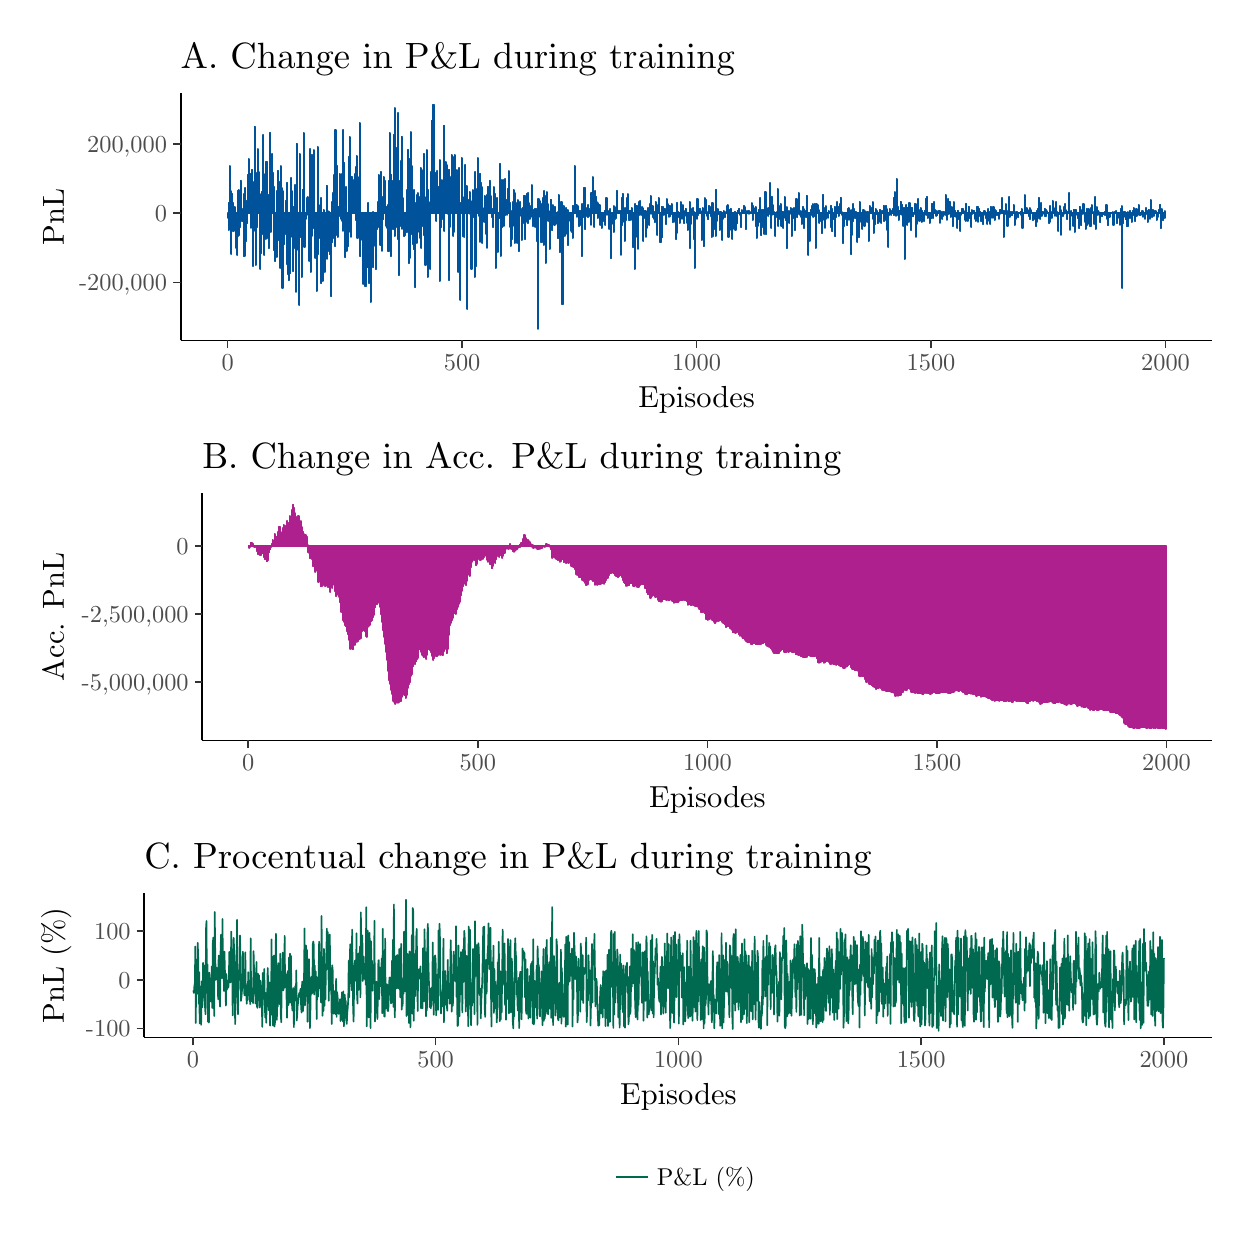
\begin{tikzpicture}[x=1pt,y=1pt]
\definecolor{fillColor}{RGB}{255,255,255}
\path[use as bounding box,fill=fillColor,fill opacity=0.00] (0,0) rectangle (433.62,433.62);
\begin{scope}
\path[clip] (  0.00,289.08) rectangle (433.62,433.62);
\definecolor{drawColor}{RGB}{255,255,255}
\definecolor{fillColor}{RGB}{255,255,255}

\path[draw=drawColor,line width= 0.6pt,line join=round,line cap=round,fill=fillColor] (  0.00,289.08) rectangle (433.62,433.62);
\end{scope}
\begin{scope}
\path[clip] ( 55.30,320.61) rectangle (428.12,409.93);
\definecolor{fillColor}{RGB}{255,255,255}

\path[fill=fillColor] ( 55.30,320.61) rectangle (428.12,409.93);
\definecolor{drawColor}{RGB}{0,83,155}
\definecolor{fillColor}{RGB}{89,89,89}

\path[draw=drawColor,line width= 0.6pt,line join=round,fill=fillColor,fill opacity=0.55] ( 72.34,364.95) rectangle ( 72.49,366.60);

\path[draw=drawColor,line width= 0.6pt,line join=round,fill=fillColor,fill opacity=0.55] ( 72.51,360.49) rectangle ( 72.66,366.60);

\path[draw=drawColor,line width= 0.6pt,line join=round,fill=fillColor,fill opacity=0.55] ( 72.67,366.60) rectangle ( 72.83,370.39);

\path[draw=drawColor,line width= 0.6pt,line join=round,fill=fillColor,fill opacity=0.55] ( 72.84,366.60) rectangle ( 73.00,366.74);

\path[draw=drawColor,line width= 0.6pt,line join=round,fill=fillColor,fill opacity=0.55] ( 73.01,366.60) rectangle ( 73.17,383.70);

\path[draw=drawColor,line width= 0.6pt,line join=round,fill=fillColor,fill opacity=0.55] ( 73.18,362.34) rectangle ( 73.34,366.60);

\path[draw=drawColor,line width= 0.6pt,line join=round,fill=fillColor,fill opacity=0.55] ( 73.35,366.60) rectangle ( 73.51,374.67);

\path[draw=drawColor,line width= 0.6pt,line join=round,fill=fillColor,fill opacity=0.55] ( 73.52,351.86) rectangle ( 73.67,366.60);

\path[draw=drawColor,line width= 0.6pt,line join=round,fill=fillColor,fill opacity=0.55] ( 73.69,366.60) rectangle ( 73.84,373.74);

\path[draw=drawColor,line width= 0.6pt,line join=round,fill=fillColor,fill opacity=0.55] ( 73.86,363.00) rectangle ( 74.01,366.60);

\path[draw=drawColor,line width= 0.6pt,line join=round,fill=fillColor,fill opacity=0.55] ( 74.03,366.60) rectangle ( 74.18,370.42);

\path[draw=drawColor,line width= 0.6pt,line join=round,fill=fillColor,fill opacity=0.55] ( 74.20,359.99) rectangle ( 74.35,366.60);

\path[draw=drawColor,line width= 0.6pt,line join=round,fill=fillColor,fill opacity=0.55] ( 74.37,360.19) rectangle ( 74.52,366.60);

\path[draw=drawColor,line width= 0.6pt,line join=round,fill=fillColor,fill opacity=0.55] ( 74.54,366.60) rectangle ( 74.69,367.32);

\path[draw=drawColor,line width= 0.6pt,line join=round,fill=fillColor,fill opacity=0.55] ( 74.71,366.60) rectangle ( 74.86,368.77);

\path[draw=drawColor,line width= 0.6pt,line join=round,fill=fillColor,fill opacity=0.55] ( 74.88,366.41) rectangle ( 75.03,366.60);

\path[draw=drawColor,line width= 0.6pt,line join=round,fill=fillColor,fill opacity=0.55] ( 75.05,364.94) rectangle ( 75.20,366.60);

\path[draw=drawColor,line width= 0.6pt,line join=round,fill=fillColor,fill opacity=0.55] ( 75.22,362.02) rectangle ( 75.37,366.60);

\path[draw=drawColor,line width= 0.6pt,line join=round,fill=fillColor,fill opacity=0.55] ( 75.39,353.92) rectangle ( 75.54,366.60);

\path[draw=drawColor,line width= 0.6pt,line join=round,fill=fillColor,fill opacity=0.55] ( 75.56,361.97) rectangle ( 75.71,366.60);

\path[draw=drawColor,line width= 0.6pt,line join=round,fill=fillColor,fill opacity=0.55] ( 75.73,351.58) rectangle ( 75.88,366.60);

\path[draw=drawColor,line width= 0.6pt,line join=round,fill=fillColor,fill opacity=0.55] ( 75.89,366.60) rectangle ( 76.05,374.76);

\path[draw=drawColor,line width= 0.6pt,line join=round,fill=fillColor,fill opacity=0.55] ( 76.06,358.27) rectangle ( 76.22,366.60);

\path[draw=drawColor,line width= 0.6pt,line join=round,fill=fillColor,fill opacity=0.55] ( 76.23,366.60) rectangle ( 76.39,374.99);

\path[draw=drawColor,line width= 0.6pt,line join=round,fill=fillColor,fill opacity=0.55] ( 76.40,358.75) rectangle ( 76.56,366.60);

\path[draw=drawColor,line width= 0.6pt,line join=round,fill=fillColor,fill opacity=0.55] ( 76.57,361.41) rectangle ( 76.73,366.60);

\path[draw=drawColor,line width= 0.6pt,line join=round,fill=fillColor,fill opacity=0.55] ( 76.74,366.60) rectangle ( 76.89,367.78);

\path[draw=drawColor,line width= 0.6pt,line join=round,fill=fillColor,fill opacity=0.55] ( 76.91,366.60) rectangle ( 77.06,378.34);

\path[draw=drawColor,line width= 0.6pt,line join=round,fill=fillColor,fill opacity=0.55] ( 77.08,366.60) rectangle ( 77.23,368.25);

\path[draw=drawColor,line width= 0.6pt,line join=round,fill=fillColor,fill opacity=0.55] ( 77.25,366.60) rectangle ( 77.40,368.27);

\path[draw=drawColor,line width= 0.6pt,line join=round,fill=fillColor,fill opacity=0.55] ( 77.42,363.56) rectangle ( 77.57,366.60);

\path[draw=drawColor,line width= 0.6pt,line join=round,fill=fillColor,fill opacity=0.55] ( 77.59,363.78) rectangle ( 77.74,366.60);

\path[draw=drawColor,line width= 0.6pt,line join=round,fill=fillColor,fill opacity=0.55] ( 77.76,365.70) rectangle ( 77.91,366.60);

\path[draw=drawColor,line width= 0.6pt,line join=round,fill=fillColor,fill opacity=0.55] ( 77.93,351.12) rectangle ( 78.08,366.60);

\path[draw=drawColor,line width= 0.6pt,line join=round,fill=fillColor,fill opacity=0.55] ( 78.10,366.60) rectangle ( 78.25,373.49);

\path[draw=drawColor,line width= 0.6pt,line join=round,fill=fillColor,fill opacity=0.55] ( 78.27,351.17) rectangle ( 78.42,366.60);

\path[draw=drawColor,line width= 0.6pt,line join=round,fill=fillColor,fill opacity=0.55] ( 78.44,364.99) rectangle ( 78.59,366.60);

\path[draw=drawColor,line width= 0.6pt,line join=round,fill=fillColor,fill opacity=0.55] ( 78.61,366.60) rectangle ( 78.76,375.64);

\path[draw=drawColor,line width= 0.6pt,line join=round,fill=fillColor,fill opacity=0.55] ( 78.78,356.36) rectangle ( 78.93,366.60);

\path[draw=drawColor,line width= 0.6pt,line join=round,fill=fillColor,fill opacity=0.55] ( 78.95,360.26) rectangle ( 79.10,366.60);

\path[draw=drawColor,line width= 0.6pt,line join=round,fill=fillColor,fill opacity=0.55] ( 79.11,362.80) rectangle ( 79.27,366.60);

\path[draw=drawColor,line width= 0.6pt,line join=round,fill=fillColor,fill opacity=0.55] ( 79.28,366.60) rectangle ( 79.44,371.19);

\path[draw=drawColor,line width= 0.6pt,line join=round,fill=fillColor,fill opacity=0.55] ( 79.45,366.60) rectangle ( 79.61,380.45);

\path[draw=drawColor,line width= 0.6pt,line join=round,fill=fillColor,fill opacity=0.55] ( 79.62,366.60) rectangle ( 79.78,370.77);

\path[draw=drawColor,line width= 0.6pt,line join=round,fill=fillColor,fill opacity=0.55] ( 79.79,366.60) rectangle ( 79.94,386.10);

\path[draw=drawColor,line width= 0.6pt,line join=round,fill=fillColor,fill opacity=0.55] ( 79.96,366.60) rectangle ( 80.11,368.47);

\path[draw=drawColor,line width= 0.6pt,line join=round,fill=fillColor,fill opacity=0.55] ( 80.13,366.60) rectangle ( 80.28,379.04);

\path[draw=drawColor,line width= 0.6pt,line join=round,fill=fillColor,fill opacity=0.55] ( 80.30,366.60) rectangle ( 80.45,367.06);

\path[draw=drawColor,line width= 0.6pt,line join=round,fill=fillColor,fill opacity=0.55] ( 80.47,366.60) rectangle ( 80.62,380.95);

\path[draw=drawColor,line width= 0.6pt,line join=round,fill=fillColor,fill opacity=0.55] ( 80.64,361.17) rectangle ( 80.79,366.60);

\path[draw=drawColor,line width= 0.6pt,line join=round,fill=fillColor,fill opacity=0.55] ( 80.81,366.60) rectangle ( 80.96,376.35);

\path[draw=drawColor,line width= 0.6pt,line join=round,fill=fillColor,fill opacity=0.55] ( 80.98,366.60) rectangle ( 81.13,374.98);

\path[draw=drawColor,line width= 0.6pt,line join=round,fill=fillColor,fill opacity=0.55] ( 81.15,366.60) rectangle ( 81.30,382.40);

\path[draw=drawColor,line width= 0.6pt,line join=round,fill=fillColor,fill opacity=0.55] ( 81.32,347.34) rectangle ( 81.47,366.60);

\path[draw=drawColor,line width= 0.6pt,line join=round,fill=fillColor,fill opacity=0.55] ( 81.49,366.60) rectangle ( 81.64,372.03);

\path[draw=drawColor,line width= 0.6pt,line join=round,fill=fillColor,fill opacity=0.55] ( 81.66,364.16) rectangle ( 81.81,366.60);

\path[draw=drawColor,line width= 0.6pt,line join=round,fill=fillColor,fill opacity=0.55] ( 81.83,366.60) rectangle ( 81.98,377.86);

\path[draw=drawColor,line width= 0.6pt,line join=round,fill=fillColor,fill opacity=0.55] ( 82.00,366.60) rectangle ( 82.15,397.90);

\path[draw=drawColor,line width= 0.6pt,line join=round,fill=fillColor,fill opacity=0.55] ( 82.16,360.17) rectangle ( 82.32,366.60);

\path[draw=drawColor,line width= 0.6pt,line join=round,fill=fillColor,fill opacity=0.55] ( 82.33,347.91) rectangle ( 82.49,366.60);

\path[draw=drawColor,line width= 0.6pt,line join=round,fill=fillColor,fill opacity=0.55] ( 82.50,366.60) rectangle ( 82.66,381.05);

\path[draw=drawColor,line width= 0.6pt,line join=round,fill=fillColor,fill opacity=0.55] ( 82.67,365.50) rectangle ( 82.83,366.60);

\path[draw=drawColor,line width= 0.6pt,line join=round,fill=fillColor,fill opacity=0.55] ( 82.84,361.61) rectangle ( 83.00,366.60);

\path[draw=drawColor,line width= 0.6pt,line join=round,fill=fillColor,fill opacity=0.55] ( 83.01,366.60) rectangle ( 83.16,369.54);

\path[draw=drawColor,line width= 0.6pt,line join=round,fill=fillColor,fill opacity=0.55] ( 83.18,366.60) rectangle ( 83.33,389.80);

\path[draw=drawColor,line width= 0.6pt,line join=round,fill=fillColor,fill opacity=0.55] ( 83.35,366.60) rectangle ( 83.50,381.35);

\path[draw=drawColor,line width= 0.6pt,line join=round,fill=fillColor,fill opacity=0.55] ( 83.52,366.60) rectangle ( 83.67,371.65);

\path[draw=drawColor,line width= 0.6pt,line join=round,fill=fillColor,fill opacity=0.55] ( 83.69,366.60) rectangle ( 83.84,373.42);

\path[draw=drawColor,line width= 0.6pt,line join=round,fill=fillColor,fill opacity=0.55] ( 83.86,354.41) rectangle ( 84.01,366.60);

\path[draw=drawColor,line width= 0.6pt,line join=round,fill=fillColor,fill opacity=0.55] ( 84.03,346.51) rectangle ( 84.18,366.60);

\path[draw=drawColor,line width= 0.6pt,line join=round,fill=fillColor,fill opacity=0.55] ( 84.20,366.60) rectangle ( 84.35,373.11);

\path[draw=drawColor,line width= 0.6pt,line join=round,fill=fillColor,fill opacity=0.55] ( 84.37,352.04) rectangle ( 84.52,366.60);

\path[draw=drawColor,line width= 0.6pt,line join=round,fill=fillColor,fill opacity=0.55] ( 84.54,366.60) rectangle ( 84.69,374.25);

\path[draw=drawColor,line width= 0.6pt,line join=round,fill=fillColor,fill opacity=0.55] ( 84.71,359.04) rectangle ( 84.86,366.60);

\path[draw=drawColor,line width= 0.6pt,line join=round,fill=fillColor,fill opacity=0.55] ( 84.88,366.60) rectangle ( 85.03,371.96);

\path[draw=drawColor,line width= 0.6pt,line join=round,fill=fillColor,fill opacity=0.55] ( 85.05,366.60) rectangle ( 85.20,394.77);

\path[draw=drawColor,line width= 0.6pt,line join=round,fill=fillColor,fill opacity=0.55] ( 85.22,366.60) rectangle ( 85.37,380.83);

\path[draw=drawColor,line width= 0.6pt,line join=round,fill=fillColor,fill opacity=0.55] ( 85.38,351.41) rectangle ( 85.54,366.60);

\path[draw=drawColor,line width= 0.6pt,line join=round,fill=fillColor,fill opacity=0.55] ( 85.55,366.60) rectangle ( 85.71,374.58);

\path[draw=drawColor,line width= 0.6pt,line join=round,fill=fillColor,fill opacity=0.55] ( 85.72,360.15) rectangle ( 85.88,366.60);

\path[draw=drawColor,line width= 0.6pt,line join=round,fill=fillColor,fill opacity=0.55] ( 85.89,357.35) rectangle ( 86.05,366.60);

\path[draw=drawColor,line width= 0.6pt,line join=round,fill=fillColor,fill opacity=0.55] ( 86.06,366.21) rectangle ( 86.22,366.60);

\path[draw=drawColor,line width= 0.6pt,line join=round,fill=fillColor,fill opacity=0.55] ( 86.23,366.60) rectangle ( 86.38,385.27);

\path[draw=drawColor,line width= 0.6pt,line join=round,fill=fillColor,fill opacity=0.55] ( 86.40,366.60) rectangle ( 86.55,373.72);

\path[draw=drawColor,line width= 0.6pt,line join=round,fill=fillColor,fill opacity=0.55] ( 86.57,366.60) rectangle ( 86.72,382.72);

\path[draw=drawColor,line width= 0.6pt,line join=round,fill=fillColor,fill opacity=0.55] ( 86.74,357.47) rectangle ( 86.89,366.60);

\path[draw=drawColor,line width= 0.6pt,line join=round,fill=fillColor,fill opacity=0.55] ( 86.91,365.29) rectangle ( 87.06,366.60);

\path[draw=drawColor,line width= 0.6pt,line join=round,fill=fillColor,fill opacity=0.55] ( 87.08,353.84) rectangle ( 87.23,366.60);

\path[draw=drawColor,line width= 0.6pt,line join=round,fill=fillColor,fill opacity=0.55] ( 87.25,366.60) rectangle ( 87.40,373.31);

\path[draw=drawColor,line width= 0.6pt,line join=round,fill=fillColor,fill opacity=0.55] ( 87.42,366.60) rectangle ( 87.57,375.79);

\path[draw=drawColor,line width= 0.6pt,line join=round,fill=fillColor,fill opacity=0.55] ( 87.59,366.60) rectangle ( 87.74,395.68);

\path[draw=drawColor,line width= 0.6pt,line join=round,fill=fillColor,fill opacity=0.55] ( 87.76,359.73) rectangle ( 87.91,366.60);

\path[draw=drawColor,line width= 0.6pt,line join=round,fill=fillColor,fill opacity=0.55] ( 87.93,366.60) rectangle ( 88.08,370.55);

\path[draw=drawColor,line width= 0.6pt,line join=round,fill=fillColor,fill opacity=0.55] ( 88.10,366.60) rectangle ( 88.25,367.24);

\path[draw=drawColor,line width= 0.6pt,line join=round,fill=fillColor,fill opacity=0.55] ( 88.27,366.60) rectangle ( 88.42,387.95);

\path[draw=drawColor,line width= 0.6pt,line join=round,fill=fillColor,fill opacity=0.55] ( 88.44,366.60) rectangle ( 88.59,376.29);

\path[draw=drawColor,line width= 0.6pt,line join=round,fill=fillColor,fill opacity=0.55] ( 88.60,366.60) rectangle ( 88.76,381.27);

\path[draw=drawColor,line width= 0.6pt,line join=round,fill=fillColor,fill opacity=0.55] ( 88.77,366.60) rectangle ( 88.93,376.25);

\path[draw=drawColor,line width= 0.6pt,line join=round,fill=fillColor,fill opacity=0.55] ( 88.94,353.08) rectangle ( 89.10,366.60);

\path[draw=drawColor,line width= 0.6pt,line join=round,fill=fillColor,fill opacity=0.55] ( 89.11,357.19) rectangle ( 89.27,366.60);

\path[draw=drawColor,line width= 0.6pt,line join=round,fill=fillColor,fill opacity=0.55] ( 89.28,349.10) rectangle ( 89.43,366.60);

\path[draw=drawColor,line width= 0.6pt,line join=round,fill=fillColor,fill opacity=0.55] ( 89.45,359.66) rectangle ( 89.60,366.60);

\path[draw=drawColor,line width= 0.6pt,line join=round,fill=fillColor,fill opacity=0.55] ( 89.62,358.94) rectangle ( 89.77,366.60);

\path[draw=drawColor,line width= 0.6pt,line join=round,fill=fillColor,fill opacity=0.55] ( 89.79,359.28) rectangle ( 89.94,366.60);

\path[draw=drawColor,line width= 0.6pt,line join=round,fill=fillColor,fill opacity=0.55] ( 89.96,350.65) rectangle ( 90.11,366.60);

\path[draw=drawColor,line width= 0.6pt,line join=round,fill=fillColor,fill opacity=0.55] ( 90.13,366.60) rectangle ( 90.28,374.60);

\path[draw=drawColor,line width= 0.6pt,line join=round,fill=fillColor,fill opacity=0.55] ( 90.30,356.65) rectangle ( 90.45,366.60);

\path[draw=drawColor,line width= 0.6pt,line join=round,fill=fillColor,fill opacity=0.55] ( 90.47,366.60) rectangle ( 90.62,381.98);

\path[draw=drawColor,line width= 0.6pt,line join=round,fill=fillColor,fill opacity=0.55] ( 90.64,366.60) rectangle ( 90.79,378.06);

\path[draw=drawColor,line width= 0.6pt,line join=round,fill=fillColor,fill opacity=0.55] ( 90.81,366.60) rectangle ( 90.96,368.10);

\path[draw=drawColor,line width= 0.6pt,line join=round,fill=fillColor,fill opacity=0.55] ( 90.98,347.32) rectangle ( 91.13,366.60);

\path[draw=drawColor,line width= 0.6pt,line join=round,fill=fillColor,fill opacity=0.55] ( 91.15,346.85) rectangle ( 91.30,366.60);

\path[draw=drawColor,line width= 0.6pt,line join=round,fill=fillColor,fill opacity=0.55] ( 91.32,354.29) rectangle ( 91.47,366.60);

\path[draw=drawColor,line width= 0.6pt,line join=round,fill=fillColor,fill opacity=0.55] ( 91.49,366.60) rectangle ( 91.64,383.57);

\path[draw=drawColor,line width= 0.6pt,line join=round,fill=fillColor,fill opacity=0.55] ( 91.65,366.60) rectangle ( 91.81,375.64);

\path[draw=drawColor,line width= 0.6pt,line join=round,fill=fillColor,fill opacity=0.55] ( 91.82,341.40) rectangle ( 91.98,366.60);

\path[draw=drawColor,line width= 0.6pt,line join=round,fill=fillColor,fill opacity=0.55] ( 91.99,339.55) rectangle ( 92.15,366.60);

\path[draw=drawColor,line width= 0.6pt,line join=round,fill=fillColor,fill opacity=0.55] ( 92.16,366.60) rectangle ( 92.32,374.48);

\path[draw=drawColor,line width= 0.6pt,line join=round,fill=fillColor,fill opacity=0.55] ( 92.33,364.11) rectangle ( 92.49,366.60);

\path[draw=drawColor,line width= 0.6pt,line join=round,fill=fillColor,fill opacity=0.55] ( 92.50,355.26) rectangle ( 92.65,366.60);

\path[draw=drawColor,line width= 0.6pt,line join=round,fill=fillColor,fill opacity=0.55] ( 92.67,366.60) rectangle ( 92.82,366.74);

\path[draw=drawColor,line width= 0.6pt,line join=round,fill=fillColor,fill opacity=0.55] ( 92.84,363.14) rectangle ( 92.99,366.60);

\path[draw=drawColor,line width= 0.6pt,line join=round,fill=fillColor,fill opacity=0.55] ( 93.01,358.99) rectangle ( 93.16,366.60);

\path[draw=drawColor,line width= 0.6pt,line join=round,fill=fillColor,fill opacity=0.55] ( 93.18,366.60) rectangle ( 93.33,370.89);

\path[draw=drawColor,line width= 0.6pt,line join=round,fill=fillColor,fill opacity=0.55] ( 93.35,366.60) rectangle ( 93.50,368.19);

\path[draw=drawColor,line width= 0.6pt,line join=round,fill=fillColor,fill opacity=0.55] ( 93.52,348.14) rectangle ( 93.67,366.60);

\path[draw=drawColor,line width= 0.6pt,line join=round,fill=fillColor,fill opacity=0.55] ( 93.69,366.60) rectangle ( 93.84,377.64);

\path[draw=drawColor,line width= 0.6pt,line join=round,fill=fillColor,fill opacity=0.55] ( 93.86,344.62) rectangle ( 94.01,366.60);

\path[draw=drawColor,line width= 0.6pt,line join=round,fill=fillColor,fill opacity=0.55] ( 94.03,348.36) rectangle ( 94.18,366.60);

\path[draw=drawColor,line width= 0.6pt,line join=round,fill=fillColor,fill opacity=0.55] ( 94.20,342.20) rectangle ( 94.35,366.60);

\path[draw=drawColor,line width= 0.6pt,line join=round,fill=fillColor,fill opacity=0.55] ( 94.37,357.93) rectangle ( 94.52,366.60);

\path[draw=drawColor,line width= 0.6pt,line join=round,fill=fillColor,fill opacity=0.55] ( 94.54,366.58) rectangle ( 94.69,366.60);

\path[draw=drawColor,line width= 0.6pt,line join=round,fill=fillColor,fill opacity=0.55] ( 94.71,363.58) rectangle ( 94.86,366.60);

\path[draw=drawColor,line width= 0.6pt,line join=round,fill=fillColor,fill opacity=0.55] ( 94.87,344.83) rectangle ( 95.03,366.60);

\path[draw=drawColor,line width= 0.6pt,line join=round,fill=fillColor,fill opacity=0.55] ( 95.04,366.60) rectangle ( 95.20,366.99);

\path[draw=drawColor,line width= 0.6pt,line join=round,fill=fillColor,fill opacity=0.55] ( 95.21,366.60) rectangle ( 95.37,379.25);

\path[draw=drawColor,line width= 0.6pt,line join=round,fill=fillColor,fill opacity=0.55] ( 95.38,366.60) rectangle ( 95.54,374.68);

\path[draw=drawColor,line width= 0.6pt,line join=round,fill=fillColor,fill opacity=0.55] ( 95.55,357.90) rectangle ( 95.71,366.60);

\path[draw=drawColor,line width= 0.6pt,line join=round,fill=fillColor,fill opacity=0.55] ( 95.72,346.26) rectangle ( 95.87,366.60);

\path[draw=drawColor,line width= 0.6pt,line join=round,fill=fillColor,fill opacity=0.55] ( 95.89,345.55) rectangle ( 96.04,366.60);

\path[draw=drawColor,line width= 0.6pt,line join=round,fill=fillColor,fill opacity=0.55] ( 96.06,366.60) rectangle ( 96.21,368.91);

\path[draw=drawColor,line width= 0.6pt,line join=round,fill=fillColor,fill opacity=0.55] ( 96.23,354.04) rectangle ( 96.38,366.60);

\path[draw=drawColor,line width= 0.6pt,line join=round,fill=fillColor,fill opacity=0.55] ( 96.40,366.42) rectangle ( 96.55,366.60);

\path[draw=drawColor,line width= 0.6pt,line join=round,fill=fillColor,fill opacity=0.55] ( 96.57,366.60) rectangle ( 96.72,376.65);

\path[draw=drawColor,line width= 0.6pt,line join=round,fill=fillColor,fill opacity=0.55] ( 96.74,358.54) rectangle ( 96.89,366.60);

\path[draw=drawColor,line width= 0.6pt,line join=round,fill=fillColor,fill opacity=0.55] ( 96.91,338.11) rectangle ( 97.06,366.60);

\path[draw=drawColor,line width= 0.6pt,line join=round,fill=fillColor,fill opacity=0.55] ( 97.08,366.60) rectangle ( 97.23,391.71);

\path[draw=drawColor,line width= 0.6pt,line join=round,fill=fillColor,fill opacity=0.55] ( 97.25,365.32) rectangle ( 97.40,366.60);

\path[draw=drawColor,line width= 0.6pt,line join=round,fill=fillColor,fill opacity=0.55] ( 97.42,362.36) rectangle ( 97.57,366.60);

\path[draw=drawColor,line width= 0.6pt,line join=round,fill=fillColor,fill opacity=0.55] ( 97.59,353.39) rectangle ( 97.74,366.60);

\path[draw=drawColor,line width= 0.6pt,line join=round,fill=fillColor,fill opacity=0.55] ( 97.76,363.17) rectangle ( 97.91,366.60);

\path[draw=drawColor,line width= 0.6pt,line join=round,fill=fillColor,fill opacity=0.55] ( 97.93,352.43) rectangle ( 98.08,366.60);

\path[draw=drawColor,line width= 0.6pt,line join=round,fill=fillColor,fill opacity=0.55] ( 98.09,333.36) rectangle ( 98.25,366.60);

\path[draw=drawColor,line width= 0.6pt,line join=round,fill=fillColor,fill opacity=0.55] ( 98.26,366.60) rectangle ( 98.42,388.00);

\path[draw=drawColor,line width= 0.6pt,line join=round,fill=fillColor,fill opacity=0.55] ( 98.43,357.85) rectangle ( 98.59,366.60);

\path[draw=drawColor,line width= 0.6pt,line join=round,fill=fillColor,fill opacity=0.55] ( 98.60,362.14) rectangle ( 98.76,366.60);

\path[draw=drawColor,line width= 0.6pt,line join=round,fill=fillColor,fill opacity=0.55] ( 98.77,359.26) rectangle ( 98.93,366.60);

\path[draw=drawColor,line width= 0.6pt,line join=round,fill=fillColor,fill opacity=0.55] ( 98.94,343.44) rectangle ( 99.09,366.60);

\path[draw=drawColor,line width= 0.6pt,line join=round,fill=fillColor,fill opacity=0.55] ( 99.11,366.60) rectangle ( 99.26,366.67);

\path[draw=drawColor,line width= 0.6pt,line join=round,fill=fillColor,fill opacity=0.55] ( 99.28,366.60) rectangle ( 99.43,375.08);

\path[draw=drawColor,line width= 0.6pt,line join=round,fill=fillColor,fill opacity=0.55] ( 99.45,361.91) rectangle ( 99.60,366.60);

\path[draw=drawColor,line width= 0.6pt,line join=round,fill=fillColor,fill opacity=0.55] ( 99.62,366.60) rectangle ( 99.77,395.52);

\path[draw=drawColor,line width= 0.6pt,line join=round,fill=fillColor,fill opacity=0.55] ( 99.79,357.41) rectangle ( 99.94,366.60);

\path[draw=drawColor,line width= 0.6pt,line join=round,fill=fillColor,fill opacity=0.55] ( 99.96,354.27) rectangle (100.11,366.60);

\path[draw=drawColor,line width= 0.6pt,line join=round,fill=fillColor,fill opacity=0.55] (100.13,366.38) rectangle (100.28,366.60);

\path[draw=drawColor,line width= 0.6pt,line join=round,fill=fillColor,fill opacity=0.55] (100.30,360.84) rectangle (100.45,366.60);

\path[draw=drawColor,line width= 0.6pt,line join=round,fill=fillColor,fill opacity=0.55] (100.47,364.57) rectangle (100.62,366.60);

\path[draw=drawColor,line width= 0.6pt,line join=round,fill=fillColor,fill opacity=0.55] (100.64,365.67) rectangle (100.79,366.60);

\path[draw=drawColor,line width= 0.6pt,line join=round,fill=fillColor,fill opacity=0.55] (100.81,366.20) rectangle (100.96,366.60);

\path[draw=drawColor,line width= 0.6pt,line join=round,fill=fillColor,fill opacity=0.55] (100.98,366.60) rectangle (101.13,371.95);

\path[draw=drawColor,line width= 0.6pt,line join=round,fill=fillColor,fill opacity=0.55] (101.15,366.60) rectangle (101.30,372.33);

\path[draw=drawColor,line width= 0.6pt,line join=round,fill=fillColor,fill opacity=0.55] (101.31,365.93) rectangle (101.47,366.60);

\path[draw=drawColor,line width= 0.6pt,line join=round,fill=fillColor,fill opacity=0.55] (101.48,366.60) rectangle (101.64,367.74);

\path[draw=drawColor,line width= 0.6pt,line join=round,fill=fillColor,fill opacity=0.55] (101.65,349.30) rectangle (101.81,366.60);

\path[draw=drawColor,line width= 0.6pt,line join=round,fill=fillColor,fill opacity=0.55] (101.82,366.60) rectangle (101.98,370.23);

\path[draw=drawColor,line width= 0.6pt,line join=round,fill=fillColor,fill opacity=0.55] (101.99,366.60) rectangle (102.14,389.74);

\path[draw=drawColor,line width= 0.6pt,line join=round,fill=fillColor,fill opacity=0.55] (102.16,345.26) rectangle (102.31,366.60);

\path[draw=drawColor,line width= 0.6pt,line join=round,fill=fillColor,fill opacity=0.55] (102.33,348.30) rectangle (102.48,366.60);

\path[draw=drawColor,line width= 0.6pt,line join=round,fill=fillColor,fill opacity=0.55] (102.50,358.41) rectangle (102.65,366.60);

\path[draw=drawColor,line width= 0.6pt,line join=round,fill=fillColor,fill opacity=0.55] (102.67,366.60) rectangle (102.82,387.74);

\path[draw=drawColor,line width= 0.6pt,line join=round,fill=fillColor,fill opacity=0.55] (102.84,366.60) rectangle (102.99,368.25);

\path[draw=drawColor,line width= 0.6pt,line join=round,fill=fillColor,fill opacity=0.55] (103.01,366.60) rectangle (103.16,366.77);

\path[draw=drawColor,line width= 0.6pt,line join=round,fill=fillColor,fill opacity=0.55] (103.18,361.09) rectangle (103.33,366.60);

\path[draw=drawColor,line width= 0.6pt,line join=round,fill=fillColor,fill opacity=0.55] (103.35,366.60) rectangle (103.50,389.33);

\path[draw=drawColor,line width= 0.6pt,line join=round,fill=fillColor,fill opacity=0.55] (103.52,366.60) rectangle (103.67,376.57);

\path[draw=drawColor,line width= 0.6pt,line join=round,fill=fillColor,fill opacity=0.55] (103.69,366.00) rectangle (103.84,366.60);

\path[draw=drawColor,line width= 0.6pt,line join=round,fill=fillColor,fill opacity=0.55] (103.86,350.47) rectangle (104.01,366.60);

\path[draw=drawColor,line width= 0.6pt,line join=round,fill=fillColor,fill opacity=0.55] (104.03,364.26) rectangle (104.18,366.60);

\path[draw=drawColor,line width= 0.6pt,line join=round,fill=fillColor,fill opacity=0.55] (104.20,366.21) rectangle (104.35,366.60);

\path[draw=drawColor,line width= 0.6pt,line join=round,fill=fillColor,fill opacity=0.55] (104.36,338.48) rectangle (104.52,366.60);

\path[draw=drawColor,line width= 0.6pt,line join=round,fill=fillColor,fill opacity=0.55] (104.53,342.60) rectangle (104.69,366.60);

\path[draw=drawColor,line width= 0.6pt,line join=round,fill=fillColor,fill opacity=0.55] (104.70,366.60) rectangle (104.86,390.41);

\path[draw=drawColor,line width= 0.6pt,line join=round,fill=fillColor,fill opacity=0.55] (104.87,351.90) rectangle (105.03,366.60);

\path[draw=drawColor,line width= 0.6pt,line join=round,fill=fillColor,fill opacity=0.55] (105.04,366.60) rectangle (105.20,368.25);

\path[draw=drawColor,line width= 0.6pt,line join=round,fill=fillColor,fill opacity=0.55] (105.21,366.60) rectangle (105.36,369.48);

\path[draw=drawColor,line width= 0.6pt,line join=round,fill=fillColor,fill opacity=0.55] (105.38,365.15) rectangle (105.53,366.60);

\path[draw=drawColor,line width= 0.6pt,line join=round,fill=fillColor,fill opacity=0.55] (105.55,363.16) rectangle (105.70,366.60);

\path[draw=drawColor,line width= 0.6pt,line join=round,fill=fillColor,fill opacity=0.55] (105.72,357.46) rectangle (105.87,366.60);

\path[draw=drawColor,line width= 0.6pt,line join=round,fill=fillColor,fill opacity=0.55] (105.89,341.15) rectangle (106.04,366.60);

\path[draw=drawColor,line width= 0.6pt,line join=round,fill=fillColor,fill opacity=0.55] (106.06,366.60) rectangle (106.21,372.15);

\path[draw=drawColor,line width= 0.6pt,line join=round,fill=fillColor,fill opacity=0.55] (106.23,344.04) rectangle (106.38,366.60);

\path[draw=drawColor,line width= 0.6pt,line join=round,fill=fillColor,fill opacity=0.55] (106.40,364.81) rectangle (106.55,366.60);

\path[draw=drawColor,line width= 0.6pt,line join=round,fill=fillColor,fill opacity=0.55] (106.57,341.96) rectangle (106.72,366.60);

\path[draw=drawColor,line width= 0.6pt,line join=round,fill=fillColor,fill opacity=0.55] (106.74,366.39) rectangle (106.89,366.60);

\path[draw=drawColor,line width= 0.6pt,line join=round,fill=fillColor,fill opacity=0.55] (106.91,366.60) rectangle (107.06,367.81);

\path[draw=drawColor,line width= 0.6pt,line join=round,fill=fillColor,fill opacity=0.55] (107.08,346.89) rectangle (107.23,366.60);

\path[draw=drawColor,line width= 0.6pt,line join=round,fill=fillColor,fill opacity=0.55] (107.25,345.21) rectangle (107.40,366.60);

\path[draw=drawColor,line width= 0.6pt,line join=round,fill=fillColor,fill opacity=0.55] (107.42,365.74) rectangle (107.57,366.60);

\path[draw=drawColor,line width= 0.6pt,line join=round,fill=fillColor,fill opacity=0.55] (107.58,359.02) rectangle (107.74,366.60);

\path[draw=drawColor,line width= 0.6pt,line join=round,fill=fillColor,fill opacity=0.55] (107.75,354.99) rectangle (107.91,366.60);

\path[draw=drawColor,line width= 0.6pt,line join=round,fill=fillColor,fill opacity=0.55] (107.92,366.60) rectangle (108.08,376.63);

\path[draw=drawColor,line width= 0.6pt,line join=round,fill=fillColor,fill opacity=0.55] (108.09,350.03) rectangle (108.25,366.60);

\path[draw=drawColor,line width= 0.6pt,line join=round,fill=fillColor,fill opacity=0.55] (108.26,365.58) rectangle (108.42,366.60);

\path[draw=drawColor,line width= 0.6pt,line join=round,fill=fillColor,fill opacity=0.55] (108.43,366.60) rectangle (108.58,367.41);

\path[draw=drawColor,line width= 0.6pt,line join=round,fill=fillColor,fill opacity=0.55] (108.60,355.69) rectangle (108.75,366.60);

\path[draw=drawColor,line width= 0.6pt,line join=round,fill=fillColor,fill opacity=0.55] (108.77,352.77) rectangle (108.92,366.60);

\path[draw=drawColor,line width= 0.6pt,line join=round,fill=fillColor,fill opacity=0.55] (108.94,366.60) rectangle (109.09,367.20);

\path[draw=drawColor,line width= 0.6pt,line join=round,fill=fillColor,fill opacity=0.55] (109.11,351.66) rectangle (109.26,366.60);

\path[draw=drawColor,line width= 0.6pt,line join=round,fill=fillColor,fill opacity=0.55] (109.28,360.19) rectangle (109.43,366.60);

\path[draw=drawColor,line width= 0.6pt,line join=round,fill=fillColor,fill opacity=0.55] (109.45,347.91) rectangle (109.60,366.60);

\path[draw=drawColor,line width= 0.6pt,line join=round,fill=fillColor,fill opacity=0.55] (109.62,336.45) rectangle (109.77,366.60);

\path[draw=drawColor,line width= 0.6pt,line join=round,fill=fillColor,fill opacity=0.55] (109.79,355.97) rectangle (109.94,366.60);

\path[draw=drawColor,line width= 0.6pt,line join=round,fill=fillColor,fill opacity=0.55] (109.96,366.60) rectangle (110.11,370.55);

\path[draw=drawColor,line width= 0.6pt,line join=round,fill=fillColor,fill opacity=0.55] (110.13,366.17) rectangle (110.28,366.60);

\path[draw=drawColor,line width= 0.6pt,line join=round,fill=fillColor,fill opacity=0.55] (110.30,366.60) rectangle (110.45,373.89);

\path[draw=drawColor,line width= 0.6pt,line join=round,fill=fillColor,fill opacity=0.55] (110.47,357.57) rectangle (110.62,366.60);

\path[draw=drawColor,line width= 0.6pt,line join=round,fill=fillColor,fill opacity=0.55] (110.64,363.98) rectangle (110.79,366.60);

\path[draw=drawColor,line width= 0.6pt,line join=round,fill=fillColor,fill opacity=0.55] (110.80,366.60) rectangle (110.96,380.44);

\path[draw=drawColor,line width= 0.6pt,line join=round,fill=fillColor,fill opacity=0.55] (110.97,354.54) rectangle (111.13,366.60);

\path[draw=drawColor,line width= 0.6pt,line join=round,fill=fillColor,fill opacity=0.55] (111.14,366.60) rectangle (111.30,396.54);

\path[draw=drawColor,line width= 0.6pt,line join=round,fill=fillColor,fill opacity=0.55] (111.31,362.94) rectangle (111.47,366.60);

\path[draw=drawColor,line width= 0.6pt,line join=round,fill=fillColor,fill opacity=0.55] (111.48,358.69) rectangle (111.63,366.60);

\path[draw=drawColor,line width= 0.6pt,line join=round,fill=fillColor,fill opacity=0.55] (111.65,366.60) rectangle (111.80,383.77);

\path[draw=drawColor,line width= 0.6pt,line join=round,fill=fillColor,fill opacity=0.55] (111.82,366.60) rectangle (111.97,375.83);

\path[draw=drawColor,line width= 0.6pt,line join=round,fill=fillColor,fill opacity=0.55] (111.99,357.94) rectangle (112.14,366.60);

\path[draw=drawColor,line width= 0.6pt,line join=round,fill=fillColor,fill opacity=0.55] (112.16,363.09) rectangle (112.31,366.60);

\path[draw=drawColor,line width= 0.6pt,line join=round,fill=fillColor,fill opacity=0.55] (112.33,366.60) rectangle (112.48,368.97);

\path[draw=drawColor,line width= 0.6pt,line join=round,fill=fillColor,fill opacity=0.55] (112.50,365.64) rectangle (112.65,366.60);

\path[draw=drawColor,line width= 0.6pt,line join=round,fill=fillColor,fill opacity=0.55] (112.67,366.60) rectangle (112.82,380.73);

\path[draw=drawColor,line width= 0.6pt,line join=round,fill=fillColor,fill opacity=0.55] (112.84,366.32) rectangle (112.99,366.60);

\path[draw=drawColor,line width= 0.6pt,line join=round,fill=fillColor,fill opacity=0.55] (113.01,366.60) rectangle (113.16,366.60);

\path[draw=drawColor,line width= 0.6pt,line join=round,fill=fillColor,fill opacity=0.55] (113.18,364.40) rectangle (113.33,366.60);

\path[draw=drawColor,line width= 0.6pt,line join=round,fill=fillColor,fill opacity=0.55] (113.35,365.95) rectangle (113.50,366.60);

\path[draw=drawColor,line width= 0.6pt,line join=round,fill=fillColor,fill opacity=0.55] (113.52,366.60) rectangle (113.67,380.78);

\path[draw=drawColor,line width= 0.6pt,line join=round,fill=fillColor,fill opacity=0.55] (113.69,363.83) rectangle (113.84,366.60);

\path[draw=drawColor,line width= 0.6pt,line join=round,fill=fillColor,fill opacity=0.55] (113.85,360.19) rectangle (114.01,366.60);

\path[draw=drawColor,line width= 0.6pt,line join=round,fill=fillColor,fill opacity=0.55] (114.02,366.60) rectangle (114.18,396.57);

\path[draw=drawColor,line width= 0.6pt,line join=round,fill=fillColor,fill opacity=0.55] (114.19,366.60) rectangle (114.35,367.14);

\path[draw=drawColor,line width= 0.6pt,line join=round,fill=fillColor,fill opacity=0.55] (114.36,366.60) rectangle (114.52,384.86);

\path[draw=drawColor,line width= 0.6pt,line join=round,fill=fillColor,fill opacity=0.55] (114.53,366.60) rectangle (114.69,368.64);

\path[draw=drawColor,line width= 0.6pt,line join=round,fill=fillColor,fill opacity=0.55] (114.70,350.62) rectangle (114.85,366.60);

\path[draw=drawColor,line width= 0.6pt,line join=round,fill=fillColor,fill opacity=0.55] (114.87,366.60) rectangle (115.02,367.09);

\path[draw=drawColor,line width= 0.6pt,line join=round,fill=fillColor,fill opacity=0.55] (115.04,366.60) rectangle (115.19,376.11);

\path[draw=drawColor,line width= 0.6pt,line join=round,fill=fillColor,fill opacity=0.55] (115.21,352.82) rectangle (115.36,366.60);

\path[draw=drawColor,line width= 0.6pt,line join=round,fill=fillColor,fill opacity=0.55] (115.38,366.02) rectangle (115.53,366.60);

\path[draw=drawColor,line width= 0.6pt,line join=round,fill=fillColor,fill opacity=0.55] (115.55,354.62) rectangle (115.70,366.60);

\path[draw=drawColor,line width= 0.6pt,line join=round,fill=fillColor,fill opacity=0.55] (115.72,354.81) rectangle (115.87,366.60);

\path[draw=drawColor,line width= 0.6pt,line join=round,fill=fillColor,fill opacity=0.55] (115.89,363.07) rectangle (116.04,366.60);

\path[draw=drawColor,line width= 0.6pt,line join=round,fill=fillColor,fill opacity=0.55] (116.06,366.60) rectangle (116.21,387.07);

\path[draw=drawColor,line width= 0.6pt,line join=round,fill=fillColor,fill opacity=0.55] (116.23,366.60) rectangle (116.38,394.16);

\path[draw=drawColor,line width= 0.6pt,line join=round,fill=fillColor,fill opacity=0.55] (116.40,366.60) rectangle (116.55,384.16);

\path[draw=drawColor,line width= 0.6pt,line join=round,fill=fillColor,fill opacity=0.55] (116.57,359.78) rectangle (116.72,366.60);

\path[draw=drawColor,line width= 0.6pt,line join=round,fill=fillColor,fill opacity=0.55] (116.74,358.06) rectangle (116.89,366.60);

\path[draw=drawColor,line width= 0.6pt,line join=round,fill=fillColor,fill opacity=0.55] (116.91,366.60) rectangle (117.06,372.11);

\path[draw=drawColor,line width= 0.6pt,line join=round,fill=fillColor,fill opacity=0.55] (117.07,366.60) rectangle (117.23,379.82);

\path[draw=drawColor,line width= 0.6pt,line join=round,fill=fillColor,fill opacity=0.55] (117.24,366.60) rectangle (117.40,368.55);

\path[draw=drawColor,line width= 0.6pt,line join=round,fill=fillColor,fill opacity=0.55] (117.41,366.60) rectangle (117.57,368.24);

\path[draw=drawColor,line width= 0.6pt,line join=round,fill=fillColor,fill opacity=0.55] (117.58,366.60) rectangle (117.74,369.66);

\path[draw=drawColor,line width= 0.6pt,line join=round,fill=fillColor,fill opacity=0.55] (117.75,366.60) rectangle (117.91,367.39);

\path[draw=drawColor,line width= 0.6pt,line join=round,fill=fillColor,fill opacity=0.55] (117.92,366.60) rectangle (118.07,378.47);

\path[draw=drawColor,line width= 0.6pt,line join=round,fill=fillColor,fill opacity=0.55] (118.09,366.60) rectangle (118.24,368.34);

\path[draw=drawColor,line width= 0.6pt,line join=round,fill=fillColor,fill opacity=0.55] (118.26,366.60) rectangle (118.41,380.64);

\path[draw=drawColor,line width= 0.6pt,line join=round,fill=fillColor,fill opacity=0.55] (118.43,364.15) rectangle (118.58,366.60);

\path[draw=drawColor,line width= 0.6pt,line join=round,fill=fillColor,fill opacity=0.55] (118.60,366.60) rectangle (118.75,383.38);

\path[draw=drawColor,line width= 0.6pt,line join=round,fill=fillColor,fill opacity=0.55] (118.77,366.60) rectangle (118.92,387.17);

\path[draw=drawColor,line width= 0.6pt,line join=round,fill=fillColor,fill opacity=0.55] (118.94,366.60) rectangle (119.09,373.86);

\path[draw=drawColor,line width= 0.6pt,line join=round,fill=fillColor,fill opacity=0.55] (119.11,357.56) rectangle (119.26,366.60);

\path[draw=drawColor,line width= 0.6pt,line join=round,fill=fillColor,fill opacity=0.55] (119.28,366.60) rectangle (119.43,379.56);

\path[draw=drawColor,line width= 0.6pt,line join=round,fill=fillColor,fill opacity=0.55] (119.45,366.60) rectangle (119.60,371.09);

\path[draw=drawColor,line width= 0.6pt,line join=round,fill=fillColor,fill opacity=0.55] (119.62,366.06) rectangle (119.77,366.60);

\path[draw=drawColor,line width= 0.6pt,line join=round,fill=fillColor,fill opacity=0.55] (119.79,364.74) rectangle (119.94,366.60);

\path[draw=drawColor,line width= 0.6pt,line join=round,fill=fillColor,fill opacity=0.55] (119.96,366.60) rectangle (120.11,399.25);

\path[draw=drawColor,line width= 0.6pt,line join=round,fill=fillColor,fill opacity=0.55] (120.13,350.88) rectangle (120.28,366.60);

\path[draw=drawColor,line width= 0.6pt,line join=round,fill=fillColor,fill opacity=0.55] (120.29,356.82) rectangle (120.45,366.60);

\path[draw=drawColor,line width= 0.6pt,line join=round,fill=fillColor,fill opacity=0.55] (120.46,363.53) rectangle (120.62,366.60);

\path[draw=drawColor,line width= 0.6pt,line join=round,fill=fillColor,fill opacity=0.55] (120.63,366.60) rectangle (120.79,366.60);

\path[draw=drawColor,line width= 0.6pt,line join=round,fill=fillColor,fill opacity=0.55] (120.80,358.10) rectangle (120.96,366.60);

\path[draw=drawColor,line width= 0.6pt,line join=round,fill=fillColor,fill opacity=0.55] (120.97,356.75) rectangle (121.12,366.60);

\path[draw=drawColor,line width= 0.6pt,line join=round,fill=fillColor,fill opacity=0.55] (121.14,340.97) rectangle (121.29,366.60);

\path[draw=drawColor,line width= 0.6pt,line join=round,fill=fillColor,fill opacity=0.55] (121.31,358.60) rectangle (121.46,366.60);

\path[draw=drawColor,line width= 0.6pt,line join=round,fill=fillColor,fill opacity=0.55] (121.48,345.97) rectangle (121.63,366.60);

\path[draw=drawColor,line width= 0.6pt,line join=round,fill=fillColor,fill opacity=0.55] (121.65,354.08) rectangle (121.80,366.60);

\path[draw=drawColor,line width= 0.6pt,line join=round,fill=fillColor,fill opacity=0.55] (121.82,352.75) rectangle (121.97,366.60);

\path[draw=drawColor,line width= 0.6pt,line join=round,fill=fillColor,fill opacity=0.55] (121.99,340.06) rectangle (122.14,366.60);

\path[draw=drawColor,line width= 0.6pt,line join=round,fill=fillColor,fill opacity=0.55] (122.16,347.35) rectangle (122.31,366.60);

\path[draw=drawColor,line width= 0.6pt,line join=round,fill=fillColor,fill opacity=0.55] (122.33,357.32) rectangle (122.48,366.60);

\path[draw=drawColor,line width= 0.6pt,line join=round,fill=fillColor,fill opacity=0.55] (122.50,353.98) rectangle (122.65,366.60);

\path[draw=drawColor,line width= 0.6pt,line join=round,fill=fillColor,fill opacity=0.55] (122.67,346.93) rectangle (122.82,366.60);

\path[draw=drawColor,line width= 0.6pt,line join=round,fill=fillColor,fill opacity=0.55] (122.84,346.96) rectangle (122.99,366.60);

\path[draw=drawColor,line width= 0.6pt,line join=round,fill=fillColor,fill opacity=0.55] (123.01,366.60) rectangle (123.16,370.19);

\path[draw=drawColor,line width= 0.6pt,line join=round,fill=fillColor,fill opacity=0.55] (123.18,342.82) rectangle (123.33,366.60);

\path[draw=drawColor,line width= 0.6pt,line join=round,fill=fillColor,fill opacity=0.55] (123.34,341.22) rectangle (123.50,366.60);

\path[draw=drawColor,line width= 0.6pt,line join=round,fill=fillColor,fill opacity=0.55] (123.51,358.16) rectangle (123.67,366.60);

\path[draw=drawColor,line width= 0.6pt,line join=round,fill=fillColor,fill opacity=0.55] (123.68,347.57) rectangle (123.84,366.60);

\path[draw=drawColor,line width= 0.6pt,line join=round,fill=fillColor,fill opacity=0.55] (123.85,334.49) rectangle (124.01,366.60);

\path[draw=drawColor,line width= 0.6pt,line join=round,fill=fillColor,fill opacity=0.55] (124.02,335.76) rectangle (124.18,366.60);

\path[draw=drawColor,line width= 0.6pt,line join=round,fill=fillColor,fill opacity=0.55] (124.19,351.94) rectangle (124.34,366.60);

\path[draw=drawColor,line width= 0.6pt,line join=round,fill=fillColor,fill opacity=0.55] (124.36,358.02) rectangle (124.51,366.60);

\path[draw=drawColor,line width= 0.6pt,line join=round,fill=fillColor,fill opacity=0.55] (124.53,361.26) rectangle (124.68,366.60);

\path[draw=drawColor,line width= 0.6pt,line join=round,fill=fillColor,fill opacity=0.55] (124.70,346.91) rectangle (124.85,366.60);

\path[draw=drawColor,line width= 0.6pt,line join=round,fill=fillColor,fill opacity=0.55] (124.87,366.60) rectangle (125.02,366.90);

\path[draw=drawColor,line width= 0.6pt,line join=round,fill=fillColor,fill opacity=0.55] (125.04,357.65) rectangle (125.19,366.60);

\path[draw=drawColor,line width= 0.6pt,line join=round,fill=fillColor,fill opacity=0.55] (125.21,356.87) rectangle (125.36,366.60);

\path[draw=drawColor,line width= 0.6pt,line join=round,fill=fillColor,fill opacity=0.55] (125.38,356.83) rectangle (125.53,366.60);

\path[draw=drawColor,line width= 0.6pt,line join=round,fill=fillColor,fill opacity=0.55] (125.55,354.81) rectangle (125.70,366.60);

\path[draw=drawColor,line width= 0.6pt,line join=round,fill=fillColor,fill opacity=0.55] (125.72,346.26) rectangle (125.87,366.60);

\path[draw=drawColor,line width= 0.6pt,line join=round,fill=fillColor,fill opacity=0.55] (125.89,363.77) rectangle (126.04,366.60);

\path[draw=drawColor,line width= 0.6pt,line join=round,fill=fillColor,fill opacity=0.55] (126.06,365.62) rectangle (126.21,366.60);

\path[draw=drawColor,line width= 0.6pt,line join=round,fill=fillColor,fill opacity=0.55] (126.23,360.89) rectangle (126.38,366.60);

\path[draw=drawColor,line width= 0.6pt,line join=round,fill=fillColor,fill opacity=0.55] (126.40,361.90) rectangle (126.55,366.60);

\path[draw=drawColor,line width= 0.6pt,line join=round,fill=fillColor,fill opacity=0.55] (126.56,366.60) rectangle (126.72,370.72);

\path[draw=drawColor,line width= 0.6pt,line join=round,fill=fillColor,fill opacity=0.55] (126.73,366.60) rectangle (126.89,380.37);

\path[draw=drawColor,line width= 0.6pt,line join=round,fill=fillColor,fill opacity=0.55] (126.90,361.45) rectangle (127.06,366.60);

\path[draw=drawColor,line width= 0.6pt,line join=round,fill=fillColor,fill opacity=0.55] (127.07,366.60) rectangle (127.23,374.05);

\path[draw=drawColor,line width= 0.6pt,line join=round,fill=fillColor,fill opacity=0.55] (127.24,361.53) rectangle (127.40,366.60);

\path[draw=drawColor,line width= 0.6pt,line join=round,fill=fillColor,fill opacity=0.55] (127.41,355.11) rectangle (127.56,366.60);

\path[draw=drawColor,line width= 0.6pt,line join=round,fill=fillColor,fill opacity=0.55] (127.58,366.60) rectangle (127.73,381.63);

\path[draw=drawColor,line width= 0.6pt,line join=round,fill=fillColor,fill opacity=0.55] (127.75,366.60) rectangle (127.90,371.80);

\path[draw=drawColor,line width= 0.6pt,line join=round,fill=fillColor,fill opacity=0.55] (127.92,352.84) rectangle (128.07,366.60);

\path[draw=drawColor,line width= 0.6pt,line join=round,fill=fillColor,fill opacity=0.55] (128.09,366.60) rectangle (128.24,372.53);

\path[draw=drawColor,line width= 0.6pt,line join=round,fill=fillColor,fill opacity=0.55] (128.26,365.56) rectangle (128.41,366.60);

\path[draw=drawColor,line width= 0.6pt,line join=round,fill=fillColor,fill opacity=0.55] (128.43,364.27) rectangle (128.58,366.60);

\path[draw=drawColor,line width= 0.6pt,line join=round,fill=fillColor,fill opacity=0.55] (128.60,366.60) rectangle (128.75,379.70);

\path[draw=drawColor,line width= 0.6pt,line join=round,fill=fillColor,fill opacity=0.55] (128.77,366.60) rectangle (128.92,373.52);

\path[draw=drawColor,line width= 0.6pt,line join=round,fill=fillColor,fill opacity=0.55] (128.94,366.60) rectangle (129.09,368.71);

\path[draw=drawColor,line width= 0.6pt,line join=round,fill=fillColor,fill opacity=0.55] (129.11,366.60) rectangle (129.26,378.31);

\path[draw=drawColor,line width= 0.6pt,line join=round,fill=fillColor,fill opacity=0.55] (129.28,366.60) rectangle (129.43,368.87);

\path[draw=drawColor,line width= 0.6pt,line join=round,fill=fillColor,fill opacity=0.55] (129.45,362.03) rectangle (129.60,366.60);

\path[draw=drawColor,line width= 0.6pt,line join=round,fill=fillColor,fill opacity=0.55] (129.62,366.60) rectangle (129.77,368.73);

\path[draw=drawColor,line width= 0.6pt,line join=round,fill=fillColor,fill opacity=0.55] (129.78,361.11) rectangle (129.94,366.60);

\path[draw=drawColor,line width= 0.6pt,line join=round,fill=fillColor,fill opacity=0.55] (129.95,365.22) rectangle (130.11,366.60);

\path[draw=drawColor,line width= 0.6pt,line join=round,fill=fillColor,fill opacity=0.55] (130.12,366.60) rectangle (130.28,369.65);

\path[draw=drawColor,line width= 0.6pt,line join=round,fill=fillColor,fill opacity=0.55] (130.29,352.78) rectangle (130.45,366.60);

\path[draw=drawColor,line width= 0.6pt,line join=round,fill=fillColor,fill opacity=0.55] (130.46,366.60) rectangle (130.62,368.09);

\path[draw=drawColor,line width= 0.6pt,line join=round,fill=fillColor,fill opacity=0.55] (130.63,366.60) rectangle (130.78,378.41);

\path[draw=drawColor,line width= 0.6pt,line join=round,fill=fillColor,fill opacity=0.55] (130.80,366.60) rectangle (130.95,395.48);

\path[draw=drawColor,line width= 0.6pt,line join=round,fill=fillColor,fill opacity=0.55] (130.97,366.60) rectangle (131.12,386.92);

\path[draw=drawColor,line width= 0.6pt,line join=round,fill=fillColor,fill opacity=0.55] (131.14,350.93) rectangle (131.29,366.60);

\path[draw=drawColor,line width= 0.6pt,line join=round,fill=fillColor,fill opacity=0.55] (131.31,366.60) rectangle (131.46,380.62);

\path[draw=drawColor,line width= 0.6pt,line join=round,fill=fillColor,fill opacity=0.55] (131.48,366.60) rectangle (131.63,378.41);

\path[draw=drawColor,line width= 0.6pt,line join=round,fill=fillColor,fill opacity=0.55] (131.65,366.60) rectangle (131.80,370.13);

\path[draw=drawColor,line width= 0.6pt,line join=round,fill=fillColor,fill opacity=0.55] (131.82,366.60) rectangle (131.97,369.07);

\path[draw=drawColor,line width= 0.6pt,line join=round,fill=fillColor,fill opacity=0.55] (131.99,360.73) rectangle (132.14,366.60);

\path[draw=drawColor,line width= 0.6pt,line join=round,fill=fillColor,fill opacity=0.55] (132.16,366.60) rectangle (132.31,394.72);

\path[draw=drawColor,line width= 0.6pt,line join=round,fill=fillColor,fill opacity=0.55] (132.33,366.60) rectangle (132.48,381.77);

\path[draw=drawColor,line width= 0.6pt,line join=round,fill=fillColor,fill opacity=0.55] (132.50,358.31) rectangle (132.65,366.60);

\path[draw=drawColor,line width= 0.6pt,line join=round,fill=fillColor,fill opacity=0.55] (132.67,366.60) rectangle (132.82,404.52);

\path[draw=drawColor,line width= 0.6pt,line join=round,fill=fillColor,fill opacity=0.55] (132.84,365.57) rectangle (132.99,366.60);

\path[draw=drawColor,line width= 0.6pt,line join=round,fill=fillColor,fill opacity=0.55] (133.00,366.60) rectangle (133.16,366.60);

\path[draw=drawColor,line width= 0.6pt,line join=round,fill=fillColor,fill opacity=0.55] (133.17,366.60) rectangle (133.33,390.29);

\path[draw=drawColor,line width= 0.6pt,line join=round,fill=fillColor,fill opacity=0.55] (133.34,361.35) rectangle (133.50,366.60);

\path[draw=drawColor,line width= 0.6pt,line join=round,fill=fillColor,fill opacity=0.55] (133.51,366.46) rectangle (133.67,366.60);

\path[draw=drawColor,line width= 0.6pt,line join=round,fill=fillColor,fill opacity=0.55] (133.68,357.24) rectangle (133.83,366.60);

\path[draw=drawColor,line width= 0.6pt,line join=round,fill=fillColor,fill opacity=0.55] (133.85,366.60) rectangle (134.00,402.71);

\path[draw=drawColor,line width= 0.6pt,line join=round,fill=fillColor,fill opacity=0.55] (134.02,344.11) rectangle (134.17,366.60);

\path[draw=drawColor,line width= 0.6pt,line join=round,fill=fillColor,fill opacity=0.55] (134.19,366.31) rectangle (134.34,366.60);

\path[draw=drawColor,line width= 0.6pt,line join=round,fill=fillColor,fill opacity=0.55] (134.36,366.60) rectangle (134.51,375.86);

\path[draw=drawColor,line width= 0.6pt,line join=round,fill=fillColor,fill opacity=0.55] (134.53,366.60) rectangle (134.68,378.39);

\path[draw=drawColor,line width= 0.6pt,line join=round,fill=fillColor,fill opacity=0.55] (134.70,362.02) rectangle (134.85,366.60);

\path[draw=drawColor,line width= 0.6pt,line join=round,fill=fillColor,fill opacity=0.55] (134.87,366.60) rectangle (135.02,385.39);

\path[draw=drawColor,line width= 0.6pt,line join=round,fill=fillColor,fill opacity=0.55] (135.04,366.60) rectangle (135.19,394.27);

\path[draw=drawColor,line width= 0.6pt,line join=round,fill=fillColor,fill opacity=0.55] (135.21,360.92) rectangle (135.36,366.60);

\path[draw=drawColor,line width= 0.6pt,line join=round,fill=fillColor,fill opacity=0.55] (135.38,366.34) rectangle (135.53,366.60);

\path[draw=drawColor,line width= 0.6pt,line join=round,fill=fillColor,fill opacity=0.55] (135.55,366.60) rectangle (135.70,371.97);

\path[draw=drawColor,line width= 0.6pt,line join=round,fill=fillColor,fill opacity=0.55] (135.72,365.61) rectangle (135.87,366.60);

\path[draw=drawColor,line width= 0.6pt,line join=round,fill=fillColor,fill opacity=0.55] (135.89,358.69) rectangle (136.04,366.60);

\path[draw=drawColor,line width= 0.6pt,line join=round,fill=fillColor,fill opacity=0.55] (136.05,358.11) rectangle (136.21,366.60);

\path[draw=drawColor,line width= 0.6pt,line join=round,fill=fillColor,fill opacity=0.55] (136.22,358.76) rectangle (136.38,366.60);

\path[draw=drawColor,line width= 0.6pt,line join=round,fill=fillColor,fill opacity=0.55] (136.39,358.76) rectangle (136.55,366.60);

\path[draw=drawColor,line width= 0.6pt,line join=round,fill=fillColor,fill opacity=0.55] (136.56,365.76) rectangle (136.72,366.60);

\path[draw=drawColor,line width= 0.6pt,line join=round,fill=fillColor,fill opacity=0.55] (136.73,363.14) rectangle (136.89,366.60);

\path[draw=drawColor,line width= 0.6pt,line join=round,fill=fillColor,fill opacity=0.55] (136.90,359.66) rectangle (137.05,366.60);

\path[draw=drawColor,line width= 0.6pt,line join=round,fill=fillColor,fill opacity=0.55] (137.07,366.60) rectangle (137.22,374.97);

\path[draw=drawColor,line width= 0.6pt,line join=round,fill=fillColor,fill opacity=0.55] (137.24,366.60) rectangle (137.39,379.51);

\path[draw=drawColor,line width= 0.6pt,line join=round,fill=fillColor,fill opacity=0.55] (137.41,366.60) rectangle (137.56,389.57);

\path[draw=drawColor,line width= 0.6pt,line join=round,fill=fillColor,fill opacity=0.55] (137.58,348.40) rectangle (137.73,366.60);

\path[draw=drawColor,line width= 0.6pt,line join=round,fill=fillColor,fill opacity=0.55] (137.75,349.69) rectangle (137.90,366.60);

\path[draw=drawColor,line width= 0.6pt,line join=round,fill=fillColor,fill opacity=0.55] (137.92,350.41) rectangle (138.07,366.60);

\path[draw=drawColor,line width= 0.6pt,line join=round,fill=fillColor,fill opacity=0.55] (138.09,366.60) rectangle (138.24,386.29);

\path[draw=drawColor,line width= 0.6pt,line join=round,fill=fillColor,fill opacity=0.55] (138.26,366.60) rectangle (138.41,369.56);

\path[draw=drawColor,line width= 0.6pt,line join=round,fill=fillColor,fill opacity=0.55] (138.43,366.60) rectangle (138.58,395.81);

\path[draw=drawColor,line width= 0.6pt,line join=round,fill=fillColor,fill opacity=0.55] (138.60,358.89) rectangle (138.75,366.60);

\path[draw=drawColor,line width= 0.6pt,line join=round,fill=fillColor,fill opacity=0.55] (138.77,366.60) rectangle (138.92,383.60);

\path[draw=drawColor,line width= 0.6pt,line join=round,fill=fillColor,fill opacity=0.55] (138.94,360.24) rectangle (139.09,366.60);

\path[draw=drawColor,line width= 0.6pt,line join=round,fill=fillColor,fill opacity=0.55] (139.11,355.44) rectangle (139.26,366.60);

\path[draw=drawColor,line width= 0.6pt,line join=round,fill=fillColor,fill opacity=0.55] (139.27,366.60) rectangle (139.43,369.92);

\path[draw=drawColor,line width= 0.6pt,line join=round,fill=fillColor,fill opacity=0.55] (139.44,353.40) rectangle (139.60,366.60);

\path[draw=drawColor,line width= 0.6pt,line join=round,fill=fillColor,fill opacity=0.55] (139.61,366.60) rectangle (139.77,375.05);

\path[draw=drawColor,line width= 0.6pt,line join=round,fill=fillColor,fill opacity=0.55] (139.78,366.60) rectangle (139.94,370.41);

\path[draw=drawColor,line width= 0.6pt,line join=round,fill=fillColor,fill opacity=0.55] (139.95,339.70) rectangle (140.11,366.60);

\path[draw=drawColor,line width= 0.6pt,line join=round,fill=fillColor,fill opacity=0.55] (140.12,360.81) rectangle (140.27,366.60);

\path[draw=drawColor,line width= 0.6pt,line join=round,fill=fillColor,fill opacity=0.55] (140.29,361.04) rectangle (140.44,366.60);

\path[draw=drawColor,line width= 0.6pt,line join=round,fill=fillColor,fill opacity=0.55] (140.46,355.89) rectangle (140.61,366.60);

\path[draw=drawColor,line width= 0.6pt,line join=round,fill=fillColor,fill opacity=0.55] (140.63,366.60) rectangle (140.78,373.14);

\path[draw=drawColor,line width= 0.6pt,line join=round,fill=fillColor,fill opacity=0.55] (140.80,366.60) rectangle (140.95,372.91);

\path[draw=drawColor,line width= 0.6pt,line join=round,fill=fillColor,fill opacity=0.55] (140.97,366.60) rectangle (141.12,373.85);

\path[draw=drawColor,line width= 0.6pt,line join=round,fill=fillColor,fill opacity=0.55] (141.14,366.60) rectangle (141.29,372.56);

\path[draw=drawColor,line width= 0.6pt,line join=round,fill=fillColor,fill opacity=0.55] (141.31,366.60) rectangle (141.46,371.51);

\path[draw=drawColor,line width= 0.6pt,line join=round,fill=fillColor,fill opacity=0.55] (141.48,359.81) rectangle (141.63,366.60);

\path[draw=drawColor,line width= 0.6pt,line join=round,fill=fillColor,fill opacity=0.55] (141.65,357.64) rectangle (141.80,366.60);

\path[draw=drawColor,line width= 0.6pt,line join=round,fill=fillColor,fill opacity=0.55] (141.82,366.60) rectangle (141.97,367.90);

\path[draw=drawColor,line width= 0.6pt,line join=round,fill=fillColor,fill opacity=0.55] (141.99,366.60) rectangle (142.14,383.02);

\path[draw=drawColor,line width= 0.6pt,line join=round,fill=fillColor,fill opacity=0.55] (142.16,353.91) rectangle (142.31,366.60);

\path[draw=drawColor,line width= 0.6pt,line join=round,fill=fillColor,fill opacity=0.55] (142.33,366.60) rectangle (142.48,382.25);

\path[draw=drawColor,line width= 0.6pt,line join=round,fill=fillColor,fill opacity=0.55] (142.49,366.60) rectangle (142.65,369.07);

\path[draw=drawColor,line width= 0.6pt,line join=round,fill=fillColor,fill opacity=0.55] (142.66,361.87) rectangle (142.82,366.60);

\path[draw=drawColor,line width= 0.6pt,line join=round,fill=fillColor,fill opacity=0.55] (142.83,362.77) rectangle (142.99,366.60);

\path[draw=drawColor,line width= 0.6pt,line join=round,fill=fillColor,fill opacity=0.55] (143.00,358.66) rectangle (143.16,366.60);

\path[draw=drawColor,line width= 0.6pt,line join=round,fill=fillColor,fill opacity=0.55] (143.17,366.60) rectangle (143.32,388.11);

\path[draw=drawColor,line width= 0.6pt,line join=round,fill=fillColor,fill opacity=0.55] (143.34,366.60) rectangle (143.49,372.48);

\path[draw=drawColor,line width= 0.6pt,line join=round,fill=fillColor,fill opacity=0.55] (143.51,366.60) rectangle (143.66,372.12);

\path[draw=drawColor,line width= 0.6pt,line join=round,fill=fillColor,fill opacity=0.55] (143.68,347.76) rectangle (143.83,366.60);

\path[draw=drawColor,line width= 0.6pt,line join=round,fill=fillColor,fill opacity=0.55] (143.85,353.87) rectangle (144.00,366.60);

\path[draw=drawColor,line width= 0.6pt,line join=round,fill=fillColor,fill opacity=0.55] (144.02,366.60) rectangle (144.17,366.94);

\path[draw=drawColor,line width= 0.6pt,line join=round,fill=fillColor,fill opacity=0.55] (144.19,366.60) rectangle (144.34,389.44);

\path[draw=drawColor,line width= 0.6pt,line join=round,fill=fillColor,fill opacity=0.55] (144.36,366.60) rectangle (144.51,383.46);

\path[draw=drawColor,line width= 0.6pt,line join=round,fill=fillColor,fill opacity=0.55] (144.53,343.62) rectangle (144.68,366.60);

\path[draw=drawColor,line width= 0.6pt,line join=round,fill=fillColor,fill opacity=0.55] (144.70,366.60) rectangle (144.85,374.95);

\path[draw=drawColor,line width= 0.6pt,line join=round,fill=fillColor,fill opacity=0.55] (144.87,366.60) rectangle (145.02,370.64);

\path[draw=drawColor,line width= 0.6pt,line join=round,fill=fillColor,fill opacity=0.55] (145.04,366.60) rectangle (145.19,370.47);

\path[draw=drawColor,line width= 0.6pt,line join=round,fill=fillColor,fill opacity=0.55] (145.21,359.09) rectangle (145.36,366.60);

\path[draw=drawColor,line width= 0.6pt,line join=round,fill=fillColor,fill opacity=0.55] (145.38,346.45) rectangle (145.53,366.60);

\path[draw=drawColor,line width= 0.6pt,line join=round,fill=fillColor,fill opacity=0.55] (145.54,366.60) rectangle (145.70,373.43);

\path[draw=drawColor,line width= 0.6pt,line join=round,fill=fillColor,fill opacity=0.55] (145.71,366.60) rectangle (145.87,381.35);

\path[draw=drawColor,line width= 0.6pt,line join=round,fill=fillColor,fill opacity=0.55] (145.88,366.60) rectangle (146.04,400.03);

\path[draw=drawColor,line width= 0.6pt,line join=round,fill=fillColor,fill opacity=0.55] (146.05,366.60) rectangle (146.21,380.19);

\path[draw=drawColor,line width= 0.6pt,line join=round,fill=fillColor,fill opacity=0.55] (146.22,366.60) rectangle (146.38,383.64);

\path[draw=drawColor,line width= 0.6pt,line join=round,fill=fillColor,fill opacity=0.55] (146.39,366.60) rectangle (146.54,370.87);

\path[draw=drawColor,line width= 0.6pt,line join=round,fill=fillColor,fill opacity=0.55] (146.56,366.60) rectangle (146.71,405.87);

\path[draw=drawColor,line width= 0.6pt,line join=round,fill=fillColor,fill opacity=0.55] (146.73,366.60) rectangle (146.88,370.97);

\path[draw=drawColor,line width= 0.6pt,line join=round,fill=fillColor,fill opacity=0.55] (146.90,366.60) rectangle (147.05,374.92);

\path[draw=drawColor,line width= 0.6pt,line join=round,fill=fillColor,fill opacity=0.55] (147.07,366.60) rectangle (147.22,371.85);

\path[draw=drawColor,line width= 0.6pt,line join=round,fill=fillColor,fill opacity=0.55] (147.24,366.60) rectangle (147.39,371.19);

\path[draw=drawColor,line width= 0.6pt,line join=round,fill=fillColor,fill opacity=0.55] (147.41,366.60) rectangle (147.56,381.19);

\path[draw=drawColor,line width= 0.6pt,line join=round,fill=fillColor,fill opacity=0.55] (147.58,363.72) rectangle (147.73,366.60);

\path[draw=drawColor,line width= 0.6pt,line join=round,fill=fillColor,fill opacity=0.55] (147.75,366.60) rectangle (147.90,371.85);

\path[draw=drawColor,line width= 0.6pt,line join=round,fill=fillColor,fill opacity=0.55] (147.92,366.60) rectangle (148.07,381.80);

\path[draw=drawColor,line width= 0.6pt,line join=round,fill=fillColor,fill opacity=0.55] (148.09,366.59) rectangle (148.24,366.60);

\path[draw=drawColor,line width= 0.6pt,line join=round,fill=fillColor,fill opacity=0.55] (148.26,366.60) rectangle (148.41,376.24);

\path[draw=drawColor,line width= 0.6pt,line join=round,fill=fillColor,fill opacity=0.55] (148.43,366.60) rectangle (148.58,373.85);

\path[draw=drawColor,line width= 0.6pt,line join=round,fill=fillColor,fill opacity=0.55] (148.60,366.60) rectangle (148.75,372.40);

\path[draw=drawColor,line width= 0.6pt,line join=round,fill=fillColor,fill opacity=0.55] (148.76,342.01) rectangle (148.92,366.60);

\path[draw=drawColor,line width= 0.6pt,line join=round,fill=fillColor,fill opacity=0.55] (148.93,366.60) rectangle (149.09,385.80);

\path[draw=drawColor,line width= 0.6pt,line join=round,fill=fillColor,fill opacity=0.55] (149.10,366.60) rectangle (149.26,376.97);

\path[draw=drawColor,line width= 0.6pt,line join=round,fill=fillColor,fill opacity=0.55] (149.27,361.38) rectangle (149.43,366.60);

\path[draw=drawColor,line width= 0.6pt,line join=round,fill=fillColor,fill opacity=0.55] (149.44,366.60) rectangle (149.60,373.71);

\path[draw=drawColor,line width= 0.6pt,line join=round,fill=fillColor,fill opacity=0.55] (149.61,366.60) rectangle (149.76,378.55);

\path[draw=drawColor,line width= 0.6pt,line join=round,fill=fillColor,fill opacity=0.55] (149.78,366.60) rectangle (149.93,367.92);

\path[draw=drawColor,line width= 0.6pt,line join=round,fill=fillColor,fill opacity=0.55] (149.95,366.60) rectangle (150.10,378.39);

\path[draw=drawColor,line width= 0.6pt,line join=round,fill=fillColor,fill opacity=0.55] (150.12,364.30) rectangle (150.27,366.60);

\path[draw=drawColor,line width= 0.6pt,line join=round,fill=fillColor,fill opacity=0.55] (150.29,366.60) rectangle (150.44,398.29);

\path[draw=drawColor,line width= 0.6pt,line join=round,fill=fillColor,fill opacity=0.55] (150.46,360.12) rectangle (150.61,366.60);

\path[draw=drawColor,line width= 0.6pt,line join=round,fill=fillColor,fill opacity=0.55] (150.63,366.60) rectangle (150.78,374.20);

\path[draw=drawColor,line width= 0.6pt,line join=round,fill=fillColor,fill opacity=0.55] (150.80,366.60) rectangle (150.95,367.64);

\path[draw=drawColor,line width= 0.6pt,line join=round,fill=fillColor,fill opacity=0.55] (150.97,366.60) rectangle (151.12,385.17);

\path[draw=drawColor,line width= 0.6pt,line join=round,fill=fillColor,fill opacity=0.55] (151.14,366.60) rectangle (151.29,369.20);

\path[draw=drawColor,line width= 0.6pt,line join=round,fill=fillColor,fill opacity=0.55] (151.31,366.60) rectangle (151.46,383.99);

\path[draw=drawColor,line width= 0.6pt,line join=round,fill=fillColor,fill opacity=0.55] (151.48,366.60) rectangle (151.63,370.03);

\path[draw=drawColor,line width= 0.6pt,line join=round,fill=fillColor,fill opacity=0.55] (151.65,366.60) rectangle (151.80,379.34);

\path[draw=drawColor,line width= 0.6pt,line join=round,fill=fillColor,fill opacity=0.55] (151.82,366.60) rectangle (151.97,369.51);

\path[draw=drawColor,line width= 0.6pt,line join=round,fill=fillColor,fill opacity=0.55] (151.98,366.21) rectangle (152.14,366.60);

\path[draw=drawColor,line width= 0.6pt,line join=round,fill=fillColor,fill opacity=0.55] (152.15,366.60) rectangle (152.31,382.40);

\path[draw=drawColor,line width= 0.6pt,line join=round,fill=fillColor,fill opacity=0.55] (152.32,342.28) rectangle (152.48,366.60);

\path[draw=drawColor,line width= 0.6pt,line join=round,fill=fillColor,fill opacity=0.55] (152.49,361.65) rectangle (152.65,366.60);

\path[draw=drawColor,line width= 0.6pt,line join=round,fill=fillColor,fill opacity=0.55] (152.66,366.60) rectangle (152.82,377.91);

\path[draw=drawColor,line width= 0.6pt,line join=round,fill=fillColor,fill opacity=0.55] (152.83,366.60) rectangle (152.98,374.74);

\path[draw=drawColor,line width= 0.6pt,line join=round,fill=fillColor,fill opacity=0.55] (153.00,366.60) rectangle (153.15,379.55);

\path[draw=drawColor,line width= 0.6pt,line join=round,fill=fillColor,fill opacity=0.55] (153.17,366.60) rectangle (153.32,387.60);

\path[draw=drawColor,line width= 0.6pt,line join=round,fill=fillColor,fill opacity=0.55] (153.34,366.60) rectangle (153.49,368.21);

\path[draw=drawColor,line width= 0.6pt,line join=round,fill=fillColor,fill opacity=0.55] (153.51,366.60) rectangle (153.66,368.16);

\path[draw=drawColor,line width= 0.6pt,line join=round,fill=fillColor,fill opacity=0.55] (153.68,358.37) rectangle (153.83,366.60);

\path[draw=drawColor,line width= 0.6pt,line join=round,fill=fillColor,fill opacity=0.55] (153.85,359.90) rectangle (154.00,366.60);

\path[draw=drawColor,line width= 0.6pt,line join=round,fill=fillColor,fill opacity=0.55] (154.02,366.60) rectangle (154.17,386.87);

\path[draw=drawColor,line width= 0.6pt,line join=round,fill=fillColor,fill opacity=0.55] (154.19,366.60) rectangle (154.34,387.62);

\path[draw=drawColor,line width= 0.6pt,line join=round,fill=fillColor,fill opacity=0.55] (154.36,366.60) rectangle (154.51,374.85);

\path[draw=drawColor,line width= 0.6pt,line join=round,fill=fillColor,fill opacity=0.55] (154.53,366.60) rectangle (154.68,378.83);

\path[draw=drawColor,line width= 0.6pt,line join=round,fill=fillColor,fill opacity=0.55] (154.70,366.60) rectangle (154.85,372.03);

\path[draw=drawColor,line width= 0.6pt,line join=round,fill=fillColor,fill opacity=0.55] (154.87,366.60) rectangle (155.02,371.74);

\path[draw=drawColor,line width= 0.6pt,line join=round,fill=fillColor,fill opacity=0.55] (155.04,366.60) rectangle (155.19,382.21);

\path[draw=drawColor,line width= 0.6pt,line join=round,fill=fillColor,fill opacity=0.55] (155.20,366.60) rectangle (155.36,371.40);

\path[draw=drawColor,line width= 0.6pt,line join=round,fill=fillColor,fill opacity=0.55] (155.37,366.60) rectangle (155.53,367.72);

\path[draw=drawColor,line width= 0.6pt,line join=round,fill=fillColor,fill opacity=0.55] (155.54,345.24) rectangle (155.70,366.60);

\path[draw=drawColor,line width= 0.6pt,line join=round,fill=fillColor,fill opacity=0.55] (155.71,366.60) rectangle (155.87,372.29);

\path[draw=drawColor,line width= 0.6pt,line join=round,fill=fillColor,fill opacity=0.55] (155.88,366.60) rectangle (156.03,382.81);

\path[draw=drawColor,line width= 0.6pt,line join=round,fill=fillColor,fill opacity=0.55] (156.05,353.18) rectangle (156.20,366.60);

\path[draw=drawColor,line width= 0.6pt,line join=round,fill=fillColor,fill opacity=0.55] (156.22,335.21) rectangle (156.37,366.60);

\path[draw=drawColor,line width= 0.6pt,line join=round,fill=fillColor,fill opacity=0.55] (156.39,366.60) rectangle (156.54,368.54);

\path[draw=drawColor,line width= 0.6pt,line join=round,fill=fillColor,fill opacity=0.55] (156.56,366.60) rectangle (156.71,370.40);

\path[draw=drawColor,line width= 0.6pt,line join=round,fill=fillColor,fill opacity=0.55] (156.73,366.60) rectangle (156.88,386.59);

\path[draw=drawColor,line width= 0.6pt,line join=round,fill=fillColor,fill opacity=0.55] (156.90,366.60) rectangle (157.05,378.70);

\path[draw=drawColor,line width= 0.6pt,line join=round,fill=fillColor,fill opacity=0.55] (157.07,366.60) rectangle (157.22,372.34);

\path[draw=drawColor,line width= 0.6pt,line join=round,fill=fillColor,fill opacity=0.55] (157.24,358.17) rectangle (157.39,366.60);

\path[draw=drawColor,line width= 0.6pt,line join=round,fill=fillColor,fill opacity=0.55] (157.41,358.40) rectangle (157.56,366.60);

\path[draw=drawColor,line width= 0.6pt,line join=round,fill=fillColor,fill opacity=0.55] (157.58,366.60) rectangle (157.73,371.10);

\path[draw=drawColor,line width= 0.6pt,line join=round,fill=fillColor,fill opacity=0.55] (157.75,358.00) rectangle (157.90,366.60);

\path[draw=drawColor,line width= 0.6pt,line join=round,fill=fillColor,fill opacity=0.55] (157.92,366.60) rectangle (158.07,369.74);

\path[draw=drawColor,line width= 0.6pt,line join=round,fill=fillColor,fill opacity=0.55] (158.09,366.60) rectangle (158.24,383.97);

\path[draw=drawColor,line width= 0.6pt,line join=round,fill=fillColor,fill opacity=0.55] (158.25,366.60) rectangle (158.41,371.70);

\path[draw=drawColor,line width= 0.6pt,line join=round,fill=fillColor,fill opacity=0.55] (158.42,366.60) rectangle (158.58,374.56);

\path[draw=drawColor,line width= 0.6pt,line join=round,fill=fillColor,fill opacity=0.55] (158.59,366.60) rectangle (158.75,376.37);

\path[draw=drawColor,line width= 0.6pt,line join=round,fill=fillColor,fill opacity=0.55] (158.76,331.84) rectangle (158.92,366.60);

\path[draw=drawColor,line width= 0.6pt,line join=round,fill=fillColor,fill opacity=0.55] (158.93,366.60) rectangle (159.09,371.57);

\path[draw=drawColor,line width= 0.6pt,line join=round,fill=fillColor,fill opacity=0.55] (159.10,366.60) rectangle (159.25,367.71);

\path[draw=drawColor,line width= 0.6pt,line join=round,fill=fillColor,fill opacity=0.55] (159.27,366.60) rectangle (159.42,370.27);

\path[draw=drawColor,line width= 0.6pt,line join=round,fill=fillColor,fill opacity=0.55] (159.44,366.60) rectangle (159.59,369.98);

\path[draw=drawColor,line width= 0.6pt,line join=round,fill=fillColor,fill opacity=0.55] (159.61,366.60) rectangle (159.76,374.20);

\path[draw=drawColor,line width= 0.6pt,line join=round,fill=fillColor,fill opacity=0.55] (159.78,366.20) rectangle (159.93,366.60);

\path[draw=drawColor,line width= 0.6pt,line join=round,fill=fillColor,fill opacity=0.55] (159.95,366.60) rectangle (160.10,370.92);

\path[draw=drawColor,line width= 0.6pt,line join=round,fill=fillColor,fill opacity=0.55] (160.12,361.53) rectangle (160.27,366.60);

\path[draw=drawColor,line width= 0.6pt,line join=round,fill=fillColor,fill opacity=0.55] (160.29,346.52) rectangle (160.44,366.60);

\path[draw=drawColor,line width= 0.6pt,line join=round,fill=fillColor,fill opacity=0.55] (160.46,360.02) rectangle (160.61,366.60);

\path[draw=drawColor,line width= 0.6pt,line join=round,fill=fillColor,fill opacity=0.55] (160.63,357.44) rectangle (160.78,366.60);

\path[draw=drawColor,line width= 0.6pt,line join=round,fill=fillColor,fill opacity=0.55] (160.80,366.60) rectangle (160.95,374.86);

\path[draw=drawColor,line width= 0.6pt,line join=round,fill=fillColor,fill opacity=0.55] (160.97,366.60) rectangle (161.12,366.89);

\path[draw=drawColor,line width= 0.6pt,line join=round,fill=fillColor,fill opacity=0.55] (161.14,364.98) rectangle (161.29,366.60);

\path[draw=drawColor,line width= 0.6pt,line join=round,fill=fillColor,fill opacity=0.55] (161.31,366.60) rectangle (161.46,371.34);

\path[draw=drawColor,line width= 0.6pt,line join=round,fill=fillColor,fill opacity=0.55] (161.47,343.60) rectangle (161.63,366.60);

\path[draw=drawColor,line width= 0.6pt,line join=round,fill=fillColor,fill opacity=0.55] (161.64,366.60) rectangle (161.80,381.36);

\path[draw=drawColor,line width= 0.6pt,line join=round,fill=fillColor,fill opacity=0.55] (161.81,352.89) rectangle (161.97,366.60);

\path[draw=drawColor,line width= 0.6pt,line join=round,fill=fillColor,fill opacity=0.55] (161.98,347.38) rectangle (162.14,366.60);

\path[draw=drawColor,line width= 0.6pt,line join=round,fill=fillColor,fill opacity=0.55] (162.15,366.60) rectangle (162.31,370.10);

\path[draw=drawColor,line width= 0.6pt,line join=round,fill=fillColor,fill opacity=0.55] (162.32,366.60) rectangle (162.47,375.28);

\path[draw=drawColor,line width= 0.6pt,line join=round,fill=fillColor,fill opacity=0.55] (162.49,366.60) rectangle (162.64,369.93);

\path[draw=drawColor,line width= 0.6pt,line join=round,fill=fillColor,fill opacity=0.55] (162.66,366.60) rectangle (162.81,386.49);

\path[draw=drawColor,line width= 0.6pt,line join=round,fill=fillColor,fill opacity=0.55] (162.83,366.60) rectangle (162.98,366.87);

\path[draw=drawColor,line width= 0.6pt,line join=round,fill=fillColor,fill opacity=0.55] (163.00,365.50) rectangle (163.15,366.60);

\path[draw=drawColor,line width= 0.6pt,line join=round,fill=fillColor,fill opacity=0.55] (163.17,366.60) rectangle (163.32,369.39);

\path[draw=drawColor,line width= 0.6pt,line join=round,fill=fillColor,fill opacity=0.55] (163.34,356.23) rectangle (163.49,366.60);

\path[draw=drawColor,line width= 0.6pt,line join=round,fill=fillColor,fill opacity=0.55] (163.51,366.60) rectangle (163.66,380.97);

\path[draw=drawColor,line width= 0.6pt,line join=round,fill=fillColor,fill opacity=0.55] (163.68,366.60) rectangle (163.83,374.50);

\path[draw=drawColor,line width= 0.6pt,line join=round,fill=fillColor,fill opacity=0.55] (163.85,366.60) rectangle (164.00,377.43);

\path[draw=drawColor,line width= 0.6pt,line join=round,fill=fillColor,fill opacity=0.55] (164.02,366.60) rectangle (164.17,376.04);

\path[draw=drawColor,line width= 0.6pt,line join=round,fill=fillColor,fill opacity=0.55] (164.19,355.71) rectangle (164.34,366.60);

\path[draw=drawColor,line width= 0.6pt,line join=round,fill=fillColor,fill opacity=0.55] (164.36,366.60) rectangle (164.51,368.40);

\path[draw=drawColor,line width= 0.6pt,line join=round,fill=fillColor,fill opacity=0.55] (164.53,366.07) rectangle (164.68,366.60);

\path[draw=drawColor,line width= 0.6pt,line join=round,fill=fillColor,fill opacity=0.55] (164.69,364.51) rectangle (164.85,366.60);

\path[draw=drawColor,line width= 0.6pt,line join=round,fill=fillColor,fill opacity=0.55] (164.86,363.43) rectangle (165.02,366.60);

\path[draw=drawColor,line width= 0.6pt,line join=round,fill=fillColor,fill opacity=0.55] (165.03,366.60) rectangle (165.19,372.89);

\path[draw=drawColor,line width= 0.6pt,line join=round,fill=fillColor,fill opacity=0.55] (165.20,366.60) rectangle (165.36,368.93);

\path[draw=drawColor,line width= 0.6pt,line join=round,fill=fillColor,fill opacity=0.55] (165.37,366.60) rectangle (165.52,367.86);

\path[draw=drawColor,line width= 0.6pt,line join=round,fill=fillColor,fill opacity=0.55] (165.54,366.60) rectangle (165.69,372.31);

\path[draw=drawColor,line width= 0.6pt,line join=round,fill=fillColor,fill opacity=0.55] (165.71,358.99) rectangle (165.86,366.60);

\path[draw=drawColor,line width= 0.6pt,line join=round,fill=fillColor,fill opacity=0.55] (165.88,353.97) rectangle (166.03,366.60);

\path[draw=drawColor,line width= 0.6pt,line join=round,fill=fillColor,fill opacity=0.55] (166.05,366.60) rectangle (166.20,373.04);

\path[draw=drawColor,line width= 0.6pt,line join=round,fill=fillColor,fill opacity=0.55] (166.22,366.60) rectangle (166.37,370.94);

\path[draw=drawColor,line width= 0.6pt,line join=round,fill=fillColor,fill opacity=0.55] (166.39,366.60) rectangle (166.54,376.23);

\path[draw=drawColor,line width= 0.6pt,line join=round,fill=fillColor,fill opacity=0.55] (166.56,366.60) rectangle (166.71,368.18);

\path[draw=drawColor,line width= 0.6pt,line join=round,fill=fillColor,fill opacity=0.55] (166.73,366.60) rectangle (166.88,367.62);

\path[draw=drawColor,line width= 0.6pt,line join=round,fill=fillColor,fill opacity=0.55] (166.90,366.60) rectangle (167.05,378.37);

\path[draw=drawColor,line width= 0.6pt,line join=round,fill=fillColor,fill opacity=0.55] (167.07,366.60) rectangle (167.22,366.81);

\path[draw=drawColor,line width= 0.6pt,line join=round,fill=fillColor,fill opacity=0.55] (167.24,366.60) rectangle (167.39,372.70);

\path[draw=drawColor,line width= 0.6pt,line join=round,fill=fillColor,fill opacity=0.55] (167.41,366.60) rectangle (167.56,368.71);

\path[draw=drawColor,line width= 0.6pt,line join=round,fill=fillColor,fill opacity=0.55] (167.58,365.16) rectangle (167.73,366.60);

\path[draw=drawColor,line width= 0.6pt,line join=round,fill=fillColor,fill opacity=0.55] (167.74,366.60) rectangle (167.90,367.34);

\path[draw=drawColor,line width= 0.6pt,line join=round,fill=fillColor,fill opacity=0.55] (167.91,366.60) rectangle (168.07,368.03);

\path[draw=drawColor,line width= 0.6pt,line join=round,fill=fillColor,fill opacity=0.55] (168.08,361.45) rectangle (168.24,366.60);

\path[draw=drawColor,line width= 0.6pt,line join=round,fill=fillColor,fill opacity=0.55] (168.25,366.60) rectangle (168.41,367.26);

\path[draw=drawColor,line width= 0.6pt,line join=round,fill=fillColor,fill opacity=0.55] (168.42,366.60) rectangle (168.58,376.01);

\path[draw=drawColor,line width= 0.6pt,line join=round,fill=fillColor,fill opacity=0.55] (168.59,366.60) rectangle (168.74,367.80);

\path[draw=drawColor,line width= 0.6pt,line join=round,fill=fillColor,fill opacity=0.55] (168.76,366.60) rectangle (168.91,371.48);

\path[draw=drawColor,line width= 0.6pt,line join=round,fill=fillColor,fill opacity=0.55] (168.93,366.60) rectangle (169.08,373.43);

\path[draw=drawColor,line width= 0.6pt,line join=round,fill=fillColor,fill opacity=0.55] (169.10,346.89) rectangle (169.25,366.60);

\path[draw=drawColor,line width= 0.6pt,line join=round,fill=fillColor,fill opacity=0.55] (169.27,365.75) rectangle (169.42,366.60);

\path[draw=drawColor,line width= 0.6pt,line join=round,fill=fillColor,fill opacity=0.55] (169.44,366.08) rectangle (169.59,366.60);

\path[draw=drawColor,line width= 0.6pt,line join=round,fill=fillColor,fill opacity=0.55] (169.61,366.60) rectangle (169.76,371.95);

\path[draw=drawColor,line width= 0.6pt,line join=round,fill=fillColor,fill opacity=0.55] (169.78,352.52) rectangle (169.93,366.60);

\path[draw=drawColor,line width= 0.6pt,line join=round,fill=fillColor,fill opacity=0.55] (169.95,366.15) rectangle (170.10,366.60);

\path[draw=drawColor,line width= 0.6pt,line join=round,fill=fillColor,fill opacity=0.55] (170.12,364.64) rectangle (170.27,366.60);

\path[draw=drawColor,line width= 0.6pt,line join=round,fill=fillColor,fill opacity=0.55] (170.29,364.82) rectangle (170.44,366.60);

\path[draw=drawColor,line width= 0.6pt,line join=round,fill=fillColor,fill opacity=0.55] (170.46,366.60) rectangle (170.61,370.47);

\path[draw=drawColor,line width= 0.6pt,line join=round,fill=fillColor,fill opacity=0.55] (170.63,366.60) rectangle (170.78,384.59);

\path[draw=drawColor,line width= 0.6pt,line join=round,fill=fillColor,fill opacity=0.55] (170.80,351.06) rectangle (170.95,366.60);

\path[draw=drawColor,line width= 0.6pt,line join=round,fill=fillColor,fill opacity=0.55] (170.96,366.60) rectangle (171.12,378.74);

\path[draw=drawColor,line width= 0.6pt,line join=round,fill=fillColor,fill opacity=0.55] (171.13,365.38) rectangle (171.29,366.60);

\path[draw=drawColor,line width= 0.6pt,line join=round,fill=fillColor,fill opacity=0.55] (171.30,361.38) rectangle (171.46,366.60);

\path[draw=drawColor,line width= 0.6pt,line join=round,fill=fillColor,fill opacity=0.55] (171.47,366.60) rectangle (171.63,367.44);

\path[draw=drawColor,line width= 0.6pt,line join=round,fill=fillColor,fill opacity=0.55] (171.64,366.60) rectangle (171.80,369.29);

\path[draw=drawColor,line width= 0.6pt,line join=round,fill=fillColor,fill opacity=0.55] (171.81,366.60) rectangle (171.96,378.56);

\path[draw=drawColor,line width= 0.6pt,line join=round,fill=fillColor,fill opacity=0.55] (171.98,362.04) rectangle (172.13,366.60);

\path[draw=drawColor,line width= 0.6pt,line join=round,fill=fillColor,fill opacity=0.55] (172.15,363.84) rectangle (172.30,366.60);

\path[draw=drawColor,line width= 0.6pt,line join=round,fill=fillColor,fill opacity=0.55] (172.32,365.70) rectangle (172.47,366.60);

\path[draw=drawColor,line width= 0.6pt,line join=round,fill=fillColor,fill opacity=0.55] (172.49,366.60) rectangle (172.64,378.88);

\path[draw=drawColor,line width= 0.6pt,line join=round,fill=fillColor,fill opacity=0.55] (172.66,366.60) rectangle (172.81,368.07);

\path[draw=drawColor,line width= 0.6pt,line join=round,fill=fillColor,fill opacity=0.55] (172.83,366.60) rectangle (172.98,368.87);

\path[draw=drawColor,line width= 0.6pt,line join=round,fill=fillColor,fill opacity=0.55] (173.00,366.60) rectangle (173.15,371.39);

\path[draw=drawColor,line width= 0.6pt,line join=round,fill=fillColor,fill opacity=0.55] (173.17,365.84) rectangle (173.32,366.60);

\path[draw=drawColor,line width= 0.6pt,line join=round,fill=fillColor,fill opacity=0.55] (173.34,366.60) rectangle (173.49,368.78);

\path[draw=drawColor,line width= 0.6pt,line join=round,fill=fillColor,fill opacity=0.55] (173.51,366.60) rectangle (173.66,373.62);

\path[draw=drawColor,line width= 0.6pt,line join=round,fill=fillColor,fill opacity=0.55] (173.68,366.60) rectangle (173.83,375.53);

\path[draw=drawColor,line width= 0.6pt,line join=round,fill=fillColor,fill opacity=0.55] (173.85,366.60) rectangle (174.00,381.88);

\path[draw=drawColor,line width= 0.6pt,line join=round,fill=fillColor,fill opacity=0.55] (174.02,366.60) rectangle (174.17,370.48);

\path[draw=drawColor,line width= 0.6pt,line join=round,fill=fillColor,fill opacity=0.55] (174.18,366.60) rectangle (174.34,368.07);

\path[draw=drawColor,line width= 0.6pt,line join=round,fill=fillColor,fill opacity=0.55] (174.35,361.62) rectangle (174.51,366.60);

\path[draw=drawColor,line width= 0.6pt,line join=round,fill=fillColor,fill opacity=0.55] (174.52,354.83) rectangle (174.68,366.60);

\path[draw=drawColor,line width= 0.6pt,line join=round,fill=fillColor,fill opacity=0.55] (174.69,366.60) rectangle (174.85,367.33);

\path[draw=drawColor,line width= 0.6pt,line join=round,fill=fillColor,fill opacity=0.55] (174.86,359.81) rectangle (175.01,366.60);

\path[draw=drawColor,line width= 0.6pt,line join=round,fill=fillColor,fill opacity=0.55] (175.03,357.32) rectangle (175.18,366.60);

\path[draw=drawColor,line width= 0.6pt,line join=round,fill=fillColor,fill opacity=0.55] (175.20,361.98) rectangle (175.35,366.60);

\path[draw=drawColor,line width= 0.6pt,line join=round,fill=fillColor,fill opacity=0.55] (175.37,366.60) rectangle (175.52,370.70);

\path[draw=drawColor,line width= 0.6pt,line join=round,fill=fillColor,fill opacity=0.55] (175.54,366.60) rectangle (175.69,374.85);

\path[draw=drawColor,line width= 0.6pt,line join=round,fill=fillColor,fill opacity=0.55] (175.71,362.26) rectangle (175.86,366.60);

\path[draw=drawColor,line width= 0.6pt,line join=round,fill=fillColor,fill opacity=0.55] (175.88,355.83) rectangle (176.03,366.60);

\path[draw=drawColor,line width= 0.6pt,line join=round,fill=fillColor,fill opacity=0.55] (176.05,366.60) rectangle (176.20,373.78);

\path[draw=drawColor,line width= 0.6pt,line join=round,fill=fillColor,fill opacity=0.55] (176.22,357.09) rectangle (176.37,366.60);

\path[draw=drawColor,line width= 0.6pt,line join=round,fill=fillColor,fill opacity=0.55] (176.39,364.43) rectangle (176.54,366.60);

\path[draw=drawColor,line width= 0.6pt,line join=round,fill=fillColor,fill opacity=0.55] (176.56,361.73) rectangle (176.71,366.60);

\path[draw=drawColor,line width= 0.6pt,line join=round,fill=fillColor,fill opacity=0.55] (176.73,366.60) rectangle (176.88,370.22);

\path[draw=drawColor,line width= 0.6pt,line join=round,fill=fillColor,fill opacity=0.55] (176.90,355.74) rectangle (177.05,366.60);

\path[draw=drawColor,line width= 0.6pt,line join=round,fill=fillColor,fill opacity=0.55] (177.07,366.60) rectangle (177.22,371.24);

\path[draw=drawColor,line width= 0.6pt,line join=round,fill=fillColor,fill opacity=0.55] (177.23,366.60) rectangle (177.39,369.06);

\path[draw=drawColor,line width= 0.6pt,line join=round,fill=fillColor,fill opacity=0.55] (177.40,352.78) rectangle (177.56,366.60);

\path[draw=drawColor,line width= 0.6pt,line join=round,fill=fillColor,fill opacity=0.55] (177.57,366.60) rectangle (177.73,368.77);

\path[draw=drawColor,line width= 0.6pt,line join=round,fill=fillColor,fill opacity=0.55] (177.74,366.60) rectangle (177.90,369.74);

\path[draw=drawColor,line width= 0.6pt,line join=round,fill=fillColor,fill opacity=0.55] (177.91,366.60) rectangle (178.07,370.56);

\path[draw=drawColor,line width= 0.6pt,line join=round,fill=fillColor,fill opacity=0.55] (178.08,366.60) rectangle (178.23,368.28);

\path[draw=drawColor,line width= 0.6pt,line join=round,fill=fillColor,fill opacity=0.55] (178.25,365.68) rectangle (178.40,366.60);

\path[draw=drawColor,line width= 0.6pt,line join=round,fill=fillColor,fill opacity=0.55] (178.42,356.95) rectangle (178.57,366.60);

\path[draw=drawColor,line width= 0.6pt,line join=round,fill=fillColor,fill opacity=0.55] (178.59,364.89) rectangle (178.74,366.60);

\path[draw=drawColor,line width= 0.6pt,line join=round,fill=fillColor,fill opacity=0.55] (178.76,366.60) rectangle (178.91,368.56);

\path[draw=drawColor,line width= 0.6pt,line join=round,fill=fillColor,fill opacity=0.55] (178.93,362.91) rectangle (179.08,366.60);

\path[draw=drawColor,line width= 0.6pt,line join=round,fill=fillColor,fill opacity=0.55] (179.10,365.00) rectangle (179.25,366.60);

\path[draw=drawColor,line width= 0.6pt,line join=round,fill=fillColor,fill opacity=0.55] (179.27,366.60) rectangle (179.42,367.22);

\path[draw=drawColor,line width= 0.6pt,line join=round,fill=fillColor,fill opacity=0.55] (179.44,366.60) rectangle (179.59,373.03);

\path[draw=drawColor,line width= 0.6pt,line join=round,fill=fillColor,fill opacity=0.55] (179.61,366.60) rectangle (179.76,369.95);

\path[draw=drawColor,line width= 0.6pt,line join=round,fill=fillColor,fill opacity=0.55] (179.78,357.13) rectangle (179.93,366.60);

\path[draw=drawColor,line width= 0.6pt,line join=round,fill=fillColor,fill opacity=0.55] (179.95,366.60) rectangle (180.10,369.39);

\path[draw=drawColor,line width= 0.6pt,line join=round,fill=fillColor,fill opacity=0.55] (180.12,366.60) rectangle (180.27,366.90);

\path[draw=drawColor,line width= 0.6pt,line join=round,fill=fillColor,fill opacity=0.55] (180.29,366.60) rectangle (180.44,373.49);

\path[draw=drawColor,line width= 0.6pt,line join=round,fill=fillColor,fill opacity=0.55] (180.45,363.48) rectangle (180.61,366.60);

\path[draw=drawColor,line width= 0.6pt,line join=round,fill=fillColor,fill opacity=0.55] (180.62,362.88) rectangle (180.78,366.60);

\path[draw=drawColor,line width= 0.6pt,line join=round,fill=fillColor,fill opacity=0.55] (180.79,366.60) rectangle (180.95,373.95);

\path[draw=drawColor,line width= 0.6pt,line join=round,fill=fillColor,fill opacity=0.55] (180.96,366.60) rectangle (181.12,370.34);

\path[draw=drawColor,line width= 0.6pt,line join=round,fill=fillColor,fill opacity=0.55] (181.13,365.77) rectangle (181.29,366.60);

\path[draw=drawColor,line width= 0.6pt,line join=round,fill=fillColor,fill opacity=0.55] (181.30,364.58) rectangle (181.45,366.60);

\path[draw=drawColor,line width= 0.6pt,line join=round,fill=fillColor,fill opacity=0.55] (181.47,366.60) rectangle (181.62,366.88);

\path[draw=drawColor,line width= 0.6pt,line join=round,fill=fillColor,fill opacity=0.55] (181.64,365.83) rectangle (181.79,366.60);

\path[draw=drawColor,line width= 0.6pt,line join=round,fill=fillColor,fill opacity=0.55] (181.81,366.60) rectangle (181.96,367.00);

\path[draw=drawColor,line width= 0.6pt,line join=round,fill=fillColor,fill opacity=0.55] (181.98,366.60) rectangle (182.13,369.25);

\path[draw=drawColor,line width= 0.6pt,line join=round,fill=fillColor,fill opacity=0.55] (182.15,366.60) rectangle (182.30,376.65);

\path[draw=drawColor,line width= 0.6pt,line join=round,fill=fillColor,fill opacity=0.55] (182.32,365.25) rectangle (182.47,366.60);

\path[draw=drawColor,line width= 0.6pt,line join=round,fill=fillColor,fill opacity=0.55] (182.49,361.80) rectangle (182.64,366.60);

\path[draw=drawColor,line width= 0.6pt,line join=round,fill=fillColor,fill opacity=0.55] (182.66,366.30) rectangle (182.81,366.60);

\path[draw=drawColor,line width= 0.6pt,line join=round,fill=fillColor,fill opacity=0.55] (182.83,366.60) rectangle (182.98,367.78);

\path[draw=drawColor,line width= 0.6pt,line join=round,fill=fillColor,fill opacity=0.55] (183.00,365.83) rectangle (183.15,366.60);

\path[draw=drawColor,line width= 0.6pt,line join=round,fill=fillColor,fill opacity=0.55] (183.17,366.60) rectangle (183.32,368.19);

\path[draw=drawColor,line width= 0.6pt,line join=round,fill=fillColor,fill opacity=0.55] (183.34,361.61) rectangle (183.49,366.60);

\path[draw=drawColor,line width= 0.6pt,line join=round,fill=fillColor,fill opacity=0.55] (183.51,361.76) rectangle (183.66,366.60);

\path[draw=drawColor,line width= 0.6pt,line join=round,fill=fillColor,fill opacity=0.55] (183.67,366.60) rectangle (183.83,368.27);

\path[draw=drawColor,line width= 0.6pt,line join=round,fill=fillColor,fill opacity=0.55] (183.84,356.61) rectangle (184.00,366.60);

\path[draw=drawColor,line width= 0.6pt,line join=round,fill=fillColor,fill opacity=0.55] (184.01,366.36) rectangle (184.17,366.60);

\path[draw=drawColor,line width= 0.6pt,line join=round,fill=fillColor,fill opacity=0.55] (184.18,366.60) rectangle (184.34,367.50);

\path[draw=drawColor,line width= 0.6pt,line join=round,fill=fillColor,fill opacity=0.55] (184.35,324.67) rectangle (184.51,366.60);

\path[draw=drawColor,line width= 0.6pt,line join=round,fill=fillColor,fill opacity=0.55] (184.52,366.60) rectangle (184.67,371.74);

\path[draw=drawColor,line width= 0.6pt,line join=round,fill=fillColor,fill opacity=0.55] (184.69,365.19) rectangle (184.84,366.60);

\path[draw=drawColor,line width= 0.6pt,line join=round,fill=fillColor,fill opacity=0.55] (184.86,366.60) rectangle (185.01,367.03);

\path[draw=drawColor,line width= 0.6pt,line join=round,fill=fillColor,fill opacity=0.55] (185.03,366.60) rectangle (185.18,370.91);

\path[draw=drawColor,line width= 0.6pt,line join=round,fill=fillColor,fill opacity=0.55] (185.20,366.60) rectangle (185.35,367.67);

\path[draw=drawColor,line width= 0.6pt,line join=round,fill=fillColor,fill opacity=0.55] (185.37,355.96) rectangle (185.52,366.60);

\path[draw=drawColor,line width= 0.6pt,line join=round,fill=fillColor,fill opacity=0.55] (185.54,366.60) rectangle (185.69,369.96);

\path[draw=drawColor,line width= 0.6pt,line join=round,fill=fillColor,fill opacity=0.55] (185.71,366.60) rectangle (185.86,367.62);

\path[draw=drawColor,line width= 0.6pt,line join=round,fill=fillColor,fill opacity=0.55] (185.88,356.21) rectangle (186.03,366.60);

\path[draw=drawColor,line width= 0.6pt,line join=round,fill=fillColor,fill opacity=0.55] (186.05,366.48) rectangle (186.20,366.60);

\path[draw=drawColor,line width= 0.6pt,line join=round,fill=fillColor,fill opacity=0.55] (186.22,366.60) rectangle (186.37,372.12);

\path[draw=drawColor,line width= 0.6pt,line join=round,fill=fillColor,fill opacity=0.55] (186.39,355.00) rectangle (186.54,366.60);

\path[draw=drawColor,line width= 0.6pt,line join=round,fill=fillColor,fill opacity=0.55] (186.56,366.60) rectangle (186.71,374.69);

\path[draw=drawColor,line width= 0.6pt,line join=round,fill=fillColor,fill opacity=0.55] (186.73,366.60) rectangle (186.88,372.91);

\path[draw=drawColor,line width= 0.6pt,line join=round,fill=fillColor,fill opacity=0.55] (186.89,365.80) rectangle (187.05,366.60);

\path[draw=drawColor,line width= 0.6pt,line join=round,fill=fillColor,fill opacity=0.55] (187.06,348.64) rectangle (187.22,366.60);

\path[draw=drawColor,line width= 0.6pt,line join=round,fill=fillColor,fill opacity=0.55] (187.23,364.75) rectangle (187.39,366.60);

\path[draw=drawColor,line width= 0.6pt,line join=round,fill=fillColor,fill opacity=0.55] (187.40,366.60) rectangle (187.56,368.71);

\path[draw=drawColor,line width= 0.6pt,line join=round,fill=fillColor,fill opacity=0.55] (187.57,366.60) rectangle (187.72,374.29);

\path[draw=drawColor,line width= 0.6pt,line join=round,fill=fillColor,fill opacity=0.55] (187.74,366.60) rectangle (187.89,368.79);

\path[draw=drawColor,line width= 0.6pt,line join=round,fill=fillColor,fill opacity=0.55] (187.91,366.60) rectangle (188.06,370.00);

\path[draw=drawColor,line width= 0.6pt,line join=round,fill=fillColor,fill opacity=0.55] (188.08,363.81) rectangle (188.23,366.60);

\path[draw=drawColor,line width= 0.6pt,line join=round,fill=fillColor,fill opacity=0.55] (188.25,366.60) rectangle (188.40,367.37);

\path[draw=drawColor,line width= 0.6pt,line join=round,fill=fillColor,fill opacity=0.55] (188.42,366.60) rectangle (188.57,366.89);

\path[draw=drawColor,line width= 0.6pt,line join=round,fill=fillColor,fill opacity=0.55] (188.59,353.61) rectangle (188.74,366.60);

\path[draw=drawColor,line width= 0.6pt,line join=round,fill=fillColor,fill opacity=0.55] (188.76,366.60) rectangle (188.91,366.90);

\path[draw=drawColor,line width= 0.6pt,line join=round,fill=fillColor,fill opacity=0.55] (188.93,366.60) rectangle (189.08,371.53);

\path[draw=drawColor,line width= 0.6pt,line join=round,fill=fillColor,fill opacity=0.55] (189.10,362.42) rectangle (189.25,366.60);

\path[draw=drawColor,line width= 0.6pt,line join=round,fill=fillColor,fill opacity=0.55] (189.27,366.60) rectangle (189.42,367.40);

\path[draw=drawColor,line width= 0.6pt,line join=round,fill=fillColor,fill opacity=0.55] (189.44,360.27) rectangle (189.59,366.60);

\path[draw=drawColor,line width= 0.6pt,line join=round,fill=fillColor,fill opacity=0.55] (189.61,366.60) rectangle (189.76,366.79);

\path[draw=drawColor,line width= 0.6pt,line join=round,fill=fillColor,fill opacity=0.55] (189.78,366.60) rectangle (189.93,369.55);

\path[draw=drawColor,line width= 0.6pt,line join=round,fill=fillColor,fill opacity=0.55] (189.94,365.60) rectangle (190.10,366.60);

\path[draw=drawColor,line width= 0.6pt,line join=round,fill=fillColor,fill opacity=0.55] (190.11,366.39) rectangle (190.27,366.60);

\path[draw=drawColor,line width= 0.6pt,line join=round,fill=fillColor,fill opacity=0.55] (190.28,362.38) rectangle (190.44,366.60);

\path[draw=drawColor,line width= 0.6pt,line join=round,fill=fillColor,fill opacity=0.55] (190.45,366.60) rectangle (190.61,368.99);

\path[draw=drawColor,line width= 0.6pt,line join=round,fill=fillColor,fill opacity=0.55] (190.62,366.60) rectangle (190.78,367.27);

\path[draw=drawColor,line width= 0.6pt,line join=round,fill=fillColor,fill opacity=0.55] (190.79,366.60) rectangle (190.94,366.86);

\path[draw=drawColor,line width= 0.6pt,line join=round,fill=fillColor,fill opacity=0.55] (190.96,366.60) rectangle (191.11,366.60);

\path[draw=drawColor,line width= 0.6pt,line join=round,fill=fillColor,fill opacity=0.55] (191.13,365.16) rectangle (191.28,366.60);

\path[draw=drawColor,line width= 0.6pt,line join=round,fill=fillColor,fill opacity=0.55] (191.30,362.68) rectangle (191.45,366.60);

\path[draw=drawColor,line width= 0.6pt,line join=round,fill=fillColor,fill opacity=0.55] (191.47,357.38) rectangle (191.62,366.60);

\path[draw=drawColor,line width= 0.6pt,line join=round,fill=fillColor,fill opacity=0.55] (191.64,366.60) rectangle (191.79,366.91);

\path[draw=drawColor,line width= 0.6pt,line join=round,fill=fillColor,fill opacity=0.55] (191.81,366.60) rectangle (191.96,373.18);

\path[draw=drawColor,line width= 0.6pt,line join=round,fill=fillColor,fill opacity=0.55] (191.98,366.60) rectangle (192.13,367.50);

\path[draw=drawColor,line width= 0.6pt,line join=round,fill=fillColor,fill opacity=0.55] (192.15,352.41) rectangle (192.30,366.60);

\path[draw=drawColor,line width= 0.6pt,line join=round,fill=fillColor,fill opacity=0.55] (192.32,366.60) rectangle (192.47,366.83);

\path[draw=drawColor,line width= 0.6pt,line join=round,fill=fillColor,fill opacity=0.55] (192.49,364.01) rectangle (192.64,366.60);

\path[draw=drawColor,line width= 0.6pt,line join=round,fill=fillColor,fill opacity=0.55] (192.66,360.69) rectangle (192.81,366.60);

\path[draw=drawColor,line width= 0.6pt,line join=round,fill=fillColor,fill opacity=0.55] (192.83,366.60) rectangle (192.98,370.69);

\path[draw=drawColor,line width= 0.6pt,line join=round,fill=fillColor,fill opacity=0.55] (193.00,366.60) rectangle (193.15,369.53);

\path[draw=drawColor,line width= 0.6pt,line join=round,fill=fillColor,fill opacity=0.55] (193.16,333.64) rectangle (193.32,366.60);

\path[draw=drawColor,line width= 0.6pt,line join=round,fill=fillColor,fill opacity=0.55] (193.33,366.60) rectangle (193.49,366.60);

\path[draw=drawColor,line width= 0.6pt,line join=round,fill=fillColor,fill opacity=0.55] (193.50,365.31) rectangle (193.66,366.60);

\path[draw=drawColor,line width= 0.6pt,line join=round,fill=fillColor,fill opacity=0.55] (193.67,366.60) rectangle (193.83,369.28);

\path[draw=drawColor,line width= 0.6pt,line join=round,fill=fillColor,fill opacity=0.55] (193.84,366.60) rectangle (194.00,368.41);

\path[draw=drawColor,line width= 0.6pt,line join=round,fill=fillColor,fill opacity=0.55] (194.01,358.36) rectangle (194.16,366.60);

\path[draw=drawColor,line width= 0.6pt,line join=round,fill=fillColor,fill opacity=0.55] (194.18,365.10) rectangle (194.33,366.60);

\path[draw=drawColor,line width= 0.6pt,line join=round,fill=fillColor,fill opacity=0.55] (194.35,359.05) rectangle (194.50,366.60);

\path[draw=drawColor,line width= 0.6pt,line join=round,fill=fillColor,fill opacity=0.55] (194.52,366.60) rectangle (194.67,368.43);

\path[draw=drawColor,line width= 0.6pt,line join=round,fill=fillColor,fill opacity=0.55] (194.69,366.60) rectangle (194.84,367.14);

\path[draw=drawColor,line width= 0.6pt,line join=round,fill=fillColor,fill opacity=0.55] (194.86,366.60) rectangle (195.01,367.17);

\path[draw=drawColor,line width= 0.6pt,line join=round,fill=fillColor,fill opacity=0.55] (195.03,366.60) rectangle (195.18,367.74);

\path[draw=drawColor,line width= 0.6pt,line join=round,fill=fillColor,fill opacity=0.55] (195.20,354.96) rectangle (195.35,366.60);

\path[draw=drawColor,line width= 0.6pt,line join=round,fill=fillColor,fill opacity=0.55] (195.37,366.52) rectangle (195.52,366.60);

\path[draw=drawColor,line width= 0.6pt,line join=round,fill=fillColor,fill opacity=0.55] (195.54,363.86) rectangle (195.69,366.60);

\path[draw=drawColor,line width= 0.6pt,line join=round,fill=fillColor,fill opacity=0.55] (195.71,366.49) rectangle (195.86,366.60);

\path[draw=drawColor,line width= 0.6pt,line join=round,fill=fillColor,fill opacity=0.55] (195.88,366.30) rectangle (196.03,366.60);

\path[draw=drawColor,line width= 0.6pt,line join=round,fill=fillColor,fill opacity=0.55] (196.05,366.54) rectangle (196.20,366.60);

\path[draw=drawColor,line width= 0.6pt,line join=round,fill=fillColor,fill opacity=0.55] (196.22,360.08) rectangle (196.37,366.60);

\path[draw=drawColor,line width= 0.6pt,line join=round,fill=fillColor,fill opacity=0.55] (196.38,364.80) rectangle (196.54,366.60);

\path[draw=drawColor,line width= 0.6pt,line join=round,fill=fillColor,fill opacity=0.55] (196.55,359.89) rectangle (196.71,366.60);

\path[draw=drawColor,line width= 0.6pt,line join=round,fill=fillColor,fill opacity=0.55] (196.72,365.14) rectangle (196.88,366.60);

\path[draw=drawColor,line width= 0.6pt,line join=round,fill=fillColor,fill opacity=0.55] (196.89,357.70) rectangle (197.05,366.60);

\path[draw=drawColor,line width= 0.6pt,line join=round,fill=fillColor,fill opacity=0.55] (197.06,366.60) rectangle (197.21,369.30);

\path[draw=drawColor,line width= 0.6pt,line join=round,fill=fillColor,fill opacity=0.55] (197.23,366.60) rectangle (197.38,368.08);

\path[draw=drawColor,line width= 0.6pt,line join=round,fill=fillColor,fill opacity=0.55] (197.40,366.60) rectangle (197.55,366.60);

\path[draw=drawColor,line width= 0.6pt,line join=round,fill=fillColor,fill opacity=0.55] (197.57,366.60) rectangle (197.72,383.62);

\path[draw=drawColor,line width= 0.6pt,line join=round,fill=fillColor,fill opacity=0.55] (197.74,366.60) rectangle (197.89,369.36);

\path[draw=drawColor,line width= 0.6pt,line join=round,fill=fillColor,fill opacity=0.55] (197.91,366.60) rectangle (198.06,366.77);

\path[draw=drawColor,line width= 0.6pt,line join=round,fill=fillColor,fill opacity=0.55] (198.08,366.60) rectangle (198.23,369.30);

\path[draw=drawColor,line width= 0.6pt,line join=round,fill=fillColor,fill opacity=0.55] (198.25,366.60) rectangle (198.40,369.42);

\path[draw=drawColor,line width= 0.6pt,line join=round,fill=fillColor,fill opacity=0.55] (198.42,365.10) rectangle (198.57,366.60);

\path[draw=drawColor,line width= 0.6pt,line join=round,fill=fillColor,fill opacity=0.55] (198.59,366.60) rectangle (198.74,369.09);

\path[draw=drawColor,line width= 0.6pt,line join=round,fill=fillColor,fill opacity=0.55] (198.76,366.60) rectangle (198.91,366.60);

\path[draw=drawColor,line width= 0.6pt,line join=round,fill=fillColor,fill opacity=0.55] (198.93,365.66) rectangle (199.08,366.60);

\path[draw=drawColor,line width= 0.6pt,line join=round,fill=fillColor,fill opacity=0.55] (199.10,362.79) rectangle (199.25,366.60);

\path[draw=drawColor,line width= 0.6pt,line join=round,fill=fillColor,fill opacity=0.55] (199.27,361.83) rectangle (199.42,366.60);

\path[draw=drawColor,line width= 0.6pt,line join=round,fill=fillColor,fill opacity=0.55] (199.43,366.60) rectangle (199.59,367.57);

\path[draw=drawColor,line width= 0.6pt,line join=round,fill=fillColor,fill opacity=0.55] (199.60,366.60) rectangle (199.76,367.14);

\path[draw=drawColor,line width= 0.6pt,line join=round,fill=fillColor,fill opacity=0.55] (199.77,366.60) rectangle (199.93,366.96);

\path[draw=drawColor,line width= 0.6pt,line join=round,fill=fillColor,fill opacity=0.55] (199.94,362.18) rectangle (200.10,366.60);

\path[draw=drawColor,line width= 0.6pt,line join=round,fill=fillColor,fill opacity=0.55] (200.11,350.97) rectangle (200.27,366.60);

\path[draw=drawColor,line width= 0.6pt,line join=round,fill=fillColor,fill opacity=0.55] (200.28,366.60) rectangle (200.43,369.88);

\path[draw=drawColor,line width= 0.6pt,line join=round,fill=fillColor,fill opacity=0.55] (200.45,366.57) rectangle (200.60,366.60);

\path[draw=drawColor,line width= 0.6pt,line join=round,fill=fillColor,fill opacity=0.55] (200.62,366.34) rectangle (200.77,366.60);

\path[draw=drawColor,line width= 0.6pt,line join=round,fill=fillColor,fill opacity=0.55] (200.79,365.15) rectangle (200.94,366.60);

\path[draw=drawColor,line width= 0.6pt,line join=round,fill=fillColor,fill opacity=0.55] (200.96,365.32) rectangle (201.11,366.60);

\path[draw=drawColor,line width= 0.6pt,line join=round,fill=fillColor,fill opacity=0.55] (201.13,366.60) rectangle (201.28,375.86);

\path[draw=drawColor,line width= 0.6pt,line join=round,fill=fillColor,fill opacity=0.55] (201.30,365.97) rectangle (201.45,366.60);

\path[draw=drawColor,line width= 0.6pt,line join=round,fill=fillColor,fill opacity=0.55] (201.47,360.72) rectangle (201.62,366.60);

\path[draw=drawColor,line width= 0.6pt,line join=round,fill=fillColor,fill opacity=0.55] (201.64,366.32) rectangle (201.79,366.60);

\path[draw=drawColor,line width= 0.6pt,line join=round,fill=fillColor,fill opacity=0.55] (201.81,365.61) rectangle (201.96,366.60);

\path[draw=drawColor,line width= 0.6pt,line join=round,fill=fillColor,fill opacity=0.55] (201.98,366.60) rectangle (202.13,367.67);

\path[draw=drawColor,line width= 0.6pt,line join=round,fill=fillColor,fill opacity=0.55] (202.15,366.60) rectangle (202.30,368.42);

\path[draw=drawColor,line width= 0.6pt,line join=round,fill=fillColor,fill opacity=0.55] (202.32,365.06) rectangle (202.47,366.60);

\path[draw=drawColor,line width= 0.6pt,line join=round,fill=fillColor,fill opacity=0.55] (202.49,366.60) rectangle (202.64,369.47);

\path[draw=drawColor,line width= 0.6pt,line join=round,fill=fillColor,fill opacity=0.55] (202.65,366.60) rectangle (202.81,366.77);

\path[draw=drawColor,line width= 0.6pt,line join=round,fill=fillColor,fill opacity=0.55] (202.82,366.60) rectangle (202.98,367.72);

\path[draw=drawColor,line width= 0.6pt,line join=round,fill=fillColor,fill opacity=0.55] (202.99,366.60) rectangle (203.15,368.08);

\path[draw=drawColor,line width= 0.6pt,line join=round,fill=fillColor,fill opacity=0.55] (203.16,365.34) rectangle (203.32,366.60);

\path[draw=drawColor,line width= 0.6pt,line join=round,fill=fillColor,fill opacity=0.55] (203.33,366.14) rectangle (203.49,366.60);

\path[draw=drawColor,line width= 0.6pt,line join=round,fill=fillColor,fill opacity=0.55] (203.50,362.29) rectangle (203.65,366.60);

\path[draw=drawColor,line width= 0.6pt,line join=round,fill=fillColor,fill opacity=0.55] (203.67,366.60) rectangle (203.82,373.89);

\path[draw=drawColor,line width= 0.6pt,line join=round,fill=fillColor,fill opacity=0.55] (203.84,366.60) rectangle (203.99,370.22);

\path[draw=drawColor,line width= 0.6pt,line join=round,fill=fillColor,fill opacity=0.55] (204.01,366.60) rectangle (204.16,373.17);

\path[draw=drawColor,line width= 0.6pt,line join=round,fill=fillColor,fill opacity=0.55] (204.18,366.60) rectangle (204.33,379.57);

\path[draw=drawColor,line width= 0.6pt,line join=round,fill=fillColor,fill opacity=0.55] (204.35,366.60) rectangle (204.50,368.49);

\path[draw=drawColor,line width= 0.6pt,line join=round,fill=fillColor,fill opacity=0.55] (204.52,366.04) rectangle (204.67,366.60);

\path[draw=drawColor,line width= 0.6pt,line join=round,fill=fillColor,fill opacity=0.55] (204.69,361.58) rectangle (204.84,366.60);

\path[draw=drawColor,line width= 0.6pt,line join=round,fill=fillColor,fill opacity=0.55] (204.86,366.60) rectangle (205.01,368.69);

\path[draw=drawColor,line width= 0.6pt,line join=round,fill=fillColor,fill opacity=0.55] (205.03,366.60) rectangle (205.18,374.66);

\path[draw=drawColor,line width= 0.6pt,line join=round,fill=fillColor,fill opacity=0.55] (205.20,366.60) rectangle (205.35,369.57);

\path[draw=drawColor,line width= 0.6pt,line join=round,fill=fillColor,fill opacity=0.55] (205.37,366.60) rectangle (205.52,372.58);

\path[draw=drawColor,line width= 0.6pt,line join=round,fill=fillColor,fill opacity=0.55] (205.54,366.60) rectangle (205.69,370.70);

\path[draw=drawColor,line width= 0.6pt,line join=round,fill=fillColor,fill opacity=0.55] (205.71,366.60) rectangle (205.86,367.36);

\path[draw=drawColor,line width= 0.6pt,line join=round,fill=fillColor,fill opacity=0.55] (205.87,364.81) rectangle (206.03,366.60);

\path[draw=drawColor,line width= 0.6pt,line join=round,fill=fillColor,fill opacity=0.55] (206.04,366.60) rectangle (206.20,370.29);

\path[draw=drawColor,line width= 0.6pt,line join=round,fill=fillColor,fill opacity=0.55] (206.21,366.60) rectangle (206.37,368.12);

\path[draw=drawColor,line width= 0.6pt,line join=round,fill=fillColor,fill opacity=0.55] (206.38,366.60) rectangle (206.54,367.47);

\path[draw=drawColor,line width= 0.6pt,line join=round,fill=fillColor,fill opacity=0.55] (206.55,366.60) rectangle (206.70,369.63);

\path[draw=drawColor,line width= 0.6pt,line join=round,fill=fillColor,fill opacity=0.55] (206.72,364.84) rectangle (206.87,366.60);

\path[draw=drawColor,line width= 0.6pt,line join=round,fill=fillColor,fill opacity=0.55] (206.89,362.41) rectangle (207.04,366.60);

\path[draw=drawColor,line width= 0.6pt,line join=round,fill=fillColor,fill opacity=0.55] (207.06,364.44) rectangle (207.21,366.60);

\path[draw=drawColor,line width= 0.6pt,line join=round,fill=fillColor,fill opacity=0.55] (207.23,366.42) rectangle (207.38,366.60);

\path[draw=drawColor,line width= 0.6pt,line join=round,fill=fillColor,fill opacity=0.55] (207.40,361.17) rectangle (207.55,366.60);

\path[draw=drawColor,line width= 0.6pt,line join=round,fill=fillColor,fill opacity=0.55] (207.57,362.84) rectangle (207.72,366.60);

\path[draw=drawColor,line width= 0.6pt,line join=round,fill=fillColor,fill opacity=0.55] (207.74,366.20) rectangle (207.89,366.60);

\path[draw=drawColor,line width= 0.6pt,line join=round,fill=fillColor,fill opacity=0.55] (207.91,363.80) rectangle (208.06,366.60);

\path[draw=drawColor,line width= 0.6pt,line join=round,fill=fillColor,fill opacity=0.55] (208.08,365.66) rectangle (208.23,366.60);

\path[draw=drawColor,line width= 0.6pt,line join=round,fill=fillColor,fill opacity=0.55] (208.25,366.60) rectangle (208.40,366.83);

\path[draw=drawColor,line width= 0.6pt,line join=round,fill=fillColor,fill opacity=0.55] (208.42,366.60) rectangle (208.57,367.43);

\path[draw=drawColor,line width= 0.6pt,line join=round,fill=fillColor,fill opacity=0.55] (208.59,362.26) rectangle (208.74,366.60);

\path[draw=drawColor,line width= 0.6pt,line join=round,fill=fillColor,fill opacity=0.55] (208.76,366.60) rectangle (208.91,367.81);

\path[draw=drawColor,line width= 0.6pt,line join=round,fill=fillColor,fill opacity=0.55] (208.92,366.60) rectangle (209.08,367.24);

\path[draw=drawColor,line width= 0.6pt,line join=round,fill=fillColor,fill opacity=0.55] (209.09,366.60) rectangle (209.25,371.97);

\path[draw=drawColor,line width= 0.6pt,line join=round,fill=fillColor,fill opacity=0.55] (209.26,365.85) rectangle (209.42,366.60);

\path[draw=drawColor,line width= 0.6pt,line join=round,fill=fillColor,fill opacity=0.55] (209.43,366.60) rectangle (209.59,366.60);

\path[draw=drawColor,line width= 0.6pt,line join=round,fill=fillColor,fill opacity=0.55] (209.60,366.60) rectangle (209.76,367.50);

\path[draw=drawColor,line width= 0.6pt,line join=round,fill=fillColor,fill opacity=0.55] (209.77,366.60) rectangle (209.92,366.86);

\path[draw=drawColor,line width= 0.6pt,line join=round,fill=fillColor,fill opacity=0.55] (209.94,363.80) rectangle (210.09,366.60);

\path[draw=drawColor,line width= 0.6pt,line join=round,fill=fillColor,fill opacity=0.55] (210.11,360.88) rectangle (210.26,366.60);

\path[draw=drawColor,line width= 0.6pt,line join=round,fill=fillColor,fill opacity=0.55] (210.28,365.82) rectangle (210.43,366.60);

\path[draw=drawColor,line width= 0.6pt,line join=round,fill=fillColor,fill opacity=0.55] (210.45,366.60) rectangle (210.60,368.07);

\path[draw=drawColor,line width= 0.6pt,line join=round,fill=fillColor,fill opacity=0.55] (210.62,350.19) rectangle (210.77,366.60);

\path[draw=drawColor,line width= 0.6pt,line join=round,fill=fillColor,fill opacity=0.55] (210.79,357.31) rectangle (210.94,366.60);

\path[draw=drawColor,line width= 0.6pt,line join=round,fill=fillColor,fill opacity=0.55] (210.96,366.13) rectangle (211.11,366.60);

\path[draw=drawColor,line width= 0.6pt,line join=round,fill=fillColor,fill opacity=0.55] (211.13,366.42) rectangle (211.28,366.60);

\path[draw=drawColor,line width= 0.6pt,line join=round,fill=fillColor,fill opacity=0.55] (211.30,363.01) rectangle (211.45,366.60);

\path[draw=drawColor,line width= 0.6pt,line join=round,fill=fillColor,fill opacity=0.55] (211.47,362.62) rectangle (211.62,366.60);

\path[draw=drawColor,line width= 0.6pt,line join=round,fill=fillColor,fill opacity=0.55] (211.64,359.71) rectangle (211.79,366.60);

\path[draw=drawColor,line width= 0.6pt,line join=round,fill=fillColor,fill opacity=0.55] (211.81,366.60) rectangle (211.96,369.27);

\path[draw=drawColor,line width= 0.6pt,line join=round,fill=fillColor,fill opacity=0.55] (211.98,364.29) rectangle (212.13,366.60);

\path[draw=drawColor,line width= 0.6pt,line join=round,fill=fillColor,fill opacity=0.55] (212.14,366.60) rectangle (212.30,368.76);

\path[draw=drawColor,line width= 0.6pt,line join=round,fill=fillColor,fill opacity=0.55] (212.31,366.60) rectangle (212.47,366.74);

\path[draw=drawColor,line width= 0.6pt,line join=round,fill=fillColor,fill opacity=0.55] (212.48,366.60) rectangle (212.64,368.14);

\path[draw=drawColor,line width= 0.6pt,line join=round,fill=fillColor,fill opacity=0.55] (212.65,364.79) rectangle (212.81,366.60);

\path[draw=drawColor,line width= 0.6pt,line join=round,fill=fillColor,fill opacity=0.55] (212.82,366.60) rectangle (212.98,367.23);

\path[draw=drawColor,line width= 0.6pt,line join=round,fill=fillColor,fill opacity=0.55] (212.99,366.60) rectangle (213.14,374.76);

\path[draw=drawColor,line width= 0.6pt,line join=round,fill=fillColor,fill opacity=0.55] (213.16,366.60) rectangle (213.31,367.05);

\path[draw=drawColor,line width= 0.6pt,line join=round,fill=fillColor,fill opacity=0.55] (213.33,366.60) rectangle (213.48,366.60);

\path[draw=drawColor,line width= 0.6pt,line join=round,fill=fillColor,fill opacity=0.55] (213.50,366.60) rectangle (213.65,367.31);

\path[draw=drawColor,line width= 0.6pt,line join=round,fill=fillColor,fill opacity=0.55] (213.67,366.43) rectangle (213.82,366.60);

\path[draw=drawColor,line width= 0.6pt,line join=round,fill=fillColor,fill opacity=0.55] (213.84,366.60) rectangle (213.99,367.28);

\path[draw=drawColor,line width= 0.6pt,line join=round,fill=fillColor,fill opacity=0.55] (214.01,366.60) rectangle (214.16,366.60);

\path[draw=drawColor,line width= 0.6pt,line join=round,fill=fillColor,fill opacity=0.55] (214.18,366.60) rectangle (214.33,367.48);

\path[draw=drawColor,line width= 0.6pt,line join=round,fill=fillColor,fill opacity=0.55] (214.35,351.43) rectangle (214.50,366.60);

\path[draw=drawColor,line width= 0.6pt,line join=round,fill=fillColor,fill opacity=0.55] (214.52,366.60) rectangle (214.67,372.03);

\path[draw=drawColor,line width= 0.6pt,line join=round,fill=fillColor,fill opacity=0.55] (214.69,362.17) rectangle (214.84,366.60);

\path[draw=drawColor,line width= 0.6pt,line join=round,fill=fillColor,fill opacity=0.55] (214.86,366.60) rectangle (215.01,366.67);

\path[draw=drawColor,line width= 0.6pt,line join=round,fill=fillColor,fill opacity=0.55] (215.03,366.60) rectangle (215.18,373.66);

\path[draw=drawColor,line width= 0.6pt,line join=round,fill=fillColor,fill opacity=0.55] (215.20,366.60) rectangle (215.35,367.35);

\path[draw=drawColor,line width= 0.6pt,line join=round,fill=fillColor,fill opacity=0.55] (215.36,363.45) rectangle (215.52,366.60);

\path[draw=drawColor,line width= 0.6pt,line join=round,fill=fillColor,fill opacity=0.55] (215.53,366.60) rectangle (215.69,368.02);

\path[draw=drawColor,line width= 0.6pt,line join=round,fill=fillColor,fill opacity=0.55] (215.70,356.46) rectangle (215.86,366.60);

\path[draw=drawColor,line width= 0.6pt,line join=round,fill=fillColor,fill opacity=0.55] (215.87,366.60) rectangle (216.03,368.36);

\path[draw=drawColor,line width= 0.6pt,line join=round,fill=fillColor,fill opacity=0.55] (216.04,366.06) rectangle (216.20,366.60);

\path[draw=drawColor,line width= 0.6pt,line join=round,fill=fillColor,fill opacity=0.55] (216.21,364.12) rectangle (216.36,366.60);

\path[draw=drawColor,line width= 0.6pt,line join=round,fill=fillColor,fill opacity=0.55] (216.38,366.60) rectangle (216.53,368.76);

\path[draw=drawColor,line width= 0.6pt,line join=round,fill=fillColor,fill opacity=0.55] (216.55,366.60) rectangle (216.70,372.08);

\path[draw=drawColor,line width= 0.6pt,line join=round,fill=fillColor,fill opacity=0.55] (216.72,366.60) rectangle (216.87,366.68);

\path[draw=drawColor,line width= 0.6pt,line join=round,fill=fillColor,fill opacity=0.55] (216.89,366.60) rectangle (217.04,373.54);

\path[draw=drawColor,line width= 0.6pt,line join=round,fill=fillColor,fill opacity=0.55] (217.06,366.60) rectangle (217.21,366.60);

\path[draw=drawColor,line width= 0.6pt,line join=round,fill=fillColor,fill opacity=0.55] (217.23,366.60) rectangle (217.38,367.58);

\path[draw=drawColor,line width= 0.6pt,line join=round,fill=fillColor,fill opacity=0.55] (217.40,363.88) rectangle (217.55,366.60);

\path[draw=drawColor,line width= 0.6pt,line join=round,fill=fillColor,fill opacity=0.55] (217.57,366.60) rectangle (217.72,367.27);

\path[draw=drawColor,line width= 0.6pt,line join=round,fill=fillColor,fill opacity=0.55] (217.74,366.60) rectangle (217.89,367.42);

\path[draw=drawColor,line width= 0.6pt,line join=round,fill=fillColor,fill opacity=0.55] (217.91,365.68) rectangle (218.06,366.60);

\path[draw=drawColor,line width= 0.6pt,line join=round,fill=fillColor,fill opacity=0.55] (218.08,366.55) rectangle (218.23,366.60);

\path[draw=drawColor,line width= 0.6pt,line join=round,fill=fillColor,fill opacity=0.55] (218.25,366.60) rectangle (218.40,368.40);

\path[draw=drawColor,line width= 0.6pt,line join=round,fill=fillColor,fill opacity=0.55] (218.42,364.16) rectangle (218.57,366.60);

\path[draw=drawColor,line width= 0.6pt,line join=round,fill=fillColor,fill opacity=0.55] (218.58,360.24) rectangle (218.74,366.60);

\path[draw=drawColor,line width= 0.6pt,line join=round,fill=fillColor,fill opacity=0.55] (218.75,354.16) rectangle (218.91,366.60);

\path[draw=drawColor,line width= 0.6pt,line join=round,fill=fillColor,fill opacity=0.55] (218.92,366.60) rectangle (219.08,366.60);

\path[draw=drawColor,line width= 0.6pt,line join=round,fill=fillColor,fill opacity=0.55] (219.09,366.60) rectangle (219.25,366.76);

\path[draw=drawColor,line width= 0.6pt,line join=round,fill=fillColor,fill opacity=0.55] (219.26,346.52) rectangle (219.41,366.60);

\path[draw=drawColor,line width= 0.6pt,line join=round,fill=fillColor,fill opacity=0.55] (219.43,366.60) rectangle (219.58,369.78);

\path[draw=drawColor,line width= 0.6pt,line join=round,fill=fillColor,fill opacity=0.55] (219.60,358.04) rectangle (219.75,366.60);

\path[draw=drawColor,line width= 0.6pt,line join=round,fill=fillColor,fill opacity=0.55] (219.77,364.83) rectangle (219.92,366.60);

\path[draw=drawColor,line width= 0.6pt,line join=round,fill=fillColor,fill opacity=0.55] (219.94,366.60) rectangle (220.09,369.41);

\path[draw=drawColor,line width= 0.6pt,line join=round,fill=fillColor,fill opacity=0.55] (220.11,365.96) rectangle (220.26,366.60);

\path[draw=drawColor,line width= 0.6pt,line join=round,fill=fillColor,fill opacity=0.55] (220.28,361.34) rectangle (220.43,366.60);

\path[draw=drawColor,line width= 0.6pt,line join=round,fill=fillColor,fill opacity=0.55] (220.45,353.69) rectangle (220.60,366.60);

\path[draw=drawColor,line width= 0.6pt,line join=round,fill=fillColor,fill opacity=0.55] (220.62,366.44) rectangle (220.77,366.60);

\path[draw=drawColor,line width= 0.6pt,line join=round,fill=fillColor,fill opacity=0.55] (220.79,366.60) rectangle (220.94,369.26);

\path[draw=drawColor,line width= 0.6pt,line join=round,fill=fillColor,fill opacity=0.55] (220.96,366.60) rectangle (221.11,370.55);

\path[draw=drawColor,line width= 0.6pt,line join=round,fill=fillColor,fill opacity=0.55] (221.13,366.01) rectangle (221.28,366.60);

\path[draw=drawColor,line width= 0.6pt,line join=round,fill=fillColor,fill opacity=0.55] (221.30,366.60) rectangle (221.45,371.00);

\path[draw=drawColor,line width= 0.6pt,line join=round,fill=fillColor,fill opacity=0.55] (221.47,366.60) rectangle (221.62,367.67);

\path[draw=drawColor,line width= 0.6pt,line join=round,fill=fillColor,fill opacity=0.55] (221.63,366.60) rectangle (221.79,368.07);

\path[draw=drawColor,line width= 0.6pt,line join=round,fill=fillColor,fill opacity=0.55] (221.80,365.95) rectangle (221.96,366.60);

\path[draw=drawColor,line width= 0.6pt,line join=round,fill=fillColor,fill opacity=0.55] (221.97,366.60) rectangle (222.13,368.79);

\path[draw=drawColor,line width= 0.6pt,line join=round,fill=fillColor,fill opacity=0.55] (222.14,366.60) rectangle (222.30,368.43);

\path[draw=drawColor,line width= 0.6pt,line join=round,fill=fillColor,fill opacity=0.55] (222.31,356.54) rectangle (222.47,366.60);

\path[draw=drawColor,line width= 0.6pt,line join=round,fill=fillColor,fill opacity=0.55] (222.48,364.66) rectangle (222.63,366.60);

\path[draw=drawColor,line width= 0.6pt,line join=round,fill=fillColor,fill opacity=0.55] (222.65,366.35) rectangle (222.80,366.60);

\path[draw=drawColor,line width= 0.6pt,line join=round,fill=fillColor,fill opacity=0.55] (222.82,366.60) rectangle (222.97,367.30);

\path[draw=drawColor,line width= 0.6pt,line join=round,fill=fillColor,fill opacity=0.55] (222.99,366.60) rectangle (223.14,366.60);

\path[draw=drawColor,line width= 0.6pt,line join=round,fill=fillColor,fill opacity=0.55] (223.16,366.60) rectangle (223.31,367.30);

\path[draw=drawColor,line width= 0.6pt,line join=round,fill=fillColor,fill opacity=0.55] (223.33,358.00) rectangle (223.48,366.60);

\path[draw=drawColor,line width= 0.6pt,line join=round,fill=fillColor,fill opacity=0.55] (223.50,359.91) rectangle (223.65,366.60);

\path[draw=drawColor,line width= 0.6pt,line join=round,fill=fillColor,fill opacity=0.55] (223.67,361.33) rectangle (223.82,366.60);

\path[draw=drawColor,line width= 0.6pt,line join=round,fill=fillColor,fill opacity=0.55] (223.84,365.37) rectangle (223.99,366.60);

\path[draw=drawColor,line width= 0.6pt,line join=round,fill=fillColor,fill opacity=0.55] (224.01,366.60) rectangle (224.16,366.60);

\path[draw=drawColor,line width= 0.6pt,line join=round,fill=fillColor,fill opacity=0.55] (224.18,366.60) rectangle (224.33,368.42);

\path[draw=drawColor,line width= 0.6pt,line join=round,fill=fillColor,fill opacity=0.55] (224.35,366.60) rectangle (224.50,366.69);

\path[draw=drawColor,line width= 0.6pt,line join=round,fill=fillColor,fill opacity=0.55] (224.52,362.29) rectangle (224.67,366.60);

\path[draw=drawColor,line width= 0.6pt,line join=round,fill=fillColor,fill opacity=0.55] (224.69,366.60) rectangle (224.84,367.30);

\path[draw=drawColor,line width= 0.6pt,line join=round,fill=fillColor,fill opacity=0.55] (224.85,366.60) rectangle (225.01,369.82);

\path[draw=drawColor,line width= 0.6pt,line join=round,fill=fillColor,fill opacity=0.55] (225.02,366.60) rectangle (225.18,372.71);

\path[draw=drawColor,line width= 0.6pt,line join=round,fill=fillColor,fill opacity=0.55] (225.19,366.24) rectangle (225.35,366.60);

\path[draw=drawColor,line width= 0.6pt,line join=round,fill=fillColor,fill opacity=0.55] (225.36,366.60) rectangle (225.52,366.60);

\path[draw=drawColor,line width= 0.6pt,line join=round,fill=fillColor,fill opacity=0.55] (225.53,366.60) rectangle (225.69,366.72);

\path[draw=drawColor,line width= 0.6pt,line join=round,fill=fillColor,fill opacity=0.55] (225.70,366.60) rectangle (225.85,369.25);

\path[draw=drawColor,line width= 0.6pt,line join=round,fill=fillColor,fill opacity=0.55] (225.87,366.60) rectangle (226.02,369.04);

\path[draw=drawColor,line width= 0.6pt,line join=round,fill=fillColor,fill opacity=0.55] (226.04,365.06) rectangle (226.19,366.60);

\path[draw=drawColor,line width= 0.6pt,line join=round,fill=fillColor,fill opacity=0.55] (226.21,364.47) rectangle (226.36,366.60);

\path[draw=drawColor,line width= 0.6pt,line join=round,fill=fillColor,fill opacity=0.55] (226.38,366.28) rectangle (226.53,366.60);

\path[draw=drawColor,line width= 0.6pt,line join=round,fill=fillColor,fill opacity=0.55] (226.55,363.26) rectangle (226.70,366.60);

\path[draw=drawColor,line width= 0.6pt,line join=round,fill=fillColor,fill opacity=0.55] (226.72,366.60) rectangle (226.87,367.20);

\path[draw=drawColor,line width= 0.6pt,line join=round,fill=fillColor,fill opacity=0.55] (226.89,366.60) rectangle (227.04,370.70);

\path[draw=drawColor,line width= 0.6pt,line join=round,fill=fillColor,fill opacity=0.55] (227.06,366.60) rectangle (227.21,367.65);

\path[draw=drawColor,line width= 0.6pt,line join=round,fill=fillColor,fill opacity=0.55] (227.23,366.32) rectangle (227.38,366.60);

\path[draw=drawColor,line width= 0.6pt,line join=round,fill=fillColor,fill opacity=0.55] (227.40,358.77) rectangle (227.55,366.60);

\path[draw=drawColor,line width= 0.6pt,line join=round,fill=fillColor,fill opacity=0.55] (227.57,366.60) rectangle (227.72,367.13);

\path[draw=drawColor,line width= 0.6pt,line join=round,fill=fillColor,fill opacity=0.55] (227.74,366.60) rectangle (227.89,369.55);

\path[draw=drawColor,line width= 0.6pt,line join=round,fill=fillColor,fill opacity=0.55] (227.91,366.60) rectangle (228.06,372.07);

\path[draw=drawColor,line width= 0.6pt,line join=round,fill=fillColor,fill opacity=0.55] (228.07,366.60) rectangle (228.23,369.44);

\path[draw=drawColor,line width= 0.6pt,line join=round,fill=fillColor,fill opacity=0.55] (228.24,366.60) rectangle (228.40,366.60);

\path[draw=drawColor,line width= 0.6pt,line join=round,fill=fillColor,fill opacity=0.55] (228.41,366.05) rectangle (228.57,366.60);

\path[draw=drawColor,line width= 0.6pt,line join=round,fill=fillColor,fill opacity=0.55] (228.58,355.99) rectangle (228.74,366.60);

\path[draw=drawColor,line width= 0.6pt,line join=round,fill=fillColor,fill opacity=0.55] (228.75,364.25) rectangle (228.90,366.60);

\path[draw=drawColor,line width= 0.6pt,line join=round,fill=fillColor,fill opacity=0.55] (228.92,364.87) rectangle (229.07,366.60);

\path[draw=drawColor,line width= 0.6pt,line join=round,fill=fillColor,fill opacity=0.55] (229.09,366.60) rectangle (229.24,368.96);

\path[draw=drawColor,line width= 0.6pt,line join=round,fill=fillColor,fill opacity=0.55] (229.26,357.74) rectangle (229.41,366.60);

\path[draw=drawColor,line width= 0.6pt,line join=round,fill=fillColor,fill opacity=0.55] (229.43,366.60) rectangle (229.58,367.04);

\path[draw=drawColor,line width= 0.6pt,line join=round,fill=fillColor,fill opacity=0.55] (229.60,366.60) rectangle (229.75,368.83);

\path[draw=drawColor,line width= 0.6pt,line join=round,fill=fillColor,fill opacity=0.55] (229.77,365.96) rectangle (229.92,366.60);

\path[draw=drawColor,line width= 0.6pt,line join=round,fill=fillColor,fill opacity=0.55] (229.94,366.60) rectangle (230.09,367.52);

\path[draw=drawColor,line width= 0.6pt,line join=round,fill=fillColor,fill opacity=0.55] (230.11,366.60) rectangle (230.26,368.22);

\path[draw=drawColor,line width= 0.6pt,line join=round,fill=fillColor,fill opacity=0.55] (230.28,366.60) rectangle (230.43,366.60);

\path[draw=drawColor,line width= 0.6pt,line join=round,fill=fillColor,fill opacity=0.55] (230.45,366.60) rectangle (230.60,367.23);

\path[draw=drawColor,line width= 0.6pt,line join=round,fill=fillColor,fill opacity=0.55] (230.62,362.53) rectangle (230.77,366.60);

\path[draw=drawColor,line width= 0.6pt,line join=round,fill=fillColor,fill opacity=0.55] (230.79,366.60) rectangle (230.94,366.96);

\path[draw=drawColor,line width= 0.6pt,line join=round,fill=fillColor,fill opacity=0.55] (230.96,366.60) rectangle (231.11,371.80);

\path[draw=drawColor,line width= 0.6pt,line join=round,fill=fillColor,fill opacity=0.55] (231.12,366.60) rectangle (231.28,367.77);

\path[draw=drawColor,line width= 0.6pt,line join=round,fill=fillColor,fill opacity=0.55] (231.29,366.60) rectangle (231.45,369.91);

\path[draw=drawColor,line width= 0.6pt,line join=round,fill=fillColor,fill opacity=0.55] (231.46,366.60) rectangle (231.62,366.95);

\path[draw=drawColor,line width= 0.6pt,line join=round,fill=fillColor,fill opacity=0.55] (231.63,365.29) rectangle (231.79,366.60);

\path[draw=drawColor,line width= 0.6pt,line join=round,fill=fillColor,fill opacity=0.55] (231.80,366.60) rectangle (231.96,366.60);

\path[draw=drawColor,line width= 0.6pt,line join=round,fill=fillColor,fill opacity=0.55] (231.97,366.60) rectangle (232.12,369.32);

\path[draw=drawColor,line width= 0.6pt,line join=round,fill=fillColor,fill opacity=0.55] (232.14,365.42) rectangle (232.29,366.60);

\path[draw=drawColor,line width= 0.6pt,line join=round,fill=fillColor,fill opacity=0.55] (232.31,366.05) rectangle (232.46,366.60);

\path[draw=drawColor,line width= 0.6pt,line join=round,fill=fillColor,fill opacity=0.55] (232.48,366.60) rectangle (232.63,367.15);

\path[draw=drawColor,line width= 0.6pt,line join=round,fill=fillColor,fill opacity=0.55] (232.65,366.60) rectangle (232.80,369.84);

\path[draw=drawColor,line width= 0.6pt,line join=round,fill=fillColor,fill opacity=0.55] (232.82,366.60) rectangle (232.97,369.75);

\path[draw=drawColor,line width= 0.6pt,line join=round,fill=fillColor,fill opacity=0.55] (232.99,363.24) rectangle (233.14,366.60);

\path[draw=drawColor,line width= 0.6pt,line join=round,fill=fillColor,fill opacity=0.55] (233.16,365.62) rectangle (233.31,366.60);

\path[draw=drawColor,line width= 0.6pt,line join=round,fill=fillColor,fill opacity=0.55] (233.33,366.60) rectangle (233.48,366.61);

\path[draw=drawColor,line width= 0.6pt,line join=round,fill=fillColor,fill opacity=0.55] (233.50,365.64) rectangle (233.65,366.60);

\path[draw=drawColor,line width= 0.6pt,line join=round,fill=fillColor,fill opacity=0.55] (233.67,366.60) rectangle (233.82,366.69);

\path[draw=drawColor,line width= 0.6pt,line join=round,fill=fillColor,fill opacity=0.55] (233.84,366.02) rectangle (233.99,366.60);

\path[draw=drawColor,line width= 0.6pt,line join=round,fill=fillColor,fill opacity=0.55] (234.01,363.31) rectangle (234.16,366.60);

\path[draw=drawColor,line width= 0.6pt,line join=round,fill=fillColor,fill opacity=0.55] (234.18,364.72) rectangle (234.33,366.60);

\path[draw=drawColor,line width= 0.6pt,line join=round,fill=fillColor,fill opacity=0.55] (234.34,357.10) rectangle (234.50,366.60);

\path[draw=drawColor,line width= 0.6pt,line join=round,fill=fillColor,fill opacity=0.55] (234.51,359.45) rectangle (234.67,366.60);

\path[draw=drawColor,line width= 0.6pt,line join=round,fill=fillColor,fill opacity=0.55] (234.68,366.60) rectangle (234.84,370.42);

\path[draw=drawColor,line width= 0.6pt,line join=round,fill=fillColor,fill opacity=0.55] (234.85,366.60) rectangle (235.01,367.19);

\path[draw=drawColor,line width= 0.6pt,line join=round,fill=fillColor,fill opacity=0.55] (235.02,366.60) rectangle (235.18,366.73);

\path[draw=drawColor,line width= 0.6pt,line join=round,fill=fillColor,fill opacity=0.55] (235.19,364.98) rectangle (235.34,366.60);

\path[draw=drawColor,line width= 0.6pt,line join=round,fill=fillColor,fill opacity=0.55] (235.36,365.59) rectangle (235.51,366.60);

\path[draw=drawColor,line width= 0.6pt,line join=round,fill=fillColor,fill opacity=0.55] (235.53,363.06) rectangle (235.68,366.60);

\path[draw=drawColor,line width= 0.6pt,line join=round,fill=fillColor,fill opacity=0.55] (235.70,365.93) rectangle (235.85,366.60);

\path[draw=drawColor,line width= 0.6pt,line join=round,fill=fillColor,fill opacity=0.55] (235.87,366.60) rectangle (236.02,367.69);

\path[draw=drawColor,line width= 0.6pt,line join=round,fill=fillColor,fill opacity=0.55] (236.04,366.60) rectangle (236.19,370.54);

\path[draw=drawColor,line width= 0.6pt,line join=round,fill=fillColor,fill opacity=0.55] (236.21,365.04) rectangle (236.36,366.60);

\path[draw=drawColor,line width= 0.6pt,line join=round,fill=fillColor,fill opacity=0.55] (236.38,364.39) rectangle (236.53,366.60);

\path[draw=drawColor,line width= 0.6pt,line join=round,fill=fillColor,fill opacity=0.55] (236.55,365.55) rectangle (236.70,366.60);

\path[draw=drawColor,line width= 0.6pt,line join=round,fill=fillColor,fill opacity=0.55] (236.72,366.60) rectangle (236.87,369.53);

\path[draw=drawColor,line width= 0.6pt,line join=round,fill=fillColor,fill opacity=0.55] (236.89,365.32) rectangle (237.04,366.60);

\path[draw=drawColor,line width= 0.6pt,line join=round,fill=fillColor,fill opacity=0.55] (237.06,362.85) rectangle (237.21,366.60);

\path[draw=drawColor,line width= 0.6pt,line join=round,fill=fillColor,fill opacity=0.55] (237.23,364.25) rectangle (237.38,366.60);

\path[draw=drawColor,line width= 0.6pt,line join=round,fill=fillColor,fill opacity=0.55] (237.40,365.70) rectangle (237.55,366.60);

\path[draw=drawColor,line width= 0.6pt,line join=round,fill=fillColor,fill opacity=0.55] (237.56,366.60) rectangle (237.72,367.42);

\path[draw=drawColor,line width= 0.6pt,line join=round,fill=fillColor,fill opacity=0.55] (237.73,366.60) rectangle (237.89,368.23);

\path[draw=drawColor,line width= 0.6pt,line join=round,fill=fillColor,fill opacity=0.55] (237.90,365.51) rectangle (238.06,366.60);

\path[draw=drawColor,line width= 0.6pt,line join=round,fill=fillColor,fill opacity=0.55] (238.07,365.02) rectangle (238.23,366.60);

\path[draw=drawColor,line width= 0.6pt,line join=round,fill=fillColor,fill opacity=0.55] (238.24,362.97) rectangle (238.40,366.60);

\path[draw=drawColor,line width= 0.6pt,line join=round,fill=fillColor,fill opacity=0.55] (238.41,360.45) rectangle (238.56,366.60);

\path[draw=drawColor,line width= 0.6pt,line join=round,fill=fillColor,fill opacity=0.55] (238.58,364.61) rectangle (238.73,366.60);

\path[draw=drawColor,line width= 0.6pt,line join=round,fill=fillColor,fill opacity=0.55] (238.75,366.60) rectangle (238.90,366.60);

\path[draw=drawColor,line width= 0.6pt,line join=round,fill=fillColor,fill opacity=0.55] (238.92,363.81) rectangle (239.07,366.60);

\path[draw=drawColor,line width= 0.6pt,line join=round,fill=fillColor,fill opacity=0.55] (239.09,366.60) rectangle (239.24,370.66);

\path[draw=drawColor,line width= 0.6pt,line join=round,fill=fillColor,fill opacity=0.55] (239.26,353.82) rectangle (239.41,366.60);

\path[draw=drawColor,line width= 0.6pt,line join=round,fill=fillColor,fill opacity=0.55] (239.43,362.57) rectangle (239.58,366.60);

\path[draw=drawColor,line width= 0.6pt,line join=round,fill=fillColor,fill opacity=0.55] (239.60,366.60) rectangle (239.75,367.28);

\path[draw=drawColor,line width= 0.6pt,line join=round,fill=fillColor,fill opacity=0.55] (239.77,366.60) rectangle (239.92,368.01);

\path[draw=drawColor,line width= 0.6pt,line join=round,fill=fillColor,fill opacity=0.55] (239.94,366.31) rectangle (240.09,366.60);

\path[draw=drawColor,line width= 0.6pt,line join=round,fill=fillColor,fill opacity=0.55] (240.11,366.60) rectangle (240.26,367.92);

\path[draw=drawColor,line width= 0.6pt,line join=round,fill=fillColor,fill opacity=0.55] (240.28,366.00) rectangle (240.43,366.60);

\path[draw=drawColor,line width= 0.6pt,line join=round,fill=fillColor,fill opacity=0.55] (240.45,366.60) rectangle (240.60,368.47);

\path[draw=drawColor,line width= 0.6pt,line join=round,fill=fillColor,fill opacity=0.55] (240.62,357.37) rectangle (240.77,366.60);

\path[draw=drawColor,line width= 0.6pt,line join=round,fill=fillColor,fill opacity=0.55] (240.78,366.60) rectangle (240.94,366.89);

\path[draw=drawColor,line width= 0.6pt,line join=round,fill=fillColor,fill opacity=0.55] (240.95,346.75) rectangle (241.11,366.60);

\path[draw=drawColor,line width= 0.6pt,line join=round,fill=fillColor,fill opacity=0.55] (241.12,361.30) rectangle (241.28,366.60);

\path[draw=drawColor,line width= 0.6pt,line join=round,fill=fillColor,fill opacity=0.55] (241.29,365.46) rectangle (241.45,366.60);

\path[draw=drawColor,line width= 0.6pt,line join=round,fill=fillColor,fill opacity=0.55] (241.46,365.29) rectangle (241.61,366.60);

\path[draw=drawColor,line width= 0.6pt,line join=round,fill=fillColor,fill opacity=0.55] (241.63,365.78) rectangle (241.78,366.60);

\path[draw=drawColor,line width= 0.6pt,line join=round,fill=fillColor,fill opacity=0.55] (241.80,364.43) rectangle (241.95,366.60);

\path[draw=drawColor,line width= 0.6pt,line join=round,fill=fillColor,fill opacity=0.55] (241.97,366.60) rectangle (242.12,371.80);

\path[draw=drawColor,line width= 0.6pt,line join=round,fill=fillColor,fill opacity=0.55] (242.14,365.80) rectangle (242.29,366.60);

\path[draw=drawColor,line width= 0.6pt,line join=round,fill=fillColor,fill opacity=0.55] (242.31,366.60) rectangle (242.46,367.72);

\path[draw=drawColor,line width= 0.6pt,line join=round,fill=fillColor,fill opacity=0.55] (242.48,366.54) rectangle (242.63,366.60);

\path[draw=drawColor,line width= 0.6pt,line join=round,fill=fillColor,fill opacity=0.55] (242.65,366.60) rectangle (242.80,367.72);

\path[draw=drawColor,line width= 0.6pt,line join=round,fill=fillColor,fill opacity=0.55] (242.82,366.60) rectangle (242.97,368.03);

\path[draw=drawColor,line width= 0.6pt,line join=round,fill=fillColor,fill opacity=0.55] (242.99,366.60) rectangle (243.14,368.12);

\path[draw=drawColor,line width= 0.6pt,line join=round,fill=fillColor,fill opacity=0.55] (243.16,366.60) rectangle (243.31,367.33);

\path[draw=drawColor,line width= 0.6pt,line join=round,fill=fillColor,fill opacity=0.55] (243.33,366.60) rectangle (243.48,367.20);

\path[draw=drawColor,line width= 0.6pt,line join=round,fill=fillColor,fill opacity=0.55] (243.50,356.88) rectangle (243.65,366.60);

\path[draw=drawColor,line width= 0.6pt,line join=round,fill=fillColor,fill opacity=0.55] (243.67,366.14) rectangle (243.82,366.60);

\path[draw=drawColor,line width= 0.6pt,line join=round,fill=fillColor,fill opacity=0.55] (243.83,366.60) rectangle (243.99,368.44);

\path[draw=drawColor,line width= 0.6pt,line join=round,fill=fillColor,fill opacity=0.55] (244.00,366.60) rectangle (244.16,366.82);

\path[draw=drawColor,line width= 0.6pt,line join=round,fill=fillColor,fill opacity=0.55] (244.17,354.51) rectangle (244.33,366.60);

\path[draw=drawColor,line width= 0.6pt,line join=round,fill=fillColor,fill opacity=0.55] (244.34,360.87) rectangle (244.50,366.60);

\path[draw=drawColor,line width= 0.6pt,line join=round,fill=fillColor,fill opacity=0.55] (244.51,366.60) rectangle (244.67,368.06);

\path[draw=drawColor,line width= 0.6pt,line join=round,fill=fillColor,fill opacity=0.55] (244.68,366.60) rectangle (244.83,372.03);

\path[draw=drawColor,line width= 0.6pt,line join=round,fill=fillColor,fill opacity=0.55] (244.85,366.60) rectangle (245.00,367.94);

\path[draw=drawColor,line width= 0.6pt,line join=round,fill=fillColor,fill opacity=0.55] (245.02,366.60) rectangle (245.17,366.68);

\path[draw=drawColor,line width= 0.6pt,line join=round,fill=fillColor,fill opacity=0.55] (245.19,366.60) rectangle (245.34,371.42);

\path[draw=drawColor,line width= 0.6pt,line join=round,fill=fillColor,fill opacity=0.55] (245.36,365.45) rectangle (245.51,366.60);

\path[draw=drawColor,line width= 0.6pt,line join=round,fill=fillColor,fill opacity=0.55] (245.53,366.60) rectangle (245.68,366.60);

\path[draw=drawColor,line width= 0.6pt,line join=round,fill=fillColor,fill opacity=0.55] (245.70,364.25) rectangle (245.85,366.60);

\path[draw=drawColor,line width= 0.6pt,line join=round,fill=fillColor,fill opacity=0.55] (245.87,366.60) rectangle (246.02,367.02);

\path[draw=drawColor,line width= 0.6pt,line join=round,fill=fillColor,fill opacity=0.55] (246.04,366.60) rectangle (246.19,368.28);

\path[draw=drawColor,line width= 0.6pt,line join=round,fill=fillColor,fill opacity=0.55] (246.21,366.60) rectangle (246.36,369.30);

\path[draw=drawColor,line width= 0.6pt,line join=round,fill=fillColor,fill opacity=0.55] (246.38,366.55) rectangle (246.53,366.60);

\path[draw=drawColor,line width= 0.6pt,line join=round,fill=fillColor,fill opacity=0.55] (246.55,366.60) rectangle (246.70,368.92);

\path[draw=drawColor,line width= 0.6pt,line join=round,fill=fillColor,fill opacity=0.55] (246.72,365.54) rectangle (246.87,366.60);

\path[draw=drawColor,line width= 0.6pt,line join=round,fill=fillColor,fill opacity=0.55] (246.89,366.59) rectangle (247.04,366.60);

\path[draw=drawColor,line width= 0.6pt,line join=round,fill=fillColor,fill opacity=0.55] (247.05,357.95) rectangle (247.21,366.60);

\path[draw=drawColor,line width= 0.6pt,line join=round,fill=fillColor,fill opacity=0.55] (247.22,366.25) rectangle (247.38,366.60);

\path[draw=drawColor,line width= 0.6pt,line join=round,fill=fillColor,fill opacity=0.55] (247.39,366.60) rectangle (247.55,370.34);

\path[draw=drawColor,line width= 0.6pt,line join=round,fill=fillColor,fill opacity=0.55] (247.56,358.17) rectangle (247.72,366.60);

\path[draw=drawColor,line width= 0.6pt,line join=round,fill=fillColor,fill opacity=0.55] (247.73,363.91) rectangle (247.89,366.60);

\path[draw=drawColor,line width= 0.6pt,line join=round,fill=fillColor,fill opacity=0.55] (247.90,366.60) rectangle (248.05,367.16);

\path[draw=drawColor,line width= 0.6pt,line join=round,fill=fillColor,fill opacity=0.55] (248.07,360.97) rectangle (248.22,366.60);

\path[draw=drawColor,line width= 0.6pt,line join=round,fill=fillColor,fill opacity=0.55] (248.24,366.60) rectangle (248.39,366.60);

\path[draw=drawColor,line width= 0.6pt,line join=round,fill=fillColor,fill opacity=0.55] (248.41,361.73) rectangle (248.56,366.60);

\path[draw=drawColor,line width= 0.6pt,line join=round,fill=fillColor,fill opacity=0.55] (248.58,358.28) rectangle (248.73,366.60);

\path[draw=drawColor,line width= 0.6pt,line join=round,fill=fillColor,fill opacity=0.55] (248.75,366.60) rectangle (248.90,375.15);

\path[draw=drawColor,line width= 0.6pt,line join=round,fill=fillColor,fill opacity=0.55] (248.92,363.67) rectangle (249.07,366.60);

\path[draw=drawColor,line width= 0.6pt,line join=round,fill=fillColor,fill opacity=0.55] (249.09,366.20) rectangle (249.24,366.60);

\path[draw=drawColor,line width= 0.6pt,line join=round,fill=fillColor,fill opacity=0.55] (249.26,366.60) rectangle (249.41,368.21);

\path[draw=drawColor,line width= 0.6pt,line join=round,fill=fillColor,fill opacity=0.55] (249.43,366.60) rectangle (249.58,366.66);

\path[draw=drawColor,line width= 0.6pt,line join=round,fill=fillColor,fill opacity=0.55] (249.60,366.05) rectangle (249.75,366.60);

\path[draw=drawColor,line width= 0.6pt,line join=round,fill=fillColor,fill opacity=0.55] (249.77,366.60) rectangle (249.92,366.60);

\path[draw=drawColor,line width= 0.6pt,line join=round,fill=fillColor,fill opacity=0.55] (249.94,360.59) rectangle (250.09,366.60);

\path[draw=drawColor,line width= 0.6pt,line join=round,fill=fillColor,fill opacity=0.55] (250.11,361.47) rectangle (250.26,366.60);

\path[draw=drawColor,line width= 0.6pt,line join=round,fill=fillColor,fill opacity=0.55] (250.27,366.60) rectangle (250.43,367.24);

\path[draw=drawColor,line width= 0.6pt,line join=round,fill=fillColor,fill opacity=0.55] (250.44,364.28) rectangle (250.60,366.60);

\path[draw=drawColor,line width= 0.6pt,line join=round,fill=fillColor,fill opacity=0.55] (250.61,365.52) rectangle (250.77,366.60);

\path[draw=drawColor,line width= 0.6pt,line join=round,fill=fillColor,fill opacity=0.55] (250.78,362.65) rectangle (250.94,366.60);

\path[draw=drawColor,line width= 0.6pt,line join=round,fill=fillColor,fill opacity=0.55] (250.95,356.96) rectangle (251.10,366.60);

\path[draw=drawColor,line width= 0.6pt,line join=round,fill=fillColor,fill opacity=0.55] (251.12,364.41) rectangle (251.27,366.60);

\path[draw=drawColor,line width= 0.6pt,line join=round,fill=fillColor,fill opacity=0.55] (251.29,366.60) rectangle (251.44,366.60);

\path[draw=drawColor,line width= 0.6pt,line join=round,fill=fillColor,fill opacity=0.55] (251.46,366.60) rectangle (251.61,367.33);

\path[draw=drawColor,line width= 0.6pt,line join=round,fill=fillColor,fill opacity=0.55] (251.63,366.60) rectangle (251.78,366.60);

\path[draw=drawColor,line width= 0.6pt,line join=round,fill=fillColor,fill opacity=0.55] (251.80,365.05) rectangle (251.95,366.60);

\path[draw=drawColor,line width= 0.6pt,line join=round,fill=fillColor,fill opacity=0.55] (251.97,365.96) rectangle (252.12,366.60);

\path[draw=drawColor,line width= 0.6pt,line join=round,fill=fillColor,fill opacity=0.55] (252.14,366.41) rectangle (252.29,366.60);

\path[draw=drawColor,line width= 0.6pt,line join=round,fill=fillColor,fill opacity=0.55] (252.31,366.60) rectangle (252.46,367.00);

\path[draw=drawColor,line width= 0.6pt,line join=round,fill=fillColor,fill opacity=0.55] (252.48,366.60) rectangle (252.63,368.48);

\path[draw=drawColor,line width= 0.6pt,line join=round,fill=fillColor,fill opacity=0.55] (252.65,366.60) rectangle (252.80,369.12);

\path[draw=drawColor,line width= 0.6pt,line join=round,fill=fillColor,fill opacity=0.55] (252.82,366.60) rectangle (252.97,369.65);

\path[draw=drawColor,line width= 0.6pt,line join=round,fill=fillColor,fill opacity=0.55] (252.99,365.06) rectangle (253.14,366.60);

\path[draw=drawColor,line width= 0.6pt,line join=round,fill=fillColor,fill opacity=0.55] (253.16,357.86) rectangle (253.31,366.60);

\path[draw=drawColor,line width= 0.6pt,line join=round,fill=fillColor,fill opacity=0.55] (253.32,360.12) rectangle (253.48,366.60);

\path[draw=drawColor,line width= 0.6pt,line join=round,fill=fillColor,fill opacity=0.55] (253.49,366.60) rectangle (253.65,367.81);

\path[draw=drawColor,line width= 0.6pt,line join=round,fill=fillColor,fill opacity=0.55] (253.66,360.55) rectangle (253.82,366.60);

\path[draw=drawColor,line width= 0.6pt,line join=round,fill=fillColor,fill opacity=0.55] (253.83,366.60) rectangle (253.99,367.73);

\path[draw=drawColor,line width= 0.6pt,line join=round,fill=fillColor,fill opacity=0.55] (254.00,366.60) rectangle (254.16,368.27);

\path[draw=drawColor,line width= 0.6pt,line join=round,fill=fillColor,fill opacity=0.55] (254.17,366.60) rectangle (254.32,366.60);

\path[draw=drawColor,line width= 0.6pt,line join=round,fill=fillColor,fill opacity=0.55] (254.34,366.60) rectangle (254.49,366.60);

\path[draw=drawColor,line width= 0.6pt,line join=round,fill=fillColor,fill opacity=0.55] (254.51,357.22) rectangle (254.66,366.60);

\path[draw=drawColor,line width= 0.6pt,line join=round,fill=fillColor,fill opacity=0.55] (254.68,360.77) rectangle (254.83,366.60);

\path[draw=drawColor,line width= 0.6pt,line join=round,fill=fillColor,fill opacity=0.55] (254.85,366.31) rectangle (255.00,366.60);

\path[draw=drawColor,line width= 0.6pt,line join=round,fill=fillColor,fill opacity=0.55] (255.02,366.60) rectangle (255.17,366.60);

\path[draw=drawColor,line width= 0.6pt,line join=round,fill=fillColor,fill opacity=0.55] (255.19,366.40) rectangle (255.34,366.60);

\path[draw=drawColor,line width= 0.6pt,line join=round,fill=fillColor,fill opacity=0.55] (255.36,363.88) rectangle (255.51,366.60);

\path[draw=drawColor,line width= 0.6pt,line join=round,fill=fillColor,fill opacity=0.55] (255.53,366.60) rectangle (255.68,367.25);

\path[draw=drawColor,line width= 0.6pt,line join=round,fill=fillColor,fill opacity=0.55] (255.70,360.47) rectangle (255.85,366.60);

\path[draw=drawColor,line width= 0.6pt,line join=round,fill=fillColor,fill opacity=0.55] (255.87,362.77) rectangle (256.02,366.60);

\path[draw=drawColor,line width= 0.6pt,line join=round,fill=fillColor,fill opacity=0.55] (256.04,366.43) rectangle (256.19,366.60);

\path[draw=drawColor,line width= 0.6pt,line join=round,fill=fillColor,fill opacity=0.55] (256.21,365.18) rectangle (256.36,366.60);

\path[draw=drawColor,line width= 0.6pt,line join=round,fill=fillColor,fill opacity=0.55] (256.38,362.87) rectangle (256.53,366.60);

\path[draw=drawColor,line width= 0.6pt,line join=round,fill=fillColor,fill opacity=0.55] (256.54,366.60) rectangle (256.70,367.50);

\path[draw=drawColor,line width= 0.6pt,line join=round,fill=fillColor,fill opacity=0.55] (256.71,366.59) rectangle (256.87,366.60);

\path[draw=drawColor,line width= 0.6pt,line join=round,fill=fillColor,fill opacity=0.55] (256.88,366.60) rectangle (257.04,366.60);

\path[draw=drawColor,line width= 0.6pt,line join=round,fill=fillColor,fill opacity=0.55] (257.05,366.60) rectangle (257.21,368.28);

\path[draw=drawColor,line width= 0.6pt,line join=round,fill=fillColor,fill opacity=0.55] (257.22,366.10) rectangle (257.38,366.60);

\path[draw=drawColor,line width= 0.6pt,line join=round,fill=fillColor,fill opacity=0.55] (257.39,365.82) rectangle (257.54,366.60);

\path[draw=drawColor,line width= 0.6pt,line join=round,fill=fillColor,fill opacity=0.55] (257.56,362.10) rectangle (257.71,366.60);

\path[draw=drawColor,line width= 0.6pt,line join=round,fill=fillColor,fill opacity=0.55] (257.73,361.41) rectangle (257.88,366.60);

\path[draw=drawColor,line width= 0.6pt,line join=round,fill=fillColor,fill opacity=0.55] (257.90,366.60) rectangle (258.05,366.60);

\path[draw=drawColor,line width= 0.6pt,line join=round,fill=fillColor,fill opacity=0.55] (258.07,366.60) rectangle (258.22,367.69);

\path[draw=drawColor,line width= 0.6pt,line join=round,fill=fillColor,fill opacity=0.55] (258.24,366.60) rectangle (258.39,367.33);

\path[draw=drawColor,line width= 0.6pt,line join=round,fill=fillColor,fill opacity=0.55] (258.41,366.60) rectangle (258.56,366.95);

\path[draw=drawColor,line width= 0.6pt,line join=round,fill=fillColor,fill opacity=0.55] (258.58,366.60) rectangle (258.73,366.92);

\path[draw=drawColor,line width= 0.6pt,line join=round,fill=fillColor,fill opacity=0.55] (258.75,366.60) rectangle (258.90,367.00);

\path[draw=drawColor,line width= 0.6pt,line join=round,fill=fillColor,fill opacity=0.55] (258.92,366.60) rectangle (259.07,369.35);

\path[draw=drawColor,line width= 0.6pt,line join=round,fill=fillColor,fill opacity=0.55] (259.09,366.60) rectangle (259.24,368.81);

\path[draw=drawColor,line width= 0.6pt,line join=round,fill=fillColor,fill opacity=0.55] (259.26,366.60) rectangle (259.41,367.27);

\path[draw=drawColor,line width= 0.6pt,line join=round,fill=fillColor,fill opacity=0.55] (259.43,360.73) rectangle (259.58,366.60);

\path[draw=drawColor,line width= 0.6pt,line join=round,fill=fillColor,fill opacity=0.55] (259.60,361.40) rectangle (259.75,366.60);

\path[draw=drawColor,line width= 0.6pt,line join=round,fill=fillColor,fill opacity=0.55] (259.76,366.60) rectangle (259.92,366.86);

\path[draw=drawColor,line width= 0.6pt,line join=round,fill=fillColor,fill opacity=0.55] (259.93,366.60) rectangle (260.09,367.44);

\path[draw=drawColor,line width= 0.6pt,line join=round,fill=fillColor,fill opacity=0.55] (260.10,366.60) rectangle (260.26,366.60);

\path[draw=drawColor,line width= 0.6pt,line join=round,fill=fillColor,fill opacity=0.55] (260.27,366.60) rectangle (260.43,366.93);

\path[draw=drawColor,line width= 0.6pt,line join=round,fill=fillColor,fill opacity=0.55] (260.44,366.60) rectangle (260.59,367.57);

\path[draw=drawColor,line width= 0.6pt,line join=round,fill=fillColor,fill opacity=0.55] (260.61,366.20) rectangle (260.76,366.60);

\path[draw=drawColor,line width= 0.6pt,line join=round,fill=fillColor,fill opacity=0.55] (260.78,366.60) rectangle (260.93,366.82);

\path[draw=drawColor,line width= 0.6pt,line join=round,fill=fillColor,fill opacity=0.55] (260.95,366.60) rectangle (261.10,366.81);

\path[draw=drawColor,line width= 0.6pt,line join=round,fill=fillColor,fill opacity=0.55] (261.12,366.60) rectangle (261.27,366.64);

\path[draw=drawColor,line width= 0.6pt,line join=round,fill=fillColor,fill opacity=0.55] (261.29,366.60) rectangle (261.44,366.60);

\path[draw=drawColor,line width= 0.6pt,line join=round,fill=fillColor,fill opacity=0.55] (261.46,366.60) rectangle (261.61,366.96);

\path[draw=drawColor,line width= 0.6pt,line join=round,fill=fillColor,fill opacity=0.55] (261.63,366.60) rectangle (261.78,370.35);

\path[draw=drawColor,line width= 0.6pt,line join=round,fill=fillColor,fill opacity=0.55] (261.80,366.60) rectangle (261.95,366.95);

\path[draw=drawColor,line width= 0.6pt,line join=round,fill=fillColor,fill opacity=0.55] (261.97,364.18) rectangle (262.12,366.60);

\path[draw=drawColor,line width= 0.6pt,line join=round,fill=fillColor,fill opacity=0.55] (262.14,366.60) rectangle (262.29,369.09);

\path[draw=drawColor,line width= 0.6pt,line join=round,fill=fillColor,fill opacity=0.55] (262.31,366.60) rectangle (262.46,368.54);

\path[draw=drawColor,line width= 0.6pt,line join=round,fill=fillColor,fill opacity=0.55] (262.48,366.60) rectangle (262.63,367.64);

\path[draw=drawColor,line width= 0.6pt,line join=round,fill=fillColor,fill opacity=0.55] (262.65,366.60) rectangle (262.80,366.91);

\path[draw=drawColor,line width= 0.6pt,line join=round,fill=fillColor,fill opacity=0.55] (262.81,366.60) rectangle (262.97,367.08);

\path[draw=drawColor,line width= 0.6pt,line join=round,fill=fillColor,fill opacity=0.55] (262.98,366.60) rectangle (263.14,368.88);

\path[draw=drawColor,line width= 0.6pt,line join=round,fill=fillColor,fill opacity=0.55] (263.15,361.79) rectangle (263.31,366.60);

\path[draw=drawColor,line width= 0.6pt,line join=round,fill=fillColor,fill opacity=0.55] (263.32,357.73) rectangle (263.48,366.60);

\path[draw=drawColor,line width= 0.6pt,line join=round,fill=fillColor,fill opacity=0.55] (263.49,366.60) rectangle (263.65,366.60);

\path[draw=drawColor,line width= 0.6pt,line join=round,fill=fillColor,fill opacity=0.55] (263.66,361.89) rectangle (263.81,366.60);

\path[draw=drawColor,line width= 0.6pt,line join=round,fill=fillColor,fill opacity=0.55] (263.83,366.53) rectangle (263.98,366.60);

\path[draw=drawColor,line width= 0.6pt,line join=round,fill=fillColor,fill opacity=0.55] (264.00,364.70) rectangle (264.15,366.60);

\path[draw=drawColor,line width= 0.6pt,line join=round,fill=fillColor,fill opacity=0.55] (264.17,366.60) rectangle (264.32,367.93);

\path[draw=drawColor,line width= 0.6pt,line join=round,fill=fillColor,fill opacity=0.55] (264.34,364.40) rectangle (264.49,366.60);

\path[draw=drawColor,line width= 0.6pt,line join=round,fill=fillColor,fill opacity=0.55] (264.51,363.20) rectangle (264.66,366.60);

\path[draw=drawColor,line width= 0.6pt,line join=round,fill=fillColor,fill opacity=0.55] (264.68,366.60) rectangle (264.83,372.09);

\path[draw=drawColor,line width= 0.6pt,line join=round,fill=fillColor,fill opacity=0.55] (264.85,362.17) rectangle (265.00,366.60);

\path[draw=drawColor,line width= 0.6pt,line join=round,fill=fillColor,fill opacity=0.55] (265.02,358.46) rectangle (265.17,366.60);

\path[draw=drawColor,line width= 0.6pt,line join=round,fill=fillColor,fill opacity=0.55] (265.19,366.60) rectangle (265.34,367.62);

\path[draw=drawColor,line width= 0.6pt,line join=round,fill=fillColor,fill opacity=0.55] (265.36,361.51) rectangle (265.51,366.60);

\path[draw=drawColor,line width= 0.6pt,line join=round,fill=fillColor,fill opacity=0.55] (265.53,363.97) rectangle (265.68,366.60);

\path[draw=drawColor,line width= 0.6pt,line join=round,fill=fillColor,fill opacity=0.55] (265.70,366.60) rectangle (265.85,367.96);

\path[draw=drawColor,line width= 0.6pt,line join=round,fill=fillColor,fill opacity=0.55] (265.87,364.62) rectangle (266.02,366.60);

\path[draw=drawColor,line width= 0.6pt,line join=round,fill=fillColor,fill opacity=0.55] (266.03,358.95) rectangle (266.19,366.60);

\path[draw=drawColor,line width= 0.6pt,line join=round,fill=fillColor,fill opacity=0.55] (266.20,366.15) rectangle (266.36,366.60);

\path[draw=drawColor,line width= 0.6pt,line join=round,fill=fillColor,fill opacity=0.55] (266.37,359.27) rectangle (266.53,366.60);

\path[draw=drawColor,line width= 0.6pt,line join=round,fill=fillColor,fill opacity=0.55] (266.54,366.60) rectangle (266.70,374.27);

\path[draw=drawColor,line width= 0.6pt,line join=round,fill=fillColor,fill opacity=0.55] (266.71,366.60) rectangle (266.87,366.60);

\path[draw=drawColor,line width= 0.6pt,line join=round,fill=fillColor,fill opacity=0.55] (266.88,358.90) rectangle (267.03,366.60);

\path[draw=drawColor,line width= 0.6pt,line join=round,fill=fillColor,fill opacity=0.55] (267.05,366.60) rectangle (267.20,368.49);

\path[draw=drawColor,line width= 0.6pt,line join=round,fill=fillColor,fill opacity=0.55] (267.22,366.60) rectangle (267.37,367.77);

\path[draw=drawColor,line width= 0.6pt,line join=round,fill=fillColor,fill opacity=0.55] (267.39,366.60) rectangle (267.54,366.71);

\path[draw=drawColor,line width= 0.6pt,line join=round,fill=fillColor,fill opacity=0.55] (267.56,365.50) rectangle (267.71,366.60);

\path[draw=drawColor,line width= 0.6pt,line join=round,fill=fillColor,fill opacity=0.55] (267.73,366.60) rectangle (267.88,368.55);

\path[draw=drawColor,line width= 0.6pt,line join=round,fill=fillColor,fill opacity=0.55] (267.90,366.26) rectangle (268.05,366.60);

\path[draw=drawColor,line width= 0.6pt,line join=round,fill=fillColor,fill opacity=0.55] (268.07,366.60) rectangle (268.22,366.60);

\path[draw=drawColor,line width= 0.6pt,line join=round,fill=fillColor,fill opacity=0.55] (268.24,366.60) rectangle (268.39,377.53);

\path[draw=drawColor,line width= 0.6pt,line join=round,fill=fillColor,fill opacity=0.55] (268.41,366.60) rectangle (268.56,367.75);

\path[draw=drawColor,line width= 0.6pt,line join=round,fill=fillColor,fill opacity=0.55] (268.58,361.18) rectangle (268.73,366.60);

\path[draw=drawColor,line width= 0.6pt,line join=round,fill=fillColor,fill opacity=0.55] (268.75,366.60) rectangle (268.90,372.57);

\path[draw=drawColor,line width= 0.6pt,line join=round,fill=fillColor,fill opacity=0.55] (268.92,365.84) rectangle (269.07,366.60);

\path[draw=drawColor,line width= 0.6pt,line join=round,fill=fillColor,fill opacity=0.55] (269.09,366.60) rectangle (269.24,369.49);

\path[draw=drawColor,line width= 0.6pt,line join=round,fill=fillColor,fill opacity=0.55] (269.25,366.60) rectangle (269.41,367.32);

\path[draw=drawColor,line width= 0.6pt,line join=round,fill=fillColor,fill opacity=0.55] (269.42,366.09) rectangle (269.58,366.60);

\path[draw=drawColor,line width= 0.6pt,line join=round,fill=fillColor,fill opacity=0.55] (269.59,366.60) rectangle (269.75,367.18);

\path[draw=drawColor,line width= 0.6pt,line join=round,fill=fillColor,fill opacity=0.55] (269.76,366.48) rectangle (269.92,366.60);

\path[draw=drawColor,line width= 0.6pt,line join=round,fill=fillColor,fill opacity=0.55] (269.93,362.84) rectangle (270.09,366.60);

\path[draw=drawColor,line width= 0.6pt,line join=round,fill=fillColor,fill opacity=0.55] (270.10,358.23) rectangle (270.25,366.60);

\path[draw=drawColor,line width= 0.6pt,line join=round,fill=fillColor,fill opacity=0.55] (270.27,366.60) rectangle (270.42,366.81);

\path[draw=drawColor,line width= 0.6pt,line join=round,fill=fillColor,fill opacity=0.55] (270.44,365.32) rectangle (270.59,366.60);

\path[draw=drawColor,line width= 0.6pt,line join=round,fill=fillColor,fill opacity=0.55] (270.61,366.60) rectangle (270.76,366.75);

\path[draw=drawColor,line width= 0.6pt,line join=round,fill=fillColor,fill opacity=0.55] (270.78,366.60) rectangle (270.93,367.04);

\path[draw=drawColor,line width= 0.6pt,line join=round,fill=fillColor,fill opacity=0.55] (270.95,366.60) rectangle (271.10,375.27);

\path[draw=drawColor,line width= 0.6pt,line join=round,fill=fillColor,fill opacity=0.55] (271.12,361.88) rectangle (271.27,366.60);

\path[draw=drawColor,line width= 0.6pt,line join=round,fill=fillColor,fill opacity=0.55] (271.29,366.17) rectangle (271.44,366.60);

\path[draw=drawColor,line width= 0.6pt,line join=round,fill=fillColor,fill opacity=0.55] (271.46,364.41) rectangle (271.61,366.60);

\path[draw=drawColor,line width= 0.6pt,line join=round,fill=fillColor,fill opacity=0.55] (271.63,366.60) rectangle (271.78,366.60);

\path[draw=drawColor,line width= 0.6pt,line join=round,fill=fillColor,fill opacity=0.55] (271.80,366.60) rectangle (271.95,369.25);

\path[draw=drawColor,line width= 0.6pt,line join=round,fill=fillColor,fill opacity=0.55] (271.97,366.60) rectangle (272.12,370.01);

\path[draw=drawColor,line width= 0.6pt,line join=round,fill=fillColor,fill opacity=0.55] (272.14,366.60) rectangle (272.29,367.77);

\path[draw=drawColor,line width= 0.6pt,line join=round,fill=fillColor,fill opacity=0.55] (272.31,361.88) rectangle (272.46,366.60);

\path[draw=drawColor,line width= 0.6pt,line join=round,fill=fillColor,fill opacity=0.55] (272.47,365.66) rectangle (272.63,366.60);

\path[draw=drawColor,line width= 0.6pt,line join=round,fill=fillColor,fill opacity=0.55] (272.64,366.60) rectangle (272.80,367.04);

\path[draw=drawColor,line width= 0.6pt,line join=round,fill=fillColor,fill opacity=0.55] (272.81,366.60) rectangle (272.97,367.19);

\path[draw=drawColor,line width= 0.6pt,line join=round,fill=fillColor,fill opacity=0.55] (272.98,361.27) rectangle (273.14,366.60);

\path[draw=drawColor,line width= 0.6pt,line join=round,fill=fillColor,fill opacity=0.55] (273.15,366.60) rectangle (273.30,366.67);

\path[draw=drawColor,line width= 0.6pt,line join=round,fill=fillColor,fill opacity=0.55] (273.32,366.60) rectangle (273.47,366.84);

\path[draw=drawColor,line width= 0.6pt,line join=round,fill=fillColor,fill opacity=0.55] (273.49,366.60) rectangle (273.64,372.36);

\path[draw=drawColor,line width= 0.6pt,line join=round,fill=fillColor,fill opacity=0.55] (273.66,364.93) rectangle (273.81,366.60);

\path[draw=drawColor,line width= 0.6pt,line join=round,fill=fillColor,fill opacity=0.55] (273.83,363.93) rectangle (273.98,366.60);

\path[draw=drawColor,line width= 0.6pt,line join=round,fill=fillColor,fill opacity=0.55] (274.00,366.60) rectangle (274.15,368.19);

\path[draw=drawColor,line width= 0.6pt,line join=round,fill=fillColor,fill opacity=0.55] (274.17,353.82) rectangle (274.32,366.60);

\path[draw=drawColor,line width= 0.6pt,line join=round,fill=fillColor,fill opacity=0.55] (274.34,366.60) rectangle (274.49,368.76);

\path[draw=drawColor,line width= 0.6pt,line join=round,fill=fillColor,fill opacity=0.55] (274.51,366.60) rectangle (274.66,367.51);

\path[draw=drawColor,line width= 0.6pt,line join=round,fill=fillColor,fill opacity=0.55] (274.68,366.05) rectangle (274.83,366.60);

\path[draw=drawColor,line width= 0.6pt,line join=round,fill=fillColor,fill opacity=0.55] (274.85,366.60) rectangle (275.00,366.60);

\path[draw=drawColor,line width= 0.6pt,line join=round,fill=fillColor,fill opacity=0.55] (275.02,365.84) rectangle (275.17,366.60);

\path[draw=drawColor,line width= 0.6pt,line join=round,fill=fillColor,fill opacity=0.55] (275.19,363.06) rectangle (275.34,366.60);

\path[draw=drawColor,line width= 0.6pt,line join=round,fill=fillColor,fill opacity=0.55] (275.36,366.17) rectangle (275.51,366.60);

\path[draw=drawColor,line width= 0.6pt,line join=round,fill=fillColor,fill opacity=0.55] (275.52,366.60) rectangle (275.68,367.43);

\path[draw=drawColor,line width= 0.6pt,line join=round,fill=fillColor,fill opacity=0.55] (275.69,366.60) rectangle (275.85,368.41);

\path[draw=drawColor,line width= 0.6pt,line join=round,fill=fillColor,fill opacity=0.55] (275.86,366.60) rectangle (276.02,366.60);

\path[draw=drawColor,line width= 0.6pt,line join=round,fill=fillColor,fill opacity=0.55] (276.03,358.22) rectangle (276.19,366.60);

\path[draw=drawColor,line width= 0.6pt,line join=round,fill=fillColor,fill opacity=0.55] (276.20,366.60) rectangle (276.36,368.11);

\path[draw=drawColor,line width= 0.6pt,line join=round,fill=fillColor,fill opacity=0.55] (276.37,364.97) rectangle (276.52,366.60);

\path[draw=drawColor,line width= 0.6pt,line join=round,fill=fillColor,fill opacity=0.55] (276.54,364.67) rectangle (276.69,366.60);

\path[draw=drawColor,line width= 0.6pt,line join=round,fill=fillColor,fill opacity=0.55] (276.71,366.60) rectangle (276.86,367.23);

\path[draw=drawColor,line width= 0.6pt,line join=round,fill=fillColor,fill opacity=0.55] (276.88,366.60) rectangle (277.03,368.43);

\path[draw=drawColor,line width= 0.6pt,line join=round,fill=fillColor,fill opacity=0.55] (277.05,360.34) rectangle (277.20,366.60);

\path[draw=drawColor,line width= 0.6pt,line join=round,fill=fillColor,fill opacity=0.55] (277.22,365.77) rectangle (277.37,366.60);

\path[draw=drawColor,line width= 0.6pt,line join=round,fill=fillColor,fill opacity=0.55] (277.39,366.60) rectangle (277.54,366.63);

\path[draw=drawColor,line width= 0.6pt,line join=round,fill=fillColor,fill opacity=0.55] (277.56,366.60) rectangle (277.71,367.12);

\path[draw=drawColor,line width= 0.6pt,line join=round,fill=fillColor,fill opacity=0.55] (277.73,366.60) rectangle (277.88,371.59);

\path[draw=drawColor,line width= 0.6pt,line join=round,fill=fillColor,fill opacity=0.55] (277.90,365.01) rectangle (278.05,366.60);

\path[draw=drawColor,line width= 0.6pt,line join=round,fill=fillColor,fill opacity=0.55] (278.07,366.60) rectangle (278.22,367.19);

\path[draw=drawColor,line width= 0.6pt,line join=round,fill=fillColor,fill opacity=0.55] (278.24,366.37) rectangle (278.39,366.60);

\path[draw=drawColor,line width= 0.6pt,line join=round,fill=fillColor,fill opacity=0.55] (278.41,366.60) rectangle (278.56,368.67);

\path[draw=drawColor,line width= 0.6pt,line join=round,fill=fillColor,fill opacity=0.55] (278.58,366.60) rectangle (278.73,373.93);

\path[draw=drawColor,line width= 0.6pt,line join=round,fill=fillColor,fill opacity=0.55] (278.74,366.36) rectangle (278.90,366.60);

\path[draw=drawColor,line width= 0.6pt,line join=round,fill=fillColor,fill opacity=0.55] (278.91,366.60) rectangle (279.07,366.60);

\path[draw=drawColor,line width= 0.6pt,line join=round,fill=fillColor,fill opacity=0.55] (279.08,366.04) rectangle (279.24,366.60);

\path[draw=drawColor,line width= 0.6pt,line join=round,fill=fillColor,fill opacity=0.55] (279.25,366.60) rectangle (279.41,367.45);

\path[draw=drawColor,line width= 0.6pt,line join=round,fill=fillColor,fill opacity=0.55] (279.42,365.24) rectangle (279.58,366.60);

\path[draw=drawColor,line width= 0.6pt,line join=round,fill=fillColor,fill opacity=0.55] (279.59,362.74) rectangle (279.74,366.60);

\path[draw=drawColor,line width= 0.6pt,line join=round,fill=fillColor,fill opacity=0.55] (279.76,366.39) rectangle (279.91,366.60);

\path[draw=drawColor,line width= 0.6pt,line join=round,fill=fillColor,fill opacity=0.55] (279.93,366.60) rectangle (280.08,366.65);

\path[draw=drawColor,line width= 0.6pt,line join=round,fill=fillColor,fill opacity=0.55] (280.10,366.60) rectangle (280.25,369.03);

\path[draw=drawColor,line width= 0.6pt,line join=round,fill=fillColor,fill opacity=0.55] (280.27,366.60) rectangle (280.42,368.16);

\path[draw=drawColor,line width= 0.6pt,line join=round,fill=fillColor,fill opacity=0.55] (280.44,361.10) rectangle (280.59,366.60);

\path[draw=drawColor,line width= 0.6pt,line join=round,fill=fillColor,fill opacity=0.55] (280.61,366.60) rectangle (280.76,367.20);

\path[draw=drawColor,line width= 0.6pt,line join=round,fill=fillColor,fill opacity=0.55] (280.78,365.65) rectangle (280.93,366.60);

\path[draw=drawColor,line width= 0.6pt,line join=round,fill=fillColor,fill opacity=0.55] (280.95,366.00) rectangle (281.10,366.60);

\path[draw=drawColor,line width= 0.6pt,line join=round,fill=fillColor,fill opacity=0.55] (281.12,366.60) rectangle (281.27,367.38);

\path[draw=drawColor,line width= 0.6pt,line join=round,fill=fillColor,fill opacity=0.55] (281.29,365.04) rectangle (281.44,366.60);

\path[draw=drawColor,line width= 0.6pt,line join=round,fill=fillColor,fill opacity=0.55] (281.46,366.60) rectangle (281.61,372.93);

\path[draw=drawColor,line width= 0.6pt,line join=round,fill=fillColor,fill opacity=0.55] (281.63,366.60) rectangle (281.78,368.66);

\path[draw=drawColor,line width= 0.6pt,line join=round,fill=fillColor,fill opacity=0.55] (281.80,365.92) rectangle (281.95,366.60);

\path[draw=drawColor,line width= 0.6pt,line join=round,fill=fillColor,fill opacity=0.55] (281.96,351.42) rectangle (282.12,366.60);

\path[draw=drawColor,line width= 0.6pt,line join=round,fill=fillColor,fill opacity=0.55] (282.13,364.20) rectangle (282.29,366.60);

\path[draw=drawColor,line width= 0.6pt,line join=round,fill=fillColor,fill opacity=0.55] (282.30,359.00) rectangle (282.46,366.60);

\path[draw=drawColor,line width= 0.6pt,line join=round,fill=fillColor,fill opacity=0.55] (282.47,356.49) rectangle (282.63,366.60);

\path[draw=drawColor,line width= 0.6pt,line join=round,fill=fillColor,fill opacity=0.55] (282.64,366.48) rectangle (282.79,366.60);

\path[draw=drawColor,line width= 0.6pt,line join=round,fill=fillColor,fill opacity=0.55] (282.81,365.79) rectangle (282.96,366.60);

\path[draw=drawColor,line width= 0.6pt,line join=round,fill=fillColor,fill opacity=0.55] (282.98,366.60) rectangle (283.13,367.96);

\path[draw=drawColor,line width= 0.6pt,line join=round,fill=fillColor,fill opacity=0.55] (283.15,366.60) rectangle (283.30,366.77);

\path[draw=drawColor,line width= 0.6pt,line join=round,fill=fillColor,fill opacity=0.55] (283.32,366.60) rectangle (283.47,369.10);

\path[draw=drawColor,line width= 0.6pt,line join=round,fill=fillColor,fill opacity=0.55] (283.49,366.60) rectangle (283.64,367.36);

\path[draw=drawColor,line width= 0.6pt,line join=round,fill=fillColor,fill opacity=0.55] (283.66,366.60) rectangle (283.81,369.90);

\path[draw=drawColor,line width= 0.6pt,line join=round,fill=fillColor,fill opacity=0.55] (283.83,365.31) rectangle (283.98,366.60);

\path[draw=drawColor,line width= 0.6pt,line join=round,fill=fillColor,fill opacity=0.55] (284.00,365.38) rectangle (284.15,366.60);

\path[draw=drawColor,line width= 0.6pt,line join=round,fill=fillColor,fill opacity=0.55] (284.17,366.60) rectangle (284.32,367.26);

\path[draw=drawColor,line width= 0.6pt,line join=round,fill=fillColor,fill opacity=0.55] (284.34,366.60) rectangle (284.49,369.89);

\path[draw=drawColor,line width= 0.6pt,line join=round,fill=fillColor,fill opacity=0.55] (284.51,366.60) rectangle (284.66,366.80);

\path[draw=drawColor,line width= 0.6pt,line join=round,fill=fillColor,fill opacity=0.55] (284.68,354.06) rectangle (284.83,366.60);

\path[draw=drawColor,line width= 0.6pt,line join=round,fill=fillColor,fill opacity=0.55] (284.85,366.60) rectangle (285.00,369.91);

\path[draw=drawColor,line width= 0.6pt,line join=round,fill=fillColor,fill opacity=0.55] (285.01,366.60) rectangle (285.17,369.98);

\path[draw=drawColor,line width= 0.6pt,line join=round,fill=fillColor,fill opacity=0.55] (285.18,366.60) rectangle (285.34,366.60);

\path[draw=drawColor,line width= 0.6pt,line join=round,fill=fillColor,fill opacity=0.55] (285.35,366.60) rectangle (285.51,368.80);

\path[draw=drawColor,line width= 0.6pt,line join=round,fill=fillColor,fill opacity=0.55] (285.52,366.60) rectangle (285.68,369.63);

\path[draw=drawColor,line width= 0.6pt,line join=round,fill=fillColor,fill opacity=0.55] (285.69,366.60) rectangle (285.85,367.71);

\path[draw=drawColor,line width= 0.6pt,line join=round,fill=fillColor,fill opacity=0.55] (285.86,366.60) rectangle (286.01,367.14);

\path[draw=drawColor,line width= 0.6pt,line join=round,fill=fillColor,fill opacity=0.55] (286.03,363.01) rectangle (286.18,366.60);

\path[draw=drawColor,line width= 0.6pt,line join=round,fill=fillColor,fill opacity=0.55] (286.20,366.43) rectangle (286.35,366.60);

\path[draw=drawColor,line width= 0.6pt,line join=round,fill=fillColor,fill opacity=0.55] (286.37,365.96) rectangle (286.52,366.60);

\path[draw=drawColor,line width= 0.6pt,line join=round,fill=fillColor,fill opacity=0.55] (286.54,363.76) rectangle (286.69,366.60);

\path[draw=drawColor,line width= 0.6pt,line join=round,fill=fillColor,fill opacity=0.55] (286.71,366.24) rectangle (286.86,366.60);

\path[draw=drawColor,line width= 0.6pt,line join=round,fill=fillColor,fill opacity=0.55] (286.88,359.24) rectangle (287.03,366.60);

\path[draw=drawColor,line width= 0.6pt,line join=round,fill=fillColor,fill opacity=0.55] (287.05,365.32) rectangle (287.20,366.60);

\path[draw=drawColor,line width= 0.6pt,line join=round,fill=fillColor,fill opacity=0.55] (287.22,364.06) rectangle (287.37,366.60);

\path[draw=drawColor,line width= 0.6pt,line join=round,fill=fillColor,fill opacity=0.55] (287.39,366.60) rectangle (287.54,373.29);

\path[draw=drawColor,line width= 0.6pt,line join=round,fill=fillColor,fill opacity=0.55] (287.56,366.60) rectangle (287.71,366.96);

\path[draw=drawColor,line width= 0.6pt,line join=round,fill=fillColor,fill opacity=0.55] (287.73,366.60) rectangle (287.88,368.56);

\path[draw=drawColor,line width= 0.6pt,line join=round,fill=fillColor,fill opacity=0.55] (287.90,364.57) rectangle (288.05,366.60);

\path[draw=drawColor,line width= 0.6pt,line join=round,fill=fillColor,fill opacity=0.55] (288.07,361.21) rectangle (288.22,366.60);

\path[draw=drawColor,line width= 0.6pt,line join=round,fill=fillColor,fill opacity=0.55] (288.23,364.54) rectangle (288.39,366.60);

\path[draw=drawColor,line width= 0.6pt,line join=round,fill=fillColor,fill opacity=0.55] (288.40,366.60) rectangle (288.56,369.16);

\path[draw=drawColor,line width= 0.6pt,line join=round,fill=fillColor,fill opacity=0.55] (288.57,366.60) rectangle (288.73,366.60);

\path[draw=drawColor,line width= 0.6pt,line join=round,fill=fillColor,fill opacity=0.55] (288.74,366.29) rectangle (288.90,366.60);

\path[draw=drawColor,line width= 0.6pt,line join=round,fill=fillColor,fill opacity=0.55] (288.91,366.16) rectangle (289.07,366.60);

\path[draw=drawColor,line width= 0.6pt,line join=round,fill=fillColor,fill opacity=0.55] (289.08,364.91) rectangle (289.23,366.60);

\path[draw=drawColor,line width= 0.6pt,line join=round,fill=fillColor,fill opacity=0.55] (289.25,365.41) rectangle (289.40,366.60);

\path[draw=drawColor,line width= 0.6pt,line join=round,fill=fillColor,fill opacity=0.55] (289.42,366.60) rectangle (289.57,367.30);

\path[draw=drawColor,line width= 0.6pt,line join=round,fill=fillColor,fill opacity=0.55] (289.59,366.60) rectangle (289.74,366.65);

\path[draw=drawColor,line width= 0.6pt,line join=round,fill=fillColor,fill opacity=0.55] (289.76,366.60) rectangle (289.91,366.71);

\path[draw=drawColor,line width= 0.6pt,line join=round,fill=fillColor,fill opacity=0.55] (289.93,366.60) rectangle (290.08,366.82);

\path[draw=drawColor,line width= 0.6pt,line join=round,fill=fillColor,fill opacity=0.55] (290.10,361.56) rectangle (290.25,366.60);

\path[draw=drawColor,line width= 0.6pt,line join=round,fill=fillColor,fill opacity=0.55] (290.27,366.60) rectangle (290.42,369.35);

\path[draw=drawColor,line width= 0.6pt,line join=round,fill=fillColor,fill opacity=0.55] (290.44,366.60) rectangle (290.59,368.23);

\path[draw=drawColor,line width= 0.6pt,line join=round,fill=fillColor,fill opacity=0.55] (290.61,359.91) rectangle (290.76,366.60);

\path[draw=drawColor,line width= 0.6pt,line join=round,fill=fillColor,fill opacity=0.55] (290.78,366.60) rectangle (290.93,366.60);

\path[draw=drawColor,line width= 0.6pt,line join=round,fill=fillColor,fill opacity=0.55] (290.95,366.60) rectangle (291.10,366.73);

\path[draw=drawColor,line width= 0.6pt,line join=round,fill=fillColor,fill opacity=0.55] (291.12,364.27) rectangle (291.27,366.60);

\path[draw=drawColor,line width= 0.6pt,line join=round,fill=fillColor,fill opacity=0.55] (291.29,366.60) rectangle (291.44,366.68);

\path[draw=drawColor,line width= 0.6pt,line join=round,fill=fillColor,fill opacity=0.55] (291.45,366.10) rectangle (291.61,366.60);

\path[draw=drawColor,line width= 0.6pt,line join=round,fill=fillColor,fill opacity=0.55] (291.62,366.60) rectangle (291.78,368.95);

\path[draw=drawColor,line width= 0.6pt,line join=round,fill=fillColor,fill opacity=0.55] (291.79,358.13) rectangle (291.95,366.60);

\path[draw=drawColor,line width= 0.6pt,line join=round,fill=fillColor,fill opacity=0.55] (291.96,366.24) rectangle (292.12,366.60);

\path[draw=drawColor,line width= 0.6pt,line join=round,fill=fillColor,fill opacity=0.55] (292.13,365.15) rectangle (292.29,366.60);

\path[draw=drawColor,line width= 0.6pt,line join=round,fill=fillColor,fill opacity=0.55] (292.30,366.60) rectangle (292.45,367.77);

\path[draw=drawColor,line width= 0.6pt,line join=round,fill=fillColor,fill opacity=0.55] (292.47,366.60) rectangle (292.62,370.66);

\path[draw=drawColor,line width= 0.6pt,line join=round,fill=fillColor,fill opacity=0.55] (292.64,366.60) rectangle (292.79,368.94);

\path[draw=drawColor,line width= 0.6pt,line join=round,fill=fillColor,fill opacity=0.55] (292.81,366.60) rectangle (292.96,368.88);

\path[draw=drawColor,line width= 0.6pt,line join=round,fill=fillColor,fill opacity=0.55] (292.98,365.64) rectangle (293.13,366.60);

\path[draw=drawColor,line width= 0.6pt,line join=round,fill=fillColor,fill opacity=0.55] (293.15,366.60) rectangle (293.30,366.60);

\path[draw=drawColor,line width= 0.6pt,line join=round,fill=fillColor,fill opacity=0.55] (293.32,366.60) rectangle (293.47,367.47);

\path[draw=drawColor,line width= 0.6pt,line join=round,fill=fillColor,fill opacity=0.55] (293.49,366.60) rectangle (293.64,369.97);

\path[draw=drawColor,line width= 0.6pt,line join=round,fill=fillColor,fill opacity=0.55] (293.66,366.60) rectangle (293.81,372.26);

\path[draw=drawColor,line width= 0.6pt,line join=round,fill=fillColor,fill opacity=0.55] (293.83,366.60) rectangle (293.98,366.84);

\path[draw=drawColor,line width= 0.6pt,line join=round,fill=fillColor,fill opacity=0.55] (294.00,366.60) rectangle (294.15,367.00);

\path[draw=drawColor,line width= 0.6pt,line join=round,fill=fillColor,fill opacity=0.55] (294.17,365.81) rectangle (294.32,366.60);

\path[draw=drawColor,line width= 0.6pt,line join=round,fill=fillColor,fill opacity=0.55] (294.34,366.39) rectangle (294.49,366.60);

\path[draw=drawColor,line width= 0.6pt,line join=round,fill=fillColor,fill opacity=0.55] (294.51,355.58) rectangle (294.66,366.60);

\path[draw=drawColor,line width= 0.6pt,line join=round,fill=fillColor,fill opacity=0.55] (294.67,366.60) rectangle (294.83,366.64);

\path[draw=drawColor,line width= 0.6pt,line join=round,fill=fillColor,fill opacity=0.55] (294.84,361.80) rectangle (295.00,366.60);

\path[draw=drawColor,line width= 0.6pt,line join=round,fill=fillColor,fill opacity=0.55] (295.01,363.50) rectangle (295.17,366.60);

\path[draw=drawColor,line width= 0.6pt,line join=round,fill=fillColor,fill opacity=0.55] (295.18,364.30) rectangle (295.34,366.60);

\path[draw=drawColor,line width= 0.6pt,line join=round,fill=fillColor,fill opacity=0.55] (295.35,366.57) rectangle (295.50,366.60);

\path[draw=drawColor,line width= 0.6pt,line join=round,fill=fillColor,fill opacity=0.55] (295.52,366.60) rectangle (295.67,366.84);

\path[draw=drawColor,line width= 0.6pt,line join=round,fill=fillColor,fill opacity=0.55] (295.69,365.09) rectangle (295.84,366.60);

\path[draw=drawColor,line width= 0.6pt,line join=round,fill=fillColor,fill opacity=0.55] (295.86,365.99) rectangle (296.01,366.60);

\path[draw=drawColor,line width= 0.6pt,line join=round,fill=fillColor,fill opacity=0.55] (296.03,362.08) rectangle (296.18,366.60);

\path[draw=drawColor,line width= 0.6pt,line join=round,fill=fillColor,fill opacity=0.55] (296.20,366.60) rectangle (296.35,368.02);

\path[draw=drawColor,line width= 0.6pt,line join=round,fill=fillColor,fill opacity=0.55] (296.37,366.27) rectangle (296.52,366.60);

\path[draw=drawColor,line width= 0.6pt,line join=round,fill=fillColor,fill opacity=0.55] (296.54,366.60) rectangle (296.69,368.52);

\path[draw=drawColor,line width= 0.6pt,line join=round,fill=fillColor,fill opacity=0.55] (296.71,364.14) rectangle (296.86,366.60);

\path[draw=drawColor,line width= 0.6pt,line join=round,fill=fillColor,fill opacity=0.55] (296.88,366.60) rectangle (297.03,366.60);

\path[draw=drawColor,line width= 0.6pt,line join=round,fill=fillColor,fill opacity=0.55] (297.05,366.60) rectangle (297.20,367.78);

\path[draw=drawColor,line width= 0.6pt,line join=round,fill=fillColor,fill opacity=0.55] (297.22,364.45) rectangle (297.37,366.60);

\path[draw=drawColor,line width= 0.6pt,line join=round,fill=fillColor,fill opacity=0.55] (297.39,363.46) rectangle (297.54,366.60);

\path[draw=drawColor,line width= 0.6pt,line join=round,fill=fillColor,fill opacity=0.55] (297.56,351.64) rectangle (297.71,366.60);

\path[draw=drawColor,line width= 0.6pt,line join=round,fill=fillColor,fill opacity=0.55] (297.72,358.78) rectangle (297.88,366.60);

\path[draw=drawColor,line width= 0.6pt,line join=round,fill=fillColor,fill opacity=0.55] (297.89,366.60) rectangle (298.05,367.81);

\path[draw=drawColor,line width= 0.6pt,line join=round,fill=fillColor,fill opacity=0.55] (298.06,363.53) rectangle (298.22,366.60);

\path[draw=drawColor,line width= 0.6pt,line join=round,fill=fillColor,fill opacity=0.55] (298.23,366.60) rectangle (298.39,369.98);

\path[draw=drawColor,line width= 0.6pt,line join=round,fill=fillColor,fill opacity=0.55] (298.40,365.79) rectangle (298.56,366.60);

\path[draw=drawColor,line width= 0.6pt,line join=round,fill=fillColor,fill opacity=0.55] (298.57,366.60) rectangle (298.72,367.98);

\path[draw=drawColor,line width= 0.6pt,line join=round,fill=fillColor,fill opacity=0.55] (298.74,366.56) rectangle (298.89,366.60);

\path[draw=drawColor,line width= 0.6pt,line join=round,fill=fillColor,fill opacity=0.55] (298.91,364.64) rectangle (299.06,366.60);

\path[draw=drawColor,line width= 0.6pt,line join=round,fill=fillColor,fill opacity=0.55] (299.08,366.60) rectangle (299.23,367.13);

\path[draw=drawColor,line width= 0.6pt,line join=round,fill=fillColor,fill opacity=0.55] (299.25,365.03) rectangle (299.40,366.60);

\path[draw=drawColor,line width= 0.6pt,line join=round,fill=fillColor,fill opacity=0.55] (299.42,365.48) rectangle (299.57,366.60);

\path[draw=drawColor,line width= 0.6pt,line join=round,fill=fillColor,fill opacity=0.55] (299.59,366.50) rectangle (299.74,366.60);

\path[draw=drawColor,line width= 0.6pt,line join=round,fill=fillColor,fill opacity=0.55] (299.76,356.26) rectangle (299.91,366.60);

\path[draw=drawColor,line width= 0.6pt,line join=round,fill=fillColor,fill opacity=0.55] (299.93,364.98) rectangle (300.08,366.60);

\path[draw=drawColor,line width= 0.6pt,line join=round,fill=fillColor,fill opacity=0.55] (300.10,361.78) rectangle (300.25,366.60);

\path[draw=drawColor,line width= 0.6pt,line join=round,fill=fillColor,fill opacity=0.55] (300.27,357.74) rectangle (300.42,366.60);

\path[draw=drawColor,line width= 0.6pt,line join=round,fill=fillColor,fill opacity=0.55] (300.44,365.65) rectangle (300.59,366.60);

\path[draw=drawColor,line width= 0.6pt,line join=round,fill=fillColor,fill opacity=0.55] (300.61,366.60) rectangle (300.76,370.70);

\path[draw=drawColor,line width= 0.6pt,line join=round,fill=fillColor,fill opacity=0.55] (300.78,365.49) rectangle (300.93,366.60);

\path[draw=drawColor,line width= 0.6pt,line join=round,fill=fillColor,fill opacity=0.55] (300.94,366.02) rectangle (301.10,366.60);

\path[draw=drawColor,line width= 0.6pt,line join=round,fill=fillColor,fill opacity=0.55] (301.11,363.35) rectangle (301.27,366.60);

\path[draw=drawColor,line width= 0.6pt,line join=round,fill=fillColor,fill opacity=0.55] (301.28,364.69) rectangle (301.44,366.60);

\path[draw=drawColor,line width= 0.6pt,line join=round,fill=fillColor,fill opacity=0.55] (301.45,360.87) rectangle (301.61,366.60);

\path[draw=drawColor,line width= 0.6pt,line join=round,fill=fillColor,fill opacity=0.55] (301.62,365.56) rectangle (301.78,366.60);

\path[draw=drawColor,line width= 0.6pt,line join=round,fill=fillColor,fill opacity=0.55] (301.79,365.71) rectangle (301.94,366.60);

\path[draw=drawColor,line width= 0.6pt,line join=round,fill=fillColor,fill opacity=0.55] (301.96,366.60) rectangle (302.11,367.62);

\path[draw=drawColor,line width= 0.6pt,line join=round,fill=fillColor,fill opacity=0.55] (302.13,365.32) rectangle (302.28,366.60);

\path[draw=drawColor,line width= 0.6pt,line join=round,fill=fillColor,fill opacity=0.55] (302.30,361.87) rectangle (302.45,366.60);

\path[draw=drawColor,line width= 0.6pt,line join=round,fill=fillColor,fill opacity=0.55] (302.47,366.60) rectangle (302.62,367.38);

\path[draw=drawColor,line width= 0.6pt,line join=round,fill=fillColor,fill opacity=0.55] (302.64,363.71) rectangle (302.79,366.60);

\path[draw=drawColor,line width= 0.6pt,line join=round,fill=fillColor,fill opacity=0.55] (302.81,366.60) rectangle (302.96,366.60);

\path[draw=drawColor,line width= 0.6pt,line join=round,fill=fillColor,fill opacity=0.55] (302.98,366.60) rectangle (303.13,367.11);

\path[draw=drawColor,line width= 0.6pt,line join=round,fill=fillColor,fill opacity=0.55] (303.15,365.88) rectangle (303.30,366.60);

\path[draw=drawColor,line width= 0.6pt,line join=round,fill=fillColor,fill opacity=0.55] (303.32,363.40) rectangle (303.47,366.60);

\path[draw=drawColor,line width= 0.6pt,line join=round,fill=fillColor,fill opacity=0.55] (303.49,366.60) rectangle (303.64,367.13);

\path[draw=drawColor,line width= 0.6pt,line join=round,fill=fillColor,fill opacity=0.55] (303.66,366.60) rectangle (303.81,366.73);

\path[draw=drawColor,line width= 0.6pt,line join=round,fill=fillColor,fill opacity=0.55] (303.83,356.51) rectangle (303.98,366.60);

\path[draw=drawColor,line width= 0.6pt,line join=round,fill=fillColor,fill opacity=0.55] (304.00,366.60) rectangle (304.15,366.77);

\path[draw=drawColor,line width= 0.6pt,line join=round,fill=fillColor,fill opacity=0.55] (304.16,366.60) rectangle (304.32,369.21);

\path[draw=drawColor,line width= 0.6pt,line join=round,fill=fillColor,fill opacity=0.55] (304.33,366.60) rectangle (304.49,368.00);

\path[draw=drawColor,line width= 0.6pt,line join=round,fill=fillColor,fill opacity=0.55] (304.50,366.60) rectangle (304.66,366.84);

\path[draw=drawColor,line width= 0.6pt,line join=round,fill=fillColor,fill opacity=0.55] (304.67,366.60) rectangle (304.83,367.26);

\path[draw=drawColor,line width= 0.6pt,line join=round,fill=fillColor,fill opacity=0.55] (304.84,366.60) rectangle (304.99,366.60);

\path[draw=drawColor,line width= 0.6pt,line join=round,fill=fillColor,fill opacity=0.55] (305.01,366.60) rectangle (305.16,367.40);

\path[draw=drawColor,line width= 0.6pt,line join=round,fill=fillColor,fill opacity=0.55] (305.18,366.60) rectangle (305.33,368.64);

\path[draw=drawColor,line width= 0.6pt,line join=round,fill=fillColor,fill opacity=0.55] (305.35,366.60) rectangle (305.50,370.53);

\path[draw=drawColor,line width= 0.6pt,line join=round,fill=fillColor,fill opacity=0.55] (305.52,364.47) rectangle (305.67,366.60);

\path[draw=drawColor,line width= 0.6pt,line join=round,fill=fillColor,fill opacity=0.55] (305.69,359.43) rectangle (305.84,366.60);

\path[draw=drawColor,line width= 0.6pt,line join=round,fill=fillColor,fill opacity=0.55] (305.86,365.33) rectangle (306.01,366.60);

\path[draw=drawColor,line width= 0.6pt,line join=round,fill=fillColor,fill opacity=0.55] (306.03,364.22) rectangle (306.18,366.60);

\path[draw=drawColor,line width= 0.6pt,line join=round,fill=fillColor,fill opacity=0.55] (306.20,362.52) rectangle (306.35,366.60);

\path[draw=drawColor,line width= 0.6pt,line join=round,fill=fillColor,fill opacity=0.55] (306.37,366.60) rectangle (306.52,368.17);

\path[draw=drawColor,line width= 0.6pt,line join=round,fill=fillColor,fill opacity=0.55] (306.54,366.45) rectangle (306.69,366.60);

\path[draw=drawColor,line width= 0.6pt,line join=round,fill=fillColor,fill opacity=0.55] (306.71,366.06) rectangle (306.86,366.60);

\path[draw=drawColor,line width= 0.6pt,line join=round,fill=fillColor,fill opacity=0.55] (306.88,366.60) rectangle (307.03,367.32);

\path[draw=drawColor,line width= 0.6pt,line join=round,fill=fillColor,fill opacity=0.55] (307.05,362.85) rectangle (307.20,366.60);

\path[draw=drawColor,line width= 0.6pt,line join=round,fill=fillColor,fill opacity=0.55] (307.21,366.60) rectangle (307.37,366.60);

\path[draw=drawColor,line width= 0.6pt,line join=round,fill=fillColor,fill opacity=0.55] (307.38,366.60) rectangle (307.54,366.60);

\path[draw=drawColor,line width= 0.6pt,line join=round,fill=fillColor,fill opacity=0.55] (307.55,363.30) rectangle (307.71,366.60);

\path[draw=drawColor,line width= 0.6pt,line join=round,fill=fillColor,fill opacity=0.55] (307.72,366.50) rectangle (307.88,366.60);

\path[draw=drawColor,line width= 0.6pt,line join=round,fill=fillColor,fill opacity=0.55] (307.89,366.60) rectangle (308.05,366.85);

\path[draw=drawColor,line width= 0.6pt,line join=round,fill=fillColor,fill opacity=0.55] (308.06,366.60) rectangle (308.21,367.86);

\path[draw=drawColor,line width= 0.6pt,line join=round,fill=fillColor,fill opacity=0.55] (308.23,366.60) rectangle (308.38,367.57);

\path[draw=drawColor,line width= 0.6pt,line join=round,fill=fillColor,fill opacity=0.55] (308.40,362.98) rectangle (308.55,366.60);

\path[draw=drawColor,line width= 0.6pt,line join=round,fill=fillColor,fill opacity=0.55] (308.57,366.45) rectangle (308.72,366.60);

\path[draw=drawColor,line width= 0.6pt,line join=round,fill=fillColor,fill opacity=0.55] (308.74,366.60) rectangle (308.89,366.67);

\path[draw=drawColor,line width= 0.6pt,line join=round,fill=fillColor,fill opacity=0.55] (308.91,366.60) rectangle (309.06,367.27);

\path[draw=drawColor,line width= 0.6pt,line join=round,fill=fillColor,fill opacity=0.55] (309.08,366.60) rectangle (309.23,366.73);

\path[draw=drawColor,line width= 0.6pt,line join=round,fill=fillColor,fill opacity=0.55] (309.25,366.60) rectangle (309.40,369.30);

\path[draw=drawColor,line width= 0.6pt,line join=round,fill=fillColor,fill opacity=0.55] (309.42,363.61) rectangle (309.57,366.60);

\path[draw=drawColor,line width= 0.6pt,line join=round,fill=fillColor,fill opacity=0.55] (309.59,364.93) rectangle (309.74,366.60);

\path[draw=drawColor,line width= 0.6pt,line join=round,fill=fillColor,fill opacity=0.55] (309.76,366.15) rectangle (309.91,366.60);

\path[draw=drawColor,line width= 0.6pt,line join=round,fill=fillColor,fill opacity=0.55] (309.93,364.05) rectangle (310.08,366.60);

\path[draw=drawColor,line width= 0.6pt,line join=round,fill=fillColor,fill opacity=0.55] (310.10,366.60) rectangle (310.25,369.37);

\path[draw=drawColor,line width= 0.6pt,line join=round,fill=fillColor,fill opacity=0.55] (310.27,366.60) rectangle (310.42,367.99);

\path[draw=drawColor,line width= 0.6pt,line join=round,fill=fillColor,fill opacity=0.55] (310.43,366.38) rectangle (310.59,366.60);

\path[draw=drawColor,line width= 0.6pt,line join=round,fill=fillColor,fill opacity=0.55] (310.60,360.39) rectangle (310.76,366.60);

\path[draw=drawColor,line width= 0.6pt,line join=round,fill=fillColor,fill opacity=0.55] (310.77,365.48) rectangle (310.93,366.60);

\path[draw=drawColor,line width= 0.6pt,line join=round,fill=fillColor,fill opacity=0.55] (310.94,354.39) rectangle (311.10,366.60);

\path[draw=drawColor,line width= 0.6pt,line join=round,fill=fillColor,fill opacity=0.55] (311.11,366.60) rectangle (311.27,366.85);

\path[draw=drawColor,line width= 0.6pt,line join=round,fill=fillColor,fill opacity=0.55] (311.28,365.81) rectangle (311.43,366.60);

\path[draw=drawColor,line width= 0.6pt,line join=round,fill=fillColor,fill opacity=0.55] (311.45,366.60) rectangle (311.60,367.99);

\path[draw=drawColor,line width= 0.6pt,line join=round,fill=fillColor,fill opacity=0.55] (311.62,366.31) rectangle (311.77,366.60);

\path[draw=drawColor,line width= 0.6pt,line join=round,fill=fillColor,fill opacity=0.55] (311.79,366.32) rectangle (311.94,366.60);

\path[draw=drawColor,line width= 0.6pt,line join=round,fill=fillColor,fill opacity=0.55] (311.96,366.03) rectangle (312.11,366.60);

\path[draw=drawColor,line width= 0.6pt,line join=round,fill=fillColor,fill opacity=0.55] (312.13,366.60) rectangle (312.28,367.27);

\path[draw=drawColor,line width= 0.6pt,line join=round,fill=fillColor,fill opacity=0.55] (312.30,366.44) rectangle (312.45,366.60);

\path[draw=drawColor,line width= 0.6pt,line join=round,fill=fillColor,fill opacity=0.55] (312.47,366.60) rectangle (312.62,368.19);

\path[draw=drawColor,line width= 0.6pt,line join=round,fill=fillColor,fill opacity=0.55] (312.64,366.60) rectangle (312.79,367.75);

\path[draw=drawColor,line width= 0.6pt,line join=round,fill=fillColor,fill opacity=0.55] (312.81,365.77) rectangle (312.96,366.60);

\path[draw=drawColor,line width= 0.6pt,line join=round,fill=fillColor,fill opacity=0.55] (312.98,366.60) rectangle (313.13,367.48);

\path[draw=drawColor,line width= 0.6pt,line join=round,fill=fillColor,fill opacity=0.55] (313.15,366.60) rectangle (313.30,372.20);

\path[draw=drawColor,line width= 0.6pt,line join=round,fill=fillColor,fill opacity=0.55] (313.32,366.60) rectangle (313.47,374.17);

\path[draw=drawColor,line width= 0.6pt,line join=round,fill=fillColor,fill opacity=0.55] (313.49,366.60) rectangle (313.64,367.41);

\path[draw=drawColor,line width= 0.6pt,line join=round,fill=fillColor,fill opacity=0.55] (313.65,365.62) rectangle (313.81,366.60);

\path[draw=drawColor,line width= 0.6pt,line join=round,fill=fillColor,fill opacity=0.55] (313.82,366.45) rectangle (313.98,366.60);

\path[draw=drawColor,line width= 0.6pt,line join=round,fill=fillColor,fill opacity=0.55] (313.99,366.60) rectangle (314.15,378.92);

\path[draw=drawColor,line width= 0.6pt,line join=round,fill=fillColor,fill opacity=0.55] (314.16,365.97) rectangle (314.32,366.60);

\path[draw=drawColor,line width= 0.6pt,line join=round,fill=fillColor,fill opacity=0.55] (314.33,366.60) rectangle (314.48,367.07);

\path[draw=drawColor,line width= 0.6pt,line join=round,fill=fillColor,fill opacity=0.55] (314.50,366.60) rectangle (314.65,368.86);

\path[draw=drawColor,line width= 0.6pt,line join=round,fill=fillColor,fill opacity=0.55] (314.67,364.06) rectangle (314.82,366.60);

\path[draw=drawColor,line width= 0.6pt,line join=round,fill=fillColor,fill opacity=0.55] (314.84,365.62) rectangle (314.99,366.60);

\path[draw=drawColor,line width= 0.6pt,line join=round,fill=fillColor,fill opacity=0.55] (315.01,366.60) rectangle (315.16,367.50);

\path[draw=drawColor,line width= 0.6pt,line join=round,fill=fillColor,fill opacity=0.55] (315.18,366.09) rectangle (315.33,366.60);

\path[draw=drawColor,line width= 0.6pt,line join=round,fill=fillColor,fill opacity=0.55] (315.35,366.60) rectangle (315.50,370.77);

\path[draw=drawColor,line width= 0.6pt,line join=round,fill=fillColor,fill opacity=0.55] (315.52,366.60) rectangle (315.67,367.78);

\path[draw=drawColor,line width= 0.6pt,line join=round,fill=fillColor,fill opacity=0.55] (315.69,366.60) rectangle (315.84,366.60);

\path[draw=drawColor,line width= 0.6pt,line join=round,fill=fillColor,fill opacity=0.55] (315.86,366.60) rectangle (316.01,369.75);

\path[draw=drawColor,line width= 0.6pt,line join=round,fill=fillColor,fill opacity=0.55] (316.03,365.86) rectangle (316.18,366.60);

\path[draw=drawColor,line width= 0.6pt,line join=round,fill=fillColor,fill opacity=0.55] (316.20,366.35) rectangle (316.35,366.60);

\path[draw=drawColor,line width= 0.6pt,line join=round,fill=fillColor,fill opacity=0.55] (316.37,361.91) rectangle (316.52,366.60);

\path[draw=drawColor,line width= 0.6pt,line join=round,fill=fillColor,fill opacity=0.55] (316.54,366.60) rectangle (316.69,368.69);

\path[draw=drawColor,line width= 0.6pt,line join=round,fill=fillColor,fill opacity=0.55] (316.70,366.59) rectangle (316.86,366.60);

\path[draw=drawColor,line width= 0.6pt,line join=round,fill=fillColor,fill opacity=0.55] (316.87,350.04) rectangle (317.03,366.60);

\path[draw=drawColor,line width= 0.6pt,line join=round,fill=fillColor,fill opacity=0.55] (317.04,365.82) rectangle (317.20,366.60);

\path[draw=drawColor,line width= 0.6pt,line join=round,fill=fillColor,fill opacity=0.55] (317.21,366.60) rectangle (317.37,366.60);

\path[draw=drawColor,line width= 0.6pt,line join=round,fill=fillColor,fill opacity=0.55] (317.38,366.60) rectangle (317.54,369.55);

\path[draw=drawColor,line width= 0.6pt,line join=round,fill=fillColor,fill opacity=0.55] (317.55,366.60) rectangle (317.70,368.32);

\path[draw=drawColor,line width= 0.6pt,line join=round,fill=fillColor,fill opacity=0.55] (317.72,362.42) rectangle (317.87,366.60);

\path[draw=drawColor,line width= 0.6pt,line join=round,fill=fillColor,fill opacity=0.55] (317.89,366.60) rectangle (318.04,368.68);

\path[draw=drawColor,line width= 0.6pt,line join=round,fill=fillColor,fill opacity=0.55] (318.06,365.64) rectangle (318.21,366.60);

\path[draw=drawColor,line width= 0.6pt,line join=round,fill=fillColor,fill opacity=0.55] (318.23,363.33) rectangle (318.38,366.60);

\path[draw=drawColor,line width= 0.6pt,line join=round,fill=fillColor,fill opacity=0.55] (318.40,366.60) rectangle (318.55,366.60);

\path[draw=drawColor,line width= 0.6pt,line join=round,fill=fillColor,fill opacity=0.55] (318.57,366.60) rectangle (318.72,370.16);

\path[draw=drawColor,line width= 0.6pt,line join=round,fill=fillColor,fill opacity=0.55] (318.74,365.85) rectangle (318.89,366.60);

\path[draw=drawColor,line width= 0.6pt,line join=round,fill=fillColor,fill opacity=0.55] (318.91,366.60) rectangle (319.06,369.79);

\path[draw=drawColor,line width= 0.6pt,line join=round,fill=fillColor,fill opacity=0.55] (319.08,360.33) rectangle (319.23,366.60);

\path[draw=drawColor,line width= 0.6pt,line join=round,fill=fillColor,fill opacity=0.55] (319.25,364.58) rectangle (319.40,366.60);

\path[draw=drawColor,line width= 0.6pt,line join=round,fill=fillColor,fill opacity=0.55] (319.42,366.60) rectangle (319.57,368.67);

\path[draw=drawColor,line width= 0.6pt,line join=round,fill=fillColor,fill opacity=0.55] (319.59,365.35) rectangle (319.74,366.60);

\path[draw=drawColor,line width= 0.6pt,line join=round,fill=fillColor,fill opacity=0.55] (319.76,366.60) rectangle (319.91,366.78);

\path[draw=drawColor,line width= 0.6pt,line join=round,fill=fillColor,fill opacity=0.55] (319.92,365.33) rectangle (320.08,366.60);

\path[draw=drawColor,line width= 0.6pt,line join=round,fill=fillColor,fill opacity=0.55] (320.09,366.13) rectangle (320.25,366.60);

\path[draw=drawColor,line width= 0.6pt,line join=round,fill=fillColor,fill opacity=0.55] (320.26,366.60) rectangle (320.42,366.74);

\path[draw=drawColor,line width= 0.6pt,line join=round,fill=fillColor,fill opacity=0.55] (320.43,366.60) rectangle (320.59,369.82);

\path[draw=drawColor,line width= 0.6pt,line join=round,fill=fillColor,fill opacity=0.55] (320.60,366.60) rectangle (320.76,367.31);

\path[draw=drawColor,line width= 0.6pt,line join=round,fill=fillColor,fill opacity=0.55] (320.77,366.60) rectangle (320.92,369.89);

\path[draw=drawColor,line width= 0.6pt,line join=round,fill=fillColor,fill opacity=0.55] (320.94,357.98) rectangle (321.09,366.60);

\path[draw=drawColor,line width= 0.6pt,line join=round,fill=fillColor,fill opacity=0.55] (321.11,362.68) rectangle (321.26,366.60);

\path[draw=drawColor,line width= 0.6pt,line join=round,fill=fillColor,fill opacity=0.55] (321.28,366.60) rectangle (321.43,369.46);

\path[draw=drawColor,line width= 0.6pt,line join=round,fill=fillColor,fill opacity=0.55] (321.45,366.60) rectangle (321.60,368.50);

\path[draw=drawColor,line width= 0.6pt,line join=round,fill=fillColor,fill opacity=0.55] (321.62,366.60) rectangle (321.77,369.87);

\path[draw=drawColor,line width= 0.6pt,line join=round,fill=fillColor,fill opacity=0.55] (321.79,366.60) rectangle (321.94,371.63);

\path[draw=drawColor,line width= 0.6pt,line join=round,fill=fillColor,fill opacity=0.55] (321.96,363.68) rectangle (322.11,366.60);

\path[draw=drawColor,line width= 0.6pt,line join=round,fill=fillColor,fill opacity=0.55] (322.13,366.60) rectangle (322.28,366.60);

\path[draw=drawColor,line width= 0.6pt,line join=round,fill=fillColor,fill opacity=0.55] (322.30,363.66) rectangle (322.45,366.60);

\path[draw=drawColor,line width= 0.6pt,line join=round,fill=fillColor,fill opacity=0.55] (322.47,366.60) rectangle (322.62,367.85);

\path[draw=drawColor,line width= 0.6pt,line join=round,fill=fillColor,fill opacity=0.55] (322.64,366.60) rectangle (322.79,368.54);

\path[draw=drawColor,line width= 0.6pt,line join=round,fill=fillColor,fill opacity=0.55] (322.81,366.60) rectangle (322.96,366.74);

\path[draw=drawColor,line width= 0.6pt,line join=round,fill=fillColor,fill opacity=0.55] (322.98,363.50) rectangle (323.13,366.60);

\path[draw=drawColor,line width= 0.6pt,line join=round,fill=fillColor,fill opacity=0.55] (323.14,366.60) rectangle (323.30,367.49);

\path[draw=drawColor,line width= 0.6pt,line join=round,fill=fillColor,fill opacity=0.55] (323.31,366.34) rectangle (323.47,366.60);

\path[draw=drawColor,line width= 0.6pt,line join=round,fill=fillColor,fill opacity=0.55] (323.48,365.97) rectangle (323.64,366.60);

\path[draw=drawColor,line width= 0.6pt,line join=round,fill=fillColor,fill opacity=0.55] (323.65,366.21) rectangle (323.81,366.60);

\path[draw=drawColor,line width= 0.6pt,line join=round,fill=fillColor,fill opacity=0.55] (323.82,363.59) rectangle (323.98,366.60);

\path[draw=drawColor,line width= 0.6pt,line join=round,fill=fillColor,fill opacity=0.55] (323.99,366.03) rectangle (324.14,366.60);

\path[draw=drawColor,line width= 0.6pt,line join=round,fill=fillColor,fill opacity=0.55] (324.16,366.60) rectangle (324.31,367.58);

\path[draw=drawColor,line width= 0.6pt,line join=round,fill=fillColor,fill opacity=0.55] (324.33,366.60) rectangle (324.48,366.60);

\path[draw=drawColor,line width= 0.6pt,line join=round,fill=fillColor,fill opacity=0.55] (324.50,366.60) rectangle (324.65,366.60);

\path[draw=drawColor,line width= 0.6pt,line join=round,fill=fillColor,fill opacity=0.55] (324.67,366.60) rectangle (324.82,371.86);

\path[draw=drawColor,line width= 0.6pt,line join=round,fill=fillColor,fill opacity=0.55] (324.84,365.97) rectangle (324.99,366.60);

\path[draw=drawColor,line width= 0.6pt,line join=round,fill=fillColor,fill opacity=0.55] (325.01,366.60) rectangle (325.16,372.57);

\path[draw=drawColor,line width= 0.6pt,line join=round,fill=fillColor,fill opacity=0.55] (325.18,364.93) rectangle (325.33,366.60);

\path[draw=drawColor,line width= 0.6pt,line join=round,fill=fillColor,fill opacity=0.55] (325.35,366.05) rectangle (325.50,366.60);

\path[draw=drawColor,line width= 0.6pt,line join=round,fill=fillColor,fill opacity=0.55] (325.52,366.29) rectangle (325.67,366.60);

\path[draw=drawColor,line width= 0.6pt,line join=round,fill=fillColor,fill opacity=0.55] (325.69,366.04) rectangle (325.84,366.60);

\path[draw=drawColor,line width= 0.6pt,line join=round,fill=fillColor,fill opacity=0.55] (325.86,362.96) rectangle (326.01,366.60);

\path[draw=drawColor,line width= 0.6pt,line join=round,fill=fillColor,fill opacity=0.55] (326.03,366.60) rectangle (326.18,366.62);

\path[draw=drawColor,line width= 0.6pt,line join=round,fill=fillColor,fill opacity=0.55] (326.20,365.58) rectangle (326.35,366.60);

\path[draw=drawColor,line width= 0.6pt,line join=round,fill=fillColor,fill opacity=0.55] (326.36,365.41) rectangle (326.52,366.60);

\path[draw=drawColor,line width= 0.6pt,line join=round,fill=fillColor,fill opacity=0.55] (326.53,364.80) rectangle (326.69,366.60);

\path[draw=drawColor,line width= 0.6pt,line join=round,fill=fillColor,fill opacity=0.55] (326.70,366.60) rectangle (326.86,367.51);

\path[draw=drawColor,line width= 0.6pt,line join=round,fill=fillColor,fill opacity=0.55] (326.87,366.60) rectangle (327.03,370.07);

\path[draw=drawColor,line width= 0.6pt,line join=round,fill=fillColor,fill opacity=0.55] (327.04,366.60) rectangle (327.19,366.61);

\path[draw=drawColor,line width= 0.6pt,line join=round,fill=fillColor,fill opacity=0.55] (327.21,364.84) rectangle (327.36,366.60);

\path[draw=drawColor,line width= 0.6pt,line join=round,fill=fillColor,fill opacity=0.55] (327.38,366.60) rectangle (327.53,367.13);

\path[draw=drawColor,line width= 0.6pt,line join=round,fill=fillColor,fill opacity=0.55] (327.55,366.60) rectangle (327.70,370.73);

\path[draw=drawColor,line width= 0.6pt,line join=round,fill=fillColor,fill opacity=0.55] (327.72,366.60) rectangle (327.87,366.60);

\path[draw=drawColor,line width= 0.6pt,line join=round,fill=fillColor,fill opacity=0.55] (327.89,366.60) rectangle (328.04,367.76);

\path[draw=drawColor,line width= 0.6pt,line join=round,fill=fillColor,fill opacity=0.55] (328.06,366.60) rectangle (328.21,366.60);

\path[draw=drawColor,line width= 0.6pt,line join=round,fill=fillColor,fill opacity=0.55] (328.23,365.60) rectangle (328.38,366.60);

\path[draw=drawColor,line width= 0.6pt,line join=round,fill=fillColor,fill opacity=0.55] (328.40,366.60) rectangle (328.55,367.47);

\path[draw=drawColor,line width= 0.6pt,line join=round,fill=fillColor,fill opacity=0.55] (328.57,365.72) rectangle (328.72,366.60);

\path[draw=drawColor,line width= 0.6pt,line join=round,fill=fillColor,fill opacity=0.55] (328.74,366.60) rectangle (328.89,367.23);

\path[draw=drawColor,line width= 0.6pt,line join=round,fill=fillColor,fill opacity=0.55] (328.91,366.54) rectangle (329.06,366.60);

\path[draw=drawColor,line width= 0.6pt,line join=round,fill=fillColor,fill opacity=0.55] (329.08,366.60) rectangle (329.23,366.90);

\path[draw=drawColor,line width= 0.6pt,line join=round,fill=fillColor,fill opacity=0.55] (329.25,366.51) rectangle (329.40,366.60);

\path[draw=drawColor,line width= 0.6pt,line join=round,fill=fillColor,fill opacity=0.55] (329.41,366.60) rectangle (329.57,367.59);

\path[draw=drawColor,line width= 0.6pt,line join=round,fill=fillColor,fill opacity=0.55] (329.58,362.97) rectangle (329.74,366.60);

\path[draw=drawColor,line width= 0.6pt,line join=round,fill=fillColor,fill opacity=0.55] (329.75,366.60) rectangle (329.91,366.87);

\path[draw=drawColor,line width= 0.6pt,line join=round,fill=fillColor,fill opacity=0.55] (329.92,366.30) rectangle (330.08,366.60);

\path[draw=drawColor,line width= 0.6pt,line join=round,fill=fillColor,fill opacity=0.55] (330.09,366.04) rectangle (330.25,366.60);

\path[draw=drawColor,line width= 0.6pt,line join=round,fill=fillColor,fill opacity=0.55] (330.26,366.60) rectangle (330.41,367.04);

\path[draw=drawColor,line width= 0.6pt,line join=round,fill=fillColor,fill opacity=0.55] (330.43,364.40) rectangle (330.58,366.60);

\path[draw=drawColor,line width= 0.6pt,line join=round,fill=fillColor,fill opacity=0.55] (330.60,365.42) rectangle (330.75,366.60);

\path[draw=drawColor,line width= 0.6pt,line join=round,fill=fillColor,fill opacity=0.55] (330.77,366.60) rectangle (330.92,367.00);

\path[draw=drawColor,line width= 0.6pt,line join=round,fill=fillColor,fill opacity=0.55] (330.94,366.60) rectangle (331.09,366.63);

\path[draw=drawColor,line width= 0.6pt,line join=round,fill=fillColor,fill opacity=0.55] (331.11,366.60) rectangle (331.26,367.10);

\path[draw=drawColor,line width= 0.6pt,line join=round,fill=fillColor,fill opacity=0.55] (331.28,366.17) rectangle (331.43,366.60);

\path[draw=drawColor,line width= 0.6pt,line join=round,fill=fillColor,fill opacity=0.55] (331.45,365.94) rectangle (331.60,366.60);

\path[draw=drawColor,line width= 0.6pt,line join=round,fill=fillColor,fill opacity=0.55] (331.62,366.60) rectangle (331.77,373.05);

\path[draw=drawColor,line width= 0.6pt,line join=round,fill=fillColor,fill opacity=0.55] (331.79,366.60) rectangle (331.94,366.60);

\path[draw=drawColor,line width= 0.6pt,line join=round,fill=fillColor,fill opacity=0.55] (331.96,366.46) rectangle (332.11,366.60);

\path[draw=drawColor,line width= 0.6pt,line join=round,fill=fillColor,fill opacity=0.55] (332.13,364.08) rectangle (332.28,366.60);

\path[draw=drawColor,line width= 0.6pt,line join=round,fill=fillColor,fill opacity=0.55] (332.30,366.60) rectangle (332.45,367.97);

\path[draw=drawColor,line width= 0.6pt,line join=round,fill=fillColor,fill opacity=0.55] (332.47,366.06) rectangle (332.62,366.60);

\path[draw=drawColor,line width= 0.6pt,line join=round,fill=fillColor,fill opacity=0.55] (332.63,366.60) rectangle (332.79,371.66);

\path[draw=drawColor,line width= 0.6pt,line join=round,fill=fillColor,fill opacity=0.55] (332.80,366.60) rectangle (332.96,366.86);

\path[draw=drawColor,line width= 0.6pt,line join=round,fill=fillColor,fill opacity=0.55] (332.97,366.46) rectangle (333.13,366.60);

\path[draw=drawColor,line width= 0.6pt,line join=round,fill=fillColor,fill opacity=0.55] (333.14,366.60) rectangle (333.30,370.75);

\path[draw=drawColor,line width= 0.6pt,line join=round,fill=fillColor,fill opacity=0.55] (333.31,366.35) rectangle (333.47,366.60);

\path[draw=drawColor,line width= 0.6pt,line join=round,fill=fillColor,fill opacity=0.55] (333.48,365.29) rectangle (333.63,366.60);

\path[draw=drawColor,line width= 0.6pt,line join=round,fill=fillColor,fill opacity=0.55] (333.65,366.60) rectangle (333.80,366.60);

\path[draw=drawColor,line width= 0.6pt,line join=round,fill=fillColor,fill opacity=0.55] (333.82,366.60) rectangle (333.97,368.86);

\path[draw=drawColor,line width= 0.6pt,line join=round,fill=fillColor,fill opacity=0.55] (333.99,366.60) rectangle (334.14,366.76);

\path[draw=drawColor,line width= 0.6pt,line join=round,fill=fillColor,fill opacity=0.55] (334.16,361.82) rectangle (334.31,366.60);

\path[draw=drawColor,line width= 0.6pt,line join=round,fill=fillColor,fill opacity=0.55] (334.33,364.58) rectangle (334.48,366.60);

\path[draw=drawColor,line width= 0.6pt,line join=round,fill=fillColor,fill opacity=0.55] (334.50,366.60) rectangle (334.65,368.00);

\path[draw=drawColor,line width= 0.6pt,line join=round,fill=fillColor,fill opacity=0.55] (334.67,366.60) rectangle (334.82,370.66);

\path[draw=drawColor,line width= 0.6pt,line join=round,fill=fillColor,fill opacity=0.55] (334.84,365.55) rectangle (334.99,366.60);

\path[draw=drawColor,line width= 0.6pt,line join=round,fill=fillColor,fill opacity=0.55] (335.01,366.60) rectangle (335.16,367.57);

\path[draw=drawColor,line width= 0.6pt,line join=round,fill=fillColor,fill opacity=0.55] (335.18,366.60) rectangle (335.33,366.60);

\path[draw=drawColor,line width= 0.6pt,line join=round,fill=fillColor,fill opacity=0.55] (335.35,366.31) rectangle (335.50,366.60);

\path[draw=drawColor,line width= 0.6pt,line join=round,fill=fillColor,fill opacity=0.55] (335.52,365.13) rectangle (335.67,366.60);

\path[draw=drawColor,line width= 0.6pt,line join=round,fill=fillColor,fill opacity=0.55] (335.69,366.34) rectangle (335.84,366.60);

\path[draw=drawColor,line width= 0.6pt,line join=round,fill=fillColor,fill opacity=0.55] (335.85,361.15) rectangle (336.01,366.60);

\path[draw=drawColor,line width= 0.6pt,line join=round,fill=fillColor,fill opacity=0.55] (336.02,366.60) rectangle (336.18,367.61);

\path[draw=drawColor,line width= 0.6pt,line join=round,fill=fillColor,fill opacity=0.55] (336.19,364.35) rectangle (336.35,366.60);

\path[draw=drawColor,line width= 0.6pt,line join=round,fill=fillColor,fill opacity=0.55] (336.36,365.95) rectangle (336.52,366.60);

\path[draw=drawColor,line width= 0.6pt,line join=round,fill=fillColor,fill opacity=0.55] (336.53,366.60) rectangle (336.68,366.60);

\path[draw=drawColor,line width= 0.6pt,line join=round,fill=fillColor,fill opacity=0.55] (336.70,365.88) rectangle (336.85,366.60);

\path[draw=drawColor,line width= 0.6pt,line join=round,fill=fillColor,fill opacity=0.55] (336.87,360.15) rectangle (337.02,366.60);

\path[draw=drawColor,line width= 0.6pt,line join=round,fill=fillColor,fill opacity=0.55] (337.04,366.60) rectangle (337.19,366.60);

\path[draw=drawColor,line width= 0.6pt,line join=round,fill=fillColor,fill opacity=0.55] (337.21,366.02) rectangle (337.36,366.60);

\path[draw=drawColor,line width= 0.6pt,line join=round,fill=fillColor,fill opacity=0.55] (337.38,366.60) rectangle (337.53,366.60);

\path[draw=drawColor,line width= 0.6pt,line join=round,fill=fillColor,fill opacity=0.55] (337.55,366.60) rectangle (337.70,367.84);

\path[draw=drawColor,line width= 0.6pt,line join=round,fill=fillColor,fill opacity=0.55] (337.72,366.60) rectangle (337.87,368.27);

\path[draw=drawColor,line width= 0.6pt,line join=round,fill=fillColor,fill opacity=0.55] (337.89,366.60) rectangle (338.04,367.11);

\path[draw=drawColor,line width= 0.6pt,line join=round,fill=fillColor,fill opacity=0.55] (338.06,366.46) rectangle (338.21,366.60);

\path[draw=drawColor,line width= 0.6pt,line join=round,fill=fillColor,fill opacity=0.55] (338.23,366.60) rectangle (338.38,367.36);

\path[draw=drawColor,line width= 0.6pt,line join=round,fill=fillColor,fill opacity=0.55] (338.40,366.60) rectangle (338.55,367.05);

\path[draw=drawColor,line width= 0.6pt,line join=round,fill=fillColor,fill opacity=0.55] (338.57,366.60) rectangle (338.72,366.83);

\path[draw=drawColor,line width= 0.6pt,line join=round,fill=fillColor,fill opacity=0.55] (338.74,364.02) rectangle (338.89,366.60);

\path[draw=drawColor,line width= 0.6pt,line join=round,fill=fillColor,fill opacity=0.55] (338.90,363.79) rectangle (339.06,366.60);

\path[draw=drawColor,line width= 0.6pt,line join=round,fill=fillColor,fill opacity=0.55] (339.07,366.60) rectangle (339.23,370.09);

\path[draw=drawColor,line width= 0.6pt,line join=round,fill=fillColor,fill opacity=0.55] (339.24,366.47) rectangle (339.40,366.60);

\path[draw=drawColor,line width= 0.6pt,line join=round,fill=fillColor,fill opacity=0.55] (339.41,365.43) rectangle (339.57,366.60);

\path[draw=drawColor,line width= 0.6pt,line join=round,fill=fillColor,fill opacity=0.55] (339.58,363.74) rectangle (339.74,366.60);

\path[draw=drawColor,line width= 0.6pt,line join=round,fill=fillColor,fill opacity=0.55] (339.75,366.60) rectangle (339.90,366.88);

\path[draw=drawColor,line width= 0.6pt,line join=round,fill=fillColor,fill opacity=0.55] (339.92,366.60) rectangle (340.07,368.98);

\path[draw=drawColor,line width= 0.6pt,line join=round,fill=fillColor,fill opacity=0.55] (340.09,364.63) rectangle (340.24,366.60);

\path[draw=drawColor,line width= 0.6pt,line join=round,fill=fillColor,fill opacity=0.55] (340.26,366.60) rectangle (340.41,366.62);

\path[draw=drawColor,line width= 0.6pt,line join=round,fill=fillColor,fill opacity=0.55] (340.43,366.23) rectangle (340.58,366.60);

\path[draw=drawColor,line width= 0.6pt,line join=round,fill=fillColor,fill opacity=0.55] (340.60,366.10) rectangle (340.75,366.60);

\path[draw=drawColor,line width= 0.6pt,line join=round,fill=fillColor,fill opacity=0.55] (340.77,365.16) rectangle (340.92,366.60);

\path[draw=drawColor,line width= 0.6pt,line join=round,fill=fillColor,fill opacity=0.55] (340.94,361.56) rectangle (341.09,366.60);

\path[draw=drawColor,line width= 0.6pt,line join=round,fill=fillColor,fill opacity=0.55] (341.11,366.60) rectangle (341.26,367.72);

\path[draw=drawColor,line width= 0.6pt,line join=round,fill=fillColor,fill opacity=0.55] (341.28,366.34) rectangle (341.43,366.60);

\path[draw=drawColor,line width= 0.6pt,line join=round,fill=fillColor,fill opacity=0.55] (341.45,366.60) rectangle (341.60,366.60);

\path[draw=drawColor,line width= 0.6pt,line join=round,fill=fillColor,fill opacity=0.55] (341.62,366.60) rectangle (341.77,367.61);

\path[draw=drawColor,line width= 0.6pt,line join=round,fill=fillColor,fill opacity=0.55] (341.79,366.60) rectangle (341.94,367.47);

\path[draw=drawColor,line width= 0.6pt,line join=round,fill=fillColor,fill opacity=0.55] (341.96,366.60) rectangle (342.11,367.33);

\path[draw=drawColor,line width= 0.6pt,line join=round,fill=fillColor,fill opacity=0.55] (342.12,366.11) rectangle (342.28,366.60);

\path[draw=drawColor,line width= 0.6pt,line join=round,fill=fillColor,fill opacity=0.55] (342.29,364.44) rectangle (342.45,366.60);

\path[draw=drawColor,line width= 0.6pt,line join=round,fill=fillColor,fill opacity=0.55] (342.46,363.76) rectangle (342.62,366.60);

\path[draw=drawColor,line width= 0.6pt,line join=round,fill=fillColor,fill opacity=0.55] (342.63,364.01) rectangle (342.79,366.60);

\path[draw=drawColor,line width= 0.6pt,line join=round,fill=fillColor,fill opacity=0.55] (342.80,366.60) rectangle (342.96,368.33);

\path[draw=drawColor,line width= 0.6pt,line join=round,fill=fillColor,fill opacity=0.55] (342.97,366.60) rectangle (343.12,366.60);

\path[draw=drawColor,line width= 0.6pt,line join=round,fill=fillColor,fill opacity=0.55] (343.14,366.60) rectangle (343.29,368.96);

\path[draw=drawColor,line width= 0.6pt,line join=round,fill=fillColor,fill opacity=0.55] (343.31,363.38) rectangle (343.46,366.60);

\path[draw=drawColor,line width= 0.6pt,line join=round,fill=fillColor,fill opacity=0.55] (343.48,366.60) rectangle (343.63,367.89);

\path[draw=drawColor,line width= 0.6pt,line join=round,fill=fillColor,fill opacity=0.55] (343.65,366.60) rectangle (343.80,368.32);

\path[draw=drawColor,line width= 0.6pt,line join=round,fill=fillColor,fill opacity=0.55] (343.82,366.46) rectangle (343.97,366.60);

\path[draw=drawColor,line width= 0.6pt,line join=round,fill=fillColor,fill opacity=0.55] (343.99,365.67) rectangle (344.14,366.60);

\path[draw=drawColor,line width= 0.6pt,line join=round,fill=fillColor,fill opacity=0.55] (344.16,366.60) rectangle (344.31,367.24);

\path[draw=drawColor,line width= 0.6pt,line join=round,fill=fillColor,fill opacity=0.55] (344.33,366.17) rectangle (344.48,366.60);

\path[draw=drawColor,line width= 0.6pt,line join=round,fill=fillColor,fill opacity=0.55] (344.50,363.57) rectangle (344.65,366.60);

\path[draw=drawColor,line width= 0.6pt,line join=round,fill=fillColor,fill opacity=0.55] (344.67,365.77) rectangle (344.82,366.60);

\path[draw=drawColor,line width= 0.6pt,line join=round,fill=fillColor,fill opacity=0.55] (344.84,366.44) rectangle (344.99,366.60);

\path[draw=drawColor,line width= 0.6pt,line join=round,fill=fillColor,fill opacity=0.55] (345.01,365.18) rectangle (345.16,366.60);

\path[draw=drawColor,line width= 0.6pt,line join=round,fill=fillColor,fill opacity=0.55] (345.18,362.54) rectangle (345.33,366.60);

\path[draw=drawColor,line width= 0.6pt,line join=round,fill=fillColor,fill opacity=0.55] (345.34,366.08) rectangle (345.50,366.60);

\path[draw=drawColor,line width= 0.6pt,line join=round,fill=fillColor,fill opacity=0.55] (345.51,366.17) rectangle (345.67,366.60);

\path[draw=drawColor,line width= 0.6pt,line join=round,fill=fillColor,fill opacity=0.55] (345.68,366.60) rectangle (345.84,367.38);

\path[draw=drawColor,line width= 0.6pt,line join=round,fill=fillColor,fill opacity=0.55] (345.85,365.82) rectangle (346.01,366.60);

\path[draw=drawColor,line width= 0.6pt,line join=round,fill=fillColor,fill opacity=0.55] (346.02,366.35) rectangle (346.18,366.60);

\path[draw=drawColor,line width= 0.6pt,line join=round,fill=fillColor,fill opacity=0.55] (346.19,364.72) rectangle (346.34,366.60);

\path[draw=drawColor,line width= 0.6pt,line join=round,fill=fillColor,fill opacity=0.55] (346.36,366.19) rectangle (346.51,366.60);

\path[draw=drawColor,line width= 0.6pt,line join=round,fill=fillColor,fill opacity=0.55] (346.53,366.60) rectangle (346.68,366.61);

\path[draw=drawColor,line width= 0.6pt,line join=round,fill=fillColor,fill opacity=0.55] (346.70,362.71) rectangle (346.85,366.60);

\path[draw=drawColor,line width= 0.6pt,line join=round,fill=fillColor,fill opacity=0.55] (346.87,366.60) rectangle (347.02,366.60);

\path[draw=drawColor,line width= 0.6pt,line join=round,fill=fillColor,fill opacity=0.55] (347.04,366.60) rectangle (347.19,368.08);

\path[draw=drawColor,line width= 0.6pt,line join=round,fill=fillColor,fill opacity=0.55] (347.21,366.60) rectangle (347.36,367.20);

\path[draw=drawColor,line width= 0.6pt,line join=round,fill=fillColor,fill opacity=0.55] (347.38,363.84) rectangle (347.53,366.60);

\path[draw=drawColor,line width= 0.6pt,line join=round,fill=fillColor,fill opacity=0.55] (347.55,365.94) rectangle (347.70,366.60);

\path[draw=drawColor,line width= 0.6pt,line join=round,fill=fillColor,fill opacity=0.55] (347.72,362.60) rectangle (347.87,366.60);

\path[draw=drawColor,line width= 0.6pt,line join=round,fill=fillColor,fill opacity=0.55] (347.89,366.60) rectangle (348.04,368.37);

\path[draw=drawColor,line width= 0.6pt,line join=round,fill=fillColor,fill opacity=0.55] (348.06,366.60) rectangle (348.21,368.98);

\path[draw=drawColor,line width= 0.6pt,line join=round,fill=fillColor,fill opacity=0.55] (348.23,365.02) rectangle (348.38,366.60);

\path[draw=drawColor,line width= 0.6pt,line join=round,fill=fillColor,fill opacity=0.55] (348.40,364.88) rectangle (348.55,366.60);

\path[draw=drawColor,line width= 0.6pt,line join=round,fill=fillColor,fill opacity=0.55] (348.56,366.60) rectangle (348.72,368.44);

\path[draw=drawColor,line width= 0.6pt,line join=round,fill=fillColor,fill opacity=0.55] (348.73,366.03) rectangle (348.89,366.60);

\path[draw=drawColor,line width= 0.6pt,line join=round,fill=fillColor,fill opacity=0.55] (348.90,366.60) rectangle (349.06,368.88);

\path[draw=drawColor,line width= 0.6pt,line join=round,fill=fillColor,fill opacity=0.55] (349.07,364.90) rectangle (349.23,366.60);

\path[draw=drawColor,line width= 0.6pt,line join=round,fill=fillColor,fill opacity=0.55] (349.24,366.60) rectangle (349.39,366.60);

\path[draw=drawColor,line width= 0.6pt,line join=round,fill=fillColor,fill opacity=0.55] (349.41,364.09) rectangle (349.56,366.60);

\path[draw=drawColor,line width= 0.6pt,line join=round,fill=fillColor,fill opacity=0.55] (349.58,366.60) rectangle (349.73,367.68);

\path[draw=drawColor,line width= 0.6pt,line join=round,fill=fillColor,fill opacity=0.55] (349.75,366.60) rectangle (349.90,366.60);

\path[draw=drawColor,line width= 0.6pt,line join=round,fill=fillColor,fill opacity=0.55] (349.92,366.60) rectangle (350.07,367.41);

\path[draw=drawColor,line width= 0.6pt,line join=round,fill=fillColor,fill opacity=0.55] (350.09,365.72) rectangle (350.24,366.60);

\path[draw=drawColor,line width= 0.6pt,line join=round,fill=fillColor,fill opacity=0.55] (350.26,366.60) rectangle (350.41,366.60);

\path[draw=drawColor,line width= 0.6pt,line join=round,fill=fillColor,fill opacity=0.55] (350.43,366.60) rectangle (350.58,366.60);

\path[draw=drawColor,line width= 0.6pt,line join=round,fill=fillColor,fill opacity=0.55] (350.60,366.60) rectangle (350.75,366.66);

\path[draw=drawColor,line width= 0.6pt,line join=round,fill=fillColor,fill opacity=0.55] (350.77,366.60) rectangle (350.92,366.60);

\path[draw=drawColor,line width= 0.6pt,line join=round,fill=fillColor,fill opacity=0.55] (350.94,364.58) rectangle (351.09,366.60);

\path[draw=drawColor,line width= 0.6pt,line join=round,fill=fillColor,fill opacity=0.55] (351.11,366.60) rectangle (351.26,366.60);

\path[draw=drawColor,line width= 0.6pt,line join=round,fill=fillColor,fill opacity=0.55] (351.28,366.17) rectangle (351.43,366.60);

\path[draw=drawColor,line width= 0.6pt,line join=round,fill=fillColor,fill opacity=0.55] (351.45,366.60) rectangle (351.60,367.92);

\path[draw=drawColor,line width= 0.6pt,line join=round,fill=fillColor,fill opacity=0.55] (351.61,366.60) rectangle (351.77,366.60);

\path[draw=drawColor,line width= 0.6pt,line join=round,fill=fillColor,fill opacity=0.55] (351.78,366.60) rectangle (351.94,366.60);

\path[draw=drawColor,line width= 0.6pt,line join=round,fill=fillColor,fill opacity=0.55] (351.95,366.60) rectangle (352.11,366.60);

\path[draw=drawColor,line width= 0.6pt,line join=round,fill=fillColor,fill opacity=0.55] (352.12,366.60) rectangle (352.28,372.07);

\path[draw=drawColor,line width= 0.6pt,line join=round,fill=fillColor,fill opacity=0.55] (352.29,366.60) rectangle (352.45,367.31);

\path[draw=drawColor,line width= 0.6pt,line join=round,fill=fillColor,fill opacity=0.55] (352.46,366.60) rectangle (352.61,367.60);

\path[draw=drawColor,line width= 0.6pt,line join=round,fill=fillColor,fill opacity=0.55] (352.63,358.02) rectangle (352.78,366.60);

\path[draw=drawColor,line width= 0.6pt,line join=round,fill=fillColor,fill opacity=0.55] (352.80,366.60) rectangle (352.95,366.60);

\path[draw=drawColor,line width= 0.6pt,line join=round,fill=fillColor,fill opacity=0.55] (352.97,366.60) rectangle (353.12,367.31);

\path[draw=drawColor,line width= 0.6pt,line join=round,fill=fillColor,fill opacity=0.55] (353.14,366.39) rectangle (353.29,366.60);

\path[draw=drawColor,line width= 0.6pt,line join=round,fill=fillColor,fill opacity=0.55] (353.31,366.60) rectangle (353.46,367.29);

\path[draw=drawColor,line width= 0.6pt,line join=round,fill=fillColor,fill opacity=0.55] (353.48,366.60) rectangle (353.63,369.94);

\path[draw=drawColor,line width= 0.6pt,line join=round,fill=fillColor,fill opacity=0.55] (353.65,365.24) rectangle (353.80,366.60);

\path[draw=drawColor,line width= 0.6pt,line join=round,fill=fillColor,fill opacity=0.55] (353.82,364.92) rectangle (353.97,366.60);

\path[draw=drawColor,line width= 0.6pt,line join=round,fill=fillColor,fill opacity=0.55] (353.99,362.03) rectangle (354.14,366.60);

\path[draw=drawColor,line width= 0.6pt,line join=round,fill=fillColor,fill opacity=0.55] (354.16,365.15) rectangle (354.31,366.60);

\path[draw=drawColor,line width= 0.6pt,line join=round,fill=fillColor,fill opacity=0.55] (354.33,366.60) rectangle (354.48,367.27);

\path[draw=drawColor,line width= 0.6pt,line join=round,fill=fillColor,fill opacity=0.55] (354.50,366.60) rectangle (354.65,368.83);

\path[draw=drawColor,line width= 0.6pt,line join=round,fill=fillColor,fill opacity=0.55] (354.67,366.60) rectangle (354.82,372.50);

\path[draw=drawColor,line width= 0.6pt,line join=round,fill=fillColor,fill opacity=0.55] (354.83,365.16) rectangle (354.99,366.60);

\path[draw=drawColor,line width= 0.6pt,line join=round,fill=fillColor,fill opacity=0.55] (355.00,366.60) rectangle (355.16,366.60);

\path[draw=drawColor,line width= 0.6pt,line join=round,fill=fillColor,fill opacity=0.55] (355.17,365.88) rectangle (355.33,366.60);

\path[draw=drawColor,line width= 0.6pt,line join=round,fill=fillColor,fill opacity=0.55] (355.34,366.60) rectangle (355.50,367.15);

\path[draw=drawColor,line width= 0.6pt,line join=round,fill=fillColor,fill opacity=0.55] (355.51,365.98) rectangle (355.67,366.60);

\path[draw=drawColor,line width= 0.6pt,line join=round,fill=fillColor,fill opacity=0.55] (355.68,366.04) rectangle (355.83,366.60);

\path[draw=drawColor,line width= 0.6pt,line join=round,fill=fillColor,fill opacity=0.55] (355.85,366.60) rectangle (356.00,366.96);

\path[draw=drawColor,line width= 0.6pt,line join=round,fill=fillColor,fill opacity=0.55] (356.02,366.50) rectangle (356.17,366.60);

\path[draw=drawColor,line width= 0.6pt,line join=round,fill=fillColor,fill opacity=0.55] (356.19,366.60) rectangle (356.34,369.62);

\path[draw=drawColor,line width= 0.6pt,line join=round,fill=fillColor,fill opacity=0.55] (356.36,366.60) rectangle (356.51,367.45);

\path[draw=drawColor,line width= 0.6pt,line join=round,fill=fillColor,fill opacity=0.55] (356.53,362.40) rectangle (356.68,366.60);

\path[draw=drawColor,line width= 0.6pt,line join=round,fill=fillColor,fill opacity=0.55] (356.70,366.60) rectangle (356.85,366.60);

\path[draw=drawColor,line width= 0.6pt,line join=round,fill=fillColor,fill opacity=0.55] (356.87,364.37) rectangle (357.02,366.60);

\path[draw=drawColor,line width= 0.6pt,line join=round,fill=fillColor,fill opacity=0.55] (357.04,366.60) rectangle (357.19,366.60);

\path[draw=drawColor,line width= 0.6pt,line join=round,fill=fillColor,fill opacity=0.55] (357.21,366.60) rectangle (357.36,366.94);

\path[draw=drawColor,line width= 0.6pt,line join=round,fill=fillColor,fill opacity=0.55] (357.38,365.76) rectangle (357.53,366.60);

\path[draw=drawColor,line width= 0.6pt,line join=round,fill=fillColor,fill opacity=0.55] (357.55,366.60) rectangle (357.70,367.12);

\path[draw=drawColor,line width= 0.6pt,line join=round,fill=fillColor,fill opacity=0.55] (357.72,366.60) rectangle (357.87,366.60);

\path[draw=drawColor,line width= 0.6pt,line join=round,fill=fillColor,fill opacity=0.55] (357.89,364.97) rectangle (358.04,366.60);

\path[draw=drawColor,line width= 0.6pt,line join=round,fill=fillColor,fill opacity=0.55] (358.05,366.60) rectangle (358.21,366.60);

\path[draw=drawColor,line width= 0.6pt,line join=round,fill=fillColor,fill opacity=0.55] (358.22,366.45) rectangle (358.38,366.60);

\path[draw=drawColor,line width= 0.6pt,line join=round,fill=fillColor,fill opacity=0.55] (358.39,366.60) rectangle (358.55,366.60);

\path[draw=drawColor,line width= 0.6pt,line join=round,fill=fillColor,fill opacity=0.55] (358.56,366.60) rectangle (358.72,366.60);

\path[draw=drawColor,line width= 0.6pt,line join=round,fill=fillColor,fill opacity=0.55] (358.73,366.60) rectangle (358.88,367.25);

\path[draw=drawColor,line width= 0.6pt,line join=round,fill=fillColor,fill opacity=0.55] (358.90,365.90) rectangle (359.05,366.60);

\path[draw=drawColor,line width= 0.6pt,line join=round,fill=fillColor,fill opacity=0.55] (359.07,366.60) rectangle (359.22,368.21);

\path[draw=drawColor,line width= 0.6pt,line join=round,fill=fillColor,fill opacity=0.55] (359.24,366.60) rectangle (359.39,366.62);

\path[draw=drawColor,line width= 0.6pt,line join=round,fill=fillColor,fill opacity=0.55] (359.41,361.15) rectangle (359.56,366.60);

\path[draw=drawColor,line width= 0.6pt,line join=round,fill=fillColor,fill opacity=0.55] (359.58,365.04) rectangle (359.73,366.60);

\path[draw=drawColor,line width= 0.6pt,line join=round,fill=fillColor,fill opacity=0.55] (359.75,366.60) rectangle (359.90,366.60);

\path[draw=drawColor,line width= 0.6pt,line join=round,fill=fillColor,fill opacity=0.55] (359.92,366.60) rectangle (360.07,366.77);

\path[draw=drawColor,line width= 0.6pt,line join=round,fill=fillColor,fill opacity=0.55] (360.09,366.60) rectangle (360.24,366.60);

\path[draw=drawColor,line width= 0.6pt,line join=round,fill=fillColor,fill opacity=0.55] (360.26,366.60) rectangle (360.41,373.17);

\path[draw=drawColor,line width= 0.6pt,line join=round,fill=fillColor,fill opacity=0.55] (360.43,366.60) rectangle (360.58,367.78);

\path[draw=drawColor,line width= 0.6pt,line join=round,fill=fillColor,fill opacity=0.55] (360.60,366.60) rectangle (360.75,366.60);

\path[draw=drawColor,line width= 0.6pt,line join=round,fill=fillColor,fill opacity=0.55] (360.77,366.60) rectangle (360.92,366.60);

\path[draw=drawColor,line width= 0.6pt,line join=round,fill=fillColor,fill opacity=0.55] (360.94,366.60) rectangle (361.09,368.55);

\path[draw=drawColor,line width= 0.6pt,line join=round,fill=fillColor,fill opacity=0.55] (361.10,366.60) rectangle (361.26,367.69);

\path[draw=drawColor,line width= 0.6pt,line join=round,fill=fillColor,fill opacity=0.55] (361.27,366.60) rectangle (361.43,367.75);

\path[draw=drawColor,line width= 0.6pt,line join=round,fill=fillColor,fill opacity=0.55] (361.44,366.60) rectangle (361.60,366.60);

\path[draw=drawColor,line width= 0.6pt,line join=round,fill=fillColor,fill opacity=0.55] (361.61,365.60) rectangle (361.77,366.60);

\path[draw=drawColor,line width= 0.6pt,line join=round,fill=fillColor,fill opacity=0.55] (361.78,366.38) rectangle (361.94,366.60);

\path[draw=drawColor,line width= 0.6pt,line join=round,fill=fillColor,fill opacity=0.55] (361.95,364.35) rectangle (362.10,366.60);

\path[draw=drawColor,line width= 0.6pt,line join=round,fill=fillColor,fill opacity=0.55] (362.12,366.60) rectangle (362.27,368.37);

\path[draw=drawColor,line width= 0.6pt,line join=round,fill=fillColor,fill opacity=0.55] (362.29,366.60) rectangle (362.44,366.60);

\path[draw=drawColor,line width= 0.6pt,line join=round,fill=fillColor,fill opacity=0.55] (362.46,366.60) rectangle (362.61,367.75);

\path[draw=drawColor,line width= 0.6pt,line join=round,fill=fillColor,fill opacity=0.55] (362.63,366.53) rectangle (362.78,366.60);

\path[draw=drawColor,line width= 0.6pt,line join=round,fill=fillColor,fill opacity=0.55] (362.80,366.49) rectangle (362.95,366.60);

\path[draw=drawColor,line width= 0.6pt,line join=round,fill=fillColor,fill opacity=0.55] (362.97,366.60) rectangle (363.12,366.64);

\path[draw=drawColor,line width= 0.6pt,line join=round,fill=fillColor,fill opacity=0.55] (363.14,363.95) rectangle (363.29,366.60);

\path[draw=drawColor,line width= 0.6pt,line join=round,fill=fillColor,fill opacity=0.55] (363.31,365.59) rectangle (363.46,366.60);

\path[draw=drawColor,line width= 0.6pt,line join=round,fill=fillColor,fill opacity=0.55] (363.48,365.88) rectangle (363.63,366.60);

\path[draw=drawColor,line width= 0.6pt,line join=round,fill=fillColor,fill opacity=0.55] (363.65,366.60) rectangle (363.80,366.71);

\path[draw=drawColor,line width= 0.6pt,line join=round,fill=fillColor,fill opacity=0.55] (363.82,365.68) rectangle (363.97,366.60);

\path[draw=drawColor,line width= 0.6pt,line join=round,fill=fillColor,fill opacity=0.55] (363.99,364.33) rectangle (364.14,366.60);

\path[draw=drawColor,line width= 0.6pt,line join=round,fill=fillColor,fill opacity=0.55] (364.16,366.60) rectangle (364.31,366.60);

\path[draw=drawColor,line width= 0.6pt,line join=round,fill=fillColor,fill opacity=0.55] (364.32,361.75) rectangle (364.48,366.60);

\path[draw=drawColor,line width= 0.6pt,line join=round,fill=fillColor,fill opacity=0.55] (364.49,363.42) rectangle (364.65,366.60);

\path[draw=drawColor,line width= 0.6pt,line join=round,fill=fillColor,fill opacity=0.55] (364.66,365.80) rectangle (364.82,366.60);

\path[draw=drawColor,line width= 0.6pt,line join=round,fill=fillColor,fill opacity=0.55] (364.83,366.60) rectangle (364.99,367.49);

\path[draw=drawColor,line width= 0.6pt,line join=round,fill=fillColor,fill opacity=0.55] (365.00,366.60) rectangle (365.16,368.25);

\path[draw=drawColor,line width= 0.6pt,line join=round,fill=fillColor,fill opacity=0.55] (365.17,366.08) rectangle (365.32,366.60);

\path[draw=drawColor,line width= 0.6pt,line join=round,fill=fillColor,fill opacity=0.55] (365.34,366.60) rectangle (365.49,372.20);

\path[draw=drawColor,line width= 0.6pt,line join=round,fill=fillColor,fill opacity=0.55] (365.51,364.60) rectangle (365.66,366.60);

\path[draw=drawColor,line width= 0.6pt,line join=round,fill=fillColor,fill opacity=0.55] (365.68,366.60) rectangle (365.83,368.75);

\path[draw=drawColor,line width= 0.6pt,line join=round,fill=fillColor,fill opacity=0.55] (365.85,364.42) rectangle (366.00,366.60);

\path[draw=drawColor,line width= 0.6pt,line join=round,fill=fillColor,fill opacity=0.55] (366.02,366.60) rectangle (366.17,367.47);

\path[draw=drawColor,line width= 0.6pt,line join=round,fill=fillColor,fill opacity=0.55] (366.19,366.60) rectangle (366.34,370.25);

\path[draw=drawColor,line width= 0.6pt,line join=round,fill=fillColor,fill opacity=0.55] (366.36,365.61) rectangle (366.51,366.60);

\path[draw=drawColor,line width= 0.6pt,line join=round,fill=fillColor,fill opacity=0.55] (366.53,366.60) rectangle (366.68,366.61);

\path[draw=drawColor,line width= 0.6pt,line join=round,fill=fillColor,fill opacity=0.55] (366.70,366.60) rectangle (366.85,367.20);

\path[draw=drawColor,line width= 0.6pt,line join=round,fill=fillColor,fill opacity=0.55] (366.87,366.60) rectangle (367.02,366.60);

\path[draw=drawColor,line width= 0.6pt,line join=round,fill=fillColor,fill opacity=0.55] (367.04,366.60) rectangle (367.19,366.68);

\path[draw=drawColor,line width= 0.6pt,line join=round,fill=fillColor,fill opacity=0.55] (367.21,366.17) rectangle (367.36,366.60);

\path[draw=drawColor,line width= 0.6pt,line join=round,fill=fillColor,fill opacity=0.55] (367.38,366.60) rectangle (367.53,368.32);

\path[draw=drawColor,line width= 0.6pt,line join=round,fill=fillColor,fill opacity=0.55] (367.54,365.86) rectangle (367.70,366.60);

\path[draw=drawColor,line width= 0.6pt,line join=round,fill=fillColor,fill opacity=0.55] (367.71,365.34) rectangle (367.87,366.60);

\path[draw=drawColor,line width= 0.6pt,line join=round,fill=fillColor,fill opacity=0.55] (367.88,366.60) rectangle (368.04,367.95);

\path[draw=drawColor,line width= 0.6pt,line join=round,fill=fillColor,fill opacity=0.55] (368.05,366.60) rectangle (368.21,367.39);

\path[draw=drawColor,line width= 0.6pt,line join=round,fill=fillColor,fill opacity=0.55] (368.22,366.60) rectangle (368.37,366.60);

\path[draw=drawColor,line width= 0.6pt,line join=round,fill=fillColor,fill opacity=0.55] (368.39,366.60) rectangle (368.54,366.60);

\path[draw=drawColor,line width= 0.6pt,line join=round,fill=fillColor,fill opacity=0.55] (368.56,366.60) rectangle (368.71,366.60);

\path[draw=drawColor,line width= 0.6pt,line join=round,fill=fillColor,fill opacity=0.55] (368.73,366.60) rectangle (368.88,366.60);

\path[draw=drawColor,line width= 0.6pt,line join=round,fill=fillColor,fill opacity=0.55] (368.90,365.25) rectangle (369.05,366.60);

\path[draw=drawColor,line width= 0.6pt,line join=round,fill=fillColor,fill opacity=0.55] (369.07,362.82) rectangle (369.22,366.60);

\path[draw=drawColor,line width= 0.6pt,line join=round,fill=fillColor,fill opacity=0.55] (369.24,363.31) rectangle (369.39,366.60);

\path[draw=drawColor,line width= 0.6pt,line join=round,fill=fillColor,fill opacity=0.55] (369.41,366.60) rectangle (369.56,369.18);

\path[draw=drawColor,line width= 0.6pt,line join=round,fill=fillColor,fill opacity=0.55] (369.58,365.21) rectangle (369.73,366.60);

\path[draw=drawColor,line width= 0.6pt,line join=round,fill=fillColor,fill opacity=0.55] (369.75,366.60) rectangle (369.90,366.95);

\path[draw=drawColor,line width= 0.6pt,line join=round,fill=fillColor,fill opacity=0.55] (369.92,364.76) rectangle (370.07,366.60);

\path[draw=drawColor,line width= 0.6pt,line join=round,fill=fillColor,fill opacity=0.55] (370.09,365.43) rectangle (370.24,366.60);

\path[draw=drawColor,line width= 0.6pt,line join=round,fill=fillColor,fill opacity=0.55] (370.26,366.60) rectangle (370.41,371.09);

\path[draw=drawColor,line width= 0.6pt,line join=round,fill=fillColor,fill opacity=0.55] (370.43,366.60) rectangle (370.58,366.61);

\path[draw=drawColor,line width= 0.6pt,line join=round,fill=fillColor,fill opacity=0.55] (370.59,366.60) rectangle (370.75,366.62);

\path[draw=drawColor,line width= 0.6pt,line join=round,fill=fillColor,fill opacity=0.55] (370.76,366.60) rectangle (370.92,368.37);

\path[draw=drawColor,line width= 0.6pt,line join=round,fill=fillColor,fill opacity=0.55] (370.93,366.60) rectangle (371.09,367.72);

\path[draw=drawColor,line width= 0.6pt,line join=round,fill=fillColor,fill opacity=0.55] (371.10,365.47) rectangle (371.26,366.60);

\path[draw=drawColor,line width= 0.6pt,line join=round,fill=fillColor,fill opacity=0.55] (371.27,366.60) rectangle (371.43,366.60);

\path[draw=drawColor,line width= 0.6pt,line join=round,fill=fillColor,fill opacity=0.55] (371.44,366.60) rectangle (371.59,367.14);

\path[draw=drawColor,line width= 0.6pt,line join=round,fill=fillColor,fill opacity=0.55] (371.61,366.60) rectangle (371.76,370.70);

\path[draw=drawColor,line width= 0.6pt,line join=round,fill=fillColor,fill opacity=0.55] (371.78,365.65) rectangle (371.93,366.60);

\path[draw=drawColor,line width= 0.6pt,line join=round,fill=fillColor,fill opacity=0.55] (371.95,366.60) rectangle (372.10,366.89);

\path[draw=drawColor,line width= 0.6pt,line join=round,fill=fillColor,fill opacity=0.55] (372.12,365.80) rectangle (372.27,366.60);

\path[draw=drawColor,line width= 0.6pt,line join=round,fill=fillColor,fill opacity=0.55] (372.29,360.16) rectangle (372.44,366.60);

\path[draw=drawColor,line width= 0.6pt,line join=round,fill=fillColor,fill opacity=0.55] (372.46,366.60) rectangle (372.61,366.60);

\path[draw=drawColor,line width= 0.6pt,line join=round,fill=fillColor,fill opacity=0.55] (372.63,366.23) rectangle (372.78,366.60);

\path[draw=drawColor,line width= 0.6pt,line join=round,fill=fillColor,fill opacity=0.55] (372.80,366.11) rectangle (372.95,366.60);

\path[draw=drawColor,line width= 0.6pt,line join=round,fill=fillColor,fill opacity=0.55] (372.97,366.60) rectangle (373.12,369.16);

\path[draw=drawColor,line width= 0.6pt,line join=round,fill=fillColor,fill opacity=0.55] (373.14,366.60) rectangle (373.29,367.84);

\path[draw=drawColor,line width= 0.6pt,line join=round,fill=fillColor,fill opacity=0.55] (373.31,358.70) rectangle (373.46,366.60);

\path[draw=drawColor,line width= 0.6pt,line join=round,fill=fillColor,fill opacity=0.55] (373.48,365.33) rectangle (373.63,366.60);

\path[draw=drawColor,line width= 0.6pt,line join=round,fill=fillColor,fill opacity=0.55] (373.65,366.35) rectangle (373.80,366.60);

\path[draw=drawColor,line width= 0.6pt,line join=round,fill=fillColor,fill opacity=0.55] (373.81,366.00) rectangle (373.97,366.60);

\path[draw=drawColor,line width= 0.6pt,line join=round,fill=fillColor,fill opacity=0.55] (373.98,366.05) rectangle (374.14,366.60);

\path[draw=drawColor,line width= 0.6pt,line join=round,fill=fillColor,fill opacity=0.55] (374.15,365.66) rectangle (374.31,366.60);

\path[draw=drawColor,line width= 0.6pt,line join=round,fill=fillColor,fill opacity=0.55] (374.32,366.33) rectangle (374.48,366.60);

\path[draw=drawColor,line width= 0.6pt,line join=round,fill=fillColor,fill opacity=0.55] (374.49,366.60) rectangle (374.65,368.90);

\path[draw=drawColor,line width= 0.6pt,line join=round,fill=fillColor,fill opacity=0.55] (374.66,366.60) rectangle (374.81,366.60);

\path[draw=drawColor,line width= 0.6pt,line join=round,fill=fillColor,fill opacity=0.55] (374.83,366.60) rectangle (374.98,369.86);

\path[draw=drawColor,line width= 0.6pt,line join=round,fill=fillColor,fill opacity=0.55] (375.00,366.60) rectangle (375.15,367.65);

\path[draw=drawColor,line width= 0.6pt,line join=round,fill=fillColor,fill opacity=0.55] (375.17,366.60) rectangle (375.32,367.17);

\path[draw=drawColor,line width= 0.6pt,line join=round,fill=fillColor,fill opacity=0.55] (375.34,365.95) rectangle (375.49,366.60);

\path[draw=drawColor,line width= 0.6pt,line join=round,fill=fillColor,fill opacity=0.55] (375.51,364.24) rectangle (375.66,366.60);

\path[draw=drawColor,line width= 0.6pt,line join=round,fill=fillColor,fill opacity=0.55] (375.68,366.60) rectangle (375.83,367.23);

\path[draw=drawColor,line width= 0.6pt,line join=round,fill=fillColor,fill opacity=0.55] (375.85,366.58) rectangle (376.00,366.60);

\path[draw=drawColor,line width= 0.6pt,line join=round,fill=fillColor,fill opacity=0.55] (376.02,366.60) rectangle (376.17,366.60);

\path[draw=drawColor,line width= 0.6pt,line join=round,fill=fillColor,fill opacity=0.55] (376.19,366.60) rectangle (376.34,368.71);

\path[draw=drawColor,line width= 0.6pt,line join=round,fill=fillColor,fill opacity=0.55] (376.36,366.60) rectangle (376.51,373.82);

\path[draw=drawColor,line width= 0.6pt,line join=round,fill=fillColor,fill opacity=0.55] (376.53,360.40) rectangle (376.68,366.60);

\path[draw=drawColor,line width= 0.6pt,line join=round,fill=fillColor,fill opacity=0.55] (376.70,366.41) rectangle (376.85,366.60);

\path[draw=drawColor,line width= 0.6pt,line join=round,fill=fillColor,fill opacity=0.55] (376.87,366.60) rectangle (377.02,367.17);

\path[draw=drawColor,line width= 0.6pt,line join=round,fill=fillColor,fill opacity=0.55] (377.03,366.60) rectangle (377.19,367.47);

\path[draw=drawColor,line width= 0.6pt,line join=round,fill=fillColor,fill opacity=0.55] (377.20,365.79) rectangle (377.36,366.60);

\path[draw=drawColor,line width= 0.6pt,line join=round,fill=fillColor,fill opacity=0.55] (377.37,365.49) rectangle (377.53,366.60);

\path[draw=drawColor,line width= 0.6pt,line join=round,fill=fillColor,fill opacity=0.55] (377.54,364.63) rectangle (377.70,366.60);

\path[draw=drawColor,line width= 0.6pt,line join=round,fill=fillColor,fill opacity=0.55] (377.71,362.06) rectangle (377.87,366.60);

\path[draw=drawColor,line width= 0.6pt,line join=round,fill=fillColor,fill opacity=0.55] (377.88,366.60) rectangle (378.03,367.87);

\path[draw=drawColor,line width= 0.6pt,line join=round,fill=fillColor,fill opacity=0.55] (378.05,366.60) rectangle (378.20,367.07);

\path[draw=drawColor,line width= 0.6pt,line join=round,fill=fillColor,fill opacity=0.55] (378.22,359.90) rectangle (378.37,366.60);

\path[draw=drawColor,line width= 0.6pt,line join=round,fill=fillColor,fill opacity=0.55] (378.39,366.60) rectangle (378.54,367.62);

\path[draw=drawColor,line width= 0.6pt,line join=round,fill=fillColor,fill opacity=0.55] (378.56,366.60) rectangle (378.71,367.96);

\path[draw=drawColor,line width= 0.6pt,line join=round,fill=fillColor,fill opacity=0.55] (378.73,366.60) rectangle (378.88,366.88);

\path[draw=drawColor,line width= 0.6pt,line join=round,fill=fillColor,fill opacity=0.55] (378.90,366.60) rectangle (379.05,366.60);

\path[draw=drawColor,line width= 0.6pt,line join=round,fill=fillColor,fill opacity=0.55] (379.07,365.93) rectangle (379.22,366.60);

\path[draw=drawColor,line width= 0.6pt,line join=round,fill=fillColor,fill opacity=0.55] (379.24,366.46) rectangle (379.39,366.60);

\path[draw=drawColor,line width= 0.6pt,line join=round,fill=fillColor,fill opacity=0.55] (379.41,364.88) rectangle (379.56,366.60);

\path[draw=drawColor,line width= 0.6pt,line join=round,fill=fillColor,fill opacity=0.55] (379.58,366.35) rectangle (379.73,366.60);

\path[draw=drawColor,line width= 0.6pt,line join=round,fill=fillColor,fill opacity=0.55] (379.75,366.29) rectangle (379.90,366.60);

\path[draw=drawColor,line width= 0.6pt,line join=round,fill=fillColor,fill opacity=0.55] (379.92,361.04) rectangle (380.07,366.60);

\path[draw=drawColor,line width= 0.6pt,line join=round,fill=fillColor,fill opacity=0.55] (380.09,366.60) rectangle (380.24,368.98);

\path[draw=drawColor,line width= 0.6pt,line join=round,fill=fillColor,fill opacity=0.55] (380.25,366.60) rectangle (380.41,367.20);

\path[draw=drawColor,line width= 0.6pt,line join=round,fill=fillColor,fill opacity=0.55] (380.42,366.36) rectangle (380.58,366.60);

\path[draw=drawColor,line width= 0.6pt,line join=round,fill=fillColor,fill opacity=0.55] (380.59,362.09) rectangle (380.75,366.60);

\path[draw=drawColor,line width= 0.6pt,line join=round,fill=fillColor,fill opacity=0.55] (380.76,366.50) rectangle (380.92,366.60);

\path[draw=drawColor,line width= 0.6pt,line join=round,fill=fillColor,fill opacity=0.55] (380.93,366.60) rectangle (381.08,367.67);

\path[draw=drawColor,line width= 0.6pt,line join=round,fill=fillColor,fill opacity=0.55] (381.10,366.34) rectangle (381.25,366.60);

\path[draw=drawColor,line width= 0.6pt,line join=round,fill=fillColor,fill opacity=0.55] (381.27,366.60) rectangle (381.42,366.60);

\path[draw=drawColor,line width= 0.6pt,line join=round,fill=fillColor,fill opacity=0.55] (381.44,366.60) rectangle (381.59,370.00);

\path[draw=drawColor,line width= 0.6pt,line join=round,fill=fillColor,fill opacity=0.55] (381.61,366.60) rectangle (381.76,368.01);

\path[draw=drawColor,line width= 0.6pt,line join=round,fill=fillColor,fill opacity=0.55] (381.78,366.60) rectangle (381.93,366.63);

\path[draw=drawColor,line width= 0.6pt,line join=round,fill=fillColor,fill opacity=0.55] (381.95,363.30) rectangle (382.10,366.60);

\path[draw=drawColor,line width= 0.6pt,line join=round,fill=fillColor,fill opacity=0.55] (382.12,365.72) rectangle (382.27,366.60);

\path[draw=drawColor,line width= 0.6pt,line join=round,fill=fillColor,fill opacity=0.55] (382.29,360.77) rectangle (382.44,366.60);

\path[draw=drawColor,line width= 0.6pt,line join=round,fill=fillColor,fill opacity=0.55] (382.46,366.60) rectangle (382.61,366.60);

\path[draw=drawColor,line width= 0.6pt,line join=round,fill=fillColor,fill opacity=0.55] (382.63,366.60) rectangle (382.78,368.05);

\path[draw=drawColor,line width= 0.6pt,line join=round,fill=fillColor,fill opacity=0.55] (382.80,362.32) rectangle (382.95,366.60);

\path[draw=drawColor,line width= 0.6pt,line join=round,fill=fillColor,fill opacity=0.55] (382.97,362.58) rectangle (383.12,366.60);

\path[draw=drawColor,line width= 0.6pt,line join=round,fill=fillColor,fill opacity=0.55] (383.14,366.60) rectangle (383.29,368.01);

\path[draw=drawColor,line width= 0.6pt,line join=round,fill=fillColor,fill opacity=0.55] (383.30,366.60) rectangle (383.46,368.11);

\path[draw=drawColor,line width= 0.6pt,line join=round,fill=fillColor,fill opacity=0.55] (383.47,366.60) rectangle (383.63,366.60);

\path[draw=drawColor,line width= 0.6pt,line join=round,fill=fillColor,fill opacity=0.55] (383.64,366.12) rectangle (383.80,366.60);

\path[draw=drawColor,line width= 0.6pt,line join=round,fill=fillColor,fill opacity=0.55] (383.81,365.34) rectangle (383.97,366.60);

\path[draw=drawColor,line width= 0.6pt,line join=round,fill=fillColor,fill opacity=0.55] (383.98,361.72) rectangle (384.14,366.60);

\path[draw=drawColor,line width= 0.6pt,line join=round,fill=fillColor,fill opacity=0.55] (384.15,366.60) rectangle (384.30,366.60);

\path[draw=drawColor,line width= 0.6pt,line join=round,fill=fillColor,fill opacity=0.55] (384.32,366.60) rectangle (384.47,368.37);

\path[draw=drawColor,line width= 0.6pt,line join=round,fill=fillColor,fill opacity=0.55] (384.49,366.60) rectangle (384.64,369.61);

\path[draw=drawColor,line width= 0.6pt,line join=round,fill=fillColor,fill opacity=0.55] (384.66,366.52) rectangle (384.81,366.60);

\path[draw=drawColor,line width= 0.6pt,line join=round,fill=fillColor,fill opacity=0.55] (384.83,366.60) rectangle (384.98,367.17);

\path[draw=drawColor,line width= 0.6pt,line join=round,fill=fillColor,fill opacity=0.55] (385.00,366.60) rectangle (385.15,366.71);

\path[draw=drawColor,line width= 0.6pt,line join=round,fill=fillColor,fill opacity=0.55] (385.17,366.60) rectangle (385.32,366.80);

\path[draw=drawColor,line width= 0.6pt,line join=round,fill=fillColor,fill opacity=0.55] (385.34,362.66) rectangle (385.49,366.60);

\path[draw=drawColor,line width= 0.6pt,line join=round,fill=fillColor,fill opacity=0.55] (385.51,366.60) rectangle (385.66,367.49);

\path[draw=drawColor,line width= 0.6pt,line join=round,fill=fillColor,fill opacity=0.55] (385.68,366.60) rectangle (385.83,372.53);

\path[draw=drawColor,line width= 0.6pt,line join=round,fill=fillColor,fill opacity=0.55] (385.85,360.88) rectangle (386.00,366.60);

\path[draw=drawColor,line width= 0.6pt,line join=round,fill=fillColor,fill opacity=0.55] (386.02,366.60) rectangle (386.17,367.36);

\path[draw=drawColor,line width= 0.6pt,line join=round,fill=fillColor,fill opacity=0.55] (386.19,366.60) rectangle (386.34,368.18);

\path[draw=drawColor,line width= 0.6pt,line join=round,fill=fillColor,fill opacity=0.55] (386.36,366.60) rectangle (386.51,368.91);

\path[draw=drawColor,line width= 0.6pt,line join=round,fill=fillColor,fill opacity=0.55] (386.52,366.03) rectangle (386.68,366.60);

\path[draw=drawColor,line width= 0.6pt,line join=round,fill=fillColor,fill opacity=0.55] (386.69,366.60) rectangle (386.85,367.59);

\path[draw=drawColor,line width= 0.6pt,line join=round,fill=fillColor,fill opacity=0.55] (386.86,366.60) rectangle (387.02,366.91);

\path[draw=drawColor,line width= 0.6pt,line join=round,fill=fillColor,fill opacity=0.55] (387.03,366.23) rectangle (387.19,366.60);

\path[draw=drawColor,line width= 0.6pt,line join=round,fill=fillColor,fill opacity=0.55] (387.20,366.60) rectangle (387.36,366.60);

\path[draw=drawColor,line width= 0.6pt,line join=round,fill=fillColor,fill opacity=0.55] (387.37,366.60) rectangle (387.52,366.60);

\path[draw=drawColor,line width= 0.6pt,line join=round,fill=fillColor,fill opacity=0.55] (387.54,363.25) rectangle (387.69,366.60);

\path[draw=drawColor,line width= 0.6pt,line join=round,fill=fillColor,fill opacity=0.55] (387.71,365.68) rectangle (387.86,366.60);

\path[draw=drawColor,line width= 0.6pt,line join=round,fill=fillColor,fill opacity=0.55] (387.88,366.60) rectangle (388.03,366.60);

\path[draw=drawColor,line width= 0.6pt,line join=round,fill=fillColor,fill opacity=0.55] (388.05,365.38) rectangle (388.20,366.60);

\path[draw=drawColor,line width= 0.6pt,line join=round,fill=fillColor,fill opacity=0.55] (388.22,366.60) rectangle (388.37,366.79);

\path[draw=drawColor,line width= 0.6pt,line join=round,fill=fillColor,fill opacity=0.55] (388.39,366.60) rectangle (388.54,366.60);

\path[draw=drawColor,line width= 0.6pt,line join=round,fill=fillColor,fill opacity=0.55] (388.56,366.23) rectangle (388.71,366.60);

\path[draw=drawColor,line width= 0.6pt,line join=round,fill=fillColor,fill opacity=0.55] (388.73,366.08) rectangle (388.88,366.60);

\path[draw=drawColor,line width= 0.6pt,line join=round,fill=fillColor,fill opacity=0.55] (388.90,366.35) rectangle (389.05,366.60);

\path[draw=drawColor,line width= 0.6pt,line join=round,fill=fillColor,fill opacity=0.55] (389.07,366.60) rectangle (389.22,366.96);

\path[draw=drawColor,line width= 0.6pt,line join=round,fill=fillColor,fill opacity=0.55] (389.24,365.70) rectangle (389.39,366.60);

\path[draw=drawColor,line width= 0.6pt,line join=round,fill=fillColor,fill opacity=0.55] (389.41,366.60) rectangle (389.56,366.75);

\path[draw=drawColor,line width= 0.6pt,line join=round,fill=fillColor,fill opacity=0.55] (389.58,366.60) rectangle (389.73,366.90);

\path[draw=drawColor,line width= 0.6pt,line join=round,fill=fillColor,fill opacity=0.55] (389.74,366.60) rectangle (389.90,369.58);

\path[draw=drawColor,line width= 0.6pt,line join=round,fill=fillColor,fill opacity=0.55] (389.91,364.49) rectangle (390.07,366.60);

\path[draw=drawColor,line width= 0.6pt,line join=round,fill=fillColor,fill opacity=0.55] (390.08,366.60) rectangle (390.24,366.92);

\path[draw=drawColor,line width= 0.6pt,line join=round,fill=fillColor,fill opacity=0.55] (390.25,362.07) rectangle (390.41,366.60);

\path[draw=drawColor,line width= 0.6pt,line join=round,fill=fillColor,fill opacity=0.55] (390.42,363.55) rectangle (390.57,366.60);

\path[draw=drawColor,line width= 0.6pt,line join=round,fill=fillColor,fill opacity=0.55] (390.59,365.74) rectangle (390.74,366.60);

\path[draw=drawColor,line width= 0.6pt,line join=round,fill=fillColor,fill opacity=0.55] (390.76,365.17) rectangle (390.91,366.60);

\path[draw=drawColor,line width= 0.6pt,line join=round,fill=fillColor,fill opacity=0.55] (390.93,365.13) rectangle (391.08,366.60);

\path[draw=drawColor,line width= 0.6pt,line join=round,fill=fillColor,fill opacity=0.55] (391.10,366.15) rectangle (391.25,366.60);

\path[draw=drawColor,line width= 0.6pt,line join=round,fill=fillColor,fill opacity=0.55] (391.27,366.60) rectangle (391.42,366.60);

\path[draw=drawColor,line width= 0.6pt,line join=round,fill=fillColor,fill opacity=0.55] (391.44,366.60) rectangle (391.59,366.77);

\path[draw=drawColor,line width= 0.6pt,line join=round,fill=fillColor,fill opacity=0.55] (391.61,366.60) rectangle (391.76,366.60);

\path[draw=drawColor,line width= 0.6pt,line join=round,fill=fillColor,fill opacity=0.55] (391.78,366.60) rectangle (391.93,366.60);

\path[draw=drawColor,line width= 0.6pt,line join=round,fill=fillColor,fill opacity=0.55] (391.95,366.49) rectangle (392.10,366.60);

\path[draw=drawColor,line width= 0.6pt,line join=round,fill=fillColor,fill opacity=0.55] (392.12,366.60) rectangle (392.27,366.97);

\path[draw=drawColor,line width= 0.6pt,line join=round,fill=fillColor,fill opacity=0.55] (392.29,362.36) rectangle (392.44,366.60);

\path[draw=drawColor,line width= 0.6pt,line join=round,fill=fillColor,fill opacity=0.55] (392.46,366.60) rectangle (392.61,366.60);

\path[draw=drawColor,line width= 0.6pt,line join=round,fill=fillColor,fill opacity=0.55] (392.63,366.60) rectangle (392.78,366.60);

\path[draw=drawColor,line width= 0.6pt,line join=round,fill=fillColor,fill opacity=0.55] (392.79,366.60) rectangle (392.95,366.60);

\path[draw=drawColor,line width= 0.6pt,line join=round,fill=fillColor,fill opacity=0.55] (392.96,366.60) rectangle (393.12,367.25);

\path[draw=drawColor,line width= 0.6pt,line join=round,fill=fillColor,fill opacity=0.55] (393.13,366.58) rectangle (393.29,366.60);

\path[draw=drawColor,line width= 0.6pt,line join=round,fill=fillColor,fill opacity=0.55] (393.30,366.60) rectangle (393.46,367.37);

\path[draw=drawColor,line width= 0.6pt,line join=round,fill=fillColor,fill opacity=0.55] (393.47,362.83) rectangle (393.63,366.60);

\path[draw=drawColor,line width= 0.6pt,line join=round,fill=fillColor,fill opacity=0.55] (393.64,363.60) rectangle (393.79,366.60);

\path[draw=drawColor,line width= 0.6pt,line join=round,fill=fillColor,fill opacity=0.55] (393.81,364.77) rectangle (393.96,366.60);

\path[draw=drawColor,line width= 0.6pt,line join=round,fill=fillColor,fill opacity=0.55] (393.98,365.79) rectangle (394.13,366.60);

\path[draw=drawColor,line width= 0.6pt,line join=round,fill=fillColor,fill opacity=0.55] (394.15,365.19) rectangle (394.30,366.60);

\path[draw=drawColor,line width= 0.6pt,line join=round,fill=fillColor,fill opacity=0.55] (394.32,365.15) rectangle (394.47,366.60);

\path[draw=drawColor,line width= 0.6pt,line join=round,fill=fillColor,fill opacity=0.55] (394.49,363.89) rectangle (394.64,366.60);

\path[draw=drawColor,line width= 0.6pt,line join=round,fill=fillColor,fill opacity=0.55] (394.66,362.40) rectangle (394.81,366.60);

\path[draw=drawColor,line width= 0.6pt,line join=round,fill=fillColor,fill opacity=0.55] (394.83,366.60) rectangle (394.98,368.10);

\path[draw=drawColor,line width= 0.6pt,line join=round,fill=fillColor,fill opacity=0.55] (395.00,363.93) rectangle (395.15,366.60);

\path[draw=drawColor,line width= 0.6pt,line join=round,fill=fillColor,fill opacity=0.55] (395.17,364.97) rectangle (395.32,366.60);

\path[draw=drawColor,line width= 0.6pt,line join=round,fill=fillColor,fill opacity=0.55] (395.34,366.60) rectangle (395.49,369.19);

\path[draw=drawColor,line width= 0.6pt,line join=round,fill=fillColor,fill opacity=0.55] (395.51,339.63) rectangle (395.66,366.60);

\path[draw=drawColor,line width= 0.6pt,line join=round,fill=fillColor,fill opacity=0.55] (395.68,366.60) rectangle (395.83,366.70);

\path[draw=drawColor,line width= 0.6pt,line join=round,fill=fillColor,fill opacity=0.55] (395.85,362.85) rectangle (396.00,366.60);

\path[draw=drawColor,line width= 0.6pt,line join=round,fill=fillColor,fill opacity=0.55] (396.01,365.32) rectangle (396.17,366.60);

\path[draw=drawColor,line width= 0.6pt,line join=round,fill=fillColor,fill opacity=0.55] (396.18,366.60) rectangle (396.34,367.17);

\path[draw=drawColor,line width= 0.6pt,line join=round,fill=fillColor,fill opacity=0.55] (396.35,366.60) rectangle (396.51,366.60);

\path[draw=drawColor,line width= 0.6pt,line join=round,fill=fillColor,fill opacity=0.55] (396.52,366.60) rectangle (396.68,366.94);

\path[draw=drawColor,line width= 0.6pt,line join=round,fill=fillColor,fill opacity=0.55] (396.69,364.49) rectangle (396.85,366.60);

\path[draw=drawColor,line width= 0.6pt,line join=round,fill=fillColor,fill opacity=0.55] (396.86,364.31) rectangle (397.01,366.60);

\path[draw=drawColor,line width= 0.6pt,line join=round,fill=fillColor,fill opacity=0.55] (397.03,361.72) rectangle (397.18,366.60);

\path[draw=drawColor,line width= 0.6pt,line join=round,fill=fillColor,fill opacity=0.55] (397.20,366.60) rectangle (397.35,366.61);

\path[draw=drawColor,line width= 0.6pt,line join=round,fill=fillColor,fill opacity=0.55] (397.37,361.80) rectangle (397.52,366.60);

\path[draw=drawColor,line width= 0.6pt,line join=round,fill=fillColor,fill opacity=0.55] (397.54,366.60) rectangle (397.69,366.92);

\path[draw=drawColor,line width= 0.6pt,line join=round,fill=fillColor,fill opacity=0.55] (397.71,366.60) rectangle (397.86,366.60);

\path[draw=drawColor,line width= 0.6pt,line join=round,fill=fillColor,fill opacity=0.55] (397.88,366.60) rectangle (398.03,366.60);

\path[draw=drawColor,line width= 0.6pt,line join=round,fill=fillColor,fill opacity=0.55] (398.05,366.60) rectangle (398.20,366.60);

\path[draw=drawColor,line width= 0.6pt,line join=round,fill=fillColor,fill opacity=0.55] (398.22,364.68) rectangle (398.37,366.60);

\path[draw=drawColor,line width= 0.6pt,line join=round,fill=fillColor,fill opacity=0.55] (398.39,366.60) rectangle (398.54,367.55);

\path[draw=drawColor,line width= 0.6pt,line join=round,fill=fillColor,fill opacity=0.55] (398.56,366.60) rectangle (398.71,366.60);

\path[draw=drawColor,line width= 0.6pt,line join=round,fill=fillColor,fill opacity=0.55] (398.73,366.60) rectangle (398.88,366.60);

\path[draw=drawColor,line width= 0.6pt,line join=round,fill=fillColor,fill opacity=0.55] (398.90,363.35) rectangle (399.05,366.60);

\path[draw=drawColor,line width= 0.6pt,line join=round,fill=fillColor,fill opacity=0.55] (399.07,366.60) rectangle (399.22,366.60);

\path[draw=drawColor,line width= 0.6pt,line join=round,fill=fillColor,fill opacity=0.55] (399.23,366.60) rectangle (399.39,367.34);

\path[draw=drawColor,line width= 0.6pt,line join=round,fill=fillColor,fill opacity=0.55] (399.40,366.04) rectangle (399.56,366.60);

\path[draw=drawColor,line width= 0.6pt,line join=round,fill=fillColor,fill opacity=0.55] (399.57,366.60) rectangle (399.73,368.41);

\path[draw=drawColor,line width= 0.6pt,line join=round,fill=fillColor,fill opacity=0.55] (399.74,365.84) rectangle (399.90,366.60);

\path[draw=drawColor,line width= 0.6pt,line join=round,fill=fillColor,fill opacity=0.55] (399.91,366.60) rectangle (400.07,367.95);

\path[draw=drawColor,line width= 0.6pt,line join=round,fill=fillColor,fill opacity=0.55] (400.08,363.57) rectangle (400.23,366.60);

\path[draw=drawColor,line width= 0.6pt,line join=round,fill=fillColor,fill opacity=0.55] (400.25,366.12) rectangle (400.40,366.60);

\path[draw=drawColor,line width= 0.6pt,line join=round,fill=fillColor,fill opacity=0.55] (400.42,365.38) rectangle (400.57,366.60);

\path[draw=drawColor,line width= 0.6pt,line join=round,fill=fillColor,fill opacity=0.55] (400.59,366.60) rectangle (400.74,368.07);

\path[draw=drawColor,line width= 0.6pt,line join=round,fill=fillColor,fill opacity=0.55] (400.76,365.61) rectangle (400.91,366.60);

\path[draw=drawColor,line width= 0.6pt,line join=round,fill=fillColor,fill opacity=0.55] (400.93,366.60) rectangle (401.08,367.85);

\path[draw=drawColor,line width= 0.6pt,line join=round,fill=fillColor,fill opacity=0.55] (401.10,366.60) rectangle (401.25,366.84);

\path[draw=drawColor,line width= 0.6pt,line join=round,fill=fillColor,fill opacity=0.55] (401.27,366.60) rectangle (401.42,367.19);

\path[draw=drawColor,line width= 0.6pt,line join=round,fill=fillColor,fill opacity=0.55] (401.44,366.60) rectangle (401.59,369.65);

\path[draw=drawColor,line width= 0.6pt,line join=round,fill=fillColor,fill opacity=0.55] (401.61,366.02) rectangle (401.76,366.60);

\path[draw=drawColor,line width= 0.6pt,line join=round,fill=fillColor,fill opacity=0.55] (401.78,366.60) rectangle (401.93,366.60);

\path[draw=drawColor,line width= 0.6pt,line join=round,fill=fillColor,fill opacity=0.55] (401.95,365.93) rectangle (402.10,366.60);

\path[draw=drawColor,line width= 0.6pt,line join=round,fill=fillColor,fill opacity=0.55] (402.12,365.94) rectangle (402.27,366.60);

\path[draw=drawColor,line width= 0.6pt,line join=round,fill=fillColor,fill opacity=0.55] (402.29,366.60) rectangle (402.44,366.61);

\path[draw=drawColor,line width= 0.6pt,line join=round,fill=fillColor,fill opacity=0.55] (402.45,366.60) rectangle (402.61,366.60);

\path[draw=drawColor,line width= 0.6pt,line join=round,fill=fillColor,fill opacity=0.55] (402.62,366.60) rectangle (402.78,367.46);

\path[draw=drawColor,line width= 0.6pt,line join=round,fill=fillColor,fill opacity=0.55] (402.79,366.60) rectangle (402.95,367.33);

\path[draw=drawColor,line width= 0.6pt,line join=round,fill=fillColor,fill opacity=0.55] (402.96,365.24) rectangle (403.12,366.60);

\path[draw=drawColor,line width= 0.6pt,line join=round,fill=fillColor,fill opacity=0.55] (403.13,366.20) rectangle (403.28,366.60);

\path[draw=drawColor,line width= 0.6pt,line join=round,fill=fillColor,fill opacity=0.55] (403.30,366.46) rectangle (403.45,366.60);

\path[draw=drawColor,line width= 0.6pt,line join=round,fill=fillColor,fill opacity=0.55] (403.47,366.60) rectangle (403.62,366.60);

\path[draw=drawColor,line width= 0.6pt,line join=round,fill=fillColor,fill opacity=0.55] (403.64,364.56) rectangle (403.79,366.60);

\path[draw=drawColor,line width= 0.6pt,line join=round,fill=fillColor,fill opacity=0.55] (403.81,366.60) rectangle (403.96,366.81);

\path[draw=drawColor,line width= 0.6pt,line join=round,fill=fillColor,fill opacity=0.55] (403.98,366.60) rectangle (404.13,367.50);

\path[draw=drawColor,line width= 0.6pt,line join=round,fill=fillColor,fill opacity=0.55] (404.15,366.60) rectangle (404.30,368.54);

\path[draw=drawColor,line width= 0.6pt,line join=round,fill=fillColor,fill opacity=0.55] (404.32,366.18) rectangle (404.47,366.60);

\path[draw=drawColor,line width= 0.6pt,line join=round,fill=fillColor,fill opacity=0.55] (404.49,366.60) rectangle (404.64,367.55);

\path[draw=drawColor,line width= 0.6pt,line join=round,fill=fillColor,fill opacity=0.55] (404.66,363.29) rectangle (404.81,366.60);

\path[draw=drawColor,line width= 0.6pt,line join=round,fill=fillColor,fill opacity=0.55] (404.83,363.95) rectangle (404.98,366.60);

\path[draw=drawColor,line width= 0.6pt,line join=round,fill=fillColor,fill opacity=0.55] (405.00,366.60) rectangle (405.15,367.94);

\path[draw=drawColor,line width= 0.6pt,line join=round,fill=fillColor,fill opacity=0.55] (405.17,366.60) rectangle (405.32,367.28);

\path[draw=drawColor,line width= 0.6pt,line join=round,fill=fillColor,fill opacity=0.55] (405.34,366.60) rectangle (405.49,367.10);

\path[draw=drawColor,line width= 0.6pt,line join=round,fill=fillColor,fill opacity=0.55] (405.50,364.59) rectangle (405.66,366.60);

\path[draw=drawColor,line width= 0.6pt,line join=round,fill=fillColor,fill opacity=0.55] (405.67,366.60) rectangle (405.83,371.25);

\path[draw=drawColor,line width= 0.6pt,line join=round,fill=fillColor,fill opacity=0.55] (405.84,366.60) rectangle (406.00,367.61);

\path[draw=drawColor,line width= 0.6pt,line join=round,fill=fillColor,fill opacity=0.55] (406.01,365.78) rectangle (406.17,366.60);

\path[draw=drawColor,line width= 0.6pt,line join=round,fill=fillColor,fill opacity=0.55] (406.18,365.08) rectangle (406.34,366.60);

\path[draw=drawColor,line width= 0.6pt,line join=round,fill=fillColor,fill opacity=0.55] (406.35,366.60) rectangle (406.50,366.86);

\path[draw=drawColor,line width= 0.6pt,line join=round,fill=fillColor,fill opacity=0.55] (406.52,366.60) rectangle (406.67,367.88);

\path[draw=drawColor,line width= 0.6pt,line join=round,fill=fillColor,fill opacity=0.55] (406.69,365.81) rectangle (406.84,366.60);

\path[draw=drawColor,line width= 0.6pt,line join=round,fill=fillColor,fill opacity=0.55] (406.86,365.49) rectangle (407.01,366.60);

\path[draw=drawColor,line width= 0.6pt,line join=round,fill=fillColor,fill opacity=0.55] (407.03,366.60) rectangle (407.18,366.60);

\path[draw=drawColor,line width= 0.6pt,line join=round,fill=fillColor,fill opacity=0.55] (407.20,366.60) rectangle (407.35,367.30);

\path[draw=drawColor,line width= 0.6pt,line join=round,fill=fillColor,fill opacity=0.55] (407.37,366.60) rectangle (407.52,366.60);

\path[draw=drawColor,line width= 0.6pt,line join=round,fill=fillColor,fill opacity=0.55] (407.54,366.60) rectangle (407.69,367.46);

\path[draw=drawColor,line width= 0.6pt,line join=round,fill=fillColor,fill opacity=0.55] (407.71,366.60) rectangle (407.86,366.76);

\path[draw=drawColor,line width= 0.6pt,line join=round,fill=fillColor,fill opacity=0.55] (407.88,364.06) rectangle (408.03,366.60);

\path[draw=drawColor,line width= 0.6pt,line join=round,fill=fillColor,fill opacity=0.55] (408.05,366.60) rectangle (408.20,366.83);

\path[draw=drawColor,line width= 0.6pt,line join=round,fill=fillColor,fill opacity=0.55] (408.22,365.32) rectangle (408.37,366.60);

\path[draw=drawColor,line width= 0.6pt,line join=round,fill=fillColor,fill opacity=0.55] (408.39,366.24) rectangle (408.54,366.60);

\path[draw=drawColor,line width= 0.6pt,line join=round,fill=fillColor,fill opacity=0.55] (408.56,366.60) rectangle (408.71,367.03);

\path[draw=drawColor,line width= 0.6pt,line join=round,fill=fillColor,fill opacity=0.55] (408.72,366.60) rectangle (408.88,366.60);

\path[draw=drawColor,line width= 0.6pt,line join=round,fill=fillColor,fill opacity=0.55] (408.89,366.60) rectangle (409.05,367.91);

\path[draw=drawColor,line width= 0.6pt,line join=round,fill=fillColor,fill opacity=0.55] (409.06,366.60) rectangle (409.22,368.13);

\path[draw=drawColor,line width= 0.6pt,line join=round,fill=fillColor,fill opacity=0.55] (409.23,366.60) rectangle (409.39,369.72);

\path[draw=drawColor,line width= 0.6pt,line join=round,fill=fillColor,fill opacity=0.55] (409.40,361.08) rectangle (409.56,366.60);

\path[draw=drawColor,line width= 0.6pt,line join=round,fill=fillColor,fill opacity=0.55] (409.57,366.60) rectangle (409.72,366.60);

\path[draw=drawColor,line width= 0.6pt,line join=round,fill=fillColor,fill opacity=0.55] (409.74,366.60) rectangle (409.89,368.06);

\path[draw=drawColor,line width= 0.6pt,line join=round,fill=fillColor,fill opacity=0.55] (409.91,366.60) rectangle (410.06,366.73);

\path[draw=drawColor,line width= 0.6pt,line join=round,fill=fillColor,fill opacity=0.55] (410.08,363.92) rectangle (410.23,366.60);

\path[draw=drawColor,line width= 0.6pt,line join=round,fill=fillColor,fill opacity=0.55] (410.25,366.60) rectangle (410.40,366.60);

\path[draw=drawColor,line width= 0.6pt,line join=round,fill=fillColor,fill opacity=0.55] (410.42,366.35) rectangle (410.57,366.60);

\path[draw=drawColor,line width= 0.6pt,line join=round,fill=fillColor,fill opacity=0.55] (410.59,366.60) rectangle (410.74,366.60);

\path[draw=drawColor,line width= 0.6pt,line join=round,fill=fillColor,fill opacity=0.55] (410.76,364.80) rectangle (410.91,366.60);

\path[draw=drawColor,line width= 0.6pt,line join=round,fill=fillColor,fill opacity=0.55] (410.93,366.60) rectangle (411.08,367.41);
\end{scope}
\begin{scope}
\path[clip] (  0.00,  0.00) rectangle (433.62,433.62);
\definecolor{drawColor}{RGB}{0,0,0}

\path[draw=drawColor,line width= 0.6pt,line join=round] ( 55.30,320.61) --
	( 55.30,409.93);
\end{scope}
\begin{scope}
\path[clip] (  0.00,  0.00) rectangle (433.62,433.62);
\definecolor{drawColor}{gray}{0.30}

\node[text=drawColor,anchor=base east,inner sep=0pt, outer sep=0pt, scale=  0.88] at ( 50.35,338.52) {-200,000};

\node[text=drawColor,anchor=base east,inner sep=0pt, outer sep=0pt, scale=  0.88] at ( 50.35,363.57) {0};

\node[text=drawColor,anchor=base east,inner sep=0pt, outer sep=0pt, scale=  0.88] at ( 50.35,388.61) {200,000};
\end{scope}
\begin{scope}
\path[clip] (  0.00,  0.00) rectangle (433.62,433.62);
\definecolor{drawColor}{gray}{0.20}

\path[draw=drawColor,line width= 0.6pt,line join=round] ( 52.55,341.55) --
	( 55.30,341.55);

\path[draw=drawColor,line width= 0.6pt,line join=round] ( 52.55,366.60) --
	( 55.30,366.60);

\path[draw=drawColor,line width= 0.6pt,line join=round] ( 52.55,391.64) --
	( 55.30,391.64);
\end{scope}
\begin{scope}
\path[clip] (  0.00,  0.00) rectangle (433.62,433.62);
\definecolor{drawColor}{RGB}{0,0,0}

\path[draw=drawColor,line width= 0.6pt,line join=round] ( 55.30,320.61) --
	(428.12,320.61);
\end{scope}
\begin{scope}
\path[clip] (  0.00,  0.00) rectangle (433.62,433.62);
\definecolor{drawColor}{gray}{0.20}

\path[draw=drawColor,line width= 0.6pt,line join=round] ( 72.24,317.86) --
	( 72.24,320.61);

\path[draw=drawColor,line width= 0.6pt,line join=round] (156.98,317.86) --
	(156.98,320.61);

\path[draw=drawColor,line width= 0.6pt,line join=round] (241.71,317.86) --
	(241.71,320.61);

\path[draw=drawColor,line width= 0.6pt,line join=round] (326.44,317.86) --
	(326.44,320.61);

\path[draw=drawColor,line width= 0.6pt,line join=round] (411.17,317.86) --
	(411.17,320.61);
\end{scope}
\begin{scope}
\path[clip] (  0.00,  0.00) rectangle (433.62,433.62);
\definecolor{drawColor}{gray}{0.30}

\node[text=drawColor,anchor=base,inner sep=0pt, outer sep=0pt, scale=  0.88] at ( 72.24,309.60) {0};

\node[text=drawColor,anchor=base,inner sep=0pt, outer sep=0pt, scale=  0.88] at (156.98,309.60) {500};

\node[text=drawColor,anchor=base,inner sep=0pt, outer sep=0pt, scale=  0.88] at (241.71,309.60) {1000};

\node[text=drawColor,anchor=base,inner sep=0pt, outer sep=0pt, scale=  0.88] at (326.44,309.60) {1500};

\node[text=drawColor,anchor=base,inner sep=0pt, outer sep=0pt, scale=  0.88] at (411.17,309.60) {2000};
\end{scope}
\begin{scope}
\path[clip] (  0.00,  0.00) rectangle (433.62,433.62);
\definecolor{drawColor}{RGB}{0,0,0}

\node[text=drawColor,anchor=base,inner sep=0pt, outer sep=0pt, scale=  1.10] at (241.71,296.52) {Episodes};
\end{scope}
\begin{scope}
\path[clip] (  0.00,  0.00) rectangle (433.62,433.62);
\definecolor{drawColor}{RGB}{0,0,0}

\node[text=drawColor,rotate= 90.00,anchor=base,inner sep=0pt, outer sep=0pt, scale=  1.10] at ( 13.08,365.27) {PnL};
\end{scope}
\begin{scope}
\path[clip] (  0.00,  0.00) rectangle (433.62,433.62);
\definecolor{drawColor}{RGB}{0,0,0}

\node[text=drawColor,anchor=base west,inner sep=0pt, outer sep=0pt, scale=  1.32] at ( 55.30,419.03) {A. Change in P\&L during training};
\end{scope}
\begin{scope}
\path[clip] (  0.00,144.54) rectangle (433.62,289.08);
\definecolor{drawColor}{RGB}{255,255,255}
\definecolor{fillColor}{RGB}{255,255,255}

\path[draw=drawColor,line width= 0.6pt,line join=round,line cap=round,fill=fillColor] (  0.00,144.54) rectangle (433.62,289.08);
\end{scope}
\begin{scope}
\path[clip] ( 63.11,176.07) rectangle (428.12,265.39);
\definecolor{fillColor}{RGB}{255,255,255}

\path[fill=fillColor] ( 63.11,176.07) rectangle (428.12,265.39);
\definecolor{drawColor}{RGB}{173,32,142}
\definecolor{fillColor}{RGB}{89,89,89}

\path[draw=drawColor,line width= 0.6pt,line join=round,fill=fillColor,fill opacity=0.55] ( 79.79,246.14) rectangle ( 79.94,246.27);

\path[draw=drawColor,line width= 0.6pt,line join=round,fill=fillColor,fill opacity=0.55] ( 79.96,245.66) rectangle ( 80.11,246.27);

\path[draw=drawColor,line width= 0.6pt,line join=round,fill=fillColor,fill opacity=0.55] ( 80.13,245.96) rectangle ( 80.27,246.27);

\path[draw=drawColor,line width= 0.6pt,line join=round,fill=fillColor,fill opacity=0.55] ( 80.29,245.97) rectangle ( 80.44,246.27);

\path[draw=drawColor,line width= 0.6pt,line join=round,fill=fillColor,fill opacity=0.55] ( 80.46,246.27) rectangle ( 80.61,247.32);

\path[draw=drawColor,line width= 0.6pt,line join=round,fill=fillColor,fill opacity=0.55] ( 80.62,246.27) rectangle ( 80.77,246.98);

\path[draw=drawColor,line width= 0.6pt,line join=round,fill=fillColor,fill opacity=0.55] ( 80.79,246.27) rectangle ( 80.94,247.61);

\path[draw=drawColor,line width= 0.6pt,line join=round,fill=fillColor,fill opacity=0.55] ( 80.95,246.27) rectangle ( 81.10,246.46);

\path[draw=drawColor,line width= 0.6pt,line join=round,fill=fillColor,fill opacity=0.55] ( 81.12,246.27) rectangle ( 81.27,247.02);

\path[draw=drawColor,line width= 0.6pt,line join=round,fill=fillColor,fill opacity=0.55] ( 81.29,246.27) rectangle ( 81.44,246.74);

\path[draw=drawColor,line width= 0.6pt,line join=round,fill=fillColor,fill opacity=0.55] ( 81.45,246.27) rectangle ( 81.60,247.04);

\path[draw=drawColor,line width= 0.6pt,line join=round,fill=fillColor,fill opacity=0.55] ( 81.62,246.27) rectangle ( 81.77,246.52);

\path[draw=drawColor,line width= 0.6pt,line join=round,fill=fillColor,fill opacity=0.55] ( 81.78,246.02) rectangle ( 81.93,246.27);

\path[draw=drawColor,line width= 0.6pt,line join=round,fill=fillColor,fill opacity=0.55] ( 81.95,246.07) rectangle ( 82.10,246.27);

\path[draw=drawColor,line width= 0.6pt,line join=round,fill=fillColor,fill opacity=0.55] ( 82.12,246.24) rectangle ( 82.27,246.27);

\path[draw=drawColor,line width= 0.6pt,line join=round,fill=fillColor,fill opacity=0.55] ( 82.28,246.23) rectangle ( 82.43,246.27);

\path[draw=drawColor,line width= 0.6pt,line join=round,fill=fillColor,fill opacity=0.55] ( 82.45,246.10) rectangle ( 82.60,246.27);

\path[draw=drawColor,line width= 0.6pt,line join=round,fill=fillColor,fill opacity=0.55] ( 82.61,245.74) rectangle ( 82.76,246.27);

\path[draw=drawColor,line width= 0.6pt,line join=round,fill=fillColor,fill opacity=0.55] ( 82.78,244.75) rectangle ( 82.93,246.27);

\path[draw=drawColor,line width= 0.6pt,line join=round,fill=fillColor,fill opacity=0.55] ( 82.95,244.38) rectangle ( 83.10,246.27);

\path[draw=drawColor,line width= 0.6pt,line join=round,fill=fillColor,fill opacity=0.55] ( 83.11,243.20) rectangle ( 83.26,246.27);

\path[draw=drawColor,line width= 0.6pt,line join=round,fill=fillColor,fill opacity=0.55] ( 83.28,243.85) rectangle ( 83.43,246.27);

\path[draw=drawColor,line width= 0.6pt,line join=round,fill=fillColor,fill opacity=0.55] ( 83.44,243.19) rectangle ( 83.59,246.27);

\path[draw=drawColor,line width= 0.6pt,line join=round,fill=fillColor,fill opacity=0.55] ( 83.61,243.85) rectangle ( 83.76,246.27);

\path[draw=drawColor,line width= 0.6pt,line join=round,fill=fillColor,fill opacity=0.55] ( 83.78,243.24) rectangle ( 83.92,246.27);

\path[draw=drawColor,line width= 0.6pt,line join=round,fill=fillColor,fill opacity=0.55] ( 83.94,242.83) rectangle ( 84.09,246.27);

\path[draw=drawColor,line width= 0.6pt,line join=round,fill=fillColor,fill opacity=0.55] ( 84.11,242.92) rectangle ( 84.26,246.27);

\path[draw=drawColor,line width= 0.6pt,line join=round,fill=fillColor,fill opacity=0.55] ( 84.27,243.84) rectangle ( 84.42,246.27);

\path[draw=drawColor,line width= 0.6pt,line join=round,fill=fillColor,fill opacity=0.55] ( 84.44,243.97) rectangle ( 84.59,246.27);

\path[draw=drawColor,line width= 0.6pt,line join=round,fill=fillColor,fill opacity=0.55] ( 84.60,244.10) rectangle ( 84.75,246.27);

\path[draw=drawColor,line width= 0.6pt,line join=round,fill=fillColor,fill opacity=0.55] ( 84.77,243.87) rectangle ( 84.92,246.27);

\path[draw=drawColor,line width= 0.6pt,line join=round,fill=fillColor,fill opacity=0.55] ( 84.94,243.64) rectangle ( 85.09,246.27);

\path[draw=drawColor,line width= 0.6pt,line join=round,fill=fillColor,fill opacity=0.55] ( 85.10,243.57) rectangle ( 85.25,246.27);

\path[draw=drawColor,line width= 0.6pt,line join=round,fill=fillColor,fill opacity=0.55] ( 85.27,242.36) rectangle ( 85.42,246.27);

\path[draw=drawColor,line width= 0.6pt,line join=round,fill=fillColor,fill opacity=0.55] ( 85.43,242.90) rectangle ( 85.58,246.27);

\path[draw=drawColor,line width= 0.6pt,line join=round,fill=fillColor,fill opacity=0.55] ( 85.60,241.69) rectangle ( 85.75,246.27);

\path[draw=drawColor,line width= 0.6pt,line join=round,fill=fillColor,fill opacity=0.55] ( 85.77,241.56) rectangle ( 85.92,246.27);

\path[draw=drawColor,line width= 0.6pt,line join=round,fill=fillColor,fill opacity=0.55] ( 85.93,242.27) rectangle ( 86.08,246.27);

\path[draw=drawColor,line width= 0.6pt,line join=round,fill=fillColor,fill opacity=0.55] ( 86.10,241.47) rectangle ( 86.25,246.27);

\path[draw=drawColor,line width= 0.6pt,line join=round,fill=fillColor,fill opacity=0.55] ( 86.26,240.97) rectangle ( 86.41,246.27);

\path[draw=drawColor,line width= 0.6pt,line join=round,fill=fillColor,fill opacity=0.55] ( 86.43,240.68) rectangle ( 86.58,246.27);

\path[draw=drawColor,line width= 0.6pt,line join=round,fill=fillColor,fill opacity=0.55] ( 86.60,241.04) rectangle ( 86.75,246.27);

\path[draw=drawColor,line width= 0.6pt,line join=round,fill=fillColor,fill opacity=0.55] ( 86.76,242.12) rectangle ( 86.91,246.27);

\path[draw=drawColor,line width= 0.6pt,line join=round,fill=fillColor,fill opacity=0.55] ( 86.93,242.45) rectangle ( 87.08,246.27);

\path[draw=drawColor,line width= 0.6pt,line join=round,fill=fillColor,fill opacity=0.55] ( 87.09,243.98) rectangle ( 87.24,246.27);

\path[draw=drawColor,line width= 0.6pt,line join=round,fill=fillColor,fill opacity=0.55] ( 87.26,244.13) rectangle ( 87.41,246.27);

\path[draw=drawColor,line width= 0.6pt,line join=round,fill=fillColor,fill opacity=0.55] ( 87.43,245.10) rectangle ( 87.57,246.27);

\path[draw=drawColor,line width= 0.6pt,line join=round,fill=fillColor,fill opacity=0.55] ( 87.59,245.14) rectangle ( 87.74,246.27);

\path[draw=drawColor,line width= 0.6pt,line join=round,fill=fillColor,fill opacity=0.55] ( 87.76,246.27) rectangle ( 87.91,246.27);

\path[draw=drawColor,line width= 0.6pt,line join=round,fill=fillColor,fill opacity=0.55] ( 87.92,245.84) rectangle ( 88.07,246.27);

\path[draw=drawColor,line width= 0.6pt,line join=round,fill=fillColor,fill opacity=0.55] ( 88.09,246.27) rectangle ( 88.24,246.61);

\path[draw=drawColor,line width= 0.6pt,line join=round,fill=fillColor,fill opacity=0.55] ( 88.26,246.27) rectangle ( 88.40,247.26);

\path[draw=drawColor,line width= 0.6pt,line join=round,fill=fillColor,fill opacity=0.55] ( 88.42,246.27) rectangle ( 88.57,248.50);

\path[draw=drawColor,line width= 0.6pt,line join=round,fill=fillColor,fill opacity=0.55] ( 88.59,246.27) rectangle ( 88.74,246.99);

\path[draw=drawColor,line width= 0.6pt,line join=round,fill=fillColor,fill opacity=0.55] ( 88.75,246.27) rectangle ( 88.90,247.42);

\path[draw=drawColor,line width= 0.6pt,line join=round,fill=fillColor,fill opacity=0.55] ( 88.92,246.27) rectangle ( 89.07,247.23);

\path[draw=drawColor,line width= 0.6pt,line join=round,fill=fillColor,fill opacity=0.55] ( 89.08,246.27) rectangle ( 89.23,248.11);

\path[draw=drawColor,line width= 0.6pt,line join=round,fill=fillColor,fill opacity=0.55] ( 89.25,246.27) rectangle ( 89.40,250.57);

\path[draw=drawColor,line width= 0.6pt,line join=round,fill=fillColor,fill opacity=0.55] ( 89.42,246.27) rectangle ( 89.57,250.06);

\path[draw=drawColor,line width= 0.6pt,line join=round,fill=fillColor,fill opacity=0.55] ( 89.58,246.27) rectangle ( 89.73,248.60);

\path[draw=drawColor,line width= 0.6pt,line join=round,fill=fillColor,fill opacity=0.55] ( 89.75,246.27) rectangle ( 89.90,249.73);

\path[draw=drawColor,line width= 0.6pt,line join=round,fill=fillColor,fill opacity=0.55] ( 89.91,246.27) rectangle ( 90.06,249.65);

\path[draw=drawColor,line width= 0.6pt,line join=round,fill=fillColor,fill opacity=0.55] ( 90.08,246.27) rectangle ( 90.23,249.26);

\path[draw=drawColor,line width= 0.6pt,line join=round,fill=fillColor,fill opacity=0.55] ( 90.25,246.27) rectangle ( 90.40,249.49);

\path[draw=drawColor,line width= 0.6pt,line join=round,fill=fillColor,fill opacity=0.55] ( 90.41,246.27) rectangle ( 90.56,251.31);

\path[draw=drawColor,line width= 0.6pt,line join=round,fill=fillColor,fill opacity=0.55] ( 90.58,246.27) rectangle ( 90.73,252.47);

\path[draw=drawColor,line width= 0.6pt,line join=round,fill=fillColor,fill opacity=0.55] ( 90.74,246.27) rectangle ( 90.89,252.86);

\path[draw=drawColor,line width= 0.6pt,line join=round,fill=fillColor,fill opacity=0.55] ( 90.91,246.27) rectangle ( 91.06,253.40);

\path[draw=drawColor,line width= 0.6pt,line join=round,fill=fillColor,fill opacity=0.55] ( 91.08,246.27) rectangle ( 91.22,252.44);

\path[draw=drawColor,line width= 0.6pt,line join=round,fill=fillColor,fill opacity=0.55] ( 91.24,246.27) rectangle ( 91.39,250.86);

\path[draw=drawColor,line width= 0.6pt,line join=round,fill=fillColor,fill opacity=0.55] ( 91.41,246.27) rectangle ( 91.56,251.38);

\path[draw=drawColor,line width= 0.6pt,line join=round,fill=fillColor,fill opacity=0.55] ( 91.57,246.27) rectangle ( 91.72,250.23);

\path[draw=drawColor,line width= 0.6pt,line join=round,fill=fillColor,fill opacity=0.55] ( 91.74,246.27) rectangle ( 91.89,250.83);

\path[draw=drawColor,line width= 0.6pt,line join=round,fill=fillColor,fill opacity=0.55] ( 91.91,246.27) rectangle ( 92.05,250.24);

\path[draw=drawColor,line width= 0.6pt,line join=round,fill=fillColor,fill opacity=0.55] ( 92.07,246.27) rectangle ( 92.22,250.66);

\path[draw=drawColor,line width= 0.6pt,line join=round,fill=fillColor,fill opacity=0.55] ( 92.24,246.27) rectangle ( 92.39,252.87);

\path[draw=drawColor,line width= 0.6pt,line join=round,fill=fillColor,fill opacity=0.55] ( 92.40,246.27) rectangle ( 92.55,253.99);

\path[draw=drawColor,line width= 0.6pt,line join=round,fill=fillColor,fill opacity=0.55] ( 92.57,246.27) rectangle ( 92.72,252.80);

\path[draw=drawColor,line width= 0.6pt,line join=round,fill=fillColor,fill opacity=0.55] ( 92.73,246.27) rectangle ( 92.88,253.43);

\path[draw=drawColor,line width= 0.6pt,line join=round,fill=fillColor,fill opacity=0.55] ( 92.90,246.27) rectangle ( 93.05,252.92);

\path[draw=drawColor,line width= 0.6pt,line join=round,fill=fillColor,fill opacity=0.55] ( 93.07,246.27) rectangle ( 93.22,252.19);

\path[draw=drawColor,line width= 0.6pt,line join=round,fill=fillColor,fill opacity=0.55] ( 93.23,246.27) rectangle ( 93.38,252.16);

\path[draw=drawColor,line width= 0.6pt,line join=round,fill=fillColor,fill opacity=0.55] ( 93.40,246.27) rectangle ( 93.55,253.63);

\path[draw=drawColor,line width= 0.6pt,line join=round,fill=fillColor,fill opacity=0.55] ( 93.56,246.27) rectangle ( 93.71,254.19);

\path[draw=drawColor,line width= 0.6pt,line join=round,fill=fillColor,fill opacity=0.55] ( 93.73,246.27) rectangle ( 93.88,255.45);

\path[draw=drawColor,line width= 0.6pt,line join=round,fill=fillColor,fill opacity=0.55] ( 93.90,246.27) rectangle ( 94.05,254.74);

\path[draw=drawColor,line width= 0.6pt,line join=round,fill=fillColor,fill opacity=0.55] ( 94.06,246.27) rectangle ( 94.21,254.63);

\path[draw=drawColor,line width= 0.6pt,line join=round,fill=fillColor,fill opacity=0.55] ( 94.23,246.27) rectangle ( 94.38,253.63);

\path[draw=drawColor,line width= 0.6pt,line join=round,fill=fillColor,fill opacity=0.55] ( 94.39,246.27) rectangle ( 94.54,254.16);

\path[draw=drawColor,line width= 0.6pt,line join=round,fill=fillColor,fill opacity=0.55] ( 94.56,246.27) rectangle ( 94.71,254.88);

\path[draw=drawColor,line width= 0.6pt,line join=round,fill=fillColor,fill opacity=0.55] ( 94.73,246.27) rectangle ( 94.88,257.16);

\path[draw=drawColor,line width= 0.6pt,line join=round,fill=fillColor,fill opacity=0.55] ( 94.89,246.27) rectangle ( 95.04,256.62);

\path[draw=drawColor,line width= 0.6pt,line join=round,fill=fillColor,fill opacity=0.55] ( 95.06,246.27) rectangle ( 95.21,256.93);

\path[draw=drawColor,line width= 0.6pt,line join=round,fill=fillColor,fill opacity=0.55] ( 95.22,246.27) rectangle ( 95.37,256.99);

\path[draw=drawColor,line width= 0.6pt,line join=round,fill=fillColor,fill opacity=0.55] ( 95.39,246.27) rectangle ( 95.54,258.66);

\path[draw=drawColor,line width= 0.6pt,line join=round,fill=fillColor,fill opacity=0.55] ( 95.56,246.27) rectangle ( 95.70,259.42);

\path[draw=drawColor,line width= 0.6pt,line join=round,fill=fillColor,fill opacity=0.55] ( 95.72,246.27) rectangle ( 95.87,260.57);

\path[draw=drawColor,line width= 0.6pt,line join=round,fill=fillColor,fill opacity=0.55] ( 95.89,246.27) rectangle ( 96.04,261.33);

\path[draw=drawColor,line width= 0.6pt,line join=round,fill=fillColor,fill opacity=0.55] ( 96.05,246.27) rectangle ( 96.20,260.27);

\path[draw=drawColor,line width= 0.6pt,line join=round,fill=fillColor,fill opacity=0.55] ( 96.22,246.27) rectangle ( 96.37,259.53);

\path[draw=drawColor,line width= 0.6pt,line join=round,fill=fillColor,fill opacity=0.55] ( 96.38,246.27) rectangle ( 96.53,258.16);

\path[draw=drawColor,line width= 0.6pt,line join=round,fill=fillColor,fill opacity=0.55] ( 96.55,246.27) rectangle ( 96.70,257.61);

\path[draw=drawColor,line width= 0.6pt,line join=round,fill=fillColor,fill opacity=0.55] ( 96.72,246.27) rectangle ( 96.87,257.01);

\path[draw=drawColor,line width= 0.6pt,line join=round,fill=fillColor,fill opacity=0.55] ( 96.88,246.27) rectangle ( 97.03,256.44);

\path[draw=drawColor,line width= 0.6pt,line join=round,fill=fillColor,fill opacity=0.55] ( 97.05,246.27) rectangle ( 97.20,255.19);

\path[draw=drawColor,line width= 0.6pt,line join=round,fill=fillColor,fill opacity=0.55] ( 97.21,246.27) rectangle ( 97.36,255.82);

\path[draw=drawColor,line width= 0.6pt,line join=round,fill=fillColor,fill opacity=0.55] ( 97.38,246.27) rectangle ( 97.53,255.04);

\path[draw=drawColor,line width= 0.6pt,line join=round,fill=fillColor,fill opacity=0.55] ( 97.55,246.27) rectangle ( 97.70,256.24);

\path[draw=drawColor,line width= 0.6pt,line join=round,fill=fillColor,fill opacity=0.55] ( 97.71,246.27) rectangle ( 97.86,257.14);

\path[draw=drawColor,line width= 0.6pt,line join=round,fill=fillColor,fill opacity=0.55] ( 97.88,246.27) rectangle ( 98.03,257.26);

\path[draw=drawColor,line width= 0.6pt,line join=round,fill=fillColor,fill opacity=0.55] ( 98.04,246.27) rectangle ( 98.19,255.75);

\path[draw=drawColor,line width= 0.6pt,line join=round,fill=fillColor,fill opacity=0.55] ( 98.21,246.27) rectangle ( 98.36,254.20);

\path[draw=drawColor,line width= 0.6pt,line join=round,fill=fillColor,fill opacity=0.55] ( 98.38,246.27) rectangle ( 98.53,253.23);

\path[draw=drawColor,line width= 0.6pt,line join=round,fill=fillColor,fill opacity=0.55] ( 98.54,246.27) rectangle ( 98.69,254.57);

\path[draw=drawColor,line width= 0.6pt,line join=round,fill=fillColor,fill opacity=0.55] ( 98.71,246.27) rectangle ( 98.86,255.28);

\path[draw=drawColor,line width= 0.6pt,line join=round,fill=fillColor,fill opacity=0.55] ( 98.87,246.27) rectangle ( 99.02,253.30);

\path[draw=drawColor,line width= 0.6pt,line join=round,fill=fillColor,fill opacity=0.55] ( 99.04,246.27) rectangle ( 99.19,251.18);

\path[draw=drawColor,line width= 0.6pt,line join=round,fill=fillColor,fill opacity=0.55] ( 99.21,246.27) rectangle ( 99.35,251.79);

\path[draw=drawColor,line width= 0.6pt,line join=round,fill=fillColor,fill opacity=0.55] ( 99.37,246.27) rectangle ( 99.52,251.60);

\path[draw=drawColor,line width= 0.6pt,line join=round,fill=fillColor,fill opacity=0.55] ( 99.54,246.27) rectangle ( 99.69,250.71);

\path[draw=drawColor,line width= 0.6pt,line join=round,fill=fillColor,fill opacity=0.55] ( 99.70,246.27) rectangle ( 99.85,250.72);

\path[draw=drawColor,line width= 0.6pt,line join=round,fill=fillColor,fill opacity=0.55] ( 99.87,246.27) rectangle (100.02,250.45);

\path[draw=drawColor,line width= 0.6pt,line join=round,fill=fillColor,fill opacity=0.55] (100.03,246.27) rectangle (100.18,249.85);

\path[draw=drawColor,line width= 0.6pt,line join=round,fill=fillColor,fill opacity=0.55] (100.20,246.27) rectangle (100.35,250.19);

\path[draw=drawColor,line width= 0.6pt,line join=round,fill=fillColor,fill opacity=0.55] (100.37,246.27) rectangle (100.52,250.32);

\path[draw=drawColor,line width= 0.6pt,line join=round,fill=fillColor,fill opacity=0.55] (100.53,246.27) rectangle (100.68,248.87);

\path[draw=drawColor,line width= 0.6pt,line join=round,fill=fillColor,fill opacity=0.55] (100.70,246.27) rectangle (100.85,249.73);

\path[draw=drawColor,line width= 0.6pt,line join=round,fill=fillColor,fill opacity=0.55] (100.86,246.27) rectangle (101.01,248.01);

\path[draw=drawColor,line width= 0.6pt,line join=round,fill=fillColor,fill opacity=0.55] (101.03,246.27) rectangle (101.18,246.58);

\path[draw=drawColor,line width= 0.6pt,line join=round,fill=fillColor,fill opacity=0.55] (101.20,244.67) rectangle (101.35,246.27);

\path[draw=drawColor,line width= 0.6pt,line join=round,fill=fillColor,fill opacity=0.55] (101.36,243.99) rectangle (101.51,246.27);

\path[draw=drawColor,line width= 0.6pt,line join=round,fill=fillColor,fill opacity=0.55] (101.53,243.98) rectangle (101.68,246.27);

\path[draw=drawColor,line width= 0.6pt,line join=round,fill=fillColor,fill opacity=0.55] (101.69,243.75) rectangle (101.84,246.27);

\path[draw=drawColor,line width= 0.6pt,line join=round,fill=fillColor,fill opacity=0.55] (101.86,242.04) rectangle (102.01,246.27);

\path[draw=drawColor,line width= 0.6pt,line join=round,fill=fillColor,fill opacity=0.55] (102.03,242.07) rectangle (102.18,246.27);

\path[draw=drawColor,line width= 0.6pt,line join=round,fill=fillColor,fill opacity=0.55] (102.19,243.06) rectangle (102.34,246.27);

\path[draw=drawColor,line width= 0.6pt,line join=round,fill=fillColor,fill opacity=0.55] (102.36,243.70) rectangle (102.51,246.27);

\path[draw=drawColor,line width= 0.6pt,line join=round,fill=fillColor,fill opacity=0.55] (102.52,243.02) rectangle (102.67,246.27);

\path[draw=drawColor,line width= 0.6pt,line join=round,fill=fillColor,fill opacity=0.55] (102.69,241.42) rectangle (102.84,246.27);

\path[draw=drawColor,line width= 0.6pt,line join=round,fill=fillColor,fill opacity=0.55] (102.86,239.77) rectangle (103.00,246.27);

\path[draw=drawColor,line width= 0.6pt,line join=round,fill=fillColor,fill opacity=0.55] (103.02,239.95) rectangle (103.17,246.27);

\path[draw=drawColor,line width= 0.6pt,line join=round,fill=fillColor,fill opacity=0.55] (103.19,238.96) rectangle (103.34,246.27);

\path[draw=drawColor,line width= 0.6pt,line join=round,fill=fillColor,fill opacity=0.55] (103.35,238.95) rectangle (103.50,246.27);

\path[draw=drawColor,line width= 0.6pt,line join=round,fill=fillColor,fill opacity=0.55] (103.52,239.74) rectangle (103.67,246.27);

\path[draw=drawColor,line width= 0.6pt,line join=round,fill=fillColor,fill opacity=0.55] (103.69,239.11) rectangle (103.83,246.27);

\path[draw=drawColor,line width= 0.6pt,line join=round,fill=fillColor,fill opacity=0.55] (103.85,236.87) rectangle (104.00,246.27);

\path[draw=drawColor,line width= 0.6pt,line join=round,fill=fillColor,fill opacity=0.55] (104.02,238.84) rectangle (104.17,246.27);

\path[draw=drawColor,line width= 0.6pt,line join=round,fill=fillColor,fill opacity=0.55] (104.18,238.74) rectangle (104.33,246.27);

\path[draw=drawColor,line width= 0.6pt,line join=round,fill=fillColor,fill opacity=0.55] (104.35,238.41) rectangle (104.50,246.27);

\path[draw=drawColor,line width= 0.6pt,line join=round,fill=fillColor,fill opacity=0.55] (104.51,237.37) rectangle (104.66,246.27);

\path[draw=drawColor,line width= 0.6pt,line join=round,fill=fillColor,fill opacity=0.55] (104.68,237.11) rectangle (104.83,246.27);

\path[draw=drawColor,line width= 0.6pt,line join=round,fill=fillColor,fill opacity=0.55] (104.85,235.99) rectangle (105.00,246.27);

\path[draw=drawColor,line width= 0.6pt,line join=round,fill=fillColor,fill opacity=0.55] (105.01,233.39) rectangle (105.16,246.27);

\path[draw=drawColor,line width= 0.6pt,line join=round,fill=fillColor,fill opacity=0.55] (105.18,235.07) rectangle (105.33,246.27);

\path[draw=drawColor,line width= 0.6pt,line join=round,fill=fillColor,fill opacity=0.55] (105.34,234.38) rectangle (105.49,246.27);

\path[draw=drawColor,line width= 0.6pt,line join=round,fill=fillColor,fill opacity=0.55] (105.51,234.03) rectangle (105.66,246.27);

\path[draw=drawColor,line width= 0.6pt,line join=round,fill=fillColor,fill opacity=0.55] (105.68,233.45) rectangle (105.83,246.27);

\path[draw=drawColor,line width= 0.6pt,line join=round,fill=fillColor,fill opacity=0.55] (105.84,231.64) rectangle (105.99,246.27);

\path[draw=drawColor,line width= 0.6pt,line join=round,fill=fillColor,fill opacity=0.55] (106.01,231.64) rectangle (106.16,246.27);

\path[draw=drawColor,line width= 0.6pt,line join=round,fill=fillColor,fill opacity=0.55] (106.17,232.31) rectangle (106.32,246.27);

\path[draw=drawColor,line width= 0.6pt,line join=round,fill=fillColor,fill opacity=0.55] (106.34,231.94) rectangle (106.49,246.27);

\path[draw=drawColor,line width= 0.6pt,line join=round,fill=fillColor,fill opacity=0.55] (106.51,234.21) rectangle (106.65,246.27);

\path[draw=drawColor,line width= 0.6pt,line join=round,fill=fillColor,fill opacity=0.55] (106.67,233.49) rectangle (106.82,246.27);

\path[draw=drawColor,line width= 0.6pt,line join=round,fill=fillColor,fill opacity=0.55] (106.84,232.52) rectangle (106.99,246.27);

\path[draw=drawColor,line width= 0.6pt,line join=round,fill=fillColor,fill opacity=0.55] (107.00,232.51) rectangle (107.15,246.27);

\path[draw=drawColor,line width= 0.6pt,line join=round,fill=fillColor,fill opacity=0.55] (107.17,232.05) rectangle (107.32,246.27);

\path[draw=drawColor,line width= 0.6pt,line join=round,fill=fillColor,fill opacity=0.55] (107.34,231.90) rectangle (107.48,246.27);

\path[draw=drawColor,line width= 0.6pt,line join=round,fill=fillColor,fill opacity=0.55] (107.50,231.82) rectangle (107.65,246.27);

\path[draw=drawColor,line width= 0.6pt,line join=round,fill=fillColor,fill opacity=0.55] (107.67,231.79) rectangle (107.82,246.27);

\path[draw=drawColor,line width= 0.6pt,line join=round,fill=fillColor,fill opacity=0.55] (107.83,232.21) rectangle (107.98,246.27);

\path[draw=drawColor,line width= 0.6pt,line join=round,fill=fillColor,fill opacity=0.55] (108.00,232.66) rectangle (108.15,246.27);

\path[draw=drawColor,line width= 0.6pt,line join=round,fill=fillColor,fill opacity=0.55] (108.16,232.61) rectangle (108.31,246.27);

\path[draw=drawColor,line width= 0.6pt,line join=round,fill=fillColor,fill opacity=0.55] (108.33,232.70) rectangle (108.48,246.27);

\path[draw=drawColor,line width= 0.6pt,line join=round,fill=fillColor,fill opacity=0.55] (108.50,231.34) rectangle (108.65,246.27);

\path[draw=drawColor,line width= 0.6pt,line join=round,fill=fillColor,fill opacity=0.55] (108.66,231.63) rectangle (108.81,246.27);

\path[draw=drawColor,line width= 0.6pt,line join=round,fill=fillColor,fill opacity=0.55] (108.83,233.44) rectangle (108.98,246.27);

\path[draw=drawColor,line width= 0.6pt,line join=round,fill=fillColor,fill opacity=0.55] (108.99,231.77) rectangle (109.14,246.27);

\path[draw=drawColor,line width= 0.6pt,line join=round,fill=fillColor,fill opacity=0.55] (109.16,230.33) rectangle (109.31,246.27);

\path[draw=drawColor,line width= 0.6pt,line join=round,fill=fillColor,fill opacity=0.55] (109.33,229.69) rectangle (109.48,246.27);

\path[draw=drawColor,line width= 0.6pt,line join=round,fill=fillColor,fill opacity=0.55] (109.49,231.35) rectangle (109.64,246.27);

\path[draw=drawColor,line width= 0.6pt,line join=round,fill=fillColor,fill opacity=0.55] (109.66,231.48) rectangle (109.81,246.27);

\path[draw=drawColor,line width= 0.6pt,line join=round,fill=fillColor,fill opacity=0.55] (109.82,231.49) rectangle (109.97,246.27);

\path[draw=drawColor,line width= 0.6pt,line join=round,fill=fillColor,fill opacity=0.55] (109.99,231.06) rectangle (110.14,246.27);

\path[draw=drawColor,line width= 0.6pt,line join=round,fill=fillColor,fill opacity=0.55] (110.16,232.85) rectangle (110.30,246.27);

\path[draw=drawColor,line width= 0.6pt,line join=round,fill=fillColor,fill opacity=0.55] (110.32,233.63) rectangle (110.47,246.27);

\path[draw=drawColor,line width= 0.6pt,line join=round,fill=fillColor,fill opacity=0.55] (110.49,233.58) rectangle (110.64,246.27);

\path[draw=drawColor,line width= 0.6pt,line join=round,fill=fillColor,fill opacity=0.55] (110.65,232.32) rectangle (110.80,246.27);

\path[draw=drawColor,line width= 0.6pt,line join=round,fill=fillColor,fill opacity=0.55] (110.82,232.13) rectangle (110.97,246.27);

\path[draw=drawColor,line width= 0.6pt,line join=round,fill=fillColor,fill opacity=0.55] (110.99,232.10) rectangle (111.13,246.27);

\path[draw=drawColor,line width= 0.6pt,line join=round,fill=fillColor,fill opacity=0.55] (111.15,229.90) rectangle (111.30,246.27);

\path[draw=drawColor,line width= 0.6pt,line join=round,fill=fillColor,fill opacity=0.55] (111.32,228.01) rectangle (111.47,246.27);

\path[draw=drawColor,line width= 0.6pt,line join=round,fill=fillColor,fill opacity=0.55] (111.48,229.88) rectangle (111.63,246.27);

\path[draw=drawColor,line width= 0.6pt,line join=round,fill=fillColor,fill opacity=0.55] (111.65,228.73) rectangle (111.80,246.27);

\path[draw=drawColor,line width= 0.6pt,line join=round,fill=fillColor,fill opacity=0.55] (111.81,228.86) rectangle (111.96,246.27);

\path[draw=drawColor,line width= 0.6pt,line join=round,fill=fillColor,fill opacity=0.55] (111.98,229.09) rectangle (112.13,246.27);

\path[draw=drawColor,line width= 0.6pt,line join=round,fill=fillColor,fill opacity=0.55] (112.15,228.97) rectangle (112.30,246.27);

\path[draw=drawColor,line width= 0.6pt,line join=round,fill=fillColor,fill opacity=0.55] (112.31,228.70) rectangle (112.46,246.27);

\path[draw=drawColor,line width= 0.6pt,line join=round,fill=fillColor,fill opacity=0.55] (112.48,227.99) rectangle (112.63,246.27);

\path[draw=drawColor,line width= 0.6pt,line join=round,fill=fillColor,fill opacity=0.55] (112.64,225.99) rectangle (112.79,246.27);

\path[draw=drawColor,line width= 0.6pt,line join=round,fill=fillColor,fill opacity=0.55] (112.81,226.43) rectangle (112.96,246.27);

\path[draw=drawColor,line width= 0.6pt,line join=round,fill=fillColor,fill opacity=0.55] (112.98,224.66) rectangle (113.13,246.27);

\path[draw=drawColor,line width= 0.6pt,line join=round,fill=fillColor,fill opacity=0.55] (113.14,224.52) rectangle (113.29,246.27);

\path[draw=drawColor,line width= 0.6pt,line join=round,fill=fillColor,fill opacity=0.55] (113.31,222.58) rectangle (113.46,246.27);

\path[draw=drawColor,line width= 0.6pt,line join=round,fill=fillColor,fill opacity=0.55] (113.47,222.57) rectangle (113.62,246.27);

\path[draw=drawColor,line width= 0.6pt,line join=round,fill=fillColor,fill opacity=0.55] (113.64,222.66) rectangle (113.79,246.27);

\path[draw=drawColor,line width= 0.6pt,line join=round,fill=fillColor,fill opacity=0.55] (113.81,221.12) rectangle (113.96,246.27);

\path[draw=drawColor,line width= 0.6pt,line join=round,fill=fillColor,fill opacity=0.55] (113.97,219.44) rectangle (114.12,246.27);

\path[draw=drawColor,line width= 0.6pt,line join=round,fill=fillColor,fill opacity=0.55] (114.14,219.37) rectangle (114.29,246.27);

\path[draw=drawColor,line width= 0.6pt,line join=round,fill=fillColor,fill opacity=0.55] (114.30,218.78) rectangle (114.45,246.27);

\path[draw=drawColor,line width= 0.6pt,line join=round,fill=fillColor,fill opacity=0.55] (114.47,217.87) rectangle (114.62,246.27);

\path[draw=drawColor,line width= 0.6pt,line join=round,fill=fillColor,fill opacity=0.55] (114.64,218.66) rectangle (114.78,246.27);

\path[draw=drawColor,line width= 0.6pt,line join=round,fill=fillColor,fill opacity=0.55] (114.80,217.36) rectangle (114.95,246.27);

\path[draw=drawColor,line width= 0.6pt,line join=round,fill=fillColor,fill opacity=0.55] (114.97,217.28) rectangle (115.12,246.27);

\path[draw=drawColor,line width= 0.6pt,line join=round,fill=fillColor,fill opacity=0.55] (115.13,217.34) rectangle (115.28,246.27);

\path[draw=drawColor,line width= 0.6pt,line join=round,fill=fillColor,fill opacity=0.55] (115.30,216.48) rectangle (115.45,246.27);

\path[draw=drawColor,line width= 0.6pt,line join=round,fill=fillColor,fill opacity=0.55] (115.46,215.40) rectangle (115.61,246.27);

\path[draw=drawColor,line width= 0.6pt,line join=round,fill=fillColor,fill opacity=0.55] (115.63,215.45) rectangle (115.78,246.27);

\path[draw=drawColor,line width= 0.6pt,line join=round,fill=fillColor,fill opacity=0.55] (115.80,214.28) rectangle (115.95,246.27);

\path[draw=drawColor,line width= 0.6pt,line join=round,fill=fillColor,fill opacity=0.55] (115.96,213.77) rectangle (116.11,246.27);

\path[draw=drawColor,line width= 0.6pt,line join=round,fill=fillColor,fill opacity=0.55] (116.13,212.31) rectangle (116.28,246.27);

\path[draw=drawColor,line width= 0.6pt,line join=round,fill=fillColor,fill opacity=0.55] (116.29,209.94) rectangle (116.44,246.27);

\path[draw=drawColor,line width= 0.6pt,line join=round,fill=fillColor,fill opacity=0.55] (116.46,209.11) rectangle (116.61,246.27);

\path[draw=drawColor,line width= 0.6pt,line join=round,fill=fillColor,fill opacity=0.55] (116.63,209.42) rectangle (116.78,246.27);

\path[draw=drawColor,line width= 0.6pt,line join=round,fill=fillColor,fill opacity=0.55] (116.79,209.38) rectangle (116.94,246.27);

\path[draw=drawColor,line width= 0.6pt,line join=round,fill=fillColor,fill opacity=0.55] (116.96,209.96) rectangle (117.11,246.27);

\path[draw=drawColor,line width= 0.6pt,line join=round,fill=fillColor,fill opacity=0.55] (117.12,209.25) rectangle (117.27,246.27);

\path[draw=drawColor,line width= 0.6pt,line join=round,fill=fillColor,fill opacity=0.55] (117.29,209.04) rectangle (117.44,246.27);

\path[draw=drawColor,line width= 0.6pt,line join=round,fill=fillColor,fill opacity=0.55] (117.46,210.13) rectangle (117.61,246.27);

\path[draw=drawColor,line width= 0.6pt,line join=round,fill=fillColor,fill opacity=0.55] (117.62,209.18) rectangle (117.77,246.27);

\path[draw=drawColor,line width= 0.6pt,line join=round,fill=fillColor,fill opacity=0.55] (117.79,211.53) rectangle (117.94,246.27);

\path[draw=drawColor,line width= 0.6pt,line join=round,fill=fillColor,fill opacity=0.55] (117.95,211.25) rectangle (118.10,246.27);

\path[draw=drawColor,line width= 0.6pt,line join=round,fill=fillColor,fill opacity=0.55] (118.12,210.63) rectangle (118.27,246.27);

\path[draw=drawColor,line width= 0.6pt,line join=round,fill=fillColor,fill opacity=0.55] (118.29,211.97) rectangle (118.43,246.27);

\path[draw=drawColor,line width= 0.6pt,line join=round,fill=fillColor,fill opacity=0.55] (118.45,212.70) rectangle (118.60,246.27);

\path[draw=drawColor,line width= 0.6pt,line join=round,fill=fillColor,fill opacity=0.55] (118.62,212.02) rectangle (118.77,246.27);

\path[draw=drawColor,line width= 0.6pt,line join=round,fill=fillColor,fill opacity=0.55] (118.78,211.74) rectangle (118.93,246.27);

\path[draw=drawColor,line width= 0.6pt,line join=round,fill=fillColor,fill opacity=0.55] (118.95,211.93) rectangle (119.10,246.27);

\path[draw=drawColor,line width= 0.6pt,line join=round,fill=fillColor,fill opacity=0.55] (119.11,211.86) rectangle (119.26,246.27);

\path[draw=drawColor,line width= 0.6pt,line join=round,fill=fillColor,fill opacity=0.55] (119.28,212.96) rectangle (119.43,246.27);

\path[draw=drawColor,line width= 0.6pt,line join=round,fill=fillColor,fill opacity=0.55] (119.45,212.94) rectangle (119.60,246.27);

\path[draw=drawColor,line width= 0.6pt,line join=round,fill=fillColor,fill opacity=0.55] (119.61,212.94) rectangle (119.76,246.27);

\path[draw=drawColor,line width= 0.6pt,line join=round,fill=fillColor,fill opacity=0.55] (119.78,212.77) rectangle (119.93,246.27);

\path[draw=drawColor,line width= 0.6pt,line join=round,fill=fillColor,fill opacity=0.55] (119.94,212.72) rectangle (120.09,246.27);

\path[draw=drawColor,line width= 0.6pt,line join=round,fill=fillColor,fill opacity=0.55] (120.11,213.83) rectangle (120.26,246.27);

\path[draw=drawColor,line width= 0.6pt,line join=round,fill=fillColor,fill opacity=0.55] (120.28,213.61) rectangle (120.43,246.27);

\path[draw=drawColor,line width= 0.6pt,line join=round,fill=fillColor,fill opacity=0.55] (120.44,213.11) rectangle (120.59,246.27);

\path[draw=drawColor,line width= 0.6pt,line join=round,fill=fillColor,fill opacity=0.55] (120.61,215.46) rectangle (120.76,246.27);

\path[draw=drawColor,line width= 0.6pt,line join=round,fill=fillColor,fill opacity=0.55] (120.77,215.51) rectangle (120.92,246.27);

\path[draw=drawColor,line width= 0.6pt,line join=round,fill=fillColor,fill opacity=0.55] (120.94,216.94) rectangle (121.09,246.27);

\path[draw=drawColor,line width= 0.6pt,line join=round,fill=fillColor,fill opacity=0.55] (121.11,217.10) rectangle (121.26,246.27);

\path[draw=drawColor,line width= 0.6pt,line join=round,fill=fillColor,fill opacity=0.55] (121.27,215.85) rectangle (121.42,246.27);

\path[draw=drawColor,line width= 0.6pt,line join=round,fill=fillColor,fill opacity=0.55] (121.44,215.89) rectangle (121.59,246.27);

\path[draw=drawColor,line width= 0.6pt,line join=round,fill=fillColor,fill opacity=0.55] (121.60,216.63) rectangle (121.75,246.27);

\path[draw=drawColor,line width= 0.6pt,line join=round,fill=fillColor,fill opacity=0.55] (121.77,215.55) rectangle (121.92,246.27);

\path[draw=drawColor,line width= 0.6pt,line join=round,fill=fillColor,fill opacity=0.55] (121.94,215.51) rectangle (122.08,246.27);

\path[draw=drawColor,line width= 0.6pt,line join=round,fill=fillColor,fill opacity=0.55] (122.10,214.57) rectangle (122.25,246.27);

\path[draw=drawColor,line width= 0.6pt,line join=round,fill=fillColor,fill opacity=0.55] (122.27,213.64) rectangle (122.42,246.27);

\path[draw=drawColor,line width= 0.6pt,line join=round,fill=fillColor,fill opacity=0.55] (122.43,213.36) rectangle (122.58,246.27);

\path[draw=drawColor,line width= 0.6pt,line join=round,fill=fillColor,fill opacity=0.55] (122.60,214.97) rectangle (122.75,246.27);

\path[draw=drawColor,line width= 0.6pt,line join=round,fill=fillColor,fill opacity=0.55] (122.77,217.13) rectangle (122.91,246.27);

\path[draw=drawColor,line width= 0.6pt,line join=round,fill=fillColor,fill opacity=0.55] (122.93,218.51) rectangle (123.08,246.27);

\path[draw=drawColor,line width= 0.6pt,line join=round,fill=fillColor,fill opacity=0.55] (123.10,217.98) rectangle (123.25,246.27);

\path[draw=drawColor,line width= 0.6pt,line join=round,fill=fillColor,fill opacity=0.55] (123.26,217.31) rectangle (123.41,246.27);

\path[draw=drawColor,line width= 0.6pt,line join=round,fill=fillColor,fill opacity=0.55] (123.43,217.74) rectangle (123.58,246.27);

\path[draw=drawColor,line width= 0.6pt,line join=round,fill=fillColor,fill opacity=0.55] (123.59,218.78) rectangle (123.74,246.27);

\path[draw=drawColor,line width= 0.6pt,line join=round,fill=fillColor,fill opacity=0.55] (123.76,218.93) rectangle (123.91,246.27);

\path[draw=drawColor,line width= 0.6pt,line join=round,fill=fillColor,fill opacity=0.55] (123.93,219.06) rectangle (124.08,246.27);

\path[draw=drawColor,line width= 0.6pt,line join=round,fill=fillColor,fill opacity=0.55] (124.09,219.30) rectangle (124.24,246.27);

\path[draw=drawColor,line width= 0.6pt,line join=round,fill=fillColor,fill opacity=0.55] (124.26,219.36) rectangle (124.41,246.27);

\path[draw=drawColor,line width= 0.6pt,line join=round,fill=fillColor,fill opacity=0.55] (124.42,220.29) rectangle (124.57,246.27);

\path[draw=drawColor,line width= 0.6pt,line join=round,fill=fillColor,fill opacity=0.55] (124.59,220.43) rectangle (124.74,246.27);

\path[draw=drawColor,line width= 0.6pt,line join=round,fill=fillColor,fill opacity=0.55] (124.76,221.53) rectangle (124.91,246.27);

\path[draw=drawColor,line width= 0.6pt,line join=round,fill=fillColor,fill opacity=0.55] (124.92,221.34) rectangle (125.07,246.27);

\path[draw=drawColor,line width= 0.6pt,line join=round,fill=fillColor,fill opacity=0.55] (125.09,222.66) rectangle (125.24,246.27);

\path[draw=drawColor,line width= 0.6pt,line join=round,fill=fillColor,fill opacity=0.55] (125.25,224.27) rectangle (125.40,246.27);

\path[draw=drawColor,line width= 0.6pt,line join=round,fill=fillColor,fill opacity=0.55] (125.42,224.84) rectangle (125.57,246.27);

\path[draw=drawColor,line width= 0.6pt,line join=round,fill=fillColor,fill opacity=0.55] (125.59,224.13) rectangle (125.73,246.27);

\path[draw=drawColor,line width= 0.6pt,line join=round,fill=fillColor,fill opacity=0.55] (125.75,225.15) rectangle (125.90,246.27);

\path[draw=drawColor,line width= 0.6pt,line join=round,fill=fillColor,fill opacity=0.55] (125.92,225.50) rectangle (126.07,246.27);

\path[draw=drawColor,line width= 0.6pt,line join=round,fill=fillColor,fill opacity=0.55] (126.08,225.46) rectangle (126.23,246.27);

\path[draw=drawColor,line width= 0.6pt,line join=round,fill=fillColor,fill opacity=0.55] (126.25,225.31) rectangle (126.40,246.27);

\path[draw=drawColor,line width= 0.6pt,line join=round,fill=fillColor,fill opacity=0.55] (126.42,227.88) rectangle (126.56,246.27);

\path[draw=drawColor,line width= 0.6pt,line join=round,fill=fillColor,fill opacity=0.55] (126.58,226.64) rectangle (126.73,246.27);

\path[draw=drawColor,line width= 0.6pt,line join=round,fill=fillColor,fill opacity=0.55] (126.75,225.88) rectangle (126.90,246.27);

\path[draw=drawColor,line width= 0.6pt,line join=round,fill=fillColor,fill opacity=0.55] (126.91,225.64) rectangle (127.06,246.27);

\path[draw=drawColor,line width= 0.6pt,line join=round,fill=fillColor,fill opacity=0.55] (127.08,225.64) rectangle (127.23,246.27);

\path[draw=drawColor,line width= 0.6pt,line join=round,fill=fillColor,fill opacity=0.55] (127.24,224.97) rectangle (127.39,246.27);

\path[draw=drawColor,line width= 0.6pt,line join=round,fill=fillColor,fill opacity=0.55] (127.41,224.20) rectangle (127.56,246.27);

\path[draw=drawColor,line width= 0.6pt,line join=round,fill=fillColor,fill opacity=0.55] (127.58,222.19) rectangle (127.73,246.27);

\path[draw=drawColor,line width= 0.6pt,line join=round,fill=fillColor,fill opacity=0.55] (127.74,221.56) rectangle (127.89,246.27);

\path[draw=drawColor,line width= 0.6pt,line join=round,fill=fillColor,fill opacity=0.55] (127.91,219.94) rectangle (128.06,246.27);

\path[draw=drawColor,line width= 0.6pt,line join=round,fill=fillColor,fill opacity=0.55] (128.07,218.96) rectangle (128.22,246.27);

\path[draw=drawColor,line width= 0.6pt,line join=round,fill=fillColor,fill opacity=0.55] (128.24,217.87) rectangle (128.39,246.27);

\path[draw=drawColor,line width= 0.6pt,line join=round,fill=fillColor,fill opacity=0.55] (128.41,215.79) rectangle (128.56,246.27);

\path[draw=drawColor,line width= 0.6pt,line join=round,fill=fillColor,fill opacity=0.55] (128.57,214.28) rectangle (128.72,246.27);

\path[draw=drawColor,line width= 0.6pt,line join=round,fill=fillColor,fill opacity=0.55] (128.74,213.55) rectangle (128.89,246.27);

\path[draw=drawColor,line width= 0.6pt,line join=round,fill=fillColor,fill opacity=0.55] (128.90,212.56) rectangle (129.05,246.27);

\path[draw=drawColor,line width= 0.6pt,line join=round,fill=fillColor,fill opacity=0.55] (129.07,211.02) rectangle (129.22,246.27);

\path[draw=drawColor,line width= 0.6pt,line join=round,fill=fillColor,fill opacity=0.55] (129.24,209.48) rectangle (129.38,246.27);

\path[draw=drawColor,line width= 0.6pt,line join=round,fill=fillColor,fill opacity=0.55] (129.40,209.76) rectangle (129.55,246.27);

\path[draw=drawColor,line width= 0.6pt,line join=round,fill=fillColor,fill opacity=0.55] (129.57,207.90) rectangle (129.72,246.27);

\path[draw=drawColor,line width= 0.6pt,line join=round,fill=fillColor,fill opacity=0.55] (129.73,205.91) rectangle (129.88,246.27);

\path[draw=drawColor,line width= 0.6pt,line join=round,fill=fillColor,fill opacity=0.55] (129.90,205.24) rectangle (130.05,246.27);

\path[draw=drawColor,line width= 0.6pt,line join=round,fill=fillColor,fill opacity=0.55] (130.07,203.75) rectangle (130.21,246.27);

\path[draw=drawColor,line width= 0.6pt,line join=round,fill=fillColor,fill opacity=0.55] (130.23,201.23) rectangle (130.38,246.27);

\path[draw=drawColor,line width= 0.6pt,line join=round,fill=fillColor,fill opacity=0.55] (130.40,198.81) rectangle (130.55,246.27);

\path[draw=drawColor,line width= 0.6pt,line join=round,fill=fillColor,fill opacity=0.55] (130.56,197.66) rectangle (130.71,246.27);

\path[draw=drawColor,line width= 0.6pt,line join=round,fill=fillColor,fill opacity=0.55] (130.73,196.99) rectangle (130.88,246.27);

\path[draw=drawColor,line width= 0.6pt,line join=round,fill=fillColor,fill opacity=0.55] (130.89,196.57) rectangle (131.04,246.27);

\path[draw=drawColor,line width= 0.6pt,line join=round,fill=fillColor,fill opacity=0.55] (131.06,195.03) rectangle (131.21,246.27);

\path[draw=drawColor,line width= 0.6pt,line join=round,fill=fillColor,fill opacity=0.55] (131.23,195.05) rectangle (131.38,246.27);

\path[draw=drawColor,line width= 0.6pt,line join=round,fill=fillColor,fill opacity=0.55] (131.39,194.35) rectangle (131.54,246.27);

\path[draw=drawColor,line width= 0.6pt,line join=round,fill=fillColor,fill opacity=0.55] (131.56,193.59) rectangle (131.71,246.27);

\path[draw=drawColor,line width= 0.6pt,line join=round,fill=fillColor,fill opacity=0.55] (131.72,192.82) rectangle (131.87,246.27);

\path[draw=drawColor,line width= 0.6pt,line join=round,fill=fillColor,fill opacity=0.55] (131.89,191.90) rectangle (132.04,246.27);

\path[draw=drawColor,line width= 0.6pt,line join=round,fill=fillColor,fill opacity=0.55] (132.06,190.30) rectangle (132.21,246.27);

\path[draw=drawColor,line width= 0.6pt,line join=round,fill=fillColor,fill opacity=0.55] (132.22,190.08) rectangle (132.37,246.27);

\path[draw=drawColor,line width= 0.6pt,line join=round,fill=fillColor,fill opacity=0.55] (132.39,190.00) rectangle (132.54,246.27);

\path[draw=drawColor,line width= 0.6pt,line join=round,fill=fillColor,fill opacity=0.55] (132.55,189.55) rectangle (132.70,246.27);

\path[draw=drawColor,line width= 0.6pt,line join=round,fill=fillColor,fill opacity=0.55] (132.72,189.19) rectangle (132.87,246.27);

\path[draw=drawColor,line width= 0.6pt,line join=round,fill=fillColor,fill opacity=0.55] (132.89,189.51) rectangle (133.04,246.27);

\path[draw=drawColor,line width= 0.6pt,line join=round,fill=fillColor,fill opacity=0.55] (133.05,190.59) rectangle (133.20,246.27);

\path[draw=drawColor,line width= 0.6pt,line join=round,fill=fillColor,fill opacity=0.55] (133.22,190.19) rectangle (133.37,246.27);

\path[draw=drawColor,line width= 0.6pt,line join=round,fill=fillColor,fill opacity=0.55] (133.38,190.77) rectangle (133.53,246.27);

\path[draw=drawColor,line width= 0.6pt,line join=round,fill=fillColor,fill opacity=0.55] (133.55,190.37) rectangle (133.70,246.27);

\path[draw=drawColor,line width= 0.6pt,line join=round,fill=fillColor,fill opacity=0.55] (133.72,189.47) rectangle (133.86,246.27);

\path[draw=drawColor,line width= 0.6pt,line join=round,fill=fillColor,fill opacity=0.55] (133.88,190.65) rectangle (134.03,246.27);

\path[draw=drawColor,line width= 0.6pt,line join=round,fill=fillColor,fill opacity=0.55] (134.05,191.06) rectangle (134.20,246.27);

\path[draw=drawColor,line width= 0.6pt,line join=round,fill=fillColor,fill opacity=0.55] (134.21,189.98) rectangle (134.36,246.27);

\path[draw=drawColor,line width= 0.6pt,line join=round,fill=fillColor,fill opacity=0.55] (134.38,190.45) rectangle (134.53,246.27);

\path[draw=drawColor,line width= 0.6pt,line join=round,fill=fillColor,fill opacity=0.55] (134.54,190.36) rectangle (134.69,246.27);

\path[draw=drawColor,line width= 0.6pt,line join=round,fill=fillColor,fill opacity=0.55] (134.71,190.18) rectangle (134.86,246.27);

\path[draw=drawColor,line width= 0.6pt,line join=round,fill=fillColor,fill opacity=0.55] (134.88,191.21) rectangle (135.03,246.27);

\path[draw=drawColor,line width= 0.6pt,line join=round,fill=fillColor,fill opacity=0.55] (135.04,191.75) rectangle (135.19,246.27);

\path[draw=drawColor,line width= 0.6pt,line join=round,fill=fillColor,fill opacity=0.55] (135.21,191.92) rectangle (135.36,246.27);

\path[draw=drawColor,line width= 0.6pt,line join=round,fill=fillColor,fill opacity=0.55] (135.37,192.84) rectangle (135.52,246.27);

\path[draw=drawColor,line width= 0.6pt,line join=round,fill=fillColor,fill opacity=0.55] (135.54,193.02) rectangle (135.69,246.27);

\path[draw=drawColor,line width= 0.6pt,line join=round,fill=fillColor,fill opacity=0.55] (135.71,192.66) rectangle (135.86,246.27);

\path[draw=drawColor,line width= 0.6pt,line join=round,fill=fillColor,fill opacity=0.55] (135.87,192.83) rectangle (136.02,246.27);

\path[draw=drawColor,line width= 0.6pt,line join=round,fill=fillColor,fill opacity=0.55] (136.04,192.39) rectangle (136.19,246.27);

\path[draw=drawColor,line width= 0.6pt,line join=round,fill=fillColor,fill opacity=0.55] (136.20,192.29) rectangle (136.35,246.27);

\path[draw=drawColor,line width= 0.6pt,line join=round,fill=fillColor,fill opacity=0.55] (136.37,192.53) rectangle (136.52,246.27);

\path[draw=drawColor,line width= 0.6pt,line join=round,fill=fillColor,fill opacity=0.55] (136.54,191.44) rectangle (136.69,246.27);

\path[draw=drawColor,line width= 0.6pt,line join=round,fill=fillColor,fill opacity=0.55] (136.70,191.56) rectangle (136.85,246.27);

\path[draw=drawColor,line width= 0.6pt,line join=round,fill=fillColor,fill opacity=0.55] (136.87,192.49) rectangle (137.02,246.27);

\path[draw=drawColor,line width= 0.6pt,line join=round,fill=fillColor,fill opacity=0.55] (137.03,194.75) rectangle (137.18,246.27);

\path[draw=drawColor,line width= 0.6pt,line join=round,fill=fillColor,fill opacity=0.55] (137.20,196.35) rectangle (137.35,246.27);

\path[draw=drawColor,line width= 0.6pt,line join=round,fill=fillColor,fill opacity=0.55] (137.37,195.12) rectangle (137.51,246.27);

\path[draw=drawColor,line width= 0.6pt,line join=round,fill=fillColor,fill opacity=0.55] (137.53,196.22) rectangle (137.68,246.27);

\path[draw=drawColor,line width= 0.6pt,line join=round,fill=fillColor,fill opacity=0.55] (137.70,197.14) rectangle (137.85,246.27);

\path[draw=drawColor,line width= 0.6pt,line join=round,fill=fillColor,fill opacity=0.55] (137.86,197.42) rectangle (138.01,246.27);

\path[draw=drawColor,line width= 0.6pt,line join=round,fill=fillColor,fill opacity=0.55] (138.03,197.62) rectangle (138.18,246.27);

\path[draw=drawColor,line width= 0.6pt,line join=round,fill=fillColor,fill opacity=0.55] (138.19,197.16) rectangle (138.34,246.27);

\path[draw=drawColor,line width= 0.6pt,line join=round,fill=fillColor,fill opacity=0.55] (138.36,199.36) rectangle (138.51,246.27);

\path[draw=drawColor,line width= 0.6pt,line join=round,fill=fillColor,fill opacity=0.55] (138.53,200.55) rectangle (138.68,246.27);

\path[draw=drawColor,line width= 0.6pt,line join=round,fill=fillColor,fill opacity=0.55] (138.69,199.90) rectangle (138.84,246.27);

\path[draw=drawColor,line width= 0.6pt,line join=round,fill=fillColor,fill opacity=0.55] (138.86,202.88) rectangle (139.01,246.27);

\path[draw=drawColor,line width= 0.6pt,line join=round,fill=fillColor,fill opacity=0.55] (139.02,202.80) rectangle (139.17,246.27);

\path[draw=drawColor,line width= 0.6pt,line join=round,fill=fillColor,fill opacity=0.55] (139.19,202.80) rectangle (139.34,246.27);

\path[draw=drawColor,line width= 0.6pt,line join=round,fill=fillColor,fill opacity=0.55] (139.36,204.66) rectangle (139.51,246.27);

\path[draw=drawColor,line width= 0.6pt,line join=round,fill=fillColor,fill opacity=0.55] (139.52,204.25) rectangle (139.67,246.27);

\path[draw=drawColor,line width= 0.6pt,line join=round,fill=fillColor,fill opacity=0.55] (139.69,204.23) rectangle (139.84,246.27);

\path[draw=drawColor,line width= 0.6pt,line join=round,fill=fillColor,fill opacity=0.55] (139.85,203.50) rectangle (140.00,246.27);

\path[draw=drawColor,line width= 0.6pt,line join=round,fill=fillColor,fill opacity=0.55] (140.02,206.33) rectangle (140.17,246.27);

\path[draw=drawColor,line width= 0.6pt,line join=round,fill=fillColor,fill opacity=0.55] (140.19,204.57) rectangle (140.34,246.27);

\path[draw=drawColor,line width= 0.6pt,line join=round,fill=fillColor,fill opacity=0.55] (140.35,204.55) rectangle (140.50,246.27);

\path[draw=drawColor,line width= 0.6pt,line join=round,fill=fillColor,fill opacity=0.55] (140.52,205.27) rectangle (140.67,246.27);

\path[draw=drawColor,line width= 0.6pt,line join=round,fill=fillColor,fill opacity=0.55] (140.68,206.20) rectangle (140.83,246.27);

\path[draw=drawColor,line width= 0.6pt,line join=round,fill=fillColor,fill opacity=0.55] (140.85,205.84) rectangle (141.00,246.27);

\path[draw=drawColor,line width= 0.6pt,line join=round,fill=fillColor,fill opacity=0.55] (141.02,207.32) rectangle (141.16,246.27);

\path[draw=drawColor,line width= 0.6pt,line join=round,fill=fillColor,fill opacity=0.55] (141.18,209.49) rectangle (141.33,246.27);

\path[draw=drawColor,line width= 0.6pt,line join=round,fill=fillColor,fill opacity=0.55] (141.35,209.04) rectangle (141.50,246.27);

\path[draw=drawColor,line width= 0.6pt,line join=round,fill=fillColor,fill opacity=0.55] (141.51,209.02) rectangle (141.66,246.27);

\path[draw=drawColor,line width= 0.6pt,line join=round,fill=fillColor,fill opacity=0.55] (141.68,209.44) rectangle (141.83,246.27);

\path[draw=drawColor,line width= 0.6pt,line join=round,fill=fillColor,fill opacity=0.55] (141.85,209.37) rectangle (141.99,246.27);

\path[draw=drawColor,line width= 0.6pt,line join=round,fill=fillColor,fill opacity=0.55] (142.01,208.75) rectangle (142.16,246.27);

\path[draw=drawColor,line width= 0.6pt,line join=round,fill=fillColor,fill opacity=0.55] (142.18,208.08) rectangle (142.33,246.27);

\path[draw=drawColor,line width= 0.6pt,line join=round,fill=fillColor,fill opacity=0.55] (142.34,207.47) rectangle (142.49,246.27);

\path[draw=drawColor,line width= 0.6pt,line join=round,fill=fillColor,fill opacity=0.55] (142.51,206.85) rectangle (142.66,246.27);

\path[draw=drawColor,line width= 0.6pt,line join=round,fill=fillColor,fill opacity=0.55] (142.67,206.79) rectangle (142.82,246.27);

\path[draw=drawColor,line width= 0.6pt,line join=round,fill=fillColor,fill opacity=0.55] (142.84,206.51) rectangle (142.99,246.27);

\path[draw=drawColor,line width= 0.6pt,line join=round,fill=fillColor,fill opacity=0.55] (143.01,205.97) rectangle (143.16,246.27);

\path[draw=drawColor,line width= 0.6pt,line join=round,fill=fillColor,fill opacity=0.55] (143.17,206.63) rectangle (143.32,246.27);

\path[draw=drawColor,line width= 0.6pt,line join=round,fill=fillColor,fill opacity=0.55] (143.34,207.64) rectangle (143.49,246.27);

\path[draw=drawColor,line width= 0.6pt,line join=round,fill=fillColor,fill opacity=0.55] (143.50,209.44) rectangle (143.65,246.27);

\path[draw=drawColor,line width= 0.6pt,line join=round,fill=fillColor,fill opacity=0.55] (143.67,208.01) rectangle (143.82,246.27);

\path[draw=drawColor,line width= 0.6pt,line join=round,fill=fillColor,fill opacity=0.55] (143.84,206.69) rectangle (143.99,246.27);

\path[draw=drawColor,line width= 0.6pt,line join=round,fill=fillColor,fill opacity=0.55] (144.00,205.42) rectangle (144.15,246.27);

\path[draw=drawColor,line width= 0.6pt,line join=round,fill=fillColor,fill opacity=0.55] (144.17,206.96) rectangle (144.32,246.27);

\path[draw=drawColor,line width= 0.6pt,line join=round,fill=fillColor,fill opacity=0.55] (144.33,207.20) rectangle (144.48,246.27);

\path[draw=drawColor,line width= 0.6pt,line join=round,fill=fillColor,fill opacity=0.55] (144.50,209.49) rectangle (144.65,246.27);

\path[draw=drawColor,line width= 0.6pt,line join=round,fill=fillColor,fill opacity=0.55] (144.67,208.88) rectangle (144.81,246.27);

\path[draw=drawColor,line width= 0.6pt,line join=round,fill=fillColor,fill opacity=0.55] (144.83,210.22) rectangle (144.98,246.27);

\path[draw=drawColor,line width= 0.6pt,line join=round,fill=fillColor,fill opacity=0.55] (145.00,209.72) rectangle (145.15,246.27);

\path[draw=drawColor,line width= 0.6pt,line join=round,fill=fillColor,fill opacity=0.55] (145.16,208.84) rectangle (145.31,246.27);

\path[draw=drawColor,line width= 0.6pt,line join=round,fill=fillColor,fill opacity=0.55] (145.33,209.10) rectangle (145.48,246.27);

\path[draw=drawColor,line width= 0.6pt,line join=round,fill=fillColor,fill opacity=0.55] (145.50,208.07) rectangle (145.64,246.27);

\path[draw=drawColor,line width= 0.6pt,line join=round,fill=fillColor,fill opacity=0.55] (145.66,208.73) rectangle (145.81,246.27);

\path[draw=drawColor,line width= 0.6pt,line join=round,fill=fillColor,fill opacity=0.55] (145.83,209.03) rectangle (145.98,246.27);

\path[draw=drawColor,line width= 0.6pt,line join=round,fill=fillColor,fill opacity=0.55] (145.99,206.92) rectangle (146.14,246.27);

\path[draw=drawColor,line width= 0.6pt,line join=round,fill=fillColor,fill opacity=0.55] (146.16,206.47) rectangle (146.31,246.27);

\path[draw=drawColor,line width= 0.6pt,line join=round,fill=fillColor,fill opacity=0.55] (146.32,206.03) rectangle (146.47,246.27);

\path[draw=drawColor,line width= 0.6pt,line join=round,fill=fillColor,fill opacity=0.55] (146.49,205.19) rectangle (146.64,246.27);

\path[draw=drawColor,line width= 0.6pt,line join=round,fill=fillColor,fill opacity=0.55] (146.66,205.70) rectangle (146.81,246.27);

\path[draw=drawColor,line width= 0.6pt,line join=round,fill=fillColor,fill opacity=0.55] (146.82,206.20) rectangle (146.97,246.27);

\path[draw=drawColor,line width= 0.6pt,line join=round,fill=fillColor,fill opacity=0.55] (146.99,206.77) rectangle (147.14,246.27);

\path[draw=drawColor,line width= 0.6pt,line join=round,fill=fillColor,fill opacity=0.55] (147.15,207.24) rectangle (147.30,246.27);

\path[draw=drawColor,line width= 0.6pt,line join=round,fill=fillColor,fill opacity=0.55] (147.32,207.62) rectangle (147.47,246.27);

\path[draw=drawColor,line width= 0.6pt,line join=round,fill=fillColor,fill opacity=0.55] (147.49,207.09) rectangle (147.64,246.27);

\path[draw=drawColor,line width= 0.6pt,line join=round,fill=fillColor,fill opacity=0.55] (147.65,206.39) rectangle (147.80,246.27);

\path[draw=drawColor,line width= 0.6pt,line join=round,fill=fillColor,fill opacity=0.55] (147.82,206.49) rectangle (147.97,246.27);

\path[draw=drawColor,line width= 0.6pt,line join=round,fill=fillColor,fill opacity=0.55] (147.98,207.78) rectangle (148.13,246.27);

\path[draw=drawColor,line width= 0.6pt,line join=round,fill=fillColor,fill opacity=0.55] (148.15,206.78) rectangle (148.30,246.27);

\path[draw=drawColor,line width= 0.6pt,line join=round,fill=fillColor,fill opacity=0.55] (148.32,208.01) rectangle (148.46,246.27);

\path[draw=drawColor,line width= 0.6pt,line join=round,fill=fillColor,fill opacity=0.55] (148.48,208.20) rectangle (148.63,246.27);

\path[draw=drawColor,line width= 0.6pt,line join=round,fill=fillColor,fill opacity=0.55] (148.65,207.83) rectangle (148.80,246.27);

\path[draw=drawColor,line width= 0.6pt,line join=round,fill=fillColor,fill opacity=0.55] (148.81,207.53) rectangle (148.96,246.27);

\path[draw=drawColor,line width= 0.6pt,line join=round,fill=fillColor,fill opacity=0.55] (148.98,206.91) rectangle (149.13,246.27);

\path[draw=drawColor,line width= 0.6pt,line join=round,fill=fillColor,fill opacity=0.55] (149.15,208.60) rectangle (149.29,246.27);

\path[draw=drawColor,line width= 0.6pt,line join=round,fill=fillColor,fill opacity=0.55] (149.31,209.06) rectangle (149.46,246.27);

\path[draw=drawColor,line width= 0.6pt,line join=round,fill=fillColor,fill opacity=0.55] (149.48,209.49) rectangle (149.63,246.27);

\path[draw=drawColor,line width= 0.6pt,line join=round,fill=fillColor,fill opacity=0.55] (149.64,208.02) rectangle (149.79,246.27);

\path[draw=drawColor,line width= 0.6pt,line join=round,fill=fillColor,fill opacity=0.55] (149.81,207.02) rectangle (149.96,246.27);

\path[draw=drawColor,line width= 0.6pt,line join=round,fill=fillColor,fill opacity=0.55] (149.97,207.04) rectangle (150.12,246.27);

\path[draw=drawColor,line width= 0.6pt,line join=round,fill=fillColor,fill opacity=0.55] (150.14,208.84) rectangle (150.29,246.27);

\path[draw=drawColor,line width= 0.6pt,line join=round,fill=fillColor,fill opacity=0.55] (150.31,210.16) rectangle (150.46,246.27);

\path[draw=drawColor,line width= 0.6pt,line join=round,fill=fillColor,fill opacity=0.55] (150.47,208.36) rectangle (150.62,246.27);

\path[draw=drawColor,line width= 0.6pt,line join=round,fill=fillColor,fill opacity=0.55] (150.64,209.01) rectangle (150.79,246.27);

\path[draw=drawColor,line width= 0.6pt,line join=round,fill=fillColor,fill opacity=0.55] (150.80,209.33) rectangle (150.95,246.27);

\path[draw=drawColor,line width= 0.6pt,line join=round,fill=fillColor,fill opacity=0.55] (150.97,209.63) rectangle (151.12,246.27);

\path[draw=drawColor,line width= 0.6pt,line join=round,fill=fillColor,fill opacity=0.55] (151.14,209.04) rectangle (151.29,246.27);

\path[draw=drawColor,line width= 0.6pt,line join=round,fill=fillColor,fill opacity=0.55] (151.30,207.46) rectangle (151.45,246.27);

\path[draw=drawColor,line width= 0.6pt,line join=round,fill=fillColor,fill opacity=0.55] (151.47,208.00) rectangle (151.62,246.27);

\path[draw=drawColor,line width= 0.6pt,line join=round,fill=fillColor,fill opacity=0.55] (151.63,209.16) rectangle (151.78,246.27);

\path[draw=drawColor,line width= 0.6pt,line join=round,fill=fillColor,fill opacity=0.55] (151.80,211.78) rectangle (151.95,246.27);

\path[draw=drawColor,line width= 0.6pt,line join=round,fill=fillColor,fill opacity=0.55] (151.97,212.85) rectangle (152.12,246.27);

\path[draw=drawColor,line width= 0.6pt,line join=round,fill=fillColor,fill opacity=0.55] (152.13,214.19) rectangle (152.28,246.27);

\path[draw=drawColor,line width= 0.6pt,line join=round,fill=fillColor,fill opacity=0.55] (152.30,214.52) rectangle (152.45,246.27);

\path[draw=drawColor,line width= 0.6pt,line join=round,fill=fillColor,fill opacity=0.55] (152.46,217.60) rectangle (152.61,246.27);

\path[draw=drawColor,line width= 0.6pt,line join=round,fill=fillColor,fill opacity=0.55] (152.63,217.94) rectangle (152.78,246.27);

\path[draw=drawColor,line width= 0.6pt,line join=round,fill=fillColor,fill opacity=0.55] (152.80,218.60) rectangle (152.94,246.27);

\path[draw=drawColor,line width= 0.6pt,line join=round,fill=fillColor,fill opacity=0.55] (152.96,219.01) rectangle (153.11,246.27);

\path[draw=drawColor,line width= 0.6pt,line join=round,fill=fillColor,fill opacity=0.55] (153.13,219.37) rectangle (153.28,246.27);

\path[draw=drawColor,line width= 0.6pt,line join=round,fill=fillColor,fill opacity=0.55] (153.29,220.52) rectangle (153.44,246.27);

\path[draw=drawColor,line width= 0.6pt,line join=round,fill=fillColor,fill opacity=0.55] (153.46,220.29) rectangle (153.61,246.27);

\path[draw=drawColor,line width= 0.6pt,line join=round,fill=fillColor,fill opacity=0.55] (153.62,220.70) rectangle (153.77,246.27);

\path[draw=drawColor,line width= 0.6pt,line join=round,fill=fillColor,fill opacity=0.55] (153.79,221.90) rectangle (153.94,246.27);

\path[draw=drawColor,line width= 0.6pt,line join=round,fill=fillColor,fill opacity=0.55] (153.96,221.90) rectangle (154.11,246.27);

\path[draw=drawColor,line width= 0.6pt,line join=round,fill=fillColor,fill opacity=0.55] (154.12,222.65) rectangle (154.27,246.27);

\path[draw=drawColor,line width= 0.6pt,line join=round,fill=fillColor,fill opacity=0.55] (154.29,223.22) rectangle (154.44,246.27);

\path[draw=drawColor,line width= 0.6pt,line join=round,fill=fillColor,fill opacity=0.55] (154.45,223.68) rectangle (154.60,246.27);

\path[draw=drawColor,line width= 0.6pt,line join=round,fill=fillColor,fill opacity=0.55] (154.62,221.75) rectangle (154.77,246.27);

\path[draw=drawColor,line width= 0.6pt,line join=round,fill=fillColor,fill opacity=0.55] (154.79,223.25) rectangle (154.94,246.27);

\path[draw=drawColor,line width= 0.6pt,line join=round,fill=fillColor,fill opacity=0.55] (154.95,224.07) rectangle (155.10,246.27);

\path[draw=drawColor,line width= 0.6pt,line join=round,fill=fillColor,fill opacity=0.55] (155.12,223.66) rectangle (155.27,246.27);

\path[draw=drawColor,line width= 0.6pt,line join=round,fill=fillColor,fill opacity=0.55] (155.28,224.22) rectangle (155.43,246.27);

\path[draw=drawColor,line width= 0.6pt,line join=round,fill=fillColor,fill opacity=0.55] (155.45,225.16) rectangle (155.60,246.27);

\path[draw=drawColor,line width= 0.6pt,line join=round,fill=fillColor,fill opacity=0.55] (155.62,225.26) rectangle (155.77,246.27);

\path[draw=drawColor,line width= 0.6pt,line join=round,fill=fillColor,fill opacity=0.55] (155.78,226.19) rectangle (155.93,246.27);

\path[draw=drawColor,line width= 0.6pt,line join=round,fill=fillColor,fill opacity=0.55] (155.95,226.01) rectangle (156.10,246.27);

\path[draw=drawColor,line width= 0.6pt,line join=round,fill=fillColor,fill opacity=0.55] (156.11,228.49) rectangle (156.26,246.27);

\path[draw=drawColor,line width= 0.6pt,line join=round,fill=fillColor,fill opacity=0.55] (156.28,227.98) rectangle (156.43,246.27);

\path[draw=drawColor,line width= 0.6pt,line join=round,fill=fillColor,fill opacity=0.55] (156.45,228.58) rectangle (156.59,246.27);

\path[draw=drawColor,line width= 0.6pt,line join=round,fill=fillColor,fill opacity=0.55] (156.61,228.66) rectangle (156.76,246.27);

\path[draw=drawColor,line width= 0.6pt,line join=round,fill=fillColor,fill opacity=0.55] (156.78,230.12) rectangle (156.93,246.27);

\path[draw=drawColor,line width= 0.6pt,line join=round,fill=fillColor,fill opacity=0.55] (156.94,230.32) rectangle (157.09,246.27);

\path[draw=drawColor,line width= 0.6pt,line join=round,fill=fillColor,fill opacity=0.55] (157.11,231.69) rectangle (157.26,246.27);

\path[draw=drawColor,line width= 0.6pt,line join=round,fill=fillColor,fill opacity=0.55] (157.27,231.96) rectangle (157.42,246.27);

\path[draw=drawColor,line width= 0.6pt,line join=round,fill=fillColor,fill opacity=0.55] (157.44,232.96) rectangle (157.59,246.27);

\path[draw=drawColor,line width= 0.6pt,line join=round,fill=fillColor,fill opacity=0.55] (157.61,233.19) rectangle (157.76,246.27);

\path[draw=drawColor,line width= 0.6pt,line join=round,fill=fillColor,fill opacity=0.55] (157.77,233.16) rectangle (157.92,246.27);

\path[draw=drawColor,line width= 0.6pt,line join=round,fill=fillColor,fill opacity=0.55] (157.94,234.40) rectangle (158.09,246.27);

\path[draw=drawColor,line width= 0.6pt,line join=round,fill=fillColor,fill opacity=0.55] (158.10,232.49) rectangle (158.25,246.27);

\path[draw=drawColor,line width= 0.6pt,line join=round,fill=fillColor,fill opacity=0.55] (158.27,232.10) rectangle (158.42,246.27);

\path[draw=drawColor,line width= 0.6pt,line join=round,fill=fillColor,fill opacity=0.55] (158.44,232.99) rectangle (158.59,246.27);

\path[draw=drawColor,line width= 0.6pt,line join=round,fill=fillColor,fill opacity=0.55] (158.60,233.63) rectangle (158.75,246.27);

\path[draw=drawColor,line width= 0.6pt,line join=round,fill=fillColor,fill opacity=0.55] (158.77,234.64) rectangle (158.92,246.27);

\path[draw=drawColor,line width= 0.6pt,line join=round,fill=fillColor,fill opacity=0.55] (158.93,236.29) rectangle (159.08,246.27);

\path[draw=drawColor,line width= 0.6pt,line join=round,fill=fillColor,fill opacity=0.55] (159.10,236.42) rectangle (159.25,246.27);

\path[draw=drawColor,line width= 0.6pt,line join=round,fill=fillColor,fill opacity=0.55] (159.27,236.54) rectangle (159.42,246.27);

\path[draw=drawColor,line width= 0.6pt,line join=round,fill=fillColor,fill opacity=0.55] (159.43,235.89) rectangle (159.58,246.27);

\path[draw=drawColor,line width= 0.6pt,line join=round,fill=fillColor,fill opacity=0.55] (159.60,235.37) rectangle (159.75,246.27);

\path[draw=drawColor,line width= 0.6pt,line join=round,fill=fillColor,fill opacity=0.55] (159.76,236.96) rectangle (159.91,246.27);

\path[draw=drawColor,line width= 0.6pt,line join=round,fill=fillColor,fill opacity=0.55] (159.93,238.61) rectangle (160.08,246.27);

\path[draw=drawColor,line width= 0.6pt,line join=round,fill=fillColor,fill opacity=0.55] (160.10,239.26) rectangle (160.24,246.27);

\path[draw=drawColor,line width= 0.6pt,line join=round,fill=fillColor,fill opacity=0.55] (160.26,240.22) rectangle (160.41,246.27);

\path[draw=drawColor,line width= 0.6pt,line join=round,fill=fillColor,fill opacity=0.55] (160.43,240.64) rectangle (160.58,246.27);

\path[draw=drawColor,line width= 0.6pt,line join=round,fill=fillColor,fill opacity=0.55] (160.59,241.05) rectangle (160.74,246.27);

\path[draw=drawColor,line width= 0.6pt,line join=round,fill=fillColor,fill opacity=0.55] (160.76,242.27) rectangle (160.91,246.27);

\path[draw=drawColor,line width= 0.6pt,line join=round,fill=fillColor,fill opacity=0.55] (160.93,242.65) rectangle (161.07,246.27);

\path[draw=drawColor,line width= 0.6pt,line join=round,fill=fillColor,fill opacity=0.55] (161.09,242.74) rectangle (161.24,246.27);

\path[draw=drawColor,line width= 0.6pt,line join=round,fill=fillColor,fill opacity=0.55] (161.26,241.06) rectangle (161.41,246.27);

\path[draw=drawColor,line width= 0.6pt,line join=round,fill=fillColor,fill opacity=0.55] (161.42,241.51) rectangle (161.57,246.27);

\path[draw=drawColor,line width= 0.6pt,line join=round,fill=fillColor,fill opacity=0.55] (161.59,242.78) rectangle (161.74,246.27);

\path[draw=drawColor,line width= 0.6pt,line join=round,fill=fillColor,fill opacity=0.55] (161.75,241.73) rectangle (161.90,246.27);

\path[draw=drawColor,line width= 0.6pt,line join=round,fill=fillColor,fill opacity=0.55] (161.92,239.26) rectangle (162.07,246.27);

\path[draw=drawColor,line width= 0.6pt,line join=round,fill=fillColor,fill opacity=0.55] (162.09,239.42) rectangle (162.24,246.27);

\path[draw=drawColor,line width= 0.6pt,line join=round,fill=fillColor,fill opacity=0.55] (162.25,239.72) rectangle (162.40,246.27);

\path[draw=drawColor,line width= 0.6pt,line join=round,fill=fillColor,fill opacity=0.55] (162.42,241.28) rectangle (162.57,246.27);

\path[draw=drawColor,line width= 0.6pt,line join=round,fill=fillColor,fill opacity=0.55] (162.58,242.23) rectangle (162.73,246.27);

\path[draw=drawColor,line width= 0.6pt,line join=round,fill=fillColor,fill opacity=0.55] (162.75,242.69) rectangle (162.90,246.27);

\path[draw=drawColor,line width= 0.6pt,line join=round,fill=fillColor,fill opacity=0.55] (162.92,242.02) rectangle (163.07,246.27);

\path[draw=drawColor,line width= 0.6pt,line join=round,fill=fillColor,fill opacity=0.55] (163.08,241.38) rectangle (163.23,246.27);

\path[draw=drawColor,line width= 0.6pt,line join=round,fill=fillColor,fill opacity=0.55] (163.25,241.74) rectangle (163.40,246.27);

\path[draw=drawColor,line width= 0.6pt,line join=round,fill=fillColor,fill opacity=0.55] (163.41,241.06) rectangle (163.56,246.27);

\path[draw=drawColor,line width= 0.6pt,line join=round,fill=fillColor,fill opacity=0.55] (163.58,241.31) rectangle (163.73,246.27);

\path[draw=drawColor,line width= 0.6pt,line join=round,fill=fillColor,fill opacity=0.55] (163.75,242.67) rectangle (163.89,246.27);

\path[draw=drawColor,line width= 0.6pt,line join=round,fill=fillColor,fill opacity=0.55] (163.91,243.07) rectangle (164.06,246.27);

\path[draw=drawColor,line width= 0.6pt,line join=round,fill=fillColor,fill opacity=0.55] (164.08,243.70) rectangle (164.23,246.27);

\path[draw=drawColor,line width= 0.6pt,line join=round,fill=fillColor,fill opacity=0.55] (164.24,244.46) rectangle (164.39,246.27);

\path[draw=drawColor,line width= 0.6pt,line join=round,fill=fillColor,fill opacity=0.55] (164.41,241.73) rectangle (164.56,246.27);

\path[draw=drawColor,line width= 0.6pt,line join=round,fill=fillColor,fill opacity=0.55] (164.58,242.13) rectangle (164.72,246.27);

\path[draw=drawColor,line width= 0.6pt,line join=round,fill=fillColor,fill opacity=0.55] (164.74,242.21) rectangle (164.89,246.27);

\path[draw=drawColor,line width= 0.6pt,line join=round,fill=fillColor,fill opacity=0.55] (164.91,242.50) rectangle (165.06,246.27);

\path[draw=drawColor,line width= 0.6pt,line join=round,fill=fillColor,fill opacity=0.55] (165.07,242.77) rectangle (165.22,246.27);

\path[draw=drawColor,line width= 0.6pt,line join=round,fill=fillColor,fill opacity=0.55] (165.24,243.36) rectangle (165.39,246.27);

\path[draw=drawColor,line width= 0.6pt,line join=round,fill=fillColor,fill opacity=0.55] (165.40,243.33) rectangle (165.55,246.27);

\path[draw=drawColor,line width= 0.6pt,line join=round,fill=fillColor,fill opacity=0.55] (165.57,243.67) rectangle (165.72,246.27);

\path[draw=drawColor,line width= 0.6pt,line join=round,fill=fillColor,fill opacity=0.55] (165.74,243.28) rectangle (165.89,246.27);

\path[draw=drawColor,line width= 0.6pt,line join=round,fill=fillColor,fill opacity=0.55] (165.90,241.70) rectangle (166.05,246.27);

\path[draw=drawColor,line width= 0.6pt,line join=round,fill=fillColor,fill opacity=0.55] (166.07,241.18) rectangle (166.22,246.27);

\path[draw=drawColor,line width= 0.6pt,line join=round,fill=fillColor,fill opacity=0.55] (166.23,240.47) rectangle (166.38,246.27);

\path[draw=drawColor,line width= 0.6pt,line join=round,fill=fillColor,fill opacity=0.55] (166.40,241.11) rectangle (166.55,246.27);

\path[draw=drawColor,line width= 0.6pt,line join=round,fill=fillColor,fill opacity=0.55] (166.57,241.14) rectangle (166.72,246.27);

\path[draw=drawColor,line width= 0.6pt,line join=round,fill=fillColor,fill opacity=0.55] (166.73,241.01) rectangle (166.88,246.27);

\path[draw=drawColor,line width= 0.6pt,line join=round,fill=fillColor,fill opacity=0.55] (166.90,241.38) rectangle (167.05,246.27);

\path[draw=drawColor,line width= 0.6pt,line join=round,fill=fillColor,fill opacity=0.55] (167.06,239.58) rectangle (167.21,246.27);

\path[draw=drawColor,line width= 0.6pt,line join=round,fill=fillColor,fill opacity=0.55] (167.23,240.74) rectangle (167.38,246.27);

\path[draw=drawColor,line width= 0.6pt,line join=round,fill=fillColor,fill opacity=0.55] (167.40,239.66) rectangle (167.55,246.27);

\path[draw=drawColor,line width= 0.6pt,line join=round,fill=fillColor,fill opacity=0.55] (167.56,238.15) rectangle (167.71,246.27);

\path[draw=drawColor,line width= 0.6pt,line join=round,fill=fillColor,fill opacity=0.55] (167.73,238.43) rectangle (167.88,246.27);

\path[draw=drawColor,line width= 0.6pt,line join=round,fill=fillColor,fill opacity=0.55] (167.89,239.11) rectangle (168.04,246.27);

\path[draw=drawColor,line width= 0.6pt,line join=round,fill=fillColor,fill opacity=0.55] (168.06,239.37) rectangle (168.21,246.27);

\path[draw=drawColor,line width= 0.6pt,line join=round,fill=fillColor,fill opacity=0.55] (168.23,240.93) rectangle (168.37,246.27);

\path[draw=drawColor,line width= 0.6pt,line join=round,fill=fillColor,fill opacity=0.55] (168.39,240.95) rectangle (168.54,246.27);

\path[draw=drawColor,line width= 0.6pt,line join=round,fill=fillColor,fill opacity=0.55] (168.56,240.87) rectangle (168.71,246.27);

\path[draw=drawColor,line width= 0.6pt,line join=round,fill=fillColor,fill opacity=0.55] (168.72,241.09) rectangle (168.87,246.27);

\path[draw=drawColor,line width= 0.6pt,line join=round,fill=fillColor,fill opacity=0.55] (168.89,240.27) rectangle (169.04,246.27);

\path[draw=drawColor,line width= 0.6pt,line join=round,fill=fillColor,fill opacity=0.55] (169.05,241.40) rectangle (169.20,246.27);

\path[draw=drawColor,line width= 0.6pt,line join=round,fill=fillColor,fill opacity=0.55] (169.22,242.02) rectangle (169.37,246.27);

\path[draw=drawColor,line width= 0.6pt,line join=round,fill=fillColor,fill opacity=0.55] (169.39,242.87) rectangle (169.54,246.27);

\path[draw=drawColor,line width= 0.6pt,line join=round,fill=fillColor,fill opacity=0.55] (169.55,243.61) rectangle (169.70,246.27);

\path[draw=drawColor,line width= 0.6pt,line join=round,fill=fillColor,fill opacity=0.55] (169.72,242.76) rectangle (169.87,246.27);

\path[draw=drawColor,line width= 0.6pt,line join=round,fill=fillColor,fill opacity=0.55] (169.88,242.90) rectangle (170.03,246.27);

\path[draw=drawColor,line width= 0.6pt,line join=round,fill=fillColor,fill opacity=0.55] (170.05,242.86) rectangle (170.20,246.27);

\path[draw=drawColor,line width= 0.6pt,line join=round,fill=fillColor,fill opacity=0.55] (170.22,242.69) rectangle (170.37,246.27);

\path[draw=drawColor,line width= 0.6pt,line join=round,fill=fillColor,fill opacity=0.55] (170.38,242.45) rectangle (170.53,246.27);

\path[draw=drawColor,line width= 0.6pt,line join=round,fill=fillColor,fill opacity=0.55] (170.55,242.94) rectangle (170.70,246.27);

\path[draw=drawColor,line width= 0.6pt,line join=round,fill=fillColor,fill opacity=0.55] (170.71,243.12) rectangle (170.86,246.27);

\path[draw=drawColor,line width= 0.6pt,line join=round,fill=fillColor,fill opacity=0.55] (170.88,243.22) rectangle (171.03,246.27);

\path[draw=drawColor,line width= 0.6pt,line join=round,fill=fillColor,fill opacity=0.55] (171.05,243.67) rectangle (171.20,246.27);

\path[draw=drawColor,line width= 0.6pt,line join=round,fill=fillColor,fill opacity=0.55] (171.21,243.07) rectangle (171.36,246.27);

\path[draw=drawColor,line width= 0.6pt,line join=round,fill=fillColor,fill opacity=0.55] (171.38,242.08) rectangle (171.53,246.27);

\path[draw=drawColor,line width= 0.6pt,line join=round,fill=fillColor,fill opacity=0.55] (171.54,242.59) rectangle (171.69,246.27);

\path[draw=drawColor,line width= 0.6pt,line join=round,fill=fillColor,fill opacity=0.55] (171.71,242.93) rectangle (171.86,246.27);

\path[draw=drawColor,line width= 0.6pt,line join=round,fill=fillColor,fill opacity=0.55] (171.88,243.69) rectangle (172.02,246.27);

\path[draw=drawColor,line width= 0.6pt,line join=round,fill=fillColor,fill opacity=0.55] (172.04,243.81) rectangle (172.19,246.27);

\path[draw=drawColor,line width= 0.6pt,line join=round,fill=fillColor,fill opacity=0.55] (172.21,243.89) rectangle (172.36,246.27);

\path[draw=drawColor,line width= 0.6pt,line join=round,fill=fillColor,fill opacity=0.55] (172.37,244.81) rectangle (172.52,246.27);

\path[draw=drawColor,line width= 0.6pt,line join=round,fill=fillColor,fill opacity=0.55] (172.54,244.83) rectangle (172.69,246.27);

\path[draw=drawColor,line width= 0.6pt,line join=round,fill=fillColor,fill opacity=0.55] (172.70,245.31) rectangle (172.85,246.27);

\path[draw=drawColor,line width= 0.6pt,line join=round,fill=fillColor,fill opacity=0.55] (172.87,245.48) rectangle (173.02,246.27);

\path[draw=drawColor,line width= 0.6pt,line join=round,fill=fillColor,fill opacity=0.55] (173.04,245.36) rectangle (173.19,246.27);

\path[draw=drawColor,line width= 0.6pt,line join=round,fill=fillColor,fill opacity=0.55] (173.20,245.42) rectangle (173.35,246.27);

\path[draw=drawColor,line width= 0.6pt,line join=round,fill=fillColor,fill opacity=0.55] (173.37,245.53) rectangle (173.52,246.27);

\path[draw=drawColor,line width= 0.6pt,line join=round,fill=fillColor,fill opacity=0.55] (173.53,245.13) rectangle (173.68,246.27);

\path[draw=drawColor,line width= 0.6pt,line join=round,fill=fillColor,fill opacity=0.55] (173.70,245.18) rectangle (173.85,246.27);

\path[draw=drawColor,line width= 0.6pt,line join=round,fill=fillColor,fill opacity=0.55] (173.87,245.92) rectangle (174.02,246.27);

\path[draw=drawColor,line width= 0.6pt,line join=round,fill=fillColor,fill opacity=0.55] (174.03,246.02) rectangle (174.18,246.27);

\path[draw=drawColor,line width= 0.6pt,line join=round,fill=fillColor,fill opacity=0.55] (174.20,246.27) rectangle (174.35,246.40);

\path[draw=drawColor,line width= 0.6pt,line join=round,fill=fillColor,fill opacity=0.55] (174.36,246.27) rectangle (174.51,246.94);

\path[draw=drawColor,line width= 0.6pt,line join=round,fill=fillColor,fill opacity=0.55] (174.53,245.39) rectangle (174.68,246.27);

\path[draw=drawColor,line width= 0.6pt,line join=round,fill=fillColor,fill opacity=0.55] (174.70,245.32) rectangle (174.85,246.27);

\path[draw=drawColor,line width= 0.6pt,line join=round,fill=fillColor,fill opacity=0.55] (174.86,245.28) rectangle (175.01,246.27);

\path[draw=drawColor,line width= 0.6pt,line join=round,fill=fillColor,fill opacity=0.55] (175.03,245.70) rectangle (175.18,246.27);

\path[draw=drawColor,line width= 0.6pt,line join=round,fill=fillColor,fill opacity=0.55] (175.19,244.60) rectangle (175.34,246.27);

\path[draw=drawColor,line width= 0.6pt,line join=round,fill=fillColor,fill opacity=0.55] (175.36,244.56) rectangle (175.51,246.27);

\path[draw=drawColor,line width= 0.6pt,line join=round,fill=fillColor,fill opacity=0.55] (175.53,244.41) rectangle (175.67,246.27);

\path[draw=drawColor,line width= 0.6pt,line join=round,fill=fillColor,fill opacity=0.55] (175.69,244.27) rectangle (175.84,246.27);

\path[draw=drawColor,line width= 0.6pt,line join=round,fill=fillColor,fill opacity=0.55] (175.86,244.58) rectangle (176.01,246.27);

\path[draw=drawColor,line width= 0.6pt,line join=round,fill=fillColor,fill opacity=0.55] (176.02,245.99) rectangle (176.17,246.27);

\path[draw=drawColor,line width= 0.6pt,line join=round,fill=fillColor,fill opacity=0.55] (176.19,244.77) rectangle (176.34,246.27);

\path[draw=drawColor,line width= 0.6pt,line join=round,fill=fillColor,fill opacity=0.55] (176.36,245.72) rectangle (176.50,246.27);

\path[draw=drawColor,line width= 0.6pt,line join=round,fill=fillColor,fill opacity=0.55] (176.52,245.63) rectangle (176.67,246.27);

\path[draw=drawColor,line width= 0.6pt,line join=round,fill=fillColor,fill opacity=0.55] (176.69,245.22) rectangle (176.84,246.27);

\path[draw=drawColor,line width= 0.6pt,line join=round,fill=fillColor,fill opacity=0.55] (176.85,245.28) rectangle (177.00,246.27);

\path[draw=drawColor,line width= 0.6pt,line join=round,fill=fillColor,fill opacity=0.55] (177.02,245.49) rectangle (177.17,246.27);

\path[draw=drawColor,line width= 0.6pt,line join=round,fill=fillColor,fill opacity=0.55] (177.18,246.27) rectangle (177.33,246.43);

\path[draw=drawColor,line width= 0.6pt,line join=round,fill=fillColor,fill opacity=0.55] (177.35,246.08) rectangle (177.50,246.27);

\path[draw=drawColor,line width= 0.6pt,line join=round,fill=fillColor,fill opacity=0.55] (177.52,245.86) rectangle (177.67,246.27);

\path[draw=drawColor,line width= 0.6pt,line join=round,fill=fillColor,fill opacity=0.55] (177.68,245.79) rectangle (177.83,246.27);

\path[draw=drawColor,line width= 0.6pt,line join=round,fill=fillColor,fill opacity=0.55] (177.85,246.27) rectangle (178.00,246.75);

\path[draw=drawColor,line width= 0.6pt,line join=round,fill=fillColor,fill opacity=0.55] (178.01,246.27) rectangle (178.16,246.87);

\path[draw=drawColor,line width= 0.6pt,line join=round,fill=fillColor,fill opacity=0.55] (178.18,246.27) rectangle (178.33,247.05);

\path[draw=drawColor,line width= 0.6pt,line join=round,fill=fillColor,fill opacity=0.55] (178.35,246.27) rectangle (178.50,247.42);

\path[draw=drawColor,line width= 0.6pt,line join=round,fill=fillColor,fill opacity=0.55] (178.51,246.27) rectangle (178.66,247.36);

\path[draw=drawColor,line width= 0.6pt,line join=round,fill=fillColor,fill opacity=0.55] (178.68,246.27) rectangle (178.83,247.54);

\path[draw=drawColor,line width= 0.6pt,line join=round,fill=fillColor,fill opacity=0.55] (178.84,246.27) rectangle (178.99,248.09);

\path[draw=drawColor,line width= 0.6pt,line join=round,fill=fillColor,fill opacity=0.55] (179.01,246.27) rectangle (179.16,248.79);

\path[draw=drawColor,line width= 0.6pt,line join=round,fill=fillColor,fill opacity=0.55] (179.18,246.27) rectangle (179.32,249.99);

\path[draw=drawColor,line width= 0.6pt,line join=round,fill=fillColor,fill opacity=0.55] (179.34,246.27) rectangle (179.49,250.29);

\path[draw=drawColor,line width= 0.6pt,line join=round,fill=fillColor,fill opacity=0.55] (179.51,246.27) rectangle (179.66,250.41);

\path[draw=drawColor,line width= 0.6pt,line join=round,fill=fillColor,fill opacity=0.55] (179.67,246.27) rectangle (179.82,250.02);

\path[draw=drawColor,line width= 0.6pt,line join=round,fill=fillColor,fill opacity=0.55] (179.84,246.27) rectangle (179.99,249.09);

\path[draw=drawColor,line width= 0.6pt,line join=round,fill=fillColor,fill opacity=0.55] (180.01,246.27) rectangle (180.15,249.15);

\path[draw=drawColor,line width= 0.6pt,line join=round,fill=fillColor,fill opacity=0.55] (180.17,246.27) rectangle (180.32,248.62);

\path[draw=drawColor,line width= 0.6pt,line join=round,fill=fillColor,fill opacity=0.55] (180.34,246.27) rectangle (180.49,247.89);

\path[draw=drawColor,line width= 0.6pt,line join=round,fill=fillColor,fill opacity=0.55] (180.50,246.27) rectangle (180.65,247.53);

\path[draw=drawColor,line width= 0.6pt,line join=round,fill=fillColor,fill opacity=0.55] (180.67,246.27) rectangle (180.82,247.85);

\path[draw=drawColor,line width= 0.6pt,line join=round,fill=fillColor,fill opacity=0.55] (180.83,246.27) rectangle (180.98,248.50);

\path[draw=drawColor,line width= 0.6pt,line join=round,fill=fillColor,fill opacity=0.55] (181.00,246.27) rectangle (181.15,248.16);

\path[draw=drawColor,line width= 0.6pt,line join=round,fill=fillColor,fill opacity=0.55] (181.17,246.27) rectangle (181.32,247.31);

\path[draw=drawColor,line width= 0.6pt,line join=round,fill=fillColor,fill opacity=0.55] (181.33,246.27) rectangle (181.48,247.88);

\path[draw=drawColor,line width= 0.6pt,line join=round,fill=fillColor,fill opacity=0.55] (181.50,246.27) rectangle (181.65,247.13);

\path[draw=drawColor,line width= 0.6pt,line join=round,fill=fillColor,fill opacity=0.55] (181.66,246.27) rectangle (181.81,246.96);

\path[draw=drawColor,line width= 0.6pt,line join=round,fill=fillColor,fill opacity=0.55] (181.83,246.27) rectangle (181.98,246.58);

\path[draw=drawColor,line width= 0.6pt,line join=round,fill=fillColor,fill opacity=0.55] (182.00,246.27) rectangle (182.15,246.86);

\path[draw=drawColor,line width= 0.6pt,line join=round,fill=fillColor,fill opacity=0.55] (182.16,246.01) rectangle (182.31,246.27);

\path[draw=drawColor,line width= 0.6pt,line join=round,fill=fillColor,fill opacity=0.55] (182.33,246.27) rectangle (182.48,246.38);

\path[draw=drawColor,line width= 0.6pt,line join=round,fill=fillColor,fill opacity=0.55] (182.49,246.27) rectangle (182.64,246.57);

\path[draw=drawColor,line width= 0.6pt,line join=round,fill=fillColor,fill opacity=0.55] (182.66,245.49) rectangle (182.81,246.27);

\path[draw=drawColor,line width= 0.6pt,line join=round,fill=fillColor,fill opacity=0.55] (182.83,245.66) rectangle (182.97,246.27);

\path[draw=drawColor,line width= 0.6pt,line join=round,fill=fillColor,fill opacity=0.55] (182.99,245.90) rectangle (183.14,246.27);

\path[draw=drawColor,line width= 0.6pt,line join=round,fill=fillColor,fill opacity=0.55] (183.16,246.22) rectangle (183.31,246.27);

\path[draw=drawColor,line width= 0.6pt,line join=round,fill=fillColor,fill opacity=0.55] (183.32,246.27) rectangle (183.47,246.35);

\path[draw=drawColor,line width= 0.6pt,line join=round,fill=fillColor,fill opacity=0.55] (183.49,246.27) rectangle (183.64,246.28);

\path[draw=drawColor,line width= 0.6pt,line join=round,fill=fillColor,fill opacity=0.55] (183.66,245.52) rectangle (183.80,246.27);

\path[draw=drawColor,line width= 0.6pt,line join=round,fill=fillColor,fill opacity=0.55] (183.82,245.38) rectangle (183.97,246.27);

\path[draw=drawColor,line width= 0.6pt,line join=round,fill=fillColor,fill opacity=0.55] (183.99,245.54) rectangle (184.14,246.27);

\path[draw=drawColor,line width= 0.6pt,line join=round,fill=fillColor,fill opacity=0.55] (184.15,245.25) rectangle (184.30,246.27);

\path[draw=drawColor,line width= 0.6pt,line join=round,fill=fillColor,fill opacity=0.55] (184.32,245.12) rectangle (184.47,246.27);

\path[draw=drawColor,line width= 0.6pt,line join=round,fill=fillColor,fill opacity=0.55] (184.48,245.17) rectangle (184.63,246.27);

\path[draw=drawColor,line width= 0.6pt,line join=round,fill=fillColor,fill opacity=0.55] (184.65,245.68) rectangle (184.80,246.27);

\path[draw=drawColor,line width= 0.6pt,line join=round,fill=fillColor,fill opacity=0.55] (184.82,245.94) rectangle (184.97,246.27);

\path[draw=drawColor,line width= 0.6pt,line join=round,fill=fillColor,fill opacity=0.55] (184.98,245.20) rectangle (185.13,246.27);

\path[draw=drawColor,line width= 0.6pt,line join=round,fill=fillColor,fill opacity=0.55] (185.15,245.42) rectangle (185.30,246.27);

\path[draw=drawColor,line width= 0.6pt,line join=round,fill=fillColor,fill opacity=0.55] (185.31,245.44) rectangle (185.46,246.27);

\path[draw=drawColor,line width= 0.6pt,line join=round,fill=fillColor,fill opacity=0.55] (185.48,245.98) rectangle (185.63,246.27);

\path[draw=drawColor,line width= 0.6pt,line join=round,fill=fillColor,fill opacity=0.55] (185.65,245.74) rectangle (185.80,246.27);

\path[draw=drawColor,line width= 0.6pt,line join=round,fill=fillColor,fill opacity=0.55] (185.81,245.45) rectangle (185.96,246.27);

\path[draw=drawColor,line width= 0.6pt,line join=round,fill=fillColor,fill opacity=0.55] (185.98,246.02) rectangle (186.13,246.27);

\path[draw=drawColor,line width= 0.6pt,line join=round,fill=fillColor,fill opacity=0.55] (186.14,246.27) rectangle (186.29,246.32);

\path[draw=drawColor,line width= 0.6pt,line join=round,fill=fillColor,fill opacity=0.55] (186.31,246.25) rectangle (186.46,246.27);

\path[draw=drawColor,line width= 0.6pt,line join=round,fill=fillColor,fill opacity=0.55] (186.48,246.09) rectangle (186.63,246.27);

\path[draw=drawColor,line width= 0.6pt,line join=round,fill=fillColor,fill opacity=0.55] (186.64,246.12) rectangle (186.79,246.27);

\path[draw=drawColor,line width= 0.6pt,line join=round,fill=fillColor,fill opacity=0.55] (186.81,246.06) rectangle (186.96,246.27);

\path[draw=drawColor,line width= 0.6pt,line join=round,fill=fillColor,fill opacity=0.55] (186.97,246.09) rectangle (187.12,246.27);

\path[draw=drawColor,line width= 0.6pt,line join=round,fill=fillColor,fill opacity=0.55] (187.14,246.27) rectangle (187.29,246.30);

\path[draw=drawColor,line width= 0.6pt,line join=round,fill=fillColor,fill opacity=0.55] (187.31,246.27) rectangle (187.45,247.09);

\path[draw=drawColor,line width= 0.6pt,line join=round,fill=fillColor,fill opacity=0.55] (187.47,246.27) rectangle (187.62,246.98);

\path[draw=drawColor,line width= 0.6pt,line join=round,fill=fillColor,fill opacity=0.55] (187.64,246.27) rectangle (187.79,246.60);

\path[draw=drawColor,line width= 0.6pt,line join=round,fill=fillColor,fill opacity=0.55] (187.80,246.27) rectangle (187.95,246.58);

\path[draw=drawColor,line width= 0.6pt,line join=round,fill=fillColor,fill opacity=0.55] (187.97,246.27) rectangle (188.12,246.67);

\path[draw=drawColor,line width= 0.6pt,line join=round,fill=fillColor,fill opacity=0.55] (188.13,246.27) rectangle (188.28,246.61);

\path[draw=drawColor,line width= 0.6pt,line join=round,fill=fillColor,fill opacity=0.55] (188.30,246.27) rectangle (188.45,246.74);

\path[draw=drawColor,line width= 0.6pt,line join=round,fill=fillColor,fill opacity=0.55] (188.47,246.27) rectangle (188.62,246.35);

\path[draw=drawColor,line width= 0.6pt,line join=round,fill=fillColor,fill opacity=0.55] (188.63,245.97) rectangle (188.78,246.27);

\path[draw=drawColor,line width= 0.6pt,line join=round,fill=fillColor,fill opacity=0.55] (188.80,246.10) rectangle (188.95,246.27);

\path[draw=drawColor,line width= 0.6pt,line join=round,fill=fillColor,fill opacity=0.55] (188.96,245.32) rectangle (189.11,246.27);

\path[draw=drawColor,line width= 0.6pt,line join=round,fill=fillColor,fill opacity=0.55] (189.13,245.30) rectangle (189.28,246.27);

\path[draw=drawColor,line width= 0.6pt,line join=round,fill=fillColor,fill opacity=0.55] (189.30,245.37) rectangle (189.45,246.27);

\path[draw=drawColor,line width= 0.6pt,line join=round,fill=fillColor,fill opacity=0.55] (189.46,242.08) rectangle (189.61,246.27);

\path[draw=drawColor,line width= 0.6pt,line join=round,fill=fillColor,fill opacity=0.55] (189.63,242.48) rectangle (189.78,246.27);

\path[draw=drawColor,line width= 0.6pt,line join=round,fill=fillColor,fill opacity=0.55] (189.79,242.37) rectangle (189.94,246.27);

\path[draw=drawColor,line width= 0.6pt,line join=round,fill=fillColor,fill opacity=0.55] (189.96,242.41) rectangle (190.11,246.27);

\path[draw=drawColor,line width= 0.6pt,line join=round,fill=fillColor,fill opacity=0.55] (190.13,242.75) rectangle (190.28,246.27);

\path[draw=drawColor,line width= 0.6pt,line join=round,fill=fillColor,fill opacity=0.55] (190.29,242.83) rectangle (190.44,246.27);

\path[draw=drawColor,line width= 0.6pt,line join=round,fill=fillColor,fill opacity=0.55] (190.46,242.00) rectangle (190.61,246.27);

\path[draw=drawColor,line width= 0.6pt,line join=round,fill=fillColor,fill opacity=0.55] (190.62,242.26) rectangle (190.77,246.27);

\path[draw=drawColor,line width= 0.6pt,line join=round,fill=fillColor,fill opacity=0.55] (190.79,242.34) rectangle (190.94,246.27);

\path[draw=drawColor,line width= 0.6pt,line join=round,fill=fillColor,fill opacity=0.55] (190.96,241.52) rectangle (191.10,246.27);

\path[draw=drawColor,line width= 0.6pt,line join=round,fill=fillColor,fill opacity=0.55] (191.12,241.52) rectangle (191.27,246.27);

\path[draw=drawColor,line width= 0.6pt,line join=round,fill=fillColor,fill opacity=0.55] (191.29,241.95) rectangle (191.44,246.27);

\path[draw=drawColor,line width= 0.6pt,line join=round,fill=fillColor,fill opacity=0.55] (191.45,241.04) rectangle (191.60,246.27);

\path[draw=drawColor,line width= 0.6pt,line join=round,fill=fillColor,fill opacity=0.55] (191.62,241.67) rectangle (191.77,246.27);

\path[draw=drawColor,line width= 0.6pt,line join=round,fill=fillColor,fill opacity=0.55] (191.78,242.17) rectangle (191.93,246.27);

\path[draw=drawColor,line width= 0.6pt,line join=round,fill=fillColor,fill opacity=0.55] (191.95,242.11) rectangle (192.10,246.27);

\path[draw=drawColor,line width= 0.6pt,line join=round,fill=fillColor,fill opacity=0.55] (192.12,240.70) rectangle (192.27,246.27);

\path[draw=drawColor,line width= 0.6pt,line join=round,fill=fillColor,fill opacity=0.55] (192.28,240.55) rectangle (192.43,246.27);

\path[draw=drawColor,line width= 0.6pt,line join=round,fill=fillColor,fill opacity=0.55] (192.45,240.72) rectangle (192.60,246.27);

\path[draw=drawColor,line width= 0.6pt,line join=round,fill=fillColor,fill opacity=0.55] (192.61,241.32) rectangle (192.76,246.27);

\path[draw=drawColor,line width= 0.6pt,line join=round,fill=fillColor,fill opacity=0.55] (192.78,241.50) rectangle (192.93,246.27);

\path[draw=drawColor,line width= 0.6pt,line join=round,fill=fillColor,fill opacity=0.55] (192.95,241.76) rectangle (193.10,246.27);

\path[draw=drawColor,line width= 0.6pt,line join=round,fill=fillColor,fill opacity=0.55] (193.11,241.54) rectangle (193.26,246.27);

\path[draw=drawColor,line width= 0.6pt,line join=round,fill=fillColor,fill opacity=0.55] (193.28,241.60) rectangle (193.43,246.27);

\path[draw=drawColor,line width= 0.6pt,line join=round,fill=fillColor,fill opacity=0.55] (193.44,241.63) rectangle (193.59,246.27);

\path[draw=drawColor,line width= 0.6pt,line join=round,fill=fillColor,fill opacity=0.55] (193.61,240.61) rectangle (193.76,246.27);

\path[draw=drawColor,line width= 0.6pt,line join=round,fill=fillColor,fill opacity=0.55] (193.78,240.63) rectangle (193.93,246.27);

\path[draw=drawColor,line width= 0.6pt,line join=round,fill=fillColor,fill opacity=0.55] (193.94,241.02) rectangle (194.09,246.27);

\path[draw=drawColor,line width= 0.6pt,line join=round,fill=fillColor,fill opacity=0.55] (194.11,240.69) rectangle (194.26,246.27);

\path[draw=drawColor,line width= 0.6pt,line join=round,fill=fillColor,fill opacity=0.55] (194.27,240.75) rectangle (194.42,246.27);

\path[draw=drawColor,line width= 0.6pt,line join=round,fill=fillColor,fill opacity=0.55] (194.44,240.26) rectangle (194.59,246.27);

\path[draw=drawColor,line width= 0.6pt,line join=round,fill=fillColor,fill opacity=0.55] (194.61,240.27) rectangle (194.75,246.27);

\path[draw=drawColor,line width= 0.6pt,line join=round,fill=fillColor,fill opacity=0.55] (194.77,240.51) rectangle (194.92,246.27);

\path[draw=drawColor,line width= 0.6pt,line join=round,fill=fillColor,fill opacity=0.55] (194.94,240.43) rectangle (195.09,246.27);

\path[draw=drawColor,line width= 0.6pt,line join=round,fill=fillColor,fill opacity=0.55] (195.10,240.41) rectangle (195.25,246.27);

\path[draw=drawColor,line width= 0.6pt,line join=round,fill=fillColor,fill opacity=0.55] (195.27,240.08) rectangle (195.42,246.27);

\path[draw=drawColor,line width= 0.6pt,line join=round,fill=fillColor,fill opacity=0.55] (195.44,240.27) rectangle (195.58,246.27);

\path[draw=drawColor,line width= 0.6pt,line join=round,fill=fillColor,fill opacity=0.55] (195.60,240.32) rectangle (195.75,246.27);

\path[draw=drawColor,line width= 0.6pt,line join=round,fill=fillColor,fill opacity=0.55] (195.77,240.34) rectangle (195.92,246.27);

\path[draw=drawColor,line width= 0.6pt,line join=round,fill=fillColor,fill opacity=0.55] (195.93,240.34) rectangle (196.08,246.27);

\path[draw=drawColor,line width= 0.6pt,line join=round,fill=fillColor,fill opacity=0.55] (196.10,240.23) rectangle (196.25,246.27);

\path[draw=drawColor,line width= 0.6pt,line join=round,fill=fillColor,fill opacity=0.55] (196.26,239.92) rectangle (196.41,246.27);

\path[draw=drawColor,line width= 0.6pt,line join=round,fill=fillColor,fill opacity=0.55] (196.43,239.20) rectangle (196.58,246.27);

\path[draw=drawColor,line width= 0.6pt,line join=round,fill=fillColor,fill opacity=0.55] (196.60,239.22) rectangle (196.75,246.27);

\path[draw=drawColor,line width= 0.6pt,line join=round,fill=fillColor,fill opacity=0.55] (196.76,239.74) rectangle (196.91,246.27);

\path[draw=drawColor,line width= 0.6pt,line join=round,fill=fillColor,fill opacity=0.55] (196.93,239.81) rectangle (197.08,246.27);

\path[draw=drawColor,line width= 0.6pt,line join=round,fill=fillColor,fill opacity=0.55] (197.09,238.70) rectangle (197.24,246.27);

\path[draw=drawColor,line width= 0.6pt,line join=round,fill=fillColor,fill opacity=0.55] (197.26,238.72) rectangle (197.41,246.27);

\path[draw=drawColor,line width= 0.6pt,line join=round,fill=fillColor,fill opacity=0.55] (197.43,238.51) rectangle (197.58,246.27);

\path[draw=drawColor,line width= 0.6pt,line join=round,fill=fillColor,fill opacity=0.55] (197.59,238.05) rectangle (197.74,246.27);

\path[draw=drawColor,line width= 0.6pt,line join=round,fill=fillColor,fill opacity=0.55] (197.76,238.37) rectangle (197.91,246.27);

\path[draw=drawColor,line width= 0.6pt,line join=round,fill=fillColor,fill opacity=0.55] (197.92,238.60) rectangle (198.07,246.27);

\path[draw=drawColor,line width= 0.6pt,line join=round,fill=fillColor,fill opacity=0.55] (198.09,236.02) rectangle (198.24,246.27);

\path[draw=drawColor,line width= 0.6pt,line join=round,fill=fillColor,fill opacity=0.55] (198.26,236.02) rectangle (198.40,246.27);

\path[draw=drawColor,line width= 0.6pt,line join=round,fill=fillColor,fill opacity=0.55] (198.42,235.91) rectangle (198.57,246.27);

\path[draw=drawColor,line width= 0.6pt,line join=round,fill=fillColor,fill opacity=0.55] (198.59,236.13) rectangle (198.74,246.27);

\path[draw=drawColor,line width= 0.6pt,line join=round,fill=fillColor,fill opacity=0.55] (198.75,236.27) rectangle (198.90,246.27);

\path[draw=drawColor,line width= 0.6pt,line join=round,fill=fillColor,fill opacity=0.55] (198.92,235.62) rectangle (199.07,246.27);

\path[draw=drawColor,line width= 0.6pt,line join=round,fill=fillColor,fill opacity=0.55] (199.09,235.50) rectangle (199.23,246.27);

\path[draw=drawColor,line width= 0.6pt,line join=round,fill=fillColor,fill opacity=0.55] (199.25,234.91) rectangle (199.40,246.27);

\path[draw=drawColor,line width= 0.6pt,line join=round,fill=fillColor,fill opacity=0.55] (199.42,235.06) rectangle (199.57,246.27);

\path[draw=drawColor,line width= 0.6pt,line join=round,fill=fillColor,fill opacity=0.55] (199.58,235.10) rectangle (199.73,246.27);

\path[draw=drawColor,line width= 0.6pt,line join=round,fill=fillColor,fill opacity=0.55] (199.75,235.14) rectangle (199.90,246.27);

\path[draw=drawColor,line width= 0.6pt,line join=round,fill=fillColor,fill opacity=0.55] (199.91,235.23) rectangle (200.06,246.27);

\path[draw=drawColor,line width= 0.6pt,line join=round,fill=fillColor,fill opacity=0.55] (200.08,234.32) rectangle (200.23,246.27);

\path[draw=drawColor,line width= 0.6pt,line join=round,fill=fillColor,fill opacity=0.55] (200.25,234.32) rectangle (200.40,246.27);

\path[draw=drawColor,line width= 0.6pt,line join=round,fill=fillColor,fill opacity=0.55] (200.41,234.10) rectangle (200.56,246.27);

\path[draw=drawColor,line width= 0.6pt,line join=round,fill=fillColor,fill opacity=0.55] (200.58,234.09) rectangle (200.73,246.27);

\path[draw=drawColor,line width= 0.6pt,line join=round,fill=fillColor,fill opacity=0.55] (200.74,234.07) rectangle (200.89,246.27);

\path[draw=drawColor,line width= 0.6pt,line join=round,fill=fillColor,fill opacity=0.55] (200.91,234.06) rectangle (201.06,246.27);

\path[draw=drawColor,line width= 0.6pt,line join=round,fill=fillColor,fill opacity=0.55] (201.08,233.55) rectangle (201.23,246.27);

\path[draw=drawColor,line width= 0.6pt,line join=round,fill=fillColor,fill opacity=0.55] (201.24,233.41) rectangle (201.39,246.27);

\path[draw=drawColor,line width= 0.6pt,line join=round,fill=fillColor,fill opacity=0.55] (201.41,232.89) rectangle (201.56,246.27);

\path[draw=drawColor,line width= 0.6pt,line join=round,fill=fillColor,fill opacity=0.55] (201.57,232.77) rectangle (201.72,246.27);

\path[draw=drawColor,line width= 0.6pt,line join=round,fill=fillColor,fill opacity=0.55] (201.74,232.08) rectangle (201.89,246.27);

\path[draw=drawColor,line width= 0.6pt,line join=round,fill=fillColor,fill opacity=0.55] (201.91,232.29) rectangle (202.05,246.27);

\path[draw=drawColor,line width= 0.6pt,line join=round,fill=fillColor,fill opacity=0.55] (202.07,232.40) rectangle (202.22,246.27);

\path[draw=drawColor,line width= 0.6pt,line join=round,fill=fillColor,fill opacity=0.55] (202.24,232.40) rectangle (202.39,246.27);

\path[draw=drawColor,line width= 0.6pt,line join=round,fill=fillColor,fill opacity=0.55] (202.40,233.74) rectangle (202.55,246.27);

\path[draw=drawColor,line width= 0.6pt,line join=round,fill=fillColor,fill opacity=0.55] (202.57,233.96) rectangle (202.72,246.27);

\path[draw=drawColor,line width= 0.6pt,line join=round,fill=fillColor,fill opacity=0.55] (202.74,233.97) rectangle (202.88,246.27);

\path[draw=drawColor,line width= 0.6pt,line join=round,fill=fillColor,fill opacity=0.55] (202.90,234.18) rectangle (203.05,246.27);

\path[draw=drawColor,line width= 0.6pt,line join=round,fill=fillColor,fill opacity=0.55] (203.07,234.40) rectangle (203.22,246.27);

\path[draw=drawColor,line width= 0.6pt,line join=round,fill=fillColor,fill opacity=0.55] (203.23,234.29) rectangle (203.38,246.27);

\path[draw=drawColor,line width= 0.6pt,line join=round,fill=fillColor,fill opacity=0.55] (203.40,234.48) rectangle (203.55,246.27);

\path[draw=drawColor,line width= 0.6pt,line join=round,fill=fillColor,fill opacity=0.55] (203.56,234.48) rectangle (203.71,246.27);

\path[draw=drawColor,line width= 0.6pt,line join=round,fill=fillColor,fill opacity=0.55] (203.73,234.41) rectangle (203.88,246.27);

\path[draw=drawColor,line width= 0.6pt,line join=round,fill=fillColor,fill opacity=0.55] (203.90,234.11) rectangle (204.05,246.27);

\path[draw=drawColor,line width= 0.6pt,line join=round,fill=fillColor,fill opacity=0.55] (204.06,233.74) rectangle (204.21,246.27);

\path[draw=drawColor,line width= 0.6pt,line join=round,fill=fillColor,fill opacity=0.55] (204.23,233.81) rectangle (204.38,246.27);

\path[draw=drawColor,line width= 0.6pt,line join=round,fill=fillColor,fill opacity=0.55] (204.39,233.85) rectangle (204.54,246.27);

\path[draw=drawColor,line width= 0.6pt,line join=round,fill=fillColor,fill opacity=0.55] (204.56,233.88) rectangle (204.71,246.27);

\path[draw=drawColor,line width= 0.6pt,line join=round,fill=fillColor,fill opacity=0.55] (204.73,233.54) rectangle (204.88,246.27);

\path[draw=drawColor,line width= 0.6pt,line join=round,fill=fillColor,fill opacity=0.55] (204.89,232.31) rectangle (205.04,246.27);

\path[draw=drawColor,line width= 0.6pt,line join=round,fill=fillColor,fill opacity=0.55] (205.06,232.57) rectangle (205.21,246.27);

\path[draw=drawColor,line width= 0.6pt,line join=round,fill=fillColor,fill opacity=0.55] (205.22,232.57) rectangle (205.37,246.27);

\path[draw=drawColor,line width= 0.6pt,line join=round,fill=fillColor,fill opacity=0.55] (205.39,232.55) rectangle (205.54,246.27);

\path[draw=drawColor,line width= 0.6pt,line join=round,fill=fillColor,fill opacity=0.55] (205.56,232.43) rectangle (205.71,246.27);

\path[draw=drawColor,line width= 0.6pt,line join=round,fill=fillColor,fill opacity=0.55] (205.72,232.33) rectangle (205.87,246.27);

\path[draw=drawColor,line width= 0.6pt,line join=round,fill=fillColor,fill opacity=0.55] (205.89,233.06) rectangle (206.04,246.27);

\path[draw=drawColor,line width= 0.6pt,line join=round,fill=fillColor,fill opacity=0.55] (206.05,233.01) rectangle (206.20,246.27);

\path[draw=drawColor,line width= 0.6pt,line join=round,fill=fillColor,fill opacity=0.55] (206.22,232.55) rectangle (206.37,246.27);

\path[draw=drawColor,line width= 0.6pt,line join=round,fill=fillColor,fill opacity=0.55] (206.39,232.53) rectangle (206.53,246.27);

\path[draw=drawColor,line width= 0.6pt,line join=round,fill=fillColor,fill opacity=0.55] (206.55,232.45) rectangle (206.70,246.27);

\path[draw=drawColor,line width= 0.6pt,line join=round,fill=fillColor,fill opacity=0.55] (206.72,232.53) rectangle (206.87,246.27);

\path[draw=drawColor,line width= 0.6pt,line join=round,fill=fillColor,fill opacity=0.55] (206.88,232.68) rectangle (207.03,246.27);

\path[draw=drawColor,line width= 0.6pt,line join=round,fill=fillColor,fill opacity=0.55] (207.05,232.56) rectangle (207.20,246.27);

\path[draw=drawColor,line width= 0.6pt,line join=round,fill=fillColor,fill opacity=0.55] (207.21,232.78) rectangle (207.36,246.27);

\path[draw=drawColor,line width= 0.6pt,line join=round,fill=fillColor,fill opacity=0.55] (207.38,232.80) rectangle (207.53,246.27);

\path[draw=drawColor,line width= 0.6pt,line join=round,fill=fillColor,fill opacity=0.55] (207.55,232.89) rectangle (207.70,246.27);

\path[draw=drawColor,line width= 0.6pt,line join=round,fill=fillColor,fill opacity=0.55] (207.71,233.00) rectangle (207.86,246.27);

\path[draw=drawColor,line width= 0.6pt,line join=round,fill=fillColor,fill opacity=0.55] (207.88,232.90) rectangle (208.03,246.27);

\path[draw=drawColor,line width= 0.6pt,line join=round,fill=fillColor,fill opacity=0.55] (208.04,232.87) rectangle (208.19,246.27);

\path[draw=drawColor,line width= 0.6pt,line join=round,fill=fillColor,fill opacity=0.55] (208.21,232.53) rectangle (208.36,246.27);

\path[draw=drawColor,line width= 0.6pt,line join=round,fill=fillColor,fill opacity=0.55] (208.38,233.10) rectangle (208.53,246.27);

\path[draw=drawColor,line width= 0.6pt,line join=round,fill=fillColor,fill opacity=0.55] (208.54,233.39) rectangle (208.69,246.27);

\path[draw=drawColor,line width= 0.6pt,line join=round,fill=fillColor,fill opacity=0.55] (208.71,233.90) rectangle (208.86,246.27);

\path[draw=drawColor,line width= 0.6pt,line join=round,fill=fillColor,fill opacity=0.55] (208.87,234.92) rectangle (209.02,246.27);

\path[draw=drawColor,line width= 0.6pt,line join=round,fill=fillColor,fill opacity=0.55] (209.04,235.07) rectangle (209.19,246.27);

\path[draw=drawColor,line width= 0.6pt,line join=round,fill=fillColor,fill opacity=0.55] (209.21,235.02) rectangle (209.36,246.27);

\path[draw=drawColor,line width= 0.6pt,line join=round,fill=fillColor,fill opacity=0.55] (209.37,234.63) rectangle (209.52,246.27);

\path[draw=drawColor,line width= 0.6pt,line join=round,fill=fillColor,fill opacity=0.55] (209.54,234.79) rectangle (209.69,246.27);

\path[draw=drawColor,line width= 0.6pt,line join=round,fill=fillColor,fill opacity=0.55] (209.70,235.43) rectangle (209.85,246.27);

\path[draw=drawColor,line width= 0.6pt,line join=round,fill=fillColor,fill opacity=0.55] (209.87,235.66) rectangle (210.02,246.27);

\path[draw=drawColor,line width= 0.6pt,line join=round,fill=fillColor,fill opacity=0.55] (210.04,236.13) rectangle (210.18,246.27);

\path[draw=drawColor,line width= 0.6pt,line join=round,fill=fillColor,fill opacity=0.55] (210.20,236.45) rectangle (210.35,246.27);

\path[draw=drawColor,line width= 0.6pt,line join=round,fill=fillColor,fill opacity=0.55] (210.37,236.51) rectangle (210.52,246.27);

\path[draw=drawColor,line width= 0.6pt,line join=round,fill=fillColor,fill opacity=0.55] (210.53,236.37) rectangle (210.68,246.27);

\path[draw=drawColor,line width= 0.6pt,line join=round,fill=fillColor,fill opacity=0.55] (210.70,236.66) rectangle (210.85,246.27);

\path[draw=drawColor,line width= 0.6pt,line join=round,fill=fillColor,fill opacity=0.55] (210.86,236.78) rectangle (211.01,246.27);

\path[draw=drawColor,line width= 0.6pt,line join=round,fill=fillColor,fill opacity=0.55] (211.03,236.85) rectangle (211.18,246.27);

\path[draw=drawColor,line width= 0.6pt,line join=round,fill=fillColor,fill opacity=0.55] (211.20,237.09) rectangle (211.35,246.27);

\path[draw=drawColor,line width= 0.6pt,line join=round,fill=fillColor,fill opacity=0.55] (211.36,236.95) rectangle (211.51,246.27);

\path[draw=drawColor,line width= 0.6pt,line join=round,fill=fillColor,fill opacity=0.55] (211.53,236.62) rectangle (211.68,246.27);

\path[draw=drawColor,line width= 0.6pt,line join=round,fill=fillColor,fill opacity=0.55] (211.69,236.45) rectangle (211.84,246.27);

\path[draw=drawColor,line width= 0.6pt,line join=round,fill=fillColor,fill opacity=0.55] (211.86,236.44) rectangle (212.01,246.27);

\path[draw=drawColor,line width= 0.6pt,line join=round,fill=fillColor,fill opacity=0.55] (212.03,236.01) rectangle (212.18,246.27);

\path[draw=drawColor,line width= 0.6pt,line join=round,fill=fillColor,fill opacity=0.55] (212.19,235.72) rectangle (212.34,246.27);

\path[draw=drawColor,line width= 0.6pt,line join=round,fill=fillColor,fill opacity=0.55] (212.36,235.69) rectangle (212.51,246.27);

\path[draw=drawColor,line width= 0.6pt,line join=round,fill=fillColor,fill opacity=0.55] (212.52,235.47) rectangle (212.67,246.27);

\path[draw=drawColor,line width= 0.6pt,line join=round,fill=fillColor,fill opacity=0.55] (212.69,235.39) rectangle (212.84,246.27);

\path[draw=drawColor,line width= 0.6pt,line join=round,fill=fillColor,fill opacity=0.55] (212.86,235.41) rectangle (213.01,246.27);

\path[draw=drawColor,line width= 0.6pt,line join=round,fill=fillColor,fill opacity=0.55] (213.02,235.48) rectangle (213.17,246.27);

\path[draw=drawColor,line width= 0.6pt,line join=round,fill=fillColor,fill opacity=0.55] (213.19,235.14) rectangle (213.34,246.27);

\path[draw=drawColor,line width= 0.6pt,line join=round,fill=fillColor,fill opacity=0.55] (213.35,235.23) rectangle (213.50,246.27);

\path[draw=drawColor,line width= 0.6pt,line join=round,fill=fillColor,fill opacity=0.55] (213.52,235.28) rectangle (213.67,246.27);

\path[draw=drawColor,line width= 0.6pt,line join=round,fill=fillColor,fill opacity=0.55] (213.69,235.71) rectangle (213.83,246.27);

\path[draw=drawColor,line width= 0.6pt,line join=round,fill=fillColor,fill opacity=0.55] (213.85,235.65) rectangle (214.00,246.27);

\path[draw=drawColor,line width= 0.6pt,line join=round,fill=fillColor,fill opacity=0.55] (214.02,235.65) rectangle (214.17,246.27);

\path[draw=drawColor,line width= 0.6pt,line join=round,fill=fillColor,fill opacity=0.55] (214.18,235.72) rectangle (214.33,246.27);

\path[draw=drawColor,line width= 0.6pt,line join=round,fill=fillColor,fill opacity=0.55] (214.35,235.74) rectangle (214.50,246.27);

\path[draw=drawColor,line width= 0.6pt,line join=round,fill=fillColor,fill opacity=0.55] (214.52,235.52) rectangle (214.66,246.27);

\path[draw=drawColor,line width= 0.6pt,line join=round,fill=fillColor,fill opacity=0.55] (214.68,235.07) rectangle (214.83,246.27);

\path[draw=drawColor,line width= 0.6pt,line join=round,fill=fillColor,fill opacity=0.55] (214.85,235.01) rectangle (215.00,246.27);

\path[draw=drawColor,line width= 0.6pt,line join=round,fill=fillColor,fill opacity=0.55] (215.01,235.13) rectangle (215.16,246.27);

\path[draw=drawColor,line width= 0.6pt,line join=round,fill=fillColor,fill opacity=0.55] (215.18,233.84) rectangle (215.33,246.27);

\path[draw=drawColor,line width= 0.6pt,line join=round,fill=fillColor,fill opacity=0.55] (215.34,233.11) rectangle (215.49,246.27);

\path[draw=drawColor,line width= 0.6pt,line join=round,fill=fillColor,fill opacity=0.55] (215.51,233.07) rectangle (215.66,246.27);

\path[draw=drawColor,line width= 0.6pt,line join=round,fill=fillColor,fill opacity=0.55] (215.68,233.06) rectangle (215.83,246.27);

\path[draw=drawColor,line width= 0.6pt,line join=round,fill=fillColor,fill opacity=0.55] (215.84,232.78) rectangle (215.99,246.27);

\path[draw=drawColor,line width= 0.6pt,line join=round,fill=fillColor,fill opacity=0.55] (216.01,232.47) rectangle (216.16,246.27);

\path[draw=drawColor,line width= 0.6pt,line join=round,fill=fillColor,fill opacity=0.55] (216.17,231.93) rectangle (216.32,246.27);

\path[draw=drawColor,line width= 0.6pt,line join=round,fill=fillColor,fill opacity=0.55] (216.34,232.13) rectangle (216.49,246.27);

\path[draw=drawColor,line width= 0.6pt,line join=round,fill=fillColor,fill opacity=0.55] (216.51,231.95) rectangle (216.66,246.27);

\path[draw=drawColor,line width= 0.6pt,line join=round,fill=fillColor,fill opacity=0.55] (216.67,232.12) rectangle (216.82,246.27);

\path[draw=drawColor,line width= 0.6pt,line join=round,fill=fillColor,fill opacity=0.55] (216.84,232.14) rectangle (216.99,246.27);

\path[draw=drawColor,line width= 0.6pt,line join=round,fill=fillColor,fill opacity=0.55] (217.00,232.26) rectangle (217.15,246.27);

\path[draw=drawColor,line width= 0.6pt,line join=round,fill=fillColor,fill opacity=0.55] (217.17,232.11) rectangle (217.32,246.27);

\path[draw=drawColor,line width= 0.6pt,line join=round,fill=fillColor,fill opacity=0.55] (217.34,232.16) rectangle (217.48,246.27);

\path[draw=drawColor,line width= 0.6pt,line join=round,fill=fillColor,fill opacity=0.55] (217.50,232.80) rectangle (217.65,246.27);

\path[draw=drawColor,line width= 0.6pt,line join=round,fill=fillColor,fill opacity=0.55] (217.67,232.84) rectangle (217.82,246.27);

\path[draw=drawColor,line width= 0.6pt,line join=round,fill=fillColor,fill opacity=0.55] (217.83,232.84) rectangle (217.98,246.27);

\path[draw=drawColor,line width= 0.6pt,line join=round,fill=fillColor,fill opacity=0.55] (218.00,232.90) rectangle (218.15,246.27);

\path[draw=drawColor,line width= 0.6pt,line join=round,fill=fillColor,fill opacity=0.55] (218.17,232.88) rectangle (218.31,246.27);

\path[draw=drawColor,line width= 0.6pt,line join=round,fill=fillColor,fill opacity=0.55] (218.33,232.94) rectangle (218.48,246.27);

\path[draw=drawColor,line width= 0.6pt,line join=round,fill=fillColor,fill opacity=0.55] (218.50,232.94) rectangle (218.65,246.27);

\path[draw=drawColor,line width= 0.6pt,line join=round,fill=fillColor,fill opacity=0.55] (218.66,233.01) rectangle (218.81,246.27);

\path[draw=drawColor,line width= 0.6pt,line join=round,fill=fillColor,fill opacity=0.55] (218.83,231.82) rectangle (218.98,246.27);

\path[draw=drawColor,line width= 0.6pt,line join=round,fill=fillColor,fill opacity=0.55] (218.99,232.24) rectangle (219.14,246.27);

\path[draw=drawColor,line width= 0.6pt,line join=round,fill=fillColor,fill opacity=0.55] (219.16,231.90) rectangle (219.31,246.27);

\path[draw=drawColor,line width= 0.6pt,line join=round,fill=fillColor,fill opacity=0.55] (219.33,231.90) rectangle (219.48,246.27);

\path[draw=drawColor,line width= 0.6pt,line join=round,fill=fillColor,fill opacity=0.55] (219.49,232.46) rectangle (219.64,246.27);

\path[draw=drawColor,line width= 0.6pt,line join=round,fill=fillColor,fill opacity=0.55] (219.66,232.52) rectangle (219.81,246.27);

\path[draw=drawColor,line width= 0.6pt,line join=round,fill=fillColor,fill opacity=0.55] (219.82,232.27) rectangle (219.97,246.27);

\path[draw=drawColor,line width= 0.6pt,line join=round,fill=fillColor,fill opacity=0.55] (219.99,232.38) rectangle (220.14,246.27);

\path[draw=drawColor,line width= 0.6pt,line join=round,fill=fillColor,fill opacity=0.55] (220.16,231.59) rectangle (220.31,246.27);

\path[draw=drawColor,line width= 0.6pt,line join=round,fill=fillColor,fill opacity=0.55] (220.32,231.72) rectangle (220.47,246.27);

\path[draw=drawColor,line width= 0.6pt,line join=round,fill=fillColor,fill opacity=0.55] (220.49,231.68) rectangle (220.64,246.27);

\path[draw=drawColor,line width= 0.6pt,line join=round,fill=fillColor,fill opacity=0.55] (220.65,231.49) rectangle (220.80,246.27);

\path[draw=drawColor,line width= 0.6pt,line join=round,fill=fillColor,fill opacity=0.55] (220.82,231.66) rectangle (220.97,246.27);

\path[draw=drawColor,line width= 0.6pt,line join=round,fill=fillColor,fill opacity=0.55] (220.99,232.09) rectangle (221.13,246.27);

\path[draw=drawColor,line width= 0.6pt,line join=round,fill=fillColor,fill opacity=0.55] (221.15,232.09) rectangle (221.30,246.27);

\path[draw=drawColor,line width= 0.6pt,line join=round,fill=fillColor,fill opacity=0.55] (221.32,232.64) rectangle (221.47,246.27);

\path[draw=drawColor,line width= 0.6pt,line join=round,fill=fillColor,fill opacity=0.55] (221.48,232.64) rectangle (221.63,246.27);

\path[draw=drawColor,line width= 0.6pt,line join=round,fill=fillColor,fill opacity=0.55] (221.65,232.72) rectangle (221.80,246.27);

\path[draw=drawColor,line width= 0.6pt,line join=round,fill=fillColor,fill opacity=0.55] (221.82,232.50) rectangle (221.96,246.27);

\path[draw=drawColor,line width= 0.6pt,line join=round,fill=fillColor,fill opacity=0.55] (221.98,232.56) rectangle (222.13,246.27);

\path[draw=drawColor,line width= 0.6pt,line join=round,fill=fillColor,fill opacity=0.55] (222.15,232.62) rectangle (222.30,246.27);

\path[draw=drawColor,line width= 0.6pt,line join=round,fill=fillColor,fill opacity=0.55] (222.31,232.55) rectangle (222.46,246.27);

\path[draw=drawColor,line width= 0.6pt,line join=round,fill=fillColor,fill opacity=0.55] (222.48,232.55) rectangle (222.63,246.27);

\path[draw=drawColor,line width= 0.6pt,line join=round,fill=fillColor,fill opacity=0.55] (222.64,232.69) rectangle (222.79,246.27);

\path[draw=drawColor,line width= 0.6pt,line join=round,fill=fillColor,fill opacity=0.55] (222.81,232.50) rectangle (222.96,246.27);

\path[draw=drawColor,line width= 0.6pt,line join=round,fill=fillColor,fill opacity=0.55] (222.98,232.00) rectangle (223.13,246.27);

\path[draw=drawColor,line width= 0.6pt,line join=round,fill=fillColor,fill opacity=0.55] (223.14,231.02) rectangle (223.29,246.27);

\path[draw=drawColor,line width= 0.6pt,line join=round,fill=fillColor,fill opacity=0.55] (223.31,231.02) rectangle (223.46,246.27);

\path[draw=drawColor,line width= 0.6pt,line join=round,fill=fillColor,fill opacity=0.55] (223.47,231.03) rectangle (223.62,246.27);

\path[draw=drawColor,line width= 0.6pt,line join=round,fill=fillColor,fill opacity=0.55] (223.64,229.46) rectangle (223.79,246.27);

\path[draw=drawColor,line width= 0.6pt,line join=round,fill=fillColor,fill opacity=0.55] (223.81,229.71) rectangle (223.96,246.27);

\path[draw=drawColor,line width= 0.6pt,line join=round,fill=fillColor,fill opacity=0.55] (223.97,229.04) rectangle (224.12,246.27);

\path[draw=drawColor,line width= 0.6pt,line join=round,fill=fillColor,fill opacity=0.55] (224.14,228.90) rectangle (224.29,246.27);

\path[draw=drawColor,line width= 0.6pt,line join=round,fill=fillColor,fill opacity=0.55] (224.30,229.12) rectangle (224.45,246.27);

\path[draw=drawColor,line width= 0.6pt,line join=round,fill=fillColor,fill opacity=0.55] (224.47,229.07) rectangle (224.62,246.27);

\path[draw=drawColor,line width= 0.6pt,line join=round,fill=fillColor,fill opacity=0.55] (224.64,228.66) rectangle (224.79,246.27);

\path[draw=drawColor,line width= 0.6pt,line join=round,fill=fillColor,fill opacity=0.55] (224.80,227.65) rectangle (224.95,246.27);

\path[draw=drawColor,line width= 0.6pt,line join=round,fill=fillColor,fill opacity=0.55] (224.97,227.63) rectangle (225.12,246.27);

\path[draw=drawColor,line width= 0.6pt,line join=round,fill=fillColor,fill opacity=0.55] (225.13,227.84) rectangle (225.28,246.27);

\path[draw=drawColor,line width= 0.6pt,line join=round,fill=fillColor,fill opacity=0.55] (225.30,228.15) rectangle (225.45,246.27);

\path[draw=drawColor,line width= 0.6pt,line join=round,fill=fillColor,fill opacity=0.55] (225.47,228.11) rectangle (225.61,246.27);

\path[draw=drawColor,line width= 0.6pt,line join=round,fill=fillColor,fill opacity=0.55] (225.63,228.45) rectangle (225.78,246.27);

\path[draw=drawColor,line width= 0.6pt,line join=round,fill=fillColor,fill opacity=0.55] (225.80,228.54) rectangle (225.95,246.27);

\path[draw=drawColor,line width= 0.6pt,line join=round,fill=fillColor,fill opacity=0.55] (225.96,228.65) rectangle (226.11,246.27);

\path[draw=drawColor,line width= 0.6pt,line join=round,fill=fillColor,fill opacity=0.55] (226.13,228.60) rectangle (226.28,246.27);

\path[draw=drawColor,line width= 0.6pt,line join=round,fill=fillColor,fill opacity=0.55] (226.29,228.78) rectangle (226.44,246.27);

\path[draw=drawColor,line width= 0.6pt,line join=round,fill=fillColor,fill opacity=0.55] (226.46,228.92) rectangle (226.61,246.27);

\path[draw=drawColor,line width= 0.6pt,line join=round,fill=fillColor,fill opacity=0.55] (226.63,228.13) rectangle (226.78,246.27);

\path[draw=drawColor,line width= 0.6pt,line join=round,fill=fillColor,fill opacity=0.55] (226.79,227.98) rectangle (226.94,246.27);

\path[draw=drawColor,line width= 0.6pt,line join=round,fill=fillColor,fill opacity=0.55] (226.96,227.96) rectangle (227.11,246.27);

\path[draw=drawColor,line width= 0.6pt,line join=round,fill=fillColor,fill opacity=0.55] (227.12,228.02) rectangle (227.27,246.27);

\path[draw=drawColor,line width= 0.6pt,line join=round,fill=fillColor,fill opacity=0.55] (227.29,228.02) rectangle (227.44,246.27);

\path[draw=drawColor,line width= 0.6pt,line join=round,fill=fillColor,fill opacity=0.55] (227.46,228.07) rectangle (227.61,246.27);

\path[draw=drawColor,line width= 0.6pt,line join=round,fill=fillColor,fill opacity=0.55] (227.62,227.40) rectangle (227.77,246.27);

\path[draw=drawColor,line width= 0.6pt,line join=round,fill=fillColor,fill opacity=0.55] (227.79,226.87) rectangle (227.94,246.27);

\path[draw=drawColor,line width= 0.6pt,line join=round,fill=fillColor,fill opacity=0.55] (227.95,226.46) rectangle (228.10,246.27);

\path[draw=drawColor,line width= 0.6pt,line join=round,fill=fillColor,fill opacity=0.55] (228.12,226.36) rectangle (228.27,246.27);

\path[draw=drawColor,line width= 0.6pt,line join=round,fill=fillColor,fill opacity=0.55] (228.29,226.36) rectangle (228.44,246.27);

\path[draw=drawColor,line width= 0.6pt,line join=round,fill=fillColor,fill opacity=0.55] (228.45,226.51) rectangle (228.60,246.27);

\path[draw=drawColor,line width= 0.6pt,line join=round,fill=fillColor,fill opacity=0.55] (228.62,226.51) rectangle (228.77,246.27);

\path[draw=drawColor,line width= 0.6pt,line join=round,fill=fillColor,fill opacity=0.55] (228.78,226.17) rectangle (228.93,246.27);

\path[draw=drawColor,line width= 0.6pt,line join=round,fill=fillColor,fill opacity=0.55] (228.95,226.23) rectangle (229.10,246.27);

\path[draw=drawColor,line width= 0.6pt,line join=round,fill=fillColor,fill opacity=0.55] (229.12,226.48) rectangle (229.26,246.27);

\path[draw=drawColor,line width= 0.6pt,line join=round,fill=fillColor,fill opacity=0.55] (229.28,226.96) rectangle (229.43,246.27);

\path[draw=drawColor,line width= 0.6pt,line join=round,fill=fillColor,fill opacity=0.55] (229.45,226.94) rectangle (229.60,246.27);

\path[draw=drawColor,line width= 0.6pt,line join=round,fill=fillColor,fill opacity=0.55] (229.61,226.94) rectangle (229.76,246.27);

\path[draw=drawColor,line width= 0.6pt,line join=round,fill=fillColor,fill opacity=0.55] (229.78,226.95) rectangle (229.93,246.27);

\path[draw=drawColor,line width= 0.6pt,line join=round,fill=fillColor,fill opacity=0.55] (229.94,227.15) rectangle (230.09,246.27);

\path[draw=drawColor,line width= 0.6pt,line join=round,fill=fillColor,fill opacity=0.55] (230.11,227.35) rectangle (230.26,246.27);

\path[draw=drawColor,line width= 0.6pt,line join=round,fill=fillColor,fill opacity=0.55] (230.28,227.22) rectangle (230.43,246.27);

\path[draw=drawColor,line width= 0.6pt,line join=round,fill=fillColor,fill opacity=0.55] (230.44,227.06) rectangle (230.59,246.27);

\path[draw=drawColor,line width= 0.6pt,line join=round,fill=fillColor,fill opacity=0.55] (230.61,227.03) rectangle (230.76,246.27);

\path[draw=drawColor,line width= 0.6pt,line join=round,fill=fillColor,fill opacity=0.55] (230.77,226.77) rectangle (230.92,246.27);

\path[draw=drawColor,line width= 0.6pt,line join=round,fill=fillColor,fill opacity=0.55] (230.94,226.82) rectangle (231.09,246.27);

\path[draw=drawColor,line width= 0.6pt,line join=round,fill=fillColor,fill opacity=0.55] (231.11,227.14) rectangle (231.26,246.27);

\path[draw=drawColor,line width= 0.6pt,line join=round,fill=fillColor,fill opacity=0.55] (231.27,227.22) rectangle (231.42,246.27);

\path[draw=drawColor,line width= 0.6pt,line join=round,fill=fillColor,fill opacity=0.55] (231.44,227.20) rectangle (231.59,246.27);

\path[draw=drawColor,line width= 0.6pt,line join=round,fill=fillColor,fill opacity=0.55] (231.60,226.59) rectangle (231.75,246.27);

\path[draw=drawColor,line width= 0.6pt,line join=round,fill=fillColor,fill opacity=0.55] (231.77,226.63) rectangle (231.92,246.27);

\path[draw=drawColor,line width= 0.6pt,line join=round,fill=fillColor,fill opacity=0.55] (231.94,226.86) rectangle (232.09,246.27);

\path[draw=drawColor,line width= 0.6pt,line join=round,fill=fillColor,fill opacity=0.55] (232.10,227.29) rectangle (232.25,246.27);

\path[draw=drawColor,line width= 0.6pt,line join=round,fill=fillColor,fill opacity=0.55] (232.27,227.52) rectangle (232.42,246.27);

\path[draw=drawColor,line width= 0.6pt,line join=round,fill=fillColor,fill opacity=0.55] (232.43,227.52) rectangle (232.58,246.27);

\path[draw=drawColor,line width= 0.6pt,line join=round,fill=fillColor,fill opacity=0.55] (232.60,227.47) rectangle (232.75,246.27);

\path[draw=drawColor,line width= 0.6pt,line join=round,fill=fillColor,fill opacity=0.55] (232.77,226.64) rectangle (232.91,246.27);

\path[draw=drawColor,line width= 0.6pt,line join=round,fill=fillColor,fill opacity=0.55] (232.93,226.46) rectangle (233.08,246.27);

\path[draw=drawColor,line width= 0.6pt,line join=round,fill=fillColor,fill opacity=0.55] (233.10,226.32) rectangle (233.25,246.27);

\path[draw=drawColor,line width= 0.6pt,line join=round,fill=fillColor,fill opacity=0.55] (233.26,226.51) rectangle (233.41,246.27);

\path[draw=drawColor,line width= 0.6pt,line join=round,fill=fillColor,fill opacity=0.55] (233.43,225.81) rectangle (233.58,246.27);

\path[draw=drawColor,line width= 0.6pt,line join=round,fill=fillColor,fill opacity=0.55] (233.60,225.85) rectangle (233.74,246.27);

\path[draw=drawColor,line width= 0.6pt,line join=round,fill=fillColor,fill opacity=0.55] (233.76,226.02) rectangle (233.91,246.27);

\path[draw=drawColor,line width= 0.6pt,line join=round,fill=fillColor,fill opacity=0.55] (233.93,225.97) rectangle (234.08,246.27);

\path[draw=drawColor,line width= 0.6pt,line join=round,fill=fillColor,fill opacity=0.55] (234.09,226.04) rectangle (234.24,246.27);

\path[draw=drawColor,line width= 0.6pt,line join=round,fill=fillColor,fill opacity=0.55] (234.26,226.17) rectangle (234.41,246.27);

\path[draw=drawColor,line width= 0.6pt,line join=round,fill=fillColor,fill opacity=0.55] (234.42,226.17) rectangle (234.57,246.27);

\path[draw=drawColor,line width= 0.6pt,line join=round,fill=fillColor,fill opacity=0.55] (234.59,226.22) rectangle (234.74,246.27);

\path[draw=drawColor,line width= 0.6pt,line join=round,fill=fillColor,fill opacity=0.55] (234.76,225.90) rectangle (234.91,246.27);

\path[draw=drawColor,line width= 0.6pt,line join=round,fill=fillColor,fill opacity=0.55] (234.92,225.93) rectangle (235.07,246.27);

\path[draw=drawColor,line width= 0.6pt,line join=round,fill=fillColor,fill opacity=0.55] (235.09,226.34) rectangle (235.24,246.27);

\path[draw=drawColor,line width= 0.6pt,line join=round,fill=fillColor,fill opacity=0.55] (235.25,226.43) rectangle (235.40,246.27);

\path[draw=drawColor,line width= 0.6pt,line join=round,fill=fillColor,fill opacity=0.55] (235.42,226.69) rectangle (235.57,246.27);

\path[draw=drawColor,line width= 0.6pt,line join=round,fill=fillColor,fill opacity=0.55] (235.59,226.72) rectangle (235.74,246.27);

\path[draw=drawColor,line width= 0.6pt,line join=round,fill=fillColor,fill opacity=0.55] (235.75,226.62) rectangle (235.90,246.27);

\path[draw=drawColor,line width= 0.6pt,line join=round,fill=fillColor,fill opacity=0.55] (235.92,226.62) rectangle (236.07,246.27);

\path[draw=drawColor,line width= 0.6pt,line join=round,fill=fillColor,fill opacity=0.55] (236.08,226.83) rectangle (236.23,246.27);

\path[draw=drawColor,line width= 0.6pt,line join=round,fill=fillColor,fill opacity=0.55] (236.25,226.74) rectangle (236.40,246.27);

\path[draw=drawColor,line width= 0.6pt,line join=round,fill=fillColor,fill opacity=0.55] (236.42,226.70) rectangle (236.56,246.27);

\path[draw=drawColor,line width= 0.6pt,line join=round,fill=fillColor,fill opacity=0.55] (236.58,226.74) rectangle (236.73,246.27);

\path[draw=drawColor,line width= 0.6pt,line join=round,fill=fillColor,fill opacity=0.55] (236.75,226.99) rectangle (236.90,246.27);

\path[draw=drawColor,line width= 0.6pt,line join=round,fill=fillColor,fill opacity=0.55] (236.91,227.24) rectangle (237.06,246.27);

\path[draw=drawColor,line width= 0.6pt,line join=round,fill=fillColor,fill opacity=0.55] (237.08,226.98) rectangle (237.23,246.27);

\path[draw=drawColor,line width= 0.6pt,line join=round,fill=fillColor,fill opacity=0.55] (237.25,226.90) rectangle (237.39,246.27);

\path[draw=drawColor,line width= 0.6pt,line join=round,fill=fillColor,fill opacity=0.55] (237.41,226.90) rectangle (237.56,246.27);

\path[draw=drawColor,line width= 0.6pt,line join=round,fill=fillColor,fill opacity=0.55] (237.58,226.83) rectangle (237.73,246.27);

\path[draw=drawColor,line width= 0.6pt,line join=round,fill=fillColor,fill opacity=0.55] (237.74,226.83) rectangle (237.89,246.27);

\path[draw=drawColor,line width= 0.6pt,line join=round,fill=fillColor,fill opacity=0.55] (237.91,226.79) rectangle (238.06,246.27);

\path[draw=drawColor,line width= 0.6pt,line join=round,fill=fillColor,fill opacity=0.55] (238.07,226.53) rectangle (238.22,246.27);

\path[draw=drawColor,line width= 0.6pt,line join=round,fill=fillColor,fill opacity=0.55] (238.24,226.38) rectangle (238.39,246.27);

\path[draw=drawColor,line width= 0.6pt,line join=round,fill=fillColor,fill opacity=0.55] (238.41,225.64) rectangle (238.56,246.27);

\path[draw=drawColor,line width= 0.6pt,line join=round,fill=fillColor,fill opacity=0.55] (238.57,225.08) rectangle (238.72,246.27);

\path[draw=drawColor,line width= 0.6pt,line join=round,fill=fillColor,fill opacity=0.55] (238.74,225.38) rectangle (238.89,246.27);

\path[draw=drawColor,line width= 0.6pt,line join=round,fill=fillColor,fill opacity=0.55] (238.90,225.43) rectangle (239.05,246.27);

\path[draw=drawColor,line width= 0.6pt,line join=round,fill=fillColor,fill opacity=0.55] (239.07,225.44) rectangle (239.22,246.27);

\path[draw=drawColor,line width= 0.6pt,line join=round,fill=fillColor,fill opacity=0.55] (239.24,225.31) rectangle (239.39,246.27);

\path[draw=drawColor,line width= 0.6pt,line join=round,fill=fillColor,fill opacity=0.55] (239.40,225.23) rectangle (239.55,246.27);

\path[draw=drawColor,line width= 0.6pt,line join=round,fill=fillColor,fill opacity=0.55] (239.57,224.95) rectangle (239.72,246.27);

\path[draw=drawColor,line width= 0.6pt,line join=round,fill=fillColor,fill opacity=0.55] (239.73,224.90) rectangle (239.88,246.27);

\path[draw=drawColor,line width= 0.6pt,line join=round,fill=fillColor,fill opacity=0.55] (239.90,224.99) rectangle (240.05,246.27);

\path[draw=drawColor,line width= 0.6pt,line join=round,fill=fillColor,fill opacity=0.55] (240.07,225.30) rectangle (240.21,246.27);

\path[draw=drawColor,line width= 0.6pt,line join=round,fill=fillColor,fill opacity=0.55] (240.23,225.17) rectangle (240.38,246.27);

\path[draw=drawColor,line width= 0.6pt,line join=round,fill=fillColor,fill opacity=0.55] (240.40,225.00) rectangle (240.55,246.27);

\path[draw=drawColor,line width= 0.6pt,line join=round,fill=fillColor,fill opacity=0.55] (240.56,224.92) rectangle (240.71,246.27);

\path[draw=drawColor,line width= 0.6pt,line join=round,fill=fillColor,fill opacity=0.55] (240.73,225.15) rectangle (240.88,246.27);

\path[draw=drawColor,line width= 0.6pt,line join=round,fill=fillColor,fill opacity=0.55] (240.90,225.05) rectangle (241.04,246.27);

\path[draw=drawColor,line width= 0.6pt,line join=round,fill=fillColor,fill opacity=0.55] (241.06,224.75) rectangle (241.21,246.27);

\path[draw=drawColor,line width= 0.6pt,line join=round,fill=fillColor,fill opacity=0.55] (241.23,224.57) rectangle (241.38,246.27);

\path[draw=drawColor,line width= 0.6pt,line join=round,fill=fillColor,fill opacity=0.55] (241.39,224.50) rectangle (241.54,246.27);

\path[draw=drawColor,line width= 0.6pt,line join=round,fill=fillColor,fill opacity=0.55] (241.56,224.56) rectangle (241.71,246.27);

\path[draw=drawColor,line width= 0.6pt,line join=round,fill=fillColor,fill opacity=0.55] (241.72,224.69) rectangle (241.87,246.27);

\path[draw=drawColor,line width= 0.6pt,line join=round,fill=fillColor,fill opacity=0.55] (241.89,224.61) rectangle (242.04,246.27);

\path[draw=drawColor,line width= 0.6pt,line join=round,fill=fillColor,fill opacity=0.55] (242.06,224.48) rectangle (242.21,246.27);

\path[draw=drawColor,line width= 0.6pt,line join=round,fill=fillColor,fill opacity=0.55] (242.22,224.20) rectangle (242.37,246.27);

\path[draw=drawColor,line width= 0.6pt,line join=round,fill=fillColor,fill opacity=0.55] (242.39,223.72) rectangle (242.54,246.27);

\path[draw=drawColor,line width= 0.6pt,line join=round,fill=fillColor,fill opacity=0.55] (242.55,223.56) rectangle (242.70,246.27);

\path[draw=drawColor,line width= 0.6pt,line join=round,fill=fillColor,fill opacity=0.55] (242.72,223.56) rectangle (242.87,246.27);

\path[draw=drawColor,line width= 0.6pt,line join=round,fill=fillColor,fill opacity=0.55] (242.89,223.34) rectangle (243.04,246.27);

\path[draw=drawColor,line width= 0.6pt,line join=round,fill=fillColor,fill opacity=0.55] (243.05,223.66) rectangle (243.20,246.27);

\path[draw=drawColor,line width= 0.6pt,line join=round,fill=fillColor,fill opacity=0.55] (243.22,222.66) rectangle (243.37,246.27);

\path[draw=drawColor,line width= 0.6pt,line join=round,fill=fillColor,fill opacity=0.55] (243.38,222.34) rectangle (243.53,246.27);

\path[draw=drawColor,line width= 0.6pt,line join=round,fill=fillColor,fill opacity=0.55] (243.55,222.40) rectangle (243.70,246.27);

\path[draw=drawColor,line width= 0.6pt,line join=round,fill=fillColor,fill opacity=0.55] (243.72,222.51) rectangle (243.87,246.27);

\path[draw=drawColor,line width= 0.6pt,line join=round,fill=fillColor,fill opacity=0.55] (243.88,222.49) rectangle (244.03,246.27);

\path[draw=drawColor,line width= 0.6pt,line join=round,fill=fillColor,fill opacity=0.55] (244.05,222.59) rectangle (244.20,246.27);

\path[draw=drawColor,line width= 0.6pt,line join=round,fill=fillColor,fill opacity=0.55] (244.21,222.54) rectangle (244.36,246.27);

\path[draw=drawColor,line width= 0.6pt,line join=round,fill=fillColor,fill opacity=0.55] (244.38,222.69) rectangle (244.53,246.27);

\path[draw=drawColor,line width= 0.6pt,line join=round,fill=fillColor,fill opacity=0.55] (244.55,221.97) rectangle (244.69,246.27);

\path[draw=drawColor,line width= 0.6pt,line join=round,fill=fillColor,fill opacity=0.55] (244.71,221.99) rectangle (244.86,246.27);

\path[draw=drawColor,line width= 0.6pt,line join=round,fill=fillColor,fill opacity=0.55] (244.88,220.43) rectangle (245.03,246.27);

\path[draw=drawColor,line width= 0.6pt,line join=round,fill=fillColor,fill opacity=0.55] (245.04,220.02) rectangle (245.19,246.27);

\path[draw=drawColor,line width= 0.6pt,line join=round,fill=fillColor,fill opacity=0.55] (245.21,219.93) rectangle (245.36,246.27);

\path[draw=drawColor,line width= 0.6pt,line join=round,fill=fillColor,fill opacity=0.55] (245.37,219.82) rectangle (245.52,246.27);

\path[draw=drawColor,line width= 0.6pt,line join=round,fill=fillColor,fill opacity=0.55] (245.54,219.76) rectangle (245.69,246.27);

\path[draw=drawColor,line width= 0.6pt,line join=round,fill=fillColor,fill opacity=0.55] (245.71,219.59) rectangle (245.86,246.27);

\path[draw=drawColor,line width= 0.6pt,line join=round,fill=fillColor,fill opacity=0.55] (245.87,220.00) rectangle (246.02,246.27);

\path[draw=drawColor,line width= 0.6pt,line join=round,fill=fillColor,fill opacity=0.55] (246.04,219.94) rectangle (246.19,246.27);

\path[draw=drawColor,line width= 0.6pt,line join=round,fill=fillColor,fill opacity=0.55] (246.20,220.03) rectangle (246.35,246.27);

\path[draw=drawColor,line width= 0.6pt,line join=round,fill=fillColor,fill opacity=0.55] (246.37,220.02) rectangle (246.52,246.27);

\path[draw=drawColor,line width= 0.6pt,line join=round,fill=fillColor,fill opacity=0.55] (246.54,220.11) rectangle (246.69,246.27);

\path[draw=drawColor,line width= 0.6pt,line join=round,fill=fillColor,fill opacity=0.55] (246.70,220.22) rectangle (246.85,246.27);

\path[draw=drawColor,line width= 0.6pt,line join=round,fill=fillColor,fill opacity=0.55] (246.87,220.34) rectangle (247.02,246.27);

\path[draw=drawColor,line width= 0.6pt,line join=round,fill=fillColor,fill opacity=0.55] (247.03,220.40) rectangle (247.18,246.27);

\path[draw=drawColor,line width= 0.6pt,line join=round,fill=fillColor,fill opacity=0.55] (247.20,220.45) rectangle (247.35,246.27);

\path[draw=drawColor,line width= 0.6pt,line join=round,fill=fillColor,fill opacity=0.55] (247.37,219.68) rectangle (247.52,246.27);

\path[draw=drawColor,line width= 0.6pt,line join=round,fill=fillColor,fill opacity=0.55] (247.53,219.65) rectangle (247.68,246.27);

\path[draw=drawColor,line width= 0.6pt,line join=round,fill=fillColor,fill opacity=0.55] (247.70,219.79) rectangle (247.85,246.27);

\path[draw=drawColor,line width= 0.6pt,line join=round,fill=fillColor,fill opacity=0.55] (247.86,219.81) rectangle (248.01,246.27);

\path[draw=drawColor,line width= 0.6pt,line join=round,fill=fillColor,fill opacity=0.55] (248.03,218.86) rectangle (248.18,246.27);

\path[draw=drawColor,line width= 0.6pt,line join=round,fill=fillColor,fill opacity=0.55] (248.20,218.41) rectangle (248.34,246.27);

\path[draw=drawColor,line width= 0.6pt,line join=round,fill=fillColor,fill opacity=0.55] (248.36,218.53) rectangle (248.51,246.27);

\path[draw=drawColor,line width= 0.6pt,line join=round,fill=fillColor,fill opacity=0.55] (248.53,218.95) rectangle (248.68,246.27);

\path[draw=drawColor,line width= 0.6pt,line join=round,fill=fillColor,fill opacity=0.55] (248.69,219.06) rectangle (248.84,246.27);

\path[draw=drawColor,line width= 0.6pt,line join=round,fill=fillColor,fill opacity=0.55] (248.86,219.07) rectangle (249.01,246.27);

\path[draw=drawColor,line width= 0.6pt,line join=round,fill=fillColor,fill opacity=0.55] (249.02,219.45) rectangle (249.17,246.27);

\path[draw=drawColor,line width= 0.6pt,line join=round,fill=fillColor,fill opacity=0.55] (249.19,219.36) rectangle (249.34,246.27);

\path[draw=drawColor,line width= 0.6pt,line join=round,fill=fillColor,fill opacity=0.55] (249.36,219.36) rectangle (249.51,246.27);

\path[draw=drawColor,line width= 0.6pt,line join=round,fill=fillColor,fill opacity=0.55] (249.52,219.17) rectangle (249.67,246.27);

\path[draw=drawColor,line width= 0.6pt,line join=round,fill=fillColor,fill opacity=0.55] (249.69,219.21) rectangle (249.84,246.27);

\path[draw=drawColor,line width= 0.6pt,line join=round,fill=fillColor,fill opacity=0.55] (249.85,219.34) rectangle (250.00,246.27);

\path[draw=drawColor,line width= 0.6pt,line join=round,fill=fillColor,fill opacity=0.55] (250.02,219.55) rectangle (250.17,246.27);

\path[draw=drawColor,line width= 0.6pt,line join=round,fill=fillColor,fill opacity=0.55] (250.19,219.55) rectangle (250.34,246.27);

\path[draw=drawColor,line width= 0.6pt,line join=round,fill=fillColor,fill opacity=0.55] (250.35,219.73) rectangle (250.50,246.27);

\path[draw=drawColor,line width= 0.6pt,line join=round,fill=fillColor,fill opacity=0.55] (250.52,219.65) rectangle (250.67,246.27);

\path[draw=drawColor,line width= 0.6pt,line join=round,fill=fillColor,fill opacity=0.55] (250.68,219.65) rectangle (250.83,246.27);

\path[draw=drawColor,line width= 0.6pt,line join=round,fill=fillColor,fill opacity=0.55] (250.85,218.97) rectangle (251.00,246.27);

\path[draw=drawColor,line width= 0.6pt,line join=round,fill=fillColor,fill opacity=0.55] (251.02,218.94) rectangle (251.17,246.27);

\path[draw=drawColor,line width= 0.6pt,line join=round,fill=fillColor,fill opacity=0.55] (251.18,219.23) rectangle (251.33,246.27);

\path[draw=drawColor,line width= 0.6pt,line join=round,fill=fillColor,fill opacity=0.55] (251.35,218.57) rectangle (251.50,246.27);

\path[draw=drawColor,line width= 0.6pt,line join=round,fill=fillColor,fill opacity=0.55] (251.51,218.36) rectangle (251.66,246.27);

\path[draw=drawColor,line width= 0.6pt,line join=round,fill=fillColor,fill opacity=0.55] (251.68,218.41) rectangle (251.83,246.27);

\path[draw=drawColor,line width= 0.6pt,line join=round,fill=fillColor,fill opacity=0.55] (251.85,217.97) rectangle (251.99,246.27);

\path[draw=drawColor,line width= 0.6pt,line join=round,fill=fillColor,fill opacity=0.55] (252.01,217.97) rectangle (252.16,246.27);

\path[draw=drawColor,line width= 0.6pt,line join=round,fill=fillColor,fill opacity=0.55] (252.18,217.58) rectangle (252.33,246.27);

\path[draw=drawColor,line width= 0.6pt,line join=round,fill=fillColor,fill opacity=0.55] (252.34,216.93) rectangle (252.49,246.27);

\path[draw=drawColor,line width= 0.6pt,line join=round,fill=fillColor,fill opacity=0.55] (252.51,217.60) rectangle (252.66,246.27);

\path[draw=drawColor,line width= 0.6pt,line join=round,fill=fillColor,fill opacity=0.55] (252.68,217.37) rectangle (252.82,246.27);

\path[draw=drawColor,line width= 0.6pt,line join=round,fill=fillColor,fill opacity=0.55] (252.84,217.34) rectangle (252.99,246.27);

\path[draw=drawColor,line width= 0.6pt,line join=round,fill=fillColor,fill opacity=0.55] (253.01,217.47) rectangle (253.16,246.27);

\path[draw=drawColor,line width= 0.6pt,line join=round,fill=fillColor,fill opacity=0.55] (253.17,217.47) rectangle (253.32,246.27);

\path[draw=drawColor,line width= 0.6pt,line join=round,fill=fillColor,fill opacity=0.55] (253.34,217.43) rectangle (253.49,246.27);

\path[draw=drawColor,line width= 0.6pt,line join=round,fill=fillColor,fill opacity=0.55] (253.50,217.43) rectangle (253.65,246.27);

\path[draw=drawColor,line width= 0.6pt,line join=round,fill=fillColor,fill opacity=0.55] (253.67,216.96) rectangle (253.82,246.27);

\path[draw=drawColor,line width= 0.6pt,line join=round,fill=fillColor,fill opacity=0.55] (253.84,216.56) rectangle (253.99,246.27);

\path[draw=drawColor,line width= 0.6pt,line join=round,fill=fillColor,fill opacity=0.55] (254.00,216.61) rectangle (254.15,246.27);

\path[draw=drawColor,line width= 0.6pt,line join=round,fill=fillColor,fill opacity=0.55] (254.17,216.43) rectangle (254.32,246.27);

\path[draw=drawColor,line width= 0.6pt,line join=round,fill=fillColor,fill opacity=0.55] (254.33,216.34) rectangle (254.48,246.27);

\path[draw=drawColor,line width= 0.6pt,line join=round,fill=fillColor,fill opacity=0.55] (254.50,216.03) rectangle (254.65,246.27);

\path[draw=drawColor,line width= 0.6pt,line join=round,fill=fillColor,fill opacity=0.55] (254.67,215.28) rectangle (254.82,246.27);

\path[draw=drawColor,line width= 0.6pt,line join=round,fill=fillColor,fill opacity=0.55] (254.83,215.10) rectangle (254.98,246.27);

\path[draw=drawColor,line width= 0.6pt,line join=round,fill=fillColor,fill opacity=0.55] (255.00,215.10) rectangle (255.15,246.27);

\path[draw=drawColor,line width= 0.6pt,line join=round,fill=fillColor,fill opacity=0.55] (255.16,215.16) rectangle (255.31,246.27);

\path[draw=drawColor,line width= 0.6pt,line join=round,fill=fillColor,fill opacity=0.55] (255.33,215.16) rectangle (255.48,246.27);

\path[draw=drawColor,line width= 0.6pt,line join=round,fill=fillColor,fill opacity=0.55] (255.50,215.04) rectangle (255.64,246.27);

\path[draw=drawColor,line width= 0.6pt,line join=round,fill=fillColor,fill opacity=0.55] (255.66,214.99) rectangle (255.81,246.27);

\path[draw=drawColor,line width= 0.6pt,line join=round,fill=fillColor,fill opacity=0.55] (255.83,214.98) rectangle (255.98,246.27);

\path[draw=drawColor,line width= 0.6pt,line join=round,fill=fillColor,fill opacity=0.55] (255.99,215.01) rectangle (256.14,246.27);

\path[draw=drawColor,line width= 0.6pt,line join=round,fill=fillColor,fill opacity=0.55] (256.16,215.16) rectangle (256.31,246.27);

\path[draw=drawColor,line width= 0.6pt,line join=round,fill=fillColor,fill opacity=0.55] (256.33,215.35) rectangle (256.47,246.27);

\path[draw=drawColor,line width= 0.6pt,line join=round,fill=fillColor,fill opacity=0.55] (256.49,215.59) rectangle (256.64,246.27);

\path[draw=drawColor,line width= 0.6pt,line join=round,fill=fillColor,fill opacity=0.55] (256.66,215.47) rectangle (256.81,246.27);

\path[draw=drawColor,line width= 0.6pt,line join=round,fill=fillColor,fill opacity=0.55] (256.82,214.79) rectangle (256.97,246.27);

\path[draw=drawColor,line width= 0.6pt,line join=round,fill=fillColor,fill opacity=0.55] (256.99,214.28) rectangle (257.14,246.27);

\path[draw=drawColor,line width= 0.6pt,line join=round,fill=fillColor,fill opacity=0.55] (257.15,214.38) rectangle (257.30,246.27);

\path[draw=drawColor,line width= 0.6pt,line join=round,fill=fillColor,fill opacity=0.55] (257.32,213.90) rectangle (257.47,246.27);

\path[draw=drawColor,line width= 0.6pt,line join=round,fill=fillColor,fill opacity=0.55] (257.49,213.99) rectangle (257.64,246.27);

\path[draw=drawColor,line width= 0.6pt,line join=round,fill=fillColor,fill opacity=0.55] (257.65,214.12) rectangle (257.80,246.27);

\path[draw=drawColor,line width= 0.6pt,line join=round,fill=fillColor,fill opacity=0.55] (257.82,214.12) rectangle (257.97,246.27);

\path[draw=drawColor,line width= 0.6pt,line join=round,fill=fillColor,fill opacity=0.55] (257.98,214.12) rectangle (258.13,246.27);

\path[draw=drawColor,line width= 0.6pt,line join=round,fill=fillColor,fill opacity=0.55] (258.15,213.39) rectangle (258.30,246.27);

\path[draw=drawColor,line width= 0.6pt,line join=round,fill=fillColor,fill opacity=0.55] (258.32,212.93) rectangle (258.47,246.27);

\path[draw=drawColor,line width= 0.6pt,line join=round,fill=fillColor,fill opacity=0.55] (258.48,212.91) rectangle (258.63,246.27);

\path[draw=drawColor,line width= 0.6pt,line join=round,fill=fillColor,fill opacity=0.55] (258.65,212.91) rectangle (258.80,246.27);

\path[draw=drawColor,line width= 0.6pt,line join=round,fill=fillColor,fill opacity=0.55] (258.81,212.89) rectangle (258.96,246.27);

\path[draw=drawColor,line width= 0.6pt,line join=round,fill=fillColor,fill opacity=0.55] (258.98,212.68) rectangle (259.13,246.27);

\path[draw=drawColor,line width= 0.6pt,line join=round,fill=fillColor,fill opacity=0.55] (259.15,212.73) rectangle (259.30,246.27);

\path[draw=drawColor,line width= 0.6pt,line join=round,fill=fillColor,fill opacity=0.55] (259.31,212.25) rectangle (259.46,246.27);

\path[draw=drawColor,line width= 0.6pt,line join=round,fill=fillColor,fill opacity=0.55] (259.48,211.95) rectangle (259.63,246.27);

\path[draw=drawColor,line width= 0.6pt,line join=round,fill=fillColor,fill opacity=0.55] (259.64,211.93) rectangle (259.79,246.27);

\path[draw=drawColor,line width= 0.6pt,line join=round,fill=fillColor,fill opacity=0.55] (259.81,211.82) rectangle (259.96,246.27);

\path[draw=drawColor,line width= 0.6pt,line join=round,fill=fillColor,fill opacity=0.55] (259.98,211.53) rectangle (260.12,246.27);

\path[draw=drawColor,line width= 0.6pt,line join=round,fill=fillColor,fill opacity=0.55] (260.14,211.60) rectangle (260.29,246.27);

\path[draw=drawColor,line width= 0.6pt,line join=round,fill=fillColor,fill opacity=0.55] (260.31,211.60) rectangle (260.46,246.27);

\path[draw=drawColor,line width= 0.6pt,line join=round,fill=fillColor,fill opacity=0.55] (260.47,211.60) rectangle (260.62,246.27);

\path[draw=drawColor,line width= 0.6pt,line join=round,fill=fillColor,fill opacity=0.55] (260.64,211.73) rectangle (260.79,246.27);

\path[draw=drawColor,line width= 0.6pt,line join=round,fill=fillColor,fill opacity=0.55] (260.80,211.69) rectangle (260.95,246.27);

\path[draw=drawColor,line width= 0.6pt,line join=round,fill=fillColor,fill opacity=0.55] (260.97,211.63) rectangle (261.12,246.27);

\path[draw=drawColor,line width= 0.6pt,line join=round,fill=fillColor,fill opacity=0.55] (261.14,211.28) rectangle (261.29,246.27);

\path[draw=drawColor,line width= 0.6pt,line join=round,fill=fillColor,fill opacity=0.55] (261.30,210.87) rectangle (261.45,246.27);

\path[draw=drawColor,line width= 0.6pt,line join=round,fill=fillColor,fill opacity=0.55] (261.47,210.87) rectangle (261.62,246.27);

\path[draw=drawColor,line width= 0.6pt,line join=round,fill=fillColor,fill opacity=0.55] (261.63,210.96) rectangle (261.78,246.27);

\path[draw=drawColor,line width= 0.6pt,line join=round,fill=fillColor,fill opacity=0.55] (261.80,211.02) rectangle (261.95,246.27);

\path[draw=drawColor,line width= 0.6pt,line join=round,fill=fillColor,fill opacity=0.55] (261.97,211.04) rectangle (262.12,246.27);

\path[draw=drawColor,line width= 0.6pt,line join=round,fill=fillColor,fill opacity=0.55] (262.13,211.07) rectangle (262.28,246.27);

\path[draw=drawColor,line width= 0.6pt,line join=round,fill=fillColor,fill opacity=0.55] (262.30,211.10) rectangle (262.45,246.27);

\path[draw=drawColor,line width= 0.6pt,line join=round,fill=fillColor,fill opacity=0.55] (262.46,211.32) rectangle (262.61,246.27);

\path[draw=drawColor,line width= 0.6pt,line join=round,fill=fillColor,fill opacity=0.55] (262.63,211.49) rectangle (262.78,246.27);

\path[draw=drawColor,line width= 0.6pt,line join=round,fill=fillColor,fill opacity=0.55] (262.80,211.55) rectangle (262.95,246.27);

\path[draw=drawColor,line width= 0.6pt,line join=round,fill=fillColor,fill opacity=0.55] (262.96,211.09) rectangle (263.11,246.27);

\path[draw=drawColor,line width= 0.6pt,line join=round,fill=fillColor,fill opacity=0.55] (263.13,210.68) rectangle (263.28,246.27);

\path[draw=drawColor,line width= 0.6pt,line join=round,fill=fillColor,fill opacity=0.55] (263.29,210.70) rectangle (263.44,246.27);

\path[draw=drawColor,line width= 0.6pt,line join=round,fill=fillColor,fill opacity=0.55] (263.46,210.77) rectangle (263.61,246.27);

\path[draw=drawColor,line width= 0.6pt,line join=round,fill=fillColor,fill opacity=0.55] (263.63,210.77) rectangle (263.77,246.27);

\path[draw=drawColor,line width= 0.6pt,line join=round,fill=fillColor,fill opacity=0.55] (263.79,210.79) rectangle (263.94,246.27);

\path[draw=drawColor,line width= 0.6pt,line join=round,fill=fillColor,fill opacity=0.55] (263.96,210.87) rectangle (264.11,246.27);

\path[draw=drawColor,line width= 0.6pt,line join=round,fill=fillColor,fill opacity=0.55] (264.12,210.84) rectangle (264.27,246.27);

\path[draw=drawColor,line width= 0.6pt,line join=round,fill=fillColor,fill opacity=0.55] (264.29,210.85) rectangle (264.44,246.27);

\path[draw=drawColor,line width= 0.6pt,line join=round,fill=fillColor,fill opacity=0.55] (264.45,210.87) rectangle (264.60,246.27);

\path[draw=drawColor,line width= 0.6pt,line join=round,fill=fillColor,fill opacity=0.55] (264.62,210.87) rectangle (264.77,246.27);

\path[draw=drawColor,line width= 0.6pt,line join=round,fill=fillColor,fill opacity=0.55] (264.79,210.87) rectangle (264.94,246.27);

\path[draw=drawColor,line width= 0.6pt,line join=round,fill=fillColor,fill opacity=0.55] (264.95,210.90) rectangle (265.10,246.27);

\path[draw=drawColor,line width= 0.6pt,line join=round,fill=fillColor,fill opacity=0.55] (265.12,211.20) rectangle (265.27,246.27);

\path[draw=drawColor,line width= 0.6pt,line join=round,fill=fillColor,fill opacity=0.55] (265.28,211.23) rectangle (265.43,246.27);

\path[draw=drawColor,line width= 0.6pt,line join=round,fill=fillColor,fill opacity=0.55] (265.45,211.04) rectangle (265.60,246.27);

\path[draw=drawColor,line width= 0.6pt,line join=round,fill=fillColor,fill opacity=0.55] (265.62,211.23) rectangle (265.77,246.27);

\path[draw=drawColor,line width= 0.6pt,line join=round,fill=fillColor,fill opacity=0.55] (265.78,211.38) rectangle (265.93,246.27);

\path[draw=drawColor,line width= 0.6pt,line join=round,fill=fillColor,fill opacity=0.55] (265.95,211.47) rectangle (266.10,246.27);

\path[draw=drawColor,line width= 0.6pt,line join=round,fill=fillColor,fill opacity=0.55] (266.11,211.49) rectangle (266.26,246.27);

\path[draw=drawColor,line width= 0.6pt,line join=round,fill=fillColor,fill opacity=0.55] (266.28,211.53) rectangle (266.43,246.27);

\path[draw=drawColor,line width= 0.6pt,line join=round,fill=fillColor,fill opacity=0.55] (266.45,211.71) rectangle (266.60,246.27);

\path[draw=drawColor,line width= 0.6pt,line join=round,fill=fillColor,fill opacity=0.55] (266.61,211.33) rectangle (266.76,246.27);

\path[draw=drawColor,line width= 0.6pt,line join=round,fill=fillColor,fill opacity=0.55] (266.78,210.64) rectangle (266.93,246.27);

\path[draw=drawColor,line width= 0.6pt,line join=round,fill=fillColor,fill opacity=0.55] (266.94,210.64) rectangle (267.09,246.27);

\path[draw=drawColor,line width= 0.6pt,line join=round,fill=fillColor,fill opacity=0.55] (267.11,210.27) rectangle (267.26,246.27);

\path[draw=drawColor,line width= 0.6pt,line join=round,fill=fillColor,fill opacity=0.55] (267.28,210.26) rectangle (267.42,246.27);

\path[draw=drawColor,line width= 0.6pt,line join=round,fill=fillColor,fill opacity=0.55] (267.44,210.11) rectangle (267.59,246.27);

\path[draw=drawColor,line width= 0.6pt,line join=round,fill=fillColor,fill opacity=0.55] (267.61,210.22) rectangle (267.76,246.27);

\path[draw=drawColor,line width= 0.6pt,line join=round,fill=fillColor,fill opacity=0.55] (267.77,210.04) rectangle (267.92,246.27);

\path[draw=drawColor,line width= 0.6pt,line join=round,fill=fillColor,fill opacity=0.55] (267.94,209.78) rectangle (268.09,246.27);

\path[draw=drawColor,line width= 0.6pt,line join=round,fill=fillColor,fill opacity=0.55] (268.11,210.21) rectangle (268.25,246.27);

\path[draw=drawColor,line width= 0.6pt,line join=round,fill=fillColor,fill opacity=0.55] (268.27,209.86) rectangle (268.42,246.27);

\path[draw=drawColor,line width= 0.6pt,line join=round,fill=fillColor,fill opacity=0.55] (268.44,209.22) rectangle (268.59,246.27);

\path[draw=drawColor,line width= 0.6pt,line join=round,fill=fillColor,fill opacity=0.55] (268.60,209.30) rectangle (268.75,246.27);

\path[draw=drawColor,line width= 0.6pt,line join=round,fill=fillColor,fill opacity=0.55] (268.77,208.91) rectangle (268.92,246.27);

\path[draw=drawColor,line width= 0.6pt,line join=round,fill=fillColor,fill opacity=0.55] (268.93,208.70) rectangle (269.08,246.27);

\path[draw=drawColor,line width= 0.6pt,line join=round,fill=fillColor,fill opacity=0.55] (269.10,208.81) rectangle (269.25,246.27);

\path[draw=drawColor,line width= 0.6pt,line join=round,fill=fillColor,fill opacity=0.55] (269.27,208.65) rectangle (269.42,246.27);

\path[draw=drawColor,line width= 0.6pt,line join=round,fill=fillColor,fill opacity=0.55] (269.43,208.05) rectangle (269.58,246.27);

\path[draw=drawColor,line width= 0.6pt,line join=round,fill=fillColor,fill opacity=0.55] (269.60,208.02) rectangle (269.75,246.27);

\path[draw=drawColor,line width= 0.6pt,line join=round,fill=fillColor,fill opacity=0.55] (269.76,207.44) rectangle (269.91,246.27);

\path[draw=drawColor,line width= 0.6pt,line join=round,fill=fillColor,fill opacity=0.55] (269.93,208.04) rectangle (270.08,246.27);

\path[draw=drawColor,line width= 0.6pt,line join=round,fill=fillColor,fill opacity=0.55] (270.10,208.04) rectangle (270.25,246.27);

\path[draw=drawColor,line width= 0.6pt,line join=round,fill=fillColor,fill opacity=0.55] (270.26,207.44) rectangle (270.41,246.27);

\path[draw=drawColor,line width= 0.6pt,line join=round,fill=fillColor,fill opacity=0.55] (270.43,207.59) rectangle (270.58,246.27);

\path[draw=drawColor,line width= 0.6pt,line join=round,fill=fillColor,fill opacity=0.55] (270.59,207.68) rectangle (270.74,246.27);

\path[draw=drawColor,line width= 0.6pt,line join=round,fill=fillColor,fill opacity=0.55] (270.76,207.69) rectangle (270.91,246.27);

\path[draw=drawColor,line width= 0.6pt,line join=round,fill=fillColor,fill opacity=0.55] (270.93,207.60) rectangle (271.07,246.27);

\path[draw=drawColor,line width= 0.6pt,line join=round,fill=fillColor,fill opacity=0.55] (271.09,207.76) rectangle (271.24,246.27);

\path[draw=drawColor,line width= 0.6pt,line join=round,fill=fillColor,fill opacity=0.55] (271.26,207.73) rectangle (271.41,246.27);

\path[draw=drawColor,line width= 0.6pt,line join=round,fill=fillColor,fill opacity=0.55] (271.42,207.73) rectangle (271.57,246.27);

\path[draw=drawColor,line width= 0.6pt,line join=round,fill=fillColor,fill opacity=0.55] (271.59,208.59) rectangle (271.74,246.27);

\path[draw=drawColor,line width= 0.6pt,line join=round,fill=fillColor,fill opacity=0.55] (271.76,208.68) rectangle (271.90,246.27);

\path[draw=drawColor,line width= 0.6pt,line join=round,fill=fillColor,fill opacity=0.55] (271.92,208.25) rectangle (272.07,246.27);

\path[draw=drawColor,line width= 0.6pt,line join=round,fill=fillColor,fill opacity=0.55] (272.09,208.72) rectangle (272.24,246.27);

\path[draw=drawColor,line width= 0.6pt,line join=round,fill=fillColor,fill opacity=0.55] (272.25,208.66) rectangle (272.40,246.27);

\path[draw=drawColor,line width= 0.6pt,line join=round,fill=fillColor,fill opacity=0.55] (272.42,208.89) rectangle (272.57,246.27);

\path[draw=drawColor,line width= 0.6pt,line join=round,fill=fillColor,fill opacity=0.55] (272.58,208.95) rectangle (272.73,246.27);

\path[draw=drawColor,line width= 0.6pt,line join=round,fill=fillColor,fill opacity=0.55] (272.75,208.91) rectangle (272.90,246.27);

\path[draw=drawColor,line width= 0.6pt,line join=round,fill=fillColor,fill opacity=0.55] (272.92,208.95) rectangle (273.07,246.27);

\path[draw=drawColor,line width= 0.6pt,line join=round,fill=fillColor,fill opacity=0.55] (273.08,208.95) rectangle (273.23,246.27);

\path[draw=drawColor,line width= 0.6pt,line join=round,fill=fillColor,fill opacity=0.55] (273.25,208.65) rectangle (273.40,246.27);

\path[draw=drawColor,line width= 0.6pt,line join=round,fill=fillColor,fill opacity=0.55] (273.41,208.00) rectangle (273.56,246.27);

\path[draw=drawColor,line width= 0.6pt,line join=round,fill=fillColor,fill opacity=0.55] (273.58,208.01) rectangle (273.73,246.27);

\path[draw=drawColor,line width= 0.6pt,line join=round,fill=fillColor,fill opacity=0.55] (273.75,207.91) rectangle (273.90,246.27);

\path[draw=drawColor,line width= 0.6pt,line join=round,fill=fillColor,fill opacity=0.55] (273.91,207.92) rectangle (274.06,246.27);

\path[draw=drawColor,line width= 0.6pt,line join=round,fill=fillColor,fill opacity=0.55] (274.08,207.96) rectangle (274.23,246.27);

\path[draw=drawColor,line width= 0.6pt,line join=round,fill=fillColor,fill opacity=0.55] (274.24,208.64) rectangle (274.39,246.27);

\path[draw=drawColor,line width= 0.6pt,line join=round,fill=fillColor,fill opacity=0.55] (274.41,208.27) rectangle (274.56,246.27);

\path[draw=drawColor,line width= 0.6pt,line join=round,fill=fillColor,fill opacity=0.55] (274.58,208.24) rectangle (274.72,246.27);

\path[draw=drawColor,line width= 0.6pt,line join=round,fill=fillColor,fill opacity=0.55] (274.74,208.06) rectangle (274.89,246.27);

\path[draw=drawColor,line width= 0.6pt,line join=round,fill=fillColor,fill opacity=0.55] (274.91,208.06) rectangle (275.06,246.27);

\path[draw=drawColor,line width= 0.6pt,line join=round,fill=fillColor,fill opacity=0.55] (275.07,208.27) rectangle (275.22,246.27);

\path[draw=drawColor,line width= 0.6pt,line join=round,fill=fillColor,fill opacity=0.55] (275.24,208.54) rectangle (275.39,246.27);

\path[draw=drawColor,line width= 0.6pt,line join=round,fill=fillColor,fill opacity=0.55] (275.41,208.63) rectangle (275.55,246.27);

\path[draw=drawColor,line width= 0.6pt,line join=round,fill=fillColor,fill opacity=0.55] (275.57,208.26) rectangle (275.72,246.27);

\path[draw=drawColor,line width= 0.6pt,line join=round,fill=fillColor,fill opacity=0.55] (275.74,208.19) rectangle (275.89,246.27);

\path[draw=drawColor,line width= 0.6pt,line join=round,fill=fillColor,fill opacity=0.55] (275.90,208.22) rectangle (276.05,246.27);

\path[draw=drawColor,line width= 0.6pt,line join=round,fill=fillColor,fill opacity=0.55] (276.07,208.27) rectangle (276.22,246.27);

\path[draw=drawColor,line width= 0.6pt,line join=round,fill=fillColor,fill opacity=0.55] (276.23,207.85) rectangle (276.38,246.27);

\path[draw=drawColor,line width= 0.6pt,line join=round,fill=fillColor,fill opacity=0.55] (276.40,207.86) rectangle (276.55,246.27);

\path[draw=drawColor,line width= 0.6pt,line join=round,fill=fillColor,fill opacity=0.55] (276.57,207.88) rectangle (276.72,246.27);

\path[draw=drawColor,line width= 0.6pt,line join=round,fill=fillColor,fill opacity=0.55] (276.73,208.33) rectangle (276.88,246.27);

\path[draw=drawColor,line width= 0.6pt,line join=round,fill=fillColor,fill opacity=0.55] (276.90,208.20) rectangle (277.05,246.27);

\path[draw=drawColor,line width= 0.6pt,line join=round,fill=fillColor,fill opacity=0.55] (277.06,207.99) rectangle (277.21,246.27);

\path[draw=drawColor,line width= 0.6pt,line join=round,fill=fillColor,fill opacity=0.55] (277.23,208.12) rectangle (277.38,246.27);

\path[draw=drawColor,line width= 0.6pt,line join=round,fill=fillColor,fill opacity=0.55] (277.40,207.11) rectangle (277.55,246.27);

\path[draw=drawColor,line width= 0.6pt,line join=round,fill=fillColor,fill opacity=0.55] (277.56,207.28) rectangle (277.71,246.27);

\path[draw=drawColor,line width= 0.6pt,line join=round,fill=fillColor,fill opacity=0.55] (277.73,207.35) rectangle (277.88,246.27);

\path[draw=drawColor,line width= 0.6pt,line join=round,fill=fillColor,fill opacity=0.55] (277.89,207.31) rectangle (278.04,246.27);

\path[draw=drawColor,line width= 0.6pt,line join=round,fill=fillColor,fill opacity=0.55] (278.06,207.31) rectangle (278.21,246.27);

\path[draw=drawColor,line width= 0.6pt,line join=round,fill=fillColor,fill opacity=0.55] (278.23,207.25) rectangle (278.38,246.27);

\path[draw=drawColor,line width= 0.6pt,line join=round,fill=fillColor,fill opacity=0.55] (278.39,206.97) rectangle (278.54,246.27);

\path[draw=drawColor,line width= 0.6pt,line join=round,fill=fillColor,fill opacity=0.55] (278.56,206.94) rectangle (278.71,246.27);

\path[draw=drawColor,line width= 0.6pt,line join=round,fill=fillColor,fill opacity=0.55] (278.72,207.01) rectangle (278.87,246.27);

\path[draw=drawColor,line width= 0.6pt,line join=round,fill=fillColor,fill opacity=0.55] (278.89,207.15) rectangle (279.04,246.27);

\path[draw=drawColor,line width= 0.6pt,line join=round,fill=fillColor,fill opacity=0.55] (279.06,207.15) rectangle (279.20,246.27);

\path[draw=drawColor,line width= 0.6pt,line join=round,fill=fillColor,fill opacity=0.55] (279.22,206.49) rectangle (279.37,246.27);

\path[draw=drawColor,line width= 0.6pt,line join=round,fill=fillColor,fill opacity=0.55] (279.39,206.61) rectangle (279.54,246.27);

\path[draw=drawColor,line width= 0.6pt,line join=round,fill=fillColor,fill opacity=0.55] (279.55,206.48) rectangle (279.70,246.27);

\path[draw=drawColor,line width= 0.6pt,line join=round,fill=fillColor,fill opacity=0.55] (279.72,206.33) rectangle (279.87,246.27);

\path[draw=drawColor,line width= 0.6pt,line join=round,fill=fillColor,fill opacity=0.55] (279.88,206.38) rectangle (280.03,246.27);

\path[draw=drawColor,line width= 0.6pt,line join=round,fill=fillColor,fill opacity=0.55] (280.05,206.53) rectangle (280.20,246.27);

\path[draw=drawColor,line width= 0.6pt,line join=round,fill=fillColor,fill opacity=0.55] (280.22,206.03) rectangle (280.37,246.27);

\path[draw=drawColor,line width= 0.6pt,line join=round,fill=fillColor,fill opacity=0.55] (280.38,205.97) rectangle (280.53,246.27);

\path[draw=drawColor,line width= 0.6pt,line join=round,fill=fillColor,fill opacity=0.55] (280.55,205.97) rectangle (280.70,246.27);

\path[draw=drawColor,line width= 0.6pt,line join=round,fill=fillColor,fill opacity=0.55] (280.71,206.01) rectangle (280.86,246.27);

\path[draw=drawColor,line width= 0.6pt,line join=round,fill=fillColor,fill opacity=0.55] (280.88,206.41) rectangle (281.03,246.27);

\path[draw=drawColor,line width= 0.6pt,line join=round,fill=fillColor,fill opacity=0.55] (281.05,206.28) rectangle (281.20,246.27);

\path[draw=drawColor,line width= 0.6pt,line join=round,fill=fillColor,fill opacity=0.55] (281.21,206.33) rectangle (281.36,246.27);

\path[draw=drawColor,line width= 0.6pt,line join=round,fill=fillColor,fill opacity=0.55] (281.38,206.31) rectangle (281.53,246.27);

\path[draw=drawColor,line width= 0.6pt,line join=round,fill=fillColor,fill opacity=0.55] (281.54,206.47) rectangle (281.69,246.27);

\path[draw=drawColor,line width= 0.6pt,line join=round,fill=fillColor,fill opacity=0.55] (281.71,207.05) rectangle (281.86,246.27);

\path[draw=drawColor,line width= 0.6pt,line join=round,fill=fillColor,fill opacity=0.55] (281.88,207.03) rectangle (282.03,246.27);

\path[draw=drawColor,line width= 0.6pt,line join=round,fill=fillColor,fill opacity=0.55] (282.04,207.03) rectangle (282.19,246.27);

\path[draw=drawColor,line width= 0.6pt,line join=round,fill=fillColor,fill opacity=0.55] (282.21,206.99) rectangle (282.36,246.27);

\path[draw=drawColor,line width= 0.6pt,line join=round,fill=fillColor,fill opacity=0.55] (282.37,207.05) rectangle (282.52,246.27);

\path[draw=drawColor,line width= 0.6pt,line join=round,fill=fillColor,fill opacity=0.55] (282.54,206.95) rectangle (282.69,246.27);

\path[draw=drawColor,line width= 0.6pt,line join=round,fill=fillColor,fill opacity=0.55] (282.71,206.64) rectangle (282.85,246.27);

\path[draw=drawColor,line width= 0.6pt,line join=round,fill=fillColor,fill opacity=0.55] (282.87,206.63) rectangle (283.02,246.27);

\path[draw=drawColor,line width= 0.6pt,line join=round,fill=fillColor,fill opacity=0.55] (283.04,206.63) rectangle (283.19,246.27);

\path[draw=drawColor,line width= 0.6pt,line join=round,fill=fillColor,fill opacity=0.55] (283.20,206.82) rectangle (283.35,246.27);

\path[draw=drawColor,line width= 0.6pt,line join=round,fill=fillColor,fill opacity=0.55] (283.37,206.94) rectangle (283.52,246.27);

\path[draw=drawColor,line width= 0.6pt,line join=round,fill=fillColor,fill opacity=0.55] (283.53,206.51) rectangle (283.68,246.27);

\path[draw=drawColor,line width= 0.6pt,line join=round,fill=fillColor,fill opacity=0.55] (283.70,206.56) rectangle (283.85,246.27);

\path[draw=drawColor,line width= 0.6pt,line join=round,fill=fillColor,fill opacity=0.55] (283.87,206.49) rectangle (284.02,246.27);

\path[draw=drawColor,line width= 0.6pt,line join=round,fill=fillColor,fill opacity=0.55] (284.03,206.44) rectangle (284.18,246.27);

\path[draw=drawColor,line width= 0.6pt,line join=round,fill=fillColor,fill opacity=0.55] (284.20,206.50) rectangle (284.35,246.27);

\path[draw=drawColor,line width= 0.6pt,line join=round,fill=fillColor,fill opacity=0.55] (284.36,206.38) rectangle (284.51,246.27);

\path[draw=drawColor,line width= 0.6pt,line join=round,fill=fillColor,fill opacity=0.55] (284.53,206.88) rectangle (284.68,246.27);

\path[draw=drawColor,line width= 0.6pt,line join=round,fill=fillColor,fill opacity=0.55] (284.70,207.04) rectangle (284.85,246.27);

\path[draw=drawColor,line width= 0.6pt,line join=round,fill=fillColor,fill opacity=0.55] (284.86,206.99) rectangle (285.01,246.27);

\path[draw=drawColor,line width= 0.6pt,line join=round,fill=fillColor,fill opacity=0.55] (285.03,205.80) rectangle (285.18,246.27);

\path[draw=drawColor,line width= 0.6pt,line join=round,fill=fillColor,fill opacity=0.55] (285.19,205.61) rectangle (285.34,246.27);

\path[draw=drawColor,line width= 0.6pt,line join=round,fill=fillColor,fill opacity=0.55] (285.36,205.01) rectangle (285.51,246.27);

\path[draw=drawColor,line width= 0.6pt,line join=round,fill=fillColor,fill opacity=0.55] (285.53,204.22) rectangle (285.68,246.27);

\path[draw=drawColor,line width= 0.6pt,line join=round,fill=fillColor,fill opacity=0.55] (285.69,204.21) rectangle (285.84,246.27);

\path[draw=drawColor,line width= 0.6pt,line join=round,fill=fillColor,fill opacity=0.55] (285.86,204.15) rectangle (286.01,246.27);

\path[draw=drawColor,line width= 0.6pt,line join=round,fill=fillColor,fill opacity=0.55] (286.02,204.25) rectangle (286.17,246.27);

\path[draw=drawColor,line width= 0.6pt,line join=round,fill=fillColor,fill opacity=0.55] (286.19,204.27) rectangle (286.34,246.27);

\path[draw=drawColor,line width= 0.6pt,line join=round,fill=fillColor,fill opacity=0.55] (286.36,204.46) rectangle (286.50,246.27);

\path[draw=drawColor,line width= 0.6pt,line join=round,fill=fillColor,fill opacity=0.55] (286.52,204.52) rectangle (286.67,246.27);

\path[draw=drawColor,line width= 0.6pt,line join=round,fill=fillColor,fill opacity=0.55] (286.69,204.78) rectangle (286.84,246.27);

\path[draw=drawColor,line width= 0.6pt,line join=round,fill=fillColor,fill opacity=0.55] (286.85,204.68) rectangle (287.00,246.27);

\path[draw=drawColor,line width= 0.6pt,line join=round,fill=fillColor,fill opacity=0.55] (287.02,204.59) rectangle (287.17,246.27);

\path[draw=drawColor,line width= 0.6pt,line join=round,fill=fillColor,fill opacity=0.55] (287.19,204.64) rectangle (287.33,246.27);

\path[draw=drawColor,line width= 0.6pt,line join=round,fill=fillColor,fill opacity=0.55] (287.35,204.90) rectangle (287.50,246.27);

\path[draw=drawColor,line width= 0.6pt,line join=round,fill=fillColor,fill opacity=0.55] (287.52,204.91) rectangle (287.67,246.27);

\path[draw=drawColor,line width= 0.6pt,line join=round,fill=fillColor,fill opacity=0.55] (287.68,203.93) rectangle (287.83,246.27);

\path[draw=drawColor,line width= 0.6pt,line join=round,fill=fillColor,fill opacity=0.55] (287.85,204.19) rectangle (288.00,246.27);

\path[draw=drawColor,line width= 0.6pt,line join=round,fill=fillColor,fill opacity=0.55] (288.01,204.46) rectangle (288.16,246.27);

\path[draw=drawColor,line width= 0.6pt,line join=round,fill=fillColor,fill opacity=0.55] (288.18,204.46) rectangle (288.33,246.27);

\path[draw=drawColor,line width= 0.6pt,line join=round,fill=fillColor,fill opacity=0.55] (288.35,204.63) rectangle (288.50,246.27);

\path[draw=drawColor,line width= 0.6pt,line join=round,fill=fillColor,fill opacity=0.55] (288.51,204.87) rectangle (288.66,246.27);

\path[draw=drawColor,line width= 0.6pt,line join=round,fill=fillColor,fill opacity=0.55] (288.68,204.95) rectangle (288.83,246.27);

\path[draw=drawColor,line width= 0.6pt,line join=round,fill=fillColor,fill opacity=0.55] (288.84,205.00) rectangle (288.99,246.27);

\path[draw=drawColor,line width= 0.6pt,line join=round,fill=fillColor,fill opacity=0.55] (289.01,204.72) rectangle (289.16,246.27);

\path[draw=drawColor,line width= 0.6pt,line join=round,fill=fillColor,fill opacity=0.55] (289.18,204.70) rectangle (289.33,246.27);

\path[draw=drawColor,line width= 0.6pt,line join=round,fill=fillColor,fill opacity=0.55] (289.34,204.65) rectangle (289.49,246.27);

\path[draw=drawColor,line width= 0.6pt,line join=round,fill=fillColor,fill opacity=0.55] (289.51,204.43) rectangle (289.66,246.27);

\path[draw=drawColor,line width= 0.6pt,line join=round,fill=fillColor,fill opacity=0.55] (289.67,204.40) rectangle (289.82,246.27);

\path[draw=drawColor,line width= 0.6pt,line join=round,fill=fillColor,fill opacity=0.55] (289.84,203.83) rectangle (289.99,246.27);

\path[draw=drawColor,line width= 0.6pt,line join=round,fill=fillColor,fill opacity=0.55] (290.01,203.73) rectangle (290.15,246.27);

\path[draw=drawColor,line width= 0.6pt,line join=round,fill=fillColor,fill opacity=0.55] (290.17,203.53) rectangle (290.32,246.27);

\path[draw=drawColor,line width= 0.6pt,line join=round,fill=fillColor,fill opacity=0.55] (290.34,204.05) rectangle (290.49,246.27);

\path[draw=drawColor,line width= 0.6pt,line join=round,fill=fillColor,fill opacity=0.55] (290.50,204.08) rectangle (290.65,246.27);

\path[draw=drawColor,line width= 0.6pt,line join=round,fill=fillColor,fill opacity=0.55] (290.67,204.23) rectangle (290.82,246.27);

\path[draw=drawColor,line width= 0.6pt,line join=round,fill=fillColor,fill opacity=0.55] (290.84,204.08) rectangle (290.98,246.27);

\path[draw=drawColor,line width= 0.6pt,line join=round,fill=fillColor,fill opacity=0.55] (291.00,203.65) rectangle (291.15,246.27);

\path[draw=drawColor,line width= 0.6pt,line join=round,fill=fillColor,fill opacity=0.55] (291.17,203.49) rectangle (291.32,246.27);

\path[draw=drawColor,line width= 0.6pt,line join=round,fill=fillColor,fill opacity=0.55] (291.33,203.69) rectangle (291.48,246.27);

\path[draw=drawColor,line width= 0.6pt,line join=round,fill=fillColor,fill opacity=0.55] (291.50,203.69) rectangle (291.65,246.27);

\path[draw=drawColor,line width= 0.6pt,line join=round,fill=fillColor,fill opacity=0.55] (291.66,203.67) rectangle (291.81,246.27);

\path[draw=drawColor,line width= 0.6pt,line join=round,fill=fillColor,fill opacity=0.55] (291.83,203.64) rectangle (291.98,246.27);

\path[draw=drawColor,line width= 0.6pt,line join=round,fill=fillColor,fill opacity=0.55] (292.00,203.50) rectangle (292.15,246.27);

\path[draw=drawColor,line width= 0.6pt,line join=round,fill=fillColor,fill opacity=0.55] (292.16,203.41) rectangle (292.31,246.27);

\path[draw=drawColor,line width= 0.6pt,line join=round,fill=fillColor,fill opacity=0.55] (292.33,203.47) rectangle (292.48,246.27);

\path[draw=drawColor,line width= 0.6pt,line join=round,fill=fillColor,fill opacity=0.55] (292.49,203.47) rectangle (292.64,246.27);

\path[draw=drawColor,line width= 0.6pt,line join=round,fill=fillColor,fill opacity=0.55] (292.66,203.48) rectangle (292.81,246.27);

\path[draw=drawColor,line width= 0.6pt,line join=round,fill=fillColor,fill opacity=0.55] (292.83,203.50) rectangle (292.98,246.27);

\path[draw=drawColor,line width= 0.6pt,line join=round,fill=fillColor,fill opacity=0.55] (292.99,203.10) rectangle (293.14,246.27);

\path[draw=drawColor,line width= 0.6pt,line join=round,fill=fillColor,fill opacity=0.55] (293.16,203.32) rectangle (293.31,246.27);

\path[draw=drawColor,line width= 0.6pt,line join=round,fill=fillColor,fill opacity=0.55] (293.32,203.45) rectangle (293.47,246.27);

\path[draw=drawColor,line width= 0.6pt,line join=round,fill=fillColor,fill opacity=0.55] (293.49,202.92) rectangle (293.64,246.27);

\path[draw=drawColor,line width= 0.6pt,line join=round,fill=fillColor,fill opacity=0.55] (293.66,202.92) rectangle (293.80,246.27);

\path[draw=drawColor,line width= 0.6pt,line join=round,fill=fillColor,fill opacity=0.55] (293.82,202.93) rectangle (293.97,246.27);

\path[draw=drawColor,line width= 0.6pt,line join=round,fill=fillColor,fill opacity=0.55] (293.99,202.75) rectangle (294.14,246.27);

\path[draw=drawColor,line width= 0.6pt,line join=round,fill=fillColor,fill opacity=0.55] (294.15,202.76) rectangle (294.30,246.27);

\path[draw=drawColor,line width= 0.6pt,line join=round,fill=fillColor,fill opacity=0.55] (294.32,202.72) rectangle (294.47,246.27);

\path[draw=drawColor,line width= 0.6pt,line join=round,fill=fillColor,fill opacity=0.55] (294.49,202.90) rectangle (294.63,246.27);

\path[draw=drawColor,line width= 0.6pt,line join=round,fill=fillColor,fill opacity=0.55] (294.65,202.24) rectangle (294.80,246.27);

\path[draw=drawColor,line width= 0.6pt,line join=round,fill=fillColor,fill opacity=0.55] (294.82,202.21) rectangle (294.97,246.27);

\path[draw=drawColor,line width= 0.6pt,line join=round,fill=fillColor,fill opacity=0.55] (294.98,202.10) rectangle (295.13,246.27);

\path[draw=drawColor,line width= 0.6pt,line join=round,fill=fillColor,fill opacity=0.55] (295.15,202.19) rectangle (295.30,246.27);

\path[draw=drawColor,line width= 0.6pt,line join=round,fill=fillColor,fill opacity=0.55] (295.31,202.51) rectangle (295.46,246.27);

\path[draw=drawColor,line width= 0.6pt,line join=round,fill=fillColor,fill opacity=0.55] (295.48,202.69) rectangle (295.63,246.27);

\path[draw=drawColor,line width= 0.6pt,line join=round,fill=fillColor,fill opacity=0.55] (295.65,202.87) rectangle (295.80,246.27);

\path[draw=drawColor,line width= 0.6pt,line join=round,fill=fillColor,fill opacity=0.55] (295.81,202.79) rectangle (295.96,246.27);

\path[draw=drawColor,line width= 0.6pt,line join=round,fill=fillColor,fill opacity=0.55] (295.98,202.79) rectangle (296.13,246.27);

\path[draw=drawColor,line width= 0.6pt,line join=round,fill=fillColor,fill opacity=0.55] (296.14,202.86) rectangle (296.29,246.27);

\path[draw=drawColor,line width= 0.6pt,line join=round,fill=fillColor,fill opacity=0.55] (296.31,203.13) rectangle (296.46,246.27);

\path[draw=drawColor,line width= 0.6pt,line join=round,fill=fillColor,fill opacity=0.55] (296.48,203.57) rectangle (296.63,246.27);

\path[draw=drawColor,line width= 0.6pt,line join=round,fill=fillColor,fill opacity=0.55] (296.64,203.59) rectangle (296.79,246.27);

\path[draw=drawColor,line width= 0.6pt,line join=round,fill=fillColor,fill opacity=0.55] (296.81,203.62) rectangle (296.96,246.27);

\path[draw=drawColor,line width= 0.6pt,line join=round,fill=fillColor,fill opacity=0.55] (296.97,203.56) rectangle (297.12,246.27);

\path[draw=drawColor,line width= 0.6pt,line join=round,fill=fillColor,fill opacity=0.55] (297.14,203.55) rectangle (297.29,246.27);

\path[draw=drawColor,line width= 0.6pt,line join=round,fill=fillColor,fill opacity=0.55] (297.31,202.68) rectangle (297.46,246.27);

\path[draw=drawColor,line width= 0.6pt,line join=round,fill=fillColor,fill opacity=0.55] (297.47,202.69) rectangle (297.62,246.27);

\path[draw=drawColor,line width= 0.6pt,line join=round,fill=fillColor,fill opacity=0.55] (297.64,202.31) rectangle (297.79,246.27);

\path[draw=drawColor,line width= 0.6pt,line join=round,fill=fillColor,fill opacity=0.55] (297.80,202.07) rectangle (297.95,246.27);

\path[draw=drawColor,line width= 0.6pt,line join=round,fill=fillColor,fill opacity=0.55] (297.97,201.89) rectangle (298.12,246.27);

\path[draw=drawColor,line width= 0.6pt,line join=round,fill=fillColor,fill opacity=0.55] (298.14,201.88) rectangle (298.28,246.27);

\path[draw=drawColor,line width= 0.6pt,line join=round,fill=fillColor,fill opacity=0.55] (298.30,201.90) rectangle (298.45,246.27);

\path[draw=drawColor,line width= 0.6pt,line join=round,fill=fillColor,fill opacity=0.55] (298.47,201.78) rectangle (298.62,246.27);

\path[draw=drawColor,line width= 0.6pt,line join=round,fill=fillColor,fill opacity=0.55] (298.63,201.74) rectangle (298.78,246.27);

\path[draw=drawColor,line width= 0.6pt,line join=round,fill=fillColor,fill opacity=0.55] (298.80,201.38) rectangle (298.95,246.27);

\path[draw=drawColor,line width= 0.6pt,line join=round,fill=fillColor,fill opacity=0.55] (298.96,201.49) rectangle (299.11,246.27);

\path[draw=drawColor,line width= 0.6pt,line join=round,fill=fillColor,fill opacity=0.55] (299.13,201.47) rectangle (299.28,246.27);

\path[draw=drawColor,line width= 0.6pt,line join=round,fill=fillColor,fill opacity=0.55] (299.30,201.62) rectangle (299.45,246.27);

\path[draw=drawColor,line width= 0.6pt,line join=round,fill=fillColor,fill opacity=0.55] (299.46,201.43) rectangle (299.61,246.27);

\path[draw=drawColor,line width= 0.6pt,line join=round,fill=fillColor,fill opacity=0.55] (299.63,201.43) rectangle (299.78,246.27);

\path[draw=drawColor,line width= 0.6pt,line join=round,fill=fillColor,fill opacity=0.55] (299.79,201.52) rectangle (299.94,246.27);

\path[draw=drawColor,line width= 0.6pt,line join=round,fill=fillColor,fill opacity=0.55] (299.96,201.35) rectangle (300.11,246.27);

\path[draw=drawColor,line width= 0.6pt,line join=round,fill=fillColor,fill opacity=0.55] (300.13,201.11) rectangle (300.28,246.27);

\path[draw=drawColor,line width= 0.6pt,line join=round,fill=fillColor,fill opacity=0.55] (300.29,199.93) rectangle (300.44,246.27);

\path[draw=drawColor,line width= 0.6pt,line join=round,fill=fillColor,fill opacity=0.55] (300.46,199.32) rectangle (300.61,246.27);

\path[draw=drawColor,line width= 0.6pt,line join=round,fill=fillColor,fill opacity=0.55] (300.62,199.42) rectangle (300.77,246.27);

\path[draw=drawColor,line width= 0.6pt,line join=round,fill=fillColor,fill opacity=0.55] (300.79,199.18) rectangle (300.94,246.27);

\path[draw=drawColor,line width= 0.6pt,line join=round,fill=fillColor,fill opacity=0.55] (300.96,199.44) rectangle (301.11,246.27);

\path[draw=drawColor,line width= 0.6pt,line join=round,fill=fillColor,fill opacity=0.55] (301.12,199.38) rectangle (301.27,246.27);

\path[draw=drawColor,line width= 0.6pt,line join=round,fill=fillColor,fill opacity=0.55] (301.29,199.49) rectangle (301.44,246.27);

\path[draw=drawColor,line width= 0.6pt,line join=round,fill=fillColor,fill opacity=0.55] (301.45,199.48) rectangle (301.60,246.27);

\path[draw=drawColor,line width= 0.6pt,line join=round,fill=fillColor,fill opacity=0.55] (301.62,199.33) rectangle (301.77,246.27);

\path[draw=drawColor,line width= 0.6pt,line join=round,fill=fillColor,fill opacity=0.55] (301.79,199.37) rectangle (301.93,246.27);

\path[draw=drawColor,line width= 0.6pt,line join=round,fill=fillColor,fill opacity=0.55] (301.95,199.25) rectangle (302.10,246.27);

\path[draw=drawColor,line width= 0.6pt,line join=round,fill=fillColor,fill opacity=0.55] (302.12,199.16) rectangle (302.27,246.27);

\path[draw=drawColor,line width= 0.6pt,line join=round,fill=fillColor,fill opacity=0.55] (302.28,199.15) rectangle (302.43,246.27);

\path[draw=drawColor,line width= 0.6pt,line join=round,fill=fillColor,fill opacity=0.55] (302.45,198.34) rectangle (302.60,246.27);

\path[draw=drawColor,line width= 0.6pt,line join=round,fill=fillColor,fill opacity=0.55] (302.61,198.22) rectangle (302.76,246.27);

\path[draw=drawColor,line width= 0.6pt,line join=round,fill=fillColor,fill opacity=0.55] (302.78,197.84) rectangle (302.93,246.27);

\path[draw=drawColor,line width= 0.6pt,line join=round,fill=fillColor,fill opacity=0.55] (302.95,197.14) rectangle (303.10,246.27);

\path[draw=drawColor,line width= 0.6pt,line join=round,fill=fillColor,fill opacity=0.55] (303.11,197.07) rectangle (303.26,246.27);

\path[draw=drawColor,line width= 0.6pt,line join=round,fill=fillColor,fill opacity=0.55] (303.28,197.39) rectangle (303.43,246.27);

\path[draw=drawColor,line width= 0.6pt,line join=round,fill=fillColor,fill opacity=0.55] (303.44,197.30) rectangle (303.59,246.27);

\path[draw=drawColor,line width= 0.6pt,line join=round,fill=fillColor,fill opacity=0.55] (303.61,197.26) rectangle (303.76,246.27);

\path[draw=drawColor,line width= 0.6pt,line join=round,fill=fillColor,fill opacity=0.55] (303.78,197.00) rectangle (303.93,246.27);

\path[draw=drawColor,line width= 0.6pt,line join=round,fill=fillColor,fill opacity=0.55] (303.94,196.85) rectangle (304.09,246.27);

\path[draw=drawColor,line width= 0.6pt,line join=round,fill=fillColor,fill opacity=0.55] (304.11,196.40) rectangle (304.26,246.27);

\path[draw=drawColor,line width= 0.6pt,line join=round,fill=fillColor,fill opacity=0.55] (304.27,196.32) rectangle (304.42,246.27);

\path[draw=drawColor,line width= 0.6pt,line join=round,fill=fillColor,fill opacity=0.55] (304.44,196.25) rectangle (304.59,246.27);

\path[draw=drawColor,line width= 0.6pt,line join=round,fill=fillColor,fill opacity=0.55] (304.61,196.33) rectangle (304.76,246.27);

\path[draw=drawColor,line width= 0.6pt,line join=round,fill=fillColor,fill opacity=0.55] (304.77,196.23) rectangle (304.92,246.27);

\path[draw=drawColor,line width= 0.6pt,line join=round,fill=fillColor,fill opacity=0.55] (304.94,195.86) rectangle (305.09,246.27);

\path[draw=drawColor,line width= 0.6pt,line join=round,fill=fillColor,fill opacity=0.55] (305.10,195.92) rectangle (305.25,246.27);

\path[draw=drawColor,line width= 0.6pt,line join=round,fill=fillColor,fill opacity=0.55] (305.27,195.70) rectangle (305.42,246.27);

\path[draw=drawColor,line width= 0.6pt,line join=round,fill=fillColor,fill opacity=0.55] (305.44,195.70) rectangle (305.58,246.27);

\path[draw=drawColor,line width= 0.6pt,line join=round,fill=fillColor,fill opacity=0.55] (305.60,195.74) rectangle (305.75,246.27);

\path[draw=drawColor,line width= 0.6pt,line join=round,fill=fillColor,fill opacity=0.55] (305.77,195.68) rectangle (305.92,246.27);

\path[draw=drawColor,line width= 0.6pt,line join=round,fill=fillColor,fill opacity=0.55] (305.93,195.43) rectangle (306.08,246.27);

\path[draw=drawColor,line width= 0.6pt,line join=round,fill=fillColor,fill opacity=0.55] (306.10,195.47) rectangle (306.25,246.27);

\path[draw=drawColor,line width= 0.6pt,line join=round,fill=fillColor,fill opacity=0.55] (306.27,195.48) rectangle (306.41,246.27);

\path[draw=drawColor,line width= 0.6pt,line join=round,fill=fillColor,fill opacity=0.55] (306.43,194.69) rectangle (306.58,246.27);

\path[draw=drawColor,line width= 0.6pt,line join=round,fill=fillColor,fill opacity=0.55] (306.60,194.71) rectangle (306.75,246.27);

\path[draw=drawColor,line width= 0.6pt,line join=round,fill=fillColor,fill opacity=0.55] (306.76,194.91) rectangle (306.91,246.27);

\path[draw=drawColor,line width= 0.6pt,line join=round,fill=fillColor,fill opacity=0.55] (306.93,195.02) rectangle (307.08,246.27);

\path[draw=drawColor,line width= 0.6pt,line join=round,fill=fillColor,fill opacity=0.55] (307.09,195.04) rectangle (307.24,246.27);

\path[draw=drawColor,line width= 0.6pt,line join=round,fill=fillColor,fill opacity=0.55] (307.26,195.09) rectangle (307.41,246.27);

\path[draw=drawColor,line width= 0.6pt,line join=round,fill=fillColor,fill opacity=0.55] (307.43,195.09) rectangle (307.58,246.27);

\path[draw=drawColor,line width= 0.6pt,line join=round,fill=fillColor,fill opacity=0.55] (307.59,195.16) rectangle (307.74,246.27);

\path[draw=drawColor,line width= 0.6pt,line join=round,fill=fillColor,fill opacity=0.55] (307.76,195.32) rectangle (307.91,246.27);

\path[draw=drawColor,line width= 0.6pt,line join=round,fill=fillColor,fill opacity=0.55] (307.92,195.63) rectangle (308.07,246.27);

\path[draw=drawColor,line width= 0.6pt,line join=round,fill=fillColor,fill opacity=0.55] (308.09,195.46) rectangle (308.24,246.27);

\path[draw=drawColor,line width= 0.6pt,line join=round,fill=fillColor,fill opacity=0.55] (308.26,194.90) rectangle (308.41,246.27);

\path[draw=drawColor,line width= 0.6pt,line join=round,fill=fillColor,fill opacity=0.55] (308.42,194.80) rectangle (308.57,246.27);

\path[draw=drawColor,line width= 0.6pt,line join=round,fill=fillColor,fill opacity=0.55] (308.59,194.61) rectangle (308.74,246.27);

\path[draw=drawColor,line width= 0.6pt,line join=round,fill=fillColor,fill opacity=0.55] (308.75,194.29) rectangle (308.90,246.27);

\path[draw=drawColor,line width= 0.6pt,line join=round,fill=fillColor,fill opacity=0.55] (308.92,194.41) rectangle (309.07,246.27);

\path[draw=drawColor,line width= 0.6pt,line join=round,fill=fillColor,fill opacity=0.55] (309.09,194.40) rectangle (309.23,246.27);

\path[draw=drawColor,line width= 0.6pt,line join=round,fill=fillColor,fill opacity=0.55] (309.25,194.36) rectangle (309.40,246.27);

\path[draw=drawColor,line width= 0.6pt,line join=round,fill=fillColor,fill opacity=0.55] (309.42,194.42) rectangle (309.57,246.27);

\path[draw=drawColor,line width= 0.6pt,line join=round,fill=fillColor,fill opacity=0.55] (309.58,194.12) rectangle (309.73,246.27);

\path[draw=drawColor,line width= 0.6pt,line join=round,fill=fillColor,fill opacity=0.55] (309.75,194.12) rectangle (309.90,246.27);

\path[draw=drawColor,line width= 0.6pt,line join=round,fill=fillColor,fill opacity=0.55] (309.92,194.12) rectangle (310.06,246.27);

\path[draw=drawColor,line width= 0.6pt,line join=round,fill=fillColor,fill opacity=0.55] (310.08,193.87) rectangle (310.23,246.27);

\path[draw=drawColor,line width= 0.6pt,line join=round,fill=fillColor,fill opacity=0.55] (310.25,193.86) rectangle (310.40,246.27);

\path[draw=drawColor,line width= 0.6pt,line join=round,fill=fillColor,fill opacity=0.55] (310.41,193.88) rectangle (310.56,246.27);

\path[draw=drawColor,line width= 0.6pt,line join=round,fill=fillColor,fill opacity=0.55] (310.58,193.98) rectangle (310.73,246.27);

\path[draw=drawColor,line width= 0.6pt,line join=round,fill=fillColor,fill opacity=0.55] (310.74,194.05) rectangle (310.89,246.27);

\path[draw=drawColor,line width= 0.6pt,line join=round,fill=fillColor,fill opacity=0.55] (310.91,193.77) rectangle (311.06,246.27);

\path[draw=drawColor,line width= 0.6pt,line join=round,fill=fillColor,fill opacity=0.55] (311.08,193.76) rectangle (311.23,246.27);

\path[draw=drawColor,line width= 0.6pt,line join=round,fill=fillColor,fill opacity=0.55] (311.24,193.76) rectangle (311.39,246.27);

\path[draw=drawColor,line width= 0.6pt,line join=round,fill=fillColor,fill opacity=0.55] (311.41,193.82) rectangle (311.56,246.27);

\path[draw=drawColor,line width= 0.6pt,line join=round,fill=fillColor,fill opacity=0.55] (311.57,193.83) rectangle (311.72,246.27);

\path[draw=drawColor,line width= 0.6pt,line join=round,fill=fillColor,fill opacity=0.55] (311.74,194.04) rectangle (311.89,246.27);

\path[draw=drawColor,line width= 0.6pt,line join=round,fill=fillColor,fill opacity=0.55] (311.91,193.81) rectangle (312.06,246.27);

\path[draw=drawColor,line width= 0.6pt,line join=round,fill=fillColor,fill opacity=0.55] (312.07,193.68) rectangle (312.22,246.27);

\path[draw=drawColor,line width= 0.6pt,line join=round,fill=fillColor,fill opacity=0.55] (312.24,193.64) rectangle (312.39,246.27);

\path[draw=drawColor,line width= 0.6pt,line join=round,fill=fillColor,fill opacity=0.55] (312.40,193.44) rectangle (312.55,246.27);

\path[draw=drawColor,line width= 0.6pt,line join=round,fill=fillColor,fill opacity=0.55] (312.57,193.66) rectangle (312.72,246.27);

\path[draw=drawColor,line width= 0.6pt,line join=round,fill=fillColor,fill opacity=0.55] (312.74,193.77) rectangle (312.88,246.27);

\path[draw=drawColor,line width= 0.6pt,line join=round,fill=fillColor,fill opacity=0.55] (312.90,193.75) rectangle (313.05,246.27);

\path[draw=drawColor,line width= 0.6pt,line join=round,fill=fillColor,fill opacity=0.55] (313.07,193.26) rectangle (313.22,246.27);

\path[draw=drawColor,line width= 0.6pt,line join=round,fill=fillColor,fill opacity=0.55] (313.23,193.18) rectangle (313.38,246.27);

\path[draw=drawColor,line width= 0.6pt,line join=round,fill=fillColor,fill opacity=0.55] (313.40,192.22) rectangle (313.55,246.27);

\path[draw=drawColor,line width= 0.6pt,line join=round,fill=fillColor,fill opacity=0.55] (313.57,192.24) rectangle (313.71,246.27);

\path[draw=drawColor,line width= 0.6pt,line join=round,fill=fillColor,fill opacity=0.55] (313.73,192.18) rectangle (313.88,246.27);

\path[draw=drawColor,line width= 0.6pt,line join=round,fill=fillColor,fill opacity=0.55] (313.90,192.29) rectangle (314.05,246.27);

\path[draw=drawColor,line width= 0.6pt,line join=round,fill=fillColor,fill opacity=0.55] (314.06,192.26) rectangle (314.21,246.27);

\path[draw=drawColor,line width= 0.6pt,line join=round,fill=fillColor,fill opacity=0.55] (314.23,192.24) rectangle (314.38,246.27);

\path[draw=drawColor,line width= 0.6pt,line join=round,fill=fillColor,fill opacity=0.55] (314.39,192.20) rectangle (314.54,246.27);

\path[draw=drawColor,line width= 0.6pt,line join=round,fill=fillColor,fill opacity=0.55] (314.56,192.25) rectangle (314.71,246.27);

\path[draw=drawColor,line width= 0.6pt,line join=round,fill=fillColor,fill opacity=0.55] (314.73,192.24) rectangle (314.88,246.27);

\path[draw=drawColor,line width= 0.6pt,line join=round,fill=fillColor,fill opacity=0.55] (314.89,192.36) rectangle (315.04,246.27);

\path[draw=drawColor,line width= 0.6pt,line join=round,fill=fillColor,fill opacity=0.55] (315.06,192.46) rectangle (315.21,246.27);

\path[draw=drawColor,line width= 0.6pt,line join=round,fill=fillColor,fill opacity=0.55] (315.22,192.39) rectangle (315.37,246.27);

\path[draw=drawColor,line width= 0.6pt,line join=round,fill=fillColor,fill opacity=0.55] (315.39,192.46) rectangle (315.54,246.27);

\path[draw=drawColor,line width= 0.6pt,line join=round,fill=fillColor,fill opacity=0.55] (315.56,192.90) rectangle (315.71,246.27);

\path[draw=drawColor,line width= 0.6pt,line join=round,fill=fillColor,fill opacity=0.55] (315.72,193.49) rectangle (315.87,246.27);

\path[draw=drawColor,line width= 0.6pt,line join=round,fill=fillColor,fill opacity=0.55] (315.89,193.56) rectangle (316.04,246.27);

\path[draw=drawColor,line width= 0.6pt,line join=round,fill=fillColor,fill opacity=0.55] (316.05,193.48) rectangle (316.20,246.27);

\path[draw=drawColor,line width= 0.6pt,line join=round,fill=fillColor,fill opacity=0.55] (316.22,193.47) rectangle (316.37,246.27);

\path[draw=drawColor,line width= 0.6pt,line join=round,fill=fillColor,fill opacity=0.55] (316.39,194.44) rectangle (316.54,246.27);

\path[draw=drawColor,line width= 0.6pt,line join=round,fill=fillColor,fill opacity=0.55] (316.55,194.39) rectangle (316.70,246.27);

\path[draw=drawColor,line width= 0.6pt,line join=round,fill=fillColor,fill opacity=0.55] (316.72,194.42) rectangle (316.87,246.27);

\path[draw=drawColor,line width= 0.6pt,line join=round,fill=fillColor,fill opacity=0.55] (316.88,194.60) rectangle (317.03,246.27);

\path[draw=drawColor,line width= 0.6pt,line join=round,fill=fillColor,fill opacity=0.55] (317.05,194.40) rectangle (317.20,246.27);

\path[draw=drawColor,line width= 0.6pt,line join=round,fill=fillColor,fill opacity=0.55] (317.22,194.33) rectangle (317.36,246.27);

\path[draw=drawColor,line width= 0.6pt,line join=round,fill=fillColor,fill opacity=0.55] (317.38,194.40) rectangle (317.53,246.27);

\path[draw=drawColor,line width= 0.6pt,line join=round,fill=fillColor,fill opacity=0.55] (317.55,194.36) rectangle (317.70,246.27);

\path[draw=drawColor,line width= 0.6pt,line join=round,fill=fillColor,fill opacity=0.55] (317.71,194.69) rectangle (317.86,246.27);

\path[draw=drawColor,line width= 0.6pt,line join=round,fill=fillColor,fill opacity=0.55] (317.88,194.78) rectangle (318.03,246.27);

\path[draw=drawColor,line width= 0.6pt,line join=round,fill=fillColor,fill opacity=0.55] (318.04,194.78) rectangle (318.19,246.27);

\path[draw=drawColor,line width= 0.6pt,line join=round,fill=fillColor,fill opacity=0.55] (318.21,195.03) rectangle (318.36,246.27);

\path[draw=drawColor,line width= 0.6pt,line join=round,fill=fillColor,fill opacity=0.55] (318.38,194.97) rectangle (318.53,246.27);

\path[draw=drawColor,line width= 0.6pt,line join=round,fill=fillColor,fill opacity=0.55] (318.54,194.95) rectangle (318.69,246.27);

\path[draw=drawColor,line width= 0.6pt,line join=round,fill=fillColor,fill opacity=0.55] (318.71,194.58) rectangle (318.86,246.27);

\path[draw=drawColor,line width= 0.6pt,line join=round,fill=fillColor,fill opacity=0.55] (318.87,194.75) rectangle (319.02,246.27);

\path[draw=drawColor,line width= 0.6pt,line join=round,fill=fillColor,fill opacity=0.55] (319.04,194.74) rectangle (319.19,246.27);

\path[draw=drawColor,line width= 0.6pt,line join=round,fill=fillColor,fill opacity=0.55] (319.21,193.45) rectangle (319.36,246.27);

\path[draw=drawColor,line width= 0.6pt,line join=round,fill=fillColor,fill opacity=0.55] (319.37,193.39) rectangle (319.52,246.27);

\path[draw=drawColor,line width= 0.6pt,line join=round,fill=fillColor,fill opacity=0.55] (319.54,193.39) rectangle (319.69,246.27);

\path[draw=drawColor,line width= 0.6pt,line join=round,fill=fillColor,fill opacity=0.55] (319.70,193.62) rectangle (319.85,246.27);

\path[draw=drawColor,line width= 0.6pt,line join=round,fill=fillColor,fill opacity=0.55] (319.87,193.75) rectangle (320.02,246.27);

\path[draw=drawColor,line width= 0.6pt,line join=round,fill=fillColor,fill opacity=0.55] (320.04,193.43) rectangle (320.19,246.27);

\path[draw=drawColor,line width= 0.6pt,line join=round,fill=fillColor,fill opacity=0.55] (320.20,193.59) rectangle (320.35,246.27);

\path[draw=drawColor,line width= 0.6pt,line join=round,fill=fillColor,fill opacity=0.55] (320.37,193.51) rectangle (320.52,246.27);

\path[draw=drawColor,line width= 0.6pt,line join=round,fill=fillColor,fill opacity=0.55] (320.53,193.26) rectangle (320.68,246.27);

\path[draw=drawColor,line width= 0.6pt,line join=round,fill=fillColor,fill opacity=0.55] (320.70,193.26) rectangle (320.85,246.27);

\path[draw=drawColor,line width= 0.6pt,line join=round,fill=fillColor,fill opacity=0.55] (320.87,193.54) rectangle (321.01,246.27);

\path[draw=drawColor,line width= 0.6pt,line join=round,fill=fillColor,fill opacity=0.55] (321.03,193.48) rectangle (321.18,246.27);

\path[draw=drawColor,line width= 0.6pt,line join=round,fill=fillColor,fill opacity=0.55] (321.20,193.73) rectangle (321.35,246.27);

\path[draw=drawColor,line width= 0.6pt,line join=round,fill=fillColor,fill opacity=0.55] (321.36,193.24) rectangle (321.51,246.27);

\path[draw=drawColor,line width= 0.6pt,line join=round,fill=fillColor,fill opacity=0.55] (321.53,193.08) rectangle (321.68,246.27);

\path[draw=drawColor,line width= 0.6pt,line join=round,fill=fillColor,fill opacity=0.55] (321.69,193.24) rectangle (321.84,246.27);

\path[draw=drawColor,line width= 0.6pt,line join=round,fill=fillColor,fill opacity=0.55] (321.86,193.15) rectangle (322.01,246.27);

\path[draw=drawColor,line width= 0.6pt,line join=round,fill=fillColor,fill opacity=0.55] (322.03,193.16) rectangle (322.18,246.27);

\path[draw=drawColor,line width= 0.6pt,line join=round,fill=fillColor,fill opacity=0.55] (322.19,193.06) rectangle (322.34,246.27);

\path[draw=drawColor,line width= 0.6pt,line join=round,fill=fillColor,fill opacity=0.55] (322.36,193.02) rectangle (322.51,246.27);

\path[draw=drawColor,line width= 0.6pt,line join=round,fill=fillColor,fill opacity=0.55] (322.52,193.03) rectangle (322.67,246.27);

\path[draw=drawColor,line width= 0.6pt,line join=round,fill=fillColor,fill opacity=0.55] (322.69,193.29) rectangle (322.84,246.27);

\path[draw=drawColor,line width= 0.6pt,line join=round,fill=fillColor,fill opacity=0.55] (322.86,193.34) rectangle (323.01,246.27);

\path[draw=drawColor,line width= 0.6pt,line join=round,fill=fillColor,fill opacity=0.55] (323.02,193.60) rectangle (323.17,246.27);

\path[draw=drawColor,line width= 0.6pt,line join=round,fill=fillColor,fill opacity=0.55] (323.19,192.93) rectangle (323.34,246.27);

\path[draw=drawColor,line width= 0.6pt,line join=round,fill=fillColor,fill opacity=0.55] (323.35,192.62) rectangle (323.50,246.27);

\path[draw=drawColor,line width= 0.6pt,line join=round,fill=fillColor,fill opacity=0.55] (323.52,192.84) rectangle (323.67,246.27);

\path[draw=drawColor,line width= 0.6pt,line join=round,fill=fillColor,fill opacity=0.55] (323.69,192.99) rectangle (323.84,246.27);

\path[draw=drawColor,line width= 0.6pt,line join=round,fill=fillColor,fill opacity=0.55] (323.85,193.25) rectangle (324.00,246.27);

\path[draw=drawColor,line width= 0.6pt,line join=round,fill=fillColor,fill opacity=0.55] (324.02,193.64) rectangle (324.17,246.27);

\path[draw=drawColor,line width= 0.6pt,line join=round,fill=fillColor,fill opacity=0.55] (324.18,193.42) rectangle (324.33,246.27);

\path[draw=drawColor,line width= 0.6pt,line join=round,fill=fillColor,fill opacity=0.55] (324.35,193.42) rectangle (324.50,246.27);

\path[draw=drawColor,line width= 0.6pt,line join=round,fill=fillColor,fill opacity=0.55] (324.52,193.19) rectangle (324.66,246.27);

\path[draw=drawColor,line width= 0.6pt,line join=round,fill=fillColor,fill opacity=0.55] (324.68,193.28) rectangle (324.83,246.27);

\path[draw=drawColor,line width= 0.6pt,line join=round,fill=fillColor,fill opacity=0.55] (324.85,193.44) rectangle (325.00,246.27);

\path[draw=drawColor,line width= 0.6pt,line join=round,fill=fillColor,fill opacity=0.55] (325.01,193.45) rectangle (325.16,246.27);

\path[draw=drawColor,line width= 0.6pt,line join=round,fill=fillColor,fill opacity=0.55] (325.18,193.20) rectangle (325.33,246.27);

\path[draw=drawColor,line width= 0.6pt,line join=round,fill=fillColor,fill opacity=0.55] (325.35,193.27) rectangle (325.49,246.27);

\path[draw=drawColor,line width= 0.6pt,line join=round,fill=fillColor,fill opacity=0.55] (325.51,193.25) rectangle (325.66,246.27);

\path[draw=drawColor,line width= 0.6pt,line join=round,fill=fillColor,fill opacity=0.55] (325.68,193.21) rectangle (325.83,246.27);

\path[draw=drawColor,line width= 0.6pt,line join=round,fill=fillColor,fill opacity=0.55] (325.84,193.17) rectangle (325.99,246.27);

\path[draw=drawColor,line width= 0.6pt,line join=round,fill=fillColor,fill opacity=0.55] (326.01,192.94) rectangle (326.16,246.27);

\path[draw=drawColor,line width= 0.6pt,line join=round,fill=fillColor,fill opacity=0.55] (326.17,192.89) rectangle (326.32,246.27);

\path[draw=drawColor,line width= 0.6pt,line join=round,fill=fillColor,fill opacity=0.55] (326.34,192.97) rectangle (326.49,246.27);

\path[draw=drawColor,line width= 0.6pt,line join=round,fill=fillColor,fill opacity=0.55] (326.51,192.97) rectangle (326.66,246.27);

\path[draw=drawColor,line width= 0.6pt,line join=round,fill=fillColor,fill opacity=0.55] (326.67,192.97) rectangle (326.82,246.27);

\path[draw=drawColor,line width= 0.6pt,line join=round,fill=fillColor,fill opacity=0.55] (326.84,193.39) rectangle (326.99,246.27);

\path[draw=drawColor,line width= 0.6pt,line join=round,fill=fillColor,fill opacity=0.55] (327.00,193.34) rectangle (327.15,246.27);

\path[draw=drawColor,line width= 0.6pt,line join=round,fill=fillColor,fill opacity=0.55] (327.17,193.80) rectangle (327.32,246.27);

\path[draw=drawColor,line width= 0.6pt,line join=round,fill=fillColor,fill opacity=0.55] (327.34,193.67) rectangle (327.49,246.27);

\path[draw=drawColor,line width= 0.6pt,line join=round,fill=fillColor,fill opacity=0.55] (327.50,193.63) rectangle (327.65,246.27);

\path[draw=drawColor,line width= 0.6pt,line join=round,fill=fillColor,fill opacity=0.55] (327.67,193.61) rectangle (327.82,246.27);

\path[draw=drawColor,line width= 0.6pt,line join=round,fill=fillColor,fill opacity=0.55] (327.83,193.56) rectangle (327.98,246.27);

\path[draw=drawColor,line width= 0.6pt,line join=round,fill=fillColor,fill opacity=0.55] (328.00,193.28) rectangle (328.15,246.27);

\path[draw=drawColor,line width= 0.6pt,line join=round,fill=fillColor,fill opacity=0.55] (328.17,193.28) rectangle (328.31,246.27);

\path[draw=drawColor,line width= 0.6pt,line join=round,fill=fillColor,fill opacity=0.55] (328.33,193.20) rectangle (328.48,246.27);

\path[draw=drawColor,line width= 0.6pt,line join=round,fill=fillColor,fill opacity=0.55] (328.50,193.11) rectangle (328.65,246.27);

\path[draw=drawColor,line width= 0.6pt,line join=round,fill=fillColor,fill opacity=0.55] (328.66,192.97) rectangle (328.81,246.27);

\path[draw=drawColor,line width= 0.6pt,line join=round,fill=fillColor,fill opacity=0.55] (328.83,193.04) rectangle (328.98,246.27);

\path[draw=drawColor,line width= 0.6pt,line join=round,fill=fillColor,fill opacity=0.55] (329.00,193.31) rectangle (329.14,246.27);

\path[draw=drawColor,line width= 0.6pt,line join=round,fill=fillColor,fill opacity=0.55] (329.16,193.31) rectangle (329.31,246.27);

\path[draw=drawColor,line width= 0.6pt,line join=round,fill=fillColor,fill opacity=0.55] (329.33,193.17) rectangle (329.48,246.27);

\path[draw=drawColor,line width= 0.6pt,line join=round,fill=fillColor,fill opacity=0.55] (329.49,193.22) rectangle (329.64,246.27);

\path[draw=drawColor,line width= 0.6pt,line join=round,fill=fillColor,fill opacity=0.55] (329.66,193.54) rectangle (329.81,246.27);

\path[draw=drawColor,line width= 0.6pt,line join=round,fill=fillColor,fill opacity=0.55] (329.82,193.54) rectangle (329.97,246.27);

\path[draw=drawColor,line width= 0.6pt,line join=round,fill=fillColor,fill opacity=0.55] (329.99,193.63) rectangle (330.14,246.27);

\path[draw=drawColor,line width= 0.6pt,line join=round,fill=fillColor,fill opacity=0.55] (330.16,193.63) rectangle (330.31,246.27);

\path[draw=drawColor,line width= 0.6pt,line join=round,fill=fillColor,fill opacity=0.55] (330.32,193.55) rectangle (330.47,246.27);

\path[draw=drawColor,line width= 0.6pt,line join=round,fill=fillColor,fill opacity=0.55] (330.49,193.62) rectangle (330.64,246.27);

\path[draw=drawColor,line width= 0.6pt,line join=round,fill=fillColor,fill opacity=0.55] (330.65,193.55) rectangle (330.80,246.27);

\path[draw=drawColor,line width= 0.6pt,line join=round,fill=fillColor,fill opacity=0.55] (330.82,193.60) rectangle (330.97,246.27);

\path[draw=drawColor,line width= 0.6pt,line join=round,fill=fillColor,fill opacity=0.55] (330.99,193.60) rectangle (331.14,246.27);

\path[draw=drawColor,line width= 0.6pt,line join=round,fill=fillColor,fill opacity=0.55] (331.15,193.62) rectangle (331.30,246.27);

\path[draw=drawColor,line width= 0.6pt,line join=round,fill=fillColor,fill opacity=0.55] (331.32,193.62) rectangle (331.47,246.27);

\path[draw=drawColor,line width= 0.6pt,line join=round,fill=fillColor,fill opacity=0.55] (331.48,193.69) rectangle (331.63,246.27);

\path[draw=drawColor,line width= 0.6pt,line join=round,fill=fillColor,fill opacity=0.55] (331.65,193.41) rectangle (331.80,246.27);

\path[draw=drawColor,line width= 0.6pt,line join=round,fill=fillColor,fill opacity=0.55] (331.82,193.43) rectangle (331.96,246.27);

\path[draw=drawColor,line width= 0.6pt,line join=round,fill=fillColor,fill opacity=0.55] (331.98,193.41) rectangle (332.13,246.27);

\path[draw=drawColor,line width= 0.6pt,line join=round,fill=fillColor,fill opacity=0.55] (332.15,193.36) rectangle (332.30,246.27);

\path[draw=drawColor,line width= 0.6pt,line join=round,fill=fillColor,fill opacity=0.55] (332.31,193.40) rectangle (332.46,246.27);

\path[draw=drawColor,line width= 0.6pt,line join=round,fill=fillColor,fill opacity=0.55] (332.48,193.23) rectangle (332.63,246.27);

\path[draw=drawColor,line width= 0.6pt,line join=round,fill=fillColor,fill opacity=0.55] (332.65,193.13) rectangle (332.79,246.27);

\path[draw=drawColor,line width= 0.6pt,line join=round,fill=fillColor,fill opacity=0.55] (332.81,193.17) rectangle (332.96,246.27);

\path[draw=drawColor,line width= 0.6pt,line join=round,fill=fillColor,fill opacity=0.55] (332.98,193.17) rectangle (333.13,246.27);

\path[draw=drawColor,line width= 0.6pt,line join=round,fill=fillColor,fill opacity=0.55] (333.14,193.21) rectangle (333.29,246.27);

\path[draw=drawColor,line width= 0.6pt,line join=round,fill=fillColor,fill opacity=0.55] (333.31,193.18) rectangle (333.46,246.27);

\path[draw=drawColor,line width= 0.6pt,line join=round,fill=fillColor,fill opacity=0.55] (333.47,193.12) rectangle (333.62,246.27);

\path[draw=drawColor,line width= 0.6pt,line join=round,fill=fillColor,fill opacity=0.55] (333.64,193.63) rectangle (333.79,246.27);

\path[draw=drawColor,line width= 0.6pt,line join=round,fill=fillColor,fill opacity=0.55] (333.81,193.63) rectangle (333.96,246.27);

\path[draw=drawColor,line width= 0.6pt,line join=round,fill=fillColor,fill opacity=0.55] (333.97,193.62) rectangle (334.12,246.27);

\path[draw=drawColor,line width= 0.6pt,line join=round,fill=fillColor,fill opacity=0.55] (334.14,193.42) rectangle (334.29,246.27);

\path[draw=drawColor,line width= 0.6pt,line join=round,fill=fillColor,fill opacity=0.55] (334.30,193.53) rectangle (334.45,246.27);

\path[draw=drawColor,line width= 0.6pt,line join=round,fill=fillColor,fill opacity=0.55] (334.47,193.49) rectangle (334.62,246.27);

\path[draw=drawColor,line width= 0.6pt,line join=round,fill=fillColor,fill opacity=0.55] (334.64,193.88) rectangle (334.79,246.27);

\path[draw=drawColor,line width= 0.6pt,line join=round,fill=fillColor,fill opacity=0.55] (334.80,193.91) rectangle (334.95,246.27);

\path[draw=drawColor,line width= 0.6pt,line join=round,fill=fillColor,fill opacity=0.55] (334.97,193.90) rectangle (335.12,246.27);

\path[draw=drawColor,line width= 0.6pt,line join=round,fill=fillColor,fill opacity=0.55] (335.13,194.22) rectangle (335.28,246.27);

\path[draw=drawColor,line width= 0.6pt,line join=round,fill=fillColor,fill opacity=0.55] (335.30,194.20) rectangle (335.45,246.27);

\path[draw=drawColor,line width= 0.6pt,line join=round,fill=fillColor,fill opacity=0.55] (335.47,194.10) rectangle (335.62,246.27);

\path[draw=drawColor,line width= 0.6pt,line join=round,fill=fillColor,fill opacity=0.55] (335.63,194.10) rectangle (335.78,246.27);

\path[draw=drawColor,line width= 0.6pt,line join=round,fill=fillColor,fill opacity=0.55] (335.80,194.28) rectangle (335.95,246.27);

\path[draw=drawColor,line width= 0.6pt,line join=round,fill=fillColor,fill opacity=0.55] (335.96,194.29) rectangle (336.11,246.27);

\path[draw=drawColor,line width= 0.6pt,line join=round,fill=fillColor,fill opacity=0.55] (336.13,193.92) rectangle (336.28,246.27);

\path[draw=drawColor,line width= 0.6pt,line join=round,fill=fillColor,fill opacity=0.55] (336.30,193.76) rectangle (336.44,246.27);

\path[draw=drawColor,line width= 0.6pt,line join=round,fill=fillColor,fill opacity=0.55] (336.46,193.87) rectangle (336.61,246.27);

\path[draw=drawColor,line width= 0.6pt,line join=round,fill=fillColor,fill opacity=0.55] (336.63,194.19) rectangle (336.78,246.27);

\path[draw=drawColor,line width= 0.6pt,line join=round,fill=fillColor,fill opacity=0.55] (336.79,194.10) rectangle (336.94,246.27);

\path[draw=drawColor,line width= 0.6pt,line join=round,fill=fillColor,fill opacity=0.55] (336.96,194.18) rectangle (337.11,246.27);

\path[draw=drawColor,line width= 0.6pt,line join=round,fill=fillColor,fill opacity=0.55] (337.12,194.18) rectangle (337.27,246.27);

\path[draw=drawColor,line width= 0.6pt,line join=round,fill=fillColor,fill opacity=0.55] (337.29,194.16) rectangle (337.44,246.27);

\path[draw=drawColor,line width= 0.6pt,line join=round,fill=fillColor,fill opacity=0.55] (337.46,194.04) rectangle (337.61,246.27);

\path[draw=drawColor,line width= 0.6pt,line join=round,fill=fillColor,fill opacity=0.55] (337.62,194.02) rectangle (337.77,246.27);

\path[draw=drawColor,line width= 0.6pt,line join=round,fill=fillColor,fill opacity=0.55] (337.79,193.60) rectangle (337.94,246.27);

\path[draw=drawColor,line width= 0.6pt,line join=round,fill=fillColor,fill opacity=0.55] (337.95,193.68) rectangle (338.10,246.27);

\path[draw=drawColor,line width= 0.6pt,line join=round,fill=fillColor,fill opacity=0.55] (338.12,193.50) rectangle (338.27,246.27);

\path[draw=drawColor,line width= 0.6pt,line join=round,fill=fillColor,fill opacity=0.55] (338.29,193.45) rectangle (338.44,246.27);

\path[draw=drawColor,line width= 0.6pt,line join=round,fill=fillColor,fill opacity=0.55] (338.45,193.45) rectangle (338.60,246.27);

\path[draw=drawColor,line width= 0.6pt,line join=round,fill=fillColor,fill opacity=0.55] (338.62,193.39) rectangle (338.77,246.27);

\path[draw=drawColor,line width= 0.6pt,line join=round,fill=fillColor,fill opacity=0.55] (338.78,192.89) rectangle (338.93,246.27);

\path[draw=drawColor,line width= 0.6pt,line join=round,fill=fillColor,fill opacity=0.55] (338.95,192.89) rectangle (339.10,246.27);

\path[draw=drawColor,line width= 0.6pt,line join=round,fill=fillColor,fill opacity=0.55] (339.12,192.84) rectangle (339.27,246.27);

\path[draw=drawColor,line width= 0.6pt,line join=round,fill=fillColor,fill opacity=0.55] (339.28,192.84) rectangle (339.43,246.27);

\path[draw=drawColor,line width= 0.6pt,line join=round,fill=fillColor,fill opacity=0.55] (339.45,192.94) rectangle (339.60,246.27);

\path[draw=drawColor,line width= 0.6pt,line join=round,fill=fillColor,fill opacity=0.55] (339.61,193.07) rectangle (339.76,246.27);

\path[draw=drawColor,line width= 0.6pt,line join=round,fill=fillColor,fill opacity=0.55] (339.78,193.11) rectangle (339.93,246.27);

\path[draw=drawColor,line width= 0.6pt,line join=round,fill=fillColor,fill opacity=0.55] (339.95,193.10) rectangle (340.09,246.27);

\path[draw=drawColor,line width= 0.6pt,line join=round,fill=fillColor,fill opacity=0.55] (340.11,193.16) rectangle (340.26,246.27);

\path[draw=drawColor,line width= 0.6pt,line join=round,fill=fillColor,fill opacity=0.55] (340.28,193.20) rectangle (340.43,246.27);

\path[draw=drawColor,line width= 0.6pt,line join=round,fill=fillColor,fill opacity=0.55] (340.44,193.21) rectangle (340.59,246.27);

\path[draw=drawColor,line width= 0.6pt,line join=round,fill=fillColor,fill opacity=0.55] (340.61,193.01) rectangle (340.76,246.27);

\path[draw=drawColor,line width= 0.6pt,line join=round,fill=fillColor,fill opacity=0.55] (340.77,192.79) rectangle (340.92,246.27);

\path[draw=drawColor,line width= 0.6pt,line join=round,fill=fillColor,fill opacity=0.55] (340.94,193.07) rectangle (341.09,246.27);

\path[draw=drawColor,line width= 0.6pt,line join=round,fill=fillColor,fill opacity=0.55] (341.11,193.06) rectangle (341.26,246.27);

\path[draw=drawColor,line width= 0.6pt,line join=round,fill=fillColor,fill opacity=0.55] (341.27,192.97) rectangle (341.42,246.27);

\path[draw=drawColor,line width= 0.6pt,line join=round,fill=fillColor,fill opacity=0.55] (341.44,192.74) rectangle (341.59,246.27);

\path[draw=drawColor,line width= 0.6pt,line join=round,fill=fillColor,fill opacity=0.55] (341.60,192.76) rectangle (341.75,246.27);

\path[draw=drawColor,line width= 0.6pt,line join=round,fill=fillColor,fill opacity=0.55] (341.77,192.95) rectangle (341.92,246.27);

\path[draw=drawColor,line width= 0.6pt,line join=round,fill=fillColor,fill opacity=0.55] (341.94,192.80) rectangle (342.09,246.27);

\path[draw=drawColor,line width= 0.6pt,line join=round,fill=fillColor,fill opacity=0.55] (342.10,192.80) rectangle (342.25,246.27);

\path[draw=drawColor,line width= 0.6pt,line join=round,fill=fillColor,fill opacity=0.55] (342.27,192.77) rectangle (342.42,246.27);

\path[draw=drawColor,line width= 0.6pt,line join=round,fill=fillColor,fill opacity=0.55] (342.43,192.73) rectangle (342.58,246.27);

\path[draw=drawColor,line width= 0.6pt,line join=round,fill=fillColor,fill opacity=0.55] (342.60,192.62) rectangle (342.75,246.27);

\path[draw=drawColor,line width= 0.6pt,line join=round,fill=fillColor,fill opacity=0.55] (342.77,192.22) rectangle (342.92,246.27);

\path[draw=drawColor,line width= 0.6pt,line join=round,fill=fillColor,fill opacity=0.55] (342.93,192.31) rectangle (343.08,246.27);

\path[draw=drawColor,line width= 0.6pt,line join=round,fill=fillColor,fill opacity=0.55] (343.10,192.29) rectangle (343.25,246.27);

\path[draw=drawColor,line width= 0.6pt,line join=round,fill=fillColor,fill opacity=0.55] (343.26,192.29) rectangle (343.41,246.27);

\path[draw=drawColor,line width= 0.6pt,line join=round,fill=fillColor,fill opacity=0.55] (343.43,192.37) rectangle (343.58,246.27);

\path[draw=drawColor,line width= 0.6pt,line join=round,fill=fillColor,fill opacity=0.55] (343.60,192.44) rectangle (343.74,246.27);

\path[draw=drawColor,line width= 0.6pt,line join=round,fill=fillColor,fill opacity=0.55] (343.76,192.50) rectangle (343.91,246.27);

\path[draw=drawColor,line width= 0.6pt,line join=round,fill=fillColor,fill opacity=0.55] (343.93,192.46) rectangle (344.08,246.27);

\path[draw=drawColor,line width= 0.6pt,line join=round,fill=fillColor,fill opacity=0.55] (344.09,192.29) rectangle (344.24,246.27);

\path[draw=drawColor,line width= 0.6pt,line join=round,fill=fillColor,fill opacity=0.55] (344.26,192.07) rectangle (344.41,246.27);

\path[draw=drawColor,line width= 0.6pt,line join=round,fill=fillColor,fill opacity=0.55] (344.43,191.86) rectangle (344.57,246.27);

\path[draw=drawColor,line width= 0.6pt,line join=round,fill=fillColor,fill opacity=0.55] (344.59,192.00) rectangle (344.74,246.27);

\path[draw=drawColor,line width= 0.6pt,line join=round,fill=fillColor,fill opacity=0.55] (344.76,192.00) rectangle (344.91,246.27);

\path[draw=drawColor,line width= 0.6pt,line join=round,fill=fillColor,fill opacity=0.55] (344.92,192.19) rectangle (345.07,246.27);

\path[draw=drawColor,line width= 0.6pt,line join=round,fill=fillColor,fill opacity=0.55] (345.09,191.93) rectangle (345.24,246.27);

\path[draw=drawColor,line width= 0.6pt,line join=round,fill=fillColor,fill opacity=0.55] (345.25,192.03) rectangle (345.40,246.27);

\path[draw=drawColor,line width= 0.6pt,line join=round,fill=fillColor,fill opacity=0.55] (345.42,192.17) rectangle (345.57,246.27);

\path[draw=drawColor,line width= 0.6pt,line join=round,fill=fillColor,fill opacity=0.55] (345.59,192.16) rectangle (345.74,246.27);

\path[draw=drawColor,line width= 0.6pt,line join=round,fill=fillColor,fill opacity=0.55] (345.75,192.09) rectangle (345.90,246.27);

\path[draw=drawColor,line width= 0.6pt,line join=round,fill=fillColor,fill opacity=0.55] (345.92,192.14) rectangle (346.07,246.27);

\path[draw=drawColor,line width= 0.6pt,line join=round,fill=fillColor,fill opacity=0.55] (346.08,192.10) rectangle (346.23,246.27);

\path[draw=drawColor,line width= 0.6pt,line join=round,fill=fillColor,fill opacity=0.55] (346.25,191.86) rectangle (346.40,246.27);

\path[draw=drawColor,line width= 0.6pt,line join=round,fill=fillColor,fill opacity=0.55] (346.42,191.80) rectangle (346.57,246.27);

\path[draw=drawColor,line width= 0.6pt,line join=round,fill=fillColor,fill opacity=0.55] (346.58,191.79) rectangle (346.73,246.27);

\path[draw=drawColor,line width= 0.6pt,line join=round,fill=fillColor,fill opacity=0.55] (346.75,191.68) rectangle (346.90,246.27);

\path[draw=drawColor,line width= 0.6pt,line join=round,fill=fillColor,fill opacity=0.55] (346.91,191.36) rectangle (347.06,246.27);

\path[draw=drawColor,line width= 0.6pt,line join=round,fill=fillColor,fill opacity=0.55] (347.08,191.32) rectangle (347.23,246.27);

\path[draw=drawColor,line width= 0.6pt,line join=round,fill=fillColor,fill opacity=0.55] (347.25,191.28) rectangle (347.39,246.27);

\path[draw=drawColor,line width= 0.6pt,line join=round,fill=fillColor,fill opacity=0.55] (347.41,191.35) rectangle (347.56,246.27);

\path[draw=drawColor,line width= 0.6pt,line join=round,fill=fillColor,fill opacity=0.55] (347.58,191.29) rectangle (347.73,246.27);

\path[draw=drawColor,line width= 0.6pt,line join=round,fill=fillColor,fill opacity=0.55] (347.74,191.27) rectangle (347.89,246.27);

\path[draw=drawColor,line width= 0.6pt,line join=round,fill=fillColor,fill opacity=0.55] (347.91,191.12) rectangle (348.06,246.27);

\path[draw=drawColor,line width= 0.6pt,line join=round,fill=fillColor,fill opacity=0.55] (348.08,191.09) rectangle (348.22,246.27);

\path[draw=drawColor,line width= 0.6pt,line join=round,fill=fillColor,fill opacity=0.55] (348.24,191.09) rectangle (348.39,246.27);

\path[draw=drawColor,line width= 0.6pt,line join=round,fill=fillColor,fill opacity=0.55] (348.41,190.78) rectangle (348.56,246.27);

\path[draw=drawColor,line width= 0.6pt,line join=round,fill=fillColor,fill opacity=0.55] (348.57,190.78) rectangle (348.72,246.27);

\path[draw=drawColor,line width= 0.6pt,line join=round,fill=fillColor,fill opacity=0.55] (348.74,190.90) rectangle (348.89,246.27);

\path[draw=drawColor,line width= 0.6pt,line join=round,fill=fillColor,fill opacity=0.55] (348.90,190.95) rectangle (349.05,246.27);

\path[draw=drawColor,line width= 0.6pt,line join=round,fill=fillColor,fill opacity=0.55] (349.07,190.73) rectangle (349.22,246.27);

\path[draw=drawColor,line width= 0.6pt,line join=round,fill=fillColor,fill opacity=0.55] (349.24,190.68) rectangle (349.39,246.27);

\path[draw=drawColor,line width= 0.6pt,line join=round,fill=fillColor,fill opacity=0.55] (349.40,190.37) rectangle (349.55,246.27);

\path[draw=drawColor,line width= 0.6pt,line join=round,fill=fillColor,fill opacity=0.55] (349.57,190.50) rectangle (349.72,246.27);

\path[draw=drawColor,line width= 0.6pt,line join=round,fill=fillColor,fill opacity=0.55] (349.73,190.69) rectangle (349.88,246.27);

\path[draw=drawColor,line width= 0.6pt,line join=round,fill=fillColor,fill opacity=0.55] (349.90,190.57) rectangle (350.05,246.27);

\path[draw=drawColor,line width= 0.6pt,line join=round,fill=fillColor,fill opacity=0.55] (350.07,190.43) rectangle (350.22,246.27);

\path[draw=drawColor,line width= 0.6pt,line join=round,fill=fillColor,fill opacity=0.55] (350.23,190.58) rectangle (350.38,246.27);

\path[draw=drawColor,line width= 0.6pt,line join=round,fill=fillColor,fill opacity=0.55] (350.40,190.53) rectangle (350.55,246.27);

\path[draw=drawColor,line width= 0.6pt,line join=round,fill=fillColor,fill opacity=0.55] (350.56,190.71) rectangle (350.71,246.27);

\path[draw=drawColor,line width= 0.6pt,line join=round,fill=fillColor,fill opacity=0.55] (350.73,190.58) rectangle (350.88,246.27);

\path[draw=drawColor,line width= 0.6pt,line join=round,fill=fillColor,fill opacity=0.55] (350.90,190.58) rectangle (351.05,246.27);

\path[draw=drawColor,line width= 0.6pt,line join=round,fill=fillColor,fill opacity=0.55] (351.06,190.38) rectangle (351.21,246.27);

\path[draw=drawColor,line width= 0.6pt,line join=round,fill=fillColor,fill opacity=0.55] (351.23,190.47) rectangle (351.38,246.27);

\path[draw=drawColor,line width= 0.6pt,line join=round,fill=fillColor,fill opacity=0.55] (351.39,190.47) rectangle (351.54,246.27);

\path[draw=drawColor,line width= 0.6pt,line join=round,fill=fillColor,fill opacity=0.55] (351.56,190.53) rectangle (351.71,246.27);

\path[draw=drawColor,line width= 0.6pt,line join=round,fill=fillColor,fill opacity=0.55] (351.73,190.46) rectangle (351.87,246.27);

\path[draw=drawColor,line width= 0.6pt,line join=round,fill=fillColor,fill opacity=0.55] (351.89,190.46) rectangle (352.04,246.27);

\path[draw=drawColor,line width= 0.6pt,line join=round,fill=fillColor,fill opacity=0.55] (352.06,190.46) rectangle (352.21,246.27);

\path[draw=drawColor,line width= 0.6pt,line join=round,fill=fillColor,fill opacity=0.55] (352.22,190.47) rectangle (352.37,246.27);

\path[draw=drawColor,line width= 0.6pt,line join=round,fill=fillColor,fill opacity=0.55] (352.39,190.47) rectangle (352.54,246.27);

\path[draw=drawColor,line width= 0.6pt,line join=round,fill=fillColor,fill opacity=0.55] (352.55,190.31) rectangle (352.70,246.27);

\path[draw=drawColor,line width= 0.6pt,line join=round,fill=fillColor,fill opacity=0.55] (352.72,190.31) rectangle (352.87,246.27);

\path[draw=drawColor,line width= 0.6pt,line join=round,fill=fillColor,fill opacity=0.55] (352.89,190.28) rectangle (353.04,246.27);

\path[draw=drawColor,line width= 0.6pt,line join=round,fill=fillColor,fill opacity=0.55] (353.05,190.38) rectangle (353.20,246.27);

\path[draw=drawColor,line width= 0.6pt,line join=round,fill=fillColor,fill opacity=0.55] (353.22,190.38) rectangle (353.37,246.27);

\path[draw=drawColor,line width= 0.6pt,line join=round,fill=fillColor,fill opacity=0.55] (353.38,190.38) rectangle (353.53,246.27);

\path[draw=drawColor,line width= 0.6pt,line join=round,fill=fillColor,fill opacity=0.55] (353.55,190.38) rectangle (353.70,246.27);

\path[draw=drawColor,line width= 0.6pt,line join=round,fill=fillColor,fill opacity=0.55] (353.72,190.81) rectangle (353.87,246.27);

\path[draw=drawColor,line width= 0.6pt,line join=round,fill=fillColor,fill opacity=0.55] (353.88,190.87) rectangle (354.03,246.27);

\path[draw=drawColor,line width= 0.6pt,line join=round,fill=fillColor,fill opacity=0.55] (354.05,190.94) rectangle (354.20,246.27);

\path[draw=drawColor,line width= 0.6pt,line join=round,fill=fillColor,fill opacity=0.55] (354.21,190.27) rectangle (354.36,246.27);

\path[draw=drawColor,line width= 0.6pt,line join=round,fill=fillColor,fill opacity=0.55] (354.38,190.27) rectangle (354.53,246.27);

\path[draw=drawColor,line width= 0.6pt,line join=round,fill=fillColor,fill opacity=0.55] (354.55,190.33) rectangle (354.70,246.27);

\path[draw=drawColor,line width= 0.6pt,line join=round,fill=fillColor,fill opacity=0.55] (354.71,190.31) rectangle (354.86,246.27);

\path[draw=drawColor,line width= 0.6pt,line join=round,fill=fillColor,fill opacity=0.55] (354.88,190.37) rectangle (355.03,246.27);

\path[draw=drawColor,line width= 0.6pt,line join=round,fill=fillColor,fill opacity=0.55] (355.04,190.63) rectangle (355.19,246.27);

\path[draw=drawColor,line width= 0.6pt,line join=round,fill=fillColor,fill opacity=0.55] (355.21,190.52) rectangle (355.36,246.27);

\path[draw=drawColor,line width= 0.6pt,line join=round,fill=fillColor,fill opacity=0.55] (355.38,190.39) rectangle (355.52,246.27);

\path[draw=drawColor,line width= 0.6pt,line join=round,fill=fillColor,fill opacity=0.55] (355.54,190.03) rectangle (355.69,246.27);

\path[draw=drawColor,line width= 0.6pt,line join=round,fill=fillColor,fill opacity=0.55] (355.71,189.92) rectangle (355.86,246.27);

\path[draw=drawColor,line width= 0.6pt,line join=round,fill=fillColor,fill opacity=0.55] (355.87,189.97) rectangle (356.02,246.27);

\path[draw=drawColor,line width= 0.6pt,line join=round,fill=fillColor,fill opacity=0.55] (356.04,190.15) rectangle (356.19,246.27);

\path[draw=drawColor,line width= 0.6pt,line join=round,fill=fillColor,fill opacity=0.55] (356.20,190.61) rectangle (356.35,246.27);

\path[draw=drawColor,line width= 0.6pt,line join=round,fill=fillColor,fill opacity=0.55] (356.37,190.50) rectangle (356.52,246.27);

\path[draw=drawColor,line width= 0.6pt,line join=round,fill=fillColor,fill opacity=0.55] (356.54,190.50) rectangle (356.69,246.27);

\path[draw=drawColor,line width= 0.6pt,line join=round,fill=fillColor,fill opacity=0.55] (356.70,190.44) rectangle (356.85,246.27);

\path[draw=drawColor,line width= 0.6pt,line join=round,fill=fillColor,fill opacity=0.55] (356.87,190.49) rectangle (357.02,246.27);

\path[draw=drawColor,line width= 0.6pt,line join=round,fill=fillColor,fill opacity=0.55] (357.03,190.44) rectangle (357.18,246.27);

\path[draw=drawColor,line width= 0.6pt,line join=round,fill=fillColor,fill opacity=0.55] (357.20,190.39) rectangle (357.35,246.27);

\path[draw=drawColor,line width= 0.6pt,line join=round,fill=fillColor,fill opacity=0.55] (357.37,190.42) rectangle (357.52,246.27);

\path[draw=drawColor,line width= 0.6pt,line join=round,fill=fillColor,fill opacity=0.55] (357.53,190.41) rectangle (357.68,246.27);

\path[draw=drawColor,line width= 0.6pt,line join=round,fill=fillColor,fill opacity=0.55] (357.70,190.65) rectangle (357.85,246.27);

\path[draw=drawColor,line width= 0.6pt,line join=round,fill=fillColor,fill opacity=0.55] (357.86,190.72) rectangle (358.01,246.27);

\path[draw=drawColor,line width= 0.6pt,line join=round,fill=fillColor,fill opacity=0.55] (358.03,190.39) rectangle (358.18,246.27);

\path[draw=drawColor,line width= 0.6pt,line join=round,fill=fillColor,fill opacity=0.55] (358.20,190.39) rectangle (358.35,246.27);

\path[draw=drawColor,line width= 0.6pt,line join=round,fill=fillColor,fill opacity=0.55] (358.36,190.21) rectangle (358.51,246.27);

\path[draw=drawColor,line width= 0.6pt,line join=round,fill=fillColor,fill opacity=0.55] (358.53,190.21) rectangle (358.68,246.27);

\path[draw=drawColor,line width= 0.6pt,line join=round,fill=fillColor,fill opacity=0.55] (358.69,190.24) rectangle (358.84,246.27);

\path[draw=drawColor,line width= 0.6pt,line join=round,fill=fillColor,fill opacity=0.55] (358.86,190.18) rectangle (359.01,246.27);

\path[draw=drawColor,line width= 0.6pt,line join=round,fill=fillColor,fill opacity=0.55] (359.03,190.22) rectangle (359.17,246.27);

\path[draw=drawColor,line width= 0.6pt,line join=round,fill=fillColor,fill opacity=0.55] (359.19,190.22) rectangle (359.34,246.27);

\path[draw=drawColor,line width= 0.6pt,line join=round,fill=fillColor,fill opacity=0.55] (359.36,190.09) rectangle (359.51,246.27);

\path[draw=drawColor,line width= 0.6pt,line join=round,fill=fillColor,fill opacity=0.55] (359.52,190.09) rectangle (359.67,246.27);

\path[draw=drawColor,line width= 0.6pt,line join=round,fill=fillColor,fill opacity=0.55] (359.69,190.08) rectangle (359.84,246.27);

\path[draw=drawColor,line width= 0.6pt,line join=round,fill=fillColor,fill opacity=0.55] (359.86,190.08) rectangle (360.00,246.27);

\path[draw=drawColor,line width= 0.6pt,line join=round,fill=fillColor,fill opacity=0.55] (360.02,190.08) rectangle (360.17,246.27);

\path[draw=drawColor,line width= 0.6pt,line join=round,fill=fillColor,fill opacity=0.55] (360.19,190.13) rectangle (360.34,246.27);

\path[draw=drawColor,line width= 0.6pt,line join=round,fill=fillColor,fill opacity=0.55] (360.35,190.07) rectangle (360.50,246.27);

\path[draw=drawColor,line width= 0.6pt,line join=round,fill=fillColor,fill opacity=0.55] (360.52,190.20) rectangle (360.67,246.27);

\path[draw=drawColor,line width= 0.6pt,line join=round,fill=fillColor,fill opacity=0.55] (360.68,190.20) rectangle (360.83,246.27);

\path[draw=drawColor,line width= 0.6pt,line join=round,fill=fillColor,fill opacity=0.55] (360.85,189.78) rectangle (361.00,246.27);

\path[draw=drawColor,line width= 0.6pt,line join=round,fill=fillColor,fill opacity=0.55] (361.02,189.65) rectangle (361.17,246.27);

\path[draw=drawColor,line width= 0.6pt,line join=round,fill=fillColor,fill opacity=0.55] (361.18,189.65) rectangle (361.33,246.27);

\path[draw=drawColor,line width= 0.6pt,line join=round,fill=fillColor,fill opacity=0.55] (361.35,189.67) rectangle (361.50,246.27);

\path[draw=drawColor,line width= 0.6pt,line join=round,fill=fillColor,fill opacity=0.55] (361.51,189.67) rectangle (361.66,246.27);

\path[draw=drawColor,line width= 0.6pt,line join=round,fill=fillColor,fill opacity=0.55] (361.68,190.18) rectangle (361.83,246.27);

\path[draw=drawColor,line width= 0.6pt,line join=round,fill=fillColor,fill opacity=0.55] (361.85,190.27) rectangle (362.00,246.27);

\path[draw=drawColor,line width= 0.6pt,line join=round,fill=fillColor,fill opacity=0.55] (362.01,190.27) rectangle (362.16,246.27);

\path[draw=drawColor,line width= 0.6pt,line join=round,fill=fillColor,fill opacity=0.55] (362.18,190.27) rectangle (362.33,246.27);

\path[draw=drawColor,line width= 0.6pt,line join=round,fill=fillColor,fill opacity=0.55] (362.34,190.43) rectangle (362.49,246.27);

\path[draw=drawColor,line width= 0.6pt,line join=round,fill=fillColor,fill opacity=0.55] (362.51,190.51) rectangle (362.66,246.27);

\path[draw=drawColor,line width= 0.6pt,line join=round,fill=fillColor,fill opacity=0.55] (362.68,190.61) rectangle (362.82,246.27);

\path[draw=drawColor,line width= 0.6pt,line join=round,fill=fillColor,fill opacity=0.55] (362.84,190.61) rectangle (362.99,246.27);

\path[draw=drawColor,line width= 0.6pt,line join=round,fill=fillColor,fill opacity=0.55] (363.01,190.53) rectangle (363.16,246.27);

\path[draw=drawColor,line width= 0.6pt,line join=round,fill=fillColor,fill opacity=0.55] (363.17,190.51) rectangle (363.32,246.27);

\path[draw=drawColor,line width= 0.6pt,line join=round,fill=fillColor,fill opacity=0.55] (363.34,190.33) rectangle (363.49,246.27);

\path[draw=drawColor,line width= 0.6pt,line join=round,fill=fillColor,fill opacity=0.55] (363.51,190.47) rectangle (363.65,246.27);

\path[draw=drawColor,line width= 0.6pt,line join=round,fill=fillColor,fill opacity=0.55] (363.67,190.47) rectangle (363.82,246.27);

\path[draw=drawColor,line width= 0.6pt,line join=round,fill=fillColor,fill opacity=0.55] (363.84,190.56) rectangle (363.99,246.27);

\path[draw=drawColor,line width= 0.6pt,line join=round,fill=fillColor,fill opacity=0.55] (364.00,190.56) rectangle (364.15,246.27);

\path[draw=drawColor,line width= 0.6pt,line join=round,fill=fillColor,fill opacity=0.55] (364.17,190.55) rectangle (364.32,246.27);

\path[draw=drawColor,line width= 0.6pt,line join=round,fill=fillColor,fill opacity=0.55] (364.33,190.55) rectangle (364.48,246.27);

\path[draw=drawColor,line width= 0.6pt,line join=round,fill=fillColor,fill opacity=0.55] (364.50,190.35) rectangle (364.65,246.27);

\path[draw=drawColor,line width= 0.6pt,line join=round,fill=fillColor,fill opacity=0.55] (364.67,190.27) rectangle (364.82,246.27);

\path[draw=drawColor,line width= 0.6pt,line join=round,fill=fillColor,fill opacity=0.55] (364.83,190.21) rectangle (364.98,246.27);

\path[draw=drawColor,line width= 0.6pt,line join=round,fill=fillColor,fill opacity=0.55] (365.00,190.22) rectangle (365.15,246.27);

\path[draw=drawColor,line width= 0.6pt,line join=round,fill=fillColor,fill opacity=0.55] (365.16,190.15) rectangle (365.31,246.27);

\path[draw=drawColor,line width= 0.6pt,line join=round,fill=fillColor,fill opacity=0.55] (365.33,189.97) rectangle (365.48,246.27);

\path[draw=drawColor,line width= 0.6pt,line join=round,fill=fillColor,fill opacity=0.55] (365.50,189.97) rectangle (365.65,246.27);

\path[draw=drawColor,line width= 0.6pt,line join=round,fill=fillColor,fill opacity=0.55] (365.66,189.59) rectangle (365.81,246.27);

\path[draw=drawColor,line width= 0.6pt,line join=round,fill=fillColor,fill opacity=0.55] (365.83,189.34) rectangle (365.98,246.27);

\path[draw=drawColor,line width= 0.6pt,line join=round,fill=fillColor,fill opacity=0.55] (365.99,189.28) rectangle (366.14,246.27);

\path[draw=drawColor,line width= 0.6pt,line join=round,fill=fillColor,fill opacity=0.55] (366.16,189.35) rectangle (366.31,246.27);

\path[draw=drawColor,line width= 0.6pt,line join=round,fill=fillColor,fill opacity=0.55] (366.33,189.48) rectangle (366.47,246.27);

\path[draw=drawColor,line width= 0.6pt,line join=round,fill=fillColor,fill opacity=0.55] (366.49,189.44) rectangle (366.64,246.27);

\path[draw=drawColor,line width= 0.6pt,line join=round,fill=fillColor,fill opacity=0.55] (366.66,189.88) rectangle (366.81,246.27);

\path[draw=drawColor,line width= 0.6pt,line join=round,fill=fillColor,fill opacity=0.55] (366.82,189.72) rectangle (366.97,246.27);

\path[draw=drawColor,line width= 0.6pt,line join=round,fill=fillColor,fill opacity=0.55] (366.99,189.89) rectangle (367.14,246.27);

\path[draw=drawColor,line width= 0.6pt,line join=round,fill=fillColor,fill opacity=0.55] (367.16,189.72) rectangle (367.30,246.27);

\path[draw=drawColor,line width= 0.6pt,line join=round,fill=fillColor,fill opacity=0.55] (367.32,189.79) rectangle (367.47,246.27);

\path[draw=drawColor,line width= 0.6pt,line join=round,fill=fillColor,fill opacity=0.55] (367.49,190.07) rectangle (367.64,246.27);

\path[draw=drawColor,line width= 0.6pt,line join=round,fill=fillColor,fill opacity=0.55] (367.65,190.00) rectangle (367.80,246.27);

\path[draw=drawColor,line width= 0.6pt,line join=round,fill=fillColor,fill opacity=0.55] (367.82,190.00) rectangle (367.97,246.27);

\path[draw=drawColor,line width= 0.6pt,line join=round,fill=fillColor,fill opacity=0.55] (367.98,190.05) rectangle (368.13,246.27);

\path[draw=drawColor,line width= 0.6pt,line join=round,fill=fillColor,fill opacity=0.55] (368.15,190.05) rectangle (368.30,246.27);

\path[draw=drawColor,line width= 0.6pt,line join=round,fill=fillColor,fill opacity=0.55] (368.32,190.05) rectangle (368.47,246.27);

\path[draw=drawColor,line width= 0.6pt,line join=round,fill=fillColor,fill opacity=0.55] (368.48,190.02) rectangle (368.63,246.27);

\path[draw=drawColor,line width= 0.6pt,line join=round,fill=fillColor,fill opacity=0.55] (368.65,190.15) rectangle (368.80,246.27);

\path[draw=drawColor,line width= 0.6pt,line join=round,fill=fillColor,fill opacity=0.55] (368.81,190.10) rectangle (368.96,246.27);

\path[draw=drawColor,line width= 0.6pt,line join=round,fill=fillColor,fill opacity=0.55] (368.98,190.00) rectangle (369.13,246.27);

\path[draw=drawColor,line width= 0.6pt,line join=round,fill=fillColor,fill opacity=0.55] (369.15,190.10) rectangle (369.30,246.27);

\path[draw=drawColor,line width= 0.6pt,line join=round,fill=fillColor,fill opacity=0.55] (369.31,190.17) rectangle (369.46,246.27);

\path[draw=drawColor,line width= 0.6pt,line join=round,fill=fillColor,fill opacity=0.55] (369.48,190.17) rectangle (369.63,246.27);

\path[draw=drawColor,line width= 0.6pt,line join=round,fill=fillColor,fill opacity=0.55] (369.64,190.17) rectangle (369.79,246.27);

\path[draw=drawColor,line width= 0.6pt,line join=round,fill=fillColor,fill opacity=0.55] (369.81,190.17) rectangle (369.96,246.27);

\path[draw=drawColor,line width= 0.6pt,line join=round,fill=fillColor,fill opacity=0.55] (369.98,190.17) rectangle (370.13,246.27);

\path[draw=drawColor,line width= 0.6pt,line join=round,fill=fillColor,fill opacity=0.55] (370.14,190.06) rectangle (370.29,246.27);

\path[draw=drawColor,line width= 0.6pt,line join=round,fill=fillColor,fill opacity=0.55] (370.31,189.77) rectangle (370.46,246.27);

\path[draw=drawColor,line width= 0.6pt,line join=round,fill=fillColor,fill opacity=0.55] (370.47,189.51) rectangle (370.62,246.27);

\path[draw=drawColor,line width= 0.6pt,line join=round,fill=fillColor,fill opacity=0.55] (370.64,189.71) rectangle (370.79,246.27);

\path[draw=drawColor,line width= 0.6pt,line join=round,fill=fillColor,fill opacity=0.55] (370.81,189.60) rectangle (370.95,246.27);

\path[draw=drawColor,line width= 0.6pt,line join=round,fill=fillColor,fill opacity=0.55] (370.97,189.63) rectangle (371.12,246.27);

\path[draw=drawColor,line width= 0.6pt,line join=round,fill=fillColor,fill opacity=0.55] (371.14,189.49) rectangle (371.29,246.27);

\path[draw=drawColor,line width= 0.6pt,line join=round,fill=fillColor,fill opacity=0.55] (371.30,189.39) rectangle (371.45,246.27);

\path[draw=drawColor,line width= 0.6pt,line join=round,fill=fillColor,fill opacity=0.55] (371.47,189.75) rectangle (371.62,246.27);

\path[draw=drawColor,line width= 0.6pt,line join=round,fill=fillColor,fill opacity=0.55] (371.63,189.75) rectangle (371.78,246.27);

\path[draw=drawColor,line width= 0.6pt,line join=round,fill=fillColor,fill opacity=0.55] (371.80,189.75) rectangle (371.95,246.27);

\path[draw=drawColor,line width= 0.6pt,line join=round,fill=fillColor,fill opacity=0.55] (371.97,189.89) rectangle (372.12,246.27);

\path[draw=drawColor,line width= 0.6pt,line join=round,fill=fillColor,fill opacity=0.55] (372.13,189.98) rectangle (372.28,246.27);

\path[draw=drawColor,line width= 0.6pt,line join=round,fill=fillColor,fill opacity=0.55] (372.30,189.89) rectangle (372.45,246.27);

\path[draw=drawColor,line width= 0.6pt,line join=round,fill=fillColor,fill opacity=0.55] (372.46,189.89) rectangle (372.61,246.27);

\path[draw=drawColor,line width= 0.6pt,line join=round,fill=fillColor,fill opacity=0.55] (372.63,189.93) rectangle (372.78,246.27);

\path[draw=drawColor,line width= 0.6pt,line join=round,fill=fillColor,fill opacity=0.55] (372.80,190.25) rectangle (372.95,246.27);

\path[draw=drawColor,line width= 0.6pt,line join=round,fill=fillColor,fill opacity=0.55] (372.96,190.18) rectangle (373.11,246.27);

\path[draw=drawColor,line width= 0.6pt,line join=round,fill=fillColor,fill opacity=0.55] (373.13,190.20) rectangle (373.28,246.27);

\path[draw=drawColor,line width= 0.6pt,line join=round,fill=fillColor,fill opacity=0.55] (373.29,190.14) rectangle (373.44,246.27);

\path[draw=drawColor,line width= 0.6pt,line join=round,fill=fillColor,fill opacity=0.55] (373.46,189.64) rectangle (373.61,246.27);

\path[draw=drawColor,line width= 0.6pt,line join=round,fill=fillColor,fill opacity=0.55] (373.63,189.64) rectangle (373.78,246.27);

\path[draw=drawColor,line width= 0.6pt,line join=round,fill=fillColor,fill opacity=0.55] (373.79,189.61) rectangle (373.94,246.27);

\path[draw=drawColor,line width= 0.6pt,line join=round,fill=fillColor,fill opacity=0.55] (373.96,189.57) rectangle (374.11,246.27);

\path[draw=drawColor,line width= 0.6pt,line join=round,fill=fillColor,fill opacity=0.55] (374.12,189.77) rectangle (374.27,246.27);

\path[draw=drawColor,line width= 0.6pt,line join=round,fill=fillColor,fill opacity=0.55] (374.29,189.87) rectangle (374.44,246.27);

\path[draw=drawColor,line width= 0.6pt,line join=round,fill=fillColor,fill opacity=0.55] (374.46,189.25) rectangle (374.60,246.27);

\path[draw=drawColor,line width= 0.6pt,line join=round,fill=fillColor,fill opacity=0.55] (374.62,189.15) rectangle (374.77,246.27);

\path[draw=drawColor,line width= 0.6pt,line join=round,fill=fillColor,fill opacity=0.55] (374.79,189.13) rectangle (374.94,246.27);

\path[draw=drawColor,line width= 0.6pt,line join=round,fill=fillColor,fill opacity=0.55] (374.95,189.08) rectangle (375.10,246.27);

\path[draw=drawColor,line width= 0.6pt,line join=round,fill=fillColor,fill opacity=0.55] (375.12,189.04) rectangle (375.27,246.27);

\path[draw=drawColor,line width= 0.6pt,line join=round,fill=fillColor,fill opacity=0.55] (375.28,188.97) rectangle (375.43,246.27);

\path[draw=drawColor,line width= 0.6pt,line join=round,fill=fillColor,fill opacity=0.55] (375.45,188.95) rectangle (375.60,246.27);

\path[draw=drawColor,line width= 0.6pt,line join=round,fill=fillColor,fill opacity=0.55] (375.62,189.13) rectangle (375.77,246.27);

\path[draw=drawColor,line width= 0.6pt,line join=round,fill=fillColor,fill opacity=0.55] (375.78,189.13) rectangle (375.93,246.27);

\path[draw=drawColor,line width= 0.6pt,line join=round,fill=fillColor,fill opacity=0.55] (375.95,189.38) rectangle (376.10,246.27);

\path[draw=drawColor,line width= 0.6pt,line join=round,fill=fillColor,fill opacity=0.55] (376.11,189.47) rectangle (376.26,246.27);

\path[draw=drawColor,line width= 0.6pt,line join=round,fill=fillColor,fill opacity=0.55] (376.28,189.51) rectangle (376.43,246.27);

\path[draw=drawColor,line width= 0.6pt,line join=round,fill=fillColor,fill opacity=0.55] (376.45,189.46) rectangle (376.60,246.27);

\path[draw=drawColor,line width= 0.6pt,line join=round,fill=fillColor,fill opacity=0.55] (376.61,189.27) rectangle (376.76,246.27);

\path[draw=drawColor,line width= 0.6pt,line join=round,fill=fillColor,fill opacity=0.55] (376.78,189.32) rectangle (376.93,246.27);

\path[draw=drawColor,line width= 0.6pt,line join=round,fill=fillColor,fill opacity=0.55] (376.94,189.32) rectangle (377.09,246.27);

\path[draw=drawColor,line width= 0.6pt,line join=round,fill=fillColor,fill opacity=0.55] (377.11,189.32) rectangle (377.26,246.27);

\path[draw=drawColor,line width= 0.6pt,line join=round,fill=fillColor,fill opacity=0.55] (377.28,189.49) rectangle (377.43,246.27);

\path[draw=drawColor,line width= 0.6pt,line join=round,fill=fillColor,fill opacity=0.55] (377.44,190.06) rectangle (377.59,246.27);

\path[draw=drawColor,line width= 0.6pt,line join=round,fill=fillColor,fill opacity=0.55] (377.61,189.57) rectangle (377.76,246.27);

\path[draw=drawColor,line width= 0.6pt,line join=round,fill=fillColor,fill opacity=0.55] (377.77,189.56) rectangle (377.92,246.27);

\path[draw=drawColor,line width= 0.6pt,line join=round,fill=fillColor,fill opacity=0.55] (377.94,189.60) rectangle (378.09,246.27);

\path[draw=drawColor,line width= 0.6pt,line join=round,fill=fillColor,fill opacity=0.55] (378.11,189.67) rectangle (378.25,246.27);

\path[draw=drawColor,line width= 0.6pt,line join=round,fill=fillColor,fill opacity=0.55] (378.27,189.61) rectangle (378.42,246.27);

\path[draw=drawColor,line width= 0.6pt,line join=round,fill=fillColor,fill opacity=0.55] (378.44,189.52) rectangle (378.59,246.27);

\path[draw=drawColor,line width= 0.6pt,line join=round,fill=fillColor,fill opacity=0.55] (378.60,189.36) rectangle (378.75,246.27);

\path[draw=drawColor,line width= 0.6pt,line join=round,fill=fillColor,fill opacity=0.55] (378.77,189.01) rectangle (378.92,246.27);

\path[draw=drawColor,line width= 0.6pt,line join=round,fill=fillColor,fill opacity=0.55] (378.94,189.11) rectangle (379.08,246.27);

\path[draw=drawColor,line width= 0.6pt,line join=round,fill=fillColor,fill opacity=0.55] (379.10,189.15) rectangle (379.25,246.27);

\path[draw=drawColor,line width= 0.6pt,line join=round,fill=fillColor,fill opacity=0.55] (379.27,188.62) rectangle (379.42,246.27);

\path[draw=drawColor,line width= 0.6pt,line join=round,fill=fillColor,fill opacity=0.55] (379.43,188.70) rectangle (379.58,246.27);

\path[draw=drawColor,line width= 0.6pt,line join=round,fill=fillColor,fill opacity=0.55] (379.60,188.81) rectangle (379.75,246.27);

\path[draw=drawColor,line width= 0.6pt,line join=round,fill=fillColor,fill opacity=0.55] (379.76,188.83) rectangle (379.91,246.27);

\path[draw=drawColor,line width= 0.6pt,line join=round,fill=fillColor,fill opacity=0.55] (379.93,188.83) rectangle (380.08,246.27);

\path[draw=drawColor,line width= 0.6pt,line join=round,fill=fillColor,fill opacity=0.55] (380.10,188.78) rectangle (380.25,246.27);

\path[draw=drawColor,line width= 0.6pt,line join=round,fill=fillColor,fill opacity=0.55] (380.26,188.77) rectangle (380.41,246.27);

\path[draw=drawColor,line width= 0.6pt,line join=round,fill=fillColor,fill opacity=0.55] (380.43,188.64) rectangle (380.58,246.27);

\path[draw=drawColor,line width= 0.6pt,line join=round,fill=fillColor,fill opacity=0.55] (380.59,188.62) rectangle (380.74,246.27);

\path[draw=drawColor,line width= 0.6pt,line join=round,fill=fillColor,fill opacity=0.55] (380.76,188.59) rectangle (380.91,246.27);

\path[draw=drawColor,line width= 0.6pt,line join=round,fill=fillColor,fill opacity=0.55] (380.93,188.16) rectangle (381.08,246.27);

\path[draw=drawColor,line width= 0.6pt,line join=round,fill=fillColor,fill opacity=0.55] (381.09,188.34) rectangle (381.24,246.27);

\path[draw=drawColor,line width= 0.6pt,line join=round,fill=fillColor,fill opacity=0.55] (381.26,188.39) rectangle (381.41,246.27);

\path[draw=drawColor,line width= 0.6pt,line join=round,fill=fillColor,fill opacity=0.55] (381.42,188.37) rectangle (381.57,246.27);

\path[draw=drawColor,line width= 0.6pt,line join=round,fill=fillColor,fill opacity=0.55] (381.59,188.02) rectangle (381.74,246.27);

\path[draw=drawColor,line width= 0.6pt,line join=round,fill=fillColor,fill opacity=0.55] (381.76,188.01) rectangle (381.90,246.27);

\path[draw=drawColor,line width= 0.6pt,line join=round,fill=fillColor,fill opacity=0.55] (381.92,188.10) rectangle (382.07,246.27);

\path[draw=drawColor,line width= 0.6pt,line join=round,fill=fillColor,fill opacity=0.55] (382.09,188.07) rectangle (382.24,246.27);

\path[draw=drawColor,line width= 0.6pt,line join=round,fill=fillColor,fill opacity=0.55] (382.25,188.07) rectangle (382.40,246.27);

\path[draw=drawColor,line width= 0.6pt,line join=round,fill=fillColor,fill opacity=0.55] (382.42,188.34) rectangle (382.57,246.27);

\path[draw=drawColor,line width= 0.6pt,line join=round,fill=fillColor,fill opacity=0.55] (382.59,188.45) rectangle (382.73,246.27);

\path[draw=drawColor,line width= 0.6pt,line join=round,fill=fillColor,fill opacity=0.55] (382.75,188.46) rectangle (382.90,246.27);

\path[draw=drawColor,line width= 0.6pt,line join=round,fill=fillColor,fill opacity=0.55] (382.92,188.20) rectangle (383.07,246.27);

\path[draw=drawColor,line width= 0.6pt,line join=round,fill=fillColor,fill opacity=0.55] (383.08,188.13) rectangle (383.23,246.27);

\path[draw=drawColor,line width= 0.6pt,line join=round,fill=fillColor,fill opacity=0.55] (383.25,187.67) rectangle (383.40,246.27);

\path[draw=drawColor,line width= 0.6pt,line join=round,fill=fillColor,fill opacity=0.55] (383.41,187.67) rectangle (383.56,246.27);

\path[draw=drawColor,line width= 0.6pt,line join=round,fill=fillColor,fill opacity=0.55] (383.58,187.78) rectangle (383.73,246.27);

\path[draw=drawColor,line width= 0.6pt,line join=round,fill=fillColor,fill opacity=0.55] (383.75,187.45) rectangle (383.90,246.27);

\path[draw=drawColor,line width= 0.6pt,line join=round,fill=fillColor,fill opacity=0.55] (383.91,187.13) rectangle (384.06,246.27);

\path[draw=drawColor,line width= 0.6pt,line join=round,fill=fillColor,fill opacity=0.55] (384.08,187.25) rectangle (384.23,246.27);

\path[draw=drawColor,line width= 0.6pt,line join=round,fill=fillColor,fill opacity=0.55] (384.24,187.36) rectangle (384.39,246.27);

\path[draw=drawColor,line width= 0.6pt,line join=round,fill=fillColor,fill opacity=0.55] (384.41,187.36) rectangle (384.56,246.27);

\path[draw=drawColor,line width= 0.6pt,line join=round,fill=fillColor,fill opacity=0.55] (384.58,187.33) rectangle (384.73,246.27);

\path[draw=drawColor,line width= 0.6pt,line join=round,fill=fillColor,fill opacity=0.55] (384.74,187.23) rectangle (384.89,246.27);

\path[draw=drawColor,line width= 0.6pt,line join=round,fill=fillColor,fill opacity=0.55] (384.91,186.85) rectangle (385.06,246.27);

\path[draw=drawColor,line width= 0.6pt,line join=round,fill=fillColor,fill opacity=0.55] (385.07,186.85) rectangle (385.22,246.27);

\path[draw=drawColor,line width= 0.6pt,line join=round,fill=fillColor,fill opacity=0.55] (385.24,186.98) rectangle (385.39,246.27);

\path[draw=drawColor,line width= 0.6pt,line join=round,fill=fillColor,fill opacity=0.55] (385.41,187.22) rectangle (385.55,246.27);

\path[draw=drawColor,line width= 0.6pt,line join=round,fill=fillColor,fill opacity=0.55] (385.57,187.21) rectangle (385.72,246.27);

\path[draw=drawColor,line width= 0.6pt,line join=round,fill=fillColor,fill opacity=0.55] (385.74,187.26) rectangle (385.89,246.27);

\path[draw=drawColor,line width= 0.6pt,line join=round,fill=fillColor,fill opacity=0.55] (385.90,187.27) rectangle (386.05,246.27);

\path[draw=drawColor,line width= 0.6pt,line join=round,fill=fillColor,fill opacity=0.55] (386.07,187.29) rectangle (386.22,246.27);

\path[draw=drawColor,line width= 0.6pt,line join=round,fill=fillColor,fill opacity=0.55] (386.24,186.98) rectangle (386.38,246.27);

\path[draw=drawColor,line width= 0.6pt,line join=round,fill=fillColor,fill opacity=0.55] (386.40,187.05) rectangle (386.55,246.27);

\path[draw=drawColor,line width= 0.6pt,line join=round,fill=fillColor,fill opacity=0.55] (386.57,187.51) rectangle (386.72,246.27);

\path[draw=drawColor,line width= 0.6pt,line join=round,fill=fillColor,fill opacity=0.55] (386.73,187.06) rectangle (386.88,246.27);

\path[draw=drawColor,line width= 0.6pt,line join=round,fill=fillColor,fill opacity=0.55] (386.90,187.12) rectangle (387.05,246.27);

\path[draw=drawColor,line width= 0.6pt,line join=round,fill=fillColor,fill opacity=0.55] (387.06,187.25) rectangle (387.21,246.27);

\path[draw=drawColor,line width= 0.6pt,line join=round,fill=fillColor,fill opacity=0.55] (387.23,187.43) rectangle (387.38,246.27);

\path[draw=drawColor,line width= 0.6pt,line join=round,fill=fillColor,fill opacity=0.55] (387.40,187.38) rectangle (387.55,246.27);

\path[draw=drawColor,line width= 0.6pt,line join=round,fill=fillColor,fill opacity=0.55] (387.56,187.46) rectangle (387.71,246.27);

\path[draw=drawColor,line width= 0.6pt,line join=round,fill=fillColor,fill opacity=0.55] (387.73,187.49) rectangle (387.88,246.27);

\path[draw=drawColor,line width= 0.6pt,line join=round,fill=fillColor,fill opacity=0.55] (387.89,187.46) rectangle (388.04,246.27);

\path[draw=drawColor,line width= 0.6pt,line join=round,fill=fillColor,fill opacity=0.55] (388.06,187.46) rectangle (388.21,246.27);

\path[draw=drawColor,line width= 0.6pt,line join=round,fill=fillColor,fill opacity=0.55] (388.23,187.46) rectangle (388.38,246.27);

\path[draw=drawColor,line width= 0.6pt,line join=round,fill=fillColor,fill opacity=0.55] (388.39,187.20) rectangle (388.54,246.27);

\path[draw=drawColor,line width= 0.6pt,line join=round,fill=fillColor,fill opacity=0.55] (388.56,187.12) rectangle (388.71,246.27);

\path[draw=drawColor,line width= 0.6pt,line join=round,fill=fillColor,fill opacity=0.55] (388.72,187.12) rectangle (388.87,246.27);

\path[draw=drawColor,line width= 0.6pt,line join=round,fill=fillColor,fill opacity=0.55] (388.89,187.03) rectangle (389.04,246.27);

\path[draw=drawColor,line width= 0.6pt,line join=round,fill=fillColor,fill opacity=0.55] (389.06,187.05) rectangle (389.21,246.27);

\path[draw=drawColor,line width= 0.6pt,line join=round,fill=fillColor,fill opacity=0.55] (389.22,187.05) rectangle (389.37,246.27);

\path[draw=drawColor,line width= 0.6pt,line join=round,fill=fillColor,fill opacity=0.55] (389.39,187.02) rectangle (389.54,246.27);

\path[draw=drawColor,line width= 0.6pt,line join=round,fill=fillColor,fill opacity=0.55] (389.55,186.98) rectangle (389.70,246.27);

\path[draw=drawColor,line width= 0.6pt,line join=round,fill=fillColor,fill opacity=0.55] (389.72,186.96) rectangle (389.87,246.27);

\path[draw=drawColor,line width= 0.6pt,line join=round,fill=fillColor,fill opacity=0.55] (389.89,186.98) rectangle (390.03,246.27);

\path[draw=drawColor,line width= 0.6pt,line join=round,fill=fillColor,fill opacity=0.55] (390.05,186.91) rectangle (390.20,246.27);

\path[draw=drawColor,line width= 0.6pt,line join=round,fill=fillColor,fill opacity=0.55] (390.22,186.93) rectangle (390.37,246.27);

\path[draw=drawColor,line width= 0.6pt,line join=round,fill=fillColor,fill opacity=0.55] (390.38,186.95) rectangle (390.53,246.27);

\path[draw=drawColor,line width= 0.6pt,line join=round,fill=fillColor,fill opacity=0.55] (390.55,187.18) rectangle (390.70,246.27);

\path[draw=drawColor,line width= 0.6pt,line join=round,fill=fillColor,fill opacity=0.55] (390.71,187.02) rectangle (390.86,246.27);

\path[draw=drawColor,line width= 0.6pt,line join=round,fill=fillColor,fill opacity=0.55] (390.88,187.04) rectangle (391.03,246.27);

\path[draw=drawColor,line width= 0.6pt,line join=round,fill=fillColor,fill opacity=0.55] (391.05,186.69) rectangle (391.20,246.27);

\path[draw=drawColor,line width= 0.6pt,line join=round,fill=fillColor,fill opacity=0.55] (391.21,186.45) rectangle (391.36,246.27);

\path[draw=drawColor,line width= 0.6pt,line join=round,fill=fillColor,fill opacity=0.55] (391.38,186.38) rectangle (391.53,246.27);

\path[draw=drawColor,line width= 0.6pt,line join=round,fill=fillColor,fill opacity=0.55] (391.54,186.27) rectangle (391.69,246.27);

\path[draw=drawColor,line width= 0.6pt,line join=round,fill=fillColor,fill opacity=0.55] (391.71,186.16) rectangle (391.86,246.27);

\path[draw=drawColor,line width= 0.6pt,line join=round,fill=fillColor,fill opacity=0.55] (391.88,186.12) rectangle (392.03,246.27);

\path[draw=drawColor,line width= 0.6pt,line join=round,fill=fillColor,fill opacity=0.55] (392.04,186.12) rectangle (392.19,246.27);

\path[draw=drawColor,line width= 0.6pt,line join=round,fill=fillColor,fill opacity=0.55] (392.21,186.14) rectangle (392.36,246.27);

\path[draw=drawColor,line width= 0.6pt,line join=round,fill=fillColor,fill opacity=0.55] (392.37,186.14) rectangle (392.52,246.27);

\path[draw=drawColor,line width= 0.6pt,line join=round,fill=fillColor,fill opacity=0.55] (392.54,186.14) rectangle (392.69,246.27);

\path[draw=drawColor,line width= 0.6pt,line join=round,fill=fillColor,fill opacity=0.55] (392.71,186.13) rectangle (392.86,246.27);

\path[draw=drawColor,line width= 0.6pt,line join=round,fill=fillColor,fill opacity=0.55] (392.87,186.16) rectangle (393.02,246.27);

\path[draw=drawColor,line width= 0.6pt,line join=round,fill=fillColor,fill opacity=0.55] (393.04,185.82) rectangle (393.19,246.27);

\path[draw=drawColor,line width= 0.6pt,line join=round,fill=fillColor,fill opacity=0.55] (393.20,185.82) rectangle (393.35,246.27);

\path[draw=drawColor,line width= 0.6pt,line join=round,fill=fillColor,fill opacity=0.55] (393.37,185.82) rectangle (393.52,246.27);

\path[draw=drawColor,line width= 0.6pt,line join=round,fill=fillColor,fill opacity=0.55] (393.54,185.82) rectangle (393.68,246.27);

\path[draw=drawColor,line width= 0.6pt,line join=round,fill=fillColor,fill opacity=0.55] (393.70,185.88) rectangle (393.85,246.27);

\path[draw=drawColor,line width= 0.6pt,line join=round,fill=fillColor,fill opacity=0.55] (393.87,185.88) rectangle (394.02,246.27);

\path[draw=drawColor,line width= 0.6pt,line join=round,fill=fillColor,fill opacity=0.55] (394.03,185.94) rectangle (394.18,246.27);

\path[draw=drawColor,line width= 0.6pt,line join=round,fill=fillColor,fill opacity=0.55] (394.20,185.64) rectangle (394.35,246.27);

\path[draw=drawColor,line width= 0.6pt,line join=round,fill=fillColor,fill opacity=0.55] (394.36,185.41) rectangle (394.51,246.27);

\path[draw=drawColor,line width= 0.6pt,line join=round,fill=fillColor,fill opacity=0.55] (394.53,185.26) rectangle (394.68,246.27);

\path[draw=drawColor,line width= 0.6pt,line join=round,fill=fillColor,fill opacity=0.55] (394.70,185.20) rectangle (394.85,246.27);

\path[draw=drawColor,line width= 0.6pt,line join=round,fill=fillColor,fill opacity=0.55] (394.86,185.09) rectangle (395.01,246.27);

\path[draw=drawColor,line width= 0.6pt,line join=round,fill=fillColor,fill opacity=0.55] (395.03,184.98) rectangle (395.18,246.27);

\path[draw=drawColor,line width= 0.6pt,line join=round,fill=fillColor,fill opacity=0.55] (395.19,184.76) rectangle (395.34,246.27);

\path[draw=drawColor,line width= 0.6pt,line join=round,fill=fillColor,fill opacity=0.55] (395.36,184.43) rectangle (395.51,246.27);

\path[draw=drawColor,line width= 0.6pt,line join=round,fill=fillColor,fill opacity=0.55] (395.53,184.55) rectangle (395.68,246.27);

\path[draw=drawColor,line width= 0.6pt,line join=round,fill=fillColor,fill opacity=0.55] (395.69,184.34) rectangle (395.84,246.27);

\path[draw=drawColor,line width= 0.6pt,line join=round,fill=fillColor,fill opacity=0.55] (395.86,184.22) rectangle (396.01,246.27);

\path[draw=drawColor,line width= 0.6pt,line join=round,fill=fillColor,fill opacity=0.55] (396.02,184.42) rectangle (396.17,246.27);

\path[draw=drawColor,line width= 0.6pt,line join=round,fill=fillColor,fill opacity=0.55] (396.19,182.30) rectangle (396.34,246.27);

\path[draw=drawColor,line width= 0.6pt,line join=round,fill=fillColor,fill opacity=0.55] (396.36,182.31) rectangle (396.51,246.27);

\path[draw=drawColor,line width= 0.6pt,line join=round,fill=fillColor,fill opacity=0.55] (396.52,182.02) rectangle (396.67,246.27);

\path[draw=drawColor,line width= 0.6pt,line join=round,fill=fillColor,fill opacity=0.55] (396.69,181.92) rectangle (396.84,246.27);

\path[draw=drawColor,line width= 0.6pt,line join=round,fill=fillColor,fill opacity=0.55] (396.85,181.96) rectangle (397.00,246.27);

\path[draw=drawColor,line width= 0.6pt,line join=round,fill=fillColor,fill opacity=0.55] (397.02,181.96) rectangle (397.17,246.27);

\path[draw=drawColor,line width= 0.6pt,line join=round,fill=fillColor,fill opacity=0.55] (397.19,181.99) rectangle (397.33,246.27);

\path[draw=drawColor,line width= 0.6pt,line join=round,fill=fillColor,fill opacity=0.55] (397.35,181.82) rectangle (397.50,246.27);

\path[draw=drawColor,line width= 0.6pt,line join=round,fill=fillColor,fill opacity=0.55] (397.52,181.64) rectangle (397.67,246.27);

\path[draw=drawColor,line width= 0.6pt,line join=round,fill=fillColor,fill opacity=0.55] (397.68,181.26) rectangle (397.83,246.27);

\path[draw=drawColor,line width= 0.6pt,line join=round,fill=fillColor,fill opacity=0.55] (397.85,181.26) rectangle (398.00,246.27);

\path[draw=drawColor,line width= 0.6pt,line join=round,fill=fillColor,fill opacity=0.55] (398.02,180.89) rectangle (398.16,246.27);

\path[draw=drawColor,line width= 0.6pt,line join=round,fill=fillColor,fill opacity=0.55] (398.18,180.91) rectangle (398.33,246.27);

\path[draw=drawColor,line width= 0.6pt,line join=round,fill=fillColor,fill opacity=0.55] (398.35,180.91) rectangle (398.50,246.27);

\path[draw=drawColor,line width= 0.6pt,line join=round,fill=fillColor,fill opacity=0.55] (398.51,180.91) rectangle (398.66,246.27);

\path[draw=drawColor,line width= 0.6pt,line join=round,fill=fillColor,fill opacity=0.55] (398.68,180.91) rectangle (398.83,246.27);

\path[draw=drawColor,line width= 0.6pt,line join=round,fill=fillColor,fill opacity=0.55] (398.84,180.76) rectangle (398.99,246.27);

\path[draw=drawColor,line width= 0.6pt,line join=round,fill=fillColor,fill opacity=0.55] (399.01,180.84) rectangle (399.16,246.27);

\path[draw=drawColor,line width= 0.6pt,line join=round,fill=fillColor,fill opacity=0.55] (399.18,180.84) rectangle (399.33,246.27);

\path[draw=drawColor,line width= 0.6pt,line join=round,fill=fillColor,fill opacity=0.55] (399.34,180.84) rectangle (399.49,246.27);

\path[draw=drawColor,line width= 0.6pt,line join=round,fill=fillColor,fill opacity=0.55] (399.51,180.58) rectangle (399.66,246.27);

\path[draw=drawColor,line width= 0.6pt,line join=round,fill=fillColor,fill opacity=0.55] (399.67,180.58) rectangle (399.82,246.27);

\path[draw=drawColor,line width= 0.6pt,line join=round,fill=fillColor,fill opacity=0.55] (399.84,180.64) rectangle (399.99,246.27);

\path[draw=drawColor,line width= 0.6pt,line join=round,fill=fillColor,fill opacity=0.55] (400.01,180.60) rectangle (400.16,246.27);

\path[draw=drawColor,line width= 0.6pt,line join=round,fill=fillColor,fill opacity=0.55] (400.17,180.74) rectangle (400.32,246.27);

\path[draw=drawColor,line width= 0.6pt,line join=round,fill=fillColor,fill opacity=0.55] (400.34,180.68) rectangle (400.49,246.27);

\path[draw=drawColor,line width= 0.6pt,line join=round,fill=fillColor,fill opacity=0.55] (400.50,180.79) rectangle (400.65,246.27);

\path[draw=drawColor,line width= 0.6pt,line join=round,fill=fillColor,fill opacity=0.55] (400.67,180.55) rectangle (400.82,246.27);

\path[draw=drawColor,line width= 0.6pt,line join=round,fill=fillColor,fill opacity=0.55] (400.84,180.51) rectangle (400.98,246.27);

\path[draw=drawColor,line width= 0.6pt,line join=round,fill=fillColor,fill opacity=0.55] (401.00,180.42) rectangle (401.15,246.27);

\path[draw=drawColor,line width= 0.6pt,line join=round,fill=fillColor,fill opacity=0.55] (401.17,180.53) rectangle (401.32,246.27);

\path[draw=drawColor,line width= 0.6pt,line join=round,fill=fillColor,fill opacity=0.55] (401.33,180.45) rectangle (401.48,246.27);

\path[draw=drawColor,line width= 0.6pt,line join=round,fill=fillColor,fill opacity=0.55] (401.50,180.55) rectangle (401.65,246.27);

\path[draw=drawColor,line width= 0.6pt,line join=round,fill=fillColor,fill opacity=0.55] (401.67,180.57) rectangle (401.81,246.27);

\path[draw=drawColor,line width= 0.6pt,line join=round,fill=fillColor,fill opacity=0.55] (401.83,180.62) rectangle (401.98,246.27);

\path[draw=drawColor,line width= 0.6pt,line join=round,fill=fillColor,fill opacity=0.55] (402.00,180.86) rectangle (402.15,246.27);

\path[draw=drawColor,line width= 0.6pt,line join=round,fill=fillColor,fill opacity=0.55] (402.16,180.81) rectangle (402.31,246.27);

\path[draw=drawColor,line width= 0.6pt,line join=round,fill=fillColor,fill opacity=0.55] (402.33,180.81) rectangle (402.48,246.27);

\path[draw=drawColor,line width= 0.6pt,line join=round,fill=fillColor,fill opacity=0.55] (402.49,180.76) rectangle (402.64,246.27);

\path[draw=drawColor,line width= 0.6pt,line join=round,fill=fillColor,fill opacity=0.55] (402.66,180.71) rectangle (402.81,246.27);

\path[draw=drawColor,line width= 0.6pt,line join=round,fill=fillColor,fill opacity=0.55] (402.83,180.71) rectangle (402.98,246.27);

\path[draw=drawColor,line width= 0.6pt,line join=round,fill=fillColor,fill opacity=0.55] (402.99,180.71) rectangle (403.14,246.27);

\path[draw=drawColor,line width= 0.6pt,line join=round,fill=fillColor,fill opacity=0.55] (403.16,180.78) rectangle (403.31,246.27);

\path[draw=drawColor,line width= 0.6pt,line join=round,fill=fillColor,fill opacity=0.55] (403.32,180.84) rectangle (403.47,246.27);

\path[draw=drawColor,line width= 0.6pt,line join=round,fill=fillColor,fill opacity=0.55] (403.49,180.73) rectangle (403.64,246.27);

\path[draw=drawColor,line width= 0.6pt,line join=round,fill=fillColor,fill opacity=0.55] (403.66,180.70) rectangle (403.81,246.27);

\path[draw=drawColor,line width= 0.6pt,line join=round,fill=fillColor,fill opacity=0.55] (403.82,180.69) rectangle (403.97,246.27);

\path[draw=drawColor,line width= 0.6pt,line join=round,fill=fillColor,fill opacity=0.55] (403.99,180.69) rectangle (404.14,246.27);

\path[draw=drawColor,line width= 0.6pt,line join=round,fill=fillColor,fill opacity=0.55] (404.15,180.53) rectangle (404.30,246.27);

\path[draw=drawColor,line width= 0.6pt,line join=round,fill=fillColor,fill opacity=0.55] (404.32,180.55) rectangle (404.47,246.27);

\path[draw=drawColor,line width= 0.6pt,line join=round,fill=fillColor,fill opacity=0.55] (404.49,180.62) rectangle (404.63,246.27);

\path[draw=drawColor,line width= 0.6pt,line join=round,fill=fillColor,fill opacity=0.55] (404.65,180.77) rectangle (404.80,246.27);

\path[draw=drawColor,line width= 0.6pt,line join=round,fill=fillColor,fill opacity=0.55] (404.82,180.74) rectangle (404.97,246.27);

\path[draw=drawColor,line width= 0.6pt,line join=round,fill=fillColor,fill opacity=0.55] (404.98,180.81) rectangle (405.13,246.27);

\path[draw=drawColor,line width= 0.6pt,line join=round,fill=fillColor,fill opacity=0.55] (405.15,180.55) rectangle (405.30,246.27);

\path[draw=drawColor,line width= 0.6pt,line join=round,fill=fillColor,fill opacity=0.55] (405.32,180.35) rectangle (405.46,246.27);

\path[draw=drawColor,line width= 0.6pt,line join=round,fill=fillColor,fill opacity=0.55] (405.48,180.45) rectangle (405.63,246.27);

\path[draw=drawColor,line width= 0.6pt,line join=round,fill=fillColor,fill opacity=0.55] (405.65,180.50) rectangle (405.80,246.27);

\path[draw=drawColor,line width= 0.6pt,line join=round,fill=fillColor,fill opacity=0.55] (405.81,180.54) rectangle (405.96,246.27);

\path[draw=drawColor,line width= 0.6pt,line join=round,fill=fillColor,fill opacity=0.55] (405.98,180.39) rectangle (406.13,246.27);

\path[draw=drawColor,line width= 0.6pt,line join=round,fill=fillColor,fill opacity=0.55] (406.14,180.75) rectangle (406.29,246.27);

\path[draw=drawColor,line width= 0.6pt,line join=round,fill=fillColor,fill opacity=0.55] (406.31,180.83) rectangle (406.46,246.27);

\path[draw=drawColor,line width= 0.6pt,line join=round,fill=fillColor,fill opacity=0.55] (406.48,180.77) rectangle (406.63,246.27);

\path[draw=drawColor,line width= 0.6pt,line join=round,fill=fillColor,fill opacity=0.55] (406.64,180.65) rectangle (406.79,246.27);

\path[draw=drawColor,line width= 0.6pt,line join=round,fill=fillColor,fill opacity=0.55] (406.81,180.67) rectangle (406.96,246.27);

\path[draw=drawColor,line width= 0.6pt,line join=round,fill=fillColor,fill opacity=0.55] (406.97,180.77) rectangle (407.12,246.27);

\path[draw=drawColor,line width= 0.6pt,line join=round,fill=fillColor,fill opacity=0.55] (407.14,180.71) rectangle (407.29,246.27);

\path[draw=drawColor,line width= 0.6pt,line join=round,fill=fillColor,fill opacity=0.55] (407.31,180.62) rectangle (407.46,246.27);

\path[draw=drawColor,line width= 0.6pt,line join=round,fill=fillColor,fill opacity=0.55] (407.47,180.62) rectangle (407.62,246.27);

\path[draw=drawColor,line width= 0.6pt,line join=round,fill=fillColor,fill opacity=0.55] (407.64,180.68) rectangle (407.79,246.27);

\path[draw=drawColor,line width= 0.6pt,line join=round,fill=fillColor,fill opacity=0.55] (407.80,180.68) rectangle (407.95,246.27);

\path[draw=drawColor,line width= 0.6pt,line join=round,fill=fillColor,fill opacity=0.55] (407.97,180.75) rectangle (408.12,246.27);

\path[draw=drawColor,line width= 0.6pt,line join=round,fill=fillColor,fill opacity=0.55] (408.14,180.76) rectangle (408.29,246.27);

\path[draw=drawColor,line width= 0.6pt,line join=round,fill=fillColor,fill opacity=0.55] (408.30,180.56) rectangle (408.45,246.27);

\path[draw=drawColor,line width= 0.6pt,line join=round,fill=fillColor,fill opacity=0.55] (408.47,180.58) rectangle (408.62,246.27);

\path[draw=drawColor,line width= 0.6pt,line join=round,fill=fillColor,fill opacity=0.55] (408.63,180.48) rectangle (408.78,246.27);

\path[draw=drawColor,line width= 0.6pt,line join=round,fill=fillColor,fill opacity=0.55] (408.80,180.45) rectangle (408.95,246.27);

\path[draw=drawColor,line width= 0.6pt,line join=round,fill=fillColor,fill opacity=0.55] (408.97,180.49) rectangle (409.11,246.27);

\path[draw=drawColor,line width= 0.6pt,line join=round,fill=fillColor,fill opacity=0.55] (409.13,180.49) rectangle (409.28,246.27);

\path[draw=drawColor,line width= 0.6pt,line join=round,fill=fillColor,fill opacity=0.55] (409.30,180.59) rectangle (409.45,246.27);

\path[draw=drawColor,line width= 0.6pt,line join=round,fill=fillColor,fill opacity=0.55] (409.46,180.71) rectangle (409.61,246.27);

\path[draw=drawColor,line width= 0.6pt,line join=round,fill=fillColor,fill opacity=0.55] (409.63,180.95) rectangle (409.78,246.27);

\path[draw=drawColor,line width= 0.6pt,line join=round,fill=fillColor,fill opacity=0.55] (409.79,180.52) rectangle (409.94,246.27);

\path[draw=drawColor,line width= 0.6pt,line join=round,fill=fillColor,fill opacity=0.55] (409.96,180.52) rectangle (410.11,246.27);

\path[draw=drawColor,line width= 0.6pt,line join=round,fill=fillColor,fill opacity=0.55] (410.13,180.64) rectangle (410.28,246.27);

\path[draw=drawColor,line width= 0.6pt,line join=round,fill=fillColor,fill opacity=0.55] (410.29,180.65) rectangle (410.44,246.27);

\path[draw=drawColor,line width= 0.6pt,line join=round,fill=fillColor,fill opacity=0.55] (410.46,180.44) rectangle (410.61,246.27);

\path[draw=drawColor,line width= 0.6pt,line join=round,fill=fillColor,fill opacity=0.55] (410.62,180.44) rectangle (410.77,246.27);

\path[draw=drawColor,line width= 0.6pt,line join=round,fill=fillColor,fill opacity=0.55] (410.79,180.42) rectangle (410.94,246.27);

\path[draw=drawColor,line width= 0.6pt,line join=round,fill=fillColor,fill opacity=0.55] (410.96,180.42) rectangle (411.11,246.27);

\path[draw=drawColor,line width= 0.6pt,line join=round,fill=fillColor,fill opacity=0.55] (411.12,180.28) rectangle (411.27,246.27);

\path[draw=drawColor,line width= 0.6pt,line join=round,fill=fillColor,fill opacity=0.55] (411.29,180.34) rectangle (411.44,246.27);
\end{scope}
\begin{scope}
\path[clip] (  0.00,  0.00) rectangle (433.62,433.62);
\definecolor{drawColor}{RGB}{0,0,0}

\path[draw=drawColor,line width= 0.6pt,line join=round] ( 63.11,176.07) --
	( 63.11,265.39);
\end{scope}
\begin{scope}
\path[clip] (  0.00,  0.00) rectangle (433.62,433.62);
\definecolor{drawColor}{gray}{0.30}

\node[text=drawColor,anchor=base east,inner sep=0pt, outer sep=0pt, scale=  0.88] at ( 58.16,194.12) {-5,000,000};

\node[text=drawColor,anchor=base east,inner sep=0pt, outer sep=0pt, scale=  0.88] at ( 58.16,218.68) {-2,500,000};

\node[text=drawColor,anchor=base east,inner sep=0pt, outer sep=0pt, scale=  0.88] at ( 58.16,243.24) {0};
\end{scope}
\begin{scope}
\path[clip] (  0.00,  0.00) rectangle (433.62,433.62);
\definecolor{drawColor}{gray}{0.20}

\path[draw=drawColor,line width= 0.6pt,line join=round] ( 60.36,197.15) --
	( 63.11,197.15);

\path[draw=drawColor,line width= 0.6pt,line join=round] ( 60.36,221.71) --
	( 63.11,221.71);

\path[draw=drawColor,line width= 0.6pt,line join=round] ( 60.36,246.27) --
	( 63.11,246.27);
\end{scope}
\begin{scope}
\path[clip] (  0.00,  0.00) rectangle (433.62,433.62);
\definecolor{drawColor}{RGB}{0,0,0}

\path[draw=drawColor,line width= 0.6pt,line join=round] ( 63.11,176.07) --
	(428.12,176.07);
\end{scope}
\begin{scope}
\path[clip] (  0.00,  0.00) rectangle (433.62,433.62);
\definecolor{drawColor}{gray}{0.20}

\path[draw=drawColor,line width= 0.6pt,line join=round] ( 79.70,173.32) --
	( 79.70,176.07);

\path[draw=drawColor,line width= 0.6pt,line join=round] (162.66,173.32) --
	(162.66,176.07);

\path[draw=drawColor,line width= 0.6pt,line join=round] (245.62,173.32) --
	(245.62,176.07);

\path[draw=drawColor,line width= 0.6pt,line join=round] (328.57,173.32) --
	(328.57,176.07);

\path[draw=drawColor,line width= 0.6pt,line join=round] (411.53,173.32) --
	(411.53,176.07);
\end{scope}
\begin{scope}
\path[clip] (  0.00,  0.00) rectangle (433.62,433.62);
\definecolor{drawColor}{gray}{0.30}

\node[text=drawColor,anchor=base,inner sep=0pt, outer sep=0pt, scale=  0.88] at ( 79.70,165.06) {0};

\node[text=drawColor,anchor=base,inner sep=0pt, outer sep=0pt, scale=  0.88] at (162.66,165.06) {500};

\node[text=drawColor,anchor=base,inner sep=0pt, outer sep=0pt, scale=  0.88] at (245.62,165.06) {1000};

\node[text=drawColor,anchor=base,inner sep=0pt, outer sep=0pt, scale=  0.88] at (328.57,165.06) {1500};

\node[text=drawColor,anchor=base,inner sep=0pt, outer sep=0pt, scale=  0.88] at (411.53,165.06) {2000};
\end{scope}
\begin{scope}
\path[clip] (  0.00,  0.00) rectangle (433.62,433.62);
\definecolor{drawColor}{RGB}{0,0,0}

\node[text=drawColor,anchor=base,inner sep=0pt, outer sep=0pt, scale=  1.10] at (245.62,151.98) {Episodes};
\end{scope}
\begin{scope}
\path[clip] (  0.00,  0.00) rectangle (433.62,433.62);
\definecolor{drawColor}{RGB}{0,0,0}

\node[text=drawColor,rotate= 90.00,anchor=base,inner sep=0pt, outer sep=0pt, scale=  1.10] at ( 13.08,220.73) {Acc. PnL};
\end{scope}
\begin{scope}
\path[clip] (  0.00,  0.00) rectangle (433.62,433.62);
\definecolor{drawColor}{RGB}{0,0,0}

\node[text=drawColor,anchor=base west,inner sep=0pt, outer sep=0pt, scale=  1.32] at ( 63.11,274.49) {B. Change in Acc. P\&L during training};
\end{scope}
\begin{scope}
\path[clip] (  0.00,  0.00) rectangle (433.62,144.54);
\definecolor{drawColor}{RGB}{255,255,255}
\definecolor{fillColor}{RGB}{255,255,255}

\path[draw=drawColor,line width= 0.6pt,line join=round,line cap=round,fill=fillColor] (  0.00, -0.00) rectangle (433.62,144.54);
\end{scope}
\begin{scope}
\path[clip] ( 42.15, 68.75) rectangle (428.12,120.85);
\definecolor{fillColor}{RGB}{255,255,255}

\path[fill=fillColor] ( 42.15, 68.75) rectangle (428.12,120.85);
\definecolor{drawColor}{RGB}{0,106,81}

\path[draw=drawColor,line width= 0.6pt,line join=round] ( 59.87, 85.74) --
	( 60.05, 84.81) --
	( 60.23, 87.19) --
	( 60.40, 88.41) --
	( 60.58,101.61) --
	( 60.75, 73.92) --
	( 60.93, 96.87) --
	( 61.10, 93.34) --
	( 61.28, 84.55) --
	( 61.45,102.93) --
	( 61.63, 97.11) --
	( 61.80, 80.89) --
	( 61.98, 92.29) --
	( 62.15, 73.80) --
	( 62.33, 87.20) --
	( 62.51, 84.49) --
	( 62.68, 73.30) --
	( 62.86, 89.04) --
	( 63.03, 79.55) --
	( 63.21, 80.86) --
	( 63.38, 95.68) --
	( 63.56, 92.78) --
	( 63.73, 94.70) --
	( 63.91, 85.11) --
	( 64.08, 79.81) --
	( 64.26, 77.11) --
	( 64.44,107.99) --
	( 64.61,110.84) --
	( 64.79, 84.75) --
	( 64.96, 95.14) --
	( 65.14, 74.40) --
	( 65.31, 81.05) --
	( 65.49, 74.10) --
	( 65.66, 92.15) --
	( 65.84, 83.84) --
	( 66.01, 90.07) --
	( 66.19, 81.70) --
	( 66.37, 85.49) --
	( 66.54, 94.42) --
	( 66.72, 79.36) --
	( 66.89,102.59) --
	( 67.07,104.82) --
	( 67.24, 83.59) --
	( 67.42, 76.46) --
	( 67.59,114.09) --
	( 67.77, 99.60) --
	( 67.94, 89.53) --
	( 68.12, 90.60) --
	( 68.30, 93.95) --
	( 68.47, 93.37) --
	( 68.65, 91.86) --
	( 68.82, 82.53) --
	( 69.00, 98.36) --
	( 69.17, 92.39) --
	( 69.35, 82.80) --
	( 69.52, 79.86) --
	( 69.70, 99.84) --
	( 69.87,105.83) --
	( 70.05, 97.25) --
	( 70.23, 90.11) --
	( 70.40,111.57) --
	( 70.58, 90.95) --
	( 70.75, 97.78) --
	( 70.93, 85.51) --
	( 71.10, 99.76) --
	( 71.28, 92.84) --
	( 71.45, 88.08) --
	( 71.63, 80.22) --
	( 71.80, 91.64) --
	( 71.98, 85.91) --
	( 72.15, 88.06) --
	( 72.33, 89.29) --
	( 72.51, 86.76) --
	( 72.68, 89.02) --
	( 72.86, 99.69) --
	( 73.03, 93.33) --
	( 73.21, 88.61) --
	( 73.38, 90.60) --
	( 73.56,106.99) --
	( 73.73, 99.22) --
	( 73.91, 92.35) --
	( 74.08, 76.70) --
	( 74.26, 85.91) --
	( 74.44,104.74) --
	( 74.61,100.36) --
	( 74.79, 97.04) --
	( 74.96, 73.56) --
	( 75.14, 81.90) --
	( 75.31, 93.24) --
	( 75.49, 96.26) --
	( 75.66,111.24) --
	( 75.84, 86.33) --
	( 76.01, 77.08) --
	( 76.19, 87.73) --
	( 76.37, 93.00) --
	( 76.54, 93.20) --
	( 76.72,105.55) --
	( 76.89, 98.02) --
	( 77.07, 81.94) --
	( 77.24, 83.18) --
	( 77.42, 85.44) --
	( 77.59, 87.31) --
	( 77.77, 99.74) --
	( 77.94, 88.92) --
	( 78.12, 92.30) --
	( 78.30, 83.92) --
	( 78.47, 84.39) --
	( 78.65, 99.52) --
	( 78.82, 83.94) --
	( 79.00, 83.87) --
	( 79.17, 80.91) --
	( 79.35, 87.64) --
	( 79.52, 82.28) --
	( 79.70, 92.35) --
	( 79.87, 84.92) --
	( 80.05, 85.56) --
	( 80.23, 84.67) --
	( 80.40, 80.77) --
	( 80.58,104.56) --
	( 80.75, 81.80) --
	( 80.93, 82.02) --
	( 81.10, 86.46) --
	( 81.28, 83.94) --
	( 81.45, 81.11) --
	( 81.63, 99.92) --
	( 81.80, 93.10) --
	( 81.98, 89.44) --
	( 82.15, 87.84) --
	( 82.33, 81.01) --
	( 82.51, 89.74) --
	( 82.68, 96.01) --
	( 82.86, 79.96) --
	( 83.03, 79.41) --
	( 83.21, 91.77) --
	( 83.38, 90.31) --
	( 83.56, 91.21) --
	( 83.73, 83.28) --
	( 83.91, 79.51) --
	( 84.08, 89.25) --
	( 84.26, 86.09) --
	( 84.44, 87.49) --
	( 84.61, 79.91) --
	( 84.79, 72.56) --
	( 84.96, 92.01) --
	( 85.14, 90.53) --
	( 85.31, 82.69) --
	( 85.49, 93.51) --
	( 85.66, 81.40) --
	( 85.84, 75.94) --
	( 86.01, 84.79) --
	( 86.19, 74.05) --
	( 86.37, 80.42) --
	( 86.54, 83.02) --
	( 86.72, 93.85) --
	( 86.89, 88.92) --
	( 87.07, 78.56) --
	( 87.24, 84.79) --
	( 87.42, 88.63) --
	( 87.59, 72.98) --
	( 87.77, 86.90) --
	( 87.94, 76.81) --
	( 88.12,104.19) --
	( 88.30, 79.16) --
	( 88.47, 97.92) --
	( 88.65, 73.03) --
	( 88.82, 84.13) --
	( 89.00, 98.35) --
	( 89.17, 72.68) --
	( 89.35, 74.00) --
	( 89.52, 93.21) --
	( 89.70,106.23) --
	( 89.87, 89.60) --
	( 90.05, 75.08) --
	( 90.23, 90.44) --
	( 90.40, 79.88) --
	( 90.58, 95.58) --
	( 90.75, 86.75) --
	( 90.93, 87.68) --
	( 91.10, 80.71) --
	( 91.28, 98.99) --
	( 91.45, 77.15) --
	( 91.63, 74.23) --
	( 91.80, 88.78) --
	( 91.98, 90.59) --
	( 92.15, 99.42) --
	( 92.33, 85.70) --
	( 92.51, 86.45) --
	( 92.68, 87.92) --
	( 92.86,105.46) --
	( 93.03, 86.86) --
	( 93.21, 88.59) --
	( 93.38, 91.46) --
	( 93.56, 82.18) --
	( 93.73, 75.85) --
	( 93.91, 92.17) --
	( 94.08, 92.77) --
	( 94.26, 80.44) --
	( 94.44, 97.67) --
	( 94.61, 81.38) --
	( 94.79, 99.04) --
	( 94.96, 81.31) --
	( 95.14, 98.18) --
	( 95.31, 83.46) --
	( 95.49, 80.87) --
	( 95.66, 78.48) --
	( 95.84, 83.81) --
	( 96.01, 86.61) --
	( 96.19, 72.44) --
	( 96.37, 82.30) --
	( 96.54, 81.95) --
	( 96.72, 87.36) --
	( 96.89, 82.73) --
	( 97.07, 92.97) --
	( 97.24, 74.87) --
	( 97.42, 77.61) --
	( 97.59, 80.64) --
	( 97.77, 81.31) --
	( 97.94, 83.80) --
	( 98.12, 84.82) --
	( 98.30, 83.44) --
	( 98.47, 85.55) --
	( 98.65, 86.36) --
	( 98.82, 79.30) --
	( 99.00, 77.72) --
	( 99.17, 88.78) --
	( 99.35, 88.92) --
	( 99.52, 78.27) --
	( 99.70, 84.21) --
	( 99.87, 91.39) --
	(100.05,108.10) --
	(100.23, 80.37) --
	(100.40, 92.70) --
	(100.58,101.95) --
	(100.75, 97.69) --
	(100.93,100.39) --
	(101.10, 74.39) --
	(101.28, 90.21) --
	(101.45, 90.16) --
	(101.63, 97.04) --
	(101.80, 87.98) --
	(101.98, 72.07) --
	(102.15, 77.51) --
	(102.33, 88.01) --
	(102.51, 90.66) --
	(102.68, 84.55) --
	(102.86, 84.98) --
	(103.03,102.35) --
	(103.21,103.42) --
	(103.38,102.20) --
	(103.56, 84.24) --
	(103.73, 94.75) --
	(103.91, 89.07) --
	(104.08, 92.57) --
	(104.26, 88.63) --
	(104.44, 75.40) --
	(104.61, 90.32) --
	(104.79, 87.13) --
	(104.96, 83.51) --
	(105.14, 92.08) --
	(105.31,103.35) --
	(105.49, 97.43) --
	(105.66, 86.42) --
	(105.84, 89.88) --
	(106.01, 81.38) --
	(106.19,112.64) --
	(106.37, 92.96) --
	(106.54, 76.56) --
	(106.72, 92.48) --
	(106.89, 78.24) --
	(107.07,100.76) --
	(107.24, 80.13) --
	(107.42, 86.46) --
	(107.59, 82.51) --
	(107.77, 92.90) --
	(107.94,100.31) --
	(108.12,108.11) --
	(108.30, 93.45) --
	(108.47,106.80) --
	(108.65, 96.20) --
	(108.82, 81.97) --
	(109.00, 99.80) --
	(109.17,105.95) --
	(109.35, 90.10) --
	(109.52, 85.86) --
	(109.70, 86.05) --
	(109.87, 73.59) --
	(110.05, 94.81) --
	(110.23, 92.94) --
	(110.40, 80.51) --
	(110.58, 77.30) --
	(110.75, 85.49) --
	(110.93, 85.32) --
	(111.10, 80.91) --
	(111.28, 77.10) --
	(111.45, 89.93) --
	(111.63, 76.19) --
	(111.80, 85.13) --
	(111.98, 83.68) --
	(112.15, 80.82) --
	(112.33, 77.26) --
	(112.51, 77.71) --
	(112.68, 79.07) --
	(112.86, 82.52) --
	(113.03, 74.64) --
	(113.21, 78.51) --
	(113.38, 78.92) --
	(113.56, 85.05) --
	(113.73, 75.26) --
	(113.91, 74.52) --
	(114.08, 85.40) --
	(114.26, 72.76) --
	(114.44, 77.54) --
	(114.61, 84.17) --
	(114.79, 76.68) --
	(114.96, 81.94) --
	(115.14, 74.81) --
	(115.31, 73.62) --
	(115.49, 77.80) --
	(115.66, 79.49) --
	(115.84, 82.44) --
	(116.01, 96.46) --
	(116.19, 83.27) --
	(116.37, 95.49) --
	(116.54,102.42) --
	(116.72, 91.77) --
	(116.89, 93.11) --
	(117.07, 85.85) --
	(117.24,107.73) --
	(117.42, 93.67) --
	(117.59, 79.61) --
	(117.77, 74.44) --
	(117.94, 86.11) --
	(118.12, 94.84) --
	(118.30, 96.52) --
	(118.47, 89.25) --
	(118.65, 90.65) --
	(118.82,106.40) --
	(119.00, 84.61) --
	(119.17, 81.02) --
	(119.35, 92.32) --
	(119.52, 99.09) --
	(119.70, 86.01) --
	(119.87, 93.89) --
	(120.05,101.58) --
	(120.23, 83.21) --
	(120.40,113.97) --
	(120.58, 91.82) --
	(120.75, 92.51) --
	(120.93,105.63) --
	(121.10, 89.11) --
	(121.28, 97.95) --
	(121.45, 97.82) --
	(121.63, 89.90) --
	(121.80, 92.88) --
	(121.98, 92.71) --
	(122.15, 87.81) --
	(122.33,115.80) --
	(122.51, 72.73) --
	(122.68, 99.85) --
	(122.86,107.33) --
	(123.03,102.82) --
	(123.21, 75.94) --
	(123.38, 87.45) --
	(123.56,106.51) --
	(123.73, 89.28) --
	(123.91, 72.12) --
	(124.08,103.53) --
	(124.26, 92.54) --
	(124.44, 96.44) --
	(124.61, 85.59) --
	(124.79, 93.98) --
	(124.96, 91.75) --
	(125.14, 91.73) --
	(125.31,110.91) --
	(125.49, 74.48) --
	(125.66, 86.54) --
	(125.84, 77.59) --
	(126.01, 88.92) --
	(126.19, 79.25) --
	(126.37, 75.38) --
	(126.54, 83.11) --
	(126.72, 96.45) --
	(126.89, 96.67) --
	(127.07, 82.60) --
	(127.24, 94.00) --
	(127.42, 91.45) --
	(127.59, 87.34) --
	(127.77, 92.79) --
	(127.94, 97.28) --
	(128.12, 77.47) --
	(128.30,108.06) --
	(128.47, 87.72) --
	(128.65, 90.70) --
	(128.82, 76.40) --
	(129.00, 76.26) --
	(129.17,104.48) --
	(129.35, 79.17) --
	(129.52, 86.17) --
	(129.70, 85.71) --
	(129.87, 87.98) --
	(130.05, 78.46) --
	(130.23, 78.23) --
	(130.40, 80.16) --
	(130.58, 87.74) --
	(130.75, 90.44) --
	(130.93, 89.08) --
	(131.10, 90.30) --
	(131.28, 81.09) --
	(131.45, 81.30) --
	(131.63, 96.47) --
	(131.80, 83.12) --
	(131.98,104.00) --
	(132.15, 79.79) --
	(132.33,116.79) --
	(132.51, 89.47) --
	(132.68, 75.94) --
	(132.86, 94.76) --
	(133.03, 86.78) --
	(133.21, 98.19) --
	(133.38, 86.43) --
	(133.56, 98.56) --
	(133.73, 90.83) --
	(133.91, 97.85) --
	(134.08, 86.39) --
	(134.26,100.69) --
	(134.44, 93.39) --
	(134.61, 83.28) --
	(134.79, 95.97) --
	(134.96,102.54) --
	(135.14, 78.77) --
	(135.31, 83.23) --
	(135.49, 80.18) --
	(135.66, 89.90) --
	(135.84, 84.59) --
	(136.01,106.97) --
	(136.19, 89.71) --
	(136.37, 85.40) --
	(136.54,101.20) --
	(136.72,118.48) --
	(136.89, 76.44) --
	(137.07, 92.07) --
	(137.24, 98.87) --
	(137.42, 76.95) --
	(137.59, 98.57) --
	(137.77, 73.95) --
	(137.94, 99.83) --
	(138.12, 89.11) --
	(138.30, 72.36) --
	(138.47, 92.46) --
	(138.65, 95.85) --
	(138.82,105.68) --
	(139.00, 77.35) --
	(139.17,115.51) --
	(139.35,114.07) --
	(139.52, 74.76) --
	(139.70, 91.03) --
	(139.87, 98.79) --
	(140.05, 83.69) --
	(140.23, 90.13) --
	(140.40,104.81) --
	(140.58,107.98) --
	(140.75, 93.26) --
	(140.93, 78.26) --
	(141.10, 92.95) --
	(141.28, 89.83) --
	(141.45, 93.37) --
	(141.63, 92.62) --
	(141.80, 92.95) --
	(141.98, 94.42) --
	(142.15, 79.23) --
	(142.33, 82.32) --
	(142.51, 87.50) --
	(142.68, 79.24) --
	(142.86,100.95) --
	(143.03, 86.68) --
	(143.21, 81.78) --
	(143.38,107.86) --
	(143.56, 98.62) --
	(143.73, 99.68) --
	(143.91, 76.38) --
	(144.08, 92.46) --
	(144.26, 78.50) --
	(144.44,105.15) --
	(144.61,109.75) --
	(144.79, 96.44) --
	(144.96, 89.85) --
	(145.14, 84.88) --
	(145.31, 79.66) --
	(145.49, 86.38) --
	(145.66, 79.24) --
	(145.84, 80.77) --
	(146.01, 86.82) --
	(146.19, 82.26) --
	(146.37,103.07) --
	(146.54, 88.52) --
	(146.72, 76.95) --
	(146.89, 86.38) --
	(147.07, 97.81) --
	(147.24, 98.40) --
	(147.42, 96.46) --
	(147.59, 76.66) --
	(147.77, 85.94) --
	(147.94, 91.37) --
	(148.12, 87.27) --
	(148.30, 78.69) --
	(148.47,107.46) --
	(148.65, 90.32) --
	(148.82,109.83) --
	(149.00,103.91) --
	(149.17, 84.83) --
	(149.35, 77.41) --
	(149.52, 84.09) --
	(149.70, 85.11) --
	(149.87, 79.99) --
	(150.05, 87.59) --
	(150.23,104.43) --
	(150.40, 74.18) --
	(150.58, 82.86) --
	(150.75, 87.18) --
	(150.93, 92.76) --
	(151.10, 80.61) --
	(151.28, 86.01) --
	(151.45, 80.18) --
	(151.63, 78.39) --
	(151.80, 96.78) --
	(151.98, 83.01) --
	(152.15, 87.95) --
	(152.33, 86.65) --
	(152.51, 80.90) --
	(152.68, 91.24) --
	(152.86,103.90) --
	(153.03, 95.31) --
	(153.21, 78.04) --
	(153.38, 91.46) --
	(153.56, 80.09) --
	(153.73, 81.62) --
	(153.91, 99.75) --
	(154.08, 91.07) --
	(154.26, 95.07) --
	(154.44, 89.46) --
	(154.61, 88.95) --
	(154.79,108.92) --
	(154.96, 83.30) --
	(155.14, 85.06) --
	(155.31, 72.86) --
	(155.49, 73.17) --
	(155.66,101.98) --
	(155.84, 92.02) --
	(156.01, 76.34) --
	(156.19, 86.60) --
	(156.37, 84.21) --
	(156.54, 99.59) --
	(156.72, 91.71) --
	(156.89, 90.05) --
	(157.07, 77.78) --
	(157.24,100.44) --
	(157.42, 88.66) --
	(157.59,101.29) --
	(157.77,107.27) --
	(157.94,104.46) --
	(158.12, 90.56) --
	(158.30, 78.12) --
	(158.47, 82.89) --
	(158.65, 98.22) --
	(158.82, 93.58) --
	(159.00, 92.33) --
	(159.17, 72.78) --
	(159.35,108.84) --
	(159.52, 80.53) --
	(159.70, 81.14) --
	(159.87,107.67) --
	(160.05, 77.51) --
	(160.23, 73.11) --
	(160.40, 87.45) --
	(160.58, 80.24) --
	(160.75, 89.07) --
	(160.93,100.73) --
	(161.10, 81.35) --
	(161.28, 99.33) --
	(161.45, 77.15) --
	(161.63,110.77) --
	(161.80, 92.50) --
	(161.98, 90.98) --
	(162.15, 96.80) --
	(162.33,102.16) --
	(162.51, 73.27) --
	(162.68, 93.70) --
	(162.86,102.79) --
	(163.03,100.74) --
	(163.21, 87.15) --
	(163.38, 83.98) --
	(163.56, 86.38) --
	(163.73, 75.62) --
	(163.91, 81.92) --
	(164.08, 85.44) --
	(164.26, 88.90) --
	(164.44, 98.77) --
	(164.61,108.52) --
	(164.79,108.61) --
	(164.96,108.83) --
	(165.14, 79.86) --
	(165.31, 76.14) --
	(165.49, 85.25) --
	(165.66, 96.76) --
	(165.84, 84.62) --
	(166.01, 91.05) --
	(166.19, 99.32) --
	(166.37,101.98) --
	(166.54,109.99) --
	(166.72, 96.95) --
	(166.89, 93.42) --
	(167.07, 99.49) --
	(167.24,108.38) --
	(167.42, 84.57) --
	(167.59, 72.68) --
	(167.77, 95.84) --
	(167.94, 82.07) --
	(168.12, 81.86) --
	(168.30,101.91) --
	(168.47, 77.57) --
	(168.65, 93.56) --
	(168.82, 79.21) --
	(169.00, 88.80) --
	(169.17, 79.52) --
	(169.35, 80.03) --
	(169.52, 74.15) --
	(169.70, 80.53) --
	(169.87, 95.93) --
	(170.05, 87.66) --
	(170.23,103.30) --
	(170.40, 89.50) --
	(170.58, 74.60) --
	(170.75, 92.71) --
	(170.93, 75.22) --
	(171.10, 82.53) --
	(171.28, 77.79) --
	(171.45, 91.08) --
	(171.63,107.74) --
	(171.80, 96.59) --
	(171.98,101.31) --
	(172.15, 87.64) --
	(172.33,102.72) --
	(172.51, 80.45) --
	(172.68, 92.63) --
	(172.86, 75.10) --
	(173.03, 85.15) --
	(173.21, 82.55) --
	(173.38, 85.25) --
	(173.56,104.34) --
	(173.73,100.35) --
	(173.91, 77.42) --
	(174.08, 86.36) --
	(174.26, 92.53) --
	(174.44,103.93) --
	(174.61, 77.77) --
	(174.79, 86.44) --
	(174.96, 97.15) --
	(175.14, 89.30) --
	(175.31, 74.24) --
	(175.49, 72.03) --
	(175.66, 88.73) --
	(175.84, 76.39) --
	(176.01, 99.95) --
	(176.19,104.57) --
	(176.37, 98.63) --
	(176.54, 97.76) --
	(176.72, 84.16) --
	(176.89, 84.70) --
	(177.07, 78.46) --
	(177.24, 85.06) --
	(177.42, 90.33) --
	(177.59, 72.11) --
	(177.77, 82.14) --
	(177.94, 92.42) --
	(178.12, 92.43) --
	(178.30, 88.98) --
	(178.47, 75.26) --
	(178.65, 86.84) --
	(178.82,100.91) --
	(179.00, 98.18) --
	(179.17,100.00) --
	(179.35, 99.17) --
	(179.52, 99.29) --
	(179.70, 83.21) --
	(179.87, 96.90) --
	(180.05, 78.49) --
	(180.23, 77.24) --
	(180.40, 80.61) --
	(180.58, 93.49) --
	(180.75, 84.71) --
	(180.93, 75.54) --
	(181.10, 79.78) --
	(181.28, 85.84) --
	(181.45, 91.00) --
	(181.63, 75.86) --
	(181.80, 94.45) --
	(181.98, 95.48) --
	(182.15, 84.45) --
	(182.33, 96.21) --
	(182.51, 73.75) --
	(182.68,104.25) --
	(182.86, 73.45) --
	(183.03, 74.31) --
	(183.21, 89.18) --
	(183.38, 79.51) --
	(183.56, 86.18) --
	(183.73, 81.99) --
	(183.91, 94.71) --
	(184.08, 75.54) --
	(184.26,101.69) --
	(184.44, 95.14) --
	(184.61, 95.03) --
	(184.79, 93.83) --
	(184.96, 76.88) --
	(185.14, 76.35) --
	(185.31, 86.37) --
	(185.49, 79.87) --
	(185.66, 92.63) --
	(185.84, 81.80) --
	(186.01, 73.15) --
	(186.19, 88.97) --
	(186.37,100.73) --
	(186.54, 74.75) --
	(186.72, 94.76) --
	(186.89, 75.58) --
	(187.07, 85.84) --
	(187.24,101.29) --
	(187.42, 78.17) --
	(187.59,104.03) --
	(187.77, 77.27) --
	(187.94, 78.33) --
	(188.12, 77.15) --
	(188.30, 94.24) --
	(188.47, 95.97) --
	(188.65, 86.44) --
	(188.82, 79.06) --
	(189.00,104.81) --
	(189.17, 75.79) --
	(189.35, 84.50) --
	(189.52,115.85) --
	(189.70, 83.11) --
	(189.87, 73.20) --
	(190.05, 95.21) --
	(190.23, 98.09) --
	(190.40, 81.05) --
	(190.58, 86.67) --
	(190.75, 76.62) --
	(190.93, 81.19) --
	(191.10,104.20) --
	(191.28,101.67) --
	(191.45, 85.53) --
	(191.63, 75.37) --
	(191.80, 74.90) --
	(191.98, 82.07) --
	(192.15, 88.48) --
	(192.33, 76.02) --
	(192.51, 79.72) --
	(192.68,100.48) --
	(192.86, 73.71) --
	(193.03, 93.83) --
	(193.21, 78.81) --
	(193.38, 76.60) --
	(193.56, 78.15) --
	(193.73, 76.14) --
	(193.91, 87.90) --
	(194.08, 88.19) --
	(194.26,102.32) --
	(194.44, 72.63) --
	(194.61,105.11) --
	(194.79, 91.67) --
	(194.96, 78.66) --
	(195.14, 73.35) --
	(195.31,105.58) --
	(195.49, 96.96) --
	(195.66,103.21) --
	(195.84, 88.89) --
	(196.01, 95.35) --
	(196.19, 98.98) --
	(196.37, 95.28) --
	(196.54, 90.91) --
	(196.72,100.90) --
	(196.89, 72.69) --
	(197.07, 89.26) --
	(197.24, 82.53) --
	(197.42,106.58) --
	(197.59,101.15) --
	(197.77, 97.01) --
	(197.94, 89.82) --
	(198.12, 98.02) --
	(198.30, 94.06) --
	(198.47, 89.99) --
	(198.65, 74.15) --
	(198.82, 75.52) --
	(199.00, 97.20) --
	(199.17, 91.94) --
	(199.35, 92.90) --
	(199.52, 92.96) --
	(199.70, 78.04) --
	(199.87,102.67) --
	(200.05, 98.23) --
	(200.23, 90.64) --
	(200.40, 82.21) --
	(200.58, 98.42) --
	(200.75, 81.19) --
	(200.93, 93.90) --
	(201.10, 91.54) --
	(201.28, 93.77) --
	(201.45, 92.11) --
	(201.63, 93.09) --
	(201.80,104.80) --
	(201.98, 74.22) --
	(202.15, 77.58) --
	(202.33, 86.21) --
	(202.51, 82.15) --
	(202.68, 98.45) --
	(202.86, 86.85) --
	(203.03, 93.07) --
	(203.21, 91.21) --
	(203.38, 73.07) --
	(203.56, 80.75) --
	(203.73, 92.29) --
	(203.91,102.53) --
	(204.08, 81.34) --
	(204.26,100.24) --
	(204.44, 95.30) --
	(204.61, 95.01) --
	(204.79,106.19) --
	(204.96, 94.95) --
	(205.14, 79.92) --
	(205.31, 89.75) --
	(205.49, 89.91) --
	(205.66, 88.49) --
	(205.84, 81.78) --
	(206.01, 76.80) --
	(206.19, 72.94) --
	(206.37, 78.18) --
	(206.54, 73.11) --
	(206.72, 80.38) --
	(206.89, 85.03) --
	(207.07, 87.66) --
	(207.24, 77.40) --
	(207.42, 78.75) --
	(207.59, 86.68) --
	(207.77, 75.95) --
	(207.94, 92.70) --
	(208.12, 79.43) --
	(208.30, 92.53) --
	(208.47, 90.69) --
	(208.65, 78.58) --
	(208.82, 72.81) --
	(209.00, 92.90) --
	(209.17, 85.16) --
	(209.35, 75.77) --
	(209.52, 98.61) --
	(209.70, 72.86) --
	(209.87, 76.49) --
	(210.05,100.43) --
	(210.23, 89.18) --
	(210.40, 74.34) --
	(210.58, 87.60) --
	(210.75,106.31) --
	(210.93,107.32) --
	(211.10, 87.01) --
	(211.28, 87.79) --
	(211.45, 92.81) --
	(211.63, 72.17) --
	(211.80,106.15) --
	(211.98, 77.04) --
	(212.15,106.89) --
	(212.33, 81.35) --
	(212.51, 85.76) --
	(212.68, 90.57) --
	(212.86, 89.78) --
	(213.03,100.52) --
	(213.21, 97.90) --
	(213.38, 76.01) --
	(213.56, 94.38) --
	(213.73, 80.14) --
	(213.91, 72.29) --
	(214.08, 98.71) --
	(214.26, 78.98) --
	(214.44, 95.45) --
	(214.61, 92.41) --
	(214.79, 92.04) --
	(214.96, 91.21) --
	(215.14, 77.77) --
	(215.31, 94.74) --
	(215.49, 72.76) --
	(215.66, 81.46) --
	(215.84, 72.27) --
	(216.01, 91.01) --
	(216.19, 94.57) --
	(216.37, 93.43) --
	(216.54, 95.73) --
	(216.72, 85.05) --
	(216.89, 90.63) --
	(217.07, 73.48) --
	(217.24, 74.97) --
	(217.42, 87.23) --
	(217.59, 94.40) --
	(217.77, 77.26) --
	(217.94, 80.77) --
	(218.12,100.79) --
	(218.30, 87.03) --
	(218.47, 91.69) --
	(218.65,106.07) --
	(218.82, 88.29) --
	(219.00,100.41) --
	(219.17, 99.77) --
	(219.35, 88.44) --
	(219.52, 80.44) --
	(219.70, 76.07) --
	(219.87,102.99) --
	(220.05, 84.51) --
	(220.23, 77.65) --
	(220.40, 75.21) --
	(220.58,103.18) --
	(220.75, 80.49) --
	(220.93, 91.95) --
	(221.10, 93.35) --
	(221.28,102.50) --
	(221.45, 91.00) --
	(221.63, 93.92) --
	(221.80, 88.53) --
	(221.98, 81.24) --
	(222.15, 99.41) --
	(222.33, 99.52) --
	(222.51, 74.77) --
	(222.68, 83.09) --
	(222.86, 97.51) --
	(223.03, 99.89) --
	(223.21, 81.95) --
	(223.38, 86.54) --
	(223.56,105.29) --
	(223.73,101.92) --
	(223.91, 75.89) --
	(224.08, 92.51) --
	(224.26, 78.78) --
	(224.44, 77.06) --
	(224.61, 79.83) --
	(224.79, 81.14) --
	(224.96, 79.93) --
	(225.14,103.74) --
	(225.31, 78.53) --
	(225.49, 98.29) --
	(225.66,105.81) --
	(225.84, 77.38) --
	(226.01, 96.22) --
	(226.19, 75.99) --
	(226.37, 88.53) --
	(226.54, 91.09) --
	(226.72, 95.98) --
	(226.89,100.96) --
	(227.07, 97.98) --
	(227.24,104.36) --
	(227.42, 97.31) --
	(227.59, 87.74) --
	(227.77, 90.13) --
	(227.94, 86.49) --
	(228.12, 82.81) --
	(228.30, 81.65) --
	(228.47, 85.68) --
	(228.65, 94.26) --
	(228.82, 77.01) --
	(229.00, 88.06) --
	(229.17, 97.87) --
	(229.35, 95.39) --
	(229.52, 82.01) --
	(229.70, 77.35) --
	(229.87, 94.28) --
	(230.05, 81.60) --
	(230.23,102.72) --
	(230.40, 81.51) --
	(230.58, 77.64) --
	(230.75, 92.31) --
	(230.93, 86.56) --
	(231.10,106.29) --
	(231.28, 89.91) --
	(231.45, 86.48) --
	(231.63,102.48) --
	(231.80, 88.77) --
	(231.98, 94.64) --
	(232.15, 72.08) --
	(232.33, 78.25) --
	(232.51,104.89) --
	(232.68, 93.84) --
	(232.86, 83.76) --
	(233.03, 77.57) --
	(233.21, 83.44) --
	(233.38,105.53) --
	(233.56, 74.09) --
	(233.73, 83.78) --
	(233.91,106.85) --
	(234.08, 87.94) --
	(234.26,102.40) --
	(234.44, 83.29) --
	(234.61, 93.52) --
	(234.79, 89.65) --
	(234.96, 93.29) --
	(235.14,104.03) --
	(235.31, 73.68) --
	(235.49,106.04) --
	(235.66,100.50) --
	(235.84, 93.83) --
	(236.01, 92.90) --
	(236.19, 98.24) --
	(236.37, 83.16) --
	(236.54, 86.94) --
	(236.72, 99.17) --
	(236.89, 73.39) --
	(237.07, 77.70) --
	(237.24, 94.09) --
	(237.42, 83.13) --
	(237.59, 74.51) --
	(237.77, 78.41) --
	(237.94, 88.55) --
	(238.12, 80.33) --
	(238.30,103.71) --
	(238.47, 87.48) --
	(238.65, 75.68) --
	(238.82, 77.45) --
	(239.00, 94.26) --
	(239.17, 81.55) --
	(239.35, 76.25) --
	(239.52,103.69) --
	(239.70, 90.97) --
	(239.87, 76.64) --
	(240.05, 90.54) --
	(240.23, 74.73) --
	(240.40, 82.15) --
	(240.58,105.00) --
	(240.75, 84.84) --
	(240.93, 79.67) --
	(241.10,103.60) --
	(241.28, 78.07) --
	(241.45, 99.50) --
	(241.63,107.27) --
	(241.80,100.39) --
	(241.98, 74.98) --
	(242.15, 84.62) --
	(242.33, 81.74) --
	(242.51,107.23) --
	(242.68, 84.05) --
	(242.86, 95.79) --
	(243.03, 91.43) --
	(243.21, 75.01) --
	(243.38, 96.89) --
	(243.56, 75.27) --
	(243.73, 90.74) --
	(243.91,101.70) --
	(244.08, 89.80) --
	(244.26, 72.03) --
	(244.44,101.20) --
	(244.61, 73.88) --
	(244.79, 89.45) --
	(244.96, 80.42) --
	(245.14, 83.46) --
	(245.31,107.43) --
	(245.49,106.27) --
	(245.66, 86.32) --
	(245.84, 84.91) --
	(246.01, 77.00) --
	(246.19, 87.96) --
	(246.37, 84.37) --
	(246.54, 82.17) --
	(246.72, 87.45) --
	(246.89, 89.14) --
	(247.07, 78.45) --
	(247.24, 74.17) --
	(247.42, 87.76) --
	(247.59, 99.98) --
	(247.77, 84.49) --
	(247.94, 83.57) --
	(248.12, 72.02) --
	(248.30, 82.46) --
	(248.47, 77.68) --
	(248.65, 82.16) --
	(248.82, 77.38) --
	(249.00, 91.89) --
	(249.17, 95.93) --
	(249.35, 95.42) --
	(249.52, 94.28) --
	(249.70, 77.21) --
	(249.87, 98.52) --
	(250.05, 86.61) --
	(250.23, 72.92) --
	(250.40, 83.79) --
	(250.58, 85.05) --
	(250.75,106.40) --
	(250.93, 72.01) --
	(251.10, 77.40) --
	(251.28, 98.43) --
	(251.45, 74.17) --
	(251.63, 81.06) --
	(251.80, 86.03) --
	(251.98, 96.79) --
	(252.15, 87.63) --
	(252.33,102.94) --
	(252.51, 85.32) --
	(252.68, 96.21) --
	(252.86, 95.20) --
	(253.03, 86.45) --
	(253.21, 84.56) --
	(253.38, 83.19) --
	(253.56, 76.02) --
	(253.73,102.04) --
	(253.91,100.96) --
	(254.08, 86.79) --
	(254.26, 95.59) --
	(254.44, 98.15) --
	(254.61, 76.35) --
	(254.79, 71.75) --
	(254.96,104.55) --
	(255.14,106.16) --
	(255.31, 88.66) --
	(255.49, 86.74) --
	(255.66, 78.40) --
	(255.84,107.87) --
	(256.01, 87.16) --
	(256.19, 81.54) --
	(256.37, 85.79) --
	(256.54, 97.82) --
	(256.72, 95.21) --
	(256.89, 78.74) --
	(257.07, 87.10) --
	(257.24, 81.39) --
	(257.42, 95.61) --
	(257.59, 98.58) --
	(257.77, 74.23) --
	(257.94, 76.78) --
	(258.12,102.73) --
	(258.30, 75.36) --
	(258.47, 93.60) --
	(258.65, 95.72) --
	(258.82, 77.08) --
	(259.00,104.24) --
	(259.17, 81.97) --
	(259.35, 99.87) --
	(259.52, 78.96) --
	(259.70, 98.44) --
	(259.87, 73.88) --
	(260.05, 90.47) --
	(260.23, 94.78) --
	(260.40, 90.12) --
	(260.58, 98.34) --
	(260.75, 74.19) --
	(260.93, 94.49) --
	(261.10, 85.55) --
	(261.28, 93.83) --
	(261.45, 78.22) --
	(261.63, 83.48) --
	(261.80,100.11) --
	(261.98, 75.26) --
	(262.15, 87.95) --
	(262.33, 92.64) --
	(262.51, 80.74) --
	(262.68,105.15) --
	(262.86, 94.12) --
	(263.03, 75.16) --
	(263.21, 95.68) --
	(263.38, 83.95) --
	(263.56, 82.02) --
	(263.73,100.06) --
	(263.91, 97.56) --
	(264.08, 74.47) --
	(264.26, 72.25) --
	(264.44, 81.46) --
	(264.61, 78.17) --
	(264.79, 73.86) --
	(264.96, 71.81) --
	(265.14, 78.29) --
	(265.31, 76.56) --
	(265.49, 96.51) --
	(265.66, 80.49) --
	(265.84,103.65) --
	(266.01, 85.79) --
	(266.19, 89.72) --
	(266.37, 97.10) --
	(266.54, 83.53) --
	(266.72, 97.86) --
	(266.89, 83.93) --
	(267.07,105.64) --
	(267.24, 73.13) --
	(267.42, 91.98) --
	(267.59, 87.74) --
	(267.77, 96.88) --
	(267.94,102.91) --
	(268.12, 98.75) --
	(268.30,101.65) --
	(268.47, 78.97) --
	(268.65, 93.18) --
	(268.82, 91.31) --
	(269.00, 84.82) --
	(269.17, 98.60) --
	(269.35, 94.35) --
	(269.52, 95.18) --
	(269.70, 77.01) --
	(269.87, 94.84) --
	(270.05,100.82) --
	(270.23,102.09) --
	(270.40, 93.62) --
	(270.58, 92.43) --
	(270.75, 86.25) --
	(270.93, 74.43) --
	(271.10, 82.22) --
	(271.28, 81.91) --
	(271.45, 88.85) --
	(271.63, 76.58) --
	(271.80, 99.56) --
	(271.98, 96.35) --
	(272.15, 92.97) --
	(272.33, 82.49) --
	(272.51, 96.12) --
	(272.68, 97.83) --
	(272.86, 97.36) --
	(273.03,105.44) --
	(273.21, 99.38) --
	(273.38,108.30) --
	(273.56, 72.88) --
	(273.73, 72.07) --
	(273.91, 73.05) --
	(274.08,103.78) --
	(274.26, 94.87) --
	(274.44, 76.35) --
	(274.61, 91.71) --
	(274.79, 77.27) --
	(274.96, 79.84) --
	(275.14, 79.06) --
	(275.31, 88.90) --
	(275.49, 77.53) --
	(275.66, 96.53) --
	(275.84, 95.20) --
	(276.01, 76.58) --
	(276.19, 84.50) --
	(276.37, 86.50) --
	(276.54, 96.84) --
	(276.72, 92.14) --
	(276.89, 95.80) --
	(277.07,102.42) --
	(277.24, 92.83) --
	(277.42, 83.40) --
	(277.59, 88.20) --
	(277.77, 77.94) --
	(277.94,102.31) --
	(278.12, 86.14) --
	(278.30,103.65) --
	(278.47,101.37) --
	(278.65, 94.36) --
	(278.82, 90.18) --
	(279.00, 76.66) --
	(279.17,105.35) --
	(279.35, 81.46) --
	(279.52, 76.91) --
	(279.70, 92.07) --
	(279.87,109.52) --
	(280.05,104.43) --
	(280.23, 92.74) --
	(280.40, 89.90) --
	(280.58, 76.72) --
	(280.75, 94.96) --
	(280.93, 82.61) --
	(281.10, 93.76) --
	(281.28, 87.72) --
	(281.45, 92.96) --
	(281.63, 95.55) --
	(281.80, 73.56) --
	(281.98, 93.57) --
	(282.15, 75.32) --
	(282.33, 93.02) --
	(282.51, 89.15) --
	(282.68, 87.39) --
	(282.86, 75.51) --
	(283.03,104.67) --
	(283.21, 79.23) --
	(283.38, 98.67) --
	(283.56, 82.78) --
	(283.73, 73.49) --
	(283.91, 86.81) --
	(284.08, 93.50) --
	(284.26, 77.47) --
	(284.44, 93.28) --
	(284.61, 86.12) --
	(284.79, 81.88) --
	(284.96, 72.27) --
	(285.14, 73.89) --
	(285.31, 88.02) --
	(285.49, 78.06) --
	(285.66, 90.51) --
	(285.84, 73.63) --
	(286.01,104.74) --
	(286.19, 85.22) --
	(286.37, 84.07) --
	(286.54, 74.51) --
	(286.72, 90.62) --
	(286.89, 78.20) --
	(287.07, 83.52) --
	(287.24, 74.25) --
	(287.42, 93.15) --
	(287.59, 75.08) --
	(287.77, 90.02) --
	(287.94, 97.45) --
	(288.12, 79.90) --
	(288.30, 89.34) --
	(288.47, 78.24) --
	(288.65, 95.44) --
	(288.82,100.86) --
	(289.00, 99.51) --
	(289.17, 87.96) --
	(289.35, 81.35) --
	(289.52, 82.09) --
	(289.70,101.71) --
	(289.87, 76.88) --
	(290.05, 93.12) --
	(290.23, 82.98) --
	(290.40, 94.92) --
	(290.58,100.66) --
	(290.75, 91.74) --
	(290.93, 77.74) --
	(291.10, 93.26) --
	(291.28, 85.07) --
	(291.45, 75.05) --
	(291.63, 91.85) --
	(291.80, 88.77) --
	(291.98, 96.43) --
	(292.15, 77.80) --
	(292.33,106.69) --
	(292.51, 75.33) --
	(292.68,104.38) --
	(292.86, 94.89) --
	(293.03, 79.17) --
	(293.21, 99.56) --
	(293.38, 89.03) --
	(293.56, 86.28) --
	(293.73,107.99) --
	(293.91, 91.37) --
	(294.08, 96.36) --
	(294.26,106.50) --
	(294.44, 95.55) --
	(294.61, 98.05) --
	(294.79, 72.21) --
	(294.96, 76.48) --
	(295.14,103.99) --
	(295.31, 99.09) --
	(295.49,106.01) --
	(295.66, 95.88) --
	(295.84, 74.63) --
	(296.01, 78.39) --
	(296.19, 97.69) --
	(296.37, 94.21) --
	(296.54, 73.78) --
	(296.72, 80.67) --
	(296.89, 96.74) --
	(297.07, 85.81) --
	(297.24, 97.50) --
	(297.42,102.09) --
	(297.59, 90.62) --
	(297.77, 98.49) --
	(297.94, 85.67) --
	(298.12, 77.09) --
	(298.30, 88.25) --
	(298.47,105.12) --
	(298.65, 87.91) --
	(298.82, 96.16) --
	(299.00,103.51) --
	(299.17, 88.10) --
	(299.35, 94.28) --
	(299.52, 99.89) --
	(299.70,102.09) --
	(299.87, 85.36) --
	(300.05, 81.44) --
	(300.23, 80.10) --
	(300.40, 93.33) --
	(300.58, 72.27) --
	(300.75, 95.04) --
	(300.93, 84.16) --
	(301.10,107.12) --
	(301.28, 89.24) --
	(301.45, 92.82) --
	(301.63, 93.37) --
	(301.80,105.08) --
	(301.98, 97.28) --
	(302.16, 90.82) --
	(302.33, 91.37) --
	(302.51, 76.65) --
	(302.68,103.44) --
	(302.86, 88.48) --
	(303.03, 93.74) --
	(303.21, 97.45) --
	(303.38,102.95) --
	(303.56, 87.59) --
	(303.73, 86.91) --
	(303.91,105.82) --
	(304.08, 88.14) --
	(304.26, 81.81) --
	(304.44, 90.20) --
	(304.61, 90.06) --
	(304.79, 79.08) --
	(304.96,100.67) --
	(305.14, 83.23) --
	(305.31, 97.67) --
	(305.49, 87.96) --
	(305.66, 95.61) --
	(305.84, 91.90) --
	(306.01,104.06) --
	(306.19, 96.29) --
	(306.37,105.21) --
	(306.54, 98.27) --
	(306.72, 73.86) --
	(306.89, 87.00) --
	(307.07, 76.69) --
	(307.24,103.76) --
	(307.42, 96.65) --
	(307.59, 78.10) --
	(307.77, 84.63) --
	(307.94,106.44) --
	(308.12,107.30) --
	(308.30, 85.07) --
	(308.47,102.70) --
	(308.65, 80.88) --
	(308.82, 92.40) --
	(309.00, 93.98) --
	(309.17, 76.17) --
	(309.35, 88.32) --
	(309.52, 79.23) --
	(309.70, 85.78) --
	(309.87, 81.00) --
	(310.05, 88.26) --
	(310.23, 94.26) --
	(310.40, 86.83) --
	(310.58, 97.99) --
	(310.75, 76.51) --
	(310.93, 89.60) --
	(311.10, 84.51) --
	(311.28, 81.25) --
	(311.45, 85.65) --
	(311.63, 98.96) --
	(311.80, 73.62) --
	(311.98,103.12) --
	(312.16,101.81) --
	(312.33,106.76) --
	(312.51,101.30) --
	(312.68,103.32) --
	(312.86, 79.94) --
	(313.03, 94.47) --
	(313.21, 97.47) --
	(313.38, 80.01) --
	(313.56, 85.51) --
	(313.73, 81.23) --
	(313.91, 97.05) --
	(314.08,107.61) --
	(314.26, 89.55) --
	(314.44, 98.59) --
	(314.61,106.00) --
	(314.79,103.74) --
	(314.96, 88.52) --
	(315.14,105.45) --
	(315.31, 97.33) --
	(315.49,103.07) --
	(315.66, 73.85) --
	(315.84, 99.01) --
	(316.01, 86.00) --
	(316.19, 80.99) --
	(316.37, 93.78) --
	(316.54, 92.98) --
	(316.72, 77.05) --
	(316.89, 74.04) --
	(317.07, 93.81) --
	(317.24, 90.37) --
	(317.42, 74.30) --
	(317.59, 94.56) --
	(317.77,107.29) --
	(317.94,101.45) --
	(318.12,107.97) --
	(318.30, 99.39) --
	(318.47, 75.85) --
	(318.65,103.50) --
	(318.82, 81.61) --
	(319.00, 92.59) --
	(319.17,103.43) --
	(319.35, 79.78) --
	(319.52, 83.16) --
	(319.70,104.90) --
	(319.87, 99.74) --
	(320.05, 85.86) --
	(320.23, 75.20) --
	(320.40, 74.66) --
	(320.58, 79.22) --
	(320.75,104.36) --
	(320.93,100.62) --
	(321.10, 81.92) --
	(321.28,102.11) --
	(321.45, 80.20) --
	(321.63,100.44) --
	(321.80, 76.77) --
	(321.98, 76.28) --
	(322.16,106.34) --
	(322.33, 78.50) --
	(322.51, 72.69) --
	(322.68, 96.35) --
	(322.86, 99.59) --
	(323.03, 73.41) --
	(323.21,102.59) --
	(323.38,102.27) --
	(323.56, 93.11) --
	(323.73, 80.28) --
	(323.91, 95.85) --
	(324.08, 94.16) --
	(324.26, 73.04) --
	(324.44, 75.70) --
	(324.61, 88.95) --
	(324.79,101.97) --
	(324.96, 93.07) --
	(325.14, 97.23) --
	(325.31, 86.43) --
	(325.49, 93.22) --
	(325.66, 78.95) --
	(325.84, 73.01) --
	(326.01, 99.45) --
	(326.19, 77.49) --
	(326.37, 91.21) --
	(326.54, 89.26) --
	(326.72,102.02) --
	(326.89, 72.51) --
	(327.07, 85.14) --
	(327.24, 72.92) --
	(327.42, 88.29) --
	(327.59, 91.66) --
	(327.77,107.15) --
	(327.94,101.18) --
	(328.12, 91.46) --
	(328.30,110.10) --
	(328.47, 72.16) --
	(328.65, 83.56) --
	(328.82, 87.30) --
	(329.00, 77.87) --
	(329.17, 71.12) --
	(329.35, 95.18) --
	(329.52, 91.30) --
	(329.70, 78.10) --
	(329.87, 83.17) --
	(330.05, 76.47) --
	(330.23, 77.04) --
	(330.40,100.55) --
	(330.58,105.32) --
	(330.75, 74.80) --
	(330.93, 87.40) --
	(331.10, 80.34) --
	(331.28,101.74) --
	(331.45,104.77) --
	(331.63, 74.52) --
	(331.80, 84.56) --
	(331.98,104.61) --
	(332.16, 83.87) --
	(332.33, 83.35) --
	(332.51,102.51) --
	(332.68, 87.21) --
	(332.86, 85.97) --
	(333.03, 93.38) --
	(333.21, 72.31) --
	(333.38, 76.51) --
	(333.56, 73.72) --
	(333.73, 98.59) --
	(333.91, 98.77) --
	(334.08, 96.49) --
	(334.26, 78.06) --
	(334.44, 85.75) --
	(334.61, 77.77) --
	(334.79, 77.13) --
	(334.96, 83.26) --
	(335.14, 96.55) --
	(335.31, 94.26) --
	(335.49,104.75) --
	(335.66,102.71) --
	(335.84, 72.58) --
	(336.01,107.37) --
	(336.19, 77.01) --
	(336.37,104.66) --
	(336.54, 86.92) --
	(336.72, 83.56) --
	(336.89, 92.36) --
	(337.07, 87.50) --
	(337.24,104.48) --
	(337.42, 74.92) --
	(337.59, 94.19) --
	(337.77, 74.48) --
	(337.94, 72.49) --
	(338.12, 86.22) --
	(338.30,105.25) --
	(338.47, 82.35) --
	(338.65, 72.94) --
	(338.82,107.52) --
	(339.00,104.67) --
	(339.17, 92.87) --
	(339.35,104.81) --
	(339.52, 86.13) --
	(339.70, 78.48) --
	(339.87, 97.33) --
	(340.05, 93.60) --
	(340.23, 86.00) --
	(340.40, 91.54) --
	(340.58,100.86) --
	(340.75, 84.45) --
	(340.93,105.38) --
	(341.10,105.49) --
	(341.28, 86.75) --
	(341.45, 99.55) --
	(341.63,100.60) --
	(341.80, 76.77) --
	(341.98, 74.40) --
	(342.16, 99.26) --
	(342.33, 96.61) --
	(342.51,106.45) --
	(342.68, 75.12) --
	(342.86,104.14) --
	(343.03, 77.81) --
	(343.21, 99.54) --
	(343.38, 97.55) --
	(343.56, 83.42) --
	(343.73,101.43) --
	(343.91,101.15) --
	(344.08, 82.59) --
	(344.26, 79.71) --
	(344.44, 74.48) --
	(344.61, 74.88) --
	(344.79,101.33) --
	(344.96, 89.70) --
	(345.14, 78.43) --
	(345.31,101.35) --
	(345.49, 72.46) --
	(345.66,104.82) --
	(345.84, 85.26) --
	(346.01, 89.15) --
	(346.19, 93.73) --
	(346.37, 96.50) --
	(346.54, 92.68) --
	(346.72, 89.84) --
	(346.89, 92.48) --
	(347.07, 99.24) --
	(347.24, 94.79) --
	(347.42, 72.34) --
	(347.59, 96.97) --
	(347.77,104.11) --
	(347.94, 88.01) --
	(348.12, 94.46) --
	(348.30, 97.46) --
	(348.47,104.36) --
	(348.65, 83.12) --
	(348.82,102.13) --
	(349.00, 96.41) --
	(349.17, 89.28) --
	(349.35, 82.49) --
	(349.52, 79.67) --
	(349.70,100.24) --
	(349.87, 82.45) --
	(350.05, 83.72) --
	(350.23,101.00) --
	(350.40, 87.22) --
	(350.58, 74.37) --
	(350.75, 74.58) --
	(350.93, 96.30) --
	(351.10, 95.44) --
	(351.28, 93.68) --
	(351.45, 76.27) --
	(351.63, 79.34) --
	(351.80, 86.95) --
	(351.98, 84.62) --
	(352.16,101.13) --
	(352.33, 97.90) --
	(352.51,107.00) --
	(352.68,100.55) --
	(352.86, 88.48) --
	(353.03, 83.49) --
	(353.21, 99.30) --
	(353.38, 98.13) --
	(353.56,100.14) --
	(353.73, 77.56) --
	(353.91,106.82) --
	(354.08, 76.02) --
	(354.26, 98.93) --
	(354.44, 88.71) --
	(354.61, 97.62) --
	(354.79, 76.37) --
	(354.96, 96.39) --
	(355.14, 76.89) --
	(355.31,100.23) --
	(355.49, 79.68) --
	(355.66, 76.97) --
	(355.84, 72.18) --
	(356.01, 82.10) --
	(356.19,106.54) --
	(356.37, 92.04) --
	(356.54, 99.28) --
	(356.72, 91.00) --
	(356.89, 83.57) --
	(357.07, 81.27) --
	(357.24,102.60) --
	(357.42, 84.85) --
	(357.59, 98.67) --
	(357.77, 74.34) --
	(357.94, 99.76) --
	(358.12, 95.31) --
	(358.30, 80.84) --
	(358.47, 84.92) --
	(358.65,106.89) --
	(358.82, 93.24) --
	(359.00, 84.75) --
	(359.17, 88.19) --
	(359.35, 83.55) --
	(359.52, 82.17) --
	(359.70, 83.51) --
	(359.87, 88.20) --
	(360.05, 90.46) --
	(360.23, 78.39) --
	(360.40,100.76) --
	(360.58, 81.30) --
	(360.75,104.95) --
	(360.93, 92.06) --
	(361.10, 97.53) --
	(361.28, 94.59) --
	(361.45, 92.84) --
	(361.63,100.14) --
	(361.80, 98.80) --
	(361.98,102.81) --
	(362.16, 87.26) --
	(362.33,102.15) --
	(362.51, 95.53) --
	(362.68, 99.66) --
	(362.86,100.21) --
	(363.03, 97.51) --
	(363.21,103.86) --
	(363.38,104.46) --
	(363.56,106.64) --
	(363.73, 83.05) --
	(363.91, 95.66) --
	(364.08, 81.54) --
	(364.26, 95.46) --
	(364.44, 71.98) --
	(364.61, 76.85) --
	(364.79, 90.59) --
	(364.96, 99.76) --
	(365.14, 98.69) --
	(365.31, 75.45) --
	(365.49, 84.06) --
	(365.66, 93.33) --
	(365.84, 94.84) --
	(366.01, 94.77) --
	(366.19, 91.84) --
	(366.37, 92.06) --
	(366.54, 90.93) --
	(366.72, 87.77) --
	(366.89, 94.95) --
	(367.07, 77.63) --
	(367.24,103.08) --
	(367.42, 91.70) --
	(367.59, 91.17) --
	(367.77, 73.87) --
	(367.94, 92.40) --
	(368.12, 91.28) --
	(368.30, 96.32) --
	(368.47, 77.55) --
	(368.65, 80.27) --
	(368.82, 79.79) --
	(369.00, 75.75) --
	(369.17, 85.95) --
	(369.35, 85.28) --
	(369.52, 97.00) --
	(369.70, 75.50) --
	(369.87, 77.86) --
	(370.05, 75.00) --
	(370.23, 90.90) --
	(370.40,102.05) --
	(370.58, 86.21) --
	(370.75,100.25) --
	(370.93,101.95) --
	(371.10,103.31) --
	(371.28,107.57) --
	(371.45, 93.37) --
	(371.63, 80.60) --
	(371.80, 96.10) --
	(371.98, 83.78) --
	(372.16, 78.31) --
	(372.33, 80.02) --
	(372.51, 72.12) --
	(372.68, 77.35) --
	(372.86, 72.24) --
	(373.03, 93.99) --
	(373.21, 91.19) --
	(373.38, 84.23) --
	(373.56, 95.35) --
	(373.73, 77.20) --
	(373.91, 97.29) --
	(374.08, 73.36) --
	(374.26, 76.06) --
	(374.44, 95.56) --
	(374.61,104.43) --
	(374.79, 75.61) --
	(374.96, 80.53) --
	(375.14, 87.02) --
	(375.31, 97.35) --
	(375.49, 91.94) --
	(375.66, 80.51) --
	(375.84,105.64) --
	(376.01, 81.67) --
	(376.19, 83.38) --
	(376.37, 78.35) --
	(376.54, 91.12) --
	(376.72, 98.08) --
	(376.89, 92.35) --
	(377.07, 87.52) --
	(377.24, 85.02) --
	(377.42, 88.01) --
	(377.59, 85.77) --
	(377.77, 78.71) --
	(377.94, 96.33) --
	(378.12, 96.41) --
	(378.30, 94.09) --
	(378.47, 87.92) --
	(378.65, 80.90) --
	(378.82,106.95) --
	(379.00, 88.92) --
	(379.17,101.53) --
	(379.35, 95.84) --
	(379.52, 97.43) --
	(379.70,104.88) --
	(379.87, 89.93) --
	(380.05, 93.86) --
	(380.23, 92.21) --
	(380.40, 87.50) --
	(380.58, 91.26) --
	(380.75, 88.52) --
	(380.93, 88.40) --
	(381.10, 74.78) --
	(381.28, 74.14) --
	(381.45, 74.64) --
	(381.63, 84.46) --
	(381.80, 82.84) --
	(381.98,106.38) --
	(382.16, 76.44) --
	(382.33,105.22) --
	(382.51, 73.16) --
	(382.68, 99.90) --
	(382.86, 78.11) --
	(383.03, 94.36) --
	(383.21,102.71) --
	(383.38, 75.61) --
	(383.56, 89.12) --
	(383.73,104.25) --
	(383.91, 76.49) --
	(384.08, 97.25) --
	(384.26, 94.71) --
	(384.44, 91.30) --
	(384.61, 82.59) --
	(384.79,103.16) --
	(384.96, 85.68) --
	(385.14, 77.03) --
	(385.31, 91.14) --
	(385.49, 77.19) --
	(385.66, 83.32) --
	(385.84,107.16) --
	(386.01,102.21) --
	(386.19, 76.03) --
	(386.37, 73.32) --
	(386.54, 75.39) --
	(386.72, 87.98) --
	(386.89, 87.22) --
	(387.07, 85.37) --
	(387.24, 92.16) --
	(387.42, 89.55) --
	(387.59, 86.35) --
	(387.77, 88.24) --
	(387.94, 87.01) --
	(388.12, 86.89) --
	(388.30, 97.81) --
	(388.47,105.63) --
	(388.65, 77.78) --
	(388.82, 86.93) --
	(389.00, 98.58) --
	(389.17, 75.65) --
	(389.35, 73.12) --
	(389.52, 72.62) --
	(389.70,105.56) --
	(389.87, 78.03) --
	(390.05,106.94) --
	(390.23, 83.69) --
	(390.40, 87.95) --
	(390.58,100.60) --
	(390.75, 72.35) --
	(390.93, 93.57) --
	(391.10, 78.19) --
	(391.28, 99.90) --
	(391.45, 75.24) --
	(391.63, 78.98) --
	(391.80, 80.08) --
	(391.98, 72.13) --
	(392.16, 89.89) --
	(392.33, 81.51) --
	(392.51,100.19) --
	(392.68, 99.93) --
	(392.86, 78.54) --
	(393.03, 93.57) --
	(393.21, 94.29) --
	(393.38, 87.86) --
	(393.56, 89.04) --
	(393.73, 85.06) --
	(393.91, 84.60) --
	(394.08, 88.91) --
	(394.26, 81.79) --
	(394.44, 79.65) --
	(394.61, 92.87) --
	(394.79, 88.62) --
	(394.96, 81.15) --
	(395.14, 83.27) --
	(395.31, 87.55) --
	(395.49, 97.77) --
	(395.66, 99.44) --
	(395.84, 92.51) --
	(396.01, 93.23) --
	(396.19, 73.47) --
	(396.37, 82.32) --
	(396.54, 81.47) --
	(396.72, 80.36) --
	(396.89, 81.14) --
	(397.07,101.75) --
	(397.24, 87.44) --
	(397.42,100.10) --
	(397.59, 84.00) --
	(397.77, 74.98) --
	(397.94, 88.55) --
	(398.12, 85.54) --
	(398.30, 96.17) --
	(398.47, 89.34) --
	(398.65, 81.65) --
	(398.82, 82.88) --
	(399.00, 87.14) --
	(399.17,100.88) --
	(399.35, 83.41) --
	(399.52, 87.74) --
	(399.70,102.11) --
	(399.87, 75.23) --
	(400.05,102.08) --
	(400.23, 85.77) --
	(400.40,103.66) --
	(400.58, 74.24) --
	(400.75, 94.64) --
	(400.93, 83.65) --
	(401.10, 86.00) --
	(401.28, 92.21) --
	(401.45, 81.22) --
	(401.63,103.57) --
	(401.80, 75.08) --
	(401.98,104.39) --
	(402.16, 72.03) --
	(402.33, 73.56) --
	(402.51, 88.59) --
	(402.68, 73.25) --
	(402.86, 87.53) --
	(403.03,102.61) --
	(403.21, 73.99) --
	(403.38,107.98) --
	(403.56, 92.75) --
	(403.73,103.08) --
	(403.91, 95.27) --
	(404.08, 95.84) --
	(404.26, 92.87) --
	(404.44, 90.43) --
	(404.61, 80.15) --
	(404.79, 85.95) --
	(404.96, 80.17) --
	(405.14, 92.54) --
	(405.31, 82.34) --
	(405.49, 85.44) --
	(405.66,103.61) --
	(405.84, 95.04) --
	(406.01, 77.04) --
	(406.19,100.26) --
	(406.37, 86.88) --
	(406.54, 76.49) --
	(406.72,106.76) --
	(406.89, 88.04) --
	(407.07, 99.03) --
	(407.24, 80.76) --
	(407.42, 72.94) --
	(407.59, 97.40) --
	(407.77, 79.70) --
	(407.94, 78.32) --
	(408.12, 88.17) --
	(408.30, 94.21) --
	(408.47,101.43) --
	(408.65, 78.16) --
	(408.82, 82.48) --
	(409.00, 90.17) --
	(409.17,105.14) --
	(409.35, 77.52) --
	(409.52, 86.21) --
	(409.70,100.36) --
	(409.87,103.99) --
	(410.05, 74.90) --
	(410.23, 72.24) --
	(410.40, 79.56) --
	(410.58, 97.43);
\end{scope}
\begin{scope}
\path[clip] (  0.00,  0.00) rectangle (433.62,433.62);
\definecolor{drawColor}{RGB}{0,0,0}

\path[draw=drawColor,line width= 0.6pt,line join=round] ( 42.15, 68.75) --
	( 42.15,120.85);
\end{scope}
\begin{scope}
\path[clip] (  0.00,  0.00) rectangle (433.62,433.62);
\definecolor{drawColor}{gray}{0.30}

\node[text=drawColor,anchor=base east,inner sep=0pt, outer sep=0pt, scale=  0.88] at ( 37.20, 68.95) {-100};

\node[text=drawColor,anchor=base east,inner sep=0pt, outer sep=0pt, scale=  0.88] at ( 37.20, 86.56) {0};

\node[text=drawColor,anchor=base east,inner sep=0pt, outer sep=0pt, scale=  0.88] at ( 37.20,104.18) {100};
\end{scope}
\begin{scope}
\path[clip] (  0.00,  0.00) rectangle (433.62,433.62);
\definecolor{drawColor}{gray}{0.20}

\path[draw=drawColor,line width= 0.6pt,line join=round] ( 39.40, 71.98) --
	( 42.15, 71.98);

\path[draw=drawColor,line width= 0.6pt,line join=round] ( 39.40, 89.59) --
	( 42.15, 89.59);

\path[draw=drawColor,line width= 0.6pt,line join=round] ( 39.40,107.21) --
	( 42.15,107.21);
\end{scope}
\begin{scope}
\path[clip] (  0.00,  0.00) rectangle (433.62,433.62);
\definecolor{drawColor}{RGB}{0,0,0}

\path[draw=drawColor,line width= 0.6pt,line join=round] ( 42.15, 68.75) --
	(428.12, 68.75);
\end{scope}
\begin{scope}
\path[clip] (  0.00,  0.00) rectangle (433.62,433.62);
\definecolor{drawColor}{gray}{0.20}

\path[draw=drawColor,line width= 0.6pt,line join=round] ( 59.70, 66.00) --
	( 59.70, 68.75);

\path[draw=drawColor,line width= 0.6pt,line join=round] (147.42, 66.00) --
	(147.42, 68.75);

\path[draw=drawColor,line width= 0.6pt,line join=round] (235.14, 66.00) --
	(235.14, 68.75);

\path[draw=drawColor,line width= 0.6pt,line join=round] (322.86, 66.00) --
	(322.86, 68.75);

\path[draw=drawColor,line width= 0.6pt,line join=round] (410.58, 66.00) --
	(410.58, 68.75);
\end{scope}
\begin{scope}
\path[clip] (  0.00,  0.00) rectangle (433.62,433.62);
\definecolor{drawColor}{gray}{0.30}

\node[text=drawColor,anchor=base,inner sep=0pt, outer sep=0pt, scale=  0.88] at ( 59.70, 57.74) {0};

\node[text=drawColor,anchor=base,inner sep=0pt, outer sep=0pt, scale=  0.88] at (147.42, 57.74) {500};

\node[text=drawColor,anchor=base,inner sep=0pt, outer sep=0pt, scale=  0.88] at (235.14, 57.74) {1000};

\node[text=drawColor,anchor=base,inner sep=0pt, outer sep=0pt, scale=  0.88] at (322.86, 57.74) {1500};

\node[text=drawColor,anchor=base,inner sep=0pt, outer sep=0pt, scale=  0.88] at (410.58, 57.74) {2000};
\end{scope}
\begin{scope}
\path[clip] (  0.00,  0.00) rectangle (433.62,433.62);
\definecolor{drawColor}{RGB}{0,0,0}

\node[text=drawColor,anchor=base,inner sep=0pt, outer sep=0pt, scale=  1.10] at (235.14, 44.66) {Episodes};
\end{scope}
\begin{scope}
\path[clip] (  0.00,  0.00) rectangle (433.62,433.62);
\definecolor{drawColor}{RGB}{0,0,0}

\node[text=drawColor,rotate= 90.00,anchor=base,inner sep=0pt, outer sep=0pt, scale=  1.10] at ( 13.08, 94.80) {PnL (\%)};
\end{scope}
\begin{scope}
\path[clip] (  0.00,  0.00) rectangle (433.62,433.62);
\definecolor{fillColor}{RGB}{255,255,255}

\path[fill=fillColor] (201.79,  5.50) rectangle (268.48, 31.34);
\end{scope}
\begin{scope}
\path[clip] (  0.00,  0.00) rectangle (433.62,433.62);
\definecolor{drawColor}{RGB}{0,106,81}

\path[draw=drawColor,line width= 0.6pt,line join=round] (212.54, 18.42) -- (224.10, 18.42);
\end{scope}
\begin{scope}
\path[clip] (  0.00,  0.00) rectangle (433.62,433.62);
\definecolor{drawColor}{RGB}{0,0,0}

\node[text=drawColor,anchor=base west,inner sep=0pt, outer sep=0pt, scale=  0.88] at (227.36, 15.39) {P\&L (\%)};
\end{scope}
\begin{scope}
\path[clip] (  0.00,  0.00) rectangle (433.62,433.62);
\definecolor{drawColor}{RGB}{0,0,0}

\node[text=drawColor,anchor=base west,inner sep=0pt, outer sep=0pt, scale=  1.32] at ( 42.15,129.95) {C. Procentual change in P\&L during training};
\end{scope}
\end{tikzpicture}

    \caption{Net Profit \& Loss for LOBMarket-v1 (A) and accumulated P\&L (B) for agent during training. Average after 1000 time-steps.}
    \label{fig:pnl2}
\end{figure}
In \autoref{tab:pnl1} a summary of the P\&L for the DealerMarket-v2 \& LOBMarket-v1 environments are presented. In \autoref{fig:pnl1} one can see the DealerMarket-v2 agent's average profit and loss (P\&L) per episode. Whilst in \autoref{fig:pnl2} the P\&L for the LOBMarket-v1 is shown.  Notice that it takes some time until the agents actually learns not to go bankrupt. Around 1 million time steps seems to be needed. With the chance of making between $100\%-200\%$ of its initial investment. However as the difficulty of the environment increases (LOBMarket-v1). The agent has a harder time of reaching higher rewards. Nonetheless still above zero and better than the random strategies tested on the same environments.  

\section{Visualization of agents states \& actions}

\begin{figure}[H]
\centering
\subfloat[][Agents actions after after 84 episodes. Where agent losses quite frequently.]{
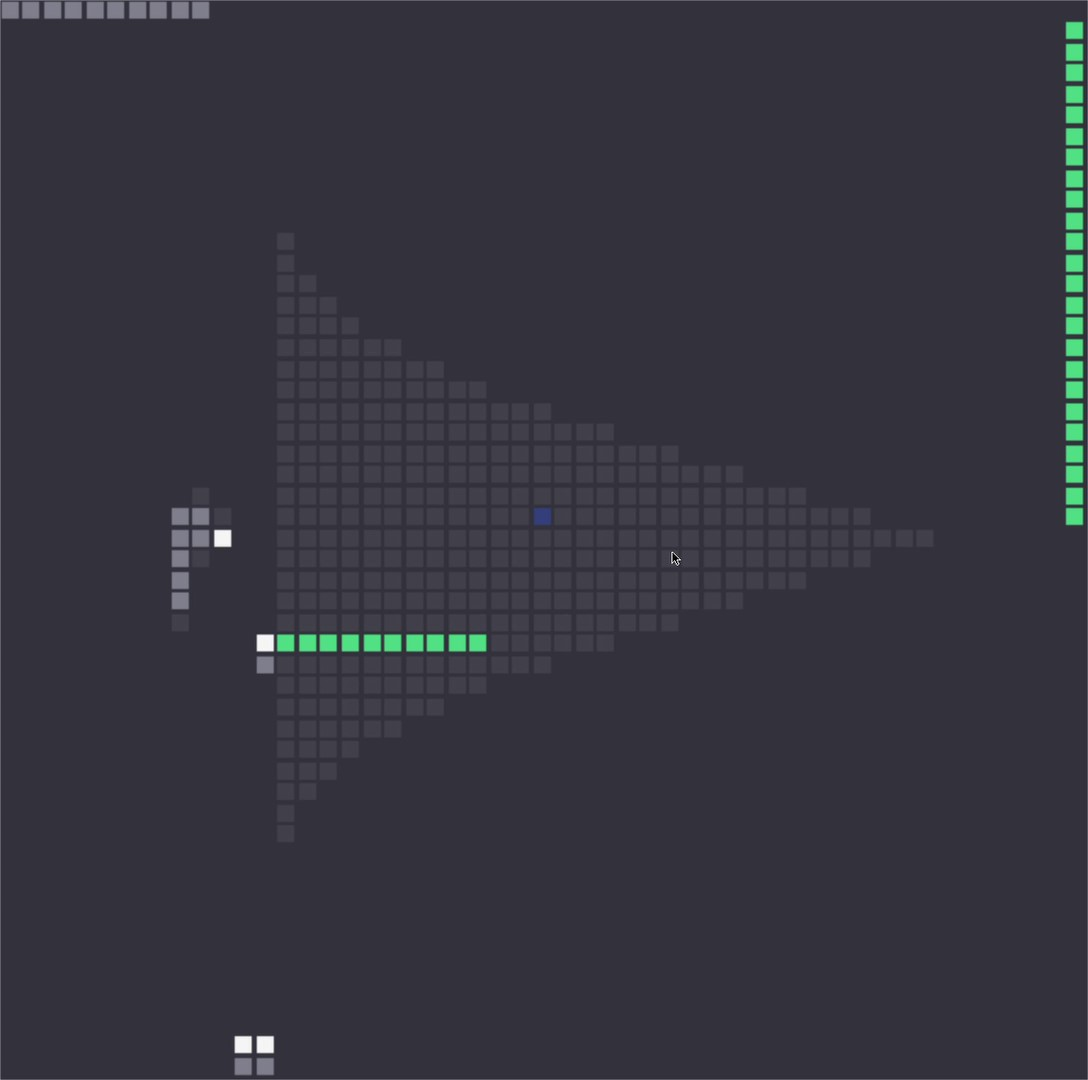
\includegraphics[width=0.5\textwidth]{best_84eps.jpg}
\label{fig:svd1}}
\subfloat[][Agents actions after after 462 episodes. Agent is slowly starting to learn not to go bust.]{
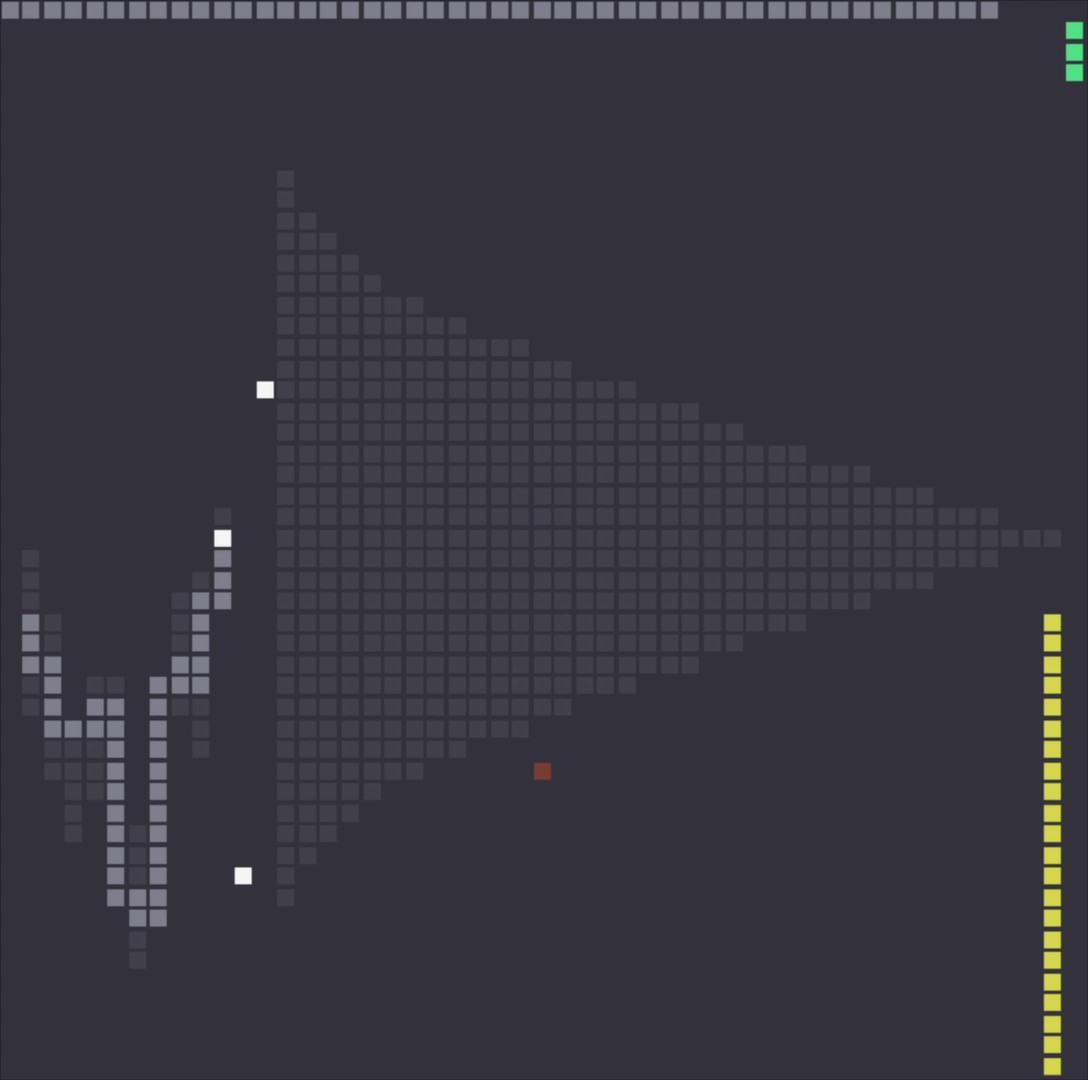
\includegraphics[width=0.5\textwidth]{best_462eps.jpg}
\label{fig:svd2}}
\qquad
\subfloat[][Agents actions after after 1169 episodes. Agent hasn't learned not to go bust and makes a small profit.]{
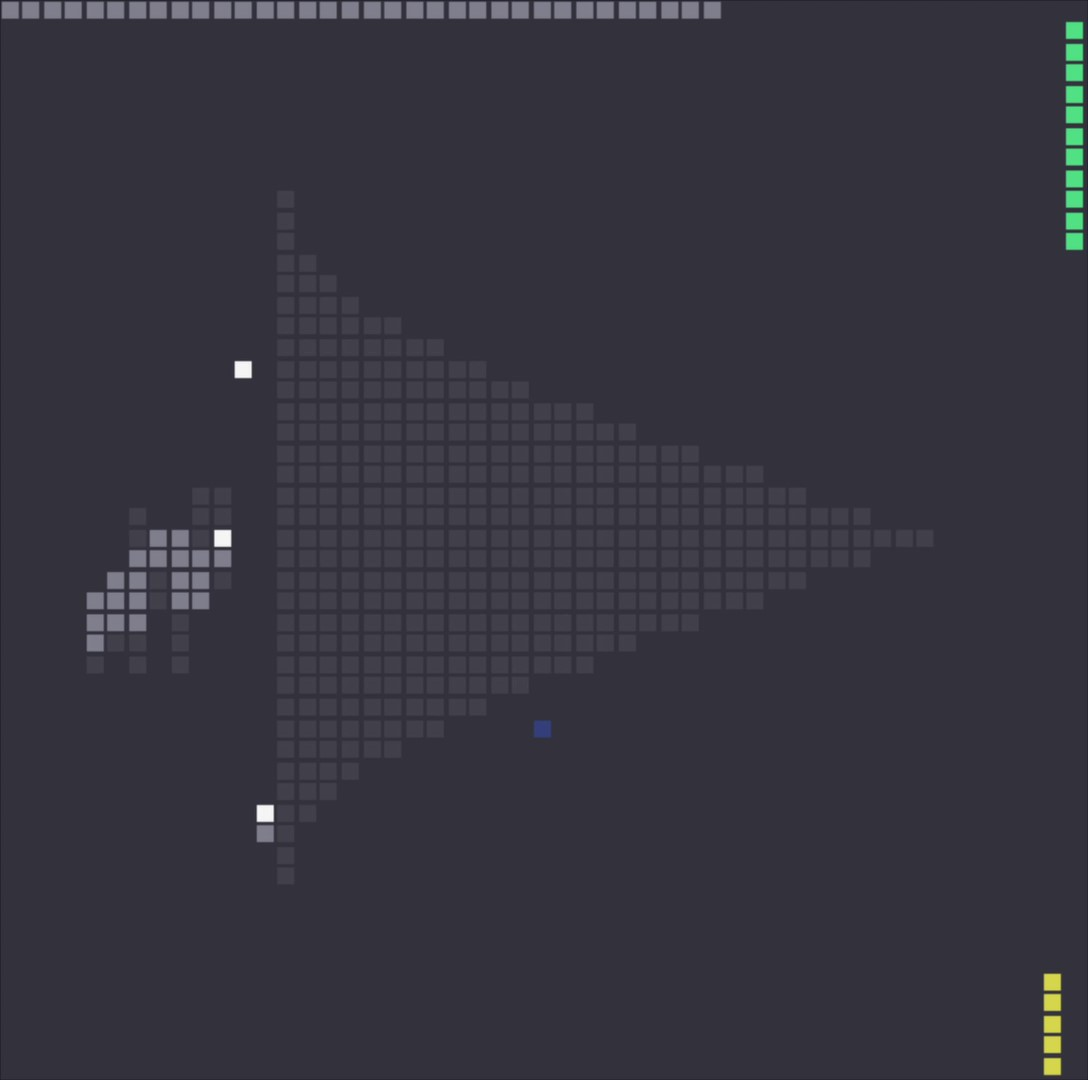
\includegraphics[width=0.5\textwidth]{best_1169eps.jpg}
\label{fig:svd3}}
\subfloat[][Agents actions after after 2006 episodes.  Agent is balancing quotes and make profits frequently.]{
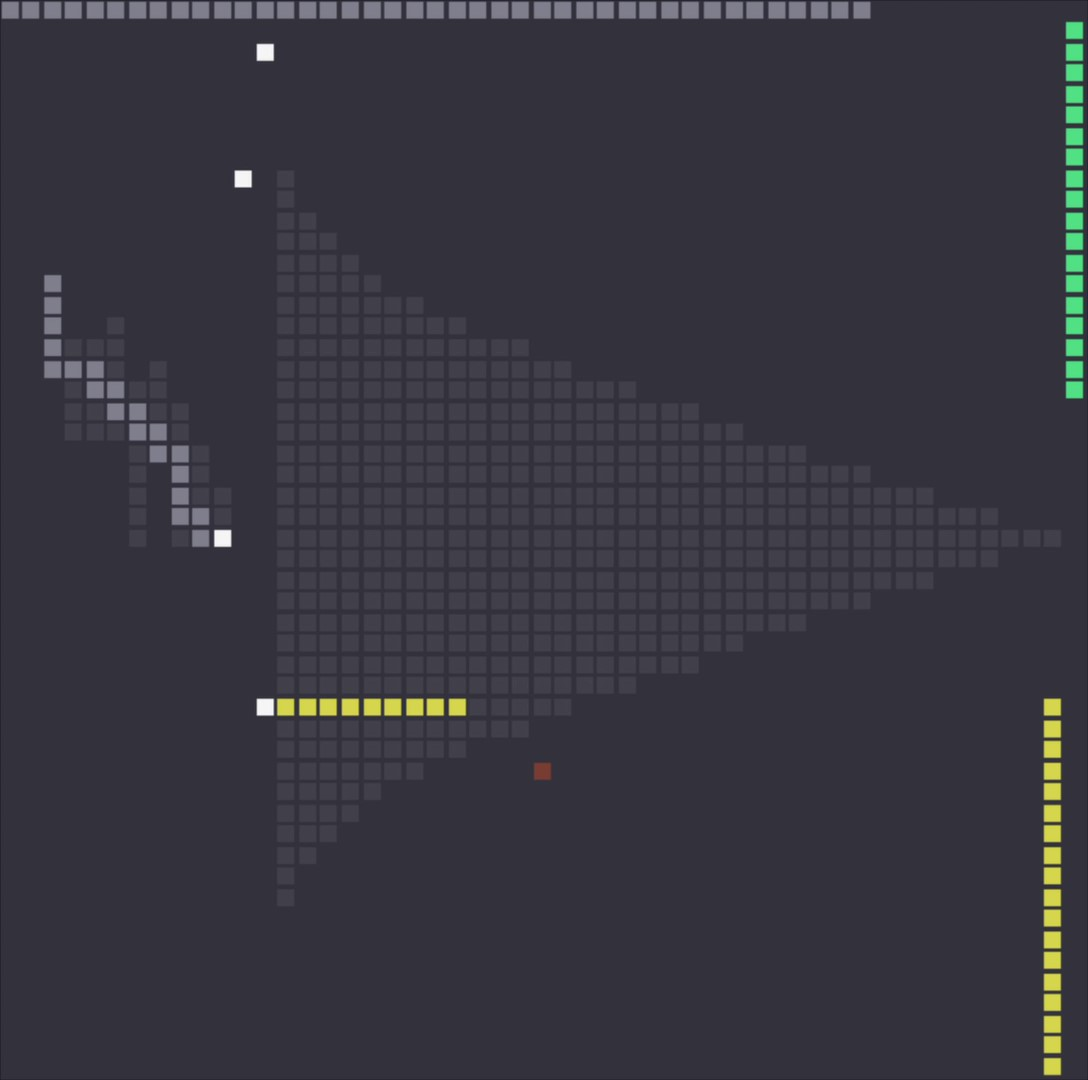
\includegraphics[width=0.5\textwidth]{best_2006eps.jpg}
\label{fig:svd4}}
\caption{Change in agents behaviour during training for DealerMarket-v2.}
\label{fig:vizd1}
\end{figure}

\begin{figure}[H]
\centering
\subfloat[][Agents actions after after 1 episodes. Where agent losses quite frequently.]{
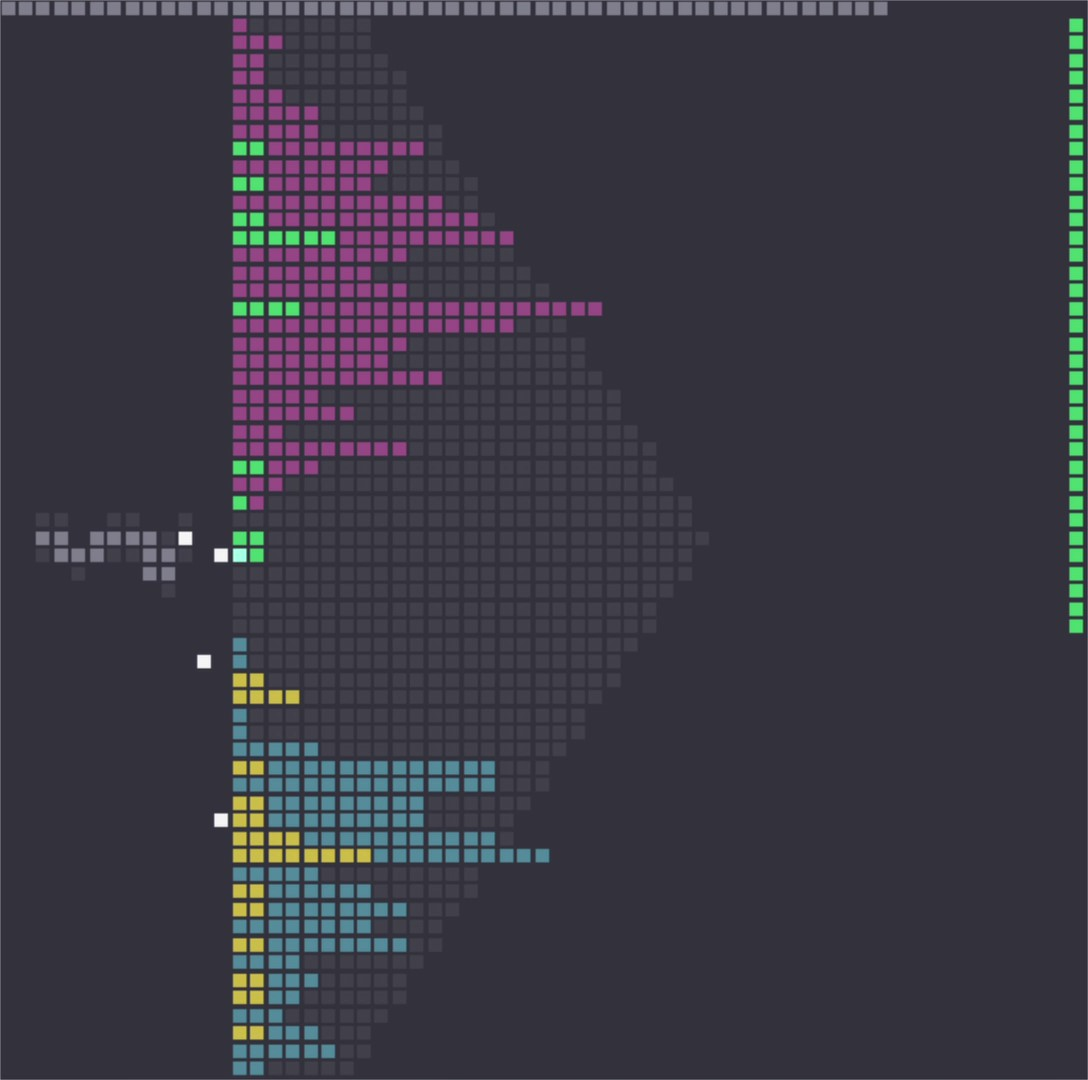
\includegraphics[width=0.5\textwidth]{LOBMarket_eps1_lstm.jpg}
\label{fig:svl1}}
\subfloat[][Agents actions after after 363 episodes. Agent is slowly starting to learn not to go bust.]{
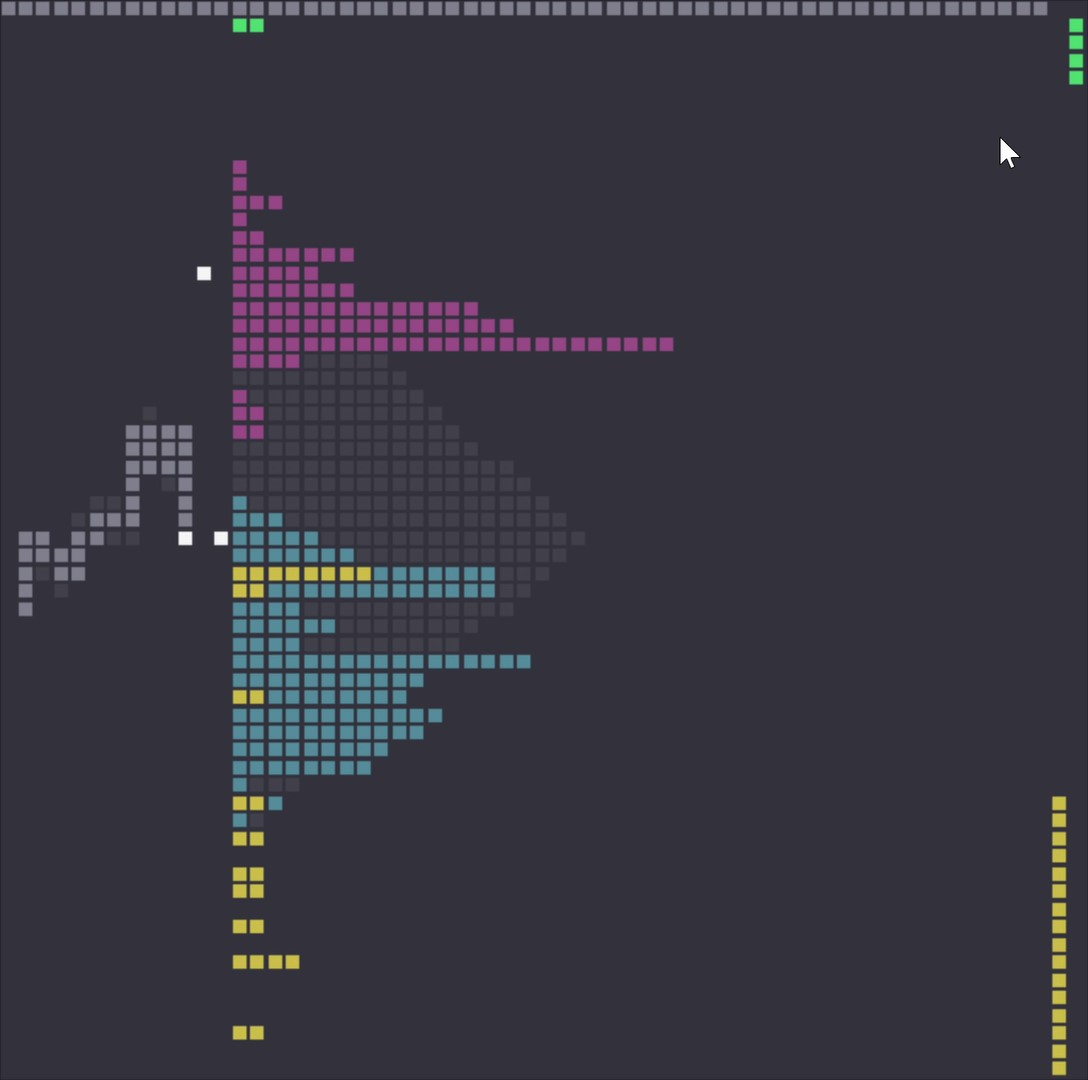
\includegraphics[width=0.5\textwidth]{LOBMarket_eps363_lstm.jpg}
\label{fig:svl2}}
\qquad
\subfloat[][Agents actions after after 1069 episodes. Agent hasn't learned not to go bust and makes a small profit.]{
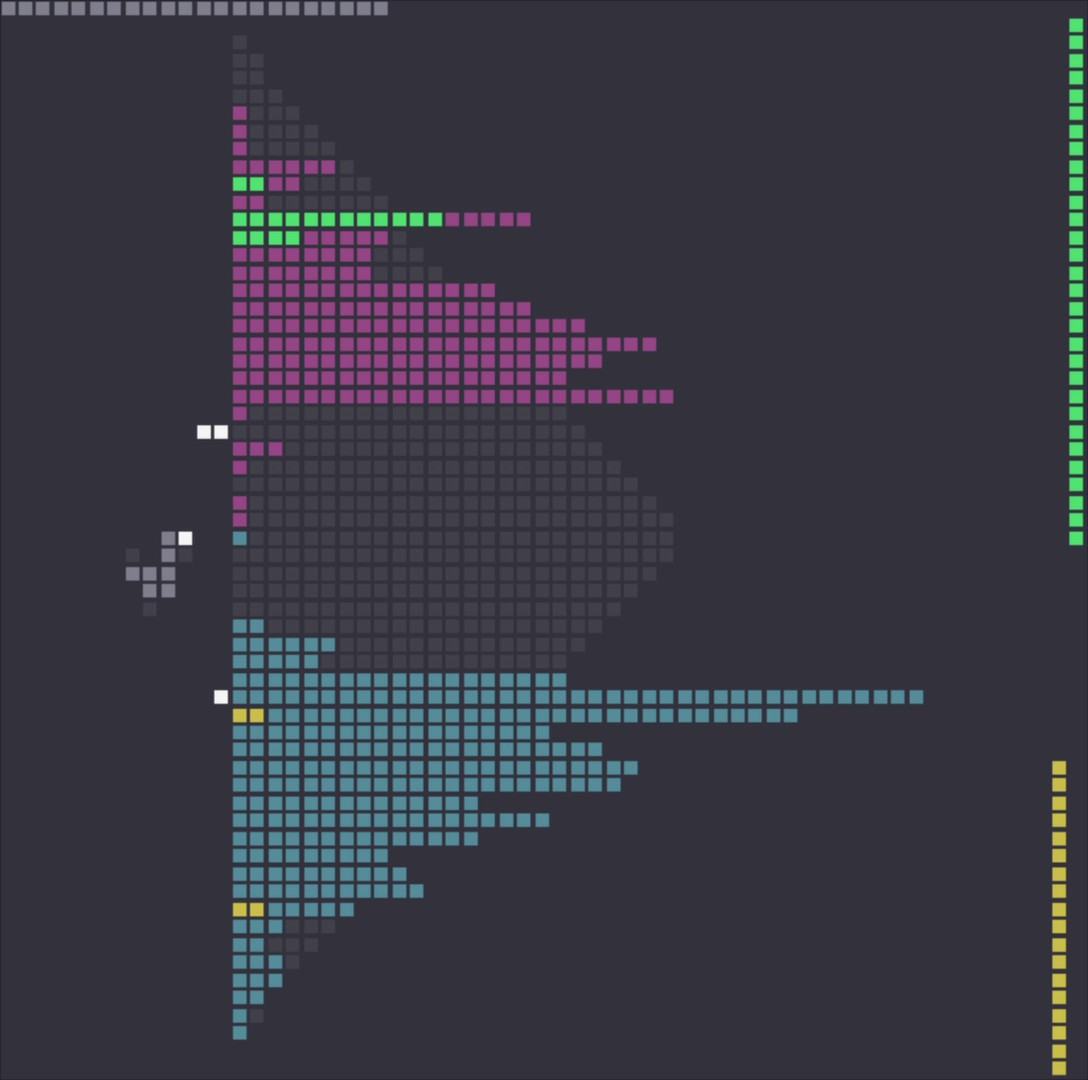
\includegraphics[width=0.5\textwidth]{LOBMarket_eps639_lstm.jpg}
\label{fig:svl3}}
\subfloat[][Agents actions after after 1896 episodes.  Agent is balancing quotes and make profits frequently.]{
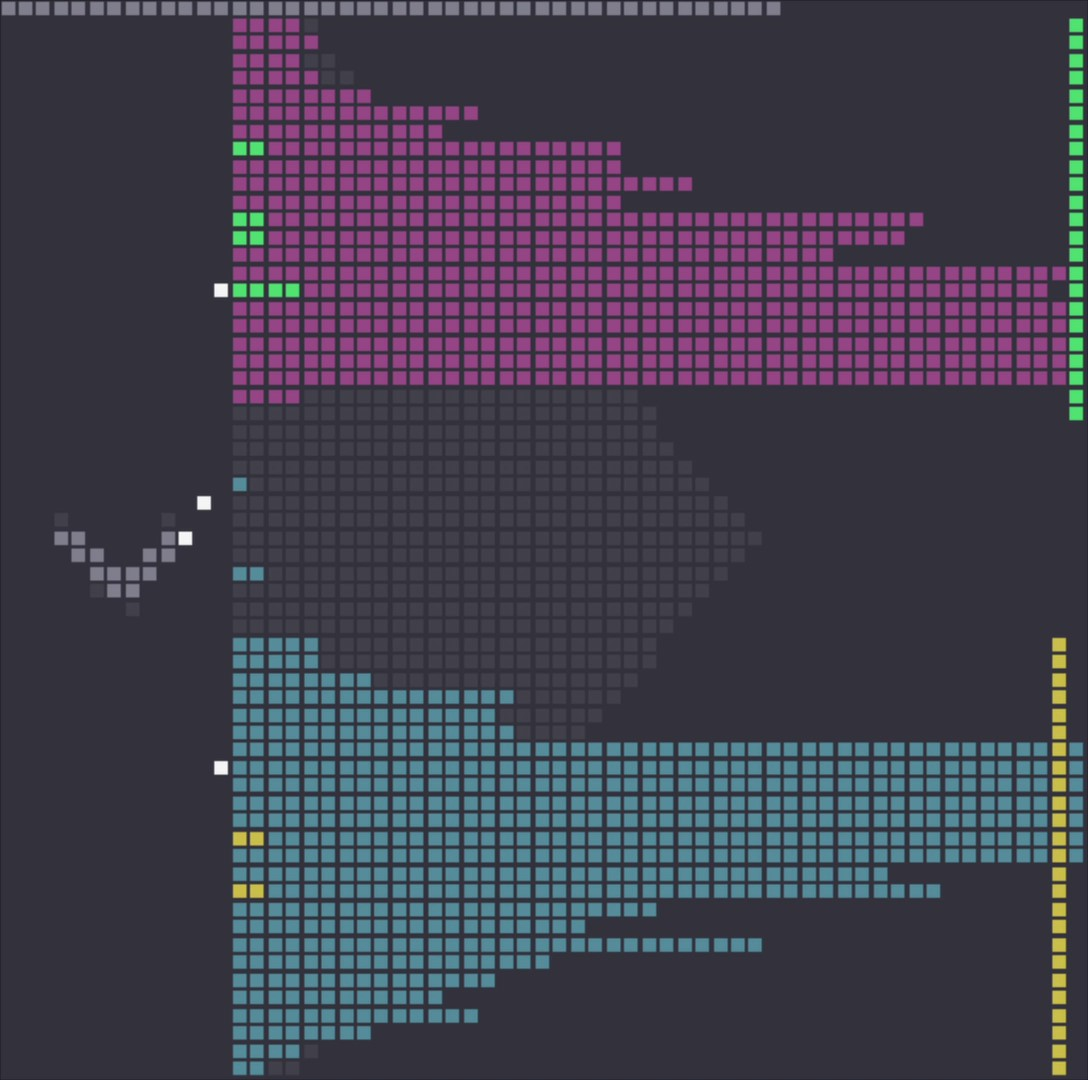
\includegraphics[width=0.5\textwidth]{LOBMarket_eps1132_lstm.jpg}
\label{fig:svl4}}
\caption{Change in agents behaviour during training for LOBMarket-v1.}
\label{fig:vizl1}
\end{figure}
In \autoref{fig:vizd1} the DealerMarket-v1 and \autoref{fig:vizl1} and LOBMarket-v1 agents states are visualized. During different parts of the training. After some $10^{6}$ time-steps the agents are learning not to go bankrupt.



\chapter{Discussion \& Conclusions}\label{ch:7}

\section{Discussions}

\subsection*{Stylized Facts}
In general when analyzing agent based markets, one usually analyze the statistical properties of simulated data. The author does the same in this thesis. To validate the  experimental setup. \textit{Firstly} looking at the signature plots for DealerMarket-v2 and LOBMarket-v1 one clearly sees \textit{mean-reverting} behaviour of the sampled volatility in prices changes. These graphs do exhibit some flatness, indicating weak mean reversion as mentioned in \parencite{bouchaud2018trades}. \textit{Secondly} looking at the changes in the mid prices during the simulations, one sees as indicated by \textcite{bouchaud2018trades} some \textit{activity clustering}. 
\newline
\newline
This clustering behaviour shows that the mid price is followed by different periods of a lot of changes in the mid price. Both positive and negative as in a real world market. \textit{Finally} as mentioned in \parencite{cont2001empirical} looking at the ACF for the prices changes. There seems to be a absence of autocorrelations. Where after lag 1 autocorrelations are close to 0 for the remaining lags. However if the results would have been presented per time-step\footnote{would correspond to intraday periods} instead of averages per episode. This would of-course effect the shape of the ACF. Nonetheless according to \textcite{cont2001empirical}, one would still expected an absence of linear autocorrelations. In summary the simulated data used in the different experiments, exhibit real world \textit{stylized facts}. Concluding that the experimental setup is realistic.

\subsection*{The market maker agents behaviour}
%rewards
During the simulations for the environments: \textit{DealerMarket-v1 (1), \newline DealerMarket-v2 (2)} and \textit{LOBMarket-v1 (3)}. Some interesting behaviour has emerged from the agents interaction with the environment. \textit{Firstly} starting with how the rewards has evolved. The (1) agent had the highest average reward $(391.88 \pm 16.18)$, followed by the (2) $(22.47 \pm2.45)$, and (3) $(-5.02 \pm 0.88)$.  A first remark is that the (1) environment had the lowest $\sigma$ or volatility. Compared to the other environments which had $7.5$ to $10$ times greater $\sigma$. Both the (2) and (3) having different arrival rates of incoming orders compared to (1). This is obviously effecting the difficulty of learning in the environment. Thus making it more realistic, and effecting the agent's mean reward. Nevertheless both (2) and (3) approach higher rewards occasionally. With maximum rewards of $347.40$ and  $145.6$ respectively.  Clearly the initial values of the inventory and cash also has an effect. As well as the arrival rates of the orders. Which is most clearly seen for the (3) environment. 
\newline
\newline
%vs random policy 
Continuing with benchmarking the agents performance compared to a random agent or zero intelligence agent. This was only done for the (2) and (3) environments. As keras-RL didn't have this capability. Clearly looking in \autoref{fig:dm21} and \autoref{fig:dm211} both the (2) and (3) environments, outperform the zero intelligence agents employed. Indicating that the agents behaviors are more optimal than random strategies. Meaning that the choices the agents are doing are not by mere chance. Instead some strategic behaviour is employed, in order to not go bankrupt. Obviously this is something that one wants to see when simulating a participants behaviour on the stock market. In order to make it more realistic. Another noteworthy observation is that the zero intelligence agent is doing better in the (3) environment.
%Price impact 
\newline
\newline
 A reason for this is that sometimes acting randomly may not be a dumb choice. However in a dynamic environment such as the stock market this is clearly not enough to make profits in the long run. Next, looking at the price impact, all agents have different impacts. (1) clearly had the lowest impact with a $\lambda \approx 0.011$. Followed by a significant\footnote{$\alpha = 0.05$ or with $95\%$ confidence} $\lambda \approx 3.43$ for (2). Whereas (3) had a significant $\lambda \approx 43.99$. 
 
 \newpage
 Regardless of possible estimation errors and the need for more granular data to increase the $R^{2}$. What does this really mean? According to the literature \parencite{cartea2015algorithmic, foucault2013market} the price impact is effected by the level of competition and volatility. One clearly sees the effect of the underlying assets volatility as this thesis is only looking at single agent interactions. (1) with the lowest $\sigma$ parameter has the lowest price impact. Whilst both using higher $\sigma$ in the (2) and (3) increases the price impact by several tenfolds or centuples. Meaning that given volumes from (2) and (3) have a larger effect on the observed prices. Naturally, this will effect the market makers profits. Clearly seen in \autoref{tab:dm1}.  
\newline
\newline
%inventory and spreads
Continuing with looking at price dynamics for the agents inventory and spreads.  In \autoref{fig:dm12} to \autoref{fig:dm32} the prices behaves a bit differently. For (1) the gap between the prices are wider. Conversely, for the other environments, the price differences are more narrow. Note that the absolute differences in the prices are larger for the (2) and (3) environments compared to (1). Possibly due to more price fluctuations in those environments due to a higher $\sigma$. Interestingly the trend for the spreads in figure (C) is declining. That is inline with what is stated in the literature \parencite{bouchaud2018trades, hasbrouck2007empirical, madhavan2000market} that the the spread declines over time. Looking at the agents inventories recall that there is no intrinsic need to hold inventory for a market maker \parencite{cartea2015algorithmic}. This as the market maker will buy (sell) in anticipation of a following sale. In figure (B) in \autoref{fig:dm12} to \autoref{fig:dm32} for the different agents, the inventory seems to be increasing compared to its initial inventory. 
\newline
\newline
As a larger inventory could yield higher returns when buying and selling more frequently. The agents might see it fit to balance its future profits with a higher inventory, when taking optimal actions. 
Noticeable, the average inventory (see \autoref{tab:inv}) is still close to each agents initial inventory after 65 days of trading. However an interesting question to pose is how would a real life market maker act? Looking at \autoref{fig:dm12}, around 100 episodes the agent's inventory is decreasing (figure D). Contemporaneous the spread (plot C) and the volumes are increasing. Comparing this to the tactics in \autoref{tab:h1}. This behavior coincides with what a dealer or market maker would do with low inventory. Our that the dealer wants to encourage his clients to sell. Similar examples can be found for the other two environments. 
\newpage
%PNL
Indicating that the different agents in fact behaves realistically. How profitable are the agents market making strategies? The general tendency is that it takes some $10^{6}$ time-steps, before the agents makes positive P\&L consistently. Which can be seen for both the (2) and (3) environments in \autoref{fig:pnl1} and \autoref{fig:pnl2}. Interestingly a positive P\&L is not always equivalent to getting a positive reward. Showcasing the difficulty of shaping rewards for wanted behavior in an agent. On average the in the (2) environment the agent has a $P\&L = -18860$. Whilst for the (3) environment the agent instead has a $P\&L = -3322 $. Which is negative due to the long time it takes for learning. 
\newline
\newline
Looking instead on the rolling mean for the last 100 episodes is of more interest. (2) has a $P\&L = 17977$ and LOBMarket-v1 has a $P\&L = -1010$.  Not surprisingly as it takes time even for experience traders to make a profit in the market. Nevertheless this is far better than a random strategy. Note that each simulation is ran for approximately 65 trading days. Where the agents starts \textit{tabula rasa}. Training for a even longer time or using pre-trained models, would effect the P\&L positively. However also increasing the chance of overfitting.  Looking at $Q_3$ or the third quantile of the rewards, the agent instead makes a $P\&L = 300200$ and $P\&L = 16330$ for the same two environments. 
\newline
\newline
%correlation between spreads an inventory
Advancing with how the spreads and inventories are related.
Looking at \autoref{fig:dm24} and \autoref{fig:dm34}. It is clear that the prices and inventories tend to cluster around certain inventory levels. Suggesting that some inventory levels are more favourable than others, centered around the mean. \textcite{ho1981optimal} states that the spread are independent of the inventory levels. Conducting a Chi-squared Test of Independence ($H_0$) on the full dataset for both environments. The null hypothesis of independence cannot be rejected with $95\%$ confidence. 
\newline
\newline
%order imbalance
Focusing on queue dynamics, and  order imbalances for both the (2) and (3) in \autoref{fig:oi2} and \autoref{fig:oi3}. The average order imbalance for (2) is $0.53$ and for (3) $0.49$. Meaning that on average both the ask and bid queues are of equal length i.e. a balanced buy and sell pressure in the LOB. From the literature \parencite{bouchaud2018trades, cartea2015algorithmic} higher order imbalance means that the agents should post more buy orders and less sell orders. Conversely the agent should post more sell orders and less buy orders when the imbalance is low. Which can be seen from the simulations. 
\newpage
Also note that the shape of figure B in \autoref{fig:oi2} and \autoref{fig:oi3} indicates a monotonic correlation as in \parencite{bouchaud2018trades} between the queue imbalance and the direction of the next price movement. \textit{Finally} looking at visualizations of the agents behavior in \autoref{fig:vizd1} and \autoref{fig:vizl1}. Some similar patterns emerges. Early in training the agent goes bankrupt very quickly in each episode. Also displaying weird behaviour as posting orders with the same price. After some 350-450 episodes the agent is not going bankrupt as often. 
\newline
\newline
Here the agent also learns that by doing nothing occasionally is optimal. At around 1000 episodes the agent is rarely going bankrupt. At the end of training the agent learns how to make the market. By posting quotes more aggressively in response to changed prices, lower inventory and higher volatility. Contemporaneously making a profit and balancing the trade-off between its cash and inventory. To summarize the following has been observed during the different experiments and simulations:
\begin{itemize}
    \item The simulated environments are realistic as several know stylized facts found in\parencite{cont2001empirical} are successfully reproduced. 
    
    \item Both DQN and PPO agents with adequate reward schemes i.e. employing spares or shaped rewards outperform random or zero intelligence agents.
    
    \item A  higher price impact from the agents choices is observed when increasing volatility as stated by the theory.
    
    \item The agents spreads are declining at the end of each simulation. Whereas the agent's inventories are somewhat increasing. However close to their initial inventory levels.
    
    \item Some of the agent's inventory management corresponds to what a real world dealer would do shown in \autoref{tab:h1}
    
    \item It takes at least 1 million time steps before the agent is making a positive P\&L
    
    \item Bid-ask spreads tend to cluster at certain inventory levels.
    
    \item Bid and ask queue price dynamics have been replicated as mentioned in \parencite{bouchaud2018trades}.
\end{itemize}

\newpage

\section{Conclusions}
The research question examined in this thesis was the following:
\begin{displayquote}
\it{''Will trading dynamics such as the bid-ask spread clustering, optimal trade execution and optimal inventory costs. Be exhibited and learned by reinforcement learning agents on a simulated market.''}
\end{displayquote}
After completing this work, the author believes that the research questions has been answered. Where the main conclusions are: (1) \textit{the simulated environments are realistic} and (2) \textit{DQN \& PPO agents can successfully replicate trading dynamics as bid-ask spread clustering}. With this the author concludes that: \textit{reinforcement learning is a suitable choice in modelling market participants behaviour, such as market makers and HFT traders}. When using DQN or PPO agents.
\newline
\newline
Compared to previous research this thesis shows that both DQN \& PPO based reinforcement learning agents are realistic choices when simulating behavior in a dealer market and a limit order book. In order to understand market microstructure. Nonetheless more research is needed to further validate this work, on real world data, and applying it to other market structures.

\section{Future work}
After conducting this research the author sees the following areas as possible future research:

\begin{itemize}
    \item Extend this works models and environments to a multiagent framework. By doing so one could for instance use competitive self-play between several agents to get and study even more complex interactions.
    
    \item Apply reinforcement learning with DQN and PPO to derivatives market. Or to other type of market then a stock market. As well as using other algorithms for learning such as AC3.
    
    \item Use the limit orderbook provided by Parity together with real historical stock data. And use the same type of single agent framework.
    
\end{itemize}

\printbibliography[heading=bibintoc] % Print the bibliography (and make it appear in the table of contents)

\appendix 

\chapter{Correlation between variables}
On the next two pages scatter matrices are shown for \autoref{fig:cc1} and \autoref{fig:cc2}. Both these shows the correlation between some of the available variables used after each ran experiment. These are the most important ones used previously when analyzing the data. What the abbreviations means are the following: $av$ - Ask volume, $bv$ - Bid volume, $bp$ - Bid price, $ap$ - Ask price, $mp$ - Mid price, $ara$ - Ask arrival rate,  $arb$ - Bid arrival rate,  $d\_inv$ - Change in inventory,  $d\_cash$ - Change in funds,  $val$ - Underlying asset price,  $inv$ - Inventory $cash$ - Funds. 
\newline
\newline
Looking at the scatter matrix one can see for instance that cash is negatively correlated with both the bid volume and the ask volume. Conversely the agents cash is positively correlated with both the bid and ask prices. 



\begin{sidewaysfigure}
\centering
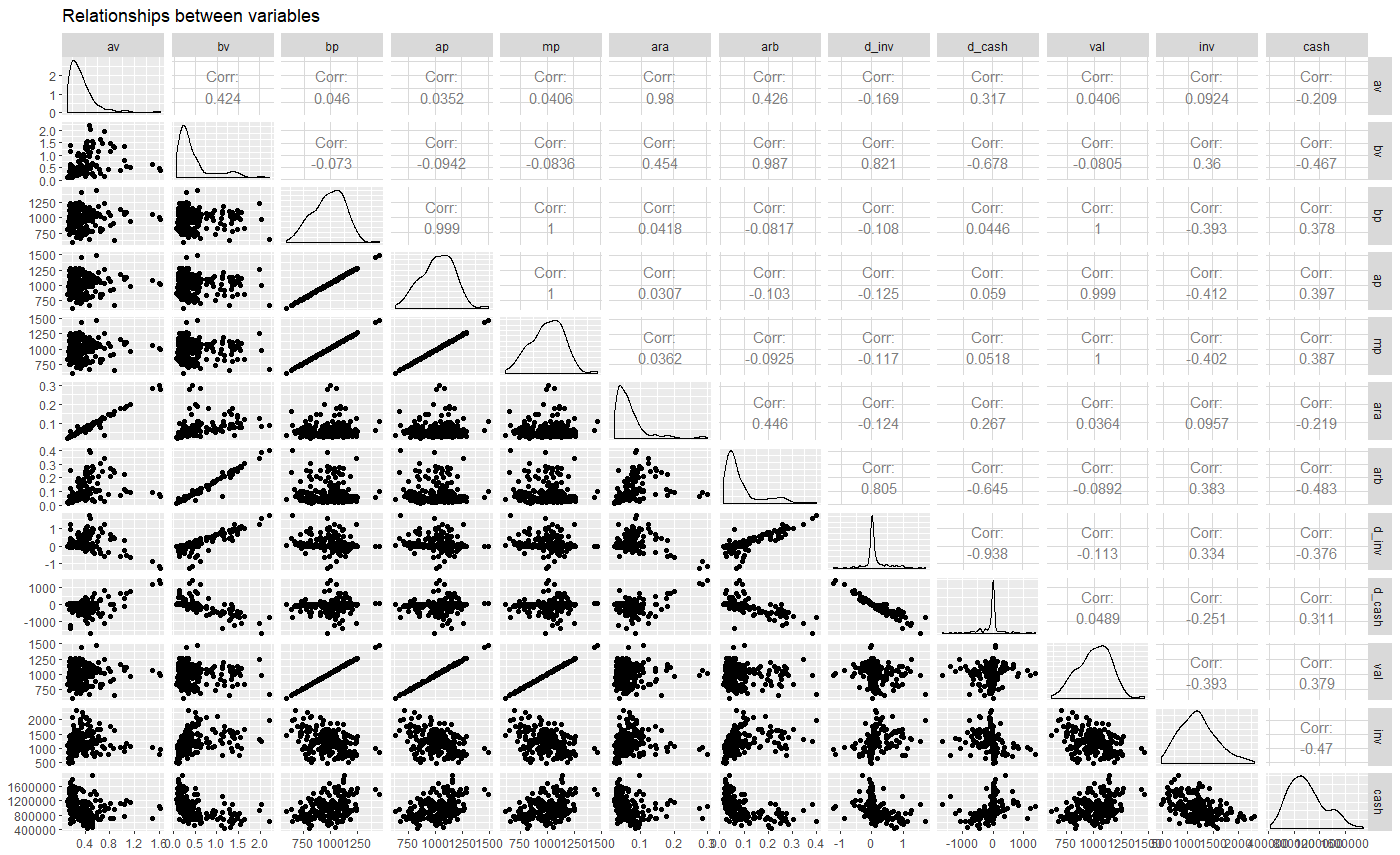
\includegraphics[scale=.6]{scatter_mat_vars.png}
\caption{Scatter matrix between some of the most relevant variables. To find correlations for DealerMarket-v2. }
\label{fig:cc1}
\end{sidewaysfigure}    



 \begin{sidewaysfigure}
\centering
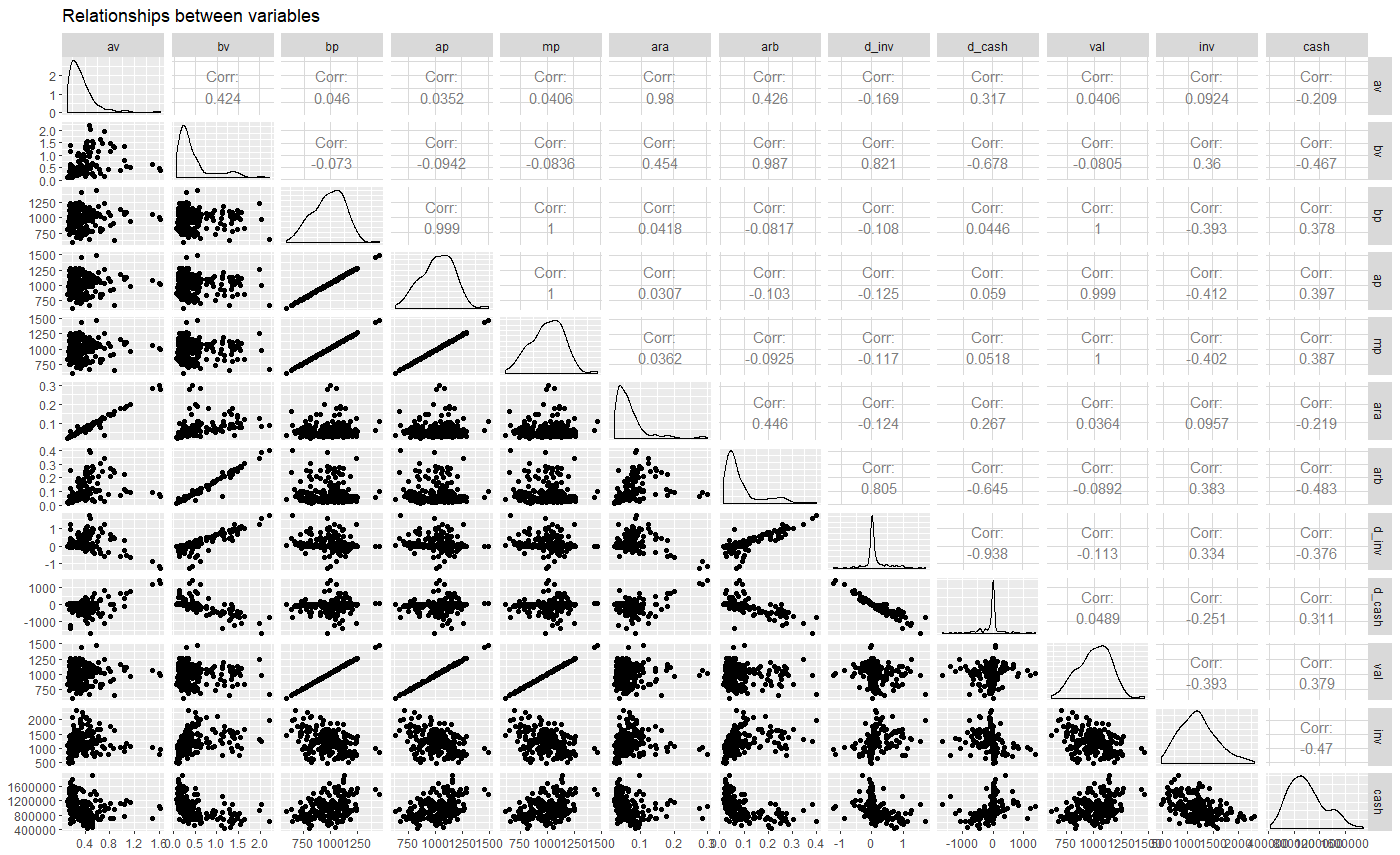
\includegraphics[scale=.6]{scatter_mat_vars.png}
\caption{Scatter matrix between some of the most relevant variables. To find correlations for LOBMarket-v1. }
\label{fig:cc2}
\end{sidewaysfigure}   




\chapter{Policy and Value Iteration}\label{app:A}
In this chapter algorithms using dynamic programming for finding optimal value and optimal policy is shown. Based on the material in \parencite{sutton1998reinforcement}.

\section{Value Iteration}
\RestyleAlgo{boxruled}
\LinesNumbered
\begin{algorithm}[H]
 %\KwIn{A MDP i.e.  $(\mathcal{S, A, P, R}, \gamma)$}
 %\KwResult{Returns optimal policy ($\pi_{*}$)}
 \textsf{Initialize $V$ arbitrarily e.g. $V(s) = 0$} \;
 $\Delta \leftarrow 0$ \;
 \While{$\Delta < \theta$ (small positive number)}{
 \ForEach{$s \in \mathcal{S}$}{
 $v \leftarrow V(s)$ \;
 $V(s) \leftarrow \underset{a}{\operatorname{max}} \sum_{s', r}{p(s', r |s, \pi(s))[r + \gamma V(s')]}$ \;
 $\Delta \leftarrow \max(\Delta, |v - V(s)|)$ 
    }
 }
 \KwOut{deterministic policy , $\pi \approx \pi_{*}$ s.t. $\pi (s) = \underset{a}{\operatorname{argmax}} \sum_{s', r}{p(s', r|s,a)[r+\gamma V(s')]}$} 
 \caption{Value iteration}
 \label{alg2}
\end{algorithm}

\section{Policy Iteration}
\RestyleAlgo{boxruled}
\LinesNumbered
\begin{algorithm}[H]
 %\KwIn{A MDP i.e.  $(\mathcal{S, A, P, R}, \gamma)$}
 %\KwResult{Returns optimal policy ($\pi_{*}$)}
 \textsf{1. Initialize} \;
 $V(s) \in \mathbb{R}$ and  $\pi(s) \forall s\in \mathcal{S} $ \;
 $\Delta \leftarrow 0$ \;
 \textsf{2. Policy Evaluation}\;
 \While{$\Delta < \theta$ (small positive number)}{
 \ForEach{$s \in \mathcal{S}$}{
 $v \leftarrow V(s)$ \;
 $V(s) \leftarrow \sum_{s', r}{p(s', r |s, \pi(s))[r + \gamma V(s')]}$ \;
 $\Delta \leftarrow \max(\Delta, |v - V(s)|)$ 
    }
 }
 
 \textsf{3. Policy Improvement}\;
 
 $policy\_stable \leftarrow true$ \;
 \While{$not$ $policy\_stable$)}{
 \ForEach{$s \in \mathcal{S}$}{
 $old\_action \leftarrow \pi(s)$ \;
 $\pi(s) \leftarrow \underset{a}{\operatorname{argmax}} \sum_{s', r}{p(s', r|s,a)[r+\gamma V(s')]}$ \;
 
 \lIf{$old\_action \neq \pi(s)$} {$policy\_stable \leftarrow false$} 
 
  }
  \lIf{$policy\_stable$} {stop} \lElse{go to 2} 
 }
 
 \Return $V \approx v_{*}$ and $\pi \approx \pi_{*}$ \;
 \caption{Policy iteration}
 \label{alg1}
\end{algorithm}

\chapter{Derivation of Ho \& Stoll Model}\label{app:B}
In this chapter, some explanations to the derivation of the Ho \& Stoll model are presented. Using dynamic programming, stochastic calculus and the famous Ito's lemma.

%\section{Dynamic Programming}

%\section{Stochastic Calculus}

\section{Ito's Lemma}
In order to calculate the derivative of a function that depends on time and a stochastic process, \textit{Ito's Lemma} can be used \parencite{o1995market}. Suppose that $Y$ is a smooth function:

\begin{equation}
    Y = f(x,t)
    \label{eq:i1}
\end{equation}
Where $t$ is time and $x$ is some well-defined Ito processes \parencite{o1995market} in \autoref{eq:i1}. Given in \autoref{eq:i2}

\begin{equation}
    dx = \mu dt + \sigma dz
    \label{eq:i2}
\end{equation}
Then if one wish to maximize $Y$ choosing $x$. The partial derivatives of $Y$ is needed. Which is given by:

\begin{align}
    dY = \frac{\partial f}{\partial t}dt + \frac{\partial f}{\partial x} + \frac{1}{2}\frac{\partial^{2} f}{\partial x^{2}}(dx)^{2} = \\
    = \frac{\partial f}{\partial t}dt + \frac{\partial f}{\partial x}[\mu dt + \sigma dz] + \frac{1}{2} \frac{\partial^{2}}{\partial x^{2}} \sigma^{2} dt
    \label{eq:i3}
\end{align}
Rewriting \autoref{eq:i3} gives Ito's Lemma in \autoref{eq:i4}
\begin{equation}
    dY = \left[\frac{\partial f}{\partial t} + \frac{\partial f}{\partial x}\mu + \frac{1}{2}\frac{\partial^{2} f}{x^{2} \sigma^{2}} \right]dt + \frac{\partial f}{\partial x}\sigma dz
    \label{eq:i4}
\end{equation}

\section{Optimal inventory for a Market Maker}
In \textcite{ho1981optimal} a model that handles the risk the market maker faces when providing his service is presented. In the model the following assumptions are made:

\begin{itemize}
    \item Transactions follow a stationary continuous time stochastic jump process i.e. a Poisson process. 
    
    \item The arrival rate of buy orders ($\lambda_a$) and sell orders ($\lambda_b$) will depend on the dealer's ask and bid prices.
    
    \item The dealer face uncertainty over the future value of his portfolio $X$.
\end{itemize}
In the the absence of any transactions the portfolio growth $dX$ is given below:

\begin{equation}
    \label{eq:a8}
    dX = r_{x}Xdt + XdZ_x
\end{equation}
Where $r_x$ is the mean return, $dZ_x$ is the Wiener process with mean zero variance $\sigma^{2}_X$. The dealers wealth is divided into three components: \textit{cash, inventory} and \textit{base wealth}. The value of the cash account ($F$) is:

\begin{equation}
    \label{eq:a9}
    dF = rFdt- (p-b)dq_b + (p+a)dq_a
\end{equation}
Which changes with buys and sells of securities earning the risk-free rate $r$. The dealers inventory ($I$) is given by:

\begin{equation}
    \label{eq:a10}
    dI = r_{I}Idt+pdq_{b} - pdq_{a} + IdZ_{I}
\end{equation}
The inventory consists of shares in the stock tha market maker makes.
Finally base wealth ($Y$) is given by:

\begin{equation}
    \label{eq:a11}
    dY = r_{Y}Ydt+YdZ_{Y} 
\end{equation}
The objective of the dealer is now to maximize the expected utility of his total wealth $E[U(W_T)]$ at time horizon $T$, where 

\begin{equation}
    \label{eq:a12}
    W_{T} = F_{T} + I_{T} + Y_{T}
\end{equation}
\autoref{eq:12} is what is termed \textit{the dealers pricing problem}. This is in fact an optimization problem with the goal to maximize the value function $J(\cdot)$ using dynamic programming. Thus having the optimization below in \autoref{eq:a13a}

\begin{equation}
    \label{eq:a13a}
    J(t,F,I,Y) = \underset{a,b}{\max}[E[U(W_T)] | t,F,I,Y]
\end{equation}
where $U$ is the utility function, $a$ and $b$ are the ask and bid adjustments and $t, F, I,Y$ are the states variables time, cash, inventory and base wealth \parencite{o1995market}. The function $J(\cdot)$ gives the level of utility given that the dealer's decisions are made optimally \parencite{o1995market}. As there are no intermediate consumption before time $T$ in this model. The recurrence relation found by using the principle of optimality is:

\begin{equation}
    \label{eq:a13bc}
    \underset{a,b}{\max}dJ(t,F,I,Y)=0 \text{ and } 
    J(T,F,I,Y)=U(W_T)
\end{equation}
Solving \autoref{eq:a13bc} finds a solution to the dealer's problem, where we have to find the ask and bid prices for each state. To solve \autoref{eq:a13bc} one requires to use stochastic calculus. By writing out the partial differential equations that \autoref{eq:a13bc} implies and applying Ito's Lemma in \autoref{eq:i4}:

\begin{align*}
    \label{eq:a13d}
    \underset{a,b}{max}(dJ/dt) = & J_t + LJ \\
    & + max\{\lambda_a[J(F+pQ+aQ, I-pQ,Y) - J(F,I,Y)] \\
    & + \lambda_b [J(F-pQ+bQ, I+pQ,Y) - J(F,I,Y)] \} = 0 \numberthis
\end{align*}
where $J_t$ is the time derivative and $LJ$ is the operator defined as

\begin{equation}
    LJ = J_{F}rF + J_{I}r_{I}I+J_{Y}r_{y}Y+\frac{1}{2}J_{II}\sigma^{2}_{I}I^{2}+ \frac{1}{2}J_{YY}\sigma^{2}_{Y}Y^{2} + J_{IY}\sigma_{IY}IY
\end{equation}
$J_t + LJ$ is the total time derivative of derived utility when there are no transactions. \autoref{eq:a13d} determines the solution, which is hard to solve explicitly. \textcite{ho1981optimal} do not solve the general problem but introduces some transformations and simplifications in order to solve it. Firstly by looking at the problem only at the endpoint ($\tau$) where it is is equal to zero. Secondly by taken the first-order approximation of the Taylor series expansion of \autoref{eq:a13a} \parencite{o1995market}. \textcite{ho1981optimal} then, also define two new operators the sell ($SJ$) and buy ($BJ$) operators:
\begin{align}
    \label{eq:a13e}
    SJ = & S[J(F,I,Y)] = J(F+Q,I-Q, Y) \\
    BJ = & B[J(F,I,Y)] = J(F-Q, I+Q, Y)
\end{align}

By using the new operators the problem in \autoref{eq:a13d} can be rewritten as:

\begin{align*}
    \label{eq:a13e2}
    J_{t} = & LJ + \underset{a,b}{max}\{[\lambda(a)aQSJ_{F} - \lambda(a)(J-SJ)] + \\
    & [\lambda(b)bQBJ_{F} - \lambda(b)(J-BJ)]\} 
    \numberthis
\end{align*}
where $\lambda(a) = \alpha - \beta_{A}$ and $\lambda(b) = \alpha + \beta_{B} $ is symmetric linear supply and demand functions to the dealer. There is no closed form solution for this problem. Nontheless via approximations the bid and ask quotes can be found below:

\begin{align}
\label{eq:a13f}
    b^{*} = & \alpha/2\beta + (J-BJ)/2BJ_{F}Q \\
    a^{*} = & \alpha/2\beta + (J-SJ)/2SJ_{F}Q \label{eq:a13g}
\end{align}
Finally from \autoref{eq:13f} and \autoref{eq:13g} the the bid-ask spread is
\begin{equation}
    \label{eq:a13h}
    s = \alpha / \beta + (J-SJ)/2SJ_{F}Q + (J-BJ)/2BJ_{F}Q
\end{equation}
The first term of \autoref{eq:a13h} is the spread which maximizes the expected returns from selling and buying stocks. Whilst the rest of the terms are seen as \textit{risk premiums} for sale and purchase transactions. This as the dealer or market maker sets the spread without knowing what side the transaction will have i.e. bid or ask \parencite{ho1981optimal}.
\newline
\newline
\textcite{ho1981optimal} demonstrates three important properties of the dealer's optimal pricing behavior:

\begin{enumerate}
    \item The spreads depends on the time horizon of the dealer
    \item The spread can be decomposed into a risk neutral spread plus an adjustment for uncertainty
    \item The spread is independent of inventory level.
\end{enumerate}

%not sure if this section is necessary yet
\section{What human dealers would do}
Dealer or market makers are profit-motivated trader who allow other traders to trade when they want to trade \parencite{harris2003trading}. As mentioned before one way of finding optimal bid-and ask quotes for inventory control is to use the \textcite{ho1981optimal} model. However, what would a human trader do reacting to different conditions on the market? In \textcite{harris2003trading} this is presented, shown below in \autoref{tab:h1}:

\begin{table}[H]
\begin{tabular}{lll}
\hline
 \textbf{Condition} & \textbf{Tactics}  & \textbf{Purpose}  \\ \hline
 \shortstack{Inventories are too low \\ or clients are net buyers}  & \shortstack{Raise bid price \\ Increase bid size}  & \shortstack{Encourage clients to sell}  \\
 & \shortstack{Raise ask price \\decrease ask size }  & \shortstack{Discourage clients from buying}  \\
 %& \shortstack{} &  \shortstack{} \\
  %& \shortstack{} &  \shortstack{} \\
 \shortstack{ Inventories are to high \\ or clients are net sellers} & \shortstack{Lower ask price \\ Increase ask size}  & \shortstack{Encourages clients to buy}  \\
 & \shortstack{Lower ask price \\ Increase ask size}  & \shortstack{Discourage clients from selling}  \\
 %& \shortstack{} &  \shortstack{} \\
  %& \shortstack{} &  \shortstack{} \\
 &  &  \\ \hline
\end{tabular}
\caption{Tactics Dealers or Market Makers Use to Manage Their Inventories and Orders Flow. Adopted from \parencite{harris2003trading} }
\label{tab:h1}
\end{table}

%included kth backpage here

\includepdf{kth_back.pdf}
\end{document}
